\documentclass[10pt,twocolumn]{book}
% For arxiv.org, must be on or before line 5:
\pdfoutput=1

% standard packages

% A more pleasant font
\usepackage{lmodern}
\usepackage[T1]{fontenc} % use postscript type 1 fonts
\usepackage{textcomp} % use symbols in TS1 encoding
\usepackage{mathptmx} % use nice, standard fonts for roman
\usepackage[scaled=.92]{helvet} % and sans serif
%msfontstub

% Improves the text layout
\usepackage{microtype}
\UseMicrotypeSet[protrusion]{basicmath} % disable protrusion for tt fonts
\usepackage{etoolbox}

\usepackage{lscape}
\usepackage{epsfig}
\usepackage{subfigure}
% \usepackage{breakurl}
\usepackage{graphicx}
\usepackage{rotating}
\usepackage{enumitem}
\setlist[description]{style=unboxed}
%\usepackage{enumerate}
\usepackage{ifthen}
\usepackage{xcolor}
\usepackage[shortcuts]{extdash}
\usepackage{changepage}
\usepackage{listings}
\lstset{basicstyle=\ttfamily}
% \usepackage[strings]{underscore}
% \usepackage{underscore}
\usepackage{pifont} % special character for qqz reference point
\usepackage{gensymb} % symbols for both text and math modes such as \degree and \micro
\usepackage{verbatimbox}[2014/01/30] % for centering verbatim listing in figure environment
\usepackage[bottom]{footmisc} % place footnotes under floating figures/tables
\usepackage{tabulary}
\usepackage[hyphens]{url}
\usepackage[bookmarks=true,bookmarksnumbered=true,pdfborder={0 0 0}]{hyperref}
\usepackage{footnotebackref} % to enable cross-ref of footnote
\usepackage[all]{hypcap} % for going to the top of figure and table
\usepackage{epigraph}
\setlength{\epigraphwidth}{2.6in}
\usepackage[xspace]{ellipsis}
\usepackage{braket} % for \ket{} macro in QC section

% custom packages

\usepackage{qqz}
\usepackage{origpub}

% For korean
\usepackage{kotex}

% custom booleans

\newboolean{inbook}
\setboolean{inbook}{true}
\newcommand{\IfInBook}[2]{\ifthenelse{\boolean{inbook}}{#1}{#2}}
\newboolean{twocolumn}
\setboolean{twocolumn}{true}
\newcommand{\IfTwoColumn}[2]{\ifthenelse{\boolean{twocolumn}}{#1}{#2}}
\newboolean{hardcover}
\setboolean{hardcover}{false}
\newcommand{\IfHardCover}[2]{\ifthenelse{\boolean{hardcover}}{#1}{#2}}
\newboolean{sansserif}
\setboolean{sansserif}{false}
\newcommand{\IfSansSerif}[2]{\ifthenelse{\boolean{sansserif}}{#1}{#2}}
\newboolean{lmttforcode}
\setboolean{lmttforcode}{true}
\newcommand{\IfLmttForCode}[2]{\ifthenelse{\boolean{lmttforcode}}{#1}{#2}}

\newcommand{\OneColumnHSpace}[1]{\IfTwoColumn{}{\hspace*{#1}}}

\IfSansSerif{
\renewcommand{\familydefault}{\sfdefault}
\normalfont
\usepackage[italic]{mathastext}[2016/01/06]
\renewcommand{\path}[1]{\nolinkurl{#1}} % workaround of interference with mathastext
}{}

\newcommand{\LstLineNo}{\makebox[5ex][r]{\arabic{VerbboxLineNo}\hspace{2ex}}}

\usepackage{bm} % for bold math mode fonts --- should be after math mode font choice

\IfLmttForCode{
\AtBeginEnvironment{verbatim}{\renewcommand{\ttdefault}{lmtt}}
\AtBeginEnvironment{verbbox}{\renewcommand{\ttdefault}{lmtt}}
\AtBeginEnvironment{table}{\renewcommand{\ttdefault}{lmtt}}
\AtBeginEnvironment{tabular}{\renewcommand{\ttdefault}{lmtt}}
\AtBeginEnvironment{tabulary}{\renewcommand{\ttdefault}{lmtt}}
\AtBeginEnvironment{minipage}{\renewcommand{\ttdefault}{lmtt}}
}{}

\begin{document}

%%HTMLSKIP
\lstset{
 literate={\_}{}{0\discretionary{\_}{}{\_}}%
  {\_\_}{}{0\discretionary{\_\_}{}{\_\_}}%
  {->}{}{0\discretionary{->}{}{->}}%
}
%%HTMLNOSKIP
% ---  Workaround for Fedora 23 Texlive bug
\makeatletter
\renewcommand\lstinline[1][]{%
\leavevmode\bgroup % \hbox\bgroup --> \bgroup
\def\lst@boxpos{b}%
\lsthk@PreSet\lstset{flexiblecolumns,#1}%
\lsthk@TextStyle
\ifnum\iffalse{\fi`}=\z@\fi
\@ifnextchar\bgroup{%
\ifnum`{=\z@}\fi%
\afterassignment\lst@InlineG \let\@let@token}{%
\ifnum`{=\z@}\fi\lstinline@}}
\makeatother
% ---  End of workaround for Fedora 23 Texlive bug
\newcommand{\co}[1]{\lstinline[breaklines=true,breakatwhitespace=true]{#1}}
\newcommand{\nbco}[1]{\hbox{\lstinline[breaklines=false,breakatwhitespace=false]{#1}}} % no break lines for short snippet
\newcommand{\qco}[1]{``\nbco{#1}''} % \nbco with quotation marks
\newcommand{\tco}[1]{\texttt{\detokenize{#1}}} % for code in tabular environment
% \tco{} will break at spaces but not at underscores
\newcommand{\nf}[1]{\textnormal{#1}} % to return to normal font
\newcommand{\qop}[1]{{\sffamily #1}} % QC operator such as H, T, S, etc.

\newcommand{\Epigraph}[2]{\epigraphhead[65]{\rmfamily\epigraph{#1}{#2}}}

% Hyphenation exceptions for US English,
% based on hyphenation exception log articles in TUGboat.
%
% Copyright 2008 TeX Users Group.
% You may freely use, modify and/or distribute this file.
%
% This is an automatically generated file.  Do not edit!
%
% Please contact the TUGboat editorial staff <tugboat@tug.org>
% for corrections and omissions.

\hyphenation{
  acad-e-my
  acad-e-mies
  ac-cu-sa-tive
  acro-nym
  acro-nyms
  acryl-amide
  acryl-amides
  acryl-alde-hyde
  acu-punc-ture
  acu-punc-tur-ist
  add-a-ble
  add-i-ble
  adren-a-line
  aero-space
  af-ter-thought
  af-ter-thoughts
  agron-o-mist
  agron-o-mists
  al-ge-bra-i-cal-ly
  am-phet-a-mine
  am-phet-a-mines
  anach-ro-nism
  anach-ro-nis-tic
  an-a-lyse
  an-a-lysed
  analy-ses
  analy-sis
  an-eu-rysm
  an-eu-rysms
  an-eu-rys-mal
  an-iso-trop-ic
  an-iso-trop-i-cal-ly
  an-isot-ro-pism
  an-isot-ropy
  an-ni-ver-sary
  an-ni-ver-saries
  anom-a-ly
  anom-a-lies
  anti-deriv-a-tive
  anti-deriv-a-tives
  anti-holo-mor-phic
  an-tin-o-my
  an-tin-o-mies
  anti-nu-clear
  anti-nu-cle-on
  anti-rev-o-lu-tion-ary
  a-peri-odic
  apoth-e-o-ses
  apoth-e-o-sis
  ap-pen-di-ces
  ap-pen-dix
  ap-pen-dixes
  ar-chi-me-dean
  ar-chi-pel-ago
  ar-chi-pel-a-gos
  ar-chive
  ar-chives
  ar-chiv-ing
  ar-chiv-ist
  ar-chiv-ists
  ar-che-typ-al
  ar-che-type
  ar-che-types
  ar-che-typ-i-cal
  arc-tan-gent
  arc-tan-gents
  a-spher-ic
  a-spher-i-cal
  as-sign-a-ble
  as-sign-or
  as-sign-ors
  as-sist-ant
  as-sist-ance
  as-sist-ant-ship
  as-sist-ant-ships
  as-trol-o-ger
  as-trol-o-gers
  as-tron-o-mer
  as-tron-o-mers
  asymp-to-matic
  as-ymp-tot-ic
  asyn-chro-nous
  ath-er-o-scle-ro-sis
  at-mos-phere
  at-mos-pheres
  at-tri-bute
  at-trib-uted
  at-trib-ut-able
  au-to-ma-tion
  au-tom-a-ton
  au-tom-a-ta
  auto-num-ber-ing
  au-ton-o-mous
  auto-re-gres-sion
  auto-re-gres-sive
  auto-round-ing
  av-oir-du-pois
  back-scratcher
  back-scratch-ing
  band-lead-er
  band-lead-ers
  bank-rupt
  bank-rupts
  bank-rupt-cy
  bank-rupt-cies
  bar-onies
  base-line-skip
  ba-thym-e-try
  bathy-scaphe
  bean-ies
  be-drag-gle
  be-drag-gled
  bed-rid-den
  bed-rock
  be-dwarf
  be-dwarfs
  be-hav-iour
  be-hav-iours
  bevies
  bib-lio-graph-i-cal
  bib-li-og-ra-phy-style
  bib-units
  bi-dif-fer-en-tial
  big-gest
  big-shot
  big-shots
  bill-able
  bio-math-e-mat-ics
  bio-med-i-cal
  bio-med-i-cine
  bio-rhythms
  bio-weap-ons
  bio-weap-on-ry
  bit-map
  bit-maps
  bland-er
  bland-est
  blind-er
  blind-est
  blondes
  blue-print
  blue-prints
  bo-lom-e-ter
  bo-lom-e-ters
  book-sell-er
  book-sell-ers
  bool-ean
  bool-eans
  bor-no-log-i-cal
  bot-u-lism
  brusquer
  buf-fer
  buf-fers
  bun-gee
  bun-gees
  busier
  busi-est
  bussing
  butted
  buzz-word
  buzz-words
  cache-abil-ity
  cache-able
  ca-coph-o-ny
  ca-coph-o-nies
  call-er
  call-ers
  cam-era-men
  cart-wheel
  cart-wheels
  ca-tarrh
  ca-tarrhs
  ca-tas-tro-phe
  ca-tas-tro-phes
  cat-a-stroph-ic
  cat-a-stroph-i-cally
  ca-tas-tro-phism
  cat-e-noid
  cat-e-noids
  cau-li-flow-er
  chan-cery
  chap-ar-ral
  char-treuse
  chemo-kine
  chemo-kines
  chemo-ther-apy
  chemo-ther-a-pies
  chloro-meth-ane
  chloro-meth-anes
  cho-les-teric
  cig-a-rette
  cig-a-rettes
  cinque-foil
  co-asso-cia-tive
  coch-leas
  coch-lear
  co-designer
  co-designers
  co-gnac
  co-gnacs
  co-ker-nel
  co-ker-nels
  col-lin-ea-tion
  col-umns
  com-par-and
  com-par-ands
  com-pen-dium
  com-po-nent-wise
  comp-trol-ler
  comp-trol-lers
  com-put-able
  com-put-abil-ity
  con-form-able
  con-form-ist
  con-form-ists
  con-form-ity
  con-ge-ries
  con-gress
  con-gresses
  con-struc-ted
  con-struc-ti-ble
  con-struc-ti-bil-ity
  con-trib-ute
  con-trib-utes
  con-trib-uted
  copy-right-able
  co-re-la-tion
  co-re-la-tions
  co-re-li-gion-ist
  co-re-li-gion-ists
  co-re-op-sis
  co-re-spon-dent
  co-re-spon-dents
  co-se-cant
  co-semi-sim-ple
  co-tan-gent
  cour-ses
  co-work-er
  co-work-ers
  crank-case
  crank-shaft
  croc-o-dile
  croc-o-diles
  cross-hatch
  cross-hatched
  cross-hatch-ing
  cross-over
  cryp-to-gram
  cryp-to-grams
  cuff-link
  cuff-links
  cu-nei-form
  cus-tom-iz-a-ble
  cus-tom-ize
  cus-tom-izes
  cus-tom-ized
  cy-ber-virus
  cy-ber-viruses
  cy-ber-wea-pon
  cy-ber-wea-pons
  cy-to-kine
  cy-to-kines
  dachs-hund
  dam-sel-fly
  dam-sel-flies
  dactyl-o-gram
  dactyl-o-graph
  data-base
  data-bases
  data-path
  data-paths
  date-stamp
  date-stamps
  de-allo-cate
  de-allo-cates
  de-allo-cated
  de-allo-ca-tion
  de-allo-ca-tions
  de-clar-able
  de-fin-i-tive
  de-lec-ta-ble
  demi-semi-qua-ver
  demi-semi-qua-vers
  de-moc-ra-tism
  demos
  der-i-va-tion
  der-i-va-tions
  der-i-va-tion-al
  de-riv-a-tive
  de-riv-a-tives
  dia-lec-tic
  dia-lec-tics
  dia-lec-ti-cian
  dia-lec-ti-cians
  di-chloro-meth-ane
  dif-fract
  dif-fracts
  dif-frac-tion
  dif-frac-tions
  direr
  dire-ness
  dis-par-and
  dis-par-ands
  dis-traught-ly
  dis-trib-ut-able
  dis-trib-ute
  dis-trib-utes
  dis-trib-uted
  dis-trib-u-tive
  dou-ble-space
  dou-ble-spaced
  dou-ble-spac-ing
  dou-ble-talk
  doll-ish
  drift-age
  driv-ers
  drom-e-dary
  drom-e-daries
  drop-let
  drop-lets
  du-op-o-list
  du-op-o-lists
  du-op-o-ly
  du-op-o-lies
  dys-lexia
  dys-lec-tic
  dys-topia
  east-end-ers
  eco-sys-tem
  eco-sys-tems
  eco-nom-ics
  econ-o-mies
  econ-o-mist
  econ-o-mists
  ei-gen-class
  ei-gen-classes
  ei-gen-val-ue
  ei-gen-val-ues
  electro-mechan-i-cal
  electro-mechano-acoustic
  elec-tro-pho-re-sis
  elec-tro-pho-ret-ic
  elit-ist
  elit-ists
  en-dos-copy
  en-dos-copies
  en-tre-pre-neur
  en-tre-pre-neurs
  en-tre-pre-neur-ial
  ep-i-neph-rine
  eps-to-pdf
  equi-vari-ant
  equi-vari-ance
  er-go-nom-ic
  er-go-nom-ics
  er-go-nom-i-cally
  es-sence
  es-sences
  eth-ane
  eth-yl-am-ine
  eth-yl-ate
  eth-yl-ated
  eth-yl-ene
  ethy-nyl
  ethy-nyl-a-tion
  eu-sta-chian
  ever-si-ble
  evert
  everts
  evert-ed
  evert-ing
  ex-plan-a-tory
  ex-quis-ite
  ex-tra-or-di-nary
  face-lifts
  face-lift-ing
  fall-ing
  fermi-ons
  figu-rine
  figu-rines
  fi-nite-ly
  fla-gel-lum
  fla-gel-la
  flam-ma-bles
  fledg-ling
  flow-chart
  flow-charts
  fluoro-car-bon
  fluor-os-copies
  fluor-os-copy
  for-mi-da-ble
  for-mi-da-bly
  for-syth-ia
  forth-right
  free-loader
  free-loaders
  friend-lier
  friend-li-est
  fri-vol-ity
  fri-vol-i-ties
  friv-o-lous
  front-end
  front-ends
  ga-lac-tic
  gal-axy
  gal-ax-ies
  gaz-et-teer
  gaz-et-teers
  gas-om-e-ter
  ge-o-des-ic
  ge-o-det-ic
  ge-om-eter
  ge-om-eters
  geo-met-ric
  geo-met-rics
  ge-o-strophic
  geo-ther-mal
  ge-ot-ro-pism
  giga-nodes
  gno-mon
  gno-mons
  gran-di-ose
  grand-uncle
  grand-uncles
  griev-ance
  griev-ances
  griev-ous
  griev-ous-ly
  group-like
  hair-style
  hair-styles
  hair-styl-ist
  hair-styl-ists
  half-life
  half-lives
  half-space
  half-spaces
  half-tone
  half-tones
  half-way
  har-bin-ger
  har-bin-gers
  har-le-quin
  har-le-quins
  hatch-eries
  hei-nous
  he-lio-pause
  he-lio-trope
  hemi-demi-semi-qua-ver
  hemi-demi-semi-qua-vers
  he-mo-glo-bin
  he-mo-phil-ia
  he-mo-phil-iac
  he-mo-phil-iacs
  hemo-rhe-ol-ogy
  he-pat-ic
  he-pat-ica
  her-maph-ro-dite
  her-maph-ro-dit-ic
  he-roes
  hexa-dec-i-mal
  hip-po-po-ta-mus
  holo-deck
  holo-decks
  ho-lo-no-my
  ho-meo-mor-phic
  ho-meo-mor-phism
  ho-meo-stat-ic
  ho-meo-stat-ics
  ho-meo-sta-sis
  ho-mo-thetic
  horse-rad-ish
  hot-bed
  hot-beds
  hounds-teeth
  hounds-tooth
  hy-dro-ther-mal
  hy-per-elas-tic-ity
  hy-phen-a-tion
  hy-phen-a-tions
  hy-po-elas-tic-ity
  hy-po-thal-a-mus
  ico-nog-ra-pher
  ico-nog-ra-phers
  icon-o-graph-ic
  ico-nog-ra-phy
  ideals
  ideo-graphs
  idio-syn-crasy
  idio-syn-cra-sies
  idio-syn-cratic
  idio-syn-crat-i-cal-ly
  ig-nit-er
  ig-nit-ers
  ig-ni-tor
  ignore-spaces
  il-li-quid
  il-li-quid-ity
  im-mu-ni-za-tion
  im-mu-no-mod-u-la-to-ry
  im-ped-ance
  im-ped-ances
  in-du-bi-ta-ble
  in-fin-ite-ly
  in-fin-i-tes-i-mal
  in-fra-struc-ture
  in-fra-struc-tures
  input-enc
  in-stall-er
  in-stall-ers
  in-teg-rity
  in-ter-dis-ci-pli-nary
  in-ter-ga-lac-tic
  in-ter-view-ee
  in-ter-view-ees
  in-utile
  in-util-i-ty
  ir-ra-tio-nal
  ir-re-duc-ible
  ir-re-duc-ibly
  ir-rev-o-ca-ble
  iso-geo-met-ric
  iso-geo-met-rics
  iso-ther-mal
  isot-ropy
  iso-trop-ic
  itin-er-ary
  itin-er-ar-ies
  je-re-mi-ads
  key-note
  key-notes
  key-stroke
  key-strokes
  kilo-nodes
  kiln-ing
  lac-i-est
  lam-en-ta-ble
  land-scap-er
  land-scap-ers
  lar-ce-n
  lar-ce-ny
  lar-ce-nies
  lar-ce-nist
  leaf-hop-per
  leaf-hop-pers
  leaf-let
  leaf-lets
  let-ter-spaces
  let-ter-spaced
  let-ter-spac-ing
  leu-ko-cyte
  leu-ko-cytes
  leu-ko-triene
  leu-ko-trienes
  life-span
  life-spans
  life-style
  life-styles
  lift-off
  light-weight
  lim-ou-sines
  line-backer
  line-spacing
  li-on-ess
  li-quid-ity
  lith-o-graphed
  lith-o-graphs
  lo-bot-omy
  lo-bot-om-ize
  loges
  long-est
  look-ahead
  lo-quac-ity
  love-struck
  macro-eco-nomic
  macro-eco-nomics
  macro-econ-omy
  make-in-dex
  mal-a-prop-ism
  mal-a-prop-isms
  man-slaugh-ter
  man-u-script
  man-u-scripts
  mar-gin-al
  math-e-ma-ti-cian
  math-e-ma-ti-cians
  mattes
  med-ic-aid
  medi-ocre
  medi-oc-ri-ties
  mega-fau-na
  mega-fau-nal
  mega-lith
  mega-liths
  mega-nodes
  meta-bol-ic
  me-tab-o-lism
  me-tab-o-lisms
  me-tab-o-lite
  me-tab-o-lites
  meta-form
  meta-forms
  meta-lan-guage
  meta-lan-guages
  meta-phor
  meta-phors
  meta-phor-i-cal
  meta-phor-i-cal-ly
  meta-sta-bil-ity
  meta-stable
  meta-table
  meta-tables
  metem-psy-cho-sis
  meth-am-phet-a-mine
  meth-ane
  meth-od
  meth-yl-am-mo-nium
  meth-yl-ate
  meth-yl-ated
  meth-yl-a-tion
  meth-yl-ene
  me-trop-o-lis
  me-trop-o-lises
  met-ro-pol-i-tan
  met-ro-pol-i-tans
  micro-eco-nomic
  micro-eco-nomics
  micro-econ-omy
  micro-en-ter-prise
  micro-en-ter-prises
  mi-cro-fiche
  mi-cro-fiches
  micro-organ-ism
  micro-organ-isms
  mi-cro-struc-ture
  mid-after-noon
  mill-age
  mil-li-liter
  mimeo-graphed
  mimeo-graphs
  mim-ic-ries
  mine-sweeper
  mine-sweepers
  min-is
  mini-sym-po-sium
  mini-sym-po-sia
  mi-nut-er
  mi-nut-est
  mis-chie-vous-ly
  mi-sers
  mi-sog-a-my
  mne-mon-ic
  mne-mon-ics
  mod-el-ling
  mo-lec-u-lar
  mol-e-cule
  mol-e-cules
  mon-archs
  money-len-der
  money-len-ders
  mono-chrome
  mono-en-er-getic
  mon-oid
  mon-oph-thong
  mon-oph-thongs
  mono-pole
  mono-poles
  mo-nop-oly
  mono-space
  mono-spaced
  mono-spacing
  mono-spline
  mono-splines
  mono-strofic
  mo-not-o-nies
  mo-not-o-nous
  mo-ron-ism
  mos-qui-to
  mos-qui-tos
  mos-qui-toes
  mud-room
  mud-rooms
  mul-ti-fac-eted
  mul-ti-plic-able
  mul-ti-plic-ably
  multi-user
  name-space
  name-spaces
  neo-fields
  neo-nazi
  neo-nazis
  neph-ews
  neph-rite
  neph-ritic
  new-est
  news-let-ter
  news-let-ters
  nil-po-tent
  nitro-meth-ane
  node-list
  node-lists
  no-name
  non-ar-ith-met-ic
  non-emer-gency
  non-equi-vari-ance
  none-the-less
  non-euclid-ean
  non-iso-mor-phic
  non-pseudo-com-pact
  non-smooth
  non-uni-form
  non-uni-form-ly
  non-zero
  nor-ep-i-neph-rine
  not-with-stand-ing
  nu-cleo-tide
  nu-cleo-tides
  nut-crack-er
  nut-crack-ers
  oer-steds
  off-line
  off-load
  off-loads
  off-loaded
  oli-gop-o-list
  oli-gop-o-lists
  oli-gop-oly
  oli-gop-ol-ies
  om-ni-pres-ent
  om-ni-pres-ence
  ono-mat-o-poe-ia
  ono-mat-o-po-et-ic
  op-er-and
  op-er-ands
  orang-utan
  orang-utans
  or-tho-don-tist
  or-tho-don-tists
  or-tho-ker-a-tol-ogy
  ortho-nitro-toluene
  over-view
  over-views
  ox-id-ic
  pad-ding
  page-rank
  pain-less-ly
  pal-ette
  pal-ettes
  pa-rab-ola
  par-a-bol-ic
  pa-rab-o-loid
  par-a-digm
  par-a-digms
  para-chute
  para-chutes
  para-di-methyl-benzene
  para-fluoro-toluene
  para-graph-er
  para-le-gal
  par-al-lel-ism
  para-mag-net-ism
  para-medic
  para-methyl-anisole
  pa-ram-e-tri-za-tion
  pa-ram-e-trize
  para-mil-i-tary
  para-mount
  path-o-gen-ic
  peev-ish
  peev-ish-ness
  pen-al-ty
  pen-al-ties
  pen-ta-gon
  pen-ta-gons
  pe-tro-le-um
  phe-nol-phthalein
  phe-nom-e-non
  phenyl-ala-nine
  phi-lat-e-list
  phi-lat-e-lists
  pho-neme
  pho-nemes
  pho-ne-mic
  phos-phor-ic
  pho-to-graphs
  pho-to-off-set
  phtha-lam-ic
  phthal-ate
  phthi-sis
  pic-a-dor
  pic-a-dors
  pipe-line
  pipe-lines
  pipe-lin-ing
  pi-ra-nhas
  placa-ble
  plant-hop-per
  plant-hop-pers
  pla-teau
  pla-teaus
  pleas-ance
  plug-in
  plug-ins
  pol-ter-geist
  poly-an-dr
  poly-an-dry
  poly-an-drous
  poly-dac-tyl
  poly-dac-tyl-lic
  poly-ene
  poly-eth-yl-ene
  po-lyg-a-mist
  po-lyg-a-mists
  polyg-on-i-za-tion
  po-lyg-y-n
  po-lyg-y-ny
  po-lyg-y-nous
  pol-yp
  pol-yps
  po-lyph-o-n
  po-lyph-o-ny
  po-lyph-o-nous
  poly-phon-ic
  poly-styrene
  pome-gran-ate
  poro-elas-tic
  por-ous
  por-ta-ble
  post-am-ble
  post-am-bles
  post-hu-mous
  post-script
  post-scripts
  pos-tur-al
  pre-am-ble
  pre-am-bles
  pre-dict-able
  pre-fers
  pre-loaded
  pre-par-ing
  pre-print
  pre-prints
  pre-proces-sor
  pre-proces-sors
  pres-ent-ly
  pre-split-ting
  pre-wrap
  pre-wrapped
  priest-esses
  pret-ty-prin-ter
  pret-ty-prin-ting
  pro-ce-dur-al
%  process       pro-cess is acceptable for perfbook
  pro-cur-ance
  prog-e-nies
  prog-e-ny
  pro-gram-mable
  pro-kary-ote
  pro-kary-otes
  pro-kary-ot-ic
  prom-i-nent
  pro-mis-cu-ous
  prom-is-sory
  prom-ise
  prom-ises
  pro-pel-ler
  pro-pel-lers
  pro-pel-ling
  pro-hib-i-tive
  pro-hib-i-tive-ly
  pro-sciut-to
  pros-ta-glan-din
  pros-ta-glan-dins
  pro-style
  pro-styles
  pro-test-er
  pro-test-ers
  pro-tes-tor
  pro-tes-tors
  pro-to-lan-guage
  pro-to-typ-al
  prov-ince
  prov-inces
  pro-vin-cial
  pro-virus
  pro-viruses
  prow-ess
  pseu-do-dif-fer-en-tial
  pseu-do-fi-nite
  pseu-do-fi-nite-ly
  pseu-do-forces
  pseu-dog-ra-pher
  pseu-do-group
  pseu-do-groups
  pseu-do-nym
  pseu-do-nyms
  pseu-do-word
  pseu-do-words
  psy-che-del-ic
  psychs
  pu-bes-cence
  pur-ges
  quad-ding
  qua-drat-ic
  qua-drat-ics
  quad-ra-ture
  quad-ri-lat-er-al
  quad-ri-lat-er-als
  quad-ri-pleg-ic
  quad-ru-ped
  quad-ru-peds
  quad-ru-pole
  quad-ru-poles
  quaint-er
  quaint-est
  qua-si-equiv-a-lence
  qua-si-equiv-a-lences
  qua-si-equiv-a-lent
  qua-si-hy-po-nor-mal
  qua-si-rad-i-cal
  qua-si-resid-ual
  qua-si-smooth
  qua-si-sta-tion-ary
  qua-si-topos
  qua-si-tri-an-gu-lar
  qua-si-triv-ial
  quin-tes-sence
  quin-tes-sences
  quin-tes-sen-tial
  rab-bit-ry
  ra-di-og-ra-phy
  raff-ish
  raff-ish-ly
  ram-shackle
  rav-en-ous
  re-allo-cate
  re-allo-cates
  re-allo-cated
  re-arrange
  re-arranges
  re-arranged
  re-arrange-ment
  re-arrange-ments
  rec-i-proc-i-ties
  rec-i-proc-i-ty
  rec-tan-gle
  rec-tan-gles
  rec-tan-gu-lar
  re-di-rect
  re-di-rect-ion
  re-duc-ible
  re-echo
  re-edu-cate
  ref-u-gee
  ref-u-gees
  re-imple-ment
  re-imple-ments
  re-imple-mented
  re-imple-men-ta-tion
  ren-ais-sance
  re-phrase
  re-phrases
  re-phrased
  re-po-si-tion
  re-po-si-tions
  re-print
  re-prints
  re-print-ed
  re-stor-able
  retro-fit
  retro-fit-ted
  re-us-able
  re-use
  re-wire
  re-wrap
  re-wrapped
  re-write
  rhi-noc-er-os
  right-eous
  right-eous-ness
  ring-leader
  ring-leaders
  ro-bot
  ro-bots
  ro-botic
  ro-bot-ics
  roof-top
  roof-tops
  round-table
  round-tables
  sales-clerk
  sales-clerks
  sales-woman
  sales-women
  sa-lient
  sal-mo-nel-la
  sal-ta-tion
  sar-sa-par-il-la
  sat-el-lite
  sat-el-lites
  sauer-kraut
  scat-o-log-i-cal
  scene-shift-er
  scene-shift-ing
  sched-ul-ing
  schiz-o-phrenic
  schnau-zer
  school-child
  school-child-ren
  school-teacher
  school-teach-ers
  scru-ti-ny
  scyth-ing
  sell-er
  sell-ers
  sec-re-tar-iat
  sec-re-tar-iats
  sem-a-phore
  sem-a-phores
  se-mes-ter
  semi-def-i-nite
  semi-di-rect
  semi-ho-mo-thet-ic
  semi-ring
  semi-rings
  semi-sim-ple
  semi-skilled
  sem-itic
  ser-geant
  ser-geants
  sero-epi-de-mi-o-log-i-cal
  ser-vo-me-chan-i-cal
  ser-vo-mech-a-nism
  ser-vo-mech-a-nisms
  ses-qui-pe-da-lian
  set-up
  set-ups
  se-vere-ly
  shap-able
  shape-able
  shoe-string
  shoe-strings
  shop-lift-er
  shop-lift-ing
  show-hy-phens
  side-step
  side-steps
  side-swipe
  sign-age
  single-space
  single-spaced
  single-spacing
  sky-scraper
  sky-scrapers
  sln-uni-code
  smoke-stack
  smoke-stacks
  snor-kel-ing
  so-le-noid
  so-le-noids
  solute
  solutes
  sov-er-eign
  sov-er-eigns
  spa-ces
  spe-cious
  spell-er
  spell-ers
  spell-ing
  spe-lunk-er
  spend-thrift
  spher-oid
  spher-oids
  spher-oid-al
  sphin-ges
  spic-i-ly
  spin-or
  spin-ors
  spokes-man
  spokes-per-son
  spokes-per-sons
  spokes-woman
  spokes-women
  sports-cast
  sports-cast-er
  spor-tive-ly
  sports-wear
  sports-writer
  sports-writers
  spright-lier
  squea-mish
  stand-alone
  star-tling
  star-tling-ly
  sta-tis-tics
  stealth-ily
  steeple-chase
  stereo-graph-ic
  sto-chas-tic
  strange-ness
  strap-hanger
  strat-a-gem
  strat-a-gems
  stretch-i-er
  strip-tease
  strong-est
  strong-hold
  stu-pid-er
  stu-pid-est
  sub-dif-fer-en-tial
  sub-ex-pres-sion
  sub-ex-pres-sions
  sub-node
  sub-nodes
  sub-scrib-er
  sub-scrib-ers
  sub-tables
  sum-ma-ble
  super-deri-va-tion
  super-deri-va-tions
  super-ego
  super-egos
  su-prem-a-cist
  su-prem-a-cists
  sur-gery
  sur-ge-ries
  sur-ges
  sur-veil-lance
  swim-ming-ly
  symp-to-matic
  syn-chro-mesh
  syn-chro-nous
  syn-chro-tron
  taff-rail
  take-over
  take-overs
  talk-a-tive
  ta-pes-try
  ta-pes-tries
  tar-pau-lin
  tar-pau-lins
  te-leg-ra-pher
  te-leg-ra-phers
  tele-ki-net-ic
  tele-ki-net-ics
  tele-ro-bot-ics
  tell-er
  tell-ers
  tem-po-rar-ily
  ten-ure
  test-bed
  tera-nodes
  tetra-butyl-ammo-nium
  text-height
  text-length
  text-width
  thal-a-mus
  ther-mo-elas-tic
  time-stamp
  time-stamps
  tool-kit
  tool-kits
  topo-graph-i-cal
  topo-iso-mer-ase
  topo-iso-mer-ases
  toques
  trai-tor-ous
  trans-ceiver
  trans-ceivers
  trans-par-en-cy
  trans-par-en-cies
  trans-gress
  trans-ver-sal
  trans-ver-sals
  trans-ves-tite
  trans-ves-tites
  tra-vers-a-ble
  tra-ver-sal
  tra-ver-sals
  tri-ethyl-amine
  treach-eries
  tribes-man
  trip-let
  trip-lets
  tri-plex
  tri-plex-es
  trou-ba-dour
  tur-key
  tur-keys
  turn-around
  turn-arounds
  typ-al
  un-at-tached
  un-err-ing-ly
  un-friend-ly
  un-friend-li-er
  un-in-stan-ti-at-ed
  vaguer
  vaude-ville
  vic-ars
  vil-lain-ess
  vis-ual
  vis-ual-ly
  vi-vip-a-rous
  voice-print
  vspace
  wad-ding
  wall-flower
  wall-flow-ers
  warm-er
  warm-est
  waste-water
  wave-guide
  wave-guides
  wave-let
  wave-lets
  weap-ons
  weap-on-ry
  web-like
  web-log
  web-logs
  week-night
  week-nights
  weight-lift-er
  weight-lift-ing
  wheel-chair
  wheel-chairs
  which-ever
  white-sided
  white-space
  white-spaces
  wide-spread
  wing-span
  wing-spans
  wing-spread
  witch-craft
  word-spac-ing
  work-around
  work-arounds
  work-horse
  work-horses
  wrap-around
  wrap-arounds
  wretch-ed
  wretch-ed-ly
  yes-ter-year
  Alex-an-der
  Alex-an-drine
  al-ge-brai-sche
  Al-gon-quian
  Al-gon-quin
  Al-le-ghe-ny
  Apol-lo-dorus
  Ar-kan-sas
  ATP-ase
  ATP-ases
  Auf-lage
  Aus-tral-asian
  auto-ma-ti-sier-ter
  Beb-chuk
  Be-die-nung
  Bembo
  bi-blio-gra-phi-sche
  Bos-ton
  Brown-ian
  Bruns-wick
  Bu-da-pest
  Burck-hardt
  Cara-theo-dory
  Car-ib-bean
  Charles-ton
  Char-lottes-ville
  Ches-ter
  Chiang
  Chich-es-ter
  Cohen
  Co-lum-bia
  Czecho-slo-va-kia
  Del-a-ware
  Dijk-stra
  Dor-ches-ter
  Dorf-leit-ner
  Drechs-ler
  Duane
  dy-na-mi-sche
  Eijk-hout
  Engle
  Engel
  Eng-lish
  Euler-ian
  Evan-ston
  Feb-ru-ary
  Fest-schrift
  Flor-i-da
  Flor-i-d-ian
  For-schungs-in-sti-tut
  Free-BSD
  funk-tsional
  Gauss-ian
  Ge-sell-schaft
  Ghost-script
  Ghost-View
  Gott-fried
  Gott-lieb
  Grass-mann-ian
  Greifs-wald
  Grothen-dieck
  Grund-leh-ren
  Ha-da-mard
  Hai-fa
  Hamil-ton-ian
  Hel-sinki
  Her-mit-ian
  Hibbs
  Hoef-ler
  Hoek-water
  Hok-kai-do
  Huber
  Image-Magick
  Jac-kow-ski
  Jan-u-ary
  Ja-pa-nese
  Java-Script
  Jung-ian
  Kad-om-tsev
  Kan-sas
  Karls-ruhe
  Keynes-ian
  Kor-te-weg
  Krishna
  Krish-na-ism
  Krish-nan
  Kron-ecker
  Lan-cas-ter
  Le-gendre
  Leices-ter
  Lip-schitz
  Lip-schitz-ian
  Loj-ban
  Lou-i-si-ana
  Lucas
  MacBeth
  Mac-OS
  Ma-gel-lan
  Ma-la-ya-lam
  Man-ches-ter
  Mar-kov-ian
  Markt-ober-dorf
  Mass-a-chu-setts
  Max-well
  Meth-od-ist
  Meth-od-ism
  Mi-cro-soft
  Min-kow-ski
  Min-ne-ap-o-lis
  Min-ne-sota
  Mont-real
  Mos-cow
  Nach-rich-ten
  Nash-ville
  Net-BSD
  Net-scape
  Nietz-sche
  Nij-me-gen
  Noe-ther-ian
  Noord-wijker-hout
  Noto-wi-digdo
  No-vem-ber
  Obst-feld
  Open-BSD
  Open-Office
  Oreo-pou-los
  Pala-tino
  Pa-ler-mo
  Pe-trov-ski
  Pfaff-ian
  Phil-a-del-phia
  phi-lo-so-phi-sche
  Poin-care
  Po-ten-tial-glei-chung
  Po-to-mac
  Pres-by-terian
  Pres-by-terians
  Pyong-yang
  Py-thag-o-ras
  Py-thag-o-re-an
  Ra-dha-krish-nan
  raths-kel-ler
  Ravi-kumar
  Reich-lin
  Rie-mann-ian
  Ryd-berg
  Schim-mel-pfen-nig
  schot-ti-sche
  Schro-din-ger
  Schwa-ba-cher
  Schwarz-schild
  Schweid-nitz
  Schwert
  Sep-tem-ber
  Shore-ditch
  Skoup
  Stokes-sche
  Stutt-gart
  Sus-que-han-na
  Tau-ber-ian
  tech-ni-sche
  Ten-nes-see
  Thiruv-ananda-puram
  Tol-ches-ter
  To-ma-szew-ski
  Toyo-ta
  ty-po-graphique
  Ukrain-ian
  ver-all-ge-mei-nerte
  Ver-ei-ni-gung
  Ver-tei-lun-gen
  Vid-ias-sov
  Vieth
  viiith
  viith
  Wahr-schein-lich-keits-theo-rie
  Wein-stein
  Werk-zeuge
  Wer-ner
  Wer-ther-ian
  Will-iam
  Will-iams
  Win-ches-ter
  Wirt-schaft
  wis-sen-schaft-lich
  Wolff-ian
  xviiith
  xviith
  xxiiird
  xxiind
  Ying-yong Shu-xue Ji-suan
  Zea-land
  Zeit-schrift
}

% EOF
 % Hyphenation exceptions for US English from hyphenex package
\hyphenation{
  REQACK
  COPART
}
 % Hyphenation exceptions for perfbook

\title{
  Is Parallel Programming Hard, And, If So, \\
  What Can You Do About It?}
\author{
	Edited by: \\
	\\
	Paul E. McKenney \\
	Linux Technology Center \\
	IBM Beaverton \\
	\href{mailto:paulmck@linux.vnet.ibm.com}{paulmck@linux.vnet.ibm.com} \\
	\\
	\\
	Translated by: \\
	\\
	SeongJae Park \\
	\href{mailto:sj38.park@gmail.com}{sj38.park@gmail.com} \\
	\\
} % end author
% \date{\ }
\input{autodate}

\setcounter{topnumber}{3}
\renewcommand\topfraction{.75}
\setcounter{bottomnumber}{2}
\renewcommand\bottomfraction{.3}
\setcounter{totalnumber}{5}
\renewcommand\textfraction{.15}
\renewcommand\floatpagefraction{.5}
\setcounter{dbltopnumber}{3}
\renewcommand\dbltopfraction{.75}
\renewcommand\dblfloatpagefraction{.5}

\IfTwoColumn{
\setlength{\textheight}{8.25in}
\setlength{\textwidth}{6.5in}
\setlength{\columnsep}{0.25in}
\renewcommand\floatpagefraction{.75}
}{
\setlength{\textheight}{8.25in}
\setlength{\textwidth}{4.75in}
\setlength{\columnsep}{0in}
\addtolength{\oddsidemargin}{0.3in}
\addtolength{\evensidemargin}{-0.3in}
}

\IfHardCover{
\addtolength{\topmargin}{-0.25in}
\addtolength{\evensidemargin}{-0.25in}
}{}

\setcounter{secnumdepth}{3}

\frontmatter

\maketitle
\IfTwoColumn{
  \onecolumn\begin{adjustwidth*}{.95in}{.8in}
  \addtolength{\parindent}{6pt}
}{}
% legal.tex
% mainfile: perfbook.tex
% SPDX-License-Identifier: CC-BY-SA-3.0

\section*{Legal Statement}

This work represents the views of the editor and the authors and does not
necessarily represent the view of their respective employers. \\
\\
Trademarks:
\begin{itemize}
\item	IBM, z~Systems, and PowerPC are trademarks or registered trademarks
	of International Business Machines Corporation in the United
	States, other countries, or both.
\item	Linux is a registered trademark of Linus Torvalds.
\item	Intel, Itanium, Intel Core, and Intel Xeon are trademarks
	of Intel Corporation or its subsidiaries in the United States,
	other countries, or both.
\item	Arm is a registered trademark of Arm Limited (or its subsidiaries)
	in the US and/or elsewhere.
\item	SPARC is a registered trademark of SPARC International, Inc.
	Products bearing SPARC trademarks are based on an architecture
	developed by Sun Microsystems, Inc.
\item	Other company, product, and service names may be trademarks or
	service marks of such companies.
\end{itemize}

The non-source-code text and images in this document are provided under
the terms of the Creative Commons Attribution-Share Alike 3.0 United
States license.\footnote{
	\url{https://creativecommons.org/licenses/by-sa/3.0/us/}}
In brief, you may use the contents of this document for any purpose,
personal, commercial, or otherwise, so long as attribution to the
authors is maintained.  Likewise, the document may be modified,
and derivative works and translations made available, so long as
such modifications and derivations are offered to the public on equal
terms as the non-source-code text and images in the original document.

Source code is covered by various versions of the GPL\@.\footnote{
	\url{https://www.gnu.org/licenses/gpl-2.0.html}}
Some of this code is GPLv2-only, as it derives from the Linux kernel,
while other code is GPLv2-or-later.
See the comment headers of the individual source files within the
CodeSamples directory in the git archive\footnote{
	\url{git://git.kernel.org/pub/scm/linux/kernel/git/paulmck/perfbook.git}}
for the exact licenses.
If you are unsure of the license for a given code fragment,
you should assume GPLv2-only.

Combined work {\textcopyright}~2005--\commityear\ by Paul E. McKenney.
Each individual contribution is copyright by its contributor at the time
of contribution, as recorded in the git archive.

\tableofcontents
\IfTwoColumn{
  \end{adjustwidth*}\twocolumn
}{}

\mainmatter

% howto/howto.tex

\QuickQuizChapter{chp:How To Use This Book}{How To Use This Book}

이 책의 목적은 당신이 shared-memory parallel machine 을 정확성을 해치지
않으면서 프로그램하는 것을 돕는 것입니다.\footnote{또는, 좀 더 정확히는, 병렬성
없는 프로그래밍에 비해 정확성을 덜 해치면서요.} 우린 이 책의 디자인 원칙이
당신이 적어도 몇몇 병렬 프로그래밍의 함정들은 피하는데 도움을 주길 바랍니다.
즉, 당신은 이 책을 완성된 성당이라기보단 새로 건물을 지을 토대라고 생각해야
합니다.  이를 따르기로 한다면, 당신의 임무는 신나는 병렬 프로그래밍 세계에 진보
--- 결국엔 이 책을 구식으로 만들게 될 진보요 --- 를 가져오는것을 돕는겁니다.
병렬 프로그래밍은 사람들이 말하는 것처럼 어렵지 않습니다. 그리고 우리는 이 책이
당신의 병렬 프로그래밍 과제를 더 쉽고 재밌게 만들길 바랍니다.

%The purpose of this book is to help you program
%shared-memory parallel machines without risking your sanity.\footnote{
%	Or, perhaps more accurately, without much greater risk to your
%	sanity than that incurred by non-parallel programming.
%	Which, come to think of it, might not be saying all that much.}
%We hope that this book's design principles will help you avoid at least some
%parallel-programming pitfalls.
%That said, you should think of this book as a foundation on which to build,
%rather than as a completed cathedral.
%Your mission, if you choose to accept, is to help make further progress
%in the exciting field of parallel programming---progress that will
%in time render this book obsolete.
%Parallel programming is not as hard as some say, and we hope
%that this book makes your parallel-programming projects easier and
%more fun.

짧게 말해서, 병렬 프로그래밍을 과학, 연구, 뭔가 대단한 과제에 적용하려 하면,
그것은 곧바로 엔지니어링 문제가 되어버립니다.  따라서 우리는 특정 병렬
프로그래밍 작업들을 조사하고, 거기서 얻은 것들을 어떻게 다른 곳에도 적용할 수
있는지 이야기합니다.  그러한 적용은, 일부 케이스에서는 놀랍게도 자동화도
가능합니다.

%In short, where parallel programming once focused on science, research,
%and grand-challenge projects, it is quickly becoming an engineering
%discipline.
%We therefore examine specific parallel-programming tasks
%and describe how to approach them.
%In some surprisingly common cases, they can even be automated.

이 책은 성공적 병렬 프로그래밍 프로젝트에 숨어있는 엔지니어링 비법들을 알려주는
것이 새로운 세대의 병렬성 해커들을 느리고 고통스럽게 오래된 바퀴를 다시
만들어내는 대신, 그들의 에너지와 창의성을 새로운 개척자에게 집중하도록 도울 수
있길 바랍니다.
우린 진심으로 병렬 프로그래밍이 당신에게 최소한, 우리에게도 왔던 재미와 흥분,
그리고 도전을 당신에게 가져다 주길 바랍니다.

%This book is written in the hope that presenting the engineering
%discipline underlying successful
%parallel-programming projects will free a new generation of parallel hackers
%from the need to slowly and painstakingly reinvent old wheels, enabling
%them to instead focus their energy and creativity on new frontiers.
%We sincerely hope that parallel programming brings you at least as
%much fun, excitement, and challenge that it has brought to us!

\section{Roadmap}
\label{sec:howto:Roadmap}

이 책은 극소수의 영역에만 적용 가능한 최적의 알고리즘의 모음이라기보다는 폭넓게
적용될 수 있고 많이 사용된 디자인 테크닉들을 소개하는 안내서입니다.  당신은
지금 Chapter~\ref{chp:How To Use This Book}을 읽고 있습니다, 알고 있겠지만요.
Chapter~\ref{chp:Introduction} 은 병렬 프로그래밍에 대해 전반적으로 간단히
살펴봅니다.

%This book is a handbook of widely applicable and heavily
%used design techniques, rather than
%a collection of optimal algorithms with tiny areas of applicability.
%You are currently reading Chapter~\ref{chp:How To Use This Book}, but
%you knew that already.
%Chapter~\ref{chp:Introduction} gives a high-level overview of parallel
%programming.

Chapter~\ref{chp:Hardware and its Habits} 는 shared-memory parallel hardware 에
대해 소개합니다.  무엇보다도, 당신이 코드가 동작하게 될 하드웨어에 대해 모르면
좋은 병렬성 있는 코드를 작성하기가 어렵습니다. 하드웨어는 계속 발전할테니, 이
챕터는 항상 시대에 뒤쳐질겁니다.  따라서 우리는 내용을 최신으로 유지하기 위해
최선을 다할겁니다.  Chapter~\ref{chp:Tools of the Trade} 는 이어서
shared-memory 병렬 프로그래밍의 기본을 매우 간략히 소개합니다.

%Chapter~\ref{chp:Hardware and its Habits} introduces shared-memory
%parallel hardware.
%After all, it is difficult to write good parallel code unless you
%understand the underlying hardware.
%Because hardware constantly evolves, this chapter will always be
%out of date.
%We will nevertheless do our best to keep up.
%Chapter~\ref{chp:Tools of the Trade} then provides a very brief overview
%of common shared-memory parallel-programming primitives.

Chapter~\ref{chp:Counting} 에서는 가장 간단한 문제, 카운팅을 병렬화 하는 작업에
대해 자세히 알아봅니다.  대부분은 카운팅에 대해서는 잘 알고 있을테니, 이
챕터에서는 보다 흔한 컴퓨터 사이언스에서의 문제들에 정신을 뺏기지 않고 병렬
프로그래밍 이슈에 대해서만 집중할 수 있을 겁니다.  이 챕터는 병렬 프로그래밍
수업에서 가장 많이 활용되곤 합니다.

%Chapter~\ref{chp:Counting} takes an in-depth look at parallelizing
%one of the simplest problems imaginable, namely counting.
%Because almost everyone has an excellent grasp of counting, this chapter
%is able to delve into many important parallel-programming issues without
%the distractions of more-typical computer-science problems.
%My impression is that this chapter has seen the greatest use in
%parallel-programming coursework.

Chapter~\ref{cha:Partitioning and Synchronization Design} 에서는
Chapter~\ref{chp:Counting} 에서 알아본 문제들을 해결하는 설계 레벨의 방법들을
소개합니다.  가능할때엔 병렬성을 설계 레벨에서 해결하는 것이 중요합니다:
Dijkstra~\cite{Dijkstra:1968:LEG:362929.362947} 의 말을 바꿔쓰자면, ``개선된
병렬성은 최적이 아닌 것으로 본다''~\cite{PaulEMcKenney2012HOTPARsuboptimal}.

%Chapter~\ref{cha:Partitioning and Synchronization Design}
%introduces a number of design-level methods of addressing the issues
%identified in Chapter~\ref{chp:Counting}.
%It turns out that it is important to address parallelism at
%the design level when feasible:
%To paraphrase Dijkstra~\cite{Dijkstra:1968:LEG:362929.362947},
%``retrofitted parallelism considered grossly
%suboptimal''~\cite{PaulEMcKenney2012HOTPARsuboptimal}.

이어지는 세개의 챕터는 세개의 중요한 동기화 방법을 각각 설명합니다.
Chapter~\ref{chp:Locking} 에서는 적어도 2014년에 와서는 제품 수준의 병렬
프로그래밍에 있어 가장 많이 사용되지도 않고, 일반적으로 병렬 프로그래밍의 가장
악랄한 악당으로 여겨지는 락킹에 대해 알아봅니다.  Chapter~\ref{chp:Data
Ownership} 는 과소평가되곤 하지만 실제로는 놀랍도록 여러 분야에 사용 가능하고
강력한 방법인 데이터 소유권에 대해 알아봅니다.  마지막으로
Chapter~\ref{chp:Data Structures} 에서는 레퍼런스 카운팅, 해저드 포인터, 순차적
락킹, 그리고 RCU 를 포함한 deferred-processing 메커니즘들을 소개합니다.

%The next three chapters examine three important approaches to
%synchronization.
%Chapter~\ref{chp:Locking} covers locking, which in 2014 is not only the
%workhorse of production-quality parallel programming, but is also widely
%considered to be parallel programming's worst villain.
%Chapter~\ref{chp:Data Ownership} gives a brief overview of data ownership,
%an often overlooked but remarkably pervasive and powerful approach.
%Finally, Chapter~\ref{chp:Deferred Processing} introduces a number of
%deferred-processing mechanisms, including reference counting,
%hazard pointers, sequence locking, and RCU.

챕터~\ref{chp:Data Structures} 에서는 앞에서 배운 내용들을 해시 테이블에 적용해
봅니다. 해시 테이블은 그 훌륭한 데이터 분리성으로 인해 널리 사용되고 있고,
때문에 (보통은) 훌륭한 성능과 확장성을 보입니다.

%Chapter~\ref{chp:Data Structures} applies the lessons of previous
%chapters to hash tables, which are heavily used due
%to their excellent partitionability, which (usually) leads to excellent
%performance and scalability.

많은 사람들이 비통해하듯이, validation (실증) 없이 이루어지는 병렬 프로그래밍은
비참한 실패로의 분명한 지름길입니다.
챕터~\ref{chp:Validation} 에서는 다양한 테스트 방법을 다룹니다.
물론 모든 부분에 대해 프로그램의 신뢰성을 테스트 하는 것은 불가능합니다.
따라서 챕터~\ref{chp:formal:Formal Verification} 에서는 몇개의 실용적인 형식
검증 (formal verification) 방법에 대해 간단히 다룹니다.

%As many have learned to their sorrow, parallel programming without
%validation is a sure path to abject failure.
%Chapter~\ref{chp:Validation} covers various forms of testing.
%It is of course impossible to test reliability into your program
%after the fact, so Chapter~\ref{chp:formal:Formal Verification}
%follows up with a brief overview of a couple of practical approaches to
%formal verification.

챕터~\ref{chp:Putting It All Together} 에서는 적당한 크기의 병렬 프로그래밍
문제들을 다룹니다.
이런 문제들의 어려움은 다양하지만 앞 챕터들의 내용을 이해한 사람에게는 적당할
겁니다.

%Chapter~\ref{chp:Putting It All Together}
%contains a series of moderate-sized parallel programming problems.
%The difficulty of these problems vary, but should be appropriate for
%someone who has mastered the material in the previous chapters.

챕터~\ref{sec:advsync:Advanced Synchronization} 에서는 메모리 배리어와
non-blocking 동기화를 포함한 고급 동기화 방법을 알아봅니다.
이어지는 챕터~\ref{chp:Ease of Use} 는 몇몇 ease-of-use 기법들을 이야기합니다.
마지막으로, 챕터~\ref{chp:Conflicting Visions of the Future} 에서는 공유 메모리
병렬 시스템 설계, 소프트웨어 / 하드웨어 트랜잭셔널 메모리, 그리고 병렬성을 위한
함수형 프로그래밍을 포함해 몇몇 가능할 법한 미래의 방향에 대해 알아봅니다.

%Chapter~\ref{sec:advsync:Advanced Synchronization}
%looks at advanced synchronization methods, including memory barriers
%and non-blocking synchronization.
%Chapter~\ref{chp:Ease of Use} follows up with some ease-of-use advice.
%Finally, Chapter~\ref{chp:Conflicting Visions of the Future}
%looks at a few possible future directions, including
%shared-memory parallel system design, software and hardware transactional
%memory, and functional programming for parallelism.

이 책의 끝에는 몇개의 부록이 있습니다.  그 중 가장 유명한 건 메모리 배리어에
대해 다루고 있는 Appendix~\ref{chp:app:whymb:Why Memory Barriers?} 일 겁니다.
Appendix~\ref{chp:Answers to Quick Quizzes} 는 다음 섹션에서 이야기할, 퀵
퀴즈들의 답을 담고 있습니다.

%This chapter is followed by a number of appendices.
%The most popular of these appears to be
%Appendix~\ref{chp:app:whymb:Why Memory Barriers?},
%which covers memory barriers.
%Appendix~\ref{chp:Answers to Quick Quizzes}
%contains the answers to the infamous Quick Quizzes, which are discussed in
%the next section.

\section{Quick Quizzes}
\label{sec:howto:Quick Quizzes}

``Quick quizzes'' 는 이 책 전반에 걸쳐 여기저기서 나오고, 그에 대한 답은
페이지~\pageref{chp:Answers to Quick Quizzes} 부터 시작하는
Appendix~\ref{chp:Answers to Quick Quizzes} 에서 볼 수 있습니다.
그 중 일부는 그 퀴즈가 제출된 곳의 내용에 기반하지만, 몇몇은 그 섹션 이외의
내용에 대해서도 생각해야 할 거고, 일부는 당신이 알고 있는 모든 내용을 필요로 할
수도 있습니다.
최대한 노력했다는 가정 하에, 당신이 이 책으로부터 얻을 수 있는 것은 당신이 배운
내용을 얼마나 실제로 응용하는지에 달려있습니다.  따라서, 답을 보기 전에 퀴즈를
풀기 위해 많은 노력을 기울인 독자는 향상된 병렬 프로그래밍에 대한 이해와 함께
그들의 노력이 결실로 돌아옴을 알 수 있을 것입니다.

%``Quick quizzes'' appear throughout this book, and the answers may
%be found in
%Appendix~\ref{chp:Answers to Quick Quizzes} starting on
%page~\pageref{chp:Answers to Quick Quizzes}.
%Some of them are based on material in which that quick quiz
%appears, but others require you to think beyond that section, and,
%in some cases, beyond the realm of current knowledge.
%As with most endeavors, what you get out of this book is largely
%determined by what you are willing to put into it.
%Therefore, readers who make a genuine effort to solve a quiz before
%looking at the answer
%find their effort repaid handsomely with increased understanding
%of parallel programming.

\QuickQuiz{}
	이 Quick Quiz 들의 답은 어디에 있을까요?

%	Where are the answers to the Quick Quizzes found?
\QuickQuizAnswer{
	페이지~\pageref{chp:Answers to Quick Quizzes} 에서 시작하는
	Appendix~\ref{chp:Answers to Quick Quizzes}.
%	In Appendix~\ref{chp:Answers to Quick Quizzes} starting on
%	page~\pageref{chp:Answers to Quick Quizzes}.

	쉽죠?
%	Hey, I thought I owed you an easy one!
} \QuickQuizEnd

\QuickQuiz{}
	몇몇 퀴즈는 저자의 입장이 아니라 독자의 입장에서 쓰인 것 같은데요.
	그런 의도가 맞나요?

%	Some of the Quick Quiz questions seem to be from the viewpoint
%	of the reader rather than the author.
%	Is that really the intent?
\QuickQuizAnswer{
	실제로 그렇답니다!  많은 질문들은 Paul E. Mckenny 가 이 내용들을 다루는
	수업을 듣는 학생이었다면 질문했을 법한 것들입니다.  Paul 은 이 내용들을
	교수님으로부터가 아니라 병렬 하드웨어와 소프트웨어로부터 배웠다는
	내용도 짚어둬야 할 것 같네요.  Paul 의 경험에 의하면, 교수님들은 Watson
	같은 실제 병렬 시스템과는 달리 말로 이야기되는 문제에 대해 답을 주려
	하곤 합니다.  물론, 어떤 교수님들이나 병렬 시스템들이 이런 종류의
	문제들에 대해 가장 유용한 답을 주는지에 대해서는 많은 토론이
	가능하겠습니다만, 지금은 일단 실제 교수님들과 병렬 시스템들에 따라
	그들이 주는 답의 유용성이 다를 수 있다는 점만 동의하고 넘어갑시다.

%	Indeed it is!
%	Many are questions that Paul E. McKenney would probably have
%	asked if he was a novice student in a class covering this material.
%	It is worth noting that Paul was taught most of this material by
%	parallel hardware and software, not by professors.
%	In Paul's experience, professors are much more likely to provide
%	answers to verbal questions than are parallel systems,
%	Watson notwithstanding.
%	Of course, we could have a lengthy debate over which of professors
%	or parallel systems provide the most useful answers to these sorts
%	of questions,
%	but for the time being let's just agree that usefulness of
%	answers varies widely across the population both of professors
%	and of parallel systems.

	그 외의 퀴즈들은 컨퍼런스 발표 중에, 그리고 이 책에서 다루는 내용을
	다루는 수업 중에 받은 실제 질문과 유사합니다.
	그리고 일부 퀴즈는 저자의 관점에서 쓰이기도 했습니다.

%	Other quizzes are quite similar to actual questions that have been
%	asked during conference presentations and lectures covering the
%	material in this book.
%	A few others are from the viewpoint of the author.
} \QuickQuizEnd

\QuickQuiz{}
	전 퀵 퀴즈를 좋아하지 않아요.
	어떡하죠?

%	These Quick Quizzes are just not my cup of tea.
%	What can I do about it?
\QuickQuizAnswer{

여기 몇가지 전략이 있습니다:

%Here are a few possible strategies:

\begin{enumerate}
\item	그냥 퀵 퀴즈를 무시하고 책을 읽으세요.  퀵 퀴즈의 흥미로운 내용들을
	놓치게 되겠지만 이 책의 퀵 퀴즈를 제외한 부분도 훌륭한 내용을 많이 담고
	있습니다.  만약 당신의 목표가 일반적인 내용에 대한 이해를 얻는 것이거나
	이 책을 통해 특정 문제에 대한 해결책을 찾는 것이라면 충분히 합리적인
	접근법입니다.

%\item	Just ignore the Quick Quizzes and read the rest of
%	the book.
%	You might miss out on the interesting material in
%	some of the Quick Quizzes, but the rest of the book
%	has lots of good material as well.
%	This is an eminently reasonable approach if your main
%	goal is to gain a general understanding of the material
%	or if you are skimming through to book to find a
%	solution to a specific problem.

\item	퀵 퀴즈가 집중을 방해하지만 무시하기엔 중요하다고 생각한다면, 언제든 이
	책의 소스를 git 저장소에서 클론할 수 있음을 기억하세요.
	그러고나서 \co{Makefile} 과 \co{qqz.sty} 를 수정해서 퀵 퀴즈가 PDF 에서
	사라지게 할 수 있습니다.
	또는, 해당 파일들을 수정해서 답변이 문제 바로 아래 나오도록 수정할 수도
	있습니다.

%\item	If you find the Quick Quizzes distracting but impossible
%	to ignore, you can always clone the \LaTeX{} source for
%	this book from the git archive.
%	You can then modify \co{Makefile} and \co{qqz.sty} to eliminate
%	the Quick Quizzes from the PDF output.
%	Alternatively, you could modify these two files so as
%	to pull the answers inline, immediately following
%	the questions.

\item	당신의 답을 구하느라 너무 많은 시간을 보내지 말고 곧바로 답을 보세요.
	현재 퀵 퀴즈의 답이 당신이 해결하려는 문제의 핵심을 쥐고 있는 게
	아니라면 이것도 합리적인 접근법입니다.  또한, 당신이 원하는게 해당
	내용에 대한 깊은 이해이지, 새로이 병렬성을 활용한 해결책을 맨바닥부터
	만들려 하는게 아닌 경우에도 이는 합리적인 접근법입니다.

%\item	Look at the answer immediately rather than investing
%	a large amount of time in coming up with your own
%	answer.
%	This approach is reasonable when a given Quick Quiz's
%	answer holds the key to a specific problem you are
%	trying to solve.
%	This approach is also reasonable if you want a somewhat
%	deeper understanding of the material, but when you do not
%	expect to be called upon to generate parallel solutions given
%	only a blank sheet of paper.
\end{enumerate}
} \QuickQuizEnd

간략히 정리하자면, 당신이 해당 내용에 대해 깊은 이해가 필요하다면, 어느 정도의
시간은 퀵 퀴즈의 답을 구하는데 사용할 필요가 있습니다.
가만히 내용을 읽기만 하는 것도 물론 의미있습니다만, 완벽한 문제 해결 능력을
갖는 것은 실질적인 문제를 풀어보는 것도 필요로 합니다.

%In short, if you need a deep
%understanding of the material, then you should invest some time
%into answering the Quick Quizzes.
%Don't get me wrong, passively reading the material can be quite
%valuable, but gaining full problem-solving capability really
%does require that you practice solving problems.

저는 이 깨달음을 저의 늦깎이 박사 과정에서 힘들게 얻었습니다.  저는 제게 익숙한
주제를 공부했는데, 제가 해당 챕터의 연습문제 중에 제가 곧바로 머리 속에서 답할
수 있는 내용이 얼마 안된다는 사실에 놀랐습니다.\footnote{ 아마 그래서 제
교수님들은 제가 그 수업을 포기하지 못하게 하셨다고 생각합니다} 저 스스로를 그
문제들을 풀도록 강제하는 것은 해당 내용에 대한 제 기억력을 매우 높였습니다.
따라서 저는 이 퀵 퀴즈들에 대해 제가 스스로 하지 않았던 것을 여러분에게
강요하고 있지는 않아요!

%I learned this the hard way during coursework for my late-in-life
%Ph.D.
%I was studying a familiar topic, and was surprised at how few of
%the chapter's exercises I could answer off the top of my head.\footnote{
%	So I suppose that it was just as well that my professors refused
%	to let me waive that class!}
%Forcing myself to answer the questions greatly increased my
%retention of the material.
%So with these Quick Quizzes I am not asking you to do anything
%that I have not been doing myself!

\section{Alternatives to This Book}
\label{sec:Alternatives to This Book}

Knuth 가 깨달았던 것과 같이, 당신의 책의 내용에 끝이 있으려면 그 책의 내용은
어딘가에 집중되어 있어야 합니다.  이 책은 운영체제 커널, 병렬 데이터 관리
시스템, 저수준 라이브러리 등과 같은 소프트웨어 스택의 바닥 쪽에 있는
소프트웨어를 주요 대상으로 두고 공유메모리 기반 병렬 프로그래밍에 중점을
둡니다.
이 책에서 프로그래밍 언어로는 C 언어를 사용합니다.

%As Knuth learned, if you want your book to be finite, it must be focused.
%This book focuses on shared-memory parallel programming, with an
%emphasis on software that lives near the bottom of the software stack,
%such as operating-system kernels, parallel data-management systems,
%low-level libraries, and the like.
%The programming language used by this book is C.

당신이 병렬성의 다른 분야에 관심있다면, 다른 책을 보는 편이 좋을 겁니다.
만약 그렇다면, 다행히도 여러 좋은 책들이 있습니다:

%If you are interested in other aspects of parallelism, you might well
%be better served by some other book.
%Fortunately, there are many alternatives available to you:

\begin{enumerate}
\item	보다 학술적이고 정밀하게 병렬 프로그래밍을 다루고 싶다면, Herlihy 와
	Shavit 의 책~\cite{HerlihyShavit2008Textbook}이 당신에게 적합할 겁니다.
	이 책은 추상화된 하드웨어에서 제공하는 원초적 기능들의 조합으로
	시작해서 락킹과 리스트, 큐, 해시 테이블, 그리고 카운터를 포함한 간단한
	자료구조들을 다루고, 마지막으로 트랜잭셔널 메모리를 다룹니다.  Michael
	Scott 의 책~\cite{MichaelScott2013Textbook} 은 비슷한 내용을 보다
	소프트웨어 엔지니어링에 중점을 두어서 접근합니다. 그리고, 제가 알기로는
	최초로 RCU 에 대한 내용의 섹션을 담은 채로 정식으로 학계에 출간된
	최초의 책입니다.

%\item	If you prefer a more academic and rigorous treatment of
%	parallel programming,
%	you might like Herlihy's and Shavit's
%	textbook~\cite{HerlihyShavit2008Textbook}.
%	This book starts with an interesting combination
%	of low-level primitives at high levels of abstraction
%	from the hardware, and works its way through locking
%	and simple data structures including lists, queues,
%	hash tables, and counters, culminating with transactional
%	memory.
%	Michael Scott's textbook~\cite{MichaelScott2013Textbook}
%	approaches similar material with more of a
%	software-engineering focus, and, as far as I know, is
%	the first formally published academic textbook to include a
%	section devoted to RCU.

\item	당신이 프로그래밍 언어적 실용성 관점에서의 병렬 프로그래밍에 대한
	학술적 처리를 알고 싶다면 Scott 의 책~\cite{MichaelScott2006Textbook}
	의 concurrency (동시성) 챕터를 재밌게 볼 수 있을 겁니다.

%\item	If you would like an academic treatment of parallel
%	programming from a programming-language-pragmatics viewpoint,
%	you might be interested in the concurrency chapter from Scott's
%	textbook~\cite{MichaelScott2006Textbook}
%	on programming-language pragmatics.

\item	객체 지향 패턴 전문가들이 병렬 프로그래밍을 어떻게 취급하는지 C++
	위주로 알고 싶다면 Schmidt 의 POSA
	시리즈~\cite{SchmidtStalRohnertBuschmann2000v2Textbook,
	BuschmannHenneySchmidt2007v4Textbook} 의 Volume~2 와 4 를 읽어봐도 좋을
	겁니다.  특히 Volume 4 는 그 작업물을 도매점 어플리케이션에 적용해본
	내용에 대한 재미있는 챕터들이 있습니다.  이 예제가 얼마나 실제 상황에
	가까운지는 병렬성에 내재된 문제들은 종종 실제 세계의 응용사례에서
	시작된다는 이야기를 하는 ``Partitioning the Big Ball of Mud'' 라는
	제목의 섹션에서 증명되었습니다.

%\item	If you are interested in an object-oriented patternist
%	treatment of parallel programming focussing on C++,
%	you might try Volumes~2 and 4 of Schmidt's POSA
%	series~\cite{SchmidtStalRohnertBuschmann2000v2Textbook,
%	BuschmannHenneySchmidt2007v4Textbook}.
%	Volume 4 in particular has some interesting chapters
%	applying this work to a warehouse application.
%	The realism of this example is attested to by
%	the section entitled ``Partitioning the Big Ball of Mud'',
%	wherein the problems inherent in parallelism often
%	take a back seat to the problems inherent in getting
%	one's head around a real-world application.

\item	당신이 리눅스 커널 디바이스 드라이버를 다루고 싶다면 Corbet, Rubini,
	그리고 Kroah-Hartman 이 쓴 ``Linux Device
	Drivers''~\cite{CorbetRubiniKroahHartman}, 그리고 Linux Weekly New
	웹사이트 (\url{http://lwn.net/} 를 반드시 봐야 합니다.
	리눅스 커널 내부에 대한 일반적 내용에 대해서는 많은 책과 자료들이
	있습니다.

%\item	If you want to work with Linux-kernel device drivers,
%	then Corbet's, Rubini's, and Kroah-Hartman's
%	``Linux Device Drivers''~\cite{CorbetRubiniKroahHartman}
%	is indespensible, as is the Linux Weekly News web site
%	(\url{http://lwn.net/}.
%	There is a large number of books and resources on
%	the more general topic of Linux kernel internals.

\item	당신의 주요 관심사가 과학 / 기술 분야 컴퓨팅이라면, 그리고 패턴주의자의
	접근방법을 선호한다면, Mattson 의 책~\cite{Mattson2005Textbook} 을 읽어
	보십시오.
	그 책에서는 Java, C/C++, OpenMP, 그리고 MPI 를 다룹니다.
	거기서 이야기하는 패턴들은 첫째로 설계, 다음으로 구현에 매우 집중되어
	있습니다.

%\item	If your primary focus is scientific and technical computing,
%	and you prefer a patternist approach,
%	you might try Mattson et al.'s
%	textbook~\cite{Mattson2005Textbook}.
%	It covers Java, C/C++, OpenMP, and MPI.
%	Its patterns are admirably focused first on design,
%	then on implementation.

\item	당신의 주요 관심사가 과학 / 기술 분야 컴퓨팅이고 GPU, CUDA, 그리고 MPI
	에 관심이 있다면, Norm Matloff 의 `Programming on Parallel
	Machines''~\cite{NormMatloff2013ParProcBook} 을 한번쯤 보세요.

%\item	If your primary focus is scientific and technical computing,
%	and you are interested in GPUs, CUDA, and MPI, you
%	might check out Norm Matloff's ``Programming on
%	Parallel Machines''~\cite{NormMatloff2013ParProcBook}.

\item	POSIX 쓰레드에 관심 있다면, David R.~Butenhof 의
	책~\cite{Butenhof1997pthreads} 을 읽어보세요.  또한, W.~Richard Stevens
	의 책~\cite{WRichardStevens1992} 은 UNIX 와 POSIX 를 다루고, Stewart
	Weiss 의 수업노트~\cite{StewartWeiss2013UNIX} 는 좋은 예제들과 함께
	완전하고 접근 가능한 소개를 제공합니다.

%\item	If you are interested in POSIX Threads, you might take
%	a look at David R.~Butenhof's book~\cite{Butenhof1997pthreads}.
%	In addition,
%	W.~Richard Stevens's book~\cite{WRichardStevens1992}
%	covers UNIX and POSIX, and Stewart Weiss's lecture
%	notes~\cite{StewartWeiss2013UNIX} provide an
%	thorough and accessible introduction with a good set of
%	examples.

\item	C++11 에 관심 있다면, Anthony Williams 의 ``C++ Concurrency in Action:
	Practical Multithreading''~\cite{AnthonyWilliams2012} 를 좋아할 수 있을
	겁니다.

%\item	If you are interested in C++11, you might like
%	Anthony Williams's ``C++ Concurrency in Action: Practical
%	Multithreading''~\cite{AnthonyWilliams2012}.

\item	C++ 에 관심 있지만 Windows 환경에 있다면 Dr. Dobb 의 잡지~\cite{HerbSutter2008EffectiveConcurrency} 에 실린 Herb Sutter 의 ``Effective Concurrency'' 시리즈를 읽어보세요.
	이 시리즈는 병렬성에의 일반적 접근을 잘 소개합니다.

%\item	If you are interested in C++, but in a Windows environment,
%	you might try Herb Sutter's ``Effective Concurrency''
%	series in
%	Dr. Dobbs Journal~\cite{HerbSutter2008EffectiveConcurrency}.
%	This series does a reasonable job of presenting a
%	commonsense approach to parallelism.

\item	Intel Threading Building Blocks 를 사용해 보고 싶다면, James Reinder 의
	책~\cite{Reinders2007Textbook} 이 아마 찾으시는 책일 겁니다.

%\item	If you want to try out Intel Threading Building Blocks,
%	then perhaps James Reinders's book~\cite{Reinders2007Textbook}
%	is what you are looking for.

\item	다양한 멀티 프로세서 시스템의 하드웨어 캐쉬 구성이 커널 내부 구현에
	어떤 영향을 끼치는지 궁금한 사람이라면 이
	연구~\cite{Schimmel:1994:USM:175689} 에 실린 Curt Schimmel 의 고전적
	접근을 한번 봐야 합니다.

%\item	Those interested in learning how various types of multi-processor
%	hardware
%	cache organizations affect the implementation of kernel
%	internals should take a look at Curt Schimmel's classic
%	treatment of this subject~\cite{Schimmel:1994:USM:175689}.

\item	마지막으로, Java 사용자라면 Doug Lea 의
	교재~\cite{DougLea1997Textbook,Goetz2007Textbook} 가 큰 도움이
	될겁니다.

%\item	Finally, those using Java might be well-served by Doug Lea's
%	textbooks~\cite{DougLea1997Textbook,Goetz2007Textbook}.

\end{enumerate}

하지만, 로우 레벨의, 특히 C 로 구현된 소프트웨어를 위한 병렬적 설계의 기본적
내용에 관심이 있다면, 이 책을 계속 읽으세요!

%However, if you are interested in principles of parallel design
%for low-level software, especially software written in C, read on!

\section{Sample Source Code}
\label{sec:howto:Sample Source Code}

이 책은 많은 소스 코드를 인용하고 있고, 많은 경우 그 소스 코드는 이 책의 git
tree 안의 \co{CodeSamples} 디렉토리 안에 있습니다.
예를 들어 UNIX 시스템에서는 다음과 같이 명령을 내릴 수 있을 겁니다:

%This book discusses its fair share of source code, and in many cases
%this source code may be found in the \co{CodeSamples} directory
%of this book's git tree.
%For example, on UNIX systems, you should be able to type the following:

\begin{quote}
	{\scriptsize
	\begin{verbatim}
		find CodeSamples -name rcu_rcpls.c -print
	\end{verbatim}
	}
\end{quote}

이 명령문은 Section~\ref{sec:defer:``Toy'' RCU Implementations} 에 사용된
\co{rcu_rcpls.c} 파일의 위치를 알려줄 겁니다.
다른 종류의 시스템에서는 나름대로 파일 이름으로 해당 파일의 위치를 알려주는
방법이 있을 겁니다.

%This command will locate the file \co{rcu_rcpls.c}, which is called out in
%Section~\ref{sec:defer:``Toy'' RCU Implementations}.
%Other types of systems have well-known ways of locating files by filename.

\section{Whose Book Is This?}
\label{sec:howto:Whose Book Is This?}

\begin{figure*}[tbp]
{
\scriptsize
\begin{verbatim}
  1 git clone git://git.kernel.org/pub/scm/linux/kernel/git/paulmck/perfbook.git
  2 cd perfbook
  3 make
  4 evince perfbook.pdf & # Two-column version
  5 make perfbook-1c.pdf
  6 evince perfbook-1c.pdf & # One-column version for e-readers
\end{verbatim}
}
\caption{Creating an Up-To-Date PDF}
\label{fig:howto:Creating a Up-To-Date PDF}
\end{figure*}

\begin{figure*}[tbp]
{
\scriptsize
\begin{verbatim}
  1 git remote update
  2 git checkout origin/master
  3 make
  4 evince perfbook.pdf & # Two-column version
  5 make perfbook-1c.pdf
  6 evince perfbook-1c.pdf & # One-column version for e-readers
\end{verbatim}
}
\caption{Generating an Updated PDF}
\label{fig:howto:Generating an Updated PDF}
\end{figure*}

표지에서 이야기했듯, 이 책의 편집자는 Paul E.~McKenney 입니다.
하지만, Paul 은 \co{perfbook@vger.kernel.org} 이메일 리스트를 통한 기여를
받습니다.  이런 기여들은 텍스트 이메일, 책의 \LaTeX{} 소스에 대한 패치,
심지어는 \co{git pull} 요청까지 어떤 형태라도 상관 없습니다.  당신에게
가장 좋은 방법을 사용하세요.

%As the cover says, the editor is one Paul E.~McKenney.
%However, the editor does accept contributions via the
%\co{perfbook@vger.kernel.org} email list.
%These contributions can be in pretty much any form, with popular
%approaches including text emails,
%patches against the book's \LaTeX{} source, and even \co{git pull} requests.
%Use whatever form works best for you.

패치를 만들거나 \co{git pull} 요청을 보내기 위해서는,
\url{git://git.kernel.org/pub/scm/linux/kernel/git/paulmck/perfbook.git} 에
있는 이 책의 \LaTeX{} 소스가 필요할 겁니다.
또한, 당연하게도 \co{git} 과 \LaTeX{} 이 필요하겠죠. \co{git} 과 \LaTeX{} 은
대부분의 주요 리눅스 배포본에 포함되어 있습니다.
그 외에도 당신이 사용하고 있는 배포본에 따라 다른 패키지들도 필요할 수
있습니다.
일부 유명한 배포본에 대해 필요한 패키지 목록은 이 책의 \LaTeX{} 소스의
\co{FAQ.txt} 파일에 있습니다.

%To create patches or \co{git pull} requests, you will need the
%\LaTeX{} source to the book, which is at
%\url{git://git.kernel.org/pub/scm/linux/kernel/git/paulmck/perfbook.git}.
%You will of course also need \co{git} and \LaTeX{}, which are
%available as part of most mainstream Linux distributions.
%Other packages may be required, depending on the distribution you use.
%The required list of packages for a few popular distributions is listed
%in the file \co{FAQ.txt} in the \LaTeX{} source to the book.

이 책의 \LaTeX{} 소스 트리를 만들고 보려면 Figure~\ref{fig:howto:Creating a
Up-To-Date PDF} 에 있는 리눅스 커맨드를 사용하세요.  일부 환경에서는
\co{perfbook.pdf} 를 표시하는데 사용되는 \co{evince} 커맨드가 \co{acroread}
라던지 다른 커맨드로 바뀌어야 할 수도 있습니다.  \co{git clone} 커맨드는 PDF 를
최초 만들 때 한번만 수행되면 됩니다. 한번 pdf 를 생성한 이후로는
Figure~\ref{fig:howto:Generating an Updated PDF} 의 커맨드를 수행함으로써
그사이 업데이트된 내용을 얻어오고 업데이트된 내용이 포함된 PDF 를 만들 수
있습니다.  Figure~\ref{fig:howto:Generating an Updated PDF} 의 커맨드는 반드시
Figure~\ref{fig:howto:Creating a Up-To-Date PDF} 에 나온 커맨드가 생성한
\co{perfbook} 디렉토리 안에서 수행되어야 합니다.

%To create and display a current \LaTeX{} source tree of this book,
%use the list of Linux commands shown in
%Figure~\ref{fig:howto:Creating a Up-To-Date PDF}.
%In some environments, the \co{evince} command that displays \co{perfbook.pdf}
%may need to be replaced, for example, with \co{acroread}.
%The \co{git clone} command need only be used the first time you
%create a PDF, subsequently, you can run the commands shown in
%Figure~\ref{fig:howto:Generating an Updated PDF} to pull in any updates
%and generate an updated PDF.
%The commands in
%Figure~\ref{fig:howto:Generating an Updated PDF}
%must be run within the \co{perfbook} directory created by the commands
%shown in
%Figure~\ref{fig:howto:Creating a Up-To-Date PDF}.

이 책의 PDF 들은 가끔가다
\url{http://kernel.org/pub/linux/kernel/people/paulmck/perfbook/perfbook.html}
과 \url{http://www.rdrop.com/users/paulmck/perfbook/} 에 업로드 됩니다.

%PDFs of this book are sporadically posted at
%\url{http://kernel.org/pub/linux/kernel/people/paulmck/perfbook/perfbook.html}
%and at
%\url{http://www.rdrop.com/users/paulmck/perfbook/}.

실제 패치를 보내고 \co{git pull} 요청을 보내는 과정은 리눅스 소스 트리의
\co{Documentation/SubmittingPatches} 에 문서화되어 있는 리눅스 커널의 방식과
유사합니다.
한가지 중요한 필수사항은 각 패치 (\co{git pull} 요청의 경우라면 커밋) 은 반드시
다음과 같은 형태의, 유효한 \co{Signed-off-by:} 라인을 포함해야 합니다:

%The actual process of contributing patches and sending \co{git pull}
%requests is similar to that of the Linux kernel, which is documented
%in the \co{Documentation/SubmittingPatches} file in the Linux source tree.
%One important requirement is that each patch (or commit, in the case
%of a \co{git pull} request) must contain a valid \co{Signed-off-by:} line,
%which has the following format:

\begin{quote}
	{ \scriptsize
	\co{Signed-off-by: My Name <myname@example.org>}
	}
\end{quote}

\co{Signed-off-by:} 라인을 포함한 패치의 예를 보려면
\url{http://lkml.org/lkml/2007/1/15/219} 를 보십시오.

%Please see \url{http://lkml.org/lkml/2007/1/15/219} for an example
%patch containing a \co{Signed-off-by:} line.

\co{Signed-off-by:} 라인은 매우 중요한 의미를 갖는데, 다음과 같은 내용을 당신이
선서한다는 의미입니다:

%It is important to note that the \co{Signed-off-by:} line has
%a very specific meaning, namely that you are certifying that:

\begin{enumerate}
\item	해당 기여는 모두 또는 부분적으로 저에 의해 만들어졌고, 저는 해당 파일에
	표시된 오픈 소스 라이센스 아래 해당 기여를 제출할 권리를 갖습니다; 또는

%\item	The contribution was created in whole or in part
%	by me and I have the right to submit it under
%	the open source license indicated in the file; or

\item	해당 기여는 제가 알기로는 적절한 오픈 소스 라이센스 하에 만들어진
	기존의 작업물에 기초하며, 파일에 표시된 대로 저는 그 라이센스 아래 해당
	작업물을 모두 또는 일부분 제가 수정하고 기존과 같은 오픈 소스 라이센스
	아래(제가 다른 라이센스로 제출할 권리를 갖지 않았다면) 제출할 권리를
	갖습니다; 또는

%\item	The contribution is based upon previous work
%	that, to the best of my knowledge, is covered
%	under an appropriate open source License and I
%	have the right under that license to submit that
%	work with modifications, whether created in whole
%	or in part by me, under the same open source
%	license (unless I am permitted to submit under
%	a different license), as indicated in the file; or

\item	해당 기여는 제게 (a), (b) 또는 (c) 를 선서해 준 다른 사람에 의해
	제공되었고 저는 이를 수정한 바가 없습니다.

%\item	The contribution was provided directly to me by
%	some other person who certified (a), (b) or (c)
%	and I have not modified it.

\item	해당 기여는 다른 집단의 어떤 지적 재산권 관련 분쟁이나 권리와 무관하게
	만들어졌습니다.

%\item	The contribution is made free of any other party's
%	intellectual property claims or rights.

\item	저는 이 프로젝트와 해당 기여가 공적이며 이 기여에 대한 기록 (제가
	기여와 함께 제공한 모든 개인적 정보와 저의 sign-off를 포함하여) 이
	불특정 기간 유지되고 이 프로젝트나 사용된 오픈 소스 라이센스(들) 과
	연관되어 재배포 될 수 있음을 이해하고 동의합니다.

%\item	I understand and agree that this project and the
%	contribution are public and that a record of the
%	contribution (including all personal information
%	I submit with it, including my sign-off) is
%	maintained indefinitely and may be redistributed
%	consistent with this project or the open source
%	license(s) involved.
\end{enumerate}

이건 리눅스 커널에서 사용되는 개발자의 유래에 대한 선서 (DCO) 1.1 과
유사합니다.
다만 한가지, item~\#4 가 추가되었습니다.
추가된 해당 항목은 당신이 해당 기여를 다른 사람으로부터 받은게 아니라 직접
만들었다고 이야기합니다.
만약 여러 사람이 하나의 기여를 함께 작성했다면, 각자가 모두 \co{Signed-off-by:}
라인을 가져야 합니다.

%This is similar to the Developer's Certificate of Origin (DCO) 1.1 used
%by the Linux kernel.
%The only addition is item~\#4.
%This added item says that you wrote the contribution yourself, as opposed
%to having (say) copied it from somewhere.
%If multiple people authored a contribution, each should have a
%\co{Signed-off-by:} line.

당신은 당신의 진짜 이름을 사용해야만 합니다: 안타깝지만 저는 익명으로 제공된
기여는 받을 수 없습니다.

%You must use your real name:  I unfortunately cannot accept pseudonymous or
%anonymous contributions.

이 책은 미국 영어를 사용합니다만, 오픈소스라는 환경상 이 책은 번역이 허용되고,
전 개인적으로 번역을 장려합니다.  이 책에 붙어 있는 오픈 소스 라이센스는
추가적으로, 원한다면 당신이 당신의 번역을 판매할 수도 있게 허용합니다.
번역본의 복사본을 (가능하다면 하드카피로) 보내 주실 것을 부탁드립니다만, 이는
어디까지나 부탁드리는 것이고, 당신이 이미 Creative Commons 와 GPL license 로
갖는 권리에 우선하지 않습니다.  현재 진행중인 번역 작업의 목록을 보려면
\co{FAQ.txt} 파일을 봐 주십시오.  전 최소 한개의 챕터 이상이 이미 모두
번역되었다면 번역 작업이 ``진행 중'' 이라고 여깁니다.

%The language of this book is American English, however, the open-source
%nature of this book permits translations, and I personally encourage them.
%The open-source licenses covering this book additionally allow you
%to sell your translation, if you wish.
%I do request that you send me a copy of the translation (hardcopy if
%available), but this is a request made as a professional courtesy,
%and is not in any way a prerequisite to the permission that you already
%have under the Creative Commons and GPL licenses.
%Please see the \co{FAQ.txt} file in the source tree for a list of
%translations currently in progress.
%I consider a translation effort to be ``in progress'' once at least one
%chapter has been fully translated.

이 섹션의 시작에서 이야기 했듯, 전 이 책의 편집자입니다.
하지만, 당신이 기여를 하기로 하면, 이것은 당신의 책이기도 합니다.
이제, Chapter~\ref{chp:Introduction}, introduction 을 시작합니다.

%As noted at the beginning of this section, I am this book's editor.
%However, if you choose to contribute, it will be your book as well.
%With that, I offer you Chapter~\ref{chp:Introduction}, our introduction.

% intro/intro.tex
% mainfile: ../perfbook.tex
% SPDX-License-Identifier: CC-BY-SA-3.0

\QuickQuizChapter{chp:Introduction}{Introduction}{qqzintro}
%
\Epigraph{If parallel programming is so hard, why are there so many
	  parallel programs?}{\emph{Unknown}}

병렬 프로그래밍은 해커가 덤빌 수 있는 가장 어려운 영역이라는 평판을 얻었습니다.
논문과 교재들은 데드락, 라이브락, 레이스 컨디션, 비결정성, 암달의 법칙에 의한
확장성 제한, 그리고 지나친 리얼타임 반응시간의 위험을 경고합니다.
그리고 이런 위험들은 진짜입니다; 우리 저자들은 그로 인한 감정적 흉터, 백발,
탈모를 여러해 겪었습니다.

하지만, 처음 소개될 때엔 사용하기 어려웠던 기술들이 언제나 시간의 흐름에 따라
쉬워집니다.
예를 들어, 한때는 희귀했던 자동차 운전이 지금은 많은 나라에서 흔합니다.
이 극적인 변화는 두가지 기본적 이유에서 기인합니다: (1)~자동차가 저렴해지고
쉽게 구매할 수 있게 되어서, 더 많은 사람들이 운전을 배울 기회가 늘었고,
(2)~자동 변속, 자동 초크, 자동 시동, 상당히 개선된 안정성, 그리고 다른 기술적
개선사항의 적용 등으로 자동차를 운영하기가 쉬워졌습니다.

\iffalse

Parallel programming has earned a reputation as one of the most
difficult areas a hacker can tackle.
Papers and textbooks warn of the perils of deadlock, livelock,
race conditions, non-determinism, Amdahl's-Law limits to scaling,
and excessive realtime latencies.
And these perils are quite real; we authors have accumulated uncounted
% 2020:
%	30 for Paul E. McKenney
years of experience along with the resulting emotional scars,
grey hairs, and hair loss.

However, new technologies that are difficult to use at introduction
invariably become easier over time.
For example, the once-rare ability to drive a car is now
commonplace in many countries.
This dramatic change came about for two basic reasons: (1)~cars became
cheaper and more readily available, so that more people had the
opportunity to learn to drive, and (2)~cars became easier to operate
due to automatic transmissions, automatic chokes, automatic starters,
greatly improved reliability,
and a host of other technological improvements.

\fi

컴퓨터를 비롯한 많은 다른 기술들에도 이게 동일하게 적용됩니다.
프로그래밍을 위해 펀칭머신을 사용할 필요가 더이상 없습니다.
스프레드시트는 프로그래머가 아닌 대부분의 사람들도 수십년 전이라면 전문가 팀이
필요했을 것을 컴퓨터에서 얻을 수 있게 합니다.
가장 강력한 예는 웹 서핑과 컨텐츠 작성일 것으로, 이것들은 2000년대 초반 이후로
훈련되지도 교육받지도 않은 사람들이 다양한, 지금은 흔한 소셜 네트워킹 도구들을
이용해서 쉽게 할 수 있게 되었습니다.
1968년만 해도, 그런 컨텐츠 작성은 당시에는 ``백악관 정원에 UFO 가 착륙하는
듯''\cite{ScottGriffen2000} 하다고 묘사되는 전위적 연구
프로젝트였습니다~\cite{DouglasEngelbart1968}.

따라서, 여러분이 병렬 프로그래밍이 현재 많은 사람들에게 인식되듯 어려운
영역으로 남을 거라고 주장하고 싶다면, 많은 노력이 있던 영역들에서 수세기 동안
있었던 반례를 기억하고서 증명을 해야 하는 건 여러분의 몫입니다.

\iffalse

The same is true for many other technologies, including computers.
It is no longer necessary to operate a keypunch in order to program.
Spreadsheets allow most non-programmers to get results from their computers
that would have required a team of specialists a few decades ago.
Perhaps the most compelling example is web-surfing and content creation,
which since the early 2000s has been easily done by
untrained, uneducated people using various now-commonplace
social-networking tools.
As recently as 1968, such content creation was a far-out research
project~\cite{DouglasEngelbart1968}, described at
the time as
``like a UFO landing on the White House lawn''\cite{ScottGriffen2000}.
% http://www.ibiblio.org/pioneers/engelbart.html
% http://www.histech.rwth-aachen.de/www/quellen/engelbart/ahi62index.html

Therefore, if you wish to argue that parallel programming will remain
as difficult as it is currently perceived by many to be, it is you
who bears the burden of proof, keeping in mind the many centuries of
counter-examples in many fields of endeavor.

\fi

\section{Historic Parallel Programming Difficulties}
\label{sec:intro:Historic Parallel Programming Difficulties}
%
\epigraph{Not the power to remember, but its very opposite, the power to
	  forget, is a necessary condition for our existence.}
	 {\emph{Sholem Asch}}

그 제목에서 보여지듯이, 이 책은 다른 접근법을 취합니다.
병렬 프로그래밍의 어려움에 대해 불평을 하기보다는, 병렬 프로그래밍이 어려운
이유를 알아보고, 독자들이 이 어려움들을 극복하는 것을 돕습니다.
이어서 보게 되겠지만, 이런 어려움들은 역사적으로 다음의 것들을 포함하는 몇가지
카테고리로 나뉘었습니다:

\iffalse

As indicated by its title, this book takes a different approach.
Rather than complain about the difficulty of parallel programming,
it instead examines the reasons why parallel programming is
difficult, and then works to help the reader to overcome these
difficulties.
As will be seen, these difficulties have historically fallen into several
categories, including:

\fi

\begin{enumerate}
\item	역사적으로 높은 비용과 상대적으로 희귀한 병렬 시스템의 존재.
\item	일반적인 연구자와 견습자의 병렬 시스템에 대한 경험의 부족.
\item	공개된 병렬 코드의 부재.
\item	병렬 프로그래밍에 대한 널리 알려진 엔지니어링 규칙의 부재.
\item	심지어 강하게 결합된 공유 메모리 컴퓨터에조차 존재하는 작업 대비
	커뮤니케이션의 높은 오버헤드.

\iffalse

\item	The historic high cost and relative rarity of parallel systems.
\item	The typical researcher's and practitioner's lack of experience
	with parallel systems.
\item	The paucity of publicly accessible parallel code.
\item	The lack of a widely understood engineering discipline of
	parallel programming.
\item	The high overhead of communication relative to that of processing,
	even in tightly coupled shared-memory computers.

\fi

\end{enumerate}

이런 역사적 어려움 중 다수는 극복되어 가는 중입니다.
첫째, 지난 수십년간, 병렬 시스템의 가격은 \IX{Moore의 법칙} 덕분에 집 여러채의
가격에서 간단한 식사 값 정도가 되었습니다.
멀티코어 CPU 의 장점을 이야기하는 논문이 1996년부터~\cite{Olukotun96}
출판되었습니다.
IBM 은 고성능 \Power{} 제품군에 2000년에는 동시적 멀티 쓰레딩 (simultaneous
multi-threading) 을, 2001년에는 멀티코어를 도입했습니다.
Intel 은 2000년 11월 하이퍼쓰레드를 Pentium 제품군에 도입했으며, AMD 와 Intel
ahen 2005년에 듀얼코어 CPU 를 소개했습니다.
Sun 은 2005년 말 멀티코어/멀티쓰레드 기능이 도임된 Niagara 를 이어
발표했습니다.
실제로, 2008년에 이르러, 싱글 CPU 데스크탑을 찾기가 어려워졌으며, 싱글코어 CPU
는 넷북과 임베디드 기기에만 주로 사용되게 되었습니다.
2012년에는 스마트폰조차 멀티 CPU 를 사용하기 시작했습니다.
2020년, 안전성이 중요한 소프트웨어 표준들이 동시성을 다루기 시작했습니다.

\iffalse

Many of these historic difficulties are well on the way to being overcome.
First, over the past few decades, the cost of parallel systems
has decreased from many multiples of that of a house to that of a
modest meal, courtesy of \IX{Moore's Law}.
Papers calling out the advantages of multicore CPUs were published
as early as 1996~\cite{Olukotun96}.
IBM introduced simultaneous multi-threading
into its high-end \Power{} family in 2000, and multicore in 2001.
Intel introduced hyperthreading into its commodity Pentium line in
November 2000, and both AMD and Intel introduced
dual-core CPUs in 2005.
Sun followed with the multicore/multi-threaded Niagara in late 2005.
In fact, by 2008, it was becoming difficult
to find a single-CPU desktop system, with single-core CPUs being
relegated to netbooks and embedded devices.
By 2012, even smartphones were starting to sport multiple CPUs.
By 2020, safety-critical software standards started addressing
concurrency.

\fi

둘째로, 비용이 낮고 당장 사용 가능한 멀티코어 시스템의 발전은 한때는 희귀했던
병렬 프로그래밍 경험이 지금은 거의 모든 연구자와 견습자에게 가능해졌음을
의미합니다.
사실, 병렬 시스템은 오랫동안 학생들과 취미가들에게 부담이었습니다.
따라서 우린 병렬 시스템을 둘러싼 발명과 혁신의 상당한 수준 증가를 기대할 수
있고, 그렇게 늘어난 친숙도는 한때는 금지된거나 마찬가지로 금전적 부담이 컸던
병렬 프로그래밍 분야가 훨씬 친숙해지고 일반적이게 만들 겁니다.

셋째로, 20세기에, 고수준 병렬 소프트웨어를 사용하는 거대 시스템은 거의 항상
독점적 보안을 통해 폐쇄적으로 지켜지고 있었습니다.
행복하게도 대조적으로, 21세기는 많은 오픈소스 (따라서 공공적으로 사용이 가능한)
병렬 소프트웨어 프로젝트를 보아왔는데, 리눅스 커널~\cite{Torvalds2.6kernel},
데이터베이스 시스템들~\cite{PostgreSQL2008,MySQL2008}, 그리고 메세지 패싱
시스템들~\cite{OpenMPI2008,BOINC2008} 등이 포함됩니다.
이 책은 리눅스 커널을 기초로 할겁니다만, 사용자 수준 어플리케이션에 사용 가능한
많은 것들을 제공할 겁니다.

\iffalse

Second, the advent of low-cost and readily available multicore systems
means that the once-rare experience of parallel programming is
now available to almost all researchers and practitioners.
In fact, parallel systems have long been within the budget of students
and hobbyists.
We can therefore expect greatly increased levels of invention and
innovation surrounding parallel systems, and that increased familiarity
will over time make the once prohibitively expensive field of parallel
programming much more friendly and commonplace.

Third, in the 20\textsuperscript{th} century, large systems of
highly parallel software were almost always closely guarded proprietary
secrets.
In happy contrast, the 21\textsuperscript{st} century has seen numerous
open-source (and thus publicly available) parallel software projects,
including the Linux kernel~\cite{Torvalds2.6kernel},
database systems~\cite{PostgreSQL2008,MySQL2008},
and message-passing systems~\cite{OpenMPI2008,BOINC2008}.
This book will draw primarily from the Linux kernel, but will
provide much material suitable for user-level applications.

\fi

넷째로, 1980년대와 1990년대의 거대 스케일 병렬 프로그래밍 프로젝트들은 거의
모두 독점 프로젝트였지만, 이 프로젝트들은 제품 품질의 병렬 코드를 개발하는데
필요한 엔지니어링 규칙을 이해하는 개발자들로 핵심그룹이 구성된 커뮤니티들의
씨앗을 뿌렸습니다.
이 책의 주요 목적은 이 엔지니어링 규칙을 제공하는 겁니다.

불행히도, 다섯번째 어려움, 처리 대비 높은 비용의 커뮤니케이션은 여전히
남아있습니다.
이 어려움은 2000년대에 들어 증가된 주목을 받았습니다.
하지만, \ppl{Stephen}{Hawking} 에 따르면, 빛의 제한된 속도와 물질의 원자적
성질이 이 영역에서의 발전을 제한하고
있습니다~\cite{BryanGardiner2007,GordonMoore03a}.
다행히도, 이 어려움은 1980년대 후반부터 드러나기 시작했고, 따라서 앞서 언급한
엔지니어링 규칙은 이를 처리하기에 실용적이고 효과적인 전략으로 발전했습니다.
또한, 하드웨어 설계자들이 이 문제를 더 주목하고 있으므로, 어쩌면 미래의
하드웨어는 Section~\ref{sec:cpu:Hardware Free Lunch?} 에서 이야기하듯 병렬
소프트웨어에 더 친화적이 될수도 있습니다.

\iffalse

Fourth, even though the large-scale parallel\-/programming projects of
the 1980s and 1990s were almost all proprietary projects, these
projects have seeded other communities with cadres of developers who
understand the engineering discipline required to develop production-quality
parallel code.
A major purpose of this book is to present this engineering discipline.

Unfortunately, the fifth difficulty, the high cost of communication
relative to that of processing, remains largely in force.
This difficulty has been receiving increasing attention during
the new millennium.
However, according to \ppl{Stephen}{Hawking},
the finite speed of light and the atomic
nature of matter will limit progress in this
area~\cite{BryanGardiner2007,GordonMoore03a}.
Fortunately, this difficulty has been in force since the late 1980s,
so that the aforementioned engineering discipline has evolved practical
and effective strategies for handling it.
In addition, hardware designers are increasingly aware of these issues,
so perhaps future hardware will be more friendly to parallel software,
as discussed in Section~\ref{sec:cpu:Hardware Free Lunch?}.

\fi

\QuickQuiz{
	이봐요!!!
	병렬 프로그래밍은 수십년동안 엄청나게 어렵다고 알려져왔어요.
	당신은 그게 그렇게 어렵지 않다고 하는 것 같군요.
	뭔가 게임이라도 하는 건가요?

	\iffalse

	Come on now!!!
	Parallel programming has been known to be exceedingly
	hard for many decades.
	You seem to be hinting that it is not so hard.
	What sort of game are you playing?

	\fi

}\QuickQuizAnswer{
	병렬 프로그래밍이 정말 엄청나게 어렵다고 생각한다면, ``왜 병렬
	프로그래밍은 어려운가?'' 라는 질문에 대한 답을 가져야 합니다.
	어떤 사람은 데드락, 레이스 컨디션, 테스트 커버리지 등의 많은 이유를
	이야기 할 수 있겠지만 진짜 답은 {\em 그게 정말로 그렇게 어렵지는 않다}
	입니다.
	무엇보다, 병렬 프로그래밍이 정말 그렇게 소름끼치도록 어렵다면, Apache,
	MySQL, 그리고 리눅스 커널을 포함하는 많은 수의 오픈소스 프로젝트들은
	그걸 해냈겠습니까?

	더 나은 질문은 아마도 이걸겁니다: ''왜 병렬 프로그래밍은 그렇게
	어려울거라 {\em 여겨지는가}?''
	그 답을 알기 위해, 1991년도로 돌아가 봅시다.
	Paul McKenney 는 Sequent 의 벤치마킹 센터로 여섯개의 dual-80486 Sequent
	Symmetry CPU 보드를 들고 주차장을 건너 걸어가고 있었는데, 그는 순간
	자신이 그가 최근 구입한 집보다 몇배가 되는 가격의 물건을 들고 있음을
	깨달았습니다.\footnote{
		그래요, 이 순간적 깨달음은 {\em 정말} 그를 훨씬 조심스럽게 걷게
		만들었습니다.
		왜 묻는 거죠?}
	이런 병렬 시스템의 높은 가격은 병렬 프로그래밍이 \$100,000---1991년 US
	달러--- 까지 달하는 기계를 제조하거나 구매할 수 있는 고용주를 위해
	일하는, 권한을 받은 일부에게로 제한되었음을 의미합니다.

	\iffalse

	If you really believe that parallel programming is exceedingly
	hard, then you should have a ready answer to the question
	``Why is parallel programming hard?''
	One could list any number of reasons, ranging from deadlocks to
	race conditions to testing coverage, but the real answer is that
	{\em it is not really all that hard}.
	After all, if parallel programming was really so horribly difficult,
	how could a large number of open-source projects, ranging from Apache
	to MySQL to the Linux kernel, have managed to master it?

	A better question might be: ''Why is parallel programming {\em
	perceived} to be so difficult?''
	To see the answer, let's go back to the year 1991.
	Paul McKenney was walking across the parking lot to Sequent's
	benchmarking center carrying six dual-80486 Sequent Symmetry CPU
	boards, when he suddenly realized that he was carrying several
	times the price of the house he had just purchased.\footnote{
		Yes, this sudden realization {\em did} cause him to walk quite
		a bit more carefully.
		Why do you ask?}
	This high cost of parallel systems meant that
	parallel programming was restricted to a privileged few who
	worked for an employer who either manufactured or could afford to
	purchase machines costing upwards of \$100,000---in 1991 dollars US.

	\fi

	대조적으로, 2020년, Paul 은 자신이 이 글을 six-core x86 랩톱에서 타이핑
	하고 있음을 압니다.
	그 dual-80486 CPU 보드와 달리, 이 랩톱은 또한 64\,GB 메인 메모리, 1\,TB
	SSD, 디스플레이, 이더넷, USB 포트, 무선인터넷, 블루투스를 포함하고
	있습니다.
	그리고 이 랩톱은 그 dual-80486 CPU 보드들 중 하나보다도 열배 넘게
	쌉니다, 물가 상승을 계산하지 않아도 말이죠.

	병렬 시스템은 정말 도착했습니다.
	그것들은 더이상 선택받은 일부에게만 허용된 도메인이 아니라 거의
	모두에게 사용가능한 무언가입니다.

	\iffalse


	In contrast, in 2020, Paul finds himself typing these words on a
	six-core x86 laptop.
	Unlike the dual-80486 CPU boards, this laptop also contains
	64\,GB of main memory, a 1\,TB solid-state disk, a display, Ethernet,
	USB ports, wireless, and Bluetooth.
	And the laptop is more than an order of magnitude cheaper than
	even one of those dual-80486 CPU boards, even before taking inflation
	into account.

	Parallel systems have truly arrived.
	They are no longer the sole domain of a privileged few, but something
	available to almost everyone.

	\fi

	이전의 병렬 하드웨어의 제한된 접근성이 병렬 프로그래밍은 그렇게
	어렵다고 여겨지게 한 \emph{진짜} 이유입니다.
	어쨌건, 접근할 수가 없다면 가장 간단한 기계조차도 프로그래밍 하는 법을
	배우기가 무척 어렵습니다.
	흔치 않고 비싼 병렬 기계의 시대는 거의 과거가 되고 있으므로, 병렬
	프로그래밍이 미치도록 어렵다고 여겨지던 시대는 끝나가고
	있습니다.\footnote{ 병렬 프로그래밍은 어떤 면에서는 순차적
		프로그래밍보다 어려운데, 예를 들어 병렬 검증은 더 어렵습니다.
		하지만 더이상 미치도록 어렵진 않습니다.}

	\iffalse

	The earlier restricted availability of parallel hardware is
	the \emph{real} reason that parallel programming is considered
	so difficult.
	After all, it is quite difficult to learn to program even the simplest
	machine if you have no access to it.
	Since the age of rare and expensive parallel machines is for the most
	part behind us, the age during which
	parallel programming is perceived to be mind-crushingly difficult is
	coming to a close.\footnote{
		Parallel programming is in some ways more difficult than
		sequential programming, for example, parallel validation
		is more difficult.
		But no longer mind-crushingly difficult.}

	\fi
}\QuickQuizEnd

하지만, 병렬 프로그래밍이 일반적으로 알려진 것만큼 어렵진 않을 수 있다고 쳐도,
많은 경우 순차적 프로그래밍보다는 어렵습니다.

\iffalse

However, even though parallel programming might not be as hard as
is commonly advertised, it is often more work than is sequential
programming.

\fi

\QuickQuiz{
	병렬 프로그래밍이 순차적 프로그래밍만큼 쉬워지는게 \emph{가능은
	할까요}?

	\iffalse

	How could parallel programming \emph{ever} be as easy
	as sequential programming?

	\fi

}\QuickQuizAnswer{
	그건 프로그래밍 환경에 달려 있습니다.
	SQL~\cite{DIS9075SQL92} 은 과소평가된 성공사례로, 병렬성을 전혀 모르는
	프로그래머가 거대한 병렬 시스템을 생산적으로 바쁘게 만들 수 있게
	합니다.
	병렬 컴퓨터가 저렵해지고 더 접근 가능하게 될수록 이런 주제가 다양해질
	거라 예상해 볼 수 있습니다.
	예를 들어, 과학 기술 컴퓨팅 쪽에서의 가능한 대적자는 일반적 행렬 계산을
	자동으로 병렬화 시키는 MATPAB*P 가 될겁니다.

	마지막으로, 리눅스와 유닉스 시스템에서는 다음 셸 커맨드를 생각해
	봅시다:

	\iffalse

	It depends on the programming environment.
	SQL~\cite{DIS9075SQL92} is an underappreciated success
	story, as it permits programmers who know nothing about parallelism
	to keep a large parallel system productively busy.
	We can expect more variations on this theme as parallel
	computers continue to become cheaper and more readily available.
	For example, one possible contender in the scientific and
	technical computing arena is MATLAB*P,
	which is an attempt to automatically parallelize common
	matrix operations.

	Finally, on Linux and UNIX systems, consider the following
	shell command:

	\fi

	\begin{VerbatimU}
	get_input | grep "interesting" | sort
	\end{VerbatimU}

	이 셸 파이프라인은 \co{get_input}, \co{grep}, 그리고 \co{sort} 를
	병렬로 수행합니다.
	봐요, 그렇게 어렵지 않았어요, 이제 어때요?

	짧게 요약해서, 병렬 프로그래밍은 순차적 프로그래밍만큼
	간단합니다---최소한 병렬성을 사용자로부터 감추는 환경에서라면요!

	\iffalse

	This shell pipeline runs the \co{get_input}, \co{grep},
	and \co{sort} processes in parallel.
	There, that wasn't so hard, now was it?

	In short, parallel programming is just as easy as sequential
	programming---at least in those environments that hide the parallelism
	from the user!

	\fi

}\QuickQuizEnd

따라서 병렬 프로그래밍의 대체안을 생각해 보는게 말이 됩니다.
하지만, 병렬 프로그래밍의 목표를 이해하지 못한 채로 병렬 프로그래밍의 합리적
대체안을 생각하는건 불가능합니다.
이 주제는 다음 섹션에서 다룹니다.

\iffalse

It therefore makes sense to consider alternatives to parallel programming.
However, it is not possible to reasonably consider parallel-programming
alternatives without understanding parallel-programming goals.
This topic is addressed in the next section.

\fi

\section{Parallel Programming Goals}
\label{sec:intro:Parallel Programming Goals}
%
\epigraph{If you don't know where you are going, you will end up somewhere
	  else.}{\emph{Yogi Berra}}

병렬 프로그래밍의 (순차적 프로그래밍에 비해 더 나아지고자 하는) 세가지 주요
목표는 다음과 같습니다:

\begin{enumerate}
\item	성능.
\item	생산성.
\item	범용성.
\end{enumerate}

\iffalse

The three major goals of parallel programming (over and above those
of sequential programming) are as follows:

\begin{enumerate}
\item	Performance.
\item	Productivity.
\item	Generality.
\end{enumerate}

\fi

불행히도, 현재 기술로는, 어떤 병렬 프로그램도 이 세가지 목표 중 두개까지만
달성이 가능합니다.
따라서 이 세개의 목표는 \emph{병렬 프로그래밍의 철의 삼각지대} 를 이루는데,
너무 낙관적인 희망은 모두 슬픔으로 끝나고 마는 삼각지대입니다.\footnote{
	철의 삼각지대라는 이름을 지어준 데 대해 Michael Wong 에게 감사를
	드립니다.}

\iffalse

Unfortunately, given the current state of the art, it is possible to
achieve at best two of these three goals for any given parallel program.
These three goals therefore form the \emph{iron triangle of parallel
programming},
a triangle upon which overly optimistic hopes all too often come to
grief.\footnote{
	Kudos to Michael Wong for naming the iron triangle.}

\fi

\QuickQuizSeries{%
\QuickQuizB{
	오, 정말로요???
	정확성, 유지가능성, 견고성, 등등은 어쩌고요?

	\iffalse

	Oh, really???
	What about correctness, maintainability, robustness, and so on?

	\fi

}\QuickQuizAnswerB{

	이것들은 중요한 목표입니다만, 병렬 프로그램에 그렇듯 순차적
	프로그램에도 중요합니다.
	따라서 중요하긴 하지만 병렬 프로그래밍에 국한된 리스트에 들어갈 수는
	없습니다.

	\iffalse

	These are important goals, but they are just as important for
	sequential programs as they are for parallel programs.
	Therefore, important though they are, they do not belong on
	a list specific to parallel programming.

	\fi

}\QuickQuizEndB
%
\QuickQuizM{
	그리고 정확성, 유지가능성, 견고성이 그 리스트에 들어가지 못한다면,
	생산성과 범용성은 왜 들어가는거죠?

	\iffalse

	And if correctness, maintainability, and robustness don't
	make the list, why do productivity and generality?

	\fi

}\QuickQuizAnswerM{
	병렬 프로그래밍이 순차적 프로그래밍에 비해 훨씬 어렵다고 여겨진다는
	점을 고려하면, 생산성 역시 그러하며 따라서 무시되지 말아야 합니다.
	더 나아가서, SQL 과 같은 높은 생산성의 병렬 프로그래밍 환경은 특수
	목적을 처리하며, 따라서 범용성 역시 리스트에 추가되어야 합니다.

	\iffalse

	Given that parallel programming is perceived to be much harder
	than sequential programming, productivity is tantamount and
	therefore must not be omitted.
	Furthermore, high-productivity parallel-programming environments
	such as SQL serve a specific purpose, hence generality must
	also be added to the list.

	\fi

}\QuickQuizEndM
%
\QuickQuizM{
	병렬 프로그램은 순차적 프로그램보다 정확성을 입증하기가 훨씬 어렵다는
	점을 고려하면, 정확성도 \emph{정말} 이 리스트에 들어가야 하지 않습니까?

	\iffalse

	Given that parallel programs are much harder to prove
	correct than are sequential programs, again, shouldn't
	correctness \emph{really} be on the list?

	\fi

}\QuickQuizAnswerM{
	엔지니어링 관점에서 보면, 정식으로든 비정식으로든 정확성을 검증하는데
	드는 어려움은 생산성이라는 주요 목표에 영향 끼치는 만큼만 중요합니다.
	따라서, 정확성 검증이 중요한 경우라면, ``생산성'' 항목에 포함되어
	있습니다.

	\iffalse

	From an engineering standpoint, the difficulty in proving
	correctness, either formally or informally, would be important
	insofar as it impacts the primary goal of productivity.
	So, in cases where correctness proofs are important, they
	are subsumed under the ``productivity'' rubric.

	\fi

}\QuickQuizEndM
%
\QuickQuizE{
	그냥 재미를 목표로 하는건 어때요?

	\iffalse

	What about just having fun?

	\fi

}\QuickQuizAnswerE{
	재미를 주는 것도 물론 중요합니다만, 여러분이 취미가가 아니라면,
	\emph{주요} 목표가 되진 못할 겁니다.
	한편, 여러분이 취미가가 \emph{맞다면}, 날뛰어 보십시오!

	\iffalse

	Having fun is important as well, but, unless you are a hobbyist,
	would not normally be a \emph{primary} goal.
	On the other hand, if you \emph{are} a hobbyist, go wild!

	\fi

}\QuickQuizEndE
}

이 목표들 각각을 다음 섹션들에서 더 설명하겠습니다.

\iffalse

Each of these goals is elaborated upon in the following sections.

\fi

\subsection{Performance}
\label{sec:intro:Performance}

성능은 대부분의 병렬 프로그래밍의 주요 목표입니다.
어쨌건, 성능이 문제가 아니라면, 왜 여러분에게 호의를 베풀지 않습니까:  그냥
순차적 코드를 작성하고, 행복해지는 것 말이예요.
그건 훨씬 쉬울거고 여러분은 훨씬 더 빠르게 일을 끝낼 수 있을 겁니다.

\iffalse

Performance is the primary goal behind most parallel-programming effort.
After all, if performance is not a concern, why not do yourself
a favor:  Just write sequential code, and be happy?
It will very likely be easier
and you will probably get done much more quickly.

\fi

\QuickQuiz{
	병렬 프로그래밍이 성능 외의 것을 위한 경우는 없나요?

	\iffalse

	Are there no cases where parallel programming is about something
	other than performance?

	\fi

}\QuickQuizAnswer{
	해결해야 하는 문제가 본질적으로병렬적인 경우가 있는데, 예를 들어 Monte
	Carlo 방법론과 일부 수학 연산들입니다.
	하지만, 이 경우들에도 병렬성을 관리하기 위한 추가 작업이 일부 있을
	겁니다.

	병렬성은 또한 때로 안전성을 위해 사용됩니다.
	한가지만 예를 들어보자면, triple-modulo redundancy 는 세개의 시스템을
	병렬로 돌리고 그 결과를 투표해서 정합니다.
	극단적 경우에는, 이 세개의 시스템이 다른 알고리즘과 기술을 가지고
	독립적으로 구현될 겁니다.

	\iffalse

	There certainly are cases where the problem to be solved is
	inherently parallel, for example, Monte Carlo methods and
	some numerical computations.
	Even in these cases, however, there will be some amount of
	extra work managing the parallelism.

	Parallelism is also sometimes used for reliability.
	For but one example,
	triple-modulo redundancy has three systems run in parallel
	and vote on the result.
	In extreme cases, the three systems will be independently
	implemented using different algorithms and technologies.

	\fi

}\QuickQuizEnd

여기서 ``성능'' 이란 단어는 넓은 의미를 갖는데, 예를 들어 확장성 (CPU 당 성능)
과 효율성 (watt 당 성능) 을 포함함을 알아두시기 바랍니다.

\iffalse

Note that ``performance'' is interpreted broadly here,
including for example scalability (performance per CPU) and efficiency
(performance per watt).

\fi

\begin{figure}[tb]
\centering
\resizebox{3in}{!}{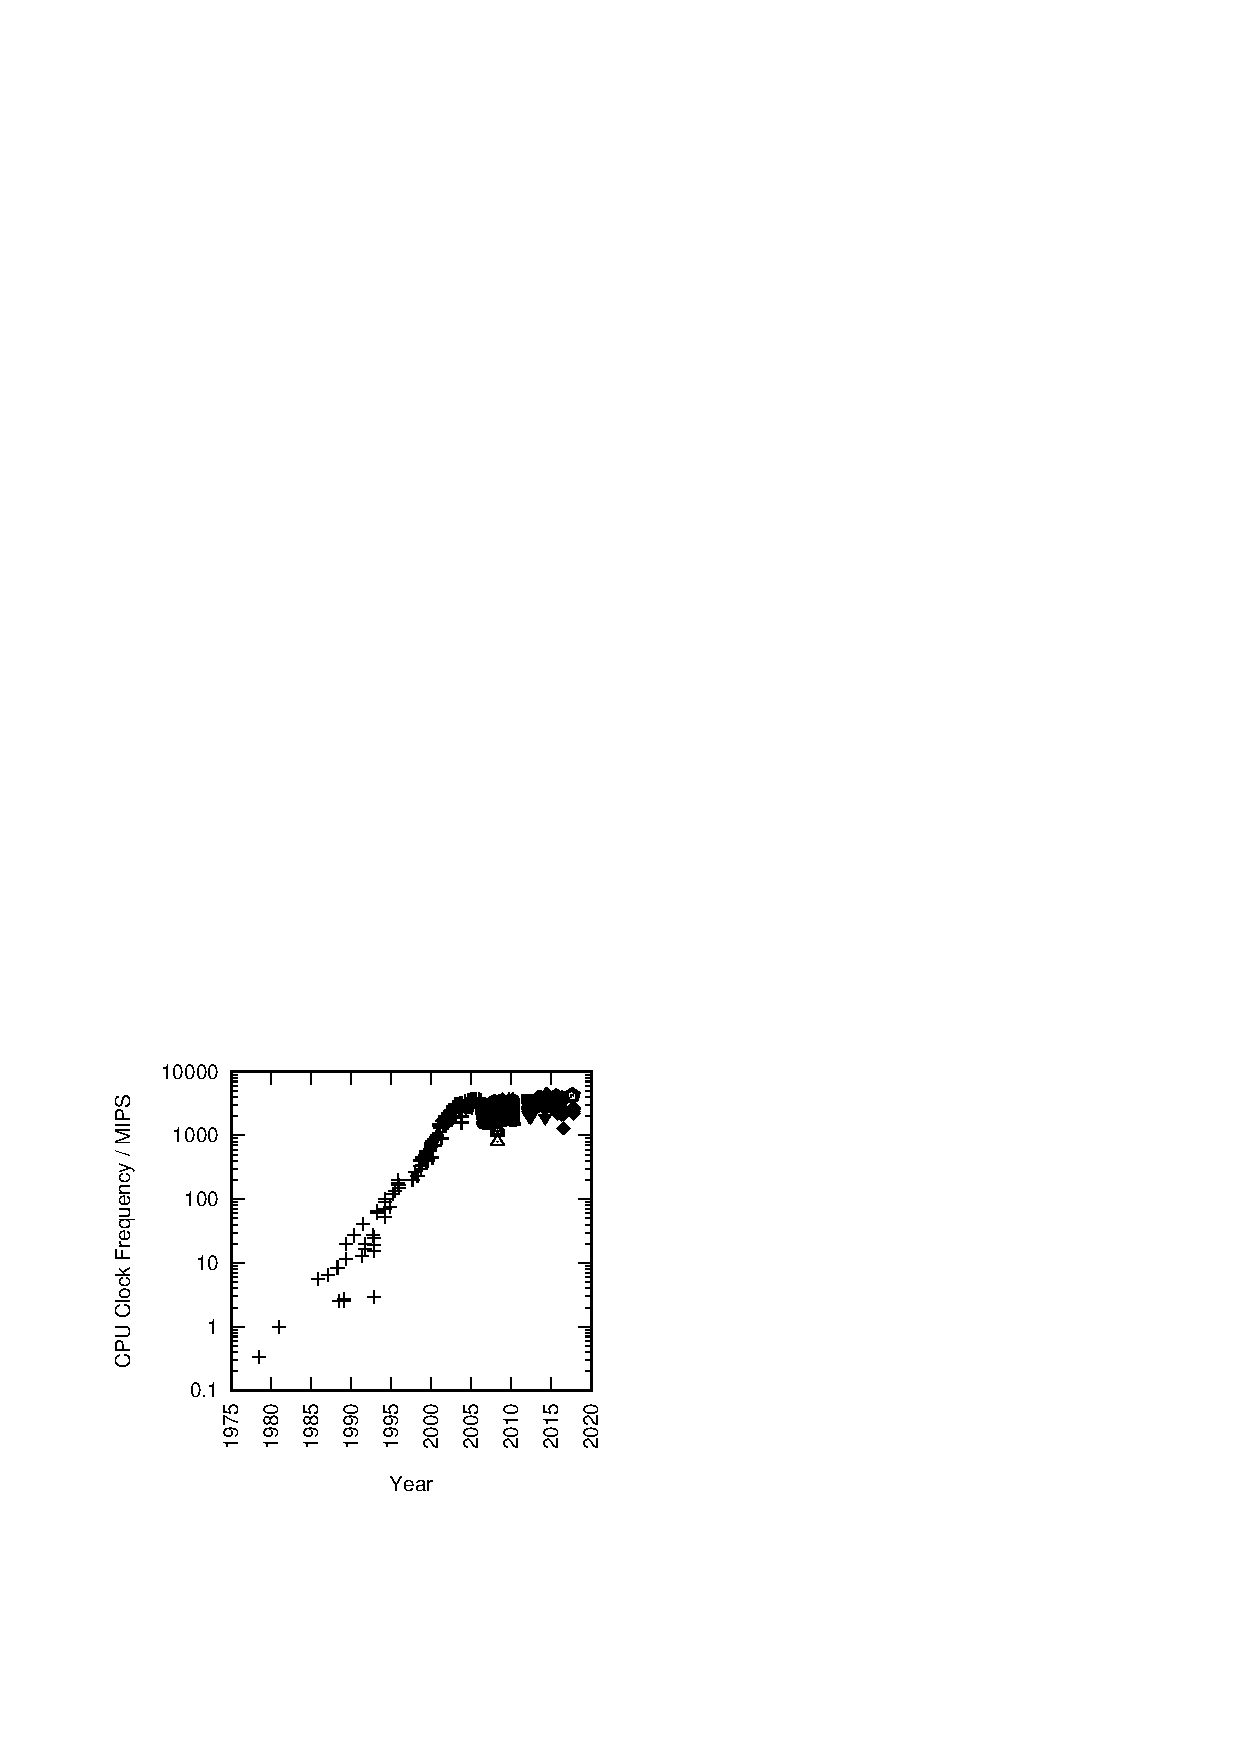
\includegraphics{SMPdesign/clockfreq}}
\caption{MIPS/Clock-Frequency Trend for Intel CPUs}
\label{fig:intro:Clock-Frequency Trend for Intel CPUs}
\end{figure}

그러나, 성능의 포커스는 하드웨어에서 병렬 소프트웨어로 옮겨졌습니다.
이 포커스의 변화는 \IX{Moore 의 법칙} 은 트랜지스터 집적도 증가를 지속하게
함에도, 전통적인 단일 쓰레드 성능 증가는 중단되었다는 사실 때문에
이루어졌습니다.
이는
Figure~\ref{fig:intro:Clock-Frequency Trend for Intel CPUs}\footnote{
	이 그림은 이론적으로 클락당 한개 이상의 인스트럭션을 처리할 수 있는
	신형 CPU 들의 경우 클락 주파수를, 가장 단순한 인스트럭션의 처리에도
	여러 클락을 필요로 하는 구형 CPU 들의 경우에는 MIPS (보통 Dhrystone
	벤치마크를 통해 얻어진, 초당 몇백만개의 인스트럭션이 처리 가능한가를
	나타내는 수) 를 보이고 있습니다.
	두개의 측정을 사용하는 이유는 신형 CPU 의 클락당 여러 인스트럭션을
	처리할 수 있는 능력이 메모리 시스템의 성능으로 인해 제한되곤 하기
	때문입니다.
	뿐만 아니라, 구형 CPU 의 성능 측정에 사용된 벤치마크는 더이상 사용되지
	않고, 신형 벤치마크를 구형 CPU 를 탑재한 시스템에서 돌리는 건 어려운데,
	부분적으로는 동작하는 구형 CPU 를 찾기도 쉽지 않기 때문입니다.}
에 그려져 있는데, 싱글 쓰레드 코드를 작성하고 CPU 가 성능이 좋아지기를 1-2년
기다리는건 더이상 선택지가 아님을 보입니다.
모든 주요 제조사가 멀티코어/멀티쓰레드 시스템으로 방향을 잡은 최근의 트렌드를
놓고 보면, 시스템의 완전한 성능을 내고자 하는 사람에게라면 병렬성이 맞는
방향입니다.

\iffalse

That said, the focus of performance has shifted from hardware to
parallel software.
This change in focus is due to the fact that, although \IX{Moore's Law}
continues to deliver increases in transistor density, it has ceased to
provide the traditional single-threaded performance increases.
This can be seen in
Figure~\ref{fig:intro:Clock-Frequency Trend for Intel CPUs}\footnote{
	This plot shows clock frequencies for newer CPUs theoretically
	capable of retiring one or more instructions per clock, and MIPS
	(millions of instructions per second, usually from the old
	Dhrystone benchmark)
	for older CPUs requiring multiple clocks to execute even the
	simplest instruction.
	The reason for shifting between these two measures is that the
	newer CPUs' ability to retire multiple instructions per clock is
	typically limited by memory-system performance.
	Furthermore, the benchmarks commonly used on the older CPUs
	are obsolete, and it is difficult to run the newer benchmarks
	on systems containing the old CPUs, in part because it is hard
	to find working instances of the old CPUs.},
which shows that writing single-threaded code and simply waiting
a year or two for the CPUs to catch up may no longer be an option.
Given the recent trends on the part of all major manufacturers towards
multicore/multithreaded systems, parallelism is the way to go for
those wanting to avail themselves of the full performance of their
systems.

\fi

\QuickQuiz{
	프로그램을 비효율적인 스크립트 언어에서 C 나 C++ 로 재작성하는 건
	어떨까요?

	\iffalse

	Why not instead rewrite programs from inefficient scripting
	languages to C or C++?

	\fi

}\QuickQuizAnswer{
	그런 재작성을 위한 개발자들, 예산, 그리고 시간이 충분하다면, 그리고
	그게 단일 CPU 에서도 필요한 수준의 성능을 얻을 수 있다면, 합리적
	접근법이 될 수 있습니다.

	\iffalse

	If the developers, budget, and time is available for such a
	rewrite, and if the result will attain the required levels
	of performance on a single CPU, this can be a reasonable
	approach.

	\fi

}\QuickQuizEnd

그렇기는 하나, 첫번째 목표는 확장성보다는 성능인데, 선형적 확장성을 얻는 가장
쉬운 방법은 각 CPU 의 성능을 낮추는 것~\cite{LinusTorvalds2001a} 이라는 점을
놓고 보면 특히 그렇습니다.
네개의 CPU 를 탑재한 시스템이 있다면, 당신이라면 뭘 선호하겠습니까?
단일 CPU 에서 초당 100개의 트랜잭션을 처리하지만 전혀 멀티 CPU 확장성이 없는
프로그램입니까?
아니면 단일 CPU 에서 초당 10개의 트랜잭션만을 처리하지만 CPU 개수를 늘림에 따라
완전하게 확장 가능한 프로그램입니까?
첫번째 프로그램이 더 나은 선택일 겁니다, 32개 CPU 가 탑재된 시스템이라면 답이
달라질 수도 있겠지만요.

\iffalse

Even so, the first goal is performance rather than scalability,
especially given that the easiest way to attain linear scalability
is to reduce the performance of each CPU~\cite{LinusTorvalds2001a}.
Given a four-CPU system, which would you prefer?
A program that provides 100 transactions per second on a single CPU,
but does not scale at all?
Or a program that provides 10 transactions per second on a single CPU,
but scales perfectly?
The first program seems like a better bet, though the answer might
change if you happened to have a 32-CPU system.

\fi

그러나, 여러분이 여러 CPU 를 가졌다는 건 그 자체로 그걸 모두 사용해야만 한다는
이유가 되지 않는데, 특히 최근의 멀티 CPU 시스템의 가격 하락을 놓고 보면
그렇습니다.
핵심은 병렬 프로그래밍은 기본적으로 성능 최적화이며, 그건 여러 잠재적 최적화
방법 중 하나라는 것입니다.
여러분의 프로그램이 현재 작성된 대로도 충분히 빠르다면, 병렬화를 해서든 다른
잠재적 순차적 최족화 방법들을 동원해서든 최적화를 할 이유가 없습니다.\footnote{
	물론, 여러분이 병렬 소프트웨어를 작성하는게 주요 관심사인 취미
	생활자라면 여러분이 관심있는 소프트웨어가 무엇이건 병렬화를 할 충분한
	이유가 됩니다.}
같은 이유로, 순차적 프로그램의 최적화 수단으로 병렬화를 하고자 한다면, 최선의
순차적 알고리즘과 병렬 알고리즘들을 비교해야 합니다.
현재 많은 출판물이 병렬 알고리즘의 성능을 논할 때 순차적 알고리즘의 경우들을
무시하곤 하기 때문에 이 부분에서 주의가 필요합니다.

\iffalse

That said, just because you have multiple CPUs is not necessarily
in and of itself a reason to use them all, especially given the
recent decreases in price of multi-CPU systems.
The key point to understand is that parallel programming is primarily
a performance optimization, and, as such, it is one potential optimization
of many.
If your program is fast enough as currently written, there is no
reason to optimize, either by parallelizing it or by applying any
of a number of potential sequential optimizations.\footnote{
	Of course, if you are a hobbyist whose primary interest is
	writing parallel software, that is more than enough reason to
	parallelize whatever software you are interested in.}
By the same token, if you are looking to apply parallelism as an
optimization to a sequential program, then you will need to compare
parallel algorithms to the best sequential algorithms.
This may require some care, as far too many publications ignore the
sequential case when analyzing the performance of parallel algorithms.

\fi

\subsection{Productivity}
\label{sec:intro:Productivity}

\QuickQuiz{
	왜 이건 기술적이지 않은 문제들에 대해 떠드는 거죠???
	단순히 \emph{아무} 기술적이지 않은 문제가 아니라, \emph{생산성}
	이라구요?
	누가 이걸 신경씁니까?

	\iffalse

	Why all this prattling on about non-technical issues???
	And not just \emph{any} non-technical issue, but \emph{productivity}
	of all things?
	Who cares?

	\fi

}\QuickQuizAnswer{
	여러분이 순수한 취미가라면, 아마 신경쓸 필요 없을 겁니다.
	하지만 순수한 취미가라 할지라도 얼마나 빨리 얼마나 많이 일을 해낼 수
	있는가에 종종 신경씁니다.
	어쨌건, 가장 대중적인 취미가용 도구는 그 일을 하는데 최적인 것들이
	경우가 많고, ``최적'' 의 정의의 중요한 부분은 생산성과 연관되어
	있습니다.
	그리고 만약 누군가가 여러분이 병렬 코드를 작성하는데 대해 돈을 지불하고
	있다면, 그들은 여러분의 생산성에 무척 신경쓰고 있을 가능성이 높습니다.
	그리고 여러분에게 돈을 지불하는 사람이 뭔가에 신경쓰고 있다면, 여러분도
	그것에 최소 어느 정도는 신경을 쓰는게 현명할 겁니다!

	그 외에도, 여러분이 \emph{정말로} 생산성을 신경쓰지 않는다면, 컴퓨터를
	사용하지 않고 수작업으로 직접 일을 하시겠죠!

	\iffalse

	If you are a pure hobbyist, perhaps you don't need to care.
	But even pure hobbyists will often care about how much they
	can get done, and how quickly.
	After all, the most popular hobbyist tools are usually those
	that are the best suited for the job, and an important part of
	the definition of ``best suited'' involves productivity.
	And if someone is paying you to write parallel code, they will
	very likely care deeply about your productivity.
	And if the person paying you cares about something, you would
	be most wise to pay at least some attention to it!

	Besides, if you \emph{really} didn't care about productivity,
	you would be doing it by hand rather than using a computer!

	\fi

}\QuickQuizEnd

최근 수십년간 생산성은 점점 더 중요해졌습니다.
이를 보기 위해, 초기 컴퓨터의 가격은 엔지니어 연봉이 수천달러이던 시절에 수억
달러였음을 생각해 보십시오.
그런 기계를 위해 열명의 엔지니어 팀을 전담시키는 것이 그 성능을 10\,\% 라도
향상시킨다면, 그들의 연봉은 여러번 더 지불될 수 있을 겁니다.

그런 기계 중 하나로 CSIRAC 가 있는데, 가장 오래되었고 여전히 손상되지 않은
stored-program 컴퓨터로, 1949년부터
작동되었습니다~\cite{CSIRACMuseumVictoria,CSIRACUniversityMelbourne}.
이 기계는 트랜지스터 시대 전에 만들어졌으므로, 2,000 개의 진공관으로 만들어졌고
1\,kHz 클락 주파수로 작동하며, 30\,kW 전력을 소비하고, 3 톤의 무게를
가졌습니다.
이 기계가 768 워드 RAM 을 가졌음을 생각해 보면, 이 기계는 오늘날의 거대 규모
소프트웨어 프로젝트가 시달리는 생산성 이슈로 고생하지는 않았을 거라 말할 수
있을 겁니다.

오늘날, 이렇게 작은 컴퓨팅 파워를 가진 기계를 구입하긴 상당히 어려울 겁니다.
가장 비슷한 장비는 아마도 유서 깊은 Z80~\cite{z80Wikipedia} 로 대표되는 8-bit
임베디드 마이크로프로세서가 될 겁니다만, 오래된 Z80 조차도 CSIRAC 보다 1,000
배나 빠른 CPU 클락 주파수를 가졌습니다.
Z80 CPU 는 8,500 개 트랜지스터를 가졌고, 2008년 기준으로 1,000개씩 구매하면
개당 \$2 US 도 하지 않았습니다.
CSIRAC 에 대비되게도, Z80 에 있어 소프트웨어 개발 비용은 중요치 않습니다.

\iffalse

Productivity has been becoming increasingly important in recent decades.
To see this, consider that the price of early computers was tens
of millions of dollars at
a time when engineering salaries were but a few thousand dollars a year.
If dedicating a team of ten engineers to such a machine would improve
its performance, even by only 10\,\%, then their salaries
would be repaid many times over.

One such machine was the CSIRAC, the oldest still-intact stored-program
computer, which was put into operation in
1949~\cite{CSIRACMuseumVictoria,CSIRACUniversityMelbourne}.
Because this machine was built before the transistor era, it was constructed
of 2,000 vacuum tubes, ran with a clock frequency of 1\,kHz,
consumed 30\,kW of power, and weighed more than three metric tons.
Given that this machine had but 768 words of RAM, it is safe to say that
it did not suffer from the productivity issues that often plague
today's large-scale software projects.

Today, it would be quite difficult to purchase a machine with so
little computing power.
Perhaps the closest equivalents
are 8-bit embedded microprocessors exemplified by the venerable
Z80~\cite{z80Wikipedia}, but even the old Z80 had a CPU clock
frequency more than 1,000 times faster than the CSIRAC\@.
The Z80 CPU had 8,500 transistors, and could be purchased in 2008
for less than \$2 US per unit in 1,000-unit quantities.
In stark contrast to the CSIRAC, software-development costs are
anything but insignificant for the Z80.

\fi

\begin{figure}[tb]
\centering
\resizebox{3in}{!}{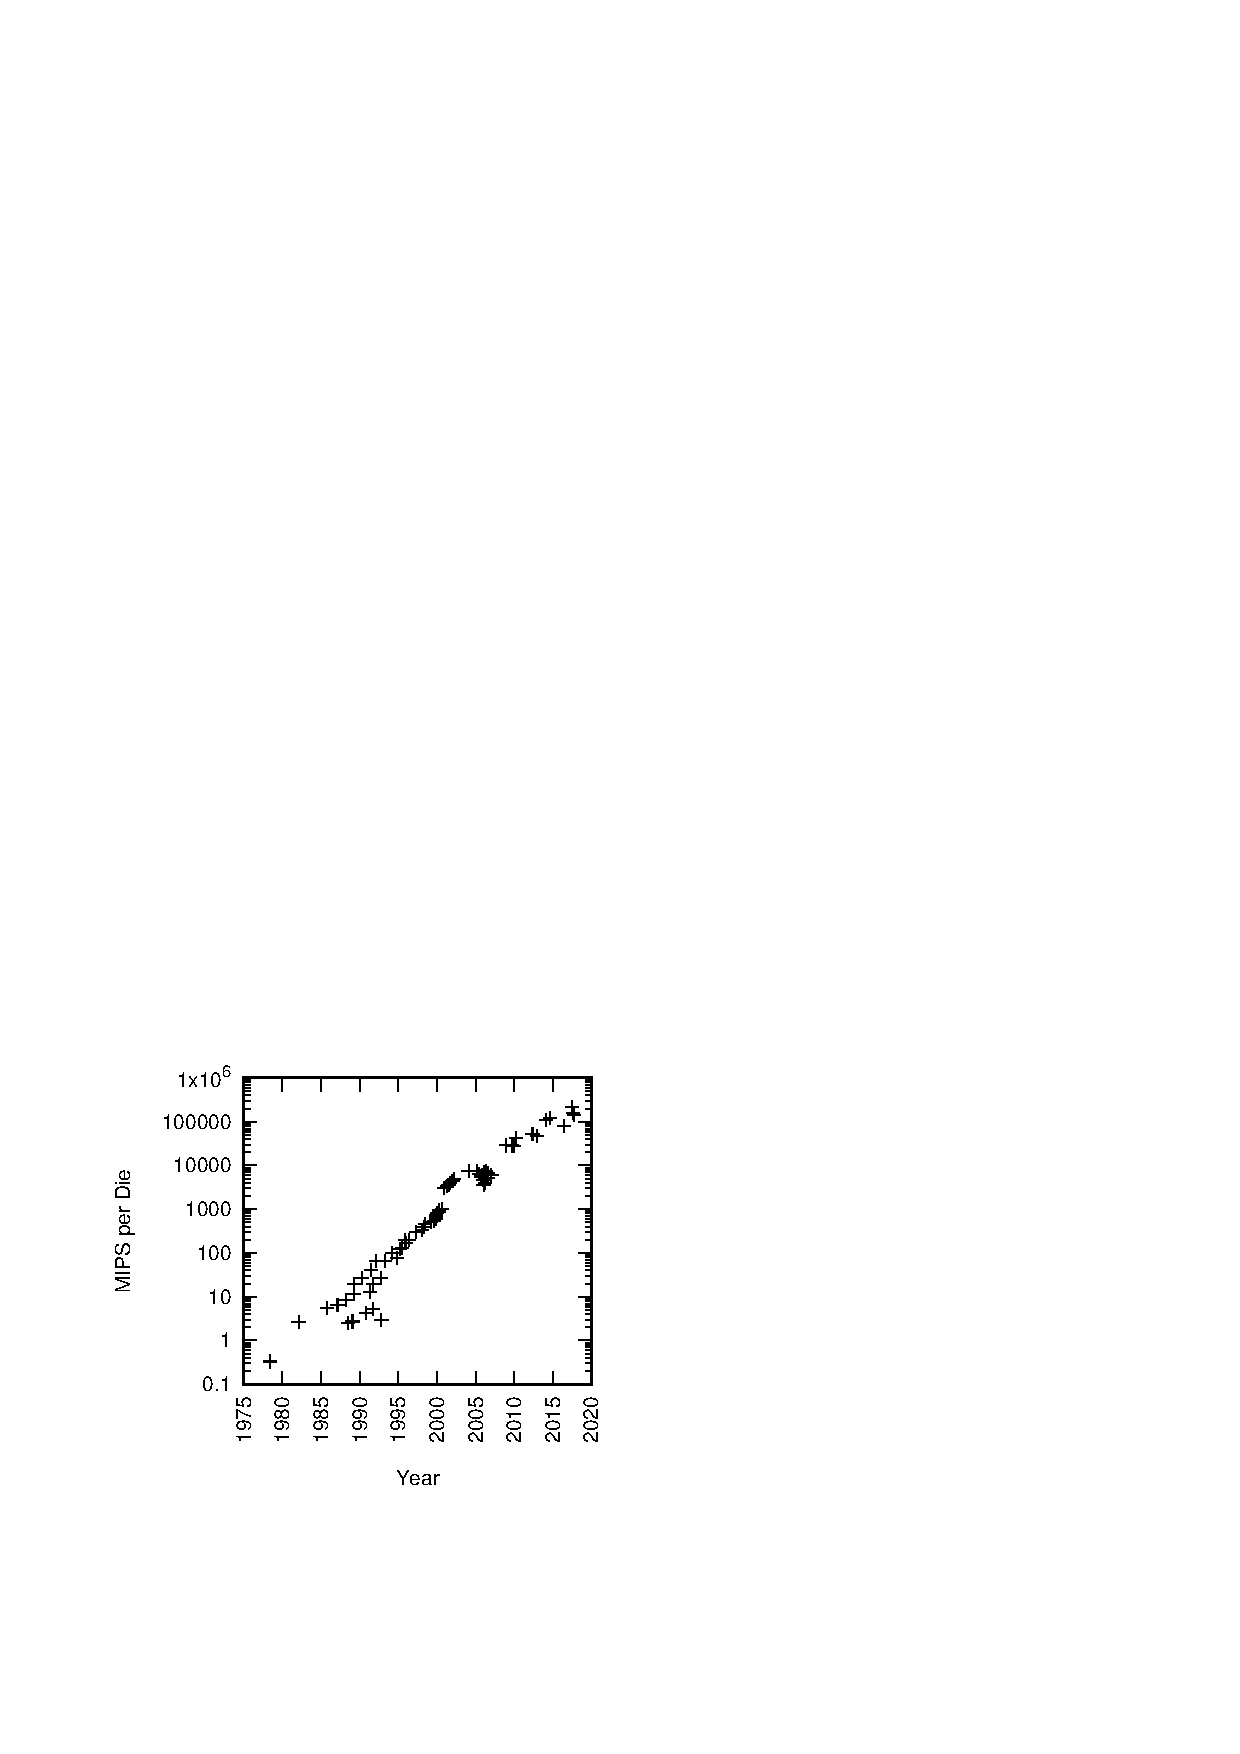
\includegraphics{SMPdesign/mipsperbuck}}
\caption{MIPS per Die for Intel CPUs}
\label{fig:intro:MIPS per Die for Intel CPUs}
\end{figure}

CSIRAC 와 Z80 은 장기적 트렌드 상의 두 지점으로,
Figure~\ref{fig:intro:MIPS per Die for Intel CPUs}
위에서 볼 수 있습니다.
이 그림은 다이당 예상 연산력을 과거 40년의 세월에 걸쳐 그리고 있는데, 40년간
백만배가 넘는 인상적인 향상을 보입니다.
멀티코어 CPU 의 발전은 2003년 이후 마주친 클락 주파수 장벽에도 불구하고 다이당
50개의 하드웨어 쓰레드를 지원함으로써 이 향상을 지속가능하게 했음을 알아두시기
바랍니다.

하드웨어 가격의 가파른 하락의 부정할 수 없는 결론은 소프트웨어 생산성이 갈수록
중요해져 가고 있다는 겁니다.
단순히 하드웨어를 효율적으로 사용하는건 더이상 충분치 않습니다:
이제 소프트웨어 개발자들을 극단적으로 효율성 있게 활용할 필요가 있습니다.
이는 순차적 하드웨어에 있어서 오랫동안 그랬습니다만, 병렬 하드웨어는최근
들어서야 저렴한 일반 상품이 되었습니다.
따라서, 최근에 들어서야 높은 생산성이 병렬 소프트웨어를 만드는 데 있어 크게
중요해 졌습니다.

\iffalse

The CSIRAC and the Z80 are two points in a long-term trend, as can be
seen in
Figure~\ref{fig:intro:MIPS per Die for Intel CPUs}.
This figure plots an approximation to computational power per die
over the past four decades, showing an impressive six-order-of-magnitude
increase over a period of forty years.
Note that the advent of multicore CPUs has permitted this increase to
continue apace despite the clock-frequency wall encountered in 2003,
albeit courtesy of dies supporting more than 50 hardware threads each.

One of the inescapable consequences of the rapid decrease in
the cost of hardware is that software productivity becomes increasingly
important.
It is no longer sufficient merely to make efficient use of the hardware:
It is now necessary to make extremely efficient use of software
developers as well.
This has long been the case for sequential hardware, but
parallel hardware has become a low-cost commodity only recently.
Therefore, only recently has high productivity become critically important
when creating parallel software.

\fi

\QuickQuiz{
	병렬 시스템이 그렇게 싸졌는데, 그걸 프로그램하라고 누가 돈을 줄까요?

	\iffalse

	Given how cheap parallel systems have become, how can anyone
	afford to pay people to program them?

	\fi
}\QuickQuizAnswer{

	이 질문에 여러 답이 가능합니다:
	\begin{enumerate}
	\item	병렬 기계의 클러스터가 있다면, 이 클러스터의 전체 가격은 상당한
		수준의 개발 노력을 정당화 할 수 있을텐데, 개발 비용이 이 많은
		수의 기계들로 나뉘어질 수 있기 때문입니다.
	\item	수천만명의 사용자들에 의해 돌아가는 대중적인 소프트웨어는
		상당한 개발 노력을 쉽게 정당화 할 수 있는데, 이 개발 비용은
		수천만명의 사용자로 나뉘어질 수 있기 때문입니다.
		이는 커널과 시스템 라이브러리 같은 것들을 포함함을
		알아두십시오.
	\item	저렴한 병렬 머신이 중요한 장비의 한 부품의 운영을 조절한다면,
		이 장비의 한 부품의 가격은 상당한 개발 노력을 쉽게 정당화 시킬
		수도 있습니다.
	\item	저렴한 병렬 기계의 소프트웨어가 극단적으로 중요한 결과 (예:
		전력 절약) 를 만들어 낸다면, 이 중요한 결과가 역시 상당한 개발
		비용을 정당화 시킬 수도 있습니다.
	\item	안전성이 중요한 시스템은 목숨을 보호하므로, 분명히 매우 큰 개발
		노력을 정당화 할 수 있습니다.
	\item	취미가들과 연구자들은 대신 지식, 경험, 재미, 그리고 영광을
		추구할 겁니다.
	\end{enumerate}

	그러니 줄어드는 하드웨어 가격이 소프트웨어를 가치없게 하지는 않으며,
	오히려 소프트웨어 개발 비용을 하드웨어 가격 아래 ``감출'' 수
	없어졌습니다, 엄청나게 커다란 하드웨어 단위가 존재하지 않는 이상
	말이죠.

	\iffalse

	There are a number of answers to this question:
	\begin{enumerate}
	\item	Given a large computational cluster of parallel machines,
		the aggregate cost of the cluster can easily justify
		substantial developer effort, because the development
		cost can be spread over the large number of machines.
	\item	Popular software that is run by tens of millions of users
		can easily justify substantial developer effort,
		as the cost of this development can be spread over the tens
		of millions of users.
		Note that this includes things like kernels and system
		libraries.
	\item	If the low-cost parallel machine is controlling the operation
		of a valuable piece of equipment, then the cost of this
		piece of equipment might easily justify substantial
		developer effort.
	\item	If the software for the low-cost parallel machine produces an
		extremely valuable result (e.g., energy savings),
		then this valuable result might again justify substantial
		developer cost.
	\item	Safety-critical systems protect lives, which can clearly
		justify very large developer effort.
	\item	Hobbyists and researchers might instead seek knowledge,
		experience, fun, or glory.
	\end{enumerate}
	So it is not the case that the decreasing cost of hardware renders
	software worthless, but rather that it is no longer possible to
	``hide'' the cost of software development within the cost of
	the hardware, at least not unless there are extremely large
	quantities of hardware.

	\fi

}\QuickQuizEnd

적어도 한때, 병렬 소프트웨어의 단 한가지 목적은 성능이었습니다.
하지만, 지금 생산성은 더 많은 주목을 받고 있습니다.

\iffalse

Perhaps at one time, the sole purpose of parallel software was performance.
Now, however, productivity is gaining the spotlight.

\fi

\subsection{Generality}
\label{sec:intro:Generality}

One way to justify the high cost of developing parallel software
is to strive for maximal generality.
All else being equal, the cost of a more-general software artifact
can be spread over more users than that of a less-general one.
In fact, this economic force explains much of the maniacal focus
on portability, which can be seen as an important special case
of generality.\footnote{
	Kudos to Michael Wong for pointing this out.}

Unfortunately, generality often comes at the cost of performance,
productivity, or both.
For example, portability is often achieved via adaptation layers,
which inevitably exact a performance penalty.
To see this more generally, consider the following popular parallel
programming environments:

\begin{description}
\item[C/C++ ``Locking Plus Threads'':] This category, which includes
	POSIX Threads (pthreads)~\cite{OpenGroup1997pthreads},
	Windows Threads, and numerous
	operating-system kernel environments, offers excellent performance
	(at least within the confines of a single SMP system)
	and also offers good generality.
	Pity about the relatively low productivity.
\item[Java:] This general purpose and inherently multithreaded
	programming environment	is widely believed to offer much higher
	productivity than C or C++, courtesy of the automatic garbage collector
	and the rich set of class libraries.
	However, its performance, though greatly improved in the early
	2000s, lags that of C and C++.
\item[MPI:] This Message Passing Interface~\cite{MPIForum2008} powers
	the largest scientific and technical computing clusters in
	the world and offers unparalleled performance and scalability.
	In theory, it is general purpose, but it is mainly used
	for scientific and technical computing.
	Its productivity is believed by many to be even lower than that
	of C/C++ ``locking plus threads'' environments.
\item[OpenMP:] This set of compiler directives can be used
	to parallelize loops.  It is thus quite specific to this
	task, and this specificity often limits its performance.
	It is, however, much easier to use than MPI or C/C++
	``locking plus threads.''
\item[SQL:] Structured Query Language~\cite{DIS9075SQL92} is
	specific to relational database queries.
	However, its performance is quite good as measured by the
	Transaction Processing Performance Council (TPC)
	benchmark results~\cite{TPC}.
	Productivity is excellent; in fact, this parallel programming
	environment enables people to make good use of a large parallel
	system despite having little or no knowledge of parallel
	programming concepts.
\end{description}

\begin{figure}[tb]
\centering
\resizebox{2.5in}{!}{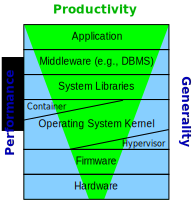
\includegraphics{intro/PPGrelation}}
\caption{Software Layers and Performance, Productivity, and Generality}
\label{fig:intro:Software Layers and Performance, Productivity, and Generality}
\end{figure}

The nirvana of parallel programming environments, one that offers
world-class performance, productivity, and generality, simply does
not yet exist.
Until such a nirvana appears, it will be necessary to make engineering
tradeoffs among performance, productivity, and generality.
One such tradeoff is shown in
Figure~\ref{fig:intro:Software Layers and Performance, Productivity, and Generality},
which shows how productivity becomes increasingly important at the upper layers
of the system stack,
while performance and generality become increasingly important at the
lower layers of the system stack.
The huge development costs incurred at the lower layers
must be spread over equally huge numbers of users
(hence the importance of generality), and
performance lost in lower layers cannot easily be
recovered further up the stack.
In the upper layers of the stack, there might be very few users for a given
specific application, in which case productivity concerns are paramount.
This explains the tendency towards ``bloatware'' further up the stack:
Extra hardware is often cheaper than extra developers.
This book is intended for developers working near the bottom
of the stack, where performance and generality are of greatest concern.

\begin{figure}[tb]
\centering
\resizebox{3in}{!}{\includegraphics{intro/Generality}}
\caption{Tradeoff Between Productivity and Generality}
\label{fig:intro:Tradeoff Between Productivity and Generality}
\end{figure}

It is important to note that a tradeoff between productivity and
generality has existed for centuries in many fields.
For but one example, a nailgun is more productive than a hammer for
driving nails, but in contrast to the nailgun, a hammer can be used for
many things besides driving nails.
It should therefore be no surprise to see similar tradeoffs
appear in the field of parallel computing.
This tradeoff is shown schematically in
Figure~\ref{fig:intro:Tradeoff Between Productivity and Generality}.
Here, users~1, 2, 3, and 4 have specific jobs that they need the computer
to help them with.
The most productive possible language or environment for a given user is one
that simply does that user's job, without requiring any programming,
configuration, or other setup.

\QuickQuiz{
	This is a ridiculously unachievable ideal!
	Why not focus on something that is achievable in practice?
}\QuickQuizAnswer{
	This is eminently achievable.
	The cellphone is a computer that can be used to make phone
	calls and to send and receive text messages with little or
	no programming or configuration on the part of the end user.

	This might seem to be a trivial example at first glance,
	but if you consider it carefully you will see that it is
	both simple and profound.
	When we are willing to sacrifice generality, we can achieve
	truly astounding increases in productivity.
	Those who indulge in excessive generality will therefore fail to set
	the productivity bar high enough to succeed near the top of the
	software stack.
	This fact of life even has its own acronym: YAGNI, or ``You
	Ain't Gonna Need It.''
}\QuickQuizEnd

Unfortunately, a system that does the job required by user~1 is
unlikely to do user~2's job.
In other words, the most productive languages and environments are
domain-specific, and thus by definition lacking generality.

Another option is to tailor a given programming language or environment
to the hardware system (for example, low-level languages such as
assembly, C, C++, or Java) or to some abstraction (for example,
Haskell, Prolog, or Snobol), as is shown by the circular region near
the center of
Figure~\ref{fig:intro:Tradeoff Between Productivity and Generality}.
These languages can be considered to be general in the sense that they
are equally ill-suited to the jobs required by users~1, 2, 3, and 4.
In other words, their generality comes at the expense of
decreased productivity when compared to domain-specific languages
and environments.
Worse yet, a language that is tailored to a given abstraction
is likely to suffer from performance and scalability problems
unless and until it can be efficiently mapped to real hardware.

Is there no escape from iron triangle's three conflicting goals of
performance, productivity, and generality?

It turns out that there often is an escape, for example,
using the alternatives to parallel programming discussed in the next section.
After all, parallel programming can be a great deal of fun, but
it is not always the best tool for the job.

\section{Alternatives to Parallel Programming}
\label{sec:intro:Alternatives to Parallel Programming}
%
\epigraph{Experiment is folly when experience shows the way.}
	 {\emph{Roger M. Babson}}

In order to properly consider alternatives to parallel programming,
you must first decide on what exactly you expect the parallelism
to do for you.
As seen in Section~\ref{sec:intro:Parallel Programming Goals},
the primary goals of parallel programming are performance, productivity,
and generality.
Because this book is intended for developers working on
performance-critical code near the bottom of the software stack,
the remainder of this section focuses primarily on performance improvement.

It is important to keep in mind that parallelism is but one way to
improve performance.
Other well-known approaches include the following, in roughly increasing
order of difficulty:

\begin{enumerate}
\item	Run multiple instances of a sequential application.
\item	Make the application use existing parallel software.
\item	Optimize the serial application.
\end{enumerate}

These approaches are covered in the following sections.

\subsection{Multiple Instances of a Sequential Application}
\label{sec:intro:Multiple Instances of a Sequential Application}

Running multiple instances of a sequential application can allow you
to do parallel programming without actually doing parallel programming.
There are a large number of ways to approach this, depending on the
structure of the application.

If your program is analyzing a large number of different scenarios,
or is analyzing a large number of independent data sets, one easy
and effective approach is to create a single sequential program that
carries out a single analysis, then use any of a number of scripting
environments (for example the \co{bash} shell) to run a number of
instances of that sequential program in parallel.
In some cases, this approach can be easily extended to a cluster of
machines.

This approach may seem like cheating, and in fact some denigrate such
programs as ``embarrassingly parallel''.
And in fact, this approach does have some potential disadvantages,
including increased memory consumption, waste of CPU cycles recomputing
common intermediate results, and increased copying of data.
However, it is often  extremely productive, garnering extreme performance
gains with little or no added effort.

\subsection{Use Existing Parallel Software}
\label{sec:intro:Use Existing Parallel Software}

There is no longer any shortage of parallel software environments that
can present a single-threaded programming environment,
including relational
databases~\cite{Date82},
web-application servers, and map-reduce environments.
For example, a common design provides a separate process for each
user, each of which generates SQL from user queries.
This per-user SQL is run against a common relational database, which
automatically runs the users' queries concurrently.
The per-user programs are responsible only for the user interface,
with the relational database taking full responsibility for the
difficult issues surrounding parallelism and persistence.

In addition, there are a growing number of parallel library functions,
particularly for numeric computation.
Even better, some libraries take advantage of special\-/purpose
hardware such as vector units and general\-/purpose graphical processing
units (GPGPUs).

Taking this approach often sacrifices some performance, at least when
compared to carefully hand-coding a fully parallel application.
However, such sacrifice is often well repaid by a huge reduction in
development effort.

\QuickQuiz{
	Wait a minute!
	Doesn't this approach simply shift the development effort from
	you to whoever wrote the existing parallel software you are using?
}\QuickQuizAnswer{
	Exactly!
	And that is the whole point of using existing software.
	One team's work can be used by many other teams, resulting in a
	large decrease in overall effort compared to all teams
	needlessly reinventing the wheel.
}\QuickQuizEnd

\subsection{Performance Optimization}
\label{sec:intro:Performance Optimization}

Up through the early 2000s, CPU clock frequencies doubled every 18 months.
It was therefore usually more important to create new functionality than to
carefully optimize performance.
Now that \IX{Moore's Law} is ``only'' increasing transistor density instead
of increasing both transistor density and per-transistor performance,
it might be a good time to rethink the importance of performance
optimization.
After all, new hardware generations no longer bring significant
single-threaded performance improvements.
Furthermore, many performance optimizations can also conserve energy.

From this viewpoint, parallel programming is but another performance
optimization, albeit one that is becoming much more attractive
as parallel systems become cheaper and more readily available.
However, it is wise to keep in mind that the speedup available from
parallelism is limited to roughly the number of CPUs
(but see Section~\ref{sec:SMPdesign:Beyond Partitioning}
for an interesting exception).
In contrast, the speedup available from traditional single-threaded
software optimizations can be much larger.
For example, replacing a long linked list with a hash table
or a search tree can improve performance by many orders of magnitude.
This highly optimized single-threaded program might run much
faster than its unoptimized parallel counterpart, making parallelization
unnecessary.
Of course, a highly optimized parallel program would be even better,
aside from the added development effort required.

Furthermore, different programs might have different performance
bottlenecks.
For example, if your program spends most of its time
waiting on data from your disk drive,
using multiple CPUs will probably just increase the time wasted waiting
for the disks.
In fact, if the program was reading from a single large file laid out
sequentially on a rotating disk, parallelizing your program might
well make it a lot slower due to the added seek overhead.
You should instead optimize the data layout so that
the file can be smaller (thus faster to read), split the file into chunks
which can be accessed in parallel from different drives,
cache frequently accessed data in main memory,
or, if possible,
reduce the amount of data that must be read.

\QuickQuiz{
	What other bottlenecks might prevent additional CPUs from
	providing additional performance?
}\QuickQuizAnswer{
	There are any number of potential bottlenecks:
	\begin{enumerate}
	\item	Main memory.  If a single thread consumes all available
		memory, additional threads will simply page themselves
		silly.
	\item	Cache.  If a single thread's cache footprint completely
		fills any shared CPU cache(s), then adding more threads
		will simply thrash those affected caches, as will be
		seen in \cref{chp:Data Structures}.
	\item	Memory bandwidth.  If a single thread consumes all available
		memory bandwidth, additional threads will simply
		result in additional queuing on the system interconnect.
	\item	I/O bandwidth.  If a single thread is I/O bound,
		adding more threads will simply result in them all
		waiting in line for the affected I/O resource.
	\end{enumerate}

	Specific hardware systems might have any number of additional
	bottlenecks.
	The fact is that every resource which is shared between
	multiple CPUs or threads is a potential bottleneck.
}\QuickQuizEnd

Parallelism can be a powerful optimization technique, but
it is not the only such technique, nor is it appropriate for all
situations.
Of course, the easier it is to parallelize your program, the
more attractive parallelization becomes as an optimization.
Parallelization has a reputation of being quite difficult,
which leads to the question ``exactly what makes parallel
programming so difficult?''

\section{What Makes Parallel Programming Hard?}
\label{sec:intro:What Makes Parallel Programming Hard?}
%
\epigraph{Real difficulties can be overcome; it is only the imaginary
	  ones that are unconquerable.}{\emph{Theodore N.~Vail}}

\OriginallyPublished{Section}{sec:intro:What Makes Parallel Programming Hard?}{What Makes Parallel Programming Hard?}{a Portland State University Technical Report}{PaulEMcKenney2009ProgrammingHard}

It is important to note that the difficulty of parallel programming
is as much a human-factors issue as it is a set of technical properties of the
parallel programming problem.
We do need human beings to be able to tell parallel
systems what to do, otherwise known as programming.
But parallel programming involves two-way communication, with
a program's performance and scalability being the communication from
the machine to the human.
In short, the human writes a program telling the computer what to do,
and the computer critiques this program via the resulting performance and
scalability.
Therefore, appeals to abstractions or to mathematical analyses will
often be of severely limited utility.

In the Industrial Revolution, the interface between human and machine
was evaluated by human-factor studies, then called time-and-motion
studies.
Although there have been a few human-factor studies examining parallel
programming~\cite{RyanEccles2005HPCSNovice,RyanEccles2006HPCSNoviceNeeds,
LorinHochstein2005SC,DuaneSzafron1994PEMPDS}, these studies have
been extremely narrowly focused, and hence unable to demonstrate any
general results.
Furthermore, given that the normal range of programmer productivity
spans more than an order of magnitude, it is unrealistic to expect
an affordable study to be capable of detecting (say) a 10\,\% difference
in productivity.
Although the multiple-order-of-magnitude differences that such studies
\emph{can} reliably detect are extremely valuable, the most impressive
improvements tend to be based on a long series of 10\,\% improvements.

We must therefore take a different approach.

\begin{figure}[tb]
\centering
\resizebox{3in}{!}{\includegraphics{intro/FourTaskCategories}}
\caption{Categories of Tasks Required of Parallel Programmers}
\label{fig:intro:Categories of Tasks Required of Parallel Programmers}
\end{figure}

One such approach is to carefully consider the tasks that parallel
programmers must undertake that are not required of sequential programmers.
We can then evaluate how well a given programming language or environment
assists the developer with these tasks.
These tasks fall into the four categories shown in
Figure~\ref{fig:intro:Categories of Tasks Required of Parallel Programmers},
each of which is covered in the following sections.

\subsection{Work Partitioning}
\label{sec:intro:Work Partitioning}

Work partitioning is absolutely required for parallel execution:
if there is but one ``glob'' of work, then it can be executed by at
most one CPU at a time, which is by definition sequential execution.
However, partitioning the code requires great care.
For example, uneven partitioning can result in sequential execution
once the small partitions have completed~\cite{GeneAmdahl1967AmdahlsLaw}.
In less extreme cases, load balancing can be used to fully utilize
available hardware and restore performance and scalabilty.

Although partitioning can greatly improve performance and scalability,
it can also increase complexity.
For example, partitioning can complicate handling of global
errors and events: A parallel
program may need to carry out non-trivial synchronization in order
to safely process such global events.
More generally, each partition requires some sort of communication:
After all, if
a given thread did not communicate at all, it would have no effect and
would thus not need to be executed.
However, because communication incurs overhead, careless partitioning choices
can result in severe performance degradation.

Furthermore, the number of concurrent threads must often be controlled,
as each such thread occupies common resources, for example,
space in CPU caches.
If too many threads are permitted to execute concurrently, the
CPU caches will overflow, resulting in high cache miss rate, which in
turn degrades performance.
Conversely, large numbers of threads are often required to
overlap computation and I/O so as to fully utilize I/O devices.

\QuickQuiz{
	Other than CPU cache capacity, what might require limiting the
	number of concurrent threads?
}\QuickQuizAnswer{
	There are any number of potential limits on the number of
	threads:
	\begin{enumerate}
	\item	Main memory.  Each thread consumes some memory
		(for its stack if nothing else), so that excessive
		numbers of threads can exhaust memory, resulting
		in excessive paging or memory-allocation failures.
	\item	I/O bandwidth.  If each thread initiates a given
		amount of mass-storage I/O or networking traffic,
		excessive numbers of threads can result in excessive
		I/O queuing delays, again degrading performance.
		Some networking protocols may be subject to timeouts
		or other failures if there are so many threads that
		networking events cannot be responded to in a timely
		fashion.
	\item	Synchronization overhead.
		For many synchronization protocols, excessive numbers
		of threads can result in excessive spinning, blocking,
		or rollbacks, thus degrading performance.
	\end{enumerate}

	Specific applications and platforms may have any number of additional
	limiting factors.
}\QuickQuizEnd

Finally, permitting threads to execute concurrently greatly increases
the program's state space, which can make the program difficult to
understand and debug, degrading productivity.
All else being equal, smaller state spaces having more regular structure
are more easily understood, but this is a human-factors statement as much
as it is a technical or mathematical statement.
Good parallel designs might have extremely large state spaces, but
nevertheless be easy to understand due to their regular structure,
while poor designs can be impenetrable despite having a comparatively
small state space.
The best designs exploit embarrassing parallelism, or transform the
problem to one having an embarrassingly parallel solution.
In either case, ``embarrassingly parallel'' is in fact
an embarrassment of riches.
The current state of the art enumerates good designs; more work is
required to make more general judgments on
state-space size and structure.

\subsection{Parallel Access Control}
\label{sec:Parallel Access Control}

Given a single-threaded sequential program, that single
thread has full access to all of the program's resources.
These resources are most often in-memory data structures, but can be CPUs,
memory (including caches), I/O devices, computational accelerators, files,
and much else besides.

The first parallel-access-control issue is whether the form of access to
a given resource depends on that resource's location.
For example, in many message-passing environments, local-variable
access is via expressions and assignments,
while remote-variable access uses an entirely different
syntax, usually involving messaging.
The POSIX Threads environment~\cite{OpenGroup1997pthreads},
Structured Query Language (SQL)~\cite{DIS9075SQL92}, and
partitioned global address-space (PGAS) environments
such as Universal Parallel C (UPC)~\cite{ElGhazawi2003UPC,UPCConsortium2013}
offer implicit access,
while Message Passing Interface (MPI)~\cite{MPIForum2008} offers
explicit access because access to remote data requires explicit
messaging.

The other parallel-access-control issue is how threads coordinate
access to the resources.
This coordination is carried out by
the very large number of synchronization mechanisms
provided by various parallel languages and environments,
including message passing, locking, transactions,
reference counting, explicit timing, shared atomic variables, and data
ownership.
Many traditional parallel-programming concerns such as deadlock,
livelock, and transaction rollback stem from this coordination.
This framework can be elaborated to include comparisons
of these synchronization mechanisms, for example locking vs. transactional
memory~\cite{McKenney2007PLOSTM}, but such elaboration is beyond the
scope of this section.
(See
Sections~\ref{sec:future:Transactional Memory}
and~\ref{sec:future:Hardware Transactional Memory}
for more information on transactional memory.)

\QuickQuiz{
	Just what is ``explicit timing''???
}\QuickQuizAnswer{
	Where each thread is given access to some set of resources during
	an agreed-to slot of time.
	For example, a parallel program with eight threads might be
	organized into eight-millisecond time intervals, so that the
	first thread is given access during the first millisecond of
	each interval, the second thread during the second millisecond,
	and so on.
	This approach clearly requires carefully synchronized clocks
	and careful control of execution times, and therefore should
	be used with considerable caution.

	In fact, outside of hard realtime environments, you almost
	certainly want to use something else instead.
	Explicit timing is nevertheless worth a mention, as it is
	always there when you need it.
}\QuickQuizEnd

\subsection{Resource Partitioning and Replication}
\label{sec:Resource Partitioning and Replication}

The most effective parallel algorithms and systems exploit resource
parallelism, so much so that it is
usually wise to begin parallelization by partitioning your write-intensive
resources and replicating frequently accessed read-mostly resources.
The resource in question is most frequently data, which might be
partitioned over computer systems, mass-storage devices, NUMA nodes,
CPU cores (or dies or hardware threads), pages, cache lines, instances
of synchronization primitives, or critical sections of code.
For example, partitioning over locking primitives is termed
``data locking''~\cite{Beck85}.

Resource partitioning is frequently application dependent.
For example, numerical applications frequently partition matrices
by row, column, or sub-matrix, while commercial applications frequently
partition write-intensive data structures and replicate
read-mostly data structures.
Thus, a commercial application might assign the data for a
given customer to a given few computers out of a large cluster.
An application might statically partition data, or dynamically
change the partitioning over time.

Resource partitioning is extremely effective, but
it can be quite challenging for complex multilinked data
structures.

\subsection{Interacting With Hardware}
\label{sec:Interacting With Hardware}

Hardware interaction is normally the domain of the operating system,
the compiler, libraries, or other software-environment infrastructure.
However, developers working with novel hardware features and components
will often need to work directly with such hardware.
In addition, direct access to the hardware can be required when squeezing
the last drop of performance out of a given system.
In this case, the developer may need to tailor or configure the application
to the cache geometry, system topology, or interconnect protocol of the
target hardware.

In some cases, hardware may be considered to be a resource which
is subject to partitioning or access control, as described in
the previous sections.

\subsection{Composite Capabilities}
\label{sec:Composite Capabilities}

\begin{figure}[tb]
\centering
\resizebox{3in}{!}{\includegraphics{intro/FourTaskOrder}}
\caption{Ordering of Parallel-Programming Tasks}
\label{fig:intro:Ordering of Parallel-Programming Tasks}
\end{figure}

Although these four capabilities are fundamental,
good engineering practice uses composites of
these capabilities.
For example, the data-parallel approach first
partitions the data so as to minimize the need for
inter-partition communication, partitions the code accordingly,
and finally maps data partitions and threads so as to maximize
throughput while minimizing inter-thread communication,
as shown in
Figure~\ref{fig:intro:Ordering of Parallel-Programming Tasks}.
The developer can then
consider each partition separately, greatly reducing the size
of the relevant state space, in turn increasing productivity.
Even though some problems are non-partitionable,
clever transformations into forms permitting partitioning can
sometimes greatly enhance
both performance and scalability~\cite{PanagiotisMetaxas1999PDCS}.

\subsection{How Do Languages and Environments Assist With These Tasks?}
\label{sec:intro:How Do Languages and Environments Assist With These Tasks?}

Although many environments require the developer to deal manually
with these tasks, there are long-standing environments that bring
significant automation to bear.
The poster child for these environments is SQL, many implementations
of which automatically parallelize single large queries and also
automate concurrent execution of independent queries and updates.

These four categories of tasks must be carried out in all parallel
programs, but that of course does not necessarily mean that the developer
must manually carry out these tasks.
We can expect to see ever-increasing automation of these four tasks
as parallel systems continue to become cheaper and more readily available.

\QuickQuiz{
	Are there any other obstacles to parallel programming?
}\QuickQuizAnswer{
	There are a great many other potential obstacles to parallel
	programming.
	Here are a few of them:
	\begin{enumerate}
	\item	The only known algorithms for a given project might
		be inherently sequential in nature.
		In this case, either avoid parallel programming
		(there being no law saying that your project \emph{has}
		to run in parallel) or invent a new parallel algorithm.
	\item	The project allows binary-only plugins that share the same
		address space, such that no one developer has access to
		all of the source code for the project.
		Because many parallel bugs, including deadlocks, are
		global in nature, such binary-only plugins pose a severe
		challenge to current software development methodologies.
		This might well change, but for the time being, all
		developers of parallel code sharing a given address space
		need to be able to see \emph{all} of the code running in
		that address space.
	\item	The project contains heavily used APIs that were designed
		without regard to
		parallelism~\cite{HagitAttiya2011LawsOfOrder,Clements:2013:SCR:2517349.2522712}.
		Some of the more ornate features of the System V
		message-queue API form a case in point.
		Of course, if your project has been around for a few
		decades, and its developers did not have access to
		parallel hardware, it undoubtedly has at least
		its share of such APIs.
	\item	The project was implemented without regard to parallelism.
		Given that there are a great many techniques that work
		extremely well in a sequential environment, but that
		fail miserably in parallel environments, if your project
		ran only on sequential hardware for most of its lifetime,
		then your project undoubtably has at least its share of
		parallel-unfriendly code.
	\item	The project was implemented without regard to good
		software-development practice.
		The cruel truth is that shared-memory parallel
		environments are often much less forgiving of sloppy
		development practices than are sequential environments.
		You may be well-served to clean up the existing design
		and code prior to attempting parallelization.
	\item	The people who originally did the development on your
		project have since moved on, and the people remaining,
		while well able to maintain it or add small features,
		are unable to make ``big animal'' changes.
		In this case, unless you can work out a very simple
		way to parallelize your project, you will probably
		be best off leaving it sequential.
		That said, there are a number of simple approaches that
		you might use
		to parallelize your project, including running multiple
		instances of it, using a parallel implementation of
		some heavily used library function, or making use of
		some other parallel project, such as a database.
	\end{enumerate}

	One can argue that many of these obstacles are non-technical
	in nature, but that does not make them any less real.
	In short, parallelization of a large body of code
	can be a large and complex effort.
	As with any large and complex effort, it makes sense to
	do your homework beforehand.
}\QuickQuizEnd

\section{Discussion}
\label{sec:intro:Discussion}
%
\epigraph{Until you try, you don't know what you can't do.}
	 {\emph{Henry James}}

This section has given an overview of the difficulties with, goals of,
and alternatives to parallel programming.
This overview was followed by a discussion of
what can make parallel programming hard, along with a high-level
approach for dealing with parallel programming's difficulties.
Those who still insist that parallel programming is impossibly difficult
should review some of the older guides to parallel
programmming~\cite{SQNTParallel,AndrewDBirrell1989Threads,Beck85,Inman85}.
The following quote from Andrew Birrell's
monograph~\cite{AndrewDBirrell1989Threads} is especially telling:

\begin{quote}
	Writing concurrent programs has a reputation for being exotic
	and difficult. I~believe it is neither. You need a system
	that provides you with good primitives and suitable libraries,
	you need a basic caution and carefulness, you need an armory of
	useful techniques, and you need to know of the common pitfalls.
	I~hope that this paper has helped you towards sharing my belief.
\end{quote}

The authors of these older guides were well up to the parallel programming
challenge back in the 1980s.
As such, there are simply no excuses for refusing to step up to the
parallel-programming challenge here in the 21\textsuperscript{st} century!

We are now ready to proceed to the next chapter, which dives into the
relevant properties of the parallel hardware underlying our parallel
software.

\QuickQuizAnswersChp{qqzintro}

% cpu/cpu.tex
% SPDX-License-Identifier: CC-BY-SA-3.0

\QuickQuizChapter{chp:Hardware and its Habits}{Hardware and its Habits}
%
\Epigraph{Premature abstraction is the root of all evil.}
	 {\emph{A cast of thousands}}

대부분의 사람들은 시스템간에 메세지를 주고받는 것은 단일 시스템 안에서 간단한
계산을 하는 것보다 비싸다는 것을 직관적으로 이해하고 있습니다.
하지만, 단일 공유메모리 시스템 안에서 쓰레드간에 커뮤니케이션하는 것도 매우
비쌀 수 있다는 것은 항상 앞의 이야기만큼 분명해 보이진 않습니다.
그래서 이 챕터는 공유메모리 시스템에서의 동기화와 커뮤니케이션 비용에 대해서
알아봅니다.
이 몇장의 내용은 공유메모리 병렬 하드웨어 설계의 겉면만 훑어 볼 겁니다; 더 깊이
알고 싶은 독자분들은 Hennessy 와 Patterson 의 고전 교과서~\cite{Hennessy95a}
최신판을 보면 좋을 겁니다.
\iffalse

Most people have an intuitive understanding that passing messages between
systems is considerably more expensive than performing simple calculations
within the confines of a single system.
However, it is not always so clear that communicating among threads within
the confines of a single shared-memory system can also be quite expensive.
This chapter therefore looks at the cost of synchronization and communication
within a shared-memory system.
These few pages can do no more than scratch the surface of shared-memory
parallel hardware design; readers desiring more detail would do well
to start with a recent edition of Hennessy and Patterson's classic
text~\cite{Hennessy2011,Hennessy95a}.
\fi

\QuickQuiz{}
	왜 병렬 프로그래머가 하드웨어의 로우 레벨 요소들까지 배워야 하죠?
	하이 레벨의 추상 계층만 보는게 더 쉽고, 낫고, 일반적이지 않겠어요?
	\iffalse

	Why should parallel programmers bother learning low-level
	properties of the hardware?
	Wouldn't it be easier, better, and more general to remain at
	a higher level of abstraction?
	\fi
\QuickQuizAnswer{
	하드웨어의 세세한 내용들은 무시하는게 더 쉬울 수 있을 겁니다만,
	많은 경우 그건 바보같은 짓일 수 있습니다.
	병렬성의 모든 목적이 성능 향상일 뿐이란걸 인정하신다면, 그리고 성능은
	하드웨어의 디테일한 부분들에 의존적인 걸 인정하신다면, 논리적으로 병렬
	프로그래머들은 하드웨어에 대해 최소 조금은 알아야 한다는 결론을 얻을 수
	있을 겁니다.

	이건 대부분의 엔지니어링 교훈에서 나오는 이야기입니다.
	\emph{당신}이라면 콘크리트와 철강에 대해 이해하지 못하는 엔지니어가
	설계한 다리를 사용하시겠습니까?
	아니라면, 왜 병렬 프로그래머가 최소한 \emph{조금의} 하드웨어에 대한
	이해 없이 훌륭한 병렬 소프트웨어를 만들 수 있을 거라고 생각하시나요?
\iffalse

	It might well be easier to ignore the detailed properties of
	the hardware, but in most cases it would be quite foolish
	to do so.
	If you accept that the only purpose of parallelism is to
	increase performance, and if you further accept that
	performance depends on detailed properties of the hardware,
	then it logically follows that parallel programmers are going
	to need to know at least a few hardware properties.

	This is the case in most engineering disciplines.
	Would \emph{you} want to use a bridge designed by an
	engineer who did not understand the properties of
	the concrete and steel making up that bridge?
	If not, why would you expect a parallel programmer to be
	able to develop competent parallel software without at least
	\emph{some} understanding of the underlying hardware?
\fi
} \QuickQuizEnd

% cpu/overview.tex

\section{Overview}
\label{sec:cpu:Overview}

컴퓨터 시스템 스펙 문서를 생각없이 읽으면 CPU 성능이란
Figure~\ref{fig:cpu:CPU Performance at its Best} 에 그려진 것과 같은, 제일 빠른
사람이 항상 경주에서 이기는, 깨끗한 운동장에서의 도보 경주와 같다고 생각하기
쉽습니다.
\iffalse

Careless reading of computer-system specification sheets might lead one
to believe that CPU performance is a footrace on a clear track, as
illustrated in Figure~\ref{fig:cpu:CPU Performance at its Best},
where the race always goes to the swiftest.
\fi

\begin{figure}[htb]
\centering
\resizebox{3in}{!}{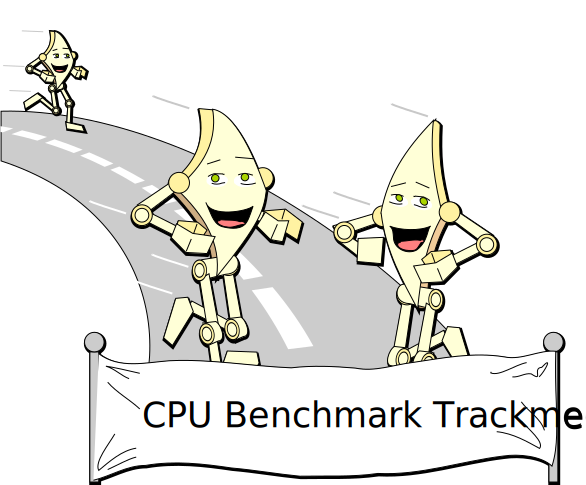
\includegraphics{cartoons/r-2014-CPU-track-meet}}
\caption{CPU Performance at its Best}
\ContributedBy{Figure}{fig:cpu:CPU Performance at its Best}{Melissa Broussard}
\end{figure}

Figure~\ref{fig:cpu:CPU Performance at its Best} 에 보여진 이상적 상황으로
접근하는 CPU 바운드 벤치마크들도 몇개 있긴 합니다만, 일반적인 프로그램은 경주용
운동장보다는 장애물 코스에 더 가깝습니다.
무어의 법칙에 의해 CPU 의 내부 구조가 지난 수십년간 엄청나게 변해왔기 때문이죠.
이런 변경들을 다음 섹션들에서 설명합니다.
\iffalse

Although there are a few CPU-bound benchmarks that approach the ideal
shown in Figure~\ref{fig:cpu:CPU Performance at its Best},
the typical program more closely resembles an obstacle course than
a race track.
This is because the internal architecture of CPUs has changed dramatically
over the past few decades, courtesy of Moore's Law.
These changes are described in the following sections.
\fi

\subsection{Pipelined CPUs}
\label{sec:cpu:Pipelined CPUs}

\begin{figure}[tb]
\centering
\resizebox{3in}{!}{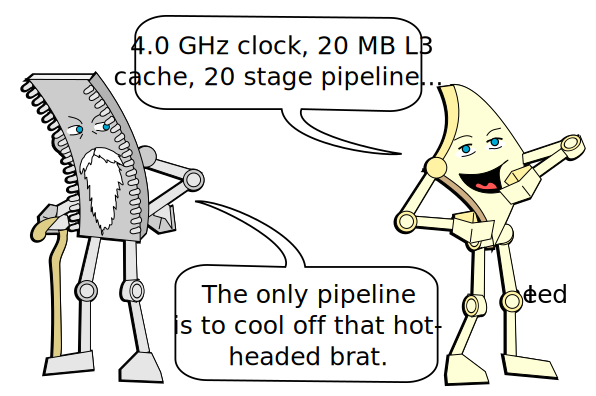
\includegraphics{cartoons/r-2014-Old-man-and-Brat}}
\caption{CPUs Old and New}
\ContributedBy{Figure}{fig:cpu:CPUs Old and New}{Melissa Broussard}
\end{figure}

1980년대 초, 인스트럭션을 가져오고, 디코드하고, 실행하는 대부분의 마이크로
프로세서는 일반적으로 다음 인스트럭션을 가져오기 전에 인스트럭션 하나를 실행
완료하는데 \emph{최소} 3 클락 사이클을 소모했습니다.
대조적으로, 1990년대 후반에서 2000년대 초반의 CPU 는 CPU 로의 인스트럭션 전달
흐름을 내부적으로 조절하는데 깊은 ``파이프라인'' 을 사용해 많은 인스트럭션들을
동시에 수행할 수 있습니다.
이러한 근래의 하드웨어의 기능들은 Figure~\ref{fig:cpu:CPUs Old and New} 에
보여진 것처럼 성능을 대폭 향상시킬 수 있습니다.
\iffalse

In the early 1980s, the typical microprocessor fetched an instruction,
decoded it, and executed it, typically taking \emph{at least} three
clock cycles to complete one instruction before proceeding to the next.
In contrast, the CPU of the late 1990s and early 2000s will be executing
many instructions simultaneously, using a deep ``pipeline'' to control
the flow of instructions internally to the CPU.
These modern hardware features can greatly improve performance, as
illustrated by Figure~\ref{fig:cpu:CPUs Old and New}.
\fi

긴 파이프라인을 가지고 CPU 의 최대 성능을 얻기 위해서는 프로그램의 컨트롤
플로우 (코드 실행 흐름) 를 매우 정밀하게 예측할 수 있어야 합니다.
큰 행렬이나 벡터 계산과 같이 기본적으로 꽉 짜여진 루프로 구성된 프로그램에서는
적당한 컨트롤 플로우를 얻을 수 있습니다.
그런 경우 CPU 는 루프 마지막의, 루프의 처음으로 돌아갈지 루프를 빠져나갈지에
대한 분기  조건이 거의 항상 참일 거라는 것을 올바르게 예측해서 파이프라인이
꽉 차있게 해 CPU가 최대 속도로 돌아갈 수 있게 할겁니다.
\iffalse

Achieving full performance with a CPU having a long pipeline requires
highly predictable control flow through the program.
Suitable control flow can be provided by a program that executes primarily
in tight loops, for example, arithmetic on large matrices or vectors.
The CPU can then correctly predict that the branch at the end of the loop
will be taken in almost all cases,
allowing the pipeline to be kept full and the CPU to execute at full speed.
\fi

\begin{figure}[tb]
\centering
\resizebox{3in}{!}{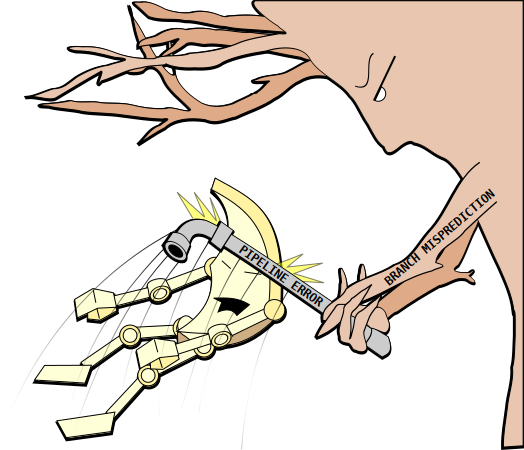
\includegraphics{cartoons/r-2014-branch-error}}
\caption{CPU Meets a Pipeline Flush}
\ContributedBy{Figure}{fig:cpu:CPU Meets a Pipeline Flush}{Melissa Broussard}
\end{figure}

하지만, 분기 예측이 항상 그렇게 쉬운건 아닙니다.
예를 들어, 작지만 무작위적인 횟수만큼 도는 많은 루프로 구성된 프로그램을
생각해보세요.
또다른 예로, 수많은 진짜 객체를 레퍼런스 할 수 있는 가상 객체들이 있는데, 이
진짜 객체들은 자주 호출되는 멤버 함수들을 모두 다르게 구현한 객체지향
프로그램을 생각해보세요.
이런 경우, CPU 는 다음 분기가 실행 흐름을 어디로 이끌지를 예측하는 건 어렵거나
심지어 불가능할 수 있습니다.
그렇게 되면 CPU 는 그 브랜치가 어디로 실행 흐름을 이끌지가 확실해질 때까지
기다리며 멈춰있거나, 추측이라도 해야 합니다.
예측 가능한 컨트롤 플로우를 갖는 프로그램에서는 추측하는 방법이 매우 잘
동작하지만, (이진 탐색과 같은) 예측 불가능한 분기분들에 대해서는 추측이 대부분
틀릴 겁니다.
추측이 잘못된 경우 CPU 는 그 분기문을 따르는, 투기적으로 그간 수행된
인스트럭션들을 모두 폐기시켜야 해서 파이프라인의 내용을 모두 비우게 되기 때문에
잘못된 예측은 매우 비싼 비용을 지불합니다.
만약 파이프라인 플러시가 너무 자주 일어난다면,
Figure~\ref{fig:cpu:CPU Meets a Pipeline Flush} 에서 그려진 것처럼 엄청난 성능
하락을 겪을 수 있습니다.
\iffalse

However, branch prediction is not always so easy.
For example, consider a program with many loops, each of which iterates
a small but random number of times.
For another example, consider
an object-oriented program with many virtual objects that
can reference many different real objects, all with different implementations
for frequently invoked member functions.
In these cases, it is difficult or even
impossible for the CPU to predict where the next branch might lead.
Then either the CPU must stall waiting for execution to proceed far
enough to be certain where that branch leads, or it must guess.
Although guessing works extremely well for programs with predictable
control flow, for unpredictable branches (such as those in binary search)
the guesses will frequently be wrong.
A wrong guess can be expensive because the CPU must discard any
speculatively executed instructions following the corresponding
branch, resulting in a pipeline flush.
If pipeline flushes appear too frequently, they drastically reduce
overall performance, as fancifully depicted in
Figure~\ref{fig:cpu:CPU Meets a Pipeline Flush}.
\fi

불행히도, 파이프라인 플러시는 근래의 CPU 들이 달려야 하는 장애물 코스의 유일한
위험이 아닙니다.
다음 섹션에서는 메모리 참조에 존재하는 위험들을 다룹니다.
\iffalse

Unfortunately, pipeline flushes are not the only hazards in the obstacle
course that modern CPUs must run.
The next section covers the hazards of referencing memory.
\fi

\subsection{Memory References}
\label{sec:cpu:Memory References}

1980년대에는, 대부분의 경우 마이크로프로세서가 메모리에서 값을 하나 얻어오는데
걸리는 시간이 인스트럭션 하나를 수행하는데 걸리는 시간보다 적었습니다.
2006년에 와서는, 마이크로프로세서는 메모리에 접근 한번 하는데 걸리는 시간 동안
수백, 심한 경우 수천개의 인스트럭션을 수행할 수 있습니다.
이 간극은 Moore 의 법칙이 CPU 성능 향상을 메모리 반응속도의 감소 정도에 비해
너무 크게 이끌었기 때문입니다; 메모리의 발전은 반응속도 감소보다 용량 증가에
치중되었던 것도 한 이유죠.
예를 들어, 1970년대의 평범한 미니컴퓨터는 4KB (네, 메가바이트가 아니라
킬로바이트요. 기가바이트는 입밖에 꺼내지도 마요) 메인 메모리를 가졌고, 그
메모리는 한 사이클만에 접근 가능했습니다.\footnote{
	물론 그 한개의 사이클은 1.6 \emph{마이크로 세컨드} 이상이었음을
	언급하는게 공정하겠죠.}
2008년에도 CPU 설계자들은 여전히 단일 사이클만에 접근 가능한 4KB 메모리를 만들
수 있습니다; 심지어 수 GHz 주파수의 시스템에서도요.
그리고 실제로 그런 메모리를 만듭니다만, 그들은 이제 그걸 ``레벨 0 캐시'' 라
부르고, 그것들은 보통은 4KB 보다는 아주 약간은 크기도 합니다.
\iffalse

In the 1980s, it often took less time for a microprocessor to load a value
from memory than it did to execute an instruction.
In 2006, a microprocessor might be capable of executing hundreds or even
thousands of instructions in the time required to access memory.
This disparity is due to the fact that Moore's Law has increased CPU
performance at a much greater rate than it has decreased memory latency,
in part due to the rate at which memory sizes have grown.
For example, a typical 1970s minicomputer might have 4\,KB (yes, kilobytes,
not megabytes, let alone gigabytes) of main memory, with
single-cycle access.\footnote{
	It is only fair to add that each of these single cycles
	lasted no less than 1.6 \emph{microseconds}.}
In 2008, CPU designers still can construct a 4\,KB memory with single-cycle
access, even on systems with multi-GHz clock frequencies.
And in fact they frequently do construct such memories, but they now
call them ``level-0 caches'', and they can be quite a bit bigger than 4\,KB.
\fi

\begin{figure}[htb]
\centering
\resizebox{3in}{!}{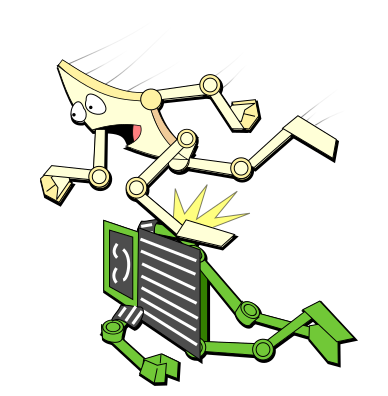
\includegraphics{cartoons/r-2014-memory-reference}}
\caption{CPU Meets a Memory Reference}
\ContributedBy{Figure}{fig:cpu:CPU Meets a Memory Reference}{Melissa Broussard}
\end{figure}

근래의 마이크로프로세서에 장착되는 큰 캐시들은 메모리 접근 시간과 맞서 싸우는데
꽤 도움을 줄 수 있습니다만, 이런 캐시들이 그 시간들을 제대로 숨기기 위해서는
고도로 예측 가능한 데이터 접근 패턴이 필요합니다.
불행히도, 링크드 리스트를 순회하는 것과 같은 많은 일들이 예측 불가능한 메모리
접근 패턴을 갖습니다. 무엇보다, 만약 패턴이 예측 가능하다면, 소프트웨어는
포인터 타입이란 것 자체를 만들지도 않았겠죠, 그렇죠?
따라서, Figure~\ref{fig:cpu:CPU Meets a Memory Reference} 에서 보여지듯, 메모리
참조는 종종 근래의 CPU 들에게 거대한 장애물입니다.

지금까지는 주어진 CPU가 싱글 쓰레드 코드를 돌릴 때 만날 수 있는 문제들만
이야기했습니다.
멀티쓰레드 수행은 다음 섹션에서 설명할텐데, CPU 에게 추가적인 문제들을
내놓습니다.
\iffalse

Although the large caches found on modern microprocessors can do quite
a bit to help combat memory-access latencies,
these caches require highly predictable data-access patterns to
successfully hide those latencies.
Unfortunately, common operations such as traversing a linked list
have extremely unpredictable memory-access patterns---after all,
if the pattern was predictable, us software types would not bother
with the pointers, right?
Therefore, as shown in
Figure~\ref{fig:cpu:CPU Meets a Memory Reference},
memory references often pose severe obstacles to modern CPUs.

Thus far, we have only been considering obstacles that can arise during
a given CPU's execution of single-threaded code.
Multi-threading presents additional obstacles to the CPU, as
described in the following sections.
\fi

\subsection{Atomic Operations}
\label{sec:cpu:Atomic Operations}

그런 장애 중 하나는 어토믹 오퍼레이션들입니다.
여기서의 문제는 모든 어토믹 오퍼레이션은 CPU 파이프라인의 한 순간에는 조각으로
나뉘어 수행되는 어셈블리 오퍼레이션들과 한번씩은 충돌한다는 것입니다.
하드웨어 설계자는 근래의 CPU 들은 그런 오퍼레이션들이 실은 여러 조각으로
나뉘어져 여러 순간동안 수행되더라도 원자적으로 수행되는 것처럼 \emph{보이게}
하기 위해 여러개의 굉장히 현명한 트릭들을 사용한다고 이야기합니다. 그런 트릭 중
흔한 한가지는 어토믹하게 수행되어야 하는 데이터를 담고 있는 캐시라인들을 모두
파악해두고, 이 캐시라인들은 해당 어토믹 오퍼레이션을 수행하는 CPU 에 소유되어
있음을 분명하게 하고, 그러고나서야만 해당 캐시라인들이 해당 CPU 에 의해 여전히
소유되어 있음을 분명히 한 채로 어토믹 오퍼레이션을 수행하는 것입니다.
모든 데이터가 해당 CPU 만 접근할 수 있는 상태이기에, 다른 CPU 들은 실은
조각으로 나뉘어 수행되는 CPU 파이프라인의 현실에도 불구하고 해당 어토믹
오퍼레이션에 간섭을 끼칠 수 없습니다.
말할 필요도 없겠지만, 이런 종류의 트릭은 그 셋업이 수행되도록 주어진 어토믹
오퍼레이션이 완전히 끝날 때까지 파이프라인이 지연되거나 심지어 플러시될 수도
있습니다.

\iffalse
One such obstacle is atomic operations.
The problem here is that the whole idea of an atomic operation conflicts with
the piece-at-a-time assembly-line operation of a CPU pipeline.
To hardware designers' credit, modern CPUs use a number of extremely clever
tricks to make such operations \emph{look} atomic even though they
are in fact being executed piece-at-a-time,
with one common trick being to identify all the cachelines containing the
data to be atomically operated on,
ensure that these cachelines are owned by the CPU executing the
atomic operation, and only then proceed with the atomic operation
while ensuring that these cachelines remained owned by this CPU.
Because all the data is private to this CPU, other CPUs are unable to
interfere with the atomic operation despite the piece-at-a-time nature
of the CPU's pipeline.
Needless to say, this sort of trick can require that
the pipeline must be delayed or even flushed in order to
perform the setup operations that
permit a given atomic operation to complete correctly.
\fi

\begin{figure}[htb]
\centering
\resizebox{3in}{!}{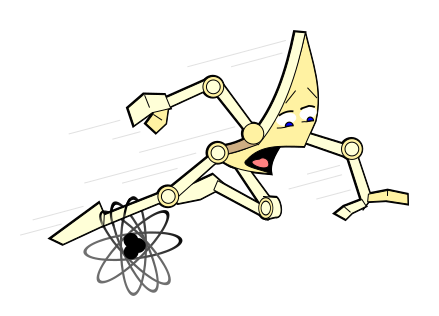
\includegraphics{cartoons/r-2014-Atomic-reference}}
\caption{CPU Meets an Atomic Operation}
\ContributedBy{Figure}{fig:cpu:CPU Meets an Atomic Operation}{Melissa Broussard}
\end{figure}

반대로, 어토믹 오퍼레이션이 아닌 오퍼레이션을 수행할 때에는 CPU 는 값을
캐시라인에 올라오는대로 가져올 수 있고, 수행 결과를 캐시라인 소유권을 가지기
위해 기다릴 필요 없이 곧바로 버퍼에 써넣을 수 있습니다.
다행히도, CPU 설계자들은 어토믹 오퍼레이션에 신경을 많이 쏟았고, 덕분에 2014년
초에 이르러서는 그 오버헤드를 상당히 감소시켰습니다.
하지만 그래도, 그 성능에 끼치는 효과는 Figure~\ref{fig:cpu:CPU Meets an Atomic
Operation} 에 보이는 대로입니다.

불행히도, 어토믹 오퍼레이션들은 보통 데이터의 한개 요소에만 적용 가능합니다.
많은 병렬 알고리즘들이 복수개의 데이터 요소들에의 업데이트 간에도 순서가
이루어지길 필요로 하기 때문에, 대부분의 CPU 들은 메모리 배리어들을 제공합니다.
이런 메모리 배리어들 역시 성능에의 문제로 존재합니다. 다음 섹션에서 이를 이야기
합니다.

\iffalse
In contrast, when executing a non-atomic operation, the CPU can load
values from cachelines as they appear and place the results in the
store buffer, without the need to wait for cacheline ownership.
Fortunately, CPU designers have focused heavily on atomic operations,
so that as of early 2014 they have greatly reduced their overhead.
Even so, the resulting effect on performance is all too often as depicted in
Figure~\ref{fig:cpu:CPU Meets an Atomic Operation}.

Unfortunately, atomic operations usually apply only to single elements
of data.
Because many parallel algorithms require that ordering constraints
be maintained between updates of multiple data elements, most CPUs
provide memory barriers.
These memory barriers also serve as performance-sapping obstacles,
as described in the next section.
\fi

\QuickQuiz{}
	어떤 기계가 복수 데이터 요소에 대한 어토믹 오퍼레이션을 허용하겠어요?

	\iffalse
	What types of machines would allow atomic operations on
	multiple data elements?
	\fi
\QuickQuizAnswer{
	이 질문에 대한 한가지 답은 종종 복수개의 데이터 요소를 어토믹하게
	다뤄질 수 있는, 단일 머신 워드 안에 모아넣을 수 있다는 겁니다.

	좀 더 트렌디한 답은 트랜잭셔널 메모리~\cite{DBLomet1977SIGSOFT} 를
	지원하는 기계가 되겠습니다.
	2014년 초에 이르러서는 일부 주요 시스템들이 제한되긴 했지만 하드웨어
	트랜잭셔널 메모리 구현을 제공합니다. 더 자세한 내용은
	Section~\ref{sec:future:Hardware Transactional Memory} 에서 다루고
	있습니다.
	소프트웨어 트랜잭셔널
	메모리~\cite{McKenney2007PLOSTM,DonaldEPorter2007TRANSACT,
	ChistopherJRossbach2007a,CalinCascaval2008tmtoy,
	AleksandarDragovejic2011STMnotToy,AlexanderMatveev2012PessimisticTM}
	에 대해서는 아직 적합하지 않다는 평가입니다.
	소프트웨어 트랜잭셔널 메모리에 대한 더 많은 내용은
	Section~\ref{sec:future:Transactional Memory} 에서 볼 수 있을 겁니다.

	\iffalse
	One answer to this question is that it is often possible to
	pack multiple elements of data into a single machine word,
	which can then be manipulated atomically.

	A more trendy answer would be machines supporting transactional
	memory~\cite{DBLomet1977SIGSOFT}.
	As of early 2014, several mainstream systems provide limited
	hardware transactional memory implementations, which is covered
	in more detail in
	Section~\ref{sec:future:Hardware Transactional Memory}.
	The jury is still out on the applicability of software transactional
	memory~\cite{McKenney2007PLOSTM,DonaldEPorter2007TRANSACT,
	ChistopherJRossbach2007a,CalinCascaval2008tmtoy,
	AleksandarDragovejic2011STMnotToy,AlexanderMatveev2012PessimisticTM}.
	Additional information on software transactional memory may be
	found in
	Section~\ref{sec:future:Transactional Memory}.
	\fi
} \QuickQuizEnd

\subsection{Memory Barriers}
\label{sec:cpu:Memory Barriers}

메모리 배리어에 대해서는
Chapter~\ref{chp:Advanced Synchronization: Memory Ordering} 와
Appendix~\ref{chp:app:whymb:Why Memory Barriers?} 에서 좀 더 깊게 다룰 겁니다.
그 전에, 여기서는 다음의 간단한 락을 사용한 크리티컬 섹션을 생각해 봅시다:

\iffalse
Memory barriers will be considered in more detail in
Chapter~\ref{chp:Advanced Synchronization: Memory Ordering} and
Appendix~\ref{chp:app:whymb:Why Memory Barriers?}.
In the meantime, consider the following simple lock-based critical
section:
\fi

\vspace{5pt}
\begin{minipage}[t]{\columnwidth}
\small
\begin{verbatim}
  1 spin_lock(&mylock);
  2 a = a + 1;
  3 spin_unlock(&mylock);
\end{verbatim}
\end{minipage}
\vspace{5pt}

\begin{figure}[tb]
\centering
\resizebox{3in}{!}{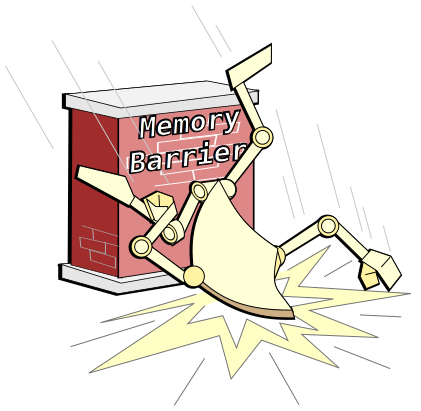
\includegraphics{cartoons/r-2014-Memory-barrier}}
\caption{CPU Meets a Memory Barrier}
\ContributedBy{Figure}{fig:cpu:CPU Meets a Memory Barrier}{Melissa Broussard}
\end{figure}

만약 CPU 에 코드가 보여지는 순서대로 수행되어야 한다는 제약이 존재하지
않는다면, 변수 ``a'' 는 ``mylock'' 의 보호 없이 값이 증가할 것이고, 이렇게 되면
락을 잡는 목표가 이뤄지지 않은 셈입니다.
그런 문제되는 순서 재배치를 막기 위해, 락킹에 사용되는 기본 기능들은 명시적이든
묵시적이든 메모리 배리어를 사용합니다.
이런 메모리 배리어의 목적은 CPU 가 성능을 향상시키기 위해 할 수 있는 코드의
순서 재배치를 막기 위한 것이기 때문에, 메모리 배리어는 거의 항상
Figure~\ref{fig:cpu:CPU Meets a Memory Barrier} 에서 보여지듯 성능을
떨어뜨립니다.

어토믹 오퍼레이션과 같이, CPU 설계자들은 메모리 배리어 오버헤드를 줄이려 열심히
노력해왔고, 꽤 많은 진전을 이뤘습니다.

\iffalse
If the CPU were not constrained to execute these statements in the
order shown, the effect would be that the variable ``a'' would be
incremented without the protection of ``mylock'', which would certainly
defeat the purpose of acquiring it.
To prevent such destructive reordering, locking primitives contain
either explicit or implicit memory barriers.
Because the whole purpose of these memory barriers is to prevent reorderings
that the CPU would otherwise undertake in order to increase performance,
memory barriers almost always reduce performance, as depicted in
Figure~\ref{fig:cpu:CPU Meets a Memory Barrier}.

As with atomic operations, CPU designers have been working hard to
reduce memory-barrier overhead, and have made substantial progress.
\fi

\subsection{Cache Misses}
\label{sec:cpu:Cache Misses}

\begin{figure}[tb]
\centering
\resizebox{3in}{!}{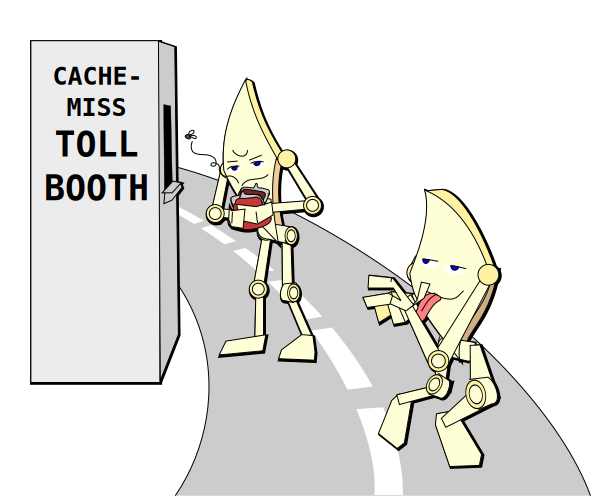
\includegraphics{cartoons/r-2014-CPU-track-meet-cache-miss-toll-booth}}
\caption{CPU Meets a Cache Miss}
\ContributedBy{Figure}{fig:cpu:CPU Meets a Cache Miss}{Melissa Broussard}
\end{figure}

또하나의 멀티 쓰레딩에서의 CPU 성능에의 장애물은 ``캐시 미스'' 입니다.
앞서 말했듯, 근래의 CPU 들은 높은 메모리 반응속도로 발생할 수 있는 성능 하락을
줄이기 위해 큰 캐시를 장착하고 있습니다.
하지만, 이런 캐시들은 실은 CPU 간에 자주 공유되는 변수들에 대해서는 생산적이지
못합니다.
하나의 CPU 가 한 변수를 수정하려 할 때, 다른 CPU 가 그 값을 최근에 바꾼 경우가
있을 가능성이 크기 때문이죠.
이런 경우, 해당 변수는 지금 수정하려는 CPU 의 캐시가 아니라 최근에 값을 수정한
CPU 의 캐시에 있을 것이고, 이로 인해 비싼 캐시 미스(더 자세한 내용을 위해선
Section~\ref{sec:app:whymb:Cache Structure} 를 보세요) 를 일으킬 것입니다.
이런 캐시 미스들은 Figure~\ref{fig:cpu:CPU Meets a Cache Miss} 에서 보여진
것처럼 CPU 성능의 주요 장애가 됩니다.

\iffalse
An additional multi-threading obstacle to CPU performance is
the ``cache miss''.
As noted earlier, modern CPUs sport large caches in order to reduce the
performance penalty that would otherwise be incurred due to high memory
latencies.
However, these caches are actually counter-productive for variables that
are frequently shared among CPUs.
This is because when a given CPU wishes to modify the variable, it is
most likely the case that some other CPU has modified it recently.
In this case, the variable will be in that other CPU's cache, but not
in this CPU's cache, which will therefore incur an expensive cache miss
(see Section~\ref{sec:app:whymb:Cache Structure} for more detail).
Such cache misses form a major obstacle to CPU performance, as shown
in Figure~\ref{fig:cpu:CPU Meets a Cache Miss}.
\fi

\QuickQuiz{}
	그래서, CPU 설계자들은 캐시 미스 오버헤드 역시 많이 개선 했나요?
	\iffalse
	So have CPU designers also greatly reduced the overhead of
	cache misses?
	\fi
\QuickQuizAnswer{
	안타깝지만, 그렇게 많은 개선은 하지 못했습니다.
	약간 오버헤드를 줄인 CPU 들도 있었습니다만, 빛의 속도의 한계와 물질의
	원자성의 자연 법칙이 큰 시스템에서 캐시 미스 오버헤드를 줄일 수 있는
	방법을 제한하고 있습니다.
	Section~\ref{sec:cpu:Hardware Free Lunch?} 에서 가능할 법한 미래의 개선
	방법들을 논의해 봅니다.

	\iffalse
	Unfortunately, not so much.
	There has been some reduction given constant numbers of CPUs,
	but the finite speed of light and the atomic nature of
	matter limits their ability to reduce cache-miss overhead
	for larger systems.
	Section~\ref{sec:cpu:Hardware Free Lunch?}
	discusses some possible avenues for possible future progress.
	\fi
} \QuickQuizEnd

\subsection{I/O Operations}
\label{sec:cpu:I/O Operations}

\begin{figure}[tb]
\centering
\resizebox{3in}{!}{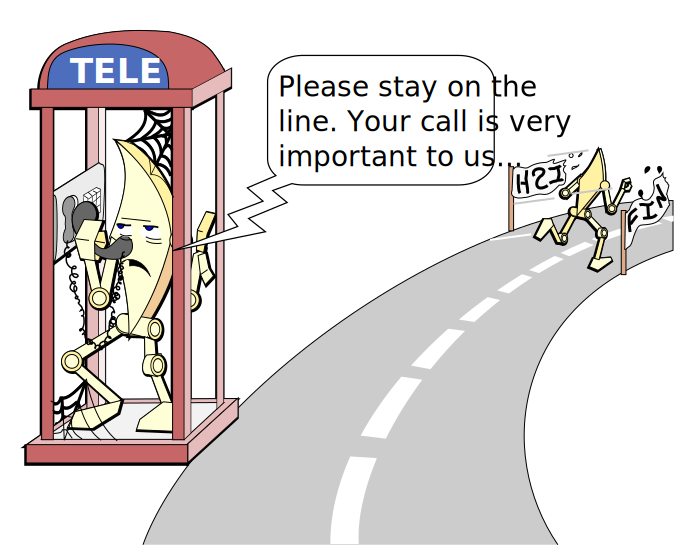
\includegraphics{cartoons/r-2014-CPU-track-meet-phone-booth}}
\caption{CPU Waits for I/O Completion}
\ContributedBy{Figure}{fig:cpu:CPU Waits for I/O Completion}{Melissa Broussard}
\end{figure}

캐시 미스는 곧 CPU 와 CPU 사이의 I/O 오퍼레이션으로 볼 수 있고, 이것은 가능한
I/O 오퍼레이션 중 가장 비용이 낮은 것들 중 하나입니다.
네트워킹이나 대용량 저장장치, 또는 사람을 포함하는 I/O 오퍼레이션들은
Figure~\ref{fig:cpu:CPU Waits for I/O Completion} 에서 보여지듯, 앞의
섹션들에서 이야기 되었던 내부적 장애들보다 훨씬 커다란 장애를 야기합니다.

\iffalse
A cache miss can be thought of as a CPU-to-CPU I/O operation, and as
such is one of the cheapest I/O operations available.
I/O operations involving networking, mass storage, or (worse yet) human
beings pose much greater obstacles than the internal obstacles called
out in the prior sections,
as illustrated by
Figure~\ref{fig:cpu:CPU Waits for I/O Completion}.
\fi

이건 공유 메모리 병렬성과 분산시스템 병렬성 사이의 차이 중 하나입니다:
공유메모리 병렬 프로그램은 일반적으로 캐시 미스보다 더한 장애는 겪지
않습니다만, 분산 병렬 프로그램은 보통 더 큰 네트워크 커뮤니케이션 시간을
겪습니다.
두 경우 모두, 문제의 응답시간들은 커뮤니케이션의 비용으로 생각될 수 있습니다.
순차 프로그램에서는 존재하지 않는 비용이죠.
따라서, 실제 수행되는 일과 커뮤니케이션 오버헤드 간의 비율이 핵심 설계 결정
요소입니다.
병렬 하드웨어 설계의 주요 목표는 이 비율을 적절한 성능과 확장성 목표를 달성
가능한 수준으로 낮추는 것입니다.
이에 따라서, Chapter~\ref{cha:Partitioning and Synchronization Design} 에서
볼테지만, 병렬 소프트웨어 설계의 중요한 목표는 커뮤니케이션 캐시 미스와 같은
비싼 동작들의 빈번도를 낮추는 것입니다.

물론, 주어진 동작이 장애라는 이야기는 그 이야기이고, 그 동작이 \emph{심각한}
장애라는 건 또 따로 보여줘야하지요.
이 차이를 다음의 섹션에서 이야기 합니다.

\iffalse
This is one of the differences between shared-memory and distributed-system
parallelism: shared-memory parallel programs must normally deal with no
obstacle worse than a cache miss, while a distributed parallel program
will typically incur the larger network communication latencies.
In both cases, the relevant latencies can be thought of as a cost of
communication---a cost that would be absent in a sequential program.
Therefore, the ratio between the overhead of the communication to
that of the actual work being performed is a key design parameter.
A major goal of parallel hardware design is to reduce this ratio as
needed to achieve the relevant performance and scalability goals.
In turn, as will be seen in
Chapter~\ref{cha:Partitioning and Synchronization Design},
a major goal of parallel software design is to reduce the
frequency of expensive operations like communications cache misses.

Of course, it is one thing to say that a given operation is an obstacle,
and quite another to show that the operation is a \emph{significant}
obstacle.
This distinction is discussed in the following sections.
\fi

% cpu/overheads.tex
% mainfile: ../perfbook.tex
% SPDX-License-Identifier: CC-BY-SA-3.0

\section{Overheads}
\label{sec:cpu:Overheads}
%
\epigraph{Don't design bridges in ignorance of materials, and don't design
	  low-level software in ignorance of the underlying hardware.}
	 {\emph{Unknown}}

This section presents actual overheads of the obstacles to performance
listed out in the previous section.
However, it is first necessary to get a rough view of hardware system
architecture, which is the subject of the next section.

\subsection{Hardware System Architecture}
\label{sec:cpu:Hardware System Architecture}

\begin{figure}[tb]
\centering
\resizebox{3in}{!}{\includegraphics{cpu/SystemArch}}
\caption{System Hardware Architecture}
\label{fig:cpu:System Hardware Architecture}
\end{figure}

Figure~\ref{fig:cpu:System Hardware Architecture}
shows a rough schematic of an eight-core computer system.
Each die has a pair of CPU cores, each with its cache, as well as an
interconnect allowing the pair of CPUs to communicate with each other.
The system interconnect allows the four dies to communicate with each
other and with main memory.

Data moves through this system in units of ``cache lines'', which
are power-of-two fixed-size aligned blocks of memory, usually ranging
from 32 to 256 bytes in size.
When a CPU loads a variable from memory to one of its registers, it must
first load the cacheline containing that variable into its cache.
Similarly, when a CPU stores a value from one of its registers into
memory, it must also load the cacheline containing that variable into
its cache, but must also ensure that no other CPU has a copy of that
cacheline.

For example, if CPU~0 were to write to a variable whose cacheline
resided in CPU~7's cache, the following over-simplified sequence of
events might ensue:

\begin{enumerate}
\item	CPU~0 checks its local cache, and does not find the cacheline.
	It therefore records the write in its store buffer.
\item	A request for this cacheline is forwarded to CPU~0's and 1's
	interconnect, which checks CPU~1's local cache, and does not
	find the cacheline.
\item	This request is forwarded to the system interconnect, which
	checks with the other three dies, learning that the cacheline
	is held by the die containing CPU~6 and 7.
\item	This request is forwarded to CPU~6's and 7's interconnect, which
	checks both CPUs' caches, finding the value in CPU~7's cache.
\item	CPU~7 forwards the cacheline to its interconnect, and also
	flushes the cacheline from its cache.
\item	CPU~6's and 7's interconnect forwards the cacheline to the
	system interconnect.
\item	The system interconnect forwards the cacheline to CPU~0's and 1's
	interconnect.
\item	CPU~0's and 1's interconnect forwards the cacheline to CPU~0's
	cache.
\item	CPU~0 can now complete the write, updating the relevant portions
	of the newly arrived cacheline from the value previously
	recorded in the store buffer.
\end{enumerate}

\QuickQuizSeries{%
\QuickQuizB{
	This is a \emph{simplified} sequence of events?
	How could it \emph{possibly} be any more complex?
}\QuickQuizAnswerB{
	This sequence ignored a number of possible complications,
	including:

	\begin{enumerate}
	\item	Other CPUs might be concurrently attempting to perform
		memory-reference operations involving this same cacheline.
	\item	The cacheline might have been replicated read-only in
		several CPUs' caches, in which case, it would need to
		be flushed from their caches.
	\item	CPU~7 might have been operating on the cache line when
		the request for it arrived, in which case CPU~7 might
		need to hold off the request until its own operation
		completed.
	\item	CPU~7 might have ejected the cacheline from its cache
		(for example, in order to make room for other data),
		so that by the time that the request arrived, the
		cacheline was on its way to memory.
	\item	A correctable error might have occurred in the cacheline,
		which would then need to be corrected at some point before
		the data was used.
	\end{enumerate}

	Production-quality cache-coherence mechanisms are extremely
	complicated due to these sorts of
	considerations~\cite{Hennessy95a,DavidECuller1999,MiloMKMartin2012scale,DanielJSorin2011MemModel}.
%
}\QuickQuizEndB
%
\QuickQuizE{
	Why is it necessary to flush the cacheline from CPU~7's cache?
}\QuickQuizAnswerE{
	If the cacheline was not flushed from CPU~7's cache, then
	CPUs~0 and 7 might have different values for the same set
	of variables in the cacheline.
	This sort of incoherence greatly complicates parallel software,
	which is why so wise hardware architects avoid it.
}\QuickQuizEndE
}

This simplified sequence is just the beginning of a discipline called
\emph{cache-coherency protocols}~\cite{Hennessy95a,DavidECuller1999,MiloMKMartin2012scale,DanielJSorin2011MemModel},
which is discussed in more detail in
Appendix~\ref{chp:app:whymb:Why Memory Barriers?}.
As can be seen in the sequence of events triggered by a CAS operation,
a single instruction can cause considerable protocol traffic, which
can significantly degrade your parallel program's performance.

Fortunately, if a given variable is being frequently read during a time
interval during which it is never updated, that variable can be replicated
across all CPUs' caches.
This replication permits all CPUs to enjoy extremely fast access to
this \emph{read-mostly} variable.
Chapter~\ref{chp:Deferred Processing} presents synchronization
mechanisms that take full advantage of this important hardware read-mostly
optimization.

\subsection{Costs of Operations}
\label{sec:cpu:Costs of Operations}

\begin{table*}
\rowcolors{1}{}{lightgray}
\renewcommand*{\arraystretch}{1.1}
\centering\small
\begin{tabular}
  {
    l
    S[table-format = 9.1]
    S[table-format = 9.1]
    r
  }
	\toprule
	Operation	   & \multicolumn{1}{r}{Cost (ns)}
				   & {\parbox[b]{.7in}{\raggedleft Ratio\\(cost/clock)}}
					    & CPUs \\
	\midrule
	Clock period		     &   0.5 &    1.0 &			  \\
	Same-CPU CAS		     &   7.0 &   14.6 & 0		  \\
	Same-CPU lock		     &  15.4 &   32.3 & 0		  \\
	In-core blind CAS	     &   7.2 &   15.2 & 224		  \\
	In-core CAS		     &  18.0 &   37.7 & 224		  \\
	Off-core blind CAS	     &  47.5 &   99.8 & 1--27,225--251	  \\
	Off-core CAS		     & 101.9 &  214.0 & 1--27,225--251	  \\
	Off-socket blind CAS	     & 148.8 &  312.5 & 28--111,252--335  \\
	Off-socket CAS		     & 442.9 &  930.1 & 28--111,252--335  \\
	Cross-interconnect blind CAS & 336.6 &  706.8 & 112--223,336--447 \\
	Cross-interconnect CAS	     & 944.8 & 1984.2 & 112--223,336--447 \\
	\midrule
	Off-System	&	      & 	    & \\
	Comms Fabric	&       5 000 &      10 500 & \\
	Global Comms	& 195 000 000 & 409 500 000 & \\
	\bottomrule
\end{tabular}
\caption{CPU 0 View of Synchronization Mechanisms on 8-Socket System With Intel Xeon Platinum 8176 CPUs @ 2.10\,GHz}
\label{tab:cpu:CPU 0 View of Synchronization Mechanisms on 8-Socket System With Intel Xeon Platinum 8176 CPUs at 2.10GHz}
\end{table*}

The overheads of some common operations important to parallel programs are
displayed in
Table~\ref{tab:cpu:CPU 0 View of Synchronization Mechanisms on 8-Socket System With Intel Xeon Platinum 8176 CPUs at 2.10GHz}.
This system's clock period rounds to 0.5\,ns.
Although it is not unusual for modern microprocessors to be able to
retire multiple instructions per clock period, the operations' costs are
nevertheless normalized to a clock period in the third column, labeled
``Ratio''.
The first thing to note about this table is the large values of many of
the ratios.

The same-CPU compare-and-swap (CAS) operation consumes about seven
nanoseconds, a duration more than ten times that of the clock period.
CAS is an atomic operation in which the hardware compares the contents
of the specified memory location to a specified ``old'' value, and if
they compare equal, stores a specified ``new'' value, in which case the
CAS operation succeeds.
If they compare unequal, the memory location keeps its (unexpected) value,
and the CAS operation fails.
The operation is atomic in that the hardware guarantees that the memory
location will not be changed between the compare and the store.
CAS functionality is provided by the \co{lock;cmpxchg} instruction on x86.

The ``same-CPU'' prefix means that the CPU now performing the CAS operation
on a given variable was also the last CPU to access this variable, so
that the corresponding cacheline is already held in that CPU's cache.
Similarly, the same-CPU lock operation (a ``round trip'' pair consisting
of a lock acquisition and release) consumes more than fifteen nanoseconds,
or more than thirty clock cycles.
The lock operation is more expensive than CAS because it requires two
atomic operations on the lock data structure, one for acquisition and
the other for release.

In-core operations involving interactions between the hardware threads
sharing a single core are about the same cost as same-CPU operations.
This should not be too surprising, given that these two hardware threads
also share the full cache hierarchy.

In the case of the blind CAS, the software specifies the old value
without looking at the memory location.
This approach is appropriate when attempting to acquire a lock.
If the unlocked state is represented by zero and the locked state
is represented by the value one, then a CAS operation on the lock
that specifies zero for the old value and one for the new value
will acquire the lock if it is not already held.
The key point is that there is only one access to the memory
location, namely the CAS operation itself.

In contrast, a normal CAS operation's old value is derived from
some earlier load.
For example, to implement an atomic increment, the current value of
that location is loaded and that value is incremented to produce the
new value.
Then in the CAS operation, the value actually loaded would be specified
as the old value and the incremented value as the new value.
If the value had not been changed between the load and the CAS, this
would increment the memory location.
However, if the value had in fact changed, then the old value would
not match, causing a miscompare that would result in the CAS operation
failing.
The key point is that there are now two accesses to the memory location,
the load and the CAS\@.

Thus, it is not surprising that in-core blind CAS consumes only about
seven nanoseconds, while in-core CAS consumes about 18 nanoseconds.
The non-blind case's extra load does not come for free.
That said, the overhead of these operations are similar to single-CPU
CAS and lock, respectively.

\QuickQuiz{
	\Cref{tab:cpu:CPU 0 View of Synchronization Mechanisms on 8-Socket System With Intel Xeon Platinum 8176 CPUs at 2.10GHz}
	shows CPU~0 sharing a core with CPU~224.
	Shouldn't that instead be CPU~1???
}\QuickQuizAnswer{
	It is easy to be sympathetic to this view, but the file
	\path{/sys/devices/system/cpu/cpu0/cache/index0/shared_cpu_list}
	really does contain the string \co{0,224}.
	Therefore, CPU~0's hyperthread twin really is CPU~224.
	Some people speculate that this numbering allows naive applications
	and schedulers to perform better, citing the fact that on many
	workloads the second hyperthread does not provide a huge
	amount of additional performance.
	This speculation assumes that naive applications and schedulers
	would utilize CPUs in numerical order, leaving aside the weaker
	hyperthread twin CPUs until all cores are in use.
}\QuickQuizEnd

A blind CAS involving CPUs in different cores but on the same socket
consumes almost fifty nanoseconds, or almost one hundred clock cycles.
The code used for this cache-miss measurement passes the cache line
back and forth between a pair of CPUs, so this cache miss is satisfied
not from memory, but rather from the other CPU's cache.
A non-blind CAS operation, which as noted earlier must look at the old
value of the variable as well as store a new value, consumes over one
hundred nanoseconds, or more than two hundred clock cycles.
Think about this a bit.
In the time required to do \emph{one} CAS operation, the CPU could have
executed more than \emph{two hundred} normal instructions.
This should demonstrate the limitations not only of fine-grained locking,
but of any other synchronization mechanism relying on fine-grained
global agreement.

If the pair of CPUs are on different sockets, the operations are considerably
more expensive.
A blind CAS operation consumes almost 150~nanoseconds, or more than
three hundred clock cycles.
A normal CAS operation consumes more than 400~nanoseconds, or almost
\emph{one thousand} clock cycles.

Worse yet, not all pairs of sockets are created equal.
This particular system appears to be constructed as a pair of four-socket
components, with additional latency penalties when the CPUs reside
in different components.
In this case, a blind CAS operation consumes more than three hundred
nanoseconds, or more than seven hundred clock cycles.
A CAS operation consumes almost a full microsecond, or almost two
thousand clock cycles.

\QuickQuiz{
	Surely the hardware designers could be persuaded to improve
	this situation!
	Why have they been content with such abysmal performance
	for these single-instruction operations?
}\QuickQuizAnswer{
	The hardware designers \emph{have} been working on this
	problem, and have consulted with no less a luminary than
	the late physicist Stephen Hawking.
	Hawking's observation was that the hardware designers have
	two basic problems~\cite{BryanGardiner2007}:

	\begin{enumerate}
	\item	The finite speed of light, and
	\item	The atomic nature of matter.
	\end{enumerate}

\begin{table}
\rowcolors{1}{}{lightgray}
\renewcommand*{\arraystretch}{1.1}
\centering\small
\begin{tabular}
  {
    l
    S[table-format = 9.1]
    S[table-format = 9.1]
  }
	\toprule
	Operation		& \multicolumn{1}{r}{Cost (ns)}
			& {\parbox[b]{.7in}{\raggedleft Ratio\\(cost/clock)}} \\
	\midrule
	Clock period		&           0.4	&           1.0 \\
	Same-CPU CAS		&          12.2	&          33.8 \\
	Same-CPU lock		&          25.6	&          71.2 \\
	Blind CAS		&          12.9	&          35.8 \\
	CAS			&           7.0	&          19.4 \\
	\midrule
	Off-Core		&		&		\\
	Blind CAS		&          31.2	&          86.6 \\
	CAS			&          31.2	&          86.5 \\
	\midrule
	Off-Socket		&		&		\\
	Blind CAS		&          92.4	&         256.7 \\
	CAS			&          95.9	&         266.4 \\
	\midrule
	Off-System		&		&		\\
	Comms Fabric		&       2 600   &       7 220   \\
	Global Comms		& 195 000 000	& 542 000 000   \\
	\bottomrule
\end{tabular}
\caption{Performance of Synchronization Mechanisms on 16-CPU 2.8\,GHz Intel X5550 (Nehalem) System}
\label{tab:cpu:Performance of Synchronization Mechanisms on 16-CPU 2.8GHz Intel X5550 (Nehalem) System}
\end{table}

	The first problem limits raw speed, and the second limits
	miniaturization, which in turn limits frequency.
	And even this sidesteps the power-consumption issue that
	is currently limiting production frequencies to well below
	10\,GHz.

	In addition,
	Table~\ref{tab:cpu:CPU 0 View of Synchronization Mechanisms on 8-Socket System With Intel Xeon Platinum 8176 CPUs at 2.10GHz}
	on
	page~\pageref{tab:cpu:CPU 0 View of Synchronization Mechanisms on 8-Socket System With Intel Xeon Platinum 8176 CPUs at 2.10GHz}
	represents a reasonably large system with no fewer 448~hardware
	threads.
	Smaller systems often achieve better latency, as may be seen in
	Table~\ref{tab:cpu:Performance of Synchronization Mechanisms on 16-CPU 2.8GHz Intel X5550 (Nehalem) System},
	which represents a much smaller system with only 16 hardware threads.
	A similar view is provided by the rows of
	Table~\ref{tab:cpu:CPU 0 View of Synchronization Mechanisms on 8-Socket System With Intel Xeon Platinum 8176 CPUs at 2.10GHz}
	down to and including the two ``Off-core'' rows.

\begin{table*}
\rowcolors{1}{}{lightgray}
\renewcommand*{\arraystretch}{1.1}
\centering\small
\begin{tabular}
  {
    l
    S[table-format = 9.1]
    S[table-format = 9.1]
    r
  }
	\toprule
	Operation		& \multicolumn{1}{r}{Cost (ns)}
			& {\parbox[b]{.7in}{\raggedleft Ratio\\(cost/clock)}}
			& CPUs \\
	\midrule
	Clock period		     &   0.5 &    1.0 &			  \\
	Same-CPU CAS		     &   6.2 &   13.6 & 0		  \\
	Same-CPU lock		     &  13.5 &   29.6 & 0		  \\
	In-core blind CAS	     &   6.5 &   14.3 & 6		  \\
	In-core CAS		     &  16.2 &   35.6 & 6		  \\
	Off-core blind CAS	     &  22.2 &   48.8 & 1--5,7--11	  \\
	Off-core CAS		     &  53.6 &  117.9 & 1--5,7--11	  \\
	\midrule
	Off-System	&	      & 	    & \\
	Comms Fabric	&       5 000 &      11 000 & \\
	Global Comms	& 195 000 000 & 429 000 000 & \\
	\bottomrule
\end{tabular}
\caption{CPU 0 View of Synchronization Mechanisms on 12-CPU Intel Core i7-8750H CPU @ 2.20\,GHz}
\label{tab:cpu:CPU 0 View of Synchronization Mechanisms on 12-CPU Intel Core i7-8750H CPU @ 2.20GHz}
\end{table*}

	Furthermore, newer small-scale single-socket systems such
	as the laptop on which I am typing this also have more
	reasonable latencies, as can be seen in
	\cref{tab:cpu:CPU 0 View of Synchronization Mechanisms on 12-CPU Intel Core i7-8750H CPU @ 2.20GHz}.

	Alternatively, a 64-CPU system in the mid 1990s had
	cross-interconnect latencies in excess of five microseconds,
	so even the eight-socket 448-hardware-thread monster shown in
	Table~\ref{tab:cpu:CPU 0 View of Synchronization Mechanisms on 8-Socket System With Intel Xeon Platinum 8176 CPUs at 2.10GHz}
	represents more than a five-fold improvement over its
	25-years-prior counterparts.

	Integration of hardware threads in a single core and multiple
	cores on a die have improved latencies greatly, at least within the
	confines of a single core or single die.
	There has been some improvement in overall system latency,
	but only by about a factor of two.
	Unfortunately, neither the speed of light nor the atomic nature
	of matter has changed much in the past few
	years~\cite{NoBugsHare2016CPUoperations}.
	Therefore, spatial and temporal locality are first-class concerns
	for concurrent software, even when running on relatively
	small systems.

	Section~\ref{sec:cpu:Hardware Free Lunch?}
	looks at what else hardware designers might be
	able to do to ease the plight of parallel programmers.
}\QuickQuizEnd

\begin{table}
\rowcolors{1}{}{lightgray}
\renewcommand*{\arraystretch}{1.1}
\centering\small
\begin{tabular}{lrrrrr}
	\toprule
	Level &  Scope & Line Size &   Sets & Ways &    Size \\
	\midrule
	L0    &   Core &        64 &     64 &    8 &     32K \\
	L1    &   Core &        64 &     64 &    8 &     32K \\
	L2    &   Core &        64 &   1024 &   16 &   1024K \\
	L3    & Socket &        64 & 57,344 &   11 & 39,424K \\
	\bottomrule
\end{tabular}
\caption{Cache Geometry for 8-Socket System With Intel Xeon Platinum 8176 CPUs @ 2.10\,GHz}
\label{tab:cpu:Cache Geometry for 8-Socket System With Intel Xeon Platinum 8176 CPUs @ 2.10GHz}
\end{table}

Unfortunately, the high speed of within-core and within-socket communication
does not come for free.
First, there are only two CPUs within a given core and only 56 within
a given socket, compared to 448 across the system.
Second, as shown in
\cref{tab:cpu:Cache Geometry for 8-Socket System With Intel Xeon Platinum 8176 CPUs @ 2.10GHz},
the in-core caches are quite small compared to the in-socket caches, which
are in turn quite small compared to the 1.4\,TB of memory configured on
this system.
Third, again referring to the figure, the caches are organized as
a hardware hash table with a limited number of items per bucket.
For example, the raw size of the L3 cache (``Size'') is almost 40\,MB, but each
bucket (``Line'') can only hold 11 blocks of memory (``Ways''), each
of which can be at most 64 bytes (``Line Size'').
This means that only 12 bytes of memory (admittedly at carefully chosen
addresses) are required to overflow this 40\,MB cache.
On the other hand, equally careful choice of addresses might make good
use of the entire 40\,MB.

Spatial locality of reference is clearly extremely important, as is
spreading the data across memory.

I/O operations are even more expensive.
As shown in the ``Comms Fabric'' row,
high performance (and expensive!) communications fabric, such as
InfiniBand or any number of proprietary interconnects, has a latency
of roughly five microseconds for an end-to-end round trip, during which
time more than \emph{ten thousand} instructions might have been executed.
Standards-based communications networks often require some sort of
protocol processing, which further increases the latency.
Of course, geographic distance also increases latency, with the
speed-of-light through optical fiber latency around the world coming to
roughly 195 \emph{milliseconds}, or more than 400 million clock
cycles, as shown in the ``Global Comms'' row.

% Reference for Infiniband latency:
% http://www.hpcadvisorycouncil.com/events/2014/swiss-workshop/presos/Day_1/1_Mellanox.pdf
%     page 6/76 'Leading Interconnect, Leading Performance'
% Needs updating...

\QuickQuiz{
	These numbers are insanely large!
	How can I possibly get my head around them?
}\QuickQuizAnswer{
	Get a roll of toilet paper.
	In the USA, each roll will normally have somewhere around
	350--500 sheets.
	Tear off one sheet to represent a single clock cycle, setting it aside.
	Now unroll the rest of the roll.

	The resulting pile of toilet paper will likely represent a single
	CAS cache miss.

	For the more-expensive inter-system communications latencies,
	use several rolls (or multiple cases) of toilet paper to represent
	the communications latency.

	Important safety tip: make sure to account for the needs of
	those you live with when appropriating toilet paper!\footnote{
		Especially here in early 2020, in the midst of the
		coronavirus excitement that is keeping store shelves
		free of toilet paper and much else besides!}
}\QuickQuizEnd

\subsection{Hardware Optimizations}
\label{sec:cpu:Hardware Optimizations}

It is only natural to ask how the hardware is helping, and the answer
is ``Quite a bit!''

One hardware optimization is large cachelines.
This can provide a big performance boost, especially when software is
accessing memory sequentially.
For example, given a 64-byte cacheline and software accessing 64-bit
variables, the first access will still be slow due to speed-of-light
delays (if nothing else), but the remaining seven can be quite fast.
However, this optimization has a dark side, namely false sharing,
which happens when different variables in the same cacheline are
being updated by different CPUs, resulting in a high cache-miss rate.
Software can use the alignment directives available in many compilers
to avoid false sharing, and adding such directives is a common step
in tuning parallel software.

A second related hardware optimization is cache prefetching, in which
the hardware reacts to consecutive accesses by prefetching subsequent
cachelines, thereby evading speed-of-light delays for these
subsequent cachelines.
Of course, the hardware must use simple heuristics to determine when
to prefetch, and these heuristics can be fooled by the complex data-access
patterns in many applications.
Fortunately, some CPU families allow for this by providing special
prefetch instructions.
Unfortunately, the effectiveness of these instructions in the general
case is subject to some dispute.

A third hardware optimization is the store buffer, which allows a string
of store instructions to execute quickly even when the stores are to
non-consecutive addresses and when none of the needed cachelines are
present in the CPU's cache.
The dark side of this optimization is memory misordering, for which see
Chapter~\ref{chp:Advanced Synchronization: Memory Ordering}.

A fourth hardware optimization is speculative execution, which can
allow the hardware to make good use of the store buffers without
resulting in memory misordering.
The dark side of this optimization can be energy inefficiency and
lowered performance if the speculative execution goes awry and must
be rolled back and retried.
Worse yet, the advent of
Spectre and Meltdown~\cite{JannHorn2018MeltdownSpectre}
made it apparent that hardware speculation can also enable side-channel
attacks that defeat memory-protection hardware so as to allow unprivileged
processes to read memory that they should not have access to.
It is clear that the combination of speculative execution and cloud
computing needs more than a bit of rework!

A fifth hardware optimization is large caches, allowing individual
CPUs to operate on larger datasets without incurring expensive cache
misses.
Although large caches can degrade energy efficiency and cache-miss
latency, the ever-growing cache sizes on production microprocessors
attests to the power of this optimization.

A final hardware optimization is read-mostly replication, in which
data that is frequently read but rarely updated is present in all
CPUs' caches.
This optimization allows the read-mostly data to be accessed
exceedingly efficiently, and is the subject of
Chapter~\ref{chp:Deferred Processing}.

\begin{figure}[tb]
\centering
\resizebox{3in}{!}{
\includegraphics{cartoons/Data-chasing-light-wave}}
\caption{Hardware and Software: On Same Side}
\ContributedBy{Figure}{fig:cpu:Hardware and Software: On Same Side}{Melissa Broussard}
\end{figure}

In short, hardware and software engineers are really on the same side,
with both trying to make computers go fast despite the best efforts of
the laws of physics, as fancifully depicted in
Figure~\ref{fig:cpu:Hardware and Software: On Same Side}
where our data stream is trying its best to exceed the speed of light.
The next section discusses some additional things that the hardware engineers
might (or might not) be able to do, depending on how well recent
research translates to practice.
Software's contribution to this noble goal is outlined in the remaining
chapters of this book.

% cpu/hwfreelunch.tex
% SPDX-License-Identifier: CC-BY-SA-3.0

\section{Hardware Free Lunch?}
\label{sec:cpu:Hardware Free Lunch?}

동시성이 최근들어 기존보다 주목을 받게 된 것은
페이지~\pageref{fig:intro:Clock-Frequency Trend for Intel CPUs} 의
Figure~\ref{fig:intro:Clock-Frequency Trend for Intel CPUs} 에 나타난대로
무어의 법칙에 의한 싱글 쓰레드 성능 증가(또는 ``공짜
점심''~\cite{HerbSutter2008EffectiveConcurrency})가 멈췄기 때문입니다.
이 섹션에서는 하드웨어 설계자들이 ``공짜 점심''을 약간이라도 다시 가져올 수
있는 몇가지 방법을 간략히 알아봅니다.

\iffalse
The major reason that concurrency has been receiving so much focus over
the past few years is the end of Moore's-Law induced single-threaded
performance increases
(or ``free lunch''~\cite{HerbSutter2008EffectiveConcurrency}),
as shown in
Figure~\ref{fig:intro:Clock-Frequency Trend for Intel CPUs} on
page~\pageref{fig:intro:Clock-Frequency Trend for Intel CPUs}.
This section briefly surveys a few ways that hardware designers
might be able to bring back some form of the ``free lunch''.
\fi

하지만, 앞의 섹션에서는 동시성을 노출하는데 생기는 현저한 하드웨어적 문제를
알아봤습니다.
하드웨어 설계자들이 직면하는 강력한 물리적 한계점들 중 하나는 빛의 유한한
속도입니다.
페이지~\pageref{fig:cpu:System Hardware Architecture} 의
Figure~\ref{fig:cpu:System Hardware Architecture} 에 보여진 것처럼, 빛은
진공에서 1.8 GHz 클락 시간동안 8 센티미터만을 왕복할 수 있습니다.
이 거리는 5 GHz 클락에서는 3 센티미터로 줄어듭니다.
근래 컴퓨터 시스템의 크기에 비교해 보면 둘 다 비교적 작은 거리입니다.

\iffalse
However, the preceding section presented some substantial hardware
obstacles to exploiting concurrency.
One severe physical limitation that hardware designers face is the
finite speed of light.
As noted in
Figure~\ref{fig:cpu:System Hardware Architecture} on
page~\pageref{fig:cpu:System Hardware Architecture},
light can travel only about an 8-centimeters round trip
in a vacuum during the duration of a 1.8 GHz clock period.
This distance drops to about 3 centimeters for a 5 GHz clock.
Both of these distances are relatively small compared to the size
of a modern computer system.
\fi

상황이 더 나빠지는게, 실리콘에서의 전자파는 진공에서의 빛에 비해 3-30 배 느리게
움직이고, 일반적인 클락 주파수에 맞춰 움직이는 논리 회로들은 더욱 느리게
동작합니다. 예를 들어, 메모리 접근은 접근 요청이 시스템의 나머지 영역으로
넘어가기 전에 로컬 캐시 검색의 완료를 기다려야 합니다.
더욱이, 예를 들어 CPU 와 메인 메모리 사이의 통신의 경우와 같이, 전기 신호를 한
실리콘 다이에서 다른 다이로 넘기기 위해서는 상대적으로 느린 속도와 큰 파워의
드라이버가 필요합니다.

\iffalse
To make matters even worse, electric waves in silicon move from three to
thirty times more slowly than does light in a vacuum, and common
clocked logic constructs run still more slowly, for example, a
memory reference may need to wait for a local cache lookup to complete
before the request may be passed on to the rest of the system.
Furthermore, relatively low speed and high power drivers are required
to move electrical signals from one silicon die to another, for example,
to communicate between a CPU and main memory.
\fi

\QuickQuiz{}
	하지만 개별의 전자들은 컨덕터 내에서조차도 그렇게 빠르지 않아요!!!
	세미컨덕터에서 발견된 저전력의 컨덕터 안에서의 전자 이동 속도는 초당
	겨우 1 \emph{밀리미터} 정도라구요.
	뭔가요???

	\iffalse
	But individual electrons don't move anywhere near that fast,
	even in conductors!!!
	The electron drift velocity in a conductor under the low voltages
	found in semiconductors is on the order of only one \emph{millimeter}
	per second.
	What gives???
	\fi
\QuickQuizAnswer{
	전자 이동 속도는 긴 시간동안의 개별 전자들의 이동을 추적합니다.
	개별 전자들은 꽤 무작위적으로 튀어다니고, 따라서 그들의 순간 속도는
	매우 빠르지만 긴 시간으로 보게 되면 그렇게 멀리 이동하지는 않습니다.
	여기서, 전자들은 대부분의 시간을 고속으로 이동하는데 소모하지만 긴
	시간으로 보면 어디에도 가지 않는 통근자와도 같습니다.
	이런 통근자들의 속도는 시속 70 마일(113 킬로미터) 정도지만, 지구의
	표면에 비교해 보는 긴 시간동안의 이동 속도는 제로에 가까울 겁니다.

	\iffalse
	Electron drift velocity tracks the long-term movement of individual
	electrons.
	It turns out that individual electrons bounce around quite
	randomly, so that their instantaneous speed is very high, but
	over the long term, they don't move very far.
	In this, electrons resemble long-distance commuters, who
	might spend most of their time traveling at full highway
	speed, but over the long term going nowhere.
	These commuters' speed might be 70 miles per hour
	(113 kilometers per hour), but their long-term drift velocity
	relative to the planet's surface is zero.
	\fi

	따라서, 우리는 전자의 이동속도가 아니라 순간적 속도에 주의를 기울여야
	합니다.
	하지만, 전자의 순간적 속도라 하더라도 빛의 속도에는 발끝도 따라가지
	못합니다.
	컨덕터에서 측정된 전자파의 속도는 더도 아니고 덜도 아니고 빛의 속도의
	발끝은 따라가고 있는데, 이 때문에 여전히 미스테리는 풀리지 않습니다.

	\iffalse
	Therefore, we should pay attention not to the electrons'
	drift velocity, but to their instantaneous velocities.
	However, even their instantaneous velocities are nowhere near
	a significant fraction of the speed of light.
	Nevertheless, the measured velocity of electric waves
	in conductors \emph{is} a substantial fraction of the
	speed of light, so we still have a mystery on our hands.
	\fi

	하나 더 있는 트릭은 전자는 그 음극의 성질로 인해 다른 전자와
	상당히(원자적 관점에서요) 상호착용을 한다는 것입니다.
	이 상호작용은 광자에 의해 이끌어지는데, 광자는 \emph{바로} 빛의 속도로
	움직입니다.
	따라서 전기학에서의 전자라 해도, 대부분의 일을 하는건 광자입니다.

	통근자 비유를 이어가 보자면, 운전자는 다른 운전자에게 사고나 교통
	혼잡들을 알리는데 스마트폰을 사용할 수 있고, 이로 인해 교통 상황의
	변화를 개별 차들의 순간 속도보다 훨씬 빠르게 전파할 수 있는 겁니다.
	이 전기학과 교통상황 사이의 비유를 요약하자면 다음과 같습니다:

	\iffalse
	The other trick is that electrons interact with each other at
	significant distances (from an atomic perspective, anyway),
	courtesy of their negative charge.
	This interaction is carried out by photons, which \emph{do}
	move at the speed of light.
	So even with electricity's electrons, it is photons
	doing most of the fast footwork.

	Extending the commuter analogy, a driver might use a smartphone
	to inform other drivers of an accident or congestion, thus
	allowing a change in traffic flow to propagate much faster
	than the instantaneous velocity of the individual cars.
	Summarizing the analogy between electricity and traffic flow:
	\fi

	\begin{enumerate}
	\item	전자의 (매우 낮은) 이동 속도는 통근자의 장시간 속도와 비슷해서,
		둘 다 제로에 가깝습니다.
	\item	전자의 (여전히 낮은) 순간 속도는 통행 중인 차의 순간 속도와 비슷합니다.
		둘 다 이동 속도에 비해선 높지만, 변화가 전달되는 속도에 비교하면 굉장이 작습니다.
	\item	전자파의 (훨씬 높은) 전달 속도는 대부분 전자들 사이에서
		전자기력을 전달하는 광자의 덕분입니다.
		유사하게, 교통 상황은 운전자 사이의 커뮤니케이션으로 인해 훨씬
		빠르게 바뀔 수 있습니다.
		이것은 이미 교통 혼잡에 빠져 있는 운전자에겐 큰 도움이 되지
		않듯이, 이미 주어진 캐퍼시터에 잡혀 있는 전자들에겐 큰 도움이
		되지 않습니다.
	\end{enumerate}

	\iffalse
	\begin{enumerate}
	\item	The (very low) drift velocity of an electron is similar
		to the long-term velocity of a commuter, both being
		very nearly zero.
	\item	The (still rather low) instantaneous velocity of
		an electron is similar to the instantaneous velocity
		of a car in traffic.
		Both are much higher than the drift velocity, but
		quite small compared to the rate at which changes
		propagate.
	\item	The (much higher) propagation velocity of an electric
		wave is primarily due to photons transmitting
		electromagnetic force among the electrons.
		Similarly, traffic patterns can change quite quickly
		due to communication among drivers.
		Not that this is necessarily of much help to the
		drivers already stuck in traffic, any more than it
		is to the electrons already pooled in a given capacitor.
	\end{enumerate}
	\fi

	물론, 이 주제를 완전히 이해하려면 전자기학을 공부해야 할겁니다.

	\iffalse
	Of course, to fully understand this topic, you should read
	up on electrodynamics.
	\fi
} \QuickQuizEnd

(하드웨어에도 소프트웨어에도) 이를 개선할 기술은 더도 말고 덜도 말고 약간만 있습니다:

\begin{enumerate}
\item	3D 융합,
\item	훌륭한 물질과 프로세스들,
\item	전자를 빛으로 대체하는것,
\item	특수 목적의 가속기, 그리고
\item	존재하는 병렬 소프트웨어.
\end{enumerate}

이것들 각각을 다음 섹션에서 설명합니다.

\iffalse
There are nevertheless some technologies (both hardware and software)
that might help improve matters:

\begin{enumerate}
\item	3D integration,
\item	Novel materials and processes,
\item	Substituting light for electricity,
\item	Special-purpose accelerators, and
\item	Existing parallel software.
\end{enumerate}

Each of these is described in one of the following sections.
\fi

\subsection{3D Integration}
\label{sec:cpu:3D Integration}

3차원 융합 (3DI) 는 매우 얇은 실리콘 다이들을 수직으로 쌓아 올려 붙이는
기술입니다.
이 기술은 잠재적 이득을 제공하지만, 또한 대단한 공정적
어려움~\cite{JohnKnickerbocker2008:3DI} 을 품고 있습니다.

\iffalse
3-dimensional integration (3DI) is the practice of bonding
very thin silicon dies to each other in a vertical stack.
This practice provides potential benefits, but also poses
significant fabrication challenges~\cite{JohnKnickerbocker2008:3DI}.
\fi

\begin{figure}[tb]
\centering
\resizebox{3in}{!}{\includegraphics{cpu/3DI}}
\caption{Latency Benefit of 3D Integration}
\label{fig:cpu:Latency Benefit of 3D Integration}
\end{figure}

3DI 가 가져올 수 있는 가장 중요한 이점은 Figure~\ref{fig:cpu:Latency Benefit of
3D Integration} 에 그려진대로, 시스템 전체적으로 짧아지는 경로의 길이일
것입니다.
해당 그림에서는 3 센티미터의 실리콘 다이가 제개의 1.5 센티미터 다이들의 더미로
바뀌었고, 각 레이어 사이의 거리가 상당히 얇다는 것을 고려하면 이론적으로
시스템을 관통하는 최대 경로의 길이가 두배 가까이 줄어든 셈입니다.
또한, 설계와 배치에 충분한 고려를 한다면, (느리고 전력도 많이 소모할) 수평적인
전자적 연결들은 빠르기도 하고 전력 소모도 적은, 짧은 수직적 전자적 연결로
대체될 수 있을 것입니다.

\iffalse
Perhaps the most important benefit of 3DI is decreased path length through
the system, as shown in
Figure~\ref{fig:cpu:Latency Benefit of 3D Integration}.
A 3-centimeter silicon die is replaced with a stack of four 1.5-centimeter
dies, in theory decreasing the maximum path through the system by a factor
of two, keeping in mind that each layer is quite thin.
In addition, given proper attention to design and placement,
long horizontal electrical connections (which are both slow and
power hungry) can be replaced by short vertical electrical connections,
which are both faster and more power efficient.
\fi

하지만, 클락으로 동작하는 논리회로의 수준들로 인한 지연은 3D 융합으로 감소되진
못할 것이고, 상기한 장점들을 달성하면서도 상품화하기 위해서는 3D 융합에서의
상당한 수준의 제조, 테스트, 전력 제공, 그리고 발열 처리 등의 문제들이
해결되어야 합니다.
발열 처리는 훌륭한 열의 전도체이지만 전자에는 절연체인 다이아몬드에 기반한
반도체를 사용해 해결될 수 있을 것입니다.
그렇지만, 웨이퍼를 만들기 위한 커다란 단일 다이아몬드 크리스탈을 만드는 것은
어려운 것으로 알려져 있습니다.
또한, 이런 기술들 중 어느 것도 몇몇 사람들은 이미 익숙해진 이 문제에 커다란
개선을 가져다 주진 못할 것 같습니다.
그렇지만, 짐 그레이의 ``연기나는 털투성이
골프공들''~\cite{JimGray2002SmokingHairyGolfBalls} 로 가기 위해서는
해결되어야만 하는 단계입니다.

\iffalse
However, delays due to levels of clocked logic will not be decreased
by 3D integration, and significant manufacturing, testing, power-supply,
and heat-dissipation problems must be solved for 3D integration to
reach production while still delivering on its promise.
The heat-dissipation problems might be solved using
semiconductors based on diamond, which is a good conductor
for heat, but an electrical insulator.
That said, it remains difficult to grow large single diamond crystals,
to say nothing of slicing them into wafers.
In addition, it seems unlikely that any of these technologies will be able to
deliver the exponential increases to which some people have become accustomed.
That said, they may be necessary steps on the path to the late Jim Gray's
``smoking hairy golf balls''~\cite{JimGray2002SmokingHairyGolfBalls}.
\fi

\subsection{Novel Materials and Processes}
\label{sec:cpu:Novel Materials and Processes}

스티븐 호킹은 반도체 제조사들이 두개의 근본적 문제를 가지고 있다고 이야기했다고
합니다: (1) 빛의 제한된 속도와 (2) 물질의 원자성의
본질~\cite{BryanGardiner2007}.
반도체 제조사에서 이런 제약을 해결해 보려 하는건 가능하겠지만, 이런 근본적
한계들을 비켜나가는데 집중해온 연구와 개발 과정에서 얻어진 몇가지 방법만이
존재할 뿐입니다.

\iffalse
Stephen Hawking is said to have claimed that semiconductor manufacturers
have but two fundamental problems: (1) the finite speed of light and
(2) the atomic nature of matter~\cite{BryanGardiner2007}.
It is possible that semiconductor manufacturers are approaching these
limits, but there are nevertheless a few avenues of research and
development focused on working around these fundamental limits.
\fi

물질의 원자성의 본질에 대한 한개의 회피책은 보다 큰 기기가 실현 불가능하도록
작은 기기의 전자적 특성을 흉내내게 하는, ``high-k dielectric'' 이라 불리는
물질들입니다.
이 물질들은 일부 쉽게 해결하기 어려운 제조 공정 문제를 가지고 있지만,
선도자들이 한걸음 더 나아가게 하는데 도움을 줄수도 있습니다.
또다른 좀 더 신기한 회피법은 하나의 전자는 여러 에너지 레벨을 가질 수 있다는
점을 이용해 여러 비트들을 하나의 전자에 저장하는 것입니다.
이 방법이 상품화된 반도체 기기에서 안정적으로 동작하게 될 수 있을지는 아직
확실하지 않습니다.

또다른 제안된 회피책은 훨씬 작은 기기 크기들을 이용하는 ``quantum dot''
방법입니다만 아직 연구 단계에 머물러 있습니다.

\iffalse
One workaround for the atomic nature of matter are so-called
``high-K dielectric'' materials, which allow larger devices to mimic the
electrical properties of infeasibly small devices.
These materials pose some severe fabrication challenges, but nevertheless
may help push the frontiers out a bit farther.
Another more-exotic workaround stores multiple bits in a single electron,
relying on the fact that a given electron can exist at a number of
energy levels.
It remains to be seen if this particular approach can be made to work
reliably in production semiconductor devices.

Another proposed workaround is the ``quantum dot'' approach that
allows much smaller device sizes, but which is still in the research
stage.
\fi

여기서의 도전사항은 많은 최근의 하드웨어 기기 수준의 타개책들은 어떤 원자가
어디에 위치해야 하는지에 대한 매우 세밀한 조정을 필요로 한다는
겁니다~\cite{MichaelJKelly2017DeviceLevel}.
따라서 원자들을 칩 위의 수십억개의 기기들 각각에 세밀하게 위치시킬 수 있는 좋은
방법을 찾는 누군가는 가장 대단한 자랑을 가질 수 있을 겁니다!
\iffalse

One challenge is that many recent hardware-device-level breakthroughs
require very tight control of which atoms are placed
where~\cite{MichaelJKelly2017DeviceLevel}.
It therefore seems likely that whoever finds a good way to hand-place
atoms on each of the billions of devices on a chip will have most
excellent bragging rights, if nothing else!
\fi

\subsection{Light, Not Electrons}
\label{sec:cpu:Light, Not Electrons}

빛의 속도는 매우 가혹한 제약이지만, 반도체 물질 내부의 전자파는 진공에서의 빛의
속도의 3\% 에서 30\% 사이 속도로 움직이기 때문에, 반도체 기기는 빛의 속도보다는
전자의 속도에 제한되고 있다고 볼 수 있습니다.
실리콘 기기에서 구리로된 접합부를 사용하는 것은 전자의 속도를 높이는 한
방법이고, 그 외에도 추가적인 방법을 사용하면 실제 빛의 속도에 더 가까이 다가갈
수 있을 것입니다.
덧붙이자면, 유리에서의 빛의 속도는 진공에서의 빛의 속도의 60\% 이상이라는
사실에 기초해 칩틀 사이에 작은 광섬유를 연결부로 사용한 실험도 있었습니다.
그런 광섬유 사용의 한가지 문제는 전자와 빛 사이의 변환의 효율성이 떨어진다는
점으로, 이는 에너지 소모와 발열 처리 문제를 일으킵니다.

그렇다곤 하나, 물리학 쪽에서의 근본적 진전이 없이는 데이터 흐름 속도의 폭발적인
증가는 진공에서의 빛의 속도에 제한될 것입니다.

\iffalse
Although the speed of light would be a hard limit, the fact is that
semiconductor devices are limited by the speed of electricity rather
than that of light, given that electric waves in semiconductor materials
move at between 3\% and 30\% of the speed of light in a vacuum.
The use of copper connections on silicon devices is one way to increase
the speed of electricity, and it is quite possible that additional
advances will push closer still to the actual speed of light.
In addition, there have been some experiments with tiny optical fibers
as interconnects within and between chips, based on the fact that
the speed of light in glass is more than 60\% of the speed of light
in a vacuum.
One obstacle to such optical fibers is the inefficiency conversion
between electricity and light and vice versa, resulting in both
power-consumption and heat-dissipation problems.

That said, absent some fundamental advances in the field of physics,
any exponential increases in the speed of data flow
will be sharply limited by the actual speed of light in a vacuum.
\fi

\subsection{Special-Purpose Accelerators}
\label{sec:cpu:Special-Purpose Accelerators}

특정 문제에 사용되는 범용 CPU 는 실제 문제에 크게 관련되지 않은 부분에 많은
시간과 에너지를 소모하고 있게 되는 경우가 많습니다.
예를 들어, 두개의 벡터의 내적을 구하는 경우, 범용 CPU 는 일반적으로 루프
카운터를 사용해 루프 (아마도 루프 언롤링을 적용하지 않은채) 를 돌릴 겁니다.
인스트럭션을 디코드하고, 루프 카운터를 증가시키고, 이 카운터의 값을 체크하고,
루프의 시작지점으로 실행흐름을 다시 옮기는 일은 어떻게 보면 좀 낭비스럽습니다:
실제 목표는 그게 아니라 두 벡터의 연관된 원소들을 곱하는 거니까요.
따라서, 벡터들을 곱하는데 특수하게 설계된 특별한 하드웨어 부품은 해당 작업을
보다 에너지를 적게 쓰고 보다 빠르게 해결할 수 있습니다.

\iffalse
A general-purpose CPU working on a specialized problem is often spending
significant time and energy doing work that is only tangentially related
to the problem at hand.
For example, when taking the dot product of a pair of vectors, a
general-purpose CPU will normally use a loop (possibly unrolled)
with a loop counter.
Decoding the instructions, incrementing the loop counter, testing this
counter, and branching back to the
top of the loop are in some sense wasted effort: the real goal is
instead to multiply corresponding elements of the two vectors.
Therefore, a specialized piece of hardware designed specifically to
multiply vectors could get the job done more quickly and with less
energy consumed.
\fi

이게 현존하는 많은 상용 마이크로프로세서에 존재하는 벡터 연산 명령어들의 실제
모티베이션이 되었습니다.
이런 명령어들은 여러 데이터 항목들에 동시적으로 수행되기 때문에, 보다 적은
인스트럭션 디코드와 루프 오버헤드만으로 내적 연산을 완료할 수 있을 겁니다.

\iffalse
This is in fact the motivation for the vector instructions present in
many commodity microprocessors.
Because these instructions operate on multiple data items simultaneously,
they would permit a dot product to be computed with less instruction-decode
and loop overhead.
\fi

비슷하게, 특수화된 하드웨어는 보다 효율적으로 암호화와 복호화, 압축과 압축
해제, 인코딩과 디코딩, 그리고 그외에도 여러 많은 작업을 처리할 수 있습니다.
안타깝게도, 이런 효율성은 공짜로 오진 않습니다.
이런 특수화된 하드웨어를 내장하는 컴퓨터 시스템은 더 많은 트랜지스터를 장착하게
되고, 이는 곧 일부 전력의 소모를 의미하는데, 심지어 사용중이지 않을때도 전력을
소모할 수 있습니다.
이 특수 하드웨어의 장점을 활용하기 위해선 소프트웨어도 수정되어야 하는데,
이렇게 되면 해당 하드웨어는 충분히 범용적으로 사용될 수 있어서 해당 특수
하드웨어가 충분히 구매할 만 하도록 그 하드웨어의 윗단 프론트엔드 설계 비용이
충분히 많은 사용자에게 나뉘어 질 수 있어야만 합니다.
부분적으로는 이런 부류의 경제적 고려사항 때문에 특수화된 하드웨어는 그래픽 처리
(GPU), 벡터 처리기 (MMX, SSE, 그리고 VMX 명령어들), 그리고 암호화 등의 적은
어플리케이션 분야에만 나타나곤 했습니다.

\iffalse
Similarly, specialized hardware can more efficiently encrypt and decrypt,
compress and decompress, encode and decode, and many other tasks besides.
Unfortunately, this efficiency does not come for free.
A computer system incorporating this specialized hardware will contain
more transistors, which will consume some power even when not in use.
Software must be modified to take advantage of this specialized hardware,
and this specialized hardware must be sufficiently generally useful
that the high up-front hardware-design costs can be spread over enough
users to make the specialized hardware affordable.
In part due to these sorts of economic considerations, specialized
hardware has thus far appeared only for a few application areas,
including graphics processing (GPUs), vector processors (MMX, SSE,
and VMX instructions), and, to a lesser extent, encryption.
\fi

서버와 PC 분야와 달리, 스마트폰은 다양한 하드웨어 가속기를 사용해 왔습니다.
이런 하드웨어 가속기는 CPU 가 완전히 잠든 채로 고성능의 MP3 플레이어가 오디오를
재생 가능하도록 미디어 디코딩에 주로 사용되었습니다.
이런 가속기의 목적은 에너지 효율성을 개선해서 배터리 수명을 늘리는 것입니다:
특수 목적 하드웨어는 많은 경우 범용 CPU 보다 더 효율적으로 연산을 처리할 수
있습니다.
이건 Section~\ref{sec:intro:Generality} 에서 다룬 기본 요소에 대한 또하나의
예입니다: 제너럴리티는 거의 항상 공짜가 아닙니다.

무어의 법칙으로 인한 싱글 쓰레드 성능 향상이 멈춘 이상, 앞으로는 더 다양한 특수
목적 하드웨어가 나타날 것이라고 보여집니다.

\iffalse
Unlike the server and PC arena, smartphones have long used a wide
variety of hardware accelerators.
These hardware accelerators are often used for media decoding,
so much so that a high-end MP3 player might be able to play audio
for several minutes---with its CPU fully powered off the entire time.
The purpose of these accelerators is to improve energy efficiency
and thus extend battery life: special purpose hardware can often
compute more efficiently than can a general-purpose CPU.
This is another example of the principle called out in
Section~\ref{sec:intro:Generality}: Generality is almost never free.

Nevertheless, given the end of Moore's-Law-induced single-threaded
performance increases, it seems safe to predict that there will
be an increasing variety of special-purpose hardware going forward.
\fi

\subsection{Existing Parallel Software}
\label{sec:cpu:Existing Parallel Software}

멀티코어 CPU 는 컴퓨팅 산업을 놀라게 한 것 같지만, 사실 공유 메모리 병렬 컴퓨터
시스템은 25년여 전부터 판매되었습니다.
이건 중대한 병렬 소프트웨어가 나타나기에 충분한 시간이 되고도 남고, 그리고 실로
그러했습니다.
병렬 운영 체제는 상당히 흔하고, 병렬 쓰레딩 라이브러리와 병렬 관계형
데이터베이스 관리 시스템, 그리고 병렬 수학 분야 소프트웨어가 그렇습니다.
이미 존재하는 병렬 소프트웨어를 사용하는 것은 우리가 마주한 어떤 병렬
소프트웨어 위기를 해결하는데 많은 도움을 줄 수 있습니다.

\iffalse
Although multicore CPUs seem to have taken the computing industry
by surprise, the fact remains that shared-memory parallel computer
systems have been commercially available for more than a quarter
century.
This is more than enough time for significant parallel software
to make its appearance, and it indeed has.
Parallel operating systems are quite commonplace, as are parallel
threading libraries, parallel relational database management systems, 
and parallel numerical software.
Use of existing parallel software can go a long ways towards solving any
parallel-software crisis we might encounter.
\fi

아마도 가장 대표적인 예는 병렬 관계형 데이터베이스 관리 시스템일 것입니다.
종종 하이 레벨 스크립트 언어로 짜여지는 싱글 쓰레드 프로그램들에서는 중앙의
관계형 데이터베이스에 동시적으로 접근할 일이 별로 없을 겁니다.
최종적으로 사용되는 고도로 병렬화된 시스템에서는 데이터베이스 자체만이
실질적으로 병렬성을 직접 고려하면 되는 존재입니다.
제대로 먹힌다면 매우 훌륭한 트릭이죠!

\iffalse
Perhaps the most common example is the parallel relational database
management system.
It is not unusual for single-threaded programs, often written in
high-level scripting languages, to access a central relational
database concurrently.
In the resulting highly parallel system, only the database need actually
deal directly with parallelism.
A very nice trick when it works!
\fi

% cpu/swdesign.tex
% SPDX-License-Identifier: CC-BY-SA-3.0

\section{Software Design Implications}
\label{sec:cpu:Software Design Implications}

Table~\ref{tab:cpu:Performance of Synchronization Mechanisms on 4-CPU 1.8GHz
AMD Opteron 844 System} 에 나온 비율 값들은 주어진 병렬 어플리케이션의 효율성을
제한하기 때문에 매우 중요합니다.
해당 병렬 어플리케이션이 쓰레드들간에 통신을 하기 위해 CAS 를 사용한다고 생각해
보세요.
이 CAS 오퍼레이션들은 쓰레드들이 자기 혼자 하는게 아니라 다른 쓰레드들과 통신을
하기 위해 사용하는 것이기 때문에 자주 캐시 미스를 낼 것입니다.
더 나아가서 각각의 CAS 통신 오퍼레이션에 뒤따르는 일의 단위가 부동 소수점 연산
작업 정도는 충분히 할 수 있는 시간인 300ns 인 경우를 상상해 보세요.
그렇게 되면 실행 시간의 절반 가량이 CAS 통신 오퍼레이션만으로 소모되는 겁니다!
이건 결국 그런 병렬 프로그램을 돌리는 두개짜리 CPU 로 구성된 시스템은 한개짜리
CPU 시스템에서 돌아가는 순차적 구현보다도 빠르게 동작하지는 못한다는
이야기입니다.

단일 통신 오퍼레이션의 대기시간이 수천 또는 심지어 수백만 부동소수점
연산만큼이나 느린 분산 시스템의 경우엔 더 상황이 나빠집니다.
이는 통신 작업이 극단적으로 가끔만 일어나야 하고 매우 큰 단위의 연산을 가능하게
해야 하는 것이 얼마나 중요한지를 잘 보여줍니다.

\iffalse
The values of the ratios in
Table~\ref{tab:cpu:Performance of Synchronization Mechanisms on 4-CPU 1.8GHz AMD Opteron 844 System}
are critically important, as they limit the
efficiency of a given parallel application.
To see this, suppose that the parallel application uses CAS
operations to communicate among threads.
These CAS operations will typically involve a cache miss, that is, assuming
that the threads are communicating primarily with each other rather than
with themselves.
Suppose further that the unit of work corresponding to each CAS communication
operation takes 300\,ns, which is sufficient time to compute several
floating-point transcendental functions.
Then about half of the execution time will be consumed by the CAS
communication operations!
This in turn means that a two-CPU system running such a parallel program
would run no faster than a sequential implementation running on a
single CPU.

The situation is even worse in the distributed-system case, where the
latency of a single communications operation might take as long as
thousands or even millions of floating-point operations.
This illustrates how important it is for communications operations to
be extremely infrequent and to enable very large quantities of processing.
\fi

\QuickQuiz{}
	분산 시스템에서 통신이 그렇게까지 비싸다면 누가, 그리고 왜 그런
	시스템을 쓰려 하는 건가요?
	\iffalse

	Given that distributed-systems communication is so horribly
	expensive, why does anyone bother with such systems?
	\fi
\QuickQuizAnswer{
	몇가지 이유가 있지요:
	\iffalse
	There are a number of reasons:
	\fi

	\begin{enumerate}
	\item	공유 메모리 멀티 프로세서 시스템은 크기 제한이 있습니다.
		수천개 이상의 CPU가 필요하다면, 분산 시스템을 사용하는 것밖에
		선택지가 없습니다.
	\item	극단적으로 거대한 공유 메모리 시스템은 매우 비싸고,
		Table~\ref{tab:cpu:Performance of Synchronization Mechanisms on
		4-CPU 1.8GHz AMD Opteron 844 System} 에 나타난 것처럼 작은 네개
		CPU 로 구성된 시스템에서보다도 긴 캐시 미스 대기시간을 갖는
		경향을 보입니다..
	\item	분산 시스템에서의 통신 대기시간은 CPU 를 사용하지 않고, 따라서
		메세지가 전달되는 동안 컴퓨팅 연산을 병렬적으로 수행할 수
		있습니다.
	\item	많은 중요한 문제들은 ``당황스럽도록 병렬적'' 이라서 극단적일
		정도로 거대한 연산 단위들이 매우 작은 수의 메세지만으로 가능해
		질수도 있습니다.
		SETI@HOME~\cite{SETIatHOME2008} 은 그런 어플리케이션의 한
		예입니다.
		이런 부류의 어플리케이션들은 극단적으로 긴 통신 대기시간에도
		불구하고 컴퓨터 네트워크를 훌륭하게 사용할 수 있습니다.

	\iffalse
	\item	Shared-memory multiprocessor systems have strict size limits.
		If you need more than a few thousand CPUs, you have no
		choice but to use a distributed system.
	\item	Extremely large shared-memory systems tend to be
		quite expensive and to have even longer cache-miss
		latencies than does the small four-CPU system
		shown in
		Table~\ref{tab:cpu:Performance of Synchronization Mechanisms on 4-CPU 1.8GHz AMD Opteron 844 System}.
	\item	The distributed-systems communications latencies do
		not necessarily consume the CPU, which can often allow
		computation to proceed in parallel with message transfer.
	\item	Many important problems are ``embarrassingly parallel'',
		so that extremely large quantities of processing may
		be enabled by a very small number of messages.
		SETI@HOME~\cite{SETIatHOME2008}
		is but one example of such an application.
		These sorts of applications can make good use of networks
		of computers despite extremely long communications
		latencies.
	\fi
	\end{enumerate}

	병렬 어플리케이션에서의 향후 노력은 긴 통신 대기시간을 가진 기계와,
	또는 클러스터에서 잘돌아갈 수 있는 당황스럽도록 병렬적인 어플리케이션의
	수를 늘려가는 것을 계속할 것입니다.
	그렇다곤 해도, 하드웨어 대기시간을 크게 줄이는 것은 개발에 크게 도움이
	될겁니다.

	\iffalse
	It is likely that continued work on parallel applications will
	increase the number of embarrassingly parallel applications that
	can run well on machines and/or clusters having long communications
	latencies.
	That said, greatly reduced hardware latencies would be an
	extremely welcome development.
	\fi
} \QuickQuizEnd

교훈은 분명합니다:
병렬 알고리즘들은 이런 하드웨어 특성을 분명히 마음 속에 기억해 둔 채 분명하게
설계되어야만 합니다.
그런 한가지 방법은 거의 독립적인 쓰레드들을 수행시키는 것입니다.
어토믹 오퍼레이션을 사용하든, 락이나 명시적 메세지를 사용하든, 쓰레드들의
커뮤니케이션이 덜 빈번할수록 어플리케이션의 성능과 확장성은 나아질 것입니다.
이런 방법은
Chapter~\ref{chp:Counting} 에서 간단히 알아보고,
Chapter~\ref{cha:Partitioning and Synchronization Design} 에서 자세히 알아본 후,
그 논리적 극단에 대해
Chapter~\ref{chp:Data Ownership} 에서 알아봅니다.

또다른 방법은 공유된 것들에 가해지는 접근은 읽기가 대부분이도록 하는 것인데,
이렇게 되면 CPU 들이 캐시에 읽기만 대부분 가해지는 데이터를 복사해 둘 수 있게
해서, 모든 CPU 들이 빠른 접근을 할 수 있게 합니다.
이런 방법은
Section~\ref{sec:count:Eventually Consistent Implementation} 에서 간단히
알아보고,
Chapter~\ref{chp:Deferred Processing} 에서 좀 더 깊게 다뤄봅니다.

요약하자면, 훌륭한 병렬 성능과 확장성을 달성하는 것은 조심스럽게 데이터 구조와
알고리즘을 선택해서든, 존재하는 병렬 어플리케이션과 환경을 사용해서든, 또는
문제를 당황스럽도록 병렬적인 해결책이 존재하는 문제로 변환해서든 당황스럽도록
병렬적인 알고리즘과 구현을 위해 노력하는 것입니다.

\iffalse
The lesson should be quite clear:
parallel algorithms must be explicitly designed with these hardware
properties firmly in mind.
One approach is to run nearly independent threads.
The less frequently the threads communicate, whether by atomic operations,
locks, or explicit messages, the better the application's performance
and scalability will be.
This approach will be touched on in
Chapter~\ref{chp:Counting},
explored in
Chapter~\ref{cha:Partitioning and Synchronization Design},
and taken to its logical extreme in
Chapter~\ref{chp:Data Ownership}.

Another approach is to make sure that any sharing be read-mostly, which
allows the CPUs' caches to replicate the read-mostly data, in turn
allowing all CPUs fast access.
This approach is touched on in
Section~\ref{sec:count:Eventually Consistent Implementation},
and explored more deeply in
Chapter~\ref{chp:Deferred Processing}.

In short, achieving excellent parallel performance and scalability means
striving for embarrassingly parallel algorithms and implementations,
whether by careful choice of data structures and algorithms, use of
existing parallel applications and environments, or transforming the
problem into one for which an embarrassingly parallel solution exists.
\fi

\QuickQuiz{}
	좋아요, 우리가 분산 프로그래밍 기법들을 공유 메모리 병렬 프로그램에
	적용하려 한다면, 항상 이런 분산 기법들을 사용하고 공유 메모리 없이 살면
	안되나요?

	\iffalse
	OK, if we are going to have to apply distributed-programming
	techniques to shared-memory parallel programs, why not just
	always use these distributed techniques and dispense with
	shared memory?
	\fi
\QuickQuizAnswer{
	많은 경우 프로그램의 작은 부분만이 성능에 민감하기 때문입니다.
	공유 메모리 병렬성은 우리가 그 작은 부분에의 분산 프로그래밍에
	집중하고, 성능에 민감하지 않은 프로램의 대붑분의 영역은 간단한 공유
	메모리 기법을 사용하도록 해줍니다.

	\iffalse
	Because it is often the case that only a small fraction of
	the program is performance-critical.
	Shared-memory parallelism allows us to focus distributed-programming
	techniques on that small fraction, allowing simpler shared-memory
	techniques to be used on the non-performance-critical bulk of
	the program.
	\fi
} \QuickQuizEnd


자, 정리해 보죠:
\iffalse

So, to sum up:
\fi

\begin{enumerate}
\item	좋은 소식은 멀티코어 시스템이 저렴하고 어디서든 구할 수 있게
	되었다는 겁니다.
\item	더 좋은 소식도 있어요: 많은 동기화 오퍼레이션의 오버헤드는 2000년대
	초의 병렬 시스템에서의 그것에 비해 훨씬 낮아졌습니다.
\item	나쁜 소식은 캐시 미스의 오버헤드는, 특히 큰 시스템에서는 여전히 높다는
	것입니다.
\iffalse

\item	The good news is that multicore systems are inexpensive and
	readily available.
\item	More good news:  The overhead of many synchronization operations
	is much lower than it was on parallel systems from the early 2000s.
\item	The bad news is that the overhead of cache misses is still high,
	especially on large systems.
\fi
\end{enumerate}

이 책의 뒷부분에서는 이 나쁜 소식을 처리하는 방법들을 설명합니다.
\iffalse

The remainder of this book describes ways of handling this bad news.
\fi

특히, Chapter~\ref{chp:Tools of the Trade} 에서는 병렬 프로그래밍에서 사용되는
일부 로우 레벨 도구들을 다룰 거고, Chapter~\ref{chp:Counting} 에서는 병렬
카운팅에서의 문제와 해결책을 알아볼겁니다. 그리고
Chapter~\ref{cha:Partitioning and Synchronization Design} 에서는 성능과
확장성을 올릴 수 있는 설계 원칙을 이야기해 봅니다.
\iffalse

In particular,
Chapter~\ref{chp:Tools of the Trade} will cover some of the low-level
tools used for parallel programming,
Chapter~\ref{chp:Counting} will investigate problems and solutions to
parallel counting, and
Chapter~\ref{cha:Partitioning and Synchronization Design}
will discuss design disciplines that promote performance and scalability.
\fi

% toolsoftrade/toolsoftrade.tex
% mainfile: ../perfbook.tex
% SPDX-License-Identifier: CC-BY-SA-3.0

\QuickQuizChapter{chp:Tools of the Trade}{Tools of the Trade}{qqztoolsoftrade}
%
\Epigraph{You are only as good as your tools, and your tools are only
	  as good as you are.}{\emph{Unknown}}

이 챕터는 병렬 프로그래밍 트레이드오프에 사용되는 일부 기본적 도구들을 주로
리눅스와 비슷한 운영체제에서 수행되는 어플리케이션에서 사용할 수 있는 것들에
초점을 맞춰 소개합니다.
Section~\ref{sec:toolsoftrade:Scripting Languages} 에서 스크립트 언어로
시작해서,
Section~\ref{sec:toolsoftrade:POSIX Multiprocessing} 에서는 POSIX API 에 의해
지원되는 멀티 프로세스 병렬성을 설명하고 POSIX 쓰레드를 다룬 후,
Section~\ref{sec:toolsoftrade:Alternatives to POSIX Operations}
에서는 다른 환경에서의 비슷한 것들을 다룬 후, 마지막으로
Section~\ref{sec:toolsoftrade:The Right Tool for the Job: How to Choose?}
에서는 일을 해결해 줄 도구를 고르는 걸 돕습니다.

\iffalse

This chapter provides a brief introduction to some basic tools of the
parallel-programming trade, focusing mainly on those available to
user applications running on operating systems similar to Linux.
Section~\ref{sec:toolsoftrade:Scripting Languages} begins with
scripting languages,
Section~\ref{sec:toolsoftrade:POSIX Multiprocessing}
describes the multi-process parallelism supported by the POSIX API and
touches on POSIX threads,
Section~\ref{sec:toolsoftrade:Alternatives to POSIX Operations}
presents analogous operations in other environments, and finally,
Section~\ref{sec:toolsoftrade:The Right Tool for the Job: How to Choose?}
helps to choose the tool that will get the job done.

\fi

\QuickQuiz{
	이것들을 도구라고 부르시나요???
	이것들은 제게는 그보다는 저수준 (low-level) 동기화 도구들처럼
	보이는데요!

	\iffalse

	You call these tools???
	They look more like low-level synchronization primitives to me!

	\fi

}\QuickQuizAnswer{
	그것들은 실제로 저수준 동기화 도구들이기 때문에 그렇게 보일 겁니다.
	그리고 그것들은 실제로 저수준 동시성 소프트웨어를 만들기 위한 기본적
	도구들입니다.

	\iffalse

	They look that way because they are in fact low-level synchronization
	primitives.
	And they are in fact the fundamental tools for building low-level
	concurrent software.

	\fi

}\QuickQuizEnd

이 챕터는 간단한 소개를 제공할 뿐임을 알아두시기 바랍니다.
더 자세한 것들은 참조문헌에서 (그리고 인터넷에서) 얻을 수 있으며, 더 많은
정보들이 뒤의 챕터들에서 제공될 겁니다.

\iffalse

Please note that this chapter provides but a brief introduction.
More detail is available from the references (and from the Internet),
and more information will be provided in later chapters.

\fi

\section{Scripting Languages}
\label{sec:toolsoftrade:Scripting Languages}
%
\epigraph{The supreme excellence is simplicity.}
	 {\emph{Henry Wadsworth Longfellow, simplified}}
% The original:
% "In character, in manner, in style, in all things, the supreme
% excellence is simplicity."

리눅스 셸 스크립트는 병렬성을 다루는 간단하지만 효과적인 방법들을 제공합니다.
예를 들어, 여러분이 \co{compute_it} 이라는 프로그램이 있고 이걸 두개의 다른
인자 집합을 가지고 두번 수행시켜야 한다고 생각해 봅시다.
이걸 UNIX 셸 스크립트를 이용해서 다음과 같이 해낼 수 있습니다:

\iffalse

The Linux shell scripting languages provide simple but effective ways
of managing parallelism.
For example, suppose that you had a program \co{compute_it}
that you needed to run twice with two different sets of arguments.
This can be accomplished using UNIX shell scripting as follows:

\fi

\input{CodeSamples/toolsoftrade/parallel@compute_it.fcv}

\begin{figure}[tb]
\centering
\resizebox{3in}{!}{\includegraphics{toolsoftrade/shellparallel}}
\caption{Execution Diagram for Parallel Shell Execution}
\label{fig:toolsoftrade:Execution Diagram for Parallel Shell Execution}
\end{figure}

\begin{fcvref}[ln:toolsoftrade:parallel:compute_it]
라인~\lnref{comp1} 과~\lnref{comp2} 는 이 프로그램을 두번 실행시키고, 이것들의
결과물을 두개의 별도의 파일에 저장하는데 \co{&} 문자는 셸에게 이 두 프로그램
실행을 백그라운드에서 하도록 지시합니다.
라인~\lnref{wait} 은 이 두개의 실행이 완료되기를 기다리고, 라인~\lnref{cat1}
과~\lnref{cat2} 는 그 결과를 출력합니다.
\end{fcvref}
그렇게 진행되는 실행과정이
Figure~\ref{fig:toolsoftrade:Execution Diagram for Parallel Shell Execution}
에 보여져 있습니다:
\co{compute_it} 의 두 실행은 병렬로 진행되며, \co{wait} 은 이 두 실행이 모두
끝난 후 종료되며, 이후에는 두번의 \co{cat} 실행이 순차적으로 이루어집니다.

\iffalse

\begin{fcvref}[ln:toolsoftrade:parallel:compute_it]
Lines~\lnref{comp1} and~\lnref{comp2} launch two instances of this
program, redirecting their
output to two separate files, with the \co{&} character directing the
shell to run the two instances of the program in the background.
Line~\lnref{wait} waits for both instances to complete, and
lines~\lnref{cat1} and~\lnref{cat2}
display their output.
\end{fcvref}
The resulting execution is as shown in
Figure~\ref{fig:toolsoftrade:Execution Diagram for Parallel Shell Execution}:
the two instances of \co{compute_it} execute in parallel,
\co{wait} completes after both of them do, and then the two instances
of \co{cat} execute sequentially.
% @@@ Maui scheduler, load balancing, BOINC, and so on.
% @@@ Diagram showing parallel execution.

\fi

\QuickQuizSeries{%
\QuickQuizB{

	하지만 이 웃긴 셸 스크립트는 \emph{진짜} 병렬 프로그램이 아니예요!
	왜 이런 사소한 걸 신경쓰죠???

	\iffalse

	But this silly shell script isn't a \emph{real} parallel program!
	Why bother with such trivia???

	\fi

}\QuickQuizAnswerB{
	여러분은 \emph{절대} 간단한 것을 잊지 말아야 하기 때문입니다!

	이 책의 제목은
	``Is Parallel Programming Hard, And, If So, What Can You Do About It?''
	임을 명심하시기 바랍니다.
	이를 위해 여러분이 할 수 있는 가장 효과적인 일은 간단한 걸 잊는 걸
	예방하는 겁니다!
	어쨌건, 여러분이 병렬 프로그래밍을 어려운 방식으로 할 것을 선택한다면,
	여러분 스스로밖에는 욕할 사람이 없을 겁니다.

	\iffalse

	Because you should \emph{never} forget the simple stuff!

	Please keep in mind that the title of this book is
	``Is Parallel Programming Hard, And, If So, What Can You Do About It?''.
	One of the most effective things you can do about it is to
	avoid forgetting the simple stuff!
	After all, if you choose to do parallel programming the hard
	way, you have no one but yourself to blame.

	\fi

}\QuickQuizEndB
%
\QuickQuizE{
	병렬 셸 스크립트를 작성할 수 있는 더 간단한 방법이 있을까요?
	있다면, 어떻게 하죠?  없다면, 왜 없죠?

	\iffalse

	Is there a simpler way to create a parallel shell script?
	If so, how?  If not, why not?

	\fi
}\QuickQuizAnswerE{
	간단한 한가지 방법은 셸 파이프라인을 사용하는 겁니다:

	\iffalse

	One straightforward approach is the shell pipeline:

	\fi

\begin{VerbatimU}
grep $pattern1 | sed -e 's/a/b/' | sort
\end{VerbatimU}

	충분히 큰 입력 파일에 대해서, \co{grep} 은 패턴 매칭을 \co{sed} 가
	수정을 하고 \co{sort} 가 입력을 처리하는 동안 병렬로 수행할 겁니다.
	셸 스크립트의 병렬성과 파이프라인 방식에 대한 데모를 위해
	\path{parallel.sh} 파일을 보시기 바랍니다.

	\iffalse

	For a sufficiently large input file,
	\co{grep} will pattern-match in parallel with \co{sed}
	editing and with the input processing of \co{sort}.
	See the file \path{parallel.sh} for a demonstration of
	shell-script parallelism and pipelining.

	\fi

}\QuickQuizEndE
}

또다른 예로, 소프트웨어 빌드 스크립트 언어인 \co{make} 는 이 빌드 과정에
얼만큼의 병렬성이 사용되어야 할지 명세하는 \co{-j} 옵션을 제공합니다.
따라서, 리눅스 커널을 빌드할 때 \co{make -j4} 를 타이핑 하는 것은 최대 네개의
빌드 과정이 동시에 수행되도록 합니다.

이 간단한 예제들을 통해 병렬 프로그래밍은 항상 복잡하거나 어려워야 할 필요는
없다는 것을 여러분이 받아들이길 바랍니다.

\iffalse

For another example, the \co{make} software-build scripting language
provides a \co{-j} option that specifies how much parallelism should be
introduced into the build process.
Thus, typing \co{make -j4} when building a Linux kernel specifies that
up to four build steps be executed concurrently.

It is hoped that these simple examples convince you that parallel
programming need not always be complex or difficult.

\fi

\QuickQuiz{
	하지만 스크립트 기반의 병렬 프로그래밍이 그렇게 쉽다면, 다른 것들에
	신경쓰는 이유가 뭔가요?

	\iffalse

	But if script-based parallel programming is so easy, why
	bother with anything else?

	\fi

}\QuickQuizAnswer{
	사실, 오늘날 사용되는 병렬 프로그램들 중 많은 것들이 스크립트 기반일
	가능성이 무척 높습니다.
	하지만, 스크립트 기반 병렬성은 나름의 한계를 가지고 있습니다:
	\begin{enumerate}
	\item	새로운 프로세스의 생성은 \co{fork()} 와 \co{exec()} 이라는 비싼
		시스템 콜을 사용하기 때문에 무척 무거운 작업입니다.
	\item	데이터 공유와 파이프라이닝의 포함은 보통 비싼 파일 I/O 를
		사용되게 합니다.
	\item	스크립트에서 사용할 수 있는 안정적인 동기화 도구들은 일반적으로
		비싼 파일 I/O 를 사용되게 합니다.
	\item	스크립트 언어는 너무 느린 경우가 많습니다, 다만 저수준
		프로그래밍 언어로 쓰여진 오랫동안 수행되는 프로그램들을
		실행시키는데 사용되기에는 무척 유용한 경우가 많습니다.
	\end{enumerate}
	이 한계들은 스크립트 기반의 병렬성이 일의 각 단위가 최소 수십
	밀리세컨드, 가능하다면 그보다 더 긴 실행시칸을 가지는 경우에 잘
	동작하는 간결한 방식을 사용해야 하게 합니다.

	\iffalse

	In fact, it is quite likely that a very large fraction of
	parallel programs in use today are script-based.
	However, script-based parallelism does have its limitations:
	\begin{enumerate}
	\item	Creation of new processes is usually quite heavyweight,
		involving the expensive \co{fork()} and \co{exec()}
		system calls.
	\item	Sharing of data, including pipelining, typically involves
		expensive file I/O.
	\item	The reliable synchronization primitives available to
		scripts also typically involve expensive file I/O.
	\item	Scripting languages are often too slow, but are often
		quite useful when coordinating execution of long-running
		programs written in lower-level programming languages.
	\end{enumerate}
	These limitations require that script-based parallelism use
	coarse-grained parallelism, with each unit of work having
	execution time of at least tens of milliseconds, and preferably
	much longer.

	\fi

	더 세밀한 병렬성이 필요한 곳에는 그게 더 간결한 형태로 그 문제가 표현될
	수 있을지 그 문제에 대해 고민해 보는 것이 좋습니다.
	그게 불가능하다면,
	Section~\ref{sec:toolsoftrade:POSIX Multiprocessing}
	에서 이야기 되는 다른 병렬 프로그래밍 환경을 사용하는 것을 고려해 봐야
	합니다.

	\iffalse

	Those requiring finer-grained parallelism are well advised to
	think hard about their problem to see if it can be expressed
	in a coarse-grained form.
	If not, they should consider using other parallel-programming
	environments, such as those discussed in
	Section~\ref{sec:toolsoftrade:POSIX Multiprocessing}.

	\fi
}\QuickQuizEnd

\section{POSIX Multiprocessing}
\label{sec:toolsoftrade:POSIX Multiprocessing}
%
\epigraph{A camel is a horse designed by committee.}{\emph{Unknown}}

이 섹션은 pthreads~\cite{OpenGroup1997pthreads} 를 포함해 POSIX 환경에 대해
간단히 알아보는데, 이 환경은 곧바로 사용 가능하며 널리 구현되어 있기
때문입니다.
Section~\ref{sec:toolsoftrade:POSIX Process Creation and Destruction}
에서는 POSIX \co{fork()} 와 관련된 도구들을 훑어보고,
Section~\ref{sec:toolsoftrade:POSIX Thread Creation and Destruction}
에서는 쓰레드 생성과 제거에 대해 다룬 후,
Section~\ref{sec:toolsoftrade:POSIX Locking}
에서는 POSIX 락킹에 대한 간단한 개론을 제공하며, 마지막으로
Section~\ref{sec:toolsoftrade:POSIX Reader-Writer Locking}
에서는 많은 쓰레드에 의해 읽혀지지만 간혹 가다가 업데이트 되는 데이터에
사용되어야 하는 락에 대해 설명합니다.

\iffalse

This section scratches the surface of the
POSIX environment, including pthreads~\cite{OpenGroup1997pthreads},
as this environment is readily available and widely implemented.
Section~\ref{sec:toolsoftrade:POSIX Process Creation and Destruction}
provides a glimpse of the POSIX \co{fork()} and related primitives,
Section~\ref{sec:toolsoftrade:POSIX Thread Creation and Destruction}
touches on thread creation and destruction,
Section~\ref{sec:toolsoftrade:POSIX Locking} gives a brief overview
of POSIX locking, and, finally,
Section~\ref{sec:toolsoftrade:POSIX Reader-Writer Locking} describes a
specific lock which can be used for data that is read by many threads and only
occasionally updated.

\fi

\subsection{POSIX Process Creation and Destruction}
\label{sec:toolsoftrade:POSIX Process Creation and Destruction}

프로세스는 \apipx{fork()} 기능을 통해 생성되고, \apipx{kill()} 기능을 통해
소멸되며, \apipx{exit()} 기능을 통해 스스로를 소멸시킬 수도 있습니다.
\co{fork()} 기능을 실행하는 프로세스는 새로 생성된 프로세스의 ``부모'' 라
불립니다.
부모는 \apipx{wait()} 기능을 통해 자식을 기다릴 수 있습니다.

이 섹션의 예제는 상당히 간단한 것들임을 알아두시기 바랍니다.
이 기능들을 사용하는 실제 세계의 어플리케이션들은 시그널, 파일 디스크립터, 공유
메모리 세그먼트, 그리고 여러 많은 리소스를 다뤄야 할 수 있습니다.
또한, 일부 어플리케이션은 특정 자식이 종료되었을 때 특별한 행동을 취해야 하며,
또한 그 자식이 종료된 이유에 대해서 신경써야 할수도 있습니다.
이 문제들은 또한 코드의 복잡도를 상당히 높일 수 있습니다.
더 많은 정보를 위해선, 이 주제에 대한 여러 책을 보시기
바랍니다~\cite{WRichardStevens1992,StewartWeiss2013UNIX}.

\iffalse

Processes are created using the \apipx{fork()} primitive, they may
be destroyed using the \apipx{kill()} primitive, they may destroy
themselves using the \apipx{exit()} primitive.
A~process executing a \co{fork()} primitive is said to be the ``parent''
of the newly created process.
A~parent may wait on its children using the \apipx{wait()} primitive.

Please note that the examples in this section are quite simple.
Real-world applications using these primitives might need to manipulate
signals, file descriptors, shared memory segments, and any number of
other resources.
In addition, some applications need to take specific actions if a given
child terminates, and might also need to be concerned with the reason
that the child terminated.
These issues can of course add substantial complexity to the code.
For more information, see any of a number of textbooks on the
subject~\cite{WRichardStevens1992,StewartWeiss2013UNIX}.

\fi

\begin{listing}[tbp]
\begin{fcvlabel}[ln:toolsoftrade:forkjoin:main]
\begin{VerbatimL}[commandchars=\%\[\]]
pid = fork();%lnlbl[fork]
if (pid == 0) {%lnlbl[if]
	/* child */%lnlbl[child]
} else if (pid < 0) {%lnlbl[else]
	/* parent, upon error */%lnlbl[errora]
	perror("fork");
	exit(EXIT_FAILURE);%lnlbl[errorb]
} else {
	/* parent, pid == child ID */%lnlbl[parent]
}
\end{VerbatimL}
\end{fcvlabel}
\caption{Using the \tco{fork()} Primitive}
\label{lst:toolsoftrade:Using the fork() Primitive}
\end{listing}

\begin{fcvref}[ln:toolsoftrade:forkjoin:main]
\co{fork()} 가 성공하면, 이 함수는 한번은 부모에게 또 한번은 자식에게 두번
리턴합니다.
\co{fork()} 로부터 반환되는 값은
Listing~\ref{lst:toolsoftrade:Using the fork() Primitive}
(\path{forkjoin.c}) 에 보인 것과 같이 호출자가 이 차이를 알 수 있게 합니다.
라인~\lnref{fork} 는 \co{fork()} 기능을 실행하고, 그 반환값을 지역 변수인
\co{pid} 에 저장합니다.
라인~\lnref{if} 는 \co{pid} 가 0인지 체크하는데, 이는 이게 자식이라는 의미여서,
이 때에는 라인~\lnref{child} 로 수행을 이어갑니다.
앞서 언급되었듯, 이 자식은 \co{exit()} 기능을 통해 종료될 수도 있습니다.
그렇지 않다면, 이것은 부모여서, 라인~\lnref{else} 에서 \co{fork()} 기능으로부터
에러가 반환되었는지 체크하고, 그렇다면 \clnrefrange{errora}{errorb} 에서 에러를
출력하고 종료합니다.
그렇지 않다면, \co{fork()} 는 성공적으로 수행된 것이며, 따라서 이 부모는 변수
\co{pid} 가 자식의 프로세스 ID 를 포함한 채로 라인~\lnref{parent} 를 수행하게
됩니다.
\end{fcvref}

\iffalse

\begin{fcvref}[ln:toolsoftrade:forkjoin:main]
If \co{fork()} succeeds, it returns twice, once for the parent
and again for the child.
The value returned from \co{fork()} allows the caller to tell
the difference, as shown in
Listing~\ref{lst:toolsoftrade:Using the fork() Primitive}
(\path{forkjoin.c}).
Line~\lnref{fork} executes the \co{fork()} primitive, and saves
its return value in local variable \co{pid}.
Line~\lnref{if} checks to see if \co{pid} is zero, in which case,
this is the child, which continues on to execute line~\lnref{child}.
As noted earlier, the child may terminate via the \co{exit()} primitive.
Otherwise, this is the parent, which checks for an error return from
the \co{fork()} primitive on line~\lnref{else}, and prints an error
and exits on \clnrefrange{errora}{errorb} if so.
Otherwise, the \co{fork()} has executed successfully, and the parent
therefore executes line~\lnref{parent} with the variable \co{pid}
containing the process ID of the child.
\end{fcvref}

\fi

\begin{listing}[tbp]
\input{CodeSamples/api-pthreads/api-pthreads@waitall.fcv}
\caption{Using the \tco{wait()} Primitive}
\label{lst:toolsoftrade:Using the wait() Primitive}
\end{listing}

\begin{fcvref}[ln:api-pthreads:api-pthreads:waitall]
이 부모 프로세스는 자식들이 끝나길 기다리기 위해 \apipx{wait()} 함수를 사용할
수 있습니다.
하지만, \co{wait()} 호출은 한번에 단 하나의 자식 프로세스만 기다리기 때문에 이
함수의 사용은 셸 스크립트의 비슷한 것에 비해 약간 복잡합니다.
따라서
Listing~\ref{lst:toolsoftrade:Using the wait() Primitive}
(\path{api-pthreads.h}) 에 보인 것처럼 셸 스크립트의 \co{wait} 커맨드와 비슷한
의미를 갖는 \apipx{waitall()} 함수와 비슷한 함수로 \co{wait()} 를 감싸는 게
관습적입니다.
\clnrefrange{loopa}{loopb} 의 루프를 통과하는 각 패스가 자식 프로세스를
기다립니다.
라인~\lnref{wait} 는 하나의 자식 프로세스가 종료될 때까지 블록되어 기다리고
해당 자식 프로세스의 프로세스 ID 를 리턴하는 \co{wait()} 함수를 실행합니다.
리턴값이 프로세스 ID 가 아니라 $-1$ 라면, 이는 \co{wait()} 함수가 하나의 자식
프로세스를 기다릴 수 없었음을 알립니다.
만약 그렇다면, 라인~\lnref{ECHILD} 는 \co{ECHILD} 에러 케이스를 검사하는데, 이
경우는 더이상 차일드 프로세스가 없음을 알리므로, 라인~\lnref{break} 에서 루프를
종료합니다.
그렇지 않다면, 라인~\lnref{perror} 와~\lnref{exit} 에서는 에러를 출력하고
종료합니다.
\end{fcvref}

\iffalse

\begin{fcvref}[ln:api-pthreads:api-pthreads:waitall]
The parent process may use the \apipx{wait()} primitive to wait for its children
to complete.
However, use of this primitive is a bit more complicated than its shell-script
counterpart, as each invocation of \co{wait()} waits for but one child
process.
It is therefore customary to wrap \co{wait()} into a function similar
to the \apipx{waitall()} function shown in
Listing~\ref{lst:toolsoftrade:Using the wait() Primitive}
(\path{api-pthreads.h}),
with this \co{waitall()} function having semantics similar to the
shell-script \co{wait} command.
Each pass through the loop spanning \clnrefrange{loopa}{loopb}
waits on one child process.
Line~\lnref{wait} invokes the \co{wait()} primitive, which blocks
until a child process exits, and returns that child's process ID\@.
If the process ID is instead $-1$, this indicates that the \co{wait()}
primitive was unable to wait on a child.
If so, line~\lnref{ECHILD} checks for the \co{ECHILD} errno, which
indicates that there are no more child processes, so that
line~\lnref{break} exits the loop.
Otherwise, lines~\lnref{perror} and~\lnref{exit} print an error and exit.
\end{fcvref}

\fi

\QuickQuiz{
	이 \co{wait()} 함수는 왜 그리 복잡하죠?
	그냥 셸 스크립트의 \co{wait} 처럼 동작하게 만드는게 어떤가요?

	\iffalse

	Why does this \co{wait()} primitive need to be so complicated?
	Why not just make it work like the shell-script \co{wait} does?

	\fi

}\QuickQuizAnswer{
	일부 병렬 어플리케이션은 특정 자식 프로세스가 종료되었을 때 특수한
	행동을 취해야 하며, 따라서 각 자식을 개별적으로 기다릴 수 있어야
	합니다.
	또한, 일부 병렬 어플리케이션은 해당 자식이 종료된 이유를 감지해야
	합니다.
	Listing~\ref{lst:toolsoftrade:Using the wait() Primitive} 에서 봤듯이,
	\co{wait()} 함수를 가지고 \co{waitall()} 함수를 만드는 건 어렵지
	않지만, 그 반대는 불가능할 겁니다.
	특정 자식에 대한 정보가 일단 사라지면, 그건 사라지는 겁니다.

	\iffalse

	Some parallel applications need to take special action when
	specific children exit, and therefore need to wait for each
	child individually.
	In addition, some parallel applications need to detect the
	reason that the child died.
	As we saw in Listing~\ref{lst:toolsoftrade:Using the wait() Primitive},
	it is not hard to build a \co{waitall()} function out of
	the \co{wait()} function, but it would be impossible to
	do the reverse.
	Once the information about a specific child is lost, it is lost.

	\fi
}\QuickQuizEnd

\begin{listing}[tbp]
\input{CodeSamples/toolsoftrade/forkjoinvar@main.fcv}
\caption{Processes Created Via \tco{fork()} Do Not Share Memory}
\label{lst:toolsoftrade:Processes Created Via fork() Do Not Share Memory}
\end{listing}

\begin{fcvref}[ln:toolsoftrade:forkjoinvar:main]
부모와 자식은 메모리를 공유하지 \emph{않는다는} 것을 알아두는게 무척
중요합니다.
Listing~\ref{lst:toolsoftrade:Processes Created Via fork() Do Not Share Memory}
(\path{forkjoinvar.c})
에 보여진 프로그램이 이를 나타내는데, 여기선 자식이 전역 변수 \co{x} 를
라인~\lnref{setx} 에서 1로 설정하고, 라인~\lnref{print:c} 에서 메세지를 프린트
한 후, 라인~\lnref{exit:s} 에서 종료됩니다.
부모는 line~\lnref{waitall} 을 이어 수행하는데, 여기서 자식을 기다리고,
라인~\lnref{print:p} 에서 자신의 변수 \co{x} 의 복사본이 여전히 0임을
확인합니다.  따라서 출력은 다음과 같을 겁니다:
\end{fcvref}

\iffalse

\begin{fcvref}[ln:toolsoftrade:forkjoinvar:main]
It is critically important to note that the parent and child do \emph{not}
share memory.
This is illustrated by the program shown in
Listing~\ref{lst:toolsoftrade:Processes Created Via fork() Do Not Share Memory}
(\path{forkjoinvar.c}),
in which the child sets a global variable \co{x} to 1 on line~\lnref{setx},
prints a message on line~\lnref{print:c}, and exits on line~\lnref{exit:s}.
The parent continues at line~\lnref{waitall}, where it waits on the child,
and on line~\lnref{print:p} finds that its copy of the variable \co{x} is
still zero. The output is thus as follows:
\end{fcvref}

\fi

\begin{VerbatimU}
Child process set x=1
Parent process sees x=0
\end{VerbatimU}

\QuickQuiz{
	\co{fork()} 와 \co{wait()} 에 대해서 이야기할 게 더 많지 않나요?

	\iffalse

	Isn't there a lot more to \co{fork()} and \co{wait()}
	than discussed here?

	\fi

}\QuickQuizAnswer{
	실제로 그렇습니다, 그리고 이 섹션은 메세징 기능 (UNIX 파이프, TCP/IP,
	공유 파일 I/O 등) 과 메모리 매핑 기능 (\co{mmap()} 과 \co{shmget()} 등)
	등을 추가한 버전으로 미래에 확장될 수도 있습니다.
	그전까지는 이 기능들을 상당히 자세하게 다루는 책이 많이 있으며, 정말
	동기가 부여된 사람은 manpage, 이 기능들을 사용하는 현존하는 병렬
	어플리케이션들, 뿐만 아니라 이것들을 구현하는 리눅스 커널의 소스 코드를
	읽을 수 있을 겁니다.

	Listing~\ref{lst:toolsoftrade:Processes Created Via fork() Do Not Share Memory}
	의 부모 프로세스는 자식 프로세스가 \co{printf()} 를 실행한 후에 종료될
	때까지 기다림을 알아두시는 게 중요합니다.
	\co{printf()} 의 버퍼 I/O 동시성을 여러 프로세스에서 같은 파일에
	사용하는 것은 간단하지 않으며, 그렇게 하지 않는 게 제일 좋습니다.
	여러분이 정말로 동시적 버퍼 I/O 를 해야만 한다면, 여러분의 OS 의 문서를
	참고하십시오\@.
	UNIX/Linux 시스템에서는 Stewart Weiss 의 강의 노트가 다양한 내용의
	예제와 함께 좋은 개요를 제공합니다~\cite{StewartWeiss2013UNIX}.

	\iffalse

	Indeed there is, and
	it is quite possible that this section will be expanded in
	future versions to include messaging features (such as UNIX
	pipes, TCP/IP, and shared file I/O) and memory mapping
	(such as \co{mmap()} and \co{shmget()}).
	In the meantime, there are any number of textbooks that cover
	these primitives in great detail,
	and the truly motivated can read manpages, existing parallel
	applications using these primitives, as well as the
	source code of the Linux-kernel implementations themselves.

	It is important to note that the parent process in
	Listing~\ref{lst:toolsoftrade:Processes Created Via fork() Do Not Share Memory}
	waits until after the child terminates to do its \co{printf()}.
	Using \co{printf()}'s buffered I/O concurrently to the same file
	from multiple processes is non-trivial, and is best avoided.
	If you really need to do concurrent buffered I/O,
	consult the documentation for your OS\@.
	For UNIX/Linux systems, Stewart Weiss's lecture notes provide
	a good introduction with informative
	examples~\cite{StewartWeiss2013UNIX}.

	\fi

}\QuickQuizEnd

세밀한 수준의 병렬성은 공유 메모리를 필요로 하며, 이는
Section~\ref{sec:toolsoftrade:POSIX Thread Creation and Destruction}
에서 다루어집니다.
그러나, 공유 메모리 병렬성은 fork-join 병렬성보다 훨씬 더 복잡할 수 있습니다.

\iffalse

The finest-grained parallelism requires shared memory, and
this is covered in
Section~\ref{sec:toolsoftrade:POSIX Thread Creation and Destruction}.
That said, shared-memory parallelism can be significantly more complex
than fork-join parallelism.

\fi

\subsection{POSIX Thread Creation and Destruction}
\label{sec:toolsoftrade:POSIX Thread Creation and Destruction}

\begin{fcvref}[ln:toolsoftrade:pcreate:mythread]
존재하는 프로세스 내에서 쓰레드를 만들기 위해선, 예를 들면
Listing~\ref{lst:toolsoftrade:Threads Created Via pthread-create() Share Memory}
(\path{pcreate.c})
의 라인~\lnref{create:a} 와~\lnref{create:b} 처럼 \apipx{pthread_create()}
기능을 실행시켜야 합니다.
첫번째 인자는 새로 생성되는 쓰레드의 ID 를 저장하게 되는 \co{pthread_t} 로의
포인터이고, 두번째 \co{NULL} 인자는 선택적으로 넣을 수 있는 \co{pthread_attr_t}
로의 포인터이며, 세번째 인자는 이 새로운 쓰레드에 의해 수행될 함수 (이 경우,
\co{mythread()}) 이고, 마지막 \co{NULL} 인자는 \co{mythread()} 에게 전달될
인자입니다.
\end{fcvref}

\iffalse

\begin{fcvref}[ln:toolsoftrade:pcreate:mythread]
To create a thread within an existing process, invoke the
\apipx{pthread_create()} primitive, for example, as shown on
lines~\lnref{create:a} and~\lnref{create:b} of
Listing~\ref{lst:toolsoftrade:Threads Created Via pthread-create() Share Memory}
(\path{pcreate.c}).
The first argument is a pointer to a \co{pthread_t} in which to store the
ID of the thread to be created, the second \co{NULL} argument is a pointer
to an optional \co{pthread_attr_t}, the third argument is the function
(in this case, \co{mythread()})
that is to be invoked by the new thread, and the last \co{NULL} argument
is the argument that will be passed to \co{mythread()}.
\end{fcvref}

\fi

\begin{listing}[tbp]
\input{CodeSamples/toolsoftrade/pcreate@mythread.fcv}
\caption{Threads Created Via \tco{pthread_create()} Share Memory}
\label{lst:toolsoftrade:Threads Created Via pthread-create() Share Memory}
\end{listing}

이 예에서 \co{mythread()} 는 단순히 리턴하지만, 그대신 \apipx{pthread_exit()}
을 호출할 수도 있습니다.

\iffalse

In this example, \co{mythread()} simply returns, but it could instead
call \apipx{pthread_exit()}.

\fi

\QuickQuiz{
	Listing~\ref{lst:toolsoftrade:Threads Created Via pthread-create() Share Memory}
	의 \co{mythread()} 함수가 그냥 리턴해도 된다면, 왜 \co{pthread_exit()}
	을 신경쓰나요?

	\iffalse

	If the \co{mythread()} function in
	Listing~\ref{lst:toolsoftrade:Threads Created Via pthread-create() Share Memory}
	can simply return, why bother with \co{pthread_exit()}?

	\fi

}\QuickQuizAnswer{
	이 간단한 예제에서는 그럴 이유가 없습니다.
	하지만, \co{mythread()} 가 별도로 컴파일 된 다른 함수들을 호출하는 좀
	더 복잡한 예를 생각해 봅시다.
	그런 경우, \co{pthread_exit()} 은 이 다른 함수들이 \co{mythread()} 에게
	에러 같은 것들을 리턴하지 않고도 이 쓰레드의 수행을 중지시키게 할 수
	있습니다. 

	\iffalse

	In this simple example, there is no reason whatsoever.
	However, imagine a more complex example, where \co{mythread()}
	invokes other functions, possibly separately compiled.
	In such a case, \co{pthread_exit()} allows these other functions
	to end the thread's execution without having to pass some sort
	of error return all the way back up to \co{mythread()}.

	\fi

}\QuickQuizEnd

\begin{fcvref}[ln:toolsoftrade:pcreate:mythread]
라인~\lnref{join} 에 보인 \apipx{pthread_join()} 기능은 fork-join 의
\apipx{wait()} 기능과 유사합니다.
이 함수는 \co{tid} 변수로 특정된 쓰레드가 \apipx{pthread_exit()} 을 수행해서
또는 해당 쓰레드의 꼭대기 단계 함수가 리턴해서 수행을 완료할 때까지 기다립니다.
이 쓰레드의 종료 값은 \co{pthread_join()} 의 두번째 인자로 넘어간 포인터에
저장될 겁니다.
이 쓰레드의 종료 값은 해당 쓰레드가 어떻게 종료되느냐에 따라
\co{pthread_exit()} 에 전달된 값이거나 이 쓰레드의 꼭대기 단계 함수에서 리턴된
값이 됩니다.
\end{fcvref}

Listing~\ref{lst:toolsoftrade:Threads Created Via pthread-create() Share Memory}
에 보인 프로그램은 다음과 같은 실행 결과를 통해 메모리가 이 두 쓰레드에 의해
실제로 공유되고 있음을 보입니다.

\iffalse

\begin{fcvref}[ln:toolsoftrade:pcreate:mythread]
The \apipx{pthread_join()} primitive, shown on line~\lnref{join},
is analogous to
the fork-join \apipx{wait()} primitive.
It blocks until the thread specified by the \co{tid} variable completes
execution, either by invoking \apipx{pthread_exit()} or by returning from
the thread's top-level function.
The thread's exit value will be stored through the pointer passed as the
second argument to \co{pthread_join()}.
The thread's exit value is either the value passed to \co{pthread_exit()}
or the value returned by the thread's top-level function, depending on
how the thread in question exits.
\end{fcvref}

The program shown in
Listing~\ref{lst:toolsoftrade:Threads Created Via pthread-create() Share Memory}
produces output as follows, demonstrating that memory is in fact
shared between the two threads:

\fi

\begin{VerbatimU}
Child process set x=1
Parent process sees x=1
\end{VerbatimU}

이 프로그램은 한번에 쓰레드들 중 하나만이 변수 \co{x} 에 값을 저장하는 것을
주의 깊게 보장하고 있음을 알아두시기 바랍니다.
한 쓰레드가 특정 변수에 값을 저장하고 있는 동안 어떤 다른 쓰레드가 똑같은
변수의 값을 읽거나 쓰려 하는 모든 상황은 \emph{데이터 레이스 (data race)} 라고
호칭됩니다.
C 언어는 데이터 레이스의 결과에 대해 어떤 합리적 보장도 하지 않기 때문에, 우린
다음 섹션에서 이야기 될 락킹 기능 등을 사용해서 동시에 안전하게 데이터를
접근하고 수정하는 방법이 필요합니다.

하지만 여러분의 데이터 레이스는 별거 아니다, 그렇게 말할 건가요?
글쎄요, 그럴지도 모르죠.
하지만, 부디 모두에게 (여러분 자신도 포함해서) 큰 자비를 베푸시고
\cref{sec:toolsoftrade:Shared-Variable Shenanigans}
를 매우 주의 깊게 읽기 바랍니다.
컴파일러가 더욱 더 적극적으로 최적화를 할수록, 정말로 별거 아닌 데이터 레이스는
더욱 줄어듭니다.

\iffalse

Note that this program carefully makes sure that only one of the threads
stores a value to variable \co{x} at a time.
Any situation in which one thread might be storing a value to a given
variable while some other thread either loads from or stores to that
same variable is termed a \emph{data race}.
Because the C language makes no guarantee that the results of a data race
will be in any way reasonable, we need some way of safely accessing
and modifying data concurrently, such as the locking primitives discussed
in the following section.

But your data races are benign, you say?
Well, maybe they are.
But please do everyone (yourself included) a big favor and read
\cref{sec:toolsoftrade:Shared-Variable Shenanigans}
very carefully.
As compilers optimize more and more aggressively, there are fewer and
fewer truly benign data races.

\fi

\QuickQuiz{
	데이터 레이스의 존재 하에 C 언어는 어떤 보장도 하지 않는다면, 리눅스
	커널은 왜 그렇게 많은 데이터 레이스를 갖는 거죠?
	리눅스 커널은 완전히 망가져 있다는 말을 하고 싶은 건가요???

	\iffalse

	If the C language makes no guarantees in presence of a data
	race, then why does the Linux kernel have so many data races?
	Are you trying to tell me that the Linux kernel is completely
	broken???

	\fi

}\QuickQuizAnswer{
	아, 하지만 리눅스 커널은 데이터 레이스의 존재 하에서도 안전한 수행을
	가능하게 하는 \co{asm} 같은 특수한 GNU 확장 기능을 포함하는, 주의 깊게
	선택된 C 언어의 상위 집합을 사용합니다.
	거기에 더해서, 리눅스 커널은 데이터 레이스가 특히 문제시 될 수 있는
	다수의 플랫폼 위에서는 동작하지 않습니다.
	예를 하나 들자면, 32비트 포인터와 16비트 버스를 갖는 임베디드 시스템을
	생각해 보세요.
	그런 시스템에서는 어떤 포인터로의 저장과 읽기에 연관된 데이터 레이스는
	해당 포인터의 기존 값의 아래쪽 16비트와 새 값의 위쪽 16비트가 결합된
	값을 리턴하는 읽기가 생기게 할수도 있을 겁니다.

	그러나, 리눅스 커널에서조차, 데이터 레이스는 상당히 위험할 수 있고
	가능한 곳에서는 막아져야만 합니다~\cite{JonCorbet2012ACCESS:ONCE}.

	\iffalse

	Ah, but the Linux kernel is written in a carefully selected
	superset of the C language that includes special GNU
	extensions, such as \co{asm}s, that permit safe execution even
	in presence of data races.
	In addition, the Linux kernel does not run on a number of
	platforms where data races would be especially problematic.
	For an example, consider embedded systems with 32-bit pointers
	and 16-bit busses.
	On such a system, a data race involving a store to and a load
	from a given pointer might well result in the load returning the
	low-order 16 bits of the old value of the pointer concatenated
	with the high-order 16 bits of the new value of the pointer.

	Nevertheless, even in the Linux kernel, data races can be
	quite dangerous and should be avoided where
	feasible~\cite{JonCorbet2012ACCESS:ONCE}.

	\fi

}\QuickQuizEnd

\subsection{POSIX Locking}
\label{sec:toolsoftrade:POSIX Locking}

POSIX 표준은 프로그래머가 ``POSIX 락킹'' 을 사용해 데이터 레이스를 방지할 수
있게 합니다.
POSIX 락킹은 여러 기능을 제공하는데, 가장 기본적인 건
\apipx{pthread_mutex_lock()} 과 \apipx{pthread_mutex_unlock()} 입니다.
이 기능들은 \apipx{pthread_mutex_t} 타입인 락들을 통해 동작합니다.
이 락들은 \apipx{PTHREAD_MUTEX_INITIALIZER} 를 통해 정적으로 선언되고 초기화
되거나, \apipx{pthrea_mutex_init()} 기능을 통해 동적으로 할당되고 초기화 될 수
있습니다.
이 섹션의 예제 코드는 앞의 것을 사용할 겁니다.

\co{pthread_mutex_lock()} 기능은 특정 락을 ``획득'' 하며,
\co{pthread_mutex_unlock()} 은 특정 락을 ``해제'' 합니다.
이것들은 ``배타적'' 락킹 기능들이므로, 한번에 한 쓰레드만이 특정 시간에 특정
락을 ``쥐고 있을'' 수 있습니다.
예를 들어, 한 쌍의 쓰레드가 동시에 같은 락을 획득하려 시도하면, 이 한쌍 중
하나만이 그 락을 먼저 획득하는게 ``허용'' 될 것이고, 다른 쓰레드는 이 첫번째
쓰레드가 해당 락을 해제할 때까지 기다려야 합니다.
간단하고 합리적이며 유용한 프로그래밍 모델은 특정 데이터 하이템으로의 접근을
연관된 락을 쥐고 있을 때에만 허용하는 것입니다~\cite{Hoare74}.

\iffalse

The POSIX standard allows the programmer to avoid data races via
``POSIX locking''.
POSIX locking features a number of primitives, the most fundamental
of which are \apipx{pthread_mutex_lock()} and \apipx{pthread_mutex_unlock()}.
These primitives operate on locks, which are of type \apipx{pthread_mutex_t}.
These locks may be declared statically and initialized with
\apipx{PTHREAD_MUTEX_INITIALIZER}, or they may be allocated dynamically
and initialized using the \apipx{pthread_mutex_init()} primitive.
The demonstration code in this section will take the former course.

The \co{pthread_mutex_lock()} primitive ``acquires'' the specified lock,
and the \co{pthread_mutex_unlock()} ``releases'' the specified lock.
Because these are ``exclusive'' locking primitives,
only one thread at a time may ``hold'' a given lock at a given time.
For example, if a pair of threads attempt to acquire the same lock
concurrently, one of the pair will be ``granted'' the lock first, and
the other will wait until the first thread releases the lock.
A simple and reasonably useful programming model permits a given data item
to be accessed only while holding the corresponding
lock~\cite{Hoare74}.

\fi

\QuickQuiz{
	동시에 여러 쓰레드가 같은 락을 쥘 수 있게 하고 싶으면 어떡하죠?

	\iffalse

	What if I want several threads to hold the same lock at the
	same time?

	\fi

}\QuickQuizAnswer{
	여러분이 해야 할 첫번째 일은 왜 여러분이 그런 일을 하고 싶은지
	스스로에게 묻는 것입니다.
	만약 그 대답이 ``많은 쓰레드에 의해 읽히지만 가끔씩만 업데이트 되는
	데이터가 많기 때문'' 이라면, POSIX reader-writer 락이 여러분이 찾는
	것일 수 있습니다.

	여러 쓰레드가 동일한 락을 잡고 있는 효과를 내는 또다른 방법은 한
	쓰레드가 그 락을 획득하게 하고, \co{pthread_create()} 를 사용해 다른
	쓰레드를 생성하는 것입니다.
	이게 왜 좋은 생각인지에 대한 답은 독자 여러분의 몫으로 남겨둡니다.

	\iffalse

	The first thing you should do is to ask yourself why you would
	want to do such a thing.
	If the answer is ``because I have a lot of data that is read
	by many threads, and only occasionally updated'', then
	POSIX reader-writer locks might be what you are looking for.
	These are introduced in
	Section~\ref{sec:toolsoftrade:POSIX Reader-Writer Locking}.

	Another way to get the effect of multiple threads holding
	the same lock is for one thread to acquire the lock, and
	then use \co{pthread_create()} to create the other threads.
	The question of why this would ever be a good idea is left
	to the reader.

	\fi

}\QuickQuizEnd

\begin{listing}[tbp]
\input{CodeSamples/toolsoftrade/lock@reader_writer.fcv}
\caption{Demonstration of Exclusive Locks}
\label{lst:toolsoftrade:Demonstration of Exclusive Locks}
\end{listing}

\begin{fcvref}[ln:toolsoftrade:lock:reader_writer]
이 배타적 락킹 속성이 
Listing~\ref{lst:toolsoftrade:Demonstration of Exclusive Locks}
(\path{lock.c})
의 코드에 보여져 있습니다.
라인~\lnref{lock_a} 는 \co{lock_a} 라는 이름의 POSIX 락을 정의하고 초기화 하며,
라인~\lnref{lock_b} 는 비슷하게 \co{lock_b} 라는 이름의 락을 정의하고 초기화
합니다.
라인~\lnref{x} 는 공유된 변수~\co{x} 를 정의합니다.
\end{fcvref}

\begin{fcvref}[ln:toolsoftrade:lock:reader_writer:reader]
\Clnrefrange{b}{e} 는 \co{arg} 로 명시된 락을 쥔 채로 공유 변수 \co{x} 를
반복적으로 읽는 \co{lock_reader()} 함수를 정의합니다.
라인~\lnref{cast} 는 \co{arg} 를 \co{pthread_mutex_lock()} 과
\co{pthread_mutex_unlock()} 기능들에 요구되는 대로 \co{pthread_mutex_t}
포인터로 캐스팅합니다.
\end{fcvref}

\iffalse

\begin{fcvref}[ln:toolsoftrade:lock:reader_writer]
This exclusive-locking property is demonstrated using the code shown in
Listing~\ref{lst:toolsoftrade:Demonstration of Exclusive Locks}
(\path{lock.c}).
Line~\lnref{lock_a} defines and initializes a POSIX lock named \co{lock_a}, while
line~\lnref{lock_b} similarly defines and initializes a lock named \co{lock_b}.
Line~\lnref{x} defines and initializes a shared variable~\co{x}.
\end{fcvref}

\begin{fcvref}[ln:toolsoftrade:lock:reader_writer:reader]
\Clnrefrange{b}{e} define a function \co{lock_reader()} which repeatedly
reads the shared variable \co{x} while holding
the lock specified by \co{arg}.
Line~\lnref{cast} casts \co{arg} to a pointer to a \co{pthread_mutex_t}, as
required by the \co{pthread_mutex_lock()} and \co{pthread_mutex_unlock()}
primitives.
\end{fcvref}

\fi

\QuickQuizSeries{%
\QuickQuizB{
	왜 
	Listing~\ref{lst:toolsoftrade:Demonstration of Exclusive Locks}
	의line~\ref{ln:toolsoftrade:lock:reader_writer:reader:b}
	에 있는 \co{lock_reader()} 의 인자를 \co{pthread_mutex_t} 포인터로
	만들지 않는 거죠?

	\iffalse

	Why not simply make the argument to \co{lock_reader()}
	on line~\ref{ln:toolsoftrade:lock:reader_writer:reader:b} of
	Listing~\ref{lst:toolsoftrade:Demonstration of Exclusive Locks}
	be a pointer to a \co{pthread_mutex_t}?

	\fi

}\QuickQuizAnswerB{
	\co{pthread_create()} 로 \co{lock_reader()} 를 전달해야 하기
	때문입니다.
	\co{pthread_create()} 로 넘길 때 이 함수를 캐스팅 할수도 있겠지만, 함수
	캐스팅은 상당히 보기에도 안좋고 간단한 포인터 캐스팅보다 올바르게
	하기가 어렵습니다.

	\iffalse

	Because we will need to pass \co{lock_reader()} to
	\co{pthread_create()}.
	Although we could cast the function when passing it to
	\co{pthread_create()}, function casts are quite a bit
	uglier and harder to get right than are simple pointer casts.

	\fi

}\QuickQuizEndB
%
\QuickQuizE{
	\begin{fcvref}[ln:toolsoftrade:lock:reader_writer]
	Listing~\ref{lst:toolsoftrade:Demonstration of Exclusive Locks}
	의 라인~\lnref{reader:read_x} 와~\lnref{writer:inc} 의
	\apik{READ_ONCE()} 와 라인~\lnref{writer:inc} 의 \apik{WRITE_ONCE()} 는
	왜 있는 거죠?
	\end{fcvref}

	\iffalse

	\begin{fcvref}[ln:toolsoftrade:lock:reader_writer]
	What is the \apik{READ_ONCE()} on
        lines~\lnref{reader:read_x} and~\lnref{writer:inc} and the
	\apik{WRITE_ONCE()} on line~\lnref{writer:inc} of
	Listing~\ref{lst:toolsoftrade:Demonstration of Exclusive Locks}?
	\end{fcvref}

	\fi

}\QuickQuizAnswerE{
	이 매크로들은 컴파일러가 동시적으로 접근되는 공유 변수에 문제를 일으킬
	수 있는 종류의 최적화를 행하는 것을 방지합니다.
	이것들은 특정 단일 변수로의 접근 순서를 바꾸는 것을 막는 것을
	제외하고는 CPU 에 대해서는 어떤 제약도 가하지 않습니다.
	이 단일 변수 제약은
	Listing~\ref{lst:toolsoftrade:Demonstration of Exclusive Locks}
	의 코드에도 적용되는데, \co{x} 변수만이 접근되기 때문입니다.

	\co{READ_ONCE()} 와 \co{WRITE_ONCE()} 에 대한 더 많은 정보를 위해선,
	Section~\ref{sec:toolsoftrade:Atomic Operations (gcc Classic)}
	을 읽어 주시기 바랍니다.
	여러 쓰레드에 의한 여러 변수로의 접근 순서를 잡기 위한 더 많은 내용을
	위해선,
	Chapter~\ref{chp:Advanced Synchronization: Memory Ordering}
	를 읽어 주시기 바랍니다.
	그 사이, \co{READ_ONCE(x)} 는 \GCC\ intrinsic \co{__atomic_load_n(&x,
	__ATOMIC_RELAXED)} 와, \co{WRITE_ONCE(x, v)} 는 \GCC\ intrinsic
	\co{__atomic_store_n(&x, v, __ATOMIC_RELAXED)} 와 유사한 부분이
	많다는 정도만 알아 두셔도 좋겠습니다.

	\iffalse

	These macros constrain the compiler so as to prevent it from
	carrying out optimizations that would be problematic for concurrently
	accessed shared variables.
	They don't constrain the CPU at all, other than by preventing
	reordering of accesses to a given single variable.
	Note that this single-variable constraint does apply to the
	code shown in
	Listing~\ref{lst:toolsoftrade:Demonstration of Exclusive Locks}
	because only the variable \co{x} is accessed.

	For more information on \co{READ_ONCE()} and \co{WRITE_ONCE()},
	please see
	Section~\ref{sec:toolsoftrade:Atomic Operations (gcc Classic)}.
	For more information on ordering accesses to multiple variables
	by multiple threads, please see
	Chapter~\ref{chp:Advanced Synchronization: Memory Ordering}.
	In the meantime, \co{READ_ONCE(x)} has much in common with
	the \GCC\  intrinsic \co{__atomic_load_n(&x, __ATOMIC_RELAXED)}
	and \co{WRITE_ONCE(x, v)} has much in common with the \GCC\
	intrinsic \co{__atomic_store_n(&x, v, __ATOMIC_RELAXED)}.

	\fi

}\QuickQuizEndE
}

\begin{fcvref}[ln:toolsoftrade:lock:reader_writer:reader]
\Clnrefrange{acq:b}{acq:e} 는 명시된 \co{pthread_mutex_t} 를 획득하고, 에러를
체크하고 에러가 있다면 프로그램을 종료합니다.
\Clnrefrange{loop:b}{loop:e} 는 \co{x} 의 값을 반복적으로 체크하고 그게
바뀌었을 때마다 새 값을 프린트 합니다.
라인~\lnref{sleep} 은 1 밀리세컨드 동안 잠을 자는데, 이는 단일 프로세서
기계에서 이 코드가 잘 동작하게끔 합니다.
\Clnrefrange{rel:b}{rel:e} 는 \co{pthread_mutex_t} 를 해제하고, 다시 에러를
체크하고 에러가 있으면 프로그램을 종료합니다.
마지막으로, 라인~\lnref{return} 은 \co{NULL} 을 리턴함으로써
\co{pthread_create()} 에 의해 요구된 함수 타입을 맞춥니다.
\end{fcvref}

\iffalse

\begin{fcvref}[ln:toolsoftrade:lock:reader_writer:reader]
\Clnrefrange{acq:b}{acq:e} acquire the specified
\co{pthread_mutex_t}, checking
for errors and exiting the program if any occur.
\Clnrefrange{loop:b}{loop:e} repeatedly check the value of \co{x},
printing the new value
each time that it changes.
Line~\lnref{sleep} sleeps for one millisecond, which allows this demonstration
to run nicely on a uniprocessor machine.
\Clnrefrange{rel:b}{rel:e} release the \co{pthread_mutex_t},
again checking for
errors and exiting the program if any occur.
Finally, line~\lnref{return} returns \co{NULL}, again to match the function type
required by \co{pthread_create()}.
\end{fcvref}

\fi

\QuickQuiz{
	\co{pthread_mutex_t} 를 획득하고 해제할 때마다 네 줄의 코드를 써야 하는
	건 분명 고통스러울 것 같군요!
	더 나은 방법은 없을까요?

	\iffalse

	Writing four lines of code for each acquisition and release
	of a \co{pthread_mutex_t} sure seems painful!
	Isn't there a better way?

	\fi

}\QuickQuizAnswer{
	맞습니다!
	그리고 그런 이유로, \co{pthread_mutex_lock()} 과
	\co{pthread_mutex_unlock()} 기능은 이 에러 체크를 하는 함수로 보통
	싸여져서 사용됩니다.
	나중에는, 우린 이것들을 리눅스 커널의 \co{spin_lock()} 과
	\co{spin_unlock()} API 와 함께 감쌀 겁니다.

	\iffalse

	Indeed!
	And for that reason, the \co{pthread_mutex_lock()} and
	\co{pthread_mutex_unlock()} primitives are normally wrapped
	in functions that do this error checking.
	Later on, we will wrap them with the Linux kernel
	\co{spin_lock()} and \co{spin_unlock()} APIs.

	\fi

}\QuickQuizEnd

\begin{fcvref}[ln:toolsoftrade:lock:reader_writer:writer]
Listing~\ref{lst:toolsoftrade:Demonstration of Exclusive Locks}
의 \Clnrefrange{b}{e} 는 주기적으로 공유 변수 \co{x} 를 특정
\co{pthread_mutex_t} 를 쥔 채로 업데이트 하는 \co{lock_writer()} 함수를
보입니다.
\co{lock_reader()} 에서처럼, 라인~\lnref{cast} 는 \co{arg} 를
\co{pthread_mutex_t} 포인터로 캐스팅 하고, \clnrefrange{acq:b}{acq:e} 는 해당
락을 획득하며, \clnrefrange{rel:b}{rel:e} 는 이를 해제합니다.
이 락을 잡고 있는 동안, \clnrefrange{loop:b}{loop:e} 는 이 공유 변수 \co{x} 의
값을 증가시키고, 각 증가 사이에 5 밀리세컨드를 잡니다.
마지막으로, \clnrefrange{rel:b}{rel:e} 는 이 락을 해제합니다.
\end{fcvref}

\iffalse

\begin{fcvref}[ln:toolsoftrade:lock:reader_writer:writer]
\Clnrefrange{b}{e} of
Listing~\ref{lst:toolsoftrade:Demonstration of Exclusive Locks}
show \co{lock_writer()}, which
periodically updates the shared variable \co{x} while holding the
specified \co{pthread_mutex_t}.
As with \co{lock_reader()}, line~\lnref{cast} casts \co{arg} to a pointer
to \co{pthread_mutex_t},
\clnrefrange{acq:b}{acq:e} acquire the specified lock,
and \clnrefrange{rel:b}{rel:e} release it.
While holding the lock, \clnrefrange{loop:b}{loop:e}
increment the shared variable \co{x},
sleeping for five milliseconds between each increment.
Finally, \clnrefrange{rel:b}{rel:e} release the lock.
\end{fcvref}

\fi

\begin{listing}[tbp]
\input{CodeSamples/toolsoftrade/lock@same_lock.fcv}
\caption{Demonstration of Same Exclusive Lock}
\label{lst:toolsoftrade:Demonstration of Same Exclusive Lock}
\end{listing}

\begin{fcvref}[ln:toolsoftrade:lock:same_lock]
Listing~\ref{lst:toolsoftrade:Demonstration of Same Exclusive Lock}
은 \co{lock_reader()} 와 \co{lock_writer()} 를 \co{lock_a} 라는 같은 락을
사용하는 쓰레드로 수행하는 코드 조각을 보입니다.
\Clnrefrange{cr:reader:b}{cr:reader:e} 는 \co{lock_reader()} 를 수행하는
쓰레드를 만들고, 이어서 \clnrefrange{cr:writer:b}{cr:writer:e} 는
\co{lock_writer()} 를 수행하는 쓰레드를 만듭니다.
\Clnrefrange{wait:b}{wait:e} 는 두 쓰레드가 모두 완료될 때까지 기다립니다.
이 코드 조각의 결과물은 다음과 같습니다:
\end{fcvref}

\iffalse

\begin{fcvref}[ln:toolsoftrade:lock:same_lock]
Listing~\ref{lst:toolsoftrade:Demonstration of Same Exclusive Lock}
shows a code fragment that runs \co{lock_reader()} and
\co{lock_writer()} as threads using the same lock, namely, \co{lock_a}.
\Clnrefrange{cr:reader:b}{cr:reader:e} create a thread
running \co{lock_reader()}, and then
\clnrefrange{cr:writer:b}{cr:writer:e} create a thread
running \co{lock_writer()}.
\Clnrefrange{wait:b}{wait:e} wait for both threads to complete.
The output of this code fragment is as follows:
\end{fcvref}

\fi

\begin{VerbatimU}
Creating two threads using same lock:
lock_reader(): x = 0
\end{VerbatimU}

두 쓰레드가 같은 락을 사용하기 때문에, \co{lock_reader()} 쓰레드는
\co{lock_writer()} 가 락을 잡은 채로 만들어내는 \co{x} 의 중간 값들은 보지
못합니다.

\iffalse

Because both threads are using the same lock, the \co{lock_reader()}
thread cannot see any of the intermediate values of \co{x} produced
by \co{lock_writer()} while holding the lock.

\fi

\QuickQuiz{
	``x = 0'' 는
	listing~\ref{lst:toolsoftrade:Demonstration of Same Exclusive Lock}
	의 코드 조각이 낼 수 있는 유일한 결과일까요?
	그렇다면, 왜죠?
	아니라면, 어떤 다른 결과가 나올 수 있고, 그건 왜일까요?

	\iffalse

	Is ``x = 0'' the only possible output from the code fragment
	shown in
	Listing~\ref{lst:toolsoftrade:Demonstration of Same Exclusive Lock}?
	If so, why?
	If not, what other output could appear, and why?

	\fi

}\QuickQuizAnswer{
	아닙니다.
	``x = 0'' 가 출력된 이유는 \co{lock_reader()} 가 락을 먼저 잡았기
	때문입니다.
	\co{lock_wrietr()} 가 해당 락을 먼저 획득했다면, 결과는 \mbox{``x =
	3''} 이었을 겁니다.
	하지만, 이 코드 조각이 \co{lock_reader()} 를 먼저 시작했기 때문에,
	그리고 멀티프로세서에서 수행되었기 때문에, 보통은 \co{lock_reader()} 가
	락을 먼저 획득할 거라 생각할 겁니다.
	하지만, 그런 보장은 존재하지 않습니다, 특히 바쁜 시스템에서는요.

	\iffalse

	No.
	The reason that ``x = 0'' was output was that \co{lock_reader()}
	acquired the lock first.
	Had \co{lock_writer()} instead acquired the lock first, then
	the output would have been \mbox{``x = 3''}.
	However, because the code fragment started \co{lock_reader()} first
	and because this run was performed on a multiprocessor,
	one would normally expect \co{lock_reader()} to acquire the
	lock first.
	Nevertheless, there are no guarantees, especially on a busy system.

	\fi

}\QuickQuizEnd

\begin{listing}[tbp]
\input{CodeSamples/toolsoftrade/lock@diff_lock.fcv}
\caption{Demonstration of Different Exclusive Locks}
\label{lst:toolsoftrade:Demonstration of Different Exclusive Locks}
\end{listing}

Listing~\ref{lst:toolsoftrade:Demonstration of Different Exclusive Locks}
이 비슷한 코드 조각을 보이는데, 이번에는 다른 락들을 사용합니다:
\co{lock_reader()} 는 \co{lock_a} 를, \co{lock_writer()} 는 \co{lock_b} 를.
이 코드 조각의 수행 결과는 다음과 같습니다:

\iffalse

Listing~\ref{lst:toolsoftrade:Demonstration of Different Exclusive Locks}
shows a similar code fragment, but this time using different locks:
\co{lock_a} for \co{lock_reader()} and \co{lock_b} for
\co{lock_writer()}.
The output of this code fragment is as follows:

\fi

\begin{VerbatimU}
Creating two threads w/different locks:
lock_reader(): x = 0
lock_reader(): x = 1
lock_reader(): x = 2
lock_reader(): x = 3
\end{VerbatimU}

이 두 쓰레드가 다른 락들을 사용하므로, 서로를 배타하지 않고, 동시에 수행될 수
있습니다.
따라서 \co{lock_reader()} 함수는 \co{lock_writer()} 가 저장한 \co{x} 의 중간
값들을 볼 수 있습니다.

\iffalse

Because the two threads are using different locks, they do not exclude
each other, and can run concurrently.
The \co{lock_reader()} function can therefore see the intermediate
values of \co{x} stored by \co{lock_writer()}.

\fi

\QuickQuizSeries{%
\QuickQuizB{
	다른 락을 사용하는 건 서로의 중간 상태를 어떤 락을 가지고 바라보는지에
	대해 상당한 혼란을 야기할 수 있습니다.
	그러니 이런 종류의 혼란을 막기 위해 잘 쓰여진 병렬 프로그램은 같은 락을
	사용하도록 강제되어야 할까요?

	\iffalse

	Using different locks could cause quite a bit of confusion,
	what with threads seeing each others' intermediate states.
	So should well-written parallel programs restrict themselves
	to using a single lock in order to avoid this kind of confusion?

	\fi

}\QuickQuizAnswerB{
	동작하고 잘 확장되는 프로그램을 단일 전역 락을 사용해 작성하는게 가끔은
	가능하지만, 그런 프로그램들은 규칙에서의 예외입니다.
	좋은 성능과 확장성을 위해선 일반적으로는 여러 락을 사용해야 할 겁니다.

	이 규칙에서의 한가지 가능한 예외는 ``트랜잭셔널 메모리''로, 이것은
	현재 하나의 연구 주제입니다.
	트랙잭셔널\-/메모리 기능은 롤백이 추가된 상태에서 최적화가 허용된 단일
	전역 락으로 대략적으로 생각될 수 있습니다~\cite{HansJBoehm2009HOTPAR}.

	\iffalse

	Although it is sometimes possible to write a program using a
	single global lock that both performs and scales well, such
	programs are exceptions to the rule.
	You will normally need to use multiple locks to attain good
	performance and scalability.

	One possible exception to this rule is ``transactional memory'',
	which is currently a research topic.
	Transactional\-/memory semantics can be loosely thought of as those
	of a single global lock with optimizations permitted and
	with the addition of rollback~\cite{HansJBoehm2009HOTPAR}.

	\fi

}\QuickQuizEndB
%
\QuickQuizM{
	Listing~\ref{lst:toolsoftrade:Demonstration of Different Exclusive Locks}
	에 보여진 코드에서,
	\co{lock_reader()} 는 \co{lock_writer()} 가 만들어내는 값들을 모두 볼
	것이 보장될까요?
	그렇다면 왜일까요, 아니라면 또 왜일까요?

	\iffalse

	In the code shown in
	Listing~\ref{lst:toolsoftrade:Demonstration of Different Exclusive Locks},
	is \co{lock_reader()} guaranteed to see all the values produced
	by \co{lock_writer()}?
	Why or why not?

	\fi

}\QuickQuizAnswerM{
	아닙니다.
	바쁜 시스템에서는, \co{lock_reader()} 는 \co{lock_writer()} 의 수행
	동안 프리엠션 (preemption) 당할 수도 있고, 이 경우에는
	\co{lock_writer()} 가 만들어내는 \co{x} 의 중간값을 \emph{어떤 것도}
	보지 못할 겁니다.

	\iffalse

	No.
	On a busy system, \co{lock_reader()} might be preempted
	for the entire duration of \co{lock_writer()}'s execution,
	in which case it would not see \emph{any} of \co{lock_writer()}'s
	intermediate states for \co{x}.

	\fi

}\QuickQuizEndM
%
\QuickQuizE{
	기다려봐요!!!
	Listing~\ref{lst:toolsoftrade:Demonstration of Same Exclusive Lock}
	은 공유 변수~\co{x} 를 초기화 하지 않았는데,
	왜
	Listing~\ref{lst:toolsoftrade:Demonstration of Different Exclusive Locks}
	에서는 초기화 되어야 했죠?

	\iffalse

	Wait a minute here!!!
	Listing~\ref{lst:toolsoftrade:Demonstration of Same Exclusive Lock}
	didn't initialize shared variable~\co{x},
	so why does it need to be initialized in
	Listing~\ref{lst:toolsoftrade:Demonstration of Different Exclusive Locks}?

	\fi

}\QuickQuizAnswerE{
	Listing~\ref{lst:toolsoftrade:Demonstration of Exclusive Locks}
	의 라인~\ref{ln:toolsoftrade:lock:reader_writer:x} 을 보시기 바랍니다.
	Listing~\ref{lst:toolsoftrade:Demonstration of Same Exclusive Lock}
	의 코드가 먼저 수행되므로, 이는 \co{x} 의 컴파일 타임 초기화에 의존할
	수 있습니다.
	Listing~\ref{lst:toolsoftrade:Demonstration of Different Exclusive Locks}
	의 코드는 그다음에 수행되므로, \co{x} 의 재초기화가 필요합니다.

	\iffalse

	See line~\ref{ln:toolsoftrade:lock:reader_writer:x} of
	Listing~\ref{lst:toolsoftrade:Demonstration of Exclusive Locks}.
	Because the code in
	Listing~\ref{lst:toolsoftrade:Demonstration of Same Exclusive Lock}
	ran first, it could rely on the compile-time initialization of~\co{x}.
	The code in
	Listing~\ref{lst:toolsoftrade:Demonstration of Different Exclusive Locks}
	ran next, so it had to re-initialize~\co{x}.

	\fi

}\QuickQuizEndE
}

POSIX 배타적 락킹에 대해서는 다룰 게 더 많이 있지만, 이 기능들로도 시작해볼 수
있으며 상당히 많은 상황에서 실제로 충분합니다.
다음 섹션은 POSIX reader-writer 락킹에 대해 간단히 살펴 봅니다.

\iffalse

Although there is quite a bit more to POSIX exclusive locking, these
primitives provide a good start and are in fact sufficient in a great
many situations.
The next section takes a brief look at POSIX reader-writer locking.

\fi

\subsection{POSIX Reader-Writer Locking}
\label{sec:toolsoftrade:POSIX Reader-Writer Locking}

POSIX API 는 \apipx{pthread_rwlock_t} 로 표현되는 reader-writer 락을 하나
제공합니다.
\apipx{pthread_mutex_t} 에서처럼, \co{pthread_rwlock_t} 는
\apipx{PTHREAD_RWLOCK_INITIALIZER} 를 통해 정적으로 초기화될 수도 있고
\apipx{pthread_rwlock_init()} 기능을 통해 동적으로 초기화 될 수도 있습니다.
\apipx{pthread_rwlock_rdlock()} 기능은 특정 \apipx{pthread_rwlock_t} 를
읽기-획득하고, \apipx{pthread_rwlock_wrlock()} 기능은 쓰기-획득하며,
\apipx{pthread_rwlock_unlock()} 기능은 해당 락을 해제합니다.
한번에 단 하나의 쓰레드만이 특정 \apipx{pthread_rwlock_t} 를 쓰기-획득하고 있을
수 있지만, 해당 락을 쓰기-획득해서 가지고 있는 쓰레드가 현재 존재하지 않는다면
여러 쓰레드가 읽기-획득해서 가지고 있을 수 있습니다.

예상했을 수도 있겠지만, reader-writer 락은 읽기가 대부분인 상황을 위해
설계되었습니다.
배타적 락은 그 정의에 따라 한번에 하나의 쓰레드만이 락을 쥘 수 있지만
reader-writer 락은 임의의 큰 수의 읽기 쓰레드들이 락을 동시에 쥐고 있을 수 있게
하므로, 이런 상황에서 reader-writer 락은 배타적 락보다 훨씬 높은 확장성을
제공합니다.
하지만, 실전에서는 reader-writer 락에 의헤 제공되는 추가적 확장성이 얼마나
되는지 알 필요가 있습니다.

\iffalse

The POSIX API provides a reader-writer lock, which is represented by
a \apipx{pthread_rwlock_t}.
As with \apipx{pthread_mutex_t}, \co{pthread_rwlock_t} may be statically
initialized via \apipx{PTHREAD_RWLOCK_INITIALIZER} or dynamically
initialized via the \apipx{pthread_rwlock_init()} primitive.
The \apipx{pthread_rwlock_rdlock()} primitive read-acquires the
specified \apipx{pthread_rwlock_t}, the \apipx{pthread_rwlock_wrlock()}
primitive write-acquires it, and the \apipx{pthread_rwlock_unlock()}
primitive releases it.
Only a single thread may write-hold a given \apipx{pthread_rwlock_t}
at any given time, but multiple threads may read-hold a given
\apipx{pthread_rwlock_t}, at least while there is no thread
currently write-holding it.

As you might expect, reader-writer locks are designed for read-mostly
situations.
In these situations, a reader-writer lock can provide greater scalability
than can an exclusive lock because the exclusive lock is by definition
limited to a single thread holding the lock at any given time, while
the reader-writer lock permits
an arbitrarily large number of readers to concurrently hold the lock.
However, in practice, we need to know how much additional scalability is
provided by reader-writer locks.

\fi

\begin{listing}[tbp]
\input{CodeSamples/toolsoftrade/rwlockscale@reader.fcv}
\caption{Measuring Reader-Writer Lock Scalability}
\label{lst:toolsoftrade:Measuring Reader-Writer Lock Scalability}
\end{listing}

\begin{fcvref}[ln:toolsoftrade:rwlockscale:reader]
Listing~\ref{lst:toolsoftrade:Measuring Reader-Writer Lock Scalability}
(\path{rwlockscale.c})
은 reader-writer 락의 확장성을 측정하는 한가지 방법을 보입니다.
라인~\lnref{rwlock} 은 reader-writer 락의 정의와 초기화를 보이며,
라인~\lnref{holdtm} 은 각 쓰레드가 reader-writer 락을 쥐는 시간을 제어하는
\co{holdtime} 인자를 보이며, 라인~\lnref{thinktm} 은 reader-writer 락의 해제와
다음 획득 사이의 시간을 제어하는 \co{thinktime} 인자를 보이고,
라인~\lnref{rdcnts} 는 각 읽기 쓰레드가 락을 획득한 횟수를 기록하는
\co{readcounts} 배열을 정의하며, 라인~\lnref{nrdrun} 은 언제 모든 읽기 쓰레드가
수행을 시작하는지 결정하는 \co{nreadersrunning} 변수를 정의합니다.

\Clnrefrange{goflag:b}{goflag:e} 는 이 테스트의 시작과 끝을 동기화 하는
\co{goflag} 를 정의합니다.
이 변수는 초기에 \co{GPFLAG_INIT} 로 설정되고, 이후 모든 읽기 쓰레드가 시작된
후에는 \co{GOFLAG_RUN} 이 되며, 이 테스트 수행이 종료된 후에는 \co{GOFLAG_STOP}
이 됩니다.
\end{fcvref}

\iffalse

\begin{fcvref}[ln:toolsoftrade:rwlockscale:reader]
Listing~\ref{lst:toolsoftrade:Measuring Reader-Writer Lock Scalability}
(\path{rwlockscale.c})
shows one way of measuring reader-writer lock scalability.
Line~\lnref{rwlock} shows the definition and initialization of the reader-writer
lock, line~\lnref{holdtm} shows the \co{holdtime} argument controlling the
time each thread holds the reader-writer lock,
line~\lnref{thinktm} shows the \co{thinktime} argument controlling the time between
the release of the reader-writer lock and the next acquisition,
line~\lnref{rdcnts} defines the \co{readcounts} array into which each reader thread
places the number of times it acquired the lock, and
line~\lnref{nrdrun} defines the \co{nreadersrunning} variable, which
determines when all reader threads have started running.

\Clnrefrange{goflag:b}{goflag:e} define \co{goflag},
which synchronizes the start and the
end of the test.
This variable is initially set to \co{GOFLAG_INIT}, then set to
\co{GOFLAG_RUN} after all the reader threads have started, and finally
set to \co{GOFLAG_STOP} to terminate the test run.
\end{fcvref}

\fi

\begin{fcvref}[ln:toolsoftrade:rwlockscale:reader:reader]
\Clnrefrange{b}{e} 는 읽기 쓰레드인 \co{reader()} 를 정의합니다.
라인~\lnref{atmc_inc} 는 이 쓰레드가 이제 수행 중임을 표시하기 위해
\co{nreadersrunning} 변수를 어토믹하게 증가시키며, \clnrefrange{wait:b}{wait:e}
는 이 테스트가 시작하기를 기다립니다.
\apik{READ_ONCE()} 기능은 이 컴파일러가 이 루프의 각 패스에서 \co{goflag} 를
읽어오도록 강제합니다---그렇게 강제하지 않으면 컴파일러는 \co{goflag} 의 값이
절대 바뀌지 않을 거라고 생각할 수 있습니다.
\end{fcvref}

\iffalse

\begin{fcvref}[ln:toolsoftrade:rwlockscale:reader:reader]
\Clnrefrange{b}{e} define \co{reader()}, which is the reader thread.
Line~\lnref{atmc_inc} atomically increments the \co{nreadersrunning} variable
to indicate that this thread is now running, and
\clnrefrange{wait:b}{wait:e} wait for the test to start.
The \apik{READ_ONCE()} primitive forces the compiler to fetch \co{goflag}
on each pass through the loop---the compiler would otherwise be within its
rights to assume that the value of \co{goflag} would never change.
\end{fcvref}

\fi

\QuickQuizSeries{%
\QuickQuizB{
	모든 곳에서 \apik{READ_ONCE()} 를 사용하는 대신에 간단히
	Listing~\ref{lst:toolsoftrade:Measuring Reader-Writer Lock Scalability}
	의 
        라인~\ref{ln:toolsoftrade:rwlockscale:reader:goflag:e}
	에서 \co{goflag} 를 \co{volatile} 로 선언하는 것은 어떤가요?

	\iffalse

	Instead of using \apik{READ_ONCE()} everywhere, why not just
	declare \co{goflag} as \co{volatile} on
        line~\ref{ln:toolsoftrade:rwlockscale:reader:goflag:e} of
	Listing~\ref{lst:toolsoftrade:Measuring Reader-Writer Lock Scalability}?

	\fi
}\QuickQuizAnswerB{
	이 특정한 경우에 있어서는 \co{volatile} 선언이 실제로 합리적인
	대안입니다.
	하지만, \apik{READ_ONCE()} 의 사용은 \co{goflag} 가 동시적인 읽기와
	업데이트의 대상임을 선명하게 나타내는 장점을 갖습니다.
	\apik{READ_ONCE()} 는 대부분의 액세스가 락으로 보호되지만 (그리고
	따라서 변화되지 \emph{않을 때}) 몇몇 액세스는 락 바깥에서 이루어질 때
	특히 유용함을 알아두시기 바랍니다.
	여기서 \co{volatile} 선언은 락 바깥에서의 특수한 액세스를 코드를 읽는
	사람이 알기 어렵게 만들 것이며, 락 내에서 컴파일러가 좋은 코드를 만들기
	어렵게 하기도 할 겁니다.

	\iffalse

	A \co{volatile} declaration is in fact a reasonable alternative in
	this particular case.
	However, use of \apik{READ_ONCE()} has the benefit of clearly
	flagging to the reader that \co{goflag} is subject to concurrent
	reads and updates.
	Note that \apik{READ_ONCE()} is especially useful in cases where
	most of the accesses are protected by a lock (and thus \emph{not}
	subject to change), but where a few of the accesses are made outside
	of the lock.
	Using a \co{volatile} declaration in this case would make it harder
	for the reader to note the special accesses outside of the lock,
	and would also make it harder for the compiler to generate good
	code under the lock.

	\fi

}\QuickQuizEndB
%
\QuickQuizM{
	\apik{READ_ONCE()} 는 컴파일러에만 영향을 끼치고 CPU 는 건들지
	않습니다.
	Listing~\ref{lst:toolsoftrade:Measuring Reader-Writer Lock Scalability}
	의 \co{goflag} 의 값의 변화가 빠르게 각 CPU 로 전파됨을 보장하기 위해
	메모리 배리어를 사용해야 하지 않나요?

	\iffalse

	\apik{READ_ONCE()} only affects the compiler, not the CPU\@.
	Don't we also need memory barriers to make sure
	that the change in \co{goflag}'s value propagates to the
	CPU in a timely fashion in
	Listing~\ref{lst:toolsoftrade:Measuring Reader-Writer Lock Scalability}?

	\fi

}\QuickQuizAnswerM{
	아니오, 메모리 배리어는 필요하지 않을 뿐더러 여기서 도움을 주지도
	않습니다.
	메모리 배리어는 여러 메모리 참조들 사이의 순서를 강제할 뿐입니다:
	그것들은 시스템의 한 부분에서 다른 부분으로의 데이터 전파를
	촉진시킨다는 보장은 전혀 갖지 않습니다.\footnote{
		메모리 배리어가 데이터 전파를 촉진시킨다는 하드웨어 루머가
		지속적으로 있어왔습니다만 확인된 바는 없습니다.}
	이는 빠른 경험적 법칙을 이끕니다:  여러 쓰레드 사이에 여러 변수를
	사용해 통신하고 있는게 아니라면 여러분은 메모리 배리어가 필요 없습니다.

	하지만 \co{nreadersrunning} 은 어떨까요?
	그건 통신을 위해 사용되는 두번째 변수가 아닌가요?
	실제로 그렇습니다, 그리고 해당 쓰레드가 자신이 시작해야 하는지 알기
	위한 체크 전에 자신의 존재를 나타냄을 확실히 할 수 있게끔
	\apig{__sync_fetch_and_add()} 안에 내포된 메모리 배리어 명령이 실제로
	필요합니다.

	\iffalse

	No, memory barriers are not needed and won't help here.
	Memory barriers only enforce ordering among multiple memory
	references:  They absolutely do not guarantee to expedite the
	propagation of data from one part of the system to another.\footnote{
		There have been persistent rumors of hardware in which
		memory barriers actually do expedite propagation of data,
		but no confirmed sightings.}
	This leads to a quick rule of thumb:  You do not need
	memory barriers unless you are using more than one
	variable to communicate between multiple threads.

	But what about \co{nreadersrunning}?
	Isn't that a second variable used for communication?
	Indeed it is, and there really are the needed memory-barrier
	instructions buried in \apig{__sync_fetch_and_add()},
	which make sure that the thread proclaims its presence
	before checking to see if it should start.

	\fi

}\QuickQuizEndM
%
\QuickQuizE{
	예를 들어 \GCC 의 \apig{__thread} 저장소 클래스를 사용해 선언되는 것
	같은 쓰레드별 변수를 접근할 때에도 \apik{READ_ONCE()} 를 사용할 필요가
	있을까요?

	\iffalse

	Would it ever be necessary to use \apik{READ_ONCE()} when accessing
	a per-thread variable, for example, a variable declared using
	\GCC's \apig{__thread} storage class?

	\fi

}\QuickQuizAnswerE{
	상황에 따라서요.
	해당 쓰레드별 변수가 그 쓰레드에 의해서만 접근된다면, 그리고 시그널
	핸들러에서 접근되지 않는다면, 필요 없습니다.
	그렇지 않다면 \apik{READ_ONCE()} 가 필요할 가능성이 높습니다.
	이 두 상황에 대한 예를
	Section~\ref{sec:count:Signal-Theft Limit Counter Implementation}
	에서 보이겠습니다.

	이는 어떻게 한 쓰레드가 다른 쓰레드의 \apig{__thread} 변수에 접근할 수
	있느냐는 질문을 이끄는데, 그에 대한 답은 이 두번째 쓰레드가 자신의
	\apig{__thread} 변수로의 포인터를 첫번째 쓰레드가 접근할 수 있는
	어딘가에 저장해 두어야만 한다는 것입니다.
	흔한 방법 중 하나는 쓰레드당 하나의 원소를 갖는 링크드 리스트를
	유지하며 각 쓰레드의 \apig{__thread} 변수의 주소를 연관된 원소에
	저장하는 것입니다.

	\iffalse

	It depends.
	If the per-thread variable was accessed only from its thread,
	and never from a signal handler, then no.
	Otherwise, it is quite possible that \apik{READ_ONCE()} is needed.
	We will see examples of both situations in
	Section~\ref{sec:count:Signal-Theft Limit Counter Implementation}.

	This leads to the question of how one thread can gain access to
	another thread's \apig{__thread} variable, and the answer is that
	the second thread must store a pointer to its \apig{__thread}
	variable somewhere that the first thread has access to.
	One common approach is to maintain a linked list with one
	element per thread, and to store the address of each thread's
	\apig{__thread} variable in the corresponding element.

	\fi

}\QuickQuizEndE
}

\begin{fcvref}[ln:toolsoftrade:rwlockscale:reader:reader]
\Clnrefrange{loop:b}{loop:e} 의 루프는 성능 테스트를 진행합니다.
\Clnrefrange{acq:b}{acq:e} 는 락을 획득하고, \clnrefrange{hold:b}{hold:e} 는 수
마이크로세컨드 동안 락을 쥐고 있으며, \clnrefrange{rel:b}{rel:e} 는 락을 놓고,
\clnrefrange{think:b}{think:e} 는 락을 다시 잡기 전에 수 마이크로세컨드 동안
기다립니다.
라인~\lnref{count} 는 이 락 획득 횟수를 셉니다.

라인~\lnref{mov_cnt} 는 이 락 획득 횟수를 \co{readcounts[]} 배열의 이 쓰레드를
위한 원소로 옮기고, 라인~\lnref{return} 은 리턴해서 이 쓰레드를 종료시킵니다.
\end{fcvref}

\iffalse

\begin{fcvref}[ln:toolsoftrade:rwlockscale:reader:reader]
The loop spanning \clnrefrange{loop:b}{loop:e} carries out the performance test.
\Clnrefrange{acq:b}{acq:e} acquire the lock,
\clnrefrange{hold:b}{hold:e} hold the lock for the specified
number of microseconds,
\clnrefrange{rel:b}{rel:e} release the lock,
and \clnrefrange{think:b}{think:e} wait for the specified
number of microseconds before re-acquiring the lock.
Line~\lnref{count} counts this lock acquisition.

Line~\lnref{mov_cnt} moves the lock-acquisition count to this thread's element of the
\co{readcounts[]} array, and line~\lnref{return} returns, terminating this thread.
\end{fcvref}

\fi

\begin{figure}[tb]
\centering
\resizebox{3in}{!}{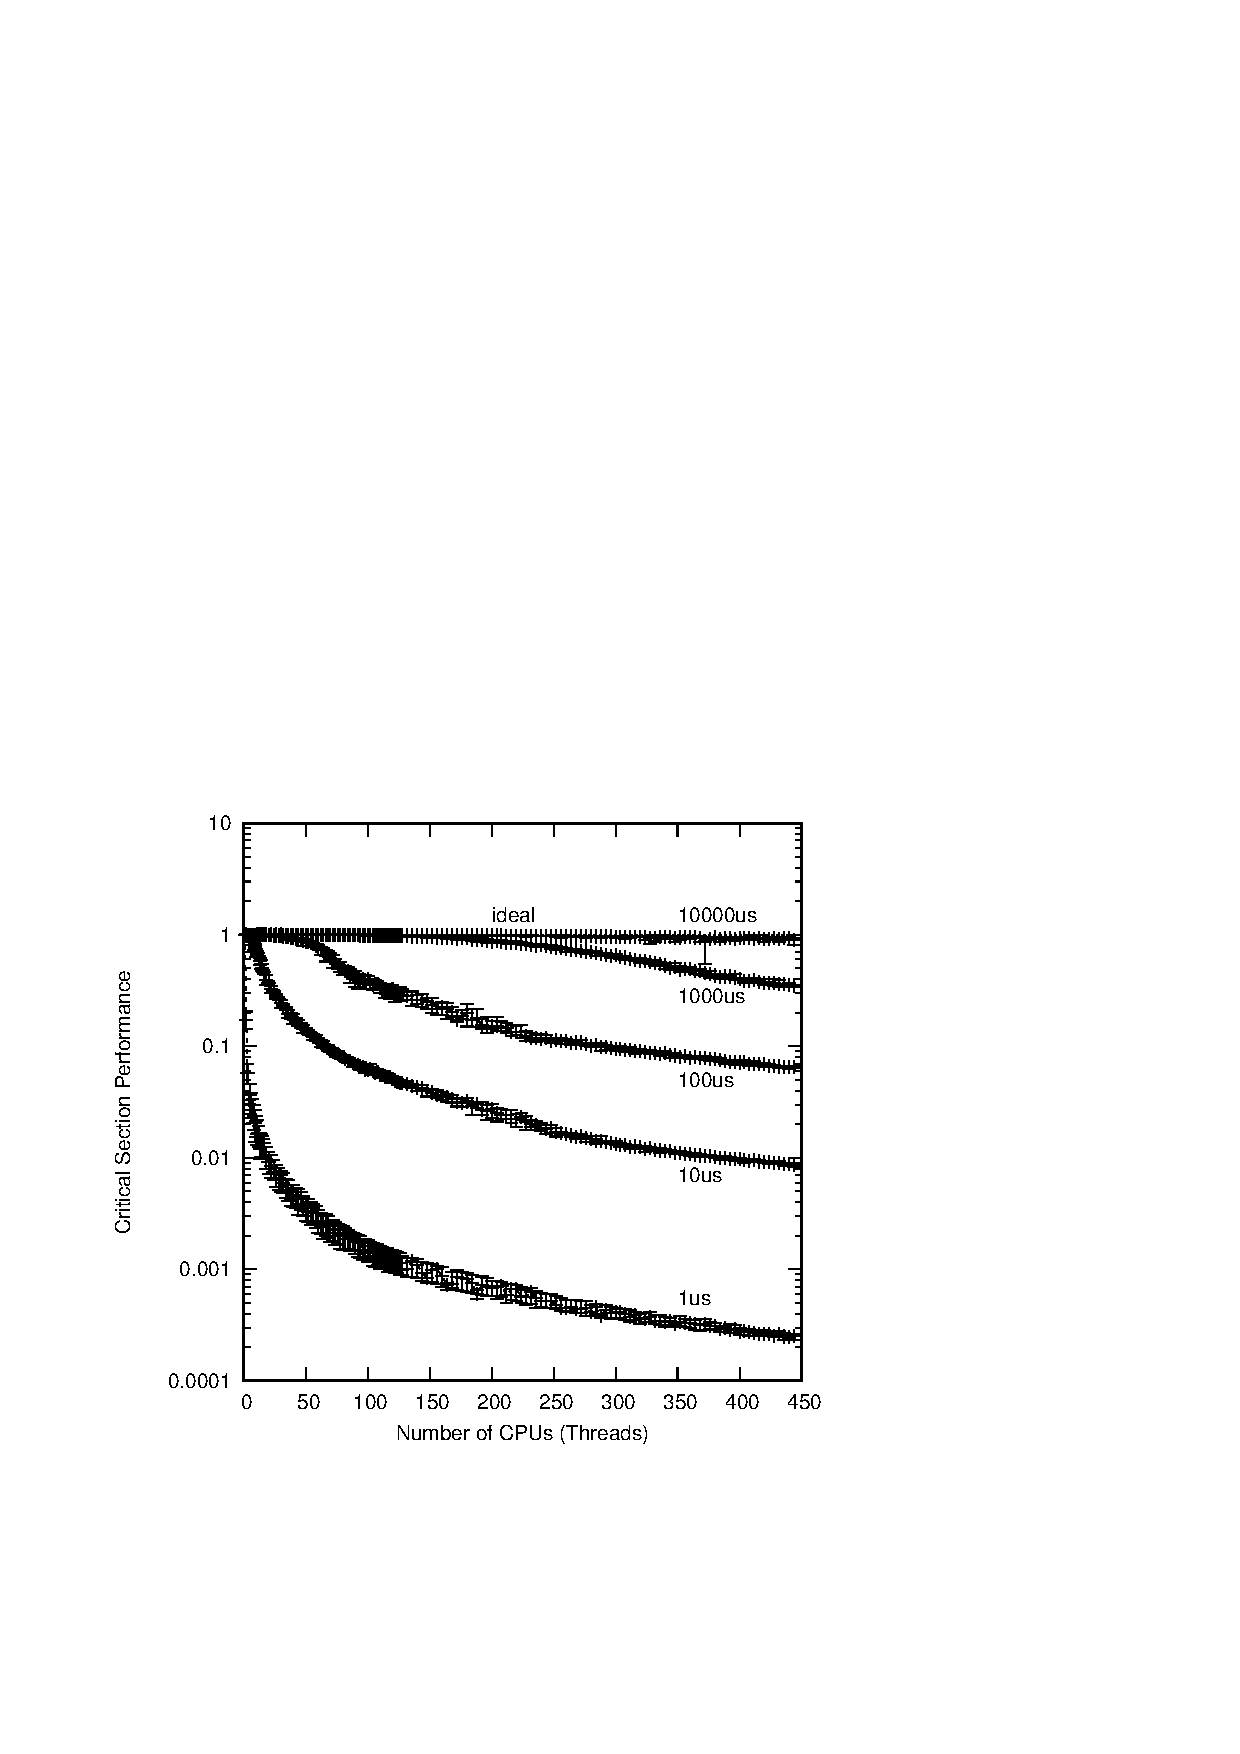
\includegraphics{CodeSamples/toolsoftrade/rwlockscale}}
\caption{Reader-Writer Lock Scalability vs. Microseconds in Critical Section on 8-Socket System With Intel Xeon Platinum 8176 CPUs @ 2.10GHz}
\label{fig:toolsoftrade:Reader-Writer Lock Scalability vs. Microseconds in Critical Section}
\end{figure}

Figure~\ref{fig:toolsoftrade:Reader-Writer Lock Scalability vs. Microseconds in Critical Section}
는 이 테스트를 224코어 Xeon 시스템에서 코어당 두개의 하드웨어 쓰레드를 사용해
총 448개의 소프트웨어에게 보이는 CPU 를 가지는 환경에서 수행되었을 때의 결과를
보입니다.
\co{thinktime} 패러미터는 모든 테스트 동안 0 이었으며, \co{holdtime} 패러미터는
1 마이크로세컨드부터 (그래프 상의 ``1us'') 10,000\,마이크로세컨드 (그래프 상의
``10000us'') 까지 적용되었습니다.
그려진 실제 값은 다음과 같습니다:
\begin{equation}
	\frac{L_N}{N L_1}
\end{equation}
여기서 $N$ 는 쓰레드의 수이며, $L_N$ 는 $N$ 개 쓰레드에 의한 락 획득 횟수이며
$L_1$ 는 단일 쓰레드에 의한 락 획득 횟수입니다.
이상적인 하드웨어와 소프트웨어 확장성 하에서는 이 값은 항상 1.0 이어야 합니다.

\iffalse

Figure~\ref{fig:toolsoftrade:Reader-Writer Lock Scalability vs. Microseconds in Critical Section}
shows the results of running this test on a 224-core Xeon system
with two hardware threads per core for a total of 448 software-visible
CPUs.
The \co{thinktime} parameter was zero for all these tests, and the
\co{holdtime} parameter set to values ranging from one microsecond (``1us''
on the graph) to 10,000\,microseconds (``10000us'' on the graph).
The actual value plotted is:
\begin{equation}
	\frac{L_N}{N L_1}
\end{equation}
where $N$ is the number of threads,
$L_N$ is the number of lock acquisitions by $N$ threads, and
$L_1$ is the number of lock acquisitions by a single thread.
Given ideal hardware and software scalability, this value will always
be 1.0.

\fi

그림 상에서 볼 수 있듯이, reader-writer 락킹의 확장성은 분명 이상적이지 않은데,
특히 작은 크기의 크리티컬 섹션에서 그렇습니다.
왜 읽기 락 획득이 그렇게 느린지 알아보기 위해선, 락을 획득하려는 모든 쓰레드가
\co{pthread_rwlock_t} 데이터 구조를 업데이트 한다는 걸 생각해 봅시다.
따라서, 만약 모든 448개의 쓰레드가 이 reader-writer 락을 동시에 읽기 모드로
획득하려 한다면, 이들은 \co{pthread_rwlock_t} 를 한번에 하나씩 업데이트 해야만
합니다.
운이 좋은 쓰레드는 거의 곧바로 그렇게 할 수 있겠지만, 가장 운이 나쁜 쓰레드는
다른 447개의 쓰레드가 업데이트를 끝낼 때까지 기다려야만 합니다.
이 상황은 CPU 를 추가할 수록 나빠지기만 할 겁니다.
그리고 y 축이 로그스케일이라는 점도 알아 두시기 바랍니다.
10,000\,마이크로세컨드의 기록이 상당히 이상적인 것으로 보이지만, 실제로는
이상적인 경우에 비해 10\,\% 뒤쳐집니다.

\iffalse

As can be seen in the figure, reader-writer locking scalability is
decidedly non-ideal, especially for smaller sizes of critical
sections.
To see why read-acquisition can be so slow, consider
that all the acquiring threads must update the \co{pthread_rwlock_t}
data structure.
Therefore, if all 448 executing threads attempt to
read-acquire the reader-writer lock concurrently, they must update
this underlying \co{pthread_rwlock_t} one at a time.
One lucky thread might do so almost immediately, but the least-lucky
thread must wait for all the other 447 threads to do their updates.
This situation will only get worse as you add CPUs.
Note also the logscale y-axis.
Even though the 10,000\,microsecond trace appears quite ideal, it has
in fact degraded by about 10\,\% from ideal.

\fi

\QuickQuizSeries{%
\QuickQuizB{
	단일 CPU 의 처리량과 비교하는 건 좀 너무한 거 아닌가요?

	\iffalse

	Isn't comparing against single-CPU throughput a bit harsh?

	\fi

}\QuickQuizAnswerB{
	전혀요.
	실제로, 이 비교는 무척 관대한 겁니다.
	좀 더 균형잡힌 비교는 락킹 기능이 제거된 상태에서의 단일 CPU 처리량에
	대한 것일 겁니다.

	\iffalse

	Not at all.
	In fact, this comparison was, if anything, overly lenient.
	A more balanced comparison would be against single-CPU
	throughput with the locking primitives commented out.

	\fi

}\QuickQuizEndB
%
\QuickQuizM{
	하지만 1마이크로세컨드는 크리티컬 섹션의 크기로 특별히 작은 건
	아닙니다.
	예를 들어 몇개의 명령만이 들어있는 것 같은, 훨씬 더 작은 크리티컬
	섹션이 필요할 땐 어떡해야 하죠?

	\iffalse

	But one microsecond is not a particularly small size for
	a critical section.
	What do I do if I need a much smaller critical section, for
	example, one containing only a few instructions?

	\fi

}\QuickQuizAnswerM{
	읽혀진 데이터가 \emph{절대} 바뀌지 않는다면, 그걸 접근하는 동안 어떤
	락도 잡고 있을 필요가 없습니다.
	해당 데이터가 충분히 가끔씩만 바뀐다면, 수행을 체크포인트하고, 모든
	쓰레드를 종료하고, 데이터를 변경한 후, 해당 체크포인트부터 재시작할 수
	있습니다.

	또다른 접근법은 쓰레드당 하나의 배타적 락을 두어서, 자신의 락을
	획득하는 것으로 거대한 reader-writer 락을 읽기 모드로 획득하게 하고,
	모든 쓰레드당 락을 획득하는 것으로 쓰기 모드 획득을 하도록 구현하는
	겁니다~\cite{WilsonCHsieh92a}.
	이는 읽기 쓰레드에게는 상당히 잘 동작하지만, 쓰기 쓰레드에게는 쓰레드의
	수가 늘어날수록 더 큰 오버헤드를 야기시킬 겁니다.

	매우 작은 크리티컬 섹션을 처리하는 다른 효율적 방법들이
	Chapter~\ref{chp:Deferred Processing} 에 설명되어 있습니다.

	\iffalse

	If the data being read \emph{never} changes, then you do not
	need to hold any locks while accessing it.
	If the data changes sufficiently infrequently, you might be
	able to checkpoint execution, terminate all threads, change
	the data, then restart at the checkpoint.

	Another approach is to keep a single exclusive lock per
	thread, so that a thread read-acquires the larger aggregate
	reader-writer lock by acquiring its own lock, and write-acquires
	by acquiring all the per-thread locks~\cite{WilsonCHsieh92a}.
	This can work quite well for readers, but causes writers
	to incur increasingly large overheads as the number of threads
	increases.

	Some other ways of efficiently handling very small critical
	sections are described in Chapter~\ref{chp:Deferred Processing}.

	\fi

}\QuickQuizEndM
%
\QuickQuizM{
	여기 사용된 시스템은 몇년 이상 되었고, 새로운 하드웨어는 더 빠를
	겁니다.
	그러니 누가 reader-writer 락이 느려짐에 대해 걱정하겠습니까?

	\iffalse

	The system used is a few years old, and new hardware should
	be faster.
	So why should anyone worry about reader-writer locks being slow?

	\fi

}\QuickQuizAnswerE{
	일반적으로 새로운 하드웨어는 개선됩니다.
	하지만, reader-writer 락이 448 CPU 에서 이상적 성능을 내게끔 하기
	위해선 수천수만배의 개선을 필요로 할 겁니다.
	더 나쁜 것이, CPU 의 갯수가 늘어날수록 필요한 성능 향상이 더 커집니다.
	따라서 reader-writer 락킹의 성능 문제는 상당한 시간 동안 우리 곁에 있을
	겁니다.

	\iffalse

	In general, newer hardware is improving.
	However, it will need to improve several orders of magnitude
	to permit reader-writer lock to achieve ideal performance on
	448 CPUs.
	Worse yet, the greater the number of CPUs, the larger the
	required performance improvement.
	The performance problems of reader-writer locking are therefore
	very likely to be with us for quite some time to come.

	\fi

}\QuickQuizEndE
}

이런 제한에도 불구하고, reader-writer 락킹은 많은 경우에 유용한데, 예를 들어
읽기 쓰레드들이 응답시간이 긴 파일이나 네트워크 I/O 를 처리해야 하는
경우입니다.
일부 대안도 존재하는데,
Chapter~\ref{chp:Counting} 와~\ref{chp:Deferred Processing} 에서 보입니다.

\iffalse

Despite these limitations, reader-writer locking is quite useful in many
cases, for example when the readers must do high-latency file or network I/O\@.
There are alternatives, some of which will be presented in
Chapters~\ref{chp:Counting} and \ref{chp:Deferred Processing}.

\fi

\subsection{Atomic Operations (\GCC\ Classic)}
\label{sec:toolsoftrade:Atomic Operations (gcc Classic)}

Figure~\ref{fig:toolsoftrade:Reader-Writer Lock Scalability vs. Microseconds in Critical Section}
는 reader-writer 락킹의 오버헤드는 가장 작은 크리티컬 섹션에서 가장 심각함을
보이며, 따라서 작은 크리티컬 섹션들을 보호하는 어떤 다른 방법이 있다면 좋을
겁니다.
그런 한가지 방법은 어토믹 오퍼레이션입니다.
\begin{fcvref}[ln:toolsoftrade:rwlockscale:reader:reader]
우린 이미 하나의 어토믹 오퍼레이션을 봤는데,
Listing~\ref{lst:toolsoftrade:Measuring Reader-Writer Lock Scalability}
의 \clnref{atmc_inc} 의 \apig{__sync_fetch_and_add()} 기능입니다.
이 기능은 두번째 인자의 값을 첫번째 인자로 참조되는 값에 원자적으로 더하고 기존
값을 리턴합니다 (이 경우엔 무시되었습니다).
한쌍의 쓰레드가 동시에 같은 변수에 대해 \co{__sync_fetch_and_add()} 를 실행하면
이 변수의 결과값은 두 더하기의 결과를 포함하게 됩니다.
\end{fcvref}

\iffalse

Figure~\ref{fig:toolsoftrade:Reader-Writer Lock Scalability vs. Microseconds in Critical Section}
shows that the overhead of reader-writer locking is most severe for the
smallest critical sections, so it would be nice to have some other way
of protecting tiny critical sections.
One such way uses atomic operations.
\begin{fcvref}[ln:toolsoftrade:rwlockscale:reader:reader]
We have seen an atomic operation already, namely the
\apig{__sync_fetch_and_add()} primitive on \clnref{atmc_inc} of
Listing~\ref{lst:toolsoftrade:Measuring Reader-Writer Lock Scalability}.
This primitive atomically adds the value of its second argument to
the value referenced by its first argument, returning the old value
(which was ignored in this case).
If a pair of threads concurrently execute \co{__sync_fetch_and_add()} on
the same variable, the resulting value of the variable will include
the result of both additions.
\end{fcvref}

\fi

\GNUC\ 컴파일러는
 \apig{__sync_fetch_and_sub()},
\apig{__sync_fetch_and_or()},
\apig{__sync_fetch_and_and()},
\apig{__sync_fetch_and_xor()}, 그리고
\apig{__sync_fetch_and_nand()}
를 포함한 수많은 추가적 어토믹 오퍼레이션을 제공하는데, 이것들은 모두 기존 값을
리턴합니다.
그대신 새 값이 필요하다면,
\apig{__sync_add_and_fetch()},
\apig{__sync_sub_and_fetch()},
\apig{__sync_or_and_fetch()},
\apig{__sync_and_and_fetch()},
\apig{__sync_xor_and_fetch()}, 그리고
\apig{__sync_nand_and_fetch()}
기능을 사용할 수 있습니다.

\iffalse

The \GNUC\ compiler offers a number of additional atomic operations,
including \apig{__sync_fetch_and_sub()},
\apig{__sync_fetch_and_or()},
\apig{__sync_fetch_and_and()},
\apig{__sync_fetch_and_xor()}, and
\apig{__sync_fetch_and_nand()}, all of which return the old value.
If you instead need the new value, you can instead use the
\apig{__sync_add_and_fetch()},
\apig{__sync_sub_and_fetch()},
\apig{__sync_or_and_fetch()},
\apig{__sync_and_and_fetch()},
\apig{__sync_xor_and_fetch()}, and
\apig{__sync_nand_and_fetch()} primitives.

\fi

\QuickQuiz{
	그런 두 종류의 기능이 정말로 필요한가요?

	\iffalse

	Is it really necessary to have both sets of primitives?

	\fi

}\QuickQuizAnswer{
	엄밀히 말하면, 필요 없습니다.
	두번째 집합의 어느 것이든 그에 연관된 첫번째 집합 내의 것을 사용해
	구현될 수 있습니다.
	예를 들어, \apig{__sync_nand_and_fetch()} 를 다음과 같이
	\apig{__sync_fetch_and_nand()} 로 구현할 수 있습니다.

	\iffalse

	Strictly speaking, no.
	One could implement any member of the second set using the
	corresponding member of the first set.
	For example, one could implement \apig{__sync_nand_and_fetch()}
	in terms of \apig{__sync_fetch_and_nand()} as follows:

	\fi

\begin{VerbatimU}
tmp = v;
ret = __sync_fetch_and_nand(p, tmp);
ret = ~ret & tmp;
\end{VerbatimU}

	비슷하게 \apig{__sync_fetch_and_add()},
	\apig{__sync_fetch_and_sub()}, 그리고 \apig{__sync_fetch_and_xor()}
	를 나중값을 리턴하는 것들을 이용해 구현할 수도 있습니다.

	하지만, 그 대안인 앞의 형태가 프로그래머에게도 컴파일러/라이브러리
	구현자에게도 상당히 편리할 수 있습니다.

	\iffalse

	It is similarly possible to implement \apig{__sync_fetch_and_add()},
	\apig{__sync_fetch_and_sub()}, and \apig{__sync_fetch_and_xor()}
	in terms of their post-value counterparts.

	However, the alternative forms can be quite convenient, both
	for the programmer and for the compiler/library implementor.

	\fi

}\QuickQuizEnd

고전적인 compare-and-swap 오퍼레이션은 \apig{__sync_bool_compare_and_swap()} 와
\apig{__sync_val_compare_and_swap()}, 한쌍의 기능들로 제공됩니다.
이 기능들 둘 모두 새로운 값을 원자적으로 업데이트 합니다만 그 기존 값이 명시된
이전 값과 동일할 때만 그렇습니다.
앞의 첫번째 변종은 이 오퍼레이션이 성공하면 1 을, 실패하면 0 을 리턴하는데,
예를 들어 그 기존 값이 명시된 이전 값과 갖지 않은 경우 실패합니다.
두번째 변종은 해당 위치의 기존값을 리턴하는데, 즉, 이 값이 명시된 이전 값과
동일하다면 이 오퍼레이션은 성공했음을 의미합니다.
모든 단일 위치로의 어토믹 오퍼레이션은 앞의 오퍼레이션들이 종종 더
효율적이지만, compare-and-swap 을 이용해 구현될 수 있다는 점에서
compare-and-swap 오퍼레이션은 ``보편적'' 입니다.
이 compare-and-swap 오퍼레이션은 더 다양한 어토믹 오퍼레이션 집합의 기본으로
사용될 수도 있습니다만, 이것들을 더 다듬는 것은 종종 복잡도, 확장성, 성능
문제로 고통받습니다~\cite{MauriceHerlihy90a}.

\iffalse

The classic compare-and-swap operation is provided by a pair of
primitives, \apig{__sync_bool_compare_and_swap()} and
\apig{__sync_val_compare_and_swap()}.
Both of these primitives atomically update a location to a new value,
but only if its prior value was equal to the specified old value.
The first variant returns 1 if the operation succeeded and 0 if it
failed, for example, if the prior value was not equal to the specified
old value.
The second variant returns the prior value of the location, which, if
equal to the specified old value, indicates that the operation succeeded.
Either of the compare-and-swap operation is ``universal'' in the sense
that any atomic operation on a single location can be implemented in
terms of compare-and-swap, though the earlier operations are often
more efficient where they apply.
The compare-and-swap operation is also capable of serving as the basis
for a wider set of atomic operations, though the more elaborate of
these often suffer from complexity, scalability, and performance
problems~\cite{MauriceHerlihy90a}.

\fi

\QuickQuiz{
	이 어토믹 오퍼레이션들은 밑바닥의 인스트럭션 셋을 이용해 직접적으로
	지원되는 단일 어토믹 인스트럭션을 생성하는 경우가 많을 텐데, 그것이
	일을 하는데 가장 빠른 방법일까요?

	\iffalse

	Given that these atomic operations will often be able to
	generate single atomic instructions that are directly
	supported by the underlying instruction set, shouldn't
	they be the fastest possible way to get things done?

	\fi

}\QuickQuizAnswer{
	불행히도, 그렇지 않습니다.
	극명한 반대 예제를 위해선 Chapter~\ref{chp:Counting} 를 읽어보시기
	바랍니다.

	\iffalse

	Unfortunately, no.
	See Chapter~\ref{chp:Counting} for some stark counterexamples.

	\fi

}\QuickQuizEnd

\apig{__sync_synchronize()} 기능은 컴파일러와 CPU 모두 오퍼레이션을 재배치하지
못하게 하는 ``메모리 배리어'' 를 수행하는데,
Chapter~\ref{chp:Advanced Synchronization: Memory Ordering}
에서 이야기 합니다.
어떤 경우에는 컴파일러의 오퍼레이션 재배치 기능은 제한하지만 CPU 는 내버려 둬도
충분한데, 그런 때에는 \apik{barrier()} 기능이 사용될 수 있습니다.
\begin{fcvref}[ln:toolsoftrade:lock:reader_writer:reader]
어떤 경우에는 컴파일러가 특정 메모리 읽기를 최적화를 위해 없애버리는 것을 막을
필요가 있는데, 그럴 때에는
Listing~\ref{lst:toolsoftrade:Demonstration of Exclusive Locks}
의 \clnref{read_x} 에서와 같이 \apik{READ_ONCE()} 기능이 사용될 수 있습니다.
\end{fcvref}
비슷하게, \apik{WRITE_ONCE()} 기능은 컴파일러가 특정 메모리 쓰기를 최적화해
없애버리는 걸 막는데 사용될 수 있습니다.
이 마지막 세개의 기능들은 \GCC 에서 직접 제공되진 않습니다만
Listing~\ref{lst:toolsoftrade:Compiler Barrier Primitive (for GCC)}
에 보인 것처럼 간단히 구현될 수 있으며, 이 세가지가
Section~\ref{sec:toolsoftrade:Accessing Shared Variables}
에서 길게 설명됩니다.
대안적으로, \apialtk{READ_ONCE(x)}{READ_ONCE()} 가 \GCC\ 내재 기능인 
\apialtg{__atomic_load_n(&x, __ATOMIC_RELAXED)}{__atomic_load_n()}
와 공통되는 부분이 많으며, \apik{WRITE_ONCE()} 는 \GCC\ 내재 기능인
\apialtg{__atomic_store_n(&x, v, __ATOMIC_RELAXED)}{__atomic_store_n()} 와
공통되는 부분이 많습니다.

\iffalse

The \apig{__sync_synchronize()} primitive issues a ``memory barrier'',
which constrains both the compiler's and the CPU's ability to reorder
operations, as discussed in
Chapter~\ref{chp:Advanced Synchronization: Memory Ordering}.
In some cases, it is sufficient to constrain the compiler's ability
to reorder operations, while allowing the CPU free rein, in which
case the \apik{barrier()} primitive may be used.
\begin{fcvref}[ln:toolsoftrade:lock:reader_writer:reader]
In some cases, it is only necessary to ensure that the compiler
avoids optimizing away a given memory read, in which case the
\apik{READ_ONCE()} primitive may be used, as it was on \clnref{read_x} of
Listing~\ref{lst:toolsoftrade:Demonstration of Exclusive Locks}.
\end{fcvref}
Similarly, the \apik{WRITE_ONCE()} primitive may be used to prevent the
compiler from optimizing away a given memory write.
These last three primitives are not provided directly by \GCC,
but may be implemented straightforwardly as shown in
Listing~\ref{lst:toolsoftrade:Compiler Barrier Primitive (for GCC)},
and all three are discussed at length in
Section~\ref{sec:toolsoftrade:Accessing Shared Variables}.
Alternatively, \apialtk{READ_ONCE(x)}{READ_ONCE()} has much in common with
the \GCC\  intrinsic
\apialtg{__atomic_load_n(&x, __ATOMIC_RELAXED)}{__atomic_load_n()}
and \apik{WRITE_ONCE()} has much in common with the \GCC\ 
intrinsic \apialtg{__atomic_store_n(&x, v, __ATOMIC_RELAXED)}{__atomic_store_n()}.

\fi

\begin{listing}[tb]
\input{CodeSamples/api-pthreads/api-pthreads@compiler_barrier.fcv}
\caption{Compiler Barrier Primitive (for \GCC)}
\label{lst:toolsoftrade:Compiler Barrier Primitive (for GCC)}
\end{listing}

\QuickQuiz{
	\apikh{ACCESS_ONCE()} 에는 무슨 일이 벌어진 건가요?

	\iffalse

	What happened to \apikh{ACCESS_ONCE()}?

	\fi

}\QuickQuizAnswer{
	2018년 v4.15 릴리즈에서, 리눅스 커널의 \apikh{ACCESS_ONCE()} 는 읽기와
	쓰기를 위해 각각 \apik{READ_ONCE()} 와 \apik{WRITE_ONCE()} 로
	교체되었습니다~\cite{JonCorbet2012ACCESS:ONCE,
	JonathanCorbet2014ACCESS:ONCEcompilerBugs,
	MarkRutland2017ACCESS:ONCE:remove}.
	\apikh{ACCESS_ONCE()} 는 RCU 코드에 사용되기 위해 만들어졌습니다만, 곧
	코어 API 가 되었습니다~\cite{
	PaulEMcKenney2007ACCESS:ONCE:rcu,
	LinusTorvalds2008ACCESS:ONCE:move}.
	리눅스 커널의 \apik{READ_ONCE()} 와 \apik{WRITE_ONCE()} 는 원래의
	\apikh{ACCESS_ONCE()} 구현과는 상당히 다른 복잡한 형태로 진화했는데 큰
	구조체에도 access-once 기능을 지원하지만 해당 구조체가 하나의 기계
	명령어로 로드되고 스토어 될 수 없을 때 로드/스토어가 찢겨지는 가능성을
	막기 위해서였습니다.

	\iffalse

	In the 2018 v4.15 release, the Linux kernel's \apikh{ACCESS_ONCE()} was
	replaced by \apik{READ_ONCE()} and \apik{WRITE_ONCE()} for reads and
	writes, respectively~\cite{JonCorbet2012ACCESS:ONCE,
	JonathanCorbet2014ACCESS:ONCEcompilerBugs,
	MarkRutland2017ACCESS:ONCE:remove}.
	\apikh{ACCESS_ONCE()} was introduced as a helper in RCU code, but was
	promoted to core API soon afterward~\cite{
	PaulEMcKenney2007ACCESS:ONCE:rcu,
	LinusTorvalds2008ACCESS:ONCE:move}.
	Linux kernel's \apik{READ_ONCE()} and \apik{WRITE_ONCE()} have
	evolved into complex forms that look quite different than
	the original \apikh{ACCESS_ONCE()} implementation due to the
	need to support access-once semantics for large structures,
	but with the possibility of load/store tearing if the structure
	cannot be loaded and stored with a single machine instruction.

	\fi

}\QuickQuizEnd

\subsection{Atomic Operations (C11)}
\label{sec:toolsoftrade:Atomic Operations (C11)}

C11 표준은 로드 (\apic{atomic_load()}), 스토어 (\apic{atomic_store()}), 메모리
배리어 (\apic{atomic_thread_fence()} 와 \apic{atomic_signal_fence()}), 그리고
read-modify-write 어토믹 오퍼레이션들을 포함한 어토믹 오퍼레이션들을
추가했습니다.
이 read-modify-write 어토믹 오퍼레이션에는
\apic{atomic_fetch_add()},
\apic{atomic_fetch_sub()},
\apic{atomic_fetch_and()},
\apic{atomic_fetch_xor()},
\apic{atomic_exchange()},
\apic{atomic_compare_exchange_strong()},
그리고
\apic{atomic_compare_exchange_weak()}
이 포함됩니다.
이것들은
Section~\ref{sec:toolsoftrade:Atomic Operations (gcc Classic)}
에서 설명한 것들과 비슷하게 동작합니다만 모든 오퍼레이션의 \co{_explicit}
변종의 추가된 메모리 순서 인자와 함께 동작합니다.
메모리 순서 인자가 없이는 이 모든 어토믹오퍼레이션이 완전한 순서규칙 (fully
ordered) 아래 동작하며, 이 인자가 주어지면 좀 더 약한 순서규칙 (weaker
ordering) 을 허용합니다.
예를 들어, ``\apialtc{atomic_load_explicit(&a, memory_order_relaxed)}
{atomic_load_explicit()}'' 는 대략적으로 말해서 리눅스 커널의
``\apik{READ_ONCE()}'' 와 비슷합니다.\footnote{
	메모리 순서 규칙은
	Chapter~\ref{chp:Advanced Synchronization: Memory Ordering} 와
	Appendix~\ref{chp:app:whymb:Why Memory Barriers?}
	에 더 자세히 설명되어 있습니다.}

\iffalse

The C11 standard added atomic operations,
including loads (\apic{atomic_load()}),
stores (\apic{atomic_store()}),
memory barriers (\apic{atomic_thread_fence()} and
\apic{atomic_signal_fence()}), and read-modify-write atomics.
The read-modify-write atomics include
\apic{atomic_fetch_add()},
\apic{atomic_fetch_sub()},
\apic{atomic_fetch_and()},
\apic{atomic_fetch_xor()},
\apic{atomic_exchange()},
\apic{atomic_compare_exchange_strong()},
and
\apic{atomic_compare_exchange_weak()}.
These operate in a manner similar to those described in
Section~\ref{sec:toolsoftrade:Atomic Operations (gcc Classic)},
but with the addition of memory-order arguments to \co{_explicit}
variants of all of the operations.
Without memory-order arguments, all the atomic operations are
fully ordered, and the arguments permit weaker orderings.
For example, ``\apialtc{atomic_load_explicit(&a, memory_order_relaxed)}
{atomic_load_explicit()}''
is vaguely similar to the Linux kernel's ``\apik{READ_ONCE()}''.\footnote{
	Memory ordering is described in more detail in
	Chapter~\ref{chp:Advanced Synchronization: Memory Ordering} and
	Appendix~\ref{chp:app:whymb:Why Memory Barriers?}.}

\fi

\subsection{Atomic Operations (Modern \GCC)}
\label{sec:toolsoftrade:Atomic Operations (Modern gcc)}

C11 어토믹 오퍼레이션의 한계점 중 하나는 특수한 어토믹 타입에만 그것들이 적용될
수 있다는 것으로, 이는 문제가 될 수 있습니다.
따라서 \GNUC\ 컴파일러는 어토믹 내재기능들을 제공하는데,
\apig{__atomic_load()},
\apig{__atomic_load_n()},
\apig{__atomic_store()},
\apig{__atomic_store_n()},
\apig{__atomic_thread_fence()} 등이 포함됩니다.
이 내재기능들은 C11 의 비슷한 것들과 같은 기능을 제공합니다만, 평범한 어토믹
타입이 아닌 객체들에도 사용될 수 있습니다.
이것들 중 일부는 아래 리스트 중 하나의 메모리 순서 인자를 받을 수 있습니다:
\apig{__ATOMIC_RELAXED},
\apig{__ATOMIC_CONSUME},
\apig{__ATOMIC_ACQUIRE},
\apig{__ATOMIC_RELEASE},
\apig{__ATOMIC_ACQ_REL}, 그리고
\apig{__ATOMIC_SEQ_CST}.

\iffalse

One restriction of the C11 atomics is that they apply only to special
atomic types, which can be problematic.
The \GNUC\ compiler therefore provides atomic intrinsics, including
\apig{__atomic_load()},
\apig{__atomic_load_n()},
\apig{__atomic_store()},
\apig{__atomic_store_n()},
\apig{__atomic_thread_fence()}, etc.
These intrinsics offer the same semantics as their C11 counterparts,
but may be used on plain non-atomic objects.
Some of these intrinsics may be passed a memory-order argument from
this list:
\apig{__ATOMIC_RELAXED},
\apig{__ATOMIC_CONSUME},
\apig{__ATOMIC_ACQUIRE},
\apig{__ATOMIC_RELEASE},
\apig{__ATOMIC_ACQ_REL}, and
\apig{__ATOMIC_SEQ_CST}.

\fi

\subsection{Per-Thread Variables}
\label{sec:toolsoftrade:Per-Thread Variables}

Thread-specific data, thread-local storage, 또는 다른 덜 겸손한 이름으로도
불리는 쓰레드별 변수 (per-thread variables) 는 동시성 코드에서 굉장히 자주
사용되는데
Chapter~\ref{chp:Counting} and~\ref{chp:Data Ownership} 에서 더 이야기 될
겁니다.
POSIX 는 쓰레드별 변수 생성을 (그리고 그에 연관된 키를 리턴하기 위해) 위해
\apipx{pthread_key_create()} 를, 키에 연관된 쓰레드별 변수의 삭제를 위해
\apipx{pthread_key_delete()} 를, 현재 쓰레드의 특정 키에 연관된 변수의 값을
설정하기 위해 \apipx{pthread_setspecific()} 를, 이 값을 리턴하기 위해
\apipx{pthread_getspecific()} 을 제공합니다.

\iffalse

Per-thread variables, also called thread-specific data, thread-local
storage, and other less-polite names, are used extremely
heavily in concurrent code, as will be explored in
Chapters~\ref{chp:Counting} and~\ref{chp:Data Ownership}.
POSIX supplies the \apipx{pthread_key_create()} function to create a
per-thread variable (and return the corresponding key),
\apipx{pthread_key_delete()} to delete the per-thread variable corresponding
to key,
\apipx{pthread_setspecific()} to set the value of the current thread's
variable corresponding to the specified key,
and \apipx{pthread_getspecific()} to return that value.

\fi

여러 컴파일러가 (\GCC 포함) 해당 변수가 쓰레드별로 되어야 함을 나타내기 위해
변수 정의 부분에 사용될 수 있는 \apig{__thread} 지시어를 제공합니다.
그러면 이 변수의 이름은 그 변수의 현재 쓰레드의 값을 평범하게 접근하는데 사용될
수 있습니다.
물론, \apig{__thread} 는 POSIX thread-specific 데이터보다 사용하기가 훨씬 쉽고,
때문에 \GCC\ 또는 \co{__thread} 를 지원하는 컴파일러로만 빌드되는 코드에서는 더
선호되는 편입니다.

다행히도, C11 표준은 \apig{__thread} 의 자리에 사용될 수 있는
\apic{_Thread_local} 키워드를 도입했습니다.
충분한 시간이 지난 후에는 이 새로운 키워드가 \co{__thread} 의 좋은 사용성과
POSIX thread-specific data 의 이식성을 결합시킬 겁니다.

\iffalse

A number of compilers (including \GCC) provide a \apig{__thread} specifier
that may be used in a variable definition to designate that variable
as being per-thread.
The name of the variable may then be used normally to access the
value of the current thread's instance of that variable.
Of course, \apig{__thread} is much easier to use than the POSIX
thead-specific data, and so \co{__thread} is usually preferred for
code that is to be built only with \GCC\ or other compilers supporting
\co{__thread}.

Fortunately, the C11 standard introduced a \apic{_Thread_local} keyword
that can be used in place of \apig{__thread}.
In the fullness of time, this new keyword should combine the ease of use
of \co{__thread} with the portability of POSIX thread-specific data.

\fi

\section{Alternatives to POSIX Operations}
\label{sec:toolsoftrade:Alternatives to POSIX Operations}
%
\epigraph{The strategic marketing paradigm of Open Source is a massively
	  parallel drunkard's walk filtered by a Darwinistic process.}
	 {\emph{Bruce Perens}}

불행히도, 쓰레드 오퍼레이션, 락킹 기능, 그리고 어토믹 오퍼레이션은 다양한 표준
위원회들이 그것들에 다가가기 훨씬 전부터 사용되어왔습니다.
그 결과, 이 오퍼레이션들이 어떻게 지원되는지에 대한 상당한 차이들이 존재합니다.
역사적인 이유로, 또는 특정 환경에서의 더 나은 성능을 위해서 이 오퍼레이션들이
어셈블리 언어로 구현되는 경우는 상당히 흔합니다.
예를 들어, \GCC 의 \co{__sync_} 기능군은 모두 완전한 메모리 순서 규칙을
제공하는데, 이는 과거에 많은 개발자들을 완전한 메모리 순서 규칙이 필요하지 않은
상황을 위한 각자의 구현을 만들게 이끌었습니다.
다음 섹션들은 리눅스 커널의 일부 대안과 이 책의 예제 코드에서 사용된 역사적
기능들을 보입니다.

\iffalse

Unfortunately, threading operations, locking primitives, and atomic
operations were in reasonably wide use long before the various standards
committees got around to them.
As a result, there is considerable variation in how these operations
are supported.
It is still quite common to find these operations implemented in
assembly language, either for historical reasons or to obtain better
performance in specialized circumstances.
For example, \GCC's \co{__sync_} family of primitives all provide full
memory-ordering semantics, which in the past motivated many developers
to create their own implementations for situations where the full memory
ordering semantics are not required.
The following sections show some alternatives from the Linux kernel
and some historical primitives used by this book's sample code.

\fi

\subsection{Organization and Initialization}
\label{sec:toolsoftrade:Organization and Initialization}

많은 환경이 특별한 초기화 코드를 필요로 하지 않지만, 이 책의 예제 코드는
\apipx{pthread_t} 에서 연속된 정수들로의 매핑을초기화 하는 \apipf{smp_init()}
를 호출하는 것으로 시작합니다.
유저스페이스 RCU 라이브러리\footnote{
	RCU 에 대한 더 많은 정보를 위해선
	\cref{sec:defer:Read-Copy Update (RCU)} 를 보시기 바랍니다.}
역시 비슷하게 \apiur{rcu_init()} 호출을 필요로 합니다.
생성자를 지원하는 환경 (\GCC 의 것 같은) 에서는 이 호출들이 숨겨질 수 있지만,
유저스페이스 RCU 라이브러리에서 지원되는 대부분의 RCU 변종들은 각 쓰레드가
쓰레드 생성 시에 \apiur{rcu_register_thread()} 를, 쓰레드 종료 전에
\apiur{rcu_unregister_thread()} 를 호출할 것을 필요로 합니다.

리눅스 커널의 경우, 커널은 특수한 초기화 코드 호출을 필요로 하지 않는다고
봐야할지 또는 커널의 부팅 시의 코드가 사실은 필요한 초기화 코드라고 봐야할지에
대한 것은 철학적 질문입니다.

\iffalse

Although many environments do not require any special initialization
code, the code samples in this book start with a call to \apipf{smp_init()},
which initializes a mapping from \apipx{pthread_t} to consecutive integers.
The userspace RCU library\footnote{
	See \cref{sec:defer:Read-Copy Update (RCU)} for more information
	on RCU\@.}
similarly requires a call to \apiur{rcu_init()}.
Although these calls can be hidden in environments (such as that of
\GCC) that support constructors,
most of the RCU flavors supported by the userspace RCU library
also require each thread invoke \apiur{rcu_register_thread()} upon thread
creation and \apiur{rcu_unregister_thread()} before thread exit.

In the case of the Linux kernel, it is a philosophical question as to
whether the kernel does not require calls to special initialization
code or whether the kernel's boot-time code is in fact the required
initialization code.

\fi

\subsection{Thread Creation, Destruction, and Control}
\label{sec:toolsoftrade:Thread Creation, Destruction, and Control}

리눅스 커널은 kthread를 추적하기 위해 \apik{struct task_struct} 포인터를,
그것들을 생성하기 위해 \apik{kthread_create()} 를, 명시적으로 멈출 것을
제안하기 위해 (POSIX 에는 비슷한 게 없습니다) \apik{kthread_should_stop()}
을,\footnote{
	POSIX 환경에서는 \apik{kthread_should_stop()} 의 부재를 해결하기 위해
	\co{pthread_join()} 과 함께 제대로 동기화 되는 boolean 플래그를 사용할
	수 있습니다.}
그것들이 멈추기를 기다리기 위해 \apik{kthread_stop()} 을, 그리고 시간제한을 둔
기다림을 위해 \apik{schedule_timeout_interruptible()} 을 사용합니다.
몇가지 추가적인 kthread 관리 API 가 존재합니다만, 이것들만으로도 좋은 시작 내지
검색어가 될 수 있습니다.

CodeSamples API 는 제어의 장소인 ``threads'' 에 집중합니다.\footnote{
	비슷한 소프트웨어의 것들을 위한 많은 다른 이름들이 있는데 ``프로세스'',
	``태스크'', ``파이버'', ``이벤트'', ``수행 에이전트'' 등이 있습니다.
	비슷한 설계 원칙이 이것들 모두에 적용됩니다.}
그런 쓰레드 각각은 \apipf{thread_id_t} 타입의 식별자를 가지며 동시에 수행 되는
두개의 쓰레드가 같은 지시어를 갖지는 못합니다.
쓰레드는 쓰레드별 지역 상태를 제외한 모든 것을 공유하는데\footnote{
	순환적 정의에서는 이게 어떻게 될까요?}
프로그램 카운터와 스택이 포함됩니다.

\iffalse

The Linux kernel uses
\apik{struct task_struct} pointers to track kthreads,
\apik{kthread_create()} to create them,
\apik{kthread_should_stop()} to externally suggest that they stop
(which has no POSIX equivalent),\footnote{
	POSIX environments can work around the lack of
	\apik{kthread_should_stop()} by using a properly synchronized
	boolean flag in conjunction with \co{pthread_join()}.}
\apik{kthread_stop()} to wait for them to stop, and
\apik{schedule_timeout_interruptible()} for a timed wait.
There are quite a few additional kthread-management APIs, but this
provides a good start, as well as good search terms.

The CodeSamples API focuses on ``threads'', which are a locus of
control.\footnote{
	There are many other names for similar software constructs, including
	``process'', ``task'', ``fiber'', ``event'', ``execution agent'',
	and so on.
	Similar design principles apply to all of them.}
Each such thread has an identifier of type \apipf{thread_id_t},
and no two threads running at a given time will have the same
identifier.
Threads share everything except for per-thread local state,\footnote{
	How is that for a circular definition?}
which includes program counter and stack.

\fi

Listing~\ref{lst:toolsoftrade:Thread API} 에 쓰레드 API 가 보여져 있으며, 그
멤버들이 다음 섹션에서 설명됩니다.

\iffalse

The thread API is shown in
Listing~\ref{lst:toolsoftrade:Thread API}, and members are described in the
following sections.

\fi

\begin{listing}[tbp]
\begin{VerbatimL}[numbers=none,xleftmargin=2pt]
int smp_thread_id(void)
thread_id_t create_thread(void *(*func)(void *), void *arg)
for_each_thread(t)
for_each_running_thread(t)
void *wait_thread(thread_id_t tid)
void wait_all_threads(void)
\end{VerbatimL}
\caption{Thread API}
\label{lst:toolsoftrade:Thread API}
\end{listing}

\subsubsection{\tco{create_thread()}}

\apipf{create_thread()} 기능은 새로운 쓰레드를 하나 생성하고,
\apipf{create_thread()} 의 첫번째 인자로 명시된 \co{func} 함수에서 이 새
쓰레드의 수행을 시작하며, \apipf{create_thread()} 의 두번째 인자로 명시된
인자를 넘겨줍니다.
이 새로 생성된 쓰레드는 \co{func} 로 명시된 시작 함수가 리턴할 때 종료됩니다.
\apipf{create_thread()} 기능은 새로 생성된 자식 쓰레드에 연관된
\apipf{thread_id_t} 를 리턴합니다.

이 기능은 해당 프로그램이 생성한 쓰레드의 수를 암묵적으로 세면서
\apipf{NR_THREADS} 보다 많은 수의 쓰레드가 생성되면 프로그램을 종료시킵니다.
\apipf{NR_THREADS} 는 컴파일 시점에 변경될 수 있는 상수입니다만 일부 시스템은
허용 가능한 쓰레드의 수에 대한 상한선을 가지고 있을 수도 있습니다.

\iffalse

The \apipf{create_thread()} primitive creates a new thread,
starting the new thread's execution
at the function \co{func} specified by \apipf{create_thread()}'s
first argument, and passing it the argument specified by
\apipf{create_thread()}'s second argument.
This newly created thread will terminate when it returns from the
starting function specified by \co{func}.
The \apipf{create_thread()} primitive returns the \apipf{thread_id_t}
corresponding to the newly created child thread.

This primitive will abort the program if more than \apipf{NR_THREADS}
threads are created, counting the one implicitly created by running
the program.
\apipf{NR_THREADS} is a compile-time constant that may be modified,
though some systems may have an upper bound for the allowable number
of threads.

\fi

\subsubsection{\tco{smp_thread_id()}}

\apipf{create_thread()} 로부터 리턴된 \apipf{thread_id_t} 는 시스템
종속적이므로, \apipf{smp_thread_id()} 기능은 이 요청을 한 쓰레드에 연관된
쓰레드 인덱스를 리턴합니다.
이 인덱스는 이 프로그램이 시작된 이래로 존재해온 쓰레드의 최대 갯수보다 작을
것이 보장되어 있으며, 따라서 비트마스킹, 배열 인덱스 등등에 유용합니다.

\iffalse

Because the \apipf{thread_id_t} returned from \apipf{create_thread()} is
system-dependent, the \apipf{smp_thread_id()} primitive returns a thread
index corresponding to the thread making the request.
This index is guaranteed to be less than the maximum number of threads
that have been in existence since the program started,
and is therefore useful for bitmasks, array indices, and
the like.

\fi

\subsubsection{\tco{for_each_thread()}}

\apipf{for_each_thread()} 매크로는 존재하는 모든 쓰레드를 순회하는데
생성되었다면 존재 \emph{했을} 모든 쓰레드가 포함됩니다.
이 매크로는Section~\ref{sec:toolsoftrade:Per-Thread Variables} 에서 보이듯이
쓰레드별 변수를 제어하는데 유용합니다.

\iffalse

The \apipf{for_each_thread()} macro loops through all threads that exist,
including all threads that \emph{would} exist if created.
This macro is useful for handling per-thread variables as will be
seen in Section~\ref{sec:toolsoftrade:Per-Thread Variables}.

\fi

\subsubsection{\tco{for_each_running_thread()}}

\apipf{for_each_running_thread()} 매크로는 현재 존재하는 쓰레드에 대해서만
순회를 합니다.
필요하다면 쓰레드 생성과 삭제에 대해 동기화 하는 것은 호출하는 쪽의 역할입니다.

\iffalse

The \apipf{for_each_running_thread()}
macro loops through only those threads that currently exist.
It is the caller's responsibility to synchronize with thread
creation and deletion if required.

\fi

\subsubsection{\tco{wait_thread()}}

\apipf{wait_thread()} 기능은 그것에 넘겨지는 \co{thread_id_t} 로 명시되는
쓰레드의 종료를 기다립니다.
이는 이 명시된 쓰레드의 수행에 대해서는 어떤 영향도 끼치지 않습니다;
대신, 그저 기다립니다.
\apipf{wait_thread()} 는 연관된 쓰레드가 리턴하는 값을 리턴함을 알아두시기
바랍니다.

\iffalse

The \apipf{wait_thread()} primitive waits for completion of the thread
specified by the \co{thread_id_t} passed to it.
This in no way interferes with the execution of the specified thread;
instead, it merely waits for it.
Note that \apipf{wait_thread()} returns the value that was returned by
the corresponding thread.

\fi

\subsubsection{\tco{wait_all_threads()}}

\apipf{wait_all_threads()} 기능은 현재 수행중인 모든 쓰레드의 종료를
기다립니다.
필요하다면 쓰레드 생성과 삭제와 동기화 하는 것은 호출자의 역할입니다.
하지만, 이 기능은 일반적으로 프로그램 수행 종료 시에 정리를 위해 사용되며,
따라서 그런 동기화는 보통은 필요치 않습니다.

\iffalse

The \apipf{wait_all_threads()}
primitive waits for completion of all currently running threads.
It is the caller's responsibility to synchronize with thread creation
and deletion if required.
However, this primitive is normally used to clean up at the end of
a run, so such synchronization is normally not needed.

\fi

\subsubsection{Example Usage}

Listing~\ref{lst:toolsoftrade:Example Child Thread} (\path{threadcreate.c})
은 헬로월드 같은 자식 쓰레드 예제를 보입니다.
앞서 이야기 되었듯, 각 쓰레드는 스스로의 스택을 할당받으며, 따라서 각 쓰레드는
각자의 사적인 \co{arg} 인자와 \co{myarg} 변수를 갖습니다.
각 자식은 종료 전에 간단히 자신의 인자와 \apipf{smp_thread_id()} 를 출력합니다.
라인~\ref{ln:intro:threadcreate:thread_test:return} 의 \co{return} 문은 이
쓰레드를 종료시키고, 이 쓰레드를 위한 \apipf{wait_thread()} 를 호출한
누군가에게 \co{NULL} 을 리턴합니다.

\iffalse

Listing~\ref{lst:toolsoftrade:Example Child Thread} (\path{threadcreate.c})
shows an example hello-world-like child thread.
As noted earlier, each thread is allocated its own stack, so
each thread has its own private \co{arg} argument and \co{myarg} variable.
Each child simply prints its argument and its \apipf{smp_thread_id()}
before exiting.
Note that the \co{return} statement on
line~\ref{ln:intro:threadcreate:thread_test:return} terminates the thread,
returning a \co{NULL} to whoever invokes \apipf{wait_thread()} on this
thread.

\fi

\begin{listing}[tbp]
\input{CodeSamples/intro/threadcreate@thread_test.fcv}
\caption{Example Child Thread}
\label{lst:toolsoftrade:Example Child Thread}
\end{listing}

\begin{fcvref}[ln:intro:threadcreate:main]
이 부모 프로그램이
Listing~\ref{lst:toolsoftrade:Example Parent Thread}
에 보여져 있습니다.
이 프로그램은 라인~\lnref{smp_init} 에서 이 쓰레드 시스템을 초기화 시키기 위해
\co{smp_init()} 를 호출하고, \clnrefrange{parse:b}{parse:e} 에서 인자들을
분석한 후, 자신의 존재를 라인~\lnref{announce} 에서 알립니다.
명시된 수의 자식 쓰레드를
\clnrefrange{create:b}{create:e} 에서 만들고, 그것들이 종료되기를
라인~\lnref{wait} 에서 기다립니다.
\apipf{wait_all_threads()} 는 이 쓰레드들의 리턴 값들이 이 경우에는 모두 별
흥미 없는 \co{NULL} 일 것이므로, 무시합니다.
\end{fcvref}

\iffalse

\begin{fcvref}[ln:intro:threadcreate:main]
The parent program is shown in
Listing~\ref{lst:toolsoftrade:Example Parent Thread}.
It invokes \co{smp_init()} to initialize the threading system on
line~\lnref{smp_init},
parses arguments on \clnrefrange{parse:b}{parse:e},
and announces its presence on line~\lnref{announce}.
It creates the specified number of child threads on
\clnrefrange{create:b}{create:e},
and waits for them to complete on line~\lnref{wait}.
Note that \apipf{wait_all_threads()} discards the threads return values,
as in this case they are all \co{NULL}, which is not very interesting.
\end{fcvref}

\fi

\begin{listing}[tbp]
\input{CodeSamples/intro/threadcreate@main.fcv}
\caption{Example Parent Thread}
\label{lst:toolsoftrade:Example Parent Thread}
\end{listing}

\QuickQuiz{
	리눅스 커널의 \apipx{fork()} 와 \apipx{wait()} 비슷한 것들엔 무슨 일이
	일어났나요?

	\iffalse

	What happened to the Linux-kernel equivalents to \apipx{fork()}
	and \apipx{wait()}?

	\fi

}\QuickQuizAnswer{
	그것들은 정말로 존재하지는 않습니다.
	리눅스 커널 내에서 수행되는 모든 태스크를 메모리를 공유하는데, 최소한
	여러분이 상당한 양의 메모리 매핑 작업을 일일이 하고 싶지 않다면
	그렇습니다.

	\iffalse

	They don't really exist.
	All tasks executing within the Linux kernel share memory,
	at least unless you want to do a huge amount of memory-mapping
	work by hand.

	\fi

}\QuickQuizEnd

\subsection{Locking}
\label{sec:toolsoftrade:Locking}

시작하면서 알아보기 좋을 리눅스 커널의 락킹 API 중 일부의 집합이
Listing~\ref{lst:toolsoftrade:Locking API} 에 표시되어 있는데, 각 API 원소는
다음 섹션들에서 설명됩니다.
이 책의 CodeSamples 락킹 API 는 리눅스 커널의 그것을 따라갑니다.

\iffalse

A good starting subset of the Linux kernel's locking API is shown in
Listing~\ref{lst:toolsoftrade:Locking API},
each API element being described in the following sections.
This book's CodeSamples locking API closely follows that of the Linux kernel.

\fi

\begin{listing}[tbp]
\begin{VerbatimL}[numbers=none]
void spin_lock_init(spinlock_t *sp);
void spin_lock(spinlock_t *sp);
int spin_trylock(spinlock_t *sp);
void spin_unlock(spinlock_t *sp);
\end{VerbatimL}
\caption{Locking API}
\label{lst:toolsoftrade:Locking API}
\end{listing}

\subsubsection{\tco{spin_lock_init()}}

\apik{spin_lock_init()} 기능은 명시된 \apik{spinlock_t} 변수를 초기화 하며, 이
변수가 다른 스핀락 기능들에 넘겨지기 전에 호출되어야만 합니다.

\iffalse

The \apik{spin_lock_init()} primitive initializes the specified
\apik{spinlock_t} variable, and must be invoked before
this variable is passed to any other spinlock primitive.

\fi

\subsubsection{\tco{spin_lock()}}

\apik{spin_lock()} 기능은 명시된 스핀락을 획득하는데, 필요하다면 이 스핀락이
획득 가능해질 때까지 기다립니다.
Pthread 같은 일부 환경에서는 이 기다림이 블록킹을 일으킬 수도 있는데, 리눅스
커널과 같은 다른 환경에서는 CPU-bound spin loop 을 일으킬 수도 있습니다.

핵심은 한번에 단 하나의 쓰레드만이 스핀락을 잡을 수 있다는 것입니다.

\iffalse

The \apik{spin_lock()} primitive acquires the specified spinlock,
if necessary, waiting until the spinlock becomes available.
In some environments, such as pthreads, this waiting will involve
blocking, while in others, such as the Linux kernel, it might involve
a CPU-bound spin loop.

The key point is that only one thread may hold a spinlock at any
given time.

\fi

\subsubsection{\tco{spin_trylock()}}

\apik{spin_trylock()} 기능은 명시된 스핀락을 획득합니다만, 곧바로 획득이 가능할
때만 그렇습니다.
해당 스핀락을 획득할 수 있었다면 \co{true} 를 리턴하고 그렇지 않다면 \co{false}
를 리턴합니다.

\iffalse

The \apik{spin_trylock()} primitive acquires the specified spinlock,
but only if it is immediately available.
It returns \co{true} if it was able to acquire the spinlock and
\co{false} otherwise.

\fi

\subsubsection{\tco{spin_unlock()}}

\apik{spin_unlock()} 기능은 명시된 스핀락을 해제해서 다른 쓰레드가 해당 락을
획득할 수 있게 해줍니다.

\iffalse

The \apik{spin_unlock()} primitive releases the specified spinlock,
allowing other threads to acquire it.

\fi

% \emph{@@@ likely need to add reader-writer locking.}

\subsubsection{Example Usage}

\co{mutx} 라 이름지어진 스핀락이 \co{counter} 변수를 보호하기 위해 아래와 같이
사용될 수 있습니다:

\iffalse

A spinlock named \co{mutex} may be used to protect a variable
\co{counter} as follows:

\fi

\begin{VerbatimU}
spin_lock(&mutex);
counter++;
spin_unlock(&mutex);
\end{VerbatimU}

\QuickQuiz{
	변수 \co{counter} 가 \co{mutex} 의 보호 없이 증가되면 어떤 문제가
	벌어지나요?

	\iffalse

	What problems could occur if the variable \co{counter} were
	incremented without the protection of \co{mutex}?

	\fi

}\QuickQuizAnswer{
	Load-store 구조를 갖는 CPU 에서라면 \co{counter} 증가는 아래와 같은
	형태로 컴파일 될 겁니다:

	\iffalse

	On CPUs with load-store architectures, incrementing \co{counter}
	might compile into something like the following:

	\fi

\begin{VerbatimU}
LOAD counter,r0
INC r0
STORE r0,counter
\end{VerbatimU}

	그런 기계에서라면, 두 쓰레드가 동시에 \co{counter} 의 값을 로드하고,
	각자 증가시킨 후, 그 결과를 저장할 겁니다.
	그러면 \co{counter} 의 새 값은 두 쓰레드가 증가시켰음에도 불구하고 이전
	값보다 1만큼만 클 겁니다.

	\iffalse

	On such machines, two threads might simultaneously load the
	value of \co{counter}, each increment it, and each store the
	result.
	The new value of \co{counter} will then only be one greater
	than before, despite two threads each incrementing it.

	\fi

}\QuickQuizEnd

하지만, \apik{spin_lock()} 과 \apik{spin_unlock()} 기능은 성능에 영향을
끼치는데, Chapter~\ref{chp:Data Structures} 에서 이에 대해 알아보겠습니다.

\iffalse

However, the \apik{spin_lock()} and \apik{spin_unlock()} primitives
do have performance consequences, as will be seen in
Chapter~\ref{chp:Data Structures}.

\fi

\subsection{Accessing Shared Variables}
\label{sec:toolsoftrade:Accessing Shared Variables}

2011년 전까지 C 표준은 공유된 변수에 동시적으로 read/write 액세스를 하는 것에
대한 의미를 정의하지 않았습니다.
하지만, 동시성 C 코드는 최소 4반세기 전부터 쓰여지기
시작했습니다~\cite{Beck85,Inman85}.
이는 오늘날의 수염이 하얗게 센 분들은 C11 이전의 먼 과거에는 어떻게 살았는지
궁금증을 일으킵니다.
이 질문에 대한 짧은 답은 ``그들은 위험하게 살았다'' 입니다.

\iffalse

It was not until 2011 that the C standard defined semantics for concurrent
read/write access to shared variables.
However, concurrent C code was being written at least a quarter century
earlier~\cite{Beck85,Inman85}.
This raises the question as to what today's greybeards did back
in long-past pre-C11 days.
A short answer to this question is ``they lived dangerously''.

\fi

\begin{listing}[tbp]
\begin{fcvlabel}[ln:toolsoftrade:Living Dangerously Early 1990s Style]
\begin{VerbatimL}[commandchars=\\\{\}]
ptr = global_ptr;\lnlbl{temp}
if (ptr != NULL && ptr < high_address)
	do_low(ptr);
\end{VerbatimL}
\end{fcvlabel}
\caption{Living Dangerously Early 1990s Style}
\label{lst:toolsoftrade:Living Dangerously Early 1990s Style}
\end{listing}

\begin{listing}[tbp]
\begin{fcvlabel}[ln:toolsoftrade:C Compilers Can Invent Loads]
\begin{VerbatimL}[commandchars=\\\{\}]
if (global_ptr != NULL &&\lnlbl{if:a}
    global_ptr < high_address)\lnlbl{if:b}
	do_low(global_ptr);\lnlbl{do_low}
\end{VerbatimL}
\end{fcvlabel}
\caption{C Compilers Can Invent Loads}
\label{lst:toolsoftrade:C Compilers Can Invent Loads}
\end{listing}

그들은 최소한 2021년도 컴파일러를 사용했더라도 위험하게 살았을 겁니다.
(대충) 1990년대 초, 컴파일러는 지금보다 적은 최적화를 했는데, 이는 부분적으로는
더 적은 컴파일러 작성자가 존재했으며 다른 부분적으로는 당시에 메모리가
상대적으로 더 작았기 때문입니다.
하지만
Listing~\ref{lst:toolsoftrade:Living Dangerously Early 1990s Style}
에 보여진 것처럼 문제는 일어났는데, 컴파일러는 이 코드를
Listing~\ref{lst:toolsoftrade:C Compilers Can Invent Loads}
의 것으로 바꿀 권리를 가지고 있습니다.
볼 수 있듯이,
Listing~\ref{lst:toolsoftrade:Living Dangerously Early 1990s Style} 의
라인~\ref{ln:toolsoftrade:Living Dangerously Early 1990s Style:temp}
에서의 임시적 부분이 최적화로 사라져버리고, 따라서 \co{global_ptr} 는 세번
로드될 겁니다.

\iffalse

At least they would have been living dangerously had they been using
2021 compilers.
In (say) the early 1990s, compilers did fewer optimizations, in part
because there were fewer compiler writers and in part due to the
relatively small memories of that era.
Nevertheless, problems did arise, as shown in
Listing~\ref{lst:toolsoftrade:Living Dangerously Early 1990s Style},
which the compiler is within its rights to transform into
Listing~\ref{lst:toolsoftrade:C Compilers Can Invent Loads}.
As you can see, the temporary on
line~\ref{ln:toolsoftrade:Living Dangerously Early 1990s Style:temp} of
Listing~\ref{lst:toolsoftrade:Living Dangerously Early 1990s Style}
has been optimized away, so that \co{global_ptr} will be loaded
up to three times.

\fi

\QuickQuiz{
	Listing~\ref{lst:toolsoftrade:Living Dangerously Early 1990s Style} 의
	\co{global_ptr} 를 세번 로드하는데 문제가 뭐죠?

	\iffalse

	What is wrong with loading
	Listing~\ref{lst:toolsoftrade:Living Dangerously Early 1990s Style}'s
	\co{global_ptr} up to three times?

	\fi

}\QuickQuizAnswer{
	\co{global_ptr} 가 최초에는 \co{NULL} 이 아니었지만 어떤 다른 쓰레드가
	\co{global_ptr} 을 \co{NULL} 로 만들었다고 해봅시다.
	\begin{fcvref}[ln:toolsoftrade:C Compilers Can Invent Loads]
	더 나아가서 변경된 코드
	(Listing~\ref{lst:toolsoftrade:C Compilers Can Invent Loads})
	의 라인~\lnref{if:a} 이 \co{global_ptr} 이 \co{NULL} 이 되기 전, 그리고
	라인~\lnref{if:b} 직전에 수행되었다고 생각해 봅시다.
	그러면 라인~\lnref{if:a} 는 \co{global_ptr} 이 \co{NULL} 이 아니라고
	결론을 내어서, 라인~\lnref{if:b} 는 이것이 \co{high_address} 보다 낮을
	것이라고 결론 내리고, 따라서 라인~\lnref{do_low} 가 \co{do_low()} 에
	\co{NULL} 포인터를 넘길 텐데, \co{do_low()} 는 NULL 을 처리할 준비가
	안되어 있을 수도 있습니다.
	\end{fcvref}

	이 책의 편집자는 1990년대 초에 DYNIX/ptx 커널의 메모리 할당자에서
	정확히 이와 같은 실수를 했습니다.
	이 버그를 추적하는데에는 이 책의 편집자만이 아니라 그의 여러 동료들의
	휴일 주말을 써야만 했습니다.
	짧게 말해서, 이건 새로운 문제도 아니고 스스로 사라질 것도 아닙니다.

	\iffalse

	Suppose that \co{global_ptr} is initially non-\co{NULL},
	but that some other thread sets \co{global_ptr} to \co{NULL}.
	\begin{fcvref}[ln:toolsoftrade:C Compilers Can Invent Loads]
	Suppose further that line~\lnref{if:a} of the transformed code
	(Listing~\ref{lst:toolsoftrade:C Compilers Can Invent Loads})
	executes just before \co{global_ptr} is set to \co{NULL} and
	line~\lnref{if:b} just after.
	Then line~\lnref{if:a} will conclude that
        \co{global_ptr} is non-\co{NULL},
	line~\lnref{if:b} will conclude that it is less than
        \co{high_address},
	so that line~\lnref{do_low} passes \co{do_low()} a \co{NULL} pointer,
	which \co{do_low()} just might not be prepared to deal with.
	\end{fcvref}

	Your editor made exactly this mistake in the DYNIX/ptx
	kernel's memory allocator in the early 1990s.
	Tracking down the bug consumed a holiday weekend not just
	for your editor, but also for several of his colleagues.
	In short, this is not a new problem, nor is it likely to
	go away on its own.

	\fi

}\QuickQuizEnd

Section~\ref{sec:toolsoftrade:Shared-Variable Shenanigans}
은 평범한 액세스가 일으키는 추가적인 문제들을 설명하고,
Section~\ref{sec:toolsoftrade:A Volatile Solution}
와~\ref{sec:toolsoftrade:Assembling the Rest of a Solution}
는 C11 이전 컴파일러에서의 해결책 일부를 설명합니다.
물론, 그게 실용적이라면
Section~\ref{sec:toolsoftrade:Atomic Operations (gcc Classic)}
또는 (특히나)
Section~\ref{sec:toolsoftrade:Atomic Operations (C11)}
에서 설명된 기능들이 데이터 레이스를 막기 위해, 즉, 특정 변수에 동시적인 여러
액세스가 있다면 그 액세스는 모두 로드라는 것을 보장하기 위해 사용되어야 합니다.

\iffalse

Section~\ref{sec:toolsoftrade:Shared-Variable Shenanigans}
describes additional problems caused by plain accesses,
Sections~\ref{sec:toolsoftrade:A Volatile Solution}
and~\ref{sec:toolsoftrade:Assembling the Rest of a Solution}
describe some pre-C11 solutions.
Of course, where practical, the primitives described in
Section~\ref{sec:toolsoftrade:Atomic Operations (gcc Classic)}
or (especially)
Section~\ref{sec:toolsoftrade:Atomic Operations (C11)}
should instead be used to avoid data races, that is, to ensure
that if there are multiple concurrent accesses to a given
variable, all of those accesses are loads.

\fi

\subsubsection{Shared-Variable Shenanigans}
\label{sec:toolsoftrade:Shared-Variable Shenanigans}
\OriginallyPublished{Section}{sec:toolsoftrade:Shared-Variable Shenanigans}{Shared-Variable Shenanigans}{Linux Weekly News}{JadeAlglave2019WhoAfraidCompiler}
%
평범한 로드와 스토어를 하는\footnote{
	즉, C11 어토믹, 인라인 어셈블리, 또는 volatile 액세스가 아닌 일반적인
	로드와 스토어.}
코드가 주어지면, 컴파일러는  그로 인해 영향을 받는 변수들은 다른 쓰레드에 의해
액세스 되거나 수정되지 않는다고 가정할 권리를 갖습니다.
이 가정은 컴파일러가 많은 변경을 가할 수 있게 하는데, load tearing, store
tearing, load fusing, store fusing, 코드 재배치, invented load, invented store,
store-to-load 변경, dead-code 제거, 싱글 쓰레드 코드에서라면 문제 없을 만한
모든 것을 포함합니다.
하지만 동시성 코드는 이런 변화들, 달리 말하면 공유 변수 사기질로 인해 망가질 수
있는데, 아래에서 이를 설명합니다.

\iffalse

Given code that does plain loads and stores,\footnote{
	That is, normal loads and stores instead of C11 atomics, inline
	assembly, or volatile accesses.}
the compiler is within
its rights to assume that the affected variables are neither accessed
nor modified by any other thread.
This assumption allows the compiler to carry out a large number of
transformations, including load tearing, store tearing,
load fusing, store fusing, code reordering, invented loads,
invented stores, store-to-load transformations, and dead-code elimination,
all of which work just fine in single-threaded code.
But concurrent code can be broken by each of these transformations,
or shared-variable shenanigans, as described below.

\fi

{\bf Load tearing} 은 컴파일러가 하나의 액세스를 위해 여러 로드 인스트럭션을
사용할 때 발생합니다.
예를 들어, 컴파일러는 이론상 \co{global_ptr} (
Listing~\ref{lst:toolsoftrade:Living Dangerously Early 1990s Style}) 의
라인~\ref{ln:toolsoftrade:Living Dangerously Early 1990s Style:temp} 을
참고하세요) 로부터의 로드를 1바이트 로드 여러개로 번역해낼 수 있습니다.
만약 어떤 다른 쓰레드가 동시에 \co{global_ptr} 을 \co{NULL} 로 만든다면, 그
결과는 해당 포인터의 한 바이트를 제외한 나머지는 0이 될 것이어서, ``야생의
포인터'' 를 형성할 것입니다.
그런 야생의 포인터를 사용한 스토어는 메모리의 임의의 지역을 오염시켜서, 드물고
디버깅 하기 어려운 크래쉬를 야기할 것입니다.

더 나쁜 것이, (말하자면) 16-비트 포인터를 갖는 8-비트 시스템에서, 컴파일러는
주어진 포인터를 접근하기 위해 8-비트 인스트럭션 한쌍을 사용하는 것밖에 선택이
없을 수도 있습니다.
C 표준은 모든 시스템을 지원해야 하므로, 이 표준은 일반적인 경우에서의 load
tearing 을 제거할 수 없습니다.

\iffalse

{\bf Load tearing} occurs when the compiler uses multiple load
instructions for a single access.
For example, the compiler could in theory compile the load from
\co{global_ptr} (see
line~\ref{ln:toolsoftrade:Living Dangerously Early 1990s Style:temp} of
Listing~\ref{lst:toolsoftrade:Living Dangerously Early 1990s Style})
as a series of one-byte loads.
If some other thread was concurrently setting \co{global_ptr} to
\co{NULL}, the result might have all but one byte of the pointer
set to zero, thus forming a ``wild pointer''.
Stores using such a wild pointer could corrupt arbitrary
regions of memory, resulting in rare and difficult-to-debug crashes.

Worse yet, on (say) an 8-bit system with 16-bit pointers, the compiler
might have no choice but to use a pair of 8-bit instructions to access
a given pointer.
Because the C standard must support all manner of systems, the standard
cannot rule out load tearing in the general case.

\fi

{\bf Store tearing} 은 컴파일러가 단일 액세스를 위해 여러 스토어 인스트럭션을
사용할 때 발생합니다.
예를 들어, 한 쓰레드는 4-바이트 정수형 변수에 \co{0x12345678} 을 저장하고 있는
와중에 다른 쓰레드는 \co{0xabcdef00} 을 저장하고 있을 수 있습니다.
컴파일러가 각 액세스를 위해 16-비트 스토어를 사용한다면, 그 결과는
\co{0x1234ef00} 이 될 수도 있는데, 이 정수를 로드하는 코드 입장에선 무척 놀라운
결과가 될 겁니다.
이건 엄밀한 이론적 이슈일 뿐인 것이 아닙니다.
예를 들어, 작은 즉석 인스트럭션 필드를 갖는 CPU 들이 있으며, 그런 CPU 에서
컴파일러는 64-비트 CPU 에서라 할지라도 레지스터에 64-비트 상수를 명시적으로
두는 오버헤드를 줄이기 위해 64-비트 스토어를 두개의 32-비트 스토어로 쪼갤 수
있습니다.
이게 현장에서 실제로 발생한 역사적 보고서들이 존재하며 (예를
들어~\cite{KonstantinKhlebnikov2013gccstoretearing}), 최근의 보고도
있습니다~\cite{WillDeacon2019StoreTearingReport}.\footnote{
	이 쪼개짐은 제대로 정렬된 머신 워드 크기 액세스에서조차 발생할 수
	있으며, 이 특수한 경우 volatile 스토어들에 대해서까지 그렇습니다.
	어떤 사람들은 이 동작인 컴파일러 내의 버그를 의미한다고 주장할 수도
	있겠지만, 어떻게 표현하건 컴파일러 작성자의 시점에서의 store tearing 의
	인식된 가치를 나타내고 있습니다.
}

\iffalse

{\bf Store tearing} occurs when the compiler uses multiple store
instructions for a single access.
For example, one thread might store \co{0x12345678} to a four-byte integer
variable at the same time another thread stored \co{0xabcdef00}.
If the compiler used 16-bit stores for either access, the result
might well be \co{0x1234ef00}, which could come as quite a surprise to
code loading from this integer.
Nor is this a strictly theoretical issue.
For example, there are CPUs that feature small immediate instruction
fields, and on such CPUs, the compiler might split a 64-bit store into
two 32-bit stores in order to reduce the overhead of explicitly forming
the 64-bit constant in a register, even on a 64-bit CPU\@.
There are historical reports of this actually happening in
the wild (e.g.~\cite{KonstantinKhlebnikov2013gccstoretearing}),
but there is also a recent
report~\cite{WillDeacon2019StoreTearingReport}.\footnote{
	Note that this tearing can happen even on properly aligned
        and machine-word-sized accesses, and in this particular case,
	even for volatile stores.
	Some might argue that this behavior constitutes a bug in the
	compiler, but either way it illustrates the perceived value of
	store tearing from a compiler-writer viewpoint.
}

\fi

물론, 32-비트 시스템에서 64-비트 정수형을 사용하는 코드가 있을 수 있다는 점을
놓고 보면 컴파일러는 일반적인 경우에 그냥 일부 스토어를 쪼개는 것밖에 다른
선택지가 없습니다.
하지만 제대로 정렬된 머신 워드 크기 스토어에 대해서는 \apik{WRITE_ONCE()} 가
store tearing 을 방지할 겁니다.

\iffalse

Of course, the compiler simply has no choice but to tear some stores
in the general case, given
the possibility of code using 64-bit integers running on a 32-bit system.
But for properly aligned machine-sized stores, \apik{WRITE_ONCE()} will
prevent store tearing.

\fi

\begin{listing}[tbp]
\begin{fcvlabel}[ln:toolsoftrade:Preventing Load Fusing]
\begin{VerbatimL}[commandchars=\\\{\}]
while (!need_to_stop)
	do_something_quickly();
\end{VerbatimL}
\end{fcvlabel}
\caption{Inviting Load Fusing}
\label{lst:toolsoftrade:Inviting Load Fusing}
\end{listing}

\begin{listing}[tbp]
\begin{fcvlabel}[ln:toolsoftrade:C Compilers Can Fuse Loads]
\begin{VerbatimL}[commandchars=\\\[\]]
if (!need_to_stop)
	for (;;) {\lnlbl[loop:b]
		do_something_quickly();
		do_something_quickly();
		do_something_quickly();
		do_something_quickly();
		do_something_quickly();
		do_something_quickly();
		do_something_quickly();
		do_something_quickly();
		do_something_quickly();
		do_something_quickly();
		do_something_quickly();
		do_something_quickly();
		do_something_quickly();
		do_something_quickly();
		do_something_quickly();
		do_something_quickly();
	}\lnlbl[loop:e]
\end{VerbatimL}
\end{fcvlabel}
\caption{C Compilers Can Fuse Loads}
\label{lst:toolsoftrade:C Compilers Can Fuse Loads}
\end{listing}

{\bf Load fusing} occurs when the compiler uses the result of a
prior load from a given variable instead of repeating the load.
Not only is this sort of optimization just fine in single-threaded
code, it is often just fine in multithreaded code.
Unfortunately, the word ``often'' hides some truly annoying exceptions.

For example, suppose that a real-time system needs to invoke a
function named \co{do_something_quickly()} repeatedly until the
variable \co{need_to_stop} was set, and that the compiler can see
that \co{do_something_quickly()} does not store to \co{need_to_stop}.
One (unsafe) way to code this is shown in
Listing~\ref{lst:toolsoftrade:Inviting Load Fusing}.
The compiler might reasonably unroll this loop sixteen times in order
to reduce the per-invocation of the backwards branch at the end of the
loop.
Worse yet, because the compiler knows that \co{do_something_quickly()}
does not store to \co{need_to_stop}, the compiler could quite reasonably
decide to check this variable only once, resulting in the code shown in
Listing~\ref{lst:toolsoftrade:C Compilers Can Fuse Loads}.
\begin{fcvref}[ln:toolsoftrade:C Compilers Can Fuse Loads]
Once entered, the loop on
\clnrefrange{loop:b}{loop:e} will never exit, regardless of how
many times some other thread stores a non-zero value to \co{need_to_stop}.
\end{fcvref}
The result will at best be consternation, and might well also
include severe physical damage.

\begin{listing}[tbp]
\begin{fcvlabel}[ln:toolsoftrade:C Compilers Can Fuse Non-Adjacent Loads]
\begin{VerbatimL}[commandchars=\\\[\]]
int *gp; \lnlbl[gp]

void t0(void)
{
	WRITE_ONCE(gp, &myvar); \lnlbl[wgp]
}

void t1(void)
{
	p1 = gp; \lnlbl[p1]
	do_something(p1);
	p2 = READ_ONCE(gp); \lnlbl[p2]
	if (p2) { \lnlbl[if]
		do_something_else();
		p3 = *gp; \lnlbl[p3]
	}
}
\end{VerbatimL}
\end{fcvlabel}
\caption{C Compilers Can Fuse Non-Adjacent Loads}
\label{lst:toolsoftrade:C Compilers Can Fuse Non-Adjacent Loads}
\end{listing}

\begin{fcvref}[ln:toolsoftrade:C Compilers Can Fuse Non-Adjacent Loads]
The compiler can fuse loads across surprisingly large spans of code.
For example, in
Listing~\ref{lst:toolsoftrade:C Compilers Can Fuse Non-Adjacent Loads},
\co{t0()} and \co{t1()} run concurrently, and \co{do_something()} and
\co{do_something_else()} are inline functions.
Line~\lnref{gp} declares pointer \co{gp}, which C initializes to \co{NULL}
by default.
At some point, line~\lnref{wgp} of \co{t0()} stores a non-\co{NULL}
pointer to \co{gp}.
Meanwhile, \co{t1()} loads from \co{gp} three times on
lines~\lnref{p1}, \lnref{p2}, and~\lnref{p3}.
Given that line~\lnref{if} finds that \co{gp} is non-\co{NULL}, one might
hope that the dereference on line~\lnref{p3} would be guaranteed never
to fault.
Unfortunately, the compiler is within its rights to fuse the read on
lines~\lnref{p1} and~\lnref{p3}, which means that if line~\lnref{p1}
loads \co{NULL} and line~\lnref{p2} loads \co{&myvar}, line~\lnref{p3}
could load \co{NULL}, resulting in a fault.\footnote{
	\ppl{Will}{Deacon} reports that this happened in the Linux kernel.}
Note that the intervening \apik{READ_ONCE()} does not prevent the other
two loads from being fused, despite the fact that all three are loading
from the same variable.
\end{fcvref}

\QuickQuiz{
	Why does it matter whether \co{do_something()} and
	\co{do_something_else()} in
	Listing~\ref{lst:toolsoftrade:C Compilers Can Fuse Non-Adjacent Loads}
	are inline functions?
}\QuickQuizAnswer{
	\begin{fcvref}[ln:toolsoftrade:C Compilers Can Fuse Non-Adjacent Loads]
	Because \co{gp} is not a static variable, if either
	\co{do_something()} or \co{do_something_else()} were separately
	compiled, the compiler would have to assume that either or both
	of these two functions might change the value of \co{gp}.
	This possibility would force the compiler to reload \co{gp}
	on line~\lnref{p3}, thus avoiding the \co{NULL}-pointer dereference.
	\end{fcvref}
}\QuickQuizEnd

{\bf Store fusing} can occur when the compiler notices a pair of successive
stores to a given variable with no intervening loads from that variable.
In this case, the compiler is within its rights to omit the first store.
This is never a problem in single-threaded code, and in fact it is
usually not a problem in correctly written concurrent code.
After all, if the two stores are executed in quick succession, there is
very little chance that some other thread could load the value from the
first store.

\begin{listing}[tbp]
\begin{fcvlabel}[ln:toolsoftrade:C Compilers Can Fuse Stores]
\begin{VerbatimL}[commandchars=\\\[\]]
void shut_it_down(void)
{
	status = SHUTTING_DOWN; /* BUGGY!!! */\lnlbl[store:a]
	start_shutdown();
	while (!other_task_ready) /* BUGGY!!! */\lnlbl[loop:b]
		continue;\lnlbl[loop:e]
	finish_shutdown();\lnlbl[finish]
	status = SHUT_DOWN; /* BUGGY!!! */\lnlbl[store:b]
	do_something_else();
}

void work_until_shut_down(void)
{
	while (status != SHUTTING_DOWN) /* BUGGY!!! */\lnlbl[until:loop:b]
		do_more_work();\lnlbl[until:loop:e]
	other_task_ready = 1; /* BUGGY!!! */\lnlbl[other:store]
}
\end{VerbatimL}
\end{fcvlabel}
\caption{C Compilers Can Fuse Stores}
\label{lst:toolsoftrade:C Compilers Can Fuse Stores}
\end{listing}

However, there are exceptions, for example as shown in
Listing~\ref{lst:toolsoftrade:C Compilers Can Fuse Stores}.
\begin{fcvref}[ln:toolsoftrade:C Compilers Can Fuse Stores]
The function \co{shut_it_down()} stores to the shared
variable \co{status} on lines~\lnref{store:a} and~\lnref{store:b},
and so assuming that neither
\co{start_shutdown()} nor \co{finish_shutdown()} access \co{status},
the compiler could reasonably remove the store to \co{status} on
line~\lnref{store:a}.
Unfortunately, this would mean that \co{work_until_shut_down()} would
never exit its loop spanning
lines~\lnref{until:loop:b} and~\lnref{until:loop:e}, and thus would never set
\co{other_task_ready}, which would in turn mean that \co{shut_it_down()}
would never exit its loop spanning
lines~\lnref{loop:b} and~\lnref{loop:e}, even if
the compiler chooses not to fuse the successive loads from
\co{other_task_ready} on line~\lnref{loop:b}.

And there are more problems with the code in
Listing~\ref{lst:toolsoftrade:C Compilers Can Fuse Stores},
including code reordering.

{\bf Code reordering} is a common compilation technique used to
combine common subexpressions, reduce register pressure, and
improve utilization of the many functional units available on
modern superscalar microprocessors.
It is also another reason why the code in
Listing~\ref{lst:toolsoftrade:C Compilers Can Fuse Stores}
is buggy.
For example, suppose that the \co{do_more_work()} function on
line~\lnref{until:loop:e}
does not access \co{other_task_ready}.
Then the compiler would be within its rights to move the assignment
to \co{other_task_ready} on
line~\lnref{other:store} to precede line~\lnref{until:loop:b}, which might
be a great disappointment for anyone hoping that the last call to
\co{do_more_work()} on line~\lnref{until:loop:e} happens before the call to
\co{finish_shutdown()} on line~\lnref{finish}.
\end{fcvref}

It might seem futile to prevent the compiler from changing the order of
accesses in cases where the underlying hardware is free to reorder them.
However, modern machines have \emph{exact exceptions} and
\emph{exact interrupts}, meaning that any interrupt or exception will
appear to have happened at a specific place in the instruction
stream.
This means that the handler will see the effect of all prior
instructions, but won't see the effect of any subsequent instructions.
\apik{READ_ONCE()} and \apik{WRITE_ONCE()} can therefore be used to
control communication between interrupted code and interrupt handlers,
independent of the ordering provided by the underlying hardware.\footnote{
	That said, the various standards committees would prefer that
	you use atomics or variables of type \apic{sig_atomic_t}, instead
	of \apik{READ_ONCE()} and \apik{WRITE_ONCE()}.}

{\bf Invented loads} were illustrated by the code in
Listings~\ref{lst:toolsoftrade:Living Dangerously Early 1990s Style}
and~\ref{lst:toolsoftrade:C Compilers Can Invent Loads},
in which the compiler optimized away a temporary variable,
thus loading from a shared variable more often than intended.

Invented loads can be a performance hazard.
These hazards can occur when a load of variable in a ``hot''
cacheline is hoisted out of an \co{if} statement.
These hoisting optimizations are not uncommon, and can cause significant
increases in cache misses, and thus significant degradation of
both performance and scalability.

\begin{fcvref}[ln:toolsoftrade:C Compilers Can Fuse Stores]
{\bf Invented stores} can occur in a number of situations.
For example, a compiler emitting code for \co{work_until_shut_down()} in
Listing~\ref{lst:toolsoftrade:C Compilers Can Fuse Stores}
might notice that \co{other_task_ready} is not accessed by
\co{do_more_work()}, and stored to on line~\lnref{other:store}.
If \co{do_more_work()} was a complex inline function, it might be
necessary to do a register spill, in which case one attractive
place to use for temporary storage is \co{other_task_ready}.
After all, there are no accesses to it, so what is the harm?

Of course, a non-zero store to this variable at just the wrong time
would result in the \co{while} loop on
line~\lnref{loop:b} terminating
prematurely, again allowing \co{finish_shutdown()} to run
concurrently with \co{do_more_work()}.
Given that the entire point of this \co{while} appears to be to
prevent such concurrency, this is not a good thing.
\end{fcvref}

\begin{listing}[tbp]
\begin{fcvlabel}[ln:toolsoftrade:Inviting an Invented Store]
\begin{VerbatimL}[commandchars=\\\{\}]
if (condition)
	a = 1;
else
	do_a_bunch_of_stuff();
\end{VerbatimL}
\end{fcvlabel}
\caption{Inviting an Invented Store}
\label{lst:toolsoftrade:Inviting an Invented Store}
\end{listing}

\begin{listing}[tbp]
\begin{fcvlabel}[ln:toolsoftrade:Compiler Invents an Invited Store]
\begin{VerbatimL}[commandchars=\\\[\]]
a = 1;\lnlbl[store:uncond]
if (!condition) {
	a = 0;\lnlbl[store:cond]
	do_a_bunch_of_stuff();
}
\end{VerbatimL}
\end{fcvlabel}
\caption{Compiler Invents an Invited Store}
\label{lst:toolsoftrade:Compiler Invents an Invited Store}
\end{listing}

Using a stored-to variable as a temporary might seem outlandish,
but it is permitted by the standard.
Nevertheless, readers might be justified in wanting a less
outlandish example, which is provided by
Listings~\ref{lst:toolsoftrade:Inviting an Invented Store}
and~\ref{lst:toolsoftrade:Compiler Invents an Invited Store}.

A compiler emitting code for
Listing~\ref{lst:toolsoftrade:Inviting an Invented Store}
might know that the value of \co{a} is initially zero,
which might be a strong temptation to optimize away one branch
by transforming this code to that in
Listing~\ref{lst:toolsoftrade:Compiler Invents an Invited Store}.
\begin{fcvref}[ln:toolsoftrade:Compiler Invents an Invited Store]
Here, line~\lnref{store:uncond} unconditionally stores \co{1} to \co{a}, then
resets the value back to zero on
line~\lnref{store:cond} if \co{condition} was not set.
This transforms the if-then-else into an if-then, saving one branch.
\end{fcvref}

\QuickQuiz{
	Ouch!
	So can't the compiler invent a store to a normal variable pretty
	much any time it likes?
}\QuickQuizAnswer{
	Thankfully, the answer is no.
	This is because the compiler is forbidden from introducing data races.
	The case of inventing a store just before a normal store is
	quite special:  It is not possible for some other entity,
	be it CPU, thread, signal handler, or interrupt handler, to be
	able to see the invented store unless the code already has
	a data race, even without the invented store.
	And if the code already has a data race, it already invokes
	the dreaded spectre of undefined behavior, which allows the
	compiler to generate pretty much whatever code it wants,
	regardless of the wishes of the developer.

	But if the original store is volatile, as in \apik{WRITE_ONCE()},
	for all the compiler knows, there might be a side effect
	associated with the store that could signal some other thread,
	allowing data-race-free access to the variable.
	By inventing the store, the compiler might be introducing a
	data race, which it is not permitted to do.

	In the case of \co{volatile} and atomic variables, the compiler
	is specifically forbidden from inventing writes.
}\QuickQuizEnd

Finally, pre-C11 compilers could invent writes to unrelated
variables that happened to be adjacent to written-to
variables~\cite[Section 4.2]{Boehm:2005:TCI:1064978.1065042}.
This variant of invented stores has been outlawed by the prohibition
against compiler optimizations that invent data races.

\begin{listing}[tbp]
\begin{fcvlabel}[ln:toolsoftrade:Inviting a Store-to-Load Conversion]
\begin{VerbatimL}[commandchars=\\\[\]]
r1 = p;\lnlbl[load:p]
if (unlikely(r1))\lnlbl[if]
	do_something_with(r1);\lnlbl[dsw]
barrier();\lnlbl[barrier]
p = NULL;\lnlbl[null]
\end{VerbatimL}
\end{fcvlabel}
\caption{Inviting a Store-to-Load Conversion}
\label{lst:toolsoftrade:Inviting a Store-to-Load Conversion}
\end{listing}

{\bf Store-to-load transformations} can occur when the compiler notices
that a plain store might not actually change the value in memory.
\begin{fcvref}[ln:toolsoftrade:Inviting a Store-to-Load Conversion]
For example, consider
Listing~\ref{lst:toolsoftrade:Inviting a Store-to-Load Conversion}.
Line~\lnref{load:p} fetches \co{p}, but the \qco{if} statement on
line~\lnref{if} also tells the compiler that the developer thinks that
\co{p} is usually zero.\footnote{
	The \apik{unlikely()} function provides this hint to the compiler,
	and different compilers provide different ways of implementing
	\co{unlikely()}.}
The \apik{barrier()} statment on line~\lnref{barrier} forces the compiler
to forget the value of \co{p}, but one could imagine a compiler
choosing to remember the hint---or getting an additional hint via
feedback-directed optimization.
Doing so would cause the compiler to realize that line~\lnref{null}
is often an expensive no-op.
\end{fcvref}

\begin{listing}[tbp]
\begin{fcvlabel}[ln:toolsoftrade:Compiler Converts a Store to a Load]
\begin{VerbatimL}[commandchars=\\\[\]]
r1 = p;\lnlbl[load:p]
if (unlikely(r1))\lnlbl[if]
	do_something_with(r1);\lnlbl[dsw]
barrier();\lnlbl[barrier]
if (p != NULL)\lnlbl[if1]
	p = NULL;\lnlbl[null]
\end{VerbatimL}
\end{fcvlabel}
\caption{Compiler Converts a Store to a Load}
\label{lst:toolsoftrade:Compiler Converts a Store to a Load}
\end{listing}

\begin{fcvref}[ln:toolsoftrade:Compiler Converts a Store to a Load]
Such a compiler might therefore guard the store of \co{NULL}
with a check, as shown on lines~\lnref{if1} and~\lnref{null} of
Listing~\ref{lst:toolsoftrade:Compiler Converts a Store to a Load}.
Although this transformation is often desirable, it could be problematic
if the actual store was required for ordering.
For example, a write memory barrier (Linux kernel \apik{smp_wmb()}) would
order the store, but not the load.
This situation might suggest use of \apik{smp_store_release()} over
\apik{smp_wmb()}.
\end{fcvref}

{\bf Dead-code elimination} can occur when the compiler notices that
the value from a load is never used, or when a variable is stored to,
but never loaded from.
This can of course eliminate an access to a shared variable, which
can in turn defeat a memory-ordering primitive, which could cause your
concurrent code to act in surprising ways.
Experience thus far indicates that relatively few such surprises will
be at all pleasant.
Elimination of store-only variables is especially dangerous in cases
where external code locates the variable via symbol tables: The
compiler is necessarily ignorant of such external-code accesses, and
might thus eliminate a variable that the external code relies upon.

Reliable concurrent code clearly needs a way to cause the compiler to
preserve the number, order, and type of important accesses to shared
memory, a topic taken up by
Sections~\ref{sec:toolsoftrade:A Volatile Solution}
and~\ref{sec:toolsoftrade:Assembling the Rest of a Solution},
which are up next.

\subsubsection{A Volatile Solution}
\label{sec:toolsoftrade:A Volatile Solution}

Although it is now much maligned, before the advent of C11 and
C++11~\cite{PeteBecker2011N3242}, the \apic{volatile} keyword was an
indispensible tool in the parallel programmer's toolbox.
This raises the question of exactly what \co{volatile} means,
a question that is not answered with excessive precision even
by more recent versions of this standard~\cite{RichardSmith2019N4800}.\footnote{
	JF Bastien thoroughly documented the history and use cases
	for the \co{volatile} keyword in
	C++~\cite{JFBastien2018DeprecatingVolatile}.}
This version guarantees that ``Accesses through \co{volatile}
\co{glvalues} are evaluated strictly according to the rules of the
abstract machine'',
that \co{volatile} accesses are side effects,
that they are one of the four forward-progress indicators,
and that their exact semantics are implementation-defined.
Perhaps the clearest guidance is provided by this non-normative note:

\begin{quote}
	\apic{volatile} is a hint to the implementation to avoid
	aggressive optimization involving the object because the value
	of the object might be changed by means undetectable by an
	implementation.
	Furthermore, for some implementations, \apic{volatile} might indicate
	that special hardware instructions are required to access
	the object.
	See 6.8.1 for detailed semantics.
	In general, the semantics of \apic{volatile} are intended to be the
	same in C++ as they are in C.
\end{quote}

This wording might be reassuring to those writing low-level code, except
for the fact that compiler writers are free to completely ignore
non-normative notes.
Parallel programmers might instead reassure themselves that compiler
writers would like to avoid breaking device drivers (though perhaps
only after a few ``frank and open'' discussions with device-driver
developers), and device drivers impose at least the following
constraints~\cite{PaulEMcKenney2016P0124R6-LKMM}:

\begin{enumerate}
\item	Implementations are forbidden from tearing an aligned volatile
	access when machine instructions of that access's size and type
	are available.\footnote{
		Note that this leaves unspecified what to do with 128-bit
		loads and stores on CPUs having 128-bit CAS but not
		128-bit loads and stores.}
	Concurrent code relies on this constraint to avoid unnecessary
	load and store tearing.
\item	Implementations must not assume anything about the semantics of
	a volatile access, nor, for any volatile access that returns a
	value, about the possible set of values that might be
	returned.\footnote{
		This is strongly implied by the implementation-defined
		semantics called out above.}
	Concurrent code relies on this constraint to avoid optimizations
	that are inapplicable given that other processors might be
	concurrently accessing the location in question.
\item	Aligned machine-sized non-mixed-size volatile accesses interact
	naturally with volatile assembly-code sequences before and after.
	This is necessary because some devices must be accessed using
	a combination of volatile MMIO accesses and special-purpose
	assembly-language instructions.
	Concurrent code relies on this constraint in order to achieve
	the desired ordering properties from combinations of volatile
	accesses and other means discussed in
	Section~\ref{sec:toolsoftrade:Assembling the Rest of a Solution}.
\end{enumerate}

Concurrent code also relies on the first two constraints to avoid
undefined behavior that could result due to data races if any of the
accesses to a given object was either non-atomic or non-volatile,
assuming that all accesses are aligned and machine-sized.
The semantics of mixed-size accesses to the same locations are more
complex, and are left aside for the time being.

So how does \apic{volatile} stack up against the earlier examples?

\begin{listing}[tbp]
\begin{fcvlabel}[ln:toolsoftrade:Avoiding Danger, 2018 Style]
\begin{VerbatimL}[commandchars=\\\{\}]
ptr = READ_ONCE(global_ptr);\lnlbl{temp}
if (ptr != NULL && ptr < high_address)
	do_low(ptr);
\end{VerbatimL}
\end{fcvlabel}
\caption{Avoiding Danger, 2018 Style}
\label{lst:toolsoftrade:Avoiding Danger, 2018 Style}
\end{listing}

Using \apik{READ_ONCE()} on
line~\ref{ln:toolsoftrade:Living Dangerously Early 1990s Style:temp} of
Listing~\ref{lst:toolsoftrade:Living Dangerously Early 1990s Style}
avoids invented loads,
resulting in the code shown in
Listing~\ref{lst:toolsoftrade:Avoiding Danger, 2018 Style}.

\begin{listing}[tbp]
\begin{fcvlabel}[ln:toolsoftrade:Preventing Load Fusing]
\begin{VerbatimL}[commandchars=\\\{\}]
while (!READ_ONCE(need_to_stop))
	do_something_quickly();
\end{VerbatimL}
\end{fcvlabel}
\caption{Preventing Load Fusing}
\label{lst:toolsoftrade:Preventing Load Fusing}
\end{listing}

As shown in
Listing~\ref{lst:toolsoftrade:Preventing Load Fusing},
\apik{READ_ONCE()} can also prevent the loop unrolling in
Listing~\ref{lst:toolsoftrade:C Compilers Can Fuse Loads}.

\begin{listing}[tbp]
\begin{fcvlabel}[ln:toolsoftrade:Preventing Store Fusing and Invented Stores]
\begin{VerbatimL}[commandchars=\\\[\]]
void shut_it_down(void)
{
	WRITE_ONCE(status, SHUTTING_DOWN); /* BUGGY!!! */\lnlbl[store:a]
	start_shutdown();
	while (!READ_ONCE(other_task_ready)) /* BUGGY!!! */\lnlbl[loop:b]
		continue;\lnlbl[loop:e]
	finish_shutdown();\lnlbl[finish]
	WRITE_ONCE(status, SHUT_DOWN); /* BUGGY!!! */\lnlbl[store:b]
	do_something_else();
}

void work_until_shut_down(void)
{
	while (READ_ONCE(status) != SHUTTING_DOWN) /* BUGGY!!! */\lnlbl[until:loop:b]
		do_more_work();\lnlbl[until:loop:e]
	WRITE_ONCE(other_task_ready, 1); /* BUGGY!!! */\lnlbl[other:store]
}
\end{VerbatimL}
\end{fcvlabel}
\caption{Preventing Store Fusing and Invented Stores}
\label{lst:toolsoftrade:Preventing Store Fusing and Invented Stores}
\end{listing}

\apik{READ_ONCE()} and \apik{WRITE_ONCE()} can also be used to prevent the
store fusing and invented stores that were shown in
Listing~\ref{lst:toolsoftrade:C Compilers Can Fuse Stores},
with the result shown in
Listing~\ref{lst:toolsoftrade:Preventing Store Fusing and Invented Stores}.
However, this does nothing to prevent code reordering, which requires
some additional tricks taught in
Section~\ref{sec:toolsoftrade:Assembling the Rest of a Solution}.

\begin{listing}[tbp]
\begin{fcvlabel}[ln:toolsoftrade:Disinviting an Invented Store]
\begin{VerbatimL}[commandchars=\\\{\}]
if (condition)
	WRITE_ONCE(a, 1);
else
	do_a_bunch_of_stuff();
\end{VerbatimL}
\end{fcvlabel}
\caption{Disinviting an Invented Store}
\label{lst:toolsoftrade:Disinviting an Invented Store}
\end{listing}

Finally, \apik{WRITE_ONCE()} can be used to prevent the store invention
shown in
Listing~\ref{lst:toolsoftrade:Inviting an Invented Store},
with the resulting code shown in
Listing~\ref{lst:toolsoftrade:Disinviting an Invented Store}.

To summarize, the \apic{volatile} keyword can prevent load
tearing and store tearing in cases where the loads and stores are
machine-sized and properly aligned.
It can also prevent load fusing, store fusing, invented loads, and
invented stores.
However, although it does prevent the compiler from reordering \apic{volatile}
accesses with each other, it does nothing to prevent the
CPU from reordering these accesses.
Furthermore, it does nothing to prevent either compiler or CPU from
reordering non-\co{volatile} accesses with each other or with
\co{volatile} accesses.
Preventing these types of reordering requires the techniques described
in the next section.

\subsubsection{Assembling the Rest of a Solution}
\label{sec:toolsoftrade:Assembling the Rest of a Solution}

Additional ordering has traditionally been provided by recourse to
assembly language, for example, \GCC\ asm directives.
Oddly enough, these directives need not actually contain assembly language,
as exemplified by the \apik{barrier()} macro shown in
Listing~\ref{lst:toolsoftrade:Compiler Barrier Primitive (for GCC)}.

\begin{listing}[tbp]
\begin{fcvlabel}[ln:toolsoftrade:Preventing C Compilers From Fusing Loads]
\begin{VerbatimL}[commandchars=\\\[\]]
while (!need_to_stop) {
	barrier(); \lnlbl[b1]
	do_something_quickly();
	barrier(); \lnlbl[b2]
}
\end{VerbatimL}
\end{fcvlabel}
\caption{Preventing C Compilers From Fusing Loads}
\label{lst:toolsoftrade:Preventing C Compilers From Fusing Loads}
\end{listing}

In the \apik{barrier()} macro, the \co{__asm__} introduces the asm
directive, the \co{__volatile__} prevents the compiler from optimizing
the asm away, the empty string specifies that no actual instructions
are to be emitted, and the final \co{"memory"} tells the compiler that
this do-nothing asm can arbitrarily change memory.
In response, the compiler will avoid moving any memory references across
the \apik{barrier()} macro.
This means that the real-time-destroying loop unrolling shown in
Listing~\ref{lst:toolsoftrade:C Compilers Can Fuse Loads}
can be prevented by adding \apik{barrier()} calls as shown on
lines~\ref{ln:toolsoftrade:Preventing C Compilers From Fusing Loads:b1}
and~\ref{ln:toolsoftrade:Preventing C Compilers From Fusing Loads:b2}
of
Listing~\ref{lst:toolsoftrade:Preventing C Compilers From Fusing Loads}.
These two lines of code prevent the compiler from pushing the load from
\co{need_to_stop} into or past \co{do_something_quickly()} from either
direction.

\begin{listing}[tbp]
\begin{fcvlabel}[ln:toolsoftrade:Preventing Reordering]
\begin{VerbatimL}[commandchars=\\\[\]]
void shut_it_down(void)
{
	WRITE_ONCE(status, SHUTTING_DOWN);
	smp_mb(); \lnlbl[mb1]
	start_shutdown();
	while (!READ_ONCE(other_task_ready))\lnlbl[loop:b]
		continue;
	smp_mb(); \lnlbl[mb2]
	finish_shutdown();
	smp_mb(); \lnlbl[mb3]
	WRITE_ONCE(status, SHUT_DOWN);
	do_something_else();
}

void work_until_shut_down(void)
{
	while (READ_ONCE(status) != SHUTTING_DOWN) {
		smp_mb(); \lnlbl[mb4]
		do_more_work();
	}
	smp_mb(); \lnlbl[mb5]
	WRITE_ONCE(other_task_ready, 1);\lnlbl[other:store]
}
\end{VerbatimL}
\end{fcvlabel}
\caption{Preventing Reordering}
\label{lst:toolsoftrade:Preventing Reordering}
\end{listing}

However, this does nothing to prevent the CPU from reordering the
references.
In many cases, this is not a problem because the hardware can only do
a certain amount of reordering.
However, there are cases such as
Listing~\ref{lst:toolsoftrade:C Compilers Can Fuse Stores} where the
hardware must be constrained.
Listing~\ref{lst:toolsoftrade:Preventing Store Fusing and Invented Stores}
prevented store fusing and invention, and
Listing~\ref{lst:toolsoftrade:Preventing Reordering}
further prevents the remaining reordering by addition of
\apik{smp_mb()} on
\begin{fcvref}[ln:toolsoftrade:Preventing Reordering]
lines~\lnref{mb1}, \lnref{mb2}, \lnref{mb3}, \lnref{mb4},
and~\lnref{mb5}.
\end{fcvref}
The \apik{smp_mb()} macro is similar to \apik{barrier()} shown in
Listing~\ref{lst:toolsoftrade:Compiler Barrier Primitive (for GCC)},
but with the empty string replaced by a string containing the
instruction for a full memory barrier, for example, \co{"mfence"}
on x86 or \co{"sync"} on PowerPC.

\QuickQuiz{
	But aren't full memory barriers very heavyweight?
	Isn't there a cheaper way to enforce the ordering needed in
	Listing~\ref{lst:toolsoftrade:Preventing Reordering}?
}\QuickQuizAnswer{
	As is often the case, the answer is ``it depends''.
	However, if only two threads are accessing the \co{status}
	and \co{other_task_ready} variables, then the
	\apik{smp_store_release()} and \apik{smp_load_acquire()}
	functions discussed in
	Section~\ref{sec:toolsoftrade:Atomic Operations}
	will suffice.
}\QuickQuizEnd

Ordering is also provided by some read-modify-write atomic
operations, some of which are presented in
Section~\ref{sec:toolsoftrade:Atomic Operations}.
In the general case, memory ordering can be quite subtle, as
discussed in
Chapter~\ref{chp:Advanced Synchronization: Memory Ordering}.
The next section covers an alternative to memory ordering, namely
limiting or even entirely avoiding data races.

\subsubsection{Avoiding Data Races}
\label{sec:toolsoftrade:Avoiding Data Races}

\begin{quote}
``Doctor, it hurts my head when I think about concurrently accessing
shared variables!''

``Then stop concurrently accessing shared variables!!!''
\end{quote}

The doctor's advice might seem unhelpful, but
one time-tested way to avoid concurrently accessing shared variables
is access those variables only when holding a particular lock, as will
be discussed in Chapter~\ref{chp:Locking}.
Another way is to access a given ``shared'' variable only from a given
CPU or thread, as will be discussed in
Chapter~\ref{chp:Data Ownership}.
It is possible to combine these two approaches, for example, a given
variable might be modified only by a given CPU or thread while holding a
particular lock, and might be read either from that same CPU or thread
on the one hand, or from some other CPU or thread while holding that
same lock on the other.
In all of these situations, all accesses to the shared variables may
be plain C-language accesses.

Here is a list of situations
allowing plain loads and stores for some accesses to a given variable,
while requiring markings (such as \apik{READ_ONCE()} and \apik{WRITE_ONCE()})
for other accesses to that same variable:

\begin{enumerate}
\item	A shared variable is only modified by a given owning CPU or
	thread, but is read by other CPUs or threads.
	All stores must use \apik{WRITE_ONCE()}.
	The owning CPU or thread may use plain loads.
	Everything else must use \apik{READ_ONCE()} for loads.
\item	A shared variable is only modified while holding a given
	lock, but is read by code not holding that lock.
	All stores must use \apik{WRITE_ONCE()}.
	CPUs or threads holding the lock may use plain loads.
	Everything else must use \apik{READ_ONCE()} for loads.
\item	A shared variable is only modified while holding a given
	lock by a given owning CPU or thread, but is read by other
	CPUs or threads or by code not holding that lock.
	All stores must use \apik{WRITE_ONCE()}.
	The owning CPU or thread may use plain loads, as may any
	CPU or thread holding the lock.
	Everything else must use \apik{READ_ONCE()} for loads.
\item	A shared variable is only accessed by a given CPU or thread
	and by a signal or interrupt handler running in that CPU's
	or thread's context.
	The handler can use plain loads and stores, as can any code
	that has prevented the handler from being invoked, that is,
	code that has blocked signals and/or interrupts.
	All other code must use \apik{READ_ONCE()} and \apik{WRITE_ONCE()}.
\item	A shared variable is only accessed by a given CPU or thread
	and by a signal or interrupt handler running in that CPU's
	or thread's context, and the handler always restores the values of any
	variables that it has written before return.
	The handler can use plain loads and stores, as can any code
	that has prevented the handler from being invoked, that is,
	code that has blocked signals and/or interrupts.
	All other code can use plain loads, but must use \apik{WRITE_ONCE()}
	to prevent store tearing, store fusing, and invented stores.
\end{enumerate}

\QuickQuiz{
	What needs to happen if an interrupt or signal handler
	might itself be interrupted?
}\QuickQuizAnswer{
	Then that interrupt handler must follow the same rules that
	are followed by other interrupted code.
	Only those handlers that cannot be themselves interrupted
	or that access no variables shared with an interrupting handler
	may safely use plain accesses, and even then only if those
	variables cannot be concurrently accessed by some other CPU or
	thread.
}\QuickQuizEnd

In most other cases, loads from and stores to a shared variable must
use \apik{READ_ONCE()} and \apik{WRITE_ONCE()} or stronger, respectively.
But it bears repeating that neither \apik{READ_ONCE()} nor \apik{WRITE_ONCE()}
provide any ordering guarantees other than within the compiler.
See the above
Section~\ref{sec:toolsoftrade:Assembling the Rest of a Solution} or
Chapter~\ref{chp:Advanced Synchronization: Memory Ordering}
for information on such guarantees.

Examples of many of these data-race-avoidance patterns are presented in
Chapter~\ref{chp:Counting}.

\subsection{Atomic Operations}
\label{sec:toolsoftrade:Atomic Operations}

The Linux kernel provides a wide variety of atomic operations, but
those defined on type \apik{atomic_t} provide a good start.
Normal non-tearing reads and stores are provided by
\apik{atomic_read()} and \apik{atomic_set()}, respectively.
Acquire load is provided by \apik{smp_load_acquire()} and release
store by \apik{smp_store_release()}.

Non-value-returning fetch-and-add operations are provided by
\apik{atomic_add()}, \apik{atomic_sub()}, \apik{atomic_inc()}, and
\apik{atomic_dec()}, among others.
An atomic decrement that returns a reached-zero indication is provided
by both \apik{atomic_dec_and_test()} and \apik{atomic_sub_and_test()}.
An atomic add that returns the new value is provided by
\apik{atomic_add_return()}.
Both \apik{atomic_add_unless()} and \apik{atomic_inc_not_zero()} provide
conditional atomic operations, where nothing happens unless the
original value of the atomic variable is different than the value
specified (these are very handy for managing reference counters, for
example).

An atomic exchange operation is provided by \apik{atomic_xchg()}, and
the celebrated compare-and-swap (CAS) operation is provided by
\apik{atomic_cmpxchg()}.
Both of these return the old value.
Many additional atomic RMW primitives are available in the Linux kernel,
see the \path{Documentation/atomic_t.txt} file in the Linux-kernel
source tree.\footnote{
	As of Linux kernel v5.11.
}

This book's CodeSamples API closely follows that of the Linux kernel.

\subsection{Per-CPU Variables}
\label{sec:toolsoftrade:Per-CPU Variables}

The Linux kernel uses \apik{DEFINE_PER_CPU()} to define a per-CPU variable,
\apik{this_cpu_ptr()} to form a reference to this CPU's instance of a
given per-CPU variable, \apik{per_cpu()} to access a specified CPU's
instance of a given per-CPU variable, along with many other special-purpose
per-CPU operations.

Listing~\ref{lst:toolsoftrade:Per-Thread-Variable API}
shows this book's per-thread-variable API, which is patterned
after the Linux kernel's per-CPU-variable API\@.
This API provides the per-thread equivalent of global variables.
Although this API is, strictly speaking, not necessary\footnote{
	You could instead use \apig{__thread} or \apic{_Thread_local}.},
it can provide a good userspace analogy to Linux kernel code.

\begin{listing}[tbp]
\begin{VerbatimL}[numbers=none]
DEFINE_PER_THREAD(type, name)
DECLARE_PER_THREAD(type, name)
per_thread(name, thread)
__get_thread_var(name)
init_per_thread(name, v)
\end{VerbatimL}
\caption{Per-Thread-Variable API}
\label{lst:toolsoftrade:Per-Thread-Variable API}
\end{listing}

\QuickQuiz{
	How could you work around the lack of a per-thread-variable
	API on systems that do not provide it?
}\QuickQuizAnswer{
	One approach would be to create an array indexed by
	\apipf{smp_thread_id()}, and another would be to use a hash
	table to map from \apipf{smp_thread_id()} to an array
	index---which is in fact what this
	set of APIs does in pthread environments.

	Another approach would be for the parent to allocate a structure
	containing fields for each desired per-thread variable, then
	pass this to the child during thread creation.
	However, this approach can impose large software-engineering
	costs in large systems.
	To see this, imagine if all global variables in a large system
	had to be declared in a single file, regardless of whether or
	not they were C static variables!
}\QuickQuizEnd

\subsubsection{\tco{DEFINE_PER_THREAD()}}

The \apipf{DEFINE_PER_THREAD()} primitive defines a per-thread variable.
Unfortunately, it is not possible to provide an initializer in the way
permitted by the Linux kernel's \apik{DEFINE_PER_CPU()} primitive,
but there is an \apipf{init_per_thread()} primitive that permits easy
runtime initialization.

\subsubsection{\tco{DECLARE_PER_THREAD()}}

The \apipf{DECLARE_PER_THREAD()} primitive is a declaration in the C sense,
as opposed to a definition.
Thus, a \apipf{DECLARE_PER_THREAD()} primitive may be used to access
a per-thread variable defined in some other file.

\subsubsection{\tco{per_thread()}}

The \apipf{per_thread()} primitive accesses the specified thread's variable.

\subsubsection{\tco{__get_thread_var()}}

The \apipf{__get_thread_var()} primitive accesses the current thread's variable.

\subsubsection{\tco{init_per_thread()}}

The \apipf{init_per_thread()} primitive sets all threads' instances of
the specified variable to the specified value.
The Linux kernel accomplishes this via normal C initialization,
relying in clever use of linker scripts and code executed during
the CPU-online process.

\subsubsection{Usage Example}

Suppose that we have a counter that is incremented very frequently
but read out quite rarely.
As will become clear in
Section~\ref{sec:count:Statistical Counters},
it is helpful to implement such a counter using a per-thread variable.
Such a variable can be defined as follows:

\begin{VerbatimU}
DEFINE_PER_THREAD(int, counter);
\end{VerbatimU}

The counter must be initialized as follows:

\begin{VerbatimU}
init_per_thread(counter, 0);
\end{VerbatimU}

A thread can increment its instance of this counter as follows:

\begin{VerbatimU}
p_counter = &__get_thread_var(counter);
WRITE_ONCE(*p_counter, *p_counter + 1);
\end{VerbatimU}

The value of the counter is then the sum of its instances.
A snapshot of the value of the counter can thus be collected
as follows:

\begin{VerbatimU}
for_each_thread(t)
  sum += READ_ONCE(per_thread(counter, t));
\end{VerbatimU}

Again, it is possible to gain a similar effect using other mechanisms,
but per-thread variables combine convenience and high performance,
as will be shown in more detail in
Section~\ref{sec:count:Statistical Counters}.

\section{The Right Tool for the Job: How to Choose?}
\label{sec:toolsoftrade:The Right Tool for the Job: How to Choose?}
%
\epigraph{If you get stuck, change your tools; it may free your thinking.}
	 {\emph{Paul Arden, abbreviated}}

As a rough rule of thumb, use the simplest tool that will get the job done.
If you can, simply program sequentially.
If that is insufficient, try using a shell script to mediate parallelism.
If the resulting shell-script \co{fork()}/\co{exec()} overhead
(about 480 microseconds for a minimal C program on an Intel Core Duo
laptop) is too
large, try using the C-language \apipx{fork()} and \apipx{wait()} primitives.
If the overhead of these primitives (about 80 microseconds for a minimal
child process) is still too large, then you
might need to use the POSIX threading primitives, choosing the appropriate
locking and/or atomic-operation primitives.
If the overhead of the POSIX threading primitives (typically sub-microsecond)
is too great, then the primitives introduced in
Chapter~\ref{chp:Deferred Processing} may be required.
Of course, the actual overheads will depend not only on your hardware,
but most critically on the manner in which you use the primitives.
Furthermore, always remember that inter-process communication and
message-passing can be good alternatives to shared-memory multithreaded
execution, especially when your code makes good use of the design
principles called out in
Chapter~\ref{cha:Partitioning and Synchronization Design}.

\QuickQuiz{
	Wouldn't the shell normally use \apipx{vfork()} rather than
	\apipx{fork()}?
}\QuickQuizAnswer{
	It might well do that, however, checking is left as an exercise
	for the reader.
	But in the meantime, I hope that we can agree that \apipx{vfork()}
	is a variant of \apipx{fork()}, so that we can use \apipx{fork()}
	as a generic term covering both.
}\QuickQuizEnd

Because concurrency was added to the C standard several decades after
the C language was first used to build concurrent systems, there are
a number of ways of concurrently accessing shared variables.
All else being equal, the C11 standard operations described in
Section~\ref{sec:toolsoftrade:Atomic Operations (C11)}
should be your first stop.
If you need to access a given shared variable both with plain accesses
and atomically, then the modern \GCC\ atomics described in
Section~\ref{sec:toolsoftrade:Atomic Operations (Modern gcc)}
might work well for you.
If you are working on an old codebase that uses the classic \GCC\ \co{__sync}
API, then you should review
Section~\ref{sec:toolsoftrade:Atomic Operations (gcc Classic)}
as well as the relevant \GCC\ documentation.
If you are working on the Linux kernel or similar codebase that
combines use of the \apic{volatile} keyword with inline assembly,
or if you need dependencies to provide ordering, look at the material
presented in Section~\ref{sec:toolsoftrade:Accessing Shared Variables}
as well as that in
Chapter~\ref{chp:Advanced Synchronization: Memory Ordering}.

Whatever approach you take, please keep in mind that randomly hacking
multi-threaded code is a spectacularly bad idea, especially given that
shared-memory parallel systems use your own intelligence against you:
The smarter you are, the deeper a hole you will dig for yourself before
you realize that you are in trouble~\cite{DeadlockEmpire2016}.
Therefore, it is necessary to make the right design choices as well as
the correct choice of individual primitives,
as will be discussed at length in subsequent chapters.

\QuickQuizAnswersChp{qqztoolsoftrade}

% count/count.tex

\QuickQuizChapter{chp:Counting}{Counting}

카운팅은 아마도 가장 간단하고 가장 자연스런 컴퓨터의 일 중 하나일 것입니다.
하지만, 커다란 공유 메모리 멀티 프로세서에서 효과적이고 확장성 있게 카운팅을
하는 것은 꽤 어려운 일입니다.
더욱이, 카운팅의 간단함은 정교한 데이터 구조나 복잡한 동기화 도구로의 혼란 없이
기본적인 동시성 문제를 볼 수 있게 합니다.
따라서 카운팅은 병렬 프로그래밍으로의 훌륭한 소개 역할을 합니다.

이 챕터는 간단하고 빠르고 확장성 있는 카운팅 알고리즘들 중 일부를 다룹니다.
하지만 먼저, 당신이 얼마나 동시적 카운팅에 대해 알고 있는지 알아보죠.

\iffalse
Counting is perhaps the simplest and most natural thing a computer can do.
However, counting efficiently and scalably on a large
shared-memory multiprocessor can be quite challenging.
Furthermore, the simplicity of the underlying concept of counting
allows us to explore the fundamental issues of concurrency without
the distractions
of elaborate data structures or complex synchronization primitives.
Counting therefore provides an excellent introduction to
parallel programming.

This chapter covers a number of special cases for which there are simple,
fast, and scalable counting algorithms.
But first, let us find out how much you already know about concurrent
counting.
\fi

\QuickQuiz{}
	대체 왜 효과적이고 확장성 있는 카운팅이 어려운가요?
	무엇보다, 컴퓨터들은 카운팅, 더하기, 빼기, 그 외에도 여러가지를 위한
	전용 하드웨어도 가지고 있는데, 그걸 못하나요???

	\iffalse
	Why on earth should efficient and scalable counting be hard?
	After all, computers have special hardware for the sole purpose
	of doing counting,
	addition, subtraction, and lots more besides, don't they???
	\fi
\QuickQuizAnswer{
	공유된 카운터에 대한 어토믹 오퍼레이션과 같은 기본적인 카운팅
	알고리즘들은 Section~\ref{sec:count:Why Isn't Concurrent Counting
	Trivial?} 에서 이야기하듯 느리고 확장성이 나쁘거나 정확도가 떨어지기
	때문입니다.

	\iffalse
	Because the straightforward counting algorithms, for example,
	atomic operations on a shared counter, either are slow and scale
	badly, or are inaccurate, as will be seen in
	Section~\ref{sec:count:Why Isn't Concurrent Counting Trivial?}.
	\fi
} \QuickQuizEnd

\QuickQuiz{}
	{ \bfseries 네트워크 패킷 카운팅 문제. }
	당신이 송수신된 네트워크 패킷의 갯수 (또는 전체 용량) 에 대한 통계를
	구해야 한다고 생각해 봅시다.
	패킷들은 시스템의 어떤 CPU 를 통해서든 송신 / 수신될 수 있을 겁니다.
	나아가서 이 커다란 기계가 초당 백만개의 패킷을 다룰 수 있고, 그 갯수를
	매 5초마다 읽어내야 하는 시스템 모니터링 패키지가 있다고 가정해 봅시다.
	당신이라면 이 통계 카운터를 어떻게 구현하시겠어요?

	\iffalse
	{ \bfseries Network-packet counting problem. }
	Suppose that you need to collect statistics on the number
	of networking packets (or total number of bytes) transmitted
	and/or received.
	Packets might be transmitted or received by any CPU on
	the system.
	Suppose further that this large machine is capable of
	handling a million packets per second, and that there
	is a systems-monitoring package that reads out the count
	every five seconds.
	How would you implement this statistical counter?
	\fi
\QuickQuizAnswer{
	힌트: 카운터의 업데이트는 엄청 빨라야 합니다만, 카운터는 500만번의
	업데이트마다 한번만 일어나기 때문에, 카운터를 읽어내는 행동은 꽤 느려도
	될 겁니다.
	또한, 일반적으로 읽어지는 값은 완전히 정교하진 않아도
	될겁니다---무엇보다, 카운터는 1밀리세컨드당 1000번 업데이트되기 때문에,
	우린 ``진짜 값''에서 수천정도는 오차값을 가질 수밖에 없을 겁니다.
	``진짜 값'' 이란게 이 문맥에서 뭘 의미하던지요.
	하지만, 읽혀지는 값은 어느정도는 절대적인 오차를 유지해야 할겁니다.
	예를 들어, 카운트가 수백만 정도일 때 1\% 오차는 문제없지만, 조단위가
	된다면 문제가 있겠죠.
	Section~\ref{sec:count:Statistical Counters} 를 참고하세요.

	\iffalse
	Hint: The act of updating the counter must be blazingly
	fast, but because the counter is read out only about once
	in five million updates, the act of reading out the counter can be
	quite slow.
	In addition, the value read out normally need not be all that
	accurate---after all, since the counter is updated a thousand
	times per millisecond, we should be able to work with a value
	that is within a few thousand counts of the ``true value'',
	whatever ``true value'' might mean in this context.
	However, the value read out should maintain roughly the same
	absolute error over time.
	For example, a 1\% error might be just fine when the count
	is on the order of a million or so, but might be absolutely
	unacceptable once the count reaches a trillion.
	See Section~\ref{sec:count:Statistical Counters}.
	\fi
} \QuickQuizEnd

\edef\QQstatcnt{Quick Quiz \thechapter.\thequickquizctr}

\QuickQuiz{}
	{ \bfseries 대략적 구조체 할당 한계 문제. }
	할당된 구조체의 갯수가 어떤 한계(한 10,000 정도)를 넘어가면 추가 할당을
	막기 위해 할당된 구조체의 갯수를 유지해야 한다고 생각해 봅시다.
	또, 이 구조체들은 할당되고 나서 곧바로 해제되고, 한계치를 넘기는 일은
	매우 드물고, ``대략적인'' 한계치 설정이 가능하다고 생각해 봅시다.

	\iffalse
	{ \bfseries Approximate structure-allocation limit problem. }
	Suppose that you need to maintain a count of the number of
	structures allocated in order to fail any allocations
	once the number of structures in use exceeds a limit
	(say, 10,000).
	Suppose further that these structures are short-lived,
	that the limit is rarely exceeded, and that a ``sloppy''
	approximate limit is acceptable.
	\fi
\QuickQuizAnswer{
	힌트: 카운터의 업데이트 동작은 여기서도 매우 빨라야 합니다만, 카운터는
	카운터가 증가될 때마다 읽혀야 합니다.
	하지만, 읽혀지는 값은 그 값이 한계치 아래인지 위인지를 대략적으로는
	구분해 내야 한다는 점을 \emph{제외하고는} 정교하지 않아도 됩니다.

	\iffalse
	Hint: The act of updating the counter must again be blazingly
	fast, but the counter is read out each time that the
	counter is increased.
	However, the value read out need not be accurate
	\emph{except} that it must distinguish approximately
	between values below the limit and values greater than or
	equal to the limit.
	See Section~\ref{sec:count:Approximate Limit Counters}.
	\fi
} \QuickQuizEnd

\edef\QQapproxcnt{Quick Quiz \thechapter.\thequickquizctr}

\QuickQuiz{}
	{ \bfseries 정교한 구조체 할당 한계 문제. }
	할당된 구조체의 갯수가 어떤 정확한 한계(여기서도, 한 10,000 정도)를
	넘어가면 추가 할당을 막기 위해 할당된 구조체의 갯수를 유지해야 한다고
	생각해 봅시다.
	이 구조체들은 할당되고 얼마 안되 해제되고, 그 한계는 드물게 초과되며,
	거의 항상 최소 한개의 구조체는 사용중이 됩니다. 또한 예를 들어, 하나의
	구조체도 사용되지 않고 있다면 해제 할 수 있는 어떤 메모리를 위해
	카운터가 0이 되는 시점을 정확히 알 필요가 있습니다.
	\iffalse

	{ \bfseries Exact structure-allocation limit problem. }
	Suppose that you need to maintain a count of the number of
	structures allocated in order to fail any allocations
	once the number of structures in use exceeds an exact limit
	(again, say 10,000).
	Suppose further that these structures are short-lived,
	and that the limit is rarely exceeded, that there is almost
	always at least one structure in use, and suppose further
	still that it is necessary to know exactly when this counter reaches
	zero, for example, in order to free up some memory
	that is not required unless there is at least one structure
	in use.
	\fi
\QuickQuizAnswer{
	힌트: 카운터의 업데이트 동작은 역시 엄청 빨라야 합니다만, 카운터의 값이
	증가될 때마다 그 값 역시 읽혀야 합니다.
	하지만, 그 값은 한계치 경계를 넘어서는지와 0인지를 분명하게 체크해야
	한다는 점을 \emph{제외하고는} 정교할 필요가 없습니다.
	Section~\ref{sec:count:Exact Limit counters} 를 참고하세요.
	\iffalse

	Hint: The act of updating the counter must once again be blazingly
	fast, but the counter is read out each time that the
	counter is increased.
	However, the value read out need not be accurate
	\emph{except} that it absolutely must distinguish perfectly
	between values between the limit and zero on the one hand,
	and values that either are less than or equal to zero or
	are greater than or equal to the limit on the other hand.
	See Section~\ref{sec:count:Exact Limit Counters}.
	\fi
} \QuickQuizEnd

\edef\QQexactcnt{Quick Quiz \thechapter.\thequickquizctr}

\QuickQuiz{}
	{ \bfseries 제거될 수 있는 I/O 디바이스 접속 카운트 문제. }
	매우 빈번하게 사용되는 제거 가능한 대용량 디바이스에 대해 사용자에게
	해당 디바이스를 제거해도 안전한지 알려주기 위해 그 참조 횟수를 관리해야
	한다고 가정해 봅시다.
	이 디바이스는 사용자가 디바이스를 제거하고 싶을 때 그 의사를 알려주며,
	시스템은 사용자에게 언제 디바이스를 제거해도 안전한지 알려주는 일반적
	디바이스 제거 절차를 따릅니다.
	\iffalse

	{ \bfseries Removable I/O device access-count problem. }
	Suppose that you need to maintain a reference count on a
	heavily used removable mass-storage device, so that you
	can tell the user when it is safe to remove the device.
	This device follows the usual removal procedure where
	the user indicates a desire to remove the device, and
	the system tells the user when it is safe to do so.
	\fi
\QuickQuizAnswer{
	힌트: 여기서도 카운터의 업데이트 동작은 I/O 오퍼레이션이 느려지지 않게
	매우 빠르고 확장성 있어야 합니다. 하지만 카운터는 사용자가 디바이스를
	제거하고자 할 때에만 읽혀지기 때문에, 카운터의 읽기 동작은 매우 느려도
	됩니다.
	또한, 사용자가 디바이스를 제거하고자 하는 의사를 밝히지 않았다면 그
	카운터는 읽혀질 필요가 아예 없습니다.
	또한, 그 값은 디바이스가 제거를 위한 절차 중일 때로 한정해서 0인지 0이
	아닌지만 분명히 구분할 수 있어야 한다는 점을 \emph{제외하고는} 정교할
	필요가 없습니다.
	하지만, 한번 0이라는 값을 읽었다면, 차후에 다른 쓰레드가 제거중인 해당
	디바이스에 접근을 하거나 하는 일을 막기 위해 해당 값을 0으로 유지해야
	합니다.
	Section~\ref{sec:count:Applying Specialized Parallel Counters} 를
	참고하세요.
	\iffalse

	Hint: Yet again, the act of updating the counter must be blazingly
	fast and scalable in order to avoid slowing down I/O operations,
	but because the counter is read out only when the
	user wishes to remove the device, the counter read-out
	operation can be extremely slow.
	Furthermore, there is no need to be able to read out
	the counter at all unless the user has already indicated
	a desire to remove the device.
	In addition, the value read out need not be accurate
	\emph{except} that it absolutely must distinguish perfectly
	between non-zero and zero values, and even then only when
	the device is in the process of being removed.
	However, once it has read out a zero value, it must act
	to keep the value at zero until it has taken some action
	to prevent subsequent threads from gaining access to the
	device being removed.
	See Section~\ref{sec:count:Applying Specialized Parallel Counters}.
	\fi
} \QuickQuizEnd

\edef\QQIOcnt{Quick Quiz \thechapter.\thequickquizctr}

이 챕터의 뒷부분은 이 문제들에 대한 답을 만들어 볼겁니다.
Section~\ref{sec:count:Why Isn't Concurrent Counting Trivial?}
에서는 왜 멀티코어 시스템에서의 카운팅이 간단하지 않은지 다루고,
Section~\ref{sec:count:Statistical Counters}
에서는 네트워크 패킷 카운팅 문제를 푸는 방법들을 봅니다.
Section~\ref{sec:count:Approximate Limit Counters}
에서는 대략적 구조체 할당 한계 문제,
Section~\ref{sec:count:Exact Limit Counters}
에서는 정교한 구조체 할당 한계 문제를 풀어봅니다.
Section~\ref{sec:count:Applying Specialized Parallel Counters}
에서는 다양한 앞의 섹션에서 소개된 특정 병렬 카운터들을 어떻게 사용할지 생각해
봅니다.
마지막으로, Section~\ref{sec:count:Parallel Counting Discussion}
에서는 성능 측정과 함께 이 챕터를 마무리 합니다.

Section~\ref{sec:count:Why Isn't Concurrent Counting Trivial?}와
Section~\ref{sec:count:Statistical Counters} 는 소개적인 내용들을 담고 있고,
이외의 섹션들은 좀 더 전문적인 학생들에게 적당할 겁니다.
\iffalse

The remainder of this chapter will develop answers to these questions.
Section~\ref{sec:count:Why Isn't Concurrent Counting Trivial?}
asks why counting on multicore systems isn't trivial, and
Section~\ref{sec:count:Statistical Counters}
looks into ways of solving the network-packet counting problem.
Section~\ref{sec:count:Approximate Limit Counters}
investigates the approximate structure-allocation limit problem, while
Section~\ref{sec:count:Exact Limit Counters}
takes on the exact structure-allocation limit problem.
Section~\ref{sec:count:Applying Specialized Parallel Counters}
discusses how to use the various specialized parallel counters
introduced in the preceding sections.
Finally, Section~\ref{sec:count:Parallel Counting Discussion}
concludes the chapter with performance measurements.

Sections~\ref{sec:count:Why Isn't Concurrent Counting Trivial?}
and~\ref{sec:count:Statistical Counters}
contain introductory material, while the remaining sections
are more appropriate for advanced students.
\fi

\section{Why Isn't Concurrent Counting Trivial?}
\label{sec:count:Why Isn't Concurrent Counting Trivial?}

\begin{figure}[bp]
{ \scriptsize
\begin{verbatim}
  1 long counter = 0;
  2 
  3 void inc_count(void)
  4 {
  5   counter++;
  6 }
  7 
  8 long read_count(void)
  9 {
 10   return counter;
 11 }
\end{verbatim}
}
\caption{Just Count!}
\label{fig:count:Just Count!}
\end{figure}

일단 간단한, 예를 들어,
Figure~\ref{fig:count:Just Count!} (\url{count_nonatomic.c})
에 나온 것과 같이 직관적인 케이스부터 보도록 하죠.
여기서, 우리는 라인~1 에 카운터를 두고, 라인~5 에서 그 값을 증가시키며, 라인~10
에서 그 값을 읽어옵니다.
이보다 간단할 수는 없겠죠?

이 방법은 당신이 대부분의 경우 읽기만을 하고 값의 증가는 아주 가끔만 한다면
매우 빠르다는 장점을 가지고, 또한 작은 시스템에서도 훌륭한 성능을 보일 겁니다.
\iffalse

Let's start with something simple, for example, the straightforward
use of arithmetic shown in
Figure~\ref{fig:count:Just Count!} (\url{count_nonatomic.c}).
Here, we have a counter on line~1, we increment it on line~5, and we
read out its value on line~10.
What could be simpler?

This approach has the additional advantage of being blazingly fast if
you are doing lots of reading and almost no incrementing, and on small
systems, the performance is excellent.
\fi

다만 여기에는 한가지 문제가 있습니다: 이 방법은 카운트를 놓칠 수 있습니다.
제 듀얼 코어 랩탑에서 짧은 시간동안 \co{inc_count()} 를 100,014,000 번 수행했을
때, 카운터의 마지막 값은 52,909,118 이었습니다.
컴퓨팅에서는 대략적인 값도 충분한 경우도 있지만 그렇다 해도 50\% 이상의
정밀도는 항상 필요합니다.
\iffalse

There is just one large fly in the ointment: this approach can lose
counts.
On my dual-core laptop, a short run invoked \co{inc_count()}
100,014,000 times, but the final value of the counter was only
52,909,118.
Although approximate values do have their place in computing,
accuracies far greater than 50\% are almost always necessary.
\fi

\QuickQuiz{}
	하지만 \co{++} 연산자는 x86 의 add-to-memory 명령어를 만들지 않나요?
	그리고 CPU 캐시는 그걸 어토믹하게 수행하지 않나요?
	\iffalse

	But doesn't the \co{++} operator produce an x86 add-to-memory
	instruction?
	And won't the CPU cache cause this to be atomic?
	\fi
\QuickQuizAnswer{
	\co{++} 연산자는 어토믹할 수\emph{도 있지만}, 그래야만 한다는 규칙은
	없습니다.
	그리고 실제로, \co{gcc} 는 값을 레지스터에 읽어오고, 레지스터의 값을
	증가시킨 후, 메모리에 그 값을 저장하는, 어토믹하지 않은 방법을 종종
	택합니다.
	\iffalse

	Although the \co{++} operator \emph{could} be atomic, there
	is no requirement that it be so.
	And indeed, \co{gcc} often
	chooses to load the value to a register, increment
	the register, then store the value to memory, which is
	decidedly non-atomic.
	\fi
} \QuickQuizEnd

\QuickQuiz{}
	실패 횟수의 8-figure 정확도는 당신이 진짜로 이 테스트를 한 것을
	보여주는군요.
	왜 이런 사소한 프로그램을, 특히나 버그가 이렇게 쉽게 직관적으로
	보이는데도 굳이 테스트 해야 하나요?
	\iffalse

	The 8-figure accuracy on the number of failures indicates
	that you really did test this.
	Why would it be necessary to test such a trivial program,
	especially when the bug is easily seen by inspection?
	\fi
\QuickQuizAnswer{
	사소한 병렬 프로그램이 아주 조금만 존재하지는 않고, 순차적 프로그램에도
	마찬가지라고 저는 생각합니다.

	프로그램이 얼마나 작거나 간단한지와는 상관 없이, 테스트 해보지
	않았다면, 그건 동작하지 않는 것입니다.
	그리고 설령 테스트 해봤다 해도, 머피의 법칙에 의하면 여전히 숨어있는
	버그가 몇개는 있을 수 있을 수 있습니다.
	\iffalse

	Not only are there very few
	trivial parallel programs, and most days I am
	not so sure that there are many trivial sequential programs, either.

	No matter how small or simple the program, if you haven't tested
	it, it does not work.
	And even if you have tested it, Murphy's Law says that there will
	be at least a few bugs still lurking.
	\fi

	또한, 정확성의 증명은 분명 그 의미를 갖지만, 여기 사용된
	\url{counttorture.h} 테스트를 포홤해 테스트를 대체하는 일은 결코 없을
	겁니다.
	무엇보다, 증명은 그것이 바닥에 깔고 있는 가정에 국한됩니다.
	게다가, 증명은 프로그램이 그렇듯 버그를 가지고 있기 쉽습니다!
	\iffalse

	Furthermore, while proofs of correctness certainly do have their
	place, they never will replace testing, including the
	\url{counttorture.h} test setup used here.
	After all, proofs are only as good as the assumptions that they
	are based on.
	Furthermore, proofs can have bugs just as easily as programs can!
	\fi
} \QuickQuizEnd

\begin{figure}[tbp]
{ \scriptsize
\begin{verbatim}
  1 atomic_t counter = ATOMIC_INIT(0);
  2 
  3 void inc_count(void)
  4 {
  5   atomic_inc(&counter);
  6 }
  7 
  8 long read_count(void)
  9 {
 10   return atomic_read(&counter);
 11 }
\end{verbatim}
}
\caption{Just Count Atomically!}
\label{fig:count:Just Count Atomically!}
\end{figure}

\begin{figure}[tb]
\begin{center}
\resizebox{3in}{!}{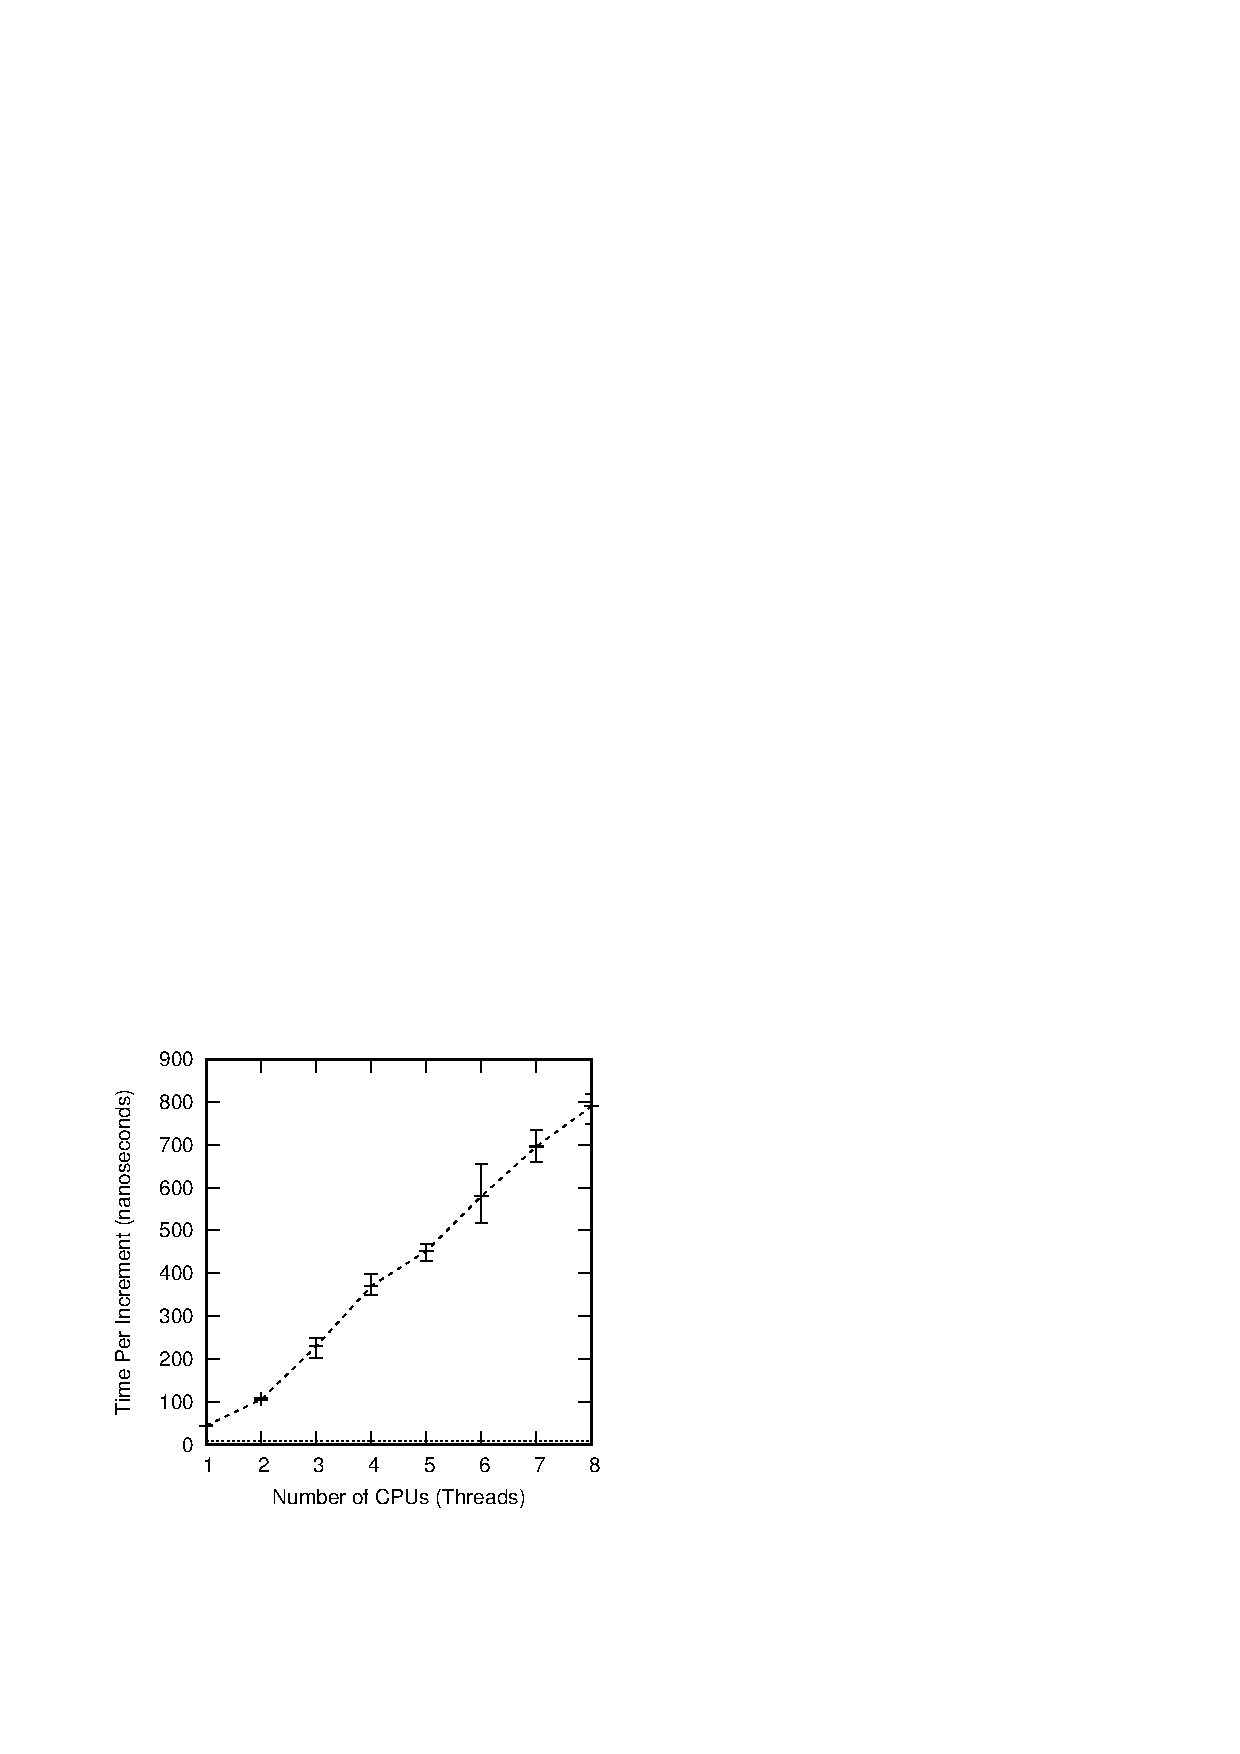
\includegraphics{CodeSamples/count/atomic}}
\end{center}
\caption{Atomic Increment Scalability on Nehalem}
\label{fig:count:Atomic Increment Scalability on Nehalem}
\end{figure}

정확하게 카운트를 하는 직관적 방법은
Figure~\ref{fig:count:Just Count Atomically!} (\url{count_atomic.c})
에 나온 것처럼 어토믹 오퍼레이션을 사용하는 것입니다.
라인~1 은 어토믹 변수를 정의하고, 라인~5 에서 어토믹하게 값을 증가시키고,
라인~10 에서 읽어냅니다.
이건 어토믹하기 때문에, 완벽한 카운트를 유지합니다.
하지만, 느립니다: 인텔 Core Duo 랩탑에서 이것은 어토믹하지 않은 방법에 비해
싱글쓰레드에서 여섯배, 그리고 두 쓰레드를 사용했을 때엔 \emph{열 배}
느립니다.\footnote{
	흥미롭게도, 어토믹하지 않게 카운터를 증가시키는 두개의 쓰레드는
	어토믹하게 카운터를 증가시키는 두개의 쓰레드보다 더 빨리 그 값을
	증가시킵니다.
	물론, 당신의 목표가 단순히 카운터를 더 빨리 증가시키는 거라면, 그냥
	카운터에 큰 값을 넣으면 되겠습니다.
	분명한건, 거대한 성능과 확장성을 위해선 정확성을 주의깊게 완화한
	알고리즘의 역할도 있을 수 있다는
	것입니다~\cite{Andrews91textbook,Arcangeli03,DavidUngar2011unsync}.}
\iffalse

The straightforward way to count accurately is to use atomic operations,
as shown in
Figure~\ref{fig:count:Just Count Atomically!} (\url{count_atomic.c}).
Line~1 defines an atomic variable, line~5 atomically increments it, and
line~10 reads it out.
Because this is atomic, it keeps perfect count.
However, it is slower: on a Intel Core Duo laptop, it is about
six times slower than non-atomic increment
when a single thread is incrementing, and more than \emph{ten times}
slower if two threads are incrementing.\footnote{
	Interestingly enough, a pair of threads non-atomically incrementing
	a counter will cause the counter to increase more quickly than
	a pair of threads atomically incrementing the counter.
	Of course, if your only goal is to make the counter increase
	quickly, an easier approach is to simply assign a large value
	to the counter.
	Nevertheless, there is likely to be a role for algorithms that
	use carefully relaxed notions of correctness in order to gain
	greater performance and
	scalability~\cite{Andrews91textbook,Arcangeli03,DavidUngar2011unsync}.}
\fi

Chapter~\ref{chp:Hardware and its Habits} 에서 이야기했던 걸 떠올려 보면
성능이 느린 것도,
Figure~\ref{fig:count:Atomic Increment Scalability on Nehalem} 에서 보여지듯
어토믹 증가 연산의 성능이 CPU 와 쓰레드의 숫자가 증가할수록 느려지는 것도
그다지 놀라운 일은 아닙니다.
이 그림에서, x~축에 붙어있는 수평의 점선은 완벽하게 확장하는 알고리즘에
의해서만 얻어질 수 있는 이상적인 성능입니다: 그런 알고리즘이라면, 카운트 증가는
싱글쓰레드에서와 동일한 오버헤드만을 일으킬 것입니다.
하나의 전역 변수에 대한 어토믹 증가 연산은 분명하게 비이상적이며, CPU 를
추가할수록 성능이 나빠집니다.
\iffalse

This poor performance should not be a surprise, given the discussion in
Chapter~\ref{chp:Hardware and its Habits},
nor should it be a surprise that the performance of atomic increment
gets slower as the number of CPUs and threads increase, as shown in
Figure~\ref{fig:count:Atomic Increment Scalability on Nehalem}.
In this figure, the horizontal dashed line resting on the x~axis
is the ideal performance that would be achieved
by a perfectly scalable algorithm: with such an algorithm, a given
increment would incur the same overhead that it would in a single-threaded
program.
Atomic increment of a single global variable is clearly
decidedly non-ideal, and gets worse as you add CPUs.
\fi

\QuickQuiz{}
	왜 x~축의 점선은 $x=1$ 에서 대각선의 선과 만나지 않죠?
	\iffalse

	Why doesn't the dashed line on the x~axis meet the 
	diagonal line at $x=1$?
	\fi
\QuickQuizAnswer{
	어토믹 오퍼레이션의 오버헤드 때문입니다.
	x~축의 점선은 싱글 \emph{어토믹하지 않은} 증가 연산의 오버헤드를
	나타냅니다.
	\emph{이상적인} 알고리즘은 선형적으로 확장될 뿐만 아니라,
	싱글 쓰레드 코드에 비해서도 성능 하락이 없어야 할 것입니다.

	이런 수준의 이상론은 좀 지나쳐 보일 수 있습니다, 다만 리누스 토발즈에게
	충분하다면, 당신에게도 충분할 겁니다.
	\iffalse

	Because of the overhead of the atomic operation.
	The dashed line on the x~axis represents the overhead of
	a single \emph{non-atomic} increment.
	After all, an \emph{ideal} algorithm would not only scale
	linearly, it would also incur no performance penalty compared
	to single-threaded code.

	This level of idealism may seem severe, but if it is good
	enough for Linus Torvalds, it is good enough for you.
	\fi
} \QuickQuizEnd

\QuickQuiz{}
	하지만 어토믹 증가 연산은 여전히 꽤 빠릅니다.
	그리고 빡빡한 루프에서 하나의 변수를 증가시키는 건 제겐 꽤 비현실적인
	것 같아 보이구요, 무엇보다, 프로그램의 실행은 실제로 일을 하는데
	쓰여야지, 자기가 한 일을 세는데 쓰여야 하는게 아니라구요!
	왜 제가 이걸 빠르게 하는걸 고민해야 하나요?
	\iffalse

	But atomic increment is still pretty fast.
	And incrementing a single variable in a tight loop sounds
	pretty unrealistic to me, after all, most of the program's
	execution should be devoted to actually doing work, not accounting
	for the work it has done!
	Why should I care about making this go faster?
	\fi
\QuickQuizAnswer{
	많은 경우에 어토믹 증가 연산은 분명히 당신에겐 충분히 빠를 겁니다.
	그런 경우에 당신은 당연히 어토믹 증가 연산을 사용해야죠.
	그렇지만, 더 나은 카운팅 알고리즘이 필요한 실제 상황도 상당히 많이
	존재합니다.
	그런 상황의 예는 고도로 최적화된 네트워킹 스택에서의 패킷과 용량
	카운팅으로, 이런 예에서는, 특히나 커다란 멀티프로세서에서는 대부분의
	실행시간을 이런류의 카운팅 작업에 보내게 됩니다.

	게다가, 이 챕터의 시작에서 이야기했듯, 카운팅은 공유 메모리 병렬
	프로그램에서 마주칠 수 있는 문제들을 보여줍니다.
	\iffalse

	In many cases, atomic increment will in fact be fast enough
	for you.
	In those cases, you should by all means use atomic increment.
	That said, there are many real-world situations where
	more elaborate counting algorithms are required.
	The canonical example of such a situation is counting packets
	and bytes in highly optimized networking stacks, where it is
	all too easy to find much of the execution time going into
	these sorts of accounting tasks, especially on large
	multiprocessors.

	In addition, as noted at the beginning of this chapter,
	counting provides an excellent view of the
	issues encountered in shared-memory parallel programs.
	\fi
} \QuickQuizEnd

\begin{figure}[tb]
\begin{center}
\resizebox{3in}{!}{\includegraphics{count/GlobalInc}}
\end{center}
\caption{Data Flow For Global Atomic Increment}
\label{fig:count:Data Flow For Global Atomic Increment}
\end{figure}

\begin{figure}[tb]
\begin{center}
\resizebox{3in}{!}{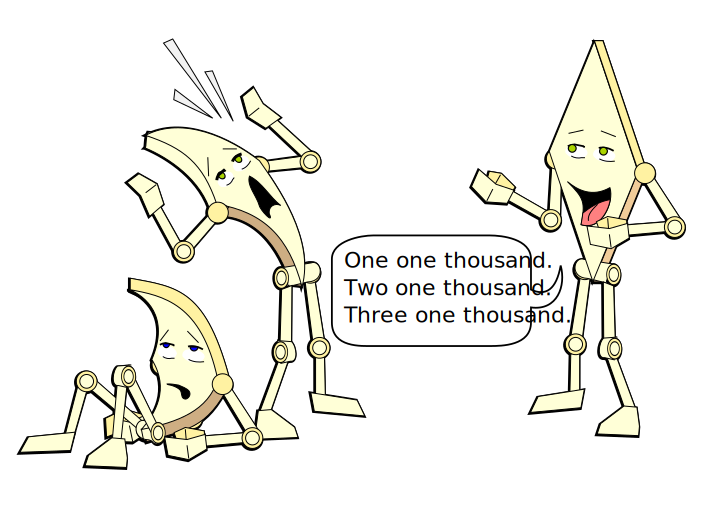
\includegraphics{cartoons/r-2014-One-one-thousand}}
\end{center}
\caption{Waiting to Count}
\ContributedBy{Figure}{fig:count:Waiting to Count}{Melissa Broussard}
\end{figure}

전역 어토믹 증가에 대한 다른 관점을 위해,
Figure~\ref{fig:count:Data Flow For Global Atomic Increment} 를 보세요.
각 CPU 가 주어진 전역 변수를 증가시킬 기회를 얻기 위해서, 해당 변수를 가지고
있는 캐시 라인은 빨간 화살표로 표시된 것처럼 모든 CPU 사이를 순환해야 합니다.
이런 순환은 상당한 시간을 요할 것이고, 이는
Figure~\ref{fig:count:Waiting to Count} 와 같은 상황을 초래해서
Figure~\ref{fig:count:Atomic Increment Scalability on Nehalem} 에서 보여진 낮은
성능을 야기할 것입니다.

다음 섹션들에서는 이런 순환에서 발생하는 지연들을 없앤 고성능 카운팅에 대해
알아봅니다.
\iffalse

For another perspective on global atomic increment, consider
Figure~\ref{fig:count:Data Flow For Global Atomic Increment}.
In order for each CPU to get a chance to increment a given
global variable, the cache line containing that variable must
circulate among all the CPUs, as shown by the red arrows.
Such circulation will take significant time, resulting in
the poor performance seen in
Figure~\ref{fig:count:Atomic Increment Scalability on Nehalem},
which might be thought of as shown in
Figure~\ref{fig:count:Waiting to Count}.

The following sections discuss high-performance counting, which
avoids the delays inherent in such circulation.
\fi

\QuickQuiz{}
	그런데 왜 CPU 설계자들은 단순히 데이터에의 증가 연산을 추가해서
	담고 있는 캐시 라인의 순회가 증가하는걸 막지 않는거죠?
	\iffalse

	But why can't CPU designers simply ship the addition operation to the
	data, avoiding the need to circulate the cache line containing
	the global variable being incremented?
	\fi
\QuickQuizAnswer{
	어떤 경우에는 그런 방법도 가능하겠죠.
	하지만, 그러려면 좀 복잡합니다:
	\iffalse

	It might well be possible to do this in some cases.
	However, there are a few complications:
	\fi
	\begin{enumerate}
	\item	만약 그 변수의 값이 필요하다면, 그 쓰레드는 해당 오퍼레이션이
		그 데이터로 향할 때까지 기다리고, 그러고나선 돌아오기까지
		기다려야 합니다.
	\item	그 어토믹 증가 오퍼레이션이 이전의, 그리고 이후의
		오퍼레이션들과 순서를 맞춰야 한다면, 해당 쓰레드는 오퍼레이션이
		데이터까지 가고, 돌아올 준비가 완료될 때까지 기다려야 합니다.
	\item	오퍼레이션들을 CPU들 사이에서 보내게 되면 시스템 접속부를
		지나야 하고, 이는 더 많은 다이 공간과 전력을 소모하게 될겁니다.
	\iffalse

	\item	If the value of the variable is required, then the
		thread will be forced to wait for the operation
		to be shipped to the data, and then for the result
		to be shipped back.
	\item	If the atomic increment must be ordered with respect
		to prior and/or subsequent operations, then the thread
		will be forced to wait for the operation to be shipped
		to the data, and for an indication that the operation
		completed to be shipped back.
	\item	Shipping operations among CPUs will likely require
		more lines in the system interconnect, which will consume
		more die area and more electrical power.
	\fi
	\end{enumerate}
	하지만 앞의 두가지 조건이 없다면?
	그럼 당신은 Section~\ref{sec:count:Statistical Counters} 에서 논의되는,
	실제 상품화된 하드웨어에서 이상적 상황에 근접하는 성능을 보이는
	알고리즘을 잘 고려해 봐야 할 겁니다.
	\iffalse

	But what if neither of the first two conditions holds?
	Then you should think carefully about the algorithms discussed
	in Section~\ref{sec:count:Statistical Counters}, which achieve
	near-ideal performance on commodity hardware.
	\fi

\begin{figure}[tb]
\begin{center}
\resizebox{3in}{!}{\includegraphics{count/GlobalTreeInc}}
\end{center}
\caption{Data Flow For Global Combining-Tree Atomic Increment}
\label{fig:count:Data Flow For Global Combining-Tree Atomic Increment}
\end{figure}

	앞의 두개 조건이 하나라도 걸려 있다면, 개선된 하드웨어에 \emph{약간}의
	희망이 있습니다.
	컴바이닝 트리(combining tree) 를 하드웨어에서 구현해서, 여러 CPU 에서의
	증가 요청이 하드웨어에 의해 결합되어 하나의 더하기 연산으로 변환되는
	방법을 생각해 볼 수 있을 것입니다.
	해당 하드웨어는 또한 요청들에 순서를 잡아줄 수도 있으므로, 각 CPU 에게
	각자의 어토믹 증가에 의한 값의 반환도 가능할 겁니다.
	Figure~\ref{fig:count:Data Flow For Global Combining-Tree Atomic Increment}
	에서 보여지듯, 이는 인스트럭션의 대기시간을 $O(log N)$ 로 만들어
	줍니다. 여기서 $N$ 은 CPU 의 갯수입니다.
	그리고 이런 하드웨어 최적화를 포함하는 CPU 는 2011년부터 나오기
	시작했습니다.

	Figure~\ref{fig:count:Data Flow For Global Atomic Increment} 에 보여진
	현재 하드웨어의  $O(N)$ 성능에 비하면 엄청난 향상이고, 하드웨어
	대기시간은 3차원 제조 공정이 현실화되면 더욱 낮아질 수 있을 것입니다.
	물론, 일부 중요한 특수 케이스에서는 소프트웨어가 \emph{훨씬} 나은 일을
	할 수 있을 것입니다.
	\iffalse

	If either or both of the first two conditions hold, there is
	\emph{some} hope for improved hardware.
	One could imagine the hardware implementing a combining tree,
	so that the increment requests from multiple CPUs are combined
	by the hardware into a single addition when the combined request
	reaches the hardware.
	The hardware could also apply an order to the requests, thus
	returning to each CPU the return value corresponding to its
	particular atomic increment.
	This results in instruction latency that varies as $O(log N)$,
	where $N$ is the number of CPUs, as shown in
	Figure~\ref{fig:count:Data Flow For Global Combining-Tree Atomic Increment}.
	And CPUs with this sort of hardware optimization are starting to
	appear as of 2011.

	This is a great improvement over the $O(N)$ performance
	of current hardware shown in
	Figure~\ref{fig:count:Data Flow For Global Atomic Increment},
	and it is possible that hardware latencies might decrease
	further if innovations such as three-dimensional fabrication prove
	practical.
	Nevertheless, we will see that in some important special cases,
	software can do \emph{much} better.
	\fi
} \QuickQuizEnd

\section{Statistical Counters}
\label{sec:count:Statistical Counters}

이 섹션은 카운트는 매우 가끔만 업데이트 되고 그 값은 웬만해서는 읽혀지지 않는,
통계적 카운터의 흔한 특수 케이스들을 다룹니다.
이것들은 {\QQstatcnt} 에서 이야기한 네트워크 패킷 카운팅 문제를 푸는데 사용될
수 있을 것입니다.

\subsection{Design}

통계적 카운팅은 보통 쓰레드별로 (또는, 커널에서라면 CPU별로) 카운터를 제공해서
각 쓰레드가 자신의 카운터를 업데이트 하도록 합니다.
이 카운터들의 전체 통합 값은 더하기의 상호성과 결합성에 기반해, 단순히 모든
쓰레드의 카운터의 값을 더하는 것으로 구해질 수 있습니다.
이건 Section~\ref{sec:SMPdesign:Data Ownership} 에서 소개되는 데이터 소유권
패턴의 한 예입니다.
\iffalse

Statistical counting is typically handled by providing a counter per
thread (or CPU, when running in the kernel), so that each thread
updates its own counter.
The aggregate value of the counters is read out by simply summing up
all of the threads' counters,
relying on the commutative and associative properties of addition.
This is an example of the Data Ownership pattern that will be introduced in
Section~\ref{sec:SMPdesign:Data Ownership}.
\fi

\QuickQuiz{}
	하지만 C 의 ``정수들'' 은 크기와 관련한 복잡한 문제들이 있지 않나요?
	\iffalse

	But doesn't the fact that C's ``integers'' are limited in size
	complicate things?
	\fi
\QuickQuizAnswer{
	아닙니다, 모듈로 더하기도 역시 상호성과 결합성을 가지니까요.
	적어도 부호 없는 정수형을 사용한다면 말입니다.
	오버플로우가 났을 때 넘쳐난 값을 감추는 것 외에 별다른 일을 하는
	기계들은 요즘 거의 없지만, C 표준에 의하면 부호를 갖는 정수형의
	오버플로우는 예상외 동작을 유발할 수 있으므로, 요즘 기계들은 대부분
	안전하다는 사실은 신경쓰지 마십시오.
	불행히도, 컴파일러들은 종종 부호 있는 정수형들은 오버플로우 나지 않을
	것이라는 가정 하에 최적화를 하기 때문에, 당신의 코드가 부호 있는
	정수형을 오버플로우 나게 한다면, 2의 보수를 사용하는 하드웨어를
	사용하고 있다 해도 문제에 직면할 수 있습니다.

	그렇다곤 해도, 32-비트 쓰레드별 카운터에서 (대략) 64-비트 합을
	모으는데에도 추가적인 복잡한 일이 숨어있습니다.
	이걸 처리하는 것은 독자 여러분들에게 연습문제로 남겨두겠습니다만, 이
	챕터의 뒤에 소개될 기법들이 큰 도움이 될 수도 있습니다.
	\iffalse

	No, because modulo addition is still commutative and associative.
	At least as long as you use unsigned integers.
	Recall that in the C standard, overflow of signed integers results
	in undefined behavior, never mind the fact that machines that
	do anything other than wrap on overflow are quite rare these days.
	Unfortunately, compilers frequently carry out optimizations that
	assume that signed integers will not overflow, so if your code
	allows signed integers to overflow, you can run into trouble
	even on twos-complement hardware.

	That said, one potential source of additional complexity arises
	when attempting to gather (say) a 64-bit sum from 32-bit
	per-thread counters.
	Dealing with this added complexity is left as
	an exercise for the reader, for whom some of the techniques
	introduced later in this chapter could be quite helpful.
	\fi
} \QuickQuizEnd

\subsection{Array-Based Implementation}
\label{sec:count:Array-Based Implementation}

쓰레드별 변수를 제공하는 방법 중 하나는 쓰레드별로 (아마도 false sharing 을
막기 위해 캐시 얼라인 되어있고 패딩 되어있는)원소 하나를 갖는 배열을 만드는
겁니다.
\iffalse

One way to provide per-thread variables is to allocate an array with
one element per
thread (presumably cache aligned and padded to avoid false sharing).
\fi

\QuickQuiz{}
	배열이요???
	하지만 그럼 쓰레드의 갯수가 제한되지 않나요?
	\iffalse

	An array???
	But doesn't that limit the number of threads?
	\fi
\QuickQuizAnswer{
	그럴 수 있고, 이 간단한 구현에서는 그렇습니다.
	하지만 임의의 갯수의 쓰레드를 지원하는 구현을 만드는 건 그렇게 어렵지
	않은데요, 예를 들면,
	Section~\ref{sec:count:Per-Thread-Variable-Based Implementation}
	\co{gcc} \co{__thread} 를 사용하는 거죠.
	\iffalse

	It can, and in this toy implementation, it does.
	But it is not that hard to come up with an alternative
	implementation that permits an arbitrary number of threads,
	for example, using the \co{gcc} \co{__thread} facility,
	as shown in
	Section~\ref{sec:count:Per-Thread-Variable-Based Implementation}.
	\fi
} \QuickQuizEnd

\begin{figure}[tbp]
{ \scriptsize
\begin{verbatim}
  1 DEFINE_PER_THREAD(long, counter);
  2 
  3 void inc_count(void)
  4 {
  5   __get_thread_var(counter)++;
  6 }
  7 
  8 long read_count(void)
  9 {
 10   int t;
 11   long sum = 0;
 12 
 13   for_each_thread(t)
 14     sum += per_thread(counter, t);
 15   return sum;
 16 }
\end{verbatim}
}
\caption{Array-Based Per-Thread Statistical Counters}
\label{fig:count:Array-Based Per-Thread Statistical Counters}
\end{figure}

그런 배열은
Figure~\ref{fig:count:Array-Based Per-Thread Statistical Counters}
(\url{count_stat.c}) 에 보여진 것처럼 per-thread 기능을 사용할 수도 있습니다.
라인~1 은 \co{long} 타입의 쓰레드별 카운터들을 담는, \co{counter} 라는 이름의
배열을 만듭니다.

라인~3-6 은 이 카운터를 증가시키는 함수로, \co{__get_thread_var()} 함수로 현재
수행중인 쓰레드의 원소를 \co{counter} 배열에서 얻어옵니다.
이 원소는 연관된 쓰레드에 의해서만 수정되므로, 어토믹하지 않은 방식으로도
충분합니다.

라인~8-16 은 카운터의 총계 값을 얻어오는 함수로, \co{for_each_thread()} 를
이용해 현재 돌고 있는 쓰레드들의 리스트를 순회하면서 \co{per_thread()} 를
이용해 특정 쓰레드의 카운터 값을 얻어옵니다.
하드웨어는 제대로 정렬되어 있는 \co{long} 변수는 어토믹하게 읽고 쓸 수 있기
때문에, 그리고 gcc 는 이 기능을 잘 사용해주기 때문에, 평범한 읽기로 충분하고,
별다른 어토믹 오퍼레이션은 필요치 않습니다.
\iffalse

Such an array can be wrapped into per-thread primitives, as shown in
Figure~\ref{fig:count:Array-Based Per-Thread Statistical Counters}
(\url{count_stat.c}).
Line~1 defines an array containing a set of per-thread counters of
type \co{long} named, creatively enough, \co{counter}.

Lines~3-6 show a function that increments the counters, using the
\co{__get_thread_var()} primitive to locate the currently running
thread's element of the \co{counter} array.
Because this element is modified only by the corresponding thread,
non-atomic increment suffices.

Lines~8-16 show a function that reads out the aggregate value of the counter,
using the \co{for_each_thread()} primitive to iterate over the list of
currently running threads, and using the \co{per_thread()} primitive
to fetch the specified thread's counter.
Because the hardware can fetch and store a properly aligned \co{long}
atomically, and because gcc is kind enough to make use of this capability,
normal loads suffice, and no special atomic instructions are required.
\fi

\QuickQuiz{}
	근데, 그 외에 gcc 가 어떤 짓을 할 수 있죠???
	\iffalse

	What other choice does gcc have, anyway???
	\fi
\QuickQuizAnswer{
	C 표준대로라면, 다른 쓰레드에 의해 동시에 수정되고 있을 수 있는 변수를
	읽어들이는 행동의 효과에 대해선 정의되어 있지 않습니다.
	C 는 어토믹하게 \co{long} 타입 변수를 읽어들일 수가 없는 (예를
	들면)8-비트 아키텍쳐를 지원해야만 했기에 C 표준은 다른 선택의 여지가
	없었습니다.
	다음 버전의 C 표준에서는 이 현실과의 격차를 해결해 보려 합니다만, 그
	전까지는 gcc 개발자들의 친절함에 의존해야 합니다.

	대신, 하드웨어가 한번의 메모리 참조 명령으로 필요한 값을 읽을 수 있는
	경우라면, \co{ACCESS_ONCE()}~\cite{JonCorbet2012ACCESS:ONCE} 같은
	volatile 접근법을 사용해서 컴파일러에 제약을 가할 수 있습니다.
	\iffalse

	According to the C standard, the effects of fetching a variable
	that might be concurrently modified by some other thread are
	undefined.
	It turns out that the C standard really has no other choice,
	given that C must support (for example) eight-bit architectures
	which are incapable of atomically loading a \co{long}.
	An upcoming version of the C standard aims to fill this gap,
	but until then, we depend on the kindness of the gcc developers.

	Alternatively, use of volatile accesses such as those provided
	by \co{ACCESS_ONCE()}~\cite{JonCorbet2012ACCESS:ONCE}
	can help constrain the compiler, at least
	in cases where the hardware is capable of accessing the value
	with a single memory-reference instruction.
	\fi
} \QuickQuizEnd

\QuickQuiz{}
	Figure~\ref{fig:count:Array-Based Per-Thread Statistical Counters} 의
	쓰레드별 \co{counter} 변수는 어떻게 초기화 되나요?
	\iffalse

	How does the per-thread \co{counter} variable in
	Figure~\ref{fig:count:Array-Based Per-Thread Statistical Counters}
	get initialized?
	\fi
\QuickQuizAnswer{
	C 표준은 전역 변수의 초기값은 명시적으로 초기화되지 않는 이상 0이라고
	명시합니다.
	그리고, 사용자가 통계적 카운터들의 연속되는 값 사이의 차이에
	관심있는게 아니라면, 초기값은 의미가 없습니다.
	\iffalse

	The C standard specifies that the initial value of
	global variables is zero, unless they are explicitly initialized.
	So the initial value of all the instances of \co{counter}
	will be zero.
	Furthermore, in the common case where the user is interested only
	in differences between consecutive reads
	from statistical counters, the initial value is irrelevant.
	\fi
} \QuickQuizEnd

\QuickQuiz{}
	Figure~\ref{fig:count:Array-Based Per-Thread Statistical Counters}
	의 코드가 어떻게 복수의 카운터를 가능하게 할 수 있죠?
	\iffalse

	How is the code in
	Figure~\ref{fig:count:Array-Based Per-Thread Statistical Counters}
	supposed to permit more than one counter?
	\fi
\QuickQuizAnswer{
	실제로, 이 예제는 한개 이상의 카운터는 지원하지 않습니다.
	이 예제를 수정해서 복수의 카운터를 제공하게 하는건 독자 여러분에게
	과제로 남겨 두겠습니다.
	\iffalse

	Indeed, this toy example does not support more than one counter.
	Modifying it so that it can provide multiple counters is left
	as an exercise to the reader.
	\fi
} \QuickQuizEnd

\begin{figure}[tb]
\begin{center}
\resizebox{3in}{!}{\includegraphics{count/PerThreadInc}}
\end{center}
\caption{Data Flow For Per-Thread Increment}
\label{fig:count:Data Flow For Per-Thread Increment}
\end{figure}

이 방법은 \co{inc_count()} 를 호출하는 업데이터 쓰레드의 수가 늘어나더라도
선형적으로 성능이 확장됩니다.
Figure~\ref{fig:count:Data Flow For Per-Thread Increment} 에 각 CPU 의 초록색
화살표로 보여지듯, 각 CPU 는 자신의 쓰레드의 변수를 시스템을 통과하는 비싼 통신
없이 빠르게 증가시킬 수 있기 때문입니다.
이와 같이, 이 섹션은 이 챕터의 시작에서 소개된 네트워크 패킷 카운팅 문제를
해결합니다.
\iffalse

This approach scales linearly with increasing number of updater threads
invoking \co{inc_count()}.
As is shown by the green arrows on each CPU in
Figure~\ref{fig:count:Data Flow For Per-Thread Increment},
the reason for this is that each CPU can make rapid progress incrementing
its thread's variable, without any expensive cross-system communication.
As such, this section solves the network-packet counting problem presented
at the beginning of this chapter.
\fi

\QuickQuiz{}
	읽기 오퍼레이션은 쓰레드별 값을 모두 더하는 시간을 가져야 할 것이고,
	그동안도 카운터는 값이 변할 수 있어요.
	그럼 Figure~\ref{fig:count:Array-Based Per-Thread Statistical Counters}
	의  \co{read_count()} 는 정확하지 않다는 의미입니다.
	이 카운터는 단위시간당 $r$ 만큼 카운터 값을 증가하고 \co{read_count()}
	는 $\Delta$ 단위시간을 소모한다고 해봅시다.
	리턴되는 값의 예상 오류값은 얼마입니까?
	\iffalse

	The read operation takes time to sum up the per-thread values,
	and during that time, the counter could well be changing.
	This means that the value returned by
	\co{read_count()} in
	Figure~\ref{fig:count:Array-Based Per-Thread Statistical Counters}
	will not necessarily be exact.
	Assume that the counter is being incremented at rate
	$r$ counts per unit time, and that \co{read_count()}'s
	execution consumes $\Delta$ units of time.
	What is the expected error in the return value?
	\fi
\QuickQuizAnswer{
	최악의 경우에 대한 분석부터 해보고, 좀 나은 경우들을 보죠.

	최악의 경우는, 읽기 오퍼레이션이 실제 동작은 금방 끝냈지만 리턴하기
	전에 $\Delta$ 단위시간동안 대기를 하는 경우로, 이 경우의 오류값은
	간단히 $r \Delta$ 입니다.
	\iffalse

	Let's do worst-case analysis first, followed by a less
	conservative analysis.

	In the worst case, the read operation completes immediately,
	but is then delayed for $\Delta$ time units before returning,
	in which case the worst-case error is simply $r \Delta$.
	\fi

	이 최악의 경우 동작은 별로 현실성이 없으니 각 $N$ 카운터들에 대한 각
	읽기 동작이 시간 간격 $\Delta$ 안에 동일한 간격으로 일어나는 경우를
	생각해보죠.
	$N$ 회의 읽기 사이에 $\frac{\Delta}{N+1}$ 길이의 $N+1$ 개 간격이 존재할
	겁니다.
	마지막 쓰레드의 카운터에서의 읽기 이후로의 지연으로 발생하는 에러치는
	$\frac{r \Delta}{N \left( N + 1 \right)}$ 이므로, 두번째에서 마지막
	쓰레드 사이의 카운터는
	$\frac{2 r \Delta}{N \left( N + 1 \right)}$,
	세번째에서 마지막 사이는
	$\frac{3 r \Delta}{N \left( N + 1 \right)}$,
	그리고 그렇게 계속 진행됩니다.
	전체 오류값은 각 쓰레드의 카운터에서의 읽기로 발생한 에러의 총 합으로
	주어지는데, 다음과 같습니다:

	\begin{equation}
		\frac{r \Delta}{N \left( N + 1 \right)}
			\sum_{i = 1}^N i
	\end{equation}
	\iffalse
	This worst-case behavior is rather unlikely, so let us instead
	consider the case where the reads from each of the $N$
	counters is spaced equally over the time period $\Delta$.
	There will be $N+1$ intervals of duration $\frac{\Delta}{N+1}$
	between the $N$ reads.
	The error due to the delay after the read from the last thread's
	counter will be given by $\frac{r \Delta}{N \left( N + 1 \right)}$,
	the second-to-last thread's counter by
	$\frac{2 r \Delta}{N \left( N + 1 \right)}$,
	the third-to-last by
	$\frac{3 r \Delta}{N \left( N + 1 \right)}$,
	and so on.
	The total error is given by the sum of the errors due to the
	reads from each thread's counter, which is:

	\begin{equation}
		\frac{r \Delta}{N \left( N + 1 \right)}
			\sum_{i = 1}^N i
	\end{equation}
	\fi

	합 부분은 다음과 같이 표현 가능하구요:

	\begin{equation}
		\frac{r \Delta}{N \left( N + 1 \right)}
			\frac{N \left( N + 1 \right)}{2}
	\end{equation}

	불필요한 부분을 제거하면 다음과 같이 직관적인 결과가 나옵니다:

	\begin{equation}
		\frac{r \Delta}{2}
	\label{eq:count:CounterErrorAverage}
	\end{equation}
	\iffalse

	Expressing the summation in closed form yields:

	\begin{equation}
		\frac{r \Delta}{N \left( N + 1 \right)}
			\frac{N \left( N + 1 \right)}{2}
	\end{equation}

	Cancelling yields the intuitively expected result:

	\begin{equation}
		\frac{r \Delta}{2}
	\label{eq:count:CounterErrorAverage}
	\end{equation}
	\fi

	읽기 오퍼레이션 호출자가 해당 오퍼레이션으로 리턴받은 수를 가지고 어떤
	일을 하는 코드를 수행하는 중에도 오류는 쌓여감을 기억해둘 필요가
	있습니다.
	예를 들어, 읽기 오퍼레이션 호출자가 리턴받은 값을 가지고 어떤 계산을
	하는데 $t$ 시간을 사용한다면, 최악의 경우 오류치는 $r \left(\Delta +
	t\right)$ 로 늘어날 겁니다.

	예상 오류치도 비슷하게 늘어나겠죠:

	\begin{equation}
		r \left( \frac{\Delta}{2} + t \right)
	\end{equation}
	\iffalse

	It is important to remember that error continues accumulating
	as the caller executes code making use of the count returned
	by the read operation.
	For example, if the caller spends time $t$ executing some
	computation based on the result of the returned count, the
	worst-case error will have increased to $r \left(\Delta + t\right)$.

	The expected error will have similarly increased to:

	\begin{equation}
		r \left( \frac{\Delta}{2} + t \right)
	\end{equation}
	\fi

	물론, 읽기 중에 카운터가 계속 증가하는건 용납될 수 없는 경우도
	있겠습니다.
	Section~\ref{sec:count:Applying Specialized Parallel Counters}
	에서는 이런 상황을 해결하는 방법을 알아봅니다.

	이렇게, 우리는 감소는 없고 증가만 이루어지는 카운터를 알아보았습니다.
	만약 카운터 값이 단위시간당 $r$ 만큼 감소로든 증가로든 바뀐다면,
	오류값은 줄어들 거라고 예상할 수 있을 겁니다.
	하지만, 카운터가 어느 쪽으로든 움직일 수 \emph{있을지 몰라도} 최악의
	경우는 해당 읽기 오퍼레이션이 금방 끝났지만 $\Delta$ 단위 시간동안
	기다려야 하는데, 그 시간 동안 카운터의 값은 같은 방향으로만 이동하는
	경우이므로 여전히 $r \Delta$ 오류값을 내므로 차이가 없습니다.
	\iffalse

	Of course, it is sometimes unacceptable for the counter to
	continue incrementing during the read operation.
	Section~\ref{sec:count:Applying Specialized Parallel Counters}
	discusses a way to handle this situation.

	Thus far, we have been considering a counter that is only
	increased, never decreased.
	If the counter value is being changed by $r$ counts per unit
	time, but in either direction, we should expect the error
	to reduce.
	However, the worst case is unchanged because although the
	counter \emph{could} move in either direction, the worst
	case is whenthe read operation completes immediately,
	but then is delayed for $\Delta$ time units, during which
	time all the changes in the counter's value move it in
	the same direction, again giving us an absolute error
	of $r \Delta$.
	\fi

	평균 에러치를 계산하는데는 값의 증감 패턴에 대한 다양한 가정을 바탕으로
	하는 여러가지 방법이 있습니다.
	일단은 간단하게, 1 의 오퍼레이션 중 $f$ 만큼이 감소 오퍼레이션이고,
	관심있는 오류값은 카운터의 장시간 추세선에서의 굴곡이라고 가정해
	봅시다.
	이 가정 하에서는 $f$ 가 0.5 이하라면, 각 감소는 증가에 의해 무효화
	되고, 따라서 $2f$ 오퍼레이션은 서로를 무효화 시키고, $1-2f$ 의
	오퍼레이션들은 무효화 되지 않은 증가가 됩니다.
	반면, $f$ 가 0.5 보다 크다면, $1-f$ 의 감소는 증가에 의해 무효화 되고,
	카운터는 음의 방향으로 $-1+2\left(1-f\right)$ 만큼 이동하는데, 이는
	$1-2f$ 로 정리되고, 따라서 카운터는 평균적으로 오퍼레이션당 $1-2f$
	만큼씩 어느 경우든 이동하게 됩니다.
	따라서, 긴 시점에서의 카운터의 변화는 $\left( 1-2f \right) r$ 로
	주어집니다.
	이걸 Equation~\ref{eq:count:CounterErrorAverage} 에 대입하면:

	\begin{equation}
		\frac{\left( 1 - 2 f \right) r \Delta}{2}
	\end{equation}
	\iffalse

	There are a number of ways to compute the average error,
	based on a variety of assumptions about the patterns of
	increments and decrements.
	For simplicity, let's assume that the $f$ fraction of
	the operations are decrements, and that the error of interest
	is the deviation from the counter's long-term trend line.
	Under this assumption, if $f$ is less than or equal to 0.5,
	each decrement will be cancelled by an increment, so that
	$2f$ of the operations will cancel each other, leaving
	$1-2f$ of the operations being uncancelled increments.
	On the other hand, if $f$ is greater than 0.5, $1-f$ of
	the decrements are cancelled by increments, so that the
	counter moves in the negative direction by $-1+2\left(1-f\right)$,
	which simplifies to $1-2f$, so that the counter moves an average
	of $1-2f$ per operation in either case.
	Therefore, that the long-term
	movement of the counter is given by $\left( 1-2f \right) r$.
	Plugging this into
	Equation~\ref{eq:count:CounterErrorAverage} yields:

	\begin{equation}
		\frac{\left( 1 - 2 f \right) r \Delta}{2}
	\end{equation}
	\fi

	그렇지만, 대부분의 통계적 카운터 사용에서 \co{read_count()} 에 의해
	리턴되는 값의 오류치는 별 의미가 없습니다.
	\co{read_count()} 가 수행하는데 필요한 시간은 일반적으로
	\co{read_count()} 호출 사이의 시간에 비하면 극단적으로 작기 때문입니다.
	\iffalse

	All that aside, in most uses of statistical counters, the
	error in the value returned by \co{read_count()} is
	irrelevant.
	This irrelevance is due to the fact that the time required
	for \co{read_count()} to execute is normally extremely
	small compared to the time interval between successive
	calls to \co{read_count()}.
	\fi
} \QuickQuizEnd

하지만, 이 업데이트 쪽 확장성은 쓰레드의 수가 늘어날 경우 읽기 쪽에 큰 부담으로
다가옵니다.
다음 섹션에서는, 업데이트 쪽 확장성을 유지하면서 읽기 쪽 부담을 줄이는 방법을
알아봅니다.
\iffalse

However, this excellent update-side scalability comes at great read-side
expense for large numbers of threads.
The next section shows one way to reduce read-side expense while
still retaining the update-side scalability.
\fi

\subsection{Eventually Consistent Implementation}
\label{sec:count:Eventually Consistent Implementation}

읽기 쪽 성능을 엄청나게 개선하면서 업데이트 쪽 확장성도 지키는 한가지 방법은
일관성에 대한 요구사항을 약화시키는 것입니다.
앞 섹션의 카운팅 알고리즘은 이상적인 카운터가 \co{read_count()} 실행 직전과
직후에 내놓을 값들 사이의 값을 내놓는 것을 보장했습니다.
\emph{최종적 일관성(Eventual
consistency}~\cite{WernerVogels:2009:EventuallyConsistent} 는 더 약한
보장사항을 제공합니다: \co{inc_count()} 호출이 없을 때라는 조건 하에,
\co{read_count()} 는 최종적으로는 정확한 값을 리턴할 것입니다.
\iffalse

One way to retain update-side scalability while greatly improving
read-side performance is to weaken consistency requirements.
The counting algorithm in the previous section is guaranteed to
return a value between the value that an ideal counter would have
taken on near the beginning of \co{read_count()}'s execution and
that near the end of \co{read_count()}'s execution.
\emph{Eventual consistency}~\cite{WernerVogels:2009:EventuallyConsistent}
provides a weaker
guarantee: in absence of calls to \co{inc_count()}, calls to
\co{read_count()} will eventually return an accurate count.
\fi

우리는 글로벌 카운터를 사용해 최종적 일관성을 제공할 것입니다.
하지만, 업데이트는 쓰레드별 카운터만을 사용합니다.
별도의 쓰레드가 존재하며 이 쓰레드가 업데이트 쓰레드들의 쓰레드별 카운터의 값을
세어 글로벌 카운터의 값을 만들어냅니다.
읽기는 단순히 글로벌 카운터의 값을 읽습니다.
업데이트가 수행 중이라면, 읽기 쓰레드가 읽어낸 값은 과거의 값을 것입니다만,
일단 업데이트가 중단되면 글로벌 카운터는 최종적으로 진짜 값을 가질
겁니다---그래서 이 방법이 최종적 일관성에 분류되는 겁니다.
\iffalse

We exploit eventual consistency by maintaining a global counter.
However, updaters only manipulate their per-thread counters.
A separate thread is provided to transfer counts from the per-thread
counters to the global counter.
Readers simply access the value of the global counter.
If updaters are active, the value used by the readers will be out of
date, however, once updates cease, the global counter will eventually
converge on the true value---hence this approach qualifies as
eventually consistent.
\fi

\begin{figure}[tbp]
{ \scriptsize
\begin{verbatim}
  1 DEFINE_PER_THREAD(unsigned long, counter);
  2 unsigned long global_count;
  3 int stopflag;
  4 
  5 void inc_count(void)
  6 {
  7   ACCESS_ONCE(__get_thread_var(counter))++;
  8 }
  9 
 10 unsigned long read_count(void)
 11 {
 12   return ACCESS_ONCE(global_count);
 13 }
 14 
 15 void *eventual(void *arg)
 16 {
 17   int t;
 18   int sum;
 19 
 20   while (stopflag < 3) {
 21     sum = 0;
 22     for_each_thread(t)
 23       sum += ACCESS_ONCE(per_thread(counter, t));
 24     ACCESS_ONCE(global_count) = sum;
 25     poll(NULL, 0, 1);
 26     if (stopflag) {
 27       smp_mb();
 28       stopflag++;
 29     }
 30   }
 31   return NULL;
 32 }
 33 
 34 void count_init(void)
 35 {
 36   thread_id_t tid;
 37 
 38   if (pthread_create(&tid, NULL, eventual, NULL)) {
 39     perror("count_init:pthread_create");
 40     exit(-1);
 41   }
 42 }
 43 
 44 void count_cleanup(void)
 45 {
 46   stopflag = 1;
 47   while (stopflag < 3)
 48     poll(NULL, 0, 1);
 49   smp_mb();
 50 }
\end{verbatim}
}
\caption{Array-Based Per-Thread Eventually Consistent Counters}
\label{fig:count:Array-Based Per-Thread Eventually Consistent Counters}
\end{figure}

Figure~\ref{fig:count:Array-Based Per-Thread Eventually Consistent Counters}
(\url{count_stat_eventual.c}) 에 그 구현이 있습니다.
라인~1-2 는 카운터의 값을 갖는 쓰레드별 변수와 글로벌 변수를 보여주며, 세번째
라인은 프로그램을 정확한 카운터 값과 함께 종료하고자 할 경우를 위해 종료 조건을
알리는 \co{stopflag} 를 보입니다.
라인~5-8 의 \co{inc_count()} 함수는 Figure~\ref{fig:count:Array-Based
Per-Thread Statistical Counters} 것과 비슷합니다.
라인~10-13 의 \co{read_count()} 함수는 단순히 \co{global_count} 변수의 값을
리턴합니다.
\iffalse

The implementation is shown in
Figure~\ref{fig:count:Array-Based Per-Thread Eventually Consistent Counters}
(\url{count_stat_eventual.c}).
Lines~1-2 show the per-thread variable and the global variable that
track the counter's value, and line three shows \co{stopflag}
which is used to coordinate termination (for the case where we want
to terminate the program with an accurate counter value).
The \co{inc_count()} function shown on lines~5-8 is similar to its
counterpart in
Figure~\ref{fig:count:Array-Based Per-Thread Statistical Counters}.
The \co{read_count()} function shown on lines~10-13 simply returns the
value of the \co{global_count} variable.
\fi

하지만, 라인~34-42 의 \co{count_init()} 함수는 라인~15-32 의 \co{eventual()}
쓰레드를 생성하는데, 이 쓰레드는 모든 쓰레드를 순회하며 쓰레드별 로컬
\co{counter} 를 더해서 \co{global_count} 변수에 저장하는 일을 반복합니다.
\co{eventual()} 쓰레드는 일의 반복 사이에 적당히 선택된 1 밀리세컨드 동안
기다립니다.
라인~44-50 의 \co{count_cleanup()} 함수는 프로그램 종료를 관장합니다.

이 방법은 여전히 선형적인 카운터 업데이트 성능을 유지하면서 극단적으로 빠른
카운터 읽기 속도를 보입니다.
하지만, 이 훌륭한 읽기 성능과 업데이트 성능 확장성은 \co{eventual()} 이라는
추가된 쓰레드의 수행이라는 비용을 가집니다.
\iffalse

However, the \co{count_init()} function on lines~34-42
creates the \co{eventual()} thread shown on lines~15-32, which
cycles through all the threads,
summing the per-thread local \co{counter} and storing the
sum to the \co{global_count} variable.
The \co{eventual()} thread waits an arbitrarily chosen one millisecond
between passes.
The \co{count_cleanup()} function on lines~44-50 coordinates termination.

This approach gives extremely fast counter read-out while still
supporting linear counter-update performance.
However, this excellent read-side performance and update-side scalability
comes at the cost of the additional thread running \co{eventual()}.
\fi

\QuickQuiz{}
	Figure~\ref{fig:count:Array-Based Per-Thread Eventually Consistent
	Counters} 의 \co{inc_count()} 는 왜 어토믹 명령을 사용하지 않죠?
	쓰레드별 카운터를 여러 쓰레드에서 접근하고 있잖아요!
	\iffalse

	Why doesn't \co{inc_count()} in
	Figure~\ref{fig:count:Array-Based Per-Thread Eventually Consistent Counters}
	need to use atomic instructions?
	After all, we now have multiple threads accessing the per-thread
	counters!
	\fi
\QuickQuizAnswer{
	두 쓰레드 중 하나는 읽기만 하고 있고, 변수는 정렬되어 있으며 기계가
	지원하는 워드 크기이기에, 어토믹하지 않은 명령들만으로도
	충분합니다.
	다만, \co{ACCESS_ONCE()} 매크로는 카운터 업데이트가 \co{eventual()}
	에게 보여지는 것을 막을 수도 있는~\cite{JonCorbet2012ACCESS:ONCE}
	컴파일러 최적화를 막기 위해 사용되었습니다.
	\iffalse

	Because one of the two threads only reads, and because the
	variable is aligned and machine-sized, non-atomic instructions
	suffice.
	That said, the \co{ACCESS_ONCE()} macro is used to prevent
	compiler optimizations that might otherwise prevent the
	counter updates from becoming visible to
	\co{eventual()}~\cite{JonCorbet2012ACCESS:ONCE}.
	\fi

	이 알고리즘의 예전 버전은 어토믹 명령을 사용했습니다만, 감사하게도
	Ersoy Bayramoglu 가 그것들이 필요 없다는 것을 지적해 줬습니다.
	그렇다곤 하나, 쓰레드별 \co{counter} 변수가 \co{global_counter} 보다
	작았다면 어토믹 명령이 필요했을 겁니다.
	하지만, 32-bit 시스템에서 쓰레드별 \co{counter} 변수는 정확하게 합을
	구하기 위해 32 비트로 제한되어야 하고 오버플로를 막기 위해
	\co{global_count} 변수는 64-bit 이 되어야 할겁니다.
	이 경우엔, 오버플로를 막기 위해 쓰레드별 \co{counter} 변수를 주기적으로
	0으로 초기화 시켜줘야 할 겁니다.
	0으로의 주기적 초기화는 너무 오래 지연되면 쓰레드별 변수의 오버플로가
	가능하단 것을 반드시 기억해 둬야만 합니다.
	따라서 이 방법은 프로그램이 돌아가는 시스템이 리얼-타임 속성을 가지고
	있어야 하며, 매우 조심스럽게 사용되어야 함을 의미합니다.

	대조적으로, 모든 변수가 같은 크기이면 어떤 변수에 오버플로가 나더라도
	최종적 합은 워드 크기로 절삭될테니 별 문제 없습니다.
	\iffalse

	An older version of this algorithm did in fact use atomic
	instructions, kudos to Ersoy Bayramoglu for pointing out that
	they are in fact unnecessary.
	That said, atomic instructions would be needed in cases where
	the per-thread \co{counter} variables were smaller than the
	global \co{global_count}.
	However, note that on a 32-bit system,
	the per-thread \co{counter} variables
	might need to be limited to 32 bits in order to sum them accurately,
	but with a 64-bit \co{global_count} variable to avoid overflow.
	In this case, it is necessary to zero the per-thead
	\co{counter} variables periodically in order to avoid overflow.
	It is extremely important to note that this zeroing cannot
	be delayed too long or overflow of the smaller per-thread
	variables will result.
	This approach therefore imposes real-time requirements on the
	underlying system, and in turn must be used with extreme care.

	In contrast, if all variables are the same size, overflow
	of any variable is harmless because the eventual sum
	will be modulo the word size.
	\fi
} \QuickQuizEnd

\QuickQuiz{}
	Figure~\ref{fig:count:Array-Based Per-Thread Eventually Consistent
	Counters} 의 단일 글로벌 쓰레드인 \co{eventual()} 함수는 글로벌 락처럼
	큰 병목이 되거나 하진 않나요?
	\iffalse

	Won't the single global thread in the function \co{eventual()} of
	Figure~\ref{fig:count:Array-Based Per-Thread Eventually Consistent Counters}
	be just as severe a bottleneck as a global lock would be?
	\fi
\QuickQuizAnswer{
	이 경우엔, 아닙니다.
	그 대신 쓰레드의 갯수가 늘어나면 \co{read_count()} 에 리턴되는 카운터
	값이 더 부정확해질 겁니다.
	\iffalse

	In this case, no.
	What will happen instead is that as the number of threads increases,
	the estimate of the counter
	value returned by \co{read_count()} will become more inaccurate.
	\fi
} \QuickQuizEnd

\QuickQuiz{}
	Figure~\ref{fig:count:Array-Based Per-Thread Eventually Consistent
	Counters} 의 \co{read_count()} 에서 리턴하는 추정값은 쓰레드의 갯수가
	늘어날수록 부정확해져 가지 않을까요?
	\iffalse

	Won't the estimate returned by \co{read_count()} in
	Figure~\ref{fig:count:Array-Based Per-Thread Eventually Consistent Counters}
	become increasingly
	inaccurate as the number of threads rises?
	\fi
\QuickQuizAnswer{
	맞습니다.
	이게 문제가 된다면, 여러 \co{eventual()} 쓰레드를 만들고, 각 쓰레드가
	일을 나눠서 해야 하는게 한가지 해결책이 될 수 있습니다.
	더 극단적인 경우에는, tree 같은 \co{eventual()} 쓰레드 계층 관리가
	필요할 수도 있습니다.
	\iffalse

	Yes.
	If this proves problematic, one fix is to provide multiple
	\co{eventual()} threads, each covering its own subset of
	the other threads.
	In more extreme cases, a tree-like hierarchy of
	\co{eventual()} threads might be required.
	\fi
} \QuickQuizEnd

\QuickQuiz{}
	Figure~\ref{fig:count:Array-Based Per-Thread Eventually Consistent
	Counters} 의 최종적 일관성 알고리즘은 읽기에도 쓰기에도 매우 적은
	오버헤드와 극단적인 확장성을 보이는데, 과연 누가
	Section~\ref{sec:count:Array-Based Implementation} 같이 읽기 쪽이 비싼
	구현을 사용하겠습니까?
	\iffalse

	Given that in the eventually-consistent algorithm shown in
	Figure~\ref{fig:count:Array-Based Per-Thread Eventually Consistent Counters}
	both reads and updates have extremely low overhead
	and are extremely scalable, why would anyone bother with the
	implementation described in
	Section~\ref{sec:count:Array-Based Implementation},
	given its costly read-side code?
	\fi
\QuickQuizAnswer{
	\co{eventual()} 쓰레드를 돌리는 것은 CPU 시간을 소모합니다. 이
	최종적으로 일관적인 카운터가 추가되어가면 언젠가는 \co{eventual()}
	쓰레드들이 모든 CPU 를 차지할 겁니다.
	따라서 이 구현은 확장성이 쓰레드나 CPU 의 갯수가 아니라 최종적으로
	일관적인 카운터의 갯수에 제한되는, 또다른 종류의 확장성 한계 문제를
	갖습니다.
	\iffalse

	The thread executing \co{eventual()} consumes CPU time.
	As more of these eventually-consistent counters are added,
	the resulting \co{eventual()} threads will eventually
	consume all available CPUs.
	This implementation therefore suffers a different sort of
	scalability limitation, with the scalability limit being in
	terms of the number of eventually consistent counters rather
	than in terms of the number of threads or CPUs.
	\fi
} \QuickQuizEnd

\subsection{Per-Thread-Variable-Based Implementation}
\label{sec:count:Per-Thread-Variable-Based Implementation}

\begin{figure}[tbp]
{ \scriptsize
\begin{verbatim}
  1 long __thread counter = 0;
  2 long *counterp[NR_THREADS] = { NULL };
  3 long finalcount = 0;
  4 DEFINE_SPINLOCK(final_mutex);
  5 
  6 void inc_count(void)
  7 {
  8   counter++;
  9 }
 10 
 11 long read_count(void)
 12 {
 13   int t;
 14   long sum;
 15 
 16   spin_lock(&final_mutex);
 17   sum = finalcount;
 18   for_each_thread(t)
 19     if (counterp[t] != NULL)
 20       sum += *counterp[t];
 21   spin_unlock(&final_mutex);
 22   return sum;
 23 }
 24 
 25 void count_register_thread(void)
 26 {
 27   int idx = smp_thread_id();
 28 
 29   spin_lock(&final_mutex);
 30   counterp[idx] = &counter;
 31   spin_unlock(&final_mutex);
 32 }
 33 
 34 void count_unregister_thread(int nthreadsexpected)
 35 {
 36   int idx = smp_thread_id();
 37 
 38   spin_lock(&final_mutex);
 39   finalcount += counter;
 40   counterp[idx] = NULL;
 41   spin_unlock(&final_mutex);
 42 }
\end{verbatim}
}
\caption{Per-Thread Statistical Counters}
\label{fig:count:Per-Thread Statistical Counters}
\end{figure}

다행히도, gcc 는 쓰레드별 저장소인 \co{__thread} 스토리지 클래스를 제공합니다.
이 스토리지 클래스는
Figure~\ref{fig:count:Per-Thread Statistical Counters} (\url{count_end.c})
에 보여진 것처럼 확장성 있을 뿐만 아니라,  간단하고 어토믹하지 않은 증가 방법에
비해 카운트를 증가시키는 쪽에 거의 성능 페널티를 주지 않는 통계적 카운터를
구현하는데 사용될 수 있습니다.

라인~1-4 는 필요한 변수들을 정의합니다: \co{counter} 는 쓰레드별 카운터
변수이고, \co{counterp[]} 배열은 쓰레드들이 다른 쓰레드의 카운터들을 볼 수 있게
하며, \co{finalcount} 는 개별 쓰레드가 끝날 때마다 전체 카운트를 계산해 가지고
있으며, \co{final_mutex} 는 쓰레드들 사이에서 전체 카운트를 구할 때와 쓰레드
종료 시에 크리티컬 섹션을 위해 사용됩니다.
\iffalse

Fortunately, gcc provides an \co{__thread} storage class that provides
per-thread storage.
This can be used as shown in
Figure~\ref{fig:count:Per-Thread Statistical Counters} (\url{count_end.c})
to implement
a statistical counter that not only scales, but that also incurs little
or no performance penalty to incrementers compared to simple non-atomic
increment.

Lines~1-4 define needed variables: \co{counter} is the per-thread counter
variable, the \co{counterp[]} array allows threads to access each others'
counters, \co{finalcount} accumulates the total as individual threads exit,
and \co{final_mutex} coordinates between threads accumulating the total
value of the counter and exiting threads.
\fi

\QuickQuiz{}
	다른 쓰레드의 카운터를 찾는데 왜 별개의 배열이 필요하죠?
	왜 gcc 는 리눅스 커널의 \co{per_cpu()} 가 쓰레드들이 다른 쓰레드의
	쓰레드별 변수를 쉽게 접근할 수 있도록 하는 것처럼 \co{per_thread()}
	같은 인터페이스를 제공하지 않나요?
	\iffalse

	Why do we need an explicit array to find the other threads'
	counters?
	Why doesn't gcc provide a \co{per_thread()} interface, similar
	to the Linux kernel's \co{per_cpu()} primitive, to allow
	threads to more easily access each others' per-thread variables?
	\fi
\QuickQuizAnswer{
	정말 왜일까요?

	gcc 에는 리눅스 커널은 무시할 수 있는 몇가지 문제들이 존재합니다.
	유저 레벨 쓰레드가 종료될 때, 그 쓰레드의 쓰레드별 변수는 모두
	사라지는데 이로 인해, 적어도 유저 레벨
	RCU(Section~\ref{sec:defer:Read-Copy Update
	(RCU)}) 가 충분히 개선되기 전까지는, 쓰레드별 변수에의 액세스 문제는
	복잡해집니다.
	반면, 리눅스 커널에서는 한 CPU 가 오프라인이 되더라도 그 CPU 의 CPU 별
	변수는 여전히 매핑 되어 있고 액세스 가능한 상태로 남습니다.
	\iffalse

	Why indeed?

	To be fair, gcc faces some challenges that the Linux kernel
	gets to ignore.
	When a user-level thread exits, its per-thread variables all
	disappear, which complicates the problem of per-thread-variable
	access, particularly before the advent of user-level RCU
	(see Section~\ref{sec:defer:Read-Copy Update (RCU)}).
	In contrast, in the Linux kernel, when a CPU goes offline,
	that CPU's per-CPU variables remain mapped and accessible.
	\fi

	비슷하게, 새 유저 레벨 쓰레드가 생성되면, 그 쓰레드의 쓰레드별 변수는
	갑자기 생겨나야 합니다.
	반면, 리눅스 커널에서는 특정 CPU 가 아직 존재하지 않거나 나중에도
	존재하게 되는 일이 없더라도 부팅 과정에서 모든 CPU 별 변수의 매핑과
	초기화를 합니다.

	리눅스 커널이 가지고 있는 중요 제약은 컴파일 시간의 길이가 CPU 갯수인
	\co{CONFIG_NR_CPUS} 에 바운드 되며, 부팅 타임의 길이 역시
	\co{nr_cpu_ids} 에 바운드 된다는 점입니다.
	반면, 유저 스페이스에서는 쓰레드의 갯수에 의한, 하드코딩된 제약이
	존재하지 않습니다.
	\iffalse

	Similarly, when a new user-level thread is created, its
	per-thread variables suddenly come into existence.
	In contrast, in the Linux kernel, all per-CPU variables are
	mapped and initialized at boot time, regardless of whether
	the corresponding CPU exists yet, or indeed, whether the
	corresponding CPU will ever exist.

	A key limitation that the Linux kernel imposes is a compile-time
	maximum bound on the number of CPUs, namely, \co{CONFIG_NR_CPUS},
	along with a typically tighter boot-time bound of \co{nr_cpu_ids}.
	In contrast, in user space, there is no hard-coded upper limit
	on the number of threads.
	\fi

	물론, 두 환경 모두 다이나믹하게 로드되는 코드 (유저 스페이스라면 동적
	라이브러리, 리눅스 커널에서는 커널 모듈) 가 쓰레드별 변수의 복잡도를
	증가시키므로 해당 경우도 처리해야 합니다.

	이런 복잡성이 유저 스페이스 환경에서 다른 쓰레드의 쓰레드별 변수에의
	접근을 제공하기 어렵게 합니다.
	하지만 분명한건, 그런 접근은 상당히 유용하고, 따라서 언젠가는 그런
	인터페이스가 생겨나면 좋겠죠.
	\iffalse

	Of course, both environments must handle dynamically loaded
	code (dynamic libraries in user space, kernel modules in the
	Linux kernel), which increases the complexity of per-thread
	variables.

	These complications make it significantly harder for user-space
	environments to provide access to other threads' per-thread
	variables.
	Nevertheless, such access is highly useful, and it is hoped
	that it will someday appear.
	\fi
} \QuickQuizEnd

업데이터에 의해 사용되는 \co{inc_count()} 함수는 라인~6-9 에서 볼 수 있듯이
상당히 간단합니다.

리더에 의해 사용되는 \co{read_count()} 함수는 약간 복잡합니다.
라인~16 에서 종료되는 쓰레드들을 배제하기 위해 락을 획득하고, 라인~21 에서는
락을 풉니다.
라인~17 에서는 카운트의 합을 이미 종료한 쓰레드들에 의해 계산된 카운트 값으로
초기화 하고, 라인~18-20 에서 현재 동작 중인 쓰레드들에서 얻어온 카운트 값을
더합니다.
마지막으로, 라인~22 에서 그 합을 리턴합니다.
\iffalse

The \co{inc_count()} function used by updaters is quite simple, as can
be seen on lines~6-9.

The \co{read_count()} function used by readers is a bit more complex.
Line~16 acquires a lock to exclude exiting threads, and line~21 releases
it.
Line~17 initializes the sum to the count accumulated by those threads that
have already exited, and lines~18-20 sum the counts being accumulated
by threads currently running.
Finally, line~22 returns the sum.
\fi

\QuickQuiz{}
	Figure~\ref{fig:count:Per-Thread Statistical Counters} 의 라인~19
	에서의 \co{NULL} 체크는 브랜치 예측 실패를 가져오지 않나요?
	항상 0인 변수 집합을 두고 더이상 사용되지 않는 카운터로의 포인터를
	\co{NULL} 로 만드는 대신 그 변수로 향하게 하는게 어떤가요?
	\iffalse

	Doesn't the check for \co{NULL} on line~19 of
	Figure~\ref{fig:count:Per-Thread Statistical Counters}
	add extra branch mispredictions?
	Why not have a variable set permanently to zero, and point
	unused counter-pointers to that variable rather than setting
	them to \co{NULL}?
	\fi
\QuickQuizAnswer{
	말 되는 이야기입니다.
	다만 성능이 어떻게 달라지는지는 독자의 몫으로 남겨두겠습니다.
	다만, 이 코드가 빠르게 하고자 하는 곳은 \co{read_count()} 가 아니라
	\co{inc_count()} 임을 항상 기억해 두시기 바랍니다.
	\iffalse

	This is a reasonable strategy.
	Checking for the performance difference is left as an exercise
	for the reader.
	However, please keep in mind that the fastpath is not
	\co{read_count()}, but rather \co{inc_count()}.
	\fi
} \QuickQuizEnd

\QuickQuiz{}
	도대체 왜 Figure~\ref{fig:count:Per-Thread Statistical Counters} 의
	\co{read_count()} 함수의 합을 계산하는 곳에서 무거운 \emph{lock} 을
	사용하는거죠?
	\iffalse

	Why on earth do we need something as heavyweight as a \emph{lock}
	guarding the summation in the function \co{read_count()} in
	Figure~\ref{fig:count:Per-Thread Statistical Counters}?
	\fi
\QuickQuizAnswer{
	쓰레드가 종료될 때, 그 쓰레드의 쓰레드별 변수는 사라짐을 기억하세요.
	따라서, 한 쓰레드의 쓰레드별 변수를 그 쓰레드가 종료된 후에 접근하려
	하면 세그먼테이션 폴트가 날 겁니다.
	해당 락은 합 계산과 쓰레드 종료 작업을 중재해서 그런 일이 발생하지 않게
	해줍니다.
	\iffalse

	Remember, when a thread exits, its per-thread variables disappear.
	Therefore, if we attempt to access a given thread's per-thread
	variables after that thread exits, we will get a segmentation
	fault.
	The lock coordinates summation and thread exit, preventing this
	scenario.
	\fi

	물론, 대신 reader-writer 락을 사용해 read-acquire 할수도
	있겠습니다만 Chapter~\ref{chp:Deferred Processing} 에서 이 중재작업을
	그보다도 가볍게 해줄 수 있는 메커니즘을 소개할 겁니다.

	다른 방법으로는 쓰레드별 변수 대신 배열을 사용하는 방법이 있겠는데요,
	Alexey Roytman 이 이야기한대로 \co{NULL} 테스트를 없앨 수 있겠죠.
	하지만, 배열에의 접근은 대부분의 경우 쓰레드별 변수보다 느리고,
	쓰레드의 갯수의 최대값에 대한 제한을 가져올 겁니다.
	또한, 테스트도 락도 우리가 빠르게 하고자 하는 부분인 \co{inc_count()}
	에서는 사용되지 않고 있음을 기억하세요.
	\iffalse

	Of course, we could instead read-acquire a reader-writer lock,
	but Chapter~\ref{chp:Deferred Processing} will introduce even
	lighter-weight mechanisms for implementing the required coordination.

	Another approach would be to use an array instead of a per-thread
	variable, which, as Alexey Roytman notes, would eliminate
	the tests against \co{NULL}.
	However, array accesses are often slower than accesses to
	per-thread variables, and use of an array would imply a
	fixed upper bound on the number of threads.
	Also, note that neither tests nor locks are needed on the
	\co{inc_count()} fastpath.
	\fi
} \QuickQuizEnd

라인~25-32 는 \co{count_register_thread()} 함수를 보여주는데, 각 쓰레드는
자신의 카운터를 처음 사용하기 전에 이 함수를 반드시 호출해야 합니다.
이 함수는 단순히 해당 쓰레드를 위한 \co{counterp[]} 배열의 원소가 자신의
쓰레드별 \co{counter} 변수를 가리키도록 만듭니다.
\iffalse

Lines~25-32 show the \co{count_register_thread()} function, which
must be called by each thread before its first use of this counter.
This function simply sets up this thread's element of the \co{counterp[]}
array to point to its per-thread \co{counter} variable.
\fi

\QuickQuiz{}
	대체 왜 Figure~\ref{fig:count:Per-Thread Statistical Counters} 의
	\co{count_register_thread()} 함수에서 락을 잡아야 하는거죠?
	여기서 사용하는건 다른 쓰레드가 건들지 않는, 제대로 정렬된 기계의 워드
	스토어 사이즈 데이터이니 어토믹할 거잖아요, 아닌가요?
	\iffalse

	Why on earth do we need to acquire the lock in
	\co{count_register_thread()} in
	Figure~\ref{fig:count:Per-Thread Statistical Counters}?
	It is a single properly aligned machine-word store to a location
	that no other thread is modifying, so it should be atomic anyway,
	right?
	\fi
\QuickQuizAnswer{
	이 락은 실제로 없앨 수도 있습니다만, 특히 이 함수가 쓰레드 시작
	시점에서만 실행되고, 따라서 성능에 중요한 영역이 아닌만큼 좀 더 안전에
	치중했습니다.
	만약 우리가 이 코드를 수천개의 CPU 를 가진 기계에서 테스트 한다면야 이
	락을 없애야 할수도 있습니다만 ``겨우'' 수백개 CPU 의 기계라면 굳이
	그렇게 할 필요 없겠죠.
	\iffalse

	This lock could in fact be omitted, but better safe than
	sorry, especially given that this function is executed only at
	thread startup, and is therefore not on any critical path.
	Now, if we were testing on machines with thousands of CPUs,
	we might need to omit the lock, but on machines with ``only''
	a hundred or so CPUs, there is no need to get fancy.
	\fi
} \QuickQuizEnd

라인~34-42 는 \co{count_unregister_thread()} 함수를 보이는데, 각 쓰레드는
종료되기 직전에 반드시 이 함수를 호출해야 합니다.
라인~38 에서는 락을 잡고, 라인~41 에서 푸는데, 이로써 \co{read_count()} 호출과
다른 \co{count_unregister_thread()} 호출을 배제시킵니다.
라인~39 에서는 이 쓰레드의 \co{counter} 를 글로벌 \co{finalcount} 에 더하고, 그
후 라인~40 에서 자신의 \co{counterp[]} 배열에서의 원소를 \co{NULL} 로 만듭니다.
이후의 \co{read_count()} 호출은 종료된 쓰레드의 카운트는 글로벌 변수
\co{finalcount} 에서 볼 수 있을 것이고, 종료된 쓰레드의 카운터는
\co{counterp[]} 배열을 통해 무시할 수 있으므로 올바른 전체 값을 얻을 수 있을
것입니다.
\iffalse

Lines~34-42 show the \co{count_unregister_thread()} function, which
must be called prior to exit by each thread that previously called
\co{count_register_thread()}.
Line~38 acquires the lock, and line~41 releases it, thus excluding any
calls to \co{read_count()} as well as other calls to
\co{count_unregister_thread()}.
Line~39 adds this thread's \co{counter} to the global \co{finalcount},
and then line~40 \co{NULL}s out its \co{counterp[]} array entry.
A subsequent call to \co{read_count()} will see the exiting thread's
count in the global \co{finalcount}, and will skip the exiting thread
when sequencing through the \co{counterp[]} array, thus obtaining
the correct total.
\fi

이 방법은 업데이터들을 어토믹하지 않은 더하기와 거의 똑같은 성능을 주면서도
선형적 확장성을 갖습니다.
반면, 동시적으로 수행되는 읽기 동작은 하나의 글로벌 락을 두고 경쟁하므로 성능과
확장성 모두 최악으로 떨어집니다.
하지만, 카운트의 증가가 주로 일어나고 읽기는 잘 발생하지 않는 통계적 카운터에선
문제가 되지 않습니다.
물론, 이 방법은 배열 기반의 방법보다는 쓰레드 종료 시 쓰레드별 변수의 증발 문제
처리로 인해 좀 더 복잡하긴 합니다.
\iffalse

This approach gives updaters almost exactly the same performance as
a non-atomic add, and also scales linearly.
On the other hand, concurrent reads contend for a single global lock,
and therefore perform poorly and scale abysmally.
However, this is not a problem for statistical counters, where incrementing
happens often and readout happens almost never.
Of course, this approach is considerably more complex than the
array-based scheme, due to the fact that a given thread's per-thread
variables vanish when that thread exits.
\fi

\QuickQuiz{}
	좋아요, 하지만 리눅스 커널은 CPU 별 카운터의 값을 합칠 때 락을 잡지
	않아요.
	유저 스페이스 코드에선 왜 이게 필요한거죠???
	\iffalse

	Fine, but the Linux kernel doesn't have to acquire a lock
	when reading out the aggregate value of per-CPU counters.
	So why should user-space code need to do this???
	\fi
\QuickQuizAnswer{
	기억해보세요, 리눅스 커널의 CPU 별 변수들은 항상, 심지어 해당 CPU 가
	꺼져 있다 해도 접근 가능해요 --- 심지어 해당 CPU 가 한번도 켜졌던 적
	없고 앞으로도 켜질 일이 없다 해도요.
	\iffalse

	Remember, the Linux kernel's per-CPU variables are always
	accessible, even if the corresponding CPU is offline --- even
	if the corresponding CPU never existed and never will exist.
	\fi

\begin{figure}[tbp]
{ \scriptsize
\begin{verbatim}
  1 long __thread counter = 0;
  2 long *counterp[NR_THREADS] = { NULL };
  3 int finalthreadcount = 0;
  4 DEFINE_SPINLOCK(final_mutex);
  5 
  6 void inc_count(void)
  7 {
  8   counter++;
  9 }
 10 
 11 long read_count(void)
 12 {
 13   int t;
 14   long sum = 0;
 15 
 16   for_each_thread(t)
 17     if (counterp[t] != NULL)
 18       sum += *counterp[t];
 19   return sum;
 20 }
 21 
 22 void count_init(void)
 23 {
 24 }
 25 
 26 void count_register_thread(void)
 27 {
 28   counterp[smp_thread_id()] = &counter;
 29 }
 30 
 31 void count_unregister_thread(int nthreadsexpected)
 32 {
 33   spin_lock(&final_mutex);
 34   finalthreadcount++;
 35   spin_unlock(&final_mutex);
 36   while (finalthreadcount < nthreadsexpected)
 37     poll(NULL, 0, 1);
 38 }
\end{verbatim}
}
\caption{Per-Thread Statistical Counters With Lockless Summation}
\label{fig:count:Per-Thread Statistical Counters With Lockless Summation}
\end{figure}

	다만 문제를 회피하는 한가지 방법은
	Figure~\ref{fig:count:Per-Thread Statistical Counters With Lockless Summation}
	(\co{count_tstat.c})
	에 나온 것처럼 각 쓰레드가 모든 쓰레드가 끝날 때까지 종료하지 않게 하는
	겁니다.
	이 코드의 분석은 독자의 몫으로 남겨두겠습니다만 이건
	\url{counttorture.h} 의 카운터 성능 평가 방법과는 맞지 않음을 알아
	두세요.(왜일까요?)
	Chapter~\ref{chp:Deferred Processing} 에서는 이 상황을 훨씬 우아한
	방법으로 해결하는 동기화 메커니즘을 소개합니다.
	\iffalse

	One workaround is to ensure that each thread continues to exist
	until all threads are finished, as shown in
	Figure~\ref{fig:count:Per-Thread Statistical Counters With Lockless Summation}
	(\co{count_tstat.c}).
	Analysis of this code is left as an exercise to the reader,
	however, please note that it does not fit well into the
	\url{counttorture.h} counter-evaluation scheme.
	(Why not?)
	Chapter~\ref{chp:Deferred Processing} will introduce 
	synchronization mechanisms that handle this situation in a much
	more graceful manner.
	\fi
} \QuickQuizEnd

\subsection{Discussion}

이 세개의 구현들은 병렬 머신에서 돌아감에도 통계적 카운터에 유니프로세서에서의
성능을 얻는게 가능함을 보여줍니다.
\iffalse

These three implementations show that it is possible to obtain uniprocessor
performance for statistical counters, despite running on a parallel
machine.
\fi

\QuickQuiz{}
	패킷의 사이즈가 다양하다면 패킷의 갯수를 세는 것과 패킷의 전체 바이트
	수를 세는 것에 어떤 기본적 차이가 있나요?
	\iffalse

	What fundamental difference is there between counting packets
	and counting the total number of bytes in the packets, given
	that the packets vary in size?
	\fi
\QuickQuizAnswer{
	패킷의 갯수를 셀 때, 카운터는 한번에 1씩 증가합니다.
	반면, 바이트를 셀 때에는, 카운터는 큰 수만큼 증가할 수도 있습니다.

	왜 이걸 신경써야 할까요?
	1씩 증가하는 경우에 리턴되는 값은 비록 그 값이 이루어진 시점이
	언제인지는 알 수 없더라도 분명히 어떤 시점의 값인 것은 분명하기
	때문입니다.
	반면, 바이트를 세는 경우에는 두개의 서로 다른 쓰레드는 오퍼레이션들의
	순서에 따라 비일관적인 값을 리턴할 수도 있습니다.
	\iffalse

	When counting packets, the counter is only incremented by the
	value one.
	On the other hand, when counting bytes, the counter might
	be incremented by largish numbers.

	Why does this matter?
	Because in the increment-by-one case, the value returned will
	be exact in the sense that the counter must necessarily have
	taken on that value at some point in time, even if it is impossible
	to say precisely when that point occurred.
	In contrast, when counting bytes, two different threads might
	return values that are inconsistent with any global ordering
	of operations.
	\fi

	쓰레드~0 이 자신의 카운터에 3을, 쓰레드~1 이 자신의 카운터에 5를
	더하고, 쓰레드~2 와 쓰레드~3이 카운터를 더하는 경우를 생각해 봅시다.
	만약 시스템이 ``취약한 순서''를 가지거나 컴파일러가 강력한 최적화를
	사용한다면, 쓰레드~2 는 합이 3이고 쓰레드~3 은 합이 5라고 볼 수
	있습니다.
	일관적인 시스템이라면 값이 변하는 순서는 0,3,8 또는 0,5,8 만 가능하므로
	이 예에서 쓰레드들이 발견한 결과는 일관적이지 못합니다.

	이걸 깜박했다 해도, 당신만 그런게 아닙니다.
	Michael Scott 은 Paul E.~McKenney 의 박사 학위 심사 과정에서 이 질문을
	했습니다.
	\iffalse

	To see this, suppose that thread~0 adds the value three to its
	counter, thread~1 adds the value five to its counter, and
	threads~2 and 3 sum the counters.
	If the system is ``weakly ordered'' or if the compiler
	uses aggressive optimizations, thread~2 might find the
	sum to be three and thread~3 might find the sum to be five.
	The only possible global orders of the sequence of values
	of the counter are 0,3,8 and 0,5,8, and neither order is
	consistent with the results obtained.

	If you missed this one, you are not alone.
	Michael Scott used this question to stump Paul E.~McKenney
	during Paul's Ph.D. defense.
	\fi
} \QuickQuizEnd

\QuickQuiz{}
	리더는 쓰레드들의 카운터를 모두 더해야 하므로, 쓰레드의 갯수가 늘어나면
	더 많은 시간을 쓰게 될겁니다.
	리더에게도 쓸만한 성능과 확장성을 주면서 쓰기 작업도 여전히 빠르고
	확장성 있게 하는 방법은 없을까요?
	\iffalse

	Given that the reader must sum all the threads' counters,
	this could take a long time given large numbers of threads.
	Is there any way that the increment operation can remain
	fast and scalable while allowing readers to also enjoy
	reasonable performance and scalability?
	\fi
\QuickQuizAnswer{
	글로벌한 추정값을 두는 게 한 방법이 될겁니다.
	리더들은 각자의 쓰레드별 변수를 증가시키되 어떤 미리 지정된 한계에
	도달했을 때에는 그 값을 글로벌 변수에 어토믹하게 더하고, 쓰레드별
	변수를 0으로 초기화 시키는 겁니다.
	이 방법은 병균적 쓰기 오버헤드와 읽혀지는 값의 정확성 사이의 협상을
	가능하게 할겁니다.

	독자분들은 다른 방법들, 예를 들어 컴바이닝 트리와 같은 것들을
	생각해보고 시도해보는 것도 좋을 겁니다.
	\iffalse

	One approach would be to maintain a global approximation
	to the value.
	Readers would increment their per-thread variable, but when it
	reached some predefined limit, atomically add it to a global
	variable, then zero their per-thread variable.
	This would permit a tradeoff between average increment overhead
	and accuracy of the value read out.

	The reader is encouraged to think up and try out other approaches,
	for example, using a combining tree.
	\fi
} \QuickQuizEnd

이 섹션에서 이야기된 것을 바탕으로, 독자 여러분은 이제 이 챕터의 시작에 있던
네트워킹에 대한 통계적 카운터에 관한 Quick Quiz 에 답변을 할 수 있을 겁니다.
\iffalse

Given what has been presented in this section, you should now be able
to answer the Quick Quiz about statistical counters for networking
near the beginning of this chapter.
\fi

\section{Approximate Limit Counters}
\label{sec:count:Approximate Limit Counters}

카운팅에 관계된 또다른 특수 케이스는 한계 체크입니다.
예를 들면, {\QQapproxcnt} 의 대략적 구조체 할당 한계 문제처럼, 할당된 구조체의
갯수를 세고 있다가 할당된 구조체의 갯수가 특정 한계치, 대충 10,000 정도를
넘어가면 이어지는 할당을 실패 처리해야 하는 경우를 생각해 봅시다.
이 구조체들은 또한 잠시동안만 사용되어서, 한계치는 가끔만 초과되며, 이 한계치는
대략적이어서 어느정도까지는 넘어가도 되는 경우를 생각해 봅시다 (한계치가
정확해야 한다면 Section~\ref{sec:count:Exact Limit Counter} 를 참고하세요.
\iffalse

Another special case of counting involves limit-checking.
For example, as noted in the approximate structure-allocation limit
problem in {\QQapproxcnt},
suppose that you need to maintain a count of the number of
structures allocated in order to fail any allocations once the number
of structures in use exceeds a limit, in this case, 10,000.
Suppose further that these structures are short-lived, that this
limit is rarely exceeded, and that this limit is approximate in
that it is OK to exceed it sometimes by some bounded amount
(see Section~\ref{sec:count:Exact Limit Counters}
if you instead need the limit to be exact).
\fi

\subsection{Design}

한계 카운터를 위해 사용할 수 있을 설계 중 하나는 한계치 10,000 을 쓰레드의 수로
나눠서 각 쓰레드에게 크기가 고정된 구조체 풀을 주는 것입니다.
예를 들어, 100 개의 쓰레드가 있다면, 각 쓰레드가 100개의 구조체를 갖는 풀을
알아서 관리하게 하는 것입니다.
이 방법은 간단하고, 일부 경우에는 잘 동작합니다만, 구조체를 할당하는 쓰레드와
해제하는 쓰레드가 다른~\cite{McKenney93} 많은 경우에는 동작하지 못합니다.
만약 한 쓰레드가 자신이 해제하는 모든 구조체에 대해 관리 책임을 갖는다면,
대부분의 해제를 하는 쓰레드가 구조체 해제 처리를 하느라 바쁜 동안 대부분의
할당을 하는 쓰레드는 풀의 구조체가 바닥나게 할겁니다.
한편으로는, 구조체를 할당한 CPU 에게 해제된 구조체에 대한 관리 책임이 있다면,
CPU 들은 다른 CPU 들을 모두 돌아봐야 할거고, 이는 비싼 어토믹 명령어나 다른
쓰레드간 통신 비용을 발생시킬 것입니다.\footnote{
	그렇지만, 만약 각 구조체가 항상 같은 CPU (또는 쓰레드) 에 의해
	해제된다면, 이 간단한 쪼개기 전략은 매우 잘 동작합니다.}
\iffalse

One possible design for limit counters is to divide the limit of 10,000
by the number of threads, and give each thread a fixed pool of structures.
For example, given 100 threads, each thread would manage its own pool
of 100 structures.
This approach is simple, and in some cases works well, but it does not
handle the common case where a given structure is allocated by one
thread and freed by another~\cite{McKenney93}.
On the one hand, if a given thread takes credit for any structures it
frees, then the thread doing most of the allocating runs out
of structures, while the threads doing most of the freeing have lots
of credits that they cannot use.
On the other hand, if freed structures are credited to the CPU that
allocated them, it will be necessary for CPUs to manipulate each
others' counters, which will require expensive atomic instructions
or other means of communicating between threads.\footnote{
	That said, if each structure will always be freed
	by the same CPU (or thread) that allocated it, then
	this simple partitioning approach works extremely well.}
\fi

짧게 말해서, 완전히 분할된 카운터는 많은 중요 워크로드에서 사용할 수 없습니다.
카운터를 분할하는 방법은 Section~\ref{sec:count:Statistical Counters} 에서
이야기한 세가지 방법에서 훌륭한 업데이트 쪽 성능을 가져온 방법이었으니,
비관적으로 보일 수도 있겠습니다.
하지만, Section~\ref{sec:count:Eventually Consistent Implementation} 에서
보여진 최종적 일관성 (eventually consistent) 알고리즘이 흥미로운 힌트를
제공합니다.
이 알고리즘은 업데이트를 위한 쓰레드별 \co{counter} 변수와 읽기를 위한
\co{global_count} 변수 두개의 저장소를 유지하고, 주기적으로 \co{global_count}
를 업데이트해서 최종적으로는 쓰레드별 \co{counter} 의 값과 \co{global_count} 를
일관되게 만들어주는 \co{eventual()} 쓰레드를 운용했습니다.
쓰레드별 \co{counter} 는 카운터 값을 완벽하게 분할했고 \co{global_count} 는
전체 값을 유지했습니다.
\iffalse

In short, for many important workloads, we cannot fully partition the counter.
Given that partitioning the counters was what brought the excellent
update-side performance for the three schemes discussed in
Section~\ref{sec:count:Statistical Counters}, this might be grounds
for some pessimism.
However, the eventually consistent algorithm presented in
Section~\ref{sec:count:Eventually Consistent Implementation}
provides an interesting hint.
Recall that this algorithm kept two sets of books, a
per-thread \co{counter} variable for updaters and a \co{global_count}
variable for readers, with an \co{eventual()} thread that periodically
updated \co{global_count} to be eventually consistent with the values
of the per-thread \co{counter}.
The per-thread \co{counter} perfectly partitioned the counter value, while
\co{global_count} kept the full value.
\fi

한계 카운터를 위해 우리는 이 방법의 변종을 사용할 수 있는데, 카운터를
\emph{부분적으로 분할}하는 것입니다.
예를 들어, 네개의 쓰레드가 각각 쓰레드별 \co{counter} 를 가질 수 있지만, 각각은
또한 쓰레드별 최대값 (\co{countermax} 라고 해봅시다) 을 가지는 것입니다.

그렇게 되면 한 쓰레드가 자신의 \co{counter} 를 증가시키는데, \co{counter} 는
자신의 \co{countermax} 와 동일하면 어떻게 될까요?
그 쓰레드의 \co{counter} 값의 절반을 \co{globalcount} 로 옮기고, \co{counter}
를 증가시키는 트릭을 씁니다.
예를 들어, 한 쓰레드의 \co{counter} 와 \co{countermax} 변수가 똑같이 10이라면,
다음의 일을 합니다:
\iffalse

For limit counters, we can use a variation on this theme, in that
we \emph{partially partition} the counter.
For example, each of four threads could have a per-thread
\co{counter}, but each could also have a per-thread maximum value
(call it \co{countermax}).

But then what happens if a given thread needs to increment its
\co{counter}, but \co{counter} is equal to its \co{countermax}?
The trick here is to move half of that thread's \co{counter} value
to a \co{globalcount}, then increment \co{counter}.
For example, if a given thread's \co{counter} and \co{countermax}
variables were both equal to 10, we do the following:
\fi

\begin{enumerate}
\item	글로벌 락을 잡는다.
\item	\co{globalcount} 에 5를 더한다.
\item	앞의 합과 균형을 맞추기 위해, 이 쓰레드의 \co{counter} 에서 5를 뺀다.
\item	글로벌 락을 놓는다.
\item	이 쓰레드의 \co{counter} 를 증가시켜서 6으로 만든다.
\end{enumerate}
\iffalse

\begin{enumerate}
\item	Acquire a global lock.
\item	Add five to \co{globalcount}.
\item	To balance out the addition, subtract five from this
	thread's \co{counter}.
\item	Release the global lock.
\item	Increment this thread's \co{counter}, resulting in a value of six.
\end{enumerate}
\fi

이 방법은 여전히 글로벌 락을 필요로 하지만, 그 락은 다섯번의 증가
오퍼레이션마다 한번씩만 사용되므로, 락 경쟁을 상당히 줄여줄 겁니다.
이 경쟁정도는 \co{countermax} 값을 올려줌으로써 필요한 만큼까지 낮춰줄 수
있습니다.
하지만, \co{countermax} 를 늘리는데 대한 페널티가 존재하는데 \co{globalcount}
의 정확도가 떨어진다는 점입니다.
예를 들어 4개 CPU 가 있는 시스템에서 \co{countermax} 는 10이라 하면
\co{globalcount} 는 최대 40 의 에러값을 가질 수 있습니다.
반면, \co{countermax} 가 100 까지 늘어나면, \co{globalcount} 는 최대 400 의
에러값을 가질 수 있습니다.
\iffalse

Although this procedure still requires a global lock, that lock need only be
acquired once for every five increment operations, greatly reducing
that lock's level of contention.
We can reduce this contention as low as we wish by increasing the
value of \co{countermax}.
However, the corresponding penalty for increasing the value of
\co{countermax} is reduced accuracy of \co{globalcount}.
To see this, note that on a four-CPU system, if \co{countermax}
is equal to ten, \co{globalcount} will be in error by at most
40 counts.
In contrast, if \co{countermax} is increased to 100, \co{globalcount}
might be in error by as much as 400 counts.
\fi

이는 \co{globalcount} 와 \co{globalcount} 와 각 쓰레드의 \co{counter} 변수의
값의 합으로 만들어지는 값 사이의 차이를 얼마나 많이 신경써야 하나 하는 질문을
가져옵니다.
답은 얼마나 합으로 만들어진 값이 카운터의 리미트 (\co{globalcountmax} 라고
해두죠) 와 차이가 나나에 달려 있습니다.
이 두 값 사이의 차이가 크면 클수록 \co{countermax} 는 \co{globalcountmax}
리미트를 넘지는 않는다는 한계 내에서 커져도 괜찮습니다.
이말은 주어진 쓰레드의 \co{countermax} 변수는 이 차이에 맞춰 설정될 수 있다는
겁니다.
리미트가 한참 남았다면, \co{countermax} 쓰레드별 변수는 성능과 확장성을 위한
최적화를 위해 큰 값을 가질 수 있고, 반대로 리미트가 가깝다면, 이 값들은
\co{globalcountmax} 리미트에의 체크의 에러를 줄이기 위해 작은 값으로 설정되어야
합니다.
\iffalse

This raises the question of just how much we care about \co{globalcount}'s
deviation from the aggregate value of the counter, where this aggregate value
is the sum of \co{globalcount} and each thread's \co{counter} variable.
The answer to this question depends on how far the aggregate value is
from the counter's limit (call it \co{globalcountmax}).
The larger the difference between these two values, the larger \co{countermax}
can be without risk of exceeding the \co{globalcountmax} limit.
This means that the
value of a given thread's \co{countermax} variable can be set
based on this difference.
When far from the limit, the \co{countermax} per-thread variables are
set to large values to optimize for performance and scalability, while
when close to the limit, these same variables are set to small values
to minimize the error in the checks against the \co{globalcountmax} limit.
\fi

이 디자인은 일반적인 경우는 쓰레드간의 상호작용과 비싼 동작 없이 수행하되 결국
사용해야만 할 때에는 보수적으로 설계 된 (그리고 오버헤드가 큰) 알고리즘을
사용하는 유명한 디자인 패턴인 \emph{병렬 패스트패스(parallel fastpath)} 의 한
예입니다.
이 디자인 패턴은 Section~\ref{sec:SMPdesign:Parallel Fastpath} 에서 더 자세히
다룹니다.
\iffalse

This design is an example of \emph{parallel fastpath}, which is an important
design pattern in which the common case executes with no expensive
instructions and no interactions between threads, but where occasional
use is also made of a more conservatively designed
(and higher overhead) global algorithm.
This design pattern is covered in more detail in
Section~\ref{sec:SMPdesign:Parallel Fastpath}.
\fi

\subsection{Simple Limit Counter Implementation}
\label{sec:count:Simple Limit Counter Implementation}

\begin{figure}[tbp]
{ \scriptsize
\begin{verbatim}
  1 unsigned long __thread counter = 0;
  2 unsigned long __thread countermax = 0;
  3 unsigned long globalcountmax = 10000;
  4 unsigned long globalcount = 0;
  5 unsigned long globalreserve = 0;
  6 unsigned long *counterp[NR_THREADS] = { NULL };
  7 DEFINE_SPINLOCK(gblcnt_mutex);
\end{verbatim}
}
\caption{Simple Limit Counter Variables}
\label{fig:count:Simple Limit Counter Variables}
\end{figure}

\begin{figure}[tb]
\begin{center}
\resizebox{3in}{!}{\includegraphics{count/count_lim}}
\end{center}
\caption{Simple Limit Counter Variable Relationships}
\label{fig:count:Simple Limit Counter Variable Relationships}
\end{figure}

Figure~\ref{fig:count:Simple Limit Counter Variables} 는 이 구현에서 사용되는
쓰레드별, 그리고 글로벌 변수를 보여줍니다.
쓰레드별 \co{counter} 와 \co{countermax} 변수들은 연관되는 쓰레드의 로컬
카운터와 그 카운터의 최대 허용값을 각각 나타냅니다.
라인~3 의 \co{globalcountmax} 변수는 합계 카운터의 최대값을 가지며, 라인~4 의
\co{globalcount} 변수는 글로벌 카운터 입니다.
\co{globalcount} 와 각 쓰레드의 \co{counter} 의 합은 전체 카운터의 합산 값을
갖습니다.
라인~5 의 \co{globalreserve} 변수는 모든 쓰레드별 \co{countermax} 변수의 값의
합입니다.
이 변수들 간의 관계가
Figure~\ref{fig:count:Simple Limit Counter Variable Relationships} 에 나타나
있습니다:
\begin{enumerate}
\item	\co{globalcount} 와 \co{globalreserve} 의 합은 \co{globalcountmax} 보다
	작거나 같아야만 합니다.
\item	모든 쓰레드의 \co{countermax} 값의 합은 \co{globalreserve} 보다 작거나
	같아야만 합니다.
\item	각 쓰레드의 \co{counter} 는 해당 쓰레드의 \co{countermax} 보다 작거나
	같아야만 합니다.
\end{enumerate}
\iffalse

Figure~\ref{fig:count:Simple Limit Counter Variables}
shows both the per-thread and global variables used by this
implementation.
The per-thread \co{counter} and \co{countermax} variables are the
corresponding thread's local counter and the upper bound on that
counter, respectively.
The \co{globalcountmax} variable on line~3 contains the upper
bound for the aggregate counter, and the \co{globalcount} variable
on line~4 is the global counter.
The sum of \co{globalcount} and each thread's \co{counter} gives
the aggregate value of the overall counter.
The \co{globalreserve} variable on line~5 is the sum of all of the
per-thread \co{countermax} variables.
The relationship among these variables is shown by
Figure~\ref{fig:count:Simple Limit Counter Variable Relationships}:
\begin{enumerate}
\item	The sum of \co{globalcount} and \co{globalreserve} must
	be less than or equal to \co{globalcountmax}.
\item	The sum of all threads' \co{countermax} values must be
	less than or equal to \co{globalreserve}.
\item	Each thread's \co{counter} must be less than or equal to
	that thread's \co{countermax}.
\end{enumerate}
\fi

\co{counterp[]} 배열의 각 원소는 상응하는 쓰레드의 \co{counter} 변수를
가리키며, 마지막으로, \co{gblcnt_mutex} 스핀락은 모든 글로벌 변수들을
보호하는데, 달리 말하자면 어떤 쓰레드도 \co{gblcnt_mutex} 를 잡지 못했다면 어떤
글로벌 변수들도 접근하거나 수정하지 못합니다.
\iffalse

Each element of the \co{counterp[]} array references the corresponding
thread's \co{counter} variable, and, finally, the \co{gblcnt_mutex}
spinlock guards all of the global variables, in other words, no thread
is permitted to access or modify any of the global variables unless it
has acquired \co{gblcnt_mutex}.
\fi

\begin{figure}[tbp]
{ \scriptsize
\begin{verbatim}
  1 int add_count(unsigned long delta)
  2 {
  3   if (countermax - counter >= delta) {
  4     counter += delta;
  5     return 1;
  6   }
  7   spin_lock(&gblcnt_mutex);
  8   globalize_count();
  9   if (globalcountmax -
 10       globalcount - globalreserve < delta) {
 11     spin_unlock(&gblcnt_mutex);
 12     return 0;
 13   }
 14   globalcount += delta;
 15   balance_count();
 16   spin_unlock(&gblcnt_mutex);
 17   return 1;
 18 }
 19 
 20 int sub_count(unsigned long delta)
 21 {
 22   if (counter >= delta) {
 23     counter -= delta;
 24     return 1;
 25   }
 26   spin_lock(&gblcnt_mutex);
 27   globalize_count();
 28   if (globalcount < delta) {
 29     spin_unlock(&gblcnt_mutex);
 30     return 0;
 31   }
 32   globalcount -= delta;
 33   balance_count();
 34   spin_unlock(&gblcnt_mutex);
 35   return 1;
 36 }
 37 
 38 unsigned long read_count(void)
 39 {
 40   int t;
 41   unsigned long sum;
 42 
 43   spin_lock(&gblcnt_mutex);
 44   sum = globalcount;
 45   for_each_thread(t)
 46     if (counterp[t] != NULL)
 47       sum += *counterp[t];
 48   spin_unlock(&gblcnt_mutex);
 49   return sum;
 50 }
\end{verbatim}
}
\caption{Simple Limit Counter Add, Subtract, and Read}
\label{fig:count:Simple Limit Counter Add, Subtract, and Read}
\end{figure}

Figure~\ref{fig:count:Simple Limit Counter Add, Subtract, and Read}
(\url{count_lim.c}) 에서 \co{add_count()}, \co{sub_count()}, and
\co{read_count()} 함수들을 보이고 있습니다.
\iffalse

Figure~\ref{fig:count:Simple Limit Counter Add, Subtract, and Read}
shows the \co{add_count()}, \co{sub_count()}, and \co{read_count()}
functions (\url{count_lim.c}).
\fi


\QuickQuiz{}
	어째서
	Figure~\ref{fig:count:Simple Limit Counter Add, Subtract, and Read}
	는 Section~\ref{sec:count:Statistical Counters} 에서 나왔던
	\co{inc_count()} 와 \co{dec_count()} 인터페이스 대신에
	\co{add_count()} 와 \co{sub_count()} 를 제공하나요?
	\iffalse

	Why does
	Figure~\ref{fig:count:Simple Limit Counter Add, Subtract, and Read}
	provide \co{add_count()} and \co{sub_count()} instead of the
	\co{inc_count()} and \co{dec_count()} interfaces show in
	Section~\ref{sec:count:Statistical Counters}?
	\fi
\QuickQuizAnswer{
	서로 다른 크기의 구조체들이 할당 요청되기 때문입니다.
	물론, 특정 크기의 구조체에만 사용되는 한계치 카운터는 여전히
	\co{inc_count()} 와 \co{dec_count()} 를 사용할 수 있을 겁니다.
	\iffalse

	Because structures come in different sizes.
	Of course, a limit counter corresponding to a specific size
	of structure might still be able to use
	\co{inc_count()} and \co{dec_count()}.
	\fi
} \QuickQuizEnd

라인~1-18 은 \co{add_count()} 를 보여주는데, 이 함수는 특정값 \co{delta} 를
카운터에 더합니다.
라인~3 에서는 \co{delta} 를 위한 공간이 이 쓰레드의 \co{counter} 에 남아 있는지
확인하고, 만약 그렇다면 라인~4 에서 그 값을 더하고 라인~6 에서 성공했음을
리턴합니다.
이게 \co{add_counter()} 의 가장 빠른 수행경로로, 어토믹 오퍼레이션을 하지
않으며, 쓰레드별 변수만 참조하므로 어떤 캐시 미스도 만들지 않을 겁니다.
\iffalse

Lines~1-18 show \co{add_count()}, which adds the specified value \co{delta}
to the counter.
Line~3 checks to see if there is room for \co{delta} on this thread's
\co{counter}, and, if so, line~4 adds it and line~6 returns success.
This is the \co{add_counter()} fastpath, and it does no atomic operations,
references only per-thread variables, and should not incur any cache misses.
\fi

\QuickQuiz{}
	Figure~\ref{fig:count:Simple Limit Counter Add, Subtract, and Read}
	라인~3 의 저 이상한 조건문은 뭔가요?
	왜 다음과 같이 더 직관적힌 형태의 빠른 수행경로를 사용하지 않는거죠?
	\iffalse

	What is with the strange form of the condition on line~3 of
	Figure~\ref{fig:count:Simple Limit Counter Add, Subtract, and Read}?
	Why not the following more intuitive form of the fastpath?
	\fi

	\vspace{5pt}
	\begin{minipage}[t]{\columnwidth}
	\small
	\begin{verbatim}
  3 if (counter + delta <= countermax){
  4   counter += delta;
  5   return 1;
  6 }
	\end{verbatim}
	\end{minipage}
	\vspace{5pt}
\QuickQuizAnswer{
	두단어로 설명하죠.
	``인티저 오버플로우.''

	앞의 코드를 10의 값을 갖는 \co{counter} 와 \co{ULONG_MAX} 값을 갖는
	\co{delta} 에 대해 수행해 보세요.
	그러고 나서
	Figure~\ref{fig:count:Simple Limit Counter Add, Subtract, and Read} 의
	코드로 한번 더 해보세요.

	이 예제의 뒷부분은 인티저 오버플로우에 대한 깊은 이해를 필요로 하므로,
	인티저 오버플로우 문제를 한번도 겪어본 적 없다면, 몇몇 예제를 가지고
	이해해 보려 노력해보세요.
	일부 경우에 있어서는 인티저 오버플로우가 병렬 알고리즘보다도 제대로
	처리하기가 어렵습니다!
	\iffalse

	Two words.
	``Integer overflow.''

	Try the above formulation with \co{counter} equal to 10 and
	\co{delta} equal to \co{ULONG_MAX}.
	Then try it again with the code shown in
	Figure~\ref{fig:count:Simple Limit Counter Add, Subtract, and Read}.

	A good understanding of integer overflow will be required for
	the rest of this example, so if you have never dealt with
	integer overflow before, please try several examples to get
	the hang of it.
	Integer overflow can sometimes be more difficult to get right
	than parallel algorithms!
	\fi
} \QuickQuizEnd

라인~3 에서의 테스트가 실패한다면, 글로벌 변수들에 접근해야 하므로, 라인~7 의
\co{gblcnt_mutex} 를 반드시 잡아야 하고, 이 락은 실패하는 경우 라인~11 에서,
성공하는 경우는 라인~16 에서 해제합니다.
라인~8 에서는 Figure~\ref{fig:count:Simple Limit Counter Utility Functions} 의
\co{globalize_count()} 를 호출하는데, 이 함수는 쓰레드 로컬 변수들을 초기화
하고, 글로벌 변수들을 필요한 대로 맞춰줘서 전역적인 처리를 단순화 시킵니다.
(하지만 \emph{제} 말을 믿지만 말고, 직접 코딩해보세요!)
라인~9 와 10 에서는 \co{delta} 를 더하는 것이 합법적인지
Figure~\ref{fig:count:Simple Limit Counter Variable Relationships} 에서 가장
왼쪽 두 빨간 막대의 높이 차이로 나타난 크기 규칙이 지켜지는지로 체크합니다.
\co{delta} 의 합이 이루어져선 안된다면, 라인~11 은 (앞서 이야기했듯)
\co{gblcnt_mutex} 를 풀고 라인~12 에서 실패를 알리는 리턴을 합니다.
\iffalse

If the test on line~3 fails, we must access global variables, and thus
must acquire \co{gblcnt_mutex} on line~7, which we release on line~11
in the failure case or on line~16 in the success case.
Line~8 invokes \co{globalize_count()}, shown in
Figure~\ref{fig:count:Simple Limit Counter Utility Functions},
which clears the thread-local variables, adjusting the global variables
as needed, thus simplifying global processing.
(But don't take \emph{my} word for it, try coding it yourself!)
Lines~9 and 10 check to see if addition of \co{delta} can be accommodated,
with the meaning of the expression preceding the less-than sign shown in
Figure~\ref{fig:count:Simple Limit Counter Variable Relationships}
as the difference in height of the two red (leftmost) bars.
If the addition of \co{delta} cannot be accommodated, then
line~11 (as noted earlier) releases \co{gblcnt_mutex} and line~12
returns indicating failure.
\fi

만약 아니라면, 느린 수행경로를 실행하게 됩니다.
라인~14 는 \co{delta} 를 \co{globalcount} 에 더하고, 글로벌 변수들과 쓰레드별
변수들 모두 업데이트 하기 위해 라인~15 에서 (Figure~\ref{fig:count:Simple Limit
Counter Utility Functions} 에서 나왔던) \co{balance_count()} 를 호출합니다.
이 \co{balance_count()} 호출은 대부분의 경우 이 쓰레드가 다음엔 빠른 수행경로로
수행되도록 \co{countermax} 를 조정할 것입니다.
그러고나서 라인~16 에서 \co{gblcnt_mutex} 를 (역시 앞에서 언급했듯) 풀어주고,
마지막으로 라인~17 에서 성공을 의미하는 리턴을 합니다.
\iffalse

Otherwise, we take the slowpath.
Line~14 adds \co{delta} to \co{globalcount}, and then
line~15 invokes \co{balance_count()} (shown in
Figure~\ref{fig:count:Simple Limit Counter Utility Functions})
in order to update both the global and the per-thread variables.
This call to \co{balance_count()}
will usually set this thread's \co{countermax} to re-enable the fastpath.
Line~16 then releases
\co{gblcnt_mutex} (again, as noted earlier), and, finally,
line~17 returns indicating success.
\fi

\QuickQuiz{}
	Figure~\ref{fig:count:Simple Limit Counter Add, Subtract, and Read}
	에서 왜 \co{globalize_count()} 는 나중에 \co{balance_count()} 가
	쓰레드별 변수를 다시 채우도록 쓰레드별 변수를 0으로 바꾸나요?
	왜 그냥 쓰레드별 변수를 0이 아닌채로 놔두질 않는거죠?
	\iffalse

	Why does \co{globalize_count()} zero the per-thread variables,
	only to later call \co{balance_count()} to refill them in
	Figure~\ref{fig:count:Simple Limit Counter Add, Subtract, and Read}?
	Why not just leave the per-thread variables non-zero?
	\fi
\QuickQuizAnswer{
	사실 이전의 버전의 이 코드에서는 그렇게 했습니다.
	하지만 더하기와 빼기는 매우 비용이 싼 동작이고, 모든 특수 케이스를
	처리하는건 상당히 복잡합니다.
	다시 말하지만, 직접 한번 해보세요, 다만 인티저 오버플로우를 조심하구요!
	\iffalse

	That is in fact what an earlier version of this code did.
	But addition and subtraction are extremely cheap, and handling
	all of the special cases that arise is quite complex.
	Again, feel free to try it yourself, but beware of integer
	overflow!
	\fi
} \QuickQuizEnd

라인~20-36 은 \co{sub_count()} 함수를 보여주는데, 이 함수는 \co{delta} 만큼을
카운터에서 제거합니다.
라인~22 는 쓰레드별 카운터가 이 빼기를 해도 되는 값인지 체크하고, 만약 그렇다면
라인~23 에서 그 빼기를 수행한 후 라인~24 에서 성공을 리턴합니다.
이 부분들이 \co{add_count()} 에서의 그것과 같은 \co{sub_count()} 의 빠른
수행경로로, 이 경로에서는 비용이 심한 동작은 하지 않습니다.
\iffalse

Lines~20-36 show \co{sub_count()}, which subtracts the specified
\co{delta} from the counter.
Line~22 checks to see if the per-thread counter can accommodate
this subtraction, and, if so, line~23 does the subtraction and
line~24 returns success.
These lines form \co{sub_count()}'s fastpath, and, as with
\co{add_count()}, this fastpath executes no costly operations.
\fi

빠른 수행경로에서 \co{delta} 의 빼기가 적절치 못함으로 판단된다면, 실행은
라인~26-35 의 느린 실행경로로 이어집니다.
느린 실행 경로는 글로벌 상태에 접근해야 하기 때문에, 라인~26 에서
\co{gblcnt_mutex} 를 잡고, 이 락은 (실패의 경우) 라인~29 에서, 또는 (성공의
경우) 라인~34 에서 해제됩니다.
라인~27 은 Figure~\ref{fig:count:Simple Limit Counter Utility Functions} 의
\co{globalize_count()} 를 실행하는데, 앞서 설명했듯 쓰레드 로컬 변수의 값을
지우고, 글로벌 변수들을 적당한 값으로 설정합니다.
라인~28 은 카운터가 \co{delta} 의 빼기를 해도 좋을지 보고, 좋지 않다면 라인~29
에서 \co{gblcnt_mutex} 를 (앞서 설명했듯) 해제하고 라인~30 에서 실패를
리턴합니다.
\iffalse

If the fastpath cannot accommodate subtraction of \co{delta},
execution proceeds to the slowpath on lines~26-35.
Because the slowpath must access global state, line~26
acquires \co{gblcnt_mutex}, which is released either by line~29
(in case of failure) or by line~34 (in case of success).
Line~27 invokes \co{globalize_count()}, shown in
Figure~\ref{fig:count:Simple Limit Counter Utility Functions},
which again clears the thread-local variables, adjusting the global variables
as needed.
Line~28 checks to see if the counter can accommodate subtracting
\co{delta}, and, if not, line~29 releases \co{gblcnt_mutex}
(as noted earlier) and line~30 returns failure.
\fi

\QuickQuiz{}
	Figure~\ref{fig:count:Simple Limit Counter Add, Subtract, and Read}
	에서 \co{globalreserve} 는 \co{add_count()} 에서 값이 구해지는데, 왜
	\co{sub_count()} 에서 값을 구하지 않나요?
	\iffalse

	Given that \co{globalreserve} counted against us in \co{add_count()},
	why doesn't it count for us in \co{sub_count()} in
	Figure~\ref{fig:count:Simple Limit Counter Add, Subtract, and Read}?
	\fi
\QuickQuizAnswer{
	\co{globalreserve} 변수는 모든 쓰레드의 \co{countermax} 변수의 합을
	따라갑니다.
	이 쓰레드의 \co{counter} 변수들의 합은 0 부터 \co{globalreserve} 사이
	어딘가일 것입니다.
	따라서 우리는 모든 쓰레드의 \co{counter} 변수가 \co{add_count()} 에서
	꽉 차고 \co{sub_count()} 에서 비어버린다 가정하는, 보수적 방법을
	취합니다.

	하지만 나중에 다시 한번 이야기할테니, 이 질문을 기억해 두세요.
	\iffalse

	The \co{globalreserve} variable tracks the sum of all threads'
	\co{countermax} variables.
	The sum of these threads' \co{counter} variables might be anywhere
	from zero to \co{globalreserve}.
	We must therefore take a conservative approach, assuming that
	all threads' \co{counter} variables are full in \co{add_count()}
	and that they are all empty in \co{sub_count()}.

	But remember this question, as we will come back to it later.
	\fi
} \QuickQuizEnd

\QuickQuiz{}
	한 쓰레드가 Figure~\ref{fig:count:Simple Limit Counter Add, Subtract,
	and Read} 의 \co{add_count()} 를 호출하고, 다른 쓰레드가
	\co{sub_count()} 를 호출한다고 해봅시다.
	\co{sub_count()} 는 카운터의 값이 0이 아님에도 실패하지 않겠습니까?
	\iffalse

	Suppose that one thread invokes \co{add_count()} shown in
	Figure~\ref{fig:count:Simple Limit Counter Add, Subtract, and Read},
	and then another thread invokes \co{sub_count()}.
	Won't \co{sub_count()} return failure even though the value of
	the counter is non-zero?
	\fi
\QuickQuizAnswer{
	실제로 그럴 것입니다!
	많은 경우에, 이것은 Section~\ref{sec:count:Simple Limit Counter
	Discussion} 에서 이야기되는 것처럼 문제가 될 것이고, 그런 경우에는
	Section~\ref{sec:count:Exact Limit Counters} 에서 다루는 알고리즘을
	사용하는게 좋을 겁니다.
	\iffalse

	Indeed it will!
	In many cases, this will be a problem, as discussed in
	Section~\ref{sec:count:Simple Limit Counter Discussion}, and
	in those cases the algorithms from
	Section~\ref{sec:count:Exact Limit Counters}
	will likely be preferable.
	\fi
} \QuickQuizEnd

한편, 만약 라인~28 에서 카운터가 \co{delta} 빼기를 해도 \emph{적합}하다고
판단되면, 느린 수행경로를 걷게 됩니다.
라인~32 에서 실제 빼기를 행하게 되고, 이후 라인~33 에서
(Figure~\ref{fig:count:Simple Limit Counter Utility Functions} 에
나온)\co{balance_count()} 를 호출해서 글로벌 변수들과 쓰레드별 변수들을 모두
(가능하면 다음엔 빠른 수행경로로 돌 수 있도록) 업데이트 합니다.
라인~34 에서는 \co{gblcnt_mutex} 를 해제하고, 라인~35 에서 성공을 리턴합니다.
\iffalse

If, on the other hand, line~28 finds that the counter \emph{can}
accommodate subtracting \co{delta}, we complete the slowpath.
Line~32 does the subtraction and then
line~33 invokes \co{balance_count()} (shown in
Figure~\ref{fig:count:Simple Limit Counter Utility Functions})
in order to update both global and per-thread variables
(hopefully re-enabling the fastpath).
Then line~34 releases \co{gblcnt_mutex}, and line~35 returns success.
\fi

\QuickQuiz{}
	Figure~\ref{fig:count:Simple Limit Counter Add, Subtract, and Read}
	에서는 왜 \co{add_count()} 와 \co{sub_count()} 를 모두 가지고 있는
	거죠?
	그냥 \co{add_count()} 에 음수를 넘기면 되지 않나요?
	\iffalse

	Why have both \co{add_count()} and \co{sub_count()} in
	Figure~\ref{fig:count:Simple Limit Counter Add, Subtract, and Read}?
	Why not simply pass a negative number to \co{add_count()}?
	\fi
\QuickQuizAnswer{
	\co{add_count()} \co{unsigned} \co{long} 타입을 인자로 받기 때문에,
	음수를 넘기는건 조금 어려울 겁니다.
	그리고 설령 반물질 메모리를 가지고 있다 해도, 사용중인 구조체의 수를
	세는데에 음수를 넘긴다는건 좀 말이 이상하죠!
	\iffalse

	Given that \co{add_count()} takes an \co{unsigned} \co{long}
	as its argument, it is going to be a bit tough to pass it a
	negative number.
	And unless you have some anti-matter memory, there is little
	point in allowing negative numbers when counting the number
	of structures in use!
	\fi
} \QuickQuizEnd

라인~38-50 은 \co{read_count()} 를 보이는데, 이 함수는 카운터의 합산된 값을
리턴합니다.
먼저 라인~48 에서 해제하는 \co{gblcnt_mutex} 를 라인~43 에서 잡는데, 이 락으로
\co{add_count()} 와 \co{sub_count()} 의 글로벌한 동작들을 배제시키고, 또한
쓰레드 생성과 종료 역시 배제시킵니다.
라인~44 는 로컬 변수 \co{sum} 을 \co{globalcount} 의 값으로 초기화 하고,
라인~45-47 의 루프는 쓰레드별 \co{counter} 변수의 합을 구합니다.
그러고나서 라인~49 에서 합을 리턴합니다.
\iffalse

Lines~38-50 show \co{read_count()}, which returns the aggregate value
of the counter.
It acquires \co{gblcnt_mutex} on line~43 and releases it on line 48,
excluding global operations from \co{add_count()} and \co{sub_count()},
and, as we will see, also excluding thread creation and exit.
Line~44 initializes local variable \co{sum} to the value of
\co{globalcount}, and then the loop spanning lines~45-47 sums the
per-thread \co{counter} variables.
Line~49 then returns the sum.
\fi

\begin{figure}[tbp]
{ \scriptsize
\begin{verbatim}
  1 static void globalize_count(void)
  2 {
  3   globalcount += counter;
  4   counter = 0;
  5   globalreserve -= countermax;
  6   countermax = 0;
  7 }
  8 
  9 static void balance_count(void)
 10 {
 11   countermax = globalcountmax -
 12                globalcount - globalreserve;
 13   countermax /= num_online_threads();
 14   globalreserve += countermax;
 15   counter = countermax / 2;
 16   if (counter > globalcount)
 17     counter = globalcount;
 18   globalcount -= counter;
 19 }
 20 
 21 void count_register_thread(void)
 22 {
 23   int idx = smp_thread_id();
 24 
 25   spin_lock(&gblcnt_mutex);
 26   counterp[idx] = &counter;
 27   spin_unlock(&gblcnt_mutex);
 28 }
 29 
 30 void count_unregister_thread(int nthreadsexpected)
 31 {
 32   int idx = smp_thread_id();
 33 
 34   spin_lock(&gblcnt_mutex);
 35   globalize_count();
 36   counterp[idx] = NULL;
 37   spin_unlock(&gblcnt_mutex);
 38 }
\end{verbatim}
}
\caption{Simple Limit Counter Utility Functions}
\label{fig:count:Simple Limit Counter Utility Functions}
\end{figure}

Figure~\ref{fig:count:Simple Limit Counter Utility Functions} 에서는
Figure~\ref{fig:count:Simple Limit Counter Add, Subtract, and Read} 에서 봤던 
\co{add_count()}, \co{sub_count()}, and \co{read_count()} 에서 사용하던
함수들을 보입니다.

라인~1-7 은 \co{globalize_count()} 함수인데, 이 함수는 현 쓰레드의 쓰레드별
카운터를 0으로 만들고, 글로벌 변수들을 적당한 값으로 만듭니다.
이 함수는 카운터의 합산값을 바꾸진 않지만 어떻게 카운터의 현재 값이 보여야
하는지를 바꾼다는 점이 중요합니다.
라인~3 은 쓰레드의 \co{counter} 변수를 \co{globalcount} 에 더하고 라인~4 에서
\co{counter} 를 0으로 만듭니다.
비슷하게, 라인~5 는 쓰레드별 \co{countermax} 를 \co{globalreserve} 에서 빼고,
라인~6 에서 \co{countermax} 를 0으로 만듭니다.
이어서 설명될 \co{balance_count()} 함수와 이 함수를 함께 이해하려면
Figure~\ref{fig:count:Simple Limit Counter Variable Relationships}
를 참고하는게 도움이 될겁니다.
\iffalse

Figure~\ref{fig:count:Simple Limit Counter Utility Functions}
shows a number of utility functions used by the \co{add_count()},
\co{sub_count()}, and \co{read_count()} primitives shown in
Figure~\ref{fig:count:Simple Limit Counter Add, Subtract, and Read}.

Lines~1-7 show \co{globalize_count()}, which zeros the current thread's
per-thread counters, adjusting the global variables appropriately.
It is important to note that this function does not change the aggregate
value of the counter, but instead changes how the counter's current value
is represented.
Line~3 adds the thread's \co{counter} variable to \co{globalcount},
and line~4 zeroes \co{counter}.
Similarly, line~5 subtracts the per-thread \co{countermax} from
\co{globalreserve}, and line~6 zeroes \co{countermax}.
It is helpful to refer to
Figure~\ref{fig:count:Simple Limit Counter Variable Relationships}
when reading both this function and \co{balance_count()}, which is next.
\fi

라인~9-19 는 \co{balance_count()} 함수를 보이는데, 이 함수는 간단히 말해서
\co{globalize_count()} 의 반대입니다.
이 함수가 하는일은 현 쓰레드의 \co{countermax} 변수를 카운터가
\co{globalcountmax} 한계치를 넘지 않는 한계에서 가장 큰 값을 갖도록 하는
것입니다.
현재 쓰레드의 \co{countermax} 변수를 바꾸는건 물론 \co{counter},
\co{globalcount} 그리고 \co{globalreserve} 를 
Figure~\ref{fig:count:Simple Limit Counter Variable Relationships} 에서 보여진
규칙을 지키도록 적절하게 조정하는 작업을 필요로 합니다.
이렇게 함으로써, \co{balance_count()} 는 \co{add_count()} 와 \co{sub_count()}
의 오버헤드가 적은 빠른 수행경로의 수행을 최대화 합니다.
\iffalse

Lines~9-19 show \co{balance_count()}, which is roughly speaking
the inverse of \co{globalize_count()}.
This function's job is to set the current thread's
\co{countermax} variable to the largest value that avoids the risk
of the counter exceeding the \co{globalcountmax} limit.
Changing the current thread's \co{countermax} variable of course
requires corresponding adjustments to \co{counter}, \co{globalcount}
and \co{globalreserve}, as can be seen by referring back to
Figure~\ref{fig:count:Simple Limit Counter Variable Relationships}.
By doing this, \co{balance_count()} maximizes use of
\co{add_count()}'s and \co{sub_count()}'s low-overhead fastpaths.
As with \co{globalize_count()}, \co{balance_count()} is not permitted
to change the aggregate value of the counter.
\fi

라인~11-13 은 \co{globalcount} 나 \co{globalreserve} 로 다뤄지지 않은
\co{globalcountmax} 에서 이 쓰레드의 지분을 계산하고, 계싼된 값을 이 쓰레드의
\co{countermax} 에 대입합니다.
라인~14 는 \co{globalreserve} 를 올바르게 조정합니다.
라인~15 는 이 쓰레드의 \co{counter} 를 \co{countermax} 절반으로 만듭니다.
라인~16 은 이 \co{counter} 값이 규칙을 깨지 않는 선에서 가능한 값인지
\co{globalcount} 를 보고, 그렇지 않다면 라인~17 에서 \co{counter} 를 적절하게
감소시킵니다.
앞의 조건과 관계없이 마지막으로, 라인~18 에서는 \co{globalcount} 를 적절하게
조정합니다.
\iffalse

Lines~11-13 compute this thread's share of that portion of
\co{globalcountmax} that is not already covered by either
\co{globalcount} or \co{globalreserve}, and assign the
computed quantity to this thread's \co{countermax}.
Line~14 makes the corresponding adjustment to \co{globalreserve}.
Line~15 sets this thread's \co{counter} to the middle of the range
from zero to \co{countermax}.
Line~16 checks to see whether \co{globalcount} can in fact accommodate
this value of \co{counter}, and, if not, line~17 decreases \co{counter}
accordingly.
Finally, in either case, line~18 makes the corresponding adjustment to
\co{globalcount}.
\fi

\QuickQuiz{}
	Figure~\ref{fig:count:Simple Limit Counter Utility Functions} 의
	라인~15 에서는 왜 \co{counter} 를 \co{countermax / 2}  로 만들죠?
	그냥 \co{countermax} 값을 가져오는게 더 간단하지 않나요?
	\iffalse

	Why set \co{counter} to \co{countermax / 2} in line~15 of
	Figure~\ref{fig:count:Simple Limit Counter Utility Functions}?
	Wouldn't it be simpler to just take \co{countermax} counts?
	\fi
\QuickQuizAnswer{
	첫째로, \co{countermax} 카운트는 이미 예약되어 있긴 합니다만 (라인~14
	를 참고하세요), 이 코드는 해당 순간에 해당 쓰레드에 의해서 실제로는 그
	반만 사용하고 있다고 알리는 것입니다.
	이렇게 함으로써 해당 쓰레드는 \co{globalcount} 까지 찾아가지 않고도
	최소 \co{countermax / 2} 만큼까지는 증가 또는 감소 작업을 할 수 있게
	합니다.

	\co{globalcount} 의 수는 라인~18 에서의 조정 덕에 여전히 정확함을
	참고하세요.
	\iffalse

	First, it really is reserving \co{countermax} counts
	(see line~14), however,
	it adjusts so that only half of these are actually in use
	by the thread at the moment.
	This allows the thread to carry out at least \co{countermax / 2}
	increments or decrements before having to refer back to
	\co{globalcount} again.

	Note that the accounting in \co{globalcount} remains accurate,
	thanks to the adjustment in line~18.
	\fi
} \QuickQuizEnd

\begin{figure*}[tb]
\begin{center}
\resizebox{5in}{!}{\includegraphics{count/globbal}}
\end{center}
\caption{Schematic of Globalization and Balancing}
\label{fig:count:Schematic of Globalization and Balancing}
\end{figure*}

Figure~\ref{fig:count:Schematic of Globalization and Balancing} 에 그린 것처럼
\co{globalize_count()} 와 \co{balance_count} 에 의해서 카운터 값들이 어떻게
바뀌는지 개요를 그려보는 게 도움이 될 겁니다.
시간은 왼쪽에서 오른쪽으로 흐르고, 가장 왼쪽의 구성은 대략
Figure~\ref{fig:count:Simple Limit Counter Variable Relationships} 의
그것입니다.
중간의 구성은 \co{globalize_count()} 가 쓰레드~0 에 의해 수행되고 난 후의 각
카운터들의 관계입니다.
그림에서 볼 수 있듯, 쓰레드~0 의 \co{counter} (그림에서의 ``c~0'') 는
\co{globalcount} 에 더해지고, \co{globalreserve} 는 그만큼 줄었습니다.
쓰레드~0 의 \co{counter} 와 \co{countermax} (그림에서의 ``cm~0'') 는 0이
되었습니다.
다른 세 쓰레드의 카운터들은 그대로입니다.
가장 왼쪽 구성과 중간 구성 사이의 바닥쪽 점선을 보면 알 수 있듯이 이 변화는
전체 카운터의 값을 바꾸지 않았음을 참고하십시오.
바꿔 말하자면, \co{globalcount} 와 네 쓰레드의 \co{counter} 변수들의 값의 합은
두 구성 모두에서 동일합니다.
비슷하게, 위쪽 점선을 보면 알 수 있듯이, 이 변경은 \co{globalcount} 와
\co{globalreserve} 의 합에도 어떤 영향을 끼치거나 하지 않았습니다.
\iffalse

It is helpful to look at a schematic depicting how the relationship
of the counters changes with the execution of first
\co{globalize_count()} and then \co{balance_count}, as shown in
Figure~\ref{fig:count:Schematic of Globalization and Balancing}.
Time advances from left to right, with the leftmost configuration
roughly that of
Figure~\ref{fig:count:Simple Limit Counter Variable Relationships}.
The center configuration shows the relationship of these same counters
after \co{globalize_count()} is executed by thread~0.
As can be seen from the figure, thread~0's \co{counter} (``c~0'' in
the figure) is added to \co{globalcount}, while the value of
\co{globalreserve} is reduced by this same amount.
Both thread~0's \co{counter} and its \co{countermax}
(``cm~0'' in the figure) are reduced to zero.
The other three threads' counters are unchanged.
Note that this change did not affect the overall value of the counter,
as indicated by the bottommost dotted line connecting the leftmost
and center configurations.
In other words, the sum of \co{globalcount} and the four threads'
\co{counter} variables is the same in both configurations.
Similarly, this change did not affect the sum of \co{globalcount} and
\co{globalreserve}, as indicated by the upper dotted line.
\fi

가장 오른쪽의 구성은 역시 쓰레드~0 에 의해 \co{balance_count()} 가 수행된
이후의 카운터들의 관계를 보여줍니다.
다른 두개의 구성에 비해 올라간 수직의 선으로 보여지듯, 남은 카운트의 4분의 1이
쓰레드~0 의 \co{countermax} 에, 절반이 쓰레드~0 의 \co{counter} 에
더해졌습니다.
쓰레드~0 의 \co{counter} 에 더해진 양은 가운데와 오른쪽 구성의 가장 아래쪽의
두개의 점선으로 보여지듯이 전체 카운터의 값 (\co{globalcount} 와 세 쓰레드의
\co{counter} 변수의 값의 합) 을 바꾸지 않기 위해 \co{globalcount} 에서
빼졌습니다.
\co{globalreserve} 변수 또한 이 변수가 네 쓰레드의 \co{countermax} 변수의 합과
동일하게 조정되었습니다.
쓰레드~0 의 \co{counter} 는 해당 쓰레드의 \co{countermax} 보다 작기 때문에,
쓰레드~0 은 또다시 자신의 카운터에서 곧바로 카운트 증가를 할 수 있습니다.
\iffalse

The rightmost configuration shows the relationship of these counters
after \co{balance_count()} is executed, again by thread~0.
One-quarter of the remaining count, denoted by the vertical line extending
up from all three configurations, is added to thread~0's
\co{countermax} and half of that to thread~0's \co{counter}.
The amount added to thread~0's \co{counter} is also subtracted from
\co{globalcount} in order to avoid changing the overall value of the
counter (which is again the sum of \co{globalcount} and the three
threads' \co{counter} variables), again as indicated by the lowermost
of the two dotted lines connecting the center and rightmost configurations.
The \co{globalreserve} variable is also adjusted so that this variable
remains equal to the sum of the four threads' \co{countermax}
variables.
Because thread~0's \co{counter} is less than its \co{countermax},
thread~0 can once again increment the counter locally.
\fi

\QuickQuiz{}
	Figure~\ref{fig:count:Schematic of Globalization and Balancing} 에서
	보면, 가운데와 오른쪽 구성을 잇는 뒤쪽의 점선을 보면 알 수 있듯이,
	한계까지 남은 카운트의 4분의 1이 쓰레드~0 에게 주어졌음에도, 8분의 1
	만이 사용되었습니다.
	왜 그런건가요?
	\iffalse

	In Figure~\ref{fig:count:Schematic of Globalization and Balancing},
	even though a quarter of the remaining count up to the limit is
	assigned to thread~0, only an eighth of the remaining count is
	consumed, as indicated by the uppermost dotted line connecting
	the center and the rightmost configurations.
	Why is that?
	\fi
\QuickQuizAnswer{
	쓰레드~0 의 \co{counter} 가 \co{countermax} 의 절반으로 책정되었기
	때문입니다.
	따라서, 쓰레드~0 에 할당된 4분의 1 중 절반 (8분의 1)은 \co{globalcount}
	에서 오고, 나머지 절반(역시 8분의 1)은 남은 카운트에서 오도록 남겨두는
	것이죠.

	이런 방법을 취하는데에는 두가지 목적이 있습니다:
	(1)~쓰레드~0가 증가만이 아니라 감소에서도 빠른 수행 경로를 사용할 수
	있도록 하는것, 그리고
	(2)~모든 쓰레드가 단조적으로 한계점을 향해 증가만 하고 있다면
	비정확성을 줄이기 위해서입니다.
	마지막 이야기를 이해하려면, 알고리즘에 한발 더 다가가 자세히
	살펴보세요.
	\iffalse

	The reason this happened is that thread~0's \co{counter} was
	set to half of its \co{countermax}.
	Thus, of the quarter assigned to thread~0, half of that quarter
	(one eighth) came from \co{globalcount}, leaving the other half
	(again, one eighth) to come from the remaining count.

	There are two purposes for taking this approach:
	(1)~To allow thread~0 to use the fastpath for decrements as
	well as increments, and
	(2)~To reduce the inaccuracies if all threads are monotonically
	incrementing up towards the limit.
	To see this last point, step through the algorithm and watch
	what it does.
	\fi
} \QuickQuizEnd

라인~21-28 은 \co{count_register_thread()} 함수인데, 이 함수는 새로 생성된
쓰레드를 위한 상태를 만듭니다.
이 함수는 단순히 새로 생성된 쓰레드의 \co{counter} 변수로의 포인터를 상응하는
\co{counterp[]} 배열에서의 원소에 \co{gblcnt_mutex} 의 보호 아래 설정합니다.

마지막으로, 라인~30-38 은 \co{count_unregister_thread()} 함수를 보여주는데, 이
함수는 곧 종료될 쓰레드를 위해 상태를 정리합니다.
라인~34 에서는 라인~37 에서 해제될 \co{gblcnt_mutex} 를 잡습니다.
라인~35 에서는 \co{globalize_count()} 를 호출해서 이 쓰레드의 카운터 상태를
정리하고, 라인~36 에서 이 스레드의 \co{counterp[]} 배열에서의 상응하는 원소를
정리합니다.
\iffalse

Lines~21-28 show \co{count_register_thread()}, which sets up state for
newly created threads.
This function simply installs
a pointer to the newly created thread's \co{counter} variable into
the corresponding entry of the \co{counterp[]} array under the protection
of \co{gblcnt_mutex}.

Finally, lines~30-38 show \co{count_unregister_thread()}, which tears down
state for a soon-to-be-exiting thread.
Line~34 acquires \co{gblcnt_mutex} and line~37 releases it.
Line~35 invokes \co{globalize_count()} to clear out this thread's
counter state, and line~36 clears this thread's entry in the
\co{counterp[]} array.
\fi

\subsection{Simple Limit Counter Discussion}
\label{sec:count:Simple Limit Counter Discussion}

이 유형의 카운터는 \co{add_count()} 와 \co{sub_count()} 의 빠른 수행경로 에서의
비교와 브랜치로 인한 약간의 오버헤드가 있지만 합산값이 0에 가까울 때엔 매우
빠릅니다.
하지만, 쓰레드별 \co{coutnermax} 의 사용으로 인해 카운터의 합산값은
\co{globalcountmax} 근처도 안갔는데 \co{add_count()} 가 실패할 수도 있습니다.
유사하게, \co{sub_count()} 는 합산값이 0 근처도 안갔는데 실패할 수 있습니다.

많은 경우에 이런 동작은 문제가 됩니다.
설령 \co{globalcountmax} 가 대략적인 한계치라고는 해도, 보통은 정확히 얼마나
대략적으로 조정되어야 하는지에 대한 한계는 존재합니다.
추정 정도를 제한하는 한 방법은 쓰레드별 \co{coutnermax} 인스턴스의 값에 최대값
한계를 내포시키는 것입니다.
이 방법이 다음 섹션에서 사용됩니다.
\iffalse

This type of counter is quite fast when aggregate values are near zero,
with some overhead due to the comparison and branch in both
\co{add_count()}'s and \co{sub_count()}'s fastpaths.
However, the use of a per-thread \co{countermax} reserve means that
\co{add_count()} can fail even when
the aggregate value of the counter is nowhere near \co{globalcountmax}.
Similarly, \co{sub_count()} can fail
even when the aggregate value of the counter is nowhere near zero.

In many cases, this is unacceptable.
Even if the \co{globalcountmax} is intended to be an approximate limit,
there is usually a limit to exactly how much approximation can be tolerated.
One way to limit the degree of approximation is to impose an upper limit
on the value of the per-thread \co{countermax} instances.
This task is undertaken in the next section.
\fi

\subsection{Approximate Limit Counter Implementation}
\label{sec:count:Approximate Limit Counter Implementation}

\begin{figure}[tbp]
{ \scriptsize
\begin{verbatim}
  1 unsigned long __thread counter = 0;
  2 unsigned long __thread countermax = 0;
  3 unsigned long globalcountmax = 10000;
  4 unsigned long globalcount = 0;
  5 unsigned long globalreserve = 0;
  6 unsigned long *counterp[NR_THREADS] = { NULL };
  7 DEFINE_SPINLOCK(gblcnt_mutex);
  8 #define MAX_COUNTERMAX 100
\end{verbatim}
}
\caption{Approximate Limit Counter Variables}
\label{fig:count:Approximate Limit Counter Variables}
\end{figure}

\begin{figure}[tbp]
{ \scriptsize
\begin{verbatim}
  1 static void balance_count(void)
  2 {
  3   countermax = globalcountmax -
  4                globalcount - globalreserve;
  5   countermax /= num_online_threads();
  6   if (countermax > MAX_COUNTERMAX)
  7     countermax = MAX_COUNTERMAX;
  8   globalreserve += countermax;
  9   counter = countermax / 2;
 10   if (counter > globalcount)
 11     counter = globalcount;
 12   globalcount -= counter;
 13 }
\end{verbatim}
}
\caption{Approximate Limit Counter Balancing}
\label{fig:count:Approximate Limit Counter Balancing}
\end{figure}

이 구현 (\url{count_lim_app.c}) 은 앞 섹션의 것 (
Figures~\ref{fig:count:Simple Limit Counter Variables},
\ref{fig:count:Simple Limit Counter Add, Subtract, and Read},
\ref{fig:count:Simple Limit Counter Utility Functions}) 들과 상당히 비슷하기
때문에, 여기에선 다른 부분만 이야기 합니다.
Figure~\ref{fig:count:Approximate Limit Counter Variables} 는 쓰레드별
\co{countermax} 의 허용되는 최대값을 가리키는 \co{MAX_COUNTERMAX} 가
추가되었다는 점을 제외하곤
Figure~\ref{fig:count:Simple Limit Counter Variables} 와 똑같습니다.

비슷하게,
Figure~\ref{fig:count:Approximate Limit Counter Balancing} 는 라인~6 과 7 에서
쓰레드별 \co{countermax} 변수에 \co{MAX_COUNTERMAX} 한계를 적용하는 내용이
추가된 걸 제외하고는
Figure~\ref{fig:count:Simple Limit Counter Utility Functions} 의
\co{balance_count()} 함수와 동일합니다.
\iffalse

Because this implementation (\url{count_lim_app.c}) is quite similar to
that in the previous section
(Figures~\ref{fig:count:Simple Limit Counter Variables},
\ref{fig:count:Simple Limit Counter Add, Subtract, and Read}, and
\ref{fig:count:Simple Limit Counter Utility Functions}),
only the changes are shown here.
Figure~\ref{fig:count:Approximate Limit Counter Variables}
is identical to
Figure~\ref{fig:count:Simple Limit Counter Variables},
with the addition of \co{MAX_COUNTERMAX}, which sets the maximum
permissible value of the per-thread \co{countermax} variable.

Similarly,
Figure~\ref{fig:count:Approximate Limit Counter Balancing}
is identical to the \co{balance_count()} function in
Figure~\ref{fig:count:Simple Limit Counter Utility Functions},
with the addition of lines~6 and 7, which enforce the
\co{MAX_COUNTERMAX} limit on the per-thread \co{countermax} variable.
\fi

\subsection{Approximate Limit Counter Discussion}

이 변경들은 앞 섹션에서 보았던 한계치의 비정확성을 매우 줄여줍니다만, 다른
문제를 드러냅니다: \co{MAX_COUNTERMAX} 값은 워크로드에 따라 빠른 수행경로 접근
비율이 바뀝니다.
쓰레드의 수가 늘어나면, 빠른 수행경로 이외의 경로를 통하는 것은 성능과 확장성에
모두 문제가 될겁니다.
하지만, 이 문제는 일단 미뤄두고 정확한 한계치를 갖는 카운터에 대해 이야기해
봅시다.
\iffalse

These changes greatly reduce the limit inaccuracy seen in the previous version,
but present another problem: any given value of \co{MAX_COUNTERMAX}
will cause a workload-dependent fraction of accesses to fall off the
fastpath.
As the number of threads increase, non-fastpath execution will become both
a performance and a scalability problem.
However, we will defer this problem and turn instead to counters
with exact limits.
\fi

\section{Exact Limit Counters}
\label{sec:count:Exact Limit Counters}

{\QQexactcnt} 에서 이야기한 정확한 구조체 할당 한계 문제를 풀기 위해선 정확히
그 한계를 넘겼을 때 알려주는 리미트 카운터가 필요합니다.
그런 리미트 카운터를 구현하는 한가지 방법은 예약된 카운트를 가지고 있는
쓰레드들에게 그것을 포기하게 하는 것입니다.
이렇게 하는 방법 중 하나는 어토믹 인스트럭션들입니다.
물론, 어토믹 인스트럭션들은 빠른 수행경로를 느리게 만들겁니다만, 시도조차
해보지 않는것도 웃긴일일 겁니다.
\iffalse

To solve the exact structure-allocation limit problem noted in
{\QQexactcnt},
we need a limit counter that can tell exactly when its limits are
exceeded.
One way of implementing such a limit counter is to
cause threads that have reserved counts to give them up.
One way to do this is to use atomic instructions.
Of course, atomic instructions will slow down the fastpath, but on the
other hand, it would be silly not to at least give them a try.
\fi

\subsection{Atomic Limit Counter Implementation}
\label{sec:count:Atomic Limit Counter Implementation}

불행히도, 한 쓰레드가 다른 쓰레드의 카운트를 안전하게 없애려면, 두 쓰레드 모두
각 쓰레드의 \co{counter} 와 \co{countermax} 변수를 함께 어토믹하게 조정해야
할겁니다.
이걸 해결하는 일반적인 방법은, 예를 들면 32-비트 변수가 있다면, 앞쪽 16 비트는
\co{counter}를, 뒷쪽 16 비트는 \co{countermax} 를 나타내게 하는 식으로 두
변수를 한개의 변수로 합치는 것입니다.
\iffalse

Unfortunately,
if one thread is to safely remove counts from another thread,
both threads will need to atomically manipulate that thread's
\co{counter} and \co{countermax} variables.
The usual way to do this is to combine these two variables into a
single variable,
for example, given a 32-bit variable, using the high-order 16 bits to
represent \co{counter} and the low-order 16 bits to represent
\co{countermax}.
\fi

\QuickQuiz{}
	쓰레드의 \co{counter} 와 \co{countermax} 변수를 한번에 어토믹하게
	수정해야 하는 이유가 뭐죠?
	각 변수를 개별적으로 어토믹하게 수정해도 충분하지 않아요?
	\iffalse

	Why is it necessary to atomically manipulate the thread's
	\co{counter} and \co{countermax} variables as a unit?
	Wouldn't it be good enough to atomically manipulate them
	individually?
	\fi
\QuickQuizAnswer{
	그렇게도 할 수 있겠지만, 엄청난 주의가 필요합니다.
	\co{counter} 를 \co{countermax} 를 먼저 0으로 하지 않고 없애는 것은
	\co{counter} 를 0이 된 직후 증가시키는 같은 쓰레드가 카운터를 0으로
	만든 효과를 없애버리게 만듭니다.

	반대로, \co{countermax} 를 0으로 만들고 \co{counter} 를 없애는 것 역시
	0이 아닌 \co{counter} 를 만들 수 있습니다.
	이걸 자세히 보기 위해 다음의 이벤트 시퀀스를 봅시다:
	\iffalse

	This might well be possible, but great care is required.
	Note that removing \co{counter} without first zeroing
	\co{countermax} could result in the corresponding thread
	increasing \co{counter} immediately after it was zeroed,
	completely negating the effect of zeroing the counter.

	The opposite ordering, namely zeroing \co{countermax} and then
	removing \co{counter}, can also result in a non-zero
	\co{counter}.
	To see this, consider the following sequence of events:
	\fi

	\begin{enumerate}
	\item	Thread~A 가 자신의 \co{countermax}를 가져오고, 0이 아님을
		확인합니다.
	\item	Thread~B 가 Thread~A 의 \co{countermax} 를 0으로 만듭니다.
	\item	Thread~B 가 Thread~A 의 \co{counter}를 제거합니다.
	\item	자신의 \co{countermax} 가 0이 아님을 확인했던 Thread~A 는
		\co{counter} 에 값을 더하고, 이로 인해 \co{counter} 는 0이 아닌
		값을 갖습니다.
	\end{enumerate}

	다시 말하지만, \co{countermax} 와 \co{counter} 를 별개의 변수로 두고서
	어토믹하게 조정하는 것도 가능하긴 할겁니다만, 많은 주의가 필요할 것임은
	분명합니다.
	또한 그렇게 하는 것은 빠른 수행경로를 느리게 만들 확률이 큽니다.

	이런 가능성을 더 알아보는건 독자 여러분의 숙제로 남겨두겠습니다.
	\iffalse

	\begin{enumerate}
	\item	Thread~A fetches its \co{countermax}, and finds that
		it is non-zero.
	\item	Thread~B zeroes Thread~A's \co{countermax}.
	\item	Thread~B removes Thread~A's \co{counter}.
	\item	Thread~A, having found that its \co{countermax}
		is non-zero, proceeds to add to its \co{counter},
		resulting in a non-zero value for \co{counter}.
	\end{enumerate}

	Again, it might well be possible to atomically manipulate
	\co{countermax} and \co{counter} as separate variables,
	but it is clear that great care is required.
	It is also quite likely that doing so will slow down the
	fastpath.

	Exploring these possibilities are left as exercises for
	the reader.
	\fi
} \QuickQuizEnd

\begin{figure}[tbp]
{ \scriptsize
\begin{verbatim}
  1 atomic_t __thread ctrandmax = ATOMIC_INIT(0);
  2 unsigned long globalcountmax = 10000;
  3 unsigned long globalcount = 0;
  4 unsigned long globalreserve = 0;
  5 atomic_t *counterp[NR_THREADS] = { NULL };
  6 DEFINE_SPINLOCK(gblcnt_mutex);
  7 #define CM_BITS (sizeof(atomic_t) * 4)
  8 #define MAX_COUNTERMAX ((1 << CM_BITS) - 1)
  9 
 10 static void
 11 split_ctrandmax_int(int cami, int *c, int *cm)
 12 {
 13   *c = (cami >> CM_BITS) & MAX_COUNTERMAX;
 14   *cm = cami & MAX_COUNTERMAX;
 15 }
 16 
 17 static void
 18 split_ctrandmax(atomic_t *cam, int *old,
 19                     int *c, int *cm)
 20 {
 21   unsigned int cami = atomic_read(cam);
 22 
 23   *old = cami;
 24   split_ctrandmax_int(cami, c, cm);
 25 }
 26 
 27 static int merge_ctrandmax(int c, int cm)
 28 {
 29   unsigned int cami;
 30 
 31   cami = (c << CM_BITS) | cm;
 32   return ((int)cami);
 33 }
\end{verbatim}
}
\caption{Atomic Limit Counter Variables and Access Functions}
\label{fig:count:Atomic Limit Counter Variables and Access Functions}
\end{figure}

간단한 어토믹 리미트 카운터를 위한 변수와 액세스 함수들을
Figure~\ref{fig:count:Atomic Limit Counter Variables and Access Functions}
(\url{count_lim_atomic.c}) 에 보였습니다.
앞의 알고리즘에서의 \co{counter} 와 \co{countermax} 변수들은 라인~1 에 있는
하나의 변수 \co{ctrandmax} 에 \co{counter} 는 앞쪽 절반에, \co{countermax} 는
뒷쪽 절반에 위치하도록 합쳐졌습니다.
이 변수는 \co{atomic_t} 타입으로, \co{int} 형의 값을 갖습니다.

라인~2-6 은 \co{globalcountmax}, \co{globalcount}, \co{globalreserve},
\co{counterp}, 그리고 \co{gblcnt_mutex} 정의를 보이는데, 이들은
Figure~\ref{fig:count:Approximate Limit Counter Variables} 에 있는 것들과
비슷한 역할을 합니다.
라인~7 은 \co{ctrandmax} 의 각 절반에 사용되는 비트의 수를 나타내는
\co{CM_BITS}를 정의하고, 라인~8 에서는 \co{ctrandmax} 의 각 절반이 가질 수 있는
최대값을 나타내는 \co{MAX_COUNTERMAX} 를 정의합니다.
\iffalse

The variables and access functions for a simple atomic limit counter
are shown in
Figure~\ref{fig:count:Atomic Limit Counter Variables and Access Functions}
(\url{count_lim_atomic.c}).
The \co{counter} and \co{countermax} variables in earlier algorithms
are combined into the single variable \co{ctrandmax} shown on
line~1, with \co{counter} in the upper half and \co{countermax} in
the lower half.
This variable is of type \co{atomic_t}, which has an underlying
representation of \co{int}.

Lines~2-6 show the definitions for \co{globalcountmax}, \co{globalcount},
\co{globalreserve}, \co{counterp}, and \co{gblcnt_mutex}, all of which
take on roles similar to their counterparts in
Figure~\ref{fig:count:Approximate Limit Counter Variables}.
Line~7 defines \co{CM_BITS}, which gives the number of bits in each half
of \co{ctrandmax}, and line~8 defines \co{MAX_COUNTERMAX}, which
gives the maximum value that may be held in either half of
\co{ctrandmax}.
\fi

\QuickQuiz{}
	Figure~\ref{fig:count:Atomic Limit Counter Variables and Access Functions}
	의 라인~7 에서는 C 표준을 어기는거 아닌가요?
	\iffalse

	In what way does line~7 of
	Figure~\ref{fig:count:Atomic Limit Counter Variables and Access Functions}
	violate the C standard?
	\fi
\QuickQuizAnswer{
	해당 코드는 바이트당 비트가 8개라 가정합니다.
	이 가정은 공유 메모리 멀티프로세서에 쉽게 장착될 수 있는 현재의 모든
	상품화된 마이크로프로세서에 성립합니다만, 물론 C 코드가 돌아갈 수 있는
	모든 컴퓨터 시스템에 성립하진 않습니다.
	(C 표준에 맞추려면 대신 어떻게 할 수 있을까요? 그리고 그 때의 단점은
	무엇일까요?)
	\iffalse

	It assumes eight bits per byte.
	This assumption does hold for all current commodity microprocessors
	that can be easily assembled into shared-memory multiprocessors,
	but certainly does not hold for all computer systems that have
	ever run C code.
	(What could you do instead in order to comply with the C
	standard?  What drawbacks would it have?)
	\fi
} \QuickQuizEnd

라인~10-15 는 \co{split_ctrandmax_int()} 함수를 보여주는데, 이 함수는
\co{atomic_t ctrandmax} 변수로부터 얻어온 \co{int} 값을 받아서, \co{counter}
(\co{c}) 와 \co{countermax} (\co{cm}) 으로 쪼갭니다.
라인~13 은 이 \co{int} 로부터 앞쪽 절반을 떼어내어 인자로 받은 \co{c} 에 넣고,
라인~14 에서는 뒷쪽 절반을 떼어내어 인자로 받은 \co{cm} 에 넣습니다.

라인~17-25 는 \co{split_ctrandmax()} 함수를 보여주는데, 이 함수는 라인~21 에서
주어진 변수로부터 \co{int} 값을 읽어내고, 라인~23 에서 그 값을 인자로 받은
\co{old} 에 저장하고, 라인~24 에서 \co{split_ctrandmax_int()} 를 호출해 쪼개는
작업을 합니다.
\iffalse

Lines~10-15 show the \co{split_ctrandmax_int()} function, which,
when given the underlying \co{int} from the \co{atomic_t
ctrandmax} variable, splits it into its \co{counter} (\co{c})
and \co{countermax} (\co{cm}) components.
Line~13 isolates the most-significant half of this \co{int},
placing the result as specified by argument \co{c},
and line~14 isolates the least-significant half of this \co{int},
placing the result as specified by argument \co{cm}.

Lines~17-25 show the \co{split_ctrandmax()} function, which
picks up the underlying \co{int} from the specified variable
on line~21, stores it as specified by the \co{old} argument on
line~23, and then invokes \co{split_ctrandmax_int()} to split
it on line~24.
\fi

\QuickQuiz{}
	\co{ctrandmax} 변수는 하나 뿐인데,
	Figure~\ref{fig:count:Atomic Limit Counter Variables and Access Functions}
	의 라인~18에서는 왜 굳이 포인터로 받는거죠?
	\iffalse

	Given that there is only one \co{ctrandmax} variable,
	why bother passing in a pointer to it on line~18 of
	Figure~\ref{fig:count:Atomic Limit Counter Variables and Access Functions}?
	\fi
\QuickQuizAnswer{
	\co{ctrandmax} 변수는 \emph{쓰레드당} 한개씩만 있습니다.
	뒤에서 우리는 다른 쓰레드의 \co{ctrandmax} 변수를
	\co{split_ctrandmax()} 에 넘기는 코드도 보게 될겁니다.
	\iffalse

	There is only one \co{ctrandmax} variable \emph{per thread}.
	Later, we will see code that needs to pass other threads'
	\co{ctrandmax} variables to \co{split_ctrandmax()}.
	\fi
} \QuickQuizEnd

라인~27-33 은 \co{merge_ctrandmax()} 함수인데, 이 함수는 \co{split_ctrandmax()}
함수의 반대의 일을 하는 것으로 볼 수 있습니다.
라인~31 에서 \co{c} 와 \co{cm} 으로 받은 \co{counter} 와 \co{countermax} 값을
합쳐서 그 결과값을 리턴합니다.
\iffalse

Lines~27-33 show the \co{merge_ctrandmax()} function, which
can be thought of as the inverse of \co{split_ctrandmax()}.
Line~31 merges the \co{counter} and \co{countermax}
values passed in \co{c} and \co{cm}, respectively, and returns
the result.
\fi

\QuickQuiz{}
	Figure~\ref{fig:count:Atomic Limit Counter Variables and Access
	Functions} 의 \co{merge_ctrandmax()} 는 왜 바로 \co{atomic_t} 에 값을
	저장하지 않고 \co{int} 값을 리턴하는 거죠?
	\iffalse

	Why does \co{merge_ctrandmax()} in
	Figure~\ref{fig:count:Atomic Limit Counter Variables and Access Functions}
	return an \co{int} rather than storing directly into an
	\co{atomic_t}?
	\fi
\QuickQuizAnswer{
	나중에, \co{atomic_cmpxchg()} 함수에 넘기기 위해 \co{int} 리턴이 필요한
	부분을 보게 될 겁니다.
	\iffalse

	Later, we will see that we need the \co{int} return to pass
	to the \co{atomic_cmpxchg()} primitive.
	\fi
} \QuickQuizEnd

\begin{figure}[tbp]
{ \scriptsize
\begin{verbatim}
  1 int add_count(unsigned long delta)
  2 {
  3   int c;
  4   int cm;
  5   int old;
  6   int new;
  7 
  8   do {
  9     split_ctrandmax(&ctrandmax, &old, &c, &cm);
 10     if (delta > MAX_COUNTERMAX || c + delta > cm)
 11       goto slowpath;
 12     new = merge_ctrandmax(c + delta, cm);
 13   } while (atomic_cmpxchg(&ctrandmax,
 14                           old, new) != old);
 15   return 1;
 16 slowpath:
 17   spin_lock(&gblcnt_mutex);
 18   globalize_count();
 19   if (globalcountmax - globalcount -
 20       globalreserve < delta) {
 21     flush_local_count();
 22     if (globalcountmax - globalcount -
 23         globalreserve < delta) {
 24       spin_unlock(&gblcnt_mutex);
 25       return 0;
 26     }
 27   }
 28   globalcount += delta;
 29   balance_count();
 30   spin_unlock(&gblcnt_mutex);
 31   return 1;
 32 }
 33 
 34 int sub_count(unsigned long delta)
 35 {
 36   int c;
 37   int cm;
 38   int old;
 39   int new;
 40 
 41   do {
 42     split_ctrandmax(&ctrandmax, &old, &c, &cm);
 43     if (delta > c)
 44       goto slowpath;
 45     new = merge_ctrandmax(c - delta, cm);
 46   } while (atomic_cmpxchg(&ctrandmax,
 47                           old, new) != old);
 48   return 1;
 49 slowpath:
 50   spin_lock(&gblcnt_mutex);
 51   globalize_count();
 52   if (globalcount < delta) {
 53     flush_local_count();
 54     if (globalcount < delta) {
 55       spin_unlock(&gblcnt_mutex);
 56       return 0;
 57     }
 58   }
 59   globalcount -= delta;
 60   balance_count();
 61   spin_unlock(&gblcnt_mutex);
 62   return 1;
 63 }
\end{verbatim}
}
\caption{Atomic Limit Counter Add and Subtract}
\label{fig:count:Atomic Limit Counter Add and Subtract}
\end{figure}

Figure~\ref{fig:count:Atomic Limit Counter Add and Subtract} 는
\co{add_count()}, \co{sub_count()}, 그리고 \co{read_count()} 함수를 보입니다.

라인~1-32 는 \co{add_count()} 함수를 보이는데, 이 함수는 라인~8-15 에 빠른 수행
경로가, 나머지에는 느린 수행경로가 있습니다.
빠른 수행경로의 라인~8-14는 라인~13-14 에서 실제 CAS 를 \co{atomic_cmpxchg()}
함수로 수행하는 compare-and-swap (CAS) 루프를 구성합니다.
라인~9 는 현재 쓰레드의 \co{ctrandmax} 변수를 \co{counter} (\co{c} 에) 와
\co{countermax} (\co{cm} 에) 으로 쪼개고, 기존의 \co{ctrandmax} 가 갖는
\co{int} 값을 \co{old} 에 넣어 둡니다.
라인~10 에서는 \co{delta} 값이 로컬하게 처리 가능할지 (인티저 오버플로우를 막기
위한 처리를 하면서) 체크하고, 만약 그렇지 않다면 라인~11 의 느린 수행경로를
밟게 됩니다.
로컬하게 처리 가능하다면, 라인~12 에서 업데이트된 \co{counter} 값을 원본
\co{countermax} 값과 조합해서 \co{new} 를 만듭니다.
라인~13-14 에서는 \co{atomic_cmpxchg()} 함수를 이용해 이 쓰레드의
\co{ctrandmax} 변수를 \co{old} 와 어토믹하게 비교하고, 만약 비교 결과 같다면 그
값을 \co{new} 로 어토믹하게 업데이트 합니다.
만약 비교 결과가 같다면 라인~15 에서 성공을 리턴하고, 그렇지 않았다면 라인~9 의
루프에서 실행을 계속합니다.
\iffalse

Figure~\ref{fig:count:Atomic Limit Counter Add and Subtract}
shows the \co{add_count()}, \co{sub_count()}, and
\co{read_count()} functions.

Lines~1-32 show \co{add_count()}, whose fastpath spans lines~8-15,
with the remainder of the function being the slowpath.
Lines~8-14 of the fastpath form a compare-and-swap (CAS) loop, with
the \co{atomic_cmpxchg()} primitives on lines~13-14 performing the
actual CAS.
Line~9 splits the current thread's \co{ctrandmax} variable into its
\co{counter} (in \co{c}) and \co{countermax} (in \co{cm}) components,
while placing the underlying \co{int} into \co{old}.
Line~10 checks whether the amount \co{delta} can be accommodated
locally (taking care to avoid integer overflow), and if not,
line~11 transfers to the slowpath.
Otherwise, line~12 combines an updated \co{counter} value with the
original \co{countermax} value into \co{new}.
The \co{atomic_cmpxchg()} primitive on lines~13-14 then atomically
compares this thread's \co{ctrandmax} variable to \co{old},
updating its value to \co{new} if the comparison succeeds.
If the comparison succeeds, line~15 returns success, otherwise,
execution continues in the loop at line~9.
\fi

\QuickQuiz{}
	우웩!
	Figure~\ref{fig:count:Atomic Limit Counter Add and Subtract} 라인~11 의
	저 더러운 \co{goto} 는 웬말이예요?
	\co{break} 몰라요???
	\iffalse

	Yecch!
	Why the ugly \co{goto} on line~11 of
	Figure~\ref{fig:count:Atomic Limit Counter Add and Subtract}?
	Haven't you heard of the \co{break} statement???
	\fi
\QuickQuizAnswer{
	해당 \co{goto} 를 \co{break} 로 대체하려면 라인~15 에서 리턴해야 할지
	말아야 할지를 결정하기 위한 플래그를 하나 더 만들어야 할텐데, 이건 빠른
	수행 경로에서 하고자 하는 일은 아닐 겁니다.
	정말로 \co{goto} 를 그렇게나 싫어한다면, 이 빠른 수행 경로를 별도의
	함수로 집어넣고 그 함수에서 성공인지 실패인지를 리턴하게 하고
	``실패''는 느린 수행경로의 수행 필요를 나타내도록 하는게 최선일 겁니다.
	이건 goto 싫어하는 독자분들의 연습문제로 남겨두겠습니다.
	\iffalse

	Replacing the \co{goto} with a \co{break} would require keeping
	a flag to determine whether or not line~15 should return, which
	is not the sort of thing you want on a fastpath.
	If you really hate the \co{goto} that much, your best bet would
	be to pull the fastpath into a separate function that returned
	success or failure, with ``failure'' indicating a need for the
	slowpath.
	This is left as an exercise for goto-hating readers.
	\fi
} \QuickQuizEnd

\QuickQuiz{}
	Figure~\ref{fig:count:Atomic Limit Counter Add and Subtract} 의
	라인~13-14 의 \co{atomic_cmpxchg()} 함수는 어떻게 실패할 수 있죠?
	우린 이전 값을 라인~9 에서 가져오고 나서 바꾼 적 없잖아요!
	\iffalse

	Why would the \co{atomic_cmpxchg()} primitive at lines~13-14 of
	Figure~\ref{fig:count:Atomic Limit Counter Add and Subtract}
	ever fail?
	After all, we picked up its old value on line~9 and have not
	changed it!
	\fi
\QuickQuizAnswer{
	나중에, Figure~\ref{fig:count:Atomic Limit Counter Utility Functions 1}
	의 \co{flush_local_count()} 함수에서 어떻게 이 쓰레드의 \co{ctrandmax}
	변수를 Figure~\ref{fig:count:Atomic Limit Counter Add and Subtract} 의
	라인~8-14 의 빠른 수행 경로 실행과 동시에 수정할 수 있는지 알아볼
	겁니다.
	\iffalse

	Later, we will see how the \co{flush_local_count()} function in
	Figure~\ref{fig:count:Atomic Limit Counter Utility Functions 1}
	might update this thread's \co{ctrandmax} variable concurrently
	with the execution of the fastpath on lines~8-14 of
	Figure~\ref{fig:count:Atomic Limit Counter Add and Subtract}.
	\fi
} \QuickQuizEnd

Figure~\ref{fig:count:Atomic Limit Counter Add and Subtract} 의 라인~16-31 은
\co{add_count()} 의 느린 수행경로를 보이는데, 라인~17 에서 얻어오고 라인~24 와
30 에서 해제하는 \co{gblcnt_mutex} 로 보호됩니다.
라인~18 에서는 \co{globalize_count()} 를 호출하는데, 이 함수는 이 쓰레드의
상태를 글로벌 카운터로 옮겨줍니다.
라인~19-20 은 \co{delta} 값이 현재의 글로벌 상태에 사용 가능한지 체크하고,
불가능하다면 라이~21 에서 \co{fluch_local_count()} 를 호출해서 모든 쓰레드의
로컬 스테이트를 글로벌 카운터로 몰아넣고, 라인~22-23 에서 \co{delta} 가 이제는
사용 가능한지 다시 체크합니다.
이후에도 \co{delta} 더하기가 불가능하다면, 라인~24 에서 \co{gblcnt_mutex} 를
해제하고 라인~25 에서 실패를 리턴합니다.
\iffalse

Lines~16-31 of
Figure~\ref{fig:count:Atomic Limit Counter Add and Subtract}
show \co{add_count()}'s slowpath, which is protected by \co{gblcnt_mutex},
which is acquired on line~17 and released on lines~24 and 30.
Line~18 invokes \co{globalize_count()}, which moves this thread's
state to the global counters.
Lines~19-20 check whether the \co{delta} value can be accommodated by
the current global state, and, if not, line~21 invokes
\co{flush_local_count()} to flush all threads' local state to the
global counters, and then lines~22-23 recheck whether \co{delta} can
be accommodated.
If, after all that, the addition of \co{delta} still cannot be accommodated,
then line~24 releases \co{gblcnt_mutex} (as noted earlier), and
then line~25 returns failure.
\fi

그렇지 않다면, 라인~28 에서 \co{delta} 를 글로벌 카운터에 더하고, 라인~29 에서
만약 적절하다면 카운트를 로컬 스테이트에 분산시킨 후, 라인~30 에서
\co{gblcnt_mutex} 를 해제하고, 마지막으로 라인~31 에서 성공을 리턴합니다.

Figure~\ref{fig:count:Atomic Limit Counter Add and Subtract} 의 라인~34-63
에서는 \co{sub_count()} 를 보이는데, 이 함수는 \co{add_count()} 와 유사하게
구성되어 있어서, 라인~41-48 에 빠른 수행경로를, 그리고 라인~49-62 에 누린
수행경로를 갖습니다.
이 함수의 각 라인별 분석은 독자 여러분의 연습문제로 남겨두겠습니다.
\iffalse

Otherwise, line~28 adds \co{delta} to the global counter, line~29
spreads counts to the local state if appropriate, line~30 releases
\co{gblcnt_mutex} (again, as noted earlier), and finally, line 31
returns success.

Lines~34-63 of
Figure~\ref{fig:count:Atomic Limit Counter Add and Subtract}
show \co{sub_count()}, which is structured similarly to
\co{add_count()}, having a fastpath on lines~41-48 and a slowpath on
lines~49-62.
A line-by-line analysis of this function is left as an exercise to
the reader.
\fi

\begin{figure}[tbp]
{ \scriptsize
\begin{verbatim}
  1 unsigned long read_count(void)
  2 {
  3   int c;
  4   int cm;
  5   int old;
  6   int t;
  7   unsigned long sum;
  8 
  9   spin_lock(&gblcnt_mutex);
 10   sum = globalcount;
 11   for_each_thread(t)
 12     if (counterp[t] != NULL) {
 13       split_ctrandmax(counterp[t], &old, &c, &cm);
 14       sum += c;
 15     }
 16   spin_unlock(&gblcnt_mutex);
 17   return sum;
 18 }
\end{verbatim}
}
\caption{Atomic Limit Counter Read}
\label{fig:count:Atomic Limit Counter Read}
\end{figure}

Figure~\ref{fig:count:Atomic Limit Counter Read} 는 \co{read_count()} 함수를
보입니다.
라인~9 에서 \co{gblcnt_mutex} 를 잡고 라인~16 에서 해제합니다.
라인~10 에서는 로컬 변수 \co{sum} 을 \co{globalcount} 의 값으로 초기화 하고,
라인~11-15 의 루프에서는 쓰레드별 카운터를 이 합에 더하고 라인~13 에서 각
쓰레드별 카운터를 \co{split_ctrandmax} 를 사용해서 고립시킵니다.
마지막으로, 라인~17 에서 아까 만든 합을 리턴합니다.
\iffalse

Figure~\ref{fig:count:Atomic Limit Counter Read} shows \co{read_count()}.
Line~9 acquires \co{gblcnt_mutex} and line~16 releases it.
Line~10 initializes local variable \co{sum} to the value of
\co{globalcount}, and the loop spanning lines~11-15 adds the
per-thread counters to this sum, isolating each per-thread counter
using \co{split_ctrandmax} on line 13.
Finally, line~17 returns the sum.
\fi

\begin{figure}[tbp]
{ \scriptsize
\begin{verbatim}
  1 static void globalize_count(void)
  2 {
  3   int c;
  4   int cm;
  5   int old;
  6 
  7   split_ctrandmax(&ctrandmax, &old, &c, &cm);
  8   globalcount += c;
  9   globalreserve -= cm;
 10   old = merge_ctrandmax(0, 0);
 11   atomic_set(&ctrandmax, old);
 12 }
 13 
 14 static void flush_local_count(void)
 15 {
 16   int c;
 17   int cm;
 18   int old;
 19   int t;
 20   int zero;
 21 
 22   if (globalreserve == 0)
 23     return;
 24   zero = merge_ctrandmax(0, 0);
 25   for_each_thread(t)
 26     if (counterp[t] != NULL) {
 27       old = atomic_xchg(counterp[t], zero);
 28       split_ctrandmax_int(old, &c, &cm);
 29       globalcount += c;
 30       globalreserve -= cm;
 31     }
 32 }
\end{verbatim}
}
\caption{Atomic Limit Counter Utility Functions 1}
\label{fig:count:Atomic Limit Counter Utility Functions 1}
\end{figure}

\begin{figure}[tbp]
{ \scriptsize
\begin{verbatim}
  1 static void balance_count(void)
  2 {
  3   int c;
  4   int cm;
  5   int old;
  6   unsigned long limit;
  7 
  8   limit = globalcountmax - globalcount -
  9           globalreserve;
 10   limit /= num_online_threads();
 11   if (limit > MAX_COUNTERMAX)
 12     cm = MAX_COUNTERMAX;
 13   else
 14     cm = limit;
 15   globalreserve += cm;
 16   c = cm / 2;
 17   if (c > globalcount)
 18     c = globalcount;
 19   globalcount -= c;
 20   old = merge_ctrandmax(c, cm);
 21   atomic_set(&ctrandmax, old);
 22 }
 23 
 24 void count_register_thread(void)
 25 {
 26   int idx = smp_thread_id();
 27 
 28   spin_lock(&gblcnt_mutex);
 29   counterp[idx] = &ctrandmax;
 30   spin_unlock(&gblcnt_mutex);
 31 }
 32 
 33 void count_unregister_thread(int nthreadsexpected)
 34 {
 35   int idx = smp_thread_id();
 36 
 37   spin_lock(&gblcnt_mutex);
 38   globalize_count();
 39   counterp[idx] = NULL;
 40   spin_unlock(&gblcnt_mutex);
 41 }
\end{verbatim}
}
\caption{Atomic Limit Counter Utility Functions 2}
\label{fig:count:Atomic Limit Counter Utility Functions 2}
\end{figure}

Figure~\ref{fig:count:Atomic Limit Counter Utility Functions 1}
와~\ref{fig:count:Atomic Limit Counter Utility Functions 2} 는 유틸리티처럼
사용되는 함수들인
\co{globalize_count()},
\co{flush_local_count()},
\co{balance_count()},
\co{count_register_thread()}, 그리고
\co{count_unregister_thread()} 의 코드를 보입니다.
\co{globalize_count()} 의 코드는
Figure~\ref{fig:count:Atomic Limit Counter Utility Functions 1} 의 라인~1-12 에
있는데 앞의 알고리즘과 거의 같지만 라인~7의, \co{counter} 와 \co{countermax} 를
\co{ctrandmax} 에서 분할해 내기 위한 코드의 추가가 차이점입니다.
\iffalse

Figures~\ref{fig:count:Atomic Limit Counter Utility Functions 1}
and~\ref{fig:count:Atomic Limit Counter Utility Functions 2}
shows the utility functions
\co{globalize_count()},
\co{flush_local_count()},
\co{balance_count()},
\co{count_register_thread()}, and
\co{count_unregister_thread()}.
The code for \co{globalize_count()} is shown on lines~1-12,
of Figure~\ref{fig:count:Atomic Limit Counter Utility Functions 1} and
is similar to that of previous algorithms, with the addition of
line~7, which is now required to split out \co{counter} and
\co{countermax} from \co{ctrandmax}.
\fi

모든 쓰레드의 로컬 카운터 상태를 글로벌 카운터로 옮기는,
\co{flush_local_count()} 의 코드는 라인~14-32 에 있습니다.
라인~22 에서는 \co{globalreserve} 의 값이 모든 쓰레드별 카운트를 허용하는지
체크하고 아니라면 라인~23 에서 리턴합니다.
그렇지 않다면, 라인~24 에서 로컬 변수 \co{zero} 를 \co{counter} 와
\co{countermax} 조합된 0으로 만듭니다.
라인~25-31 의 루프에서는 각 쓰레드를 순회합니다.
라인~26 에서 현재 쓰레드가 카운터 상태를 가지고 있는지 보고, 만약 그렇다면
라인~27-30 에서 그 상태를 글로벌 카운터로 옮깁니다.
라인~27 에서는 현재 쓰레드의 상태를 어토믹하게 0 으로 바꿈과 동시에 얻어옵니다.
라인~28 에서는 이 상태를 자신의 \co{counter} (로컬 변수 \co{c} 로) 와
\co{countermax} (로컬 변수 \co{cm} 으로) 로 분할합니다.
라인~29 에서 이 쓰레드의 \co{counter} 를 \co{globalcount} 에 더하고 라인~30
에서 이 쓰레드의 \co{countermax} 를 \co{globalreserve} 에서 뺍니다.
\iffalse

The code for \co{flush_local_count()}, which moves all threads' local
counter state to the global counter, is shown on lines~14-32.
Line~22 checks to see if the value of \co{globalreserve} permits
any per-thread counts, and, if not, line~23 returns.
Otherwise, line~24 initializes local variable \co{zero} to a combined
zeroed \co{counter} and \co{countermax}.
The loop spanning lines~25-31 sequences through each thread.
Line~26 checks to see if the current thread has counter state,
and, if so, lines~27-30 move that state to the global counters.
Line~27 atomically fetches the current thread's state
while replacing it with zero.
Line~28 splits this state into its \co{counter} (in local variable \co{c})
and \co{countermax} (in local variable \co{cm}) components.
Line~29 adds this thread's \co{counter} to \co{globalcount}, while
line~30 subtracts this thread's \co{countermax} from \co{globalreserve}.
\fi

\QuickQuiz{}
	Figure~\ref{fig:count:Atomic Limit Counter Utility Functions 1} 의
	라인~14 에서 \co{flush_local_count()} 가 \co{ctrandmax} 변수를 0 으로
	만든 후 그냥 다시 값을 넣을 수 없는 이유는 뭐죠?
	\iffalse

	What stops a thread from simply refilling its
	\co{ctrandmax} variable immediately after
	\co{flush_local_count()} on line 14 of
	Figure~\ref{fig:count:Atomic Limit Counter Utility Functions 1}
	empties it?
	\fi
\QuickQuizAnswer{
	이 다른 쓰레드는 \co{flush_local_count()} 를 호출한 쪽에서
	\co{gblcnt_mutex} 를 해제하기 전까지는 자신의 \co{ctrandmax} 를 재설정
	할 수 없습니다.
	\co{gblcnt_mutex} 가 해제되는 시점에선, \co{flush_local_count()} 호출자
	쪽에서는 카운트 값의 사용을 이미 끝냈을 거고, 따라서 재설정에 문제는
	없습니다 --- \co{globalcount} 가 재설정을 허용할 만큼 충분히 크다는
	가정 하에서요.
	\iffalse
	This other thread cannot refill its \co{ctrandmax}
	until the caller of \co{flush_local_count()} releases the
	\co{gblcnt_mutex}.
	By that time, the caller of \co{flush_local_count()} will have
	finished making use of the counts, so there will be no problem
	with this other thread refilling --- assuming that the value
	of \co{globalcount} is large enough to permit a refill.
	\fi
} \QuickQuizEnd

\QuickQuiz{}
	Figure~\ref{fig:count:Atomic Limit Counter Utility Functions 1} 의
	라인~27 에서 \co{flush_local_count()} 가 \co{ctrandmax} 변수를 비우는
	동안 \co{add_count()} 나 \co{sub_count()} 의 빠른 수행경로가
	\co{ctrandmax} 를 함께 사용하면서 동시에 수행되지 못하는 이유는 뭐죠?
	\iffalse

	What prevents concurrent execution of the fastpath of either
	\co{add_count()} or \co{sub_count()} from interfering with
	the \co{ctrandmax} variable while
	\co{flush_local_count()} is accessing it on line 27 of
	Figure~\ref{fig:count:Atomic Limit Counter Utility Functions 1}
	empties it?
	\fi
\QuickQuizAnswer{
	그런 이유는 없습니다.
	다음의 세가지 경우를 생각해보죠:
	\begin{enumerate}
	\item	만약 \co{flush_local_count()} 의 \co{atomic_xchg()} 가 이야기된
		빠른 수행경로 두개의 \co{split_ctrandmax()} 이전에 수행된다면,
		빠른 수행경로에서는 0 이 된 \co{counter} 와 \co{countermax} 를
		보게 될거고, 따라서 (물론 \co{delta} 가 0 이 아니라면) 그냥
		느린 수행경로로 넘어갈 겁니다.
	\item	만약 \co{flush_local_count()} 의 \co{atomic_xchg()} 가 두 빠른
		수행경로의 \co{split_ctrandmax()} 뒤에, 그러나 빠른 수행경로의
		\co{atomic_cmpxchg()} 보단 앞에 수행된다면,
		\co{atomic_cmpxchg()} 를 실패할거고, 빠른 수행경로를 재시작해서
		앞의 case~1 의 상황으로 돌아갈 겁니다.
	\item	만약 \co{flush_local_count()} 의 \co{atomic_xchg()} 가 두 빠른
		수행경로의 \co{atomic_cmpxchg()} 뒤에 수행된다면, 빠른
		수행경로는 \co{flush_local_count()} 가 해당 쓰레드의
		\co{ctrandmax} 변수를 0 으로 만들기 이전에 이미 성공적으로
		완료될 겁니다.
	\end{enumerate}
	어느쪽이든, 경주는 올바르게 마무리 됩니다.
	\iffalse

	Nothing.
	Consider the following three cases:
	\begin{enumerate}
	\item	If \co{flush_local_count()}'s \co{atomic_xchg()} executes
		before the \co{split_ctrandmax()} of either fastpath,
		then the fastpath will see a zero \co{counter} and
		\co{countermax}, and will thus transfer to the slowpath
		(unless of course \co{delta} is zero).
	\item	If \co{flush_local_count()}'s \co{atomic_xchg()} executes
		after the \co{split_ctrandmax()} of either fastpath,
		but before that fastpath's \co{atomic_cmpxchg()},
		then the \co{atomic_cmpxchg()} will fail, causing the
		fastpath to restart, which reduces to case~1 above.
	\item	If \co{flush_local_count()}'s \co{atomic_xchg()} executes
		after the \co{atomic_cmpxchg()} of either fastpath,
		then the fastpath will (most likely) complete successfully
		before \co{flush_local_count()} zeroes the thread's
		\co{ctrandmax} variable.
	\end{enumerate}
	Either way, the race is resolved correctly.
	\fi
} \QuickQuizEnd

Figure~\ref{fig:count:Atomic Limit Counter Utility Functions 2} 의 라인~1-22 는
호출한 쓰레드의 로컬 \co{ctrandmax} 변수를 재설정 하는 \co{balance_count()}
함수의 코드를 보여줍니다.
이 함수는 앞의 알고리즘과 상당히 유사합니다만, \co{ctrandmax} 변수의 병합
작업을 처리하는 부분이 추가되었습니다.
해당 코드의 자세한 분석은 라인~24 에 시작하는 \co{count_register_thread()}
함수와 라인~33 에서 시작하는 \co{count_unregister_thread()} 함수와 함께 독자
여러분의 연습문제로 남겨두겠습니다.
\iffalse

Lines~1-22 on
Figure~\ref{fig:count:Atomic Limit Counter Utility Functions 2}
show the code for \co{balance_count()}, which refills
the calling thread's local \co{ctrandmax} variable.
This function is quite similar to that of the preceding algorithms,
with changes required to handle the merged \co{ctrandmax} variable.
Detailed analysis of the code is left as an exercise for the reader,
as it is with the \co{count_register_thread()} function starting on
line~24 and the \co{count_unregister_thread()} function starting on
line~33.
\fi

\QuickQuiz{}
	\co{atomic_set()} 은 주어진 \co{atomic_t} 에 단순히 스토어를 할 뿐인데,
	어떻게
	Figure~\ref{fig:count:Atomic Limit Counter Utility Functions 2} 의
	라인~21 에서의 \co{balance_count()} 는 \co{flush_local_count()} 의 해당
	변수에 동시에 가해지는 업데이트에도 불구하고 올바르게 동작할 수 있는
	거죠?
	\iffalse

	Given that the \co{atomic_set()} primitive does a simple
	store to the specified \co{atomic_t}, how can line~21 of
	\co{balance_count()} in
	Figure~\ref{fig:count:Atomic Limit Counter Utility Functions 2}
	work correctly in face of concurrent \co{flush_local_count()}
	updates to this variable?
	\fi
\QuickQuizAnswer{
	\co{balance_count()} 와 \co{flush_local_count()} 의 호출자 모두
	\co{gblcnt_mutex} 를 잡고 있으므로, 한번에 한쪽만 수행될 수 있습니다.
	\iffalse

	The caller of both \co{balance_count()} and
	\co{flush_local_count()} hold \co{gblcnt_mutex}, so
	only one may be executing at a given time.
	\fi
} \QuickQuizEnd

다음 섹션에서는 이 설계를 질적으로 평가해 봅니다.
\iffalse

The next section qualitatively evaluates this design.
\fi

\subsection{Atomic Limit Counter Discussion}

This is the first implementation that actually allows the counter to
be run all the way to either of its limits, but it does so at the
expense of adding atomic operations to the fastpaths, which slow down
the fastpaths significantly on some systems.
Although some workloads might tolerate this slowdown, it is worthwhile
looking for algorithms with better read-side performance.
One such algorithm uses a signal handler to steal counts from other
threads.
Because signal handlers run in the context of the signaled thread,
atomic operations are not necessary, as shown in the next section.

\QuickQuiz{}
	But signal handlers can be migrated to some other
	CPU while running.
	Doesn't this possibility require that atomic instructions
	and memory barriers are required to reliably communicate
	between a thread and a signal handler that interrupts that
	thread?
\QuickQuizAnswer{
	No.
	If the signal handler is migrated to another CPU, then the
	interrupted thread is also migrated along with it.
} \QuickQuizEnd

\subsection{Signal-Theft Limit Counter Design}
\label{sec:count:Signal-Theft Limit Counter Design}

\begin{figure}[tb]
\begin{center}
\resizebox{2in}{!}{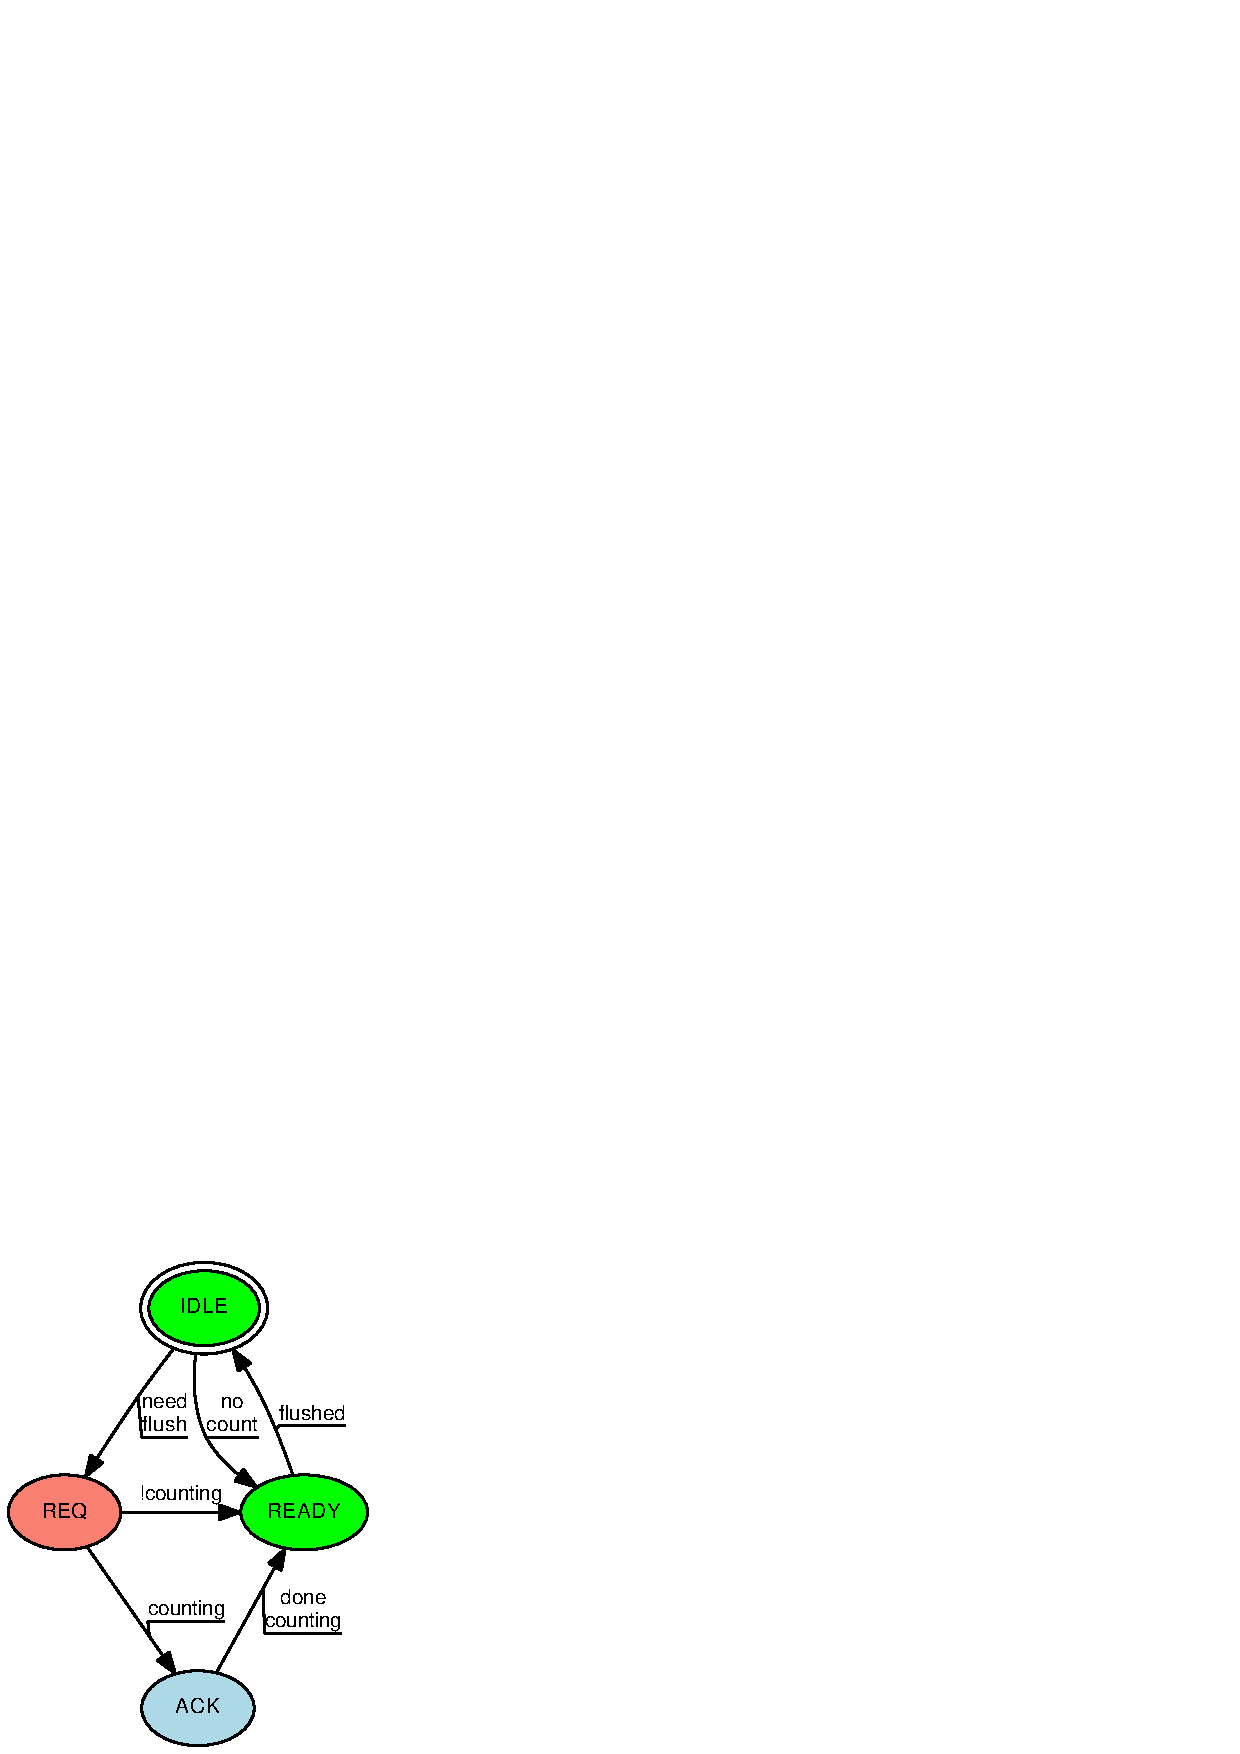
\includegraphics{count/sig-theft}}
\end{center}
\caption{Signal-Theft State Machine}
\label{fig:count:Signal-Theft State Machine}
\end{figure}

Even though per-thread state will now be manipulated only by the
corresponding thread, there will still need to be synchronization
with the signal handlers.
This synchronization is provided by the state machine shown in
Figure~\ref{fig:count:Signal-Theft State Machine}
The state machine starts out in the IDLE state, and when \co{add_count()}
or \co{sub_count()} find that the combination of the local thread's count
and the global count cannot accommodate the request, the corresponding
slowpath sets each thread's \co{theft} state to REQ (unless that thread
has no count, in which case it transitions directly to READY).
Only the slowpath, which holds the \co{gblcnt_mutex} lock, is permitted to
transition from the IDLE state, as indicated by the green color.\footnote{
	For those with black-and-white versions of this book,
	IDLE and READY are green, REQ is red, and ACK is blue.}
The slowpath then sends a signal to each thread, and the corresponding
signal handler checks the corresponding thread's \co{theft} and
\co{counting} variables.
If the \co{theft} state is not REQ, then the signal handler is not
permitted to change the state, and therefore simply returns.
Otherwise, if the \co{counting} variable is set, indicating that
the current thread's fastpath is in progress, the signal handler
sets the \co{theft} state to ACK, otherwise to READY.

If the \co{theft} state is ACK,
only the fastpath is permitted to change
the \co{theft} state, as indicated by the blue color.
When the fastpath completes, it sets the \co{theft} state to READY.

Once the slowpath sees a thread's \co{theft} state is READY, the
slowpath is permitted to steal that thread's count.
The slowpath then sets that thread's \co{theft} state to IDLE.

\QuickQuiz{}
	In Figure~\ref{fig:count:Signal-Theft State Machine}, why is
	the REQ \co{theft} state colored red?
\QuickQuizAnswer{
	To indicate that only the fastpath is permitted to change the
	\co{theft} state, and that if the thread remains in this
	state for too long, the thread running the slowpath will
	resend the POSIX signal.
} \QuickQuizEnd

\QuickQuiz{}
	In Figure~\ref{fig:count:Signal-Theft State Machine}, what is
	the point of having separate REQ and ACK \co{theft} states?
	Why not simplify the state machine by collapsing
	them into a single REQACK state?
	Then whichever of the signal handler or the fastpath gets there
	first could set the state to READY.
\QuickQuizAnswer{
	Reasons why collapsing the REQ and ACK states would be a very
	bad idea include:
	\begin{enumerate}
	\item	The slowpath uses the REQ and ACK states to determine
		whether the signal should be retransmitted.
		If the states were collapsed, the slowpath would have
		no choice but to send redundant signals, which would
		have the unhelpful effect of needlessly slowing down
		the fastpath.
	\item	The following race would result:
		\begin{enumerate}
		\item	The slowpath sets a given thread's state to REQACK.
		\item	That thread has just finished its fastpath, and
			notes the REQACK state.
		\item	The thread receives the signal, which also notes
			the REQACK state, and, because there is no fastpath
			in effect, sets the state to READY.
		\item	The slowpath notes the READY state, steals the
			count, and sets the state to IDLE, and completes.
		\item	The fastpath sets the state to READY, disabling
			further fastpath execution for this thread.
		\end{enumerate}
		The basic problem here is that the combined REQACK state
		can be referenced by both the signal handler and the
		fastpath.
		The clear separation maintained by the four-state
		setup ensures orderly state transitions.
	\end{enumerate}
	That said, you might well be able to make a three-state setup
	work correctly.
	If you do succeed, compare carefully to the four-state setup.
	Is the three-state solution really preferable, and why or why not?
} \QuickQuizEnd

\subsection{Signal-Theft Limit Counter Implementation}
\label{sec:count:Signal-Theft Limit Counter Implementation}

\begin{figure}[tbp]
{ \scriptsize
\begin{verbatim}
  1 #define THEFT_IDLE  0
  2 #define THEFT_REQ   1
  3 #define THEFT_ACK   2
  4 #define THEFT_READY 3
  5 
  6 int __thread theft = THEFT_IDLE;
  7 int __thread counting = 0;
  8 unsigned long __thread counter = 0;
  9 unsigned long __thread countermax = 0;
 10 unsigned long globalcountmax = 10000;
 11 unsigned long globalcount = 0;
 12 unsigned long globalreserve = 0;
 13 unsigned long *counterp[NR_THREADS] = { NULL };
 14 unsigned long *countermaxp[NR_THREADS] = { NULL };
 15 int *theftp[NR_THREADS] = { NULL };
 16 DEFINE_SPINLOCK(gblcnt_mutex);
 17 #define MAX_COUNTERMAX 100
\end{verbatim}
}
\caption{Signal-Theft Limit Counter Data}
\label{fig:count:Signal-Theft Limit Counter Data}
\end{figure}

Figure~\ref{fig:count:Signal-Theft Limit Counter Data}
(\url{count_lim_sig.c})
shows the data structures used by the signal-theft based counter
implementation.
Lines~1-7 define the states and values for the per-thread theft state machine
described in the preceding section.
Lines~8-17 are similar to earlier implementations, with the addition of
lines~14 and 15 to allow remote access to a thread's \co{countermax}
and \co{theft} variables, respectively.

\begin{figure}[tbp]
{ \scriptsize
\begin{verbatim}
  1 static void globalize_count(void)
  2 {
  3   globalcount += counter;
  4   counter = 0;
  5   globalreserve -= countermax;
  6   countermax = 0;
  7 }
  8 
  9 static void flush_local_count_sig(int unused)
 10 {
 11   if (ACCESS_ONCE(theft) != THEFT_REQ)
 12     return;
 13   smp_mb();
 14   ACCESS_ONCE(theft) = THEFT_ACK;
 15   if (!counting) {
 16     ACCESS_ONCE(theft) = THEFT_READY;
 17   }
 18   smp_mb();
 19 }
 20 
 21 static void flush_local_count(void)
 22 {
 23   int t;
 24   thread_id_t tid;
 25 
 26   for_each_tid(t, tid)
 27     if (theftp[t] != NULL) {
 28       if (*countermaxp[t] == 0) {
 29         ACCESS_ONCE(*theftp[t]) = THEFT_READY;
 30         continue;
 31       }
 32       ACCESS_ONCE(*theftp[t]) = THEFT_REQ;
 33       pthread_kill(tid, SIGUSR1);
 34     }
 35   for_each_tid(t, tid) {
 36     if (theftp[t] == NULL)
 37       continue;
 38     while (ACCESS_ONCE(*theftp[t]) != THEFT_READY) {
 39       poll(NULL, 0, 1);
 40       if (ACCESS_ONCE(*theftp[t]) == THEFT_REQ)
 41         pthread_kill(tid, SIGUSR1);
 42     }
 43     globalcount += *counterp[t];
 44     *counterp[t] = 0;
 45     globalreserve -= *countermaxp[t];
 46     *countermaxp[t] = 0;
 47     ACCESS_ONCE(*theftp[t]) = THEFT_IDLE;
 48   }
 49 }
 50 
 51 static void balance_count(void)
 52 {
 53   countermax = globalcountmax -
 54     globalcount - globalreserve;
 55   countermax /= num_online_threads();
 56   if (countermax > MAX_COUNTERMAX)
 57     countermax = MAX_COUNTERMAX;
 58   globalreserve += countermax;
 59   counter = countermax / 2;
 60   if (counter > globalcount)
 61     counter = globalcount;
 62   globalcount -= counter;
 63 }
\end{verbatim}
}
\caption{Signal-Theft Limit Counter Value-Migration Functions}
\label{fig:count:Signal-Theft Limit Counter Value-Migration Functions}
\end{figure}

Figure~\ref{fig:count:Signal-Theft Limit Counter Value-Migration Functions}
shows the functions responsible for migrating counts between per-thread
variables and the global variables.
Lines~1-7 shows \co{globalize_count()}, which is identical to earlier
implementations.
Lines~9-19 shows \co{flush_local_count_sig()}, which is the signal
handler used in the theft process.
Lines~11 and 12 check to see if the \co{theft} state is REQ, and, if not
returns without change.
Line~13 executes a memory barrier to ensure that the sampling of the
theft variable happens before any change to that variable.
Line~14 sets the \co{theft} state to ACK, and, if line~15 sees that
this thread's fastpaths are not running, line~16 sets the \co{theft}
state to READY.

\QuickQuiz{}
	In Figure~\ref{fig:count:Signal-Theft Limit Counter Value-Migration Functions}
	function \co{flush_local_count_sig()}, why are there
	\co{ACCESS_ONCE()} wrappers around the uses of the
	\co{theft} per-thread variable?
\QuickQuizAnswer{
	The first one (on line~11) can be argued to be unnecessary.
	The last two (lines~14 and 16) are important.
	If these are removed, the compiler would be within its rights
	to rewrite lines~14-17 as follows:
	\vspace{5pt}
	\begin{minipage}[t]{\columnwidth}
	\small
	\begin{verbatim}
 14   theft = THEFT_READY;
 15   if (counting) {
 16     theft = THEFT_ACK;
 17   }
	\end{verbatim}
	\end{minipage}
	\vspace{5pt}
	This would be fatal, as the slowpath might see the transient
	value of \co{THEFT_READY}, and start stealing before the
	corresponding thread was ready.
} \QuickQuizEnd

Lines~21-49 shows \co{flush_local_count()}, which is called from the
slowpath to flush all threads' local counts.
The loop spanning lines~26-34 advances the \co{theft} state for each
thread that has local count, and also sends that thread a signal.
Line~27 skips any non-existent threads.
Otherwise, line~28 checks to see if the current thread holds any local
count, and, if not, line~29 sets the thread's \co{theft} state to READY
and line~30 skips to the next thread.
Otherwise, line~32 sets the thread's \co{theft} state to REQ and
line~33 sends the thread a signal.

\QuickQuiz{}
	In Figure~\ref{fig:count:Signal-Theft Limit Counter Value-Migration Functions},
	why is it safe for line~28 to directly access the other thread's
	\co{countermax} variable?
\QuickQuizAnswer{
	Because the other thread is not permitted to change the value
	of its \co{countermax} variable unless it holds the
	\co{gblcnt_mutex} lock.
	But the caller has acquired this lock, so it is not possible
	for the other thread to hold it, and therefore the other thread
	is not permitted to change its \co{countermax} variable.
	We can therefore safely access it --- but not change it.
} \QuickQuizEnd

\QuickQuiz{}
	In Figure~\ref{fig:count:Signal-Theft Limit Counter Value-Migration Functions},
	why doesn't line~33 check for the current thread sending itself
	a signal?
\QuickQuizAnswer{
	There is no need for an additional check.
	The caller of \co{flush_local_count()} has already invoked
	\co{globalize_count()}, so the check on line~28 will have
	succeeded, skipping the later \co{pthread_kill()}.
} \QuickQuizEnd

\QuickQuiz{}
	The code in
	Figure~\ref{fig:count:Signal-Theft Limit Counter Value-Migration Functions},
	works with gcc and POSIX.
	What would be required to make it also conform to the ISO C standard?
\QuickQuizAnswer{
	The \co{theft} variable must be of type \co{sig_atomic_t}
	to guarantee that it can be safely shared between the signal
	handler and the code interrupted by the signal.
} \QuickQuizEnd

The loop spanning lines~35-48 waits until each thread reaches READY state,
then steals that thread's count.
Lines~36-37 skip any non-existent threads, and the loop spanning
lines~38-42 wait until the current thread's \co{theft} state becomes READY.
Line~39 blocks for a millisecond to avoid priority-inversion problems,
and if line~40 determines that the thread's signal has not yet arrived,
line~41 resends the signal.
Execution reaches line~43 when the thread's \co{theft} state becomes
READY, so lines~43-46 do the thieving.
Line~47 then sets the thread's \co{theft} state back to IDLE.

\QuickQuiz{}
	In Figure~\ref{fig:count:Signal-Theft Limit Counter Value-Migration Functions}, why does line~41 resend the signal?
\QuickQuizAnswer{
	Because many operating systems over several decades have
	had the property of losing the occasional signal.
	Whether this is a feature or a bug is debatable, but
	irrelevant.
	The obvious symptom from the user's viewpoint will not be
	a kernel bug, but rather a user application hanging.

	\emph{Your} user application hanging!
} \QuickQuizEnd

Lines~51-63 show \co{balance_count()}, which is similar to that of
earlier examples.

\begin{figure}[tbp]
{ \scriptsize
\begin{verbatim}
  1 int add_count(unsigned long delta)
  2 {
  3   int fastpath = 0;
  4 
  5   counting = 1;
  6   barrier();
  7   if (countermax - counter >= delta &&
  8       ACCESS_ONCE(theft) <= THEFT_REQ) {
  9     counter += delta;
 10     fastpath = 1;
 11   }
 12   barrier();
 13   counting = 0;
 14   barrier();
 15   if (ACCESS_ONCE(theft) == THEFT_ACK) {
 16     smp_mb();
 17     ACCESS_ONCE(theft) = THEFT_READY;
 18   }
 19   if (fastpath)
 20     return 1;
 21   spin_lock(&gblcnt_mutex);
 22   globalize_count();
 23   if (globalcountmax - globalcount -
 24       globalreserve < delta) {
 25     flush_local_count();
 26     if (globalcountmax - globalcount -
 27         globalreserve < delta) {
 28       spin_unlock(&gblcnt_mutex);
 29       return 0;
 30     }
 31   }
 32   globalcount += delta;
 33   balance_count();
 34   spin_unlock(&gblcnt_mutex);
 35   return 1;
 36 }
\end{verbatim}
}
\caption{Signal-Theft Limit Counter Add Function}
\label{fig:count:Signal-Theft Limit Counter Add Function}
\end{figure}

\begin{figure}[tbp]
{ \scriptsize
\begin{verbatim}
 38 int sub_count(unsigned long delta)
 39 {
 40   int fastpath = 0;
 41 
 42   counting = 1;
 43   barrier();
 44   if (counter >= delta &&
 45       ACCESS_ONCE(theft) <= THEFT_REQ) {
 46     counter -= delta;
 47     fastpath = 1;
 48   }
 49   barrier();
 50   counting = 0;
 51   barrier();
 52   if (ACCESS_ONCE(theft) == THEFT_ACK) {
 53     smp_mb();
 54     ACCESS_ONCE(theft) = THEFT_READY;
 55   }
 56   if (fastpath)
 57     return 1;
 58   spin_lock(&gblcnt_mutex);
 59   globalize_count();
 60   if (globalcount < delta) {
 61     flush_local_count();
 62     if (globalcount < delta) {
 63       spin_unlock(&gblcnt_mutex);
 64       return 0;
 65     }
 66   }
 67   globalcount -= delta;
 68   balance_count();
 69   spin_unlock(&gblcnt_mutex);
 70   return 1;
 71 }
\end{verbatim}
}
\caption{Signal-Theft Limit Counter Subtract Function}
\label{fig:count:Signal-Theft Limit Counter Subtract Function}
\end{figure}

Figure~\ref{fig:count:Signal-Theft Limit Counter Add Function}
shows the \co{add_count()} function.
The fastpath spans lines~5-20, and the slowpath lines~21-35.
Line~5 sets the per-thread \co{counting} variable to 1 so that
any subsequent signal handlers interrupting this thread will
set the \co{theft} state to ACK rather than READY, allowing this
fastpath to complete properly.
Line~6 prevents the compiler from reordering any of the fastpath body
to precede the setting of \co{counting}.
Lines~7 and 8 check to see if the per-thread data can accommodate
the \co{add_count()} and if there is no ongoing theft in progress,
and if so line~9 does the fastpath addition and line~10 notes that
the fastpath was taken.

In either case, line~12 prevents the compiler from reordering the
fastpath body to follow line~13, which permits any subsequent signal
handlers to undertake theft.
Line~14 again disables compiler reordering, and then line~15
checks to see if the signal handler deferred the \co{theft}
state-change to READY, and, if so, line~16 executes a memory
barrier to ensure that any CPU that sees line~17 setting state to
READY also sees the effects of line~9.
If the fastpath addition at line~9 was executed, then line~20 returns
success.

\begin{figure}[tbp]
{ \scriptsize
\begin{verbatim}
  1 unsigned long read_count(void)
  2 {
  3   int t;
  4   unsigned long sum;
  5 
  6   spin_lock(&gblcnt_mutex);
  7   sum = globalcount;
  8   for_each_thread(t)
  9     if (counterp[t] != NULL)
 10       sum += *counterp[t];
 11   spin_unlock(&gblcnt_mutex);
 12   return sum;
 13 }
\end{verbatim}
}
\caption{Signal-Theft Limit Counter Read Function}
\label{fig:count:Signal-Theft Limit Counter Read Function}
\end{figure}

Otherwise, we fall through to the slowpath starting at line~21.
The structure of the slowpath is similar to those of earlier examples,
so its analysis is left as an exercise to the reader.
Similarly, the structure of \co{sub_count()} on
Figure~\ref{fig:count:Signal-Theft Limit Counter Subtract Function}
is the same
as that of \co{add_count()}, so the analysis of \co{sub_count()} is also
left as an exercise for the reader, as is the analysis of
\co{read_count()} in
Figure~\ref{fig:count:Signal-Theft Limit Counter Read Function}.

\begin{figure}[tbp]
{ \scriptsize
\begin{verbatim}
  1 void count_init(void)
  2 {
  3   struct sigaction sa;
  4 
  5   sa.sa_handler = flush_local_count_sig;
  6   sigemptyset(&sa.sa_mask);
  7   sa.sa_flags = 0;
  8   if (sigaction(SIGUSR1, &sa, NULL) != 0) {
  9     perror("sigaction");
 10     exit(-1);
 11   }
 12 }
 13 
 14 void count_register_thread(void)
 15 {
 16   int idx = smp_thread_id();
 17 
 18   spin_lock(&gblcnt_mutex);
 19   counterp[idx] = &counter;
 20   countermaxp[idx] = &countermax;
 21   theftp[idx] = &theft;
 22   spin_unlock(&gblcnt_mutex);
 23 }
 24 
 25 void count_unregister_thread(int nthreadsexpected)
 26 {
 27   int idx = smp_thread_id();
 28 
 29   spin_lock(&gblcnt_mutex);
 30   globalize_count();
 31   counterp[idx] = NULL;
 32   countermaxp[idx] = NULL;
 33   theftp[idx] = NULL;
 34   spin_unlock(&gblcnt_mutex);
 35 }
\end{verbatim}
}
\caption{Signal-Theft Limit Counter Initialization Functions}
\label{fig:count:Signal-Theft Limit Counter Initialization Functions}
\end{figure}

Lines~1-12 of
Figure~\ref{fig:count:Signal-Theft Limit Counter Initialization Functions}
show \co{count_init()}, which set up \co{flush_local_count_sig()}
as the signal handler for \co{SIGUSR1},
enabling the \co{pthread_kill()} calls in \co{flush_local_count()}
to invoke \co{flush_local_count_sig()}.
The code for thread registry and unregistry is similar to that of
earlier examples, so its analysis is left as an exercise for the
reader.

\subsection{Signal-Theft Limit Counter Discussion}

The signal-theft implementation runs more than twice as fast as the
atomic implementation on my Intel Core Duo laptop.
Is it always preferable?

The signal-theft implementation would be vastly preferable on Pentium-4
systems, given their slow atomic instructions, but the old 80386-based
Sequent Symmetry systems would do much better with the shorter path
length of the atomic implementation.
However, this increased update-side performance comes at the
prices of higher read-side overhead: Those POSIX signals are not free.
If ultimate performance is of the essence, you will need to measure
them both on the system that your application is to be deployed on.

\QuickQuiz{}
	Not only are POSIX signals slow, sending one to each thread
	simply does not scale.
	What would you do if you had (say) 10,000 threads and needed
	the read side to be fast?
\QuickQuizAnswer{
	One approach is to use the techniques shown in
	Section~\ref{sec:count:Eventually Consistent Implementation},
	summarizing an approximation to the overall counter value in
	a single variable.
	Another approach would be to use multiple threads to carry
	out the reads, with each such thread interacting with a
	specific subset of the updating threads.
} \QuickQuizEnd

This is but one reason why high-quality APIs are so important:
they permit implementations to be changed as required by ever-changing
hardware performance characteristics.

\QuickQuiz{}
	What if you want an exact limit counter to be exact only for
	its lower limit, but to allow the upper limit to be inexact?
\QuickQuizAnswer{
	One simple solution is to overstate the upper limit by the
	desired amount.
	The limiting case of such overstatement results in the
	upper limit being set to the largest value that the counter is
	capable of representing.
} \QuickQuizEnd

\section{Applying Specialized Parallel Counters}
\label{sec:count:Applying Specialized Parallel Counters}

Although the exact limit counter implementations in
Section~\ref{sec:count:Exact Limit Counters}
can be very useful, they are not much help if the counter's value
remains near zero at all times, as it might when counting the number
of outstanding accesses to an I/O device.
The high overhead of such near-zero counting is especially painful
given that we normally don't care how many references there are.
As noted in the removable I/O device access-count problem posed by
{\QQIOcnt},
the number of accesses is irrelevant except in those rare cases when
someone is actually trying to remove the device.

One simple solution to this problem is to add a large ``bias''
(for example, one billion) to the
counter in order to ensure that the value is far enough from zero that
the counter can operate efficiently.
When someone wants to remove the device, this bias is subtracted from
the counter value.
Counting the last few accesses will be quite inefficient,
but the important point is that the many prior accesses will have been
counted at full speed.

\QuickQuiz{}
	What else had you better have done when using a biased counter?
\QuickQuizAnswer{
	You had better have set the upper limit to be large enough
	accommodate the bias, the expected maximum number of accesses,
	and enough ``slop'' to allow the counter to work efficiently
	even when the number of accesses is at its maximum.
} \QuickQuizEnd

Although a biased counter can be quite helpful and useful, it is only a
partial solution to the removable I/O device access-count problem
called out on
page~\pageref{chp:Counting}.
When attempting to remove a device, we must not only know the precise
number of current I/O accesses, we also need to prevent any future
accesses from starting.
One way to accomplish this is to read-acquire a reader-writer lock
when updating the counter, and to write-acquire that same reader-writer
lock when checking the counter.
Code for doing I/O might be as follows:

\vspace{5pt}
\begin{minipage}[t]{\columnwidth}
\small
\begin{verbatim}
  1 read_lock(&mylock);
  2 if (removing) {
  3   read_unlock(&mylock);
  4   cancel_io();
  5 } else {
  6   add_count(1);
  7   read_unlock(&mylock);
  8   do_io();
  9   sub_count(1);
 10 }
\end{verbatim}
\end{minipage}
\vspace{5pt}

Line~1 read-acquires the lock, and either line~3 or 7 releases it.
Line~2 checks to see if the device is being removed, and, if so,
line~3 releases the lock and line~4 cancels the I/O, or takes whatever
action is appropriate given that the device is to be removed.
Otherwise, line~6 increments the access count, line~7 releases the
lock, line~8 performs the I/O, and line~9 decrements the access count.

\QuickQuiz{}
	This is ridiculous!
	We are \emph{read}-acquiring a reader-writer lock to
	\emph{update} the counter?
	What are you playing at???
\QuickQuizAnswer{
	Strange, perhaps, but true!
	Almost enough to make you think that the name
	``reader-writer lock'' was poorly chosen, isn't it?
} \QuickQuizEnd

The code to remove the device might be as follows:

\vspace{5pt}
\begin{minipage}[t]{\columnwidth}
\small
\begin{verbatim}
  1 write_lock(&mylock);
  2 removing = 1;
  3 sub_count(mybias);
  4 write_unlock(&mylock);
  5 while (read_count() != 0) {
  6   poll(NULL, 0, 1);
  7 }
  8 remove_device();
\end{verbatim}
\end{minipage}
\vspace{5pt}

Line~1 write-acquires the lock and line~4 releases it.
Line~2 notes that the device is being removed, and the loop spanning
lines~5-7 wait for any I/O operations to complete.
Finally, line~8 does any additional processing needed to prepare for
device removal.

\QuickQuiz{}
	What other issues would need to be accounted for in a real system?
\QuickQuizAnswer{
	A huge number!

	Here are a few to start with:

	\begin{enumerate}
	\item	There could be any number of devices, so that the
		global variables are inappropriate, as are the
		lack of arguments to functions like \co{do_io()}.
	\item	Polling loops can be problematic in real systems.
		In many cases, it is far better to have the last
		completing I/O wake up the device-removal thread.
	\item	The I/O might fail, and so \co{do_io()} will likely
		need a return value.
	\item	If the device fails, the last I/O might never complete.
		In such cases, there might need to be some sort of
		timeout to allow error recovery.
	\item	Both \co{add_count()} and \co{sub_count()} can
		fail, but their return values are not checked.
	\item	Reader-writer locks do not scale well.
		One way of avoiding the high read-acquisition costs
		of reader-writer locks is presented in
		Chapters~\ref{chp:Locking}
		and~\ref{chp:Deferred Processing}.
	\item	The polling loops result in poor energy efficiency.
		An event-driven design is preferable.
	\end{enumerate}
} \QuickQuizEnd

\section{Parallel Counting Discussion}
\label{sec:count:Parallel Counting Discussion}

This chapter has presented the reliability, performance, and
scalability problems with traditional counting primitives.
The C-language \co{++} operator is not guaranteed to function reliably in
multithreaded code, and atomic operations to a single variable neither
perform nor scale well.
This chapter therefore presented a number of counting algorithms that
perform and scale extremely well in certain special cases.

It is well worth reviewing the lessons from these counting algorithms.
To that end,
Section~\ref{sec:count:Parallel Counting Performance}
summarizes performance and scalability,
Section~\ref{sec:count:Parallel Counting Specializations}
discusses the need for specialization,
and finally,
Section~\ref{sec:count:Parallel Counting Lessons}
enumerates lessons learned and calls attention to later chapters that
will expand on these lessons.

\subsection{Parallel Counting Performance}
\label{sec:count:Parallel Counting Performance}

\begin{table*}
\begin{center}
\begin{tabular}{l|r|r|r|r}
	& & & \multicolumn{2}{|c}{Reads} \\
	\cline{4-5}
	Algorithm & Section & Updates & 1 Core & 32 Cores \\
	\hline
	\hline
	\url{count_stat.c} & \ref{sec:count:Array-Based Implementation} &
		11.5 ns & 408 ns & 409 ns \\
	\url{count_stat_eventual.c} & \ref{sec:count:Eventually Consistent Implementation} &
		11.6 ns & 1 ns & 1 ns \\
	\url{count_end.c} & \ref{sec:count:Per-Thread-Variable-Based Implementation} &
		6.3 ns & 389 ns & 51,200 ns \\
	\url{count_end_rcu.c} & \ref{sec:together:RCU and Per-Thread-Variable-Based Statistical Counters} &
		5.7 ns & 354 ns & 501 ns \\
\end{tabular}
\end{center}
\caption{Statistical Counter Performance on Power-6}
\label{tab:count:Statistical Counter Performance on Power-6}
\end{table*}

Table~\ref{tab:count:Statistical Counter Performance on Power-6}
shows the performance of the four parallel statistical counting
algorithms.
All four algorithms provide near-perfect linear scalability for updates.
The per-thread-variable implementation (\co{count_end.c})
is significantly faster on
updates than the array-based implementation
(\co{count_stat.c}), but is slower at reads on large numbers of core,
and suffers severe lock contention when there are many parallel readers.
This contention can be addressed using the deferred-processing
techniques introduced in
Chapter~\ref{chp:Deferred Processing},
as shown on the \co{count_end_rcu.c} row of
Table~\ref{tab:count:Statistical Counter Performance on Power-6}.
Deferred processing also shines on the \co{count_stat_eventual.c} row,
courtesy of eventual consistency.

\QuickQuiz{}
	On the \url{count_stat.c} row of
	Table~\ref{tab:count:Statistical Counter Performance on Power-6},
	we see that the update side scales linearly with the number of
	threads.
	How is that possible given that the more threads there are,
	the more per-thread counters must be summed up?
\QuickQuizAnswer{
	The read-side code must scan the entire fixed-size array, regardless
	of the number of threads, so there is no difference in performance.
	In contrast, in the last two algorithms, readers must do more
	work when there are more threads.
	In addition, the last two algorithms interpose an additional
	level of indirection because they map from integer thread ID
	to the corresponding \co{__thread} variable.
} \QuickQuizEnd

\QuickQuiz{}
	Even on the last row of
	Table~\ref{tab:count:Statistical Counter Performance on Power-6},
	the read-side performance of these statistical counter
	implementations is pretty horrible.
	So why bother with them?
\QuickQuizAnswer{
	``Use the right tool for the job.''

	As can be seen from
	Figure~\ref{fig:count:Atomic Increment Scalability on Nehalem},
	single-variable atomic increment need not apply for any job
	involving heavy use of parallel updates.
	In contrast, the algorithms shown in
	Table~\ref{tab:count:Statistical Counter Performance on Power-6}
	do an excellent job of handling update-heavy situations.
	Of course, if you have a read-mostly situation, you should
	use something else, for example, an eventually consistent design
	featuring a single atomically incremented
	variable that can be read out using a single load,
	similar to the approach used in
	Section~\ref{sec:count:Eventually Consistent Implementation}.
} \QuickQuizEnd

\begin{table*}
\begin{center}
\begin{tabular}{l|r|c|r|r|r}
	& & & & \multicolumn{2}{|c}{Reads} \\
	\cline{5-6}
	Algorithm & Section & Exact? & Updates & 1 Core & 64 Cores \\
	\hline
	\hline
	\url{count_lim.c} & \ref{sec:count:Simple Limit Counter Implementation} &
		N & 3.6 ns & 375 ns & 50,700 ns \\
	\url{count_lim_app.c} & \ref{sec:count:Approximate Limit Counter Implementation} &
		N & 11.7 ns & 369 ns & 51,000 ns \\
	\url{count_lim_atomic.c} & \ref{sec:count:Atomic Limit Counter Implementation} &
		Y & 51.4 ns & 427 ns & 49,400 ns \\
	\url{count_lim_sig.c} & \ref{sec:count:Signal-Theft Limit Counter Implementation} &
		Y & 10.2 ns & 370 ns & 54,000 ns \\
\end{tabular}
\end{center}
\caption{Limit Counter Performance on Power-6}
\label{tab:count:Limit Counter Performance on Power-6}
\end{table*}

Figure~\ref{tab:count:Limit Counter Performance on Power-6}
shows the performance of the parallel limit-counting algorithms.
Exact enforcement of the limits incurs a substantial performance
penalty, although on this 4.7GHz Power-6 system that penalty can be reduced
by substituting signals for atomic operations.
All of these implementations suffer from read-side lock contention
in the face of concurrent readers.

\QuickQuiz{}
	Given the performance data shown in
	Table~\ref{tab:count:Limit Counter Performance on Power-6},
	we should always prefer signals over atomic operations, right?
\QuickQuizAnswer{
	That depends on the workload.
	Note that on a 64-core system, you need more than
	one hundred non-atomic operations (with roughly
	a 40-nanosecond performance gain) to make up for even one
	signal (with almost a 5-\emph{microsecond} performance loss).
	Although there are no shortage of workloads with far greater
	read intensity, you will need to consider your particular
	workload.

	In addition, although memory barriers have historically been
	expensive compared to ordinary instructions, you should
	check this on the specific hardware you will be running.
	The properties of computer hardware do change over time,
	and algorithms must change accordingly.
} \QuickQuizEnd

\QuickQuiz{}
	Can advanced techniques be applied to address the lock
	contention for readers seen in
	Table~\ref{tab:count:Limit Counter Performance on Power-6}?
\QuickQuizAnswer{
	One approach is to give up some update-side performance, as is
	done with scalable non-zero indicators
	(SNZI)~\cite{FaithEllen:2007:SNZI}.
	There are a number of other ways one might go about this, and these
	are left as exercises for the reader.
	Any number of approaches that apply hierarchy, which replace
	frequent global-lock acquisitions with local lock acquisitions
	corresponding to lower levels of the hierarchy, should work quite well.
} \QuickQuizEnd

In short, this chapter has demonstrated a number of counting algorithms
that perform and scale extremely well in a number of special cases.
But must our parallel counting be confined to special cases?
Wouldn't it be better to have a general algorithm that operated
efficiently in all cases?
The next section looks at these questions.

\subsection{Parallel Counting Specializations}
\label{sec:count:Parallel Counting Specializations}

The fact that these algorithms only work well in their respective special
cases might be considered a major problem with parallel programming in
general.
After all, the C-language \co{++} operator works just fine in single-threaded
code, and not just for special cases, but in general, right?

This line of reasoning does contain a grain of truth, but is in essence
misguided.
The problem is not parallelism as such, but rather scalability.
To understand this, first consider the C-language \co{++} operator.
The fact is that it does \emph{not} work in general, only for a restricted
range of numbers.
If you need to deal with 1,000-digit decimal numbers, the C-language \co{++}
operator will not work for you.

\QuickQuiz{}
	The \co{++} operator works just fine for 1,000-digit numbers!
	Haven't you heard of operator overloading???
\QuickQuizAnswer{
	In the C++ language, you might well be able to use \co{++}
	on a 1,000-digit number, assuming that you had access to a
	class implementing such numbers.
	But as of 2010, the C language does not permit operator overloading.
} \QuickQuizEnd

This problem is not specific to arithmetic.
Suppose you need to store and query data.
Should you use an ASCII file? 
XML?
A relational database?
A linked list?
A dense array?
A B-tree?
A radix tree?
Or one of the plethora of other data
structures and environments that permit data to be stored and queried?
It depends on what you need to do, how fast you need it done, and how
large your data set is---even on sequential systems.

Similarly, if you need to count, your solution will depend on how large
of numbers you need to work with, how many CPUs need to be manipulating
a given number concurrently, how the number is to be used, and what
level of performance and scalability you will need.

Nor is this problem specific to software.
The design for a bridge meant to allow people to walk across a small brook
might be a simple as a single wooden plank.
But you would probably not use a plank to span the kilometers-wide mouth of
the Columbia River, nor would such a design be advisable for bridges
carrying concrete trucks.
In short, just as bridge design must change with increasing span and load,
so must software design change as the number of CPUs increases.
That said, it would be good to automate this process, so that the
software adapts to changes in hardware configuration and in workload.
There has in fact been some research into this sort of
automation~\cite{Appavoo03a,Soules03a}, and the Linux kernel does some
boot-time reconfiguration, including limited binary rewriting.
This sort of adaptation will become increasingly important as the
number of CPUs on mainstream systems continues to increase.

In short, as discussed in
Chapter~\ref{chp:Hardware and its Habits},
the laws of physics constrain parallel software just as surely as they
constrain mechanical artifacts such as bridges.
These constraints force specialization, though in the case of software
it might be possible to automate the choice of specialization to
fit the hardware and workload in question.

Of course, even generalized counting is quite specialized.
We need to do a great number of other things with computers.
The next section relates what we have learned from counters to
topics taken up later in this book.

\subsection{Parallel Counting Lessons}
\label{sec:count:Parallel Counting Lessons}

The opening paragraph of this chapter promised that our study of counting
would provide an excellent introduction to parallel programming.
This section makes explicit connections between the lessons from
this chapter and the material presented in a number of later chapters.

The examples in this chapter have shown that an important scalability
and performance tool is \emph{partitioning}.
The counters might be fully partitioned, as in the statistical counters
discussed in Section~\ref{sec:count:Statistical Counters},
or partially partitioned as in the limit counters discussed in
Sections~\ref{sec:count:Approximate Limit Counters} and
\ref{sec:count:Exact Limit Counters}.
Partitioning will be considered in far greater depth in
Chapter~\ref{cha:Partitioning and Synchronization Design},
and partial parallelization in particular in
Section~\ref{sec:SMPdesign:Parallel Fastpath}, where it is called
\emph{parallel fastpath}.

\QuickQuiz{}
	But if we are going to have to partition everything, why bother
	with shared-memory multithreading?
	Why not just partition the problem completely and run as
	multiple processes, each in its own address space?
\QuickQuizAnswer{
	Indeed, multiple processes with separate address spaces can be
	an excellent way to exploit parallelism, as the proponents of
	the fork-join methodology and the Erlang language would be very
	quick to tell you.
	However, there are also some advantages to shared-memory parallelism:
	\begin{enumerate}
	\item	Only the most performance-critical portions of the
		application must be partitioned, and such portions
		are usually a small fraction of the application.
	\item	Although cache misses are quite slow compared to
		individual register-to-register instructions,
		they are typically considerably faster than
		inter-process-communication primitives, which in
		turn are considerably faster than things like
		TCP/IP networking.
	\item	Shared-memory multiprocessors are readily available
		and quite inexpensive, so, in stark contrast to the
		1990s, there is little cost penalty for use of
		shared-memory parallelism.
	\end{enumerate}
	As always, use the right tool for the job!
} \QuickQuizEnd

The partially partitioned counting algorithms used locking to
guard the global data, and locking is the subject of
Chapter~\ref{chp:Locking}.
In contrast, the partitioned data tended to be fully under the control of
the corresponding thread, so that no synchronization whatsoever was required.
This \emph{data ownership} will be introduced in
Section~\ref{sec:SMPdesign:Data Ownership}
and discussed in more detail in
Chapter~\ref{chp:Data Ownership}.

Because integer addition and subtraction are extremely cheap operations
compared to typical synchronization operations, achieving reasonable
scalability requires synchronization operations be used sparingly.
One way of achieving this is to batch the addition and subtraction
operations, so that a great many of these cheap operations are handled
by a single synchronization operation.
Batching optimizations of one sort or another are used by each of
the counting algorithms listed in
Tables~\ref{tab:count:Statistical Counter Performance on Power-6}
and~\ref{tab:count:Limit Counter Performance on Power-6}.

Finally, the eventually consistent statistical counter discussed in
Section~\ref{sec:count:Eventually Consistent Implementation}
showed how deferring activity (in that case, updating the global
counter) can provide substantial performance and scalability benefits.
This approach allows common case code to use much cheaper synchronization
operations than would otherwise be possible.
Chapter~\ref{chp:Deferred Processing} will examine a number of additional
ways that deferral can improve performance, scalability, and even
real-time response.

Summarizing the summary:

\begin{enumerate}
\item	Partitioning promotes performance and scalability.
\item	Partial partitioning, that is, partitioning applied only to
	common code paths, works almost as well.
\item	Partial partitioning can be applied to code (as in
	Section~\ref{sec:count:Statistical Counters}'s statistical
	counters' partitioned updates and non-partitioned reads), but also
	across time (as in
	Section~\ref{sec:count:Approximate Limit Counters}'s and
	Section~\ref{sec:count:Exact Limit Counters}'s and
	limit counters running fast when far from
	the limit, but slowly when close to the limit).
\item	Partitioning across time often batches updates locally
	in order to reduce the number of expensive global operations,
	thereby decreasing synchronization overhead, in turn
	improving performance and scalability.
	All the algorithms shown in
	Tables~\ref{tab:count:Statistical Counter Performance on Power-6}
	and~\ref{tab:count:Limit Counter Performance on Power-6}?
	make heavy use of batching.
\item	Read-only code paths should remain read-only:  Spurious
	synchronization writes to shared memory kill performance
	and scalability, as seen in the \co{count_end.c} row of
	Table~\ref{tab:count:Statistical Counter Performance on Power-6}.
\item	Judicious use of delay promotes performance and scalability, as
	seen in Section~\ref{sec:count:Eventually Consistent Implementation}.
\item	Parallel performance and scalability is usually a balancing act:
	Beyond a certain point, optimizing some code paths will degrade
	others.
	The \co{count_stat.c} and \co{count_end_rcu.c} rows of
	Table~\ref{tab:count:Statistical Counter Performance on Power-6}
	illustrate this point.
\item	Different levels of performance and scalability will affect
	algorithm and data-structure design, as do a large number of
	other factors.
	Figure~\ref{fig:count:Atomic Increment Scalability on Nehalem}
	illustrates this point:  Atomic increment might be completely
	acceptable for a two-CPU system, but be completely inadequate for an
	eight-CPU system.
\end{enumerate}

\begin{figure}[tb]
\begin{center}
\resizebox{3in}{!}{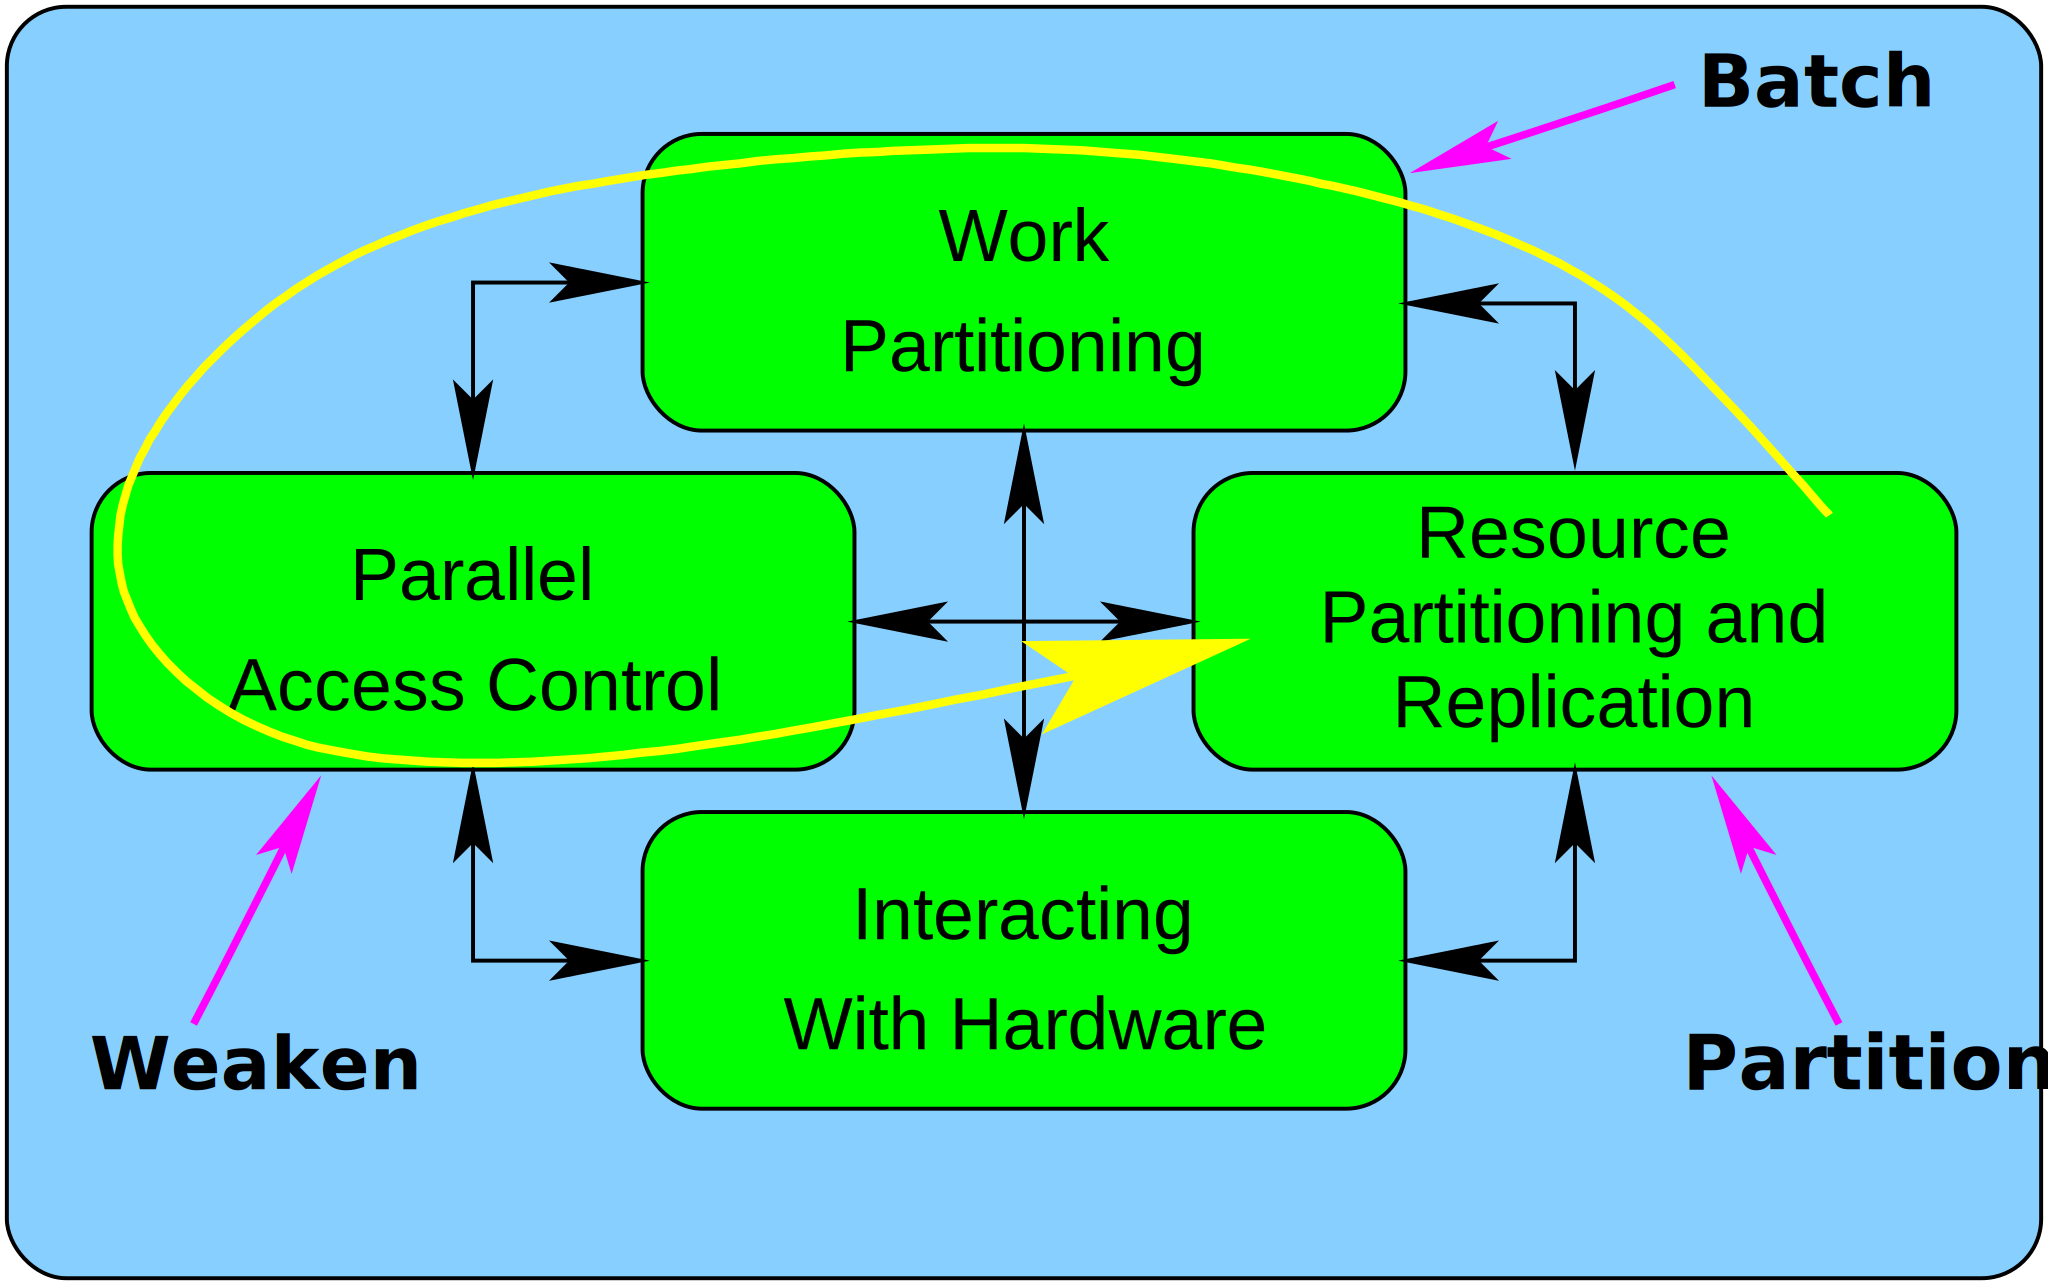
\includegraphics{count/FourTaskOrderOpt}}
\end{center}
\caption{Optimization and the Four Parallel-Programming Tasks}
\label{fig:count:Optimization and the Four Parallel-Programming Tasks}
\end{figure}

Summarizing still further, we have the ``big three'' methods of
increasing performance and scalability, namely
(1)~\emph{partitioning} over CPUs or threads,
(2)~\emph{batching} so that more work can be done by each expensive
synchronization operations, and
(3)~\emph{weakening} synchronization operations where feasible.
As a rough rule of thumb, you should apply these methods in this order,
as was noted earlier in the discussion of
Figure~\ref{fig:intro:Ordering of Parallel-Programming Tasks}
on
page~\pageref{fig:intro:Ordering of Parallel-Programming Tasks}.
The partitioning optimization applies to the
``Resource Partitioning and Replication'' bubble,
the batching optimization to the ``Work Partitioning'' bubble,
and the weakening optimization to the ``Parallel Access Control'' bubble,
as shown in
Figure~\ref{fig:count:Optimization and the Four Parallel-Programming Tasks}.
Of course, if you are using special-purpose hardware such as
digital signal processors (DSPs), field-programmable gate arrays (FPGAs),
or general-purpose graphical processing units (GPGPUs), you may need
to pay close attention to the ``Interacting With Hardware'' bubble
thoughout the design process.
For example, the structure of a GPGPU's hardware threads and memory
connectivity might richly reward very careful partitioning
and batching design decisions.

In short, as noted at the beginning of this chapter, the simplicity
of counting have allowed us to explore many
fundamental concurrency issues without the distraction of
complex synchronization primitives or elaborate data structures.
Such synchronization primitives and data structures are covered
in later chapters.

% SMPdesign/SMPdesign.tex

\QuickQuizChapter{cha:Partitioning and Synchronization Design}{Partitioning and Synchronization Design}

이 챕터는 상용 시스템의 트렌드인 여러개의 CPU 들로부터 이점을 얻기 위해서는
어떻게 소프트웨어를 설계해야 하는지 설명합니다.
이를 위해 성능, 확장성, 그리고 반응시간 사이의 균형을 잡는데 도움을 줄 수 있을,
여러개의 관용구나 ``디자인
패턴''~\cite{Alexander79,GOF95,SchmidtStalRohnertBuschmann2000v2Textbook} 들을
소개합니다.
앞의 챕터에서 이야기 했듯, 병렬 소프트웨어를 만들 때 하게 되는 가장 중요한
결정은 파티셔닝을 어떻게 할것인지입니다.
잘 분할된 문제들은 간단하고, 확장성 있으며, 고성능을 갖는 해결책을
이끌어냅니다만, 자롯 분할된 문제들은 느리고 복잡한 해결책을 만듭니다.
이 챕터는 몰아서 처리하기 (batching) 와 약화시키기 (weakening) 에 대한 토론과
함께 파티셔닝을 코드로 설계하는 것을 도울 것입니다.
``설계'' 란 말은 매우 중요합니다: 파티셔닝이 첫번째, 몰아 처리하기가 두번째,
약화하기가 세번째이며, 코딩은 네번째입니다.
이 순서를 바꾸는 행위는 낮은 성능과 확장성에다가 엄청난 좌절을 일으킬 것입니다.
\iffalse

This chapter describes how to design software to take advantage of
the multiple CPUs that are increasingly appearing in commodity systems.
It does this by presenting a number of idioms, or
``design patterns''~\cite{Alexander79,GOF95,SchmidtStalRohnertBuschmann2000v2Textbook}
that can help you balance performance, scalability, and response time.
As noted in earlier chapters, the most important decision you will make
when creating parallel software is how to carry out the partitioning.
Correctly partitioned problems lead to simple, scalable, and
high-performance solutions, while poorly partitioned problems result
in slow and complex solutions.
This chapter will help you design partitioning into your code, with
some discussion of batching and weakening as well.
The word ``design'' is very important: You should partition first,
batch second, weaken third, and code fourth.
Changing this order often leads to poor performance and scalability
along with great frustration.
\fi

이를 위해, Section~\ref{sec:SMPdesign:Partitioning Exercises} 에서는 파티셔닝
연습문제들을 소개하고,
Section~\ref{sec:SMPdesign:Design Criteria} 에서 분할가능성 설계 기준을
알아보고,
Section~\ref{sec:SMPdesign:Synchronization Granularity} 에서 적절한 동기화
정도에 대해 이야기 하고,
Section~\ref{sec:SMPdesign:Parallel Fastpath} 에서 일반적인 경우 속도와
확장성을 제공하는 중요한 병렬성의 빠른 수행 경로와 간단하지만 일반적이지 않은
상황을 위한 덜 확장성 있는 대안인 ``슬로우 패스'' 설계의 개요를 알아본 후,
마지막으로
Section~\ref{sec:SMPdesign:Beyond Partitioning} 에서 파티셔닝 다음을 간략히
봅니다.
\iffalse

To this end, Section~\ref{sec:SMPdesign:Partitioning Exercises}
presents partitioning exercises,
Section~\ref{sec:SMPdesign:Design Criteria} reviews partitionability
design criteria,
Section~\ref{sec:SMPdesign:Synchronization Granularity}
discusses selecting an appropriate synchronization granularity,
Section~\ref{sec:SMPdesign:Parallel Fastpath}
gives an overview of important parallel-fastpath designs
that provide speed and scalability in the common case with
a simpler but less-scalable fallback ``slow path'' for unusual
situations,
and finally
Section~\ref{sec:SMPdesign:Beyond Partitioning}
takes a brief look beyond partitioning.
\fi

% SMPdesign/partexercises.tex
% mainfile: ../perfbook.tex
% SPDX-License-Identifier: CC-BY-SA-3.0

\section{Partitioning Exercises}
\label{sec:SMPdesign:Partitioning Exercises}
%
\epigraph{Whenever a theory appears to you as the only possible one,
	  take this as a sign that you have neither understood the theory
	  nor the problem which it was intended to solve.}
	  {\emph{Karl Popper}}

파티셔닝이 2000년대 초에 그랬던 것보다 더 널리 이해되고 있지만, 그 가치는
여전히 과소평가 되어 있습니다.
따라서
\cref{sec:SMPdesign:Dining Philosophers Problem}
에서는 고전의 식사하는 철학자들 (Dining Philosophers) 문제를 더 병렬적인
관점으로 바라보고
\cref{sec:SMPdesign:Double-Ended Queue}
에서는 양극단을 가지는 큐 (queue) 를 다시 봅니다.

\iffalse

Although partitioning is more widely understood than it was in the early
2000s, its value is still underappreciated.
\Cref{sec:SMPdesign:Dining Philosophers Problem}
therefore takes more highly parallel look at the classic Dining
Philosophers problem and
\cref{sec:SMPdesign:Double-Ended Queue}
revisits the double-ended queue.

\fi

\subsection{Dining Philosophers Problem}
\label{sec:SMPdesign:Dining Philosophers Problem}

\begin{figure}[tb]
\centering
\includegraphics[scale=.7]{SMPdesign/DiningPhilosopher5}
\caption{Dining Philosophers Problem}
\ContributedBy{Figure}{fig:SMPdesign:Dining Philosophers Problem}{Kornilios Kourtis}
\end{figure}

Figure~\ref{fig:SMPdesign:Dining Philosophers Problem} 는 고전의
\IX{Dining Philosophers problem}~\cite{Dijkstra1971HOoSP} 의 다이어그램을
보입니다.
이 문제는 생각하고 먹기 위해 두개의 포크가 필요한 ``무척 어려운 종류의
스파게티'' 를 먹는 다섯명의 철학자들로 구성됩니다.\footnote{
	포크 대신 젓가락으로 생각해도 좋습니다.}
한명의 철학자는 그 또는 그녀의 바로 오른쪽과 왼쪽에 있는 포크만 사용할 수
있는데, 충분히 스파게티를 먹기 전까진 포크를 내려놓지 않습니다.

\iffalse

Figure~\ref{fig:SMPdesign:Dining Philosophers Problem} shows a diagram
of the classic \IX{Dining Philosophers problem}~\cite{Dijkstra1971HOoSP}.
This problem features five philosophers who do nothing but think and
eat a ``very difficult kind of spaghetti'' which requires two forks
to eat.\footnote{
	But feel free to instead think in terms of chopsticks.}
A given philosopher is permitted to use only the forks to his or her
immediate right and left, but will not put a given fork down until sated.

\fi

\begin{figure*}[tb]
\centering
\resizebox{5in}{!}{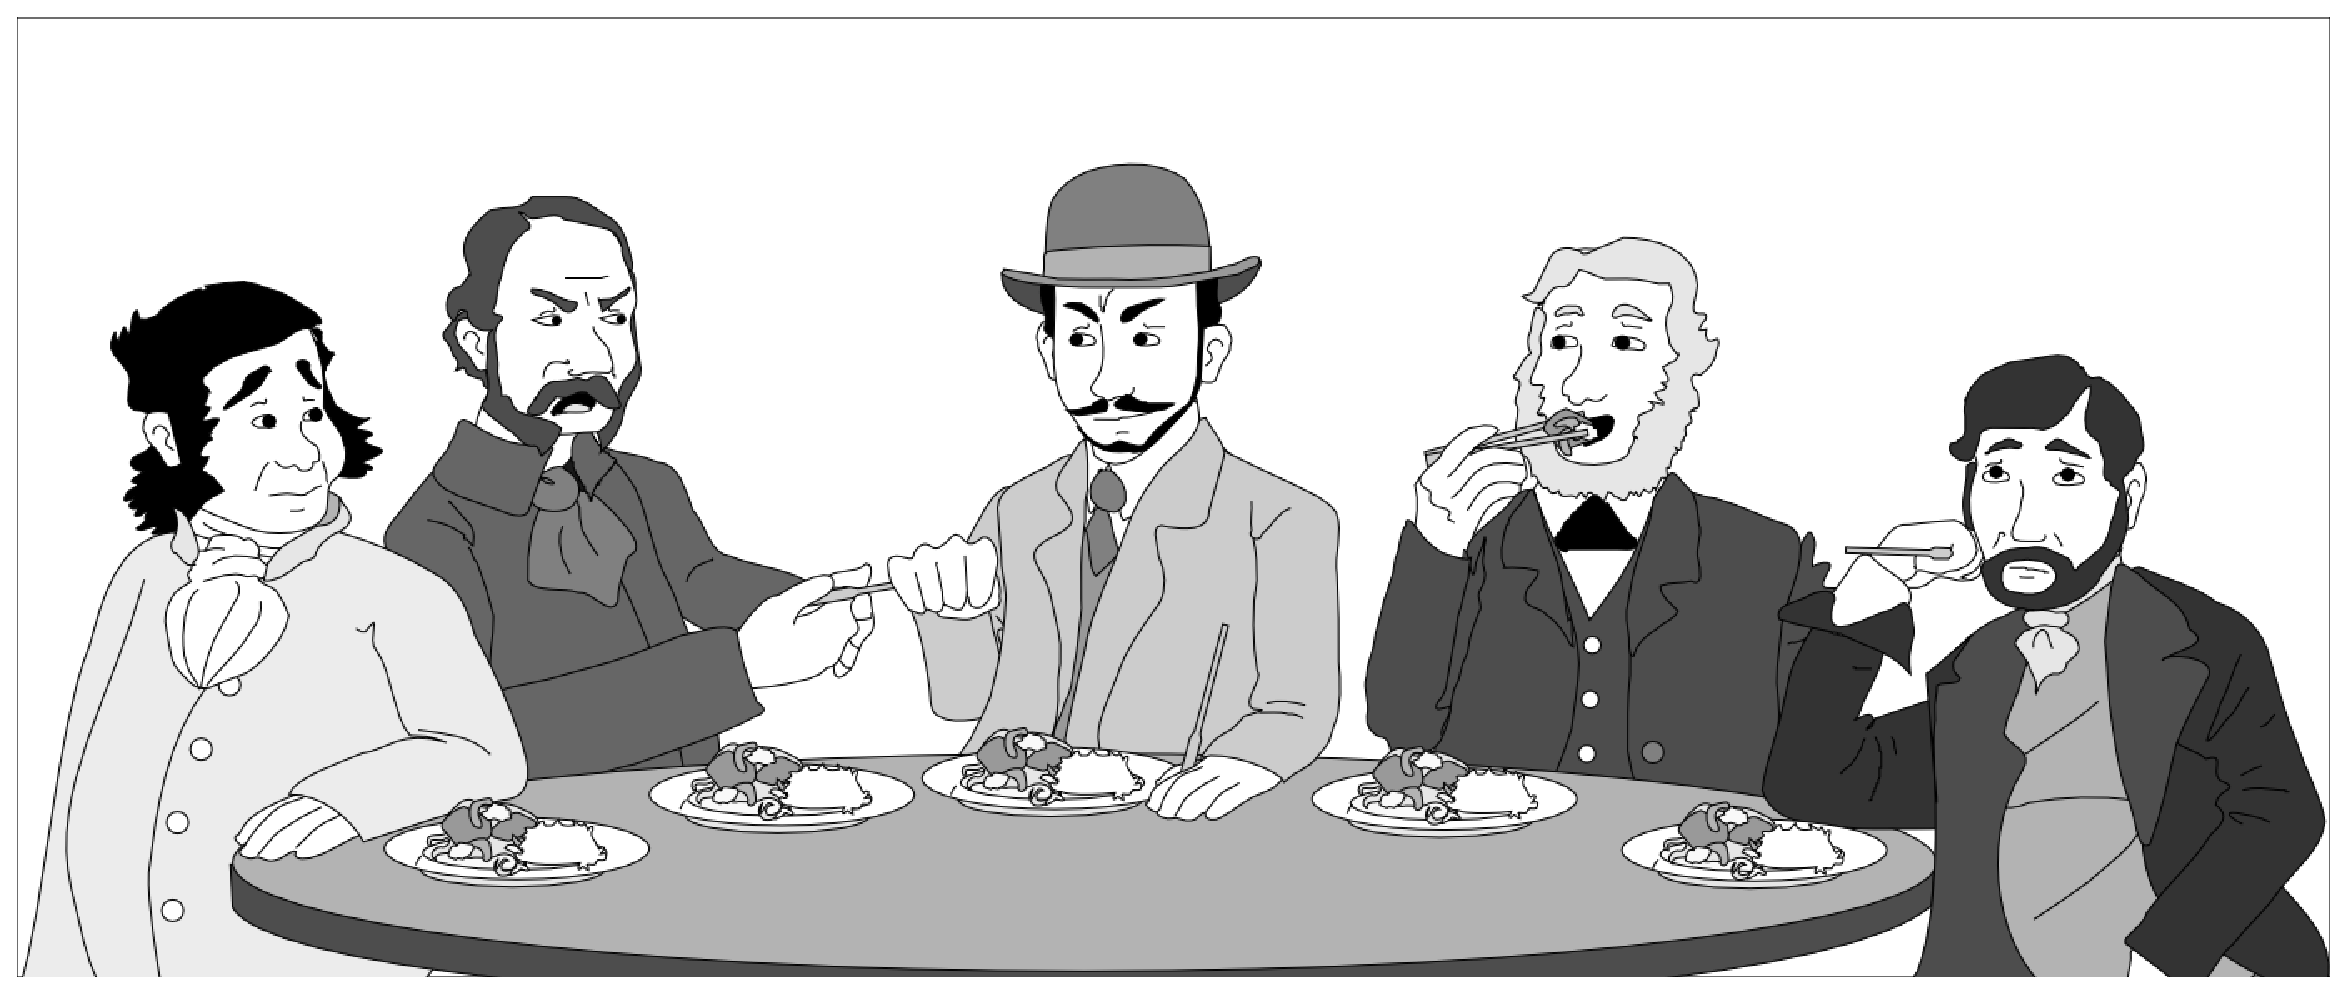
\includegraphics{cartoons/Dining-philosophers}}
\caption{Partial Starvation Is Also Bad}
\ContributedBy{Figure}{fig:cpu:Partial Starvation Is Also Bad}{Melissa Broussard}
\end{figure*}

목표는 말 그대로 기아를 방지할 수 있는 알고리즘을 만드는 것입니다.
가능한 한가지 기아 시나리오는 모든 철학자가 각자의 왼쪽 포크를 동시에 집어드는
경우입니다.
이들 중 누구도 그들이 식사를 끝내기 전까지는 자신의 포크를 내려놓지 않을
것이므로, 그리고 이들 중 누구도 이들 중 한명이라도 식사를 끝내기 전까지는
두번째 포크를 갖지 못할 것이므로, 이들은 모두 굶게 됩니다.
최소 한명의 철학자를 식사할 수 있게 하는 것만으로는 충분치 않음을 알아 두시기
바랍니다.
Figure~\ref{fig:cpu:Partial Starvation Is Also Bad} 가 보이듯, 오직 소수의
철학자가 기아에 빠지는 것조차도 방지되어야 합니다.

\iffalse

The object is to construct an algorithm that, quite literally,
prevents starvation.
One starvation scenario would be if all of the philosophers picked up
their leftmost forks simultaneously.
Because none of them will put down their fork until after they finished
eating, and because none of them may pick up their second fork until at
least one of them has finished eating, they all starve.
Please note that it is not sufficient to allow at least one philosopher
to eat.
As Figure~\ref{fig:cpu:Partial Starvation Is Also Bad}
shows, starvation of even a few of the philosophers is to be avoided.

\fi

\begin{figure}[tb]
\centering
\includegraphics[scale=.7]{SMPdesign/DiningPhilosopher5TB}
\caption{Dining Philosophers Problem, Textbook Solution}
\ContributedBy{Figure}{fig:SMPdesign:Dining Philosophers Problem, Textbook Solution}{Kornilios Kourtis}
\end{figure}

\pplsur{Edsger W.}{Dijkstra} 의 해결책은 1980년대 말 또는 1990년대 초에는
적절치 못하게 된, 무시할만한 통신 딜레이라는 가정을 적용하면 잘 동작하는 전역
세마포어를 사용했습니다.\footnote{
	2021년의 시각에서 Dijkstra 를 모욕하기는 너무도 쉽습니다, 50년이나 지난
	이야기니까요.
	여전히 Dijkstra 를 모욕해야 한다고 느끼신다면, 저는 무언가를 출판하고,
	50년을 기다린 후, \emph{여러분의} 아이디어가 그 시간동안의 시험을
	얼마나 잘 버텨냈는지 보라는 조언을 하겠습니다.}
보다 최신의 해결책은
Figure~\ref{fig:SMPdesign:Dining Philosophers Problem, Textbook Solution}
에 보인 것처럼 포크에 수를 매기는 것입니다.
각 철학자는 그 또는 그녀의 접시 옆에 있는 더 낮은 수를 가지는 포크를 집고,
그다음 다음 포크를 집습니다.
따라서, 이 그림에서 가장 위쪽에 앉은 철학자는 왼쪽 포크를 먼저 집어들고, 이어서
오른쪽 포크를 집어드는데, 나머지 철학자들은 각자의 오른쪽 포크를 먼저
집어듭니다.
두명의 철학자들이 포크~1 을 먼저 집어들려고 노력할 것이므로, 그리고 이 두
철학자들 중 한명만이 성공할 것이므로, 네명의 철학자에게 다섯개의 포크가 사용
가능하게 될 겁니다.
이 네명의 철학자 중 최소 한명은 두개의 포크를 가지게 될거고 따라서 식사를 할 수
있습니다.

\iffalse

\pplsur{Edsger W.}{Dijkstra}'s solution used a global semaphore,
which works fine assuming
negligible communications delays, an assumption that became invalid
in the late 1980s or early 1990s.\footnote{
	It is all too easy to denigrate Dijkstra from the viewpoint
	of the year 2021, more than 50 years after the fact.
	If you still feel the need to denigrate Dijkstra, my advice
	is to publish something, wait 50 years, and then see
	how well \emph{your} ideas stood the test of time.}
More recent solutions number the forks as shown in
Figure~\ref{fig:SMPdesign:Dining Philosophers Problem, Textbook Solution}.
Each philosopher picks up the lowest-numbered fork next to his or her
plate, then picks up the other fork.
The philosopher sitting in the uppermost position in the diagram thus
picks up the leftmost fork first, then the rightmost fork, while the
rest of the philosophers instead pick up their rightmost fork first.
Because two of the philosophers will attempt to pick up fork~1 first,
and because only one of those two philosophers will succeed,
there will be five forks available to four philosophers.
At least one of these four will have two forks, and will thus be able
to eat.

\fi

이 자원에 숫자를 매기고 그 숫자 순서대로 자원을 획득하는 일반적인 기법은 데드락
방지 기법으로 널리 사용되었습니다.
하지만, 모두가 배고픈데 한번에 단 한명의 철학자만이 식사를 하는 상황이 초래되는
사건의 연속을 쉽게 상상해 볼 수 있습니다:

\begin{enumerate}
    \item P2 가 포크~1 을 집어들어, P1 이 포크를 집는 걸 방지합니다.
    \item P3 가 포크~2 를 집어듭니다.
    \item P4 가 포크~3 를 집어듭니다.
    \item P5 가 포크~4 를 집어듭니다.
    \item P5 가 포크~5 를 집어들고 식사를 합니다.
    \item P5 가 포크~4 와~5 를 내려놓습니다.
    \item P4 가 포크~4 를 집어들고 식사를 합니다.
\end{enumerate}

요약하자면, 이 알고리즘은 동시에 두 철학자가 식사를 하기 충분한 것 이상의
포크가 존재함에도 불구하고 모든 철학자가 배고플 때에도 한번에 하나의 철학자만
식사를 하는 상황을 초래할 수 있습니다.
이보다 더 잘할 수 있어야 합니다!

\iffalse

This general technique of numbering resources and acquiring them in
numerical order is heavily used as a deadlock-prevention technique.
However, it is easy to imagine a sequence of events that will result
in only one philosopher eating at a time even though all are hungry:

\begin{enumerate}
    \item P2 picks up fork~1, preventing P1 from taking a fork.
    \item P3 picks up fork~2.
    \item P4 picks up fork~3.
    \item P5 picks up fork~4.
    \item P5 picks up fork~5 and eats.
    \item P5 puts down forks~4 and~5.
    \item P4 picks up fork~4 and eats.
\end{enumerate}

In short, this algorithm can result in only one philosopher eating at
a given time, even when all five philosophers are hungry,
despite the fact that there are more than enough forks for two
philosophers to eat concurrently.
It should be possible to do better than this!

\fi

\begin{figure}[tb]
\centering
\includegraphics[scale=.7]{SMPdesign/DiningPhilosopher4part-b}
\caption{Dining Philosophers Problem, Partitioned}
\ContributedBy{Figure}{fig:SMPdesign:Dining Philosophers Problem, Partitioned}{Kornilios Kourtis}
\end{figure}

한가지 해결책이
Figure~\ref{fig:SMPdesign:Dining Philosophers Problem, Partitioned}
에 그려져 있는데, 이 파티셔닝 기법을 더 잘 보이기 위해 다섯명이 아닌 네명의
철학자만 포함하고 있습니다.
여기서 위쪽과 오른쪽의 철학자들은 한쌍의 포크를 공유하며, 아래쪽과 왼쪽의
철학자는 다른 한쌍의 포크를 공유합니다.
만약 모든 철학자들이 동시에 배고파지면, 최소 두명은 항상 동시에 식사를 할 수
있습니다.
또한, 그림에 보여져 있듯이, 이 포크들은 이제 한쌍으로 묶여있을 수 있어서 두개씩
동시에 집어지고 내려놓아질 수 있게 되어, 획득과 해제 알고리즘을 단순화
시킵니다.

\iffalse

One approach is shown in
Figure~\ref{fig:SMPdesign:Dining Philosophers Problem, Partitioned},
which includes four philosophers rather than five to better illustrate the
partition technique.
Here the upper and rightmost philosophers share a pair of forks,
while the lower and leftmost philosophers share another pair of forks.
If all philosophers are simultaneously hungry, at least two will
always be able to eat concurrently.
In addition, as shown in the figure, the forks can now be bundled
so that the pair are picked up and put down simultaneously, simplifying
the acquisition and release algorithms.

\fi

\QuickQuiz{
	이 Dining Philosophers 문제에 더 나은 해결책이 있을까요?

	\iffalse

	Is there a better solution to the Dining
	Philosophers Problem?

	\fi

}\QuickQuizAnswer{
	그런 향상된 해결책 하나가
	Figure~\ref{fig:SMPdesign:Dining Philosophers Problem, Fully Partitioned}
	에 보여져 있는데, 단순히 철학자들에게 추가의 다섯개 포크를 제공하는
	것입니다.
	모든 다섯명의 철학자가 이제 동시에 식사를 할 수 있고, 어떤 철학자도
	다른 누군가를 기다릴 필요가 없습니다.
	또한, 이 방법은 무척 향상된 재앙 통제를 제공합니다.

	\iffalse

	One such improved solution is shown in
	Figure~\ref{fig:SMPdesign:Dining Philosophers Problem, Fully Partitioned},
	where the philosophers are simply provided with an additional
	five forks.
	All five philosophers may now eat simultaneously, and there
	is never any need for philosophers to wait on one another.
	In addition, this approach offers greatly improved disease control.

	\fi

\begin{figure}[tb]
\centering
\includegraphics[scale=.7]{SMPdesign/DiningPhilosopher5PEM}
\caption{Dining Philosophers Problem, Fully Partitioned}
\QContributedBy{Figure}{fig:SMPdesign:Dining Philosophers Problem, Fully Partitioned}{Kornilios Kourtis}
\end{figure}

	이 해결책은 누군가에겐 속임수처럼 보일 수도 있겠습니다만, 이런 종류의
	``속임수'' 가 많은 동시성 문제에 있어 좋은 해결책을 찾기 위한
	열쇠입니다.

	\iffalse

	This solution might seem like cheating to some, but such
	``cheating'' is key to finding good solutions to many
	concurrency problems.

	\fi

}\QuickQuizEnd

이는 ``수평 병렬성''~\cite{Inman85} 또는 ``데이터 병렬성'' 의 한 예로, 이
철학자들 쌍 간에는 어떤 의존성이 없기 때문에 그렇게 이름지어졌습니다.
수평적으로 병렬인 데이터 처리 시스템에서, 데이터의 특정 항목은 복사된
소프트웨어 컴포넌트들 중 하나에 의해서만 처리될 겁니다.

\iffalse

This is an example of ``horizontal parallelism''~\cite{Inman85}
or ``data parallelism'',
so named because there is no dependency among the pairs of philosophers.
In a horizontally parallel data-processing system, a given item of data
would be processed by only one of a replicated set of software
components.

\fi

\QuickQuiz{
	그리고 어떤 의미에서 이 ``수평적 병렬성'' 은 ``수평적'' 이라고 불릴 수
	있는 건가요?

	\iffalse

	And in just what sense can this ``horizontal parallelism'' be
	said to be ``horizontal''?

	\fi

}\QuickQuizAnswer{
	Inman 은 일반적으로 어플리케이션이 꼭대기에, 그리고 하드웨어 연결부가
	바닥에, 수직으로 그려지는 프로토콜 스택을 가지고 일하고 있었습니다.
	데이터는 이 스택의 위에서 아래로 흐릅니다.
	``수평적 병렬성'' 은 패킷을 다른 네트워크 연결부로부터 병렬로 처리하는
	반면, ``수직 병렬성'' 은 주어진 패킷을 다른 프로토콜 처리 단계로 동시에
	처리합니다.

	``수직 병렬성'' 은 또한 ``파이프라이닝'' 이라고도 불립니다.

	\iffalse

	Inman was working with protocol stacks, which are normally
	depicted vertically, with the application on top and the
	hardware interconnect on the bottom.
	Data flows up and down this stack.
	``Horizontal parallelism'' processes packets from different network
	connections in parallel, while ``vertical parallelism''
	handles different protocol-processing steps for a given
	packet in parallel.

	``Vertical parallelism'' is also called ``pipelining''.

	\fi

}\QuickQuizEnd

\subsection{Double-Ended Queue}
\label{sec:SMPdesign:Double-Ended Queue}

Double-ended queue 는 양 끝을 통해 추가되거나 제거될 수 있는 원소들의 리스트를
갖는 데이터 구조입니다~\cite{Knuth73}.
락 기반의 구현으로는 double-ended queue 의 양 끝단에서의 동시적 운용이
어려움으로 알려져 있습니다~\cite{DanGrossman2007TMGCAnalogy}.
이 섹션은 파티셔닝 설계 전략이 어떻게 합리적으로 간단한 구현에 이르게 할 수
있는지 보이고, 뒤따르는 섹션들에서는 세개의 범용 접근법을 봅니다.

\iffalse

A double-ended queue is a data structure containing a list of elements
that may be inserted or removed from either end~\cite{Knuth73}.
It has been claimed that a lock-based implementation permitting
concurrent operations on both ends of the double-ended queue is
difficult~\cite{DanGrossman2007TMGCAnalogy}.
This section shows how a partitioning design strategy can result
in a reasonably simple implementation, looking at three
general approaches in the following sections.

\fi

\subsubsection{Left- and Right-Hand Locks}
\label{sec:SMPdesign:Left- and Right-Hand Locks}

\begin{figure}[tb]
\centering
\resizebox{3in}{!}{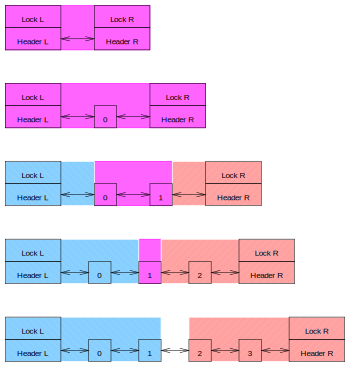
\includegraphics{SMPdesign/lockdeq}}
\caption{Double-Ended Queue With Left- and Right-Hand Locks}
\label{fig:SMPdesign:Double-Ended Queue With Left- and Right-Hand Locks}
\end{figure}

간단해 보이는 한가지 전략은 왼쪽 끝으로의 enqueue 와 dequeue 오퍼레이션을 위한
왼쪽 락과 오른쪽 끝으로의 오퍼레이션들을 위한 오른쪽 락을 갖는 doubly linked
list 를 사용하는 것으로,
Figure~\ref{fig:SMPdesign:Double-Ended Queue With Left- and Right-Hand Locks}
에 보이는 것과 같습니다.
하지만, 이 방법의 문제는 이 리스트에 네개 미만의 원소만이 존재할 때에는 이 두
락의 도메인이 겹친다는 것입니다.
이 겹침은 어떤 원소를 제거하는 것이 그 원소만이 아니라 그것의 왼쪽과 오른쪽
이웃 원소에게도 영향을 끼친다는 사실 때문입니다.
이 도메인들은 이 그림에 색깔로 표시되어 있는데, 아래쪽으로의 줄무늬를 가진
파랑은 왼쪽 락의 도메인을, 위쪽으로의 줄무늬를 가진 빨강은 오른쪽 락의
도메인을, 그리고 (줄무늬가 없는) 보라색은 겹치는 도메인을 표시합니다.
이 방식으로 동작하는 알고리즘을 만드는 것도 가능하지만, 다섯개 미만이 아닌 특수
경우들이 존재한다는 사실은 커다랗고 빨간 경고등을 띄우는데, 이 리스트의 다른
끝쪽에서의 동시의 행동들이 이 queue 를 언제든 하나의 특수 경우에서 다른 경우로
바꿀 수 있다는 점에서 특히 그렇습니다.
다른 설계를 고려하는 게 훨씬 나을 겁니다.

\iffalse

One seemingly straightforward approach would be to use a doubly
linked list with a left-hand lock
for left-hand-end enqueue and dequeue operations along with a right-hand
lock for right-hand-end operations, as shown in
Figure~\ref{fig:SMPdesign:Double-Ended Queue With Left- and Right-Hand Locks}.
However, the problem with this approach is that the two locks'
domains must overlap when there are fewer than four elements on the
list.
This overlap is due to the fact that removing any given element affects
not only that element, but also its left- and right-hand neighbors.
These domains are indicated by color in the figure, with blue
with downward stripes indicating
the domain of the left-hand lock, red with upward stripes
indicating the domain of the right-hand
lock, and purple (with no stripes) indicating overlapping domains.
Although it is possible to create an algorithm that works this way,
the fact that it has no fewer than five special cases should raise
a big red flag, especially given that concurrent activity at the other
end of the list can shift the queue from one special case to another
at any time.
It is far better to consider other designs.

\fi

\subsubsection{Compound Double-Ended Queue}
\label{sec:SMPdesign:Compound Double-Ended Queue}

\begin{figure}[tb]
\centering
\resizebox{3in}{!}{\includegraphics{SMPdesign/lockdeqpair}}
\caption{Compound Double-Ended Queue}
\label{fig:SMPdesign:Compound Double-Ended Queue}
\end{figure}

겹치지 않는 락 도메인을 강제하기 위한 한가지 방법이
Figure~\ref{fig:SMPdesign:Compound Double-Ended Queue}
에 보여져 있습니다.
두개의 double-ended queue 들이 동시에 동작하는데, 각각 자신의 락으로
보호됩니다.
이는 원소들이 결국은 한쪽 double-ended queue 에서 다른 쪽으로 옮겨져야 하며,
이때는 양쪽 락이 모두 잡혀야만 함을 의미합니다.
데드락을 방지하기 위해 간단한 락 계층이 사용될 수 있는데, 예를 들면 오른쪽 락을
잡기 전에 항상 왼쪽 락을 잡는 겁니다.
이러면 우리는 조건 없이 왼쪽 queue 에 원소를 왼쪽 집어넣기하고 오른쪽 queue 에
원소를 오른쪽 집어넣기를 할 수 있으므로, 같은 double-ended queue 에 두개의 락을
적용하는 것보다는 훨씬 간단할 것입니다.
비어있는 queue 에서 꺼내기를 하려 할 때 주요한 복잡도가 나타나는데, 이 경우에는
다음과 같은 처리가 필요합니다:

\iffalse

One way of forcing non-overlapping lock domains is shown in
Figure~\ref{fig:SMPdesign:Compound Double-Ended Queue}.
Two separate double-ended queues are run in tandem, each protected by
its own lock.
This means that elements must occasionally be shuttled from one of
the double-ended queues to the other, in which case both locks must
be held.
A simple lock hierarchy may be used to avoid deadlock, for example,
always acquiring the left-hand lock before acquiring the right-hand lock.
This will be much simpler than applying two locks to the same
double-ended queue, as we can unconditionally left-enqueue elements
to the left-hand queue and right-enqueue elements to the right-hand
queue.
The main complication arises when dequeuing from an empty queue, in
which case it is necessary to:

\fi

\begin{enumerate}
\item	오른쪽 락을 잡고 있다면, 이를 해제하고 왼쪽 락을 잡습니다.
\item	오른쪽 락을 잡습니다.
\item	두 queue 에 원소를 고르게 분배시킵니다.
\item	제거하려는 원소가 있다면 제거합니다.
\item	두 락을 모두 해제합니다.

\iffalse

\item	If holding the right-hand lock, release it and acquire the
	left-hand lock.
\item	Acquire the right-hand lock.
\item	Rebalance the elements across the two queues.
\item	Remove the required element if there is one.
\item	Release both locks.

\fi

\end{enumerate}

\QuickQuiz{
	이 compound double-ended queue 구현에서는, 이 락을 해제하고 재획득 하는
	동안에 이 queue 가 비어있지 않게 되면 어떡해야 하죠?

	\iffalse

	In this compound double-ended queue implementation, what should
	be done if the queue has become non-empty while releasing
	and reacquiring the lock?

	\fi

}\QuickQuizAnswer{
	이 경우에는, 그냥 이 비어있지 않은 큐에서 원소를 제거하고, 두 락을
	해제하고, 리턴하면 됩니다.

	\iffalse

	In this case, simply dequeue an item from the non-empty
	queue, release both locks, and return.

	\fi

}\QuickQuizEnd

이 결과로 나오는 코드는 (\path{locktdeq.c}) 상당히 간단합니다.
원소 재분배 오퍼레이션은 주어진 원소를 두 queue 사이에서 어느 쪽으로든 옮길
수도 있어서, 시간을 낭비하고, 최적의 성능을 위해선 워크로드 종속적 휴리스틱을
필요로 할 수도 있습니다.
이게 어떤 경우에는 최선의 방법이 될수도 있겠습니다만, 알고리즘을 더 큰 결정성을
가지고 시도해 보는것도 흥미로울 겁니다.

\iffalse

The resulting code (\path{locktdeq.c}) is quite straightforward.
The rebalancing operation might well shuttle a given element back
and forth between the two queues, wasting time and possibly requiring
workload-dependent heuristics to obtain optimal performance.
Although this might well be the best approach in some cases, it is
interesting to try for an algorithm with greater determinism.

\fi

\subsubsection{Hashed Double-Ended Queue}
\label{sec:SMPdesign:Hashed Double-Ended Queue}

데이터 구조를 결정론적으로 쪼개는 가장 효과적이고도 가장 간단한 방법은
해싱입니다.
각 원소에 이 리스트에서의 그것의 위치에 기반한 숫자를 부여해서 비어있는 queue
에 왼쪽으로 들어온 첫번째 원소는 0으로 수가 부여되고 비어있는 queue 에
오른쪽으로 들어온 첫번째 원소는 1이라는 수가 부여되는 식으로 double-ended
queue 를 간단히 해싱하는게 가능합니다.
왼쪽으로 들어오는 원소들은 계속해서 작아지는 수를 부여받고 ($-1$, $-2$, $-3$,
\ldots), 오른쪽으로 들어오는 원소들은 계속해서 증가하는 수를 부여받습니다 (2,
3, 4, \ldots).
핵심은, 이 숫자가 이 queue 에서의 위치를 암시하므로, 해당 원소의 수를 정말로
표현할 필요는 없다는 겁니다.

\iffalse

One of the simplest and most effective ways to deterministically
partition a data structure is to hash it.
It is possible to trivially hash a double-ended queue by assigning
each element a sequence number based on its position in the list,
so that the first element left-enqueued into an empty queue is numbered
zero and the first element right-enqueued into an empty queue is numbered
one.
A series of elements left-enqueued into an otherwise-idle queue would
be assigned decreasing numbers ($-1$, $-2$, $-3$, \ldots), while a series of
elements right-enqueued into an otherwise-idle queue would be assigned
increasing numbers (2, 3, 4, \ldots).
A key point is that it is not necessary to actually represent a given
element's number, as this number will be implied by its position in
the queue.

\fi

\begin{figure}[tb]
\centering
\resizebox{3in}{!}{\includegraphics{SMPdesign/lockdeqhash}}
\caption{Hashed Double-Ended Queue}
\label{fig:SMPdesign:Hashed Double-Ended Queue}
\end{figure}

이 방법에서는, 우리는 왼쪽 인덱스를 보호하기 위해 하나의 락을 할당하고, 오른쪽
인덱스를 위해 또다른 락을, 그리고 각 해쉬 체인을 위해 또하나의 락을 사용합니다.
Figure~\ref{fig:SMPdesign:Hashed Double-Ended Queue} 가 네개의 해쉬 체인이
있다는 가정 하에 이로 인해 만들어지는 데이터 구조를 보입니다.
락 도메인은 겹치지 않으며, 데드락은 체인 락 전에 인덱스 락을 획득함으로써
회피되며, 특정 타입의 (인덱스 또는 체인) 락은 한번에 두개 이상 획득하지
않습니다.

\iffalse

Given this approach, we assign one lock to guard the left-hand index,
one to guard the right-hand index, and one lock for each hash chain.
Figure~\ref{fig:SMPdesign:Hashed Double-Ended Queue} shows the resulting
data structure given four hash chains.
Note that the lock domains do not overlap, and that deadlock is avoided
by acquiring the index locks before the chain locks, and by never
acquiring more than one lock of a given type (index or chain) at a time.

\fi

\begin{figure}[tb]
\centering
\resizebox{3in}{!}{
\includegraphics{SMPdesign/lockdeqhash1R}}
\caption{Hashed Double-Ended Queue After Insertions}
\label{fig:SMPdesign:Hashed Double-Ended Queue After Insertions}
\end{figure}

각 해쉬 체인은 그 자체로 double-ended queue 이며, 이 예에서는 각각이 네개의
원소씩을 쥐고 있습니다.
Figure~\ref{fig:SMPdesign:Hashed Double-Ended Queue After Insertions}
의 가장 위쪽은 하나의 원소가 (``R$_1$'') 오른쪽으로 넣어지고, 해쉬 체인~2 를
참조하게끔 증가된 오른쪽 인덱스를 갖게 된 후의 상태를 보입니다.
이 그림의 가운데 부분은 세개의 원소가 추가적으로 오른쪽으로 넣어진 후의 상태를
보입니다.
보시다시피, 인덱스들은 각자의 초기 상태로 되돌아가져 있습니다
(Figure~\ref{fig:SMPdesign:Hashed Double-Ended Queue}를 보세요), 하지만 각 해시
체인은 이제 비어 있습니다.
이 그림의 아래쪽은 세개의 추가적인 원소가 왼쪽으로 들어오고 또하나의 원소가
오른쪽으로 들어온 후의 상태를 보입니다.

Figure~\ref{fig:SMPdesign:Hashed Double-Ended Queue After Insertions} 에 보인
마지막 상태로부터, 왼쪽 dequeue 오퍼레이션은 원소 ``L$_{-2}$'' 를 리턴하고,
왼쪽 인덱스가 해쉬 체인~2 를 참조하는대로 둘 것이며, 이 체인은 단 하나의
원소만을 (``R$_2$'') 가지고 있게 됩니다.
이 상태에서, 왼쪽 enqueue 가 오른쪽 enqueue 와 동시에 수행되면 락 경쟁이 발생할
겁니다만, 그런 경쟁 상태의 확률은 더 큰 해쉬 테이블을 사용함으로써 무척 낮은
수준으로 줄일 수 있습니다.

\iffalse

Each hash chain is itself a double-ended queue, and in this example,
each holds every fourth element.
The uppermost portion of
Figure~\ref{fig:SMPdesign:Hashed Double-Ended Queue After Insertions}
shows the state after a single element (``R$_1$'') has been
right-enqueued, with the right-hand index having been incremented to
reference hash chain~2.
The middle portion of this same figure shows the state after
three more elements have been right-enqueued.
As you can see, the indexes are back to their initial states
(see Figure~\ref{fig:SMPdesign:Hashed Double-Ended Queue}), however,
each hash chain is now non-empty.
The lower portion of this figure shows the state after three additional
elements have been left-enqueued and an additional element has been
right-enqueued.

From the last state shown in
Figure~\ref{fig:SMPdesign:Hashed Double-Ended Queue After Insertions},
a left-dequeue operation would return element ``L$_{-2}$'' and leave
the left-hand index referencing hash chain~2, which would then
contain only a single element (``R$_2$'').
In this state, a left-enqueue running concurrently with a right-enqueue
would result in lock contention, but the probability of such contention
can be reduced to arbitrarily low levels by using a larger hash table.

\fi

\begin{figure}[tb]
\centering
\resizebox{1.5in}{!}{
\includegraphics{SMPdesign/lockdeqhashlots}}
\caption{Hashed Double-Ended Queue With 16 Elements}
\label{fig:SMPdesign:Hashed Double-Ended Queue With 16 Elements}
\end{figure}

Figure~\ref{fig:SMPdesign:Hashed Double-Ended Queue With 16 Elements}
는 16개의 원소가 네개 해쉬 버킷 기반의 병렬 double-ended queue 에 어떻게 관리될
지 보입니다.
아랫단의 단일 락 기반 double-ended queue 각각은 전체 병렬 double-ended queue 의
1/4 조각을 갖습니다.

\iffalse

Figure~\ref{fig:SMPdesign:Hashed Double-Ended Queue With 16 Elements}
shows how 16 elements would be organized in a four-hash-bucket
parallel double-ended queue.
Each underlying single-lock double-ended queue holds a one-quarter
slice of the full parallel double-ended queue.

\fi

\begin{listing}[tbp]
\input{CodeSamples/SMPdesign/lockhdeq@struct_pdeq.fcv}
\caption{Lock-Based Parallel Double-Ended Queue Data Structure}
\label{lst:SMPdesign:Lock-Based Parallel Double-Ended Queue Data Structure}
\end{listing}

Listing~\ref{lst:SMPdesign:Lock-Based Parallel Double-Ended Queue Data Structure}
은 평범하게 락으로 관리되는 double-ended-queue 구현을 제공하는 \co{struct deq}
가 존재한다는 가정 하에 앞에서 이야기한 것에 연관되는 C-언어 데이터 구조를
보입니다.
\begin{fcvref}[ln:SMPdesign:lockhdeq:struct_pdeq]
이 데이터 구조는 라인~\lnref{llock} 에 왼쪽 락을, 라인~\lnref{lidx} 에 왼쪽
인덱스를, 라인~\lnref{rlock} 에 오른쪽 락을 (실제 구현에서는 캐쉬라인 사이즈로
정렬된), 라인~\lnref{ridx} 에 오른쪽 인덱스를, 그리고 마지막으로,
라인~\lnref{bkt} 에 간단한 락 기반 double-ended queue 의 배열을 가지고
있습니다.
고성능 구현체는 거짓 공유를 피하기 위해 패딩이나 특수한 정렬 지시어 등을 사용할
겁니다.
\end{fcvref}

\iffalse

Listing~\ref{lst:SMPdesign:Lock-Based Parallel Double-Ended Queue Data Structure}
shows the corresponding C-language data structure, assuming an
existing \co{struct deq} that provides a trivially locked
double-ended-queue implementation.
\begin{fcvref}[ln:SMPdesign:lockhdeq:struct_pdeq]
This data structure contains the left-hand lock on line~\lnref{llock},
the left-hand index on line~\lnref{lidx}, the right-hand lock on line~\lnref{rlock}
(which is cache-aligned in the actual implementation),
the right-hand index on line~\lnref{ridx}, and, finally, the hashed array
of simple lock-based double-ended queues on line~\lnref{bkt}.
A high-performance implementation would of course use padding or special
alignment directives to avoid false sharing.
\end{fcvref}

\fi

\begin{listing}[tbp]
\input{CodeSamples/SMPdesign/lockhdeq@pop_push.fcv}
\caption{Lock-Based Parallel Double-Ended Queue Implementation}
\label{lst:SMPdesign:Lock-Based Parallel Double-Ended Queue Implementation}
\end{listing}

Listing~\ref{lst:SMPdesign:Lock-Based Parallel Double-Ended Queue Implementation}
(\path{lockhdeq.c})
은 enqueue 와 dequeue 함수의 구현을 보입니다.\footnote{
	어떤 언어를 사용해서든 다양한 형태의 구현을 만들 수 있겠습니다만, 그건
	독자 여러분의 연습 문제로 남겨 두겠습니다.}
이야기는 왼쪽 오퍼레이션들에 집중할텐데, 오른쪽 오퍼레이션들은 쉽게 왼쪽의
것들로부터 나올 것이기 때문입니다.

\begin{fcvref}[ln:SMPdesign:lockhdeq:pop_push:popl]
\Clnrefrange{b}{e} 는 왼쪽 dequeue 를 하고 가능하면 원소를, 그렇지 않다면
\co{NULL} 을 리턴하는 \co{pdeq_pop_l()} 을 보입니다.
라인~\lnref{acq} 는 왼쪽 스핀락을 획득하고, 라인~\lnref{idx} 는 dequeue 될
인덱스를 계산합니다.
라인~\lnref{deque} 는 이 원소를 꺼내고, 라인~lnref{check} 에서 이 결과가
\co{NULL} 이 아닐 것으로 판명되면, 라인~\lnref{rel} 에서 락을 해제하고,
마지막으로 라인~\lnref{return} 에서 거기 원소가 있었다면 그것을, 아니면
\co{NULL} 을 리턴합니다.
\end{fcvref}

\iffalse

Listing~\ref{lst:SMPdesign:Lock-Based Parallel Double-Ended Queue Implementation}
(\path{lockhdeq.c})
shows the implementation of the enqueue and dequeue functions.\footnote{
	One could easily create a polymorphic implementation in any
	number of languages, but doing so is left as an exercise for
	the reader.}
Discussion will focus on the left-hand operations, as the right-hand
operations are trivially derived from them.

\begin{fcvref}[ln:SMPdesign:lockhdeq:pop_push:popl]
\Clnrefrange{b}{e} show \co{pdeq_pop_l()},
which left\-/dequeues and returns
an element if possible, returning \co{NULL} otherwise.
Line~\lnref{acq} acquires the left-hand spinlock,
and line~\lnref{idx} computes the
index to be dequeued from.
Line~\lnref{deque} dequeues the element, and,
if line~\lnref{check} finds the result to be
non-\co{NULL}, line~\lnref{record} records the new left-hand index.
Either way, line~\lnref{rel} releases the lock, and,
finally, line~\lnref{return} returns
the element if there was one, or \co{NULL} otherwise.
\end{fcvref}

\fi

\begin{fcvref}[ln:SMPdesign:lockhdeq:pop_push:pushl]
\Clnrefrange{b}{e} 는 특정 원소를 왼쪽으로 enqueue 하는 \co{pdeq_push_l()} 을
보입니다.
라인~\lnref{acq} 는 왼쪽 락을 획득하고, 라인~\lnref{idx} 에서 왼쪽 인덱스를
잡습니다.
라인~\lnref{enque} 는 이 원소를 이 왼쪽 인덱스로 가리켜지는 double-ended queue
에 왼쪽으로 enqueue gkqslek.
라인~\lnref{update} 는 이어서 이 왼쪽 인덱스를 업데이트 하고 라인~\lnref{rel}
에서 이 락을 해제합니다.
\end{fcvref}

앞에서도 이야기 했듯, 오른쪽 오퍼레이션들은 왼쪽의 것들과 완전히 비슷하므로,
그것들의 분석은 독자 여러분의 연습 문제로 남겨 둡니다.

\iffalse

\begin{fcvref}[ln:SMPdesign:lockhdeq:pop_push:pushl]
\Clnrefrange{b}{e} show \co{pdeq_push_l()},
which left-enqueues the specified
element.
Line~\lnref{acq} acquires the left-hand lock,
and line~\lnref{idx} picks up the left-hand
index.
Line~\lnref{enque} left-enqueues the specified element
onto the double-ended queue
indexed by the left-hand index.
Line~\lnref{update} then updates the left-hand index
and line~\lnref{rel} releases the lock.
\end{fcvref}

As noted earlier, the right-hand operations are completely analogous
to their left-handed counterparts, so their analysis is left as an
exercise for the reader.

\fi

\QuickQuiz{
	해쉬 기반의 double-ended queue 는 좋은 해결책일까요?
	왜 그렇고 왜 그렇지 않을까요?

	\iffalse

	Is the hashed double-ended queue a good solution?
	Why or why not?

	\fi

}\QuickQuizAnswer{
	여기 답변하는 최선의 방법은 여러개의 다른 멀티프로세서 시스템에서
	\path{lockhdeq.c} 를 수행해 보는 것이며, 여러분이 가능한 시간 내에
	그렇게 할 것을 장려합니다.
	걱정을 할 수 있는 한가지 이유는 이 구현에서 각 오퍼레이션은 하나가 아닌
	두개의 락을 획득해야 한다는 것입니다.

	잘 설계된 첫번째 성능 연구가 예로 들어질 겁니다.\footnote{
		Dalessandro 등의
		연구~\cite{LukeDalessandro:2011:ASPLOS:HybridNOrecSTM:deque}
		와 Dice 등의 연구~\cite{DavidDice:2010:SCA:HTM:deque} 는 훌륭한
		시작 지점이 될 겁니다.}
	순차적 구현과의 비교도 잊지 마십시오!

	\iffalse

	The best way to answer this is to run \path{lockhdeq.c} on
	a number of different multiprocessor systems, and you are
	encouraged to do so in the strongest possible terms.
	One reason for concern is that each operation on this
	implementation must acquire not one but two locks.
	% Getting about 500 nanoseconds per element when used as
	% a queue on a 4.2GHz Power system.  This is roughly the same as
	% the version covered by a single lock.  Sequential (unlocked
	% variant is more than an order of magnitude faster!

	The first well-designed performance study will be cited.\footnote{
		The studies by Dalessandro
		et al.~\cite{LukeDalessandro:2011:ASPLOS:HybridNOrecSTM:deque}
		and Dice et al.~\cite{DavidDice:2010:SCA:HTM:deque} are
		excellent starting points.}
	Do not forget to compare to a sequential implementation!

	\fi

}\QuickQuizEnd

\subsubsection{Compound Double-Ended Queue Revisited}
\label{sec:SMPdesign:Compound Double-Ended Queue Revisited}

이 섹션은 조합된 double-ended queue 를 비어 있지 않은 queue 에서 이제 비어 있는
queue 로 모든 원소를 옮기는 간단한 균형 맞추기를 사용하는 방법으로 다시
풀어봅니다.

\iffalse

This section revisits the compound double-ended queue, using a trivial
rebalancing scheme that moves all the elements from the non-empty
queue to the now-empty queue.

\fi

\QuickQuiz{
	빈 queue 로 \emph{모든} 원소를 옮긴다구요?
	이 미친 해결책이 대체 어떤 세상에서는 최적인거죠???

	\iffalse

	Move \emph{all} the elements to the queue that became empty?
	In what possible universe is this brain-dead solution in any
	way optimal???

	\fi

}\QuickQuizAnswer{
	데이터 흐름의 방향이 가끔씩만 바뀌는 경우에 최적입니다.
	이 double-ended queue 가 동시에 양 끝에서 비워지는 경우엔 물론 무척
	안좋은 선택일 겁니다.
	이는 물론 다른 질문을 떠오르게 하는데, 양끝에서 동시에 비우기를 하는건
	대체 어떤 세상에서 합리적인 일이겠냐는 겁니다.
	이 질문에 대한 가능한 답 중 하나는 work stealing queue 입니다.

	\iffalse

	It is optimal in the case where data flow switches direction only
	rarely.
	It would of course be an extremely poor choice if the double-ended
	queue was being emptied from both ends concurrently.
	This of course raises another question, namely, in what possible
	universe emptying from both ends concurrently would be a reasonable
	thing to do.
	Work-stealing queues are one possible answer to this question.

	\fi

}\QuickQuizEnd

앞의 섹션에서 보인 해쉬 기반 구현과 대조적으로, 이 조합 구현은 락도 어토믹
오퍼레이션도 사용하지 않는 순차적 구현의 double-ended queue 위에서 구현될
겁니다.

\iffalse

In contrast to the hashed implementation presented in
the previous section, the compound implementation will build on
a sequential implementation of a double-ended queue that uses
neither locks nor atomic operations.

\fi

\begin{listing}[tbp]
\input{CodeSamples/SMPdesign/locktdeq@pop_push.fcv}
\caption{Compound Parallel Double-Ended Queue Implementation}
\label{lst:SMPdesign:Compound Parallel Double-Ended Queue Implementation}
\end{listing}

Listing~\ref{lst:SMPdesign:Compound Parallel Double-Ended Queue Implementation}
이 이 구현을 보이고 있습니다.
해쉬 기반의 구현과 달리, 이 조합 구현은 비대칭적이어서, \co{pdeq_pop_l()} 과
\co{pdeq_pop_r()} 구현을 별개로 봐야만 합니다.

\iffalse

Listing~\ref{lst:SMPdesign:Compound Parallel Double-Ended Queue Implementation}
shows the implementation.
Unlike the hashed implementation, this compound implementation is
asymmetric, so that we must consider the \co{pdeq_pop_l()}
and \co{pdeq_pop_r()} implementations separately.

\fi

\QuickQuiz{
	조합된 병렬 double-ended queue 구현은 왜 대칭적일 수 없죠?

	\iffalse

	Why can't the compound parallel double-ended queue
	implementation be symmetric?

	\fi

}\QuickQuizAnswer{
	락 계층을 사용해 데드락을 회피해야한다는 필요성이 비대칭성을
	강제하는데, 식사하는 철학자들 문제의 포크 번호 매기기 해결책과 같은
	것입니다
	(Section~\ref{sec:SMPdesign:Dining Philosophers Problem} 을
	참고하세요).

	\iffalse

	The need to avoid deadlock by imposing a lock hierarchy
	forces the asymmetry, just as it does in the fork-numbering
	solution to the Dining Philosophers Problem
	(see Section~\ref{sec:SMPdesign:Dining Philosophers Problem}).

	\fi

}\QuickQuizEnd

\begin{fcvref}[ln:SMPdesign:locktdeq:pop_push:popl]
\co{pdeq_pop_l()} 구현이 이 코드의 \clnrefrange{b}{e} 에 보여져 있습니다.
라인~\lnref{acq:l} 은 왼쪽 락을 획득하는데, 이 락은 라인~\lnref{rel:l} 에서
해제됩니다.
라인~\lnref{deq:ll} 은 아랫단의 double-ended queue 의 왼쪽으로부터 원소를
빼내려 시도하고, 이게 성공하면 간단히 이 원소를 리턴하기 위해
\clnrefrange{acq:r}{skip} 을 건너뜁니다.
그렇지 않다면, 라인~\lnref{acq:r} 은 오른쪽 락을 획득하고, 라인~\lnref{deq:lr}
에서 오른쪽 queue 로부터 원소를 왼쪽 꺼내기 하고 라인~\lnref{move} 에서 오른쪽
queue 의 모든 남아있는 원소를 왼쪽 queue 로 옮기며, 라인~\lnref{init:r} 에서
오른쪽 queue 를 초기화 하고, 라인~\lnref{rel:r} 에서 이 오른쪽 락을 해제합니다.
만약 존재한다면 라인~\lnref{deq:lr} 에서 dequeue 된 원소가 리턴됩니다.
\end{fcvref}

\iffalse

\begin{fcvref}[ln:SMPdesign:locktdeq:pop_push:popl]
The \co{pdeq_pop_l()} implementation is shown on
\clnrefrange{b}{e}
of the listing.
Line~\lnref{acq:l} acquires the left-hand lock,
which line~\lnref{rel:l} releases.
Line~\lnref{deq:ll} attempts to left-dequeue an element
from the left-hand underlying
double-ended queue, and, if successful,
skips \clnrefrange{acq:r}{skip} to simply
return this element.
Otherwise, line~\lnref{acq:r} acquires the right-hand lock, line~\lnref{deq:lr}
left-dequeues an element from the right-hand queue,
and line~\lnref{move} moves any remaining elements on the right-hand
queue to the left-hand queue, line~\lnref{init:r} initializes
the right-hand queue,
and line~\lnref{rel:r} releases the right-hand lock.
The element, if any, that was dequeued on line~\lnref{deq:lr} will be returned.
\end{fcvref}

\fi

\begin{fcvref}[ln:SMPdesign:locktdeq:pop_push:popr]
\co{pdeq_pop_r()} 구현이 이 코드의 \clnrefrange{b}{e} 에 보여져 있습니다.
전과 같이, 라인~\lnref{acq:r1} 은 이 오른쪽 락을 획득하고 (그리고
라인~\lnref{rel:r2} 에서 이를 해제합니다), 라인~\lnref{deq:rr1} 에서 오른쪽
queue 로부터 원소 하나를 오른쪽 꺼내기 하려 시도하고, 만약 성공한다면 이 원소를
단순히 리턴하기 위해 \clnrefrange{rel:r1}{skip2} 를 건너뜁니다.
하지만, 라인~\lnref{check1} 이 dequeue 할 원소가 존재하지 않았음을 알아내면
라인~\lnref{rel:r1} 은 이 오른쪽 락을 해제하고 \clnrefrange{acq:l}{acq:r2} 가
올바른 순서로 두 락을 잡습니다.
라인~\lnref{deq:rr2} 는 이제 오른쪽 queue 로부터 원소 하나를 다시 오른쪽 꺼내기
하려 시도하고, 라인~\lnref{check2} 가 이 두번째 시도가 실패했음을 확인하면,
라인~\lnref{deq:rl} 은 왼쪽 queue 로부터 원소 하나를 오른쪽 dequeue 하고
(원소가 있었다면), 라인~\lnref{move} 는 모든 남아있는 원소들을 왼쪽 queue
로부터 오른쪽 queue 로 옮기고, 라인~\lnref{init:l} 은 왼쪽 queue 를 초기화
합니다.
어떻게 되었든, 라인~\lnref{rel:l} 은 왼쪽 락을 해제합니다.
\end{fcvref}

\iffalse

\begin{fcvref}[ln:SMPdesign:locktdeq:pop_push:popr]
The \co{pdeq_pop_r()} implementation is shown on \clnrefrange{b}{e}
of the listing.
As before, line~\lnref{acq:r1} acquires the right-hand lock
(and line~\lnref{rel:r2}
releases it), and line~\lnref{deq:rr1} attempts to right-dequeue an element
from the right-hand queue, and, if successful,
skips \clnrefrange{rel:r1}{skip2}
to simply return this element.
However, if line~\lnref{check1} determines that there was no element to dequeue,
line~\lnref{rel:r1} releases the right-hand lock and
\clnrefrange{acq:l}{acq:r2} acquire both
locks in the proper order.
Line~\lnref{deq:rr2} then attempts to right-dequeue an element
from the right-hand
queue again, and if line~\lnref{check2} determines that this second attempt has
failed, line~\lnref{deq:rl} right-dequeues an element from the left-hand queue
(if there is one available), line~\lnref{move} moves any remaining elements
from the left-hand queue to the right-hand queue, and line~\lnref{init:l}
initializes the left-hand queue.
Either way, line~\lnref{rel:l} releases the left-hand lock.
\end{fcvref}

\fi

\QuickQuizSeries{%
\QuickQuizB{
	Listing~\ref{lst:SMPdesign:Compound Parallel Double-Ended Queue Implementation}
	의 라인~\ref{ln:SMPdesign:locktdeq:pop_push:popr:deq:rr2}
	에서의 오른쪽 dequeue 재시도가 왜 필요하죠?

	\iffalse

	Why is it necessary to retry the right-dequeue operation
	on line~\ref{ln:SMPdesign:locktdeq:pop_push:popr:deq:rr2} of
	Listing~\ref{lst:SMPdesign:Compound Parallel Double-Ended Queue Implementation}?

	\fi

}\QuickQuizAnswerB{
	\begin{fcvref}[ln:SMPdesign:locktdeq:pop_push:popr]
	이 쓰레드가 라인~\lnref{rel:r1} 에서 \co{d->rlock} 을 내려놓고
	라인~\lnref{acq:r2} 에서 이 락을 다시 획득하는 사이에 다른 쓰레드가
	원소를 하나 enqueue 했을 수도 있기 때문에 이 재시도가 필요합니다.
	\end{fcvref}

	\iffalse

	\begin{fcvref}[ln:SMPdesign:locktdeq:pop_push:popr]
	This retry is necessary because some other thread might have
	enqueued an element between the time that this thread dropped
	\co{d->rlock} on line~\lnref{rel:r1} and the time that it reacquired this
	same lock on line~\lnref{acq:r2}.
	\end{fcvref}

	\fi

}\QuickQuizEndB
%
\QuickQuizE{
	분명 왼쪽 락은 \emph{가끔은} 획득 가능할 거예요!!!
	그런데도 왜
	Listing~\ref{lst:SMPdesign:Compound Parallel Double-Ended Queue Implementation}
	의 라인~\ref{ln:SMPdesign:locktdeq:pop_push:popr:rel:r1}
	에서는 무조건적으로 오른쪽 락을 해제해야 하는 거죠?

	\iffalse

	Surely the left-hand lock must \emph{sometimes} be available!!!
	So why is it necessary that
        line~\ref{ln:SMPdesign:locktdeq:pop_push:popr:rel:r1} of
	Listing~\ref{lst:SMPdesign:Compound Parallel Double-Ended Queue Implementation}
	unconditionally release the right-hand lock?

	\fi

}\QuickQuizAnswerE{
	왼쪽 락을 획득 가능할 때 획득하기 위해서 \co{spin_trylock()} 을
	사용하는 것도 가능할 겁니다.
	하지만, 그 실패의 경우에는 여전히 이 오른쪽 락을 내려놓고 두 락을
	제대로 된 순서로 다시 획득해야 할 겁니다.
	이 변화를 만드는 것은 (그리고 이게 그럴 가치가 있는지 알아내는 것은)
	독자 여러분의 연습문제로 남겨두겠습니다.

	\iffalse

	It would be possible to use \co{spin_trylock()} to attempt
	to acquire the left-hand lock when it was available.
	However, the failure case would still need to drop the
	right-hand lock and then re-acquire the two locks in order.
	Making this transformation (and determining whether or not
	it is worthwhile) is left as an exercise for the reader.

	\fi

}\QuickQuizEndE
}

\begin{fcvref}[ln:SMPdesign:locktdeq:pop_push:pushl]
\co{pdeq_push_l()} 구현이
Listing~\ref{lst:SMPdesign:Compound Parallel Double-Ended Queue Implementation}
의 \clnrefrange{b}{e} 에 보여져 있습니다.
라인~\lnref{acq:l} 은 왼쪽 스핀락을 획득하고, 라인~\lnref{que:l} 은 이 원소를
왼쪽 큐에 왼쪽으로 집어넣고, 마지막으로 라인~\lnref{rel:l} 은 이 락을
해제합니다.
\end{fcvref}
\begin{fcvref}[ln:SMPdesign:locktdeq:pop_push:pushr]
\co{pdeq_push_r()} 구현은 (\clnrefrange{b}{e} 에 보여져 있습니다) 상당히
비슷합니다.
\end{fcvref}

\iffalse

\begin{fcvref}[ln:SMPdesign:locktdeq:pop_push:pushl]
The \co{pdeq_push_l()} implementation is shown on
\clnrefrange{b}{e} of
Listing~\ref{lst:SMPdesign:Compound Parallel Double-Ended Queue Implementation}.
Line~\lnref{acq:l} acquires the left-hand spinlock,
line~\lnref{que:l} left-enqueues the
element onto the left-hand queue, and finally line~\lnref{rel:l} releases
the lock.
\end{fcvref}
\begin{fcvref}[ln:SMPdesign:locktdeq:pop_push:pushr]
The \co{pdeq_push_r()} implementation (shown on \clnrefrange{b}{e})
is quite similar.
\end{fcvref}

\fi

\QuickQuiz{
	하지만 데이터가 한 방향으로만 흐르는 경우에,
	Listing~\ref{lst:SMPdesign:Compound Parallel Double-Ended Queue Implementation}
	에 보인 알고리즘은 마지막 원소를 가져가서 아랫단의 double-ended queue
	를 비울 때마다 양 끝단이 같은 락을 획득하려 할 겁니다.
	이는 이 알고리즘이 양 끝단으로 동시의 액세스를 제공하는 것이 이 queue
	가 상당히 큰 수의 원소를 가지고 있을 때조차 실패할 수 있음을 의미하지
	않나요?

	\iffalse

	But in the case where data is flowing in only one direction,
	the algorithm shown in
	Listing~\ref{lst:SMPdesign:Compound Parallel Double-Ended Queue Implementation}
	will have both ends attempting to acquire the same lock
	whenever the consuming end empties its underlying
	double-ended queue.
	Doesn't that mean that sometimes this algorithm fails to
	provide concurrent access to both ends of the queue even
	when the queue contains an arbitrarily large number of elements?

	\fi

}\QuickQuizAnswer{
	실제로 그렇습니다!

	하지만 같은 속성을 가지고 있다고 하는 다른 알고리즘들도 마찬가지입니다.
	예를 들어, 락들의 해쉬 배열을 사용하는 소프트웨어 트랜잭셔널 메모리
	메커니즘을 사용하는 해결책들에서는 가장 왼쪽과 가장 오른쪽 원소들의
	주소가 가끔은 같은 락에 해쉬되는 경우가 있을 겁니다.
	이런 해쉬 충돌 역시 동시의 액세스를 방지할 겁니다.
	다른 예를 하나 들어보자면, 소프트웨어 fallback 을 갖추고 하드웨어
	트랜잭셔널 메모리 메커니즘을 사용하는
	해결책에서는~\cite{Yoo:2013:PEI:2503210.2503232,RickMerrit2011PowerTM,ChristianJacobi2012MainframeTM}
	이 소프트웨어 fallback 내에서 락킹을 종종 사용할 것이고, 따라서 무엇이
	되었든 이 락킹 해결책이 겪는 한계만큼 한계를 겪을 겁니다 (비록 뜸하긴
	하길 바랍니다만).

	따라서 2021년 기준으로, compound double-ended queue 를 포함한 동시의
	double-ended queue 문제를 위한 모든 실용적 해결책은 적어도 어떤
	환경에서는 완전한 동시성을 제공하지 못합니다.

	\iffalse

	Indeed it does!

	But the same is true of other algorithms claiming this property.
	For example, in solutions using software transactional memory
	mechanisms based on hashed arrays of locks,
	the leftmost and rightmost elements' addresses will sometimes
	happen to hash to the same lock.
	These hash collisions will also prevent concurrent access.
	For another example, solutions using hardware transactional
	memory mechanisms with software
	fallbacks~\cite{Yoo:2013:PEI:2503210.2503232,RickMerrit2011PowerTM,ChristianJacobi2012MainframeTM}
	often use locking within those software fallbacks, and thus
	suffer (albeit hopefully rarely) from whatever concurrency
	limitations that these locking solutions suffer from.

	Therefore, as of 2021, all practical solutions to the
	concurrent double-ended queue problem fail to provide full
	concurrency in at least some circumstances, including the
	compound double-ended queue.

	\fi

}\QuickQuizEnd

\subsubsection{Double-Ended Queue Discussion}
\label{sec:SMPdesign:Double-Ended Queue Discussion}

이 compound 구현은
Section~\ref{sec:SMPdesign:Hashed Double-Ended Queue}
에서 보인 해쉬 기반 구현에 비해 약간 복잡합니다만, 여전히 간단합니다.
물론, 더 영리한 균형맞추기 방법은 더 복잡할 수 있겠습니다만, 여기 보인 이
간단한 방법은 소프트웨어 대체제에
비해서도~\cite{LukeDalessandro:2011:ASPLOS:HybridNOrecSTM:deque}, 심지어
하드웨어의 도움을 받는 알고리즘에 비해서도~\cite{DavidDice:2010:SCA:HTM:deque}
성능이 좋은 것으로 드러났습니다.
그러나, 이런 방법에 있어 우리가 바랄 수 있는 최선은 두배의 확장성으로, 최대
두개의 쓰레드가 dequeue 의 락을 동시에 잡고 있을 수 있기 때문입니다.
이 한계는 또한 Michael 의 compare-and-swap 기반의 것과
같은~\cite{DBLP:conf/europar/Michael03} non-blocking 동기화 기반의 알고리즘에도
적용됩니다.\footnote{
	이 논문은 특수한 double-compare-and-swap (DCAS) 인스트럭션이
	double-ended queue 의 lock-free 구현을 만드는 데 필요하지 않음을
	보였다는 점에서 흥미롭습니다.
	대신, 흔한 compare-and-swap (예: x86 cmpxchg) 으로도 충분합니다.}

\iffalse

The compound implementation is somewhat more complex than the
hashed variant presented in
Section~\ref{sec:SMPdesign:Hashed Double-Ended Queue},
but is still reasonably simple.
Of course, a more intelligent rebalancing scheme could be arbitrarily
complex, but the simple scheme shown here has been shown to
perform well compared to software
alternatives~\cite{LukeDalessandro:2011:ASPLOS:HybridNOrecSTM:deque}
and even compared to algorithms using hardware
assist~\cite{DavidDice:2010:SCA:HTM:deque}.
Nevertheless, the best we can hope for from such a scheme
is 2x scalability, as at most two threads can be holding the
dequeue's locks concurrently.
This limitation also applies to algorithms based on non-blocking
synchronization, such as the compare-and-swap-based dequeue algorithm of
Michael~\cite{DBLP:conf/europar/Michael03}.\footnote{
	This paper is interesting in that it showed that special
	double-compare-and-swap (DCAS) instructions are not needed
	for lock-free implementations of double-ended queues.
	Instead, the common compare-and-swap (e.g., x86 cmpxchg)
	suffices.}

\fi

\QuickQuiz{
	Double-ended queue 문제에는 왜 한개가 아니라 두개의 해결책이 있는 거죠?

	\iffalse

	Why are there not one but two solutions to the double-ended queue
	problem?

	\fi

}\QuickQuizAnswer{
	사실은 최소 세개의 해결책이 있습니다.
	Dominik Dingel 의 것인 그 세번째 해결책은 reader-writer 락킹을 흥미로운
	방식으로 사용하며, \path{lockrwdeq.c} 에서 찾을 수 있을 겁니다.

	\iffalse

	There are actually at least three.
	The third, by Dominik Dingel, makes interesting use of
	reader-writer locking, and may be found in \path{lockrwdeq.c}.

	\fi

}\QuickQuizEnd

사실, Dice 등에 의해 이야기된 것처럼~\cite{DavidDice:2010:SCA:HTM:deque},
동기화 되지 않은 싱글쓰레드 기반 double-ended queue 는 그들이 연구한 어떤 병렬
구현들보다도 상당히 성능이 좋습니다.
따라서, 핵심은 공유된 queue 에 enqueue, dequeue 하는 데에는 그 구현과 관계 없이
상당한 오버헤드가 있을 수 있다는 것입니다.
이는 Chapter~\ref{chp:Hardware and its Habits} 에서 이야기한 것들을 놓고 생각해
보면, 이 queue 의 엄격한 first-in-first-out (FIFO) 특성을 놓고 볼 때, 전혀
놀랍지 않을 겁니다.

\iffalse

In fact, as noted by Dice et al.~\cite{DavidDice:2010:SCA:HTM:deque},
an unsynchronized single-threaded double-ended queue significantly
outperforms any of the parallel implementations they studied.
Therefore, the key point is that there can be significant overhead enqueuing to
or dequeuing from a shared queue, regardless of implementation.
This should come as no surprise in light of the material in
Chapter~\ref{chp:Hardware and its Habits}, given the strict
first-in-first-out (FIFO) nature of these queues.

\fi

더 나아가서, 이 엄격한 FIFO queue 는 사실 사용자에게 보이는 \emph{linearization
point}~\cite{Herlihy:1990:LCC:78969.78972}\footnote{
	짧게 요약해서, linearization point 는 어떤 함수의 내에서 이 함수가
	영향을 만들어 냈다고 말할 수 있는 하나의 지점입니다.
	이 락 기반의 구현에서, linearization point 는 이 크리티컬 섹션 내의
	모든 곳이라고 할 수 있습니다.}
에 대해서만 엄격한 FIFO 이며 이 예제에서는 이 linearization point 가 락
크리티컬 섹션 내에 여럿 있습니다.
이 queue 들은 (예를 들어) 각 개별 오퍼레이션이 시작된 시점에 대해서는 엄격한
FIFO 가 아닙니다~\cite{AndreasHaas2012FIFOisnt}.
이는 동시성 프로그램에서는 엄격한 FIFO 특성이 전혀 가치 있지 않음을 의미하며,
실제로 Kirsch 등은 향상된 성능과 확장성을 제공하는 덜 엄격한 queue 를
선보였습니다~\cite{ChristophMKirsch2012FIFOisntTR}.\footnote{
	Nir Shavit 은 대략 같은 이유로 완화된 스택을
	만들었습니다~\cite{Shavit:2011:DSM:1897852.1897873}.
	이 상황은 어떤 사람들을 linearization point 는 이론가들에겐 유용하지만
	개발자들에겐 그렇지 않다고 믿게 만들고, 그런 자료 구조와 알고리즘의
	설계자들이 얼마나 그들의 사용자들의 실제 필요를 고려했을지 의심하게
	만듭니다.}
그렇게 이야기 했지만, 여러분이 여러분의 동시성 프로그램이 사용하는 모든
데이터를 하나의 queue 로 보낸다면, 여러분은 여러분의 전체 설계를 다시 생각해
봐야 합니다.

\iffalse

Furthermore, these strict FIFO queues are strictly FIFO only with
respect to
\emph{linearization points}~\cite{Herlihy:1990:LCC:78969.78972}\footnote{
	In short, a linearization point is a single point within a given
	function where that function can be said to have taken effect.
	In this lock-based implementation, the linearization points
	can be said to be anywhere within the critical section that
	does the work.}
that are not visible to the caller, in fact, in these examples,
the linearization points are buried in the lock-based critical
sections.
These queues are not strictly FIFO with respect to (say) the times at which
the individual operations started~\cite{AndreasHaas2012FIFOisnt}.
This indicates that the strict FIFO property is not all that valuable
in concurrent programs, and in fact, Kirsch et al.\ present less-strict
queues that provide improved performance and
scalability~\cite{ChristophMKirsch2012FIFOisntTR}.\footnote{
	Nir Shavit produced relaxed stacks for roughly the same
	reasons~\cite{Shavit:2011:DSM:1897852.1897873}.
	This situation leads some to believe that the linearization
	points are useful to theorists rather than developers, and
	leads others to wonder to what extent the designers of such
	data structures and algorithms were considering the needs
	of their users.}
All that said, if you are pushing all the data used by your concurrent
program through a single queue, you really need to rethink your
overall design.

\fi

\subsection{Partitioning Example Discussion}
\label{sec:SMPdesign:Partitioning Example Discussion}

The optimal solution to the dining philosophers problem given in
the answer to the Quick Quiz in
Section~\ref{sec:SMPdesign:Dining Philosophers Problem}
is an excellent example of ``horizontal parallelism'' or
``data parallelism''.
The synchronization overhead in this case is nearly (or even exactly)
zero.
In contrast, the double-ended
queue implementations are examples of ``vertical parallelism'' or
``pipelining'', given that data moves from one thread to another.
The tighter coordination required for pipelining in turn requires
larger units of work to obtain a given level of efficiency.

\QuickQuizSeries{%
\QuickQuizB{
	The tandem double-ended queue runs about twice as fast as
	the hashed double-ended queue, even when I increase the
	size of the hash table to an insanely large number.
	Why is that?
}\QuickQuizAnswerB{
	The hashed double-ended queue's locking design only permits
	one thread at a time at each end, and further requires
	two lock acquisitions for each operation.
	The tandem double-ended queue also permits one thread at a time
	at each end, and in the common case requires only one lock
	acquisition per operation.
	Therefore, the tandem double-ended queue should be expected to
	outperform the hashed double-ended queue.

	Can you create a double-ended queue that allows multiple
	concurrent operations at each end?
	If so, how?  If not, why not?
}\QuickQuizEndB
%
\QuickQuizE{
	Is there a significantly better way of handling concurrency
	for double-ended queues?
}\QuickQuizAnswerE{
	One approach is to transform the problem to be solved
	so that multiple double-ended queues can be used in parallel,
	allowing the simpler single-lock double-ended queue to be used,
	and perhaps also replace each double-ended queue with a pair of
	conventional single-ended queues.
	Without such ``horizontal scaling'', the speedup is limited
	to 2.0.
	In contrast, horizontal-scaling designs can achieve very large
	speedups, and are especially attractive if there are multiple threads
	working either end of the queue, because in this
	multiple-thread case the dequeue
	simply cannot provide strong ordering guarantees.
	After all, the fact that a given thread removed an item first
	in no way implies that it will process that item
	first~\cite{AndreasHaas2012FIFOisnt}.
	And if there are no guarantees, we may as well obtain the
	performance benefits that come with refusing to provide these
	guarantees.
	% about twice as fast as hashed version on 4.2GHz Power.

	Regardless of whether or not the problem can be transformed
	to use multiple queues, it is worth asking whether work can
	be batched so that each enqueue and dequeue operation corresponds
	to larger units of work.
	This batching approach decreases contention on the queue data
	structures, which increases both performance and scalability,
	as will be seen in
	Section~\ref{sec:SMPdesign:Synchronization Granularity}.
	After all, if you must incur high synchronization overheads,
	be sure you are getting your money's worth.

	Other researchers are working on other ways to take advantage
	of limited ordering guarantees in
	queues~\cite{ChristophMKirsch2012FIFOisntTR}.
}\QuickQuizEndE
}

These two examples show just how powerful partitioning can be in
devising parallel algorithms.
Section~\ref{sec:SMPdesign:Locking Granularity and Performance}
looks briefly at a third example, matrix multiply.
However, all three of these examples beg for more and better design
criteria for parallel programs, a topic taken up in the next section.


% SMPdesign/criteria.tex
% SPDX-License-Identifier: CC-BY-SA-3.0

\section{Design Criteria}
\label{sec:SMPdesign:Design Criteria}

최고의 성능과 확장성을 얻는 방법 중 하나는 달성 가능한 최고의 병렬 프로그램이
만들어 질 때까지 해킹을 계속하는 것입니다.
하지만, 여러분의 프로그램이 현미경으로 봐야할 정도로 작지 않은 한, 가능한 병렬
프로그램의 공간은 우주의 수명이라는 거대한 시간 동안에도 최고의 달성 가능한
프로그램에 이르기를 보장하지 못할 정도로 커다랗습니다.
그리고 또, ``달성 가능한 최고의 병렬 프로그램'' 이란 무엇일까요?
어쨌든, Section~\ref{sec:intro:Parallel Programming Goals} 에서는 성능, 생산성,
그리고 범용성의 세가지 병렬 프로그래밍 목표를 이야기 했고, 달성 가능한 최고의
병렬 프로그램은 생산성과 범용성에의 비용으로 다가올 확률이 큽니다.
프로그램이 너무 구식이 되기 전에 충분히 받아들여질만큼 좋은 병렬 프로그램
정도는 되도록 하기 위해, 우리는 설계 단계에서 높은 수준에서의 선택들을 할 수
있어야 합니다.
\iffalse

One way to obtain the best performance and scalability is to simply
hack away until you converge on the best possible parallel program.
Unfortunately, if your program is other than microscopically tiny,
the space of possible parallel programs is so huge
that convergence is not guaranteed in the lifetime of the universe.
Besides, what exactly is the ``best possible parallel program''?
After all, Section~\ref{sec:intro:Parallel Programming Goals}
called out no fewer than three parallel-programming goals of
performance, productivity, and generality,
and the best possible performance will likely come at a cost in
terms of productivity and generality.
We clearly need to be able to make higher-level choices at design
time in order to arrive at an acceptably good parallel program
before that program becomes obsolete.
\fi

하지만, 정말로 실제 세계의 설계를 하기 위해선 디자인 규범들이 필요한데, 이
섹션에서 다룰 것입니다.
실제 세계에서, 이 규범들은 종종 더 크거나 작은 정도에서 충돌하므로, 설계자들은
그로 인한 트레이드오프들을 잘 균형 맞춰야 합니다.

이 규범들은 그 자체로써 설계에 동작하는 ``힘''들로 생각될 수 있으며, 특히 이런
힘들 간의 좋은 트레이드오프들은 ``디자인 패턴''~\cite{Alexander79,GOF95} 이라
불릴 수 있을 것입니다.

세개의 병렬 프로그래밍 목표들을 얻기 위한 디자인 규범들은 속도 향상, 경쟁,
오버헤드, 읽기-쓰기 비율, 그리고 복잡도입니다:
\iffalse

However, more detailed design criteria are required to
actually produce a real-world design, a task taken up in this section.
This being the real world, these criteria often conflict to a
greater or lesser degree, requiring that the designer carefully
balance the resulting tradeoffs.

As such, these criteria may be thought of as the ``forces''
acting on the design, with particularly good tradeoffs between
these forces being called ``design patterns''~\cite{Alexander79,GOF95}.

The design criteria for attaining the three parallel-programming goals
are speedup,
contention, overhead, read-to-write ratio, and complexity:
\fi
\begin{description}
\item[Speedup:]  Section~\ref{sec:intro:Parallel Programming Goals} 에서
	이야기했듯, 성능이야말로 우리가 대부분의 시간을 할애해야 하는 곳이고
	병렬화를 해야 하는 문제입니다.
	속도 향상은 순차적 버전의 프로그램을 돌리는데 드는 시간 대비 병렬
	버전을 돌리는데 드는 시간 사이의 비율입니다.
\item[Contention:]  더 많은 CPU 들이 한 병렬 프로그램에 사용되면 그 프로그램에
	의해 CPU들이 바삐 일하게 될 것이고, 여분의 CPU들은 다른 CPU들과의
	경쟁으로 인해 유의미한 일을 하지 못하게 되어버립니다.
	이런 경쟁은 락 경쟁, 메모리 경쟁, 또는 다른 성능 문제 부분으로부터의
	것일 수도 있습니다.
\iffalse

\item[Speedup:]  As noted in
	Section~\ref{sec:intro:Parallel Programming Goals},
	increased performance is the major reason
	to go to all of the time and trouble
	required to parallelize it.
	Speedup is defined to be the ratio of the time required
	to run a sequential version of the program to the time
	required to run a parallel version.
\item[Contention:]  If more CPUs are applied to a parallel
	program than can be kept busy by that program,
	the excess CPUs are prevented from doing
	useful work by contention.
	This may be lock contention, memory contention, or a host
	of other performance killers.
\fi
\item[Work-to-Synchronization Ratio:]  유니프로세서, 싱글쓰레드, preemption
	불가, 그리고 인터럽트 불가\footnote{
		인터럽트 마스킹을 하거나 그것들을 감지하지 못해서.}
	한 버전의 병렬 프로그램은 어떤 동기화 도구들도 필요가 없을 겁니다.
	따라서, 이런 도구들 (커뮤니케이션 캐시 미스, 메세지 응답시간, 락킹
	도구, 어토믹 인스트럭션들, 그리고 메모리 배리어 등) 에 의해 소모되는
	시간은 프로그램이 완수하려 의도한 유용한 일에 직접적으로 도움을 주지
	않는 오버헤드일 뿐입니다.
	중요하게 측정해 봐야 할 것은 동기화 오버헤드와 크리티컬 섹션 코드의
	오버헤드 사이의 관계로, 더 큰 크리티컬 섹션은 더 큰 동기화 오버헤드를
	정당화 시킴을 알아두시기 바랍니다.
	일 대비 동기화 비율은 동기화 효율성과 연관됩니다.
\iffalse

\item[Work-to-Synchronization Ratio:]  A uniprocessor,
	single\-/threaded, non-preemptible, and non\-/interruptible\footnote{
		Either by masking interrupts or by being oblivious to them.}
	version of a given parallel
	program would not need any synchronization primitives.
	Therefore, any time consumed by these primitives
	(including communication cache misses as well as
	message latency, locking primitives, atomic instructions,
	and memory barriers)
	is overhead that does not contribute directly to the useful
	work that the program is intended to accomplish.
	Note that the important measure is the
	relationship between the synchronization overhead
	and the overhead of the code in the critical section, with larger
	critical sections able to tolerate greater synchronization overhead.
	The work-to-synchronization ratio is related to
	the notion of synchronization efficiency.
\fi
\item[Read-to-Write Ratio:]  아주 가끔만 업데이트 되는 데이터 구조체는
	분할되기보다는 복제가 될 수 있을 것이고, 더 나아가서 쓰는 쪽에 부담을
	주는 대신 읽는 쪽의 동기화 오버헤드를 완화시켜주는 비대칭적 동기화
	도구를 사용해서 보호하는 식으로 전체 동기화 오버헤드를 줄일 수 있을
	것입니다.
	관련된 최적화들은 Chapter~\ref{chp:Counting} 에서 이야기 되었듯 자주
	업데이트 되는 데이터 구조체에도 적용될 수 있습니다.
\iffalse

\item[Read-to-Write Ratio:]  A data structure that is
	rarely updated may often be replicated rather than partitioned,
	and furthermore may be protected with asymmetric
	synchronization primitives that reduce readers' synchronization
	overhead at the expense of that of writers, thereby
	reducing overall synchronization overhead.
	Corresponding optimizations are possible for frequently
	updated data structures, as discussed in
	Chapter~\ref{chp:Counting}.
\fi
\item[Complexity:]  병렬 프로그램은 똑같은 일을 하는 순차적 프로그램에 비해
	복잡한데, 병렬 프로그램은 순차적 프로그램에 비해 훨씬 큰 상태 공간을
	갖기 때문입니다만, 충분한 질서와 구조가 주어진다면 이 상태 공간도 쉽게
	이해될 수 있긴 합니다.
	병렬 프로그램을 만드는 사람은 이 커다란 상태 공간의 문맥에서 동기화
	도구들, 메세지, 락킹 설계, 크리티컬 섹션 식별, 그리고 데드락을 고려해야
	합니다.

	이 거대한 복잡도는 종종 높은 개발 / 유지 비용으로 변환됩니다.
	따라서, 예산의 제한이 존재하는 프로그램에서는 가할 수 있는 변경의 수와
	종류를 제한할 수 있는데, 속도 향상은 많은 시간과 문제를 개선할 때에만
	가치가 있기 때문입니다.
	더 나쁜 것은, 추가된 복잡도가 실제로 성능과 확장성을 \emph{줄일} 수
	있다는 것입니다.

	따라서, 어떤 특정한 지점 이후부터는 병렬화보다는 더 싸고 효과적인
	순차적 최적화가 잠재하고 있을 수 있습니다.
	Section~\ref{sec:intro:Performance} 에서 이야기 했듯, 병렬화는 많은
	성능 최적화 방법 중 하나일 뿐이고, 더 나아가서 CPU 기반 병목 문제에
	적용될 수 있는 최적화입니다.
\iffalse

\item[Complexity:]  A parallel program is more complex than
	an equivalent sequential program because the parallel
	program has a much larger state space than does the
	sequential program, although these larger state spaces
	can in some cases be easily understood given sufficient
	regularity and structure.
	A parallel programmer must
	consider synchronization primitives, messaging, locking design,
	critical-section identification,
	and deadlock in the context of this larger state space.

	This greater complexity often translates
	to higher development and maintenance costs.
	Therefore, budgetary constraints can
	limit the number and types of modifications made to
	an existing program, since a given degree of speedup is
	worth only so much time and trouble.
	Worse yet, added complexity can actually \emph{reduce}
	performance and scalability.

	Therefore, beyond a certain point,
	there may be potential sequential optimizations
	that are cheaper and more effective than parallelization.
	As noted in
	Section~\ref{sec:intro:Performance},
	parallelization is but one performance optimization of
	many, and is furthermore an optimization that applies
	most readily to CPU-based bottlenecks.
\fi
\end{description}
이런 규범들은 최대의 속도향상을 위해 함께 동작할 것입니다.
앞의 세개의 규범들은 깊게 관계되어 있으므로, 이 섹션의 뒷부분은 이 상호관계에
대해 분석해 보겠습니다.\footnote{
	실제 세계의 병렬 시스템은 많은 디자인 규범들에 반하는 사례가 있을
	것인데, 데이터 구조체 레이아웃, 메모리 사이즈, 메모리 구조 대기시간,
	대역폭 제한, I/O 문제등이 그것입니다.}
\iffalse

These criteria will act together to enforce a maximum speedup.
The first three criteria are deeply interrelated, so
the remainder of this section analyzes these
interrelationships.\footnote{
	A real-world parallel system will be subject to many additional
	design criteria, such as data-structure layout,
	memory size, memory-hierarchy latencies, bandwidth limitations,
	and I/O issues.}
\fi

이런 규범들은 또한 요구사항의 일부분으로 나타날 수도 있음을 알아 두십시오.
예를 들어, 속도 향상은 상대적 요구사항으로 (``더 빠르게, 더 좋게'') 나올 수도
있고 워크로드의 절대적 요구사항으로 (``시스템은 최소한 초당 1,000,000 웹 힛을
지원해야 한다'') 나올 수도 있습니다.
고전의 디자인 패턴 언어들은 상대적 요구사항을 효력으로, 그리고 절대적
요구사항을 문맥으로 이야기 합니다.

이 디자인 규범들 사이의 관계에 대한 이해는 병렬 프로그램을 위한 적절한 설계
트레이드오프를 정하는 데에 많은 도움이 될 수 있을 겁니다.
\iffalse

Note that these criteria may also appear as part of the requirements
specification.
For example, speedup may act as a relative desideratum
(``the faster, the better'')
or as an absolute requirement of the workload (``the system
must support at least 1,000,000 web hits per second'').
Classic design pattern languages describe relative desiderata as forces
and absolute requirements as context.

An understanding of the relationships between these design criteria can
be very helpful when identifying appropriate design tradeoffs for a
parallel program.
\fi
\begin{enumerate}
\item	프로그램이 크리티컬 섹션들에서 더 적은 시간을 보낼수록, 잠재적인 속도
	향상은 커집니다.
	이는 Amdhal 의 법칙~\cite{GeneAmdahl1967AmdahlsLaw} 과, 주어진 시간
	동안 크리티컬 섹션은 오로지 하나의 CPU 에서만 실행될 수 있다는 사실로
	인한 결과입니다.

	더 자세히 이야기 하자면, 특정한 갯수의 CPU 들에서 실제 성능 향상을 얻기
	위해선, 프로그램이 배타적 크리티컬 섹션에서 소모하는 시간의 비율은 CPU
	들의 수의 역수보다 작아야 합니다.
	예를 들어, 10 개의 CPU 들을 사용하는 프로그램은 잘 확장하기 위해선 가장
	제한적인 크리티컬 섹션에서 자신의 전체 시간 중 10분의 1 미만을 사용해야
	합니다.
\item	경쟁은 많은 CPU 그리고/또는 실제 시간을 소모할 것이어서 실제 성능
	향상은 사용 가능한 CPU 들의 수보다 작을 겁니다.
	CPU 들의 수와 실제 속도 향상 사이의 차이가 클수록, CPU 들은 더
	비효율적으로 사용될 겁니다.
	유사하게, 원하는 효율성이 클수록 얻을 수 있는 속도 향상은 줄어들
	겁니다.
\iffalse

\item	The less time a program spends in critical sections,
	the greater the potential speedup.
	This is a consequence of Amdahl's Law~\cite{GeneAmdahl1967AmdahlsLaw}
	and of the fact that only one CPU may execute within a given
	critical section at a given time.

	More specifically, the fraction of time that the program spends in
	a given exclusive critical section must be much less than
	the reciprocal of the number of CPUs for the
	actual speedup to approach the number of CPUs.
	For example, a program running on 10 CPUs must spend
	much less than one tenth of its time in the most-restrictive
	critical section if it is to scale at all well.
\item	Contention effects will consume the excess CPU and/or
	wallclock time should the actual speedup be less than
	the number of available CPUs.  The
	larger the gap between the number of CPUs
	and the actual speedup, the less efficiently the
	CPUs will be used.
	Similarly, the greater the desired efficiency, the smaller
	the achievable speedup.
\fi
\item	사용 가능한 동기화 도구들이 그것들이 지키는 크리티컬 섹션들에 비해 높은
	오버헤드를 갖는다면, 속도 향상을 개선하는 최선의 방법은 그 도구들이
	사용되는 횟수를 줄이는 것입니다 (크리티컬 섹션들을 합치거나, 데이터
	소유권을 사용하거나, 비대칭적으로 도구를
	사용하거나(Section~\ref{chp:Deferred Processing} 을 참고하세요), 코드
	락킹과 같이 더 큰 단위를 사용하는 디자인 으로 옮겨가거나 하는
	방법으로).
\item	만약 크리티컬 섹션들이 그것들을 지키는 도구들에 비해 높은 오버헤드를
	갖는다면, 속도 향상을 개선하는 최선의 방법은 reader/writer 락킹, 데이터
	락킹, 비대칭적, 또는 데이터 소유권을 사용하는 쪽으로 옮겨가서 병렬성을
	높이는 것입니다.
\item	크리티컬 섹션들이 그것들을 지키는 도구들에 비해 높은 오버헤드를 갖고
	보호되는 데이터 구조체에는 수정보다 읽기가 훨씬 많이 수행된다면,
	병렬성을 높이는 최고의 방법은 reader/writer 락킹이나 비대칭적 도구들을
	사용하는 것입니다.
\item	SMP 성능을 개선하는 많은 변경들, 예를 들어 락 경쟁을 줄이는 것은 실시간
	응답시간도 향상시킵니다~\cite{PaulMcKenney2005h}.
\iffalse

\item	If the available synchronization primitives have
	high overhead compared to the critical sections
	that they guard, the best way to improve speedup
	is to reduce the number of times that the primitives
	are invoked (perhaps by batching critical sections,
	using data ownership, using asymmetric primitives
	(see Section~\ref{chp:Deferred Processing}),
	or by moving toward a more coarse-grained design
	such as code locking).
\item	If the critical sections have high overhead compared
	to the primitives guarding them, the best way
	to improve speedup is to increase parallelism
	by moving to reader/writer locking, data locking, asymmetric,
	or data ownership.
\item	If the critical sections have high overhead compared
	to the primitives guarding them and the data structure
	being guarded is read much more often than modified,
	the best way to increase parallelism is to move
	to reader/writer locking or asymmetric primitives.
\item	Many changes that improve SMP performance, for example,
	reducing lock contention, also improve real-time
	latencies~\cite{PaulMcKenney2005h}.
\fi
\end{enumerate}

\QuickQuiz{}
	크리티컬 섹션과 관련한 이 모든 문제들은 우리가 크리티컬 섹션이 아예
	없는 non-blocking 동기화~\cite{MauriceHerlihy90a}를 사용해야 한다는
	의미는 아닌가요?
	\iffalse

	Don't all these problems with critical sections mean that
	we should just always use
	non-blocking synchronization~\cite{MauriceHerlihy90a},
	which don't have critical sections?
	\fi
\QuickQuizAnswer{
	Non-blocking 동기화는 일부 상황에서는 매우 유용할 수 있지만,
	만병통치약은 아닙니다.
	또한, non-blocking 동기화는 Josh Triplett 에 의해 이야기되었듯 실제로는
	크리티컬 섹션을 갖습니다.
	예를 들어, compare-and-swap 오퍼레이션에 기반한 한 non-blocking
	알고리즘에서, 최초의 로드로 시작해 compare-and-swap 으로 이어지는
	코드는 여러면에서 락 기반의 크리티컬 섹션과 유사합니다.
	\iffalse

	Although non-blocking synchronization can be very useful
	in some situations, it is no panacea.
	Also, non-blocking synchronization really does have
	critical sections, as noted by Josh Triplett.
	For example, in a non-blocking algorithm based on
	compare-and-swap operations, the code starting at the
	initial load and continuing to the compare-and-swap
	is in many ways analogous to a lock-based critical section.
	\fi
} \QuickQuizEnd


\section{Synchronization Granularity}
\label{sec:SMPdesign:Synchronization Granularity}

\begin{figure}[tb]
\begin{center}
\includegraphics{SMPdesign/LockGranularity}
\end{center}
\caption{Design Patterns and Lock Granularity}
\label{fig:SMPdesign:Design Patterns and Lock Granularity}
\end{figure}

Figure~\ref{fig:SMPdesign:Design Patterns and Lock Granularity} 는 서로 다른
동기화 빈도의 단계를 그림으로 보여주는데, 각각의 단계는 뒤의 섹션에서 다루어질
것입니다.
이 섹션들은 주로 락킹에 중점을 맞춥니다만, 비슷한 빈도 문제가 모든 동기화
문제에 깔려 있습니다.
\iffalse

Figure~\ref{fig:SMPdesign:Design Patterns and Lock Granularity}
gives a pictorial view of different levels of synchronization granularity,
each of which is described in one of the following sections.
These sections focus primarily on locking, but similar granularity
issues arise with all forms of synchronization.
\fi

\subsection{Sequential Program}
\label{sec:SMPdesign:Sequential Program}

프로그램이 싱글 프로세서 위에서 충분히 빨리 돌아간다면, 그리고 다른
프로세스들이나 쓰레드, 또는 인터럽트 핸들러들과의 상호작용이 없다면, 동기화
기능들을 모두 제거해서 그것들의 오버헤드와 복잡성을 당신으로부터 떼어놓기
바랍니다.
몇년 전에는, Moore 의 법칙이 결국은 모든 프로그램을 이 카테고리로 만들 것이라
주장하던 사람들도 있었습니다.
하지만,
% @@@ Intel Trademark
Figure~\ref{fig:SMPdesign:Clock-Frequency Trend for Intel CPUs} 에서 볼 수
있듯이, 싱글 쓰레드의 성능의 기하급수적인 증가는 2003년 정도에 멈췄습니다.
따라서, 성능을 늘리기 위해선 병렬성을 필요로 할 것입니다.\footnote{
	이 그림은 이론적으로 클락당 하나 이상의 인스트럭션들을 처리할 수 있는
	최신 CPU 들의 경우 클락 주파수를, 그리고 하나의 간단한 인스트럭션을
	처리하는데 여러 클락을 필요로 하는 오래된 CPU 들의 경우 MIPS 를
	보입니다.
	이런 접근을 취하는 이유는 클락당 여러 인스트럭션들을 처리하는 최신 CPU
	들의 기능들은 일반적으로 메모리 시스템 성능에 제한되기 때문입니다.}
이 새로운 트렌드가 수천개의 CPU 들을 갖는 하나의 칩을 나타나게 할 것인지에 대한
논쟁은 금방 끝나지 않겠지만, Paul 이 이 문장을 듀얼코어 랩탑으로 쓰고 있다는
점을 볼 때, SMP 의 시대는 우리에게 와 있는 것으로 보입니다.
이더넷 대역폭이
Figure~\ref{fig:SMPdesign:Ethernet Bandwidth vs. Intel x86 CPU Performance}
에서 볼 수 있듯이 지속적으로 성장하고 있음을 알아두는 것 역시 중요합니다.
이런 추세는 커뮤니케이션 부하를 처리하기 위해 멀티쓰레드 서버들이 나타나도록
촉진하는 역할을 할 것입니다.
\iffalse

If the program runs fast enough on a single processor, and
has no interactions with other processes, threads, or interrupt
handlers, you should
remove the synchronization primitives and spare yourself their
overhead and complexity.
Some years back, there were those who would argue that Moore's Law
would eventually force all programs into this category.
However,
% @@@ Intel Trademark
as can be seen in
Figure~\ref{fig:SMPdesign:Clock-Frequency Trend for Intel CPUs},
the exponential increase in single-threaded performance halted in
about 2003.
Therefore,
increasing performance will increasingly require parallelism.\footnote{
	This plot shows clock frequencies for newer CPUs theoretically
	capable of retiring one or more instructions per clock, and MIPS for
	older CPUs requiring multiple clocks to execute even the
	simplest instruction.
	The reason for taking this approach is that the newer CPUs'
	ability to retire multiple instructions per clock is typically
	limited by memory-system performance.}
The debate as to whether this new trend will result in single chips
with thousands
of CPUs will not be settled soon, but given that Paul is typing this
sentence on a dual-core laptop, the age of SMP does seem to be upon us.
It is also important to note that Ethernet bandwidth is continuing
to grow, as shown in
Figure~\ref{fig:SMPdesign:Ethernet Bandwidth vs. Intel x86 CPU Performance}.
This growth will motivate multithreaded servers in order to handle
the communications load.
\fi

\begin{figure}[htb]
\begin{center}
\resizebox{3in}{!}{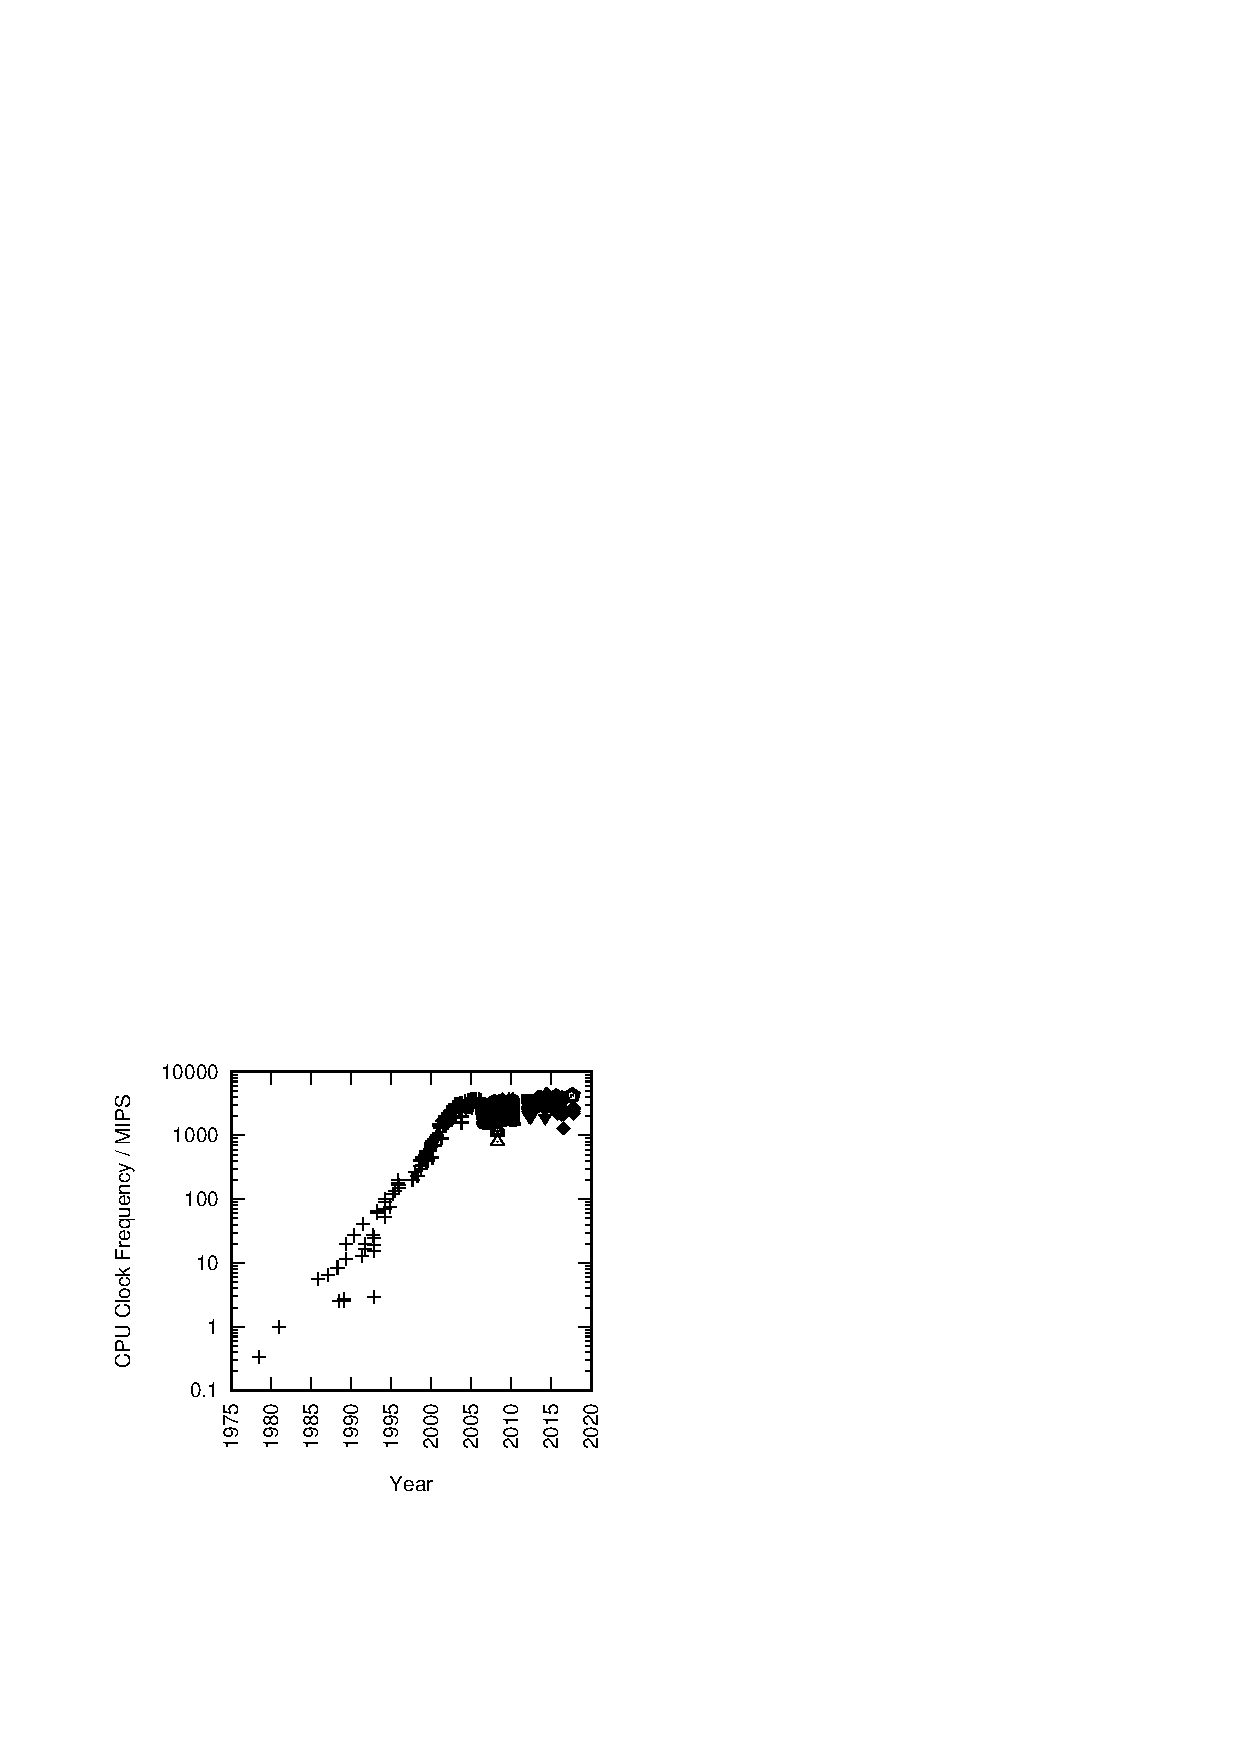
\includegraphics{SMPdesign/clockfreq}}
\end{center}
\caption{MIPS/Clock-Frequency Trend for Intel CPUs}
\label{fig:SMPdesign:Clock-Frequency Trend for Intel CPUs}
\end{figure}

\begin{figure}[htb]
\begin{center}
\resizebox{3in}{!}{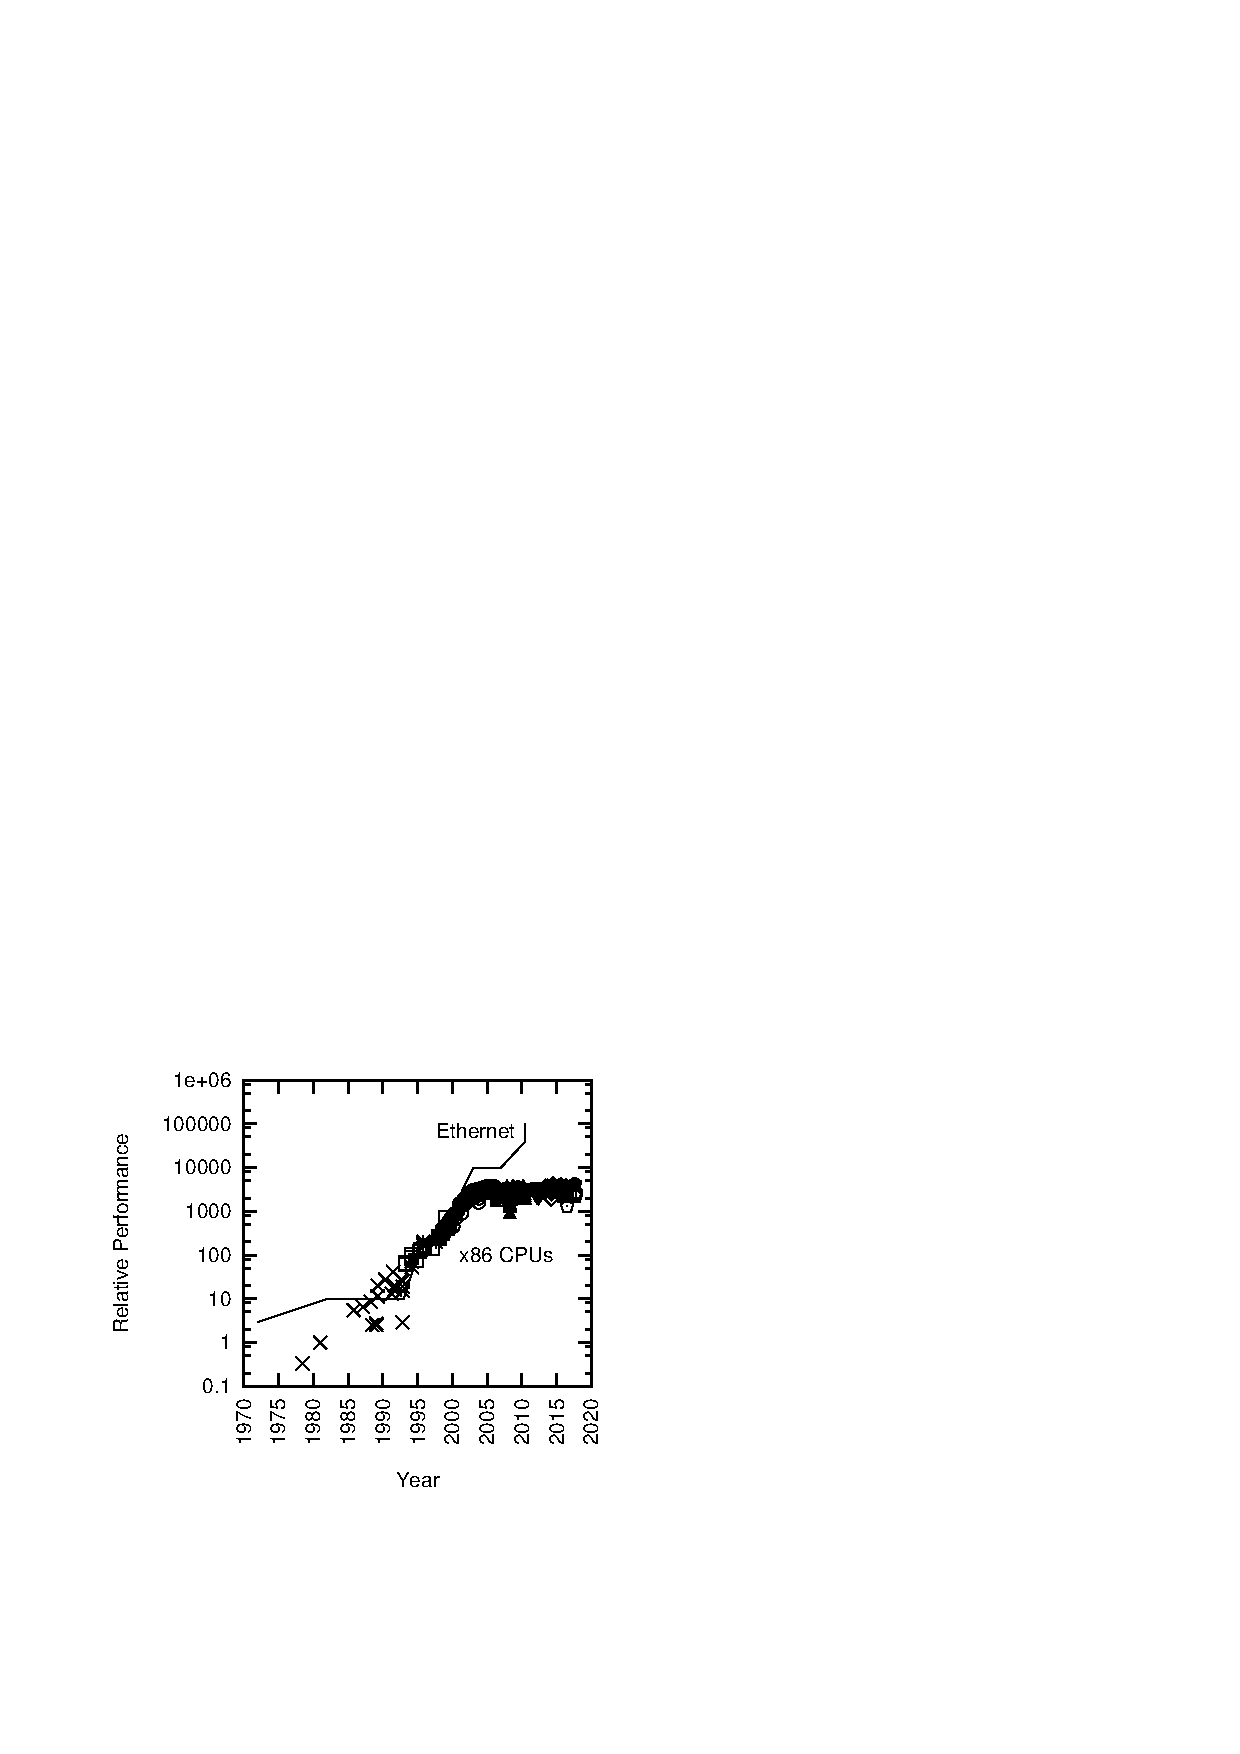
\includegraphics{SMPdesign/CPUvsEnet}}
\end{center}
\caption{Ethernet Bandwidth vs. Intel x86 CPU Performance}
\label{fig:SMPdesign:Ethernet Bandwidth vs. Intel x86 CPU Performance}
\end{figure}

이는 당신이 모든 프로그램을 멀티쓰레드 방식으로 코딩해야 한다는 의미가
\emph{아닙니다}.
다시 말하지만, 프로그램이 싱글 프로세서에서 충분히 빨리 동작한다면, SMP 동기화
기능들의 오버헤드와 복잡성으로부터 당신을 멀리 하십시오.
Figure~\ref{fig:SMPdesign:Sequential-Program Hash Table Search} 에 나와 있는
해시 테이블 탐색 코드의 단순성이 이 점을 강조합니다.\footnote{
이 섹션의 예들은 Hart 등~\cite{ThomasEHart2006a} 으로부터 얻어졌으며, 여러
	파일들로부터 관련된 코드를 모음으로써 켱쾌함을 위해 적용되었습니다.}
키 포인트는 병렬성으로 인한 속도향상은 CPU 들의 갯수에 제한된다는 것입니다.
반면, 예컨대 조심스럽게 선택된 데이터 구조와 같은 순차적 최적화를 통한
속도향상은 얼마든지 클 수 있습니다.
\iffalse

Please note that this does \emph{not} mean that you should code each
and every program in a multi-threaded manner.
Again, if a program runs quickly enough on a single processor,
spare yourself the overhead and complexity of SMP synchronization
primitives.
The simplicity of the hash-table lookup code in
Figure~\ref{fig:SMPdesign:Sequential-Program Hash Table Search}
underscores this point.\footnote{
	The examples in this section are taken from Hart et
	al.~\cite{ThomasEHart2006a}, adapted for clarity
	by gathering related code from multiple files.}
A key point is that speedups due to parallelism are normally
limited to the number of CPUs.
In contrast, speedups due to sequential optimizations, for example,
careful choice of data structure, can be arbitrarily large.
\fi

\begin{figure}[htbp]
{ \scriptsize
\begin{verbatim}
  1 struct hash_table
  2 {
  3   long nbuckets;
  4   struct node **buckets;
  5 };
  6
  7 typedef struct node {
  8   unsigned long key;
  9   struct node *next;
 10 } node_t;
 11
 12 int hash_search(struct hash_table *h, long key)
 13 {
 14   struct node *cur;
 15
 16   cur = h->buckets[key % h->nbuckets];
 17   while (cur != NULL) {
 18     if (cur->key >= key) {
 19       return (cur->key == key);
 20     }
 21     cur = cur->next;
 22   }
 23   return 0;
 24 }
\end{verbatim}
}
\caption{Sequential-Program Hash Table Search}
\label{fig:SMPdesign:Sequential-Program Hash Table Search}
\end{figure}

% ./test_hash_null.exe 1000 0/100 1 1024 1
% ./test_hash_null.exe: nmilli: 1000 update/total: 0/100 nelements: 1 nbuckets: 1024 nthreads: 1
% ./test_hash_null.exe: avg = 96.2913  max = 98.2337  min = 90.4095  std = 2.95314
% ./test_hash_null.exe: nmilli: 1000 update/total: 0/100 nelements: 1 nbuckets: 1024 nthreads: 1
% ./test_hash_null.exe: avg = 91.5592  max = 97.3315  min = 89.9885  std = 2.88925
% ./test_hash_null.exe: nmilli: 1000 update/total: 0/100 nelements: 1 nbuckets: 1024 nthreads: 1
% ./test_hash_null.exe: avg = 93.3568  max = 106.162  min = 89.8828  std = 6.40418

반면, 이런 행복한 상황에 처해 있는 게 아니라면, 계속 읽으세요!
\iffalse

On the other hand, if you are not in this happy situation, read on!
\fi

\subsection{Code Locking}
\label{sec:SMPdesign:Code Locking}

코드 락킹은 글로벌 락들만을 사용하기 때문에 상당히 간단합니다.\footnote{
	그게 아니라 데이터 구조체 안에 락들을 가지고 있거나, 자바의 경우,
	synchronized 인스턴스로 클래스들을 사용한다면,
	Section~\ref{sec:SMPdesign:Data Locking} 에 설명된 ``데이터 락킹'' 을
	사용하고 있는 겁니다.}
이 방법은 기존의 프로그램을 컬티 프로세서 위에서 동작하도록 하기 위해 코드
락킹을 사용하도록 수정하는 것은 특히 쉽습니다.
만약 프로그램이 하나의 공유자원만을 가지고 있다면, 코드 락킹은 최적의 성능을
제공할 것입니다.
하지만, 많은 거대하고 복잡한 프로그램들은 많은 수행이 크리티컬 섹션에서
일어나야만 할 것을 요구하고, 이는 곧 코드 락킹이 그 확장성을 크게 제한하게 하는
결과를 초래합니다.
\iffalse

Code locking is quite simple due to the fact that is uses only
global locks.\footnote{
	If your program instead has locks in data structures,
	or, in the case of Java, uses classes with synchronized
	instances, you are instead using ``data locking'', described
	in Section~\ref{sec:SMPdesign:Data Locking}.}
It is especially
easy to retrofit an existing program to use code locking in
order to run it on a multiprocessor.  If the program has
only a single shared resource, code locking will even give
optimal performance.
However, many of the larger and more complex programs
require much of the execution to
occur in critical sections, which in turn causes code locking
to sharply limits their scalability.
\fi

따라서, 전체 실행시간 중 작은 부분만을 크리티컬 섹션에서 수행하거나 작은
확장성만이 필요한 프로그램들에 대해서만 코드 락킹을 사용해야 합니다.
이런 경우, 코드 락킹은
Figure~\ref{fig:SMPdesign:Code-Locking Hash Table Search} 에서 볼 수 있듯,
순차적인 버전과 매우 유사하고 상대적으로 간단한 프로그램을 제공할 것입니다.
하지만, Figure~\ref{fig:SMPdesign:Sequential-Program Hash Table Search} 의
\co{hash_search()} 에서의 단순한 비교값 리턴은 이제 리턴 전에 락을 풀어야 하기
때문에 세개의 문장이 되었음을 알아 두시기 바랍니다.
\iffalse

Therefore, you should use code locking on programs that spend
only a small fraction of their execution time in critical sections or
from which only modest scaling is required.  In these cases,
code locking will provide a relatively simple program that is
very similar to its sequential counterpart,
as can be seen in
Figure~\ref{fig:SMPdesign:Code-Locking Hash Table Search}.
However, note that the simple return of the comparison in
\co{hash_search()} in
Figure~\ref{fig:SMPdesign:Sequential-Program Hash Table Search}
has now become three statements due to the need to release the
lock before returning.
\fi

\begin{figure}[htbp]
{ \scriptsize
\begin{verbatim}
  1 spinlock_t hash_lock;
  2
  3 struct hash_table
  4 {
  5   long nbuckets;
  6   struct node **buckets;
  7 };
  8
  9 typedef struct node {
 10   unsigned long key;
 11   struct node *next;
 12 } node_t;
 13
 14 int hash_search(struct hash_table *h, long key)
 15 {
 16   struct node *cur;
 17   int retval;
 18
 19   spin_lock(&hash_lock);
 20   cur = h->buckets[key % h->nbuckets];
 21   while (cur != NULL) {
 22     if (cur->key >= key) {
 23       retval = (cur->key == key);
 24       spin_unlock(&hash_lock);
 25       return retval;
 26     }
 27     cur = cur->next;
 28   }
 29   spin_unlock(&hash_lock);
 30   return 0;
 31 }
\end{verbatim}
}
\caption{Code-Locking Hash Table Search}
\label{fig:SMPdesign:Code-Locking Hash Table Search}
\end{figure}

안타깝게도, 코드 락킹은 여러 CPU 들이 락을 동시에 획득하려 하는, ``락 경쟁''
상황에 빠지기 쉬운 경향이 있습니다.
한 무리의 어린 아이들(또는 아이처럼 행동하는 어른들의 무리들) 을 보살펴야 하는
SMP 프로그래머들은 곧바로 Figure~\ref{fig:SMPdesign:Lock Contention} 에 그려진
것처럼 뭔가 단 하나를 사용하는 것의 위험성을 깨달을 것입니다.
\iffalse

Unfortunately, code locking is particularly prone to ``lock contention'',
where multiple CPUs need to acquire the lock concurrently.
SMP programmers who have taken care of groups of small children
(or groups of older people who are acting like children) will immediately
recognize the danger of having only one of something,
as illustrated in Figure~\ref{fig:SMPdesign:Lock Contention}.
\fi

% ./test_hash_codelock.exe 1000 0/100 1 1024 1
% ./test_hash_codelock.exe: nmilli: 1000 update/total: 0/100 nelements: 1 nbuckets: 1024 nthreads: 1
% ./test_hash_codelock.exe: avg = 164.115  max = 170.388  min = 161.659  std = 3.21857
% ./test_hash_codelock.exe: nmilli: 1000 update/total: 0/100 nelements: 1 nbuckets: 1024 nthreads: 1
% ./test_hash_codelock.exe: avg = 181.17  max = 198.4  min = 162.459  std = 15.8585
% ./test_hash_codelock.exe: nmilli: 1000 update/total: 0/100 nelements: 1 nbuckets: 1024 nthreads: 1
% ./test_hash_codelock.exe: avg = 167.651  max = 189.014  min = 162.144  std = 10.6819

% ./test_hash_codelock.exe 1000 0/100 1 1024 2
% ./test_hash_codelock.exe: nmilli: 1000 update/total: 0/100 nelements: 1 nbuckets: 1024 nthreads: 2
% ./test_hash_codelock.exe: avg = 378.481  max = 385.971  min = 374.235  std = 4.05934
% ./test_hash_codelock.exe: nmilli: 1000 update/total: 0/100 nelements: 1 nbuckets: 1024 nthreads: 2
% ./test_hash_codelock.exe: avg = 753.414  max = 1015.28  min = 377.734  std = 294.942
% ./test_hash_codelock.exe: nmilli: 1000 update/total: 0/100 nelements: 1 nbuckets: 1024 nthreads: 2
% ./test_hash_codelock.exe: avg = 502.737  max = 980.924  min = 374.406  std = 239.383

이 문제에 대한 해결책인 ``데이터 락킹'' 이 다음 섹션에 설명됩니다.
\iffalse

One solution to this problem, named ``data locking'', is described
in the next section.
\fi

\begin{figure}[htb]
\begin{center}
\resizebox{3in}{!}{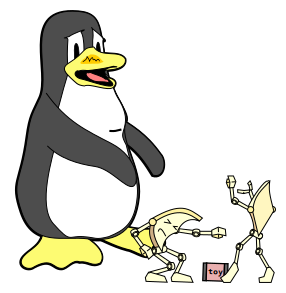
\includegraphics{cartoons/r-2014-Data-one-fighting}}
\end{center}
\caption{Lock Contention}
\ContributedBy{Figure}{fig:SMPdesign:Lock Contention}{Melissa Broussard}
\end{figure}

\subsection{Data Locking}
\label{sec:SMPdesign:Data Locking}

많은 데이터 구조체들이 각자 자기의 락을 갖는 조각들로 분할될 수 있습니다.
이렇게 되면 데이터 구조체의 각 조각들의 크리티컬 섹션들은 병렬적으로 실행될 수
있습니다, 각 조각의 크리티컬 섹션의 인스턴스는 한번에 하나씩만 수행될 수 있긴
하지만요.
경쟁상황이 줄어야만 하고, 동기화 오버헤드가 속도향상을 제한하지 않는 경우에는
데이터 락킹을 사용해야 합니다.
데이터 락킹은 여러 데이터 구조체 사이에 존재하는 너무 큰 크리티컬 섹션의
인스턴스들을 분산시킴으로써 경쟁상황을 줄여주는데, 예를 들어
Figure~\ref{fig:SMPdesign:Data-Locking Hash Table Search} 처럼 해시 테이블에서
해시 버킷 별로 크리티컬 섹션을 두는 식입니다.
향상된 확장성은 약간 추가적인 데이터 구조체인 \co{struct bucket} 의 형태로
복잡도를 약간 증가시킵니다.
\iffalse

Many data structures may be partitioned,
with each partition of the data structure having its own lock.
Then the critical sections for each part of the data structure
can execute in parallel,
although only one instance of the critical section for a given
part could be executing at a given time.
You should use data locking when contention must
be reduced, and where synchronization overhead is not
limiting speedups.
Data locking reduces contention by distributing the instances
of the overly-large critical section across multiple data structures,
for example, maintaining per-hash-bucket critical sections in a
hash table, as shown in
Figure~\ref{fig:SMPdesign:Data-Locking Hash Table Search}.
The increased scalability again results in a slight increase in complexity
in the form of an additional data structure, the \co{struct bucket}.
\fi

\begin{figure}[htbp]
{ \scriptsize
\begin{verbatim}
  1 struct hash_table
  2 {
  3   long nbuckets;
  4   struct bucket **buckets;
  5 };
  6
  7 struct bucket {
  8   spinlock_t bucket_lock;
  9   node_t *list_head;
 10 };
 11
 12 typedef struct node {
 13   unsigned long key;
 14   struct node *next;
 15 } node_t;
 16
 17 int hash_search(struct hash_table *h, long key)
 18 {
 19   struct bucket *bp;
 20   struct node *cur;
 21   int retval;
 22
 23   bp = h->buckets[key % h->nbuckets];
 24   spin_lock(&bp->bucket_lock);
 25   cur = bp->list_head;
 26   while (cur != NULL) {
 27     if (cur->key >= key) {
 28       retval = (cur->key == key);
 29       spin_unlock(&bp->bucket_lock);
 30       return retval;
 31     }
 32     cur = cur->next;
 33   }
 34   spin_unlock(&bp->bucket_lock);
 35   return 0;
 36 }
\end{verbatim}
}
\caption{Data-Locking Hash Table Search}
\label{fig:SMPdesign:Data-Locking Hash Table Search}
\end{figure}

Figure~\ref{fig:SMPdesign:Lock Contention} 에서 보였던 경쟁적인 상황과 달리,
데이터 락킹은 Figure~\ref{fig:SMPdesign:Data Locking} 에 그려진 것처럼 조화를
향상시킵니다 --- 그리고 병렬 프로그램에서, 이는 \emph{거의} 항상 향상된 성능과
확장성으로 이어집니다.
이런 이유로, 데이터 락킹은 DYNIX 와 DYNIX/ptx 운영체제의 Sequent 에서 매우 많이
사용되었습니다~\cite{Beck85,Inman85,Garg90,Dove90,McKenney92b,McKenney92a,McKenney93}.
\iffalse

In contrast with the contentious situation
shown in Figure~\ref{fig:SMPdesign:Lock Contention},
data locking helps promote harmony, as illustrated by
Figure~\ref{fig:SMPdesign:Data Locking} --- and in parallel programs,
this \emph{almost} always translates into increased performance and
scalability.
For this reason, data locking was heavily used by Sequent in
both its DYNIX and DYNIX/ptx operating
systems~\cite{Beck85,Inman85,Garg90,Dove90,McKenney92b,McKenney92a,McKenney93}.
\fi

\begin{figure}[htb]
\begin{center}
\resizebox{3in}{!}{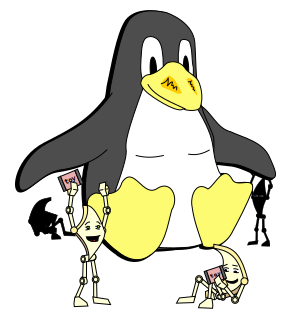
\includegraphics{cartoons/r-2014-Data-many-happy}}
\end{center}
\caption{Data Locking}
\ContributedBy{Figure}{fig:SMPdesign:Data Locking}{Melissa Broussard}
\end{figure}

% ./test_hash_spinlock.exe 1000 0/100 1 1024 1
% ./test_hash_spinlock.exe: nmilli: 1000 update/total: 0/100 nelements: 1 nbuckets: 1024 nthreads: 1
% ./test_hash_spinlock.exe: avg = 158.118  max = 162.404  min = 156.199  std = 2.19391
% ./test_hash_spinlock.exe: nmilli: 1000 update/total: 0/100 nelements: 1 nbuckets: 1024 nthreads: 1
% ./test_hash_spinlock.exe: avg = 157.717  max = 162.446  min = 156.415  std = 2.36662
% ./test_hash_spinlock.exe: nmilli: 1000 update/total: 0/100 nelements: 1 nbuckets: 1024 nthreads: 1
% ./test_hash_spinlock.exe: avg = 158.369  max = 164.75  min = 156.501  std = 3.19454

% ./test_hash_spinlock.exe 1000 0/100 1 1024 2
% ./test_hash_spinlock.exe: nmilli: 1000 update/total: 0/100 nelements: 1 nbuckets: 1024 nthreads: 2
% ./test_hash_spinlock.exe: avg = 223.426  max = 422.948  min = 167.858  std = 100.136
% ./test_hash_spinlock.exe: nmilli: 1000 update/total: 0/100 nelements: 1 nbuckets: 1024 nthreads: 2
% ./test_hash_spinlock.exe: avg = 235.462  max = 507.134  min = 167.466  std = 135.836
% ./test_hash_spinlock.exe: nmilli: 1000 update/total: 0/100 nelements: 1 nbuckets: 1024 nthreads: 2
% ./test_hash_spinlock.exe: avg = 305.807  max = 481.685  min = 167.939  std = 132.589

하지만, 어린 아이들을 돌봐 본 사람이라면 증명할 수 있듯이, 충분히 가서 놀 수
있는 공간을 주는 것이 평안을 보장하지는 않습니다.
예를 들어, 리눅스 커널은 파일과 디렉토리들의 캐시 (``dcache'' 라 불립니다) 를
갖습니다.
이 캐시의 각 원소들은 자신의 락을 갖습니다만, 루트 디렉토리에 해당하는 원소들과
그것의 직접적인 자식들은 다른 원소들에 비해 훨씬 많이 순회됩니다.
이는 많은 CPU 들이 이 자주 접근되는 원소들의 락에 경쟁을 하게 되는 결과를
초래해서, Figure~\ref{fig:SMPdesign:Data and Skew} 에 보여진 것과 같은 상황을
초래하고 맙니다.
\iffalse

However, as those who have taken care of small children can again attest,
even providing enough to go around is no guarantee of tranquillity.
The analogous situation can arise in SMP programs.
For example, the Linux kernel maintains a cache of files and directories
(called ``dcache'').
Each entry in this cache has its own lock, but the entries corresponding
to the root directory and its direct descendants are much more likely to
be traversed than are more obscure entries.
This can result in many CPUs contending for the locks of these popular
entries, resulting in a situation not unlike that
shown in Figure~\ref{fig:SMPdesign:Data and Skew}.
\fi

\begin{figure}[htb]
\begin{center}
\resizebox{3in}{!}{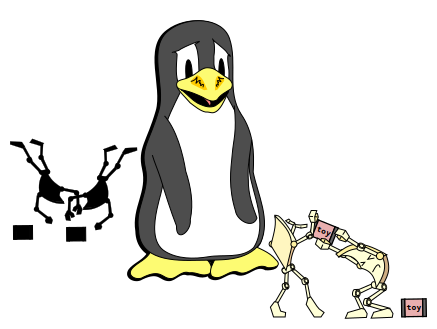
\includegraphics{cartoons/r-2014-Data-many-fighting}}
\end{center}
\caption{Data Locking and Skew}
\ContributedBy{Figure}{fig:SMPdesign:Data and Skew}{Melissa Broussard}
\end{figure}

많은 경우, 알고리즘들은 데이터 스큐를 줄이도록 설계될 수 있고, 어떤 경우에는
아예 그것들을 없애버릴 수도 있습니다 (리눅스 커널의 dcache 에서도 가능한 것으로
나타난 것처럼요~\cite{McKenney04a}).
데이터 락킹은 종종 해시 테이블처럼 분할될 수 있는 데이터 구조체에 사용됩니다만,
여러 존재가 각각 어떤 데이터 구조체의 인스턴스로 표현될 수 있는 경우에도
사용됩니다.
리눅스 커널 2.6.17 버전의 태스크 리스트는 후자의 한 예로, 각 태스크 구조체는
자신의 \co{proc_lock} 을 갖습니다.

다이나믹하게 할당되는 구조체들에서의 데이터 락킹의 핵심 문제는 해당 구조체가
해당 락이 잡혀있는 동안은 존재하는 상태를 유지해야 한다는 것입니다.
Figure~\ref{fig:SMPdesign:Data-Locking Hash Table Search} 의 코드는 이 문제를
락들을 정적으로 할당된 해시 버킷들에 넣어두고, 절대 메모리에서 해제시키지 않는
것으로 해결합니다.
하지만, 이 트릭은 해시 테이블의 크기가 바뀔 수 있다면 락들이 다이나믹하게
할당되어야 하므로 제대로 동작하지 않을 것입니다.
이 경우, 해시 버킷들을 그 락들이 잡혀있는 동안은 메모리 해제되지 않도록 하는
어떤 수단이 필요할 것입니다.
\iffalse

In many cases, algorithms can be designed to reduce the instance of
data skew, and in some cases eliminate it entirely
(as appears to be possible with the Linux kernel's dcache~\cite{McKenney04a}).
Data locking is often used for partitionable data structures such as
hash tables, as well as in situations where multiple entities are each
represented by an instance of a given data structure.
The task list in version 2.6.17 of the Linux kernel is an example of the
latter, each task structure having its own \co{proc_lock}.

A key challenge with data locking on dynamically allocated structures
is ensuring that the structure remains in existence while the lock is
being acquired.
The code in
Figure~\ref{fig:SMPdesign:Data-Locking Hash Table Search}
finesses this challenge by placing the locks in the statically allocated
hash buckets, which are never freed.
However, this trick would not work if the hash table were resizeable,
so that the locks were now dynamically allocated.
In this case, there would need to be some means to prevent the hash
bucket from being freed during the time that its lock was being acquired.
\fi

\QuickQuiz{}
	구조체가 그것의 락이 잡혀 있는 동안은 메모리 해제 되지 않도록 할 수
	있는 방법들은 어떤 것들이 있을까요?
	\iffalse

	What are some ways of preventing a structure from being freed while
	its lock is being acquired?
	\fi
\QuickQuizAnswer{
	여기 \emph{존재 보장} 문제를 위한 해결책 몇가지가 있습니다:
	\iffalse

	Here are a few possible solutions to this \emph{existence guarantee}
	problem:
	\fi

	\begin{enumerate}
	\item	구조체별 락이 잡혀 있는 동안 잡혀 있는 정적으로 할당된 락을
		두는 것으로, 계층적 락킹의 한 예입니다
		(Section~\ref{sec:SMPdesign:Hierarchical Locking} 을
		참고하세요).
		물론, 이런 목적으로 하나의 글로벌 락을 사용하는 것은
		허용불가능할 정도로 높은 락 경쟁 상황을 가져와서 극적인 성능과
		확장성의 하락을 가져올 수 있습니다.
	\item	정적으로 할당된 락들의 배열을 두어서, 구조체의 어드레스를
		해싱해서 잡아야 할 락을 고르는 것으로,
		Chapter~\ref{chp:Locking} 에서 설명된 방식입니다.
		주어진 해시 함수가 충분히 높은 성능을 갖는다면, 이는 하나의
		글로벌 락이 갖는 확장성의 한계를 해결할 수 있습니다만, 읽기가
		대부분인 상황에서는 락 획득 오버헤드가 수용불가할 정도로 성능을
		떨어뜨릴 수 있습니다.
	\item	가비지 콜렉터를 제공하는 소프트웨어 환경이라면 가비지 콜렉터를
		사용해서, 구조체가 참조되어 있는 동안은 메모리 해제되지 않도록
		하는 것입니다.
		이 방법은 잘 동작하고, 존재-보장의 짐을 (그리고 그외의 것들을)
		개발자의 어깨에서 내려놓게 하지만, 프로그램의 가비지 콜렉션의
		오버헤드를 갖습니다.
		가비지 콜렉션 기술은 지난 수십년간 상당히 진보했지만, 그
		오버헤드는 일부 어플리케이션에서는 수용하기 어려울 만큼 높을 수
		있습니다.
		또한, 일부 어플리케이션들은 개발자가 데이터 구조체의 배치와
		위치의 조정에 대해 대부분의 가비지 콜렉션 환경에 비해 많은
		연습을 필요로 할수도 있습니다.
	\iffalse

	\item	Provide a statically allocated lock that is held while
		the per-structure lock is being acquired, which is an
		example of hierarchical locking (see
		Section~\ref{sec:SMPdesign:Hierarchical Locking}).
		Of course, using a single global lock for this purpose
		can result in unacceptably high levels of lock contention,
		dramatically reducing performance and scalability.
	\item	Provide an array of statically allocated locks, hashing
		the structure's address to select the lock to be acquired,
		as described in Chapter~\ref{chp:Locking}.
		Given a hash function of sufficiently high quality, this
		avoids the scalability limitations of the single global
		lock, but in read-mostly situations, the lock-acquisition
		overhead can result in unacceptably degraded performance.
	\item	Use a garbage collector, in software environments providing
		them, so that a structure cannot be deallocated while being
		referenced.
		This works very well, removing the existence-guarantee
		burden (and much else besides) from the developer's
		shoulders, but imposes the overhead of garbage collection
		on the program.
		Although garbage-collection technology has advanced
		considerably in the past few decades, its overhead
		may be unacceptably high for some applications.
		In addition, some applications require that the developer
		exercise more control over the layout and placement of
		data structures than is permitted by most garbage collected
		environments.
	\fi
	\item	가비지 콜렉터의 특수한 경우로, 글로벌 레퍼런스 카운터를 두거나
		레퍼런스 카운터들의 글로벌한 배열을 두는 방법이 있습니다.
	\item	안에서-밖으로의 참조 카운트라 생각할 수 있는, \emph{해저드
		포인터}~\cite{MagedMichael04a} 들을 사용하는 방법이 있습니다.
		해저드 포인터 기반의 알고리즘들은 쓰레드별 포인터들의 리스트를
		두어서, 이 리스트들에 있는 포인터의 존재가 연관된 구조체로의
		참조처럼 동작하게 합니다.
		해저드 포인터들은 흥미로운 연구 방향입니다만, 상품화 단계
		(2008년도 시점에선) 에선 아직 잘 쓰여지지 않고 있습니다.
	\item	트랜잭셔널
		메모리(TM)~\cite{Herlihy93a,DBLomet1977SIGSOFT,Shavit95} 를
		사용해서 데이터 구조체로 요청되는 각각의 참조와 수정이
		어토믹하게 수행되도록 하는 방법이 있습니다.
		TM 은 최근의 수년간 대단한 흥분을 일으켰고 상품 단계
		소프트웨어에서 일부 사용될 것처럼 보였지만, 개발자들은 몇가지
		주의를 기울여야
		하며~\cite{Blundell2005DebunkTM,Blundell2006TMdeadlock,McKenney2007PLOSTM}
		이는 특히 성능에 영향을 주는 코드에선 더더욱 그렇습니다.
		특히, 존재 보장은 트랜잭션이 글로벌 레퍼런스부터 업데이트되는
		데이터 원소들에 이르기까지 전체를 감싸야 할 것을 필요로 합니다.
	\item	극단적으로 가벼운 가비지 콜렉터의 추상화로 생각될 수 있는, RCU
		를 사용하는 것입니다.
		업데이트를 하는 쪽은 RCU 로 보호되는 데이터 구조체를 RCU
		읽는쪽이 여전히 참조를 하고 있는 동안은 메모리에서 해제시킬 수
		없습니다.
		RCU 는 읽기가 대부분인 데이터 구조체에서 상당히 많이 사용되고
		있고, Chapter~\ref{chp:Deferred Processing} 에서 이야기될
		것입니다.
	\iffalse

	\item	As a special case of a garbage collector, use a global
		reference counter, or a global array of reference counters.
	\item	Use \emph{hazard pointers}~\cite{MagedMichael04a}, which
		can be thought of as an inside-out reference count.
		Hazard-pointer-based algorithms maintain a per-thread list of
		pointers, so that the appearance of a given pointer on
		any of these lists acts as a reference to the corresponding
		structure.
		Hazard pointers are an interesting research direction, but
		have not yet seen much use in production (written in 2008).
	\item	Use transactional memory
		(TM)~\cite{Herlihy93a,DBLomet1977SIGSOFT,Shavit95},
		so that each reference and
		modification to the data structure in question is
		performed atomically.
		Although TM has engendered much excitement in recent years,
		and seems likely to be of some use in production software,
		developers should exercise some
		caution~\cite{Blundell2005DebunkTM,Blundell2006TMdeadlock,McKenney2007PLOSTM},
		particularly in performance-critical code.
		In particular, existence guarantees require that the
		transaction cover the full path from a global reference
		to the data elements being updated.
	\item	Use RCU, which can be thought of as an extremely lightweight
		approximation to a garbage collector.
		Updaters are not permitted to free RCU-protected
		data structures that RCU readers might still be referencing.
		RCU is most heavily used for read-mostly data structures,
		and is discussed at length in
		Chapter~\ref{chp:Deferred Processing}.
	\fi
	\end{enumerate}

	존재 보장에 대해 더 많은 내용을 위해선 Chapter~\ref{chp:Locking} 과
	\ref{chp:Deferred Processing} 을 참고하세요.
	\iffalse

	For more on providing existence guarantees, see
	Chapters~\ref{chp:Locking} and \ref{chp:Deferred Processing}.
	\fi
} \QuickQuizEnd

\subsection{Data Ownership}
\label{sec:SMPdesign:Data Ownership}

데이터 소유권은 주어진 데이터 구조체를 쓰레드들이나 CPU 들로 쪼개서, 각
쓰레드/CPU 는 데이터의 자신에게 할당된 부분집합을 어떤 동기화 오버헤드 없이
접근할 수 있습니다.
하지만, 어떤 쓰레드가 다른 쓰레드의 데이터에 접근하길 원한다면, 이는 곧바로 될
수는 없습니다.
대신, 이 쓰레드는 다른 쓰레드와 먼저 통신을 해서 다른 쓰레드가 그 일을 대신
해주거나, 또는 그 데이터의 소유권을 이전해 주도록 해야 합니다.

데이터 소유권은 불가사의해 보일 수 있지만, 매우 자주 사용됩니다:
\iffalse

Data ownership partitions a given data structure over the threads
or CPUs, so that each thread/CPU accesses its subset of the data
structure without any synchronization overhead whatsoever.
However, if one thread wishes to access some other thread's data,
the first thread is unable to do so directly.
Instead, the first thread must communicate with the second thread,
so that the second thread performs the operation on behalf of the
first, or, alternatively, migrates the data to the first thread.

Data ownership might seem arcane, but it is used very frequently:
\fi
\begin{enumerate}
\item	한 CPU 나 쓰레드에 의해서만 접근될 수 있는 변수 (C 와 C++ 에서의 {\tt
	auto} 변수와 같은) 들은 모두 해당 CPU 나 프로세스에게 소유되어
	있습니다.
\item	사용자 인터페이스의 한 인스턴스는 해당 사용자의 컨텍스트를 소유합니다.
	병렬 데이터베이스 엔진과 상호작용하는 어플리케이션들은 그것들이 순차적
	프로그램인 것마냥 작성되는 것이 매우 흔한 일입니다.
	그런 어플리케이션들은 사용자 인터페이스와 그/그녀의 현재 동작을
	소유합니다.
	명시적인 병렬성은 따라서 데이터베이스 엔진 그 자체에 국한되어 있습니다.
\item	파라미터를 사용하는 시뮬레이션들은 종종 각 쓰레드가 파라미터 공간의
	특정 영역에 소유권을 갖게 하는 방법으로 병렬화 되곤 합니다.
	이런 타입의 문제를 위한 컴퓨팅 프레임웍도 존재합니다~\cite{BOINC2008}.
\iffalse

\item	Any variables accessible by only one CPU or thread
	(such as {\tt auto} variables in C
	and C++) are owned by that CPU or process.
\item	An instance of a user interface owns the corresponding
	user's context.  It is very common for applications
	interacting with parallel database engines to be
	written as if they were entirely sequential programs.
	Such applications own the user interface and his current
	action.  Explicit parallelism is thus confined to the
	database engine itself.
\item	Parametric simulations are often trivially parallelized
	by granting each thread ownership of a particular region
	of the parameter space.
	There are also computing frameworks designed for this
	type of problem~\cite{BOINC2008}.
\fi
\end{enumerate}

상당히 많은 공유가 존재한다면, 이 쓰레드들이나 CPU 들 사이의 통신은 상당한
복잡도와 오버헤드를 만들어낼 것입니다.
더 나아가서, 가장 많이 사용되는 데이터가 단일 CPU 에게 소유되어 있게 된다면, 이
CPU 는 ``핫스팟'' 이 될 것이고, Figure~\ref{fig:SMPdesign:Data and Skew} 에
그려진 것과 같은 결과를 낼 것입니다.
하지만, 공유가 필요하지 않은 상황이라면,
Figure~\ref{fig:SMPdesign:Sequential-Program Hash Table Search} 에 보여진
것처럼 데이터 소유권은 이상적인 성능을 내고, 순차적 프로그램처럼 간단해질 수
있을 것입니다.
그런 상황은 종종 ``당황스러울 정도로 병렬적'' 이라 불리곤 하고,
Figure~\ref{fig:SMPdesign:Data Locking} 에서 앞서 본것과 같은 상황과 닮아
있습니다.
\iffalse

If there is significant sharing, communication between the threads
or CPUs can result in significant complexity and overhead.
Furthermore, if the most-heavily used data happens to be that owned
by a single CPU, that CPU will be a ``hot spot'', sometimes with
results resembling that shown in Figure~\ref{fig:SMPdesign:Data and Skew}.
However, in situations where no sharing is required, data ownership
achieves ideal performance, and with code that can be as simple
as the sequential-program case shown in
Figure~\ref{fig:SMPdesign:Sequential-Program Hash Table Search}.
Such situations are often referred to as ``embarrassingly
parallel'', and, in the best case, resemble the situation
previously shown in Figure~\ref{fig:SMPdesign:Data Locking}.
\fi

% ./test_hash_null.exe 1000 0/100 1 1024 1
% ./test_hash_null.exe: nmilli: 1000 update/total: 0/100 nelements: 1 nbuckets: 1024 nthreads: 1
% ./test_hash_null.exe: avg = 96.2913  max = 98.2337  min = 90.4095  std = 2.95314
% ./test_hash_null.exe: nmilli: 1000 update/total: 0/100 nelements: 1 nbuckets: 1024 nthreads: 1
% ./test_hash_null.exe: avg = 91.5592  max = 97.3315  min = 89.9885  std = 2.88925
% ./test_hash_null.exe: nmilli: 1000 update/total: 0/100 nelements: 1 nbuckets: 1024 nthreads: 1
% ./test_hash_null.exe: avg = 93.3568  max = 106.162  min = 89.8828  std = 6.40418

% ./test_hash_null.exe 1000 0/100 1 1024 2
% ./test_hash_null.exe: nmilli: 1000 update/total: 0/100 nelements: 1 nbuckets: 1024 nthreads: 2
% ./test_hash_null.exe: avg = 45.4526  max = 46.4281  min = 45.1954  std = 0.487791
% ./test_hash_null.exe: nmilli: 1000 update/total: 0/100 nelements: 1 nbuckets: 1024 nthreads: 2
% ./test_hash_null.exe: avg = 46.0238  max = 49.2861  min = 45.1852  std = 1.63127
% ./test_hash_null.exe: nmilli: 1000 update/total: 0/100 nelements: 1 nbuckets: 1024 nthreads: 2
% ./test_hash_null.exe: avg = 46.6858  max = 52.6278  min = 45.1761  std = 2.97102

또다른 중요한 데이터 소유권 상황은 데이터가 읽기 전용인 경우, 모든 쓰레드가
복사본을 통해 그것을 ``소유'' 할 수 있는 경우입니다.

데이터 소유권은 Chapter~\ref{chp:Data Ownership} 에서 좀 더 자세히 다뤄질
겁니다.
\iffalse

Another important instance of data ownership occurs when the data
is read-only, in which case,
all threads can ``own'' it via replication.

Data ownership will be presented in more detail in
Chapter~\ref{chp:Data Ownership}.
\fi

\subsection{Locking Granularity and Performance}
\label{sec:SMPdesign:Locking Granularity and Performance}

이 섹션은 락킹 빈도와 성능 사이의 관계를 수학적인 동기화 효율성 관점에서
살펴봅니다.
수학이 지루한 독자분들은 이 섹션을 건너뛰셔도 됩니다.

사용할 방법은 하나의 공유되는 글로벌 변수에 대해 동작하는 동기화 메커니즘의
효율성을 위한 간단한 큐잉 모델을 M/M/1 큐를 기반으로 사용해 보는 것입니다.
M/M/1 큐잉 모델들은 지수적으로 분포되는 ``도착간 비율 (inter-arrival rate)''
$\lambda$ 와 지수적으로 분포되는 ``서비스 비율 (service rate)'' $\mu$ 에
기반합니다.
도착간 비율 $\lambda$ 는 만약 동기화 비용이 전혀 들지 않는다면 시스템이 처리할
수 있는, 초당 동기화 오퍼레이션들의 평균 숫자로 생각될 수 있는데, 달리 말하자면
$\lambda$ 는 작업의 비동기 유닛의 오버헤드의 역수입니다.
예를 들어, 일의 각 유닛이 트랜잭션이고, 각 트랜잭션이 처리되는데 동기화
오버헤드를 제외하고 1 밀리세컨드가 걸린다면, $\lambda$ 는 초당 1,000 트랜잭션이
될 것입니다.
\iffalse

This section looks at locking granularity and performance from
a mathematical synchronization-efficiency viewpoint.
Readers who are uninspired by mathematics might choose to skip
this section.

The approach is to use a crude queueing model for the efficiency of
synchronization mechanism that operate on a single shared global
variable, based on an M/M/1 queue.
M/M/1 queuing models are based on an exponentially distributed
``inter-arrival rate'' $\lambda$ and an exponentially distributed
``service rate'' $\mu$.
The inter-arrival rate $\lambda$ can be thought of as the average
number of synchronization operations per second that the system
would process if the synchronization were free, in other words,
$\lambda$ is an inverse measure of the overhead of each non-synchronization
unit of work.
For example, if each unit of work was a transaction, and if each transaction
took one millisecond to process, excluding synchronization overhead,
then $\lambda$ would be 1,000 transactions per second.
\fi

서비스 비율 $\mu$ 는 비슷하게 정의됩니다만, CPU 들이 각자의 동기화
오퍼레이션들을 완료하기를 기다려야 한다는 사실을 무시하고 각 트랜잭션의
오버헤드가 존재하지 않는다면 시스템이 1초 안에 처리할 수 있는 동기화
오퍼레이션들의 수의 평균으로, 달리 말하자면, $\mu$ 는 컨텐션이 없을 때의 동기화
오버헤드라고 생각될 수 있겠습니다.
예를 들어, 각 동기화 오퍼레이션이 어토믹 값 증가 인스트럭션을 내포하고 있고,
컴퓨터 시스템은 각 CPU 에서 각자의 변수에 25 나노세컨드마다 어토믹 값 증가
인스트럭션을 수행할 수 있다고 해 봅시다.\footnote{
	물론, 같은 공유 변수의 값을 증가시키는 8 개의 CPU 가 존재한다면, 각각의
	CPU 는 자신의 값 증가 작업을 위해 25 나노세컨드를 소모하기 전에 다른
	CPU 들이 각자의 값 증가 작업을 마무리 할 때까지 175 나노세컨드를
	기다려야 할 것입니다.
	실제로는, 이 대기는 더 길어질텐데 그 변수를 한 CPU 에서 다른 CPU 로
	옮기는 시간도 걸리기 때문입니다.}
따라서 $\mu$ 의 값은 초당 40,000,000 어토믹 값 증가 일 것입니다.

물론, $\lambda$ 의 값은 CPU 수가 늘어나면 함께 늘어날텐데, 각 CPU 가 독립적으로
트랜잭션들을 처리할 수 있기 때문입니다 (다시 말하지만, 동기화를 무시합니다):

\iffalse

The service rate $\mu$ is defined similarly, but for the average
number of synchronization operations per second that the system
would process if the overhead of each transaction was zero, and
ignoring the fact that CPUs must wait on each other to complete
their synchronization operations, in other words, $\mu$ can be roughly
thought of as the synchronization overhead in absence of contention.
For example, suppose that each synchronization operation involves an atomic
increment instruction, and that a computer system is able to do
an atomic increment every 25 nanoseconds on each CPU
to a private variable.\footnote{
	Of course, if there are 8 CPUs all incrementing the same
	shared variable, then each CPU must wait at least 175 nanoseconds
	for each of the other CPUs to do its increment before consuming
	an additional 25 nanoseconds doing its own increment.
	In actual fact, the wait will be longer due to the need
	to move the variable from one CPU to another.}
The value of $\mu$ is therefore about 40,000,000 atomic increments
per second.

Of course, the value of $\lambda$ increases with increasing numbers of
CPUs, as each CPU is capable of processing transactions independently
(again, ignoring synchronization):
\fi

\begin{equation}
	\lambda = n \lambda_0
\end{equation}

$n$ 은 CPU 들의 갯수이고 $\lambda_0$ 는 단일 CPU 의 트랜잭션 처리 가능량입니다.
단일 CPU 가 하나의 트랜잭션을 처리하는데 걸릴 것으로 기대되는 시간은
$1 / \lambda_0$ 임을 기억해 두십시오.

이 CPU 들은 다른 CPU 들이 각각 하나의 공유 변수의 값을 증가시킬 동안
``줄을 서서 기다려야'' 하기 때문에, 기대되는 전체 대기 시간을 표현하는데 M/M/1
큐잉 모델을 다음과 같이 사용할 수 있습니다:
\iffalse

where $n$ is the number of CPUs and $\lambda_0$ is the transaction-processing
capability of a single CPU.
Note that the expected time for a single CPU to execute a single transaction
is $1 / \lambda_0$.

Because the CPUs have to ``wait in line'' behind each other to get their
chance to increment the single shared variable, we can use the M/M/1
queueing-model expression for the expected total waiting time:
\fi

\begin{equation}
	T = \frac{1}{\mu - \lambda}
\end{equation}

앞의 $\lambda$ 값을 대입하면:
\iffalse

Substituting the above value of $\lambda$:
\fi

\begin{equation}
	T = \frac{1}{\mu - n \lambda_0}
\end{equation}

이제, 효율성은 동기화 없을 때 트랜잭션 하나를 처리하는데 필요한 시간 ($1 /
\lambda_0$) 과 동기화를 포함해서 필요한 시간 ($T + 1 / \lambda_0$) 사이의
비율입니다:
\iffalse

Now, the efficiency is just the ratio of the time required to process
a transaction in absence of synchronization ($1 / \lambda_0$)
to the time required including synchronization ($T + 1 / \lambda_0$):
\fi

\begin{equation}
	e = \frac{1 / \lambda_0}{T + 1 / \lambda_0}
\end{equation}

앞의 $T$ 값을 대입하고 간략화 하면:
\iffalse

Substituting the above value for $T$ and simplifying:
\fi

\begin{equation}
	e = \frac{\frac{\mu}{\lambda_0} - n}{\frac{\mu}{\lambda_0} - (n - 1)}
\end{equation}

하지만 $\mu / \lambda_0$ 의 값은 그저 트랜잭션을 처리하는데 필요한 시간과
(경쟁상황이 없는 상태에서의) 동기화 자체 오버헤드 간의 비율입니다.
이 비율을 $f$ 라고 하면, 이렇게 됩니다:
\iffalse

But the value of $\mu / \lambda_0$ is just the ratio of the time required
to process the transaction (absent synchronization overhead) to that of 
the synchronization overhead itself (absent contention).
If we call this ratio $f$, we have:
\fi

\begin{equation}
	e = \frac{f - n}{f - (n - 1)}
\end{equation}

\begin{figure}[tbp]
\begin{center}
\resizebox{3in}{!}{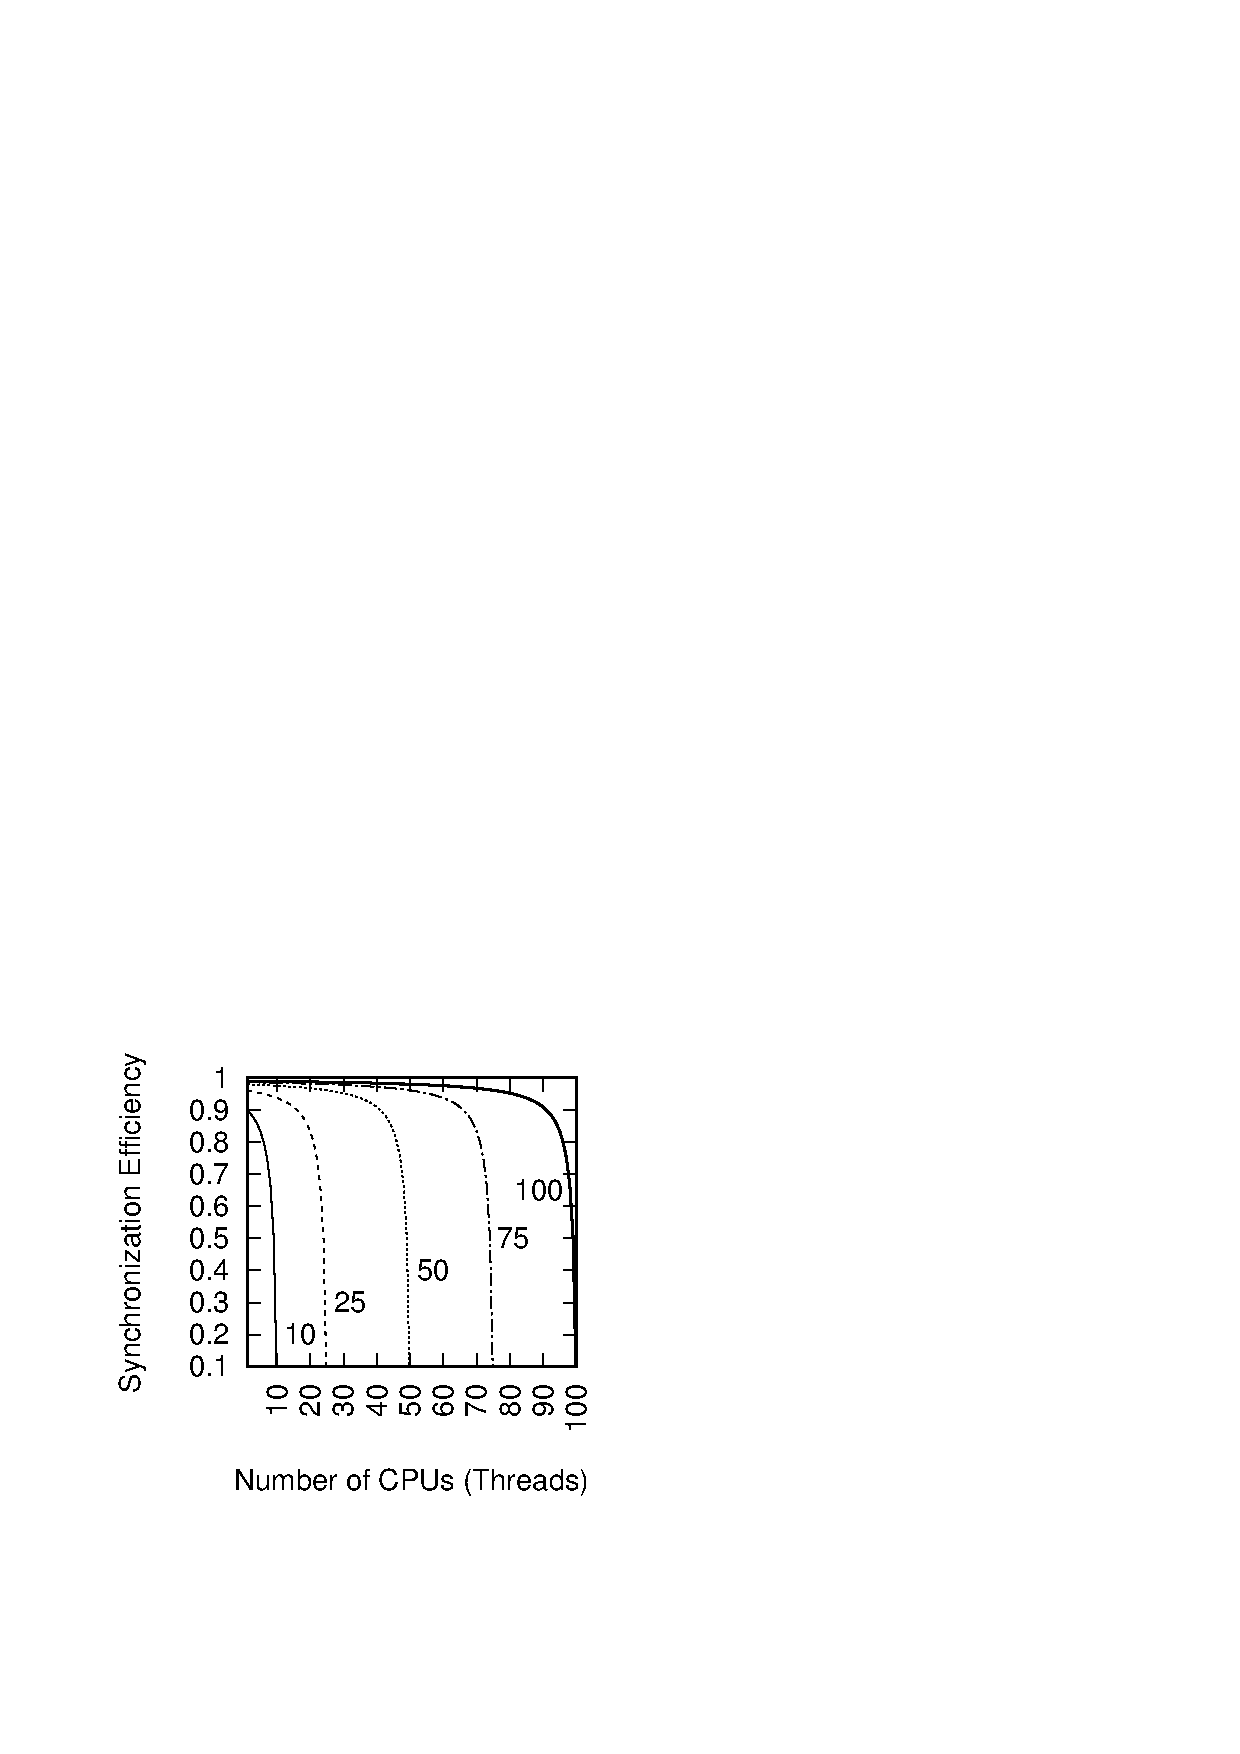
\includegraphics{SMPdesign/synceff}}
\end{center}
\caption{Synchronization Efficiency}
\label{fig:SMPdesign:Synchronization Efficiency}
\end{figure}

Figure~\ref{fig:SMPdesign:Synchronization Efficiency} 는 동기화 효율성 $e$ 가
CPU/쓰레드 수 $n$ 에 의해 변화되는 모습을 오버헤드 비율 $f$ 몇개의 값과 함께
보여줍니다.
예를 들어, 25 나노세컨드 걸리는 어토믹 값 증가 연산을 사용하면 $f=10$ 선은 각
CPU 가 매 250 나노세컨드마다 어토믹 값 증가 연산을 시도하고, $f=100$ 라인은 각
CPU 가 수천개의 인스트럭션이 처리될 수 있는 시간인 2.5 마이크로세컨드마다
어토믹 값 증가 연산을 시도합니다.
각 조합의 결과가 CPU 나 쓰레드의 수가 늘어남에 따라 급격하게 떨어지는 것으로
보아, 하나의 글로벌 공유 변수에의 어토믹 조정을 통한 동기화 메커니즘은 현재의
하드웨어에서 많이 사용되면 잘 확장되지 못할 것이라 결론 내릴 수 있습니다.
이건 이 규칙들을 수학적으로 그려본 것으로, Chapter~\ref{chp:Counting} 에서
이야기한 병렬 카운팅 알고리즘을 이끌어내게 합니다.
\iffalse

Figure~\ref{fig:SMPdesign:Synchronization Efficiency} plots the synchronization
efficiency $e$ as a function of the number of CPUs/threads $n$ for
a few values of the overhead ratio $f$.
For example, again using the 25-nanosecond atomic increment, the
$f=10$ line corresponds to each CPU attempting an atomic increment
every 250 nanoseconds, and the $f=100$ line corresponds to each
CPU attempting an atomic increment every 2.5 microseconds,
which in turn corresponds to several thousand instructions.
Given that each trace drops off sharply with increasing numbers of
CPUs or threads, we can conclude that
synchronization mechanisms based on
atomic manipulation of a single global shared variable will not
scale well if used heavily on current commodity hardware.
This is a mathematical depiction of the forces leading to the parallel
counting algorithms that were discussed in Chapter~\ref{chp:Counting}.
\fi

이 효율성 컨셉은 정규적인 동기화가 적거나 아예 없을 때에도 효과적입니다.
예를 들어, 한 행렬의 행이 (``dot product'' 로) 다른 행렬의 열로 곱해져 세번째
행렬을 만들어내는 행렬 곱셈을 생각해 봅시다.
이 오퍼레이션들은 서로 겹치지 않기 대문에, 첫번째 행렬의 행들을 쓰레드들에
분할시키고 각 쓰레드는 결과 행렬의 연관된 행을 계산하는 것이 가능합니다.
따라서 이 쓰레드들은 \texttt{matmul.c} 에서와 같이 아무런 동기화 오버헤드 없이
완전히 독립적으로 동작할수 있습니다.
따라서 병렬적 행렬 곱셈은 완벽한 효율성, 1.0을 가질 것이라 예상할 수도
있습니다.
\iffalse

The concept of efficiency is useful even in cases having little or
no formal synchronization.
Consider for example a matrix multiply, in which the columns of one
matrix are multiplied (via ``dot product'') by the rows of another,
resulting in an entry in a third matrix.
Because none of these operations conflict, it is possible to partition
the columns of the first matrix among a group of threads, with each thread
computing the corresponding columns of the result matrix.
The threads can therefore operate entirely independently, with no
synchronization overhead whatsoever, as is done in
\texttt{matmul.c}.
One might therefore expect a parallel matrix multiply to have a
perfect efficiency of 1.0.
\fi

\begin{figure}[tbp]
\begin{center}
\resizebox{3in}{!}{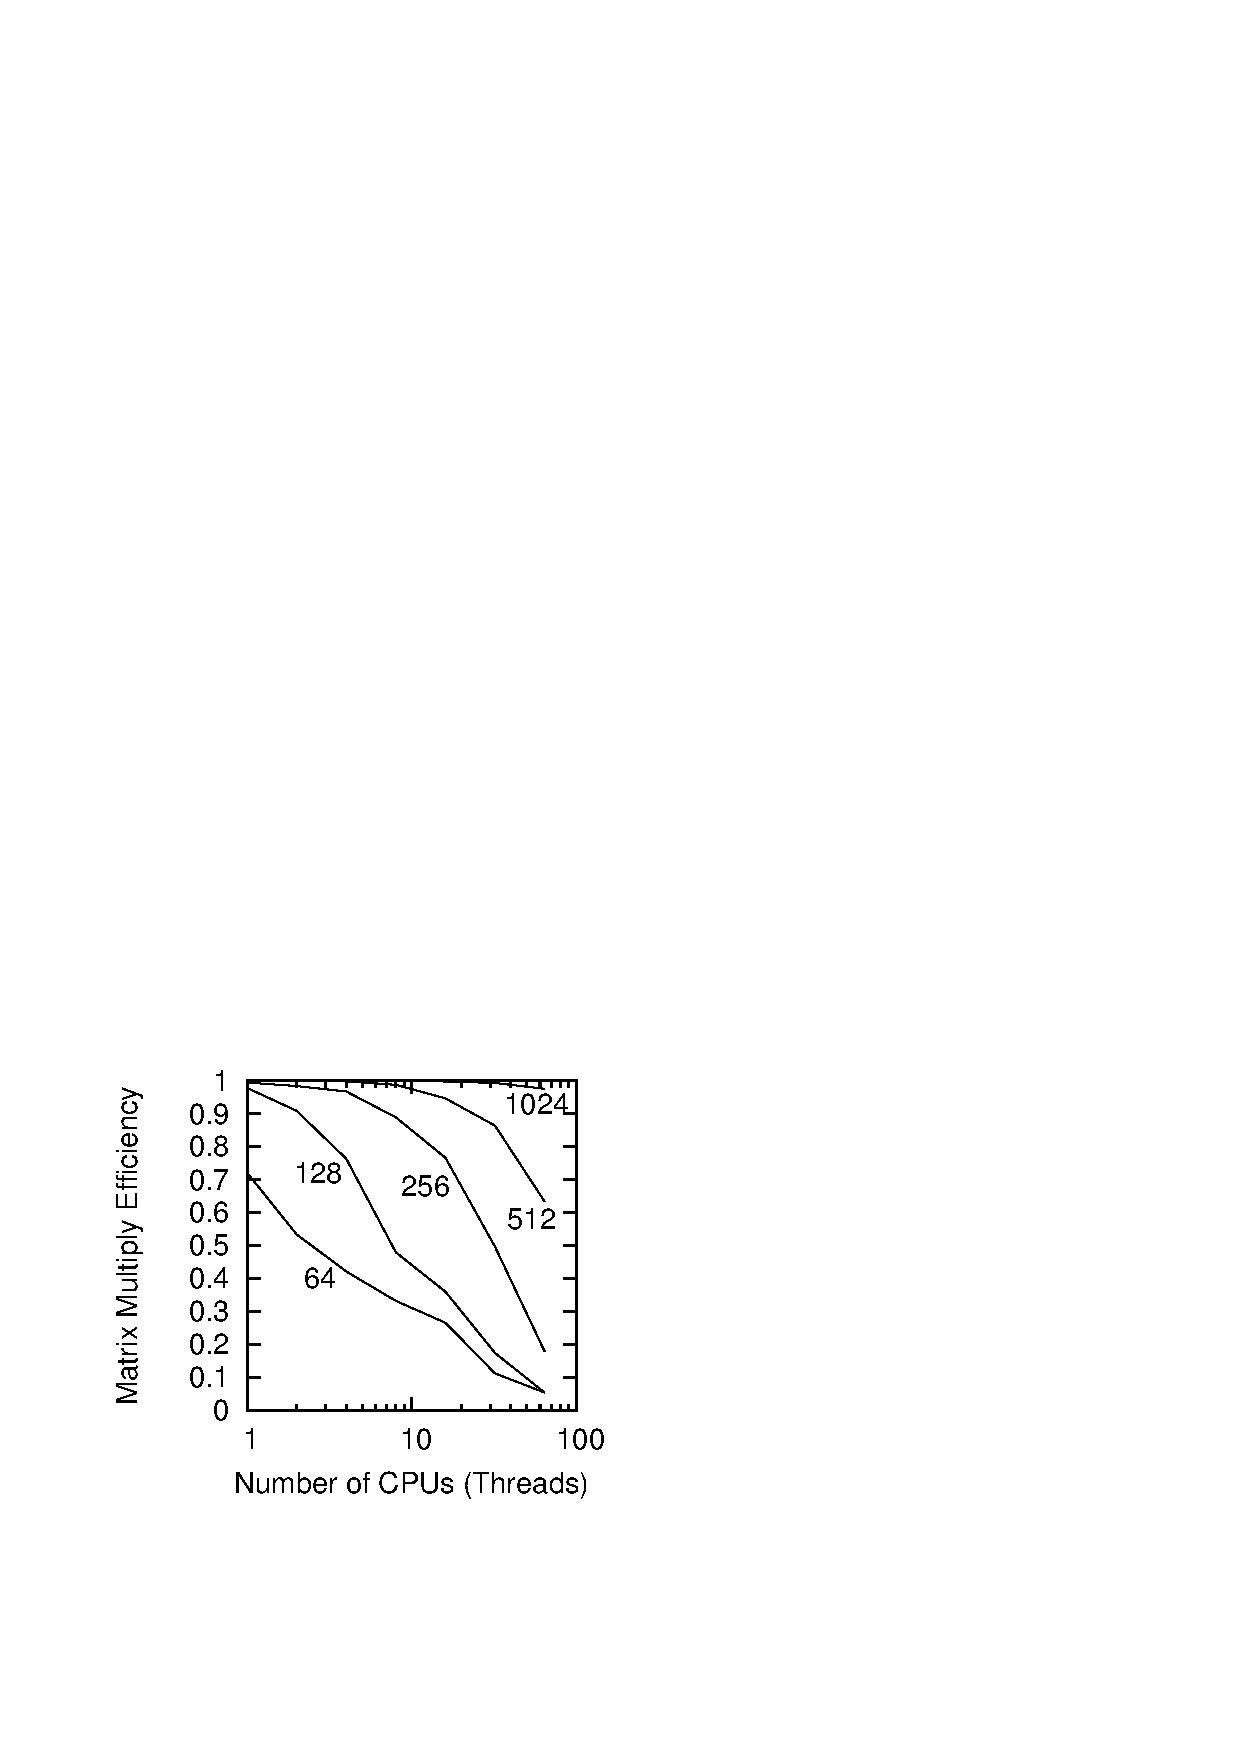
\includegraphics{SMPdesign/matmuleff}}
\end{center}
\caption{Matrix Multiply Efficiency}
\label{fig:SMPdesign:Matrix Multiply Efficiency}
\end{figure}

하지만,
Figure~\ref{fig:SMPdesign:Matrix Multiply Efficiency} 는 다르게 이야기하는데,
특히 64 행 64 열 행렬 곱셈에서는 0.7 보다 나은 효율성을 절대 갖지 못합니다,
싱글쓰레드고 동작하는데도 불구하고 말이지요.
512 행 512 열 행렬 곱셈의 효율성은 10 쓰레드 아래에서는 1.0보다 조금 작은
것으로 측정되며 심지어 1024 행 1024 열 행렬 곱셈조차도 수십 쓰레드에서는 완벽한
효율성을 벗어나게 되고 맙니다.
더도 아니고 덜도 아니고, 이 그림은 몰아서 처리하기의 성능과 확장성에서의 이점을
분명하게 보여주고 있으며, 이로 인해 당신의 돈의 가치도 알 수 있게 해줍니다.
\iffalse

However,
Figure~\ref{fig:SMPdesign:Matrix Multiply Efficiency}
tells a different story, especially for a 64-by-64 matrix multiply,
which never gets above an efficiency of about 0.7, even when running
single-threaded.
The 512-by-512 matrix multiply's efficiency is measurably less
than 1.0 on as few as 10 threads, and even the 1024-by-1024 matrix
multiply deviates noticeably from perfection at a few tens of threads.
Nevertheless, this figure clearly demonstrates the performance and
scalability benefits of batching: If you must incur synchronization
overhead, you may as well get your money's worth.
\fi

\QuickQuiz{}
	싱글쓰레드로 동작하는 64 행 64 열 행렬 곱셈이 어떻게 1.0보다 낮은
	효율성을 가질 수 있죠?
	Figure~\ref{fig:SMPdesign:Matrix Multiply Efficiency} 의 모든
	조합에서의 결과들이 한 쓰레드에서만 돌아갈 때에는 정확히 1.0 의
	효율성을 보여야 하는 거 아닌가요?
	\iffalse

	How can a single-threaded 64-by-64 matrix multiple possibly
	have an efficiency of less than 1.0?
	Shouldn't all of the traces in
	Figure~\ref{fig:SMPdesign:Matrix Multiply Efficiency}
	have efficiency of exactly 1.0 when running on only one thread?
	\fi
\QuickQuizAnswer{
	\texttt{matmul.c} 프로그램은 명시된 수의 워커 쓰레드들을 생성하므로,
	하나의 워커 쓰레드만을 생성한 경우에도 쓰레드 생성 오버헤드는 발생할 수
	있습니다.
	하나의 워커 쓰레드의 경우에 쓰레드 생성 오버헤드를 없애기 위한 변경을
	만드는 것은 독자분들의 연습문제로 남겨두겠습니다.
	\iffalse

	The \texttt{matmul.c} program creates the specified number of
	worker threads, so even the single-worker-thread case incurs
	thread-creation overhead.
	Making the changes required to optimize away thread-creation
	overhead in the single-worker-thread case is left as an
	exercise to the reader.
	\fi
} \QuickQuizEnd

이런 비효율성 아래, Section~\ref{sec:SMPdesign:Data Locking} 에서 이야기한
데이터 락킹과 같이 더 확장성 있는 방법을 생각해 보거나 다음 섹션에서 다룰 병렬
상황 빠른 수행 경로 해결책을 고려해 보는것도 가치가 있을 것입니다.
\iffalse

Given these inefficiencies,
it is worthwhile to look into more-scalable approaches
such as the data locking described in
Section~\ref{sec:SMPdesign:Data Locking}
or the parallel-fastpath approach discussed in the next section.
\fi

\QuickQuiz{}
	행렬 곱셈에서 데이터 병렬화 기법이 어떻게 도움이 될 수 있나요?
	그건 \emph{이미} 병렬적인 데이터잖아요!!!
	\iffalse

	How are data-parallel techniques going to help with matrix
	multiply?
	It is \emph{already} data parallel!!!
	\fi
\QuickQuizAnswer{
	주의를 기울이고 있으신 것 같아 기쁩니다!
	이 예는 데이터 병렬성은 매우 좋은 것이긴 하지만, 어떤 그리고 모든
	비효율성의 원인을 자동으로 제거하는 마술봉은 아니란 것을 보이기 위한
	것임을 보이기 위한 것입니다.
	64 쓰레드에게 ``한정적인'' 상황에서조차도 전체 성능을 가지고 선형적으로
	성능을 확장하는 데에는 설계와 구현의 모든 단계에서의 세심한 주의가
	필요합니다.
	\iffalse

	I am glad that you are paying attention!
	This example serves to show that although data parallelism can
	be a very good thing, it is not some magic wand that automatically
	wards off any and all sources of inefficiency.
	Linear scaling at full performance, even to ``only'' 64 threads,
	requires care at all phases of design and implementation.
	\fi

	특히, 분할된 조각의 크기에 매우 세심한 관심을 기울여야만 합니다.
	예를 들어, 64 행 64 열 행렬 곱셈 문제를 64 쓰레드에게 쪼갠다면, 각
	쓰레드는 64 개의 부동소수점 곱셈 연산만을 하게 될 것입니다.
	부동소수점 곱셈 연산의 비용은 쓰레드 생성의 오버헤드에 비하면 매우
	작습니다.

	교훈: 변화무쌍한 입력을 받을 수 있는 병렬 프로그램을 가지고 있다면,
	항상 입력의 크기를 체크하는 과정을 포함시켜서 병렬화 시킬 가치가 없을
	정도로 너무 작은 입력 사이즈에 대응하도록 하십시오.
	그리고 병렬화에 도움이 되지 않을 정도라면, 쓰레드를 생성하는데 필요한
	오버헤드를 감내하기에도 도움이 되지 않을 정도입니다, 그렇죠?
	\iffalse

	In particular, you need to pay careful attention to the
	size of the partitions.
	For example, if you split a 64-by-64 matrix multiply across
	64 threads, each thread gets only 64 floating-point multiplies.
	The cost of a floating-point multiply is miniscule compared to
	the overhead of thread creation.

	Moral: If you have a parallel program with variable input,
	always include a check for the input size being too small to
	be worth parallelizing.
	And when it is not helpful to parallelize, it is not helpful
	to incur the overhead required to spawn a thread, now is it?
	\fi
} \QuickQuizEnd

\section{Parallel Fastpath}
\label{sec:SMPdesign:Parallel Fastpath}

잘게 쪼개진 (그리고 따라서 \emph{일반적으로} 높은 성능을 갖는) 설계들은 굵게
쪼개진 설계들에 비해 일반적으로 더 복잡합니다.
많은 경우, 대부분의 오버헤드는 코드의 작은 부분에서 발생합니다~\cite{Knuth73}.
그러니 그 작은 부분에 집중하는 노력을 가져보는게 어떨까요?

이게 병렬 빠른 수행 경로 디자인 패턴을 뒷받침하는 아이디어로, 전체 알고리즘을
적극적으로 병렬화 하려 하면 요구되는 복잡성을 일으키지 않고 일반적인 경우를
위한 코드 수행 경로를 적극적으로 병렬화 시키는 것입니다.
이를 위해선 병렬화 하려는 특정 알고리즘만 이해해선 안되고, 그 알고리즘이 목표로
하는 워크로드에 대해서도 이해해야만 합니다.
병렬 빠른 수행 경로를 만들기 위해선 커다란 창조성과 설계 노력이 종종 필요하곤
합니다.

병렬 빠른 수행 경로는 서로 다른 패턴들 (하나는 빠른 수행경로를 위해, 다른
경우를 위해 또 하나) 을 조합하고 따라서 임시적 패턴입니다.
다음의 병렬 빠른 수행경로의 예들은
Figure~\ref{fig:SMPdesign:Parallel-Fastpath Design Patterns} 에 그려진 것처럼
그 자신의 패턴을 정당화 하기 충분할 만큼 자주 일어납니다:
\iffalse

Fine-grained (and therefore \emph{usually} higher-performance)
designs are typically more complex than are coarser-grained designs.
In many cases, most of the overhead is incurred by a small fraction
of the code~\cite{Knuth73}.
So why not focus effort on that small fraction?

This is the idea behind the parallel-fastpath design pattern, to aggressively
parallelize the common-case code path without incurring the complexity
that would be required to aggressively parallelize the entire algorithm.
You must understand not only the specific algorithm you wish
to parallelize, but also the workload that the algorithm will
be subjected to.  Great creativity and design
effort is often required to construct a parallel fastpath.

Parallel fastpath combines different patterns (one for the
fastpath, one elsewhere) and is therefore a template pattern.
The following instances of parallel
fastpath occur often enough to warrant their own patterns,
as depicted in Figure~\ref{fig:SMPdesign:Parallel-Fastpath Design Patterns}:
\fi

\begin{figure}[htb]
\begin{center}
% \resizebox{3in}{!}{\includegraphics{SMPdesign/ParallelFastpath}}
\includegraphics{SMPdesign/ParallelFastpath}
\end{center}
\caption{Parallel-Fastpath Design Patterns}
\label{fig:SMPdesign:Parallel-Fastpath Design Patterns}
\end{figure}

\begin{enumerate}
\item	Reader/Writer 락킹
	(아래의 Section~\ref{sec:SMPdesign:Reader/Writer Locking} 에서
	설명합니다).
\item	고성능을 위해 Reader/Writer 락킹을 대체할 수 있으며 이 챕터에서는
	더이상 설명되지 않을 Read-copy update (RCU).
\item	Section~\ref{sec:SMPdesign:Hierarchical Locking} 에서 다뤄질 계층적
	락킹~(\cite{McKenney95b}).
\item	리소스 할당자 캐시~(\cite{McKenney95b,McKenney93}).
	더 자세한 내용을 위해선
	Section~\ref{sec:SMPdesign:Resource Allocator Caches} 을 참고하십시오.
\iffalse

\item	Reader/Writer Locking
	(described below in Section~\ref{sec:SMPdesign:Reader/Writer Locking}).
\item	Read-copy update (RCU), which may be used as a high-performance
	replacement for reader/writer locking, is introduced in
	Section~\ref{sec:defer:Read-Copy Update (RCU)}, and will not
	be discussed further in this chapter.
\item   Hierarchical Locking~(\cite{McKenney95b}), which is touched upon
	in Section~\ref{sec:SMPdesign:Hierarchical Locking}.
\item	Resource Allocator Caches~(\cite{McKenney95b,McKenney93}).
	See Section~\ref{sec:SMPdesign:Resource Allocator Caches}
	for more detail.
\fi
\end{enumerate}

\subsection{Reader/Writer Locking}
\label{sec:SMPdesign:Reader/Writer Locking}

동기화 오버헤드가 무시할만 하다면 (예를 들어, 프로그램이 커다란 크리티컬
섹션들에 굵게 쪼개진 병렬성을 사용한다면), 그리고 그 크리티컬 섹션들의 작은
부분들만이 데이터를 수정한다면, 여러 읽는 작업들을 병렬로 수행될 수 있도록 하면
확장성을 크게 개선시킬 것입니다.
쓰기 작업은 읽기 작업과도, 다른 쓰기 작업들과도 배타적으로 수행되어야 합니다.
reader-writer 락킹의 많은 구현이 존재하는데,
Section~\ref{sec:toolsoftrade:POSIX Reader-Writer Locking} 에 설명된 POSIX
구현도 그 중 하나입니다.
Figure~\ref{fig:SMPdesign:Reader-Writer-Locking Hash Table Search} 는 해시
테이블이 reader-writer 락킹을 사용해 어떻게 구현될 수 있는지 보입니다.
\iffalse

If synchronization overhead is negligible (for example, if the program
uses coarse-grained parallelism with large critical sections), and if
only a small fraction of the critical sections modify data, then allowing
multiple readers to proceed in parallel can greatly increase scalability.
Writers exclude both readers and each other.
There are many implementations of reader-writer locking, including
the POSIX implementation described in
Section~\ref{sec:toolsoftrade:POSIX Reader-Writer Locking}.
Figure~\ref{fig:SMPdesign:Reader-Writer-Locking Hash Table Search}
shows how the hash search might be implemented using reader-writer locking.
\fi

\begin{figure}[htbp]
{ \scriptsize
\begin{verbatim}
  1 rwlock_t hash_lock;
  2
  3 struct hash_table
  4 {
  5   long nbuckets;
  6   struct node **buckets;
  7 };
  8
  9 typedef struct node {
 10   unsigned long key;
 11   struct node *next;
 12 } node_t;
 13
 14 int hash_search(struct hash_table *h, long key)
 15 {
 16   struct node *cur;
 17   int retval;
 18
 19   read_lock(&hash_lock);
 20   cur = h->buckets[key % h->nbuckets];
 21   while (cur != NULL) {
 22     if (cur->key >= key) {
 23       retval = (cur->key == key);
 24       read_unlock(&hash_lock);
 25       return retval;
 26     }
 27     cur = cur->next;
 28   }
 29   read_unlock(&hash_lock);
 30   return 0;
 31 }
\end{verbatim}
}
\caption{Reader-Writer-Locking Hash Table Search}
\label{fig:SMPdesign:Reader-Writer-Locking Hash Table Search}
\end{figure}

Reader/writer 락킹은 비대칭적 락킹에 대한 하나의 간단한 예입니다.
Snaman~\cite{Snaman87} 은 여러 클러스터 시스템에서 사용되는, 더 화려한 여섯개
모드의 비대칭적 락킹 디자인을 설명합니다.
일반적인 락킹과 reader-writer 락킹은 Chapter~\ref{chp:Locking} 에서 특별히
자세히 설명됩니다.
\iffalse

Reader/writer locking is a simple instance of asymmetric locking.
Snaman~\cite{Snaman87} describes a more ornate six-mode
asymmetric locking design used in several clustered systems.
Locking in general and reader-writer locking in particular is described
extensively in
Chapter~\ref{chp:Locking}.
\fi

\subsection{Hierarchical Locking}
\label{sec:SMPdesign:Hierarchical Locking}

계층적 락킹의 아이디어는 잘게 쪼개진 락을 잡는 동작을 하는 동안만 잡는 굵게
쪼개진 락을 두자는 것입니다.
Figure~\ref{fig:SMPdesign:Hierarchical-Locking Hash Table Search}
는 해시 테이블 탐색에 계층적 락킹이 어떻게 사용될 수 있을지 보여주는데, 또한 이
방법의 커다란 단점 역시 보여줍니다:
두번째 락을 잡기 위한 오버헤드를 감내했지만, 그 락은 짧은 시간동안만 잡습니다.
이 경우, 간단한 데이터 락킹 방법은 더 간단하고 더 좋은 성능을 보일 것입니다.
\iffalse

The idea behind hierarchical locking is to have a coarse-grained lock
that is held only long enough to work out which fine-grained lock
to acquire.
Figure~\ref{fig:SMPdesign:Hierarchical-Locking Hash Table Search}
shows how our hash-table search might be adapted to do hierarchical
locking, but also shows the great weakness of this approach:
we have paid the overhead of acquiring a second lock, but we only
hold it for a short time.
In this case, the simpler data-locking approach would be simpler
and likely perform better.
\fi

\begin{figure}[htbp]
{ \scriptsize
\begin{verbatim}
  1 struct hash_table
  2 {
  3   long nbuckets;
  4   struct bucket **buckets;
  5 };
  6
  7 struct bucket {
  8   spinlock_t bucket_lock;
  9   node_t *list_head;
 10 };
 11
 12 typedef struct node {
 13   spinlock_t node_lock;
 14   unsigned long key;
 15   struct node *next;
 16 } node_t;
 17
 18 int hash_search(struct hash_table *h, long key)
 19 {
 20   struct bucket *bp;
 21   struct node *cur;
 22   int retval;
 23
 24   bp = h->buckets[key % h->nbuckets];
 25   spin_lock(&bp->bucket_lock);
 26   cur = bp->list_head;
 27   while (cur != NULL) {
 28     if (cur->key >= key) {
 29       spin_lock(&cur->node_lock);
 30       spin_unlock(&bp->bucket_lock);
 31       retval = (cur->key == key);
 32       spin_unlock(&cur->node_lock);
 33       return retval;
 34     }
 35     cur = cur->next;
 36   }
 37   spin_unlock(&bp->bucket_lock);
 38   return 0;
 39 }
\end{verbatim}
}
\caption{Hierarchical-Locking Hash Table Search}
\label{fig:SMPdesign:Hierarchical-Locking Hash Table Search}
\end{figure}

\QuickQuiz{}
	계층적 락킹이 잘 동작할 만한 상황은 뭐가 있을까요?
	\iffalse

	In what situation would hierarchical locking work well?
	\fi
\QuickQuizAnswer{
	Figure~\ref{fig:SMPdesign:Hierarchical-Locking Hash Table Search} 의
	라인~31 에서의 비교 연산이 훨씬 무거운 연산으로 교체된다면, {\tt
	bp->bucket\_lock} 을 놓는 작업은 \emph{아마도} 락 경쟁을 충분히
	줄여줘서 추가적인 {\tt cur->node\_lock} 의 획득과 해제에 드는
	오버헤드보다 우세해질 수도 있을 것입니다.
	\iffalse

	If the comparison on line~31 of
	Figure~\ref{fig:SMPdesign:Hierarchical-Locking Hash Table Search}
	were replaced by a much heavier-weight operation,
	then releasing {\tt bp->bucket\_lock} \emph{might} reduce lock
	contention enough to outweigh the overhead of the extra
	acquisition and release of {\tt cur->node\_lock}.
	\fi
} \QuickQuizEnd

\subsection{Resource Allocator Caches}
\label{sec:SMPdesign:Resource Allocator Caches}

이 섹션에서는 병렬 고정 크기 블럭 메모리 얼로케이터의 단순화된 개요를
제공합니다.
더 자세한 설명은
literature~\cite{McKenney92a,McKenney93,Bonwick01slab,McKenney01e} 나
리눅스 커널~\cite{Torvalds2.6kernel} 에서 찾을 수 있습니다.
\iffalse

This section presents a simplified schematic of a parallel fixed-block-size
memory allocator.
More detailed descriptions may be found in the
literature~\cite{McKenney92a,McKenney93,Bonwick01slab,McKenney01e}
or in the Linux kernel~\cite{Torvalds2.6kernel}.
\fi

\subsubsection{Parallel Resource Allocation Problem}

The basic problem facing a parallel memory allocator is the tension
between the need to provide extremely fast memory allocation and
freeing in the common case and the need to efficiently distribute
memory in face of unfavorable allocation and freeing patterns.

To see this tension, consider a straightforward application of
data ownership to this problem --- simply carve up memory so that
each CPU owns its share.
For example, suppose that a system with two CPUs has two gigabytes
of memory (such as the one that I am typing on right now).
We could simply assign each CPU one gigabyte of memory, and allow
each CPU to access its own private chunk of memory, without the
need for locking and its complexities and overheads.
Unfortunately, this simple scheme breaks down if an algorithm happens
to have CPU 0 allocate all of the memory and CPU 1 the free it, as
would happen in a simple producer-consumer workload.

The other extreme, code locking, suffers from excessive lock contention
and overhead~\cite{McKenney93}.

\subsubsection{Parallel Fastpath for Resource Allocation}

The commonly used solution uses parallel fastpath with each CPU
owning a modest cache of blocks, and with a large code-locked
shared pool for additional blocks.
To prevent any given CPU from monopolizing the memory blocks,
we place a limit on the number of blocks that can be in each CPU's
cache.
In a two-CPU system, the flow of memory blocks will be as shown
in Figure~\ref{fig:SMPdesign:Allocator Cache Schematic}:
when a given CPU is trying to free a block when its pool is full,
it sends blocks to the global pool, and, similarly, when that CPU
is trying to allocate a block when its pool is empty, it retrieves
blocks from the global pool.

\begin{figure}[htb]
\begin{center}
\resizebox{3in}{!}{\includegraphics{SMPdesign/allocatorcache}}
\end{center}
\caption{Allocator Cache Schematic}
\label{fig:SMPdesign:Allocator Cache Schematic}
\end{figure}

\subsubsection{Data Structures}

The actual data structures for a ``toy'' implementation of allocator
caches are shown in
Figure~\ref{fig:SMPdesign:Allocator-Cache Data Structures}.
The ``Global Pool'' of Figure~\ref{fig:SMPdesign:Allocator Cache Schematic}
is implemented by \co{globalmem} of type \co{struct globalmempool},
and the two CPU pools by the per-CPU variable \co{percpumem} of
type \co{percpumempool}.
Both of these data structures have arrays of pointers to blocks
in their \co{pool} fields, which are filled from index zero upwards.
Thus, if \co{globalmem.pool[3]} is \co{NULL}, then the remainder of
the array from index 4 up must also be NULL.
The \co{cur} fields contain the index of the highest-numbered full
element of the \co{pool} array, or -1 if all elements are empty.
All elements from \co{globalmem.pool[0]} through
\co{globalmem.pool[globalmem.cur]} must be full, and all the rest
must be empty.\footnote{
	Both pool sizes (\co{TARGET_POOL_SIZE} and
	\co{GLOBAL_POOL_SIZE}) are unrealistically small, but this small
	size makes it easier to single-step the program in order to get
	a feel for its operation.}

\begin{figure}[htbp]
{ \scriptsize
\begin{verbatim}
  1 #define TARGET_POOL_SIZE 3
  2 #define GLOBAL_POOL_SIZE 40
  3
  4 struct globalmempool {
  5   spinlock_t mutex;
  6   int cur;
  7   struct memblock *pool[GLOBAL_POOL_SIZE];
  8 } globalmem;
  9
 10 struct percpumempool {
 11   int cur;
 12   struct memblock *pool[2 * TARGET_POOL_SIZE];
 13 };
 14
 15 DEFINE_PER_THREAD(struct percpumempool, percpumem);
\end{verbatim}
}
\caption{Allocator-Cache Data Structures}
\label{fig:SMPdesign:Allocator-Cache Data Structures}
\end{figure}

The operation of the pool data structures is illustrated by
Figure~\ref{fig:SMPdesign:Allocator Pool Schematic},
with the six boxes representing the array of pointers making up
the \co{pool} field, and the number preceding them representing
the \co{cur} field.
The shaded boxes represent non-\co{NULL} pointers, while the empty
boxes represent \co{NULL} pointers.
An important, though potentially confusing, invariant of this
data structure is that the \co{cur} field is always one
smaller than the number of non-\co{NULL} pointers.

\begin{figure}[htb]
\begin{center}
\resizebox{3in}{!}{\includegraphics{SMPdesign/AllocatorPool}}
\end{center}
\caption{Allocator Pool Schematic}
\label{fig:SMPdesign:Allocator Pool Schematic}
\end{figure}

\subsubsection{Allocation Function}

The allocation function \co{memblock_alloc()} may be seen in
Figure~\ref{fig:SMPdesign:Allocator-Cache Allocator Function}.
Line~7 picks up the current thread's per-thread pool,
and line~8 check to see if it is empty.

If so, lines~9-16 attempt to refill it from the global pool
under the spinlock acquired on line~9 and released on line~16.
Lines~10-14 move blocks from the global to the per-thread pool until
either the local pool reaches its target size (half full) or
the global pool is exhausted, and line~15 sets the per-thread pool's
count to the proper value.

In either case, line~18 checks for the per-thread pool still being
empty, and if not, lines~19-21 remove a block and return it.
Otherwise, line~23 tells the sad tale of memory exhaustion.

\begin{figure}[htbp]
{ \scriptsize
\begin{verbatim}
  1 struct memblock *memblock_alloc(void)
  2 {
  3   int i;
  4   struct memblock *p;
  5   struct percpumempool *pcpp;
  6
  7   pcpp = &__get_thread_var(percpumem);
  8   if (pcpp->cur < 0) {
  9     spin_lock(&globalmem.mutex);
 10     for (i = 0; i < TARGET_POOL_SIZE &&
 11                 globalmem.cur >= 0; i++) {
 12       pcpp->pool[i] = globalmem.pool[globalmem.cur];
 13       globalmem.pool[globalmem.cur--] = NULL;
 14     }
 15     pcpp->cur = i - 1;
 16     spin_unlock(&globalmem.mutex);
 17   }
 18   if (pcpp->cur >= 0) {
 19     p = pcpp->pool[pcpp->cur];
 20     pcpp->pool[pcpp->cur--] = NULL;
 21     return p;
 22   }
 23   return NULL;
 24 }
\end{verbatim}
}
\caption{Allocator-Cache Allocator Function}
\label{fig:SMPdesign:Allocator-Cache Allocator Function}
\end{figure}

\subsubsection{Free Function}

Figure~\ref{fig:SMPdesign:Allocator-Cache Free Function} shows
the memory-block free function.
Line~6 gets a pointer to this thread's pool, and
line~7 checks to see if this per-thread pool is full.

If so, lines~8-15 empty half of the per-thread pool into the global pool,
with lines~8 and 14 acquiring and releasing the spinlock.
Lines~9-12 implement the loop moving blocks from the local to the
global pool, and line~13 sets the per-thread pool's count to the proper
value.

In either case, line~16 then places the newly freed block into the
per-thread pool.

\begin{figure}[htbp]
{ \scriptsize
\begin{verbatim}
  1 void memblock_free(struct memblock *p)
  2 {
  3   int i;
  4   struct percpumempool *pcpp;
  5
  6   pcpp = &__get_thread_var(percpumem);
  7   if (pcpp->cur >= 2 * TARGET_POOL_SIZE - 1) {
  8     spin_lock(&globalmem.mutex);
  9     for (i = pcpp->cur; i >= TARGET_POOL_SIZE; i--) {
 10       globalmem.pool[++globalmem.cur] = pcpp->pool[i];
 11       pcpp->pool[i] = NULL;
 12     }
 13     pcpp->cur = i;
 14     spin_unlock(&globalmem.mutex);
 15   }
 16   pcpp->pool[++pcpp->cur] = p;
 17 }
\end{verbatim}
}
\caption{Allocator-Cache Free Function}
\label{fig:SMPdesign:Allocator-Cache Free Function}
\end{figure}

\subsubsection{Performance}

Rough performance results\footnote{
	This data was not collected in a statistically meaningful way,
	and therefore should be viewed with great skepticism and suspicion.
	Good data-collection and -reduction practice is discussed
	in Chapter~\ref{chp:Validation}.
	That said, repeated runs gave similar results, and these results
	match more careful evaluations of similar algorithms.}
are shown in
Figure~\ref{fig:SMPdesign:Allocator Cache Performance},
running on a dual-core Intel x86 running at 1GHz (4300 bogomips per CPU)
with at most six blocks allowed in each CPU's cache.
In this micro-benchmark,
each thread repeatedly allocates a group of blocks and then frees all
the blocks in that group, with
the number of blocks in the group being the ``allocation run length''
displayed on the x-axis.
The y-axis shows the number of successful allocation/free pairs per
microsecond --- failed allocations are not counted.
The ``X''s are from a two-thread run, while the ``+''s are from a
single-threaded run.

\begin{figure}[htb]
\begin{center}
\resizebox{3in}{!}{\includegraphics{SMPdesign/smpalloc}}
\end{center}
\caption{Allocator Cache Performance}
\label{fig:SMPdesign:Allocator Cache Performance}
\end{figure}

Note that run lengths up to six scale linearly and give excellent performance,
while run lengths greater than six show poor performance and almost always
also show \emph{negative} scaling.
It is therefore quite important to size \co{TARGET_POOL_SIZE}
sufficiently large,
which fortunately is usually quite easy to do in actual
practice~\cite{McKenney01e}, especially given today's large memories.
For example, in most systems, it is quite reasonable to set
\co{TARGET_POOL_SIZE} to 100, in which case allocations and frees
are guaranteed to be confined to per-thread pools at least 99\% of
the time.

As can be seen from the figure, the situations where the common-case
data-ownership applies (run lengths up to six) provide greatly improved
performance compared to the cases where locks must be acquired.
Avoiding synchronization in the common case will be a recurring theme through
this book.

\QuickQuiz{}
	In Figure~\ref{fig:SMPdesign:Allocator Cache Performance},
	there is a pattern of performance rising with increasing run
	length in groups of three samples, for example, for run lengths
	10, 11, and 12.
	Why?
\QuickQuizAnswer{
	This is due to the per-CPU target value being three.
	A run length of 12 must acquire the global-pool lock twice,
	while a run length of 13 must acquire the global-pool lock
	three times.
} \QuickQuizEnd

\QuickQuiz{}
	Allocation failures were observed in the two-thread
	tests at run lengths of 19 and greater.
	Given the global-pool size of 40 and the per-thread target
	pool size $s$ of three, number of threads $n$ equal to two,
	and assuming that the per-thread pools are initially
	empty with none of the memory in use, what is the smallest allocation
	run length $m$ at which failures can occur?
	(Recall that each thread repeatedly allocates $m$ block of memory,
	and then frees the $m$ blocks of memory.)
	Alternatively, given $n$ threads each with pool size $s$, and
	where each thread repeatedly first allocates $m$ blocks of memory
	and then frees those $m$ blocks, how large must the global pool
	size be?
	\emph{Note:} Obtaining the correct answer will require you to
	examine the \co{smpalloc.c} source code, and very likely
	single-step it as well.
	You have been warned!
\QuickQuizAnswer{
	This solution is adapted from one put forward by Alexey Roytman.
	It is based on the following definitions:

	\begin{description}
	\item[$g$]	Number of blocks globally available.
	\item[$i$]	Number of blocks left in the initializing thread's
			per-thread pool.  (This is one reason you needed
			to look at the code!)
	\item[$m$]	Allocation/free run length.
	\item[$n$]	Number of threads, excluding the initialization thread.
	\item[$p$]	Per-thread maximum block consumption, including
			both the blocks actually allocated and the blocks
			remaining in the per-thread pool.
	\end{description}

	The values $g$, $m$, and $n$ are given.  The value for $p$ is
	$m$ rounded up to the next multiple of $s$, as follows:

	\begin{equation}
		p = s \left \lfloor \frac{m + s - 1}{s} \right \rfloor
	\label{sec:SMPdesign:p}
	\end{equation}

	The value for $i$ is as follows:

	\begin{equation}
		i = \left \{
			\begin{array}{l}
				g \pmod{2 s} = 0: 2 s \\
				g \pmod{2 s} \ne 0: g \pmod{2 s}
			\end{array}
		    \right .
	\label{sec:SMPdesign:i}
	\end{equation}

	\begin{figure}[tb]
	\begin{center}
	\resizebox{3in}{!}{\includegraphics{SMPdesign/smpalloclim}}
	\end{center}
	\caption{Allocator Cache Run-Length Analysis}
	\label{fig:SMPdesign:Allocator Cache Run-Length Analysis}
	\end{figure}

	The relationships between these quantities is shown in
	Figure~\ref{fig:SMPdesign:Allocator Cache Run-Length Analysis}.
	The global pool is shown on the top of this figure, and
	the ``extra'' initializer thread's per-thread pool and
	per-thread allocations are the left-most pair of boxes.
	The initializer thread has no blocks allocated, but has
	$i$ blocks stranded in its per-thread pool.
	The rightmost two pairs of boxes are the per-thread pools and
	per-thread allocations of threads holding the maximum possible
	number of blocks, while the second-from-left pair of boxes
	represents the thread currently trying to allocate.

	The total number of blocks is $g$, and adding up the per-thread
	allocations and per-thread pools, we see that the global pool
	contains $g-i-p(n-1)$ blocks.
	If the allocating thread is to be successful, it needs at least
	$m$ blocks in the global pool, in other words:

	\begin{equation}
		g - i - p(n - 1) \ge m
	\label{sec:SMPdesign:g-vs-m}
	\end{equation}

	The question has $g=40$, $s=3$, and $n=2$.
	Equation~\ref{sec:SMPdesign:i} gives $i=4$, and
	Equation~\ref{sec:SMPdesign:p} gives $p=18$ for $m=18$
	and $p=21$ for $m=19$.
	Plugging these into Equation~\ref{sec:SMPdesign:g-vs-m}
	shows that $m=18$ will not overflow, but that $m=19$ might
	well do so.

	The presence of $i$ could be considered to be a bug.
	After all, why allocate memory only to have it stranded in
	the initialization thread's cache?
	One way of fixing this would be to provide a \co{memblock_flush()}
	function that flushed the current thread's pool into the
	global pool.
	The initialization thread could then invoke this function
	after freeing all of the blocks.
} \QuickQuizEnd

\subsubsection{Real-World Design}

The toy parallel resource allocator was quite simple, but real-world
designs expand on this approach in a number of ways.

First, real-world allocators are required to handle a wide range
of allocation sizes, as opposed to the single size shown in this
toy example.
One popular way to do this is to offer a fixed set of sizes, spaced
so as to balance external and internal fragmentation, such as in
the late-1980s BSD memory allocator~\cite{McKusick88}.
Doing this would mean that the ``globalmem'' variable would need
to be replicated on a per-size basis, and that the associated
lock would similarly be replicated, resulting in data locking
rather than the toy program's code locking.

Second, production-quality systems must be able to repurpose memory,
meaning that they must be able to coalesce blocks into larger structures,
such as pages~\cite{McKenney93}.
This coalescing will also need to be protected by a lock, which again
could be replicated on a per-size basis.

Third, coalesced memory must be returned to the underlying memory
system, and pages of memory must also be allocated from the underlying
memory system.
The locking required at this level will depend on that of the underlying
memory system, but could well be code locking.
Code locking can often be tolerated at this level, because this
level is so infrequently reached in well-designed systems~\cite{McKenney01e}.

Despite this real-world design's greater complexity, the underlying
idea is the same --- repeated application of parallel fastpath,
as shown in
Table~\ref{fig:app:questions:Schematic of Real-World Parallel Allocator}.

\begin{table}[htbp]
{ \scriptsize
\begin{tabular}{l|l|p{1in}}
Level	& Locking & Purpose \\
\hline
Per-thread pool	  & Data ownership & High-speed allocation \\
Global block pool & Data locking   & Distributing blocks among threads \\
Coalescing	  & Data locking   & Combining blocks into pages \\
System memory	  & Code locking   & Memory from/to system \\
\end{tabular}
}
\caption{Schematic of Real-World Parallel Allocator}
\label{fig:app:questions:Schematic of Real-World Parallel Allocator}
\end{table}

% beyond.tex

\section{Beyond Partitioning}
\label{sec:SMPdesign:Beyond Partitioning}
\OriginallyPublished{Section}{sec:SMPdesign:Beyond Partitioning}{Retrofitted Parallelism Considered Grossly Sub-Optimal}{4\textsuperscript{th} USENIX Workshop on Hot Topics on Parallelism}{PaulEMcKenney2012HOTPARsuboptimal}

이 챕터에서는 데이터 파티셔닝이 간단한 선형적으로 확장 가능한 병렬 프로그램을
설계하는데 사용될 수 있는지 알아봤습니다.
Section~\ref{sec:SMPdesign:Data Ownership} 에서는 데이터 복사 가능성에서 힌트를
얻었는데, 이는 Section~\ref{sec:defer:Read-Copy Update (RCU)} 에서 커다란
효과를 가져올 것입니다.

파티셔닝과 복사본 사용을 적용하는 주요 목표는 선형적인 속도 향상을 얻기 위한
것으로, 달리 말하자면 CPU 나 쓰레드의 수가 늘어남에 따라 전체적으로 필요한 일의
양이 크게 늘어나지는 않음을 보장하기 위한 것입니다.
파티셔닝과 복사본 사용을 통해 해결될 수 있어서 선형적인 속도향상이 가능한
문제들은 \emph{당혹스럽게 병렬적} 입니다.
하지만 이보다 더 잘할 수는 없을까요?
\iffalse

This chapter has discussed how data partitioning can be used to design
simple linearly scalable parallel programs.
Section~\ref{sec:SMPdesign:Data Ownership} hinted at the possibilities
of data replication, which will be used to great effect in
Section~\ref{sec:defer:Read-Copy Update (RCU)}.

The main goal of applying partitioning and replication is to achieve
linear speedups, in other words, to ensure that the total amount of
work required does not increase significantly as the number of CPUs
or threads increases.
A problem that can be solved via partitioning and/or replication,
resulting in linear speedups, is \emph{embarrassingly parallel}.
But can we do better?
\fi

이 질문에 답을 하기 위해, 미궁과 미로의 해결책을 생각해 보도록 합시다.
물론, 미궁과 미로는 수천년동안 매력적인 것이었으며~\cite{WikipediaLabyrinth},
따라서 그것들이 바이오 컴퓨터~\cite{AndrewAdamatzky2011SlimeMold},
GPGPU~\cite{ChristerEricson2008GPUMaze}, 심지어는 분리된
하드웨어~\cite{MIT:TRMag:MemristorMazes} 등의 컴퓨터들을 사용해서 만들어지고
해결되었음은 별로 놀라운 일도 아닙니다.
미로의 병렬적 해결책은 대학 수업에서의 과제
프로젝트~\cite{ETHZurich:FS2011maze,UMD:CMSC433maze} 로도 사용되었고, 병렬
프로그래밍 프레임웍의 이점을 보이기 위한 매개물~\cite{RonFosner2010maze} 로도
사용되었습니다.
\iffalse

To answer this question, let us examine the solution of
labyrinths and mazes.
Of course, labyrinths and mazes have been objects of fascination for
millennia~\cite{WikipediaLabyrinth},
so it should come as no surprise that they are generated and solved
using computers, including biological
computers~\cite{AndrewAdamatzky2011SlimeMold},
GPGPUs~\cite{ChristerEricson2008GPUMaze}, and even
discrete hardware~\cite{MIT:TRMag:MemristorMazes}.
Parallel solution of mazes is sometimes used as a class project in
universities~\cite{ETHZurich:FS2011maze,UMD:CMSC433maze} and
as a vehicle to demonstrate the benefits of parallel-programming
frameworks~\cite{RonFosner2010maze}.
\fi

흔한 조언은 병렬 일거리-대기열 알고리즘(PWQ: Parallel work-queue
algorithm)~\cite{ETHZurich:FS2011maze,RonFosner2010maze} 을 사용하라는
것입니다.
이 섹션은 무작위적으로 생성된 정사각형 미로를 푸는 모든 경우에 대해
순차적 알고리즘 (SEQ:SEQuential algorithm) 과 대안적인 병렬 알고리즘, 그리고
PWQ 를 비교하는 것으로 이 조언을 평가해 보겠습니다.
Section~\ref{sec:SMPdesign:Work-Queue Parallel Maze Solver} 에서는 PWQ 를
이야기 하고,
Section~\ref{sec:SMPdesign:Alternative Parallel Maze Solver} 에서 대안적인 병렬
알고리즘을 설명하며,
Section~\ref{sec:SMPdesign:Performance Comparison I} 에서는 그것의 문제 있는
성능에 대해 이야기 한 후,
Section~\ref{sec:SMPdesign:Alternative Sequential Maze Solver} 에서 앞의 대안적
병렬 알고리즘으로부터 향상된 순차적 알고리즘을 소개하며,
Section~\ref{sec:SMPdesign:Performance Comparison II} 에서 성능을 비교해 보고,
마지막으로
Section~\ref{sec:SMPdesign:Future Directions and Conclusions} 에서 미래의
방향을 알아보고 결론을 내려봅니다.
\iffalse

Common advice is to use a parallel work-queue algorithm
(PWQ)~\cite{ETHZurich:FS2011maze,RonFosner2010maze}.
This section evaluates this advice by comparing PWQ
against a sequential algorithm (SEQ) and also against
an alternative parallel algorithm, in all cases solving randomly generated
square mazes.
Section~\ref{sec:SMPdesign:Work-Queue Parallel Maze Solver} discusses PWQ,
Section~\ref{sec:SMPdesign:Alternative Parallel Maze Solver} discusses an alternative
parallel algorithm,
Section~\ref{sec:SMPdesign:Performance Comparison I} analyzes its anomalous performance,
Section~\ref{sec:SMPdesign:Alternative Sequential Maze Solver} derives an improved
sequential algorithm from the alternative parallel algorithm,
Section~\ref{sec:SMPdesign:Performance Comparison II} makes further performance
comparisons,
and finally
Section~\ref{sec:SMPdesign:Future Directions and Conclusions}
presents future directions and concluding remarks.
\fi

\subsection{Work-Queue Parallel Maze Solver}
\label{sec:SMPdesign:Work-Queue Parallel Maze Solver}

\begin{listing}[tbp]
{ \scriptsize
\begin{verbbox}
  1 int maze_solve(maze *mp, cell sc, cell ec)
  2 {
  3   cell c = sc;
  4   cell n;
  5   int vi = 0;
  6 
  7   maze_try_visit_cell(mp, c, c, &n, 1);
  8   for (;;) {
  9     while (!maze_find_any_next_cell(mp, c, &n)) {
 10       if (++vi >= mp->vi)
 11         return 0;
 12       c = mp->visited[vi].c;
 13     }
 14     do {
 15       if (n == ec) {
 16         return 1;
 17       }
 18       c = n;
 19     } while (maze_find_any_next_cell(mp, c, &n));
 20     c = mp->visited[vi].c;
 21   }
 22 }
\end{verbbox}
}
\centering
\theverbbox
\caption{SEQ Pseudocode}
\label{lst:SMPdesign:SEQ Pseudocode}
\end{listing}

PWQ 는 Listing~\ref{lst:SMPdesign:SEQ Pseudocode}(\co{maze_seq.c}) 에 있는 SEQ
에 기반합니다.
미로는 셀들의 2D 배열과 \co{->visited} 로 이름 붙여진 선형적 배열 기반 일거리
대기열로 나타내어집니다.

Line~7 에서 첫번째 셀에 들어가고, line~8-21 에 있는 루프의 매 반복에서 하나의
셀에 의해 향해지는 통로를 횡단합니다.
Line9-13 의 루프에서는 \co{->visited[]} 배열을 방문되지 않은 이웃을 가지고
방문된 셀을 위해 스캔하고, line~14-19 의 루프에서는 그 이웃을 통해 향해지는
작은 미로를 횡단합니다.
Line~20 에서는 밖의 루프에 의해 통과될 다음 경로를 위해 초기화를 합니다.
\iffalse

PWQ is based on SEQ, which is shown in
Listing~\ref{lst:SMPdesign:SEQ Pseudocode}
(\path{maze_seq.c}).
The maze is represented by a 2D array of cells and
a linear-array-based work queue named \co{->visited}.

Line~7 visits the initial cell, and each iteration of the loop spanning
lines~8-21 traverses passages headed by one cell.
The loop spanning lines~9-13 scans the \co{->visited[]} array for a
visited cell with an unvisited neighbor, and the loop spanning
lines~14-19 traverses one fork of the submaze headed by that neighbor.
Line~20 initializes for the next pass through the outer loop.
\fi

\begin{listing}[tbp]
{ \scriptsize
\begin{verbbox}
  1 int maze_try_visit_cell(struct maze *mp, cell c, cell t,
  2                         cell *n, int d)
  3 {
  4   if (!maze_cells_connected(mp, c, t) ||
  5       (*celladdr(mp, t) & VISITED))
  6     return 0;
  7   *n = t;
  8   mp->visited[mp->vi] = t;
  9   mp->vi++;
 10   *celladdr(mp, t) |= VISITED | d;
 11   return 1;
 12 }
 13 
 14 int maze_find_any_next_cell(struct maze *mp, cell c,
 15                             cell *n)
 16 {
 17   int d = (*celladdr(mp, c) & DISTANCE) + 1;
 18 
 19   if (maze_try_visit_cell(mp, c, prevcol(c), n, d))
 20     return 1;
 21   if (maze_try_visit_cell(mp, c, nextcol(c), n, d))
 22     return 1;
 23   if (maze_try_visit_cell(mp, c, prevrow(c), n, d))
 24     return 1;
 25   if (maze_try_visit_cell(mp, c, nextrow(c), n, d))
 26     return 1;
 27   return 0;
 28 }
\end{verbbox}
}
\centering
\theverbbox
\caption{SEQ Helper Pseudocode}
\label{lst:SMPdesign:SEQ Helper Pseudocode}
\end{listing}

\co{maze_try_visit_cell()} 의 슈도코드가
Listing~\ref{lst:SMPdesign:SEQ Helper Pseudocode}
(\co{maze.c}) 의 line~1-12 에 나타나
있습니다.
Line~4 에서셀 \co{c} 와 \co{n} 이 근처에 있고 연결되어 있는지 체크해 보고,
line~5 에서는 셀 \co{n} 이 아직 방문되지 않았는지 확인해 봅니다.
\co{celladdr()} 함수는 지목된 셀의 주소를 리턴합니다.
두 체크 중 하나라도 실패하면, line~6 에서 실패했음을 리턴합니다.
Line~7 에서는 다음 셀을 알리고, line~8 에서 이 셀을 \co{->visited[]} 배열의
다음 슬롯에 기록해 두고, line~9 에서 이 슬롯이 이제 채워졌음을 알리며, line~10
에서 이 셀을 방문되었음으로 마크하고 미로의 시작점으로부터의 거리를 기록해
둡니다.
Line~11 은 이제 성공했음을 리턴합니다.

\co{maze_find_any_next_cell()} 의 슈도코드가
Listing~\ref{lst:SMPdesign:SEQ Helper Pseudocode}
(\co{maze.c}) 의 line~14-28 에 있습니다.
Line~17 에서는 현재 셀의 거리 더하기 1을 얻어오고, 라인~19, 21, 23, 25 에서는
각 방향의 해당 셀들을 체크하고, ine~20, 22, 24, 26 에서는 연관된 셀이 다음 셀
후보라면 \co{true} 를 리턴합니다.
\co{prevcol()}, \co{nextcol()}, \co{prevrow()}, 그리고 \co{nextrow()} 는 각각
배열 인덱스 변환 작업을 수행합니다.
어떤 셀도 후보가 아니라면, line~27 에서 \co{false} 를 리턴합니다.
\iffalse

The pseudocode for \co{maze_try_visit_cell()} is shown on lines~1-12
of Listing~\ref{lst:SMPdesign:SEQ Helper Pseudocode}
(\path{maze.c}).
Line~4 checks to see if cells \co{c} and \co{t} are adjacent and connected,
while line~5 checks to see if cell \co{t} has not yet been visited.
The \co{celladdr()} function returns the address of the specified cell.
If either check fails, line~6 returns failure.
Line~7 indicates the next cell, line~8 records this cell in the next
slot of the \co{->visited[]} array, line~9 indicates that this slot
is now full, and line~10 marks this cell as visited and also records
the distance from the maze start.  Line~11 then returns success.

The pseudocode for \co{maze_find_any_next_cell()} is shown on lines~14-28
of Listing~\ref{lst:SMPdesign:SEQ Helper Pseudocode}
(\path{maze.c}).
Line~17 picks up the current cell's distance plus 1,
while lines~19, 21, 23, and~25
check the cell in each direction, and lines~20, 22, 24, and~26
return true if the corresponding cell is a candidate next cell.
The \co{prevcol()}, \co{nextcol()}, \co{prevrow()}, and \co{nextrow()}
each do the specified array-index-conversion operation.
If none of the cells is a candidate, line~27 returns false.
\fi

\begin{figure}[tb]
\centering
\resizebox{1.2in}{!}{\includegraphics{SMPdesign/MazeNumberPath}}
\caption{Cell-Number Solution Tracking}
\label{fig:SMPdesign:Cell-Number Solution Tracking}
\end{figure}

해당 경로는 Figure~\ref{fig:SMPdesign:Cell-Number Solution Tracking} 에
보여지는 것처럼, 미로에 시작점으로부터의 셀들의 수를 세는 것으로 기록되는데,
시작 셀은 좌상단에 위치해 있고 끝의 셀은 우하단에 위치해 있습니다.
끝 셀로부터 시작해서 연속적으로 줄어드는 셀 숫자들을 따라가는 것으로 해결
경로를 따라 횡단할 수 있습니다.
\iffalse

The path is recorded in the maze by counting the number of cells from
the starting point, as shown in
Figure~\ref{fig:SMPdesign:Cell-Number Solution Tracking},
where the starting cell is in the upper left and the ending cell is
in the lower right.
Starting at the ending cell and following
consecutively decreasing cell numbers traverses the solution.
\fi

\begin{figure}[tb]
\centering
\resizebox{2.2in}{!}{\includegraphics{SMPdesign/500-ms_seq_fg-cdf}}
\caption{CDF of Solution Times For SEQ and PWQ}
\label{fig:SMPdesign:CDF of Solution Times For SEQ and PWQ}
\end{figure}

병렬 작업 대기열 처리자 (work-queue solver) 는
Listing~\ref{lst:SMPdesign:SEQ Pseudocode} 와
~\ref{lst:SMPdesign:SEQ Helper Pseudocode} 에 보여진 알고리즘의 직선적인
병렬화입니다.
Listing~\ref{lst:SMPdesign:SEQ Pseudocode} 의 line~10 은 fetch-and-add 를
사용해야만 하고 지역 변수인 \co{vi} 는 여러 쓰레드들 사이에 공유되어야만
합니다.
Listing~\ref{lst:SMPdesign:SEQ Helper Pseudocode} 의 Line~5 와~10 은 CAS 루프로
구성되어야만 하는데, 이 때 CAS 의 실패는 미로 루프를 의미하게 됩니다.
이 그림의 Line~8-9 는 셀들을 \co{->visited[]} 배열에 동시적으로 기록하려
시도하는 것을 처리하기 위해 fetch-and-add 를 사용해야만 합니다.
\iffalse

The parallel work-queue solver is a straightforward parallelization
of the algorithm shown in
Listings~\ref{lst:SMPdesign:SEQ Pseudocode} and~\ref{lst:SMPdesign:SEQ Helper Pseudocode}.
Line~10 of Listing~\ref{lst:SMPdesign:SEQ Pseudocode} must use fetch-and-add,
and the local variable \co{vi} must be shared among the various threads.
Lines~5 and~10 of Listing~\ref{lst:SMPdesign:SEQ Helper Pseudocode} must be
combined into a CAS loop, with CAS failure indicating a loop in the
maze.
Lines~8-9 of this listing must use fetch-and-add to arbitrate concurrent
attempts to record cells in the \co{->visited[]} array.
\fi

이 접근법은 Figure~\ref{fig:SMPdesign:CDF of Solution Times For SEQ and PWQ}
에서 볼 수 있듯이 2.53GHz 의 속도로 동작하는 dual-CPU
Lenovo\textsuperscript\texttrademark W500 에서 상당한 속도 향상을 보여주는데,
두 알고리즘의 해결책을 얻는데 걸리는 시간의 누적 분포 함수들 (CDF) 을 500 개의
다른 500행 500열의 정사각으로 무작위적으로 만들어진 미로들에 대해
측정되었습니다.
이 CDF 들을 x 축에 투영해서 만들어지는 실질적인 겹쳐진 모습은
Section~\ref{sec:SMPdesign:Performance Comparison I} 에서 다루어질 것입니다.

상당히 흥미롭게도, 순차적인 해결책의 경로 탐색은 병렬 알고리즘에서도 바뀌지
않았습니다.
하지만, 이는 병렬 알고리즘의 상당한 약점을 드러냈습니다:
어떤 주어진 시간 동안 최대 하나의 쓰레드만이 해결책 경로로의 진행을 만들 수
있습니다.
이 약점은 다음 섹션에서 다루어집니다.
\iffalse


This approach does provide significant speedups on a dual-CPU
Lenovo\mytexttrademark\ W500
running at 2.53\,GHz, as shown in
Figure~\ref{fig:SMPdesign:CDF of Solution Times For SEQ and PWQ},
which shows the cumulative distribution functions (CDFs) for the solution
times of the two algorithms, based on the solution of 500 different square
500-by-500 randomly generated mazes.
The substantial overlap
of the projection of the CDFs onto the x-axis will be addressed in
Section~\ref{sec:SMPdesign:Performance Comparison I}.

Interestingly enough, the sequential solution-path tracking works unchanged
for the parallel algorithm.
However, this uncovers a significant weakness in the parallel algorithm:
At most one thread may be making progress along the solution path at
any given time.
This weakness is addressed in the next section.
\fi

\subsection{Alternative Parallel Maze Solver}
\label{sec:SMPdesign:Alternative Parallel Maze Solver}

유용한 미로 풀기 방법들은 종종 양 끝에서 시작할 것을 주장했고, 이런 조언은
자동화된 미로 해법~\cite{UMD:CMSC433maze} 의 맥락에서 최근들어 더
반복되었습니다.
이 조언은 파티셔닝과 같은 것으로, 파티셔닝은 병렬 프로그래밍의 맥락에서
운영체제 커널에 대해서도~\cite{Beck85,Inman85} 어플리케이션에
대해서도~\cite{DavidAPatterson2010TroubleMulticore} 강력한 병렬화 전략이
되어왔습니다.
이 섹션에서는 이 전략을 적용해 보는데, 해결책 경로의 양 끝단에서 시작하는
두개의 자식 쓰레드를 사용하고, 성능과 확장성에 대해 짧게 결과를 알아봅니다.
\iffalse

Youthful maze solvers are often urged to start at both ends, and
this advice has been repeated more recently in the context of automated
maze solving~\cite{UMD:CMSC433maze}.
This advice amounts to partitioning, which has been a powerful
parallelization strategy
in the context of parallel programming for both operating-system
kernels~\cite{Beck85,Inman85} and
applications~\cite{DavidAPatterson2010TroubleMulticore}.
This section applies this strategy, using two child threads that start
at opposite ends of the solution path, and takes a brief look at the
performance and scalability consequences.
\fi

\begin{listing}[tbp]
{ \scriptsize
\begin{verbbox}
  1 int maze_solve_child(maze *mp, cell *visited, cell sc)
  2 {
  3   cell c;
  4   cell n;
  5   int vi = 0;
  6 
  7   myvisited = visited; myvi = &vi;
  8   c = visited[vi];
  9   do {
 10     while (!maze_find_any_next_cell(mp, c, &n)) {
 11       if (visited[++vi].row < 0)
 12         return 0;
 13       if (ACCESS_ONCE(mp->done))
 14         return 1;
 15       c = visited[vi];
 16     }
 17     do {
 18       if (ACCESS_ONCE(mp->done))
 19         return 1;
 20       c = n;
 21     } while (maze_find_any_next_cell(mp, c, &n));
 22     c = visited[vi];
 23   } while (!ACCESS_ONCE(mp->done));
 24   return 1;
 25 }
\end{verbbox}
}
\centering
\theverbbox
\caption{Partitioned Parallel Solver Pseudocode}
\label{lst:SMPdesign:Partitioned Parallel Solver Pseudocode}
\end{listing}

Listing~\ref{lst:SMPdesign:Partitioned Parallel Solver Pseudocode}
(\co{maze_part.c}) 에 보여진 파티션을 사용한 병렬 알고리즘 (PART) 는 SEQ 와
비슷하지만 몇가지 중요한 차이점이 있습니다.
첫번째로, 각 자식 쓰레드는 자신의 \co{visited} 배열을 가지고 있는데, line~1
에서 보듯이 부모로부터 전달받은 것으로, 모두 [-1,-1] 로 초기화 되어 있어야만
합니다.
Line~7 에서는 이 배열로의 포인터를 per-thread 변수 \co{myvisited} 에 저장해서
도우미 함수들로부터의 접근을 가능하게 하고, 비슷하게 지역적으로 방문한 곳의
인덱스로의 포인터를 저장합니다.
두번째로, 부모는 각 자식의 입장에서 첫번째 셀을 방문하는데, 이는 자식들이
line~8 에서 얻어옵니다.
세번째로, 미로는 한 자식이 다른 자식에 의해 방문되었던 셀을 발견하면 그 즉시
풀이됩니다.
\co{maze_try_visit_cell()} 이 이를 발견하게 되면, 이 함수는 해당 미로 구조체의
\co{->done} 필드에 값을 넣습니다.
넷째로, 따라서 각 자식은 line~13, 18, 23 에 보여진 것처럼 주기적으로
\co{->done} 필드를 체크해야만 합니다.
\co{ACCESS_ONCE()} 기능은 다음의 연속적인 로드들을 합치거나 값을 다시 읽어올
수도 있는 어떤 컴파일러 최적화도 무력화 되도록 해야만 합니다.
이를 위해선 C++1x volatile relaxed load 로도
충분합니다~\cite{PeteBecker2011N3242}.
마지막으로, \co{maze_find_and_next_cell()} 함수는 한 셀을 방문된 것으로
마크하기 위해 compare-and-swap 을 사용해야만 합니다만, 쓰레드 생성과 합치기에
의해 만들어지는 순서 이후에 어떤 순서 제약도 필요시 되지 않습니다.
\iffalse

The partitioned parallel algorithm (PART), shown in
Listing~\ref{lst:SMPdesign:Partitioned Parallel Solver Pseudocode}
(\path{maze_part.c}),
is similar to SEQ, but has a few important differences.
First, each child thread has its own \co{visited} array, passed in by
the parent as shown on line~1,
which must be initialized to all [$-1$, $-1$].
Line~7 stores a pointer to this array into the per-thread variable
\co{myvisited} to allow access by helper functions, and similarly stores
a pointer to the local visit index.
Second, the parent visits the first cell on each child's behalf,
which the child retrieves on line~8.
Third, the maze is solved as soon as one child locates a cell that has
been visited by the other child.
When \co{maze_try_visit_cell()} detects this,
it sets a \co{->done} field in the maze structure.
Fourth, each child must therefore periodically check the \co{->done}
field, as shown on lines~13, 18, and~23.
The \co{ACCESS_ONCE()} primitive must disable any compiler
optimizations that might combine consecutive loads or that
might reload the value.
A C++1x volatile relaxed load suffices~\cite{PeteBecker2011N3242}.
Finally, the \co{maze_find_any_next_cell()} function must use
compare-and-swap to mark a cell as visited, however
no constraints on ordering are required beyond those provided by
thread creation and join.
\fi

\begin{listing}[tbp]
{ \scriptsize
\begin{verbbox}
  1 int maze_try_visit_cell(struct maze *mp, int c, int t,
  2       int *n, int d)
  3 {
  4   cell_t t;
  5   cell_t *tp;
  6   int vi;
  7 
  8   if (!maze_cells_connected(mp, c, t))
  9     return 0;
 10   tp = celladdr(mp, t);
 11   do {
 12     t = ACCESS_ONCE(*tp);
 13     if (t & VISITED) {
 14       if ((t & TID) != mytid)
 15         mp->done = 1;
 16       return 0;
 17     }
 18   } while (!CAS(tp, t, t | VISITED | myid | d));
 19   *n = t;
 20   vi = (*myvi)++;
 21   myvisited[vi] = t;
 22   return 1;
 23 }
\end{verbbox}
}
\centering
\theverbbox
\caption{Partitioned Parallel Helper Pseudocode}
\label{lst:SMPdesign:Partitioned Parallel Helper Pseudocode}
\end{listing}

\co{maze_find_any_next_cell()} 의 슈도코드는
Listing~\ref{lst:SMPdesign:SEQ Helper Pseudocode} 에 보여진 것과 동일합니다만,
\co{maze_try_visit_cell()} 의 슈도코드는 좀 다른데,
Listing~\ref{lst:SMPdesign:Partitioned Parallel Helper Pseudocode} 에 보여져
있습니다.
Line~8-9 는 해당 셀들이 연결되어 있는지 체크하고, 그렇지 않다면 failure 를
리턴합니다.
Line~11-18 의 루프에서는 새 셀을 방문된 것으로 마크합니다.
Line~13 은 해당 셀이 이미 방문된 적 있는지 체크하고, 이 경우엔 line~16 에서
failure 를 리턴합니다만, line~14 에서 다른 쓰레드와 마주친 것인지 체크한
이후로, 마주친 경우라면 line~15 에서 해법이 찾아졌음을 알립니다.
Line~19 에서는 새 셀에 업데이트를 하고, line~20 과 21 에서 이 쓰레드의 방문된
곳 배열을 업데이트 하며, line~22 에서 success 를 리턴합니다.
\iffalse

The pseudocode for \co{maze_find_any_next_cell()} is identical to that shown in
Listing~\ref{lst:SMPdesign:SEQ Helper Pseudocode},
but the pseudocode for \co{maze_try_visit_cell()} differs, and
is shown in
Listing~\ref{lst:SMPdesign:Partitioned Parallel Helper Pseudocode}.
Lines~8-9 check to see if the cells are connected, returning failure
if not.
The loop spanning lines~11-18 attempts to mark the new cell visited.
Line~13 checks to see if it has already been visited, in which case
line~16 returns failure, but only after line~14 checks to see if
we have encountered the other thread, in which case line~15 indicates
that the solution has been located.
Line~19 updates to the new cell, lines~20 and~21 update this thread's visited
array, and line~22 returns success.
\fi

\begin{figure}[tb]
\centering
\resizebox{2.2in}{!}{\includegraphics{SMPdesign/500-ms_seq_fg_part-cdf}}
\caption{CDF of Solution Times For SEQ, PWQ, and PART}
\label{fig:SMPdesign:CDF of Solution Times For SEQ, PWQ, and PART}
\end{figure}

성능 테스트는
Figure~\ref{fig:SMPdesign:CDF of Solution Times For SEQ, PWQ, and PART} 에
보여진 것과 같이 심각한 변칙적 결과를 보였습니다.
PART 의 평균 해법 탐색 시간 (17 밀리세컨드) 은 SEQ 의 그것 (79 밀리세컨드) 보다
두개의 쓰레드만 사용함에도 네배 넘게 빨랐습니다.
다음 섹션에서 이 결과를 분석해 봅니다.
\iffalse

Performance testing revealed a surprising anomaly, shown in
Figure~\ref{fig:SMPdesign:CDF of Solution Times For SEQ, PWQ, and PART}.
The median solution time for PART (17 milliseconds)
is more than four times faster than that of SEQ (79 milliseconds),
despite running on only two threads.
The next section analyzes this anomaly.
\fi

\subsection{Performance Comparison I}
\label{sec:SMPdesign:Performance Comparison I}

\begin{figure}[tb]
\centering
\resizebox{2.2in}{!}{\includegraphics{SMPdesign/500-ms_seqVfg_part-cdf}}
\caption{CDF of SEQ/PWQ and SEQ/PART Solution-Time Ratios}
\label{fig:SMPdesign:CDF of SEQ/PWQ and SEQ/PART Solution-Time Ratios}
\end{figure}

이례적 성능 결과에 대한 첫번째 대응은 버그 유무를 체크하는 것입니다.
이 알고리즘들은 모두 실제로 올바른 해결책을 찾아내고 있습니다만,
Figure~\ref{fig:SMPdesign:CDF of Solution Times For SEQ, PWQ, and PART} 에
나타난 CDF 그림은 독립적인 데이터를 가정하고 있습니다.
이건 올바른 경우가 아닙니다:  이 성능 테스트들은 무작위적으로 미로를 생성하고,
그 미로에 대해 모든 알고리즘들을 돌려보고 있습니다.
따라서 각각의 생성된 미로에 대해 해결책을 찾는데 걸린 시간의 비율의 CDF 를
그려보는게 좀 더 말이 될텐데,
Figure~\ref{fig:SMPdesign:CDF of SEQ/PWQ and SEQ/PART Solution-Time Ratios} 에
그 그림이 그려져 있으며, 여기선 CDF 들의 중복이 훨씬 줄어들었습니다.
쓰레드 두개로 이루어진 40배의 성능 향상은 설명이 필요합니다.
무엇보다, 이것은 단지 파티션으로 쪼갤 수 있음이 쓰레드를 추가하는 것으로 인해
전체 연산 비용의 증가로 이어지지 않음을 의미하는 당혹스러울 정도의 병렬성도
아닙니다.
그 대신, 이것은 \emph{굴욕적인 병렬성} 입니다: 쓰레드를 추가하는 것이 전체 연산
비용을 상당히 줄여줘서 커다란 알고리즘적인 선형적인 성능향상을 초월하는 결과를
이끌어낸 것입니다. 
\iffalse

The first reaction to a performance anomaly is to check for bugs.
Although the algorithms were in fact finding valid solutions, the
plot of CDFs in
Figure~\ref{fig:SMPdesign:CDF of Solution Times For SEQ, PWQ, and PART}
assumes independent data points.
This is not the case:  The performance tests randomly generate a maze,
and then run all solvers on that maze.
It therefore makes sense to plot the CDF of the ratios of
solution times for each generated maze,
as shown in
Figure~\ref{fig:SMPdesign:CDF of SEQ/PWQ and SEQ/PART Solution-Time Ratios},
greatly reducing the CDFs' overlap.
This plot reveals that for some mazes, PART
is more than \emph{forty} times faster than SEQ.
In contrast, PWQ is never more than about
two times faster than SEQ.
A forty-times speedup on two threads demands explanation.
After all, this is not merely embarrassingly parallel, where partitionability
means that adding threads does not increase the overall computational cost.
It is instead \emph{humiliatingly parallel}: Adding threads
significantly reduces the overall computational cost, resulting in
large algorithmic superlinear speedups.
\fi

\begin{figure}[tb]
\centering
\resizebox{1.4in}{!}{\includegraphics{SMPdesign/maze_in_way10a}}
\caption{Reason for Small Visit Percentages}
\label{fig:SMPdesign:Reason for Small Visit Percentages}
\end{figure}

\begin{figure}[tb]
\centering
\resizebox{2.2in}{!}{\includegraphics{SMPdesign/500-pctVms_seq_part-sct}}
\caption{Correlation Between Visit Percentage and Solution Time}
\label{fig:SMPdesign:Correlation Between Visit Percentage and Solution Time}
\end{figure}

더 나아가서 들여다본 결과 PART 는 가끔 미로의 셀들 중 2\,\% 미만만을 방문했는데,
SEQ 와 PWQ 는 9\,\% 미만을 방문한 적이 없었습니다.
이런 차이점에 대한 이유는
Figure~\ref{fig:SMPdesign:Reason for Small Visit Percentages} 에 보여져
있습니다.
만약 좌상당부터 시작해서 해결책을 찾는 쓰레드가 원에 도달하면 다른 쓰레드는
미로의 우상단에 도락할 수 없습니다.
비슷하게, 만약 다른 쓰레드가 네모에 도달하면, 첫번째 쓰레드는 미로의 좌하단에
도착할 수 없습니다.
따라서, PART 는 해법이 아닌 셀들로 이루어진 경로 중 더 작은 부분만을 방문하게
될 것입니다.
한마디로, 선형을 초월하는 속도 향상은 쓰레드들이 서로의 길을 만들어 주기
때문입니다.
이는 일하는 쓰레드들이 쓰레드들 각자의 길에서 다른 쓰레드들을 벗어나게 하기
위해 노력해왔던 수십년의 병렬 프로그래밍의 경험에 상당히 반대되는 이야기입니다.
\iffalse

Further investigation showed that
PART sometimes visited fewer than 2\,\% of the maze's cells,
while SEQ and PWQ never visited fewer than about 9\,\%.
The reason for this difference is shown by
Figure~\ref{fig:SMPdesign:Reason for Small Visit Percentages}.
If the thread traversing the solution from the upper left reaches
the circle, the other thread cannot reach
the upper-right portion of the maze.
Similarly, if the other thread reaches the square,
the first thread cannot reach the lower-left
portion of the maze.
Therefore, PART will likely visit a small fraction
of the non-solution-path cells.
In short, the superlinear speedups are due to threads getting in each
others' way.
This is a sharp contrast with decades of experience with
parallel programming, where workers have struggled
to keep threads \emph{out} of each others' way.
\fi

Figure~\ref{fig:SMPdesign:Correlation Between Visit Percentage and Solution Time}
는 세개의 모든 방법들에 대해 방문된 셀들의 수와 해결책 탐색에 걸리는 시간
사이의 강한 상관관계를 확실히 보여주고 있습니다.
PART 의 그림의 경사도는 SEQ 의 그것에 비해 작은데, 이것이 PART 의 쓰레드들이
SEQ 의 단일 쓰레드에 비해 미로의 주어진 부분을 더 빠르게 방문할 것임을 이야기
합니다.
PART 의 그림은 또한 작은 방문 퍼센티지에 몰려 있는데, 이는 PART 가 더 적은 일을
하게 되며, 따라서 관측된 굴욕적인 병렬성을 보이게 되는 것입니다.
\iffalse

Figure~\ref{fig:SMPdesign:Correlation Between Visit Percentage and Solution Time}
confirms a strong correlation between cells visited and solution time
for all three methods.
The slope of PART's scatterplot is smaller than that of SEQ,
indicating that PART's pair of threads visits a given fraction
of the maze faster than can SEQ's single thread.
PART's scatterplot is also weighted toward small visit
percentages, confirming that PART does less total work, hence
the observed humiliating parallelism.
\fi

\begin{figure}[tb]
\centering
\resizebox{1.4in}{!}{\includegraphics{SMPdesign/maze_PWQ_vs_PART}}
\caption{PWQ Potential Contention Points}
\label{fig:SMPdesign:PWQ Potential Contention Points}
\end{figure}

PWQ 에 의해 방문되는 셀들로 이루어진 부분들은 SEQ 의 그것과 유사합니다.
또한, PWQ 의 해결책 탐색에 걸리는 시간은 동일한 방문 부분들에도 불구하고 PART
의 그것에 비해 훨씬 큽니다.
이에 대한 이유가 Figure~\ref{fig:SMPdesign:PWQ Potential Contention Points} 에
그려져 있는데, 이 그림에는 두개 이상의 이웃을 가지고 있는 셀마다 붉은 원을
그려두었습니다.
그러한 각각의 셀은 PWQ 에서 경쟁 상황을 초래할 수 있는데, 한 쓰레드는 들어갈 수
있지만 두 쓰레드들이 나갈 수 있기 때문에, 이 챕터의 앞부분에서 설명했듯이
성능을 악화시킬 수 있기 때문입니다.
반면에 PART 는 그런 경쟁상황을 한번만 일으키는데, 해법이 찾아졌을 때입니다.
물론, SEQ 는 경쟁상황은 일으키지 않습니다.
\iffalse

The fraction of cells visited by PWQ is similar to that of SEQ.
In addition, PWQ's solution time is greater than that of PART,
even for equal visit fractions.
The reason for this is shown in
Figure~\ref{fig:SMPdesign:PWQ Potential Contention Points}, which has a red
circle on each cell with more than two neighbors.
Each such cell can result in contention in PWQ, because
one thread can enter but two threads can exit, which hurts
performance, as noted earlier in this chapter.
In contrast, PART can incur such contention but once, namely
when the solution is located.
Of course, SEQ never contends.
\fi

\begin{figure}[tb]
\centering
\resizebox{2.2in}{!}{\includegraphics{SMPdesign/500-ms_seqVfg_part_seqO3-cdf}}
\caption{Effect of Compiler Optimization (-O3)}
\label{fig:SMPdesign:Effect of Compiler Optimization (-O3)}
\end{figure}

PART 의 성능 향상이 인상적이긴 하지만, 순차적인 최적화를 게을리 하지는 않아야
합니다.
Figure~\ref{fig:SMPdesign:Effect of Compiler Optimization (-O3)} 는 SEQ 가 -O3
옵션을 가지고 컴파일 되었을 때에는 최적화 되지 않은 PWQ 보다 두배 정도나
빠르고, 최적화 되지 않은 PART 의 성능에 근접합니다.
세개의 알고리즘을 모두 -O3 옵션을 주고 컴파일한 결과는 (더 빠르긴 하지만)
Figure~\ref{fig:SMPdesign:CDF of SEQ/PWQ and SEQ/PART Solution-Time Ratios} 에
보여진 그것들과 비슷한 양상을 보입니다만, PWQ 가 SEQ 에 비해 속도향상을 거의
보이지 않는다는 예외를 갖는데, 이는
Amdahl 의 법칙~\cite{GeneAmdahl1967AmdahlsLaw} 에 의함입니다.
하지만, 최적화 되지 않은 SEQ 에 비해 두배의 속도를 갖는게 목표라면, 컴파일러
최적화는 상당히 매력적인 방법이라 할 수 있겠습니다.
\iffalse

Although PART's speedup is impressive, we should not neglect sequential
optimizations.
Figure~\ref{fig:SMPdesign:Effect of Compiler Optimization (-O3)} shows that
SEQ, when compiled with -O3, is about twice as fast
as unoptimized PWQ, approaching the performance of unoptimized PART.
Compiling all three algorithms with -O3 gives results similar to
(albeit faster than) those shown in
Figure~\ref{fig:SMPdesign:CDF of SEQ/PWQ and SEQ/PART Solution-Time Ratios},
except that PWQ provides almost no speedup compared
to SEQ, in keeping with Amdahl's Law~\cite{GeneAmdahl1967AmdahlsLaw}.
However, if the goal is to double performance compared to unoptimized
SEQ, as opposed to achieving optimality, compiler
optimizations are quite attractive.
\fi

캐시 정렬과 패딩이 종종 거짓 공유 (false sharing) 을 줄여서 성능을 개선시키곤
합니다.
하지만, 이 미로 해법 알고리즘들에 있어서는, 미로 셀 배열에 정렬과 패딩을
적용하는 것은 1000x1000 미로에 대해 42\,\% 까지 성능을 \emph{떨어뜨립니다}.
캐시 로컬리티는 거짓 공유를 없애는 것보다 더 중요한데, 특히나 큰 미로에선 더욱
그러합니다.
작은 20x20 이나 50x50 미로에서라면, 정렬과 패딩이 PART 에 대해 성능을 40\,\% 까지
향상시킬 수 있습니다만 이런 작은 크기의 미로에 대해서는 PART 가 쓰레드를
생성하고 소멸시키는데 드는 오버헤드를 상쇄시키기에 충분한 시간을 갖지 못하기에
SEQ 가 더 좋은 성능을 보입니다.

정리하자면, 파티셔닝을 사용한 병렬 미로 해결책은 알고리즘적으로 선형을 초월한
속도향상의 하나의 재미있는 예입니다.
만약 ``알고리즘적으로 선형을 초월한 속도 향상'' 이 인지 부조화를 일으킨다면,
다음 섹션으로 넘어가 보시기 바랍니다.
\iffalse

Cache alignment and padding often improves performance by reducing
false sharing.
However, for these maze-solution algorithms, aligning and padding the
maze-cell array \emph{degrades} performance by up to 42\,\% for 1000x1000 mazes.
Cache locality is more important than avoiding
false sharing, especially for large mazes.
For smaller 20-by-20 or 50-by-50 mazes, aligning and padding can produce
up to a 40\,\% performance improvement for PART,
but for these small sizes, SEQ performs better anyway because there
is insufficient time for PART to make up for the overhead of
thread creation and destruction.

In short, the partitioned parallel maze solver is an interesting example
of an algorithmic superlinear speedup.
If ``algorithmic superlinear speedup'' causes cognitive dissonance,
please proceed to the next section.
\fi

\subsection{Alternative Sequential Maze Solver}
\label{sec:SMPdesign:Alternative Sequential Maze Solver}

\begin{figure}[tb]
\centering
\resizebox{2.2in}{!}{\includegraphics{SMPdesign/500-ms_seqO3V2seqO3_fgO3_partO3-cdf}}
\caption{Partitioned Coroutines}
\label{fig:SMPdesign:Partitioned Coroutines}
\end{figure}

알고리즘적으로 선형을 초월한 속도 향상의 존재는 코루틴 (co-routine) 을 통한
병렬성 모의실험을 제시하는데, 예를 들어, Listing~\ref{lst:SMPdesign:Partitioned
Parallel Solver Pseudocode} 의 do-while 루프의 각 패스에서 수동으로 컨텍스트
스위칭을 해보는 겁니다.
이 컨텍스트 스위칭은 직접적인데 이 컨텍스트는 변수들 \co{c} 와 \co{vi} 로만
구성되어 있기 때문입니다: 이 효과를 낼 수 있는 많은 방법들 중, 이 방법이
컨텍스트 스위칭 오버헤드와 방문 퍼센티지 사이의 좋은 트레이드오프입니다.
Figure~\ref{fig:SMPdesign:Partitioned Coroutines} 에서 볼 수 있듯이 이 코루틴
알고리즘 (COPART) 은 상당히 효과적으로, 한 쓰레드에서의 성능이 두 쓰레드를
사용한 PART 의 30\,\% 입니다(\co{maze_2seq.c}).
\iffalse

The presence of algorithmic superlinear speedups suggests simulating
parallelism via co-routines, for example, manually switching context
between threads on each pass through the main do-while loop in
Listing~\ref{lst:SMPdesign:Partitioned Parallel Solver Pseudocode}.
This context switching is straightforward because the context
consists only of the variables \co{c} and \co{vi}: Of the numerous
ways to achieve the effect, this is a good tradeoff between
context-switch overhead and visit percentage.
As can be seen in
Figure~\ref{fig:SMPdesign:Partitioned Coroutines},
this coroutine algorithm (COPART) is quite effective, with the performance
on one thread being within about 30\,\% of PART on two threads
(\path{maze_2seq.c}).
\fi

\subsection{Performance Comparison II}
\label{sec:SMPdesign:Performance Comparison II}

\begin{figure}[tb]
\centering
\resizebox{2.2in}{!}{\includegraphics{SMPdesign/500-ms_seqO3VfgO3_partO3-median}}
\caption{Varying Maze Size vs. SEQ}
\label{fig:SMPdesign:Varying Maze Size vs. SEQ}
\end{figure}

\begin{figure}[tb]
\centering
\resizebox{2.2in}{!}{\includegraphics{SMPdesign/500-ms_2seqO3VfgO3_partO3-median}}
\caption{Varying Maze Size vs. COPART}
\label{fig:SMPdesign:Varying Maze Size vs. COPART}
\end{figure}

Figures~\ref{fig:SMPdesign:Varying Maze Size vs. SEQ}
와~\ref{fig:SMPdesign:Varying Maze Size vs. COPART} 는 미로의 크기의 변화에
따른 효과를 두개의 쓰레드로 동작하는 PWQ 와 PART 를 SEQ 또는 COPART 와 각각
비교해 90\,\% 의 정확성 에러 막대와 함께 보여주고 있습니다.
PART 는 100행 100열 이상 크기의 미로들에서 SEQ 에 비해 선형성을 초월한 확장성을
보이고 COPART 에 비해서는 적당한 확장성을 보입니다.
에너지 소모가 높은 주파수에서는 대략 주파수의 제곱 정도로 증가한다는
가정~\cite{TrevorMudge2000Power} 에 기반해서 보면 두 쓰레드를 사용해서 1.4 배의
확장성을 갖는 것은 단일 쓰레드가 같은 해법 탐색 시간을 필요로 할 때 소모하는
에너지와 동일하므로 PART 는 COPART 에 비교했을때 대략 200행 200열 크기 미로에서
이론적인 에너지 효율성 손익분기를 넘어섭니다.
반면, PWQ 는 SEQ 에 대해서도 COPART 에 대해서도 빈약한 확장성을 보이는데, 이는
최적화가 적용되었을 때 이야기입니다: Figure~\ref{fig:SMPdesign:Varying Maze
Size vs. SEQ}
와~\ref{fig:SMPdesign:Varying Maze Size vs. COPART} 는 -O3 옵션을 사용해
만들어졌습니다.
\iffalse

Figures~\ref{fig:SMPdesign:Varying Maze Size vs. SEQ}
and~\ref{fig:SMPdesign:Varying Maze Size vs. COPART}
show the effects of varying maze size, comparing both PWQ and PART
running on two threads
against either SEQ or COPART, respectively, with 90\=/percent\-/confidence
error bars.
PART shows superlinear scalability against SEQ and modest scalability
against COPART for 100-by-100 and larger mazes.
PART exceeds theoretical energy-efficiency breakeven against COPART at roughly
the 200-by-200 maze size, given that power consumption rises as roughly
the square of the frequency for high frequencies~\cite{TrevorMudge2000Power},
so that 1.4x scaling on two threads consumes the same energy
as a single thread at equal solution speeds.
In contrast, PWQ shows poor scalability against both SEQ and COPART
unless unoptimized: Figures~\ref{fig:SMPdesign:Varying Maze Size vs. SEQ} 
and~\ref{fig:SMPdesign:Varying Maze Size vs. COPART}
were generated using -O3.
\fi

\begin{figure}[tb]
\centering
\resizebox{2.2in}{!}{\includegraphics{SMPdesign/1000-ms_2seqO3VfgO3_partO3-mean}}
\caption{Mean Speedup vs. Number of Threads, 1000x1000 Maze}
\label{fig:SMPdesign:Mean Speedup vs. Number of Threads, 1000x1000 Maze}
\end{figure}

Figure~\ref{fig:SMPdesign:Mean Speedup vs. Number of Threads, 1000x1000 Maze}
는 PWQ 와 PART 의 성능을 COPART 에 비교해서 보여주고 있습니다.
두개가 넘는 쓰레드들을 사용해 동작하는 PART 의 경우, 추가된 쓰레드들은 미로의
시작점과 끝점 사이를 대각선으로 동일한 거리로 나뉘어진 위치에서부터 경로 탐색을
시작합니다.
두개가 넘는 쓰레드들을 사용해 동작하는 PART 의 이른 종료를 알아채기 위해서는
간략화된 링크 상태 라우팅~\cite{BERT-87} 이 사용되었습니다 (해법은 한 쓰레드가
시작점과 끝점과 연결되면 찾아진 것으로 표시됩니다).
PWQ 는 상당히 나쁜 성능 결과를 보입니다만, PART 는 두개 쓰레드에서, 그리고
다섯개 쓰레드에서 한번 더 손익분기에 도달하는데 다섯개 쓰레드를 넘어서고부터는
적당한 속도향상을 이루어냅니다.
이론적인 에너지 효율성 손익분기는 7개와 8개 쓰레드들에 대해서는 90\,\% 신뢰구간
안에 있습니다.
두개 쓰레드에서 성능이 뾰족하게 솟아오르는 이유는 (1) 두개 쓰레드의 경우의 덜
복잡한 해법 탐색 종료 파악 과정과 (2) 세번째와 그 뒤의 쓰레드들이 유용한 진전을
만들 확률이 좀 더 낮은 편이라는 사실입니다: 오직 처음의 두 쓰레드만이 해법의
경로에 직결됨이 보장됩니다.
Figure~\ref{fig:SMPdesign:Varying Maze Size vs. COPART} 에 비해 비교적
실망스러운 이 성능 결과는 2.66GHz 로 동작하는 더 크고 오래된
Xeon\textsuperscript\textregistered 에 사용되는 덜 밀접하게 융합된 하드웨어의
탓입니다.
\iffalse

Figure~\ref{fig:SMPdesign:Mean Speedup vs. Number of Threads, 1000x1000 Maze}
shows the performance of PWQ and PART relative to COPART.
For PART runs with more than two threads, the additional threads were
started evenly spaced along the diagonal connecting the starting and
ending cells.
Simplified link-state routing~\cite{BERT-87} was used to
detect early termination on PART runs with more than two threads
(the solution is flagged when
a thread is connected to both beginning and end).
PWQ performs quite poorly, but
PART hits breakeven at two threads and again at five threads, achieving
modest speedups beyond five threads.
Theoretical energy efficiency breakeven is within the 90\=/percent\-/confidence
interval for seven and eight threads.
The reasons for the peak at two threads are (1) the lower complexity
of termination detection in the two-thread case and (2) the fact that
there is a lower probability of the third and subsequent threads making
useful forward progress: Only the first two threads are guaranteed to start on
the solution line.
This disappointing performance compared to results in
Figure~\ref{fig:SMPdesign:Varying Maze Size vs. COPART}
is due to the less-tightly integrated hardware available in the
larger and older Xeon\mytextregistered\
system running at 2.66\,GHz.
\fi

\subsection{Future Directions and Conclusions}
\label{sec:SMPdesign:Future Directions and Conclusions}

너무 많은 해야할 일들이 남아있습니다.
첫째로, 이 섹션은 사람이 미로 해법 탐색 사용하는 방법 가운데 하나의 방법만을
적용해 보았습니다.
이외의 방법으로는 미로의 일부를 제거하기 위해 벽을 따라가는 방법과 이전에
탐색한 경로의 위치에 기반해서 내부 시작 지점을 고르는 방법 등이 있습니다.
둘째로, 시작지점과 끝지점의 다른 선택은 다른 알고리즘에 좀 더 효과적일 수
있습니다.
셋째로, PART 알고리즘의 첫번째 적용했던 방법인 두개 쓰레드 사용이 직선적이긴
하지만, 다른 여분의 쓰레드들을 사용하기 위한 방법들이 여럿 있습니다.
최적의 쓰레드 사용은 시작지점과 끝지점에도 의존적일 것입니다.
넷째로, 해결이 불가능한 미로들과 순환적인 미로들에 대한 연구는 재미있는 결과를
내놓을 수 있을 것입니다.
다섯째로, 가벼운 C++11 어토믹 오퍼레이션들은 성능을 개선시킬 수도 있습니다.
여섯째로, 3차원 미로 (또는 그보다도 높은 차원의 미로들) 의 속도 향상을 비교해
보는 것도 재미있을 것입니다.
마지막으로, 미로의 경우, 굴욕적 병렬성은 코루틴들을 사용한 보다 효과적인 순차적
구현을 의미했습니다.
굴욕적 병렬성 알고리즘은 항상 더 효과적인 순차적 구현을 이끌게 될까요, 아니면
코루틴 컨텍스트 스위치 오버헤드가 속도향상을 압도해버리는 고유의 굴욕적 병렬성
알고리즘이 존재할까요?
\iffalse

Much future work remains.
First, this section applied only one technique used by human maze solvers.
Others include following walls to exclude portions of the maze
and choosing internal starting points based on the
locations of previously traversed paths.
Second, different choices of
starting and ending points might favor different algorithms.
Third, although placement of the PART algorithm's
first two threads is straightforward, there are any number of
placement schemes for the remaining threads.
Optimal placement might well depend on the starting and ending points.
Fourth, study of unsolvable mazes and cyclic mazes
is likely to produce interesting results.
Fifth, the lightweight C++11 atomic operations might improve performance.
Sixth, it would be interesting to compare the speedups for
three-dimensional mazes (or of even higher-order mazes).
Finally, for mazes, humiliating parallelism indicated a
more-efficient sequential implementation using coroutines.
Do humiliatingly parallel algorithms always lead to more-efficient
sequential implementations, or are there inherently humiliatingly parallel
algorithms for which coroutine context-switch overhead overwhelms the
speedups?
\fi

이 섹션은 미로 해법 탐색 알고리즘들의 병렬화를 선보이고 분석해 보았습니다.
일반적인 일거리 대기열 기반의 알고리즘은 컴파일러 최적화가 꺼져있을 때에만 잘
동작했는데, 이는 기존에 고수준의/오버헤드가 많은 언어를 사용해 얻어졌던 결과들
중 일부는 진보된 최적화에 의해서 무효화 될수도 있음을 의미합니다.

이 섹션은 병렬화를 적용하는 것을 순차적 알고리즘의 파생물로 생각하기보다는
최적화를 위한 첫번째 선택지로 생각하는 것이 개선된 순차적 알고리즘을 위한 길의
기반을 닦음의 확연한 예 하나를 선보였습니다.
고수준 설계 레벨에서의 병럴성의 응용은 결실 있는 연구가 될 가능성이 큽니다.
이 섹션은 미로 탈출 경로를 탐색하는 문제를 느슨하게 확장성 있는 경우부터
굴욕적으로 병렬적인 경우까지 그리고 그 반대로도 풀어보았습니다.
이 경험이 병렬성에 기반한 작업을 무식하게 별로 최적이지 않은 경우가 많은, 이미
존재하는 프로그램에 개조의 형태로 적용되는 기존 성능 결과에 기반한 작은
최적화와 같은 것보다는 설계시점에서의 전체 어플리케이션을 위한 최적화 기법의
첫번째 선택지로 여겨지도록 하는데 동기를 부여하길 바랍니다.
\iffalse

This section demonstrated and analyzed parallelization of maze-solution
algorithms.
A conventional work-queue-based algorithm did well only when compiler
optimizations were disabled, suggesting that some prior results obtained
using high-level/overhead languages will be invalidated
by advances in optimization.

This section gave a clear example where approaching parallelism
as a first-class optimization technique rather than as a derivative of a
sequential algorithm paves the way for an improved sequential algorithm.
High-level design-time application of parallelism is likely to be a
fruitful field of study.
This section took the problem of solving mazes from mildly scalable
to humiliatingly parallel and back again.
It is hoped that this experience will motivate work on parallelism
as a first-class design-time whole-application optimization technique,
rather than as a grossly suboptimal after-the-fact micro-optimization
to be retrofitted into existing programs.
\fi

\section{Partitioning, Parallelism, and Optimization}
\label{sec:SMPdesign:Partitioning, Parallelism, and Optimization}

가장 중요한건, 이 챕터가 설계 단계에서부터 병렬성을 적용하는 것이 훌륭한 결과를
내놓기는 함에도 불구하고, 이 마지막 섹션에서는 이것만으로 충분하지는 않다는 걸
이야기 합니다.
미로 해법 찾기와 같은 탐색 문제들을 위해, 이 섹션은 병렬 설계보다도 검색 전략이
더 중요함을 보였습니다.
그래요, 이 특별한 미로의 타입에 대해서만큼은 현명하게 병렬성을 적용하는것이
훌륭한 검색 전략이었습니다만, 이런 부류의 행운은 검색 전략 그 자체에 대한
명확한 초점으로 충분하지 않습니다.

Section~\ref{sec:intro:Parallel Programming Goals} 에서 이전에 이야기 했듯이,
병렬성은 많은 최적화 방법 중 하나의 잠재적인 최적화 수단일 뿐입니다.
성공적인 설계는 가장 중요한 최적화에 집중을 해야 합니다.
저는 다르게 주장하고 싶은 마음이 간절하긴 하지만, 그 최적화는 병렬성일 수도,
병렬성이 아닐 수도 있습니다.

하지만, 병렬성이 올바른 최적화인 많은 경우들을 위해서, 다음 섹션에서는 동기화
작업을 대부분의 경우 처리하는 도구인 락킹에 대해 다룹니다.
\iffalse

Most important, although this chapter has demonstrated that applying
parallelism at the design level gives excellent results, this final
section shows that this is not enough.
For search problems such as maze solution, this section has shown that
search strategy is even more important than parallel design.
Yes, for this particular type of maze, intelligently applying parallelism
identified a superior search strategy, but this sort of luck is no
substitute for a clear focus on search strategy itself.

As noted back in Section~\ref{sec:intro:Parallel Programming Goals},
parallelism is but one potential optimization of many.
A successful design needs to focus on the most important optimization.
Much though I might wish to claim otherwise, that optimization might
or might not be parallelism.

However, for the many cases where parallelism is the right optimization,
the next section covers that synchronization workhorse, locking.
\fi


% locking/locking.tex

\QuickQuizChapter{chp:Locking}{Locking}
%
\Epigraph{Locking is the worst general-purpose synchronization mechanism
	  except for all those other mechanisms that
	  have been tried from time to time.}{\emph{With apologies
	  to the memory of Winston Churchill and to whoever he was
	  quoting}}

최근의 동시성 관련 연구에서는 락킹이 악당 역할을 자주 맡았습니다.
많은 논문과 발표들에서, 락킹은 데드락, 컨보잉 (convoying), 스타베이션,
비공정성, 데이터 레이스, 그리고 그외의 모든 동시성에서의 죄악들을 일으킨다고
비난받아왔습니다.
그런데 흥미롭게도, 제품 수준의 공유 메모리 병렬 소프트웨어에서 대부분의 일을
처리하는 역할은, 짐작하시겠지만, 락킹에게 맡아졌습니다.
이 챕터는 이런 악당과 영웅 사이의 이분법에 대해 
Figure~\ref{fig:locking:Locking: Villain or Slob?}
와~\ref{fig:locking:Locking: Workhorse or Hero?} 에 그려진 것처럼 그럴싸하게
들여다 보겠습니다.

이런 지킬과 하이드 같은 이분법 뒤에는 많은 이유가 있습니다:
\iffalse

In recent concurrency research, the role of villain is often played
by locking.
In many papers and presentations,
locking stands accused of promoting deadlocks, convoying, starvation,
unfairness, data races, and all manner of other concurrency sins.
Interestingly enough, the role of workhorse in production-quality
shared-memory parallel software is played by, you guessed it, locking.
This chapter will look into this dichotomy between villain and
hero, as fancifully depicted in
Figures~\ref{fig:locking:Locking: Villain or Slob?}
and~\ref{fig:locking:Locking: Workhorse or Hero?}.

There are a number of reasons behind this Jekyll-and-Hyde dichotomy:
\fi

\begin{enumerate}
\item	많은 락킹의 죄악들은 대부분의 경우 잘 동작하는 실용적인 설계적 해결책이
	존재하는데, 예를 들면:
	\begin{enumerate}
	\item	데드락을 막기 위한 계층적 락의 사용.
	\item	리눅스 커널의 lockdep 기능~\cite{JonathanCorbet2006lockdep} 과
		같은 데드락 탐지 도구들.
	\item	Chapter~\ref{chp:Data Structures} 에서 다루어지게 되는 배열,
		해시 테이블, 그리고 래딕스 트리와 같은, 락킹에 친화적인 데이터
		구조.
	\end{enumerate}
\item	락킹의 죄악들 중 일부는 높은 수준의 경쟁 상황에서만 발생하는데, 그런
	수준은 잘못 설계된 프로그램들에서만 도달 가능한 수준입니다.
\iffalse

\item	Many of locking's sins have pragmatic design solutions that
	work well in most cases, for example:
	\begin{enumerate}
	\item	Use of lock hierarchies to avoid deadlock.
	\item	Deadlock-detection tools, for example, the Linux kernel's
		lockdep facility~\cite{JonathanCorbet2006lockdep}.
	\item	Locking-friendly data structures, such as
		arrays, hash tables, and radix trees, which will
		be covered in Chapter~\ref{chp:Data Structures}.
	\end{enumerate}
\item	Some of locking's sins are problems only at high levels of
	contention, levels reached only by poorly designed programs.
\fi
\item	락킹의 죄악들 중 일부는 락킹과 함께 사용되는 다른 동기화 메커니즘의
	사용으로 막아질 수도 있습니다.
	이런 다른 메커니즘들에는 통계적 카운터
	(Chapter~\ref{chp:Counting} 을 참고하세요),
	레퍼런스 카운터
	(Section~\ref{sec:defer:Reference Counting} 을 참고하세요),
	해저드 포인터
	(Section~\ref{sec:defer:Hazard Pointers} 를 참고하세요),
	시퀀스 락 (Sequence lock)을 사용하는 읽기
	(Section~\ref{sec:defer:Sequence Locks} 를 참고하세요),
	RCU
	(Section~\ref{sec:defer:Read-Copy Update (RCU)} 를 참고하세요),
	그리고 간단한 non-blocking 데이터 구조체들이 있습니다
	(Section~\ref{sec:advsync:Non-Blocking Synchronization} 을 참고하세요).
\iffalse

\item	Some of locking's sins are avoided by using other synchronization
	mechanisms in concert with locking.
	These other mechanisms include
	statistical counters
	(see Chapter~\ref{chp:Counting}),
	reference counters
	(see Section~\ref{sec:defer:Reference Counting}),
	hazard pointers
	(see Section~\ref{sec:defer:Hazard Pointers}),
	sequence-locking readers
	(see Section~\ref{sec:defer:Sequence Locks}),
	RCU
	(see Section~\ref{sec:defer:Read-Copy Update (RCU)}),
	and simple non-blocking data structures
	(see Section~\ref{sec:advsync:Non-Blocking Synchronization}).
\fi
\item	아주 최근까지도 대부분의 거대 공유 메모리 병렬 프로그램들은 비밀리에
	개발되었고, 따라서 대부분의 연구자들은 이런 실용적인 해결책에 대해
	배우기가 어려웠습니다.
\item	락킹은 일부 소프트웨어 제품들에서는 매우 잘 동작하지만 다른 것들에서는
	매우 안좋게 동작합니다.
	락킹이 잘 동작하는 소프트웨어를 만들었던 개발자들은 락킹이 나쁘게
	동작하는 소프트웨어를 작업했던 사람들에 비해 락킹에 대해 훨씬 더
	긍정적인 의견을 가질 수 있는데 이는
	Section~\ref{sec:locking:Locking: Hero or Villain?} 에서 다루어질
	것입니다.
\item	모든 좋은 이야기는 악당이 필요하고, 락킹은 연구 논문의 희생양으로써의
	길고 명예로운 역사를 맡아왔습니다.
\iffalse

\item	Until quite recently, almost all large shared-memory parallel
	programs were developed in secret, so that it was difficult for
	most researchers to learn of these pragmatic solutions.
\item	Locking works extremely well for some software artifacts
	and extremely poorly for others.
	Developers who have worked on artifacts for which locking
	works well can be expected to have a much more positive
	opinion of locking than those who have worked on artifacts
	for which locking works poorly, as will be discussed in
	Section~\ref{sec:locking:Locking: Hero or Villain?}.
\item	All good stories need a villain, and locking has a long and
	honorable history serving as a research-paper whipping boy.
\fi
\end{enumerate}

\QuickQuiz{}
	희생양 역할을 한게 어떻게 명예로운 것으로 여겨질 수가 있나요???
	\iffalse

	Just how can serving as a whipping boy be considered to be
	in any way honorable???
	\fi
\QuickQuizAnswer{
	락킹이 연구 논문에서의 희생양 역할을 맡게 된 이유는 그것이 실제적으로
	상당히 많이 사용되기 때문입니다.
	그렇지 않고 아무도 락킹에 신경쓰지 않는다면, 대부분의 연구 논문들은
	그것에 대해 언급하는것조차도 고려하지 않을 것입니다.
	\iffalse

	The reason locking serves as a research-paper whipping boy is
	because it is heavily used in practice.
	In contrast, if no one used or cared about locking, most research
	papers would not bother even mentioning it.
	\fi
} \QuickQuizEnd

이 챕터는 락킹의 더 심각한 죄악들을 막는 여러 방법들에 대해 간략히 살펴봅니다.
\iffalse

This chapter will give an overview of a number of ways to avoid locking's
more serious sins.
\fi

\begin{figure}[tb]
\centering
\resizebox{2in}{!}{\includegraphics{cartoons/r-2014-Locking-the-Slob}}
\caption{Locking: Villain or Slob?}
\ContributedBy{Figure}{fig:locking:Locking: Villain or Slob?}{Melissa Broussard}
\end{figure}

\begin{figure}[tb]
\centering
\resizebox{2in}{!}{\includegraphics{cartoons/r-2014-Locking-the-Hero}}
\caption{Locking: Workhorse or Hero?}
\ContributedBy{Figure}{fig:locking:Locking: Workhorse or Hero?}{Melissa Broussard}
\end{figure}

\section{Staying Alive}
\label{sec:locking:Staying Alive}

락킹이 데드락과 스타베이션으로 인해 고발당한다는 사실을 놓고 보면, 공유 메모리
병렬 프로그램 개발자들의 중요한 관심사는 그저 프로그램이 동작하는 상태를
유지하는 겁니다.
따라서 다음의 섹션들에서는 데드락, 라이브락, 스타베이션, 비공정성, 그리고
비효율성에 대해 다뤄봅니다.
\iffalse

Given that locking stands accused of deadlock and starvation,
one important concern for shared-memory parallel developers is
simply staying alive.
The following sections therefore cover deadlock, livelock, starvation,
unfairness, and inefficiency.
\fi

\subsection{Deadlock}
\label{sec:locking:Deadlock}

데드락은 한 무리의 쓰레드들이 각각 최소 하나의 락을 잡은 상태로 같은 무리의
다른 멤버가 잡고 있는 락을 놓기를 기다리고 있을 때 발생합니다.

어떤 외부의 간섭 같은 것 없이는 데드락은 영원히 존재합니다.
어떤 쓰레드도 자신이 기다리고 있는 락을 쥐고 있는 쓰레드가 그 락을 놓아주기
전까지는 얻을 수 없습니다만, 그 락을 쥐고 있는 쓰레드는 그 락을 얻기 위해
기다리고 있는 쓰레드가 쥐고 있는 락을 얻기 전까지는 자신의 락을 놓을 수
없습니다.
\iffalse

Deadlock occurs when each of a group of threads is holding at least one
lock while at the same time waiting on a lock held by a member
of that same group.

Without some sort of external intervention, deadlock is forever.
No thread can acquire the lock it is waiting on until that
lock is released by the thread holding it, but the thread holding
it cannot release it until the holding thread acquires the lock that
it is waiting on.
\fi

\begin{figure}[tb]
\centering
\resizebox{1.5in}{!}{\includegraphics{locking/DeadlockCycle}}
\caption{Deadlock Cycle}
\label{fig:locking:Deadlock Cycle}
\end{figure}

데드락 시나리오를 쓰레드와 락을 노드로 표현한 방향성이 존재하는 그래프로 표현해
볼 수 있는데, Figure~\ref{fig:locking:Deadlock Cycle} 에 그러한 표현이 그려져
있습니다.
락에서 쓰레드로의 화살표는 해당 쓰레드가 해당 락을 쥐고 있음을 의미하는데, 예를
들어 Thread~B 는 Lock~2 와~4 를 쥐고 있습니다.
쓰레드에서 락으로의 화살표는 해당 쓰레드가 해당 락을 얻기 위해 기다리고 있음을
의미하는데, 예를 들어 Thread~B 는 Lock~3 를 얻기 위해 기다리고 있습니다.

데드락 시나리오는 항상 최소한 하나 이상의 데드락 사이클을 갖게 됩니다.
Figure~\ref{fig:locking:Deadlock Cycle} 에서는 Thread~B, Lock~3, Thread~C,
Lock~4, 그리고 다시 Thread~B 로 이어지는 사이클이 존재합니다.
\iffalse

We can create a directed-graph representation of a deadlock scenario
with nodes for threads and locks, as shown in
Figure~\ref{fig:locking:Deadlock Cycle}.
An arrow from a lock to a thread indicates that the thread holds
the lock, for example, Thread~B holds Locks~2 and~4.
An arrow from a thread to a lock indicates that the thread is waiting
on the lock, for example, Thread~B is waiting on Lock~3.

A deadlock scenario will always contain at least one deadlock cycle.
In Figure~\ref{fig:locking:Deadlock Cycle}, this cycle is
Thread~B, Lock~3, Thread~C, Lock~4, and back to Thread~B.
\fi

\QuickQuiz{}
	하지만 데드락의 정의는 단지 각 쓰레드가 최소 하나 이상의 락을 잡고 일부
	쓰레드에 의해 잡혀 있는 또다른 락을 기다리고 있는 것이잖아요.
	어떻게 거기에 사이클이 존재하는지 알 수 있죠?
	\iffalse

	But the definition of deadlock only said that each thread
	was holding at least one lock and waiting on another lock
	that was held by some thread.
	How do you know that there is a cycle?
	\fi
\QuickQuizAnswer{
	그래프에 사이클이 존재하지 않는다고 생각해 봅시다.
	만약 그렇다면 우리는 방향성 비순환 그래프 (DAG: directed acyclic graph)
	를 가지게 될텐데, 이 그래프는 최소한 하나의 잎사귀 노드 (leaf node) 를
	가질 겁니다.

	이 잎사귀 노드가 락이라면, 우린 어떤 쓰레드에도 잡혀 있지 않은 락을
	기다리고 있는 한 쓰레드를 가지고 있다는 이야기가 됩니다
	(그리고 이 경우 해당 쓰레드는 즉시 해당 락을 얻게 되겠죠.)

	반면에, 만약 이 잎사귀 노드가 쓰레드였다면, 어떤 락도 기다리고 있지
	않은 쓰레드가 하나 존재한다는 이야기가 되는데, 이것 역시 데드락의
	정의를 위반합니다.
	(그리고 이 경우, 해당 쓰레드는 수행중이거나 락이 아닌 무언가에 의해
	블락되어 있거나 하는 상태일 것입니다.)

	따라서, 이 데드락의 정의에 기반하면, 앞서 설명한 데드락 상태를 나타내는
	그래프에는 사이클이 존재해야만 합니다.
	\iffalse

	Suppose that there is no cycle in the graph.
	We would then have a directed acyclic graph (DAG), which would
	have at least one leaf node.

	If this leaf node was a lock, then we would have a thread
	that was waiting on a lock that wasn't held by any thread,
	which violates the definition.
	(And in this case the thread would immediately acquire the
	lock.)

	On the other hand, if this leaf node was a thread, then
	we would have a thread that was not waiting on any lock,
	again violating the definition.
	(And in this case, the thread would either be running or
	be blocked on something that is not a lock.)

	Therefore, given this definition of deadlock, there must
	be a cycle in the corresponding graph.
	\fi
} \QuickQuizEnd

데드락 상태로부터 시스템을 복구하는 데이터베이스 시스템과 같은 소프트웨어
환경도 존재합니다만, 이런 방법은 한 쓰레드가 죽거나 락이 강제로 다른
쓰레드로부터 강탈될 수 있을 것을 필요로 합니다.
이와 같이 죽이고 강탈하는 방법은 트랜잭션들에 대해서는 적당할 수 있겠지만,
커널과 어플리케이션 수준에서의 락킹의 사용에는 많은 경우 문제가 될 수 있습니다:
그로 인해 발생하는 부분적으로만 업데이트된 구조체를 처리하는 것은 상당히
복잡하고 위험하고 오류를 만들기 쉽습니다.
\iffalse

Although there are some software environments such as database systems
that can repair an existing deadlock, this approach requires either that
one of the threads be killed or that a lock be forcibly stolen from one
of the threads.
This killing and forcible stealing can be appropriate for transactions,
but is often problematic for kernel and application-level use of locking:
dealing with the resulting partially updated structures can be extremely
complex, hazardous, and error-prone.
\fi

따라서 커널과 어플리케이션들은 데드락으로부터 회복을 하기보다는 데드락을
회피하는 방법을 사용하려 합니다.
여러개의 데드락 회피 전략이 존재하는데, 계층적 락킹
(Section~\ref{sec:locking:Locking Hierarchies}),
지역적 계층적 락킹
(Section~\ref{sec:locking:Local Locking Hierarchies}),
레이어를 사용한 계층적 락킹
(Section~\ref{sec:locking:Layered Locking Hierarchies}),
락들로의 포인터들을 갖는 API 들을 다루는 전략들
(Section~\ref{sec:locking:Locking Hierarchies and Pointers to Locks}),
조건적 락킹
(Section~\ref{sec:locking:Conditional Locking}),
필요한 락들 전체를 처음에 획득하기
(Section~\ref{sec:locking:Acquire Needed Locks First}),
한번에 하나의 락만 사용하기 설계
(Section~\ref{sec:locking:Single-Lock-at-a-Time Designs}),
그리고 시그널/인터럽트 핸들러 전략이 포함됩니다.
(Section~\ref{sec:locking:Signal/Interrupt Handlers}).
모든 상황에 완벽하게 동작하는 데드락 회피 전략이 존재하긴 합니다만, 그 중에서도
데드락 회피 도구를 잘 선택하는 방법이 있습니다.
\iffalse

Kernels and applications therefore work to avoid deadlocks rather than to
recover from them.
There are a number of deadlock-avoidance strategies,
including locking hierarchies
(Section~\ref{sec:locking:Locking Hierarchies}),
local locking hierarchies
(Section~\ref{sec:locking:Local Locking Hierarchies}),
layered locking hierarchies
(Section~\ref{sec:locking:Layered Locking Hierarchies}),
strategies for dealing with APIs containing pointers to locks
(Section~\ref{sec:locking:Locking Hierarchies and Pointers to Locks}),
conditional locking
(Section~\ref{sec:locking:Conditional Locking}),
acquiring all needed locks first
(Section~\ref{sec:locking:Acquire Needed Locks First}),
single-lock-at-a-time designs
(Section~\ref{sec:locking:Single-Lock-at-a-Time Designs}),
and strategies for signal/interrupt handlers
(Section~\ref{sec:locking:Signal/Interrupt Handlers}).
Although there is no deadlock-avoidance strategy that works perfectly
for all situations, there is a good selection of deadlock-avoidance
tools to choose from.
\fi

\subsubsection{Locking Hierarchies}
\label{sec:locking:Locking Hierarchies}

락킹 계층은 락들 사이에 순서를 만들고 순서에 위배되게 락들을 획득하는 행위를
막습니다.
Figure~\ref{fig:locking:Deadlock Cycle} 의 상황에서는 한 쓰레드가 획득하려 하는
락과 같거나 더 큰 숫자의 락을 이미 쥐고 있다면 해당 그래프에서 사라지도록,
락들을 숫자에 기반한 규칙으로 순서세울 수 있을겁니다.
Thread~B 는 이 계층을 위반한 셈인데, Lock~4 를 쥔 상태에서 Lock~3 를 획득하려
하고 있기 때문이고, 이로인해 데드락이 발생했습니다.

다시 말하지만, 락킹 계층을 적용하기 위해서는 락들 사이에 순서를 잡아주고 순서에
위배되게 락을 획득하는 행위를 막아야 합니다.
커다란 프로그램에서는 락킹 계층을 강제하기 위해 도구를 사용하는 것이 현명할
겁니다~\cite{JonathanCorbet2006lockdep}.
\iffalse

Locking hierarchies order the locks and prohibit acquiring locks out
of order.
In Figure~\ref{fig:locking:Deadlock Cycle},
we might order the locks numerically, so that a thread was
forbidden from acquiring a given lock if it already held a lock
with the same or a higher number.
Thread~B has violated this hierarchy because it is attempting to
acquire Lock~3 while holding Lock~4, which permitted the deadlock
to occur.

Again, to apply a locking hierarchy, order the locks and prohibit
out-of-order lock acquisition.
In large program, it is wise to use tools to enforce your locking
hierarchy~\cite{JonathanCorbet2006lockdep}.
\fi

\subsubsection{Local Locking Hierarchies}
\label{sec:locking:Local Locking Hierarchies}

하지만, 전역적이라는 락킹 계층의 본연적 특성은 이 방법을 라이브러리 함수에
적용하기 어렵게 합니다.
어쨌든, 주어진 라이브러리 함수를 사용하는 프로그램은 아직 작성되지도 않았는데
어떻게 이 불쌍한 라이브러리 함수 구현자가 아직 작성되지 않은 프로그램의 락킹
계층에 충실할 수 있기를 바랄 수 있겠어요?

다행히도 일반적인 특수한 경우가 있는데 해당 라이브러리 함수가 호출자의 코드를
전혀 사용하지 않을 때입니다.
이 경우, 호출자의 락들은 라이브러리의 락들을 잡은 상태에서 잡혀지지 않고,
따라서 라이브러리와 호출자 둘 다의 락들로부터 생성되는 데드락 사이클은 존재할
수 없습니다.
\iffalse

However, the global nature of locking hierarchies make them difficult to
apply to library functions.
After all, the program using a given library function has not even been
written yet, so how can the poor library-function implementor possibly
hope to adhere to the yet-to-be-written program's locking hierarchy?

One special case that is fortunately the common case is when
the library function does not invoke any of the caller's code.
In this case, the caller's locks will never be acquired while holding
any of the library's locks, so that there cannot be a deadlock cycle
containing locks from both the library and the caller.
\fi

\QuickQuiz{}
	이 규칙에 대한 어떤 예외가 존재해서, 라이브러리 코드가 호출자의 어떤
	함수도 실행하지 않는다는 조건 하에서도 라이브러리와 호출자 둘 다의 락을
	포함하는 데드락 사이클이 실제로는 존재할 수도 있을 수 있나요?
	\iffalse

	Are there any exceptions to this rule, so that there really could be
	a deadlock cycle containing locks from both the library and
	the caller, even given that the library code never invokes
	any of the caller's functions?
	\fi
\QuickQuizAnswer{
	실제로 존재합니다!
	여기 그런 예외들 중 일부가 있습니다:
	\iffalse

	Indeed there are!
	Here are a few of them:
	\fi
	\begin{enumerate}
	\item	라이브러리 함수의 인자 가운데 하나가 이 라이브러리 함수가
		획득하는 락으로의 포인터라면, 그리고 만약 그 라이브러리 함수가
		그 호출자의 락을 잡은 상태로 자신의 락들을 잡는다면, 호출자의
		락과 라이브러리 락들이 함께 들어간 데드락 사이클을 가질 수도
		있게 됩니다.
	\item	라이브러리 함수들 가운데 하나가 호출자에 의해 잡힌 락으로의
		포인터를 리턴하게 된다면, 그리고 만약 그 호출자가 라이브러리의
		락을 잡은 채로 자신의 락을 잡는다면, 이번에도 호출자의 락과
		라이브러리의 락들이 함께 들어간 데드락 사이클을 가질 수도 있게
		됩니다.
	\iffalse

	\item	If one of the library function's arguments is a pointer
		to a lock that this library function acquires, and if
		the library function holds one of its locks while
		acquiring the caller's lock, then we could have a
		deadlock cycle involving both caller and library locks.
	\item	If one of the library functions returns a pointer to
		a lock that is acquired by the caller, and if the
		caller acquires one of its locks while holding the
		library's lock, we could again have a deadlock
		cycle involving both caller and library locks.
	\fi
	\item	라이브러리 함수들 가운데 하나가 락을 하나 잡고 그걸 잡은채로
		리턴하게 된다면, 그리고 만약 그 호출자가 자신의 락들 가운데
		하나를 잡게 된다면, 또다시 호출자의 락과 라이브러리의 락이 모두
		연관된 데드락 사이클을 생성하는 방법이 됩니다.
	\item	호출자가 락을 잡는 시그널 핸들러를 가지고 있다면, 호출자의 락과
		라이브러리의 락이 모두 연관된 데드락 사이클이 있을 수 있습니다.
		하지만, 이 경우에 라이브러리의 락들은 데드락 사이클에 죄가 없는
		방관자일 뿐입니다.
		그렇다곤 하나, 시그널 핸들러 안에서 락을 획득하는 것은 대부분의
		환경에서 하지 말아야 할 일임을 알아두시기 바랍니다---그건 그냥
		나쁜 생각일 뿐 아니라, 지지받지 못할 일입니다.
	\iffalse

	\item	If one of the library functions acquires a lock and
		then returns while still holding it, and if the caller
		acquires one of its locks, we have yet another way
		to create a deadlock cycle involving both caller
		and library locks.
	\item	If the caller has a signal handler that acquires
		locks, then the deadlock cycle can involve both
		caller and library locks.
		In this case, however, the library's locks are
		innocent bystanders in the deadlock cycle.
		That said, please note that acquiring a lock from
		within a signal handler is a no-no in most
		environments---it is not just a bad idea, it
		is unsupported.
	\fi
	\end{enumerate}
} \QuickQuizEnd

하지만 라이브러리 함수가 실제로 호출자의 코드를 실행하는 경우를 생각해 봅시다.
예를 들어, \co{qsort()} 함수는 호출자가 제공하는 비교 함수를 실행합니다.
\co{qsort()} 의 동시성 있는 구현은 아마도 락킹을 사용할텐데, 이는 아마도 그러지
않을 확률이 크긴 한 케이스지만 비교 함수가 락킹에도 관여되는 좀 복잡한 함수인
경우라면 데드락을 일으킬 수 있습니다.
이 라이브러리 함수는 어떻게 데드락을 막을 수 있을까요?

이 경우의 황금률은 ``알 수 없는 코드를 실행하기 전에 모든 락을 놓아버리기''
입니다.
이 규칙을 따르기 위해선, 앞서 언급한 \co{qsort()} 함수는 비교 함수를 실행하기
전에 모든 락을 해제해야만 합니다.
\iffalse

But suppose that a library function does invoke the caller's code.
For example, the \co{qsort()} function invokes a caller-provided
comparison function.
A concurrent implementation of \co{qsort()} likely uses locking,
which might result in deadlock in the perhaps-unlikely case where
the comparison function is a
complicated function involving also locking.
How can the library function avoid deadlock?

The golden rule in this case is ``Release all locks before invoking
unknown code.''
To follow this rule, the \co{qsort()} function must release all
locks before invoking the comparison function.
\fi

\QuickQuiz{}
	하지만 \co{qsort()} 가 비교 함수를 실행하기 전에 그 자신의 락들을 모두
	해제해버리면, 다른 \co{qsort()} 쓰레드들과의 경주 문제로부터 안전성을
	어떻게 지킬 수 있나요?
	\iffalse

	But if \co{qsort()} releases all its locks before invoking
	the comparison function, how can it protect against races
	with other \co{qsort()} threads?
	\fi
\QuickQuizAnswer{
	비교되는 데이터 원소들을 사유화 시켜버리거나
	(Chapter~\ref{chp:Data Ownership} 에서 설명한 것과 같이) 레퍼런스
	카운팅과 같은 뒤로 미루기 메커니즘을 사용하는 것
	(Chapter~\ref{chp:Deferred Processing} 에서 설명한 것과 같이) 으로
	가능합니다.
	\iffalse

	By privatizing the data elements being compared
	(as discussed in Chapter~\ref{chp:Data Ownership})
	or through use of deferral mechanisms such as
	reference counting (as discussed in
	Chapter~\ref{chp:Deferred Processing}).
	\fi
} \QuickQuizEnd

\begin{figure}[tb]
\centering
\resizebox{3in}{!}{\includegraphics{locking/NonLocalLockHierarchy}}
\caption{Without Local Locking Hierarchy for \tco{qsort()}}
\label{fig:lock:Without Local Locking Hierarchy for qsort()}
\end{figure}

\begin{figure}[tb]
\centering
\resizebox{3in}{!}{\includegraphics{locking/LocalLockHierarchy}}
\caption{Local Locking Hierarchy for \tco{qsort()}}
\label{fig:lock:Local Locking Hierarchy for qsort()}
\end{figure}

지역적 락킹 계층화의 장점을 보기 위해,
Figure~\ref{fig:lock:Without Local Locking Hierarchy for qsort()} 와
\ref{fig:lock:Local Locking Hierarchy for qsort()} 를 비교해 보시기 바랍니다.
두개의 그림에서, 어플리케이션의 함수들인 \co{foo()} 와 \co{bar()} 는 각각
Lock~A 와~B 를 잡은 상태로 \co{qsort()} 를 호출합니다.
이것은 \co{qsort()} 의 병렬화된 구현이기 때문에, 이 함수는 Lock~C 를 잡습니다.
함수 \co{foo()} 는 \co{cmp()} 함수를 \co{qsort()} 에게 전달하고, \co{cmp()}
함수는 Lock~B 를 잡습니다.
함수 \co{bar()} 는 간단한 정수 비교 함수 (그림에는 보이지 않습니다) 를
\co{qsort()} 에게 전달하고, 이 간단한 함수는 어떤 락을 잡거나 하지 않습니다.
\iffalse

To see the benefits of local locking hierarchies, compare
Figures~\ref{fig:lock:Without Local Locking Hierarchy for qsort()} and
\ref{fig:lock:Local Locking Hierarchy for qsort()}.
In both figures, application functions \co{foo()} and \co{bar()}
invoke \co{qsort()} while holding Locks~A and~B, respectively.
Because this is a parallel implementation of \co{qsort()}, it acquires
Lock~C.
Function \co{foo()} passes function \co{cmp()} to \co{qsort()},
and \co{cmp()} acquires Lock~B.
Function \co{bar()} passes a simple integer-comparison function (not
shown) to \co{qsort()}, and this simple function does not acquire any
locks.
\fi

이제, \co{qsort()} 가 앞서 이야기한 모든 락을 놓기 황금률을 어기게 되어서
Figure~\ref{fig:lock:Without Local Locking Hierarchy for qsort()} 에 보인
것처럼 \co{cmp()} 를 호출하는 동안 Lock~C 를 잡고 있는다면 데드락이 일어날 수
있습니다.
이를 좀 더 자세히 보기 위해, 한 쓰레드가 \co{foo()} 를 호출했고 두번째 쓰레드가
그사이 \co{bar()} 를 호출하는 경우를 생각해 봅시다.
첫번째 쓰레드는 Lock~A 를 잡고 두번째 쓰레드는 Lock~B 를 잡게 됩니다.
만약 첫번째 쓰레드의 \co{qsort()} 함수 호출이 Lock~C 를 잡게 된다면, 이제
\co{qsort()} 안에서 \co{cmp()} 함수를 호출했을 때 Lock~B 를 잡는 것은
불가능해집니다.
하지만 첫번째 쓰레드가 Lock~C 를 잡고 있어서 두번째 쓰레드의 \co{qsort()}
호출은 그걸 잡지 못하게 되고, 따라서 Lock~B 를 놓을 수도 없게 되므로, 데드락을
초래하게 됩니다.
\iffalse

Now, if \co{qsort()} holds Lock~C while calling \co{cmp()} in violation
of the golden release-all-locks rule above, as shown in
Figure~\ref{fig:lock:Without Local Locking Hierarchy for qsort()},
deadlock can occur.
To see this, suppose that one thread invokes \co{foo()} while a second
thread concurrently invokes \co{bar()}.
The first thread will acquire Lock~A and the second thread will acquire
Lock~B.
If the first thread's call to \co{qsort()} acquires Lock~C, then it
will be unable to acquire Lock~B when it calls \co{cmp()}.
But the first thread holds Lock~C, so the second thread's call to
\co{qsort()} will be unable to acquire it, and thus unable to release
Lock~B, resulting in deadlock.
\fi

반면에, 만약 \co{qsort()} 가 비교 함수 (\co{qsort()} 의 관점에서 보기에는 알 수
없는 코드입니다) 를 호출하기 전에 Lock~C 를 놓게 된다면, 데드락은
Figure~\ref{fig:lock:Local Locking Hierarchy for qsort()} 에 보이는 것처럼
막아집니다.

만약 각 모듈이 알 수 없는 코드를 실행하기 전에 모든 락들을 내려놓게 된다면,
그리고 각 모듈이 개별적으로 데드락을 막고 있다면 데드락은 생기지 않게 됩니다.
따라서 이 규칙은 데드락 분석을 크게 간략화 시키고 모듈성을 크게 향상시킵니다.
\iffalse

In contrast, if \co{qsort()} releases Lock~C before invoking the
comparison function, which is unknown code from \co{qsort()}'s perspective,
then deadlock is avoided as shown in
Figure~\ref{fig:lock:Local Locking Hierarchy for qsort()}.

If each module releases all locks before invoking unknown code, then
deadlock is avoided if each module separately avoids deadlock.
This rule therefore greatly simplifies deadlock analysis and greatly
improves modularity.
\fi

\subsubsection{Layered Locking Hierarchies}
\label{sec:locking:Layered Locking Hierarchies}

\begin{figure}[tb]
\centering
\resizebox{3in}{!}{\includegraphics{locking/LayeredLockHierarchy}}
\caption{Layered Locking Hierarchy for \tco{qsort()}}
\label{fig:lock:Layered Locking Hierarchy for qsort()}
\end{figure}

불행하게도, \co{qsort()} 가 앞서 이야기한 비교 함수를 호출하기 전에 자신의 모든
락들을 해제하는 것은 불가능할 수 있습니다.
이런 경우, 알 수 없는 코드를 실행하기 전에 모든 락들을 해제하는 지역적 락킹
계층을 사용할 수 없습니다.
하지만, 그 대신에 층을 이룬 (Layered) 락킹 계층을 사용할 수 있는데, 이 방법은
Figure~\ref{fig:lock:Layered Locking Hierarchy for qsort()} 에 그려져 있습니다.
여기서, \co{cmp()} 함수는 Lock~A, B, C 가 잡힌 이후에 새로운 Lock~D 를
사용함으로써 데드락을 막습니다.
따라서 전역적인 데드락 계층에 세개의 층이 존재하는 셈인 것으로, 첫번째 층은
Lock~A 와~B 를, 그리고 두번째 층은 Lock~C 를 가지며, 세번째 층은 Lock~D 를
포함합니다.
\iffalse

Unfortunately, it might not be possible for \co{qsort()} to release
all of its locks before invoking the comparison function.
In this case, we cannot construct a local locking hierarchy by
releasing all locks before invoking unknown code.
However, we can instead construct a layered locking hierarchy, as shown in
Figure~\ref{fig:lock:Layered Locking Hierarchy for qsort()}.
here, the \co{cmp()} function uses a new Lock~D that is acquired after
all of Locks~A, B, and~C, avoiding deadlock.
we therefore have three layers to the global deadlock hierarchy, the
first containing Locks~A and~B, the second containing Lock~C, and
the third containing Lock~D.
\fi

\begin{listing}[tbp]
{ \scriptsize
\begin{verbbox}
  1 struct locked_list {
  2   spinlock_t s;
  3   struct list_head h;
  4 };
  5 
  6 struct list_head *list_start(struct locked_list *lp)
  7 {
  8   spin_lock(&lp->s);
  9   return list_next(lp, &lp->h);
 10 }
 11 
 12 struct list_head *list_next(struct locked_list *lp,
 13                             struct list_head *np)
 14 {
 15   struct list_head *ret;
 16 
 17   ret = np->next;
 18   if (ret == &lp->h) {
 19     spin_unlock(&lp->s);
 20     ret = NULL;
 21   }
 22   return ret;
 23 }
\end{verbbox}
}
\centering
\theverbbox
\caption{Concurrent List Iterator}
\label{lst:locking:Concurrent List Iterator}
\end{listing}

기계적 방법으로 \co{cmp()} 함수가 새로운 락인 Lock~D 를 사용하도록 수정하는건
일반적으로 불가능하다는 것을 알아 두시기 바랍니다.
오히려 그 반대입니다: 그러한 변경을 위해서는 대부분의 경우 기초적인 설계
레벨에서의 수정을 필요로 하게 됩니다.
하지만 더도 아니고 덜도 아니고, 그런 변경을 위해 필요한 노력은 일반적으로
데드락을 막기 위해서 치뤄야 하는 대가 치고는 적은 편입니다.

알 수 없는 코드를 실행하기 전에 모든 락을 해제하는 것이 비현실적인 또다른 예를
들어보기 위해서는,
Listing~\ref{lst:locking:Concurrent List Iterator} (\co{locked_list.c}) 에
보여진 것과 같이 링크드 리스트를 순회하는 반복자 (iterator) 를 생각해 보시기
바랍니다.
\co{list_start()} 함수는 리스트의 락을 잡고서 첫번째 원소를 리턴하고 (원소가
존재한다면), \co{list_next()} 함수는 리스트의 그 다음 원소로의 포인터를
리턴하는데, 리스트의 끝에 도달한 경우에는 앞서 잡았던 락을 해제하고 \co{NULL}
을 리턴합니다.
\iffalse

Please note that it is not typically possible to mechanically
change \co{cmp()} to use the new Lock~D.
Quite the opposite: It is often necessary to make profound design-level
modifications.
Nevertheless, the effort required for such modifications is normally
a small price to pay in order to avoid deadlock.

For another example where releasing all locks before invoking unknown
code is impractical, imagine an iterator over a linked list, as shown in
Listing~\ref{lst:locking:Concurrent List Iterator} (\path{locked_list.c}).
The \co{list_start()} function acquires a lock on the list and returns
the first element (if there is one), and
\co{list_next()} either returns a pointer to the next element in the list
or releases the lock and returns \co{NULL} if the end of the list has
been reached.
\fi

\begin{listing}[tbp]
{ \scriptsize
\begin{verbbox}
  1 struct list_ints {
  2   struct list_head n;
  3   int a;
  4 };
  5 
  6 void list_print(struct locked_list *lp)
  7 {
  8   struct list_head *np;
  9   struct list_ints *ip;
 10 
 11   np = list_start(lp);
 12   while (np != NULL) {
 13     ip = list_entry(np, struct list_ints, n);
 14     printf("\t%d\n", ip->a);
 15     np = list_next(lp, np);
 16   }
 17 }
\end{verbbox}
}
\centering
\theverbbox
\caption{Concurrent List Iterator Usage}
\label{lst:locking:Concurrent List Iterator Usage}
\end{listing}

Listing~\ref{lst:locking:Concurrent List Iterator Usage} 는 이 리스트 반복자가
어떻게 사용될 수 있는지 보여줍니다.
Line~1-4 는 하나의 정수를 포함하는 \co{list_ints} 원소를 정의하고 line~6-17
에서는 이 원소가 포함된 리스트에의 순회를 어떻게 반복하는지 보입니다.
Line~11 에서는 이 리스트를 잠그고 첫번째 원소로의 포인터를 얻어온 후, line~13
에서 해당 원소에 동봉되어 있는 \co{list_ints} 구조체로의 포인터를 얻어오고,
line~14 에서 연관된 정수를 출력하고서, line~15 에서 다음 원소로 넘어갑니다.
이 코드는 상당히 간단하고, 락킹을 모두 숨겼습니다.
\iffalse

Listing~\ref{lst:locking:Concurrent List Iterator Usage} shows how
this list iterator may be used.
Lines~1-4 define the \co{list_ints} element containing a single integer,
and lines~6-17 show how to iterate over the list.
Line~11 locks the list and fetches a pointer to the first element,
line~13 provides a pointer to our enclosing \co{list_ints} structure,
line~14 prints the corresponding integer, and
line~15 moves to the next element.
This is quite simple, and hides all of the locking.
\fi

즉, 각 리스트의 원소를 처리하는 코드가 그 스스로 \co{list_start()} 나
\co{list_next()} 를 호출하는 다른 코드와 함께 사용하는 행위, 즉 데드락을 초래할
수 있는 행위를 하지 않는 한 이 락킹은 계속 숨겨져 있을 수 있습니다.
이렇게 리스트 반복자 락킹을 구현하면서 데드락을 막기 위해 락킹 계층을 여러
레이어에 층층이 놓을 수 있습니다.

이 층쌓기 방법은 임의의 많은 수의 레이어들로 확장될 수도 있습니다만, 각각의
추가된 레이어는 락킹 설계의 복잡도를 증가시킵니다.
그런 증가된 복잡도는 특히 객체지향적 설계의 어떤 타입들에는 불편할 수 있는데,
코드의 제어와 수행이 많은 수의 객체들 사이를 규칙이 정해지지 않은 형태로 왔다
갔다 하게 되는 경우가 그런 경우입니다.\footnote{
	이런 것들을 일컫기를 ``객체지향적 스파게티 코드'' 라고 합니다.}
이런 객체지향적 설계의 습관들과 데드락 회피의 필요성 사이의 미스매치는 병렬
프로그래밍이 어떤 사람들에게는 매우 어렵다고 인지되는 중요한 이유입니다.

수많은 레이어를 사용하는 락킹 계층들에 대한 일부 대안책은
Chapter~\ref{chp:Deferred Processing} 에서 다뤄집니다.
\iffalse

That is, the locking remains hidden as long as the code processing each
list element does not itself acquire a lock that is held across some
other call to \co{list_start()} or \co{list_next()}, which results in
deadlock.
We can avoid the deadlock by layering the locking hierarchy
to take the list-iterator locking into account.

This layered approach can be extended to an arbitrarily large number of layers,
but each added layer increases the complexity of the locking design.
Such increases in complexity are particularly inconvenient for some
types of object-oriented designs, in which control passes back and forth
among a large group of objects in an undisciplined manner.\footnote{
	One name for this is ``object-oriented spaghetti code.''}
This mismatch between the habits of object-oriented design and the
need to avoid deadlock is an important reason why parallel programming
is perceived by some to be so difficult.

Some alternatives to highly layered locking hierarchies are covered in
Chapter~\ref{chp:Deferred Processing}.
\fi

\subsubsection{Locking Hierarchies and Pointers to Locks}
\label{sec:locking:Locking Hierarchies and Pointers to Locks}

일부 예외가 있긴 하지만, 락으로의 포인터를 갖는 외부의 API 는 대부분의 경우
잘못 설계된 API 입니다.
내부의 락을 어떤 다른 소프트웨어 컴포넌트에서 처리하는 것은 정보 은닉이라는
핵심 설계 원칙에 위배되는 행위입니다.
\iffalse

Although there are some exceptions, an external API containing a pointer
to a lock is very often a misdesigned API.
Handing an internal lock to some other software component is after all
the antithesis of information hiding, which is in turn a key design
principle.
\fi

\QuickQuiz{}
	락으로의 포인터를 함수에 넘기는 게 완벽하게 합리적인 예외를 하나만 들어
	보세요.
	\iffalse

	Name one common exception where it is perfectly reasonable
	to pass a pointer to a lock into a function.
	\fi
\QuickQuizAnswer{
	락킹 기능들이죠, 당연히!
	\iffalse

	Locking primitives, of course!
	\fi
} \QuickQuizEnd

예외 가운데 하나는 어떤 것을 떠맡게 되는 함수들인데, 호출자의 락은 떠맡겨지기
전에 반드시 잡혀야만 하지만 그 락은 해당 함수가 리턴하기 전에는 해제되어야만
하는 경우입니다.
그런 함수의 한 예는 POSIX \co{pthread_cond_wait()} 와 같은 함수가 될텐데,
\co{pthread_mutex_t} 로의 포인터를 넘김으로써 일어날 조건을 놓쳐서 계속 깨어날
조건을 기다리고만 있게 되는 일을 방지합니다.
\iffalse

One exception is functions that hand off some entity,
where the caller's lock must be held until the handoff is complete,
but where the lock must be released before the function returns.
One example of such a function is the POSIX \co{pthread_cond_wait()}
function, where passing an pointer to a \co{pthread_mutex_t}
prevents hangs due to lost wakeups.
\fi

\QuickQuiz{}
	\co{pthread_cond_wait()} 함수가 먼저 그 뮤텍스를 해제하고 나서 다시
	획득한다는 사실은 데드락의 가능성을 제거하는 거 아닌가요?
	\iffalse

	Doesn't the fact that \co{pthread_cond_wait()} first releases the
	mutex and then re-acquires it eliminate the possibility of deadlock?
	\fi
\QuickQuizAnswer{
	전혀 그렇지 않습니다!

	\co{mutex_a} 를 획득하고, 그 후엔 \co{mutex_b} 를 획득하고 나서는
	\co{mutex_a} 를 \co{pthread_cond_wait} 에 넘겨버리는 한 프로그램을
	생각해 보세요.
	이제 \co{pthread_cond_wait} 는 \co{mutex_a} 를 해제합니다만, 리턴하기
	전에 그걸 다시 잡습니다.
	만약 그 사이에 다른 쓰레드가 \co{mutex_a} 를 잡고서 \co{mutex_b} 를
	사용해 블락된다면, 이 프로그램은 데드락에 빠지고 맙니다.
	\iffalse

	Absolutely not!

	Consider a program that acquires \co{mutex_a}, and then
	\co{mutex_b}, in that order, and then passes \co{mutex_a}
	to \co{pthread_cond_wait}.
	Now, \co{pthread_cond_wait} will release \co{mutex_a}, but
	will re-acquire it before returning.
	If some other thread acquires \co{mutex_a} in the meantime
	and then blocks on \co{mutex_b}, the program will deadlock.
	\fi
} \QuickQuizEnd

다시 말해, 어떤 락으로의 포인터를 인자로 받거나 리턴 값으로 취하는 API 를
외부로 노출시키고자 한다면 그 API 설계를 다시한번 조심스럽게 고려해 보시기
바랍니다.
그건 해야만 할 옳은 일일수도 있을지 모르겠습니다만, 그간의 경험은 그렇지 않을
가능성이 높음을 이야기 합니다.
\iffalse

In short, if you find yourself exporting an API with a pointer to a
lock as an argument or the return value, do yourself a favor and carefully
reconsider your API design.
It might well be the right thing to do, but experience indicates that
this is unlikely.
\fi

\subsubsection{Conditional Locking}
\label{sec:locking:Conditional Locking}

\begin{listing}[tbp]
{ \scriptsize
\begin{verbbox}
  1 spin_lock(&lock2);
  2 layer_2_processing(pkt);
  3 nextlayer = layer_1(pkt);
  4 spin_lock(&nextlayer->lock1);
  5 layer_1_processing(pkt);
  6 spin_unlock(&lock2);
  7 spin_unlock(&nextlayer->lock1);
\end{verbbox}
}
\centering
\theverbbox
\caption{Protocol Layering and Deadlock}
\label{lst:locking:Protocol Layering and Deadlock}
\end{listing}

하지만 합리적인 락킹 계층이 존재하지 않는다고 생각해 봅시다.
이런 상황은 실제 세상에 존재할 수 있는데, 예를 들어보자면 패킷이 양방향에서
오가는 계층적 네트워크 프로토콜 스택을 생각해 볼 수 있겠습니다.
이 경우, 한 패킷을 한 계층에서 다른 계층으로 보내고자 할 때 양 계층에서 모두
락을 잡아야 할 필요가 있을 수 있습니다.
패킷들은 이 프로토콜 스택의 위로도 아래로도 이동될 수 있다는 점을 생각해 보면, 
이는 Listing~\ref{lst:locking:Protocol Layering and Deadlock} 에 보여진 것처럼
데드락을 유발하기 좋은 경우입니다.
여기서, 랜선을 향해 스택의 아래 방향으로 이동하게 되는 패킷은 다음 계층의 락을
위에서 아래 순서로 잡아야만 합니다.
랜선으로부터 스택의 위 방향으로 이동하게 되는 패킷들은 그 락들을 아래에서 위
순서대로 잡아야 한다는 점을 상기해 보면, 해당 그림의 line~4 에서의 락 획득은
데드락을 초래할 수 있습니다.
\iffalse

But suppose that there is no reasonable locking hierarchy.
This can happen in real life, for example, in layered network protocol stacks
where packets flow in both directions.
In the networking case, it might be necessary to hold the locks from
both layers when passing a packet from one layer to another.
Given that packets travel both up and down the protocol stack, this
is an excellent recipe for deadlock, as illustrated in
Listing~\ref{lst:locking:Protocol Layering and Deadlock}.
Here, a packet moving down the stack towards the wire must acquire
the next layer's lock out of order.
Given that packets moving up the stack away from the wire are acquiring
the locks in order, the lock acquisition in line~4 of the listing
can result in deadlock.
\fi

\begin{listing}[tbp]
{ \scriptsize
\begin{verbbox}
  1 retry:
  2   spin_lock(&lock2);
  3   layer_2_processing(pkt);
  4   nextlayer = layer_1(pkt);
  5   if (!spin_trylock(&nextlayer->lock1)) {
  6     spin_unlock(&lock2);
  7     spin_lock(&nextlayer->lock1);
  8     spin_lock(&lock2);
  9     if (layer_1(pkt) != nextlayer) {
 10       spin_unlock(&nextlayer->lock1);
 11       spin_unlock(&lock2);
 12       goto retry;
 13     }
 14   }
 15   layer_1_processing(pkt);
 16 spin_unlock(&lock2);
 17 spin_unlock(&nextlayer->lock1);
\end{verbbox}
}
\centering
\theverbbox
\caption{Avoiding Deadlock Via Conditional Locking}
\label{lst:locking:Avoiding Deadlock Via Conditional Locking}
\end{listing}

이 경우에 데드락을 막을 수 있는 한가지 방법은 락킹 계층을 적용하되, 락을 위에서
아래 순서로 잡아야 할 경우에는 
Listing~\ref{lst:locking:Avoiding Deadlock Via Conditional Locking} 에 보인
것처럼 조건적으로 잡는 것입니다.
무조건적으로 layer-1 락을 획득하는 대신에, line~5 에서는 그 락을
\co{spin_trylock()} 기능을 사용해 조건적으로 획득합니다.
이 기능은 만약 락이 획득 가능하다면 곧바로 락을 획득해 버리고 (0 이 아닌 값을
리턴합니다), 그렇지 않다면 락을 잡지 않고 0을 리턴합니다.
\iffalse

One way to avoid deadlocks in this case is to impose a locking hierarchy,
but when it is necessary to acquire a lock out of order, acquire it
conditionally, as shown in
Listing~\ref{lst:locking:Avoiding Deadlock Via Conditional Locking}.
Instead of unconditionally acquiring the layer-1 lock, line~5
conditionally acquires the lock using the \co{spin_trylock()} primitive.
This primitive acquires the lock immediately if the lock is available
(returning non-zero), and otherwise returns zero without acquiring the lock.
\fi

만약 \co{spin_trylock()} 이 성공했다면, line~15 는 필요한 layer-1 의 처리를
진행합니다.
그렇지 않다면, line~6 에서 락을 해제하고 line~7 과~8 에서 올바른 순서대로 그
락들을 다시 잡습니다.
불행히도, 시스템에는 여러 네트워킹 디바이스들이 존재할 수 있는데 (예: 이더넷과
WiFi), 따라서 \co{layer_1()} 함수는 라우팅 결정을 해야만 합니다.
이 결정은 언제든 바뀔 수도 있는데, 특히 그 시스템이 모바일 기기라면 더욱
그렇습니다.\footnote{
	그리고, 1900년대와는 다르게, 모바일 기기는 상당히 흔해졌죠.}
따라서, line~9 는 그 결정을 다시 한번 체크해 봐야 하고, 바뀌었다면 그 락들을
놓고 일을 처음부터 다시 시작해야 합니다.
\iffalse

If \co{spin_trylock()} was successful, line~15 does the needed
layer-1 processing.
Otherwise, line~6 releases the lock, and lines~7 and~8 acquire them in
the correct order.
Unfortunately, there might be multiple networking devices on
the system (e.g., Ethernet and WiFi), so that the \co{layer_1()}
function must make a routing decision.
This decision might change at any time, especially if the system
is mobile.\footnote{
	And, in contrast to the 1900s, mobility is the common case.}
Therefore, line~9 must recheck the decision, and if it has changed,
must release the locks and start over.
\fi

\QuickQuiz{}
	Listing~\ref{lst:locking:Protocol Layering and Deadlock} 에서
	Listing~\ref{lst:locking:Avoiding Deadlock Via Conditional Locking}
	로의 변경이 어디서나 적용될 수 있는 걸까요?
	\iffalse

	Can the transformation from
	Listing~\ref{lst:locking:Protocol Layering and Deadlock} to
	Listing~\ref{lst:locking:Avoiding Deadlock Via Conditional Locking}
	be applied universally?
	\fi
\QuickQuizAnswer{
	절대 그렇지 않습니다!

	이 변경은 \co{layer_2_processing()} 함수가 같은 입력에 대해선 항상 같은
	출력을 내놓는다는 가정을 가지고 있는데, \co{layer_1()} 의 라우팅 결정이
	변화되면 같은 패킷에 대해 이 함수가 여러번 수행될 수도 있기 때문입니다.
	따라서, 실제 세상에서 이런 변경을 적용하기는 상당히 복잡해질 수
	있습니다.
	\iffalse

	Absolutely not!

	This transformation assumes that the
	\co{layer_2_processing()} function is idempotent, given that
	it might be executed multiple times on the same packet when
	the \co{layer_1()} routing decision changes.
	Therefore, in real life, this transformation can become
	arbitrarily complex.
	\fi
} \QuickQuizEnd

\QuickQuiz{}
	그렇지만
	Listing~\ref{lst:locking:Avoiding Deadlock Via Conditional Locking}
	에서의 추가된 복잡도는 그게 데드락을 막는다는 점을 생각하면 꽤 가치있는
	거예요, 맞죠?
	\iffalse

	But the complexity in
	Listing~\ref{lst:locking:Avoiding Deadlock Via Conditional Locking}
	is well worthwhile given that it avoids deadlock, right?
	\fi
\QuickQuizAnswer{
	아마도요.

	만약 \co{layer_1()} 에서의 라우팅 결정이 충분히 자주 바뀐다면, 해당
	코드는 항상 재시도만 할테고, 진전은 전혀 이루지 못할 겁니다.
	이런 현상을 가리켜 어떤 쓰레드도 진행을 못하고 있을 때에는 ``livelock''
	이라 하고, 일부 쓰레드는 진행을 이루고 있지만 다른 것들은 못하고 있을
	때에는 ``starvation'' 이라 합니다
	(Section~\ref{sec:locking:Livelock and Starvation} 을 참고하세요).
	\iffalse

	Maybe.

	If the routing decision in \co{layer_1()} changes often enough,
	the code will always retry, never making forward progress.
	This is termed ``livelock'' if no thread makes any forward progress or
	``starvation''
	if some threads make forward progress but others do not
	(see Section~\ref{sec:locking:Livelock and Starvation}).
	\fi
} \QuickQuizEnd

\subsubsection{Acquire Needed Locks First}
\label{sec:locking:Acquire Needed Locks First}

조건적 락킹의 중요하고 특수한 한 케이스에서는 모든 필요한 락들이 추후의 작업
진행을 이루기 전에 획득됩니다.
이런 경우에, 처리하는 일이 멱등성을 가질 필요는 없습니다: 이미 쥐고 있는 락들
가운데 하나를 먼저 놓지 않고는 어떤 락을 잡는 것이 불가능함이 밝혀진다면, 그냥
모든 락을 놓아버리고 다시 락 획득을 시도합니다.
모든 필요한 락들을 한번이라도 모두 잡기만 한다면 추후의 작업이 진행됩니다.

하지만, 이런 처리 방법은 \emph{livelock} 을 초래할 수 있는데, 이에 대해서는
Section~\ref{sec:locking:Livelock and Starvation} 에서 이야기 합니다.
\iffalse

In an important special case of conditional locking all needed
locks are acquired before any processing is carried out.
In this case, processing need not be idempotent: if it turns out
to be impossible to acquire a given lock without first releasing
one that was already acquired, just release all the locks and
try again.
Only once all needed locks are held will any processing be carried out.

However, this procedure can result in \emph{livelock}, which will
be discussed in
Section~\ref{sec:locking:Livelock and Starvation}.
\fi

\QuickQuiz{}
	Section~\ref{sec:locking:Acquire Needed Locks First} 에서 이야기한
	``필요한 락들을 먼저 획득하기'' 방법을 사용할 때에, 어떻게 하면
	livelock 을 막을 수 있을까요?
	\iffalse

	When using the ``acquire needed locks first'' approach described in
	Section~\ref{sec:locking:Acquire Needed Locks First},
	how can livelock be avoided?
	\fi
\QuickQuizAnswer{
	추가적인 글로벌 락을 제공하는 겁니다.
	어떤 쓰레드가 반복적으로 필요한 락들을 획득하려 노력하고 실패했다면 그
	쓰레드는 조건없이 새로운 글로벌 락을 획득하도록 하고 조건없이 모든
	필요한 락들을 획득하게 하는 겁니다.
	(Doug Lea. 에 의해 제안된 방법입니다.)
	\iffalse

	Provide an additional global lock.
	If a given thread has repeatedly tried and failed to acquire the needed
	locks, then have that thread unconditionally acquire the new
	global lock, and then unconditionally acquire any needed locks.
	(Suggested by Doug Lea.)
	\fi
} \QuickQuizEnd

관련된 방법으로 two-phase 락킹~\cite{PhilipABernstein1987} 이 있는데, 이 방법은
트랜잭션을 제공하는 상용 수준의 데이터베이스 시스템들에서 오랫동안 사용되어
왔습니다.
Two-phase 락킹 트랜잭션의 첫번째 페이즈 (phase) 에서는 락들은 획득은 되지만
해제는 되지 않습니다.
모든 필요한 락들이 획득된다면, 이 트랜잭션은 두번째 페이즈로 들어가게 되는데,
이 페이즈에서는 락들이 해제만 되고, 획득은 되지 않습니다.
이 락킹 방법은 데이터베이스들이 serializability 를 트랜잭션들에게 보장해줄 수
있게 하는데, 달리 말하자면, 트랜잭션들에 의해 만들어지고 보여지는 모든 값들이
모든 트랜잭션들의 어떤 전체적인 순서에 대해 일관적이게 될 것을 보장해 주기 위해
사용됩니다.
그런 많은 시스템들은 트랜잭션들을 중단 (abort) 시킬 수 있는 기능에 의존하는데,
사실 모든 필요한 락들이 획득되기 전까지는 공유된 데이터에 어떤 변경도 가하지
않도록 하는 것으로 단순화 시킬 수도 있습니다.
Livelock 과 deadlock 은 그런 시스템들에서의 문제거리들인데, 실용적인 해결책들은
많은 데이터베이스 서적들에서 찾을 수 있을 겁니다.
\iffalse

A related approach, two-phase locking~\cite{PhilipABernstein1987},
has seen long production use in transactional database systems.
In the first phase of a two-phase locking transaction, locks are
acquired but not released.
Once all needed locks have been acquired, the transaction enters the
second phase, where locks are released, but not acquired.
This locking approach allows databases to provide serializability
guarantees for their transactions, in other words, to guarantee
that all values seen and produced by the transactions are consistent
with some global ordering of all the transactions.
Many such systems rely on the ability to abort transactions, although
this can be simplified by avoiding making any changes to shared data
until all needed locks are acquired.
Livelock and deadlock are issues in such systems, but practical
solutions may be found in any of a number of database textbooks.
\fi

\subsubsection{Single-Lock-at-a-Time Designs}
\label{sec:locking:Single-Lock-at-a-Time Designs}

어떤 경우에는, 락으로 보호되는 영역을 중첩시키는 걸 막아서 데드락을 막을 수
있습니다.
예를 들어, 만약 문제가 완벽하게 분리될 수 있는 성질의 것이라면, 각 분리된
영역에 락을 하나씩 할당할 수 있을 겁니다.
이렇게 되면 하나의 파티션을 작업하는 쓰레드는 그에 연관된 락 하나만 잡으면
됩니다.
어떤 쓰레드도 한번에 하나 이상의 락을 잡지는 않으므로, 데드락은 발생할 수
없습니다.

하지만, 어떤 락도 잡혀있지 않은 때에도 필요한 데이터 구조체들은 존재함을
보장해줄 어떤 메커니즘이 반드시 있어야만 합니다.
그런 메커니즘 가운데 하나를
Section~\ref{sec:locking:Lock-Based Existence Guarantees} 에서 이야기 해보고,
Chapter~\ref{chp:Deferred Processing} 에서 그
외에 몇가지 다른 메커니즘들을 살펴봅니다.
\iffalse

In some cases, it is possible to avoid nesting locks, thus avoiding
deadlock.
For example, if a problem is perfectly partitionable, a single
lock may be assigned to each partition.
Then a thread working on a given partition need only acquire the one
corresponding lock.
Because no thread ever holds more than one lock at a time,
deadlock is impossible.

However, there must be some mechanism to ensure that the needed data
structures remain in existence during the time that neither lock is
held.
One such mechanism is discussed in
Section~\ref{sec:locking:Lock-Based Existence Guarantees}
and several others are presented in
Chapter~\ref{chp:Deferred Processing}.
\fi

\subsubsection{Signal/Interrupt Handlers}
\label{sec:locking:Signal/Interrupt Handlers}

시그널 핸들러와 연관된 데드락들은 시그널 핸들러 안에서
\co{pthread_mutex_lock()} 함수를 호출하는 것은 허용되지 않는 행위라는 것을
알리는 것만으로도 빠르게 없앨 수 있습니다~\cite{OpenGroup1997pthreads}.
하지만, 시그널 핸들러 안에서 사용될 수 있는 손으로 만든 락킹 도구 (대부분의
경우 지혜롭지 못한 행동입니다만) 를 사용할 가능성도 존재합니다.
그와는 별개로, 모든 운영체제 커널들은 커널에서는 시그널 핸들러와 유사한
인터럽트 핸들러 안에서의 락 획득을 허가합니다.

여기서의 트릭은 인터럽트 핸들러 안에서 잡을 수도 있는 락이라면 어떤 락이든지
잡을 때마다 시그널들을 막아버리는 (또는, 경우에 따라서, 인터럽트를 무효화 시킬
수도 있습니다) 겁니다.
더 나아가서, 그런 락을 잡고 있다면, 시그널들을 블락시키지 않은채로 시그널
핸들러 밖에서 한번이라도 잡은 적 있는 락을 잡으려 하는것 역시 안됩니다.
\iffalse

Deadlocks involving signal handlers are often quickly dismissed by
noting that it is not legal to invoke \co{pthread_mutex_lock()} from
within a signal handler~\cite{OpenGroup1997pthreads}.
However, it is possible (though almost always unwise) to hand-craft
locking primitives that can be invoked from signal handlers.
Besides which, almost all operating-system kernels permit locks to
be acquired from within interrupt handlers, which are the kernel analog
to signal handlers.

The trick is to block signals (or disable interrupts, as the case may be)
when acquiring any lock that might be acquired within an interrupt
handler.
Furthermore, if holding such a lock, it is illegal to attempt to
acquire any lock that is ever acquired
outside of a signal handler without blocking signals.
\fi

\QuickQuiz{}
	시그널 핸들러 안에서 획득되는 Lock~B 를 잡은 채로 시그널들을 블락시키지
	않고 시그널 핸들러 밖에서 획득되는 Lock~A 를 잡는 행위가 해선 안되는
	행위인 이유가 뭐죠?
	\iffalse
	Why is it illegal to acquire a Lock~A that is acquired outside
	of a signal handler without blocking signals while holding
	a Lock~B that is acquired within a signal handler?
	\fi
\QuickQuizAnswer{
	데드락을 유발할 수 있기 때문입니다.
	Lock~A 가 시그널들을 블락시키지 않은 상태로 시그널 핸들러의 밖에서
	잡혔다면, 이 락을 잡고 있는 상태로 어떤 시그널은 처리될 수 있을 겁니다.
	이제 그 시그널에 연관된 시그널 핸들러는 Lock~B 를 잡으려 할텐데, 따라서
	Lock~B 는 Lock~A 를 잡은채로 획득될 것입니다.
	따라서, 질문에서 이야기한 것처럼 우리가 Lock~B 를 잡은 채로 Lock~A 를
	잡으려 한다면 데드락 사이클이 생기게 되는 것입니다.

	따라서, 시그널 핸들러 안에서 획득하는 락을 잡고서 시그널들을 블락시키지
	않은채로 시그널 핸들러 밖에서 획득되는 락을 잡는 행위는 금지된
	행위입니다.
	\iffalse

	Because this would lead to deadlock.
	Given that Lock~A is held outside of a signal
	handler without blocking signals, a signal might be handled while
	holding this lock.
	The corresponding signal handler might then acquire
	Lock~B, so that Lock~B is acquired while holding Lock~A.
	Therefore, if we also acquire Lock~A while holding Lock~B
	as called out in the question, we will have a deadlock cycle.

	Therefore, it is illegal to acquire a lock that is acquired outside
	of a signal handler without blocking signals while holding
	another lock that is acquired within a signal handler.
	\fi
} \QuickQuizEnd

일부 시그널들을 위한 핸들러들에서 한 락을 잡았다면, 그 시그널들 모두는 그 락이
획득될 때마다, 심지어 그 락이 시그널 핸들러 안에서 잡힐 때 조차도 블락되어야만
합니다.
\iffalse

If a lock is acquired by the handlers for several signals, then each
and every one of these signals must be blocked whenever that lock is
acquired, even when that
lock is acquired within a signal handler.
\fi

\QuickQuiz{}
	시그널 핸들러 안에서 어떻게 시그널들을 블락시킬 수가 있죠?
	\iffalse

	How can you legally block signals within a signal handler?
	\fi
\QuickQuizAnswer{
	그렇게 할 수 있는 가장 간단하고 가장 빠른 방법은 시그널을 설정할 때
	\co{sigaction()} 함수에 전달하는 \co{struct sigaction} 객체의
	\co{sa_mask} 필드를 사용하는 겁니다.
	\iffalse

	One of the simplest and fastest ways to do so is to use
	the \co{sa_mask} field of the \co{struct sigaction} that
	you pass to \co{sigaction()} when setting up the signal.
	\fi
} \QuickQuizEnd

안타깝게도, 시그널들을 블락하고 블락 해제하는 행위는 일부 운영체제에서는 많은
비용을 필요로 할 수 있는데, 특히 리눅스도 포함되고, 따라서 성능에 주안점을
둔다는 말은 곧 시그널 핸들러들 안에서 획득되는 락들은 시그널 핸들러들 안에서만
획득되며, 어플리케이션 코드와 시그널 핸들러 사이의 통신에는 락을 사용하지 않는
동기화 메커니즘만을 사용한다는 의미가 되곤 합니다.

또는 치명적인 문제 상황을 처리하기 위한 경우를 제외하고는 시그널 핸들러를 아예
사용하지 않는 방법도 있습니다.
\iffalse

Unfortunately, blocking and unblocking signals can be expensive in
some operating systems, notably including Linux, so performance
concerns often mean that locks acquired in signal handlers are only
acquired in signal handlers, and that lockless synchronization
mechanisms are used to communicate between application code and
signal handlers.

Or that signal handlers are avoided completely except for handling
fatal errors.
\fi

\QuickQuiz{}
	시그널 핸들러들 안에서 락을 잡는 행위가 그렇게 나쁜 생각이라면, 그걸
	안전하게 해내기 위한 생각 자체는 대체 왜 하는거죠?
	\iffalse

	If acquiring locks in signal handlers is such a bad idea, why
	even discuss ways of making it safe?
	\fi
\QuickQuizAnswer{
	똑같은 규칙이 운영체제 커널들과 일부 임베디드 어플리케이션들에서
	사용되는 인터럽트 핸들러들에도 적용되기 때문입니다.
	\iffalse

	Because these same rules apply to the interrupt handlers used in
	operating-system kernels and in some embedded applications.
	\fi

	많은 어플리케이션 환경에서, 시그널 핸들러 안에서 락을 잡으려 하는
	행위는 해로운 행위로 여겨져 왔습니다~\cite{OpenGroup1997pthreads}.
	하지만, 그런 분위기가 똑똑한 개발자들이 (보통은 현명하지 못한 짓이지만)
	어토믹 오퍼레이션들을 사용해서 직접 만든 락들을 사용해대는 것을 멈추게
	하지는 않았습니다.
	그리고 어토믹 오퍼레이션들은 많은 경우 시그널 핸들러 안에서 사용되어도
	전혀 문제가 되지 않습니다.
	\iffalse

	In many application environments, acquiring locks in signal
	handlers is frowned upon~\cite{OpenGroup1997pthreads}.
	However, that does not stop clever developers from (usually
	unwisely) fashioning home-brew locks out of atomic operations.
	And atomic operations are in many cases perfectly legal in
	signal handlers.
	\fi
} \QuickQuizEnd

\subsubsection{Discussion}
\label{sec:locking:Locking Hierarchy Discussion}

공유 메모리 병렬 프로그래머가 사용할 수 있는 수많은 데드락 방지 전략이
존재합니다만 그 중 어느것도 잘 들어맞지 않는 순차적 프로그램들도 존재하지요.
이게 전문적인 프로그래머들이라면 자신의 도구상자에 두개 이상의 도구를 갖추고
있는 이유입니다: 락킹은 훌륭한 동시성 제어 도구이지만, 다른 도구들을 가지고
다룰 수 있는 일들도 많습니다.
\iffalse

There are a large number of deadlock-avoidance strategies available to
the shared-memory parallel programmer, but there are sequential
programs for which none of them is a good fit.
This is one of the reasons that expert programmers have more than
one tool in their toolbox: locking is a powerful concurrency
tool, but there are jobs better addressed with other tools.
\fi

\QuickQuiz{}
	다양한 객체들 사이로 실행 제어가 완전 자유롭게 오가는 객체 지향
	어플리케이션이어서 직관적인 락킹 계층, 레이어, 또는 다른 것들이
	존재하지 않는 경우\footnote{
		``객체 지향 스파게티 코드''라고도 알려져 있죠.}
	라면 그 어플리케이션은 어떻게 병렬화 시켜야 할까요?
	\iffalse

	Given an object-oriented application that passes control freely
	among a group of objects such that there is no straightforward
	locking hierarchy,\footnote{
		Also known as ``object-oriented spaghetti code.''}
	layered or otherwise, how can this
	application be parallelized?
	\fi
\QuickQuizAnswer{
	다양한 방법이 있습니다:
	\iffalse

	There are a number of approaches:
	\fi
	\begin{enumerate}
	\item	예를 들면 기계적인 또는 전기적인 기기를 위한 좋은 설계를
		찾아내기 위한 시뮬레이션을 통한 모수 검색과 같이 많은 수의
		시뮬레이션을 수행하게 되는 경우라면, 그 시뮬레이션을 단일
		쓰레드로 수행되도록 두되, 많은 수의 시뮬레이션을 병렬로
		수행시키는 겁니다.
		이 방법은 객체 지향적 설계를 유지하고, 높은 수준으로 병렬성을
		끌어올리며, 또한 동기화 오버헤드 역시 없앱니다.
	\iffalse

	\item	In the case of parametric search via simulation,
		where a large number of simulations will be run
		in order to converge on (for example) a good design
		for a mechanical or electrical device, leave the
		simulation single-threaded, but run many instances
		of the simulation in parallel.
		This retains the object-oriented design, and
		gains parallelism at a higher level, and likely
		also avoids synchronization overhead.
	\fi
	\item	객체들을 여러 그룹들로 분류하는데, 한번에 그룹과 그룹 사이의
		객체들 사이의 수행은 없도록 분류를 합니다.
		그리고 각 그룹별로 락을 사용하도록 연관시킵니다.
		이는 Section~\ref{sec:locking:Single-Lock-at-a-Time Designs}
		에서 알아본 한번에 한 락만 잡기 전략의 한 예라고 볼 수
		있습니다.
	\item	객체들을 여러 그룹들로 분류하는데, 쓰레드들은 모두 한 그룹의
		객체들에 대해 어떤 그룹 단위의 순서로만 수행을 할 수 있도록
		분류합니다.
		그리고 각 그룹별로 락을 하나씩 연관시키고, 그룹들 단위의 락킹
		계층을 적용시킵니다.
	\iffalse

	\item	Partition the objects into groups such that there
		is no need to operate on objects in
		more than one group at a given time.
		Then associate a lock with each group.
		This is an example of a single-lock-at-a-time
		design, which discussed in
		Section~\ref{sec:locking:Single-Lock-at-a-Time Designs}.
	\item	Partition the objects into groups such that threads
		can all operate on objects in the groups in some
		groupwise ordering.
		Then associate a lock with each group, and impose a
		locking hierarchy over the groups.
	\fi
	\item	임의로 선택된 계층을 락들에 적용하고 락을 비순서적으로 획득해야
		하는 경우에는 
		Section~\ref{sec:locking:Conditional Locking} 에서 이야기 했던
		조건적 락킹을 적용합니다.
	\item	일련의 오퍼레이션들을 수행하기 전에, 그 오퍼레이션들의 수행을
		위해 어떤 락들이 획득되어야 할지 예측하고, 그것들을 정말로 어떤
		업데이트를 가하기 전에 획득합니다.
		그 예측이 틀렸던 것으로 드러난다면, 모든 락들을 내려놓고
		경험으로부터 얻은 정보를 바탕으로 수정된 예측을 가지고 다시 락
		획득을 시도합니다.
		이런 접근법은
		Section~\ref{sec:locking:Acquire Needed Locks First} 에서
		이야기 되었습니다.
	\iffalse

	\item	Impose an arbitrarily selected hierarchy on the locks,
		and then use conditional locking if it is necessary
		to acquire a lock out of order, as was discussed in
		Section~\ref{sec:locking:Conditional Locking}.
	\item	Before carrying out a given group of operations, predict
		which locks will be acquired, and attempt to acquire them
		before actually carrying out any updates.
		If the prediction turns out to be incorrect, drop
		all the locks and retry with an updated prediction
		that includes the benefit of experience.
		This approach was discussed in
		Section~\ref{sec:locking:Acquire Needed Locks First}.
	\fi
	\item	트랜잭셔널 메모리를 사용합니다.
		이 접근법은 많은 장점과 단점을 가지고 있는데,
		Section~\ref{sec:future:Transactional Memory} 에서 다루어질
		겁니다.
	\item	어플리케이션 자체가 좀 더 동시성에 친화적이도록 수정을 합니다.
		이는 심지어 어플리케이션이 단일 쓰레드로 수행될 때조차도 빠르게
		동작하는 부가적 효과를 만들어낼 수도 있습니다만 어플리케이션
		수정을 좀 더 어렵게 만들어 버릴 수도 있습니다.
	\item	락킹 이외에 뒤의 챕터들에서 설명할 기법들을 적용해 봅니다.
	\iffalse

	\item	Use transactional memory.
		This approach has a number of advantages and disadvantages
		which will be discussed in
		Section~\ref{sec:future:Transactional Memory}.
	\item	Refactor the application to be more concurrency-friendly.
		This would likely also have the side effect of making
		the application run faster even when single-threaded, but might
		also make it more difficult to modify the application.
	\item	Use techniques from later chapters in addition to locking.
	\fi
	\end{enumerate}
} \QuickQuizEnd

과장 없이 이야기 하건대, 이 섹션에서 이야기된 전략들은 많은 환경에서 꽤 유용한
것으로 입증되었습니다.
\iffalse

Nevertheless, the strategies described in this section have proven
quite useful in many settings.
\fi

\subsection{Livelock and Starvation}
\label{sec:locking:Livelock and Starvation}

\begin{listing}[tbp]
{ \scriptsize
\begin{verbbox}
  1 void thread1(void)
  2 {
  3 retry:
  4   spin_lock(&lock1);
  5   do_one_thing();
  6   if (!spin_trylock(&lock2)) {
  7     spin_unlock(&lock1);
  8     goto retry;
  9   }
 10   do_another_thing();
 11   spin_unlock(&lock2);
 12   spin_unlock(&lock1);
 13 }
 14 
 15 void thread2(void)
 16 {
 17 retry:
 18   spin_lock(&lock2);
 19   do_a_third_thing();
 20   if (!spin_trylock(&lock1)) {
 21     spin_unlock(&lock2);
 22     goto retry;
 23   }
 24   do_a_fourth_thing();
 25   spin_unlock(&lock1);
 26   spin_unlock(&lock2);
 27 }
\end{verbbox}
}
\centering
\theverbbox
\caption{Abusing Conditional Locking}
\label{lst:locking:Abusing Conditional Locking}
\end{listing}

조건적 락킹은 효과적인 데드락 예방책이긴 하지만, 남용될 수도 있습니다.
예를 들어서, Listing~\ref{lst:locking:Abusing Conditional Locking} 에 보여진
것과 같이 아름답도록 대칭적인 예제 코드에 대해 생각해 봅시다.
이 예제의 아름다운 부분은 추한 livelock 의 가능성을 감추고 있습니다.
이를 드러내 보이기 위해, 다음과 같은 일련의 이벤트들이 일어나는 경우를 생각해
봅시다:
\iffalse

Although conditional locking can be an effective deadlock-avoidance
mechanism, it can be abused.
Consider for example the beautifully symmetric example shown in
Listing~\ref{lst:locking:Abusing Conditional Locking}.
This example's beauty hides an ugly livelock.
To see this, consider the following sequence of events:
\fi

\begin{enumerate}
\item	Thread~1 이 line~4 에서 \co{lock1} 을 잡는데 성공하고
	\co{do_one_thing()} 을 호출합니다.
\item	Thread~2 가 line~18 에서 \co{lock2} 를 잡고 \co{do_a_third_thing()} 을
	호출합니다.
\item	Thread~1 이 line~6 에서 \co{lock2} 를 잡으려 시도합니다만 Thread~2 가
	그 락을 이미 잡고 있기 때문에 실패합니다.
\item	Thread~2 가 line~20 에서 \co{lock1} 을 획득하려 시도하지만, Thread~1 이
	그 락을 이미 잡고 있으므로 실패합니다.
\item	Thread~1 이 line~7 에서 \co{lock1} 을 해제하고 line~3 의 \co{retry} 로
	점프합니다.
\item	Thread~2 가 line~21 에서 \co{lock2} 를 해제하고 line~17 의 \co{retry}
	로 점프합니다.
\item	이런 livelock 댄스가 시작부터 다시 반복됩니다.
\iffalse

\item	Thread~1 acquires \co{lock1} on line~4, then invokes
	\co{do_one_thing()}.
\item	Thread~2 acquires \co{lock2} on line~18, then invokes
	\co{do_a_third_thing()}.
\item	Thread~1 attempts to acquire \co{lock2} on line~6, but fails because
	Thread~2 holds it.
\item	Thread~2 attempts to acquire \co{lock1} on line~20, but fails because
	Thread~1 holds it.
\item	Thread~1 releases \co{lock1} on line~7, then jumps to \co{retry}
	at line~3.
\item	Thread~2 releases \co{lock2} on line~21, and jumps to \co{retry}
	at line~17.
\item	The livelock dance repeats from the beginning.
\fi
\end{enumerate}

\QuickQuiz{}
	Listing~\ref{lst:locking:Abusing Conditional Locking} 에 보여진
	livelock 은 어떻게 예방할 수 있나요?
	\iffalse

	How can the livelock shown in
	Listing~\ref{lst:locking:Abusing Conditional Locking}
	be avoided?
	\fi
\QuickQuizAnswer{
	Listing~\ref{lst:locking:Avoiding Deadlock Via Conditional Locking} 는
	몇가지 좋은 힌트를 제공합니다.
	많은 경우, livelock 들은 락킹 설계를 다시 한번 들여다 봐야 한다는 힌트
	역할을 하곤 합니다.
	또는, 락킹 설계가 ``성장했다면'' 첫번째로 들여다봐야 하는 영역이기도
	합니다.

	그렇다고는 하나, Doug Lea 에 의하면 훌륭하고 충분한 접근법은
	Section~\ref{sec:locking:Conditional Locking} 에서 설명된 것처럼 조건적
	락킹을 하되, 
	Section~\ref{sec:locking:Acquire Needed Locks First} 에서 설명된 대로
	공유되어 있는 데이터를 수정하기 전에 모든 필요한 락들을 먼저 획득하는
	방법과 조합해서 쓰는 것입니다.
	특정 크리티컬 섹션 수행이 너무 많이 재시도 되면, 조건 없이 글로벌 락을
	잡아버리고, 조건 없이 모든 필요한 락들을 잡아버리는 방법입니다.
	이 방법은 deadlock 과 livelock 두가지 모두를 예방할 뿐더러, 이야기한
	글로벌 락이 너무 자주 잡혀지지는 않는다는 가정 하에서는 합리적인
	수준의 확장성을 갖습니다.
	\iffalse

	Listing~\ref{lst:locking:Avoiding Deadlock Via Conditional Locking}
	provides some good hints.
	In many cases, livelocks are a hint that you should revisit your
	locking design.
	Or visit it in the first place if your locking design
	``just grew''.

	That said, one good-and-sufficient approach due to Doug Lea
	is to use conditional locking as described in
	Section~\ref{sec:locking:Conditional Locking}, but combine this
	with acquiring all needed locks first, before modifying shared
	data, as described in
	Section~\ref{sec:locking:Acquire Needed Locks First}.
	If a given critical section retries too many times,
	unconditionally acquire
	a global lock, then unconditionally acquire all the needed locks.
	This avoids both deadlock and livelock, and scales reasonably
	assuming that the global lock need not be acquired too often.
	\fi
} \QuickQuizEnd

Livelock 은 starvation 의 한 극단적인 예로 생각되어질 수 있는데, 여러 쓰레드들
중 하나만이 아니라 모든 쓰레드들이 굶게 되는 경우라고 볼 수 있습니다.\footnote{
	Livelock, starvation, 그리고 unfairness 같은 단어들의 정확한 정의에
	너무 매달리지 말기 바랍니다.
	어떤 쓰레드 무리가 일의 진행을 만들어나가지 못하고 있는 상황은 그
	상황에 어떤 이름을 붙일지에 상관없이 해결되어야만 하는 문제일
	뿐입니다.}
\iffalse

Livelock can be thought of as an extreme form of starvation where
a group of threads starve, rather than just one of them.\footnote{
	Try not to get too hung up on the exact definitions of terms
	like livelock, starvation, and unfairness.
	Anything that causes a group of threads to fail to make adequate
	forward progress is a problem that needs to be fixed, regardless
	of what name you choose for it.}
\fi

\begin{listing}[tbp]
{ \scriptsize
\begin{verbbox}
  1 void thread1(void)
  2 {
  3   unsigned int wait = 1;
  4 retry:
  5   spin_lock(&lock1);
  6   do_one_thing();
  7   if (!spin_trylock(&lock2)) {
  8     spin_unlock(&lock1);
  9     sleep(wait);
 10     wait = wait << 1;
 11     goto retry;
 12   }
 13   do_another_thing();
 14   spin_unlock(&lock2);
 15   spin_unlock(&lock1);
 16 }
 17 
 18 void thread2(void)
 19 {
 20   unsigned int wait = 1;
 21 retry:
 22   spin_lock(&lock2);
 23   do_a_third_thing();
 24   if (!spin_trylock(&lock1)) {
 25     spin_unlock(&lock2);
 26     sleep(wait);
 27     wait = wait << 1;
 28     goto retry;
 29   }
 30   do_a_fourth_thing();
 31   spin_unlock(&lock1);
 32   spin_unlock(&lock2);
 33 }
\end{verbbox}
}
\centering
\theverbbox
\caption{Conditional Locking and Exponential Backoff}
\label{lst:locking:Conditional Locking and Exponential Backoff}
\end{listing}

Livelock 과 starvation 은 소프트웨어 트랜잭셔널 메모리 구현에 있어서의 심각한
문제이고, 따라서 이런 문제들을 해결하기 위해 \emph{contention manager} 의
개념이 만들어졌습니다.
락킹의 경우에는 exponential backoff 방법으로 이 livelock 과 starvation 을
해결할 수 있습니다.
이 방법은 Listing~\ref{lst:locking:Conditional Locking and Exponential Backoff}
에 보여진 것처럼 매번 재시도를 할때마다 시도에 실패한 다음 재시도 하기 전까지
기다리는 딜레이 시간을 지수적으로 증가시키는 방법입니다.
\iffalse

Livelock and starvation are serious issues in software transactional
memory implementations, and so the concept of \emph{contention
manager} has been introduced to encapsulate these issues.
In the case of locking, simple exponential backoff can often address
livelock and starvation.
The idea is to introduce exponentially increasing delays before each
retry, as shown in
Listing~\ref{lst:locking:Conditional Locking and Exponential Backoff}.
\fi

\QuickQuiz{}
	Listing~\ref{lst:locking:Conditional Locking and Exponential Backoff}
	에서 어떤 문제를 발견할 수 있나요?
	\iffalse

	What problems can you spot in the code in
	Listing~\ref{lst:locking:Conditional Locking and Exponential Backoff}?
	\fi
\QuickQuizAnswer{
	여기 두가지가 있습니다:
	\begin{enumerate}
	\item	대부분의 경우에 대기시간 1초는 너무나 긴 시간입니다.
		대기 간격은 대략 해당 크리티컬 섹션을 수행하는데 걸리는 시간
		정도에서부터 시작해야 하는데, 이는 일반적으로 마이크로세컨드나
		밀리세컨드 영역에 있을 것입니다.
	\item	해당 코드는 오버플로우를 체크하지 않고 있습니다.
		반면에, 이 버그는 앞서 이야기한 버그에 의해 무효가 됩니다: 32
		비트로 나타낼 수 있는 최대의 초는 50년이 넘습니다.
	\end{enumerate}
	\iffalse

	Here are a couple:
	\begin{enumerate}
	\item	A one-second wait is way too long for most uses.
		Wait intervals should begin with roughly the time
		required to execute the critical section, which will
		normally be in the microsecond or millisecond range.
	\item	The code does not check for overflow.
		On the other hand, this bug is nullified
		by the previous bug: 32 bits worth of seconds is
		more than 50 years.
	\end{enumerate}
	\fi
} \QuickQuizEnd

하지만, 더 나은 결과를 위해, 이 backoff 의 최대 크기는 어딘가에 바운드 되어야만
하고, 심지어 이보다도 높은 경쟁상황에서의 더 나은 결과가
Section~\ref{sec:locking:Other Exclusive-Locking Implementations} 에서 이야기
되는 대기열을 서는 락킹~\cite{Anderson90} 을 통해 관찰되었습니다.
물론, 가장 최선의 방법은 락 경쟁이 낮은 수준으로 유지되는 좋은 병렬 설계를
사용하는 것입니다.
\iffalse

However, for better results, the backoff should be bounded, and
even better high-contention results have been obtained via queued
locking~\cite{Anderson90}, which is discussed more in
Section~\ref{sec:locking:Other Exclusive-Locking Implementations}.
Of course, best of all is to use a good parallel design so that lock
contention remains low.
\fi

\subsection{Unfairness}
\label{sec:locking:Unfairness}

\begin{figure}[tb]
\centering
\resizebox{3in}{!}{\includegraphics{cpu/SystemArch}}
\caption{System Architecture and Lock Unfairness}
\label{fig:lock:System Architecture and Lock Unfairness}
\end{figure}

불공정성은 starvation 의 덜 심각한 형태라고 생각되어질 수 있는데, 특정 락을
가지고 경쟁하고 있는 쓰레드들 가운데 일부 쓰레드들이 그 락을 획득하는데 더 높은
우선순위를 갖는 경우입니다.
이는 공유된 캐시나 NUMA 특성을 가지고 있는 기계들에서 일어날 수 있는 일인데,
예를 들어
Figure~\ref{fig:lock:System Architecture and Lock Unfairness} 와 같은
경우입니다.
CPU~0 가 다른 모든 CPU 들이 획득하려 하고 있는 락을 놓게 되는 경우, CPU~0 과~1
사이의 공유된 접합부는 CPU~1 이 CPU~2-7 에 비해 혜택을 갖게 될 것임을
의미합니다.
따라서 CPU~1 은 그 락을 잡는데 성공할 확률이 큽니다.
CPU~1 이 그 락을 CPU~1 이 놓게 되는 시점에 CPU~0 이 그 락을 다시 잡으려 시도할
만큼 충분히 오래 잡고있다가 놓게 되거나 그 반대 경우라면, 이 락은 CPU~0 과~1
사이에서만 오가게 되고 CPU~2-7 은 소외되어 버리게 됩니다.
\iffalse

Unfairness can be thought of as a less-severe form of starvation,
where a subset of threads contending for a given lock are granted
the lion's share of the acquisitions.
This can happen on machines with shared caches or NUMA characteristics,
for example, as shown in
Figure~\ref{fig:lock:System Architecture and Lock Unfairness}.
If CPU~0 releases a lock that all the other CPUs are attempting
to acquire, the interconnect shared between CPUs~0 and~1 means that
CPU~1 will have an advantage over CPUs~2-7.
Therefore CPU~1 will likely acquire the lock.
If CPU~1 hold the lock long enough for CPU~0 to be requesting the
lock by the time CPU~1 releases it and vice versa, the lock can
shuttle between CPUs~0 and~1, bypassing CPUs~2-7.
\fi

\QuickQuiz{}
	락 경쟁정도가 충분히 낮아서 비공정성을 예방할 수 있을 정도가 되는 좋은
	병렬 설계를 사용하는 편이 더 낫지 않을까요?
	\iffalse

	Wouldn't it be better just to use a good parallel design
	so that lock contention was low enough to avoid unfairness?
	\fi
\QuickQuizAnswer{
	어떤 면에서는 그렇게 하는게 낫겠습니다만, 가끔은 높은 락 경쟁률을 갖게
	되어버리는 설계를 사용하는 편이 더 적합한 상황도 존재합니다.

	예를 들어, 매우 드물게 발생하는 에러 조건을 처리하는 시스템을 생각해
	봅시다.
	이렇게 매우 드물게 발생하는 에러 조건에 대해서는 매우 낮은 성능과
	확장성을 갖지만 간단한 에러 처리 설계를 사용하는 게 그런 매우 드물게
	발생하는 에러 조건들 가운데 하나가 실제로 발생했을 때에만 효과를 발하는
	복잡하고 디버깅 하기 어려운 설계를 사용하는 것에 비해 최선일 수
	있습니다.
	\iffalse

	It would be better in some sense, but there are situations
	where it can be appropriate to use
	designs that sometimes result in high lock contentions.

	For example, imagine a system that is subject to a rare error
	condition.
	It might well be best to have a simple error-handling design
	that has poor performance and scalability for the duration of
	the rare error condition, as opposed to a complex and
	difficult-to-debug design that is helpful only when one of
	those rare error conditions is in effect.
	\fi

	그렇다고는 하나, 간단할 뿐만 아니라 에러 조건에 대해서도 효과적인
	설계를 만들어내는데 노력을 기울일 가치가 있는데, 문제를 쪼개는 것이 한
	예입니다.
	\iffalse

	That said, it is usually worth putting some effort into
	attempting to produce a design that both simple as well as
	efficient during error conditions, for example by partitioning
	the problem.
	\fi
} \QuickQuizEnd

\subsection{Inefficiency}
\label{sec:locking:Inefficiency}

락은 어토믹 인스트럭션과 메모리 배리어를 사용해서 구현되고, 자주 캐시 미스를
유발합니다.
Chapter~\ref{chp:Hardware and its Habits} 에서 봤듯이, 이런 인스트럭션들은 그
비용이 상당히 비싼데, 간단한 인스트럭션에 비해 대략 수백배에 달할 정도로 더
큰 비용입니다.
이는 락킹에 있어 상당한 문제가 될 수 있습니다: 만약 하나의 인스트럭션을 락으로
보호하게 된다면 그 오버헤드를 약 100배 정도 증가시키는 겁니다.
완벽한 확장성이 제공된다고 가정해도, 똑같은 코드를 락킹 없이 수행하는 하나의
CPU 의 성능을 따라잡기 위해서는 \emph{100개의} CPU 가 필요할 수 있는 겁니다.
\iffalse

Locks are implemented using atomic instructions and memory barriers,
and often involve cache misses.
As we saw in Chapter~\ref{chp:Hardware and its Habits},
these instructions are quite expensive, roughly two
orders of magnitude greater overhead than simple instructions.
This can be a serious problem for locking: If you protect a single
instruction with a lock, you will increase the overhead by a factor
of one hundred.
Even assuming perfect scalability, \emph{one hundred} CPUs would
be required to keep up with a single CPU executing the same code
without locking.
\fi

이런 상황이 Section~\ref{sec:SMPdesign:Synchronization Granularity} 에서, 특히
Figure~\ref{fig:SMPdesign:Synchronization Efficiency} 를 통해 이야기한 동기화의
단위에 대한 트레이드오프의 중요성을 강조합니다:
너무 큰 단위로 동기화를 하게 되는 것은 확장성을 제한하지만, 너무 작은 단위로
동기화를 하게 되면 지나치게 큰 동기화 오버헤드를 초래하게 됩니다.

그렇다고는 하나, 일단 락이 잡히면, 그 락에 의해 보호되는 데이터는 그 락을 잡은
쓰레드에 의해서는 별다른 간섭 없이 접근될 수 있습니다.
락을 잡는 행위는 비용이 비쌀 수도 있습니다, 하지만 일단 잡고 난 다음에는, 그
CPU 의 캐시들은 효과적으로 성능을 끌어올려주는데, 적어도 커다란 크리티컬 섹션에
대해서는 그렇습니다.
\iffalse

This situation underscores the synchronization\-/granularity
tradeoff discussed in Section~\ref{sec:SMPdesign:Synchronization Granularity},
especially Figure~\ref{fig:SMPdesign:Synchronization Efficiency}:
Too coarse a granularity will limit scalability, while too fine a
granularity will result in excessive synchronization overhead.

That said, once a lock is held, the data protected by that lock can
be accessed by the lock holder without interference.
Acquiring a lock might be expensive, but once held, the CPU's caches
are an effective performance booster, at least for large critical sections.
\fi

\QuickQuiz{}
	락을 잡은 쓰레드는 어떻게 다른 쓰레드로부터 간섭을 받을 수도 있을까요?
	\iffalse

	How might the lock holder be interfered with?
	\fi
\QuickQuizAnswer{
	만약 어떤 락에 의해 보호되는 데이터가 그 락과 같은 캐시 라인 위에
	위치해 있다면, 다른 CPU 들이 그 락을 잡으려 시도하는 행위는 그 락을
	잡고 있는 CPU 쪽에 비용이 높은 캐시 미스를 초래시킬 수 있을 겁니다.
	이건 false sharing 의 특별한 경우라 할 수 있는데, 다른 락들로 보호되는
	두개의 변수가 같은 캐시 라인을 공유하고 있으면 벌어지는 현상이기도
	합니다.
	반대로, 어떤 락이 그 락을 통해 보호되는 데이터와 다른 캐시 라인에
	위치해 있다면, 그 락을 잡은 CPU 는 그 변수에의 첫번째 접근 때에만
	캐시 미스를 겪게 될 것입니다.
	\iffalse

	If the data protected by the lock is in the same cache line
	as the lock itself, then attempts by other CPUs to acquire
	the lock will result in expensive cache misses on the part
	of the CPU holding the lock.
	This is a special case of false sharing, which can also occur
	if a pair of variables protected by different locks happen
	to share a cache line.
	In contrast, if the lock is in a different cache line than
	the data that it protects, the CPU holding the lock will
	usually suffer a cache miss only on first access to a given
	variable.
	\fi

	물론, 락과 데이터를 별도의 캐시 라인에 위치시키는 것의 단점은, 그렇게
	설계된 코드로 변경될 경우 락을 잡기 위한 경쟁이 가열차지 않은 경우에는
	단 한번이었을 캐시 미스가 두번의 캐시 미스로 바뀌게 된다는 점입니다.
	\iffalse

	Of course, the downside of placing the lock and data into separate
	cache lines is that the code will incur two cache misses rather
	than only one in the uncontended case.
	\fi
} \QuickQuizEnd

\section{Types of Locks}
\label{sec:locking:Types of Locks}

놀라우리만치 많은 종류의 락이 존재하는데, 이 짧은 챕터가 모두 다룰 수 없을
정도입니다.
다음의 섹션들에서는 배타적 락 (Section~\ref{sec:locking:Exclusive Locks}),
reader-writer 락 (Section~\ref{sec:locking:Reader-Writer Locks}),
다양한 역할의 락 (Section~\ref{sec:locking:Beyond Reader-Writer Locks}),
그리고 범위 락킹 (Section~\ref{sec:locking:Scoped Locking})
에 대해 알아봅니다.
\iffalse

There are a surprising number of types of locks, more than this
short chapter can possibly do justice to.
The following sections discuss
exclusive locks (Section~\ref{sec:locking:Exclusive Locks}),
reader-writer locks (Section~\ref{sec:locking:Reader-Writer Locks}),
multi-role locks (Section~\ref{sec:locking:Beyond Reader-Writer Locks}),
and scoped locking (Section~\ref{sec:locking:Scoped Locking}).
\fi

\subsection{Exclusive Locks}
\label{sec:locking:Exclusive Locks}

배타적 락은 이름이 말하는 그대로입니다: 한번에 하나의 쓰레드만이 그 락을 잡고
있을 수 있습니다.
따라서 그런 락을 잡고 있는 쓰레드는 그 락에 의해 보호되는 모든 데이터에 대한
배타적인 접근을 할 수 있게 됩니다.

물론, 이 모든 이야기는 이 락은 그 락에 의해 보호된다고 여겨지는 데이터에 대한
모든 접근 동안 잡혀 있게 된다는 가정을 하고 있습니다.
모든 필요한 코드 수행 경로에 이 락이 잡혀져 있도록 보장하는 막대한 책임은, 비록
그 책임의 수행을 도와주는 도구들도 있기는 하지만, 결국은 그 코드의 개발자에게
있습니다.
\iffalse

Exclusive locks are what they say they are: only one thread may hold
the lock at a time.
The holder of such a lock thus has exclusive access to all data protected
by that lock, hence the name.

Of course, this all assumes that this lock is held across all accesses
to data purportedly protected by the lock.
Although there are some tools that can help, the ultimate responsibility
for ensuring that the lock is acquired in all necessary code paths
rests with the developer.
\fi

\QuickQuiz{}
	배타적 락을 잡고나서 곧바로 풀어버리는, 즉, 텅 빈 크리티컬 섹션과 같은
	것을 갖는 행위가 어떤 의미를 가질 수 있을까요?
	\iffalse

	Does it ever make sense to have an exclusive lock acquisition
	immediately followed by a release of that same lock, that is,
	an empty critical section?
	\fi
\QuickQuizAnswer{
	텅 빈 크리티컬 섹션의 사용은 드물긴 하지만, 분명히 존재합니다.
	배타적 락의 의미적 기능은 두개의 부분으로 나뉘어진다는게 핵심입니다:
	(1)~모두가 잘 알고 있는 데이터 보호의 기능과 (2)~주어진 락을 놓는
	것으로 같은 락을 획득하기 위해 기다리고 있는 쓰레드에게 던져주는 공지와
	같은 메세지 전달의 기능입니다.
	텅 빈 크리티컬 섹션은 데이터 보호의 기능 없이 메세지 전달의 기능만을
	사용합니다.

	이 답의 나머지 부분에서는 텅 빈 크리티컬 섹션의 사용 예를 몇가지 보여
	드릴 겁니다만, 이 예제들은 백마법이나 흑마법이 아닌, ``회색 마법''으로
	여겨져야만 합니다.\footnote{
		이 설명을 위해 도움 준 Alexey Roytman 에게 감사를 드립니다.}
	텅 빈 크리티컬 섹션은 그 자체로는 실전에서는 거의 항상 사용되지
	않습니다.
	하지만, 이 회색 영역 안으로 들어가 봅시다 \ldots
	\iffalse

	This usage is rare, but is occasionally used.
	The point is that the semantics of exclusive locks have two
	components: (1)~the familiar data-protection semantic and
	(2)~a messaging semantic, where releasing a given lock notifies
	a waiting acquisition of that same lock.
	An empty critical section uses the messaging component without
	the data-protection component.

	The rest of this answer provides some example uses of empty
	critical sections, however, these examples should be considered
	``gray magic.''\footnote{
		Thanks to Alexey Roytman for this decription.}
	As such, empty critical sections are almost never used in practice.
	Nevertheless, pressing on into this gray area \ldots
	\fi

	텅 빈 크리티컬 섹션이 사용된 역사적 사례 가운데 하나는 리눅스 커널 2.4
	버전에서의 네트워킹 스택에서 발견됩니다.
	이 사용 패턴은 Section~\ref{sec:defer:Read-Copy Update (RCU)} 에서
	다뤄지게 될 read-copy update (RCU) 의 효과를 비슷하게 따라하기 위한
	방법 중 하나라고 이해될 수 있겠습니다.

	텅 빈 크리티컬 섹션 이라는 관용적 코드는 일부 상황에서 락 경쟁정도를
	줄이기 위해 사용될 수도 있습니다.
	예를 들어, 멀티쓰레드로 동작하는 사용자 레벨 어플리케이션으로, 각
	쓰레드가 전체 일 중에서 쓰레드별 리스트에 매달려서 관리되는 한 단위의
	조각을 처리하게 되며, 쓰레드는 다른 쓰레드의 리스트를 건드릴 수 없는
	경우를 생각해 봅시다.
	이런 상황에서는 스케쥴 된 일의 조각들이 모두 완료된 후에 진행되어야
	하는 업데이트가 존재할 수 있을 겁니다.
	이런 상황을 처리하는 한가지 방법은 일의 조각들을 각 쓰레드에 스케쥴
	해서, 이 일의 조각들이 모두 완료되면, 업데이트가 진행되도록 하는
	것입니다.
	\iffalse

	One historical use of empty critical sections appeared in the
	networking stack of the 2.4 Linux kernel.
	This usage pattern can be thought of as a way of approximating
	the effects of read-copy update (RCU), which is discussed in
	Section~\ref{sec:defer:Read-Copy Update (RCU)}.

	The empty-lock-critical-section idiom can also be used to
	reduce lock contention in some situations.
	For example, consider a multithreaded user-space application where
	each thread processes unit of work maintained in a per-thread
	list, where thread are prohibited from touching each others'
	lists.
	There could also be updates that require that all previously
	scheduled units of work have completed before the update can
	progress.
	One way to handle this is to schedule a unit of work on each
	thread, so that when all of these units of work complete, the
	update may proceed.
	\fi

	일부 어플리케이션에서 쓰레드는 나타났다가 사라졌다가 할 수 있습니다.
	예를 들어, 개별 쓰레드는 어플리케이션의 한 사용자에 연관될 수도 있고,
	따라서 그 사용자가 로그아웃 하거나 어떤 다른 방법으로 연결이 끊기거나
	하게 되면 그 쓰레드 역시 사라질 겁니다.
	많은 어플리케이션에서, 쓰레드는 어토믹하게 사라질 수 없습니다: 쓰레드가
	사라지기 위해서는 쓰레드 자신 스스로를 특정한 일련의 동작들을 하는
	어플리케이션의 다양한 영역들로부터 명시적으로 떨어져야만 합니다.
	그런 동작들 중 한 예로는 다른 쓰레드들로부터 들어올 수 있는 이후의 작업
	요청을 거절하는 것이 될 수 있겠고, 또하나 더 그런 동작의 예를 들어보면
	쓰레드 자신의 리스트에 아직 남아있는 일거리들을 처분하는 것이 되겠는데,
	예를 들면, 이런 남아있는 일거리들을 글로벌한 일거리 처분 리스트에
	집어넣어 다른 남아있는 쓰레드들 가운데 하나에 의해 처분되도록 할 수
	있겠습니다.
	(남아있는 일들 각각을 그냥 처리함으로써 그 쓰레드의 일거리 리스트를
	비워버리는 건 어떨까요?
	주어진 일거리들은 또다른 일거리를 만들어낼 수도 있기 때문에, 일거리
	보관 리스트는 적당한 시간 내에 비워지지 못할 수도 있습니다.)
	\iffalse

	In some applications, threads can come and go.
	For example, each thread might correspond to one user of the
	application, and thus be removed when that user logs out or
	otherwise disconnects.
	In many applications, threads cannot depart atomically: They must
	instead explicitly unravel themselves from various portions of
	the application using a specific sequence of actions.
	One specific action will be refusing to accept further requests
	from other threads, and another specific action will be disposing
	of any remaining units of work on its list, for example, by
	placing these units of work in a global work-item-disposal list
	to be taken by one of the remaining threads.
	(Why not just drain the thread's work-item list by executing
	each item?
	Because a given work item might generate more work items, so
	that the list could not be drained in a timely fashion.)
	\fi

	이런 어플리케이션이 좋은 확장성과 성능을 가지기 위해선, 좋은 락킹
	설계가 필요합니다.
	흔하게 사용되는 해결책 중 하나는 쓰레드의 정리 과정을 전부 보호하는
	하나의 글로벌 락 (이걸 \co{G} 라고 해보죠) 을 두고 개별적인 정리
	동작들을 보호하는 더 잘게 쪼개진 크리티컬 섹션을 위한 락을 또 두는
	것입니다.

	이제, 사라지려 하는 쓰레드는 자신의 일거리 리스트에 있는 일거리들을
	처분하기에 앞서서 향후의 작업 요청들을 분명하게 거절해야 하는데, 그러지
	않으면 남아있는 일거리들을 처분한 이후에도 추가적인 일거리들이
	들이닥쳐서 일거리 처분 과정이 무효가 되게 만들 것이기 때문입니다.
	그런 점을 고려해 쓰레드가 사라지는 과정을 간략히 슈도코드로 표현해 보면
	다음과 같을 것입니다:
	\iffalse

	If the application is to perform and scale well, a good locking
	design is required.
	One common solution is to have a global lock (call it \co{G})
	protecting the entire
	process of departing (and perhaps other things as well),
	with finer-grained locks protecting the
	individual unraveling operations.

	Now, a departing thread must clearly refuse to accept further
	requests before disposing of the work on its list, because
	otherwise additional work might arrive after the disposal action,
	which would render that disposal action ineffective.
	So simplified pseudocode for a departing thread might be as follows:
	\fi

	\begin{enumerate}
	\item	락 \co{G} 를 잡습니다.
	\item	커뮤니케이션을 보호하는 락을 잡습니다.
	\item	다른 쓰레드로부터의 향후의 커뮤니케이션을 거절합니다.
	\item	커뮤니케이션을 보호하는 락을 풀어줍니다.
	\item	글로벌 일거리 처분 리스트를 보호하는 락을 잡습니다.
	\item	해당 쓰레드의 일거리 리스트에 남아 있는 모든 일거리들을
		글로벌한 처분될 일거리 리스트에 옮깁니다.
	\item	글로벌한 처분될 일거리 리스트를 보호하는 락을 풀어줍니다.
	\item	락 \co{G} 를 풀어줍니다.
	\end{enumerate}
	\iffalse

	\begin{enumerate}
	\item	Acquire lock \co{G}.
	\item	Acquire the lock guarding communications.
	\item	Refuse further communications from other threads.
	\item	Release the lock guarding communications.
	\item	Acquire the lock guarding the global work-item-disposal list.
	\item	Move all pending work items to the global
		work-item-disposal list.
	\item	Release the lock guarding the global work-item-disposal list.
	\item	Release lock \co{G}.
	\end{enumerate}
	\fi

	물론, 먼저 스케쥴된 일거리들이 모두 처리되기를 기다리는 쓰레드는
	사라지는 쓰레드 역시 염두해 두어야 합니다.
	이 상황을 보기 위해서, 어떤 사라지려 하는 쓰레드가 다른 쓰레드들과의
	이후의 커뮤니케이션을 거절한 직후에 모든 앞서 스케쥴된 일거리들이
	완료되기를 기다리고 있는 쓰레드를 생각해 봅시다.
	쓰레드들은 다른 쓰레드의 일거리 리스트에 접근할 수 없다는 점을
	생각해보면, 이 쓰레드는 사라지려 하는 쓰레드의 일거리들이 완료되기를
	어떻게 기다릴 수 있을까요?
	\iffalse

	Of course, a thread that needs to wait for all pre-existing work
	items will need to take departing threads into account.
	To see this, suppose that this thread starts waiting for all
	pre-existing work items just after a departing thread has refused
	further communications from other threads.
	How can this thread wait for the departing thread's work items
	to complete, keeping in mind that threads are not allowed to
	access each others' lists of work items?
	\fi

	간단한 방법 가운데 하나는 이 쓰레드가 \co{G} 를 획득하고 글로벌한
	처분될 일거리 리스트를 지키는 락을 잡고 나서, 그 리스트의 일거리들을
	자신의 리스트로 가져오는 것입니다.
	그러고 나서는 두 락을 모두 놓아주고, 자신의 일거리 리스트의 끝에 일거리
	하나를 집어넣고, 각 쓰레드의 일거리 리스트 (자신의 것을 포함해) 안에
	들어있는 일거리들이 완료되기를 기다리는 겁니다.
	\iffalse

	One straightforward approach is for this thread to acquire \co{G}
	and then the lock guarding the global work-item-disposal list, then
	move the work items to its own list.
	The thread then release both locks,
	places a work item on the end of it own list,
	and then wait for all of the work items that it placed on each thread's
	list (including its own) to complete.
	\fi

	이 방법은 많은 경우에 잘 동작합니다만, 글로벌한 처분될 일거리
	리스트로부터 가져오는 각각의 일거리에 대해 가져올 때마다 특별한 처리가
	필요하다면 \co{G} 에의 경쟁도가 지나치게 될 겁니다.
	그런 지나친 경쟁을 막기위한 한가지 방법은 \co{G} 를 획득한 직후에
	놔버리는 겁니다.
	그렇게 되면 앞서 스케쥴된 모든 일거리들이 완료되길 기다리는 과정은
	다음과 같이 될 것입니다:
	\iffalse

	This approach does work well in many cases, but if special
	processing is required for each work item as it is pulled in
	from the global work-item-disposal list, the result could be
	excessive contention on \co{G}.
	One way to avoid that contention is to acquire \co{G} and then
	immediately release it.
	Then the process of waiting for all prior work items look
	something like the following:
	\fi

	\begin{enumerate}
	\item	글로벌 카운터의 값을 1로 두고 조건 변수의 값을 0으로 초기화
		시킵니다.
	\item	모든 쓰레드들에 메세지를 보내서 쓰레드들이 어토믹하게 글로벌
		카운터의 값을 증가시키고 일거리를 대기열에 집어넣게 합니다.
		그 일거리는 어토믹하게 글로벌 카운터의 값을 감소시키고 그
		감소된 결과값이 0이라면 조건 변수의 값을 1로 만듭니다.
	\item	\co{G} 를 잡는데, 이로 인해 사라지려 하는 쓰레드가 있다면
		사라지는 작업이 끝날 때까지 기다리게 될 것입니다.
		한번에 하나의 쓰레드만 사라질 수 있기 때문에, 모든 남아있는
		쓰레드들은 이미 앞의 단계에서 보낸 메세지를 받았을 것입니다.
	\item	\co{G} 를 놓습니다.
	\item	글로벌한 처분할 일거리 리스트를 보호하는 락을 잡습니다.
	\item	글로벌한 처분할 일거리 리스트의 일거리들을 이 쓰레드의 리스트로
		옮기고, 옮기는데 필요한 일이 있다면 합니다.
	\item	글로벌한 처분할 일거리 리스트를 보호하는 락을 놓아줍니다.
	\item	이 쓰레드의 리스트에 추가적으로 일거리 하나를 넣습니다.
		(앞에서와 마찬가지로, 이 일거리는 자동적으로 글로벌 카운터의
		값을 어토믹하게 감소시킬 것이고, 그 결과가 0이라면 조건 변수의
		값을 1로 만듭니다.)
	\item	조건 변수가 1이 되기를 기다립니다.
	\iffalse

	\item	Set a global counter to one and initialize a condition
		variable to zero.
	\item	Send a message to all threads to cause them to atomically
		increment the global counter, and then to enqueue a
		work item.
		The work item will atomically decrement the global
		counter, and if the result is zero, it will set a
		condition variable to one.
	\item	Acquire \co{G}, which will wait on any currently departing
		thread to finish departing.
		Because only one thread may depart at a time, all the
		remaining threads will have already received the message
		sent in the preceding step.
	\item	Release \co{G}.
	\item	Acquire the lock guarding the global work-item-disposal list.
	\item	Move all work items from the global work-item-disposal list
		to this thread's list, processing them as needed along the way.
	\item	Release the lock guarding the global work-item-disposal list.
	\item	Enqueue an additional work item onto this thread's list.
		(As before, this work item will atomically decrement
		the global counter, and if the result is zero, it will
		set a condition variable to one.)
	\item	Wait for the condition variable to take on the value one.
	\fi
	\end{enumerate}

	이 과정이 완료되면, 모든 앞서 스케쥴된 일거리들은 완료되어 있을 것이
	보장됩니다.
	이와 같이, 텅 빈 크리티컬 섹션들은 락킹을 데이터 보호만이 아니라 메세지
	보내는 용도로 사용하는 것입니다.
	\iffalse

	Once this procedure completes, all pre-existing work items are
	guaranteed to have completed.
	The empty critical sections are using locking for messaging as
	well as for protection of data.
	\fi
} \QuickQuizEnd

\QuickQuizLabel{\QlockingQemptycriticalsection}

\subsection{Reader-Writer Locks}
\label{sec:locking:Reader-Writer Locks}

Reader-writer 락~\cite{Courtois71} 은 그 락이 보호하는 데이터를 읽는 쓰레드는
다른 쓰레드와 동시에도 얼마든지 잡을 수 있게 하는 반면 그 데이터를 쓰는
쓰레드는 단 하나의 쓰레드만이 그 락을 잡을 수 있도록 합니다.
이렇게 되면, 이론상으로는, reader-writer 락들은 주로 읽히기만 하고 쓰여지는
일은 매우 드문 데이터에 대해서는 훌륭한 확장성을 보여야만 합니다.
실전에서의 실제 확장성은 해당 reader-writer 락의 구현 내용에 따라서 달라질
겁니다.

고전적인 reader-writer 락 구현은 어토믹하게 조정되는 여러개의 카운터들과
플래그들을 사용했습니다.
이런 종류의 구현들은 짧은 크리티컬 섹션으로 인해 배타적 락킹이 받는 것과 같은
문제로 어려움을 겪었습니다: 락을 획득하고 해제하는데 드는 오버헤드가 간단한,
실제 할일만 하는 인스트럭션의 오버헤드에 비해 수백배 가까이 크게 되는
현상입니다.
물론, 이 크리티컬 섹션이 충분히 길다면 그 락을 획득하고 해제하는데 드는
오버헤드는 무시해도 좋은 정도가 됩니다.
하지만, 한번에 하나의 쓰레드만이 그 락을 조정할 수 있으므로, CPU 의 수가
늘어남에 따라 필요시되는 크리티컬 섹션의 크기는 커집니다.
\iffalse

Reader-writer locks~\cite{Courtois71}
permit any number of readers to hold the lock
concurrently on the one hand or a single writer to hold the lock
on the other.
In theory, then, reader-writer locks should allow excellent scalability
for data that is read often and written rarely.
In practice, the scalability will depend on the reader-writer lock
implementation.

The classic reader-writer lock implementation involves a set of
counters and flags that are manipulated atomically.
This type of implementation suffers from the same problem as does
exclusive locking for short critical sections: The overhead of acquiring
and releasing the lock
is about two orders of magnitude greater than the overhead
of a simple instruction.
Of course, if the critical section is long enough, the overhead of
acquiring and releasing the lock becomes negligible.
However, because only
one thread at a time can be manipulating the lock, the required
critical-section size increases with the number of CPUs.
\fi

쓰레드별 배타적 락을 사용해서 읽기를 하는 쓰레드에 훨씬 더 바람직한 형태로
reader-writer 락을 설계하는 것도 가능합니다~\cite{WilsonCHsieh92a}.
읽기를 하기 위해서는, 쓰레드는 자신의 락만을 획득합니다.
쓰기를 하기 위해서는, 쓰레드는 모든 락들을 획득해야만 합니다.
쓰기를 하려는 쓰레드가 존재하지 않는 상황이라면, 각 읽기를 하는 쓰레드는 어토믹
인스트럭션과 메모리 배리어 오버헤드만을 만들어내고, 캐시 미스도 내지 않는데,
이는 락킹 기능에 있어 상당히 좋은 상황입니다.
불행히도, 쓰기를 하는 쓰레드는 캐시 미스는 물론이고 어토믹 인스트럭션과 메모리
배리어 오버헤드까지 모두 만들어내게 됩니다---그 오버헤드는 또한 쓰레드들의
수만큼 배가 되지요.

요약하자면, reader-writer 락들은 여러 상황에 상당히 유용할 수 있습니다만, 그
구현은 각 종류마다 그 나름의 단점을 가지고 있습니다.
규범적인 reader-writer 락킹의 사용은 상당히 큰 읽기 쓰레드 쪽 크리티컬 섹션을
가지고 있을때에만 이뤄지는데 그 크리티컬 섹션의 크기는 수백 마이크로세컨드부터
심지어 밀리세컨드까지 될수도 있습니다.
\iffalse

It is possible to design a reader-writer lock that is much more
favorable to readers through use of per-thread exclusive
locks~\cite{WilsonCHsieh92a}.
To read, a thread acquires only its own lock.
To write, a thread acquires all locks.
In the absence of writers, each reader incurs only atomic-instruction
and memory-barrier overhead, with no cache misses, which is quite
good for a locking primitive.
Unfortunately, writers must incur cache misses as well as atomic-instruction
and memory-barrier overhead---multiplied by the number of threads.

In short, reader-writer locks can be quite useful in a number of
situations, but each type of implementation does have its drawbacks.
The canonical use case for reader-writer locking involves very long
read-side critical sections, preferably measured in hundreds of microseconds
or even milliseconds.
\fi

\subsection{Beyond Reader-Writer Locks}
\label{sec:locking:Beyond Reader-Writer Locks}

\begin{table}
\renewcommand*{\arraystretch}{1.2}
\newcommand{\x}{\textcolor{gray!20}{\rule{7pt}{7pt}}}
\newcommand{\rothead}[1]{\begin{picture}(6,65)(0,0)\rotatebox{90}{#1}\end{picture}}
\small
\centering
\begin{tabular}{lcccccc}
	\toprule
	& \rothead{Null (Not Held)}
	& \rothead{Concurrent Read}
	& \rothead{Concurrent Write}
	& \rothead{Protected Read}
	& \rothead{Protected Write}
	& \rothead{Exclusive}
	\\
%				  NL   CR   CW     PR   PW   EX
	\cmidrule(r){1-1} \cmidrule{2-7}
	Null (Not Held)		& \x & \x & \x   & \x & \x & \x \\
	Concurrent Read		& \x & \x & \x   & \x & \x &  X \\
	Concurrent Write	& \x & \x & \x   &  X &  X &  X \\
	Protected Read		& \x & \x &  X   & \x &  X &  X \\
	Protected Write		& \x & \x &  X   &  X &  X &  X \\
	Exclusive		& \x &  X &  X   &  X &  X &  X \\
	\bottomrule
\end{tabular}
\caption{VAX/VMS Distributed Lock Manager Policy}
\label{tab:locking:VAX/VMS Distributed Lock Manager Policy}
\end{table}

Reader-writer 락과 배타적 락은 각자 허용하는 범위에 대한 정책에서 차이를
보입니다: 배타적 락은 하나의 쓰레드만 락을 잡고 있기를 허용하는 반면,
reader-writer 락은 읽기 권한으로 락을 잡는 쓰레드는 얼마든지 락을 잡고 있을 수
있게 허용합니다 (하지만 쓰기 권한의 경우는 하나만 가능하죠).
매우 많은 락 허용 범위 정책이 있을 수 있는데, 그 중 하나는 VAX/VMS 분산 락
매니저 (DLM)~\cite{Snaman87} 으로,
Table~\ref{tab:locking:VAX/VMS Distributed Lock Manager Policy} 에 표시되어
있습니다.
비어있는 셀들은 호환 가능한 모드들을 의미하며 ``X'' 로 표시된 셀은 호환 불가한
모드들을 가리킵니다.
\iffalse

Reader-writer locks and exclusive locks differ in their admission
policy: exclusive locks allow at most one holder, while reader-writer
locks permit an arbitrary number of read-holders (but only one write-holder).
There is a very large number of possible admission policies, one of
which is that of the VAX/VMS distributed lock
manager (DLM)~\cite{Snaman87}, which is shown in
Table~\ref{tab:locking:VAX/VMS Distributed Lock Manager Policy}.
Blank cells indicate compatible modes, while cells containing ``X''
indicate incompatible modes.
\fi

VAX/VMS DLM 은 여섯개의 모드를 사용합니다.
비교를 위해 다른 락들의 모드를 이야기해보면, 배타적 락들은 두개의 모드를 (not
held 와 held), reader-writer 락은 세개의 모드 (not held, read held, write held)
를 갖는다고 이야기 할 수 있습니다.

첫번째 모드는 null, 또는 not held 라 불립니다.
이 모드는 모든 다른 모드들과 호환되는데, 즉 다음과 같은 해석이 가능합니다:
한 쓰레드가 락을 잡고 있지 않다면, 그 쓰레드는 다른 어떤 쓰레드가 락을 획득하려
할 때 어떤 방해도 하지 않습니다.

두번째 모드는 concurrent read 인데, exclusive 를 제외한 다른 모든 모드들과
호환됩니다.
concurrent-read 모드는 데이터 구조에의 업데이트가 동시적으로 진행되도록
허용하는 가운데 데이터의 대략적 통계치를 구하기 위해 사용될 수도 있습니다.
\iffalse

The VAX/VMS DLM uses six modes.
For purposes of comparison, exclusive
locks use two modes (not held and held), while reader-writer locks
use three modes (not held, read held, and write held).

The first mode is null, or not held.
This mode is compatible with all other modes, which is to be expected:
If a thread is not holding a lock, it should not prevent any
other thread from acquiring that lock.

The second mode is concurrent read, which is compatible with every other
mode except for exclusive.
The concurrent-read mode might be used to accumulate approximate
statistics on a data structure, while permitting updates to proceed
concurrently.
\fi

세번째 모드는 concurrent write 로 null, concurrent read, 그리고 concurrent
write 와 호환됩니다.
concurrent-write 모드는 데이터의 읽기와 수정이 동시적으로 진행될 수 있도록
허용하는 가운데 대략적인 통계치를 업데이트 하기 위해 사용될 수 있습니다.

네번째 모드는 protected read 로, null, concurrent read, 그리고 protected read
와 호환되는 모드입니다.
protected-read 모드는 동시적인 읽기는 허용하되 업데이트는 허용하지 않는 가운데
데이터 구조체의 일관성을 갖는 스냅샷을 만들거나 할 때 사용될 수도 있습니다.
\iffalse

The third mode is concurrent write, which is compatible with null,
concurrent read, and concurrent write.
The concurrent-write mode might be used to update approximate statistics,
while still permitting reads and concurrent updates to proceed
concurrently.

The fourth mode is protected read, which is compatible with null,
concurrent read, and protected read.
The protected-read mode might be used to obtain a consistent snapshot
of the data structure, while permitting reads but not updates to
proceed concurrently.
\fi

다섯번째 모드는 protected write 인데, 이 모드는 null 과 concurrent read 모드와
호환됩니다.
protected-write 모드는 protected read 모드의 읽기 작업에는 영향을 받을 수
있지만 concurrent read 모드의 읽기 작업에는 문제가 없는 데이터 구조체에의
업데이트를 하는데 사용될 수도 있습니다.

마지막으로 여섯번째 모드는 exclusive 모드인데, 이 모드는 null 모드만
호환됩니다.
exclusive 모드는 모든 다른 액세스들을 제외시켜야만 할 때 사용될 수 있습니다.
\iffalse

The fifth mode is protected write, which is compatible with null and
concurrent read.
The protected-write mode might be used to carry out updates to a data
structure that could interfere with protected readers but which could
be tolerated by concurrent readers.

The sixth and final mode is exclusive, which is compatible only with null.
The exclusive mode is used when it is necessary to exclude all other accesses.
\fi

배타적 락과 reader-writer 락이 VAX/VMS DLM 으로 모방될 수 있다는 사실은
흥미로운 일입니다.
배타적 락은 null 과 exclusive 모드만을 사용하는 반면 reader-writer 락은 null,
protected-read, 그리고 protected-write 모드를 사용할 것입니다.
\iffalse

It is interesting to note that exclusive locks and reader-writer locks
can be emulated by the VAX/VMS DLM.
Exclusive locks would use only the null and exclusive modes, while
reader-writer locks might use the null, protected-read, and
protected-write modes.
\fi

\QuickQuiz{}
	VAX/VMS DLM 이 reader-writer 락을 다른 방법으로 모방해낼 수도 있을까요?
	\iffalse

	Is there any other way for the VAX/VMS DLM to emulate
	a reader-writer lock?
	\fi
\QuickQuizAnswer{
	실제로 여러가지 방법이 있습니다.
	한가지 방법은 null, protected-read, 그리고 exclusive 모드를 사용하는
	것이겠습니다.
	또다른 방법은 null, protected-read, 그리고 concurrent-write 모드를
	사용하는 것일 테구요.
	세번째 방법은 null, concurrent-read, 그리고 exclusive 모드를 사용하는
	것이겠지요.
	\iffalse

	There are in fact several.
	One way would be to use the null, protected-read, and exclusive
	modes.
	Another way would be to use the null, protected-read, and
	concurrent-write modes.
	A third way would be to use the null, concurrent-read, and
	exclusive modes.
	\fi
} \QuickQuizEnd

VAX/VMS DLM 정책은 분산 데이터베이스 분야의 상용 제품에 널리 사용되고 있긴
합니다만, 공유 메모리 어플리케이션에서는 그렇게 폭넓게 사용되고 있지 않은
것으로 보입니다.
이에 대한 그럴싸한 이유 중 하나는 공유 메모리 시스템에서의 것에 비해 엄청나게
큰 분산 데이터베이스에서의 통신 오버헤드가 VAX/VMS DLM 의 좀 더 복잡해지는 관리
정책의 오버헤드를 숨겨줄 수 있다는 것일 겁니다.

더도 아니고 덜도 아니고, VAX/VMS DLM 은 락킹 뒤의 개념이 얼마나 유연해질 수
있는지를 보여주는 하나의 흥미로운 예입니다.
VAX/VMS DLM 은 또한 최신 DMBS 들에서 사용되는, 서른개가 넘는 락킹 모드를
가지기도 해서 VAX/VMS 의 여섯개 모드에 비해 훨씬 복잡한 락킹 개념에 대한 매우
간단한 소개 역할을 하기도 합니다.
\iffalse

Although the VAX/VMS DLM policy has seen widespread production use
for distributed databases, it does not appear to be used much in
shared-memory applications.
One possible reason for this is that the greater communication overheads
of distributed databases can hide the greater overhead of the
VAX/VMS DLM's more-complex admission policy.

Nevertheless, the VAX/VMS DLM is an interesting illustration of just
how flexible the concepts behind locking can be.
It also serves as a very simple introduction to the locking schemes
used by modern DBMSes, which can have more than thirty locking modes,
compared to VAX/VMS's six.
\fi

\subsection{Scoped Locking}
\label{sec:locking:Scoped Locking}

따라서, 앞서 이야기된 락킹 기능들은 명시적인 획득과 해제 기능을 필요로 하게
되는데, 예를 들면 \co{spin_lock()} 과 \co{spin_unlock()} 같은 것들이 각각
획득과 해제를 위해 사용됩니다.
다른 방법은 객체 지향적인 ``자원 할당이 곧 초기화'' (RAII: Resource Allocation
Is Initialization) 패턴~\cite{MargaretAEllis1990Cplusplus} 을 사용하는
것입니다.\footnote{
	\url{http://www.stroustrup.com/bs_faq2.html\#finally} 에 더 분명하게
	설명되어 있긴 합니다.}
이 패턴은 C++ 같은 언어의 auto 변수들에 자주 사용되는 것으로, 어떤 객체의
범위에 진입할 때에는 연관된 \emph{생성자 (constructor)} 가 호출되고, 그 객체의
범위에서 빠져나올 때에는 연관된 \emph{소멸자 (destructor)} 가 호출되는
방식입니다.
이 패턴은 생성자가 락을 획득하고 소멸자는 락을 놓는 형태로 락킹에 적용될 수
있습니다.
\iffalse

The locking primitives discussed thus far require explicit acquisition and
release primitives, for example, \co{spin_lock()} and \co{spin_unlock()},
respectively.
Another approach is to use the object-oriented ``resource allocation
is initialization'' (RAII) pattern~\cite{MargaretAEllis1990Cplusplus}.\footnote{
	Though more clearly expressed at
	\url{http://www.stroustrup.com/bs_faq2.html\#finally}.}
This pattern is often applied to auto variables in languages like C++,
where the corresponding \emph{constructor} is invoked upon entry to
the object's scope, and the corresponding \emph{destructor} is invoked
upon exit from that scope.
This can be applied to locking by having the constructor acquire the
lock and the destructor free it.
\fi

이런 접근법은 상당히 유용할 수 있는데, 실제로 1990년도에 저는 이것이야말로
필요한 락킹의 유일한 형태라고 설득되었던 바 있습니다.\footnote{
	이후의 Sequent Computer Systems 에서의 병렬성 관련한 업무 경험을 통해
	저는 곧바로 이 잘못된 개념에 대한 오해를 풀 수 있었습니다.}
RAII 락킹의 매우 훌륭한 특성 가운데 하나는 그 범위를 빠져나가는 모든 코드
수행경로 각각에 대해서 조심스럽게 락을 해제할 필요가 없다는 것으로, 이로 인해
문제가 될 여지가 있는 여러 버그들이 제거되어버립니다.
\iffalse

This approach can be quite useful, in fact in 1990 I was convinced that it
was the only type of locking that was needed.\footnote{
	My later work with parallelism at Sequent Computer Systems very
	quickly disabused me of this misguided notion.}
One very nice property of RAII locking is that you don't need to carefully
release the lock on each and every code path that exits that scope,
a property that can eliminate a troublesome set of bugs.
\fi

하지만, RAII 락킹은 또한 어두운 부분을 가지고 있습니다.
RAII 는 락 획득과 해제의 캡슐화를 매우 어렵게 해주는데, 반복자에서의 경우가 한
예가 될 것입니다.
많은 반복자 구현에서, 사람들은 반복자의 ``start'' 함수에서 락을 잡아 놓고 이
반복자의 ``stop'' 함수에서 그 락을 풀고 싶어 할 겁니다.
RAII 락킹은 그러지 않고 락 획득과 해제가 같은 수준의 범위에서 이뤄지도록
함으로써 그러한 종류의 캡슐화를 어렵게하고 심지어는 불가능하게 하기도 합니다.
\iffalse

However, RAII locking also has a dark side.
RAII makes it quite difficult to encapsulate lock acquisition and release,
for example, in iterators.
In many iterator implementations, you would like to acquire the lock in
the iterator's ``start'' function and release it in the iterator's ``stop''
function.
RAII locking instead requires that the lock acquisition and release take
place in the same level of scoping, making such encapsulation difficult or
even impossible.
\fi

RAII 락킹은 또한 크리티컬 섹션들을 겹치게 배치하는 것을 불가능하게 하는데,
범위가 내포되어야 한다는 사실 때문입니다.
이런 불가능성은 여러개의 유용한 구조를 어렵거나 아예 불가능하게 만들어
버리는데, 예를 들면 어떤 이벤트를 내세우려는 여러개의 동시적인 시도들 사이에서
중재를 하는, 락을 사용하는 트리 자료구조 같은 것입니다.
임의의 수많은 동시적인 시도들 가운데 오직 하나의 시도만이 성공할 수 있어야
하고, 그 성공한 시도 이외의 것들을 위한 최선의 전략은 가능한한 빨리, 그리고
가능한한 별다른 고통 없이 실패에 이르는 것입니다.
그러지 않는다면, 락 경쟁정도가 커다란 규모의 시스템에서는 고통스러울 정도가 될
겁니다 (``커다란 규모'' 는 수백개의 CPU 들을 의미합니다).
\iffalse

RAII locking also prohibits overlapping critical sections, due to the fact
that scopes must nest.
This prohibition makes it difficult or impossible to express a number of
useful constructs, for example, locking trees
that mediate between multiple concurrent attempts to assert an event.
Of an arbitrarily large group of concurrent attempts, only one need succeed,
and the best strategy for the remaining attempts is for them to fail as
quickly and painlessly as possible.
Otherwise, lock contention becomes pathological on large systems
(where ``large'' is many hundreds of CPUs).
\fi

\begin{figure}[tb]
\centering
\resizebox{3in}{!}{\includegraphics{locking/rnplock}}
\caption{Locking Hierarchy}
\label{fig:lock:Locking Hierarchy}
\end{figure}

예로 들 수 있는 데이터 구조체들 (리눅스 커널의 RCU 구현에서 가져온 것들입니다)
이 Figure~\ref{fig:lock:Locking Hierarchy} 에 보여져 있습니다.
여기서, 각 CPU 는 leaf \co{rcu_node} 구조체를 할당받아 가지고 있고, 각
\co{rcu_node} 구조체는 자신의 부모로의 포인터 (기묘하게도, \co{->parent} 라
이름붙여져 있습니다) 를 가지고 있어서 이 구조는 트리의 루트 \co{rcu_node}
구조체까지 이어지는데, 이 루트는 \co{->parent} 포인터의 값으로 \co{NULL} 을
갖습니다.
하나의 부모 \co{rcu_node} 구조체당 가질 수 있는 자식들의 수는 다양할 수 있는데,
일반적으로는 32 또는 64 가 사용됩니다.
각각의 \co{rcu_node} 구조체는 또한 \co{->fqslock} 이라 이름 붙여진 락을
갖습니다.
\iffalse

Example data structures (taken from the Linux kernel's implementation
of RCU) are shown in
Figure~\ref{fig:lock:Locking Hierarchy}.
Here, each CPU is assigned a leaf \co{rcu_node} structure, and each
\co{rcu_node} structure has a pointer to its parent (named, oddly
enough, \co{->parent}), up to the root \co{rcu_node} structure,
which has a \co{NULL} \co{->parent} pointer.
The number of child \co{rcu_node} structures per parent can vary,
but is typically 32 or 64.
Each \co{rcu_node} structure also contains a lock named \co{->fqslock}.
\fi

일반적인 접근 방법은 \emph{토너먼트} 로, 한 CPU 는 조건적으로 자신에게 할당된
leaf \co{rcu_node} 구조체의 \co{->fqslock} 을 잡고, 그 락을 잡는데 성공했다면,
그 구조체의 부모의 락을 잡으려 시도하고, 자식의 락은 해제하는 방법입니다.
또한, 각 레벨에서, 이 CPU 는 글로벌한 \co{gp_flags} 변수를 체크하는데, 만약 이
변수가 어떤 다른 CPU 가 그 이벤트를 내세웠다면, 이 첫번째 CPU 는 더이상의
경쟁을 그만둡니다.
이 획득한 후 해제하기 시퀀스는 \co{gp_flags} 변수가 누군가가 토너먼트에
승리했다는 것을 알리게 되거나, \co{->fqslock} 획득에 실패했거나, 또는 root
\co{rcu_node} 구조체의 \co{->fqslock} 이 획득될 때까지 반복됩니다.
루트 \co{rcu_node} 구조체의 \co{->fqslock} 이 획득된다면,
\co{do_force_quiescent_state()} 라는 이름의 함수가 호출되지만, 이 함수는
100\,밀리세컨드에 최대 한번 호출되어야 합니다.
\iffalse

The general approach is a \emph{tournament}, where
a given CPU conditionally acquires its
leaf \co{rcu_node} structure's \co{->fqslock}, and, if successful,
attempt to acquire that of the parent, then release that of the child.
In addition, at each level, the CPU checks a global \co{gp_flags}
variable, and if this variable indicates that some other CPU has
asserted the event, the first CPU drops out of the competition.
This acquire-then-release sequence continues until either the
\co{gp_flags} variable indicates that someone else won the tournament,
one of the attempts to acquire an \co{->fqslock} fails, or
the root \co{rcu_node} structure's \co{->fqslock} has been acquired.
If the root \co{rcu_node} structure's \co{->fqslock} is acquired,
a function named \co{do_force_quiescent_state()} is invoked, but this
function should be invoked at most once every 100\,milliseconds.
\fi

\begin{listing}[tbp]
{ \scriptsize
\begin{verbbox}
 1  void force_quiescent_state(struct rcu_node *rnp_leaf)
 2  {
 3    int ret;
 4    struct rcu_node *rnp = rnp_leaf;
 5    struct rcu_node *rnp_old = NULL;
 6
 7    for (; rnp != NULL; rnp = rnp->parent) {
 8      ret = (ACCESS_ONCE(gp_flags)) ||
 9            !raw_spin_trylock(&rnp->fqslock);
10      if (rnp_old != NULL)
11        raw_spin_unlock(&rnp_old->fqslock);
12      if (ret)
13        return;
14      rnp_old = rnp;
15    }
16    if (!ACCESS_ONCE(gp_flags)) {
17      ACCESS_ONCE(gp_flags) = 1;
18      do_force_quiescent_state();
19      schedule_timeout_interruptible(HZ / 10);
20      ACCESS_ONCE(gp_flags) = 0;
21    }
22    raw_spin_unlock(&rnp_old->fqslock);
23  }
\end{verbbox}
}
\centering
\theverbbox
\caption{Conditional Locking to Reduce Contention}
\label{lst:locking:Conditional Locking to Reduce Contention}
\end{listing}

이를 구현하는 간략화된 코드가
Listing~\ref{lst:locking:Conditional Locking to Reduce Contention} 에 보여져
있습니다.
이 함수의 목적은 동시적으로 \co{do_force_quiescent_state()} 함수를 실행해야할
필요성을 감지한 CPU 들 사이의 중재를 하는 것입니다.
어떤 때에든, \co{do_force_quiescent_state()} 함수의 하나의 실행 흐름만이
실행되고 있어야만 의미가 지켜지며, 따라서 이 함수에의 여러 동시적인 호출자들이
존재한다면, 그들 중 하나만이 정말로 \co{do_force_quiescent_state()} 함수를
호출하고, 나머지들은 (가능한 빠르고 고통 없이) 포기하고 떠나도록 해야만 합니다.
더 나아가서, \co{do_force_quiescent_state()} 가 과거의 100\,밀리세컨드 내에
호출된 적 있다면, 그 함수를 다시 한번 호출할 필요는 없습니다.
\iffalse

Simplified code to implement this is shown in
Listing~\ref{lst:locking:Conditional Locking to Reduce Contention}.
The purpose of this function is to mediate between CPUs who have concurrently
detected a need to invoke the \co{do_force_quiescent_state()} function.
At any given time, it only makes sense for one instance of
\co{do_force_quiescent_state()} to be active, so if there are multiple
concurrent callers, we need at most one of them to actually invoke
\co{do_force_quiescent_state()}, and we need the rest to (as quickly and
painlessly as possible) give up and leave.
Furthermore, if \co{do_force_quiescent_state()} has been invoked within
the past 100\,milliseconds, there is no need to invoke it again.
\fi

이런 결론에 따라, line~7-15 의 루프에서의 실행 흐름은 \co{rcu_node} 계층에서
한단계 위의 레벨로 올라가려는 시도를 합니다.
\co{gp_flags} 변수가 이미 설정되었거나 (line~8) 현재의 \co{rcu_node} 구조체의
\co{->fqslock} 을 획득하려는 시도가 실패한다면 (line~9), 지역변수 \co{ret} 는
1로 설정됩니다.
만약 line~10 이 지역변수 \co{rnp_old} 가 \co{NULL} 이 아님을 확인한다면, 그
말은 \co{rnp_old} 의 \co{->fqs_lock} 을 잡았다는 의미이므로, line~11 에서 그
락을 해제합니다 (하지만 이는 그 부모 \co{rcu_node} 구조체의 \co{->fqslock} 을
잡은 후의 일입니다).
만약 line~12 에서 line~8 이나 line~9 에서 경쟁을 그만둘 이유를 발견했음을
확인하면 line~13 에서 호출자에게 리턴해 버립니다.
그렇지 않다면, 현재의 \co{rcu_node} 구조체의 \co{->fqslock} 을 잡은 것이므로,
이 루프의 다음 실행경로를 위한 준비과정으로 line~14 에서 이 구조체로의 포인터를
지역 변수 \co{rnp_old} 에 집어넣습니다.
\iffalse

To this end, each pass through the loop spanning lines~7-15 attempts
to advance up one level in the \co{rcu_node} hierarchy.
If the \co{gp_flags} variable is already set (line~8) or if the attempt
to acquire the current \co{rcu_node} structure's \co{->fqslock} is
unsuccessful (line~9), then local variable \co{ret} is set to 1.
If line~10 sees that local variable \co{rnp_old} is non-\co{NULL},
meaning that we hold \co{rnp_old}'s \co{->fqs_lock},
line~11 releases this lock (but only after the attempt has been made
to acquire the parent \co{rcu_node} structure's \co{->fqslock}).
If line~12 sees that either line~8 or~9 saw a reason to give up,
line~13 returns to the caller.
Otherwise, we must have acquired the current \co{rcu_node} structure's
\co{->fqslock}, so line~14 saves a pointer to this structure in local
variable \co{rnp_old} in preparation for the next pass through the loop.
\fi

만약 코드 수행 제어가 line~16 까지 도달한다면 토너먼트에 우승했고, 지금 root
\co{rcu_node} 구조체의 \co{->fqslock} 을 잡고 있다는 이야기입니다.
Line~16 이 여전히 \co{gp_flags} 전역 변수의 값이 0임을 확인하면, line~17 에서
\co{gp_flags} 를 1로 설정하고 line~18 에서 \co{do_force_quiescent_state()} 를
호출한 후, line~19 에서 100\,밀리세컨드를 기다리고, line~20 에서 \co{gp_flags}
를 0으로 되돌려 놓습니다.
어떤 경우였든, line~22 에서는 root \co{rcu_node} 구조체의 \co{->fqslock} 을
해제합니다.
\iffalse

If control reaches line~16, we won the tournament, and now holds the
root \co{rcu_node} structure's \co{->fqslock}.
If line~16 still sees that the global variable \co{gp_flags} is zero,
line~17 sets \co{gp_flags} to one, line~18 invokes
\co{do_force_quiescent_state()}, line~19 waits for 100\,milliseconds,
and line~20 resets \co{gp_flags} back to zero.
Either way, line~22 releases the root \co{rcu_node} structure's
\co{->fqslock}.
\fi

\QuickQuiz{}
	Listing~\ref{lst:locking:Conditional Locking to Reduce Contention}
	의 코드는 황당할 정도로 복잡하군요!
	왜 그냥 조건적으로 하나의 글로벌 락을 잡지 않나요?
	\iffalse

	The code in
	Listing~\ref{lst:locking:Conditional Locking to Reduce Contention}
	is ridiculously complicated!
	Why not conditionally acquire a single global lock?
	\fi
\QuickQuizAnswer{
	조건적으로 하나의 글로벌 락을 잡는 방법은 실제로 잘 동작합니다만,
	비교적 작은 수의 CPU 들을 사용할 때만 그렇습니다.
	수백개의 CPU 를 가진 시스템에서 이게 왜 문제가 될 수 있는지 보려면,
	Figure~\ref{fig:count:Atomic Increment Scalability on Nehalem} 를
	보시고 8개에서 1,000 개로 CPU 들이 늘어나면 그 딜레이가 어떻게 될지
	한번 생각해 보세요.
	\iffalse

	Conditionally acquiring a single global lock does work very well,
	but only for relatively small numbers of CPUs.
	To see why it is problematic in systems with many hundreds of
	CPUs, look at
	Figure~\ref{fig:count:Atomic Increment Scalability on Nehalem}
	and extrapolate the delay from eight to 1,000 CPUs.
	\fi
} \QuickQuizEnd

\QuickQuiz{}
	잠깐만요!
	Listing~\ref{lst:locking:Conditional Locking to Reduce Contention} 의
	line~16 에서 토너먼트에 ``승리'' 했다면,
	\co{do_force_quiescent_state()} 의 모든 일을 해야만 하잖아요.
	어떻게 이걸 승리라고 할 수 있어요, 진짜로?
	\iffalse

	Wait a minute!
	If we ``win'' the tournament on line~16 of
	Listing~\ref{lst:locking:Conditional Locking to Reduce Contention},
	we get to do all the work of \co{do_force_quiescent_state()}.
	Exactly how is that a win, really?
	\fi
\QuickQuizAnswer{
	어떻게 그러냐구요?
	이건 그저 동시성에 있어서, 삶이 그러하듯이, 게임을 진행하기 전에
	승리함이 의미하는 바가 정확히 무엇인지 알기 위해 주의를 기울여야 한다는
	걸 보여줄 뿐입니다.
	\iffalse

	How indeed?
	This just shows that in concurrency, just as in life, one
	should take care to learn exactly what winning entails before
	playing the game.
	\fi
} \QuickQuizEnd

이 함수는 드물지 않게 사용되는 계층적 락킹의 패턴을 보여주고 있습니다.
이 패턴은 앞서 이야기한 iterator 캡슐화와 마찬가지로 엄격한 RAII 락킹을
사용해서 구현하기 상당히 어렵고, 따라서 미래에는 명시적 lock/unlock 기능들이
필요하게 될 것입니다.
\iffalse

This function illustrates the not-uncommon pattern of hierarchical
locking.
This pattern is quite difficult to implement using strict RAII locking,
just like the iterator encapsulation noted earlier,
and so explicit lock/unlock primitives will be needed for the foreseeable
future.
\fi

\section{Locking Implementation Issues}
\label{sec:locking:Locking Implementation Issues}

개발자들은 거의 항상 시스템에 의해서 제공되는, 예를 들면 POSIX pthread mutex
lock~\cite{OpenGroup1997pthreads,Butenhof1997pthreads} 와 같은 락킹 도구들을
사용하도록 서비스 받을 것입니다.
그러나, 일부 샘플 구현을 연구해 보는게 도움이 될 수 있는데, 극단적인 워크로드와
환경에서 유발되는 구현상의 어려움 등을 알아볼 수 있을 것이기 때문입니다.
\iffalse

Developers are almost always best-served by using whatever locking
primitives are provided by the system, for example, the POSIX
pthread mutex locks~\cite{OpenGroup1997pthreads,Butenhof1997pthreads}.
Nevertheless, studying sample implementations can be helpful,
as can considering the challenges posed by extreme workloads and
environments.
\fi

\subsection{Sample Exclusive-Locking Implementation Based on Atomic Exchange}
\label{sec:locking:Sample Exclusive-Locking Implementation Based on Atomic Exchange}

\begin{listing}[tbp]
{ \scriptsize
\begin{verbbox}
  1 typedef int xchglock_t;
  2 #define DEFINE_XCHG_LOCK(n) xchglock_t n = 0
  3 
  4 void xchg_lock(xchglock_t *xp)
  5 {
  6   while (xchg(xp, 1) == 1) {
  7     while (*xp == 1)
  8       continue;
  9   }
 10 }
 11 
 12 void xchg_unlock(xchglock_t *xp)
 13 {
 14   (void)xchg(xp, 0);
 15 }
\end{verbbox}
}
\centering
\theverbbox
\caption{Sample Lock Based on Atomic Exchange}
\label{lst:locking:Sample Lock Based on Atomic Exchange}
\end{listing}

이 섹션은
Listing~\ref{lst:locking:Sample Lock Based on Atomic Exchange} 에 보인 구현을
리뷰해 봅니다.
이 락을 위한 데이터 구조체는 line~1 에 보여졌듯이 그저 하나의 \co{int} 인데, 그
외에도 다른 정수형 타입이어도 상관없습니다.
이 락의 최초 값은 0으로, line~2 에 보여졌듯이 ``락이 잡히지 않았음''을
의미합니다.
\iffalse

This section reviews the implementation shown in
Listing~\ref{lst:locking:Sample Lock Based on Atomic Exchange}.
The data structure for this lock is just an \co{int}, as shown on
line~1, but could be any integral type.
The initial value of this lock is zero, meaning ``unlocked'',
as shown on line~2.
\fi

\QuickQuiz{}
	왜 C 언어에서 기본적으로 제공하는 0으로의 초기화 메커니즘을 사용하지
	않고 Listing~\ref{lst:locking:Sample Lock Based on Atomic Exchange} 의
	line~2 에 보여진 것처럼 명시적으로 초기화를 하는 거죠?
	\iffalse

	Why not rely on the C language's default initialization of
	zero instead of using the explicit initializer shown on
	line~2 of
	Listing~\ref{lst:locking:Sample Lock Based on Atomic Exchange}?
	\fi
\QuickQuizAnswer{
	이 기본적인 초기화 메커니즘은 어떤 함수의 범위 안의 auto 변수로 할당된
	락에 대해서는 적용되지 않을 것이기 때문입니다.
	\iffalse

	Because this default initialization does not apply to locks
	allocated as auto variables within the scope of a function.
	\fi
} \QuickQuizEnd

Lock 획득은 line~4-10 의 \co{xchg_lock()} 함수에 의해 수행됩니다.
이 함수는 중첩된 루프를 사용하는데, 바깥의 루프를 통해서는 반복적으로
어토믹하게 락의 값을 1 (``락이 걸렸음'' 을 의미) 과 바꿉니다.
만약 이전의 값이 이미 값 1 이었다면 (다시 말해, 누군가가 이미 락을 잡고
있다면), 안의 루프 (line~7-8) 에서는 그 락이 풀려서 다시 잡으려 시도할 수 있을
때까지 루프를 돌면서 기다리는데, 기다림이 끝나면 바깥 루프에서 다시 한번 락을
잡기 위한 시도를 할 수 있게 됩니다.
\iffalse

Lock acquisition is carried out by the \co{xchg_lock()} function
shown on lines~4-10.
This function uses a nested loop, with the outer loop repeatedly
atomically exchanging the value of the lock with the value one
(meaning ``locked'').
If the old value was already the value one (in other words, someone
else already holds the lock), then the inner loop (lines~7-8)
spins until the lock is available, at which point the outer loop
makes another attempt to acquire the lock.
\fi

\QuickQuiz{}
	왜 Listing~\ref{lst:locking:Sample Lock Based on Atomic Exchange} 의
	line~7-8 의 안쪽 루프를 귀찮게 수행해야 하나요?
	왜 그냥 간단하게 line~6 에서 계속해서 어토믹한 값 교환 오퍼레이션을
	수행하지 않는거죠?
	\iffalse

	Why bother with the inner loop on lines~7-8 of
	Listing~\ref{lst:locking:Sample Lock Based on Atomic Exchange}?
	Why not simply repeatedly do the atomic exchange operation
	on line~6?
	\fi
\QuickQuizAnswer{
	락이 잡혀 있고 여러 쓰레드들이 그 락을 잡으려 시도한다고 생각해 봅시다.
	이런 상황에서, 이 쓰레드들이 모두 어토믹 값 교환 오퍼레이션을 하면서
	루프를 반복한다면, 이들은 그 락을 포함하고 있는 캐시 라인을 쓰레드들
	사이에서 계속 주고받을 것이고, 이는 곧 CPU 사이의 로드를 의미합니다.
	반면에, 이 쓰레드들이 line~7-8 의 안쪽 루프에서 루프를 돌게 되면 각자의
	캐시만을 가지고 루프를 돌게 되어서 CPU 사이의 로드는 위협이 되지 않을
	정도가 될 것입니다.
	\iffalse

	Suppose that the lock is held and that several threads
	are attempting to acquire the lock.
	In this situation, if these threads all loop on the atomic
	exchange operation, they will ping-pong the cache line
	containing the lock among themselves, imposing load
	on the interconnect.
	In contrast, if these threads are spinning in the inner
	loop on lines~7-8, they will each spin within their own
	caches, putting negligible load on the interconnect.
	\fi
} \QuickQuizEnd

락의 해제는 line~12-15 의 \co{xchg_unlock()} 함수에 의해 이루어집니다.
Line~14 는 어토믹하게 락의 값을 0 (``락이 걸리지 않았음'') 으로 교체해서 그
락이 풀려 있는 상태임을 알립니다.
\iffalse

Lock release is carried out by the \co{xchg_unlock()} function
shown on lines~12-15.
Line~14 atomically exchanges the value zero (``unlocked'') into
the lock, thus marking it as having been released.
\fi

\QuickQuiz{}
	Listing~\ref{lst:locking:Sample Lock Based on Atomic Exchange} 의
	line~14 에서는 왜 그냥 간단하게 락에 0 값을 저장하지 않는거죠?
	\iffalse

	Why not simply store zero into the lock word on line~14 of
	Listing~\ref{lst:locking:Sample Lock Based on Atomic Exchange}?
	\fi
\QuickQuizAnswer{
	그렇게 하는 것도 문제 없는 구현이긴 합니다만, 그 저장 작업에
	\co{ACCESS_ONCE()} 가 사용되고, 그 뒤에 메모리 배리어가 놓여질 때에만
	그렇습니다.
	메모리 배리어는 \co{xchg()} 오퍼레이션이 사용될 경우에는 필요치 않은데
	이 오퍼레이션은 전의 값을 리턴해야 한다는 사실 때문에 자체적으로 전체
	메모리 배리어를 내포하고 있기 때문입니다.
	\iffalse

	This can be a legitimate implementation, but only if
	this store is preceded by a memory barrier and makes use
	of \co{ACCESS_ONCE()}.
	The memory barrier is not required when the \co{xchg()}
	operation is used because this operation implies a
	full memory barrier due to the fact that it returns
	a value.
	\fi
} \QuickQuizEnd

이 락은 test-and-set 락~\cite{Segall84} 의 한가지 간단한 예입니다만, 실제 상용
제품에서도 매우 비슷한 메커니즘이 순수한 스핀락을 위해 상당히 많이 사용됩니다.
\iffalse

This lock is a simple example of a test-and-set lock~\cite{Segall84},
but very similar
mechanisms have been used extensively as pure spinlocks in production.
\fi

\subsection{Other Exclusive-Locking Implementations}
\label{sec:locking:Other Exclusive-Locking Implementations}

어토믹 인스트럭션을 사용해서 구현 가능한 수많은 락킹 방법들이 존재하는데, 그 중
많은 것들이 Mellor-Crummey 와 Scott 에 의해
검토되었습니다~\cite{MellorCrummey91a}.
예를 들어, 앞의 섹션에서 보았던 어토믹 교환 오퍼레이션에 기반한 test-and-set
락은 경쟁 정도가 낮을 때 잘 동작하고 메모리 사용량이 적다는 장점을 갖습니다.
또한 당장 락을 받아도 사용할 수 없는 쓰레드에게 락을 넘겨주거나 하지
않습니다만, 그 결과로 비공정성 문제가 생길 수 있으며 심지어는 높은 경쟁 수준
아래에서는 starvation 상황도 나타날 수 있습니다.
\iffalse

There are a great many other possible implementations of locking
based on atomic instructions, many of which are reviewed
by Mellor-Crummey and Scott~\cite{MellorCrummey91a}.
These implementations represent different points in a multi-dimensional
design tradeoff~\cite{McKenney96a}.
For example,
the atomic-exchange-based test-and-set lock presented in the previous
section works well when contention is low and has the advantage
of small memory footprint.
It avoids giving the lock to threads that cannot use it, but as
a result can suffer from unfairness or even starvation at high
contention levels.
\fi

반면, 리눅스 커널에서 사용되는 티켓 락~\cite{MellorCrummey91a}의 경우에는 높은
경쟁 상황에서도 비공정성 문제를 없앱니다만, first-in-first-out 정책은 락을
받아도 당장 그 락을 사용할 수 없는, 예를 들면 다른 쓰레드에게 preemption
당했거나 인터럽트 당했거나 또는 그외에도 어떤 이유등이 있는 쓰레드에게 락을
넘겨줄 수 있습니다.
하지만, 이런 preemption 과 인터럽트의 가능성에 대해 지나치게 걱정하지는 않는
것이 좋은데, 이 preemption 과 인터럽트는 대부분의 경우 락이 획득된 뒤에나
일어날 수 있기 때문입니다.\footnote{
	한편, 높은 락 경쟁 정도를 처리하는 최선의 방법은 일단 그런 상황이
	생기지 않게 하는 것입니다!
	하지만, 높은 락 경쟁 상황이 생겨날 수 있는 악마들 가운데 덜 중요한 것일
	뿐인 상황도 존재하며, 어떤 경우가 되었든, 높은 수준의 경쟁에 대처하는
	방법을 연구해 보는 것은 심리적으로 좋은 연습이 됩니다.}
\iffalse

In contrast, ticket lock~\cite{MellorCrummey91a}, which is used in the Linux
kernel, avoids unfairness at high contention levels, but as a
consequence of its first-in-first-out discipline can grant the
lock to a thread that is currently unable to use it, for example,
due to being preempted, interrupted, or otherwise out of action.
However, it is important to avoid getting too worried about the
possibility of preemption and interruption, given that this preemption
and interruption might just as well happen just after the lock was
acquired.\footnote{
	Besides, the best way of handling high lock contention is to avoid
	it in the first place!
	However, there are some situation where high lock contention
	is the lesser of the available evils, and in any case, studying
	schemes that deal with high levels of contention is good mental
	exercise.}
\fi

test-and-set 락과 티켓 락을 포함해서, 기다리는 쓰레드가 하나의 메모리 위치를
보며 루프를 도는 모든 락킹 구현은 높은 락 경쟁 수준에서는 성능에 문제를 겪게
됩니다.
문제는 락을 해제하는 쓰레드는 연관된 메모리 위치의 값을 업데이트 해야 한다는
점입니다.
경쟁 수준이 낮은 경우에는 이건 문제가 되지 않습니다: 연관된 캐시 라인은 여전히
락을 잡은 CPU 의 캐시에 있고 곧바로 쓸 수 있는 상태일 확률이 큽니다.
반면, 경쟁 수준이 높은 경우에는, 락을 획득하려 하는 각 쓰레드는 해당 캐시
라인의 read-only 복사본을 가지고 있을 것이고, 락을 쥐고 있는 쓰레드는 그 락을
해제하는 업데이트를 진행하기에 앞서 모든 read-only 복사본들을 무효화 시켜야
합니다.
일반적으로, 더 많은 CPU 와 쓰레드가 존재할수록 높은 경쟁 수준 아래에서 락을
해제하는데에 발생하는 오버헤드는 커집니다.
\iffalse

All locking implementations where waiters spin on a single memory
location, including both test-and-set locks and ticket locks,
suffer from performance problems at high contention levels.
The problem is that the thread releasing the lock must update the
value of the corresponding memory location.
At low contention, this is not a problem: The corresponding cache line
is very likely still local to and writeable by the thread holding
the lock.
In contrast, at high levels of contention, each thread attempting to
acquire the lock will have a read-only copy of the cache line, and
the lock holder will need to invalidate all such copies before it
can carry out the update that releases the lock.
In general, the more CPUs and threads there are, the greater the
overhead incurred when releasing the lock under conditions of
high contention.
\fi

이런 잘못된 확장성은 여러개의 queued-lock
구현들~\cite{Anderson90,Graunke90,MellorCrummey91a,Wisniewski94,Craig93,Magnusson94,Takada93}
을 만드는 동기가 되었습니다.
Queued lock 은 각 쓰레드에게 대기열의 원소 하나를 할당하는 방식으로 높은 캐시
무효화 오버헤드를 제거합니다.
이런 대기열의 원소들은 서로 열결되어서 해당 락이 기다리는 쓰레드들에게 넘겨질
순서를 관장하는 하나의 대기열을 만들게 됩니다.
여기서 핵심은 각 쓰레드가 자신에게 할당된 대기열 원소를 바라보면서 루프를 돌기
때문에, 락을 잡고 있는 쓰레드는 다음 쓰레드의 CPU 의 캐시에 있는 원소 하나만
무효화 시키면 된다는 것입니다.
이런 구조는 높은 수준의 락 경쟁상황에서 락을 넘기는 일의 오버헤드를 대폭
줄여줍니다.
\iffalse

This negative scalability has motivated a number of different
queued-lock
implementations~\cite{Anderson90,Graunke90,MellorCrummey91a,Wisniewski94,Craig93,Magnusson94,Takada93}.
Queued locks avoid high cache-invalidation overhead by assigning each
thread a queue element.
These queue elements are linked together into a queue that governs the
order that the lock will be granted to the waiting threads.
The key point is that each thread spins on its own queue element,
so that the lock holder need only invalidate the first element from
the next thread's CPU's cache.
This arrangement greatly reduces the overhead of lock handoff at high
levels of contention.
\fi

좀 더 최근의 queued-lock 구현들은 시스템의 구조 또한 신경을 쓰는 방식으로
만들어져서 락을 좀 더 지역적으로 가까운 쪽에 우선적으로 넘겨주되 여전히
starvation 도
막습니다~\cite{McKenney02e,radovic03hierarchical,radovic02efficient,BenJackson02,McKenney02d}.
이런 것들 중 다수가 디스크 I/O 의 스케쥴링에 전통적으로 사용되었던 엘레베이터
알고리즘과 유사한 것으로 이해될 수 있습니다.

불행히도, 높은 경쟁 수준에서 queued lock 의 효율성을 높여주는 스케쥴링 로직은
낮은 경쟁 수준에서의 오버헤드도 증가시킬 수 있습니다.
Beng-Hong Lim 과 Anat Agarwal 은 그래서 낮은 경쟁 수준에서는 간단한
test-and-set lock 을 사용하고 높은 수준의 경쟁 상황에서는 queued lock 을
사용하도록 락을 교환하는 방식으로 test-and-set 락과 queued lock 을
결합시켜서~\cite{BengHongLim94} 낮은 수준의 경쟁 상황에서는 낮은 오버헤드를
가지고 높은 수준의 경쟁에서는 높은 처리량과 공정성을 가질 수 있도록 했습니다.
Browning 등은 비슷한 접근을 취했지만, 분리된 플래그의 사용을 막아서
test-and-set 의 빠른 수행 경로가 간단한 test-and-set 락에 사용되는 것과 동일한
인스트럭션들을 사용할 수 있도록
했습니다~\cite{LukeBrowning2005SimpleLockNUMAAware}.
이런 접근법은 제품 수준에서 사용되었습니다.
\iffalse

More recent queued-lock implementations also take the system's architecture
into account, preferentially granting locks locally, while also taking
steps to avoid
starvation~\cite{McKenney02e,radovic03hierarchical,radovic02efficient,BenJackson02,McKenney02d}.
Many of these can be thought of as analogous to the elevator algorithms
traditionally used in scheduling disk I/O.

Unfortunately, the same scheduling logic that improves the efficiency
of queued locks at high contention also increases their overhead at
low contention.
Beng-Hong Lim and Anant Agarwal therefore combined a simple test-and-set
lock with a queued lock, using the test-and-set lock at low levels of
contention and switching to the queued lock at high levels of
contention~\cite{BengHongLim94}, thus getting low overhead at low levels
of contention and getting fairness and high throughput at high levels
of contention.
Browning et al.~took a similar approach, but avoided the use of a separate
flag, so that the test-and-set fast path uses the same sequence of
instructions that would be used in a simple test-and-set
lock~\cite{LukeBrowning2005SimpleLockNUMAAware}.
This approach has been used in production.
\fi

높은 수준의 경쟁 상황에서 나타나는 또다른 문제는 락을 잡고 있는 쓰레드의 수행이
지연되는 경우로, 특히 이 지연이 preemption 에 의한 경우가 문제가 되는데, 이
경우에는 낮은 우선순위의 쓰레드가 락을 잡지만 중간정도 우선순위의 CPU를 많이
사용하는 쓰레드에 의해 CPU 사용을 빼앗겨 높은 우선순위의 프로세스가 락을 잡을
수 있게 되기 전까지 기다려야 하는 \emph{우선순위 역전} 문제를 초래하게 됩니다.
이로 인한 결과는 CPU 를 많이 사용하는 중간 우선순위 프로세스가 높은 우선순위의
프로세스가 수행되는 것을 막고 있게 되는 현상입니다.
한가지 해결책은 \emph{우선순위 상속}~\cite{Lampson1980Mesa} 으로, 이 방법에
대해 여전히 남아있는 논쟁~\cite{Yodaiken2004FSM,DougLocke2002a} 에도 불구하고
real-time 컴퓨팅에서 널리 사용된
방식입니다~\cite{Sha1990IEEETransComp,JonathanCorbet2006PriorityInheritance}.
\iffalse

Another issue that arises at high levels of contention is when the
lock holder is delayed, especially when the delay is due to
preemption, which can result in \emph{priority inversion},
where a low-priority thread holds a lock, but is preempted
by a medium priority CPU-bound thread, which results in
a high-priority process blocking while attempting to acquire the
lock.
The result is that the CPU-bound medium-priority process is preventing the
high-priority process from running.
One solution is \emph{priority inheritance}~\cite{Lampson1980Mesa},
which has been widely used for real-time
computing~\cite{Sha1990IEEETransComp,JonathanCorbet2006PriorityInheritance},
despite some lingering controversy over this
practice~\cite{Yodaiken2004FSM,DougLocke2002a}.
\fi

우선순위 역전 문제를 없애기 위한 또다른 방법은 락이 잡혀 있는 동안의 preemption
을 막는 것입니다.
락이 잡혀있는 동안의 preemption 을 막는 것은 또한 처리량 역시 증가시키기
때문에, 대부분의 독점 UNIX 커널들은 어떤 형태의 스케쥴러를 의식하는 동기화
메커니즘~\cite{Kontothanassis97a} 을 제공하는데, 일부 거대 규모 데이터베이스
제조사들의 노력 때문입니다.
이런 메커니즘들은 보통 preemption 이 적절치 못할 것이라는 정보를 힌트와 같은
형태로 받습니다.
이런 힌트들은 종종 특정한 기계의 레지스터의 특정 bit 을 1로 만드는 형태로
주어지는데, 이 메커니즘을 위해 락 획득마다 추가되는 오버헤드를 매우 낮게
유지시켜줍니다.
반면에, 리눅스는 이런 힌트를 받지 않고, 대신
\emph{futex}~\cite{HubertusFrancke2002Futex,IngoMolnar2006RobustFutexes,StevenRostedt2006piFutexes,UlrichDrepper2011Futexes}
라 불리는 메커니즘을 사용해 비슷한 결과를 만들어 냅니다.
\iffalse

Another way to avoid priority inversion is to prevent preemption
while a lock is held.
Because preventing preemption while locks are held also improves throughput,
most proprietary UNIX kernels offer some form of scheduler-conscious
synchronization mechanism~\cite{Kontothanassis97a},
largely due to the efforts of a certain sizable database vendor.
These mechanisms usually take the form of a hint that preemption
would be inappropriate.
These hints frequently take the form of a bit set in a particular
machine register, which enables extremely low per-lock-acquisition overhead
for these mechanisms.
In contrast, Linux avoids these hints, instead getting
similar results from a mechanism called
\emph{futexes}~\cite{HubertusFrancke2002Futex,IngoMolnar2006RobustFutexes,StevenRostedt2006piFutexes,UlrichDrepper2011Futexes}.
\fi

흥미롭게도, 락을 구현하는데 어토믹 인스트럭션이 반드시 필요한 것만은
아닙니다~\cite{Dijkstra65a,Lamport74a}.
간단한 읽기와 쓰기만을 가지고 락킹을 구현하는 과정을 둘러싼 문제들에 대한
훌륭한 소개를 Herlihy 와 Shavit 의 교재에서 찾을 수
있습니다~\cite{HerlihyShavit2008Textbook}.
여기서도 되돌이되는 핵심 포인트는, 이것들에 대한 조심스러운 연구는 재미도 있고
배우게 되는 점도 많겠지만, 그런 구현들에 대한 현재 실용적인 사용예는 적다는
점입니다.
그러나, 아래에 설명되는 예외를 포함해서, 그런 연구는 독자 여러분의 연습으로
남겨두겠습니다.

Gamsa 등~\cite[Section 5.3]{Gamsa99} CPU 들 사이를 순환하는 토큰을 사용한,
토큰에 기반한 메커니즘을 설명합니다.
이 토큰이 특정 CPU 에 도달하면, 그 CPU 는 그 토큰에 의해 보호되는 모든 것에
배타적인 접근 권한을 갖게 됩니다.
이 토큰 기반의 메커니즘을 구현하는데 사용될 수 있는 수많은 설계가 존재하는데,
예를 들면 다음과 같습니다:
\iffalse

Interestingly enough, atomic instructions are not strictly needed to
implement locks~\cite{Dijkstra65a,Lamport74a}.
An excellent exposition of the issues surrounding locking implementations
based on simple loads and stores may be found in Herlihy's and
Shavit's textbook~\cite{HerlihyShavit2008Textbook}.
The main point echoed here is that such implementations currently
have little practical application, although a careful study of
them can be both entertaining and enlightening.
Nevertheless, with one exception described below, such study is left
as an exercise for the reader.

Gamsa et al.~\cite[Section 5.3]{Gamsa99} describe a token-based
mechanism in which a token circulates among the CPUs.
When the token reaches a given CPU, it has exclusive
access to anything protected by that token.
There are any number of schemes that may be used to implement
the token-based mechanism, for example:
\fi

\begin{enumerate}
\item	CPU 별로 플래그를 가지고 있는데, 각 플래그는 하나를 제외하고는 모두 0
	으로 초기화 되어 있습니다.
	한 CPU 의 플래그가 0이 아니라면, 그 CPU 는 그 토큰을 쥐게 된 것입니다.
	그 CPU 가 그 토큰의 사용을 마무리하면, 자신의 플래그를 0으로 설정하고
	다음 CPU 의 플래그를 1로 (또는 어떤 다른 0이 아닌 값으로) 설정합니다.
\item	CPU 별 카운터를 가지고 있는데, 각 카운터는 연관된 CPU 의 숫자로
	설정되며, 그 숫자는 시스템의 전체 CPU 의 갯수가 $N$ 이라고 할 때 0 부터
	$N-1$ 사이의 값을 갖게 될겁니다.
	한 CPU 의 카운터가 다음 CPU 의 것보다 높은 값을 갖는다면 (카운터가
	오버플로우 되어 값이 초기화 되는 것을 고려해야 합니다) 첫번째 CPU 가 그
	토큰을 잡은 것입니다.
	그 토큰을 사용하는게 끝났다면, 토큰을 사용했던 CPU 는 다음 CPU 의
	카운터를 자신의 카운터보다 1 큰 값으로 설정합니다.
\iffalse

\item	Maintain a per-CPU flag, which is initially
	zero for all but one CPU.
	When a CPU's flag is non-zero, it holds the token.
	When it finishes with the token, it zeroes its flag and
	sets the flag of the next CPU to one (or to any other
	non-zero value).
\item	Maintain a per-CPU counter, which is initially set
	to the corresponding CPU's number, which we assume
	to range from zero to $N-1$, where $N$ is the number
	of CPUs in the system.
	When a CPU's counter is greater than that of the next
	CPU (taking counter wrap into account), the first CPU holds the token.
	When it is finished with the token, it sets the next
	CPU's counter to a value one greater than its own counter.
\fi
\end{enumerate}

\QuickQuiz{}
	카운터의 값이 오버플로우 되어 초기화 되는 경우를 고려하면서 어떻게
	하나의 카운터가 다른 카운터보다 큰지를 판단할 수 있나요?
	\iffalse

	How can you tell if one counter is greater than another,
	while accounting for counter wrap?
	\fi
\QuickQuizAnswer{
	C 언어에서는 다음과 같은 macro 를 사용해서 이 문제를 정확하게 처리할 수
	있습니다:
	\iffalse

	In the C language, the following macro correctly handles this:
	\fi

\vspace{5pt}
\begin{minipage}[t]{\columnwidth}
\small
\begin{verbatim}
#define ULONG_CMP_LT(a, b) \
        (ULONG_MAX / 2 < (a) - (b))
\end{verbatim}
\end{minipage}
\vspace{5pt}

	부호를 갖는 정수들을 간단히 빼기 연산하는게 나을 것 같아 보일 수
	있지만, C 언어에서 부호를 갖는 것들의 오버플로우에 대한 결과는 정의되어
	있지 않기 때문에 그 방법은 피해져야만 합니다.
	예를 들어, 만약 컴파일러가 하나의 값은 양수이고 다른 하나는 음수란 것을
	안다면, 컴파일러는 단순히 양수가 음수보다 크다고 판단할 권리를 갖고
	있는데, 양수에서 음수를 빼는 결과가 오버플로우를 일으키고 따라서 음수가
	나올 수 있더라도 그러합니다.

	컴파일러가 어떻게 두 숫자의 부호를 알 수 있을까요?
	앞의 값 할당과의 비교로부터 추론해 낼 수 있습니다.
	이 경우, CPU 별 카운터들이 부호가 존재한다면, 컴파일러는 항상 그것들이
	값을 증가시킨다는 것을 추론할 수 있고, 그렇게 되면 이 값들은 결코
	음수가 되지 않는다고 가정할 수 있습니다.
	이런 가정은 컴파일러가 유감스러운 코드를 생성하는 결과를 이끌어 낼 수
	있을
	겁니다~\cite{PaulEMcKenney2012SignedOverflow,JohnRegehr2010UndefinedBehavior}.
	\iffalse

	Although it is tempting to simply subtract two signed integers,
	this should be avoided because signed overflow is undefined
	in the C language.
	For example, if the compiler knows that one of the values is
	positive and the other negative, it is within its rights to
	simply assume that the positive number is greater than the
	negative number, even though subtracting the negative number
	from the positive number might well result in overflow and
	thus a negative number.

	How could the compiler know the signs of the two numbers?
	It might be able to deduce it based on prior assignments
	and comparisons.
	In this case, if the per-CPU counters were signed, the compiler
	could deduce that they were always increasing in value, and
	then might assume that they would never go negative.
	This assumption could well lead the compiler to generate
	unfortunate code~\cite{PaulEMcKenney2012SignedOverflow,JohnRegehr2010UndefinedBehavior}.
	\fi
} \QuickQuizEnd

\QuickQuiz{}
	카운터 사용과 플래그 사용 중 뭐가 더 나을까요?
	\iffalse
	Which is better, the counter approach or the flag approach?
	\fi
\QuickQuizAnswer{
	플래그를 사용하는 방법이 일반적으로 더 적은 캐시 미스를 낼 겁니다만, 더
	나은 방법은 두가지 모두 시도해 보고 당장 적용해야 하는 특정한
	워크로드에서 뭐가 더 잘 동작하는지 보는 것입니다.
	\iffalse

	The flag approach will normally suffer fewer cache misses,
	but a better answer is to try both and see which works best
	for your particular workload.
	\fi
} \QuickQuizEnd

이 락은 CPU 가 락을 곧바로 얻을 수 없을 수도 있는데, 심지어 다른 CPU 가 락을
당장 사용하고 있지 않다 하더라도 그렇다는 점에서 일반적이지 않습니다.
대신, CPU 는 토큰이 자신에게 올때까지 기다려야만 합니다.
이는 CPU 들이 주기적으로 크리티컬 섹션에의 접근을 해야 하지만 토큰의 순환율이
변화되는 것을 받아들일 수 있는 경우에는 유용합니다.
Gamsa 등~\cite{Gamsa99} 은 이걸 사용해서 read-copy update
(Section~\ref{sec:defer:Read-Copy Update (RCU)} 을 참고하세요) 의 또다른 변종을
구현했는데, 이는 또한 메모리 할당자들에 의해 사용되는 CPU 별 캐시 비우기
작업이나 CPU 별 데이터 구조체의 garbage collection, 또는 CPU 별 데이터를 공유된
저장 영역 (또는 대용량 저장장치라던지, 필요에 따라) 으로 옮기는 작업과 같은,
주기적인 CPU 별 작업을 보호하는데에도 사용될 수 있습니다~\cite{McKenney93}.
\iffalse

This lock is unusual in that a given CPU cannot necessarily acquire it
immediately, even if no other CPU is using it at the moment.
Instead, the CPU must wait until the token comes around to it.
This is useful in cases where CPUs need periodic access to the critical
section, but can tolerate variances in token-circulation rate.
Gamsa et al.~\cite{Gamsa99} used it to implement a variant of
read-copy update (see Section~\ref{sec:defer:Read-Copy Update (RCU)}),
but it could also be used to protect periodic per-CPU operations such
as flushing per-CPU caches used by memory allocators~\cite{McKenney93},
garbage-collecting per-CPU data structures, or flushing per-CPU
data to shared storage (or to mass storage, for that matter).
\fi

갈수록 많은 사람들이 병렬 하드웨어에 친숙해지고 더 많은 코드를 병렬화 하는 것을
보아, 더 특수한 목적의 락킹 도구들이 나타날 것을 예상해 볼 수 있습니다.
더도 아니고 덜도 아니고, 독자 여러분은 이 중요한 안전성 팁을 조심스럽게
고려해야 합니다:
언제든 인간적으로 사용이 가능하다면 표준적인 동기화 도구들을 사용하세요.
자신을 위한 동기화 도구를 직접 만드는 것에 비해 표준 동기화 도구들을 사용하는
것의 커다란 장점은 표준 기능들은 일반적으로 버그가 \emph{훨씬} 적다는
것입니다.\footnote{
	그리고, 맞아요, 저는 적어도 저의 직접 만드는 동기화 도구에 대해서는
	공유를 했어요.
	하지만, 제 머리카락은 그런 일을 시작하기 전에 비해 훨씬 하얗게
	세어버렸습니다.
	우연의 일치일까요?
	그럴지도 모르죠.
	하지만, 독자 여러분은 \emph{정말로} 머리카락이 빨리 하얗게 되는
	리스크를 지고 싶으신가요?}
\iffalse

As increasing numbers of people gain familiarity with parallel hardware
and parallelize increasing amounts of code, we can expect more
special-purpose locking primitives to appear.
Nevertheless, you should carefully consider this important safety tip:
Use the standard synchronization primitives whenever humanly possible.
The big advantage of the standard synchronization primitives over
roll-your-own efforts is that the standard primitives are typically
\emph{much} less bug-prone.\footnote{
	And yes, I have done at least my share of roll-your-own
	synchronization primitives.
	However, you will notice that my hair is much greyer than
	it was before I started doing that sort of work.
	Coincidence?
	Maybe.
	But are you \emph{really} willing to risk your own hair turning
	prematurely grey?}
\fi

% locking-existence.tex

\section{Lock-Based Existence Guarantees}
\label{sec:locking:Lock-Based Existence Guarantees}

\begin{figure}[tbp]
{ \scriptsize
\begin{verbatim}
  1 int delete(int key)
  2 {
  3   int b;
  4   struct element *p;
  5
  6   b = hashfunction(key);
  7   p = hashtable[b];
  8   if (p == NULL || p->key != key)
  9     return 0;
 10   spin_lock(&p->lock);
 11   hashtable[b] = NULL;
 12   spin_unlock(&p->lock);
 13   kfree(p);
 14   return 1;
 15 }
\end{verbatim}
}
\caption{Per-Element Locking Without Existence Guarantees}
\label{fig:locking:Per-Element Locking Without Existence Guarantees}
\end{figure}

병렬 프로그래밍에서의 핵심적인 난제는 \emph{존재 보장}~\cite{Gamsa99} 을
제공하는 것으로, 어떤 객체에 접근하려 시도하는 것은 그 객체가 이 접근 시도 동안
존재하는지 여부에 의존적입니다.
어떤 경우에는 존재 보장이 명시적이지 않기도 합니다:
\iffalse

A key challenge in parallel programming is to provide
\emph{existence guarantees}~\cite{Gamsa99},
so that attempts to access a given object can rely on that object
being in existence throughout a given access attempt.
In some cases, existence guarantees are implicit:
\fi

\begin{enumerate}
\item	기본 모듈의 글로벌 변수와 static 지역 변수들은 어플리케이션이 돌아가는
	동안은 존재할 것입니다.
\item	로드된 모듈의 글로벌 변수들과 static 지역 변수들은 그 모듈이 로드된
	상태를 유지하는 동안은 존재할 것입니다.
\item	하나의 모듈은 자신의 함수들 중 최소한 하나는 실행중인 실행 흐름을
	가지고 있되 동안은 로드된 상태를 유지할 것입니다.
\item	어떤 함수의 실행중인 흐름의 스택 위에 할당되는 변수들은 그 함수의 실행
	흐름이 리턴을 하기 전까지는 존재할 것입니다.
\item	어떤 함수 위에서 코드를 수행 중이거나 (직접적이든 간접적이든) 그
	함수로부터 호출되었다면, 그 함수는 실행중인 흐름을 가지고 있는
	것입니다.
\iffalse
\item	Global variables and static local variables in the base module
	will exist as long as the application is running.
\item	Global variables and static local variables in a loaded module
	will exist as long as that module remains loaded.
\item	A module will remain loaded as long as at least one of its functions
	has an active instance.
\item	A given function instance's on-stack variables will exist until
	that instance returns.
\item	If you are executing within a given function or have been
	called (directly or indirectly) from that function,
	then the given function has an active instance.
\fi
\end{enumerate}

비록 명시적이지 않은 존재 보장과 연관된 버그들이 실제로 만들어질 수 있긴 하지만
이런 명시적이지 않은 존재 보장은 직관적인 이야기입니다.
\iffalse

These implicit existence guarantees are straightforward, though
bugs involving implicit existence guarantees really can happen.
\fi

\QuickQuiz{}
	어떻게 비명시적인 존재 보장에 의존하는게 버그를 만들어낼 수 있나요?
	\iffalse

	How can relying on implicit existence guarantees result in
	a bug?
	\fi
\QuickQuizAnswer{
	비명시적 존재 보장의 잘못된 사용에 의해 초래될 수 있는 일부 버그들이
	여기 있습니다:
	\iffalse

	Here are some bugs resulting from improper use of implicit
	existence guarantees:
	\fi
	\begin{enumerate}
	\item	어떤 프로그램이 한 글로벌 변수의 주소를 한 파일에 쓰고, 그 후에
		똑같은 프로그램의 새로운 실행 흐름이 그 주소를 읽고는 그 주소의
		값을 읽어보려 시도합니다.
		이는 그 프로그램의 기존 수행에서의 내용을 기반으로 다음
		수행에서의 구성을 예측할 수 없게 하는 주소 공간 임의 추출
		(address space randomization) 기법으로 인해 실패할 수 있습니다.
	\item	어떤 모듈은 자신의 변수들 가운데 하나의 주소를 다른 모듈에
		위치해 있는 한 포인터에 기록해 두고는 그 포인터가 가리키는 값을
		모듈이 내려간 (unloaded) 다음에 읽어보려 시도할 수 있습니다.
	\item	어떤 함수는 자신의 스택 위에 할당된 변수들 가운데 하나의 주소를
		어떤 글로벌 포인터에 기록해 두고는 그 함수가 리턴한 후에 어떤
		다른 함수가 그 포인터가 가리키는 값을 읽어보려 시도할 수
		있습니다.
	\iffalse

	\item	A program writes the address of a global variable to
		a file, then a later instance of that same program
		reads that address and attempts to dereference it.
		This can fail due to address-space randomization,
		to say nothing of recompilation of the program.
	\item	A module can record the address of one of its variables
		in a pointer located in some other module, then attempt
		to dereference that pointer after the module has
		been unloaded.
	\item	A function can record the address of one of its on-stack
		variables into a global pointer, which some other
		function might attempt to dereference after that function
		has returned.
	\fi
	\end{enumerate}
	그 외에도 여러가지 추가적인 가능성이 있을 수 있다고 확신합니다.
	\iffalse

	I am sure that you can come up with additional possibilities.
	\fi
} \QuickQuizEnd

하지만 그보다 더 흥미로운---그리고 문제를 일으키는---보장은 heap 메모리에
연관된 것입니다: 동적으로 할당된 데이터 구조체는 그 메모리가 해제되기 전까지
존재할 것입니다.
여기서 해결해야 할 문제는 구조체에 대한 동시적인 접근들과 그 구조체가 존재하는
메모리의 해제를 동기화 시키는 것입니다.
이를 해결하는 방법 가운데 하나는 락킹과 같은 \emph{명시적 보장} 입니다.
만약 어떤 구조체가 어떤 주어진 락을 잡은 채로만 메모리 해제될 수 있다고 한다면,
그 락을 잡는 행위는 그 구조체의 존재를 보장합니다.
\iffalse

But the more interesting---and troublesome---guarantee involves
heap memory: A dynamically allocated data structure will exist until it
is freed.
The problem to be solved is to synchronize the freeing of the structure
with concurrent accesses to that same structure.
One way to do this is with \emph{explicit guarantees}, such as locking.
If a given structure may only be freed while holding a given lock, then holding
that lock guarantees that structure's existence.
\fi

하지만 이 보장은 또다시 그 락 자체의 존재 여부에 의존적입니다.
이 락의 존재를 보장하기 위한 한가지 직선적인 방법은 그 락을 글로벌 변수로
위치시키는 것입니다만, 글로벌한 락킹은 제약된 확장성이라는 단점을 갖습니다.
데이터 구조체의 크기가 커질수록 향상되는 확장성을 제공하는 한가지 방법은 락을
구조체의 각 원소마다에 위치시키는 것입니다.
불행히도 데이터 원소 자체 내에 그 데이터 원소를 지키기 위한 락을 위치시키는
것은 Figure~\ref{fig:locking:Per-Element Locking Without Existence Guarantees}
미묘한 경쟁 상황을 일으키기 쉽습니다.
\iffalse

But this guarantee depends on the existence of the lock itself.
One straightforward way to guarantee the lock's existence is to
place the lock in a global variable, but global locking has the disadvantage
of limiting scalability.
One way of providing scalability that improves as the size of the
data structure increases is to place a lock in each element of the
structure.
Unfortunately, putting the lock that is to protect a data element
in the data element itself is subject to subtle race conditions,
as shown in
Figure~\ref{fig:locking:Per-Element Locking Without Existence Guarantees}.
\fi

\QuickQuiz{}
	우리가 삭제해야 하는 원소가
	Figure~\ref{fig:locking:Per-Element Locking Without Existence Guarantees}
	의 line~8 의 리스트의 첫번째 원소가 아니면 어떻게 하죠?
	\iffalse

	What if the element we need to delete is not the first element
	of the list on line~8 of
	Figure~\ref{fig:locking:Per-Element Locking Without Existence Guarantees}?
	\fi
\QuickQuizAnswer{
	이건 체이닝을 사용하지 않는 매우 간단한 해시 테이블이므로, 주어진
	bucket 의 원소는 첫번째 원소 뿐입니다.
	독자 여러분은 이 간단한 예제 해시 테이블에 체이닝을 적용해 보셔도 좋을
	겁니다.
	\iffalse

	This is a very simple hash table with no chaining, so the only
	element in a given bucket is the first element.
	The reader is invited to adapt this example to a hash table with
	full chaining.
	\fi
} \QuickQuizEnd

\QuickQuiz{}
	Figure~\ref{fig:locking:Per-Element Locking Without Existence Guarantees}
	에서 어떤 경쟁 조건이 발생할 수 있나요?
	\iffalse

	What race condition can occur in
	Figure~\ref{fig:locking:Per-Element Locking Without Existence Guarantees}?
	\fi
\QuickQuizAnswer{
	다음과 같은 일련의 이벤트들을 생각해 봅시다:
	\iffalse

	Consider the following sequence of events:
	\fi
	\begin{enumerate}
	\item	Thread~0 이 \co{delete(0)} 을 호출하고, 그림의 line~10 에
		도달해서 락을 얻습니다.
	\item	Thread~1 이 동시적으로 \co{delete(0)} 를 호출하고, line~10 에
		도착합니다만 Thread~0 이 이미 락을 잡고 있으니 그 락을 기다리며
		루프를 돕니다.
	\item	thread~0 이 line~11-14 를 수행하고 해시테이블에서 그 원소를
		삭제하고 락을 해제하고, 그 원소를 메모리 해제시킵니다.
	\item	Thread~0 는 수행을 계속해서 메모리를 할당받는데 이 때 정확히
		방금 해제한 메모리 블락을 받습니다.
	\item	Thread~0 는 이제 이 메모리 블락을 어떤 다른 타입의 구조체로
		초기화 시킵니다.
	\item	Thread~1 의 \co{spin_lock()} 은 스핀락이라 생각했던
		\co{p->lock} 이 더이상 스핀락이 아니기 때문에 실패합니다.
	\iffalse

	\item	Thread~0 invokes \co{delete(0)}, and reaches line~10 of
		the figure, acquiring the lock.
	\item	Thread~1 concurrently invokes \co{delete(0)}, reaching
		line~10, but spins on the lock because Thread~0 holds it.
	\item	Thread~0 executes lines~11-14, removing the element from
		the hashtable, releasing the lock, and then freeing the
		element.
	\item	Thread~0 continues execution, and allocates memory, getting
		the exact block of memory that it just freed.
	\item	Thread~0 then initializes this block of memory as some
		other type of structure.
	\item	Thread~1's \co{spin_lock()} operation fails due to the
		fact that what it believes to be \co{p->lock} is no longer
		a spinlock.
	\fi
	\end{enumerate}
	존재에 대한 보장이 없기 때문에 해당 데이터 원소의 정체성은 어떤
	쓰레드가 line~10 에서 그 원소의 락을 얻기 위해 시도중인 상황 중에도
	바뀔 수가 있는 겁니다!
	\iffalse

	Because there is no existence guarantee, the identity of the
	data element can change while a thread is attempting to acquire
	that element's lock on line~10!
	\fi
} \QuickQuizEnd

\begin{figure}[tbp]
{ \scriptsize
\begin{verbatim}
  1 int delete(int key)
  2 {
  3   int b;
  4   struct element *p;
  5   spinlock_t *sp;
  6
  7   b = hashfunction(key);
  8   sp = &locktable[b];
  9   spin_lock(sp);
 10   p = hashtable[b];
 11   if (p == NULL || p->key != key) {
 12     spin_unlock(sp);
 13     return 0;
 14   }
 15   hashtable[b] = NULL;
 16   spin_unlock(sp);
 17   kfree(p);
 18   return 1;
 19 }
\end{verbatim}
}
\caption{Per-Element Locking With Lock-Based Existence Guarantees}
\label{fig:locking:Per-Element Locking With Lock-Based Existence Guarantees}
\end{figure}

이 예제를 고치는 한가지 방법은 해싱을 사용한 글로벌 락들의 집합을 사용하는
것으로,
Figure~\ref{fig:locking:Per-Element Locking With Lock-Based Existence Guarantees}
에 보여진 것처럼 각각의 해시 bucket 이 자신의 락을 가지고 있는 형태입니다.
이 방법은 그 데이터 원소로의 포인터를 얻어오기 (line~10 에서) 전에 올바른 락을
얻어올 수 있도록 합니다 (line~9 에서).
이 접근법은 이 그림에 보여진 해시 테이블처럼 하나의 분할 가능한 데이터 구조체에
대해서는 잘 동작하지만 주어진 데이터 원소가 여러 해시 테이블의 멤버이거나
트리나 그래프와 같은 보다 복잡한 데이터 구조체의 멤버라면 문제가 생길 수도
있습니다.
사실, 이런 문제들은 해결될 수 있는데, 그런 해결책들이 락에 기반한 소프트웨어
트랜잭셔널 메모리 구현의 기반을 이룹니다~\cite{Shavit95,DaveDice2006DISC}.
하지만, Chapter~\ref{chp:Deferred Processing} 에서 더 간단한---그리고 더
빠른---존재 보장을 제공하는 방법을 알아보겠습니다.
\iffalse

One way to fix this example is to use a hashed set of global locks, so
that each hash bucket has its own lock, as shown in
Figure~\ref{fig:locking:Per-Element Locking With Lock-Based Existence Guarantees}.
This approach allows acquiring the proper lock (on line~9) before
gaining a pointer to the data element (on line~10).
Although this approach works quite well for elements contained in a
single partitionable data structure such as the hash table shown in the
figure, it can be problematic if a given data element can be a member
of multiple hash tables or given more-complex data structures such
as trees or graphs.
These problems can be solved, in fact, such solutions form the basis
of lock-based software transactional memory
implementations~\cite{Shavit95,DaveDice2006DISC}.
However,
Chapter~\ref{chp:Deferred Processing}
describes simpler---and faster---ways of providing existence guarantees.
\fi


\section{Locking: Hero or Villain?}
\label{sec:locking:Locking: Hero or Villain?}

실제 삶에서도 종종 그런 경우가 있듯, 락킹은 그것이 어떻게 사용되는지에 따라,
그리고 당장 해결해야 할 문제가 무엇인지에 따라 영웅이 될수도 있지만 악당이
될수도 있습니다.
제 경험상으로는, 어플리케이션 전체를 개발하는 사람들은 락킹 사용을 좋아하고,
병렬 라이브러리를 작성하는 사람들은 덜 좋아하며, 존재하는 순차적 방식의
라이브러리를 병렬화 하는 사람들은 매우 싫어합니다.
다음의 섹션들은 이런 시점의 차이에 대한 이유 몇가지를 이야기해 봅니다.
\iffalse

As is often the case in real life, locking can be either hero or villain,
depending on how it is used and on the problem at hand.
In my experience, those writing whole applications are happy with
locking, those writing parallel libraries are less happy, and those
parallelizing existing sequential libraries are extremely unhappy.
The following sections discuss some reasons for these differences in
viewpoints.
\fi

\subsection{Locking For Applications: Hero!}
\label{sec:locking:Locking For Applications: Hero!}

어플리케이션 전체 (또는 커널 전체) 를 만들 때, 개발자들은 동기화 설계를 포함해
전체 설계를 제어할 수 있습니다.
그 설계가 Chapter~\ref{cha:Partitioning and Synchronization Design} 에서
이야기한 것처럼 파티셔닝을 잘 사용하고 있다면, 락킹은 극단적일 정도로 효과적인
동기화 메커니즘이 될 수 있는데, 제품 품질의 병렬 소프트웨어에서의 많은 락킹의
사용이 이를 입증합니다.
\iffalse

When writing an entire application (or entire kernel), developers have
full control of the design, including the synchronization design.
Assuming that the design makes good use of partitioning, as discussed in
Chapter~\ref{cha:Partitioning and Synchronization Design}, locking
can be an extremely effective synchronization mechanism, as demonstrated
by the heavy use of locking in production-quality parallel software.
\fi

그런 소프트웨어가 자신의 동기화 설계를 보통 락킹 기반으로 한다고는 하지만, 더도
아니고 덜도 아니고, 그런 소프트웨어는 거의 항상 다른 동기화 메커니즘 또한
사용하는데, 여기에는 특별한 카운팅 알고리즘 (Chapter~\ref{chp:Counting}),
데이터 소유권 (Chapter~\ref{chp:Data Ownership}),
레퍼런스 카운팅 (Section~\ref{sec:defer:Reference Counting}),
순서적 락킹 (Section~\ref{sec:defer:Sequence Locks}), 그리고
read-copy update (Section~\ref{sec:defer:Read-Copy Update (RCU)}) 등이
포함됩니다.
또한, 실제 코드를 짜는 사람들은 다양한 도구들을 사용하는데 이 도구들이 돕는
일은 데드락 감지~\cite{JonathanCorbet2006lockdep}, 락 획득/해제
밸러싱~\cite{JonathanCorbet2004sparse}, 캐시 미스 분석~\cite{ValgrindHomePage},
그리고 하드웨어 카운터 기반의
프로파일링~\cite{LinuxKernelPerfWiki,OProfileHomePage}, 그리고 그 외에도
여러가지입니다.

잘 짜여진 설계와 여러 동기화 메커니즘들의 좋은 조합, 훌륭한 도구의 사용
아래에서는 락킹은 어플리케이션과 커널을 위해선 상당히 잘 동작합니다.
\iffalse

Nevertheless, although such software usually bases most of its
synchronization design on locking, such software also almost always
makes use of other synchronization mechanisms, including
special counting algorithms (Chapter~\ref{chp:Counting}),
data ownership (Chapter~\ref{chp:Data Ownership}),
reference counting (Section~\ref{sec:defer:Reference Counting}),
sequence locking (Section~\ref{sec:defer:Sequence Locks}), and
read-copy update (Section~\ref{sec:defer:Read-Copy Update (RCU)}).
In addition, practitioners use tools for deadlock
detection~\cite{JonathanCorbet2006lockdep},
lock acquisition/release balancing~\cite{JonathanCorbet2004sparse},
cache-miss analysis~\cite{ValgrindHomePage},
hardware-counter-based profiling~\cite{LinuxKernelPerfWiki,OProfileHomePage},
and many more besides.

Given careful design, use of a good combination of synchronization
mechanisms, and good tooling, locking works quite well for applications
and kernels.
\fi

\subsection{Locking For Parallel Libraries: Just Another Tool}
\label{sec:locking:Locking For Parallel Libraries: Just Another Tool}

어플리케이션과 커널의 경우와 달리, 라이브러리 설계자는 라이브러리와 함께
동작하게 될 코드의 락킹 설계에 대해서 알 수 없습니다.
사실, 그 코드는 몇년 이후에야 쓰여질 수도 있습니다.
따라서 라이브러리의 설계자는 마음대로 제어할 수 있는 부분이 더 적고
라이브러리의 동기화 설계를 만들 때 더 많은 주의를 기울여야만 합니다.

Deadlock 은 물론 특별히 신경써야 하는 부분이고, 따라서
Section~\ref{sec:locking:Deadlock} 에서 언급한 기술들이 적용되어야 합니다.
유명한 deadlock 방지 방법 가운데 하나는 라이브러리의 락들은 라이브러리를 둘러싼
프로그램의 락킹 계층의 독립적인 부집합이라 보장을 하는 것입니다.
하지만, 이는 보이는 것보다 좀 더 어려울 수 있습니다.
\iffalse

Unlike applications and kernels, the designer of a library cannot
know the locking design of the code that the library will be interacting
with.
In fact, that code might not be written for years to come.
Library designers therefore have less control and must exercise more
care when laying out their synchronization design.

Deadlock is of course of particular concern, and the techniques discussed
in Section~\ref{sec:locking:Deadlock} need to be applied.
One popular deadlock-avoidance strategy is therefore to ensure that
the library's locks are independent subtrees of the enclosing program's
locking hierarchy.
However, this can be harder than it looks.
\fi

그런 복잡한 문제들 중 하나가
Section~\ref{sec:locking:Local Locking Hierarchies} 에서 이야기 되었는데,
\co{qsort()} 의 비교 함수를 인자로 사용해서 라이브러리 함수가 어플리케이션
코드를 호출할때가 이 경우가 될 수 있겠습니다.
또다른 복잡한 문제는 시그널 핸들러와의 상호작용입니다.
어떤 어플리케이션의 시그널 핸들러가 라이브러리 함수 수행 중 받은 시그널에 의해
호출되는 경우, 그 라이브러리 함수가 그 시그널 핸들러를 직접 호출한다면 분명
deadlock 이 발생할 수 있습니다.
마지막으로, 또하나의 복잡한 문제가 일어날 수 있는 경우는
\co{fork()}/\co{exec()} 사이에서 사용될 수 있는 라이브러리 함수인데, 예를 들면
\co{system()} 함수의 사용으로 인한 경우입니다.
이런 경우, 라이브러리 함수가 \co{fork()} 시점에 어떤 락을 잡고 있었다면, 자식
프로세스는 그 락을 잡은채 수행을 시작합니다.
그런데 그 락을 놓아줄 쓰레드는 자식 프로세스가 아니라 부모 프로세스에서
돌아가고 있으므로, 만약 자식이 라이브러리 함수를 또다시 호출하게 되면 deadlock
이 발생할 것입니다.

다음의 전략들은 이런 경우들에서 deadlock 문제를 해결하기 위해 사용될 수 있을
것입니다:
\iffalse

One complication was discussed in
Section~\ref{sec:locking:Local Locking Hierarchies}, namely
when library functions call into application code, with \co{qsort()}'s
comparison-function argument being a case in point.
Another complication is the interaction with signal handlers.
If an application signal handler is invoked from a signal received within
the library function, deadlock can ensue just as surely as
if the library function had called the signal handler directly.
A final complication occurs for those library functions that can be used
between a \co{fork()}/\co{exec()} pair, for example, due to use of
the \co{system()} function.
In this case, if your library function was holding a lock at the time of
the \co{fork()}, then the child process will begin life with that lock held.
Because the thread that will release the lock is running in the parent
but not the child, if the child calls your library function, deadlock
will ensue.

The following strategies may be used to avoid deadlock problems in these cases:
\fi

\begin{enumerate}
\item	콜백도 시그널도 사용하지 말 것.
\item	콜백이나 시그널 핸들러 안에서 락을 잡지 말 것.
\item	호출자가 동기화를 제어하도록 할 것.
\item	락킹을 호출자에게 넘길 수 있도록 라이브러리 API 를 조정할 것.
\item	명시적으로 콜백 deadlock 을 없앨것.
\item	명시적으로 시그널 핸들러 deadlock 을 없앨것.
\iffalse

\item	Don't use either callbacks or signals.
\item	Don't acquire locks from within callbacks or signal handlers.
\item	Let the caller control synchronization.
\item	Parameterize the library API to delegate locking to caller.
\item	Explicitly avoid callback deadlocks.
\item	Explicitly avoid signal-handler deadlocks.
\fi
\end{enumerate}

이 전략들 각각이 다음 섹션들에서 설명됩니다.
\iffalse

Each of these strategies is discussed in one of the following sections.
\fi

\subsubsection{Use Neither Callbacks Nor Signals}
\label{sec:locking:Use Neither Callbacks Nor Signals}

라이브러리 함수가 콜백을 허용하지 않고 어플리케이션 전체가 시그널을 막는다면,
그 라이브러리 함수에 의해 잡히는 모든 락은 락킹 계층 tree 의 leaf 들이 될
겁니다.
이런 구성은 Section~\ref{sec:locking:Locking Hierarchies} 에서 이야기했듯
데드락을 막습니다.
이 전략은 적용 가능한 곳에서는 매우 잘 동작하지만, 시그널 핸들러를 사용해야만
하는 어플리케이션들도 존재하게 마련이고, 콜백을 필요로 하는 라이브러리 함수들
(Section~\ref{sec:locking:Local Locking Hierarchies} 에서 이야기한 \co{qsort()}
함수와 같은) 도 일부 있게 마련입니다.

다음 섹션에서 이야기하는 전략이 이런 경우에 많이 사용될 수 있을 겁니다.
\iffalse

If a library function avoids callbacks and the application as a whole
avoids signals, then any locks acquired by that library function will
be leaves of the locking-hierarchy tree.
This arrangement avoids deadlock, as discussed in
Section~\ref{sec:locking:Locking Hierarchies}.
Although this strategy works extremely well where it applies,
there are some applications that must use signal handlers,
and there are some library functions (such as the \co{qsort()} function
discussed in
Section~\ref{sec:locking:Local Locking Hierarchies})
that require callbacks.

The strategy described in the next section can often be used in these cases.
\fi

\subsubsection{Avoid Locking in Callbacks and Signal Handlers}
\label{sec:locking:Avoid Locking in Callbacks and Signal Handlers}

어떤 콜백도 시그널 핸들러도 락을 잡지 않는다면, 이것들은 데드락 사이클에 포함될
수가 없는데, 이 사실은 다시 한번 일직선적인 락킹 계층에서 라이브러리 함수들을
락킹 계층 tree 의 leaf 로 만들어주는 방법을 고려해 보게 합니다.
이 전략은 콜백이 자신에게 넘겨진 두개의 값을 비교하기만 하는 \co{qsort} 에서는
매우 잘 동작합니다.
이 전략은 또한 많은 시그널 핸들러들에 대해서도 놀라우리만큼 잘 동작하는데, 특히
시그널 핸들러 안에서 락을 잡는 행위는 일반적으로 좋지 않은 일이라는
사실~\cite{TheOpenGroup1997SUS}\footnote{
	하지만 표준의 말이 똑똑한 코더들이 어토믹 오퍼레이션을 가지고 자신만의
	락킹 도구들을 만드는 걸 막지는 못합니다.}
을 놓고 보면 더욱 그렇습니다만 어플리케이션이 시그널 핸들러 안에서 복잡한
데이터 구조체를 조작해야 할 필요가 있다면 잘 동작하지 못할 수도 있습니다.

복잡한 데이터 구조체를 조작해야 하는 상황에서도 시그널 핸들러에서 락을 잡는
향위를 막을 수 있는 몇가지 방법은 다음과 같습니다:
\iffalse

If neither callbacks nor signal handlers acquire locks, then they
cannot be involved in deadlock cycles, which allows straightforward
locking hierarchies to once again consider library functions to
be leaves on the locking-hierarchy tree.
This strategy works very well for most uses of \co{qsort}, whose
callbacks usually simply compare the two values passed in to them.
This strategy also works wonderfully for many signal handlers,
especially given that acquiring locks from within signal handlers
is generally frowned upon~\cite{TheOpenGroup1997SUS},\footnote{
	But the standard's words do not stop clever coders from creating
	their own home-brew locking primitives from atomic operations.}
but can fail if the application needs to manipulate complex data structures
from a signal handler.

Here are some ways to avoid acquiring locks in signal handlers even
if complex data structures must be manipulated:
\fi

\begin{enumerate}
\item	Section~\ref{sec:advsync:Simple NBS} 에서 이야기될 non-blocking
	동기화를 사용하는 간단한 데이터 구조체들을 사용하세요.
\item	데이터 구조체가 non-blocking 동기화를 합리적으로 사용하기 어려울 정도로
	너무 복잡하다면, non-blocking 한 집어넣기 오퍼레이션을 제공하는
	대기열을 하나 만드세요.
	시그널 핸들러에서는 그 복잡한 데이터 구조체를 직접 제어하는 대신,
	필요한 변경사항을 의미하는 원소를 이 대기열에 집어넣으세요.
	별도의 쓰레드는 이 큐에서 원소를 꺼내서 일반적인 락킹을 사용해서 그
	요청된 변경을 대신 해줍니다.
	이미 사용 가능한 동시적 대기열의 구현들이 여럿
	있습니다~\cite{ChristophMKirsch2012FIFOisntTR,MathieuDesnoyers2009URCU,MichaelScott96}.
\iffalse

\item	Use simple data structures based on non-blocking synchronization,
	as will be discussed in
	Section~\ref{sec:advsync:Simple NBS}.
\item	If the data structures are too complex for reasonable use of
	non-blocking synchronization, create a queue that allows
	non-blocking enqueue operations.
	In the signal handler, instead of manipulating the complex
	data structure, add an element to the queue describing the
	required change.
	A separate thread can then remove elements from the queue and
	carry out the required changes using normal locking.
	There are a number of readily available implementations of
	concurrent
	queues~\cite{ChristophMKirsch2012FIFOisntTR,MathieuDesnoyers2009URCU,MichaelScott96}.
\fi
\end{enumerate}

이 전략은 임시의 매뉴얼이나 콜백들과 시그널 핸들러들의 자동화된 검사기능
(이편이 더 좋습니다) 아래에서만 사용되어야 합니다.
이런 검사기능을 수행할 때에는 현명한 코더들이 (지혜롭지 못하게도) 만들어낸,
어토믹 오퍼레이션을 사용해 만들어진 그들만의 락을 사용할 수도 있다는 점에
조심해야만 합니다.
\iffalse

This strategy should be enforced with occasional manual or (preferably)
automated inspections of callbacks and signal handlers.
When carrying out these inspections, be wary of clever coders who
might have (unwisely) created home-brew locks from atomic operations.
\fi

\subsubsection{Caller Controls Synchronization}
\label{sec:locking:Caller Controls Synchronization}

호출자가 동기화를 제어하게 하기.
이 방법은 라이브러리 함수들이 호출자가 볼 수 있는 데이터 구조체 인스턴스들
가운데 독립적이어서 각자 개별적으로 동기화가 될 수 있는 것들을 가지고 동작할 때
매우 잘 동작합니다.
예를 들어 라이브러리 함수가 탐색 tree 를 가지고 동작한다면, 그리고
어플리케이션은 여러개의 독립적인 탐색 tree 들을 가지고 있어야 한다면,
어플리케이션은 각 tree 별로 락을 두어 관리할 수 있을 겁니다.
이렇게 되면 어플리케이션은 필요한대로 락을 잡고 풀어서 라이브러리가 병렬성에
대해 전혀 신경쓰지 않아도 되도록 할 수 있을 겁니다.
대신에 Section~\ref{sec:locking:Locking For Applications: Hero!} 에서 이야기
했듯 락킹이 매우 잘 동작하도록 어플리케이션이 병렬성을 제어하게 되는 셈입니다.

하지만, 이 전략은 라이브러리가 동시성을 필요로 하는 데이터 구조체를 내부적으로
구현하고 있다면 실패할 수 있는데, 예를 들면 해시 테이블이나 병렬적 정렬입니다.
이런 경우에, 라이브러리는 반드시 자신의 동기화 제어를 해야만 합니다.
\iffalse

Let the caller control synchronization.
This works extremely well when the library functions are operating
on independent caller-visible instances of a data structure, each
of which may be synchronized separately.
For example, if the library functions operate on a search tree,
and if the application needs a large number of independent search
trees, then the application can associate a lock with each tree.
The application then acquires and releases locks as needed, so
that the library need not be aware of parallelism at all.
Instead, the application controls the parallelism, so that locking
can work very well, as was discussed in
Section~\ref{sec:locking:Locking For Applications: Hero!}.

However, this strategy fails if the
library implements a data structure that requires internal
concurrency, for example, a hash table or a parallel sort.
In this case, the library absolutely must control its own
synchronization.
\fi

\subsubsection{Parameterize Library Synchronization}
\label{sec:locking:Parameterize Library Synchronization}

여기서의 아이디어는 라이브러리의 API 에 인자를 추가해서 어떤 락들을 잡아야
하는지, 또는 어떻게 잡아야 하며 어떻게 해제해야하는지, 또는 둘 다를 알릴 수
있게 하자는 겁니다.
이 전략은 어플리케이션이 (락들로의 포인터를 넘겨줌으로써) 어떤 락을 잡아야 하며
(락 획득과 해제 작업을 하는 함수로의 포인터를 넘김으로써) 어떻게 그것들을
잡아야 하는지 알림으로써 데드락을 방지하기 위한 전체 작업을 하게 됩니다만,
라이브러리 함수는 락들을 어디서 잡고 해제할지 직접 결정함으로써 자신의 동시성을
제어할 수 있도록 합니다.

더 구체적으로는, 이 전략은 락 획득과 해제 함수들이 필요에 따라 시그널이
발생되지 않도록 막음으로써 라이브러리 코드는 어떤 락에 대해 어떤 시그널이
막혀야 하는지 알 필요가 없게 해줍니다.
이 전략에 의해 주의해야 할 부분들이 분리되는 효과는 상당합니다만, 어떤 경우에는
뒤의 섹션들에서 설명할 전략이 더 잘 동작할 수 있습니다.
\iffalse

The idea here is to add arguments to the library's API to specify
which locks to acquire, how to acquire and release them, or both.
This strategy allows the application to take on the global task of
avoiding deadlock by specifying which locks to acquire (by passing in
pointers to the locks in question) and how to
acquire them (by passing in pointers to lock acquisition and release
functions),
but also allows a given library function to control its own concurrency
by deciding where the locks should be acquired and released.

In particular, this strategy allows the lock acquisition and release
functions to block signals as needed without the library code needing to
be concerned with which signals need to be blocked by which locks.
The separation of concerns used by this strategy can be quite effective,
but in some cases the strategies laid out in the following sections
can work better.
\fi

그렇다고는 하나,
Section~\ref{sec:locking:Locking Hierarchies and Pointers to Locks} 에서 이야기
되었듯, 락으로의 명시적인 포인터를 외부의 API 에 넘겨주는 것은 매우 조심히
숙고되어야 합니다.
이 방법이 가끔은 해야 마땅한 옳은 일이긴 하지만, 다른 대안의 설계는 없는지 먼저
알아보아야만 합니다.
\iffalse

That said, passing explicit pointers to locks to external APIs must
be very carefully considered, as discussed in
Section~\ref{sec:locking:Locking Hierarchies and Pointers to Locks}.
Although this practice is sometimes the right thing to do, you should do
yourself a favor by looking into alternative designs first.
\fi

\subsubsection{Explicitly Avoid Callback Deadlocks}
\label{sec:locking:Explicitly Avoid Callback Deadlocks}

이 전략의 기본적인 규칙은
Section~\ref{sec:locking:Local Locking Hierarchies} 에서 이야기된 바 있습니다:
``모르는 코드를 실행하기 전에 모든 락을 놓기.''
이 방법은 어플리케이션이 라이브러리의 락킹 계층에 대해 몰라도 되게 해주기
때문에 일반적으로 최선의 방법입니다: 라이브러리는 어플리케이션의 전체 락킹
계층에서 leaf 또는 격리된 subtree 로 남아 있습니다.

모르는 코드를 실행하기 전에 모든 락을 놓기가 불가능한 경우들에는
Section~\ref{sec:locking:Layered Locking Hierarchies} 에서 이야기한 layer 를
갖는 락킹 계층이 잘 동작할 수 있습니다.
예를 들어, 모르는 코드가 시그널 핸들러라면, 이는 해당 라이브러리 함수가 모든 락
획득을 가로질러 시그널을 블록하게 될 것임을 의미하는데, 이는 매우 느리고 복잡한
일이 될 것입니다.
따라서, 시그널 핸들러가 (아마도 지혜롭지 못하게도) 락을 획득하는 경우라면 다음
섹션에서 이야기하는 전략이 도움이 될 수 있을 겁니다.
\iffalse

The basic rule behind this strategy was discussed in
Section~\ref{sec:locking:Local Locking Hierarchies}: ``Release all
locks before invoking unknown code.''
This is usually the best approach because it allows the application to
ignore the library's locking hierarchy: the library remains a leaf or
isolated subtree of the application's overall locking hierarchy.

In cases where it is not possible to release all locks before invoking
unknown code, the layered locking hierarchies described in
Section~\ref{sec:locking:Layered Locking Hierarchies} can work well.
For example, if the unknown code is a signal handler, this implies that
the library function block signals across all lock acquisitions, which
can be complex and slow.
Therefore, in cases where signal handlers (probably unwisely) acquire
locks, the strategies in the next section may prove helpful.
\fi

\subsubsection{Explicitly Avoid Signal-Handler Deadlocks}
\label{sec:locking:Explicitly Avoid Signal-Handler Deadlocks}

특정 라이브러리 함수가 락을 잡지만, 시그널을 막지 않는다고 알려졌다고 생각해
봅시다.
또한, 이 함수를 시그널 핸들러의 안과 밖에서 모두 호출해야 하며, 이 라이브러리
함수를 수정할 수는 없다고 생각해 봅시다.
물론, 특수한 행동이 취해지지 않는다면, 이 라이브러리 함수가 락을 잡는 동안
시그널이 도착하면 시그널 핸들러가 같은 라이브러리 함수를 호출해서 똑같은 락을
또다시 잡으려 시도하면 데드락이 발생할 수 있습니다.

그런 데드락은 다음과 같은 방법으로 회피될 수 있습니다:
\iffalse

Suppose that a given library function is known to acquire locks,
but does not block signals.
Suppose further that it is necessary to invoke that function both from
within and outside of a signal handler, and that it is not permissible
to modify this library function.
Of course, if no special action is taken, then if a signal arrives
while that library function is holding its lock, deadlock can occur
when the signal handler invokes that same library function,
which in turn attempts to re-acquire that same lock.

Such deadlocks can be avoided as follows:
\fi

\begin{enumerate}
\item	어플리케이션이 라이브러리 함수를 시그널 핸들러에서 실행한다면, 그
	시그널은 시그널 핸들러 밖에서 해당 라이브러 함수가 호출될 때마다
	블락되어야만 합니다.
\item	어플리케이션이 어떤 시그널 핸들러 안에서 잡은 락을 쥐고 있는 채로
	라이브러리 함수를 실행한다면, 그 시그널은 이 라이브러리 함수가 시그널
	핸들러 밖에서 호출될 때마다 블락되어야 합니다.
\iffalse

\item	If the application invokes the library function from
	within a signal handler, then that signal must be blocked
	every time that the library function is invoked from outside
	of a signal handler.
\item	If the application invokes the library function
	while holding a lock acquired within a given signal
	handler, then that signal must be blocked every time that the
	library function is called outside of a signal handler.
\fi
\end{enumerate}

이런 규칙들은 리눅스 커널의 lockdep 락 의존성 체크
도구~\cite{JonathanCorbet2006lockdep} 와 비슷한 도구들을 사용해서 강제될 수
있습니다.
Lockdep 의 강력한 점 중 하나는 사람의 직관에 의해 잘못된 실수를 저지르지
않는다는 점입니다~\cite{StevenRostedt2011locdepCryptic}.
\iffalse

These rules can be enforced by using tools similar to
the Linux kernel's lockdep lock dependency
checker~\cite{JonathanCorbet2006lockdep}.
One of the great strengths of lockdep is that it is not fooled by
human intuition~\cite{StevenRostedt2011locdepCryptic}.
\fi

\subsubsection{Library Functions Used Between \tco{fork()} and \tco{exec()}}
\label{sec:locking:Library Functions Used Between fork() and exec()}

앞에서 이야기 했듯이, 라이브러리 함수를 수행하는 쓰레드가 또다른 어떤 쓰레드가
\co{fork()} 를 수행할 때 락을 쥐고 있었다면, 부모 프로세스의 메모리가 자식
프로세스를 만들기 위해 복사된다는 사실은 이 락이 자식 프로세스의 컨텍스트에는
잡힌 채로 자식 프로세스가 태어나게 됨을 의미합니다.
이 락을 해제하는 쓰레드는 부모 프로세스에서 동작하고 있지 자식 프로세스에서
동작하고 있지않으므로, 자식 프로세스의 이 락의 복사본은 결코 해제되지 않을
것입니다.
따라서, 자식 프로세스 쪽에서 같은 라이브러리 함수를 실행하려는 시도는 모두
deadlock 을 초래하고 말 것입니다.

이 문제를 해결하는 한가지 방법은 그 락의 소유자가 여전히 수행중인지 이
라이브러리 함수가 확인해 보고, 만약 그렇지 않다면 그 락을 다시 초기화시킴으로써
``깨버리고'' 다시 잡는 것입니다.
하지만, 이 방법에는 두개의 취약점이 존재합니다:
\iffalse

As noted earlier, if a thread executing a library function is holding
a lock at the time that some other thread invokes \co{fork()}, the
fact that the parent's memory is copied to create the child means that
this lock will be born held in the child's context.
The thread that will release this lock is running in the parent, but not
in the child, which means that the child's copy of this lock will never
be released.
Therefore, any attempt on the part of the child to invoke that same
library function will result in deadlock.

One approach to this problem would be to have the library function
check to see if the owner of the lock is still running, and if not,
``breaking'' the lock by re-initializing and then acquiring it.
However, this approach has a couple of vulnerabilities:
\fi

\begin{enumerate}
\item	그 락에 의해 보호되던 데이터 구조체들은 어떤 중간 상태에 빠져 있어서
	낙관적으로 락을 깨는 행위는 임의의 메모리 오염을 초래할 수 있습니다.
\item	자식 프로세스가 추가적인 쓰레드들을 생성하면, 두 쓰레드들은 그 락을
	동시에 깰 수 있고, 이렇게 되면 두 쓰레드 모두 자신이 락을 잡고 있다고
	생각하게 될 것입니다.
	이는 또다시 임의의 메모리 오염 상황을 초래할 수 있습니다.
\iffalse

\item	The data structures protected by that lock are likely to
	be in some intermediate state, so that naively breaking the lock
	might result in arbitrary memory corruption.
\item	If the child creates additional threads, two threads might
	break the lock concurrently, with the result that both
	threads believe they own the lock.
	This could again result in arbitrary memory corruption.
\fi
\end{enumerate}

이런 상황을 처리하는 걸 돕기 위해 \co{atfork()} 함수가 존재합니다.
아이디어는 세개의 함수들을 등록해 두는데, 이 함수들 중 하나는 \co{fork()} 전에
부모 프로세스에 의해서 호출되고, 또하나는 \co{fork()} 후에 부모 프로세스에
의해서 호출되고, 마지막 하나는 \co{fork()} 후에 자식 프로세스에 의해
호출됩니다.
이런 상황에서는 이 세개의 시점에서 적절한 처리를 함으로써 이 상황을 해결할 수
있습니다.

하지만, \co{atfork()} 핸들러의 코딩은 일반적으로 상당히 섬세하게 되어야 함에
주의하시기 바랍니다.
\co{atfork()} 방식이 가장 잘 동작할 수 있는 경우들은 사용되는 데이터 구조체들이
자식 프로세스에 의해 간단히 다시 초기화 될 수 있는 경우들입니다.
\iffalse

The \co{atfork()} function is provided to help deal with these situations.
The idea is to register a triplet of functions, one to be called by the
parent before the \co{fork()}, one to be called by the parent after the
\co{fork()}, and one to be called by the child after the \co{fork()}.
Appropriate cleanups can then be carried out at these three points.

Be warned, however, that coding of \co{atfork()} handlers is quite subtle
in general.
The cases where \co{atfork()} works best are cases where the data structure
in question can simply be re-initialized by the child.
\fi

\subsubsection{Parallel Libraries: Discussion}
\label{sec:locking:Parallel Libraries: Discussion}

어떤 전략을 사용하는가에 관계없이, 라이브러리의 API 에 대한 명세는 사용하는
전략과 호출자가 그 전략과 어떻게 상호작용 해야 하는지에 대한 분명한 설명을
가지고 있어야만 합니다.
요약하자면, 락킹을 사용해서 병렬 라이브러리를 구성하는 것은 가능한 일이긴
합니다만, 병렬 어플리케이션을 구성하는 것만큼 쉽지는 않습니다.
\iffalse

Regardless of the strategy used, the description of the library's API
must include a clear description of that strategy and how the caller
should interact with that strategy.
In short, constructing parallel libraries using locking is possible,
but not as easy as constructing a parallel application.
\fi

\subsection{Locking For Parallelizing Sequential Libraries: Villain!}
\label{sec:locking:Locking For Parallelizing Sequential Libraries: Villain!}

이미 접할 수 있는 낮은 가격의 멀티코어 시스템들이 늘어남에 따라, 싱글 쓰레드
기반만을 상정하고 설계된 기존의 라이브러리들을 병렬화 하는게 일반적인 작업이
되었습니다.
병렬성에 무관심하게 이루어지는 이런 모든 흔한 작업들은 병렬 프로그래밍
관점에서는 심각한 결점을 포함하는 라이브러리 API 를 만들어지게 할 수 있습니다.
결점이 될 수 있는 것들은 다음과 같습니다:

\begin{enumerate}
\item	명시적이지 않은 파티셔닝의 금지.
\item	락킹을 필요로 하는 콜백 함수.
\item	객체 지향 스파게티 코드.
\end{enumerate}
\iffalse

With the advent of readily available low-cost multicore systems,
a common task is parallelizing an existing library that was designed
with only single-threaded use in mind.
This all-too-common disregard for parallelism can result in a library
API that is severely flawed from a parallel-programming viewpoint.
Candidate flaws include:

\begin{enumerate}
\item	Implicit prohibition of partitioning.
\item	Callback functions requiring locking.
\item	Object-oriented spaghetti code.
\end{enumerate}
\fi

이런 결점들과 락킹에 대한 결론을 다음의 섹션들에서 이야기 해보겠습니다.
\iffalse

These flaws and the consequences for locking are discussed in the following
sections.
\fi

\subsubsection{Partitioning Prohibited}
\label{sec:locking:Partitioning Prohibited}

싱글 쓰레드로 해시 테이블을 구현하고 있다고 생각해 봅시다.
해시 테이블의 모든 아이템의 정확한 갯수를 유지하는 것은 쉽고 빠르게 할 수 있을
것이고, 또한 이 정확한 갯수를 매 원소 추가와 삭제 작업때마다 가져다 주는 것도
쉽고 빠르게 할 수 있을 것입니다.
그런데 왜 병렬화가 어려울까요?

한가지 이유는 정확한 카운터는 Chapter~\ref{chp:Counting} 에서 봤듯이 멀티코어
시스템에서는 성능도 확장성도 그렇게 좋지 못하다는 점입니다.
결국, 이 해시 테이블의 병렬화된 구현은 성능도 확장성도 그다지 좋지 않을
것입니다.
\iffalse

Suppose that you were writing a single-threaded hash-table implementation.
It is easy and fast to maintain an exact count of the total number of items
in the hash table, and also easy and fast to return this exact count on each
addition and deletion operation.
So why not?

One reason is that exact counters do not perform or scale well on
multicore systems, as was
seen in Chapter~\ref{chp:Counting}.
As a result, the parallelized implementation of the hash table will not
perform or scale well.
\fi

이 문제를 어떻게 하면 좋을까요?
한가지 방법은 Chapter~\ref{chp:Counting} 에서 이야기한 알고리즘들 가운데 하나를
사용해서 대략적인 수치를 주는 것입니다.
또다른 방법은 원소 갯수 카운트 기능을 버려버리는 겁니다.

어떤 방법을 사용하든, 해시테이블에 원소를 추가하거나 삭제할 때마다 정확한 원소
갯수를 알아야 하는 이유를 알기 위해 해시 테이블의 사용 패턴을 잘 알아볼 필요가
있을 겁니다.
여기 몇가지 가능한 경우를 열거해 보면:
\iffalse

So what can be done about this?
One approach is to return an approximate count, using one of the algorithms
from Chapter~\ref{chp:Counting}.
Another approach is to drop the element count altogether.

Either way, it will be necessary to inspect uses of the hash table to see
why the addition and deletion operations need the exact count.
Here are a few possibilities:
\fi

\begin{enumerate}
\item	해시 테이블의 크기를 재조정 해야할 때를 결정하기 위해.
	이 경우, 대략적인 카운트도 상당히 잘 동작할 것입니다.
	또한 크기 재조정 작업을 가장 긴 체인의 길이에 따라서 시작하도록 하는
	것도 효율적일텐데, 이는 체인 별로 잘 파티셔닝 된 형태로 계산되고 관리될
	수 있을 것입니다.
\item	전체 해시 테이블을 돌아다니는데 필요한 시간을 계산하기 위해서.
	대략적인 카운트는 이 경우에도 역시 잘 동작할 것입니다.
\item	예를 들면 해시 테이블로 집어넣고 해시테이블로부터 빼내는 항목이 없어진
	경우의 확인 등을 위한 검사의 목적을 위해서.
	이 경우는 분명히 정확한 카운트를 필요로 합니다.
	하지만, 이런 사용은 기본적으로 검사를 위한 것이기 때문에 해시 체인들의
	길이를 유지하면서 가끔 가다 원소 추가와 삭제 작업을 막아 두고 그 합을
	구하는 것만으로도 충분할 것입니다.
\iffalse

\item	Determining when to resize the hash table.
	In this case, an approximate count should work quite well.
	It might also be useful to trigger the resizing operation from
	the length of the longest chain, which can be computed and
	maintained in a nicely partitioned per-chain manner.
\item	Producing an estimate of the time required to traverse the
	entire hash table.
	An approximate count works well in this case, also.
\item	For diagnostic purposes, for example, to check for items being
	lost when transferring them to and from the hash table.
	This clearly requires an exact count.
	However, given that this usage is diagnostic in nature, it might
	suffice to maintain the lengths of the hash chains, then to
	infrequently sum them
	up while locking out addition and deletion operations.
\fi
\end{enumerate}

이제 병렬 라이브러리 API 자체에 존재하는 성능과 확장성에 대한 일부 제약에 대한
강한 이론적 토대가 존재함이
밝혀졌습니다~\cite{HagitAttiya2011LawsOfOrder,Attiya:2011:LOE:1925844.1926442,PaulEMcKenney2011SNC}.
병렬 라이브러리를 설계하는 사람들은 모두 그런 제약에 대해 깊이 알아볼 필요가
있습니다.

락킹을 동시성에 친화적이지 않은 API 라 문제라고 비난하는 것은 너무 쉬운
일이지만 그렇게 하는게 현실적으로 큰 도움이 되지는 않습니다.
반면에, (대략) 1985 년에 그 설계 선택을 내려야만 했던 불운한 개발자에게 공감을
하는 소수의 선택을 할 수도 있을 것입니다.
그당시에는 병렬성의 필요성을 예견하는 개발자는 매우 드물고 용기있는 개발자였을
것이고, 심지어 실제로 좋은 병렬성 친화적인 API 를 만드는데에는 용기와 행운의
조합이 필요했을 것입니다.
\iffalse

It turns out that there is now a strong theoretical basis for some of the
constraints that performance and scalability place on a parallel library's
APIs~\cite{HagitAttiya2011LawsOfOrder,Attiya:2011:LOE:1925844.1926442,PaulEMcKenney2011SNC}.
Anyone designing a parallel library needs to pay close attention to
those constraints.

Although it is all too easy to blame locking for what are really problems
due to a concurrency-unfriendly API, doing so is not helpful.
On the other hand, one has little choice but to sympathize with the
hapless developer who made this choice in (say) 1985.
It would have been a rare and courageous developer to anticipate the
need for parallelism at that time, and it would have required an
even more rare combination of brilliance and luck to actually arrive
at a good parallel-friendly API.
\fi

시간은 흐르게 마련이고, 코드도 그와 더불어 변화해 갑니다.
그렇다고는 하나, 유명한 라이브러리라면 수많은 사용자가 존재할 수도 있고, 그런
경우에 호환성을 잃는 변경을 그 라이브러리의 API 에 가하는 것은 매우 멍청한 짓일
겁니다.
이미 존재하고 매우 많이 사용되고 있는 순차적으로만 동작하는 API 를 보완하기
위한 병렬성 친화적인 API 를 추가하는 것이 이런 상황에서는 최선의 선택일 겁니다.

더도 아니고 덜도 아니고, 인간사가 그렇듯이, 우리의 불운한 개발자는 자신의
(이해할 수 있기는 하지만) 잘못된 API 설계 선택보다는 락킹 자체를 비난할
가능성이 더 클 것임을 예상할 수 있습니다.
\iffalse

Times change, and code must change with them.
That said, there might be a huge number of users of a popular library,
in which case an incompatible change to the API would be quite foolish.
Adding a parallel-friendly API to complement the existing heavily used
sequential-only API is probably the best course of action in this
situation.

Nevertheless, human nature being what it is, we can expect our hapless
developer to be more likely to complain about locking than about his
or her own poor (though understandable) API design choices.
\fi

\subsubsection{Deadlock-Prone Callbacks}
\label{sec:locking:Deadlock-Prone Callbacks}

Section~\ref{sec:locking:Local Locking Hierarchies},
\ref{sec:locking:Layered Locking Hierarchies},
그리고~\ref{sec:locking:Locking For Parallel Libraries: Just Another Tool}
에서는 아무런 고려 없이 사용되는 콜백이 어떻게 락킹의 비극을 초래할 수 있는지를
알아보았습니다.
이 섹션들은 또한 이런 문제를 없애기 위해 라이브러리 함수를 어떻게 설계해야
하는지에 대해서도 설명했습니다만, 병렬 프로그래밍에 대한 경험이 없는 1990년대의
프로그래머가 그런 설계 원칙을 따랐기를 기대하는 것은 비현실적입니다.
따라서, 이미 존재하는 콜백을 많이 사용하는 싱글 쓰레드 기반 라이브러리를 병렬화
하려는 사람은 락킹의 악당들을 마주칠 가능성이 큽니다.
\iffalse

Sections~\ref{sec:locking:Local Locking Hierarchies},
\ref{sec:locking:Layered Locking Hierarchies},
and~\ref{sec:locking:Locking For Parallel Libraries: Just Another Tool}
described how undisciplined use of callbacks can result in locking
woes.
These sections also described how to design your library function to
avoid these problems, but it is unrealistic to expect a 1990s programmer
with no experience in parallel programming to have followed such a design.
Therefore, someone attempting to parallelize an existing callback-heavy
single-threaded library will likely have many opportunities to curse
locking's villainy.
\fi

콜백을 많이 사용하는 라이브러리가 이미 여러 곳에서 사용되고 있다면, 앞 섹션에서
이야기 했듯 이미 존재하는 사용자들이 그들의 코드를 점진적으로 바꿔갈 수 있도록
라이브러리에 병렬성 친화적인 API 를 추가하는 것이 현명할 것입니다.
대안적으로, 어떤 사람들은 이런 경우에 트랜잭셔널 메모리의 사용을 추천합니다.
아직 독자 여러분께 트랜잭셔널 메모리에 대해 설명드리지 않았지만,
Section~\ref{sec:future:Transactional Memory} 에서는 그 강점과 약점에 대해
논의해 봅니다.
하드웨어 트랜잭셔널 메모리
(Section~\ref{sec:future:Hardware Transactional Memory} 에서 논의됩니다) 는
실제 하드웨어 트랜잭셔널 메모리 구현이 일의 진행을 보장하지 않는다면 (대부분의
구현이 그런 보장을 하지 않습니다) 이 경우에 도움이 되지 않음을 알아둘 필요가
있습니다.
상당히 실용적인 것으로 나타나는 (과대광고 되지 않았다면) 다른 대안으로는 
Sections~\ref{sec:locking:Conditional Locking},
~\ref{sec:locking:Acquire Needed Locks First},
그리고
Chapter~\ref{chp:Data Ownership}
와~\ref{chp:Deferred Processing} 에서 논의된 방법들이 있습니다.
\iffalse

If there are a very large number of uses of a callback-heavy library,
it may be wise to again add a parallel-friendly API to the library in
order to allow existing users to convert their code incrementally.
Alternatively, some advocate use of transactional memory in these cases.
While the jury is still out on transactional memory,
Section~\ref{sec:future:Transactional Memory} discusses its strengths and
weaknesses.
It is important to note that hardware transactional memory
(discussed in
Section~\ref{sec:future:Hardware Transactional Memory})
cannot help here unless the hardware transactional memory implementation
provides forward-progress guarantees, which few do.
Other alternatives that appear to be quite practical (if less heavily
hyped) include the methods discussed in
Sections~\ref{sec:locking:Conditional Locking},
and~\ref{sec:locking:Acquire Needed Locks First},
as well as those that will be discussed in
Chapters~\ref{chp:Data Ownership}
and~\ref{chp:Deferred Processing}.
\fi

\subsubsection{Object-Oriented Spaghetti Code}
\label{sec:locking:Object-Oriented Spaghetti Code}

객체 지향 프로그래밍은 1980 년대 또는 1990 년대의 언젠가에 주류가 되었고, 그
결과로 상용 제품에는 수많은 양의 객체 지향 코드가 존재하게 되었고, 대부분이
싱글 쓰레드 기반입니다.
객체 지향성은 가치있는 소프트웨어 테크닉이 될 수 있지만, 생각 없이 사용된
객체들은 객체 지향적 스파게티 코드를 만들어 낼 수 있습니다.
객체 지향 스파게티 코드에서, 실행 흐름 제어는 필수적으로 무작위한 형태로 객체와
객체 사이에서 흘러다니게 되어서 코드를 더더욱 이해하기 어렵게 만들고 락킹
계층을 수용하기가 불가능하게 될수도 있습니다.
\iffalse

Object-oriented programming went mainstream sometime in the 1980s or
1990s, and as a result there is a huge amount of object-oriented code
in production, much of it single-threaded.
Although object orientation can be a valuable software technique,
undisciplined use of objects can easily result in object-oriented
spaghetti code.
In object-oriented spaghetti code, control flits from object to object
in an essentially random manner, making the code hard to understand
and even harder, and perhaps impossible, to accommodate a locking hierarchy.
\fi

그런 코드는 어떤 경우에든 정리되어야 한다고 주장하는 사람도 많겠지만, 실제로
그렇게 정리를 하는 일은 말하는 것보다 훨씬 어렵습니다.
그런 코드를 병렬화 하는 작업을 맡게 되었다면, 
Section~\ref{sec:locking:Conditional Locking},
와~\ref{sec:locking:Acquire Needed Locks First},
그리고
Chapter~\ref{chp:Data Ownership}
와~\ref{chp:Deferred Processing} 에서 논의되고 설명된 기법들을 사용함으로써
락킹을 원망할 기회를 줄일 수 있습니다.
이런 상황은 트랜잭셔널 메모리에 대한 아이디어를 떠올리게 한 사용 예인 것으로
여겨지며, 따라서 한번 시도해 보는 것도 좋을 것입니다.
그렇다고는 하나, 동기화 메커니즘의 선택은
Chapter~\ref{chp:Hardware and its Habits} 에서 이야기된 하드웨어의 특성에
따라서 만들어져야만 합니다.
무엇보다, 동기화 메커니즘의 오버헤드가 보호되는 오퍼레이션들의 오버헤드보다
열배 이상 높다면, 그 결과는 그다지 보기 좋지 않을 겁니다.
\iffalse

Although many might argue that such code should be cleaned up in any
case, such things are much easier to say than to do.
If you are tasked with parallelizing such a beast, you can reduce the
number of opportunities to curse locking by using the techniques
described in
Sections~\ref{sec:locking:Conditional Locking},
and~\ref{sec:locking:Acquire Needed Locks First},
as well as those that will be discussed in
Chapters~\ref{chp:Data Ownership}
and~\ref{chp:Deferred Processing}.
This situation appears to be the use case that inspired transactional
memory, so it might be worth a try as well.
That said, the choice of synchronization mechanism should be made in
light of the hardware habits discussed in
Chapter~\ref{chp:Hardware and its Habits}.
After all, if the overhead of the synchronization mechanism is orders of
magnitude more than that of the operations being protected, the results
are not going to be pretty.
\fi

그리고 그런 것들이 이런 상황에서 이런 질문을 해보는게 가치있게 할겁니다:
코드가 순차적인 형태로 남아있어야 하는가?
예를 들어, 병렬성은 쓰레드 수준이 아니라 프로세스 수준에서 사용될 수도
있습니다.
일반적으로, 특정 작업이 극단적으로 어려움이 증명되었다면, 가끔은 그 특정한
작업을 해결하기 위한 대안들만이 아니라 그 작업을 해야하게 만드는 문제 자체를
해결하는 대안적 방법들도 생각해 볼 필요가 있습니다.
\iffalse

And that leads to a question well worth asking in these situations:
Should the code remain sequential?
For example, perhaps parallelism should be introduced at the process level
rather than the thread level.
In general, if a task is proving extremely hard, it is worth some time
spent thinking about not only alternative ways to accomplish that
particular task, but also alternative tasks that might better solve
the problem at hand.
\fi

\section{Summary}
\label{sec:locking:Summary}

락킹은 아마도 가장 많이 사용되고 일반적으로 가장 유용한 동기화 도구입니다.
하지만, 락킹은 어플리케이션이나 라이브러리에 시작할 때부터 고려되어서
설계되었을 때 가장 잘 동작합니다.
기존에 존재하던 싱글 쓰레드 기반의 거대한 코드를 하루만에 병렬적으로 동작하도록
만들어야 한다면, 락킹은 병렬 프로그래밍 도구상자의 유일한 도구여서는 안될
겁니다.
다음의 몇개 챕터들에서는 다른 도구들을 알아보고, 그것들이 락킹과 또다른 것들과
함께 어떻게 사용되는게 최선인지에 대해서 알아봅니다.
\iffalse

Locking is perhaps the most widely used and most generally useful
synchronization tool.
However, it works best when designed into an application
or library from the beginning.
Given the large quantity of pre-existing single-threaded code that might
need to one day run in parallel, locking should therefore not be the
only tool in your parallel-programming toolbox.
The next few chapters will discuss other tools, and how they can best
be used in concert with locking and with each other.
\fi

% owned/owned.tex

\QuickQuizChapter{chp:Data Ownership}{Data Ownership}
%
\Epigraph{It is mine, I tell you. My own. My precious. Yes, my precious.}
	 {\emph{Gollum in ``The Fellowship of the Ring'', J.R.R.~Tolkien}}

락킹에 따라오는 동기화 오버헤드를 없애는 가장 간단한 방법들 중 하나는 데이터를
쓰레드들 각각에 맞춰 (또는, 커널의 경우라면, CPU 들 사이로) 포장을 해서
데이터의 한 조각은 하나의 쓰레드에 의해서만 접근되고 수정되도록 하는 것입니다.
흥미롭게도, 데이터 소유권은 병렬 설계 기법의 ``큰 세가지 전략'' 을 모두
충족합니다:
이 기법은 쓰레드별로 (또는, 경우에 따라서는 CPU 별로) 데이터를 쪼개고, 모든
지역적 작업을 몰아서 처리하고, 그 극단적인 논리에 의해 동기화 오퍼레이션이
제거됩니다.
따라서 데이터 소유권이 굉장히 많은 곳에서 사용된다는 사실은 놀랄 만한 일이
아니고, 실제로 초심자들도 거의 본능적으로 사용하는 사용 패턴입니다.
사실, 그 사용처는 너무 많아서 이 챕터는 새로운 예제를 소개하지는 않을 것이고,
대신 앞의 챕터들에서 보았던 예제들을 참조하겠습니다.
\iffalse

One of the simplest ways to avoid the synchronization overhead that
comes with locking is to parcel the data out among the threads (or,
in the case of kernels, CPUs)
so that a given piece of data is accessed and modified by only one
of the threads.
Interestingly enough, data ownership covers each of the ``big three''
parallel design techniques:
It partitions over threads (or CPUs, as the case may be),
it batches all local operations,
and its elimination of synchronization operations is weakening
carried to its logical extreme.
It should therefore be no surprise that data ownership is used extremely
heavily, in fact, it is one usage pattern that even novices use almost
instinctively.
In fact, it is used so heavily that this chapter will not introduce
any new examples, but will instead reference examples from previous
chapters.
\fi

\QuickQuiz{}
	어떤 형태의 데이터 소유권이 C 나 C++ 를 사용해서 (예를 들어, pthreads
	를 사용해서) 공유 메모리 병렬 프로그램을 만들 때 방지하기가 극단적으로
	어려울까요?
	\iffalse

	What form of data ownership is extremely difficult
	to avoid when creating shared-memory parallel programs
	(for example, using pthreads) in C or C++?
	\fi
\QuickQuizAnswer{
	함수 안에서의 auto 변수들의 사용입니다.
	기본적으로, 이것들은 현재 함수를 수행하고 있는 쓰레드에 소유됩니다.
	\iffalse

	Use of auto variables in functions.
	By default, these are private to the thread executing the
	current function.
	\fi
} \QuickQuizEnd

데이터 소유권을 적용하는 다양한 방법이 존재합니다.
Section~\ref{sec:owned:Multiple Processes} 에서는 각 쓰레드가 자신의 개인적
주소 공간을 갖는, 데이터 소유권의 논리적 극단을 보여드립니다.
Section~\ref{sec:owned:Partial Data Ownership and pthreads} 에서는 반대의
극단을 소개하는데, 데이터가 공유되지만 다른 쓰레드들은 데이터에의 다른 접근
권한을 갖는 경우입니다.
Section~\ref{sec:owned:Function Shipping} 에서는 함수 전달을 서명하는데, 다른
쓰레드들이 특정 쓰레드가 소유하는 데이터에 간접적인 액세스를 하도록 허용하는
방법입니다.
Section~\ref{sec:owned:Designated Thread} 에서는 어떻게 특정 쓰레드들이 특정
함수와 그에 연관된 데이터들의 소유권을 할당받을 수 있는지 설명합니다.
Section~\ref{sec:owned:Privatization} 에서는 공유 데이터를 사용하는 알고리즘을
데이터 소유권을 사용하도록 변환함으로써 성능을 개선시키는 것에 대해 논의해
봅니다.
마지막으로, Section~\ref{sec:owned:Other Uses of Data Ownership} 에서는 데이터
소유권을 일등시민으로 두는 몇가지 소프트웨어 환경을 나열해 봅니다.
\iffalse

There are a number of approaches to data ownership.
Section~\ref{sec:owned:Multiple Processes} presents the logical extreme
in data ownership, where each thread has its own private address space.
Section~\ref{sec:owned:Partial Data Ownership and pthreads} looks at
the opposite extreme, where the data is shared, but different threads
own different access rights to the data.
Section~\ref{sec:owned:Function Shipping} describes function shipping,
which is a way of allowing other threads to have indirect access to
data owned by a particular thread.
Section~\ref{sec:owned:Designated Thread} describes how designated
threads can be assigned ownership of a specified function and the
related data.
Section~\ref{sec:owned:Privatization} discusses improving performance
by transforming algorithms with shared data to instead use data ownership.
Finally, Section~\ref{sec:owned:Other Uses of Data Ownership} lists
a few software environments that feature data ownership as a
first-class citizen.
\fi

\section{Multiple Processes}
\label{sec:owned:Multiple Processes}

Section~\ref{sec:toolsoftrade:Scripting Languages}
에서 다음의 예를 소개한 바 있습니다:
\iffalse

Section~\ref{sec:toolsoftrade:Scripting Languages}
introduced the following example:
\fi

\vspace{5pt}
\begin{minipage}[t]{\columnwidth}
\scriptsize
\begin{verbatim}
  1 compute_it 1 > compute_it.1.out &
  2 compute_it 2 > compute_it.2.out &
  3 wait
  4 cat compute_it.1.out
  5 cat compute_it.2.out
\end{verbatim}
\end{minipage}
\vspace{5pt}

이 예는 \co{compute_it} 프로그램의 두개의 인스턴스를 메모리를 공유하지 않는
별개의 프로세스들을 통해 병렬로 수행합니다.
따라서, 해당 프로세스의 모든 데이터는 그 프로세스에 소유되어 있어서, 위 예제의
모든 데이터는 소유되어 있습니다.
이 방법은 거의 모든 동기화 오버헤드를 제거합니다.
그 결과 나타나는 극단적인 단순함과 최적의 성능의 조합은 상당히 매력적입니다.
\iffalse

This example runs two instances of the \co{compute_it} program in
parallel, as separate processes that do not share memory.
Therefore, all data in a given process is owned by that process,
so that almost the entirety of data in the above example is owned.
This approach almost entirely eliminates synchronization overhead.
The resulting combination of extreme simplicity and optimal performance
is obviously quite attractive.
\fi

\QuickQuiz{}
	Section~\ref{sec:owned:Multiple Processes} 에서 보인 예제에 남아있는
	동기화 작업은 무엇이 있을까요?
	\iffalse

	What synchronization remains in the example shown in
	Section~\ref{sec:owned:Multiple Processes}?
	\fi
\QuickQuizAnswer{
	\co{sh} 의 \co{&} 오퍼레이터를 통한 쓰레드들의 생성과 \co{sh} 의
	\co{wait} 명령을 통한 쓰레드 종료 기다리기입니다.

	물론, 프로세스들이 예를 들어 \co{shmget()} 이나 \co{mmap()} 시스템 콜을
	이용해 명시적으로 메모리를 공유한다면 이 공유 메모리 영역을 접근하거나
	업데이트하는 데에는 명시적인 동기화가 필요할 겁니다.
	프로세스들은 또한 다음의 프로세스간 통신 메커니즘들 중 어떤 것이든
	사용할 수도 있을 겁니다.
	\iffalse

	The creation of the threads via the \co{sh} \co{&} operator
	and the joining of thread via the \co{sh} \co{wait}
	command.

	Of course, if the processes explicitly share memory, for
	example, using the \co{shmget()} or \co{mmap()} system
	calls, explicit synchronization might well be needed when
	acccessing or updating the shared memory.
	The processes might also synchronize using any of the following
	interprocess communications mechanisms:
	\fi
	\begin{enumerate}
	\item	System V 세마포어.
	\item	System V 메세지 큐.
	\item	UNIX-domain 소켓.
	\item	TCP/IP, UDP, 그리고 모든 다른 것들의 호스트를 포함한 네트워킹
		프로토콜.
	\item	파일 락킹.
	\item	\co{O_CREAT} 과 \co{O_EXCL} 플래그와 함께 사용되는 \co{open()}
		시스템콜.
	\item	\co{rename()} 시스템콜의 사용.
	\iffalse

	\item	System V semaphores.
	\item	System V message queues.
	\item	UNIX-domain sockets.
	\item	Networking protocols, including TCP/IP, UDP, and a whole
		host of others.
	\item	File locking.
	\item	Use of the \co{open()} system call with the
		\co{O_CREAT} and \co{O_EXCL} flags.
	\item	Use of the \co{rename()} system call.
	\fi
	\end{enumerate}
	사용 가능한 동기화 메커니즘 전체의 리스트를 만드는 건 독자의 몫으로
	둘텐데, 이는 굉장히 긴 리스트가 될 겁니다.
	놀랍도록 많은 수의 예상치 못한 시스템콜들이 동기화 메커니즘으로 나타날
	수 있습니다.
	\iffalse

	A complete list of possible synchronization mechanisms is left
	as an exercise to the reader, who is warned that it will be
	an extremely long list.
	A surprising number of unassuming system calls can be pressed
	into service as synchronization mechanisms.
	\fi
} \QuickQuizEnd

\QuickQuiz{}
	Section~\ref{sec:owned:Multiple Processes} 에서 보여진 예제에 어떤
	공유된 데이터가 있나요?
	\iffalse

	Is there any shared data in the example shown in
	Section~\ref{sec:owned:Multiple Processes}?
	\fi
\QuickQuizAnswer{
	이건 철학적인 질문입니다.

	``아니오'' 라는 답을 원하는 사람들은 프로세스들이 정의에 의해 메모리를
	공유하지 않는다고 주장할 수도 있을 겁니다.
	\iffalse

	That is a philosophical question.

	Those wishing the answer ``no'' might argue that processes by
	definition do not share memory.
	\fi

	``예'' 라고 대답하고 싶은 사람들은 공유 메모리를 필요로 하지 않는 많은
	동기화 메커니즘들의 리스트를 나열하고 커널은 공유된 상태를 가질 것임을
	이야기 할 수 있고, 아마도 심지어는 프로세스 ID (PID) 의 할당은 공유된
	데이터에 해당된다고 주장할 수도 있습니다.

	그런 주장들은 매우 지적인 행위이고 불행한 학교 친구나 동료들에게서
	점수를 따고 지적이라는 느낌을 받을 수 있는 훌륭한 방법이기도 하며,
	(특히!) 유용한 일이 이루어지기를 막아버리는 행위입니다.
	\iffalse

	Those wishing to answer ``yes'' might list a large number of
	synchronization mechanisms that do not require shared memory,
	note that the kernel will have some shared state, and perhaps
	even argue that the assignment of process IDs (PIDs) constitute
	shared data.

	Such arguments are excellent intellectual exercise, and are
	also a wonderful way of feeling intelligent, scoring points
	against hapless classmates or colleagues,
	and (especially!) avoiding getting anything useful done.
	\fi
} \QuickQuizEnd

\co{sh} 에서 했던 것과 똑같은 패턴을 C 로도 구현할 수 있는데,
Listing~\ref{lst:toolsoftrade:Using the fork() Primitive}
과~\ref{lst:toolsoftrade:Using the wait() Primitive} 에 그 구현이 그려져
있습니다.

다음 섹션은 공유 메모리 병렬 프로그램에서의 데이터 소유권 사용에 대해 논의해
봅니다.
\iffalse

This same pattern can be written in C as well as in \co{sh}, as illustrated by
Listings~\ref{lst:toolsoftrade:Using the fork() Primitive}
and~\ref{lst:toolsoftrade:Using the wait() Primitive}.

The next section discusses use of data ownership in shared-memory
parallel programs.
\fi

\section{Partial Data Ownership and pthreads}
\label{sec:owned:Partial Data Ownership and pthreads}

Chapter~\ref{chp:Counting} 는 데이터 소유권을 많이 사용하고 있습니다만, 한가지
새로운 방식을 가지고 있습니다.
쓰레드들은 다른 쓰레드들에 의해 소유되는 데이터를 수정할 수 없도록 되어있지만,
그것들을 읽을 수는 있습니다.
요약해서, 공유 메모리의 사용은 소유권과 접근 권한들에 대한 더 많은 묘한 개념이
조재하게 합니다.
\iffalse

Chapter~\ref{chp:Counting} makes heavy use of data ownership,
but adds a twist.
Threads are not allowed to modify data owned by other threads,
but they are permitted to read it.
In short, the use of shared memory allows more nuanced notions
of ownership and access rights.
\fi

예를 들어,
page~\pageref{lst:count:Per-Thread Statistical Counters} 의
Listing~\ref{lst:count:Per-Thread Statistical Counters} 에 있는
쓰레드별 통계적 카운터 구현을 생각해 봅시다.
여기서, \co{inc_count()} 는 연관된 쓰레드의 \co{counter} 인스턴스를 수정할
뿐입니다만, \co{read_count()} 는 모든 쓰레드의 \co{counter} 인스턴스들을
접근하되 수정하지는 않습니다.
\iffalse

For example, consider the per-thread statistical counter implementation
shown in
Listing~\ref{lst:count:Per-Thread Statistical Counters} on
page~\pageref{lst:count:Per-Thread Statistical Counters}.
Here, \co{inc_count()} updates only the corresponding thread's
instance of \co{counter},
while \co{read_count()} accesses, but does not modify, all
threads' instances of \co{counter}.
\fi

\QuickQuiz{}
	각각의 쓰레드가 자신의 쓰레드별 변수만을 읽을 수 있지만 다른 쓰레드의
	인스턴스들에는 쓰기를 할 수도 있는 부분적 데이터 소유권도 말이 될까요?
	\iffalse

	Does it ever make sense to have partial data ownership where
	each thread reads only its own instance of a per-thread variable,
	but writes to other threads' instances?
	\fi
\QuickQuizAnswer{
	놀랍게도, 그렇습니다.
	한가지 예는 쓰레드들이 다른 쓰레드의 메일함에 메세지를 보내고, 각
	쓰레드는 자신이 보낸 메세지를 일단 그 메세지가 읽혀졌다면 지워야 할
	책임을 갖는 간단한 메세지 전달 시스템입니다.
	그런 알고리즘의 구현은 다른 알고리즘들을 비슷한 소유권 패턴으로 구분해
	보는 일과 함께 독자의 몫으로 남겨두겠습니다.
	\iffalse

	Amazingly enough, yes.
	One example is a simple message-passing system where threads post
	messages to other threads' mailboxes, and where each thread
	is responsible for removing any message it sent once that message
	has been acted on.
	Implementation of such an algorithm is left as an exercise for the
	reader, as is the task of identifying other algorithms with
	similar ownership patterns.
	\fi
} \QuickQuizEnd

순수한 데이터 소유권은 또한 일반적이면서 유용한데,
page~\pageref{sec:SMPdesign:Resource Allocator Caches} 부터 시작되는
Section~\ref{sec:SMPdesign:Resource Allocator Caches} 에서 이야기된
쓰레드별 메모리 할당자 캐시가 한 예입니다.
이 알고리즘에서, 각 쓰레드의 캐시는 그 쓰레드에게 완전히 소유되어 있습니다.
\iffalse

Pure data ownership is also both common and useful, for example, the
per-thread memory-allocator caches discussed in
Section~\ref{sec:SMPdesign:Resource Allocator Caches}
starting on
page~\pageref{sec:SMPdesign:Resource Allocator Caches}.
In this algorithm, each thread's cache is completely private to that
thread.
\fi

\section{Function Shipping}
\label{sec:owned:Function Shipping}

앞의 섹션에서는 쓰레드들이 다른 쓰레드들의 데이터에 접근할 수 있는 약한 형태의
데이터 소유권에 대해 이야기했습니다.
이런 형태는 함수에 필요한 데이터를 가져다 주는 것으로 생각될 수 있습니다.
대안적인 접근법은 데이터에 함수를 가져다 주는 것입니다.

그런 접근법이
page~\pageref{sec:count:Signal-Theft Limit Counter Design} 에서 시작하는
Section~\ref{sec:count:Signal-Theft Limit Counter Design} 중
page~\pageref{lst:count:Signal-Theft Limit Counter Value-Migration Functions}
의
Listing~\ref{lst:count:Signal-Theft Limit Counter Value-Migration Functions}
에 있는 \co{flush_local_count_sig()} 와 \co{flush_local_count()} 함수로 그려져
있습니다.

\iffalse
The previous section described a weak form of data ownership where
threads reached out to other threads' data.
This can be thought of as bringing the data to the functions that
need it.
An alternative approach is to send the functions to the data.

Such an approach is illustrated in
Section~\ref{sec:count:Signal-Theft Limit Counter Design}
beginning on
page~\pageref{sec:count:Signal-Theft Limit Counter Design},
in particular the \co{flush_local_count_sig()} and
\co{flush_local_count()} functions in
Listing~\ref{lst:count:Signal-Theft Limit Counter Value-Migration Functions}
on
page~\pageref{lst:count:Signal-Theft Limit Counter Value-Migration Functions}.
\fi

\co{flush_local_count_sig()} 함수는 전달되는 함수처럼 동작하는 시그널
핸들러입니다.
\co{flush_local_count()} 의 \co{pthread_kill()} 함수는 시그널을 보내고---함수를
전달하는 행위---전달된 함수가 실행되기를 기다립니다.
이 전달된 함수는 일반적이지 않은, 동시적으로 수행되는 \co{add_count()} 나
\co{sub_count()} 함수들과의 상호작용의 필요로 인해 추가된 복잡성을 갖습니다 (
page~\pageref{lst:count:Signal-Theft Limit Counter Add Function} 의
Listing~\ref{lst:count:Signal-Theft Limit Counter Add Function} 와
page~\pageref{lst:count:Signal-Theft Limit Counter Subtract Function} 의
Listing~\ref{lst:count:Signal-Theft Limit Counter Subtract Function} 를
참고하세요).
\iffalse

The \co{flush_local_count_sig()} function is a signal handler that
acts as the shipped function.
The \co{pthread_kill()} function in \co{flush_local_count()}
sends the signal---shipping the function---and then waits until
the shipped function executes.
This shipped function has the not-unusual added complication of
needing to interact with any concurrently executing \co{add_count()}
or \co{sub_count()} functions (see
Listing~\ref{lst:count:Signal-Theft Limit Counter Add Function}
on
page~\pageref{lst:count:Signal-Theft Limit Counter Add Function} and
Listing~\ref{lst:count:Signal-Theft Limit Counter Subtract Function}
on
page~\pageref{lst:count:Signal-Theft Limit Counter Subtract Function}).
\fi

\QuickQuiz{}
	함수를 전달하는데 POSIX 시그널 외에 어떤 다른 메커니즘이 사용될 수
	있을까요?
	\iffalse

	What mechanisms other than POSIX signals may be used for function
	shipping?
	\fi
\QuickQuizAnswer{
	그런 메커니즘에는 상당히 많은 것들이 있는데, 다음의 것들을 포함합니다:
	\iffalse

	There is a very large number of such mechanisms, including:
	\fi
	\begin{enumerate}
	\item	System V 메세지 큐.
	\item	공유 메모리 디큐
		(Section~\ref{sec:SMPdesign:Double-Ended Queue} 를 참고하세요).
	\item	공유 메모리 메일함.
	\item	UNIX-domain 소켓.
	\item	RPC, HTTP, XML, SOAP, 그 외 여러가지 높은 레벨의 프로토콜들과
		결합되어 사용될 수도 있는 TCP/IP 또는 UDP.
	\iffalse

	\item	System V message queues.
	\item	Shared-memory dequeue (see
		Section~\ref{sec:SMPdesign:Double-Ended Queue}).
	\item	Shared-memory mailboxes.
	\item	UNIX-domain sockets.
	\item	TCP/IP or UDP, possibly augmented by any number of
		higher-level protocols, including RPC, HTTP,
		XML, SOAP, and so on.
	\fi
	\end{enumerate}
	전체 리스트의 완성은 성실한 독자들의 몫으로 남겨둘텐데, 그 리스트는
	굉장히 길 수 있다는 점을 경고해 둡니다.
	\iffalse

	Compilation of a complete list is left as an exercise to
	sufficiently single-minded readers, who are warned that the
	list will be extremely long.
	\fi
} \QuickQuizEnd

\section{Designated Thread}
\label{sec:owned:Designated Thread}

앞의 섹션들에서는 각 쓰레드가 데이터 복사본을 또는 데이터의 특정 부분을
소유하는 여러가지 방법들을 설명했습니다.
반대로, 이 섹션에서는 특별한 선택된 쓰레드가 프로그램이 일을 하는데 필요한
데이터를 소유하는 함수적 분해 방법을 설명합니다.
Section~\ref{sec:count:Eventually Consistent Implementation} 에서 설명했던,
결과적으로 일관적인 카운터 구현이 그에 대한 예를 제공합니다.
이 구현은
Listing~\ref{lst:count:Array-Based Per-Thread Eventually Consistent Counters}
의 line~15-32 에서 보이는 \co{eventual()} 함수를 수행하는 정해진 쓰레드를
가지고 있습니다.
이 \co{eventual()} 쓰레드는 주기적으로 쓰레드별 카운트를 글로벌 카운터로
가져와서 글로벌 카운터로의 접근이 이름이 말하는 바와 같이 결과적으로는 실제
값에 수렴하게 합니다.
\iffalse

The earlier sections describe ways of allowing each thread to keep its
own copy or its own portion of the data.
In contrast, this section describes a functional-decomposition approach,
where a special designated thread owns the rights to the data
that is required to do its job.
The eventually consistent counter implementation described in
Section~\ref{sec:count:Eventually Consistent Implementation} provides an example.
This implementation has a designated thread that runs the
\co{eventual()} function shown on lines~15-32 of
Listing~\ref{lst:count:Array-Based Per-Thread Eventually Consistent Counters}.
This \co{eventual()} thread periodically pulls the per-thread counts
into the global counter, so that accesses to the global counter will,
as the name says, eventually converge on the actual value.
\fi

\QuickQuiz{}
	하지만
	Listing~\ref{lst:count:Array-Based Per-Thread Eventually Consistent Counters}
	의 line~15-32 에 보여진 \co{eventual()} 함수의 어떤 데이터도 실제로는
	\co{eventual()} 쓰레드에게 소유되어 있지 않습니다!
	이게 어떻게 데이터 소유권인가요???
	\iffalse

	But none of the data in the \co{eventual()} function shown on
	lines~15-32 of
	Listing~\ref{lst:count:Array-Based Per-Thread Eventually Consistent Counters}
	is actually owned by the \co{eventual()} thread!
	In just what way is this data ownership???
	\fi
\QuickQuizAnswer{
	핵심 문구는 ``데이터로의 권한을 소유한다'' 입니다.
	이 경우, 질문되는 권한은 해당 그림의 line~1 에 정의된 쓰레드별
	\co{counter} 변수에 접근할 수 있는 권한을 말합니다.
	이 상황은
	Section~\ref{sec:owned:Partial Data Ownership and pthreads} 에서 설명된
	것과 비슷한 상황입니다.
	\iffalse

	The key phrase is ``owns the rights to the data''.
	In this case, the rights in question are the rights to access
	the per-thread \co{counter} variable defined on line~1
	of the figure.
	This situation is similar to that described in
	Section~\ref{sec:owned:Partial Data Ownership and pthreads}.
	\fi

	하지만, 정말로 \co{eventual()} 쓰레드에 의해 소유되는 데이터도
	존재하는데, 해당 그림의 line~17 과~18 에 정의되어 있는 \co{t} 와
	\co{sum} 변수들입니다.

	정해진 쓰레드의 다른 예를 보려면, 리눅스 커널의 커널 쓰레드들을 보면
	되는데, 예컨대 \co{kthread_create()} 와 \co{kthread_run()} 으로
	생성되는 것들을 보시기 바랍니다.
	\iffalse

	However, there really is data that is owned by the \co{eventual()}
	thread, namely the \co{t} and \co{sum} variables defined on
	lines~17 and~18 of the figure.

	For other examples of designated threads, look at the kernel
	threads in the Linux kernel, for example, those created by
	\co{kthread_create()} and \co{kthread_run()}.
	\fi
} \QuickQuizEnd

\section{Privatization}
\label{sec:owned:Privatization}

공유 메모리 병렬 프로그램의 성능과 확장성을 개선하는 방법 가운데 하나는 공유된
데이터를 특정 쓰레드에 의해 사유된 데이터로 변환시키는 것입니다.

이런 방법의 좋은 예가
Section~\ref{sec:SMPdesign:Dining Philosophers Problem} 의 Quick Quiz 중 하나의
답변에 있는데, 식사하는 철학자 문제를 데이터 사유화를 통해 교재의 표준적인
해결책보다 훨씬 좋은 성능과 확장성으로 해결하는 해결책입니다.
원래의 문제는 다섯명의 철학자들이 테이블에 앉아있고 인접한 두 철학자 사이에
하나의 포크만이 놓여 있어서 최대 두명의 철학자들만이 동시에 식사를 할 수 있게
되어 있었습니다.
\iffalse

One way of improving the performance and scalability of a shared-memory
parallel program is to transform it so as to convert shared data to
private data that is owned by a particular thread.

An excellent example of this is shown in the answer to one of the
Quick Quizzes in
Section~\ref{sec:SMPdesign:Dining Philosophers Problem},
which uses privatization to produce a solution to the
Dining Philosophers problem with much better performance and scalability
than that of the standard textbook solution.
The original problem has five philosophers sitting around the table
with one fork between each adjacent pair of philosophers, which permits
at most two philosophers to eat concurrently.
\fi

우린 여기에 다섯개의 포크를 추가함으로써 각각의 철학자가 그 또는 그녀 자신만의
포크 한쌍을 가질 수 있게 하는것으로 간단히 문제에 사유화를 적용할 수 있습니다.
이 방법은 모든 다섯명의 철학자들이 동시에 식사를 할 수 있도록 하고, 또한 그런
종류의 문제의 확산을 주목할만하게 감소시킬 수 있습니다.

다른 경우에는, 사유화는 비용을 의미합니다.
예를 들어,
page~\pageref{lst:count:Simple Limit Counter Add, Subtract, and Read} 의
Listing~\ref{lst:count:Simple Limit Counter Add, Subtract, and Read} 에 나온
간단한 리미트 카운터를 생각해 봅시다.
이는 쓰레드들이 서로의 데이터를 읽을 수 있지만 자신의 데이터만 업데이트 할 수
있도록 허용되는 알고리즘의 한가지 예입니다.
해당 알고리즘을 간단히 살펴본 결과 쓰레드간의 접근은 \co{read_count()} 의
합산을 위한 루프 뿐임을 알 수 있었습니다.
이 루프가 사라진다면, 더 효과적인 순수 데이터 소유권으로 옮겨갈 수 있습니다만,
\co{read_count()} 의 덜 정확한 결과값을 비용으로 지불하게 될겁니다.
\iffalse

We can trivially privatize this problem by providing an additional five
forks, so that each philosopher has his or her own private pair of forks.
This allows all five philosophers to eat concurrently, and also offers
a considerable reduction in the spread of certain types of disease.

In other cases, privatization imposes costs.
For example, consider the simple limit counter shown in
Listing~\ref{lst:count:Simple Limit Counter Add, Subtract, and Read} on
page~\pageref{lst:count:Simple Limit Counter Add, Subtract, and Read}.
This is an example of an algorithm where threads can read each others'
data, but are only permitted to update their own data.
A quick review of the algorithm shows that the only cross-thread
accesses are in the summation loop in \co{read_count()}.
If this loop is eliminated, we move to the more-efficient pure
data ownership, but at the cost of a less-accurate result
from \co{read_count()}.
\fi

\QuickQuiz{}
	쓰레드별 데이터의 완전한 사유화를 유지하면서 좋은 정확도를 얻을 수도
	있을까요?
	\iffalse

	Is it possible to obtain greater accuracy while still
	maintaining full privacy of the per-thread data?
	\fi
\QuickQuizAnswer{
	네.
	한가지 방법은 \co{read_count()} 가 자신의 쓰레드별 변수를 더하도록 하는
	것입니다.
	이렇게 되면 완전한 소유권과 성능을 유지하지만 정확도에 있어서는 아주
	조금 개선이 될텐데, 특히나 매우 많은 수의 쓰레드들이 존재하는
	시스템에서 그럴 겁니다.

	또다른 방법은 \co{read_count()} 가 함수 전달을 사용하는 것으로, 예를
	들면 쓰레드별 시그널과 같은 형태가 되겠습니다.
	이 방법은 정확도를 매우 많이 개선시킬 것입니다만, \co{read_count()} 의
	성능에 대해선 상당한 비용을 갖게 될겁니다.

	하지만, 이런 방법들 모두 카운터 업데이트의 일반적인 경우에 있어서의
	캐시 라인 바운싱 (cache-line bouncing) 을 제거해주는 이점을 가질
	겁니다.
	\iffalse

	Yes.
	One approach is for \co{read_count()} to add the value
	of its own per-thread variable.
	This maintains full ownership and performance, but only
	a slight improvement in accuracy, particularly on systems
	with very large numbers of threads.

	Another approach is for \co{read_count()} to use function
	shipping, for example, in the form of per-thread signals.
	This greatly improves accuracy, but at a significant performance
	cost for \co{read_count()}.

	However, both of these methods have the advantage of eliminating
	cache-line bouncing for the common case of updating counters.
	\fi
} \QuickQuizEnd

요약하자면, 사유화는 병렬 프로그래머의 도구상자에 있는 강력한 도구입니다만
충분한 고려 없이 사용되어선 안됩니다.
모든 다른 동기화 도구들처럼, 이 방법 역시 성능과 확장성을 떨어뜨리고 복잡도를
높일 수 있는 잠재적 가능성이 존재합니다.
\iffalse

In short, privatization is a powerful tool in the parallel programmer's
toolbox, but it must nevertheless be used with care.
Just like every other synchronization primitive, it has the potential
to increase complexity while decreasing performance and scalability.
\fi

\section{Other Uses of Data Ownership}
\label{sec:owned:Other Uses of Data Ownership}

데이터 소유권은 쓰레드간 데이터 액세스나 업데이트가 적거나 없을 수 있도록 분할
될 수 있을 때에 가장 잘 동작합니다.
다행히도, 이런 상황은 충분히 흔하고, 다양한 병렬 프로그래밍 환경에 존재합니다.

데이터 소유권의 예에는 다음의 것들도 포함됩니다:
\iffalse

Data ownership works best when the data can be partitioned so that there
is little or no need for cross thread access or update.
Fortunately, this situation is reasonably common, and in a wide variety
of parallel-programming environments.

Examples of data ownership include:
\fi

\begin{enumerate}
\item	MPI~\cite{MPIForum2008} 와 BOINC~\cite{BOINC2008} 같은 모든 메세지 전달
	환경.
\item	Map-reduce~\cite{MapReduce2008MIT}.
\item	RPC, 웹 서비스, 그리고 백엔드 데이터베이스 서버를 갖는 수많은
	시스템들과 같은 클라이언트-서버 시스템들.
\item	아무것도 공유하지 않는 데이터베이스 시스템들.
\item	프로세스별로 분리된 주소공간을 갖는 Fork-join 시스템들.
\item	Erlang 언어와 같은 프로세스 기반 병렬성.
\item	쓰레드 환경에서 C 언어의 스택 위에 할당되는 auto 변수들과 같은 사유
	변수들.
\item	특히나 GPGPU 에 적합한, 많은 병렬 선형 대수 알고리즘들.\footnote{
		하지만 굉장히 많은 다른 부류의 어플리케이션들 또한 GPGPU 로
		포팅되었음을 알아두시기
		바랍니다~\cite{NormMatloff2013ParProcBook,AMD2017OpenCL,NVidia2017GPGPU,NVidia2017GPGPU-university}.}
\item	네트워킹에 최적화 되어서 각각의 네트워크 연결 (\emph{flow} 라고도
	불립니다~\cite{Shenker89,ZhangPhD,McKenney90}) 이 특정 쓰레드로
	할당되는 운영체제 커널들.
	이런 방법의 최근의 한 예는 IX
	운영체제입니다~\cite{Belay:2016:IOS:3014162.2997641}.
	IX 는 Section~\ref{sec:defer:Read-Copy Update (RCU)} 에서 설명할 동기화
	메커니즘을 사용하는 공유 데이터 구조를 일부 갖습니다.
\iffalse

\item	All message-passing environments, such as MPI~\cite{MPIForum2008}
	and BOINC~\cite{BOINC2008}.
\item	Map-reduce~\cite{MapReduce2008MIT}.
\item	Client-server systems, including RPC, web services, and
	pretty much any system with a back-end database server.
\item	Shared-nothing database systems.
\item	Fork-join systems with separate per-process address spaces.
\item	Process-based parallelism, such as the Erlang language.
\item	Private variables, for example, C-language on-stack auto variables,
	in threaded environments.
\item	Many parallel linear-algebra algorithms, especially those
	well-suited for GPGPUs.\footnote{
		But note that a great many other classes of applications
		have also been ported to
		GPGPUs~\cite{NormMatloff2013ParProcBook,AMD2017OpenCL,NVidia2017GPGPU,NVidia2017GPGPU-university}.}
\item	Operating-system kernels adapted for networking, where each connection
	(also called \emph{flow}~\cite{Shenker89,ZhangPhD,McKenney90})
	is assigned to a specific thread.
	One recent example of this approach is the IX operating
	system~\cite{Belay:2016:IOS:3014162.2997641}.
	IX does have some shared data structures, which use synchronization
	mechanisms to be described in
	Section~\ref{sec:defer:Read-Copy Update (RCU)}.
\fi
\end{enumerate}

데이터 소유권은 아마도 존재하는 동기화 메커니즘들 중 가장 감사받지 못하고 있는
메커니즘입니다.
제대로 사용된다면, 이것은 적수를 찾기 어려울 만큼의 간단함과 성능, 그리고
확장성을 제공합니다.
아마도 이 간단함이 이것이 누리기 마땅한 존중의 이유입니다.
바라건대 데이터 소유권의 섬세함과 힘에 대한 감사함이 늘어나는 것은 더 많은
존중을 이끌어내어서 더 훌륭한 성능과 확장성에 더해 줄어든 복잡성을 이끌어낼 수
있게 할것입니다.
\iffalse

Data ownership is perhaps the most underappreciated synchronization
mechanism in existence.
When used properly, it delivers unrivaled simplicity, performance,
and scalability.
Perhaps its simplicity costs it the respect that it deserves.
Hopefully a greater appreciation for the subtlety and power of data ownership
will lead to greater level of respect, to say nothing of leading to
greater performance and scalability coupled with reduced complexity.
\fi

% populate with problems showing benefits of coupling data ownership with
% other approaches. For example, work-stealing schedulers. Perhaps also
% move memory allocation here, though its current location is quite good.

% defer/defer.tex
% SPDX-License-Identifier: CC-BY-SA-3.0

\QuickQuizChapter{chp:Deferred Processing}{Deferred Processing}

\epigraph{All things come to those who wait.}{\emph{Violet Fane}}

일을 뒤로 미루는 전략은 기록된 역사의 시작 전까지 이어져 있습니다.
이것은 자주 미루기나 완전한 게으름으로 여겨져 비웃음을 받아왔습니다.
하지만, 지난 수십년간 사람들은 병렬 알고리즘들의 단순화와 능률화에 있어서의 이
전략의 가치를 깨달았습니다~\cite{Kung80,HMassalinPhD}.
이걸 믿든 믿지 않든, 병렬 프로그래밍에서의 ``게으름'' 은 종종 근면성에 비해
성능과 확장성이 좋습니다!
이런 성능과 확장성에서의 장점은 일을 뒤로 미루는 것은 종종 동기화 기능들을
약화시키는게 가능하게 하고, 따라서 동기화 오버헤드를 줄이게 된다는 사실에서
기인합니다.
일을 뒤로 미루는 일반적인 전략은
레퍼런스 카운팅 (Section~\ref{sec:defer:Reference Counting}),
해저드 포인터 (Section~\ref{sec:defer:Hazard Pointers}),
순차적 락킹 (Section~\ref{sec:defer:Sequence Locks}),
그리고 RCU (Section~\ref{sec:defer:Read-Copy Update (RCU)}) 등을 포함합니다.
마지막으로, Section~\ref{sec:defer:Which to Choose?}
에서는 이 챕터에서 다루어진 일 뒤로 미루기 전략들 가운데 어떻게 선택을 해야
하는지 이야기 하고, 
Section~\ref{sec:defer:What About Updates?} 에서는 업데이트의 역할에 대해
논합니다.
\iffalse

The strategy of deferring work goes back before the dawn of recorded
history. It has occasionally been derided as procrastination or
even as sheer laziness.
However, in the last few decades workers have recognized this strategy's value
in simplifying and streamlining parallel algorithms~\cite{Kung80,HMassalinPhD}.
Believe it or not, ``laziness'' in parallel programming often outperforms and
out-scales industriousness!
These performance and scalability benefits stem from the fact that
deferring work often enables weakening of synchronization primitives,
thereby reducing synchronization overhead.
General approaches of work deferral include
reference counting (Section~\ref{sec:defer:Reference Counting}),
hazard pointers (Section~\ref{sec:defer:Hazard Pointers}),
sequence locking (Section~\ref{sec:defer:Sequence Locks}),
and RCU (Section~\ref{sec:defer:Read-Copy Update (RCU)}).
Finally, Section~\ref{sec:defer:Which to Choose?}
describes how to choose among the work-deferral schemes covered in
this chapter and Section~\ref{sec:defer:What About Updates?}
discusses the role of updates.
\fi

하지만 먼저 이런 방법들을 비교하고 대비하는데에 사용될 예제 알고리즘을
소개하겠습니다.
\iffalse

But first we will introduce an example algorithm that will be used
to compare and contrast these approaches.
\fi

\section{Running Example}
\label{sec:defer:Running Example}

이 챕터는 이런 접근법들의 가치를 보이고 또 그것들을 서로 비교할 수 있도록 하기
위해 단순화된 패킷 라우팅 알고리즘을 사용할 겁니다.
라우팅 알고리즘은 운영체제 커널에서 각각의 바깥으로 나가는 TCP/IP 패킷들을
알맞는 네트워크 인터페이스로 전달하는데에 사용됩니다.
이 특정한 알고리즘은 고전적인 1980년대의 packet-train-optimized 알고리즘으로
BSD UNIX~\cite{VanJacobson88} 에서 사용되었으며, 단순한 링크드 리스트로
구성되었습니다.\footnote{
	달리 말하자면, 이건 OpenBSD, NetBSD 도 아니고 심지어 FreeBSD 도
	아니었고 Pre-BSD 였습니다.}
최신 라우팅 알고리즘들은 더 복잡한 데이터 구조를 사용합니다만,
Chapter~\ref{chp:Counting} 에서와 같이, 극단적으로 간단한 알고리즘이 극단적으로
이해하기 쉬운 구성에서의 병렬성에 특정된 문제들을 밝히는데 도움을 줄 것입니다.
\iffalse

This chapter will use a simplified packet-routing algorithm to demonstrate
the value of these approaches and to allow them to be compared.
Routing algorithms are used in operating-system kernels to
deliver each outgoing TCP/IP packets to the appropriate network interface.
This particular algorithm is a simplified version of the classic 1980s
packet-train-optimized algorithm used in BSD UNIX~\cite{VanJacobson88},
consisting of a simple linked list.\footnote{
	In other words, this is not OpenBSD, NetBSD, or even
	FreeBSD, but none other than Pre-BSD.}
Modern routing algorithms use more complex data structures, however, as in
Chapter~\ref{chp:Counting}, a simple algorithm will
help highlight issues specific to parallelism in an
easy-to-understand setting.
\fi

우리는 더 나아가서 출발지와 목적지 IP 주소와 포트들 네가지 정보로 구성되는 검색
키를 간단한 정수로 교체함으로써 알고리즘을 더욱 단순화할 겁니다.
검색되고 리턴되는 값 또한 간단한 정수로 바꿔질 것이어서, 데이터 구조는
Figure~\ref{fig:defer:Pre-BSD Packet Routing List} 에서와 같이 될건데,
이 그림대로라면 address~42 의 패킷을 interface~1 로, address~56 의 패킷을
interface~2 로, 그리고 address~17 의 패킷을 interface~7 로 전달할 겁니다.
외부의 패킷 네트워크는 안정적일 것을 가정하면, 이 리스트는 매우 자주 검색되고
아주 가끔씩만 업데이트 될 것입니다.
Chapter~\ref{chp:Hardware and its Habits} 에서 우리는, 빛의 제한된 속도와
물질의 원자성의 자연적 법칙과 같은 불편한 물리 법칙을 회피하는 가장 좋은 방법은
데이터를 쪼개거나 읽기가 대부분인 공유에 기대는 것임을 배웠습니다.
이 챕터에서, 우리는 이 Pre-BSD 패킷 라우팅 리스트를 사용해 읽기가 대부분인
상황을 위한 동기화 기법을 평가해 보도록 하겠습니다.
\iffalse

We further simplify the algorithm by reducing the search key from
a quadruple consisting of source and destination IP addresses and
ports all the way down to a simple integer.
The value looked up and returned will also be a simple integer,
so that the data structure is as shown in
Figure~\ref{fig:defer:Pre-BSD Packet Routing List}, which
directs packets with address~42 to interface~1, address~56 to
interface~3, and address~17 to interface~7.
Assuming that external packet network is stable,
this list will be searched frequently and updated rarely.
In Chapter~\ref{chp:Hardware and its Habits}
we learned that the best ways to evade inconvenient laws of physics, such as
the finite speed of light and the atomic nature of matter, is to
either partition the data or to rely on read-mostly sharing.
In this chapter, we will use this Pre-BSD packet routing
list to evaluate a number of read-mostly synchronization techniques.
\fi

\begin{figure}[tb]
\begin{center}
\resizebox{3in}{!}{\includegraphics{defer/RouteList}}
\end{center}
\caption{Pre-BSD Packet Routing List}
\label{fig:defer:Pre-BSD Packet Routing List}
\end{figure}

{ \scriptsize
\begin{verbbox}
 1 struct route_entry {
 2   struct cds_list_head re_next;
 3   unsigned long addr;
 4   unsigned long iface;
 5 };
 6 CDS_LIST_HEAD(route_list);
 7
 8 unsigned long route_lookup(unsigned long addr)
 9 {
10   struct route_entry *rep;
11   unsigned long ret;
12
13   cds_list_for_each_entry(rep,
14                           &route_list, re_next) {
15     if (rep->addr == addr) {
16       ret = rep->iface;
17       return ret;
18     }
19   }
20   return ULONG_MAX;
21 }
22
23 int route_add(unsigned long addr,
24               unsigned long interface)
25 {
26   struct route_entry *rep;
27
28   rep = malloc(sizeof(*rep));
29   if (!rep)
30     return -ENOMEM;
31   rep->addr = addr;
32   rep->iface = interface;
33   cds_list_add(&rep->re_next, &route_list);
34   return 0;
35 }
36
37 int route_del(unsigned long addr)
38 {
39   struct route_entry *rep;
40
41   cds_list_for_each_entry(rep,
42                           &route_list, re_next) {
43     if (rep->addr == addr) {
44       cds_list_del(&rep->re_next);
45       free(rep);
46       return 0;
47     }
48   }
49   return -ENOENT;
50 }
\end{verbbox}
}
\begin{figure}[bp]
\centering
\theverbbox
\caption{Sequential Pre-BSD Routing Table}
\label{fig:defer:Sequential Pre-BSD Routing Table}
\end{figure}

Figure~\ref{fig:defer:Sequential Pre-BSD Routing Table} 는
Figure~\ref{fig:defer:Pre-BSD Packet Routing List} 에 연관되는 간단한 싱글
쓰레드 구현을 보입니다.
Line~1-5 는 \co{route_entry} 구조체를 정의하고 line~6 는 \co{route_list} 헤더를
정의합니다.
Line~8-21 은 \co{route_lookup()} 을 정의하는데, 이 함수는 순차적으로
\co{route_list} 를 검색하고 검색에 성공하면 연관되는 \co{->iface} 를 리턴하고,
검색에 실패하면 \co{ULONG_MAX} 를 리턴합니다.
Line~23-35 는 \co{route_add()} 를 정의하는데, 이 함수는 \co{route_entry}
구조체를 메모리 할당받고, 초기화 한 후, 리스트에 추가하는데 메모리 할당에
실패한 경우에는 \co{-ENOMEM} 을 리턴합니다.
마지막으로, line~37-50 은 \co{route_del()} 을 정의하는데, 이 함수는 특정
\co{route_entry} 구조체를 존재한다면 제거하고 그렇지 않다면 \co{-ENOENT} 를
리턴합니다.

이 싱글쓰레드 구현은 이 챕터 안의 다양한 동시성을 사용한 구현의 하나의 프로토
타입 역할을 하고, 또한 이상적인 성능과 확장성의 평가를 위한 역할도 합니다.
\iffalse

Figure~\ref{fig:defer:Sequential Pre-BSD Routing Table}
shows a simple single-threaded implementation corresponding to
Figure~\ref{fig:defer:Pre-BSD Packet Routing List}.
Lines~1-5 define a \co{route_entry} structure and line~6 defines
the \co{route_list} header.
Lines~8-21 define \co{route_lookup()}, which sequentially searches
\co{route_list}, returning the corresponding \co{->iface}, or
\co{ULONG_MAX} if there is no such route entry.
Lines~23-35 define \co{route_add()}, which allocates a
\co{route_entry} structure, initializes it, and adds it to the
list, returning \co{-ENOMEM} in case of memory-allocation failure.
Finally, lines~37-50 define \co{route_del()}, which removes and
frees the specified \co{route_entry} structure if it exists,
or returns \co{-ENOENT} otherwise.

This single-threaded implementation serves as a prototype for the various
concurrent implementations in this chapter, and also as an estimate of
ideal scalability and performance.
\fi

% defer/refcnt.tex

\section{Reference Counting}
\label{sec:defer:Reference Counting}

{ \scriptsize
\begin{verbbox}
 1 struct route_entry {
 2   atomic_t re_refcnt;
 3   struct route_entry *re_next;
 4   unsigned long addr;
 5   unsigned long iface;
 6   int re_freed;
 7 };
 8 struct route_entry route_list;
 9 DEFINE_SPINLOCK(routelock);
10
11 static void re_free(struct route_entry *rep)
12 {
13   ACCESS_ONCE(rep->re_freed) = 1;
14   free(rep);
15 }
16
17 unsigned long route_lookup(unsigned long addr)
18 {
19   int old;
20   int new;
21   struct route_entry *rep;
22   struct route_entry **repp;
23   unsigned long ret;
24
25 retry:
26   repp = &route_list.re_next;
27   rep = NULL;
28   do {
29     if (rep &&
30         atomic_dec_and_test(&rep->re_refcnt))
31       re_free(rep);
32     rep = ACCESS_ONCE(*repp);
33     if (rep == NULL)
34       return ULONG_MAX;
35     do {
36       if (ACCESS_ONCE(rep->re_freed))
37         abort();
38       old = atomic_read(&rep->re_refcnt);
39       if (old <= 0)
40         goto retry;
41       new = old + 1;
42     } while (atomic_cmpxchg(&rep->re_refcnt,
43                             old, new) != old);
44     repp = &rep->re_next;
45   } while (rep->addr != addr);
46   ret = rep->iface;
47   if (atomic_dec_and_test(&rep->re_refcnt))
48     re_free(rep);
49   return ret;
50 }
\end{verbbox}
}
\begin{figure}[bp]
\centering
\theverbbox
\caption{Reference-Counted Pre-BSD Routing Table Lookup}
\label{fig:defer:Reference-Counted Pre-BSD Routing Table Lookup}
\end{figure}

{ \scriptsize
\begin{verbbox}
 1 int route_add(unsigned long addr,
 2               unsigned long interface)
 3 {
 4   struct route_entry *rep;
 5
 6   rep = malloc(sizeof(*rep));
 7   if (!rep)
 8     return -ENOMEM;
 9   atomic_set(&rep->re_refcnt, 1);
10   rep->addr = addr;
11   rep->iface = interface;
12   spin_lock(&routelock);
13   rep->re_next = route_list.re_next;
14   rep->re_freed = 0;
15   route_list.re_next = rep;
16   spin_unlock(&routelock);
17   return 0;
18 }
19
20 int route_del(unsigned long addr)
21 {
22   struct route_entry *rep;
23   struct route_entry **repp;
24
25   spin_lock(&routelock);
26   repp = &route_list.re_next;
27   for (;;) {
28     rep = *repp;
29     if (rep == NULL)
30       break;
31     if (rep->addr == addr) {
32       *repp = rep->re_next;
33       spin_unlock(&routelock);
34       if (atomic_dec_and_test(&rep->re_refcnt))
35         re_free(rep);
36       return 0;
37     }
38     repp = &rep->re_next;
39   }
40   spin_unlock(&routelock);
41   return -ENOENT;
42 }
\end{verbbox}
}
\begin{figure}[bp]
\centering
\theverbbox
\caption{Reference-Counted Pre-BSD Routing Table Add/Delete}
\label{fig:defer:Reference-Counted Pre-BSD Routing Table Add/Delete}
\end{figure}

Reference counting tracks the number of references to a given object in
order to prevent that object from being prematurely freed.
As such, it has a long an honorable history of use dating back to
at least the early
1960s~\cite{Weizenbaum:1963:SLP:367593.367617}.\footnote{
	Weizenbaum discusses reference counting as if it was already
	well-known, so it likely dates back to the 1950s and perhaps
	even to the 1940s.
	And perhaps even further.
	People repairing and maintaining large machines have long
	used a mechanical reference-counting technique, where each
	worker had a padlock.}
Reference counting is thus an excellent candidate for a concurrent
implementation of Pre-BSD routing.

To that end,
Figure~\ref{fig:defer:Reference-Counted Pre-BSD Routing Table Lookup}
shows data structures and the \co{route_lookup()} function and
Figure~\ref{fig:defer:Reference-Counted Pre-BSD Routing Table Add/Delete}
shows the \co{route_add()} and \co{route_del()} functions
(all at \path{route_refcnt.c}).
Since these algorithms are quite similar to the sequential algorithm
shown in
Figure~\ref{fig:defer:Sequential Pre-BSD Routing Table},
only the differences will be discussed.

Starting with
Figure~\ref{fig:defer:Reference-Counted Pre-BSD Routing Table Lookup},
line~2 adds the actual reference counter, line~6 adds a \co{->re_freed}
use-after-free check field, line~9 adds the \co{routelock} that will
be used to synchronize concurrent updates,
and lines~11-15 add \co{re_free()}, which sets
\co{->re_freed}, enabling \co{route_lookup()} to check for
use-after-free bugs.
In \co{route_lookup()} itself, lines~29-31 release the reference
count of the prior element and free it if the count becomes zero,
and lines~35-43 acquire a reference on the new element, with lines~36
and~37 performing the use-after-free check.

\QuickQuiz{}
	Why bother with a use-after-free check?
\QuickQuizAnswer{
	To greatly increase the probability of finding bugs.
	A small torture-test program
	(\path{routetorture.h}) that allocates and frees only
	one type of structure can tolerate a surprisingly
	large amount of use-after-free misbehavior.
	See Figure~\ref{fig:debugging:Number of Tests Required for 99 Percent Confidence Given Failure Rate}
	on page~\pageref{fig:debugging:Number of Tests Required for 99 Percent Confidence Given Failure Rate}
	and the related discussion in
	Section~\ref{sec:debugging:Hunting Heisenbugs}
	starting on
	page~\pageref{sec:debugging:Hunting Heisenbugs}
	for more on the importance
	of increasing the probability of finding bugs.
} \QuickQuizEnd

In Figure~\ref{fig:defer:Reference-Counted Pre-BSD Routing Table Add/Delete},
lines~12, 16, 25, 33, and~40 introduce locking to synchronize
concurrent updates.
Line~14 initializes the \co{->re_freed} use-after-free-check field,
and finally lines~34-35 invoke \co{re_free()} if the new value of
the reference count is zero.

\QuickQuiz{}
	Why doesn't \co{route_del()} in
	Figure~\ref{fig:defer:Reference-Counted Pre-BSD Routing Table Add/Delete}
	use reference counts to
	protect the traversal to the element to be freed?
\QuickQuizAnswer{
	Because the traversal is already protected by the lock, so
	no additional protection is required.
} \QuickQuizEnd

\begin{figure}[tb]
\centering
\resizebox{2.5in}{!}{\includegraphics{CodeSamples/defer/data/paulmck.2016/perf-refcnt}}
\caption{Pre-BSD Routing Table Protected by Reference Counting}
\label{fig:defer:Pre-BSD Routing Table Protected by Reference Counting}
\end{figure}

Figure~\ref{fig:defer:Pre-BSD Routing Table Protected by Reference Counting}
shows the performance and scalability of reference counting on a
read-only workload with a ten-element list running on a
single-socket four-core hyperthreaded 2.5GHz x86 system.
The ``ideal'' trace was generated by running the sequential code shown in
Figure~\ref{fig:defer:Sequential Pre-BSD Routing Table}.
The reference-counting performance is abysmal and its scalability even
more so, with the ``refcnt'' trace dropping down onto the x~axis.
This should be no surprise in view of
Chapter~\ref{chp:Hardware and its Habits}:
The reference-count acquisitions and releases have added frequent
shared-memory writes to an otherwise read-only workload, thus
incurring severe retribution from the laws of physics.
As well it should, given that all the wishful thinking in the world
is not going to increase the speed of light or decrease the size of
the atoms used in modern digital electronics.

\QuickQuiz{}
	Why the stairsteps in the ``ideal'' line in
	Figure~\ref{fig:defer:Pre-BSD Routing Table Protected by Reference Counting}?
	Shouldn't it be a straight line?
\QuickQuizAnswer{
	The stair-steps are due to hyperthreading.
	On this particular system, the hardware threads in a given
	core have consecutive CPU numbers.
	In addition, this particular pointer-following
	low-cache-miss-rate workload seems
	to allow a single hardware thread to consume most of the
	relevant resources within its core.
	Workloads featuring heavier computational loads should be
	expected to gain greater benefit from each core's second
	hardware thread.
} \QuickQuizEnd

But it gets worse.

Running multiple updater threads repeatedly invoking
\co{route_add()} and \co{route_del()} will quickly encounter the
\co{abort()} statement on line~37 of
Figure~\ref{fig:defer:Reference-Counted Pre-BSD Routing Table Lookup},
which indicates a use-after-free bug.
This in turn means that the reference counts are not only profoundly
degrading scalability and performance, but also failing to provide
the needed protection.

One sequence of events leading to the use-after-free bug is as follows,
given the list shown in
Figure~\ref{fig:defer:Pre-BSD Packet Routing List}:

\begin{enumerate}
\item	Thread~A looks up address~42, reaching line~33 of
	\co{route_lookup()} in
	Figure~\ref{fig:defer:Reference-Counted Pre-BSD Routing Table Lookup}.
	In other words, Thread~A has a pointer to the first element,
	but has not yet acquired a reference to it.
\item	Thread~B invokes \co{route_del()} in
	Figure~\ref{fig:defer:Reference-Counted Pre-BSD Routing Table Add/Delete}
	to delete the route entry for address~42.
	It completes successfully, and because this entry's \co{->re_refcnt}
	field was equal to the value one, it invokes
	\co{re_free()} to set the \co{->re_freed} field and to free the entry.
\item	Thread~A continues execution of \co{route_lookup()}.
	Its \co{rep} pointer is non-\co{NULL}, but line~36 sees that
	its \co{->re_freed} field is non-zero, so line~37 invokes
	\co{abort()}.
\end{enumerate}

The problem is that the reference count is located in the object
to be protected, but that means that there is no protection during
the instant in time when the reference count itself if being acquired!
This is the reference-counting counterpart of a locking issue noted
by Gamsa et al.~\cite{Gamsa99}.
One could imagine using a global lock or reference count to protect
the per-route-entry reference-count acquisition, but this would
result in severe contention issues.
Although algorithms exist that allow safe reference-count acquisition
in a concurrent environment~\cite{Valois95a}, they are not only extremely
complex and error-prone~\cite{MagedMichael95a}, but also provide
terrible performance and scalability~\cite{ThomasEHart2007a}.

In short, concurrency has most definitely reduced the usefulness
of reference counting!

\QuickQuiz{}
	If concurrency has ``most definitely reduced the usefulness
	of reference counting'', why are there so many reference
	counters in the Linux kernel?
\QuickQuizAnswer{
	That sentence did say ``reduced the usefulness'', not
	``eliminated the usefulness'', now didn't it?

	Please see
	Section~\ref{sec:together:Refurbish Reference Counting},
	which discusses some of the techniques that the Linux kernel
	uses to take advantage of reference counting in a highly
	concurrent environment.
} \QuickQuizEnd

That said, sometimes it is necessary to look at a problem in an
entirely different way in order to successfully solve it.
The next section describes what could be thought of as an
inside-out reference count that provides decent performance
and scalability.

% defer/hazptr.tex
% Can I hazptr cheezeberger?

\section{Hazard Pointers}
\label{sec:defer:Hazard Pointers}

동시적으로 수행되는 레퍼런스 카운팅에서의 문제를 해결하는 한가지 방법은
레퍼런스 카운터들을 뒤집어서 구현하는 것으로,
데이터 원소에 저장되어 있는 정수를 증가시키는 게 아니라, CPU 별 (또는 쓰레드별)
리스트들에 그 데이터 원소로의 포인터를 저장해 두는 것입니다.
이런 리스트의 각 원소들은 \emph{해저드 포인터}~\cite{MagedMichael04a} 라고
불립니다.\footnote{
	그와 독립적으로 다른 사람들에 의해 개발된 것도
	있습니다~\cite{HerlihyLM02}.}
주어진 데이터 원소의 ``가상 레퍼런스 카운터'' 의 값은 그 원소를 레퍼런스 하고
있는 해저드 포인터들의 갯수를 세는 것으로 얻어질 수 있습니다.
따라서, 그 원소가 읽기를 하는 쓰레드들에 의해 접근할 수 없게 된다면, 그리고
더이상 그 원소를 레퍼런스 하고 있는 해저드 포인터가 더이상 존재하지 않는다면,
그 원소는 안전하게 메모리 해제될 수 있습니다.
\iffalse

One way of avoiding problems with concurrent reference counting
is to implement the reference counters
inside out, that is, rather than incrementing an integer stored in the
data element, instead store a pointer to that data element in
per-CPU (or per-thread) lists.
Each element of these lists is called a
\emph{hazard pointer}~\cite{MagedMichael04a}.\footnote{
	Also independently invented by others~\cite{HerlihyLM02}.}
The value of a given data element's ``virtual reference counter'' can
then be obtained by counting the number of hazard pointers referencing
that element.
Therefore, if that element has been rendered inaccessible to readers,
and there are no longer any hazard pointers referencing it, that element
may safely be freed.
\fi

{ \scriptsize
\begin{verbbox}
 1 int hp_store(void **p, void **hp)
 2 {
 3   void *tmp;
 4 
 5   tmp = ACCESS_ONCE(*p);
 6   ACCESS_ONCE(*hp) = tmp;
 7   smp_mb();
 8   if (tmp != ACCESS_ONCE(*p) ||
 9       tmp == HAZPTR_POISON) {
10     ACCESS_ONCE(*hp) = NULL;
11     return 0;
12   }
13   return 1;
14 }
15 
16 void hp_erase(void **hp)
17 {
18   smp_mb();
19   ACCESS_ONCE(*hp) = NULL;
20   hp_free(hp);
21 }
\end{verbbox}
}
\begin{figure}[tbp]
\centering
\theverbbox
\caption{Hazard-Pointer Storage and Erasure}
\label{fig:defer:Hazard-Pointer Storage and Erasure}
\end{figure}

물론, 이 말은 해저드 포인터 획득은 동시의 삭제들에 의한 정리 과정의 경주들을
막기 위해 매우 조심스럽게 행해져야만 합니다.
그런 한가지 구현이
Figure~\ref{fig:defer:Hazard-Pointer Storage and Erasure} 에 보여져 있는데,
line~1-13 에서 \co{hp_store()} 를 보이고 line~15-20 에서 \co{hp_erase()} 를
보이고 있습니다.
\co{smp_mb()} 기능은 Section~\ref{sec:advsync:Memory Barriers} 에서 자세히
설명될 겁니다만, 이 간단한 개략적 설명의 목표를 위해서는 무시되어도 될 겁니다.

\co{hp_store()} 함수는 동시의 수정을 체크하면서 \co{p} 에 의해 레퍼런스되는
포인터가 있는 데이터 원소를 위한 해저드 포인터를 \co{hp} 에 저장합니다.
동시의 수정이 이뤄졌다면, \co{hp_store()} 는 해저드 포인터를 저장하는 것을
거부하고 0을 리턴함으로써 호출자는 다시 처음부터 데이터 접근을 다시 시작해야
함을 알립니다.
그렇지 않다면, \co{hp_store()} 는 해당 데이터 원소를 위한 해저드 포인터를
성공적으로 기록했음을 알리기 위해 1을 리턴합니다.
\iffalse

Of course, this means that hazard-pointer acquisition must be carried
out quite carefully in order to avoid destructive races with concurrent
deletion.
One implementation is shown in
Figure~\ref{fig:defer:Hazard-Pointer Storage and Erasure},
which shows \co{hp_store()} on lines~1-13 and \co{hp_erase()} on
lines~15-20.
The \co{smp_mb()} primitive will be described in detail in
Section~\ref{sec:advsync:Memory Barriers}, but may be ignored for
the purposes of this brief overview.

The \co{hp_store()} function records a hazard pointer at \co{hp} for the data
element whose pointer is referenced by \co{p}, while checking for
concurrent modifications.
If a concurrent modification occurred, \co{hp_store()} refuses to record
a hazard pointer, and returns zero to indicate that the caller must
restart its traversal from the beginning.
Otherwise, \co{hp_store()} returns one to indicate that it successfully
recorded a hazard pointer for the data element.
\fi

\QuickQuiz{}
	Figure~\ref{fig:defer:Hazard-Pointer Storage and Erasure}
	의 \co{hp_store()} 는 왜 데이터 원소로의 접근을 두번이나 간접적으로
	하는거죠?
	왜 \co{void *} 가 아니라 \co{void **} 인 건가요?
	\iffalse

	Why does \co{hp_store()} in
	Figure~\ref{fig:defer:Hazard-Pointer Storage and Erasure}
	take a double indirection to the data element?
	Why not \co{void *} instead of \co{void **}?
	\fi
\QuickQuizAnswer{
	\co{hp_record()} 는 동시의 수정에 대해서 체크를 해봐야 하기 때문입니다.
	이 일을 하기 위해서는 그 원소로의 포인터로의 포인터가 필요한데, 그게
	있으면 해당 원소로의 포인터로의 수정이 있었는지 검사할 수 있기
	때문입니다.
	\iffalse

	Because \co{hp_record()} must check for concurrent modifications.
	To do that job, it needs a pointer to a pointer to the element,
	so that it can check for a modification to the pointer to the
	element.
	\fi
} \QuickQuizEnd

\QuickQuiz{}
	\co{hp_store()} 의 호출자는 실패했을 때 왜 데이터 접근을 처음부터 다시
	시작해야 하는거죠?
	데이터 구조체가 매우 크다면 좀 비효율적이지 않나요?
	\iffalse

	Why does \co{hp_store()}'s caller need to restart its
	traversal from the beginning in case of failure?
	Isn't that inefficient for large data structures?
	\fi
\QuickQuizAnswer{
	어떻게 보면 좀 비효율적일 수도 있겠습니다만 분명한 사실은 정확성을 위해
	그런 처음부터의 재시작이 반드시 필요하다는 점입니다.
	이를 확실히 보기 위해, 원소~A, B, 그리고~C 를 가지고 있는 해저드
	포인터로 보호되는 링크드 리스트가 다음의 일련의 이벤트들을 받는다고
	생각해 봅시다:
	\iffalse

	It might be inefficient in some sense, but the fact is that
	such restarting is absolutely required for correctness.
	To see this, consider a hazard-pointer-protected linked list
	containing elements~A, B, and~C that is subjecte to the
	following sequence of events:
	\fi

	\begin{enumerate}
	\item	쓰레드~0 가 원소~B 로의 해저드 포인터를 저장합니다
		(아마도 원소~A 를 거쳐 원소~B 를 찾아왔을 겁니다).
	\item	쓰레드~1 이 리스트로부터 원소~B 를 삭제하는데, 이를 위해 원소~B
		에서 원소~C 로의 포인터를 이 삭제 작업을 표시하기 위해 특수한
		\co{HAZPTR_POISON} 값으로 설정합니다.
		Thread~0 는 원소~B 로의 해저드 포인터를 가지고 있으므로, 아직
		정리될 수 없습니다.
	\item	쓰레드~1 이 리스트에서 원소~C 를 삭제합니다.
		원소~C 를 레퍼런스 하는 해저드 포인터들이 존재하지 않으므로,
		원소~C 는 곧바로 메모리 해제될 수 있습니다.
	\item	쓰레드~0 이 이제 없어진 원소~B 의 다음 원소로의 해저드 포인터를
		얻으려 합니다만, \co{HAZPTR_POISON} 값을 보게 되고, 따라서 0을
		리턴해서, 호출자가 리스트의 시작점부터 탐색을 다시 시작하도록
		강제합니다.
	\iffalse

	\item	Thread~0 stores a hazard pointer to element~B
		(having presumably traversed to element~B from element~A).
	\item	Thread~1 removes element~B from the list, which sets
		the pointer from element~B to element~C to a special
		\co{HAZPTR_POISON} value in order to mark the deletion.
		Because Thread~0 has a hazard pointer to element~B,
		it cannot yet be freed.
	\item	Thread~1 removes element~C from the list.
		Because there are no hazard pointers referencing element~C,
		it is immediately freed.
	\item	Thread~0 attempts to acquire a hazard pointer to
		now-removed element~B's successor, but sees the
		\co{HAZPTR_POISON} value, and thus returns zero,
		forcing the caller to restart its traversal from the
		beginning of the list.
	\fi
	\end{enumerate}

	따라서 처음부터 다시 탐색하는게 좋은 방법인데, 이렇게 하지 않는다면
	쓰레드~0 는 이제는 제거된 원소~C 에 액세스를 시도할 수 있는데, 이는
	임의의 끔찍한 메모리 오염을 일으키는 결과를 만들어낼 수 있는데, 특히나
	원소~C 를 위해 사용되던 메모리가 어떤 다른 목적으로 재할당 되었다면
	특히 그럴 것이기 때문입니다.

	그와는 별개로, 해저드 포인터의 재시작은 최소한의 메모리 사용량을 유지할
	수 있도록 함을 이해하기 바랍니다.
	현재 해저드 포인터로 레퍼런스 되고 있지 않은 오브젝트는 곧바로 해제될
	수 있습니다.
	대조적으로,
	Section~\ref{sec:defer:Read-Copy Update (RCU)} 에서는 read-side
	재시도를 방지하지만 (read-side 오버헤드도 최소화 시킵니다), 훨씬 큰
	메모리 사용량을 갖는 메커니즘을 이야기할 겁니다.
	\iffalse

	Which is a very good thing, because otherwise Thread~0 would
	have attempted to access the now-freed element~C,
	which might have resulted in arbitrarily horrible
	memory corruption, especially if the memory for
	element~C had since been re-allocated for some other
	purpose.

	All that aside, please understand that hazard pointers's
	restarting allows it to maintain a minimal memory footprint.
	Any object not currently referenced by some hazard pointer
	may be immediately freed.
	In contrast,
	Section~\ref{sec:defer:Read-Copy Update (RCU)}
	will discuss a mechanism that avoids read-side retries
	(and minimizes read-side overhead), but has a much larger
	memory footprint.
	\fi
} \QuickQuizEnd

\QuickQuiz{}
	해저드 포인터들에 대한 논문들은 각각의 포인터의 아래 비트들을 지워진
	원소들을 마크하기 위해 사용한다고 하는데, \co{HAZPTR_POISON} 은 뭔가요?
	\iffalse

	Given that papers on hazard pointers use the bottom bits
	of each pointer to mark deleted elements, what is up with
	\co{HAZPTR_POISON}?
	\fi
\QuickQuizAnswer{
	출간된 논문의 해저드 포인터 구현들은 그 삽입과 삭제를 위해 non-blocking
	동기화 기법들을 사용했습니다.
	이런 기법들은 데이터 구조체를 가로지르며 읽기를 하는 쓰레드들이
	업데이트를 하는 쓰레드들이 그들의 업데이트를 완료하도록 ``도움''을 줄
	것을 필요로 하는데, 이 말은 읽기를 하는 쓰레드들은 삭제된 원소의 다음
	원소를 봐야만 한다는 뜻입니다.

	반면에, 우리는 업데이트 작업들을 동기화 시키는데 락킹을 사용할 것인데,
	이렇게 되면 읽기를 하는 쓰레드들이 업데이트를 하는 쓰레드들이 그들의
	업데이트를 완료할 수 있도록 돕는 일을 해줄 필요가 없어져서 포인터들의
	아래쪽 비트들을 놔둘 수 있게 해줍니다.
	이 방법은 읽기를 하는쪽 코드를 좀 더 간단하고 빠르게 해줍니다.
	\iffalse

	The published implementations of hazard pointers used
	non-blocking synchronization techniques for insertion
	and deletion.
	These techniques require that readers traversing the
	data structure ``help'' updaters complete their updates,
	which in turn means that readers need to look at the successor
	of a deleted element.

	In contrast, we will be using locking to synchronize updates,
	which does away with the need for readers to help updaters
	complete their updates, which in turn allows us to leave
	pointers' bottom bits alone.
	This approach allows read-side code to be simpler and faster.
	\fi
} \QuickQuizEnd

해저드 포인터들을 사용하는 알고리즘들은 데이터 구조체를 지나가는 중 어떤
단계에서든 재시작할 수 있으므로, 그런 알고리즘들은 모든 필요한 해저드
포인터들을 얻어오는 작업이 끝나기 전까지는 이 데이터 구조체에 어떤 변경을
가하지 않도록 특별한 주의를 반드시 기울여야만 합니다.
\iffalse

Because algorithms using hazard pointers might be restarted at any
step of their traversal through the data structure, such algorithms
must typically take care to avoid making any changes to the data
structure until after they have acquired all relevant hazard pointers.
\fi

\QuickQuiz{}
	하지만 해저드 포인터들에 있는 이런 제약사항들은 다른 형태의 레퍼런스
	카운팅에도 똑같이 적용되는 거 아닌가요?
	\iffalse

	But don't these restrictions on hazard pointers also apply
	to other forms of reference counting?
	\fi
\QuickQuizAnswer{
	이런 제약사항은 레퍼런스 획득이 실패할 수 있는 레퍼런스 카운팅
	메커니즘들에만 적용됩니다.
	\iffalse

	These restrictions apply only to reference-counting mechanisms whose
	reference acquisition can fail.
	\fi
} \QuickQuizEnd

이런 제약사항들은 읽기를 하는 쓰레드들에는 커다란 이득으로 귀결되는데, 해저드
포인터들은 각 CPU/쓰레드에 지역적으로 저장되기 때문으로, 이에 의해 데이터
구조체들을 횡단하는 작업은 완전히 읽기만 하면서 행해질 수 있다는 사실 덕입니다.
page~\pageref{fig:count:Optimization and the Four Parallel-Programming Tasks}
의
Figure~\ref{fig:count:Optimization and the Four Parallel-Programming Tasks}
를 다시 인용하자면, 해저드 포인터들은 CPU 캐시들이 리소스 복사를 할 수 있게
해서 병렬 액세스 컨트롤 메커니즘을 약화시키는 걸 가능하게 하고, 따라서 성능과
확장성을 높여줍니다.
다른 메커니즘들과의 성능 비교는 Chapter~\ref{chp:Data Structures} 와 다른
출간물들~\cite{ThomasEHart2007a,McKenney:2013:SDS:2483852.2483867,MagedMichael04a}
에서 얻을 수 있을 겁니다.

해저드 포인터들은 레퍼런스 카운터들보다 훨씬 더 확장성 있습니다만 여전히 읽기를
하는 쓰레드들이 공유 메모리에 쓰기를 하게 합니다.
다음 섹션의 주제인 시퀀스 카운터들은 읽기 쪽의 쓰기를 완전히 막습니다.
\iffalse

These restrictions result in great benefits to readers, courtesy of the
fact that the hazard pointers are stored local to each CPU/thread,
which in turn allows traversals of the data structures themselves to
be carried out in a completely read-only fashion.
Referring back to
Figure~\ref{fig:count:Optimization and the Four Parallel-Programming Tasks}
on
page~\pageref{fig:count:Optimization and the Four Parallel-Programming Tasks},
hazard pointers enable the CPU caches to do resource replication, which
in turn allows weakening of the parallel-access-control mechanism,
thus boosting performance and scalability.
Performance comparisons with other mechanisms may be found in
Chapter~\ref{chp:Data Structures}
and in other publications~\cite{ThomasEHart2007a,McKenney:2013:SDS:2483852.2483867,MagedMichael04a}.
\fi

{ \scriptsize
\begin{verbbox}
 1 struct route_entry {
 2   struct hazptr_head hh;
 3   struct route_entry *re_next;
 4   unsigned long addr;
 5   unsigned long iface;
 6   int re_freed;
 7 };
 8 struct route_entry route_list;
 9 DEFINE_SPINLOCK(routelock);
10 hazard_pointer __thread *my_hazptr;
11
12 unsigned long route_lookup(unsigned long addr)
13 {
14   int offset = 0;
15   struct route_entry *rep;
16   struct route_entry **repp;
17
18 retry:
19   repp = &route_list.re_next;
20   do {
21     rep = ACCESS_ONCE(*repp);
22     if (rep == NULL)
23       return ULONG_MAX;
24     if (rep == (struct route_entry *)HAZPTR_POISON)
25       goto retry;
26     my_hazptr[offset].p = &rep->hh;
27     offset = !offset;
28     smp_mb();
29     if (ACCESS_ONCE(*repp) != rep)
30       goto retry;
31     repp = &rep->re_next;
32   } while (rep->addr != addr);
33   if (ACCESS_ONCE(rep->re_freed))
34     abort();
35   return rep->iface;
36 }
\end{verbbox}
}
\begin{figure}[bp]
\centering
\theverbbox
\caption{Hazard-Pointer Pre-BSD Routing Table Lookup}
\label{fig:defer:Hazard-Pointer Pre-BSD Routing Table Lookup}
\end{figure}

{ \scriptsize
\begin{verbbox}
 1 int route_add(unsigned long addr,
 2               unsigned long interface)
 3 {
 4   struct route_entry *rep;
 5
 6   rep = malloc(sizeof(*rep));
 7   if (!rep)
 8     return -ENOMEM;
 9   rep->addr = addr;
10   rep->iface = interface;
11   rep->re_freed = 0;
12   spin_lock(&routelock);
13   rep->re_next = route_list.re_next;
14   route_list.re_next = rep;
15   spin_unlock(&routelock);
16   return 0;
17 }
18
19 int route_del(unsigned long addr)
20 {
21   struct route_entry *rep;
22   struct route_entry **repp;
23
24   spin_lock(&routelock);
25   repp = &route_list.re_next;
26   for (;;) {
27     rep = *repp;
28     if (rep == NULL)
29       break;
30     if (rep->addr == addr) {
31       *repp = rep->re_next;
32       rep->re_next =
33           (struct route_entry *)HAZPTR_POISON;
34       spin_unlock(&routelock);
35       hazptr_free_later(&rep->hh);
36       return 0;
37     }
38     repp = &rep->re_next;
39   }
40   spin_unlock(&routelock);
41   return -ENOENT;
42 }
\end{verbbox}
}
\begin{figure}[bp]
\centering
\theverbbox
\caption{Hazard-Pointer Pre-BSD Routing Table Add/Delete}
\label{fig:defer:Hazard-Pointer Pre-BSD Routing Table Add/Delete}
\end{figure}

The Pre-BSD routing example can use hazard pointers as shown in
Figure~\ref{fig:defer:Hazard-Pointer Pre-BSD Routing Table Lookup}
for data structures and \co{route_lookup()}, and in
Figure~\ref{fig:defer:Hazard-Pointer Pre-BSD Routing Table Add/Delete}
for \co{route_add()} and \co{route_del()}
(\path{route_hazptr.c}).
As with reference counting, the hazard-pointers implementation
is quite similar to the sequential algorithm shown in
Figure~\ref{fig:defer:Sequential Pre-BSD Routing Table}
on
page~\pageref{fig:defer:Sequential Pre-BSD Routing Table},
so only differences will be discussed.

Starting with
Figure~\ref{fig:defer:Hazard-Pointer Pre-BSD Routing Table Lookup},
line~2 shows the \co{->hh} field used to queue objects pending
hazard-pointer free,
line~6 shows the \co{->re_freed} field used to detect use-after-free bugs,
and lines~24-30 attempt to acquire a hazard pointer, branching
to line~18's \co{retry} label on failure.

In
Figure~\ref{fig:defer:Hazard-Pointer Pre-BSD Routing Table Add/Delete},
line~11 initializes \co{->re_freed},
lines~32 and~33 poison the \co{->re_next} field of the newly removed
object, and
line~35 passes that object to the hazard pointers's
\co{hazptr_free_later()} function, which will free that object once it
is safe to do so.
The spinlocks work the same as in
Figure~\ref{fig:defer:Reference-Counted Pre-BSD Routing Table Add/Delete}.

\begin{figure}[tb]
\centering
\resizebox{2.5in}{!}{\includegraphics{CodeSamples/defer/data/paulmck.2016/perf-hazptr}}
\caption{Pre-BSD Routing Table Protected by Hazard Pointers}
\label{fig:defer:Pre-BSD Routing Table Protected by Hazard Pointers}
\end{figure}

Figure~\ref{fig:defer:Pre-BSD Routing Table Protected by Hazard Pointers}
shows the hazard-pointers-protected Pre-BSD routing algorithm's
performance on the same read-only workload as for
Figure~\ref{fig:defer:Pre-BSD Routing Table Protected by Reference Counting}.
Although hazard pointers scales much better than does reference counting,
hazard pointers still require readers to do writes to shared
memory (albeit with much improved locality of reference),
and also require a full memory barrier and retry check for each
object traversed.
Therefore, hazard pointers's performance is far short of ideal.
On the other hand, hazard pointers do operate correctly for workloads
involving concurrent updates.

\QuickQuiz{}
	The paper ``Structured Deferral: Synchronization via
	Procrastination''~\cite{McKenney:2013:SDS:2483852.2483867}
	shows that hazard pointers have near-ideal performance.
	Whatever happened in
	Figure~\ref{fig:defer:Pre-BSD Routing Table Protected by Hazard Pointers}???
\QuickQuizAnswer{
	First,
	Figure~\ref{fig:defer:Pre-BSD Routing Table Protected by Hazard Pointers}
	has a linear y-axis, while most of the graphs in the
	``Structured Deferral'' paper have logscale y-axes.
	Next, that paper uses hash tables, while
	Figure~\ref{fig:defer:Pre-BSD Routing Table Protected by Hazard Pointers}'s
	uses a simple linked list.
	Finally, that paper used a larger and older x86 system, while
	a newer but smaller system that was used to generate the data
	shown in
	Figure~\ref{fig:defer:Pre-BSD Routing Table Protected by Hazard Pointers}.
} \QuickQuizEnd

The next section attempts to improve on hazard pointers by using
sequence locks, which avoid both read-side writes and per-object memory
barriers.

% defer/seqlock.tex
% mainfile: ../perfbook.tex
% SPDX-License-Identifier: CC-BY-SA-3.0

\section{Sequence Locks}
\label{sec:defer:Sequence Locks}
%
\epigraph{It'll be just like starting over.}{\emph{John Lennon}}

출간된 시퀀스 락 기록은~\cite{10.1145/800212.806505,10.1145/359863.359878}
reader-writer 락킹의 그것만큼이나 오래 되었습니다만, 시퀀스 락은 상대적으로 덜
알려져 있습니다.
시퀀스 락은 리눅스 커널에서 읽기 쓰레드에게 일관적인 상태로 보여야만 하는
읽기가 대부분인 데이터를 위해 사용됩니다.
하지만, reader-writer 락킹과 달리, 읽기 쓰레드는 쓰기 쓰레드를 배제시키지
않습니다.
그 대신, 해저드 포인터처럼, 시퀀스 락은 읽기 쓰레드가 동시의 쓰기
쓰레드로부터의 활동을 탐지한 경우 오퍼레이션을 \emph{재시도} 하게 합니다.
Figure~\ref{fig:defer:Reader And Uncooperative Sequence Lock}
에서 볼 수 있듯, 읽기 쓰레드들이 아주 가끔만 재시도를 해야 하게끔 코드를
설계하는게 중요합니다.

\iffalse

The published sequence-lock
record~\cite{10.1145/800212.806505,10.1145/359863.359878}
extends back as far as that of reader-writer locking, but sequence locks
nevertheless remain in relative obscurity.
Sequence locks are used in the Linux kernel for read-mostly data that
must be seen in a consistent state by readers.
However, unlike reader-writer locking, readers do not exclude writers.
Instead, like hazard pointers, sequence locks force readers to
\emph{retry} an operation if they detect activity from a concurrent writer.
As can be seen from
Figure~\ref{fig:defer:Reader And Uncooperative Sequence Lock},
it is important to design code using sequence locks so that readers
very rarely need to retry.

\fi

\begin{figure}[tb]
\centering
\resizebox{3in}{!}{\includegraphics{cartoons/r-2014-Start-over}}
\caption{Reader And Uncooperative Sequence Lock}
\label{fig:defer:Reader And Uncooperative Sequence Lock}
\end{figure}

\QuickQuiz{
	이 시퀀스 락 이야기는 왜 Chapter~\ref{chp:Locking} 에 있지 않죠, 이건
	\emph{락킹} 이잖아요?

	\iffalse

	Why isn't this sequence-lock discussion in Chapter~\ref{chp:Locking},
	you know, the one on \emph{locking}?

	\fi

}\QuickQuizAnswer{
	이 시퀀스 락 메커니즘은 실제로 두개의 별개의 동기화 메커니즘인 시퀀스
	카운트와 락킹의 조합입니다.
	사실, 이 시퀀스 카운트 메커니즘은 리눅스 커널에서
	\co{write_seqcount_begin()} 과 \co{write_seqcount_end()} 기능을 통해
	사용할 수 있습니다.

	하지만, \co{write_seqlock()} 과 \co{write_sequnlock()} 의 조합이 리눅스
	커널에서는 훨씬 더 많이 사용됩니다.
	더 중요하게, 많은 사람들이 ``시퀀스 카운트'' 보다는 ``시퀀스 락''
	이라고 말할 때 더 잘 알아들을 겁니다.

	따라서 이 섹션은 사람들이 제목으로부터 이게 무엇인지 이해할 수 있게끔
	``Sequence Locks'' 라고 제목지어져 있으며, ``Deferred Processing'' 으로
	표현되어 있는 이유는 (1) ``시퀀스 락'' 의 ``시퀀스 카운트'' 를 강조하고
	(2) ``시퀀스 락'' 은 간단한 락 그 이상의 무엇이기 때문입니다.

	\iffalse

	The sequence-lock mechanism is really a combination of two
	separate synchronization mechanisms, sequence counts and
	locking.
	In fact, the sequence-count mechanism is available separately
	in the Linux kernel via the
	\co{write_seqcount_begin()} and \co{write_seqcount_end()}
	primitives.

	However, the combined \co{write_seqlock()} and
	\co{write_sequnlock()} primitives are used much more heavily
	in the Linux kernel.
	More importantly, many more people will understand what you
	mean if you say ``sequence lock'' than if you say
	``sequence count''.

	So this section is entitled ``Sequence Locks'' so that people
	will understand what it is about just from the title, and
	it appears in the ``Deferred Processing'' because (1) of the
	emphasis on the ``sequence count'' aspect of ``sequence locks''
	and (2) because a ``sequence lock'' is much more than merely
	a lock.

	\fi

}\QuickQuizEnd

\begin{listing}[bp]
\begin{VerbatimL}
do {
	seq = read_seqbegin(&test_seqlock);
	/* read-side access. */
} while (read_seqretry(&test_seqlock, seq));
\end{VerbatimL}
\caption{Sequence-Locking Reader}
\label{lst:defer:Sequence-Locking Reader}
\end{listing}

\begin{listing}[bp]
\begin{VerbatimL}
write_seqlock(&test_seqlock);
/* Update */
write_sequnlock(&test_seqlock);
\end{VerbatimL}
\caption{Sequence-Locking Writer}
\label{lst:defer:Sequence-Locking Writer}
\end{listing}

시퀀스 락킹의 핵심 컴포넌트는 시퀀스 숫자로, 업데이트 쓰레드가 없을 때에는
짝수가 되며 진행중인 업데이트가 있을 때에는 홀수가 됩니다.
그럼 읽기 쓰레드는 각 액세스 전과 후에 값을 스냅샷 찍어둘 수 있습니다.
두개의 스냅샷 중 어느 하나라도 홀수를 가지고 있다면, 또는 이 두 스냅샷이
다르다면, 동시의 업데이트가 있었다는 말이 되며, 읽기 쓰레드는 이 액세스의
결과를 폐기하고 재시도 해야 합니다.
따라서 읽기 쓰레드는 시퀀스 락으로 보호되는 데이터에 접근할 때
Listing~\ref{lst:defer:Sequence-Locking Reader} 에 보인 \co{read_seqbegin()} 과
\co{read_seqretry()} 함수를 사용해야 합니다.
스기 쓰레드는 각 업데이트 전과 후에 이 값을 증가시켜야만 하고 한번에 하나의
쓰기 쓰레드만이 허용됩니다.
따라서 쓰기 스레드는 시퀀스 락으로 보호되는 데이터를 업데이트 할 때
Listing~\ref{lst:defer:Sequence-Locking Writer} 에 보인 \co{write_seqlock()} 과
\co{write_sequnlock()} 을 사용해야 합니다.

그 결과, 시퀀스 락으로 보호되는 데이터는 임의의 큰 수의 동시 읽기 쓰레드를 가질
수 있지만, 한번에 하나의 쓰기 쓰레드만 가질 수 있습니다.
시퀀스 락킹은 리눅스 커널에서 시간 계측에서 측정 정도를 보호하기 위해
사용됩니다.
시퀀스 락킹은 또한 경로명 순회 중 동시의 이름 변경 오퍼레이션을 감지하기 위해
사용됩니다.

\iffalse

The key component of sequence locking is the sequence number, which has
an even value in the absence of updaters and an odd value if there
is an update in progress.
Readers can then snapshot the value before and after each access.
If either snapshot has an odd value, or if the two snapshots differ,
there has been a concurrent update, and the reader must discard
the results of the access and then retry it.
Readers therefore use the \co{read_seqbegin()} and \co{read_seqretry()}
functions shown in Listing~\ref{lst:defer:Sequence-Locking Reader}
when accessing data protected by a sequence lock.
Writers must increment the value before and after each update,
and only one writer is permitted at a given time.
Writers therefore use the \co{write_seqlock()} and \co{write_sequnlock()}
functions shown in Listing~\ref{lst:defer:Sequence-Locking Writer}
when updating data protected by a sequence lock.

As a result, sequence-lock-protected data can have an arbitrarily
large number of concurrent readers, but only one writer at a time.
Sequence locking is used in the Linux kernel to protect calibration
quantities used for timekeeping.
It is also used in pathname traversal to detect concurrent rename operations.

\fi

\begin{listing}[tb]
\input{CodeSamples/defer/seqlock@impl.fcv}
\caption{Sequence-Locking Implementation}
\label{lst:defer:Sequence-Locking Implementation}
\end{listing}

시퀀스 락의 간단한 구현이
Listing~\ref{lst:defer:Sequence-Locking Implementation}
(\path{seqlock.h}) 에 보여 있습니다.
\begin{fcvref}[ln:defer:seqlock:impl:typedef]
\co{seqlock_t} 데이터 구조는 \clnrefrange{b}{e} 에 보여져 있는데 시퀀스 숫자와
함께 쓰기 쓰레드들을 순서짓기 위한 락을 포함하고 있습니다.
\end{fcvref}
\begin{fcvref}[ln:defer:seqlock:impl:init]
\Clnrefrange{b}{e} 는 이름이 의미하듯 \co{seqlock_t} 를 초기화 하는
\co{seqlock_init()} 를 보입니다.
\end{fcvref}

\begin{fcvref}[ln:defer:seqlock:impl:read_seqbegin]
\Clnrefrange{b}{e} 는 시퀀스 락 읽기 쪽 크리티컬 섹션을 시작하는
\co{read_seqbegin()} 을 보입니다.
라인~\lnref{fetch} 는 시퀀스 카운터의 스냅샷을 취하고, 라인~\lnref{mb} 는 이
호출자의 크리티컬 섹션이 시작되기 전으로 이 스냅샷 오퍼레이션이 순서지어지도록
합니다.
마지막으로, 라인~\lnref{ret} 는 이 스냅샷의 값을 (least-significant bit 이
지워진채로) 리턴하는데, 호출자는 이를 나중의 \co{read_seqretry()} 호출 시에
넘길 겁니다.
\end{fcvref}

\iffalse

A simple implementation of sequence locks is shown in
Listing~\ref{lst:defer:Sequence-Locking Implementation}
(\path{seqlock.h}).
\begin{fcvref}[ln:defer:seqlock:impl:typedef]
The \co{seqlock_t} data structure is shown on
\clnrefrange{b}{e}, and contains
the sequence number along with a lock to serialize writers.
\end{fcvref}
\begin{fcvref}[ln:defer:seqlock:impl:init]
\Clnrefrange{b}{e} show \co{seqlock_init()}, which, as the name indicates,
initializes a \co{seqlock_t}.
\end{fcvref}

\begin{fcvref}[ln:defer:seqlock:impl:read_seqbegin]
\Clnrefrange{b}{e} show \co{read_seqbegin()}, which begins a sequence-lock
read-side critical section.
Line~\lnref{fetch} takes a snapshot of the sequence counter, and
line~\lnref{mb} orders
this snapshot operation before the caller's critical section.
Finally, line~\lnref{ret} returns the value of the snapshot (with the least-significant
bit cleared), which the caller
will pass to a later call to \co{read_seqretry()}.
\end{fcvref}

\fi

\QuickQuiz{
	Listing~\ref{lst:defer:Sequence-Locking Implementation}
	의 \co{read_seqbegin()} 은 왜 이미 망한 읽기가 시작되게 하는 대신
	아래쪽 bit 이 셋 되었는지 검사하고 내부적으로 재시도 하지 않나요?

	\iffalse

	Why not have \co{read_seqbegin()} in
	Listing~\ref{lst:defer:Sequence-Locking Implementation}
	check for the low-order bit being set, and retry
	internally, rather than allowing a doomed read to start?

	\fi

}\QuickQuizAnswer{
	그건 합법적인 구현이 될 겁니다.
	하지만, 워크로드가 읽기가 대부분이라면, 일반적인 경우 성공적 읽기의
	오버헤드를 증가시킬 수 있는데, 이는 생산적이지 못할 겁니다.
	그러나, 충분히 큰 업데이트 쓰레드의 비율과 충분히 높은 읽기 쓰레드의
	오버헤드가 주어진다면, \co{read_seqbegin()} 내부의 체크를 갖는 것이
	선호될 수 있습니다.

	\iffalse

	That would be a legitimate implementation.
	However, if the workload is read-mostly, it would likely
	increase the overhead of the common-case successful read,
	which could be counter-productive.
	However, given a sufficiently large fraction of updates
	and sufficiently high-overhead readers, having the
	check internal to \co{read_seqbegin()} might be preferable.

	\fi

}\QuickQuizEnd

\begin{fcvref}[ln:defer:seqlock:impl:read_seqretry]
\Clnrefrange{b}{e} 는 연관된 \co{read_seqbegin()} 호출 이후 최소 하나의 쓰기
쓰레드가 존재했다면 true 를 리턴하는 \co{read_seqretry()} 를 보입니다.
라인~\lnref{mb} 는 이 호출자의 라인~\lnref{fetch} 의 시퀀스 카운터의 새
스냅샷을 읽어오기 전의 크리티컬 섹션을 순서짓습니다.
라인~\lnref{ret} 는 이 시퀀스 카운터가 변화되었는지 검사하는데, 달리 말하면
최소 하나의 쓰기 쓰레드가 있었는지 검사하고, 그렇다면 true 를 리턴합니다.
\end{fcvref}

\iffalse

\begin{fcvref}[ln:defer:seqlock:impl:read_seqretry]
\Clnrefrange{b}{e} show \co{read_seqretry()}, which returns true if there
was at least one writer since the time of the corresponding
call to \co{read_seqbegin()}.
Line~\lnref{mb} orders the caller's prior critical section before line~\lnref{fetch}'s
fetch of the new snapshot of the sequence counter.
Line~\lnref{ret} checks whether the sequence counter has changed,
in other words, whether there has been at least one writer, and returns
true if so.
\end{fcvref}

\fi

\QuickQuizSeries{%
\QuickQuizB{
	Listing~\ref{lst:defer:Sequence-Locking Implementation} 의
	line~\ref{ln:defer:seqlock:impl:read_seqretry:mb}
	의 \co{smp_mb()} 는 왜 필요한가요?

	\iffalse

	Why is the \co{smp_mb()} on
	line~\ref{ln:defer:seqlock:impl:read_seqretry:mb} of
	Listing~\ref{lst:defer:Sequence-Locking Implementation}
	needed?

	\fi

}\QuickQuizAnswerB{
	그게 없다면, 컴파일러도 CPU 도 \co{read_seqretry()} 앞의 크리티컬
	섹션을 이 함수 다음으로 재배치 할 권리를 갖습니다.
	이는 이 시퀀스 락이 크리티컬 섹션을 보호하는 걸 방해할 겁니다.
	\co{smp_mb()} 기능은 그런 재배치를 막습니다.

	\iffalse

	If it was omitted, both the compiler and the CPU would be
	within their rights to move the critical section preceding
	the call to \co{read_seqretry()} down below this function.
	This would prevent the sequence lock from protecting the
	critical section.
	The \co{smp_mb()} primitive prevents such reordering.

	\fi

}\QuickQuizEndB
%
\QuickQuizM{
	Listing~\ref{lst:defer:Sequence-Locking Implementation}
	의 코드에서는 더 완화된 형태의 메모리 배리어를 사용할 순 없나요?

	\iffalse

	Can't weaker memory barriers be used in the code in
	Listing~\ref{lst:defer:Sequence-Locking Implementation}?

	\fi

}\QuickQuizAnswerM{
	오래전 버전의 리눅스 커널에서는 안됩니다.

	\begin{fcvref}[ln:defer:seqlock:impl]
	매우 최신 버전의 리눅스 커널에서는
	line~\lnref{read_seqbegin:fetch} 은 \co{READ_ONCE()} 대신
	라인~\lnref{read_seqbegin:mb} 의 \co{smp_mb()} 를 없애도 되게 할 수
	있는 \co{smp_load_acquire()} 를 사용할 수도 있습니다.
	비슷하게, 라인~\lnref{write_sequnlock:inc} 는 예를 들면 다음과 같이
	\co{smp_store_release()} 를 사용할 수 있습니다:

	\iffalse

	In older versions of the Linux kernel, no.

	\begin{fcvref}[ln:defer:seqlock:impl]
	In very new versions of the Linux kernel,
        line~\lnref{read_seqbegin:fetch} could use
	\co{smp_load_acquire()} instead of \co{READ_ONCE()}, which
	in turn would allow the \co{smp_mb()} on
        line~\lnref{read_seqbegin:mb} to be dropped.
	Similarly, line~\lnref{write_sequnlock:inc} could use an
        \co{smp_store_release()}, for
	example, as follows:

	\fi

\begin{VerbatimU}
smp_store_release(&slp->seq, READ_ONCE(slp->seq) + 1);
\end{VerbatimU}

	이는 라인~\lnref{write_sequnlock:mb} 의 \co{smp_mb()} 를 제거할 수 있게
	할 겁니다.
	\end{fcvref}

	\iffalse

	This would allow the \co{smp_mb()} on
	line~\lnref{write_sequnlock:mb} to be dropped.
	\end{fcvref}

	\fi

}\QuickQuizEndM
%
\QuickQuizE{
	시퀀스 락킹 업데이트 쓰레드가 읽기 쓰레드를 starve 시키는 걸 무엇이
	방지하나요?

	\iffalse

	What prevents sequence-locking updaters from starving readers?

	\fi

}\QuickQuizAnswerE{
	아무것도요.
	이것은 시퀀스 락킹의 약점 중 하나이며, 그 결과, 여러분은 시퀀스 락킹을
	읽기가 대부분인 환경에서만 사용해야 합니다.
	그렇지 않다면 읽기 쪽의 starvation 은 여러분의 환경에서는 허용되는
	것이니, 이 경우라면, 시퀀스 락킹 업데이트를 가지고 잘 놀아보시기
	바랍니다!

	\iffalse

	Nothing.
	This is one of the weaknesses of sequence locking, and as a
	result, you should use sequence locking only in read-mostly
	situations.
	Unless of course read-side starvation is acceptable in your
	situation, in which case, go wild with the sequence-locking updates!

	\fi

}\QuickQuizEndE
}

\begin{fcvref}[ln:defer:seqlock:impl:write_seqlock]
\Clnrefrange{b}{e} 는 간단히 락을 획득하고 이 시퀀스 숫자를 증가시키며, 이 값
즈가가 이 호출자의 크리티컬 섹션 전으로 순서 지어지게 보장하는 메모리 배리어를
수행하는 \co{write_seqlock()} 을 보입니다.
\end{fcvref}
\begin{fcvref}[ln:defer:seqlock:impl:write_sequnlock]
\Clnrefrange{b}{e} 는 이 호출자의 크리티컬 섹션이 라인~\lnref{inc} 에서의
시퀀스 숫자 증가 전으로 순서 지어지게 하는 메모리 배리어를 수행하고 이 락을
해제하는 \co{write_sequnlock()} 을 보입니다.
\end{fcvref}

\iffalse

\begin{fcvref}[ln:defer:seqlock:impl:write_seqlock]
\Clnrefrange{b}{e} show \co{write_seqlock()}, which simply acquires the lock,
increments the sequence number, and executes a memory barrier to ensure
that this increment is ordered before the caller's critical section.
\end{fcvref}
\begin{fcvref}[ln:defer:seqlock:impl:write_sequnlock]
\Clnrefrange{b}{e} show \co{write_sequnlock()}, which executes a memory barrier
to ensure that the caller's critical section is ordered before the
increment of the sequence number on line~\lnref{inc}, then releases the lock.
\end{fcvref}

\fi

\QuickQuizSeries{%
\QuickQuizB{
	만약 뭔가 다른게 쓰기 쓰레드들을 직렬화 시켜서 이 락이 필요 없게 만들면
	어떤가요?

	\iffalse

	What if something else serializes writers, so that the lock
	is not needed?

	\fi

}\QuickQuizAnswerB{
	이 경우, \co{->lock} 필드는 없어질 수 있는데, 리눅스 커널의
	\co{seqcount_t} 가 그렇습니다.

	\iffalse

	In this case, the \co{->lock} field could be omitted, as it
	is in \co{seqcount_t} in the Linux kernel.

	\fi

}\QuickQuizEndB
%
\QuickQuizE{
	Listing~\ref{lst:defer:Sequence-Locking Implementation} 의
	라인~\ref{ln:defer:seqlock:impl:typedef:seq}
	의 \co{seq} 는 왜 \co{unsigned long} 이 아니라 \co{unsigned} 인가요?
	어쨌건, \co{unsigned} 가 리눅스 커널에 충분히 좋다면, 모두에게도 충분히
	좋아야 하지 않나요?

	\iffalse

	Why isn't \co{seq} on
	line~\ref{ln:defer:seqlock:impl:typedef:seq} of
	Listing~\ref{lst:defer:Sequence-Locking Implementation}
	\co{unsigned} rather than \co{unsigned long}?
	After all, if \co{unsigned} is good enough for the Linux
	kernel, shouldn't it be good enough for everyone?

	\fi

}\QuickQuizAnswerE{
	전혀 그렇지 않습니다.
	리눅스 커널은 다음 순서의 이벤트들을 무시할 수 있게 하는 특별한 속성을
	여럿 가지고 있습니다:
	\begin{enumerate}
	\item	쓰레드~0 이 \co{read_seqbegin()} 을 수행해서,
		line~\ref{ln:defer:seqlock:impl:read_seqbegin:fetch} 에서
		\co{->seq} 를 가져와 그 값이 짝수임을 알게 되고, 따라서
		호출자에게 리턴합니다.
	\item	쓰레드~0 이 자신의 읽기 쪽 크리티컬 섹션을 수행하기 시작하지만
		이어서 오랫동안 preemption 당합니다.
	\item	다른 쓰레드가 반복적으로 \co{write_seqlock()} 와
		\co{write_sequnlock()} 을 호출해서 \co{->seq} 의 값이
		오버플로우 되어 쓰레드~0 이 읽었던 값으로 되돌려집니다.
	\item	쓰레드~0 이 수행을 재개해서, 비일관적인 데이터를 가지고 읽기
		크리티컬 섹션을 완료합니다.
	\item	쓰레드~0 이 \co{read_seqretry()} 를 호출하는데, 이는 쓰레드~0
		이 이 시퀀스 락에 의해 보호되는 데이터의 일관적인 값만을
		보았다고 잘못된 결론을 내립니다.
	\end{enumerate}

	\iffalse

	Not at all.
	The Linux kernel has a number of special attributes that allow
	it to ignore the following sequence of events:
	\begin{enumerate}
	\item	Thread~0 executes \co{read_seqbegin()}, picking up
		\co{->seq} in
		line~\ref{ln:defer:seqlock:impl:read_seqbegin:fetch},
		noting that the value is even,
		and thus returning to the caller.
	\item	Thread~0 starts executing its read-side critical section,
		but is then preempted for a long time.
	\item	Other threads repeatedly invoke \co{write_seqlock()} and
		\co{write_sequnlock()}, until the value of \co{->seq}
		overflows back to the value that Thread~0 fetched.
	\item	Thread~0 resumes execution, completing its read-side
		critical section with inconsistent data.
	\item	Thread~0 invokes \co{read_seqretry()}, which incorrectly
		concludes that Thread~0 has seen a consistent view of
		the data protected by the sequence lock.
	\end{enumerate}

	\fi

	리눅스 커널은 시퀀스 락킹을 가끔만 업데이트 되는 것들을 위해
	사용하는데, 하루 중 시간 정보가 그런 경우입니다.
	이 정보는 최대 밀리세컨드마다 업데이트 되므로, 이 카운터를 오버플로우
	시키려면 7주가 걸립니다.
	만약 어떤 커널 쓰레드가 7주간 preemption 당한다면, 리눅스 커널의
	soft-lockup 코드는 그 동안 매 2분마다 경고를 내보낼 겁니다.

	반대로, 64 비트 카운터에서는 매 \emph{나노}세컨드마다 업데이트가 된다고
	해서 오버플로우를 위해 5세기가 넘게 걸립니다.
	따라서, 이 구현은 64 비트 시스템에서 \co{->seq} 를 위해 64 비트 타입을
	사용합니다.

	\iffalse

	The Linux kernel uses sequence locking for things that are
	updated rarely, with time-of-day information being a case
	in point.
	This information is updated at most once per millisecond,
	so that seven weeks would be required to overflow the counter.
	If a kernel thread was preempted for seven weeks, the Linux
	kernel's soft-lockup code would be emitting warnings every two
	minutes for that entire time.

	In contrast, with a 64-bit counter, more than five centuries
	would be required to overflow, even given an update every
	\emph{nano}second.
	Therefore, this implementation uses a type for \co{->seq}
	that is 64 bits on 64-bit systems.

	\fi

}\QuickQuizEndE
}

\begin{listing}[tbp]
\input{CodeSamples/defer/route_seqlock@lookup.fcv}
\caption{Sequence-Locked Pre-BSD Routing Table Lookup (BUGGY!!!)}
\label{lst:defer:Sequence-Locked Pre-BSD Routing Table Lookup}
\end{listing}

\begin{listing}[tbp]
\input{CodeSamples/defer/route_seqlock@add_del.fcv}
\caption{Sequence-Locked Pre-BSD Routing Table Add\slash Delete (BUGGY!!!)}
\label{lst:defer:Sequence-Locked Pre-BSD Routing Table Add/Delete}
\end{listing}

So what happens when sequence locking is applied to the Pre-BSD
routing table?
Listing~\ref{lst:defer:Sequence-Locked Pre-BSD Routing Table Lookup}
shows the data structures and \co{route_lookup()}, and
Listing~\ref{lst:defer:Sequence-Locked Pre-BSD Routing Table Add/Delete}
shows \co{route_add()} and \co{route_del()} (\path{route_seqlock.c}).
This implementation is once again similar to its counterparts in earlier
sections, so only the differences will be highlighted.

\begin{fcvref}[ln:defer:route_seqlock:lookup]
In
Listing~\ref{lst:defer:Sequence-Locked Pre-BSD Routing Table Lookup},
line~\lnref{struct:re_freed} adds \co{->re_freed}, which is checked on
lines~\lnref{lookup:chk_freed} and~\lnref{lookup:abort}.
Line~\lnref{struct:sl} adds a sequence lock, which is used by \co{route_lookup()}
\end{fcvref}
\begin{fcvref}[ln:defer:route_seqlock:lookup:lookup]
on lines~\lnref{r_sqbegin}, \lnref{r_sqretry1}, and~\lnref{r_sqretry2},
with lines~\lnref{goto_retry1} and~\lnref{goto_retry2} branching back to
the \co{retry} label on line~\lnref{retry}.
The effect is to retry any lookup that runs concurrently with an update.
\end{fcvref}

\begin{fcvref}[ln:defer:route_seqlock:add_del]
In
Listing~\ref{lst:defer:Sequence-Locked Pre-BSD Routing Table Add/Delete},
lines~\lnref{add:w_sqlock}, \lnref{add:w_squnlock}, \lnref{del:w_sqlock},
\lnref{del:w_squnlock1}, and~\lnref{del:w_squnlock2}
acquire and release the sequence lock,
while lines~\lnref{add:clr_freed} and~\lnref{del:set_freed} handle \co{->re_freed}.
This implementation is therefore quite straightforward.
\end{fcvref}

\begin{figure}[tb]
\centering
\resizebox{2.5in}{!}{\includegraphics{CodeSamples/defer/perf-seqlock}}
\caption{Pre-BSD Routing Table Protected by Sequence Locking}
\label{fig:defer:Pre-BSD Routing Table Protected by Sequence Locking}
\end{figure}

It also performs better on the read-only workload, as can be seen in
Figure~\ref{fig:defer:Pre-BSD Routing Table Protected by Sequence Locking},
though its performance is still far from ideal.
Worse yet, it suffers use-after-free failures.
The problem is that the reader might encounter a segmentation violation
due to accessing an already-freed structure before \co{read_seqretry()}
has a chance to warn of the concurrent update.

\QuickQuiz{
	Can this bug be fixed?
	In other words, can you use sequence locks as the \emph{only}
	synchronization mechanism protecting a linked list supporting
	concurrent addition, deletion, and lookup?
}\QuickQuizAnswer{
	One trivial way of accomplishing this is to surround all
	accesses, including the read-only accesses, with
	\co{write_seqlock()} and \co{write_sequnlock()}.
	Of course, this solution also prohibits all read-side
	parallelism, resulting in massive lock contention,
	and furthermore could just as easily be implemented
	using simple locking.

	If you do come up with a solution that uses \co{read_seqbegin()}
	and \co{read_seqretry()} to protect read-side accesses, make
	sure that you correctly handle the following sequence of events:

	\begin{enumerate}
	\item	CPU~0 is traversing the linked list, and picks up a pointer
		to list element~A.
	\item	CPU~1 removes element~A from the list and frees it.
	\item	CPU~2 allocates an unrelated data structure, and gets
		the memory formerly occupied by element~A\@.
		In this unrelated data structure, the memory previously
		used for element~A's \co{->next} pointer is now occupied
		by a floating-point number.
	\item	CPU~0 picks up what used to be element~A's \co{->next}
		pointer, gets random bits, and therefore gets a
		segmentation fault.
	\end{enumerate}

	One way to protect against this sort of problem requires use
	of ``type-safe memory'', which will be discussed in
	Section~\ref{sec:defer:RCU Provides Type-Safe Memory}.
	Roughly similar solutions are possible using the hazard pointers
	discussed in
	Section~\ref{sec:defer:Hazard Pointers}.
	But in either case, you would be using some other synchronization
	mechanism in addition to sequence locks!
}\QuickQuizEnd

Both the read-side and write-side critical sections of a sequence lock
can be thought of as transactions, and sequence locking therefore
can be thought of as a limited form of transactional memory, which
will be discussed in Section~\ref{sec:future:Transactional Memory}.
The limitations of sequence locking are: (1)~Sequence locking restricts
updates and (2)~sequence locking does not permit traversal of pointers
to objects that might be freed by updaters.
These limitations are of course overcome by transactional memory, but
can also be overcome by combining other synchronization primitives
with sequence locking.

Sequence locks allow writers to defer readers, but not vice versa.
This can result in unfairness and even starvation
in writer-heavy workloads.\footnote{
	Dmitry Vyukov describes one way to reduce (but, sadly, not eliminate)
	reader starvation:
	\url{http://www.1024cores.net/home/lock-free-algorithms/reader-writer-problem/improved-lock-free-seqlock}.}
On the other hand, in the absence of writers, sequence-lock readers are
reasonably fast and scale linearly.
It is only human to want the best of both worlds: fast readers without
the possibility of read-side failure, let alone starvation.
In addition, it would also be nice to overcome sequence locking's limitations
with pointers.
The following section presents a synchronization mechanism with exactly
these properties.

% rcu.tex
% SPDX-License-Identifier: CC-BY-SA-3.0

\section{Read-Copy Update (RCU)}
\label{sec:defer:Read-Copy Update (RCU)}
%
\epigraph{``Free'' is a \emph{very} good price!}{\emph{Tom Peterson}}

앞의 섹션들에서 다루어진 모든 메커니즘들은 특정 동작을 그것이 안전하게 행해질
수 있을 때까지 유예하는 여러개의 방법들 가운데 하나를 사용했습니다.
Section~\ref{sec:defer:Reference Counting} 에서 다룬 레퍼런스 카운터는 읽기
쓰레드들을 방해할 수 있는 행위들을 유예하기 위해 명시적 카운터를 사용하는데,
이는 읽기 쪽의 혼잡과 그로 말미암은 낮은 확장성을 유발합니다.
Section~\ref{sec:defer:Hazard Pointers} 에서 다루어진 해저드 포인터는
per-thread 포인터 리스트 안의 묵시적 카운터를 사용합니다.
이는 읽기 쪽의 혼잡을 줄입니다만, 읽기 쓰레드들이 쓰기와 조건적 브랜치를
행하고, 읽기 쪽 기능에 전체 메모리 배리어를, 또는 업데이트쪽 기능들의 업데이트
안의 real-time 에 친화적이지 않은 inter-processor 인터럽트를 를 필요로 합니다.
Section~\ref{sec:defer:Sequence Locks} 에서 보인 시퀀스 락 또한 읽기 쪽의
혼잡을 막습니다만, 포인터 traversal 을 보호해주지는 않고, 해저드 포인터처럼
읽기 쪽 기능에 전체 메모리 배리어를 필요로 합니다.
이런 단점은 더 좋은 방법은 없는지에 대한 질문을 이끌어냅니다.
\iffalse

All of the mechanisms discussed in the preceding sections
used one of a number of approaches to defer specific actions
until they may be carried out safely.
The reference counters discussed in
Section~\ref{sec:defer:Reference Counting}
use explicit counters to defer actions that could disturb readers,
which results in read-side contention and thus poor scalability.
The hazard pointers covered by
Section~\ref{sec:defer:Hazard Pointers}
uses implicit counters in the guise of per-thread lists of pointer.
This avoids read-side contention, but requires readers do stores and
conditional branches, as well as either full memory barriers in read-side
primitives or real-time-unfriendly inter-processor interrupts in updates
update-side primitives.
The sequence lock presented in
Section~\ref{sec:defer:Sequence Locks}
also avoids read-side contention, but does not protect pointer
traversals and, like hazard pointers, requires full memory barriers
in read-side primitives.
These schemes' shortcomings raise the question of
whether it is possible to do better.
\fi

이 섹션은 딜레이가 공유된 데이터에의 비싼 업데이트보다는 소스코드에 의해
인식되도록 하는 API 를 제공하는 \emph{read-copy update} (RCU) 를 소개합니다.
이 섹션의 나머지 부분들에서는 여러개의 다른 관점에서 RCU 를 알아봅니다.
Section~\ref{sec:defer:Introduction to RCU} 에서는 RCU 에 대한 고전적인 소개를
제공하고,
Section~\ref{sec:defer:RCU Fundamentals} 에서는 기본적인 RCU 컨셉을 다루며,
Section~\ref{sec:defer:RCU Usage} 에서는 RCU 의 일부 공통적인 사용예를
소개하고,
Section~\ref{sec:defer:RCU Linux-Kernel API} 에서는 리눅스 커널 API 를 보이고,
Section~\ref{sec:defer:RCU Related Work} 에서는 RCU 에 관련된 최근의 것들을
이야기하고, 마지막으로
Section~\ref{sec:defer:RCU Exercises} 에서 일부 RCU 연습을 제공합니다.
\iffalse


This section introduces \emph{read-copy update} (RCU), which provides
an API that allows delays to be identified in the source code,
rather than as expensive updates to shared data.
The remainder of this
section examines RCU from a number of different perspectives.
Section~\ref{sec:defer:Introduction to RCU} provides the classic
introduction to RCU,
Section~\ref{sec:defer:RCU Fundamentals} covers fundamental RCU
concepts,
Section~\ref{sec:defer:RCU Usage} introduces some common uses of RCU,
Section~\ref{sec:defer:RCU Linux-Kernel API} presents the Linux-kernel
API,
Section~\ref{sec:defer:RCU Related Work} covers recent work related
to RCU,
and finally
Section~\ref{sec:defer:RCU Exercises} provides some RCU exercises.
\fi

% defer/rcuintro.tex
% mainfile: ../perfbook.tex
% SPDX-License-Identifier: CC-BY-SA-3.0

\subsection{Introduction to RCU}
\label{sec:defer:Introduction to RCU}

앞의 섹션들에서 이야기된 접근법들은 좋은 확장성을 제공하지만 분명 Pre-BSD
라우팅 테이블에 이상적이진 않은 성능을 제공했습니다.
따라서, ``오직 너무 멀리 가본 사람만이 자기가 얼마나 멀리 갈 수 있는지 안다''
정신에 입각해,\footnote{
	T.~S.~Eliot 에게 사과드립니다.}
동시의 업데이트의 존재에도 불구하고 동시의 읽기 쓰레드들이 싱글 쓰레드
탐색에서와 동일한 어셈블리 언어 인스트럭션들을 수행하는 알고리즘을 통해 더 멀리
가보겠습니다.
물론, 이 칭찬할 만한 목표는 심각한 구현 가능성 질문을 불러일으킬 수
있겠습니다만, 시도도 하지 않으면 성공할 수도 없습니다!

\iffalse

The approaches discussed in the preceding sections have provided
good scalability but decidedly non-ideal performance for the
Pre-BSD routing table.
Therefore, in the spirit of ``only those who have gone too far
know how far you can go'',\footnote{
	With apologies to T.~S.~Eliot.}
we will go all the way, looking into algorithms in which concurrent
readers execute the same sequence of assembly language instructions as
would a single-threaded lookup, despite the presence of concurrent
updates.
Of course, this laudable goal might raise serious implementability
questions, but we cannot possibly succeed if we don't even try!

\fi

\subsubsection{Minimal Insertion and Deletion}
\label{sec:defer:Minimal Insertion and Deletion}

\begin{figure}[tb]
\centering
\resizebox{3in}{!}{\includegraphics{defer/RCUListInsertClassic}}
\caption{Insertion With Concurrent Readers}
\label{fig:defer:Insertion With Concurrent Readers}
\end{figure}

구현이 가능하긴 한지에 대한 걱정을 최소화 하기 위해, \co{NULL} 이거나 하나의
구조체로의 참조일 하나의 글로벌 포인터로 존재하는 최소한의 데이터 구조에 집중해
봅니다.
이 데이터 구조는 최소한의 것이긴 하지만, 제품 단계에서 상당히 많이 사용되는
것이기도 합니다~\cite{GeoffRomer2018C++DeferredReclamationP0561R4}.
삽입을 위한 고전적 방법이
Figure~\ref{fig:defer:Insertion With Concurrent Readers}
에 보여져 있는데, 위에서 아래로 시간이 흐름에 따라 달라지는 네개의 상태를
보입니다.
첫번째 열은 최초의 상태를 보이는데, \co{gptr} 이 \co{NULL} 입니다.
두번째 열에서, 우리는 물음표로 보여지듯 초기화 되지 않은 이 구조체를
할당합니다.
세번째 열에서, 우린 이 구조체를 초기화 합니다.
마지막으로, 네번째 열에서 우린 \co{gptr} 을 이 새로 할당되고 초기화 된 원소를
참조하도록 업데이트 합니다.

\iffalse

To minimize implementability concerns, we focus on a minimal
data structure, which consists of a single global pointer that is either
\co{NULL} or references a single structure.
Minimal though it might be, this data structure is heavily used in
production~\cite{GeoffRomer2018C++DeferredReclamationP0561R4}.
A classic approach for insertion is shown in
Figure~\ref{fig:defer:Insertion With Concurrent Readers},
which shows four states with time advancing from top to bottom.
The first row shows the initial state, with \co{gptr} equal to \co{NULL}.
In the second row, we have allocated a structure which is uninitialized,
as indicated by the question marks.
In the third row, we have initialized the structure.
Finally, in the fourth and final row, we have updated \co{gptr} to
reference the newly allocated and initialized element.

\fi

우린 이 \co{gptr} 로의 값 할당이 간단한 C-언어의 할당문을 사용할 수 있길 바랄
겁니다.
불행히도,
Section~\ref{sec:toolsoftrade:Shared-Variable Shenanigans}
이 이 바람을 가로막습니다.
따라서, 업데이트 쓰레드는 간단한 C-언어 할당문 대신 이 그림에 보여진 것처럼
\co{smp_store_release()} 또는 뒤에서 보이겠지만 \co{rcu_assign_pointer()} 를
사용해야 합니다.

비슷하게, 어떤 사람들은 읽기 쓰레드가 \co{gptr} 의 값을 얻어오기 위해 하나의
C-언어 할당문을 사용할 수 있기를, 그리고 과거의 값인 \co{NULL} 이나 새로이
설치된 포인터를 읽어와 어떤 경우든 유효한 값을 읽올 것이 보장되기를 바랄
겁니다.
불행히도,
Section~\ref{sec:toolsoftrade:Shared-Variable Shenanigans}
은 이 바람 역시 가로막습니다.
이 보장을 얻기 위해선, 읽기 쓰레드는 그 대신 \co{READ_ONCE()}, 또는, 뒤에서
보이겠지만 \co{rcu_dereference()} 를 사용해야 합니다.
하지만, 대부분의 현대 컴퓨터 시스템에서, 이 읽기 쪽 기능들은 싱글 쓰레드 기반
코드에서 일반적으로 사용될 것과 동일한 하나의 로드 인스트럭션으로 구현될 수
있습니다.

\iffalse

We might hope that this assignment to \co{gptr} could use a simple
C-language assignment statement.
Unfortunately,
Section~\ref{sec:toolsoftrade:Shared-Variable Shenanigans}
dashes these hopes.
Therefore, the updater cannot use a simple C-language assignment, but
must instead use \co{smp_store_release()} as shown in the figure,
or, as will be seen, \co{rcu_assign_pointer()}.

Similarly, one might hope that readers could use a single C-language
assignment to fetch the value of \co{gptr}, and be guaranteed to either
get the old value of \co{NULL} or to get the newly installed pointer,
but either way see a valid result.
Unfortunately, Section~\ref{sec:toolsoftrade:Shared-Variable Shenanigans}
dashes these hopes as well.
To obtain this guarantee, readers must instead use \co{READ_ONCE()},
or, as will be seen, \co{rcu_dereference()}.
However, on most modern computer systems, each of these read-side primitives
can be implemented with a single load instruction, exactly the instruction
that would normally be used in single-threaded code.

\fi

\Cref{fig:defer:Insertion With Concurrent Readers}
를 읽기 쓰레드의 시점에서 다시 보면, 앞의 세개 상태에서 모든 읽기 쓰레드는
\co{gptr} 을 \co{NULL} 값을 갖는 것으로 봅니다.
네번째 상태에 진입하면서, 일부 읽기 쓰레드는 \co{gptr} 이 여전히 \co{NULL} 값을
갖는다고 볼 수 있는 반면 다른 쓰레드들은 새로 설치된 원소를 참조하고 있는
것으로 볼 수 있지만, 어떤 시점 이후로는 모든 읽기 쓰레드가 이 새 원소를 보게 될
겁니다.
항상, 모든 읽기 쓰레드는 \co{gptr} 을 유효한 포인터를 담고 있다고 볼 겁니다.
따라서, 동시의 읽기 쓰레드들이 싱글 쓰레드 기반 코드에서 일반적으로 사용할 것과
동일한 기계 인스트럭션들을 수행하면서 새로운 데이터를 연결된 데이터 구조에
추가하는 것이 정말 가능합니다.
이 동시 읽기에의 비용이 없는 방법은 훌륭한 성능과 확장성을 제공하며, 리얼타임
사용처에서 뛰어나게 잘 사용될 수 있습니다.

\iffalse

Reviewing \cref{fig:defer:Insertion With Concurrent Readers}
from the viewpoint of readers, in the first three states all readers
see \co{gptr} having the value \co{NULL}.
Upon entering the fourth state, some readers might see \co{gptr} still
having the value \co{NULL} while others might see it referencing the
newly inserted element, but after some time, all readers will see this
new element.
At all times, all readers will see \co{gptr} as containing a valid pointer.
Therefore, it really is possible to add new data to linked data structures
while allowing concurrent readers to execute the same sequence of machine
instructions that is normally used in single-threaded code.
This no-cost approach to concurrent reading provides excellent performance
and scalability, and also is eminently suitable for real-time use.

\fi

\begin{figure}[tb]
\centering
\resizebox{3in}{!}{\includegraphics{defer/RCUListDeleteClassic}}
\caption{Deletion With Concurrent Readers}
\label{fig:defer:Deletion With Concurrent Readers}
\end{figure}

삽입은 물론 상당히 유용합니다만, 금방이든 더 나중이든, 데이터를 지워야 하기도
할 겁니다.
Figure~\ref{fig:defer:Deletion With Concurrent Readers}
에 보이듯, 첫번째 단계는 쉽습니다.
Section~\ref{sec:toolsoftrade:Shared-Variable Shenanigans}
에서의 교훈을 다시 상기해 보면, \co{smp_store_release()} 가 이 포인터를
\co{NULL} 로 만들기 위해 사용되어, 이 그림의 첫번째 열에서 두번째 열로
넘어갑니다.
이 시점에서, 기존부터 존재하던 읽기 쓰레드는 \co{->addr} 는 42 값을 그리고
\co{->iface} 는 1 값을 갖는 것으로 볼 수 있지만, 새로 시작된 읽기 쓰레드는
\co{NULL} 포인터를 볼 것으로, 즉 동시의 읽기 쓰레드들이 이 그림의 ``2
Versions'' 로 표시된 것처럼 현 상태에 대해 다른 의견을 가질 수 있습니다.

\iffalse

Insertion is of course quite useful, but sooner or later, it will also
be necessary to delete data.
As can be seen in
Figure~\ref{fig:defer:Deletion With Concurrent Readers},
the first step is easy.
Again taking the lessons from
Section~\ref{sec:toolsoftrade:Shared-Variable Shenanigans}
to heart, \co{smp_store_release()} is used to \co{NULL} the pointer,
thus moving from the first row to the second in the figure.
At this point, pre-existing readers see the old structure with
\co{->addr} of 42 and \co{->iface} of 1, but new readers will see
a \co{NULL} pointer, that is, concurrent readers can disagree on
the state, as indicated by the ``2 Versions'' in the figure.

\fi

\QuickQuizSeries{%
\QuickQuizB{
	Figure~\ref{fig:defer:Deletion With Concurrent Readers}
	는 \co{NULL} 포인터를 저장하는데 왜 \co{smp_store_release()} 를
	사용하나요?
	\co{NULL} 포인터 저장에 대해 순서지을 구조체 초기화가 없다는 점을
	감안하면 \co{WRITE_ONCE()} 만으로도 이 경우에는 괜찮지 않을까요?

	\iffalse

	Why does
	Figure~\ref{fig:defer:Deletion With Concurrent Readers}
	use \co{smp_store_release()} given that it is storing
	a \co{NULL} pointer?
	Wouldn't \co{WRITE_ONCE()} work just as well in this case,
	given that there is no structure initialization to order
	against the store of the \co{NULL} pointer?

	\fi

}\QuickQuizAnswerB{
	맞아요, 그럴 겁니다.

	\co{NULL} 포인터가 할당되고 있을 뿐, 순서지을 것이 존재하지 않으므로,
	\co{smp_store_release()} 를 사용할 필요는없습니다.
	대조적으로, \co{NULL} 이 아닌 포인터를 할당할 때에는 그 포인터로
	가리켜지는 구조체의 초기화가 이 포인터의 할당 전에 행해졌음을 분명히
	하기 위해 \co{smp_store_release()} 가 사용되어야 합니다.

	짧게 말해서, \co{WRITE_ONCE()} 는 동작할 것이고, 어떤 아키텍쳐에서는
	약간의 CPU 시간을 아낄 겁니다.
	하지만, 뒤에서 보게 되겠지만, 소프투에어 엔지니어링 관점의 걱정은
	\co{smp_store_release()} 와 상당히 유사한 \co{rcu_assign_pointer()}
	라는 특수한 기능의 사용을 장려할 겁니다.

	\iffalse

	Yes, it would.

	Because a \co{NULL} pointer is being assigned, there is nothing
	to order against, so there is no need for \co{smp_store_release()}.
	In contrast, when assigning a non-\co{NULL} pointer, it is
	necessary to use \co{smp_store_release()} in order to ensure
	that initialization of the pointed-to structure is carried
	out before assignment of the pointer.

	In short, \co{WRITE_ONCE()} would work, and would
	save a little bit of CPU time on some architectures.
	However, as we will see, software-engineering concerns
	will motivate use of a special \co{rcu_assign_pointer()}
	that is quite similar to \co{smp_store_release()}.

	\fi

}\QuickQuizEndB
%
\QuickQuizE{
	동시에 수행되는 읽기 쓰레드는
	Figure~\ref{fig:defer:Deletion With Concurrent Readers}
	에 그려진 수행 순서에 따르면 \co{gptr} 의 값에 대해 동의하지 않을 수
	있습니다.
	이건 뭔가 문제있지 않나요???

	\iffalse

	Readers running concurrently each other and with the procedure
	outlined in
	Figure~\ref{fig:defer:Deletion With Concurrent Readers}
	can disagree on the value of \co{gptr}.
	Isn't that just a wee bit problematic???

	\fi

}\QuickQuizAnswerE{
	꼭 그렇진 않습니다.

	Section~\ref{sec:cpu:Hardware Optimizations}
	와~\ref{sec:cpu:Hardware Free Lunch?}
	에서 힌트가 주어진 것처럼, 빛의 속도의 지연은 컴퓨터의 데이터는 그
	데이터가 실제로 모델링 하고자 의도된 바깥의 사실에 비교해서는 항상
	오래되어 있습니다.

	따라서 실제 세계의 알고리즘은 외부의 현실과 그 현실을 반영하는 컴퓨터
	내부 데이터의 비일관성을 감내해야만 합니다.
	이런 알고리즘들 여럿은 컴퓨터 내부 데이터에서의 비일관성도 어느정도는
	감내할 수 있습니다.
	Section~\ref{sec:datastruct:RCU-Protected Hash Table Discussion}
	이 이 점을 더 자세히 다룹니다.

	\iffalse

	Not necessarily.

	As hinted at in Sections~\ref{sec:cpu:Hardware Optimizations}
	and~\ref{sec:cpu:Hardware Free Lunch?},
	speed-of-light delays mean that a computer's data is always
	stale compared to whatever external reality that data is intended
	to model.

	Real-world algorithms therefore absolutely must tolerate
	inconsistancies between external reality and the in-computer
	data reflecting that reality.
	Many of those algorithms are also able to tolerate some degree
	of inconsistency within the in-computer data.
	Section~\ref{sec:datastruct:RCU-Protected Hash Table Discussion}
	discusses this point in more detail.

	\fi

	이런 비일관적이고 오래된 데이터를 감내해야 하는 필요성은 RCU 에만
	국한되지 않는다는 점을 알아두시기 바랍니다.
	이는 레퍼런스 카운팅, 해저드 포인터, 시퀀스 락, 그리고 심지어 일부 락킹
	사용 예에도 적용됩니다.
	예를 들어, 여러분이 락을 잡은 채 어떤 값을 계산하지만 그 값을 해당 락을
	해제한 후 사용한다면, 여러분은 오래된 데이터를 사용하고 있을 수
	있습니다.
	어쨌건, 그 값이 기반하고 있는 데이터는 그 락이 해제되는 순간 어떻게든
	변할 수도 있습니다.

	그러니, 그렇습니다, RCU 읽기 쓰레드는 오래되고 비일관적인 데이터를 볼
	수 있습니다, 하지만 아니요, 이게 문제여야만 할 이유는 없어요.
	그리고 필요하다면 그런 오래되고 비일관적인 데이터 문제를 막을 수 있는
	RCU 사용 패턴도 있습니다~\cite{Arcangeli03}.

	\iffalse

	Please note that this need to tolerate inconsistent and stale
	data is not limited to RCU\@.
	It also applies to reference counting, hazard pointers, sequence
	locks, and even to some locking use cases.
	For example, if you compute some quantity while holding a lock,
	but use that quantity after releasing that lock,
	you might well be using stale data.
	After all, the data that quantity is based on might change
	arbitrarily as soon as the lock is released.

	So yes, RCU readers can see stale and inconsistent data, but no,
	this is not necessarily problematic.
	And, when needed, there are RCU usage patterns that avoid both
	staleness and inconsistency~\cite{Arcangeli03}.

	\fi

}\QuickQuizEndE
}

우린 열~3 에서 볼 수 있듯 모든 기존부터 존재한 읽기 쓰레드들이 완료하길
기다리는 것만으로 단일 버전으로 돌아올 수 있습니다.
이 지점에서, 모든 기존부터 존재하던 읽기 쓰레드는 종료되었고, 뒤따르는 읽기
쓰레드는 어느 것도 기존 데이터 아이템으로의 경로를 갖지 못하므로, 그걸 참조하는
어떤 읽기 쓰레드도 존재할 수 없습니다.
따라서 그 아이템은 열~4 에서 보여지듯 안전히 메모리 해제될 수 있습니다.

따라서, 기존부터 존재한 읽기 쓰레드들이 완료되길 기다릴 방법이 존재한다면
읽기 쓰레드들이 싱글 쓰레드 수행 시에나 적합할 것과 동일한 기계
인스트럭션들만을 수행하면서도 연결된 데이터 구조에 데이터를 추가할 수도 삭제할
수도 있습니다.
그러니 앞서 했던 것들이 너무 멀리 간 것만은 아닐수도 있습니다!

하지만 어떻게 기존부터 존재한 읽기 쓰레드들이 실제로 완료되었다고 이야기 할 수
있을까요?
이 질문이 다음 섹션의 주제입니다.

\iffalse

We get back to a single version simply by waiting for all the
pre-existing readers to complete, as shown in row~3.
At that point, all the pre-existing readers are done, and no later
reader has a path to the old data item, so there can no longer be
any readers referencing it.
It may therefore be safely freed, as shown on row~4.

Thus, given a way to wait for pre-existing readers to complete,
it is possible to both add data to and remove data from a linked
data structure, despite the readers executing the same sequence
of machine instructions that would be appropriate for single-threaded
execution.
So perhaps going all the way was not too far after all!

But how can we tell when all of the pre-existing readers have in
fact completed?
This question is the topic of the next section.

\fi

\subsubsection{Waiting for Readers}
\label{sec:defer:Waiting for Readers}

읽기 쓰레드의 기다리기를 레퍼런스 카운팅 기반으로 하고 싶을 수 있겠습니다만,
Chapter~\ref{chp:Counting}
의
Figure~\ref{fig:count:Atomic Increment Scalability on x86}
는 현재의 레퍼런스 카운팅은
Section~\ref{sec:defer:Reference Counting}
에서 이미 보았듯 굉장한 오버헤드를 초래함을 보았습니다.
해저드 포인터는 이 오버헤드를 상당히 줄입니다만, 우리가
Section~\ref{sec:defer:Hazard Pointers}
에서 보았듯이, 완전히 없애진 못합니다.
그렇다고는 하나, 많은 RCU 구현이 매우 주의 깊은 캐시 지역적 카운터의 사용을
합니다.

\iffalse

It is tempting to base reader waiting on reference counting, but
Figure~\ref{fig:count:Atomic Increment Scalability on x86}
in
Chapter~\ref{chp:Counting}
shows that concurrent reference counting results in extreme overhead,
as we already saw in
Section~\ref{sec:defer:Reference Counting}.
Hazard pointers profoundly reduce this overhead, but, as we saw in
Section~\ref{sec:defer:Hazard Pointers}, not to zero.
Nevertheless, many RCU implementations make very careful cache-local
use of counters.

\fi

두번째 접근법은 메모리 동기화가 비쌈을 파악하고, 따라서 레지스터를 대신
사용하는데, 이는 각 CPU 또는 쓰레드의 프로그램 카운터 (PC) 로, 따라서 읽기
쓰레드에게는 적어도 동시의 업데이트의 부재 시에는 오버헤드를 일으키지 않습니다.
업데이트 쓰레드는 각 적절한 PC 를 반복적으로 살펴보고, 그 PC 가 읽기 쪽 코드
내에 위치해 있지 않다면, 연관된 CPU 또는 쓰레드는 조용한 상태 (quiescent state)
에 있는 것이며, 따라서 이는 새로이 제거된 데이터 원소로의 액세스를 할수도 있는
읽기 쓰레드는 모두 완료되었다는 신호가 됩니다.
모든 CPU 또는 쓰레드의 PC 가 모두 모든 읽기 쓰레드의 바깥에 있음이 확인된다면,
이 유예 기간 (grace period) 가 완료됩니다.
이 방법은 몇가지 심각한 기술적 어려움도 가지고 있는데, 메모리 순서 맞추기, 읽기
쓰레드에 의해 \emph{가끔} 호출되는 함수들, 그리고 항상 신나는 코드 모습
최적화가 포함됩니다.
그러나, 이 방법은 제품 단계에서 사용되었다고 이야기
됩니다~\cite{MikeAsh2015Apple}.

\iffalse

A second approach observes that memory synchronization is expensive,
and therefore uses registers instead, namely each CPU's or thread's
program counter (PC), thus imposing no overhead on readers, at least
in the absence of concurrent updates.
The updater polls each relevant PC, and if that PC is not within read-side
code, then the corresponding CPU or thread is within a quiescent state,
in turn signaling the completion of any reader that might have access
to the newly removed data element.
Once all CPU's or thread's PCs have been observed to be outside of any
reader, the grace period has completed.
Please note that this approach poses some serious challenges, including
memory ordering, functions that are \emph{sometimes} invoked from readers,
and ever-exciting code-motion optimizations.
Nevertheless, this approach is said to be used in
production~\cite{MikeAsh2015Apple}.

\fi

세번째 접근법은 모든 합리적 읽기 쓰레드의 수명을 충분히 넘어설 정도로 긴 고정된
시간동안 그냥 기다리는 것입니다~\cite{Jacobson93,AjuJohn95}.
이는 하드 리얼타임 시스템에서는 잘 동작합니다만~\cite{YuxinRen2018RTRCU},
그보다 덜 진귀한 환경에서라면, Murphy 는 비합리적일 정도로 오래 살아있는 읽기
쓰레드에도 준비해야 하는게 무척 중요하다고 말합니다.
이를 자세히 보기 위해, 그러는데 실패했을 때의 결과를 생각해 봅시다:
어떤 데이터 항목은 이 비합리적인 읽기 쓰레드가 여전히 그것을 참조하고 있는 동안
메모리 해제될 수 있고, 그 항목은 곧바로 재할당되어 심지어 다른 타입의 데이터
항목으로 사용되고 있을 수 있습니다.
그러면 이 비합리적 읽기 쓰레드와 부주의한 재할당자는 같은 메모리를 두개의 매우
다른 목적으로 사용하려 할 것입니다.
그 결과는 디버깅 하기에 무척 어려울 것입니다.

\iffalse

A third approach is to simply wait for a fixed period of time that is
long enough to comfortably exceed the lifetime of any reasonable
reader~\cite{Jacobson93,AjuJohn95}.
This can work quite well in hard real-time systems~\cite{YuxinRen2018RTRCU},
but in less exotic
settings, Murphy says that it is critically important to be prepared
even for unreasonably long-lived readers.
To see this, consider the consequences of failing do so:
A data item will be freed while the unreasonable reader is still
referencing it, and that item might well be immediately reallocated,
possibly even as a data item of some other type.
The unreasonable reader and the unwitting reallocator would then
be attempting to use the same memory for two very different purposes.
The ensuing mess will at best be exceedingly difficult to debug.

\fi

네번째 접근법은 영원히 기다리는 것으로, 그렇게 하는게 가장 비합리적인 읽기
쓰레드조차도 처리해 줄 것이라는 점에서 안전합니다.
이 접근법은 또한 ``메모리 누출'' 이라고도 불리며, 메모리 누출은 시기 상조의
그리고 불편한 리부팅을 요구한다는 사실 때문에 나쁜 평판을 가지고 있습니다.
그러나, 이는 업데이트 비율과 시스템 가동시간이 모두 꽤 정확히 그 한계가 정해져
있을 때라면 사용될 수 있는 전략입니다.
예를 들어, 이 방법은 시스템이 높은 가용성을 가진 클러스터여서 이 클러스터가
정말로 높은 가용성을 유지한다는 것을 분명히 하기 위해 주기적으로 고장나는
것이라면 잘 동작할 수 있습니다.\footnote{
	이 주기적 고장을 강제하는 프로그램은 가끔 ``chaos monkey'' 라고
	불립니다:
	\url{https://netflix.github.io/chaosmonkey/}.
	하지만, 너무 오래 수행되는 시스템에 의해 야기되는 혼란을 무시하는 것도
	실수가 될수도 있습니다.}
메모리를 누출하는 것은 또한 garbage collector 를 가진 경우에도 사용될 수
있을텐데, 이 경우는 garbage collector 가 이 누출을 막는 것으로 생각될 수
있습니다~\cite{Kung80}.
하지만, 여러분의 환경이 garbage collector 를 지원하지 않는다면, 마저
읽으십시오!

\iffalse

A fourth approach is to wait forever, secure in the knowledge that
doing so will accommodate even the most unreasonable reader.
This approach is also called ``leaking memory'', and has a bad reputation
due to the fact that memory leaks often require untimely and
inconvenient reboots.
Nevertheless, this is a viable strategy when the update rate and the
uptime are both sharply bounded.
For example, this approach could work well in a high-availability
cluster where systems were periodically crashed in order to ensure
that cluster really remained highly available.\footnote{
	The program that forces the periodic crashing is sometimes
	known as a ``chaos monkey'':
	\url{https://netflix.github.io/chaosmonkey/}.
	However, it might also be a mistake to neglect chaos caused
	by systems running for too long.}
Leaking the memory is also a viable strategy in environments having
garbage collectors, in which case the garbage collector can be thought
of as plugging the leak~\cite{Kung80}.
However, if your environment lacks a garbage collector, read on!

\fi

다섯번째 접근법은 전통적 세상을-멈추기 (stop-the-world) garbage collector 에
의해 예시되는 주기적으로 ``세상을 멈추기'' 를 사용해 주기적 고장내기를
막습니다.
이 방법은 또한 각 일하는 날의 끝마다 시스템의 전원을 끄는게 일반적 행동이었던,
어디나 있는 연결성 전의 수십년간 많이 사용되었습니다.
하지만, 오늘날의 항상 연결되어 있고 항상 켜져있는 세상에서는, 세상을 멈추기는
응답 시간을 크게 악화시킬 수 있는데, 이는 동시적 garbage collector 의 개발의
모티베이션 중 하나가 되었습니다~\cite{DavidFBacon2003RTGC}.
더 나아가, 우린 모든 앞서서부터 존재하고 있는 읽기 쓰레드가 모두 완료되기를
기다려야 하기는 하지만, 그것들이 동시에 완료되어야 할 필요는 없습니다.

\iffalse

A fifth approach avoids the period crashes in favor of periodically
``stopping the world'', as exemplified by the traditional stop-the-world
garbage collector.
This approach was also heavily used during the decades before
ubiquitous connectivity, when it was common practice to power systems
off at the end of each working day.
However, in today's always-connected always-on world, stopping the world
can gravely degrade response times, which has been one motivation for the
development of concurrent garbage collectors~\cite{DavidFBacon2003RTGC}.
Furthermore, although we need all pre-existing readers to complete, we do
not need them all to complete at the same time.

\fi

이 발견은 여섯번째 접근법을 이끌어내는데, 한번에 한 CPU 또는 쓰레드를 멈추는
것입니다.
이 방법은 읽기 쓰레드의 응답 시간을 전혀 악화시키지 않는다는 장점을 갖습니다.
더 나아가서, 많은 어플리케이션들이 이미 앞의 앞서서부터 존재하고 있는 읽기
스레드들이 모두 완료된 후에만 도달할 수 있는 상태 (\emph{quiescent state} 라
불립니다) 를 갖습니다.
트랜잭션 처리 시스템에서는, 한쌍의 연속된 트랜잭션 사이의 시간이 quiescent
state 일 수 있습니다.
반응형 시스템에서는, 연속된 한 쌍의 이벤트 사이의 상태가 quiescent state 일
겁니다.
Preemption 기반이지 않은 운영체제 커널에서는, 컨텍스트 스위치가 quiescent state
가 될 수 있습니다~\cite{McKenney98}.
어떤 형태든, 모든 CPU 그리고/또는 쓰레드가 하나의 quiescent state 를 지난다면,
이 시스템은 하나의 \emph{grace period} 를 완료했다고 이야기 되며, 이 지점에서는
이 grace period 의 시작 시점에서 존재했던 모든 읽기 쓰레드는 완료되었다는게
보장됩니다.
그 결과, 이 grace period 의 시작 전에 제거된 데이터 항목들은 메모리 해제되기에
안전합니다.\footnote{
	RCU 는 단순히 메모리 회수 미루기보다 훨씬 많은 걸 할 수 있으나, 
	회수 미루기는 RCU 의 가장 흔한 사용예이며, 따라서 시작하기에 훌륭한
	지점입니다.}

\iffalse

This observation leads to the sixth approach, which is stopping
one CPU or thread at a time.
This approach has the advantage of not degrading reader response times
at all, let alone gravely.
Furthermore, numerous applications already have states (termed
\emph{quiescent states}) that can be
reached only after all pre-existing readers are done.
In transaction-processing systems, the time between a pair of
successive transactions might be a quiescent state.
In reactive systems, the state between a pair of successive events
might be a quiescent state.
Within non-preemptive operating-systems kernels, a context switch can be
a quiescent state~\cite{McKenney98}.
Either way, once all CPUs and/or threads have passed through a quiescent
state, the system is said to have completed a \emph{grace period},
at which point all readers in existence at the start of that grace period
are guaranteed to have completed.
As a result, it is also guaranteed to be safe to free any removed data
items that were removed prior to the start of that grace period.\footnote{
	It is possible to do much more with RCU than simply defer
	reclamation of memory, but deferred reclamation is RCU's most
	common use case, and is therefore an excellent place to start.}

\fi

Preemption 이 없는 운영체제 커널에서 컨텍스트 스위치가 유효한 quiescent state 가 되려면 읽기 쓰레드는
Figure~\ref{fig:defer:Insertion With Concurrent Readers}
와~\ref{fig:defer:Deletion With Concurrent Readers}
의 \co{gptr} 포인터에 의해 얻어지는 데이터 구조 인스턴스를 참조하는 동안은
블록킹 되는 걸 방지해야만 합니다.
이 블록킹 방지 제약은 순수 스핀락에서도 비슷한 제약으로 존재하는데, 여기선 CPU
는 스핀락을 잡고 있는 동안 블록킹 되는게 금지됩니다.
이 제약이 없다면, 모든 CPU 는 블록된 쓰레드에 의해 잡혀 있는 스핀락을 획득하려
스핀하는 쓰레드들에 의해 소모될 수 있습니다.
이 스핀하는 쓰레드들은 그것들이 이 락을 획득하기 전까지는 CPU 를 놓지 않을
것이지만, 이 락을 쥐고 있는 쓰레드는 이 스핀하고 있는 쓰레드들 중 하나가 CPU 를
하나라도 놓기 전까지는 이 락을 놓아주지 못할 겁니다.
이는 고전적 데드락 환경이며, 이 데드락은 스핀락을 잡고 있는 동안은 블록킹을
방지하는 것으로 막아집니다.

\iffalse

Within a non-preemptive operating-system kernel, for context switch to be
a valid quiescent state, readers must be prohibited from blocking while
referencing a given instance data structure obtained via the \co{gptr}
pointer shown in
Figures~\ref{fig:defer:Insertion With Concurrent Readers}
and~\ref{fig:defer:Deletion With Concurrent Readers}.
This no-blocking constraint is consistent with similar constraints
on pure spinlocks, where a CPU is forbidden from blocking while
holding a spinlock.
Without this constraint, all CPUs might be consumed by threads
spinning attempting to acquire a spinlock held by a blocked thread.
The spinning threads will not relinquish their CPUs until they acquire
the lock, but the thread holding the lock cannot possibly release it
until one of the spinning threads relinquishes a CPU\@.
This is a classic deadlock situation, and this deadlock is avoided
by forbidding blocking while holding a spinlock.

\fi

다시, 이 동일한 제약이 \co{gptr} 을 역참조하는 읽기 쓰레드에게도 적용됩니다:
그런 쓰레드는 그것들이 이 가리켜진 데이터 항목을 사용하는 것을 마무리 하기
전까지는 블록되지 않아야 합니다.
업데이트 쓰레드가 막 \co{smp_store_release()} 를 수행하는 것을 완료한
Figure~\ref{fig:defer:Deletion With Concurrent Readers}
의 두번째 열로 돌아와서, CPU~0 이 컨텍스트 스위치를 했다고 생각해 봅시다.
읽기 쓰레드는 이 링크드 리스트를 순회하는 동안은 블록되는 것이 허용되지
않았으므로, 우린 CPU~0 에서 수행되었을 수도 있는 모든 앞의 읽기 쓰레드들이
완료되었다고 보장됩니다.
이 논리를 다른 CPU 들로 확장하면, 각 CPU 가 모두 컨텍스트 스위치 수행을
목격했다면, 모든 앞의 읽기 쓰레드가 완료되었음이, 새로이 제거된 데이터 원소를
참조하고 있는 어떤 읽기 쓰레드도 더이상 존재하지 않음이 보장됩니다.
그럼 이 업데이트 쓰레드는 안전하게 이 데이터 원소를 메모리 해제할 수 있어,
Figure~\ref{fig:defer:Deletion With Concurrent Readers}
의 가장 아래에 보인 상태에 도달합니다.

\iffalse

Again, this same constraint is imposed on reader threads dereferencing
\co{gptr}: such threads are not allowed to block until after
they are done using the pointed-to data item.
Returning to the second row of
Figure~\ref{fig:defer:Deletion With Concurrent Readers},
where the updater has just completed executing the \co{smp_store_release()},
imagine that CPU~0 executes a context switch.
Because readers are not permitted to block while traversing the linked
list, we are guaranteed that all prior readers that might have been running on
CPU~0 will have completed.
Extending this line of reasoning to the other CPUs, once each CPU has
been observed executing a context switch, we are guaranteed that all
prior readers have completed, and that there are no longer any reader
threads referencing the newly removed data element.
The updater can then safely free that data element, resulting in the
state shown at the bottom of
Figure~\ref{fig:defer:Deletion With Concurrent Readers}.

\fi

\begin{figure}[tb]
\centering
\resizebox{3in}{!}{\includegraphics{defer/QSBRGracePeriod}}
\caption{QSBR: Waiting for Pre-Existing Readers}
\label{fig:defer:QSBR: Waiting for Pre-Existing Readers}
\end{figure}

이 방법은 \emph{quiescent state based reclamation}
(QSBR)~\cite{ThomasEHart2006a} 라고 명명되었습니다.
하나의 QSBR 방법이
Figure~\ref{fig:defer:QSBR: Waiting for Pre-Existing Readers}
에 시간이 이 그림의 꼭대기에서 아래로 흐르는 모습으로 그려져 있습니다.
CPU~1 은 현재 데이터 항목을 제거하는 \co{WRITE_ONCE()} 를 수행하고 (아마도 이
포인터 값을 앞서 읽었고 자신을 적절한 동기화를 하고 있게 했을 겁니다), 읽기
쓰레드를 기다립니다.
이 대기 오퍼레이션은 즉각적인 컨텍스트 스위치를 초래하는데, 이는 quiescent
state 로 (핑크색 원으로 표시되어 있습니다), CPU~1 에서의 모든 앞선 읽기는
완료되었음을 의미합니다.
이어서, CPU~2 가 컨텍스트 스위치를 하여, CPU~1 과~2 의 모든 읽기 쓰레드는 이제
완료되었음이 알려집니다.
마지막으로, CPU~3 이 컨텍스트 스위치를 합니다.
이 지점에서, 전체 시스템의 모든 읽기 쓰레드는 완료되었음이 알려지며, 따라서
grace period 가 종료되어 CPU~1 이 오래된 데이터 항목을 메모리 해제하는 것을
허용합니다.

\iffalse

This approach is termed \emph{quiescent state based reclamation}
(QSBR)~\cite{ThomasEHart2006a}.
A QSBR schematic is shown in
Figure~\ref{fig:defer:QSBR: Waiting for Pre-Existing Readers},
with time advancing from the top of the figure to the bottom.
CPU~1 does the \co{WRITE_ONCE()} that removes the current data
item (presumably having previously read the pointer value and
availed itself of appropriate synchronization), then waits
for readers.
This wait operation results in an immediate context switch, which is a
quiescent state (denoted by the pink circle), which in turn means that
all prior reads on CPU~1 have completed.
Next, CPU~2 does a context switch, so that all readers on CPUs~1 and~2
are now known to have completed.
Finally, CPU~3 does a context switch.
At this point, all readers throughout the entire system are known to
have completed, so the grace period ends, permitting CPU~1 to free
the old data item.

\fi

\QuickQuiz{
	Figure~\ref{fig:defer:QSBR: Waiting for Pre-Existing Readers} 에서,
	CPU~3 의 이 오래된 데이터 항목으로의 액세스를 했을 수 있는 읽기
	쓰레드는 이 grace period 가 시작하기도 전에 이미 완료되었어요!
	그런데 왜 CPU~3 의 마지막 컨텍스트 스위치를 신경쓰나요???

	\iffalse

	In Figure~\ref{fig:defer:QSBR: Waiting for Pre-Existing Readers},
	the last of CPU~3's readers that could possibly have
	access to the old data item ended before the grace period
	even started!
	So why would anyone bother waiting until CPU~3's later context
	switch???

	\fi

}\QuickQuizAnswer{
	이 대기는 읽기 쓰레드들이 싱글쓰레드 상황에서나 적절한 것과 똑같은
	인스트럭션들을 사용할 수 있게 해주기 때문입니다.
	달리 말하자면, 이 추가적인 ``과잉의'' 대기가 읽기 쪽의 훌륭한 성능,
	확장성, 그리고 리얼타임 응답을 가능하게 합니다.

	\iffalse

	Because that waiting is exactly what enables readers to use
	the same sequence of instructions that is appropriate for
	single-theaded situations.
	In other words, this additional ``redundant'' waiting enables
	excellent read-side performance, scalability, and real-time
	response.

	\fi

}\QuickQuizEnd

\subsubsection{Toy Implementation}
\label{sec:defer:Toy Implementation}

제품 수준 QSBR 구현은 무척 복잡할 수 있지만, preemption 기반이 아닌 리눅스
커널에서의 장난감 수준 구현은 굉장히 간단합니다:

\iffalse

Although production-quality QSBR implementations can be quite complex,
a toy non-preemptive Linux-kernel implementation is exceedingly simple:

\fi

\begin{VerbatimN}[samepage=true]
void synchronize_rcu(void)
{
	int cpu;

	for_each_online_cpu(cpu)
		sched_setaffinity(current->pid, cpumask_of(cpu));
}
\end{VerbatimN}

\co{for_each_online_cpu()} 기능은 모든 CPU 를 순회하고,
\co{sched_setaffinity()} 함수는 현재 쓰레드가 명시된 CPU 에서 수행되게 하는데,
이는 이 대상 CPU 가 컨텍스트 스위치를 수행하게끔 강제합니다.
따라서, \co{for_each_online_cpu()} 가 완료되고 나면, 각 CPU 는 한번의 컨텍스트
스위치는 수행한 것인데, 이는 곧 모든 앞서서부터 존재해온 읽기 쓰레드가 모두
완료되었음을 보장합니다.

\iffalse

The \co{for_each_online_cpu()} primitive iterates over all CPUs, and
the \co{sched_setaffinity()} function causes the current thread to
execute on the specified CPU, which forces the destination CPU to execute
a context switch.
Therefore, once the \co{for_each_online_cpu()} has completed, each CPU
has executed a context switch, which in turn guarantees that
all pre-existing reader threads have completed.

\fi

\begin{listing}[tbp]
\begin{fcvlabel}[ln:defer:Insertion and Deletion With Concurrent Readers]
\begin{VerbatimL}[commandchars=\\\[\]]
struct route *gptr;

int access_route(int (*f)(struct route *rp))
{
	int ret = -1;
	struct route *rp;

	rcu_read_lock();
	rp = rcu_dereference(gptr);
	if (rp)
		ret = f(rp);		\lnlbl[access_rp]
	rcu_read_unlock();
	return ret;
}

struct route *ins_route(struct route *rp)
{
	struct route *old_rp;

	spin_lock(&route_lock);
	old_rp = gptr;
	rcu_assign_pointer(gptr, rp);
	spin_unlock(&route_lock);
	return old_rp;
}

int del_route(void)
{
	struct route *old_rp;

	spin_lock(&route_lock);
	old_rp = gptr;
	RCU_INIT_POINTER(gptr, NULL);
	spin_unlock(&route_lock);
	synchronize_rcu();
	free(old_rp);
	return !!old_rp;
}
\end{VerbatimL}
\end{fcvlabel}
\caption{Insertion and Deletion With Concurrent Readers}
\label{lst:defer:Insertion and Deletion With Concurrent Readers}
\end{listing}

이 방법은 제품 수준이 \emph{아님을} 알아 두시기 바랍니다.
여러개의 특수 상황에 대한 처리와 여러개의 강력한 최적화의 필요는 제품 수준
구현이 무척 복잡함을 의미합니다.
이에 더해, preemption 기반 환경을 위한 RCU 구현은 읽기 쓰레드가 실제로 무언가를
더할 것을 필요로 하는데, 리얼타임이 아닌 리눅스 커널 환경에서는
\co{rcu_read_lock()} 과 \co{rcu_read_unlock()} 을 각각 \co{preempt_disable()}
과 \co{preempt_enable()} 로 간단히 정의하는 것으로 될 수 있습니다.\footnote{
	Preemption 되는 읽기쪽 크리티컬 섹션을 다루는 어떤 장난감 수준 RCU
	구현들이 Appendix~\ref{chp:app:``Toy'' RCU Implementations} 에 보여져
	있습니다.}
그러나, 이 간단한 preemption 불가 방법은 이론적으로 완벽하며, 읽기 쪽 동기화를
동시의 업데이트가 있음에도 불구하고 비용 없이 제공하는게 가능함을 보입니다.
실제로,
Listing~\ref{lst:defer:Insertion and Deletion With Concurrent Readers}
은 어떻게 읽기 (\co{access_route()}),
Figure~\ref{fig:defer:Insertion With Concurrent Readers} 의 삽입,
(\co{ins_route()})
Figure~\ref{fig:defer:Deletion With Concurrent Readers} 의 삭제가
(\co{del_route()} 구현될 수 있는지 보입니다.
(약간 더 그럴싸한 라우팅 테이블은
Section~\ref{sec:defer:RCU for Pre-BSD Routing} 에 보여져 있습니다.)

\iffalse

Please note that this approach is \emph{not} production quality.
Correct handling of a number of corner cases and the need for a number
of powerful optimizations mean that production-quality implementations
are quite complex.
In addition, RCU implementations for preemptible environments
require that readers actually do something, which in non-real-time
Linux-kernel environments can be as simple as defining
\co{rcu_read_lock()} and \co{rcu_read_unlock()} as \co{preempt_disable()}
and \co{preempt_enable()}, respectively.\footnote{
	Some toy RCU implementations that handle preempted
	read-side critical sections are shown in
	Appendix~\ref{chp:app:``Toy'' RCU Implementations}.}
However, this simple non-preemptible approach is conceptually complete,
and demonstrates that it really is possible to provide read-side
synchronization at zero cost, even in the face of concurrent updates.
In fact,
Listing~\ref{lst:defer:Insertion and Deletion With Concurrent Readers}
shows how reading (\co{access_route()}),
Figure~\ref{fig:defer:Insertion With Concurrent Readers}'s
insertion (\co{ins_route()}) and
Figure~\ref{fig:defer:Deletion With Concurrent Readers}'s
deletion (\co{del_route()}) can
be implemented.
(A slightly more capable routing table is shown in
Section~\ref{sec:defer:RCU for Pre-BSD Routing}.)

\fi

\QuickQuizSeries{%
\QuickQuizB{
	Listing~\ref{lst:defer:Insertion and Deletion With Concurrent Readers}
	의 \co{rcu_read_lock()} 과 \co{rcu_read_unlock()} 의 요점이 뭔가요?
	이 quiescent state 들이 스스로 자신을 이야기하게 하는건 어떤가요?

	\iffalse

	What is the point of \co{rcu_read_lock()} and \co{rcu_read_unlock()} in
	Listing~\ref{lst:defer:Insertion and Deletion With Concurrent Readers}?
	Why not just let the quiescent states speak for themselves?

	\fi

}\QuickQuizAnswerB{
	읽기 쓰레드들은 quiescent state 를 가로지를 수 없음을 기억하세요.
	예를 들어, 리눅스 커널에서 RCU 읽기 쓰레드는 컨텍스트 스위치를 수행할
	수 없습니다.
	\co{rcu_read_lock()} 과 \co{rcu_read_unlock()} 의 사용은 올바르지 않게
	위치된 quiescent state 들을 디버깅 할 수 있게 하고, 그러지 않으면 찾기
	어렵고 간헐적으로 나타나며 무척 파괴적인 버그를 찾기 쉽게 해줍니다.

	\iffalse

	Recall that readers are not permitted to pass through a quiescent
	state.
	For example, within the Linux kernel, RCU readers are not permitted
	to execute a context switch.
	Use of \co{rcu_read_lock()} and \co{rcu_read_unlock()} enables
	debug checks for improperly placed quiescent states, making it
	easy to find bugs that would otherwise be difficult to find,
	intermittent, and quite destructive.

	\fi

}\QuickQuizEndB
%
\QuickQuizE{
	Listing~\ref{lst:defer:Insertion and Deletion With Concurrent Readers}
	의 \co{rcu_dereference()}, \co{rcu_assign_pointer()}, 그리고
	\co{RCU_INIT_POINTER()} 의 요점이 뭔가요?
	그냥 \co{READ_ONCE()}, \co{smp_store_release()}, 그리고
	\co{WRITE_ONCE()} 를 각각 대신 사용하는 건 어떤가요?

	\iffalse

	What is the point of \co{rcu_dereference()}, \co{rcu_assign_pointer()}
	and \co{RCU_INIT_POINTER()} in
	Listing~\ref{lst:defer:Insertion and Deletion With Concurrent Readers}?
	Why not just use \co{READ_ONCE()}, \co{smp_store_release()}, and
	\co{WRITE_ONCE()}, respectively?

	\fi

}\QuickQuizAnswerE{
	RCU 특정 API 들은 제안된 교체와 실제로 비슷한 의미를 가집니다만, RCU
	특정 API 가 RCU 포인터가 아닌 것들에 대해 호출되었을 때, 그리고 그
	거꾸로인 상황에 문제를 제기하는 정적 분석 디버깅 검사를 가능하게
	합니다.

	\iffalse

	The RCU-specific APIs do have similar semantics to the suggested
	replacements, but also enable static-analysis debugging checks
	that complain if an RCU-specific API is invoked on a non-RCU
	pointer and vice versa.

	\fi

}\QuickQuizEndE
}

Listing~\ref{lst:defer:Insertion and Deletion With Concurrent Readers}
으로 돌아가서, \co{route_lock} 이 \co{ins_route()} 와 \co{del_route()} 를
호출하는 동시의 업데이트들 사이의 동기화를 위해 사용되었음을 알아두시기
바랍니다.
하지만, 이 락은 \co{access_route()} 를 호출하는 읽기 쓰레드에 의해서는 획득되지
않습니다:
읽기 쓰레드들은 그대신
\cref{sec:defer:Waiting for Readers} 에서 이야기 된 QSBR 기법을 통해
보호됩니다.

\co{ins_route()} 는
Figure~\ref{fig:defer:Insertion With Concurrent Readers} 가 항상 \co{NULL} 일
거라고 가정하는 \co{gptr} 의 기존 값을 리턴할 뿐임을 알아 두시기 바랍니다.
이는 \co{NULL} 이 아닌 값을 가지고 뭘 할지 알아내는 건 호출자의 책임이며, 읽기
쓰레드들이 확정되지 않은 기간동안 그에 대한 참조를 하고 있을 수도 있다는 사실에
의해 복잡해지는 일입니다.
호출자는 다음 접근법 중 하나를 사용할 수도 있을 겁니다:

\iffalse

Referring back to
Listing~\ref{lst:defer:Insertion and Deletion With Concurrent Readers},
note that \co{route_lock} is used to synchronize between concurrent updaters
invoking \co{ins_route()} and \co{del_route()}.
However, this lock is not acquired by readers invoking \co{access_route()}:
Readers are instead protected by the QSBR techniques described in
\cref{sec:defer:Waiting for Readers}.

Note that \co{ins_route()} simply returns the old value of \co{gptr}, which
Figure~\ref{fig:defer:Insertion With Concurrent Readers} assumed would
always be \co{NULL}.
This means that it is the caller's responsibility to figure out what to
do with a non-\co{NULL} value, a task complicated by the fact that
readers might still be referencing it for an indeterminate period of time.
Callers might use one of the following approaches:

\fi

\begin{enumerate}
\item	가리켜진 구조체의 안전한 메모리 해제를 위해 \co{synchronize_rcu()} 를
	사용합니다.
	이 방법은 RCU 관점에서는 올바르지만, 소프트웨어 엔지니어링 관점에서는
	새기 쉬운 API 문제를 갖는다고 논쟁될 수도 있습니다.
\item	리턴된 포인터가 \co{NULL} 이 아닌지 단정을 짓습니다.
\item	이전의 값을 복원하기 위해 \co{ins_route()} 의 다음 호출로 리턴된
	포인터를 넘깁니다.
\end{enumerate}

대조적으로, \co{del_route()} 는 새로 삭제된 데이터 항목을 안전하게 메모리
해제하기 위해 \co{synchronize_rcu()} 와 \co{free()} 를 사용합니다.

\iffalse

\begin{enumerate}
\item	Use \co{synchronize_rcu()} to safely free the pointed-to structure.
	Although this approach is correct from an RCU perspective, it
	arguably has software-engineering leaky-API problems.
\item	Trip an assertion if the returned pointer is non-\co{NULL}.
\item	Pass the returned pointer to a later invocation of
	\co{ins_route()} to restore the earlier value.
\end{enumerate}

In contrast, \co{del_route()} uses \co{synchronize_rcu()} and
\co{free()} to safely free the newly deleted data item.

\fi

\QuickQuiz{
	하지만 기존 구조체가 메모리 해제되어야 하지만 \co{ins_route()} 의
	호출자가 성능에 대한 고려 때문 또는 이 호출자가 RCU 읽기 크리티컬 섹션
	내에서 수행되고 있다던지 해서 블록될 수 없다면 어떻게 하죠?

	\iffalse

	But what if the old structure needs to be freed, but the caller
	of \co{ins_route()} cannot block, perhaps due to performance
	considerations or perhaps because the caller is executing within
	an RCU read-side critical section?

	\fi

}\QuickQuizAnswer{
	Section~\ref{sec:defer:Wait For Pre-Existing RCU Readers}
	에서 이야기되는 \co{call_rcu()} 함수가 비동기적 grace period 대기를
	허용합니다.

	\iffalse

	A \co{call_rcu()} function, which is described in
	Section~\ref{sec:defer:Wait For Pre-Existing RCU Readers},
	permits asynchronous grace-period waits.

	\fi

}\QuickQuizEnd

이 예는 RCU 로 보호되는 데이터 구조를 읽고 업데이트 하는 하나의 일반적 접근법을
보이고 있습니다만, 매우 다양한 사용 예가 존재하며, 많은 것들이
Section~\ref{sec:defer:RCU Usage} 에서 다뤄집니다.

요약하자면, 싱글쓰레드 기반 읽기 함수에 의해 수행될 것과 동일한 구성의 기계
인스트럭션을 수행하는 읽기 쓰레드에 의해 순회될 수 있는 연결된 동시적 데이터
구조들을 만드는게 정말 가능합니다.
다음 섹션은 RCU 의 고수준 특성들을 요약합니다.

\iffalse

This example shows one general approach to reading and updating
RCU-protected data structures, however, there is quite a variety
of use cases, several of which are covered in
Section~\ref{sec:defer:RCU Usage}.

In summary, it is in fact possible to create concurrent linked data
structures that can be traversed by readers executing the same sequence
of machine instructions that would be executed by single-threaded readers.
The next section summarizes RCU's high-level properties.

\fi

\subsubsection{RCU Properties}
\label{sec:defer:RCU Properties}

RCU 의 핵심 속성은 읽기가 업데이트를 기다릴 필요 없다는 것입니다.
이 속성은 RCU 구현이 낮은, 또는 심지어 전혀 없는 비용을 읽기 쓰레드에게 제공할
수 있게 하여, 낮은 오버헤드와 훌륭한 확장성을 가능하게 합니다.
이 속성은 RCU 읽기 쓰레드들과 업데이트 쓰레드들이 유용한 동시의 진행을 할 수
있게 합니다.
대비적으로, 전통적인 동기화 기능들은 비용이 높은 명령들을 사용해 엄격한
상호배제를 강요해야만 하여 오버헤드를 높이고 확장성을 떨어뜨리지만 또한
일반적으로 읽기 쓰레드들과 업데이트 쓰레드들이 유용한 동시의 진행을 할 수 없게
만듭니다.

\iffalse

A key RCU property is that reads need not wait for updates.
This property enables RCU implementations to provide low-cost or even
no-cost readers, resulting in low overhead and excellent scalability.
This property also allows RCU readers and updaters to make useful
concurrent forward progress.
In contrast, conventional synchronization primitives must enforce strict
mutual exclusion using expensive instructions, thus increasing overhead
and degrading scalability, but also typically prohibiting readers and
updaters from making useful concurrent forward progress.

\fi

\QuickQuiz{
	Section~\ref{sec:defer:Sequence Locks} 의 seqlock 또한 읽기 쓰레드들과
	업데이트 쓰레드들이 유용한 동시의 진행을 할 수 있게 하지 않나요?

	\iffalse

	Doesn't Section~\ref{sec:defer:Sequence Locks}'s seqlock
	also permit readers and updaters to make useful concurrent
	forward progress?

	\fi

}\QuickQuizAnswer{
	그렇기도 하고 아니기도 합니다.
	Seqlock 읽기 쓰레드들이 seqlock 쓰기 쓰레드들과 동시에 수행될 수 있기는
	하지만 이게 일어날 때마다 \co{read_seqretry()} 기능은 이 읽기 쓰레드가
	일을 다시 하게 강제합니다.
	이 말은 seqlock 업데이트 쓰레드와 동시에 수행되는 seqlock 읽기 쓰레드에
	의해 행해진 모든 일은 폐기되고 재시도에서 다시 수행될 것을 의미합니다.
	따라서 seqlock 읽기 쓰레드들은 업데이트 쓰레드들과 동시에 \emph{수행}
	될 수 있지만, 이 경우에는 실제 일은 전혀 하지 못합니다.

	대비적으로 RCU 읽기 쓰레드들은 동시의 RCU 업데이트 쓰레드들의 존재에도
	불구하고 의미있는 일을 행할 수 있습니다.

	하지만, 레퍼런스 카운터와
	(Section~\ref{sec:defer:Reference Counting})
	해저드 포인터는
	(Section~\ref{sec:defer:Hazard Pointers})
	정말로 의미있는 동시의 진행을 업데이트 쓰레드와 읽기 쓰레드 모두에게
	가능하게 하지만, 어떤 더 큰 비용을 요구할 뿐입니다.
	이런 지연된 메모리 회수 문제의 다른 해결책들을 비교하기 위해선
	Section~\ref{sec:defer:Which to Choose?}
	을 참고하시기 바랍니다.

	\iffalse

	Yes and no.
	Although seqlock readers can run concurrently with
	seqlock writers, whenever this happens, the \co{read_seqretry()}
	primitive will force the reader to retry.
	This means that any work done by a seqlock reader running concurrently
	with a seqlock updater will be discarded and the redone upon retry.
	So seqlock readers can \emph{run} concurrently with updaters,
	but they cannot actually get any work done in this case.

	In contrast, RCU readers can perform useful work even in presence
	of concurrent RCU updaters.

	However, both reference counters
	(Section~\ref{sec:defer:Reference Counting})
	and hazard pointers
	(Section~\ref{sec:defer:Hazard Pointers})
	really do permit useful concurrent forward progress for both
	updaters and readers, just at somewhat greater cost.
	Please see
	Section~\ref{sec:defer:Which to Choose?}
	for a comparison of these different solutions to the
	deferred-reclamation problem.

	\fi

}\QuickQuizEnd

RCU 는 \co{rcu_read_lock()} 과 \co{rcu_read_unlock()} 기능을 이용해 읽기
쓰레드들의 범위를 지정하고 객체들의 여러 버전을 관리해 각 읽기 쓰레드가 각
객체의 일관적인 모습을 볼 것을 보장해 주고 \co{synchronize_rcu()} 와 같은
업데이트 쪽 기능들을 이용해  객체들이 그것들을 사용하고 있을 수 있는 모든 읽기
쓰레드들이 완료되기 전까지는 메모리 해제되지 않게 보장합니다.
RCU 는 객체의 새로운 버전을 게재하고 읽기 위한 효율적이고 확장성 있는
메커니즘을 제공하기 위해 \co{rcu_assign_pointer()} 와 \co{rcu_dereference()} 를
사용합니다.
이 메커니즘들은 해저드 포인터와 유사한 복사와 규칙 완화 최적화를 사용하지만
읽기 쪽 재시도는 없게 하여 읽기 경로는 극단적으로 빠르게 하면서 일거리를 읽기
쪽과 쓰기쪽으로 나눕니다.
\co{CONFIG_PREEMPT=n} 리눅스 커널을 포함한 어떤 경우에는 RCU 의 읽기 쪽
기능들은 오버헤드를 아예 갖지 않습니다.

하지만 이 속성이 실제 상황에서도 유용할까요?
이 질문이 다음 섹션에서 답해집니다.

\iffalse

RCU delimits readers with \co{rcu_read_lock()} and \co{rcu_read_unlock()},
and ensures that each reader has a coherent view of each object
(see \cref{fig:defer:Deletion With Concurrent Readers}) by
maintaining multiple versions of objects and using update-side primitives
such as \co{synchronize_rcu()} to ensure that objects are not
freed until after the completion of all readers that might be using them.
RCU uses \co{rcu_assign_pointer()} and \co{rcu_dereference()} to provide
efficient and scalable mechanisms for publishing and reading new versions
of an object, respectively.
These mechanisms distribute the work among read and
update paths in such a way as to make read paths extremely fast, using
replication and weakening optimizations in a manner similar to
hazard pointers, but without the need for read-side retries.
In some cases, including \co{CONFIG_PREEMPT=n} Linux kernels,
RCU's read-side primitives have zero overhead.

But are these properties actually useful in practice?
This question is taken up by the next section.

\fi

\subsubsection{Practical Applicability}
\label{sec:defer:Practical Applicability}

\begin{figure}[tb]
\centering
\resizebox{3in}{!}{\includegraphics{defer/linux-RCU}}
\caption{RCU Usage in the Linux Kernel}
\label{fig:defer:RCU Usage in the Linux Kernel}
\end{figure}

RCU has been used in the Linux kernel since
October 2002~\cite{Torvalds2.5.43}.
Use of the RCU API has increased substantially since that time,
as can be seen in
Figure~\ref{fig:defer:RCU Usage in the Linux Kernel}.
In fact, code very similar to that in
Listing~\ref{lst:defer:Insertion and Deletion With Concurrent Readers}
is used in the Linux kernel.
RCU has enjoyed heavy use both prior to and since its acceptance
in the Linux kernel, as discussed in
\cref{sec:defer:RCU Related Work}.

It is therefore safe to say that RCU enjoys wide practical applicability.

The minimal example discussed in this section is a good introduction to RCU\@.
However, effective use of RCU often requires that you think differently
about your problem.
It is therefore useful to examine RCU's fundamentals, a task taken up
by the following section.

% defer/rcufundamental.tex

\subsection{RCU Fundamentals}
\label{sec:defer:RCU Fundamentals}
\OriginallyPublished{Section}{sec:defer:RCU Fundamentals}{RCU Fundamentals}{Linux Weekly News}{PaulEMcKenney2007WhatIsRCUFundamentally}

Authors: Paul E. McKenney and Jonathan Walpole

Read-copy update (RCU) 는 2002년 10월에 리눅스 커널에 추가된, 하나의 동기화
메커니즘입니다.
RCU 는 읽기 작업들이 업데이트 작업들과 동시에 일어날 수 있도록 함으로써 확장성
개선을 달성합니다.
기존에 일반적으로 사용되어온, 동시에 수행되는 쓰레드들에 대해 그것들이 읽기를
하는지 업데이트를 하는지와 상관없이 상호 배제를 보장하는 락킹 기능들 또는
동시의 읽기 작업은 허용하지만 업데이트가 함께 수행되는 것은 막는 reader-writer
락들과는 대조적으로 RCU 는 하나의 업데이트 쓰레드와 여러 읽기 쓰레드들 사이의
동시성을 지원합니다.
RCU 는 오브젝트들의 여러 버전들을 유지하고 그것들이 이전부터 존재해온 모든
읽기쪽 크리티컬 섹션들이 완료되기 전까지는 메모리에서 해제하지 않음으로써 읽기
작업들이 일관적임을 보장합니다.
RCU 는 오브젝트의 새 버전을 공개하고 읽는데, 그리고 예전 버전들의 정리 작업을
뒤로 미루어 한번에 처리하는데에 효과적이고 확장성 있는 메커니즘을 정의하고
사용합니다.
이런 메커니즘들은 작업을 읽기와 업데이트쪽 수행경로로 분산시키되 읽기 쪽
수행경로가 극단적으로 빠르게 하는데에 해저드 포인터와 유사한 복사와 규칙 완화를
골자로 하는 최적화 기술을 사용하지만, 읽기 쪽의 재시도는 필요 없게 합니다.
일부 경우에는 (CPU 를 뺏기지 않는 커널들), RCU 의 읽기 쪽 기능들은 아예
오버헤드가 없습니다.
\iffalse

Read-copy update (RCU) is a synchronization mechanism that was added to
the Linux kernel in October of 2002.
RCU achieves scalability
improvements by allowing reads to occur concurrently with updates.
In contrast with conventional locking primitives that ensure mutual exclusion
among concurrent threads regardless of whether they be readers or
updaters, or with reader-writer locks that allow concurrent reads but not in
the presence of updates, RCU supports concurrency between a single
updater and multiple readers.
RCU ensures that reads are coherent by
maintaining multiple versions of objects and ensuring that they are not
freed up until all pre-existing read-side critical sections complete.
RCU defines and uses efficient and scalable mechanisms for publishing
and reading new versions of an object, and also for deferring the collection
of old versions.
These mechanisms distribute the work among read and
update paths in such a way as to make read paths extremely fast, using
replication and weakening optimizations in a manner similar to
hazard pointers, but without the need for read-side retries.
In some cases (non-preemptible kernels), RCU's read-side primitives have
zero overhead.
\fi

\QuickQuiz{}
	하지만 Section~\ref{sec:defer:Sequence Locks} 의 시퀀스 락 역시 읽기
	쓰레드들과 업데이트 쓰레드들이 동시에 일을 할 수 있도록 하지 않던가요?
	\iffalse

	But doesn't Section~\ref{sec:defer:Sequence Locks}'s seqlock
	also permit readers and updaters to get work done concurrently?
	\fi
\QuickQuizAnswer{
	맞는 말이고 아닌 말이기도 합니다.
	시퀀스 락의 읽기 쓰레드들은 쓰기 쓰레드들과 동시에 수행될 수 있지만,
	이런 상황이 발생할 때마다, {\tt read\_seqretry()} 기능이 읽기 쓰레드는
	다시 수행을 시도하도록 강제할 겁니다.
	이는 시퀀스 락을 사용하명 업데이트 쓰레드와 동시에 수행되는 읽기
	쓰레드가 하는 일은 모두 취소되고 다시 수행될 것을 의미합니다.
	따라서 시퀀스 락을 사용하는 읽기 작업은 업데이트 작업과 동시에
	\emph{수행} 될 수 있지만, 이런 경우에 실제로는 어떤 일도 만들어내지
	못합니다.

	반면에, RCU 읽기 쓰레드들은 동시에 RCU 업데이트 쓰레드들이 존재하더라도
	의미있는 일을 처리해낼 수 있습니다.
	\iffalse

	Yes and no.
	Although seqlock readers can run concurrently with
	seqlock writers, whenever this happens, the {\tt read\_seqretry()}
	primitive will force the reader to retry.
	This means that any work done by a seqlock reader running concurrently
	with a seqlock updater will be discarded and redone.
	So seqlock readers can \emph{run} concurrently with updaters,
	but they cannot actually get any work done in this case.

	In contrast, RCU readers can perform useful work even in presence
	of concurrent RCU updaters.
	\fi
} \QuickQuizEnd

이는 ``RCU 는 정확히 무엇인가?'' 하는 질문과, 아마도 ``RCU 는 어떻게 동작할 수
\emph{있는가}?'' 하는 질문을 이끌어낼 수 있을 겁니다 (또는, 드물지 않게, RCU 는
동작할 수 없을 것이라는 단정을).
이 문서는 이런 질문들을 기본적 관점에서부터 다룹니다; 뒤의 일부는 RCU 를
사용법과 API 관점에서 살펴봅니다.
마지막 부분은 또한 참고할 문서 목록을 포함합니다.

RCU 는 세개의 기본적 메커니즘으로 만들어지는데, 첫번째는 항목 삽입에 사용되고,
두번째 것은 항목 삭제에, 그리고 세번째 것은 읽기 쓰레드들이 동시의 항목 추가와
삭제에 문제 없이 동작하도록 하는데 사용됩니다.
Section~\ref{sec:defer:Publish-Subscribe Mechanism}
은 항목 추가를 위한 publish-subscribe 메커니즘을 설명하고,
Section~\ref{sec:defer:Wait For Pre-Existing RCU Readers to Complete}
에서는 먼저 시작된 RCU 읽기 쓰레드들을 어떻게 기다려서 항목 삭제가 가능하게
하는지 설명하며,
Section~\ref{sec:defer:Maintain Multiple Versions of Recently Updated Objects}
에서는 최근에 업데이트된 오브젝트들의 여러 버전들을 어떻게 관리해서 동시의 항목
추가와 삭제를 가능하게 하는지 설명합니다.
마지막으로,
Section~\ref{sec:defer:Summary of RCU Fundamentals}
에서는 RCU 기본사항을 요약합니다.
\iffalse

This leads to the question ``what exactly is RCU?'', and perhaps also
to the question ``how can RCU \emph{possibly} work?'' (or, not
infrequently, the assertion that RCU cannot possibly work).
This document addresses these questions from a fundamental viewpoint;
later installments look at them from usage and from API viewpoints.
This last installment also includes a list of references.

RCU is made up of three fundamental mechanisms, the first being
used for insertion, the second being used for deletion, and the third
being used to allow readers to tolerate concurrent insertions and deletions.
Section~\ref{sec:defer:Publish-Subscribe Mechanism}
describes the publish-subscribe mechanism used for insertion,
Section~\ref{sec:defer:Wait For Pre-Existing RCU Readers to Complete}
describes how waiting for pre-existing RCU readers enabled deletion,
and
Section~\ref{sec:defer:Maintain Multiple Versions of Recently Updated Objects}
discusses how maintaining multiple versions of recently updated objects
permits concurrent insertions and deletions.
Finally,
Section~\ref{sec:defer:Summary of RCU Fundamentals}
summarizes RCU fundamentals.
\fi

\subsubsection{Publish-Subscribe Mechanism}
\label{sec:defer:Publish-Subscribe Mechanism}

\begin{figure}[tbp]
{ \scriptsize
\begin{verbatim}
  1 struct foo {
  2   int a;
  3   int b;
  4   int c;
  5 };
  6 struct foo *gp = NULL;
  7
  8 /* . . . */
  9
 10 p = kmalloc(sizeof(*p), GFP_KERNEL);
 11 p->a = 1;
 12 p->b = 2;
 13 p->c = 3;
 14 gp = p;
\end{verbatim}
}
\caption{Data Structure Publication (Unsafe)}
\label{fig:defer:Data Structure Publication (Unsafe)}
\end{figure}

RCU 의 핵심 요소 중 하나는 데이터가 동시에 수정되고 있는데도 불구하고 안전하게
그 데이터를 읽을 수 있는 능력입니다.
동시의 항목 삽입에 이런 능력을 제공하기 위해, RCU 는 공개-구독
(publish-subscribe) 메커니즘이라 생각될 수 있는 방법을 상요합니다.
예를 들어, 초기에 \co{NULL} 인 전역 포인터 \co{gp} 가 새로 할당되고 초기화된
데이터 구조체로의 포인터로 수정되려 한다고 생각해 봅시다.
Figure~\ref{fig:defer:Data Structure Publication (Unsafe)} 에 보이는 코드 조각
(추가로 적절한 락킹을 포함해서) 이 이 목적으로 사용될 수 있을 것입니다.
\iffalse

One key attribute of RCU is the ability to safely scan data, even
though that data is being modified concurrently.
To provide this ability for concurrent insertion,
RCU uses what can be thought of as a publish-subscribe mechanism.
For example, consider an initially \co{NULL} global pointer
\co{gp} that is to be modified to point to a newly allocated
and initialized data structure.
The code fragment shown in
Figure~\ref{fig:defer:Data Structure Publication (Unsafe)}
(with the addition of appropriate locking)
might be used for this purpose.
\fi

안타깝게도, 컴파일러와 CPU 가 마지막 네개의 할당문이 순서대로 수행하도록
강제하는 것이 전혀 없습니다.
\co{gp} 로의 할당이 \co{p} 필드들의 초기화 전에 일어난다면, 동시 수행중인 읽기
작업들은 이 초기화되지 않은 값들을 볼 수 있을 겁니다.
이것들이 순서를 지키도록 하기 위해 메모리 배리어들이 필요합니다만, 메모리
배리어들은 사용하기가 어렵기로 악명높습니다.
따라서 그것들을 공개 의미를 갖는 \co{rcu_assign_pointer()} 기능에 집어넣습니다.
그렇게 되면 마지막 네줄은 다음과 같이 될겁니다:
\iffalse

Unfortunately, there is nothing forcing the compiler and CPU to execute
the last four assignment statements in order.
If the assignment to \co{gp} happens before the initialization
of \co{p} fields, then concurrent readers could see the
uninitialized values.
Memory barriers are required to keep things ordered, but memory barriers
are notoriously difficult to use.
We therefore encapsulate them into a primitive
\co{rcu_assign_pointer()} that has publication semantics.
The last four lines would then be as follows:
\fi

\vspace{5pt}
\begin{minipage}[t]{\columnwidth}
\scriptsize
\begin{verbatim}
  1 p->a = 1;
  2 p->b = 2;
  3 p->c = 3;
  4 rcu_assign_pointer(gp, p);
\end{verbatim}
\end{minipage}
\vspace{5pt}

이 \co{rcu_assign_pointer()} 는 새 구조체를 \emph{공개}하고, 컴파일러와 CPU 가
\co{gp} 로의 할당이 \co{p} 로 참조되는 필드들의 할당 \emph{후에} 수행하도록
강제할 겁니다.

하지만, 업데이트 작업에 순서를 맞추는 것만으로는 충분치 않은데, 읽기 작업도
적절하게 순서가 맞춰져야 하기 때문입니다.
다음과 같은 코드 조각의 예를 생각해 봅시다:
\iffalse

The \co{rcu_assign_pointer()}
would \emph{publish} the new structure, forcing both the compiler
and the CPU to execute the assignment to \co{gp} \emph{after}
the assignments to the fields referenced by \co{p}.

However, it is not sufficient to only enforce ordering at the
updater, as the reader must enforce proper ordering as well.
Consider for example the following code fragment:
\fi

\vspace{5pt}
\begin{minipage}[t]{\columnwidth}
\scriptsize
\begin{verbatim}
  1 p = gp;
  2 if (p != NULL) {
  3   do_something_with(p->a, p->b, p->c);
  4 }
\end{verbatim}
\end{minipage}
\vspace{5pt}

이 코드 조각은 잘못된 순서에 문제가 없을 것처럼 보이지만, 안타깝게도 DEC Alpha
CPU~\cite{PaulMcKenney2005i,PaulMcKenney2005j} 와 값을 예측하는 컴파일러
최적화는, 믿든 안믿든, \co{p->a}, \co{p->b}, 그리고 \co{p->c} 가 \co{p} 의 값
전에 메모리로부터 가져와질 수 있게 할 수 있습니다.
이런 현상은 컴파일러가 \co{p} 의 값을 추측하고 \co{p->a}, \co{p->b}, 그리고
\co{p->c} 값을 가져온 후에 그 추측이 맞았는지 보기 위해 \co{p} 의 실제 값을
가져오는, 컴파일러의 값 추측 최적화의 경우에서 보기가 가장 쉬울 겁니다.
이런 종류의 최적화는 상당히 공격적이고 미친 행위 같지만, 프로파일 기반의
최적화의 문맥에서는 실제로 일어나는 일입니다.
\iffalse

Although this code fragment might well seem immune to misordering,
unfortunately, the
DEC Alpha CPU~\cite{PaulMcKenney2005i,PaulMcKenney2005j}
and value-speculation compiler optimizations can, believe it or not,
cause the values of \co{p->a}, \co{p->b}, and
\co{p->c} to be fetched before the value of \co{p}.
This is perhaps easiest to see in the case of value-speculation
compiler optimizations, where the compiler guesses the value
of \co{p} fetches \co{p->a}, \co{p->b}, and
\co{p->c} then fetches the actual value of \co{p}
in order to check whether its guess was correct.
This sort of optimization is quite aggressive, perhaps insanely so,
but does actually occur in the context of profile-driven optimization.
\fi

분명히, 우리는 컴파일러와 CPU 로부터 이런 종류의 야바위질을 막아야 합니다.
\co{rcu_dereference()} 기능은 이런 목적을 위해 필요한 어떤 메모리 배리어
인스트럭션과 컴파일러 지시어들을 사용합니다:\footnote{
	리눅스 커널에서, \co{rcu_dereference()} 는 volatile 캐스팅으로
	구현되고, DEC Alpha 에서는 메모리 배리어 인스트럭션으로 구현됩니다.
	C11 과 C++11 표준에서는 \co{memory_order_consume} 이
	\co{rcu_dereference()} 지원을 제공하기 위한 의도로 만들어졌습니다만,
	이를 native로 구현한 컴파일러는 아직 없습니다.
	(컴파일러들은 대신 \co{memory_order_consume} 을
	\co{memory_order_acuire} 로 강화시켜서, 약한 순서 규칙의 시스템에서는
	필요없는 메모리 배리어 인스트럭션을 만듭니다.)}
\iffalse

Clearly, we need to prevent this sort of skullduggery on the
part of both the compiler and the CPU.
The \co{rcu_dereference()} primitive uses
whatever memory-barrier instructions and compiler
directives are required for this purpose:\footnote{
	In the Linux kernel, \co{rcu_dereference()} is implemented via
	a volatile cast, and, on DEC Alpha, a memory barrier instruction.
	In the C11 and C++11 standards, \co{memory_order_consume}
	is intended to provide longer-term support for \co{rcu_dereference()},
	but no compilers implement this natively yet.
	(They instead strengthen \co{memory_order_consume} to
	\co{memory_order_acquire}, thus emitting a needless memory-barrier
	instruction on weakly ordered systems.)}
\fi

\vspace{5pt}
\begin{minipage}[t]{\columnwidth}
\scriptsize
\begin{verbatim}
  1 rcu_read_lock();
  2 p = rcu_dereference(gp);
  3 if (p != NULL) {
  4   do_something_with(p->a, p->b, p->c);
  5 }
  6 rcu_read_unlock();
\end{verbatim}
\end{minipage}
\vspace{5pt}

따라서 \co{rcu_dereference()} 함수는 특정 포인터로 주어지는 값에 대한
\emph{구독} 으로, 뒤따르는 dereference 오퍼레이션들은 해당 포인터를 공개한,
연관된 \co{rcu_assign_pointer()} 오퍼레이션 전에 발생한 초기화 작업의 결과들을
보게 될 것이 보장된다고 이해될 수 있습니다.
\co{rcu_read_lock()} 과 \co{rcu_read_unlock()} 함수 호출들은 반드시 필요합니다:
이것들은 RCU read-side 크리티컬 섹션을 정의합니다.
이것들의 목적인
Section~\ref{sec:defer:Wait For Pre-Existing RCU Readers to Complete} 에서
설명됩니다만, 이것들은 결코 스피닝하거나 블락킹 하지 않고, \co{list_add_rcu()}
가 동시에 수행되는 것을 막지도 않습니다.
사실, \co{CONFIG_PREEMPT} 옵션이 켜져있지 않은 커널에서 이것들은 아무 코드도
생성하지 않습니다.
\iffalse

The \co{rcu_dereference()} primitive can thus be thought of
as \emph{subscribing} to a given value of the specified pointer,
guaranteeing that subsequent dereference operations will see any
initialization that occurred before the corresponding
\co{rcu_assign_pointer()} operation that published that pointer.
The \co{rcu_read_lock()} and \co{rcu_read_unlock()}
calls are absolutely required: they define the extent of the
RCU read-side critical section.
Their purpose is explained in
Section~\ref{sec:defer:Wait For Pre-Existing RCU Readers to Complete},
however, they never spin or block, nor do they prevent the
\co{list_add_rcu()} from executing concurrently.
In fact, in non-\co{CONFIG_PREEMPT} kernels, they generate
absolutely no code.
\fi

\begin{figure}[tb]
\begin{center}
\resizebox{3in}{!}{\includegraphics{defer/Linux_list}}
\end{center}
\caption{Linux Circular Linked List}
\label{fig:defer:Linux Circular Linked List}
\end{figure}

\begin{figure}[tb]
\begin{center}
\resizebox{3in}{!}{\includegraphics{defer/Linux_list_abbr}}
\end{center}
\caption{Linux Linked List Abbreviated}
\label{fig:defer:Linux Linked List Abbreviated}
\end{figure}

이론상으로는 \co{rcu_assign_pointer()} 와 \co{rcu_dereference()} 는 상상할 수
있는 RCU 로 보호되는 데이터 구조는 얼마든지 만들 수 있지만, 실제로는
고차원의 방법을 사용하는게 나은 경우가 많이 있습니다.
그런 이유로, \co{rcu_assign_pointer()} 와 \co{rcu_dereference()} 함수들이
리눅스에 있는 리스트 조정 API 의 특별한 RCU 사용 버전에 내장되어 있습니다.
리눅스는 이중 링크드 리스트의 두가지 버전을 가지고 있는데, 순환 형태의 {\tt
struct list\_head} 와 선형의 {\tt struct hlist\_head}/{\tt struct hlist\_node}
쌍입니다.
앞의 버전은
Figure~\ref{fig:defer:Linux Circular Linked List} 에 그려져 있는데, (왼쪽의)
초록 상자는 리스트 헤더를 나타내고 (오른쪽의 세개의) 파란 박스들은 리스트의
원소들을 의미합니다.
이 방법은 다루기가 힘들기 때문에
Figure~\ref{fig:defer:Linux Linked List Abbreviated} 에 보인 것처럼 헤더 없이
(파란) 원소들만을 보이는 형태로 간략화해서 나타낼 수 있습니다.
\iffalse

Although \co{rcu_assign_pointer()} and
\co{rcu_dereference()} can in theory be used to construct any
conceivable RCU-protected data structure, in practice it is often better
to use higher-level constructs.
Therefore, the \co{rcu_assign_pointer()} and
\co{rcu_dereference()}
primitives have been embedded in special RCU variants of Linux's
list-manipulation API.
Linux has two variants of doubly linked list, the circular
{\tt struct list\_head} and the linear
{\tt struct hlist\_head}/{\tt struct hlist\_node} pair.
The former is laid out as shown in
Figure~\ref{fig:defer:Linux Circular Linked List},
where the green (leftmost) boxes represent the list header and the blue
(rightmost three) boxes represent the elements in the list.
This notation is cumbersome, and will therefore be abbreviated as shown in
Figure~\ref{fig:defer:Linux Linked List Abbreviated},
which shows only the non-header (blue) elements.
\fi

\begin{figure}[tbp]
{ \scriptsize
\begin{verbatim}
  1 struct foo {
  2   struct list_head *list;
  3   int a;
  4   int b;
  5   int c;
  6 };
  7 LIST_HEAD(head);
  8
  9 /* . . . */
 10
 11 p = kmalloc(sizeof(*p), GFP_KERNEL);
 12 p->a = 1;
 13 p->b = 2;
 14 p->c = 3;
 15 list_add_rcu(&p->list, &head);
\end{verbatim}
}
\caption{RCU Data Structure Publication}
\label{fig:defer:RCU Data Structure Publication}
\end{figure}

이 링크드 리스트에 포인터 공개 예제의 기법을 적용하는 것은
Figure~\ref{fig:defer:RCU Data Structure Publication} 에 보여진 코드와 같은
형태로 귀결될 겁니다.

Line~15 는 여러개의 \co{list_add_rcu()} 가 동시에 수행되는 것을 막기 위해 어떤
다른 동기화 메커니즘 (가장 흔하게는 어떤 종류의 락) 을 사용해야만 합니다.
하지만, 그런 동기화는 이 \co{list_add()} 의 수행을 RCU 읽기 작업들과 동시에
수행되는 것을 못하게 하지는 않습니다.

RCU 로 보호되는 리스트를 구독하는 행위는 간단합니다:
\iffalse

Adapting the pointer-publish example for the linked list results in
the code shown in
Figure~\ref{fig:defer:RCU Data Structure Publication}.

Line~15 must be protected by some synchronization mechanism (most
commonly some sort of lock) to prevent multiple \co{list_add_rcu()}
instances from executing concurrently.
However, such synchronization does not prevent this \co{list_add()}
instance from executing concurrently with RCU readers.

Subscribing to an RCU-protected list is straightforward:
\fi

\vspace{5pt}
\begin{minipage}[t]{\columnwidth}
\scriptsize
\begin{verbatim}
  1 rcu_read_lock();
  2 list_for_each_entry_rcu(p, head, list) {
  3   do_something_with(p->a, p->b, p->c);
  4 }
  5 rcu_read_unlock();
\end{verbatim}
\end{minipage}
\vspace{5pt}

앞의 \co{list_add_rcu()} 함수는 원소를 공개하고, 특정 리스트의 헤드에 집어넣고,
이에 연관된 \co{list_for_each_entry_rcu()} 호출이 정상적으로 같은 원소를
구독하게 될것을 보장합니다.
\iffalse

The \co{list_add_rcu()} primitive publishes an entry, inserting it at
the head of the specified list, guaranteeing that the corresponding
\co{list_for_each_entry_rcu()} invocation will properly subscribe to
this same entry.
\fi

\QuickQuiz{}
	{\tt list\_add\_rcu()} 와 정확히 똑같은 시간에
	{\tt list\_for\_each\_entry\_rcu()} 이 수행되면 segfault 가 날 수 있을
	것 같은데, 이걸 무엇이 방지해 주나요?
	\iffalse

	What prevents the {\tt list\_for\_each\_entry\_rcu()} from
	getting a segfault if it happens to execute at exactly the same
	time as the {\tt list\_add\_rcu()}?
	\fi
\QuickQuizAnswer{
	리눅스가 돌아가는 모든 시스템에서 포인터로의 로드와 스토어는 모두
	어토믹한데, 즉, 포인터로의 스토어가 같은 포인터로부터의 로드와 같은
	시점에 일어난다면, 이 로드는 초기값이나 저장된 값을 가져오지, 그 두
	값이 섞여진 값을 가져오는 일은 결코 없습니다.
	또한, {\tt list\_for\_each\_entry\_rcu()} 는 항상 리스트를 앞으로만
	움직이지, 결코 뒤로 움직이지는 않습니다.
	따라서, {\tt list\_for\_each\_entry\_rcu()} 는 {\tt list\_add\_rc()} 를
	통해 들어온 원소를 보거나 보지 않을 뿐이지만 어떤 경우든 적합하게 잘
	형성된 리스트를 볼 겁니다.
	\iffalse

	On all systems running Linux, loads from and stores
	to pointers are atomic, that is, if a store to a pointer occurs at
	the same time as a load from that same pointer, the load will return
	either the initial value or the value stored, never some bitwise
	mashup of the two.
	In addition, the {\tt list\_for\_each\_entry\_rcu()} always proceeds
	forward through the list, never looking back.
	Therefore, the {\tt list\_for\_each\_entry\_rcu()} will either see
	the element being added by {\tt list\_add\_rcu()} or it will not,
	but either way, it will see a valid well-formed list.
	\fi
} \QuickQuizEnd

\begin{figure}[tb]
\begin{center}
\resizebox{3in}{!}{\includegraphics{defer/Linux_hlist}}
\end{center}
\caption{Linux Linear Linked List}
\label{fig:defer:Linux Linear Linked List}
\end{figure}

리눅스의 다른 이중 링크드 리스트인 hlist 는 선형 리스트인데, 이는 헤더로의
포인터만이 필요하지
Figure~\ref{fig:defer:Linux Linear Linked List} 에 보여진 순환 형태의
리스트처럼 두개의 포인터가 필요하진 않습니다.
따라서, hlist 의 사용은 해시 버킷 배열들이나 커다란 해시 테이블에서는 메모리
사용량을 반으로 줄일 수 있습니다.
앞에서와 같이, 이 형태는 다루기가 까다로우므로, hlist 들은
Figure~\ref{fig:defer:Linux Linked List Abbreviated} 에 보인 것과 같은 형태로
간략화 될 겁니다.
\iffalse

Linux's other doubly linked list, the hlist,
is a linear list, which means that
it needs only one pointer for the header rather than the two
required for the circular list, as shown in
Figure~\ref{fig:defer:Linux Linear Linked List}.
Thus, use of hlist can halve the memory consumption for the hash-bucket
arrays of large hash tables.
As before, this notation is cumbersome, so hlists will be abbreviated
in the same way lists are, as shown in
Figure~\ref{fig:defer:Linux Linked List Abbreviated}.
\fi

\begin{figure}[tbp]
{ \scriptsize
\begin{verbatim}
  1 struct foo {
  2   struct hlist_node *list;
  3   int a;
  4   int b;
  5   int c;
  6 };
  7 HLIST_HEAD(head);
  8
  9 /* . . . */
 10
 11 p = kmalloc(sizeof(*p), GFP_KERNEL);
 12 p->a = 1;
 13 p->b = 2;
 14 p->c = 3;
 15 hlist_add_head_rcu(&p->list, &head);
\end{verbatim}
}
\caption{RCU {\tt hlist} Publication}
\label{fig:defer:RCU hlist Publication}
\end{figure}

새로운 원소를 RCU 로 보호되는 hlist 에 공개하는 건
as shown in Figure~\ref{fig:defer:RCU hlist Publication} 에 보여진 것처럼,
순환형 리스트에서 했던 것과 상당히 유사합니다.

앞에서와 같이, line~15 는 예를 들면 락과 같은, 어떤 종류의 동기화 메커니즘으로
보호되어야만 합니다.

RCU 로 보호되는 hlist 를 구독하는 행위 역시 순환형 리스트에서와 비슷합니다:
\iffalse

Publishing a new element to an RCU-protected hlist is quite similar
to doing so for the circular list,
as shown in Figure~\ref{fig:defer:RCU hlist Publication}.

As before, line~15 must be protected by some sort of synchronization
mechanism, for example, a lock.

Subscribing to an RCU-protected hlist is also similar to the
circular list:
\fi

\vspace{5pt}
\begin{minipage}[t]{\columnwidth}
\scriptsize
\begin{verbatim}
  1 rcu_read_lock();
  2 hlist_for_each_entry_rcu(p, q, head, list) {
  3   do_something_with(p->a, p->b, p->c);
  4 }
  5 rcu_read_unlock();
\end{verbatim}
\end{minipage}
\vspace{5pt}

\QuickQuiz{}
	{\tt list\_for\_each\_entry\_rcu()} 에서는 한개면 되었던 포인터가 왜
	{\tt hlist\_for\_each\_entry\_rcu()} 에서는 두개나 넘겨줘야 하는거죠?
	\iffalse

	Why do we need to pass two pointers into
	{\tt hlist\_for\_each\_entry\_rcu()}
	when only one is needed for {\tt list\_for\_each\_entry\_rcu()}?
	\fi
\QuickQuizAnswer{
	hlist 에서는 헤드를 만나는 대신에 NULL 체크를 할 필요가 있기
	때문입니다.
	(하나의 포인터만 사용하는 {\tt hlist\_for\_each\_entry\_rcu()} 를
	한번 구현해 보세요.
	만약 좋은 해결책을 찾는다면, 정말 좋은 일일 겁니다!)
	\iffalse

	Because in an hlist it is necessary to check for
	NULL rather than for encountering the head.
	(Try coding up a single-pointer {\tt hlist\_for\_each\_entry\_rcu()}.
	If you come up with a nice solution, it would be a very good thing!)
	\fi
} \QuickQuizEnd

\begin{table*}[tb]
\begin{center}
\scriptsize
\begin{tabular}{l||l|l|l}
Category  & Publish	& Retract	& Subscribe \\
\hline
\hline
Pointers  & \co{rcu_assign_pointer()}
			& \co{rcu_assign_pointer(..., NULL)}~~
					& \co{rcu_dereference()} \\
\hline
Lists     & \parbox{1.5in}{
		\co{list_add_rcu()} \\
		\co{list_add_tail_rcu()} \\
		\co{list_replace_rcu()} }
			& \co{list_del_rcu()}
					& \co{list_for_each_entry_rcu()}~~~ \\
\hline
Hlists    & \parbox{1.5in}{
		\co{hlist_add_after_rcu()} \\
		\co{hlist_add_before_rcu()}  \\
		\co{hlist_add_head_rcu()} \\
		\co{hlist_replace_rcu()} }
			& \co{hlist_del_rcu()}
					& \co{hlist_for_each_entry_rcu()}~~~~~
\end{tabular}
\end{center}
\caption{RCU Publish and Subscribe Primitives}
\label{tab:defer:RCU Publish and Subscribe Primitives}
\end{table*}

RCU 공개와 구독 기능들의 집합이
Table~\ref{tab:defer:RCU Publish and Subscribe Primitives} 에 ``구독취소'' 또는
철회를 위한 추가적인 기능들과 함께 표시 되어 있습니다.

\co{list_replace_rcu()}, \co{list_del_rcu()},
\co{hlist_replace_rcu()}, and \co{hlist_del_rcu()}
API 들이 복잡도를 더함을 알아두세요.
교체되거나 삭제된 데이터 원소를 메모리에서 해제하는데 안전한 시점은 언제일까요?
자세히 들어가서, 모든 읽기 작업들이 특정 데이터 원소로의 레퍼런스들을
해제한 시점을 어떻게 하면 알 수 있을까요?

이 질문들은 다음의 섹션에서 다루어집니다.
\iffalse

The set of RCU publish and subscribe primitives are shown in
Table~\ref{tab:defer:RCU Publish and Subscribe Primitives},
along with additional primitives to ``unpublish'', or retract.

Note that the \co{list_replace_rcu()}, \co{list_del_rcu()},
\co{hlist_replace_rcu()}, and \co{hlist_del_rcu()}
APIs add a complication.
When is it safe to free up the data element that was replaced or
removed?
In particular, how can we possibly know when all the readers
have released their references to that data element?

These questions are addressed in the following section.
\fi

\subsubsection{Wait For Pre-Existing RCU Readers to Complete}
\label{sec:defer:Wait For Pre-Existing RCU Readers to Complete}

In its most basic form, RCU is a way of waiting for things to finish.
Of course, there are a great many other ways of waiting for things to
finish, including reference counts, reader-writer locks, events, and so on.
The great advantage of RCU is that it can wait for each of
(say) 20,000 different things without having to explicitly
track each and every one of them, and without having to worry about
the performance degradation, scalability limitations, complex deadlock
scenarios, and memory-leak hazards that are inherent in schemes
using explicit tracking.

In RCU's case, the things waited on are called
``RCU read-side critical sections''.
An RCU read-side critical section starts with an
\co{rcu_read_lock()} primitive, and ends with a corresponding
\co{rcu_read_unlock()} primitive.
RCU read-side critical sections can be nested, and may contain pretty
much any code, as long as that code does not explicitly block or sleep
(although a special form of RCU called SRCU~\cite{PaulEMcKenney2006c}
does permit general sleeping in SRCU read-side critical sections).
If you abide by these conventions, you can use RCU to wait for \emph{any}
desired piece of code to complete.

RCU accomplishes this feat by indirectly determining when these
other things have finished~\cite{PaulEMcKenney2007whatisRCU,
PaulEMcKenney2007PreemptibleRCU}.

\begin{figure}[tb]
\begin{center}
\resizebox{3in}{!}{\includegraphics{defer/GracePeriodGood}}
\end{center}
\caption{Readers and RCU Grace Period}
\label{fig:defer:Readers and RCU Grace Period}
\end{figure}

In particular, as shown in
Figure~\ref{fig:defer:Readers and RCU Grace Period},
RCU is a way of
waiting for pre-existing RCU read-side critical sections to completely
finish, including memory operations executed by those critical sections.
However, note that RCU read-side critical sections
that begin after the beginning
of a given grace period can and will extend beyond the end of that grace
period.

The following pseudocode shows the basic form of algorithms that use
RCU to wait for readers:

\begin{enumerate}
\item	Make a change, for example, replace an element in a linked list.
\item	Wait for all pre-existing RCU read-side critical sections to
	completely finish (for example, by using the
	\co{synchronize_rcu()} primitive).
	The key observation here is that subsequent RCU read-side critical
	sections have no way to gain a reference to the newly removed
	element.
\item	Clean up, for example, free the element that was replaced above.
\end{enumerate}

\begin{figure}[tbp]
{ \scriptsize
\begin{verbatim}
  1 struct foo {
  2   struct list_head *list;
  3   int a;
  4   int b;
  5   int c;
  6 };
  7 LIST_HEAD(head);
  8
  9 /* . . . */
 10
 11 p = search(head, key);
 12 if (p == NULL) {
 13   /* Take appropriate action, unlock, & return. */
 14 }
 15 q = kmalloc(sizeof(*p), GFP_KERNEL);
 16 *q = *p;
 17 q->b = 2;
 18 q->c = 3;
 19 list_replace_rcu(&p->list, &q->list);
 20 synchronize_rcu();
 21 kfree(p);
\end{verbatim}
}
\caption{Canonical RCU Replacement Example}
\label{fig:defer:Canonical RCU Replacement Example}
\end{figure}

The code fragment shown in
Figure~\ref{fig:defer:Canonical RCU Replacement Example},
adapted from those in Section~\ref{sec:defer:Publish-Subscribe Mechanism},
demonstrates this process, with field \co{a} being the search key.

Lines~19, 20, and 21 implement the three steps called out above.
Lines~16-19 gives RCU (``read-copy update'') its name: while permitting
concurrent \emph{reads}, line~16 \emph{copies} and lines~17-19
do an \emph{update}.

As discussed in Section~\ref{sec:defer:Introduction to RCU},
the \co{synchronize_rcu()} primitive can be quite simple
(see Section~\ref{sec:defer:``Toy'' RCU Implementations}
for additional ``toy'' RCU implementations).
However, production-quality implementations must deal with
difficult corner cases and also incorporate
powerful optimizations, both of which result in significant complexity.
Although it is good to know that there is a simple conceptual
implementation of \co{synchronize_rcu()}, other questions remain.
For example, what exactly do RCU
readers see when traversing a concurrently updated list?
This question is addressed in the following section.

\subsubsection{Maintain Multiple Versions of Recently Updated Objects}
\label{sec:defer:Maintain Multiple Versions of Recently Updated Objects}

This section demonstrates how RCU maintains multiple versions of
lists to accommodate synchronization-free readers.
Two examples are presented showing how an element
that might be referenced by a given reader must remain intact
while that reader remains in its RCU read-side critical section.
The first example demonstrates deletion of a list element,
and the second example demonstrates replacement of an element.

\paragraph{Example 1: Maintaining Multiple Versions During Deletion}
\label{sec:defer:Example 1: Maintaining Multiple Versions During Deletion}

We can now revisit the deletion example from
Section~\ref{sec:defer:Introduction to RCU},
but now with the benefit of a firm understanding of the fundamental
concepts underlying RCU.
To begin this new version of the deletion example,
we will modify lines~11-21 in
Figure~\ref{fig:defer:Canonical RCU Replacement Example}
to read as follows:

\vspace{5pt}
\begin{minipage}[t]{\columnwidth}
\scriptsize
\begin{verbatim}
  1 p = search(head, key);
  2 if (p != NULL) {
  3   list_del_rcu(&p->list);
  4   synchronize_rcu();
  5   kfree(p);
  6 }
\end{verbatim}
\end{minipage}
\vspace{5pt}

\begin{figure}[tb]
\begin{center}
\resizebox{3in}{!}{\includegraphics{defer/RCUDeletion}}
\end{center}
\caption{RCU Deletion From Linked List}
\label{fig:defer:RCU Deletion From Linked List}
\end{figure}

This code will update the list as shown in
Figure~\ref{fig:defer:RCU Deletion From Linked List}.
The triples in each element represent the values of fields \co{a},
\co{b}, and \co{c}, respectively.
The red-shaded elements
indicate that RCU readers might be holding references to them,
so in the initial state at the top of the diagram, all elements
are shaded red.
Please note that
we have omitted the backwards pointers and the link from the tail
of the list to the head for clarity.

After the \co{list_del_rcu()} on
line~3 has completed, the \co{5,6,7}~element
has been removed from the list, as shown in the second row of
Figure~\ref{fig:defer:RCU Deletion From Linked List}.
Since readers do not synchronize directly with updaters,
readers might be concurrently scanning this list.
These concurrent readers might or might not see the newly removed element,
depending on timing.
However, readers that were delayed (e.g., due to interrupts, ECC memory
errors, or, in \co{CONFIG_PREEMPT_RT} kernels, preemption)
just after fetching a pointer to the newly removed element might
see the old version of the list for quite some time after the
removal.
Therefore, we now have two versions of the list, one with element
\co{5,6,7} and one without.
The \co{5,6,7}~element in the second row of the figure is now
shaded yellow, indicating
that old readers might still be referencing it, but that new
readers cannot obtain a reference to it.

Please note that readers are not permitted to maintain references to
element~\co{5,6,7} after exiting from their RCU read-side
critical sections.
Therefore,
once the \co{synchronize_rcu()} on
line~4 completes, so that all pre-existing readers are
guaranteed to have completed,
there can be no more readers referencing this
element, as indicated by its green shading on the third row of
Figure~\ref{fig:defer:RCU Deletion From Linked List}.
We are thus back to a single version of the list.

At this point, the \co{5,6,7}~element may safely be
freed, as shown on the final row of
Figure~\ref{fig:defer:RCU Deletion From Linked List}.
At this point, we have completed the deletion of
element~\co{5,6,7}.
The following section covers replacement.

\paragraph{Example 2: Maintaining Multiple Versions During Replacement}
\label{sec:defer:Example 2: Maintaining Multiple Versions During Replacement}

To start the replacement example,
here are the last few lines of the
example shown in
Figure~\ref{fig:defer:Canonical RCU Replacement Example}:

\vspace{5pt}
\begin{minipage}[t]{\columnwidth}
\scriptsize
\begin{verbatim}
  1 q = kmalloc(sizeof(*p), GFP_KERNEL);
  2 *q = *p;
  3 q->b = 2;
  4 q->c = 3;
  5 list_replace_rcu(&p->list, &q->list);
  6 synchronize_rcu();
  7 kfree(p);
\end{verbatim}
\end{minipage}
\vspace{5pt}

\begin{figure}[tbp]
\begin{center}
\resizebox{2.7in}{!}{\includegraphics{defer/RCUReplacement}}
\end{center}
\caption{RCU Replacement in Linked List}
\label{fig:defer:RCU Replacement in Linked List}
\end{figure}

The initial state of the list, including the pointer \co{p},
is the same as for the deletion example, as shown on the
first row of
Figure~\ref{fig:defer:RCU Replacement in Linked List}.

As before,
the triples in each element represent the values of fields \co{a},
\co{b}, and \co{c}, respectively.
The red-shaded elements might be referenced by readers,
and because readers do not synchronize directly with updaters,
readers might run concurrently with this entire replacement process.
Please note that
we again omit the backwards pointers and the link from the tail
of the list to the head for clarity.

The following text describes how to replace the \co{5,6,7} element
with \co{5,2,3} in such a way that any given reader sees one of these
two values.

Line~1 \co{kmalloc()}s a replacement element, as follows,
resulting in the state as shown in the second row of
Figure~\ref{fig:defer:RCU Replacement in Linked List}.
At this point, no reader can hold a reference to the newly allocated
element (as indicated by its green shading), and it is uninitialized
(as indicated by the question marks).

Line~2 copies the old element to the new one, resulting in the
state as shown in the third row of
Figure~\ref{fig:defer:RCU Replacement in Linked List}.
The newly allocated element still cannot be referenced by readers, but
it is now initialized.

Line~3 updates \co{q->b} to the value ``2'', and
line~4 updates \co{q->c} to the value ``3'', as shown on the fourth row of
Figure~\ref{fig:defer:RCU Replacement in Linked List}.

Now, line~5 does the replacement, so that the new element is
finally visible to readers, and hence is shaded red, as shown on
the fifth row of
Figure~\ref{fig:defer:RCU Replacement in Linked List}.
At this point, as shown below, we have two versions of the list.
Pre-existing readers might see the \co{5,6,7} element (which is
therefore now shaded yellow), but
new readers will instead see the \co{5,2,3} element.
But any given reader is guaranteed to see some well-defined list.

After the \co{synchronize_rcu()} on line~6 returns,
a grace period will have elapsed, and so all reads that started before the
\co{list_replace_rcu()} will have completed.
In particular, any readers that might have been holding references
to the \co{5,6,7} element are guaranteed to have exited
their RCU read-side critical sections, and are thus prohibited from
continuing to hold a reference.
Therefore, there can no longer be any readers holding references
to the old element, as indicated its green shading in the sixth row of
Figure~\ref{fig:defer:RCU Replacement in Linked List}.
As far as the readers are concerned, we are back to having a single version
of the list, but with the new element in place of the old.

After the \co{kfree()} on line 7 completes, the list will
appear as shown on the final row of
Figure~\ref{fig:defer:RCU Replacement in Linked List}.

Despite the fact that RCU was named after the replacement case,
the vast majority of RCU usage within the Linux kernel relies on
the simple deletion case shown in
Section~\ref{sec:defer:Maintain Multiple Versions of Recently Updated Objects}.

\paragraph{Discussion}
\label{sec:defer:Discussion}

These examples assumed that a mutex was held across the entire
update operation, which would mean that there could be at most two
versions of the list active at a given time.

\QuickQuiz{}
	How would you modify the deletion example to permit more than two
	versions of the list to be active?
\QuickQuizAnswer{
	One way of accomplishing this is as shown in
	Figure~\ref{fig:defer:Concurrent RCU Deletion}.

\begin{figure}[htbp]
{ \centering
\begin{verbatim}
  1 spin_lock(&mylock);
  2 p = search(head, key);
  3 if (p == NULL)
  4   spin_unlock(&mylock);
  5 else {
  6   list_del_rcu(&p->list);
  7   spin_unlock(&mylock);
  8   synchronize_rcu();
  9   kfree(p);
 10 }
\end{verbatim}
}
\caption{Concurrent RCU Deletion}
\label{fig:defer:Concurrent RCU Deletion}
\end{figure}

	Note that this means that multiple concurrent deletions might be
	waiting in \co{synchronize_rcu()}.
} \QuickQuizEnd

\QuickQuiz{}
	How many RCU versions of a given list can be
	active at any given time?
\QuickQuizAnswer{
	That depends on the synchronization design.
	If a semaphore protecting the update is held across the grace period,
	then there can be at most two versions, the old and the new.

	However, suppose that only the search, the update, and the
	\co{list_replace_rcu()} were protected by a lock, so that
	the \co{synchronize_rcu()} was outside of that lock, similar
	to the code shown in
	Figure~\ref{fig:defer:Concurrent RCU Deletion}.
	Suppose further that a large number of threads undertook an
	RCU replacement at about the same time, and that readers
	are also constantly traversing the data structure.

	Then the following sequence of events could occur, starting from
	the end state of
	Figure~\ref{fig:defer:RCU Replacement in Linked List}:

	\begin{enumerate}
	\item	Thread~A traverses the list, obtaining a reference to
		the 5,2,3 element.
	\item	Thread~B replaces the 5,2,3 element with a new
		5,2,4 element, then waits for its \co{synchronize_rcu()}
		call to return.
	\item	Thread~C traverses the list, obtaining a reference to
		the 5,2,4 element.
	\item	Thread~D replaces the 5,2,4 element with a new
		5,2,5 element, then waits for its \co{synchronize_rcu()}
		call to return.
	\item	Thread~E traverses the list, obtaining a reference to
		the 5,2,5 element.
	\item	Thread~F replaces the 5,2,5 element with a new
		5,2,6 element, then waits for its \co{synchronize_rcu()}
		call to return.
	\item	Thread~G traverses the list, obtaining a reference to
		the 5,2,6 element.
	\item	And the previous two steps repeat quickly, so that all
		of them happen before any of the \co{synchronize_rcu()}
		calls return.
	\end{enumerate}

	Thus, there can be an arbitrary number of versions active,
	limited only by memory and by how many updates could be completed
	within a grace period.
	But please note that data structures that are updated so frequently
	probably are not good candidates for RCU.
	That said, RCU can handle high update rates when necessary.
} \QuickQuizEnd

This sequence of events shows how RCU updates use multiple versions
to safely carry out changes in presence of concurrent readers.
Of course, some algorithms cannot gracefully handle multiple versions.
There are techniques
for adapting such algorithms to RCU~\cite{PaulEdwardMcKenneyPhD},
but these are beyond the scope of this section.

\subsubsection{Summary of RCU Fundamentals}
\label{sec:defer:Summary of RCU Fundamentals}

This section has described the three fundamental components of RCU-based
algorithms:

\begin{enumerate}
\item	a publish-subscribe mechanism for adding new data,

\item	a way of waiting for pre-existing RCU readers to finish, and

\item	a discipline of maintaining multiple versions to permit
	change without harming or unduly delaying concurrent RCU readers.
\end{enumerate}

\QuickQuiz{}
	How can RCU updaters possibly delay RCU readers, given that the
	{\tt rcu\_read\_lock()} and {\tt rcu\_read\_unlock()}
	primitives neither spin nor block?
\QuickQuizAnswer{
	The modifications undertaken by a given RCU updater will cause the
	corresponding CPU to invalidate cache lines containing the data,
	forcing the CPUs running concurrent RCU readers to incur expensive
	cache misses.
	(Can you design an algorithm that changes a data structure
	\emph{without}
	inflicting expensive cache misses on concurrent readers?
	On subsequent readers?)
} \QuickQuizEnd

These three RCU components
allow data to be updated in face of concurrent readers, and
can be combined in different ways to
implement a surprising variety of different types of RCU-based algorithms,
some of which are described in the following section.

% defer/rcuAPI.tex

\subsection{RCU Linux-Kernel API}
\label{sec:defer:RCU Linux-Kernel API}
\OriginallyPublished{Section}{sec:defer:RCU Linux-Kernel API}{RCU Linux-Kernel API}{Linux Weekly News}{PaulEMcKenney2008WhatIsRCUAPI}

이 섹션은 RCU를 그것의 리눅스 커널 API의 관점에서 바라봅니다.
Section~\ref{sec:defer:RCU has a Family of Wait-to-Finish APIs}
은 RCU 의 wait-to-finish API들을, 그리고
Section~\ref{sec:defer:RCU has Publish-Subscribe and Version-Maintenance APIs}
에서는 RCU 의 publish-subscribe 와 version-maintenance API 들을 소개합니다.
마지막으로,
Section~\ref{sec:defer:So, What is RCU Really?}
에서는 결론을 정리합니다.
\iffalse

This section looks at RCU from the viewpoint of its Linux-kernel API.
Section~\ref{sec:defer:RCU has a Family of Wait-to-Finish APIs}
presents RCU's wait-to-finish APIs, and
Section~\ref{sec:defer:RCU has Publish-Subscribe and Version-Maintenance APIs}
presents RCU's publish-subscribe and version-maintenance APIs.
Finally,
Section~\ref{sec:defer:So, What is RCU Really?}
presents concluding remarks.
\fi

\subsubsection{RCU has a Family of Wait-to-Finish APIs}
\label{sec:defer:RCU has a Family of Wait-to-Finish APIs}

\begin{sidewaystable*}[htbp]
\centering
\scriptsize\tymin=1.4in
\begin{tabulary}{7.8in}{L|L|L|L|L|L}
Attribute &
    RCU Classic &
	RCU BH &
	    RCU Sched &
		Realtime RCU &
		    SRCU \\
\hline
\hline
Purpose &
    Original &
	Prevent DDoS attacks &
	    Wait for preempt-disable regions, hardirqs, \& NMIs &
	        Realtime response &
		    Sleeping readers \\
\hline
Availability &
    2.5.43 &
	2.6.9 &
	    2.6.12 &
		2.6.26 &
		    2.6.19 \\
\hline
Read-side primitives &
    \begin{minipage}[t]{1.4in}{ \raggedright
      \co{rcu_read_lock()}~! \\
      \co{rcu_read_unlock()}~! }\end{minipage} &
	\begin{minipage}[t]{1.4in}{ \raggedright
	  \co{rcu_read_lock_bh()} \\
	  \co{rcu_read_unlock_bh()} }\end{minipage} &
	    \begin{minipage}[t]{1.4in}{ \raggedright
	      \co{preempt_disable()} \\
	      \co{preempt_enable()} \\
	      (and friends) }\end{minipage} &
	        \begin{minipage}[t]{1.4in}{ \raggedright
		  \co{rcu_read_lock()} \\
		  \co{rcu_read_unlock()} }\end{minipage} &
		    \begin{minipage}[t]{1.4in}{ \raggedright
		      \co{srcu_read_lock()} \\
		      \co{srcu_read_unlock()} }\end{minipage} \\
\hline
{ Update-side primitives (synchronous) } &
    { \co{synchronize_rcu()} \co{synchronize_net()} } &
	\co{synchronize_rcu_bh()} &
	    \co{synchronize_sched()} &
	        { \co{synchronize_rcu()} \co{synchronize_net()} } &
		    \co{synchronize_srcu()} \\
\hline
{ Update-side primitives (asynchronous/callback) } &
    \co{call_rcu()} ! &
	\co{call_rcu_bh()} &
	    \co{call_rcu_sched()} &
	        \co{call_rcu()} &
		    \co{call_srcu()} \\
\hline
{ Update-side primitives (wait for callbacks) } &
    \co{rcu_barrier()} &
	\co{rcu_barrier_bh()} &
	    \co{rcu_barrier_sched()} &
	        \co{rcu_barrier()} &
		    N/A \\
\hline
Type-safe memory &
    \co{SLAB_DESTROY_BY_RCU} &
	&
	    &
	        \co{SLAB_DESTROY_BY_RCU} &
		    \\
\hline
Read side constraints &
    No blocking &
	No bottom-half (BH) enabling &
	    No blocking &
	        Only preemption and lock acquisition &
		    No \co{synchronize_srcu()} wtih same \co{srcu_struct} \\
\hline
Read side overhead &
    Preempt disable/enable (free on non-PREEMPT) &
	BH disable/enable &
	    Preempt disable/enable (free on non-PREEMPT) &
	        Simple instructions, irq disable/enable &
		    Simple instructions, preempt disable/enable, memory barriers \\
\hline
Asynchronous update-side overhead &
    sub-microsecond &
	sub-microsecond &
	    sub-microsecond &
	        sub-microsecond &
		    N/A \\
\hline
Grace-period latency &
    10s of milliseconds &
	10s of milliseconds &
	    10s of milliseconds &
	        10s of milliseconds &
		    10s of milliseconds \\
\hline
Non-\co{PREEMPT_RT} implementation &
    RCU Classic &
	RCU BH &
	    RCU Classic &
	        Preemptible RCU &
		    SRCU \\
\hline
\co{PREEMPT_RT} implementation &
    Preemptible RCU &
	Realtime RCU &
	    Forced Schedule on all CPUs &
	        Realtime RCU &
		    SRCU \\
\end{tabulary}
\caption{RCU Wait-to-Finish APIs}
\label{tab:defer:RCU Wait-to-Finish APIs}
\end{sidewaystable*}

``RCU 는 무엇인가'' 에 대한 가장 직접적인 답변은 RCU 는 리눅스 커널에서
사용되는 API 라는 것으로, 각각 잠들 수 없는 버전과 잠들 수 있는 버전 API 들의
RCU 읽기 쓰레드 기다리기 부분을 보이는
Table~\ref{tab:defer:RCU Wait-to-Finish APIs},
그리고 그 API 의 publish-subscribe 부분을 보이는
Table~\ref{tab:defer:RCU Publish-Subscribe and Version Maintenance APIs} 에
요약되어 있습니다.
\iffalse

The most straightforward answer to ``what is RCU'' is that RCU is
an API used in the Linux kernel, as summarized by
Table~\ref{tab:defer:RCU Wait-to-Finish APIs},
which shows the wait-for-RCU-readers portions of the non-sleepable and
sleepable APIs, respectively,
and by
Table~\ref{tab:defer:RCU Publish-Subscribe and Version Maintenance APIs},
which shows the publish-subscribe portions of the API.
\fi

RCU 가 처음이라면
Table~\ref{tab:defer:RCU Wait-to-Finish APIs} 의 행들 중 하나에만 집중해 볼
것을 고려해 볼만 한데, 각각의 행은 리눅스 커널의 RCU API 패밀리 중 하나의
멤버를 요약하고 있습니다.
예를 들어, 리눅스 커널에서 RCU 가 어떻게 사용되는지를 이해하고자 하는게 주된
목표라면, ``RCU Classic'' 가장 자주 사용되므로 여기서부터 시작하는게 좋을
것입니다.
반면에, 자신의 이익을 위해 RCU 를 이해하고자 한다면 ``SRCU'' 가 가장 간단한 API
를 제공합니다.
나중에도 언제든 다른 행을 볼 수 있습니다.

이미 RCU 에 친숙하다면, 이 표들은 유용한 레퍼런스로 사용될 수 있을 겁니다.
\iffalse

If you are new to RCU, you might consider focusing on just one
of the columns in
Table~\ref{tab:defer:RCU Wait-to-Finish APIs},
each of which summarizes one member of the Linux kernel's RCU API family.
For example, if you are primarily interested in understanding how RCU
is used in the Linux kernel, ``RCU Classic'' would be the place to start,
as it is used most frequently.
On the other hand, if you want to understand RCU for its own sake,
``SRCU'' has the simplest API.
You can always come back for the other columns later.

If you are already familiar with RCU, these tables can
serve as a useful reference.
\fi

\QuickQuiz{}
	Table~\ref{tab:defer:RCU Wait-to-Finish APIs} 의 일부 셀들은 왜 느낌표
	(``!'') 를 가지고 있나요?
	\iffalse

	Why do some of the cells in
	Table~\ref{tab:defer:RCU Wait-to-Finish APIs}
	have exclamation marks (``!'')?
	\fi
\QuickQuizAnswer{
	느낌표와 함께 표시된 API 멤버들 (\co{rcu_read_lock()},
	\co{rcu_read_unlock()}, 그리고 \co{call_rcu()}) 만이 과거 90년대 중반에
	Paul E. McKenney 가 신경썼던 리눅스 RCU API 의 멤버들입니다.
	이 시절에는, 그는 그가 RCU 에 대해 알아야 할 것들을 모두 알고 있다는
	잘못된 인상을 가지고 있었습니다.
	\iffalse

	The API members with exclamation marks (\co{rcu_read_lock()},
	\co{rcu_read_unlock()}, and \co{call_rcu()}) were the
	only members of the Linux RCU API that Paul E. McKenney was aware
	of back in the mid-90s.
	During this timeframe, he was under the mistaken impression that
	he knew all that there is to know about RCU.
	\fi
} \QuickQuizEnd

이 ``RCU Classic'' 행은 RCU read-side 크리티컬 섹션들은 \co{rcu_read_lock()} 과
\co{rcu_read_unlock()} 으로 구분지어지고 중첩될수도 있는, 최초의 RCU 구현에
해당합니다.
여기에 연관되는 동기적인 업데이트 쪽 기능들인 \co{synchronize_rcu()} 와 그것과
같은 의미인 \co{synchronize_net()} 은 동시에 실행중인 RCU read-side 크리티컬
섹션들이 모두 완료되기를 기다립니다.
이 기다림의 길이는 ``grace period'' 라고 알려져 있습니다.
비동기적인 업데이트 쪽 기능인 \co{call_rcu()} 는 뒤따르는 grace period 후에
특정 함수를 특정 인자와 함께 호출해 줍니다.
예를 들어, \co{call_rcu(p,f);} 는 다음의 grace period 후에 ``RCU callback''
\co{f(p)} 의 호출이 이뤄지게 합니다.
\co{call_rcu()} 를 사용하는 리눅스 커널 모듈을 언로딩 한다던가 해서 모든 RCU
callback 들이 완료되기를 기다려야만 하는 상황도
존재합니다~\cite{PaulEMcKenney2007rcubarrier}.
\co{rcu_barrier()} 기능이 그 일을 합니다.
더 최신의 계층적 RCU~\cite{PaulEMcKenney2008HierarchicalRCU} 구현 또한 ``RCU
Classic'' 시맨틱을 고수함을 알아두세요.
\iffalse

The ``RCU Classic'' column corresponds to the original RCU implementation,
in which RCU read-side critical sections are delimited by
\co{rcu_read_lock()} and \co{rcu_read_unlock()}, which
may be nested.
The corresponding synchronous update-side primitives,
\co{synchronize_rcu()}, along with its synonym
\co{synchronize_net()}, wait for any currently executing
RCU read-side critical sections to complete.
The length of this wait is known as a ``grace period''.
The asynchronous update-side primitive, \co{call_rcu()},
invokes a specified function with a specified argument after a
subsequent grace period.
For example, \co{call_rcu(p,f);} will result in
the ``RCU callback'' \co{f(p)}
being invoked after a subsequent grace period.
There are situations,
such as when unloading a Linux-kernel module that uses \co{call_rcu()},
when it is necessary to wait for all
outstanding RCU callbacks to complete~\cite{PaulEMcKenney2007rcubarrier}.
The \co{rcu_barrier()} primitive does this job.
Note that the more recent hierarchical
RCU~\cite{PaulEMcKenney2008HierarchicalRCU}
implementation also adheres to ``RCU Classic'' semantics.
\fi

마지막으로, RCU 는
Section~\ref{sec:defer:RCU is a Way of Providing Type-Safe Memory} 에서 설명한
것처럼 type-safe 메모리~\cite{Cheriton96a} 를 제공하는데 사용될 수도 있습니다.
RCU 의 문맥에서, type-safe 메모리는 주어진 데이터 원소가 그것에 접근하는 모든
RCU read-side 크리티컬 섹션 사이에서 그 타입이 바뀌지 않는다는 것을 보장합니다.
RCU 기반의 type-safe 메모리를 사용하기 위해서는 \co{SLAB_DESTROY_BY_RCU} 를
\co{kmem_cache_create()} 에 넘겨야 합니다.
\co{SLAB_DESTROY_BY_RCU} 는 \co{kmem_cache_alloc()} 이 \co{kmem_cache_free()}
로 자유가 된 메모리를 즉시 재할당 하는 것을 막는 일은 \emph{결코} 하지 않음을
알아두는 게 중요합니다!
사실, \co{rcu_dereference} 로 리턴된, \co{SLAB_DESTROY_RCU} 로 보호되는 데이터
구조체는 상당히 여러번 메모리 해제되고 재할당 될 수 있는데, 심지어
\co{rcu_read_lock()} 으로 보호되고 있을 때도 그러합니다.
대신, \co{SLAB_DESTROY_BY_RCU} 는 RCU grace period 가 끝나기 전까지는
\co{kmem_cache_free()} 가 완전히 해제된 데이터 구조체들의 slab 을 시스템에
반납하는 것을 방지해 줍니다.
짧게 말해서, 비록 데이터 원소가 굉장히 자주 해제되고 재할당될 수 있지만, 최소한
그것의 타입은 똑같이 남아있을 겁니다.
\iffalse

Finally, RCU may be used to provide
type-safe memory~\cite{Cheriton96a}, as described in
Section~\ref{sec:defer:RCU is a Way of Providing Type-Safe Memory}.
In the context of RCU, type-safe memory guarantees that a given
data element will not change type during any RCU read-side critical section
that accesses it.
To make use of RCU-based type-safe memory, pass
\co{SLAB_DESTROY_BY_RCU} to
\co{kmem_cache_create()}.
It is important to note that \co{SLAB_DESTROY_BY_RCU} will
\emph{in no way}
prevent \co{kmem_cache_alloc()} from immediately reallocating
memory that was just now freed via \co{kmem_cache_free()}!
In fact, the \co{SLAB_DESTROY_BY_RCU}-protected data structure
just returned by \co{rcu_dereference} might be freed and reallocated
an arbitrarily large number of times, even when under the protection
of \co{rcu_read_lock()}.
Instead, \co{SLAB_DESTROY_BY_RCU} operates by preventing
\co{kmem_cache_free()}
from returning a completely freed-up slab of data structures
to the system until after an RCU grace period elapses.
In short, although the data element might be freed and reallocated arbitrarily
often, at least its type will remain the same.
\fi

\QuickQuiz{}
	많은 수의 RCU read-side 크리티컬 섹션들이 \co{synchronize_rcu()} 실행을
	무기한 블록시키는 걸 어떻게 막을 수 있나요?
	\iffalse

	How do you prevent a huge number of RCU read-side critical
	sections from indefinitely blocking a \co{synchronize_rcu()}
	invocation?
	\fi
\QuickQuizAnswer{
	RCU read-side 크리티컬 섹션들이 \co{synchronize_rcu()} 실행을 무기한
	블록하는걸 막을 필요가 전혀 없는데, \co{synchronize_rcu()} 실행은
	\emph{전부터 존재한} RCU read-side 크리티컬 섹션들만 기다리면 되기
	때문입니다.
	따라서 각 RCU read-side 크리티컬 섹션이 한정된 길이를 갖는다면, 아무
	문제가 없습니다.
	\iffalse

	There is no need to do anything to prevent RCU read-side
	critical sections from indefinitely blocking a
	\co{synchronize_rcu()} invocation, because the
	\co{synchronize_rcu()} invocation need wait only for
	\emph{pre-existing} RCU read-side critical sections.
	So as long as each RCU read-side critical section is
	of finite duration, there should be no problem.
	\fi
} \QuickQuizEnd

\QuickQuiz{}
	\co{synchronize_rcu()} API 는 전부터 존재한 인터럽트 핸들러들이 모두
	완료되길 기다리죠, 맞죠?
	\iffalse

	The \co{synchronize_rcu()} API waits for all pre-existing
	interrupt handlers to complete, right?
	\fi
\QuickQuizAnswer{
	전혀 그렇지 않아요!
	그리고 preemption 가능한 RCU 를 사용하고 있다면 특히나 그렇지 않습니다!
	대안으로, \co{rcu_read_lock()} 과 \co{rcu_read_unlock()} 를
	\co{synchronize_rcu()} 기다리기를 바라는 인터럽트 핸들러 안에 위치시킬
	수 있겠습니다.
	\iffalse

	Absolutely not!
	And especially not when using preemptible RCU!
	You instead want \co{synchronize_irq()}.
	Alternatively, you can place calls to \co{rcu_read_lock()}
	and \co{rcu_read_unlock()} in the specific interrupt handlers that
	you want \co{synchronize_rcu()} to wait for.
	\fi
} \QuickQuizEnd

``RCU BH'' 행에서, \co{rcu_read_lock_bh()} 와 \co{rcu_read_unlock_bh()} 는
크리티컬 섹션을 구분짓고, \co{synchronize_rcu_bh()} 는 하나의 grace period 를
기다리며, \co{call_rcu_bh()} 는 다음 grace period 후에 특정 함수를 특정 인자와
함께 호출해 줍니다.
\iffalse

In the ``RCU BH'' column, \co{rcu_read_lock_bh()} and
\co{rcu_read_unlock_bh()} delimit RCU read-side critical
sections, \co{synchronize_rcu_bh()} waits for a grace period,
and \co{call_rcu_bh()} invokes the specified
function and argument after a later grace period.
\fi

\QuickQuiz{}
	이것들을 섞어서 활용하면 어떻게 되나요?
	예를 들어, \co{rcu_read_lock()} 과 \co{rcu_read_unlock()} 을 RCU
	read-side 크리티컬 섹션을 구분하는데 사용하지만 \co{call_rcu_bh()} 를
	RCU callback 을 위해 사용한다고 하면요?
	\iffalse

	What happens if you mix and match?
	For example, suppose you use \co{rcu_read_lock()} and
	\co{rcu_read_unlock()} to delimit RCU read-side critical
	sections, but then use \co{call_rcu_bh()} to post an
	RCU callback?
	\fi
\QuickQuizAnswer{
	\co{call_rcu_bh()} 가 실행되는 시점에 \co{rcu_read_lock_bh()} 와
	\co{rcu_read_unlock_bh()} 로 구분된 RCU read-side 크리티컬 섹션들이
	존재하지 않는다면 RCU 는 이 콜백을 곧바로 수행해도 되는 권한을 갖게
	되어서, 해당 RCU read-side 크리티컬 섹션이 사용중인 데이터 구조체를
	메모리에서 해제해버릴 수도 있습니다!
	이건 단순히 이론적인 가능성이 아닙니다: \co{rcu_read_lock()} 과
	\co{rcu_read_unlock()} 으로 구분지어졌고 오랫동안 동작중인 RCU
	read-side 크리티컬 섹션은 이런 실패에 취약합니다.

	하지만, \co{rcu_dereference()} 함수들은 모든 RCU 변종들에 적용됩니다.
	(변종별 \co{rcu_dereference()} 를 만들려는 시도도 있었지만, 그건 너무
	혼란스러웠습니다.)
	\iffalse

	If there happened to be no RCU read-side critical
	sections delimited by \co{rcu_read_lock_bh()} and
	\co{rcu_read_unlock_bh()} at the time \co{call_rcu_bh()}
	was invoked, RCU would be within its rights to invoke the callback
	immediately, possibly freeing a data structure still being used by
	the RCU read-side critical section!
	This is not merely a theoretical possibility: a long-running RCU
	read-side critical section delimited by \co{rcu_read_lock()}
	and \co{rcu_read_unlock()} is vulnerable to this failure mode.

	However, the \co{rcu_dereference()} family of functions apply
	to all flavors of RCU.
	(There was an attempt to have per-flavor variants of
	\co{rcu_dereference()}, but it was just too messy.)
	\fi
} \QuickQuizEnd

\QuickQuiz{}
	하드웨어 인터럽트 핸들러들은 묵시적인 \co{rcu_read_lock_bh()} 의 보호
	아래 있다고 생각되어도 되겠죠?
	\iffalse

	Hardware interrupt handlers can be thought of as being
	under the protection of an implicit \co{rcu_read_lock_bh()},
	right?
	\fi
\QuickQuizAnswer{
	전혀 그렇지 않아요!
	그리고 preemption 가능한 RCU 를 사용중일 때에는 특히나 그렇지 않습니다!
	``rcu\_bh'' 로 보호되는 데이터 구조체를 인터럽트 핸들러 내에서 접근하려
	한다면, 명시적으로 \co{rcu_read_lock_bh()} 와 \co{rcu_read_unlock_bh()}
	를 사용해야 합니다.
	\iffalse

	Absolutely not!
	And especially not when using preemptible RCU!
	If you need to access ``rcu\_bh''-protected data structures
	in an interrupt handler, you need to provide explicit calls to
	\co{rcu_read_lock_bh()} and \co{rcu_read_unlock_bh()}.
	\fi
} \QuickQuizEnd

``RCU Sched'' 행에서, preemption 을 불가능하게 하는 모든 동작은 RCU read-side
크리티컬 섹션처럼 동작되고, \co{synchronize_sched()} 는 연관된 RCU grace period
를 기다립니다.
이 RCU API 패밀리는 2.6.12 커널에서 들어왔는데, 이것이 과거의
\co{synchronize_kernel()} API 를 (RCU Classic 을 위한) 지금의
\co{synchronize_rcu()} 와 (RCU Sched 를 위한) \co{synchronize_sched()} 로
나눴습니다.
RCU Sched 는 처음부터 비동기적인 \co{call_rcu_sched()} 인터페이스를 가지고 있진
않았다가 2.6.26 에서 추가되었음을 알아두세요.
리눅스 커뮤니티의 어떤 의미에서의 minimalist 철학에 의해, API 들은 필요한
경우에 기반해서 추가됩니다.
\iffalse

In the ``RCU Sched'' column, anything that disables preemption
acts as an RCU read-side critical section, and \co{synchronize_sched()}
waits for the corresponding RCU grace period.
This RCU API family was added in the 2.6.12 kernel, which split the
old \co{synchronize_kernel()} API into the current
\co{synchronize_rcu()} (for RCU Classic) and
\co{synchronize_sched()} (for RCU Sched).
Note that RCU Sched did not originally have an asynchronous
\co{call_rcu_sched()} interface, but one was added in 2.6.26.
In accordance with the quasi-minimalist philosophy of the Linux
community, APIs are added on an as-needed basis.
\fi

\QuickQuiz{}
	RCU Classic 과 RCU Sched 를 섞어서 사용하면 어떻게 되나요?
	\iffalse

	What happens if you mix and match RCU Classic and RCU Sched?
	\fi
\QuickQuizAnswer{
	Non-\co{PREEMPT} 나 \co{PREEMPT} 커널에서는 이 두개의 일은 우연히
	섞이게 되는데, 그런 커널 빌드에서 RCU Classic 과 RCU Sched 는 같은
	구현으로 매핑되기 때문입니다.
	하지만, 이런 조합은 -rt 패치셋을 사용하는 \co{PREEMPT_RT} 빌드에서는
	치명적인데 Realtime RCU 의 read-side 크리티컬 섹션들은 preemption 당할
	수 있어서 \co{synchronize_sched()} 가 RCU read-side 크리티컬 섹션이
	\co{rcu_read_unlock()} 호출을 하기 전에 리턴할 수 있기 때문입니다.
	이는 데이터 구조체가 그 구조체를 사용하는 read-side 크리티컬 섹션이
	끝나기 전에 메모리 해제될 수 있게 해서 커널의 보험 통계적 리스크를 무척
	증가시킬 수 있습니다.

	실제로, RCU Classic 과 RCU Sched 의 분리는 preemption 가능해야 하는 RCU
	read-side 크리티컬 섹션들로부터 영감을 받았습니다.
	\iffalse

	In a non-\co{PREEMPT} or a \co{PREEMPT} kernel, mixing these
	two works ``by accident'' because in those kernel builds, RCU Classic
	and RCU Sched map to the same implementation.
	However, this mixture is fatal in \co{PREEMPT_RT} builds using the -rt
	patchset, due to the fact that Realtime RCU's read-side critical
	sections can be preempted, which would permit
	\co{synchronize_sched()} to return before the
	RCU read-side critical section reached its \co{rcu_read_unlock()}
	call.
	This could in turn result in a data structure being freed before the
	read-side critical section was finished with it,
	which could in turn greatly increase the actuarial risk experienced
	by your kernel.

	In fact, the split between RCU Classic and RCU Sched was inspired
	by the need for preemptible RCU read-side critical sections.
	\fi
} \QuickQuizEnd

\QuickQuiz{}
	일반적으로, 모든 전부터 존재한 인터럽트 핸들러들을 기다리는데에
	\co{synchronize_sched()} 에 의존해선 안됩니다, 맞죠?
	\iffalse

	In general, you cannot rely on \co{synchronize_sched()} to
	wait for all pre-existing interrupt handlers,
	right?
	\fi
\QuickQuizAnswer{
	맞습니다!
	-rt 리눅스는 쓰레드로 도는 인터럽트 핸들러들을 사용하기 때문에,
	인터럽트 핸들러 내부에서의 컨텍스트 스위치가 있을 수 있습니다.
	\co{synchronize_sched()} 는 각 CPU 가 컨텍스트 스위치를 할 때까지만
	기다리기 때문에, 특정 인터럽트 핸들러가 완료되기 전에 리턴을 할수도
	있습니다.

	특정 인터럽트 핸들러가 완료되기까지 기다려야 한다면, 그대신
	\co{synchronize_irq()} 를 사용하거나 명시적으로 RCU read-side 크리티컬
	섹션들을 기다리기 원하는 인터럽트 핸들러들 안에 위치시켜야 합니다.
	\iffalse

	That is correct!
	Because -rt Linux uses threaded interrupt handlers, there can
	be context switches in the middle of an interrupt handler.
	Because \co{synchronize_sched()} waits only until each
	CPU has passed through a context switch, it can return
	before a given interrupt handler completes.

	If you need to wait for a given interrupt handler to complete,
	you should instead use \co{synchronize_irq()} or place
	explicit RCU read-side critical sections in the interrupt
	handlers that you wish to wait on.
	\fi
} \QuickQuizEnd

``Realtime RCU'' 행은 RCU Classic 과 똑같은 API 를 가지고 있는데, 차이점은 RCU
read-side 크리티컬 섹션들이 preemption 당할 수 있고 spinlock 을 획득하는 사이
블락될 수 있다는 점 뿐입니다.
Realtime RCU 의 설계는 다른곳에도 설명되어
있습니다~\cite{PaulEMcKenney2007PreemptibleRCU}.
\iffalse

The ``Realtime RCU'' column has the same API as does
RCU Classic, the only difference being that RCU read-side critical
sections may be preempted and may block while acquiring spinlocks.
The design of Realtime RCU is described
elsewhere~\cite{PaulEMcKenney2007PreemptibleRCU}.
\fi

Table~\ref{tab:defer:RCU Wait-to-Finish APIs} 의 ``SRCU'' 행은 RCU
read-side 크리티컬 섹션들 안에서 일반적인 잠들기를 허용하는 특수한 RCU API 를
보입니다~\cite{PaulEMcKenney2006c}.
물론, SRCU read-side 크리티컬 섹션 안에서의 \co{synchronize_srcu()} 사용은
스스로의 deadlock 을 유발할 수 있으므로, 반드시 피해져야 합니다.
SRCU 의 앞의 RCU 구현들과의 차이점은 각각의 별개의 SRCU 사용처마다 호출자가
\co{srcu_struct} 를 할당해야 한다는 겁니다.
이 방법은 SRCU read-side 크리티컬 섹션들이 연관되지 않은
\co{synchronize_srcu()} 실행을 블록하는 것을 방지합니다.
또한, 이 RCU 변종에서는 \co{srcu_read_lock()} 이 연관된 \co{srcu_read_unlock()}
에 전달되어야 하는 값을 리턴합니다.
\iffalse

The ``SRCU'' column in
Table~\ref{tab:defer:RCU Wait-to-Finish APIs}
displays a specialized RCU API that permits
general sleeping in RCU read-side critical
sections~\cite{PaulEMcKenney2006c}.
Of course,
use of \co{synchronize_srcu()} in an SRCU read-side
critical section can result in
self-deadlock, so should be avoided.
SRCU differs from earlier RCU implementations in that the caller
allocates an \co{srcu_struct} for each distinct SRCU
usage.
This approach prevents SRCU read-side critical sections from blocking
unrelated \co{synchronize_srcu()} invocations.
In addition, in this variant of RCU, \co{srcu_read_lock()}
returns a value that must be passed into the corresponding
\co{srcu_read_unlock()}.
\fi

\QuickQuiz{}
	\co{call_srcu()} 사용에 있어 조심해야 하는 이유는 무엇일까요?
	\iffalse

	Why should you be careful with \co{call_srcu()}?
	\fi
\QuickQuizAnswer{
	하나의 테스크는 SRC 콜백들을 매우 빠르게 등록할 수 있습니다.
	SRCU 가 읽기 쓰레드들이 임의의 기간동안 블록될 수 있도록 허용함을
	생각하면, 이는 임의의 커다란 양의 메모리를 소모할 것을 알 수 있습니다.
	반대로, 동기적인 \co{synchronize_srcu()} 인터페이스에서는 주어진
	태스크는 다음 grace period 를 기다리는 걸 시작하기 전에 주어진 grace
	period 를 기다리는 것을 마무리 해야만 합니다.
	\iffalse

	A single task could register SRCU callbacks very quickly.
	Given that SRCU allows readers to block for arbitrary periods of
	time, this could consume an arbitrarily large quantity of memory.
	In contrast, given the synchronous \co{synchronize_srcu()}
	interface, a given task must finish waiting for a given grace period
	before it can start waiting for the next one.
	\fi
} \QuickQuizEnd

\QuickQuiz{}
	어떤 조건에서 \co{synchronize_srcu()} 가 SRCU read-side 크리티컬 섹션
	내에서 안전하게 사용될 수 있을까요?
	\iffalse

	Under what conditions can \co{synchronize_srcu()} be safely
	used within an SRCU read-side critical section?
	\fi
\QuickQuizAnswer{
	원론적으로, 특정 \co{srcu_struct} 와 함께, \co{synchronize_srcu()} 는
	어떤 다른 \co{srcu_struct} 를 사용하는 SRCU read-side 크리티컬 섹션
	안에서 사용될 수 있습니다.
	하지만, 실제에서는 이런 짓을 하는건 거의 분명하게 나쁜 생각입니다.
	세부적으로는
	Figure~\ref{fig:defer:Multistage SRCU Deadlocks} 에 보인 코드가 여전히
	데드락을 일으킬 수 있을 것입니다.
	\iffalse

	In principle, you can use
	\co{synchronize_srcu()} with a given \co{srcu_struct}
	within an SRCU read-side critical section that uses some other
	\co{srcu_struct}.
	In practice, however, doing this is almost certainly a bad idea.
	In particular, the code shown in
	Figure~\ref{fig:defer:Multistage SRCU Deadlocks}
	could still result in deadlock.
	\fi

{
\begin{verbbox}
  1 idx = srcu_read_lock(&ssa);
  2 synchronize_srcu(&ssb);
  3 srcu_read_unlock(&ssa, idx);
  4
  5 /* . . . */
  6
  7 idx = srcu_read_lock(&ssb);
  8 synchronize_srcu(&ssa);
  9 srcu_read_unlock(&ssb, idx);
\end{verbbox}
}
\begin{figure}[htbp]
\centering
\theverbbox
\caption{Multistage SRCU Deadlocks}
\label{fig:defer:Multistage SRCU Deadlocks}
\end{figure}
%
} \QuickQuizEnd

리눅스 커널은 분명히 놀랍도록 많은 RCU API 와 구현을 가지고 있습니다.
이 수를 줄이려는 희망이 있는데, 리눅스 커널의 특정 빌드는 현재 세개의 API 들
뒤에 최대 네개의 구현들을 가지고 있다는 사실 (RCU Classic 과 Realtime RCU 는
같은 API 를 공유합니다) 이 그 증거입니다.
하지만, 충분한 조사와 분석이 필요할텐데, 많은 락킹 API 들 가운데 하나를
제거하려면 필요한 것처럼 말입니다.

이 다양한 RCU API 들은 RCU read-side 크리티컬 섹션들이 반드시 제공해야 하는
forward-progress 보장사항으로 차별화 되고 그 범위로도 차별화되는데, 다음과
같습니다:
\iffalse

The Linux kernel currently has a surprising number of RCU APIs and
implementations.
There is some hope of reducing this number, evidenced by the fact
that a given build of the Linux kernel currently has at most
four implementations behind three APIs (given that RCU Classic
and Realtime RCU share the same API).
However, careful inspection and analysis will be required, just as
would be required in order to eliminate one of the many locking APIs.

The various RCU APIs are distinguished by the forward-progress
guarantees that their RCU read-side critical sections must provide,
and also by their scope, as follows:
\fi

\begin{enumerate}
\item	RCU BH: read-side 크리티컬 섹션들은 NMI 와 인터럽트 핸들러들을 제외한
	모든 것에 대해 forward progress 를 보장해야만 합니다만
	software-interrupt (\co{softirq}) 핸들러들은 제외입니다.
	RCU BH 는 범위내에서 글로벌 합니다.
\item	RCU Sched: read-side 크리티컬 섹션들은 NMI 와 \co{softirq} 핸들러들을
	포함한 irq 핸들러들을 제외한 모든것들에 forward progress 를 보장해야
	합니다.
	RCU Sched 는 범위내에서 글로벌합니다.
\item	RCU (Classic 과 Real-time 둘 다): read-side 크리티컬 섹션들은 NMI
	핸들러, irq 핸들러, \co{softirq} 핸들러, 그리고 (real-time 의 경우) 더
	높은 우선순위의 real-time task 를 제외한 모든 것에 forward progress 를
	보장해야 합니다.
	RCU 는 범위내에서 글로벌합니다.
\item	SRCU: read-side 크리티컬 섹션들은 다른 태스크가 연관된 grace
	period 가 완료되기를 기다리고 있지 않다면 forward progress 를 보장하지
	않아도 됩니다. 이런 상황에서 이 read-side 크리티컬 섹션들은 수초
	이내에는 완료되어야 합니다 (그리고 더 빠르면 더 좋습니다).\footnote{
		단순히 forward-progress guarantee 가 없다고 말하는 대신 이런
		명확한 설명을 하도록 재촉해준 James Bottomley 에게 감사의
		말씀을 드립니다.}
	SRCU 의 범위는 각각 연관된 \co{srcu_struct} 의 사용에 따라 정의됩니다.
\iffalse

\item	RCU BH: read-side critical sections
	must guarantee forward progress against everything except for
	NMI and interrupt handlers, but not including software-interrupt
	(\co{softirq}) handlers.
	RCU BH is global in scope.
\item	RCU Sched: read-side critical sections must guarantee forward
	progress against everything except for NMI and irq handlers,
	including \co{softirq} handlers.
	RCU Sched is global in scope.
\item	RCU (both classic and real-time): read-side critical sections
	must guarantee forward progress against everything except for
	NMI handlers, irq handlers, \co{softirq} handlers, and (in the
	real-time case) higher-priority real-time tasks.
	RCU is global in scope.
\item	SRCU: read-side critical sections need not guarantee
	forward progress unless some other task is waiting for the
	corresponding grace period to complete, in which case these
	read-side critical sections should complete in no more than
	a few seconds (and preferably much more quickly).\footnote{
		Thanks to James Bottomley for urging me to this
		formulation, as opposed to simply saying that
		there are no forward-progress guarantees.}
	SRCU's scope is defined by the use of the corresponding
	\co{srcu_struct}.
\fi
\end{enumerate}

달리 말하자면, SRCU 는 개발자가 그 범위를 제한할 수 있도록 하는 것으로
극단적으로 약한 forward-progress 보장사항의 문제를 보완합니다.
\iffalse

In other words, SRCU compensate for their extremely weak
forward-progress guarantees by permitting the developer to restrict
their scope.
\fi

\subsubsection{RCU has Publish-Subscribe and Version-Maintenance APIs}
\label{sec:defer:RCU has Publish-Subscribe and Version-Maintenance APIs}

다행히도, 다음의 표에 보여진 RCU publish-subscribe 와 version-maintenance
기능들은 앞서 언급된 RCU 의 변종들 모두에 적용됩니다.
이 공통성은 어떤 경우들에는 더 많은 코드가 공유될 수 있게 해서, 그렇지 않다면
일어날 수 있는 API 증식을 분명히 줄여줍니다.
RCU publish-subscribe API 들의 원래 목적은 메모리 배리어들을 이 API 안에
묻어버려서 리눅스 커널 프로그래머들이 리눅스가 지원하는 각각의 20 종류가 넘는
CPU 패밀리들~\cite{Spraul01} 의 메모리 순서 모델의 전문가가 되지 않더라도 RCU
를 사용할 수 있게 하려는 것이었습니다.
\iffalse

Fortunately, the RCU publish-subscribe and version-maintenance
primitives shown in the following
table apply to all of the variants of RCU discussed above.
This commonality can in some cases allow more code to be shared,
which certainly reduces the API proliferation that would otherwise
occur.
The original purpose of the RCU publish-subscribe APIs was to
bury memory barriers into these APIs, so that Linux kernel
programmers could use RCU without needing to become expert on
the memory-ordering models of each of the 20+ CPU families
that Linux supports~\cite{Spraul01}.
\fi

\begin{table*}[tb]
\footnotesize
\centering\tymin=1.0in\tymax=1.6in
\begin{tabulary}{5in}{l|L|l|L}
Category &
	Primitives &
		Availability &
			Overhead \\
\hline
\hline
List traversal &
	\co{list_for_each_entry_rcu()} &
		2.5.59 &
			{ \raggedright
			  Simple instructions (memory barrier on Alpha) } \\
\hline
List update &
	\co{list_add_rcu()} &
		2.5.44 &
			Memory barrier \\
&
	\co{list_add_tail_rcu()} &
		2.5.44 &
			Memory barrier \\
&
	\co{list_del_rcu()} &
		2.5.44 &
			Simple instructions \\
&
	\co{list_replace_rcu()} &
		2.6.9 &
			Memory barrier \\
&
	\co{list_splice_init_rcu()} &
		2.6.21 &
			Grace-period latency \\
\hline
Hlist traversal &
	\co{hlist_for_each_entry_rcu()} &
		2.6.8 &
			{ \raggedright
			  Simple instructions (memory barrier on Alpha) } \\
&
	\co{hlist_add_after_rcu()} &
		2.6.14 &
			Memory barrier \\
&
	\co{hlist_add_before_rcu()} &
		2.6.14 &
			Memory barrier \\
&
	\co{hlist_add_head_rcu()} &
		2.5.64 &
			Memory barrier \\
&
	\co{hlist_del_rcu()} &
		2.5.64 &
			Simple instructions \\
&
	\co{hlist_replace_rcu()} &
		2.6.15 &
			Memory barrier \\
\hline
Pointer traversal &
	\co{rcu_dereference()} &
		2.6.9 &
			{ \raggedright
			  Simple instructions (memory barrier on Alpha) } \\
\hline
Pointer update &
	\co{rcu_assign_pointer()} &
		2.6.10 &
			Memory barrier \\
\end{tabulary}
\caption{RCU Publish-Subscribe and Version Maintenance APIs}
\label{tab:defer:RCU Publish-Subscribe and Version Maintenance APIs}
\end{table*}

카테고리들 중 처음 두개의 카테고리들은 순환형의 이중 링크드 리스트인 리눅스
\co{struct list_head} 리스트들에 동작합니다.
\co{list_for_each_entry_rcu()} 함수는 RCU 로 보호되는 리스트를 type-safe 하게
횡단하는데 새로운 리스트 원소가 횡단과 동시에 삽입되는 상황을 위한 메모리
순서의 강제 역시 합니다.
Alpha 외의 플랫폼들에서, 이 함수는 \co{list_for_each_entry()} 에 비해 성능
하락을 주긴 하지만 그 정도는 적거나 아예 없습니다.
\co{list_add_rcu()}, \co{list_add_tail_rcu()}, 그리고 \co{list_replace_rcu()}
함수들은 RCU 아닌 비슷한 것들과 유사합니다만 완화된 순서의 기계들에서는
추가적인 메모리 배리어로의 오버헤드를 갖습니다.
\co{list_del_rcu()} 함수는 또한 RCU 아닌 비슷한 것과 유사합니다만,
\co{list_del()} 이 그래야 하는 것처럼 \co{prev} 와 \co{next} 포인터들을 모두
파괴하는게 아니라 \co{prev} 포인터만 파괴하기 때문에 신기하게도 매우 조금
빠릅니다.
마지막으로, \co{list_splice_init_rcu()} 함수는 역시 RCU 아닌 비슷한 것들과
유사합니다만 grace-period 대기시간을 갖습니다.
이 grace period 의 목적은 RCU 읽기 쓰레드들이 원본 리스트의 횡단을 그것이
리스트 헤더로부터 분리되기를 완료하기 전까지 안전하게 마치도록 하는 것입니다 --
이에 실패하는 것은 그런 읽기 쓰레드들이 그 횡단을 마무리하지 못하게 할수도
있습니다.
\iffalse

The first pair of categories operate on Linux
\co{struct list_head} lists, which are circular, doubly-linked
lists.
The \co{list_for_each_entry_rcu()} primitive traverses an
RCU-protected list in a type-safe manner, while also enforcing
memory ordering for situations where a new list element is inserted
into the list concurrently with traversal.
On non-Alpha platforms, this primitive incurs little or no performance
penalty compared to \co{list_for_each_entry()}.
The \co{list_add_rcu()}, \co{list_add_tail_rcu()},
and \co{list_replace_rcu()} primitives are analogous to
their non-RCU counterparts, but incur the overhead of an additional
memory barrier on weakly-ordered machines.
The \co{list_del_rcu()} primitive is also analogous to its
non-RCU counterpart, but oddly enough is very slightly faster due to the
fact that it poisons only the \co{prev} pointer rather than
both the \co{prev} and \co{next} pointers as
\co{list_del()} must do.
Finally, the \co{list_splice_init_rcu()} primitive is similar
to its non-RCU counterpart, but incurs a full grace-period latency.
The purpose of this grace period is to allow RCU readers to finish
their traversal of the source list before completely disconnecting
it from the list header---failure to do this could prevent such
readers from ever terminating their traversal.
\fi

\QuickQuiz{}
	\co{list_del_rcu()} 는 왜 \co{next} 와 \co{prev} 두 포인터를 모두
	파괴하지 않는거죠?
	\iffalse

	Why doesn't \co{list_del_rcu()} poison both the \co{next}
	and \co{prev} pointers?
	\fi
\QuickQuizAnswer{
	\co{next} 포인터를 파괴하는 행위는 이 포인터를 사용해야 하는 동시의 RCU
	읽기 쓰레드들과 간섭될 수 있습니다.
	하지만, RCU 읽기 쓰레드들은 \co{prev} 포인터의 사용으로부터 숨겨져
	있으므로 이건 안전하게 파괴될 수 있습니다.
	\iffalse

	Poisoning the \co{next} pointer would interfere
	with concurrent RCU readers, who must use this pointer.
	However, RCU readers are forbidden from using the \co{prev}
	pointer, so it may safely be poisoned.
	\fi
} \QuickQuizEnd

다음의 두 카테고리들은 리눅스의 선형 링크드 리스트인 \co{struct hlist_head} 에
대해 동작합니다.
\co{struct list_head} 에 비해 \co{struct hlist_head} 의 장점은 하나의 포인터를
갖는 리스트 헤더만이 필요해서 커다란 해시 테이블에서는 상당한 양의 메모리를
아낄 수 있다는 점입니다.
이 표에서의 \co{struct hlist_head} 의 기능들과 RCU 를 사용하지 않는 비슷한
것들과의 관계는 \co{struct list_head} 기능들이 그러한 것과 거의 같습니다.
\iffalse

The second pair of categories operate on Linux's
\co{struct hlist_head}, which is a linear linked list.
One advantage of \co{struct hlist_head} over
\co{struct list_head} is that the former requires only
a single-pointer list header, which can save significant memory in
large hash tables.
The \co{struct hlist_head} primitives in the table
relate to their non-RCU counterparts in much the same way as do the
\co{struct list_head} primitives.
\fi

마지막의 두 카테고리들은 포인터에 직접적으로 동작하는데, RCU 로 보호되는
배열들이나 tree 들과 같은, RCU 로 보호되지만 리스트가 아닌 데이터 구조체들에
사용하기에 유용합니다.
\co{rcu_assign_pointer()} 함수는 어떤 앞의 초기화는 완화된 순서 규칙의
기계들에서도 이 포인터로의 할당 전으로 순서지어지게 합니다.
유사하게, \co{rcu_dereference()} 함수는 Alpha CPU 에서는, 뒤따르는 해당
포인터를 디레퍼런스 하는 코드가 연관된 \co{rcu_assign_pointer()} 앞의 초기화
코드의 효과를 볼 수 있도록 합니다.
Alpha 외의 CPU 에서는 \co{rcu_dereference()} 는 어떤 포인터 디레퍼런스들이 RCU
로 보호되고 있는지를 표합니다.
\iffalse

The final pair of categories operate directly on pointers, and
are useful for creating RCU-protected non-list data structures,
such as RCU-protected arrays and trees.
The \co{rcu_assign_pointer()} primitive ensures that any
prior initialization remains ordered before the assignment to the
pointer on weakly ordered machines.
Similarly, the \co{rcu_dereference()} primitive ensures that subsequent
code dereferencing the pointer will see the effects of initialization code
prior to the corresponding \co{rcu_assign_pointer()} on
Alpha CPUs.
On non-Alpha CPUs, \co{rcu_dereference()} documents which pointer
dereferences are protected by RCU.
\fi

\QuickQuiz{}
	일반적으로, \co{rcu_dereference()} 에 사용되는 모든 포인터는
	\emph{반드시} 항상 \co{rcu_assign_pointer()} 로 업데이트
	되어야만 합니다.
	이 규칙에 예외는 뭐가 있을까요?
	\iffalse

	Normally, any pointer subject to \co{rcu_dereference()} \emph{must}
	always be updated using \co{rcu_assign_pointer()}.
	What is an exception to this rule?
	\fi
\QuickQuizAnswer{
	그런 예외 가운데 하나는 여러 원소가 연결된 데이터 구조체가 다른 CPU
	들에서 접근할 수 없는 상태에서 하나의 유닛으로써 초기화되었고 하나의
	\co{rcu_assign_pointer()} 가 이 데이터 구조체로의 글로벌 포인터를
	설정하는데 사용된 경우입니다.
	비록 그 구조체가 글로벌하게 보여진 후에 일어나는 그런 할당들은
	\emph{반드시} \co{rcu_assign_pointer()} 를 사용해야 하지만, 초기화
	시점의 포인터 할당은 \co{rcu_assign_pointer()} 를 사용할 필요가
	없습니다.
	\iffalse

	One such exception is when a multi-element linked
	data structure is initialized as a unit while inaccessible to other
	CPUs, and then a single \co{rcu_assign_pointer()} is used
	to plant a global pointer to this data structure.
	The initialization-time pointer assignments need not use
	\co{rcu_assign_pointer()}, though any such assignments that
	happen after the structure is globally visible \emph{must} use
	\co{rcu_assign_pointer()}.
	\fi

	하지만, 이 초기화 코드가 매우 자주 실행되는 코드 수행경로에 있는게
	아니라면, 이론적으로는 불필요할지라도 \co{rcu_assign_pointer()} 를
	사용하는게 현명할 것입니다.
	어떤 ``사소한'' 변경이 그 초기화는 혼자서 행하게 된다는 소중한 가정을
	무효화 시키기는 매우 쉽습니다.
	\iffalse

	However, unless this initialization code is on an impressively hot
	code-path, it is probably wise to use \co{rcu_assign_pointer()}
	anyway, even though it is in theory unnecessary.
	It is all too easy for a ``minor'' change to invalidate your cherished
	assumptions about the initialization happening privately.
	\fi
} \QuickQuizEnd

\QuickQuiz{}
	이런 횡단과 업데이트 기능들이 어떤 RCU API 패밀리 멤버들과 함께
	사용된다 하더라도 어떤 문제는 없나요?
	\iffalse

	Are there any downsides to the fact that these traversal and update
	primitives can be used with any of the RCU API family members?
	\fi
\QuickQuizAnswer{
	어떤 경우에는 ``sparse'' 와 같은 자동화된 코드 검사기 (또는 사람이) 가
	어떤 종류의 RCU read-side 크리티컬 섹션이 어떤 RCU 횡단 기능들과
	연관되어 있는지 알기 어려울 수 있습니다.
	예를 들어,
	Figure~\ref{fig:defer:Diverse RCU Read-Side Nesting} 에 보여진 것과
	같은 코드를 생각해 봅시다.
	\iffalse

	It can sometimes be difficult for automated
	code checkers such as ``sparse'' (or indeed for human beings) to
	work out which type of RCU read-side critical section a given
	RCU traversal primitive corresponds to.
	For example, consider the code shown in
	Figure~\ref{fig:defer:Diverse RCU Read-Side Nesting}.
	\fi

{
\begin{verbbox}
  1 rcu_read_lock();
  2 preempt_disable();
  3 p = rcu_dereference(global_pointer);
  4
  5 /* . . . */
  6
  7 preempt_enable();
  8 rcu_read_unlock();
\end{verbbox}
}
\begin{figure}[htbp]
\centering
\theverbbox
\caption{Diverse RCU Read-Side Nesting}
\label{fig:defer:Diverse RCU Read-Side Nesting}
\end{figure}

	\co{rcu_deference()} 기능은 RCU Classic 크리티컬 섹션 안에 있을까요 RCU
	Sched 크리티컬 섹션 안에 있을까요?
	이걸 알아내려면 어떻게 해야할까요?
	\iffalse

	Is the \co{rcu_dereference()} primitive in an RCU Classic
	or an RCU Sched critical section?
	What would you have to do to figure this out?
	\fi
} \QuickQuizEnd

\subsubsection{Where Can RCU's APIs Be Used?}
\label{sec:defer:Where Can RCU's APIs Be Used?}

\begin{figure}[tb]
\begin{center}
\resizebox{3in}{!}{\includegraphics{defer/RCUenvAPI}}
\end{center}
\caption{RCU API Usage Constraints}
\label{fig:defer:RCU API Usage Constraints}
\end{figure}

Figure~\ref{fig:defer:RCU API Usage Constraints}
는 커널 내의 어떤 환경에서 어떤 API 들이 사용될 수 있는지 보입니다.
RCU read-side 기능들은 NMI를 포함해 어떤 환경에서도 사용될 수 있고, RCU 의
변경 기능들과 비동기적인 grace-period 기능들은 NMI 를 제외한 모든
환경에서 사용될 수 있으며, RCU 의 동기적인 grace-period 기능들은
프로세스 컨텍스트에서만 사용될 수 있습니다.
RCU 리스트 횡단 기능들은 \co{list_for_each_entry_rcu()},
\co{hlist_for_each_entry_rcu()} 등을 포함합니다.
비슷하게, RCU list 변경 기능들은 \co{list_add_rcu()}, \co{hlist_del_rcu()} 등이
포함됩니다.

다른 종류의 RCU 로부터의 기능들은 대체될 수도 있는데, 예를 들어
\co{srcu_read_lock()} 은 \co{rcu_read_lock()} 이 사용될 수 있는 모든
컨텍스트에서 사용될 수 있습니다.
\iffalse

Figure~\ref{fig:defer:RCU API Usage Constraints}
shows which APIs may be used in which in-kernel environments.
The RCU read-side primitives may be used in any environment, including NMI,
the RCU mutation and asynchronous grace-period primitives may be used in any
environment other than NMI, and, finally, the RCU synchronous grace-period
primitives may be used only in process context.
The RCU list-traversal primitives include \co{list_for_each_entry_rcu()},
\co{hlist_for_each_entry_rcu()}, etc.
Similarly, the RCU list-mutation primitives include
\co{list_add_rcu()}, \co{hlist_del_rcu()}, etc.

Note that primitives from other families of RCU may be substituted,
for example, \co{srcu_read_lock()} may be used in any context
in which \co{rcu_read_lock()} may be used.
\fi

\subsubsection{So, What \emph{is} RCU Really?}
\label{sec:defer:So, What is RCU Really?}

그 핵심에 있어서, RCU 는 더도 덜도 아니고 삽입의 공개와 구독을 지원하고 모든
RCU 읽기 쓰레드들이 완료되길 기다리며, 여러 버전들을 관리하는 API 입니다.
그렇다곤 하나, RCU 위에 reader-writer 락킹, 레퍼런스 카운팅, 그리고 관련
문서들에서 열거한 존재 보장과 같은 고차원의 것들을 만드는 것이 가능합니다.
더 나아가서, 리눅스 커뮤니티가 RCU 의 흥미롭고 새로운 사용처를 찾을 것이라 믿어
의심치 않습니다, 커널의 여러 동기화 기능들에 대해서 그랬듯이요.

물론, 더 완벽한 RCU 에 대한 이해는 이 API 들을 가지고 할 수 있는 일에 대한
것들도 포함할 것입니다.

하지만, 많은 경우에 RCU 에 대한 완벽한 이해는 RCU 구현의 예를 필요로 할겁니다.
따라서 다음 섹션은 복잡도와 기능성을 늘려가는 일련의 ``장난감'' RCU 구현들을
소개합니다.
\iffalse

At its core, RCU is nothing more nor less than an API that supports
publication and subscription for insertions, waiting for all RCU readers
to complete, and maintenance of multiple versions.
That said, it is possible to build higher-level constructs
on top of RCU, including the reader-writer-locking, reference-counting,
and existence-guarantee constructs listed in
Section~\ref{sec:defer:RCU Usage}.
Furthermore, I have no doubt that the Linux community will continue to
find interesting new uses for RCU,
just as they do for any of a number of synchronization
primitives throughout the kernel.

Of course, a more-complete view of RCU would also include
all of the things you can do with these APIs.

However, for many people, a complete view of RCU must include sample
RCU implementations.
The next section therefore presents a series of ``toy'' RCU implementations
of increasing complexity and capability.
\fi

% defer/rcuusage.tex
% mainfile: ../perfbook.tex
% SPDX-License-Identifier: CC-BY-SA-3.0

\subsection{RCU Usage}
\label{sec:defer:RCU Usage}
\OriginallyPublished{Section}{sec:defer:RCU Usage}{RCU Usage}{Linux Weekly News}{PaulEMcKenney2008WhatIsRCUUsage}

\begin{table}[tb]
\renewcommand*{\arraystretch}{1.2}
\centering
\small
\begin{tabular}{ll}
\toprule
Mechanism RCU Replaces & Section \\
\midrule
Reader-writer locking &
	Section~\ref{sec:defer:RCU is a Reader-Writer Lock Replacement} \\
Restricted reference-counting &
	Section~\ref{sec:defer:RCU is a Restricted Reference-Counting Mechanism} \\
Bulk reference-counting &
	Section~\ref{sec:defer:RCU is a Bulk Reference-Counting Mechanism} \\
Garbage collector &
	Section~\ref{sec:defer:RCU is a Poor Man's Garbage Collector} \\
Multi-version concurrency control &
	Section~\ref{sec:defer:RCU is an MVCC} \\
Existence Guarantees &
	Section~\ref{sec:defer:RCU Provides Existence Guarantees} \\
Type-Safe Memory &
	Section~\ref{sec:defer:RCU Provides Type-Safe Memory} \\
Wait for things to finish &
	Section~\ref{sec:defer:RCU is a Way of Waiting for Things to Finish} \\
\bottomrule
\end{tabular}
\caption{RCU Usage}
\label{tab:defer:RCU Usage}
\end{table}

이 섹션은 ``RCU 는 무엇인가?'' 라는 질문을 RCU 가 무엇을 제공할 수 있는지
사용의 관점에서 답해봅니다.
RCU 는 존재하는 메커니즘을 교체하는데 가장 자주 사용되므로,
Table~\ref{tab:defer:RCU Usage}
에 보인 것처럼 우린 그런 메커니즘과의 관계에 주로 집중해서 RCU 를 알아 봅니다.
이 표의 섹션들에 이어서
Section~\ref{sec:defer:RCU Usage Summary} 은 요약을 제공합니다.

\iffalse

This section answers the question ``What is RCU?'' from the viewpoint
of the uses to which RCU can be put.
Because RCU is most frequently used to replace some existing mechanism,
we look at it primarily in terms of its relationship to such mechanisms,
as listed in Table~\ref{tab:defer:RCU Usage}.
Following the sections listed in this table,
Section~\ref{sec:defer:RCU Usage Summary} provides a summary.

\fi

\subsubsection{RCU for Pre-BSD Routing}
\label{sec:defer:RCU for Pre-BSD Routing}

Listing~\ref{lst:defer:RCU Pre-BSD Routing Table Lookup}
과~\ref{lst:defer:RCU Pre-BSD Routing Table Add/Delete}
는 RCU 로 보호되는 Pre-BSD 라우팅 테이블의 코드를 보입니다
(\path{route_rcu.c}).
앞의 것은 데이터 구조와 \co{route_lookup()} 을, 뒤의 것은 \co{route_add()} 와
\co{route_del()} 을 보입니다.

\iffalse

Listings~\ref{lst:defer:RCU Pre-BSD Routing Table Lookup}
and~\ref{lst:defer:RCU Pre-BSD Routing Table Add/Delete}
show code for an RCU-protected Pre-BSD routing table
(\path{route_rcu.c}).
The former shows data structures and \co{route_lookup()},
and the latter shows \co{route_add()} and \co{route_del()}.

\fi

\begin{listing}[tbp]
\input{CodeSamples/defer/route_rcu@lookup.fcv}
\caption{RCU Pre-BSD Routing Table Lookup}
\label{lst:defer:RCU Pre-BSD Routing Table Lookup}
\end{listing}

\begin{listing}[tbp]
\input{CodeSamples/defer/route_rcu@add_del.fcv}
\caption{RCU Pre-BSD Routing Table Add/Delete}
\label{lst:defer:RCU Pre-BSD Routing Table Add/Delete}
\end{listing}

\begin{fcvref}[ln:defer:route_rcu:lookup]
Listing~\ref{lst:defer:RCU Pre-BSD Routing Table Lookup} 에서, 라인~\lnref{rh}
는 RCU 교체에 사용되는 \co{->rh} 필드를 더하고 라인~\lnref{re_freed} 는
use-after-free 검사 필드인 \co{->re_freed} 를 더하며, 라인~\lnref{lock},
\lnref{unlock1}, 그리고~\lnref{unlock2} 는 RCU read-side 보호를,
라인~\lnref{chk_freed} 와~\lnref{abort} 는 use-after-free 검사를 더합니다.
\end{fcvref}
\begin{fcvref}[ln:defer:route_rcu:add_del]
Listing~\ref{lst:defer:RCU Pre-BSD Routing Table Add/Delete} 에서,
라인~\lnref{add:lock}, \lnref{add:unlock}, \lnref{del:lock},
라인~\lnref{del:unlock1}, 그리고~\lnref{del:unlock2} 는 update-side 락킹을
더하고 라인~\lnref{add:add_rcu} 와~\lnref{del:del_rcu} 는 RCU update-side
보호를 더하고, 라인~\lnref{del:call_rcu}  는 \co{route_cb()} 가 하나의 grace
period 가 지난 후 호출되게 하며 \clnrefrange{cb:b}{cb:e} 는 \co{route_cb()} 를
정의합니다.
이는 동작하는 동시적 구현을 위한 최소한의 추가된 코드입니다.
\end{fcvref}

\iffalse

\begin{fcvref}[ln:defer:route_rcu:lookup]
In Listing~\ref{lst:defer:RCU Pre-BSD Routing Table Lookup},
line~\lnref{rh} adds the \co{->rh} field used by RCU reclamation,
line~\lnref{re_freed} adds the \co{->re_freed} use-after-free-check field,
lines~\lnref{lock}, \lnref{unlock1}, and~\lnref{unlock2}
add RCU read-side protection,
and lines~\lnref{chk_freed} and~\lnref{abort} add the use-after-free check.
\end{fcvref}
\begin{fcvref}[ln:defer:route_rcu:add_del]
In Listing~\ref{lst:defer:RCU Pre-BSD Routing Table Add/Delete},
lines~\lnref{add:lock}, \lnref{add:unlock}, \lnref{del:lock},
\lnref{del:unlock1}, and~\lnref{del:unlock2} add update-side locking,
lines~\lnref{add:add_rcu} and~\lnref{del:del_rcu} add RCU update-side protection,
line~\lnref{del:call_rcu} causes \co{route_cb()} to be invoked after
a grace period elapses,
and \clnrefrange{cb:b}{cb:e} define \co{route_cb()}.
This is minimal added code for a working concurrent implementation.
\end{fcvref}

\fi

\begin{figure}[tb]
\centering
\resizebox{2.5in}{!}{\includegraphics{CodeSamples/defer/perf-rcu}}
\caption{Pre-BSD Routing Table Protected by RCU}
\label{fig:defer:Pre-BSD Routing Table Protected by RCU}
\end{figure}

Figure~\ref{fig:defer:Pre-BSD Routing Table Protected by RCU}
는 읽기 전용 워크로드에서의 성능을 보입니다.
RCU 는 상당히 잘 확장되며 거의 이상적인 성능을 제공합니다.
하지만, 이 데이터는 \co{rcu_read_lock()} 과 \co{rcu_read_unlock()} 에 작은 양의
코드를 생성하는 userspace
RCU~\cite{MathieuDesnoyers2009URCU,PaulMcKenney2013LWNURCU} 의 \co{RCU_SIGNAL}
버전을 사용해 만들어졌습니다.
\co{rcu_read_lock()} 과 \co{rcu_read_unlock()} 에 어떤 코드도 생성하지 않는
QSBR 버전의 RCU 를 사용하면 어떻게 될까요?
(RCU QSBR 에 대한 논의를 위해선
Section~\ref{sec:defer:Introduction to RCU},
그리고 특히
Figure~\ref{fig:defer:QSBR: Waiting for Pre-Existing Readers} 를 보시기
바랍니다.)

이에 대한 답이 RCU QSBR 의 성능과 확장성은 실제로 이상적인 동기화 없는
워크로드의 것을 넘어섬을 보이는
Figure~\ref{fig:defer:Pre-BSD Routing Table Protected by RCU QSBR}
에 보여져 있습니다.

\iffalse

Figure~\ref{fig:defer:Pre-BSD Routing Table Protected by RCU}
shows the performance on the read-only workload.
RCU scales quite well, and offers nearly ideal performance.
However, this data was generated using the \co{RCU_SIGNAL}
flavor of userspace
RCU~\cite{MathieuDesnoyers2009URCU,PaulMcKenney2013LWNURCU},
for which \co{rcu_read_lock()} and \co{rcu_read_unlock()}
generate a small amount of code.
What happens for the QSBR flavor of RCU, which generates no code at all
for \co{rcu_read_lock()} and \co{rcu_read_unlock()}?
(See Section~\ref{sec:defer:Introduction to RCU},
and especially
Figure~\ref{fig:defer:QSBR: Waiting for Pre-Existing Readers},
for a discussion of RCU QSBR\@.)

The answer to this is shown in
Figure~\ref{fig:defer:Pre-BSD Routing Table Protected by RCU QSBR},
which shows that RCU QSBR's performance and scalability actually exceeds
that of the ideal synchronization-free workload.

\fi

\QuickQuizSeries{%
\QuickQuizB{
	잠깐요, 뭐라고요???
	어떻게 RCU QSBR 이 이상적인 것보다 나을 수 있죠?
	어떤 쓰레기 같은 이상에 대한 정의가 그것이 모든 가능한 결과 중 최선이
	아니게 할 수 있죠???

	\iffalse

	Wait, what???
	How can RCU QSBR possibly be better than ideal?
	Just what rubbish definition of ideal would fail to be the best
	of all possible results???

	\fi

}\QuickQuizAnswerB{
	훌륭한 질문이고, 이에 대한 답은 현대의 CPU 와 컴파일러는 굉장히
	복잡하다는 것입니다.
	하지만 거기까지 가기 전에, RCU QSBR 의 성능 이득은 코어당 하나의
	하드웨어 쓰레드가 제공되는 세계에서만 나타남을 알아둘 가치가 있습니다.
	시스템에 부하가 완전히 걸리고 나면, RCU QSBR 의 성능은 이상적인 것의
	수준으로 떨어집니다.

	RCU 버전의 \co{route_lookup()} 탐색 반복문은 실제 순차적 버전의 것보다
	x86 명령을 하나더 가지는데, 이는 \co{cmp}, \co{je}, \co{mov}, \co{cmp},
	\co{lea}, and \co{jne} 순서에서의 \co{lea} 입니다.
	이 추가된 명령은 RCU 버전의 \co{route_entry} 구조체의 시작지점에 있는
	\co{rcu_head} 구조체 때문으로, 이 때문에 순차적 버전과 달리 RCU 버전의
	\co{->re_next.next} 포인터는 0이 아닌 오프셋을 갖습니다.
	1980년대로 돌아가 보면, 이 추가적인 \co{lea} 명령은 RCU 버전이 느려지는
	결과를 낼 수도 있었습니다만, 우린 지금 21세기에 있으며, 1980년대는 한참
	지났습니다.

	\iffalse

	This is an excellent question, and the answer is that modern
	CPUs and compilers are extremely complex.
	But before getting into that, it is well worth noting that
	RCU QSBR's performance advantage appears only in the
	one-hardware-thread-per-core regime.
	Once the system is fully loaded, RCU QSBR's performance drops
	back to ideal.

	The RCU variant of the \co{route_lookup()} search loop actually
	has one more x86 instruction than does the sequential version,
	namely the \co{lea} in the sequence
	\co{cmp}, \co{je}, \co{mov}, \co{cmp}, \co{lea}, and \co{jne}.
	This extra instruction is due to the \co{rcu_head} structure
	at the beginning of the RCU variant's \co{route_entry} structure,
	so that, unlike the sequential variant, the RCU variant's
	\co{->re_next.next} pointer has a non-zero offset.
	Back in the 1980s, this additional \co{lea} instruction might
	have reliably resulted in the RCU variant being slower, but we
	are now in the 21\textsuperscript{st} century, and the 1980s
	are long gone.

	\fi

	하지만
	\cref{sec:cpu:Pipelined CPUs}
	를 주의 깊게 읽은 여러분들은 이미 이 모든 걸 알고 있을 겁니다!

	이런 반직관적인 결과는 물론 현대 마이크로프로세서에서의 모든 성능
	결과는 약간 회의적으로 보아져야 함을 의미합니다.
	이론상, 이상적인 것보다 나은 성능을 얻는다는 것은 정말 말이 안됩니다만,
	현대의 마이크로프로세서에서는 정말로 일어날 수 있는 일입니다.
	그런 결과는 축복받은 초선형적 성능향상 (그런 예 중 하나를 위해
	Section~\ref{sec:SMPdesign:Beyond Partitioning} 을 보세요) 비슷한 걸로
	생각 될 수 있는데, 즉, 흥미롭지만 또한 실용적 중요도는 제한된다는
	것입니다.
	그러나, RCU 의 강점 중 하나는 그 읽기 쪽 오버헤드가 무척 낮아서 이와
	같은 작은 효과가 실제 성능 측정에도 보여질 수 있다는 것입니다.

	\iffalse

	But those of you who read
	\cref{sec:cpu:Pipelined CPUs}
	carefully already knew all of this!

	These counter-intuitive results of course means that any
	performance result on modern microprocessors must be subject to
	some skepticism.
	In theory, it really does not make sense to obtain performance
	results that are better than ideal, but it really can happen
	on modern microprocessors.
	Such results can be thought of as similar to the celebrated
	super-linear speedups (see
	Section~\ref{sec:SMPdesign:Beyond Partitioning}
	for one such example), that is, of interest but also of limited
	practical importance.
	Nevertheless, one of the strengths of RCU is that its read-side
	overhead is so low that tiny effects such as this one are visible
	in real performance measurements.

	\fi

\begin{figure}[tb]
\centering
\resizebox{2.5in}{!}{\includegraphics{CodeSamples/defer/perf-rcu-qsbr-qq}}
\caption{Pre-BSD Routing Table Protected by RCU QSBR With Non-Initial \tco{rcu_head}}
\label{fig:defer:Pre-BSD Routing Table Protected by RCU QSBR With Non-Initial rcu-head}
\end{figure}

	이는 \co{rcu_head} 구조체가 \co{->re_next.next} 포인터가 0 오프셋을
	갖게끔 옮겨져서 순차적 버전과 동일하게 되면 어떻게 되는지 질문을 하게
	만듭니다.
	그에 대한 답은
	Figure~\ref{fig:defer:Pre-BSD Routing Table Protected by RCU QSBR With Non-Initial rcu-head}
	에 보여져 있듯, RCU QSBR 의 성능이 여전히 이상적인 것에 근접하지만
	이상적인 것을 넘어서지는 않게 한다는 것입니다.

	\iffalse

	This raises the question as to what would happen if the
	\co{rcu_head} structure were to be moved so that RCU's
	\co{->re_next.next} pointer also had zero offset, just the
	same as the sequential variant.
	And the answer, as can be seen in
	Figure~\ref{fig:defer:Pre-BSD Routing Table Protected by RCU QSBR With Non-Initial rcu-head},
	is that this causes RCU QSBR's performance to decrease to where
	it is still very nearly ideal, but no longer super-ideal.

	\fi

}\QuickQuizEndB
%
\QuickQuizE{
	RCU QSBR 의 읽기 성능이 그렇게 좋은데, 왜 다른 userspace 버전을
	신경쓰죠?

	\iffalse

	Given RCU QSBR's read-side performance, why bother with any
	other flavor of userspace RCU?

	\fi

}\QuickQuizAnswerE{
	RCU QSBR 은 허용될 수 없을 수도 있는 어플리케이션 전체의 제약을
	요구하기 때문인데, 예를 들면 어플리케이션 내의 모든 각각의 쓰레드가
	정기적으로 quiescent state 를 지나야 한다는 것입니다.
	다른 것들 중에서도, 이는 RCU QSBR 이 다른 종류의 userspace
	RCU~\cite{PaulMcKenney2013LWNURCU} 에 의해 더 잘 도움받을 수도 있는
	라이브러리 작성자에게는 도움이 될 수 있다는 것을 의미합니다.

	\iffalse

	Because RCU QSBR places constraints on the overall application
	that might not be tolerable,
	for example, requiring that each and every thread in the
	application regularly pass through a quiescent state.
	Among other things, this means that RCU QSBR is not helpful
	to library writers, who might be better served by other
	flavors of userspace RCU~\cite{PaulMcKenney2013LWNURCU}.

	\fi

}\QuickQuizEndE
}

\begin{figure}[tb]
\centering
\resizebox{2.5in}{!}{\includegraphics{CodeSamples/defer/perf-rcu-qsbr}}
\caption{Pre-BSD Routing Table Protected by RCU QSBR}
\label{fig:defer:Pre-BSD Routing Table Protected by RCU QSBR}
\end{figure}

\subsubsection{RCU is a Reader-Writer Lock Replacement}
\label{sec:defer:RCU is a Reader-Writer Lock Replacement}

리눅스 커널에서의 RCU 의 가장 흔한 사용처는 아마도 읽기가 집중적인 상황에서의
reader-writer 락킹 대체일 겁니다.
그러나, 이런 RCU 사용은 처음에 제게 즉각적으로 적절하게 느껴지지 않았고, 실제로
저는 1990년대 초에 범용 RCU 구현을 만들기 전에 가벼운 reader-writer 락을
구현하기로 했습니다~\cite{WilsonCHsieh92a}.\footnote{
	2.4 리눅스 커널의 \co{brlock} 과, 더 최신의 리눅스 커널의 \co{lglock}
	과 비슷합니다.}
이 가벼운 reader-writer 락으로 제가 하고자 했던 모든 것은 결국 RCU 를 이용해
구현되었습니다.
사실, 그건 이 가벼운 reader-writer 락이 처음 사용되기 3년이나 전의
일이었습니다.
정말 바보가 된 것 같았죠!

RCU 와 reader-writer 락킹 사이의 핵심 유사성은 둘 다 병렬로 구생될 수 있는
read-side 크리티컬 섹션을 갖는다는 것입니다.
실제로, 어떤 경우에는 RCU API 멤버들을 연관된 reader-writer 락 API 멤버들로
대체하는게 가능합니다.
하지만 무엇보다, 왜 그런걸 신경쓰죠?

\iffalse

Perhaps the most common use of RCU within the Linux kernel is as
a replacement for reader-writer locking in read-intensive situations.
Nevertheless, this use of RCU was not immediately apparent to me
at the outset, in fact, I chose to implement a lightweight reader-writer
lock~\cite{WilsonCHsieh92a}\footnote{
	Similar to \co{brlock} in the 2.4 Linux kernel and to
	\co{lglock} in more recent Linux kernels.}
before implementing a general-purpose RCU implementation
back in the early 1990s.
Each and every one of the uses I envisioned for the lightweight reader-writer
lock was instead implemented using RCU\@.
In fact, it was more than
three years before the lightweight reader-writer lock saw its first use.
Boy, did I feel foolish!

The key similarity between RCU and reader-writer locking is that
both have read-side critical sections that can execute in parallel.
In fact, in some cases, it is possible to mechanically substitute RCU API
members for the corresponding reader-writer lock API members.
But first, why bother?

\fi

RCU 의 장점은 성능, 데드락 내성, 그리고 리얼타임 응답시간을 포함합니다.
물론, RCU 의 제한점들도 존재하는데 읽기 쓰레드와 업데이트 쓰레드가 동시에
수행된다는 사실, 낮은 우선순위 RCU 읽기 쓰레드가 높은 우선순위 쓰레드를 grace
period 하나가 지나갈 때까지 블록시킨다는 것, 그리고 grace period 응답시간이 수
밀리세컨드까지 길어질 수 있다는 점이 포함됩니다.
이런 장점과 한계점들이 다음 문단들에서 논의됩니다.

\iffalse

Advantages of RCU include performance,
deadlock immunity, and realtime latency.
There are, of course, limitations to RCU, including the fact that
readers and updaters run concurrently, that low-priority RCU readers
can block high-priority threads waiting for a grace period to elapse,
and that grace-period latencies can extend for many milliseconds.
These advantages and limitations are discussed in the following paragraphs.

\fi

\paragraph{Performance}

\begin{figure}[tb]
\centering
\resizebox{2.5in}{!}{\includegraphics{defer/rwlockRCUperf}}
\caption{Performance Advantage of RCU Over Reader-Writer Locking}
\label{fig:defer:Performance Advantage of RCU Over Reader-Writer Locking}
\end{figure}

리눅스 커널 RCU 의 reader-writer 락킹 대비 읽기 성능 장점이
448 개 2.10\,GHz Intel x86 CPU 시스템에서 측정되어 만들어진
Figure~\ref{fig:defer:Performance Advantage of RCU Over Reader-Writer Locking}
에 보여져 있습니다.

\iffalse

The read-side performance advantages of Linux-kernel RCU over
reader-writer locking are shown in
Figure~\ref{fig:defer:Performance Advantage of RCU Over Reader-Writer Locking},
which was generated on a 448-CPU 2.10\,GHz Intel x86 system.

\fi

\QuickQuizSeries{%
\QuickQuizB{
	뭐요?
	2.10\,GHz 에서의 클락 시간은 약 500\,picosecond 인데 RCU 가
	300-picosecond 도 안되는 오버헤드를 갖는다는 말을 나더러 믿으라구요?

	\iffalse

	WTF?
	How the heck do you expect me to believe that RCU can have less
	than a 300-picosecond overhead when the clock period at 2.10\,GHz
	is almost 500\,picoseconds?

	\fi

}\QuickQuizAnswerB{
	우선, 이 측정을 위해 사용된 반복문이 다음과 같음을 고려합시다:

	\iffalse

	First, consider that the inner loop used to
	take this measurement is as follows:

	\fi

\begin{VerbatimN}
	for (i = nloops; i >= 0; i--) {
		rcu_read_lock();
		rcu_read_unlock();
	}
\end{VerbatimN}

	다음으로, 실질적인 \co{rcu_read_lock()} 과 \co{rcu_read_unlock()} 의
	정의를 생각해 봅시다:

	\iffalse

	Next, consider the effective definitions of \co{rcu_read_lock()}
	and \co{rcu_read_unlock()}:

	\fi

\begin{VerbatimN}
#define rcu_read_lock()   barrier()
#define rcu_read_unlock() barrier()
\end{VerbatimN}

	이 정의들은 메모리 참조에 연관되는 컴파일러의 코드 이동 최적화를
	제약하지만, 그것들 자체 내에는 어떤 명령도 넣지 않습니다.
	하지만, 이 반복문 변수가 레지스터에 관리된다면, \co{i} 로의 액세스는
	메모리 참조로 취급되지 않습니다.
	더욱이, 컴파일러는 loop unrolling 을 알 수 있어, 결과적인 코드가 단순히
	\co{i} 값을 1보다 큰 어떤 값으로 증가시키는 것으로 여러 횟수의 반복문
	수행을 ``해내는'' 코드를 만들 수 있습니다.

	따라서 267 picoseconds 의 ``측정'' 은 시간 측정을 \co{rcu_read_lock()}
	과 \co{rcu_read_unlock()} 호출을 포함하는 이 내부 반복문을 통과하는
	반복 횟수로 나눈 것에 이 loop-unrolling 으로 \co{i} 조정 코드를 나눈
	것을 더한 고정된 오버헤드입니다.
	그리고 그래서, 이 측정은 실제로 에러를 포함하고 있으며, 실제로
	오버헤드를 수십 수백배로 부풀려서 이야기 하고 있습니다.
	어쨌건, 만들어진 기계 명령어의 관점에서, \co{rcu_read_lock()} 과
	\co{rcu_read_unlock()} 의 오버헤드는 정확히 제로입니다.

	267 picosecond 의 측정된 시간이 과장된 수치임이 드러나는 건 매일 있는
	일은 분명 아닙니다!

	\iffalse

	These definitions constrain compiler code-movement optimizations
	involving memory references, but emit no instructions in and
	of themselves.
	However, if the loop variable is maintained in a register,
	the accesses to \co{i} will not count as memory references.
	Furthermore, the compiler can do loop unrolling,
	allowing the resulting code to ``execute'' multiple passes
	through the loop body simply by incrementing \co{i} by
	some value larger than the value 1.

	So the ``measurement'' of 267 picoseconds is simply the fixed
	overhead of the timing measurements divided by the number of
	passes through the inner loop containing the calls
	to \co{rcu_read_lock()} and \co{rcu_read_unlock()}, plus
	the code to manipulate \co{i} divided by the loop-unrolling
	factor.
	And therefore, this measurement really is in error, in fact,
	it exaggerates the overhead by an arbitrary number of orders
	of magnitude.
	After all, in terms of machine instructions emitted, the actual
	overheads of \co{rcu_read_lock()} and of \co{rcu_read_unlock()}
	are each precisely zero.

	It certainly is not just every day that a timing measurement
	of 267 picoseconds turns out to be an overestimate!

	\fi
}\QuickQuizEndB

\QuickQuizM{
	이 책의 초기 버전에서는 RCU 읽기 오버헤드가 1 picosecond 미만이라 하지
	않았나요?
	무슨 일이 있었던 거죠???

	\iffalse

	Didn't an earlier release of this book show RCU read-side
	overhead way down in the sub-picosecond range?
	What happened???

	\fi

}\QuickQuizAnswerM{
	훌륭한 기억력이군요!!!
	어떤 초기 버전에서의 오버헤드는 실제로 약 100 femtosecond 이었습니다.

	그사이 무슨 일이 있었느냐면, RCU 사용처가 리눅스 커널 내에 더욱 널리
	퍼졌는데, page fault 처리 코드도 여기 포함됩니다.
	그때로 돌아가면, \co{rcu_read_lock()} 과 \co{rcu_read_unlock()} 은
	\co{CONFIG_PREEMPT=n} 커널에서 완전히 아무 일도 하지 않았습니다.
	불행히도, 그 상황은 컴파일러가 page fault 되는 메모리 액세스를 RCU
	read-side 크리티컬 섹션 내로 재배치 할 수 있게 했습니다.
	물론, page fault 는 블록될 수 있으며, 따라서 이 크리티컬 섹션을
	망가지게 합니다.

	\iffalse

	Excellent memory!!!
	The overhead in some early releases was in fact roughly
	100~femtoseconds.

	What happened was that RCU usage spread more broadly through the
	Linux kernel, including into code that takes page faults.
	Back at that time, \co{rcu_read_lock()} and \co{rcu_read_unlock()}
	were complete no-ops in \co{CONFIG_PREEMPT=n} kernels.
	Unfortunately, that situation allowed the compiler to reorder
	page-faulting memory accesses into RCU read-side critical
	sections.
	Of course, page faults can block, which destroys those critical
	section.

	\fi

	이건 이론적 문제만이 아니었습니다:
	그로 인한 문제가 실제로 2019년에 이야기 되었습니다.
	\ppl{Herber}{Xu} 는 이 문제를 분석했고 \ppl{Linus}{Torvalds} 는
	\co{rcu_read_lock()} 과 \co{rcu_read_unlock()} 이 무조건적으로
	\co{barrier()} 호출을 포함하게 하는 커밋을 대기열에
	올렸습니다~\cite{LinusTorvalds2019:RCUreader.barrier}.
	그리고 \co{barrier()} 가 코드를 추가하진 않지만, 컴파일러 최적화를
	제한합니다.
	따라서 널리 퍼져있는 RCU 사용처의 비용은 \co{rcu_read_lock()} 과
	\co{rcu_read_unlock()} 오버헤드보다 약간 더 높아집니다.

	물론, 더 오래전의 결과는
	Figure~\ref{fig:defer:Performance Advantage of RCU Over Reader-Writer Locking}
	에서 보인 것과 다른 시스템에서 얻어진 겁니다.
	그래서 뭐가 더 영향을 끼쳤을까요, Linus 의 커밋 또는 시스템 변경?
	이 질문은 독자 여러분의 연습문제로 남겨둡니다.

	\iffalse

	Nor was this a theoretical problem:
	A failure actually manifested in 2019.
	\ppl{Herbert}{Xu} tracked down this failure down and
	\ppl{Linus}{Torvalds}
	therefore queued a commit to upgrade \co{rcu_read_lock()} and
	\co{rcu_read_unlock()} to unconditionally include a call to
	\co{barrier()}~\cite{LinusTorvalds2019:RCUreader.barrier}.
	And although \co{barrier()} emits no code, it does constrain
	compiler optimizations.
	And so the price of widespread RCU usage is slightly higher
	\co{rcu_read_lock()} and \co{rcu_read_unlock()} overhead.

	Of course, it is also the case that the older results were obtained
	on a different system than were those shown in
	Figure~\ref{fig:defer:Performance Advantage of RCU Over Reader-Writer Locking}.
	So which change had the most effect, Linus's commit or the change in
	the system?
	This question is left as an exercise to the reader.

	\fi

}\QuickQuizEndM

\QuickQuizE{
	Figure~\ref{fig:defer:Performance Advantage of RCU Over Reader-Writer Locking}
	의 \co{rcu} 에는 왜그리 큰 편차가 존재하는 거죠?

	\iffalse

	Why is there such large variation for the \co{rcu} trace in
	Figure~\ref{fig:defer:Performance Advantage of RCU Over Reader-Writer Locking}?

	\fi

}\QuickQuizAnswerE{
	이는 log-log 그림이며, 따라서 크게 보이는 \co{rcu} 편차는 실제로는 수백
	picosecond 에 불과함을 명심하세요.
	그리고 그건 무엇이든 그것을 일으킬 수 있는 무척 짧은 시간입니다.
	하지만, 편차가 CPU 수가 작든 크든 감소된다는 걸로 보아, 한가지 가능한
	가설은 이 편차는 하나의 CPU 에서 다른 CPU 로의 migration 때문이라는
	것입니다.

	그래요, 이 측정은 인터럽트가 불능화 된 채로 취해졌습니다만, 게스트 OS
	내에서 취해졌으므로, 하이퍼바이저 단계에서의 preemption 은 가능합니다.
	이 게스트 OS 들을 리얼타임 우선순위로 수행함으로써 이런 편차를 줄이려는
	노력은 (Joel Fernandes 에 의해 제안되었습니다) 독자 여러분의 연습문제로
	남겨두겠습니다.

	\iffalse

	Keep in mind that this is a log-log plot, so those large-seeming
	\co{rcu} variances in reality span only a few hundred picoseconds.
	And that is such a short time that anything could cause it.
	However, given that the variance decreases with both small and
	large numbers of CPUs, one hypothesis is that the variation is
	due to migrations from one CPU to another.

	Yes, these measurements were taken with interrupts disabled, but
	they were also taken within a guest OS, so that preemption was
	still possible at the hypervisor level.
	Attempting to reduce these variations by running the guest OSes
	at real-time priority (as suggested by Joel Fernandes) is left
	as an exercise for the reader.

	\fi

}\QuickQuizEndE
}                 % End of \QuickQuizSeries

Reader-writer 락킹은 단일 CPU 에서 RCU 보다 수십배 느리며, 192~CPU 에서는
\emph{수만} 배보다 더 느리다는 것을 보시기 바랍니다.
대조적으로, RCU 는 상당히 잘 확장합니다.
두 경우 모드, 에러 바들은 30회의 측정 결과 전체 범위를 보이며, 선은 그 중간값을
보입니다.

\iffalse

Note that reader-writer locking is more than an order of magnitude slower
than RCU on a single CPU, and is more than \emph{four} orders of magnitude
slower on 192~CPUs.
In contrast, RCU scales quite well.
In both cases, the error bars cover the full range of the measurements
from 30~runs, with the line being the median.

\fi

\begin{figure}[tb]
\centering
\resizebox{2.5in}{!}{\includegraphics{defer/rwlockRCUperfPREEMPT}}
\caption{Performance Advantage of Preemptible RCU Over Reader-Writer Locking}
\label{fig:defer:Performance Advantage of Preemptible RCU Over Reader-Writer Locking}
\end{figure}

더 정확한 그림은 \co{CONFIG_PREEMPT} 커널에서 얻어질 수 있겠지만, 448rodml
2.10\,GHz x86 CPU 시스템에서 측정된
Figure~\ref{fig:defer:Performance Advantage of Preemptible RCU Over Reader-Writer Locking}
에 보이듯 RCU 는 여전히 단일 CPU 에서 약 일곱배, 192~CPU 에서 수천배
reader-writer 락보다 빠릅니다.
큰 수의 CPU 에서 reader-writer 락킹의 높은 편차값을 보세요.
에러바는 데이터의 전체 범위를 그립니다.

\iffalse

A more moderate view may be obtained from a \co{CONFIG_PREEMPT} kernel,
though RCU still beats reader-writer locking by between a factor of seven
on a single CPU and by three orders of magnitude on 192~CPUs, as shown in
Figure~\ref{fig:defer:Performance Advantage of Preemptible RCU Over Reader-Writer Locking},
which was generated on the same 448-CPU 2.10\,GHz x86 system.
Note the high variability of reader-writer locking at larger numbers of CPUs.
The error bars span the full range of data.

\fi

\QuickQuiz{
	시스템은 448 개의 하드웨어 쓰레드를 갖는데, 왜 192~CPU 까지만
	측정하나요?

	\iffalse

	Given that the system had no fewer than 448~hardware threads,
	why only 192~CPUs?

	\fi

}\QuickQuizAnswer{
	이 데이터를 생성하는데 사용된 스크립트 (\path{rcusclae.sh}) 는 모아지는
	지점들의 각 집합을 위해 게스트 운영체제를 시작하며, 이 특정
	시스템에서는 \co{qemu} 와 KVM 이 모두 특정 게스트 OS 에 설정될 수 있는
	CPU 갯수에 제한을 두기 때문입니다.
	그래요, 조금 더 많은 CPU 를 사용하는 것도 가능하겠습니다만 256 은
	불가능하다는 점을 생각할 때 이진수 관점에서 192 는 괜찮은 어림수입니다.

	\iffalse

	Because the script (\path{rcuscale.sh}) that generates this data
	spawn a guest operating system for each set of points gathered,
	and on this particular system, both \co{qemu} and KVM limit the
	number of CPUs that may be configured into a given guest OS\@.
	Yes, it would have been possible to run a few more CPUs, but
	192 is a nice round number from a binary perspective, given
	that 256 is infeasible.

	\fi
}\QuickQuizEnd

\begin{figure}[tb]
\centering
\resizebox{2.5in}{!}{\includegraphics{defer/rwlockRCUperfwt}}
\caption{Comparison of RCU to Reader-Writer Locking as Function of Critical-Section Duration, 192 CPUs}
\label{fig:defer:Comparison of RCU to Reader-Writer Locking as Function of Critical-Section Duration}
\end{figure}

물론,
\cref{fig:defer:Performance Advantage of RCU Over Reader-Writer Locking,%
fig:defer:Performance Advantage of Preemptible RCU Over Reader-Writer Locking}
의 reader-writer 락킹의 낮은 성능은 비현실적인 0의 길이를 갖는 크리티컬 섹션에
의해 과장된 것입니다.
RCU 의 성능 이득은 크리티컬 섹션의 길이가 길어질수록 줄어듭니다.
이런 감소가 앞의 그림과 같은 시스템에서 수행된
Figure~\ref{fig:defer:Comparison of RCU to Reader-Writer Locking as Function of Critical-Section Duration}
에 보여져 있습니다.
여기서, y 축은 read-side 기능의 오버헤드와 크리티컬 섹션의 오버헤드의 합을, x
축은 크리티컬 섹션의 오버헤드를 나노세컨드 단위로 표현합니다.
하지만 y 축이 로그스케일이어서 이 그림에서의 작은 차이가 여전히 상당한 차이를
표현함을 기억해 두시기 바랍니다.
이 그림은 non-preemptible RCU 를 보입니다만, preemptible RCU 의 read-side
오버헤드가 3 나노세컨드란 점을 놓고 보면, 그 그림은
Figure~\ref{fig:defer:Comparison of RCU to Reader-Writer Locking as Function of Critical-Section Duration}
와 거의 같을 겁니다.

\iffalse

Of course, the low performance of reader-writer locking in
\cref{fig:defer:Performance Advantage of RCU Over Reader-Writer Locking,%
fig:defer:Performance Advantage of Preemptible RCU Over Reader-Writer Locking}
is exaggerated by the unrealistic zero-length critical sections.
The performance advantages of RCU decrease as the overhead of the critical
sections increase.
This decrease can be seen in
Figure~\ref{fig:defer:Comparison of RCU to Reader-Writer Locking as Function of Critical-Section Duration},
which was run on the same system as the previous plots.
Here, the y-axis represents the sum of the overhead of the read-side
primitives and that of the critical section and the x-axis represents
the critical-section overhead in nanoseconds.
But please note the logscale y~axis, which means that the small
separations between the traces still represent significant differences.
This figure shows non-preemptible RCU, but given that preemptible RCU's
read-side overhead is only about three nanoseconds, its plot would be
nearly identical to
Figure~\ref{fig:defer:Comparison of RCU to Reader-Writer Locking as Function of Critical-Section Duration}.

\fi

\QuickQuiz{
	Figure~\ref{fig:defer:Comparison of RCU to Reader-Writer Locking as Function of Critical-Section Duration}
	의 마이크로세컨드 미만 기간에서의 더 큰 에러 범위는 왜 그런거죠?

	\iffalse

	Why the larger error ranges for the submicrosecond durations in
	Figure~\ref{fig:defer:Comparison of RCU to Reader-Writer Locking as Function of Critical-Section Duration}?

	\fi

}\QuickQuizAnswer{
	더 작은 거리는 더 작은 측정에서 더 큰 상대적 에러를 초래하기
	때문입니다.
	또한, 리눅스 커널의 \co{ndelay()} 나노세컨드 단위 기능은 (2020년
	기준으로) 마이크로세컨드 이상의 시간단위 데이터를 위해 사용되는
	\co{udelay()} 보다 덜 정확합니다.
	Figure~\ref{fig:defer:Performance Advantage of RCU Over Reader-Writer Locking}
	에 보인 0 의 길이의 경우와 비교해 보는게 유익할 겁니다.

	\iffalse

	Because smaller disturbances result in greater relative errors
	for smaller measurements.
	Also, the Linux kernel's \co{ndelay()} nanosecond-scale primitive
	is (as of 2020) less accurate than is the \co{udelay()} primitive
	used for the data for durations of a microsecond or more.
	It is instructive to compare to the zero-length case shown in
	Figure~\ref{fig:defer:Performance Advantage of RCU Over Reader-Writer Locking}.

	\fi

}\QuickQuizEnd

Reader-writer 락킹을 위한 세개의 선이 있는데, 위의 것은 100~CPU, 그
다음은 10~CPU, 그리고 아래의 것은 1~CPU 에서의 것입니다.
따라서 CPU 의 수가 커지고 크리티컬 섹션이 짧아질수록 RCU 의 성능 이득은
커집니다.
이런 성능 이득은 100-CPU 시스템이 더이상 드물지 않고 여러 시스템 콜이 (그리고
그것들이 내포하는 RCU read-side 크리티컬 섹션이) 마이크로세컨드 내에 완료된다는
사실에 의해 과소평가되었습니다.

첨언하자면, 다음 문단에서 이야기 되듯, RCU read-side 기능은 거의 완전히
데드락에 내성을 가지고 있습니다.

\iffalse

There are three traces for reader-writer locking, with the upper trace
being for 100~CPUs, the next for 10~CPUs, and the lowest for 1~CPU\@.
So the greater the number of CPUs and the shorter the critical sections,
the greater is RCU's performance advantage.
These performance advantages are underscored by the fact that 100-CPU
systems are no longer uncommon and that a number of system calls (and
thus any RCU read-side critical sections that they contain) complete
within a microsecond.

In addition, as is discussed in the next paragraph,
RCU read-side primitives are almost entirely deadlock-immune.

\fi


\paragraph{Deadlock Immunity}

RCU 가 읽기가 대부분인 워크로드에 상당한 성능 이득을 제공하지만, RCU 를 만든
주요 이유는 사실 그것의 read-side 데드락 내성을 위함이었습니다.
이 내성은 RCU read-side 기능이 블록하거나 스핀하거나 뒤쪽으로 브랜칭하지 않아서
그 수행시간이 정해져있다는 사실에서 기인합니다.
따라서 그것들은 데드락 사이클에 참여될 수가 없습니다.

\iffalse

Although RCU offers significant performance advantages for
read-mostly workloads, one of the primary reasons for creating
RCU in the first place was in fact its immunity to read-side
deadlocks.
This immunity stems from the fact that
RCU read-side primitives do not block, spin, or even
do backwards branches, so that their execution time is deterministic.
It is therefore impossible for them to participate in a deadlock
cycle.

\fi

\QuickQuiz{
	이 데드락 내성에 예외가 있나요?  만약 그렇다면 어떤 이벤트들의 연속이
	데드락을 이르게 할 수 있나요?

	\iffalse

	Is there an exception to this deadlock immunity, and if so,
	what sequence of events could lead to deadlock?

	\fi

}\QuickQuizAnswer{
	RCU read-side 기능이 관여된 데드락 사이클을 만드는 한가지 방법은 다음의
	(불법적인) 선언문의 연속입니다:

	\iffalse

	One way to cause a deadlock cycle involving
	RCU read-side primitives is via the following (illegal) sequence
	of statements:

	\fi

\begin{VerbatimU}
rcu_read_lock();
synchronize_rcu();
rcu_read_unlock();
\end{VerbatimU}

	이 \co{synchronize_rcu()} 는 앞서서부터 존재한 모든 RCU read-side
	크리티컬 섹션이 완료되기 전까지 리턴할 수 없지만,
	\co{synchronize_rcu()} 가 리턴하기 전까지는 완료될 수 없는 RCU
	read-side 크리티컬 섹션에 감싸여 있습니다.
	그 결과는 고전적인 스스로에 대한 데드락입니다---reader-writer 락의
	경우에도 읽기 락을 쥐고 있는 상태에서 쓰기 락을 쥐려고 시도하면 똑같은
	결과를 얻을 겁니다.

	이 스스로에 대한 데드락 시나리오는 RCU QSBR 에 적용되지 않는데,
	\co{synchronize_rcu()} 에 의해 수행되는 컨텍스트 스위치는 이 CPU 를
	위한 quiescent state 로 동작하여 grace period 가 종료되게 할 것이기
	때문임을 알아두시기 바랍니다.
	하지만, 이는 심지어 더 나쁜 것일 뿐일텐데, 이 RCU read-side 크리티컬
	섹션에 의해 사용되는 데이터는 이 grace period 완료로 인해 메모리
	해제되었을 수도 있기 때문입니다.

	요약하자면,
	\cref{tab:defer:RCU Wait-to-Finish APIs} 에 나열된
	synchronous RCU update-side 기능을 RCU read-side 크리티컬 섹션 내에서
	사용하지 마십시오.

	\iffalse

	The \co{synchronize_rcu()} cannot return until all
	pre-existing RCU read-side critical sections complete, but
	is enclosed in an RCU read-side critical section that cannot
	complete until the \co{synchronize_rcu()} returns.
	The result is a classic self-deadlock---you get the same
	effect when attempting to write-acquire a reader-writer lock
	while read-holding it.

	Note that this self-deadlock scenario does not apply to
	RCU QSBR, because the context switch performed by the
	\co{synchronize_rcu()} would act as a quiescent state
	for this CPU, allowing a grace period to complete.
	However, this is if anything even worse, because data used
	by the RCU read-side critical section might be freed as a
	result of the grace period completing.

	In short, do not invoke synchronous RCU update-side primitives, which
	are listed in
	\cref{tab:defer:RCU Wait-to-Finish APIs},
	from within an RCU read-side critical section.

	\fi

}\QuickQuizEnd

RCU 의 read-side 데드락 내성의 한가지 흥미로운 결론은 RCU 읽기 쓰레드를
무조건적으로 RCU 업데이트 쓰레드로 업그레이드 할 수 있다는 것입니다.
Reader-writer 락킹에서 그런 업그레이드를 시도하는 것은 데드락을 초래합니다.
RCU read-to-update 업그레이드를 하는 코드 조각은 다음과 같을겁니다:

\iffalse

An interesting consequence of RCU's read-side deadlock immunity is
that it is possible to unconditionally upgrade an RCU
reader to an RCU updater.
Attempting to do such an upgrade with reader-writer locking results
in deadlock.
A sample code fragment that does an RCU read-to-update upgrade follows:

\fi

\begin{VerbatimN}[samepage=true]
rcu_read_lock();
list_for_each_entry_rcu(p, &head, list_field) {
	do_something_with(p);
	if (need_update(p)) {
		spin_lock(my_lock);
		do_update(p);
		spin_unlock(&my_lock);
	}
}
rcu_read_unlock();
\end{VerbatimN}

\co{do_update()} 는 락의 보호, \emph{그리고} RCU read-side 보호 아래 수행됨에
주의하십시오.

RCU 의 데드락 내성의 또다른 흥미로운 결론은 커다란 범주의 우선순위 역전 문제에
대한 내성입니다.
예를 들어, 낮은 우선순위 RCU 읽기 쓰레드가 높은 우선순위 RCU 업데이트 쓰레드가
update-side 락을 잡는걸 방지하지 못합니다.
비슷하게, 낮은 우선순위 RCU 업데이트 쓰레드는 높은 우선순위 RCU 읽기 쓰레드가
RCU read-side 크리티컬 섹션에 들어가는 것을 막지 못합니다.

\iffalse

Note that \co{do_update()} is executed under
the protection of the lock \emph{and} under RCU read-side protection.

Another interesting consequence of RCU's deadlock immunity is its
immunity to a large class of priority inversion problems.
For example, low-priority RCU readers cannot prevent a high-priority
RCU updater from acquiring the update-side lock.
Similarly, a low-priority RCU updater cannot prevent high-priority
RCU readers from entering an RCU read-side critical section.

\fi

\QuickQuiz{
	데드락과 우선순위 역전에 모두 내성이 있다???
	사실이라기엔 너무 좋아보이는데요.
	이게 가능하다는 걸 제가 왜 믿어야 하죠?

	\iffalse

	Immunity to both deadlock and priority inversion???
	Sounds too good to be true.
	Why should I believe that this is even possible?

	\fi

}\QuickQuizAnswer{
	진짜 동작합니다.
	어쨌건, 그렇지 않다면 리눅스 커널은 동작하지 못할겁니다.

	\iffalse

	It really does work.
	After all, if it didn't work, the Linux kernel would not run.

	\fi

}\QuickQuizEnd

\paragraph{Realtime Latency}

RCU read-side 기능들은 스핀하지도 블록하지도 않기 때문에, 훌륭한 realtime
반응시간을 제공합니다.
추가적으로, 앞에서도 이야기 했듯 이는 RCU read-side 기능들과 락이 연관된
우선순위 역전 문제에 내성이 있음을 의미합니다.

하지만, RCU 는 더 복잡한 우선순위 역전 시나리오에는 문제가 있을 수 있는데, 예를
들면 높은 우선순위의 프로세스는 낮은 우선순위의 RCU 읽기 쓰레드에 의해 \rt\
커널에서 한 RCU grace period 가 지나갈 때까지 블록될 수 있습니다.
이는 RCU 우선순위 부스팅을 통해 해결될 수
있습니다~\cite{PaulEMcKenney2007BoostRCU,DinakarGuniguntala2008IBMSysJ}.

\iffalse

Because RCU read-side primitives neither spin nor block, they offer
excellent realtime latencies.
In addition, as noted earlier, this means that they are
immune to priority inversion
involving the RCU read-side primitives and locks.

However, RCU is susceptible to more subtle priority-inversion scenarios,
for example, a high-priority process blocked waiting for an RCU
grace period to elapse can be blocked by low-priority RCU readers
in \rt\ kernels.
This can be solved by using RCU priority
boosting~\cite{PaulEMcKenney2007BoostRCU,DinakarGuniguntala2008IBMSysJ}.

\fi

\paragraph{RCU Readers and Updaters Run Concurrently}

RCU 읽기 쓰레드는 스핀도 블록도 하지 않으므로, 그리고 업데이트 쓰레드는 어떤
종류의 롤백이나 abort 도 하지 않으므로, RCU 읽기 쓰레드와 업데이트 쓰레드는
동시에 수행되어야만 합니다.
이는 RCU 읽기 쓰레드가 오래되어 더이상 유효하지 않은 데이터를 읽을수도 있고,
비일관적인 모습을 보게 될수도 있음을, 따라서 reader-writer 락킹에서 RCU 로의
전환에 혼란을 야기할 수 있음을 의미합니다.

\iffalse

Because RCU readers never spin nor block, and because updaters are not
subject to any sort of rollback or abort semantics, RCU readers and
updaters must necessarily run concurrently.
This means that RCU readers might access stale data, and might even
see inconsistencies, either of which can render conversion from reader-writer
locking to RCU non-trivial.

\fi

\begin{figure}[tb]
\centering
\resizebox{3in}{!}{\includegraphics{defer/rwlockRCUupdate}}
\caption{Response Time of RCU vs. Reader-Writer Locking}
\label{fig:defer:Response Time of RCU vs. Reader-Writer Locking}
\end{figure}

하지만, 놀라우리만치 많은 상황에서 비일관성과 오래되어 더이상 유효하지 않은
데이터는 문제가 되지 않습니다.
고전적인 예는 네트워킹 라우팅 테이블입니다.
라우팅 업데이트는 특정 시스템까지 닿는데 상당한 시간을 요하므로 (수초에서
수분까지도), 시스템은 이 업데이트가 도착하기 전까지 상당한 시간동안 패킷을
잘못된 방향으로 보낼 수 있습니다.
업데이트를 몇 추가적인 밀리세컨드 동안 잘못된 방향으로 보내는 건 보통 문제가
아닙니다.
더 나아가, RCU 업데이트 쓰레드는 RCU 읽기 쓰레드가 끝나기를 기다리지 않고
변화를 만들 수 있으므로, RCU 읽기 쓰레드는
Figure~\ref{fig:defer:Response Time of RCU vs. Reader-Writer Locking}
에 보인 것처럼 batch-fair reader-writer 락킹의 읽기 쓰레드보다 빠르게 변화를 볼
수도 있습니다.

\iffalse

However, in a surprisingly large number of situations, inconsistencies and
stale data are not problems.
The classic example is the networking routing table.
Because routing updates can take considerable time to reach a given
system (seconds or even minutes), the system will have been sending
packets the wrong way for quite some time when the update arrives.
It is usually not a problem to continue sending updates the wrong
way for a few additional milliseconds.
Furthermore, because RCU updaters can make changes without waiting for
RCU readers to finish,
the RCU readers might well see the change more quickly than would
batch-fair
reader-writer-locking readers, as shown in
Figure~\ref{fig:defer:Response Time of RCU vs. Reader-Writer Locking}.

\fi

일단 업데이트가 도달하면, rwlock 쓰기 쓰레드는 마지막 읽기 쓰레드가 완료되기
전까지 진행될 수 없으며, 뒤따르는 읽기 쓰레드는 이 쓰기 쓰레드가 완료되기
전까지 진행될 수 없습니다.
하지만, 이 뒤따르는 읽기 쓰레드는 오른쪽 상자의 초록색으로 표시되었듯 이 새
값을 읽을 수 있는게 보장됩니다.
대조적으로, RCU 읽기 쓰레드와 업데이트 쓰레드는 서로를 블록할 수 없어서, RCU
읽기 쓰레드가 이 업데이트된 값을 더 빨리 볼 수 있게 합니다.
물론, 이것들의 수행이 RCU 업데이트 쓰레드의 그것과 겹치므로, \emph{모든} RCU
읽기 쓰레드는 업데이트된 값을 읽을 수도 있는데, 이 업데이트 전부터 시작된
세개의 읽기 쓰레드 역시 포함됩니다.
하지만 초록색으로 칠해진 가장 오른쪽 RCU 읽기 쓰레드만이 업데이트된 값을 볼
것으로 \emph{보장됩니다}.

Reader-writer 락킹과 RCU 는 그저 다른 보장을 제공할 뿐입니다.
Reader-writer 락킹에서 어떤 쓰기 쓰레드의 시작보다 나중에 시작된 읽기 쓰레드는
새 값을 볼 것이 보장되고, 이 쓰레드가 스핀하고 있는 사이 시작되려 하는 읽기
쓰레드는 새 값을 볼수도 보지 못할 수도 있는데, 사용되는 rwlock 구현의 읽기/쓰기
쓰레드 선호도에 의존적입니다.
대조적으로, RCU 에서 업데이트 쓰레드가 완료되기 전에 시작된 모든 읽기 쓰레드는
새 값을 볼 것이 보장되며, 업데이트 쓰레드가 시작한 후에 완료된 모든 읽기
쓰레드는 타이밍에 따라 새 값을 볼 수도 보지 못할 수도 있습니다.

\iffalse

Once the update is received, the rwlock writer cannot proceed until the
last reader completes, and subsequent readers cannot proceed until the
writer completes.
However, these subsequent readers are guaranteed to see the new value,
as indicated by the green shading of the rightmost boxes.
In contrast, RCU readers and updaters do not block each other, which permits
the RCU readers to see the updated values sooner.
Of course, because their execution overlaps that of the RCU updater,
\emph{all} of the RCU readers might well see updated values, including
the three readers that started before the update.
Nevertheless only the green-shaded rightmost RCU readers
are \emph{guaranteed} to see the updated values.

Reader-writer locking and RCU simply provide different guarantees.
With reader-writer locking, any reader that begins after the writer begins
is guaranteed to see new values, and any reader that attempts to
begin while the writer is spinning might or might not see new values,
depending on the reader/writer preference of the rwlock implementation in
question.
In contrast, with RCU, any reader that begins after the updater completes
is guaranteed to see new values, and any reader that completes after the
updater begins might or might not see new values, depending on timing.

\fi

여기서의 핵심은 reader-writer 락킹이 컴퓨터 시스템 내에서는 일관성을 실제로
보장하지만, 이 일관성이 바깥 세상의 \emph{비일관성} 의 증가를 대가로 오는
경우가 존재한다는 것입니다.
달리 말하자면 reader-writer 락킹은 바깥 세상 관점에서 조용하게 오래되어
유효하지 않아진 데이터를 대가로 내부적 일관성을 획득합니다.

그러나, 시스템 내에서의 비일관성과 오래되어 유효하지 않아진 데이터가 제어되지
못하는 상황도 있습니다.
다행히, 비일관성과 오래되어 유효하지 않아진 데이터를 막는 여러 방법이
존재하며~\cite{PaulEdwardMcKenneyPhD,Arcangeli03}, 레퍼런스 카운팅에 기반한
일부 방법이 Section~\ref{sec:defer:Reference Counting} 에서 다루어집니다.

\iffalse

The key point here is that, although reader-writer locking does
indeed guarantee consistency within the confines of the computer system,
there are situations where this consistency comes at the price of
increased \emph{inconsistency} with the outside world.
In other words, reader-writer locking obtains internal consistency at the
price of silently stale data with respect to the outside world.

Nevertheless, there are situations where inconsistency and stale
data within the confines of the system cannot be tolerated.
Fortunately,
there are a number of approaches that avoid inconsistency and stale
data~\cite{PaulEdwardMcKenneyPhD,Arcangeli03}, and some
methods based on reference counting are discussed in
Section~\ref{sec:defer:Reference Counting}.

\fi

\paragraph{Low-Priority RCU Readers Can Block High-Priority Reclaimers}

Realtime RCU~\cite{DinakarGuniguntala2008IBMSysJ} 또는
SRCU~\cite{PaulEMcKenney2006c} 에서, preemption 당한 읽기 쓰레드는 grace period
가 완료되는 것을 막을 것인데, 심지어 높은 우선순위 작업이 그 grace period
완료를 기다리며 블록되어 있더라도 그렇습니다.
Realtime RCU 는 \co{call_rcu()} 로 \co{synchronize_rcu()} 를 대체하거나 RCU
우선순위 부스팅을
이용해~\cite{PaulEMcKenney2007BoostRCU,DinakarGuniguntala2008IBMSysJ} 이를 막을
수 있는데, 2008년 초 기준으로 아직 실험적 상태입니다.
SRCU 와 QRCU 를 우선순위 부스팅과 결합시키는게 필요해질 수도 있지만, 분명한
실제 세계에서의 필요가 확인되기 전까지는 아닙니다.

\iffalse

In Realtime RCU~\cite{DinakarGuniguntala2008IBMSysJ} or
SRCU~\cite{PaulEMcKenney2006c},
a preempted reader will prevent a grace period from completing, even if
a high-priority task is blocked waiting for that grace period to complete.
Realtime RCU can avoid this problem by substituting \co{call_rcu()}
for \co{synchronize_rcu()} or by using RCU priority
boosting~\cite{PaulEMcKenney2007BoostRCU,DinakarGuniguntala2008IBMSysJ},
which is still in experimental status as of early 2008.
It might become necessary to augment SRCU and QRCU with priority boosting,
but not before a clear real-world need is demonstrated.

\fi

\paragraph{RCU Grace Periods Extend for Many Milliseconds}

Userspace RCU~\cite{MathieuDesnoyers2009URCU,PaulMcKenney2013LWNURCU}, 가속된
grace period, 그리고
Appendix~\ref{chp:app:``Toy'' RCU Implementations} 에 이야기 된 여러 ``장난감''
RCU 구현들의 예외가 있지만, RCU grace period 는 수 밀리세컨드까지 늘어날 수
있습니다.
가능한 곳에 비동기 인터페이스를 (\co{call_rcu()} 와 \co{call_rcu_bh()})
사용하는 것을 포함해 그런 오랜 지연을 문제가 되지 않게 하는 여러 기법이
존재하지만 이는 RCU 가 읽기가 대부분인 상황에서 사용되는 관습적 규칙의 주요
이유 중 하나입니다.

\iffalse

With the exception of userspace
RCU~\cite{MathieuDesnoyers2009URCU,PaulMcKenney2013LWNURCU},
expedited grace periods, and several of the ``toy''
RCU implementations described in
Appendix~\ref{chp:app:``Toy'' RCU Implementations},
RCU grace periods extend milliseconds.
Although there are a number of techniques to render such long delays
harmless, including use of the asynchronous interfaces where available
(\co{call_rcu()} and \co{call_rcu_bh()}), this situation
is a major reason for the rule of thumb that RCU be used in read-mostly
situations.

\fi

\paragraph{Code: Reader-Writer Locking vs. RCU Code}

최선의 경우, reader-writer 락킹에서 RCU 로의 전환은
Listing~\ref{lst:defer:Converting Reader-Writer Locking to RCU: Data},
\ref{lst:defer:Converting Reader-Writer Locking to RCU: Search},
그리고
\ref{lst:defer:Converting Reader-Writer Locking to RCU: Deletion}
에 보인 것처럼 상당히 단순할 수 있는데, 이것들은 모두
Wikipedia~\cite{WikipediaRCU} 에서 가져온 것들입니다.

\iffalse


In the best case, the conversion from reader-writer locking to RCU
is quite simple, as shown in
Listings~\ref{lst:defer:Converting Reader-Writer Locking to RCU: Data},
\ref{lst:defer:Converting Reader-Writer Locking to RCU: Search},
and
\ref{lst:defer:Converting Reader-Writer Locking to RCU: Deletion},
all taken from
Wikipedia~\cite{WikipediaRCU}.

\fi

\begin{listing*}[htbp]
{ \scriptsize
\begin{verbbox}
 1 struct el {                           1 struct el {
 2   struct list_head lp;                2   struct list_head lp;
 3   long key;                           3   long key;
 4   spinlock_t mutex;                   4   spinlock_t mutex;
 5   int data;                           5   int data;
 6   /* Other data fields */             6   /* Other data fields */
 7 };                                    7 };
 8 DEFINE_RWLOCK(listmutex);             8 DEFINE_SPINLOCK(listmutex);
 9 LIST_HEAD(head);                      9 LIST_HEAD(head);
\end{verbbox}
}
\hspace*{0.9in}\OneColumnHSpace{-0.5in}
\theverbbox
\caption{Converting Reader-Writer Locking to RCU: Data}
\label{lst:defer:Converting Reader-Writer Locking to RCU: Data}
\end{listing*}

\begin{listing*}[htbp]
{ \scriptsize
\begin{verbbox}
 1 int search(long key, int *result)     1 int search(long key, int *result)
 2 {                                     2 {
 3   struct el *p;                       3   struct el *p;
 4                                       4
 5   read_lock(&listmutex);              5   rcu_read_lock();
 6   list_for_each_entry(p, &head, lp) { 6   list_for_each_entry_rcu(p, &head, lp) {
 7     if (p->key == key) {              7     if (p->key == key) {
 8       *result = p->data;              8       *result = p->data;
 9       read_unlock(&listmutex);        9       rcu_read_unlock();
10       return 1;                      10       return 1;
11     }                                11     }
12   }                                  12   }
13   read_unlock(&listmutex);           13   rcu_read_unlock();
14   return 0;                          14   return 0;
15 }                                    15 }
\end{verbbox}
}
\hspace*{0.9in}\OneColumnHSpace{-0.5in}
\theverbbox
\caption{Converting Reader-Writer Locking to RCU: Search}
\label{lst:defer:Converting Reader-Writer Locking to RCU: Search}
\end{listing*}

\begin{listing*}[htbp]
{ \scriptsize
\begin{verbbox}
 1 int delete(long key)                  1 int delete(long key)
 2 {                                     2 {
 3   struct el *p;                       3   struct el *p;
 4                                       4
 5   write_lock(&listmutex);             5   spin_lock(&listmutex);
 6   list_for_each_entry(p, &head, lp) { 6   list_for_each_entry(p, &head, lp) {
 7     if (p->key == key) {              7     if (p->key == key) {
 8       list_del(&p->lp);               8       list_del_rcu(&p->lp);
 9       write_unlock(&listmutex);       9       spin_unlock(&listmutex);
                                        10       synchronize_rcu();
10       kfree(p);                      11       kfree(p);
11       return 1;                      12       return 1;
12     }                                13     }
13   }                                  14   }
14   write_unlock(&listmutex);          15   spin_unlock(&listmutex);
15   return 0;                          16   return 0;
16 }                                    17 }
\end{verbbox}
}
\hspace*{0.9in}\OneColumnHSpace{-0.5in}
\theverbbox
\caption{Converting Reader-Writer Locking to RCU: Deletion}
\label{lst:defer:Converting Reader-Writer Locking to RCU: Deletion}
\end{listing*}

하지만, 이런 전환이 항상 단순하지는 않습니다.
이는
\cref{lst:defer:Converting Reader-Writer Locking to RCU: Deletion}
의 \co{spin_lock()} 도 \co{synchronize_rcu()} 도
\cref{lst:defer:Converting Reader-Writer Locking to RCU: Search}
의 읽기 쓰레드를 배제시키지 않기 때문입니다.
첫째로, \co{spin_lock()} 은 \co{rcu_read_lock()} 과 \co{rcu_read_unlock()} 과
상호작용하지 않으며 따라서 그것들을 배제하지 않습니다.
둘째로, \co{write_lock()} 과 \co{synchronize_rcu()} 가 앞서서부터 존재한 읽기
쓰레드를 기다리지만 \co{write_lock()} 만이 뒤따르는 읽기 쓰레드의 시작을
방지합니다.\footnote{
	누구였든 이걸 Paul 에게 지적해준 분에게 감사를.}
따라서, \co{synchronize_rcu()} 는 읽기 쓰레드를 배제하지 못합니다.
따라서 reader-writer 락킹을 사용하는 많은 상황이 RCU 로 쉽게 바뀔 수 있다는
사실은 놀랍습니다.

Reader-writer 락킹을 RCU 로 교체하는 더 자세한 경우들이 다른 곳에서도 발견될 수
있을 겁니다~\cite{NeilBrown2015PathnameLookup,NeilBrown2015RCUwalk}.

\iffalse

However, the transformation is not always this straightforward.
This is because neither the \co{spin_lock()} nor the
\co{synchronize_rcu()} in
\cref{lst:defer:Converting Reader-Writer Locking to RCU: Deletion}
exclude the readers in
\cref{lst:defer:Converting Reader-Writer Locking to RCU: Search}.
First, the \co{spin_lock()} does not interact in any way with
\co{rcu_read_lock()} and \co{rcu_read_unlock()}, thus not excluding them.
Second, although both \co{write_lock()} and \co{synchronize_rcu()}
wait for pre-existing readers, only \co{write_lock()} prevents
subsequent readers from commencing.\footnote{
	Kudos to whoever pointed this out to Paul.}
Thus, \co{synchronize_rcu()} cannot exclude readers.
It is therefore surprising that a great many situations
using reader-writer locking can be easily converted to RCU\@.

More-elaborate cases of replacing reader-writer locking with RCU
may be found
elsewhere~\cite{NeilBrown2015PathnameLookup,NeilBrown2015RCUwalk}.

\fi

\paragraph{Semantics: Reader-Writer Locking vs. RCU Semantics}

Reader-writer 락킹 semantic 은 거칠고 비정규적으로 다음의 세가지 임시적 제약으로
요약될 수 있습니다:

\begin{enumerate}
\item	쓰기 락 획득은 모든 읽기 락을 잡은 쓰레드들이 그 락을 놓기를
	기다립니다.
\item	쓰기 락 획득은 모든 쓰기 락을 잡은 쓰레드들이 그 락을 놓기를
	기다립니다.
\item	읽기 락 획득은 모든 쓰기 락을 잡은 쓰레드들이 그 락을 놓기를
	기다립니다.
\end{enumerate}

\iffalse

Reader-writer locking semantics can be roughly and informally summarized
by the following three temporal constraints:

\begin{enumerate}
\item	Write-side acquisitions wait for any read-holders to release
	the lock.
\item	Writer-side acquisitions wait for any write-holder to release
	the lock.
\item	Read-side acquisitions wait for any write-holder to release
	the lock.
\end{enumerate}

\fi

RCU 는 제약~\#3 을 완전히 사라지게 하고 나머지 두개도 다음과 같이 완화시킵니다:

\begin{enumerate}
\item	쓰기 쓰레드는 모든 앞서서부터 존재해온 읽기 락을 잡은 쓰레드들을
	업데이트의 파괴적인 단계를 (일반적으로 메모리 해제) 처리하기 전에
	기다립니다.
\item	쓰기 쓰레드는 서로간에 필요한 바에 맞춰 동기화 합니다.
\end{enumerate}

물론 이 완화가 RCU 구현이 훌륭한 성능과 확장성을 얻을 수 있게 합니다.
RCU 사용처들은 이 완화를 놀랄만큼 많은 방법으로 보상합니다만 일반적으로 공간적
제약을 사용합니다:

\begin{enumerate}
\item	새 데이터는 새로 할당된 메모리에 위치합니다.
\item	오래된 데이터는 메모리 해제되지만, 다음의 조건이 충족된 후에만 합니다:
	\begin{enumerate}
	\item	데이터가 뒤의 읽기 쓰레드에 의해선 접근 불가능하게끔 링크
		삭제되었을 것, 그리고
	\item	뒤따르는 RCU grace period 가 지났을 것.
	\end{enumerate}
\end{enumerate}

\iffalse

RCU dispenses entirely with constraint~\#3 and weakens the other two
as follows:

\begin{enumerate}
\item	Writers wait for any pre-existing read-holders before progressing
	to the destructive phase of their update (usually the freeing of
	memory).
\item	Writers synchronize with each other as needed.
\end{enumerate}

It is of course this weakening that permits RCU implementations to attain
excellent performance and scalability.
RCU use cases compensate for this weakening in a surprisingly large number
of ways, but most commonly by imposing spatial constraints:

\begin{enumerate}
\item	New data is placed in newly allocated memory.
\item	Old data is freed, but only after:
	\begin{enumerate}
	\item	That data has been unlinked so as to be inaccessible
		to later readers, and
	\item	A subsequent RCU grace period has elapsed.
	\end{enumerate}
\end{enumerate}

\fi

요약해서, RCU 는 자신의 쓰기 성능과 확장성을 시공간적 제약에 기반한 semantic 을
통해 얻습니다.

\iffalse

In short, RCU attains its read-side performance and scalability by
constructing semantics based on combined temporal and spatial constraints.

\fi

\subsubsection{RCU is a Restricted Reference-Counting Mechanism}
\label{sec:defer:RCU is a Restricted Reference-Counting Mechanism}

Grace period 는 진행중인 RCU read-side 크리티컬 섹션이 있는 동안은 완료될 수
없으므로, RCU read-side 기능들은 제한된 레퍼런스 카운팅 메커니즘으로 사용될 수
있습니다.
예를 들어, 다음 코드 조각을 생각해 봅시다:

\iffalse

Because grace periods are not allowed to complete while
there is an RCU read-side critical section in progress,
the RCU read-side primitives may be used as a restricted
reference-counting mechanism.
For example, consider the following code fragment:

\fi

\begin{VerbatimN}
rcu_read_lock();  /* acquire reference. */
p = rcu_dereference(head);
/* do something with p. */
rcu_read_unlock();  /* release reference. */
\end{VerbatimN}

\co{rcu_read_lock()} 기능은 \co{p} 로의 레퍼런스를 얻는 것으로 생각될 수도
있는데, \co{rcu_dereference()} 가 \co{p} 에 값을 할당한 뒤에 시작되는 grace
period 는 우리가 매칭되는 \co{rcu_read_unlock()} 전까지는 종료될 수 없기
때문입니다.
이 레퍼런스 카운팅 방법은 우리가 RCU read-side 크리티컬 섹션 내에서는 블록될 수
없으며 RCU read-side 크리티컬 섹션을 한 태스크에서 다른 태스크로 넘길 수도
없다는 사실로 제약이 됩니다.

이런 제약과 무관하게, 다음 코드는 안전하게 \co{p} 를 삭제합니다:

\iffalse

The \co{rcu_read_lock()} primitive can be thought of as
acquiring a reference to \co{p}, because a grace period
starting after the \co{rcu_dereference()} assigns to \co{p}
cannot possibly end until after we reach the matching
\co{rcu_read_unlock()}.
This reference-counting scheme is restricted in that
we are not allowed to block in RCU read-side critical sections,
nor are we permitted to hand off an RCU read-side critical section
from one task to another.

Regardless of these restrictions,
the following code can safely delete \co{p}:

\fi

\begin{VerbatimN}
spin_lock(&mylock);
p = head;
rcu_assign_pointer(head, NULL);
spin_unlock(&mylock);
/* Wait for all references to be released. */
synchronize_rcu();
kfree(p);
\end{VerbatimN}

\co{head} 로의 할당은 미래의 \co{p} 로의 레퍼런스가 얻어지는 것을 방지하고,
\co{synchronize_rcu()} 는 모든 앞서 획득된 레퍼런스가 해제되기를 기다립니다.

\iffalse

The assignment to \co{head} prevents any future references
to \co{p} from being acquired, and the \co{synchronize_rcu()}
waits for any previously acquired references to be released.

\fi

\QuickQuiz{
	하지만 잠시만요!
	이건 RCU 를 reader-writer 락킹의 대체제로 생각할 때 사용될 수 있는 것과
	완전히 똑같은 코드예요!
	뭐죠?

	\iffalse

	But wait!
	This is exactly the same code that might be used when thinking
	of RCU as a replacement for reader-writer locking!
	What gives?

	\fi

}\QuickQuizAnswer{
	이건 장난감 예제의 법칙의 효과입니다:
	어떤 지점 이후부터는 코드 조각들은 똑같이 보입니다.
	유일한 차이점은 우리가 그 코드를 어떻게 생각하느냐에 있습니다.
	하지만, 이 차이점은 무척 중요할 수 있습니다.
	그 중요성에 대해 한가지만 예를 들어보자면, 우리가 RCU 를 제한된
	레퍼런스 카운팅 방법으로 생각한다면, 우린 업데이트가 RCU read-side
	크리티컬 섹션을 배제시킬 거라는 바보스러운 생각에 빠지진 않을 겁니다.

	그러나 RCU 를 reader-writer 락킹의 대체제로 생각하는 것도 종종
	유용한데, 예를 들면 reader-writer 락킹을 RCU 로 대체할 때 그렇습니다.

	\iffalse

	This is an effect of the Law of Toy Examples:
	beyond a certain point, the code fragments look the same.
	The only difference is in how we think about the code.
	However, this difference can be extremely important.
	For but one example of the importance, consider that if we think
	of RCU as a restricted reference counting scheme, we would never
	be fooled into thinking that the updates would exclude the RCU
	read-side critical sections.

	It nevertheless is often useful to think of RCU as a replacement
	for reader-writer locking, for example, when you are replacing
	reader-writer locking with RCU\@.

	\fi

}\QuickQuizEnd

물론, RCU 는
Section~\ref{sec:together:Refurbish Reference Counting}
에서 이야기 된 것처럼 전통적인 레퍼런스 카운팅과 결합될 수도 있습니다.

\iffalse

Of course, RCU can also be combined with traditional reference counting,
as discussed in
Section~\ref{sec:together:Refurbish Reference Counting}.

\fi

\begin{figure}[tb]
\centering
\resizebox{2.5in}{!}{\includegraphics{defer/refcntRCUperf}}
\caption{Performance of RCU vs. Reference Counting}
\label{fig:defer:Performance of RCU vs. Reference Counting}
\end{figure}

\begin{figure}[tb]
\centering
\resizebox{2.5in}{!}{\includegraphics{defer/refRCUperfPREEMPT}}
\caption{Performance of Preemptible RCU vs. Reference Counting}
\label{fig:defer:Performance of Preemptible RCU vs. Reference Counting}
\end{figure}

그런데 이걸 왜 신경씁니까?
다시 말하지만, 답은 성능으로, 448-CPU 2.1\,GHz Intel x86 시스템에서
non-preemptible 과 preemtible 리눅스 커널 RCU 를 사용해 각각 얻어진
Figure~\ref{fig:defer:Performance of RCU vs. Reference Counting}
와~\ref{fig:defer:Performance of Preemptible RCU vs. Reference Counting}
에서 보인 것과 같습니다.
Non-preemptible RCU 의 레퍼런스 카운팅 대비 장점은 단일 CPU 에서 수십배를
넘으며 192~CPU 에서는 수만배까지 달합니다.
Preemptible RCU 의 장점은 단일 CPU 에서 약 세배에서 192~CPU 에서 수천배까지
이릅니다.

\iffalse

But why bother?
Again, part of the answer is performance, as shown in
Figures~\ref{fig:defer:Performance of RCU vs. Reference Counting}
and~\ref{fig:defer:Performance of Preemptible RCU vs. Reference Counting},
again showing data taken on a 448-CPU 2.1\,GHz Intel x86 system
for non-preemptible and preemptible Linux-kernel RCU, respectively.
Non-preemptible RCU's advantage over reference counting ranges from
more than an order of magnitude at one CPU up to about four orders of
magnitude at 192~CPUs.
Preemptible RCU's advantage ranges from about a factor of three at
one CPU up to about three orders of magnitude at 192~CPUs.

\fi

\begin{figure}[tb]
\centering
\resizebox{2.5in}{!}{\includegraphics{defer/refRCUperfwt}}
\caption{Response Time of RCU vs. Reference Counting, 192 CPUs}
\label{fig:defer:Response Time of RCU vs. Reference Counting}
\end{figure}

하지만, reader-writer 락킹에서와 같이, RCU 의 이 성능 이득은 같은 시스템에서
Figure~\ref{fig:defer:Response Time of RCU vs. Reference Counting}
에 보인 것처럼 대부분 큰 수의 CPU 와 짧은 기간의 크리티컬 섹션으로부터
나왔습니다.
더해서, reader-writer 락킹에서와 같이, 많은 시스템 콜은 (그리고 따라서 그것들이
포함하는 모든 RCU read-side 크리티컬 섹션은) 수 마이크로세컨드 내에 완료됩니다.

그러나, RCU 에 의해 발생하는 제약들은 상당히 귀찮을 수 있습니다.
예를 들어, 많은 경우, RCU read-side 크리티컬 섹션 내에서의 잠자는 것의 금지는
그 목표를 의미없게 할 수도 있습니다.
다음 섹션은 이 문제를 해결하는 동시에 적어도 일부 경우에서는 전통적 레퍼런스
카운팅의 복잡도를 줄이는 방법들을 살펴봅니다.\footnote{
	다른 경우들은 \cref{sec:defer:Hazard Pointers} 에서 설명된 해저드
	포인터 메커니즘을 통해 더 잘 처리될 수도 있습니다.}

\iffalse

However, as with reader-writer locking, the performance advantages of
RCU are most pronounced for short-duration critical sections and for
large numbers of CPUs, as shown in
Figure~\ref{fig:defer:Response Time of RCU vs. Reference Counting}
for the same system.
In addition, as with reader-writer locking, many system calls (and thus
any RCU read-side critical sections that they contain) complete in
a few microseconds.

However, the restrictions that go with RCU can be quite onerous.
For example, in many cases, the prohibition against sleeping while in an RCU
read-side critical section would defeat the entire purpose.
The next section looks at ways of addressing this problem, while also
reducing the complexity of traditional reference counting, at least in
some cases.\footnote{
	Other cases might be better served by the hazard pointers
	mechanism described in \cref{sec:defer:Hazard Pointers}.}

\fi

\subsubsection{RCU is a Bulk Reference-Counting Mechanism}
\label{sec:defer:RCU is a Bulk Reference-Counting Mechanism}

앞의 섹션에서 이야기 되었듯, 전통적 레퍼런스 카운터는 일반적으로 특정 데이터
구조, 또는 특정 데이터 구조체들의 그룹과 연관지어집니다.
하지만, 단일한 글로벌 레퍼런스 카운터를 다양한 데이터 구조를 위해 유지하는 것은
보통 이 레퍼런스 카운트를 포함하는 캐쉬 라인이 이리저리 이동되게 합니다.
그런 캐쉬 라인 움직임은 성능을 상당히 떨어뜨릴 수 있습니다.

대조적으로, RCU 의 가벼운 read-side 기능은 무시 가능한 수준의 성능 하락과 함께
극단적으로 빈번한 read-side 사용을 가능하게 하여 RCU 가 약간 또는 없는 성능
하락을 갖는 ``bulk 레퍼런스 카운팅'' 으로 사용될 수 있게 합니다.
블록되어야 하는 코드 섹션을 가로질러 단일 태스크를 통해 레퍼런스가 얻어져야만
하는 상황에서는 Sleepable RCU (SRCU)~\cite{PaulEMcKenney2006c} 가 사용될 수
있을 겁니다.
이는 레퍼런스가 한 태스크에서 다른 태스크로 ``전달되는'', 예를 들면 어떤
레퍼런스가 I/O 시작 시에 획득되고 연관된 완료 인터럽트 핸들러에서 해제되는 것과
같은 드물지는 않은 상황은 처리할 수 없을 겁니다.
(원칙적으로, 이는 SRCU 구현에 의해 처리될 수 있습니다만, 실질적으로는 이게 좋은
트레이드오프인지 아직 명확치 않습니다.)

\iffalse

As noted in the preceding section,
traditional reference counters are usually associated with a specific
data structure, or perhaps a specific group of data structures.
However, maintaining a single global reference counter for a large
variety of data structures typically results in bouncing
the cache line containing the reference count.
Such cache-line bouncing can severely degrade performance.

In contrast, RCU's lightweight read-side primitives permit
extremely frequent read-side usage with negligible performance
degradation, permitting RCU to be used as a ``bulk reference-counting''
mechanism with little or no performance penalty.
Situations where a reference must be held by a single task across a
section of code that blocks may be accommodated with
Sleepable RCU (SRCU)~\cite{PaulEMcKenney2006c}.
This fails to cover the not-uncommon situation where a reference is ``passed''
from one task to another, for example, when a reference is acquired
when starting an I/O and released in the corresponding completion
interrupt handler.
(In principle, this could be handled by the SRCU implementation,
but in practice, it is not yet clear whether this is a good tradeoff.)

\fi

물론, SRCU 는 그 자체의 제약을 가지는데, \co{srcu_read_lock()} 에서 리턴된 값이
연관된 \co{srcu_read_unlock()} 에 전달되어야 하며, 어떤 SRCU 기능도 하드웨어
인터럽트 핸들러나 non-maskable 인터럽트 (NMI) 핸들러에서 수행되어선 안된다는
것입니다.
이 제약에 의해 얼마나 많은 문제가 있는지, 그것들이 어떻게 처리되는 것이
최선인지에 대해선 아직 판단 중입니다.

\iffalse

Of course, SRCU brings restrictions of its own, namely that the
return value from \co{srcu_read_lock()} be passed into the
corresponding \co{srcu_read_unlock()}, and that no SRCU primitives
be invoked from hardware interrupt handlers or from non-maskable interrupt
(NMI) handlers.
The jury is still out as to how much of a problem is presented by
these restrictions, and as to how they can best be handled.

\fi

\subsubsection{RCU is a Poor Man's Garbage Collector}
\label{sec:defer:RCU is a Poor Man's Garbage Collector}

RCU 를 처음 배우는 사람들의 드물지 않은 느낌은 ``RCU 는 가비지 콜렉터 같은
거다!'' 입니다.
이 느낌은 상당한 사실을 담고 있지만, 잘못된 생각의 방향을 갖게 될수도 있습니다.

RCU 와 자동화된 가비지 콜레터 (GC) 사이의 관계에 대해 생각하는 최선의 방법은
RCU 는 GC 를  쓰레기를 모으는 \emph{타이밍} 을 자동으로 결정해 준다는 점에서
닮았다는 것이겠습니다만, RCU 는 GC 와 다음과 같은 점에서 다릅니다:
(1)~프로그래머는 일일이 언제 특정 데이터 구조가 정리될 수 있는지 알려야 하며,
(2)~프로그래머는 일일이 데이터가 참조되고 있을 수도 있는 RCU read-side 크리티컬
섹션을 표시해야 합니다.

이 차이점에도 불구하고, 닮은 부분도 꽤 깊습니다.
실제로, 제가 알고 있는 첫번째 RCU와 비슷한 메커니즘의 사용은 grace period 를
제어하기 위한 레퍼런스 카운트 기반 가비지 콜렉터~\cite{Kung80} 였으며, RCU 와
가비지 콜렉터 사이의 연결은 더 최근에도 이야기
되었습니다~\cite{HarshalSheth2016goRCU}.
그러나, RCU 를 생각하는 더 나은 방법이 다음 섹션에 설명되어 있습니다.

\iffalse

A not-uncommon exclamation made by people first learning about
RCU is ``RCU is sort of like a garbage collector!''
This exclamation has a large grain of truth, but it can also be
misleading.

Perhaps the best way to think of the relationship between RCU
and automatic garbage collectors (GCs) is that RCU resembles
a GC in that the \emph{timing} of collection is automatically
determined, but that RCU differs from a GC in that: (1)~the programmer
must manually indicate when a given data structure is eligible
to be collected, and (2)~the programmer must manually mark the
RCU read-side critical sections where references might be held.

Despite these differences, the resemblance does go quite deep.
In fact, the first RCU-like mechanism I am aware of used a
reference-count-based garbage collector to handle the grace
periods~\cite{Kung80}, and the connection between RCU and
garbage collection has been noted more
recently~\cite{HarshalSheth2016goRCU}.
Nevertheless, a better way of thinking of RCU is described in the
following section.

\fi

\subsubsection{RCU is an MVCC}
\label{sec:defer:RCU is an MVCC}

RCU 는 또한 단순화 된, 완화된 일관성 기준을 갖는 multi-version concurrency
contro (MVCC) 메커니즘으로 생각될 수 있습니다.
이 멀티 버전 이야기는
\cref{sec:defer:Maintain Multiple Versions of Recently Updated Objects}
에서 다루어진 바 있습니다.
하지만, 그 기본적 형태에서, RCU 는 버전 일관성을 특정 RCU 로 보호되는 데이터
원소에 대해서만 제공합니다.

그러나, 더 높은 단계에서의 버전 일관성을 복구하기 위한 여러 기법이 사용될 수
있는데, 예를 들면equence locking 을 사용하거나
(\cref{sec:together:Correlated Data Elements} 를 참고하세요)
추가적인 우회 방법을 사용하는 겁니다
(\cref{sec:together:Correlated Fields} 를 참고하세요).

\iffalse

RCU can also be thought of as a simplified multi-version concurrency
control (MVCC) mechanism with weak consistency criteria.
The multi-version aspects were touched upon in
\cref{sec:defer:Maintain Multiple Versions of Recently Updated Objects}.
However, in its native form, RCU provides version consistency only
within a given RCU-protected data element.

However, a number of techniques can be used to restore version consistency
at a higher level, for example, using sequence locking
(see \cref{sec:together:Correlated Data Elements})
or imposing additional levels of indirection
(see \cref{sec:together:Correlated Fields}).

\fi

\subsubsection{RCU Provides Existence Guarantees}
\label{sec:defer:RCU Provides Existence Guarantees}

Gamsa 등은~\cite{Gamsa99} 존재 보장에 대해 논하고 RCU 를 닮은 어떤 메커니즘이
어떻게 이런 존재 보장을 제공하기 위해 사용될 수 있는지 설명하며 (해당 PDF 의
페이지~7 의 Section~5 를 보세요),
Section~\ref{sec:locking:Lock-Based Existence Guarantees}
은 락킹을 사용해 어떻게 존재 보장을 할 수 있는지를 그렇게 하는 것의 단점과 함께
설명합니다.
그 효과는 어떤 RCU 로 보호되는 데이터 원소든 하나의 RCU read-side 크리티컬 섹션
내에서 액세스 된다면, 그 데이터 원소는 해당 RCU read-side 크리티컬 섹션의 기간
동안은 존재하는 것이 보장된다는 것입니다.

\iffalse

Gamsa et al.~\cite{Gamsa99}
discuss existence guarantees and describe how a mechanism
resembling RCU can be used to provide these existence guarantees
(see Section~5 on page~7 of the PDF), and
Section~\ref{sec:locking:Lock-Based Existence Guarantees}
discusses how to guarantee existence via locking, along with the
ensuing disadvantages of doing so.
The effect is that if any RCU-protected data element is accessed
within an RCU read-side critical section, that data element is
guaranteed to remain in existence for the duration of that RCU
read-side critical section.

\fi

\begin{listing}[tbp]
\begin{fcvlabel}[ln:defer:Existence Guarantees Enable Per-Element Locking]
\begin{VerbatimL}[commandchars=\\\@\$]
int delete(int key)
{
	struct element *p;
	int b;

	b = hashfunction(key);			\lnlbl@hash$
	rcu_read_lock();			\lnlbl@rdlock$
	p = rcu_dereference(hashtable[b]);
	if (p == NULL || p->key != key) {	\lnlbl@chkkey$
		rcu_read_unlock();		\lnlbl@rdunlock1$
		return 0;			\lnlbl@ret_0:a$
	}
	spin_lock(&p->lock);			\lnlbl@acq$
	if (hashtable[b] == p && p->key == key) {\lnlbl@chkkey2$
		rcu_read_unlock();		\lnlbl@rdunlock2$
		rcu_assign_pointer(hashtable[b], NULL);\lnlbl@remove$
		spin_unlock(&p->lock);		\lnlbl@rel1$
		synchronize_rcu();		\lnlbl@sync_rcu$
		kfree(p);			\lnlbl@kfree$
		return 1;			\lnlbl@ret_1$
	}
	spin_unlock(&p->lock);			\lnlbl@rel2$
	rcu_read_unlock();			\lnlbl@rdunlock3$
	return 0;				\lnlbl@ret_0:b$
}
\end{VerbatimL}
\end{fcvlabel}
\caption{Existence Guarantees Enable Per-Element Locking}
\label{lst:defer:Existence Guarantees Enable Per-Element Locking}
\end{listing}

\begin{fcvref}[ln:defer:Existence Guarantees Enable Per-Element Locking]
Listing~\ref{lst:defer:Existence Guarantees Enable Per-Element Locking}
은 어떻게 RCU 기반의 존재 보장이 원소별 락킹을 가능하게 하는지 해쉬 테이블에서
원소 하나를 제거하는 함수를 통해 보입니다.
라인~\lnref{hash} 는 해쉬 함수를 계산하고, 라인~\lnref{rdlock} 은 RCU read-side
크리티컬 섹션에 진입합니다.
라인~\lnref{chkkey} 가 이 해쉬 테이블의 연관된 버킷이 비었거나 거기 있는 원소가
우리가 삭제하고자 하는 것이 아님을 발견하면, 라인~\lnref{rdunlock1} 은 RCU
read-side 크리티컬 섹션을 종료하고 라인~\lnref{ret_0:a} 에서 실패를 알립니다.
\end{fcvref}

\iffalse

\begin{fcvref}[ln:defer:Existence Guarantees Enable Per-Element Locking]
Listing~\ref{lst:defer:Existence Guarantees Enable Per-Element Locking}
demonstrates how RCU-based existence guarantees can enable
per-element locking via a function that deletes an element from
a hash table.
Line~\lnref{hash} computes a hash function, and line~\lnref{rdlock} enters an RCU
read-side critical section.
If line~\lnref{chkkey} finds that the corresponding bucket of the hash table is
empty or that the element present is not the one we wish to delete,
then line~\lnref{rdunlock1} exits the RCU read-side critical section and
line~\lnref{ret_0:a}
indicates failure.
\end{fcvref}

\fi

\QuickQuiz{
	우리가 제거하려는 원소가
	Listing~\ref{lst:defer:Existence Guarantees Enable Per-Element Locking} 의
        라인~\ref{ln:defer:Existence Guarantees Enable Per-Element Locking:chkkey}
	의 리스트의 첫번째 원소가 아니면 어떻게 되죠?

	\iffalse

	What if the element we need to delete is not the first element
	of the list on
        line~\ref{ln:defer:Existence Guarantees Enable Per-Element Locking:chkkey} of
	Listing~\ref{lst:defer:Existence Guarantees Enable Per-Element Locking}?

	\fi

}\QuickQuizAnswer{
	Listing~\ref{lst:locking:Per-Element Locking Without Existence Guarantees}
	에서와 같이, 이것은 체이닝이 없는 매우 간단한 해쉬 테이블이며, 따라서
	특정 버킷의 유일한 원소는 첫번째 원소입니다.
	독자 여러분은 다시 한번 이 예를 완전한 체이닝을 갖는 해쉬 테이블로
	조정해 보실 수 있겠습니다.
	그럴 기력이 없는 독자 분들은
	\cref{chp:Data Structures} 를 참고하고 싶으실 수도 있겠네요.

	\iffalse

	As with
	Listing~\ref{lst:locking:Per-Element Locking Without Existence Guarantees},
	this is a very simple hash table with no chaining, so the only
	element in a given bucket is the first element.
	The reader is again invited to adapt this example to a hash table with
	full chaining.
	Less energetic reader might wish to refer to
	\cref{chp:Data Structures}.

	\fi

}\QuickQuizEnd

\begin{fcvref}[ln:defer:Existence Guarantees Enable Per-Element Locking]
그렇지 않다면, 라인~\lnref{acq} 는 update-side 스핀락을 획득하고,
라인~\lnref{chkkey2} 는 이어서 이 원소가 여전히 우리가 원하는 것인지
검사합니다.
만약 그렇다면, 라인~\lnref{rdunlock2} 는 이 RCU read-side 크리티컬 섹션을
나오고, 라인~\lnref{remove} 는 이것을 테이블에서 삭제하며, 라인~\lnref{rel1}
에서 락을 해제하고, 라인~\lnref{sync_rcu} 에서 앞서서부터 존재해온 모든 RCU
read-side 크리티컬 섹션이 완료되길 기다리며, 라인~\lnref{kfree} 에서 이번에
제거된 원소를 메모리 해제하고, 라인~\lnref{ret_1} 에서 성공을 알립니다.
만약 이 원소가 더이상 우리가 원하던 것이 아니었다면, 라인~\lnref{rel2} 에서 이
락을 내려놓고, 라인~\lnref{rdunlock3} 에서 RCU read-side 크리티컬 섹션을 나온
후, 라인~\lnref{ret_0:b} 에서 이 특정 키를 제거하는데 실패했음을 알립니다.
\end{fcvref}

\iffalse

\begin{fcvref}[ln:defer:Existence Guarantees Enable Per-Element Locking]
Otherwise, line~\lnref{acq} acquires the update-side spinlock, and
line~\lnref{chkkey2} then checks that the element is still the one that we want.
If so, line~\lnref{rdunlock2} leaves the RCU read-side critical section,
line~\lnref{remove} removes it from the table, line~\lnref{rel1} releases
the lock, line~\lnref{sync_rcu} waits for all pre-existing RCU read-side critical
sections to complete, line~\lnref{kfree} frees the newly removed element,
and line~\lnref{ret_1} indicates success.
If the element is no longer the one we want, line~\lnref{rel2} releases
the lock, line~\lnref{rdunlock3} leaves the RCU read-side critical section,
and line~\lnref{ret_0:b} indicates failure to delete the specified key.
\end{fcvref}

\fi

\QuickQuizSeries{%
\QuickQuizB{
	\begin{fcvref}[ln:defer:Existence Guarantees Enable Per-Element Locking]
	Listing~\ref{lst:defer:Existence Guarantees Enable Per-Element Locking}
	의 라인~\lnref{rdunlock2} 에서는 라인\lnref{rel1} 에서 락을 내려놓기
	전에 RCU read-side 크리티컬 섹션을 빠져나가는게 왜 괜찮나요?
	\end{fcvref}

	\iffalse

	\begin{fcvref}[ln:defer:Existence Guarantees Enable Per-Element Locking]
	Why is it OK to exit the RCU read-side critical section on
	line~\lnref{rdunlock2} of
	Listing~\ref{lst:defer:Existence Guarantees Enable Per-Element Locking}
	before releasing the lock on line~\lnref{rel1}?
	\end{fcvref}

	\fi

}\QuickQuizAnswerB{
	\begin{fcvref}[ln:defer:Existence Guarantees Enable Per-Element Locking]
	첫째로, 라인~\lnref{chkkey2} 에서의 두번째 검사는 어떤 다른 CPU 가 이
	원소를 우리가 락을 획득하려 기다리는 사이에 제거했을지도 모르므로
	필요함을 알아 두시기 바랍니다.
	그러나, 우리가 이 락을 획득하는 사이 RCU read-side 크리티컬 섹션 내에
	있었다는 사실은 이 원소가 재할당되고 이 해쉬 테이블에 재삽입되었을
	가능성이 없음을 보장합니다.
	더 나아가, 일단 우리가 이 락을 획득했다면, 그 락 자체가 이 원소의
	존재를 보장하므로, 우린 더이상 이 RCU read-side 크리티컬 섹션 내에 있을
	필요가 없습니다.

	이 원소의 키를 재검사 할 필요가 있는가 하는 질문은 독자 여러분의
	연습문제로 남겨둡니다.
	\end{fcvref}

	\iffalse

	\begin{fcvref}[ln:defer:Existence Guarantees Enable Per-Element Locking]
	First, please note that the second check on line~\lnref{chkkey2} is
	necessary because some other
	CPU might have removed this element while we were waiting
	to acquire the lock.
	However, the fact that we were in an RCU read-side critical section
	while acquiring the lock guarantees that this element could not
	possibly have been re-allocated and re-inserted into this
	hash table.
	Furthermore, once we acquire the lock, the lock itself guarantees
	the element's existence, so we no longer need to be in an
	RCU read-side critical section.

	The question as to whether it is necessary to re-check the
	element's key is left as an exercise to the reader.
	% A re-check is necessary if the key can mutate or if it is
	% necessary to reject deleted entries (in cases where deletion
	% is recorded by mutating the key.
	\end{fcvref}

	\fi

}\QuickQuizEndB
%
\QuickQuizE{
	\begin{fcvref}[ln:defer:Existence Guarantees Enable Per-Element Locking]
	Listing~\ref{lst:defer:Existence Guarantees Enable Per-Element Locking}
	의 라인~\lnref{rdunlock3} 에서는 왜 라인~\lnref{rel2} 에서 락을
	내려놓기 전에 RCU read-side 크리티컬 섹션을 빠져나가지 않나요?
	\end{fcvref}

	\iffalse

	\begin{fcvref}[ln:defer:Existence Guarantees Enable Per-Element Locking]
	Why not exit the RCU read-side critical section on
	line~\lnref{rdunlock3} of
	Listing~\ref{lst:defer:Existence Guarantees Enable Per-Element Locking}
	before releasing the lock on line~\lnref{rel2}?
	\end{fcvref}

	\fi

}\QuickQuizAnswerE{
	우리가 이 두 라인의 순서를 바꾼다고 생각해 봅시다.
	그러면 이 코드는 다음 순서의 이벤트에 취약해 집니다:

	\iffalse

	Suppose we reverse the order of these two lines.
	Then this code is vulnerable to the following sequence of
	events:

	\fi

	\begin{enumerate}
	\begin{fcvref}[ln:defer:Existence Guarantees Enable Per-Element Locking]
	\item	CPU~0 가 \co{delete()} 를 호출하고, 삭제될 원소를 찾은 후,
		라인~\lnref{rdunlock2} 를 수행합니다.
		아직 원소를 삭제하지 않았지만, 곧 할겁니다.
	\item	CPU~1 이 동시에 \co{delete()} 를 호출해, 이 동일한 원소를
		제거하려 합니다.
		하지만, CPU~0 는 여전히 락을 잡고 있으므로, CPU~1 은
		라인~\lnref{acq} 에서 그걸 기다립니다.
	\item	CPU~0 이 라인~\lnref{remove} 와~\lnref{rel1} 을 수행하며,
		라인~\lnref{sync_rcu} 에서 CPU~1 이 RCU read-side 크리티컬
		섹션에서 나오길 기다립니다.
	\item	CPU~1 이 이제 이 락을 잡지만, 라인~\lnref{chkkey2} 에서의
		테스트는 CPU~0 이 이미 이 원소를 제거했으므로 실패합니다.
		CPU~1 은 이제 (이 quick quiz 를 위해 우리가
		라인~\lnref{rdunlock3} 과 교체한) 라인~\lnref{rel2} 를 수행하고
		자신의 RCU read-side 크리티컬 섹션을 빠져나갑니다.
	\item	CPU~0 은 이제 \co{synchronize_rcu()} 로부터 리턴할 수 있고,
		따라서 라인~\lnref{kfree} 를 수행해 이 원소를 freelist 로
		보냅니다.
	\item	CPU~1 이 이제 메모리 해제된, 어쩌면 이제 다른 종류의 데이터
		구조체로 이미 재할당 되었을 수도 있는 원소를 위한 락을
		내려놓으려 합니다.
		이는 심각한 메모리 오염 에러입니다.
	\end{fcvref}

	\iffalse

	\begin{fcvref}[ln:defer:Existence Guarantees Enable Per-Element Locking]
	\item	CPU~0 invokes \co{delete()}, and finds the element
		to be deleted, executing through line~\lnref{rdunlock2}.
		It has not yet actually deleted the element, but
		is about to do so.
	\item	CPU~1 concurrently invokes \co{delete()}, attempting
		to delete this same element.
		However, CPU~0 still holds the lock, so CPU~1 waits
		for it at line~\lnref{acq}.
	\item	CPU~0 executes lines~\lnref{remove} and~\lnref{rel1},
		and blocks at line~\lnref{sync_rcu} waiting for CPU~1
		to exit its RCU read-side critical section.
	\item	CPU~1 now acquires the lock, but the test on line~\lnref{chkkey2}
		fails because CPU~0 has already removed the element.
		CPU~1 now executes line~\lnref{rel2}
                (which we switched with line~\lnref{rdunlock3}
		for the purposes of this Quick Quiz)
		and exits its RCU read-side critical section.
	\item	CPU~0 can now return from \co{synchronize_rcu()},
		and thus executes line~\lnref{kfree}, sending the element to
		the freelist.
	\item	CPU~1 now attempts to release a lock for an element
		that has been freed, and, worse yet, possibly
		reallocated as some other type of data structure.
		This is a fatal memory-corruption error.
	\end{fcvref}

	\fi

	\end{enumerate}
}\QuickQuizEndE
}

독자 여러분은 이게
Section~\ref{sec:defer:RCU is a Way of Waiting for Things to Finish} 에서
설명된, 원래의 ``RCU 는 무언가가 끝나길 기다리는 방법 중 하나다'' 주제의 약간의
변종일 뿐임을 알게 될 것임을 경고 드립니다.
그것들은 또한
Section~\ref{sec:locking:Lock-Based Existence Guarantees}
에서 이야기된 락킹 기반 존재 보장 대비 데드락 내성의 장점을 알려줄 지도
모릅니다.

\iffalse

Alert readers will recognize this as only a slight variation on
the original ``RCU is a way of waiting for things to finish'' theme,
which is addressed in
Section~\ref{sec:defer:RCU is a Way of Waiting for Things to Finish}.
They might also note the deadlock-immunity advantages over the lock-based
existence guarantees discussed in
Section~\ref{sec:locking:Lock-Based Existence Guarantees}.

\fi

\subsubsection{RCU Provides Type-Safe Memory}
\label{sec:defer:RCU Provides Type-Safe Memory}

A number of lockless algorithms do not require that a given data
element keep the same identity through a given RCU read-side critical
section referencing it---but only if that data element retains the
same type.
In other words, these lockless algorithms can tolerate a given data
element being freed and reallocated as the same type of structure
while they are referencing it, but must prohibit a change in type.
This guarantee, called ``type-safe memory'' in
academic literature~\cite{Cheriton96a},
is weaker than the existence guarantees in the
previous section, and is therefore quite a bit harder to work with.
Type-safe memory algorithms in the Linux kernel make use of slab caches,
specially marking these caches with \co{SLAB_TYPESAFE_BY_RCU}
so that RCU is used when returning a freed-up
slab to system memory.
This use of RCU guarantees that any in-use element of
such a slab will remain in that slab, thus retaining its type,
for the duration of any pre-existing RCU read-side critical sections.

\QuickQuiz{
	But what if there is an arbitrarily long series of RCU
	read-side critical sections in multiple threads, so that at
	any point in time there is at least one thread in the system
	executing in an RCU read-side critical section?
	Wouldn't that prevent any data from a \co{SLAB_TYPESAFE_BY_RCU}
	slab ever being returned to the system, possibly resulting
	in OOM events?
}\QuickQuizAnswer{
	There could certainly be an arbitrarily long period of time
	during which at least one thread is always in an RCU read-side
	critical section.
	However, the key words in the description in
	Section~\ref{sec:defer:RCU Provides Type-Safe Memory}
	are ``in-use'' and ``pre-existing''.
	Keep in mind that a given RCU read-side critical section is
	conceptually only permitted to gain references to data elements
	that were in use at the beginning of that critical section.
	Furthermore, remember that a slab cannot be returned to the
	system until all of its data elements have been freed, in fact,
	the RCU grace period cannot start until after they have all been
	freed.

	Therefore, the slab cache need only wait for those RCU read-side
	critical sections that started before the freeing of the last element
	of the slab.
	This in turn means that any RCU grace period that begins after
	the freeing of the last element will do---the slab may be returned
	to the system after that grace period ends.
}\QuickQuizEnd

It is important to note that \co{SLAB_TYPESAFE_BY_RCU} will
\emph{in no way}
prevent \co{kmem_cache_alloc()} from immediately reallocating
memory that was just now freed via \co{kmem_cache_free()}!
In fact, the \co{SLAB_TYPESAFE_BY_RCU}-protected data structure
just returned by \co{rcu_dereference()} might be freed and reallocated
an arbitrarily large number of times, even when under the protection
of \co{rcu_read_lock()}.
Instead, \co{SLAB_TYPESAFE_BY_RCU} operates by preventing
\co{kmem_cache_free()}
from returning a completely freed-up slab of data structures
to the system until after an RCU grace period elapses.
In short, although a given RCU read-side critical section might see a
given \co{SLAB_TYPESAFE_BY_RCU} data element being freed and reallocated
arbitrarily often, the element's type is guaranteed not to change until
that critical section has completed.

These algorithms therefore typically use a validation step that checks
to make sure that the newly referenced data structure really is the one
that was requested~\cite[Section~2.5]{LaninShasha1986TSM}.
These validation checks require that portions of the data structure
remain untouched by the free-reallocate process.
Such validation checks are usually very hard to get right, and can
hide subtle and difficult bugs.

Therefore, although type-safety-based lockless algorithms can be extremely
helpful in a very few difficult situations, you should instead use existence
guarantees where possible.
Simpler is after all almost always better!

\subsubsection{RCU is a Way of Waiting for Things to Finish}
\label{sec:defer:RCU is a Way of Waiting for Things to Finish}

As noted in Section~\ref{sec:defer:RCU Fundamentals}
an important component
of RCU is a way of waiting for RCU readers to finish.
One of
RCU's great strength is that it allows you to wait for each of
thousands of different things to finish without having to explicitly
track each and every one of them, and without having to worry about
the performance degradation, scalability limitations, complex deadlock
scenarios, and memory-leak hazards that are inherent in schemes that
use explicit tracking.

In this section, we will show how \co{synchronize_sched()}'s
read-side counterparts (which include anything that disables preemption,
along with hardware operations and
primitives that disable interrupts) permit you to implement interactions with
non-maskable interrupt
(NMI) handlers that would be quite difficult if using locking.
This approach has been called ``Pure RCU''~\cite{PaulEdwardMcKenneyPhD},
and it is used in a number of places in the Linux kernel.

The basic form of such ``Pure RCU'' designs is as follows:

\begin{enumerate}
\item	Make a change, for example, to the way that the OS reacts to an NMI\@.
\item	Wait for all pre-existing read-side critical sections to
	completely finish (for example, by using the
	\co{synchronize_sched()} primitive).
	The key observation here is that subsequent RCU read-side critical
	sections are guaranteed to see whatever change was made.
\item	Clean up, for example, return status indicating that the
	change was successfully made.
\end{enumerate}

The remainder of this section presents example code adapted from
the Linux kernel.
In this example, the \co{timer_stop} function uses
\co{synchronize_sched()} to ensure that all in-flight NMI
notifications have completed before freeing the associated resources.
A simplified version of this code is shown
Listing~\ref{lst:defer:Using RCU to Wait for NMIs to Finish}.

\begin{listing}[tbp]
\begin{fcvlabel}[ln:defer:Using RCU to Wait for NMIs to Finish]
\begin{VerbatimL}[commandchars=\\\@\$]
struct profile_buffer {				\lnlbl@struct:b$
	long size;
	atomic_t entry[0];
};						\lnlbl@struct:e$
static struct profile_buffer *buf = NULL;	\lnlbl@struct:buf$

void nmi_profile(unsigned long pcvalue)		\lnlbl@nmi_profile:b$
{
	struct profile_buffer *p = rcu_dereference(buf);\lnlbl@nmi_profile:rcu_deref$

	if (p == NULL)				\lnlbl@nmi_profile:if_NULL$
		return;				\lnlbl@nmi_profile:ret:a$
	if (pcvalue >= p->size)			\lnlbl@nmi_profile:if_oor$
		return;				\lnlbl@nmi_profile:ret:b$
	atomic_inc(&p->entry[pcvalue]);		\lnlbl@nmi_profile:inc$
}						\lnlbl@nmi_profile:e$

void nmi_stop(void)				\lnlbl@nmi_stop:b$
{
	struct profile_buffer *p = buf;		\lnlbl@nmi_stop:fetch$

	if (p == NULL)				\lnlbl@nmi_stop:if_NULL$
		return;				\lnlbl@nmi_stop:ret$
	rcu_assign_pointer(buf, NULL);		\lnlbl@nmi_stop:NULL$
	synchronize_sched();			\lnlbl@nmi_stop:sync_sched$
	kfree(p);				\lnlbl@nmi_stop:kfree$
}						\lnlbl@nmi_stop:e$
\end{VerbatimL}
\end{fcvlabel}
\caption{Using RCU to Wait for NMIs to Finish}
\label{lst:defer:Using RCU to Wait for NMIs to Finish}
\end{listing}

\begin{fcvref}[ln:defer:Using RCU to Wait for NMIs to Finish:struct]
\Clnrefrange{b}{e} define a \co{profile_buffer} structure, containing a
size and an indefinite array of entries.
Line~\lnref{buf} defines a pointer to a profile buffer, which is
presumably initialized elsewhere to point to a dynamically allocated
region of memory.
\end{fcvref}

\begin{fcvref}[ln:defer:Using RCU to Wait for NMIs to Finish:nmi_profile]
\Clnrefrange{b}{e} define the \co{nmi_profile()} function,
which is called from within an NMI handler.
As such, it cannot be preempted, nor can it be interrupted by a normal
interrupts handler, however, it is still subject to delays due to cache misses,
ECC errors, and cycle stealing by other hardware threads within the same
core.
Line~\lnref{rcu_deref} gets a local pointer to the profile buffer using the
\co{rcu_dereference()} primitive to ensure memory ordering on
DEC Alpha, and
lines~\lnref{if_NULL} and~\lnref{ret:a} exit from this function if there is no
profile buffer currently allocated, while lines~\lnref{if_oor} and~\lnref{ret:b}
exit from this function if the \co{pcvalue} argument
is out of range.
Otherwise, line~\lnref{inc} increments the profile-buffer entry indexed
by the \co{pcvalue} argument.
Note that storing the size with the buffer guarantees that the
range check matches the buffer, even if a large buffer is suddenly
replaced by a smaller one.
\end{fcvref}

\begin{fcvref}[ln:defer:Using RCU to Wait for NMIs to Finish:nmi_stop]
\Clnrefrange{b}{e} define the \co{nmi_stop()} function,
where the caller is responsible for mutual exclusion (for example,
holding the correct lock).
Line~\lnref{fetch} fetches a pointer to the profile buffer, and
lines~\lnref{if_NULL} and~\lnref{ret} exit the function if there is no buffer.
Otherwise, line~\lnref{NULL} \co{NULL}s out the profile-buffer pointer
(using the \co{rcu_assign_pointer()} primitive to maintain
memory ordering on weakly ordered machines),
and line~\lnref{sync_sched} waits for an RCU Sched grace period to elapse,
in particular, waiting for all non-preemptible regions of code,
including NMI handlers, to complete.
Once execution continues at line~\lnref{kfree}, we are guaranteed that
any instance of \co{nmi_profile()} that obtained a
pointer to the old buffer has returned.
It is therefore safe to free the buffer, in this case using the
\co{kfree()} primitive.
\end{fcvref}

\QuickQuiz{
	Suppose that the \co{nmi_profile()} function was preemptible.
	What would need to change to make this example work correctly?
}\QuickQuizAnswer{
	One approach would be to use
	\co{rcu_read_lock()} and \co{rcu_read_unlock()}
	in \co{nmi_profile()}, and to replace the
	\co{synchronize_sched()} with \co{synchronize_rcu()},
	perhaps as shown in
	Listing~\ref{lst:defer:Using RCU to Wait for Mythical Preemptible NMIs to Finish}.
%
\begin{listing}[tb]
\begin{VerbatimL}
struct profile_buffer {
	long size;
	atomic_t entry[0];
};
static struct profile_buffer *buf = NULL;

void nmi_profile(unsigned long pcvalue)
{
	struct profile_buffer *p;

	rcu_read_lock();
	p = rcu_dereference(buf);
	if (p == NULL) {
		rcu_read_unlock();
		return;
	}
	if (pcvalue >= p->size) {
		rcu_read_unlock();
		return;
	}
	atomic_inc(&p->entry[pcvalue]);
	rcu_read_unlock();
}

void nmi_stop(void)
{
	struct profile_buffer *p = buf;

	if (p == NULL)
		return;
	rcu_assign_pointer(buf, NULL);
	synchronize_rcu();
	kfree(p);
}
\end{VerbatimL}
\caption{Using RCU to Wait for Mythical Preemptible NMIs to Finish}
\label{lst:defer:Using RCU to Wait for Mythical Preemptible NMIs to Finish}
\end{listing}
%
}\QuickQuizEnd

In short, RCU makes it easy to dynamically switch among profile
buffers (you just \emph{try} doing this efficiently with atomic
operations, or at all with locking!).
However, RCU is normally used at a higher level of abstraction, as
was shown in the previous sections.

\subsubsection{RCU Usage Summary}
\label{sec:defer:RCU Usage Summary}

At its core, RCU is nothing more nor less than an API that provides:

\begin{enumerate}
\item	a publish-subscribe mechanism for adding new data,
\item	a way of waiting for pre-existing RCU readers to finish, and
\item	a discipline of maintaining multiple versions to permit change
	without harming or unduly delaying concurrent RCU readers.
\end{enumerate}

That said, it is possible to build higher-level constructs
on top of RCU, including the reader-writer-locking, reference-counting,
and existence-guarantee constructs listed in the earlier sections.
Furthermore, I have no doubt that the Linux community will continue to
find interesting new uses for RCU,
as well as for any of a number of other synchronization primitives.

\begin{figure}[tbh]
\centering
\resizebox{3in}{!}{\includegraphics{defer/RCUApplicability}}
\caption{RCU Areas of Applicability}
\label{fig:defer:RCU Areas of Applicability}
\end{figure}

In the meantime,
Figure~\ref{fig:defer:RCU Areas of Applicability}
shows some rough rules of thumb on where RCU is most helpful.

As shown in the blue box at the top of the figure, RCU works best if
you have read-mostly data where stale and inconsistent
data is permissible (but see below for more information on stale and
inconsistent data).
The canonical example of this case in the Linux kernel is routing tables.
Because it may have taken many seconds or even minutes for the
routing updates to propagate across the Internet, the system
has been sending packets the wrong way for quite some time.
Having some small probability of continuing to send some of them the wrong
way for a few more milliseconds is almost never a problem.

If you have a read-mostly workload where consistent data is required,
RCU works well, as shown by the green ``read-mostly, need consistent data''
box.
One example of this case is the Linux kernel's mapping from user-level
System-V semaphore IDs to the corresponding in-kernel data structures.
Semaphores tend to be used far more frequently than they are created
and destroyed, so this mapping is read-mostly.
However, it would be erroneous to perform a semaphore operation on
a semaphore that has already been deleted.
This need for consistency is handled by using the lock in the
in-kernel semaphore data structure, along with a ``deleted''
flag that is set when deleting a semaphore.
If a user ID maps to an in-kernel data structure with the
``deleted'' flag set, the data structure is ignored, so that
the user ID is flagged as invalid.

Although this requires that the readers acquire a lock for the
data structure representing the semaphore itself,
it allows them to dispense with locking for the
mapping data structure.
The readers therefore locklessly
traverse the tree used to map from ID to data structure,
which in turn greatly improves performance, scalability, and
real-time response.

As indicated by the yellow ``read-write'' box, RCU can also be useful
for read-write
workloads where consistent data is required, although usually in
conjunction with a number of other synchronization primitives.
For example, the directory-entry cache in recent Linux kernels uses RCU in
conjunction with sequence locks, per-CPU locks, and per-data-structure
locks to allow lockless traversal of pathnames in the common case.
Although RCU can be very beneficial in this read-write case, such
use is often more complex than that of the read-mostly cases.

Finally, as indicated by the red box at the bottom of the figure,
update-mostly workloads requiring
consistent data are rarely good places to use RCU, though there are some
exceptions~\cite{MathieuDesnoyers2012URCU}.
In addition, as noted in
Section~\ref{sec:defer:RCU Provides Type-Safe Memory},
within the Linux kernel, the \co{SLAB_TYPESAFE_BY_RCU}
slab-allocator flag provides type-safe memory to RCU readers, which can
greatly simplify non-blocking synchronization and other lockless
algorithms.

In short, RCU is an API that includes a publish-subscribe mechanism for
adding new data, a way of waiting for pre-existing RCU readers to finish,
and a discipline of maintaining multiple versions to allow updates to
avoid harming or unduly delaying concurrent RCU readers.
This RCU API is best suited for read-mostly situations, especially if
stale and inconsistent data can be tolerated by the application.

% defer/rcurelated.tex

\subsection{RCU Related Work}
\label{sec:defer:RCU Related Work}
\OriginallyPublished{Section}{sec:defer:RCU Related Work}{RCU Related Work}{Linux Weekly News}{PaulEMcKenney2014ReadMostly}
\OriginallyPublished{Section}{sec:defer:RCU Related Work}{RCU Related Work}{Linux Weekly News}{PaulEMcKenney2015ReadMostly}

RCU 비슷한 것들에 대한 알려진 첫번째 언급은 FORTRAN 을 위한 J. Weizenbaum 의
SLIP 리스트 처리 설비~\cite{Weizenbaum:1963:SLP:367593.367617} 에 대한 Donald
Knuth 의 버그 레포트~\cite[page 413 of Fundamental Algorithms]{Knuth73}
였습니다.
Knuth 는 SLIP 이 grace-period 보장과 같은 것을 갖고 있지 않다고 이야기했습니다.

RCU 비슷한 것들에 대한 버그 레포트가 아닌 첫번째 언급은 Kung 과 Lehman 의
획기적인 논문~\cite{Kung80} 이었습니다.
이 기법의 학계에서의 추가적인
사용~\cite{Manber82,Manber84,BarbaraLiskov1988ArgusCACM,Pugh90,Andrews91textbook,Pu95a,Cowan96a,Rastogi:1997:LPV:645923.671017,Gamsa99}
이 있었습니다만, 이 영역에서의 대부분의 작업은 실제 일을 하는 사람들에 의해
진행되었습니다~\cite{RichardRashid87a,Hennessy89,Jacobson93,AjuJohn95,Slingwine95,Slingwine97,Slingwine98,McKenney98}.
2000 년에 이르러, 주도권은 오픈 소스 프로젝트들로, 그 중에서도 리눅스 커널
커뮤니티로
넘겨졌습니다~\cite{RustyRussell2000a,RustyRussell2000b,McKenney01b,McKenney01a,McKenney02a,Arcangeli03}.\footnote{
	200 개가 넘는 인용처 목록은 이 책의 {\LaTeX} 소스의 \co{bib/RCU.bib}
	에서 찾을 수 있을 겁니다.}
\iffalse

The known first mention of anything resembling RCU took the form of a bug
report from
Donald Knuth~\cite[page 413 of Fundamental Algorithms]{Knuth73}
against J. Weizenbaum's SLIP list-processing facility for
FORTRAN~\cite{Weizenbaum:1963:SLP:367593.367617}.
Knuth was justified in reporting the bug, as SLIP had no notion of
any sort of grace-period guarantee.

The first known non-bug-report mention of anything resembing RCU appeared
in Kung's and Lehman's landmark paper~\cite{Kung80}.
There was some additional use of this technique in
academia~\cite{Manber82,Manber84,BarbaraLiskov1988ArgusCACM,Pugh90,Andrews91textbook,Pu95a,Cowan96a,Rastogi:1997:LPV:645923.671017,Gamsa99},
but much of the work in this area was carried out by
practitioners~\cite{RichardRashid87a,Hennessy89,Jacobson93,AjuJohn95,Slingwine95,Slingwine97,Slingwine98,McKenney98}.
By the year 2000, the initiative had passed to open-source projects,
most notably the Linux kernel
community~\cite{RustyRussell2000a,RustyRussell2000b,McKenney01b,McKenney01a,McKenney02a,Arcangeli03}.\footnote{
	A list of citations with well over 200 entries may be found in
	\co{bib/RCU.bib} in the {\LaTeX} source for this book.}
\fi

하지만, 2010년대 중반에 이르러, 커뮤니티와 기관들을 통한 RCU 에 대한 연구와
개발~\cite{FransKaashoek2015ParallelOSHistory} 이 급증했습니다.
Section~\ref{sec:defer:RCU Uses} 는 RCU 의 사용들에 대해 설명하고,
Section~\ref{sec:defer:RCU Implementations} 는 RCU 구현들을 (그리고 구현을
반들고 사용한 일들도) 설명하고, 마지막으로,
Section~\ref{sec:defer:RCU Validation} 에서는 RCU 의 검증과 그 사용을
이야기합니다.
\iffalse

However, in the mid 2010s, there was a welcome upsurge in RCU research
and development across a number of communities and
institutions~\cite{FransKaashoek2015ParallelOSHistory}.
Section~\ref{sec:defer:RCU Uses} describes uses of RCU,
Section~\ref{sec:defer:RCU Implementations} describes RCU implementations
(as well as work that both creates and uses an implementation),
and finally,
Section~\ref{sec:defer:RCU Validation} describes verification and validation
of RCU and its uses.
\fi

\subsubsection{RCU Uses}
\label{sec:defer:RCU Uses}

Portland State University (PSU) 의 Phil Howard 와 Jon Walpole 은 RCU 를
소프트웨어 트랜잭셔널 메모리를 사용해 동기화된 업데이트와 조합해서 red-black
tree 에 적용~\cite{PhilHowardPhD,PhilHoward2011RCUTMRBTree} 했습니다.
Josh Priplett 과 Jon Walpole (다시 말하지만 PSU) 은 RCU 를 resizable hash table
에
적용했습니다~\cite{JoshTriplettPhD,Triplett:2011:RPHash,JonCorbet2014RCUhash1,JonCorbet2014RCUhash2}.
RCU 로 보호되는 또다른 resizable hash table 이 Herbert
Xu~\cite{HerbertXu2010RCUResizeHash} 와 Mathieu
Desnoyers~\cite{PaulMcKenney2013LWNURCUhash} 에 의해 만들어졌습니다.
\iffalse

Phil Howard and Jon Walpole of Portland State University (PSU) have
applied RCU to red-black
trees~\cite{PhilHowardPhD,PhilHoward2011RCUTMRBTree} combined with updates
synchronized using software transactional memory.
Josh Triplett and Jon Walpole (again of PSU) applied RCU to resizable
hash tables~\cite{JoshTriplettPhD,Triplett:2011:RPHash,JonCorbet2014RCUhash1,JonCorbet2014RCUhash2}.
Other RCU-protected resizable hash tables have been created by
Herbert Xu~\cite{HerbertXu2010RCUResizeHash} and by
Mathieu Desnoyers~\cite{PaulMcKenney2013LWNURCUhash}.
\fi

MIT 의 Austin Clements, Frans Kaashoek, 그리고 Nickolai Zeldovich 는 RCU 에
최적화된 balanced binary tree (Bosai)~\cite{AustinClements2012RCULinux:mmapsem}
을 만들었고, 리눅스 커널의 \co{mmap_sem} 의 read-side contention 을 줄이기 위해
이 트리를 리눅스 커널의 VM 에 적용했습니다.
이 작업은 많은 수의 minor page fault 로 구성된 microbenchmark 에서 최소 80 개의
CPU 들까지는 열배 이상의 속도 향상과 확장성을 보였습니다.
이는 앞서 Pter Zijlstra 에 의해 개발된
패치~\cite{PeterZijlstra2014SpeculativePageFault} 와 비슷하며, 둘 다 파일시스템
데이터 구조는 RCU 읽기 쓰레드들에게 안전하지 않다는 한계점을 가지고 있습니다.
Clements 등은 이 한계점을 page-fault 처리 경로를 anonymous page 들로만
제한함으로써 피했습니다.
더 최근에 들어서는 파일시스템 데이터 구조도 RCU 읽기 쓰레드들에게 안전하게
되었고~\cite{JonathanCorbet2010dcacheRCU,JonathanCorbet2011dcacheRCUbug},
따라서 이 작업은 anonymous page 만이 아니라 모든 종류의 page 들에 대해 구현될
수 있을 겁니다---실제로, Peter Zijlstra 는 최근에 이에 대한 프로토타입을
만들었습니다.
\iffalse

Austin Clements, Frans Kaashoek, and Nickolai Zeldovich
of MIT created an RCU-optimized balanced binary tree
(Bonsai)~\cite{AustinClements2012RCULinux:mmapsem}, and applied this
tree to the Linux kernel's VM subsystem in order to reduce read-side
contention on the Linux kernel's \co{mmap_sem}.
This work resulted in order-of-magnitude speedups and scalability up to
at least 80 CPUs for a microbenchmark featuring large numbers of minor
page faults.
This is similar to a patch developed earlier by
Peter Zijlstra~\cite{PeterZijlstra2014SpeculativePageFault}, and both
were limited by the fact that, at the time, filesystem data structures
were not safe for RCU readers.
Clements et al. avoided this limitation by optimizing the page-fault
path for anonymous pages only.
More recently, filesystem data structures have been made safe for RCU
readers~\cite{JonathanCorbet2010dcacheRCU,JonathanCorbet2011dcacheRCUbug},
so perhaps this work can be implemented for all page types, not just
anonymous pages---Peter Zijlstra has, in fact, recently prototyped
exactly this.
\fi

MIT 의 Yandong Mao 와 Robert Morris, 그리고 Harvard University 의 Eddie Kohler
는 B+ tree 와 tries 의 아이디어를 조합한, Masstree 라는 이름의, RCU 로 보호되는
또다른 트리를 만들었습니다~\cite{Mao:2012:CCF:2168836.2168855}.
이 tree 는 RCU 로 보호되는 hash table 에 비해 2.5배 가량 느리지만 hash table 과
달리 key range 에 대한 오퍼레이션들을 지원합니다.
또한, Masstree 는 긴 shared key prefix 에 대해 효율적인 오브젝트 저장소를
지원하며, 더 나아가서 대용량 저장소로의 로깅을 통한 persistency 를 제공합니다.

해당 페이퍼는 Masstree 의 성능이 memcached 의 것과 견주어질 수 있으며, 심지어
Masstree 는 memcached 가 제공하지 않는 업데이트의 지속성을 제공한다고 이야기
했습니다.
이 논문은 또한 Masstree 의 성능을 지속성 있는 데이터베이스인 MongoDB, VoltDB,
Redis 와 비교해서 어떤 경우에는 100배가 넘는 성능 이득을 보였습니다.
MIT 의 Stephen Tu, Wenting Zheng, Barbara Liskov, 그리고 Samuel Madden 과
Kohler 의 또다른 논문~\cite{Tu:2013:STM:2517349.2522713} 은 Masstree 를 Silo
라는 이름의 in-memory 데이터베이스에 적용해서 잘 알려진 트랜잭션 처리
벤치마크에서 초당 700K 트랜잭션 (분당 42M 트랜잭션) 을 달성했습니다.
흥미롭게도, Silo 는 락을 잡으면서 grace period 의 오버헤드를 일으키지 않고도
linearizability 를 보장합니다.
\iffalse

Yandong Mao and Robert Morris of MIT and Eddie Kohler of
Harvard University created another RCU-protected tree named
Masstree~\cite{Mao:2012:CCF:2168836.2168855} that combines ideas from B+
trees and tries.
Although this tree is about 2.5x slower than an RCU-protected hash table,
it supports operations on key ranges, unlike hash tables.
In addition, Masstree supports efficient storage of objects with long
shared key prefixes and, furthermore, provides persistence via logging
to mass storage.

The paper notes that Masstree's performance rivals that of memcached, even
given that Masstree is persistently storing updates and memcached is not.
The paper also compares Masstree's performance to the persistent
datastores MongoDB, VoltDB, and Redis, reporting significant performance
advantages for Masstree, in some cases exceeding two orders of magnitude.
Another paper~\cite{Tu:2013:STM:2517349.2522713}, by Stephen Tu,
Wenting Zheng, Barbara Liskov, and Samuel Madden of MIT and Kohler,
applies Masstree to an in-memory database named Silo, achieving 700K
transactions per second (42M transactions per minute) on a well-known
transaction-processing benchmark.
Interestingly enough, Silo guarantees linearizability without incurring
the overhead of grace periods while holding locks.
\fi

Technion 의 Maya Arbel 과 Hagit Attiya 는 Masstree 와 같이 동시의 업데이트를
가능하게 해주는 더 정밀한 방법~\cite{MayaArbel2014RCUtree} 을 RCU 로 보호되는
탐색 tree 에 적용했습니다.
이 논문은 올바름의 증명과 이 tree 의 모든 오퍼레이션들이 linearizable 하다는
증명을 포함합니다.
불행히도, 이 구현은 lock 을 잡으면서 기다리는 동안 grace-period 전체 응답시간을
필요로 함으로써 linearizability 를 얻는데, 이는 update 로만 이루어진 workload
에서는 확장성을 떨어뜨립니다.
이 문제를 해결하는 한가지 방법은 linearizability 를 포기하는
것~\cite{AndreasHaas2012FIFOisnt,PaulEMcKennneyAtomicTreeN4037} 입니다만, Arbel
과 Attiya 는 그대신 low-end grace-period 응답시간을 줄인 RCU 변종을
만들었습니다.
물론, 어떤 것도 공짜로 얻어지지는 않고, 이 RCU 변종은 32개 CPU 에서 확장성의
한계를 드러내는 결과를 나타냈습니다.
Linearizability 를 포기해서 성능과 확장성을 모두 얻는 것에 대해서도 더 이야기
할 부분이 많지만, 학계에서 대안적 RCU 구현들로 한 실험들을 보는 것도 좋을
겁니다.
\iffalse

Maya Arbel and Hagit Attiya of Technion took a more rigorous
approach~\cite{MayaArbel2014RCUtree} to an RCU-protected search tree that,
like Masstree, allows concurrent updates.
This paper includes a proof of correctness, including proof that all
operations on this tree are linearizable.
Unfortunately, this implementation achieves linearizability by incurring
the full latency of grace-period waits while holding locks, which degrades
scalability of update-only workloads.
One way around this problem is to abandon
linearizability~\cite{AndreasHaas2012FIFOisnt,PaulEMcKennneyAtomicTreeN4037}),
however, Arbel and Attiya instead created an RCU variant that reduces
low-end grace-period latency.
Of course, nothing comes for free, and this RCU variant appears to hit
a scalability limit at about 32 CPUs.
Although there is much to be said for dropping linearizability, thus
gaining both performance and scalability, it is very good to see academics
experimenting with alternative RCU implementations.
\fi

\subsubsection{RCU Implementations}
\label{sec:defer:RCU Implementations}

Mathieu Desnoyers 는 tracing 에 사용하기 위해 user-space RCU 를
만들었고~\cite{MathieuDesnoyers2009URCU,MathieuDesnoyersPhD,MathieuDesnoyers2012URCU}
이는 여러 프로젝트들~\cite{MikeDay2013RCUqemu} 에 사용되었습니다.

프라하에 위치한 Charles University 의 연구원들 역시 RCU 구현들에 대한 연구를
진행했는데, Andrej Podzimek 의 박사 학위 논문~\cite{AndreasHaas2012FIFOisnt} 과
Adam Hraska 의 박사학위 논문~\cite{AdamHraska2013RCUHelenOS} 이 그것들입니다.

Yujie Liu (Lehigh University), Victor Luchangco (Oracle Labs), 그리고
Michael Spear (Lehigh University)~\cite{Liu:2013:MSA:2549695.2549732} 는
서비스에 scalable non-zero indicators (SNZI)~\cite{FaithEllen:2007:SNZI} 를
사용했습니다.
여기서 의도된 목적은 결국은 확장성을 제한할 수 있는, linearizability 를 갖는
software transactional memory
(Section~\ref{sec:future:Transactional Memory} 를 참고하세요) 를 구현하는
것입니다.
\iffalse

Mathieu Desnoyers created a user-space RCU for use in
tracing~\cite{MathieuDesnoyers2009URCU,MathieuDesnoyersPhD,MathieuDesnoyers2012URCU},
which has seen use in a number of projects~\cite{MikeDay2013RCUqemu}.

Researchers at Charles University in Prague have also been
working on RCU implementations, including dissertations by
Andrej Podzimek~\cite{AndrejPodzimek2010masters} and Adam
Hraska~\cite{AdamHraska2013RCUHelenOS}.

Yujie Liu (Lehigh University), Victor Luchangco (Oracle Labs), and
Michael Spear (also Lehigh)~\cite{Liu:2013:MSA:2549695.2549732}
pressed scalable non-zero indicators
(SNZI)~\cite{FaithEllen:2007:SNZI} into service as a grace-period
mechanism.
The intended use is to implement software transactional memory
(see Section~\ref{sec:future:Transactional Memory}), which
imposes linearizability requirements, which in turn seems to
limit scalability.
\fi

RCU 같은 메커니즘들이 Java 에도 도입되고 있습니다.
Sivaramakrishnan 등~\cite{Sivaramakrishnan:2012:ERB:2258996.2259005} 은 RCU
같은 메커니즘을 사용해서 Java 의 가비지 콜렉터와 상호작용할 때 필요한 read
barrier 를 제거해 상당한 성능 향상을 냈습니다.

Shanghai Jiao Tong University 의 Ran Liu, Heng Zhang, 그리고 Haibo Chen 은
최적화된 ``passive reader-writer lock'' 에 사용하기 위한 특수화된 RCU
변종~\cite{RanLiu2014PassiveRWLock} 을 만들었는데, 이는 Gautham
Shenoy~\cite{GauthamShenoy2006RCUrwlock} 의 것과 Srivatsa
Bhat~\cite{SrivatsaSBhat2014RCUrwlock} 의 것과 비슷합니다.
Liu 등의 논문은 여러 측면에서 흥미롭습니다~\cite{PaulEMcKenney2014ReadMostly}.
\iffalse

RCU-like mechanisms are also finding their way into Java.
Sivaramakrishnan et al.~\cite{Sivaramakrishnan:2012:ERB:2258996.2259005}
use an RCU-like mechanism to eliminate the read barriers that are
otherwise required when interacting with Java's garbage collector,
resulting in significant performance improvements.

Ran Liu, Heng Zhang, and Haibo Chen of Shanghai Jiao Tong University
created a specialized variant of RCU that they used for an optimized
``passive reader-writer lock''~\cite{RanLiu2014PassiveRWLock}, similar to
those created by Gautham Shenoy~\cite{GauthamShenoy2006RCUrwlock} and
Srivatsa Bhat~\cite{SrivatsaSBhat2014RCUrwlock}.
The Liu et al.~paper is interesting from a number of
perspectives~\cite{PaulEMcKenney2014ReadMostly}.
\fi

Mike Ash 는 Apple 의 Objective-C 런타임에 있는 RCU 같은 기능들에 대한 설명을
기재했습니다~\cite{MikeAsh2015Apple}.
이 방법은 read-side 크리티컬 섹션들을 코드 영역을 이야기하는 것으로 파악하게
하고, 이로 인해 다른 제로에 가까운 read-side 오버헤드를 달성하는 방법들처럼
높은 성능을 보입니다만, 여러 함수들로 구성되는 커다란 read-side 크리티컬
섹션들을 어떻게 다룰 것인지에 대한 실용적인 측면의 도전사항을 갖습니다.

Pedro Ramalhete 와 Andreia Correia~\cite{PedroRmalhete2015PoorMansRCU} 는
``Poor Man's RCU'' 를 만들었는데, 이는 reader-writer 락 한쌍을 사용하면서도
읽기 쓰레드들에게 lock-free forward-progress guarantee 를
제공합니다~\cite{PaulEMcKenney2015ReadMostly}.

Maya Arble 과 Adam Morrison~\cite{Arbel:2015:PRR:2858788.2688518} 은
``Predicate RCU'' 를 만들었는데, 이는 update-side 락들을 grace period 들 사이로
갖는 알고리즘들을 효과적으로 지원하기 위해 grace-period 기간을 줄이려
노력합니다.
이는 grace period 들 사이로의 업데이트의 batching 을 줄이고 확장성을 줄이는
결과를 초래했습니다만, 짧은 grace period 를 제공하는 데에는 성공했습니다.
\iffalse

Mike Ash posted~\cite{MikeAsh2015Apple} a description of an RCU-like
primitive in Apple's Objective-C runtime.
This approach identifies read-side critical sections via designated
code ranges, thus qualifying as another method of achieving
zero read-side overhead, albeit one that poses some interesting
practical challenges for large read-side critical sections that
span multiple functions.

Pedro Ramalhete and Andreia Correia~\cite{PedroRmalhete2015PoorMansRCU}
produced ``Poor Man's RCU'', which, despite using a pair of reader-writer
locks, manages to provide lock-free forward-progress guarantees to
readers~\cite{PaulEMcKenney2015ReadMostly}.

Maya Arbel and Adam Morrison~\cite{Arbel:2015:PRR:2858788.2688518}
produced ``Predicate RCU'', which works hard to reduce grace-period
duration in order to efficiently support algorithms that hold
update-side locks across grace periods.
This results in reduced batching of updates into grace periods
and reduced scalability, but does succeed in providing short
grace periods.
\fi

\QuickQuiz{}
	Grace period 를 기다리기 전에 락을 내려놓거나 grace period 를 기다리는
	대신에 \co{call_rcu()} 같은 걸 사용하는 게 어떤가요?
	\iffalse

	Why not just drop the lock before waiting for the grace
	period, or using something like \co{call_rcu()}
	instead of waiting for a grace period?
	\fi
\QuickQuizAnswer{
	이 저자들은 linearizable tree 오퍼레이션들을 지원하고자 했고, 따라서
	동시의 트리에 대한 추가, 삭제, 그리고 탐색은 전체적으로 동의된 순서로
	수행된 것으로 나타나야 했습니다.
	이들의 탐색 트리에서는, 이 grace period 들 사이로 락을 잡을 것을 필요로
	했습니다.
	(대부분의 경우에는 linearizability 를 버리는게 낫겠습니다만,
	linearizabiliy 는 놀랍도록 대중적인 (그리고 비싼!) 요구사항입니다.)
	\iffalse

	The authors wished to support linearizable tree
	operations, so that concurrent additions to, deletions
	from, and searches of the tree would appear to execute
	in some globally agreed-upon order.
	In their search trees, this requires holding locks
	across grace periods.
	(It is probably better to drop linearizability as a
	requirement in most cases, but linearizability is a
	surprisingly popular (and costly!) requirement.)
	\fi
} \QuickQuizEnd

Alexander Matveev (MIT), Nir Shavit (MIT and Tel-Aviv University),
Pascal Felber (University of Neuch\^{a}tel), 그리고 Patrick Marlier (also
University of Neuch\^{a}tel)~\cite{Matveev:2015:RLS:2815400.2815406}
은 명시적으로 read-only 트랜잭션들을 표시하는 software transactional memory
라고 생각될 수 있는 RCU 같은 메커니즘을 만들었습니다.
이들의 사용예는 grace period 들 사이로 락을 잡을 것을 필요로 하는데, 이는
확장성을
제한합니다~\cite{PaulEMcKenney2015ReadMostly,PaulEMcKenney2015ReadMostlySidebar}.
이는 \co{rcutorture} 테스트 도구를 잘 사용한 첫번째 학계의 RCU 관련
작업이었으며, 성능 향상 내용을 Linux-kernel RCU 에 제출한 첫번째였는데, v4.4 에
받아들여졌습니다.

Geoff Romer 와 Andrew Hunter (둘 다 Google) 는 싱글톤 데이터 구조체의 RCU
보호를 위한 cell 기반 API 를 C++ 표준에 포함될 수 있도록
제안했습니다~\cite{GeoffRomer2017C++DeferredReclamation}.
\iffalse

Alexander Matveev (MIT), Nir Shavit (MIT and Tel-Aviv University),
Pascal Felber (University of Neuch\^{a}tel), and Patrick Marlier (also
University of Neuch\^{a}tel)~\cite{Matveev:2015:RLS:2815400.2815406}
produced an RCU-like mechanism that can be thought of as
software transactional memory that explicitly marks
read-only transactions.
Their use cases require holding locks across grace periods, which limits
scalability~\cite{PaulEMcKenney2015ReadMostly,PaulEMcKenney2015ReadMostlySidebar}.
This appears to be the first academic RCU-related work to
make good use of the \co{rcutorture} test suite, and also the
first to have submitted a performance improvement to Linux-kernel
RCU, which was accepted into v4.4.

Geoff Romer and Andrew Hunter (both at Google) proposed a cell-based API for RCU
protection of singleton data structures for inclusion in the
C++ standard~\cite{GeoffRomer2017C++DeferredReclamation}.
\fi

\subsubsection{RCU Validation}
\label{sec:defer:RCU Validation}

2017 년 초에 이르러 모든 버그가 잠재적 보안 취약점이라는 것이 일반적으로
알려졌고, 따라서 검증은 첫번째로 신경써야 할 영역입니다.

Stony Brook University 의 연구자들은 RCU 를 인지하는 data-race
detector~\cite{AbhinavDuggal2010Masters,JustinSeyster2012PhD,Seyster:2011:RFA:2075416.2075425}
를 만들었습니다.
IMDEA 의 Alexey Gotsman, Tel Aviv University 의 Noam Rinetzky, 그리고
University of Oxford 의 Hongseok Yang 은 RCU 의 형식적 semantic 들을 speration
logic 의 용어로 표현하는 논문~\cite{AlexeyGotsman2012VerifyGraceExtended} 을
발표했고 동시성의 다른 영역에 대해서도 작업을 계속하고 있습니다.
\iffalse

In early 2017, it is commonly recognized that almost any bug is a potential
security exploit, so validation and verification are first-class concerns.

Researchers at Stony Brook University have produced an RCU-aware data-race
detector~\cite{AbhinavDuggal2010Masters,JustinSeyster2012PhD,Seyster:2011:RFA:2075416.2075425}.
Alexey Gotsman of IMDEA, Noam Rinetzky of Tel Aviv University,
and Hongseok Yang of the University of Oxford have published a
paper~\cite{AlexeyGotsman2012VerifyGraceExtended} expressing the formal
semantics of RCU in terms of separation logic, and have continued with
other aspects of concurrency.
\fi

Joseph Tassarotti (Carnegie-Mellon University), Derek Dreyer (Max
Planck Institute for Software Systems), 그리고 Viktor Vafeiadis
(MPI-SWS)~\cite{JosephTassarotti2015RCUproof} 는 userspace RCU 의
quiescent-state-based-reclamation (QSBR) 변종의 올바름에 대한 manual formal
proof 를 만들었습니다.
Lihao Liang (University of Oxford), Paul E.~McKenney (IBM),
Daniel Kroening, 그리고 Tom Melham
(둘 다 Oxford)~\cite{LihaoLiang2016VerifyTreeRCU} 는 C bounded model checker
(CBMC)~\cite{EdmundClarke2004CBMC} 를 사용해 Linux-kernel Tree RCU 의 상당한
부분에 대한 올바름의 기계적 증명을 만들어냈습니다.
Lance Roy~\cite{LanceRoy2017CBMC-SRCU} 는 CBMC 를 사용해서 Linux-kernel
sleepable RCU (SRCU)~\cite{PaulEMcKenney2006c} 의 상당한 부분에 대한 올바름의
증명을 만들었습니다.
마지막으로, Michalis Kokologiannakis 와 Konstantinos Sagonas (National
Technical University of Athens)~\cite{MichalisKokologiannakis2017NidhuggRCU}
는 Nighugg tool~\cite{CarlLeonardsson2014Nidhugg} 을 사용해서 Linux-kernel Tree
RCU 의 더 커다란 영역에 대해 기계적 올바름의 증명을 만들어냈습니다.
\iffalse

Joseph Tassarotti (Carnegie-Mellon University), Derek Dreyer (Max
Planck Institute for Software Systems), and Viktor Vafeiadis
(also MPI-SWS)~\cite{JosephTassarotti2015RCUproof}
produced a manual formal proof of correctness of the quiescent-state-based
reclamation (QSBR) variant of userspace
RCU~\cite{MathieuDesnoyers2009URCU,MathieuDesnoyers2012URCU}.
Lihao Liang (University of Oxford), Paul E.~McKenney (IBM),
Daniel Kroening, and Tom Melham
(both also Oxford)~\cite{LihaoLiang2016VerifyTreeRCU}
used the C bounded model checker (CBMC)~\cite{EdmundClarke2004CBMC}
to produce a mechanical proof of correctness of a significant portion
of Linux-kernel Tree RCU.
Lance Roy~\cite{LanceRoy2017CBMC-SRCU} used CBMC to produce a similar
proof of correctness for a significant portion of Linux-kernel
sleepable RCU (SRCU)~\cite{PaulEMcKenney2006c}.
Finally, Michalis Kokologiannakis and Konstantinos Sagonas (National Technical University of
Athens)~\cite{MichalisKokologiannakis2017NidhuggRCU}
used the Nighugg tool~\cite{CarlLeonardsson2014Nidhugg}
to produce a mechanical proof of correctness of a somewhat larger
portion of Linux-kernel Tree RCU.
\fi

이러한 노력들 중 어느 것도 해당 검증 도구들을 테스트하는데에 관여된 RCU 버그들
외에는 어떤 버그도 찾아내지 않았습니다.
반대로,
Alex Groce (Oregon State University), Iftekhar Ahmed, Carlos Jensen
(둘 다 OSU), 그리고 Paul E.~McKenney
(IBM)~\cite{Groce:2015:VMC:2916135.2916190}
는 \co{rcutorture} 테스트 도구의 적용 범위를 테스트 하기 위해 리눅스 커널 RCU
의 소스 코드를 자동적으로 변형시켰습니다.
이 방법은 이 테스트 도구의 적용 범위에 있는 여러 구멍들을 찾아냈으며, 그 중
하나는 Tiny RCU 의 진짜 버그 (지금은 고쳐진) 가 숨겨져 있는 것을 찾아냈습니다.

운이 좋다면, 이런 검증에 대한 작업들은 모두 결국은 동시성 코드의 검증을 위한 더
나은 도구들을 생겨나게 할겁니다.
\iffalse

None of these efforts located any bugs other than bugs injected into
RCU specifically to test the verification tools.
In contrast,
Alex Groce (Oregon State University), Iftekhar Ahmed, Carlos Jensen
(both also OSU), and Paul E.~McKenney
(IBM)~\cite{Groce:2015:VMC:2916135.2916190}
automatically mutated Linux-kernel RCU's source code to test the
coverage of the \co{rcutorture} test suite.
The effort found several holes in this suite's coverage, one of which
was hiding a real bug (since fixed) in Tiny RCU.

With some luck, all of this validation work will eventually result in
more and better tools for validating concurrent code.
\fi


% defer/rcuexercises.tex
% SPDX-License-Identifier: CC-BY-SA-3.0

\subsection{RCU Exercises}
\label{sec:defer:RCU Exercises}

이 섹션은 RCU 를 이 책에서 앞서 보인 여러 예제들에 적용하는 내용에 대한
여러개의 Quick Quizz 들로 구성되어 있습니다.
각 Quick Quiz 에의 답은 힌트를 일부 제공하고, 또한 그 해법이 자세히 설명되어
있는 뒤의 섹션으로의 포인터를 담고 있습니다.
\co{rcu_read_lock()}, \co{rcu_read_unlock()}, \co{rcu_dereference()},
\co{rcu_assign_pointer()}, 그리고 \co{synchronize_rcu()} 기능들만으로도 이
문제들에 충분해야 할 겁니다.
\iffalse

This section is organized as a series of Quick Quizzes that invite you
to apply RCU to a number of examples earlier in this book.
The answer to each Quick Quiz gives some hints, and also contains a
pointer to a later section where the solution is explained at length.
The \co{rcu_read_lock()}, \co{rcu_read_unlock()}, \co{rcu_dereference()},
\co{rcu_assign_pointer()}, and \co{synchronize_rcu()} primitives should
suffice for most of these exercises.
\fi

\QuickQuiz{}
	Figure~\ref{fig:count:Per-Thread Statistical Counters}
	(\path{count_end.c})
	에 보인 통계적 카운터의 구현은 \co{read_count()} 안에서 합계를 구하는
	것을 보호하기 위해 글로벌 락을 사용했는데 이는 부족한 성능과 음의
	확장성을 일으켰습니다.
	\co{read_count()} 가 훌륭한 성능과 좋은 확장성을 제공할 수 있게 하기
	위해 RCU 를 어떻게 적용해 볼 수 있을까요.
	(\co{read_count()} 의 확장성은 모든 쓰레드의 카운터들을 스캔해야 한다는
	필요성으로 인해 제한되어진다는 점을 명심하세요.)
	\iffalse

	The statistical-counter implementation shown in
	Listing~\ref{lst:count:Per-Thread Statistical Counters}
	(\path{count_end.c})
	used a global lock to guard the summation in \co{read_count()},
	which resulted in poor performance and negative scalability.
	How could you use RCU to provide \co{read_count()} with
	excellent performance and good scalability.
	(Keep in mind that \co{read_count()}'s scalability will
	necessarily be limited by its need to scan all threads'
	counters.)
	\fi
\QuickQuizAnswer{
	힌트: 글로벌 변수 \co{finalcount} 와 배열 \co{counterp[]} 를 하나의 RCU
	로 보호되는 구조체 안에 넣으세요.
	초기화 때, 이 구조체는 할당되고 모두 0과 \co{NULL} 로 설정될 겁니다.

	\co{inc_count()} 함수는 바뀔 필요가 없을 겁니다.

	\co{read_count()} 함수는 \co{final_mutex} 를 잡는 대신에
	\co{rcu_read_lock()} 를 사용할 것이고, 현재 구조체로의 레퍼런스를
	얻어오는데에 \co{rcu_dereference()} 를 사용해야 할겁니다.
	\iffalse

	Hint: place the global variable \co{finalcount} and the
	array \co{counterp[]} into a single RCU-protected struct.
	At initialization time, this structure would be allocated
	and set to all zero and \co{NULL}.

	The \co{inc_count()} function would be unchanged.

	The \co{read_count()} function would use \co{rcu_read_lock()}
	instead of acquiring \co{final_mutex}, and would need to
	use \co{rcu_dereference()} to acquire a reference to the
	current structure.
	\fi

	\co{count_register_thread()} 함수는 이 새로 생성된 쓰레드와 연관된 배열
	원소를 그 쓰레드의 쓰레드별 \co{counter} 변수로의 레퍼런스로 설정할
	겁니다.

	\co{count_unregister_thread()} 함수는 새로운 구조체를 할당받고,
	\co{final_mutex} 를 잡은 후, 기존의 구조체를 새로운 것으로 복사하고,
	나가는 쓰레드의 \co{counter} 변수를 전체 값에 더하고, 이 \co{counter}
	변수로의 포인터를 \co{NULL} 로 만든 후, 이 새로운 구조체를 과거의 것의
	자리에 설치하기 위해 \co{rcu_assign_pointer()} 를 사용한 후,
	\co{final_mutex} 를 풀고, grace period 를 기다린 후, 마지막으로 기존의
	구조체를 메모리 해제시켜야 할 것입니다.
	\iffalse

	The \co{count_register_thread()} function would set the
	array element corresponding to the newly created thread
	to reference that thread's per-thread \co{counter} variable.

	The \co{count_unregister_thread()} function would need to
	allocate a new structure, acquire \co{final_mutex},
	copy the old structure to the new one, add the outgoing
	thread's \co{counter} variable to the total, \co{NULL}
	the pointer to this same \co{counter} variable,
	use \co{rcu_assign_pointer()} to install the new structure
	in place of the old one, release \co{final_mutex},
	wait for a grace period, and finally free the old structure.
	\fi

	이게 정말 동작할까요?
	그 이유는 무엇이죠?

	더 자세한 내용을 위해서는
	page~\pageref{sec:together:RCU and Per-Thread-Variable-Based Statistical Counters}
	의
	Section~\ref{sec:together:RCU and Per-Thread-Variable-Based Statistical Counters}
	를 참고하세요.
	\iffalse

	Does this really work?
	Why or why not?

	See
	Section~\ref{sec:together:RCU and Per-Thread-Variable-Based Statistical Counters}
	on
	page~\pageref{sec:together:RCU and Per-Thread-Variable-Based Statistical Counters}
	for more details.
	\fi
} \QuickQuizEnd


\QuickQuiz{}
	Section~\ref{sec:count:Applying Specialized Parallel Counters}
	는 디바이스들을 제거하기 위해 I/O 액세스들을 카운트하는 일을 처리하는
	한쌍의 코드 조각들을 보였습니다.
	이 코드 조각들은 reader-writer 락을 잡아야 하는 이유로 (I/O 를
	시작하는) 빠른 수행 경로의 높은 오버헤드 문제를 겪었습니다.
	여기에 훌륭한 성능과 확장성을 가져오기 위해 RCU 를 어떻게 사용할 수
	있을까요?
	(I/O 액세스를 하는 일반적인 경우의 첫번째 코드 조각의 성능이 디바이스
	제거 코드 조각의 것보다 훨씬 더 중요함을 명심하세요.)
	\iffalse

	Section~\ref{sec:count:Applying Specialized Parallel Counters}
	showed a fanciful pair of code fragments that dealt with counting
	I/O accesses to removable devices.
	These code fragments suffered from high overhead on the fastpath
	(starting an I/O) due to the need to acquire a reader-writer
	lock.
	How would you use RCU to provide excellent performance and
	scalability?
	(Keep in mind that the performance of the common-case first
	code fragment that does I/O accesses is much more important
	than that of the device-removal code fragment.)
	\fi
\QuickQuizAnswer{
	힌트: 이 reader-writer 락의 read 권한 획득을 RCU read-side 크리티컬
	섹션들로 바꾸고, device 제거 코드를 이에 맞게 조정하세요.
	이 문제에 대한 하나의 해결책을 위해선
	Page~\pageref{sec:together:RCU and Counters for Removable I/O Devices}
	의
	Section~\ref{sec:together:RCU and Counters for Removable I/O Devices}
	를 참고하세요.
	\iffalse

	Hint: replace the read-acquisitions of the reader-writer lock
	with RCU read-side critical sections, then adjust the
	device-removal code fragment to suit.

	See
	Section~\ref{sec:together:RCU and Counters for Removable I/O Devices}
	on
	Page~\pageref{sec:together:RCU and Counters for Removable I/O Devices}
	for one solution to this problem.
	\fi
} \QuickQuizEnd

% defer/whichtochoose.tex
% SPDX-License-Identifier: CC-BY-SA-3.0

\section{Which to Choose?}
\label{sec:defer:Which to Choose?}

\begin{table*}
\small
\centering
\begin{tabular}{p{1.5in}||p{1.5in}|p{0.8in}|p{0.8in}|p{1.0in}}
	~ ~ ~ ~ ~ ~ ~ ~ ~
		& Reference Counting
			& Hazard Pointers
				& Sequence Locks
					& RCU \\
	\hline
%		  RC	  HP	  SL	  RCU \\
	\hline
	Existence Guarantees
		& Complex
			& Yes
				& No
					& Yes \\
	\hline
	Updates and Readers Progress Concurrently
		& Yes
			& Yes
				& No
					& Yes \\
	\hline
	Contention Among Readers
		& High
			& None
				& None
					& None \\
	\hline
	Reader Per-Critical-Section Overhead
		& N/A
			& N/A
				& Two \co{smp_mb()}
					& Ranges from none to two
					  \co{smp_mb()} \\
	\hline
	Reader Per-Object Traversal Overhead
		& Read-modify-write atomic operations, memory-barrier
		  instructions, and cache misses
			& \co{smp_mb()}
				& None, but unsafe
					& None (volatile accesses) \\
	\hline
	Reader Forward Progress Guarantee
		& Lock free
			& Lock free
				& Blocking
					& Bounded wait free \\
	\hline
	Reader Reference Acquisition
		& Can fail (conditional)
			& Can fail (conditional)
				& Unsafe
					& Cannot fail (unconditional) \\
	\hline
	Memory Footprint
		& Bounded
			& Bounded
				& Bounded
					& Unbounded \\
	\hline
	Reclamation Forward Progress
		& Lock free
			& Lock free
				& N/A
					& Blocking \\
	\hline
	Automatic Reclamation
		& Yes
			& No
				& N/A
					& No \\
	\hline
	Lines of Code
		& 94
			& 79
				& 79
					& 73 \\
\end{tabular}
\caption{Which Deferred Technique to Choose?}
\label{tab:defer:Which Deferred Technique to Choose?}
\end{table*}

Table~\ref{tab:defer:Which Deferred Technique to Choose?}
는 이 챕터에서 소개한 네개의 미뤄두고 처리하기 테크닉들 중 무엇을
선택해야할지를 돕는 대략적 경험적 법칙을 제공합니다.

``Existence Guarantee'' 행에서 보인 것처럼, 링크된 데이터 원소들에 대한 존재
보장이 필요하다면 레퍼런스 카운팅, 해저드 포인터, 또는 RCU 를 사용해야 합니다.
시퀀스 락은 존재 보장을 제공하지 않고, 업데이트의 발견과 업데이트를 마주한
read-side 크리티컬 섹션의 재시도 기능을 제공합니다.
\iffalse

Table~\ref{tab:defer:Which Deferred Technique to Choose?}
provides some rough rules of thumb that can help you choose among the
four deferred-processing techniques presented in this chapter.

As shown in the ``Existence Guarantee'' row,
if you need existence guarantees for linked
data elements, you must use reference counting, hazard pointers, or RCU.
Sequence locks do not provide existence guarantees, instead providing
detection of updates, retrying any read-side critical sections
that do encounter an update.
\fi

물론, ``Updates and Readers Progress Concurrently'' 행에서 보인 것처럼, 이런
업데이트의 발견은 시퀀스 락킹이 업데이트 쓰레드와 읽기 쓰레드가 동시에 진행할
수는 없게 만듭니다.
무엇보다, 그런 진행을 방지하는 것은 시퀀스 락킹을 사용하는 첫번째 이유입니다!
이런 상황은 존재 보장과 업데이트 발견을 제공하기 위해서는 시퀀스 락킹을
레퍼런스 카운팅, 해저드 포인터, 또는 RCU 와 함께 사용해야 함을 가리킵니다.
실제로, 리눅스 커널은 경로 탐색을 할 때에 RCU 와 시퀀스 락킹을 함께 사용합니다.
\iffalse

Of course, as shown in the ``Updates and Readers Progress Concurrently''
row, this detection of updates implies
that sequence locking does not permit updaters and readers to make forward
progress concurrently.
After all, preventing such forward progress is the whole point of using
sequence locking in the first place!
This situation points the way to using sequence locking in conjunction
with reference counting, hazard pointers, or RCU in order to provide
both existence guarantees and update detection.
In fact, the Linux kernel combines RCU and sequence locking in
this manner during pathname lookup.
\fi

``Read-side Overhead'' 행은 이 테크닉들의 대략적인 read-side 오버헤드를
보입니다.
레퍼런스 카운팅의 오버헤드는 다양하게 변합니다.
오버헤드가 적은 경우는, 간단한 어토믹하지 않은 값 증가연산만으로도 충분할 수
있는데, 적어도 다른 이유로 잡아야만 하는 락의 보호 아래에서 레퍼런스를 잡는
경우라면 그렇습니다.
오버헤드가 큰 경우에는 완전히 순서잡힌 어토믹 오퍼레이션이 필요합니다.
레퍼런스 카운팅은 마주치는 각각의 모든 데이터 원소들에 이 오버헤드를 끼칩니다.
해저드 포인터는 마주치는 각각의 데이터 원소에 메모리 배리어 오버헤드를 끼치고
시퀀스 락은 크리티컬 섹션을 실행하고자 하는 각 시도마다 두개의 메모리 배리어
오버헤드를 만듭니다.
RCU 구현의 오버헤드는 아예 없는 경우부터 각각의 read-side 크리티컬 섹션에서의
한쌍의 메모리 배리어까지 다양하고, 따라서 RCU 는 최고의 성능을 제공하는데, 많은
데이터 원소들을 마주치게 되는 read-side 크리티컬 섹션들에 대해서는 특히
그렇습니다.
\iffalse

The ``Contention Among Readers'', ``Reader Per-Critical-Section Overhead'',
and ``Reader Per-Object Traversal Overhead'' rows give a rough sense of
the read-side overhead of these techniques.
The overhead of reference counting can be quite large, with
contention among readers along with a fully ordered read-modify-write
atomic operation required for each and every object traversed.
Hazard pointers incur the overhead of a memory barrier for each data element
traversed, and sequence locks incur the overhead of a pair of memory barriers
for each attempt to execute the critical section.
The overhead of RCU implementations vary from nothing to that of a pair of
memory barriers for each read-side critical section, thus providing RCU
with the best performance, particularly for read-side critical sections
that traverse many data elements.
\fi

``Bulk Reference'' 행은 RCU 만이 오버헤드를 일정하게 유지한채 여러 레퍼런스들을
잡을 수 있음을 이야기합니다.
시퀀스 락의 항목은 ``N/A'' 라 표기되어 있는데, 다시 말하지만 시퀀스 락은
레퍼런스를 얻는게 아니라 업데이트를 발견하기 때문입니다.
\iffalse

The ``Reader Forward Progress Guarantee'' row shows that only RCU
has a bounded wait-free forward-progress guarantee, which means that
it can carry out a finite traversal by executing a bounded number of
instructions.

The ``Reader Reference Acquisition'' rows indicates that only RCU is
capable of unconditionally acquiring references.
The entry for sequence locks is ``N/A'' because, again, sequence locks
detect updates rather than acquiring references.
\fi

Reference counting and hazard pointers require that traversals be
restarted from the beginning should a given acquisition fail because
the currrent object might be removed and all of its
possible successsors might be not only be removed, but also freed.
For example, when using reference counting or hazard pointers to
protect a tree traversal, any reference-acquisition failure requires
that the traversal be restarted from the root of the tree.
This situation gives RCU a significant ease-of-use advantage.

However, RCU's ease-of-use advantage does not come
for free, as can be seen in the ``Memory Footprint'' row.
RCU's support of unconditional reference acquisition means that
it must avoid freeing any object visible to a given RCU reader
until that reader completes.
RCU therefore has an unbounded footprint, at least unless updates
are artificially throttled.
In contrast, reference counting and hazard pointers would retain only
those specific data elements actually referenced by concurrent readers.

이런 메모리 사용량, 정확히는 추적, 과 획득 실패 사이의 미묘한 긴장감은 리눅스
커널 안에서는 일부 경우 RCU 와 레퍼런스 카운터를 함께 사용하는 것으로
해결되기도 합니다.
RCU 는 잠깐 사용되는 레퍼런스들에 사용되는데, 이는 RCU read-side 크리티컬
섹션들이 짧을 수 있음을 의미합니다.
이런 짧은 RCU read-side 크리티컬 섹션들은 곧 연관된 RCU grace period 들 역시
짧을 수 있어서, 메모리 사용량을 제한할 수 있음을 의미합니다.
긴 시간 사용될 수 있는 레퍼런스를 필요로 하는 일부 데이터 원소들을 위해서는
레퍼런스 카운팅이 사용됩니다.
이 말이 의미하는 바는 레퍼런스 획득 실패의 복잡도를 처리하는건 그런 일부 데이터
원소들에서만 필요시 된다는 뜻입니다:  대량의 레퍼런스 획득은 RCU 덕분에
고려되지 않습니다.
\iffalse

This tension between memory footprint and acquisition
failures is sometimes resolved within the Linux kernel by combining use
of RCU and reference counters.
RCU is used for short-lived references, which means that RCU read-side
critical sections can be short.
These short RCU read-side critical sections in turn mean that the corresponding
RCU grace periods can also be short, limiting the memory footprint.
For the few data elements that need longer-lived references, reference
counting is used.
This means that the complexity of reference-acquisition failure only
needs to be dealt with for those few data elements:  The bulk of
the reference acquisitions are unconditional, courtesy of RCU.
See Section~\ref{sec:together:Refurbish Reference Counting}
for more information on combining reference counting with other
synchronization mechanisms.
\fi

마지막으로, ``Non-Blocking Updates'' 행은 해저드 포인터는 non-blocking
업데이트를 제공할 수 있음을 이야기합니다~\cite{MagedMichael04a,HerlihyLM02}.
레퍼런스 카운팅은 구현에 따라서 그럴수도 그러지 않을수도 있습니다.
하지만, 시퀀스 락킹은 update-side 락 때문에 non-blocking 업데이트를 제공할 수
없습니다.
RCU 업데이트 쓰레드들은 읽기 쓰레드를 기다려야만 하는데, 이 역시 non-blocking
업데이트의 규칙을 완전히 벗어납니다.
하지만, 블록킹 오퍼레이션은 메모리를 해제하기 위한 기다림 뿐인 상황이
존재하는데, 많은 경우에 이런 상황은 non-blocking 만큼이나 좋은
상황입니다~\cite{MathieuDesnoyers2012URCU}.

이런 테크닉들을 조합해서 또는 각각 사용하는 경험이 더 쌓여감에 따라서 이 섹션에
놓인 경험적 법칙은 수정될 수 있을 겁니다.
하지만, 이 섹션은 현재로써는 최선의 결과를 반영하고 있습니다.
\iffalse

The ``Reclamation Forward Progress'' row shows that hazard pointers
can provide non-blocking updates~\cite{MagedMichael04a,HerlihyLM02}.
Reference counting might or might not, depending on the implementation.
However, sequence locking cannot provide non-blocking updates, courtesy
of its update-side lock.
RCU updaters must wait on readers, which also rules out fully non-blocking
updates.
However, there are situations in which the only blocking operation is
a wait to free memory, which results in an situation that, for many
purposes, is as good as non-blocking~\cite{MathieuDesnoyers2012URCU}.

As shown in the ``Automatic Reclamation'' row, only reference
counting can automate freeing of memory, at least assuming non-cyclic
data structures.

Finally, the ``Lines of Code'' row shows the size of the Pre-BSD
Routing Table implementations, giving a rough idea of relative ease of use.
That said, it is important to note that the reference-counting and
sequence-locking implementations are buggy, and that a correct
reference-counting implementation is considerably more complex.

As more experience is gained using these techniques, both separately
and in combination, the rules of thumb laid out in this section will
need to be refined.
However, this section does reflect the current state of the art.
\fi

% updates.tex

\section{What About Updates?}
\label{sec:defer:What About Updates?}

이 챕터에서 이야기된 미뤄두고 처리하기 테크닉들은 대부분 읽기가 대부분인
환경에는 곧바로 적용할 수 있는데, 이는 곧 ``그렇지만 업데이트는 어떻게 하지?''
라는 질문을 갖게 합니다.
무엇보다, 읽기 쓰레드들의 성능과 확장성을 증가시키는 것은 잘 되었지만, 쓰기
쓰레드들에도 훌륭한 성능과 확장성을 원하는건 자연스러운 일입니다.
\iffalse

The deferred-processing techniques called out in this chapter are most
directly applicable to read-mostly situations, which begs the question
``But what about updates?''
After all, increasing the performance and scalability of readers is all
well and good, but it is only natural to also want great performance and
scalability for writers.
\fi

이미 읽기 쓰레드들에게 높은 성능과 확장성을 가져다주는 상황을 이미 봤는데,
Chapter~\ref{chp:Counting} 에서 이야기된 카운팅 알고리즘들입니다.
이 알고리즘들은 부분적으로 분할된 데이터 구조들을 사용해서 업데이트들이
지역적으로 일어날 수 있게 하면서도 더 비싼 읽기들은 전체 데이터 구조들을
가로질러 더하기를 해야만 하게 했습니다.
Silas Boyd-Wickhize 는 이런 방향을 OpLog 를 만들도록 일반화 시켰는데, 그는 이를
리눅스 커널의 경로 탐색, VM 역 매핑, 그리고 \co{stat()} 시스템콜에
적용시켰습니다~\cite{SilasBoydWickizerPhD}.
\iffalse

We have already seen one situation featuring high performance and
scalability for writers, namely the counting algorithms surveyed in
Chapter~\ref{chp:Counting}.
These algorithms featured partially partitioned data structures so
that updates can can operate locally, while the more-expensive reads
must sum across the entire data structure.
Silas Boyd-Wickhizer has generalized this notion to produce
OpLog, which he has applied to
Linux-kernel pathname lookup, VM reverse mappings, and the \co{stat()} system
call~\cite{SilasBoydWickizerPhD}.
\fi

``Disruptor'' 라고 불리는 또다른 방법은 입력 데이터의 커다란 스트림을 처리하는
어플리케이션을 위해 설계되었습니다.
이 방법은 single-producer-single-consumer FIFO 큐를 위한 것으로, 동기화의
필요성을 최소화 시킵니다~\cite{AdrianSutton2013LCA:Disruptor}.
자바 어플리케이션들에서는 Disruptor 는 또한 가비지 콜렉터의 사용을 최소화
시키기도 합니다.

그리고 물론, 가능하다면, 완전히 분할되었거나 ``파편화된 (sharded)'' 시스템들은
Chapter~\ref{cha:Partitioning and Synchronization Design} 에서 이야기한 것처럼
굉장한 성능과 확장성을 제공합니다.

다음 챕터는 여러 종류의 데이터 구조의 맥락에서 업데이트들을 살펴보겠습니다.
\iffalse

Another approach, called ``Disruptor,'' is designed for applications
that process high-volume streams of input data.
The approach is to rely on single-producer-single-consumer FIFO queues,
minimizing the need for synchronization~\cite{AdrianSutton2013LCA:Disruptor}.
For Java applications, Disruptor also has the virtue of minimizing use
of the garbage collector.

And of course, where feasible, fully partitioned or ``sharded'' systems
provide excellent performance and scalability, as noted in
Chapter~\ref{cha:Partitioning and Synchronization Design}.

The next chapter will look at updates in the context of several types
of data structures.
\fi


% @@@ compare and contrast the various mechanisms.

% datastruct/datastruct.tex
% mainfile: ../perfbook.tex
% SPDX-License-Identifier: CC-BY-SA-3.0

\QuickQuizChapter{chp:Data Structures}{Data Structures}{qqzdatastruct}
%
\Epigraph{Bad programmers worry about the code. Good programmers worry
	  about data structures and their relationships.}
	 {\emph{Linus Torvalds}}

알고리즘에 대한 심각한 토론은 그것들의 데이터 구조의 시간 복잡도를
포함합니다~\cite{ThomasHCorman2001Algorithms}.
하지만, 병렬 프로그램에서, 시간 복잡도는 동시성 효과를 포함하는데 이 효과는
\cref{chp:Hardware and its Habits} 에 보인 것처럼 압도적으로 클 수 있기
때문입니다.
달리 말하자면, 좋은 프로그래머의 데이터 구조 관계는 동시성에 연관된 그러한
측면을 포함해야 합니다.

\iffalse

Serious discussions of algorithms include time complexity of their
data structures~\cite{ThomasHCorman2001Algorithms}.
However, for parallel programs, the time complexity includes concurrency
effects because these effects can be overwhelmingly large, as shown in
\cref{chp:Hardware and its Habits}.
In other words, a good programmer's data-structure relationships
include those aspects related to concurrency.

\fi

\Cref{sec:datastruct:Motivating Application}
는 이 챕터의 데이터 구조들의 모티베이션을 제공하는 어플리케이션을 소개합니다.
\Cref{cha:Partitioning and Synchronization Design} 는 파티셔닝이 확장성을
어떻게 개선하는지 보였으니,
\cref{sec:datastruct:Partitionable Data Structures}
는 파티셔닝 할 수 있는 데이터 구조들을 이야기합니다.
\Cref{chp:Deferred Processing} 은 일부 행동을 미뤄서 처리하기가 어떻게 성능과
확장성을 모두 크게 개선할 수 있는지 보였는데,
\cref{sec:datastruct:Read-Mostly Data Structures} 가 이 주제를 이야기 합니다.
\Cref{sec:datastruct:Non-Partitionable Data Structures}
는 파티셔닝 불가능한 데이터 구조를 알아보고, 그것을 성능과 확장성을 모두 개선할
수 있게끔 읽기가 대부분이고 파티셔닝 가능한 부분으로 쪼개는 것을 봅니다.
이 챕터는 모든 동시성 데이터 구조의 자세한 내용을 다루기는 어려우므로
\cref{sec:datastruct:Other Data Structures}
가 중요한 것들 일부를 더 다룹니다.
최선의 성능과 확장성은 사후 마이크로 최적화보다는 설계에서 나오지만, 마이크로
최적화는
\cref{sec:datastruct:Micro-Optimization} 에서 이야기하는 것처럼 더도 아니고
덜도 아니고 절대적인 최고의 가능한 성능과 확장성을 위해서 필요합니다.
마지막으로, \cref{sec:datastruct:Summary} 는 이 챕터의 요약을 제공합니다.

\iffalse

\Cref{sec:datastruct:Motivating Application}
presents the motivating application for this chapter's data structures.
\Cref{cha:Partitioning and Synchronization Design} showed how
partitioning improves scalability, so
\cref{sec:datastruct:Partitionable Data Structures}
discusses partitionable data structures.
\Cref{chp:Deferred Processing} described how deferring some
actions can greatly improve both performance and scalability,
a topic taken up by
\cref{sec:datastruct:Read-Mostly Data Structures}.
\Cref{sec:datastruct:Non-Partitionable Data Structures}
looks at a non-partitionable data structure, splitting
it into read-mostly and partitionable portions,
which improves both performance and scalability.
Because this chapter cannot delve into the details of every concurrent
data structure,
\cref{sec:datastruct:Other Data Structures}
surveys a few of the important ones.
Although the best performance and scalability results from design rather
than after-the-fact micro-optimization, micro-optimization is nevertheless
necessary for the absolute best possible performance and scalability,
as described in
\cref{sec:datastruct:Micro-Optimization}.
Finally, \cref{sec:datastruct:Summary}
presents a summary of this chapter.

\fi

\section{Motivating Application}
\label{sec:datastruct:Motivating Application}
%
\epigraph{The art of doing mathematics consists in finding that special
	  case which contains all the germs of generality.}
	 {\emph{David Hilbert}}

우리는 성능을 평가하기 위해 Schr\"odinger's Zoo 어플리케이션을
사용하겠습니다~\cite{McKenney:2013:SDS:2483852.2483867}.
Schr\"odinger 는 많은 수의 동물을 가지고 있는 동물원을 가지고 있으며, 그는 이
동물원의 각 동물이 하나의 데이터 항목으로 표현되는 인메모리 데이터베이스를
사용해 동물들을 추적하고자 할 겁니다.
각 동물은 키로 사용되는 고유의 이름을 가지고 있으며, 각 동물을 위해 관리되는
다양한 데이터를 가질 겁니다.

탄생, 포획, 그리고 구매가 데이터 추가로 이어지며 사망, 해방, 그리고 판매는
데이터 삭제로 이어집니다.
Schr\"odinger's zoo 는 쥐와 곤충을 포함해 큰 수의 수명이 짧은 동물을 가지고
있으므로 이 데이터베이스는 높은 업데이트율을 다룰 수 있어야만 합니다.
Schr\"odinger 의 동물들에 관심이 있는 사람들은 그것들을 질의할 수 있으며,
Schr\"odinger 는 그의 쥐들이 그들의 운명을 확인하고 있는 것이 아닌가 의심하게
될 정도로 고양이를 향한 수상하게 많은 질의율을 발견했습니다.
그게 어디서 시작되었든, Schr\"odinger 의 어플리케이션은 단일 데이터 원소로의
높은 질의율을 처리해야만 합니다.

곧 보게 되겠지만, 이 간단한 어플리케이션은 동시성데이터 구조에 대한 도전이 될
수 있습니다.

\iffalse

We will use the Schr\"odinger's Zoo application to evaluate
performance~\cite{McKenney:2013:SDS:2483852.2483867}.
Schr\"odinger has a zoo containing a large number of animals, and
he would like to track them using an in-memory database with
each animal in the zoo represented by a data item in this database.
Each animal has a unique name that is used as a key, with a variety
of data tracked for each animal.

Births, captures, and purchases result in insertions, while deaths,
releases, and sales result in deletions.
Because Schr\"odinger's zoo contains a large quantity of short-lived
animals, including mice and insects, the database must handle
high update rates.
Those interested in Schr\"odinger's animals can query them, and
Schr\"odinger has noted suspiciously query rates for his cat, so much
so that he suspects that his mice might be checking up on their nemesis.
Whatever their source, Schr\"odinger's application must handle high
query rates to a single data element.

As we will see, this simple application can be a challenge to concurrent
data structures.

\fi

\section{Partitionable Data Structures}
\label{sec:datastruct:Partitionable Data Structures}
%
\epigraph{Finding a way to live the simple life today is the most
	  complicated task.}
	 {\emph{Henry A. Courtney, updated}}

There are a huge number of data structures in use today, so much so
that there are multiple textbooks covering them.
This section focuses on a single data structure, namely the hash table.
This focused approach allows a much deeper investigation of how concurrency
interacts with data structures, and also focuses on a data structure
that is heavily used in practice.
Section~\ref{sec:datastruct:Hash-Table Design}
overviews the design, and
Section~\ref{sec:datastruct:Hash-Table Implementation}
presents the implementation.
Finally,
Section~\ref{sec:datastruct:Hash-Table Performance}
discusses the resulting performance and scalability.

\subsection{Hash-Table Design}
\label{sec:datastruct:Hash-Table Design}

Chapter~\ref{cha:Partitioning and Synchronization Design}
emphasized the need to apply partitioning in order to attain
respectable performance and scalability, so partitionability
must be a first-class criterion when selecting data structures.
This criterion is well satisfied by that workhorse of parallelism,
the hash table.
Hash tables are conceptually simple, consisting of an array of
\emph{hash buckets}.
A \emph{hash function} maps from a given element's \emph{key}
to the hash bucket that this element will be stored in.
Each hash bucket therefore heads up a linked list of elements,
called a \emph{hash chain}.
When properly configured, these hash chains will be quite short,
permitting a hash table to access its elements extremely efficiently.

\QuickQuiz{
	But chained hash tables are but one type of many.
	Why the focus on chained hash tables?
}\QuickQuizAnswer{
	Chained hash tables are completely partitionable, and thus
	well-suited to concurrent use.
	There are other completely-partitionable hash tables, for
	example, split-ordered list~\cite{OriShalev2006SplitOrderListHash},
	but they are considerably more complex.
	We therefore start with chained hash tables.
}\QuickQuizEnd

In addition, each bucket has its own lock, so that elements in different
buckets of the hash table may be added, deleted, and looked up completely
independently.  A large hash table with a large number of buckets (and
thus locks), with each bucket containing a small number of elements
should therefore provide excellent scalability.

\subsection{Hash-Table Implementation}
\label{sec:datastruct:Hash-Table Implementation}

\begin{fcvref}[ln:datastruct:hash_bkt:struct]
Listing~\ref{lst:datastruct:Hash-Table Data Structures}
(\path{hash_bkt.c})
shows a set of data structures used in a simple fixed-sized hash
table using chaining and per-hash-bucket locking, and
Figure~\ref{fig:datastruct:Hash-Table Data-Structure Diagram}
diagrams how they fit together.
The \co{hashtab} structure (\clnrefrange{tab:b}{tab:e} in
Listing~\ref{lst:datastruct:Hash-Table Data Structures})
contains four \co{ht_bucket} structures
(\clnrefrange{bucket:b}{bucket:e} in
Listing~\ref{lst:datastruct:Hash-Table Data Structures}),
with the \co{->ht_nbuckets} field controlling the number of buckets
and the \co{->ht_cmp} field holding the pointer to key-comparison
function.
Each such bucket contains a list header \co{->htb_head} and
a lock \co{->htb_lock}.
The list headers chain \co{ht_elem} structures
(\clnrefrange{elem:b}{elem:e} in
Listing~\ref{lst:datastruct:Hash-Table Data Structures})
through their
\co{->hte_next} fields, and each \co{ht_elem} structure also caches
the corresponding element's hash value in the \co{->hte_hash} field.
The \co{ht_elem} structure is included in a larger structure
which might contain a complex key.
\end{fcvref}

\begin{listing}[tb]
\input{CodeSamples/datastruct/hash/hash_bkt@struct.fcv}
\caption{Hash-Table Data Structures}
\label{lst:datastruct:Hash-Table Data Structures}
\end{listing}

\begin{figure}[tb]
\centering
\resizebox{3in}{!}{\includegraphics{datastruct/hashdiagram}}
\caption{Hash-Table Data-Structure Diagram}
\label{fig:datastruct:Hash-Table Data-Structure Diagram}
\end{figure}

Figure~\ref{fig:datastruct:Hash-Table Data-Structure Diagram}
shows bucket~0 containing two elements and bucket~2 containing one.

\begin{fcvref}[ln:datastruct:hash_bkt:map_lock:map]
Listing~\ref{lst:datastruct:Hash-Table Mapping and Locking}
shows mapping and locking functions.
Lines~\lnref{b} and~\lnref{e}
show the macro \co{HASH2BKT()}, which maps from a hash value
to the corresponding \co{ht_bucket} structure.
This macro uses a simple modulus: if more aggressive hashing is required,
the caller needs to implement it when mapping from key to hash value.
The remaining two functions acquire and release the \co{->htb_lock}
corresponding to the specified hash value.
\end{fcvref}

\begin{listing}[tb]
\input{CodeSamples/datastruct/hash/hash_bkt@map_lock.fcv}
\caption{Hash-Table Mapping and Locking}
\label{lst:datastruct:Hash-Table Mapping and Locking}
\end{listing}

\begin{fcvref}[ln:datastruct:hash_bkt:lookup]
Listing~\ref{lst:datastruct:Hash-Table Lookup}
shows \co{hashtab_lookup()},
which returns a pointer to the element with the specified hash and key if it
exists, or \co{NULL} otherwise.
This function takes both a hash value and a pointer to the key because
this allows users of this function to use arbitrary keys and
arbitrary hash functions.
Line~\lnref{map} maps from the hash value to a pointer to the corresponding
hash bucket.
Each pass through the loop spanning
\clnrefrange{loop:b}{loop:e} examines one element
of the bucket's hash chain.
Line~\lnref{hashmatch} checks to see if the hash values match, and if not,
line~\lnref{next}
proceeds to the next element.
Line~\lnref{keymatch} checks to see if the actual key matches, and if so,
line~\lnref{return} returns a pointer to the matching element.
If no element matches, line~\lnref{ret_NULL} returns \co{NULL}.
\end{fcvref}

\begin{listing}[tb]
\input{CodeSamples/datastruct/hash/hash_bkt@lookup.fcv}
\caption{Hash-Table Lookup}
\label{lst:datastruct:Hash-Table Lookup}
\end{listing}

\QuickQuiz{
	\begin{fcvref}[ln:datastruct:hash_bkt:lookup]
	But isn't the double comparison on
	\clnrefrange{hashmatch}{return} in
	Listing~\ref{lst:datastruct:Hash-Table Lookup} inefficient
	in the case where the key fits into an unsigned long?
	\end{fcvref}
}\QuickQuizAnswer{
	Indeed it is!
	However, hash tables quite frequently store information with
	keys such as character strings that do not necessarily fit
	into an unsigned long.
	Simplifying the hash-table implementation for the case where
	keys always fit into unsigned longs is left as an exercise
	for the reader.
}\QuickQuizEnd

\begin{listing}[tb]
\input{CodeSamples/datastruct/hash/hash_bkt@add_del.fcv}
\caption{Hash-Table Modification}
\label{lst:datastruct:Hash-Table Modification}
\end{listing}

Listing~\ref{lst:datastruct:Hash-Table Modification}
shows the \co{hashtab_add()} and \co{hashtab_del()} functions
that add and delete elements from the hash table, respectively.

\begin{fcvref}[ln:datastruct:hash_bkt:add_del:add]
The \co{hashtab_add()} function simply sets the element's hash
value on line~\lnref{set}, then adds it to the corresponding bucket on
lines~\lnref{add:b} and~\lnref{add:e}.
\end{fcvref}
The \co{hashtab_del()} function simply removes the specified element
from whatever hash chain it is on, courtesy of the doubly linked
nature of the hash-chain lists.
Before calling either of these two functions, the caller is required to
ensure that no other thread is accessing
or modifying this same bucket, for example, by invoking
\co{hashtab_lock()} beforehand.

\begin{listing}[tb]
\input{CodeSamples/datastruct/hash/hash_bkt@alloc_free.fcv}
\caption{Hash-Table Allocation and Free}
\label{lst:datastruct:Hash-Table Allocation and Free}
\end{listing}

Listing~\ref{lst:datastruct:Hash-Table Allocation and Free}
shows \co{hashtab_alloc()} and \co{hashtab_free()},
which do hash-table allocation and freeing, respectively.
\begin{fcvref}[ln:datastruct:hash_bkt:alloc_free:alloc]
Allocation begins on
\clnrefrange{alloc:b}{alloc:e} with allocation of the underlying memory.
If line~\lnref{chk_NULL} detects that memory has been exhausted,
line~\lnref{ret_NULL} returns
\co{NULL} to the caller.
Otherwise, lines~\lnref{set_nbck} and~\lnref{set_cmp} initialize
the number of buckets and the pointer to key-comparison function,
and the loop
spanning \clnrefrange{loop:b}{loop:e} initializes the buckets themselves,
including the chain list header on
line~\lnref{init_head} and the lock on line~\lnref{init_lock}.
Finally, line~\lnref{return} returns a pointer to the newly allocated hash table.
\end{fcvref}
\begin{fcvref}[ln:datastruct:hash_bkt:alloc_free:free]
The \co{hashtab_free()} function on
\clnrefrange{b}{e} is straightforward.
\end{fcvref}

\subsection{Hash-Table Performance}
\label{sec:datastruct:Hash-Table Performance}

\begin{figure}[tb]
\centering
\resizebox{2.5in}{!}{\includegraphics{CodeSamples/datastruct/hash/data/hps.perf.2020.11.26a/zoocpubktlin8}}
\caption{Read-Only Hash-Table Performance For Schr\"odinger's Zoo}
\label{fig:datastruct:Read-Only Hash-Table Performance For Schroedinger's Zoo}
\end{figure}

The performance results for a single 28-core socket of a 2.1\,GHz
Intel Xeon system using a bucket-locked hash table
with 262,144 buckets are shown in
Figure~\ref{fig:datastruct:Read-Only Hash-Table Performance For Schroedinger's Zoo}.
The performance does scale nearly linearly, but it falls a far short
of the ideal performance level, even at only 28~CPUs.
Part of this shortfall is due to the fact that the lock acquisitions and
releases incur no cache misses on a single CPU, but do incur misses
on two or more CPUs.

\begin{figure}[tb]
\centering
\resizebox{2.5in}{!}{\includegraphics{CodeSamples/datastruct/hash/data/hps.perf.2020.11.26a/zoocpubktlin}}
\caption{Read-Only Hash-Table Performance For Schr\"odinger's Zoo, 448 CPUs}
\label{fig:datastruct:Read-Only Hash-Table Performance For Schroedinger's Zoo; 448 CPUs}
\end{figure}

And things only get worse with more CPUs, as can be seen in
Figure~\ref{fig:datastruct:Read-Only Hash-Table Performance For Schroedinger's Zoo; 448 CPUs}.
We do not need to show ideal performance: The performance for 29~CPUs
and beyond is all too clearly worse than abysmal.
This clearly underscores the dangers of extrapolating performance from a
modest number of CPUs.

Of course, one possible reason for the collapse in performance might be
that more hash buckets are needed.
We can test this by increasing the number of hash buckets.

\QuickQuiz{
	Instead of simply increasing the number of hash buckets,
	wouldn't it be better to cache-align the existing hash buckets?
}\QuickQuizAnswer{
	The answer depends on a great many things.
	If the hash table has a large number of elements per bucket, it
	would clearly be better to increase the number of hash buckets.
	On the other hand, if the hash table is lightly loaded,
	the answer depends on the hardware, the effectiveness of the
	hash function, and the workload.
	Interested readers are encouraged to experiment.
}\QuickQuizEnd


\begin{figure}[tb]
\centering
\resizebox{2.5in}{!}{\includegraphics{CodeSamples/datastruct/hash/data/hps.perf.2020.11.26a/zoocpubktsizelin}}
\caption{Read-Only Hash-Table Performance For Schr\"odinger's Zoo, Varying Buckets}
\label{fig:datastruct:Read-Only Hash-Table Performance For Schroedinger's Zoo, Varying Buckets}
\end{figure}

However, as can be seen in
Figure~\ref{fig:datastruct:Read-Only Hash-Table Performance For Schroedinger's Zoo, Varying Buckets},
changing the number of buckets has almost no effect:
Scalability is still abysmal.
In particular, we still see a sharp dropoff at 29~CPUs and beyond.
Clearly something else is going on.

The problem is that this is a multi-socket system, with CPUs~0--27
and~225--251 mapped to the first socket as shown in
Figure~\ref{fig:datastruct:NUMA Topology of System Under Test}.
Test runs confined to the first 28~CPUs therefore perform quite
well, but tests that involve socket~0's CPUs~0--27 as well as
socket~1's CPU~28 incur the overhead of passing data across
socket boundaries.
This can severely degrade performance, as was discussed in
Section~\ref{sec:cpu:Hardware System Architecture}.
In short, large multi-socket systems require good locality of reference
in addition to full partitioning.
The remainder of this chapter will discuss ways of providing good
locality of reference within the hash table itself, but in the
meantime please note that one other way to provide good locality
of reference would be to place large data elements in the hash
table.
For example, Schr\"odinger might attain excellent cache locality by
placing photographs or even videos of his animals in each element of
the hash table.
But for those needing hash tables containing small data elements,
please read on!

\QuickQuiz{
	Given the negative scalability of the Schr\"odinger's
	Zoo application across sockets, why not just run multiple
	copies of the application, with each copy having a subset
	of the animals and confined to run on a single socket?
}\QuickQuizAnswer{
	You can do just that!
	In fact, you can extend this idea to large clustered systems,
	running one copy of the application on each node of the cluster.
	This practice is called ``sharding'', and is heavily used in
	practice by large web-based
	retailers~\cite{DeCandia:2007:DAH:1323293.1294281}.

	However, if you are going to shard on a per-socket basis within
	a multisocket system, why not buy separate smaller and cheaper
	single-socket systems, and then run one shard of the database
	on each of those systems?
}\QuickQuizEnd

One key property of the Schr\"odinger's-zoo runs discussed thus far is that
they are all read-only.
This makes the performance degradation due to lock-acquisition-induced
cache misses all the more painful.
Even though we are not updating the underlying hash table itself, we are
still paying the price for writing to memory.
Of course, if the hash table was never going to be updated, we could dispense
entirely with mutual exclusion.
This approach is quite straightforward and is left as an exercise for the
reader.
But even with the occasional update, avoiding writes avoids cache
misses, and allows the read-mostly data to be replicated across all
the caches, which in turn promotes locality of reference.

The next section therefore examines optimizations that can be carried out in
read-mostly cases where updates are rare, but could happen at any time.

\setlength\dashlinedash{1pt}
\setlength\dashlinegap{2pt}

\begin{figure}
\renewcommand*{\arraystretch}{1.2}
\centering
\begin{tabular}{r||c:c}
	& \multicolumn{2}{c}{Hyperthread} \\
	\cline{2-3}
	Socket & 0 &  1 \\
	\hline
	\hline
	0 &    0--27 & 224--251 \\
	\cdashline{2-3}
	1 &   28--55 & 252--279 \\
	\cdashline{2-3}
	2 &   56--83 & 280--307 \\
	\cdashline{2-3}
	3 &  84--111 & 308--335 \\
	\cdashline{2-3}
	4 & 112--139 & 336--363 \\
	\cdashline{2-3}
	5 & 140--167 & 364--391 \\
	\cdashline{2-3}
	6 & 168--195 & 392--419 \\
	\cdashline{2-3}
	7 & 196--223 & 420--447 \\
\end{tabular}
\caption{NUMA Topology of System Under Test}
\label{fig:datastruct:NUMA Topology of System Under Test}
\end{figure}

\section{Read-Mostly Data Structures}
\label{sec:datastruct:Read-Mostly Data Structures}
%
\epigraph{Adapt the remedy to the disease.}{\emph{Chinese proverb}}

Although partitioned data structures can offer excellent scalability,
NUMA effects can result in severe degradations of both performance and
scalability.
In addition,
the need for read-side synchronization can degrade performance in
read-mostly situations.
However, we can achieve both performance and scalability by using
RCU, which was introduced in
Section~\ref{sec:defer:Read-Copy Update (RCU)}.
Similar results can be achieved using hazard pointers
(\path{hazptr.c})~\cite{MagedMichael04a}, which will be included in
the performance results shown in this
section~\cite{McKenney:2013:SDS:2483852.2483867}.

\subsection{RCU-Protected Hash Table Implementation}
\label{sec:datastruct:RCU-Protected Hash Table Implementation}

For an RCU-protected hash table with per-bucket locking,
updaters use locking as shown in
Section~\ref{sec:datastruct:Partitionable Data Structures},
but readers use RCU\@.
The data structures remain as shown in
Listing~\ref{lst:datastruct:Hash-Table Data Structures},
and the \co{HASH2BKT()}, \co{hashtab_lock()}, and \co{hashtab_unlock()}
functions remain as shown in
Listing~\ref{lst:datastruct:Hash-Table Mapping and Locking}.
However, readers use the lighter-weight concurrency-control embodied
by \co{hashtab_lock_lookup()} and \co{hashtab_unlock_lookup()}
shown in
Listing~\ref{lst:datastruct:RCU-Protected Hash-Table Read-Side Concurrency Control}.

\begin{listing}[tb]
\input{CodeSamples/datastruct/hash/hash_bkt_rcu@lock_unlock.fcv}
\caption{RCU-Protected Hash-Table Read-Side Concurrency Control}
\label{lst:datastruct:RCU-Protected Hash-Table Read-Side Concurrency Control}
\end{listing}

Listing~\ref{lst:datastruct:RCU-Protected Hash-Table Lookup}
shows \co{hashtab_lookup()} for the RCU-protected per-bucket-locked
hash table.
This is identical to that in
Listing~\ref{lst:datastruct:Hash-Table Lookup}
except that \co{cds_list_for_each_entry()} is replaced
by \co{cds_list_for_each_entry_rcu()}.
Both of these primitives traverse the hash chain referenced
by \co{htb->htb_head} but \co{cds_list_for_each_entry_rcu()} also
correctly enforces memory ordering in case of concurrent insertion.
This is an important difference between these two hash-table implementations:
Unlike the pure per-bucket-locked implementation, the RCU protected
implementation allows lookups to run concurrently with insertions
and deletions, and RCU-aware primitives like
\co{cds_list_for_each_entry_rcu()} are required to correctly handle
this added concurrency.
Note also that \co{hashtab_lookup()}'s caller must be within an
RCU read-side critical section, for example, the caller must invoke
\co{hashtab_lock_lookup()} before invoking \co{hashtab_lookup()}
(and of course invoke \co{hashtab_unlock_lookup()} some time afterwards).

\begin{listing}[tb]
\input{CodeSamples/datastruct/hash/hash_bkt_rcu@lookup.fcv}
\caption{RCU-Protected Hash-Table Lookup}
\label{lst:datastruct:RCU-Protected Hash-Table Lookup}
\end{listing}

\QuickQuiz{
	But if elements in a hash table can be removed concurrently
	with lookups, doesn't that mean that a lookup could return
	a reference to a data element that was removed immediately
	after it was looked up?
}\QuickQuizAnswer{
	Yes it can!
	This is why \co{hashtab_lookup()} must be invoked within an
	RCU read-side critical section, and it is why
	\co{hashtab_add()} and \co{hashtab_del()} must also use
	RCU-aware list-manipulation primitives.
	Finally, this is why the caller of \co{hashtab_del()} must
	wait for a grace period (e.g., by calling \co{synchronize_rcu()})
	before freeing the removed element.
	This will ensure that all RCU readers that might reference
	the newly removed element have completed before that element
	is freed.
}\QuickQuizEnd

\begin{listing}[tb]
\input{CodeSamples/datastruct/hash/hash_bkt_rcu@add_del.fcv}
\caption{RCU-Protected Hash-Table Modification}
\label{lst:datastruct:RCU-Protected Hash-Table Modification}
\end{listing}

Listing~\ref{lst:datastruct:RCU-Protected Hash-Table Modification}
shows \co{hashtab_add()} and \co{hashtab_del()}, both of which
are quite similar to their counterparts in the non-RCU hash table
shown in
Listing~\ref{lst:datastruct:Hash-Table Modification}.
The \co{hashtab_add()} function uses \co{cds_list_add_rcu()} instead
of \co{cds_list_add()} in order to ensure proper ordering when
an element is added to the hash table at the same time that it is
being looked up.
The \co{hashtab_del()} function uses \co{cds_list_del_rcu()} instead
of \co{cds_list_del_init()} to allow for the case where an element is
looked up just before it is deleted.
Unlike \co{cds_list_del_init()}, \co{cds_list_del_rcu()} leaves the
forward pointer intact, so that \co{hashtab_lookup()} can traverse
to the newly deleted element's successor.

Of course, after invoking \co{hashtab_del()}, the caller must wait for
an RCU grace period (e.g., by invoking \co{synchronize_rcu()}) before
freeing or otherwise reusing the memory for the newly deleted element.

\subsection{RCU-Protected Hash Table Performance}
\label{sec:datastruct:RCU-Protected Hash Table Performance}

\begin{figure}[tb]
\centering
\resizebox{2.5in}{!}{\includegraphics{CodeSamples/datastruct/hash/data/hps.perf.2020.11.26a/zoocpu}}
\caption{Read-Only RCU-Protected Hash-Table Performance For Schr\"odinger's Zoo}
\label{fig:datastruct:Read-Only RCU-Protected Hash-Table Performance For Schroedinger's Zoo}
\end{figure}

Figure~\ref{fig:datastruct:Read-Only RCU-Protected Hash-Table Performance For Schroedinger's Zoo}
shows the read-only performance of RCU-protected and hazard-pointer-protected
hash tables against the previous section's per-bucket-locked implementation.
As you can see, both RCU and hazard pointers perform and scale
much better than per-bucket locking because read-only
replication avoids NUMA effects.
The difference increases with larger numbers of threads.
Results from a globally locked implementation are also shown, and as expected
the results are even worse than those of the per-bucket-locked implementation.
RCU does slightly better than hazard pointers.

\begin{figure}[tb]
\centering
\resizebox{2.5in}{!}{\includegraphics{CodeSamples/datastruct/hash/data/hps.perf.2020.11.26a/zoocpulin}}
\caption{Read-Only RCU-Protected Hash-Table Performance For Schr\"odinger's Zoo, Linear Scale}
\label{fig:datastruct:Read-Only RCU-Protected Hash-Table Performance For Schroedinger's Zoo, Linear Scale}
\end{figure}

Figure~\ref{fig:datastruct:Read-Only RCU-Protected Hash-Table Performance For Schroedinger's Zoo, Linear Scale}
shows the same data on a linear scale.
This drops the global-locking trace into the x-axis, but allows the
non-ideal performance of RCU and hazard pointers to be more readily
discerned.
Both show a change in slope at 224 CPUs, and this is due to hardware
multithreading.
At 32 and fewer CPUs, each thread has a core to itself.
In this regime, RCU does better than does hazard pointers because the
latter's read-side memory barriers result in dead time within the core.
In short, RCU is better able to utilize a core from a single hardware
thread than is hazard pointers.

This situation changes above 224 CPUs.
Because RCU is using more than half of each core's resources from a
single hardware thread, RCU gains relatively little benefit from the
second hardware thread in each core.
The slope of the hazard-pointers trace also decreases at 224 CPUs, but
less dramatically,
because the second hardware thread is able to fill in the time
that the first hardware thread is stalled due to memory-barrier latency.
As we will see in later sections, this second-hardware-thread
advantage depends on the workload.

\begin{figure}[tb]
\centering
\resizebox{2.5in}{!}{\includegraphics{CodeSamples/datastruct/hash/data/hps.perf.2020.11.26a/zoocpulinqsbr}}
\caption{Read-Only RCU-Protected Hash-Table Performance For Schr\"odinger's Zoo including QSBR, Linear Scale}
\label{fig:datastruct:Read-Only RCU-Protected Hash-Table Performance For Schroedinger's Zoo including QSBR, Linear Scale}
\end{figure}

But why is RCU's performance a factor of five less than ideal?
One possibility is that the per-thread counters manipulated by
\co{rcu_read_lock()} and \co{rcu_read_unlock()} are slowing things down.
Figure~\ref{fig:datastruct:Read-Only RCU-Protected Hash-Table Performance For Schroedinger's Zoo including QSBR, Linear Scale}
therefore adds the results for the QSBR variant of RCU, whose read-side
primitives do nothing.
And although QSBR does perform slightly better than does RCU, it is still
about a factor of five short of ideal.

\begin{figure}[tb]
\centering
\resizebox{2.5in}{!}{\includegraphics{CodeSamples/datastruct/hash/data/hps.perf.2020.11.26a/zoocpulinqsbrunsync}}
\caption{Read-Only RCU-Protected Hash-Table Performance For Schr\"odinger's Zoo including QSBR and Unsynchronized, Linear Scale}
\label{fig:datastruct:Read-Only RCU-Protected Hash-Table Performance For Schroedinger's Zoo including QSBR and Unsynchronized, Linear Scale}
\end{figure}

Figure~\ref{fig:datastruct:Read-Only RCU-Protected Hash-Table Performance For Schroedinger's Zoo including QSBR and Unsynchronized, Linear Scale}
adds completely unsynchronized results, which works because this
is a read-only benchmark with nothing to synchronize.
Even with no synchronization whatsoever, performance still falls far
short of ideal.

The problem is that this system has sockets with 28 cores, which have
the modest cache sizes shown in
Figure~\ref{tab:cpu:Cache Geometry for 8-Socket System With Intel Xeon Platinum 8176 CPUs @ 2.10GHz}
on page~\pageref{tab:cpu:Cache Geometry for 8-Socket System With Intel Xeon Platinum 8176 CPUs @ 2.10GHz}.
Each hash bucket (\co{struct ht_bucket}) occupies 56~bytes and each
element (\co{struct zoo_he}) occupies 72~bytes for the RCU and QSBR runs.
The benchmark generating
Figure~\ref{fig:datastruct:Read-Only RCU-Protected Hash-Table Performance For Schroedinger's Zoo including QSBR and Unsynchronized, Linear Scale}
used 262,144 buckets and up to 262,144 elements, for a total of
33,554,448~bytes, which not only overflows the 1,048,576-byte L2 caches
by more than a factor of thirty, but is also uncomfortably close to the
L3 cache size of 40,370,176~bytes, especially given that this cache has
only 11~ways.
This means that L2 cache collisions will be the rule and also that L3
cache collisions will not be uncommon, so that the resulting cache misses
will degrade performance.
In this case, the bottleneck is not in the CPU, but rather in the hardware
memory system.
% This data was generated wtih 262,144 buckets and elements.
% RCU hash ht_elem structure is 40 bytes plus 32 more from zoo_he for 72.
% struct ht_bucket is 56 bytes.
% For "# B" RCU runs, hash buckets weigh in at 14,680,080 bytes and the hash
%    elements up to 18,874,368 bytes.  The total is 33,554,448 bytes, which
%    in theory fits into the 40,370,176-byte L3 cache, but definitely not
%    the 1,048,576-byte L2 cache, much less the 32,768-byte L0 and L1 caches.
%    The L3 is 11-way set associative.
%    So we have 8192 4K pages of data (buckets and elements) that must
%    fit into 896 11-way set-associated cache sets.

Additional evidence for this memory-system bottleneck may be found by
examining the unsynchronized code.
This code does not need locks, so each hash bucket occupies only 16~bytes
compared to the 56~bytes for RCU and QSBR\@.
Similarly, each hash-table element occupies only 56~bytes compared to the
72~bytes for RCU and QSBR\@.
So it is unsurprising that the single-CPU unsynchronized run performs up
to about half again faster than that of either QSBR or RCU\@.

\QuickQuiz{
	How can we be so sure that the hash-table size is at fault here,
	especially given that
	Figure~\ref{fig:datastruct:Read-Only Hash-Table Performance For Schroedinger's Zoo, Varying Buckets}
	on page~\pageref{fig:datastruct:Read-Only Hash-Table Performance For Schroedinger's Zoo, Varying Buckets}
	shows that varying hash-table size has almost
	no effect?
	Might the problem instead be something like false sharing?
}\QuickQuizAnswer{
	Excellent question!

	False sharing requires writes, which are not featured in the
	unsynchronized and RCU runs of this lookup-only
	benchmark.
	The problem is therefore not false sharing.

\begin{figure}[tb]
\centering
\resizebox{3in}{!}{\includegraphics{CodeSamples/datastruct/hash/data/hps.perf-hashsize.2020.12.29a/zoohashsize}}
\caption{Read-Only RCU-Protected Hash-Table Performance For Schr\"odinger's Zoo at 448 CPUs, Varying Table Size}
\label{fig:datastruct:Read-Only RCU-Protected Hash-Table Performance For Schr\"odinger's Zoo at 448 CPUs, Varying Table Size}
\end{figure}

	Still unconvinced?
	Then look at the log-log plot in
	Figure~\ref{fig:datastruct:Read-Only RCU-Protected Hash-Table Performance For Schr\"odinger's Zoo at 448 CPUs, Varying Table Size},
	which shows performance for 448 CPUs as a function of the
	hash-table size, that is, number of buckets and maximum number
	of elements.
	A hash-table of size 1,024 has 1,024~buckets and contains
	at most 1,024~elements, with the average occupancy being
	512~elements.
	Because this is a read-only benchmark, the actual occupancy is
	always equal to the average occupancy.

	This figure shows near-ideal performance below about 8,000
	elements, that is, when the hash table comprises less than
	1\,MB of data.
	This near-ideal performance is consistent with that for the
	pre-BSD routing table shown in
	\cref{fig:defer:Pre-BSD Routing Table Protected by RCU}
	on page~\pageref{fig:defer:Pre-BSD Routing Table Protected by RCU},
	even at 448 CPUs.
	However, the performance drops significantly (this is a log-log
	plot) at about 8,000~elements, which is where the 1,048,576-byte
	L2 cache overflows.
	Performance falls off a cliff (even on this log-log plot) at about
	300,000~elements, where the 40,370,176-byte L3 cache overflows.
	This demonstrates that the memory-system bottleneck is profound,
	degrading performance by well in excess of an order of magnitude
	for the large hash tables.
	This should not be a surprise, as the size-8,388,608 hash table
	occupies about 1\,GB of memory, overflowing the L3 caches by
	a factor of 25.

	The reason that
	Figure~\ref{fig:datastruct:Read-Only Hash-Table Performance For Schroedinger's Zoo, Varying Buckets}
	on page~\pageref{fig:datastruct:Read-Only Hash-Table Performance For Schroedinger's Zoo, Varying Buckets}
	shows little effect is that its data was gathered from
	bucket-locked hash tables, where locking overhead and contention
	drowned out cache-capacity effects.
	In contrast, both RCU and hazard-pointers readers avoid stores
	to shared data, which means that the cache-capacity effects come
	to the fore.

	Still not satisfied?
	Find a multi-socket system and run this code, making use of
	whatever performance-counter hardware is available.
	This hardware should allow you to track down the precise cause
	of any slowdowns exhibited on your particular system.
	The experience gained by doing this exercise will be extremely
	valuable, giving you a significant advantage over those whose
	understanding of this issue is strictly theoretical.\footnote{
		Of course, a theoretical understanding beats no
		understanding.}
}\QuickQuizEnd

What if the memory footprint is reduced still further?
\Cref{fig:defer:Pre-BSD Routing Table Protected by RCU QSBR}
on page~\pageref{fig:defer:Pre-BSD Routing Table Protected by RCU QSBR With Non-Initial rcu-head}
shows that RCU attains very nearly ideal performance on the much smaller
data structure represented by the pre-BSD routing table.

\QuickQuiz{
	The memory system is a serious bottleneck on this big system.
	Why bother putting 448 CPUs on a system without giving them
	enough memory bandwidth to do something useful???
}\QuickQuizAnswer{
	It would indeed be a bad idea to use this large and expensive
	system for a workload consisting solely of simple hash-table
	lookups of small data elements.
	However, this system is extremely useful for a great many
	workloads that feature more processing and less memory accessing.
	For example, some in-memory databases run extremely well on
	this class of system, albeit when running much more complex
	sets of queries than performed by the benchmarks in this chapter.
	For example, such systems might be processing images or video
	streams stored in each element, providing further performance
	benefits due to the fact that the resulting sequential memory
	accesses will make better use of the available memory bandwidth
	than will a pure pointer-following workload.

	But let this be a lesson to you.
	Modern computer systems come in a great many shapes and sizes,
	and great care is frequently required to select one that suits
	your application.
	And perhaps even more frequently, significant care and work is
	required to adjust your application to the specific computer
	systems at hand.
}\QuickQuizEnd

\begin{figure}[tb]
\centering
\resizebox{2.5in}{!}{\includegraphics{CodeSamples/datastruct/hash/data/hps.perf.2020.11.26a/zoocatonly}}
\caption{Read-Side Cat-Only RCU-Protected Hash-Table Performance For Schr\"odinger's Zoo at 64 CPUs}
\label{fig:datastruct:Read-Side Cat-Only RCU-Protected Hash-Table Performance For Schroedinger's Zoo at 64 CPUs}
\end{figure}

As noted earlier, Schr\"odinger is surprised by the popularity of his
cat~\cite{ErwinSchroedinger1935Cat}, but recognizes the need to reflect
this popularity in his design.
Figure~\ref{fig:datastruct:Read-Side Cat-Only RCU-Protected Hash-Table Performance For Schroedinger's Zoo at 64 CPUs}
shows the results of 64-CPU runs, varying the number of CPUs that are
doing nothing but looking up the cat.
Both RCU and hazard pointers respond well to this challenge, but bucket
locking scales negatively, eventually performing as badly as global
locking.
This should not be a surprise because if all CPUs are doing nothing
but looking up the cat, the lock corresponding to the cat's bucket
is for all intents and purposes a global lock.

This cat-only benchmark illustrates one potential problem with
fully partitioned sharding approaches.
Only the CPUs associated with the cat's
partition is able to access the cat, limiting the cat-only
throughput.
Of course, a great many applications have good load-spreading
properties, and for these applications sharding works
quite well.
However, sharding does not handle ``hot spots'' very well, with
the hot spot exemplified by Schr\"odinger's cat being but one case
in point.

\begin{figure}[tb]
\centering
\resizebox{2.5in}{!}{\includegraphics{CodeSamples/datastruct/hash/data/hps.perf.2020.11.26a/zooupdatelu}}
\caption{Read-Side RCU-Protected Hash-Table Performance For Schr\"odinger's Zoo in the Presence of Updates}
\label{fig:datastruct:Read-Side RCU-Protected Hash-Table Performance For Schroedinger's Zoo in the Presence of Updates}
\end{figure}

If we were only ever going to read the data, we would not need any
concurrency control to begin with.
Figure~\ref{fig:datastruct:Read-Side RCU-Protected Hash-Table Performance For Schroedinger's Zoo in the Presence of Updates}
therefore shows the effect of updates on readers.
At the extreme left-hand side of this graph, all but one of the CPUs
are doing lookups, while to the right all 448 CPUs are doing updates.
For all four implementations, the number of lookups per millisecond
decreases as the number of updating CPUs increases, of course reaching
zero lookups per millisecond when all 448 CPUs are updating.
Both hazard pointers and RCU do well compared to per-bucket locking
because their readers do not increase update-side lock contention.
RCU does well relative to hazard pointers as the number of updaters
increases due to the latter's read-side memory barriers, which incur
greater overhead, especially in the presence of updates, and particularly
when execution involves more than one socket.
It therefore seems likely that modern hardware heavily optimizes memory-barrier
execution, greatly reducing memory-barrier overhead in the read-only case.

\begin{figure}[tb]
\centering
\resizebox{2.5in}{!}{\includegraphics{CodeSamples/datastruct/hash/data/hps.perf.2020.11.26a/zooupdate}}
\caption{Update-Side RCU-Protected Hash-Table Performance For Schr\"odinger's Zoo}
\label{fig:datastruct:Update-Side RCU-Protected Hash-Table Performance For Schroedinger's Zoo}
\end{figure}

Where
Figure~\ref{fig:datastruct:Read-Side RCU-Protected Hash-Table Performance For Schroedinger's Zoo in the Presence of Updates}
showed the effect of increasing update rates on lookups,
Figure~\ref{fig:datastruct:Update-Side RCU-Protected Hash-Table Performance For Schroedinger's Zoo}
shows the effect of increasing update rates on the updates themselves.
Again, at the left-hand side of the figure all but one of the CPUs are
doing lookups and at the right-hand side of the figure all 448 CPUs are
doing updates.
Hazard pointers and RCU start off with a significant advantage because,
unlike bucket locking, readers do not exclude updaters.
However, as the number of updating CPUs increases, update-side overhead
starts to make its presence known, first for RCU and then for hazard
pointers.
Of course, all three of these implementations beat global locking.

It is quite possible that the differences in lookup performance
are affected by the differences in update rates.
One way to check this is to artificially throttle the update rates of
per-bucket locking and hazard pointers to match that of RCU\@.
Doing so does not significantly improve the lookup performance of
per-bucket locking, nor does it close the gap between hazard pointers
and RCU\@.
However, removing the read-side memory barriers from hazard pointers
(thus resulting in an unsafe implementation) does nearly close the gap
between hazard pointers and RCU\@.
Although this unsafe hazard-pointer implementation will
usually be reliable enough for benchmarking purposes, it is absolutely
not recommended for production use.

\QuickQuiz{
	The dangers of extrapolating from 28 CPUs to 448 CPUs was
	made quite clear in
	Section~\ref{sec:datastruct:Hash-Table Performance}.
	But why should extrapolating up from 448 CPUs be any safer?
}\QuickQuizAnswer{
	In theory, it isn't any safer, and a useful exercise would be
	to run these programs on larger systems.
	In practice, there are a lot more systems with more than 28~CPUs
	than there are systems with more than 448 CPUs.
	In addition, other testing has shown that RCU read-side primitives
	offer consistent performance and scalability up to at least 1024 CPUs.
}\QuickQuizEnd

\subsection{RCU-Protected Hash Table Discussion}
\label{sec:datastruct:RCU-Protected Hash Table Discussion}

One consequence of the RCU and hazard-pointer implementations is
that a pair of concurrent readers might disagree on the state of
the cat.
For example, one of the readers might have fetched the pointer to
the cat's data structure just before it was removed, while another
reader might have fetched this same pointer just afterwards.
The first reader would then believe that the cat was alive, while
the second reader would believe that the cat was dead.

This situation is completely fitting for Schr\"odinger's
cat, but it turns out that it is quite reasonable for normal
non-quantum cats as well.
After all, it is impossible to determine exactly when an animal is born
or dies.

To see this, let's suppose that we detect a cat's death by heartbeat.
This raise the question of exactly how long we should wait after the
last heartbeat before declaring death.
It is clearly ridiculous to wait only one millisecond, because then
a healthy living cat would have to be declared dead---and then
resurrected---more than once per second.
It is equally ridiculous to wait a full month, because by that time
the poor cat's death would have made itself very clearly known
via olfactory means.

\begin{figure}[tb]
\centering
\resizebox{3in}{!}{\includegraphics{cartoons/2013-08-is-it-dead}}
\caption{Even Veterinarians Disagree!}
\ContributedBy{Figure}{fig:datastruct:Even Veterinarians Disagree}{Melissa Broussard}
\end{figure}

Because an animal's heart can stop for some seconds and then start up
again, there is a tradeoff between timely recognition of death and
probability of false alarms.
It is quite possible that a pair of veterinarians might disagree on
the time to wait between the last heartbeat and the declaration of
death.
For example, one veterinarian might declare death thirty seconds after
the last heartbeat, while another might insist on waiting a full
minute.
In this case, the two veterinarians would disagree on the state of the
cat for the second period of thirty seconds following the last heartbeat,
as fancifully depicted in
Figure~\ref{fig:datastruct:Even Veterinarians Disagree}.

\pplsur{Weiner}{Heisenberg} taught us to live with this sort of
uncertainty~\cite{WeinerHeisenberg1927Uncertain}, which is a good
thing because computing hardware and software acts similarly.
For example, how do you know that a piece of computing hardware
has failed?
Often because it does not respond in a timely fashion.
Just like the cat's heartbeat, this results in a window of
uncertainty as to whether or not the hardware has really failed,
as opposed to just being slow.

Furthermore, most computing systems are intended to interact with
the outside world.
Consistency with the outside world is therefore of paramount importance.
However, as we saw in
Figure~\ref{fig:defer:Response Time of RCU vs. Reader-Writer Locking}
on
page~\pageref{fig:defer:Response Time of RCU vs. Reader-Writer Locking},
increased internal consistency can come at the expense of degraded
external consistency.
Techniques such as RCU and hazard pointers give up some degree of
internal consistency to attain improved external consistency.

In short, internal consistency is not necessarily a natural part of all
problem domains, and often incurs great expense in terms of performance,
scalability, consistency with the outside
world~\cite{AndreasHaas2012FIFOisnt,AndreasHaas2013CFRelaxedQueues,10.5555/3241639.3241645},
or all of the above.

\section{Non-Partitionable Data Structures}
\label{sec:datastruct:Non-Partitionable Data Structures}
%
\epigraph{Don't be afraid to take a big step if one is indicated.
	  You can't cross a chasm in two small steps.}
	 {\emph{David Lloyd George}}

\begin{figure}[tb]
\centering
\resizebox{3in}{!}{\includegraphics{cartoons/2014_Hash-table-hydra}}
\caption{Partitioning Problems}
\ContributedBy{Figure}{fig:datastruct:Partitioning Problems}{Melissa Broussard}
\end{figure}

Fixed-size hash tables are perfectly partitionable, but resizable hash
tables pose partitioning challenges when growing or shrinking, as
fancifully depicted in
Figure~\ref{fig:datastruct:Partitioning Problems}.
However, it turns out that it is possible to construct high-performance
scalable RCU-protected hash tables, as described in the following sections.

\subsection{Resizable Hash Table Design}
\label{sec:datastruct:Resizable Hash Table Design}

In happy contrast to the situation in the early 2000s, there are now
no fewer than three different types of scalable RCU-protected hash
tables.
The first (and simplest) was developed for the Linux kernel by
\ppl{Herbert}{Xu}~\cite{HerbertXu2010RCUResizeHash}, and is described in the
following sections.
The other two are covered briefly in
Section~\ref{sec:datastruct:Other Resizable Hash Tables}.

The key insight behind the first hash-table implementation is that
each data element can have two sets of list pointers, with one set
currently being used by RCU readers (as well as by non-RCU updaters)
and the other being used to construct a new resized hash table.
This approach allows lookups, insertions, and deletions to all run
concurrently with a resize operation (as well as with each other).

\begin{figure}[tb]
\centering
\resizebox{3in}{!}{\includegraphics{datastruct/hashxu-a}}
\caption{Growing a Two-List Hash Table, State~(a)}
\label{fig:datastruct:Growing a Two-List Hash Table; State (a)}
\end{figure}

\begin{figure}[tb]
\centering
\resizebox{3in}{!}{\includegraphics{datastruct/hashxu-b}}
\caption{Growing a Two-List Hash Table, State~(b)}
\label{fig:datastruct:Growing a Two-List Hash Table; State (b)}
\end{figure}

The resize operation proceeds as shown in
\crefrange{fig:datastruct:Growing a Two-List Hash Table; State (a)}
{fig:datastruct:Growing a Two-List Hash Table; State (d)},
with the initial two-bucket state shown in
\cref{fig:datastruct:Growing a Two-List Hash Table; State (a)}
and with time advancing from figure to figure.
The initial state uses the zero-index links to chain the elements into
hash buckets.
A four-bucket array is allocated, and the one-index links are used to
chain the elements into these four new hash buckets.
This results in state~(b) shown in
\cref{fig:datastruct:Growing a Two-List Hash Table; State (b)},
with readers still using the original two-bucket array.

\begin{figure}[tb]
\centering
\resizebox{3in}{!}{\includegraphics{datastruct/hashxu-c}}
\caption{Growing a Two-List Hash Table, State~(c)}
\label{fig:datastruct:Growing a Two-List Hash Table; State (c)}
\end{figure}

\begin{figure}[tb]
\centering
\resizebox{3in}{!}{\includegraphics{datastruct/hashxu-d}}
\caption{Growing a Two-List Hash Table, State~(d)}
\label{fig:datastruct:Growing a Two-List Hash Table; State (d)}
\end{figure}

The new four-bucket array is exposed to readers and then a grace-period
operation waits for all readers, resulting in state~(c), shown in
\cref{fig:datastruct:Growing a Two-List Hash Table; State (c)}.
In this state, all readers are using the new four-bucket array,
which means that the old two-bucket array may now be freed, resulting
in state~(d), shown in
\cref{fig:datastruct:Growing a Two-List Hash Table; State (d)}.

This design leads to a relatively straightforward implementation,
which is the subject of the next section.

\subsection{Resizable Hash Table Implementation}
\label{sec:datastruct:Resizable Hash Table Implementation}

\begin{fcvref}[ln:datastruct:hash_resize:data]
Resizing is accomplished by the classic approach of inserting a level
of indirection, in this case, the \co{ht} structure shown on
\clnrefrange{ht:b}{ht:e} of
Listing~\ref{lst:datastruct:Resizable Hash-Table Data Structures}
(\path{hash_resize.c}).
The \co{hashtab} structure shown on
\clnrefrange{hashtab:b}{hashtab:e} contains only a
pointer to the current \co{ht} structure along with a spinlock that
is used to serialize concurrent attempts to resize the hash table.
If we were to use a traditional lock- or atomic-operation-based
implementation, this \co{hashtab} structure could become a severe bottleneck
from both performance and scalability viewpoints.
However, because resize operations should be relatively infrequent,
we should be able to make good use of RCU\@.

\begin{listing}[tb]
\input{CodeSamples/datastruct/hash/hash_resize@data.fcv}
\caption{Resizable Hash-Table Data Structures}
\label{lst:datastruct:Resizable Hash-Table Data Structures}
\end{listing}

The \co{ht} structure represents a specific size of the hash table,
as specified by the \co{->ht_nbuckets} field on line~\lnref{ht:nbuckets}.
The size is stored in the same structure containing the array of
buckets (\co{->ht_bkt[]} on
line~\lnref{ht:bkt}) in order to avoid mismatches between
the size and the array.
The \co{->ht_resize_cur} field on
line~\lnref{ht:resize_cur} is equal to $-1$ unless a resize
operation
is in progress, in which case it indicates the index of the bucket whose
elements are being inserted into the new hash table, which is referenced
by the \co{->ht_new} field on line~\lnref{ht:new}.
If there is no resize operation in progress, \co{->ht_new} is \co{NULL}.
Thus, a resize operation proceeds by allocating a new \co{ht} structure
and referencing it via the \co{->ht_new} pointer, then advancing
\co{->ht_resize_cur} through the old table's buckets.
When all the elements have been added to the new table, the new
table is linked into the \co{hashtab} structure's \co{->ht_cur} field.
Once all old readers have completed, the old hash table's \co{ht} structure
may be freed.

The \co{->ht_idx} field on
line~\lnref{ht:idx} indicates which of the two sets of
list pointers are being used by this instantiation of the hash table,
and is used to index the \co{->hte_next[]} array in the \co{ht_elem}
structure on line~\lnref{ht_elem:next}.

The \co{->ht_cmp()}, \co{->ht_gethash()}, and \co{->ht_getkey()} fields on
\clnrefrange{ht:cmp}{ht:getkey}
collectively define the per-element key and the hash function.
The \co{->ht_cmp()} function compares a specified key with that of
the specified element,
the \co{->ht_gethash()} calculates the specified key's hash,
and \co{->ht_getkey()} extracts the key from the enclosing data
element.

The \co{ht_lock_state} shown on \clnrefrange{hls:b}{hls:e}
is used to communicate lock state from a new \co{hashtab_lock_mod()}
to \co{hashtab_add()}, \co{hashtab_del()}, and \co{hashtab_unlock_mod()}.
This state prevents the algorithm from being redirected to the wrong
bucket during concurrent resize operations.

The \co{ht_bucket} structure is the same as before, and the
\co{ht_elem} structure differs from that of previous implementations
only in providing a two-element array of list pointer sets in place of
the prior single set of list pointers.

In a fixed-sized hash table, bucket selection is quite straightforward:
Simply transform the hash value to the corresponding bucket index.
In contrast, when resizing, it is also necessary to determine which
of the old and new sets of buckets to select from.
If the bucket that would be selected from the old table has already
been distributed into the new table, then the bucket should be selected
from the new table as well as from the old table.
Conversely, if the bucket that would be selected from the old table
has not yet been distributed, then the bucket should be selected from
the old table.
\end{fcvref}

\begin{listing}[tb]
\input{CodeSamples/datastruct/hash/hash_resize@get_bucket.fcv}
\caption{Resizable Hash-Table Bucket Selection}
\label{lst:datastruct:Resizable Hash-Table Bucket Selection}
\end{listing}

\begin{fcvref}[ln:datastruct:hash_resize:get_bucket]
Bucket selection is shown in
Listing~\ref{lst:datastruct:Resizable Hash-Table Bucket Selection},
which shows \co{ht_get_bucket()} on
\clnrefrange{single:b}{single:e} and \co{ht_search_bucket()} on
\clnrefrange{hsb:b}{hsb:e}.
The \co{ht_get_bucket()} function returns a reference to the bucket
corresponding to the specified key in the specified hash table, without
making any allowances for resizing.
It also stores the bucket index corresponding to the key into the location
referenced by parameter~\co{b} on
line~\lnref{single:gethash}, and the corresponding
hash value corresponding to the key into the location
referenced by parameter~\co{h} (if non-\co{NULL}) on line~\lnref{single:h}.
Line~\lnref{single:return} then returns a reference to the corresponding bucket.

The \co{ht_search_bucket()} function searches for the specified key
within the specified hash-table version.
Line~\lnref{hsb:get_curbkt} obtains a reference to the bucket corresponding
to the specified key.
The loop spanning \clnrefrange{hsb:loop:b}{hsb:loop:e} searches
that bucket, so that if line~\lnref{hsb:match} detects a match,
line~\lnref{hsb:ret_match} returns a pointer to the enclosing data element.
Otherwise, if there is no match,
line~\lnref{hsb:ret_NULL} returns \co{NULL} to indicate
failure.
\end{fcvref}

\QuickQuiz{
	How does the code in
	Listing~\ref{lst:datastruct:Resizable Hash-Table Bucket Selection}
	protect against the resizing process progressing past the
	selected bucket?
}\QuickQuizAnswer{
	It does not provide any such protection.
	That is instead the job of the update-side concurrency-control
	functions described next.
}\QuickQuizEnd

This implementation of \co{ht_get_bucket()} and \co{ht_search_bucket()}
permits lookups and modifications to run concurrently with a resize
operation.

\begin{listing}[tb]
\input{CodeSamples/datastruct/hash/hash_resize@lock_unlock_mod.fcv}
\caption{Resizable Hash-Table Update-Side Concurrency Control}
\label{lst:datastruct:Resizable Hash-Table Update-Side Concurrency Control}
\end{listing}

Read-side concurrency control is provided by RCU as was shown in
Listing~\ref{lst:datastruct:RCU-Protected Hash-Table Read-Side Concurrency Control},
but the update-side concurrency\-/control functions
\co{hashtab_lock_mod()} and \co{hashtab_unlock_mod()}
must now deal with the possibility of a
concurrent resize operation as shown in
Listing~\ref{lst:datastruct:Resizable Hash-Table Update-Side Concurrency Control}.

\begin{fcvref}[ln:datastruct:hash_resize:lock_unlock_mod:l]
The \co{hashtab_lock_mod()} spans
\clnrefrange{b}{e} in the listing.
Line~\lnref{rcu_lock} enters an RCU read-side critical section to prevent
the data structures from being freed during the traversal,
line~\lnref{refhashtbl} acquires a reference to the current hash table, and then
line~\lnref{refbucket} obtains a reference to the bucket in this hash table
corresponding to the key.
Line~\lnref{acq_bucket} acquires that bucket's lock, which will prevent any concurrent
resizing operation from distributing that bucket, though of course it
will have no effect if that bucket has already been distributed.
\Clnrefrange{lsp0b}{lsp0e} store the bucket pointer and
pointer-set index into their respective fields in the
\co{ht_lock_state} structure, which communicates the information to
\co{hashtab_add()}, \co{hashtab_del()}, and \co{hashtab_unlock_mod()}.
Line~\lnref{ifresized} then checks to see if a concurrent resize
operation has already distributed this bucket across the new hash table,
and if not, line~\lnref{lsp1_1} indicates that there is no
already-resized hash bucket and
line~\lnref{fastret1} returns with the selected hash bucket's
lock held (thus preventing a concurrent resize operation from distributing
this bucket) and also within an RCU read-side critical section.
Deadlock is avoided because the old table's locks are always acquired
before those of the new table, and because the use of RCU prevents more
than two versions from existing at a given time, thus preventing a
deadlock cycle.

Otherwise, a concurrent resize operation has already distributed this
bucket, so line~\lnref{new_hashtbl} proceeds to the new hash table,
line~\lnref{get_newbkt} selects the bucket corresponding to the key,
and line~\lnref{acq_newbkt} acquires the bucket's lock.
\Clnrefrange{lsp1b}{lsp1e} store the bucket pointer and
pointer-set index into their respective fields in the
\co{ht_lock_state} structure, which again communicates this information to
\co{hashtab_add()}, \co{hashtab_del()}, and \co{hashtab_unlock_mod()}.
Because this bucket has already been resized and because
\co{hashtab_add()} and \co{hashtab_del()} affect both the old and the
new \co{ht_bucket} structures, two locks are held, one on each of the
two buckets.
Additionally, both elements of each array in \co{ht_lock_state} structure
are used, with the \co{[0]} element pertaining to the old \co{ht_bucket}
structure and the \co{[1]} element pertaining to the new structure.
Once again, \co{hashtab_lock_mod()} exits within an RCU read-side critical
section.
\end{fcvref}

\begin{fcvref}[ln:datastruct:hash_resize:lock_unlock_mod:ul]
The \co{hashtab_unlock_mod()} function releases the lock(s) acquired by
\co{hashtab_lock_mod()}.
Line~\lnref{relbkt0} releases the lock on the old \co{ht_bucket} structure.
In the unlikely event that line~\lnref{ifbkt1} determines that a resize
operation is in progress, line~\lnref{relbkt1} releases the lock on the
new \co{ht_bucket} structure.
Either way, line~\lnref{rcu_unlock} exits the RCU read-side critical
section.
\end{fcvref}

\QuickQuiz{
	Suppose that one thread is inserting an element into the
	hash table during a resize operation.
	What prevents this insertion from being lost due to a subsequent
	resize operation completing before the insertion does?
}\QuickQuizAnswer{
	The second resize operation will not be able to move beyond
	the bucket into which the insertion is taking place due to
	the insertion holding the lock(s) on one or both of the hash
	buckets in the hash tables.
	Furthermore, the insertion operation takes place within an
	RCU read-side critical section.
	As we will see when we examine the \co{hashtab_resize()}
	function, this means that each resize operation uses
	\co{synchronize_rcu()} invocations to wait for the insertion's
	read-side critical section to complete.
}\QuickQuizEnd

\begin{listing}[tb]
\input{CodeSamples/datastruct/hash/hash_resize@access.fcv}
\caption{Resizable Hash-Table Access Functions}
\label{lst:datastruct:Resizable Hash-Table Access Functions}
\end{listing}

Now that we have bucket selection and concurrency control in place,
we are ready to search and update our resizable hash table.
The \co{hashtab_lookup()}, \co{hashtab_add()}, and \co{hashtab_del()}
functions are shown in
Listing~\ref{lst:datastruct:Resizable Hash-Table Access Functions}.

\begin{fcvref}[ln:datastruct:hash_resize:access:lkp]
The \co{hashtab_lookup()} function on
\clnrefrange{b}{e} of the listing does
hash lookups.
Line~\lnref{get_curtbl} fetches the current hash table and
line~\lnref{get_curbkt} searches the bucket corresponding to the
specified key.
Line~\lnref{ret} returns a pointer to the searched-for element
or \co{NULL} when the search fails.
The caller must be within an RCU read-side critical section.
\end{fcvref}

\QuickQuiz{
	The \co{hashtab_lookup()} function in
	Listing~\ref{lst:datastruct:Resizable Hash-Table Access Functions}
	ignores concurrent resize operations.
	Doesn't this mean that readers might miss an element that was
	previously added during a resize operation?
}\QuickQuizAnswer{
	No.
	As we will see soon,
	the \co{hashtab_add()} and \co{hashtab_del()} functions
	keep the old hash table up-to-date while a resize operation
	is in progress.
}\QuickQuizEnd

\begin{fcvref}[ln:datastruct:hash_resize:access:add]
The \co{hashtab_add()} function on \clnrefrange{b}{e} of the listing adds
new data elements to the hash table.
Line~\lnref{htbp} picks up the current \co{ht_bucket} structure into which the
new element is to be added, and line~\lnref{i} picks up the index of
the pointer pair.
Line~\lnref{add} adds the new element to the current hash bucket.
If line~\lnref{ifnew} determines that this bucket has been distributed
to a new version of the hash table, then line~\lnref{addnew} also adds the
new element to the corresponding new bucket.
The caller is required to handle concurrency, for example, by invoking
\co{hashtab_lock_mod()} before the call to \co{hashtab_add()} and invoking
\co{hashtab_unlock_mod()} afterwards.
\end{fcvref}

\begin{fcvref}[ln:datastruct:hash_resize:access:del]
The \co{hashtab_del()} function on
\clnrefrange{b}{e} of the listing removes
an existing element from the hash table.
Line~\lnref{i} picks up the index of the pointer pair
and line~\lnref{del} removes the specified element from the current table.
If line~\lnref{ifnew} determines that this bucket has been distributed
to a new version of the hash table, then line~\lnref{delnew} also removes
the specified element from the corresponding new bucket.
As with \co{hashtab_add()}, the caller is responsible for concurrency
control and this concurrency control suffices for synchronizing with
a concurrent resize operation.
\end{fcvref}

\QuickQuiz{
	The \co{hashtab_add()} and \co{hashtab_del()} functions in
	Listing~\ref{lst:datastruct:Resizable Hash-Table Access Functions}
	can update two hash buckets while a resize operation is progressing.
	This might cause poor performance if the frequency of resize operation
	is not negligible.
	Isn't it possible to reduce the cost of updates in such cases?
}\QuickQuizAnswer{
	Yes, at least assuming that a slight increase in the cost of
	\co{hashtab_lookup()} is acceptable.
	One approach is shown in
	Listings~\ref{lst:datastruct:Resizable Hash-Table Access Functions (Fewer Updates)}
	and~\ref{lst:datastruct:Resizable Hash-Table Update-Side Locking Function (Fewer Updates)}
	(\path{hash_resize_s.c}).

\begin{listing}[tbh]
\input{CodeSamples/datastruct/hash/hash_resize_s@access.fcv}
\caption{Resizable Hash-Table Access Functions (Fewer Updates)}
\label{lst:datastruct:Resizable Hash-Table Access Functions (Fewer Updates)}
\end{listing}

\begin{listing}[tbh]
\input{CodeSamples/datastruct/hash/hash_resize_s@lock_mod.fcv}
\caption{Resizable Hash-Table Update-Side Locking Function (Fewer Updates)}
\label{lst:datastruct:Resizable Hash-Table Update-Side Locking Function (Fewer Updates)}
\end{listing}

	This version of \co{hashtab_add()} adds an element to
	either the old bucket if it is not resized yet, or to the new
	bucket if it has been resized, and \co{hashtab_del()} removes
	the specified element from any buckets into which it has been inserted.
	The \co{hashtab_lookup()} function searches the new bucket
	if the search of the old bucket fails, which has the disadvantage
	of adding overhead to the lookup fastpath.
	The alternative \co{hashtab_lock_mod()} returns the locking
	state of the new bucket in \co{->hbp[0]} and \co{->hls_idx[0]}
	if resize operation is in progress, instead of the perhaps
	more natural choice of \co{->hbp[1]} and \co{->hls_idx[1]}.
	However, this less-natural choice has the advantage of simplifying
	\co{hashtab_add()}.

	Further analysis of the code is left as an exercise for the reader.
}\QuickQuizEnd

\begin{listing*}[tb]
\input{CodeSamples/datastruct/hash/hash_resize@resize.fcv}
\caption{Resizable Hash-Table Resizing}
\label{lst:datastruct:Resizable Hash-Table Resizing}
\end{listing*}

\begin{fcvref}[ln:datastruct:hash_resize:resize]
The actual resizing itself is carried out by \co{hashtab_resize}, shown in
Listing~\ref{lst:datastruct:Resizable Hash-Table Resizing} on
page~\pageref{lst:datastruct:Resizable Hash-Table Resizing}.
Line~\lnref{trylock} conditionally acquires the top-level \co{->ht_lock}, and if
this acquisition fails, line~\lnref{ret_busy} returns \co{-EBUSY} to indicate that
a resize is already in progress.
Otherwise, line~\lnref{get_curtbl} picks up a reference to the current hash table,
and \clnrefrange{alloc:b}{alloc:e} allocate a new hash table of the desired size.
If a new set of hash/key functions have been specified, these are
used for the new table, otherwise those of the old table are preserved.
If line~\lnref{chk_nomem} detects memory-allocation failure,
line~\lnref{rel_nomem} releases \co{->ht_lock}
and line~\lnref{ret_nomem} returns a failure indication.

Line~\lnref{get_curidx} picks up the current table's index and
line~\lnref{put_curidx} stores its inverse to
the new hash table, thus ensuring that the two hash tables avoid overwriting
each other's linked lists.
Line~\lnref{set_newtbl} then starts the bucket-distribution process by
installing a reference to the new table into the \co{->ht_new} field of
the old table.
Line~\lnref{sync_rcu} ensures that all readers who are not aware of the
new table complete before the resize operation continues.

Each pass through the loop spanning \clnrefrange{loop:b}{loop:e} distributes the contents
of one of the old hash table's buckets into the new hash table.
Line~\lnref{get_oldcur} picks up a reference to the old table's current bucket
and line~\lnref{acq_oldcur} acquires that bucket's spinlock.
\end{fcvref}

\QuickQuiz{
	\begin{fcvref}[ln:datastruct:hash_resize:resize]
	In the \co{hashtab_resize()} function in
	Listing~\ref{lst:datastruct:Resizable Hash-Table Resizing},
	what guarantees that the update to \co{->ht_new} on line~\lnref{set_newtbl}
	will be seen as happening before the update to \co{->ht_resize_cur}
	on line~\lnref{update_resize} from the perspective of
	\co{hashtab_add()} and \co{hashtab_del()}?
	In other words, what prevents \co{hashtab_add()}
	and \co{hashtab_del()} from dereferencing
	a NULL pointer loaded from \co{->ht_new}?
	\end{fcvref}
}\QuickQuizAnswer{
	\begin{fcvref}[ln:datastruct:hash_resize:resize]
	The \co{synchronize_rcu()} on line~\lnref{sync_rcu} of
	Listing~\ref{lst:datastruct:Resizable Hash-Table Resizing}
	ensures that all pre-existing RCU readers have completed between
	the time that we install the new hash-table reference on
	line~\lnref{set_newtbl} and the time that we update \co{->ht_resize_cur} on
	line~\lnref{update_resize}.
	This means that any reader that sees a non-negative value
	of \co{->ht_resize_cur} cannot have started before the
	assignment to \co{->ht_new}, and thus must be able to see
	the reference to the new hash table.

	And this is why the update-side \co{hashtab_add()} and
	\co{hashtab_del()} functions must be enclosed
	in RCU read-side critical sections, courtesy of
	\co{hashtab_lock_mod()} and \co{hashtab_unlock_mod()} in
	Listing~\ref{lst:datastruct:Resizable Hash-Table Update-Side Concurrency
	Control}.
	\end{fcvref}
}\QuickQuizEnd

\begin{fcvref}[ln:datastruct:hash_resize:resize]
Each pass through the loop spanning
\clnrefrange{loop_list:b}{loop_list:e} adds one data element
from the current old-table bucket to the corresponding new-table bucket,
holding the new-table bucket's lock during the add operation.
Line~\lnref{update_resize} updates
\co{->ht_resize_cur} to indicate that this bucket has been distributed.
Finally, line~\lnref{rel_oldcur} releases the old-table bucket lock.

Execution reaches line~\lnref{rcu_assign} once all old-table buckets have been distributed
across the new table.
Line~\lnref{rcu_assign} installs the newly created table as the current one, and
line~\lnref{sync_rcu_2} waits for all old readers (who might still be referencing
the old table) to complete.
Then line~\lnref{rel_master} releases the resize-serialization lock,
line~\lnref{free} frees
the old hash table, and finally line~\lnref{ret_success} returns success.
\end{fcvref}

\QuickQuiz{
	\begin{fcvref}[ln:datastruct:hash_resize:resize]
	Why is there a \co{WRITE_ONCE()} on line~\lnref{update_resize}
	in Listing~\ref{lst:datastruct:Resizable Hash-Table Resizing}?
	\end{fcvref}
}\QuickQuizAnswer{
	\begin{fcvref}[ln:datastruct:hash_resize:lock_unlock_mod]
	Together with the \co{READ_ONCE()}
	on line~\lnref{l:ifresized} in \co{hashtab_lock_mod()}
	of Listing~\ref{lst:datastruct:Resizable Hash-Table Update-Side
	Concurrency Control},
	it tells the compiler that the non-initialization accesses
	to \co{->ht_resize_cur} must remain because reads
	from \co{->ht_resize_cur} really can race with writes,
	just not in a way to change the ``if'' conditions.
	\end{fcvref}
}\QuickQuizEnd

\subsection{Resizable Hash Table Discussion}
\label{sec:datastruct:Resizable Hash Table Discussion}

\begin{figure}[tb]
\centering
\resizebox{2.7in}{!}{\includegraphics{datastruct/perftestresize}}
\caption{Overhead of Resizing Hash Tables Between 262,144 and 524,288 Buckets vs. Total Number of Elements}
\label{fig:datastruct:Overhead of Resizing Hash Tables Between 262,144 and 524,288 Buckets vs. Total Number of Elements}
\end{figure}
% Data from CodeSamples/datastruct/hash/data/hps.resize.2020.09.05a

Figure~\ref{fig:datastruct:Overhead of Resizing Hash Tables Between 262,144 and 524,288 Buckets vs. Total Number of Elements}
compares resizing hash tables to their fixed-sized counterparts
for 262,144 and 2,097,152 elements in the hash table.
The figure shows three traces for each element count, one
for a fixed-size 262,144-bucket hash table, another for a
fixed-size 524,288-bucket hash table, and a third for a resizable
hash table that shifts back and forth between 262,144 and 524,288
buckets, with a one-millisecond pause between each resize operation.

The uppermost three traces are for the 262,144-element hash table.
The dashed trace corresponds to the two fixed-size hash tables,
and the solid trace to the resizable hash table.
In this case, the short hash chains cause normal lookup overhead
to be so low that the overhead of resizing dominates over most
of the range.
In particular, the entire hash table fits into L3 cache.
% Nevertheless, the larger fixed-size hash table has a significant
% performance advantage, so that resizing can be quite beneficial,
% at least given sufficient time between resizing operations: One
% millisecond is clearly too short a time.

The lower three traces are for the 2,097,152-element hash table.
The upper trace corresponds to the 262,144-bucket fixed-size hash table,
the trace in the middle for low CPU counts and at the bottom for high
CPU counts to the resizable hash table, and the other trace
to the 524,288-bucket fixed-size hash table.
The fact that there are now an average of eight elements per bucket
can only be expected to produce a sharp decrease in performance,
as in fact is shown in the graph.
But worse yet, the hash-table elements occupy 128\,MB, which overflows
each socket's 39\,MB L3 cache, with performance consequences analogous
to those described in Section~\ref{sec:cpu:Costs of Operations}.
The resulting cache overflow means that the memory system is involved
even for a read-only benchmark, and as you can see from the sublinear
portions of the lower three traces, the memory system can be a serious
bottleneck.

\QuickQuiz{
	How much of the difference in performance between the large and
	small hash tables shown in
	Figure~\ref{fig:datastruct:Overhead of Resizing Hash Tables Between 262,144 and 524,288 Buckets vs. Total Number of Elements}
	was due to long hash chains and how much was due to
	memory-system bottlenecks?
}\QuickQuizAnswer{
	The easy way to answer this question is to do another run with
	2,097,152 elements, but this time also with 2,097,152 buckets,
	thus bringing the average number of elements per bucket back down
	to unity.

\begin{figure}[tb]
\centering
\resizebox{2.7in}{!}{\includegraphics{datastruct/perftestresizebig}}
\caption{Effect of Memory-System Bottlenecks on Hash Tables}
\label{fig:datastruct:Effect of Memory-System Bottlenecks on Hash Tables}
\end{figure}
% Data from CodeSamples/datastruct/hash/data/hps.resize.2020.09.27a

	The results are shown by the triple-dashed new trace in
	the middle of
	\cref{fig:datastruct:Effect of Memory-System Bottlenecks on Hash Tables}.
	The other six traces are identical to their counterparts in
	Figure~\ref{fig:datastruct:Overhead of Resizing Hash Tables Between 262,144 and 524,288 Buckets vs. Total Number of Elements}
	on page~\pageref{fig:datastruct:Overhead of Resizing Hash Tables Between 262,144 and 524,288 Buckets vs. Total Number of Elements}.
	The gap between this new trace and the lower set of three
	traces is a rough measure of how much of the difference in
	performance was due to hash-chain length, and the gap between
	the new trace and the upper set of three traces is a rough measure
	of how much of that difference was due to memory-system bottlenecks.
	The new trace starts out slightly below its 262,144-element
	counterpart at a single CPU, showing that cache capacity is
	degrading performance slightly even on that single CPU\@.\footnote{
		Yes, as far as hardware architects are concerned,
		caches are part of the memory system.}
	This is to be expected, given that unlike its smaller counterpart,
	the 2,097,152-bucket hash table does not fit into the L3 cache.
	This new trace rises just past 28~CPUs, which is also to be
	expected.
	This rise is due to the fact that the 29\textsuperscript{th}
	CPU is on another socket, which brings with it an additional
	39\,MB of cache as well as additional memory bandwidth.

	But the large hash table's advantage over that of the hash table
	with 524,288~buckets (but still 2,097,152 elements) decreases
	with additional CPUs, which is consistent with the bottleneck
	residing in the memory system.
	Above about 400~CPUs, the 2,097,152-bucket hash table is
	actually outperformed slightly by the 524,288-bucket hash
	table.
	This should not be a surprise because the memory system is
	the bottleneck and the larger number of buckets increases this
	workload's memory footprint.

	The alert reader will have noted the word ``roughly'' above
	and might be interested in a more detailed analysis.
	Such readers are invited to run similar benchmarks, using
	whatever performance counters or hardware-analysis tools
	they might have available.
	This can be a long and complex journey, but those brave enough
	to embark on it will be rewarded with detailed knowledge of
	hardware performance and its effect on software.
}\QuickQuizEnd

Referring to the last column of
Table~\ref{tab:cpu:CPU 0 View of Synchronization Mechanisms on 8-Socket System With Intel Xeon Platinum 8176 CPUs at 2.10GHz},
we recall that the first 28~CPUs are in the first socket, on a
one-CPU-per-core basis, which explains the sharp decrease in performance
of the resizable hash table beyond 28~CPUs.
Sharp though this decrease is, please recall that it is due to constant
resizing back and forth.
It would clearly be better to resize once to 524,288 buckets,
or, even better, do a single eight-fold resize to 2,097,152 elements,
thus dropping the average number of elements per bucket down to the
level enjoyed by the runs producing the upper three traces.

The key point from this data is that the RCU-protected resizable hash
table performs and scales almost as well as does its fixed-size counterpart.
The performance during an actual resize operation of course suffers
somewhat due to the cache misses causes by the updates to each element's
pointers, and this effect is most pronounced when the memory system
becomes a bottleneck.
This indicates that hash tables should be resized by substantial amounts,
and that hysteresis should be applied to prevent performance degradation
due to too-frequent resize operations.
In memory-rich environments, hash-table sizes should furthermore
be increased much more aggressively than they are decreased.

Another key point is that although the \co{hashtab} structure is
non-partitionable, it is also read-mostly, which suggests the use
of RCU\@.
Given that the performance and scalability of this resizable hash table is
very nearly that of RCU-protected fixed-sized hash tables, we must
conclude that this approach was quite successful.

Finally, it is important to note that insertions, deletions, and
lookups can proceed concurrently with a resize operation.
This concurrency is
critically important when resizing large hash tables, especially
for applications that must meet severe response-time constraints.

Of course, the \co{ht_elem} structure's
pair of pointer sets does impose some memory overhead,
which is taken up in the next section.

\subsection{Other Resizable Hash Tables}
\label{sec:datastruct:Other Resizable Hash Tables}

One shortcoming of the resizable hash table described earlier in this
section is memory consumption.
Each data element has two pairs of linked-list pointers rather than just
one.
Is it possible to create an RCU-protected resizable hash table that
makes do with just one pair?

It turns out that the answer is ``yes''.
Josh Triplett et al.~\cite{Triplett:2011:RPHash}
produced a \emph{relativistic hash table} that incrementally
splits and combines corresponding hash chains so that readers always
see valid hash chains at all points during the resizing operation.
This incremental splitting and combining relies on the fact that it
is harmless for a reader to see a data element that should be in some
other hash chain: When this happens, the reader will simply ignore the
extraneous data element due to key mismatches.

\begin{figure}[tb]
\centering
\resizebox{3in}{!}{\includegraphics{datastruct/zipperhashshrink}}
\caption{Shrinking a Relativistic Hash Table}
\label{fig:datastruct:Shrinking a Relativistic Hash Table}
\end{figure}

The process of shrinking a relativistic hash table by a factor of two
is shown in
Figure~\ref{fig:datastruct:Shrinking a Relativistic Hash Table},
in this case shrinking a two-bucket hash table into a one-bucket
hash table, otherwise known as a linear list.
This process works by coalescing pairs of buckets in the old larger hash
table into single buckets in the new smaller hash table.
For this process to work correctly, we clearly need to constrain the hash
functions for the two tables.
One such constraint is to use the same underlying hash function for
both tables, but to throw out the low-order bit when shrinking from
large to small.
For example, the old two-bucket hash table would
use the two top bits of the value, while the new one-bucket hash table
could use the top bit of the value.
In this way, a given pair of adjacent even and odd buckets in the old
large hash table can be coalesced into a single bucket in the new small
hash table, while still having a single hash value cover all of the
elements in that single bucket.

The initial state is shown at the top of the figure, with time advancing
from top to bottom, starting with initial state~(a).
The shrinking process begins by allocating the new smaller array of
buckets, and having each bucket of this new smaller array reference
the first element of one of the buckets of the corresponding pair in
the old large hash table, resulting in state~(b).

Then the two hash chains are linked together, resulting in state~(c).
In this state, readers looking up an even-numbered element see no change,
and readers looking up elements~1 and~3 likewise see no change.
However, readers looking up some other odd number will also traverse
elements~0 and~2.
This is harmless because any odd number will compare not-equal to these
two elements.
There is some performance loss, but on the other hand, this is exactly
the same performance loss that will be experienced once the new small
hash table is fully in place.

Next, the new small hash table is made accessible to readers, resulting
in state~(d).
Note that older readers might still be traversing the old large hash
table, so in this state both hash tables are in use.

The next step is to wait for all pre-existing readers to complete,
resulting in state~(e).
In this state, all readers are using the new small hash table, so that
the old large hash table's buckets may be freed, resulting in the final
state~(f).

\begin{figure}[tb]
\centering
\resizebox{3in}{!}{\includegraphics{datastruct/zipperhashgrow}}
\caption{Growing a Relativistic Hash Table}
\label{fig:datastruct:Growing a Relativistic Hash Table}
\end{figure}

Growing a relativistic hash table reverses the shrinking process,
but requires more grace-period steps, as shown in
Figure~\ref{fig:datastruct:Growing a Relativistic Hash Table}.
The initial state~(a) is at the top of this figure, with time advancing
from top to bottom.

We start by allocating the new large two-bucket hash table, resulting
in state~(b).
Note that each of these new buckets references the first element destined
for that bucket.
These new buckets are published to readers, resulting in state~(c).
After a grace-period operation, all readers are using the new large
hash table, resulting in state~(d).
In this state, only those readers traversing the even-values hash bucket
traverse element~0, which is therefore now colored white.

At this point, the old small hash buckets may be freed, although many
implementations use these old buckets to track progress ``unzipping''
the list of items into their respective new buckets.
The last even-numbered element in the first consecutive run of such
elements now has its pointer-to-next updated to reference the following
even-numbered element.
After a subsequent grace-period operation, the result is state~(e).
The vertical arrow indicates the next element to be unzipped, and
element~1 is now colored black to indicate that only those readers traversing
the odd-values hash bucket may reach it.

Next, the last odd-numbered element in the first consecutive run of such
elements now has its pointer-to-next updated to reference the following
odd-numbered element.
After a subsequent grace-period operation, the result is state~(f).
A final unzipping operation (including a grace-period operation)
results in the final state~(g).

In short, the relativistic hash table reduces the number of per-element
list pointers at the expense of additional grace periods incurred during
resizing.
These additional grace periods are usually not a problem because
insertions, deletions, and lookups may proceed concurrently with
a resize operation.

It turns out that it is possible to reduce the per-element memory overhead
from a pair of pointers to a single pointer, while still retaining
$\O{1}$ deletions.
This is accomplished by augmenting split-order
list~\cite{OriShalev2006SplitOrderListHash}
with RCU
protection~\cite{MathieuDesnoyers2009URCU,PaulMcKenney2013LWNURCUhash}.
The data elements in the hash table are arranged into a single
sorted linked list, with each hash bucket referencing the first element
in that bucket.
Elements are deleted by setting low-order bits in their pointer-to-next
fields, and these elements are removed from the list by later traversals
that encounter them.

This RCU-protected split-order list is complex, but offers lock-free
progress guarantees for all insertion, deletion, and lookup operations.
Such guarantees can be important in real-time applications.
An implementation is available from recent versions of the userspace RCU
library~\cite{MathieuDesnoyers2009URCU}.

\section{Other Data Structures}
\label{sec:datastruct:Other Data Structures}
%
\epigraph{All life is an experiment.  The more experiments you make the better.}
	 {\emph{Ralph Waldo Emerson}}

The preceding sections have focused on data structures that enhance
concurrency due to partitionability
(Section~\ref{sec:datastruct:Partitionable Data Structures}),
efficient handling of read-mostly access patterns
(Section~\ref{sec:datastruct:Read-Mostly Data Structures}),
or application of read-mostly techniques to avoid
non-partitionability
(Section~\ref{sec:datastruct:Non-Partitionable Data Structures}).
This section gives a brief review of other data structures.

One of the hash table's greatest advantages for parallel use is that it
is fully partitionable, at least while not being resized.
One way of preserving the partitionability and the size independence is
to use a radix tree, which is also called a trie.
Tries partition the search key, using each successive key partition
to traverse the next level of the trie.
As such, a trie can be thought of as a set of nested hash tables,
thus providing the required partitionability.
One disadvantage of tries is that a sparse key space can result in
inefficient use of memory.
There are a number of compression techniques that may be used to
work around this disadvantage, including hashing the key value to
a smaller keyspace before the
traversal~\cite{RobertOlsson2007Trash}.
Radix trees are heavily used in practice, including in the Linux
kernel~\cite{NickPiggin2006radixtree}.

One important special case of both a hash table and a trie is what is
perhaps the oldest of data structures, the array and its multi-dimensional
counterpart, the matrix.
The fully partitionable nature of matrices is exploited heavily in
concurrent numerical algorithms.

Self-balancing trees are heavily used in sequential code, with
AVL trees and red-black trees being perhaps the most well-known
examples~\cite{ThomasHCorman2001Algorithms}.
Early attempts to parallelize AVL trees were complex and not necessarily
all that efficient~\cite{Ellis80},
however, more recent work on red-black trees provides better
performance and scalability by using RCU for readers and hashed arrays
of locks\footnote{
	In the guise of swissTM~\cite{AleksandarDragovejic2011STMnotToy},
	which is a variant of software transactional memory in which
	the developer flags non-shared accesses.}
to protect reads and updates,
respectively~\cite{PhilHoward2011RCUTMRBTree,PhilipWHoward2013RCUrbtree}.
It turns out that red-black trees rebalance aggressively, which works
well for sequential programs, but not necessarily so well for parallel
use.
Recent work has therefore made use of RCU-protected ``bonsai trees''
that rebalance less aggressively~\cite{AustinClements2012RCULinux:mmapsem},
trading off optimal tree depth to gain more efficient concurrent updates.

Concurrent skip lists lend themselves well to RCU readers, and in fact
represents an early academic use of a technique resembling
RCU~\cite{Pugh90}.

Concurrent double-ended queues were discussed in
Section~\ref{sec:SMPdesign:Double-Ended Queue},
and concurrent stacks and queues have a long history~\cite{Treiber86},
though not normally the most impressive performance or scalability.
They are nevertheless a common feature of concurrent
libraries~\cite{PaulMcKenney2013LWNURCUqueuestack}.
Researchers have recently proposed relaxing the ordering constraints
of stacks and queues~\cite{Shavit:2011:DSM:1897852.1897873},
with some work indicating that relaxed-ordered queues actually have
better ordering properties than do strict FIFO
queues~\cite{AndreasHaas2012FIFOisnt,ChristophMKirsch2012FIFOisntTR,AndreasHaas2013CFRelaxedQueues}.

It seems likely that continued work with concurrent data structures will
produce novel algorithms with surprising properties.

\section{Micro-Optimization}
\label{sec:datastruct:Micro-Optimization}
%
\epigraph{The devil is in the details.}{\emph{Unknown}}

The data structures shown in this section were coded straightforwardly,
with no adaptation to the underlying system's cache hierarchy.
In addition, many of the implementations used pointers to functions
for key-to-hash conversions and other frequent operations.
Although this approach provides simplicity and portability, in many
cases it does give up some performance.

The following sections touch on specialization, memory conservation,
and hardware considerations.
Please do not mistake these short sections for a definitive treatise
on this subject.
Whole books have been written on optimizing to a specific CPU, let
alone to the set of CPU families in common use today.

\subsection{Specialization}
\label{sec:datastruct:Specialization}

The resizable hash table presented in
Section~\ref{sec:datastruct:Non-Partitionable Data Structures}
used an opaque type for the key.
This allows great flexibility, permitting any sort of key to be
used, but it also incurs significant overhead due to the calls via
of pointers to functions.
Now, modern hardware uses sophisticated branch-prediction techniques
to minimize this overhead, but on the other hand, real-world software
is often larger than can be accommodated even by today's large
hardware branch-prediction tables.
This is especially the case for calls via pointers, in which case
the branch prediction hardware must record a pointer in addition
to branch-taken/branch-not-taken information.

This overhead can be eliminated by specializing a hash-table implementation
to a given key type and hash function, for example, by using C++ templates.
Doing so eliminates the \co{->ht_cmp()}, \co{->ht_gethash()}, and
\co{->ht_getkey()} function pointers in the \co{ht} structure shown in
Listing~\ref{lst:datastruct:Resizable Hash-Table Data Structures} on
page~\pageref{lst:datastruct:Resizable Hash-Table Data Structures}.
It also eliminates the corresponding calls through these pointers,
which could allow the compiler to inline the resulting fixed functions,
eliminating not only the overhead of the call instruction, but the
argument marshalling as well.

In addition, the resizable hash table is designed to fit an API
that segregates bucket selection from concurrency control.
Although this allows a single torture test to exercise all the hash-table
implementations in this chapter, it also means that many operations
must compute the hash and interact with possible resize operations twice
rather than just once.
In a performance-conscious environment, the \co{hashtab_lock_mod()}
function would also return a reference to the bucket selected, eliminating
the subsequent call to \co{ht_get_bucket()}.

\QuickQuizSeries{%
\QuickQuizB{
	Couldn't the \path{hashtorture.h} code be modified to accommodate
	a version of \co{hashtab_lock_mod()} that subsumes the
	\co{ht_get_bucket()} functionality?
}\QuickQuizAnswerB{
	It probably could, and doing so would benefit all of the
	per-bucket-locked hash tables presented in this chapter.
	Making this modification is left as an exercise for the
	reader.
}\QuickQuizEndB
%
\QuickQuizE{
	How much do these specializations really save?
	Are they really worth it?
}\QuickQuizAnswerE{
	The answer to the first question is left as an exercise to
	the reader.
	Try specializing the resizable hash table and see how much
	performance improvement results.
	The second question cannot be answered in general, but must
	instead be answered with respect to a specific use case.
	Some use cases are extremely sensitive to performance and
	scalability, while others are less so.
}\QuickQuizEndE
}

All that aside, one of the great benefits of modern hardware compared
to that available when I first started learning to program back in
the early 1970s is that much less specialization is required.
This allows much greater productivity than was possible back in the
days of four-kilobyte address spaces.

\subsection{Bits and Bytes}
\label{sec:datastruct:Bits and Bytes}

The hash tables discussed in this chapter made almost no attempt to conserve
memory.
For example, the \co{->ht_idx} field in the \co{ht} structure in
Listing~\ref{lst:datastruct:Resizable Hash-Table Data Structures} on
page~\pageref{lst:datastruct:Resizable Hash-Table Data Structures}
always has a value of either zero or one, yet takes up a full 32 bits
of memory.
It could be eliminated, for example, by stealing a bit from the
\co{->ht_resize_key} field.
This works because the \co{->ht_resize_key} field is large enough to
address every byte of memory and the \co{ht_bucket} structure
is more than one byte long, so that
the \co{->ht_resize_key} field must have several bits to spare.

This sort of bit-packing trick is frequently used in data structures
that are highly replicated, as is the \co{page} structure in the Linux
kernel.
However, the resizable hash table's \co{ht} structure is not all that
highly replicated.
It is instead the \co{ht_bucket} structures we should focus on.
There are two major opportunities for shrinking the \co{ht_bucket} structure:
(1)~Placing the \co{->htb_lock} field in a low-order bit of one of the
\co{->htb_head} pointers and (2)~Reducing the number of pointers required.

The first opportunity might make use of bit-spinlocks in the Linux
kernel, which are provided by the \path{include/linux/bit_spinlock.h}
header file.
These are used in space-critical data structures in the Linux kernel,
but are not without their disadvantages:

\begin{enumerate}
\item	They are significantly slower than the traditional spinlock
	primitives.
\item	They cannot participate in the lockdep deadlock detection
	tooling in the Linux kernel~\cite{JonathanCorbet2006lockdep}.
\item	They do not record lock ownership, further complicating
	debugging.
\item	They do not participate in priority boosting in \rt\ kernels,
	which means that preemption must be disabled when holding
	bit spinlocks, which can degrade real-time latency.
\end{enumerate}

Despite these disadvantages, bit-spinlocks are extremely useful when
memory is at a premium.

One aspect of the second opportunity was covered in
Section~\ref{sec:datastruct:Other Resizable Hash Tables},
which presented resizable hash tables that require only one
set of bucket-list pointers in place of the pair of sets required
by the resizable hash table presented in
Section~\ref{sec:datastruct:Non-Partitionable Data Structures}.
Another approach would be to use singly linked bucket lists in
place of the doubly linked lists used in this chapter.
One downside of this approach is that deletion would then require
additional overhead, either by marking the outgoing pointer
for later removal
or by searching the bucket list for the element being deleted.

In short, there is a tradeoff between minimal memory overhead on
the one hand, and performance and simplicity on the other.
Fortunately, the relatively large memories available on modern
systems have allowed us to prioritize performance and simplicity
over memory overhead.
However, even with today's large-memory systems\footnote{
	Smartphones with gigabytes of memory, anyone?}
it is sometimes necessary to take extreme measures to reduce
memory overhead.

\subsection{Hardware Considerations}
\label{sec:datastruct:Hardware Considerations}

Modern computers typically move data between CPUs and main memory in
fixed-sized blocks that range in size from 32 bytes to 256 bytes.
These blocks are called \emph{cache lines}, and are extremely important
to high performance and scalability, as was discussed in
Section~\ref{sec:cpu:Overheads}.
One timeworn way to kill both performance and scalability is to
place incompatible variables into the same cacheline.
For example, suppose that a resizable hash table data element had
the \co{ht_elem} structure in the same cacheline as a frequently incremented
counter.
The frequent incrementing would cause the cacheline to be present at
the CPU doing the incrementing, but nowhere else.
If other CPUs attempted to traverse the hash bucket list containing
that element, they would incur expensive cache misses, degrading both
performance and scalability.

\begin{listing}[tb]
\begin{VerbatimL}
struct hash_elem {
	struct ht_elem e;
	long __attribute__ ((aligned(64))) counter;
};
\end{VerbatimL}
\caption{Alignment for 64-Byte Cache Lines}
\label{lst:datastruct:Alignment for 64-Byte Cache Lines}
\end{listing}

One way to solve this problem on systems with 64-byte cache line is shown in
Listing~\ref{lst:datastruct:Alignment for 64-Byte Cache Lines}.
Here \GCC's \co{aligned} attribute is used to force the \co{->counter}
and the \co{ht_elem} structure into separate cache lines.
This would allow CPUs to traverse the hash bucket list at full speed
despite the frequent incrementing.

Of course, this raises the question ``How did we know that cache lines
are 64 bytes in size?''
On a Linux system, this information may be obtained from the
\path{/sys/devices/system/cpu/cpu*/cache/} directories, and it is even
possible to make the installation process rebuild the application to
accommodate the system's hardware structure.
However, this would be more difficult if you wanted your application to
also run on non-Linux systems.
Furthermore, even if you were content to run only on Linux, such a
self-modifying installation poses validation challenges.
For example, systems with 32-byte cachelines might work well, but
performance might suffer on systems with 64-byte cachelines due
to false sharing.

Fortunately, there are some rules of thumb that work reasonably well in
practice, which were gathered into a 1995
paper~\cite{BenjaminGamsa95a}.\footnote{
	A number of these rules are paraphrased and expanded on here
	with permission from Orran Krieger.}
The first group of rules involve rearranging structures to accommodate
cache geometry:

\begin{enumerate}
\item	Place read-mostly data far from frequently updated data.
	For example, place read-mostly data at the beginning of the
	structure and frequently updated data at the end.
	Place data that is rarely accessed in between.
\item	If the structure has groups of fields such that each group is
	updated by an independent code path, separate these groups
	from each other.
	Again, it can be helpful to place rarely accessed data
	between the groups.
	In some cases, it might also make sense to place each such group
	into a separate structure referenced by the original structure.
\item	Where possible, associate update-mostly data with a CPU, thread,
	or task.
	We saw several very effective examples of this rule of thumb
	in the counter implementations in
	Chapter~\ref{chp:Counting}.
\item	Going one step further, partition your data on a per-CPU,
	per-thread, or per-task basis, as was discussed in
	Chapter~\ref{chp:Data Ownership}.
\end{enumerate}

There has been some work towards automated trace-based rearrangement
of structure
fields~\cite{Golovanevsky:2010:TDL:2174824.2174835}.
This work might well ease one of the more painstaking tasks
required to get excellent performance and scalability from
multithreaded software.

An additional set of rules of thumb deal with locks:

\begin{enumerate}
\item	Given a heavily contended lock protecting data that is
	frequently modified, take one of the following approaches:
	\begin{enumerate}
	\item	Place the lock in a different cacheline than the data
		that it protects.
	\item	Use a lock that is adapted for high contention, such
		as a queued lock.
	\item	Redesign to reduce lock contention.
		(This approach is best, but is not always trivial.)
	\end{enumerate}
\item	Place uncontended locks into the same cache line as the data
	that they protect.
	This approach means that the cache miss that brings the
	lock to the current CPU also brings its data.
\item	Protect read-mostly data with hazard pointers, RCU, or, for
	long-duration critical sections, reader-writer locks.
\end{enumerate}

Of course, these are rules of thumb rather than absolute rules.
Some experimentation is required to work out which are most applicable
to a given situation.

\section{Summary}
\label{sec:datastruct:Summary}
%
\epigraph{There's only one thing more painful than learning from
	  experience, and that is not learning from experience.}
	 {\emph{Archibald MacLeish}}

This chapter has focused primarily on hash tables, including resizable
hash tables, which are not fully partitionable.
Section~\ref{sec:datastruct:Other Data Structures} gave a quick
overview of a few non-hash-table data structures.
Nevertheless, this exposition of hash tables is an excellent introduction
to the many issues surrounding high-performance scalable data access,
including:

\begin{enumerate}
\item	Fully partitioned data structures work well on small systems,
	for example, single-socket systems.
\item	Larger systems require locality of reference as well as
	full partitioning.
\item	Read-mostly techniques, such as hazard pointers and RCU,
	provide good locality of reference for read-mostly workloads,
	and thus provide excellent performance and scalability even
	on larger systems.
\item	Read-mostly techniques also work well on some types of
	non-partitionable data structures, such as resizable hash tables.
\item	Large data structures can overflow CPU caches, reducing performance
	and scalability.
\item	Additional performance and scalability can be obtained by
	specializing the data structure to a specific workload,
	for example, by replacing a general key with a 32-bit integer.
\item	Although requirements for portability and for extreme performance
	often conflict, there are some data-structure-layout techniques
	that can strike a good balance between these two sets of
	requirements.
\end{enumerate}

That said, performance and scalability are of little use without reliability,
so the next chapter covers validation.

\QuickQuizAnswersChp{qqzdatastruct}

% debugging/debugging.tex

\QuickQuizChapter{chp:Validation}{Validation}
%
\Epigraph{If it is not tested, it doesn't work.}{\emph{Unknown}}

전 처음부터 결함으로 이상하게 동작하는 병렬 프로그램을 몇개 만든 적 있는데,
그건 제가 지난 20년간 많은 수의 병렬 프로그램들을 작성했기 때문일 뿐입니다.
그리고 저는 처음부터 잘 동작할 거라고 생각했지만 실제로는 처음부터 문제가
있어서 저를 바보로 만들었던 많은 병렬 프로그램들을 만든 적 있습니다.
\iffalse

I have had a few parallel programs work the first time, but that is only
because I have written a large number parallel programs over the past two
decades.
And I have had far more parallel programs that fooled me into thinking
that they were working correctly the first time than actually were working
the first time.
\fi

그래서 저는 저는 제 병렬 프로그램들을 위한 검증의 필요성을 강하게 느꼈습니다.
병렬 검증 뒤의 기본적인 속임수는 다른 소프트웨어 검증과 마찬가지로, 컴퓨터는
뭐가 잘못된 것인지 앎을 깨닫는 것입니다.
따라서 컴퓨터가 그걸 당신에게 이야기하도록 하는게 당신이 할 일입니다.
그러므로 이 챕터는 기계를 심문하는 방법에 대한 짧은 수업으로 생각해 볼 수
있습니다.\footnote{
	하지만 손가락 고문 도구와 물고문 도구들은 집에 놔두셔도 됩니다.
	이 챕터는, 적어도 우리가 알기로는 대부분의 컴퓨터는 고통도 모르고
	익사하지도 않는다는 점에서 훨씬 더 세련되고 효과적인 방법들을
	다룰겁니다.}
\iffalse

I have therefore had great need of validation for my parallel programs.
The basic trick behind parallel validation, as with other software
validation, is to realize that the computer knows what is wrong.
It is therefore your job to force it to tell you.
This chapter can therefore be thought of as a short course in
machine interrogation.\footnote{
	But you can leave the thumbscrews and waterboards at home.
	This chapter covers much more sophisticated and effective
	methods, especially given that most computer
	systems neither feel pain nor fear drowning.
	At least as far as we know.}
\fi

더 긴 수업은 검증에 대한 많은 최신의 책들은 물론, 오래되었지만 상당히 가치있는
것~\cite{GlenfordJMyers1979} 으로부터도 얻을 수 있을 겁니다.
검증은 모든 형태의 소프트웨어에 걸쳐 상당히 중요한 주제이고, 따라서 그것
자체만으로도 상당한 공부를 할 가치가 있습니다.
하지만, 이 책은 기본적으로 동시성에 대한 것이므로, 이 챕터는 이 치명적이고
중요한 주제에 대해서 겉핥기보다는 조금만 더 다룹니다.
\iffalse

A longer course may be found in many recent books on validation, as
well as at least one rather old but quite worthwhile
one~\cite{GlenfordJMyers1979}.
Validation is an extremely important topic that cuts across all forms
of software, and is therefore worth intensive study in its own right.
However, this book is primarily about concurrency, so this chapter
will necessarily do little more than scratch the surface of this
critically important topic.
\fi

Section~\ref{sec:debugging:Introduction}
에서는 디버깅의 철학을 소개합니다.
Section~\ref{sec:debugging:Tracing}
은 트레이싱에 대해 논해보고,
discusses tracing,
Section~\ref{sec:debugging:Assertions}
에서는 단정을 논하며,
Section~\ref{sec:debugging:Static Analysis}
에서는 정적 분석을 논합니다.
Section~\ref{sec:debugging:Code Review}
은 황당하리만치 많은 10,000 개의 눈이 코드를 보고 있지는 않을 때에 도움이 될 수
있는 비정규적인 코드 리뷰 접근법을 설명합니다.
Section~\ref{sec:debugging:Probability and Heisenbugs}
은 병렬 소프트웨어의 검증을 위한 확률의 사용을 간단히 알아봅니다.
성능과 확장성은 병렬 프로그래밍에 있어서의 첫번째 요구사항이므로,
Section~\ref{sec:debugging:Performance Estimation} 에서는 이 주제를 다뤄봅니다.
마지막으로,
Section~\ref{sec:debugging:Summary}
에서는 간단한 요약과 피해야할 통계적 함정들의 짧은 목록을 제공합니다.
\iffalse

Section~\ref{sec:debugging:Introduction}
introduces the philosophy of debugging.
Section~\ref{sec:debugging:Tracing}
discusses tracing,
Section~\ref{sec:debugging:Assertions}
discusses assertions, and
Section~\ref{sec:debugging:Static Analysis}
discusses static analysis.
Section~\ref{sec:debugging:Code Review}
describes some unconventional approaches to code review that can
be helpful when the fabled 10,000 eyes happen not to be looking at your code.
Section~\ref{sec:debugging:Probability and Heisenbugs}
overviews the use of probability for validating parallel software.
Because performance and scalability are first-class requirements
for parallel programming,
Section~\ref{sec:debugging:Performance Estimation} covers these
topics.
Finally,
Section~\ref{sec:debugging:Summary}
gives a fanciful summary and a short list of statistical traps to avoid.
\fi

But never forget that the two best debugging tools are a solid design
and a good night's sleep!

\section{Introduction}
\label{sec:debugging:Introduction}

Section~\ref{sec:debugging:Where Do Bugs Come From?}
에서는 버그의 근원에 대해서 이야기를 나눠보고,
Section~\ref{sec:debugging:Required Mindset}
에서는 소프트웨어를 검증할 때 필요한 마음들을 간단히 알아봅니다.
Section~\ref{sec:debugging:When Should Validation Start?}
에서는 언제 검증을 시작해야 하는지 이야기해 보고,
Section~\ref{sec:debugging:The Open Source Way} 에서 놀랍도록 효과적인 오픈소스
방식의 코드 리뷰와 커뮤니티 테스트에 대해 설명합니다.
\iffalse

Section~\ref{sec:debugging:Where Do Bugs Come From?}
discusses the sources of bugs, and
Section~\ref{sec:debugging:Required Mindset}
overviews the mindset required when validating software.
Section~\ref{sec:debugging:When Should Validation Start?}
discusses when you should start validation, and
Section~\ref{sec:debugging:The Open Source Way} describes the
surprisingly effective open-source regimen of code review and
community testing.
\fi

\subsection{Where Do Bugs Come From?}
\label{sec:debugging:Where Do Bugs Come From?}

버그들은 개발자들로부터 옵니다.
기본적인 문제는 인류의 뇌는 컴퓨터 소프트웨어와 함께 진화해 오지 않았다는
점입니다.
그보다는, 인류의 뇌는 다른 인류의 뇌와 짐승의 뇌와 함께 진화해 왔습니다.
이런 역사 때문에, 다음과 같은 컴퓨터의 세가지 특성들은 종종 사람의 직관에는
충격적으로 다가옵니다.
\iffalse

Bugs come from developers.
The basic problem is that the human brain did not evolve with computer
software in mind.
Instead, the human brain evolved in concert with other human brains and
with animal brains.
Because of this history, the following three characteristics of computers
often come as a shock to human intuition:
\fi

\begin{enumerate}
\item	수십년간의 연구가 인공 지능의 제단 위에서 희생되어 왔음에도 불구하고
	컴퓨터들은 일반적으로 상식이 부족합니다.
\item	컴퓨터들은 일반적으로 사용자의 의도를 이해하지 못하는데, 더 정규적으로
	표현하자면, 컴퓨터들은 마음을 이해하는 능력이 떨어집니다.
\item	컴퓨터들은 단편적인 계획을 가지고는 어떤 유용한 일도 하지 못해서, 모든
	각각의 성립 가능한 시나리오의 모든 자세한 내용들이 설명되어야만 합니다.
\iffalse

\item	Computers typically lack common sense, despite decades of research
	sacrificed at the altar of artificial intelligence.
\item	Computers generally fail to understand user intent, or more
	formally, computers generally lack a theory of mind.
\item	Computers usually cannot do anything useful with a fragmentary plan,
	instead requiring that each and every detail of each and every
	possible scenario be spelled out in full.
\fi
\end{enumerate}

앞의 두가지는 쟁점을 갖지 않을게 분명한데, 그런 점들은 여러개의 실패한 제품들,
아마도 가장 유명한 걸로는 Clippy 와 Microsofy Bob 과 같은 예로 설명되기
때문입니다.
사용자와 사람의 모습으로 관계를 가지려 시도함으로써, 이 두개의 제품들은 상식과
마음 이해 능력이 있을 걸로 기대되었는데, 그것들은 결국 이뤄지지 못했음을 그것들
스스로 증명했습니다.
최근들어 스마트폰들에서 나타나기 시작한 소프트웨어 조수들은 아마도 더 나은
결과를 보일 겁니다.
그렇다곤 하나, 그것들을 개발하는 일을 하는 개발자들은 여전히 기존 방법으로
개발을 하고 있습니다: 이 조수들은 최종 사용자들에게는 도움을 주겠지만, 그
개발자 스스로에게는 그렇게 많이 도움을 주지 못할 겁니다.
\iffalse

The first two points should be uncontroversial, as they are illustrated
by any number of failed products, perhaps most famously Clippy and
Microsoft Bob.
By attempting to relate to users as people, these two products raised
common-sense and theory-of-mind expectations that they proved incapable
of meeting.
Perhaps the set of software assistants that have recently started appearing
on smartphones will fare better.
That said, the developers working on them by all accounts still develop
the old way: The assistants might well benefit end users, but not so
much their own developers.
\fi

인간의 단편적 계획에 대한 사랑에 대해서는 더 많은 설명이 있어야 하는데, 이게
고전적인 양날의 검이라는 점에서 특히 그렇습니다.
이 단편적 계획에 대한 사랑은 계획을 실제로 수행하는 사람이 (1)~상식 과 (2)~그
계획 뒤에 있는 의도에 대한 충분한 이해를 가지고 있을 것이라는 가정 때문입니다.
이 가정은 계획을 짜는 사람과 계획을 수행하는 사람이 똑같은 사람인 경우에 특히나
상식적일 겁니다: 이 경우, 해당 계획은 문제가 생길 때마다 거의 무의식적으로
수정될 겁니다.
따라서, 단편적 계획에 대한 사랑은 인류에 대해서는 잘 동작했는데, 계획할 수 없는
것을 계획하려 시도하는 동안 굶어죽기보다는 음식을 가져올 확률이 큰 무작위적
행동을 취하는게 낫기 때문인 점도 있습니다.
하지만, 이 과거의 단편적 계획의 유용함의 삶은 미래의 컴퓨터에 저장된
프로그램에서의 유용함을 보장하지 않습니다.
\iffalse

This human love of fragmentary plans deserves more explanation,
especially given that it is a classic two-edged sword.
This love of fragmentary plans is apparently due to the assumption that
the person carrying out the plan will have (1)~common sense and (2)~a good
understanding of the intent behind the plan.
This latter assumption is especially likely to hold in the common case
where the person doing the planning and the person carrying out the plan
are one and the same:  In this case, the plan will be revised almost
subconsciously as obstacles arise.
Therefore, the love of fragmentary plans has served human beings well,
in part because it is better to take random actions that have a high
probability of locating food than to starve to death while attempting
to plan the unplannable.
However, the past usefulness of fragmentary plans in everyday life is
no guarantee of their future usefulness in stored-program computers.
\fi

더 나아가서, 단편적 계획을 따라야 하는 필요성은 인간의 마음에 중요한 영향을
끼쳤는데, 인류의 역사의 대부분에 있어서, 삶은 어렵고 위험했다는 사실
때문입니다.
높은 확률로 날카로운 이빨과 발톱의 공격을 맞닥뜨릴 수 있는 단편적 계획을
수행하기 위해서는 거의 미친 듯한 수준의 낙관론이 필요함은 전혀 놀랍지 않은
일입니다---그 수준의 낙관론은 사실 대부분의 인간에게 심어져 있죠.
이 미친듯한 수준의 낙관론은 사소한 프로그램의 코딩과 함께 이뤄지는 인터뷰
테크닉의 효율성 (그리고 논쟁)이 증명하듯이, 프로그래밍 능력의 자기 평가로까지
확장됩니다.
사실, 인간의 미친듯하지는 못한 수준의 낙관론에 대한 임상병리학적인 용어는
``임상적 우울증'' 입니다.  그런 사람은 일반적으로 그들의 일상에 극단적인 기능성
장애를 갖게 되는데, 이는 미친듯한 수준의 낙관론이 평범하고 건강한 삶을 위해
얼마나 중요한지를 반증합니다.
당신이 미친듯 낙관적이지 않다면, 가치가 있지만 어려운 프로젝트를 시작하지는
않을 가능성도 있습니다.\footnote{
	이 경험적 법칙에는 유명한 예외들이 존재합니다.
	예외들 가운데 하나의 부류는 그들의 우울증으로부터 임시로라도 달아나기
	위해 어렵거나 위험이 따르는 프로젝트들을 하는 사람들입니다.
	또다른 부류는 잃을 게 없는 사람들입니다: 이 프로젝트는 말 그대로 삶과
	죽음의 문제입니다.}
\iffalse

Furthermore, the need to follow fragmentary plans has had important effects
on the human psyche, due to the fact
that throughout much of human history, life was often difficult and dangerous.
It should come as no surprise that executing a fragmentary plan that has
a high probability of a violent encounter with sharp teeth and claws
requires almost insane levels of optimism---a level of optimism that actually
is present in most human beings.
These insane levels of optimism extend to self-assessments of programming
ability, as evidenced by the effectiveness of (and the controversy over)
interviewing techniques involving coding trivial
programs~\cite{RegBraithwaite2007FizzBuzz}.
In fact, the clinical term for a human being with less-than-insane
levels of optimism is ``clinically depressed.'' Such people usually have
extreme difficulty functioning in their daily lives, underscoring the
perhaps counter-intuitive importance of insane levels of optimism to a
normal, healthy life.
If you are not insanely optimistic, you are less likely to start a difficult
but worthwhile project.\footnote{
	There are some famous exceptions to this rule of thumb.
	One set of exceptions is people who take on difficult or risky
	projects in order to make at least a temporary escape
	from their depression.
	Another set is people who have nothing to lose: the project is
	literally a matter of life or death.}
\fi

\QuickQuiz{}
	컴퓨팅에 있어서 단편적 계획을 따르는게 특히 중요한건 언제인가요?
	\iffalse

	When in computing is the willingness to follow a fragmentary
	plan critically important?
	\fi
\QuickQuizAnswer{
	얼마든지 많은 상황이 존재할 수 있습니다만, 가장 중요한 상황은 그
	프로그램을 개발하기 위해 조립해야 할 것들을 아무도 만든게 없는 상황이
	되겠습니다.
	이런 경우, 믿을만한 계획을 만들어내는 유일한 방법은 그 프로그램을
	구현하고, 계획을 만들고, 이걸 또다시 두번째로 구현하는 것 뿐입니다.
	하지만 누가 됐든 처음으로 그 프로그램을 구현하는 사람은 단편적 계획을
	따르는 것밖에 다른 선택이 없는데 현실을 알지 못하고 만들어진 자세한
	계획은 실제 세계에서는 살아남을 수가 없기 때문입니다.

	그리고 아마도 이게 단편적 계획을 따를 수 있을만큼 미친듯이 낙관적인
	인류를 진화가 선택한 이유 가운데 하나일 겁니다.
	\iffalse

	There are any number of situations, but perhaps the most important
	situation is when no one has ever created anything resembling
	the program to be developed.
	In this case, the only way to create a credible plan is to
	implement the program, create the plan, and implement it a
	second time.
	But whoever implements the program for the first time has no
	choice but to follow a fragmentary plan because any detailed
	plan created in ignorance cannot survive first contact with
	the real world.

	And perhaps this is one reason why evolution has favored insanely
	optimistic human beings who are happy to follow fragmentary plans!
	\fi
} \QuickQuizEnd

중요한 특수 케이스는 가치있지만 그걸 구현하는데 필요한 시간을 정당화 할만큼은
가치있지 않은 프로젝트가 되겠습니다.
이 특수 케이스는 상당히 흔한 케이스이고 이런 경우에 초기부터 생기는 문제는
결정권자들이 그 프로젝트를 정말로 구현하는데 노력할 의지가 없다는 점입니다.
개발자들에게 있어 자연스러운 반응은 그 프로젝트의 시작을 허락받기 위해
비현실적으로 낙관적인 예측을 만드는 것입니다.
만약 그 기관 (오픈소스 또는 독점적인) 이 충분히 강하다면, 그 결과로 스케쥴이
늦춰지고 예산을 초과하는 일에도 살아남아서 그 프로젝트가 결국 빛을 볼 날이
올겁니다.
하지만, 만약 그 기관이 충분히 강하지 못하고, 그 예측은 실은 쓰레기였다는 것이
분명해졌음에도 결정권자가 그 프로젝트를 취소하지 못한다면 그 프로젝트는 기관을
없애버릴 수도 있을 겁니다.
이는 또다른 기관이 그 프로젝트를 가져가서 그걸 완료시키거나, 취소하거나, 또는
그것에 의해 사라져버리거나 하는 결과를 초리핼 겁니다.
어떤 프로젝트는 여러 기관을 없애버린 후에야 성공할 수도 있습니다.
어떤 사람은 연쇄 기관 살해마 프로젝트의 최종적 성공을 이끌어낸 기관이 적당한
겸손함을 유지해서 그 기관은 다음 프로젝트로 사라지지 않게 되길 바랄 수도
있습니다.
\iffalse

An important special case is the project that, while valuable, is not
valuable enough to justify the time required to implement it.
This special case is quite common, and one early symptom is the
unwillingness of the decision-makers to invest enough to actually
implement the project.
A natural reaction is for the developers to produce an unrealistically
optimistic estimate in order to be permitted to start the project.
If the organization (be it open source or proprietary) is strong enough,
it might survive the resulting schedule slips and budget overruns,
so that the project might see the light of day.
However, if the organization is not strong enough and if the decision-makers
fail to cancel the project as soon as it becomes clear that the estimates
are garbage, then the project might well kill the organization.
This might result in another organization picking up the project and
either completing it, cancelling it, or being killed by it.
A given project might well succeed only after killing several
organizations.
One can only hope that the organization that eventually makes a success
of a serial-organization-killer project manages maintains a suitable
level of humility, lest it be killed by the next project.
\fi

미친듯한 수준의 낙관론은 중요하지만, 버그의 (그리고 기관의 실패의) 핵심
원인입니다
따라서 질문은 ``버그들의 울부짖음을 조용하게 할 수 있기 충분하게 현실성을
가지면서도 커다란 프로젝트를 시작하는데 필요한 낙관을 가질 수 있을까요?''
입니다.
다음 섹션에서는 이 수수께끼를 풀어봅니다.
\iffalse

Important though insane levels of optimism might be, they are a key source
of bugs (and perhaps failure of organizations).
The question is therefore ``How to maintain the optimism required to start
a large project while at the same time injecting enough reality to keep
the bugs down to a dull roar?''
The next section examines this conundrum.
\fi

\subsection{Required Mindset}
\label{sec:debugging:Required Mindset}

어떤 검증을 위한 노력을 시작하려 하면, 다음의 정의들을 마음에 새겨둬야 합니다:
\iffalse

When carrying out any validation effort, you should keep the following
definitions in mind:
\fi

\begin{enumerate}
\item	버그가 없는 프로그램은 간단한 프로그램들 뿐입니다.
\item	안정적인 프로그램은 알려진 버그들이 없습니다.
\iffalse

\item	The only bug-free programs are trivial programs.
\item	A reliable program has no known bugs.
\fi
\end{enumerate}

이 정의들로부터, 모든 안정적이고 간단하지 않은 프로그램은 알고 있지 않은 버그가
최소 하나는 존재할 것이라는 결론이 논리적으로 따라나옵니다.
따라서, 간단하지 않은 프로그램에서 버그를 찾지 못하는 검증 시도는 그것 자체로
실패한 것입니다.
따라서 좋은 검증은 분해의 연습입니다.
이 말은 당신이 뭔가를 분해하는 것을 즐기는 유형의 사람이라면, 검증은 당시에게
걸맞는 유형의 일이라는 것을 의미합니다.
\iffalse

From these definitions, it logically follows that any reliable
non-trivial program contains at least one bug that you do not
know about.
Therefore, any validation effort undertaken on a non-trivial program
that fails to find any bugs is itself a failure.
A good validation is therefore an exercise in destruction.
This means that if you are the type of person who enjoys breaking things,
validation is just the right type of job for you.
\fi

\QuickQuiz{}
	다음과 같은 \co{time} 커맨드의 출력을 처리하는 스크립트를 작성하고
	있다고 해봅시다:
	\iffalse

	Suppose that you are writing a script that processes the
	output of the \co{time} command, which looks as follows:
	\fi

	\vspace{5pt}
	\begin{minipage}[t]{\columnwidth}
	\tt
	\scriptsize
	\begin{verbatim}
		real    0m0.132s
		user    0m0.040s
		sys     0m0.008s
	\end{verbatim}
	\end{minipage}
	\vspace{5pt}

	해당 스크립트는 에러를 처리하고 에러일 수 있는 \co{time} 출력을 받았을
	경우 적절한 진단 내용을 제공하기 위해 자신에게 주어진 입력을 체크해야
	합니다.
	싱글 쓰레드 프로그램들로 생성된 \co{time} 출력의 사용에 대해 이
	프로그램을 테스트 하기 위해 어떠한 입력의 테스트를 제공해야 할까요?
	\iffalse

	The script is required to check its input for errors, and to
	give appropriate diagnostics if fed erroneous \co{time} output.
	What test inputs should you provide to this program to test it
	for use with \co{time} output generated by single-threaded programs?
	\fi
\QuickQuizAnswer{
	\begin{enumerate}
	\item	모든 시간이 CPU-bound 프로그램에 의해 user 모드에서 소비되는
		경우를 위한 테스트 케이스가 있습니까?
	\item	모든 시간이 CPU-bound 프로그램에 의해 system 모드에서 소비되는
		경우를 위한 테스트 케이스가 있습니까?
	\item	세개의 시간이 모두 0인 경우를 위한 테스트 케이스가 있습니까?
	\item	``user'' 와 ``sys'' 시간의 합이 ``real'' 시간보다 큰 경우를
		위한 테스트 케이스가 있습니까?
		(멀티쓰레드 프로그램에 있어서는 이건 물론 완전히 합법적인
		결과입니다.)
	\item	시간들 중 하나가 1초 이상인 경우를 위한 테스트 케이스 집합이
		있습니까?
	\iffalse

	\item	Do you have a test case in which all the time is
		consumed in user mode by a CPU-bound program?
	\item	Do you have a test case in which all the time is
		consumed in system mode by a CPU-bound program?
	\item	Do you have a test case in which all three times
		are zero?
	\item	Do you have a test case in which the ``user'' and ``sys''
		times sum to more than the ``real'' time?
		(This would of course be completely legitimate in
		a multithreaded program.)
	\item	Do you have a set of tests cases in which one of the
		times uses more than one second?
	\fi
	\item	시간들 중 하나가 10초 이상인 경우를 위한 테스트 케이스 집합이
		있습니까?
	\item	시간들 중 하나가 0이 아닌 분을 갖는 시간을 갖는 경우를 위한
		테스트 케이스 집합이 있습니까? (예를 들어, ``15m36.342s''.)
	\item	시간들 중 하나가 60보다 큰 두번째 값을 갖는 경우를 위한 테스트
		케이스 집합이 있습니까?
	\item	시간들 중 하나가 밀리세컨드에 있어 32 비트를 오버플로우 하는
		경우를 위한 테스트 케이스 집합이 있습니까?  64 비트의
		밀리세컨드는요?
	\item	시간들 중 하나가 음수인 경우를 위한 테스트 케이스 집합이
		있습니까?
	\item	시간들 중 하나가 양수의 분 값을 갖지만 음수의 두번째 값을 갖는
		경우를 위한 테스트 케이스 집합이 있습니까?
	\iffalse

	\item	Do you have a set of tests cases in which one of the
		times uses more than ten second?
	\item	Do you have a set of test cases in which one of the
		times has non-zero minutes?  (For example, ``15m36.342s''.)
	\item	Do you have a set of test cases in which one of the
		times has a seconds value of greater than 60?
	\item	Do you have a set of test cases in which one of the
		times overflows 32 bits of milliseconds?  64 bits of
		milliseconds?
	\item	Do you have a set of test cases in which one of the
		times is negative?
	\item	Do you have a set of test cases in which one of the
		times has a positive minutes value but a negative
		seconds value?
	\fi
	\item	시간들 중 하나가 ``m'' 이나 ``s'' 를 누락하고 있는 경우를 위한
		테스트 케이스 집합이 있습니까?
	\item	시간들 중 하나가 숫자가 아닌 경우를 위한 테스트 케이스 집합이
		있습니까? (예를 들어, ``Go Fish''.)
	\item	입력의 열들 중 하나가 누락된 경우를 위한 테스트 케이스 집합이
		있습니까? (예를 들어, ``real'' 값과 ``sys'' 값은 있지만
		``user'' 값은 없는 경우.)
	\item	입력의 열들 중 하나가 중복된 경우를 위한 테스트 케이스 집합이
		있습니까? 또는 중복되었지만 그 중복된 내용은 다른 시간 값을
		갖는 경우를 위한?
	\item	입력의 특정 열이 하나 이상의 시간 값을 갖는 경우를 위한 테스트
		케이스 집합이 있습니까? (예를 들어, ``real 0m0.132s
		0m0.008s''.)
	\item	무작위적 문자를 담고 있는 경우를 위한 테스트 케이스 집합이
		있습니까?
	\item	잘못된 입력에 관련된 모든 테스트 케이스들은 모든 순열을
		생성합니까?
	\item	각각의 테스트 케이스에 대해서 그 테스트에 예상되는 결과를
		가지고 있습니까?
	\iffalse

	\item	Do you have a set of test cases in which one of the
		times omits the ``m'' or the ``s''?
	\item	Do you have a set of test cases in which one of the
		times is non-numeric?  (For example, ``Go Fish''.)
	\item	Do you have a set of test cases in which one of the
		lines is omitted?  (For example, where there is a
		``real'' value and a ``sys'' value, but no ``user''
		value.)
	\item	Do you have a set of test cases where one of the
		lines is duplicated?  Or duplicated, but with a
		different time value for the duplicate?
	\item	Do you have a set of test cases where a given line
		has more than one time value?  (For example,
		``real 0m0.132s 0m0.008s''.)
	\item	Do you have a set of test cases containing random
		characters?
	\item	In all test cases involving invalid input, did you
		generate all permutations?
	\item	For each test case, do you have an expected outcome
		for that test?
	\fi
	\end{enumerate}

	위의 상당한 수의 테스트 케이스들을 위한 테스트 데이터를 만들지
	않았다면, 당신은 더 높은 품질의 테스트들을 만들 수 있는 기회를 갖기
	위해서는 더 분해적인 자세를 가져야 합니다.

	물론, 분해를 효율적으로 하는 한가지 방법은 테스트 되어야 하는 소스
	코드와 함께 테스트를 생성하는 것인데, 이는 white-box 테스트라고
	불립니다 (black-box 테스트와 반대되는 개념입니다).
	하지만, 이게 만병통치는 아닙니다: 당신의 생각이 그 프로그램이 뭘 다룰
	수 있는지에만 제한되어 있어서 정말로 분해적인 입력을 생성하는데
	실패하게 되는 경우를 발견하기는 매우 쉽다는 걸 알게 될겁니다.
	\iffalse

	If you did not generate test data for a substantial number of
	the above cases, you will need to cultivate a more destructive
	attitude in order to have a chance of generating high-quality
	tests.

	Of course, one way to economize on destructiveness is to
	generate the tests with the to-be-tested source code at hand,
	which is called white-box testing (as opposed to black-box testing).
	However, this is no panacea: You will find that it is all too
	easy to find your thinking limited by what the program can handle,
	thus failing to generate truly destructive inputs.
	\fi
} \QuickQuizEnd

하지만 당신은 슈퍼 프로그래머여서 당신이 짠 코드는 항상 처음부터 영원히 완벽한
것일 수도 있겠죠.
만약 그렇다면, 축하합니다!
이 챕터를 그냥 넘겨버리셔도 좋아요, 하지만 저는 당신이 제 비관주의를 용서해
주시기 바랍니다.
보세요, 저는 처음부터 완벽한 코드를 짤 수 있다고 주장하는 매우 많은 사람들을
만났고, 앞서 언급한 낙관론과 지나친 자신감을 생각해 보면 너무 놀랍지는 않은,
이것을 정말로 어느정도 해낼 수 있는 사람들을 알고 있습니다.
그리고 당신이 정말로 슈퍼 프로그래머라 하더라도, 언젠가는 당신보다 덜 훌륭한
사람의 작업물을 디버깅하고 있는 자신을 보게 될거예요.
\iffalse

But perhaps you are a super-programmer whose code is always perfect
the first time every time.
If so, congratulations!
Feel free to skip this chapter, but
I do hope that you will forgive my skepticism.
You see, I have met far more people who claimed to be able
to write perfect code the first time than I have
people who were actually capable of carrying out this feat, which
is not too surprising given the previous discussion of optimism
and over-confidence.
And even if you really are a super-programmer, you just might
find yourself debugging lesser mortals' work.
\fi

그외의 우리들을 위한 한가지 방법은 우리의 일반적인 상태를 미친듯한 낙관과
(물론, 난 그걸 프로그램할 수 있어!) 상당한 비관 (동작할 것처럼 보이긴 해,
하지만 난 거기 어딘가에 더 많은 버그들이 숨어 있을 것이란 걸 분명 알아!)
사이에서 교대하는 것입니다.
당신이 뭔가를 분해하는 걸 즐긴다면 이게 도움이 될겁니다.
당신은 그렇지 않다면, 또는 당신의 물건 분해에서의 즐거움은 \emph{다른} 사람의
물건을 분해하는 것으로 제한되어 있다면, 당신의 코드를 분해하는 것을 좋아하는
누군가를 찾아서 그들이 당신의 테스트를 돕게 하세요.
\iffalse

One approach for the rest of us is to alternate between our normal
state of insane optimism
(Sure, I can program that!) and severe pessimism
(It seems to work, but I just know that there have to be more bugs hiding
in there somewhere!).
It helps if you enjoy breaking things.
If you don't, or if your joy in breaking things is limited to breaking
\emph{other} people's things, find someone who does love breaking your
code and get them to help you test it.
\fi

또다른 도움이 될 수 있는 마음의 프레임은 다른 사람이 당신의 코드에 있는 버그를
찾는 걸 싫어하는 것입니다.
이 증오는 버그를 다른 누군가가 아니라 당신이 찾을 가능성을 높이기 위한 이유로
당신의 코드를 고문할 동기를 얻는데에 도움이 될겁니다.

마지막 마음의 프레임은 다른 누군가의 삶이 당신의 코드가 올바른지에 달려 있을 수
있는 가능성을 고려하는 것입니다.
이것 또한 버그가 어디있는지 밝혀내기 위해 당신의 코드를 고문하기 위한 동기가 될
수 있을 겁니다.

이런 다양한 마음의 프레임들은 서로 다른 마음의 프레임을 가진 사람들이 다양한
수준의 낙관을 가지고 프로젝트에 기여할 수 있는 가능성의 문을 열겁니다.
이는 적절히 조직된다면 잘 동작할 수 있습니다.
\iffalse

Another helpful frame of mind is to hate it when other people find bugs in
your code.
This hatred can help motivate you to torture your code beyond reason
in order to increase the probability that you find the bugs rather than
someone else.

One final frame of mind is to consider the possibility that someone's
life depends on your code being correct.
This can also motivate you to torture your code into revealing the
whereabouts of its bugs.

This wide variety of frames of mind opens the door to
the possibility of multiple people with different frames of
mind contributing to the project, with varying levels of optimism.
This can work well, if properly organized.
\fi

\begin{figure}[tb]
\centering
\resizebox{2in}{!}{\includegraphics{cartoons/TortureTux}}
\caption{Validation and the Geneva Convention}
\ContributedBy{Figure}{fig:debugging:Validation and the Geneva Convention}{Melissa Broussard}
\end{figure}

\begin{figure}[tb]
\centering
\resizebox{2in}{!}{\includegraphics{cartoons/TortureLaptop}}
\caption{Rationalizing Validation}
\ContributedBy{Figure}{fig:debugging:Rationalizing Validation}{Melissa Broussard}
\end{figure}

어떤 사람들에게 격렬한 검증은
Figure~\ref{fig:debugging:Validation and the Geneva Convention} 에 보여진 것
같은 고문의 형태로 보여질 수도 있습니다.\footnote{
	더 시니컬한 사람은 이런 사람들이 단순히 그 검증을 통해 그들이 고쳐야 할
	버그를 찾는 것을 걱정하는 것 뿐 아니냐는 질문을 할수도 있겠죠.}
그런 사람들은
Figure~\ref{fig:debugging:Rationalizing Validation} 에 그려진 것처럼 Tux 그림과
달리, 실제로는 애니메이션이 아닌 물건들을 고문하고 있음을 마음에 되새기는게
도움이 될겁니다.

하지만, 이러고 마는건 프로젝트의 진행 과정 중 정확히 언제 검증이 시작되어야
하는지에 대한 의문을 남겨두게 되는데, 이 주제는 다음 섹션에서 다루어집니다.
\iffalse

Some people might see vigorous validation as a form of torture, as
depicted in
Figure~\ref{fig:debugging:Validation and the Geneva Convention}.\footnote{
	More cynical people might question whether these people are instead
	merely afraid that validation will find bugs that they will then
	be expected to fix.}
Such people might do well to remind themselves that, Tux cartoons aside,
they are really torturing an inanimate object, as shown in
Figure~\ref{fig:debugging:Rationalizing Validation}.
In addition, rest assured that those who fail to torture their code are
doomed to be tortured by it.

However, this leaves open the question of exactly when during the project
lifetime validation should start, a topic taken up by the next section.
\fi

\subsection{When Should Validation Start?}
\label{sec:debugging:When Should Validation Start?}

검증은 프로젝트가 시작된 것과 같은 시점에서부터 시작되어야 합니다.

이 점을 알기 위해, 버그를 추적하는 것은 작은 프로그램에서보다 큰 프로그램에서
훨씬 더 어렵단 점을 생각해 보세요.
따라서, 버그들을 추적하는데 필요한 시간과 노력을 최소화하기 위해서, 코드의 작은
단위들을 테스트 해야 합니다.
모든 버그들을 이런 방식으로 찾지는 않겠지만, 상당한 양을 이렇게 찾을 것이고,
이런 방식으로 버그들을 찾아내고 찾아낸 버그들을 고치는게 훨씬 더 쉬울 겁니다.
이 수준에서의 테스트는 전체 설계에 있는 더 커다란 결점을 알릴 수도 있어서,
설계로 인해 문자 그대로 상당히 고장나 있는 코드를 쓰느라 낭비하는 시간을 최소화
시켜줄 겁니다.
\iffalse

Validation should start at the same time that the project starts.

To see this, consider that tracking down a bug is much harder in a large
program than in a small one.
Therefore, to minimize the time and effort required to track down bugs,
you should test small units of code.
Although you won't find all the bugs this way, you will find a substantial
fraction, and it will be much easier to find and fix the ones you do find.
Testing at this level can also alert you to larger flaws in your overall
design, minimizing the time you waste writing code that is quite literally
broken by design.
\fi

하지만 당신의 설계를 검증하기 전에 왜 코드가 만들어지기를 기다려야
할까요?\footnote{
	``일단 코드를 짜야 하고, 그러고 나면 생각을 할 수 있다는 보상을
	얻는다''는 오래된 말은 통하지 않습니다.}
Chapter~\ref{chp:Hardware and its Habits}
와~\ref{chp:Tools of the Trade} 를 읽으면 일부 유감스럽게도 흔한 설계상의
잘못들을 피하는데 필요한 정보들을 얻을 수 있을 겁니다만, 당신의 설계를 동료와
토론하거나 심지어 단순히 그걸 글자로 써보는 것만으로도 추가적인 결함을 찾아낼
수 있을 겁니다.
\iffalse

But why wait until you have code before validating your design?\footnote{
	The old saying ``First we must code, then we have incentive to
	think'' notwithstanding.}
Hopefully reading Chapters~\ref{chp:Hardware and its Habits}
and~\ref{chp:Tools of the Trade} provided you with the information
required to avoid some regrettably common design flaws,
but discussing your design with a colleague or even simply writing it
down can help flush out additional flaws.
\fi

하지만, 설계를 마칠 때까지 검증의 시작을 기다리는 것은 너무나도 대부분의 경우
너무 오래 기다리고 있는 것입니다.
당신의 자연적인 수준의 낙관은 당신이 요구사항들을 완전히 이해하기 전에 설계를
시작하도록 하는 일은 없었을까요?
이 질문에 대한 대답은 거의 항상 ``그렇다'' 입니다.
잘못된 요구사항을 막는 한가지 좋은 방법은 당신의 사용자들에 대해서 아는
것입니다.
정말로 그들을 위해 봉사를 잘 하려 한다면, 그들과 함께 살아야만 합니다.
\iffalse

However, it is all too often the case that waiting to start validation
until you have a design is waiting too long.
Mightn't your natural level of optimism caused you to start the design
before you fully understood the requirements?
The answer to this question will almost always be ``yes''.
One good way to avoid flawed requirements is to get to know your users.
To really serve them well, you will have to live among them.
\fi

\QuickQuiz{}
	지금 저에게 코딩을 시작하기도 전에 검증을 시작하라고 말씀하시는
	거예요???
	그건 마치 아무것도 시작하지 않는 훌륭한 방법처럼 들리네요!!!
	\iffalse

	You are asking me to do all this validation BS before
	I even start coding???
	That sounds like a great way to never get started!!!
	\fi
\QuickQuizAnswer{
	그게 당신의 프로젝트라면, 예를 들어 취미라면, 원하는 대로 하세요.
	당신이 낭비하는 모든 시간은 당신만의 것이고, 그걸 신경쓸 어떤 사람도
	존재하지 않습니다.
	그리고 시간이 전혀 낭비되지 않을 수 있는 좋은 기회도 있지요.
	예를 들어, 당신이 세상에 없던 최초의 종류의 프로젝트에 착수했다면,
	요구사항들은 어떤 방법으로도 알 수 없는 것들일 겁니다.
	이 경우, 최선의 방법은 빠르게 여러개의 대략적 해결책의 프로토타입들을
	만들어 보고, 그걸 사용해 보고, 뭐가 가장 잘 동작하는지 보는 겁니다.

	다른 한편으로, 당신이 이미 존재하는 시스템과 전체적으로 유사한 시스템을
	만들도록 돈을 받았다면, 당신은 당신의 사용자인 고용인에게 빚을 지고
	있는 것이고 당신의 미래는 빨리 그리고 자주 검증해야 하는 것입니다.
	\iffalse

	If it is your project, for example, a hobby, do what you like.
	Any time you waste will be your own, and you have no one else
	to answer to for it.
	And there is a good chance that the time will not be completely
	wasted.
	For example, if you are embarking on a first-of-a-kind project,
	the requirements are in some sense unknowable anyway.
	In this case, the best approach might be to quickly prototype
	a number of rough solutions, try them out, and see what works
	best.

	On the other hand, if you are being paid to produce a system that
	is broadly similar to existing systems, you owe it to your users,
	your employer, and your future self to validate early and often.
	\fi
} \QuickQuizEnd

세상에 없던 새로운 종류의 프로젝트들은 검증에 있어 다른 전략을 필요로 하는데,
예를 들면, 빠른 프로토타입 만들기 입니다.
여기서, 처음의 몇개 프로토타입들의 목표는 이 프로젝트가 어떻게 구현되는지를
배우는 것이지, 처음부터 올바른 구현을 만드는게 아닙니다.
하지만, 근본적으로 다른 전략을 취하기보다는, 검증을 누락시켜선 안된다는 것을
명심하는게 중요합니다.

이제 우리는 당신이 프로젝트를 시작할 때부터 검증을 시작해야 하는걸로
합의했으니, 다음 섹션들에서는 그 가치가 이미 증명된 여러가지 검증 기술들과
방법들을 알아보겠습니다.
\iffalse

First-of-a-kind projects
require different approaches to validation, for example,
rapid prototyping.
Here, the main goal of the first few prototypes is to learn how
the project should be implemented, not so much to create a correct
implementation on the first try.
However, it is important to keep in mind that you should not omit
validation, but rather take a radically different approach to it.

Now that we have established that you should start validation when you
start the project, the following sections cover a number of validation
techniques and methods that have proven their worth.
\fi

\subsection{The Open Source Way}
\label{sec:debugging:The Open Source Way}

오픈소스 프로그래밍 방법론은 상당히 효율적임이 증명되었고, 격렬한 코드 리뷰와
테스트 제도를 포함하고 있습니다.

전 개인적으로 오픈소스 커뮤니티의 격렬한 코드리뷰의 효율성을 증명할 수
있습니다.
제가 리눅스 커널을 위해 준비했던 첫번째 패치들은 분산 파일시스템에 관한
것이었는데, 이 파일시스템에서 한 노드의 사용자는 다른 노드의 사용자가 메모리에
매핑해둔 파일의 한 지역에 쓰기를 할 수 있었습니다.
이 경우, 이 파일시스템이 쓰기 작업 중에도 일관성을 유지할 수 있도록 하기 위해,
관련된 페이지들을 해당 매핑으로부터 무효화 시킬 필요가 있습니다.
저는 첫번째 시도를 패치로 코딩했고, 오픈 소스의 ``빨리 공유하고, 자주 공유할
것'' 이라는 행동 원리를 명심하고 있었기에, 그 패치를 공유했습니다.
그러고나서 저는 제가 그걸 어떻게 테스트해야 하나 고민했습니다.
\iffalse

The open-source programming methodology has proven quite effective, and
includes a regimen of intense code review and testing.

I can personally attest to the effectiveness of the open-source community's
intense code review.
One of the first patches I prepared for the Linux kernel involved
a distributed filesystem where a user on one node writes to a given
file at a location that a user on another node has mapped into memory.
In this case, it is necessary to invalidate the affected pages from
the mapping in order to allow the filesystem to maintain coherence
during the write operation.
I coded up a first attempt at a patch, and, in keeping with the open-source
maxim ``post early, post often'', I posted the patch.
I then considered how I was going to test it.
\fi

하지만 제가 전체적인 테스트 전략을 결정하기도 전에 저는 제가 공유한 내용에 대해
몇개의 버그를 지적하는 답변을 받았습니다.
전 그 버그들을 고쳐서 패치를 다시 공유했고, 다시 제 테스트 전략에 대해 생각하는
단계로 돌아왔습니다.
하지만, 제가 테스트 코드를 작성할 시간을 갖기도 전에, 저는 더 많은 버그들을
지적하는, 제가 재공유한 패치에 대한 답변을 받았습니다.
이 프로세스는 그 자체로 여러번 반복되었고, 전 제가 그 패치를 정말로 테스트할
기회를 갖기는 했었는지 확신하지 못하겠습니다.
\iffalse

But before I could even decide on an overall test strategy, I got a
reply to my posting pointing out a few bugs.
I fixed the bugs and reposted the patch, and returned to thinking
out my test strategy.
However, before I had a chance to write any test code, I received
a reply to my reposted patch, pointing out more bugs.
This process repeated itself many times, and I am not sure that I
ever got a chance to actually test the patch.
\fi

이 경험은 오픈소스가 정말로 말하는 것이 무엇인지 알려줬습니다:
충분한 눈이 있다면, 모든 버그들은 쉽게 파악될 수 있다~\cite{EricSRaymond99b}.

하지만, 당신이 어떤 코드나 패치를 공유하려 한다면, 몇가지 질문을 해보는게 좋을
겁니다:
\iffalse

This experience brought home the truth of the open-source saying:
Given enough eyeballs, all bugs are shallow~\cite{EricSRaymond99b}.

However, when you post some code or a given patch, it is worth
asking a few questions:
\fi

\begin{enumerate}
\item	얼마나 많은 눈이 당신의 코드를 정말로 보게 될까요?
\item	얼마나 많은 눈이 당신의 버그를 정말로 찾기에 충분할 정도로 경험이 많고
	현명할까요?
\item	정확히 언제 그들이 당신의 코드를 볼까요?
\iffalse

\item	How many of those eyeballs are actually going to look at your code?
\item	How many will be experienced and clever enough to actually find
	your bugs?
\item	Exactly when are they going to look?
\fi
\end{enumerate}

전 운이 좋았습니다:  제 패치로 제공되는 기능을 필요로 하는 누군가가 거기에
있었는데, 그는 분산 파일시스템들에 긴 경험을 가지고 있었고, 제 페치를 거의
곧바로 보았습니다.
아무도 제 패치를 보지 않았다면, 어떤 리뷰도 없었을 것이고, 따라서 버그를 찾지도
못했을 겁니다.
만약 제 패치를 보는 사람들이 분산 파일시스템들에 대한 경험이 부족했다면, 그들이
모든 버그들을 찾지는 못했을 겁니다.
그들이 코드를 보기 전에 몇달이나 심지어 몇년간을 기다려야 했다면, 전 그 패치가
어떻게 동작해야 했는지도 잊어버려서 그 버그들을 고치기도 훨씬 더 어려웠을
겁니다.
\iffalse

I was lucky:  There was someone out there who wanted the functionality
provided by my patch, who had long experience with distributed filesystems,
and who looked at my patch almost immediately.
If no one had looked at my patch, there would have been no review, and
therefore no finding of bugs.
If the people looking at my patch had lacked experience with distributed
filesystems, it is unlikely that they would have found all the bugs.
Had they waited months or even years to look, I likely would have forgotten
how the patch was supposed to work, making it much more difficult to
fix them.
\fi

하지만, 우린 오픈소스 개발의 두번째 교리인 격렬한 테스트를 잊지 말아야만
합니다.
예를 들어, 엄청나게 많은 사람들이 리눅스 커널을 테스트 합니다.
어떤 사람들은 패치들을 제출되자마자 테스트하는데, 당신의 것도 그 대상이 될 수
있습니다.
어떤 사람들은 -next 트리를 테스트하는데, 이는 도움이 되지만, 당신이 패치를
작성한 시점부터 그게 -next 트리에 들어가게 되는 시점까지는 몇주에서 몇달까지의
지연이 있을 수도 있는데, 이는 그 패치가 당신의 기억 속에 여전히 아주 생생하게
남아있지는 않을 가능성이 있는 시간입니다.
어떤 사람들은 메인테이너 트리들을 테스트 하는데, 이때에도 비슷한 지연시간이
있곤 합니다.
\iffalse

However, we must not forget the second tenet of the open-source development,
namely intensive testing.
For example, a great many people test the Linux kernel.
Some test patches as they are submitted, perhaps even yours.
Others test the -next tree, which is helpful, but there is likely to be
several weeks or even months delay between the time that you write the
patch and the time that it appears in the -next tree, by which time the
patch will not be quite as fresh in your mind.
Still others test maintainer trees, which often have a similar time delay.
\fi

일부 적은 사람들은 메인라인 또는 마스터 소스 트리 (리눅스 커널의 경우라면 Linus
의 트리) 에 커밋되기 전까지는 코드를 테스트 하지 않습니다.
당신의 메인테이너가 테스트 되기 전까지는 당신의 패치를 받아주지 않는다면, 이는
당신에게 데드락 상황을 보이게 합니다: 당신의 패치는 테스트 되기 전까지는
받아들여지지 않을텐데, 이 패치는 또한 받아들여지기 전까지는 테스트 되지 않을
겁니다.
더도 아니고 덜도 아니고, 많은 사람들과 단체들이 코드가 리눅스 배포판에 들어가기
전까지는 그 코드를 테스트 하지 않기 때문에, 메인라인 코드를 테스트하는 사람들은
여전히 상대적으로 공격적입니다.
\iffalse

Quite a few people don't test code until it is committed to mainline,
or the master source tree (Linus's tree in the case of the Linux kernel).
If your maintainer won't accept your patch until it has been tested,
this presents you with a deadlock situation: your patch won't be accepted
until it is tested, but it won't be tested until it is accepted.
Nevertheless, people who test mainline code are still relatively
aggressive, given that many people and organizations do not test code
until it has been pulled into a Linux distro.
\fi

그리고 누군가가 당신의 패치를 테스트 한다고 하더라도, 그들이 당신의 버그들을
찾아내는데 필요한 하드웨어와 소프트웨어 구성과 워크로드를 수행할것인지에
대해서는 보장이 없습니다.

따라서, 오픈소스 프로젝트를 위한 코드를 작성할 때라 할지라도, 당신은 당신
스스로의 테스트 장비를 개발하고 수행할 준비를 할 필요가 있습니다.
테스트 개발은 실제 가치에 비해 덜 중요하게 평가되었지만 매우 중요한 기술이므로,
당신이 사용할 수 있는, 이미 존재하는 테스트 장비들의 장점을 모두 취할 수 있도록
하십시오.
테스트 개발이 그렇게 중요하므로, 우리는 그에 대한 더이상의 토론은 그 주제
전용의 책들에게 떠넘기도록 하겠습니다.
따라서 다음의 섹션들은 당신이 이미 좋은 테스트 장비를 갖추고 있다는 가정 하에
당신의 코드 안의 버그들을 찾는 방법들을 다루겠습니다.
\iffalse

And even if someone does test your patch, there is no guarantee that they
will be running the hardware and software configuration and workload
required to locate your bugs.

Therefore, even when writing code for an open-source project, you need to
be prepared to develop and run your own test suite.
Test development is an underappreciated and very valuable skill, so be
sure to take full advantage of any existing test suites available to
you.
Important as test development is, we will leave further discussion of it
to books dedicated to that topic.
The following sections therefore discuss locating bugs in your code given that
you already have a good test suite.
\fi

\section{Tracing}
\label{sec:debugging:Tracing}

다른 모든게 실패한다면, \co{printk()} 를 추가하세요!
또는, 사용자 모드 C-언어 어플리케이션을 작업 중이라면 \co{printf()} 를요.

논리적 근거는 간단합니다: 어떻게 실행이 코드의 특정 지점까지 가게 되었는지
알아낼 수가 없다면, 무슨 일이 벌어졌는지 알아내기 위해 코드의 앞부분에
프린트문을 여기저기 집어넣으세요.
비슷한 효과를 (유저 어플리케이션을 위한) gdb 나 (리눅스 커널 디버깅을 위한)
kgdb 와 같은 디버거를 이용해서 더 편리하고 유연성 있게 얻을 수도 있습니다.
훨씬 더 세련된 도구들도 존재하는데, 그 중 최신의 일부는 문제가 발생한 시점부터
뒤로 시간을 되돌릴 수 있는 기능을 제공합니다.
\iffalse

When all else fails, add a \co{printk()}!
Or a \co{printf()}, if you are working with user-mode C-language applications.

The rationale is simple: If you cannot figure out how execution reached
a given point in the code, sprinkle print statements earlier in the
code to work out what happened.
You can get a similar effect, and with more convenience and flexibility,
by using a debugger such as gdb (for user applications) or kgdb
(for debugging Linux kernels).
Much more sophisticated tools exist, with some of the more recent
offering the ability to rewind backwards in time from the point
of failure.
\fi

이런 간단한 테스트 도구들은 모두 가치가 있는데, 일반적인 시스템들이 64K 보다 큰
메모리와 4MHz 보다 빠른 속도로 동작하는 지금에 있어선 특히 그렇습니다.
이런 도구들에 대해서는 더 많은 글들이 있으므로, 이 챕터는 그에 대해 조금만 더
이야기 하겠습니다.
\iffalse

These brute-force testing tools are all valuable, especially now
that typical systems have more than 64K of memory and CPUs running
faster than 4\,MHz.
Much has been
written about these tools, so this chapter will add little more.
\fi

하지만, 이런 도구들은 모두, 디버깅하려는 일이 고성능의 병렬 알고리즘의 빠른
수행경로에 뭐가 잘못되어 있는지를 알려고 하는 것일 경우에 심각한 단점을 가지고
있는데, 달리 말해 대부분의 경우 큰 오버헤드를 갖습니다.
이런 목적을 위한 특수한 추적 기술들이 있는데, 일반적으로 실행시간 데이터 수집의
오버헤드를 최소화 하기 위해 데이터 소유권 테크닉
(Chapter~\ref{chp:Data Ownership}을 참고하세요) 을 사용합니다.
리눅스 커널에서의 한가지 예는 데이터가 극단적으로 낮은 오버헤드만을 가지고
수집될 수 있도록 하기 위해 CPU 별 버퍼를 사용하는
``trace events''~\cite{StevenRostedt2010perfTraceEventP1,StevenRostedt2010perfTraceEventP2,StevenRostedt2010perfTraceEventP3,StevenRostedt2010perfHP+DeathlyMacros}
입니다.
그렇다 하더라도, 추적 기능을 활성화 시키는 것은 어떤 경우에는 버그를 숨기기
충분할 만큼 타이밍을 바꿀 수 있어서,
Section~\ref{sec:debugging:Probability and Heisenbugs} 과
Section~\ref{sec:debugging:Hunting Heisenbugs} 에서 특별히 다루어질
\emph{heisenbugs} 를 초래할 수 있습니다.
\iffalse

However, these tools all have a serious shortcoming when the job at hand
is to convince a the fastpath of a high-performance parallel algorithm
to tell you what is going wrong, namely, they often have excessive
overheads.
There are special tracing technologies for this purpose, which typically
leverage data ownership techniques
(see Chapter~\ref{chp:Data Ownership})
to minimize the overhead of runtime data collection.
One example within the Linux kernel is
``trace events''~\cite{StevenRostedt2010perfTraceEventP1,StevenRostedt2010perfTraceEventP2,StevenRostedt2010perfTraceEventP3,StevenRostedt2010perfHP+DeathlyMacros},
which uses per-CPU buffers to allow data to be collected with
extremely low overhead.
Even so, enabling tracing can sometimes change timing enough to
hide bugs, resulting in \emph{heisenbugs}, which are discussed in
Section~\ref{sec:debugging:Probability and Heisenbugs}
and especially Section~\ref{sec:debugging:Hunting Heisenbugs}.
\fi

유저스페이스 코드에는, 여러분을 도울 수많은 도구들이 있습니다.
이를 알아보는데 있어 시작하기 좋은 것은 Brendan Gregg 의
블로그입니다.\footnote{
	\url{http://www.brendangregg.com/blog/}}

Heisenbug 를 막는다 하더라도, 다른 위험들이 기다리고 있습니다.
예를 들어, 비록 기계는 모든 것을 알고 있지만, 그것이 알고 있는 것은 거의 항상
당신의 머리가 쥐고 있을 수 있는 것보다 많은 정보입니다.
이런 이유로, 높은 품질의 테스트 장비들은 일반적으로 대량의 출력을 분석할 수
있도록 세련된 스크립트들을 함께 제공합니다.
하지만 조심하세요---스크립트들은 놀라운 일을 알려줘야만 하는 건 아닙니다.
제 rcutorture 스크립트는 그런 점에서의 한 경우입니다: 그 스크립트들의 초기
버전들은 RCU grace period 들이 불명확하게 늦춰지며 동작 (stall) 함에도 문제가
없다고 판단하고는 했습니다.
이는 물론 해당 스크립트들이 RCU grace-period stall 문제를 파악할 수 있도록
수정되었습니다만, 이로 인해 해당 스크립트는 제가 파악할 수 있게 하자고 생각하는
문제들만을 파악한다는 사실은 바뀌지 않습니다.
그 스크립트들은 유용합니다만, 가끔 rcutorture 출력을 일일이 읽는 행위를 대체할
수는 없습니다.
하지만 여러분이 훌륭한 설계를 갖지 않는다면, 여러분은 여러분의 스크립트가
무엇을 체크해야 하는지도 모를 수 있음을 알아두시기 바랍니다!
\iffalse

In userspace code, there is a huge number of tools that can help you.
One good starting point is Brendan Gregg's blog.\footnote{
	\url{http://www.brendangregg.com/blog/}}

Even if you avoid heisenbugs, other pitfalls await you.
For example, although the machine really does know all,
what it knows is almost always way more than your head can hold.
For this reason, high-quality test suites normally come with sophisticated
scripts to analyze the voluminous output.
But beware---scripts won't necessarily notice surprising things.
My rcutorture scripts are a case in point: Early versions of those
scripts were quite satisfied with a test run in which RCU grace periods
stalled indefinitely.
This of course resulted in the scripts being modified to detect RCU
grace-period stalls, but this does not change the fact that the scripts
will only detects problems that I think to make them detect.
But note well that unless you have a solid design, you won't know what
your script should check for!
\fi

추적 기능과 특히 \co{printk()} 호출에 있어서의 또다른 문제는 그 오버헤드가
제품에 사용되기에는 너무 크다는 것입니다.
그런 경우들 중 일부에 있어서는, 단정문들이 도움이 될 수 있습니다.
\iffalse

Another problem with tracing and especially with \co{printk()} calls
is that their overhead is often too much for production use.
In some such cases, assertions can be helpful.
\fi

\section{Assertions}
\label{sec:debugging:Assertions}

단정문들은 일반적으로 다음과 같은 식으로 구현됩니다:
\iffalse

Assertions are usually implemented in the following manner:
\fi

\vspace{5pt}
\begin{minipage}[t]{\columnwidth}
\tt
\scriptsize
\begin{verbatim}
  1 if (something_bad_is_happening())
  2   complain();
\end{verbatim}
\end{minipage}
\vspace{5pt}

이 패턴은 종종 C 전처리기 매크로나 프로그래밍 언어의 내재 기능으로 캡슐화
되어지는데, 예를 들어 리눅스 커널의 경우, 이는
\co{WARN_ON(something_bad_is_happening())} 으로 표현될 겁니다.
물론, 만약 \co{something_bad_is_happening()} 이 상당히 자주 벌어진다면 그로
말미암은 출력은 다른 문제들의 보고를 이해하기 어렵게 만들 수 있는데, 이런
경우에는 \co{WARN_ON_ONCE(something_bad_is_happening()} 이 더 적절할 겁니다.
\iffalse

This pattern is often encapsulated into C-preprocessor macros or
language intrinsics, for example, in the Linux kernel, this might
be represented as \co{WARN_ON(something_bad_is_happening())}.
Of course, if \co{something_bad_is_happening()} quite frequently,
the resulting output might obscure reports of other problems,
in which case
\co{WARN_ON_ONCE(something_bad_is_happening())} might be more appropriate.
\fi

\QuickQuiz{}
	\co{WARN_ON_ONCE()} 는 어떻게 구현할 수 있을까요?
	\iffalse

	How can you implement \co{WARN_ON_ONCE()}?
	\fi
\QuickQuizAnswer{
	가끔은 두번이나 세번까지는 경고를 날릴 수 있는 \co{WARN_ON_ONCE()} 여도
	문제가 없다면, 간단히 초기값 0을 갖는 static 변수를 사용하세요.
	조건이 만족된다면, 이 static 변수를 체크하고, 만약 0이 아니라면, 그냥
	리턴합니다.
	그렇지 않다면, 그 값을 1으로 설정하고, 메세지를 출력한 후, 리턴하세요.

	경고 메세지가 굉장히 커다랗거나 해서 메세지가 절대로 두번 이상 나타나선
	안된다면 앞의 ``그 값을 1로 설정'' 부분을 어토믹 교환 오퍼레이션을
	사용할 수 있습니다.
	경고 메세지는 이 어토믹 교환 오퍼레이션이 0을 리턴한 경우에만 프린트
	하도록 합니다.
	\iffalse

	If you don't mind having a \co{WARN_ON_ONCE()} that
	will sometimes warn twice or three times, simply maintain
	a static variable that is initialized to zero.
	If the condition triggers, check the static variable, and
	if it is non-zero, return.
	Otherwise, set it to one, print the message, and return.

	If you really need the message to never appear more than once,
	perhaps because it is huge, you can use an atomic exchange
	operation in place of ``set it to one'' above.
	Print the message only if the atomic exchange operation returns
	zero.
	\fi
} \QuickQuizEnd

병렬 코드에서, 일어날 수도 있는 한가지 매우 나쁜 일은 특정한 락이 잡힌 상태에서
호출될 것으로 기대되는 어떤 함수가 그 락이 잡히지 않은 채로 호출되는
경우입니다.
그런 함수들은 어떤 경우에는 ``호출자는 반드시 이 함수를 호출할 때 \co{foo_lock}
을 잡아야만 함''과 같은 이야기를 하는 헤더 코멘트를 가질 수도 있습니다만, 그런
코멘트는 누군가가 그걸 정말로 읽지 않는다면 어떤 좋은 일도 하지 않습니다.
\co{lock_is_held(&foo_lock)} 과 같이 실행 가능한 이야기가 훨씬 많은 무게를
갖습니다.
\iffalse

In parallel code, one especially bad something that might happen is that
a function expecting to be called under a particular lock might be called
without that lock being held.
Such functions sometimes have header comments stating something like
``The caller must hold \co{foo_lock} when calling this function'', but
such a comment does no good unless someone actually reads it.
An executable statement like \co{lock_is_held(&foo_lock)} carries far
more weight.
\fi

리눅스 커널의 lockdep
기능~\cite{JonathanCorbet2006lockdep,StevenRostedt2011locdepCryptic} 은 이
과정을 좀 더 크게 취하는데, 잠재적인 데드락을 보고하는 것 뿐만 아니라 함수들이
올바른 락들을 잡았는지 검증할 수 있게 도와줍니다.
물론, 이 추가적인 기능은 상당한 오버헤드를 만들어내는데, 그로인해 lockdep 은
제품에서의 사용에는 적합하지는 않습니다.

그래서 검사가 필요하지만 실행시간에서의 검사로 인한 오버헤드는 용인될 수 없는
경우들에는 무엇을 해볼 수 있을까요?
한가지 방법은 정적 분석인데, 다음 섹션에서 이에 대해 논해 보겠습니다.
\iffalse

The Linux kernel's lockdep
facility~\cite{JonathanCorbet2006lockdep,StevenRostedt2011locdepCryptic}
takes this a step farther, reporting potential deadlocks as well as
allowing functions to verify that the proper locks are held.
Of course, this additional functionality incurs significant overhead,
so that lockdep is not necessarily appropriate for production use.

So what can be done in cases where checking is necessary, but where the
overhead of runtime checking cannot be tolerated?
One approach is static analysis, which is discussed in the next section.
\fi

\section{Static Analysis}
\label{sec:debugging:Static Analysis}

정적 분석인 첫번째 프로그램이 두번째 프로그램을 입력으로 받아서 두번째 프로그램
안에 있는 에러들과 취약점들을 보고해 주는 검증 테크닉입니다.
흥미롭게도, 거의 모든 프로그램들이 컴파일러와 인터프리터들을 통해 정적 분석을
합니다.
이런 도구들은 물론 완벽과는 거리가 멉니다만, 그것들의 에러를 찾아내는 기능은
과거의 수십년간 몹시 개선되었는데, 일부분은 그 분석을 진행할 메모리의 크기가
64K 바이트보다 훨씬 더 커진 것도 한 이유입니다.
\iffalse

Static analysis is a validation technique were one program takes a second
program as input, reporting errors and vulnerabilities located in this
second program.
Interestingly enough, almost all programs are subjected to static analysis
by their compilers or interpreters.
These tools are of course far from perfect, but their ability to locate
errors has improved immensely over the past few decades, in part because
they now have much more than 64K bytes of memory in which to carry out their
analysis.
\fi

원래의 UNIX \co{lint} 도구~\cite{StephenJohnson1977lint} 는 상당히
유용합니다만, 그것의 기능들 가운데 대부분의 것들은 C 컴파일러 안에
포함되었습니다.
더도 아니고 덜도 아니고 lint 와 유사한, 개발되고 있고 사용되고 있는 도구들이
오늘날 존재합니다.

Sparse 정적 분석 도구~\cite{JonathanCorbet2004sparse} 는 리눅스 커널의 높은
수준의 문제들을 찾아내는데, 다음과 같은 문제들을 포함합니다:
\iffalse

The original UNIX \co{lint} tool~\cite{StephenJohnson1977lint} was
quite useful, though much of its functionality has since been incorporated
into C compilers.
There are nevertheless lint-like tools under development and in use to
this day.

The sparse static analyzer~\cite{JonathanCorbet2004sparse}
looks for higher-level issues in the Linux kernel, including:
\fi

\begin{enumerate}
\item	유저 스페이스 구조체로의 포인터의 잘못된 사용.
\item	너무 긴 상수로부터의 값 할당.
\item	텅 빈 \co{switch} 문.
\item	잘못 매치된 락 획득과 해제 도구들.
\item	Per-CPU 도구들의 잘못된 사용.
\item	RCU 포인터가 아닌 곳에서의 RCU 사용과 그 반대 경우.
\iffalse

\item	Misuse of pointers to user-space structures.
\item	Assignments from too-long constants.
\item	Empty \co{switch} statements.
\item	Mismatched lock acquisition and release primitives.
\item	Misuse of per-CPU primitives.
\item	Use of RCU primitives on non-RCU pointers and vice versa.
\fi
\end{enumerate}

컴파일러들이 자체적인 정적 분석 기능들을 계속해서 늘려갈 것 같긴 하지만, sparse
정적 분석 도구는 컴파일러 밖에서의 정적 분석의 효과를 보여주고 있는데, 특히
어플리케이션에 특정한 버그들을 찾는데 그러합니다.
\iffalse

Although it is likely that compilers will continue to increase their
static-analysis capabilities, the sparse static analyzer demonstrates
the benefits of static analysis outside of the compiler, particularly
for finding application-specific bugs.
\fi

\section{Code Review}
\label{sec:debugging:Code Review}

다양한 코드 리뷰 활동들은 정적 분석의 특수한 경우들입니다만, 사람이 분석을
한다는 차이가 있습니다.
이 섹션은 검사, 가상 리허설, 그리고 자가 검사에 대해서 다룹니다.
\iffalse

Various code-review activities are special cases of static analysis, but
with human beings doing the analysis.
This section covers inspection, walkthroughs, and self-inspection.
\fi

\subsection{Inspection}
\label{sec:debugging:Inspection}

전통적으로, 정식적인 코드 검사는 정식적으로 정의된 역할들의 얼굴을 맞대는
모임으로 이루어졌습니다: 중재자, 개발자, 그리고 한두명의 참가자.
여기서 개발자는 코드를 읽어내려가면서 그 코드가 하는 일이 무엇이며 왜
동작하는지 설명을 합니다.
한두명의 참가자들은 질문을 하고 문제를 제기하며, 중재자가 하는 일은 모든 충돌을
처리하고 기록을 하는 것입니다.
이 과정은 버그를 찾아내는 데에 상당히 효과적일 수 있는데, 모든 참가자가 이
코드에 친숙하다면 특히 그러합니다.
\iffalse

Traditionally, formal code inspections take place in face-to-face meetings
with formally defined roles: moderator, developer, and one or two other
participants.
The developer reads through the code, explaining what it is doing and
why it works.
The one or two other participants ask questions and raise issues, while
the moderator's job is to resolve any conflicts and to take notes.
This process can be extremely effective at locating bugs, particularly
if all of the participants are familiar with the code at hand.
\fi

하지만, 이 얼굴을 맞대는 정식적 과정은 글로벌한 리눅스 커널 커뮤니티에서는 잘
동작하지 못할 수 있습니다, IRC 세션을 사용하면 어쩌면 잘 동작할 수도
있겠지만요.
대신에, 개인들은 코드를 개별적으로 리뷰하고 이메일이나 IRC 를 통해 코멘트를
제공합니다.
기록을 하는 행위는 이메일 기록이나 IRC 로그를 통해 제공되며, 중재자들은 그들의
서비스들을 적절하게 자발적으로 봉사합니다.
간헐적인 격론을 주고 받으면서, 이 프로세스는 합리적인 수준으로 잘 동작하는데,
모든 참가자들이 처리해야 하는 코드에 모두 친숙하다면 더욱 그러합니다.\footnote{
	그렇다곤 하나, 전통적인 정식적 검사에 비한 리눅스 커널 커뮤니티 방법의
	장점 가운데 하나는 코드에 친숙하지 \emph{않은}, 따라서 코드에 익숙한
	사람들에게 품어져 있는 옳지 않은 가정에 의해 눈이 가려지지 않은
	사람들의 기여의 가능성이 훨씬 더 높다는 것입니다.}
\iffalse

However, this face-to-face formal procedure does not necessarily
work well in the global Linux kernel community, although it might work
well via an IRC session.
Instead, individuals review code separately and provide comments via
email or IRC.
The note-taking is provided by email archives or IRC logs, and moderators
volunteer their services as appropriate.
Give or take the occasional flamewar, this process also works reasonably
well, particularly if all of the participants are familiar with the
code at hand.\footnote{
	That said, one advantage of the Linux kernel community approach
	over traditional formal inspections is the greater probability of
	contributions from people \emph{not} familiar with the code,
	who therefore might not be blinded by the invalid assumptions
	harbored by those familiar with the code.}
\fi

리눅스 커널 커뮤니티의 리뷰 프로세스는 개선될 여지도 많습니다:
\iffalse

It is quite likely that the Linux kernel community's review process
is ripe for improvement:
\fi

\begin{enumerate}
\item	가끔은 효과적인 리뷰를 하기에 충분한 시간과 전문성을 가진 사람이 부족할
	때가 있습니다.
\item	모든 리뷰 과정의 토론들이 기록된다고는 하지만, 이 기록들은 통찰이
	잊혀지거나 사람들이 그 토론을 열어보는데에 종종 실패하는 것과 같은
	형태로 ``누실'' 되기도 합니다.
\item	가끔은 격렬한 토론으로 인한 싸움이 벌어졌을 때에 이를 해결하기가 어려울
	수도 있는데, 싸우는 사람들이 합치될 수 없는 목표, 경험, 그리고 어휘를
	사용할 때에 특히 그렇습니다.
\iffalse

\item	There is sometimes a shortage of people with the time and
	expertise required to carry out an effective review.
\item	Even though all review discussions are archived, they are
	often ``lost'' in the sense that insights are forgotten and
	people often fail to look up the discussions.
	This can result in re-insertion of the same old bugs.
\item	It is sometimes difficult to resolve flamewars when they do
	break out, especially when the combatants have disjoint
	goals, experience, and vocabulary.
\fi
\end{enumerate}

따라서, 리뷰를 할 때에는 커밋 로그, 버그 레포트, 그리고 LWN 기사에 있는 적절한
문서들을 참고하는게 좋습니다.
\iffalse

When reviewing, therefore, it is worthwhile to review relevant documentation
in commit logs, bug reports, and LWN articles.
\fi

\subsection{Walkthroughs}
\label{sec:debugging:Walkthroughs}

전통적인 walkthrough (가상 리허설) 는 정식적인 검사와 비슷하지만, 사람들이
코드를 가지고 특정 테스트 케이스에 대해서 ``컴퓨터인 척 한다''는 점이 다릅니다.
일반적인 walkthrough 팀은 중재자, 비서 (찾아낸 버그를 기록합니다), 테스트
전문가 (테스트 케이스를 만들어냅니다), 그리고 한두명의 추가적인 사람들을
포함합니다.
이것들은 굉장히 시간을 소모하지만 상당히 효과적일 수 있습니다.
\iffalse

A traditional code walkthrough is similar to a formal inspection,
except that the group
``plays computer'' with the code, driven by specific test cases.
A typical walkthrough team has a moderator, a secretary (who records
bugs found), a testing expert (who generates the test cases) and
perhaps one to two others.
These can be extremely effective, albeit also extremely time-consuming.
\fi

제가 정식적인 walkthrough 에 참여한지 수십년이 되었고, 저는 오늘날의
walkthrough 는 단일단계 디버거들을 사용할 수도 있을 거라고 생각합니다.
어떤 사람은 다음과 같이 특히나 가학적인 과정을 떠올릴 수 있을 겁니다:
\iffalse

It has been some decades since I have participated in a formal
walkthrough, and I suspect that a present-day walkthrough would
use single-stepping debuggers.
One could imagine a particularly sadistic procedure as follows:
\fi

\begin{enumerate}
\item	테스터는 테스트 케이스를 제공합니다.
\item	중재자는 특정된 테스트 케이스를 입력으로 해서 디버거 위에서 코드를
	동작시킵니다.
\item	각각의 명령문이 실행되기 전에, 개발자는 해당 명령문의 결과가 무엇일지를
	예상하고 왜 그 결과가 옳은지를 설명합니다.
\item	만약 결과가 개발자에 의해 예상되었던 것과 다르다면, 이는 잠재적인
	버그의 증거로 택해집니다.
\item	병렬 코드에서는 ``동시성 업자 (concurrency shark)'' 가 어떤 코드가 이
	코드와 동시적으로 실행될 수 있을 것인지, 그리고 왜 그런 동시성이 해롭지
	않은지 질문합니다.
\iffalse

\item	The tester presents the test case.
\item	The moderator starts the code under a debugger, using the
	specified test case as input.
\item	Before each statement is executed, the developer is required
	to predict the outcome of the statement and explain why
	this outcome is correct.
\item	If the outcome differs from that predicted by the developer,
	this is taken as evidence of a potential bug.
\item	In parallel code, a ``concurrency shark'' asks what code
	might execute concurrently with this code, and why such
	concurrency is harmless.
\fi
\end{enumerate}

가학적입니다, 분명히.
효과적일까요?
아마도요.
참가자들이 요구사항, 소프트웨어 도구들, 데이터 구조들, 그리고 알고리즘들에 대해
잘 이해하고 있다면, 그 walkthrough 는 상당히 효과적일 수 있습니다.
만약 그렇지 않다면, walkthrough 는 시간 낭비인 경우가 많습니다.
\iffalse

Sadistic, certainly.
Effective?
Maybe.
If the participants have a good understanding of the requirements,
software tools, data structures, and algorithms, then walkthroughs
can be extremely effective.
If not, walkthroughs are often a waste of time.
\fi

\subsection{Self-Inspection}
\label{sec:debugging:Self-Inspection}

개발자들이 모두 자신의 코드를 검사하는데 그렇게 효과적이지는 않은 게
일반적이지만, 합리적인 대안이 없는 상황들도 많이 존재합니다.
예를 들어, 해당 개발자가 그 코드를 볼 수 있도록 허가된 유일한 사람일 수 있고,
다른 능력 있는 개발자들은 모두 너무 바빠서일수도 있고, 또는 문제의 해당 코드가
충분히 기묘하게 생겨서 프로토타입을 선보이기 전까지는 어떤 사람도 그걸 심각하게
바라보도록 설득할수가 없어서일 수도 있습니다.
이런 경우들에, 다음과 같은 방법은 상당히 도움이 되는데, 특히 복잡한 병렬
코드에서 그렇습니다:
\iffalse

Although developers are usually not all that effective at inspecting
their own code, there are a number of situations where there is no
reasonable alternative.
For example, the developer might be the only person authorized to look
at the code, other qualified developers might all be too busy, or
the code in question might be sufficiently bizarre that the developer
is unable to convince anyone else to take it seriously until after
demonstrating a prototype.
In these cases, the following procedure can be quite helpful,
especially for complex parallel code:
\fi

\begin{enumerate}
\item	요구사항, 데이터 구조를 위한 다이어그램, 그리고 설계 선택 사항들에 대한
	합리적 이유등을 가지고 설계 문서를 작성합니다.
\item	전문가에게 자문을 구하고 필요하다면 설계 문서를 업데이트 합니다.
\item	코드를 종이 위에 펜으로 써가면서 에러들을 고칩니다.
	앞서 존재한 거의 동일한 코드 시퀀스를 참고하려는 유혹을 견뎌내고,
	작성한 코드의 사본을 만듭니다.
\item	거기에 에러가 있었다면, 깨끗한 종이에 그 코드를 똑같이 쓰면서 에러들을
	고쳐갑니다.
	마지막 두 복사본이 동일할 때까지 이를 반복합니다.
\item	모든 분명치 않은 코드에 대해 정확성을 증명합니다.
\item	가능하다면, 코드 조각들을 바닥에서부터 테스트 합니다.
\item	모든 코드가 합쳐지면, 기능성과 스트레스 테스트를 전부 합니다.
\item	코드가 모든 테스트를 통과한다면, 코드 레벨 문서를 작성하는데, 이는 앞서
	이야기한 설계 문서의 확장판이 될수도 있습니다.
\iffalse

\item	Write design document with requirements, diagrams for data structures,
	and rationale for design choices.
\item	Consult with experts, update the design document as needed.
\item	Write the code in pen on paper, correct errors as you go.
	Resist the temptation to refer to pre-existing nearly identical code
	sequences, instead, copy them.
\item	If there were errors, copy the code in pen on fresh paper, correcting
	errors as you go.
	Repeat until the last two copies are identical.
\item	Produce proofs of correctness for any non-obvious code.
\item	Where possible, test the code fragments from the bottom up.
\item	When all the code is integrated, do full-up functional and
	stress testing.
\item	Once the code passes all tests, write code-level documentation,
	perhaps as an extension to the design document discussed above.
\fi
\end{enumerate}

제가 새로운 RCU 코드를 위해 성실하게 이 과정을 따라갔을 때, 과정의 마지막에
이르러서는 몇개의 버그들만이 존재했습니다.
몇개의 두드러지는 (그리고 당황스러운) 예외가
있지만~\cite{PaulEMcKenney2011RCU3.0trainwreck}, 전 남들보다 앞서서 이런
버그들을 잡아내고는 합니다.
그렇다고는 하나, 리눅스 커널 사용자의 수와 다양성이 증가함에 따라 이는 점점
어려워지고 있습니다.
\iffalse

When I faithfully follow this procedure for new RCU code, there are
normally only a few bugs left at the end.
With a few prominent (and embarrassing)
exceptions~\cite{PaulEMcKenney2011RCU3.0trainwreck},
I usually manage to locate these bugs before others do.
That said, this is getting more difficult over time as the number and
variety of Linux-kernel users increases.
\fi

\QuickQuiz{}
	어떤 사람이 존재하는 코드를 종이에 펜으로 사본을 만들려 하겠어요???
	그건 그냥 필사 과정에서의 에러의 가능성만 증가시키는 거 아닌가요?
	\iffalse

	Why would anyone bother copying existing code in pen on paper???
	Doesn't that just increase the probability of transcription errors?
	\fi
\QuickQuizAnswer{
	필사 과정에서의 에러가 걱정된다면, 제가 당신에게 \co{diff} 라는 이름의
	정말 멋진 도구를 처음으로 소개해줄 수 있게 해주세요.
	또한, 필사 과정을 진행하는건 상당히 가치있을 수 있습니다:
	\iffalse

	If you are worried about transcription errors, please allow me
	to be the first to introduce you to a really cool tool named
	\co{diff}.
	In addition, carrying out the copying can be quite valuable:
	\fi
	\begin{enumerate}
	\item	많은 코드를 복사하게 된다면 당신은 추상화를 함으로써 얻을 수
		있는 이득을 얻을 수 없을 겁니다.
		코드를 필사하는 행위는 추상화를 위한 커다란 동기 부여를 줄 수
		있습니다.
	\item	코드를 필사하는 행위는 코드가 정말로 새로운 환경에서도 잘
		동작할 것인지 생각해볼 기회를 줍니다.
		인터럽트를 불가능하게 해야 한다거나 어떤 락을 잡아야 한다거나와
		같은, 명확치 않은 제약이 있나요?
	\item	코드를 필사하는 행위는 또한 그 일을 하게 하는데 어떤 더 나은
		방법이 있을지 고민해 볼 시간을 줍니다.
	\iffalse

	\item	If you are copying a lot of code, you are probably failing
		to take advantage of an opportunity for abstraction.
		The act of copying code can provide great motivation
		for abstraction.
	\item	Copying the code gives you an opportunity to think about
		whether the code really works in its new setting.
		Is there some non-obvious constraint, such as the need
		to disable interrupts or to hold some lock?
	\item	Copying the code also gives you time to consider whether
		there is some better way to get the job done.
	\fi
	\end{enumerate}
	그러니까, 그래요, 코드를 필사하세요!
	\iffalse

	So, yes, copy the code!
	\fi
} \QuickQuizEnd

\QuickQuiz{}
	이 과정은 우스꽝스러울 정도로 지나치게 공업화 되어 있어요!
	어떻게 당신은 합리적인 양의 소프트웨어들이 이런 방식으로 작성되었을
	거라고 생각할 수 있는거죠?
	\iffalse

	This procedure is ridiculously over-engineered!
	How can you expect to get a reasonable amount of software
	written doing it this way???
	\fi
\QuickQuizAnswer{
	실제로, 코드를 손으로 복사하는 행위를 반복하는 것은 노동집약적이고 느립니다.
	하지만, 상당한 스트레스 테스트와 정확성 검증과 조합되어진다면, 궁극적인
	성능과 안정성이 필요하고 디버깅이 어려운 복잡한 병렬 코드에 있어서는 이
	또한 상당히 효과적입니다.
	리눅스 커널 RCU 구현이 그런 케이스입니다.
	\iffalse

	Indeed, repeatedly copying code by hand is laborious and slow.
	However, when combined with heavy-duty stress testing and
	proofs of correctness, this approach is also extremely effective
	for complex parallel code where ultimate performance and
	reliability are required and where debugging is difficult.
	The Linux-kernel RCU implementation is a case in point.
	\fi

	한편으로는, 당신이 어떤 데이터를 조작하기 위해 간단한 싱글 쓰레드 셸
	스크립트를 작성하고 있다면, 다른 방법론이 가장 잘 당신을 도와줄 겁니다.
	예를 들어, 당신이 원하는 대로 동작하고 있음을 확신할 수 있도록 하는
	테스트 데이터와 함께 커맨드 하나 하나를 하나씩 대화형 셸에 입력하고,
	그러고 나서 성공한 커맨드들을 스크립트 안에 복사해서 붙여넣을 수 있을
	겁니다.
	마지막으로, 전체 스크립트를 테스트 하세요.
	\iffalse

	On the other hand, if you are writing a simple single-threaded
	shell script to manipulate some data, then you would be
	best-served by a different methodology.
	For example, you might enter each command one at a time
	into an interactive shell with a test data set to make
	sure that it did what you wanted, then copy-and-paste the
	successful commands into your script.
	Finally, test the script as a whole.
	\fi

	도움을 주려 하는 친구나 동료가 있다면, 페어 프로그래밍이 잘 될 수
	있을텐데, 정식적인 디자인 리뷰와 코드리뷰 프로세스에 있어서도
	마찬가지입니다.

	그리고 당신이 취미로 코드를 작성하고 있다면, 뭐가 됐든 하고 싶은대로
	하세요.

	짧게 요약해서, 다른 종류의 소프트웨어는 다른 개발 방법론을 필요로
	합니다.
	\iffalse

	If you have a friend or colleague who is willing to help out,
	pair programming can work very well, as can any number of
	formal design- and code-review processes.

	And if you are writing code as a hobby, then do whatever you like.

	In short, different types of software need different development
	methodologies.
	\fi
} \QuickQuizEnd

앞의 방법은 새로운 코드에 있어서는 잘 동작하빈다만, 이미 작성한 코드에 대해서
검사가 필요하다면 어떻게 해야 할까요?
물론 기존의 코드에 앞의 방법을 당신이 투입된 특수한 경우~\cite{Brooks79}에 대해
적용할 수 있겠습니다만, 덜 절망적인 상황에서는 다음과 같은 방법도 도움이 될 수
있을 겁니다:
\iffalse

The above procedure works well for new code, but what if you need to
inspect code that you have already written?
You can of course apply the above procedure for old code in the special
case where you wrote one to throw away~\cite{Brooks79},
but the following approach can also be helpful in less desperate
circumstances:
\fi

\begin{enumerate}
\item	당시이 가장 좋아하는 문서화 도구 (\LaTeX{}, HTML, OpenOffice, 또는
	ASCII) 를 사용해서 문제가 되는 코드의 설계를 높은 수준에서 묘사하세요.
	데이터 구조들과 이 구조들이 어떻게 업데이트 되는지를 묘사하기 위해 많은
	다이어그램들을 사용하세요.
\item	해당 코드의 복사본을 반들고 모든 코멘트들을 지워버리세요.
\item	코드가 무슨 일을 하는지를 한줄 한줄씩 문서화 하세요.
\item	발견되는 대로 버그들을 고치세요.
\iffalse

\item	Using your favorite documentation tool (\LaTeX{}, HTML,
	OpenOffice, or straight ASCII), describe the high-level
	design of the code in question.
	Use lots of diagrams to illustrate the data structures
	and how these structures are updated.
\item	Make a copy of the code, stripping away all comments.
\item	Document what the code does statement by statement.
\item	Fix bugs as you find them.
\fi
\end{enumerate}

이게 잘 동작하는 이유는 코드를 자세하게 설명하는 것은 버그를 찾아내는 훌륭한
방법이기 때문입니다~\cite{GlenfordJMyers1979}.
이 두번째 방법은 어떤 다른 사람의 코드를 이해하는데에도 좋은 방법이긴 합니다만,
많은 경우에 첫번째 단계만으로도 충분합니다.

다른 사람에 의한 리뷰와 검사가 더 효율적이고 효과적이긴 하지만, 앞의 방법들은
어떤 이유가 되었든 다른 사람들이 관여할 수가 없는 상황에서 상당히 도움이
됩니다.

이 시점에서, 당신은 이 모든 지루한 종이와 함께 하는 일들을 하지 않고서 병렬
코드를 작성하는 방법에 대해 궁금할 겁니다.
여기 그걸 달성하기 위한, 오랜 시간이 증명한 몇가지 방법이 있습니다:
\iffalse

This works because describing the code in detail is an excellent way to spot
bugs~\cite{GlenfordJMyers1979}.
Although this second procedure is also a good way to get your head around
someone else's code, in many cases, the first step suffices.

Although review and inspection by others is probably more efficient and
effective, the above procedures can be quite helpful in cases where
for whatever reason it is not feasible to involve others.

At this point, you might be wondering how to write parallel code without
having to do all this boring paperwork.
Here are some time-tested ways of accomplishing this:
\fi

\begin{enumerate}
\item	사용 가능한 병렬 라이브러리 함수의 사용을 통해 확장되는 순차적
	프로그램을 작성하세요.
\item	맵리듀스, BOINC 또는 웹 어플리케이션서버와 같은 병렬 프레임워크를 위한
	순차적 플러그인들을 작성하세요.
\item	문제가 완전히 분할 가능한 병렬 설계와 같은 멋진 일을 하고, 상호간 통신
	없이 병렬로 수행되는 순차적 프로그램(들)을 구현하세요.
\item	어플리케이션 영역들 중 도구들이 자동으로 문제를 분해하고 병렬화 할 수
	있는, (선형 대수와 같은) 하나만 하세요.
\item	극단적으로 올바른 방법으로만 병렬 프로그래밍 도구들을 사용해서 그 결과
	작성된 코드가 올바르단 것이 쉽게 보일 수 있게 하세요.
	하지만 조심하세요: 항상 더 좋은 성능과 확장성을 위해서 그 규칙들을
	``아주 조금만'' 깨고 싶은 욕구가 생길겁니다.
	그 규칙들을 깨는 건 일반적으로 문제를 야기합니다.
	이 섹션에서 설명한 종이를 가지고 하는 일들을 조심스럽게 하지 않았다면
	말이죠.
\iffalse

\item	Write a sequential program that scales through use of
	available parallel library functions.
\item	Write sequential plug-ins for a parallel framework,
	such as map-reduce, BOINC, or a web-application server.
\item	Do such a good job of parallel design that the problem
	is fully partitioned, then just implement sequential
	program(s) that run in parallel without communication.
\item	Stick to one of the application areas (such as linear algebra)
	where tools can automatically decompose and parallelize
	the problem.
\item	Make extremely disciplined use of parallel-programming
	primitives, so that the resulting code is easily seen to be correct.
	But beware: It is always tempting to break the rules
	``just a little bit'' to gain better performance or
	scalability.
	Breaking the rules often results in general breakage.
	That is, unless you carefully do the paperwork described in this
	section.
\fi
\end{enumerate}

하지만 슬픈 사실은 당신이 이 종이를 가지고 하는 일을 했거나 종이를 가지고 하는
일을 회피할 수 있는 더 또는 덜 안전한 방법들을 사용했다고 하더라도 버그는
존재할 거라는 겁니다.
모든 걸 제쳐두고, 더 많은 사용자들과 훨씬 많은 사용자의 다양성은 더 많은
버그들을 더 빨리 노출시킬 것인데, 그런 사용자들이 최초의 개발자들이 고려하지
못했던 일들을 하게 되면 특히 그렇습니다.
다음 섹션은 병렬 소프트웨어를 검증하면 너무도 자주 발생하는 확률적인 버그들을
다루는 방법에 대해 설명하겠습니다.
\iffalse

But the sad fact is that even if you do the paperwork or use one of
the above ways to more-or-less safely avoid paperwork,
there will be bugs.
If nothing else, more users and a greater variety of users will expose
more bugs more quickly, especially if those users are doing things
that the original developers did not consider.
The next section describes how to handle the probabilistic bugs that
occur all too commonly when validating parallel software.
\fi

\section{Probability and Heisenbugs}
\label{sec:debugging:Probability and Heisenbugs}

그러니까, 당신의 병렬 프로그램은 실패합니다.
가끔요.

하지만 당신은 그 문제들을 찾아내기 위해 앞의 섹션에서 얻은 방법들을 사용했고
이제 그것들을 수정했어요!
축하합니다!!!
\iffalse

So your parallel program fails.
Sometimes.

But you used techniques from the earlier sections to locate
the problem and now have a fix in place!
Congratulations!!!
\fi

\begin{figure}[tb]
\centering
\resizebox{3in}{!}{\includegraphics{cartoons/r-2014-Passed-the-stress-test}}
\caption{Passed on Merits?  Or Dumb Luck?}
\ContributedBy{Figure}{fig:cpu:Passed-the-stress-test}{Melissa Broussard}
\end{figure}

이제 질문은, 한편으로는 그 버그가 발생할 확률만을 줄였거나, 관련된 여러개의
버그들 중 하나만을 고쳤거나, 또는 관계없고 효과없는 변경만을 가한게 아니라
정말로 그 버그를 고쳤다는 점을 분명히 하기 위해서 얼마나 많은 테스트를 해야
하는가입니다.
짧게 말해서,
Figure~\ref{fig:cpu:Passed-the-stress-test} 로 암시되는 영원한 질문에 대한 답은
뭘까요?

불행히도, 정직한 답은 절대적인 정확성을 얻기 위해서는 무한한 테스트가
필요하다는 것입니다.
\iffalse

Now the question is just how much testing is required in order to be
certain that
you actually fixed the bug, as opposed to just reducing the probability
of it occurring on the one hand, having fixed only one of several
related bugs on the other hand, or made some ineffectual unrelated
change on yet a third hand.
In short, what is the answer to the eternal question posed by
Figure~\ref{fig:cpu:Passed-the-stress-test}?

Unfortunately, the honest answer is that an infinite amount of testing
is required to attain absolute certainty.
\fi

\QuickQuiz{}
	당신의 쓰레기 봉투에 굉장히 많은 시스템들이 있다고 생각해 봅시다.
	예를 들어, 현재의 클라우드 가격 정책대로라면, 당신은 합리적으로 낮은
	가격에 수많은 CPU 시간을 구입할 수 있습니다.
	모든 실용적인 목적에 있어서의 정확성을 충분히 가져가기 위해서 이 전략을
	사용하지 않나요?
	\iffalse

	Suppose that you had a very large number of systems at your
	disposal.
	For example, at current cloud prices, you can purchase a
	huge amount of CPU time at a reasonably low cost.
	Why not use this approach to get close enough to certainty
	for all practical purposes?
	\fi
\QuickQuizAnswer{
	이 방법은 당신의 검증 무기고에 가치있는 추가물품이 될 수도 있을 겁니다.
	하지만 이 방법은 몇가지 한계점들을 가지고 있습니다:
	\iffalse

	This approach might well be a valuable addition to your
	validation arsenal.
	But it does have a few limitations:
	\fi
	\begin{enumerate}
	\item	일부 버그들은 극단적으로 낮은 발생 가능성을 가지고 있지만, 더도
		아니고 덜도 아니고 고쳐져야 합니다.
		예를 들어, 리눅스 커널의 RCU 구현이 평균적으로 100년의 CPU
		시간에 딱 한번 발생하는 버그를 가지고 있다고 생각해 봅시다.
		100년의 CPU 시간은 가장 싼 클라우드 플랫폼에서라고 해도 상당히
		비싼 가격입니다만, 2011년의 세계에서 1억개의 리눅스 인스턴스
		위에서라면 이 버그는 하루에도 2,000 회 이상의 문제를 일으킬 수
		있을 것으로 예상할 수도 있습니다.
	\item	버그는 당신의 테스트 환경에서는 발생 가능성이 없을 수 있는데,
		이는 당신이 테스트를 하는데에 얼마나 많은 시간을 쏟아붓는가와
		관계없이 당신은 그 버그를 볼 수 없을 것이란 것을 의미합니다.
	\iffalse

	\item	Some bugs have extremely low probabilities of occurrence,
		but nevertheless need to be fixed.
		For example, suppose that the Linux kernel's RCU
		implementation had a bug that is triggered only once
		per century of machine time on average.
		A century of CPU time is hugely expensive even on
		the cheapest cloud platforms, but we could expect
		this bug to result in more than 2,000 failures per day
		on the more than 100 million Linux instances in the
		world as of 2011.
	\item	The bug might well have zero probability of occurrence
		on your test setup, which means that you won't see it
		no matter how much machine time you burn testing it.
	\fi
	\end{enumerate}
	물론, 당신의 코드가 충분히 작다면
	Section~\ref{chp:Formal Verification} 에서와 같이,
	정식적인 검증 절차가 도움이 될 수 있을 겁니다.
	하지만 주의하세요: 당신의 코드의 정식적 검증은 당신의 가정, 요구사항에
	대한 잘못된 이해, 당신이 사용하는 소프트웨어나 하드웨어에 대한 잘못된
	이해, 또는 당신이 증명을 할 생각을 하지 못한 에러에 대해서는 문제를
	찾아내지 못할 겁니다.
	\iffalse

	Of course, if your code is small enough, formal validation
	may be helpful, as discussed in
	Chapter~\ref{chp:Formal Verification}.
	But beware: formal validation of your code will not find
	errors in your assumptions, misunderstanding of the
	requirements, misunderstanding of the software or hardware
	primitives you use, or errors that you did not think to construct
	a proof for.
	\fi
} \QuickQuizEnd

하지만 절대적인 정확성을 포기하고 높은 가능성에 치중하도록 하려 한다고 생각해 봅시다.
그렇다면 우린 이 문제를 해결하는데에 강력한 통계적 도구들을 사용할 수 있습니다.
하지만, 이 섹션은 간단한 통계 도구들에 집중해 봅니다.
이런 도구들은 굉장히 도움이 됩니다만, 이 섹션을 읽는 것이 훌륭한 통계 수업들을
듣는 것을 대체할 수는 없다는 점을 알아두시기 바랍니다.\footnote{
	전 그러기를 강력하게 추천합니다.
	제가 들었던 몇개의 통계 수업들은 제가 그것들을 공부하기 위해 쏟았던
	시간에 비례해서 가치를 제공했습니다.}
\iffalse

But suppose that we are willing to give up absolute certainty in favor
of high probability.
Then we can bring powerful statistical tools to bear on this problem.
However, this section will focus on simple statistical tools.
These tools are extremely helpful, but please note
that reading this section not a substitute
for taking a good set of statistics classes.\footnote{
	Which I most highly recommend.
	The few statistics courses I have taken have provided value
	way out of proportion to the time I spent studying for them.}
\fi

간단한 통계적 도구들을 알아보는걸 시작하기 위해, 우리가 별개적인 테스트를
할것인지 연속적인 테스트를 할것인지 결정해야 합니다.
별개적 테스트는 잘 정의된 개별 테스트 수행들을 갖춥니다.
예를 들어, 리눅스 커널 패치의 부팅 테스트는 별개적 테스트의 한 예입니다.
커널을 부팅해 보고, 그게 부팅되거나 아니거나입니다.
비록 당신은 당신의 커널을 부팅 테스트 하는데에 한시간을 소비할 수도 있긴
하지만, 대부분의 경우에 있어서 커널을 부팅하기 위해 시도한 시도의 횟수와 부팅이
성공한 횟수가 테스트에 소비한 시간의 길이보다 더 흥미로운 것이 될 겁니다.
기능 테스트는 별개적이게 되는 경향이 있습니다.
\iffalse

For our start with simple statistical tools, we need to decide whether
we are doing discrete or continuous testing.
Discrete testing features well-defined individual test runs.
For example, a boot-up test of a Linux kernel patch is an example
of a discrete test.
You boot the kernel, and it either comes up or it does not.
Although you might spend an hour boot-testing your kernel, the number of
times you attempted to boot the kernel and the number of times the
boot-up succeeded would often be of more interest than the length
of time you spent testing.
Functional tests tend to be discrete.
\fi

한편으로는, 만약 제 패치가 RCU 에 관련되어 있다면, 저는 RCU 를 테스트하는 커널
모듈인 rcutorture 를 돌려볼겁니다.
하나의 별개 테스트의 성공적인 마지막에는 로그인 프롬프트 시그널을 띄워주는 커널
부팅과 달리, rcutorture 는 커널이 크래시 나거나 당신이 멈추라고 하기 전까지는
RCU 를 고문하는 것을 지속할 겁니다.
따라서 rcutorture 테스트에 걸리는 시간이 (일반적으로) 당신이 그걸 시작하고 멈춘
시간보다 더 중요하게 됩니다.
따라서, rcutorture 는 많은 스트레스 테스트들을 포함하는 카테고리인 연속적
테스트의 한 예입니다.
\iffalse

On the other hand, if my patch involved RCU, I would probably run
rcutorture, which is a kernel module that, strangely enough, tests RCU.
Unlike booting the kernel, where the appearance of a login prompt
signals the successful end of a discrete test, rcutorture will happily
continue torturing RCU until either the kernel crashes or until you
tell it to stop.
The duration of the rcutorture test is therefore (usually) of more
interest than the number of times you started and stopped it.
Therefore, rcutorture is an example of a continuous test, a category
that includes many stress tests.
\fi

별개 테스트와 연속적 테스트를 운영하는 통계는 몇몇 부분에서 다릅니다.
하지만, 별개 테스트들을 위한 통계는 연속적 테스트를 위한 것보다 더 간단하고
친숙하며, 뿐만아니라 별개 테스트들을 위한 통계는 종종 (약간의 정확성 손실과
함께) 연속적 테스트를 위한 서비스에 사용되기도 합니다.
따라서 우리는 별개 테스트들부터 시작하겠습니다.
\iffalse

The statistics governing discrete and continuous tests differ somewhat.
However, the statistics for discrete tests is simpler and more
familiar than that for continuous tests, and furthermore the
statistics for discrete tests can often be pressed into service
(with some loss of accuracy) for continuous tests.
We therefore start with discrete tests.
\fi

\subsection{Statistics for Discrete Testing}
\label{sec:debugging:Statistics for Discrete Testing}

버그가 한번의 프로그램 수행 사이에 10\,\% 의 발생 확률을 가지고 있고 우리는
프로그램을 다섯번 수행한다고 생각해 봅시다.
최소 한번의 수행은 실패할 확률을 어떻게 계산하면 될까요?
그런 한가지 방법은 다음과 같습니다:
\iffalse

Suppose that the bug had a 10\,\% chance of occurring in
a given run and that we do five runs.
How do we compute that probability of at least one run failing?
One way is as follows:
\fi

\begin{enumerate}
\item	하나의 수행이 성공할 확률을 계산하는데, 이건 90\,\% 입니다.
\item	모든 다섯번의 수행이 성공할 확률을 계산하는데, 이는 0.9 의 5승이어서,
	약 59\,\% 입니다.
\item	두개의 가능성만이 존재합니다: 다섯번의 수행이 모두 성공하거나, 최소
	한번은 실패하거나.
	따라서, 최소 한번은 실패할 확률은 100\,\% 에서 59\,\% 를 제외한
	나머지인 41\,\% 입니다.
\iffalse

\item	Compute the probability of a given run succeeding, which is 90\,\%.
\item	Compute the probability of all five runs succeeding, which
	is 0.9 raised to the fifth power, or about 59\,\%.
\item	There are only two possibilities: either all five runs succeed,
	or at least one fails.
	Therefore, the probability of at least one failure is
	59\,\% taken away from 100\,\%, or 41\,\%.
\fi
\end{enumerate}

하지만, 많은 사람들이 여러 단계보다는 하나의 공식을 사용하는게 더 쉽다고
생각하므로, 설령 당신은 앞의 단계들이 더 편하다고 해도, 한번 해봅시다!
공식을 더 선호하는 사람들을 위해, 한번의 실패할 확률을 $f$ 라고 해봅시다.
그럼 한번의 성공을 할 확률은 $1-f$ 이고, 따라서 $n$ 개의 테스트들이 모두 성공할
확률은:
\iffalse

However, many people find it easier to work with a formula than a series
of steps, although if you prefer the above series of steps, have at it!
For those who like formulas, call the probability of a single failure $f$.
The probability of a single success is then $1-f$ and the probability
that all of $n$ tests will succeed is then:
\fi

\begin{equation}
	S_n = \left(1-f\right)^n
\end{equation}

실패할 확률은 $1-S_n$ , 또는:
\iffalse

The probability of failure is $1-S_n$, or:
\fi

\begin{equation}
	F_n = 1-\left(1-f\right)^n
\label{eq:debugging:Binomial Failure Rate}
\end{equation}

\QuickQuiz{}
	뭐라구요???
	제가 앞의, 각각 10\,\% 실패 확률을 갖는 다섯번의 테스트의 예를 이 공식에
	집어넣어보면 59,050\,\% 를 얻게 되는데 이건 말이 안되잖아요!!!
	\iffalse

	Say what???
	When I plug the earlier example of five tests each with a
	10\,\% failure rate into the formula, I get 59,050\,\% and that
	just doesn't make sense!!!
	\fi
\QuickQuizAnswer{
	당신 말이 맞아요, 전혀 말이 안되죠.

	확률은 0과 1 사이의 숫자여서 당신은 확률을 구하기 위해서는 퍼센티지를
	100 으로 나눠야 함을 기억하세요.
	따라서 10\,\% 의 확률은 0.1 로, 공식에 대입한 확률은 0.4095 값을 얻게
	되는데, 이는 41\,\% 로 반올림 되는데, 이렇게 되면 앞의 결과와 상당히
	일관적이지요.
	\iffalse

	You are right, that makes no sense at all.

	Remember that a probability is a number between zero and one,
	so that you need to divide a percentage by 100 to get a
	probability.
	So 10\,\% is a probability of 0.1, which gets a probability
	of 0.4095, which rounds to 41\,\%, which quite sensibly
	matches the earlier result.
	\fi
} \QuickQuizEnd

따라서 특정 테스트가 10\,\% 의 확률로 실패하고 있다고 해봅시다.
당신의 수정이 정말로 일을 개선시켰다고 99\,\% 확신할 수 있으려면 얼마나 많은
테스트를 수행시켜 봐야 할까요?
\iffalse

So suppose that a given test has been failing 10\,\% of the time.
How many times do you have to run the test to be 99\,\% sure that
your supposed fix has actually improved matters?
\fi

이걸 다르게 질문해 보면 ``실패를 일으킬 확률을 99\,\% 까지 올리려면 얼마나 많은
테스트를 돌려보아야 할까요?'' 입니다.
일단, 최소 하나의 실패를 볼 수 있는 확률이 99\,\% 까지 되도록 테스트를 충분히
많이 돌린다면, 그리고 거기에 실패가 한번도 없다면, 이는 단지 1\,\% 확률의 행운
덕입니다.
그리고 우리가
Equation~\ref{eq:debugging:Binomial Failure Rate} 에 $f=0.1$ 을 집어넣고 $n$ 을
변경시켜보면, 원래의 10\,\% 라는 테스트당 실패 확률에 대해서 43번의 수행이
99.03\,\% 의 최소 한번은 테스트가 실패할 확률을 가져오고, 44번의 수행은
99.03\,\% 의 최소 한번은 실패할 확률을 가져옴을 알 수 있습니다.
따라서 우리가 수정을 한 후에 44번 테스트를 진행하고 실패를 한번도 보지
못한다면, 우리의 수정이 정말로 실제 개선을 만들어냈을 확률이 99\,\% 인
것입니다.
\iffalse

Another way to ask this question is ``How many times would we need
to run the test to cause the probability of failure to rise above 99\,\%?''
After all, if we were to run the test enough times that the probability
of seeing at least one failure becomes 99\,\%, if there are no failures,
there is only 1\,\% probability of this being due to dumb luck.
And if we plug $f=0.1$ into
Equation~\ref{eq:debugging:Binomial Failure Rate} and vary $n$,
we find that 43 runs gives us a 98.92\,\% chance of at least one test failing
given the original 10\,\% per-test failure rate,
while 44 runs gives us a 99.03\,\% chance of at least one test failing.
So if we run the test on our fix 44 times and see no failures, there
is a 99\,\% probability that our fix was actually a real improvement.
\fi

하지만 계속해서 숫자들을
Equation~\ref{eq:debugging:Binomial Failure Rate}
에 집어넣어보는 것은 지켜울 수 있으므로, $n$ 을 풀어봅시다:
\iffalse

But repeatedly plugging numbers into
Equation~\ref{eq:debugging:Binomial Failure Rate}
can get tedious, so let's solve for $n$:
\fi

\begin{eqnarray}
	F_n = 1-\left(1-f\right)^n \\
	1 - F_n = \left(1-f\right)^n \\
	\log \left(1 - F_n\right) = n \; \log \left(1 - f\right)
\end{eqnarray}

마지막으로 요구되는 테스트의 횟수는 다음과 같이 구해집니다:
\iffalse

Finally the number of tests required is given by:
\fi

\begin{equation}
	n = \frac{\log\left(1 - F_n\right)}{\log\left(1 - f\right)}
\label{eq:debugging:Binomial Number of Tests Required}
\end{equation}

Equation~\ref{eq:debugging:Binomial Number of Tests Required} 에
$f=0.1$ 와 $F_n=0.99$ 를 대입해 보면 43.7 이 나오는데, 이는 우리의 수정이 실제
개선을 만들어냈음을 99\,\% 확신하려면 44번의 연속적인 성공적 테스트가 필요함을
의미합니다.
이는 안심스럽게도 앞의 방법에서 얻어진 숫자와 맞아떨어집니다.
\iffalse

Plugging $f=0.1$ and $F_n=0.99$ into
Equation~\ref{eq:debugging:Binomial Number of Tests Required}
gives 43.7, meaning that we need 44 consecutive successful test
runs to be 99\,\% certain that our fix was a real improvement.
This matches the number obtained by the previous method, which
is reassuring.
\fi

\QuickQuiz{}
	Equation~\ref{eq:debugging:Binomial Number of Tests Required} 에서,
	로그의 밑은 10인가요, 2인가요, 또는 $\euler$ 인가요?
	\iffalse

	In Equation~\ref{eq:debugging:Binomial Number of Tests Required},
	are the logarithms base-10, base-2, or base-$\euler$?
	\fi
\QuickQuizAnswer{
	그건 상관 없습니다.
	어떤 밑의 로그를 취하는가에 관계없이 똑같은 답을 얻을 수 있을텐데 그
	결과는 로그 값들 간의 비율이기 때문입니다.
	유일한 제약은 분모와 분자에 둘다 같은 밑을 사용해야 한다는 점입니다.
	\iffalse

	It does not matter.
	You will get the same answer no matter what base of logarithms
	you use because the result is a pure ratio of logarithms.
	The only constraint is that you use the same base for both
	the numerator and the denominator.
	\fi
} \QuickQuizEnd

\begin{figure}[tb]
\centering
\resizebox{2.5in}{!}{\includegraphics{CodeSamples/debugging/BinomialNRuns}}
\caption{Number of Tests Required for 99 Percent Confidence Given Failure Rate}
\label{fig:debugging:Number of Tests Required for 99 Percent Confidence Given Failure Rate}
\end{figure}

Figure~\ref{fig:debugging:Number of Tests Required for 99 Percent Confidence Given Failure Rate}
는 이 함수를 그래프로 그려보입니다.
놀랍지 않게, 각각의 테스트가 덜 빈번하게 실패할수록, 그 버그가 고쳐졌음을
99\,\% 확신하기 위해선 더 많은 테스트 수행이 필요합니다.
테스트를 실패하게 하는 버그가 오직 1\,\% 의 확률만으로 나타난다면, 애끓는
심정의 458 번의 테스트 수행이 필요합니다.
실패 확률이 줄어들수록, 필요한 테스트 수행 횟수가 증가해서, 실패 확률을 0으로
하려면 무한번의 테스트 수행이 필요해집니다.
\iffalse

Figure~\ref{fig:debugging:Number of Tests Required for 99 Percent Confidence Given Failure Rate}
shows a plot of this function.
Not surprisingly, the less frequently each test run fails, the more
test runs are required to be 99\,\% confident that the bug has been
fixed.
If the bug caused the test to fail only 1\,\% of the time, then a
mind-boggling 458 test runs are required.
As the failure probability decreases, the number of test runs required
increases, going to infinity as the failure probability goes to zero.
\fi

이 이야기의 교훈은 가끔씩만 일어나는 버그를 발견했다면, 실패 확률을 훨씬
높이도록 잘 타겟팅 된 테스트를 사용한다면 테스트 업무가 훨씬 쉬워질 것이란
점입니다.
예를 들어, 타겟이 된 테스트가 실패 확률을 1\,\% 에서 30\,\% 로 늘린다면, 99\,\%
확신을 갖기 위해 필요한 테스트 수행 횟수는 458 회에서 단지 13회까지로 떨어질
겁니다.
\iffalse

The moral of this story is that when you have found a rarely occurring
bug, your testing job will be much easier if you can come up with
a carefully targeted test with a much higher failure rate.
For example, if your targeted test raised the failure rate from 1\,\%
to 30\,\%, then the number of runs required for 99\,\% confidence
would drop from 458 test runs to a mere thirteen test runs.
\fi

하지만 이 열세번의 테스트 수행은 당신의 수정 사항이 ``어떤 개선'' 을
만들어냈다는 데에 99\,\% 의 확신만을 제공합니다.
당신이 원하는건 그게 아니라 당신의 수정 사항이 실패 확률을 10배 가량 줄인
것이라는 99\,\%의 확신이라고 생각해 봅시다.
얼마나 많은 실패하지 않는 테스트 수행이 필요할까요?
\iffalse

But these thirteen test runs would only give you 99\,\% confidence that
your fix had produced ``some improvement''.
Suppose you instead want to have 99\,\% confidence that your fix reduced
the failure rate by an order of magnitude.
How many failure-free test runs are required?
\fi

30\,\% 실패 확률에서 10배 개선된다면 3\,\% 의 실패 확률입니다.
이 숫자들을
Equation~\ref{eq:debugging:Binomial Number of Tests Required} 에 집어넣으면
다음과 같은 결과가 나옵니다:
\iffalse

An order of magnitude improvement from a 30\,\% failure rate would be
a 3\,\% failure rate.
Plugging these numbers into
Equation~\ref{eq:debugging:Binomial Number of Tests Required} yields:
\fi

\begin{equation}
	n = \frac{\log\left(1 - 0.99\right)}{\log\left(1 - 0.03\right)} = 151.2
\end{equation}

따라서 우리의 10배 개선을 위해서는 대략 10배 이상의 테스트가 필요합니다.
확신은 불가능하고, 높은 확률은 상당히 비쌉니다.
테스트들이 수행은 더 빠르게 되고 실패는 더 잘 일어나도록 분명하게 만드는 것이
높은 수준의 안정성을 갖는 소프트웨어를 개발하는데에 있어 핵심의 기술들입니다.
이런 기술들은
Section~\ref{sec:debugging:Hunting Heisenbugs} 에서 다루겠습니다.
\iffalse

So our order of magnitude improvement requires roughly an order of
magnitude more testing.
Certainty is impossible, and high probabilities are quite expensive.
Clearly making tests run more quickly and making failures more probable
are essential skills in the development of highly reliable software.
These skills will be covered in
Section~\ref{sec:debugging:Hunting Heisenbugs}.
\fi

\subsection{Abusing Statistics for Discrete Testing}
\label{sec:debugging:Abusing Statistics for Discrete Testing}

하지만 당신이 열번 수행하면 세번은 실패하는 연속적인 테스트를 가지고 있고, 그
실패를 유발했다고 당신이 생각하는 버그를 고쳤다고 생각해 봅시다.
당신이 실패의 가능성을 줄였다는 점을 99\,\% 확신하려면 얼마나 많은 횟수의 실패
없는 테스트를 수행해야 할까요?
\iffalse

But suppose that you have a continuous test that fails about three
times every ten hours, and that you fix the bug that you believe was
causing the failure.
How long do you have to run this test without failure to be 99\,\% certain
that you reduced the probability of failure?
\fi

통계를 극단적으로 해치지 않으면서, 우리는 간단히 한시간동안의 수행을 30\,\% 의
실패 가능성을 가진 별개의 테스트로 재정의 할 수 있을겁니다.
그렇다면 앞의 섹션에서의 결과는 테스트가 13시간동안 실패 없이 돌아간다면,
우리의 수정사항은 실제로 프로그램의 안정성을 개선했을 가능성이 99\,\% 라고 이야기
하게 됩니다.
\iffalse

Without doing excessive violence to statistics, we could simply
redefine a one-hour run to be a discrete test that has a 30\,\%
probability of failure.
Then the results of in the previous section tell us that if the test
runs for 13 hours without failure, there is a 99\,\% probability that
our fix actually improved the program's reliability.
\fi

교리적인 통계학자는 이런 접근을 허락하지 않을겁니다만, 슬픈 사실은 이런 종류의
통계 방법론의 오용으로 인해 발생하는 에러들은 당신의 프로그램의 실패 확률의
측정에서 피할 수 없는 에러들보다는 훨씬 작다는 것입니다.
더도 아니고 덜도 아니고, 다음 섹션에서는 약간 덜 사기적인 방법을 설명합니다.
\iffalse

A dogmatic statistician might not approve of this approach, but the
sad fact is that the errors introduced by this sort of abuse of
statistical methodology are usually quite small compared to the
errors inherent in your measurements of your program's failure rates.
Nevertheless, the next section describes a slightly less dodgy approach.
\fi

\subsection{Statistics for Continuous Testing}
\label{sec:debuggingStatistics for Continuous Testing}

실패 확률을 위한 기본적인 공식은 Poisson 분포입니다:
\iffalse

The fundamental formula for failure probabilities is the Poisson
distribution:
\fi

\begin{equation}
	F_m = \frac{\lambda^m}{m!} \euler^{-\lambda}
\label{eq:debugging:Poisson Probability}
\end{equation}

여기서 $F_m$ 은 테스트에서 $m$ 실패의 확률이고 $\lambda$ 는 단위시간 동안
예상되는 실패 비율입니다.
더 엄격한 유도는 더 나은 확률에 대한 교제들에서 찾아볼 수 있을텐데, 예를 들어
Feller 의 고전인 ``An Introduction to Probability Theory and Its
Application''~\cite{Feller58} 가 있으며, 더 직관적인 접근법은 이 책의 첫번째
수정본~\cite{McKenney2014ParallelProgramming-e1} 에서 찾아볼 수 있을 겁니다.
\iffalse

Here $F_m$ is the probability of $m$ failures in the test and
$\lambda$ is the expected failure rate per unit time.
A rigorous derivation may be found in any advanced probability
textbook, for example, Feller's classic ``An Introduction to Probability
Theory and Its Applications''~\cite{Feller58}, while a more
intuitive approach may be found in the first edition of
this book~\cite{McKenney2014ParallelProgramming-e1}.
\fi

Section~\ref{sec:debugging:Abusing Statistics for Discrete Testing} 에서의
예제를 Poisson 분포를 이용해서 다시 한번 작업해 봅시다.
이 예제가 시간당 30\,\% 실패 확률을 갖는 테스트에 관련된 거라는 점, 그리고
질문은 의심되는 수정사항에 대해 그 수정사항이 정말로 실패 확률을 줄였다고
99\,\% 확신하기 위해서는 테스트가 얼마나 오래 실패 없이 돌아갈 수 있어야 하는가
라는 점을 다시 상기합시다.
이 경우에, $\lambda$ 는 0이므로,
Equation~\ref{eq:debugging:Poisson Probability} 는 다음과 같이 간략화 됩니다:
\iffalse

Let's try reworking the example from
Section~\ref{sec:debugging:Abusing Statistics for Discrete Testing}
using the Poisson distribution.
Recall that this example involved a test with a 30\,\% failure rate per
hour, and that the question was how long the test would need to run
error-free
on a alleged fix to be 99\,\% certain that the fix actually reduced the
failure rate.
In this case, $\lambda$ is zero, so that
Equation~\ref{eq:debugging:Poisson Probability} reduces to:
\fi

\begin{equation}
	F_0 =  \euler^{-\lambda}
\end{equation}

이걸 풀기 위해서는 $F_0$ 를 0.01 로 설정해야 하며, 여기서 $\lambda$ 를 구해
보면:
\iffalse

Solving this requires setting $F_0$
to 0.01 and solving for $\lambda$, resulting in:
\fi

\begin{equation}
	\lambda = - \ln 0.01 = 4.6
\end{equation}

우리가 시간당 $0.3$ 실패를 가지므로, 요구되는 시간은 $4.6/0.3 = 14.3$ 으로,
Section~\ref{sec:debugging:Abusing Statistics for Discrete Testing} 에서 사용한
방법으로 계산한 13시간과 10\,\% 오차 내에 있습니다.
일반적으로는 실패 확률이 10\,\% 내라는 것은 알지 못할 것이라는 점을 놓고 보면,
이는
Section~\ref{sec:debugging:Abusing Statistics for Discrete Testing} 에서의
방법이 상당히 많은 상황에서 Poisson 분포를 대체할 수 있는 훌륭하고 충분한
대체제임을 말합니다.

더 일반적으로 말해서, 단위시간당 $n$ 실패를 갖는다면, 그리고 어떤 수정사항이
실패 확률을 줄였다고 $P$\,\% 확신하려면 다음의 공식을 사용할 수 있습니다:
\iffalse

Because we get $0.3$ failures per hour, the number of hours required
is $4.6/0.3 = 14.3$, which is within 10\,\% of the 13 hours
calculated using the method in
Section~\ref{sec:debugging:Abusing Statistics for Discrete Testing}.
Given that you normally won't know your failure rate to within 10\,\%,
this indicates that the method in
Section~\ref{sec:debugging:Abusing Statistics for Discrete Testing}
is a good and sufficient substitute for the Poisson distribution in
a great many situations.

More generally, if we have $n$ failures per unit time, and we want to
be $P$\,\% certain that a fix reduced the failure rate, we can use the
following formula:
\fi

\begin{equation}
	T = - \frac{1}{n} \ln \frac{100 - P}{100}
\label{eq:debugging:Error-Free Test Duration}
\end{equation}

\QuickQuiz{}
	어떤 버그가 평균적으로 시간당 세번의 테스트 실패를 유발한다고 생각해
	봅시다.
	수정사항이 실패의 확률을 상당히 줄였음을 99.9\,\% 증명할 수 있는 증거를
	위해서는 테스트는 에러 없이 얼마나 오래 돌아가야만 할까요?
	\iffalse

	Suppose that a bug causes a test failure three times per hour
	on average.
	How long must the test run error-free to provide 99.9\,\%
	confidence that the fix significantly reduced the probability
	of failure?
	\fi
\QuickQuizAnswer{
	Equation~\ref{eq:debugging:Error-Free Test Duration} 에서 $n$ 은 $3$
	으로, 그리고 $P$ 를 $99.9$ 로 놓으면, 결과는 다음과 같습니다:
	\iffalse

	We set $n$ to $3$ and $P$ to $99.9$ in
	Equation~\ref{eq:debugging:Error-Free Test Duration}, resulting in:
	\fi

	\begin{equation}
		T = - \frac{1}{3} \log \frac{100 - 99.9}{100} = 2.3
	\end{equation}

	테스트가 실패하지 않은채 2.3 시간동안 돌아간다면, 우린 해당 수정사항이
	실패 가능성을 줄였음을 99.9\,\% 확신할 수 있습니다.
	\iffalse

	If the test runs without failure for 2.3 hours, we can be 99.9\,\%
	certain that the fix reduced the probability of failure.
	\fi
} \QuickQuizEnd

앞에서와 같이, 버그가 덜 빈번하게 발생하고 필요한 확신의 수준이 클수록 에러
없이 테스트가 수행되어야 하는 시간이 길어집니다.

테스트가 매 시간마다 한번씩 실패하지만, 버그 수정 후, 24시간의 테스트에서
두번만 테스트가 수행중 실패했다고 생각해 봅시다.
해당 버그로 이끌어진 실패는 무작위적으로 발생한다고 하면, 두번째 테스트
수행에서의 적은 수의 실패들은 무작위적 기회로 발생한 것일 확률은 얼마일까요?
달리 말해서, 해당 수정이 정말로 버그에 대해서 어떤 영향을 끼쳤다고 얼마나
확신해야 하는걸까요?
이 확률은 다음과 같이
Equation~\ref{eq:debugging:Poisson Probability} 를 합하는 것으로 구할 수 있을
겁니다:
\iffalse

As before, the less frequently the bug occurs and the greater the
required level of confidence, the longer the required error-free test run.

Suppose that a given test fails about once every hour, but after a bug
fix, a 24-hour test run fails only twice.
Assuming that the failure leading to the bug is a random occurrence,
what is the probability that the small number of
failures in the second run was due to random chance?
In other words, how confident should we be that the fix actually
had some effect on the bug?
This probability may be calculated by summing
Equation~\ref{eq:debugging:Poisson Probability} as follows:
\fi

\begin{equation}
	F_0 + F_1 + \dots + F_{m - 1} + F_m =
		\sum_{i=0}^m \frac{\lambda^i}{i!} \euler^{-\lambda}
\end{equation}

이는 Poisson 누적분포지수 (cumulative distribution function) 인데, 더
간단하게는 다음과 같이 쓰일 수 있습니다:
\iffalse

This is the Poisson cumulative distribution function, which can be
written more compactly as:
\fi

\begin{equation}
	F_{i \le m} = \sum_{i=0}^m \frac{\lambda^i}{i!} \euler^{-\lambda}
\label{eq:debugging:Possion CDF}
\end{equation}

여기서 $m$ 은 긴 시간동안의 테스트에서의 에러의 갯수 (이 경우, 2) 이고,
$\lambda$ 는 긴 시간동안의 테스트에서 발생하리라 예측된 에러들의 갯수입니다 (이
경우, 24).
$m=2$ 와 $\lambda=24$ 를 이 수식에 대입하면 약 $1.2 \times 10^{-8}$ 으로 2
언저리의 확률이 나오는데, 달리 말해서, 해당 수정 사항이 정말로 해당 버그에 어떤
관계를 맺었음을 말하는 높은 수준의 증거를 가질 수 있는 겁니다.\footnote{
	물론, 이 결과가 남은 두개의 실패들을 만들어낸 버그(들)을 찾아내고
	고쳐야 한다는 사실에 대해 변명거리가 되지 않습니다!}
\iffalse

Here $m$ is the number of errors in the long test run
(in this case, two) and $\lambda$ is expected number of errors
in the long test run (in this case, 24).
Plugging $m=2$ and $\lambda=24$ into this expression gives the probability
of two or fewer failures as about
$1.2 \times 10^{-8}$, in other words, we have a high level of confidence
that the fix actually had some relationship to the bug.\footnote{
	Of course, this result in no way excuses you from finding and
	fixing the bug(s) resulting in the remaining two failures!}
\fi

\QuickQuiz{}
	이 모든 계승식 (factorial) 들과 지수식 (exponential) 들을 더하고 있는건
	진짜 고통스럽습니다.
	좀 더 편한 길은 없나요?
	\iffalse

	Doing the summation of all the factorials and exponentials
	is a real pain.
	Isn't there an easier way?
	\fi
\QuickQuizAnswer{
	한가지 방법은 ``maxiam'' 라는 이름의 오픈 소스 기호 논리학 조작
	프로그램을 사용하는 것입니다.
	많은 Debian 기반 리눅스 배포본의 일부분인 이 프로그램을 일단 설치하면,
	이걸 수행하고 \co{load(distrib);} 커맨드를 넣고 이어서
	\co{bfloat(cdf_poisson(m,l));} 커맨드들의 숫자들을 아무거나 넣을 수
	있는데, 여기서 \co{m} 은 $m$ 을 위한 원하는 값을 봐꾸고 \co{l} 은
	원하는 $\lambda$ 값으로 바꿔야 할 겁니다.
	\iffalse

	One approach is to use the open-source symbolic manipulation
	program named ``maxima''.
	Once you have installed this program, which is a part of many
	Debian-based Linux distributions, you can run it and give the
	\co{load(distrib);} command followed by any number of
	\co{bfloat(cdf_poisson(m,l));} commands, where the \co{m}
	is replaced by the desired value of $m$ and the \co{l}
	is replaced by the desired value of $\lambda$.
	\fi

	구체적으로는, \co{bfloat(cdf_poisson(2,24));} 커맨드는
	\co{1.181617112359357b-8} 을 내놓는데, 이는
	Equation~\ref{eq:debugging:Possion CDF} 로 구해진 값과 맞아
	떨어집니다.

	대안적으로는,
	Section~\ref{sec:debugging:Abusing Statistics for Discrete Testing}
	에서 설명하는 rough-and-ready 방법을 사용할 수 있습니다.
	\iffalse

	In particular, the \co{bfloat(cdf_poisson(2,24));} command
	results in \co{1.181617112359357b-8}, which matches the value
	given by Equation~\ref{eq:debugging:Possion CDF}.

	Alternatively, you can use the rough-and-ready method described in
	Section~\ref{sec:debugging:Abusing Statistics for Discrete Testing}.
	\fi
} \QuickQuizEnd

\QuickQuiz{}
	하지만 잠시만요!!!
	실패들의 \emph{어떤} 횟수가 있어야 한다는 (실패가 없을 수 있다는
	가능성을 포함해서) 점을 놓고 보면,
	Equation~\ref{eq:debugging:Possion CDF} 에 보여진 더하기는 $m$ 을 $1$
	로 놓으면 무한대가 되지 않나요?
	\iffalse

	But wait!!!
	Given that there has to be \emph{some} number of failures
	(including the possibility of zero failures),
	shouldn't the summation shown in
	Equation~\ref{eq:debugging:Possion CDF}
	approach the value $1$ as $m$ goes to infinity?
	\fi
\QuickQuizAnswer{
	실제로 그래야 합니다.
	그리고 그렇지요.

	이를 알아보기 위해, $\euler^{-\lambda}$ 는 $i$ 에 의존되지 않는데, 이는
	다음과 같이 더하기에서 빠져나올 수 있음을 의미함을 보세요:
	\iffalse

	Indeed it should.
	And it does.

	To see this, note that $\euler^{-\lambda}$ does not depend on $i$,
	which means that it can be pulled out of the summation as follows:
	\fi

	\begin{equation}
		\euler^{-\lambda} \sum_{i=0}^\infty \frac{\lambda^i}{i!}
	\end{equation}

	남은 더하기는 정확히 $\euler^\lambda$ 를 위한 Taylor 시리즈로, 다음과
	같이 됩니다:
	\iffalse

	The remaining summation is exactly the Taylor series for
	$\euler^\lambda$, yielding:
	\fi

	\begin{equation}
		\euler^{-\lambda} \euler^\lambda
	\end{equation}

	이 두개의 지수식들은 서로 상반되므로 무시되어서 정확히 요구된 대로 $1$
	이 됩니다.
	\iffalse

	The two exponentials are reciprocals, and therefore cancel,
	resulting in exactly $1$, as required.
	\fi
} \QuickQuizEnd

이 Poisson 분포는 테스트 결과를 분석하기 위한 강력한 도구입니다만 이 마지막
예에서는 24시간동안의 테스트 수행에서의 두개의 실패들이 남아있다는게
사실입니다.
그런 낮은 실패 확률은 매우 긴 테스트 수행을 필요로 하게 됩니다.
다음 섹션에서는 이 상황을 개선하기 위한 반직관적인 방법들을 논해봅니다.
\iffalse

The Poisson distribution is a powerful tool for analyzing test results,
but the fact is that in this last example there were still two remaining
test failures in a 24-hour test run.
Such a low failure rate results in very long test runs.
The next section discusses counter-intuitive ways of improving this situation.
\fi

\subsection{Hunting Heisenbugs}
\label{sec:debugging:Hunting Heisenbugs}

이런 생각을 해보는게 heisenbug 의 설명에 도움이 됩니다:
추적 기능과 단정문을 추가하는 것은 버그의 발생 가능성을 줄여버릴 수 있습니다.
그리고 이게 바로 극단적으로 가벼운 추적기능과 단정문 메커니즘이 그렇게 중요한
이유입니다.
\iffalse

This line of thought also helps explain heisenbugs:
adding tracing and assertions can easily reduce the probability
of a bug appearing, which
is why extremely lightweight tracing and assertion mechanism are
so critically important.
\fi

``heisenbug'' 란 용어는 특정 입자의 위치와 속도를 어떤 특정 시점에 정량화 하는
것은 불가능하다는, 양자 물리학의 하이젠버그 불확정성
원리~\cite{WeinerHeisenberg1927Uncertain} (Heisenberg Uncertainty Principle)
에서 나왔습니다.
해당 입자의 위치를 좀 더 정확하게 측정하려는 모든 시도는 그것의 속도에 대한
불확정성을 더욱 증가시키는 결과를 낳습니다.
살짝 비슷한 효과가 heisenbug 에 대해서도 발생합니다: heisenbug 를 추적하려는
시도들은 그 버그의 증상을 철저히 바꿔버리거나 완전히 사라져 버리기조차 하게
합니다.\footnote{
	``Heisenbug'' 라는 용어는 잘못된 호칭인데, 대부분의 heisenbug 들은 고전
	물리학의 \emph{관측자 효과} 로 완전히 설명되기 때문입니다.
	그러나, ``heisenbug'' 라는 이름이 이미 사용되어버렸습니다.}

\iffalse

The term ``heisenbug'' was inspired by the Heisenberg Uncertainty
Principle from quantum physics, which states that it is impossible to
exactly quantify a given particle's position and velocity at any given
point in time~\cite{WeinerHeisenberg1927Uncertain}.
Any attempt to more accurately measure that particle's position will
result in increased uncertainty of its velocity.
A roughly similar effect occurs for heisenbugs: attempts to track down
the heisenbug causes it to radically change its symptoms or even disappear
completely.\footnote{
	The term ``heisenbug'' is a misnomer, as most heisenbugs are
	fully explained by the \emph{observer effect} from classical
	physics.
	Nevertheless, the name ``heisenbug'' has stuck.}
\fi

물리학 방면에서 이 문제의 이름에 대한 영감을 받았다면, 그에 대한 해결책을
위해서도 물리학 방면을 찾아보는것이 논리적입니다.
다행히도, 입자 물리학은 그에 대한 일을 하고 있습니다:
Heisenbug 를 섬멸하기 위해 anti-heisenbug 를 창조하면 어떨까요?
또는, 좀 더 정확히 말하자면, heisenbug 의 heisen 스러움을 없애기 위해서?

이 섹션은 그러기 위한 몇가지 방법들을 설명합니다:
\iffalse

If the field of physics inspired the name of this problem, it is only
logical that the field of physics should inspire the solution.
Fortunately, particle physics is up to the task:
Why not create an anti-heisenbug to annihilate the heisenbug?
Or, perhaps more accurately, to annihilate the heisen-ness of
the heisenbug?

This section describes a number of ways to do just that:
\fi

\begin{enumerate}
\item	경주조건을 일으키기 쉬운 영역들에 딜레이를 추가하기.
\item	워크로드의 강도를 증가시키기.
\item	의심스러운 서브시스템들을 격리시켜서 테스트하기.
\item	일반적이지 않은 이벤트들을 시뮬레이션 해보기.
\item	실수에 가까운 것들의 수를 세어보기.
\iffalse

\item	Add delay to race-prone regions.
\item	Increase workload intensity.
\item	Test suspicious subsystems in isolation.
\item	Simulate unusual events.
\item	Count near misses.
\fi
\end{enumerate}

특정 heisenbug 를 위한 anti-heisenbug 를 만들어내는건 과학이라기보다는 예술에
가깝습니다만, 다음 섹션들은 anti-heisenbug 의 관련된 것들을 만들어내는데 몇가지
팁을 줄겁니다.
이것들은 토론 섹션,
Section~\ref{sec:debugging:Heisenbug Discussion}
에서 이어집니다.
\iffalse

Although producing an anti-heisenbug for a given heisenbug is more an
art than a science, the following sections give some tips on
generating the corresponding species of anti-heisenbug.
These are followed by a discussion section,
Section~\ref{sec:debugging:Heisenbug Discussion}.
\fi

\subsubsection{Add Delay}
\label{sec:debugging:Add Delay}

Section~\ref{sec:count:Why Isn't Concurrent Counting Trivial?} 의 카운트가
누실되는 코드를 생각해 봅시다.
여기에 \co{printf()} 문을 집어넣는 행위는 누실되는 카운트 엄청나게 줄이거나
심지어 없애버릴 수도 있을 겁니다.
하지만, 읽어오고-더하고-저장하는 시퀀스를 읽어오고-더하고-기다리고-저장하는
시퀀스로 바꾸는 것은 누실되는 카운트의 발생률을 엄청나게 증가시킬 겁니다
(해보세요!).
경주 상황에 관련되어 있는 버그를 일단 발견했다면, 이런 식으로 딜레이를 추가하는
것으로 anti-heisenbug 를 만들어내는게 많은 경우에 가능합니다.
\iffalse

Consider the count-lossy code in
Section~\ref{sec:count:Why Isn't Concurrent Counting Trivial?}.
Adding \co{printf()} statements will likely greatly reduce or even
eliminate the lost counts.
However, converting the load-add-store sequence to a load-add-delay-store
sequence will greatly increase the incidence of lost counts (try it!).
Once you spot a bug involving a race condition, it is frequently possible
to create an anti-heisenbug by adding delay in this manner.
\fi

물론, 이는 첫째로 경주 상황을 어떻게 찾아야 하는지에 대한 질문을 이끌어 냅니다.
이건 약간 어둠의 예술입니다만, 그것들을 찾기 위해 할 수 있는 것들이 몇가지
있습니다.
\iffalse

Of course, this begs the question of how to find the race condition in
the first place.
This is a bit of a dark art, but there are a number of things you can
do to find them.
\fi

한가지 방법은, 경주 조건은 많은 경우에 그 경주에 관련된 데이터를 오염시키는
결과를 이끌어 냄을 인식하는 것입니다.
따라서 모든 오염된 데이터의 동기화를 두번씩 체크하는 것은 좋은 습관입니다.
설령 당장은 그 경주 조건을 인식할 수 없다고 해도, 오염된 데이터로의 액세스 전과
후에 딜레이를 추가하는 것은 실패 확률을 바꿀 것입니다.
딜레이들을 잘 조직된 형태 (ex: 이진 탐색) 로 넣고 빼는 것으로, 경주 조건의
동작에 대해 좀 더 알 수 있을 겁니다.
\iffalse

One approach is to recognize that race conditions often end up corrupting
some of the data involved in the race.
It is therefore good practice to double-check the synchronization of
any corrupted data.
Even if you cannot immediately recognize the race condition, adding
delay before and after accesses to the corrupted data might change
the failure rate.
By adding and removing the delays in an organized fashion (e.g., binary
search), you might learn more about the workings of the race condition.
\fi

\QuickQuiz{}
	만약 그 오염이 어떤 관계없는 포인터에 영향을 끼쳐서 그 포인터를
	따라가서 오염을 일으키는 경우에 이 방법은 어떻게 도움을 줄 수
	있을까요???
	\iffalse

	How is this approach supposed to help if the corruption affected some
	unrelated pointer, which then caused the corruption???
	\fi
\QuickQuizAnswer{
	실제로, 그런 상황이 일어날 수 있습니다.
	많은 CPU 들이 그런 관계없는 포인터를 찾아내는 것을 도울 수 있는
	하드웨어 디버깅 기능을 가지고 있습니다.
	뿐만 아니라, core dump 를 가지고 있다면, 메모리의 오염된 영역을
	가리키는 포인터들을 위해 core dump 를 조사할 수 있습니다.
	또한 오염의 데이터 구조를 살펴보고, 그 구조와 맞아떨어지는 포인터들을
	체크해 볼수도 있습니다.
	\iffalse

	Indeed, that can happen.
	Many CPUs have hardware-debugging facilities that can help you
	locate that unrelated pointer.
	Furthermore, if you have a core dump, you can search the core
	dump for pointers referencing the corrupted region of memory.
	You can also look at the data layout of the corruption, and
	check pointers whose type matches that layout.
	\fi

	또한 한발자국 떨어져서 프로그램을 구성하는 모듈들을 더 혹독하게 테스트
	해볼 수 있는데, 이는 오염을 그에 책임이 있는 모듈로 국한시킬 겁니다.
	만약 이게 오염을 사라지게 한다면, 각각의 모듈에서 노출된 함수들의 인자
	체크를 더 추가해 보는 걸 고려해 보세요.

	더도 아니고 덜도 아니고, 이건 어려운 문제인데, 그게 제가 ``약간 어둠의
	예술'' 이라는 말을 사용한 이유입니다.
	\iffalse

	You can also step back and test the modules making up your
	program more intensively, which will likely confine the corruption
	to the module responsible for it.
	If this makes the corruption vanish, consider adding additional
	argument checking to the functions exported from each module.

	Nevertheless, this is a hard problem, which is why I used the
	words ``a bit of a dark art''.
	\fi
} \QuickQuizEnd

또다른 중요한 방법은 소프트웨어와 하드웨어 구성을 다양하게 해가면서 실패 확률의
통계적으로 심각한 차이를 찾아보는 것입니다.
그러고 나면 실패 확률에 가장 커다란 차이를 만들어낸 소프트웨어나 하드웨어 구성
변경점에 의해 암시되는 코드를 더 집중적으로 보는 것입니다.
예를 들어, 그 코드를 격리시켜서 테스트 해보는 것도 도움이 될 수 있을 겁니다.
\iffalse

Another important approach is to
vary the software and hardware configuration and look for statistically
significant differences in failure rate.
You can then look more intensively at the code implicated by the
software or hardware configuration changes that make the greatest
difference in failure rate.
It might be helpful to test that code in isolation, for example.
\fi

소프트웨어 구성의 한가지 중요한 측면은 변경의 역사인데, 이게 바로
\co{git bisect} 이 유용한 이유입니다.
변경 역사의 이등분된 한쪽은 heisenbug 의 원리에 의해 매우 가치있는 단서를
제공할 수 있습니다.
\iffalse

One important aspect of software configuration is the history of
changes, which is why \co{git bisect} is so useful.
Bisection of the change history can provide very valuable clues as
to the nature of the heisenbug.
\fi

\QuickQuiz{}
	하지만 제가 그렇게 이등분을 통한 탐색을 해봤는데, 결국 나온 범인은
	거대한 커밋이었어요.
	이제 뭘 해야 하죠?
	\iffalse

	But I did the bisection, and ended up with a huge commit.
	What do I do now?
	\fi
\QuickQuizAnswer{
	커다란 커밋이요?
	그건 참 부끄러운 일입니다!
	이건 왜 당신이 커밋들을 작게 유지할 것이라 기대되는지에 대한 한가지
	이유일 뿐입니다.

	그리고 그게 당신의 답입니다: 해당 커밋을 바이트 단위의 조각들로 쪼개고
	그 조각들을 다시 이진탐색 하세요.
	제 경험상으로, 그 커밋을 쪼개는 일 자체는 대부분의 경우에 그 버그를
	상당히 분명하게 만들기에 충분합니다.
	\iffalse

	A huge commit?
	Shame on you!
	This is but one reason why you are supposed to keep the commits small.

	And that is your answer: Break up the commit into bite-sized
	pieces and bisect the pieces.
	In my experience, the act of breaking up the commit is often
	sufficient to make the bug painfully obvious.
	\fi
} \QuickQuizEnd

어떻게든 의심스러운 코드 영역을 찾아냈다면, 이제 당신은 실패의 확률을
증가시키기 위해서 딜레이들을 넣을 수 있습니다.
앞서서 우리가 본 것처럼, 실패의 확률을 증가시키는 것은 관련된 수정사항에 대한
높은 신뢰를 얻기 쉽게 해줍니다.

하지만, 일반적인 디버깅 테크닉들을 사용해서 그런 문제를 추적하는 것은 어떤
경우에는 상당히 복잡합니다.
뒤따르는 섹션들은 몇가지 다른 대안들을 제시합니다.
\iffalse

However you locate the suspicious section of code, you can then introduce
delays to attempt to increase the probability of failure.
As we have seen, increasing the probability of failure makes it much
easier to gain high confidence in the corresponding fix.

However, it is sometimes quite difficult to track down the problem using
normal debugging techniques.
The following sections present some other alternatives.
\fi

\subsubsection{Increase Workload Intensity}
\label{sec:debugging:Increase Workload Intensity}

특정 테스트 셋이 특정 서브시스템에는 상대적으로 적은 스트레스를 가해서 타이밍에
대한 작은 변화가 heisenbug 를 사라지게 할 수 있게 되는 경우는 흔합니다.
이런 경우를 위한 anti-heisenbug 를 만들어내는 한가지 방법은 워크로드의 강도를
증가시키는 것으로, 이는 버그가 나타날 확률을 올리는 기회를 갖습니다.
만약 확률이 충분히 증가한다면, 버그가 사라지게 하지 않으면서도 추적 기능과 같은
가벼운 디버깅 기능들을 추가할 수도 있을 겁니다.

워크로드의 강도를 어떻게 증가시킬 수 있을까요?
이는 프로그램에 따라 다르긴 합니다만, 여기 몇가지 시도해볼만한 것들이 있습니다:
\iffalse

It is often the case that a given test suite places relatively
low stress on a given subsystem, so that a small change in timing
can cause a heisenbug to disappear.
One way to create an anti-heisenbug for this case is to increase
the workload intensity, which has a good chance of increasing the
probability of the bug appearing.
If the probability is increased sufficiently, it may be possible to
add lightweight diagnostics such as tracing without causing the
bug to vanish.

How can you increase the workload intensity?
This depends on the program, but here are some things to try:
\fi

\begin{enumerate}
\item	CPU 들을 추가합니다.
\item	프로그램이 네트워킹을 사용한다면, 더 많은 네트워크 어댑터들과 원격의
	시스템들을 더 많이 추가하거나 더 빠른 것으로 바꾸세요.
\item	프로그램이 문제가 발생할 때 무거운 I/O 를 하고 있다면, (1) 더 많은
	저장장치를 추가하거나, (2) 디스크를 SSD 로 대체하거나 하는 식으로 더
	빠른 저장 장치를 사용하거나, (3) 대용량 저장장치를 메인 메모리로
	대체하기 위해 RAM 기반 파일시스템을 사용하세요.
\item	예를 들어 병렬 행렬 곱셈을 하고 있다면 행렬의 크기를 바꾸는 식으로
	문제의 크기를 바꾸세요.
	더 큰 문제들은 더 많은 복잡도를 가져올 수 있습니다만, 더 작은 문제들은
	종종 경쟁의 수준을 증가시킵니다.
	더 크게 해야 할지 작게 해야 할지 모르겠다면, 그냥 둘 다 해보세요.
\iffalse

\item	Add more CPUs.
\item	If the program uses networking, add more network adapters
	and more or faster remote systems.
\item	If the program is doing heavy I/O when the problem occurs,
	either (1) add more storage devices, (2) use faster storage
	devices, for example, substitute SSDs for disks,
	or (3) use a RAM-based filesystem to substitute main
	memory for mass storage.
\item	Change the size of the problem, for example, if doing a parallel
	matrix multiply, change the size of the matrix.
	Larger problems may introduce more complexity, but smaller
	problems often increase the level of contention.
	If you aren't sure whether you should go large or go small,
	just try both.
\fi
\end{enumerate}

하지만, 버그가 특정 서브시스템 안에 있고, 프로그램의 구조가 그 서브시스템에
가해질 수 있는 스트레스의 양을 제약하고 있는 경우가 종종 있습니다.
다음 섹션은 이 상황을 다뤄봅니다.
\iffalse

However, it is often the case that the bug is in a specific subsystem,
and the structure of the program limits the amount of stress that can
be applied to that subsystem.
The next section addresses this situation.
\fi

\subsubsection{Isolate Suspicious Subsystems}
\label{sec:debugging:Isolate Suspicious Subsystems}

의심되는 서브시스템에 많은 스트레스를 가하는 것이 어렵거나 불가능한 구조로
프로그램이 짜여져 있는 경우에 유용한 anti-heisenbug 는 서브시스템을 격리시켜서
테스트하는 스트레스 테스트 입니다.
리눅스 커널의 rcutorture 모듈은 RCU 에 대해 정확히 이 방법을 취하고 있습니다:
제품 환경에서 가능한 것보다 많은 스트레스를 RCU 에게 가함으로써, RCU 버그들이
제품 사용 상황에서보다 rcutorture 테스트 중에 발생할 확률이 더
높아집니다.\footnote{
	슬프게도 확률이 1까지 되지는 못하긴 하지만 말이죠.}

사실, 병렬 프로그램을 만들때에는 컴포넌트들을 개별적으로 스트레스 테스트 하는게
현명합니다.
그런 컴포넌트 단계의 스트레스 테스트들을 만들어내는 것은 시간 낭비처럼 보일
수도 있습니다만 약간의 컴포넌트 단계 테스트가 수많은 양의 시스템 단계 디버깅을
줄일 수 있습니다.
\iffalse

If the program is structured such that it is difficult or impossible
to apply much stress to a subsystem that is under suspicion,
a useful anti-heisenbug is a stress test that tests that subsystem in
isolation.
The Linux kernel's rcutorture module takes exactly this approach with
RCU: By applying more stress to RCU than is feasible in a production
environment, the probability that any RCU bugs will be found during
rcutorture testing rather than during production use is increased.\footnote{
	Though sadly not increased to probability one.}

In fact, when creating a parallel program, it is wise to stress-test
the components separately.
Creating such component-level stress tests can seem like a waste of time,
but a little bit of component-level testing can save a huge amount
of system-level debugging.
\fi

\subsubsection{Simulate Unusual Events}
\label{sec:debugging:Simulate Unusual Events}

Heisenbug 들은 어떨 때에는 메모리 할당 실패, 조건적 락 획득 실패, CPU-hotplug
오퍼레이션, 타임아웃, 패킷 로스, 등등의 일반적이지 않은 이벤트로 인해
발생하기도 합니다.
이런 종류의 heisenbug 를 위한 anti-heisenbug 를 구성하는 한가지 방법은 가짜
실패를 만들어내는 겁니다.

예를 들어, \co{malloc()} 을 곧바로 호출하는 대신에, 그냥 무조건적으로 \co{NULL}
을 리턴하거나 정말로 \co{malloc()} 을 호출하고 그 결과로 나온 포인터를
리턴하는데 두가지 경우를 선택하는데에 무작위적 숫자를 사용하는 wrapper 함수를
호출하는 겁니다.
가짜 실패를 만들어내는것은 병렬 프로그램들은 물론 순차적 프로그램들에서도
견고성을 만들어내기 위한 좋은 방법입니다.
\iffalse

Heisenbugs are sometimes due to unusual events, such as
memory-allocation failure, conditional-lock-acquisition failure,
CPU-hotplug operations, timeouts, packet losses, and so on.
One way to construct an anti-heisenbug for this class of heisenbug
is to introduce spurious failures.

For example, instead of invoking \co{malloc()} directly, invoke
a wrapper function that uses a random number to decide whether
to return \co{NULL} unconditionally on the one hand, or to actually
invoke \co{malloc()} and return the resulting pointer on the other.
Inducing spurious failures is an excellent way to bake robustness into
sequential programs as well as parallel programs.
\fi

\QuickQuiz{}
	이미 존재하는 조건적 락킹 도구들은 이런 가짜 실패 기능을 제공하지 않는
	이유가 뭔가요?
	\iffalse

	Why don't existing conditional-locking primitives provide this
	spurious-failure functionality?
	\fi
\QuickQuizAnswer{
	조건적 락킹 도구들이 진실만을 말한다는 사실에 의존적인 락킹
	알고리즘들이 존재합니다.
	예를 들어, 만약 조건적 락 실패가 어떤 다른 쓰레드가 이미 어떤 일을 하고
	있음을 나타낸다면, 가짜 실패는 그 일은 결코 완료가 되지 못하게 만들 수
	있어서, 결과적으로 프로그램 수행이 한 구간에서 나아가지 못하게
	될겁니다.
	\iffalse

	There are locking algorithms that depend on conditional-locking
	primitives telling them the truth.
	For example, if conditional-lock failure signals that
	some other thread is already working on a given job,
	spurious failure might cause that job to never get done,
	possibly resulting in a hang.
	\fi
} \QuickQuizEnd

\subsubsection{Count Near Misses}
\label{sec:debugging:Count Near Misses}

버그들은 대부분의 경우 그렇거나 아니거인 것들이어서 버그는 발생하거나 그렇지
않거나일뿐, 중간의 것은 없습니다.
하지만, 버그가 실패를 만들어내지는 않지만 거의 명백한 경우인 \emph{near miss}
를 정의하는게 가능한 경우가 간혹 있습니다.
예를 들어, 당신의 코드가 로봇을 걷게 한다고 생각해 봅시다.
이 로봇이 넘어지는 일은 당신의 프로그램 안에 버그가 있음을 나타낼 것입니다만,
비틀거리고서는 회복되는 것은 near miss 를 나타낼 수도 있습니다.
만약 로봇이 한시간에 한번만 넘어진다면, 하지만 몇분마다 비틀거린다면, 넘어지는
횟수에 더해서 비틀거리는 횟수를 셈으로써 디버깅 진도를 좀 더 빠르게 만들 수
있을 겁니다.
\iffalse

Bugs are often an all-or-nothing thing, so that either the bug happens
or it doesn't, with nothing in between.
However, it is sometimes possible to define a \emph{near miss} where
the bug does not result in a failure, but has likely manifested.
For example, suppose your code is making a robot walk.
The robot's falling over constitutes a bug in your program, but
stumbling and recovering might constitute a near miss.
If the robot falls over only once per hour, but stumbles every few
minutes, you might be able to speed up your debugging progress by
counting the number of stumbles in addition to the number of falls.
\fi

동시성 있는 프로그램에서는 타임스탬프를 찍는 일이 가끔은 near miss 들을 파악해
내는데 사용될 수 있습니다.
예를 들어, 락킹 도구들은 상당한 딜레이들을 일으키는데, 같은 락에 대해서 서로
다른 획득을 통해 보호될 것으로 생각되는 한쌍의 오퍼레이션들 사이에 너무 짧은
딜레이가 존재한다면, 이 너무 짧은 딜레이는 near miss 로 카운트될 수도 있을
겁니다.\footnote{
	물론, 이 경우, \co{lock_held()} 기능과 같은 뭐가 됐든 당신의 환경
	상에서 사용 가능한 것을 사용하는게 나을 수도 있을 겁니다.
	만약 \co{lock_hedl()} 기능이 없다면, 하나 만들어서 쓰세요!}
\iffalse

In concurrent programs, timestamping can sometimes be used to detect
near misses.
For example, locking primitives incur significant delays, so if there is
a too-short delay between a pair of operations that are supposed
to be protected by different acquisitions of the same lock, this too-short
delay might be counted as a near miss.\footnote{
	Of course, in this case, you might be better off using
	whatever \co{lock_held()} primitive is available
	in your environment.
	If there isn't a \co{lock_held()} primitive, create one!}
\fi

\begin{figure}[tbp]
\centering
\resizebox{3in}{!}{\includegraphics{debugging/RCUnearMiss}}
\caption{RCU Errors and Near Misses}
\label{fig:debugging:RCU Errors and Near Misses}
\end{figure}

예를 들어, RCU 의 우선순위 올리기에 있는 낮은 확률의 버그는 rcutorture 의
집중된 테스트에서 대략 100 시간에 한번 일어났습니다.
그 버그가 일어날 확률이 상당히 감소되었음을 99\,\% 확신하기 위해서는 거의 500
시간의 실패 없는 테스트 수행이 필요하기 때문에, 그 실패를 찾아내기 위한 \co{git
bisect} 과정은 고통스러울 정도로 느릴겁니다---또는 극단적으로 거대한 테스트
환경을 필요로 할겁니다.
다행히도, 테스트된 해당 RCU 오퍼레이션은 RCU grace period 를 위한 대기만이
아니라, 시작하기 위한 그 grace period 에 대한 앞선 대기와 그 RCU grace period
가 완료된 후에 호출될 RCU callback 을 위한 뒤이은 대기도 존재했습니다.
\co{rcutorture} 에러와 near miss 사이의 차이가
Figure~\ref{fig:debugging:RCU Errors and Near Misses} 에 보여져 있습니다.
완전히 본격적인 에러로 구분되기 위해서, RCU read-side 크리티컬 섹션은 grace
period 를 시작한 \co{call_rcu()} 로부터 앞의 grace period 의 남아있는 부분과
\co{call_rcu()} 로 시작된 grace period 전체 (지그재그로 그어진 선으로 표시된
영역), 그리고 그 grace period 의 끝으로부터 callback 의 호출 사이의 딜레이까지
확장되는데, 이게 ``Error'' 화살표로 표시되어 있습니다.
\iffalse

For example, a low-probability bug in RCU priority boosting occurred
roughly once every hundred hours of focused rcutorture testing.
Because it would take almost 500 hours of failure-free testing to be
99\,\% certain that the bug's probability had been significantly reduced,
the \co{git bisect} process
to find the failure would be painfully slow---or would require an extremely
large test farm.
Fortunately, the RCU operation being tested included not only a wait for
an RCU grace period, but also a previous wait for the grace period to start
and a subsequent wait for an RCU callback to be
invoked after completion of the RCU grace period.
This distinction between an \co{rcutorture} error and near miss is
shown in
Figure~\ref{fig:debugging:RCU Errors and Near Misses}.
To qualify as a full-fledged error, an RCU read-side critical section
must extend from the \co{call_rcu()} that initiated a grace period,
through the remainder of the previous grace period, through the
entirety of the grace period initiated by the \co{call_rcu()}
(denoted by the region between the jagged lines), and
through the delay from the end of that grace period to the callback
invocation, as indicated by the ``Error'' arrow.
\fi
하지만, 정식적인 RCU 의 정의는 RCU read-side 크리티컬 섹션이 하나의 grace
period 사이로 확장되는 것을 금지하는데, 이는 ``Near Miss'' 화살표로 나타내어져
있습니다.
이는 near miss 들을 에러 조건으로 사용할 것을 제안하지만, 다른 CPU 들은 해당
grace period 가 정확히 언제 시작되고 종료되었는지에 대해 지그재그로 그어진
선으로 보여지듯이 다른 의견을 가질 수 있기 때문에, 이는 문제가 될 수
있습니다.\footnote{
	아무일도 하지 않고 있는 CPU 들은 최근의 수백개의 grace period들에
	대해서도 전혀 알지 못하고 있을 수도 있기 때문에, 이 지그재그로 그어진
	라인들은 상당히 과소평가 되어 있습니다.}
따라서 이 near miss 들을 에러 컨디션으로 사용하는 것은 거짓 양성 결과를
만들어낼 수 있는데, 이는 자동화된 \co{rcutorture} 테스트에서는 제거되어야
합니다.
\iffalse

However, the formal definition of RCU prohibits RCU read-side critical
sections from extending across a single grace period, as indicated by
the ``Near Miss'' arrow.
This suggests using near misses as the error condition, however, this
can be problematic because different CPUs can have different opinions
as to exactly where a given
grace period starts and ends, as indicated by the jagged lines.\footnote{
	The jaggedness of these lines is seriously understated because
	idle CPUs might well be completely unaware of the most recent
	few hundred grace periods.}
Using the near misses as the error condition could therefore result
in false positives, which need to be avoided in the automated
\co{rcutorture} testing.
\fi

순수히 바보같은 운으로 인해, \co{rcutorture} 는 grace period 의 near-miss
버전에 민감한 통계를 포함하게 되었습니다.
앞서 이야기한대로, 이런 통계들은 RCU 의 상태 변수들에 대한 동기화 되지 않은
액세스로 인해서 거짓 양성 결과에 영향을 받기 쉽습니다만, 이런 거짓 양성 결과는
IBM 메인프레임이나 x86 과 같은 강한 순서 규칙의 시스템들에서는 상당히 희귀하게
발생하는 것으로 드러났는데, 1000 시간의 테스트 가운데 한번 보다도 낮은 확률로
일어납니다.

이런 near miss 들은 대략 한시간에 한번 꼴로 발생했는데, 이는 실제 에러들보다
100배 이상 빈번하게 발생하는 겁니다.
이런 near miss 들의 사용은 버그의 원인을 일주일 안되는 시간 내에 파악해내고
수정된 내용의 효과를 하루 내에 확신하는 것을 가능하게 했습니다.
반면에, 진짜 에러만을 보기 위해서 near miss 들을 제외시키는 행위는 수개월의
디버그와 검증 시간을 필요로 했습니다.
\iffalse

By sheer dumb luck, \co{rcutorture} happens to include some statistics that
are sensitive to the near-miss version of the grace period.
As noted above, these statistics are subject to false positives due to
their unsynchronized access to RCU's state variables,
but these false positives turn out to be extremely rare on strongly
ordered systems such as the IBM mainframe and x86, occurring less than
once per thousand hours of testing.

These near misses occurred roughly once per hour, about two orders of
magnitude more frequently than the actual errors.
Use of these near misses allowed the bug's root cause to be identified
in less than a week and a high degree of confidence in the fix to be
built in less than a day.
In contrast, excluding the near misses in favor of the real errors would
have required months of debug and validation time.
\fi

Near-miss 카운팅을 정리하자면, 일반적인 방법은 빈번하지 않게 발생하는 실패의
횟수를 세는 것을 더 빈번하게 발생하며 그 실패들과 연과노디어 있을 것으로
여겨지는 near miss 의 횟수를 세는 것으로 대체하는 것입니다.
이런 near-miss 들은 진짜 실패의 heisenbug 에 대한 anti-heisenbug 로 여겨질 수
있는데, 더 빈번하게 발생하는 near-miss 들은 예를 들어 디버깅 코드를 추가하기
위해 만드는 것과 같은 코드의 변경이 있는 상황에서도 그 발생률이 더 일관될
것이기 때문입니다.

여태까지, 우리는 병렬 프로그램의 기능성에서의 버그들에 대해서만 집중해
왔습니다.
하지만, 성능이 병렬 프로그램에서의 첫번째 필요사항이기 때문에 (그렇지 않다면,
순차적 프로그램을 짜지 그러세요?), 다음 섹션에서는 성능상의 버그들을 찾아내는
방법을 알아봅니다.
\iffalse

To sum up near-miss counting, the general approach is to replace counting
of infrequent failures with more-frequent near misses that are believed
to be correlated with those failures.
These near-misses can be considered an anti-heisenbug to the real failure's
heisenbug because the near-misses, being more frequent, are likely to
be more robust in the face of changes to your code, for example, the
changes you make to add debugging code.
\fi

\subsubsection{Heisenbug Discussion}
\label{sec:debugging:Heisenbug Discussion}

주의깊은 독자라면 이 섹션이
Section~\ref{sec:debugging:Statistics for Discrete Testing},
~\ref{sec:debugging:Abusing Statistics for Discrete Testing},
그리고~\ref{sec:debuggingStatistics for Continuous Testing} 의 정교한 수학에
비해 모호하고 계량적임을 눈치챘을 겁니다.
여러분이 정확성과 수학을 사랑한다면, 이 섹션이 적용될 수 있는 환경이 앞의
섹션들이 적용될 수 있는 것에 비해 상당히 더 흔하다는 사실에 실망할 수도 있을
겁니다.
\iffalse

The alert reader might have noticed that this section was fuzzy and
qualitative, in stark contrast to the precise mathematics of
Sections~\ref{sec:debugging:Statistics for Discrete Testing},
~\ref{sec:debugging:Abusing Statistics for Discrete Testing},
and~\ref{sec:debuggingStatistics for Continuous Testing}.
If you love precision and mathematics, you may be disappointed to
learn that the situations to which this section applies are far
more common than those to which the preceding sections apply.
\fi

여러분의 코드에 버그가 있을 것이라 믿는다 해도, 그 버그들이 무엇인지, 무엇이
그것을 일으켰는지, 그것들이 어떻게 나타날 것인지, 또는 어떤 조건이 그것들의
발생 확률에 영향을 끼치는지를 알 수 없다는게 실제로 그 흔한 상황입니다.
이 모든-너무-흔한 경우에, 통계는 여러분을 돕지 못합니다.\footnote{
	여러분의 프로그램이 (여러분 생각과 달리 그럴 확률이 적겠지만) 해야 할
	일이 무엇인지 알고 여러분의 프로그램이 충분히 작다면
	Chapter~\ref{chp:Formal Verification} 에서 설명한 정적 검증 도구가
	도움이 될 수 있긴 합니다.}
바꿔 말하면, 통계가 여러분을 \emph{직접적으로} 돕지는 못합니다.
하지만 통계는 간접적인 커다란 도움을 줄 수 있는데---\emph{만약} 여러분이 (예를
들면, 충분히 sleep 을 해버린다던가 함으로써) 실수의 확률을 줄일 수도 있는
실수를 만들 수 있다는걸 인정하는데 필요한, 그리고 여러분이 과거에 만들어낸
실수들의 수와 종류가 미래에도 일어날 수 있다는걸 인정하는데 필요한 겸손을
갖는다면 그렇습니다.
예를 들어, 저는 초기화 코드의 작지만 치명적인 부분들을 작성하는 걸 잊고 종종
병렬 프로그램의 정확성의 대부분 또는 전체를 망가뜨리는 개탄스러운 성향을 갖고
있습니다.
일단 제가 이런 종류의 실수에 취약하다는 사실을 스스로 인정하려 한 것은, 저
자신이 제 초기화 코드를 두번씩 체크하도록 하는걸 더 쉽게 (하지만 쉽지 않아요!)
해줬습니다.
이렇게 하는게 제가 많은 버그들을 찾을 수 있게 해줬습니다.
\iffalse

In fact, the common case is that although you might have reason to believe
that your code has bugs, you have no idea what those bugs are, what
causes them, how likely they are to appear, or what conditions affect
their probability of appearance.
In this all-too-common case, statistics cannot help you.\footnote{
	Although if you know what your program is supposed to do and
	if your program is small enough (both less likely that you
	might think), then the formal-verification tools described in
	Chapter~\ref{chp:Formal Verification}
	can be helpful.}
That is to say, statistics cannot help you \emph{directly}.
But statistics can be of great indirect help---\emph{if} you have the
humility required to admit that you make mistakes, that you can reduce the
probability of these mistakes (for example, by getting enough sleep), and
that the number and type of mistakes you made in the past is indicative of
the number and type of mistakes that you are likely to make in the future.
For example, I have a deplorable tendency to forget to write a small
but critical portion of the initialization code, and frequently get most
or even all of a parallel program correct---except for a stupid
omission in initialization.
Once I was willing to admit to myself that I am prone to this type of
mistake, it was easier (but not easy!) to force myself to double-check
my initialization code.
Doing this allowed me to find numerous bugs ahead of time.
\fi

Taleb 의 명명법~\cite{NassimTaleb2007BlackSwan} 을 사용하면, white swan 은
우리가 재현할 수 있는 버그입니다.
우린 더 많은 수의 테스트를 수행하고, 그 버그의 확률을 추정하는데 보통의 통계를
사용하고, 우리의 수정 여부 신뢰성을 추정하는데 보통의 통계를 사용할 수
있습니다.
예상치 못한 버그는 black swan 입니다.
우린 그에 대해 아무것도 알지 못하고, 그걸 발생시킬 수 있는 테스트를 가지고 있지
않으며, 통계도 도움이 되지 못합니다.
우리 스스로의 행동을 연구하는 것, 특히 우리가 만들어내는 실수들의 수와 종류를
연구하는 것은 black swan 들을 grey swan 으로 바꿔 놓을 수 있습니다.
일반적인 통계는 (우리가 이 버그들을 재현할 수 있게 되기 전까지는) 여전히 도움이
되지 않을 뿐더러 취약합니다\footnote{
	바꿔말하면 악독합니다.}
테스트 방법론들은 큰 도움이 될 수 있습니다.
따라서, 목표는 이 black swan 들을 grey swan 들로 바꾸는 경험과 좋은 검증
방법들을 사용하고, 이 grey swan 들을 white swan 들로 바꾸기 위해 집중된
테스트와 분석을 사용하고, 이 white swan 들을 고치는데 일반적 방법들을 사용하는
것입니다.
\iffalse

Using Taleb's nomenclature~\cite{NassimTaleb2007BlackSwan},
a white swan is a bug that we can reproduce.
We can run a large number of tests, use ordinary statistics to
estimate the bug's probability, and use ordinary statistics again
to estimate our confidence in a proposed fix.
An unsuspected bug is a black swan.
We know nothing about it, we have no tests that have yet caused it
to happen, and statistics is of no help.
Studying our own behavior, especially the number and types of mistakes
we make, can turn black swans into grey swans.
We might not know exactly what the bugs are, but we have some idea of
their number and maybe also of their type.
Ordinary statistics is still of no help (at least not until we are
able to reproduce one of the bugs), but robust\footnote{
	That is to say brutal.}
testing methods can be of great help.
The goal, therefore, is to use experience and good validation practices
to turn the black swans grey, focused testing and analysis to turn the
grey swans white, and ordinary methods to fix the white swans.
\fi

그렇다고는 하나, 우린 병렬 프로그램의 기능성에 대한 버그에만 집중해 왔습니다.
하지만, 성능이야말로 병렬 프로그램의 1급 필요성이기 때문에 (아니라면, 순차적
프로그램을 써야겠죠?), 다음 섹션에서는 성능 버그에 대해 이야기 하겠습니다.
\iffalse

That said, thus far, we have focused solely on bugs in the parallel program's
functionality.
However, because performance is a first-class requirement for a
parallel program (otherwise, why not write a sequential program?),
the next section discusses performance bugs.
\fi

\section{Performance Estimation}
\label{sec:debugging:Performance Estimation}

병렬 프로그램은 보통 성능과 확장성에 대한 요구를 받게 됩니다, 무엇보다, 만약
성능이 문제가 아니라면, 순차적 프로그램을 사용하는게 낫겠죠?
궁극의 성능과 선형적 확장성은 필요치 않을 수도 있습니다만, 순차적으로 같은 일을
하는 최적화된 프로그램보다 느리게 동작하는 병렬 프로그램은 많이 사용되지 않을
겁니다.
그리고 마이크로세컨드도 문제가 되고 나노세컨드라도 필요한 경우들이 정말로
존재합니다.
따라서, 병렬 프로그램에 있어서, 불충분한 성능은 올바르지 못하게 동작하는
것만큼이나 커다란 버그입니다.
\iffalse

Parallel programs usually have performance and scalability requirements,
after all, if performance is not an issue, why not use a sequential
program?
Ultimate performance and linear scalability might not be necessary, but
there is little use for a parallel program that runs slower than its
optimal sequential counterpart.
And there really are cases where every microsecond matters and every
nanosecond is needed.
Therefore, for parallel programs, insufficient performance is just as
much a bug as is incorrectness.
\fi

\QuickQuiz{}
	그건 웃긴 이야기네요!!!
	어쨌든, 좀 늦더라도 올바른 답을 얻는게 잘못된 답을 얻는 것보다는 낫지
	않겠어요???
	\iffalse

	That is ridiculous!!!
	After all, isn't getting the correct answer later than one would like
	better than getting an incorrect answer???
	\fi
\QuickQuizAnswer{
	이 질문은 아예 답을 계산하지 않는, 그리고 그렇게 함으로써, 또한 그 답을
	계산하는데 드는 비용을 고려하게 만드는 선택지를 고려하게 만듭니다.
	예를 들어, 짧은 기간의 날씨 예측과 같은, 정확한 모델들이 존재하지만
	정말로 그 날씨가 와버리기보다 먼저 그 모델을 수행하기를 원한다면 커다란
	(그리고 비싼) 클러스터로 구성된 슈퍼컴퓨터들을 필요로 하는 경우를
	생각해 보세요.
	\iffalse

	This question fails to consider the option of choosing not to
	compute the answer at all, and in doing so, also fails to consider
	the costs of computing the answer.
	For example, consider short-term weather forecasting, for which
	accurate models exist, but which require large (and expensive)
	clustered supercomputers, at least if you want to actually run
	the model faster than the weather.
	\fi

	그리고 이 경우에, 그 모델이 실제 날씨보다 빠르게수행되는 것을 방지하는
	모든 성능 버그는 모든 날씨 예측을 방지해 버립니다.
	그 커다란 클러스터로 구성된 슈퍼컴퓨터들을 구입한 목적은 모두 날씨를
	예측하기 위해서였다는 점을 생각해 보면, 그 모델을 날씨보다 빠르게
	수행하지 못한다면, 그 모델을 아예 수행하지 않는 편이 나을 겁니다.

	안전성에 민감한 리얼타임 컴퓨팅 분야에서는 더 많은 가혹한 예들이 발견될
	수도 있을 겁니다.
	\iffalse

	And in this case, any performance bug that prevents the model from
	running faster than the actual weather prevents any forecasting.
	Given that the whole purpose of purchasing the large clustered
	supercomputers was to forecast weather, if you cannot run the
	model faster than the weather, you would be better off not running
	the model at all.

	More severe examples may be found in the area of safety-critical
	real-time computing.
	\fi
} \QuickQuizEnd

\QuickQuiz{}
	하지만, 어플리케이션을 병렬화하기 위해 필요한 모든 어려운 일을 해내기로
	했다면 왜 그걸 올바르게 하지 않는거죠?
	왜 최적의 성능과 선형적인 확장성보다 못한 것에 안주하는 겁니까?
	\iffalse

	But if you are going to put in all the hard work of parallelizing
	an application, why not do it right?
	Why settle for anything less than optimal performance and
	linear scalability?
	\fi
\QuickQuizAnswer{
	전 정말로 당신의 정신과 포부에 경의를 표합니다만, 당신은 프로그램의
	완료에 걸리는 딜레이가 높은 비용이 될수도 있다는 점을 잊고 있습니다.
	극단적인 예를 들어보면, 단일 쓰레드로 짜인 어플리케이션에서의 40\,\% 의
	성능 저하가 매일 한 사람을 죽게 만든다고 생각해 보세요.
	더 나아가서 당신이 사람들과 함께 여덟게의 CPU 를 가진 시스템에서 순차적
	버전에 비해서 50\,\% 빠르게 동작하는 병렬 프로그램을 하루만에 빠르고
	지저분하게 만들어 냈지만(hack), 최적의 병렬 프로그램은 네달동안의
	고통스러운 설계, 코딩, 디버깅, 그리고 최적화를 필요로 한다고 상상해
	보세요.

	백명이 넘는 사람들은 그 빠르고 더럽게 만들어진 버전을 더 좋아할 거라고
	충분히 말할 수 있습니다.
	\iffalse

	Although I do heartily salute your spirit and aspirations,
	you are forgetting that there may be high costs due to delays
	in the program's completion.
	For an extreme example, suppose that a 40\,\% performance shortfall
	from a single-threaded application is causing one person to die
	each day.
	Suppose further that in a day you could hack together a
	quick and dirty
	parallel program that ran 50\,\% faster on an eight-CPU system
	than the sequential version, but that an optimal parallel
	program would require four months of painstaking design, coding,
	debugging, and tuning.

	It is safe to say that more than 100 people would prefer the
	quick and dirty version.
	\fi
} \QuickQuizEnd

따라서 병렬 프로그램을 검증하는 일은 그 성능을 검증하는 것을 포함합니다.
하지만 성능을 검증하는 일은 수행시킬 워크로드와 그 프로그램을 평가할 성능
지표를 가지고 있음을 의미합니다.
이런 필요한 것들은 \emph{성능 벤치마크}로 얻어지기도 하는데, 다음 섹션에서 이에
대해 논해 봅니다.
\iffalse

Validating a parallel program must therfore include validating its
performance.
But validating performance means having a workload to run and performance
criteria with which to evaluate the program at hand.
These needs are often met by \emph{performance benchmarks}, which
are discussed in the next section.
\fi

\subsection{Benchmarking}
\label{sec:debugging:Benchmarking}

오래된 말로 ``거짓말이 있어, 빌어먹을 거짓말, 통계, 그리고 벤치마크들.'' 란
말이 있죠.
하지만, 벤치마크들은 상당히 많이 사용되고 있고, 따라서 그것들을 지나치게
멸시하는 것은 도움이 되지 않습니다.

벤치마크들은 임시 변통의 움직임들부터 국제적인 표준까지 그 범위가 다양합니다만,
그것들의 정형성의 수준과는 관계없이, 벤치마크들은 네개의 주요 목적을
처리합니다:
\iffalse

The old saying goes ``There are lies, damn lies, statistics,
and benchmarks.''
However, benchmarks are heavily used, so it is not helpful to
be too dismissive of them.

Benchmarks span the range from ad hoc test jigs to international
standards, but regardless of their level of formality, benchmarks
serve four major purposes:
\fi

\begin{enumerate}
\item	비교되는 구현들을 공정하게 비교하기 위한 프레임웍을 제공합니다.
\item	사용자에게 가치있는 방향으로 구현을 개선하기 위한 경쟁적 에너지에
	집중합니다.
\item	벤치마크되는 구현의 예제적 사용으로서의 역할을 합니다.
\item	당신의 소프트웨어의 강점을 경쟁자가 제공하는 것에 대비해서 강조하는
	마케팅 도구의 역할을 합니다.
\iffalse

\item	Providing a fair framework for comparing competing implementations.
\item	Focusing competitive energy on improving implementations in ways
	that matter to users.
\item	Serving as example uses of the implementations being benchmarked.
\item	Serving as a marketing tool to highlight your software's
	strong points against your competitors' offerings.
\fi
\end{enumerate}

물론, 완전하게 공정한 프레임웍은 의도된 어플리케이션 그 자체밖에 없습니다.
그런데 벤치마킹에서의 공정성에 대해서 신경쓰는 사람이라면 단순히 그
어플리케이션 자체를 벤치마크로 사용하는 대신에 불완전한 벤치마크들을 만들어낼
생각을 하는 걸까요?

실제 어플리케이션을 수행하는 것은 그게 실용적인 곳에서라면 실제로 그게 최고의
방법입니다.
불행히도, 그건 다음과 같인 이유로 실용적이지 못한 경우가 많습니다:
\iffalse

Of course,  the only completely fair framework is the intended
application itself.
So why would anyone who cared about fairness in benchmarking
bother creating imperfect benchmarks rather than simply
using the application itself as the benchmark?

Running the actual application is in fact the best approach where it is practical.
Unfortunately, it is often impractical for the following reasons:
\fi

\begin{enumerate}
\item	그 어플리케이션은 독점된 것이고, 당신이 그 의도된 어플리케이션을 수행할
	권한을 갖고 있지 못할 수 있습니다.
\item	그 어플리케이션은 당신이 접근할 수 없는 더 많은 하드웨어를 필요로 할
	수도 있습니다.
\item	그 어플리케이션은 당신이 예를 들어 개인정보 규제와 같은 이유로 법적으로
	접근할 수 없는 데이터를 사용할 수도 있습니다.
\iffalse

\item	The application might be proprietary, and you
	might not have the right to run the intended application.
\item	The application might require more hardware
	than you have access to.
\item	The application might use data that you cannot legally
	access, for example, due to privacy regulations.
\fi
\end{enumerate}

이런 경우에, 그 어플리케이션을 모사하는 벤치마크를 반드는 것이 이런 문제들을
극복하는데 도움이 될 수 있습니다.
세심하게 구성된 벤치마크는 성능, 확장성, 에너지 효율성, 그리고 그 외에도 많은
것들을 촉진시키는데 도움이 될 수 있습니다.
\iffalse

In these cases, creating a benchmark that approximates
the application can help overcome these obstacles.
A carefully constructed benchmark can help promote performance,
scalability, energy efficiency, and much else besides.
\fi

\subsection{Profiling}
\label{sec:debugging:Profiling}

소프트웨어의 매우 작은 부분이 성능과 확장성 한계의 주요한 책임을 가지고 있는
경우가 많습니다.
하지만, 개발자들이 실제 병목지점을 손으로 찾아내기는 악명높도록 불가능합니다.
예를 들어, 커널 버퍼 할당자의 경우에 있어서, 모든 관심은 밀집도가 높은 배열의
탐색에 집중되었습니다만 이는 할당자의 실행 시간 중 몇 퍼센트만을 차지하는
것으로 드러났습니다.
논리 분석기를 통해 수집된 수행 프로파일은 정말로 문제의 주요한 부분에 책임이
있었던 캐시 미스에 관심을 집중시켰습니다~\cite{McKenney93}.

성능과 확장성 버그를 추적하는데 있어 옛날 방식이지만 상당히 효과적인 한가지
방법은 프로그램을 디버거와 물려서 수행시키면서 주기적으로 프로그램을 인터럽트
하고서 매 인터럽트마다 모든 쓰레드의 스택을 기록하는 것입니다.
여기서의 이론은 무언가가 프로그램을 느리게 만들고 있다면, 그것은 쓰레드의
수행에 보일 것이라는 것입니다.
\iffalse

In many cases, a fairly small portion of your software is responsible
for the majority of the performance and scalability shortfall.
However, developers are notoriously unable to identify the actual
bottlenecks by hand.
For example, in the case of a kernel buffer allocator, all attention focused
on a search of a dense array which turned out to represent only
a few percent of the allocator's execution time.
An execution profile collected via a logic analyzer focused attention
on the cache misses that were actually responsible for the majority
of the problem~\cite{McKenney93}.

An old-school but quite effective method of tracking down performance
and scalability bugs is to run your program under a debugger,
then periodically interrupt it, recording the stacks of all threads
at each interruption.
The theory here is that if something is slowing down your program,
it has to be visible in your threads' executions.
\fi

그렇다곤 하지만, 당신의 관심을 가장 필요한 곳에 집중할 수 있도록 도와주는데
있어 일반적으로는 훨씬 나은 일을 해주는 많은 도구들이 있습니다.
대중적인 두가지 선택이 있는데 \co{gprof} 와 \co{perf} 입니다.
단일 프로세스 프로그램에 \co{perf} 를 사용하려 한다면 그 프로그램을 수행하는
커맨드 앞에 \co{perf record} 를 붙여서 수행하고, 그 커맨드가 완료된 후에,
\co{perf report} 를 입력하세요.
멀티 쓰레드 프로그램의 성능 디버깅을 위한 도구를 위한 수많은 작업들이 있었는데,
이것들은 이 중요한 일을 좀 더 쉽게 만들었습니다.
다시한번 말하지만, Brendan Gregg 의 블로그가 시작점으로 좋습니다.\footnote{
	\url{http://www.brendangregg.com/blog/}}
\iffalse

That said, there are a number of tools
that will usually do a much better job of helping you to focus your
attention where it will do the most good.
Two popular choices are \co{gprof} and \co{perf}.
To use \co{perf} on a single-process program, prefix your command
with \co{perf record}, then after the command completes, type
\co{perf report}.
There is a lot of work on tools for performance debugging of multi-threaded
programs, which should make this important job easier.
Again, one good starting point is Brendan Gregg's blog.\footnote{
	\url{http://www.brendangregg.com/blog/}}
\fi

\subsection{Differential Profiling}
\label{sec:debugging:Differential Profiling}

확장성 문제는 프로그램을 매우 큰 시스템들에서 수행해보기 전까지는 분명하지 않을
겁니다.
하지만, 훨씬 작은 시스템들에서 프로글매을 수행할 때라고 해도 임박한 확장성
문제들을 찾아내는 것이 가능할 때도 있습니다.
이를 위한 한가지 테크닉은 \emph{차이점 프로파일링 (differential profiling)}
이라고 불립니다.

아이디어는 워크로드를 두개의 서로 다른 조건들의 집합에서 수행해 보는 겁니다.
예를들어, 워크로드를 두개의 CPU 위에서 돌려볼 수 있고, 그러고나서는 또다시
네개의 CPU 위에서 해보는 겁니다.
또는 시스템에 가하는 부하의 정도, 네트워크 어댑터들의 갯수, 대용량 저장장치의
갯수, 등등을 다양하게 변화시켜볼 수 있습니다.
그러고나선 두 수행의 프로파일들을 모으고, 수학적으로 관련된 프로파일 측정결과를
조합해 보는 겁니다.
예를 들어, 주요한 관심이 확장성이라면, 연관된 측정의 비율을 취하고, 그 비율들을
숫자상으로 내림차순으로 정렬해 볼 수 있을 겁니다.
가장 의심스러운 확장성에 대한 용의자는 정렬된 리스트의 꼭대기에 위치하게
될겁니다~\cite{McKenney95a,McKenney99b}.

\co{perf} 와 같은 일부 도구들은 내장된 차이점 프로파일링 지원 기능을 가지고
있습니다.
\iffalse

Scalability problems will not necessarily be apparent unless you are running
on very large systems.
However, it is sometimes possible to detect impending scalability problems
even when running on much smaller systems.
One technique for doing this is called \emph{differential profiling}.

The idea is to run your workload under two different sets of conditions.
For example, you might run it on two CPUs, then run it again on four
CPUs.
You might instead vary the load placed on the system, the number of
network adapters, the number of mass-storage devices, and so on.
You then collect profiles of the two runs, and mathematically combine
corresponding profile measurements.
For example, if your main concern is scalability, you might take the
ratio of corresponding measurements, and then sort the ratios into
descending numerical order.
The prime scalability suspects will then be sorted to the top of the
list~\cite{McKenney95a,McKenney99b}.

Some tools such as \co{perf} have built-in differential-profiling
support.
\fi

\subsection{Microbenchmarking}
\label{sec:debugging:Microbenchmarking}

마이크로벤치마킹은 소프트웨어의 더 큰 부분에 포함되기에 어떤 알고리즘이나
데이터 구조가 더 적합할지를 결정하는데에 있어 더 깊은 평가를 위해 유용할 수
있습니다.

마이크로 벤치마킹을 하는 흔한 방법 한가지는 시각을 측정하고, 테스트 되는 코드를
몇번 반복해서 수행시키고, 다시 시각을 측정하는 것입니다.
두개의 시각 사이의 차이를 반복 횟수로 나누면 테스트 되는 코드를 수행하는데
필요한 시간의 측정값이 나옵니다.

불행히도, 측정을 위한 이 방법은 여러개의 에러가 끼어들 수 있게 하는데, 다음과
같은 것들이 있습니다:
\iffalse

Microbenchmarking can be useful when deciding which algorithms or
data structures are worth incorporating into a larger body of software
for deeper evaluation.

One common approach to microbenchmarking is to measure the time,
run some number of iterations of the code
under test, then measure the time again.
The difference between the two times divided by the number of iterations
gives the measured time required to execute the code under test.

Unfortunately, this approach to measurement allows any number of errors
to creep in, including:
\fi

\begin{enumerate}
\item	이 측정은 시각 측정의 오버헤드가 포함될 수 있습니다.
	이런 에러는 수행 반복 횟수를 증가시킴으로써 임의의 작은 값으로 줄일 수
	있습니다.
\item	처음 몇번의 테스트 수행 반복은 캐시 미스나 (더 나쁜) 페이지 폴트를
	유발할 수도 있는데, 이는 측정된 값을 부풀릴 수도 있을 겁니다.
	이런 에러는 역시 수행 반복의 수를 늘림으로써 줄일 수 있으며, 측정
	기간이 시작되기 전에 몇번의 웜업 수행 반복을 수행시킴으로써 완전히
	없앨수 있는 경우도 많습니다.
\item	예를 들어 임의의 메모리 에러와 같은 간섭의 일부 종류들은 테스트의 수행
	반복의 여러 세트를 수행시킴으로써 조치가 될 수 있을 정도로 드물게
	발생합니다.
	만약 간섭의 정도가 통계적으로 심각하다면, 모든 유난스럽게 다른 성능
	결과들을 통계적으로 제거시킬 수 있습니다.
\iffalse

\item	The measurement will include some of the overhead of
	the time measurement.
	This source of error can be reduced to an arbitrarily small
	value by increasing the number of iterations.
\item	The first few iterations of the test might incur cache misses
	or (worse yet) page faults that might inflate the measured
	value.
	This source of error can also be reduced by increasing the
	number of iterations, or it can often be eliminated entirely
	by running a few warm-up iterations before starting the
	measurement period.
\item	Some types of interference, for example, random memory errors,
	are so rare that they can be dealt with by running a number
	of sets of iterations of the test.
	If the level of interference was statistically significant,
	any performance outliers could be rejected statistically.
\fi
\item	모든 테스트 반복 수행이 시스템의 다른 활동에 의해 간섭을 받을 수
	있습니다.
	간섭의 근원은 다른 어플리케이션들, 시스템 유틸리티들과 데몬, 디바이스
	인터럽트, 펌웨어 인터럽트 (시스템 관리 인터럽트인 SMI 포함), 가상화,
	메모리 에러, 그리고 그 외에도 다른 여러가지가 있을 수 있습니다.
	이런 간섭 유발사건들이 무작위적으로 발생한다고 가정하면, 그것들의
	효과는 반복 횟수를 줄임으로써 최소화 시킬 수 있습니다.
\iffalse

\item	Any iteration of the test might be interfered with by other
	activity on the system.
	Sources of interference include other applications, system
	utilities and daemons, device interrupts, firmware interrupts
	(including system management interrupts, or SMIs),
	virtualization, memory errors, and much else besides.
	Assuming that these sources of interference occur randomly,
	their effect can be minimized by reducing the number of
	iterations.
\fi
\end{enumerate}

간섭 유발 사건들 중 첫번째와 네번째 것은 서로 상충되는 조언을 하고 있는데, 이건
우리가 실제 세계에 살고 있다는 한가지 증거입니다.
이 섹션의 나머지 부분에서는 이런 상충되는 것을 어떻게 해결해야 할지 알아봅니다.
\iffalse

The first and fourth sources of interference provide conflicting advice,
which is one sign that we are living in the real world.
The remainder of this section looks at ways of resolving this conflict.
\fi

\QuickQuiz{}
	하지만, 예를 들어 캐시와 메모리 배치 사이의 간섭에 의한 것과 같은 다른
	에러 유발 원인들은 어떻게 하죠?
	\iffalse

	But what about other sources of error, for example, due to
	interactions between caches and memory layout?
	\fi
\QuickQuizAnswer{
	메모리 배치의 변경은 실제로 비현실적으로 수행 시간을 줄여버리는 결과를
	초래할 수 있습니다.
	예를 들어, 어떤 마이크로벤치마크는 거의 항상 L0 캐시의 associativity 를
	오버플로우 시키지만, 올바른 메모리 배치에서만큼은 모두 맞아떨어진다고
	생각해보세요.
	이게 정말 문제라면, 메모리 배치를 완전히 제어할 수 있도록
	마이크로벤치마크를 huge page 를 사용해서 수행해보는 방안 (또는 커널에서
	수행하거나 기계 위에서 곧바로)을 생각해 보세요.
	\iffalse

	Changes in memory layout can indeed result in unrealistic
	decreases in execution time.
	For example, suppose that a given microbenchmark almost
	always overflows the L0 cache's associativity, but with just the right
	memory layout, it all fits.
	If this is a real concern, consider running your microbenchmark
	using huge pages (or within the kernel or on bare metal) in
	order to completely control the memory layout.
	\fi
} \QuickQuizEnd

다음의 섹션들은 측정 에러들을 처리하는 방법들을 이야기 해보는데,
Section~\ref{sec:debugging:Isolation} 에서는 일부 형태의 간섭들을 막기 위해서
사용될 수 있는 격리화 테크닉들을 다루고,
Section~\ref{sec:debugging:Detecting Interference} 는 간섭으로 인해 오염되었을
수 있는 측정 데이터를 버릴 수 있도록 간섭을 파악하는 방법들을 다룹니다.
\iffalse

The following sections discuss ways of dealing with these measurement
errors, with
Section~\ref{sec:debugging:Isolation}
covering isolation techniques that may be used to prevent some forms of
interference,
and with
Section~\ref{sec:debugging:Detecting Interference}
covering methods for detecting interference so as to reject measurement
data that might have been corrupted by that interference.
\fi

\subsection{Isolation}
\label{sec:debugging:Isolation}

리눅스 커널은 특정 CPU 들을 바깥의 간섭으로부터 격리시키는 몇가지 방법들을
제공합니다.

먼저, 다른 프로세스, 쓰레드, 그리고 태스크들에 의해 가해질 수 있는 간섭을
봅시다.
POSIX \co{sched_setaffinity()} 시스템 콜은 많은 태스크들을 특정 CPU 들로부터
몰아내고 당신의 테스트들을 같은 그룹의 CPU 들로 가둬두는데 사용될 수 있습니다.
리눅스에 존재하는 사용자 레벨 \co{taskset} 커맨드도 같은 목적으로 사용될 수도
있습니다만 \co{sched_setaffinity()} 와 \co{taskset} 은 모두 상승되는 권한을
필요로 하긴 합니다.
리눅스에 존재하는 control groups (cgroups) 가 같은 목적으로 사용될 수도
있습니다.
이 방법은 간섭을 줄이는데 있어 상당히 효과적일 수 있고, 많은 경우에는 이걸로
충분합니다.
하지만, 이 방법도 한계가 있는데, 예를 들어, 태스크들을 잡아두기 위해 자주
사용되는 per-CPU 커널 쓰레드들에 대해서는 아무일도 해주지 못합니다.
\iffalse

The Linux kernel provides a number of ways to isolate a group of
CPUs from outside interference.

First, let's look at interference by other processes, threads, and tasks.
The POSIX \co{sched_setaffinity()} system call may be used to move
most tasks off of a given set of CPUs and to confine your tests to
that same group.
The Linux-specific user-level \co{taskset} command may be used for
the same purpose, though both \co{sched_setaffinity()} and
\co{taskset} require elevated permissions.
Linux-specific control groups (cgroups) may be used for this same purpose.
This approach can be quite effective at reducing interference, and
is sufficient in many cases.
However, it does have limitations, for example, it cannot do anything
about the per-CPU kernel threads that are often used for housekeeping
tasks.
\fi

per-CPU 커널 쓰레드들로부터의 간섭을 피하는 한가지 방법은, 예를 들어 POSIX
\co{sched_Setscheduler()} 시스템 콜을 이용하거나 해서 테스트를 높은 real-time
우선순위로 수행시키는 것입니다.
하지만, 만약 이렇게 할 경우, 당신은 묵시적으로 무한 루프를 막는다는 책임을 갖게
되는 것인데, 그러지 않는다면 그 테스트는 커널의 한 부분이 동작을 못하게 만들어
버릴 것이기 때문입니다.\footnote{
	이건 스파이더맨 원칙의 한 예입니다: ``With great power comes great
	responsibility.''}
\iffalse

One way to avoid interference from per-CPU kernel threads is to run
your test at a high real-time priority, for example, by using
the POSIX \co{sched_setscheduler()} system call.
However, note that if you do this, you are implicitly taking on
responsibility for avoiding infinite loops, because otherwise
your test will prevent part of the kernel from functioning.\footnote{
	This is an example of the Spiderman Principle: ``With great
	power comes great responsibility.''}
\fi

이런 방법들은 프로세스, 쓰레드, 그리고 태스크들로부터의 간섭을 상당히 줄이고,
심지어 없애버릴 수도 있습니다.
하지만, 적어도 쓰레드 인터럽트의 부재 시에는 디바이스 인터럽트로부터의 간섭을
막는데에는 아무일도 하지 않습니다.
리눅스는 인터럽트 벡터당 하나씩 숫자로 된 디렉토리들을 담고 있는
\path{/proc/irq} 디렉토리를 통해 쓰레드 인터럽트를 일부 제어할 수 있게
해줍니다.
각각의 숫자 이름의 디렉토리는 \co{smp_affinity} 와 \co{smp_affinity_list} 를
답고 있습니다.
충분한 권한을 가지고 있다면, 특정 CPU 들로의 인터럽트를 제한하기 위해 이
파일들에 값을 써넣을 수 있습니다.
예를 들어, ``\co{sudo echo 3 > /proc/irq/23/smp_affinity}'' 는 vector~23 의
인터럽트들을 CPU~0 과 ~1 에 국한시킬 겁니다.
같은 결과가 ``\co{sudo echo 0-1 > /proc/irq/23/smp_affinity_list}'' 를 통해
얻어질 수도 있습니다.
시스템의 인터럽트 벡터들의 리스트, 각 CPU 에 의해 얼마나 많이 처리되는데,
그리고 어떤 기기가 각각의 인터럽트 벡터를 사용하는지에 대한 정보를 얻기 위해
``\co{cat /proc/interrupts}'' 를 사용할 수도 있습니다.
\iffalse

These approaches can greatly reduce, and perhaps even eliminate,
interference from processes, threads, and tasks.
However, it does nothing to prevent interference from device
interrupts, at least in the absence of threaded interrupts.
Linux allows some control of threaded interrupts via the
\path{/proc/irq} directory, which contains numerical directories, one
per interrupt vector.
Each numerical directory contains \co{smp_affinity} and
\co{smp_affinity_list}.
Given sufficient permissions, you can write a value to these files
to restrict interrupts to the specified set of CPUs.
For example, ``\co{sudo echo 3 > /proc/irq/23/smp_affinity}''
would confine interrupts on vector~23 to CPUs~0 and~1.
The same results may be obtained via
``\co{sudo echo 0-1 > /proc/irq/23/smp_affinity_list}''.
You can use ``\co{cat /proc/interrupts}'' to obtain a list of the interrupt
vectors on your system, how many are handled by each CPU, and what
devices use each interrupt vector.
\fi

비슷한 커맨드를 시스템 상의 모든 인터럽트 벡터들에 대해 수행시키면 인터럽트들이
CPU~0 과 ~1 에 모두 국한되어서, 나머지 CPU 들을 간섭으로부터 자유로워지게 만들
겁니다.
또는 간섭으로부터 거의 자유이긴 한데, 어쨌던지요.
스케쥴링 클락 인터럽트가 유저 모드로 돌아가고 있는 각각의 CPU 에서 발생함이
드러났습니다.\footnote{
	Frederic Weisbecker 는 하나의 실행 가능한 태스크만을 가지고 있는 CPU
	들에 대해서는 스케쥴링 클락 인터럽트가 꺼지도록 하는 adaptive-ticks
	프로젝트를 작업하고 있습니다만, 2013년 초까지는 이 작업은 여전히
	진행중입니다.
}
또한 인터럽트들을 가둔 CPU 들이 그 부하를 충분히 처리할 수 있음이 분명하도록
신경을 써 주어야만 합니다.
\iffalse

Running a similar command for all interrupt vectors on your system
would confine interrupts to CPUs~0 and~1, leaving the remaining CPUs
free of interference.
Or mostly free of interference, anyway.
It turns out that the scheduling-clock interrupt fires on each CPU
that is running in user mode.\footnote{
	Frederic Weisbecker is working on an adaptive-ticks project
	that will allow the scheduling-clock interrupt to be shut
	off on any CPU that has only one runnable task, but as of
	early 2013, this is unfortunately still work in progress.}
In addition you must take care to ensure that the set of CPUs that you
confine the interrupts to is capable of handling the load.
\fi

하지만 이는 같은 운영체제 위에서 돌아가고 있는 프로세스와 인터럽트들만을
처리합니다.
예컨대, KVM 을 통해 수행되는 리눅스와 같이 그 자체로 하이퍼바이저 위에서
돌아가고 있는 게스트 OS 안에서 테스트를 돌린다고 생각해 봅시다.
이론적으로는 같은 테크닉을 게스트 OS 수준에서 할 수 있듯이 하이퍼바이저에게
가할 수도 있겠지만, 하이퍼바이저 단계의 오퍼레이션들은 권한을 가진
개인에게만으로 제약되어 있는 경우가 상당히 흔합니다.
또한, 이런 테크닉들 중 어느 하나도 펌웨어 수준의 간섭에 대해서는 아무 일도 하지
못합니다.
\iffalse

But this only handles processes and interrupts running in the same
operating-system instance as the test.
Suppose that you are running the test in a guest OS that is itself
running on a hypervisor, for example, Linux running KVM?
Although you can in theory apply the same techniques at the hypervisor
level that you can at the guest-OS level, it is quite common for
hypervisor-level operations to be restricted to authorized personnel.
In addition, none of these techniques work against firmware-level
interference.
\fi

\QuickQuiz{}
	테스트 되는 코드를 격리시키기 위해 제안된 이 테크닉들은 특히나 그
	코드가 커다란 어플리케이션에서 돌아가고 있다면 그 코드의 성능에 영향을
	끼치지 않을까요?
	\iffalse

	Wouldn't the techniques suggested to isolate the code under
	test also affect that code's performance, particularly if
	it is running within a larger application?
	\fi
\QuickQuizAnswer{
	실제로 그럴 수도 있습니다, 마이크로 벤치마킹을 위한 과정에서 대부분은
	테스트 하고자 하는 코드를 그 어플리케이션에서 끄집어 낼테지만요.
	더도 아니고 덜도 아니고, 어떤 이유로 테스트 되는 코드를 그 어플리케이션
	내에 두어야만 한다면,
	Section~\ref{sec:debugging:Detecting Interference} 에서 언급된
	테크닉들을 사용해야 할 겁니다.
	\iffalse

	Indeed it might, although in most microbenchmarking efforts
	you would extract the code under test from the enclosing
	application.
	Nevertheless, if for some reason you must keep the code under
	test within the application, you will very likely need to use
	the techniques discussed in
	Section~\ref{sec:debugging:Detecting Interference}.
	\fi
} \QuickQuizEnd

이런 고통스운 상황에 놓여있다면, 간섭을 방지하려고 하는 대신에, 다음 섹션에
설명된 것처럼 간섭을 찾아내야만 합니다.
\iffalse

If you find yourself in this painful situation, instead of preventing
the interference, you might need to detect the interference as described
in the next section.
\fi

\subsection{Detecting Interference}
\label{sec:debugging:Detecting Interference}

간섭을 예방할 수 없다면, 사실에 기반해서 간섭을 찾아내고 그 간섭으로 영향을
받은 테스트 결과를 제거할 수 있을 겁니다.
Section~\ref{sec:debugging:Detecting Interference Via Measurement} 에서는
추가적인 측정을 통한 잘못된 결과값 제거 방법을 알아보고,
while Section~\ref{sec:debugging:Detecting Interference Via Statistics} 에서는
통계 기반의 결과 제거 방법을 알아봅니다.
\iffalse

If you cannot prevent interference, perhaps you can detect the
interference after the fact and reject the test runs that were affected
by that interference.
Section~\ref{sec:debugging:Detecting Interference Via Measurement}
describes methods of rejection involving additional measurements,
while Section~\ref{sec:debugging:Detecting Interference Via Statistics}
describes statistics-based rejection.
\fi

\subsubsection{Detecting Interference Via Measurement}
\label{sec:debugging:Detecting Interference Via Measurement}

%	Sources of interference include other applications, system
%	utilities and daemons, device interrupts, firmware interrupts
%	(including system management interrupts, or SMIs),
%	virtualization, memory errors, and much else besides.

리눅스를 포함한 많은 시스템들에서는 뒤늦게라도 어떤 형태의 간섭이
일어났었는지를 판단할 수 있는 방법을 제공합니다.
예를 들어, 테스트가 프로세스 기반의 간섭을 만났었다면, 테스트 도중에 컨텍스트
스위치가 일어났을 겁니다.
리눅스 기반의 시스템들에서, 컨텍스트 스위치는 \path{/proc/<PID>/sched} 안의
\co{nr_swtiches} 필드에 보여질 겁니다.
비슷하게, 인터럽트 기반의 간섭은 \path{/proc/interrupts} 파일을 통해 판단될 수
있습니다.
\iffalse

Many systems, including Linux, provide means for determining after the
fact whether some forms of interference have occurred.
For example, if your test encountered process-based interference,
a context switch must have occurred during the test.
On Linux-based systems, this context switch will be visible in
\path{/proc/<PID>/sched} in the \co{nr_switches} field.
Similarly, interrupt-based interference can be detected via the
\path{/proc/interrupts} file.
\fi

\begin{listing}[tb]
{ \scriptsize
\begin{verbbox}
  1 #include <sys/time.h>
  2 #include <sys/resource.h>
  3 
  4 /* Return 0 if test results should be rejected. */
  5 int runtest(void)
  6 {
  7   struct rusage ru1;
  8   struct rusage ru2;
  9 
 10   if (getrusage(RUSAGE_SELF, &ru1) != 0) {
 11     perror("getrusage");
 12     abort();
 13   }
 14   /* run test here. */
 15   if (getrusage(RUSAGE_SELF, &ru2 != 0) {
 16     perror("getrusage");
 17     abort();
 18   }
 19   return (ru1.ru_nvcsw == ru2.ru_nvcsw &&
 20     ru1.runivcsw == ru2.runivcsw);
 21 }
\end{verbbox}
}
\centering
\theverbbox
\caption{Using \tco{getrusage()} to Detect Context Switches}
\label{lst:count:Using getrusage() to Detect Context Switches}
\end{listing}

파일을 열고 읽는 것은 낮은 오버헤드를 위한 방법이 아니고,
Figure~\ref{fig:count:Using getrusage() to Detect Context Switches} 에 보여진
것처럼 \co{getrusage()} 시스템 콜을 사용해서 주어진 쓰레드의 컨텍스트 스위치
횟수를 얻는 것이 가능합니다.
마이너 페이지 폴트와 메이저 페이지 폴트를 파악하기 위해서 이와 같은 시스템 콜
(\co{ru_minflt}, \co{ru_majflt}) 을 사용할 수 있습니다.

안타깝게도, 메모리 에러와 펌웨어 간섭을 파악하는 것은 가상화로 인한 간섭을
파악하는게 그런 것처럼 상당히 실제 시스템에 의존적입니다.
비록 간섭을 파악하는 것보다는 없애는게 낫고, 파악이 통계보다는 낫겠지만, 다음
섹션에서 다루게 될 주제인 통계에 기대야만 하는 경우도 있습니다.
\iffalse

Opening and reading files is not the way to low overhead, and it is
possible to get the count of context switches for a given thread
by using the \co{getrusage()} system call, as shown in
Listing~\ref{lst:count:Using getrusage() to Detect Context Switches}.
This same system call can be used to detect minor page faults (\co{ru_minflt})
and major page faults (\co{ru_majflt}).

Unfortunately, detecting memory errors and firmware interference is quite
system-specific, as is the detection of interference due to virtualization.
Although avoidance is better than detection, and detection is better than
statistics, there are times when one must avail oneself of statistics,
a topic addressed in the next section.
\fi

\subsubsection{Detecting Interference Via Statistics}
\label{sec:debugging:Detecting Interference Via Statistics}

모든 통계 분석은 데이터에 대한 가정을 기반으로 가지고 있고, 성능 마이크로
벤치마크는 많은 경우 다음과 같은 가정을 지원합니다:
\iffalse

Any statistical analysis will be based on assumptions about the data,
and performance microbenchmarks often support the following assumptions:
\fi

\begin{enumerate}
\item	작은 측정이 커다란 측정보다 더 정확할 것이다.
\item	좋은 데이터의 측정에 대한 불확실성은 알려져 있다.
\item	테스트 수행 결과중에는 합리적인 양의 좋은 데이터를 가지고 있을 것이다.
\iffalse

\item	Smaller measurements are more likely to be accurate than
	larger measurements.
\item	The measurement uncertainty of good data is known.
\item	A reasonable fraction of the test runs will result in good data.
\fi
\end{enumerate}

더 작은 측정이 더 커다란 측정에 비해서 더 정확할 수 있다는 사실은 측정을 크기가
증가하는 순서대로 정렬하는 것이 생산적일 것임을 암시합니다.\footnote{
	오랜 격언을 바꿔 말하자면, ``정렬부터 하고 질문은 그다음에 하라.''}
측정의 불확실성이 알려졌다는 사실은 이 불확실성에 기반한 측정을 받아들일 수
있도록 합니다: 만약 간섭의 효과가 이 불확실성에 비해서 커다랗다면, 이는 나쁜
데이터를 버리는 것을 덜어줄 겁니다.
마지막으로, 일부 분량 (예를 들어, 3분의 1) 은 좋은 데이터일 것이라 가정될 수
있다는 사실은 정렬된 리스트에서 첫번째 부분을 별다른 검사 없이 받아들이는 것을
가능하게 할 것이고, 이 데이터는 측정된 데이터의 자연적인 분포도를 가정된 측정의
오류를 넘어서서 추정하는 데에 사용될 수 있을 것입니다.
\iffalse

The fact that smaller measurements are more likely to be accurate than
larger measurements suggests that sorting the measurements in increasing
order is likely to be productive.\footnote{
	To paraphrase the old saying, ``Sort first and ask questions later.''}
The fact that the measurement uncertainty is known allows us to accept
measurements within this uncertainty of each other:  If the effects of
interference are large compared to this uncertainty, this will ease
rejection of bad data.
Finally, the fact that some fraction (for example, one third) can be
assumed to be good allows us to blindly accept the first portion of the
sorted list, and this data can then be used to gain an estimate of the
natural variation of the measured data, over and above the assumed
measurement error.
\fi

이 방법은 정렬된 리스트의 앞쪽의 특정 갯수의 원소들을 취하고, 이것들을 일반적인
원소간의 차이를 추정하는데에 사용하는 것으로, 이렇게 추정된 값은 받아들여질 수
있는 값의 최대 한계치를 얻기 위해서 리스트의 원소의 수를 곱하게 될수도 있을
겁니다.
이 알고리즘은 이제 리스트의 다음 원소들을 반복적으로 받아들일 수 있을지
고려하게 됩니다.
만약 다음 원소의 값이 앞서 구한 최대 한계치 아래라면, 그리고 이 원소와 그 앞의
원소 사이의 거리가 앞서 받아들여진 리스트의 원소들 사이의 평균적 원소간
거리보다 너무 크지 않다면 그 원소는 받아들여지고 이 과정이 반복됩니다.
만약 그렇지 않다면, 리스트의 나머지 값들은 버려집니다.
\iffalse

The approach is to take the specified number of leading elements from the
beginning of the sorted list, and use these to estimate a typical
inter-element delta, which in turn may be multiplied by the number of
elements in the list to obtain an upper bound on permissible values.
The algorithm then repeatedly considers the next element of the list.
If it falls below the upper bound, and if the distance between
the next element and the previous element is not too much greater than
the average inter-element distance for the portion of the list accepted
thus far, then the next element is accepted and the process repeats.
Otherwise, the remainder of the list is rejected.
\fi

\begin{listing}[tb]
{ \scriptsize
\begin{verbbox}
  1 divisor=3
  2 relerr=0.01
  3 trendbreak=10
  4 while test $# -gt 0
  5 do
  6   case "$1" in
  7   --divisor)
  8     shift
  9     divisor=$1
 10     ;;
 11   --relerr)
 12     shift
 13     relerr=$1
 14     ;;
 15   --trendbreak)
 16     shift
 17     trendbreak=$1
 18     ;;
 19   esac
 20   shift
 21 done
 22 
 23 awk -v divisor=$divisor -v relerr=$relerr \
 24     -v trendbreak=$trendbreak '{
 25   for (i = 2; i <= NF; i++)
 26     d[i - 1] = $i;
 27   asort(d);
 28   i = int((NF + divisor - 1) / divisor);
 29   delta = d[i] - d[1];
 30   maxdelta = delta * divisor;
 31   maxdelta1 = delta + d[i] * relerr;
 32   if (maxdelta1 > maxdelta)
 33     maxdelta = maxdelta1;
 34   for (j = i + 1; j < NF; j++) {
 35     if (j <= 2)
 36       maxdiff = d[NF - 1] - d[1];
 37     else
 38       maxdiff = trendbreak * \
 39       (d[j - 1] - d[1]) / (j - 2);
 40     if (d[j] - d[1] > maxdelta && \
 41         d[j] - d[j - 1] > maxdiff)
 42       break;
 43   }
 44   n = sum = 0;
 45   for (k = 1; k < j; k++) {
 46     sum += d[k];
 47     n++;
 48   }
 49   min = d[1];
 50   max = d[j - 1];
 51   avg = sum / n;
 52   print $1, avg, min, max, n, NF - 1;
 53 }'
\end{verbbox}
}
\centering
\theverbbox
\caption{Statistical Elimination of Interference}
\label{lst:count:Statistical Elimination of Interference}
\end{listing}

Figure~\ref{fig:count:Statistical Elimination of Interference} 는 이 방법을
구현한 \co{sh}/\co{awk} 스크립트를 보입니다.
입력값은 x축의 값에 이어 임의의 긴 y 축 값이고, 출력은 각각의 입력 라인에 대한
한 라인으로, 다음과 같은 필드를 갖습니다:
\iffalse

Listing~\ref{lst:count:Statistical Elimination of Interference}
shows a simple \co{sh}/\co{awk} script implementing this notion.
Input consists of an x-value followed by an arbitrarily long list of y-values,
and output consists of one line for each input line, with fields as follows:
\fi

\begin{enumerate}
\item	x축 값.
\item	선택된 데이터의 평균.
\item	선택된 데이터의 최소값.
\item	선택된 데이터의 최대값.
\item	선택된 데이터 항목들의 갯수.
\item	입력 데이터 항목들의 갯수.
\iffalse

\item	The x-value.
\item	The average of the selected data.
\item	The minimum of the selected data.
\item	The maximum of the selected data.
\item	The number of selected data items.
\item	The number of input data items.
\fi
\end{enumerate}

이 스크립트는 다음과 같은 선택적 인자들을 갖습니다:
\iffalse

This script takes three optional arguments as follows:
\fi

\begin{description}
\item	[\tco{--divisor}\nf{:}] 리스트를 나누게 될 세그먼트들의 갯수로, 예를
	들어 4의 값을 갖게 되면 데이터 원소들의 앞쪽 4분의 1이 좋은 데이터라고
	가정됩니다.
	기본값은 3입니다.
\item	[\tco{--relerr}\nf{:}] 상대적 측정 에러.  이 스크립트는 이 에러보다
	적은 차이값을 갖는 값들은 모두 같은 의도로 만들어진 것이고 같은 목적을
	위한 것이라고 가정합니다.
	기본값은 0.01 로, 이는 1\,\% 와 동일합니다.
\item	[\tco{--trendbreak}\nf{:}] 데이터의 추세를 깨놓는 것으로 간주되는
	원소간 거리의 비율.
	예를 들어, 받아들여진 데이터의 평균 구간이 1.5라면, 그리고 만약 추세를
	깨놓는 것으로 간주되는 비율이 2.0 이라면, 다음 데이터 값이 마지막 것과
	3.0 이상 차이나면, 이는 추세를 깨놓는 것으로 간주됩니다.
	(물론, 상대적 에러가 3.0 보다 크지 않다면, 이 ``깨짐'' 은 무시됩니다.)
\iffalse

\item	[\tco{--divisor}\nf{:}] Number of segments to divide the list into,
	for example, a divisor of four means that the first quarter
	of the data elements will be assumed to be good.
	This defaults to three.
\item	[\tco{--relerr}\nf{:}] Relative measurement error.  The script assumes
	that values that differ by less than this error are for all
	intents and purposes equal.
	This defaults to 0.01, which is equivalent to 1\,\%.
\item	[\tco{--trendbreak}\nf{:}] Ratio of inter-element spacing constituting
	a break in the trend of the data.
	For example, if the average spacing in the data accepted so far
	is 1.5, then if the trend-break ratio is 2.0, then if the next
	data value differs from the last one by more than 3.0, this
	constitutes a break in the trend.
	(Unless of course, the relative error is greater than 3.0, in
	which case the ``break'' will be ignored.)
\fi
\end{description}

Figure~\ref{fig:count:Statistical Elimination of Interference} 의 Line~1-3 는
패러미터들의 기본값을 설정하고, line~4-21 은 이 패러미터들에 대한 커맨드 라인을
통한 재설정을 처리합니다.
Line~23 과~24 의 \co{awk} 호출은 \co{divisor}, \co{relerr}, 그리고
\co{trendbreak} 의 \co{sh} 에서의 것에대한 상대역을 설정합니다.
일반적은 \co{awk} 매너로, line~25-52 는 각각의 입력 라인에 대해서 실행됩니다.
Line~24 와 26 의 루프는 입력값의 y축 값들을 line~27 에서 오름차순으로 정렬되는
\co{d} 배열에 복사합니다.
Line~28 은 \co{divisor} 를 적용하고 반올림해서 절대적으로 믿을 수 있는  y축
값들의 수를 계산합니다.
\iffalse

Lines~1-3 of
Listing~\ref{lst:count:Statistical Elimination of Interference}
set the default values for the parameters, and lines~4-21 parse
any command-line overriding of these parameters.
The \co{awk} invocation on lines~23 and~24 sets the values of the
\co{divisor}, \co{relerr}, and \co{trendbreak} variables to their
\co{sh} counterparts.
In the usual \co{awk} manner, lines~25-52 are executed on each input
line.
The loop spanning lines~24 and~26 copies the input y-values to the
\co{d} array, which line~27 sorts into increasing order.
Line~28 computes the number of y-values that are to be trusted absolutely
by applying \co{divisor} and rounding up.
\fi

Line~29-33 은 y 축 값들의 하한과 상한으로 사용될 값인 \co{maxdelta} 를
계산합니다.
여기까지 해서, line~29 와 30 은 신뢰되는 구간의 값들의 차이들을 \co{divisor} 로
곱하는데, 이 값은 신뢰되는 구간에서의 값들의 차이를 y 축 값들 전체 집합에
적용하게 됩니다.
하지만, 이 값은 상대적 에러에 비해서는 상당히 작을 수 있으므로, line~31 에서는
절대적 에러값 (\co{d[i] * relerr}) 을 구하고 이를 데이터의 신뢰되는 구간에서의
차이값 \co{delta} 에 더합니다.
Line~32 와 ~33 은 이 두 값들의 최대값을 계산합니다.
\iffalse

Lines~29-33 compute the \co{maxdelta} value used as a lower bound on
the upper bound of y-values.
To this end, lines~29 and~30 multiply the difference in values over
the trusted region of data by the \co{divisor}, which projects the
difference in values across the trusted region across the entire
set of y-values.
However, this value might well be much smaller than the relative error,
so line~31 computes the absolute error (\co{d[i] * relerr}) and adds
that to the difference \co{delta} across the trusted portion of the data.
Lines~32 and~33 then compute the maximum of these two values.
\fi

Line~34-43 의 루프의 각 패스는 다른 데이터 값을 좋은 데이터 집합에 더하려
시도합니다.
Line~35-39 는 추세를 깨는 차이값을 계산하고, line~36 에서는 아직 추세를
계산하기에 충분한 값을 가지고 있지 않다면 이 한계점을 폐기하고, line~38 와 39
에서는 \co{trendbreak} 를 좋은 데이터 집합의 데이터 값들의 쌍 사이의 차이값의
평균에 곱합니다.
만약 line~40 에서 후보 데이터 값은 최대 상한값 (\co{maxdelta}) 의 최소 하한을
넘기게 되었음이 파악되었다면, \emph{그리고} line~41 에서 후보 데이터 값과 그
앞의 값 사이의 차이가 추세를 깨는 차이값 (\co{maxdiff}) 를 넘어선다고
판단된다면, line~42 에서는 루프를 빠져나갑니다: 이제 모든 좋은 데이터를
얻었습니다.

Line~44-52 는 이 데이터 셋의 통계를 출력합니다.
\iffalse

Each pass through the loop spanning lines~34-43 attempts to add another
data value to the set of good data.
Lines~35-39 compute the trend-break delta, with line~36 disabling this
limit if we don't yet have enough values to compute a trend,
and with lines~38 and~39 multiplying \co{trendbreak} by the average
difference between pairs of data values in the good set.
If line~40 determines that the candidate data value would exceed the
lower bound on the upper bound (\co{maxdelta}) \emph{and}
line~41 determines that the difference between the candidate data value
and its predecessor exceeds the trend-break difference (\co{maxdiff}),
then line~42 exits the loop: We have the full good set of data.

Lines~44-52 then compute and print the statistics for the data set.
\fi

\QuickQuiz{}
	이 방법은 좀 이상하군요!
	왜 우리가 통계 수업시간에 배웠던 것처럼 평균과 표준편차를 사용하지
	않죠?
	\iffalse

	This approach is just plain weird!
	Why not use means and standard deviations, like we were taught
	in our statistics classes?
	\fi
\QuickQuizAnswer{
	평균과 표준편차는 이런 일을 하라고 만들어진게 아니기 때문입니다.
	이를 확인하기 위해, 다음의 데이터 집합에 평균과 표준편차를 적용하게
	되면, 1\,\% 의 측정 에러가 나옵니다:
	\iffalse

	Because mean and standard deviation were not designed to do this job.
	To see this, try applying mean and standard deviation to the
	following data set, given a 1\,\% relative error in measurement:
	\fi

	\begin{quote}
		49,548.4 49,549.4 49,550.2 49,550.9 49,550.9 49,551.0
		49,551.5 49,552.1 49,899.0 49,899.3 49,899.7 49,899.8
		49,900.1 49,900.4 52,244.9 53,333.3 53,333.3 53,706.3
		53,706.3 54,084.5
	\end{quote}

	문제는 평균과 표준편차는 측정 에러에 대한 가정을 전혀 하고 있지 않다는
	것이고, 따라서 49,500 근처의 값과 49,900 근처의 값들 사이의 차이가
	통계적으로 상당하다고 생각하게 될것인데, 실은 추정된 측정 에러의 한계선
	안에 있습니다.

	물론, 절대적인 차이보다 표준편차를 사용해서 비슷한 효과를 얻을 수 있도록
	Figure~\ref{fig:count:Statistical Elimination of Interference} 와
	비슷한 스크립트를 만드는 것도 가능할 것인데, 이는 흥미 있는 독자
	여러분의 몫으로 남겨두겠습니다.
	동일한 데이터 값의 문자열들로부터 나타날 수 있는 divide-by-zero 에러를
	없앨 수 있도록 조심하세요!
	\iffalse

	The problem is that mean and standard deviation do not rest on
	any sort of measurement-error assumption, and they will therefore
	see the difference between the values near 49,500 and those near
	49,900 as being statistically significant, when in fact they are
	well within the bounds of estimated measurement error.

	Of course, it is possible to create a script similar to
	that in
	Listing~\ref{lst:count:Statistical Elimination of Interference}
	that uses standard deviation rather than absolute difference
	to get a similar effect,
	and this is left as an exercise for the interested reader.
	Be careful to avoid divide-by-zero errors arising from strings
	of identical data values!
	\fi
} \QuickQuizEnd

\QuickQuiz{}
	하지만 신뢰되는 데이터 그룹의 y축 값들이 모조리 0이면 어떡하죠?
	그러면 스크립트는 0이 아닌 값들을 제거하지 않을까요?
	\iffalse

	But what if all the y-values in the trusted group of data
	are exactly zero?
	Won't that cause the script to reject any non-zero value?
	\fi
\QuickQuizAnswer{
	실제로 그럴 겁니다!
	하지만 당신의 성능 측정이 자주 정확히 0이란 값을 내놓는다면, 당신의
	성능 측정 코드를 좀 더 자세히 들여다 볼 필요가 있을 수 있습니다.

	평균과 표준편차에 기반하는 많은 방법들이 이런 종류의 데이터 집합에 대햇
	비슷한 문제를 가지고 있음을 알아두시기 바랍니다.
	\iffalse

	Indeed it will!
	But if your performance measurements often produce a value of
	exactly zero, perhaps you need to take a closer look at your
	performance-measurement code.

	Note that many approaches based on mean and standard deviation
	will have similar problems with this sort of dataset.
	\fi
} \QuickQuizEnd

통계적 간섭 파악 방법은 상당히 유용할 수 있긴 하지만, 이는 마지막 방법으로만
사용되어야 합니다.
첫번째로는 간섭을 제거하려 하는 것이
(Section~\ref{sec:debugging:Isolation}), 그럴 수가 없다면 측정을 통해 간섭을
파악하는 것이
(Section~\ref{sec:debugging:Detecting Interference Via Measurement})
훨씬 낫습니다.
\iffalse

Although statistical interference detection can be quite useful, it should
be used only as a last resort.
It is far better to avoid interference in the first place
(Section~\ref{sec:debugging:Isolation}), or, failing that,
detecting interference via measurement
(Section~\ref{sec:debugging:Detecting Interference Via Measurement}).
\fi

\section{Summary}
\label{sec:debugging:Summary}

\begin{figure}[tbhp]
\centering
\resizebox{3in}{!}{\includegraphics{cartoons/UseTheRightCannon}}
\caption{Choose Validation Methods Wisely}
\ContributedBy{Figure}{fig:debugging:Choose Validation Methods Wisely}{Melissa Broussard}
\end{figure}

검증은 결코 엄밀한 과학이 될수는 없겠지만, 조직된 방법은 해야하는 일에 걸맞는
검증 도구를 선택하는걸 도와서
Figure~\ref{fig:debugging:Choose Validation Methods Wisely} 에 재밌게 그려진
것과 같은 상황을 피할 수 있기 할 것이기에 조직된 방법을 통해서 많은 것을 얻을
수 있을 겁니다.
\iffalse

Although validation never will be an exact science, much can be gained
by taking an organized approach to it, as an organized approach will
help you choose the right validation tools for your job, avoiding
situations like the one fancifully depicted in
Figure~\ref{fig:debugging:Choose Validation Methods Wisely}.
\fi

선택의 핵심은 통계입니다.
이 챕터에서 소개된 방법들은 거의 모든 경우에 잘 동작하지만, 이것들은 한계들을
가지고 있습니다.
이 한계들은
Halting Problem~\cite{AlanMTuring1937HaltingProblem,GeoffreyKPullum2000HaltingProblem}
에 의해 일반적으로 불가능한 것을 하려 하기 때문에 근본적으로 존재합니다.
다행히도 우리에게는 주어진 프로그램이 동작을 정지할 것인지 아닌지 만이 아니라
Section~\ref{sec:debugging:Performance Estimation} 에서 이야기된 것처럼
그것이 동작을 정지하기 전까지 얼마나 오래 돌아갈 수 있을 것인지만 알아내도 되는
수많은 특수한 경우들이 있습니다.
그뿐만 아니라, 주어진 프로그램이 올바르게 동작할 것인지 아닌지를 알아야 하는
경우에는,
Section~\ref{sec:debugging:Probability and Heisenbugs} 에서 논의된 것처럼 전체
시간 중 얼만큼의 부분에서 올바르게 동작하는지 추측을 해볼 수 있는 경우가
많습니다.
\iffalse

A key choice is that of statistics.
Although the methods described in this chapter work very well most of
the time, they do have their limitations.
These limitations are inherent because we are attempting to do something
that is in general impossible, courtesy of the
Halting Problem~\cite{AlanMTuring1937HaltingProblem,GeoffreyKPullum2000HaltingProblem}.
Fortunately for us, there are a huge number of special cases in which
we can not only work out whether a given program will halt, but also
establish estimates for how long it will run before halting, as discussed in
Section~\ref{sec:debugging:Performance Estimation}.
Furthermore, in cases where a given program might or might not work
correctly, we can often establish estimates for what fraction of the
time it will work correctly, as discussed in
Section~\ref{sec:debugging:Probability and Heisenbugs}.
\fi

이런 추측에 의존할 것을 생각하지 않는건 만용을 부리려는것 이상도 이하도
아닙니다.
무엇보다, 이는 코드와 데이터 구조에 있는 거대한 양의 복잡도를 하나의 독립적
숫자로 요약하고 있는 것입니다.
놀랄만큼 많은 경우에 있어서 그런 만용과 같은 객기를 가지고도 일을 할 수 있긴
하지만, 모든 코드와 데이터를 요약시켜 버리는 것은 결국은 상당한 문제들을 일으킬
것입니다.
\iffalse

Nevertheless, unthinking reliance on these estimates is brave to the
point of foolhardiness.
After all, we are summarizing a huge mass of complexity in code and
data structures down to a single solitary number.
Even though we can get away with such bravery a surprisingly large
fraction of the time, abstracting all that code and data away will
occasionally cause severe problems.
\fi

생길 수 있는 한가지 문제는 다양성으로, 반복된 테스트 수행들은 상당히 다른
결과들을 내놓을 수도 있습니다.
이는 많은 경우에 평균과 표준편차를 관리함으로써 처리되어집니다만, 커다랗고
복잡한 프로그램의 동작을 두개의 숫자만으로 요약하려 하는 것은 그 동작을 오로지
하나의 숫자로 요약하려 하는 것만큼이나 용감한 짓입니다.
컴퓨터 프로그래밍에 있어서, 놀랄만한 것은 평균이나 평균과 표준편차를 사용하는
것만으로도 충분한 경우가 잦다는 것입니다만, 거기에는 보장이 없습니다.
\iffalse

One possible problem is variability, where repeated runs might give
wildly different results.
This is often dealt with by maintaining a standard deviation as well
as a mean, but the fact is that attempting to summarize the behavior
of a large and complex program with two numbers is almost as brave as
summarizing its behavior with only one number.
In computer programming, the surprising thing is that use of the
mean or the mean and standard deviation are often sufficient, but
there are no guarantees.
\fi

다양한 결과가 나타나는 한가지 이유는 당황스러운 사실들입니다.
예를 들어, 링크드 리스트 탐색에 의해 소모되는 CPU 시간은 리스트의 길이에
의존적일 것입니다.
전혀 다른 리스트 길이를 가진 테스트 수행 결과들을 가지고 평균을 내는 것은
유용하지 못할 것이고, 그 평균값에 표준편차를 더하는 것이 더 좋은 결과를
이끌어내지는 못할 겁니다.
해야할 올바른 일은 리스트 길이에 대한 상수를 가지고 있거나 리스트 길이에 따른
CPU 시간의 관계를 측정하는 식으로 리스트의 길이를 제어하는 것일 겁니다.
\iffalse

One cause of variation is confounding factors.
For example, the CPU time consumed by a linked-list search will depend
on the length of the list.
Averaging together runs with wildly different list lengths will
probably not be useful, and adding a standard deviation to the mean
will not be much better.
The right thing to do would be control for list length, either by
holding the length constant or to measure CPU time as a function of
list length.
\fi

물론, 이 충고는 당신이 당황스러운 사실들에 대해서 인지하고 있다는 가정을 가지고
있고, Murphy 는 당신이 그렇지 않을 수 있다고 이야기 합니다.
전 (켜질 때에 상당한 전력을 소모해버려서 컴퓨터에 공급되는 전압을 순간적으로
너무 낮아지게 만들어서, 가끔은 문제를 일으켰던) 에어컨, (성능에 있어서 이상한
다양성을 초래했던) 캐시 상태, (디스크 에러, 패킷 로스, 중첩된 이더넷 MAC
어드레스들을 포함한) I/O 에러들, 그리고 심지어 (돌고래가 없다면 상당히 정확한
음파를 통한 위치 선정과 운항을 위해 사용될 수 있는 전파 디지털 송수신기들과
놀고 싶은 마음을 자제할 수 없는) 돌고래들만큼이나 다양한 당황스러운 사실들을
가진 프로젝트들에 연관되어 왔습니다.
그리고 이는 숙면이 왜 효과적인 디버깅 도구인지에 대한 이유 중 하나일 뿐입니다.
\iffalse

Of course, this advice assumes that you are aware of the confounding
factors, and Murphy says that you probably will not be.
I have been involved in projects that had confounding factors as
diverse as air conditioners (which drew considerable power at startup,
thus causing the voltage supplied to the computer to momentarily drop
too low, sometimes resulting in failure), cache state (resulting in
odd variations in performance), I/O errors (including disk errors,
packet loss, and duplicate Ethernet MAC addresses), and even
porpoises (which could not resist playing with an array of transponders,
which, in the absence of porpoises, could be
used for high-precision acoustic positioning and navigation).
And this is but one reason why a good night's sleep is such an
effective debugging tool.
\fi

짧게 말해서, 검증은 항상 시스템의 행동에 대한 어떤 측정을 필요로 합니다.
이 측정은 시스템에 대한 상당한 요약이 되어야 하기 때문에, 이는 잘못된 방향으로
움직일 수 있습니다.
따라서 말 그대로, ``조심하세요.  거기 있는건 하나의 진짜 세계입니다.''

하지만 당신이 2013년에 있어서 전세계에 약 10억개의 인스턴스들이 존재하는 리눅스
커널을 위한 작업을 하고 있다고 생각해 보세요.
그런 경우, 백만년에 한번 마주할 수 있는 버그는 전체 설치된 인스턴스에서는
하루에만 세번 마주할 수 있을 겁니다.
한시간동안 수행하면 이 버그를 50\,\% 확률로 발견할 수 있는 테스트는 버그를
마주칠 확률을 십억배 이상 높여야 할텐데, 이는 오늘날의 테스트 방법론으로는
상당히 어려운 도전입니다.
어떤 경우에는 그런 경우에 좋은 효과를 줄 수 있는 한가지 중요한 도구는 정형
검증으로, 다음 챕터의 주제입니다.
\iffalse

In short, validation always will require some measure of the behavior of
the system.
Because this measure must be a severe summarization of the system,
it can be misleading.
So as the saying goes, ``Be careful.  It is a real world out there.''

But suppose you are working on the Linux kernel, which as of 2013 has
about a billion instances throughout the world?
In that case, a bug that would be encountered once every million years
will be encountered almost three times per day across the installed
base.
A test with a 50\,\% chance of encountering this bug in a one-hour run
would need to increase that bug's probability of occurrence by more
than nine orders of magnitude, which poses a severe challenge to
today's testing methodologies.
One important tool that can sometimes be applied with good effect to
such situations is formal verification, the subject of the next chapter.
\fi

% formal/formal.tex
% SPDX-License-Identifier: CC-BY-SA-3.0

\QuickQuizChapter{chp:formal:Formal Verification}{Formal Verification}
%
\Epigraph{Beware of bugs in the above code; I have only proved it correct,
	  not tried it.}{\emph{Donald Knuth}}

\OriginallyPublished{Appendix}{chp:formal:Formal Verification}{Formal Verification}{Linux Weekly News}{PaulEMcKenney2007QRCUspin,PaulEMcKenney2008dynticksRCU,PaulEMcKenney2011ppcmem}

병렬 알고리즘들은 작성하기 어렵고, 디버깅 하기는 그보다도 더 어렵습니다.
테스트는 필수이긴 하지만 race condition 은 극단적으로 낮은 발현 확률을 가질 수
있기 때문에, 그것만으로는 충분하지 않습니다.
올바름의 증명은 가치있을 수 있습니다만, 그것도 결국은 원래의 알고리즘이
그렇듯이 사람에 의한 에러에 취약합니다.
또한, 올바름의 증명은 가정 자체에 있는 에러, 요구사항의 한계, 아래에 있는
소프트웨어나 하드웨어 기능들에 대한 잘못된 이해, 또는 증명을 할 생각을 하지
못한 에러들은 찾지 못할 것입니다.
이는 정형적 방법들은 테스트를 대체할 수는 없음을 의미합니다만, 정형적 방법들은
검증 도구상자의 또하나의 가치있는 한가지 이상도 이하도 아닙니다.
\iffalse

Parallel algorithms can be hard to write, and even harder to debug.
Testing, though essential, is insufficient, as fatal race conditions
can have extremely low probabilities of occurrence.
Proofs of correctness can be valuable, but in the end are just as
prone to human error as is the original algorithm.
In addition, a proof of correctness cannot be expected to find errors
in your assumptions, shortcomings in the requirements,
misunderstandings of the underlying software or hardware primitives,
or errors that you did not think to construct a proof for.
This means that formal methods can never replace testing, however,
formal methods are nevertheless a valuable addition to your validation toolbox.
\fi

어떻게든 모든 race condition 들을 찾아낼 수 있는 도구를 갖는다면 매우 도움이
될겁니다.
그런 도구들이 여럿 존재하는데, 예를 들어서
Section~\ref{sec:formal:General-Purpose State-Space Search}
는 범용 상태 공간 탐색 도구들인 Promela 와 Spin 을 소개하고,
Section~\ref{sec:formal:Special-Purpose State-Space Search}
는 비슷하게 특수 목적의 ppcmem 와 cppmem 도구들을 소개하며,
Section~\ref{sec:formal:Axiomatic Approaches}
는 자명한 방법의 예를 보고,
Section~\ref{sec:formal:SAT Solvers}
에서는 간단히 SAT solver 들을 살펴보며, 마지막으로
Section~\ref{sec:formal:Summary}
에서는 병렬 알고리즘을 검증하기 위해 정형 검증을 사용하는 것에 대해 요약합니다.
\iffalse

It would be very helpful to have a tool that could somehow locate
all race conditions.
A number of such tools exist, for example,
Section~\ref{sec:formal:General-Purpose State-Space Search} provides an
introduction to the general-purpose state-space search tools Promela and Spin,
Section~\ref{sec:formal:Special-Purpose State-Space Search}
similarly introduces the special-purpose ppcmem and cppmem tools,
Section~\ref{sec:formal:Axiomatic Approaches}
looks at an example axiomatic approach,
Section~\ref{sec:formal:SAT Solvers}
briefly overviews SAT solvers,
and finally
Section~\ref{sec:formal:Summary}
sums up use of formal-verification tools for verifying parallel algorithms.
\fi

% formal/spinhint.html

\section{General-Purpose State-Space Search}
\label{sec:formal:General-Purpose State-Space Search}

이 섹션은 많은 종류의 멀티 쓰레드 기반 코드의 전체 상태 공간을 실행하는데에
사용될 수 있는 범용의 Promela 와 spin 도구들을 알아봅니다.
이것들은 또한 데이터 통신 프로토콜들을 증명하는데에도 유용합니다.
Section~\ref{sec:formal:Promela and Spin}
은 두개의 웜업을 위한 어토믹 하지 않은 버전과 어토믹한 버전의 값 증가를
증명하는 예제를 포함해서 Promela 와 spin 에 대해 소개합니다.
Section~\ref{sec:formal:How to Use Promela}
은 커맨드 라인에서의 사용 예와 Promela 와 C 의 문법 비교를 포함해서 Promela 를
설명합니다.
Section~\ref{sec:formal:Promela Example: Locking}
에서는 락킹을 증명하는데에 Promela 가 어떻게 사용될 수 있는지 보이고,
\ref{sec:formal:Promela Example: QRCU}
는 일반적이지 않은 ``QRCU'' 라는 이름의 RCU 구현을 증명하는데에 Promela 를
사용해 보며, 마지막으로
Section~\ref{sec:formal:Promela Parable: dynticks and Preemptible RCU}
에서는 RCU 의 dyntick 구현에 Promela 를 적용해 봅니다.
\iffalse

This section features the general-purpose Promela and spin tools,
which may be used to carry out a full
state-space search of many types of multi-threaded code.
They are also quite useful for verifying data communication protocols.
Section~\ref{sec:formal:Promela and Spin}
introduces Promela and spin, including a couple of warm-up exercises
verifying both non-atomic and atomic increment.
Section~\ref{sec:formal:How to Use Promela}
describes use of Promela, including example command lines and a
comparison of Promela syntax to that of C.
Section~\ref{sec:formal:Promela Example: Locking}
shows how Promela may be used to verify locking,
\ref{sec:formal:Promela Example: QRCU}
uses Promela to verify an unusual implementation of RCU named ``QRCU'',
and finally
Section~\ref{sec:formal:Promela Parable: dynticks and Preemptible RCU}
applies Promela to RCU's dyntick-idle implementation.
\fi

\subsection{Promela and Spin}
\label{sec:formal:Promela and Spin}

Promela 는 증명 프로토콜들을 위해 설계된 언어입니다만, 작은 병렬 알고리즘들을
검증하는 데에도 사용될 수 있습니다.
당신은 당신의 알고리즘과 정확성 제약을 C 같은 언어인 Promela 로 다시 코딩하고,
그다음에 Spin 을 사용해 그걸 C 프로그램으로 변환하고 나면 그걸 컴파일하고
실행해 볼 수 있습니다.
그 결과 나오는 프로그램은 당신의 알고리즘의 전체 상태 공간 탐색을 포함하고 있게
되어서, 당신이 당신의 Promela 프로그램에 넣어둔 단정들에 대한 반례들을
찾아주거나 검증하게 됩니다.
\iffalse

Promela is a language designed to help verify protocols, but which
can also be used to verify small parallel algorithms.
You recode your algorithm and correctness constraints in the C-like
language Promela, and then use Spin to translate it into a C program
that you can compile and run.
The resulting program conducts a full state-space search of your
algorithm, either verifying or finding counter-examples for
assertions that you can include in your Promela program.
\fi

이 전체 상태 공간은 매우 강력할 수 있습니다만, 양날의 검이 될 수 있기도 합니다.
당신의 알고리즘이 너무 복잡하거나 당신의 Promela 구현이 주의깊지 않다면,
메모리에 들어갈 수 있는 것보다 더 많은 상태들이 존재할 수도 있습니다.
더 나아가서, 충분한 메모리를 가졌다 하더라도, 상태 공간 탐색은 예상된 전체
시간보다 더 긴 시간동안 수행될 수 있습니다.
따라서, 이 도구는 조그맣지만 복잡한 병렬 알고리즘들을 위해 사용하세요.
낙관적으로 이걸  (전체 리눅스 커널은 말할 것도 없고) 보통 크기의 알고리즘들에
적용하는 것도 나쁜 결과로 끝나게 될겁니다.

Promela 와 Spin 은 \url{http://spinroot.com/spin/whatispin.html} 에서 다운로드
받을 수 있습니다.
\iffalse

This full-state search can be extremely powerful, but can also be a two-edged
sword.
If your algorithm is too complex or your Promela implementation is
careless, there might be more states than fit in memory.
Furthermore, even given sufficient memory, the state-space search might
well run for longer than the expected lifetime of the universe.
Therefore, use this tool for compact but complex parallel algorithms.
Attempts to naively apply it to even moderate-scale algorithms (let alone
the full Linux kernel) will end badly.

Promela and Spin may be downloaded from
\url{http://spinroot.com/spin/whatispin.html}.
\fi

앞의 사이트는 또한 Gerard Holzmann 의 Promela 와 Spin 에 대한 훌륭한
책~\cite{Holzmann03a} 으로의 링크를 제공하며,
\url{http://www.spinroot.com/spin/Man/index.html} 에서 시작하는 검색 가능한
온라인 레퍼런스들도 제공합니다.

이 문서의 뒷부분은 병렬 알고리즘들을 디버깅 하는데에 Promela 를 어떻게
사용하는지를 간단한 예제로 시작해서 더 복잡한 경우들로 나아가면서 설명합니다.
\iffalse

The above site also gives links to Gerard Holzmann's excellent
book~\cite{Holzmann03a} on Promela and Spin,
as well as searchable online references starting at:
\url{http://www.spinroot.com/spin/Man/index.html}.

The remainder of this section describes how to use Promela to debug
parallel algorithms, starting with simple examples and progressing to
more complex uses.
\fi

\subsubsection{Promela Warm-Up: Non-Atomic Increment}
\label{sec:formal:Promela Warm-Up: Non-Atomic Increment}

\begin{figure}[tbp]
{ \scriptsize
\begin{verbbox}
  1 #define NUMPROCS 2
  2
  3 byte counter = 0;
  4 byte progress[NUMPROCS];
  5
  6 proctype incrementer(byte me)
  7 {
  8   int temp;
  9
 10   temp = counter;
 11   counter = temp + 1;
 12   progress[me] = 1;
 13 }
 14
 15 init {
 16   int i = 0;
 17   int sum = 0;
 18
 19   atomic {
 20     i = 0;
 21     do
 22     :: i < NUMPROCS ->
 23       progress[i] = 0;
 24       run incrementer(i);
 25       i++
 26     :: i >= NUMPROCS -> break
 27     od;
 28   }
 29   atomic {
 30     i = 0;
 31     sum = 0;
 32     do
 33     :: i < NUMPROCS ->
 34       sum = sum + progress[i];
 35       i++
 36     :: i >= NUMPROCS -> break
 37     od;
 38     assert(sum < NUMPROCS || counter == NUMPROCS)
 39   }
 40 }
\end{verbbox}
}
\centering
\theverbbox
\caption{Promela Code for Non-Atomic Increment}
\label{fig:analysis:Promela Code for Non-Atomic Increment}
\end{figure}

Figure~\ref{fig:analysis:Promela Code for Non-Atomic Increment}
는 어토믹하지 않은 값 증가로 인해 발생하는, 교재에도 있는 race condition 을
보이고 있습니다.
Line~1 은 수행할 프로세스들의 수를 정의하고 (우린 상태 공간에의 영향을 보기
위해 이 값을 바꿔볼 겁니다), line~3 은 카운터를 정의하고, line~4 는 line~29-39
에 있는 단정문을 구현하는데 사용될 겁니다.

Line~6-13 은 카운터를 어토믹하지 않게 증가시키는 프로세스를 정의합니다.
인자 \co{me} 는 프로세스의 번호로, 코드의 뒤에 있는 초기화 블락에서 설정됩니다.
간단한 Promela 구문들은 모두 어토믹한 것으로 가정되기 때문에, 우리는 이 값
증가를 line~10-11 의 두개의 문장으로 쪼개야만 합니다.
Line~12 에서의 값 할당은 프로세스의 완료를 표시합니다.
Spin 시스템은 모든 가능한 상태들의 시퀀스들을 포함해 상태 공간을 모두 탐색하기
때문에, 전통적인 테스트에서라면 사용되었을 수 있는 루프는 필요치 않습니다.
\iffalse

Figure~\ref{fig:analysis:Promela Code for Non-Atomic Increment}
demonstrates the textbook race condition
resulting from non-atomic increment.
Line~1 defines the number of processes to run (we will vary this
to see the effect on state space), line~3 defines the counter,
and line~4 is used to implement the assertion that appears on
lines~29-39.

Lines~6-13 define a process that increments the counter non-atomically.
The argument \co{me} is the process number, set by the initialization
block later in the code.
Because simple Promela statements are each assumed atomic, we must
break the increment into the two statements on lines~10-11.
The assignment on line~12 marks the process's completion.
Because the Spin system will fully search the state space, including
all possible sequences of states, there is no need for the loop
that would be used for conventional testing.
\fi

Line~15-40 은 초기화 블락으로, 제일 처음에 수행됩니다.
Line~19-28 은 정말로 초기화를 하고, line~29-39 는 단정을 수행합니다.
이 두 부분은 불필요하게 상태 공간을 증가시키는 걸 막기 위해 모두 어토믹
블락으로 되어 있습니다: 이것들은 테스트 하려는 알고리즘의 부분이 아니기 때문에,
그것들을 어토믹으로 만듬으로써 검증 범위를 줄이는 것입니다.

Line~21-27 의 do-od 구조는 Promela 루프를 구현하는데, case 라벨에 expression
들을 허용하는 \co{switch} 문을 담고 있는 C {\tt for (;;)} 루프로 생각될 수
있습니다.
({\tt ::} 접두사를 갖는) 조건 블락들은 비결정론적으로 스캔됩니다만, 이 경우에는
한번에 하나의 조건만이 참이 될 것입니다.
Line~22-25 에 있는 do-od 의 첫번째 블락은 i-번째 카운터 증가 프로세스의
progress 셀을 초기화하고, i-번째 카운터 증가 프로세스를 수행시키고, 변수 \co{i}
를 증가시킵니다.
line~26 에 있는 do-od 의 두번째 블락은 이 프로세스들이 모두 시작되면 루프를
빠져나옵니다.
\iffalse

Lines~15-40 are the initialization block, which is executed first.
Lines~19-28 actually do the initialization, while lines~29-39
perform the assertion.
Both are atomic blocks in order to avoid unnecessarily increasing
the state space: because they are not part of the algorithm proper,
we lose no verification coverage by making them atomic.

The do-od construct on lines~21-27 implements a Promela loop,
which can be thought of as a C {\tt for (;;)} loop containing a
\co{switch} statement that allows expressions in case labels.
The condition blocks (prefixed by {\tt ::})
are scanned non-deterministically,
though in this case only one of the conditions can possibly hold at a given
time.
The first block of the do-od from lines~22-25 initializes the i-th
incrementer's progress cell, runs the i-th incrementer's process, and
then increments the variable \co{i}.
The second block of the do-od on line~26 exits the loop once
these processes have been started.
\fi

Line~29-39 의 어토믹 블락 또한 프로그레스 카운터를 더하는, 비슷한 do-od 루프를
담고 있습니다.
Line~38 의 {\tt assert()} 문은 모든 프로세스가 완료되었는지, 그렇다면 모든
카운트가 정확히 기록되었는지 검증합니다.

독자 여러분은 이 프로그램들을 다음과 같이 빌드하고 실행해 볼 수 있습니다:
\iffalse

The atomic block on lines~29-39 also contains a similar do-od
loop that sums up the progress counters.
The {\tt assert()} statement on line~38 verifies that if all processes
have been completed, then all counts have been correctly recorded.

You can build and run this program as follows:
\fi

\vspace{5pt}
\begin{minipage}[t]{\columnwidth}
\scriptsize
\begin{verbatim}
spin -a increment.spin		# Translate the model to C
cc -DSAFETY -o pan pan.c	# Compile the model
./pan				# Run the model
\end{verbatim}
\end{minipage}
\vspace{5pt}

\begin{figure*}[tbp]
{ \scriptsize
\begin{verbbox}
pan: assertion violated ((sum<2)||(counter==2)) (at depth 20)
pan: wrote increment.spin.trail
(Spin Version 4.2.5 -- 2 April 2005)
Warning: Search not completed
        + Partial Order Reduction

Full statespace search for:
        never claim             - (none specified)
        assertion violations    +
        cycle checks            - (disabled by -DSAFETY)
        invalid end states      +

State-vector 40 byte, depth reached 22, errors: 1
      45 states, stored
      13 states, matched
      58 transitions (= stored+matched)
      51 atomic steps
hash conflicts: 0 (resolved)

2.622  memory usage (Mbyte)
\end{verbbox}
}
\centering
\theverbbox
\caption{Non-Atomic Increment spin Output}
\label{fig:analysis:Non-Atomic Increment spin Output}
\end{figure*}

이 수행의 결과로 나올 수 있는 출력이
Figure~\ref{fig:analysis:Non-Atomic Increment spin Output}
에 보여져 있습니다.
첫번째 줄은 우리의 단정이 깨졌음을 이야기 합니다 (어토믹하지 않은 값 증가로
인해 예상되었던대로입니다!).
두번째 줄은 어떻게 이 단정이 깨졌는지에 대한 설명을 \co{trail} 파일에 썼음을
이야기 합니다.
``Warning''  줄은 우리의 모델에 있어서 모든 것이 좋지 않았음을 반복합니다.
두번째 문단은 진행된 상태 탐색의 타입을 설명하는데, 이 경우에는 단정 위반과
무효한 종료 상태들이었습니다.
세번째 문단은 상태 크기에 대한 통계를 보여줍니다: 이 작은 모델은 45개의
상태만을 가졌습니다.
마지막 줄은 메모리 사용량을 보입니다.

\co{trail} 파일 안의 정보는 다음의 커맨드를 통해 사람이 읽을 수 있는 형태로
만들어질 수 있습니다:
\iffalse

This will produce output as shown in
Figure~\ref{fig:analysis:Non-Atomic Increment spin Output}.
The first line tells us that our assertion was violated (as expected
given the non-atomic increment!).
The second line tells us that a \co{trail} file was written describing how the
assertion was violated.
The ``Warning'' line reiterates that all was not well with our model.
The second paragraph describes the type of state-search being carried out,
in this case for assertion violations and invalid end states.
The third paragraph gives state-size statistics: this small model had only
45 states.
The final line shows memory usage.

The \co{trail} file may be rendered human-readable as follows:
\fi

\vspace{5pt}
\begin{minipage}[t]{\columnwidth}
\scriptsize
\begin{verbatim}
spin -t -p increment.spin
\end{verbatim}
\end{minipage}
\vspace{5pt}

\begin{figure*}[htbp]
{ \scriptsize
\begin{verbbox}
Starting :init: with pid 0
 1: proc 0 (:init:) line 20 "increment.spin" (state 1) [i = 0]
 2: proc 0 (:init:) line 22 "increment.spin" (state 2) [((i<2))]
 2: proc 0 (:init:) line 23 "increment.spin" (state 3) [progress[i] = 0]
Starting incrementer with pid 1
 3: proc 0 (:init:) line 24 "increment.spin" (state 4) [(run incrementer(i))]
 3: proc 0 (:init:) line 25 "increment.spin" (state 5) [i = (i+1)]
 4: proc 0 (:init:) line 22 "increment.spin" (state 2) [((i<2))]
 4: proc 0 (:init:) line 23 "increment.spin" (state 3) [progress[i] = 0]
Starting incrementer with pid 2
 5: proc 0 (:init:) line 24 "increment.spin" (state 4) [(run incrementer(i))]
 5: proc 0 (:init:) line 25 "increment.spin" (state 5) [i = (i+1)]
 6: proc 0 (:init:) line 26 "increment.spin" (state 6) [((i>=2))]
 7: proc 0 (:init:) line 21 "increment.spin" (state 10) [break]
 8: proc 2 (incrementer) line 10 "increment.spin" (state 1) [temp = counter]
 9: proc 1 (incrementer) line 10 "increment.spin" (state 1) [temp = counter]
10: proc 2 (incrementer) line 11 "increment.spin" (state 2) [counter = (temp+1)]
11: proc 2 (incrementer) line 12 "increment.spin" (state 3) [progress[me] = 1]
12: proc 2 terminates
13: proc 1 (incrementer) line 11 "increment.spin" (state 2) [counter = (temp+1)]
14: proc 1 (incrementer) line 12 "increment.spin" (state 3) [progress[me] = 1]
15: proc 1 terminates
16: proc 0 (:init:) line 30 "increment.spin" (state 12)	[i = 0]
16: proc 0 (:init:) line 31 "increment.spin" (state 13)	[sum = 0]
17: proc 0 (:init:) line 33 "increment.spin" (state 14)	[((i<2))]
17: proc 0 (:init:) line 34 "increment.spin" (state 15)	[sum = (sum+progress[i])]
17: proc 0 (:init:) line 35 "increment.spin" (state 16)	[i = (i+1)]
18: proc 0 (:init:) line 33 "increment.spin" (state 14)	[((i<2))]
18: proc 0 (:init:) line 34 "increment.spin" (state 15)	[sum = (sum+progress[i])]
18: proc 0 (:init:) line 35 "increment.spin" (state 16)	[i = (i+1)]
19: proc 0 (:init:) line 36 "increment.spin" (state 17)	[((i>=2))]
20: proc 0 (:init:) line 32 "increment.spin" (state 21)	[break]
spin: line  38 "increment.spin", Error: assertion violated
spin: text of failed assertion: assert(((sum<2)||(counter==2)))
 21:	proc  0 (:init:) line  38 "increment.spin" (state 22)	[assert(((sum<2)||(counter==2)))]
spin: trail ends after 21 steps
#processes: 1
                counter = 1
                progress[0] = 1
                progress[1] = 1
21: proc 0 (:init:) line 40 "increment.spin" (state 24) <valid end state>
3 processes created
\end{verbbox}
}
\centering
\theverbbox
\caption{Non-Atomic Increment Error Trail}
\label{fig:analysis:Non-Atomic Increment Error Trail}
\end{figure*}

이는
Figure~\ref{fig:analysis:Non-Atomic Increment Error Trail}
에 보여진 것과 같은 결과를 보일 겁니다.
보여지듯이, 초기화 블락의 첫번째 부분이 두개의 카운터 증가 프로세스들을
생성했고, 두 프로세스는 모두 카운터 값을 가져간 후에 값을 증가하고 다시
저장시켰으며, 그중 하나의 카운트를 잃었습니다.
그리고 나서, 전체 상태가 표시된 후에 단정문이 판정되었습니다.
\iffalse

This gives the output shown in
Figure~\ref{fig:analysis:Non-Atomic Increment Error Trail}.
As can be seen, the first portion of the init block created both
incrementer processes, both of which first fetched the counter,
then both incremented and stored it, losing a count.
The assertion then triggered, after which the global state is displayed.
\fi

\subsubsection{Promela Warm-Up: Atomic Increment}
\label{sec:formal:Promela Warm-Up: Atomic Increment}

\begin{figure}[htbp]
{ \scriptsize
\begin{verbbox}
  1 proctype incrementer(byte me)
  2 {
  3   int temp;
  4
  5   atomic {
  6     temp = counter;
  7     counter = temp + 1;
  8   }
  9   progress[me] = 1;
 10 }
\end{verbbox}
}
\centering
\theverbbox
\caption{Promela Code for Atomic Increment}
\label{fig:analysis:Promela Code for Atomic Increment}
\end{figure}

\begin{figure}[htbp]
{ \scriptsize
\begin{verbbox}
(Spin Version 4.2.5 -- 2 April 2005)
        + Partial Order Reduction

Full statespace search for:
        never claim             - (none specified)
        assertion violations    +
        cycle checks            - (disabled by -DSAFETY)
        invalid end states      +

State-vector 40 byte, depth reached 20, errors: 0
      52 states, stored
      21 states, matched
      73 transitions (= stored+matched)
      66 atomic steps
hash conflicts: 0 (resolved)

2.622   memory usage (Mbyte)

unreached in proctype incrementer
        (0 of 5 states)
unreached in proctype :init:
        (0 of 24 states)
\end{verbbox}
}
\centering
\theverbbox
\caption{Atomic Increment spin Output}
\label{fig:analysis:Atomic Increment spin Output}
\end{figure}

이 예를 값 증가 프로세스의 코드를
Figure~\ref{fig:analysis:Promela Code for Atomic Increment} 에 보인 것처럼
고치기는 쉽습니다.
Promela statement 들은 어토믹하기 때문에, 단순히 두개의 statement 들을 {\tt
counter = counter + 1} 로 바꿀수도 있겠습니다.
어떤 경우든, 이 수정된 모델을 돌려보면
Figure~\ref{fig:analysis:Atomic Increment spin Output} 에 보여진 것처럼 에러
없는 상태 공간 횡단을 보여줍니다.
\iffalse

It is easy to fix this example by placing the body of the incrementer
processes in an atomic blocks as shown in
Figure~\ref{fig:analysis:Promela Code for Atomic Increment}.
One could also have simply replaced the pair of statements with
{\tt counter = counter + 1}, because Promela statements are
atomic.
Either way, running this modified model gives us an error-free traversal
of the state space, as shown in
Figure~\ref{fig:analysis:Atomic Increment spin Output}.
\fi

\begin{table}
\footnotesize
\centering
\begin{tabular}{c|r|r}
	\# incrementers & \# states &	megabytes \\
	\hline
	\hline
	1 &		        11 &          2.6 \\
	\hline
	2 &		        52 &          2.6 \\
	\hline
	3 &		       372 &          2.6 \\
	\hline
	4 &		     3,496 &          2.7 \\
	\hline
	5 &		    40,221 &          5.0 \\
	\hline
	6 &		   545,720 &         40.5 \\
	\hline
	7 &		 8,521,450 &        652.7 \\
\end{tabular}
\caption{Memory Usage of Increment Model}
\label{tab:advsync:Memory Usage of Increment Model}
\end{table}

Table~\ref{tab:advsync:Memory Usage of Increment Model}
은 ({\tt NUMPROCS} 로 재정의된) 모델링된 카운터 증가 프로세스의 갯수에 대해
상태의 갯수와 소비된 메모리의 양을 보입니다:

따라서 불필요하게 커다란 모델들을 수행해 보는 것은 약간 권장되지 않습니다, 비록
652MB 는 현대의 데스크탑과 랩탑 기계의 한계 내에 있긴 하지만요.

이 예제를 두고서, Promela 모델들을 분석하는데 사용되는 커맨드들을 깊게 알아보고
더 자세한 예제들을 봅시다.
\iffalse

Table~\ref{tab:advsync:Memory Usage of Increment Model}
shows the number of states and memory consumed
as a function of number of incrementers modeled
(by redefining {\tt NUMPROCS}):

Running unnecessarily large models is thus subtly discouraged, although
652MB is well within the limits of modern desktop and laptop machines.

With this example under our belt, let's take a closer look at the
commands used to analyze Promela models and then look at more
elaborate examples.
\fi

\subsection{How to Use Promela}
\label{sec:formal:How to Use Promela}

소스 파일 \path{qrcu.spin} 을 가지고서, 다음과 같은 커맨드들을 사용할 수
있습니다:
\iffalse

Given a source file \path{qrcu.spin}, one can use the following commands:
\fi

\begin{description}[style=nextline]
\item	[\tco{spin -a qrcu.spin}]
	상태 머신을 완전히 탐색하는 \path{pan.c} 파일을 만들어 냅니다.
\item	[\tco{cc -DSAFETY -o pan pan.c}]
	생성된 상태 머신 탐색을 컴파일 합니다.  \co{-DSAFETY} 는 단정문만을
	(그리고 \co{never} statement 들을) 가지고 있다면 적절한 최적화를
	만들어냅니다.  만약 당신이 liveness, fairness, 또는 forward-progress
	체크를 가지고 있다면, \co{-DSAFETY} 없이 컴파일을 해야할 수도 있습니다.
	당신이 그것을 사용할 수 있으면서 \co{-DSAFETY} 를 사용하지 않는다면,
	프로그램은 당신에게 그걸 알릴 것입니다.

	\co{-DSAFETY} 로 만들어지는 최적화들은 일들의 속도를 엄청나게 높여줄
	것이므로, 사용할 수 있다면 사용해야 합니다.
	\co{-DSAFETY} 를 사용할 수 없는 환경 가운데 예를 들어보자면 \co{-DNP}
	를 통해 (``non-progress cycles'' 라고도 알려져 있는) livelock 을 체크할
	때입니다.
\iffalse

\item	[\tco{spin -a qrcu.spin}]
	Create a file \path{pan.c} that fully searches the state machine.
\item	[\tco{cc -DSAFETY -o pan pan.c}]
	Compile the generated state-machine search.  The \co{-DSAFETY}
	generates optimizations that are appropriate if you have only
	assertions (and perhaps \co{never} statements).  If you have
	liveness, fairness, or forward-progress checks, you may need
	to compile without \co{-DSAFETY}.  If you leave off \co{-DSAFETY}
	when you could have used it, the program will let you know.

	The optimizations produced by \co{-DSAFETY} greatly speed things
	up, so you should use it when you can.
	An example situation where you cannot use \co{-DSAFETY} is
	when checking for livelocks (AKA ``non-progress cycles'')
	via \co{-DNP}.
\fi
\item	[\tco{./pan}]
	이 커맨드는 정말로 상태 공간을 탐색하게 합니다.  매우 작은 상태 머신을
	가지고도 상태의 갯수는 수천개에 달할 수 있으므로, 커다란 메모리를 가진
	기계가 필요할 겁니다.
	예를 들어, \path{qrcu.spin} 을 3개의 읽기 쓰레드와 2개의 업데이트
	쓰레드와 함께 동작시키려면 2.7GB 의 메모리가 필요합니다.

	당신의 기계가 충분한 메모리를 가지고 있는지 분명치 않다면, 한
	윈도우에서는 \co{top} 을 동작시키고 다른 윈도우에서 \co{./pan} 을
	수행하세요.  만약 필요하다면 곧바로 실행을 멈출 수 있게 할 수 있도록
	포커스는 \co{./pan} 윈도우에 두세요.  CPU 시간이 100\% 아래로 떨어지기
	시작하면, \co{./pan} 의 수행을 중지시키세요.  당신이 \co{./pan} 을
	수행중인 윈도우로부터 포커스를 옮겨 두었다면, 윈도우 시스템이 당신을
	위해 뭔가 하기 위해 충분한 메모리를 가질 수 있을때까지 긴 시간을
	기다려야 할겁니다.
\iffalse

\item	[\tco{./pan}]
	This actually searches the state space.  The number of states
	can reach into the tens of millions with very small state
	machines, so you will need a machine with large memory.
	For example, \path{qrcu.spin} with 3 readers and 2 updaters required
	2.7GB of memory.

	If you aren't sure whether your machine has enough memory,
	run \co{top} in one window and \co{./pan} in another.  Keep the
	focus on the \co{./pan} window so that you can quickly kill
	execution if need be.  As soon as CPU time drops much below
	100\%, kill \co{./pan}.  If you have removed focus from the
	window running \co{./pan}, you may wait a long time for the
	windowing system to grab enough memory to do anything for
	you.
\fi

	출력을 캡쳐해 두는 것을 잊지 마세요, 특히나 당신이 원격의 기계에서
	작업하고 있다면요.

	만약 당신의 모델이 forward-progress 체크를 포함하고 있다면, \co{./pan}
	에 커맨드 라인 인자로 \co{-f} 를 줌으로써 ``weak fairness'' 를 활성화
	시켜야 할 수 있을 겁니다.
	당신의 forward-progress 체크가 \co{accept} 라벨과 관련되어 있다면,
	\co{-a} 인자 또한 필요할 겁니다.
\iffalse

	Don't forget to capture the output, especially
	if you are working on a remote machine.

	If your model includes forward-progress checks, you will likely
	need to enable ``weak fairness'' via the \co{-f} command-line
	argument to \co{./pan}.
	If your forward-progress checks involve \co{accept} labels,
	you will also need the \co{-a} argument.
	% forward reference to model: formal.2009.02.19a in
	% /home/linux/git/userspace-rcu/formal-model.
\fi
\item	[\tco{spin -t -p qrcu.spin}]
	에러를 만나게 된 수행 시에 나온 결과 파일인 \co{trail} 파일을 받아서 그
	에러를 마주하게 된 과정의 시퀀스를 출력합니다.
	\co{-g} 플래그는 또한 변경된 전역 변수들의 값들 또한 포함시킬 것이고,
	\co{-l} 플래그는 변경된 지역 변수들의 값들도 포함시킬 겁니다.
\iffalse

\item	[\tco{spin -t -p qrcu.spin}]
	Given \co{trail} file output by a run that encountered an
	error, output the sequence of steps leading to that error.
	The \co{-g} flag will also include the values of changed
	global variables, and the  \co{-l} flag will also include
	the values of changed local variables.
\fi
\end{description}

\subsubsection{Promela Peculiarities}
\label{sec:formal:Promela Peculiarities}

모든 컴퓨터 언어들은 유사한 점들을 가지고 있음에도 불구하고, C, C++, 또는 Java
를 가지고 코딩하던 사람들에게 Pormela 는 조금 놀라운 것들을 제공할 겁니다.
\iffalse

Although all computer languages have underlying similarities,
Promela will provide some surprises to people used to coding in C,
C++, or Java.
\fi

\begin{enumerate}
\item	C 에서, ``\co{;}'' 는 statement 의 종료를 알립니다.
	Promela 에서는 statement 들을 분리합니다.
	다행히도, Sping 의 더 최신 버전들은 ``여분의'' 세미콜론들에 훨씬 더
	너그러워졌습니다.
\item	Promela 에서 루프를 만드는 데 사용되는 \co{do} 문은 조건들을 갖습니다.
	이 \co{do} 문은 if-then-else 로 구성된 루프 문과 상당히 닮아 있습니다.
\item	C 의 \co{switch} 문에서, 맞는 케이스가 존재하지 않는다면, 전체
	statement 가 건너뛰어 집니다.
	Promela 의 같은 기능에서, 잘못 사용된 \co{if} 문에서, 맞아 떨어지는
	조건이 없다면, 알아들을 수 있는 관련된 에러 메세지 없이 에러를 내게
	됩니다.
	따라서, 에러 출력이 문제 없는 코드 라인을 가리킨다면, \co{if} 나
	\co{do} 문에서 해당되지 않는 조건을 남겨둔 건 아닌지 확인해 보시기
	바랍니다.
\iffalse

\item	In C, ``\co{;}'' terminates statements.  In Promela it separates them.
	Fortunately, more recent versions of Spin have become
	much more forgiving of ``extra'' semicolons.
\item	Promela's looping construct, the \co{do} statement, takes
	conditions.
	This \co{do} statement closely resembles a looping if-then-else
	statement.
\item	In C's \co{switch} statement, if there is no matching case, the whole
	statement is skipped.  In Promela's equivalent, confusingly called
	\co{if}, if there is no matching guard expression, you get an error
	without a recognizable corresponding error message.
	So, if the error output indicates an innocent line of code,
	check to see if you left out a condition from an \co{if} or \co{do}
	statement.
\fi
\item	C 에서 스트레스 테스트를 만들 때, 어떤 사람은 의심되는 오퍼레이션들을
	서로에 대해 반복적으로 경주시키곤 할겁니다.
	Promela 에서, 어떤 사람은 그 대신에 하나의 경주만을 만들텐데, Promela
	는 그 한번의 경주로부터 가능한 모든 결과를 탐색할 것이기 때문입니다.
	어떤 경우에는 Promela 에서 루프를 돌 필요가 있는데, 예를 들어 여러
	오퍼레이션들이 겹치지만, 그렇게 하는게 당신의 상태 공간을 굉장히
	증가시키는 경우가 그런 경우입니다.
\item	C 에서, 하기 가장 쉬운 일은 루프의 진행 정도를 추적하고 종료하기 위해
	루프 카운터를 사용하는 것입니다.
	Promela 에서, 루프 카운터들은 역병처럼 방지되어야만 하는데, 그것들은
	상태 공간을 폭발적으로 증가시키기 때문입니다.
	다른 한편, Promela 에서 무한 루프들은 변수들 가운데 단조적으로
	증가하거나 감소하는 것들이 없다면 문제가 없습니다---Promela 는 루프에서
	얼마나 수행이 돌아가면 정말로 영향을 끼칠 것인지를 알아챌 것이고,
	자동적으로 그 지점 뒤의 실행을 없애버릴 겁니다.
\iffalse

\item	When creating stress tests in C, one usually races suspect operations
	against each other repeatedly.	In Promela, one instead sets up
	a single race, because Promela will search out all the possible
	outcomes from that single race.	Sometimes you do need to loop
	in Promela, for example, if multiple operations overlap, but
	doing so greatly increases the size of your state space.
\item	In C, the easiest thing to do is to maintain a loop counter to track
	progress and terminate the loop.  In Promela, loop counters
	must be avoided like the plague because they cause the state
	space to explode.  On the other hand, there is no penalty for
	infinite loops in Promela as long as none of the variables
	monotonically increase or decrease---Promela will figure out
	how many passes through the loop really matter, and automatically
	prune execution beyond that point.
\fi
\item	C 고문 테스트 코드에서는 태스크별 제어 변수들을 두는 것이 종종
	현명합니다.
	그것들은 읽기에 편하고, 테스트 코드를 디버깅 하는데에 매우 도움이
	됩니다.
	Promela 에서 태스크별 제어 변수는 다른 대안이 없을 때에만 사용되어야
	합니다.
	이를 자세히 보기 위해, 다섯개의 태스크 검증을 해야 하는데 태스크 각각
	작업 완료를 나타내는 하나의 비트를 갖는다고 생각해 봅시다.
	이는 32개의 상태들을 만들어냅니다.
	반면에, 하나의 간단한 카운터만을 사용한다면 6개의 상태만을 가질
	것이어서, 다섯배가 넘는 상태 갯수의 감소를 이루어냅니다.
	이 다섯배는 문제처럼 보이지 않을 수도 있는데, 검증 프로그램이 1억
	5천만개의 상태들을 10GB 가 넘는 메모리를 소모해 가면서 처리하느라
	고생하고 있지 않을 때에는 그럴 겁니다!
\item	C 고문 테스트 코드와 Promela 둘 다에서 가장 어려운 일들 중 하나는 좋은
	단정문들을 만들어내는 것입니다.
	Promela 는 또한 \co{never} 가 모든 코드 라인들 사이에 복사되어 있는
	단정문과 같은 것들에 대해서 주의를 내도록 하는 것도 가능하게 합니다.
\item	분할하고 지배하기는 Promela 에서 상태 공간을 제어하기에 굉장히 도움이
	됩니다.
	커다란 모델을 두개의 대략적으로 절반씩을 갖는 것들로 분할하는 것은
	각각의 절반이 상태 공간의 루트 값만큼의 양을 갖는 결과를 만들 겁니다.
	예를 들어, 백만개의 상태가 결합된 모델은 두개의 천개 상태 모델들로
	나뉘어질 수 수 있을 겁니다.
	Promela 가 두개의 더 작은 모델들을 더 적은 메모리를 가지고 더 빨리
	처리할 뿐만 아니라, 두개의 작은 알고리즘들이 사람이 이해하기에 더
	쉽습니다.
\iffalse

\item	In C torture-test code, it is often wise to keep per-task control
	variables.  They are cheap to read, and greatly aid in debugging the
	test code.  In Promela, per-task control variables should be used
	only when there is no other alternative.  To see this, consider
	a 5-task verification with one bit each to indicate completion.
	This gives 32 states.  In contrast, a simple counter would have
	only six states, more than a five-fold reduction.  That factor
	of five might not seem like a problem, at least not until you
	are struggling with a verification program possessing more than
	150 million states consuming more than 10GB of memory!
\item	One of the most challenging things both in C torture-test code and
	in Promela is formulating good assertions.  Promela also allows
	\co{never} claims that act sort of like an assertion replicated
	between every line of code.
\item	Dividing and conquering is extremely helpful in Promela in keeping
	the state space under control.  Splitting a large model into two
	roughly equal halves will result in the state space of each
	half being roughly the square root of the whole.
	For example, a million-state combined model might reduce to a
	pair of thousand-state models.
	Not only will Promela handle the two smaller models much more
	quickly with much less memory, but the two smaller algorithms
	are easier for people to understand.
\fi
\end{enumerate}


\subsubsection{Promela Coding Tricks}
\label{sec:formal:Promela Coding Tricks}

Promela 는 프로토콜들을 분석하기 위해 설계되었으므로, 병렬 프로그램에
사용하는건 약간 오용하는 것입니다.
다음의 트릭들은 Promela 를 안전하게 오용하는데 도움을 줄 겁니다:
\iffalse

Promela was designed to analyze protocols, so using it on parallel programs
is a bit abusive.
The following tricks can help you to abuse Promela safely:
\fi

\begin{enumerate}
\item	메모리 재배치.
	전역 변수 x 와 y 를 지역 변수 r1 과 r2 에 복사하는 두개의 statement 가
	있는데, 이것들은 그 순서가 중요한데 (ex: 락으로 보호되지 않음), 메모리
	배리어를 사용하지 않았다고 생각해 봅시다.
	이는 Promela 에서 다음과 같이 모델링될 수 있습니다:
\iffalse

\item	Memory reordering.  Suppose you have a pair of statements
	copying globals x and y to locals r1 and r2, where ordering
	matters (e.g., unprotected by locks), but where you have
	no memory barriers.  This can be modeled in Promela as follows:
\fi

\vspace{5pt}
\begin{minipage}[t]{\columnwidth}
\scriptsize
\begin{verbatim}
  1 if
  2 :: 1 -> r1 = x;
  3   r2 = y
  4 :: 1 -> r2 = y;
  5   r1 = x
  6 fi
\end{verbatim}
\end{minipage}
\vspace{5pt}

	\co{if} 문의 두갈래 경우들은 비결정적으로 선택될 것인데, 둘 다 선택되는
	것이 가능하기 때문입니다.
	전체 상태 공간이 탐색될 것이므로, \emph{둘 다의} 선택들이 결국은 모든
	경우들에 대해 만들어질 것입니다.

	물론, 이 트릭은 너무 과하게 사용된다면 상태 공간을 폭증시켜 버릴 수
	있습니다.
	또한, 이 트릭은 가능한 재배치들을 예측할 것을 필요로 합니다.
	\iffalse

	The two branches of the \co{if} statement will be selected
	nondeterministically, since they both are available.
	Because the full state space is searched, \emph{both} choices
	will eventually be made in all cases.

	Of course, this trick will cause your state space to explode
	if used too heavily.
	In addition, it requires you to anticipate possible reorderings.
	\fi

\begin{figure}[tbp]
{ \scriptsize
\begin{verbbox}
  1 i = 0;
  2 sum = 0;
  3 do
  4 :: i < N_QRCU_READERS ->
  5   sum = sum + (readerstart[i] == 1 &&
  6     readerprogress[i] == 1);
  7   i++
  8 :: i >= N_QRCU_READERS ->
  9   assert(sum == 0);
 10   break
 11 od
\end{verbbox}
}
\centering
\theverbbox
\caption{Complex Promela Assertion}
\label{fig:analysis:Complex Promela Assertion}
\end{figure}

\begin{figure}[tbp]
{ \scriptsize
\begin{verbbox}
  1 atomic {
  2   i = 0;
  3   sum = 0;
  4   do
  5   :: i < N_QRCU_READERS ->
  6     sum = sum + (readerstart[i] == 1 &&
  7       readerprogress[i] == 1);
  8     i++
  9   :: i >= N_QRCU_READERS ->
 10     assert(sum == 0);
 11     break
 12   od
 13 }
\end{verbbox}
}
\centering
\theverbbox
\caption{Atomic Block for Complex Promela Assertion}
\label{fig:analysis:Atomic Block for Complex Promela Assertion}
\end{figure}

\item	상태 감축.
	복잡한 단정문들을 가지고 있다면, 그것들을 \co{atomic} 하에서
	수행하세요.
	무엇보다, 그것들은 알고리즘의 한 부분이 아닙니다.
	복잡한 단정문의 한 예는 (뒤에서 더 자세히 다루겠습니다만)
	Figure~\ref{fig:analysis:Complex Promela Assertion} 에 보여져 있습니다.

	이 단정문을 어토믹하지 않게 수행할 이유가 없는데, 이는 알고리즘의 실제
	부분이 아니기 때문입니다.
	각각의 statement 가 상태에 영향을 끼치므로,
	Figure~\ref{fig:analysis:Atomic Block for Complex Promela Assertion}
	에 보여진 것처럼 복잡한 단정문들을 \co{atomic} 안에 집어넣음으로써
	불필요한 상태들의 수를 줄일 수 있습니다.

\item	Promela 는 함수를 제공하지 않습니다.
	그대신에 C 전처리기 매크로들을 사용해야만 합니다.
	하지만, 조합에 의한 상태 수의 폭증을 막기 위해 그것들은 조심스럽게
	사용되어야만 합니다.
\iffalse

\item	State reduction.  If you have complex assertions, evaluate
	them under \co{atomic}.  After all, they are not part of the
	algorithm.  One example of a complex assertion (to be discussed
	in more detail later) is as shown in
	Figure~\ref{fig:analysis:Complex Promela Assertion}.

	There is no reason to evaluate this assertion
	non-atomically, since it is not actually part of the algorithm.
	Because each statement contributes to state, we can reduce
	the number of useless states by enclosing it in an \co{atomic}
	block as shown in
	Figure~\ref{fig:analysis:Atomic Block for Complex Promela Assertion}.

\item	Promela does not provide functions.
	You must instead use C preprocessor macros.
	However, you must use them carefully in order to avoid
	combinatorial explosion.
\fi
\end{enumerate}

이제 더 복잡한 예제들을 볼 준비가 되었습니다.
\iffalse

Now we are ready for more complex examples.
\fi

\subsection{Promela Example: Locking}
\label{sec:formal:Promela Example: Locking}

\begin{figure}[tbp]
{ \scriptsize
\begin{verbbox}
  1 #define spin_lock(mutex) \
  2   do \
  3   :: 1 -> atomic { \
  4       if \
  5       :: mutex == 0 -> \
  6         mutex = 1; \
  7         break \
  8       :: else -> skip \
  9       fi \
 10     } \
 11   od
 12
 13 #define spin_unlock(mutex) \
 14   mutex = 0
\end{verbbox}
}
\centering
\theverbbox
\caption{Promela Code for Spinlock}
\label{fig:analysis:Promela Code for Spinlock}
\end{figure}

락들은 일반적으로 유용하기 때문에,
Figure~\ref{fig:analysis:Promela Code for Spinlock} 에서 보여진 것처럼 여러
Promela 모델들에 include 될 수 있는 \path{lock.h} 에서 \co{spin_lock()} 과
\co{spin_unlock()}  매크로들을 제공합니다.
\co{spin_lock()} 매크로는 line~3 의 단 하나의 조건 ``1'' 덕분에 line~2-11 의
무한한 do-od 루프를 가지고 있습니다.
이 루프의 몸통은 하나의 if-fi 문을 담고 있는 하나의 어토믹 블락입니다.
이 if-fi 문은 루프를 돌기보다는 한번의 패스만을 취한다는 점을 제외하고는 do-od
문과 비슷합니다.
락이 lind~5 에서 잡혀있지 않다면 line~6 에서 이를 획득하고 line~7 에서 감싸고
있는 do-od 루프를 깨고 나갑니다 (그리고 어토믹 블락에서도 나갑니다).
한편으로는, 만약 락이 line~8 에서 이미 잡혀 있었다면, 아무 일도 하지 않고
(\co{skip}), if-fi 문과 어토믹 블락을 빠져나오고 그 바깥 루프의 다음 반복을
진행해서 락이 획득 가능해질 때까지 반복하게 됩니다.
\iffalse

Since locks are generally useful, \co{spin_lock()} and
\co{spin_unlock()}
macros are provided in \path{lock.h}, which may be included from
multiple Promela models, as shown in
Figure~\ref{fig:analysis:Promela Code for Spinlock}.
The \co{spin_lock()} macro contains an infinite do-od loop
spanning lines~2-11,
courtesy of the single guard expression of ``1'' on line~3.
The body of this loop is a single atomic block that contains
an if-fi statement.
The if-fi construct is similar to the do-od construct, except
that it takes a single pass rather than looping.
If the lock is not held on line~5, then line~6 acquires it and
line~7 breaks out of the enclosing do-od loop (and also exits
the atomic block).
On the other hand, if the lock is already held on line~8,
we do nothing (\co{skip}), and fall out of the if-fi and the
atomic block so as to take another pass through the outer
loop, repeating until the lock is available.
\fi

\co{spin_unlock()} 매크로는 단순히 이 락을 더이상 잡혀 있지 않았다고
표시합니다.

Promela 는 완전한 순서 규칙을 가정하기 때문에 메모리 배리어들은 필요치 않다는
점을 알아두세요.
어떤 Promela 상태에서도, 모든 프로세스들은 현재 상태와 우리가 현재의 상태에
도달하게 되는 과정에서의 상태 변화의 순서들에 동의하게 됩니다.
이는 (MIPS 와 PA-RISC 같은) 일부 컴퓨터 시스템들에서 사용되는 ``sequentially
consistent'' 메모리 모델과 비슷합니다.
앞서 언급되었듯이, 그리고 뒤의 예제에서 알아보게 되듯이, 약한 메모리 순서
규칙은 명시적으로 코딩되어야만 합니다.
\iffalse

The \co{spin_unlock()} macro simply marks the lock as no
longer held.

Note that memory barriers are not needed because Promela assumes
full ordering.
In any given Promela state, all processes agree on both the current
state and the order of state changes that caused us to arrive at
the current state.
This is analogous to the ``sequentially consistent'' memory model
used by a few computer systems (such as MIPS and PA-RISC).
As noted earlier, and as will be seen in a later example,
weak memory ordering must be explicitly coded.
\fi

\begin{figure}[tb]
{ \scriptsize
\begin{verbbox}
  1 #include "lock.h"
  2
  3 #define N_LOCKERS 3
  4
  5 bit mutex = 0;
  6 bit havelock[N_LOCKERS];
  7 int sum;
  8
  9 proctype locker(byte me)
 10 {
 11   do
 12   :: 1 ->
 13     spin_lock(mutex);
 14     havelock[me] = 1;
 15     havelock[me] = 0;
 16     spin_unlock(mutex)
 17   od
 18 }
 19
 20 init {
 21   int i = 0;
 22   int j;
 23
 24 end:  do
 25   :: i < N_LOCKERS ->
 26     havelock[i] = 0;
 27     run locker(i);
 28     i++
 29   :: i >= N_LOCKERS ->
 30     sum = 0;
 31     j = 0;
 32     atomic {
 33       do
 34       :: j < N_LOCKERS ->
 35         sum = sum + havelock[j];
 36         j = j + 1
 37       :: j >= N_LOCKERS ->
 38         break
 39       od
 40     }
 41     assert(sum <= 1);
 42     break
 43   od
 44 }
\end{verbbox}
}
\centering
\theverbbox
\caption{Promela Code to Test Spinlocks}
\label{fig:analysis:Promela Code to Test Spinlocks}
\end{figure}

이 매크로들은
Figure~\ref{fig:analysis:Promela Code to Test Spinlocks}
에 보여진 Promela 코드에 의해 테스트 되었습니다.
이 코드는 line~3 에서의 \co{N_LOCKERS} 정의로 정의된 락킹 프로세스의 숫자에
의해 값 증가를 테스트하는데 사용되었던 코드와 비슷합니다.
뮤텍스 자체는 line~5 에 정의되었고, 락 소유자를 추적하기 위한 배열이 line~6 에
정의되어 있으며, line~7 은 하나의 프로세스만이 락을 잡고 있음을 증명하기 위한
단정문 코드에 사용됩니다.

락을 잡는 프로세스는 line~9-18 에 있는데, line~13 에서 락을 획득하고 line~14
에서 락을 잡았음을 공표하고 line~15 에서 락을 잡지 않고 있다고 이야기한 후,
line~16 에서 락을 놓습니다.
\iffalse

These macros are tested by the Promela code shown in
Figure~\ref{fig:analysis:Promela Code to Test Spinlocks}.
This code is similar to that used to test the increments,
with the number of locking processes defined by the \co{N_LOCKERS}
macro definition on line~3.
The mutex itself is defined on line~5, an array to track the lock owner
on line~6, and line~7 is used by assertion
code to verify that only one process holds the lock.

The locker process is on lines~9-18, and simply loops forever
acquiring the lock on line~13, claiming it on line~14,
unclaiming it on line~15, and releasing it on line~16.
\fi

Line~20-44 의 init 블락은 현재 락 잡는 프로세스의 havelock 배열 원소를 line~26
에서 초기화 하고, 현재 락 잡는 프로세스를 line~27 에서 시작시키며, line~28 에서
다음 락 잡는 프로세스로 넘어갑니다.
일단 모든 락 잡는 프로세스들이 시작되면, do-od 루프의 수행은 단정문을 체크하는
line~29 로 넘어갑니다.
Line~30 과 31 은 제어 변수들을 초기화 하고, line~32-40 은 어토믹하게 havelock
배열 원소들의 합을 구하고, line~41 에서 단정문을 수행하고, line~42 에서 루프를
빠져나옵니다.

우리는 앞의 두개의 코드 조각들을 \path{lock.h} 와 \path{lock.spin} 에 각각
집어넣는 것으로 이 모델을 수행할 수 있게 되며, 다음의 커맨드들을 사용해 돌릴 수
있습니다:
\iffalse

The init block on lines~20-44 initializes the current locker's
havelock array entry on line~26, starts the current locker on
line~27, and advances to the next locker on line~28.
Once all locker processes are spawned, the do-od loop
moves to line~29, which checks the assertion.
Lines~30 and~31 initialize the control variables,
lines~32-40 atomically sum the havelock array entries,
line~41 is the assertion, and line~42 exits the loop.

We can run this model by placing the two code fragments of
Figures~\ref{fig:analysis:Promela Code for Spinlock}
and~\ref{fig:analysis:Promela Code to Test Spinlocks} into
files named \path{lock.h} and \path{lock.spin}, respectively, and then running
the following commands:
\fi

\vspace{5pt}
\begin{minipage}[t]{\columnwidth}
\scriptsize
\begin{verbatim}
spin -a lock.spin
cc -DSAFETY -o pan pan.c
./pan
\end{verbatim}
\end{minipage}
\vspace{5pt}

\begin{figure}[htbp]
{ \scriptsize
\begin{verbbox}
(Spin Version 4.2.5 -- 2 April 2005)
        + Partial Order Reduction

Full statespace search for:
        never claim             - (none specified)
        assertion violations    +
        cycle checks            - (disabled by -DSAFETY)
        invalid end states      +

State-vector 40 byte, depth reached 357, errors: 0
     564 states, stored
     929 states, matched
    1493 transitions (= stored+matched)
     368 atomic steps
hash conflicts: 0 (resolved)

2.622   memory usage (Mbyte)

unreached in proctype locker
        line 18, state 20, "-end-"
        (1 of 20 states)
unreached in proctype :init:
        (0 of 22 states)
\end{verbbox}
}
\centering
\theverbbox
\caption{Output for Spinlock Test}
\label{fig:analysis:Output for Spinlock Test}
\end{figure}

출력되는 결과는
Figure~\ref{fig:analysis:Output for Spinlock Test} 에 보여진 것과 비슷할
것입니다.
예상되었듯이, 이 수행은 단정문 실패가 없습니다 (``errors: 0'').
\iffalse

The output will look something like that shown in
Figure~\ref{fig:analysis:Output for Spinlock Test}.
As expected, this run has no assertion failures (``errors: 0'').
\fi

\QuickQuiz{}
	왜 locker 에 미치지 못한 statement 가 있는 거죠?
	이건 \emph{전체} 상태-공간 탐색이 아니었나요?
	\iffalse

	Why is there an unreached statement in
	locker?  After all, isn't this a \emph{full} state-space
	search?
	\fi
\QuickQuizAnswer{
	locker 프로세스는 무한 루프이므로, 이 프로세스의 종료까지 제어가 닿지를
	않습니다.
	하지만, 단조적으로 증가되는 변수가 존재하지 않기 때문에, Promela 는 이
	무한 루프를 작은 수의 상태만 가지고도 모델링 할수가 있습니다.
	\iffalse

	The locker process is an infinite loop, so control
	never reaches the end of this process.
	However, since there are no monotonically increasing variables,
	Promela is able to model this infinite loop with a small
	number of states.
	\fi
} \QuickQuizEnd

\QuickQuiz{}
	이 예제에 있어서 Promela 코딩 스타일 문제들은 뭐가 있나요?
	\iffalse

	What are some Promela code-style issues with this example?
	\fi
\QuickQuizAnswer{
	몇가지가 있습니다:
	\iffalse

	There are several:
	\fi
	\begin{enumerate}
	\item	{\tt sum} 의 선언은 init 블락 안으로 옮겨져야 하는데, 그 외의
		곳에서는 어디서도 사용되지 않기 때문입니다.
	\item	단정문 코드는 초기화 루프 바깥으로 옮겨져야 합니다.
		그렇게 되면 초기화 루프는 하나의 어토믹 블락 안에 위치할 수
		있어서, 상태 공간을 훨씬 줄일 수 있습니다 (얼마나 줄일 수
		있을까요?).
	\item	단정문 코드를 감싸고 있는 어토믹 블락은 {\tt sum} 과 {\tt j} 의
		초기화를, 그리고 단정문도 포함하도록 확장되어야 합니다.
		이것 역시 상태 공간을 줄일 것입니다 (이번에도, 얼마나 줄일 수
		있을까요?).
	\iffalse

	\item	The declaration of {\tt sum} should be moved to within
		the init block, since it is not used anywhere else.
	\item	The assertion code should be moved outside of the
		initialization loop.  The initialization loop can
		then be placed in an atomic block, greatly reducing
		the state space (by how much?).
	\item	The atomic block covering the assertion code should
		be extended to include the initialization of {\tt sum}
		and {\tt j}, and also to cover the assertion.
		This also reduces the state space (again, by how
		much?).
	\fi
	\end{enumerate}
} \QuickQuizEnd


\subsection{Promela Example: QRCU}
\label{sec:formal:Promela Example: QRCU}

이 마지막 예제는 \co{synchronize_qrcu()} 의 빠른 수행경로를 더 빠르게 하기 위해
수정된 Oleg Nesterov 의 QRCU~\cite{OlegNesterov2006QRCU,OlegNesterov2006aQRCU}
를 위한 실제 세계에서의 Promela 사용을  보입니다.

하지만 먼저, QRCU 란 무엇일까요?
\iffalse

This final example demonstrates a real-world use of Promela on Oleg
Nesterov's
QRCU~\cite{OlegNesterov2006QRCU,OlegNesterov2006aQRCU},
but modified to speed up the \co{synchronize_qrcu()}
fastpath.

But first, what is QRCU?
\fi

QRCU 는 극단적으로 낮은 grace period 대기시간이라는 장점을 더 높은 읽기
오버헤드 (전역 변수에의 어토믹한 값 증가와 감소) 와 맞바꾸기 하는,
SRCU~\cite{PaulEMcKenney2006c} 의 한 변종입니다.
읽기 쓰레드가 없다면, grace period 는 1 마이크로세컨드도 되지 않는 시간에
파악되는데, 이는 대부분의 다른 RCU 구현들의 수 밀리세컨드 grace period
대기시간과 비교됩니다.
\iffalse

QRCU is a variant of SRCU~\cite{PaulEMcKenney2006c}
that trades somewhat higher read overhead
(atomic increment and decrement on a global variable) for extremely
low grace-period latencies.
If there are no readers, the grace period will be detected in less
than a microsecond, compared to the multi-millisecond grace-period
latencies of most other RCU implementations.
\fi

\begin{enumerate}
\item	QRCU 도메인을 정의하는 \co{qrcu_struct} 가 존재합니다.
	SRCU 처럼 (그리고 다른 RCU 변종들과는 달리) QRCU 의 동작은 글로벌하지
	않고, 그대신에 특정한 \co{qrcu_struct} 에 집중됩니다.
\item	QRCU read-side 크리티컬 섹션들을 구분짓는 \co{qrcu_read_lock()} 과
	\co{qrcu_read_unlock()} 이 있습니다.
	연관되는 \co{qrcu_struct} 는 이 함수들에 넘겨져야 하고,
	\co{rcu_read_lock()} 으로부터의 리턴값은 \co{rcu_read_unlock()} 으로
	넘겨져야만 합니다.

	예를 들면 다음과 같습니다:
\iffalse

\item	There is a \co{qrcu_struct} that defines a QRCU domain.
	Like SRCU (and unlike other variants of RCU) QRCU's action
	is not global, but instead focused on the specified
	\co{qrcu_struct}.
\item	There are \co{qrcu_read_lock()} and \co{qrcu_read_unlock()}
	primitives that delimit QRCU read-side critical sections.
	The corresponding \co{qrcu_struct} must be passed into
	these primitives, and the return value from \co{qrcu_read_lock()}
	must be passed to \co{qrcu_read_unlock()}.

	For example:
\fi

\vspace{5pt}
\begin{minipage}[t]{\columnwidth}
\scriptsize
\begin{verbatim}
idx = qrcu_read_lock(&my_qrcu_struct);
/* read-side critical section. */
qrcu_read_unlock(&my_qrcu_struct, idx);
\end{verbatim}
\end{minipage}
\vspace{5pt}

\item	이전부터 존재해온 QRCU read-side 크리티컬 섹션들이 모두 완료될 때까지
	기다리는 \co{synchronize_qrcu()} 기능이 있습니다만, SRCU 의
	\co{synchronize_srcu()} 처럼, QRCU 의 \co{synchronize_qrcu()} 는 같은
	\co{qrcu_struct} 를 사용하는 read-side 크리티컬 섹션들만을 기다리면
	됩니다.

	앞의 예에 이어 예를 들면, \co{synchronize_qruc(&your_qrcu_struct} 는
	이전의 QRCU read-side 크리티컬 섹션을 기다릴 필요가 \emph{없습니다}.
	반면에, \co{synchronize_qrcu(&my_qrcu_struct)} 는 기다려야 \emph{할 수}
	있는데, 같은 \co{qrcu_struct} 를 공유하기 때문입니다.
\iffalse

\item	There is a \co{synchronize_qrcu()} primitive that blocks until
	all pre-existing QRCU read-side critical sections complete,
	but, like SRCU's \co{synchronize_srcu()}, QRCU's
	\co{synchronize_qrcu()} need wait only for those read-side
	critical sections that are using the same \co{qrcu_struct}.

	For example, \co{synchronize_qrcu(&your_qrcu_struct)}
	would \emph{not} need to wait on the earlier QRCU read-side
	critical section.
	In contrast, \co{synchronize_qrcu(&my_qrcu_struct)}
	\emph{would} need to wait, since it shares the same
	\co{qrcu_struct}.
\fi
\end{enumerate}

QRCU 를 위한 리눅스 커널 패치도
만들어졌습니다만~\cite{PaulMcKenney2007QRCUpatch}, 2008년 4월 현재까지는 리눅스
커널에 포함되지 않았습니다.
\iffalse

A Linux-kernel patch for QRCU has been
produced~\cite{PaulMcKenney2007QRCUpatch},
but has not yet been included in the Linux kernel as of
April 2008.
\fi

\begin{figure}[htbp]
{ \scriptsize
\begin{verbbox}
  1 #include "lock.h"
  2
  3 #define N_QRCU_READERS 2
  4 #define N_QRCU_UPDATERS 2
  5
  6 bit idx = 0;
  7 byte ctr[2];
  8 byte readerprogress[N_QRCU_READERS];
  9 bit mutex = 0;
\end{verbbox}
}
\centering
\theverbbox
\caption{QRCU Global Variables}
\label{fig:analysis:QRCU Global Variables}
\end{figure}

QRCU 를 위한 Promela 코드로 돌아와서, 전역 변수들은
Figure~\ref{fig:analysis:QRCU Global Variables} 에 보인 것과 같습니다.
이 예제는 락킹을 사용하므로, \path{lock.h} 를 include 하고 있습니다.
읽기 쓰레드들의 갯수와 쓰기 쓰레드들의 갯수는 두개의 \co{#define} 문을 통해
변경될 수 있어서, 두개의 조합 증폭 가능한 방법을 제공합니다.
\co{idx} 변수는 \co{ctr} 배열의 두 원소들 중 무엇이 읽기 쓰레드들에 의해 사용될
것인지 결정하며, \co{readerprogress} 변수는 단정문이 언제 모든 읽기 쓰레드들이
종료되었는지를 판단할 수 있게 합니다 (QRCU 업데이트는 모든 앞서 존재한 읽기
쓰레드들이 그들의 QRCU read-side 크리티컬 섹션을 완료하기 전까지는 완료될 수
없기 때문입니다).
\co{readerprogress} 배열의 원소들은 다음과 같이 값을 가져서 연관된 읽기
쓰레드의 상태를 알립니다:
\iffalse

Returning to the Promela code for QRCU, the global variables are as shown in
Figure~\ref{fig:analysis:QRCU Global Variables}.
This example uses locking, hence including \path{lock.h}.
Both the number of readers and writers can be varied using the
two \co{#define} statements, giving us not one but two ways to create
combinatorial explosion.
The \co{idx} variable controls which of the two elements of the \co{ctr}
array will be used by readers, and the \co{readerprogress} variable
allows an assertion to determine when all the readers are finished
(since a QRCU update cannot be permitted to complete until all
pre-existing readers have completed their QRCU read-side critical
sections).
The \co{readerprogress} array elements have values as follows,
indicating the state of the corresponding reader:
\fi

% TODO: Apply upstream change
\begin{enumerate}
\item	0: 시작되지 않았음.
\item	1: QRCU read-side 크리티컬 섹션 안에 있음.
\item	2: QRCU read-side 크리티컬 섹션을 끝냈음.
\iffalse

\begin{enumerate}[label={\arabic*}:,start=0,itemsep=0pt]
\item	not yet started.
\item	within QRCU read-side critical section.
\item	finished with QRCU read-side critical section.
\fi
\end{enumerate}

마지막으로, \co{mutex} 변수는 업데이트 쓰레드들의 느린 수행경로들을 직렬화
하는데 사용됩니다.
\iffalse

Finally, the \co{mutex} variable is used to serialize updaters' slowpaths.
\fi

\begin{figure}[htbp]
{ \scriptsize
\begin{verbbox}
  1 proctype qrcu_reader(byte me)
  2 {
  3   int myidx;
  4
  5   do
  6   :: 1 ->
  7     myidx = idx;
  8     atomic {
  9       if
 10       :: ctr[myidx] > 0 ->
 11         ctr[myidx]++;
 12         break
 13       :: else -> skip
 14       fi
 15     }
 16   od;
 17   readerprogress[me] = 1;
 18   readerprogress[me] = 2;
 19   atomic { ctr[myidx]-- }
 20 }
\end{verbbox}
}
\centering
\theverbbox
\caption{QRCU Reader Process}
\label{fig:analysis:QRCU Reader Process}
\end{figure}

QRCU 읽기 쓰레드들은
Figure~\ref{fig:analysis:QRCU Reader Process} 에 보여진 \co{qrcu_reader()}
프로세스에 의해 모델링 됩니다.
do-od 루프가 line~5-16 에 있는데, 하나의 ``1'' 조건을 line~6 에 가지고 있어서
이를 무한 루프로 만들어 줍니다.
Line~7 은 글로벌 인덱스의 현재 값을 가져오고, line~8-15 는 그 값이 0이
아니었다면 이를 원자적으로 증가 (\co{atomic_inc_not_zero()}) 시킵니다 (그리고
루프를 나옵니다).
Line~17 은 RCU read-side 크리티컬 섹션으로의 진입을 표시하고, line~18 은 이
크리티컬 섹션으로부터 나오는 것을 표시하는데, 두 라인 모두 우리가 뒤에서
마주하게 될 {\tt assert()} 문을 위해서입니다.
Line~19 는 우리가 증가시켰던 같은 카운터를 어토믹하게 감소시키는데, 이렇게
함으로써 RCU read-side 크리티컬 섹션을 빠져나오게 됩니다.
\iffalse

QRCU readers are modeled by the \co{qrcu_reader()} process shown in
Figure~\ref{fig:analysis:QRCU Reader Process}.
A do-od loop spans lines~5-16, with a single guard of ``1''
on line~6 that makes it an infinite loop.
Line~7 captures the current value of the global index, and lines~8-15
atomically increment it (and break from the infinite loop)
if its value was non-zero (\co{atomic_inc_not_zero()}).
Line~17 marks entry into the RCU read-side critical section, and
line~18 marks exit from this critical section, both lines for the benefit of
the {\tt assert()} statement that we shall encounter later.
Line~19 atomically decrements the same counter that we incremented,
thereby exiting the RCU read-side critical section.
\fi

\begin{figure}[htbp]
{ \scriptsize
\begin{verbbox}
  1 #define sum_unordered \
  2   atomic { \
  3     do \
  4     :: 1 -> \
  5       sum = ctr[0]; \
  6       i = 1; \
  7       break \
  8     :: 1 -> \
  9       sum = ctr[1]; \
 10       i = 0; \
 11       break \
 12     od; \
 13   } \
 14   sum = sum + ctr[i]
\end{verbbox}
}
\centering
\theverbbox
\caption{QRCU Unordered Summation}
\label{fig:analysis:QRCU Unordered Summation}
\end{figure}

Figure~\ref{fig:analysis:QRCU Unordered Summation}
에 보인 C 전처리기 매크로는 약한 메모리 순서 규칙을 에뮬레이션 하기 위해 두개의
카운터들의 합을 구합니다.
Line~2-13 은 카운터들 중 하나를 가져오고, line~14 는 나머지 하나를 가져와서
그것들을 더합니다.
어토믹 블락은 하나의 do-od 문으로 구성되어 있습니다.
이 do-od 문 (line~3-12) 은 line~4 와 8 에 있는 두개의 무조건적인 브랜치들을
가지고 있다는 점에서 일반적이지 않은데, 이는 Promela 가 비결정적으로 두개의
브랜치 중 하나를 선택하게 합니다 (하지만 다시 말하지만, 전체 상태 공간 탐색은
Promela 가 결국은 모든 가능한 상황의 선택지를 만들게 할 겁니다).
첫번째 브랜치는 0번째 카운터를 가져오고 \co{i} 를 1 로 설정하고 (line~14 가
첫번째 카운터를 가져오도록), 두번째 브랜치는 그 반대 일을 해서, 첫번째 카운터를
가져오고 \co{i} 를 0으로 설정합니다 (line~14 에서 두번째 카운터를 가져오도록).
\iffalse

The C-preprocessor macro shown in
Figure~\ref{fig:analysis:QRCU Unordered Summation}
sums the pair of counters so as to emulate weak memory ordering.
Lines~2-13 fetch one of the counters, and line~14 fetches the other
of the pair and sums them.
The atomic block consists of a single do-od statement.
This do-od statement (spanning lines~3-12) is unusual in that
it contains two unconditional
branches with guards on lines~4 and~8, which causes Promela to
non-deterministically choose one of the two (but again, the full
state-space search causes Promela to eventually make all possible
choices in each applicable situation).
The first branch fetches the zero-th counter and sets \co{i} to 1 (so
that line~14 will fetch the first counter), while the second
branch does the opposite, fetching the first counter and setting \co{i}
to 0 (so that line~14 will fetch the second counter).
\fi

\QuickQuiz{}
	이 do-od 문을 좀 더 간단하게 코딩하는 방법은 없을까요?
	\iffalse

	Is there a more straightforward way to code the do-od statement?
	\fi
\QuickQuizAnswer{
	있습니다.
	이걸 {\tt if-fi} 로 바꾸고 {\tt break} 문을 없애버리세요.
	\iffalse

	Yes.
	Replace it with {\tt if-fi} and remove the two {\tt break} statements.
	\fi
} \QuickQuizEnd

\begin{figure}[htbp]
{ \scriptsize
\begin{verbbox}
  1 proctype qrcu_updater(byte me)
  2 {
  3   int i;
  4   byte readerstart[N_QRCU_READERS];
  5   int sum;
  6
  7   do
  8   :: 1 ->
  9
 10     /* Snapshot reader state. */
 11
 12     atomic {
 13       i = 0;
 14       do
 15       :: i < N_QRCU_READERS ->
 16         readerstart[i] = readerprogress[i];
 17         i++
 18       :: i >= N_QRCU_READERS ->
 19         break
 20       od
 21     }
 22
 23     sum_unordered;
 24     if
 25     :: sum <= 1 -> sum_unordered
 26     :: else -> skip
 27     fi;
 28     if
 29     :: sum > 1 ->
 30       spin_lock(mutex);
 31       atomic { ctr[!idx]++ }
 32       idx = !idx;
 33       atomic { ctr[!idx]-- }
 34       do
 35       :: ctr[!idx] > 0 -> skip
 36       :: ctr[!idx] == 0 -> break
 37       od;
 38       spin_unlock(mutex);
 39     :: else -> skip
 40     fi;
 41
 42     /* Verify reader progress. */
 43
 44     atomic {
 45       i = 0;
 46       sum = 0;
 47       do
 48       :: i < N_QRCU_READERS ->
 49         sum = sum + (readerstart[i] == 1 &&
 50                readerprogress[i] == 1);
 51         i++
 52       :: i >= N_QRCU_READERS ->
 53         assert(sum == 0);
 54         break
 55       od
 56     }
 57   od
 58 }
\end{verbbox}
}
\centering
\theverbbox
\caption{QRCU Updater Process}
\label{fig:analysis:QRCU Updater Process}
\end{figure}

\co{sum_unordered} 매크로와 함께, 우리는 이제
Figure~\ref{fig:analysis:QRCU Updater Process} 에 보여진 update-side 프로세스로
넘어갈 수가 있게 되었습니다.
이 update-side 프로세스는 line~7-57 의 관련된 do-od 루프를 애매하게 반복하게
됩니다.
이 루프를 통하는 각각의 패스는 먼저 line~12-21 에서 글로벌한 {\tt
readerprogress} 배열을 로컬의 {\tt readerstart} 어레이로 스냅샷 뜹니다.
이 스냅샷은 line~53 에서의 단정문에 사용될 겁니다.
Line~23 은 \co{sum_unordered} 를 호출하고, 빠른 수행경로가 잠재적으로 사용
가능하다면 line~24-27 에서 \co{sum_unordered} 를 다시 호출합니다.
\iffalse

With the \co{sum_unordered} macro in place, we can now proceed
to the update-side process shown in
Figure~\ref{fig:analysis:QRCU Updater Process}.
The update-side process repeats indefinitely, with the corresponding
do-od loop ranging over lines~7-57.
Each pass through the loop first snapshots the global {\tt readerprogress}
array into the local {\tt readerstart} array on lines~12-21.
This snapshot will be used for the assertion on line~53.
Line~23 invokes \co{sum_unordered}, and then lines~24-27
re-invoke \co{sum_unordered} if the fastpath is potentially
usable.
\fi

Line~28-40 은 필요하다면 느린 수행 경로의 코드를 수행하는데, line~30 과 38 에서
update-side 락을 각각 획득하고 해제하며, line~31-33 에서 인덱스를 뒤집고,
line~34-37 에서 모든 이전부터 존재한 읽기 쓰레드들이 완료되길 기다립니다.

Line~44-56 에서는 이제 {\tt readerprogress} 배열의 현재 값들과 {\tt
readerstart} 배열 안의 앞서 수집된 값들과 비교하며, 이 업데이트 전에 시작된
읽기 쓰레드가 여전히 진행중이라면 단정문이 실패하도록 합니다.
\iffalse

Lines~28-40 execute the slowpath code if need be, with
lines~30 and~38 acquiring and releasing the update-side lock,
lines~31-33 flipping the index, and lines~34-37 waiting for
all pre-existing readers to complete.

Lines~44-56 then compare the current values in the {\tt readerprogress}
array to those collected in the {\tt readerstart} array,
forcing an assertion failure should any readers that started before
this update still be in progress.
\fi

\QuickQuiz{}
	왜 line~12-21 과 line~44-56 에 어토믹 블락이 있나요, 그 어토믹 블락들
	안의 오퍼레이션들은 현존하는 제품화된 마이크로프로세서 중 어떤 것도
	어토믹한 구현을 제공하지 않는데도 말이죠?
	\iffalse

	Why are there atomic blocks at lines~12-21
	and lines~44-56, when the operations within those atomic
	blocks have no atomic implementation on any current
	production microprocessor?
	\fi
\QuickQuizAnswer{
	그 오퍼레이션들은 단정문을 위한 것들일 뿐이기 때문입니다.
	그것들은 알고리즘 자체를 위한 것이 아닙니다.
	따라서 그것들을 어토믹으로 표시해도 문제가 되지 않고, 따라서 그것들을
	어토믹으로 표시하는 것은 Promela 모델을 통해 탐색되어야 하는 상태
	공간을 굉장히 줄여주게 됩니다.
	\iffalse

	Because those operations are for the benefit of the
	assertion only.  They are not part of the algorithm itself.
	There is therefore no harm in marking them atomic, and
	so marking them greatly reduces the state space that must
	be searched by the Promela model.
	\fi
} \QuickQuizEnd

\QuickQuiz{}
	Line~24-27 에서 카운터들을 다시 합해보는 것은 \emph{정말로} 필요한
	건가요?
	\iffalse

	Is the re-summing of the counters on lines~24-27
	\emph{really} necessary?
	\fi
\QuickQuizAnswer{
	그렇습니다. 이걸 확실히 모기 위해서, 이 라인들을 지우고 모델을
	돌려보세요.

	대안적으로는, 다음과 같은 단계들을 생각해 보세요:
	\iffalse

	Yes.  To see this, delete these lines and run the model.

	Alternatively, consider the following sequence of steps:
	\fi

	\begin{enumerate}
	\item	한 프로세스가 RCU read-side 크리티컬 섹션 안에 있어서, {\tt
		ctr[0]} 의 값은 0이고 {\tt ctr[1]} 은 2 입니다.
	\item	한 업데이트 쓰레드가 수행을 시작하고, 카운터들의 합이 2임을
		보게 되고 따라서 빠른 수행경로는 실행될 수 없습니다.
		따라서 락을 잡습니다.
	\item	두번째 업데이트 쓰레드가 수행을 시작하고, {\tt ctr[0]} 을 값,
		0을 가져옵니다.
	\item	첫번째 업데이트 쓰레드가 {\tt ctr[0]} 에 1을 더하고, 인덱스를
		바꾸고 (이제 0이 됩니다), {\tt ctr[1]} 에서 1을 뺍니다 (이제
		1이 됩니다).
	\item	두번째 업데이트 쓰레드가 {\tt ctr[1]} 의 값을 가져오는데,
		지금은 1입니다.
	\item	두번째 업데이트 쓰레드는 이제 원래의 읽기 쓰레드가 아직
		완료되지 않았음에도 빠른 수행 경로를 진행해도 된다고 잘못된
		결론을 내리게 됩니다.
	\iffalse

	\item	One process is within its RCU read-side critical
		section, so that the value of {\tt ctr[0]} is zero and
		the value of {\tt ctr[1]} is two.
	\item	An updater starts executing, and sees that the sum of
		the counters is two so that the fastpath cannot be
		executed.  It therefore acquires the lock.
	\item	A second updater starts executing, and fetches the value
		of {\tt ctr[0]}, which is zero.
	\item	The first updater adds one to {\tt ctr[0]}, flips
		the index (which now becomes zero), then subtracts
		one from {\tt ctr[1]} (which now becomes one).
	\item	The second updater fetches the value of {\tt ctr[1]},
		which is now one.
	\item	The second updater now incorrectly concludes that it
		is safe to proceed on the fastpath, despite the fact
		that the original reader has not yet completed.
	\fi
	\end{enumerate}
} \QuickQuizEnd

\begin{figure}[htbp]
{ \scriptsize
\begin{verbbox}
  1 init {
  2   int i;
  3
  4   atomic {
  5     ctr[idx] = 1;
  6     ctr[!idx] = 0;
  7     i = 0;
  8     do
  9     :: i < N_QRCU_READERS ->
 10       readerprogress[i] = 0;
 11       run qrcu_reader(i);
 12       i++
 13     :: i >= N_QRCU_READERS -> break
 14     od;
 15     i = 0;
 16     do
 17     :: i < N_QRCU_UPDATERS ->
 18       run qrcu_updater(i);
 19       i++
 20     :: i >= N_QRCU_UPDATERS -> break
 21     od
 22   }
 23 }
\end{verbbox}
}
\centering
\theverbbox
\caption{QRCU Initialization Process}
\label{fig:analysis:QRCU Initialization Process}
\end{figure}

이제 남은건
Figure~\ref{fig:analysis:QRCU Initialization Process} 의 초기화 블락 뿐입니다.
이 블락은 단순히 카운터 쌍을 line~5-6 에서 초기화 하고, line~7-14 에서 읽기
프로세스들을 시작시킨 후, line~15-21 에서 업데이트 프로세스들을 시작시킵니다.
이는 상태 공간의 크기를 줄이기 위해 모두 하나의 어토믹 블락 안에서 수행됩니다.
\iffalse

All that remains is the initialization block shown in
Figure~\ref{fig:analysis:QRCU Initialization Process}.
This block simply initializes the counter pair on lines~5-6,
spawns the reader processes on lines~7-14, and spawns the updater
processes on lines~15-21.
This is all done within an atomic block to reduce state space.
\fi

\subsubsection{Running the QRCU Example}
\label{sec:formal:Running the QRCU Example}

이 QRCU 예제를 수행하기 위해서는, 앞 섹션에서의 코드 조각을 \path{qrcu.spin}
이라는 이름의 하나의 파일로 합치고, \co{spin_lock()} 과 \co{spin_unlock()} 의
정의를 \path{lock.h} 라는 이름의 파일로 옮겨야 합니다.
그리고 나서는 다음의 커맨드를 사용해서 QRCU 모델을 빌드하고 수행시킬 수
있습니다:
\iffalse

To run the QRCU example, combine the code fragments in the previous
section into a single file named \path{qrcu.spin}, and place the definitions
for \co{spin_lock()} and \co{spin_unlock()} into a file named
\path{lock.h}.
Then use the following commands to build and run the QRCU model:
\fi

\vspace{5pt}
\begin{minipage}[t]{\columnwidth}
\scriptsize
\begin{verbatim}
spin -a qrcu.spin
cc -DSAFETY -o pan pan.c
./pan
\end{verbatim}
\end{minipage}
\vspace{5pt}

\begin{table}
\footnotesize
\centering
\begin{tabular}{c|r|r|r}
	updaters &
	    readers &
		   \# states & MB \\
	\hline
	1 & 1 &         376 &      2.6 \\
	\hline
	1 & 2 &       6,177 &      2.9 \\
	\hline
	1 & 3 &      82,127 &      7.5 \\
	\hline
	2 & 1 &      29,399 &      4.5 \\
	\hline
	2 & 2 &   1,071,180 &     75.4 \\
	\hline
	2 & 3 &  33,866,700 &  2,715.2 \\
	\hline
	3 & 1 &     258,605 &     22.3 \\
	\hline
	3 & 2 & 169,533,000 & 14,979.9 \\
\end{tabular}
\caption{Memory Usage of QRCU Model}
\label{tab:advsync:Memory Usage of QRCU Model}
\end{table}

수행 결과 나오는 출력은 이 모델이
Table~\ref{tab:advsync:Memory Usage of QRCU Model} 에 나온 모든 케이스들을
통과함을 보여줍니다.
이제, 이 케이스를 세개의 읽기 쓰레듣들과 세개의 업데이트 쓰레드들과 돌려보는
것도 좋을 것입니다만, 간단한 추정이 이는 최선의 경우에도 수십 테라바이트의
메모리를 필요로 할 것이란 점을 이야기 합니다.
그럼, 뭘 해야 할까요?
여기 몇가지 가능한 방법들이 있습니다:
\iffalse

The resulting output shows that this model passes all of the cases
shown in
Table~\ref{tab:advsync:Memory Usage of QRCU Model}.
Now, it would be nice to run the case with three readers and three
updaters, however, simple extrapolation indicates that this will
require on the order of a terabyte of memory best case.
So, what to do?
Here are some possible approaches:
\fi

\begin{enumerate}
\item	더 적은 수의 읽기 쓰레드들과 업데이트 쓰레드들이 일반적인 경우를
	증명하는데 충분한지 보세요.
\item	일일이 정확성의 증명을 구하세요.
\item	더 적합한 도구를 사용하세요.
\item	분할하고 정복하세요.
\iffalse

\item	See whether a smaller number of readers and updaters suffice
	to prove the general case.
\item	Manually construct a proof of correctness.
\item	Use a more capable tool.
\item	Divide and conquer.
\fi
\end{enumerate}

다음의 섹션은 이런 방법들 각각을 알아봅니다.
\iffalse

The following sections discuss each of these approaches.
\fi

\subsubsection{How Many Readers and Updaters Are Really Needed?}
\label{sec:formal:How Many Readers and Updaters Are Really Needed?}

한가지 방법은 \co{qrcu_updater()} 를 위한 Promela 코드를 주의깊게 들여다보고
유일한 전역적 상태 변경은 락 아래 일어남을 알아차리는 것입니다.
따라서, 한번에 하나의 업데이트 쓰레드만이 읽기 쓰레드들이나 다른 업데이트
쓰레드들에게 보일 수 있는 상태 변경을 가하고 있을 수 있습니다.
이는, Promela 가 전체 상태 공간 검색을 한다는 사실로 인해, 어떤 시퀀스의 상태
변경들도 하나의 업데이트 쓰레드에 의해 순차적으로 이뤄질 것임을 의미합니다.
따라서, 최대 두개의 업데이트 쓰레드들이 필요합니다: 하나는 상태를 바꾸기 위해,
나머지 하나는 헷갈려 하기 위해.

읽기 쓰레드들과 함께 있는 상황은 좀 덜 분명한데, 각각의 읽기 쓰레드는 하나의
read-side 크리티컬 섹션만을 만들고 종료되기 때문입니다.
빠른 수행경로는 카운터들에서 최대 0 과 1 만을 읽을 수 있다는 사실로 인해 유용한
읽기 쓰레드들의 수는 제한되어 있다고 반론을 제기할 수도 있겠습니다.
실제로, 이는 수사에 있어서 알찬 방법으로, 다음 섹션에서 이야기하는 전체 정확성
증명을 이끌게 됩니다.
\iffalse

One approach is to look carefully at the Promela code for
\co{qrcu_updater()} and notice that the only global state
change is happening under the lock.
Therefore, only one updater at a time can possibly be modifying
state visible to either readers or other updaters.
This means that any sequences of state changes can be carried
out serially by a single updater due to the fact that Promela does a full
state-space search.
Therefore, at most two updaters are required: one to change state
and a second to become confused.

The situation with the readers is less clear-cut, as each reader
does only a single read-side critical section then terminates.
It is possible to argue that the useful number of readers is limited,
due to the fact that the fastpath must see at most a zero and a one
in the counters.
This is a fruitful avenue of investigation, in fact, it leads to
the full proof of correctness described in the next section.
\fi

\subsubsection{Alternative Approach: Proof of Correctness}
\label{sec:formal:Alternative Approach: Proof of Correctness}

비형식적인 증명~\cite{PaulMcKenney2007QRCUpatch} 는 다음과 같습니다:
\iffalse

An informal proof~\cite{PaulMcKenney2007QRCUpatch}
follows:
\fi

\begin{enumerate}
\item	\co{synchronize_qrcu()} 가 너무 일찍 종료되려면, 정의에 의해
	\co{synchronize_qrcu()} 의 전체 수행 사이에 최소 하나의 읽기 쓰레드가
	존재해야 합니다.
\item	이 읽기 쓰레드에 연관된 카운터는 이 시간 간격 동안 최소 1이 되었을
	겁니다.
\item	\co{synchronize_qruc()} 코드는 최소 하나의 카운터는 최소 1이 되도록
	강제합니다.
\item	따라서, 어떤 시점에서든, 카운터들 가운데 하나는 최소 2가 되거나, 두개의
	카운터들이 최소 1을 가질 겁니다.
\item	하지만, \co{synchronize_qrcu()} 빠른 수행 경로 코드는 한번에 하나의
	카운터의 값밖에 읽지 못합니다.
	따라서 빠른 수행 경로 코드가 첫번째 카운터를 값이 0일 동안 읽어오지만
	카운터 뒤집기에서는 경주 상황이 벌어져서 두번째 카운터가 1로 보이는
	경우가 있을 수 있습니다.
\iffalse

\item	For \co{synchronize_qrcu()} to exit too early, then
	by definition there must have been at least one reader
	present during \co{synchronize_qrcu()}'s full
	execution.
\item	The counter corresponding to this reader will have been
	at least 1 during this time interval.
\item	The \co{synchronize_qrcu()} code forces at least one
	of the counters to be at least 1 at all times.
\item	Therefore, at any given point in time, either one of the
	counters will be at least 2, or both of the counters will
	be at least one.
\item	However, the \co{synchronize_qrcu()} fastpath code
	can read only one of the counters at a given time.
	It is therefore possible for the fastpath code to fetch
	the first counter while zero, but to race with a counter
	flip so that the second counter is seen as one.
\fi
\item	그런 경주 조건 동안에 존재하는 최대 하나의 읽기 쓰레드가 있을 수
	있는데, 그렇지 않다면 그 합은 2 이상이 될 것이기 때문인데, 이는
	업데이트 쓰레드가 느린 수행경로를 취하도록 만들 것입니다.
\item	하지만 그 경주 상황이 빠른 수행경로의 첫번째 카운터 읽기에서
	발생한다면, 그리고 그 두번째 읽기에서 다시 일어난다면, 두개의 카운터
	뒤집기가 있었어야만 합니다.
\item	업데이트 쓰레드는 카운터를 한번만 뒤집으므로, 그리고 업데이트 쪽 락은
	두개의 업데이트 쓰레드들이 동시적으로 카운터를 뒤집는 것을 방지하므로,
	빠른 수행경로 코드가 뒤집기와 두번 경주상황을 만들 수 있는건 첫번째
	업데이트 쓰레드가 완료했을 때입니다.
\item	하지만 첫번째 업데이트 쓰레드는 모든 앞서 존재한 읽기 쓰레드들이
	완료되기 전까지는 완료될 수 없습니다.
\item	따라서, 카운터를 두번 뒤집으며 빠른 수행경로 경주상황이 완료된다면,
	모든 앞서 존재한 읽기 쓰레드들은 완료되었어야만 하고, 따라서 빠른
	수행경로를 취해도 안전합니다.
\iffalse

\item	There can be at most one reader persisting through such
	a race condition, as otherwise the sum would be two or
	greater, which would cause the updater to take the slowpath.
\item	But if the race occurs on the fastpath's first read of the
	counters, and then again on its second read, there have
	to have been two counter flips.
\item	Because a given updater flips the counter only once, and
	because the update-side lock prevents a pair of updaters
	from concurrently flipping the counters, the only way that
	the fastpath code can race with a flip twice is if the
	first updater completes.
\item	But the first updater will not complete until after all
	pre-existing readers have completed.
\item	Therefore, if the fastpath races with a counter flip
	twice in succession, all pre-existing readers must have
	completed, so that it is safe to take the fastpath.
\fi
\end{enumerate}

물론 모든 병렬 알고리즘에 이런 간단한 증명이 통하지는 않습니다.
그런 경우에 있어서는 더 적합한 도구들을 모을 필요가 있을 겁니다.
\iffalse

Of course, not all parallel algorithms have such simple proofs.
In such cases, it may be necessary to enlist more capable tools.
\fi

\subsubsection{Alternative Approach: More Capable Tools}
\label{sec:formal:Alternative Approach: More Capable Tools}

Promela 와 Spin 이 상당히 유용하긴 하지만, 훨씬 더 적절한 도구들도 사용할 수
있는데, 특히 하드웨어를 검증할 때 그렇습니다.
이는 당신의 알고리즘이 낮은 단계의 병렬 알고리즘들이 종종 그렇듯이 하드웨어
설계용 VHDL 언어로 변환할 수 있다면, 이 도구들을 코드에 적용해 보는 것도
가능합니다 (예를 들어, 최초의 realtime RCU 알고리즘을 위해 이 방법이
사용되었습니다).
하지만, 그런 도구들은 상당히 비싼 비용을 필요로 할 수 있습니다.

흔한 멀티프로세싱의 장점이 결국은 멋진 상태 공간 최소화 기능을 가지고 있는
강력한 프리 소프트웨어 모델 검증기를 만들어낼 수 있겠지만, 이는 현재 여기에
커다란 도움이 되지는 않습니다.
\iffalse

Although Promela and Spin are quite useful,
much more capable tools are available, particularly for verifying
hardware.
This means that if it is possible to translate your algorithm
to the hardware-design VHDL language, as it often will be for
low-level parallel algorithms, then it is possible to apply these
tools to your code (for example, this was done for the first
realtime RCU algorithm).
However, such tools can be quite expensive.

Although the advent of commodity multiprocessing
might eventually result in powerful free-software model-checkers
featuring fancy state-space-reduction capabilities,
this does not help much in the here and now.
\fi

별개로, Spin 은 고정된 양의 메모리를 필요로 하는 대강의 탐색을 지원합니다만,
저는 병렬 알고리즘을 검증할 때 대략적 방법을 신뢰할 수는 없었습니다.

또다른 방법들은 분할하고 정복하기가 될겁니다.
\iffalse

As an aside, there are Spin features that support approximate searches
that require fixed amounts of memory, however, I have never been able
to bring myself to trust approximations when verifying parallel
algorithms.

Another approach might be to divide and conquer.
\fi

\subsubsection{Alternative Approach: Divide and Conquer}
\label{sec:formal:Alternative Approach: Divide and Conquer}

커다란 병렬 알고리즘이 개별적으로 증명될 수 있는, 더 작은 조각들로 조각내는
것이 가능한 경우가 종종 있습니다.
예를 들어, 100억개의 상태를 갖는 모델은 두개의 100,000 개의 상태 모델들로
쪼개질 수 있습니다.
이 방법은 Promela 와 같은 도구들이 알고리즘을 검증하는 것을 더 쉽게 해줄 뿐
아니라, 알고리즘들을 더 이해하기 쉽게 만들어 줄 수 있습니다.
\iffalse

It is often possible to break down a larger parallel algorithm into
smaller pieces, which can then be proven separately.
For example, a 10-billion-state model might be broken into a pair
of 100,000-state models.
Taking this approach not only makes it easier for tools such as
Promela to verify your algorithms, it can also make your algorithms
easier to understand.
\fi

\subsubsection{Is QRCU Really Correct?}
\label{sec:formal:Is QRCU Really Correct?}

QRCU 는 정말로 올바르게 동작할까요?
우리는 Promela 기반의 기계적 증명과 손으로 하는 증명을 했고 둘 모두 그렇다고
이야기했습니다.
하지만, Alglave 등~\cite{JadeAlglave2013-cav} 의 최근 논문은 다르게
이야기합니다 (해당 논문 page~12  아래쪽의 Section~5.1 을 보세요).
뭐가 맞을까요?

둘 다 맞는 것으로 드러났습니다!
QRCU 가 formal-verification 벤치마크에 추가되었을 때에, 그 안의 메모리
배리어들이 제거되어 있었고, 따라서 버그가 존재하는 버전의 QRCU 였습니다.
따라서 여기서의 진짜 새로운 소식은 여러개의 formal-verification 도구들이 이
버그가 존재하는 QRCU 를 올바르지 않게도 올바른 것으로 증명했다는 겁니다.
그리고 이게 formal-verification 도구들은 그들 스스로가 bug 가 추가된 버전의
코드를 검증해 보는 것으로 테스트 되어야 하는 이유입니다.
만약 특정 도구가 주입된 버그를 찾지 못한다면, 그 도구는 분명히 믿을 수
없습니다.
\iffalse

Is QRCU really correct?
We have a Promela-based mechanical proof and a by-hand proof that both
say that it is.
However, a recent paper by Alglave et al.~\cite{JadeAlglave2013-cav}
says otherwise (see Section~5.1 of the paper at the bottom of page~12).
Which is it?

It turns out that both are correct!
When QRCU was added to a suite of formal-verification benchmarks,
its memory barriers were omitted, thus resulting in a buggy version
of QRCU.
So the real news here is that a number of formal-verification tools
incorrectly proved this buggy QRCU correct.
And this is why formal-verification tools themselves should be tested
using bug-injected versions of the code being verified.
If a given tool cannot find the injected bugs, then that tool is
clearly untrustworthy.
\fi

\QuickQuiz{}
	하지만 다른 formal-verification 도구들은 종종 특정한 부류의 버그들을
	찾는 것을 위해 설계됩니다.
	예를 들어, 극히 일부의 formal-verification 도구들은 해당 스펙 상의
	에러만을 찾아낼 겁니다.
	그러니, 이 ``분명히 믿을 수 없습니다'' 라는 말은 약간 너무한 거
	아닌가요?
	\iffalse

	But different formal-verification tools are often designed to
	locate particular classes of bugs.
	For example, very few formal-verification tools will find
	an error in the specification.
	So isn't this ``clearly untrustworthy'' judgment a bit harsh?
	\fi
\QuickQuizAnswer{
	많은 formal-verification 도구들이 어떤 방향으로 특수화 되어 있는 것은
	분명한 사실입니다.
	예를 들어, Promela 는 현실적인 메모리 모델들을 다루지 않고 (비록
	Promela 에 그것들이 프로그램 될 수는
	있지만요~\cite{Desnoyers:2013:MSM:2506164.2506174}),
	CBMD~\cite{EdmundClarke2004CBMC} 는 확률적인 hang 과 데드락을 파악하지
	못하며, Nidhugg~\cite{CarlLeonardsson2014Nidhugg} 은 데이터의
	비결정성에 연관된 버그는 찾지 못합니다.
	하지만 이는 이 도구들이 찾기 위해 설계된 버그 외의 것을 찾을 거라고
	믿을 수는 없음을 의미합니다.
	\iffalse

	It is certainly true that many formal-verification tools are
	specialized in some way.
	For example, Promela does not handle realistic memory models
	(though they can be programmed into
	Promela~\cite{Desnoyers:2013:MSM:2506164.2506174}),
	CBMC~\cite{EdmundClarke2004CBMC} does not detect probabilistic
	hangs and deadlocks, and
	Nidhugg~\cite{CarlLeonardsson2014Nidhugg} does not detect
	bugs involving data nondeterminism.
	But this means that that these tools cannot be trusted to find
	bugs that they are not designed to locate.
	\fi

	그리고, 따라서 formal-verification 도구들을 만드는 사람들은 분명하게
	어떤 부류의 버그들을 그들의 도구들이 발견할 수 없고 파악할 수 없는지에
	대해 ``껍데기에 진실을 말해야'' 합니다.
	그러지 않는다면, 실제 사용자가 어떤 버그를 파악하지 못하는 도구를 처음
	발견하면, 그 사용자는 그 도구에 상당히 거칠고 극단적으로 공식적인
	비난을 가할 겁니다.
	맞습니다, 맞아요, 여러분의 최고의 노력을 다했다고 말할 것이 존재하겠죠,
	하지만 적절한 면책 조항 없이 그걸 너무 앞에 놓으면 여러분의 도구가
	그로부터 회복될지 안될지도 모를 부정적인 반응의 더미를 쉽게 이끌어낼
	수도 있습니다.

	경고했어요!
	\iffalse

	And therefore people creating formal-verification tools should
	``tell the truth on the label'', clearly calling out what
	classes of bugs their tools can and cannot detect.
	Otherwise, the first time a practitioner finds a tool
	failing to detect a bug, that practitioner is likely to
	make extremely harsh and extremely public denunciations
	of that tool.
	Yes, yes, there is something to be said for putting your
	best foot forward, but putting it too far forward without
	appropriate disclaimers can easily trigger a land mine of
	negative reaction that your tool might or might not be able
	to recover from.

	You have been warned!
	\fi
} \QuickQuizEnd

따라서, 여러분이 QRCU 를 사용하려 한다면, 주의하시기 바랍니다.
그것의 올바름에 대한 증명은 그 자체가 옳을수도 아닐수도 있습니다.
이는 Donald Knuth 가 오래전부터 지적한대로 formal verification 이 완전히
테스트를 교체할 수는 없을 거라 이야기 되는 이유입니다.
\iffalse

Therefore, if you do intend to use QRCU, please take care.
Its proofs of correctness might or might not themselves be correct.
Which is one reason why formal verification is unlikely to
completely replace testing, as Donald Knuth pointed out so long ago.
\fi

\QuickQuiz{}
	여기에 설명된 QRCU 알고리즘의 정확성에 대한 두개의 독립적인 증명을
	가지고 있고, 올바르지 않음에 대한 증명이 다른 알고리즘은 어떤지를
	다루고 있는데, 왜 여전히 의문의 여지가 남는 거죠?
	\iffalse

	Given that we have two independent proofs of correctness for
	the QRCU algorithm described herein, and given that the
	proof of incorrectness covers what is known to be a different
	algorithm, why is there any room for doubt?
	\fi
\QuickQuizAnswer{
	항상 의문의 여지가 존재합니다.
	이 경우에는, 정확성에 대한 두개의 증명이 실제 세계 메모리 모델들을
	신경쓰지 않고 있으므로, 이 두개의 증명들은 잘못된 메모리 순서규칙
	가정에 기반하고 있을 수 있다는 점을 명심하시기 바랍니다.
	더욱이, 두 증명 모두 같은 사람에 의해 만들어졌으므로, 동일한 에러를
	포함하고 있을 가능성이 농후합니다.
	다시 말하지만, 항상 의심의 여지가 존재합니다.
	\iffalse

	There is always room for doubt.
	In this case, it is important to keep in mind that the two proofs
	of correctness preceded the formalization of real-world memory
	models, raising the possibility that these two proofs are based
	on incorrect memory-ordering assumptions.
	Furthermore, since both proofs were constructed by the same person,
	it is quite possible that they contain a common error.
	Again, there is always room for doubt.
	\fi
} \QuickQuizEnd

% formal/dyntickrcu.tex

\subsection{Promela Parable: dynticks and Preemptible RCU}
\label{sec:formal:Promela Parable: dynticks and Preemptible RCU}

In early 2008, a preemptible variant of RCU was accepted into
mainline Linux in support of real-time workloads,
a variant similar to the RCU implementations in
the -rt patchset~\cite{IngoMolnar05a}
since August 2005.
Preemptible RCU is needed for real-time workloads because older
RCU implementations disable preemption across RCU read-side
critical sections, resulting in excessive real-time latencies.

However, one disadvantage of the older -rt implementation
was that each grace period
requires work to be done on each CPU, even if that CPU is in a low-power
``dynticks-idle'' state,
and thus incapable of executing RCU read-side critical sections.
The idea behind the dynticks-idle state is that idle CPUs
should be physically powered down in order to conserve energy.
In short, preemptible RCU can disable a valuable energy-conservation
feature of recent Linux kernels.
Although Josh Triplett and Paul McKenney
had discussed some approaches for allowing
CPUs to remain in low-power state throughout an RCU grace period
(thus preserving the Linux kernel's ability to conserve energy), matters
did not come to a head until Steve Rostedt integrated a new dyntick
implementation with preemptible RCU in the -rt patchset.

This combination caused one of Steve's systems to hang on boot, so in
October, Paul coded up a dynticks-friendly modification to preemptible RCU's
grace-period processing.
Steve coded up \co{rcu_irq_enter()} and \co{rcu_irq_exit()}
interfaces called from the
\co{irq_enter()} and \co{irq_exit()} interrupt
entry/exit functions.
These \co{rcu_irq_enter()} and \co{rcu_irq_exit()}
functions are needed to allow RCU to reliably handle situations where
a dynticks-idle CPUs is momentarily powered up for an interrupt
handler containing RCU read-side critical sections.
With these changes in place, Steve's system booted reliably,
but Paul continued inspecting the code periodically on the assumption
that we could not possibly have gotten the code right on the first try.

Paul reviewed the code repeatedly from October 2007 to February 2008,
and almost always found at least one bug.
In one case, Paul even coded and tested a fix before realizing that the
bug was illusory, and in fact in all cases, the ``bug'' turned out to be
illusory.

Near the end of February, Paul grew tired of this game.
He therefore decided to enlist the aid of
Promela and spin~\cite{Holzmann03a}, as described in
Section~\ref{chp:formal:Formal Verification}.
The following presents a series of seven increasingly realistic
Promela models, the last of which passes, consuming about
40GB of main memory for the state space.

More important, Promela and Spin did find a very subtle bug for me!

\QuickQuiz{}
	Yeah, that's just great!
	Now, just what am I supposed to do if I don't happen to have a
	machine with 40GB of main memory???
\QuickQuizAnswer{
	Relax, there are a number of lawful answers to
	this question:
	\begin{enumerate}
	\item	Further optimize the model, reducing its memory consumption.
	\item	Work out a pencil-and-paper proof, perhaps starting with the
		comments in the code in the Linux kernel.
	\item	Devise careful torture tests, which, though they cannot prove
		the code correct, can find hidden bugs.
	\item	There is some movement towards tools that do model
		checking on clusters of smaller machines.
		However, please note that we have not actually used such
		tools myself, courtesy of some large machines that Paul has
		occasional access to.
	\item	Wait for memory sizes of affordable systems to expand
		to fit your problem.
	\item	Use one of a number of cloud-computing services to rent
		a large system for a short time period.
	\end{enumerate}
} \QuickQuizEnd

Still better would be to come up with a simpler and faster algorithm
that has a smaller state space.
Even better would be an algorithm so simple that its correctness was
obvious to the casual observer!

Section~\ref{sec:formal:Introduction to Preemptible RCU and dynticks}
gives an overview of preemptible RCU's dynticks interface,
Section~\ref{sec:formal:Validating Preemptible RCU and dynticks},
and
Section~\ref{sec:formal:Lessons (Re)Learned} lists
lessons (re)learned during this effort.

\subsubsection{Introduction to Preemptible RCU and dynticks}
\label{sec:formal:Introduction to Preemptible RCU and dynticks}

The per-CPU \co{dynticks_progress_counter} variable is
central to the interface between dynticks and preemptible RCU.
This variable has an even value whenever the corresponding CPU
is in dynticks-idle mode, and an odd value otherwise.
A CPU exits dynticks-idle mode for the following three reasons:

\begin{enumerate}
\item	to start running a task,
\item	when entering the outermost of a possibly nested set of interrupt
	handlers, and
\item	when entering an NMI handler.
\end{enumerate}

Preemptible RCU's grace-period machinery samples the value of
the \co{dynticks_progress_counter} variable in order to
determine when a dynticks-idle CPU may safely be ignored.

The following three sections give an overview of the task
interface, the interrupt/NMI interface, and the use of
the \co{dynticks_progress_counter} variable by the
grace-period machinery.

\subsubsection{Task Interface}
\label{sec:formal:Task Interface}

When a given CPU enters dynticks-idle mode because it has no more
tasks to run, it invokes \co{rcu_enter_nohz()}:

{ \scriptsize
\begin{verbatim}
 1  static inline void rcu_enter_nohz(void)
 2  {
 3    mb();
 4    __get_cpu_var(dynticks_progress_counter)++;
 5    WARN_ON(__get_cpu_var(dynticks_progress_counter) &
 6            0x1);
 7  }
\end{verbatim}
}

This function simply increments \co{dynticks_progress_counter} and
checks that the result is even, but first executing a memory barrier
to ensure that any other CPU that sees the new value of
\co{dynticks_progress_counter} will also see the completion
of any prior RCU read-side critical sections.

Similarly, when a CPU that is in dynticks-idle mode prepares to
start executing a newly runnable task, it invokes
\co{rcu_exit_nohz()}:

{ \scriptsize
\begin{verbatim}
  1 static inline void rcu_exit_nohz(void)
  2 {
  3   __get_cpu_var(dynticks_progress_counter)++;
  4   mb();
  5   WARN_ON(!(__get_cpu_var(dynticks_progress_counter) &
  6             0x1));
  7 }
\end{verbatim}
}

This function again increments \co{dynticks_progress_counter},
but follows it with a memory barrier to ensure that if any other CPU
sees the result of any subsequent RCU read-side critical section,
then that other CPU will also see the incremented value of
\co{dynticks_progress_counter}.
Finally, \co{rcu_exit_nohz()} checks that the result of the
increment is an odd value.

The \co{rcu_enter_nohz()} and \co{rcu_exit_nohz()}
functions handle the case where a CPU enters and exits dynticks-idle
mode due to task execution, but does not handle interrupts, which are
covered in the following section.

\subsubsection{Interrupt Interface}
\label{sec:formal:Interrupt Interface}

The \co{rcu_irq_enter()} and \co{rcu_irq_exit()}
functions handle interrupt/NMI entry and exit, respectively.
Of course, nested interrupts must also be properly accounted for.
The possibility of nested interrupts is handled by a second per-CPU
variable, \co{rcu_update_flag}, which is incremented upon
entry to an interrupt or NMI handler (in \co{rcu_irq_enter()})
and is decremented upon exit (in \co{rcu_irq_exit()}).
In addition, the pre-existing \co{in_interrupt()} primitive is
used to distinguish between an outermost or a nested interrupt/NMI.

Interrupt entry is handled by the \co{rcu_irq_enter()}
shown below:

{ \scriptsize
\begin{verbatim}
  1 void rcu_irq_enter(void)
  2 {
  3   int cpu = smp_processor_id();
  4
  5   if (per_cpu(rcu_update_flag, cpu))
  6     per_cpu(rcu_update_flag, cpu)++;
  7   if (!in_interrupt() &&
  8       (per_cpu(dynticks_progress_counter,
  9                cpu) & 0x1) == 0) {
 10     per_cpu(dynticks_progress_counter, cpu)++;
 11     smp_mb();
 12     per_cpu(rcu_update_flag, cpu)++;
 13   }
 14 }
\end{verbatim}
}

Line~3 fetches the current CPU's number, while lines~5 and~6
increment the \co{rcu_update_flag} nesting counter if it
is already non-zero.
Lines~7-9 check to see whether we are the outermost level of
interrupt, and, if so, \co{dynticks_progress_counter}
needs to be incremented.
If so, line~10 increments \co{dynticks_progress_counter},
line~11 executes a memory barrier, and line~12 increments
\co{rcu_update_flag}.
As with \co{rcu_exit_nohz()}, the memory barrier ensures that
any other CPU that sees the effects of an RCU read-side critical section
in the interrupt handler (following the \co{rcu_irq_enter()}
invocation) will also see the increment of
\co{dynticks_progress_counter}.

\QuickQuiz{}
	Why not simply increment \co{rcu_update_flag}, and then only
	increment \co{dynticks_progress_counter} if the old value
	of \co{rcu_update_flag} was zero???
\QuickQuizAnswer{
	This fails in presence of NMIs.
	To see this, suppose an NMI was received just after
	\co{rcu_irq_enter()} incremented \co{rcu_update_flag},
	but before it incremented \co{dynticks_progress_counter}.
	The instance of \co{rcu_irq_enter()} invoked by the NMI
	would see that the original value of \co{rcu_update_flag}
	was non-zero, and would therefore refrain from incrementing
	\co{dynticks_progress_counter}.
	This would leave the RCU grace-period machinery no clue that the
	NMI handler was executing on this CPU, so that any RCU read-side
	critical sections in the NMI handler would lose their RCU protection.

	The possibility of NMI handlers, which, by definition cannot
	be masked, does complicate this code.
} \QuickQuizEnd

\QuickQuiz{}
	But if line~7 finds that we are the outermost interrupt,
	wouldn't we \emph{always} need to increment
	\co{dynticks_progress_counter}?
\QuickQuizAnswer{
	Not if we interrupted a running task!
	In that case, \co{dynticks_progress_counter} would
	have already been incremented by \co{rcu_exit_nohz()},
	and there would be no need to increment it again.
} \QuickQuizEnd

Interrupt exit is handled similarly by
\co{rcu_irq_exit()}:

{ \scriptsize
\begin{verbatim}
  1 void rcu_irq_exit(void)
  2 {
  3   int cpu = smp_processor_id();
  4
  5   if (per_cpu(rcu_update_flag, cpu)) {
  6     if (--per_cpu(rcu_update_flag, cpu))
  7       return;
  8     WARN_ON(in_interrupt());
  9     smp_mb();
 10     per_cpu(dynticks_progress_counter, cpu)++;
 11     WARN_ON(per_cpu(dynticks_progress_counter,
 12                     cpu) & 0x1);
 13   }
 14 }
\end{verbatim}
}

Line~3 fetches the current CPU's number, as before.
Line~5 checks to see if the \co{rcu_update_flag} is
non-zero, returning immediately (via falling off the end of the
function) if not.
Otherwise, lines~6 through~12 come into play.
Line~6 decrements \co{rcu_update_flag}, returning
if the result is not zero.
Line~8 verifies that we are indeed leaving the outermost
level of nested interrupts, line~9 executes a memory barrier,
line~10 increments \co{dynticks_progress_counter},
and lines~11 and~12 verify that this variable is now even.
As with \co{rcu_enter_nohz()}, the memory barrier ensures that
any other CPU that sees the increment of
\co{dynticks_progress_counter}
will also see the effects of an RCU read-side critical section
in the interrupt handler (preceding the \co{rcu_irq_exit()}
invocation).

These two sections have described how the
\co{dynticks_progress_counter} variable is maintained during
entry to and exit from dynticks-idle mode, both by tasks and by
interrupts and NMIs.
The following section describes how this variable is used by
preemptible RCU's grace-period machinery.

\subsubsection{Grace-Period Interface}
\label{sec:formal:Grace-Period Interface}

\begin{figure}[htb]
\centering
\resizebox{3in}{!}{\includegraphics{formal/RCUpreemptStates}}
\caption{Preemptible RCU State Machine}
\label{fig:formal:Preemptible RCU State Machine}
\end{figure}

Of the four preemptible RCU grace-period states shown in
Figure~\ref{fig:formal:Preemptible RCU State Machine},
only the \co{rcu_try_flip_waitack_state()}
and \co{rcu_try_flip_waitmb_state()} states need to wait
for other CPUs to respond.

Of course, if a given CPU is in dynticks-idle state, we shouldn't
wait for it.
Therefore, just before entering one of these two states,
the preceding state takes a snapshot of each CPU's
\co{dynticks_progress_counter} variable, placing the
snapshot in another per-CPU variable,
\co{rcu_dyntick_snapshot}.
This is accomplished by invoking
\co{dyntick_save_progress_counter()}, shown below:

{ \scriptsize
\begin{verbatim}
  1 static void dyntick_save_progress_counter(int cpu)
  2 {
  3   per_cpu(rcu_dyntick_snapshot, cpu) =
  4     per_cpu(dynticks_progress_counter, cpu);
  5 }
\end{verbatim}
}

The \co{rcu_try_flip_waitack_state()} state invokes
\co{rcu_try_flip_waitack_needed()}, shown below:

{ \scriptsize
\begin{verbatim}
  1 static inline int
  2 rcu_try_flip_waitack_needed(int cpu)
  3 {
  4   long curr;
  5   long snap;
  6
  7   curr = per_cpu(dynticks_progress_counter, cpu);
  8   snap = per_cpu(rcu_dyntick_snapshot, cpu);
  9   smp_mb();
 10   if ((curr == snap) && ((curr & 0x1) == 0))
 11     return 0;
 12   if ((curr - snap) > 2 || (snap & 0x1) == 0)
 13     return 0;
 14   return 1;
 15 }
\end{verbatim}
}

Lines~7 and~8 pick up current and snapshot versions of
\co{dynticks_progress_counter}, respectively.
The memory barrier on line~9 ensures that the counter checks
in the later \co{rcu_try_flip_waitzero_state()} follow
the fetches of these counters.
Lines~10 and~11 return zero (meaning no communication with the
specified CPU is required) if that CPU has remained in dynticks-idle
state since the time that the snapshot was taken.
Similarly, lines~12 and~13 return zero if that CPU was initially
in dynticks-idle state or if it has completely passed through a
dynticks-idle state.
In both these cases, there is no way that that CPU could have retained
the old value of the grace-period counter.
If neither of these conditions hold, line~14 returns one, meaning
that the CPU needs to explicitly respond.

For its part, the \co{rcu_try_flip_waitmb_state()} state
invokes \co{rcu_try_flip_waitmb_needed()}, shown below:

{ \scriptsize
\begin{verbatim}
  1 static inline int
  2 rcu_try_flip_waitmb_needed(int cpu)
  3 {
  4   long curr;
  5   long snap;
  6
  7   curr = per_cpu(dynticks_progress_counter, cpu);
  8   snap = per_cpu(rcu_dyntick_snapshot, cpu);
  9   smp_mb();
 10   if ((curr == snap) && ((curr & 0x1) == 0))
 11     return 0;
 12   if (curr != snap)
 13     return 0;
 14   return 1;
 15 }
\end{verbatim}
}

This is quite similar to \co{rcu_try_flip_waitack_needed()},
the difference being in lines~12 and~13, because any transition
either to or from dynticks-idle state executes the memory barrier
needed by the \co{rcu_try_flip_waitmb_state()} state.

We now have seen all the code involved in the interface between
RCU and the dynticks-idle state.
The next section builds up the Promela model used to verify this
code.

\QuickQuiz{}
	Can you spot any bugs in any of the code in this section?
\QuickQuizAnswer{
	Read the next section to see if you were correct.
} \QuickQuizEnd

\subsection{Validating Preemptible RCU and dynticks}
\label{sec:formal:Validating Preemptible RCU and dynticks}

This section develops a Promela model for the interface between
dynticks and RCU step by step, with each of the following sections
illustrating one step, starting with the process-level code,
adding assertions, interrupts, and finally NMIs.

\subsubsection{Basic Model}
\label{sec:formal:Basic Model}

This section translates the process-level dynticks entry/exit
code and the grace-period processing into
Promela~\cite{Holzmann03a}.
We start with \co{rcu_exit_nohz()} and
\co{rcu_enter_nohz()}
from the 2.6.25-rc4 kernel, placing these in a single Promela
process that models exiting and entering dynticks-idle mode in
a loop as follows:

{ \scriptsize
\begin{verbatim}
  1 proctype dyntick_nohz()
  2 {
  3   byte tmp;
  4   byte i = 0;
  5
  6   do
  7   :: i >= MAX_DYNTICK_LOOP_NOHZ -> break;
  8   :: i < MAX_DYNTICK_LOOP_NOHZ ->
  9     tmp = dynticks_progress_counter;
 10     atomic {
 11       dynticks_progress_counter = tmp + 1;
 12       assert((dynticks_progress_counter & 1) == 1);
 13     }
 14     tmp = dynticks_progress_counter;
 15     atomic {
 16       dynticks_progress_counter = tmp + 1;
 17       assert((dynticks_progress_counter & 1) == 0);
 18     }
 19     i++;
 20   od;
 21 }
\end{verbatim}
}

Lines~6 and~20 define a loop.
Line~7 exits the loop once the loop counter \co{i}
has exceeded the limit \co{MAX_DYNTICK_LOOP_NOHZ}.
Line~8 tells the loop construct to execute lines~9-19
for each pass through the loop.
Because the conditionals on lines~7 and~8 are exclusive of
each other, the normal Promela random selection of true conditions
is disabled.
Lines~9 and~11 model \co{rcu_exit_nohz()}'s non-atomic
increment of \co{dynticks_progress_counter}, while
line~12 models the \co{WARN_ON()}.
The \co{atomic} construct simply reduces the Promela state space,
given that the \co{WARN_ON()} is not strictly speaking part
of the algorithm.
Lines~14-18 similarly models the increment and
\co{WARN_ON()} for \co{rcu_enter_nohz()}.
Finally, line~19 increments the loop counter.

Each pass through the loop therefore models a CPU exiting
dynticks-idle mode (for example, starting to execute a task), then
re-entering dynticks-idle mode (for example, that same task blocking).

\QuickQuiz{}
	Why isn't the memory barrier in \co{rcu_exit_nohz()}
	and \co{rcu_enter_nohz()} modeled in Promela?
\QuickQuizAnswer{
	Promela assumes sequential consistency, so
	it is not necessary to model memory barriers.
	In fact, one must instead explicitly model lack of memory barriers,
	for example, as shown in
	Figure~\ref{fig:analysis:QRCU Unordered Summation} on
	page~\pageref{fig:analysis:QRCU Unordered Summation}.
} \QuickQuizEnd

\QuickQuiz{}
	Isn't it a bit strange to model \co{rcu_exit_nohz()}
	followed by \co{rcu_enter_nohz()}?
	Wouldn't it be more natural to instead model entry before exit?
\QuickQuizAnswer{
	It probably would be more natural, but we will need
	this particular order for the liveness checks that we will add later.
} \QuickQuizEnd

The next step is to model the interface to RCU's grace-period
processing.
For this, we need to model
\co{dyntick_save_progress_counter()},
\co{rcu_try_flip_waitack_needed()},
\co{rcu_try_flip_waitmb_needed()},
as well as portions of
\co{rcu_try_flip_waitack()} and
\co{rcu_try_flip_waitmb()}, all from the 2.6.25-rc4 kernel.
The following \co{grace_period()} Promela process models
these functions as they would be invoked during a single pass
through preemptible RCU's grace-period processing.

{ \scriptsize
\begin{verbatim}
  1 proctype grace_period()
  2 {
  3   byte curr;
  4   byte snap;
  5
  6   atomic {
  7     printf("MDLN = %d\n", MAX_DYNTICK_LOOP_NOHZ);
  8     snap = dynticks_progress_counter;
  9   }
 10   do
 11   :: 1 ->
 12     atomic {
 13       curr = dynticks_progress_counter;
 14       if
 15       :: (curr == snap) && ((curr & 1) == 0) ->
 16         break;
 17       :: (curr - snap) > 2 || (snap & 1) == 0 ->
 18         break;
 19       :: 1 -> skip;
 20       fi;
 21     }
 22   od;
 23   snap = dynticks_progress_counter;
 24   do
 25   :: 1 ->
 26     atomic {
 27       curr = dynticks_progress_counter;
 28       if
 29       :: (curr == snap) && ((curr & 1) == 0) ->
 30         break;
 31       :: (curr != snap) ->
 32         break;
 33       :: 1 -> skip;
 34       fi;
 35     }
 36   od;
 37 }
\end{verbatim}
}

Lines~6-9 print out the loop limit (but only into the .trail file
in case of error) and models a line of code
from \co{rcu_try_flip_idle()} and its call to
\co{dyntick_save_progress_counter()}, which takes a
snapshot of the current CPU's \co{dynticks_progress_counter}
variable.
These two lines are executed atomically to reduce state space.

Lines~10-22 model the relevant code in
\co{rcu_try_flip_waitack()} and its call to
\co{rcu_try_flip_waitack_needed()}.
This loop is modeling the grace-period state machine waiting for
a counter-flip acknowledgement from each CPU, but only that part
that interacts with dynticks-idle CPUs.

Line~23 models a line from \co{rcu_try_flip_waitzero()}
and its call to \co{dyntick_save_progress_counter()}, again
taking a snapshot of the CPU's \co{dynticks_progress_counter}
variable.

Finally, lines~24-36 model the relevant code in
\co{rcu_try_flip_waitack()} and its call to
\co{rcu_try_flip_waitack_needed()}.
This loop is modeling the grace-period state-machine waiting for
each CPU to execute a memory barrier, but again only that part
that interacts with dynticks-idle CPUs.

\QuickQuiz{}
	Wait a minute!
	In the Linux kernel, both \co{dynticks_progress_counter} and
	\co{rcu_dyntick_snapshot} are per-CPU variables.
	So why are they instead being modeled as single global variables?
\QuickQuizAnswer{
	Because the grace-period code processes each
	CPU's \co{dynticks_progress_counter} and
	\co{rcu_dyntick_snapshot} variables separately,
	we can collapse the state onto a single CPU.
	If the grace-period code were instead to do something special
	given specific values on specific CPUs, then we would indeed need
	to model multiple CPUs.
	But fortunately, we can safely confine ourselves to two CPUs, the
	one running the grace-period processing and the one entering and
	leaving dynticks-idle mode.
} \QuickQuizEnd

The resulting model (\path{dyntickRCU-base.spin}),
when run with the
\path{runspin.sh} script,
generates 691 states and
passes without errors, which is not at all surprising given that
it completely lacks the assertions that could find failures.
The next section therefore adds safety assertions.

\subsubsection{Validating Safety}
\label{sec:formal:Validating Safety}

A safe RCU implementation must never permit a grace period to
complete before the completion of any RCU readers that started
before the start of the grace period.
This is modeled by a \co{gp_state} variable that
can take on three states as follows:

\vspace{5pt}
\begin{minipage}[t]{\columnwidth}
\begin{verbatim}
  1 #define GP_IDLE    0
  2 #define GP_WAITING  1
  3 #define GP_DONE    2
  4 byte gp_state = GP_DONE;
\end{verbatim}
\end{minipage}
\vspace{5pt}

The \co{grace_period()} process sets this variable as it
progresses through the grace-period phases, as shown below:

{ \scriptsize
\begin{verbatim}
  1 proctype grace_period()
  2 {
  3   byte curr;
  4   byte snap;
  5
  6   gp_state = GP_IDLE;
  7   atomic {
  8     printf("MDLN = %d\n", MAX_DYNTICK_LOOP_NOHZ);
  9     snap = dynticks_progress_counter;
 10     gp_state = GP_WAITING;
 11   }
 12   do
 13   :: 1 ->
 14     atomic {
 15       curr = dynticks_progress_counter;
 16       if
 17       :: (curr == snap) && ((curr & 1) == 0) ->
 18         break;
 19       :: (curr - snap) > 2 || (snap & 1) == 0 ->
 20         break;
 21       :: 1 -> skip;
 22       fi;
 23     }
 24   od;
 25   gp_state = GP_DONE;
 26   gp_state = GP_IDLE;
 27   atomic {
 28     snap = dynticks_progress_counter;
 29     gp_state = GP_WAITING;
 30   }
 31   do
 32   :: 1 ->
 33     atomic {
 34       curr = dynticks_progress_counter;
 35       if
 36       :: (curr == snap) && ((curr & 1) == 0) ->
 37         break;
 38       :: (curr != snap) ->
 39         break;
 40       :: 1 -> skip;
 41       fi;
 42     }
 43   od;
 44   gp_state = GP_DONE;
 45 }
\end{verbatim}
}

Lines~6, 10, 25, 26, 29, and~44 update this variable (combining
atomically with algorithmic operations where feasible) to
allow the \co{dyntick_nohz()} process to verify the basic
RCU safety property.
The form of this verification is to assert that the value of the
\co{gp_state} variable cannot jump from
\co{GP_IDLE} to \co{GP_DONE} during a time period
over which RCU readers could plausibly persist.

\QuickQuiz{}
	Given there are a pair of back-to-back changes to
	\co{gp_state} on lines~25 and~26,
	how can we be sure that line~25's changes won't be lost?
\QuickQuizAnswer{
	Recall that Promela and spin trace out
	every possible sequence of state changes.
	Therefore, timing is irrelevant: Promela/spin will be quite
	happy to jam the entire rest of the model between those two
	statements unless some state variable specifically prohibits
	doing so.
} \QuickQuizEnd

The \co{dyntick_nohz()} Promela process implements
this verification as shown below:

{ \scriptsize
\begin{verbatim}
  1 proctype dyntick_nohz()
  2 {
  3   byte tmp;
  4   byte i = 0;
  5   bit old_gp_idle;
  6
  7   do
  8   :: i >= MAX_DYNTICK_LOOP_NOHZ -> break;
  9   :: i < MAX_DYNTICK_LOOP_NOHZ ->
 10     tmp = dynticks_progress_counter;
 11     atomic {
 12       dynticks_progress_counter = tmp + 1;
 13       old_gp_idle = (gp_state == GP_IDLE);
 14       assert((dynticks_progress_counter & 1) == 1);
 15     }
 16     atomic {
 17       tmp = dynticks_progress_counter;
 18       assert(!old_gp_idle ||
 19              gp_state != GP_DONE);
 20     }
 21     atomic {
 22       dynticks_progress_counter = tmp + 1;
 23       assert((dynticks_progress_counter & 1) == 0);
 24     }
 25     i++;
 26   od;
 27 }
\end{verbatim}
}

Line~13 sets a new \co{old_gp_idle} flag if the
value of the \co{gp_state} variable is
\co{GP_IDLE} at the beginning of task execution,
and the assertion at lines~18 and~19 fire if the \co{gp_state}
variable has advanced to \co{GP_DONE} during task execution,
which would be illegal given that a single RCU read-side critical
section could span the entire intervening time period.

The resulting
model (\path{dyntickRCU-base-s.spin}),
when run with the \path{runspin.sh} script,
generates 964 states and passes without errors, which is reassuring.
That said, although safety is critically important, it is also quite
important to avoid indefinitely stalling grace periods.
The next section therefore covers verifying liveness.

\subsubsection{Validating Liveness}
\label{sec:formal:Validating Liveness}

Although liveness can be difficult to prove, there is a simple
trick that applies here.
The first step is to make \co{dyntick_nohz()} indicate that
it is done via a \co{dyntick_nohz_done} variable, as shown on
line~27 of the following:

{ \scriptsize
\begin{verbatim}
  1 proctype dyntick_nohz()
  2 {
  3   byte tmp;
  4   byte i = 0;
  5   bit old_gp_idle;
  6
  7   do
  8   :: i >= MAX_DYNTICK_LOOP_NOHZ -> break;
  9   :: i < MAX_DYNTICK_LOOP_NOHZ ->
 10     tmp = dynticks_progress_counter;
 11     atomic {
 12       dynticks_progress_counter = tmp + 1;
 13       old_gp_idle = (gp_state == GP_IDLE);
 14       assert((dynticks_progress_counter & 1) == 1);
 15     }
 16     atomic {
 17       tmp = dynticks_progress_counter;
 18       assert(!old_gp_idle ||
 19              gp_state != GP_DONE);
 20     }
 21     atomic {
 22       dynticks_progress_counter = tmp + 1;
 23       assert((dynticks_progress_counter & 1) == 0);
 24     }
 25     i++;
 26   od;
 27   dyntick_nohz_done = 1;
 28 }
\end{verbatim}
}

With this variable in place, we can add assertions to
\co{grace_period()} to check for unnecessary blockage
as follows:

{ \scriptsize
\begin{verbatim}
  1 proctype grace_period()
  2 {
  3   byte curr;
  4   byte snap;
  5   bit shouldexit;
  6
  7   gp_state = GP_IDLE;
  8   atomic {
  9     printf("MDLN = %d\n", MAX_DYNTICK_LOOP_NOHZ);
 10     shouldexit = 0;
 11     snap = dynticks_progress_counter;
 12     gp_state = GP_WAITING;
 13   }
 14   do
 15   :: 1 ->
 16     atomic {
 17       assert(!shouldexit);
 18       shouldexit = dyntick_nohz_done;
 19       curr = dynticks_progress_counter;
 20       if
 21       :: (curr == snap) && ((curr & 1) == 0) ->
 22         break;
 23       :: (curr - snap) > 2 || (snap & 1) == 0 ->
 24         break;
 25       :: else -> skip;
 26       fi;
 27     }
 28   od;
 29   gp_state = GP_DONE;
 30   gp_state = GP_IDLE;
 31   atomic {
 32     shouldexit = 0;
 33     snap = dynticks_progress_counter;
 34     gp_state = GP_WAITING;
 35   }
 36   do
 37   :: 1 ->
 38     atomic {
 39       assert(!shouldexit);
 40       shouldexit = dyntick_nohz_done;
 41       curr = dynticks_progress_counter;
 42       if
 43       :: (curr == snap) && ((curr & 1) == 0) ->
 44         break;
 45       :: (curr != snap) ->
 46         break;
 47       :: else -> skip;
 48       fi;
 49     }
 50   od;
 51   gp_state = GP_DONE;
 52 }
\end{verbatim}
}

We have added the \co{shouldexit} variable on line~5,
which we initialize to zero on line~10.
Line~17 asserts that \co{shouldexit} is not set, while
line~18 sets \co{shouldexit} to the \co{dyntick_nohz_done}
variable maintained by \co{dyntick_nohz()}.
This assertion will therefore trigger if we attempt to take more than
one pass through the wait-for-counter-flip-acknowledgement
loop after \co{dyntick_nohz()} has completed
execution.
After all, if \co{dyntick_nohz()} is done, then there cannot be
any more state changes to force us out of the loop, so going through twice
in this state means an infinite loop, which in turn means no end to the
grace period.

Lines~32, 39, and~40 operate in a similar manner for the
second (memory-barrier) loop.

However, running this
model (\path{dyntickRCU-base-sl-busted.spin})
results in failure, as line~23 is checking that the wrong variable
is even.
Upon failure, \co{spin} writes out a
``trail'' file
(\path{dyntickRCU-base-sl-busted.spin.trail})
, which records the sequence of states that lead to the failure.
Use the {\tt spin -t -p -g -l dyntickRCU-base-sl-busted.spin}
command to cause \co{spin} to retrace this sequence of states,
printing the statements executed and the values of variables
(\path{dyntickRCU-base-sl-busted.spin.trail.txt}).
Note that the line numbers do not match the listing above due to
the fact that spin takes both functions in a single file.
However, the line numbers \emph{do} match the full
model (\path{dyntickRCU-base-sl-busted.spin}).

We see that the \co{dyntick_nohz()} process completed
at step 34 (search for ``34:''), but that the
\co{grace_period()} process nonetheless failed to exit the loop.
The value of \co{curr} is \co{6} (see step 35)
and that the value of \co{snap} is \co{5} (see step 17).
Therefore the first condition on line~21 above does not hold because
\co{curr != snap}, and the second condition on line~23
does not hold either because \co{snap} is odd and because
\co{curr} is only one greater than \co{snap}.

So one of these two conditions has to be incorrect.
Referring to the comment block in \co{rcu_try_flip_waitack_needed()}
for the first condition:

\begin{quote}
	If the CPU remained in dynticks mode for the entire time
	and didn't take any interrupts, NMIs, SMIs, or whatever,
	then it cannot be in the middle of an \co{rcu_read_lock()}, so
	the next \co{rcu_read_lock()} it executes must use the new value
	of the counter.  So we can safely pretend that this CPU
	already acknowledged the counter.
\end{quote}

The first condition does match this, because if \co{curr == snap}
and if \co{curr} is even, then the corresponding CPU has been
in dynticks-idle mode the entire time, as required.
So let's look at the comment block for the second condition:

\begin{quote}
	If the CPU passed through or entered a dynticks idle phase with
	no active irq handlers, then, as above, we can safely pretend
	that this CPU already acknowledged the counter.
\end{quote}

The first part of the condition is correct, because if \co{curr}
and \co{snap} differ by two, there will be at least one even
number in between, corresponding to having passed completely through
a dynticks-idle phase.
However, the second part of the condition corresponds to having
\emph{started} in dynticks-idle mode, not having \emph{finished}
in this mode.
We therefore need to be testing \co{curr} rather than
\co{snap} for being an even number.

The corrected C code is as follows:

{ \scriptsize
\begin{verbatim}
  1 static inline int
  2 rcu_try_flip_waitack_needed(int cpu)
  3 {
  4   long curr;
  5   long snap;
  6
  7   curr = per_cpu(dynticks_progress_counter, cpu);
  8   snap = per_cpu(rcu_dyntick_snapshot, cpu);
  9   smp_mb();
 10   if ((curr == snap) && ((curr & 0x1) == 0))
 11     return 0;
 12   if ((curr - snap) > 2 || (curr & 0x1) == 0)
 13     return 0;
 14   return 1;
 15 }
\end{verbatim}
}

Lines~10-13 can now be combined and simplified,
resulting in the following.
A similar simplification can be applied to
\co{rcu_try_flip_waitmb_needed()}.

{ \scriptsize
\begin{verbatim}
  1 static inline int
  2 rcu_try_flip_waitack_needed(int cpu)
  3 {
  4   long curr;
  5   long snap;
  6
  7   curr = per_cpu(dynticks_progress_counter, cpu);
  8   snap = per_cpu(rcu_dyntick_snapshot, cpu);
  9   smp_mb();
 10   if ((curr - snap) >= 2 || (curr & 0x1) == 0)
 11     return 0;
 12   return 1;
 13 }
\end{verbatim}
}

Making the corresponding correction in the
model (\path{dyntickRCU-base-sl.spin})
results in a correct verification with 661 states that passes without
errors.
However, it is worth noting that the first version of the liveness
verification failed to catch this bug, due to a bug in the liveness
verification itself.
This liveness-verification bug was located by inserting an infinite
loop in the \co{grace_period()} process, and noting that
the liveness-verification code failed to detect this problem!

We have now successfully verified both safety and liveness
conditions, but only for processes running and blocking.
We also need to handle interrupts, a task taken up in the next section.

\subsubsection{Interrupts}
\label{sec:formal:Interrupts}

There are a couple of ways to model interrupts in Promela:
\begin{enumerate}
\item	using C-preprocessor tricks to insert the interrupt handler
	between each and every statement of the \co{dynticks_nohz()}
	process, or
\item	modeling the interrupt handler with a separate process.
\end{enumerate}

A bit of thought indicated that the second approach would have a
smaller state space, though it requires that the interrupt handler
somehow run atomically with respect to the \co{dynticks_nohz()}
process, but not with respect to the \co{grace_period()}
process.

Fortunately, it turns out that Promela permits you to branch
out of atomic statements.
This trick allows us to have the interrupt handler set a flag, and
recode \co{dynticks_nohz()} to atomically check this flag
and execute only when the flag is not set.
This can be accomplished with a C-preprocessor macro that takes
a label and a Promela statement as follows:

{ \scriptsize
\begin{verbatim}
  1 #define EXECUTE_MAINLINE(label, stmt) \
  2 label: skip; \
  3     atomic { \
  4       if \
  5       :: in_dyntick_irq -> goto label; \
  6       :: else -> stmt; \
  7       fi; \
  8     } \
\end{verbatim}
}

One might use this macro as follows:

\vspace{5pt}
\begin{minipage}[t]{\columnwidth}
\scriptsize
\begin{verbatim}
EXECUTE_MAINLINE(stmt1,
                 tmp = dynticks_progress_counter)
\end{verbatim}
\end{minipage}
\vspace{5pt}

Line~2 of the macro creates the specified statement label.
Lines~3-8 are an atomic block that tests the \co{in_dyntick_irq}
variable, and if this variable is set (indicating that the interrupt
handler is active), branches out of the atomic block back to the
label.
Otherwise, line~6 executes the specified statement.
The overall effect is that mainline execution stalls any time an interrupt
is active, as required.

\subsubsection{Validating Interrupt Handlers}
\label{sec:formal:Validating Interrupt Handlers}

The first step is to convert \co{dyntick_nohz()} to
\co{EXECUTE_MAINLINE()} form, as follows:

{ \scriptsize
\begin{verbatim}
  1 proctype dyntick_nohz()
  2 {
  3   byte tmp;
  4   byte i = 0;
  5   bit old_gp_idle;
  6
  7   do
  8   :: i >= MAX_DYNTICK_LOOP_NOHZ -> break;
  9   :: i < MAX_DYNTICK_LOOP_NOHZ ->
 10     EXECUTE_MAINLINE(stmt1,
 11       tmp = dynticks_progress_counter)
 12     EXECUTE_MAINLINE(stmt2,
 13       dynticks_progress_counter = tmp + 1;
 14       old_gp_idle = (gp_state == GP_IDLE);
 15       assert((dynticks_progress_counter & 1) == 1))
 16     EXECUTE_MAINLINE(stmt3,
 17       tmp = dynticks_progress_counter;
 18       assert(!old_gp_idle ||
 19              gp_state != GP_DONE))
 20     EXECUTE_MAINLINE(stmt4,
 21       dynticks_progress_counter = tmp + 1;
 22       assert((dynticks_progress_counter & 1) == 0))
 23     i++;
 24   od;
 25   dyntick_nohz_done = 1;
 26 }
\end{verbatim}
}

It is important to note that when a group of statements is passed
to \co{EXECUTE_MAINLINE()}, as in lines~12-15, all
statements in that group execute atomically.

\QuickQuiz{}
	But what would you do if you needed the statements in a single
	\co{EXECUTE_MAINLINE()} group to execute non-atomically?
\QuickQuizAnswer{
	The easiest thing to do would be to put
	each such statement in its own \co{EXECUTE_MAINLINE()}
	statement.
} \QuickQuizEnd

\QuickQuiz{}
	But what if the \co{dynticks_nohz()} process had
	``if'' or ``do'' statements with conditions,
	where the statement bodies of these constructs
	needed to execute non-atomically?
\QuickQuizAnswer{
	One approach, as we will see in a later section,
	is to use explicit labels and ``goto'' statements.
	For example, the construct:

	\vspace{5pt}
	\begin{minipage}[t]{\columnwidth}
	\scriptsize
	\begin{verbatim}
		if
		:: i == 0 -> a = -1;
		:: else -> a = -2;
		fi;
	\end{verbatim}
	\end{minipage}
	\vspace{5pt}

	could be modeled as something like:

	\vspace{5pt}
	\begin{minipage}[t]{\columnwidth}
	\scriptsize
	\begin{verbatim}
		EXECUTE_MAINLINE(stmt1,
				 if
				 :: i == 0 -> goto stmt1_then;
				 :: else -> goto stmt1_else;
				 fi)
		stmt1_then: skip;
		EXECUTE_MAINLINE(stmt1_then1, a = -1; goto stmt1_end)
		stmt1_else: skip;
		EXECUTE_MAINLINE(stmt1_then1, a = -2)
		stmt1_end: skip;
	\end{verbatim}
	\end{minipage}
	\vspace{5pt}

	However, it is not clear that the macro is helping much in the case
	of the ``if'' statement, so these sorts of situations will
	be open-coded in the following sections.
} \QuickQuizEnd

The next step is to write a \co{dyntick_irq()} process
to model an interrupt handler:

{ \scriptsize
\begin{verbatim}
  1 proctype dyntick_irq()
  2 {
  3   byte tmp;
  4   byte i = 0;
  5   bit old_gp_idle;
  6
  7   do
  8   :: i >= MAX_DYNTICK_LOOP_IRQ -> break;
  9   :: i < MAX_DYNTICK_LOOP_IRQ ->
 10     in_dyntick_irq = 1;
 11     if
 12     :: rcu_update_flag > 0 ->
 13        tmp = rcu_update_flag;
 14       rcu_update_flag = tmp + 1;
 15     :: else -> skip;
 16     fi;
 17     if
 18     :: !in_interrupt &&
 19       (dynticks_progress_counter & 1) == 0 ->
 20       tmp = dynticks_progress_counter;
 21       dynticks_progress_counter = tmp + 1;
 22       tmp = rcu_update_flag;
 23       rcu_update_flag = tmp + 1;
 24     :: else -> skip;
 25     fi;
 26     tmp = in_interrupt;
 27     in_interrupt = tmp + 1;
 28     old_gp_idle = (gp_state == GP_IDLE);
 29     assert(!old_gp_idle || gp_state != GP_DONE);
 30     tmp = in_interrupt;
 31     in_interrupt = tmp - 1;
 32     if
 33     :: rcu_update_flag != 0 ->
 34       tmp = rcu_update_flag;
 35       rcu_update_flag = tmp - 1;
 36       if
 37       :: rcu_update_flag == 0 ->
 38         tmp = dynticks_progress_counter;
 39         dynticks_progress_counter = tmp + 1;
 40       :: else -> skip;
 41       fi;
 42     :: else -> skip;
 43     fi;
 44     atomic {
 45       in_dyntick_irq = 0;
 46       i++;
 47     }
 48   od;
 49   dyntick_irq_done = 1;
 50 }
\end{verbatim}
}

The loop from lines~7-48 models up to \co{MAX_DYNTICK_LOOP_IRQ}
interrupts, with lines~8 and~9 forming the loop condition and line~46
incrementing the control variable.
Line~10 tells \co{dyntick_nohz()} that an interrupt handler
is running, and line~45 tells \co{dyntick_nohz()} that this
handler has completed.
Line~49 is used for liveness verification, just like the corresponding
line of \co{dyntick_nohz()}.

\QuickQuiz{}
	Why are lines~45 and~46 (the \co{in_dyntick_irq = 0;}
	and the \co{i++;}) executed atomically?
\QuickQuizAnswer{
	These lines of code pertain to controlling the
	model, not to the code being modeled, so there is no reason to
	model them non-atomically.
	The motivation for modeling them atomically is to reduce the size
	of the state space.
} \QuickQuizEnd

Lines~11-25 model \co{rcu_irq_enter()}, and
lines~26 and~27 model the relevant snippet of \co{__irq_enter()}.
Lines~28 and~29 verifies safety in much the same manner as do the
corresponding lines of \co{dynticks_nohz()}.
Lines~30 and~31 model the relevant snippet of \co{__irq_exit()},
and finally lines~32-43 model \co{rcu_irq_exit()}.

\QuickQuiz{}
	What property of interrupts is this \co{dynticks_irq()}
	process unable to model?
\QuickQuizAnswer{
	One such property is nested interrupts,
	which are handled in the following section.
} \QuickQuizEnd

The \co{grace_period()} process then becomes as follows:

{ \scriptsize
\begin{verbatim}
  1 proctype grace_period()
  2 {
  3   byte curr;
  4   byte snap;
  5   bit shouldexit;
  6
  7   gp_state = GP_IDLE;
  8   atomic {
  9     printf("MDLN = %d\n", MAX_DYNTICK_LOOP_NOHZ);
 10     printf("MDLI = %d\n", MAX_DYNTICK_LOOP_IRQ);
 11     shouldexit = 0;
 12     snap = dynticks_progress_counter;
 13     gp_state = GP_WAITING;
 14   }
 15   do
 16   :: 1 ->
 17     atomic {
 18       assert(!shouldexit);
 19       shouldexit = dyntick_nohz_done &&
 20                        dyntick_irq_done;
 21       curr = dynticks_progress_counter;
 22       if
 23       :: (curr - snap) >= 2 || (curr & 1) == 0 ->
 24         break;
 25       :: else -> skip;
 26       fi;
 27     }
 28   od;
 29   gp_state = GP_DONE;
 30   gp_state = GP_IDLE;
 31   atomic {
 32     shouldexit = 0;
 33     snap = dynticks_progress_counter;
 34     gp_state = GP_WAITING;
 35   }
 36   do
 37   :: 1 ->
 38     atomic {
 39       assert(!shouldexit);
 40       shouldexit = dyntick_nohz_done &&
 41                        dyntick_irq_done;
 42       curr = dynticks_progress_counter;
 43       if
 44       :: (curr != snap) || ((curr & 1) == 0) ->
 45         break;
 46       :: else -> skip;
 47       fi;
 48     }
 49   od;
 50   gp_state = GP_DONE;
 51 }
\end{verbatim}
}

The implementation of \co{grace_period()} is very similar
to the earlier one.
The only changes are the addition of line~10 to add the new
interrupt-count parameter, changes to lines~19-20 and~40-41 to
add the new \co{dyntick_irq_done} variable to the liveness
checks, and of course the optimizations on lines~23 and~44.

This model (\path{dyntickRCU-irqnn-ssl.spin})
results in a correct verification with roughly half a million
states, passing without errors.
However, this version of the model does not handle nested
interrupts.
This topic is taken up in the next section.

\subsubsection{Validating Nested Interrupt Handlers}
\label{sec:formal:Validating Nested Interrupt Handlers}

Nested interrupt handlers may be modeled by splitting the body of
the loop in \co{dyntick_irq()} as follows:

{ \scriptsize
\begin{verbatim}
  1 proctype dyntick_irq()
  2 {
  3   byte tmp;
  4   byte i = 0;
  5   byte j = 0;
  6   bit old_gp_idle;
  7   bit outermost;
  8
  9   do
 10   :: i >= MAX_DYNTICK_LOOP_IRQ &&
 11      j >= MAX_DYNTICK_LOOP_IRQ -> break;
 12   :: i < MAX_DYNTICK_LOOP_IRQ ->
 13     atomic {
 14       outermost = (in_dyntick_irq == 0);
 15       in_dyntick_irq = 1;
 16     }
 17     if
 18     :: rcu_update_flag > 0 ->
 19       tmp = rcu_update_flag;
 20       rcu_update_flag = tmp + 1;
 21     :: else -> skip;
 22     fi;
 23     if
 24     :: !in_interrupt &&
 25        (dynticks_progress_counter & 1) == 0 ->
 26       tmp = dynticks_progress_counter;
 27       dynticks_progress_counter = tmp + 1;
 28       tmp = rcu_update_flag;
 29       rcu_update_flag = tmp + 1;
 30     :: else -> skip;
 31     fi;
 32     tmp = in_interrupt;
 33     in_interrupt = tmp + 1;
 34     atomic {
 35       if
 36       :: outermost ->
 37         old_gp_idle = (gp_state == GP_IDLE);
 38       :: else -> skip;
 39       fi;
 40     }
 41     i++;
 42   :: j < i ->
 43     atomic {
 44       if
 45       :: j + 1 == i ->
 46         assert(!old_gp_idle ||
 47                gp_state != GP_DONE);
 48       :: else -> skip;
 49       fi;
 50     }
 51     tmp = in_interrupt;
 52     in_interrupt = tmp - 1;
 53     if
 54     :: rcu_update_flag != 0 ->
 55       tmp = rcu_update_flag;
 56       rcu_update_flag = tmp - 1;
 57       if
 58       :: rcu_update_flag == 0 ->
 59         tmp = dynticks_progress_counter;
 60         dynticks_progress_counter = tmp + 1;
 61       :: else -> skip;
 62       fi;
 63     :: else -> skip;
 64     fi;
 65     atomic {
 66       j++;
 67       in_dyntick_irq = (i != j);
 68     }
 69   od;
 70   dyntick_irq_done = 1;
 71 }
\end{verbatim}
}

This is similar to the earlier \co{dynticks_irq()} process.
It adds a second counter variable \co{j} on line~5, so that
\co{i} counts entries to interrupt handlers and \co{j}
counts exits.
The \co{outermost} variable on line~7 helps determine
when the \co{gp_state} variable needs to be sampled
for the safety checks.
The loop-exit check on lines~10 and~11 is updated to require that the
specified number of interrupt handlers are exited as well as entered,
and the increment of \co{i} is moved to line~41, which is
the end of the interrupt-entry model.
Lines~13-16 set the \co{outermost} variable to indicate
whether this is the outermost of a set of nested interrupts and to
set the \co{in_dyntick_irq} variable that is used by the
\co{dyntick_nohz()} process.
Lines~34-40 capture the state of the \co{gp_state}
variable, but only when in the outermost interrupt handler.

Line~42 has the do-loop conditional for interrupt-exit modeling:
as long as we have exited fewer interrupts than we have entered, it is
legal to exit another interrupt.
Lines~43-50 check the safety criterion, but only if we are exiting
from the outermost interrupt level.
Finally, lines~65-68 increment the interrupt-exit count \co{j}
and, if this is the outermost interrupt level, clears
\co{in_dyntick_irq}.

This model (\path{dyntickRCU-irq-ssl.spin})
results in a correct verification with a bit more than half a million
states, passing without errors.
However, this version of the model does not handle NMIs,
which are taken up in the next section.

\subsubsection{Validating NMI Handlers}
\label{sec:formal:Validating NMI Handlers}

We take the same general approach for NMIs as we do for interrupts,
keeping in mind that NMIs do not nest.
This results in a \co{dyntick_nmi()} process as follows:

{ \scriptsize
\begin{verbatim}
  1 proctype dyntick_nmi()
  2 {
  3   byte tmp;
  4   byte i = 0;
  5   bit old_gp_idle;
  6
  7   do
  8   :: i >= MAX_DYNTICK_LOOP_NMI -> break;
  9   :: i < MAX_DYNTICK_LOOP_NMI ->
 10     in_dyntick_nmi = 1;
 11     if
 12     :: rcu_update_flag > 0 ->
 13       tmp = rcu_update_flag;
 14       rcu_update_flag = tmp + 1;
 15     :: else -> skip;
 16     fi;
 17     if
 18     :: !in_interrupt &&
 19        (dynticks_progress_counter & 1) == 0 ->
 20       tmp = dynticks_progress_counter;
 21       dynticks_progress_counter = tmp + 1;
 22       tmp = rcu_update_flag;
 23       rcu_update_flag = tmp + 1;
 24     :: else -> skip;
 25     fi;
 26     tmp = in_interrupt;
 27     in_interrupt = tmp + 1;
 28     old_gp_idle = (gp_state == GP_IDLE);
 29     assert(!old_gp_idle || gp_state != GP_DONE);
 30     tmp = in_interrupt;
 31     in_interrupt = tmp - 1;
 32     if
 33     :: rcu_update_flag != 0 ->
 34       tmp = rcu_update_flag;
 35       rcu_update_flag = tmp - 1;
 36       if
 37       :: rcu_update_flag == 0 ->
 38         tmp = dynticks_progress_counter;
 39         dynticks_progress_counter = tmp + 1;
 40       :: else -> skip;
 41       fi;
 42     :: else -> skip;
 43     fi;
 44     atomic {
 45       i++;
 46       in_dyntick_nmi = 0;
 47     }
 48   od;
 49   dyntick_nmi_done = 1;
 50 }
\end{verbatim}
}

Of course, the fact that we have NMIs requires adjustments in
the other components.
For example, the \co{EXECUTE_MAINLINE()} macro now needs to
pay attention to the NMI handler (\co{in_dyntick_nmi}) as well
as the interrupt handler (\co{in_dyntick_irq}) by checking
the \co{dyntick_nmi_done} variable as follows:

{ \scriptsize
\begin{verbatim}
  1 #define EXECUTE_MAINLINE(label, stmt) \
  2 label: skip; \
  3     atomic { \
  4       if \
  5       :: in_dyntick_irq || \
  6          in_dyntick_nmi -> goto label; \
  7       :: else -> stmt; \
  8       fi; \
  9     } \
\end{verbatim}
}

We will also need to introduce an \co{EXECUTE_IRQ()}
macro that checks \co{in_dyntick_nmi} in order to allow
\co{dyntick_irq()} to exclude \co{dyntick_nmi()}:

{ \scriptsize
\begin{verbatim}
  1 #define EXECUTE_IRQ(label, stmt) \
  2 label: skip; \
  3     atomic { \
  4       if \
  5       :: in_dyntick_nmi -> goto label; \
  6       :: else -> stmt; \
  7       fi; \
  8     } \
\end{verbatim}
}

It is further necessary to convert \co{dyntick_irq()}
to \co{EXECUTE_IRQ()} as follows:

{ \scriptsize
\begin{verbatim}
  1 proctype dyntick_irq()
  2 {
  3   byte tmp;
  4   byte i = 0;
  5   byte j = 0;
  6   bit old_gp_idle;
  7   bit outermost;
  8
  9   do
 10   :: i >= MAX_DYNTICK_LOOP_IRQ &&
 11      j >= MAX_DYNTICK_LOOP_IRQ -> break;
 12   :: i < MAX_DYNTICK_LOOP_IRQ ->
 13     atomic {
 14       outermost = (in_dyntick_irq == 0);
 15       in_dyntick_irq = 1;
 16     }
 17 stmt1: skip;
 18     atomic {
 19       if
 20       :: in_dyntick_nmi -> goto stmt1;
 21       :: !in_dyntick_nmi && rcu_update_flag ->
 22         goto stmt1_then;
 23       :: else -> goto stmt1_else;
 24       fi;
 25     }
 26 stmt1_then: skip;
 27     EXECUTE_IRQ(stmt1_1, tmp = rcu_update_flag)
 28     EXECUTE_IRQ(stmt1_2, rcu_update_flag = tmp + 1)
 29 stmt1_else: skip;
 30 stmt2: skip;  atomic {
 31       if
 32       :: in_dyntick_nmi -> goto stmt2;
 33       :: !in_dyntick_nmi &&
 34          !in_interrupt &&
 35          (dynticks_progress_counter & 1) == 0 ->
 36            goto stmt2_then;
 37       :: else -> goto stmt2_else;
 38       fi;
 39     }
 40 stmt2_then: skip;
 41     EXECUTE_IRQ(stmt2_1, tmp = dynticks_progress_counter)
 42     EXECUTE_IRQ(stmt2_2,
 43       dynticks_progress_counter = tmp + 1)
 44     EXECUTE_IRQ(stmt2_3, tmp = rcu_update_flag)
 45     EXECUTE_IRQ(stmt2_4, rcu_update_flag = tmp + 1)
 46 stmt2_else: skip;
 47     EXECUTE_IRQ(stmt3, tmp = in_interrupt)
 48     EXECUTE_IRQ(stmt4, in_interrupt = tmp + 1)
 49 stmt5: skip;
 50     atomic {
 51       if
 52       :: in_dyntick_nmi -> goto stmt4;
 53       :: !in_dyntick_nmi && outermost ->
 54         old_gp_idle = (gp_state == GP_IDLE);
 55       :: else -> skip;
 56       fi;
 57     }
 58     i++;
 59   :: j < i ->
 60 stmt6: skip;
 61     atomic {
 62       if
 63       :: in_dyntick_nmi -> goto stmt6;
 64       :: !in_dyntick_nmi && j + 1 == i ->
 65         assert(!old_gp_idle ||
 66                gp_state != GP_DONE);
 67       :: else -> skip;
 68       fi;
 69     }
 70     EXECUTE_IRQ(stmt7, tmp = in_interrupt);
 71     EXECUTE_IRQ(stmt8, in_interrupt = tmp - 1);
 72
 73 stmt9: skip;
 74     atomic {
 75       if
 76       :: in_dyntick_nmi -> goto stmt9;
 77       :: !in_dyntick_nmi && rcu_update_flag != 0 ->
 78         goto stmt9_then;
 79       :: else -> goto stmt9_else;
 80       fi;
 81     }
 82 stmt9_then: skip;
 83     EXECUTE_IRQ(stmt9_1, tmp = rcu_update_flag)
 84     EXECUTE_IRQ(stmt9_2, rcu_update_flag = tmp - 1)
 85 stmt9_3: skip;
 86     atomic {
 87       if
 88       :: in_dyntick_nmi -> goto stmt9_3;
 89       :: !in_dyntick_nmi && rcu_update_flag == 0 ->
 90         goto stmt9_3_then;
 91       :: else -> goto stmt9_3_else;
 92       fi;
 93     }
 94 stmt9_3_then: skip;
 95     EXECUTE_IRQ(stmt9_3_1,
 96       tmp = dynticks_progress_counter)
 97     EXECUTE_IRQ(stmt9_3_2,
 98       dynticks_progress_counter = tmp + 1)
 99 stmt9_3_else:
100 stmt9_else: skip;
101     atomic {
102       j++;
103       in_dyntick_irq = (i != j);
104     }
105   od;
106   dyntick_irq_done = 1;
107 }
\end{verbatim}
}

Note that we have open-coded the ``if'' statements
(for example, lines~17-29).
In addition, statements that process strictly local state
(such as line~58) need not exclude \co{dyntick_nmi()}.

Finally, \co{grace_period()} requires only a few changes:

{ \scriptsize
\begin{verbatim}
  1 proctype grace_period()
  2 {
  3   byte curr;
  4   byte snap;
  5   bit shouldexit;
  6
  7   gp_state = GP_IDLE;
  8   atomic {
  9     printf("MDLN = %d\n", MAX_DYNTICK_LOOP_NOHZ);
 10     printf("MDLI = %d\n", MAX_DYNTICK_LOOP_IRQ);
 11     printf("MDLN = %d\n", MAX_DYNTICK_LOOP_NMI);
 12     shouldexit = 0;
 13     snap = dynticks_progress_counter;
 14     gp_state = GP_WAITING;
 15   }
 16   do
 17   :: 1 ->
 18     atomic {
 19       assert(!shouldexit);
 20       shouldexit = dyntick_nohz_done &&
 21              dyntick_irq_done &&
 22              dyntick_nmi_done;
 23       curr = dynticks_progress_counter;
 24       if
 25       :: (curr - snap) >= 2 || (curr & 1) == 0 ->
 26         break;
 27       :: else -> skip;
 28       fi;
 29     }
 30   od;
 31   gp_state = GP_DONE;
 32   gp_state = GP_IDLE;
 33   atomic {
 34     shouldexit = 0;
 35     snap = dynticks_progress_counter;
 36     gp_state = GP_WAITING;
 37   }
 38   do
 39   :: 1 ->
 40     atomic {
 41       assert(!shouldexit);
 42       shouldexit = dyntick_nohz_done &&
 43              dyntick_irq_done &&
 44              dyntick_nmi_done;
 45       curr = dynticks_progress_counter;
 46       if
 47       :: (curr != snap) || ((curr & 1) == 0) ->
 48         break;
 49       :: else -> skip;
 50       fi;
 51     }
 52   od;
 53   gp_state = GP_DONE;
 54 }
\end{verbatim}
}

We have added the \co{printf()} for the new
\co{MAX_DYNTICK_LOOP_NMI} parameter on line~11 and
added \co{dyntick_nmi_done} to the \co{shouldexit}
assignments on lines~22 and~44.

The model (\path{dyntickRCU-irq-nmi-ssl.spin})
results in a correct verification with several hundred million
states, passing without errors.

\QuickQuiz{}
	Does Paul \emph{always} write his code in this painfully incremental
	manner?
\QuickQuizAnswer{
	Not always, but more and more frequently.
	In this case, Paul started with the smallest slice of code that
	included an interrupt handler, because he was not sure how best
	to model interrupts in Promela.
	Once he got that working, he added other features.
	(But if he was doing it again, he would start with a ``toy'' handler.
	For example, he might have the handler increment a variable twice and
	have the mainline code verify that the value was always even.)

	Why the incremental approach?
	Consider the following, attributed to Brian W. Kernighan:

	\begin{quote}
		Debugging is twice as hard as writing the code in the first
		place. Therefore, if you write the code as cleverly as possible,
		you are, by definition, not smart enough to debug it.
	\end{quote}

	This means that any attempt to optimize the production of code should
	place at least 66\% of its emphasis on optimizing the debugging process,
	even at the expense of increasing the time and effort spent coding.
	Incremental coding and testing is one way to optimize the debugging
	process, at the expense of some increase in coding effort.
	Paul uses this approach because he rarely has the luxury of
	devoting full days (let alone weeks) to coding and debugging.
} \QuickQuizEnd

\subsubsection{Lessons (Re)Learned}
\label{sec:formal:Lessons (Re)Learned}

\begin{figure}[tbp]
{ \scriptsize
\begin{verbbox}
 static inline void rcu_enter_nohz(void)
 {
+       mb();
        __get_cpu_var(dynticks_progress_counter)++;
-       mb();
 }

 static inline void rcu_exit_nohz(void)
 {
-       mb();
        __get_cpu_var(dynticks_progress_counter)++;
+       mb();
 }
\end{verbbox}
}
\centering
\theverbbox
\caption{Memory-Barrier Fix Patch}
\label{fig:formal:Memory-Barrier Fix Patch}
\end{figure}

\begin{figure}[tbp]
{ \scriptsize
\begin{verbbox}
-       if ((curr - snap) > 2 || (snap & 0x1) == 0)
+       if ((curr - snap) > 2 || (curr & 0x1) == 0)
\end{verbbox}
}
\centering
\theverbbox
\caption{Variable-Name-Typo Fix Patch}
\label{fig:formal:Variable-Name-Typo Fix Patch}
\end{figure}

This effort provided some lessons (re)learned:

\begin{enumerate}
\item	{\bf Promela and spin can verify interrupt/NMI-handler
	interactions}.
\item	{\bf Documenting code can help locate bugs}.
	In this case, the documentation effort located
	a misplaced memory barrier in
	\co{rcu_enter_nohz()} and \co{rcu_exit_nohz()},
	as shown by the patch in
	Figure~\ref{fig:formal:Memory-Barrier Fix Patch}.
\item	{\bf Validate your code early, often, and up to the point
	of destruction.}
	This effort located one subtle bug in
	\co{rcu_try_flip_waitack_needed()}
	that would have been quite difficult to test or debug, as
	shown by the patch in
	Figure~\ref{fig:formal:Variable-Name-Typo Fix Patch}.
\item	{\bf Always verify your verification code.}
	The usual way to do this is to insert a deliberate bug
	and verify that the verification code catches it.  Of course,
	if the verification code fails to catch this bug, you may also
	need to verify the bug itself, and so on, recursing infinitely.
	However, if you find yourself in this position,
	getting a good night's sleep
	can be an extremely effective debugging technique.
	You will then see that the obvious verify-the-verification
	technique is to deliberately insert bugs in the code being
	verified.
	If the verification fails to find them, the verification clearly
	is buggy.
\item	{\bf Use of atomic instructions can simplify verification.}
	Unfortunately, use of the \co{cmpxchg} atomic instruction
	would also slow down the critical irq fastpath, so they
	are not appropriate in this case.
\item	{\bf The need for complex formal verification often indicates
	a need to re-think your design.}
\end{enumerate}

To this last point, it turn out that there is a much simpler solution to
the dynticks problem, which is presented in the next section.

\subsubsection{Simplicity Avoids Formal Verification}
\label{sec:formal:Simplicity Avoids Formal Verification}

The complexity of the dynticks interface for preemptible RCU is primarily
due to the fact that both irqs and NMIs use the same code path and the
same state variables.
This leads to the notion of providing separate code paths and variables
for irqs and NMIs, as has been done for
hierarchical RCU~\cite{PaulEMcKenney2008HierarchicalRCU}
as indirectly suggested by
Manfred Spraul~\cite{ManfredSpraul2008StateMachineRCU}.

\subsubsection{State Variables for Simplified Dynticks Interface}
\label{sec:formal:State Variables for Simplified Dynticks Interface}

\begin{figure}[tbp]
{ \scriptsize
\begin{verbbox}
  1 struct rcu_dynticks {
  2   int dynticks_nesting;
  3   int dynticks;
  4   int dynticks_nmi;
  5 };
  6
  7 struct rcu_data {
  8   ...
  9   int dynticks_snap;
 10   int dynticks_nmi_snap;
 11   ...
 12 };
\end{verbbox}
}
\centering
\theverbbox
\caption{Variables for Simple Dynticks Interface}
\label{fig:formal:Variables for Simple Dynticks Interface}
\end{figure}

Figure~\ref{fig:formal:Variables for Simple Dynticks Interface}
shows the new per-CPU state variables.
These variables are grouped into structs to allow multiple independent
RCU implementations (e.g., \co{rcu} and \co{rcu_bh}) to conveniently
and efficiently share dynticks state.
In what follows, they can be thought of as independent per-CPU variables.

The \co{dynticks_nesting}, \co{dynticks}, and \co{dynticks_snap} variables
are for the irq code paths, and the \co{dynticks_nmi} and
\co{dynticks_nmi_snap} variables are for the NMI code paths, although
the NMI code path will also reference (but not modify) the
\co{dynticks_nesting} variable.
These variables are used as follows:

\begin{itemize}
\item	\co{dynticks_nesting}:
	This counts the number of reasons that the corresponding
	CPU should be monitored for RCU read-side critical sections.
	If the CPU is in dynticks-idle mode, then this counts the
	irq nesting level, otherwise it is one greater than the
	irq nesting level.
\item	\co{dynticks}:
	This counter's value is even if the corresponding CPU is
	in dynticks-idle mode and there are no irq handlers currently
	running on that CPU, otherwise the counter's value is odd.
	In other words, if this counter's value is odd, then the
	corresponding CPU might be in an RCU read-side critical section.
\item	\co{dynticks_nmi}:
	This counter's value is odd if the corresponding CPU is
	in an NMI handler, but only if the NMI arrived while this
	CPU was in dyntick-idle mode with no irq handlers running.
	Otherwise, the counter's value will be even.
\item	\co{dynticks_snap}:
	This will be a snapshot of the \co{dynticks} counter, but
	only if the current RCU grace period has extended for too
	long a duration.
\item	\co{dynticks_nmi_snap}:
	This will be a snapshot of the \co{dynticks_nmi} counter, but
	again only if the current RCU grace period has extended for too
	long a duration.
\end{itemize}

If both \co{dynticks} and \co{dynticks_nmi} have taken on an even
value during a given time interval, then the corresponding CPU has
passed through a quiescent state during that interval.

\QuickQuiz{}
	But what happens if an NMI handler starts running before
	an irq handler completes, and if that NMI handler continues
	running until a second irq handler starts?
\QuickQuizAnswer{
	This cannot happen within the confines of a single CPU.
	The first irq handler cannot complete until the NMI handler
	returns.
	Therefore, if each of the \co{dynticks} and \co{dynticks_nmi}
	variables have taken on an even value during a given time
	interval, the corresponding CPU really was in a quiescent
	state at some time during that interval.
} \QuickQuizEnd

\subsubsection{Entering and Leaving Dynticks-Idle Mode}
\label{sec:formal:Entering and Leaving Dynticks-Idle Mode}

\begin{figure}[tbp]
{ \scriptsize
\begin{verbbox}
  1 void rcu_enter_nohz(void)
  2 {
  3   unsigned long flags;
  4   struct rcu_dynticks *rdtp;
  5
  6   smp_mb();
  7   local_irq_save(flags);
  8   rdtp = &__get_cpu_var(rcu_dynticks);
  9   rdtp->dynticks++;
 10   rdtp->dynticks_nesting--;
 11   WARN_ON(rdtp->dynticks & 0x1);
 12   local_irq_restore(flags);
 13 }
 14
 15 void rcu_exit_nohz(void)
 16 {
 17   unsigned long flags;
 18   struct rcu_dynticks *rdtp;
 19
 20   local_irq_save(flags);
 21   rdtp = &__get_cpu_var(rcu_dynticks);
 22   rdtp->dynticks++;
 23   rdtp->dynticks_nesting++;
 24   WARN_ON(!(rdtp->dynticks & 0x1));
 25   local_irq_restore(flags);
 26   smp_mb();
 27 }
\end{verbbox}
}
\centering
\theverbbox
\caption{Entering and Exiting Dynticks-Idle Mode}
\label{fig:formal:Entering and Exiting Dynticks-Idle Mode}
\end{figure}

Figure~\ref{fig:formal:Entering and Exiting Dynticks-Idle Mode}
shows the \co{rcu_enter_nohz()} and \co{rcu_exit_nohz()},
which enter and exit dynticks-idle mode, also known as ``nohz'' mode.
These two functions are invoked from process context.

Line~6 ensures that any prior memory accesses (which might
include accesses from RCU read-side critical sections) are seen
by other CPUs before those marking entry to dynticks-idle mode.
Lines~7 and~12 disable and reenable irqs.
Line~8 acquires a pointer to the current CPU's \co{rcu_dynticks}
structure, and
line~9 increments the current CPU's \co{dynticks} counter, which
should now be even, given that we are entering dynticks-idle mode
in process context.
Finally, line~10 decrements \co{dynticks_nesting}, which should now be zero.

The \co{rcu_exit_nohz()} function is quite similar, but increments
\co{dynticks_nesting} rather than decrementing it and checks for
the opposite \co{dynticks} polarity.

\subsubsection{NMIs From Dynticks-Idle Mode}
\label{sec:formal:NMIs From Dynticks-Idle Mode}

\begin{figure}[tbp]
{ \scriptsize
\begin{verbbox}
 1  void rcu_nmi_enter(void)
 2  {
 3    struct rcu_dynticks *rdtp;
 4 
 5    rdtp = &__get_cpu_var(rcu_dynticks);
 6    if (rdtp->dynticks & 0x1)
 7      return;
 8    rdtp->dynticks_nmi++;
 9    WARN_ON(!(rdtp->dynticks_nmi & 0x1));
10    smp_mb();
11  }
12 
13  void rcu_nmi_exit(void)
14  {
15    struct rcu_dynticks *rdtp;
16 
17    rdtp = &__get_cpu_var(rcu_dynticks);
18    if (rdtp->dynticks & 0x1)
19      return;
20    smp_mb();
21    rdtp->dynticks_nmi++;
22    WARN_ON(rdtp->dynticks_nmi & 0x1);
23  }
\end{verbbox}
}
\centering
\theverbbox
\caption{NMIs From Dynticks-Idle Mode}
\label{fig:formal:NMIs From Dynticks-Idle Mode}
\end{figure}

Figure~\ref{fig:formal:NMIs From Dynticks-Idle Mode}
shows the \co{rcu_nmi_enter()} and \co{rcu_nmi_exit()} functions,
which inform RCU of NMI entry and exit, respectively, from dynticks-idle
mode.
However, if the NMI arrives during an irq handler, then RCU will already
be on the lookout for RCU read-side critical sections from this CPU,
so lines~6 and~7 of \co{rcu_nmi_enter()} and lines~18 and~19
of \co{rcu_nmi_exit()} silently return if \co{dynticks} is odd.
Otherwise, the two functions increment \co{dynticks_nmi}, with
\co{rcu_nmi_enter()} leaving it with an odd value and \co{rcu_nmi_exit()}
leaving it with an even value.
Both functions execute memory barriers between this increment
and possible RCU read-side critical sections on lines~10 and~20,
respectively.

\subsubsection{Interrupts From Dynticks-Idle Mode}
\label{sec:formal:Interrupts From Dynticks-Idle Mode}

\begin{figure}[tbp]
{ \scriptsize
\begin{verbbox}
  1 void rcu_irq_enter(void)
  2 {
  3   struct rcu_dynticks *rdtp;
  4
  5   rdtp = &__get_cpu_var(rcu_dynticks);
  6   if (rdtp->dynticks_nesting++)
  7     return;
  8   rdtp->dynticks++;
  9   WARN_ON(!(rdtp->dynticks & 0x1));
 10   smp_mb();
 11 }
 12
 13 void rcu_irq_exit(void)
 14 {
 15   struct rcu_dynticks *rdtp;
 16
 17   rdtp = &__get_cpu_var(rcu_dynticks);
 18   if (--rdtp->dynticks_nesting)
 19     return;
 20   smp_mb();
 21   rdtp->dynticks++;
 22   WARN_ON(rdtp->dynticks & 0x1);
 23   if (__get_cpu_var(rcu_data).nxtlist ||
 24       __get_cpu_var(rcu_bh_data).nxtlist)
 25     set_need_resched();
 26 }
\end{verbbox}
}
\centering
\theverbbox
\caption{Interrupts From Dynticks-Idle Mode}
\label{fig:formal:Interrupts From Dynticks-Idle Mode}
\end{figure}

Figure~\ref{fig:formal:Interrupts From Dynticks-Idle Mode}
shows \co{rcu_irq_enter()} and \co{rcu_irq_exit()}, which
inform RCU of entry to and exit from, respectively, irq context.
Line~6 of \co{rcu_irq_enter()} increments \co{dynticks_nesting},
and if this variable was already non-zero, line~7 silently returns.
Otherwise, line~8 increments \co{dynticks}, which will then have
an odd value, consistent with the fact that this CPU can now
execute RCU read-side critical sections.
Line~10 therefore executes a memory barrier to ensure that
the increment of \co{dynticks} is seen before any
RCU read-side critical sections that the subsequent irq handler
might execute.

Line~18 of \co{rcu_irq_exit()} decrements \co{dynticks_nesting}, and
if the result is non-zero, line~19 silently returns.
Otherwise, line~20 executes a memory barrier to ensure that the
increment of \co{dynticks} on line~21 is seen after any RCU
read-side critical sections that the prior irq handler might have executed.
Line~22 verifies that \co{dynticks} is now even, consistent with
the fact that no RCU read-side critical sections may appear in
dynticks-idle mode.
Lines~23-25 check to see if the prior irq handlers enqueued any
RCU callbacks, forcing this CPU out of dynticks-idle mode via
a reschedule API if so.

\subsubsection{Checking For Dynticks Quiescent States}
\label{sec:formal:Checking For Dynticks Quiescent States}

\begin{figure}[tbp]
{ \scriptsize
\begin{verbbox}
 1  static int
 2  dyntick_save_progress_counter(struct rcu_data *rdp)
 3  {
 4    int ret;
 5    int snap;
 6    int snap_nmi;
 7 
 8    snap = rdp->dynticks->dynticks;
 9    snap_nmi = rdp->dynticks->dynticks_nmi;
10    smp_mb();
11    rdp->dynticks_snap = snap;
12    rdp->dynticks_nmi_snap = snap_nmi;
13    ret = ((snap & 0x1) == 0) &&
14          ((snap_nmi & 0x1) == 0);
15    if (ret)
16      rdp->dynticks_fqs++;
17    return ret;
18  }
\end{verbbox}
}
\centering
\theverbbox
\caption{Saving Dyntick Progress Counters}
\label{fig:formal:Saving Dyntick Progress Counters}
\end{figure}

Figure~\ref{fig:formal:Saving Dyntick Progress Counters}
shows \co{dyntick_save_progress_counter()}, which takes a snapshot
of the specified CPU's \co{dynticks} and \co{dynticks_nmi}
counters.
Lines~8 and 9 snapshot these two variables to locals, line~10
executes a memory barrier to pair with the memory barriers in
the functions in
Figures~\ref{fig:formal:Entering and Exiting Dynticks-Idle Mode},
\ref{fig:formal:NMIs From Dynticks-Idle Mode}, and
\ref{fig:formal:Interrupts From Dynticks-Idle Mode}.
Lines~11 and 12 record the snapshots for later calls to
\co{rcu_implicit_dynticks_qs},
and lines~13 and~14 check to see if the CPU is in dynticks-idle mode with
neither irqs nor NMIs in progress (in other words, both snapshots
have even values), hence in an extended quiescent state.
If so, lines~15 and 16 count this event, and line~17 returns
true if the CPU was in a quiescent state.

\begin{figure}[tbp]
{ \scriptsize
\begin{verbbox}
 1  static int
 2  rcu_implicit_dynticks_qs(struct rcu_data *rdp)
 3  {
 4    long curr;
 5    long curr_nmi;
 6    long snap;
 7    long snap_nmi;
 8 
 9    curr = rdp->dynticks->dynticks;
10    snap = rdp->dynticks_snap;
11    curr_nmi = rdp->dynticks->dynticks_nmi;
12    snap_nmi = rdp->dynticks_nmi_snap;
13    smp_mb();
14    if ((curr != snap || (curr & 0x1) == 0) &&
15        (curr_nmi != snap_nmi ||
16        (curr_nmi & 0x1) == 0)) {
17      rdp->dynticks_fqs++;
18      return 1;
19    }
20    return rcu_implicit_offline_qs(rdp);
21  }
\end{verbbox}
}
\centering
\theverbbox
\caption{Checking Dyntick Progress Counters}
\label{fig:formal:Checking Dyntick Progress Counters}
\end{figure}

Figure~\ref{fig:formal:Checking Dyntick Progress Counters}
shows \co{dyntick_save_progress_counter}, which is called to check
whether a CPU has entered dyntick-idle mode subsequent to a call
to \co{dynticks_save_progress_counter()}.
Lines~9 and 11 take new snapshots of the corresponding CPU's
\co{dynticks} and \co{dynticks_nmi} variables, while lines~10 and 12
retrieve the snapshots saved earlier by
\co{dynticks_save_progress_counter()}.
Line~13 then
executes a memory barrier to pair with the memory barriers in
the functions in
Figures~\ref{fig:formal:Entering and Exiting Dynticks-Idle Mode},
\ref{fig:formal:NMIs From Dynticks-Idle Mode}, and
\ref{fig:formal:Interrupts From Dynticks-Idle Mode}.
Lines~14-16 then check to see if the CPU is either currently in
a quiescent state (\co{curr} and \co{curr_nmi} having even values) or
has passed through a quiescent state since the last call to
\co{dynticks_save_progress_counter()} (the values of
\co{dynticks} and \co{dynticks_nmi} having changed).
If these checks confirm that the CPU has passed through a dyntick-idle
quiescent state, then line~17 counts that fact and line~18 returns
an indication of this fact.
Either way, line~20 checks for race conditions that can result in RCU
waiting for a CPU that is offline.

\QuickQuiz{}
	This is still pretty complicated.
	Why not just have a \co{cpumask_t} that has a bit set for
	each CPU that is in dyntick-idle mode, clearing the bit
	when entering an irq or NMI handler, and setting it upon
	exit?
\QuickQuizAnswer{
	Although this approach would be functionally correct, it
	would result in excessive irq entry/exit overhead on
	large machines.
	In contrast, the approach laid out in this section allows
	each CPU to touch only per-CPU data on irq and NMI entry/exit,
	resulting in much lower irq entry/exit overhead, especially
	on large machines.
} \QuickQuizEnd

\subsubsection{Discussion}
\label{sec:formal:Discussion}

A slight shift in viewpoint resulted in a substantial simplification
of the dynticks interface for RCU.
The key change leading to this simplification was minimizing of
sharing between irq and NMI contexts.
The only sharing in this simplified interface is references from NMI
context to irq variables (the \co{dynticks} variable).
This type of sharing is benign, because the NMI functions never update
this variable, so that its value remains constant through the lifetime
of the NMI handler.
This limitation of sharing allows the individual functions to be
understood one at a time, in happy contrast to the situation
described in
Section~\ref{sec:formal:Promela Parable: dynticks and Preemptible RCU},
where an NMI might change shared state at any point during execution of
the irq functions.

Verification can be a good thing, but simplicity is even better.

% ppcmem.tex

\section{Special-Purpose State-Space Search}
\label{sec:formal:Special-Purpose State-Space Search}

Promela 와 spin 이 어떤 (작은) 알고리즘이든 굉장히 많은 부분을 검증할 수 있게
해주긴 하지만, 그것들의 커다란 범용성은 어떨때에는 문제가 될수도 있습니다.
예를 들어, Promela 는 메모리 모델들이나 재배치 의미들을 이해하지 못합니다.
따라서 이 섹션은 제품화된 시스템들에서 사용되느 메모리 모델을 이해해서 완화된
순서 규칙의 코드의 검증을 단순화 시켜주는 상태 공간 탐색 도구들을 설명합니다.

예를 들어,
Section~\ref{sec:formal:Promela Example: QRCU}
는 완화된 메모리 순서 규칙을 처리하기 위해 Promela 를 어떻게 납득시켜야
하는지를 보았습니다.
이런 방법도 잘 동작할수 있지만, 이는 개발자가 해당 시스템의 메모리 모델을
이해하고 있을 것을 필요로 합니다.
안타깝게도, (존재한다 쳐도) 일부 개발자들만이 현대 CPU 들의 복잡한 메모리
모델을 완전하게 이해하고 있습니다.
\iffalse

Although Promela and spin allow you to verify pretty much any (smallish)
algorithm, their very generality can sometimes be a curse.
For example, Promela does not understand memory models or any sort
of reordering semantics.
This section therefore describes some state-space search tools that
understand memory models used by production systems, greatly simplifying the
verification of weakly ordered code.

For example,
Section~\ref{sec:formal:Promela Example: QRCU}
showed how to convince Promela to account for weak memory ordering.
Although this approach can work well, it requires that the developer
fully understand the system's memory model.
Unfortunately, few (if any) developers fully understand the complex
memory models of modern CPUs.
\fi

따라서, 또다른 방법은
Cambridge 대학의 Peter Sewell 과 Susmit Sarkar, INRIA 의 Luc Maranget,
Francesco Zappa Nardelli, 그리고 Pankaj Pawan, 그리고 Oxford 대학의 Jade
Alglave 가 IBM 의 Derek Williams 와 협력해서 만든
PPCMEM~\cite{JadeAlglave2011ppcmem} 과 같은, 이미 이 메모리 순서 규칙을
이해하고 있는 도구들을 활용하는 것입니다.
이 그룹은 Power, ARM, x86 뿐만 아니라 C/C++11 표준~\cite{PeteBecker2011N3242}
의 메모리 모델을 형식화 시키고 Power 와 ARM 형식에 기초하여 PPCMEM 도구를
만들었습니다.
\iffalse

Therefore, another approach is to use a tool that already understands
this memory ordering, such as the PPCMEM tool produced by
Peter Sewell and Susmit Sarkar at the University of Cambridge, Luc
Maranget, Francesco Zappa Nardelli, and Pankaj Pawan at INRIA, and Jade
Alglave at Oxford University, in cooperation with Derek Williams of
IBM~\cite{JadeAlglave2011ppcmem}.
This group formalized the memory models of Power, ARM, x86, as well
as that of the C/C++11 standard~\cite{PeteBecker2011N3242}, and
produced the PPCMEM tool based on the Power and ARM formalizations.
\fi

\QuickQuiz{}
	하지만 x86 은 강한 메모리 순서 규칙을 가지고 있어요!
	왜 이 메모리 모델을 형식화 시켜야 하는거죠?
	\iffalse

	But x86 has strong memory ordering!  Why would you need to
	formalize its memory model?
	\fi
\QuickQuizAnswer{
	사실, 학계에서는 x86 메모리 모델을 완화된 것으로 여기는데, 앞의 store
	가 뒤의 load 와 재배치될 수 있기 때문입니다.
	학계의 시점에서 볼때, 강한 메모리 모델은 어떠한 재배치도 절대적으로
	허용하지 않아서 모든 쓰레드들이 그들에게 보일 수 있는 모든
	오퍼레이션들의 순서에 대해 동의할 수 있는 것입니다.
	\iffalse

	Actually, academics consider the x86 memory model to be weak
	because it can allow prior stores to be reordered with
	subsequent loads.
	From an academic viewpoint, a strong memory model is one
	that allows absolutely no reordering, so that all threads
	agree on the order of all operations visible to them.
	\fi
} \QuickQuizEnd

PPCMEM 도구는 입력으로 \emph{리트머스 테스트} 를 받습니다.
예제 리트머스 테스트가
Section~\ref{sec:formal:Anatomy of a Litmus Test} 에 있습니다.
Section~\ref{sec:formal:What Does This Litmus Test Mean?} 은 이 리트머스
테스트를 동일한 C-언어 프로그램으로 관계지어 보고,
Section~\ref{sec:formal:Running a Litmus Test} 는 PPCMEM 을 이 리트머스
테스트에 어떻게 적용하는지를 설명하며,
Section~\ref{sec:formal:PPCMEM Discussion} 이로부터의 의미를 이야기해 봅니다.
\iffalse

The PPCMEM tool takes \emph{litmus tests} as input.
A sample litmus test is presented in
Section~\ref{sec:formal:Anatomy of a Litmus Test}.
Section~\ref{sec:formal:What Does This Litmus Test Mean?}
relates this litmus test to the equivalent C-language program,
Section~\ref{sec:formal:Running a Litmus Test} describes how to
apply PPCMEM to this litmus test, and
Section~\ref{sec:formal:PPCMEM Discussion}
discusses the implications.
\fi

\subsection{Anatomy of a Litmus Test}
\label{sec:formal:Anatomy of a Litmus Test}

{ \scriptsize
\begin{verbbox}
 1 PPC SB+lwsync-RMW-lwsync+isync-simple
 2 ""
 3 {
 4 0:r2=x; 0:r3=2; 0:r4=y; 0:r10=0; 0:r11=0; 0:r12=z;
 5 1:r2=y; 1:r4=x;
 6 }
 7  P0                 | P1           ;
 8  li r1,1            | li r1,1      ;
 9  stw r1,0(r2)       | stw r1,0(r2) ;
10  lwsync             | sync         ;
11                     | lwz r3,0(r4) ;
12  lwarx  r11,r10,r12 | ;
13  stwcx. r11,r10,r12 | ;
14  bne Fail1          | ;
15  isync              | ;
16  lwz r3,0(r4)       | ;
17  Fail1:             | ;
18 
19 exists
20 (0:r3=0 /\ 1:r3=0)
\end{verbbox}
}
\begin{figure}[tbp]
\centering
\theverbbox
\caption{PPCMEM Litmus Test}
\label{fig:sec:formal:PPCMEM Litmus Test}
\end{figure}

PPCMEM 을 위한 예제 PowerPC 리트머스 테스트가
Figure~\ref{fig:sec:formal:PPCMEM Litmus Test}
에 보여져 있습니다.
ARM 인터페이스도 정확히 같은 방식으로 동작합니다만, 그러기 위해선 첫줄의
``PPC'' 가 ``ARM'' 으로 바뀌어야 하고 Power 인스트럭션(instruction) 이 ARM
인스트럭션으로 대체되어야 합니다.
뒤에서 이야기될 웹페이지의 ``Change to ARM model'' 을 클릭하는 것으로 ARM
인터페이스를 선택할 수 있습니다.

예제에서, line~1 은 시스템의 종류 (``ARM'' 또는 ``PPC'') 를 밝히고 모델의
이름을 포함합니다.
Line~2 는 테스트의 대안적 이름을 위한 공간을 제공하는데, 일반적으로는 앞의
예제에서 보인 것처럼 빈줄로 남겨두게 될 겁니다.
주석은 line~2 와 3 사이에 Ocaml (또는 Pascal) 문법의 \nbco{(* *)} 를 이용해
들어갈 수 있습니다.
\iffalse

An example PowerPC litmus test for PPCMEM is shown in
Figure~\ref{fig:sec:formal:PPCMEM Litmus Test}.
The ARM interface works exactly the same way, but with ARM instructions
substituted for the Power instructions and with the initial ``PPC''
replaced by ``ARM''. You can select the ARM interface by clicking on
``Change to ARM Model'' at the web page called out above.

In the example, line~1 identifies the type of system (``ARM'' or ``PPC'')
and contains the title for the model. Line~2 provides a place for an
alternative name for the test, which you will usually want to leave
blank as shown in the above example. Comments can be inserted between
lines~2 and~3 using the OCaml (or Pascal) syntax of \nbco{(* *)}.
\fi

Line~3-6 는 모든 레지스터들의 초기 값들을 제공합니다; 각각은 \co{P:R=V} 의
형태로, \co{P} 는 프로세스 식별자이고, \co{R} 은 레지스터 식별자이며, \co{V} 는
값입니다.
예를 들어, 프로세스 0의 레지스터 r3 는 초기에 2라는 값을 담고 있습니다.
만약 값이 변수 (예제의 \co{x}, \co{y}, 또는 \co{z}) 라면 레지스터는 해당 변수의
주소로 초기화 됩니다.
변수의 값을 초기화 시키는 것도 가능한데, 예를 들어 \co{x=1} 은 \co{x} 의 값을
1로 초기화 시킵니다.
초기화 되지않은 변수들은 기본값으로 0을 갖게 되어서, 이 예제에서는 \co{x},
\co{y}, 그리고 \co{z} 는 모두 초기에 0의 값을 갖습니다.

Line~7 은 두 프로세스를 위한 식별자를 제공하므로, line~4 의 \co{0:r3=2} 는
\co{P0:r3=2} 로 대신 쓰여질 수 있습니다.
Line~7 은 있어야만 하며, 식별자들은 \co{Pn} 의 형태여야만 하며, \co{n} 은 열
수로, 가장 왼쪽의 열을 0으로 세는 것부터 시작합니다.
이는 불필요하게 엄정한 것으로 보여질 수도 있겠습니다만, 이는 실제 사용에 있어
많은 혼란을 방지해 줍니다.
\iffalse

Lines~3-6 give initial values for all registers; each is of the form
\co{P:R=V}, where \co{P} is the process identifier, \co{R} is the register
identifier, and \co{V} is the value. For example, process 0's register
r3 initially contains the value 2. If the value is a variable (\co{x},
\co{y}, or \co{z} in the example) then the register is initialized to the
address of the variable. It is also possible to initialize the contents
of variables, for example, \co{x=1} initializes the value of \co{x} to
1. Uninitialized variables default to the value zero, so that in the
example, \co{x}, \co{y}, and \co{z} are all initially zero.

Line~7 provides identifiers for the two processes, so that the \co{0:r3=2}
on line~4 could instead have been written \co{P0:r3=2}. Line~7 is
required, and the identifiers must be of the form \co{Pn}, where \co{n}
is the column number, starting from zero for the left-most column. This
may seem unnecessarily strict, but it does prevent considerable confusion
in actual use.
\fi

\QuickQuiz{}
	Figure~\ref{fig:sec:formal:PPCMEM Litmus Test}
	의 line~8 은 왜 레지스터들을 초기화 시키죠?
	왜 그것들을 line~4 와 5 에서 대신 초기화 시키지 않나요?
	\iffalse

	Why does line~8
	of Figure~\ref{fig:sec:formal:PPCMEM Litmus Test}
	initialize the registers?
	Why not instead initialize them on lines~4 and~5?
	\fi
\QuickQuizAnswer{
	두 방식 모두 잘 동작합니다.
	하지만, 일반적으로는, 명시적 인스트럭션 사용보다는 초기화를 사용하는게
	낫습니다.
	이 예제에서의 명시적 인스트럭션들은 그 사용법을 보이기 위해
	사용되었습니다.
	또한, 이 도구의 웹사이트 (\url{http://www.cl.cam.ac.uk/~pes20/ppcmem/})
	에서 사용 가능한 리트머스 테스트들 가운데 많은 것들은 명시적 초기화
	인스트럭션들을 사용하도록 자동으로 생성되었습니다.
	\iffalse

	Either way works.
	However, in general, it is better to use initialization than
	explicit instructions.
	The explicit instructions are used in this example to demonstrate
	their use.
	In addition, many of the litmus tests available on the tool's
	web site (\url{http://www.cl.cam.ac.uk/~pes20/ppcmem/}) were
	automatically generated, which generates explicit
	initialization instructions.
	\fi
} \QuickQuizEnd

Line~8-17 은 각각의 프로세스를 위한 코드들입니다.
프로세스는 P0 의 line~11 과 P1 의 line~12-17 처럼 빈 줄을 가질 수도 있습니다.
라벨과 브랜치들 역시 사용 가능한데, line~14 의 브랜치와 line~17 의 라벨로
사용이 보여져 있습니다.
그렇다곤 하나, 너무 자유로운 브랜치 사용은 상태 공간의 크기를 폭증시킬 수
있습니다.
루프의 사용은 특히나 상태 공간의 크기를 폭증시키기 위한 좋은 방법입니다.

Line~19-20 은 단정문을 보이는데, 이 경우에는 두 쓰레드가 모두 실행을 완료한
후에 P0 의, 그리고 P1 의 r3 레지스터들이 모두 0을 가지고 있을 수 있는지에
우리가 관심을 갖고 있음을 보입니다.
먄약 P0 와 P1 이 모두 각각의 r3 레지스터에서 0을 보게 된다면 안타깝게도 실패할
수 있는 수많은 경우들이 존재할 수 있기에 이 단정문은 중요합니다.
\iffalse

Lines~8-17 are the lines of code for each process. A given process
can have empty lines, as is the case for P0's line~11 and P1's
lines~12-17.
Labels and branches are permitted, as demonstrated by the branch
on line~14 to the label on line~17. That said, too-free use of branches
will expand the state space. Use of loops is a particularly good way to
explode your state space.

Lines~19-20 show the assertion, which in this case indicates that we
are interested in whether P0's and P1's r3 registers can both contain
zero after both threads complete execution. This assertion is important
because there are a number of use cases that would fail miserably if
both P0 and P1 saw zero in their respective r3 registers.
\fi

이것만으로도 간단한 리트머스 테스트들을 구성하는데 충분한 정보가 될 겁니다.
몇가지 추가적인 문서화가 가능합니다만, 이런 추가적인 문서화들은 대부분 테스트를
실제 하드웨어 위에서 수행하기 위한 다른 연구용 도구를 위한 것입니다.
어쩌면 더 중요한 것은, 많은 수의 이미 존재하는 리트머스 테스트들은 온라인
도구를 통해서도 (``Select ARM Test'' 와 ``Select POWER Test'' 벝느들을 통해서)
사용 가능하다는 것입니다.
이런 미리 존재하는 리트머스 테스트들 가운데 하나가 당신의 Power 나 ARM 메모리
순서 규칙에 대한 질문에 대한 답이 될수도 있을 겁니다.
\iffalse

This should give you enough information to construct simple litmus
tests. Some additional documentation is available, though much of this
additional documentation is intended for a different research tool that
runs tests on actual hardware. Perhaps more importantly, a large number of
pre-existing litmus tests are available with the online tool (available
via the ``Select ARM Test'' and ``Select POWER Test'' buttons). It is
quite likely that one of these pre-existing litmus tests will answer
your Power or ARM memory-ordering question.
\fi

\subsection{What Does This Litmus Test Mean?}
\label{sec:formal:What Does This Litmus Test Mean?}

P0's lines~8 and~9 are equivalent to the C statement \co{x=1} because
line~4 defines P0's register \co{r2} to be the address of \co{x}. P0's
lines~12 and~13 are the mnemonics for load-linked (``load register
exclusive'' in ARM parlance and ``load reserve'' in Power parlance)
and store-conditional (``store register exclusive'' in ARM parlance),
respectively. When these are used together, they form an atomic
instruction sequence, roughly similar to the compare-and-swap sequences
exemplified by the x86 \co{lock;cmpxchg} instruction. Moving to a higher
level of abstraction, the sequence from lines~10-15 is equivalent to
the Linux kernel's \co{atomic_add_return(&z, 0)}. Finally, line~16 is
roughly equivalent to the C statement \co{r3=y}.

P1's lines~8 and~9 are equivalent to the C statement \co{y=1}, line~10
is a memory barrier, equivalent to the Linux kernel statement \co{smp_mb()},
and line~11 is equivalent to the C statement \co{r3=x}.

\QuickQuiz{}
	But whatever happened to line~17 of
	Figure~\ref{fig:sec:formal:PPCMEM Litmus Test},
	the one that is the \co{Fail:} label?
\QuickQuizAnswer{
	The implementation of powerpc version of \co{atomic_add_return()}
	loops when the \co{stwcx} instruction fails, which it communicates
	by setting non-zero status in the condition-code register,
	which in turn is tested by the \co{bne} instruction. Because actually
	modeling the loop would result in state-space explosion, we
	instead branch to the Fail: label, terminating the model with
	the initial value of 2 in P0's \co{r3} register, which
	will not trigger the exists assertion.

	There is some debate about whether this trick is universally
	applicable, but I have not seen an example where it fails.
} \QuickQuizEnd

{ \scriptsize
\begin{verbbox}
 1 void P0(void)
 2 {
 3   int r3;
 4 
 5   x = 1; /* Lines 8 and 9 */
 6   atomic_add_return(&z, 0); /* Lines 10-15 */
 7   r3 = y; /* Line 16 */
 8 }
 9 
10 void P1(void)
11 {
12   int r3;
13 
14   y = 1; /* Lines 8-9 */
15   smp_mb(); /* Line 10 */
16   r3 = x; /* Line 11 */
17 }
\end{verbbox}
}
\begin{figure}[tbp]
\centering
\theverbbox
\caption{Meaning of PPCMEM Litmus Test}
\label{fig:sec:formal:Meaning of PPCMEM Litmus Test}
\end{figure}

Putting all this together, the C-language equivalent to the entire litmus
test is as shown in
Figure~\ref{fig:sec:formal:Meaning of PPCMEM Litmus Test}.
The key point is that if \co{atomic_add_return()} acts as a full
memory barrier (as the Linux kernel requires it to), 
then it should be impossible for \co{P0()}'s and \co{P1()}'s \co{r3}
variables to both be zero after execution completes.

The next section describes how to run this litmus test.

\subsection{Running a Litmus Test}
\label{sec:formal:Running a Litmus Test}

Although litmus tests may be run interactively via
\url{http://www.cl.cam.ac.uk/~pes20/ppcmem/}, which can help build an
understanding of the memory model.
However, this approach requires that the user manually carry out the
full state-space search.
Because it is very difficult to be sure that you have checked every
possible sequence of events, a separate tool is provided for this
purpose~\cite{PaulEMcKenney2011ppcmem}.

{ \scriptsize
\begin{verbbox}
./ppcmem -model lwsync_read_block \
         -model coherence_points filename.litmus
...
States 6
0:r3=0; 1:r3=0;
0:r3=0; 1:r3=1;
0:r3=1; 1:r3=0;
0:r3=1; 1:r3=1;
0:r3=2; 1:r3=0;
0:r3=2; 1:r3=1;
Ok
Condition exists (0:r3=0 /\ 1:r3=0)
Hash=e2240ce2072a2610c034ccd4fc964e77
Observation SB+lwsync-RMW-lwsync+isync Sometimes 1
\end{verbbox}
}
\begin{figure}[tbp]
\centering
\theverbbox
\caption{PPCMEM Detects an Error}
\label{fig:sec:formal:PPCMEM Detects an Error}
\end{figure}

Because the litmus test shown in
Figure~\ref{fig:sec:formal:PPCMEM Litmus Test}
contains read-modify-write instructions, we must add \co{-model}
arguments to the command line.
If the litmus test is stored in \co{filename.litmus},
this will result in the output shown in
Figure~\ref{fig:sec:formal:PPCMEM Detects an Error},
where the \co{...} stands for voluminous making-progress output.
The list of states includes \co{0:r3=0; 1:r3=0;}, indicating once again
that the old PowerPC implementation of \co{atomic_add_return()} does
not act as a full barrier.
The ``Sometimes'' on the last line confirms this: the assertion triggers
for some executions, but not all of the time.

{ \scriptsize
\begin{verbbox}
./ppcmem -model lwsync_read_block \
         -model coherence_points filename.litmus
...
States 5
0:r3=0; 1:r3=1;
0:r3=1; 1:r3=0;
0:r3=1; 1:r3=1;
0:r3=2; 1:r3=0;
0:r3=2; 1:r3=1;
No (allowed not found)
Condition exists (0:r3=0 /\ 1:r3=0)
Hash=77dd723cda9981248ea4459fcdf6097d
Observation SB+lwsync-RMW-lwsync+sync Never 0 5
\end{verbbox}
}
\begin{figure}[tbp]
\centering
\theverbbox
\caption{PPCMEM on Repaired Litmus Test}
\label{fig:sec:formal:PPCMEM on Repaired Litmus Test}
\end{figure}

The fix to this Linux-kernel bug is to replace P0's \co{isync} with
\co{sync}, which results in the output shown in
Figure~\ref{fig:sec:formal:PPCMEM on Repaired Litmus Test}.
As you can see, \co{0:r3=0; 1:r3=0;} does not appear in the list of states,
and the last line calls out ``Never''.
Therefore, the model predicts that the offending execution sequence
cannot happen.

\QuickQuiz{}
	Does the ARM Linux kernel have a similar bug?
\QuickQuizAnswer{
	ARM does not have this particular bug because that it places
	\co{smp_mb()} before and after the \co{atomic_add_return()}
	function's assembly-language implementation.
	PowerPC no longer has this bug; it has long since been fixed.
	Finding any other bugs that the Linux kernel might have is left
	as an exercise for the reader.
} \QuickQuizEnd

\subsection{PPCMEM Discussion}
\label{sec:formal:PPCMEM Discussion}

These tools promise to be of great help to people working on low-level
parallel primitives that run on ARM and on Power. These tools do have
some intrinsic limitations:

\begin{enumerate}
\item	These tools are research prototypes, and as such are unsupported.
\item	These tools do not constitute official statements by IBM or ARM
	on their respective CPU architectures. For example, both
	corporations reserve the right to report a bug at any time against
	any version of any of these tools. These tools are therefore not a
	substitute for careful stress testing on real hardware. Moreover,
	both the tools and the model that they are based on are under
	active development and might change at any time. On the other
	hand, this model was developed in consultation with the relevant
	hardware experts, so there is good reason to be confident that
	it is a robust representation of the architectures.
\item	These tools currently handle a subset of the instruction set.
	This subset has been sufficient for my purposes, but your mileage
	may vary. In particular, the tool handles only word-sized accesses
	(32 bits), and the words accessed must be properly aligned. In
	addition, the tool does not handle some of the weaker variants
	of the ARM memory-barrier instructions, nor does it handle arithmetic.
\item	The tools are restricted to small loop-free code fragments
	running on small numbers of threads. Larger examples result
	in state-space explosion, just as with similar tools such as
	Promela and spin.
\item	The full state-space search does not give any indication of how
	each offending state was reached. That said, once you realize
	that the state is in fact reachable, it is usually not too hard
	to find that state using the interactive tool.
\item	These tools are not much good for complex data structures, although
	it is possible to create and traverse extremely simple linked
	lists using initialization statements of the form
	``\co{x=y; y=z; z=42;}''.
\item	These tools do not handle memory mapped I/O or device registers.
	Of course, handling such things would require that they be
	formalized, which does not appear to be in the offing.
\item	The tools will detect only those problems for which you code an
	assertion. This weakness is common to all formal methods, and
	is yet another reason why testing remains important. In the
	immortal words of Donald Knuth quoted at the beginning of this
	chapter, ``Beware of bugs in the above
	code; I have only proved it correct, not tried it.''
\end{enumerate}

That said, one strength of these tools is that they are designed to
model the full range of behaviors allowed by the architectures, including
behaviors that are legal, but which current hardware implementations do
not yet inflict on unwary software developers. Therefore, an algorithm
that is vetted by these tools likely has some additional safety margin
when running on real hardware. Furthermore, testing on real hardware can
only find bugs; such testing is inherently incapable of proving a given
usage correct. To appreciate this, consider that the researchers
routinely ran in excess of 100 billion test runs on real hardware to
validate their model.
In one case, behavior that is allowed by the architecture did not occur,
despite 176 billion runs~\cite{JadeAlglave2011ppcmem}.
In contrast, the
full-state-space search allows the tool to prove code fragments correct.

It is worth repeating that formal methods and tools are no substitute for
testing. The fact is that producing large reliable concurrent software
artifacts, the Linux kernel for example, is quite difficult. Developers
must therefore be prepared to apply every tool at their disposal towards
this goal. The tools presented in this paper are able to locate bugs that
are quite difficult to produce (let alone track down) via testing. On the
other hand, testing can be applied to far larger bodies of software than
the tools presented in this paper are ever likely to handle. As always,
use the right tools for the job!

Of course, it is always best to avoid the need to work at this level
by designing your parallel code to be easily partitioned and then
using higher-level primitives (such as locks, sequence counters, atomic
operations, and RCU) to get your job done more straightforwardly. And even
if you absolutely must use low-level memory barriers and read-modify-write
instructions to get your job done, the more conservative your use of
these sharp instruments, the easier your life is likely to be.

% formal/axiomatic.tex

\section{Axiomatic Approaches}
\label{sec:formal:Axiomatic Approaches}
\OriginallyPublished{Section}{sec:formal:Axiomatic Approaches}{Axiomatic Approaches}{Linux Weekly News}{PaulEMcKenney2014weakaxiom}

{ \scriptsize
\begin{verbbox}
 1 PPC IRIW.litmus
 2 ""
 3 (* Traditional IRIW. *)
 4 {
 5 0:r1=1; 0:r2=x;
 6 1:r1=1;         1:r4=y;
 7         2:r2=x; 2:r4=y;
 8         3:r2=x; 3:r4=y;
 9 }
10 P0           | P1           | P2           | P3           ;
11 stw r1,0(r2) | stw r1,0(r4) | lwz r3,0(r2) | lwz r3,0(r4) ;
12              |              | sync         | sync         ;
13              |              | lwz r5,0(r4) | lwz r5,0(r2) ;
14 
15 exists
16 (2:r3=1 /\ 2:r5=0 /\ 3:r3=1 /\ 3:r5=0)
\end{verbbox}
}
\begin{figure*}[tbp]
\centering
\theverbbox
\caption{IRIW Litmus Test}
\label{fig:formal:IRIW Litmus Test}
\end{figure*}

Although the PPCMEM tool can solve the famous ``independent reads of
independent writes'' (IRIW) litmus test shown in
Figure~\ref{fig:formal:IRIW Litmus Test}, doing so requires no less than
fourteen CPU hours and generates no less than ten gigabytes of state space.
That said, this situation is a great improvement over that before the advent
of PPCMEM, where solving this problem required perusing volumes of
reference manuals, attempting proofs, discussing with experts, and
being unsure of the final answer.
Although fourteen hours can seem like a long time, it is much shorter
than weeks or even months.

However, the time required is a bit surprising given the simplicity
of the litmus test, which has two threads storing to two separate variables
and two other threads loading from these two variables in opposite
orders.
The assertion triggers if the two loading threads disagree on the order
of the two stores.
This litmus test is simple, even by the standards of memory-order litmus
tests.

One reason for the amount of time and space consumed is that PPCMEM does
a trace-based full-state-space search, which means that it must generate
and evaluate all possible orders and combinations of events at the
architectural level.
At this level, both loads and stores correspond to ornate sequences
of events and actions, resulting in a very large state space that must
be completely searched, in turn resulting in large memory and CPU
consumption.

Of course, many of the traces are quite similar to one another, which
suggests that an approach that treated similar traces as one might
improve performace.
One such approach is the axiomatic approach of
Alglave et al.~\cite{Alglave:2014:HCM:2594291.2594347},
which creates a set of axioms to represent the memory model and then
converts litmus tests to theorems that might be proven or disproven
over this set of axioms.
The resulting tool, called ``herd,''  conveniently takes as input the
same litmus tests as PPCMEM, including the IRIW litmus test shown in
Figure~\ref{fig:formal:IRIW Litmus Test}.

{ \scriptsize
\begin{verbbox}
 1 PPC IRIW5.litmus
 2 ""
 3 (* Traditional IRIW, but with five stores instead of just one. *)
 4 {
 5 0:r1=1; 0:r2=x;
 6 1:r1=1;         1:r4=y;
 7         2:r2=x; 2:r4=y;
 8         3:r2=x; 3:r4=y;
 9 }
10 P0           | P1           | P2           | P3           ;
11 stw r1,0(r2) | stw r1,0(r4) | lwz r3,0(r2) | lwz r3,0(r4) ;
12 addi r1,r1,1 | addi r1,r1,1 | sync         | sync         ;
13 stw r1,0(r2) | stw r1,0(r4) | lwz r5,0(r4) | lwz r5,0(r2) ;
14 addi r1,r1,1 | addi r1,r1,1 |              |              ;
15 stw r1,0(r2) | stw r1,0(r4) |              |              ;
16 addi r1,r1,1 | addi r1,r1,1 |              |              ;
17 stw r1,0(r2) | stw r1,0(r4) |              |              ;
18 addi r1,r1,1 | addi r1,r1,1 |              |              ;
19 stw r1,0(r2) | stw r1,0(r4) |              |              ;
20 
21 exists
22 (2:r3=1 /\ 2:r5=0 /\ 3:r3=1 /\ 3:r5=0)
\end{verbbox}
}
\begin{figure*}[tbp]
\centering
\theverbbox
\caption{Expanded IRIW Litmus Test}
\label{fig:formal:Expanded IRIW Litmus Test}
\end{figure*}

However, where PPCMEM requires 14 CPU hours to solve IRIW, herd does so
in 17 milliseconds, which represents a speedup of more than six orders
of magnitude.
That said, the problem is exponential in nature, so we should expect
herd to exhibit exponential slowdowns for larger problems.
And this is exactly what happens, for example, if we add four more writes
per writing CPU as shown in
Figure~\ref{fig:formal:Expanded IRIW Litmus Test},
herd slows down by a factor of more than 50,000, requiring more than
15 \emph{minutes} of CPU time.
Adding threads also results in exponential
slowdowns~\cite{PaulEMcKenney2014weakaxiom}.

Despite their exponential nature, both PPCMEM and herd have proven quite
useful for checking key parallel algorithms, including the queued-lock
handoff on x86 systems.
The weaknesses of the herd tool are similar to those of PPCMEM, which
were described in
Section~\ref{sec:formal:PPCMEM Discussion}.
There are some obscure (but very real) cases for which the PPCMEM and
herd tools disagree, and as of late 2014 resolving these disagreements
was ongoing.

Longer term, the hope is that the axiomatic approaches incorporate
axioms describing higher-level software artifacts.
This could potentially allow axiomatic verification of much larger
software systems.
Another alternative is to press the axioms of boolean logic into service,
as described in the next section.

% formal/sat.tex
% SPDX-License-Identifier: CC-BY-SA-3.0

\section{SAT Solvers}
\label{sec:formal:SAT Solvers}

Any finite program with bounded loops and recursion can be converted
into a logic expression, which might express that program's assertions
in terms of its inputs.
Given such a logic expression, it would be quite interesting to know
whether any possible combinations of inputs could result in one of
the assertions triggering.
If the inputs are expressed as combinations of boolean variables,
this is simply SAT, also known as the satisfiability problem.
SAT solvers are heavily used in verification of hardware, which has
motivated great advances.
A world-class early 1990s SAT solver might be able to handle a logic
expression with 100 distinct boolean variables, but by the early 2010s
million-variable SAT solvers were readily
available~\cite{Kroening:2008:DPA:1391237}.

In addition, front-end programs for SAT solvers can automatically translate
C code into logic expressions, taking assertions into account and generating
assertions for error conditions such as array-bounds errors.
One example is the C bounded model checker, or \co{cbmc}, which is
available as part of many Linux distributions.
This tool is quite easy to use, with \co{cbmc test.c} sufficing to
validate \path{test.c}.
This ease of use is exceedingly important because it opens the door
to formal verification being incorporated into regression-testing
frameworks.
In contrast, the traditional tools that require non-trivial translation
to a special-purpose language are confined to design-time verification.

More recently, SAT solvers have appeared that handle parallel code.
These solvers operate by converting the input code into single static
assignment (SSA) form, then generating all permitted access orders.
This approach seems promising, but it remains to be seen how well
it works in practice.
For example, it is not clear what types and sizes of programs this
technique handles.
However, there is some reason to hope that SAT solvers will be useful
for verifying parallel code.


\section{Summary}
\label{sec:formal:Summary}

이 챕터에서 설명한 형식적 검증 테크닉은 작은 병렬 알고리즘들을 검증하는데에는
매우 강력한 도구입니다만, 당신의 도구상자에 그것들만 있어선 안됩니다.
지난 수십년간의 형식적 검증에 대한 집중에도 불구하고, 테스트는 커다란 병렬
소프트웨어 시스템을 위한 대표적 검증 도구로
남아있습니다~\cite{JonathanCorbet2006lockdep,DaveJones2011Trinity}.
\iffalse

The formal-verification techniques described in this chapter
are very powerful tools for validating small
parallel algorithms, but they should not be the only tools in your toolbox.
Despite decades of focus on formal verification, testing remains the
validation workhorse for large parallel software
systems~\cite{JonathanCorbet2006lockdep,DaveJones2011Trinity}.
\fi

물론 이는 항상 그렇지는 않을 수도 있는 것이 사실입니다.
이를 확실히 하기 위해, 2013년 현재에 와서는 십억개가 넘는 리눅스 커널의
인스턴스가 존재한다는 점을 생각해 보세요.
리눅스 커널에 평균적으로 백만년의 수행 중 한번 발생할 수 있는 버그가 있다고
생각해 봅시다.
앞의 챕터의 마지막에서 설명했다시피, 이 버그는 이 전체 설치된 환경에서
\emph{하루에} 세번씩 나타날 겁니다.
하지만 대부분의 형식적 검증 테크닉은 매우 작은 코드에 대해서만 사용될 수 있다는
사실도 여전합니다.
그런 상황에서 동시적 코드를 짜는 사람들은 뭘 해야 할까요?
\iffalse

It is nevertheless quite possible that this will not always be the case.
To see this, consider that there are more than one billion instances
of the Linux kernel as of 2013.
Suppose that the Linux kernel has a bug that manifests on average every million
years of runtime.
As noted at the end of the preceding chapter,
this bug will be appearing three times \emph{per day} across the installed
base.
But the fact remains that most formal validation techniques can be used
only on very small code bases.
So what is a concurrency coder to do?
\fi

한가지 방법은 첫번째 버그, 첫번째로 관련있는 버그, 마지막으로 관련있는 버그,
그리고 마지막 버그를 찾는 것에 대해 생각해 보는 겁니다.

첫번째 버그는 코드 검사난 컴파일러의 조사를 통해 발견되어집니다.
최신의 컴파일러에 의해 제공되는, 지속적으로 세련되어지는 진단 기능이 가벼운
형태의 형식적 검증으로 여겨질 수도 있긴 하지만, 그것들을 그런 용어로 부르는건
흔하지 않습니다.
이는 부분적으로는 ``내가 그걸 사용하고 있다면, 그것은 형식적 검증일 수 없다''
라고 말하는, 이상한 실무자의 선입견 때문이기도 하고, 컴파일러 진단기능과 검증에
대한 연구 사이의 서로 다른 철학 때문이기도 합니다.
\iffalse

One approach is to think in terms of finding the first bug, the first
relevant bug, the last relevant bug, and the last bug.

The first bug is normally found via inspection or compiler diagnostics.
Although the increasingly sophisticated diagnostics provided by modern
compilers might be considered to be a lightweight sort of formal
verification, it is not common to think of them in those terms.
This is in part due to an odd practitioner prejudice which says
``If I am using it, it cannot be formal verification'' on the one
hand, and the large difference in sophistication between compiler
diagnostics and verification research on the other.
\fi

첫번째로 관련있는 버그는 코드 검사나 컴파일러 진단 기능으로 발견되어질 수도
있지만, 이 두 단계가 오타와 거짓 양성 반응만을 찾게 되는 것도 흔하지 않은 일은
아닙니다.
어떤 방식으로든, 실제 제품에서마주하게 될 버그들인 관련된 많은 버그들은 많은
경우 테스트를 통해 발견되어질 겁니다.

테스트가 예측된 사용 예에서 만들어졌든 진짜 사용 예에서 만들어졌든, 마지막
연관된 버그가 테스트를 통해 발견되어지는 것은 흔치 않은 일이 아닙니다.
이 상황은 형식적 검증에 대한 완전한 거부의 동기가 될 수도 있겠습니다만,
관계없는 버그들은 black-hat 공격의 덕에 최소한의 알맞은 사이즈에 있어서는
갑자기 관계있는 것이 되어버리는 안좋은 습관을 가지고 있습니다.
전체 소프트웨어 가운데 그 분포도를 지속적으로 높여가는 보안에 관련된
소프트웨어에 있어서는 마지막 버그를 찾아내고 고쳐내려는 강한 동기가 존재할 수
있습니다.
테스트는 마지막 버그를 찾아내는 것은 명백히 불가능하므로 형식적 검증에게만
가능한 역할이 존재합니다.
형식적 검증이 그 안으로 적용될 수 있다고만 하면 그런 역할이 있다는
이야기입니다.
이 챕터에서 보였듯이, 현재의 형식적 검증 시스템들은 상당히 제한적입니다.
\iffalse

Although the first relevant bug might be located via inspection or
compiler diagnostics, it is not unusual for these two steps to find
only typos and false positives.
Either way, the bulk of the relevant bugs, that is, those bugs that
might actually be encountered in production, will often be found via testing.

When testing is driven by anticipated or real use cases, it is not
uncommon for the last relevant bug to be located by testing.
This situation might motivate a complete rejection of formal verification,
however, irrelevant bugs have a bad habit of suddenly becoming relevant
at the least convenient moment possible, courtesy of black-hat attacks.
For security-critical software, which appears to be a continually
increasing fraction of the total, there can thus be strong motivation
to find and fix the last bug.
Testing is demonstrably unable to find the last bug, so there is a
possible role for formal verification.
That is, there is such a role if and only if formal verification
proves capable of growing into it.
As this chapter has shown, current formal verification systems are
extremely limited.
\fi

또다른 방법은 형식적 검증이 많은 경우 테스트보다 적용하기가 어렵다는 점을
고려하는 겁니다.
물론 이는 문화적인 측면에서의 이야기일 수 있고, 형식적 검증이 더 많은
사람들에게 친숙해 질수록 더 쉽게 전파될 것이라는 희망을 가져볼 수도 있습니다.
그렇다고는 하나, 매우 간단한 테스트 사용은 임의의 거대한 소프트웨어 시스템에서
심각한 버그들을 찾아낼 수 있습니다.
반면에, 형식적 검증을 적용하기 위해 필요한 노력은 시스템의 크기가 증가할수록
극적으로 증가합니다.

전 20년이 넘도록 형식적 검증을 형식적 검증이 효력을 발휘하는 곳에서 필요할
때에만 사용했을 뿐인데, 설계 시점에서의, 무엇보다 중요한 소프트웨어 구성물의
작고 복잡한 부분의 검증에 있어 그랬습니다.
무엇보다 중요하지만 더 커다란 소프트웨어 구성물들은 물론 테스트로 검증했습니다.
\iffalse

Another approach is to consider that
formal verification is often much harder to use than is testing.
This is of course in part a cultural statement, and there is every reason
to hope that formal verification will be perceived to be easier as more
people become familiar with it.
That said, very simple test harnesses can find significant bugs in arbitrarily
large software systems.
In contrast, the effort required to apply formal verification seems to
increase dramatically as the system size increases.

I have nevertheless made occasional use of formal verification
for more than 20 years, playing to formal verification's strengths,
namely design-time verification of small complex portions of the overarching
software construct.
The larger overarching software construct is of course validated by testing.
\fi

\QuickQuiz{}
	L4 마이크로커널의 전체 검증을 생각해 보면, 이런 형식적 검증에 대한
	제한적인 시각은 약간 시대에 뒤쳐진 것 아닌가요?
	\iffalse

	In light of the full verification of the L4 microkernel,
	isn't this limited view of formal verification just a little
	bit obsolete?
	\fi
\QuickQuizAnswer{
	안타깝지만, 그렇지 않습니다.

	L4 마이크로커널의 첫번째 전체 검증은 많은 수의 Ph.D.~학생들 학생마다
	매우 느린 속도로 진행한, 손으로 하는 코드 검증으로 이루어진
	역작이었습니다.
	이런 수준의 노력은 대부분의 소프트웨어 프로젝트들에는 적용될 수가
	없는데, 변화의 비율이 너무 거대하기 때문입니다.
	더 나아가서, 비록 L4 마이크로커널이 형식적 검증의 시점에서 보기에는
	커다란 소프트웨어 작품이긴 합니다만, LLVM, gcc, 리눅스 커널, Hadoop,
	MongoDB, 그 외의 커다란 많은 것들 등과 같은 많은 수의 프로젝트들에
	비교하면 매우 작은 것입니다.
	\iffalse

	Unfortunately, no.

	The first full verification of the L4 microkernel was a tour de force,
	with a large number of Ph.D.~students hand-verifying code at a
	very slow per-student rate.
	This level of effort could not be applied to most software projects
	because the rate of change is just too great.
	Furthermore, although the L4 microkernel is a large software
	artifact from the viewpoint of formal verification, it is tiny
	compared to a great number of projects, including LLVM,
	gcc, the Linux kernel, Hadoop, MongoDB, and a great many others.
	\fi

	형식적 검증이 마침내 더 최근의, 커다란 수준의 자동화에 관련된 L4 검증을
	포함해서 어떤 전망을 내놓기 시작하고 있기는 하지만, 전망 가능한 미래에
	테스트를 완전히 대체할 기회는 현재로써는 보이지 않습니다.
	그리고 이 점에 있어서 제가 틀렸다고 증명되면 전 좋아할 겁니다만, 그런
	증명은 실제 소프트웨어를 검증하는 실제 도구를 통한 형태여야 하지,
	자극적인 미사여구를 통한 형태가 되어선 안될 겁니다.
	\iffalse

	Although formal verification is finally starting to show some
	promise, including more-recent L4 verifications involving greater
	levels of automation, it currently has no chance of completely
	displacing testing in the foreseeable future.
	And although I would dearly love to be proven wrong on this point,
	please note that such a proof will be in the form of a real tool
	that verifies real software, not in the form of a large body of
	rousing rhetoric.
	\fi
} \QuickQuizEnd

마지막 방법은 다음의 두개의 정의와 그것들이 암시하는 결론에 대해서 고려해 보는
것입니다:
\iffalse

One final approach is to consider the following two definitions and the
consequence that they imply:
\fi

\begin{description}
\item[정의:]	버그가 없는 프로그램들은 사소한 프로그램들이다.
\item[정의:]	신뢰할 수 있는 프로그램은 알려진 버그가 없다.
\item[결론:]	모든 사소하지 않으며 신뢰할 수 있는 프로그램에는 최소 하나의
		아직 알려지지 않은 버그가 있다.
\iffalse

\item[Definition:]	Bug-free programs are trivial programs.
\item[Definition:]	Reliable programs have no known bugs.
\item[Consequence:]	Any non-trivial reliable program contains at least
			one as-yet-unknown bug.
\fi
\end{description}

이 시점에서 보면, 모든 검증 영역에서의 진보는 두가지 영향을 가질 수밖에 없을
겁니다: (1)~사소한 프로그램들의 갯수의 증가 또는 (2)~신뢰할 수 있는
프로그램들의 수의 감소.
물론, 인류의 멀티코어 시스템과 소프트웨어에 대한 증가하는 의존도는 사소한
프로그램들의 갯수의 가파른 증가에 대한 커다란 동기가 될겁니다!
\iffalse

From this viewpoint, any advances in validation and verification can
have but two effects: (1)~An increase in the number of trivial programs or
(2)~A decrease in the number of reliable programs.
Of course, the human race's increasing reliance on multicore systems and
software provides extreme motivation for a very sharp increase in the
number of trivial programs!
\fi

하지만, 만약 여러분의 코드가 너무 복잡해서 여러분이 형식적 검증 도구에 너무
과하게 의존하고 있다는 점을 알게 된다면, 여러분은 여러분의 설계를 다시 세심하게
생각해 봐야 하는데, 당신의 형식적 검증 도구들이 당신의 코드가 특정 목적 언어로
손으로 변환해야 하게 되는 상황이라면 특히 그렇습니다.
예를 들어,
Section~\ref{sec:formal:Promela Parable: dynticks and Preemptible RCU}
에서 보인 preemption 가능한 RCU 의 복잡한 dynticks 인터페이스 구현에 있어서는
Section~\ref{sec:formal:Simplicity Avoids Formal Verification} 에서
이야기한대로 훨씬 간단한 대안적 구현이 존재함이 드러났습니다.
다른게 모두 동일하다면, 복잡한 구현을 위한 기계적 증명보다 간단한 구현이 훨씬
낫습니다!

그리고 형식적 검증 테크닉들과 시스템들에 대한 열려있는 도전은 이 요약 내용이
틀리다고 증명하는 것입니다!
\iffalse

However, if your code is so complex that you find yourself
relying too heavily on formal-verification
tools, you should carefully rethink your design, especially if your
formal-verification tools require your code to be hand-translated
to a special-purpose language.
For example, a complex implementation of the dynticks interface for
preemptible RCU that was presented in
Section~\ref{sec:formal:Promela Parable: dynticks and Preemptible RCU}
turned out to
have a much simpler alternative implementation, as discussed in
Section~\ref{sec:formal:Simplicity Avoids Formal Verification}.
All else being equal, a simpler implementation is much better than
a mechanical proof for a complex implementation!

And the open challenge to those working on formal verification techniques
and systems is to prove this summary wrong!
\fi

% together/together.tex

\QuickQuizChapter{chp:Putting It All Together}{Putting It All Together}

\epigraph{You don't learn how to shoot and then learn how to launch
	  and then learn to do a controlled spin---you learn to
	  launch-shoot-spin.}{\emph{``Ender's Shadow'', Orson Scott Card}}

% And the paragraph preceding this is also instructive:
% ``I may be pissed off, but that doesn't mean I can't learn.

This chapter gives a few hints on handling some concurrent-programming
puzzles, starting with counter conundrums in
Section~\ref{sec:together:Counter Conundrums},
continuing with some RCU rescues in
Section~\ref{sec:together:RCU Rescues},
and finishing off with some hashing hassles in
Section~\ref{sec:together:Hashing Hassles}.

% together/count.tex
% mainfile: ../perfbook.tex
% SPDX-License-Identifier: CC-BY-SA-3.0

\section{Counter Conundrums}
\label{sec:together:Counter Conundrums}
%
\epigraph{Ford carried on counting quietly.
	  This is about the most aggressive thing you can do to a
	  computer, the equivalent of going up to a human being and saying
	  ``Blood \dots blood \dots blood \dots blood \dots''}
	 {\emph{Douglas Adams}}

이 \lcnamecref{sec:together:Counter Conundrums} 는 카운터 수수께끼들에 대한
해결책들을 정리해 봅니다.

\iffalse

This \lcnamecref{sec:together:Counter Conundrums}
outlines solutions to counter conundrums.

\fi

\subsection{Counting Updates}
\label{sec:together:Counting Updates}

Schr\"odinger
(\cref{sec:datastruct:Motivating Application} 참고) 가 각 동물의 업데이트
횟수를 세고 싶어하며, 이 업데이트는 데이터 원소별 락을 이용해 동기화 된다고
해봅시다.
이 카운팅은 어떻게 해야 가장 잘 할 수 있을까요?

물론, \cref{chp:Counting} 에서의 카운팅 알고리즘들이 얼마든지 충분할 수도
있지만, 최적의 방법은 상당히 간단합니다.
각 데이터 원소에 카운터를 놓고, 그 원소의 락의 보호 아래 그 카운터를 증가시키는
겁니다!

읽기 쓰레드가 락 없이 이 숫자에 접근하면, 업데이트 쓰레드는 이 카운터를
업데이트 하는데에 \co{WRITE_ONCE()} 를 사용하고 락 없는 읽기 쓰레드는 이를 읽기
위해 \co{READ_ONCE()} 를 사용해야 합니다.

\iffalse

Suppose that Schr\"odinger (see
\cref{sec:datastruct:Motivating Application})
wants to count the number of updates for each animal,
and that these updates are synchronized using a per-data-element lock.
How can this counting best be done?

Of course, any number of counting algorithms from \cref{chp:Counting}
might qualify, but the optimal approach is quite simple.
Just place a counter in each data element, and increment it under the
protection of that element's lock!

If readers access the count locklessly, then updaters should use
\co{WRITE_ONCE()} to update the counter and lockless readers should
use \co{READ_ONCE()} to load it.

\fi

\subsection{Counting Lookups}
\label{sec:together:Counting Lookups}

Schr\"odinger 는 각 동물을 위한 탐색 횟수도 세고 싶어하며, 탐색은 RCU 로
보호된다고 해봅시다.
이 경우에 무엇이 최선의 카운팅 방법일까요?

한가지 방법은
\cref{sec:together:Counting Updates} 에서 이야기 되었듯 이 탐색 카운터를 원소별
락을 이용해 보호하는 것입니다.
불행히도, 이는 각 탐색이 락을 획득할 것을 필요로 해서 큰 시스템에서는 상당한
병목지점이 될 겁니다.

또다른 방법은 카운팅이 ``안된다고 말하기'' 로, \co{noatime} mount 옵션의 예를
따릅니다.
이 방법이 적용 가능하다면, 이게 분명 최선입니다:  어쨌건, 아무것도 안하는
것보다 빠른건 없습니다.
이 탐색 카운트가 없어질 수 없다면, 계속 읽으세요!

\iffalse

Suppose that Schr\"odinger also wants to count the number of lookups for
each animal, where lookups are protected by RCU\@.
How can this counting best be done?

One approach would be to protect a lookup counter with the per-element
lock, as discussed in \cref{sec:together:Counting Updates}.
Unfortunately, this would require all lookups to acquire this lock,
which would be a severe bottleneck on large systems.

Another approach is to ``just say no'' to counting, following the example
of the \co{noatime} mount option.
If this approach is feasible, it is clearly the best:  After all, nothing
is faster than doing nothing.
If the lookup count cannot be dispensed with, read on!

\fi

\Cref{chp:Counting} 에서의 카운터들이 무엇이든 사용될 수 있겠는데,
\cref{sec:count:Statistical Counters} 의 통계적 카운터가 아마 가장 흔한 선택일
겁니다.
하지만, 이는 큰 메모리 사용량을 초래합니다: 필요한 카운터의 수는 데이터 원소의
수 곱하기 쓰레드의 수입니다.

이 메모리 오버헤드가 지나치다면,
\cref{fig:datastruct:Read-Only Hash-Table Performance For Schroedinger's Zoo; 448 CPUs}
에 보인 해쉬 테이블 성능을 참고해 CPU 별 카운터 대신 코어별 또는 소켓별
카운터를 두는 것이 한 방편이 되겠습니다.
이는 이 카운터 값 증가가 어토믹 오퍼레이션이 될 것을 필요로 하는데, 특정
쓰레드가 언제든 다른 CPU 로 옮겨질 수 있는 사용자 모드 수행에서는 특히
그렇습니다.

어떤 원소들이 매우 빈번하게 탐색된다면, 쓰레드별로 특정 원소를 위한 로그
항목들이 병합될 수 있는 로그를 두어서 업데이트를 몰아서 하는 방법이 여럿
있습니다.
특정 로그 항목이 충분히 큰 값 증가를 가지거나 충분한 시간이 흐른 후에는 이 로그
항목들이 연관된 데이터 원소에 적용될 수 있습니다.
Silas Boyd-Wickizer 는 이 방법들을 정형화
시켰습니다~\cite{SilasBoydWickizerPhD}.

\iffalse

Any of the counters from \cref{chp:Counting}
could be pressed into service, with the statistical counters described in
\cref{sec:count:Statistical Counters} being perhaps the most common choice.
However, this results in a large memory footprint: The number of counters
required is the number of data elements multiplied by the number of
threads.

If this memory overhead is excessive, then one approach is to keep
per-core or even per-socket counters rather than per-CPU counters,
with an eye to the hash-table performance results depicted in
\cref{fig:datastruct:Read-Only Hash-Table Performance For Schroedinger's Zoo; 448 CPUs}.
This will require that the counter increments be atomic operations,
especially for user-mode execution where a given thread could migrate
to another CPU at any time.

If some elements are looked up very frequently, there are a number
of approaches that batch updates by maintaining a per-thread log,
where multiple log entries for a given element can be merged.
After a given log entry has a sufficiently large increment or after
sufficient time has passed, the log entries may be applied to the
corresponding data elements.
Silas Boyd-Wickizer has done some work formalizing this
notion~\cite{SilasBoydWickizerPhD}.

\fi

% together/applyrcu.tex

\section{RCU Rescues}
\label{sec:together:RCU Rescues}

이 섹션은 이 책의 앞부분에서 이야기한 몇가지 예제들에 RCU 를 어떻게
적용하는지를 보입니다.
일부 경우들에 있어서는 RCU 는 간단한 코드를 제공하고, 어떤 경우에는 더 나은
성능과 확장성을 제공하며, 또다른 경우에는 두가지를 모두 제공합니다.
\iffalse

This section shows how to apply RCU to some examples discussed earlier
in this book.
In some cases, RCU provides simpler code, in other cases better
performance and scalability, and in still other cases, both.
\fi

\subsection{RCU and Per-Thread-Variable-Based Statistical Counters}
\label{sec:together:RCU and Per-Thread-Variable-Based Statistical Counters}

Section~\ref{sec:count:Per-Thread-Variable-Based Implementation}
는 대략적으로 평범한 값 증가 연산 (C \co{++} 오퍼레이터) 과 같은---하지만
\co{inc_count()}를 통해서만 값을 증가시키는---훌륭한 성능과 선형적 확장성을
보이는 통계적 카운터들의 구현을 설명했습니다.
불행히도, \co{read_count()} 를 통해 값을 읽어와야 하는 쓰레드들은 글로벌 락을 잡아야만 했고, 따라서 높은 오버헤드를 일으키고 낮은 확장성으로 고통받아야 했습니다.
락 기반의 구현 코드는
Page~\pageref{fig:count:Per-Thread Statistical Counters} 의
Figure~\ref{fig:count:Per-Thread Statistical Counters} 에 보여져 있습니다.
\iffalse

Section~\ref{sec:count:Per-Thread-Variable-Based Implementation}
described an implementation of statistical counters that provided
excellent
performance, roughly that of simple increment (as in the C \co{++}
operator), and linear scalability---but only for incrementing
via \co{inc_count()}.
Unfortunately, threads needing to read out the value via \co{read_count()}
were required to acquire a global
lock, and thus incurred high overhead and suffered poor scalability.
The code for the lock-based implementation is shown in
Figure~\ref{fig:count:Per-Thread Statistical Counters} on
Page~\pageref{fig:count:Per-Thread Statistical Counters}.
\fi

\QuickQuiz{}
	대체 왜 그런 글로벌 락이 필요했던 거지요?
	\iffalse

	Why on earth did we need that global lock in the first place?
	\fi
\QuickQuizAnswer{
	특정 쓰레드의 \co{__thread} 변수들은 그 쓰레드가 종료될 때 없어집니다.
	따라서 다른 쓰레드의 \co{__thread} 변수들을 접근하는 모든 오퍼레이션은
	쓰레드 종료와 동기화 되어야 할 필요가 있습니다.
	그런 동기화가 없다면, 방금 종료된 쓰레드의 \co{__thread} 변수로의
	접근은 segmentation fault 를 초래할 겁니다.
	\iffalse

	A given thread's \co{__thread} variables vanish when that
	thread exits.
	It is therefore necessary to synchronize any operation that
	accesses other threads' \co{__thread} variables with
	thread exit.
	Without such synchronization, accesses to \co{__thread} variable
	of a just-exited thread will result in segmentation faults.
	\fi
} \QuickQuizEnd

\subsubsection{Design}

원하는건 \co{inc_count()} 만이 아니라 \co{read_count()} 에서도 훌륭한 성능과
확장성을 얻기 위해 \co{read_count()} 의 쓰레드 횡단을 보호하는 데에
\co{final_mutex} 대신에 RCU 를 사용하는 것입니다.
하지만, 계산된 합계의 정확성을 포기하지도 않고 싶습니다.
자세히 말하자면, 특정 스레드가 종료될 때에, 우린 종료되는 쓰레드의 카운트를
잃어버릴 수도, 그걸 두번씩 세서도 안됩니다.
그런 에러는 결과의 전체 정확성과 동일한 정도의 비정확성을 초래할 수 있는데,
달리 말하자면 그런 에러는 결과값이 완전히 쓸모없게 만들 수 있습니다.
그리고 사실, \co{final_mutex} 의 목적들 중 하나는 쓰레드들이 \co{read_count()}
의 실행 사이에 들어왔다 나갔다 하지 않음을 분명히 하는 것입니다.
\iffalse

The hope is to use RCU rather than \co{final_mutex} to protect the
thread traversal in \co{read_count()} in order to obtain excellent
performance and scalability from \co{read_count()}, rather than just
from \co{inc_count()}.
However, we do not want to give up any accuracy in the computed sum.
In particular, when a given thread exits, we absolutely cannot
lose the exiting thread's count, nor can we double-count it.
Such an error could result in inaccuracies equal to the full
precision of the result, in other words, such an error would
make the result completely useless.
And in fact, one of the purposes of \co{final_mutex} is to
ensure that threads do not come and go in the middle of \co{read_count()}
execution.
\fi

\QuickQuiz{}
	어쨌든, \co{read_count()} 의 정확성을 대체 뭔가요?
	\iffalse

	Just what is the accuracy of \co{read_count()}, anyway?
	\fi
\QuickQuizAnswer{
	Page~\pageref{fig:count:Per-Thread Statistical Counters} 의
	Figure~\ref{fig:count:Per-Thread Statistical Counters} 를 참고하세요.
	동시적인 \co{inc_count()} 의 실행이 존재하지 않는다면,
	\co{read_count()} 는 분명한 결과를 내놓을 것은 분명합니다.
	하지만, \co{inc_count()} 의 동시적인 실행이 \emph{존재한다면}, 그
	합계값은 \co{read_count()} 가 그 합산을 진행함에 따라 실제로 달라질
	것입니다.
	그렇다곤 하나, 쓰레드의 생성과 종료는 \co{final_mutex} 에 의해
	배제되므로, \co{counterp} 안의 포인터들은 상수로 유지될 것입니다.
	\iffalse

	Refer to
	Figure~\ref{fig:count:Per-Thread Statistical Counters} on
	Page~\pageref{fig:count:Per-Thread Statistical Counters}.
	Clearly, if there are no concurrent invocations of \co{inc_count()},
	\co{read_count()} will return an exact result.
	However, if there \emph{are} concurrent invocations of
	\co{inc_count()}, then the sum is in fact changing as
	\co{read_count()} performs its summation.
	That said, because thread creation and exit are excluded by
	\co{final_mutex}, the pointers in \co{counterp} remain constant.
	\fi

	메모리의 즉석 스냅샷을 얻어올 수 있는 가상의 기계를 상상해 봅시다.
	이 기계가 \co{read_count()} 의 실행 시작지점의 스냅샷과
	\co{read_count()} 의 실행 종료 시점의 스냅샷을 만들어낸다고 생각해
	봅시다.
	그렇다면 \co{read_count()} 는 이 두 스냡샷들 사이의 어떤 시점에서의 각
	쓰레드의 카운터에 접근을 할 것이고, 따라서 이 두개의 스냡샷들에 의해
	값이 포괄적으로 한정지어지는 결과를 얻어오게 될 것입니다.
	따라서, 전체 합계는 이 두개의 스냡샷으로부터 각각 얻어와질 수 있는
	합계들의 쌍에 의해 그 값이 한정지어질 것입니다 (다시 말하지만,
	포괄적으로).

	따라서 예상되는 에러는 이 두개의 스냅샷으로부터 얻어올 수 있는 두개의
	합계의 쌍들 사이의 차이의 절반일 것이고, 이는 \co{read_count()} 의 실행
	시간에 단위 시간당 \co{inc_count()} 의 예상되는 호출 횟수를 곱한 값의
	절반입니다.
	\iffalse

	Let's imagine a mythical machine that is able to take an
	instantaneous snapshot of its memory.
	Suppose that this machine takes such a snapshot at the
	beginning of \co{read_count()}'s execution, and another
	snapshot at the end of \co{read_count()}'s execution.
	Then \co{read_count()} will access each thread's counter
	at some time between these two snapshots, and will therefore
	obtain a result that is bounded by those of the two snapshots,
	inclusive.
	The overall sum will therefore be bounded by the pair of sums that
	would have been obtained from each of the two snapshots (again,
	inclusive).

	The expected error is therefore half of the difference between
	the pair of sums that would have been obtained from each of the
	two snapshots, that is to say, half of the execution time of
	\co{read_count()} multiplied by the number of expected calls to
	\co{inc_count()} per unit time.
	\fi

	또는, 수식을 선호하는 분들을 위해 표시하면:
	\begin{equation}
	\epsilon = \frac{T_r R_i}{2}
	\end{equation}
	로, $\epsilon$ 는 \co{read_count()} 의 리턴 값에 예측되는 에러이고,
	$T_r$ 은 \co{read_count()} 가 실행되는데 걸리는 시간이고, $R_i$ 는 단위
	시간당 \co{inc_count()} 호출 횟수의 비율입니다.
	(그리고 당연하지만, $T_r$ 과 $R_i$ 는 같은 단위 시간을 사용해야 합니다:
	마이크로세컨드와 마이크로세컨드당 호출 횟수, 초와 초당 호출 횟수, 뭐가
	됐든, 같은 단위를 사용하기만 한다면.)
	\iffalse

	Or, for those who prefer equations:
	\begin{equation}
	\epsilon = \frac{T_r R_i}{2}
	\end{equation}
	where $\epsilon$ is the expected error in \co{read_count()}'s
	return value,
	$T_r$ is the time that \co{read_count()} takes to execute,
	and $R_i$ is the rate of \co{inc_count()} calls per unit time.
	(And of course, $T_r$ and $R_i$ should use the same units of
	time: microseconds and calls per microsecond, seconds and calls
	per second, or whatever, as long as they are the same units.)
	\fi
} \QuickQuizEnd

따라서, 우리가 \co{final_mutex} 를 없애려 한다면, 우리는 일관성을 보장하기 위한
어떤 다른 방법을 사용해야 합니다.
한가지 방법은 앞서 종료된 쓰레드들 전체를 위한 전체 카운트와 쓰레드별
카운터로의 포인터들의 배열을 하나의 구조체에 넣는 것입니다.
\co{read_count()} 에 의해 접근될 수 있는 그런 구조체는 상수가 되므로,
\co{read_count()} 가 일관적인 데이터를 보게 될 것을 보장합니다.
\iffalse

Therefore, if we are to dispense with \co{final_mutex}, we will need
to come up with some other method for ensuring consistency.
One approach is to place the total count for all previously exited
threads and the array of pointers to the per-thread counters into a single
structure.
Such a structure, once made available to \co{read_count()}, is
held constant, ensuring that \co{read_count()} sees consistent data.
\fi

\subsubsection{Implementation}

\begin{figure}[bp]
{ \scriptsize
\begin{verbbox}
  1 struct countarray {
  2   unsigned long total;
  3   unsigned long *counterp[NR_THREADS];
  4 };
  5 
  6 long __thread counter = 0;
  7 struct countarray *countarrayp = NULL;
  8 DEFINE_SPINLOCK(final_mutex);
  9 
 10 void inc_count(void)
 11 {
 12   counter++;
 13 }
 14 
 15 long read_count(void)
 16 {
 17   struct countarray *cap;
 18   unsigned long sum;
 19   int t;
 20 
 21   rcu_read_lock();
 22   cap = rcu_dereference(countarrayp);
 23   sum = cap->total;
 24   for_each_thread(t)
 25     if (cap->counterp[t] != NULL)
 26       sum += *cap->counterp[t];
 27   rcu_read_unlock();
 28   return sum;
 29 }
 30 
 31 void count_init(void)
 32 {
 33   countarrayp = malloc(sizeof(*countarrayp));
 34   if (countarrayp == NULL) {
 35     fprintf(stderr, "Out of memory\n");
 36     exit(-1);
 37   }
 38   memset(countarrayp, '\0', sizeof(*countarrayp));
 39 }
 40 
 41 void count_register_thread(void)
 42 {
 43   int idx = smp_thread_id();
 44 
 45   spin_lock(&final_mutex);
 46   countarrayp->counterp[idx] = &counter;
 47   spin_unlock(&final_mutex);
 48 }
 49 
 50 void count_unregister_thread(int nthreadsexpected)
 51 {
 52   struct countarray *cap;
 53   struct countarray *capold;
 54   int idx = smp_thread_id();
 55 
 56   cap = malloc(sizeof(*countarrayp));
 57   if (cap == NULL) {
 58     fprintf(stderr, "Out of memory\n");
 59     exit(-1);
 60   }
 61   spin_lock(&final_mutex);
 62   *cap = *countarrayp;
 63   cap->total += counter;
 64   cap->counterp[idx] = NULL;
 65   capold = countarrayp;
 66   rcu_assign_pointer(countarrayp, cap);
 67   spin_unlock(&final_mutex);
 68   synchronize_rcu();
 69   free(capold);
 70 }
\end{verbbox}
}
\centering
\theverbbox
\caption{RCU and Per-Thread Statistical Counters}
\label{fig:together:RCU and Per-Thread Statistical Counters}
\end{figure}

Lines~1-4 of
Figure~\ref{fig:together:RCU and Per-Thread Statistical Counters}
show the \co{countarray} structure, which contains a
\co{->total} field for the count from previously exited threads,
and a \co{counterp[]} array of pointers to the per-thread
\co{counter} for each currently running thread.
This structure allows a given execution of \co{read_count()}
to see a total that is consistent with the indicated set of running
threads.

Lines~6-8 contain the definition of the per-thread \co{counter}
variable, the global pointer \co{countarrayp} referencing
the current \co{countarray} structure, and
the \co{final_mutex} spinlock.

Lines~10-13 show \co{inc_count()}, which is unchanged from
Figure~\ref{fig:count:Per-Thread Statistical Counters}.

Lines~15-29 show \co{read_count()}, which has changed significantly.
Lines~21 and~27 substitute \co{rcu_read_lock()} and
\co{rcu_read_unlock()} for acquisition and release of \co{final_mutex}.
Line~22 uses \co{rcu_dereference()} to snapshot the
current \co{countarray} structure into local variable \co{cap}.
Proper use of RCU will guarantee that this \co{countarray} structure
will remain with us through at least the end of the current RCU
read-side critical section at line~27.
Line~23 initializes \co{sum} to \co{cap->total}, which is the
sum of the counts of threads that have previously exited.
Lines~24-26 add up the per-thread counters corresponding to currently
running threads, and, finally, line 28 returns the sum.

The initial value for \co{countarrayp} is
provided by \co{count_init()} on lines~31-39.
This function runs before the first thread is created, and its job
is to allocate
and zero the initial structure, and then assign it to \co{countarrayp}.

Lines~41-48 show the \co{count_register_thread()} function, which
is invoked by each newly created thread.
Line~43 picks up the current thread's index, line~45 acquires
\co{final_mutex}, line~46 installs a pointer to this thread's
\co{counter}, and line~47 releases \co{final_mutex}.

\QuickQuiz{}
	Hey!!!
	Line~46 of
	Figure~\ref{fig:together:RCU and Per-Thread Statistical Counters}
	modifies a value in a pre-existing \co{countarray} structure!
	Didn't you say that this structure, once made available to
	\co{read_count()}, remained constant???
\QuickQuizAnswer{
	Indeed I did say that.
	And it would be possible to make \co{count_register_thread()}
	allocate a new structure, much as \co{count_unregister_thread()}
	currently does.

	But this is unnecessary.
	Recall the derivation of the error bounds of \co{read_count()}
	that was based on the snapshots of memory.
	Because new threads start with initial \co{counter} values of
	zero, the derivation holds even if we add a new thread partway
	through \co{read_count()}'s execution.
	So, interestingly enough, when adding a new thread, this
	implementation gets the effect of allocating a new structure,
	but without actually having to do the allocation.
} \QuickQuizEnd

Lines~50-70 shows \co{count_unregister_thread()}, which is invoked
by each thread just before it exits.
Lines~56-60 allocate a new \co{countarray} structure,
line~61 acquires \co{final_mutex} and line~67 releases it.
Line~62 copies the contents of the current \co{countarray} into
the newly allocated version, line~63 adds the exiting thread's \co{counter}
to new structure's total, and line~64 \co{NULL}s the exiting thread's
\co{counterp[]} array element.
Line~65 then retains a pointer to the current (soon to be old)
\co{countarray} structure, and line~66 uses \co{rcu_assign_pointer()}
to install the new version of the \co{countarray} structure.
Line~68 waits for a grace period to elapse, so that any threads that
might be concurrently executing in \co{read_count}, and thus might
have references to the old \co{countarray} structure, will be allowed
to exit their RCU read-side critical sections, thus dropping any such
references.
Line~69 can then safely free the old \co{countarray} structure.

\subsubsection{Discussion}

\QuickQuiz{}
	Wow!
	Figure~\ref{fig:together:RCU and Per-Thread Statistical Counters}
	contains 69 lines of code, compared to only 42 in
	Figure~\ref{fig:count:Per-Thread Statistical Counters}.
	Is this extra complexity really worth it?
\QuickQuizAnswer{
	This of course needs to be decided on a case-by-case basis.
	If you need an implementation of \co{read_count()} that
	scales linearly, then the lock-based implementation shown in
	Figure~\ref{fig:count:Per-Thread Statistical Counters}
	simply will not work for you.
	On the other hand, if calls to \co{count_read()} are sufficiently
	rare, then the lock-based version is simpler and might thus be
	better, although much of the size difference is due
	to the structure definition, memory allocation, and \co{NULL}
	return checking.

	Of course, a better question is ``Why doesn't the language
	implement cross-thread access to \co{__thread} variables?''
	After all, such an implementation would make both the locking
	and the use of RCU unnecessary.
	This would in turn enable an implementation that
	was even simpler than the one shown in
	Figure~\ref{fig:count:Per-Thread Statistical Counters}, but
	with all the scalability and performance benefits of the
	implementation shown in
	Figure~\ref{fig:together:RCU and Per-Thread Statistical Counters}!
} \QuickQuizEnd

Use of RCU enables exiting threads to wait until other threads are
guaranteed to be done using the exiting threads' \co{__thread} variables.
This allows the \co{read_count()} function to dispense with locking,
thereby providing
excellent performance and scalability for both the \co{inc_count()}
and \co{read_count()} functions.
However, this performance and scalability come at the cost of some increase
in code complexity.
It is hoped that compiler and library writers employ user-level
RCU~\cite{MathieuDesnoyers2009URCU} to provide safe cross-thread
access to \co{__thread} variables, greatly reducing the
complexity seen by users of \co{__thread} variables.

\subsection{RCU and Counters for Removable I/O Devices}
\label{sec:together:RCU and Counters for Removable I/O Devices}

Section~\ref{sec:count:Applying Specialized Parallel Counters}
showed a fanciful pair of code fragments for dealing with counting
I/O accesses to removable devices.
These code fragments suffered from high overhead on the fastpath
(starting an I/O) due to the need to acquire a reader-writer
lock.

This section shows how RCU may be used to avoid this overhead.

The code for performing an I/O is quite similar to the original, with
a RCU read-side critical section being substituted for the reader-writer
lock read-side critical section in the original:

\vspace{5pt}
\begin{minipage}[t]{\columnwidth}
\small
\begin{verbatim}
  1 rcu_read_lock();
  2 if (removing) {
  3   rcu_read_unlock();
  4   cancel_io();
  5 } else {
  6   add_count(1);
  7   rcu_read_unlock();
  8   do_io();
  9   sub_count(1);
 10 }
\end{verbatim}
\end{minipage}
\vspace{5pt}

The RCU read-side primitives have minimal overhead, thus speeding up
the fastpath, as desired.

The updated code fragment removing a device is as follows:

\vspace{5pt}
\begin{minipage}[t]{\columnwidth}
\small
\begin{verbatim}
  1 spin_lock(&mylock);
  2 removing = 1;
  3 sub_count(mybias);
  4 spin_unlock(&mylock);
  5 synchronize_rcu();
  6 while (read_count() != 0) {
  7   poll(NULL, 0, 1);
  8 }
  9 remove_device();
\end{verbatim}
\end{minipage}
\vspace{5pt}

Here we replace the reader-writer lock with an exclusive spinlock and
add a \co{synchronize_rcu()} to wait for all of the RCU read-side
critical sections to complete.
Because of the \co{synchronize_rcu()},
once we reach line~6, we know that all remaining I/Os have been accounted
for.

Of course, the overhead of \co{synchronize_rcu()} can be large,
but given that device removal is quite rare, this is usually a good
tradeoff.

\subsection{Array and Length}
\label{sec:together:Array and Length}

\begin{figure}[tbp]
{ \scriptsize
\begin{verbbox}
 1 struct foo {
 2   int length;
 3   char *a;
 4 };
\end{verbbox}
}
\centering
\theverbbox
\caption{RCU-Protected Variable-Length Array}
\label{fig:together:RCU-Protected Variable-Length Array}
\end{figure}

Suppose we have an RCU-protected variable-length array, as shown in
Figure~\ref{fig:together:RCU-Protected Variable-Length Array}.
The length of the array \co{->a[]} can change dynamically, and at any
given time, its length is given by the field \co{->length}.
Of course, this introduces the following race condition:

\begin{enumerate}
\item	The array is initially 16 characters long, and thus \co{->length}
	is equal to 16.
\item	CPU~0 loads the value of \co{->length}, obtaining the value 16.
\item	CPU~1 shrinks the array to be of length 8, and assigns a pointer
	to a new 8-character block of memory into \co{->a[]}.
\item	CPU~0 picks up the new pointer from \co{->a[]}, and stores a
	new value into element 12.
	Because the array has only 8 characters, this results in
	a SEGV or (worse yet) memory corruption.
\end{enumerate}

How can we prevent this?

One approach is to make careful use of memory barriers, which are
covered in Section~\ref{sec:advsync:Memory Barriers}.
This works, but incurs read-side overhead and, perhaps worse, requires
use of explicit memory barriers.

\begin{figure}[tbp]
{ \scriptsize
\begin{verbbox}
 1 struct foo_a {
 2   int length;
 3   char a[0];
 4 };
 5 
 6 struct foo {
 7   struct foo_a *fa;
 8 };
\end{verbbox}
}
\centering
\theverbbox
\caption{Improved RCU-Protected Variable-Length Array}
\label{fig:together:Improved RCU-Protected Variable-Length Array}
\end{figure}

A better approach is to put the value and the array into the same structure,
as shown in
Figure~\ref{fig:together:Improved RCU-Protected Variable-Length Array}.
Allocating a new array (\co{foo_a} structure) then automatically provides
a new place for the array length.
This means that if any CPU picks up a reference to \co{->fa}, it is
guaranteed that the \co{->length} will match the \co{->a[]}
length~\cite{Arcangeli03}.

\begin{enumerate}
\item	The array is initially 16 characters long, and thus \co{->length}
	is equal to 16.
\item	CPU~0 loads the value of \co{->fa}, obtaining a pointer to
	the structure containing the value 16 and the 16-byte array.
\item	CPU~0 loads the value of \co{->fa->length}, obtaining the value 16.
\item	CPU~1 shrinks the array to be of length 8, and assigns a pointer
	to a new \co{foo_a} structure containing an 8-character block
	of memory into \co{->a[]}.
\item	CPU~0 picks up the new pointer from \co{->a[]}, and stores a
	new value into element 12.
	But because CPU~0 is still referencing the old \co{foo_a}
	structure that contains the 16-byte array, all is well.
\end{enumerate}

Of course, in both cases, CPU~1 must wait for a grace period before
freeing the old array.

A more general version of this approach is presented in the next section.

\subsection{Correlated Fields}
\label{sec:together:Correlated Fields}

\begin{figure}[tbp]
{ \scriptsize
\begin{verbbox}
 1 struct animal {
 2   char name[40];
 3   double age;
 4   double meas_1;
 5   double meas_2;
 6   double meas_3;
 7   char photo[0]; /* large bitmap. */
 8 };
\end{verbbox}
}
\centering
\theverbbox
\caption{Uncorrelated Measurement Fields}
\label{fig:together:Uncorrelated Measurement Fields}
\end{figure}

Suppose that each of Sch\"odinger's animals is represented by the
data element shown in
Figure~\ref{fig:together:Uncorrelated Measurement Fields}.
The \co{meas_1}, \co{meas_2}, and \co{meas_3} fields are a set
of correlated measurements that are updated periodically.
It is critically important that readers see these three values from
a single measurement update: If a reader sees an old value of
\co{meas_1} but new values of \co{meas_2} and \co{meas_3}, that
reader will become fatally confused.
How can we guarantee that readers will see coordinated sets of these
three values?

One approach would be to allocate a new \co{animal} structure,
copy the old structure into the new structure, update the new
structure's \co{meas_1}, \co{meas_2}, and \co{meas_3} fields,
and then replace the old structure with a new one by updating
the pointer.
This does guarantee that all readers see coordinated sets of
measurement values, but it requires copying a large structure due
to the \co{->photo[]} field.
This copying might incur unacceptably large overhead.

\begin{figure}[tbp]
{ \scriptsize
\begin{verbbox}
 1 struct measurement {
 2   double meas_1;
 3   double meas_2;
 4   double meas_3;
 5 };
 6 
 7 struct animal {
 8   char name[40];
 9   double age;
10   struct measurement *mp;
11   char photo[0]; /* large bitmap. */
12 };
\end{verbbox}
}
\centering
\theverbbox
\caption{Correlated Measurement Fields}
\label{fig:together:Correlated Measurement Fields}
\end{figure}

Another approach is to insert a level of indirection, as shown in
Figure~\ref{fig:together:Correlated Measurement Fields}.
When a new measurement is taken, a new \co{measurement} structure
is allocated, filled in with the measurements, and the \co{animal}
structure's \co{->mp} field is updated to point to this new
\co{measurement} structure using \co{rcu_assign_pointer()}.
After a grace period elapses, the old \co{measurement} structure
can be freed.

\QuickQuiz{}
	But cant't the approach shown in
	Figure~\ref{fig:together:Correlated Measurement Fields}
	result in extra cache misses, in turn resulting in additional
	read-side overhead?
\QuickQuizAnswer{
	Indeed it can.

\begin{figure}[tbp]
{ \scriptsize
\begin{verbbox}
 1 struct measurement {
 2   double meas_1;
 3   double meas_2;
 4   double meas_3;
 5 };
 6 
 7 struct animal {
 8   char name[40];
 9   double age;
10   struct measurement *mp;
11   struct measurement meas;
12   char photo[0]; /* large bitmap. */
13 };
\end{verbbox}
}
\centering
\theverbbox
\caption{Localized Correlated Measurement Fields}
\label{fig:together:Localized Correlated Measurement Fields}
\end{figure}

	One way to avoid this cache-miss overhead is shown in
	Figure~\ref{fig:together:Localized Correlated Measurement Fields}:
	Simply embed an instance of a \co{measurement} structure
	named \co{meas}
	into the \co{animal} structure, and point the \co{->mp}
	field at this \co{->meas} field.

	Measurement updates can then be carried out as follows:

	\begin{enumerate}
	\item	Allocate a new \co{measurement} structure and place
		the new measurements into it.
	\item	Use \co{rcu_assign_pointer()} to point \co{->mp} to
		this new structure.
	\item	Wait for a grace period to elapse, for example using
		either \co{synchronize_rcu()} or \co{call_rcu()}.
	\item	Copy the measurements from the new \co{measurement}
		structure into the embedded \co{->meas} field.
	\item	Use \co{rcu_assign_pointer()} to point \co{->mp}
		back to the old embedded \co{->meas} field.
	\item	After another grace period elapses, free up the
		new \co{measurement} field.
	\end{enumerate}

	This approach uses a heavier weight update procedure to eliminate
	the extra cache miss in the common case.
	The extra cache miss will be incurred only while an update is
	actually in progress.
} \QuickQuizEnd

This approach enables readers to see correlated values for selected
fields with minimal read-side overhead.

% Birthstone/tombstone for moving records when readers cannot be permitted
% to see extraneous records.

% Flag for deletion (if not already covered in the defer chapter).

% together/hash.tex
% SPDX-License-Identifier: CC-BY-SA-3.0

\section{Hashing Hassles}
\label{sec:together:Hashing Hassles}

This section looks at some issues that can arise when dealing with
hash tables.
Please note that these issues also apply to many other search structures.

\subsection{Correlated Data Elements}
\label{sec:together:Correlated Data Elements}

This situation is analogous to that in
Section~\ref{sec:together:Correlated Fields}:
We have a hash table where we need correlated views of two or more of
the elements.
These elements are updated together, and we do not want to see an old
version of the first element along with new versions of the other
elements.
For example, Schr\"odinger decided to add his extended family to his
in-memory database along with all his animals.
Although Schr\"odinger understands that marriages and divorces do not
happen instantaneously, he is also a traditionalist.
As such, he absolutely does not want his database ever to show that the
bride is now married, but the groom is not, and vice versa.
In other words, Schr\"odinger wants to be able to carry out a
wedlock-consistent traversal of his database.

One approach is to use sequence locks
(see Section~\ref{sec:defer:Sequence Locks}),
so that wedlock-related updates are carried out under the
protection of \co{write_seqlock()}, while reads requiring
wedlock consistency are carried out within
a \co{read_seqbegin()} / \co{read_seqretry()} loop.
Note that sequence locks are not a replacement for RCU protection:
Sequence locks protect against concurrent modifications, but RCU
is still needed to protect against concurrent deletions.

This approach works quite well when the number of correlated elements is
small, the time to read these elements is short, and the update rate is
low.
Otherwise, updates might happen so quickly that readers might never complete.
Although Schr\"odinger does not expect that even his least-sane relatives
will marry and divorce quickly enough for this to be a problem,
he does realize that this problem could well arise in other situations.
One way to avoid this reader-starvation problem is to have the readers
use the update-side primitives if there have been too many retries,
but this can degrade both performance and scalability.

In addition, if the update-side primitives are used too frequently,
poor performance and scalability will result due to lock contention.
One way to avoid this is to maintain a per-element sequence lock,
and to hold both spouses' locks when updating their marital status.
Readers can do their retry looping on either of the spouses' locks
to gain a stable view of any change in marital status involving both
members of the pair.
This avoids contention due to high marriage and divorce rates, but
complicates gaining a stable view of all marital statuses during a
single scan of the database.

If the element groupings are well-defined and persistent, which marital
status is hoped to be,
then one approach is to add pointers to the data elements to link
together the members of a given group.
Readers can then traverse these pointers to access all the data elements
in the same group as the first one located.

Other approaches using version numbering are left as exercises for the
interested reader.

\subsection{Update-Friendly Hash-Table Traversal}
\label{sec:together:Update-Friendly Hash-Table Traversal}

Suppose that a statistical scan of all elements in a hash table is
required.
For example, Schr\"odinger might wish to compute the average
length-to-weight ratio over all of his animals.\footnote{
	Why would such a quantity be useful?
	Beats me!
	But group statistics in general are often useful.}
Suppose further that Schr\"odinger is willing to ignore slight
errors due to animals being added to and removed from the hash
table while this statistical scan is being carried out.
What should Schr\"odinger do to control concurrency?

One approach is to enclose the statistical scan in an RCU read-side
critical section.
This permits updates to proceed concurrently without unduly impeding
the scan.
In particular, the scan does not block the updates and vice versa,
which allows scan of hash tables containing very large numbers of
elements to be supported gracefully, even in the face of very high
update rates.

\QuickQuiz{}
	But how does this scan work while a resizable hash table
	is being resized?
	In that case, neither the old nor the new hash table is
	guaranteed to contain all the elements in the hash table!
\QuickQuizAnswer{
	True, resizable hash tables as described in
	Section~\ref{sec:datastruct:Non-Partitionable Data Structures}
	cannot be fully scanned while being resized.
	One simple way around this is to acquire the
	\co{hashtab} structure's \co{->ht_lock} while scanning,
	but this prevents more than one scan from proceeding
	concurrently.

	Another approach is for updates to mutate the old hash
	table as well as the new one while resizing is in
	progress.
	This would allow scans to find all elements in the old
	hash table.
	Implementing this is left as an exercise for the reader.
} \QuickQuizEnd

% Later add section on updates: hashed arrays of locks, fifos/streaming,
% batching to trade off latency for perf/scale.

% advsync/advsync.tex

\QuickQuizChapter{sec:advsync:Advanced Synchronization}{Advanced Synchronization}
%
\Epigraph{If a little knowledge is a dangerous thing, just imagine all
	  the havoc you could wreak with a lot of knowledge!}{\emph{Unknown}}

이 챕터는 고급 동기화의 두 카테고리, lockless 와 real-time 동기화에 대해
다룹니다.

Lockless 동기화는 극단적인 요구사항에 직면했을 때 상당히 도움될 수 있습니다만,
슬프게도, lockless 동기화는 만능해결책은 아닙니다.
예를 들어, Lockless 동기화를 생각하기 전에, Chapter~\ref{chp:Counting} 의
마지막에서 언급했듯, 여러분은 충분히 partitioning, batching, 그리고 잘
테스트되고 패키지화 된 완화된 API 들 (Chapter~\ref{chp:Data Ownership}
와~\ref{chp:Deferred Processing} 를 참고하세요) 을 충분히 적용해야 합니다.
\iffalse

This chapter covers two categories of advanced
synchronization, namely lockless and real-time synchronization.

Lockless synchronization can be quite helpful when faced with extreme
requirements, but sadly, lockless synchronization is no panacea.
For example, as noted at the end of
Chapter~\ref{chp:Counting},
you should thoroughly apply partitioning, batching, and
well-tested packaged weak APIs (see Chapter~\ref{chp:Data Ownership}
and~\ref{chp:Deferred Processing})
before even thinking about lockless synchronization.
\fi

하지만 그걸 모두 한 뒤에도, 여러분은 이 챕터에서 이야기한 고급 기법들을 필요로 하고 있을 수도 있습니다.
따라서,
Section~\ref{sec:advsync:Avoiding Locks}
은 락들을 피하기 위해 사용되어온 기법들을 요약하고
Section~\ref{sec:advsync:Non-Blocking Synchronization}
에서는 non-blocking 동기화의 간략한 개괄을 제공합니다.
메모리 순서 규칙은 상당히 중요하지만, 하나의 챕터,
Chapter~\ref{chp:Advanced Synchronization: Memory Ordering} 를 필요로 할만큼 큰
분량입니다.
\iffalse

But after doing all that, you still might find yourself needing the
advanced techniques described in this chapter.
To that end,
Section~\ref{sec:advsync:Avoiding Locks}
summarizes techniques used thus far for avoiding locks and
Section~\ref{sec:advsync:Non-Blocking Synchronization}
gives a brief overview of non-blocking synchronization.
Memory ordering is also quite important, but is sufficiently large
to warrant its own chapter, namely
Chapter~\ref{chp:Advanced Synchronization: Memory Ordering}.
\fi

고급 동기화의 두번째 형태는 더 강력한 작업 진행 보장을 제공하는데 이는 병렬
real-time computing 에 필요한 것입니다.
따라서 real-time 동기화는
Section~\ref{sec:advsync:Parallel Real-Time Computing} 의 주제입니다.
\iffalse

The second form of advanced synchronization provides stronger forward-progress
guarantees, as needed for parallel real-time computing.
Real-time synchronization is therfore the topic of
Section~\ref{sec:advsync:Parallel Real-Time Computing}.
\fi

\section{Avoiding Locks}
\label{sec:advsync:Avoiding Locks}

락킹은 제품화 레벨의 병렬성에서 매우 많이 사용되는 방법이지만, 많은 상황에서
락을 사용하지 않는 (lockless) 테크닉을 사용하는 것으로 성능, 확장성, 그리고
실시간 반응성을 모두 크게 개선시킬 수 있습니다.
그런 lockless 테크닉의 한 예는 Section~\ref{sec:count:Statistical Counters}
에서 보인, 카운터 증가에 락은 물론 어토믹 오퍼레이션, 메모리 배리어, 그리고
심지어 캐시 미스 까지 없앴던 통계적 카운터가 될 수 있을 것입니다.
그 외에 우리가 다뤘던 예들은 다음과 같습니다:

\begin{enumerate}
\item	Chapter~\ref{chp:Counting} 에서 다룬 다른 카운팅 알고리즘들의 빠른 수행
	경로들.
\item	Section~\ref{sec:SMPdesign:Resource Allocator Caches} 의 리소스
	얼로케이터 캐시들의 빠른 수행 경로.
\item	Section~\ref{sec:SMPdesign:Beyond Partitioning} 의 미로 풀기 알고리즘.
\item	Chapter~\ref{chp:Data Ownership} 에서 설명한 데이터 소유권 (Data
	Ownership) 테크닉.
\item	Chapter~\ref{chp:Deferred Processing} 에서 설명한 레퍼런스 카운팅과 RCU
	테크닉들.
\item	Chapter~\ref{chp:Data Structures} 에서 설명한 룩업 코드 경로.
\item	Chapter~\ref{chp:Putting It All Together} 에서 설명한 많은 테크닉들.
\end{enumerate}
\iffalse

Although locking is the workhorse of parallelism in production, in
many situations performance, scalability, and real-time response can
all be greatly improved through use of lockless techniques.
A particularly impressive example of such a lockless technique are
the statistical counters described in
Section~\ref{sec:count:Statistical Counters},
which avoids not only locks, but also atomic operations, memory barriers,
and even cache misses for counter increments.
Other examples we have covered include:

\begin{enumerate}
\item	The fastpaths through a number of other counting algorithms
	in Chapter~\ref{chp:Counting}.
\item	The fastpath through resource allocator caches in
	Section~\ref{sec:SMPdesign:Resource Allocator Caches}.
\item	The maze solver in Section~\ref{sec:SMPdesign:Beyond Partitioning}.
\item	The data-ownership techniques described in
	Chapter~\ref{chp:Data Ownership}.
\item	The reference-counting and RCU techinques described in
	Chapter~\ref{chp:Deferred Processing}.
\item	The lookup code paths described in Chapter~\ref{chp:Data Structures}.
\item	Many of the techniques described in
	Chapter~\ref{chp:Putting It All Together}.
\end{enumerate}
\fi

한마디로, lockless 테크닉들은 상당히 유용하고 많이 사용되고 있습니다.

하지만, lockless 테크닉들은 \co{inc_count()}, \co{memblock_alloc()},
\co{rcu_read_lock()} 등과 같은 잘 정의된 API 뒤에 숨겨져 있는게 제일 좋습니다.
과한 lockless 테크닉들의 사용은 어려운 버그를 만들어내기 쉽기 때문입니다.
그런 버그들을 생기지 않게 하는게 그것들을 찾아내고 고치는 것보다 쉽다는 것을
믿지 않는다면,
Chapter~\ref{chp:Validation} 와~\ref{chp:Formal Verification} 를 다시 한번
읽어보시기 바랍니다.

많은 lockless 테크닉들의 핵심 요소는 다음 섹션에서 설명할 메모리 배리어입니다.
\iffalse

In short, lockless techniques are quite useful and are heavily used.

However, it is best if lockless techniques are hidden behind a
well-defined API, such as the \co{inc_count()}, \co{memblock_alloc()},
\co{rcu_read_lock()}, and so on.
The reason for this is that undisciplined use of lockless techniques
is a good way to create difficult bugs.
If you don't believe that avoiding such bugs is easier than finding
and fixing them, please re-read
Chapters~\ref{chp:Validation} and~\ref{chp:Formal Verification}.

A key component of many lockless techniques is the memory barrier,
which is described in the following section.
\fi

\section{Non-Blocking Synchronization}
\label{sec:advsync:Non-Blocking Synchronization}

\emph{non-blocking synchronization} (NBS) 라는 용어는
\emph{진행 보장사항 (forward-progress guarantee)} 들을 달리 하는, 6개의
linearizable 알고리즘 클래스들을 말합니다.
이 진행 보장사항 들은 리얼타임 프로그래밍 (Real-time programming) 의 근간을
형성하는 그것들과는 직교적입니다:
\iffalse

The term \emph{non-blocking synchronization} (NBS) describes six classes of
linearizable algorithms with differing \emph{forward-progress guarantees}.
These forward-progress guarantees are orthogonal to those that form the
basis of real-time programming:
\fi

\begin{enumerate}
\item	리얼타임 진행 보장사항들은 그것들과 관련된 분명한 시간을 갖는데, 예를
	들어, ``스케쥴링 대기시간은 100 마이크로세컨드 보다 작아야 한다.'' 같은
	것입니다.
	반면, 가장 인기있는 형태의 NBS 는 분명한 최대 제한 없이 유한한 시간
	내에 진행이 이뤄질 것만을 보장합니다.
\item	리얼타임 진행 보장사항들은 간혹 확률적인데, 소프트 리얼타임 보장사항은
	``최소 99.9\,\% 의 경우 스케쥴링 대기시간은 100 마이크로세컨드 이내여야
	한다.'' 와 같은 식입니다.
	반면, NBS 의 진행 보장사항은 전통적으로 무조건적입니다.
\item	리얼타임 진행 보장사항은 종종 환경 제약에 조건적인데, 예를 들어, 각 CPU
	가 최소한 어떤 특정한 양의 시간을 아무일도 하지 않고 보내거나, I/O 의
	비율이 특정 최대치 미만인 경우 가장 높은 우선순위의 작업들만이 그
	보장을 받게 됩니다.
	반면, NBS 의 진행 보장사항은 보통 무조건적입니다.\footnote{
		아래에서 보게 되겠지만, 최근의 일부 NBS 는 이 보장사항을
		완화시켰습니다.}
\item	리얼타임 진행 보장사항은 보통 소프트웨어 버그가 없을 때에만 적용됩니다.
	반면, 대부분의 NBS 보장사항은 멈춰버리는 버그가 있더라도 적용
	가능합니다.\footnote{
		다시 말하지만, 최근의 일부 NBS 는 이 보장사항을 완화했습니다.}
\item	NBS 진행 보장사항은 linearizability 를 내포합니다.
	반면, 리얼타임 진행 보장사항은 linearizability 와 같은 순서 제약과
	무관합니다.
\end{enumerate}
\iffalse

\item	Real-time forward-progress guarantees usually have some
	definite time associated with them, for example,
	``scheduling latency must be less than 100 microseconds.''.
	In contrast, the most popular forms of NBS only guarantees
	that progress will be made in finite time, with no definite
	bound.
\item	Real-time forward-progress guarantees are sometimes
	probabilistic, as in the soft-real-time guarantee that
	``at least 99.9\,\% of the time, scheduling latency must
	be less than 100 microseconds.''
	In contrast, NBS's forward-progress
	guarantees have traditionally been unconditional.
\item	Real-time forward-progress guarantees are often conditioned on
	environmental constraints, for example, only being honored
	for the highest-priority tasks, when each CPU spends at least
	a certain fraction of its time idle, or when I/O rates are
	below some specified maximum.
	In contrast, NBS's forward-progress
	guarantees are usually unconditional.\footnote{
		As we will see below, some recent NBS work relaxes
		this guarantee.}
\item	Real-time forward-progress guarantees usually apply only
	in the absence of software bugs.
	In contrast, most NBS guarantees apply even in the face of
	fail-stop bugs.\footnote{
		Again, some recent NBS work relaxes this guarantee.}
\item	NBS forward-progress guarantee classes imply linearizability.
	In contrast, real-time forward progress guarantees are often
	independent of ordering constraints such as linearizability.
\end{enumerate}
\fi

이런 차이에도 불구하고, 여러 NBS 알고리즘들은 리얼타임 프로그램에 상당히
유용합니다.

현재 NBS 계층~\cite{DanAlitarh2013PracticalProgress} 에는 7개의 단계가 있는데,
간략히 설명하자면 다음과 같습니다:
\iffalse

Despite these differences, a number of NBS algorithms are extremely
useful in real-time programs.

There are currently seven levels in the NBS
hierarchy~\cite{DanAlitarh2013PracticalProgress}, which are roughly
as follows:
\fi

\begin{enumerate}
\item	\emph{Bounded wait-free synchronization}: 모든 쓰레드는 특정한 유한한
	시간 내에 진행을 만들어낸다~\cite{Herlihy91}.
	(이 레벨은 대부분의 사람들로부터 불가능할 것으로 여겨지는데, Alitarh
	등~\cite{DanAlitarh2013PracticalProgress} 이 해내지 못한 이유일 수도
	있습니다.)
\item	\emph{Wait-free synchronization}: 모든 쓰레드는 유한한 시간 내에 진행을
	만들어낸다~\cite{Herlihy93}.
\item	\emph{Lock-free synchronization}: 최소한 한 쓰레드는 유한한 시간 내에
	진행을 만들어낸다~\cite{Herlihy93}.
\item	\emph{Obstruction-free synchronization}: 경쟁이 없다면 모든 쓰레드가
	유한한 시간 내에 진행을 만들어낸다~\cite{HerlihyLM03}.
\item	\emph{Clash-free synchronization}: 경쟁이 없다면 최소한 하나의 쓰레드는
	유한한 시간 내에 진행을
	만들어낸다~\cite{DanAlitarh2013PracticalProgress}.
\item	\emph{Starvation-free synchronization}: 실패가 없다면 모든 쓰레드가
	유한한 시간 내에 진행을
	만들어낸다~\cite{DanAlitarh2013PracticalProgress}.
\item	\emph{Deadlock-free synchronization}: 실패가 없다면 적어도 하나의
	쓰레드는 유한한 시간 내에 진행을
	만들어낸다~\cite{DanAlitarh2013PracticalProgress}.
\end{enumerate}
\iffalse

\item	\emph{Bounded wait-free synchronization}: Every thread
	will make progress within
	a specific finite period of time~\cite{Herlihy91}.
	(Note that this level is 
	widely considered to be unachievable, which might be why
	Alitarh et al.~\cite{DanAlitarh2013PracticalProgress}
	omitted it.)
\item	\emph{Wait-free synchronization}: Every thread will make progress
	in finite time~\cite{Herlihy93}.
\item	\emph{Lock-free synchronization}: At least one thread will
	make progress in finite time~\cite{Herlihy93}.
\item	\emph{Obstruction-free synchronization}: Every thread will
	make progress in finite time in the absence of
	contention~\cite{HerlihyLM03}.
\item	\emph{Clash-free synchronization}: At least one thread will
	make progress in finite time in the absence of
	contention~\cite{DanAlitarh2013PracticalProgress}.
\item	\emph{Starvation-free synchronization}: Every thread will
	make progress in finite time in the absence of
	failures~\cite{DanAlitarh2013PracticalProgress}.
\item	\emph{Deadlock-free synchronization}: At least one thread will
	make progress in finite time in the absence of
	failures~\cite{DanAlitarh2013PracticalProgress}.
\end{enumerate}
\fi

NBS 클래스~1, 2 그리고 3 은 1990년대 초, 클래스~4 는 2000년대 초, 그리고
클래스~5 는 2013년에 처음 입안되었습니다.
마지막 두개의 클래스들은 수십년동안 비공식적으로 사용되어왔습니다만 2013년에
들어 다시 입안되었습니다.

이론적으로는 어떤 병렬 알고리즘도 wait-free 형태로 변형될 수 있습니다만, 흔히
사용되는 NBS 알고리즘들의 부분집합은 상대적으로 작은 편입니다.
이것들 중 일부가 다음 섹션에서 설명됩니다.
\iffalse

NBS classes~1, 2 and~3 were first formulated in the early 1990s,
class~4 was first formulated in the early 2000s,
and class~5 was first formulated in 2013.
The final two classes have seen informal use for a great many decades,
but were reformulated in 2013.

In theory, any parallel algorithm can be cast into wait-free form,
but there are a relatively small subset of NBS algorithms that are
in common use.
A few of these are listed in the following section.
\fi

\subsection{Simple NBS}
\label{sec:advsync:Simple NBS}

아마도 가장 단순한 NBS 알고리즘은 fetch-and-add(\co{atomic_add_return()})
기능을 이용한 정수 카운터의 어토믹한 업데이트일 것입니다.

또다른 간단한 NBS 알고리즘은 한 배열 안의 정수들의 집합입니다.
여기서 배열 인덱스는 해당 집합의 멤버일 값을 가리키고 배열의 원소들은 해당 값이
실제로 집합의 멤버인지 아닌지를 알립니다.
NBS 알고리즘을 위한 Linearizability 규범은 이 배열에의 읽기와 쓰기가 어토믹
인스트럭션을 사용하거나 메모리 배리어를 수반할 것을 요구합니다만
linearizability 가 그다지 중요하지 않은, 그렇게 희귀하지도 않은 경우들에서는
간단한 volatile 로드와 스토어만으로도 충분한데, \co{ACCESS_ONCE()} 의 사용이 한
예일 것입니다.
\iffalse

Perhaps the simplest NBS algorithm is atomic update of an integer
counter using fetch-and-add (\co{atomic_add_return()}) primitives.

Another simple NBS algorithm implements a set of integers in an array.
Here the array index indicates a value that might be a member of the set
and the array element indicates whether or not that value actually is
a set member.
The linearizability criterion for NBS algorithms requires that reads from
and updates to the array either use atomic instructions or be accompanied
by memory barriers, but in the not-uncommon case where linearizability
is not important, simple volatile loads and stores suffice, for example,
using \co{ACCESS_ONCE()}.
\fi

NBS 집합은 비트맵을 이용해 구현될 수도 있을 텐데, 해당 집합의 멤버인 값은
하나의 비트와 연관될 것입니다.
읽기와 업데이트는 일반적으로 어토믹한 비트 조작 인스트럭션들로 이루어져야만
합니다만 compare-and-swap (\co{cmpxchg()} 또는 CAS) 인스트럭션 또한 사용될 수
있습니다.

Section~\ref{sec:count:Statistical Counters} 에서 이야기 되었던 통계적 카운터
알고리즘은 그 합이 정확하지는 않고 대략적이라는 분명한 트릭을 사용할 때라면
wait-free 로 간주될 수 있습니다.\footnote{
	인용이 필요합니다.
	전 이 트릭을 Mark Moir 로부터 구두로 들었습니다.}
\co{read_count()} 함수가 카운터들의 합을 구하는데 갖는 시간의 길이의 기능인
충분히 큰 에러 한계들을 감안하면, 어떤 linearizable 하지 않은 동작이 일어났음을
증명하는 것은 불가능합니다.
이는 분명히 (약간 인위적이라면) 이 통계적 카운터 알고리즘을 wait-free 로
분류합니다.
이 알고리즘은 아마도 리눅스 커널에서 가장 많이 사용하는 NBS 알고리즘입니다.
\iffalse

An NBS set may also be implemented using a bitmap, where each value that
might be a member of the set corresponds to one bit.
Reads and updates must normally be carried out via atomic bit-manipulation
instructions, although compare-and-swap (\co{cmpxchg()} or CAS)
instructions can also be used.

The statistical counters algorithm discussed in
Section~\ref{sec:count:Statistical Counters}
can be considered wait-free, but only but using a cute definitional trick
in which the sum is considered approximate rather than exact.\footnote{
	Citation needed.
	I hear of this trick verbally from Mark Moir.}
Given sufficiently wide error bounds that are a function of the length
of time that the \co{read_count()} function takes to sum the counters,
it is not possible to prove that any non-linearizable behavior occurred.
This definitely (if a bit artificially) classifies the statistical-counters
algorithm as wait-free.
This algorithm is probably the most heavily used NBS algorithm in
the Linux kernel.
\fi

\begin{listing}[tbp]
{ \scriptsize
\begin{verbbox}
 1 static inline bool
 2 ___cds_wfcq_append(struct cds_wfcq_head *head,
 3                    struct cds_wfcq_tail *tail,
 4                    struct cds_wfcq_node *new_head,
 5                    struct cds_wfcq_node *new_tail)
 6 {
 7   struct cds_wfcq_node *old_tail;
 8 
 9   old_tail = uatomic_xchg(&tail->p, new_tail);
10   CMM_STORE_SHARED(old_tail->next, new_head);
11   return old_tail != &head->node;
12 }
13 
14 static inline bool
15 _cds_wfcq_enqueue(struct cds_wfcq_head *head,
16                   struct cds_wfcq_tail *tail,
17                   struct cds_wfcq_node *new_tail)
18 {
19   return ___cds_wfcq_append(head, tail,
20                             new_tail, new_tail);
21 }
\end{verbbox}
}
\centering
\theverbbox
\caption{NBS Enqueue Algorithm}
\label{lst:count:NBS Enqueue Algorithm}
\end{listing}

또다른 흔한 NBS 알고리즘은 하나의 어토믹한 큐로, 원소들의 추가는 어토믹한 교체
인스트럭션~\cite{MagedMichael1993JPDC} 을 사용하고, 이어서 새 원소의
\co{->next} 포인터를 저장하는데, 이는 유저스페이스-RCU 라이브러리
구현~\cite{MathieuDesnoyers2009URCU} 인 Listing~\ref{lst:count:NBS Enqueue
Algorithm} 에 나와 있습니다.
Line~9 는 tail 포인터가 새 원소를 가리키도록 업데이트 하면서 그 앞의 것으로의
레퍼런스를 리턴하는데, 이 값은 로컬 변수 \co{old_tail} 에 저장됩니다.
Line~10 은 이제 앞의 원소의 \co{->next} 포인터가 새로 추가된 원소를 가리키도록
업데이트 하며, 마지막으로 line~11 에서 해당 큐가 원래 비어있었는지 여부를
리턴합니다.
\iffalse

Another common NBS algorithm is the atomic queue where elements are
enqueued using an atomic exchange instruction~\cite{MagedMichael1993JPDC},
followed by a store into the \co{->next} pointer of the new element's
predecessor, as shown in
Listing~\ref{lst:count:NBS Enqueue Algorithm},
which shows the userspace-RCU library
implementation~\cite{MathieuDesnoyers2009URCU}.
Line~9 updates the tail pointer to reference the new element while
returning a reference to its predecessor, which is stored in
local variable \co{old_tail}.
Line~10 then updates the predecessor's \co{->next} pointer to
reference the newly added element, and finally line~11
returns an indication as to whether or not the queue was initially
empty.
\fi

하나의 원소를 꺼내기 위해선 상호 배타성이 필요하지만 (따라서 꺼내기 적업은
블락됩니다), 큐의 전체 컨텐츠를 제거하는 일은 블락킹하지 않게도 할 수 있습니다.
불가능한 것은 어떤 주어진 원소를 블락킹하지 않는 방법으로 꺼내는 것입니다:
원소를 넣는 쪽은 line~9 와 10 에서 실패할 것이고, 따라서 요청된 원소는
부분적으로만 추가되었을 것입니다.
이로 인해 원소를 집어넣는 작업은 NBS 지만 꺼내는 것은 블락킹되는 반만 NBS 인
알고리즘으로 귀결됩니다.
이 알고리즘은 실제 상황에서 사용되지는 않는데, 대부분의 상품화된 소프트웨어는
임의의 fail-stop 에러들을 견뎌내도록 요구되지는 않기 때문입니다.
\iffalse

Although mutual exclusion is required to dequeue a single element
(so that dequeue is blocking), it is possible to carry out a non-blocking
removal of the entire contents of the queue.
What is not possible is to dequeue any given element in a non-blocking
manner: The enqueuer might have failed between lines~9 and~10 of the
listing, so that the element in question is only partially enqueued.
This results in a half-NBS algorithm where enqueues are NBS but
dequeues are blocking.
This algorithm is nevertheless used in practice, in part because
most production software is not required to tolerate arbitrary fail-stop
errors.
\fi

\subsection{NBS Discussion}
\label{sec:advsync:NBS Discussion}

완전히 블락킹 없는 큐~\cite{MichaelScott96} 를 만드는 건 가능합니다만, 그런
큐들은 앞의 반만 NBS 인 알고리즘에 비해 훨씬 복잡합니다.
여기서 얻을 수 있는 교훈은 당신에게 정말로 요구되는 것이 무엇인지 주의깊게
생각해 봐야 한다는 것입니다.
무의미한 요구사항을 완화시키는 것은 간단성과 성능에서 커다란 개선을 가져올 수
있습니다.

최근의 연구는 요구사항들을 완화시키기 위한 또다른 중요한 방법을 이야기합니다.
공정한 (fair) 스케쥴링을 제공하는 시스템들은 wait-free 동기화의 장점 대부분을
심지어 블락킹 하지 않는 동기화만 제공하는 알고리즘을 사용할 때에도 얻을 수
있다고 이론~\cite{DanAlitarh2013PracticalProgress} 과
실제~\cite{SamyAlBahra2013NBS} 에서 모두 이야기 합니다.
상품화된 단계에서 사용되는 매우 많은 스케쥴러들이 실제로 공정성 (fairness) 을
제공하므로, wait-free 동기화를 제공하는 더 복잡한 알고리즘들은 일반적으로 더
간단하고 많은 경우 더 빠른 블락킹하지 않는 동기화 알고리즘들에 비해 실제
환경에서 더 나은 점을 제공하지 못하곤 합니다.
\iffalse

It is possible to create fully non-blocking queues~\cite{MichaelScott96},
however, such queues are much more complex than the half-NBS algorithm
outlined above.
The lesson here is to carefully consider what your requirements really are.
Relaxing irrelevant requirements can often result in great
improvements in both simplicity and performance.

Recent research points to another important way to relax requirements.
It turns out that systems providing fair scheduling can enjoy most
of the benefits of wait-free synchronization even when running
algorithms that provide only non-blocking
synchronization, both in theory~\cite{DanAlitarh2013PracticalProgress}
and in practice~\cite{SamyAlBahra2013NBS}.
Because a great many schedulers used in production do in fact
provide fairness,
the more-complex algorithms providing wait-free synchronization
usually provide no practical advantages over their simpler
and often faster non-blocking-synchronization counterparts.
\fi

흥미롭게도, 공정한 스케쥴링은 실제 상황에서 고려되는 이익적 제약들 중 하나일
뿐입니다.
다른 제약의 집합들은 블락킹 알고리즘들이 결정론적 리얼타임 반응을 달성할 수
있게 할 수 있습니다.
예를 들어, 그 획득이 주어진 우선순위에 따라 FIFO 순서로 이루어지게 하는 공정한
(fair) 락, (우선순위
상속~\cite{Takada:1995:RSN:527074.828566,Cai-DongWang1996PrioInherLock} 이나
우선순위 한도 문제와 같은) 우선순위 역전 문제를 회피하는 방법, 제한된 숫자의
쓰레드들, 제한된 크리티컬 섹션들, 제한된 부하량, 그리고 fail-stop 버그들의
회피가 주어진다면, 락 기반의 어플리케이션들은 결정론적 반응 시간을 제공할 수
있습니다~\cite{BjoernBrandenburgPhD}.
% @@@ Check dissertation details once internet is available.
물론 이런 시도는 블락킹과 wait-free 동기화 사이의 차이점을 흐리게 만드는데,
좋은 현상입니다.
이론적인 뼈대가 자랄수록, 소프트웨어가 실제로 현장에서 어떻게 구성되는지
설명하는 능력도 증가할 것입니다.
\iffalse

Interestingly enough, fair scheduling is but one beneficial
constraint that is often respected in practice.
Other sets of constraints can permit blocking algorithms to
achieve deterministic real-time response.
For example, given fair locks that are granted to requesters in FIFO order at
a given priority level,
a method of avoiding priority inversion (such as priority
inheritance~\cite{Takada:1995:RSN:527074.828566,Cai-DongWang1996PrioInherLock}
or priority ceiling), a bounded number of threads,
bounded critical sections,
bounded load,
and avoidance of fail-stop bugs,
lock-based applications can provide deterministic
response times~\cite{BjoernBrandenburgPhD}.
This approach of course blurs the distinction between blocking and wait-free
synchronization, which is all to the good.
Hopefully theoeretical frameworks continue to grow, further increasing
their ability to
describe how software is actually constructed in practice.
\fi

% advsync/rt.tex
% mainfile: ../perfbook.tex
% SPDX-License-Identifier: CC-BY-SA-3.0

\section{Parallel Real-Time Computing}
\label{sec:advsync:Parallel Real-Time Computing}
%
\epigraph{One always has time enough if one applies it well.}
	 {\emph{Johann Wolfgang von G\"othe}}
% \epigraph{The difference between you and me is that I was right in time.}
% 	 {\emph{Konrad Adenauer}}
% No support for this quote found.

컴퓨팅에서 중요한 발전중인 분야는 병렬 리얼타임 컴퓨팅입니다.
\Cref{sec:advsync:What is Real-Time Computing?}
는 ``리얼타임 컴퓨팅'' 의 여러 정의를 알아봐서 일반적인 느낌이 아닌 의미 있는
기준으로 넘어갑니다.
\Cref{sec:advsync:Who Needs Real-Time?}
는 리얼타임 응답이 필요한 어플리케이션의 종류를 알아봅니다.
\Cref{sec:advsync:Who Needs Parallel Real-Time?}
는 병렬 리얼타임 컴퓨팅이 우리 곁에 있음을 알리고 언제 그리고 왜 병렬 리얼타임
컴퓨팅이 유용한지 이야기 합니다.
\Cref{sec:advsync:Implementing Parallel Real-Time Systems}
는 병렬 리얼타임 시스템이 어떻게 구현될 수 있는지 간단한 개론을 제공하며,
\cref{sec:advsync:Implementing Parallel Real-Time Operating Systems,%
sec:advsync:Implementing Parallel Real-Time Applications}
는 운영체제와 어플리케이션에 각각 집중합니다.
마지막으로,
\cref{sec:advsync:Real Time vs. Real Fast: How to Choose?}
는 여러분의 어플리케이션이 리얼타임 기능을 필요로 하는지를 어떻게 결정하는지
설명합니다.

\iffalse

An important emerging area in computing is that of parallel real-time
computing.
\Cref{sec:advsync:What is Real-Time Computing?}
looks at a number of definitions of ``real-time computing'', moving
beyond the usual sound bites to more meaningful criteria.
\Cref{sec:advsync:Who Needs Real-Time?}
surveys the sorts of applications that need real-time response.
\Cref{sec:advsync:Who Needs Parallel Real-Time?}
notes that parallel real-time computing is upon us, and discusses
when and why parallel real-time computing can be useful.
\Cref{sec:advsync:Implementing Parallel Real-Time Systems}
gives a brief overview of how parallel real-time systems may be implemented,
with
\cref{sec:advsync:Implementing Parallel Real-Time Operating Systems,%
sec:advsync:Implementing Parallel Real-Time Applications}
focusing on operating systems and applications, respectively.
Finally,
\cref{sec:advsync:Real Time vs. Real Fast: How to Choose?}
outlines how to decide whether or not your application needs real-time
facilities.

\fi

\subsection{What is Real-Time Computing?}
\label{sec:advsync:What is Real-Time Computing?}

리얼타임 컴퓨팅을 분류하는 한가지 전통적 방법은 \emph{하드 리얼타임} 과
\emph{소프트 리얼타임} 으로 카테고리를 나누는 것으로, 하드 리얼타임
어플리케이션은 기한을 결코 어기지 않지만 소프트 리얼타임 어플리케이션은 꽤 자주
기한을 어길 수 있습니다.

\iffalse

One traditional way of classifying real-time computing is into the
categories of \emph{hard real time} and \emph{soft real time}, where
the macho hard real-time applications never miss their deadlines, but
the wimpy soft real-time applications miss their deadlines quite often.

\fi

\subsubsection{Soft Real Time}
\label{sec:Soft Real Time}

이 소프트 리얼타임의 정의에서의 문제를 찾기는 쉽습니다.
일단, 이 정의에 의하면 \emph{모든} 소프트웨어 조각은 소프트 리얼타임
어플리케이션이라고 불릴 수 있습니다:
``나의 어플리케이션은 백만개 지점의 Fourier transform 을 0.5 피코세컨드만에
계산할 수 있습니다.''
``말도 안돼!!!
이 시스템의 클락 사이클은 \emph{3000} 피코세컨드가 넘어요!''
``아, 하지만 그건 \emph{소프트} 리얼타임 어플리케이션이예요!''
``소프트 리얼타임'' 이라는 용어가 어떤 식으로든 쓰인다면, 어떤 한계가 분명
필요합니다.

따라서 우리는 특정 소프트 리얼타임 어플리케이션은 최소 특정 확률로는 그 응답
시간 요구사항을 지켜야 한다고 말할 수도 있겠는데, 예를 들어 99.9\,\% 시간으로는
20 마이크로세컨드 내에 실행되어야만 한다는 식입니다.

\iffalse

It should be easy to see problems with this definition of soft real time.
For one thing, by this definition, \emph{any} piece of software could be
said to be a soft real-time application:
``My application computes million-point Fourier transforms in half a
picosecond.''
``No way!!!
The clock cycle on this system is more than \emph{three hundred} picoseconds!''
``Ah, but it is a \emph{soft} real-time application!''
If the term ``soft real time'' is to be of any use whatsoever, some limits
are clearly required.

We might therefore say that a given soft real-time application must meet
its response-time requirements at least some fraction of the time, for
example, we might say that it must execute in less than 20 microseconds
99.9\,\% of the time.

\fi

이는 어플리케이션이 응답 시간 요구사항을 지키지 못했을 때 뭘 해야 하는지에 대한
질문 역시 던지게 합니다.
그에 대한 답은 어플리케이션마다 다르겠지만, 한가지 가능성은 제어되는 시스템이
가끔의 늦은 제어 행동을 문제되지 않게 할 충분한 안정성과 관성을 갖고 있는
겁니다.
또다른 가능성은 어플리케이션이 결과를 계산하는 두가지 방법을 가지고 있는데
빠르고 결정적이지만 부정확한 결과를 내는 것과 예상 불가한 시간을 필요로 하지만
아주 정확한 방법의 두가지입니다.
한가지 합리적인 방법은 두가지 방법을 병렬로 시작하고 정확한 방법이 시간 내에
계산을 마무리 하지 못하면 그걸 종료시키고 빠르지만 부정확한 방법의 결과를
사용하는 겁니다.
빠르지만 부정확한 방법의 한 후보는 현재 시간 기간 동안에는 제어 행동을 취하지
않는 것이고 또다른 후보는 앞 시간 기간 동안 취해진 제어 행동을 똑같이 취하는
겁니다.

요약하자면, 정확히 얼마나 그게 소프트 한지 없이 소프트 리얼타임을 말하는 건
말이 안됩니다.

\iffalse

This of course raises the question of what is to be done when the application
fails to meet its response-time requirements.
The answer varies with the application, but one possibility
is that the system being controlled has sufficient stability and inertia
to render harmless the occasional late control action.
Another possibility is that the application has two ways of computing
the result, a fast and deterministic but inaccurate method on the
one hand and
a very accurate method with unpredictable compute time on the other.
One reasonable approach would be to start
both methods in parallel, and if the accurate method fails to finish
in time, kill it and use the answer from the fast but inaccurate method.
One candidate for the fast but inaccurate method is to take
no control action during the current time period, and another candidate is
to take the same control action as was taken during the preceding time
period.

In short, it does not make sense to talk about soft real time without
some measure of exactly how soft it is.

\fi

\subsubsection{Hard Real Time}
\label{sec:Hard Real Time}

대조적으로, 하드 리얼타임의 정의는 상당히 결정적입니다.
어쨌건, 특정 시스템은 제한시간을 항상 지키거나 그러지 못하거나 합니다.

\iffalse

In contrast, the definition of hard real time is quite definite.
After all, a given system either always meets its deadlines or it
doesn't.

\fi

\begin{figure}[bt]
\centering
\resizebox{3in}{!}{\includegraphics{cartoons/realtime-smash}}
\caption{Real-Time Response, Meet Hammer}
\ContributedBy{Figure}{fig:advsync:Hard Real-Time Response; Meet Hammer}{Melissa Broussard}
\end{figure}

불행히도, 이 정의의 엄격한 적용은 세상에 어떤 하드 리얼타임 시스템도 존재하지
못할 것을 의미합니다.
이에 대한 이유가
\cref{fig:advsync:Hard Real-Time Response; Meet Hammer}
에 재미있게 묘사되어 있습니다.
그래요, 여러분은 튼튼한 시스템을 만들 수 있는데, 중복되는 부분도 있을 수
있습니다.
하지만 여러분의 적은 언제나 더 큰 망치를 가질 수 있습니다.

\iffalse

Unfortunately, a strict application of this definition would mean that
there can never be any hard real-time systems.
The reason for this is fancifully depicted in
\cref{fig:advsync:Hard Real-Time Response; Meet Hammer}.
Yes, you could construct a more robust system, perhaps with redundancy.
But your adversary can always get a bigger hammer.

\fi

\begin{figure}[bt]
\centering
\resizebox{3in}{!}{\includegraphics{cartoons/realtime-lifesupport-nobomb}}
\caption{Real-Time Response: Hardware Matters}
\ContributedBy{Figure}{fig:advsync:Real-Time Response: Hardware Matters}{Melissa Broussard}
\end{figure}

그리고 또다시, 명백히 단순한 하드웨어 문제일 뿐 아니라 아주 큰 하드웨어 문제인
상황에서 소프트웨어를 탓하는 건 공평치 않을 수 있습니다.\footnote{
	또는, 현대의 망치를 놓고 보면, 큰 강철 문제입니다.}
이는 우리가 하드 리얼타임 소프트웨어를 항상 그 기한을 지킬 소프트웨어가 아니라
하드웨어 문제가 없을 때에만 지키는 것으로 정의할 것을 제안합니다.
불행히도, 실패는 항상 선택지인 것은 아닌데,
\cref{fig:advsync:Real-Time Response: Hardware Matters}
에 상황이 묘사되어 있습니다.
우린 이 그림에 그려진 불쌍한 신사가 우리의 ``당신의 비극적 죽음을 이르게 하는
기한 어김이 일어난다면 그건 소프트웨어 문제 때문은 분명 아닐테니 안심하고
쉬세요!'' 라고 말하는 걸로 안심할 거라고 단순히 예상할 수 없습니다.
하드 리얼타임 응답은 전체 시스템의 속성이지 소프트웨어만의 것이 아닙니다.

하지만 우리가 완벽을 목표로 할 수 없다면, 알림을 줄 수 있는데, 앞서 언급된
소프트 리얼타임 에서의 ㅂ아법과 비슷한 겁니다.
그러면
\cref{fig:advsync:Real-Time Response: Hardware Matters}
의 Life-a-Tron 이 기한을 어길 거 같다면 병원 직언에게 경고를 보낼 수 있습니다.

\iffalse

Then again, perhaps it is unfair to blame the software for what is clearly
not just a hardware problem, but a bona fide big-iron hardware problem
at that.\footnote{
	Or, given modern hammers, a big-steel problem.}
This suggests that we define hard real-time software as software that
will always meet its deadlines, but only in the absence of a hardware
failure.
Unfortunately, failure is not always an option, as fancifully depicted in
\cref{fig:advsync:Real-Time Response: Hardware Matters}.
We simply cannot expect the poor gentleman depicted in that figure to be
reassured our saying ``Rest assured that if a missed deadline results
in your tragic death, it most certainly will not have been due to a
software problem!''
Hard real-time response is a property of the entire system, not
just of the software.

But if we cannot demand perfection, perhaps we can make do with
notification, similar to the soft real-time approach noted earlier.
Then if the Life-a-Tron in
\cref{fig:advsync:Real-Time Response: Hardware Matters}
is about to miss its deadline,
it can alert the hospital staff.

\fi

\begin{figure*}[bt]
\centering
\resizebox{\textwidth}{!}{\rotatebox{90}{\includegraphics{cartoons/realtime-lazy-crop}}}
\caption{Real-Time Response: Notification Insufficient}
\ContributedBy{Figure}{fig:advsync:Real-Time Response: Notification Insufficient}{Melissa Broussard}
\end{figure*}

불행히도, 이 방법은
\cref{fig:advsync:Real-Time Response: Notification Insufficient}
에 그려진 사소한 문제가 있습니다.
항상 즉각적으로 기한을 지키지 못할 것을 알리는 시스템은 글로 쓰여진 법을
준수하지만 전혀 쓸모없습니다.
시스템이 특정 분량의 시간 동안은 기한을 지킬 것에 대한, 또는 특정 횟수 이상
반복적으로 기한을 어기지 않을 것에 대한 요구사항이 분명히 존재합니다.

우린 그냥 그럴싸하게 들리는 방법을 하드 리얼타임에도 소프트 리얼타임에도 취할
수 없음이 분명합니다.
따라서 다음 섹션은 좀 더 실제 세계의 방법을 취합니다.

\iffalse

Unfortunately, this approach has the trivial solution fancifully depicted in
\cref{fig:advsync:Real-Time Response: Notification Insufficient}.
A system that always immediately issues a notification that it won't
be able to meet its deadline complies with the letter of the law,
but is completely useless.
There clearly must also be a requirement that the system meets its deadline
some fraction of the time, or perhaps that it be prohibited from missing
its deadlines on more than a certain number of consecutive operations.

We clearly cannot take a sound-bite approach to either hard or soft
real time.
The next section therefore takes a more real-world approach.

\fi

\subsubsection{Real-World Real Time}
\label{sec:advsync:Real-World Real Time}

``하드 리얼타임 시스템은 \emph{항상} 기한을 지킵니다!'' 같은 문장은 분명 눈에
띄고 기억하기 쉽지만, 실제 세계 리얼타임 시스템을 위해선 다른 무언가가
필요합니다.
그 결과 나오는 명세는 기억하기 더 어렵지만, 환경, 워크로드, 그리고 그 리얼타임
어플리케이션 자체에 대한 한계를 내포함으로써 리얼타임 시스템의 구성을 간단화
시킬 수 있습니다.

\iffalse

Although sentences like ``Hard real-time systems \emph{always} meet
their deadlines!'' are catchy and easy to memorize, something else is
needed for real-world real-time systems.
Although the resulting specifications are
harder to memorize, they can simplify construction of a real-time
system by imposing constraints on the environment, the workload, and
the real-time application itself.

\fi

\paragraph{Environmental Constraints}
\label{sec:advsync:Environmental Constraints}

환경상의 제약은 ``하드 리얼타임'' 에 의해 암시되는 응답 시간에 대한 열린 결말의
약속에 대한 반대를 처리합니다.
이 제약은 허용되는 운영 온도, 공기 질, 전자기파의 수준과 종료, 그리고
\cref{fig:advsync:Hard Real-Time Response; Meet Hammer} 에서 짚었듯, 충격과
진동의 수준을 명시할 수도 있습니다.

물론, 어떤 제약들은 다른 것들보다 지키기 쉽습니다.
얼마든지 되는 사람들이 상용 컴퓨터 부품들이 종종 얼듯한 기온에서 동작하지
않음을 배웠는데, 이는 기후 제어 요구사항들을 제시합니다.

예전 어떤 동료는 한번 어떤 리얼타임 시스템을 강한 염소 화합물을 갖는 대기에서
운영하는 문제를 겪었는데, 그는 지혜롭게 이를 그 하드웨어를 설계하는 동료에게
넘겼습니다.
그 결과, 제 동료는 컴퓨터를 둘러싸는 대기상의 화합물에 대한 환경 제약을
넣었으며 하드웨어 설계자들은 물리적 봉인을 통해 이를 지켰습니다.

\iffalse

Constraints on the environment address the objection to open-ended
promises of response times implied by ``hard real time''.
These constraints might specify permissible operating temperatures,
air quality, levels and types of electromagnetic radiation, and, to
\cref{fig:advsync:Hard Real-Time Response; Meet Hammer}'s
point, levels of shock and vibration.

Of course, some constraints are easier to meet than others.
Any number of people have learned the hard way that
commodity computer components often refuse to operate at sub-freezing
temperatures, which suggests a set of climate-control requirements.

An old college friend once had the challenge of operating
a real-time system in an atmosphere featuring some rather aggressive
chlorine compounds, a challenge that he wisely handed off to his
colleagues designing the hardware.
In effect, my colleague imposed an atmospheric-composition constraint
on the environment immediately surrounding the computer, a constraint
that the hardware designers met through use of physical seals.

\fi

Another old college friend worked on a computer-controlled system
that sputtered ingots of titanium using an industrial-strength arc
in a vacuum.
From time to time, the arc would decide that it was bored with its path
through the ingot of titanium and choose a far shorter and more
entertaining path to ground.
As we all learned in our physics classes, a sudden shift in the flow of
electrons creates an electromagnetic wave, with larger shifts in larger
flows creating higher-power electromagnetic waves.
And in this case, the resulting electromagnetic pulses were sufficient
to induce a quarter of a volt potential difference in the leads of
a small ``rubber ducky'' antenna located more than 400 meters away.
This meant that nearby conductors experienced higher voltages, courtesy
of the inverse-square law.
This included those conductors making up the computer controlling the
sputtering process.
In particular, the voltage induced on that computer's reset line was
sufficient to actually reset the computer, mystifying everyone involved.
This situation was addressed using hardware, including some elaborate
shielding and a fiber-optic network with the lowest bitrate I have ever
heard of, namely 9600 baud.
Less spectacular electromagnetic environments can often be handled by
software through use of error detection and correction codes.
That said, it is important to remember that although error detection and
correction codes can reduce failure rates, they normally cannot reduce
them all the way down to zero, which can present yet another obstacle
to achieving hard real-time response.

There are also situations where a minimum level of energy
is required, for example, through the power leads of the system and
through the devices through which the system is to communicate with
that portion of the outside world that is to be monitored or controlled.

\QuickQuiz{
	But what about battery-powered systems?
	They don't require energy flowing into the system as a whole.
}\QuickQuizAnswer{
	Sooner or later, the battery must be recharged, which requires
	energy to flow into the system.
}\QuickQuizEnd

A number of systems are intended to operate in environments with impressive
levels of shock and vibration, for example, engine control systems.
More strenuous requirements may be found when we move away from
continuous vibrations to intermittent shocks.
For example, during my undergraduate studies, I encountered an old Athena
ballistics computer, which was designed to continue operating normally even if
a hand grenade went off nearby.\footnote{
	Decades later, the acceptance tests for some types of computer
	systems involve large detonations, and some types of
	communications networks must deal with what is delicately
	termed ``ballistic jamming.''}
And finally, the ``black boxes'' used in airliners must continue operating
before, during, and after a crash.

Of course, it is possible to make hardware more robust against
environmental shocks and insults.
Any number of ingenious mechanical shock-absorbing devices can reduce the
effects of shock and vibration, multiple layers of shielding can reduce
the effects of low-energy electromagnetic radiation, error-correction
coding can reduce the effects of high-energy radiation, various potting
and sealing techniques can reduce the effect of air quality, and any
number of heating and cooling systems can counter the effects of temperature.
In extreme cases, triple modular redundancy can reduce the probability that
a fault in one part of the system will result in incorrect behavior from
the overall system.
However, all of these methods have one thing in common:  Although they
can reduce the probability of failure, they cannot reduce it to zero.

These environmental challenges are often met via robust hardware, however,
the workload and application constraints in the next two sections are
often handled in software.

\paragraph{Workload Constraints}
\label{sec:advsync:Workload Constraints}

Just as with people, it is often possible to prevent a real-time system
from meeting its deadlines by overloading it.
For example, if the system is being interrupted too frequently, it might
not have sufficient CPU bandwidth to handle its real-time application.
A hardware solution to this problem might limit the rate at which
interrupts were delivered to the system.
Possible software solutions include disabling interrupts for some time if
they are being received too frequently,
resetting the device generating too-frequent interrupts,
or even avoiding interrupts altogether in favor of polling.

Overloading can also degrade response times due to queueing effects,
so it is not unusual for real-time systems to overprovision CPU bandwidth,
so that a running system has (say) 80\,\% idle time.
This approach also applies to storage and networking devices.
In some cases, separate storage and networking hardware might be reserved
for the sole use of high-priority portions of the real-time application.
In short, it is not unusual for this hardware to be mostly idle, given
that response time is more important than throughput in
real-time systems.

\QuickQuiz{
	But given the results from queueing theory, won't low utilization
	merely improve the average response time rather than improving
	the worst-case response time?
	And isn't worst-case response time all that most
	real-time systems really care about?
}\QuickQuizAnswer{
	Yes, but \ldots

	Those queueing-theory results assume infinite ``calling populations'',
	which in the Linux kernel might correspond to an infinite number
	of tasks.
	As of early 2021, no real system supports an infinite number of
	tasks, so results assuming infinite calling populations should
	be expected to have less-than-infinite applicability.

	Other queueing-theory results have \emph{finite}
	calling populations, which feature sharply bounded response
	times~\cite{Hillier86}.
	These results better model real systems, and these models do
	predict reductions in both average and worst-case response
	times as utilizations decrease.
	These results can be extended to model concurrent systems that use
	synchronization mechanisms such as
	locking~\cite{BjoernBrandenburgPhD,DipankarSarma2004OLSscalability}.

	In short, queueing-theory results that accurately describe
	real-world real-time systems show that worst-case response
	time decreases with decreasing utilization.
}\QuickQuizEnd

Of course, maintaining sufficiently low utilization requires great
discipline throughout the design and implementation.
There is nothing quite like a little feature creep to destroy deadlines.

\paragraph{Application Constraints}
\label{sec:advsync:Application Constraints}

It is easier to provide bounded response time for some operations than
for others.
For example, it is quite common to see response-time specifications for
interrupts and for wake-up operations, but quite rare for (say)
filesystem unmount operations.
One reason for this is that it is quite difficult to bound the amount
of work that a filesystem-unmount operation might need to do, given that
the unmount is required to flush all of that filesystem's in-memory
data to mass storage.

This means that real-time applications must be confined to operations
for which bounded latencies can reasonably be provided.
Other operations must either be pushed out into the non-real-time portions
of the application or forgone entirely.

There might also be constraints on the non-real-time portions of the
application.
For example, is the non-real-time application permitted to use the CPUs
intended for the real-time portion?
Are there time periods during which the real-time portion of the application
is expected to be unusually busy, and if so, is the non-real-time portion
of the application permitted to run at all during those times?
Finally, by what amount is the real-time portion of the application permitted
to degrade the throughput of the non-real-time portion?

\paragraph{Real-World Real-Time Specifications}
\label{sec:advsync:Real-World Real-Time Specifications}

As can be seen from the preceding sections, a real-world real-time
specification needs to include constraints on the environment,
on the workload, and on the application itself.
In addition, for the operations that the real-time portion of the
application is permitted to make use of, there must be constraints
on the hardware and software implementing those operations.

For each such operation, these constraints might include a maximum
response time (and possibly also a minimum response time) and a
probability of meeting that response time.
A probability of 100\,\% indicates that the corresponding operation
must provide hard real-time service.

In some cases, both the response times and the required probabilities of
meeting them might vary depending on the parameters to the operation in
question.
For example, a network operation over a local LAN would be much more likely
to complete in (say) 100~microseconds than would that same network operation
over a transcontinental WAN\@.
Furthermore, a network operation over a copper or fiber
LAN might have an extremely
high probability of completing without time-consuming retransmissions,
while that same networking operation over a lossy WiFi network might
have a much higher probability of missing tight deadlines.
Similarly, a read from a tightly coupled solid-state disk (SSD) could be
expected to complete much more quickly than that same read to an old-style
USB-connected rotating-rust disk drive.\footnote{
	Important safety tip:  Worst-case response times from USB devices
	can be extremely long.
	Real-time systems should therefore take care to place any USB
	devices well away from critical paths.}

Some real-time applications pass through different phases of operation.
For example, a real-time system controlling a plywood lathe that peels
a thin sheet of wood (called ``veneer'') from a spinning log must:
(1)~Load the log into the lathe,
(2)~Position the log on the lathe's chucks so as to expose the largest
cylinder contained within that log to the blade,
(3)~Start spinning the log,
(4)~Continuously vary the knife's position so as to peel the log into veneer,
(5)~Remove the remaining core of the log that is too small to peel, and
(6)~Wait for the next log.
Each of these six phases of operation might well have its own set of
deadlines and environmental constraints,
for example, one would expect phase~4's deadlines to be much more severe
than those of phase~6, as in milliseconds rather than seconds.
One might therefore expect that low-priority work would be performed in
phase~6 rather than in phase~4.
In any case, careful choices of hardware, drivers, and software
configuration would be required to support phase~4's more severe
requirements.

A key advantage of this phase-by-phase approach is that the latency
budgets can be broken down, so that the application's various components
can be developed independently, each with its own latency budget.
Of course, as with any other kind of budget, there will likely be the
occasional conflict as to which component gets which fraction of the
overall budget, and as with any other kind of budget, strong leadership
and a sense of shared goals can help to resolve these conflicts in
a timely fashion.
And, again as with other kinds of technical budget, a strong validation
effort is required in order to ensure proper focus on latencies and to
give early warning of latency problems.
A successful validation effort will almost always include a good test
suite, which might be unsatisfying to the theorists, but has the virtue
of helping to get the job done.
As a point of fact, as of early 2021, most real-world real-time system
use an acceptance test rather than formal proofs.

However, the widespread use of test suites to validate real-time systems
does have a very real disadvantage, namely that real-time software is
validated only on specific configurations of hardware and software.
Adding additional configurations requires additional costly and
time-consuming testing.
Perhaps the field of formal verification will advance sufficiently to
change this situation, but as of early 2021, rather
large advances are required.

\QuickQuiz{
	Formal verification is already quite capable, benefiting from
	decades of intensive study.
	Are additional advances \emph{really} required, or is this just
	a practitioner's excuse to continue to lazily ignore the awesome
	power of formal verification?
}\QuickQuizAnswer{
	Perhaps this situation is just a theoretician's excuse to avoid
	diving into the messy world of real software?
	Perhaps more constructively, the following advances are required:

	\begin{enumerate}
	\item	Formal verification needs to handle larger software
		artifacts.
		The largest verification efforts have been for systems
		of only about 10,000 lines of code, and those have been
		verifying much simpler properties than real-time latencies.
	\item	Hardware vendors will need to publish formal timing
		guarantees.
		This used to be common practice back when hardware was
		much simpler, but today's complex hardware results in
		excessively complex expressions for worst-case performance.
		Unfortunately, energy-efficiency concerns are pushing
		vendors in the direction of even more complexity.
	\item	Timing analysis needs to be integrated into development
		methodologies and IDEs.
	\end{enumerate}

	All that said, there is hope, given recent work formalizing
	the memory models of real computer
	systems~\cite{JadeAlglave2011ppcmem,Alglave:2013:SVW:2450268.2450306}.
	On the other hand, formal verification has just as much trouble
	as does testing with the astronomical number of variants of the
	Linux kernel that can be constructed from different combinations
	of its tens of thousands of Kconfig options.
	Sometimes life is hard!
}\QuickQuizEnd

In addition to latency requirements for the real-time portions of the
application, there will likely be performance and scalability requirements
for the non-real-time portions of the application.
These additional requirements reflect the fact that ultimate real-time
latencies are often attained by degrading scalability and average performance.

Software-engineering requirements can also be important, especially for
large applications that must be developed and maintained by large teams.
These requirements often favor increased modularity and fault isolation.

This is a mere outline of the work that would be required to specify
deadlines and environmental constraints for a production real-time system.
It is hoped that this outline clearly demonstrates the inadequacy of
the sound-bite-based approach to real-time computing.

\subsection{Who Needs Real-Time?}
\label{sec:advsync:Who Needs Real-Time?}

It is possible to argue that all computing is in fact real-time computing.
For one example, when you purchase a birthday gift online, you expect
the gift to arrive before the recipient's birthday.
And in fact even turn-of-the-millennium web services observed sub-second
response constraints~\cite{KristofferBohmann2001a}, and requirements have
not eased with the passage of time~\cite{DeCandia:2007:DAH:1323293.1294281}.
It is nevertheless useful to focus on those real-time applications
whose response-time requirements cannot be achieved straightforwardly
by non-real-time systems and applications.
Of course, as hardware costs decrease and bandwidths and memory sizes
increase, the line between real-time and non-real-time will continue
to shift, but such progress is by no means a bad thing.

\QuickQuiz{
	Differentiating real-time from non-real-time based on what can
	``be achieved straightforwardly by non-real-time systems and
	applications'' is a travesty!
	There is absolutely no theoretical basis for such a distinction!!!
	Can't we do better than that???
}\QuickQuizAnswer{
	This distinction is admittedly unsatisfying from a strictly
	theoretical perspective.
	But on the other hand, it is exactly what the developer needs
	in order to decide whether the application can be cheaply and
	easily developed using standard non-real-time approaches, or
	whether the more difficult and expensive real-time approaches
	are required.
	In other words, although theory is quite important, for those of
	us called upon to complete practical projects, theory supports
	practice, never the other way around.
}\QuickQuizEnd

Real-time computing is used in industrial-control applications, ranging from
manufacturing to avionics;
scientific applications, perhaps most spectacularly in the adaptive
optics used by
large Earth-bound telescopes to de-twinkle starlight;
military applications, including the afore-mentioned avionics;
and financial-services applications, where the first computer to recognize
an opportunity is likely to reap most of the profit.
These four areas could be characterized as ``in search of production'',
``in search of life'', ``in search of death'', and ``in search of money''.

Financial-services applications differ subtlely from applications in
the other three categories in that money is non-material, meaning that
non-computational latencies are quite small.
In contrast, mechanical delays inherent in the other three categories
provide a very real point of diminishing returns beyond which further
reductions in the application's real-time response provide little or
no benefit.
This means that financial-services applications, along with other
real-time information-processing applications, face an arms race,
where the application with the lowest latencies normally wins.
Although the resulting latency requirements can still be specified
as described in
\pararef{sec:advsync:Real-World Real-Time Specifications},
the unusual nature of these requirements has led some to refer to
financial and information-processing applications as ``low latency''
rather than ``real time''.

Regardless of exactly what we choose to call it, there is substantial
need for real-time
computing~\cite{JeremyWPeters2006NYTDec11,BillInmon2007a}.

\subsection{Who Needs Parallel Real-Time?}
\label{sec:advsync:Who Needs Parallel Real-Time?}

It is less clear who really needs parallel real-time computing, but
the advent of low-cost multicore systems has brought it to the fore
regardless.
Unfortunately, the traditional mathematical basis for real-time
computing assumes single-CPU systems, with a few exceptions that
prove the rule~\cite{BjoernBrandenburgPhD}.
Fortunately, there are a couple of ways of squaring modern computing
hardware to fit the real-time mathematical circle, and a few Linux-kernel
hackers have been encouraging academics to make this
transition~\cite{DanielBristot2019RTtrace,ThomasGleixner2010AcademiaVsReality}.

\begin{figure}[tb]
\centering
\resizebox{3in}{!}{\includegraphics{advsync/rt-reflexes}}
\caption{Real-Time Reflexes}
\label{fig:advsync:Real-Time Reflexes}
\end{figure}

One approach is to recognize the fact that many real-time systems
resemble biological nervous systems, with responses ranging from
real-time reflexes to non-real-time strategizing and planning,
as depicted in
\cref{fig:advsync:Real-Time Reflexes}.
The hard real-time reflexes, which read from sensors and control
actuators, run real-time on a single CPU or on special-purpose hardware
such as an FPGA.
The non-real-time strategy and planning portion of the application runs
on the remaining CPUs.
Strategy and planning activities might include statistical analysis,
periodic calibration, user interface, supply-chain activities, and
preparation.
For an example of high-compute-load preparation activities, think back
to the veneer-peeling application discussed in
\pararef{sec:advsync:Real-World Real-Time Specifications}.
While one CPU is attending to the high-speed real-time computations
required to peel one log, the other CPUs might be analyzing the size
and shape of the next log in order to determine how to position the
next log so as to obtain the largest cylinder of high-quality wood.
It turns out that many applications have non-real-time and real-time
components~\cite{RobertBerry2008IBMSysJ}, so this approach can
often be used to allow traditional real-time analysis to be combined
with modern multicore hardware.

Another trivial approach is to shut off all but one hardware thread so as
to return to the settled mathematics of uniprocessor real-time
computing.
However, this approach gives up potential cost and energy-efficiency
advantages.
That said, obtaining these advantages requires overcoming the parallel
performance obstacles covered in
\cref{chp:Hardware and its Habits},
and not merely on average, but instead in the worst case.

Implementing parallel real-time systems can therefore be quite a
challenge.
Ways of meeting this challenge are outlined in the following section.

\subsection{Implementing Parallel Real-Time Systems}
\label{sec:advsync:Implementing Parallel Real-Time Systems}

We will look at two major styles of real-time systems, event-driven and
polling.
An event-driven real-time system remains idle much of the time, responding
in real time to events passed up through the operating system to the
application.
Alternatively, the system could instead be running a background
non-real-time workload.
A polling real-time system features a real-time thread that is CPU
bound, running in a tight loop that polls inputs and updates outputs on
each pass.
This tight polling loop often executes entirely in user mode, reading from
and writing to hardware registers that have been mapped into the user-mode
application's address space.
Alternatively, some applications place the polling loop into the kernel,
for example, using loadable kernel modules.

\begin{figure}[tb]
\centering
\resizebox{3in}{!}{\includegraphics{advsync/rt-regimes}}
\caption{Real-Time Response Regimes}
\label{fig:advsync:Real-Time Response Regimes}
\end{figure}

Regardless of the style chosen, the approach used to implement a real-time
system will depend on the deadlines, for example, as shown in
\cref{fig:advsync:Real-Time Response Regimes}.
Starting from the top of this figure, if you can live with response times in
excess of one second, you might well be able to use scripting languages
to implement your real-time application---and scripting languages are
in fact used surprisingly often, not that I necessarily recommend this
practice.
If the required latencies exceed several tens of milliseconds,
old 2.4 versions of the Linux kernel can be used, not that I necessarily
recommend this practice, either.
Special real-time Java implementations can provide real-time response
latencies of a few milliseconds, even when the garbage collector is
used.
The Linux 2.6.x and 3.x kernels can provide real-time latencies of
a few hundred microseconds if carefully configured, tuned, and run
on real-time friendly hardware.
Special real-time Java implementations can provide real-time latencies
below 100 microseconds if use of the garbage collector is carefully avoided.
(But note that avoiding the garbage collector means also avoiding
Java's large standard libraries, thus also avoiding Java's productivity
advantages.)
The Linux 4.x and 5.x kernels can provide deep sub-hundred-millisecond
latencies, but with all the same caveats as for the 2.6.x and 3.x kernels.
A Linux kernel incorporating the \rt\ patchset can provide latencies
well below 20 microseconds, and specialty real-time operating systems (RTOSes)
running without MMUs can provide sub-ten-microsecond
latencies.
Achieving sub-microsecond latencies typically requires hand-coded assembly
or even special-purpose hardware.

Of course, careful configuration and tuning are required all the way down
the stack.
In particular, if the hardware or firmware fails to provide real-time
latencies, there is nothing that the software can do to make up for the
lost time.
Worse yet, high-performance hardware sometimes sacrifices worst-case behavior
to obtain greater throughput.
In fact, timings from tight loops run with interrupts disabled can
provide the basis for a high-quality random-number
generator~\cite{PeterOkech2009InherentRandomness}.
Furthermore, some firmware does cycle-stealing to carry out various
housekeeping tasks, in some cases attempting to cover its tracks by
reprogramming the victim CPU's hardware clocks.
Of course, cycle stealing is expected behavior in virtualized
environment, but people are nevertheless working towards real-time
response in virtualized
environments~\cite{ThomasGleixner2012KVMrealtime,JanKiszka2014virtRT}.
It is therefore critically important to evaluate your hardware's and
firmware's real-time capabilities.

But given competent real-time hardware and firmware, the next
layer up the stack is the operating system, which is covered in
the next section.

\subsection{Implementing Parallel Real-Time Operating Systems}
\label{sec:advsync:Implementing Parallel Real-Time Operating Systems}

\begin{figure}[tb]
\centering
\resizebox{2.2in}{!}{\includegraphics{advsync/Linux-on-RTOS}}
\caption{Linux Ported to RTOS}
\label{fig:advsync:Linux Ported to RTOS}
\end{figure}

There are a number of strategies that may be used to implement a
real-time system.
One approach is to port a general-purpose non-real-time OS on top
of a special purpose real-time operating system (RTOS), as shown in
\cref{fig:advsync:Linux Ported to RTOS}.
The green ``Linux Process'' boxes represent non-real-time processes
running on the Linux kernel, while the yellow ``RTOS Process''
boxes represent real-time processes running on the RTOS\@.

This was a very popular approach before the Linux kernel gained
real-time capabilities, and is still in
use~\cite{Xenomai2014,VictorYodaiken2004a}.
However, this approach requires that the application be split into
one portion that runs on the RTOS and another that runs on Linux.
Although it is possible to make the two environments look similar,
for example, by forwarding POSIX system calls from the RTOS to a
utility thread running on Linux, there are invariably rough edges.

In addition, the RTOS must interface to both the hardware and to
the Linux kernel, thus requiring significant maintenance with
changes in both hardware and kernel.
Furthermore, each such RTOS often has its own system-call interface
and set of system libraries, which can balkanize both ecosystems and
developers.
In fact, these problems seem to be what drove the combination of
RTOSes with Linux, as this approach allowed access to the full real-time
capabilities of the RTOS, while allowing the application's non-real-time
code full access to Linux's open-source ecosystem.

\begin{figure*}[p]
\centering
\resizebox{4.4in}{!}{\includegraphics{advsync/preemption}}
\caption{Linux-Kernel Real-Time Implementations}
\label{fig:advsync:Linux-Kernel Real-Time Implementations}
\end{figure*}

Although pairing RTOSes with the Linux kernel was a clever and useful
short-term response during the time that the Linux kernel had minimal
real-time capabilities, it also motivated adding real-time capabilities
to the Linux kernel.
Progress towards this goal is shown in
\cref{fig:advsync:Linux-Kernel Real-Time Implementations}.
The upper row shows a diagram of the Linux kernel with preemption disabled,
thus having essentially no real-time capabilities.
The middle row shows a set of diagrams showing the increasing real-time
capabilities of the mainline Linux kernel with preemption enabled.
Finally, the bottom row shows a diagram of the Linux kernel with the
\rt\ patchset applied, maximizing real-time capabilities.
Functionality from the \rt\ patchset is added to mainline,
hence the increasing capabilities of the mainline Linux kernel over time.
Nevertheless, the most demanding real-time applications continue to use
the \rt\ patchset.

The non-preemptible kernel shown at the top of
\cref{fig:advsync:Linux-Kernel Real-Time Implementations}
is built with \co{CONFIG_PREEMPT=n}, so that execution within the Linux
kernel cannot be preempted.
This means that the kernel's real-time response latency is bounded below
by the longest code path in the Linux kernel, which is indeed long.
However, user-mode execution is preemptible, so that one of the
real-time Linux processes shown in the upper right may preempt any of the
non-real-time Linux processes shown in the upper left anytime the
non-real-time process is executing in user mode.

The middle row of
\cref{fig:advsync:Linux-Kernel Real-Time Implementations}
shows three stages (from left to right) in the development of Linux's
preemptible kernels.
In all three stages, most process-level code within the Linux kernel
can be preempted.
This of course greatly improves real-time response latency, but
preemption is still disabled
within RCU read-side critical sections,
spinlock critical sections,
interrupt handlers,
interrupt-disabled code regions, and
preempt-disabled code regions, as indicated by the red boxes in the
left-most diagram in the middle row of the figure.
The advent of preemptible RCU allowed RCU read-side critical sections
to be preempted, as shown in the central diagram,
and the advent of threaded interrupt handlers allowed device-interrupt
handlers to be preempted, as shown in the right-most diagram.
Of course, a great deal of other real-time functionality was added
during this time, however, it cannot be as easily represented on this
diagram.
It will instead be discussed in
\cref{sec:advsync:Event-Driven Real-Time Support}.

The bottom row of
\cref{fig:advsync:Linux-Kernel Real-Time Implementations}
shows the \rt\ patchset, which features threaded (and thus preemptible)
interrupt handlers for many devices, which also allows the corresponding
``interrupt-disabled'' regions of these drivers to be preempted.
These drivers instead use locking to coordinate the process-level
portions of each driver with its threaded interrupt handlers.
Finally, in some cases, disabling of preemption is replaced by
disabling of migration.
These measures result in excellent response times in many systems running
the \rt\ patchset~\cite{Reghenzani:2019:RLK:3309872.3297714,DanielBristot2019RTtrace}.

\begin{figure}[tb]
\centering
\resizebox{2.5in}{!}{\includegraphics{advsync/nohzfull}}
\caption{CPU Isolation}
\label{fig:advsync:CPU Isolation}
\end{figure}

A final approach is simply to get everything out of the way of the
real-time process, clearing all other processing off of any CPUs that
this process needs, as shown in \cref{fig:advsync:CPU Isolation}.
This was implemented in the 3.10 Linux kernel via the \co{CONFIG_NO_HZ_FULL}
Kconfig parameter~\cite{JonCorbet2013NO-HZ-FULL,FredericWeisbecker2013nohz}.
It is important to note that this approach requires at least one
\emph{housekeeping CPU} to do background processing, for example running
kernel daemons.
However, when there is only one runnable task on a given non-housekeeping CPU,
scheduling-clock interrupts are shut off on that CPU, removing an important
source of interference and \emph{OS jitter}.
With a few exceptions, the kernel does not force other processing off of the
non-housekeeping CPUs, but instead simply provides better performance
when only one runnable task is present on a given CPU\@.
Any number of userspace tools may be used to force a given CPU to have
no more that one runnable task.
If configured properly, a non-trivial undertaking, \co{CONFIG_NO_HZ_FULL}
offers real-time threads levels of performance that come close to those of
bare-metal systems~\cite{AbdullahAljuhni2018nohzfull}.

There has of course been much debate over which of these approaches
is best for real-time systems, and this debate has been going on for
quite some
time~\cite{JonCorbet2004RealTimeLinuxPart1,JonCorbet2004RealTimeLinuxPart2}.
As usual, the answer seems to be ``It depends,'' as discussed in the
following sections.
\Cref{sec:advsync:Event-Driven Real-Time Support}
considers event-driven real-time systems, and
\Cref{sec:advsync:Polling-Loop Real-Time Support}
considers real-time systems that use a CPU-bound polling loop.

\subsubsection{Event-Driven Real-Time Support}
\label{sec:advsync:Event-Driven Real-Time Support}

The operating-system support required for event-driven real-time
applications is quite extensive, however, this section will focus
on only a few items, namely
timers,
threaded interrupts,
priority inheritance,
preemptible RCU,
and
preemptible spinlocks.

\paragraph{Timers} are clearly critically important for real-time
operations.
After all, if you cannot specify that something be done at a specific
time, how are you going to respond by that time?
Even in non-real-time systems, large numbers of timers are generated,
so they must be handled extremely efficiently.
Example uses include retransmit timers for TCP connections (which are
almost always canceled before they have a chance to fire),\footnote{
	At least assuming reasonably low packet-loss rates!}
timed delays (as in \co{sleep(1)}, which are rarely canceled),
and timeouts for the \co{poll()} system call (which are often
canceled before they have a chance to fire).
A good data structure for such timers would therefore be a priority queue
whose addition and deletion primitives were fast and $\O{1}$ in the number
of timers posted.

The classic data structure for this purpose is the \emph{calendar queue},
which in the Linux kernel is called the \co{timer wheel}.
This age-old data structure is also heavily used in discrete-event
simulation.
The idea is that time is quantized, for example, in the Linux kernel,
the duration of the time quantum is the period of the scheduling-clock
interrupt.
A given time can be represented by an integer, and any attempt to post
a timer at some non-integral time will be rounded to a convenient nearby
integral time quantum.

One straightforward implementation would be to allocate a single array,
indexed by the low-order bits of the time.
This works in theory, but in practice systems create large numbers of
long-duration timeouts (for example, the two-hour keepalive timeouts for TCP
sessions) that are almost always canceled.
These long-duration timeouts cause problems for small arrays because
much time is wasted skipping timeouts that have not yet expired.
On the other hand, an array that is large enough to gracefully accommodate
a large number of long-duration timeouts would consume too much memory,
especially given that performance and scalability concerns require one
such array for each and every CPU\@.

\begin{figure}[tb]
\centering
\resizebox{2.0in}{!}{\includegraphics{advsync/timerwheel}}
\caption{Timer Wheel}
\label{fig:advsync:Timer Wheel}
\end{figure}

A common approach for resolving this conflict is to provide multiple
arrays in a hierarchy.
At the lowest level of this hierarchy, each array element represents
one unit of time.
At the second level, each array element represents $N$ units of time,
where $N$ is the number of elements in each array.
At the third level, each array element represents $N^2$ units of time,
and so on up the hierarchy.
This approach allows the individual arrays to be indexed by different
bits, as illustrated by
\cref{fig:advsync:Timer Wheel}
for an unrealistically small eight-bit clock.
Here, each array has 16 elements, so the low-order four bits of the time
(currently \co{0xf}) index the low-order (rightmost) array, and the
next four bits (currently \co{0x1}) index the next level up.
Thus, we have two arrays each with 16 elements, for a total of 32 elements,
which, taken together, is much smaller than the 256-element array that
would be required for a single array.

This approach works extremely well for throughput-based systems.
Each timer operation is $\O{1}$ with small constant, and each timer
element is touched at most $m+1$ times, where $m$ is the number of
levels.

\begin{figure}[tb]
\centering
\resizebox{3.0in}{!}{\includegraphics{cartoons/1kHz}}
\caption{Timer Wheel at 1\,kHz}
\ContributedBy{Figure}{fig:advsync:Timer Wheel at 1kHz}{Melissa Broussard}
\end{figure}

\begin{figure}[tb]
\centering
\resizebox{3.0in}{!}{\includegraphics{cartoons/100kHz}}
\caption{Timer Wheel at 100\,kHz}
\ContributedBy{Figure}{fig:advsync:Timer Wheel at 100kHz}{Melissa Broussard}
\end{figure}

Unfortunately, timer wheels do not work well for real-time systems, and for
two reasons.
The first reason is that there is a harsh tradeoff between timer
accuracy and timer overhead, which is fancifully illustrated by
\cref{fig:advsync:Timer Wheel at 1kHz,fig:advsync:Timer Wheel at 100kHz}.
In \cref{fig:advsync:Timer Wheel at 1kHz},
timer processing happens only once per millisecond, which keeps overhead
acceptably low for many (but not all!) workloads, but which also means
that timeouts cannot be set for finer than one-millisecond granularities.
On the other hand, \cref{fig:advsync:Timer Wheel at 100kHz}
shows timer processing taking place every ten microseconds, which
provides acceptably fine timer granularity for most (but not all!)
workloads, but which processes timers so frequently that the system
might well not have time to do anything else.

The second reason is the need to cascade timers from higher levels to
lower levels.
Referring back to \cref{fig:advsync:Timer Wheel},
we can see that any timers enqueued on element \co{1x} in the upper
(leftmost) array must be cascaded down to the lower (rightmost)
array so that may be invoked when their time arrives.
Unfortunately, there could be a large number of timeouts
waiting to be cascaded, especially for timer wheels with larger numbers
of levels.
The power of statistics causes this cascading to be a non-problem for
throughput-oriented systems, but cascading can result in problematic
degradations of latency in real-time systems.

\IfTwoColumn{
\begin{figure*}[tb]
\centering
\resizebox{1.4\twocolumnwidth}{!}{\includegraphics{advsync/irq}}
\caption{Non-Threaded Interrupt Handler}
\label{fig:advsync:Non-Threaded Interrupt Handler}
\end{figure*}
}{}

\IfTwoColumn{
\begin{figure*}[tb]
\centering
\resizebox{1.4\twocolumnwidth}{!}{\includegraphics{advsync/threaded-irq}}
\caption{Threaded Interrupt Handler}
\label{fig:advsync:Threaded Interrupt Handler}
\end{figure*}
}{}

Of course, real-time systems could simply choose a different data
structure, for example, some form of heap or tree, giving up
$\O{1}$ bounds on insertion and deletion operations to gain $\O{\log n}$
limits on data-structure-maintenance operations.
This can be a good choice for special-purpose RTOSes, but is inefficient
for general-purpose systems such as Linux, which routinely support
extremely large numbers of timers.

The solution chosen for the Linux kernel's \rt\ patchset is to differentiate
between timers that schedule later activity and timeouts that schedule
error handling for low-probability errors such as TCP packet losses.
One key observation is that error handling is normally not particularly
time-critical, so that a timer wheel's millisecond-level granularity
is good and sufficient.
Another key observation is that error-handling timeouts are normally
canceled very early, often before they can be cascaded.
In addition, systems commonly have many more error-handling timeouts
than they do timer events, so that an $\O{\log n}$ data structure should
provide acceptable performance for timer events.

However, it is possible to do better, namely by simply refusing to
cascade timers.
Instead of cascading, the timers that would otherwise have been cascaded
all the way down the calendar queue are handled in place.
This does result in up to a few percent error for the time duration,
but the few situations where this is a problem can instead use tree-based
high-resolution timers (hrtimers).

In short, the Linux kernel's \rt\ patchset uses timer wheels for
error-handling timeouts and a tree for timer events, providing each
category the required quality of service.

\IfTwoColumn{}{
\begin{figure}[tb]
\centering
\resizebox{1.4\twocolumnwidth}{!}{\includegraphics{advsync/irq}}
\caption{Non-Threaded Interrupt Handler}
\label{fig:advsync:Non-Threaded Interrupt Handler}
\end{figure}
}

\paragraph{Threaded interrupts}
are used to address a significant source of degraded real-time latencies,
namely long-running interrupt handlers,
as shown in \cref{fig:advsync:Non-Threaded Interrupt Handler}.
These latencies can be especially problematic for devices that can
deliver a large number of events with a single interrupt, which means
that the interrupt handler will run for an extended period of time
processing all of these events.
Worse yet are devices that can deliver new events to a still-running
interrupt handler, as such an interrupt handler might well run
indefinitely, thus indefinitely degrading real-time latencies.

\IfTwoColumn{}{
\begin{figure}[tb]
\centering
\resizebox{1.4\twocolumnwidth}{!}{\includegraphics{advsync/threaded-irq}}
\caption{Threaded Interrupt Handler}
\label{fig:advsync:Threaded Interrupt Handler}
\end{figure}
}

One way of addressing this problem is the use of threaded interrupts shown in
\cref{fig:advsync:Threaded Interrupt Handler}.
Interrupt handlers run in the context of a preemptible \IRQ\ thread,
which runs at a configurable priority.
The device interrupt handler then runs for only a short time, just
long enough to make the \IRQ\ thread aware of the new event.
As shown in the figure, threaded interrupts can greatly improve
real-time latencies, in part because interrupt handlers running in
the context of the \IRQ\ thread may be preempted by high-priority real-time
threads.

However, there is no such thing as a free lunch, and there are downsides
to threaded interrupts.
One downside is increased interrupt latency.
Instead of immediately running the interrupt handler, the handler's execution
is deferred until the \IRQ\ thread gets around to running it.
Of course, this is not a problem unless the device generating the interrupt
is on the real-time application's critical path.

Another downside is that poorly written high-priority real-time code
might starve the interrupt handler, for example, preventing networking
code from running, in turn making it very difficult to debug the problem.
Developers must therefore take great care when writing high-priority
real-time code.
This has been dubbed the \emph{Spiderman principle}: With great power
comes great responsibility.

\paragraph{Priority inheritance} is used to handle priority inversion,
which can be caused by, among other things, locks acquired by
preemptible interrupt handlers~\cite{LuiSha1990PriorityInheritance}.
Suppose that a low-priority thread holds a lock, but is preempted by
a group of medium-priority threads, at least one such thread per CPU\@.
If an interrupt occurs, a high-priority \IRQ\ thread will preempt one
of the medium-priority threads, but only until it decides to acquire
the lock held by the low-priority thread.
Unfortunately, the low-priority thread cannot release the lock until
it starts running, which the medium-priority threads prevent it from
doing.
So the high-priority \IRQ\ thread cannot acquire the lock until after one
of the medium-priority threads releases its CPU\@.
In short, the medium-priority threads are indirectly blocking the
high-priority \IRQ\ threads, a classic case of priority inversion.

Note that this priority inversion could not happen with non-threaded
interrupts because the low-priority thread would have to disable interrupts
while holding the lock, which would prevent the medium-priority
threads from preempting it.

In the priority-inheritance solution, the high-priority thread attempting
to acquire the lock donates its priority to the low-priority thread holding
the lock until such time as the lock is released, thus preventing long-term
priority inversion.

\begin{figure}[tb]
\centering
\resizebox{3.4in}{!}{\includegraphics{cartoons/Priority_Boost_2}}
\caption{Priority Inversion and User Input}
\ContributedBy{Figure}{fig:advsync:Priority Inversion and User Input}{Melissa Broussard}
\end{figure}

Of course, priority inheritance does have its limitations.
For example, if you can design your application to avoid priority
inversion entirely, you will likely obtain somewhat better
latencies~\cite{VictorYodaiken2004a}.
This should be no surprise, given that priority inheritance adds
a pair of context switches to the worst-case latency.
That said, priority inheritance can convert indefinite postponement
into a limited increase in latency, and the software-engineering
benefits of priority inheritance may outweigh its latency costs in
many applications.

Another limitation is that it addresses only lock-based priority
inversions within the context of a given operating system.
One priority-inversion scenario that it cannot address is a high-priority
thread waiting on a network socket for a message that is to be written
by a low-priority process that is preempted by a set of CPU-bound
medium-priority processes.
In addition, a potential disadvantage of applying priority inheritance
to user input is fancifully depicted in
\cref{fig:advsync:Priority Inversion and User Input}.

A final limitation involves reader-writer locking.
Suppose that we have a very large number of low-priority threads, perhaps
even thousands of them, each
of which read-holds a particular reader-writer lock.
Suppose that all of these threads are preempted by a set of medium-priority
threads, with at least one medium-priority thread per CPU\@.
Finally, suppose that a high-priority thread awakens and attempts to
write-acquire this same reader-writer lock.
No matter how vigorously we boost the priority of the threads read-holding
this lock, it could well be a good long time before the high-priority
thread can complete its write-acquisition.

There are a number of possible solutions to this reader-writer lock
priority-inversion conundrum:

\begin{enumerate}
\item	Only allow one read-acquisition of a given reader-writer lock
	at a time.  (This is the approach traditionally taken by
	the Linux kernel's \rt\ patchset.)
\item	Only allow $N$ read-acquisitions of a given reader-writer lock
	at a time, where $N$ is the number of CPUs.
\item	Only allow $N$ read-acquisitions of a given reader-writer lock
	at a time, where $N$ is a number specified somehow by the
	developer.
	There is a good chance that the Linux kernel's \rt\ patchset
	will someday take this approach.
%@@@ Check with Steven and Clark on this
\item	Prohibit high-priority threads from write-acquiring reader-writer
	locks that are ever read-acquired by threads running at lower
	priorities.
	(This is a variant of the \emph{priority ceiling}
	protocol~\cite{LuiSha1990PriorityInheritance}.)
\end{enumerate}

\QuickQuiz{
	But if you only allow one reader at a time to read-acquire
	a reader-writer lock, isn't that the same as an exclusive
	lock???
}\QuickQuizAnswer{
	Indeed it is, other than the API\@.
	And the API is important because it allows the Linux kernel
	to offer real-time capabilities without having the \rt\ patchset
	grow to ridiculous sizes.

	However, this approach clearly and severely limits read-side
	scalability.
	The Linux kernel's \rt\ patchset was long able to live with this
	limitation for several reasons: (1)~Real-time systems have
	traditionally been relatively small, (2)~Real-time systems
	have generally focused on process control, thus being unaffected
	by scalability limitations in the I/O subsystems, and
	(3)~Many of the Linux kernel's reader-writer locks have been
	converted to RCU\@.

	However, the day came when it was absolutely necessary to
	permit concurrent readers, as described in the text following
	this quiz.
}\QuickQuizEnd

The no-concurrent-readers restriction eventually became intolerable, so
the \rt\ developers looked more carefully at how the Linux kernel uses
reader-writer spinlocks.
They learned that time-critical code rarely uses those parts of the
kernel that write-acquire reader-writer locks, so that the prospect
of writer starvation was not a show-stopper.
They therefore constructed a real-time reader-writer lock in which
write-side acquisitions use priority inheritance among each other,
but where read-side acquisitions take absolute priority over
write-side acquisitions.
This approach appears to be working well in practice, and is another
lesson in the importance of clearly understanding what your users
really need.

One interesting detail of this implementation is that both the
\co{rt_read_lock()} and the \co{rt_write_lock()} functions enter an RCU
read-side critical section and both the \co{rt_read_unlock()} and the
\co{rt_write_unlock()} functions exit that critical section.
This is necessary because non-realtime kernels' reader-writer locking
functions disable preemption across their critical sections, and
there really are reader-writer locking use cases that rely on the fact
that \co{synchronize_rcu()} will therefore wait for all pre-exiting
reader-writer-lock critical sections to complete.
Let this be a lesson to you:
Understanding what your users really need is critically important to
correct operation, not just to performance.
Not only that, but what your users really need changes over time.

This has the side-effect that all of a \rt\ kernel's reader-writer locking
critical sections are subject to RCU priority boosting.
This provides at least a partial solution to the problem of reader-writer
lock readers being preempted for extended periods of time.

It is also possible to avoid reader-writer lock priority inversion by
converting the reader-writer lock to RCU, as briefly discussed in the
next section.

\paragraph{Preemptible RCU}
can sometimes be used as a replacement for reader-writer
locking~\cite{PaulEMcKenney2007WhatIsRCUFundamentally,PaulMcKenney2012RCUUsage,PaulEMcKenney2014RCUAPI},
as was discussed in \cref{sec:defer:Read-Copy Update (RCU)}.
Where it can be used, it permits readers and updaters to run concurrently,
which prevents low-priority readers from inflicting any sort of
priority-inversion scenario on high-priority updaters.
However, for this to be useful, it is necessary to be able to preempt
long-running RCU read-side critical
sections~\cite{DinakarGuniguntala2008IBMSysJ}.
Otherwise, long RCU read-side critical sections would result in
excessive real-time latencies.

\begin{listing}[tb]
\begin{fcvlabel}[ln:advsync:Preemptible Linux-Kernel RCU]
\begin{VerbatimL}[commandchars=\\\[\]]
void __rcu_read_lock(void)			\lnlbl[lock:b]
{
	current->rcu_read_lock_nesting++;	\lnlbl[lock:inc]
	barrier();				\lnlbl[lock:bar]
}						\lnlbl[lock:e]

void __rcu_read_unlock(void)		        \lnlbl[unl:b]
{
	barrier();				\lnlbl[unl:bar1]
	if (!--current->rcu_read_lock_nesting)	\lnlbl[unl:decchk]
		barrier();			\lnlbl[unl:bar2]
		if (READ_ONCE(current->rcu_read_unlock_special.s)) { \lnlbl[unl:chks]
			rcu_read_unlock_special(t); \lnlbl[unl:unls]
		}				\lnlbl[unl:if:e]
}						\lnlbl[unl:e]
\end{VerbatimL}
\end{fcvlabel}
\caption{Preemptible Linux-Kernel RCU}
\label{lst:advsync:Preemptible Linux-Kernel RCU}
\end{listing}

A preemptible RCU implementation was therefore added to the Linux kernel.
This implementation avoids the need to individually track the state of
each and every task in the kernel by keeping lists of tasks that have
been preempted within their current RCU read-side critical sections.
A grace period is permitted to end: (1)~Once all CPUs have completed any
RCU read-side critical sections that were in effect before the start
of the current grace period and
(2)~Once all tasks that were preempted
while in one of those pre-existing critical sections have removed
themselves from their lists.
A simplified version of this implementation is shown in
\cref{lst:advsync:Preemptible Linux-Kernel RCU}.
\begin{fcvref}[ln:advsync:Preemptible Linux-Kernel RCU]
The \co{__rcu_read_lock()} function spans \clnrefrange{lock:b}{lock:e} and
the \co{__rcu_read_unlock()} function spans \clnrefrange{unl:b}{unl:e}.
\end{fcvref}

\begin{fcvref}[ln:advsync:Preemptible Linux-Kernel RCU:lock]
\Clnref{inc} of \co{__rcu_read_lock()} increments a per-task count of the
number of nested \co{rcu_read_lock()} calls, and
\clnref{bar} prevents the compiler from reordering the subsequent code in the
RCU read-side critical section to precede the \co{rcu_read_lock()}.
\end{fcvref}

\begin{fcvref}[ln:advsync:Preemptible Linux-Kernel RCU:unl]
\Clnref{bar1} of \co{__rcu_read_unlock()} prevents the compiler from
reordering the code in the critical section with the remainder of
this function.
\Clnref{decchk} decrements the nesting count and checks to see if it
has become zero, in other words, if this corresponds to the outermost
\co{rcu_read_unlock()} of a nested set.
If so, \clnref{bar2} prevents the compiler from reordering this nesting
update with \clnref{chks}'s check for special handling.
If special handling is required, then the call to
\co{rcu_read_unlock_special()} on \lnref{unls} carries it out.

There are several types of special handling that can be required, but
we will focus on that required when the RCU read-side critical section
has been preempted.
In this case, the task must remove itself from the list that it was
added to when it was first preempted within its
RCU read-side critical section.
However, it is important to note that these lists are protected by locks,
which means that \co{rcu_read_unlock()} is no longer lockless.
However, the highest-priority threads will not be preempted, and therefore,
for those highest-priority threads, \co{rcu_read_unlock()} will never
attempt to acquire any locks.
In addition, if implemented carefully, locking can be used to synchronize
real-time software~\cite{BjoernBrandenburgPhD,DipankarSarma2004OLSscalability}.
\end{fcvref}

\QuickQuiz{
	\begin{fcvref}[ln:advsync:Preemptible Linux-Kernel RCU:unl]
	Suppose that preemption occurs just after the load from
	\co{t->rcu_read_unlock_special.s} on \clnref{chks} of
	\cref{lst:advsync:Preemptible Linux-Kernel RCU}.
	Mightn't that result in the task failing to invoke
	\co{rcu_read_unlock_special()}, thus failing to remove itself
	from the list of tasks blocking the current grace period,
	in turn causing that grace period to extend indefinitely?
	\end{fcvref}
}\QuickQuizAnswer{
	That is a real problem, and it is solved in RCU's scheduler hook.
	If that scheduler hook sees that the value of
	\co{t->rcu_read_lock_nesting} is negative, it invokes
	\co{rcu_read_unlock_special()} if needed before allowing
	the context switch to complete.
}\QuickQuizEnd

Another important real-time feature of RCU, whether preemptible or
not, is the ability to offload RCU callback execution to a kernel
thread.
To use this, your kernel must be built with \co{CONFIG_RCU_NOCB_CPU=y}
and booted with the \co{rcu_nocbs=} kernel boot parameter specifying
which CPUs are to be offloaded.
Alternatively, any CPU specified by the \co{nohz_full=} kernel boot parameter
described in
\cref{sec:advsync:Polling-Loop Real-Time Support}
will also have its RCU callbacks offloaded.

In short, this preemptible RCU implementation enables real-time response for
read-mostly data structures without the delays inherent to priority
boosting of large numbers of readers, and also without delays due to
callback invocation.

\paragraph{Preemptible spinlocks}
are an important part of the \rt\ patchset due to the long-duration
spinlock-based critical sections in the Linux kernel.
This functionality has not yet reached mainline: Although they are a
conceptually simple substitution of sleeplocks for spinlocks, they have
proven relatively controversial.
In addition the real-time functionality that is already in the mainline
Linux kernel suffices for a great many use cases, which slowed the \rt\
patchset's development rate in the early
2010s~\cite{JakeEdge2013Future-rtLinux,JakeEdge2014Future-rtLinux}.
However, preemptible spinlocks are absolutely necessary to the task of
achieving real-time latencies down in the tens of microseconds.
Fortunately, Linux Foundation organized an effort to fund moving the
remaining code from the \rt\ patchset to mainline.

\paragraph{Per-CPU variables}\ are used heavily in the Linux kernel
for performance reasons.
Unfortunately for real-time applications, many use cases for per-CPU
variables require coordinated update of multiple such variables,
which is normally provided by disabling preemption, which in turn
degrades real-time latencies.
Real-time applications clearly need some other way of coordinating
per-CPU variable updates.

One alternative is to supply per-CPU spinlocks, which as noted above
are actually sleeplocks, so that their critical sections can be
preempted and so that priority inheritance is provided.
In this approach, code updating groups of per-CPU variables must
acquire the current CPU's spinlock, carry out the update, then
release whichever lock is acquired, keeping in mind that a preemption
might have resulted in a migration to some other CPU\@.
However, this approach introduces both overhead and deadlocks.

Another alternative, which is used in the \rt\ patchset as of early 2021,
is to convert preemption disabling to migration disabling.
This ensures that a given kernel thread remains on its CPU through
the duration of the per-CPU-variable update, but could also allow some
other kernel thread to intersperse its own update of those same variables,
courtesy of preemption.
There are cases such as statistics gathering where this is not a problem.
In the surprisingly rare case where such mid-update preemption is a problem,
the use case at hand must properly synchronize the updates, perhaps through
a set of per-CPU locks specific to that use case.
Although introducing locks again introduces the possibility of deadlock,
the per-use-case nature of these locks makes any such deadlocks easier
to manage and avoid.

\paragraph{Closing event-driven remarks.}
There are of course any number of other Linux-kernel components that are
critically important to achieving world-class real-time latencies,
for example, deadline
scheduling~\cite{DanielBristot2018deadlinesched-1,DanielBristot2018deadlinesched-2},
however, those listed in this section give a good feeling for the workings
of the Linux kernel augmented by the \rt\ patchset.

\subsubsection{Polling-Loop Real-Time Support}
\label{sec:advsync:Polling-Loop Real-Time Support}

At first glance, use of a polling loop might seem to avoid all possible
operating-system interference problems.
After all, if a given CPU never enters the kernel, the kernel is
completely out of the picture.
And the traditional approach to keeping the kernel out of the way is
simply not to have a kernel, and many real-time applications do
indeed run on bare metal, particularly those running on eight-bit
microcontrollers.

One might hope to get bare-metal performance on a modern operating-system
kernel simply by running a single CPU-bound user-mode thread on a
given CPU, avoiding all causes of interference.
Although the reality is of course more complex, it is becoming
possible to do just that,
courtesy of the \co{NO_HZ_FULL} implementation led by
Frederic Weisbecker~\cite{JonCorbet2013NO-HZ-FULL,FredericWeisbecker2013nohz}
that was accepted into version 3.10 of the Linux kernel.
Nevertheless, considerable care is required to properly set up such
an environment, as it is necessary to control a number of possible
sources of OS jitter.
The discussion below covers the control of several sources of OS
jitter, including device interrupts, kernel threads and daemons,
scheduler real-time throttling (this is a feature, not a bug!),
timers, non-real-time device drivers, in-kernel global synchronization,
scheduling-clock interrupts, page faults, and finally, non-real-time
hardware and firmware.

Interrupts are an excellent source of large amounts of OS jitter.
Unfortunately, in most cases interrupts are absolutely required in order
for the system to communicate with the outside world.
One way of resolving this conflict between OS jitter and maintaining
contact with the outside world is to reserve a small number of
housekeeping CPUs, and to force all interrupts to these CPUs.
The \path{Documentation/IRQ-affinity.txt} file in the Linux source tree
describes how to direct device interrupts to specified CPU,
which as of early 2021 involves something like the following:

\begin{VerbatimU}
$ echo 0f > /proc/irq/44/smp_affinity
\end{VerbatimU}

This command would confine interrupt \#44 to CPUs~0--3.
Note that scheduling-clock interrupts require special handling, and are
discussed later in this section.

A second source of OS jitter is due to kernel threads and daemons.
Individual kernel threads, such as RCU's grace-period kthreads
(\co{rcu_bh}, \co{rcu_preempt}, and \co{rcu_sched}), may be forced
onto any desired CPUs using the \co{taskset} command, the
\co{sched_setaffinity()} system call, or \co{cgroups}.

Per-CPU kthreads are often more challenging, sometimes constraining
hardware configuration and workload layout.
Preventing OS jitter from these kthreads requires either that certain
types of hardware
not be attached to real-time systems, that all interrupts and I/O
initiation take place on housekeeping CPUs, that special kernel
Kconfig or boot parameters be selected in order to direct work away from
the worker CPUs, or that worker CPUs never enter the kernel.
Specific per-kthread advice may be found in the Linux kernel source
\path{Documentation} directory at \path{kernel-per-CPU-kthreads.txt}.

A third source of OS jitter in the Linux kernel for CPU-bound threads
running at real-time priority is the scheduler itself.
This is an intentional debugging feature, designed to ensure that
important non-realtime work is allotted at least 50 milliseconds
out of each second, even if there is an infinite-loop bug in
your real-time application.
However, when you are running a polling-loop-style real-time application,
you will need to disable this debugging feature.
This can be done as follows:

\begin{VerbatimU}
$ echo -1 > /proc/sys/kernel/sched_rt_runtime_us
\end{VerbatimU}

You will of course need to be running as root to execute this command,
and you will also need to carefully consider the aforementioned Spiderman
principle.
One way to minimize the risks is to offload interrupts and
kernel threads/daemons from all CPUs running CPU-bound real-time
threads, as described in the paragraphs above.
In addition, you should carefully read the material in the
\path{Documentation/scheduler} directory.
The material in the \path{sched-rt-group.rst} file is particularly
important, especially if you are using the \co{cgroups} real-time features
enabled by the \co{CONFIG_RT_GROUP_SCHED} Kconfig parameter.

A fourth source of OS jitter comes from timers.
In most cases, keeping a given CPU out of the kernel will prevent
timers from being scheduled on that CPU\@.
One important exception are recurring timers, where a given timer
handler posts a later occurrence of that same timer.
If such a timer gets started on a given CPU for any reason, that
timer will continue to run periodically on that CPU, inflicting
OS jitter indefinitely.
One crude but effective way to offload recurring timers is to
use CPU hotplug to offline all worker CPUs that are to run CPU-bound
real-time application threads, online these same CPUs, then start
your real-time application.

A fifth source of OS jitter is provided by device drivers that were
not intended for real-time use.
For an old canonical example, in 2005, the VGA driver would blank
the screen by zeroing the frame buffer with interrupts disabled,
which resulted in tens of milliseconds of OS jitter.
One way of avoiding device-driver-induced OS jitter is to carefully
select devices that have been used heavily in real-time systems,
and which have therefore had their real-time bugs fixed.
Another way is to confine the device's interrupts and all code using
that device to designated housekeeping CPUs.
A third way is to test the device's ability to support real-time
workloads and fix any real-time bugs.\footnote{
	If you take this approach, please submit your fixes upstream
	so that others can benefit.
	After all, when you need to port your application to
	a later version of the Linux kernel, \emph{you} will be one of those
	``others''.}

A sixth source of OS jitter is provided by some in-kernel
full-system synchronization algorithms, perhaps most notably
the global TLB-flush algorithm.
This can be avoided by avoiding memory-unmapping operations, and especially
avoiding unmapping operations within the kernel.
As of early 2021, the way to avoid in-kernel
unmapping operations is to avoid unloading kernel modules.

A seventh source of OS jitter is provided by
scheduling-clock interrrupts and RCU callback invocation.
These may be avoided by building your kernel with the
\co{NO_HZ_FULL} Kconfig parameter enabled, and then booting
with the \co{nohz_full=} parameter specifying the list of
worker CPUs that are to run real-time threads.
For example, \co{nohz_full=2-7} would designate CPUs~2, 3, 4, 5, 6, and~7
as worker CPUs, thus leaving CPUs~0 and~1 as housekeeping CPUs.
The worker CPUs would not incur scheduling-clock interrupts as long
as there is no more than one runnable task on each worker CPU,
and each worker CPU's RCU callbacks would be invoked on one of the
housekeeping CPUs.
A CPU that has suppressed scheduling-clock interrupts due to there
only being one runnable task on that CPU is said to be in
\emph{adaptive ticks mode} or in \co{nohz_full} mode.
It is important to ensure that you have designated enough
housekeeping CPUs to handle the housekeeping load imposed by the
rest of the system, which requires careful benchmarking and tuning.

An eighth source of OS jitter is page faults.
Because most Linux implementations use an MMU for memory protection,
real-time applications running on these systems can be subject
to page faults.
Use the \co{mlock()} and \co{mlockall()} system calls to pin your
application's pages into memory, thus avoiding major page faults.
Of course, the Spiderman principle applies, because locking down
too much memory may prevent the system from getting other work done.

A ninth source of OS jitter is unfortunately the hardware and firmware.
It is therefore important to use systems that have been designed for
real-time use.

\begin{listing}[tb]
\begin{fcvlabel}[ln:advsync:Locating Sources of OS Jitter]
\begin{VerbatimL}[commandchars=\\\[\]]
cd /sys/kernel/debug/tracing
echo 1 > max_graph_depth		\lnlbl[echo1]
echo function_graph > current_tracer
# run workload
cat per_cpu/cpuN/trace			\lnlbl[cat]
\end{VerbatimL}
\end{fcvlabel}
\caption{Locating Sources of OS Jitter}
\label{lst:advsync:Locating Sources of OS Jitter}
\end{listing}

\begin{fcvref}[ln:advsync:Locating Sources of OS Jitter]
Unfortunately, this list of OS-jitter sources can never be complete,
as it will change with each new version of the kernel.
This makes it necessary to be able to track down additional sources
of OS jitter.
Given a CPU $N$ running a CPU-bound usermode thread, the
commands shown in
\cref{lst:advsync:Locating Sources of OS Jitter}
will produce a list of all the times that this CPU entered the kernel.
Of course, the \co{N} on \clnref{cat} must be replaced with the
number of the CPU in question, and the \co{1} on \clnref{echo1} may be
increased
to show additional levels of function call within the kernel.
The resulting trace can help track down the source of the OS jitter.
\end{fcvref}

As always, there is no free lunch, and \co{NO_HZ_FULL} is no exception.
As noted earlier,
\co{NO_HZ_FULL} makes kernel/user transitions more expensive due to the
need for delta process accounting and the need to inform kernel subsystems
(such as RCU) of the transitions.
As a rough rule of thumb, \co{NO_HZ_FULL} helps with many types of
real-time and heavy-compute workloads, but hurts other workloads
that feature high rates of system calls and
I/O~\cite{AbdullahAljuhni2018nohzfull}.
Additional limitations, tradeoffs, and configuration advice may be
found in \path{Documentation/timers/no_hz.rst}.

As you can see, obtaining bare-metal performance when running
CPU-bound real-time threads on a general-purpose OS such as Linux
requires painstaking attention to detail.
Automation would of course help, and some automation has been applied,
but given the relatively small number of users, automation can be
expected to appear relatively slowly.
Nevertheless, the ability to gain near-bare-metal performance while
running a general-purpose operating system promises to ease construction
of some types of real-time systems.

\subsection{Implementing Parallel Real-Time Applications}
\label{sec:advsync:Implementing Parallel Real-Time Applications}

Developing real-time applications is a wide-ranging topic, and this
section can only touch on a few aspects.
To this end,
\cref{sec:advsync:Real-Time Components}
looks at a few software components commonly used in real-time applications,
\cref{sec:advsync:Polling-Loop Applications}
provides a brief overview of how polling-loop-based applications may
be implemented,
\cref{sec:advsync:Streaming Applications}
gives a similar overview of streaming applications, and
\cref{sec:advsync:Event-Driven Applications}
briefly covers event-based applications.

\subsubsection{Real-Time Components}
\label{sec:advsync:Real-Time Components}

As in all areas of engineering, a robust set of components is essential
to productivity and reliability.
This section is not a full catalog of real-time software components---such
a catalog would fill multiple books---but rather a brief overview of the
types of components available.

A natural place to look for real-time software components would be
algorithms offering wait-free
synchronization~\cite{Herlihy91}, and in fact lockless
algorithms are very important to real-time computing.
However, wait-free synchronization only guarantees forward progress in
finite time.
Although a century is finite, this is unhelpful when your deadlines are
measured in microseconds, let alone milliseconds.

Nevertheless, there are some important wait-free algorithms that do
provide bounded response time, including atomic test and set,
atomic exchange,
atomic fetch-and-add,
single-producer/single-consumer FIFO queues based on circular arrays,
and numerous per-thread partitioned algorithms.
In addition, recent research has confirmed the observation that
algorithms with lock-free guarantees\footnote{
	Wait-free algorithms guarantee that all threads make progress in
	finite time, while lock-free algorithms only guarantee that at
	least one thread will make progress in finite time.
	See \cref{sec:advsync:Non-Blocking Synchronization} for more details.}
also provide the same latencies in practice (in the wait-free sense),
assuming a stochastically fair scheduler and absence of fail-stop
bugs~\cite{DanAlitarh2013PracticalProgress}.
This means that many non-wait-free stacks and queues are nevertheless
appropriate for real-time use.

\QuickQuiz{
	But isn't correct operation despite fail-stop bugs
	a valuable fault-tolerance property?
}\QuickQuizAnswer{
	Yes and no.

	Yes in that non-blocking algorithms can provide fault tolerance
	in the face of fail-stop bugs, but no in that this is grossly
	insufficient for practical fault tolerance.
	For example, suppose you had a wait-free queue, and further
	suppose that a thread has just dequeued an element.
	If that thread now succumbs to a fail-stop bug, the element
	it has just dequeued is effectively lost.
	True fault tolerance requires way more than mere non-blocking
	properties, and is beyond the scope of this book.
}\QuickQuizEnd

In practice, locking is often used in real-time programs, theoretical
concerns notwithstanding.
However, under more severe constraints, lock-based
algorithms can also provide bounded latencies~\cite{BjoernBrandenburgPhD}.
These constraints include:

\begin{enumerate}
\item	Fair scheduler.
	In the common case of a fixed-priority scheduler, the bounded
	latencies are provided only to the highest-priority threads.
\item	Sufficient bandwidth to support the workload.
	An implementation rule supporting this constraint might be
	``There will be at least 50\,\% idle time on all CPUs
	during normal operation,''
	or, more formally, ``The offered load will be sufficiently low
	to allow the workload to be schedulable at all times.''
\item	No fail-stop bugs.
\item	FIFO locking primitives with bounded acquisition, handoff,
	and release latencies.
	Again, in the common case of a locking primitive that is FIFO
	within priorities, the bounded latencies are provided only
	to the highest-priority threads.
\item	Some way of preventing unbounded priority inversion.
	The priority-ceiling and priority-inheritance disciplines
	mentioned earlier in this chapter suffice.
\item	Bounded nesting of lock acquisitions.
	We can have an unbounded number of locks, but only as long as a
	given thread never acquires more than a few of them (ideally only
	one of them) at a time.
\item	Bounded number of threads.
	In combination with the earlier constraints, this constraint means
	that there will be a bounded number of threads waiting on any
	given lock.
\item	Bounded time spent in any given critical section.
	Given a bounded number of threads waiting on any given lock and
	a bounded critical-section duration, the wait time will be bounded.
\end{enumerate}

\QuickQuiz{
	I couldn't help but spot the word ``includes'' before this list.
	Are there other constraints?
}\QuickQuizAnswer{
	Indeed there are, and lots of them.
	However, they tend to be specific to a given situation,
	and many of them can be thought of as refinements of some of
	the constraints listed above.
	For example, the many constraints on choices of data structure
	will help meeting the ``Bounded time spent in any given critical
	section'' constraint.
}\QuickQuizEnd

This result opens a vast cornucopia of algorithms and data structures
for use in real-time software---and validates long-standing real-time practice.

Of course, a careful and simple application design is also extremely
important.
The best real-time components in the world cannot make up for a
poorly thought-out design.
For parallel real-time applications, synchronization overheads clearly
must be a key component of the design.

\subsubsection{Polling-Loop Applications}
\label{sec:advsync:Polling-Loop Applications}

Many real-time applications consist of a single CPU-bound loop that
reads sensor data, computes a control law, and writes control output.
If the hardware registers providing sensor data and taking control
output are mapped into the application's address space, this loop
might be completely free of system calls.
But beware of the Spiderman principle: With great power comes great
responsibility, in this case the responsibility to avoid bricking the
hardware by making inappropriate references to the hardware registers.

This arrangement is often run on bare metal, without the benefits of
(or the interference from) an operating system.
However, increasing hardware capability and increasing levels of
automation motivates increasing software functionality, for example,
user interfaces, logging, and reporting, all of which can benefit from
an operating system.

One way of gaining much of the benefit of running on bare metal while
still having access to the full features and functions of a
general-purpose operating system is to use the Linux kernel's
\co{NO_HZ_FULL} capability, described in
\cref{sec:advsync:Polling-Loop Real-Time Support}.

\subsubsection{Streaming Applications}
\label{sec:advsync:Streaming Applications}

One type of big-data real-time application takes input from numerous
sources, processes it internally, and outputs alerts and summaries.
These \emph{streaming applications} are often highly parallel, processing
different information sources concurrently.

One approach for implementing streaming applications is to use
dense-array circular FIFOs to connect different processing
steps~\cite{AdrianSutton2013LCA:Disruptor}.
Each such FIFO has only a single thread producing into it and a
(presumably different) single thread consuming from it.
Fan-in and fan-out points use threads rather than data structures,
so if the output of several FIFOs needed to be merged, a separate
thread would input from them and output to another FIFO for which
this separate thread was the sole producer.
Similarly, if the output of a given FIFO needed to be split, a separate
thread would input from this FIFO and output to several FIFOs as needed.

This discipline might seem restrictive, but it allows communication
among threads with minimal synchronization overhead, and minimal
synchronization overhead is important when attempting to meet
tight latency constraints.
This is especially true when the amount of processing for each step
is small, so that the synchronization overhead is significant compared
to the processing overhead.

The individual threads might be CPU-bound, in which case the advice in
\cref{sec:advsync:Polling-Loop Applications} applies.
On the other hand, if the individual threads block waiting for
data from their input FIFOs, the advice of the next section applies.

\subsubsection{Event-Driven Applications}
\label{sec:advsync:Event-Driven Applications}

We will use fuel injection into a mid-sized industrial engine as a
fanciful example for event-driven applications.
Under normal operating conditions, this engine requires that the fuel
be injected within a one-degree interval surrounding top dead center.
If we assume a 1,500-RPM rotation rate, we have 25 rotations per second,
or about 9,000 degrees of rotation per second, which translates to
111 microseconds per degree.
We therefore need to schedule the fuel injection to within a time
interval of about 100 microseconds.

\begin{listing}[tb]
\begin{fcvlabel}[ln:advsync:Timed-Wait Test Program]
\begin{VerbatimL}
if (clock_gettime(CLOCK_REALTIME, &timestart) != 0) {
	perror("clock_gettime 1");
	exit(-1);
}
if (nanosleep(&timewait, NULL) != 0) {
	perror("nanosleep");
	exit(-1);
}
if (clock_gettime(CLOCK_REALTIME, &timeend) != 0) {
	perror("clock_gettime 2");
	exit(-1);
}
\end{VerbatimL}
\end{fcvlabel}
\caption{Timed-Wait Test Program}
\label{lst:advsync:Timed-Wait Test Program}
\end{listing}

Suppose that a timed wait was to be used to initiate fuel injection,
although if you are building an engine, I hope you supply a rotation
sensor.
We need to test the timed-wait functionality, perhaps using the test program
shown in
\cref{lst:advsync:Timed-Wait Test Program}.
Unfortunately, if we run this program, we can get unacceptable timer
jitter, even in a \rt\ kernel.

One problem is that POSIX \co{CLOCK_REALTIME} is, oddly enough, not intended
for real-time use.
Instead, it means ``realtime'' as opposed to the amount of CPU time
consumed by a process or thread.
For real-time use, you should instead use \co{CLOCK_MONOTONIC}.
However, even with this change, results are still unacceptable.

Another problem is that the thread must be raised to a real-time
priority by using the \co{sched_setscheduler()} system call.
But even this change is insufficient, because we can still see
page faults.
We also need to use the \co{mlockall()} system call to pin the
application's memory, preventing page faults.
With all of these changes, results might finally be acceptable.

In other situations, further adjustments might be needed.
It might be necessary to affinity time-critical threads onto their
own CPUs, and it might also be necessary to affinity interrupts
away from those CPUs.
It might be necessary to carefully select hardware and drivers,
and it will very likely be necessary to carefully select kernel
configuration.

As can be seen from this example, real-time computing can be quite
unforgiving.

\subsubsection{The Role of RCU}
\label{sec:advsync:The Role of RCU}

Suppose that you are writing a parallel real-time application that needs
to access
data that is subject to gradual change, perhaps due to changes in
temperature, humidity, and barometric pressure.
The real-time response constraints on this program are so severe that
it is not permissible to spin or block, thus ruling out locking,
nor is it permissible to use a retry loop, thus ruling out sequence locks
and hazard pointers.
Fortunately, the temperature and pressure are normally controlled,
so that a default hard-coded set of data is usually sufficient.

However, the temperature, humidity, and pressure occasionally deviate too far
from the defaults, and in such situations it is necessary to provide
data that replaces the defaults.
Because the temperature, humidity, and pressure change gradually,
providing the updated values is not a matter of urgency, though
it must happen within a few minutes.
The program is to use a global pointer imaginatively named \co{cur_cal}
that normally references \co{default_cal}, which is a statically allocated
and initialized structure that contains the default calibration values
in fields imaginatively named \co{a}, \co{b}, and \co{c}.
Otherwise, \co{cur_cal} points to a dynamically allocated
structure providing the current calibration values.

\begin{listing}[tb]
\begin{fcvlabel}[ln:advsync:Real-Time Calibration Using RCU]
\begin{VerbatimL}[commandchars=\\\[\]]
struct calibration {
	short a;
	short b;
	short c;
};
struct calibration default_cal = { 62, 33, 88 };
struct calibration cur_cal = &default_cal;

short calc_control(short t, short h, short press)	\lnlbl[calc:b]
{
	struct calibration *p;

	p = rcu_dereference(cur_cal);
	return do_control(t, h, press, p->a, p->b, p->c);
}							\lnlbl[calc:e]

bool update_cal(short a, short b, short c)		\lnlbl[upd:b]
{
	struct calibration *p;
	struct calibration *old_p;

	old_p = rcu_dereference(cur_cal);
	p = malloc(sizeof(*p);
	if (!p)
		return false;
	p->a = a;
	p->b = b;
	p->c = c;
	rcu_assign_pointer(cur_cal, p);
	if (old_p == &default_cal)
		return true;
	synchronize_rcu();
	free(p);
	return true;
}							\lnlbl[upd:e]
\end{VerbatimL}
\end{fcvlabel}
\caption{Real-Time Calibration Using RCU}
\label{lst:advsync:Real-Time Calibration Using RCU}
\end{listing}

\begin{fcvref}[ln:advsync:Real-Time Calibration Using RCU]
\Cref{lst:advsync:Real-Time Calibration Using RCU}
shows how RCU can be used to solve this problem.
Lookups are deterministic, as shown in \co{calc_control()}
on \clnrefrange{calc:b}{calc:e}, consistent with real-time requirements.
Updates are more complex, as shown by \co{update_cal()}
on \clnrefrange{upd:b}{upd:e}.
\end{fcvref}

\QuickQuizSeries{%
\QuickQuizB{
	Given that real-time systems are often used for safety-critical
	applications, and given that runtime memory allocation is
	forbidden in many safety-critical situations, what is with
	the call to \co{malloc()}???
}\QuickQuizAnswerB{
	In early 2016, projects forbidding runtime memory allocation
	were also not at all interested in multithreaded computing.
	So the runtime memory allocation is not an additional
	obstacle to safety criticality.

	However, by 2020 runtime memory allocation in multi-core
	real-time systems was gaining some traction.
}\QuickQuizEndB
%
\QuickQuizE{
	Don't you need some kind of synchronization to protect
	\co{update_cal()}?
}\QuickQuizAnswerE{
	Indeed you do, and you could use any of a number of techniques
	discussed earlier in this book.
	One of those techniques is use of a single updater thread,
	which would result in exactly the code shown in \co{update_cal()}
	in \cref{lst:advsync:Real-Time Calibration Using RCU}.
}\QuickQuizEndE
}

This example shows how RCU can provide deterministic read-side
data-structure access to real-time programs.

\subsection{Real Time vs. Real Fast: How to Choose?}
\label{sec:advsync:Real Time vs. Real Fast: How to Choose?}

The choice between real-time and real-fast computing can be a difficult one.
Because real-time systems often inflict a throughput penalty on
non-real-time computing, using real-time when it is not required is
unwise, as fancifully depicted by
\cref{fig:advsync:The Dark Side of Real-Time Computing}.

\IfQqzChpEnd{
\begin{figure}
\centering
\resizebox{3.2in}{!}{\includegraphics{cartoons/RealTimeNotRealFast}}
\caption{The Dark Side of Real-Time Computing}
\ContributedBy{Figure}{fig:advsync:The Dark Side of Real-Time Computing}{Sarah McKenney}
\end{figure}
}{
\begin{figure}[H]
\centering
\resizebox{3.2in}{!}{\includegraphics{cartoons/RealTimeNotRealFast}}
\caption{The Dark Side of Real-Time Computing}
\ContributedBy{Figure}{fig:advsync:The Dark Side of Real-Time Computing}{Sarah McKenney}
\end{figure}
}

On the other hand, failing to use real-time when it \emph{is} required
can also cause problems, as fancifully depicted by
\cref{fig:advsync:The Dark Side of Real-Fast Computing}.
It is almost enough to make you feel sorry for the boss!

\IfQqzChpEnd{
\begin{figure}
\centering
\resizebox{3.2in}{!}{\includegraphics{cartoons/RealFastNotRealTime}}
\caption{The Dark Side of Real-Fast Computing}
\ContributedBy{Figure}{fig:advsync:The Dark Side of Real-Fast Computing}{Sarah McKenney}
\end{figure}
}{
\begin{figure}[H]
\centering
\resizebox{3.2in}{!}{\includegraphics{cartoons/RealFastNotRealTime}}
\caption{The Dark Side of Real-Fast Computing}
\ContributedBy{Figure}{fig:advsync:The Dark Side of Real-Fast Computing}{Sarah McKenney}
\end{figure}
}

One rule of thumb uses the following four questions to help you choose:

\begin{enumerate}
\item	Is average long-term throughput the only goal?
\item	Is it permissible for heavy loads to degrade response times?
\item	Is there high memory pressure, ruling out use of
	the \co{mlockall()} system call?
\item	Does the basic work item of your application take more than
	100 milliseconds to complete?
\end{enumerate}

If the answer to any of these questions is ``yes'', you should choose
real-fast over real-time, otherwise, real-time might be for you.

Choose wisely, and if you do choose real-time, make sure that your
hardware, firmware, and operating system are up to the job!


% rt/rt.tex

\QuickQuizChapter{chp:Parallel Real-Time Computing}{Parallel Real-Time Computing}
%
\Epigraph{The difference between you and me is that I was right in time.}
	 {\emph{Konrad Adenauer}}

컴퓨팅에서 중요한 발전중인 영역은 병렬 리얼타임 컴퓨팅입니다.
Section~\ref{sec:rt:What is Real-Time Computing?}
은 ``리얼타임 컴퓨팅'' 에 대해서 흔한 발언들부터 도 의미있는 영역들까지의
다양한 정의를 알아봅니다.
Section~\ref{sec:rt:Who Needs Real-Time Computing?}
은 리얼타임 응답이 필요한 어플리케이션의 종류들에 대해서 알아봅니다.
Section~\ref{sec:rt:Who Needs Parallel Real-Time Computing?}
에서는 병렬 리얼타임 컴퓨팅이 우리에게 다가와 있음을 이야기하고, 언제, 그리고
왜 병렬 리얼타임 컴퓨팅이 유용하게 되는지에 대해서 이야기합니다.
Section~\ref{sec:rt:Implementing Parallel Real-Time Systems}
에서는 어떻게 병렬 리얼타임 시스템들이 구현될 것인지에 대한 간략한 그림을
제공하며, 마지막으로
Section~\ref{sec:rt:Real Time vs. Real Fast: How to Choose?}
에서는 여러분의 어플리케이션이 리얼타임 장비들을 필요로 하는지에 대한 결정을
어떻게 해야 하는지 간단히 설명합니다.
\iffalse

An important emerging area in computing is that of parallel real-time
computing.
Section~\ref{sec:rt:What is Real-Time Computing?}
looks at a number of definitions of ``real-time computing'', moving
beyond the usual sound bites to more meaningful criteria.
Section~\ref{sec:rt:Who Needs Real-Time Computing?}
surveys the sorts of applications that need real-time response.
Section~\ref{sec:rt:Who Needs Parallel Real-Time Computing?}
notes that parallel real-time computing is upon us, and discusses
when and why parallel real-time computing can be useful.
Section~\ref{sec:rt:Implementing Parallel Real-Time Systems}
gives a brief overview of how parallel real-time systems may be implemented,
and finally,
Section~\ref{sec:rt:Real Time vs. Real Fast: How to Choose?}
outlines how to decide whether or not your application needs real-time
facilities.
\fi

\section{What is Real-Time Computing?}
\label{sec:rt:What is Real-Time Computing?}

리얼타임 컴퓨팅을 분류하는 한가지 전통적인 방법은 \emph{hard real time} 과
\emph{soft real time} 의 카테고리로 나누는 것으로, 여기서 마초같은 hard
real-time 어플리케이션들은 데드라인을 절대로 어기지 않지만, 약한 soft real-time
어플리케이션들은 데드라인을 자주, 그리고 종종 어길 수 있습니다.
\iffalse

One traditional way of classifying real-time computing is into the categories
of \emph{hard real time} and \emph{soft real time}, where the macho
hard real-time applications never ever miss their deadlines, but the
wimpy soft real-time applications might well miss their deadlines
frequently and often.
\fi

\subsection{Soft Real Time}
\label{sec:Soft Real Time}

Soft real time 에 대한 이 정의에 있어서 문제를 알아보기는 쉽습니다.
한가지 들어보면, 그 정의에 의해서, \emph{모든} 소프트웨어의 부분은 soft
real-time 어플리케이션이라고 말할 수 있습니다:
``제 어플리케이션은 백만개 점의 휴리에 변환을 0.5 피코세컨드 만에 계산합니다.''
``말도 안돼요!!!
이 시스템의 클락 사이클은 \emph{300} 피코세컨드보다 크다구요!''
``아, 하지만 이건 \emph{soft} real-time 어플리케이션이잖아요!''
``Soft real time'' 이라는 용어가 어떻게든 사용된다면, 어떤 제한점이 분명하개
요구됩니다.

따라서 우리는 주어진 soft real-time 어플리케이션은 그 응답시간 요구사항이
최소한 얼마간의 시간 내여야만 한다고 말할 수 있을텐데, 예를 들어 우린 그
프로그램이 99.9\% 의 경우는 20 마이크로세컨드 내에 수행되어야만 한다고 말할 수
있을겁니다.
\iffalse

It should be easy to see problems with this definition of soft real time.
For one thing, by this definition, \emph{any} piece of software could be
said to be a soft real-time application:
``My application computes million-point fourier transforms in half a
picosecond.''
``No way!!!
The clock cycle on this system is more than \emph{three hundred} picoseconds!''
``Ah, but it is a \emph{soft} real-time application!''
If the term ``soft real time'' is to be of any use whatesoever, some limits
are clearly required.

We might therefore say that a given soft real-time application must meet
its response-time requirements at least some fraction of the time, for
example, we might say that it must execute in less than 20 microseconds
99.9\% of the time.
\fi

물론 이는 그 어플리케이션이 그 자신의 응답시간 요구사항을 지키지 못했을
경우에는 어떤 일이 벌어지는지에 대한 의문을 생기게 만듭니다.
그에 대한 대답은 어플리케이션에 따라 다양할 수 있습니다만, 한가지 가능한 답은
제어되고 있는 그 시스템은 가끔의 느린 응답 동작을 문제없이 처리할 수 있을만큼
충분한 안정성과 관성을 갖는다는 것입니다.
또다른 가능한 답은 해당 어플리케이션이 그 결과를 계산해내는데에 두가지 방법을
가지고 있어서, 하나는 빠르고 결정론적이지만 부정확한 방법이고 또다른 하나는
매우 정확하지만 예측 불가능한 계산시간을 갖는 것입니다.
합리적인 한가지 방법은 두개지 방법을 병렬적으로 시작하고 정밀한 방법이 시간내에
완료되는데에 실패한다면, 그 수행을 중단하고 빠르지만 부정확한 방법의 결과를
답변으로 새용하는 것입니다.
빠르지만 부정확한 방법으로 사용될 수 있는 한가지는 현재 시간 간격 동안 제어
동작을 취하지 않는 것이고, 또다른 하나는 앞의 시간 간격동안 취해진 것과 똑같은
제어 동작을 취하는 것입니다.

짧게 말해서, 그것이 정확히 얼마나 soft 한지에 대한 어떤 측정을 제공하지 않은
채로는 soft real time 에 대해서 이야기 하는 것은 의미가 없습니다.
\iffalse

This of course raises the question of what is to be done when the application
fails to meet its response-time requirements.
The answer varies with the application, but one possibility
is that the system being controlled has sufficient stability and inertia
to render harmless the occasional late control action.
Another possibility is that the application has two ways of computing
the result, a fast and deterministic but inaccurate method on the
one hand and
a very accurate method with unpredictable compute time on the other.
One reasonable approach would be to start
both methods in parallel, and if the accurate method fails to finish
in time, kill it and use the answer from the fast but inaccurate method.
One candidate for the fast but inaccurate method is to take
no control action during the current time period, and another candidate is
to take the same control action as was taken during the preceding time
period.

In short, it does not make sense to talk about soft real time without
some measure of exactly how soft it is.
\fi

\subsection{Hard Real Time}
\label{sec:Hard Real Time}

\begin{figure}[bt]
\centering
\resizebox{3in}{!}{\includegraphics{cartoons/realtime-smash}}
\caption{Real-Time Response Guarantee, Meet Hammer}
\ContributedBy{Figure}{fig:rt:Hard Real-Time Response Guarantee, Meet Hammer}{Melissa Broussard}
\end{figure}

대조적으로, hard real time 의 정의는 상당히 명확합니다.
무엇보다, 주어진 시스템은 항상 그 데드라인을 지키거나 그렇지 않거나 둘 중
하나입니다.
불행하게도, 이 정의의 엄격한 응용은 어떤 hard real-time 쓰템도 존재할 수 없을
것을 의미합니다.
이에 대한 이유가
Figure~\ref{fig:rt:Hard Real-Time Response Guarantee, Meet Hammer} 에 그려져
있습니다.
추가된 여분의 것을 포함해서도 더 튼튼한 시스템을 만들 수 있는게 사실입니다.
하지만 제가 항상 더 큰 망치를 가지고 올 수 있는 것도 사실이지요.
\iffalse

In contrast, the definition of hard real time is quite definite.
After all, a given system either always meets its deadlines or it
doesn't.
Unfortunately, a strict application of this definition would mean that
there can never be any hard real-time systems.
The reason for this is fancifully depicted in
Figure~\ref{fig:rt:Hard Real-Time Response Guarantee, Meet Hammer}.
It is true that you could construct a more robust system, perhaps even
with added redundancy.
But it is also true that I can always get a bigger hammer.
\fi

\begin{figure}[bt]
\centering
\resizebox{3in}{!}{\includegraphics{cartoons/realtime-lifesupport-nobomb}}
\caption{Real-Time Response: Hardware Matters}
\ContributedBy{Figure}{fig:rt:Real-Time Response: Hardware Matters}{Melissa Broussard}
\end{figure}

그렇다면 다시, 단순한 하드웨어 문제가 아니라 커다란 쇠로 된 하드웨어 문제가
분명한 데에서 소프트웨어를 문제시 하는건 공평치 않은 일일 수
있습니다.\footnote{
	또는, 근대의 망치를 놓고 보면, 커다란 강철 문제.}
이는 우리가 hard real-time 소프트웨어를 하드웨어의 고장이 없을 경우에 한정해서
항상 데드라인을 지키는 소프트웨어로 정의할 것을 제안합니다.
불행히도,
Figure~\ref{fig:rt:Real-Time Response: Hardware Matters} 에 보였듯이 고장이
항상 선택적일 수는 없습니다.
해당 그림에 그려진 불쌍한 신사가 우리가 ``당신의 비극적인 죽음이 데드라인을
놓쳐서 초래된다면, 그건 소프트웨어 문제로 인한 것은 아닐 것이니 안심하십시오!''
라고 말하는데에 안심할 수는 없을 것임을 간단히 예상할 수 있습니다.
Hard real-time 응답은 전체 시스템의 속성이지, 소프트웨어의 것만이 아닙니다.
\iffalse

Then again, perhaps it is unfair to blame the software for what is clearly
not just a hardware problem, but a bona fide big-iron hardware problem
at that.\footnote{
	Or, given modern hammers, a big-steel problem.}
This suggests that we define hard real-time software as software that
will always meet its deadlines, but only in the absence of a hardware
failure.
Unfortunately, failure is not always an option, as fancifully depicted in
Figure~\ref{fig:rt:Real-Time Response: Hardware Matters}.
We simply cannot expect the poor gentleman depicted in that figure to be
reassured our saying ``Rest assured that if a missed deadline results
in your tragic death, it most certainly will not have been due to a
software problem!''
Hard real-time response is a property of the entire system, not
just of the software.
\fi

하지만 우리가 완벽을 기할 수는 없다면, 앞서 언급한 soft real-time 방법에서와
비슷하게 공지를 해줄 수는 있을 겁니다.
그런 경우
Figure~\ref{fig:rt:Real-Time Response: Hardware Matters} 의 Life-a-Tron 은
데드라인을 놓치게 될 것 같다면 병원 스탭에게 알림을 보낼 수 있을 겁니다.
\iffalse

But if we cannot demand perfection, perhaps we can make do with
notification, similar to the soft real-time approach noted earlier.
Then if the Life-a-Tron in
Figure~\ref{fig:rt:Real-Time Response: Hardware Matters}
is about to miss its deadline,
it can alert the hospital staff.
\fi

\begin{figure*}[bt]
\centering
\resizebox{\textwidth}{!}{\rotatebox{90}{\includegraphics{cartoons/realtime-lazy-crop}}}
\caption{Real-Time Response: Notification Insufficient}
\ContributedBy{Figure}{fig:rt:Real-Time Response: Notification Insufficient}{Melissa Broussard}
\end{figure*}

안타깝게도, 이 방법은
Figure~\ref{fig:rt:Real-Time Response: Notification Insufficient} 에 보인 것과
같이 하찮은 해결책을 가지고 있습니다.
항상 즉각적으로 그 데드라인을 지킬 수 없을 것 같다고 알림을 내놓는 시스템은
법적으로는 문제가 없지만, 전혀 쓸모없습니다.
해당 시스템이 전체 시간중 어느 정도의 부분에 있어서는 데드라인을 지킨다거나,
또는 특정한 횟수의 연속된 오퍼레이션들에 대해서는 데드라인을 놓치지 않는다는
요구사항이 분명히 필요합니다.

Hard real time 에도 soft real time 에도 짧은 말로 설명되는 방법은 취할 수가
없습니다.
따라서 다음 섹션은 더 현실적인 접근방법을 취합니다.
\iffalse

Unfortunately, this approach has the trivial solution fancifully depicted in
Figure~\ref{fig:rt:Real-Time Response: Notification Insufficient}.
A system that always immediately issues a notification that it won't
be able to meet its deadline complies with the letter of the law,
but is completely useless.
There clearly must also be a requirement that the system meet its deadline
some fraction of the time, or perhaps that it be prohibited from missing
its deadlines on more than a certain number of consecutive operations.

We clearly cannot take a sound-bite approach to either hard or soft
real time.
The next section therefore takes a more real-world approach.
\fi

\subsection{Real-World Real Time}
\label{sec:rt:Real-World Real Time}

``Hard real-time 시스템들은 \emph{항상} 데드라인을 지킵니다!'' 와 같은 문장은
사람의 마음을 끌 수 있고 기억하기 쉬움에 의심의 여지가 없지만, 실제 세계의
real-time 시스템들을 위해선 뭔가 다른 것들이 필요합니다.
그렇게 이끌어진 명세는 기억하기에 더 어려울 수 있지만, 환경, 워크로드, 그리고
real-time 어플리케이션 자체에 대한 제약을 이끌어냄으로써 real-time 시스템의
구성을 간단화 시킬 수 있습니다.
\iffalse

Although sentences like ``Hard real-time systems \emph{always} meet
their deadlines!'' can be catchy and are no doubt easy to memorize,
something else is needed for real-world real-time systems.
Although the resulting specifications are
harder to memorize, they can simplify construction of a real-time
system by imposing constraints on the environment, the workload, and
the real-time application itself.
\fi

\subsubsection{Environmental Constraints}
\label{sec:rt:Environmental Constraints}

환경에의 제약은 ``hard real time'' 에 의해 상정되는 응답시간에 대한 끝없는
약속에의 반론을 제기합니다.
이 제약은 허용 가능한 운영 온도, 공기 청정도, 전자기파 방사량의 수준과 타입,
그리고,
Figure~\ref{fig:rt:Hard Real-Time Response Guarantee, Meet Hammer}
의 요점에 맞춰서, 충격과 진동의 수준을 명시할 수도 있습니다.

물론, 일부 제약들은 다른 것들보다 지켜지기가 더 쉽습니다.
수맣은 사람들이 생필품처럼 팔리는 컴퓨터 컴포넌트들이 종종 얼음이 얼만한
온도에서는 동작하지 못한다는 점을 알고 있는데, 이는 일부 온도 조절 필요성을
제시합니다.
\iffalse

Constraints on the environment address the objection to open-ended
promises of response times implied by ``hard real time''.
These constraints might specify permissible operating temperatures,
air quality, levels and types of electromagnetic radiation, and, to
Figure~\ref{fig:rt:Hard Real-Time Response Guarantee, Meet Hammer}'s
point, levels of shock and vibration.

Of course, some constraints are easier to meet than others.
Any number of people have learned the hard way that
commodity computer components often refuse to operate at sub-freezing
tempertures, which suggests a set of climate-control requirements.
\fi

옛 대학교 친구 한명이 한번은 다소 격렬한 염소 화합물을 가진 대기에서
real-time 시스템을 운영해야 하는 어려움을 겪은 적이 있는데, 그는 이 어려움을
지혜롭게도 하드웨어 설계를 하게 되는 그의 학교 친구들에게 넘겨버렸습니다.
구체적으로, 제 대학교 친구는 컴퓨터를 곧바로 둘러싸는 환경에 대한 대기질 상의
화합물에 대한, 하드웨어 설계자들이 물리적 봉인을 사용함으로써 마주하게 되는
제약을 부과했습니다.
\iffalse

An old college friend once had to meet the challenge of operating
a real-time system in an atmosphere featuring some rather aggressive
chlorine compounds, a challenge that he wisely handed off to his
colleagues designing the hardware.
In effect, my colleague imposed an atmospheric-composition constraint
on the environment immediately surrounding the computer, a constraint
that the hardware designers met through use of physical seals.
\fi

또다른 옛 대학교 친구는 진공에서 강한 호를 그리며 티타늄 주괴를 튀겨대는
컴퓨터로 제어되는 시스템을 가지고 작업을 했습니다.
시간에 따라, 그 호는 티타늄의 주괴가 그리는 경로가 지겹다고 생각하고는 땅쪽으로
떨어지는 더 짧고 재미있는 경로를 선택할 수 있었습니다.
우리가 우리의 물리 수업 시간에 배웠듯이, 전자의 흐름의 급작스런 변화는
전자기파를 생성하고, 더 커다란 흐름에서의 더 커다란 변화는 강한 힘의 전자기파를
생성합니다.
그리고 이 경우에 초래된 전자기 파동은 400 미터 멀리 떨어진 작은 ``러버덕 같은''
안테나의 전위의 4분의 1을 유발할 수 있기에 충분했습니다.
이는 역제곱 법칙에 의해 근처의 전도체들은 큰 전압을 볼 수 있음을 의미합니다.
이는 이 튀겨대기 작업을 제어하는 컴퓨터를 구성하는 전도체를 포함했습니다.
구체적으로, 그 컴퓨터의 리셋 전선에 가해진 전압은 정말로 컴퓨터를 리셋시키기에,
관련된 모두를 놀래키기에 충분했습니다.
이 경우, 이 어려움은 또한 하드웨어로 처리되었는데, 정교한 봉인과 9600 baud 라는
제가 처음 들어볼 만큼 낮은 bitrate 의 광섬유 네트워크를 사용했습니다.
그렇다곤 하나, 덜 화려한 전자기파 환경은 에러 감지와 수정 코드를 사용하는
소프트웨어를 통해 제어될 수 있습니다.
그렇다곤 하나, 에러 감지와 수정 코드가 실패 확률을 줄일 수는 있지만, 그것들은
실패 확률을 아예 없애버릴 수는 없으므로 hard real-time 응답을 달성하는데에
또다른 문제를 형성하게 됨을 기억해 두는 것이 중요합니다.
\iffalse

Another old college friend worked on a computer-controlled system
that sputtered ingots of titanium using an industrial-strength arc
in a vacuum.
From time to time, the arc would decide that it was bored with its path
through the ingot of titanium and choose a far shorter and more
entertaining path to ground.
As we all learned in our physics classes, a sudden shift in the flow of
electrons creates an electromagnetic wave, with larger shifts in larger
flows creating higher-power electromagnetic waves.
And in this case, the resulting electromagnetic pulses were sufficient
to induce a quarter of a volt potential difference in the leads of
a small ``rubber ducky'' antenna located more than 400 meters away.
This means that nearby conductors saw larger voltages, courtesy of the
inverse-square law.
This includes those
conductors making up the computer controlling the sputtering process.
In particular, the voltage induced on that computer's reset line was
sufficient to actually reset the computer, to the consternation of everyone
involved.
In this case, the challenge was also met using hardware, including some
elaborate shielding and a fiber-optic network with the lowest bitrate
I have ever heard of, namely 9600 baud.
That said, less spectacular electromagnetic environments can often be
handled by software through use of error detection and correction codes.
That said, it is important to remember that although error detection and
correction codes can reduce failure rates, they normally cannot reduce
them all the way down to zero, which can form yet another obstacle
to achieving hard real-time response.
\fi

또한 최소한의 전력 수준이 필요시 되는 환경도 존재하는데, 예를 들면, 시스템을
이끄는 전력과 시스템이 모니터되거나 제어되려는 바깥 세계와 통신하게 되는 기기의
것에의 전력이 되겠습니다.
\iffalse

There are also situations where a minimum level of energy
is required, for example, through the power leads of the system and
through the devices through which the system is to communicate with
that portion of the outside world that is to be monitored or controlled.
\fi

\QuickQuiz{}
	배터리로 동작하는 시스템의 경우에는 어떻죠?
	그것들은 그 시스템으로 흘러들어오는 에너지를 전혀 필요로 하지 않아요.
	\iffalse

	But what about battery-powered systems?
	They don't require energy flowing into the system as a whole.
	\fi
\QuickQuizAnswer{
	금방이든 나중이든, 배터리는 재충전되어야 하는데, 그러지 않으면 그
	시스템은 동작을 멈추게 될 것이므로 이는 시스템으로 흘러들어오는
	에너지를 필요로 하게 됩니다.
	\iffalse

	Sooner or later, either the battery must be recharged, which
	requires energy to flow into the system, or the system will
	stop operating.
	\fi
} \QuickQuizEnd

많은 수의 시스템들이 상당한 수준의 충격과 진동에도 동작할 수 있도록
만들어지는데, 예를 들면 엔진 제어 시스템이 그렇습니다.
지속적인 진동과 급작스런 충격의 경우로 와보면 더 가혹한 요구사항이 발견될 수도
있습니다.
예를 들어, 제 학부시절의 연구중에, 저는 구식의 Athena 탄도학 컴퓨터를 보게
되었는데, 그 컴퓨터는 수류탄이 근처에 떨어지더라도 평범하게 동작을 계속할 수
있도록 설계되었습니다.\footnote{
	10여년 후, 일부 타입의 컴퓨터 시스템들에 대한 적합성 테스트는 커다란
	폭발을 포함했고, 어떤 타입의 통신 네트워크들은 정확히 ``탄도학 무선
	통신 방해'' 라고 불리우는 것들을 다뤄야만 했습니다.}
그리고 마침내, 비행기에 사용되는 ``블랙 박스'' 들은 폭발 전에도, 폭발 중에도,
폭발 후에도 동작을 계속해야만 하게 되었습니다.
\iffalse

A number of systems are intended to operate in environments with impressive
levels of shock and vibration, for example, engine control systems.
More strenuous requirements may be found when we move away from
continuous vibrations to intermittent shocks.
For example, during my undergraduate studies, I encountered an old Athena
ballistics computer, which was designed to continue operating normally even if
a hand grenade went off nearby.\footnote{
	Decades later, the acceptance tests for some types of computer
	systems involve large detonations, and some types of
	communications networks must deal with what is delicately
	termed ``ballistic jamming.''}
And finally, the ``black boxes'' used in airliners must continue operating
before, during, and after a crash.
\fi

물론, 환경적 충격과 공격에 대해 더 안전하게 하드웨어를 만드는 것은 가능합니다.
여러개의 독창적인 기계적 충격 제거 기기들은 충격과 진동의 효과를 줄일 수 있고,
여러겹의 봉인은 낮은 전력의 전자기파의 효과를 줄일 수 있으며, 에러 수정 코딩은
높은 전력의 방사의 효과를 줄일 수 있고, 다양한 포장과 봉인 기술이 공기 청정
수준으로 인한 영향을 줄일 수 있고, 여러 온도 조절 장치 시스템들이 온도의 효과에
대응할 수 있습니다.
극단적인 경우에, 세개의 모듈 중복은 시스템의 하나의 부분의 실패 하나가 모든
시스템이 옳지 않은 동작을 하는 결과를 초래할 확률을 낮출 수 있습니다.
하지만, 이 모든 방법들은 하나의 공통점을 갖습니다: 그것들이 실패의 확률을
낮출수는 있지만, 아예 그 확률을 0으로 만들 수는 없다는 것입니다.

이런 가혹한 환경적 조건들이 많은 경우에 더 강력하고 안정적인 하드웨어를
사용해서 처리되곤 하지만 다음 두개의 섹션에서의 워크로드와 어플리케이션 제약은
종종 소프트웨어로 해결되곤 합니다.
\iffalse

Of course, it is possible to make hardware more robust against
environmental shocks and insults.
Any number of ingenious mechanical shock-absorbing devices can reduce the
effects of shock and vibration, multiple layers of shielding can reduce
the effects of low-energy electromagnetic radiation, error-correction
coding can reduce the effects of high-energy radiation, various potting
and sealing techniques can reduce the effect of air quality, and any
number of heating and cooling systems can counter the effects of temperature.
In extreme cases, triple modular redundancy can reduce the probability that
a fault in one part of the system will result in incorrect behavior from
the overall system.
However, all of these methods have one thing in common:  Although they
can reduce the probability of failure, they cannot reduce it to zero.

Although these severe environmental conditions are often addressed by using
more robust hardware, the
workload and application constraints in the next two sections are often
handled in software.
\fi

\subsubsection{Workload Constraints}
\label{sec:rt:Workload Constraints}

사람에게와 마찬가지로, real-time 시스템에 부담을 지나치게 주는 방법으로
데드라인을 지키지 못하게 하는 것이 가능한 경우가 종종 있습니다.
예를 들어, 만약 시스템이 너무 자주 인터럽트 당한다면, 이 시스템은 real-time
어플리케이션을 다루기에 충분한 CPU 대역폭을 갖지 못할 수 있습니다.
이 문제에 대한 하드웨어를 통한 해결책은 시스템에 인터럽트가 전달되는 정도를
제한하는 것일 겁니다.
가능한 소프트웨어를 통한 해결책은 인터럽트가 너무 자주 들어온다면 일정 시간동안
인터럽트를 불능화 시키는 것, 너무 자주 인터럽트를 생성하는 디바이스를
리셋하는것, 또는 심지어 인터럽트를 아예 금지시키고 폴링 방식을 사용하는것 등이
있을 수 있습니다.
\iffalse

Just as with people, it is often possible to prevent a real-time system
from meeting its deadlines by overloading it.
For example, if the system is being interrupted too frequently, it might
not have sufficient CPU bandwidth to handle its real-time application.
A hardware solution to this problem might limit the rate at which
interrupts were delivered to the system.
Possible software solutions include disabling interrupts for some time if
they are being received too frequently,
resetting the device generating too-frequent interrupts,
or even avoiding interrupts altogether in favor of polling.
\fi

지나치게 부담을 주는 행위는 queueuing effect 로 인해 응답시간을 나쁘게 만들 수
있어서, real-time 시스템들에 있어서 CPU 대역폭을 실제보다 많이 사용할 수 있도록
하는것은 흔치 않은 일이며, 그로 인해 수행 중인 시스템은 (말해보자면) 80\%
정도의 idle 시간을 갖습니다.
이 방법은 저장장치와 네트워킹 디바이스에도 역시 적용됩니다.
어떤 경우에 있어서는 real-time 어플리케이션의 높은 우선순위의 부분들만을 위한
별개의 저장장치와 네트워킹 하드웨어를 전용으로 갖춰 두기도 합니다.
real-time 시스템에서는 처리량보다 응담시간이 더 중요하기 때문에, 이런
하드웨어가 대부분의 시간을 idle 상태로 유지하는 것은 물론 드문 일이 아닙니다.
\iffalse

Overloading can also degrade response times due to queueing effects,
so it is not unusual for real-time systems to overprovision CPU bandwidth,
so that a running system has (say) 80\% idle time.
This approach also applies to storage and networking devices.
In some cases, separate storage and networking hardware might be reserved
for the sole use of high-priority portions of the real-time application.
It is of course not unusual for this hardware to be mostly idle, given
that response time is more important than throughput in
real-time systems.
\fi

\QuickQuiz{}
	하지만 queueing theory 에서의 결과를 놓고 생각해 보면, 낮은 리소스
	활용률은 평균 응답 시간만을 개선할 뿐이지 최악의 경우의 응답시간은
	개선하지 못하지 않을까요?
	그리고 최악의 경우에서의 응답시간이야말로 대부분의 real-time 시스템들이
	정말로 신경쓰는 것이 아니던가요?
	\iffalse

	But given the results from queueing theory, won't low utilization
	merely improve the average response time rather than improving
	the worst-case response time?
	And isn't worst-case response time all that most
	real-time systems really care about?
	\fi
\QuickQuizAnswer{
	맞습니다, 하지만 \ldots

	그런 queueing-theory 의 결론들은 리눅스 커널이라면 무한한 수의 task
	들로 연관될 수 있는, 무한한 ``호출하는 인구'' 를 가정하고 있습니다.
	2016 년 중반의 시점에서, 어떤 실제 시스템도 무한한 수의 task 들을
	지원하지 않으며, 따라서 무한한 호출하는 인구를 가정한 결과는 무한보다는
	적은 응용성을 갖게 될 것이라 기대될 겁니다.
	\iffalse

	Yes, but \ldots

	Those queueing-theory results assume infinite ``calling populations'',
	which in the Linux kernel might correspond to an infinite number
	of tasks.
	As of mid-2016, no real system supports an infinite number of tasks,
	so results assuming infinite calling populations should be
	expected to have less-than-infinite applicability.
	\fi

	또다른 queueing-theory 의 결론은 \emph{유한한} 호출 인구수를 갖는데, 이
	경우는 깔끔하게 그 한계가 제한되어 있는 응답 시간을
	갖습니다~\cite{Hillier86}.
	이런 결론들은 실제 시스템을 더 잘 모델링 하고, 이런 모델링들은 리소스
	활용율의 감소에 따른 평균 응담시간과 최악의 경우 으답시간의 감소를 모두
	예측합니다.
	이런 결론들은 락킹과 같은 동기화 메커니즘을 사용하는 동시성 시스템을
	모델링하는데에도 확장될 수 있습니다~\cite{BjoernBrandenburgPhD}.

	짧게 요약해서, 정확하게 실제 세계의 real-time 시스템을 묘사하는
	queueing-theory 의 결론들은 줄어드는 리소스 활용율에 따라 최악의 경우의
	응답시간도 줄어듬을 보입니다.
	\iffalse

	Other queueing-theory results have \emph{finite}
	calling populations, which feature sharply bounded response
	times~\cite{Hillier86}.
	These results better model real systems, and these models do
	predict reductions in both average and worst-case response
	times as utilizations decrease.
	These results can be extended to model concurrent systems that use
	synchronization mechanisms such as
	locking~\cite{BjoernBrandenburgPhD}.

	In short, queueing-theory results that accurately describe
	real-world real-time systems show that worst-case response
	time decreases with decreasing utilization.
	\fi
} \QuickQuizEnd

물론, 충분히 낮은 리소스 활용율을 유지하는 것은 설계와 구현 단계에서의 많은
연습을 필요로 합니다.
데드라인을 어기게 만들 수 있는 작은 기능적 잘못 같은 것은 없어야 합니다.
\iffalse

Of course, maintaining sufficiently low utilization requires great
discipline throughout the design and implementation.
There is nothing quite like a little feature creep to destroy deadlines.
\fi

\subsubsection{Application Constraints}
\label{sec:rt:Application Constraints}

최대 시간이 정해진 응답 시간을 제공하기는 일부 오퍼레이션이 다른 것에 비해
쉽습니다.
예를 들어, 인터럽트와 wake-up 오퍼레이션들에 대한 응답시간 명세서를 보는 일은
흔하지만, (예를 들어) 파일 시스템 unmount 오퍼레이션에 대한 응답시간 명세서는
상당히 드뭅니다.
이에 대한 이유중 하나는 파일시스템 unmount 오퍼레이션은 파일시스템의 메모리
안에 있는 데이터를 모두 대용량 저장장치로 비워 내려야만 하기 때문에, 해야 하는
일의 양을 제한하기는 상당히 어렵기 때문입니다.
\iffalse

It is easier to provide bounded response time for some operations than
for others.
For example, it is quite common to see response-time specifications for
interrupts and for wake-up operations, but quite rare for (say)
filesystem unmount operations.
One reason for this is that it is quite difficult to bound the amount
of work that a filesystem-unmount operation might need to do, given that
the unmount is required to flush all of that filesystem's in-memory
data to mass storage.
\fi

이는 real-time 어플리케이션들이 제한된 대기시간을 합리적으로 제공해줄 수 있는
오퍼레이션들의 사용만으로 국한되어야 함을 의미합니다.
다른 오퍼레이션들은 해당 어플리케이션의 real-time 이 아닌 영역으로 들어가거나
아예 사라져야만 합니다.

이 어플리케이션의 real-time 이 아닌 영역에 대해서도 제한이 있을 수 있습니다.
예를 들어, real-time 이 아닌 어플리케이션은 real-time 영역에 의해서 사용되는
CPU 를 사용해도 되는 걸까요?
해당 어플리케이션의 real-time 부분이 일반적이지 않게도 바쁠 수 있는 시간이
존재할까요, 만약 그렇다면, 이 어플리케이션의 real-time 이 아닌 부분은 그런 시간
동안에도 계속 수행될 수 있을까요?
마지막으로, 해당 어플리케이션의 얼만큼의 real-time 부분까지는 real-time 이 아닌
부분의 처리량을 저하시켜도 좋은 것으로 허용되는 걸까요?
\iffalse

This means that real-time applications must be confined to operations
for which bounded latencies can reasonably be provided.
Other operations must either be pushed out into the non-real-time portions
of the application or forgone entirely.

There might also be constraints on the non-real-time portions of the
application.
For example, is the non-real-time application permitted to use CPUs used
by the real-time portion?
Are there time periods during which the real-time portion of the application
is expected to be unusually busy, and if so, is the non-real-time portion
of the application permitted to run at all during those times?
Finally, by what amount is the real-time portion of the application permitted
to degrade the throughput of the non-real-time portion?
\fi

\subsubsection{Real-World Real-Time Specifications}
\label{sec:rt:Real-World Real-Time Specifications}

앞의 섹션들에서 보았듯이, 실제 세상에서의 real-time 명세는 환경, 워크로드
그리고 어플리케이션 자체에 있어서의 제약을 포함해야 합니다.
또한, 어플리케이션의 real-time 부분이 사용될 수 있는 경우를 위해선, 그런
오퍼레이션들을 구현하는 하드웨어와 소프트웨어에 제약이 존재해야만 합니다.

그런 오퍼레이션들에 있어서, 이런 제약들은 최대 응답시간 (그리고 최소 응답시간을
포함할수도 있습니다) 과 그 응답시간을 지킬 수 있는 확률을 포함할 수 있습니다.
100\% 확률은 연관된 오퍼레이션이 hard real-time 서비스를 제공해야 함을
의미합니다.
\iffalse

As can be seen from the preceding sections, a real-world real-time
specification needs to include constraints on the environment,
on the workload, and on the application itself.
In addition, for the operations that the real-time portion of the
application is permitted to make use of, there must be constraints
on the hardware and software implementing those operations.

For each such operation, these constraints might include a maximum
response time (and possibly also a minimum response time) and a
probability of meeting that response time.
A probability of 100\% indicates that the corresponding operation
must provide hard real-time service.
\fi

어떤 경우들에 있어서는, 응답시간과 그것이 지켜질 확률에 대한 요구사항이 문제시
되는 오퍼레이션의 인자에 따라 다양하게 달라질 수도 있습니다.
예를 들어, 로컬 LAN 을 통한 네트워크 오퍼레이션은 (대략) 100-마이크로세컨드
내에 완료될 확률이 대륙간 WAN 을 통한 네트워크 오퍼에이션이 100-마이크로세컨드
내에 완료될 확률보다는 훨씬 클 것입니다.
더 나아가서, 구리선이나 광섬유로 구성된 LAN 에서의 네트워크 오퍼레이션은 시간을
소모하는 재전송 없이 완료될 확률이 매우 높은 반면, 취약한 WIFI 네트워크를 통한
네트워킹 오퍼레이션은 데드라인을 놓칠 확률이 매우 클 것입니다.
유사하게, 밀접하게 엮인 solid-state disk (SSD) 에서의 읽기 오퍼레이션은 구식의
USB 로 연결된 녹슬은 disk drive 에서의 같은 읽기에 비해 훨씬 빠를 것으로 예상할
수 있습니다.\footnote{
	중요한 보안 팁: USB 디바이스에서의 최악의 경우의 응답시간은 극단적일
	정도로 길 수 있습니다.
	따라서 Real-time 시스템들은 critical path 에서 USB 디바이스를 떨어뜨려
	놓도록 신경써야 합니다.}
\iffalse

In some cases, both the response times and the required probabilities of
meeting them might vary depending on the parameters to the operation in
question.
For example, a network operation over a local LAN would be much more likely
to complete in (say) 100~microseconds than would that same network operation
over a transcontinental WAN.
Furthermore, a network operation over a copper or fiber
LAN might have an extremely
high probability of completing without time-consuming retransmissions,
while that same networking operation over a lossy WiFi network might
have a much higher probability of missing tight deadlines.
Similarly, a read from a tightly coupled solid-state disk (SSD) could be
expected to complete much more quickly than that same read to an old-style
USB-connected rotating-rust disk drive.\footnote{
	Important safety tip:  Worst-case response times from USB devices
	can be extremely long.
	Real-time systems should therefore take care to place any USB
	devices well away from critical paths.}
\fi

어떤 real-time 어플리케이션들은 다른 오퍼레이션 단계를 통해 수행될 수 있습니다.
예를 들어, 돌아가는 통나무로부터 (``베니어'' 라고 불리는) 얇은 나무판을
벗겨내는 합판 선반을 제어하는 real-time 시스템은 반드시:
(1)~통나무를 선반에 가져오고,
(2)~통나무에 있는 가장 큰 원기둥이 칼날에 노출되도록 통나무를 선반의 고정시키는
목재 위에 위치시키고,
(3)~통나무를 돌리기 시작한 후,
(4)~통나무로부터 베니어판을 벗겨낼 수 있도록 칼날의 위치를 지속적으로 조절하고,
(5)~벗겨내기엔 너무 작게 된 통나무의 중심 부분을 제거하고,
(6)~다음 통나무를 기다립니다.
이 여섯 단계의 오퍼레이션 각각은 역시 그 자체의 데드라인과 환경적 제약을 가질
수 있는데, 예를 들어 단계~4 의 데드라인은 단계~6 의 그것보다 훨씬 가혹해서
초단위가 아니라 밀리세컨드 단위일 것을 예상할 수 있을 겁니다.
따라서 낮은 우선순위의 작업은 단계~4 에서 보다는 단계~6 에서 수행될 것으로
예상할 수 있을 겁니다.
그렇다곤 하나, 단계~4 의 더 가혹한 요구사항을 지켜주기 위해선 세심한 하드웨어,
드라이버의 선택과 소프트웨어 구성이 더 필요할 겁니다.
\iffalse

Some real-time applications pass through different phases of operation.
For example, a real-time system controlling a plywood lathe that peels
a thin sheet of wood (called ``veneer'') from a spinning log must:
(1)~Load the log into the lathe,
(2)~Position the log on the lathe's chucks so as to expose the largest
cylinder contained in the log to the blade,
(3)~Start spinning the log,
(4)~Continuously vary the knife's position so as to peel the log into veneer,
(5)~Remove the remaining core of the log that is too small to peel, and
(6)~Wait for the next log.
Each of these six phases of operation might well have its own set of
deadlines and environmental constraints,
for example, one would expect phase~4's deadlines to be much more severe
than those of phase~6, milliseconds instead of seconds.
One might therefore expect that low-priority work would be performed in
phase~6 rather than in phase~4.
That said, careful choices of hardware, drivers, and software configuration
would be required to support phase~4's more severe requirements.
\fi

이런 단계에 따른 단계 방법의 장점은 응답시간 예산이 나누어질 수 있어서,
어플리케이션의 다양한 컴포넌트들이 각각 자신의 응답시간 예산을 가진채로
독립적으로 개발될 수 있다는 점입니다.
물론, 모든 다른 종류의 예산과 마찬가지로, 어떤 컴포넌트가 전체 예산 중 얼만큼의
부분을 차지하게 될 것인지에 대해서는 가끔 충돌이 있을 수 있고, 다른 종류의
예산과 마찬가지로 강한 리더쉽과 공유된 목표에 대한 감이 이런 충돌을 빠르게
해결하는데에 도움이 될 수 있습니다.
그리고, 또다시 다른 종류의 기술적 예산과 마찬가지로, 응답시간에 대한 적절한
포커스를 보장하고 응답시간 문제에 대한 경고를 빨리 내기 위해서는 강력한 검증
노력이 필요합니다.
성공적인 검증 시도는 거의 항상, 이론가를 만족시킬수는 없을수도 있지만 실제 일이
수행되는데에 도움을 주는 덕목을 가진 훌륭한 테스트 모음을 포함할 것입니다.
실제로, 2015년 초에 있어서, 대부분의 실세계의 real-time 시스템은 형식적
검증보다는 적합성 테스트를 사용합니다.
\iffalse

A key advantage of this phase-by-phase approach is that the latency
budgets can be broken down, so that the application's various components
can be developed independently, each with its own latency budget.
Of course, as with any other kind of budget, there will likely be the
occasional conflict as to which component gets which fraction of the
overall budget, and as with any other kind of budget, strong leadership
and a sense of shared goals can help to resolve these conflicts in
a timely fashion.
And, again as with other kinds of technical budget, a strong validation
effort is required in order to ensure proper focus on latencies and to
give early warning of latency problems.
A successful validation effort will almost always include a good test
suite, which might be unsatisfying to the theorists, but has the virtue
of helping to get the job done.
As a point of fact, as of early 2015, most real-world real-time system
use an acceptance test rather than formal proofs.
\fi

그렇다고는 하나, real-time 시스템을 검증하기 위한 테스트 집합의 넓은 사용은
매우 현실적인 단점을 갖는데, real-time 소프트웨어는 특정 하드웨어와 소프트웨어
구성 위에서만 검증된다는 점입니다.
또다른 하드웨어와 환경구성을 추가하는 것은 추가적인 비용과 시간 소모를 요하는
테스트를 필요로 합니다.
형식적 검증이 이 상황을 바꿀 수 있기에 충분할 만큼 진보될 수도 있겠습니다만,
2015년 초에 있어서는, 더 많은 진보가 필요한 상황입니다.
\iffalse

That said, the widespread use of test suites to validate real-time systems
does have a very real disadvantage, namely that real-time software is
validated only on specific hardware in specific hardware and software
configurations.
Adding additional hardware and configurations requires additional costly and
time-consuming testing.
Perhaps the field of formal verification will advance sufficiently to
change this situation, but as of early 2015, rather
large advances are required.
\fi

\QuickQuiz{}
	형식적 검증은 수십년간 집중된 연구로 인해 이미 상당히 실용 가능한
	수준입니다.
	추가적인 진보가 \emph{정말로} 필요한 건가요, 아니면 이건 그저 실무자의
	게으르기를 계속하고 형식적 검증의 대단한 위력을 무시하려는 변명일
	뿐인가요?
	\iffalse

	Formal verification is already quite capable, benefiting from
	decades of intensive study.
	Are additional advances \emph{really} required, or is this
	just a practitioner's excuse to continue to be lazy and ignore
	the awesome power of formal verification?
	\fi
\QuickQuizAnswer{
	아마도 이 상황은 이론가들의 실제 소프트웨어의 복잡한 세계로 뛰어들지
	않기 위한 변명일 수도 있겠는데요?
	더 자세히 말해보자면, 다음과 같은 진보가 필요합니다:
	\iffalse

	Perhaps this situation is just a theoretician's excuse to avoid
	diving into the messy world of real software?
	Perhaps more constructively, the following advances are required:
	\fi

	\begin{enumerate}
	\item	형식적 검증은 더 커다란 소프트웨어 작품들을 처리할 수 있어야만
		합니다.
		행해진 가장 큰 검증은은 약 10,000 라인의 코드를 갖는 시스템에
		대한 검증 뿐이었고, 그것들은 real-time 응답시간들보다는 훨씬
		간단한 속성들에 대한 검증이었습니다.
	\item	하드웨어 제조사들은 정형적인 시간 보장사항에 대한내용을
		제공해야 하게 될겁니다.
		이는 하드웨어가 훨씬 더 간단했던 시절에는 일반적인
		일이었습니다만, 오늘날의 복잡한 하드웨어는 최악의 경우의 성능에
		대해서는 과하게 복잡한 표현을 초래하게 되었습니다.
		안타깝게도, 에너지 효율성에 대한 관심은 제조사들을 이보다도 더
		복잡한 세계로 떠밀고 있습니다.
	\item	타이밍 분석은 개발 방법론과 IDE 들에 합쳐질 필요가 있습니다.
	\iffalse

	\item	Formal verification needs to handle larger software
		artifacts.
		The largest verification efforts have been for systems
		of only about 10,000 lines of code, and those have been
		verifying much simpler properties than real-time latencies.
	\item	Hardware vendors will need to publish formal timing
		guarantees.
		This used to be common practice back when hardware was
		much simpler, but today's complex hardware results in
		excessively complex expressions for worst-case performance.
		Unfortunately, energy-efficiency concerns are pushing
		vendors in the direction of even more complexity.
	\item	Timing analysis needs to be integrated into development
		methodologies and IDEs.
	\fi
	\end{enumerate}

	그렇게 말했긴 하지만, 최근의 실제 컴퓨터 시스템의 메모리 모델에 대한
	정형화
	작업~\cite{JadeAlglave2011ppcmem,Alglave:2013:SVW:2450268.2450306} 을
	놓고 보면 희망이 있습니다.
	\iffalse

	All that said, there is hope, given recent work formalizing
	the memory models of real computer
	systems~\cite{JadeAlglave2011ppcmem,Alglave:2013:SVW:2450268.2450306}.
	\fi
} \QuickQuizEnd

어플리케이션의 real-time 부분에서의 응답시간 요구사항에 더해서, 어플리케이션의
real-time 이 아닌 부분을 위한 성능과 확장성 요구사항도 있을 수 있습니다.
이런 추가적 요구사항들은 궁극의 real-time 응답시간들은 평균 성능과 확장성을
떨어뜨림으로써 얻어질 수 있다는 사실을 반영합니다.

소프트웨어 엔지니어링 요구사항 또한 중요할 수 있는데, 커다란 팀에 의해 개발되고
유지되어야 하는 커다란 어플리케이션에서는 특히나 그렇습니다.
이런 요구사항들은 모듈성의 증가와 실패의 격리화를 선호하게 되는 경우가
많습니다.

이건 제품 단계의 real-time 시스템을 위한 데드라인과 환경적 제약들을 명세하기
위해 필요한 작업들의 간략한 개요에 지나지 않습니다.
이런 개요가 real-time 컴퓨팅에 대한 말로 듣기 좋은 이야기 기반의 접근법의
부적합성을 잘 보여주기를 바랍니다.
\iffalse

In addition to latency requirements for the real-time portions of the
application, there will likely be performance and scalability requirements
for the non-real-time portions of the application.
These additional requirements reflect the fact that ultimate real-time
latencies are often attained by degrading scalability and average performance.

Software-engineering requirements can also be important, especially for
large applications that must be developed and maintained by large teams.
These requirements often favor increased modularity and fault isolation.

This is a mere outline of the work that would be required to specify
deadlines and environmental constraints for a production real-time system.
It is hoped that this outline clearly demonstrates the inadequacy of
the sound-bite-based approach to real-time computing.
\fi

\section{Who Needs Real-Time Computing?}
\label{sec:rt:Who Needs Real-Time Computing?}

모든 컴퓨팅이 사실은 real-time 컴퓨팅이라고 주장하는 것도 가능할 겁니다.
한가지 적당히 극단적인 예를 들자면, 여러분이 생일선물을 온라인에서 구매한다면,
여러분은 그 선물이 받을 사람의 생일 전에 도착하기를 바랄 겁니다.
그리고 사실 turn-of-the-millenium 웹 서비스들에서조차도 1초 미만의 응답 제약이
관측되었고~\cite{KristofferBohmann2001a}, 시간의 경과에 따라서 그 요구사항이
완화되지도 않았습니다~\cite{DeCandia:2007:DAH:1323293.1294281}.
real-time 이 아닌 시스템이나 어플리케이션에서 단순하게 응답시간 요구사항이
이뤄질 수는 없는 그런 real-time 어플리케이션들에 집중하는게 어느정도 유용할
겁니다.
물론, 하드웨어의 비용이 낮아지고 대역폭과 메모리 크기가 증가할수록 real-time 과
real-time 이 아닌 것 사이의 간격은 바뀌어 갈 것입니다만, 그런 진보는 결코는
나쁜 일이 아닙니다.
\iffalse

It is possible to argue that all computing is in fact real-time computing.
For one moderately extreme example, when you purchase a birthday gift online,
you would like the gift to arrive before the recipient's birthday.
And in fact even turn-of-the-millenium web services observed sub-second
response constraints~\cite{KristofferBohmann2001a}, and requirements have
not eased with the passage of time~\cite{DeCandia:2007:DAH:1323293.1294281}.
It is nevertheless useful to focus on those real-time applications
whose response-time requirements cannot be achieved straightforwardly
by non-real-time systems and applications.
Of course, as hardware costs decrease and bandwidths and memory sizes
increase, the line between real-time and non-real-time will continue
to shift, but such progress is by no means a bad thing.
\fi

\QuickQuiz{}
	Real-time 과 real-time 이 아닌 것을 무엇이 ``real-time 이 아닌 시스템과
	어플리케이션에 의해서 간단히 이뤄질 수 있는지'' 로 구분하는 것은 우스운
	일입니다!
	그런 구별을 위한 이론적 기초는 전혀 존재치 않아요!!!
	더 나은 것을 할 수는 없을까요???
	\iffalse

	Differentiating real-time from non-real-time based on what can
	``be achieved straightforwardly by non-real-time systems and
	applications'' is a travesty!
	There is absolutely no theoretical basis for such a distinction!!!
	Can't we do better than that???
	\fi
\QuickQuizAnswer{
	이 구분법은 엄격한 이론적 관점에서는 틀림없이 만족스럽지 못합니다.
	하지만 한편으로는, 이것은 개발자가 어떤 어플리케이션이 쉽게 싼 비용으로
	real-time 이 아닌 방법을 사용해서 개발될 수 있는지, 또는 더 어렵고 비싼
	real-time 접근법이 필요한지를 결정하기 위해 필요한 것입니다.
	달리 말하자면, 이론은 상당히 중요합니다만, 우리처럼 일이 제대로
	행해지기를 바라는 사람들에게 있어서는, 이론은 실전을 지원할 뿐이지,
	그외의 것은 아닙니다.
	\iffalse

	This distinction is admittedly unsatisfying from a strictly
	theoretical perspective.
	But on the other hand, it is exactly what the developer needs
	in order to decide whether the application can be cheaply and
	easily developed using standard non-real-time approaches, or
	whether the more difficult and expensive real-time approaches
	are required.
	In other words, theory is quite important, however, for those
	of us who like to get things done, theory supports practice,
	never the other way around.
	\fi
} \QuickQuizEnd

Real-time 컴퓨팅은 제조부터 항공 전자공학;
가장 스펙타클한 예를 들면 커다란, 지구에 달라붙어 있는 망원경이 별빛을 없애기
위해 사용되는 적용 제어 광학과 같은 과학 어플리케이션들;
앞서 언급된 항공 전자공학을 포함한 군사 어플리케이션;
그리고 기회를 인식하기 위한 첫번째 계산이 대부분의 초래되는 이익을 거둬들일 수
있는 금융 서비스 어플리케이션들까지 다양한 산업 제어 어플리케이션들에서
사용됩니다.
이 네가지 영역들은 ``생산의 탐색'', ``삶의 탐색'', ``죽음의 탐색'', 그리고
``돈의 탐색'' 으로 성격지어질 수 있을 겁니다.
\iffalse

Real-time computing is used in industrial-control applications, ranging from
manufacturing to avionics;
scientific applications, perhaps most spectacularly in the adaptive
optics used by
large Earth-bound telescopes to de-twinkle starlight;
military applications, including the afore-mentioned avionics;
and financial-services applications, where the first computer to recognize
an opportunity is likely to reap most of the resulting profit.
These four areas could be characterized as ``in search of production'',
``in search of life'', ``in search of death'', and ``in search of money''.
\fi

돈은 물질이 아니므로 계산 외의 반응속도는 상당히 작은 금융 서비스
어플리케이션은 다른 세개 카테고리의 어플리케이션들과 약간 다릅니다.
반대로, 다른 세개의 카테고리들에서 근본적으로 존재하는 기계적 지연들은
어플리케이션의 실시간 응답시간의 축소가 작은 이익 또는 이익을 아예 제공하지
않게 되는 수확체감 지점을 제공합니다.
이 말은 금융 서비스 어플리케이션들은 다른 real-time 정보 처리 어플리케이션들과
달리 가장 낮은 응답시간을 갖는 어플리케이션이 일반적으로 승리하는 경주에
직면하게 됨을 의미합니다.
결과적으로 응답시간 요구사항은 여전히
Section~\ref{sec:rt:Real-World Real-Time Specifications} 에 설명된 것과 같이
명시될 수 있으며, 이런 요구사항들의 일반적이지 않은 특성은 금융과 정보 처리
어플리케이션을 ``real time'' 보다는 ``low latency'' 어플리케이션으로 여겨지게
합니다.

우리가 그것을 정확히 뭐라 부를 것인지와는 관계 없이, real-time 컴퓨팅을 위한
상당한 필요가 존재합니다~\cite{JeremyWPeters2006NYTDec11,BillInmon2007a}.
\iffalse

Financial-services applications differ subtlely from applications in
the other three categories in that money is non-material, meaning that
non-computational latencies are quite small.
In contrast, mechanical delays inherent in the other three categories
provide a very real point of diminishing returns beyond which further
reductions in the application's real-time response provide little or
no benefit.
This means that financial-services applications, along with other
real-time information-processing applications, face an arms race,
where the application with the lowest latencies normally wins.
Although the resulting latency requirements can still be specified
as described in
Section~\ref{sec:rt:Real-World Real-Time Specifications},
the unusual nature of these requirements has led some to refer to
financial and information-processing applications as ``low latency''
rather than ``real time''.

Regardless of exactly what we choose to call it, there is substantial
need for real-time
computing~\cite{JeremyWPeters2006NYTDec11,BillInmon2007a}.
\fi

\section{Who Needs Parallel Real-Time Computing?}
\label{sec:rt:Who Needs Parallel Real-Time Computing?}
누가 병렬 real-time 컴퓨팅을 정말 필요로 하는지는 덜 분명합니다만, 그와 상관
없이 낮은 비용의 멀티코어 시스템의 진보가 그 자신을 전면에 대두시켰습니다.
안타깝게도, real-time 컴퓨팅을 위한 전통적인 수학적 기본 사항들은 그 규칙을
증명하는 일부 예외~\cite{BjoernBrandenburgPhD} 와 함께 단일 CPU 시스템을
가정하고 있습니다.
그렇다곤 하지만, 최신 컴퓨팅 하드웨어가 real-time 수학적 사항들에 들어맞도록
하는 방법들이 두가지 존재하고, 일부 Linux 커널 해커들은 학계에서 이런 변환을
만들도록 장려해왔습니다~\cite{ThomasGleixner2010AcademiaVsReality}.
\iffalse

It is less clear who really needs parallel real-time computing, but
the advent of low-cost multicore systems has brought it to the fore
regardless.
Unfortunately, the traditional mathematical basis for real-time
computing assumes single-CPU systems, with a few exceptions that
prove the rule~\cite{BjoernBrandenburgPhD}.
That said, there are a couple of ways of squaring modern computing
hardware to fit the real-time mathematical circle, and a few Linux-kernel
hackers have been encouraging academics to make this
transition~\cite{ThomasGleixner2010AcademiaVsReality}.
\fi

\begin{figure}[tb]
\centering
\resizebox{3in}{!}{\includegraphics{rt/rt-reflexes}}
\caption{Real-Time Reflexes}
\label{fig:rt:Real-Time Reflexes}
\end{figure}

한가지 방법은
Figure~\ref{fig:rt:Real-Time Reflexes} 에 보여진 것처럼, real-time 응답으로부터
실시간이 아닌 전략짜기와 계획짜기까지 다양한 생물학적 신경 시스템을 많은
real-time 시스템들이 반영하고 있다는 사실을 깨닫는 것입니다.
센서들의 상태를 읽고 작동기를 제어하는 hard real-time 응답들은 하나의 CPU
위에서 real-time 으로 수행되는 동안, 어플리케이션의 real-time 이 아닌
전략짜기와 계획짜기 부분은 남아있는 여러 CPU 에서 수행됩니다.
전략짜기와 계획짜기 활동은 통계적 분석, 주기적 교정, 사용자 인터페이스, 공급망
활동, 그리고 준비활동 등을 포함할 수 있습니다.
컴퓨팅 부하를 많이 주는 준비 활동의 한 예를 들어보자면,
Section~\ref{sec:rt:Real-World Real-Time Specifications} 에서 이야기한 합판
깎아내기 어플리케이션을 다시 생각해 봅시다.
하나의 CPU 가 하나의 통나무를 깎아내는데 필요한 고속의 real-time 계산에
사용되고 있는 동안, 다른 CPU 들은 고품질의 합판의 많은 수량을 얻기 위해서 다음
통나무를 어떻게 위치시켜야 할지를 결정하기 위해서 다음 통나무의 크기와 모양을
분석할 수 있을 겁니다.
많은 어플리케이션들이 real-time 과 real-time 이 아닌 컴포넌트들을 가지고 있음이
드러났으므로~\cite{RobertBerry2008IBMSysJ}, 이 방법은 많은 경우에 전통적인
real-time 분석이 최신의 멀티코어 하드웨어와 결합될 수 있도록 하곤 합니다.
\iffalse

One approach is to recognize the fact that many real-time systems
reflect biological nervous systems, with responses ranging from
real-time reflexes to non-real-time strategizing and planning,
as depicted in
Figure~\ref{fig:rt:Real-Time Reflexes}.
The hard real-time reflexes, which read from sensors and control
actuators, run real-time on a single CPU, while the non-real-time
strategy and planning portion of the application runs on the multiple
remaining CPUs.
Strategy and planning activities might include statistical analysis,
periodic calibration, user interface, supply-chain activities, and
preparation.
For an example of high-compute-load preparation activities, think back
to the veneer-peeling application discussed in
Section~\ref{sec:rt:Real-World Real-Time Specifications}.
While one CPU is attending to the high-speed real-time computations
required to peel one log, the other CPUs might be analyzing the size
and shape of the next log in order to determine how to position the
next log so as to obtain the greatest possible quantity of high-quality
veneer.
It turns out that many applications have non-real-time and real-time
components~\cite{RobertBerry2008IBMSysJ}, so this approach can
often be used to allow traditional real-time analysis to be combined
with modern multicore hardware.
\fi

또다른 사소한 방법은 하나의 하드웨어 쓰레드만을 켜고 나머지는 모두 꺼서 타협된
유니프로세서 real-time 컴퓨팅의 수학으로 되돌아가는 것입니다.
하지만, 이 방법은 잠재적 비용과 에너지 효율성의 장점들을 포기하게 됩니다.
그렇다곤 하나, 이런 장점들을 취하는 것은
Chapter~\ref{chp:Hardware and its Habits} 에서 다룬 병렬 성능 문제들을 극복해
낼 것을 필요로 하고, 평균적인 경우에만이 아니라 최악의 경우에 대해서
그렇습니다.

따라서 병렬 real-time 시스템을 구현하는 것은 상당히 어려운 일입니다.
이 어려운 목표를 달성하는 것은 다음 섹션에서 그 방법의 윤곽을 그려봅니다.
\iffalse

Another trivial approach is to shut off all but one hardware thread so as
to return to the settled mathematics of uniprocessor real-time
computing.
However, this approach gives up potential cost and energy-efficiency
advantages.
That said, obtaining these advantages requires overcoming the parallel
performance obstacles covered in
Chapter~\ref{chp:Hardware and its Habits},
and not merely on average, but instead in the worst case.

Implementing parallel real-time systems can therefore be quite a
challenge.
Ways of meeting this challenge are outlined in the following section.
\fi

\section{Implementing Parallel Real-Time Systems}
\label{sec:rt:Implementing Parallel Real-Time Systems}

우리는 event-driven 과 polling 이라는 real-time 시스템의 두가지 주요 스타일들을
알아보겠습니다.
Event-driven real-time 시스템은 대부분의 시간을 idle 로 유지하고, 운영체제를
통해 어플리케이션으로 전달되어진 이벤트에 실시간으로 응답합니다.
대안적으로, 시스템은 idle 상태를 유지하는 대신 real-time 이 아닌 워크로드를
백그라운드로 수행시킬 수 있습니다.
Polling real-time 시스템은 CPU 에 성능이 결정되는 real-time 쓰레드를 갖고서, 이
쓰레드로 딱맞는 루프 내에서 입력이 있는지 알아보고 있을 경우 출력을
업데이트합니다.
이 딱맞는 입력 조사 루프는 사용자 모드 어플리케이션의 주소 공간에 매핑된
하드웨어 레지스터로부터 읽고 그 레지스터로 쓰기를 하는 방식으로 완전히 사용자
모드에서 수행되는 경우가 많습니다.
대안적으로, 일부 어플리케이션들은 입력 조사 루프를 커널에 넣어두는데, 예를 들면
로딩할 수 있는 커널 모듈을 사용하는 방식입니다.
\iffalse

We will look at two major styles of real-time systems, event-driven and
polling.
An event-driven real-time system remains idle much of the time, responding
in real time to events passed up through the operating system to the
application.
Alternatively, the system could be running a background non-real-time
workload instead of remaining mostly idle.
A polling real-time system features a real-time thread that is CPU bound,
running in a tight loop that polls inputs and updates outputs on each
pass through the loop.
This tight polling loop often executes entirely in user mode, reading from
and writing to hardware registers that have been mapped into the user-mode
application's address space.
Alternatively, some applications place the polling loop into the kernel,
for example, via use of loadable kernel modules.
\fi

\begin{figure}[tb]
\centering
\resizebox{3in}{!}{\includegraphics{rt/rt-regimes}}
\caption{Real-Time Response Regimes}
\label{fig:rt:Real-Time Response Regimes}
\end{figure}

어떤 스타일을 선택하는가와 상관 없이, real-time 시스템을 구현하는데에 사용되는
방법은 예를 들면
Figure~\ref{fig:rt:Real-Time Response Regimes} 에 보인 것과 같이 데드라인에
종속적일 겁니다.
이 그림의 위에서부터 시작해 보자면, 여러분이 1초가 넘는 반응 시간을 가져도
괜찮다면, 여러분의 real-time 어플리케이션을 구현하는데에 스크립트 언어를 사용할
수도 있을 겁니다---그리고 스크립트 언어는 실제로 놀라울만큼 자주 사용되는데,
제가 이 방법을 추천해야 할 정도는 아닙니다.
요구되는 응답시간이 수십 밀리세컨드를 넘는다면, 오래된 2.4 버전의 리눅스 커널이
사용될 수도 있을 텐데, 이 역시 제가 추천해야 할 정도는 아닙니다.
특수한 real-time Java 구현은 가비지 콜렉터의 사용에도 불구하고 수 밀리세컨드의
실시간 응답시간을 제공합니다.
리눅스 2.6.x 와 3.x 커널은 주의깊게 구성되고 튜닝되어서 real-time 에 친화적인
하드웨어서 수행된다면 수백 마이크로세컨드의 실시간 응답시간을 제공합니다.
특수한 real-time Java 구현은 가비지 콜렉터의 사용이 주의깊게 막아진다면 100
마이크로세컨드 아래의 실시간 응답시간을 제공할 수 있습니다.
(하지만 가비지 콜렉터를 막는 행위는 Java 의 많은 표준 라이브러리의 사용을 막게
되어서 Java 의 생산성에서의 장점을 없애버린다는 점을 알아두시기 바랍니다.)
-rt 패치셋을 포함한 리눅스 커널은 20 마이크로세컨드 아래의 응답시간을 제공하고,
메모리 변환 없이 동작하는 특수한 real-time 운영체제 (RTOSes) 들은 10
마이크로세컨드 아래의 응답시간을 제공합니다.
마이크로세컨드 아래의 응답시간을 달성하는 것은 손으로 짜여진 어셈블리 코드나
심지어 특수 목적의 하드웨어를 사용할 것을 필요로 합니다.
\iffalse

Regardless of the style chosen, the approach used to implement a real-time
system will depend on the deadlines, for example, as shown in
Figure~\ref{fig:rt:Real-Time Response Regimes}.
Starting from the top of this figure, if you can live with response times in
excess of one second, you might well be able to use scripting languages
to implement your real-time application---and scripting languages are
in fact used surprisingly often, not that I necessarily recommend this
practice.
If the required latencies exceed several tens of milliseconds,
old 2.4 versions of the Linux kernel can be used, not that I necessarily
recommend this practice, either.
Special real-time Java implementations can provide real-time response
latencies of a few milliseconds, even when the garbage collector is
used.
The Linux 2.6.x and 3.x kernels can provide real-time latencies of
a few hundred microseconds if carefully configured, tuned, and run
on real-time friendly hardware.
Special real-time Java implementations can provide real-time latencies
below 100 microseconds if use of the garbage collector is carefully avoided.
(But note that avoiding the garbage collector means also avoiding
Java's large standard libraries, thus also avoiding Java's productivity
advantages.)
A Linux kernel incorporating the -rt patchset can provide latencies
below 20 microseconds, and specialty real-time operating systems (RTOSes)
running without memory translation can provide sub-ten-microsecond
latencies.
Achieving sub-microsecond latencies typically requires hand-coded assembly
or even special-purpose hardware.
\fi

물론, 이 스택의 전체에 걸쳐 주의깊은 구성과 튜닝이 필요합니다.
상세히 말하자면, 하드웨어나 펌웨어가 real-time 응답을 제공하는데에 실패한다면,
소프트웨어가 그 잃어버린 시간을 만회하기 위해 할 수 있는 일은 없습니다.
그리고 고성능 하드웨어는 가끔 더 나은 처리량을 얻기 위해 최악의 경우의 동작을
희생합니다.
실제로, 인터럽트가 불능화된 상태에서 돌아가는 짧은 루프에서의 타이밍은 고성능
무작위수 생성기의 기본을 제공할 수
있습니다~\cite{PeterOkech2009InherentRandomness}.
더 나아가서, 일부 펌웨어는 다양한 필수 태스크들을 이끌어가기 위해
cycle-stealing 을 하고, 일부 경우에는 희생자 CPU 의 하드웨어 클락을
재프로그래밍 함으로써 그 궤도를 덮으려 시도합니다.
물론, cycle stealing 은 가상 환경에서는 예상된 행동입니다만, 사람은 가상
환경에서 real-time 응답을 위해 일하지
않습니다~\cite{ThomasGleixner2012KVMrealtime,JanKiszka2014virtRT}.
따라서 여러분의 하드웨어의, 그리고 펌웨어의 real-time 기능을 평가하는게 상당히
중요합니다.
그런 평가를 진행해 주는 기관들이 존재하는데, Open Source Automation Development
Lab (OSADL) 도 그 중 하나입니다.
\iffalse

Of course, careful configuration and tuning are required all the way down
the stack.
In particular, if the hardware or firmware fails to provide real-time
latencies, there is nothing that the software can do to make up the
lost time.
And high-performance hardware sometimes sacrifices worst-case behavior
to obtain greater throughput.
In fact, timings from tight loops run with interrupts disabled can
provide the basis for a high-quality random-number
generator~\cite{PeterOkech2009InherentRandomness}.
Furthermore, some firmware does cycle-stealing to carry out various
housekeeping tasks, in some cases attempting to cover its tracks by
reprogramming the victim CPU's hardware clocks.
Of course, cycle stealing is expected behavior in virtualized
environment, but people are nevertheless working towards real-time
response in virtualized
environments~\cite{ThomasGleixner2012KVMrealtime,JanKiszka2014virtRT}.
It is therefore critically important to evaluate your hardware's and
firmware's real-time capabilities.
There are organizations who carry out such evaluations, including
the Open Source Automation Development Lab (OSADL).
\fi

하지만 주어진 유능한 real-time 하드웨어와 펌웨어를 두고서, 이 스택의 다음 위쪽
계층은 다음 섹션에서 다루어질 운영체제입니다.
\iffalse

But given competent real-time hardware and firmware, the next
layer up the stack is the operating system, which is covered in
the next section.
\fi

\subsection{Implementing Parallel Real-Time Operating Systems}
\label{sec:rt:Implementing Parallel Real-Time Operating Systems}

\begin{figure}[tb]
\centering
\resizebox{2.2in}{!}{\includegraphics{rt/Linux-on-RTOS}}
\caption{Linux Ported to RTOS}
\label{fig:rt:Linux Ported to RTOS}
\end{figure}

Real-time 시스템을 구현하는데에 사용될 수 있는 여러가지 전략들이 있습니다.
한가지 방법은
Figure~\ref{fig:rt:Linux Ported to RTOS} 에 보인 것처럼 특수 목적 real-time
운영 체제 (RTOS) 위에 범용 real-time 이 아닌 OS 를 포팅하는 것입니다.
초록색의 ``Linux Process'' 상자들은 리눅스 커널에서 돌아가는 real-time 이 아닌
프로세스들을 의미하며, 노란색의 ``RTOS Process'' 상자들은 RTOS 위에서 돌아가는
real-time 프로세스들을 의미합니다.
\iffalse

There are a number of strategies that may be used to implement a
real-time system.
One approach is to port a general-purpose non-real-time OS on top
of a special purpose real-time operating system (RTOS), as shown in
Figure~\ref{fig:rt:Linux Ported to RTOS}.
The green ``Linux Process'' boxes represent non-real-time processes
running on the Linux kernel, while the yellow ``RTOS Process''
boxes represent real-time processes running on the RTOS.
\fi

이 방법은 리눅스 커널이 real-time 기능을 얻게 되기 전까지 매우 널리 사용되던
방법이고, 오늘날에도 여전히 사용되고
있습니다~\cite{Xenomai2014,VictorYodaiken2004a}.
하지만, 이 방법은 어플리케이션이 RTOS 에서 수행되는 부분과 리눅스에서 수행되는
또다른 부분으로 나뉘어질 것을 필요로 합니다.
예를 들어 RTOS 로부터의 POSIX 시스템 콜을 리눅스에서 수행되는 유틸리티 쓰레드로
포워딩 시키거나 하는 식으로 이 두개의 환경이 비슷해 보이게 만드는게 가능하긴
하지만, 언제나 그러기 어려운 부분들이 존재합니다.
\iffalse

This was a very popular approach before the Linux kernel gained
real-time capabilities, and is still in use
today~\cite{Xenomai2014,VictorYodaiken2004a}.
However, this approach requires that the application be split into
one portion that runs on the RTOS and another that runs on Linux.
Although it is possible to make the two environments look similar,
for example, by forwarding POSIX system calls from the RTOS to a
utility thread running on Linux, there are invariably rough edges.
\fi

또한, 이 RTOS 는 하드웨어와 리눅스 커널 둘 다와 연결되어야만 하고, 따라서
하드웨어와 커널 둘 다에서 발생되는 변경에 대해서 상당한 관리를 필요로 합니다.
더 나아가서, 이런 RTOS 는 각각 그 스스로의 시스템 콜 인터페이스와 시스템
라이브러리 집합을 갖추고 있는 경우가 많아서 에코시스템과 개발자들을 분할해 놓을
수 있습니다.
실제로, 이런 문제들이 RTOS 들과 리눅스의 조합을 이끌게 된 것으로 보이는데, 이
방법은 RTOS 의 전체 real-time 기능으로의 접근을 허락하는 동시에 리눅스의
풍부하고 다양한 오픈 소스 생태계로의 어플리케이션의 real-time 이 아닌 완전한
접근을 가능하게 하기 때문입니다.
\iffalse

In addition, the RTOS must interface to both the hardware and to
the Linux kernel, thus requiring significant maintenance with
changes in both hardware and kernel.
Furthermore, each such RTOS often has its own system-call interface
and set of system libraries, which can balkanize both ecosystems and
developers.
In fact, these problems seem to be what drove the combination of
RTOSes with Linux, as this approach allowed access to the full real-time
capabilities of the RTOS, while allowing the application's non-real-time
code full access to Linux's rich and vibrant open-source ecosystem.
\fi

\begin{figure*}[p]
\centering
\resizebox{4.4in}{!}{\includegraphics{rt/preemption}}
\caption{Linux-Kernel Real-Time Implementations}
\label{fig:rt:Linux-Kernel Real-Time Implementations}
\end{figure*}

RTOS 들을 리눅스 커널과 짝짓는 것은 리눅스 커널이 최소한의 real-time 기능들만을
가지고 있던 때에는 현명하고 유용한 단기적 방법이었긴 합니다만, 이는 또한 리눅스
커널에 real-time 기능을 추가하는 동기가 되었습니다.
이 목표를 향한 진행이
Figure~\ref{fig:rt:Linux-Kernel Real-Time Implementations} 에 보여져 있습니다.
위쪽의 행은 preemption 이 불능화 되어져서 핵심적으로는 real-time 기능을 가지고
있지 않은 상태의 리눅스 커널을 다이어그램으로 그리고 있습니다.
중간의 행은 preemption 이 활성화 된 채로 메인라인 리눇 크너러의 real-time
기능들이 늘어나는 것을 보이는 다이어그램들을 보이고 있습니다.
마지막으로, 가장 아래의 행은 -rt 패치셋이 적용되어서 real-time 기능을 최대화
시킨 리눅스 커널의 다이어그램을 보이고 있습니다.
-rt 패치셋으로부터의 기능들이 메인라인에 추가됨으로써, 메인라인 리눅스 커널의
기능들이 시간에 따라 증가되었습니다.
더도 아니고 덜도 아니고, 가장 큰 노력을 요하는 real-time 어플리케이션들은 -rt
패치셋을 사용하길 유지하고 있습니다.
\iffalse

Although pairing RTOSes with the Linux kernel was a clever and useful
short-term response during the time that the Linux kernel had minimal
real-time capabilities, it also motivated adding real-time capabilities
to the Linux kernel.
Progress towards this goal is shown in
Figure~\ref{fig:rt:Linux-Kernel Real-Time Implementations}.
The upper row shows a diagram of the Linux kernel with preemption disabled,
thus having essentially no real-time capabilities.
The middle row shows a set of diagrams showing the increasing real-time
capabilities of the mainline Linux kernel with preemption enabled.
Finally, the bottom row shows a diagram of the Linux kernel with the
-rt patchset applied, maximizing real-time capabilities.
Functionality from the -rt patchset is added to mainline,
hence the increasing capabilities of the mainline Linux kernel over time.
Nevertheless, the most demanding real-time applications continue to use
the -rt patchset.
\fi

Figure~\ref{fig:rt:Linux-Kernel Real-Time Implementations} 의 꼭대기에 보여진
non-preemptible 커널은 \co{CONFIG_PREEMPT=n} 과 함께 빌드되어져서, 이 리눅스
커널에서의 수행은 preemption 당할 수 없습니다.
이는 곧 이 커널의 real-time 응답 시간의 최대 시간은 리눅스 커널의 가장 킨 코드
수행 경로에 따라 정해진다는 것을 의미하는데, 이 시간은 실제로 깁니다.
하지만, 사용자 모드 수행은 preemption 당할 수 있고, 따라서 우상단에 보여진
real-time 리눅스 프로세스들 가운데 하나는 non-real-time 리눅스 프로세스들
가운데 어느 하나든 사용자 모드에서 수행 중일 때 해당 non-real-time 리눅스
프로세스를 preemption 할 수 있습니다.
\iffalse

The non-preemptible kernel shown at the top of
Figure~\ref{fig:rt:Linux-Kernel Real-Time Implementations}
is built with \co{CONFIG_PREEMPT=n}, so that execution within the Linux
kernel cannot be preempted.
This means that the kernel's real-time response latency is bounded below
by the longest code path in the Linux kernel, which is indeed long.
However, user-mode execution is preemptible, so that one of the
real-time Linux processes shown in the upper right may preempt any of the
non-real-time Linux processes shown in the upper left anytime the
non-real-time process is executing in user mode.
\fi

Figure~\ref{fig:rt:Linux-Kernel Real-Time Implementations}
의 가운데 행에 보여진 preemption 가능한 커널들은 \co{CONFIG_PREEMPT=y} 설정과
함께 빌드되어지며, 따라서 해당 리눅스 커널 내의 프로세스 수준 코드는 대부분
preemption 될 수 있습니다.
물론 이는 real-time 응답 시간을 상당히 개선시킵니다만, 이 그림의 가운대 행의
가장 왼쪽 다이어그램 안의 빨간색 박스로 보여지듯이 RCU read-side 크리티컬 섹션,
스핀락 크리티컬 섹션, 인터럽트 핸들러, 인터럽트가 불능화된 코드 영역, 그리고
preemption 불능화된 코드 영역에서는 여전히 preemption 이 불능화 되어 있습니다.
Preemption 가능한 RCU 의 진화는 가운데 다이어그램에서 보여지듯이 RCU read-side
크리티컬 섹션이 preemption 될 수 있게 했고, 쓰레드화 된 인터럽트 핸들러들은
가장 오른쪽 다이어그램에 보여지듯이 디바이스 인터럽트 핸들러들이 플리엠션될 수
있게 만들었습니다.
물론, 이 시간 동안에 다른 real-time 기능들을 처리하는 기능들이
추가되었습니다만, 이는 이 다이어그램에 쉽게 표시될 수 없었습니다.
그에 대해서는 대신
Section~\ref{sec:rt:Event-Driven Real-Time Support} 에서 이야기 하겠습니다.
\iffalse

The preemptible kernels shown in the middle row of
Figure~\ref{fig:rt:Linux-Kernel Real-Time Implementations}
are built with \co{CONFIG_PREEMPT=y}, so that most process-level code
within the Linux kernel can be preempted.
This of course greatly improves real-time response latency, but
preemption is still disabled
within RCU read-side critical sections,
spinlock critical sections,
interrupt handlers,
interrupt-disabled code regions, and
preempt-disabled code regions, as indicated by the red boxes in the
left-most diagram in the middle row of the figure.
The advent of preemptible RCU allowed RCU read-side critical sections
to be preempted, as shown in the central diagram,
and the advent of threaded interrupt handlers allowed device-interrupt
handlers to be preempted, as shown in the right-most diagram.
Of course, a great deal of other real-time functionality was added
during this time, however, it cannot be as easily represented on this
diagram.
It will instead be discussed in
Section~\ref{sec:rt:Event-Driven Real-Time Support}.
\fi

\begin{figure}[tb]
\centering
\resizebox{2.5in}{!}{\includegraphics{rt/nohzfull}}
\caption{CPU Isolation}
\label{fig:rt:CPU Isolation}
\end{figure}

마지막 방법은
Figure~\ref{fig:rt:CPU Isolation} 에 보인 것처럼, real-time 프로세스로부터 모든
것을 치우는 것으로, 이 프로세스가 필요로 하는 모든 CPU 로부터 모든 다른
프로세스 처리를 없애버리는 것입니다.
이는 3.10 리눅스 커널에서 \co{CONFIG_NO_HZ_FULL} Kconfig 인자로
구현되었습니다~\cite{FredericWeisbecker2013nohz}.
이 방법은 예를 들면 수행중인 커널 daemon 들과 같은 백그라운드 처리를 위해서
최소 하나의 \emph{최소 작업을 수행할 CPU} 를 필요로 한다는 점을 알아둘 필요가
있습니다.
하지만, 최소 작업을 수행할 CPU 가 아닌 CPU 에 하나의 수행 가능한 task 만이
존재할 때에는 해당 CPU 에서 scheduling-clock 인터럽트가 꺼져서 간섭과 \emph{OS
jitter} 의 중요 원인을 하나 없애버립니다.\footnote{
	1초에 한번 발생하는 잔여의 scheduling-clock 인터럽트는 프로세스 통계
	등을 위해 남습니다.
	나중에 할 일 목표에는 이런 것들을 처리하고 이 잔여의 인터럽트를 없애는
	것을 포함합니다.}
몇가지 예외와 함께, 이 커널은 해당의 최소 작업을 수행할 CPU 로부터 다른 처리를
없애버리도록 강제하지는 않습니다만, 그대신 해당 CPU 에 하나의 수행가능한 task
만이 존재할 때 더 나은 성능을 제공합니다.
제대로 구성된다면, 간단하지 않은 일을 하는 \co{CONFIG_NO_HZ_FULL} 은 real-time
쓰레드들에게 거의 bare-metal 시스템의 그것에 필적하는것에 가까운 수준의 성능을
제공합니다.
\iffalse

A final approach is simply to get everything out of the way of the
real-time process, clearing all other processing off of any CPUs that
this process needs, as shown in Figure~\ref{fig:rt:CPU Isolation}.
This was implemented in the 3.10 Linux kernel via the \co{CONFIG_NO_HZ_FULL}
Kconfig parameter~\cite{FredericWeisbecker2013nohz}.
% Need to fweisbec citation's URL. @@@
It is important to note that this approach requires at least one
\emph{housekeeping CPU} to do background processing, for example running
kernel daemons.
However, when there is only one runnable task on a given non-housekeeping CPU,
scheduling-clock interrupts are shut off on that CPU, removing an important
source of interference and \emph{OS jitter}.\footnote{
	A once-per-second residual scheduling-clock interrupt remains
	due to process-accounting concerns.
	Future work includes addressing these concerns and eliminating
	this residual interrupt.}
With a few exceptions, the kernel does not force other processing off of the
non-housekeeping CPUs, but instead simply provides better performance
when only one runnable task is present on a given CPU.
If configured properly, a non-trivial undertaking, \co{CONFIG_NO_HZ_FULL}
offers real-time threads levels of performance nearly rivaling that of
bare-metal systems.
\fi

이런 방법들 가운데 무엇이 real-time 시스템을 위해 최선인가에 대해서는 물론
상당한 언쟁이 있어왔습니다고, 이 언쟁은 상당한 시간동안 진행되어오고
있습니다~\cite{JonCorbet2004RealTimeLinuxPart1,JonCorbet2004RealTimeLinuxPart2}.
대부분의 경우와 같이, 그에 대한 답은 다음 섹션들에서 이야기되듯이 ``다른것에
종속적이다'' 일 것으로 보입니다.
Section~\ref{sec:rt:Event-Driven Real-Time Support} 는 event-drive real-time
시스템들을 알아보고,
Section~\ref{sec:rt:Polling-Loop Real-Time Support} 는 CPU 에 성능이 국한되는
polling 루프를 사용하는 real-time 시스템을 알아봅니다.
\iffalse

There has of course been much debate over which of these approaches
is best for real-time systems, and this debate has been going on for
quite some
time~\cite{JonCorbet2004RealTimeLinuxPart1,JonCorbet2004RealTimeLinuxPart2}.
As usual, the answer seems to be ``It depends,'' as discussed in the
following sections.
Section~\ref{sec:rt:Event-Driven Real-Time Support}
considers event-driven real-time systems, and
Section~\ref{sec:rt:Polling-Loop Real-Time Support}
considers real-time systems that use a CPU-bound polling loop.
\fi

\subsubsection{Event-Driven Real-Time Support}
\label{sec:rt:Event-Driven Real-Time Support}

Event-driven real-time 어플리케이션을 위해 필요한 운영 체제의 지원은 상당히
비용이 비쌉니다만, 이 섹션에서는 그 중 몇가지 항목들에만 주목할텐데, 타이머,
쓰레드 인터럽트, 우선순위 상속, preemption 가능한 RCU, 그리고 preemption 가능한
스핀락이 그것입니다.
\iffalse

The operating-system support required for event-driven real-time
applications is quite extensive, however, this section will focus
on only a few items, namely
timers,
threaded interrupts,
priority inheritance,
preemptible RCU,
and
preemptible spinlocks.
\fi

\paragraph{Timers} 는 real-time 운영을 위해 상당히 중요한 게 분명합니다.
무엇보다도, 무언가가 특정 시간 동안 되었음을 말할 수가 없다면, 어떻게 그 시간
내로 응답을 해줄 수 있겠습니까?
Real-time 이 아닌 시스템에서조차도, 많은 수의 타이머들이 생성되고, 따라서
그것들은 상당히 효율적으로 다루어져야만 합니다.
사용 예로는 (거의 항상 그것들이 울릴 기회가 오기 전에 취소되어 버리는) TCP
연결을 위한 재전송 타이머,\footnote{
	합리적으로 낮은 패킷 로스 발생률을 가정한다면요!}
(드물게 취소되는 \co{sleep(1)} 과 같이) 시간이 지정된 딜레이, 그리고 (울릴
기회가 오기 전에 취소되는 경우가 자주 있는) \co{poll()} 시스템 콜을 위한
타임아웃 등이 있을 겁니다.
따라서 그런 타이머를 위한 좋은 데이터 구조는 추가 기능과 삭제 기능이 빠르고
예약이 걸린 타이머의 갯수에 대해 $O(1)$ 의 시간 비용을 갖는 우선순위 대기열이
될 겁니다.
\iffalse

\paragraph{Timers} are clearly critically important for real-time
operations.
After all, if you cannot specify that something be done at a specific
time, how are you going to respond by that time?
Even in non-real-time systems, large numbers of timers are generated,
so they must be handled extremely efficiently.
Example uses include retransmit timers for TCP connections (which are
almost always cancelled before they have a chance to fire),\footnote{
	At least assuming reasonably low packet-loss rates!}
timed delays (as in \co{sleep(1)}, which are rarely cancelled),
and timeouts for the \co{poll()} system call (which are often
cancelled before they have a chance to fire).
A good data structure for such timers would therefore be a priority queue
whose addition and deletion primitives were fast and $O(1)$ in the number
of timers posted.
\fi

이런 목적의 고전적인 데이터 구조는 리눅스 커널에서 \co{timer wheel} 이라 불리는
\emph{calendar queue} 입니다.
이 오래된 데이터 구조는 discrete-event 시뮬레이션에서 많이 사용되기도 합니다.
여기서의 아이디어는 시간이 양자화 된다는 것으로, 예를 들어 리눅스 커널에서는
시간 분량의 길이는 scheduling-clock 인터럽트의 기간입니다.
특정 시간은 정수로 표현될 수 있고, 어떤 양자화 기준으로 완전치 않은 시점에서
하나의 타이머를 등록하려는 모든 시도는 양자화된 완전한 시간 분량에 가깝도록
조정될 겁니다.
\iffalse

The classic data structure for this purpose is the \emph{calendar queue},
which in the Linux kernel is called the \co{timer wheel}.
This age-old data structure is also heavily used in discrete-event
simulation.
The idea is that time is quantized, for example, in the Linux kernel,
the duration of the time quantum is the period of the scheduling-clock
interrupt.
A given time can be represented by an integer, and any attempt to post
a timer at some non-integral time will be rounded to a convenient nearby
integral time quantum.
\fi

한가지 간단한 구현은 시간의 아래쪽 비트로 인덱스 되는 하나의 배열을 할당하는
것이 될 겁니다.
이는 이론적으로는 동작하지만, 실제 시스템에서는 거의 항상 취소되어버리는 긴
시간의 타임아웃 (timeout)을 굉장히 많이 발생시킵니다 (예를 들어, TCP 세션들에서
45분짜리의 keepalive 타임아웃).
이런 긴 시간을 필요로 하는 타임아웃은 대부분의 시간이 아직 만료되지 않은
타임아웃을 넘기는데에 소모되기 때문에 작은 크기의 배열에서는 문제를 일으킵니다.
한편으로는, 임의의 많은 수의 긴 시간의 타임아웃들을 수용할 수 있을만큼 충분히
큰 배열은 너무 많은 양의 메모리를 소비하게 될 수 있는데, 특히 성능과 확장성을
고려하는 곳에서는 모든 CPU 각각에 대해 그런 배열을 필요로 한다는 점에서 특히
그렇습니다.
\iffalse

One straightforward implementation would be to allocate a single array,
indexed by the low-order bits of the time.
This works in theory, but in practice systems create large numbers of
long-duration timeouts (for example, 45-minute keepalive timeouts for TCP
sessions) that are almost always cancelled.
%@@@ verify duration of keepalive timers.
These long-duration timeouts cause problems for small arrays because
much time is wasted skipping timeouts that have not yet expired.
On the other hand, an array that is large enough to gracefully accommodate
a large number of long-duration timeouts would consume too much memory,
especially given that performance and scalability concerns require one
such array for each and every CPU.
\fi

\begin{figure}[tb]
\centering
\resizebox{2.0in}{!}{\includegraphics{rt/timerwheel}}
\caption{Timer Wheel}
\label{fig:rt:Timer Wheel}
\end{figure}

이런 충돌을 해결하는 한가지 일반적인 방법은 계층을 사용해서 여러개의 배열들을
제공하는 것입니다.
이 계층의 가장 낮은 단계에서는 각각의 배열 원소가 시간의 한 단위를 나탄냅니다.
두번째 단계에서, 각각의 배열 원소는 시간 단위 $N$ 개를 나타내는데, $N$ 은 각
배열의 원소의 갯수입니다.
세번째 단계에서, 각각의 배열 원소는 시간 단위 $N^2$ 개를 나타내고, 그런식으로
계층의 윗단계로 진행됩니다.
이 방법은
Figure~\ref{fig:rt:Timer Wheel}
에 그려진 것처럼 비현실적일정도로 작은 8-비트 클락에 대해 개별적인 배열들이
서로 다른 비트로 인덱스 될 수 있도록 합니다.
여기서, 각각의 배열은 16개의 원소를 가져서 시간의 아래쪽 네개의 비트 (현재
\co{0xf}) 는 아래 단계의 (가장 오른쪽의) 배열을 인덱스 하고, 다음의 네개의 비트
(현재 \co{0x1}) 는 그 다음 위 단계를 인덱스 하게 됩니다.
따라서, 각각 16 개의 원소를 가져서 총 32개의 원소를 갖는 두개의 배열을 가지게
되는데 이는 단일 배열을 사용한다면 256 개의 원소를 갖는 배열을 사용했어야 하는
것에 비하면 굉장히 작은 것입니다.

이 방법은 처리량 기반의 시스템에서는 상당히 잘 동작합니다.
각각의 타이머의 동작은 작은 수의 상수로 $O(1)$ 의 비용을 갖고, 각각의 타이머
원소는 최대 $m+1$ 회 접근되는데, 여기서 $m$ 는 단계의 수입니다.
\iffalse

A common approach for resolving this conflict is to provide multiple
arrays in a hierarchy.
At the lowest level of this hierarchy, each array element represents
one unit of time.
At the second level, each array element represents $N$ units of time,
where $N$ is the number of elements in each array.
At the third level, each array element represents $N^2$ units of time,
and so on up the hierarchy.
This approach allows the individual arrays to be indexed by different
bits, as illustrated by
Figure~\ref{fig:rt:Timer Wheel}
for an unrealistically small eight-bit clock.
Here, each array has 16 elements, so the low-order four bits of the time
(currently \co{0xf}) index the low-order (rightmost) array, and the
next four bits (currently \co{0x1}) index the next level up.
Thus, we have two arrays each with 16 elements, for a total of 32 elements,
which, taken together, is much smaller than the 256-element array that
would be required for a single array.

This approach works extremely well for throughput-based systems.
Each timer operation is $O(1)$ with small constant, and each timer
element is touched at most $m+1$ times, where $m$ is the number of
levels.
\fi

\begin{figure}[tb]
\centering
\resizebox{3.0in}{!}{\includegraphics{cartoons/1kHz}}
\caption{Timer Wheel at 1\,kHz}
\ContributedBy{Figure}{fig:rt:Timer Wheel at 1kHz}{Melissa Broussard}
\end{figure}

\begin{figure}[tb]
\centering
\resizebox{3.0in}{!}{\includegraphics{cartoons/100kHz}}
\caption{Timer Wheel at 100\,kHz}
\ContributedBy{Figure}{fig:rt:Timer Wheel at 100kHz}{Melissa Broussard}
\end{figure}

안타깝게도, time wheel 은 real-time 시스템에서는 두가지 이유로 인해 잘 동작하지
못합니다.
첫번째 이유는 타이머의 정확성과 타이머의 오버헤드 사이에 존재하는 가혹한 트레이드오프로,
Figures~\ref{fig:rt:Timer Wheel at 1kHz}
와~\ref{fig:rt:Timer Wheel at 100kHz}
에 그려져 있습니다.
Figure~\ref{fig:rt:Timer Wheel at 1kHz} 에서, 타이머 처리는 1 밀리세컨드당
1회만 일어나는데, 이는 많은 (하지만 모든 것은 아닌!) 워크로드들에 대해 충분히
받아들여질 수 있을 만큼 낮은 오버헤드를 유지하게 됩니다만, 이는 또한 타임아웃이
1 밀리세컨드 단위보다 작은 단위로 설정될 수는 없음을 의미합니다.
다른 한편으로,
Figure~\ref{fig:rt:Timer Wheel at 100kHz}
는 타이머 처리가 10 마이크로세컨드마다 발생하게 됨을 보이는데, 여기서는
대부분의 (하지만 모든 것은 아닌!) 워크로드에 대해 받아들여지기 충분할 만큼
세밀한 시간 단위를 제공하지만, 또한 시스템이 타이머를 처리하는 것 이외에는 다른
일을 할수가 없을만큼 자주 타이머 처리가 이루어짐을 의미합니다.
\iffalse

Unfortunately, timer wheels do not work well for real-time systems, and for
two reasons.
The first reason is that there is a harsh tradeoff between timer
accuracy and timer overhead, which is fancifully illustrated by
Figures~\ref{fig:rt:Timer Wheel at 1kHz}
and~\ref{fig:rt:Timer Wheel at 100kHz}.
In
Figure~\ref{fig:rt:Timer Wheel at 1kHz},
timer processing happens only once per millisecond, which keeps overhead
acceptably low for many (but not all!) workloads, but which also means
that timeouts cannot be set for finer than one-millisecond granularities.
On the other hand,
Figure~\ref{fig:rt:Timer Wheel at 100kHz}
shows timer processing taking place every ten microseconds, which
provides acceptably fine timer granularity for most (but not all!)
workloads, but which processes timers so frequently that the system
might well not have time to do anything else.
\fi

두번째 이유는 타이머를 위쪽 단계부터 아래쪽 단계까지 봐야한다는 필요성입니다.
Figure~\ref{fig:rt:Timer Wheel} 로 다시 돌아가서, 윗단계의 (왼쪽의) 배열의
\co{1x} 원소에 넣어진 모든 타이머는 아래 단계의 (오른쪽의) 배열로 이동되어서
그것들의 시간이 도착했을 때에 호출될 수도 있게 해야 합니다.
안타깝게도, 여기에는 아래 단계로 이동하기 위해 기다리고 있는 많은 수의
타임아웃들이 존재할 수 있는데, 특히 많은 수의 단계를 갖는 타이머에서는 더욱
그럴 것입니다.
통계의 힘은 이 단계 이동이 처리량 기반의 시스템에 있어서는 문제가 되지 않도록
합니다만, 단계 이동이 real-time 시스템에서는 응답시간의 저하라는 문제를 초래할
수 있습니다.

물론, real-time 시스템은 그냥 다른 데이터 구조를 선택할 수도 있는데, 예를 들면
추가와 삭제 오퍼레이션의 최대 성능 한계 $O(1)$ 이라는 조건을 포기하고 데이터
구조 관리 오퍼레이션에 대해서 $O(\log n)$ 한계를 얻을 수 있는 heap 이나 tree 의
형태가 될 수 있을 겁니다.
이는 특정 목적의 RTOS 들에 대해서는 좋은 선택이 될 수 있습니다만, 주로 굉장히
많은 수의 타이머들을 지원해야 하는 리눅스와 같은 범용 목적의 시스템들에서는
비효율적입니다.
\iffalse

The second reason is the need to cascade timers from higher levels to
lower levels.
Referring back to
Figure~\ref{fig:rt:Timer Wheel},
we can see that any timers enqueued on element \co{1x} in the upper
(leftmost) array must be cascaded down to the lower (rightmost)
array so that may be invoked when their time arrives.
Unfortunately, there could be a large number of timeouts
waiting to be cascaded, especially for timer wheels with larger numbers
of levels.
The power of statistics causes this cascading to be a non-problem for
throughput-oriented systems, but cascading can result in problematic
degradations of latency in real-time systems.

Of course, real-time systems could simply choose a different data
structure, for example, some form of heap or tree, giving up
$O(1)$ bounds on insertion and deletion operations to gain $O(\log n)$
limits on data-structure-maintenance operations.
This can be a good choice for special-purpose RTOSes, but is inefficient
for general-purpose systems such as Linux, which routinely support
extremely large numbers of timers.
\fi

리눅스 커널의 -rt 패치셋에서 선택된 해결책은 나중의 동작을 스케쥴하는 타이머와
TCP 패킷 로스와 같이 발생 확률이 낮은 에러의 에러 처리를 스케쥴하는데에
사용되는 타이머를 서로 다르게 하는 것입니다.
여기서의 핵심적인 발견은 에러 처리는 일반적으로 특별히 시간이 중요하지 않고,
따라서 time wheel 의 밀리세컨드 단위 관리도 충분하고 좋다는 것입니다.
또다른 하나의 핵심 발견은 에러 처리용 타임아웃들은 일반적으로 매우 빨리
취소되는데, 그 빠른 정도는 아래 단계로의 전파 전인 경우도 잦다는 것입니다.
마지막 발견은 시스템은 발생시키는 타이머 이벤트 보다도 훨씬 더 많은 에러 처리
타임아웃들을 가지고 있고, 따라서 $O(\log n)$ 데이터 구조는 타이머 이벤트에
받아들여질만한 성능을 제공해야 한다는 것입니다.

짧게 정리해서, 리눅스 커널의 -rt 패치셋은 에러 처리 타임아웃에 대해서는 timer
wheel 을 사용하고 타이머 이벤트에는 tree 를 사용해서 각 카테고리에 필요시 되는
품질의 서비스를 제공합니다.
\iffalse

The solution chosen for the Linux kernel's -rt patchset is to differentiate
between timers that schedule later activity and timeouts that schedule
error handling for low-probability errors such as TCP packet losses.
One key observation is that error handling is normally not particularly
time-critical, so that a timer wheel's millisecond-level granularity
is good and sufficient.
Another key observation is that error-handling timeouts are normally
cancelled very early, often before they can be cascaded.
A final observation is that systems commonly have many more error-handling
timeouts than they do timer events, so that an $O(\log n)$
data structure should provide acceptable performance for timer events.

In short, the Linux kernel's -rt patchset uses timer wheels for
error-handling timeouts and a tree for timer events, providing each
category the required quality of service.
\fi

\begin{figure}[tb]
\centering
\resizebox{3.0in}{!}{\includegraphics{rt/irq}}
\caption{Non-Threaded Interrupt Handler}
\label{fig:rt:Non-Threaded Interrupt Handler}
\end{figure}

\paragraph{Thread interrupts}
는
Figure~\ref{fig:rt:Non-Threaded Interrupt Handler} 에 보여진 것과 같이
느려진 real-time 응답시간의 중요한 원인이 되는, 오래 수행되는 인터럽트 핸들러를
해결하기 위해 사용됩니다.
이런 응답시간들은 하나의 인터럽트에 많은 수의 이벤트를 전달할 수 있는
기기들에서 특히나 문제가 될 수 있는데, 이 인터럽트 핸들러는 이 이벤트들 전체를
처리하는 연장된 시간 기간동안 동작하게 될 것임을 의미합니다.
더 나쁜건 여전히 수행 중인 인터럽트 핸들러에 새로운 이벤트를 전달할 수 있는
기기들로, 그런 인터럽트 핸들러는 정해지지 않은 시간동안 수행될 수도 있고, 그로
인해 무한정 real-time 응답시간을 느리게 만들 수 있습니다.
\iffalse

\paragraph{Threaded interrupts}
are used to address a significant source of degraded real-time latencies,
namely long-running interrupt handlers,
as shown in
Figure~\ref{fig:rt:Non-Threaded Interrupt Handler}.
These latencies can be especially problematic for devices that can
deliver a large number of events with a single interrupt, which means
that the interrupt handler will run for an extended period of time
processing all of these events.
Worse yet are devices that can deliver new events to a still-running
interrupt handler, as such an interrupt handler might well run
indefinitely, thus indefinitely degrading real-time latencies.
\fi

\begin{figure}[tb]
\centering
\resizebox{3.0in}{!}{\includegraphics{rt/threaded-irq}}
\caption{Threaded Interrupt Handler}
\label{fig:rt:Threaded Interrupt Handler}
\end{figure}

이 문제를 해결하는 한가지 방법은
Figure~\ref{fig:rt:Threaded Interrupt Handler} 에 보여진 쓰레드화 된 인터럽트의
사용입니다.
인터럽트 핸들러는 설정될 수 있는 우선순위로 수행되는, preemption 될 수 있는 IRQ
쓰레드의 컨텍스트에서 수행됩니다.
이렇게 되면 이 기기의 인터럽트 핸들러는 IRQ 쓰레드가 이 새로운 이벤트를 알아챌
수 있을때까지의 짧은 시간동안만 수행됩니다.
그림에서 보였듯이, 쓰레드화된 인터럽트는 real-time 응답시간을 굉장히 개선할 수
있는데, IRQ 쓰레드의 컨텍스트에서 수행되는 인터럽트 핸들러는 더 높은 우선순위의
real-time 쓰레드에 의해 preemption 당할 수 있기 때문인 게 한 부분적인
이유입니다.
\iffalse

One way of addressing this problem is the use of threaded interrupts shown in
Figure~\ref{fig:rt:Threaded Interrupt Handler}.
Interrupt handlers run in the context of a preemptible IRQ thread,
which runs at a configurable priority.
The device interrupt handler then runs for only a short time, just
long enough to make the IRQ thread aware of the new event.
As shown in the figure, threaded interrupts can greatly improve
real-time latencies, in part because interrupt handlers running in
the context of the IRQ thread may be preempted by high-priority real-time
threads.
\fi

하지만, 공짜 점심같은 건 없고, 쓰레드화된 인터럽트에도 단점이 존재합니다.
한가지 단점은 길어진 인터럽트 응답시간입니다.
곧바로 인터럽트 핸들러를 수행하는 대신에, 핸들러의 수행은 IRQ 쓰레드가 수행될
수 있도록 되기까지 지연됩니다.
물론, 이는 인터럽트를 발생시키는 기기가 real-time 어플리케이션의 중요한
수행경로에 있지 않다면 문제가 되지 않습니다.

또다른 단점은 잘못 작성된 높은 웃너순위의 real-time 코드가 인터럽트 핸들러를
starvation 상태에 빠뜨릴 수 있다는 것으로, 예를 들어 네트워킹 코드가 수행되지
못하게 만들어 버려서 이 문제를 디버깅 하기 매우 어렵게 만들 수 있습니다.
따라서 개발자들은 높은 우선순위의 real-time 코드를 작성할 때에는 많은 주의를
기울여야 합니다.
이는 \emph{스파이더맨 철학} 을 떠올리게 합니다: With great power comes great
responsibility.
\iffalse

However, there is no such thing as a free lunch, and there are downsides
to threaded interrupts.
One downside is increased interrupt latency.
Instead of immediately running the interrupt handler, the handler's execution
is deferred until the IRQ thread gets around to running it.
Of course, this is not a problem unless the device generating the interrupt
is on the real-time application's critical path.

Another downside is that poorly written high-priority real-time code
might starve the interrupt handler, for example, preventing networking
code from running, in turn making it very difficult to debug the problem.
Developers must therefore take great care when writing high-priority
real-time code.
This has been dubbed the \emph{Spiderman principle}: With great power
comes great responsibility.
\fi

\paragraph{Priority inheritance} 는 다른 것들보다도 preemption 당할 수 있는
인터럽트 핸들러에 의해 락이 획득된다면 발생할 수 있는 우선순위 역전 문제를
해결하는데에 사용됩니다~\cite{LuiSha1990PriorityInheritance}.
낮은 우선순위의 쓰레드가 락을 잡았지만, 최소 CPU 당 하나씩의 갯수를 갖는 중간
우선순위의 쓰레드들에게 preemption 당한다고 생각해 보세요.
만약 인터럽트가 발생한다면, 높은 우선순위의 IRQ 쓰레드는 중간 우선순위 쓰레드들
가운데 하나를 preemption 시킬 겁니다만, 낮은 우선순위의 쓰레드가 잡은 락을
잡기로 한 동안만 그렇습니다.
불행히도, 이 낮은 우선순위의 쓰레드는 수행이 시작되기 전까지는 락을 놓을 수가
없는데, 중간 우선순위 쓰레드들이 낮은 우선순위 쓰레드의 수행이 불가능하게 하고
있습니다.
따라서 높은 우선순위의 IRQ 쓰레드는 중간 우선순위 쓰레드들 가운데 하나가 자신의
CPU 를 놓기 전까지는 그 락을 잡을 수가 없습니다.
짧게 말해서, 이 중간 웃너순위 쓰레드가 간접적으로 높은 우선순위의 IRQ 쓰레드의
수행을 막고 있는 셈인데, 이는 고전적인 우선순위 역전의 한 예입니다.
\iffalse

\paragraph{Priority inheritance} is used to handle priority inversion,
which can be caused by, among other things, locks acquired by
preemptible interrupt handlers~\cite{LuiSha1990PriorityInheritance}.
Suppose that a low-priority thread holds a lock, but is preempted by
a group of medium-priority threads, at least one such thread per CPU.
If an interrupt occurs, a high-priority IRQ thread will preempt one
of the medium-priority threads, but only until it decides to acquire
the lock held by the low-priority thread.
Unfortunately, the low-priority thread cannot release the lock until
it starts running, which the medium-priority threads prevent it from
doing.
So the high-priority IRQ thread cannot acquire the lock until after one
of the medium-priority threads releases its CPU.
In short, the medium-priority threads are indirectly blocking the
high-priority IRQ threads, a classic case of priority inversion.
\fi

쓰레드화된 인터럽트가 아닌 경우에는 낮은 우선순위의 쓰레드는 락을 잡고 있는
동안 인터럽트를 불능화 시켜야만 해서 중간 우선순위 쓰레드가 낮은 우선순위
쓰레드를 preemption 하는 일을 방지하므로, 이 우선순위 역전 현상은 발생하지
않음을 알아두세요.

이에 대한 우선순위 상속이라는 해결책에서, 락을 잡으려 하는 높은 우선순위
쓰레드는 자신의 우선순위를 락을 잡고 있는 낮은 우선순위의 쓰레드에게 그 락이
해제될 때까지 넘겨주게 되고, 그런 식으로 긴 시간동안의 우선순위 역전을
방지합니다.
\iffalse

Note that this priority inversion could not happen with non-threaded
interrupts because the low-priority thread would have to disable interrupts
while holding the lock, which would prevent the medium-priority
threads from preempting it.

In the priority-inheritance solution, the high-priority thread attempting
to acquire the lock donate its priority to the low-priority thread holding
the lock until such time as the lock is released, thus preventing long-term
priority inversion.
\fi

\begin{figure}[tb]
\centering
\resizebox{3.4in}{!}{\includegraphics{cartoons/Priority_Boost_2}}
\caption{Priority Inversion and User Input}
\ContributedBy{Figure}{fig:rt:Priority Inversion and User Input}{Melissa Broussard}
\end{figure}

물론, 우선순위 상속은 나름대로의 한계를 가지고 있습니다.
예를 들어, 여러분이 여러분의 어플리케이션이 우선순위 역전 문제를 완전히 막을 수
있도록 설계할 수 있다면, 여러분은 어떤 더 나은 응답시간을 얻을
것입니다~\cite{VictorYodaiken2004a}.
우선순위 상속이 최악의 경우의 응답시간에 두번의 컨텍스트 스위치를 추가한다는
점을 놓고 보면 이는 놀라운 일은 아닙니다.
그렇다곤 하나, 우선순위 상속은 정해지지 않은 시간동안의 수행 연기를 제한된
응답시간의 증가와 교환할 수 있게 하고, 우선순위 상속의 소프트웨어 엔지니어링적
이득은 많은 어플리케이션에서 그 응답시간 비용보다 높을 겁니다.
\iffalse

Of course, priority inheritance does have its limitations.
For example, if you can design your application to avoid priority
inversion entirely, you will likely obtain somewhat better
latencies~\cite{VictorYodaiken2004a}.
This should be no surprise, given that priority inheritance adds
a pair of context switches to the worst-case latency.
That said, priority inheritance can convert indefinite postponement
into a limited increase in latency, and the software-engineering
benefits of priority inheritance may outweigh its latency costs in
many applications.
\fi

또다른 한계점은 특정 운영 체제의 컨텍스트 내에서, 락 기반의 우선순위 역전
문제만을 해결한다는 점입니다.
이런 이유로 해결할 수 없는 우선순위 역전 문제의 한 예는 높은 우선순위 쓰레드가
낮은 우선순위의 프로세스에 의해 만들어질 메세지를 소켓에서 받으려 기다리고
있는데, 이 낮은 우선순위 프로세스들은 중간 우선순위의 CPU 를 많이 사용하는
프로세스들에게 preemption 당한  경우입니다.
또한, 사용자 입력에 우선순위 상속을 적용할 때의 또다른 잠재적 단점이
Figure~\ref{fig:rt:Priority Inversion and User Input} 에 그려져 있습니다.
\iffalse

Another limitation is that it addresses only lock-based priority
inversions within the context of a given operating system.
One priority-inversion scenario that it cannot address is a high-priority
thread waiting on a network socket for a message that is to be written
by a low-priority process that is preempted by a set of CPU-bound
medium-priority processes.
In addition, a potential disadvantage of applying priority inheritance
to user input is fancifully depicted in
Figure~\ref{fig:rt:Priority Inversion and User Input}.
\fi

마지막 한계는 reader-writer 락킹과 관계되어 있습니다.
우리가 매우 많은 수의, 예를 들어 수천개의 낮은 우선순위 쓰레드들을 가지고
있으며, 각각의 쓰레드는 특정 reader-writer 락을 읽기 권한으로 잡고 있다고
생각해 봅시다.
이 쓰레드들이 모두 최소 CPU 당 하나의 중간 우선순위 쓰레드가 존재하며, 이 중간
우선순위 쓰레드들로 인해 preemption 당했다고 생각해 봅시다.
마지막으로, 높은 우선순위 쓰레드가 깨어나고 이 reader-writer 락을 쓰기 권한을
좝으려 한다고 생각해 봅시다.
우리가 읽기 권한으로 이 락을 잡고 있는 쓰레드들의 우선순위를 얼마나 필사적으로
올려주는가에 관계 없이, 이 높은 우선순위 쓰레드가 쓰기 권한을 얻게 되기까지는
긴 시간이 될 겁니다.

이 reader-writer 락 우선순위 역전 문제에 대해서는 몇가지 가능한 해결책들이
존재합니다:
\iffalse

A final limitation involves reader-writer locking.
Suppose that we have a very large number of low-priority threads, perhaps
even thousands of them, each
of which read-holds a particular reader-writer lock.
Suppose that all of these threads are preempted by a set of medium-priority
threads, with at least one medium-priority thread per CPU.
Finally, suppose that a high-priority thread awakens and attempts to
write-acquire this same reader-writer lock.
No matter how vigorously we boost the priority of the threads read-holding
this lock, it could well be a good long time before the high-priority
thread can complete its write-acquisition.

There are a number of possible solutions to this reader-writer lock
priority-inversion conundrum:
\fi

\begin{enumerate}
\item	해당 reader-writer 락에 대해 한번에 하나의 읽기 권한의 락 획득만을
	가능하게 합니다.  (이는 리눅스 커널의 -rt 패치셋에서 전통적으로 택해진
	방법입니다.)
\item	해당 reader-writer 락에 대해서 한번에 $N$ 개의 읽기 권한 락 획득만을
	가능하게 하는데, 이때 $N$ 은 CPU 의 갯수입니다.
\item	해당 reader-writer 락에 대해서 한번에 $N$ 개의 읽기 권한 락 획득만을
	가능하게 하는데, 이 때 $N$ 은 어떤 방식으로든 개발자에 의해 선택된
	숫자입니다.
	리눅스 커널의 -rt 패치셋에서도 언젠가는 이 방법을 취하게 될 좋은 기회가
	존재할 겁니다.
\item	높은 우선순위 쓰레드가 보다 낮은 우선순위로 수행되고 있는 쓰레드에 의해
	읽기 권한으로 잡힌 reader-writer 락에 대해서 쓰기 권한을 획득하려는
	것을 방지합니다.
	(이는 \emph{priority ceiling} 프로토콜의 한
	변종입니다~\cite{LuiSha1990PriorityInheritance}.)
\iffalse

\item	Only allow one read-acquisition of a given reader-writer lock
	at a time.  (This is the approach traditionally taken by
	the Linux kernel's -rt patchset.)
\item	Only allow $N$ read-acquisitions of a given reader-writer lock
	at a time, where $N$ is the number of CPUs.
\item	Only allow $N$ read-acquisitions of a given reader-writer lock
	at a time, where $N$ is a number specified somehow by the
	developer.
	There is a good chance that the Linux kernel's -rt patchset
	will someday take this approach.
%@@@ Check with Steven and Clark on this
\item	Prohibit high-priority threads from write-acquiring reader-writer
	locks that are ever read-acquired by threads running at lower
	priorities.
	(This is a variant of the \emph{priority ceiling}
	protocol~\cite{LuiSha1990PriorityInheritance}.)
\fi
\end{enumerate}

\QuickQuiz{}
	하지만 reader-writer 락에 대해서 한번에 하나의 read 권한 획득만을
	허용한다면, 그건 배타적 락과 똑같은 거 아닌가요???
	\iffalse

	But if you only allow one reader at a time to read-acquire
	a reader-writer lock, isn't that the same as an exclusive
	lock???
	\fi
\QuickQuizAnswer{
	실제로 그렇습니다, API 만 제외하고는 말이지요.
	그리고 그 API 가 중요한데, 그게 리눅스 커널이 -rt 패치셋이 웃기도록
	커다란 크기로 커지지 않고도 real-time 기능들을 제공하도록 해주기 때문에
	중요합니다.
	\iffalse

	Indeed it is, other than the API.
	And the API is important because it allows the Linux kernel
	to offer real-time capabilities without having the -rt patchset
	grow to ridiculous sizes.
	\fi

	하지만, 이 방법은 read-side 의 확장성을 분명하고 상당히 제한합니다.
	리눅스 커널의 -rt 패치셋은 몇가지 이유들로 인해 이 한계점들을 가지기로
	했습니다: (1)~Real-time 시스템은 전통적으로 상대적으로 작은 크기였고,
	(2)~Real-time 시스템은 일반적으로 프로세스 제어에 중점을 두었으므로,
	I/O 서브시스템에서의 확장성 제한에 영향을 받지 않을 것이며, (3)~많은
	리눅스 커널의 reader-writer 락은 RCU 로 변경되었습니다.

	그렇다고는 하나, 리눅스 커널이 언젠가는 우선순위 증폭을 위해
	reader-writer 락의 read-side 병렬성에 제한을 주는 상황은 가능합니다.
	\iffalse

	However, this approach clearly and severely limits read-side
	scalability.
	The Linux kernel's -rt patchset has been able to live with this
	limitation for several reasons: (1)~Real-time systems have
	traditionally been relatively small, (2)~Real-time systems
	have generally focused on process control, thus being unaffected
	by scalability limitations in the I/O subsystems, and
	(3)~Many of the Linux kernel's reader-writer locks have been
	converted to RCU.

	All that aside, it is quite possible that the Linux kernel
	will some day permit limited read-side parallelism for
	reader-writer locks subject to priority boosting.
	\fi
} \QuickQuizEnd

어떤 경우들에 있어, reader-writer 락 우선순위 역전 문제는 reader-writer 락을
RCU 로 변환하는 것으로 방지하는 게 가능한데, 이는 다음 섹션에서 짧게 이야기
합니다.
\iffalse

In some cases, reader-writer lock priority inversion can be avoided by
converting the reader-writer lock to RCU, as briefly discussed in the
next section.
\fi

\paragraph{Preemptible RCU}
는
Section~\ref{sec:defer:Read-Copy Update (RCU)} 에서 이야기 된 것처럼,
reader-writer 락킹의 대체로 사용될 수 있습니다~\cite{PaulEMcKenney2007WhatIsRCUFundamentally,PaulMcKenney2012RCUUsage,PaulEMcKenney2014RCUAPI}.
Preemptible RCU 가 사용될 수 있는 곳에서, preemptible RCU 는 읽기 쓰레드들과
업데이트 쓰레드들이 동시적으로 수행될 수 있도록 해줌으로써, 낮은 웃너순위의
읽기 쓰레드들이 높은 우선순위의 업데으트 쓰레드들 위에 어떤 종류의 우선순위
역전 시나리오를 가하는 것을 막아줍니다.
하지만, 이게 유용하게 사용되려면, 오랫동안 이어지는 RCU read-side 크리티컬
섹션을 preempt 하는게 가능하도록 할 필요가
있습니다~\cite{DinakarGuniguntala2008IBMSysJ}.
그러지 않는다면, 길게 이어지는 RCU read-side 크리티컬 섹션들은 지나치게 긴
real-time 응답시간을 초래할 것입니다.
\iffalse

\paragraph{Preemptible RCU}
can sometimes be used as a replacement for reader-writer
locking~\cite{PaulEMcKenney2007WhatIsRCUFundamentally,PaulMcKenney2012RCUUsage,PaulEMcKenney2014RCUAPI},
as was discussed in Section~\ref{sec:defer:Read-Copy Update (RCU)}.
Where it can be used, it permits readers and updaters to run concurrently,
which prevents low-priority readers from inflicting any sort of
priority-inversion scenario on high-priority updaters.
However, for this to be useful, it is necessary to be able to preempt
long-running RCU read-side critical
sections~\cite{DinakarGuniguntala2008IBMSysJ}.
Otherwise, long RCU read-side critical sections would result in
excessive real-time latencies.
\fi

\begin{figure}[tb]
{ \scriptsize
\begin{verbbox}
 1 void __rcu_read_lock(void)
 2 {
 3   current->rcu_read_lock_nesting++;
 4   barrier();
 5 }
 6 
 7 void __rcu_read_unlock(void)
 8 {
 9   struct task_struct *t = current;
10 
11   if (t->rcu_read_lock_nesting != 1) {
12     --t->rcu_read_lock_nesting;
13   } else {
14     barrier();
15     t->rcu_read_lock_nesting = INT_MIN;
16     barrier();
17     if (ACCESS_ONCE(t->rcu_read_unlock_special.s))
18       rcu_read_unlock_special(t);
19     barrier();
20     t->rcu_read_lock_nesting = 0;
21   }
22 }
\end{verbbox}
}
\centering
\theverbbox
\caption{Preemptible Linux-Kernel RCU}
\label{fig:rt:Preemptible Linux-Kernel RCU}
\end{figure}

그래서 Preemptible RCU 구현 하나가 리눅스 커널에 추가되었습니다.
이 구현은 현재 RCU read-side 크리티컬 섹션 내에서 preemption 당한 태스크들의
리스트를 유지하면서 커널 내의 모든 각각의 task 의 상태를 개별적으로 추적해야
하는 필요성을 막습니다.
하나의 grace period 는 다음과 같이 종료될 수 있습니다: (1)~일단 모든 CPU 들이
현재의 grace period 시작 전부터 효과를 발휘하고 있던 모든 RCU read-side
크리티컬 섹션들을 완료했을때, 그리고 (2)~모든 그런 이전부터 존재했던 크리티컬
섹션의 중간에 preemption 당했던 모든 task 들이 그들의 리스트로부터 그 자신을
제거했을 때.
이 구현의 간단화된 버전이
Figure~\ref{fig:rt:Preemptible Linux-Kernel RCU} 에 보여져 있습니다.
\co{__rcu_read_lock()} 함수는 line~1-5 에, 그리고 \co{__rcu_read_unlock()}
함수가 line~7-22 에 있습니다.
\iffalse

A preemptible RCU implementation was therefore added to the Linux kernel.
This implementation avoids the need to individually track the state of
each and every task in the kernel by keeping lists of tasks that have
been preempted within their current RCU read-side critical sections.
A grace period is permitted to end: (1)~Once all CPUs have completed any
RCU read-side critical sections that were in effect before the start
of the current grace period and
(2)~Once all tasks that were preempted
while in one of those pre-existing critical sections have removed
themselves from their lists.
A simplified version of this implementation is shown in
Figure~\ref{fig:rt:Preemptible Linux-Kernel RCU}.
The \co{__rcu_read_lock()} function spans lines~1-5 and
the \co{__rcu_read_unlock()} function spans lines~7-22.
\fi

\co{__rcu_read_lock()} 의 line~3 은 \co{rcu_read_lock()} 함수의 중첩된 호출
횟수의 task 별 카운트를 증가시키며, line~4 는 컴파일러가 RCU read-side 크리티컬
섹션의 뒤따르는 코드가 앞의 \co{rcu_read_lock()} 보다 앞으로 컴파일러가 재배치
하는 것을 막습니다.

\co{__rcu_read_unlock()} 의 line~11 에서는 중첩 수준 카운트가 1인지
확인해보는데, 달리 말하자면, 이 함수 호출이 \co{rcu_read_unlock()} 호출의
중첩된 단계 중 가장 바깥의 단계인지를 확인합니다.
그렇지 않다면, line~12 에서는 이 카운트를 감소시키고, 제어는 호출자에게로
되돌아갑니다.
그렇지 않다면, 이게 \co{rcu_read_unlock()} 의 가장 바깥으로, line~14-20 을 통해
제어되는 크리티컬 섹션의 마무리를 필요로 합니다.
\iffalse

Line~3 of \co{__rcu_read_lock()} increments a per-task count of the
number of nested \co{rcu_read_lock()} calls, and
line~4 prevents the compiler from reordering the subsequent code in the
RCU read-side critical section to precede the \co{rcu_read_lock()}.

Line~11 of \co{__rcu_read_unlock()} checks to see if the nesting level count
is one, in other words, if this corresponds to the outermost
\co{rcu_read_unlock()} of a nested set.
If not, line~12 decrements this count, and control returns to the caller.
Otherwise, this is the outermost \co{rcu_read_unlock()}, which requires
the end-of-critical-section handling carried out by lines~14-20.
\fi

Line~14 는 컴파일러가 크리티컬 섹션 내의 코드가 \co{rcu_read_unlock()} 를
구성하는 코드와 재배치하는 것을 막습니다.
Line~15 는 중첩 카운트를 인터럽트 핸들러 내에 포함된 RCU read-side 크리티컬
섹션들과의 경주 상태를 막기 위해 충분히 작은 음수로
설정하고~\cite{PaulEMcKenney2011RCU3.0trainwreck}, line~16 은 컴파일러가 이
할당문을 line~17 의 특수 경우 체크와 재배치 시키는 것을 막습니다.
Line~17 이 특수 처리가 필요하다고 판단하면, line~18 은 이 특수 처리를 하기 위해
\co{rcu_read_unlock_special()} 를 수행시킵니다.
\iffalse

Line~14 prevents the compiler from reordering the code in the critical
section with the code comprising the \co{rcu_read_unlock()}.
Line~15 sets the nesting count to a large negative number in order to prevent
destructive races with RCU read-side critical sections contained within
interrupt handlers~\cite{PaulEMcKenney2011RCU3.0trainwreck},
and line~16 prevents the compiler from reordering this assignment with
line~17's check for special handling.
If line~17 determines that special handling is required, line~18
invokes \co{rcu_read_unlock_special()} to carry out that special handling.
\fi

필요한 특수 처리에는 여러 종류가 있습니다만, 우리는 RCU read-side 크리티컬
섹션이 preemption 되었을 때에 필요한 것들에만 집중하도록 하겠스빈다.
이 경우, 해당 task 는 자신의 RCU read-side 크리티컬 섹션 중에 처음 preemption
되었을 때에 자신이 추가되었던 리스트로부터 자신을 제거해야만 합니다.
하지만, 이런 리스트들은 lock 으로 보호된다는 점을 알 필요가 있는데, 이는
\co{rcu_read_unlock()} 이 더이상 lockless 하지 않음을 의미합니다.
하지만, 가장 높은 우선순위의 쓰레드는 preemption 당하지 않을 것이고, 따라서,
그런 가장 높은 우선순위의 쓰레드들의 \co{rcu_read_unlock()} 은 어떤 락도 잡지
않을 겁니다.
또한, 만약 조심스럽게 구현되었다면, 락킹은 real-time 소프트웨어의 동기화를 위해
사용될 수 있습니다~\cite{BjoernBrandenburgPhD}.

특수 처리가 필요하든 그렇지 않든, line~19 는 컴파일러가 line~17 에서의 체크와
중첩 카운트를 0으로 만드는 line~20 을 재배치 하는 것을 막습니다.
\iffalse

There are several types of special handling that can be required, but
we will focus on that required when the RCU read-side critical section
has been preempted.
In this case, the task must remove itself from the list that it was
added to when it was first preempted within its
RCU read-side critical section.
However, it is important to note that these lists are protected by locks,
which means that \co{rcu_read_unlock()} is no longer lockless.
However, the highest-priority threads will not be preempted, and therefore,
for those highest-priority threads, \co{rcu_read_unlock()} will never
attempt to acquire any locks.
In addition, if implemented carefully, locking can be used to synchronize
real-time software~\cite{BjoernBrandenburgPhD}.

Whether or not special handling is required, line~19 prevents the compiler
from reordering the check on line~17 with the zeroing of the nesting
count on line~20.
\fi

\QuickQuiz{}
	Figure~\ref{fig:rt:Preemptible Linux-Kernel RCU}
	의 line~17 에서의 \co{t->rcu_read_unlock.special.s} 의 로드 직후에
	preemption 이 발생했다고 생각해 봅시다.
	그렇게 되면 해당 task 가 \co{rcu_read_unlock_special()} 를 수행시키지
	못하게 되어서, 자기 자신을 현재 grace period 를 막고 있는 task 들의
	리스트로부터 삭제하는 것을 막아서, 그 grace period 가 무한정 길어질 수
	있도록 할 수 있지 않을까요?
	\iffalse

	Suppose that preemption occurs just after the load from
	\co{t->rcu_read_unlock_special.s} on line~17 of
	Figure~\ref{fig:rt:Preemptible Linux-Kernel RCU}.
	Mightn't that result in the task failing to invoke
	\co{rcu_read_unlock_special()}, thus failing to remove itself
	from the list of tasks blocking the current grace period,
	in turn causing that grace period to extend indefinitely?
	\fi
\QuickQuizAnswer{
	그건 실제로 문제이고, RCU 의 스케쥴러 쪽 후킹을 통해 해결되어졌습니다.
	만약 그 후킹된 scheduler 코드가 \co{t->rcu_read_lock_nesting} 의 값이
	음수임을 보게 된다면, 그 코드는 컨텍스트 스위치가 완료되도록 하기 전에
	필요하다면 \co{rcu_read_unlock_special()} 을 호출합니다.
	\iffalse

	That is a real problem, and it is solved in RCU's scheduler hook.
	If that scheduler hook sees that the value of
	\co{t->rcu_read_lock_nesting} is negative, it invokes
	\co{rcu_read_unlock_special()} if needed before allowing
	the context switch to complete.
	\fi
} \QuickQuizEnd

이 preemptible RCU 구현은 읽기가 대부분인 데이터 구조에게 많은 수의 읽기
쓰레드들의 우선순위 증가에 피할 수 없는 지연 없이 real-time 응답시간을 가능하게
합니다.
\iffalse

This preemptible RCU implementation enables real-time response for
read-mostly data structures without the delays inherent to priority
boosting of large numbers of readers.
\fi

\paragraph{Preemptible spinlocks}
는 리눅스 커널에서의 긴 시간 동안 잡히는 spinlock 기반의 크리티컬 섹션 때문에
-rt 패치셋에서의 중요한 부분입니다.
이 기능은 아직 메인라인에 들어가지는 못했습니다: 컨셉적으로 spinlock 을 위한
sleeplock 의 간단한 대체품이긴 하지만, 상대적으로 논란의 여지가 있는 것으로
증명되었습니다.\footnote{
	또한, -rt 패치셋의 개발은 최근 몇년간 느려졌는데, 아마도 이미 메인라인
	리눅스 커널에 존재하는 real-time 기능들이 상당히 많은 사용에 있어
	충분하기 때문일 수
	있습니다~\cite{JakeEdge2013Future-rtLinux,JakeEdge2014Future-rtLinux}.
	하지만, OSADL (\url{http://osadl.org/}) 는 -rt 패치셋에 남아있는 코드를
	메인라인으로 올미긱 위한 자금을 모으기 위해 일하고 있습니다.}
하지만, preemptible spinlock 은 real-time 응답시간을 수십 마이크로세컨드 아래로
내릴 필요가 있습니다.
\iffalse

\paragraph{Preemptible spinlocks}
are an important part of the -rt patchset due to the long-duration
spinlock-based critical sections in the Linux kernel.
This functionality has not yet reached mainline: Although they are a conceptually
simple substitution of sleeplocks for spinlocks, they have proven relatively
controversial.\footnote{
	In addition, development of the -rt patchset has slowed in recent
	years, perhaps because the real-time functionality that is already
	in the mainline Linux kernel suffices for a great many use
	cases~\cite{JakeEdge2013Future-rtLinux,JakeEdge2014Future-rtLinux}.
	However, OSADL (\url{http://osadl.org/}) is working to raise funds
	to move the remaining code from the -rt patchset to mainline.}
However, they are quite necessary to the task of achieving real-time
latencies down in the tens of microseconds.
\fi

물론, 예를 들면 최근에는 데드라인 스케쥴링과 같은, 세계급의 real-time
응답시간을 이루는게 굉장히 중요한 다른 리눅스 커널 컴포넌트가 많이
존재합니다만, 이 섹션에서 언급된 것들은 -rt 패치셋과 합쳐진 리눅스 커널에서는
잘 동작하는 것처럼 보입니다.
\iffalse

There are of course any number of other Linux-kernel components that are
critically important to achieving world-class real-time latencies,
most recently deadline scheduling,
however, those listed in this section give a good feeling for the workings
of the Linux kernel augmented by the -rt patchset.
\fi

\subsubsection{Polling-Loop Real-Time Support}
\label{sec:rt:Polling-Loop Real-Time Support}

첫인상으로 보면, polling loop 의 사용은 모든 존재 가능한 운영 체제 간섭
문제들을 없앨 것처럼 보일 수 있습니다.
무엇보다도, 만약 주어진 CPU 가 커널에 들어가질 않는다면, 해당 커널은 완전히 그
그림 바깥에 있는 것이죠.
그리고 커널을 간섭하지 못하도록 두는 전통적인 방법은 단순히 커널을 갖지 않는
것이고, 많은 real-time 어플리케이션들이 실제로 bare metal (순수한 기계 그 자체)
에서 수행되는데, 자세히 말해보자면 8-bit 마이크로컨트롤러 위에서 수행됩니다.
\iffalse

At first glance, use of a polling loop might seem to avoid all possible
operating-system interference problems.
After all, if a given CPU never enters the kernel, the kernel is
completely out of the picture.
And the traditional approach to keeping the kernel out of the way is
simply not to have a kernel, and many real-time applications do
indeed run on bare metal, particularly those running on eight-bit
microcontrollers.
\fi

어떤 분은 하나의 CPU 에 성능이 종속적인 사용자 모드 쓰레드를 특정 CPU 위에서
수행하고 모든 간섭의 원인을 회피함으로써 현대의 운영체제 커널에서 bare-metal
성능을 얻기를 희망할 수 있을 겁니다.
비록 현실은 그보다 더 북잡하긴 하지만, Frederic Weisbecker 에 의해 진행되었고
3.10 버전의 리눅스 커널에 받아들여진 \co{NO_HZ_FULL}
구현~\cite{JonCorbet2013NO-HZ-FULL} 덕에 정말 그렇게 하는게 가능해지고
있습니다.
더도 아니고 덜도 아니고, 그런 환경을 올바르게 구성하기 위해서는 여러 OS jitter
의 가능한 원인들을 제어할 필요가 있으므로 상당한 주의가 필요합니다.
아래의 토론은 디바이스 인터럽트, 커널 쓰레드와 daemon들, 스케쥴러 real-time
throttling (이건 기능이지, 버그가 아닙니다!), 타이머, non-real-time 디바이스
드라이버, 커널 내의 global 동기화, scheduling-clock 인터럽트, 페이지 폴트,
그리고 non-real-time 하드웨어와 펌웨어 등을 포함하는 OS jitter 의 몇가지
원인들의 제어를 다룹니다. 
\iffalse

One might hope to get bare-metal performance on a modern operating-system
kernel simply by running a single CPU-bound user-mode thread on a
given CPU, avoiding all causes of interference.
Although the reality is of course more complex, it is becoming
possible to do just that,
courtesy of the \co{NO_HZ_FULL} implementation led by
Frederic Weisbecker~\cite{JonCorbet2013NO-HZ-FULL} that has been
accepted into version 3.10 of the Linux kernel.
Nevertheless, considerable care is required to properly set up such
an environment, as it is necessary to control a number of possible
sources of OS jitter.
The discussion below covers the control of several sources of OS
jitter, including device interrupts, kernel threads and daemons,
scheduler real-time throttling (this is a feature, not a bug!),
timers, non-real-time device drivers, in-kernel global synchronization,
scheduling-clock interrupts, page faults, and finally, non-real-time
hardware and firmware.
\fi

인터럽트는 OS jitter 의 많은 양의 대단한 원인입니다.
안타깝게도, 대부분의 경우에 인터럽트는 시스템이 바깥의 세계와 통신할 수 있도록
하기 위해 반드시 필요합니다.
이 OS jitter 와 바깥 세계와의 연락을 유지하는 사이에서의 충돌을 해결하는 한가지
방법은 작은 수의 최소한의 일을 처리할 CPU 를 예약해 두고, 모든 인터럽트를 그
CPU 들에서 처리하도록 강제하는 것입니다.
리눅스 소스 트리의 \path{Documentation/IRQ-affinity.txt} 파일은 어떻게 디바이스
인터럽트를 특정 CPU 로 향하도록 할 수 있는지 설명하는데, 현재 2015년 초에
있어서는 다음과 같이 됩니다:
\iffalse

Interrupts are an excellent source of large amounts of OS jitter.
Unfortunately, in most cases interrupts are absolutely required in order
for the system to communicate with the outside world.
One way of resolving this conflict between OS jitter and maintaining
contact with the outside world is to reserve a small number of
housekeeping CPUs, and to force all interrupts to these CPUs.
The \path{Documentation/IRQ-affinity.txt} file in the Linux source tree
describes how to direct device interrupts to specified CPU,
which as of early 2015 involves something like the following:
\fi

\begin{quote}
	\scriptsize
	\co{echo 0f > /proc/irq/44/smp_affinity}
\end{quote}

이 커맨드는 인터럽트 \#44 를 CPU~0-3 으로 몰아넣을 겁니다.
Scheduling-clock 인터럽트는 특수한 처리를 필요로 하며, 이 섹션의 뒤쪽에서 그에
대해 설명할 것임을 알아두시기 바랍니다.

OS jitter 의 두번째 원인은 커널 쓰레드와 daemon 들입니다.
RCU 의 grace-period kthread (\co{rcu_bh}, \co{rcu_preempt}, 그리고
\co{rcu_sched}) 와 같은 개별적인 커널 쓰레드는 \co{taskset} 커맨드,
\co{sched_setaffinity()} 시스템콜, 또는 \co{cgroups} 를 사용해 어떤 CPU 로든
원하는대로 수행되는 CPU 를 지정당할 수 있습니다.
\iffalse

This command would confine interrupt \#44 to CPUs~0-3.
Note that scheduling-clock interrupts require special handling, and are
discussed later in this section.

A second source of OS jitter is due to kernel threads and daemons.
Individual kernel threads, such as RCU's grace-period kthreads
(\co{rcu_bh}, \co{rcu_preempt}, and \co{rcu_sched}), may be forced
onto any desired CPUs using the \co{taskset} command, the
\co{sched_setaffinity()} system call, or \co{cgroups}.
\fi

Per-CPU kthread 들은 종종 더 어려운 과제가 되는데, 어떨 때에는 하드웨어 구성과
워크로드 구성을 강제합니다.
이런 kthread 들로부터의 OS jitter 를 방지하는 것은 특정한 타입의 하드웨어가
real-time 시스템으로 포함되지 않도록 해서 모든 인터럽트와 I/O 초기화가 최소한의
일만을 하는 CPU 에서 처리되도록 하거나, 일거리들을 일을 하는 CPU 로부터 다른
곳으로 넘겨지도록 하기 위해 특수한 커널 Kconfig 나 boot 패러미터가 선택되도록
하거나, 일하는 CPU 들이 커널에 들어가지 않도록 할 것을 필요로 합니다.
구체적인 per-kthread 에 대한 조언을 리눅스 커널 소스의 \path{Documentation}
디렉토리 내의 \path{kernel-per-CPU-kthreads.txt} 에서 찾을 수 있을 겁니다.
\iffalse

Per-CPU kthreads are often more challenging, sometimes constraining
hardware configuration and workload layout.
Preventing OS jitter from these kthreads requires either that certain
types of hardware
not be attached to real-time systems, that all interrupts and I/O
initiation take place on housekeeping CPUs, that special kernel
Kconfig or boot parameters be selected in order to direct work away from
the worker CPUs, or that worker CPUs never enter the kernel.
Specific per-kthread advice may be found in the Linux kernel source
\path{Documentation} directory at \path{kernel-per-CPU-kthreads.txt}.
\fi

리눅스 커널에서 real-time 우선순위로 돌아가는 CPU 에 성능이 종속적인 쓰레드에
대한 OS jitter 의 세번째 원인은 스케쥴러 자신입니다.
이것은 설령 여러분의 real-time 어플리케이션에 무한루프 버그가 존재한다고
할지라도 중요한 non-realtime 일이 매 초마다 최소한 50 밀리세컨드는 할당받을 수
있도록 보장할 수 있도록 설계된, 의도적인 디버깅 기능입니다.
하지만, 여러분이 polling-loop-style real-time 어플리케이션을 수행할 때에는, 이
디버깅 기능을 꺼버릴 필요가 있을 겁니다.
이는 다음과 같이 행해질 수 있습니다:
\iffalse

A third source of OS jitter in the Linux kernel for CPU-bound threads
running at real-time priority is the scheduler itself.
This is an intentional debugging feature, designed to ensure that
important non-realtime work is allotted at least 50 milliseconds
out of each second, even if there is an infinite-loop bug in
your real-time application.
However, when you are running a polling-loop-style real-time application,
you will need to disable this debugging feature.
This can be done as follows:
\fi

{
	\scriptsize
	\co{echo -1 > /proc/sys/kernel/sched_rt_runtime_us}
}

이 커맨드를 수행시키기 위해서는 여러분은 물론 root 로 수행시켜야 하고,
Spiderman 철학을 충분히 고려해야 할 필요가 있습니다.
위험을 최소화 시키기 위한 한가지 방법은 이 단락의 앞부분에서와 마찬가지로
인터럽트와 kernel thread/daemon 들을 수행중인, CPU 에 성능이 종속적인 eal-time
쓰레드들이 수행중인 CPU 로부터 다른 곳으로 옮기는 것입니다.
또한, 여러분은 \path{Documentation/scheduler} 디렉토리 안의 것들을 충분히
읽어야 합니다.
구체적으로는 \path{sched-rt-group.txt} 파일 안의 것이 중요한데, 여러분이
\co{CONFIG_RT_GROUP_SCHED} Kconfig 패러미터로 활성화된 \co{cgroups} real-time
기능을 사용하고 있다면 특히 그런데, 그 경우에는 \path{Documentation/cgroups}
디렉토리 안의 것들도 역시 읽어야 합니다.
\iffalse

You will of course need to be running as root to execute this command,
and you will also need to carefully consider the Spiderman principle.
One way to minimize the risks is to offload interrupts and
kernel threads/daemons from all CPUs running CPU-bound real-time
threads, as described in the paragraphs above.
In addition, you should carefully read the material in the
\path{Documentation/scheduler} directory.
The material in the \path{sched-rt-group.txt} file is particularly
important, especially if you are using the \co{cgroups} real-time features
enabled by the \co{CONFIG_RT_GROUP_SCHED} Kconfig parameter, in which
case you should also read the material in the
\path{Documentation/cgroups} directory.
\fi

OS jitter 의 네번째 원인은 타이머들입니다.
대부분의 경우, 특정 CPU 를 커널 바깥에 있도록 유지시키는 것은 타이머가 해당 CPU
위에 스케쥴 되는 것을 막습니다.
한가지 중요한 예외는 순환하는 타이머로, 특정 타이머 처리 부분이 같은 다이머의
다음 발생을 일으키는 경우입니다.
그런 타이머가 어떤 이유로든 특정 CPU 에서 시작되게 된다면, 그 타이머는 그 CPU
에서 주기적으로 수행되기를 계속할 것이어서 무기한적으로 OS jitter 를 일으킬 수
있습니다.
순환하는 타이머를 연기시키는 조잡하지만 효율적인 방법은 CPU hotplug 를 사용해서
CPU 에 성능이 종속적인 real-time 어플리케이션 쓰레드들이 수행되는 CPU 들을 모두
껐다가 다시 켜고 여러분의 real-time 어플리케이션을 시작하는 것입니다.
\iffalse

A fourth source of OS jitter comes from timers.
In most cases, keeping a given CPU out of the kernel will prevent
timers from being scheduled on that CPU.
One important execption are recurring timers, where a given timer
handler posts a later occurrence of that same timer.
If such a timer gets started on a given CPU for any reason, that
timer will continue to run periodically on that CPU, inflicting
OS jitter indefinitely.
One crude but effective way to offload recurring timers is to
use CPU hotplug to offline all worker CPUs that are to run CPU-bound
real-time application threads, online these same CPUs, then start
your real-time application.
\fi

OS jitter 의 다섯번째 원인은 real-time 으로 사용될 것으로 의도되지 않은
디바이스 드라이버들로부터 제공됩니다.
오래된 규범적인 예제를 들어보자면, 2005년에 VGA 드라이버는 인터럽트를 불능화
시킨 채 프레임 버퍼를 0으로 가득채움으로써 화면을 빈 화면으로 만들 수 있었는데,
이는 수십 밀리세컨드의 OS jitter 를 초래했습니다.
디바이스 드라이버가 포함시킨 OS jitter 를 막는 한가지 방법은 real-time
시스템에서 많이 사용되는, 그리고 따라서 그것의 real-time 버그들이 고쳐진
디바이스를 조심스럽게 고르는 것입니다.
또다른 방법은 그런 디바이스들의 인터럽트와 그 디바이스를 사용하는 모든 코드를
특정한 최소한의 일만 하는 CPU 들에게 국한시키는 것입니다.
세번째 방법은 그 디바이스의 real-time 워크로드를 지원할 수 있는 능력을
테스트하고 모든 real-time 버그들을 고치는 것입니다.\footnote{
	여러분께서 이 방법을 취한다면, 다른 사람들도 혜택을 얻을 수 있도록 그
	수정사항을 업스트림으로 보내주시기 바랍니다.
	여러분의 어플리케이션을 나중 버전의 리눅스 커널에 포팅해야 하게 된다면,
	\emph{여러분} 이 그런 ``다른 사람들'' 의 한명이 될 것이란 점을 명심해
	주십시오.}
\iffalse

A fifth source of OS jitter is provided by device drivers that were
not intended for real-time use.
For an old canonical example, in 2005, the VGA driver would blank
the screen by zeroing the frame buffer with interrupts disabled,
which resulted in tens of milliseconds of OS jitter.
One way of avoiding device-driver-induced OS jitter is to carefully
select devices that have been used heavily in real-time systems,
and which have therefore had their real-time bugs fixed.
Another way is to confine the devices interrupts and all code using
that device to designated housekeeping CPUs.
A third way is to test the device's ability to support real-time
workloads and fix any real-time bugs.\footnote{
	If you take this approach, please submit your fixes upstream
	so that others can benefit.
	Keep in mind that when you need to port your application to
	a later version of the Linux kernel, \emph{you} will be one of those
	``others''.}
\fi

OS jitter 의 여섯번째 원인은 커널 내부의 전체 시스템 동기화 알고리즘에 의해
제공되는데, 가장 명백한 건 글로벌 TBL-flush 알고리즘일 겁니다.
이는 memory-unmapping 오퍼레이션을 막고, 명시적으로 커널 내에서의 unmapping
오퍼레이션들을 막는 것으로 막아질 수 있습니다.
2015년 초인 오늘날, 커널 내의 unmapping 오퍼레이션들을 막는 방법은 커널 모듈의
unloading 을 막는 것입니다.

OS jitter 의 일곱번째 원인은 scheduling-clock 인터럽트와 RCU 콜백 수행에서부터
제공되어집니다.
이것들은 여러분의 커널을 \co{NO_HZ_FULL} Kconfig 패러미터를 활성화 시킨채로
빌드하고, \co{nohz_full=} 패러미터가 real-time 쓰레드들을 수행하게 될 CPU 들의
리스트를 명시하도록 한 채로 부팅함으로써 막아질 수 있습니다.
예를 들어, \co{nohz_full=2-7} 은 CPU~2, 3, 4, 5, 6, 그리고~7 을 일하는 CPU 들로
만들어서, CPU~0 과~1 을 최소한의 일만 하는 CPU 로 남겨둘 겁니다.
일하는 CPU 들은 한개가 넘는 runnable task 가 각각의 CPU 위에 존재하지 않는한은
scheduling-clock 인터럽트를 발생시키지 않을 것이고, 각각의 일하는 CPU 의 RCU
콜백들은 최소한의 일만 하는 CPU 들 가운데 하나에서 수행될 겁니다.
CPU 에 하나의 runnable task 만이 존재한다는 이유로 scheduling-clock 인터럽트를
금지시킨 CPU 는 \emph{adaptive ticks mode} 에 있다고 불리웁니다.
\iffalse

A sixth source of OS jitter is provided by some in-kernel
full-system synchronization algorithms, perhaps most notably
the global TLB-flush algorithm.
This can be avoided by avoiding memory-unmapping operations, and especially
avoiding unmapping operations within the kernel.
As of early 2015, the way to avoid in-kernel
unmapping operations is to avoid unloading kernel modules.

A seventh source of OS jitter is provided by
scheduling-clock interrrupts and RCU callback invocation.
These may be avoided by building your kernel with the
\co{NO_HZ_FULL} Kconfig parameter enabled, and then booting
with the \co{nohz_full=} parameter specifying the list of
worker CPUs that are to run real-time threads.
For example, \co{nohz_full=2-7} would designate CPUs~2, 3, 4, 5, 6, and~7
as worker CPUs, thus leaving CPUs~0 and~1 as housekeeping CPUs.
The worker CPUs would not incur scheduling-clock interrupts as long
as there is no more than one runnable task on each worker CPU,
and each worker CPU's RCU callbacks would be invoked on one of the
housekeeping CPUs.
A CPU that has suppressed scheduling-clock interrupts due to there
only being one runnable task on that CPU is said to be in
\emph{adaptive ticks mode}.
\fi

\co{nohz_full=} 부팅 패러미터에 대한 대안으로, 여러분은 여러분의 커널을
\co{NO_HZ_FULL_ALL} 로 빌드할 수 있는데, 이는 CPU~0 를 최소한의 일만 하는 CPU
로 두고 모든 다른 CPU 들을 일을 하는 CPU 로 만들게 될겁니다.
어떤 방식이던, 시스템의 나머지 부분드리 만들어내는 필수적인 최소한의 일들이
처리되기에 충분한 최소한의 일만 하는 CPU 들이 할당되었을 수 있을 것을 보장할
필요가 있는데, 이는 충분한 벤치마크와 튜닝을 필요로 합니다.

물론, 공짜 점심은 없고, \co{NO_HZ_FULL} 역시 예외는 아닙니다.
앞서 언급되었듯이, \co{NO_HZ_FULL} 은 kernel/user 전환의 비용을 더 비싸게
하는데, 다른 프로세스 처리의 필요성과 (RCU 와 같은) 커널 서브시스템 에게 전환을
알려야 하는 필요성 때문입니다.
이 방법은 또한 POSIX CPU 타이버가 활성화 된 채 수행되고 있는 프로세슫르을
수행하는 CPU 들이 adaptive-ticks 모드로 빠지는 것을 방지합니다.
추가적인 한계점, 트레이드오프, 그리고 설정에 대한 조언은
\path{Documentation/timers/NO_HZ.txt} 에서 볼 수 있습니다.
\iffalse

As an alternative to the \co{nohz_full=} boot parameter, you can build
your kernel with \co{NO_HZ_FULL_ALL}, which will designate CPU~0 as
a housekeeping CPU and all other CPUs as worker CPUs.
Either way, it is important to ensure that you have designated enough
housekeeping CPUs to handle the housekeeping load imposed by the
rest of the system, which requires careful benchmarking and tuning.

Of course, there is no free lunch, and \co{NO_HZ_FULL} is no exception.
As noted earlier,
\co{NO_HZ_FULL} makes kernel/user transitions more expensive due to the
need for delta process accounting and the need to inform kernel subsystems
(such as RCU) of the transitions.
It also prevents CPUs running processes with POSIX CPU timers enabled
from entering adaptive-ticks mode.
Additional limitations, tradeoffs, and configuration advice may be
found in \path{Documentation/timers/NO_HZ.txt}.
\fi

OS jitter 의 여덟번째 원인은 page fault 입니다.
대부분의 리눅스 구현은 메모리 보호에 MMU 를 사용하기 때문에, 이런 시스템 위에서
수행되는 real-time 어플리케이션들은 page fault 를 일으킬 수 있습니다.
여러분의 어플리케이션의 페이지를 메모리에 묶어두기 위해서는 \co{mlock()} 과
\co{mlockall()} 시스템 콜을 사용해서 major page fault 를 막으세요.
물론, 너무 많은 메모리를 묶어두는 것은 시스템이 다른 일을 할 수 있도록 하는
것을 막을 수도 있기 때문에 Spiderman 철학이 여기에도 적용됩니다.

OS jitter 의 아홉번째 원인은 불행하게도 하드웨어와 펌웨어입니다.
따라서 real-time 에서의 사용을 위해 설계된 시스템을 사용하는게 중요합니다.
OSADL 은 시스템의 장시간 테스트를 수행하므로, 그들의 웹사이트
(\url{http://osadl.org/} 를 참고하는게 도움이 될겁니다.
\iffalse

An eighth source of OS jitter is page faults.
Because most Linux implementations use an MMU for memory protection,
real-time applications running on these systems can be subject
to page faults.
Use the \co{mlock()} and \co{mlockall()} system calls to pin your
application's pages into memory, thus avoiding major page faults.
Of course, the Spiderman principle applies, because locking down
too much memory may prevent the system from getting other work done.

A ninth source of OS jitter is unfortunately the hardware and firmware.
It is therefore important to use systems that have been designed for
real-time use.
OSADL runs long-term tests of systems, so referring to their
website (\url{http://osadl.org/}) can be helpful.
\fi

\begin{figure}[tb]
{ \scriptsize
\begin{verbbox}
 1 cd /sys/kernel/debug/tracing
 2 echo 1 > max_graph_depth
 3 echo function_graph > current_tracer
 4 # run workload
 5 cat per_cpu/cpuN/trace
\end{verbbox}
}
\centering
\theverbbox
\caption{Locating Sources of OS Jitter}
\label{fig:rt:Locating Sources of OS Jitter}
\end{figure}

안타깝게도, 이 OS jitter 원인 리스트는 완벽할 수가 없는데, 이 리스트는 새로운
버전의 커널에 따라서 바뀔 것이기 때문입니다.
CPU $N$ 이 CPU 에 성능 종속적인 사용자 모드 쓰레드를 수행한다고 할 때,
Figure~\ref{fig:rt:Locating Sources of OS Jitter}
에 보인 커맨드들이 이 CPU 가 커널에 들어간 모든 시간의 리스트를 생성할 겁니다.
물론, line~5 의 \co{N} 은 정보를 얻고자 하는 CPU 의 숫자로 대체되어야 하고,
line~2 의 \co{1} 은 커널 내의 추가적인 함수 호출 수준을 보기 위해선 증가되어야
합니다.
결과로 나오는 기록은 OS jitter 의 원인을 쫓아가는데에 도움이 될 수 있을 겁니다.

볼 수 있듯이, CPU 에 성능 종속적인 real-time 쓰레드를 리눅스와 같은 범용 목적의
OS 위에서 수행하면서 bare-metal 성능을 얻는 것은 자세한 부분에 고통스렁루
정도로 신경쓸 것을 필요로 합니다.
물론 자동화가 도움이 될 수 있고, 일부 자동화가 적용되었습니다만, 상대적으로
적은 수의 사용자를 놓고 보면, 자동화는 상대적으로 느리게 나타날 것으로 예상될
수 있습니다.
더도 아니고 덜도 아니고, 범용 목적의 운영체제를 돌리면서 bare-metal 에 가까운
성능을 얻는 능력은 real-time 시스템의 일부 타입의 구성을 더 쉽게 할 것을
약속합니다.
\iffalse

Unfortunately, this list of OS-jitter sources can never be complete,
as it will change with each new version of the kernel.
This makes it necessary to be able to track down additional sources
of OS jitter.
Given a CPU $N$ running a CPU-bound usermode thread, the
commands shown in
Figure~\ref{fig:rt:Locating Sources of OS Jitter}
will produce a list of all the times that this CPU entered the kernel.
Of course, the \co{N} on line~5 must be replaced with the
number of the CPU in question, and the \co{1} on line~2 may be increased
to show additional levels of function call within the kernel.
The resulting trace can help track down the source of the OS jitter.

As you can see, obtaining bare-metal performance when running
CPU-bound real-time threads on a general-purpose OS such as Linux
requires painstaking attention to detail.
Automation would of course help, and some automation has been applied,
but given the relatively small number of users, automation can be
expected to appear relatively slowly.
Nevertheless, the ability to gain near-bare-metal performance while
running a general-purpose operating system promises to ease construction
of some types of real-time systems.
\fi

\subsection{Implementing Parallel Real-Time Applications}
\label{sec:rt:Implementing Parallel Real-Time Applications}

Real-time 어플리케이션을 개발하는 것은 넓은 범위의 주제이고, 이 섹션은 그 중 일부 영역에 대해서만 다룹니다.
그렇게 되어서,
Section~\ref{sec:rt:Real-Time Components}
은 real-time 어플리케이션에서 흔히 사용되는 일부 소프트웨어 컴포넌트들을 알아보고,
Section~\ref{sec:rt:Polling-Loop Applications}
는 polling-loop 기반 어플리케이션들이 어떻게 구현될 수 있는지에 대해서 간략한 개괄을 알아보고,
Section~\ref{sec:rt:Streaming Applications}
는 스트리밍 어플리케이션들에 대해 비슷한 개관을 제공하며,
Section~\ref{sec:rt:Event-Driven Applications}
은 이벤트 기반 어플리케이션을 간단히 다룹니다.
\iffalse

Developing real-time applications is a wide-ranging topic, and this
section can only touch on a few aspects.
To this end,
Section~\ref{sec:rt:Real-Time Components}
looks at a few software components commonly used in real-time applications,
Section~\ref{sec:rt:Polling-Loop Applications}
provides a brief overview of how polling-loop-based applications may
be implemented,
Section~\ref{sec:rt:Streaming Applications}
gives a similar overview of streaming applications, and
Section~\ref{sec:rt:Event-Driven Applications}
briefly covers event-based applications.
\fi

\subsubsection{Real-Time Components}
\label{sec:rt:Real-Time Components}

모든 엔지니어링의 영역들에서 그러하듯이, 생산성과 신뢰성에는 튼튼한
컴포넌트들이 필수적입니다.
이 섹션은 real-time 소프트웨어 컴포넌트들에 대한 전체 카탈로그는 아니고---그런
카탈로그는 한권의 책을 꽉 채울 겁니다---사용할 수 있는 컴포넌트들의 타입들에
대한 간략한 개관입니다.

Real-time 소프트웨어 컴포넌트들을 보기 위한 자연스런 장소는 wait-free
동기화~\cite{Herlihy91} 를 제공하는 알고리즘들일 것이고, 실제로 lockless
알고리즘들은 real-time 컴퓨팅에 있어 매우 중요합니다.
하지만, wait-free 동기화는 한정된 시간 안에서의 진행을 보장할 뿐이고, real-time
컴퓨팅은 제한된 시간 내에서의 진행에 대한 훨씬 더 엄중한 보장을 제공하는
알고리즘을 필요로 합니다.
무엇보다도, 백년도 한정된 시간입니다만 여러분의 데드라인이 밀리세컨드 단위로
측정된다면 별 도움이 되지 않을 겁니다.
\iffalse

As in all areas of engineering, a robust set of components is essential
to productivity and reliability.
This section is not a full catalog of real-time software components---such
a catalog would fill an entire book---but rather a brief overview of the
types of components available.

A natural place to look for real-time software components would be
algorithms offering wait-free
synchronization~\cite{Herlihy91}, and in fact lockless
algorithms are very important to real-time computing.
However, wait-free synchronization only guarantees forward progress in
finite time, and real-time computing requires algorithms that meet the
far more stringent guarantee of forward progress in bounded time.
After all, a century is finite, but unhelpful when your deadlines are
measured in milliseconds.
\fi

더도 아니고 덜도 아니고, atomic test and set, atomic excange, atomic
fetch-and-add, 순환형 배열에 기반한 single-producer/single-consumer FIFO
queues, 그리고 다양한 쓰레드별 분할 알고리즘 등을 포함하는, 제한된 응답 시간을
제공하는 중요한 wait-free 알고리즘들이 일부 존재합니다.
또한, 최근의 연구는 lock-free 보장을 포함하는 알고리즘은\footnote{
	Wait-free 알고리즘은 제한된 시간 안에 모든 쓰레드가 진행을 이룰 것을
	보장하는 반면, lock-free 알고리즘은 제한된 시간 안에 최소한 하나의
	쓰레드는 진행을 이룰 것을 보장합니다.}
확률적인 fair scheduler 와 fail-stop 버그로부터 자유로울 것을 가정하는 실제
사례에서는 wait-free 와 동일한 응답시간을 제공한다는 발견을
확인했습니다~\cite{DanAlitarh2013PracticalProgress}.\footnote{
	이 논문은 또한 real-time 실전을 향한 이론적 한단계 진보인 \emph{제한된
	최소한의 진행} 의 개념을 소개합니다.}
이는 곧 lock-free 스택과 큐들은 real-time 영역에의 사용이 적합함을 의미합니다.
\iffalse

Nevertheless, there are some important wait-free algorithms that do
provide bounded response time, including atomic test and set,
atomic exchange,
atomic fetch-and-add,
single-producer/single-consumer FIFO queues based on circular arrays,
and numerous per-thread partitioned algorithms.
In addition, recent research has confirmed the observation that
algorithms with lock-free guarantees\footnote{
	Wait-free algorithms guarantee that all threads make progress in
	finite time, while lock-free algorithms only guarantee that at
	least one thread will make progress in finite time.}
provide the same latencies in practice assuming a stochastically
fair scheduler and freedom from fail-stop
bugs~\cite{DanAlitarh2013PracticalProgress}.\footnote{
	This paper also introduces the notion of \emph{bounded minimal
	progress}, which is a welcome step on the part of theory
	towards real-time practice.}
This means that lock-free stacks and queues are appropriate
for real-time use.
\fi

\QuickQuiz{}
	하지만 fail-stop 버그에도 불구하고 올바르게 동작하는게 가치있는
	fault-tolerance 속성 가운데 하나 아닌가요?
	\iffalse

	But isn't correct operation despite fail-stop bugs
	a valuable fault-tolerance property?
	\fi
\QuickQuizAnswer{
	그렇고 아닙니다.

	Non-blocking 알고리즘들이 fail-stop 버그들의 존재 하에서도 fault
	tolerance 를 제공할 수 있다는 점에서 그러합니다만, 이는 실질적인 fault
	tolerance 에는 심하게 충분치 못하다는 점에서 그렇지 않습니다.
	예를 들어, 여러분이 wait-free 대기열을 가지고 있고, 방금 하나의 원소를
	거기서 꺼낸 쓰레드가 하나 있다고 생각해 보세요.
	만약 그 쓰레드가 fail-stop 버그로 죽는다면, 이 쓰레드가 막 꺼낸 원소는
	실질적으로는 잃어버리게 된겁니다.
	진정한 fault tolerance 는 단순한 non-blocking 속성보다 더한 것을 필요로
	하고, 그것은 이 책의 범위 밖의 것입니다.
	\iffalse

	Yes and no.

	Yes in that non-blocking algorithms can provide fault tolerance
	in the face of fail-stop bugs, but no in that this is grossly
	insufficient for practical fault tolerance.
	For example, suppose you had a wait-free queue, and further
	suppose that a thread has just dequeued an element.
	If that thread now succumbs to a fail-stop bug, the element
	it has just dequeued is effectively lost.
	True fault tolerance requires way more than mere non-blocking
	properties, and is beyond the scope of this book.
	\fi
} \QuickQuizEnd

이론적으로는 그러함에도, 실전에서는 real-time 프로그램에 락킹이 자주 사용되곤
합니다.
하지만, 더 엄격한 제약 하에서는 락 기반의 알고리즘들 역시 제한된 응답시간을
제공할 수 있습니다~\cite{BjoernBrandenburgPhD}.
이런 제약들은 다음과 같은 것들을 포함합니다:
\iffalse

In practice, locking is often used in real-time programs, theoretical
concerns notwithstanding.
However, under more severe constraints, lock-based
algorithms can also provide bounded latencies~\cite{BjoernBrandenburgPhD}.
These constraints include:
\fi

\begin{enumerate}
\item	Fair scheduler.
	고정된 우선순위 scheduler 의 일반적인 경우에, 제한된 길이의 응답시간은
	가장 높은 우선순위 쓰레드들에게만 제공됩니다.
\item	워크로드를 지원하기에 충분한 대역폭.
	이 제약을 뒷받침하는 하나의 구현 상의 규칙 하나는 ``평범한 운영 중에는
	모든 CPU 의 idle 시간이 최소한 50\% 는 된다,'' 또는, 더 형식적으로
	말하자면, ``제시된 부하는 워크로드가 언제든 schedule 될 수 있기에
	충분할 만큼 낮아야 한다'' 일 것입니다.
\item	Fail-stop 버그의 부재.
\item	제한된 획득, 이관, 해제 응답시간을 갖는 FIFO 락킹 기능들.
	다시 말하지만, 같은 우선순위 내에서는 FIFO 로 동작하는 일반적인 락킹
	기능들에 있어서, 제한된 크기의 응답시간은 가장 높은 우선순위의
	쓰레드에게만 제공됩니다.
\item	무제한적인 우선순위 역전 현상을 막을 수 있는 어떤 방법.
	이 섹션의 앞에서 언급된 priority-ceiling 과 priority-inheritance
	방법으로도 충분할 겁니다.
\item	락 획득의 제한된 중첩 정도.
	우린 무제한적인 수의 락을 가질 수 있습니다만, 하나의 쓰레드가 한번에 그
	중 몇개의 것 (이상적으로는 딱 하나) 이상을 잡으려 하지는 않을 때에만
	그렇습니다.
\item	제한된 수의 쓰레드.
	앞의 제약들과의 조합으로, 이 제약은 어떤 락을 잡기 위해 기다리고 있는
	쓰레드의 수는 제한되어질 것임을 의미합니다.
\item	모든 크리티컬 섹션이든 제한된 시간을 가질것.
	어떤 락에든 제한된 수의 쓰레드만이 기다리고 있고 제한된 크리티컬 섹션
	길이만이 존재한다고 하면, 대기 시간의 최대 길이는 제한될 겁니다.
\iffalse

\item	Fair scheduler.
	In the common case of a fixed-priority scheduler, the bounded
	latencies are provided only to the highest-priority threads.
\item	Sufficient bandwidth to support the workload.
	An implementation rule supporting this constraint might be
	``There will be at least 50\% idle time on all CPUs
	during normal operation,''
	or, more formally, ``The offered load will be sufficiently low
	to allow the workload to be schedulable at all times.''
\item	No fail-stop bugs.
\item	FIFO locking primitives with bounded acquisition, handoff,
	and release latencies.
	Again, in the common case of a locking primitive that is FIFO
	within priorities, the bounded latencies are provided only
	to the highest-priority threads.
\item	Some way of preventing unbounded priority inversion.
	The priority-ceiling and priority-inheritance disciplines
	mentioned earlier in this chapter suffice.
\item	Bounded nesting of lock acquisitions.
	We can have an unbounded number of locks, but only as long as a
	given thread never acquires more than a few of them (ideally only
	one of them) at a time.
\item	Bounded number of threads.
	In combination with the earlier constraints, this constraint means
	that there will be a bounded number of threads waiting on any
	given lock.
\item	Bounded time spent in any given critical section.
	Given a bounded number of threads waiting on any given lock and
	a bounded critical-section duration, the wait time will be bounded.
\fi
\end{enumerate}

\QuickQuiz{}
	전 잘 모르겠지만 이 리스트 앞에 ``포함한다'' 는 단어를 봤어요.
	다른 제약도 존재하는 건가요?
	\iffalse

	I couldn't help but spot the word ``includes'' before this list.
	Are there other constraints?
	\fi
\QuickQuizAnswer{
	실제로 존재하구요, 많은 것들이 존재합니다.
	하지만, 그것들은 그것들은 특정 상황에 종속적인 경향을 갖고, 그중 많은
	것들은 앞서 언급된 제약들의 세련된 형태로 생각될 수 있습니다.
	예를 들어, 데이터 구조의 선택에 있어서의 많은 제약들은 ``모든 크리티컬
	섹션은 제한된 길이의 시간만을 소모해야함'' 제약을 지키는데 도움이
	될겁니다.
	\iffalse

	Indeed there are, and lots of them.
	However, they tend to be specific to a given situation,
	and many of them can be thought of as refinements of some of
	the constraints listed above.
	For example, the many constraints on choices of data structure
	will help meeting the ``Bounded time spent in any given critical
	section'' constraint.
	\fi
} \QuickQuizEnd

이 결론은 real-time 소프트웨어에 사용되기 위한 상당히 많은 알고리즘과 데이터
구조들의 보고를 엽니다---그리고 오랫동안의 real-time 관습을 검증합니다.

물론, 세심하고 간단한 어플리케이션 설계 역시 굉장히 중요합니다.
세계 최고의 real-time 컴포넌트도 형편없이 만들어진 설계를 좋게 만들지는
못합니다.
병렬 real-time 어플리케이션을 위해서, 동기화 오버헤드는 설계의 핵심 컴포넌트가
되어야만 하는게 분명합니다.
\iffalse

This result opens a vast cornucopia of algorithms and data structures
for use in real-time software---and validates long-standing real-time practice.

Of course, a careful and simple application design is also extremely
important.
The best real-time components in the world cannot make up for a
poorly thought-out design.
For parallel real-time applications, synchronization overheads clearly
must be a key component of the design.
\fi

\subsubsection{Polling-Loop Applications}
\label{sec:rt:Polling-Loop Applications}

많은 real-time 어플리케이션들이 센서 데이터를 읽고 제어 법칙을 계산하고, 제어를
위한 출력을 내놓는 하나의 CPU 에서 돌아가는 루프로 구성됩니다.
만약 센서 데이터를 제공하고 제어를 위한 출력을 받는 하드웨어 레지스터가
어플리케이션의 주소 공간으로 매핑 된다면, 이 루프는 시스템콜로 접근, 조작될 수
있습니다.
하지만 Spiderman 철학을 기억하세요: 거대한 힘에는 거대한 책임이 따라오고, 이
경우에는 하드웨어 레지스터에 잘못된 참조를 함으로써 하드웨어를 벽돌로 만들어
버리는걸 막을 책임이 따라옵니다.

이런 구성은 종종 bare metal 위에서 운영체제의 도움 (또는 간섭) 없이
이루어집니다.
하지만, 하드웨어 기능을 늘리고 자동화 수준을 늘리는 것은 소프트웨어 기능을
늘리는 동기를 제공하는데, 예를 들어 사용자 인터페이스, 기록 남기기, 보고서
만들기, 모두 운영체제에 의해 도움받을 수 있습니다.

범용 목적 운영체제의 전체 기능과 능력으로의 접근을 가지면서도 bare metal 에서
수행하는 것의 이득을 대부분 가져갈 수 있는 한가지 방법은
Section~\ref{sec:rt:Polling-Loop Real-Time Support} 에서 설명한 리눅스 커널의
\co{NO_HZ_FULL} 기능을사용하는 것입니다.
이 기능은 리눅스 커널의 버전 3.10 에서부터 사용 가능해졌습니다.
\iffalse

Many real-time applications consist of a single CPU-bound loop that
reads sensor data, computes a control law, and writes control output.
If the hardware registers providing sensor data and taking control
output are mapped into the application's address space, this loop
might be completely free of system calls.
But beware of the Spiderman principle: With great power comes great
responsibility, in this case the responsibility to avoid bricking the
hardware by making inappropriate references to the hardware registers.

This arrangement is often run on bare metal, without the benefits of
(or the interference from) an operating system.
However, increasing hardware capability and increasing levels of
automation motivates increasing software functionality, for example,
user interfaces, logging, and reporting, all of which can benefit from
an operating system.

One way of gaining much of the benefit of running on bare metal while
still having access to the full features and functions of a
general-purpose operating system is to use the Linux kernel's
\co{NO_HZ_FULL} capability, described in
Section~\ref{sec:rt:Polling-Loop Real-Time Support}.
This support first became available in version 3.10 of the Linux kernel.
\fi

\subsubsection{Streaming Applications}
\label{sec:rt:Streaming Applications}

빅데이터 real-time 어플리케이션의 대중적인 것들은 다양한 출처로부터 입력을
받아들이고, 그것을 내부적으로 처리하고, 알림과 요약된 결과를 출력합니다.
이런 \emph{streaming application} 은 많은 경우 상당히 병렬적으로, 다른
출처로부터의 정보들을 동시적으로 처리합니다.

Streaming application 을 구현하는 한가지 방법은 다른 처리 단계들을 연결하는데에
고밀도의 배열로 이루어진 순환형 FIFO 를 사용하는
것입니다~\cite{AdrianSutton2013LCA:Disruptor}.
그런 각각의 FIO 는 그리로 집어넣을 원소를 생성하는 하나의 생성자 쓰레드와
그로부터 원소를 꺼내서 소비하는 (아마도 다른) 하나의 소비자 쓰레드만을
갖습니다.
합쳐지는 곳 (fan-in) 과 분산되는 곳 (fan-out) 은 자료구조보다는 쓰레드를
사용하며, 따라서 일부 FIFO 들의 출력이 합쳐져야 한다면, 다른 쓰레드 하나가
그것들로부터 입력을 받아서 이 별개의 쓰레드가 단하나의 생산자가 되는 또다른
FIFO 에 출력을 내보내게 됩니다.
유사하게, 만약 특정 FIFO 의 출력이 나뉘어져야 한다면, 별개의 하나의 쓰레드가 이
FIFO 로부터 입력을 받아와서 여러개의 FIFO 에 필요한 대로 출력을 내보내게
됩니다.
\iffalse

A popular sort of big-data real-time application takes input from numerous
sources, processes it internally, and outputs alerts and summaries.
These \emph{streaming applications} are often highly parallel, processing
different information sources concurrently.

One approach for implementing streaming applications is to use
dense-array circular FIFOs to connect different processing
steps~\cite{AdrianSutton2013LCA:Disruptor}.
Each such FIFO has only a single thread producing into it and a
(presumably different) single thread consuming from it.
Fan-in and fan-out points use threads rather than data structures,
so if the output of several FIFOs needed to be merged, a separate
thread would input from them and output to another FIFO for which
this separate thread was the sole producer.
Similarly, if the output of a given FIFO needed to be split, a separate
thread would input from this FIFO and output to several FIFOs as needed.
\fi

이 방법은 제한적으로 보일 수도 있습니다만, 이 방법은 최소한의 동기화 오버헤드를
가지고 쓰레드간의 통신이 가능하게 하며, 빡빡한 응답시간 제약을 지켜야 할 때에
최소한의 동기화 오버헤드는 중요합니다.
이는 각각의 단계에서 처리해야 하는 일의 양이 작아서 동기화 오버헤드가 처리
오버헤드보다 중요할 때에 특히나 그러합니다.

각각의 개별적인 쓰레드는 CPU 에 성능이 제한되어 있을 수 있는데, 이 경우
Section~\ref{sec:rt:Polling-Loop Applications}
에서의 조언이 적용될 수 있을 겁니다.
반면에, 만약 각각의 개별적인 쓰레드가 각자의 입력 FIFO 로부터의 데이터를
기다리면서 멈춰서 있다면, 다음 섹션의 조언이 적용될 수 있을 겁니다.
\iffalse

This discipline might seem restrictive, but it allows communication
among threads with minimal synchronization overhead, and minimal
synchronization overhead is important when attempting to meet
tight latency constraints.
This is especially true when the amount of processing for each step
is small, so that the synchronization overhead is significant compared
to the processing overhead.

The individual threads might be CPU-bound, in which case the advice in
Section~\ref{sec:rt:Polling-Loop Applications} applies.
On the other hand, if the individual threads block waiting for
data from their input FIFOs, the advice of the next section applies.
\fi

\subsubsection{Event-Driven Applications}
\label{sec:rt:Event-Driven Applications}

우린 중간 크기의 산업용 엔진으로의 연로 투입을 event-driven 어플리케이션의
한가지 간단한 예로 사용해 보도록 하겠습니다.
일반적인 운영 조건 상에서, 이 엔진은 연료가 상자점 (엔진의 타이밍 측정이
만들어지는 기준점) 을 둘러싼 1도의 간격 내에 투입될 것을 필요로 합니다.
우리가 1,500-RPM 회전율을 가정한다면, 우리는 초당 25 회의 회전, 초당 9,000 도의
회전을 갖게 되는 셈이며, 이는 곧 1도 회전당 111 마이크로세컨드로 이야기할 수
있습니다.
따라서 우리는 약 100 마이크로세컨드의 시간 간격 내에서 연료 투입을 스케쥴 해야
합니다.
\iffalse

We will use fuel injection into a mid-sized industrial engine as a
fanciful example for event-driven applications.
Under normal operating conditions, this engine requires that the fuel
be injected within a one-degree interval surrounding top dead center.
If we assume a 1,500-RPM rotation rate, we have 25 rotations per second,
or about 9,000 degrees of rotation per second, which translates to
111 microseconds per degree.
We therefore need to schedule the fuel injection to within a time
interval of about 100 microseconds.
\fi

\begin{figure}[tb]
{ \scriptsize
\begin{verbbox}
 1 if (clock_gettime(CLOCK_REALTIME, &timestart) != 0) {
 2   perror("clock_gettime 1");
 3   exit(-1);
 4 }
 5 if (nanosleep(&timewait, NULL) != 0) {
 6   perror("nanosleep");
 7   exit(-1);
 8 }
 9 if (clock_gettime(CLOCK_REALTIME, &timeend) != 0) {
10   perror("clock_gettime 2");
11   exit(-1);
12 }
\end{verbbox}
}
\centering
\theverbbox
\caption{Timed-Wait Test Program}
\label{fig:rt:Timed-Wait Test Program}
\end{figure}

여러분이 엔진을 만들고 있긴 하지만, 연로 투입을 초기화 하기 위해 시간 기준의
대기가 사용되었다고 생각해 보면, 전 여러분이 회전 센서를 제공하길 바랍니다.
우린 시간 기준의 대기 기능의 기능성을 테스트 해야 하는데, 아마도
Figure~\ref{fig:rt:Timed-Wait Test Program} 에 보인 것과 같은 테스트 프로그램을
사용할 수 있을 겁니다.
안타깝게도, 이 프로그램을 돌리면, 설령 -rt 커널을 사용한다 해도 우린 받아들이기
어려운 timer jitter 를 겪게 될 겁니다.
\iffalse

Suppose that a timed wait was to be used to initiate fuel injection,
although if you are building an engine, I hope you supply a rotation
sensor.
We need to test the timed-wait functionality, perhaps using the test program
shown in
Figure~\ref{fig:rt:Timed-Wait Test Program}.
Unfortunately, if we run this program, we can get unacceptable timer
jitter, even in a -rt kernel.
\fi

여기서의 한가지 문제는 \co{CLOCK_REALTIME} 이 충분히 이상하게도, real-time
에서의 사용을 위한 의도로 만들어진 게 아니란 점입니다.
그게 아니라, 이는 프로세스나 쓰레드에 의해 소비된 CPU 시간의 양에 반대되는
의미로써의 ``realtime'' 을 의미합니다.
Real-time 에서의 사용을 위해서라면, 여러분은 이대신에 \co{CLOCK_MONOTONIC} 을
사용해야 합니다.
하지만, 이렇게 변경하더라도, 결과는 여전히 받아들일만하지 못할 겁니다.

또다른 문제는 이 쓰레드는 \co{sched_setscheduler()} 시스템콜을 사용해서
real-time 우선순위로 격상되어야 한다는 점입니다.
하지만 이 변경을 하더라도 충분치 않은데, 여전히 우린 page fault 를 만날 수 있기
때문입니다.
우린 또한 어플리케이션의 메모리를 고정시켜서 page fault 를 막기 위해
\co{mlockall()} 시스템콜을 사용해야 합니다.
이 변경들을 모두 가하면, 그 결과는 드디어 받아들일만 할 겁니다.
\iffalse

One problem is that POSIX \co{CLOCK_REALTIME} is, oddly enough, not intended
for real-time use.
Instead, it means ``realtime'' as opposed to the amount of CPU time
consumed by a process or thread.
For real-time use, you should instead use \co{CLOCK_MONOTONIC}.
However, even with this change, results are still unacceptable.

Another problem is that the thread must be raised to a real-time
priority by using the \co{sched_setscheduler()} system call.
But even this change is insufficient, because we can still see
page faults.
We also need to use the \co{mlockall()} system call to pin the
application's memory, preventing page faults.
With all of these changes, results might finally be acceptable.
\fi

다른 환경에서는 추가적인 조정이 필요할 수 있습니다.
시간에 민감한 쓰레드들을 각자의 CPU 로 붙도록 만들어야 할수도 있고, 인터럽트를
그런 CPU 들로부터 떨어뜨려야 할수도 있습니다.
조심스럽게 하드웨어와 드라이버를 골라야 할수도 있고, 커널 설정을 잘 설정해야 할
가능성이 높습니다.

이 예제에서 볼 수 있듯이, real-time 컴퓨팅은 상당히 어려울 수 있습니다.
\iffalse

In other situations, further adjustments might be needed.
It might be necessary to affinity time-critical threads onto their
own CPUs, and it might also be necessary to affinity interrupts
away from those CPUs.
It might be necessary to carefully select hardware and drivers,
and it will very likely be necessary to carefully select kernel
configuration.

As can be seen from this example, real-time computing can be quite
unforgiving.
\fi

\subsection{The Role of RCU}
\label{sec:rt:The Role of RCU}

기온, 습도, 기압에 의해 변화될 수 있는 점진적 변화를 겪는 데이터에 접근할
필요가 있는 병렬 real-time 프로그램을 작성하고 있다고 생각해 봅시다.
이 프로그램에서의 real-time 응답 제약은 매우 가혹해서 스핀닝을 하거나 블록되는
것을 허용할 수 없고, 따라서 락킹을 상요할수도 없고, 재시도 루프를 사용하는 것도
허용될 수 없어서 시퀀스 락이나 해저드 포인터를 사용할 수도 없습니다.
다행히도, 기온과 기압은 일반적으로 제어되고, 따라서 기본의 하드 코딩 된 데이터
집합만으로도 보통은 충분합니다.

하지만, 온도, 습도, 그리고 기압은 때때로 기본값으로부터 너무 크게 변화되기도
하고, 그런 경우에는 기본값들을 대체할 수 있는 데이터를 제공해야 합니다.
기온, 습도, 그리고 기압은 점진적으로 변화되기 때문에, 업데이트된 값을 제공하는
건 몇분 내로 이뤄져야만 하긴 하지만 긴급한 성격의 문제는 아닙니다.
해당 프로그램은 \co{cur_cal} 이라 가상으로 이름지어진, 평소에는 정적으로
할당되고 기본의 측정값들이 가상의 \co{a}, \co{b}, \co{c} 란 이름의 필드들에
초기값으로 저장되어 있는 \co{default_cal} 을 가리키는 글로벌 포인터를 사용할
겁니다.
그렇지 않다면, \co{cur_cal} 은 동적으로 할당되고 현재의 측정값들을 제공하는
구조체를 가리키게 됩니다.
\iffalse

Suppose that you are writing a parallel real-time program that needs
to access
data that is subject to gradual change, perhaps due to changes in
temperature, humidity, and barometric pressure.
The real-time response constraints on this program are so severe that
it is not permissible to spin or block, thus ruling out locking,
nor is it permissible to use a retry loop, thus ruling out sequence locks
and hazard pointers.
Fortunately, the temperature and pressure are normally controlled,
so that a default hard-coded set of data is usually sufficient.

However, the temperature, humidity, and pressure occasionally deviate too far
from the defaults, and in such situations it is necessary to provide
data that replaces the defaults.
Because the temperature, humidity, and pressure change gradually,
providing the updated values is not a matter of urgency, though
it must happen within a few minutes.
The program is to use a global pointer imaginatively named \co{cur_cal}
that normally references \co{default_cal}, which is a statically allocated
and initialized structure that contains the default calibration values
in fields imaginatively named \co{a}, \co{b}, and \co{c}.
Otherwise, \co{cur_cal} points to a dynamically allocated
structure providing the current calibration values.
\fi

\begin{figure}[tb]
{ \scriptsize
\begin{verbbox}
 1 struct calibration {
 2   short a;
 3   short b;
 4   short c;
 5 };
 6 struct calibration default_cal = { 62, 33, 88 };
 7 struct calibration cur_cal = &default_cal;
 8
 9 short calc_control(short t, short h, short press)
10 {
11   struct calibration *p;
12
13   p = rcu_dereference(cur_cal);
14   return do_control(t, h, press, p->a, p->b, p->c);
15 }
16
17 bool update_cal(short a, short b, short c)
18 {
19   struct calibration *p;
20   struct calibration *old_p;
21
22   old_p = rcu_dereference(cur_cal);
23   p = malloc(sizeof(*p);
24   if (!p)
25     return false;
26   p->a = a;
27   p->b = b;
28   p->c = c;
29   rcu_assign_pointer(cur_cal, p);
30   if (old_p == &default_cal)
31     return true;
32   synchronize_rcu();
33   free(p);
34   return true;
35 }
\end{verbbox}
}
\centering
\theverbbox
\caption{Real-Time Calibration Using RCU}
\label{fig:rt:Real-Time Calibration Using RCU}
\end{figure}

Figure~\ref{fig:rt:Real-Time Calibration Using RCU}
는 이 문제를 해결하는데 RCU 가 어떻게 사용될 수 있는지 보입니다.
탐색들은 line~9-15 의 \co{calc_control()} 로 보여진 것처럼 결정적이며,
real-time 요구사항을 일관적으로 지킵니다.
업데이트들은 line~17-35 의 \co{update_cal()} 에 보여진 것처럼 좀 더 복잡합니다.
\iffalse

Figure~\ref{fig:rt:Real-Time Calibration Using RCU}
shows how RCU can be used to solve this problem.
Lookups are deterministic, as shown in \co{calc_control()}
on lines~9-15, consistent with real-time requirements.
Updates are more complex, as shown by \co{update_cal()}
on lines~17-35.
\fi

\QuickQuiz{}
	Real-time 시스템들은 많은 경우 safety-critical 어플리케이션들에
	사용된다는 점을 놓고 보면, 그리고 수행시간 메모리 할당은 많은
	safety-critical 상황에서 숨겨진다는 점을 생각해보면, \co{malloc()}
	호출은 뭐때매 있는거죠???
	\iffalse

	Given that real-time systems are often used for safety-critical
	applications, and given that runtime memory allocation is
	forbidden in many safety-critical situations, what is with
	the call to \co{malloc()}???
	\fi
\QuickQuizAnswer{
	2016 년 초에 있어, 수행 시간 메모리를 숨기는 상황이 멀티쓰레드
	컴퓨팅에서 그렇게까지 신나지는 않습니다.
	따라서 수행시간 메모리 할당은 safety criticality 에 추가적인 장애는
	아닙니다.
	\iffalse

	In early 2016, situations forbidding runtime memory were
	also not so excited with multithreaded computing.
	So the runtime memory allocation is not an additional
	obstacle to safety criticality.
	\fi
} \QuickQuizEnd

\QuickQuiz{}
	\co{update_cal()} 을 보호하기 위해 어떤 동기화가 필요하지 않나요?
	\iffalse

	Don't you need some kind of synchronization to protect
	\co{update_cal()}?
	\fi
\QuickQuizAnswer{
	실제로 그렇고, 여러분은 이 책의 앞에서 이야기된 기술들을 얼마든지
	사용할 수 있습니다.
	\iffalse

	Indeed you do, and you could use any of a number of techniques
	discussed earlier in this book.
	\fi
} \QuickQuizEnd

이 예는 RCU 가 어떻게 real-time 프로그램들에 결정론적 read-side 데이터 구조를
제공할 수 있는지를 보입니다.
\iffalse

This example shows how RCU can provide deterministic read-side
data-structure access to real-time programs.
\fi

\section{Real Time vs. Real Fast: How to Choose?}
\label{sec:rt:Real Time vs. Real Fast: How to Choose?}

\begin{figure}[tb]
\centering
\resizebox{3.2in}{!}{\includegraphics{cartoons/RealTimeNotRealFast}}
\caption{The Dark Side of Real-Time Computing}
\ContributedBy{Figure}{fig:rt:The Dark Side of Real-Time Computing}{Sarah McKenney}
\end{figure}

\begin{figure}[tb]
\centering
\resizebox{3.2in}{!}{\includegraphics{cartoons/RealFastNotRealTime}}
\caption{The Dark Side of Real-Fast Computing}
\ContributedBy{Figure}{fig:rt:The Dark Side of Real-Fast Computing}{Sarah McKenney}
\end{figure}

Real-time 과 real-fast 컴퓨팅 사이에서의 선택은 어려울 수 있습니다.
Real-time 시스템은 종종 real-time 이 아닌 컴퓨팅 쪽에 처리량을 떨어뜨릴 수 있기
때문에, 필요치 않은 곳에 real-time 을 사용하는 것은
Figure~\ref{fig:rt:The Dark Side of Real-Time Computing} 에 보여진 것처럼
문제가 될 수 있습니다.
그 정도는 적어도 여러분의 상사에게 미안함을 느끼게 만들기에는 거의 충분합니다!

경험에 따른 한가지 규칙은 여러분의 선택을 돕기 위해 다음의 네가지 질문을
사용합니다:
\iffalse

The choice between real-time and real-fast computing can be a difficult one.
Because real-time systems often inflict a throughput penalty on non-real-time
computing, using real-time when it is not required can cause problems,
as fancifully depicted by
Figure~\ref{fig:rt:The Dark Side of Real-Time Computing}.
On the other hand, failing to use real-time when it \emph{is} required
can also cause problems, as fancifully depicted by
Figure~\ref{fig:rt:The Dark Side of Real-Fast Computing}.
It is almost enough to make you feel sorry for the boss!

One rule of thumb uses the following four questions to help you choose:
\fi

\begin{enumerate}
\item	평균적인 긴 시간동안의 처리량만이 유일한 목표인가?
\item	커다란 부하가 응답시간을 악화시키는게 받아들일 만한가?
\item	\co{mlockall()} 시스템콜의 사용을 필요로 할만큼 높은 메모리 부하가
	존재하는가?
\item	여러분의 어플리케이션의 기본적인 일감 항목이 완료되는데에 100
	밀리세컨드 이상을 필요로 하는가?
\iffalse

\item	Is average long-term throughput the only goal?
\item	Is it permissible for heavy loads to degrade response times?
\item	Is there high memory pressure, ruling out use of
	the \co{mlockall()} system call?
\item	Does the basic work item of your application take more than
	100 milliseconds to complete?
\fi
\end{enumerate}

이 질문들에 대한 대답들 중 하나라도 ``그렇다'' 라면, 여러분은 real-time 보다는
real-fast 를 선택해야 하고, 그렇지않다면, real-time 이 필요할 겁니다.

현명한 선택을 하시고, real-time 을 선택했다면, 여러분의 하드웨어, 펌웨어,
그리고 운영체제가 그 일을 수행하기에 적당함을 분명히 하세요!
\iffalse

If the answer to any of these questions is ``yes'', you should choose
real-fast over real-time, otherwise, real-time might be for you.

Choose wisely, and if you do choose real-time, make sure that your
hardware, firmware, and operating system are up to the job!
\fi

% easy/easy.tex

\QuickQuizChapter{chp:Ease of Use}{Ease of Use}

\epigraph{Creating a perfect API is like committing the perfect crime.
	  There are at least fifty things that can go wrong, and if you are
	  a genius, you might be able to anticipate twenty-five of them.}
	 {\emph{With apologies to any Kathleen Turner fans who might
	  still be alive.}}

\section{What is Easy?}
\label{sec:easy:What is Easy?}

``Easy'' is a relative term.
For example, many people would consider a 15-hour airplane flight to be
a bit of an ordeal---unless they stopped to consider alternative modes
of transportation, especially swimming.
This means that creating an easy-to-use API requires that you know
quite a bit about your intended users.

The following question illustrates this point: ``Given a randomly chosen
person among everyone alive today, what one change would
improve his or her life?''

There is no single change that would be guaranteed to help everyone's life.
After all, there is an extremely wide range of people, with a correspondingly
wide range of needs, wants, desires, and aspirations.
A starving person might need food, but additional food might well hasten
the death of a morbidly obese person.
The high level of excitement so fervently desired by many young people
might well be fatal to someone recovering from a heart attack.
Information critical to the success of one person might contribute to
the failure of someone suffering from information overload.
In short, if you are working on a software project that is intended to
help someone you know nothing about, you should not be surprised when
that someone is less than impressed with your efforts.

If you really want to help a given group of people, there is simply no
substitute for working closely with them over an extended period of time.
Nevertheless, there are some simple things that you can do to increase
the odds of your users being happy with your software, and some of these
things are covered in the next section.

\section{Rusty Scale for API Design}
\label{sec:easy:Rusty Scale for API Design}

% Rusty is OK with this: July 19, 2006.

This section is adapted from portions of Rusty Russell's 2003 Ottawa Linux
Symposium keynote address~\cite[Slides 39--57]{RustyRussell2003OLSkeynote}.
Rusty's key point is that the goal should not be merely to make an API
easy to use, but rather to make the API hard to misuse.
To that end, Rusty proposed his ``Rusty Scale'' in decreasing order
of this important hard-to-misuse property.

The following list attempts to generalize the Rusty Scale beyond the
Linux kernel:

\begin{enumerate}
\item	It is impossible to get wrong.
	Although this is the standard to which all API designers should
	strive, only the mythical \co{dwim()}\footnote{
		The \co{dwim()} function is an acronym that expands to
		``do what I mean''.}
	command manages to come close.
\item	The compiler or linker won't let you get it wrong.
\item	The compiler or linker will warn you if you get it wrong.
\item	The simplest use is the correct one.
\item	The name tells you how to use it.
\item	Do it right or it will always break at runtime.
\item	Follow common convention and you will get it right.
	The \co{malloc()} library function is a good example.
	Although it is easy to get memory allocation wrong, a
	great many projects do manage to get it right, at least most
	of the time.
	Using \co{malloc()} in conjunction with
	Valgrind~\cite{ValgrindHomePage} moves \co{malloc()}
	almost up to the ``do it right or it will always break at runtime''
	point on the scale.
\item	Read the documentation and you will get it right.
\item	Read the implementation and you will get it right.
\item	Read the right mailing-list archive and you will get it right.
\item	Read the right mailing-list archive and you will get it wrong.
\item	Read the implementation and you will get it wrong.
	The original non-\co{CONFIG_PREEMPT} implementation of
	\co{rcu_read_lock()}~\cite{PaulEMcKenney2007PreemptibleRCU}
	is an infamous example of this point on the scale.
\item	Read the documentation and you will get it wrong.
	For example, the DEC Alpha \co{wmb} instruction's
	documentation~\cite{ALPHA95} fooled a
	number of developers into thinking that that this instruction
	had much stronger memory-order semantics than it actually does.
	Later documentation clarified this point~\cite{Compaq01},
	moving the \co{wmb} instruction up to the
	``read the documentation and you will get it right'' point on
	the scale.
\item	Follow common convention and you will get it wrong.
	The \co{printf()} statement is an example of this point on the
	scale because
	developers almost always fail to check \co{printf()}'s error return.
\item	Do it right and it will break at runtime.
\item	The name tells you how not to use it.
\item	The obvious use is wrong.
	The Linux kernel \co{smp_mb()} function is an example of
	this point on the scale.
	Many developers assume that this function has much
	stronger ordering semantics than it possesses.
	Section~\ref{sec:advsync:Memory Barriers} contains the
	information needed to avoid this mistake, as does the
	Linux-kernel source tree's \co{Documentation} directory.
\item	The compiler or linker will warn you if you get it right.
\item	The compiler or linker won't let you get it right.
\item	It is impossible to get right.
	The \co{gets()} function is a famous example of this point on
	the scale.
	In fact, \co{gets()} can perhaps best be described as
	an unconditional buffer-overflow security hole.
\end{enumerate}

\section{Shaving the Mandelbrot Set}
\label{sec:easy:Shaving the Mandelbrot Set}

The set of useful programs resembles the Mandelbrot set
(shown in Figure~\ref{fig:easy:Mandelbrot Set})
in that it does
not have a clear-cut smooth boundary --- if it did, the halting problem
would be solvable.
But we need APIs that real people can use, not ones that require a
Ph.D. dissertation be completed for each and every potential use.
So, we ``shave the Mandelbrot set'',\footnote{
	Due to Josh Triplett.}
restricting the use of the
API to an easily described subset of the full set of potential uses.

\begin{figure}[htb]
\begin{center}
\resizebox{3in}{!}{\includegraphics{easy/Mandel_zoom_00_mandelbrot_set}}
\end{center}
\caption{Mandelbrot Set (Courtesy of Wikipedia)}
\label{fig:easy:Mandelbrot Set}
\end{figure}

Such shaving may seem counterproductive.
After all, if an algorithm works, why shouldn't it be used?

To see why at least some shaving is absolutely necessary, consider
a locking design that avoids deadlock, but in perhaps the worst possible way.
This design uses a circular doubly linked list, which contains one
element for each thread in the system along with a header element.
When a new thread is spawned, the parent thread must insert a new
element into this list, which requires some sort of synchronization.

One way to protect the list is to use a global lock.
However, this might be a bottleneck if threads were being created and
deleted frequently.\footnote{
	Those of you with strong operating-system backgrounds, please
	suspend disbelief.
	If you are unable to suspend disbelief, send us a better example.}
Another approach would be to use a hash table and to lock the individual
hash buckets, but this can perform poorly when scanning the list in order.

A third approach is to lock the individual list elements, and to require
the locks for both the predecessor and successor to be held during the
insertion.
Since both locks must be acquired, we need to decide which order to
acquire them in.
Two conventional approaches would be to acquire the locks in address
order, or to acquire them in the order that they appear in the list,
so that the header is always acquired first when it is one of the two
elements being locked.
However, both of these methods require special checks and branches.

The to-be-shaven solution is to unconditionally acquire the locks in
list order.
But what about deadlock?

Deadlock cannot occur.

To see this, number the elements in the list starting with zero for the
header up to $N$ for the last element in the list (the one preceding the
header, given that the list is circular).
Similarly, number the threads from zero to $N-1$.
If each thread attempts to lock some consecutive pair of elements,
at least one of the threads is guaranteed to be able to acquire both
locks.

Why?

Because there are not enough threads to reach all the way around the list.
Suppose thread~0 acquires element~0's lock.
To be blocked, some other thread must have already acquired element~1's
lock, so let us assume that thread~1 has done so.
Similarly, for thread~1 to be blocked, some other thread must have acquired
element~2's lock, and so on, up through thread~$N-1$, who acquires
element~$N-1$'s lock.
For thread~$N-1$ to be blocked, some other thread must have acquired
element~$N$'s lock.
But there are no more threads, and so thread~$N-1$ cannot be blocked.
Therefore, deadlock cannot occur.

So why should we prohibit use of this delightful little algorithm?

The fact is that if you \emph{really} want to use it, we cannot stop you.
We \emph{can}, however, recommend against such code being included
in any project that we care about.

But, before you use this algorithm, please think through the following
Quick Quiz.

\QuickQuiz{}
	Can a similar algorithm be used when deleting elements?
\QuickQuizAnswer{
	Yes.
	However, since each thread must hold the locks of three
	consecutive elements to delete the middle one, if there
	are $N$ threads, there must be $2N+1$ elements (rather than
	just $N+1$) in order to avoid deadlock.
} \QuickQuizEnd

The fact is that this algorithm is extremely specialized (it only works
on certain sized lists), and also quite fragile.
Any bug that accidentally failed to add a node to the list could result
in deadlock.
In fact, simply adding the node a bit too late could result in deadlock.

In addition, the other algorithms described above are ``good and sufficient''.
For example, simply acquiring the locks in address order is fairly simple
and quick, while allowing the use of lists of any size.
Just be careful of the special cases presented by empty lists and lists
containing only one element!

\QuickQuiz{}
	Yetch!
	What ever possessed someone to come up with an algorithm
	that deserves to be shaved as much as this one does???
\QuickQuizAnswer{
	That would be Paul.

	He was considering the \emph{Dining Philosopher's Problem}, which
	involves a rather unsanitary spaghetti dinner attended by
	five philosophers.
	Given that there are five plates and but five forks on the table, and
	given that each philosopher requires two forks at a time to eat,
	one is supposed to come up with a fork-allocation algorithm that
	avoids deadlock.
	Paul's response was ``Sheesh!  Just get five more forks!''.

	This in itself was OK, but Paul then applied this same solution to
	circular linked lists.

	This would not have been so bad either, but he had to go and tell
	someone about it!
} \QuickQuizEnd

In summary, we do not use algorithms simply because they happen to work.
We instead restrict ourselves to algorithms that are useful enough to
make it worthwhile learning about them.
The more difficult and complex the algorithm, the more generally useful
it must be in order for the pain of learning it and fixing its bugs to
be worthwhile.

\QuickQuiz{}
	Give an exception to this rule.
\QuickQuizAnswer{
	One exception would be a difficult and complex algorithm that
	was the only one known to work in a given situation.
	Another exception would be a difficult and complex algorithm
	that was nonetheless the simplest of the set known to work in
	a given situation.
	However, even in these cases, it may be very worthwhile to spend
	a little time trying to come up with a simpler algorithm!
	After all, if you managed to invent the first algorithm
	to do some task, it shouldn't be that hard to go on to
	invent a simpler one.
} \QuickQuizEnd

Exceptions aside, we must continue to shave the software ``Mandelbrot
set'' so that our programs remain maintainable, as shown in
Figure~\ref{fig:easy:Shaving the Mandelbrot Set}.

\begin{figure}[htb]
\begin{center}
\resizebox{3in}{!}{\includegraphics{cartoons/r-2014-shaving-the-mandelbrot}}
\end{center}
\caption{Shaving the Mandelbrot Set}
\ContributedBy{Figure}{fig:easy:Shaving the Mandelbrot Set}{Melissa Broussard}
\end{figure}

% % memalloc/memalloc.tex
% mainfile: ../perfbook.tex
% SPDX-License-Identifier: CC-BY-SA-3.0

\chapter{Memory Allocation}
\label{chp:Memory Allocation}

High speed memory allocation as a case study for SMP design.

NCM's and paulmck/jacks's stuff from 1993, and later paper.

Bonwick stuff from 1994, and his later paper.

Spraul stuff from Linux.
 @@@ covered in SMPdesign
% future/future.tex
% mainfile: ../perfbook.tex
% SPDX-License-Identifier: CC-BY-SA-3.0

\QuickQuizChapter{chp:Conflicting Visions of the Future}{Conflicting Visions of the Future}{qqzfuture}
%
\Epigraph{Prediction is very difficult, especially about the future.}
	 {\emph{Niels Bohr}}

이 챕터는 병렬 프로그래밍의 미래에 대한 엇갈리는 예측들을 보입니다.
이것들 중 어느것이 진실이 될지는 명확치 않으며, 실제로 이 중 어느거라도 진실이
될지 명확치 않습니다.
그러나 각 예측은 거기 헌신하는 지지자들이 있으며 충분한 수의 사람이 충분히
열렬히 지지를 한다면 여러분은 그것이 그 지지자들의 생각, 발언, 그리고 행위에
영향을 줄 수 있는 형태로 그것의 존재를 다루어야 할 것이기에 중요합니다.
게다가 이 예측들 중 하나 또는 여러개가 정말로 이루어질 수 있습니다.
하지만 대부분은 그렇지 않습니다.
뭐가 뭔지 이야기하면 부자가 될겁니다~\cite{KeithRSpitz1977}!

따라서, 다음 섹션들은 트랜잭셔널 메모리, 하드웨어 트랜잭셔널 메모리, 회귀
테스트에서의 정형적 검증, 그리고 병렬 함수형 프로그래밍의 개론을 다룹니다.
그러나 먼저, 2000년대 초에서 가져온 예언에 대한 조심스러운 이야기로 시작합니다.

\iffalse

This chapter presents some conflicting visions of the future of parallel
programming.
It is not clear which of these will come to pass, in fact, it is not
clear that any of them will.
They are nevertheless important because each vision has its devoted
adherents, and if enough people believe in something fervently enough,
you will need to deal with that thing's existence in the form of its
influence on the thoughts, words, and deeds of its adherents.
Besides which, one or more of these visions will actually come to pass.
But most are bogus.
Tell which is which and you'll be rich~\cite{KeithRSpitz1977}!

Therefore, the following sections give an overview of transactional
memory, hardware transactional memory,
formal verification in regression testing, and
parallel functional programming.
But first, a cautionary tale on prognostication taken from the early 2000s.

\fi

% future/cpu.tex
% SPDX-License-Identifier: CC-BY-SA-3.0

\section{The Future of CPU Technology Ain't What it Used to Be}
\label{sec:future:The Future of CPU Technology Ain't What it Used to Be}

많은 기간의 경험을 가진 렌즈를 통해 보면 과거는 항상 무척 간단하고 순수해
보입니다.
그리고 2000년대 초는 당시에는 전통적이었던, Moore's Law 가 CPU 클락 주파수의
증가를 가져오던 현상이 깨지기 시작하는 시점에 임박한, 순수했던 시대였습니다.
아, 그때도 기술의 한계에 대한 경고가 때때로 있었습니다만 그런 경고들은 수십년째
이어져 오고 있었습니다.
이를 명심한 채로, 다음의 시나리오들을 고려해 봅시다:
\iffalse

Years past always seem so simple and innocent when viewed through the
lens of many years of experience.
And the early 2000s were for the most part innocent of the impending
failure of Moore's Law to continue delivering the then-traditional
increases in CPU clock frequency.
Oh, there were the occasional warnings about the limits of technology,
but such warnings had been sounded for decades.
With that in mind, consider the following scenarios:
\fi

\begin{figure}[tb]
\centering
\resizebox{3in}{!}{\includegraphics{cartoons/r-2014-CPU-future-uniprocessor-uber-alles}}
\caption{Uniprocessor \"Uber Alles}
\ContributedBy{Figure}{fig:future:Uniprocessor Uber Alles}{Melissa Broussard}
\end{figure}

\begin{figure}[tb]
\centering
\resizebox{3in}{!}{\includegraphics{cartoons/r-2014-CPU-Future-Multithreaded-Mania}}
\caption{Multithreaded Mania}
\ContributedBy{Figure}{fig:future:Multithreaded Mania}{Melissa Broussard}
\end{figure}

\begin{figure}[tb]
\centering
\resizebox{3in}{!}{\includegraphics{cartoons/r-2014-CPU-Future-More-of-the-Same}}
\caption{More of the Same}
\ContributedBy{Figure}{fig:future:More of the Same}{Melissa Broussard}
\end{figure}

\begin{figure}[tb]
\centering
\resizebox{3in}{!}{\includegraphics{cartoons/r-2014-CPU-Future-Crash-dummies}}
\caption{Crash Dummies Slamming into the Memory Wall}
\ContributedBy{Figure}{fig:future:Crash Dummies Slamming into the Memory Wall}{Melissa Broussard}
\end{figure}

\begin{enumerate}
\item	유니프로세서 \"Uber Alles (역주: \"Uber Alles 는 '모든것보다
	위대한' 이라는 뜻의 독일어 관용구입니다.)
	(Figure~\ref{fig:future:Uniprocessor Uber Alles}),
\item	멀티쓰레드 매니아
	(Figure~\ref{fig:future:Multithreaded Mania}),
\item	더 많은 같은것들
	(Figure~\ref{fig:future:More of the Same}), 그리고
\item	메모리 장벽에 부딪치는 것들
	(Figure~\ref{fig:future:Crash Dummies Slamming into the Memory Wall}).
\iffalse

\item	Uniprocessor \"Uber Alles
	(Figure~\ref{fig:future:Uniprocessor Uber Alles}),
\item	Multithreaded Mania
	(Figure~\ref{fig:future:Multithreaded Mania}),
\item	More of the Same
	(Figure~\ref{fig:future:More of the Same}), and
\item	Crash Dummies Slamming into the Memory Wall
	(Figure~\ref{fig:future:Crash Dummies Slamming into the Memory Wall}).
\fi
\end{enumerate}

이 각각의 시나리오를 뒤따르는 섹션들에서 다룹니다.
\iffalse

Each of these scenarios are covered in the following sections.
\fi

\subsection{Uniprocessor \"Uber Alles}
\label{sec:future:Uniprocessor Uber Alles}

2004년에 이야기 되었던 것~\cite{PaulEdwardMcKenneyPhD} 처럼:
\iffalse

As was said in 2004~\cite{PaulEdwardMcKenneyPhD}:
\fi

\begin{quote}
	이 시나리오에서, CPU 클락 속도에 있어서의 Moore's-Law 의 증가와
	수평적으로 확장되는 컴퓨팅의 계속된 발전의 조합은 SMP 시스템들을
	무의미하게 만듭니다.
	따라서 이 시나리오는 ``Uniprocessor \"Uber Alles'', 말 그대로 다른
	모든것보다 나은 유니프로세서라고 불립니다.

	이런 유니프로세서 시스템들은 인스트럭션 오버헤드만이 문제가 될텐데,
	메모리 배리어, cache thrashing, 그리고 cache contention 은 단일 CPU
	시스템에서는 문제가 없기 때문입니다.
	이 시나리오 상에서, RCU 는 NMI 들과의 상호작용과 같은 간단한 부분에서만
	유용할 것입니다.
	이미 RCU 를 구현한 운영체제는 계속 RCU 를 사용하면 되겠지만, RCU 가
	존재하지 않는 운영 체제가 RCU 를 적용해야 할지는 분명치 않습니다.

	하지만, 최근의 멀티쓰레드 CPU 의 발전은 이 시나리오가 이뤄질 가능성이
	적을 것을 시사합니다.
	\iffalse

	In this scenario, the combination of Moore's-Law increases in CPU
	clock rate and continued progress in horizontally scaled computing
	render SMP systems irrelevant.
	This scenario is therefore dubbed ``Uniprocessor \"Uber
	Alles'', literally, uniprocessors above all else.

	These uniprocessor systems would be subject only to instruction
	overhead, since memory barriers, cache thrashing, and contention
	do not affect single-CPU systems.
	In this scenario, RCU is useful only for niche applications, such
	as interacting with NMIs.
	It is not clear that an operating system lacking RCU would see
	the need to adopt it, although operating
	systems that already implement RCU might continue to do so.

	However, recent progress with multithreaded CPUs seems to indicate
	that this scenario is quite unlikely.
	\fi
\end{quote}

실제로 그렇게 되진 않을 겁니다!
하지만 한 커다란 소프트웨어 커뮤니티는 그들이 병렬성을 포용해야 한다는 사실을
받아들이기를 꺼려했는데, 이는 이 커뮤니티가 Moore's-Law 로 인한 CPU 코어 클락
주파수 상승의 ``공짜 점심'' 이 정말로 끝났다는 결론을 내리기 전이었습니다.
잊지 마세요: 믿음은 감정이므로, 이성적이고 기술적인 사고 과정의 결과가 아닐 수
있습니다!
\iffalse

Unlikely indeed!
But the larger software community was reluctant to accept the fact that
they would need to embrace parallelism, and so it was some time before
this community concluded that the ``free lunch'' of Moore's-Law-induced
CPU core-clock frequency increases was well and truly finished.
Never forget: belief is an emotion, not necessarily the result of a
rational technical thought process!
\fi

\subsection{Multithreaded Mania}
\label{sec:future:Multithreaded Mania}

역시 2004년의 이야기~\cite{PaulEdwardMcKenneyPhD} 에서:
\iffalse

Also from 2004~\cite{PaulEdwardMcKenneyPhD}:
\fi

\begin{quote}
	Uniprocessor \"Uber Alles 의 덜 극단적인 변종은 하드웨어 멀티쓰레딩을
	제공하는 유니프로세서들을 포함하고, 멀티쓰레딩 기능을 제공하는 CPU 들은
	오늘날 많은 데스크탑과 랩탑 컴퓨터 시스템들에서 표준이 되어있습니다.
	멀티쓰레드 기능을 가장 적극적으로 제공하는 CPU 들은 모든 레벨의 캐시
	구조를 공유하고, 그로 인해 CPU 에서 CPU 로의 메모리 접근 응답시간을
	없애버려, 전통적인 동기화 메커니즘에서의 성능 페널티를 거의
	없애버립니다.
	하지만, 멀티쓰레딩 기능을 제공하는 CPU 는 메모리 배리어들로 인해
	발생하는 경쟁과 파이프라인 stall 들로 인한 오버헤드로 부담을 겪을
	겁니다.
	더 나아가서, 모든 하드웨어 쓰레드들이 모든 단계의 캐시를 공유하기
	때문에, 하나의 하드웨어 쓰레드에서 사용 가능한 캐시는 동일한 단일
	쓰레드를 사용하는 CPU 의 것의 일부분만이 될 것이어서, 많은 캐시
	사용량을 갖는 어플리케이션은 성능이 덜어질 수 있을 겁니다.
	또한, 제한된 양의 캐시만이 사용 가능하다는 점이 RCU 기반 알고리즘들을
	그것들의 grace-period 가 가져온 추가적인 메모리 사용으로 인한 성능
	페널티를 겪게 할 가능성도 있습니다.
	\iffalse

	A less-extreme variant of Uniprocessor \"Uber Alles features
	uniprocessors with hardware multithreading, and in fact
	multithreaded CPUs are now standard for many desktop and laptop
	computer systems.  The most aggressively multithreaded CPUs share
	all levels of cache hierarchy, thereby eliminating CPU-to-CPU
	memory latency, in turn greatly reducing the performance
	penalty for traditional synchronization mechanisms.  However,
	a multithreaded CPU would still incur overhead due to contention
	and to pipeline stalls caused by memory barriers.  Furthermore,
	because all hardware threads share all levels of cache, the
	cache available to a given hardware thread is a fraction of
	what it would be on an equivalent single-threaded CPU, which can
	degrade performance for applications with large cache footprints.
	There is also some possibility that the restricted amount of cache
	available will cause RCU-based algorithms to incur performance
	penalties due to their grace-period-induced additional memory
	consumption.  Investigating this possibility is future work.
	\fi

	하지만, 그런 성능 저하를 막기 위해서는, 멀티쓰레드 기능을 제공하는 CPU
	들과 multi-CPU 칩들이 적어도 하드웨어 쓰레드별 기본 위에서 캐시의 어느
	단계에서는 파티션을 가져야 합니다.
	이는 각각의 하드웨어 쓰레드가 사용 가능한 캐시의 양은 증가시킵니다만,
	다시 하나의 하드웨어 쓰레드에서 다른 쓰레드로 전달되는 캐시라인을 위한
	메모리 응답시간의 증가를 다시금 가져옵니다.
	\iffalse

	However, in order to avoid such performance degradation, a number
	of multithreaded CPUs and multi-CPU chips partition at least
	some of the levels of cache on a per-hardware-thread basis.
	This increases the amount of cache available to each hardware
	thread, but re-introduces memory latency for cachelines that
	are passed from one hardware thread to another.
	\fi
\end{quote}

그리고 우리 모두 이 이야기가 하나의 소켓에 꽂혀진 하나의 다이 위의 멀티쓰레드
기능을 제공하는 여러개의 코어의 형태로, 어떻게 진행되었는지 압니다.
이제 질문은 미래의 공유 메모리 시스템들은 하나의 소켓에 들어맞을 것인지가
됩니다.
\iffalse

And we all know how this story has played out, with multiple multi-threaded
cores on a single die plugged into a single socket.
The question then becomes whether or not future shared-memory systems will
always fit into a single socket.
\fi

\subsection{More of the Same}
\label{sec:meas:More of the Same}

다시 한번 2004년의 이야기~\cite{PaulEdwardMcKenneyPhD} 로부터:
\iffalse

Again from 2004~\cite{PaulEdwardMcKenneyPhD}:
\fi

\begin{quote}
	More-of-the-Same 시나리오는 메모리 응답시간이 지금날과 거의 같은
	수준으로 머물 것이라는 가정 하에 세워집니다.

	이 시나리오는 실제로는 변화를 나타내는데, 같은 현상이 반복된다면,
	접합부의 성능이 Moore's-Law 로 인한 CPU 코어 성능의 증가에도 유지되기
	때문입니다.
	이 시나리오에서, 파이프라인 stall, 메모리 응답시간, 그리고 경쟁으로
	인한 오버헤드는 여전히 심각한 정도로 유지되고, RCU 는 오늘날 그런
	것처럼 높은 수준의 응용력을 유지하게 됩니다.
	\iffalse

	The More-of-the-Same scenario assumes that the memory-latency
	ratios will remain roughly where they are today.

	This scenario actually represents a change, since to have more
	of the same, interconnect performance must begin keeping up
	with the Moore's-Law increases in core CPU performance.  In this
	scenario, overhead due to pipeline stalls, memory latency, and
	contention remains significant, and RCU retains the high level
	of applicability that it enjoys today.
	\fi
\end{quote}

그리고 그 변화는 Moore's Law 가 여전히 제공하고 있는대로, 높아지는 수준의
집적도입니다.
하지만 더 긴 시간의 관점에서 본다면, 무엇이 될까요?
더 많은 다이당 CPU 의 갯수?
아니면 I/O, 캐시, 그리고 메모리?

서버들은 앞의 것들을 선택한 것 같고, 그사이 하나의 칩 위에 올라가는 임베디드
시스템들 (SoCs) 은 뒤의 것을 계속 선택해 갈 것 같습니다.
\iffalse

And the change has been the ever-increasing levels of integration
that Moore's Law is still providing.
But longer term, which will it be?
More CPUs per die?
Or more I/O, cache, and memory?

Servers seem to be choosing the former, while embedded systems on a chip
(SoCs) continue choosing the latter.
\fi

\subsection{Crash Dummies Slamming into the Memory Wall}
\label{sec:future:Crash Dummies Slamming into the Memory Wall}

\begin{figure}[tbp]
\centering
\epsfxsize=3in
\epsfbox{future/latencytrend}
% from Ph.D. thesis: related/latencytrend.eps
\caption{Instructions per Local Memory Reference for Sequent Computers}
\label{fig:future:Instructions per Local Memory Reference for Sequent Computers}
\end{figure}

\begin{figure}[htbp]
\centering
\epsfxsize=3in
\epsfbox{future/be-lb-n4-rf-all}
% from Ph.D. thesis: an/plots/be-lb-n4-rf-all.eps
\caption{Breakevens vs. $r$, $\lambda$ Large, Four CPUs}
\label{fig:future:Breakevens vs. r, lambda Large, Four CPUs}
\end{figure}

\begin{figure}[htbp]
\centering
\epsfxsize=3in
\epsfbox{future/be-lw-n4-rf-all}
% from Ph.D. thesis: an/plots/be-lw-n4-rf-all.eps
\caption{Breakevens vs. $r$, $\lambda$ Small, Four CPUs}
\label{fig:future:Breakevens vs. r, Worst-Case lambda, Four CPUs}
\end{figure}

그리고 2004년의 이야기~\cite{PaulEdwardMcKenneyPhD} 로부터 하나 더 인용해서:
\iffalse

And one more quote from 2004~\cite{PaulEdwardMcKenneyPhD}:
\fi

\begin{quote}
	Figure~\ref{fig:future:Instructions per Local Memory Reference for
	Sequent Computers} 에 보인 메모리 응답시간 트렌드가 계속된다면, 메모리
	응답시간은 인스트럭션 수행 오버헤드에 비해 커지기를 계속할 것입니다.
	RCU 를 많이 사용하는 리눅스와 같은 시스템들은 RCU 의 추가적인 사용이
	Figure~\ref{fig:future:Breakevens vs. r, lambda Large, Four CPUs} 에
	보인 것처럼 더 이득이 될것을 알게 될겁니다.
	이 그림에서 볼 수 있는 것처럼, RCU 가 많이 사용된다면, 증가되는 메모리
	응답시간은 RCU 에게 다른 동기화 메커니즘 대비 더 나은 이득을 주게
	될겁니다.
	반면에, RCU 를 적게 사용하는 시스템들은
	Figure~\ref{fig:future:Breakevens vs. r, Worst-Case lambda, Four CPUs}
	에 보인 것처럼 더 많은 읽기 비율을 필요로 하게 될겁니다.
	이 그림에서 볼 수 있듯이, RCU 가 적게 사용된다면, 증가되는 메모리
	응답시간 비율은 RCU 를 다른 동기화 메커니즘들 대비 단점이 많아지게
	합니다.
	리눅스는 높은 부하 아래에서 grace period 당 1,600 개가 넘는 콜백들을
	보았기 때문에, 리눅스는 앞의 카테고리에 속한다고 말하기 충분할 것
	같습니다.
	\iffalse

	If the memory-latency trends shown in
	Figure~\ref{fig:future:Instructions per Local Memory Reference for Sequent Computers}
	continue, then memory latency will continue to grow relative
	to instruction-execution overhead.
	Systems such as Linux that have significant use of RCU will find
	additional use of RCU to be profitable, as shown in
	Figure~\ref{fig:future:Breakevens vs. r, lambda Large, Four CPUs}.
	As can be seen in this figure, if RCU is heavily used, increasing
	memory-latency ratios give RCU an increasing advantage over other
	synchronization mechanisms.
	In contrast, systems with minor
	use of RCU will require increasingly high degrees of read intensity
	for use of RCU to pay off, as shown in
	Figure~\ref{fig:future:Breakevens vs. r, Worst-Case lambda, Four CPUs}.
	As can be seen in this figure, if RCU is lightly used,
	increasing memory-latency ratios
	put RCU at an increasing disadvantage compared to other synchronization
	mechanisms.
	Since Linux has been observed with over 1,600 callbacks per grace
	period under heavy load~\cite{Sarma04c},
	it seems safe to say that Linux falls into the former category.
	\fi
\end{quote}

한편, 이 구절은 RCU 가 상당한 업데이트 위주의 워크로드에서 겪을 수 있는 cache
warmth 문제를 설명하지 못하는데, 한편으로는 그런 워크로드에서 RCU 가 사용되지는
않을 것이기 때문입니다.
결과적으로, 이런 cache-warmth 문제가 문제시 되는 여러 경우에는 시퀀스 락킹이
그렇듯이 \co{SLAB_DESTROY_BY_RCU} 가 사용되도록 되었습니다.
한편으로는, 이 구절은 또한 RCU 가 스케쥴링 응답시간을 줄이거나 보안 기능을 위해
사용되지는 못할 것이란 점을 설명하지도 않습니다.

짧게 말해서, 이 챕터의 뒷부분에서 설명하는 것들을 포함해 전조들에 주의하시기
바랍니다.
\iffalse

On the one hand, this passage failed to anticipate the cache-warmth
issues that RCU can suffer from in workloads with significant update
intensity, in part because it seemed unlikely that RCU would really
be used for such workloads.
In the event, the \co{SLAB_DESTROY_BY_RCU} has been pressed into 
service in a number of instances where these cache-warmth issues would
otherwise be problematic, as has sequence locking.
On the other hand, this passage also failed to anticipate that
RCU would be used to reduce scheduling latency or for security.

In short, beware of prognostications, including those in the remainder
of this chapter.
\fi

\IfTwoColumn{}{\FloatBarrier}
% future/tm.tex

\section{Transactional Memory}
\label{sec:future:Transactional Memory}

데이터베이스 바깥의 영역에서 트랜잭션을 사용하자는 아이디어는 수십년 전으로
거슬러 오르는데~\cite{DBLomet1977SIGSOFT}, 이 아이디어는 데이터베이스에서와
데이터베이스 외에서의 트랜잭션에 대해 데이터베이스 외에서의 트랜잭션은
데이터베이스 트랜잭션을 정의하는 성질인 ``ACID'' 에서 ``D'' 를 빼냅니다.
하드웨어에서 메모리 기반의 트랜잭션, 또는 ``트랜잭셔널 메모리'' (TM) 을
지원하려는 아이디어는 최근의 것입니다만~\cite{Herlihy93a}, 안타깝게도 실제 많이
사용되는 하드웨어에서의 그런 트랜잭션의 지원은 그와 비슷한 것들에 대한 제안은
계속 있어왔지만~\cite{JMStone93}, 곧바로 이루어지지는 않았습니다.
그로부터 그렇게 오래지 않아, Shavit 과 Touitou 는 일반적으로 사용되는
하드웨어에서 동작할 수 있는, 메모리 접근 순서를 조정해서 소프트웨어만으로
이루어진 트랜잭셔널 메모리 구현 (STM) 을 제안했습니다.
이 제안은 여러 해동안 질질 끌려졌는데, 어쩌면 연구자 커뮤니티들의 관심은
non-blocking 동기화 (Section~\ref{sec:advsync:Non-Blocking Synchronization} 을
참고하세요) 에 열중되었기 때문일 수도 있습니다.
\iffalse

The idea of using transactions outside of databases goes back many
decades~\cite{DBLomet1977SIGSOFT}, with the key difference between
database and non-database transactions being that non-database transactions
drop the ``D'' in the ``ACID'' properties defining database transactions.
The idea of supporting memory-based transactions, or ``transactional memory''
(TM), in hardware
is more recent~\cite{Herlihy93a}, but unfortunately, support for such
transactions in commodity hardware was not immediately forthcoming,
despite other somewhat similar proposals being put forward~\cite{JMStone93}.
Not long after, Shavit and Touitou proposed a software-only implementation
of transactional memory (STM) that was capable of running on commodity
hardware, give or take memory-ordering issues.
This proposal languished for many years, perhaps due to the fact that
the research community's attention was absorbed by non-blocking
synchronization (see Section~\ref{sec:advsync:Non-Blocking Synchronization}).
\fi

하지만 세기가 변하면서, TM 은 일부 주의의 목소리를 받기
시작했고~\cite{Blundell2005DebunkTM,McKenney2007PLOSTM}, 2000년부터 2009년
사이의 중반 쯤에는 몇가지 경고의 목소리에도
불구하고~\cite{MauriceHerlihy2005-TM-manifesto.pldi,DanGrossman2007TMGCAnalogy},
그 관심의 수준이 ``열광적'' 이라 할 수 있게 되었습니다.
\iffalse

But by the turn of the century, TM started receiving
more attention~\cite{Martinez01a,Rajwar01a}, and by the middle of the
decade, the level of interest can only be termed
``incandescent''~\cite{MauriceHerlihy2005-TM-manifesto.pldi,
DanGrossman2007TMGCAnalogy}, despite a few voices of
caution~\cite{Blundell2005DebunkTM,McKenney2007PLOSTM}.
\fi

TM 에 대한 기본 아이디어는 한 섹션의 코드를 어토믹하게 수행해서 다른 쓰레드가
그 중간의 상태를 볼 수 없게 하자는 것입니다.
그렇게, TM 의 의미는 간단히 각각의 트랜잭션을 반복적으로 획득할 수 있는 글로벌
락의 획득과 해제로 감싸는 것으로, 성능과 확장성이 처참해지긴 하겠지만, 구현될
수 있습니다.
하드웨어에서든 소프트웨어에서든 TM 구현에서는 피할 수 없는 복잡성은 동시적인
트랜잭션들이 안전하게 병렬적으로 수행될 수 있는지에 대한 파악입니다.
이 파악은 동적으로 이루어지기 때문에, 충돌하는 트랜잭션들은 취소되거나
``롤백''될 수 있고, 일부 구현에서는, 이 실패한 모드가 프로그래머에게 보여질 수
있습니다.
\iffalse

The basic idea behind TM is to execute a section of
code atomically, so that other threads see no intermediate state.
As such, the semantics of TM could be implemented
by simply replacing each transaction with a recursively acquirable
global lock acquisition and release, albeit with abysmal performance
and scalability.
Much of the complexity inherent in TM implementations, whether hardware
or software, is efficiently detecting when concurrent transactions can safely
run in parallel.
Because this detection is done dynamically, conflicting transactions
can be aborted or ``rolled back'', and in some implementations, this
failure mode is visible to the programmer.
\fi

트랜잭션 롤백은 트랜잭션 크기가 줄어듦에 따라 발생률이 줄어들 것이기 때문에, TM
은 스택, 큐, 해시 테이블, 탐색 트리들과 같은 데에 사용되는 링크드 리스트 제어와
같이 작은 크기의 메모리 기반 오퍼레이션들에 매력적일 수 있습니다.
하지만, I/O 와 프로세스 생성과 같은 메모리 기반이 아닌 오퍼레이션들을 포함하는
것들과 같은, 커다란 트랜잭션들에 TM 을 적용하기는 어렵습니다.
다음 섹션들은 ``Transactional Memory
Everywhere''~\cite{PaulEMcKenney2009TMeverywhere} 의 커다란 비전을 위해
존재하는 현재의 극복해야할 사항들을 알아봅니다.
Section~\ref{sec:future:Outside World} 은 바깥의 것들과 상호동작하는 데에
나타나는 문제점들을 알아보고,
Section~\ref{sec:future:Process Modification} 는 프로세스 수정 기능들과의
상호동작을 보며,
Section~\ref{sec:future:Synchronization} 는 다른 동기화 기능들과의 상호
동작들을 살펴보며, 마지막으로
Section~\ref{sec:future:Discussion} 에서 일부 토의와 함께 마무리 합니다.
\iffalse

Because transaction roll-back is increasingly unlikely as transaction
size decreases, TM might become quite attractive for small memory-based
operations,
such as linked-list manipulations used for stacks, queues, hash tables,
and search trees.
However, it is currently much more difficult to make the case for large
transactions, particularly those containing non-memory operations such
as I/O and process creation.
The following sections look at current challenges to the grand vision of
``Transactional Memory Everywhere''~\cite{PaulEMcKenney2009TMeverywhere}.
Section~\ref{sec:future:Outside World} examines the challenges faced
interacting with the outside world,
Section~\ref{sec:future:Process Modification} looks at interactions
with process modification primitives,
Section~\ref{sec:future:Synchronization} explores interactions with
other synchronization primitives, and finally
Section~\ref{sec:future:Discussion} closes with some discussion.
\fi

\subsection{Outside World}
\label{sec:future:Outside World}

Donal Knuth 의 말을 인용하면:
\iffalse

In the words of Donald Knuth:
\fi

\begin{quote}
	많은 컴퓨터 사용자들이 입력과 출력은 ``진짜 프로그래밍'' 의 실제 부분은
	아니고, 그것들은 그저 기계로 정보를 넣고 그로부터 정보를 뽑아내기 위해
	(불행히도) 반드시 해야만 하는것들이라고 느낍니다.
	\iffalse

	Many computer users feel that input and output are not actually part
	of ``real programming,'' they are merely things that (unfortunately)
	must be done in order to get information in and out of the machine.
	\fi
\end{quote}

우리가 입력과 출력이 ``진짜 프로그래밍'' 이라 믿든 아니라 믿든, 대부분의 컴퓨터
시스템들에 있어서, 바깥 세상과의 상호작용이 첫번째 중요도의 요구사항임은
사실입니다.
따라서 이 섹션은 트랜잭셔널의, I/O 오퍼레이션을 통해서든, 시간 딜레이를
통해서든, 또는 영구적 저장장치를 이용해서든 이루어지는, 상호작용을 위한
기능들에 대해 비평해 봅니다.
\iffalse

Whether we believe that input and output are ``real programming'' or
not, the fact is that for most computer systems, interaction with the
outside world is a first-class requirement.
This section therefore critiques transactional memory's ability to
so interact, whether via I/O operations, time delays, or persistent
storage.
\fi

\subsubsection{I/O Operations}
\label{sec:future:I/O Operations}

누군가는 I/O 오퍼레이션을 락 기반의 크리티컬 섹션 안에서 할수도, 적어도
원칙적으로는, RCU read-side 크리티컬 섹션 안에서 할수도 있습니다.
트랜잭션 안에서 I/O 오퍼레이션을 수행하려 하면 어떻게 될까요?
\iffalse

One can execute I/O operations within a lock-based critical section,
and, at least in principle, from within an RCU read-side critical section.
What happens when you attempt to execute an I/O operation from within
a transaction?
\fi

여기 내포된 문제는 트랜잭션은 롤백될 수 있는데, 예를 들어 conflict 이 나거나
하는 경우입니다.
대략적으로 말해서, 이는 특정 트랜잭션 내에서 일어날 수 있는 모든 오퍼레이션들이
복구될 수 있어서 해당 오퍼레이션을 두번 행하는 것은 한번만 행한 것과 똑같은
효과를 내야 할 것을 필요로 합니다.
안타깝게도, I/O 는 일반적으로는 근본적으로 돌이킬 수 없는 오퍼레이션이어서,
일반적인 I/O 오퍼레이션을 트랜잭션 내에 넣기는 어렵게 합니다.
사실, 일반적인 I/O 는 돌이킬 수 없습니다:
일단 여러분이 핵탄두를 발사시키는 버튼을 눌렀다면, 되돌릴 수는 없습니다.

여기 트랜잭션 안에서 I/O 를 다루기 위한 몇가지 선택사항들이 있습니다:
\iffalse

The underlying problem is that transactions may be rolled back, for
example, due to conflicts.
Roughly speaking, this requires that all operations within any given
transaction be revocable, so that executing the operation twice has
the same effect as executing it once.
Unfortunately, I/O is in general the prototypical irrevocable
operation, making it difficult to include general I/O operations in
transactions.
In fact, general I/O is irrevocable:
Once you have pushed the button launching the nuclear warheads, there
is no turning back.

Here are some options for handling of I/O within transactions:
\fi

\begin{enumerate}
\item	트랜잭션 내에서의 I/O 를 메모리 상의 버퍼에 버퍼링 되는 I/O 로
	제약시킵니다.
	이렇게 되면 이 버퍼들은 다른 메모리 위치들이 포함될 수 있는 것과 같은
	방식으로 트랜잭션 내에 포함되어질 수 있을 겁니다.
	이는 선택될 수 있는 메커니즘으로 보이며, 이는 실제로 stream I/O 나
	대용량 I/O 와 같은, 많은 흔한 상황들에서 잘 동작합니다.
	하지만, 복수의 레코드에 기반한 출력 스트림들이 복수의 프로세스들로부터
	하나의 파일에 합쳐지는, 예컨대 ``a+'' 옵션과 함께 사용된 \co{fopen()}
	이나 \co{O_APPEND} 플래그와 함게 사용된 \co{open()} 과 같은 경우에는
	특수한 처리가 필요합니다.
	또한, 다음 섹션에서 보게 되겠지만, 일반적인 네트워킹 오퍼레이션들은
	버퍼링을 통해 처리될 수 없습니다.
\iffalse

\item	Restrict I/O within transactions to buffered I/O with in-memory
	buffers.
	These buffers may then be included in the transaction in the
	same way that any other memory location might be included.
	This seems to be the mechanism of choice, and it does work
	well in many common cases of situations such as stream I/O and
	mass-storage I/O.
	However, special handling is required in cases where multiple
	record-oriented output streams are merged onto a single file
	from multiple processes, as might be done using the ``a+''
	option to \co{fopen()} or the \co{O_APPEND}  flag to \co{open()}.
	In addition, as will be seen in the next section, common
	networking operations cannot be handled via buffering.
\fi
\item	트랜잭션 안에서의 I/O 를 금지시켜서 I/O 오퍼레이션을 행하려는 모든
	시도는 그를 둘러싼 트랜잭션을 abort 시키게 만듭니다 (그리고 복수의
	중첩된 트랜잭션들까지도요).
	이 방법은 버퍼링 되지 않은 I/O 를 위한 관습적인 TM 전략처럼 보이지만,
	TM 이 I/O 를 허용할 수 있는 다른 동기화 기능들을 포함할 것을 필요로
	합니다.
\item	트랜잭션 안에서의 I/O 를 금지시키지만, 이 금지를 강제시키는데에
	컴파일러의 협조를 받습니다.
\iffalse

\item	Prohibit I/O within transactions, so that any attempt to execute
	an I/O operation aborts the enclosing transaction (and perhaps
	multiple nested transactions).
	This approach seems to be the conventional TM approach for
	unbuffered I/O, but requires that TM interoperate with other
	synchronization primitives that do tolerate I/O.
\item	Prohibit I/O within transactions, but enlist the compiler's aid
	in enforcing this prohibition.
\fi
\item	한번에 단 하나의 \emph{되돌려질 수 있는}
	트랜잭션~\cite{SpearMichaelScott2008InevitableSTM} 만이 수행될 수 있게
	허가해서, 되돌려질 수 있는 트랜잭션들은 I/O 오퍼레이션을 포함할 수
	있도록 허가합니다.\footnote{
		이전의 문헌에서, 되돌려질 수 있는 트랜잭션들은
		\emph{inevitable} 트랜잭션이라 칭해졌습니다.}
	이는 일반적으로 동작합니다만, I/O 오퍼레이션들의 성능과 확장성을 상당히
	제한합니다.
	확장성과 성능이 병렬화의 첫번째 목표라는 점을 놓고 보면, 이 방법의
	일반성은 약간 스스로를 제한시키는 것으로 보입니다.
	더 나쁜 것은, 되돌릴 수 있는 성질을 I/O 오퍼레이션을 막는데에 사용하는
	것은 직접적인 트랜잭션 abort 오퍼레이션의 사용을 금지하는 것으로
	보입니다.\footnote{
		이 문제는 Michael Factor 에 의해 지적되었습니다.}
	마지막으로, 특정 데이터 아이템을 조정하는 도돌려질 수 있는 트랜잭션이
	존재한다면, 똑같은 데이터 아이템을 조정하는 다른 모든 트랜잭션들은
	non-blocking semantic 을 가질 수가 없습니다.
\iffalse

\item	Permit only one special
	\emph{irrevocable} transaction~\cite{SpearMichaelScott2008InevitableSTM}
	to proceed
	at any given time, thus allowing irrevocable transactions to
	contain I/O operations.\footnote{
		In earlier literature, irrevocable transactions are
		termed \emph{inevitable} transactions.}
	This works in general, but severely limits the scalability and
	performance of I/O operations.
	Given that scalability and performance is a first-class goal of
	parallelism, this approach's generality seems a bit self-limiting.
	Worse yet, use of irrevocability to tolerate I/O operations
	seems to prohibit use of manual transaction-abort operations.\footnote{
		This difficulty was pointed out by Michael Factor.}
	Finally, if there is an irrevocable transaction manipulating
	a given data item, any other transaction manipulating that
	same data item cannot have non-blocking semantics.
\fi
\item	I/O 오퍼레이션들이 트랜잭션의 하층에 들어가질 수 있는 새로운 하드웨어와
	프로토콜을 만듭니다.
	인풋 오퍼레이션의 경우, 하드웨어는 그 오퍼레이션의 결과를 올바르게
	예측할 수 있어야 할 것이고, 그 예측이 틀렸을 경우에는 그 트랜잭션을
	abort 시킬 수 있어야 할 겁니다.
\iffalse

\item	Create new hardware and protocols such that I/O operations can
	be pulled into the transactional substrate.
	In the case of input operations, the hardware would need to
	correctly predict the result of the operation, and to abort the
	transaction if the prediction failed.
\fi
\end{enumerate}

I/O 오퍼레이션은 TM 의 잘 알려진 약한 부분들이고, 트랜잭션에서 I/O 를 지원하기
위한 이 문제가 합리적이고 일반적인 해결책을 가지고 있는지는 확실치 않은데,
적어도 ``합리적'' 이란 말이 사용 가능한 성능과 확장성을 포함한다면 그렇습니다.
더도 아니고 덜도 아니고, 이 문제에 대한 계속된 시간과 관심이 이 문제에 대한
추가적인 진보를 만들어낼 겁니다.
\iffalse

I/O operations are a well-known weakness of TM, and it is not clear
that the problem of supporting I/O in transactions has a reasonable
general solution, at least if ``reasonable'' is to include usable
performance and scalability.
Nevertheless, continued time and attention to this problem will likely
produce additional progress.
\fi

\subsubsection{RPC Operations}
\label{sec:future:RPC Operations}

누군가는 RPC 들을 락 기반의 크리티컬 섹션에서도, RCU read-side 크리티컬 섹션
내에서도 수행할 수 있습니다.
여러분이 RPC 를 트랜잭션 내에서 수행하려 하면 어떻게 될까요?

RPC 요청과 그에 대한 응답이 해당 트랜잭션 내에 포함된다면, 그리고 트랜잭션의
일부 부분이 그 응답으로 리턴되는 결과에 의존적이라면, 버퍼링을 사용하는 I/O 의
경우에 사용되었던 메모리 버퍼를 사용한 트릭은 사용할 수 없습니다.
이런 버퍼링 전략을 사용하려는 모든 시도는 트랜잭션을 deadlock 에 바지게 할
것인데, 요청은 그 트랜잭션이 성공할 것이라 보장되기 전가지는 보내질 수가
없지만, 트랜잭션의 성공 여부는 응답이 도착하기 전까지는 알 수 없을 것이기
때문으로, 다음과 같은 경우가 그 예가 됩니다:
\iffalse

One can execute RPCs within a lock-based critical section, as well as
from within an RCU read-side critical section. What happens when you
attempt to execute an RPC from within a transaction?

If both the RPC request and its response are to be contained within the
transaction, and if some part of the transaction depends on the result
returned by the response, then it is not possible to use the memory-buffer
tricks that can be used in the case of buffered I/O.
Any attempt to
take this buffering approach would deadlock the transaction, as the
request could not be transmitted until the transaction was guaranteed
to succeed, but the transaction's success might not be knowable until
after the response is received, as is the case in the following example:
\fi

\vspace{5pt}
\begin{minipage}[t]{\columnwidth}
\small
\begin{verbatim}
  1 begin_trans();
  2 rpc_request();
  3 i = rpc_response();
  4 a[i]++;
  5 end_trans();
\end{verbatim}
\end{minipage}
\vspace{5pt}

이 트랜잭션의 메모리 사용량은 RPC 응답이 도착하기 전가지는 결정될 수 없고, 이
트랜잭션의 메모리 사용량이 결정되기 전까지는, 이 트랜잭션이 커밋되어도 되는지
여부를 결정할 수가 없습니다.
따라서 트랜잭션의 의미론에 있어 일관적인 유일한 동작은 무조건적으로 이
트랜잭션을 abort 시키는 것으로, 이 말은, 곧 도움이 되지 않는다는 말입니다.

여기 TM 에서 사용할 수 있는 몇가지 선택들이 있습니다:
\iffalse

The transaction's memory footprint cannot be determined until after the
RPC response is received, and until the transaction's memory footprint
can be determined, it is impossible to determine whether the transaction
can be allowed to commit.
The only action consistent with transactional semantics is therefore to
unconditionally abort the transaction, which is, to say the least,
unhelpful.

Here are some options available to TM:
\fi

\begin{enumerate}
\item	트랜잭션 내에서의 RPC 를 금지시켜서, RPC 오퍼레이션을 수행하려 하는
	모든 시도는 그를 둘러싼 트랜잭션을 (그리고 아마도 복수개의 중첩된
	트랜잭션들도) abort 시키도록 합니다.
	대안적으로, 컴파일러가 RPC 없는 트랜잭션들을 강제하도록 도움을 줄 수
	있게 합니다.
	이 방법은 동작합니다만, TM 이 다른 동기화 도구들과 상호작용할 것을
	필요로 합니다.
\item	한번에 하나의 되돌려질 수 있는 특수한
	트랜잭션~\cite{SpearMichaelScott2008InevitableSTM} 만을 허용해서, 이
	되돌려질 수 있는 트랜잭션은 RPC 오퍼레이션을 포함할 수 있도록 합니다.
	이 방법은 일반적으로 동작합니다만, RPC 오퍼레이션들의 확장성과 성능을
	상당히 제한하게 됩니다.
	확장성과 성능이 병렬화의 첫번째 목표임을 상기해보면, 이 방법의 일반성은
	약간 제한적인 것으로 보입니다.
	더 나아가서, RPC 오퍼레이션을 받아들일 수 있는, 되돌려질 수 있는
	트랜잭션들의 사용은 일단 RPC 오퍼레이션이 시작되면 손으로 작성된
	트랜잭션 abort 오퍼레이션들을 배제시킵니다.
	마지막으로, 특정 데이터 아이템을 조정하는 되돌려질 수 있는 트랜잭션이
	존재한다면, 같은 데이터 아이템을 조정하는 모든 다른 트랜잭션들은
	non-blocking semantic 을 가질 수 없습니다.
\iffalse

\item	Prohibit RPC within transactions, so that any attempt to execute
	an RPC operation aborts the enclosing transaction (and perhaps
	multiple nested transactions).
	Alternatively, enlist the compiler to enforce RPC-free
	transactions.
	This approach does work, but will require TM to
	interact with other synchronization primitives.
\item	Permit only one special
	irrevocable transaction~\cite{SpearMichaelScott2008InevitableSTM}
	to proceed at any given time, thus allowing irrevocable
	transactions to contain RPC operations.
	This works in general, but severely limits the scalability and
	performance of RPC operations.
	Given that scalability and performance is a first-class goal of
	parallelism, this approach's generality seems a bit self-limiting.
	Furthermore, use of irrevocable transactions to permit RPC
	operations rules out manual transaction-abort operations
	once the RPC operation has started.
	Finally, if there is an irrevocable transaction manipulating
	a given data item, any other transaction manipulating that
	same data item cannot have non-blocking semantics.
\fi
\item	트랜잭션의 성공이 RPC 응답이 도착하기 전에 결정될 수 있는 특수한 경우를
	정의하고, RPC 요청이 보내지기 직전에 이것들을 자동적으로 되돌려질 수
	있는 트랜잭션들로 변환시킵니다.
	물론, 만약 여러 동시적 트랜잭션들이 이 방식으로 RPC 호출을 시도한다면,
	이것들 중 하나만을 제외하고는 모두 롤백시켜야 할 것으로, 결과적으로
	성능과 확장성이 떨어질 겁니다.
	이 방법은 더도 아니고 덜도 아니고, RPC 로 마무리되는, 오랫동안 수행되는
	트랜잭션들이 있을 때에는 가치가 있을 겁니다.
	이 방법은 여전히 손으로 직접 하는 트랜잭션 abort 오퍼레이션들과의
	문제가 존재합니다.
\iffalse

\item	Identify special cases where the success of the transaction may
	be determined before the RPC response is received, and
	automatically convert these to irrevocable transactions immediately
	before sending the RPC request.
	Of course, if several concurrent transactions attempt RPC calls
	in this manner, it might be necessary to roll all but one of them
	back, with consequent degradation of performance and scalability.
	This approach nevertheless might be valuable given long-running
	transactions ending with an RPC.
	This approach still has problems with manual transaction-abort
	operations.
\fi
\item	RPC 응답이 트랜잭션의 바깥으로 옮겨질 수 있는 특수한 경우들을 정의하고,
	버퍼링을 사용한 I/O 에서 사용된 것과 비슷한 기법을 사용합니다.
\item	트랜잭션적인 구조가 RPC 클라이언트만이 아니라 서버도 포함하도록
	확장합니다.
	이건 이론적으로는 가능하며, 분산 데이터베이스들을 통해 보여졌습니다.
	하지만, 분산 데이터베이스 기법을 통해 요구되는 성능과 확장성
	요구사항들이 맞춰질 수 있을지는 불명확한데, 메모리 기반의 TM 은 느린
	디스크 드라이브에서 나오는 느린 응답시간을 감출 수 없을 것이기
	때문입니다.
	물론, 솔리드 스테이트 디스크 (SSD) 의 발전과 함께, 데이터 베이스들이 그
	자신의 응답시간들을 디스크 드라이브의 응답시간들에 숨겨둘 수 있을지도
	불명확해지고 있습니다.
\iffalse

\item	Identify special cases where the RPC response may be moved out
	of the transaction, and then proceed using techniques similar
	to those used for buffered I/O.
\item	Extend the transactional substrate to include the RPC server as
	well as its client.
	This is in theory possible, as has been demonstrated by
	distributed databases.
	However, it is unclear whether the requisite performance and
	scalability requirements can be met by distributed-database
	techniques, given that memory-based TM cannot hide such latencies
	behind those of slow disk drives.
	Of course, given the advent of solid-state disks, it is also unclear
	how much longer databases will be permitted to hide their latencies
	behind those of disks drives.
\fi
\end{enumerate}

앞의 섹션에서 이야기 된 것처럼, I/O 는 TM 의 알려진 약점이고, RPC 는 그저 I/O
의 특별히 문제가 되는 경우일 뿐입니다.
\iffalse

As noted in the prior section, I/O is a known weakness of TM, and RPC
is simply an especially problematic case of I/O.
\fi

\subsubsection{Time Delays}
\label{sec:future:Time Delays}

An important special case of interaction with extra-transactional accesses
involves explicit time delays within a transaction.
Of course, the idea of a time delay within a transaction flies in the
face of TM's atomicity property, but one can argue that this sort of
thing is what weak atomicity is all about.
Furthermore, correct interaction with memory-mapped I/O sometimes requires
carefully controlled timing, and applications often use time delays
for varied purposes.

So, what can TM do about time delays within transactions?

\begin{enumerate}
\item	Ignore time delays within transactions.
	This has an appearance of elegance, but like too many other
	``elegant'' solutions, fails to survive first contact with
	legacy code.
	Such code, which might well have important time delays in critical
	sections, would fail upon being transactionalized.
\item	Abort transactions upon encountering a time-delay operation.
	This is attractive, but it is unfortunately not always possible
	to automatically detect a time-delay operation.
	Is that tight loop computing something important, or is it
	instead waiting for time to elapse?
\item	Enlist the compiler to prohibit time delays within transactions.
\item	Let the time delays execute normally.
	Unfortunately, some TM implementations publish modifications only
	at commit time, which would in many cases defeat the purpose of
	the time delay.
\end{enumerate}

It is not clear that there is a single correct answer.
TM implementations featuring weak atomicity that publish changes
immediately within the transaction (rolling these changes back upon abort)
might be reasonably well served by the last alternative.
Even in this case, the code (or possibly even hardware) at the other
end of the transaction may require a substantial redesign to tolerate
aborted transactions.
This need for redesign would make it more difficult to apply transactional
memory to legacy code.

\subsubsection{Persistence}
\label{sec:future:Persistence}

There are many different types of locking primitives.
One interesting distinction is persistence, in other words, whether the
lock can exist independently of the address space of the process using
the lock.

Non-persistent locks include \co{pthread_mutex_lock()},
\co{pthread_rwlock_rdlock()}, and most kernel-level locking primitives.
If the memory locations instantiating a non-persistent lock's data
structures disappear, so does the lock.
For typical use of \co{pthread_mutex_lock()}, this means that when the
process exits, all of its locks vanish.
This property can be exploited in order to trivialize lock cleanup
at program shutdown time, but makes it more difficult for unrelated
applications to share locks, as such sharing requires the applications
to share memory.

Persistent locks help avoid the need to share memory among unrelated
applications.
Persistent locking APIs include the flock family, \co{lockf()}, System
V semaphores, or the \co{O_CREAT} flag to \co{open()}.
These persistent APIs can be used to protect large-scale operations
spanning runs of multiple applications, and, in the case of \co{O_CREAT}
even surviving operating-system reboot.
If need be, locks can even span multiple computer systems via distributed
lock managers and distributed filesystems---and persist across reboots
of any or all of these computer systems.

Persistent locks can be used by any application, including applications
written using multiple languages and software environments.
In fact, a persistent lock might well be acquired by an application written
in C and released by an application written in Python.

How could a similar persistent functionality be provided for TM?

\begin{enumerate}
\item	Restrict persistent transactions to special-purpose environments
	designed to support them, for example, SQL.
	This clearly works, given the decades-long history of database
	systems, but does not provide the same degree of flexibility
	provided by persistent locks.
\item	Use snapshot facilities provided by some storage devices and/or
	filesystems.
	Unfortunately, this does not handle network communication,
	nor does it handle I/O to devices that do not provide snapshot
	capabilities, for example, memory sticks.
\item	Build a time machine.
\end{enumerate}

Of course, the fact that it is called transactional \emph{memory}
should give us pause, as the name itself conflicts with the concept of
a persistent transaction.
It is nevertheless worthwhile to consider this possibility as an important
test case probing the inherent limitations of transactional memory.

\subsection{Process Modification}
\label{sec:future:Process Modification}

Processes are not eternal:
They are created and destroyed, their memory mappings are modified,
they are linked to dynamic libraries, and they are debugged.
These sections look at how transactional memory can handle an
ever-changing execution environment.

\subsubsection{Multithreaded Transactions}
\label{sec:future:Multithreaded Transactions}

It is perfectly legal to create processes and threads while holding
a lock or, for that matter, from within an RCU read-side critical
section.
Not only is it legal, but it is quite simple, as can be seen from the
following code fragment:

\vspace{5pt}
\begin{minipage}[t]{\columnwidth}
\small
\begin{verbatim}
  1 pthread_mutex_lock(...);
  2 for (i = 0; i < ncpus; i++)
  3   pthread_create(&tid[i], ...);
  4 for (i = 0; i < ncpus; i++)
  5   pthread_join(tid[i], ...);
  6 pthread_mutex_unlock(...);
\end{verbatim}
\end{minipage}
\vspace{5pt}

This pseudo-code fragment uses \co{pthread_create()} to spawn one thread
per CPU, then uses \co{pthread_join()} to wait for each to complete,
all under the protection of \co{pthread_mutex_lock()}.
The effect is to execute a lock-based critical section in parallel,
and one could obtain a similar effect using \co{fork()} and \co{wait()}.
Of course, the critical section would need to be quite large to justify
the thread-spawning overhead, but there are many examples of large
critical sections in production software.

What might TM do about thread spawning within a transaction?

\begin{enumerate}
\item	Declare \co{pthread_create()} to be illegal within transactions,
	resulting in transaction abort (preferred) or undefined
	behavior. Alternatively, enlist the compiler to enforce
	\co{pthread_create()}-free transactions.
\item	Permit \co{pthread_create()} to be executed within a
	transaction, but only the parent thread will be considered to
	be part of the transaction.
	This approach seems to be reasonably compatible with existing and
	posited TM implementations, but seems to be a trap for the unwary.
	This approach raises further questions, such as how to handle
	conflicting child-thread accesses.
\item	Convert the \co{pthread_create()}s to function calls.
	This approach is also an attractive nuisance, as it does not
	handle the not-uncommon cases where the child threads communicate
	with one another.
	In addition, it does not permit parallel execution of the body
	of the transaction.
\item	Extend the transaction to cover the parent and all child threads.
	This approach raises interesting questions about the nature of
	conflicting accesses, given that the parent and children are
	presumably permitted to conflict with each other, but not with
	other threads.
	It also raises interesting questions as to what should happen
	if the parent thread does not wait for its children before
	committing the transaction.
	Even more interesting, what happens if the parent conditionally
	executes \co{pthread_join()} based on the values of variables
	participating in the transaction?
	The answers to these questions are reasonably straightforward
	in the case of locking.
	The answers for TM are left as an exercise for the reader.
\end{enumerate}

Given that parallel execution of transactions is commonplace in the
database world, it is perhaps surprising that current TM proposals do
not provide for it.
On the other hand, the example above is a fairly sophisticated use
of locking that is not normally found in simple textbook examples,
so perhaps its omission is to be expected.
That said, there are rumors that some TM researchers are investigating
fork/join parallelism within transactions, so perhaps this topic will
soon be addressed more thoroughly.

\subsubsection{The exec() System Call}
\label{sec:future:The exec System Call}

One can execute an \co{exec()} system call while holding a lock, and
also from within an RCU read-side critical section.
The exact semantics depends on the type of primitive.

In the case of non-persistent primitives (including
\co{pthread_mutex_lock()}, \co{pthread_rwlock_rdlock()}, and RCU),
if the \co{exec()} succeeds, the whole address space vanishes, along
with any locks being held.
Of course, if the \co{exec()} fails, the address space still lives,
so any associated locks would also still live.
A bit strange perhaps, but reasonably well defined.

On the other hand, persistent primitives (including the flock family,
\co{lockf()}, System V semaphores, and the \co{O_CREAT} flag to
\co{open()}) would survive regardless of whether the \co{exec()}
succeeded or failed, so that the \co{exec()}ed program might well
release them.

\QuickQuiz{}
	What about non-persistent primitives represented by data
	structures in \co{mmap()} regions of memory?
	What happens when there is an \co{exec()} within a critical
	section of such a primitive?
\QuickQuizAnswer{
	If the \co{exec()}ed program maps those same regions of
	memory, then this program could in principle simply release
	the lock.
	The question as to whether this approach is sound from a
	software-engineering viewpoint is left as an exercise for
	the reader.
} \QuickQuizEnd

What happens when you attempt to execute an \co{exec()} system call
from within a transaction?

\begin{enumerate}
\item	Disallow \co{exec()} within transactions, so that the enclosing
	transactions abort upon encountering the \co{exec()}.
	This is well defined, but clearly requires non-TM synchronization
	primitives for use in conjunction with \co{exec()}.
\item	Disallow \co{exec()} within transactions, with the compiler
	enforcing this prohibition.
	There is a draft specification for TM in C++ that takes
	this approach, allowing functions to be decorated with
	the \co{transaction_safe} and \co{transaction_unsafe}
	attributes.\footnote{
		Thanks to Mark Moir for pointing me at this spec, and
		to Michael Wong for having pointed me at an earlier
		revision some time back.}
	This approach has some advantages over aborting the transaction
	at runtime, but again requires non-TM synchronization primitives
	for use in conjunction with \co{exec()}.
\item	Treat the transaction in a manner similar to non-persistent
	Locking primitives, so that the transaction survives if \co{exec()}
	fails, and silently commits if the \co{exec()} succeeds.
	The case where some of the variables affected by the transaction
	reside in \co{mmap()}ed memory (and thus could survive a successful
	\co{exec()} system call) is left as an exercise for the reader.
\item	Abort the transaction (and the \co{exec()} system call) if the
	\co{exec()} system call would have succeeded, but allow the
	transaction to continue if the \co{exec()} system call would
	fail.
	This is in some sense the ``correct'' approach, but it would
	require considerable work for a rather unsatisfying result.
\end{enumerate}

The \co{exec()} system call is perhaps the strangest example of an
obstacle to universal TM applicability, as it is not completely clear
what approach makes sense, and some might argue that this is merely a
reflection of the perils of interacting with execs in real life.
That said, the two options prohibiting \co{exec()} within transactions
are perhaps the most logical of the group.

Similar issues surround the \co{exit()} and \co{kill()} system calls.

\subsubsection{Dynamic Linking and Loading}
\label{sec:future:Dynamic Linking and Loading}

Both lock-based critical sections and RCU read-side critical sections
can legitimately contain code that invokes dynamically linked and loaded
functions, including C/C++ shared libraries and Java class libraries.
Of course, the code contained in these libraries is by definition
unknowable at compile time.
So, what happens if a dynamically loaded function is invoked within
a transaction?

This question has two parts: (a)~how do you dynamically link and load a
function within a transaction and (b)~what do you do about the unknowable
nature of the code within this function?
To be fair, item (b) poses some challenges for locking and RCU as well,
at least in theory.
For example, the dynamically linked function might introduce a deadlock
for locking or might (erroneously) introduce a quiescent state into an
RCU read-side critical section.
The difference is that while the class of operations permitted in locking
and RCU critical sections is well-understood, there appears to still be
considerable uncertainty in the case of TM.
In fact, different implementations of TM seem to have different restrictions.

So what can TM do about dynamically linked and loaded library functions?
Options for part (a), the actual loading of the code, include the following:

\begin{enumerate}
\item	Treat the dynamic linking and loading in a manner similar to a
	page fault, so that the function is loaded and linked, possibly
	aborting the transaction in the process.
	If the transaction is aborted, the retry will find the function
	already present, and the transaction can thus be expected to
	proceed normally.
\item	Disallow dynamic linking and loading of functions from within
	transactions.
\end{enumerate}

Options for part (b), the inability to detect TM-unfriendly operations
in a not-yet-loaded function, possibilities include the following:

\begin{enumerate}
\item	Just execute the code: if there are any TM-unfriendly operations
	in the function, simply abort the transaction.
	Unfortunately, this approach makes it impossible for the compiler
	to determine whether a given group of transactions may be safely
	composed.
	One way to permit composability regardless is irrevocable
	transactions, however, current implementations permit only a
	single irrevocable transaction to proceed at any given time,
	which can severely limit performance and scalability.
	Irrevocable transactions also seem to rule out use of manual
	transaction-abort operations.
	Finally, if there is an irrevocable transaction manipulating
	a given data item, any other transaction manipulating that
	same data item cannot have non-blocking semantics.
\item	Decorate the function declarations indicating which functions
	are TM-friendly.
	These decorations can then be enforced by the compiler's type system.
	Of course, for many languages, this requires language extensions
	to be proposed, standardized, and implemented, with the
	corresponding time delays.
	That said, the standardization effort is already in
	progress~\cite{Ali-Reza-Adl-Tabatabai2009CppTM}.
\item	As above, disallow dynamic linking and loading of functions from
	within transactions.
\end{enumerate}

I/O operations are of course a known weakness of TM, and dynamic linking
and loading can be thought of as yet another special case of I/O.
Nevertheless, the proponents of TM must either solve this problem, or
resign themselves to a world where TM is but one tool of several in the
parallel programmer's toolbox.
(To be fair, a number of TM proponents have long since resigned themselves
to a world containing more than just TM.)

\subsubsection{Memory-Mapping Operations}
\label{sec:future:Memory-Mapping Operations}

It is perfectly legal to execute memory-mapping operations (including
\co{mmap()}, \co{shmat()}, and \co{munmap()}~\cite{TheOpenGroup1997SUS})
within a lock-based critical section,
and, at least in principle, from within an RCU read-side critical section.
What happens when you attempt to execute such an operation from within
a transaction?
More to the point, what happens if the memory region being remapped
contains some variables participating in the current thread's transaction?
And what if this memory region contains variables participating in some
other thread's transaction?

It should not be necessary to consider cases where the TM system's
metadata is remapped, given that most locking primitives do not define
the outcome of remapping their lock variables.

Here are some memory-mapping options available to TM:

\begin{enumerate}
\item	Memory remapping is illegal within a transaction, and will result
	in all enclosing transactions being aborted.
	This does simplify things somewhat, but also requires that TM
	interoperate with synchronization primitives that do tolerate
	remapping from within their critical sections.
\item	Memory remapping is illegal within a transaction, and the
	compiler is enlisted to enforce this prohibition.
\item	Memory mapping is legal within a transaction, but aborts all
	other transactions having variables in the region mapped over.
\item	Memory mapping is legal within a transaction, but the mapping
	operation will fail if the region being mapped overlaps with
	the current transaction's footprint.
\item	All memory-mapping operations, whether within or outside a
	transaction, check the region being mapped against the memory
	footprint of all transactions in the system.
	If there is overlap, then the memory-mapping operation fails.
\item	The effect of memory-mapping operations that overlap the memory
	footprint of any transaction in the system is determined by the
	TM conflict manager, which might dynamically determine whether
	to fail the memory-mapping operation or abort any conflicting
	transactions.
\end{enumerate}

It is interesting to note that \co{munmap()} leaves the relevant region
of memory unmapped, which could have additional interesting
implications.\footnote{
	This difference between mapping and unmapping was noted by
	Josh Triplett.}

\subsubsection{Debugging}
\label{sec:future:Debugging}

The usual debugging operations such as breakpoints work normally within
lock-based critical sections and from RCU read-side critical sections.
However, in initial transactional-memory hardware
implementations~\cite{DaveDice2009ASPLOSRockHTM} an exception within
a transaction will abort that transaction, which in turn means that
breakpoints abort all enclosing transactions

So how can transactions be debugged?

\begin{enumerate}
\item	Use software emulation techniques within transactions containing
	breakpoints.
	Of course, it might be necessary to emulate all transactions
	any time a breakpoint is set within the scope of any transaction.
	If the runtime system is unable to determine whether or not a
	given breakpoint is within the scope of a transaction, then it
	might be necessary to emulate all transactions just to be on
	the safe side.
	However, this approach might impose significant overhead, which
	might in turn obscure the bug being pursued.
\item	Use only hardware TM implementations that are capable of
	handling breakpoint exceptions.
	Unfortunately, as of this writing (September 2008), all such
	implementations are strictly research prototypes.
\item	Use only software TM implementations, which are
	(very roughly speaking) more tolerant of exceptions than are
	the simpler of the hardware TM implementations.
	Of course, software TM tends to have higher overhead than hardware
	TM, so this approach may not be acceptable in all situations.
\item	Program more carefully, so as to avoid having bugs in the
	transactions in the first place.
	As soon as you figure out how to do this, please do let everyone
	know the secret!
\end{enumerate}

There is some reason to believe that transactional memory will deliver
productivity improvements compared to other synchronization mechanisms,
but it does seem quite possible that these improvements could easily
be lost if traditional debugging techniques cannot be applied to
transactions.
This seems especially true if transactional memory is to be used by
novices on large transactions.
In contrast, macho ``top-gun'' programmers might be able to dispense with
such debugging aids, especially for small transactions.

Therefore, if transactional memory is to deliver on its productivity
promises to novice programmers, the debugging problem does need to
be solved.

\subsection{Synchronization}
\label{sec:future:Synchronization}

If transactional memory someday proves that it can be everything to everyone,
it will not need to interact with any other synchronization mechanism.
Until then, it will need to work with synchronization mechanisms that
can do what it cannot, or that work more naturally in a given situation.
The following sections outline the current challenges in this area.

\subsubsection{Locking}
\label{sec:future:Locking}

It is commonplace to acquire locks while holding other locks, which works
quite well, at least as long as the usual well-known software-engineering
techniques are employed to avoid deadlock.
It is not unusual to acquire locks from within RCU read-side critical
sections, which eases deadlock concerns because RCU read-side primitives
cannot participate in lock-based deadlock cycles.
But what happens when you attempt to acquire a lock from within a transaction?

In theory, the answer is trivial: simply manipulate the data structure
representing the lock as part of the transaction, and everything works
out perfectly.
In practice, a number of non-obvious complications~\cite{Volos2008TRANSACT}
can arise, depending on implementation details of the TM system.
These complications can be resolved, but at the cost of a 45\% increase in
overhead for locks acquired outside of transactions and a 300\% increase
in overhead for locks acquired within transactions.
Although these overheads might be acceptable for transactional
programs containing small amounts of locking, they are often completely
unacceptable for production-quality lock-based programs wishing to use
the occasional transaction.

\begin{enumerate}
\item	Use only locking-friendly TM implementations.
	Unfortunately, the locking-unfriendly implementations have some
	attractive properties, including low overhead for successful
	transactions and the ability to accommodate extremely large
	transactions.
\item	Use TM only ``in the small'' when introducing TM to lock-based
	programs, thereby accommodating the limitations of
	locking-friendly TM implementations.
\item	Set aside locking-based legacy systems entirely, re-implementing
	everything in terms of transactions.
	This approach has no shortage of advocates, but this requires
	that all the issues described in this series be resolved.
	During the time it takes to resolve these issues, competing
	synchronization mechanisms will of course also have the
	opportunity to improve.
\item	Use TM strictly as an optimization in lock-based systems, as was
	done by the TxLinux~\cite{ChistopherJRossbach2007a} group.
	This approach seems sound, but leaves the locking design
	constraints (such as the need to avoid deadlock) firmly in place.
\item	Strive to reduce the overhead imposed on locking primitives.
\end{enumerate}

The fact that there could possibly be a problem interfacing TM and locking
came as a surprise to many, which underscores the need to try out new
mechanisms and primitives in real-world production software.
Fortunately, the advent of open source means that a huge quantity of
such software is now freely available to everyone, including researchers.

\subsubsection{Reader-Writer Locking}
\label{sec:future:Reader-Writer Locking}

It is commonplace to read-acquire reader-writer locks while holding
other locks, which just works, at least as long as the usual well-known
software-engineering techniques are employed to avoid deadlock.
Read-acquiring reader-writer locks from within RCU read-side critical
sections also works, and doing so eases deadlock concerns because RCU
read-side primitives cannot participate in lock-based deadlock cycles.
But what happens when you attempt to read-acquire a reader-writer lock
from within a transaction?

Unfortunately, the straightforward approach to read-acquiring the
traditional counter-based reader-writer lock within a transaction defeats
the purpose of the reader-writer lock.
To see this, consider a pair of transactions concurrently attempting to
read-acquire the same reader-writer lock.
Because read-acquisition involves modifying the reader-writer lock's
data structures, a conflict will result, which will roll back one of
the two transactions.
This behavior is completely inconsistent with the reader-writer lock's
goal of allowing concurrent readers.

Here are some options available to TM:

\begin{enumerate}
\item	Use per-CPU or per-thread reader-writer
	locking~\cite{WilsonCHsieh92a}, which allows a
	given CPU (or thread, respectively) to manipulate only local
	data when read-acquiring the lock.
	This would avoid the conflict between the two transactions
	concurrently read-acquiring the lock, permitting both to proceed,
	as intended.
	Unfortunately, (1)~the write-acquisition overhead of
	per-CPU/thread locking can be extremely high, (2)~the memory
	overhead of per-CPU/thread locking can be prohibitive, and
	(3)~this transformation is available only when you have access to
	the source code in question.
	Other more-recent scalable
	reader-writer locks~\cite{YossiLev2009SNZIrwlock}
	might avoid some or all of these problems.
\item	Use TM only ``in the small'' when introducing TM to lock-based
	programs, thereby avoiding read-acquiring reader-writer locks
	from within transactions.
\item	Set aside locking-based legacy systems entirely, re-implementing
	everything in terms of transactions.
	This approach has no shortage of advocates, but this requires
	that \emph{all} the issues described in this series be resolved.
	During the time it takes to resolve these issues, competing
	synchronization mechanisms will of course also have the
	opportunity to improve.
\item	Use TM strictly as an optimization in lock-based systems, as was
	done by the TxLinux~\cite{ChistopherJRossbach2007a} group.
	This approach seems sound, but leaves the locking design
	constraints (such as the need to avoid deadlock) firmly in place.
	Furthermore, this approach can result in unnecessary transaction
	rollbacks when multiple transactions attempt to read-acquire
	the same lock.
\end{enumerate}

Of course, there might well be other non-obvious issues surrounding
combining TM with reader-writer locking, as there in fact were with
exclusive locking.

\subsubsection{RCU}
\label{sec:future:RCU}

Because read-copy update (RCU) finds its main use in the Linux kernel,
one might be forgiven for assuming that there had been no academic work
on combining RCU and TM.\footnote{
	However, the in-kernel excuse is wearing thin with the advent
	of user-space RCU~\cite{MathieuDesnoyers2009URCU,MathieuDesnoyers2012URCU}.}
However, the TxLinux group from the University of Texas at Austin had
no choice~\cite{ChistopherJRossbach2007a}.
The fact that they applied TM to the Linux 2.6 kernel, which uses RCU,
forced them to integrate TM and RCU, with TM taking the place of locking
for RCU updates.
Unfortunately, although the paper does state that the RCU implementation's
locks (e.g., \co{rcu_ctrlblk.lock}) were converted to transactions,
it is silent about what happened to locks used in RCU-based updates
(e.g., \co{dcache_lock}).

It is important to note that RCU permits readers and updaters to run
concurrently, further permitting RCU readers to access data that is in
the act of being updated.
Of course, this property of RCU, whatever its performance, scalability,
and real-time-response benefits might be, flies in the face of the
underlying atomicity properties of TM.

So how should TM-based updates interact with concurrent RCU readers?
Some possibilities are as follows:

\begin{enumerate}
\item	RCU readers abort concurrent conflicting TM updates.
	This is in fact the approach taken by the TxLinux project.
	This approach does preserve RCU semantics, and also preserves
	RCU's read-side performance, scalability, and real-time-response
	properties, but it does have the unfortunate side-effect of
	unnecessarily aborting conflicting updates.
	In the worst case, a long sequence of RCU readers could
	potentially starve all updaters, which could in theory result
	in system hangs.
	In addition, not all TM implementations offer the strong atomicity
	required to implement this approach.
\item	RCU readers that run concurrently with conflicting TM updates
	get old (pre-transaction) values from any conflicting RCU loads.
	This preserves RCU semantics and performance, and also prevents
	RCU-update starvation.
	However, not all TM implementations can provide timely access
	to old values of variables that have been tentatively updated
	by an in-flight transaction.
	In particular, log-based TM implementations that maintain
	old values in the log (thus making for excellent TM commit
	performance) are not likely to be happy with this approach.
	Perhaps the \co{rcu_dereference()} primitive can be leveraged
	to permit RCU to access the old values within a greater range
	of TM implementations, though performance might still be an issue.
	Nevertheless, there are popular TM implementations that can
	be easily and efficiently integrated with RCU in this
	manner~\cite{DonaldEPorter2007TRANSACT,PhilHoward2011RCUTMRBTree,
	PhilipWHoward2013RCUrbtree}.
\item	If an RCU reader executes an access that conflicts with an
	in-flight transaction, then that RCU access is delayed until
	the conflicting transaction either commits or aborts.
	This approach preserves RCU semantics, but not RCU's performance
	or real-time response, particularly in presence of long-running
	transactions.
	In addition, not all TM implementations are capable of delaying
	conflicting accesses.
	That said, this approach seems eminently reasonable for hardware
	TM implementations that support only small transactions.
\item	RCU readers are converted to transactions.
	This approach pretty much guarantees that RCU is compatible with
	any TM implementation, but it also imposes TM's rollbacks on RCU
	read-side critical sections, destroying RCU's real-time response
	guarantees, and also degrading RCU's read-side performance.
	Furthermore, this approach is infeasible in cases where any of
	the RCU read-side critical sections contains operations that
	the TM implementation in question is incapable of handling.
\item	Many update-side uses of RCU modify a single pointer to publish
	a new data structure.
	In some of these cases, RCU can safely be permitted to see a
	transactional pointer update that is subsequently rolled back,
	as long as the transaction respects memory ordering and as long
	as the roll-back process uses \co{call_rcu()} to free up the
	corresponding structure.
	Unfortunately, not all TM implementations respect memory barriers
	within a transaction.
	Apparently, the thought is that because transactions are supposed
	to be atomic, the ordering of the accesses within the transaction
	is not supposed to matter.
\item	Prohibit use of TM in RCU updates.
	This is guaranteed to work, but seems a bit restrictive.
\end{enumerate}

It seems likely that additional approaches will be uncovered, especially
given the advent of user-level RCU implementations.\footnote{
	Kudos to the TxLinux group, Maged Michael, and Josh Triplett
	for coming up with a number of the above alternatives.}

\subsubsection{Extra-Transactional Accesses}
\label{sec:future:Extra-Transactional Accesses}

Within a lock-based critical section, it is perfectly legal to manipulate
variables that are concurrently accessed or even modified outside that
lock's critical section, with one common example being statistical
counters.
The same thing is possible within RCU read-side critical
sections, and is in fact the common case.

Given mechanisms such as the so-called ``dirty reads'' that are
prevalent in production database systems, it is not surprising
that extra-transactional accesses have received serious attention
from the proponents of TM, with the concepts of weak and strong
atomicity~\cite{Blundell2006TMdeadlock} being but one case in point.

Here are some extra-transactional options available to TM:

\begin{enumerate}
\item	Conflicts due to extra-transactional accesses always abort
	transactions.
	This is strong atomicity.
\item	Conflicts due to extra-transactional accesses are ignored,
	so only conflicts among transactions can abort transactions.
	This is weak atomicity.
\item	Transactions are permitted to carry out non-transactional
	operations in special cases, such as when allocating memory or
	interacting with lock-based critical sections.
\item	Produce hardware extensions that permit some operations
	(for example, addition) to be carried out concurrently on a
	single variable by multiple transactions.
\item	Introduce weak semantics to transactional memory.
	One approach is the combination with RCU described in
	Section~\ref{sec:future:RCU}, while Gramoli and Guerraoui
	survey a number of other weak-transaction
	approaches~\cite{Gramoli:2014:DTP:2541883.2541900}, for example,
	restricted partitioning of large
	``elastic'' transactions into smaller transactions, thus
	reducing conflict probabilities (albeit with tepid performance
	and scalability).
	Perhaps further experience will show that some uses of
	extra-transactional accesses can be replaced by weak
	transactions.
\end{enumerate}

It appears that transactions were conceived as standing alone, with no
interaction required with any other synchronization mechanism.
If so, it is no surprise that much confusion and complexity arises when
combining transactions with non-transactional accesses.
But unless transactions are to be confined to small updates to isolated
data structures, or alternatively to be confined to new programs
that do not interact with the huge body of existing parallel code,
then transactions absolutely must be so combined if they are to have
large-scale practical impact in the near term.

% @@@ Huge transactions.  Or perhaps conflict handling.

\subsection{Discussion}
\label{sec:future:Discussion}

The obstacles to universal TM adoption lead to the following
conclusions:

\begin{enumerate}
\item	One interesting property of TM is the fact that transactions are
	subject to rollback and retry.
	This property underlies TM's difficulties with irreversible
	operations, including unbuffered I/O, RPCs, memory-mapping
	operations, time delays, and the \co{exec()} system call.
	This property also has the unfortunate consequence of introducing
	all the complexities inherent in the possibility of
	failure into synchronization primitives, often in a developer-visible
	manner.
\item	Another interesting property of TM, noted by
	Shpeisman et al.~\cite{TatianaShpeisman2009CppTM}, is that TM
	intertwines the synchronization with the data it protects.
	This property underlies TM's issues with I/O, memory-mapping
	operations, extra-transactional accesses, and debugging
	breakpoints.
	In contrast, conventional synchronization primitives, including
	locking and RCU, maintain a clear separation between the
	synchronization primitives and the data that they protect.
\item	One of the stated goals of many workers in the TM area is to
	ease parallelization of large sequential programs.
	As such, individual transactions are commonly expected to
	execute serially, which might do much to explain TM's issues
	with multithreaded transactions.
\end{enumerate}

What should TM researchers and developers do about all of this?

One approach is to focus on TM in the small, focusing on situations
where hardware assist potentially provides substantial advantages over
other synchronization primitives.
This is in fact the approach Sun took with its Rock research
CPU~\cite{DaveDice2009ASPLOSRockHTM}.
Some TM researchers seem to agree with this approach, while others have
much higher hopes for TM.

Of course, it is quite possible that TM will be able to take on larger
problems, and this section lists a few of the issues that
must be resolved if TM is to achieve this lofty goal.

Of course, everyone involved should treat this as a learning experience.
It would seem that TM researchers have great deal to learn from
practitioners who have successfully built large software systems using
traditional synchronization primitives.

And vice versa.

\begin{figure}[tb]
\centering
\resizebox{3in}{!}{\includegraphics{cartoons/TM-the-vision}}
\caption{The STM Vision}
\ContributedBy{Figure}{fig:future:The STM Vision}{Melissa Broussard}
\end{figure}

\begin{figure}[tb]
\centering
\resizebox{3in}{!}{\includegraphics{cartoons/TM-the-reality-conflict}}
\caption{The STM Reality: Conflicts}
\ContributedBy{Figure}{fig:future:The STM Reality: Conflicts}{Melissa Broussard}
\end{figure}

\begin{figure}[tb]
\centering
\resizebox{3in}{!}{\includegraphics{cartoons/TM-the-reality-nonidempotent}}
\caption{The STM Reality: Irrevocable Operations}
\ContributedBy{Figure}{fig:future:The STM Reality: Irrevocable Operations}{Melissa Broussard}
\end{figure}

\begin{figure}[tb]
\centering
\resizebox{3in}{!}{\includegraphics{cartoons/TM-the-reality-realtime}}
\caption{The STM Reality: Realtime Response}
\ContributedBy{Figure}{fig:future:The STM Reality: Realtime Response}{Melissa Broussard}
\end{figure}

But for the moment, the current state of STM
can best be summarized with a series of cartoons.
First,
Figure~\ref{fig:future:The STM Vision}
shows the STM vision.
As always, the reality is a bit more nuanced, as fancifully depicted by
Figures~\ref{fig:future:The STM Reality: Conflicts},
\ref{fig:future:The STM Reality: Irrevocable Operations},
and~\ref{fig:future:The STM Reality: Realtime Response}.

Recent advances in commercially available hardware have opened the door
for variants of HTM, which are addressed in the following section.

% @@@ Don Porter's user-level TM work for Linux.

\IfTwoColumn{}{\FloatBarrier}
% future/htm.tex

\section{Hardware Transactional Memory}
\label{sec:future:Hardware Transactional Memory}

As of early 2012, hardware transactional memory (HTM) is starting to emerge
into commercially available commodity computer systems.
This section makes a first attempt to find its place in the parallel
programmer's toolbox.

From a conceptual viewpoint, HTM uses processor caches and speculative
execution to make a designated group of statements (a ``transaction'')
take effect atomically
from the viewpoint of any other transactions running on other processors.
This transaction is initiated by a
begin-transaction machine instruction and completed by a commit-transaction
machine instruction.
There is typically also an abort-transaction machine instruction, which
squashes the speculation (as if the begin-transaction instruction and
all following instructions had not executed) and commences execution
at a failure handler.
The location of the failure handler is typically specified by the
begin-transaction instruction, either as an explicit failure-handler
address or via a condition code set by the instruction itself.
Each transaction executes atomically with respect to all other transactions.

HTM has a number of important benefits, including automatic
dynamic partitioning of data structures, reducing synchronization-primitive
cache misses, and supporting a fair number of practical applications.

However, it always pays to read the fine print, and HTM is no exception.
A major point of this section is determining under what conditions HTM's
benefits outweigh the complications hidden in its fine print.
To this end, Section~\ref{sec:future:HTM Benefits WRT to Locking}
describes HTM's benefits and
Section~\ref{sec:future:HTM Weaknesses WRT Locking} describes its weaknesses.
This is the same approach used in earlier
papers~\cite{McKenney2007PLOSTM,PaulEMcKenney2010OSRGrassGreener},
but focused on HTM rather than TM as a whole.\footnote{
	And I gratefully acknowledge many stimulating
	discussions with the other authors, Maged Michael, Josh Triplett,
	and Jonathan Walpole, as well as with Andi Kleen.}

Section~\ref{sec:future:HTM Weaknesses WRT to Locking When Augmented} then describes
HTM's weaknesses with respect to the combination of synchronization
primitives used in the Linux kernel (and in some user-space applications).
Section~\ref{sec:future:Where Does HTM Best Fit In?} looks at where HTM
might best fit into the parallel programmer's toolbox, and
Section~\ref{sec:future:Potential Game Changers} lists some events that might
greatly increase HTM's scope and appeal.
Finally, Section~\ref{sec:future:Conclusions}
presents concluding remarks.

\subsection{HTM Benefits WRT to Locking}
\label{sec:future:HTM Benefits WRT to Locking}

The primary benefits of HTM are
(1)~its avoidance of the cache misses that are often incurred by
other synchronization primitives,
(2)~its ability to dynamically partition
data structures,
and (3)~the fact that it has
a fair number of practical applications.
I break from TM tradition by not listing ease of use separately
for two reasons.
First, ease of use should stem from HTM's primary benefits,
which this section focuses on.
Second, there has been considerable controversy surrounding attempts to
test for raw programming
talent~\cite{RichardBornat2006SheepGoats,SaeedDehnadi2009SheepGoats}
and even around the use of small programming exercises in job
interviews~\cite{RegBraithwaite2007FizzBuzz}.
This indicates that we really do not have a grasp on what makes
programming easy or hard.
Therefore, this section focuses on the three benefits listed above,
each in one of the following sections.

\subsubsection{Avoiding Synchronization Cache Misses}
\label{sec:future:Avoiding Synchronization Cache Misses}

Most synchronization mechanisms are based on data structures that are
operated on by atomic instructions.
Because these atomic instructions normally operate by first causing
the relevant cache line to be owned by the CPU that they are running on,
a subsequent execution
of the same instance of that synchronization primitive on some other
CPU will result in a cache miss.
These communications cache misses severely degrade both the performance and
scalability of conventional synchronization
mechanisms~\cite[Section 4.2.3]{Anderson97}.

In contrast, HTM synchronizes by using the CPU's cache, avoiding the need
for a synchronization data structure and resultant cache misses.
HTM's advantage is greatest in cases where a lock data structure is
placed in a separate cache line, in which case, converting a given
critical section to an HTM transaction can reduce that critical section's
overhead by a full cache miss.
These savings can be quite significant for the common case of short
critical sections, at least for those situations where the elided lock
does not share a cache line with an oft-written variable protected by
that lock.

\QuickQuiz{}
	Why would it matter that oft-written variables shared the cache
	line with the lock variable?
\QuickQuizAnswer{
	If the lock is in the same cacheline as some of the variables
	that it is protecting, then writes to those variables by one CPU
	will invalidate that cache line for all the other CPUs.
	These invalidations will
	generate large numbers of conflicts and retries, perhaps even
	degrading performance and scalability compared to locking.
} \QuickQuizEnd

\subsubsection{Dynamic Partitioning of Data Structures}
\label{sec:future:Dynamic Partitioning of Data Structures}

A major obstacle to the use of some conventional synchronization mechanisms
is the need to statically partition data structures.
There are a number of data structures that are trivially
partitionable, with the most prominent example being hash tables,
where each hash chain constitutes a partition.
Allocating a lock for each hash chain then trivially parallelizes
the hash table for operations confined to a given chain.\footnote{
	And it is also easy to extend this scheme to operations accessing
	multiple hash chains by having such operations acquire the
	locks for all relevant chains in hash order.}
Partitioning is similarly trivial for arrays, radix trees, and a few
other data structures.

However, partitioning for many types of trees and graphs is quite
difficult, and the results are often quite complex~\cite{Ellis80}.
Although it is possible to use two-phased locking and hashed arrays
of locks to partition general data structures, other techniques
have proven preferable~\cite{DavidSMiller2006HashedLocking},
as will be discussed in
Section~\ref{sec:future:HTM Weaknesses WRT to Locking When Augmented}.
Given its avoidance of synchronization cache misses,
HTM is therefore a very real possibility for large non-partitionable
data structures, at least assuming relatively small updates.

\QuickQuiz{}
	Why are relatively small updates important to HTM performance
	and scalability?
\QuickQuizAnswer{
	The larger the updates, the greater the probability of conflict,
	and thus the greater probability of retries, which degrade
	performance.
} \QuickQuizEnd

\subsubsection{Practical Value}
\label{sec:future:Practical Value}

Some evidence of HTM's practical value has been demonstrated in a number
of hardware platforms, including
Sun Rock~\cite{DaveDice2009ASPLOSRockHTM} and
Azul Vega~\cite{CliffClick2009AzulHTM}.
It is reasonable to assume that practical benefits will flow from the
more recent IBM Blue Gene/Q, Intel Haswell TSX, and AMD ASF systems.

Expected practical benefits include:

\begin{enumerate}
\item	Lock elision for in-memory data access and
	update~\cite{Martinez01a,Rajwar02a}.
\item	Concurrent access and small random updates to large non-partitionable
	data structures.
\end{enumerate}

However, HTM also has some very real shortcomings, which will be discussed
in the next section.

\subsection{HTM Weaknesses WRT Locking}
\label{sec:future:HTM Weaknesses WRT Locking}

The concept of HTM is quite simple: A group of accesses and updates to
memory occurs atomically.
However, as is the case with many simple ideas, complications arise
when you apply it to real systems in the real world.
These complications are as follows:

\begin{enumerate}
\item	Transaction-size limitations.
\item	Conflict handling.
\item	Aborts and rollbacks.
\item	Lack of forward-progress guarantees.
\item	Irrevocable operations.
\item	Semantic differences.
\end{enumerate}

Each of these complications is covered in the following sections,
followed by a summary.

\subsubsection{Transaction-Size Limitations}
\label{sec:future:Transaction-Size Limitations}

The transaction-size limitations of current HTM implementations
stem from the use of the processor caches to hold the data
affected by the transaction.
Although this allows a given CPU to make the transaction appear atomic to
other CPUs by executing the transaction within the confines of its cache,
it also means that any transaction that does not fit must be aborted.
Furthermore, events that change execution context, such as interrupts,
system calls, exceptions, traps, and context switches either must
abort any ongoing transaction on the CPU in question or must further
restrict transaction size due to the cache footprint of the other
execution context.

Of course, modern CPUs tend to have large caches, and the data required
for many transactions would fit easily in a one-megabyte cache.
Unfortunately, with caches, sheer size is not all that matters.
The problem is that most caches
can be thought of hash tables implemented in hardware.
However, hardware caches do not chain their buckets (which are normally
called \emph{sets}), but rather
provide a fixed number of cachelines per set.
The number of elements provided for each set in a given cache
is termed that cache's \emph{associativity}.

Although cache associativity varies, the eight-way associativity of
the level-0 cache on the laptop I am typing this on is not unusual.
What this means is that if a given transaction needed to touch
nine cache lines, and if all nine cache lines mapped to the same
set, then that transaction cannot possibly complete, never mind how
many megabytes of additional space might be available in that cache.
Yes, given randomly selected data elements in a given data structure,
the probability of that transaction being able to commit is quite
high, but there can be no guarantee.

There has been some research work to alleviate this limitation.
Fully associative \emph{victim caches} would alleviate the associativity
constraints, but there are currently stringent performance and
energy-efficiency constraints on the sizes of victim caches.
That said, HTM victim caches for unmodified cache lines can be quite
small, as they need to retain only the address:
The data itself can be written to memory or shadowed by other caches,
while the address itself is sufficient to detect a conflicting
write~\cite{RaviRajwar2012TSX}.

\emph{Unbounded transactional memory} (UTM)
schemes~\cite{CScottAnanian2006,KevinEMoore2006}
use DRAM as an extremely large victim cache, but integrating such schemes
into a production-quality cache-coherence mechanism is still an unsolved
problem.
In addition, use of DRAM as a victim cache may have unfortunate
performance and energy-efficiency consequences, particularly
if the victim cache is to be fully associative.
Finally, the ``unbounded'' aspect of UTM assumes that all of DRAM
could be used as a victim cache, while in reality
the large but still fixed amount of DRAM assigned to a given CPU
would limit the size of that CPU's transactions.
Other schemes use a combination of hardware and software transactional
memory~\cite{SanjeevKumar2006} and one could imagine using STM as a
fallback mechanism for HTM.

However, to the best of my knowledge, currently available systems do
not implement any of these research ideas, and perhaps for good reason.

\subsubsection{Conflict Handling}
\label{sec:future:Conflict Handling}

The first complication is the possibility of \emph{conflicts}.
For example, suppose that transactions~A and~B are defined as follows:

\vspace{5pt}
\begin{minipage}[t]{\columnwidth}
\begin{verbatim}
Transaction A       Transaction B

x = 1;              y = 2;
y = 3;              x = 4;
\end{verbatim}
\end{minipage}
\vspace{5pt}

Suppose that each transaction executes concurrently on its own processor.
If transaction~A stores to \co{x} at the same time that transaction~B
stores to \co{y}, neither transaction can progress.
To see this, suppose that transaction~A executes its store to \co{y}.
Then transaction~A will be interleaved within transaction~B, in violation
of the requirement that transactions execute atomically with respect to
each other.
Allowing transaction~B to execute its store to \co{x} similarly violates
the atomic-execution requirement.
This situation is termed a \emph{conflict}, which happens whenever two
concurrent transactions access the same variable where at least one of
the accesses is a store.
The system is therefore obligated to abort one or both of the transactions
in order to allow execution to progress.
The choice of exactly which transaction to abort is an interesting topic
that will very likely retain the ability to generate Ph.D. dissertations for
some time to come, see for
example~\cite{EgeAkpinar2011HTM2TLE}.\footnote{
	Liu's and Spear's paper entitled ``Toxic
	Transactions''~\cite{YujieLiu2011ToxicTransactions} is
	particularly instructive in this regard.}
For the purposes of this section, we can assume that the system makes
a random choice.

Another complication is conflict detection, which is comparatively
straightforward, at least in the simplest case.
When a processor is executing a transaction, it marks every cache line
touched by that transaction.
If the processor's cache receives a request involving a cache line that
has been marked as touched by the current transaction, a potential
conflict has occurred.
More sophisticated systems might try to order the current processors'
transaction to precede that of the processor sending the request,
and optimization of this process will likely also retain the ability
to generate Ph.D. dissertations for quite some time.
However this section assumes a very simple conflict-detection strategy.

However, for HTM to work effectively, the probability of conflict must
be suitably low, which in turn requires that the data structures
be organized so as to maintain a sufficiently low probability of conflict.
For example, a red-black tree with simple insertion, deletion, and search
operations fits this description, but a red-black
tree that maintains an accurate count of the number of elements in
the tree does not.\footnote{
	The need to update the count would result in additions to and
	deletions from the tree conflicting with each other, resulting
	in strong non-commutativity~\cite{HagitAttiya2011LawsOfOrder,Attiya:2011:LOE:1925844.1926442,PaulEMcKenney2011SNC}.}
For another example, a red-black tree that enumerates all elements in
the tree in a single transaction will have high conflict probabilities,
degrading performance and scalability.
As a result, many serial programs will require some restructuring before
HTM can work effectively.
In some cases, practitioners will prefer to take the extra steps
(in the red-black-tree case, perhaps switching to a partitionable
data structure such as a radix tree or a hash table), and just
use locking, particularly during the time before HTM is readily available
on all relevant
architectures~\cite{CliffClick2009AzulHTM}.

\QuickQuiz{}
	How could a red-black tree possibly efficiently enumerate all
	elements of the tree regardless of choice of synchronization
	mechanism???
\QuickQuizAnswer{
	In many cases, the enumeration need not be exact.
	In these cases, hazard pointers or RCU may be used to protect
	readers with low probability of conflict with any given insertion
	or deletion.
} \QuickQuizEnd

Furthermore, the fact that conflicts can occur brings failure handling
into the picture, as discussed in the next section.

\subsubsection{Aborts and Rollbacks}
\label{sec:future:Aborts and Rollbacks}

Because any transaction might be aborted at any time, it is important
that transactions contain no statements that cannot be rolled back.
This means that transactions cannot do I/O, system calls, or debugging
breakpoints (no single stepping in the debugger for HTM transactions!!!).
Instead, transactions must confine themselves to accessing normal
cached memory.
Furthermore, on some systems, interrupts, exceptions, traps,
TLB misses, and other events will also abort transactions.
Given the number of bugs that have resulted from improper handling
of error conditions, it is fair to ask what impact aborts and rollbacks
have on ease of use.

\QuickQuiz{}
	But why can't a debugger emulate single stepping by setting
	breakpoints at successive lines of the transaction, relying
	on the retry to retrace the steps of the earlier instances
	of the transaction?
\QuickQuizAnswer{
	This scheme might work with reasonably high probability, but it
	can fail in ways that would be quite surprising to most users.
	To see this, consider the following transaction:

	\vspace{5pt}
	\begin{minipage}[t]{\columnwidth}
	\small
\begin{verbatim}
  1 begin_trans();
  2 if (a) {
  3   do_one_thing();
  4   do_another_thing();
  5 } else {
  6   do_a_third_thing();
  7   do_a_fourth_thing();
  8 }
  9 end_trans();
\end{verbatim}
	\end{minipage}
	\vspace{5pt}

	Suppose that the user sets a breakpoint at line 3, which triggers,
	aborting the transaction and entering the debugger.
	Suppose that between the time that the breakpoint triggers
	and the debugger gets around to stopping all the threads, some
	other thread sets the value of \co{a} to zero.
	When the poor user attempts to single-step the program, surprise!
	The program is now in the else-clause instead of the then-clause.

	This is \emph{not} what I call an easy-to-use debugger.
} \QuickQuizEnd

Of course, aborts and rollbacks raise the question of whether HTM can
be useful for hard real-time systems.
Do the performance benefits of HTM outweigh the costs of the aborts
and rollbacks, and if so under what conditions?
Can transactions use priority boosting?
Or should transactions for high-priority threads instead preferentially
abort those of low-priority threads?
If so, how is the hardware efficiently informed of priorities?
The literature on real-time use of HTM is quite sparse, perhaps because
researchers are finding more than enough problems in getting
transactions to work well in non-real-time environments.

Because current HTM implementations might deterministically abort a
given transaction, software must provide fallback code.
This fallback code must use some other form of synchronization, for
example, locking.
If the fallback is used frequently, then all the limitations of locking,
including the possibility of deadlock, reappear.
One can of course hope that the fallback isn't used often, which might
allow simpler and less deadlock-prone locking designs to be used.
But this raises the question of how the system transitions from using
the lock-based fallbacks back to transactions.\footnote{
	The possibility of an application getting stuck in fallback
	mode has been termed the ``lemming effect'', a term that
	Dave Dice has been credited with coining.}
One approach is to use a test-and-test-and-set discipline~\cite{Martinez02a},
so that everyone holds off until the lock is released, allowing the
system to start from a clean slate in transactional mode at that point.
However, this could result in quite a bit of spinning, which might not
be wise if the lock holder has blocked or been preempted.
Another approach is to allow transactions to proceed in parallel with
a thread holding a lock~\cite{Martinez02a}, but this raises difficulties
in maintaining atomicity, especially if the reason that the thread is
holding the lock is because the corresponding transaction would not fit
into cache.

Finally, dealing with the possibility of aborts and rollbacks seems to
put an additional burden on the developer, who must correctly handle
all combinations of possible error conditions.

It is clear that users of HTM must put considerable validation effort
into testing both the fallback code paths and transition from fallback
code back to transactional code.

\subsubsection{Lack of Forward-Progress Guarantees}
\label{sec:future:Lack of Forward-Progress Guarantees}

Even though transaction size, conflicts, and aborts/rollbacks can all
cause transactions to abort, one might hope that sufficiently small and
short-duration transactions could be guaranteed to eventually succeed.
This would permit a transaction to be unconditionally retried, in the
same way that compare-and-swap (CAS) and load-linked/store-conditional
(LL/SC) operations are unconditionally retried in code that uses these
instructions to implement atomic operations.

Unfortunately, most currently available HTM implementation refuse to
make any
sort of forward-progress guarantee, which means that HTM cannot be
used to avoid deadlock on those systems.\footnote{
	HTM might well be used to reduce the probability of deadlock,
	but as long as there is some possibility of the fallback
	code being executed, there is some possibility of deadlock.}
Hopefully future implementations of HTM will provide some sort of
forward-progress guarantees.
Until that time, HTM must be used with extreme caution in real-time
applications.\footnote{
	As of mid-2012, there has been surprisingly little work on
	transactional memory's real-time characteristics.}

The one exception to this gloomy picture as of 2013 is upcoming versions
of the IBM mainframe, which provides a separate instruction that may be
used to start a special
\emph{constrained transaction}~\cite{ChristianJacobi2012MainframeTM}.
As you might guess from the name, such transactions must live within
the following constraints:

\begin{enumerate}
\item	Each transaction's data footprint must be contained within
	four 32-byte blocks of memory.
\item	Each transaction is permitted to execute at most 32 assembler
	instructions.
\item	Transactions are not permitted to have backwards branches
	(e.g., no loops).
\item	Each transaction's code is limited to 256 bytes of memory.
\item	If a portion of a given transaction's data footprint resides
	within a given 4K page, then that 4K page is prohibited from
	containing any of that transaction's instructions.
\end{enumerate}

These constraints are severe, but they nevertheless permit a wide variety
of data-structure updates to be implemented, including stacks, queues,
hash tables, and so on.
These operations are guaranteed to eventually complete, and are free of
deadlock and livelock conditions.

It will be interesting to see how hardware support of forward-progress
guarantees evolves over time.

\subsubsection{Irrevocable Operations}
\label{sec:future:Irrevocable Operations}

Another consequence of aborts and rollbacks is that HTM transactions
cannot accommodate irrevocable operations.
Current HTM implementations typically enforce this limitation by
requiring that all of the accesses in the transaction be to cacheable
memory (thus prohibiting MMIO accesses) and aborting transactions on
interrupts, traps, and exceptions (thus prohibiting system calls).

Note that buffered I/O can be accommodated by HTM transactions as
long as the buffer fill/flush operations occur extra-transactionally.
The reason that this works is that adding data to and removing data
from the buffer is revocable: Only the actual buffer fill/flush
operations are irrevocable.
Of course, this buffered-I/O approach has the effect of including the I/O
in the transaction's footprint, increasing the size of the transaction
and thus increasing the probability of failure.

\subsubsection{Semantic Differences}
\label{sec:future:Semantic Differences}

Although HTM can in many cases be used as a drop-in replacement for locking
(hence the name transactional lock
elision~\cite{DaveDice2008TransactLockElision}),
there are subtle differences in semantics.
A particularly nasty example involving coordinated lock-based critical
sections that results in deadlock or livelock when executed transactionally
was given by Blundell~\cite{Blundell2006TMdeadlock}, but a much simpler
example is the empty critical section.

In a lock-based program, an empty critical section will guarantee
that all processes that had previously been holding that lock have
now released it.
This idiom was used by the 2.4 Linux kernel's networking stack to
coordinate changes in configuration.
But if this empty critical section is translated to a transaction,
the result is a no-op.
The guarantee that all prior critical sections have terminated is
lost.
In other words, transactional lock elision preserves the data-protection
semantics of locking, but loses locking's time-based messaging semantics.

\QuickQuiz{}
	But why would \emph{anyone} need an empty lock-based critical
	section???
\QuickQuizAnswer{
	See the answer to \QuickQuizARef{\QlockingQemptycriticalsection} in
	Section~\ref{sec:locking:Exclusive Locks}.

	However, it is claimed that given a strongly atomic HTM
	implementation without forward-progress guarantees, any
	memory-based locking design based on empty critical sections
	will operate correctly in the presence of transactional
	lock elision.
	Although I have not seen a proof of this statement, there
	is a straightforward rationale for this claim.
	The main idea is that in a strongly atomic HTM implementation,
	the results of a given transaction are not visible until
	after the transaction completes successfully.
	Therefore, if you can see that a transaction has started,
	it is guaranteed to have already completed, which means
	that a subsequent empty lock-based critical section will
	successfully ``wait'' on it---after all, there is no waiting
	required.

	This line of reasoning does not apply to weakly atomic
	systems (including many STM implementation), and it also
	does not apply to lock-based programs that use means other
	than memory to communicate.
	One such means is the passage of time (for example, in
	hard real-time systems) or flow of priority (for example,
	in soft real-time systems).

	Locking designs that rely on priority boosting are of particular
	interest.
} \QuickQuizEnd

\QuickQuiz{}
	Can't transactional lock elision trivially handle locking's
	time-based messaging semantics
	by simply choosing not to elide empty lock-based critical sections?
\QuickQuizAnswer{
	It could do so, but this would be both unnecessary and
	insufficient.

	It would be unnecessary in cases where the empty critical section
	was due to conditional compilation.
	Here, it might well be that the only purpose of the lock was to
	protect data, so eliding it completely would be the right thing
	to do.
	In fact, leaving the empty lock-based critical section would
	degrade performance and scalability.

	On the other hand, it is possible for a non-empty lock-based
	critical section to be relying on both the data-protection
	and time-based and messaging semantics of locking.
	Using transactional lock elision in such a case would be
	incorrect, and would result in bugs.
} \QuickQuizEnd

\QuickQuiz{}
	Given modern hardware~\cite{PeterOkech2009InherentRandomness},
	how can anyone possibly expect parallel software relying
	on timing to work?
\QuickQuizAnswer{
	The short answer is that on commonplace commodity hardware,
	synchronization designs based on any sort of fine-grained
	timing are foolhardy and cannot be expected to operate correctly
	under all conditions.

	That said, there are systems designed for hard real-time use
	that are much more deterministic.
	In the (very unlikely) event that you are using such a system,
	here is a toy example showing how time-based synchronization can
	work.
	Again, do \emph{not} try this on commodity microprocessors,
	as they have highly nondeterministic performance characteristics.

	This example uses multiple worker threads along with a control
	thread.
	Each worker thread corresponds to an outbound data feed, and
	records the current time (for example, from the
	\co{clock_gettime()} system call) in a per-thread
	\co{my_timestamp} variable after executing each unit
	of work.
	The real-time nature of this example results in the following
	set of constraints:

	\begin{enumerate}
	\item	It is a fatal error for a given worker thread to fail
		to update its timestamp for a time period of more than
		\co{MAX_LOOP_TIME}.
	\item	Locks are used sparingly to access and update global
		state.
	item	Locks are granted in strict FIFO order within
		a given thread priority.
	\end{enumerate}

	When worker threads complete their feed, they must disentangle
	themselves from the rest of the application and place a status
	value in a per-thread \co{my_status} variable that is initialized
	to $-1$.
	Threads do not exit; they instead are placed on a thread pool
	to accommodate later processing requirements.
	The control thread assigns (and re-assigns) worker threads as
	needed, and also maintains a histogram of thread statuses.
	The control thread runs at a real-time priority no higher than
	that of the worker threads.

	Worker threads' code is as follows:

	\vspace{5pt}
	\begin{minipage}[t]{\columnwidth}
	\scriptsize
\begin{verbatim}
  1   int my_status = -1;  /* Thread local. */
  2 
  3   while (continue_working()) {
  4     enqueue_any_new_work();
  5     wp = dequeue_work();
  6     do_work(wp);
  7     my_timestamp = clock_gettime(...);
  8   }
  9 
 10   acquire_lock(&departing_thread_lock);
 11 
 12   /*
 13    * Disentangle from application, might
 14    * acquire other locks, can take much longer
 15    * than MAX_LOOP_TIME, especially if many
 16    * threads exit concurrently.
 17    */
 18   my_status = get_return_status();
 19   release_lock(&departing_thread_lock);
 20 
 21   /* thread awaits repurposing. */
\end{verbatim}
	\end{minipage}
	\vspace{5pt}

	The control thread's code is as follows:

	\vspace{5pt}
	\begin{minipage}[t]{\columnwidth}
	\scriptsize
\begin{verbatim}
  1   for (;;) {
  2     for_each_thread(t) {
  3       ct = clock_gettime(...);
  4       d = ct - per_thread(my_timestamp, t);
  5       if (d >= MAX_LOOP_TIME) {
  6         /* thread departing. */
  7         acquire_lock(&departing_thread_lock);
  8         release_lock(&departing_thread_lock);
  9         i = per_thread(my_status, t);
 10         status_hist[i]++; /* Bug if TLE! */
 11       }
 12     }
 13     /* Repurpose threads as needed. */
 14   }
\end{verbatim}
	\end{minipage}
	\vspace{5pt}

	Line~5 uses the passage of time to deduce that the thread
	has exited, executing lines~6-10 if so.
	The empty lock-based critical section on lines~7 and~8
	guarantees that any thread in the process of exiting
	completes (remember that locks are granted in FIFO order!).

	Once again, do not try this sort of thing on commodity
	microprocessors.
	After all, it is difficult enough to get right on systems
	specifically designed for hard real-time use!
} \QuickQuizEnd

One important semantic difference between locking and transactions
is the priority boosting that is used to avoid priority inversion
in lock-based real-time programs.
One way in which priority inversion can occur is when a
low-priority thread holding a lock
is preempted by a medium-priority CPU-bound thread.
If there is at least one such medium-priority thread per CPU, the
low-priority thread will never get a chance to run.
If a high-priority thread now attempts to acquire the lock,
it will block.
It cannot acquire the lock until the low-priority thread releases it,
the low-priority thread cannot release the lock until it gets a chance
to run, and it cannot get a chance to run until one of the medium-priority
threads gives up its CPU.
Therefore, the medium-priority threads are in effect blocking the
high-priority process, which is the rationale for the name ``priority
inversion.''

\begin{figure}[tbp]
{ \scriptsize
\begin{verbbox}
  1 void boostee(void)
  2 {
  3   int i = 0;
  4 
  5   acquire_lock(&boost_lock[i]);
  6   for (;;) {
  7     acquire_lock(&boost_lock[!i]);
  8     release_lock(&boost_lock[i]);
  9     i = i ^ 1;
 10     do_something();
 11   }
 12 }
 13 
 14 void booster(void)
 15 {
 16   int i = 0;
 17 
 18   for (;;) {
 19     usleep(1000); /* sleep 1 ms. */
 20     acquire_lock(&boost_lock[i]);
 21     release_lock(&boost_lock[i]);
 22     i = i ^ 1;
 23   }
 24 }
\end{verbbox}
}
\centering
\theverbbox
\caption{Exploiting Priority Boosting}
\label{fig:future:Exploiting Priority Boosting}
\end{figure}

One way to avoid priority inversion is \emph{priority inheritance},
in which a high-priority thread blocked on a lock temporarily donates
its priority to the lock's holder, which is also called \emph{priority
boosting}.
However, priority boosting can be used for things other than avoiding
priority inversion, as shown in
Figure~\ref{fig:future:Exploiting Priority Boosting}.
Lines~1-12 of this figure show a low-priority process that must
nevertheless run every millisecond or so, while lines~14-24 of
this same figure show a high-priority process that uses priority
boosting to ensure that \co{boostee()} runs periodically as needed.

The \co{boostee()} function arranges this by always holding one of
the two \co{boost_lock[]} locks, so that lines~20-21 of
\co{booster()} can boost priority as needed.

\QuickQuiz{}
	But the \co{boostee()} function in
	Figure~\ref{fig:future:Exploiting Priority Boosting}
	alternatively acquires its locks in reverse order!
	Won't this result in deadlock?
\QuickQuizAnswer{
	No deadlock will result.
	To arrive at deadlock, two different threads must each
	acquire the two locks in oppposite orders, which does not
	happen in this example.
	However, deadlock detectors such as
	lockdep~\cite{JonathanCorbet2006lockdep}
	will flag this as a false positive.
} \QuickQuizEnd

This arrangement requires that \co{boostee()} acquire its first
lock on line~5 before the system becomes busy, but this is easily
arranged, even on modern hardware.

Unfortunately, this arrangement can break down in presence of transactional
lock elision.
The \co{boostee()} function's overlapping critical sections become
one infinite transaction, which will sooner or later abort,
for example, on the first time that the thread running
the \co{boostee()} function is preempted.
At this point, \co{boostee()} will fall back to locking, but given
its low priority and that the quiet initialization period is now
complete (which after all is why \co{boostee()} was preempted),
this thread might never again get a chance to run.

And if the \co{boostee()} thread is not holding the lock, then
the \co{booster()} thread's empty critical section on lines~20 and~21 of
Figure~\ref{fig:future:Exploiting Priority Boosting}
will become an empty transaction that has no effect, so that
\co{boostee()} never runs.
This example illustrates some of the subtle consequences of
transactional memory's rollback-and-retry semantics.

Given that experience will likely uncover additional subtle semantic
differences, application of HTM-based lock elision to large programs
should be undertaken with caution.
That said, where it does apply, HTM-based lock elision can eliminate
the cache misses associated with the lock variable, which has resulted
in tens of percent performance increases in large real-world software
systems as of early 2015.
We can therefore expect to see substantial use of this technique on
hardware supporting it.

\QuickQuiz{}
	So a bunch of people set out to supplant locking, and they
	mostly end up just optimizing locking???
\QuickQuizAnswer{
	At least they accomplished something useful!
	And perhaps there will be additional HTM progress over time.
} \QuickQuizEnd

\subsubsection{Summary}
\label{sec:future:HTM Weaknesses WRT Locking: Summary}

% future/HTMtable.tex
% SPDX-License-Identifier: CC-BY-SA-3.0

\begin{table*}[p]
\centering
% \scriptsize
\small
\begin{tabular}{p{1.0in}||c|p{2.0in}||c|p{2.0in}}
& \multicolumn{2}{c||}{Locking} & \multicolumn{2}{c}{Hardware Transactional Memory} \\
\hline
\hline
Basic Idea
	& \multicolumn{2}{p{2.2in}||}{
	  Allow only one thread at a time to access a given set of objects.}
		& \multicolumn{2}{p{2.2in}}{
		  Cause a given operation over a set of objects to execute
		  atomically.} \\
\hline
\hline
Scope
	& $+$
	& Handles all operations.
		& $+$
		& Handles revocable operations. \\
\cline{4-5}
	& &
		& $-$
		& Irrevocable operations force fallback (typically
		  to locking). \\
\hline
Composability
	& $\Downarrow$
	& Limited by deadlock.
		& $\Downarrow$
		& Limited by irrevocable operations, transaction size,
		  and deadlock (assuming lock-based fallback code). \\
\hline
Scalability \& Performance
	& $-$
	& Data must be partitionable to avoid lock contention.
		& $-$
		& Data must be partionable to avoid conflicts. \\
\cline{2-5}
	& $\Downarrow$
	& Partioning must typically be fixed at design time.
		& $+$
		& Dynamic adjustment of partitioning carried out
		  automatically down to cacheline boundaries. \\
\cline{4-5}
	&
	&
		& $-$
		& Partitioning required for fallbacks (less important
		  for rare fallbacks). \\
\cline{2-5}
	& $\Downarrow$
	& Locking primitives typically result in expensive cache misses
	  and memory-barrier instructions.
		& $-$
		& Transactions begin/end instructions typically do not
		  result in cache misses, but do have memory-ordering
		  consequences. \\
\cline{2-5}
	& $+$
	& Contention effects are focused on acquisition and release, so
	  that the critical section runs at full speed.
		& $-$
		& Contention aborts conflicting transactions, even
		  if they have been running for a long time. \\
\cline{2-5}
	& $+$
	& Privatization operations are simple, intuitive, performant,
	  and scalable.
		& $-$
		& Privatized data contributes to transaction size. \\
\hline
Hardware Support
	& $+$
	& Commodity hardware suffices.
		& $-$
		& New hardware required (and is starting to become
		  available). \\
\cline{2-5}
	& $+$
	& Performance is insensitive to cache-geometry details.
		& $-$
		& Performance depends critically on cache geometry. \\
\hline
Software Support
	& $+$
	& APIs exist, large body of code and experience, debuggers operate
	  naturally.
		& $-$
		& APIs emerging, little experience outside of DBMS,
		  breakpoints mid-transaction can be problematic. \\
\hline
Interaction With Other Mechanisms
	& $+$
	& Long experience of successful interaction.
		& $\Downarrow$
		& Just beginning investigation of interaction. \\
\hline
Practical Apps
	& $+$
	& Yes.
		& $+$
		& Yes. \\
\hline
Wide Applicability
	& $+$
	& Yes.
		& $-$
		& Jury still out, but likely to win significant use. \\
\end{tabular}
\caption{Comparison of Locking and HTM (``$+$'' is Advantage, ``$-$'' is Disadvantage, ``$\Downarrow$'' is Strong Disadvantage)}
\label{tab:future:Comparison of Locking and HTM}
\end{table*}


Although it seems likely that HTM will have compelling use cases,
current implementations have serious transaction-size limitations,
conflict-handling complications, abort-and-rollback issues, and
semantic differences that will require careful handling.
HTM's current situation relative to locking is summarized in
Table~\ref{tab:future:Comparison of Locking and HTM}.
As can be seen, although the current state of HTM alleviates some
serious shortcomings of locking,\footnote{
	In fairness, it is important to emphasize that locking's shortcomings
	do have well-known and heavily used engineering solutions, including
	deadlock detectors~\cite{JonathanCorbet2006lockdep}, a wealth
	of data structures that have been adapted to locking, and
	a long history of augmentation, as discussed in
	Section~\ref{sec:future:HTM Weaknesses WRT to Locking When Augmented}.
	In addition, if locking really were as horrible as a quick skim
	of many academic papers might reasonably lead one to believe,
	where did all the large lock-based parallel programs (both
	FOSS and proprietary) come from, anyway?}
it does so by introducing a significant
number of shortcomings of its own.
These shortcomings are acknowledged by leaders in the TM
community~\cite{AlexanderMatveev2012PessimisticTM}.\footnote{
	In addition, in early 2011, I was invited to deliver a critique of
	some of the assumptions underlying transactional
	memory~\cite{PaulEMcKenney2011Verico}.
	The audience was surprisingly non-hostile, though perhaps they
	were taking it easy on me due to the fact that I was heavily
	jet-lagged while giving the presentation.}

In addition, this is not the whole story.
Locking is not normally used by itself, but is instead typically
augmented by other synchronization mechanisms,
including reference counting, atomic operations, non-blocking data structures,
hazard pointers~\cite{MagedMichael04a,HerlihyLM02},
and read-copy update (RCU)~\cite{McKenney98,McKenney01a,ThomasEHart2007a,PaulEMcKenney2012ELCbattery}.
The next section looks at how such augmentation changes the equation.

\subsection{HTM Weaknesses WRT to Locking When Augmented}
\label{sec:future:HTM Weaknesses WRT to Locking When Augmented}

% future/HTMtableRCU.tex
% SPDX-License-Identifier: CC-BY-SA-3.0

\begin{table*}[p]
\centering
\small\OneColumnHSpace{-.8in}
%\raggedright
\begin{tabular}{p{1.0in}||c|p{2.0in}||c|p{2.0in}}
& \multicolumn{2}{c||}{Locking with RCU or Hazard Pointers} & \multicolumn{2}{c}{Hardware Transactional Memory} \\
\hline
\hline
Basic Idea
	& \multicolumn{2}{p{2.2in}||}{
	  Allow only one thread at a time to access a given set of objects.}
		& \multicolumn{2}{p{2.2in}}{
		  Cause a given operation over a set of objects to execute
		  atomically.} \\
\hline
\hline
Scope
	& $+$
	& Handles all operations.
		& $+$
		& Handles revocable operations. \\
\cline{4-5}
	& &
		& $-$
		& Irrevocable operations force fallback (typically
		  to locking). \\
\hline
Composability
	& $+$
	& Readers limited only by grace-period-wait operations.
		& $\Downarrow$
		& Limited by irrevocable operations, transaction size,
		  and deadlock. \\
\cline{2-3}
	& $-$
	& Updaters limited by deadlock.  Readers reduce deadlock.
		&
		& (Assuming lock-based fallback code.) \\
\hline
Scalability \& Performance
	& $-$
	& Data must be partitionable to avoid lock contention among
	  updaters.
		& $-$
		& Data must be partionable to avoid conflicts. \\
\cline{2-3}
	& $+$
	& Partitioning not needed for readers.
		&
		& \\
\cline{2-5}
	& $\Downarrow$
	& Partioning for updaters must typically be fixed at design time.
		& $+$
		& Dynamic adjustment of partitioning carried out
		  automatically down to cacheline boundaries. \\
\cline{2-5}
	& $+$
	& Partitioning not needed for readers.
		& $-$
		& Partitioning required for fallbacks (less important
		  for rare fallbacks). \\
\cline{2-5}
	& $\Downarrow$
	& Updater locking primitives typically result in expensive cache
	  misses and memory-barrier instructions.
		& $-$
		& Transactions begin/end instructions typically do not
		  result in cache misses, but do have memory-ordering
		  consequences. \\
\cline{2-5}
	& $+$
	& Update-side contention effects are focused on acquisition and
	  release, so that the critical section runs at full speed.
		& $-$
		& Contention aborts conflicting transactions, even
		  if they have been running for a long time. \\
\cline{2-3}
	& $+$
	& Readers do not contend with updaters or with each other.
		&
		& \\
\cline{2-5}
	& $+$
	& Read-side primitives are typically wait-free with low
	  overhead.  (Lock-free for hazard pointers.)
		& $-$
		& Read-only transactions subject to conflicts and rollbacks.
		  No forward-progress guarantees other than those supplied
		  by fallback code. \\
\cline{2-5}
	& $+$
	& Privatization operations are simple, intuitive, performant,
	  and scalable when data is visible only to updaters.
		& $-$
		& Privatized data contributes to transaction size. \\
\cline{2-3}
	& $-$
	& Privitization operations are expensive (though still intuitive
	  and scalable) for reader-visible data.
		&
		& \\
\hline
Hardware Support
	& $+$
	& Commodity hardware suffices.
		& $-$
		& New hardware required (and is starting to become
		  available). \\
\cline{2-5}
	& $+$
	& Performance is insensitive to cache-geometry details.
		& $-$
		& Performance depends critically on cache geometry. \\
\hline
Software Support
	& $+$
	& APIs exist, large body of code and experience, debuggers operate
	  naturally.
		& $-$
		& APIs emerging, little experience outside of DBMS,
		  breakpoints mid-transaction can be problematic. \\
\hline
Interaction With Other Mechanisms
	& $+$
	& Long experience of successful interaction.
		& $\Downarrow$
		& Just beginning investigation of interaction. \\
\hline
Practical Apps
	& $+$
	& Yes.
		& $+$
		& Yes. \\
\hline
Wide Applicability
	& $+$
	& Yes.
		& $-$
		& Jury still out, but likely to win significant use. \\
\end{tabular}
\caption{Comparison of Locking (Augmented by RCU or Hazard Pointers) and HTM (``$+$'' is Advantage, ``$-$'' is Disadvantage, ``$\Downarrow$'' is Strong Disadvantage)}
\label{tab:future:Comparison of Locking (Augmented by RCU or Hazard Pointers) and HTM}
\end{table*}


Practitioners have long used reference counting, atomic operations,
non-blocking data structures, hazard pointers, and RCU to avoid some
of the shortcomings of locking.
For example, deadlock can be avoided in many cases by using reference
counts, hazard pointers, or RCU to protect data structures,
particularly for read-only critical
sections~\cite{MagedMichael04a,HerlihyLM02,MathieuDesnoyers2012URCU,DinakarGuniguntala2008IBMSysJ,ThomasEHart2007a}.
These approaches also reduce the need to partition data
structures, as was see in Chapter~\ref{chp:Data Structures}.
RCU further provides contention-free wait-free read-side
primitives~\cite{MathieuDesnoyers2012URCU}.
Adding these considerations to
Table~\ref{tab:future:Comparison of Locking and HTM}
results in the updated comparison between augmented locking and HTM
shown in
Table~\ref{tab:future:Comparison of Locking (Augmented by RCU or Hazard Pointers) and HTM}.
A summary of the differences between the two tables is as follows:

\begin{enumerate}
\item	Use of non-blocking read-side mechanisms alleviates deadlock issues.
\item	Read-side mechanisms such as hazard pointers and RCU can operate
	efficiently on non-partitionable data.
\item	Hazard pointers and RCU do not contend with each other or with
	updaters, allowing excellent performance and scalability for
	read-mostly workloads.
\item	Hazard pointers and RCU provide forward-progress guarantees
	(lock freedom and wait-freedom, respectively).
\item	Privatization operations for hazard pointers and RCU are
	straightforward.
\end{enumerate}

Of course, it is also possible to augment HTM,
as discussed in the next section.

\subsection{Where Does HTM Best Fit In?}
\label{sec:future:Where Does HTM Best Fit In?}

Although it will likely be some time before HTM's area of applicability
can be as crisply delineated as that shown for RCU in
Figure~\ref{fig:defer:RCU Areas of Applicability} on
page~\pageref{fig:defer:RCU Areas of Applicability}, that is no reason not to
start moving in that direction.

HTM seems best suited to update-heavy workloads involving relatively
small changes to disparate portions of relatively large in-memory
data structures running on large multiprocessors,
as this meets the size restrictions of current HTM implementations while
minimizing the probability of conflicts and attendant aborts and
rollbacks.
This scenario is also one that is relatively difficult to handle given
current synchronization primitives.

Use of locking in conjunction with HTM seems likely to overcome HTM's
difficulties with irrevocable operations, while use of RCU or
hazard pointers might alleviate HTM's transaction-size limitations
for read-only operations that traverse large fractions of the data
structure.
Current HTM implementations unconditionally abort an update transaction
that conflicts with an RCU or hazard-pointer reader, but perhaps future
HTM implementations will interoperate more smoothly with these
synchronization mechanisms.
In the meantime, the probability of an update conflicting with a
large RCU or hazard-pointer read-side critical section should be
much smaller than the probability of conflicting with the equivalent
read-only transaction.\footnote{
	It is quite ironic that strictly transactional mechanisms are
	appearing in shared-memory systems at just about the time
	that NoSQL databases are relaxing the traditional
	database-application reliance on strict transactions.}
Nevertheless, it is quite possible that a steady stream of RCU or
hazard-pointer readers might starve updaters due to a corresponding
steady stream of conflicts.
This vulnerability could be eliminated (perhaps at significant
hardware cost and complexity) by giving extra-transactional
reads the pre-transaction copy of the memory location being loaded.

The fact that HTM transactions must have fallbacks might in some cases
force static partitionability of data structures back onto HTM.
This limitation might be alleviated if future HTM implementations
provide forward-progress guarantees, which might eliminate the need
for fallback code in some cases, which in turn might allow HTM to
be used efficiently in situations with higher conflict probabilities.

In short, although HTM is likely to have important uses and applications,
it is another tool in the parallel programmer's toolbox, not a replacement
for the toolbox in its entirety.

\subsection{Potential Game Changers}
\label{sec:future:Potential Game Changers}

Game changers that could greatly increase the need for HTM include
the following:

\begin{enumerate}
\item	Forward-progress guarantees.
\item	Transaction-size increases.
\item	Improved debugging support.
\item	Weak atomicity.
\end{enumerate}

These are expanded upon in the following sections.

\subsubsection{Forward-Progress Guarantees}
\label{sec:future:Forward-Progress Guarantees}

As was discussed in
Section~\ref{sec:future:Lack of Forward-Progress Guarantees},
current HTM implementations lack forward-progress guarantees, which requires
that fallback software be available to handle HTM failures.
Of course, it is easy to demand guarantees, but not always easy
to provide them.
In the case of HTM, obstacles to guarantees can include cache size and
associativity, TLB size and associativity, transaction duration and
interrupt frequency, and scheduler implementation.

Cache size and associativity was discussed in
Section~\ref{sec:future:Transaction-Size Limitations},
along with some research intended to work around current limitations.
However, HTM forward-progress guarantees would
come with size limits, large though these limits might one day be.
So why don't current HTM implementations provide forward-progress
guarantees for small transactions, for example, limited to the
associativity of the cache?
One potential reason might be the need to deal with hardware failure.
For example, a failing cache SRAM cell might be handled by deactivating
the failing cell, thus reducing the associativity of the cache and
therefore also the maximum size of transactions that can be guaranteed
forward progress.
Given that this would simply decrease the guaranteed transaction size,
it seems likely that other reasons are at work.
Perhaps providing forward progress guarantees on production-quality
hardware is more difficult than one might think, an entirely plausible
explanation given the difficulty of making forward-progress guarantees
in software.
Moving a problem from software to hardware does not necessarily make
it easier to solve.

Given a physically tagged and indexed cache, it is not enough for the
transaction to fit in the cache.
Its address translations must also fit in the TLB.
Any forward-progress guarantees must therefore also take TLB size
and associativity into account.

Given that interrupts, traps, and exceptions abort transactions in current
HTM implementations, it is necessary that the execution duration of
a given transaction be shorter than the expected interval between
interrupts.
No matter how little data a given transaction touches, if it runs too
long, it will be aborted.
Therefore, any forward-progress guarantees must be conditioned not only
on transaction size, but also on transaction duration.

Forward-progress guarantees depend critically on the ability to determine
which of several conflicting transactions should be aborted.
It is all too easy to imagine an endless series of transactions, each
aborting an earlier transaction only to itself be aborted by a later
transactions, so that none of the transactions actually commit.
The complexity of conflict handling is
evidenced by the large number of HTM conflict-resolution policies
that have been proposed~\cite{EgeAkpinar2011HTM2TLE,YujieLiu2011ToxicTransactions}.
Additional complications are introduced by extra-transactional accesses,
as noted by Blundell~\cite{Blundell2006TMdeadlock}.
It is easy to blame the extra-transactional accesses for all of these
problems, but the folly of this line of thinking is easily demonstrated
by placing each of the extra-transactional accesses into its own
single-access transaction.
It is the pattern of accesses that is the issue, not whether or not they
happen to be enclosed in a transaction.

Finally, any forward-progress guarantees for transactions also
depend on the scheduler, which must let the thread executing the
transaction run long enough to successfully commit.

So there are significant obstacles to HTM vendors offering forward-progress
guarantees.
However, the impact of any of them doing so would be enormous.
It would mean that HTM transactions would no longer need software
fallbacks, which would mean that HTM could finally deliver on the
TM promise of deadlock elimination.

And as of late 2012, the IBM Mainframe announced an HTM
implementation that includes \emph{constrained transactions}
in addition to the usual best-effort HTM
implementation~\cite{ChristianJacobi2012MainframeTM}.
A constrained transaction starts with the \co{tbeginc} instruction
instead of the \co{tbegin} instruction that is used for best-effort
transactions.
Constrained transactions are guaranteed to always complete (eventually),
so if a transaction aborts, rather than branching to a fallback path
(as is done for best-effort transactions), the hardware instead restarts
the transaction at the \co{tbeginc} instruction.

The Mainframe architects needed to take extreme measures to deliver on
this forward-progress guarantee.
If a given constrained transaction repeatedly fails, the CPU
might disable branch prediction, force in-order execution, and even
disable pipelining.
If the repeated failures are due to high contention, the CPU might
disable speculative fetches, introduce random delays, and even
serialize execution of the conflicting CPUs.
``Interesting'' forward-progress scenarios involve as few as two CPUs
or as many as one hundred CPUs.
Perhaps these extreme measures provide some insight as to why other CPUs
have thus far refrained from offering constrained transactions.

As the name implies, constrained transactions are in fact severely constrained:

\begin{enumerate}
\item	The maximum data footprint is four blocks of memory,
	where each block can be no larger than 32 bytes.
\item	The maximum code footprint is 256 bytes.
\item	If a given 4K page contains a constrained transaction's code,
	then that page may not contain that transaction's data.
\item	The maximum number of assembly instructions that may be executed
	is 32.
\item	Backwards branches are forbidden.
\end{enumerate}

Nevertheless, these constraints support a number of important data structures,
including linked lists, stacks, queues, and arrays.
Constrained HTM therefore seems likely to become an important tool in
the parallel programmer's toolbox.

\subsubsection{Transaction-Size Increases}
\label{sec:future:Transaction-Size Increases}

Forward-progress guarantees are important, but as we saw, they will
be conditional guarantees based on transaction size and duration.
It is important to note that even small-sized guarantees will be
quite useful.
For example,
a guarantee of two cache lines is sufficient for a stack, queue, or dequeue.
However, larger data structures require larger guarantees, for example,
traversing a tree in order requires a guarantee equal to the number
of nodes in the tree.

Therefore, increasing the size of the guarantee also increases the
usefulness of HTM, thereby increasing the need for CPUs to either
provide it or provide good-and-sufficient workarounds.

\subsubsection{Improved Debugging Support}
\label{sec:future:Improved Debugging Support}

Another inhibitor to transaction size is the need to debug the transactions.
The problem with current mechanisms is that a single-step exception
aborts the enclosing transaction.
There are a number of workarounds for this issue, including emulating
the processor (slow!), substituting STM for HTM (slow and slightly
different semantics!),
playback techniques using repeated retries to emulate forward
progress (strange failure modes!), and
full support of debugging HTM transactions (complex!).

Should one of the HTM vendors produce an HTM system that allows
straightforward use of classical debugging techniques within
transactions, including breakpoints, single stepping, and
print statements, this will make HTM much more compelling.
Some transactional-memory researchers are starting to recognize this
problem as of 2013, with at least one proposal involving hardware-assisted
debugging facilities~\cite{JustinGottschlich2013TMdebug}.
Of course, this proposal depends on readily available hardware gaining such
facilities.

\subsubsection{Weak Atomicity}
\label{sec:future:Weak Atomicity}

Given that HTM is likely to face some sort of size limitations for the
foreseeable future, it will be necessary for HTM to interoperate
smoothly with other mechanisms.
HTM's interoperability with read-mostly mechanisms such as hazard pointers
and RCU would be improved if extra-transactional reads did not
unconditionally abort transactions with conflicting writes---instead,
the read could simply be provided with the pre-transaction value.
In this way, hazard pointers and RCU could be used to allow HTM to handle
larger data structures and to reduce conflict probabilities.

This is not necessarily simple, however.
The most straightforward way of implementing this requires an additional
state in each cache line and on the bus, which is a non-trivial added
expense.
The benefit that goes along with this expense is permitting
large-footprint readers without the risk of starving updaters due
to continual conflicts.

\subsection{Conclusions}
\label{sec:future:Conclusions}

Although current HTM implementations appear to be poised to deliver real
benefits, they also have significant shortcomings.
The most significant shortcomings appear to be
limited transaction sizes,
the need for conflict handling, the need for aborts and rollbacks,
the lack of forward-progress guarantees,
the inability to handle irrevocable operations,
and subtle semantic differences
from locking.

Some of these shortcomings might be alleviated in future implementations,
but it appears that there will continue to be a strong need to make
HTM work well with the many other types of synchronization mechanisms,
as noted earlier~\cite{McKenney2007PLOSTM,PaulEMcKenney2010OSRGrassGreener}.

In short, current HTM implementations appear to be welcome and useful
additions to the parallel programmer's toolbox, and much interesting
and challenging work is required to make use of them.
However, they cannot be
considered to be a magic wand with which to wave away all parallel-programming
problems.

% future/formalregress.tex
% mainfile: ../perfbook.tex
% SPDX-License-Identifier: CC-BY-SA-3.0

\section{Formal Regression Testing?}
\label{sec:future:Formal Regression Testing?}
%
\epigraph{Theory without experiments: Have we gone too far?}
	 {\emph{Michael Mitzenmacher}}

정형적 검증은 여러 제품 환경에서 유용한 것으로
증명되었습니다~\cite{JamesRLarus2004RightingSoftware,AlBessey2010BillionLoCLater,ByronCook2018FormalAmazon,CaitlinSadowski2018staticAnalysisGoogle,DinoDistefano2019FBstaticAnalysis}.
그러나, 리눅스 커널과 같은 복잡한 동시성 코드베이스에 결합된 지속적 통합에
사용되는 자동화된 회귀 테스트 집합에 하드코어 정형 검증이 포함될 수 있기는
할지는 의문입니다.
리눅스 커널 SRCU 를 위한 컨셉 증명은 존재하지만~\cite{LanceRoy2017CBMC-SRCU},
이 테스트는 가장 간단한 RCU 구현 중 하나의 작은 부분을 위한 것이고, 계속
변화하는 리눅스 커널과 함께 유지하기는 어려운 것으로 증명되었습니다.
따라서 리눅스 커널의 회귀 테스트에 정형 검증을 첫번째 멤버로 포함시키기 위해선
무엇이 필요할지 물어볼 가치가 있습니다.

다음 리스트는 좋은 시작이 될 수 있을
겁니다~\cite[slide 34]{PaulEMcKenney2015DagstuhlVerification}:

\iffalse

Formal verification has long proven useful in a number of production
environments~\cite{JamesRLarus2004RightingSoftware,AlBessey2010BillionLoCLater,ByronCook2018FormalAmazon,CaitlinSadowski2018staticAnalysisGoogle,DinoDistefano2019FBstaticAnalysis}.
However, it is an question as to whether hard-core formal verification
will ever be included in the automated regression-test suites used for
continuous integration within complex concurrent codebases, such as the
Linux kernel.
Although there is already a proof of concept for Linux-kernel
SRCU~\cite{LanceRoy2017CBMC-SRCU}, this test is for a small portion
of one of the simplest RCU implementations, and has proven difficult
to keep it current with the ever-changing Linux kernel.
It is therefore worth asking what would be required to incorporate
formal verification as first-class members of the Linux kernel's
regression tests.

The following list is a good
start~\cite[slide 34]{PaulEMcKenney2015DagstuhlVerification}:

\fi

\begin{enumerate}
\item	모든 필요한 변환은 자동화 되어야 합니다.
\item	환경은 (메모리 순서 규칙 포함) 올바르게 처리되어야만 합니다.
\item	메모리와 CPU 오버헤드는 받아들여질 수 있을만큼 적어야 합니다.
\item	버그의 위치를 향하는 구체적 정보가 주어져야 합니다.
\item	소스코드와 입력 이상의 정보의 규모는 작아야만 합니다.
\item	발견된 버그는 코드의 사용자에게 적합해야만 합니다.

\iffalse

\item	Any required translation must be automated.
\item	The environment (including memory ordering) must be correctly
	handled.
\item	The memory and CPU overhead must be acceptably modest.
\item	Specific information leading to the location of the bug
	must be provided.
\item	Information beyond the source code and inputs must be
	modest in scope.
\item	The bugs located must be relevant to the code's users.

\fi

\end{enumerate}

이 리스트는 Richard Bornat 의 명언에 기반하지만 그보다 더 수수합니다: ``정형적
검증 연구자들은 개발자들이 작성하는 코드를 그들이 작성하는 언어로 그것이
수행되는 환경에서 그들이 작성하는 방법으로 검증해야 한다.;;
다음 섹션들은 앞의 요구사항 각자를 논하며, 이 필요성에 몇가지 도구들은 얼마나
잘 화답하고 있는지 보이는 섹션이 그를 뒤따릅니다.

\iffalse

This list builds on, but is somewhat more modest than, Richard Bornat's
dictum: ``Formal-verification researchers should verify the code that
developers write, in the language they write it in, running in the
environment that it runs in, as they write it.''
The following sections discuss each of the above requirements, followed
by a section presenting a scorecard of how well a few tools stack up
against these requirements.

\fi

\subsection{Automatic Translation}
\label{sec:future:Automatic Translation}

Promela 와 \co{spin} 은 귀중한 설계상의 도움이 되지만, 여러분이 C 언어
프로그램을 정형적으로 회귀 테스트 하려 한다면 여러분은 여러분이 코드를 다시
검증하고 싶을 때마다 그 코드를 Promela 로 직접 변환해야 합니다.
여러분의 코드가 매 60-90 일마다 릴리즈 되는 리눅스 커널이라면, 여러분은 매년
네번에서 여섯번 가량 직접 변환을 해야할 겁니다.
시간이 흐름에 따라, 사람의 오류가 발생할 것인데, 이는 이 검증이 소스코드와 맞지
않음을 의미해서 이 검증을 쓸모없게 만들 겁니다.
반복된 검증은 이 정형적 검증 도구이 여러분의 코드를 직접 입력받게 하거나
버그로부터 자유로운 여러분의 코드를 검증에 필요한 형태로 자동으로 변환하는
도구를 가지게 해야 할 겁니다.

\iffalse

Although Promela and \co{spin}
are invaluable design aids, if you need to formally regression-test
your C-language program, you must hand-translate to Promela each time
you would like to re-verify your code.
If your code happens to be in the Linux kernel, which releases every
60--90 days, you will need to hand-translate from four to six times
each year.
Over time, human error will creep in, which means that the verification
won't match the source code, rendering the verification useless.
Repeated verification clearly requires either that the formal-verification
tooling input your code directly, or that there be bug-free automatic
translation of your code to the form required for verification.

\fi

PPCMEM 과 \co{herd} 는 이론상 입력 어셈블리어와 C++ 코드를 입력받을 수 있으나,
이 도구들은 매우 작은 리트머스 테스트에만 동작해서, 일반적으로는 여러분이
여러분의 메커니즘의 핵심 부분을 직접 노출시켜야만 합니다.
Promela 와 \co{spin} 에서처럼, PPCMEM 과 \co{herd} 는 매우 유용하나, 회귀
테스트에 잘 맞지는 않습니다.

\iffalse

PPCMEM and \co{herd} can in theory directly input assembly language
and C++ code, but these tools work only on very small litmus tests,
which normally means that you must extract the core of your
mechanism---by hand.
As with Promela and \co{spin}, both PPCMEM and \co{herd} are
extremely useful, but they are not well-suited for regression suites.

\fi

대조적으로, \co{cbmc} 와 Nidhugg 는 합리적 (여전히 상당히 제한되어 있지만)
크기의 C 프로그램을 입력받으며, 그 능력이 계속 성장한다면, 회귀 테스트 도구에
훌륭한 추가품이 될 수 있을 겁니다.
Coverity 정적 분석 도구 또한 리눅스 커널을 포함한 상당히 큰 크기의 C 프로그램을
입력으로 받습니다.
물론, Coverity 의 정적 분석은 \co{cbmc} 와 Nidhugg 의 것에 비하면 상당히
단순합니다.
다른 한편, Coverity 는 특수한 도전을~\cite{AlBessey2010BillionLoCLater} 갖는
총괄적인 ``C 프로그램'' 에 대한 정의를 가졌습니다.
Amazon Web Services 는 \co{cbmc} 를 포함한 다양한 정형적 검증 도구를 사용하며,
이 도구들 중 일부를 회귀 테스팅에 사용합니다~\cite{ByronCook2018FormalAmazon}.
Google 은 상대적으로 간단한 정적 분석 도구를 논란의 여기가 있지만 C
코드베이스보다 덜 다양한 거대한 Java 코드베이스에
사용합니다~\cite{CaitlinSadowski2018staticAnalysisGoogle}.
Facebook 은 동시성 분석을 포함해 그들의 코드베이스에 보다 공격적인 형태의 정형
검증을
사용합니다만~\cite{DinoDistefano2019FBstaticAnalysis,PeterWOHearn2019incorrectnessLogic}
아직 리눅스 커널에까지 적용하진 않았습니다.
마지막으로, 마이크로소프트는 그들의 코드베이스에 정적 분석을 오랜 기간 사용해
왔습니다~\cite{JamesRLarus2004RightingSoftware}.

\iffalse

In contrast, \co{cbmc} and Nidhugg can input C programs of reasonable
(though still quite limited) size, and if their capabilities continue
to grow, could well become excellent additions to regression suites.
The Coverity static-analysis tool also inputs C programs, and of very
large size, including the Linux kernel.
Of course, Coverity's static analysis is quite simple compared to that
of \co{cbmc} and Nidhugg.
On the other hand, Coverity had an all-encompassing definition of
``C program'' that posed special challenges~\cite{AlBessey2010BillionLoCLater}.
Amazon Web Services uses a variety of formal-verification tools,
including \co{cbmc}, and applies some of these tools to regression
testing~\cite{ByronCook2018FormalAmazon}.
Google uses a number of relatively simple static analysis tools directly
on large Java code bases, which are arguably less diverse than C code
bases~\cite{CaitlinSadowski2018staticAnalysisGoogle}.
Facebook uses more aggressive forms of formal verification against its
code bases, including analysis of concurrency~\cite{DinoDistefano2019FBstaticAnalysis,PeterWOHearn2019incorrectnessLogic},
though not yet on the Linux kernel.
Finally, Microsoft has long used static analysis on its code
bases~\cite{JamesRLarus2004RightingSoftware}.

\fi

이 리스트를 놓고 보면, 제품 수준 소스 코드를 직접 사용할 수 있는 잘 만들어진
정형적 검증 도구를 만들 수 있을 것이 분명합니다.

그러나, C 코드를 입력으로 받는 것의 한가지 단점은 컴파일러가 올바를 거라
가정한다는 겁니다.
한가지 대안은 C 컴파일러가 생성한 바이너리를 입력으로 받아서 모든 연관된
컴파일러 버그를 처리하게 하는 겁니다.
이 방법은 여러 검증 노력에서 사용되었는데, 가장 두곽을 드러내는 것은 SEL4
프로젝트~\cite{ThomasSewell2013L4binaryVerification} 일 겁니다.

\iffalse

Given this list, it is clearly possible to create sophisticated
formal-verification tools that directly consume production-quality
source code.

However, one shortcoming of taking C code as input is that it assumes
that the compiler is correct.
An alternative approach is to take the binary produced by the C compiler
as input, thereby accounting for any relevant compiler bugs.
This approach has been used in a number of verification efforts,
perhaps most notably by the SEL4
project~\cite{ThomasSewell2013L4binaryVerification}.

\fi

\QuickQuiz{
	SEL4 프로젝트에서 사용된 여러 검증 도구의 놀라운 본성을 놓고 보면, 왜
	이 챕터는 그걸 더 다루지 않는지 궁금하군요?

	\iffalse

	Given the groundbreaking nature of the various verifiers used
	in the SEL4 project, why doesn't this chapter cover them in
	more depth?

	\fi

}\QuickQuizAnswer{
	SEL4 프로젝트에서 사용된 검증 도구들이 상당히 쓸모있을 거라는 데에는
	의심의 여지가 없습니다.
	그러나, SEL4 는 단일 CPU 프로젝트로 시작되었습니다.
	그리고 SEL4 가 멀티 프로세서 기능을 얻었지만, 현재로써는 리눅스 커널의
	과거의 Big Kernel Lock (BKL) 과 유사한 큰 규모의 락킹을 사용하고
	있습니다.
	SEL4 의 검증 도구를 병렬 프로그래밍에 대한 책에 추가하는 게 말이 되는
	날이 오길 기대합니다만, 아직은 그 날이 아닙니다.

	\iffalse

	There can be no doubt that the verifiers used by the SEL4
	project are quite capable.
	However, SEL4 started as a single-CPU project.
	And although SEL4 has gained multi-processor
	capabilities, it is currently using very coarse-grained
	locking that is similar to the Linux kernel's old
	Big Kernel Lock (BKL).
	There will hopefully come a day when it makes sense to add
	SEL4's verifiers to a book on parallel programming, but
	this is not yet that day.

	\fi

}\QuickQuizEnd

그러나, 소스나 바이너리에서 직접 검증을 하는 것은 사람에 의한 변환 과정에서의
오류를 제거하는 장점을 갖는데, 안정적인 회귀 테스팅에 치명적으로 중요합니다.

이는 특수 목적 언어를 사용하는 도구가 쓸모없다는 말이 아닙니다.
그와 반대로, 그것들은
\cref{chp:Formal Verification} 에서 논의 했듯 설계 시점 검증에 매우 도움이 될
수 있습니다.
그러나, 그런 도구는 이 섹션의 주제인 자동화된 회귀 테스트에서 특별히 도움되진
않습니다.

\iffalse

However, verifying directly from either the source or binary both have the
advantage of eliminating human translation errors, which is critically
important for reliable regression testing.

This is not to say that tools with special-purpose languages are useless.
On the contrary, they can be quite helpful for design-time verification,
as was discussed in
\cref{chp:Formal Verification}.
However, such tools are not particularly helpful for automated regression
testing, which is in fact the topic of this section.

\fi

\subsection{Environment}
\label{sec:future:Environment}

정형적 검증 도구들이 올바르게 그들의 환경을 모델링하는 것은 치명적으로
중요합니다.
한가지 너무 흔한 누락은 메모리 모델로, Promela/spin 을 포함한 수많은 정형적
검증 도구들이 sequential consistency 로의 제약을 갖습니다.
\Cref{sec:formal:Is QRCU Really Correct?} 와 연관된 QRCU 경험은 중요한 주의를
기울여야 할 이야기 입니다.

Promela 와 \co{spin} 은
\cref{chp:Advanced Synchronization: Memory Ordering} 에서 알아봤듯 현대의
컴퓨터 시스템과는 잘 들어맞지 않는 sequential consistency 를 가정합니다.
대조적으로, PPCMEM 과 \co{herd} 의 강력한 장점 중 하나는 x86, \ARM, Power,
그리고 \co{herd} 의 경우 리눅스 커널 버전 v4.17 에서 받아들여진 리눅스 커널
메모리 모델~\cite{Alglave:2018:FSC:3173162.3177156} 을 포함한 다양한 CPU
제품군들의 메모리 모델에 대한 자세한 모델링입니다.

\iffalse

It is critically important that formal-verification tools correctly
model their environment.
One all-too-common omission is the memory model, where a great
many formal-verification tools, including Promela/spin, are
restricted to sequential consistency.
The QRCU experience related in
\cref{sec:formal:Is QRCU Really Correct?}
is an important cautionary tale.

Promela and \co{spin} assume sequential consistency, which is not a
good match for modern computer systems, as was seen in
\cref{chp:Advanced Synchronization: Memory Ordering}.
In contrast, one of the great strengths of PPCMEM and \co{herd}
is their detailed modeling of various CPU families memory models,
including x86, \ARM, Power, and, in the case of \co{herd},
a Linux-kernel memory model~\cite{Alglave:2018:FSC:3173162.3177156},
which was accepted into Linux-kernel version v4.17.

\fi

\co{cmbc} 와 Nihugg 도구들은 메모리 모델을 선택할 수 있는 어떤 능력을 제공하나,
PPCMEM 과 \co{herd} 만큼의 다양성은 아닙니다.
그러나, 시간이 갈수록 거대 규모 도구들이 상당히 다양한 메모리 모델을 수용할
겁니다.

장기적으로는, 정형적 검증 도구가 I/O 를 포함하는 것이 도움이
될테지만~\cite{PaulEMcKenney2016LinuxKernelMMIO} 그러기까진 시간이 좀 걸릴
겁니다.

그렇다고 하나, 환경을 맞추는데 실패하는 도구들도 여전히 유용할 수 있습니다.
예를 들어, 상당히 많은 동시성 버그가 가상의 sequential consistency 제공
시스템에서도 버그일 것이며, 이 버그들은 이 시스템의 메모리 모델을 sequential
consistency 로 지나치게 간략화 하는 도구에 의해서도 발견될 수 있습니다.
그러나, 이런 도구들은 누락된 메모리 순서 지시어에 연관된 버그들은 찾지 못할
텐데, 이 점은
\cref{sec:formal:Is QRCU Really Correct?} 의 주의를 요하는 이야기에서
언급되었습니다.

\iffalse

The \co{cbmc} and Nidhugg tools provide some ability to select
memory models, but do not provide the variety that PPCMEM and
\co{herd} do.
However, it is likely that the larger-scale tools will adopt
a greater variety of memory models as time goes on.

In the longer term, it would be helpful for formal-verification
tools to include I/O~\cite{PaulEMcKenney2016LinuxKernelMMIO},
but it may be some time before this comes to pass.

Nevertheless, tools that fail to match the environment can still
be useful.
For example, a great many concurrency bugs would still be bugs on
a mythical sequentially consistent system, and these bugs could
be located by a tool that over-approximates the system's memory model
with sequential consistency.
Nevertheless, these tools will fail to find bugs involving missing
memory-ordering directives, as noted in the aforementioned
cautionary tale of
\cref{sec:formal:Is QRCU Really Correct?}.

\fi

\subsection{Overhead}
\label{sec:future:Overhead}

Almost all hard-core formal-verification tools are exponential
in nature, which might seem discouraging until you consider that
many of the most interesting software questions are in fact undecidable.
However, there are differences in degree, even among exponentials.

PPCMEM by design is unoptimized, in order to provide greater assurance
that the memory models of interest are accurately represented.
The \co{herd} tool optimizes more aggressively, as described in
\cref{sec:formal:Axiomatic Approaches}, and is thus orders of magnitude
faster than PPCMEM\@.
Nevertheless, both PPCMEM and \co{herd} target very small litmus tests
rather than larger bodies of code.

In contrast, Promela/\co{spin}, \co{cbmc}, and Nidhugg are designed for
(somewhat) larger bodies of code.
Promela/\co{spin} was used to verify the Curiosity rover's
filesystem~\cite{DBLP:journals/amai/GroceHHJX14} and, as noted earlier,
both \co{cbmc} and Nidhugg were appled to Linux-kernel RCU\@.

If advances in heuristics continue at the rate of the past three
decades, we can look forward to large reductions in overhead for
formal verification.
That said, combinatorial explosion is still combinatorial explosion,
which would be expected to sharply limit the size of programs that
could be verified, with or without continued improvements in
heuristics.

However, the flip side of combinatorial explosion is Philip II of
Macedon's timeless advice: ``Divide and rule.''
If a large program can be divided and the pieces verified, the result
can be combinatorial \emph{implosion}~\cite{PaulEMcKenney2011Verico}.
One natural place to divide is on API boundaries, for example, those
of locking primitives.
One verification pass can then verify that the locking implementation
is correct, and additional verification passes can verify correct
use of the locking APIs.

\begin{listing}[tbp]
\input{CodeSamples/formal/herd/C-SB+l-o-o-u+l-o-o-u-C@whole.fcv}
\caption{Emulating Locking with \tco{cmpxchg_acquire()}}
\label{lst:future:Emulating Locking with cmpxchg}
\end{listing}

\begin{table}[tbh]
\rowcolors{1}{}{lightgray}
\renewcommand*{\arraystretch}{1.1}
\small
\centering
\begin{tabular}{S[table-format=1.0]S[table-format=1.3]S[table-format=2.3]}
	\toprule
	\multicolumn{1}{c}{\# Threads} & \multicolumn{1}{c}{Locking} &
			\multicolumn{1}{c}{\tco{cmpxchg_acquire}} \\
	\midrule
	2 & 0.004 &  0.022 \\
	3 & 0.041 &  0.743 \\
	4 & 0.374 & 59.565 \\
	5 & 4.905 &        \\
	\bottomrule
\end{tabular}
\caption{Emulating Locking: Performance (s)}
\label{tab:future:Emulating Locking: Performance (s)}
\end{table}

The performance benefits of this approach can be demonstrated using
the Linux-kernel memory
model~\cite{Alglave:2018:FSC:3173162.3177156}.
This model provides \co{spin_lock()} and \co{spin_unlock()}
primitives, but these primitives can also be emulated using
\co{cmpxchg_acquire()} and \co{smp_store_release()}, as shown in
\cref{lst:future:Emulating Locking with cmpxchg}
(\path{C-SB+l-o-o-u+l-o-o-*u.litmus} and \path{C-SB+l-o-o-u+l-o-o-u*-C.litmus}).
\Cref{tab:future:Emulating Locking: Performance (s)}
compares the performance and scalability of using the model's
\co{spin_lock()} and \co{spin_unlock()} against emulating these
primitives as shown in the listing.
The difference is not insignificant: At four processes, the model
is more than two orders of magnitude faster than emulation!

\QuickQuiz{
\begin{fcvref}[ln:future:formalregress:C-SB+l-o-o-u+l-o-o-u-C:whole]
	Why bother with a separate \co{filter} command on line~\lnref{filter_} of
	\cref{lst:future:Emulating Locking with cmpxchg}
	instead of just adding the condition to the \co{exists} clause?
	And wouldn't it be simpler to use \co{xchg_acquire()} instead
	of \co{cmpxchg_acquire()}?
\end{fcvref}
}\QuickQuizAnswer{
	The \co{filter} clause causes the \co{herd} tool to discard
	executions at an earlier stage of processing than does
	the \co{exists} clause, which provides significant speedups.

\begin{table}[tbh]
\rowcolors{7}{lightgray}{}
\renewcommand*{\arraystretch}{1.1}
\small
\centering
\begin{tabular}{S[table-format=1.0]S[table-format=1.3]S[table-format=2.3]
		S[table-format=3.3]S[table-format=2.3]S[table-format=3.3]}
	\toprule
	& & \multicolumn{2}{c}{\tco{cmpxchg_acquire()}}
		& \multicolumn{2}{c}{\tco{xchg_acquire()}} \\
	\cmidrule(l){3-4} \cmidrule(l){5-6}
	\multicolumn{1}{c}{\#} & \multicolumn{1}{c}{Lock}
		& \multicolumn{1}{c}{\tco{filter}}
			& \multicolumn{1}{c}{\tco{exists}}
				& \multicolumn{1}{c}{\tco{filter}}
					& \multicolumn{1}{c}{\tco{exists}} \\
	\cmidrule{1-1} \cmidrule(l){2-2} \cmidrule(l){3-4} \cmidrule(l){5-6}
	2 & 0.004 &  0.022 &   0.039 &  0.027 &  0.058 \\
	3 & 0.041 &  0.743 &   1.653 &  0.968 &  3.203 \\
	4 & 0.374 & 59.565 & 151.962 & 74.818 & 500.96 \\
	5 & 4.905 &        &         &        &        \\
	\bottomrule
\end{tabular}
\caption{Emulating Locking: Performance Comparison (s)}
\label{tab:future:Emulating Locking: Performance Comparison (s)}
\end{table}

	As for \co{xchg_acquire()}, this atomic operation will do a
	write whether or not lock acquisition succeeds, which means
	that a model using \co{xchg_acquire()} will have more operations
	than one using \co{cmpxchg_acquire()}, which won't do a write
	in the failed-acquisition case.
	More writes means more combinatorial to explode, as shown in
	\cref{tab:future:Emulating Locking: Performance Comparison (s)}
	(\path{C-SB+l-o-o-u+l-o-o-*u.litmus},
	\path{C-SB+l-o-o-u+l-o-o-u*-C.litmus},
	\path{C-SB+l-o-o-u+l-o-o-u*-CE.litmus},
	\path{C-SB+l-o-o-u+l-o-o-u*-X.litmus}, and
	\path{C-SB+l-o-o-u+l-o-o-u*-XE.litmus}).
	This table clearly shows that \co{cmpxchg_acquire()}
	outperforms \co{xchg_acquire()} and that use of the
	\co{filter} clause outperforms use of the \co{exists} clause.
}\QuickQuizEnd

It would of course be quite useful for tools to automatically divide
up large programs, verify the pieces, and then verify the combinations
of pieces.
In the meantime, verification of large programs will require significant
manual intervention.
This intervention will preferably mediated by scripting, the better to
reliably carry out repeated verifications on each release, and
preferably eventually in a manner well-suited for continuous integration.
And Facebook's Infer tool has taken important steps towards doing just
that, via compositionality and
abstraction~\cite{SamBlackshear2018RacerD,DinoDistefano2019FBstaticAnalysis}.

In any case, we can expect formal-verification capabilities to continue
to increase over time, and any such increases will in turn increase
the applicability of formal verification to regression testing.

\subsection{Locate Bugs}
\label{sec:future:Locate Bugs}

Any software artifact of any size contains bugs.
Therefore, a formal-verification tool that reports only the
presence or absence of bugs is not particularly useful.
What is needed is a tool that gives at least \emph{some} information
as to where the bug is located and the nature of that bug.

The \co{cbmc} output includes a traceback mapping back to the source
code, similar to Promela/spin's, as does Nidhugg.
Of course, these tracebacks can be quite long, and analyzing them
can be quite tedious.
However, doing so is usually quite a bit faster
and more pleasant than locating bugs the old-fashioned way.

In addition, one of the simplest tests of formal-verification tools is
bug injection.
After all, not only could any of us write
\co{printf("VERIFIED\\n")}, but the plain fact is that
developers of formal-verification tools are just as bug-prone as
are the rest of us.
Therefore, formal-verification tools that just proclaim that a
bug exists are fundamentally less trustworthy because it is
more difficult to verify them on real-world code.

All that aside, people writing formal-verification tools are
permitted to leverage existing tools.
For example, a tool designed to determine only the presence
or absence of a serious but rare bug might leverage bisection.
If an old version of the program under test did not contain the bug,
but a new version did, then bisection could be used to quickly
locate the commit that inserted the bug, which might be
sufficient information to find and fix the bug.
Of course, this sort of strategy would not work well for common
bugs because in this case bisection would fail due to all commits
having at least one instance of the common bug.

Therefore, the execution traces provided
by many formal-verification tools will continue to be valuable,
particularly for complex and difficult-to-understand bugs.
In addition, recent work applies \emph{incorrectness-logic}
formalism reminiscent of the traditional Hoare logic used for
full-up correctness proofs, but with the sole purpose of finding
bugs~\cite{PeterWOHearn2019incorrectnessLogic}.

\subsection{Minimal Scaffolding}
\label{sec:future:Minimal Scaffolding}

In the old days, formal-verification researchers demanded a full
specification against which the software would be verified.
Unfortunately, a mathematically rigorous specification might well
be larger than the actual code, and each line of specification
is just as likely to contain bugs as is each line of code.
A formal verification effort proving that the code faithfully implemented
the specification would be a proof of bug-for-bug compatibility between
the two, which might not be all that helpful.

Worse yet, the requirements for a number of software artifacts,
including Linux-kernel RCU, are empirical in
nature~\cite{PaulEMcKenney2015RCUreqts1,PaulEMcKenney2015RCUreqts2,PaulEMcKenney2015RCUreqts3}.\footnote{
	Or, in formal-verification parlance, Linux-kernel RCU has an
	\emph{incomplete specification}.}
For this common type of software, a complete specification is a
polite fiction.
Nor are complete specifications any less fictional for hardware,
as was made clear by the late-2017 Meltdown and Spectre side-channel
attacks~\cite{JannHorn2018MeltdownSpectre}.

This situation might cause one to give up all hope of formal verification
of real-world software and hardware artifacts, but it turns out that there is
quite a bit that can be done.
For example, design and coding rules can act as a partial specification,
as can assertions contained in the code.
And in fact formal-verification tools such as \co{cbmc} and Nidhugg
both check for assertions that can be triggered, implicitly treating
these assertions as part of the specification.
However, the assertions are also part of the code, which makes it less
likely that they will become obsolete, especially if the code is
also subjected to stress tests.\footnote{
	And you \emph{do} stress-test your code, don't you?}
The \co{cbmc} tool also checks for array-out-of-bound references,
thus implicitly adding them to the specification.
The aforementioned incorrectness logic can also be thought of as using
an implicit bugs-not-present
specification~\cite{PeterWOHearn2019incorrectnessLogic}.

This implicit-specification approach makes quite a bit of sense, particularly
if you look at formal verification not as a full proof of correctness,
but rather an alternative form of validation with a different set of
strengths and weaknesses than the common case, that is, testing.
From this viewpoint, software will always have bugs, and therefore any
tool of any kind that helps to find those bugs is a very good thing
indeed.

\subsection{Relevant Bugs}
\label{sec:future:Relevant Bugs}

Finding bugs---and fixing them---is of course the whole point of any
type of validation effort.
Clearly, false positives are to be avoided.
But even in the absence of false positives, there are bugs and there are bugs.

For example, suppose that a software artifact had exactly 100 remaining
bugs, each of which manifested on average once every million years
of runtime.
Suppose further that an omniscient formal-verification tool located
all 100 bugs, which the developers duly fixed.
What happens to the reliability of this software artifact?

The answer is that the reliability \emph{decreases}.

To see this, keep in mind that historical experience indicates that
about 7\,\% of fixes introduce a new bug~\cite{RexBlack2012SQA}.
Therefore, fixing the 100 bugs, which had a combined mean time to failure
(MTBF) of about 10,000 years, will introduce seven more bugs.
Historical statistics indicate that each new bug will have an MTBF
much less than 70,000 years.
This in turn suggests that the combined MTBF of these seven new bugs
will most likely be much less than 10,000 years, which in turn means
that the well-intentioned fixing of the original 100 bugs actually
decreased the reliability of the overall software.

\QuickQuizSeries{%
\QuickQuizB{
	How do we know that the MTBFs of known bugs is a good estimate
	of the MTBFs of bugs that have not yet been located?
}\QuickQuizAnswerB{
	We don't, but it does not matter.

	To see this, note that the 7\,\% figure only applies to injected
	bugs that were subsequently located: It necessarily ignores
	any injected bugs that were never found.
	Therefore, the MTBF statistics of known bugs is likely to be
	a good approximation of that of the injected bugs that are
	subsequently located.

	A key point in this whole section is that we should be more
	concerned about bugs that inconvenience users than about
	other bugs that never actually manifest.
	This of course is \emph{not} to say that we should completely
	ignore bugs that have not yet inconvenienced users, just that
	we should properly prioritize our efforts so as to fix the
	most important and urgent bugs first.
}\QuickQuizEndB
%
\QuickQuizE{
	But the formal-verification tools should immediately find all the
	bugs introduced by the fixes, so why is this a problem?
}\QuickQuizAnswerE{
	It is a problem because real-world formal-verification tools
	(as opposed to those that exist only in the imaginations of
	the more vociferous proponents of formal verification) are
	not omniscient, and thus are only able to locate certain types
	of bugs.
	For but one example, formal-verification tools are unlikely to
	spot a bug corresponding to an omitted assertion or, equivalently,
	a bug corresponding to an undiscovered portion of the specification.
}\QuickQuizEndE
}

Worse yet, imagine another software artifact with one bug that fails
once every day on average and 99 more that fail every million years
each.
Suppose that a formal-verification tool located the 99 million-year
bugs, but failed to find the one-day bug.
Fixing the 99 bugs located will take time and effort, decrease
reliability, and do nothing at all about the pressing each-day failure
that is likely causing embarrassment and perhaps much worse besides.

Therefore, it would be best to have a validation tool that
preferentially located the most troublesome bugs.
However, as noted in
\cref{sec:future:Locate Bugs},
it is permissible to leverage additional tools.
One powerful tool is none other than plain old testing.
Given knowledge of the bug, it should be possible to construct
specific tests for it, possibly also using some of the techniques
described in
\cref{sec:debugging:Hunting Heisenbugs}
to increase the probability of the bug manifesting.
These techniques should allow calculation of a rough estimate of the
bug's raw failure rate, which could in turn be used to prioritize
bug-fix efforts.

\QuickQuiz{
	But many formal-verification tools can only find one bug at
	a time, so that each bug must be fixed before the tool can
	locate the next.
	How can bug-fix efforts be prioritized given such a tool?
}\QuickQuizAnswer{
	One approach is to provide a simple fix that might not be
	suitable for a production environment, but which allows
	the tool to locate the next bug.
	Another approach is to restrict configuration or inputs
	so that the bugs located thus far cannot occur.
	There are a number of similar approaches, but the common theme
	is that fixing the bug from the tool's viewpoint is usually much
	easier than constructing and validating a production-quality fix,
	and the key point is to prioritize the larger efforts required
	to construct and validate the production-quality fixes.
}\QuickQuizEnd

There has been some recent formal-verification work that prioritizes
executions having fewer preemptions, under that reasonable assumption
that smaller numbers of preemptions are more likely.

Identifying relevant bugs might sound like too much to ask, but it is what
is really required if we are to actually increase software reliability.

\subsection{Formal Regression Scorecard}
\label{sec:future:Formal Regression Scorecard}

\begin{table*}[tbh]
% \rowcolors{6}{}{lightgray}
%\renewcommand*{\arraystretch}{1.1}
\small
\centering
\setlength{\tabcolsep}{2pt}
\begin{tabular}{lcccccccccc}
	\toprule
	& & Promela & & PPCMEM & & \tco{herd} & & \tco{cbmc} & & Nidhugg \\
	\midrule
	(1) Automated &
		& \cellcolor{red!50} &
			& \cellcolor{orange!50} &
				& \cellcolor{orange!50} &
					& \cellcolor{blue!50} &
						& \cellcolor{blue!50} \\
	\addlinespace[3pt]
	(2) Environment &
		& \cellcolor{red!50} (MM) &
			& \cellcolor{green!50} &
				& \cellcolor{blue!50} &
					& \cellcolor{yellow!50} (MM) &
						& \cellcolor{orange!50} (MM) \\
	\addlinespace[3pt]
	(3) Overhead &
		& \cellcolor{yellow!50} &
			& \cellcolor{red!50} &
				& \cellcolor{yellow!50} &
					& \cellcolor{yellow!50} (SAT) &
						& \cellcolor{green!50} \\
	\addlinespace[3pt]
	(4) Locate Bugs &
		& \cellcolor{yellow!50} &
			& \cellcolor{yellow!50} &
				& \cellcolor{yellow!50} &
					& \cellcolor{green!50} &
						& \cellcolor{green!50} \\
	\addlinespace[3pt]
	(5) Minimal Scaffolding &
		& \cellcolor{green!50} &
			& \cellcolor{yellow!50} &
				& \cellcolor{yellow!50} &
					& \cellcolor{blue!50} &
						& \cellcolor{blue!50} \\
	\addlinespace[3pt]
	(6) Relevant Bugs &
		& \cellcolor{yellow!50} ??? &
			& \cellcolor{yellow!50} ??? &
				& \cellcolor{yellow!50} ??? &
					& \cellcolor{yellow!50} ??? &
						& \cellcolor{yellow!50} ??? \\
	\bottomrule
\end{tabular}
\caption{Formal Regression Scorecard}
\label{tab:future:Formal Regression Scorecard}
\end{table*}

\Cref{tab:future:Formal Regression Scorecard}
shows a rough-and-ready scorecard for the formal-verification tools
covered in this chapter.
Shorter wavelengths are better than longer wavelengths.

Promela requires hand translation and supports only sequential
consistency, so its first two cells are red.
It has reasonable overhead (for formal verification, anyway)
and provides a traceback, so its next two cells are yellow.
Despite requiring hand translation, Promela handles assertions
in a natural way, so its fifth cell is green.

PPCMEM usually requires hand translation due to the small size of litmus
tests that it supports, so its first cell is orange.
It handles several memory models, so its second cell is green.
Its overhead is quite high, so its third cell is red.
It provides a graphical display of relations among operations, which
is not as helpful as a traceback, but is still quite useful, so its
fourth cell is yellow.
It requires constructing an \co{exists} clause and cannot take
intra-process assertions, so its fifth cell is also yellow.

The \co{herd} tool has size restrictions similar to those of PPCMEM,
so \co{herd}'s first cell is also orange.
It supports a wide variety of memory models, so its second cell is blue.
It has reasonable overhead, so its third cell is yellow.
Its bug-location and assertion capabilities are quite similar to those
of PPCMEM, so \co{herd} also gets yellow for the next two cells.

The \co{cbmc} tool inputs C code directly, so its first cell is blue.
It supports a few memory models, so its second cell is yellow.
It has reasonable overhead, so its third cell is also yellow, however,
perhaps SAT-solver performance will continue improving.
It provides a traceback, so its fourth cell is green.
It takes assertions directly from the C code, so its fifth cell is blue.

Nidhugg also inputs C code directly, so its first cell is also blue.
It supports only a couple of memory models, so its second cell is orange.
Its overhead is quite low (for formal-verification), so its
third cell is green.
It provides a traceback, so its fourth cell is green.
It takes assertions directly from the C code, so its fifth cell is blue.

So what about the sixth and final row?
It is too early to tell how any of the tools do at finding the right bugs,
so they are all yellow with question marks.

\QuickQuizSeries{%
\QuickQuizB{
	How would testing stack up in the scorecard shown in
	\cref{tab:future:Formal Regression Scorecard}?
}\QuickQuizAnswerB{
	It would be blue all the way down, with the possible
	exception of the third row (overhead) which might well
	be marked down for testing's difficulty finding
	improbable bugs.

	On the other hand, improbable bugs are often also
	irrelevant bugs, so your mileage may vary.

	Much depends on the size of your installed base.
	If your code is only ever going to run on (say) 10,000
	systems, Murphy can actually be a really nice guy.
	Everything that can go wrong, will.
	Eventually.
	Perhaps in geologic time.

	But if your code is running on 20~billion systems,
	like the Linux kernel was said to be by late 2017,
	Murphy can be a real jerk!
	Everything that can go wrong, will, and it can go wrong
	really quickly!!!
}\QuickQuizEndB
%
\QuickQuizE{
	But aren't there a great many more formal-verification systems
	than are shown in
	\cref{tab:future:Formal Regression Scorecard}?
}\QuickQuizAnswerE{
	Indeed there are!
	This table focuses on those that Paul has used, but others are
	proving to be useful.
	Formal verification has been heavily used in the seL4
	project~\cite{ThomasSewell2013L4binaryVerification},
	and its tools can now handle modest levels of concurrency.
	More recently, Catalin Marinas used Lamport's
	TLA tool~\cite{Lamport:2002:SST:579617} to locate some
	forward-progress bugs in the Linux kernel's queued spinlock
	implementation.
	Will Deacon fixed these bugs~\cite{WillDeacon2018qspinlock},
	and Catalin verified Will's
	fixes~\cite{CatalinMarinas2018qspinlockTLA}.

	Lighter-weight formal verification tools have been used heavily
	in production~\cite{JamesRLarus2004RightingSoftware,AlBessey2010BillionLoCLater,ByronCook2018FormalAmazon,CaitlinSadowski2018staticAnalysisGoogle,DinoDistefano2019FBstaticAnalysis}.
}\QuickQuizEndE
}

Once again, please note that this table rates these tools for use in
regression testing.
Just because many of them are a poor fit for regression testing does
not at all mean that they are useless, in fact,
many of them have proven their worth many times over.\footnote{
	For but one example, Promela was used to verify the file system
	of none other than the Curiosity Rover.
	Was \emph{your} formal verification tool used on software that
	currently runs on Mars???}
Just not for regression testing.

However, this might well change.
After all, formal verification tools made impressive strides in the 2010s.
If that progress continues, formal verification might well become an
indispensible tool in the parallel programmer's validation toolbox.

% future/fp.tex
% mainfile: ../perfbook.tex
% SPDX-License-Identifier: CC-BY-SA-3.0

\section{Functional Programming for Parallelism}
\label{sec:future:Functional Programming for Parallelism}
%
\epigraph{The curious failure of functional programming for parallel
	  applications.}
	 {\emph{Malte Skarupke}}

1980년대 초에 제가 처음으로 함수형 프로그래밍 수업을 들었을 때, 교수님은
부작용으로부터 자유로운 함수형 프로그래밍 스타일은 사소한 병렬화와 분석에 잘
맞는다고 단정하셨습니다.
30년 후, 이 단정은 남아있습니다만, 주류 제작사에서의 병렬 함수형 언어의 사용은
매우 적으며, 이는 교수님의 프로그램은 상태를 유지하지 않고 I/O 를 하지 않아야
한다고 하셨던 추가적인 말씀과 관계가 아주 없지는 않을 겁니다.
Erlang 과 같은 함수형 언어의 틈색에서의 사용이 있고, 여러 다른 함수형 언어에
멀티쓰레드 지원이 추가되었습니다만, 주류 제조 환경은 C, C++, Java, 그리고
Fortran 같은 절차형 언어의 (보통 OpenMP, MPI, 또는 coarrays 와 증간된 형태의)
영역으로 남아 있습니다.

이 상황은 자연스레 ``분석이 목표라면, 분석 전에 왜 이 절차형 언어를 함수형
언어로 변환하면 어떨까?'' 라는 질문을 일으키게 합니다.
이 방법에 대한 여러 반대들이 물론 존재하는데, 이 중 세개만 나열하자면:

\iffalse

When I took my first-ever functional-programming class in the early 1980s,
the professor asserted that the side-effect-free functional-programming
style was well-suited to trivial parallelization and analysis.
Thirty years later, this assertion remains, but mainstream production
use of parallel functional languages is minimal, a state of affairs that
might not be entirely unrelated to professor's additional
assertion that programs should neither maintain state nor do I/O\@.
There is niche use of functional languages such as Erlang, and
multithreaded support has been added to several other functional languages,
but mainstream production usage remains the province of procedural
languages such as C, C++, Java, and Fortran (usually augmented with
OpenMP, MPI, or coarrays).

This situation naturally leads to the question ``If analysis is the goal,
why not transform the procedural language into a functional language before
doing the analysis?''
There are of course a number of objections to this approach, of which
I list but three:

\fi

\begin{enumerate}
\item	절차형 언어는 다른 독립된 함수들에 의해, 또는 더 나쁘게도 여러 쓰레드에
	의해 수정될 수 있는 전역 변수들을 종종 많이 사용합니다.
	Haskell 의 \emph{monads} 는 싱글 쓰레드 전역 상태를 처리하기 위해
	발명되었으며, 전역 상태로의 멀티 쓰레드에 의한 액세스는 함수형 모델에
	추가적인 위반을 가함을 알아 두시기 바랍니다.
\item	멀티쓰레드 기반 절차형 언어는 종종 락, 어토믹 오퍼레이션, 그리고
	트랜잭션 같은 동기화 기능을 사용하는데, 이는 함수형 모델에 위반을
	더합니다.
\item	절차형 언어는 함수 인자에 \emph{별명을 붙일 (alias)} 수 있는데, 예를
	들어 같은 구조체로의 포인터를 어떤 함수의 같은 호출에 두개의 다른
	인자로 넘길 수 있습니다.
	이는 이 함수가 이 구조체를 두개의 다른 (그리고 아마도 겹치는) 코드
	순서에서 알지 못한 업데이트를 만들 수 있게 하는데, 이는 분석을 무척
	복잡하게 만듭니다.

\iffalse

\item	Procedural languages often make heavy use of global variables,
	which can be updated independently by different
	functions, or, worse yet, by multiple threads.
	Note that Haskell's \emph{monads} were invented to deal with
	single-threaded global state, and that multi-threaded access to
	global state inflicts additional violence on the functional model.
\item	Multithreaded procedural languages often use synchronization
	primitives such as locks, atomic operations, and transactions,
	which inflict added violence upon the functional model.
\item	Procedural languages can \emph{alias} function arguments,
	for example, by passing a pointer to the same structure via two
	different arguments to the same invocation of a given function.
	This can result in the function unknowingly updating that
	structure via two different (and possibly overlapping) code
	sequences, which greatly complicates analysis.

\fi

\end{enumerate}

Of course, given the importance of global state, synchronization
primitives, and aliasing, clever functional-programming experts have
proposed any number of attempts to reconcile the function programming
model to them, monads being but one case in point.

Another approach is to compile the parallel procedural program into
a functional program, then to use functional-programming tools to analyze
the result.
But it is possible to do much better than this, given that any real
computation is a large finite-state machine with finite input that
runs for a finite time interval.
This means that any real program can be transformed into an expression,
possibly albeit an impractically large one~\cite{VijayDSilva2012-sas}.

However, a number of the low-level kernels of parallel algorithms transform
into expressions that are small enough to fit easily into the memories
of modern computers.
If such an expression is coupled with an assertion, checking to see if
the assertion would ever fire becomes a satisfiability problem.
Even though satisfiability problems are NP-complete, they can often
be solved in much less time than would be required to generate the
full state space.
In addition, the solution time appears to be only weakly dependent on
the underlying memory model, so that algorithms running on weakly ordered
systems can also be checked~\cite{JadeAlglave2013-cav}.

The general approach is to transform the program into single-static-assignment
(SSA) form, so that each assignment to a variable creates a separate
version of that variable.
This applies to assignments from all the active threads, so that the
resulting expression embodies all possible executions of the code
in question.
The addition of an assertion entails asking whether any combination of
inputs and initial values can result in the assertion firing, which,
as noted above, is exactly the satisfiability problem.

One possible objection is that it does not gracefully handle arbitrary
looping constructs.
However, in many cases, this can be handled by unrolling the loop a
finite number of times.
In addition, perhaps some loops will also prove amenable to collapse
via inductive methods.

Another possible objection is that spinlocks involve arbitrarily long
loops, and any finite unrolling would fail to capture the full behavior
of the spinlock.
It turns out that this objection is easily overcome.
Instead of modeling a full spinlock, model a trylock that attempts to
obtain the lock, and aborts if it fails to immediately do so.
The assertion must then be crafted so as to avoid firing in cases
where a spinlock aborted due to the lock not being immediately available.
Because the logic expression is independent of time, all possible
concurrency behaviors will be captured via this approach.

A final objection is that this technique is unlikely to be able to handle
a full-sized software artifact such as the millions of lines of code making
up the Linux kernel.
This is likely the case, but the fact remains that exhaustive validation
of each of the much smaller parallel primitives within the Linux kernel
would be quite valuable.
And in fact the researchers spearheading this approach have applied it
to non-trivial real-world code, including the Tree RCU implementation in
the Linux
kernel~\cite{LihaoLiang2016VerifyTreeRCU,MichalisKokologiannakis2017NidhuggRCU}.

It remains to be seen how widely applicable this technique is, but
it is one of the more interesting innovations in the field of
formal verification.
Although it might well be that the functional-programming advocates
are at long last correct in their assertion of the inevitable
dominance of functional programming, it is clearly the case
that this long-touted methodology is starting to see credible
competition on its formal-verification home turf.
There is therefore continued reason to doubt the inevitability of
functional-programming dominance.

% @@@ Maybe add quantum computing back in, but heavily summarized.

\section{Summary}
\label{sec:future:Summary}

이 챕터는 멀티코어, 트랜잭셔널 메모리, 회귀 테스트로써의 정형 검증, 그리고
동시적 함수형 프로그래밍을 포함한 가능한 미래들을 빠르게 훑어봤습니다.
이 미래들 중 어느 것이든 실제가 될 수 있습니다만 과거에서와 같이, 미래는 우리가
상상할 수 있는 것보다 훨씬 더 이상할 겁니다.

\iffalse

This chapter has taken a quick tour of a number of possible futures,
including multicore, transactional memory, formal verification as
a regression test, and concurrent functional programming.
Any of these futures might come true, but it is more likely that, as in
the past, the future will be far stranger than we can possibly imagine.

\fi

\QuickQuizAnswersChp{qqzfuture}


% @@@ Conclusion/summary or something, along with "use the right tool" cartoon.

\appendix

% appendix/appendix.tex
% SPDX-License-Identifier: CC-BY-SA-3.0

% appendix/questions/questions.tex

\QuickQuizChapter{cha:app:Important Questions}{Important Questions}

\epigraph{Ask me no questions, and I'll tell you no fibs.}
	 {\emph{``She Stoops to Conquer'', Oliver Goldsmith}}

The following sections discuss some important questions relating to
SMP programming.
Each section also shows how to {\em avoid} having to worry about
the corresponding question, which can be extremely important if
your goal is to simply get your SMP code working as quickly and
painlessly as possible --- which is an excellent goal, by the way!

Although the answers to these questions are often quite a bit less
intuitive than they would be in a single-threaded setting,
with a bit of work, they are not that difficult to understand.
If you managed to master recursion, there is nothing in here that should
pose an overwhelming challenge.

% @@@ roadmap...

% @@@ doesn't parallel automatically make things faster? (locked increment)
% @@@ doesn't getting rid of locks get rid of all these problems? (atomic inc)
% @@@ doesn't NBS take care of all these problems? (cite IPDPS paper)

% appendix/questions/after.tex

\section{What Does ``After'' Mean?}
\label{sec:app:questions:What Does ``After'' Mean?}

``After'' 는 직관적이지만 놀라우리만큼 어려운 개념입니다.
한가지 중요한 반직관적 문제는 코드가 언제든 얼만큼이든 지연되어서 수행될 수
있다는 점입니다.
타임스탬프 ``t'' 와 정수 필드 ``a'', ``b'', 그리고 ``c'' 를 포함하는 글로벌
구조체를 이용해서 통신을 하는 생산자와 소비자 구조를 생각해 봅시다.
생산자는
Figure~\ref{fig:app:questions:After Producer Function} 에 보여진 것처럼
(1970 년으로부터의 현재 시각까지 지난 초를 10진수로 나타내는) 현재 시각을
기록하고 ``a'', ``b'', 그리고 ``c'' 를 업데이트 하는 루프를 돕니다.
소비자는
Figure~\ref{fig:app:questions:After Consumer Function} 에 보여진 것처럼 역시
현재 시각을 기록하지만 생성자의 타임스탬프와 ``a'', ``b'', 그리고 ``c'' 필드의
값을 복사해 옵니다.
프로그램 수행 종료 시점에서, 소비자는 이례적인 기록들을 출력하는데, 예를 들면
시간이 뒤로 돌아간 것으로 보이는 경우입니다.
\iffalse

``After'' is an intuitive, but surprisingly difficult concept.
An important non-intuitive issue is that code can be delayed at
any point for any amount of time.
Consider a producing and a consuming thread that communicate using
a global struct with a timestamp ``t'' and integer fields ``a'', ``b'',
and ``c''.
The producer loops recording the current time
(in seconds since 1970 in decimal),
then updating the values of ``a'', ``b'', and ``c'',
as shown in Figure~\ref{fig:app:questions:After Producer Function}.
The consumer code loops, also recording the current time, but also
copying the producer's timestamp along with the fields ``a'',
``b'', and ``c'', as shown in
Figure~\ref{fig:app:questions:After Consumer Function}.
At the end of the run, the consumer outputs a list of anomalous recordings,
e.g., where time has appeared to go backwards.
\fi

\begin{figure}[htbp]
{ \scriptsize
\begin{verbbox}
  1 /* WARNING: BUGGY CODE. */
  2 void *producer(void *ignored)
  3 {
  4   int i = 0;
  5
  6   producer_ready = 1;
  7   while (!goflag)
  8     sched_yield();
  9   while (goflag) {
 10     ss.t = dgettimeofday();
 11     ss.a = ss.c + 1;
 12     ss.b = ss.a + 1;
 13     ss.c = ss.b + 1;
 14     i++;
 15   }
 16   printf("producer exiting: %d samples\n", i);
 17   producer_done = 1;
 18   return (NULL);
 19 }
\end{verbbox}
}
\centering
\theverbbox
\caption{``After'' Producer Function}
\label{fig:app:questions:After Producer Function}
\end{figure}

\begin{figure}[htbp]
{ \scriptsize
\begin{verbbox}
  1 /* WARNING: BUGGY CODE. */
  2 void *consumer(void *ignored)
  3 {
  4   struct snapshot_consumer curssc;
  5   int i = 0;
  6   int j = 0;
  7
  8   consumer_ready = 1;
  9   while (ss.t == 0.0) {
 10     sched_yield();
 11   }
 12   while (goflag) {
 13     curssc.tc = dgettimeofday();
 14     curssc.t = ss.t;
 15     curssc.a = ss.a;
 16     curssc.b = ss.b;
 17     curssc.c = ss.c;
 18     curssc.sequence = curseq;
 19     curssc.iserror = 0;
 20     if ((curssc.t > curssc.tc) ||
 21         modgreater(ssc[i].a, curssc.a) ||
 22         modgreater(ssc[i].b, curssc.b) ||
 23         modgreater(ssc[i].c, curssc.c) ||
 24         modgreater(curssc.a, ssc[i].a + maxdelta) ||
 25         modgreater(curssc.b, ssc[i].b + maxdelta) ||
 26         modgreater(curssc.c, ssc[i].c + maxdelta)) {
 27       i++;
 28       curssc.iserror = 1;
 29     } else if (ssc[i].iserror)
 30       i++;
 31     ssc[i] = curssc;
 32     curseq++;
 33     if (i + 1 >= NSNAPS)
 34       break;
 35   }
 36   printf("consumer exited, collected %d items of %d\n",
 37          i, curseq);
 38   if (ssc[0].iserror)
 39     printf("0/%d: %.6f %.6f (%.3f) %d %d %d\n",
 40            ssc[0].sequence, ssc[j].t, ssc[j].tc,
 41            (ssc[j].tc - ssc[j].t) * 1000000,
 42            ssc[j].a, ssc[j].b, ssc[j].c);
 43   for (j = 0; j <= i; j++)
 44     if (ssc[j].iserror)
 45       printf("%d: %.6f (%.3f) %d %d %d\n",
 46              ssc[j].sequence,
 47              ssc[j].t, (ssc[j].tc - ssc[j].t) * 1000000,
 48              ssc[j].a - ssc[j - 1].a,
 49              ssc[j].b - ssc[j - 1].b,
 50              ssc[j].c - ssc[j - 1].c);
 51   consumer_done = 1;
 52 }
\end{verbbox}
}
\centering
\theverbbox
\caption{``After'' Consumer Function}
\label{fig:app:questions:After Consumer Function}
\end{figure}

\QuickQuiz{}
	이 예제에서 어떤 SMP 코딩 에러가 보이나요?
	전체 코드를 보기 위해선 \path{time.c} 파일을 보세요.
	\iffalse

	What SMP coding errors can you see in these examples?
	See \path{time.c} for full code.
	\fi
\QuickQuizAnswer{
	\begin{enumerate}
	\item	루프에서 barrier() 나 volatile 을 사용하지 않음.
	\item	업데이트 쪽에서 메모리 배리어를 사용하지 않음.
	\item	생성자와 소비자 사이의 동기화가 없음.
	\iffalse

	\item	Missing barrier() or volatile on tight loops.
	\item	Missing Memory barriers on update side.
	\item	Lack of synchronization between producer and consumer.
	\fi
	\end{enumerate}
} \QuickQuizEnd

생성자가 타임스탬프나 값들을 저장하는데에 그렇게 많은 시간이 걸리지 않을
것이기에 생성자와 소비자 타임스탬프 간의 차이는 상당히 작을 것이라고 예상하는
사람들이 있겠습니다.
듀얼코어 1GHz x86 에서의 출력 결과가
Table~\ref{tab:app:questions:After Program Sample Output} 에 보여져 있습니다.
여기서, ``seq'' 행은 루프를 수행한 횟수이고, ``time'' 행은 변칙적 행위가 나타난
시각을 초로 나타낸 것이고, ``delta'' 행은 소비자의 타임스탬프가 생성자의 것보다
얼마나 뒤의 것이었는지 (즉, 이 값이 음수라면 소비자가 생성자보다 타임스탬프를
먼저 받았음을 말합니다), 그리고 ``a'', ``b'', 그리고 ``c'' 로 나타내어진 행들은
이 변수들이 소비자에 의해 수집된 앞의 스냅샷에 비해 얼마나 증가되었는지를
보입니다.
\iffalse

One might intuitively expect that the difference between the producer
and consumer timestamps would be quite small, as it should not take
much time for the producer to record the timestamps or the values.
An excerpt of some sample output on a dual-core 1GHz x86 is shown in
Table~\ref{tab:app:questions:After Program Sample Output}.
Here, the ``seq'' column is the number of times through the loop,
the ``time'' column is the time of the anomaly in seconds, the ``delta''
column is the number of seconds the consumer's timestamp follows that
of the producer (where a negative value indicates that the consumer
has collected its timestamp before the producer did), and the
columns labelled ``a'', ``b'', and ``c'' show the amount that these
variables increased since the prior snapshot collected by the consumer.
\fi

\begin{table}[htbp]
\centering
\scriptsize
\begin{tabular}{rcrrrr}
seq    & time (seconds) & delta~    &  a &  b &  c \\
\hline
17563: & 1152396.251585 & ($-16.928$) & 27 & 27 & 27 \\
18004: & 1152396.252581 & ($-12.875$) & 24 & 24 & 24 \\
18163: & 1152396.252955 & ($-19.073$) & 18 & 18 & 18 \\
18765: & 1152396.254449 & ($-148.773$) & 216 & 216 & 216 \\
19863: & 1152396.256960 & ($-6.914$) & 18 & 18 & 18 \\
21644: & 1152396.260959 & ($-5.960$) & 18 & 18 & 18 \\
23408: & 1152396.264957 & ($-20.027$) & 15 & 15 & 15 \\
\end{tabular}
\caption{``After'' Program Sample Output}
\label{tab:app:questions:After Program Sample Output}
\end{table}

왜 시간이 거꾸로 가는 걸까요?
괄호 안의 숫자는 마이크로세컨드 단위의 차이로써, 큰 수는 10 마이크로세컨드를
넘기고, 한번은 100 마이크로세컨드를 넘기기조차 했습니다!
이 CPU 는 그동안 100,000 개의 인스트럭션을 수행할 수도 있음을 알아두시기
바랍니다.

한가지 가능한 이유는 다음과 같은 이벤트 시퀀스로 설명됩니다:
\iffalse

Why is time going backwards?
The number in parentheses is the difference in microseconds, with
a large number exceeding 10 microseconds, and one exceeding even
100 microseconds!
Please note that this CPU can potentially execute more than 100,000
instructions in that time.

One possible reason is given by the following sequence of events:
\fi
\begin{enumerate}
\item	소비자가 타임스탬프를 얻어옵니다
	(Figure~\ref{fig:app:questions:After Consumer Function}, line~13).
\item	소비자가 preemption 당합니다.
\item	임의의 시간이 흐릅니다.
\item	생성자가 타임스탬프를 얻어옵니다
	(Figure~\ref{fig:app:questions:After Producer Function}, line~10).
\item	소비자가 수행을 다시 재개하고, 생성자의 타임스탬프를 읽어옵니다
	(Figure~\ref{fig:app:questions:After Consumer Function}, line~14).
\iffalse

\item	Consumer obtains timestamp
	(Figure~\ref{fig:app:questions:After Consumer Function}, line~13).
\item	Consumer is preempted.
\item	An arbitrary amount of time passes.
\item	Producer obtains timestamp
	(Figure~\ref{fig:app:questions:After Producer Function}, line~10).
\item	Consumer starts running again, and picks up the producer's
	timestamp
	(Figure~\ref{fig:app:questions:After Consumer Function}, line~14).
\fi
\end{enumerate}

이 시나리오 상에서, 생성자의 타임스탬프는 소비자의 타임스탬프보다 얼만큼이든
뒤의 것일 수 있습니다.

여러분은 여러분의 SMP 코드가 ``after'' 의 의미로 고민하는 것을 어떻게
막으시나요?

그냥 SMP 기능들을 설계된 대로 사용하세요.
\iffalse

In this scenario, the producer's timestamp might be an arbitrary
amount of time after the consumer's timestamp.

How do you avoid agonizing over the meaning of ``after'' in your
SMP code?

Simply use SMP primitives as designed.
\fi

이 예제에서, 가장 간단한 수정방법은 락킹을 사용하는 것으로, 예를 들어 생성자는
Figure~\ref{fig:app:questions:After Producer Function} 의 line~10 앞에서 락을
잡고 소비자는
Figure~\ref{fig:app:questions:After Consumer Function} 의 line~13 앞에서 락을
잡도록 합니다.
또한, 이 락은
Figure~\ref{fig:app:questions:After Producer Function} 의 line~13 뒤에서
해제되고
Figure~\ref{fig:app:questions:After Consumer Function} 의 line~17 뒤에서
해제되어야만 합니다.
이 락들은
Figure~\ref{fig:app:questions:After Producer Function} 의 line~10-13 과
Figure~\ref{fig:app:questions:After Consumer Function} 의 line~13-17 의 코드
조각들이 서로를 {\em 배제} 하도록 해주는데, 달리 말하자면 서로에 대해서
어토믹하게 수행되게 된다는 말입니다.
이는
Figure~\ref{fig:app:questions:Effect of Locking on Snapshot Collection} 로
표현되어 있습니다:
이 락킹은 모든 상자 안의 코드가 시간상으로 겹쳐지는 것을 방지해 줘서, 소비자의
타임스탬프는 앞의 생성자의 타임스탬프 뒤에 수집될 수 있도록 해줍니다.
이 그림에 있는 각각의 상자 안의 코드 조각들은 ``크리티컬 섹션'' 이라
명명됩니다; 한 시점에는 오로지 하나의 크리티컬 섹션만이 수행됩니다.
\iffalse

In this example, the easiest fix is to use locking, for example,
acquire a lock in the producer before line~10 in
Figure~\ref{fig:app:questions:After Producer Function} and in
the consumer before line~13 in
Figure~\ref{fig:app:questions:After Consumer Function}.
This lock must also be released after line~13 in
Figure~\ref{fig:app:questions:After Producer Function} and
after line~17 in
Figure~\ref{fig:app:questions:After Consumer Function}.
These locks cause the code segments in lines~10-13 of
Figure~\ref{fig:app:questions:After Producer Function} and in lines~13-17 of
Figure~\ref{fig:app:questions:After Consumer Function} to {\em exclude}
each other, in other words, to run atomically with respect to each other.
This is represented in
Figure~\ref{fig:app:questions:Effect of Locking on Snapshot Collection}:
the locking prevents any of the boxes of code from overlapping in time, so
that the consumer's timestamp must be collected after the prior
producer's timestamp.
The segments of code in each box in this figure are termed
``critical sections''; only one such critical section may be executing
at a given time.
\fi

\begin{figure}[htb]
\centering
\includegraphics{appendix/questions/after-snapshot}
\caption{Effect of Locking on Snapshot Collection}
\label{fig:app:questions:Effect of Locking on Snapshot Collection}
\end{figure}

이렇게 락킹을 추가하면
Table~\ref{fig:app:questions:Locked After Program Sample Output} 에 보여진 것과
같은 출력 결과가 나옵니다.
여기선 시간이 뒤로 간 경우는 없었고, 그대신 소비자에 의해 읽어진 연속된 읽기로
읽혀진 값들 사이에는 1,000 카운트 이상의 차이들이 생겼습니다.
\iffalse

This addition of locking results in output as shown in
Table~\ref{fig:app:questions:Locked After Program Sample Output}.
Here there are no instances of time going backwards, instead,
there are only cases with more than 1,000 counts difference between
consecutive reads by the consumer.
\fi

\begin{table}[htbp]
\centering
\scriptsize
\begin{tabular}{rcrrrr}
seq    & time (seconds) & delta~    &  a &  b &  c \\
\hline
58597:  & 1156521.556296 & (3.815) & 1485 & 1485 & 1485 \\
403927: & 1156523.446636 & (2.146) & 2583 & 2583 & 2583 \\
\end{tabular}
\caption{Locked ``After'' Program Sample Output}
\label{fig:app:questions:Locked After Program Sample Output}
\end{table}

\QuickQuiz{}
	소비자의 연속적인 읽기들 사이에 어떻게 그렇게 큰 간격이 존재하게
	된걸까요?
	전체 코드를 위해선 \path{timelocked.c} 파일을 보세요.
	\iffalse

	How could there be such a large gap between successive
	consumer reads?
	See \path{timelocked.c} for full code.
	\fi
\QuickQuizAnswer{
	\begin{enumerate}
	\item	소비자는 긴 시간동안 preemption 당했을 수 있습니다.
	\item	오랫동안 수행되는 인터럽트가 소비자를 지연시켰을 수 있습니다.
	\item	생성자는 소비자가 수행되는 CPU 에 비해 더 빠른 CPU 위에서
		수행되었을 수 있습니다 (예를 들어, CPU 들 가운데 하나는 발열
		처리나 에너지 소비 제한에 의해 자신의 클락 주파수를 낮췄을 수
		있습니다).
	\iffalse

	\item	The consumer might be preempted for long time periods.
	\item	A long-running interrupt might delay the consumer.
	\item	The producer might also be running on a faster CPU than is the
		consumer (for example, one of the CPUs might have had to
		decrease its
		clock frequency due to heat-dissipation or power-consumption
		constraints).
	\fi
	\end{enumerate}
} \QuickQuizEnd

요약하자면, 여러분이 배타적 락을 획득한다면, 여러분은 그 락을 잡은채 하는 모든
일이 그 락을 앞서 잡고서 행한 모든 것보다 뒤에 행해진 것으로 나타남을 알게
됩니다.
어떤 CPU 가 메모리 배리어를 수행했는지 안했는가로 걱정할 필요가 없고, CPU 나
컴파일러가 오퍼레이션들을 재배치 했는지에 대해 걱정하지 않아도 됩니다---삶은
간단합니다.
물론, 이 락킹이 이 두개의 코드 조각을 동시적으로 수행되지 못하도록 막는 것은
프로그램이 멀티프로세서에서 성능을 높일 가능성을 막는데, 즉 ``안전하지만 느린''
상황을 초래할 수도 있는 것입니다.
Chapter~\ref{cha:Partitioning and Synchronization Design} 는 많은 상황에서
성능과 확장성을 높일 수 있는 방법들을 설명합니다.

하지만, 대부분의 경우에 있어서, 어떤 주어진 코드 조각의 전과 후에 어떤 일이
일어나는지 걱정된다면, 표준 기능들의 사용을 더 잘 하기 위해 이를 힌트로 삼아야
합니다.
이 기능들이 여러분이 걱정을 하지 않아도 되도록 하도록 해주세요.
\iffalse

In summary, if you acquire an exclusive lock, you {\em know} that
anything you do while holding that lock will appear to happen after
anything done by any prior holder of that lock.
No need to worry about which CPU did or did not execute a memory
barrier, no need to worry about the CPU or compiler reordering
operations---life is simple.
Of course, the fact that this locking prevents these two pieces of
code from running concurrently might limit the program's ability
to gain increased performance on multiprocessors, possibly resulting
in a ``safe but slow'' situation.
Chapter~\ref{cha:Partitioning and Synchronization Design} describes ways of
gaining performance and scalability in many situations.

However, in most cases, if you find yourself worrying about what happens
before or after a given piece of code, you should take this as a hint to
make better use of the standard primitives.
Let these primitives do the worrying for you.
\fi

% appendix/questions/concurrentparallel.tex
% mainfile: ../../perfbook.tex
% SPDX-License-Identifier: CC-BY-SA-3.0

\section{What is the Difference Between ``Concurrent'' and ``Parallel''?}
\label{sec:app:questions:What is the Difference Between ``Concurrent'' and ``Parallel''?}

From a classic computing perspective, ``concurrent'' and ``parallel''
are clearly synonyms.
However, this has not stopped many people from drawing distinctions
between the two, and it turns out that these distinctions can be
understood from a couple of different perspectives.

The first perspective treats ``parallel'' as an abbreviation for
``data parallel'', and treats ``concurrent'' as pretty much everything
else.
From this perspective, in parallel computing, each partition of the
overall problem can proceed completely independently, with no
communication with other partitions.
In this case, little or no coordination among partitions is required.
In contrast, concurrent computing might well have tight interdependencies,
in the form of contended locks, transactions, or other synchronization
mechanisms.

\QuickQuiz{
	Suppose a portion of a program uses RCU read-side primitives
	as its only synchronization mechanism.
	Is this parallelism or concurrency?
}\QuickQuizAnswer{
	Yes.
}\QuickQuizEnd

This of course begs the question of why such a distinction matters,
which brings us to the second perspective, that of the underlying scheduler.
Schedulers come in a wide range of complexities and capabilities, and
as a rough rule of thumb, the more tightly and irregularly a set of
parallel processes communicate, the higher the level of sophistication
required from the scheduler.
As such, parallel computing's avoidance of interdependencies means that
parallel-computing programs run well on the least-capable schedulers.
In fact, a pure parallel-computing program can run successfully after
being arbitrarily subdivided and interleaved onto a uniprocessor.\footnote{
	Yes, this does mean that data-parallel-computing programs are
	best-suited for sequential execution.
	Why did you ask?}
In contrast, concurrent-computing programs might well require extreme
subtlety on the part of the scheduler.

One could argue that we should simply demand a reasonable level of
competence from the scheduler, so that we could simply ignore any
distinctions between parallelism and concurrency.
Although this is often a good strategy,
there are important situations where efficiency,
performance, and scalability concerns sharply limit the level
of competence that the scheduler can reasonably offer.
One important example is when the scheduler is implemented in
hardware, as it often is in SIMD units or GPGPUs.
Another example is a workload where the units of work are quite
short, so that even a software-based scheduler must make hard choices
between subtlety on the one hand and efficiency on the other.

Now, this second perspective can be thought of as making the workload
match the available scheduler, with parallel workloads able to
use simple schedulers and concurrent workloads requiring
sophisticated schedulers.

Unfortunately, this perspective does not always align with the
dependency-based distinction put forth by the first perspective.
For example, a highly interdependent lock-based workload
with one thread per CPU can make do with a trivial scheduler
because no scheduler decisions are required.
In fact, some workloads of this type can even be run one after another
on a sequential machine.
Therefore, such a workload would be labeled ``concurrent'' by the first
perspective and ``parallel'' by many taking the second perspective.

\QuickQuiz{
	In what part of the second (scheduler-based) perspective would
	the lock-based single-thread-per-CPU workload be considered
	``concurrent''?
}\QuickQuizAnswer{
	The people who would like to arbitrarily subdivide and interleave
	the workload.
	Of course, an arbitrary subdivision might end up separating
	a lock acquisition from the corresponding lock release, which
	would prevent any other thread from acquiring that lock.
	If the locks were pure spinlocks, this could even result in
	deadlock.
}\QuickQuizEnd

Which is just fine.
No rule that humankind writes carries any weight against the objective
universe, not even rules dividing multiprocessor programs into categories
such as ``concurrent'' and ``parallel''.

This categorization failure does not mean such rules are useless,
but rather that you should take on a suitably skeptical frame of mind when
attempting to apply them to new situations.
As always, use such rules where they apply and ignore them otherwise.

In fact, it is likely that new categories will arise in addition
to parallel, concurrent, map-reduce, task-based, and so on.
Some will stand the test of time, but good luck guessing which!

% appendix/questions/time.tex
% mainfile: ../../perfbook.tex
% SPDX-License-Identifier: CC-BY-SA-3.0

\section{What Time Is It?}
\label{sec:app:questions:What Time Is It?}

\begin{figure}[tb]
\centering
\resizebox{2.6in}{!}{\includegraphics{cartoons/r-2014-What-time-is-it}}
\caption{What Time Is It?}
\ContributedBy{Figure}{fig:app:questions:What Time Is It?}{Melissa Broussard}
\end{figure}

멀티코어 컴퓨터 시스템에서의 시간 관리에서의 핵심적 문제가
\cref{fig:app:questions:What Time Is It?} 로 그려져 있습니다.
한가지 문제는 시간을 읽는데 시간이 걸린다는 겁니다.
어떤 명령은 하드웨어 시계를 읽을거고, 이 읽기 오퍼레이션을 완료하기 위해
off-core (더 나쁜 경우 off-socket) 으로 나가야 할수도 있습니다.
읽혀진 값에 대한 어떤 연산을 해야할 수도 있는데, 예를 들어 요구된 포맷으로
변환하기 위해, network time protocol (NTP) 조정을 위해, 등등이 있겠습니다.
그러니 결국 반환된 시간은 초래된 시간 간격의 시작, 끝, 또는 그 사이 어디에
맞춰져 있을까요?

더 나쁜게, 시간을 읽는 쓰레드는 인터럽트 당하거나 preemption 당할 수도
있습니다.
더 나아가, 시간을 읽는 시점과 그 시간의 실제 사용 사이에 어떤 연산이 있을
겁니다.
이 두개의 가능성 모두 이 불확정 시간을 늘립니다.

\iffalse

A key issue with timekeeping on multicore computer systems is illustrated
by \cref{fig:app:questions:What Time Is It?}.
One problem is that it takes time to read out the time.
An instruction might read from a hardware clock, and might
have to go off-core (or worse yet, off-socket) to complete
this read operation.
It might also be necessary to do some computation on the value read out,
for example, to convert it to the desired format, to apply network time
protocol (NTP) adjustments, and so on.
So does the time eventually returned correspond to the beginning of
the resulting time interval, the end, or somewhere in between?

Worse yet, the thread reading the time might be interrupted or preempted.
Furthermore, there will likely be some computation between reading out
the time and the actual use of the time that has been read out.
Both of these possibilities further extend the interval of uncertainty.

\fi

한가지 방법은 시간을 두번 읽고 타임스탬프가 만들어지는 이 오퍼레이션의 각 방향
중 하나에 있는, 이 두 읽기의 수치적 중간값을 사용하는 것입니다.
그럼 이 두 읽기 사이의 차이는 중간의 오퍼레이션이 수행된 시간의 불확정성의
측정값이 됩니다.

물론, 많은 경우 정확한 시간이 필요합니다.
예를 들어, 인간 사용자의 이익을 위한 시간을 출력하는 경우, 우린 내부의
하드웨어와 소프트웨어 지연이 쓸모없어지는 인간의 느린 반사속도에 기댈 수
있습니다.
비슷하게, 어떤 서버가 클라이언트로의 응답에 시간을 기록해야 한다면, 요청의
도착과 응답의 전송 사이 어느 시간이든 잘 동작할 겁니다.

\iffalse

One approach is to read the time twice, and take the arithmetic mean
of the two readings, perhaps one on each side of the operation being
timestamped.
The difference between the two readings is then a measure of uncertainty
of the time at which the intervening operation occurred.

Of course, in many cases, the exact time is not necessary.
For example, when printing the time for the benefit of a human user,
we can rely on slow human reflexes to render internal hardware and
software delays irrelevant.
Similarly, if a server needs to timestamp the response to a client, any
time between the reception of the request and the transmission of the
response will do equally well.

\fi

% @@@ Scheduling ticks

% @@@ Tickless operation

% @@@ Timers

% @@@ Current time, monotonic operation

% @@@ The many ways in which time can appear to go backwards

% @@@ Causality, the only real time in SMP (or distributed) systems


% appendix/whymb/whymemorybarriers.tex
% mainfile: ../../perfbook.tex
% SPDX-License-Identifier: CC-BY-SA-3.0

\QuickQuizChapter{chp:app:whymb:Why Memory Barriers?}{Why Memory Barriers?}{qqzwhymb}
%
\Epigraph{Order!
	  Order in the court!}
	 {\emph{Unknown}}

그래서 뭐가 CPU 설계자들을 불쌍한 의심없던 SMP 소프트웨어 설계자들에게
memory barreir 를 가하게 홀렸을까요?

짧게 말하자면, 메모리 참조를 재배치 하는 것은 훨씬 나은 성능을 가능하게
하며, 따라서 메모리 배리어는 올바른 오퍼레이션이 순서 맞춰진 메모리 참조에
의존적인 동기화 기능들 같은 것을 위해 순서를 강제하기 위해 필요합니다.

\iffalse

So what possessed CPU designers to cause them to inflict memory barriers
on poor unsuspecting SMP software designers?

In short, because reordering memory references allows much better performance,
and so memory barriers are needed to force ordering in things like
synchronization primitives whose correct operation depends on ordered
memory references.

\fi

이 질문에 대한 더 자세한 답은 CPU 캐쉬가 어떻게 동작하는지, 특히 캐쉬가 정말로
잘 동작하기 위해 무엇을 필요로 하는지에 대한 좋은 이해가 필요합니다.
다음 섹션들은:
\begin{enumerate}
\item	캐쉬의 구조를 보이고,
\item	캐쉬 일관성 프로토콜이 어떻게 CPU 들이 각 메모리 위치의 값에 동의를
	하는 것을 보장하는지 설명하며, 마지막으로
\item	스토어 버퍼와 무효화 큐가 어떻게 캐쉬와 캐쉬 일관성 프로토콜에게 높은
	성능을 이루게 돕는지 설명합니다.
\end{enumerate}
우린 메모리 배리어가 좋은 성능과 확장성을 가능하게 하기 위해 필요하며 CPU 는
그것들과 그것들이 접근하고자 하는 메모리 사이의 연결부보다 수십수백배 빠르다는
사실에서 기인한 필요한 악마임을 보게 될 겁니다.

\iffalse

Getting a more detailed answer to this question requires a good understanding
of how CPU caches work, and especially what is required to make
caches really work well.
The following sections:
\begin{enumerate}
\item	present the structure of a cache,
\item	describe how cache-coherency protocols ensure that CPUs agree
	on the value of each location in memory, and, finally,
\item	outline how store buffers and invalidate queues help
	caches and cache-coherency protocols achieve high performance.
\end{enumerate}
We will see that memory barriers are a necessary evil that is required
to enable good performance and scalability, an evil that stems from
the fact that CPUs are orders of magnitude faster than are both the
interconnects between them and the memory they are attempting to access.

\fi

\section{Cache Structure}
\label{sec:app:whymb:Cache Structure}

현대의 CPU 는 현대의 메모리 시스템보다 훨씬 빠릅니다.
2006년의 CPU 는 나노세컨드당 열개의 명령을 수행할 수도 있으나, 메인 메모리에서
데이터 항목을 가져오는데에는 수십 나노세컨드를 필요로 합니다.
이 속도에서의 괴리---수백배 이상의---는 현대 CPU 에서 찾아볼 수 있는 수백
메가바이트 캐쉬를 초래했습니다.
이 캐쉬들은
\cref{fig:app:whymb:Modern Computer System Cache Structure}
에 보인 것처럼 CPU 들과 연관되어지며, 보통 수 사이클만에 접근될 수
있습니다.\footnote{
	작은 레벨 1 의 캐쉬를 1 사이클 액세스 시간을 가질 만큼 CPU 에 가깝게,
	더 큰 레벨 2 의 캐쉬를 더 긴 액세스 속도, 대략 10 클락 사이클로
	위치하는 식의 다중 레벨의 캐쉬를 사용하는 것은 표준적인 방법입니다.
	고성능 CPU 들은 종종 3 또는 4 레벨의 캐쉬조차 같습니다.}

\iffalse

Modern CPUs are much faster than are modern memory systems.
A 2006 CPU might be capable of executing ten instructions per nanosecond,
but will require many tens of nanoseconds to fetch a data item from
main memory.
This disparity in speed---more than two orders of magnitude---has
resulted in the multi-megabyte caches found on modern CPUs.
These caches are associated with the CPUs as shown in
\cref{fig:app:whymb:Modern Computer System Cache Structure},
and can typically be accessed in a few cycles.\footnote{
	It is standard practice to use multiple levels of cache,
	with a small level-one cache close to the CPU with
	single-cycle access time, and a larger level-two cache
	with a longer access time, perhaps roughly ten clock cycles.
	Higher-performance CPUs often have three or even four levels
	of cache.}

\fi

\begin{figure}
\centering
\resizebox{3in}{!}{\includegraphics{appendix/whymb/cacheSC}}
\caption{Modern Computer System Cache Structure}
\label{fig:app:whymb:Modern Computer System Cache Structure}
\end{figure}

데이터는 ``캐쉬 라인'' 이라 불리는 고정 길이 블록으로 CPU 들의 캐쉬와
메모리 사이를 떠다니는데, 그 크기는 보통 2 의 승수이며, 16 에서 256 바이트
사이를 오갑니다.
어떤 데이터 항목이 어떤 CPU 에 의해 처음 액세스 될 때, 이는 해당 CPU 의 캐쉬에
존재하지 않을 텐데, 이는 ``캐쉬 미스 (cache miss)'' (또는, 더 구체적으로는
``startup'' 또는 ``warmup'' 캐쉬 미스) 가 일어났음을 의미합니다.
이 캐쉬 미스는 이 CPU 가 해당 항목이 메모리로부터 읽어들여지기까지 수백
사이클을 기다려야 (또는 ``stall'' 되어야) 함을 의미합니다.
그러나, 이 항목은 이 CPU 의 캐쉬로 읽혀들여질 것이므로, 뒤따르는 액세스들은 이
항목을 캐쉬에서 발견하고 따라서 완전한 속도를 낼 수 있을 겁니다.

어느정도 시간이 지나면 이 CPU 의 캐쉬는 가득찰 테고, 뒤따르는 미스들은 새로
읽어온 항목을 위한 공간을 마련하기 위해 존재하는 항목을 내버려야 할 겁니다.
이런 캐쉬 미스는 ``capacity miss'' 라고
명명되는데, 캐쉬의 제한된 용량 때문에 일어났기 때문입니다.
그러나, 대부분의 캐쉬는 완전히 가득 차지 않았을 때 조차도 새 항목을 위한 공간을
위해 오래된 항목을 버려야 할 수 있습니다.
이는 커다란 캐쉬는
\cref{fig:app:whymb:CPU Cache Structure} 에 보인 것처럼
고정 크기 해쉬 버킷과 (또는 CPU 설계자들이 부르는 대로라면 ``set'') 체이닝
없는 하드웨어 해쉬 테이블로 구현되어있다는 사실 때문입니다.

\iffalse

Data flows among the CPUs' caches and memory in fixed-length blocks
called ``cache lines'', which are normally a power of two in size,
ranging from 16 to 256 bytes.
When a given data item is first accessed by a given CPU, it will
be absent from that CPU's cache, meaning that a ``cache miss''
(or, more specifically, a ``startup'' or ``warmup'' cache miss)
has occurred.
The cache miss means that the CPU will
have to wait (or be ``stalled'') for hundreds of cycles while the
item is fetched from memory.
However, the item will be loaded into that CPU's cache, so that
subsequent accesses will find it in the cache and therefore run
at full speed.

After some time, the CPU's cache will fill, and subsequent
misses will likely need to eject an item from the cache in order
to make room for the newly fetched item.
Such a cache miss is termed a ``capacity miss'', because it is caused
by the cache's limited capacity.
However, most caches can be forced to eject an old item to make room
for a new item even when they are not yet full.
This is due to the fact that large caches are implemented as hardware
hash tables with fixed-size hash buckets (or ``sets'', as CPU designers
call them) and no chaining, as shown in
\cref{fig:app:whymb:CPU Cache Structure}.

\fi

이 캐쉬는 16개의 ``set'' 과 두개의 ``way'' 를 가져 총 32 개의 ``라인'' 을
가지며, 각 항목은 256 바이트의 정렬된 메모리 블록인 256-바이트 ``캐쉬 라인'' 을
갖습니다.
이 캐쉬 라인 크기는 약간 큰 크기이지만 16 진수 계산을 훨씬 간단하게 해줄
겁니다.
하드웨어 용어에서, 이는 2-way set-associative 캐쉬라 불리며, 16개의 버킷을 갖고
각 버킷의 해쉬 체인은 최대 두개의 원소로 제한된 소프트웨어 해쉬 테이블과
유사합니다.
이 크기 (이 경우 32 캐쉬 라인) 와 associativity (이 경우 2) 는 합쳐져서 이
캐쉬의 ``geometry'' 라고 불립니다.
이 캐쉬는 하드웨어로 구현되었으므로, 그 해쉬 함수는 굉장히 간단합니다:
메모리 주소에서 4개 비트를 꺼냅니다.

\iffalse

This cache has sixteen ``sets'' and two ``ways'' for a total of 32
``lines'', each entry containing a single 256-byte ``cache line'',
which is a 256-byte-aligned block of memory.
This cache line size is a little on the large size, but makes the hexadecimal
arithmetic much simpler.
In hardware parlance, this is a two-way set-associative cache, and
is analogous to a software hash table with
sixteen buckets, where each bucket's hash chain is limited to
at most two elements.
The size (32 cache lines in this case) and the associativity (two in
this case) are collectively called the cache's ``geometry''.
Since this cache is implemented in hardware, the hash function is
extremely simple: extract four bits from the memory address.

\fi

\begin{figure}
\centering
\small
\begin{picture}(170,170)(0,0)

	% Addresses

	\put(0,0){\makebox(20,10){\tt 0xF}}
	\put(0,10){\makebox(20,10){\tt 0xE}}
	\put(0,20){\makebox(20,10){\tt 0xD}}
	\put(0,30){\makebox(20,10){\tt 0xC}}
	\put(0,40){\makebox(20,10){\tt 0xB}}
	\put(0,50){\makebox(20,10){\tt 0xA}}
	\put(0,60){\makebox(20,10){\tt 0x9}}
	\put(0,70){\makebox(20,10){\tt 0x8}}
	\put(0,80){\makebox(20,10){\tt 0x7}}
	\put(0,90){\makebox(20,10){\tt 0x6}}
	\put(0,100){\makebox(20,10){\tt 0x5}}
	\put(0,110){\makebox(20,10){\tt 0x4}}
	\put(0,120){\makebox(20,10){\tt 0x3}}
	\put(0,130){\makebox(20,10){\tt 0x2}}
	\put(0,140){\makebox(20,10){\tt 0x1}}
	\put(0,150){\makebox(20,10){\tt 0x0}}

	% Way 0

	\put(20,163){\makebox(80,10){Way 0}}
	\put(20,0){\framebox(80,10){\tt }}
	\put(20,10){\framebox(80,10){\tt 0x12345E00}}
	\put(20,20){\framebox(80,10){\tt 0x12345D00}}
	\put(20,30){\framebox(80,10){\tt 0x12345C00}}
	\put(20,40){\framebox(80,10){\tt 0x12345B00}}
	\put(20,50){\framebox(80,10){\tt 0x12345A00}}
	\put(20,60){\framebox(80,10){\tt 0x12345900}}
	\put(20,70){\framebox(80,10){\tt 0x12345800}}
	\put(20,80){\framebox(80,10){\tt 0x12345700}}
	\put(20,90){\framebox(80,10){\tt 0x12345600}}
	\put(20,100){\framebox(80,10){\tt 0x12345500}}
	\put(20,110){\framebox(80,10){\tt 0x12345400}}
	\put(20,120){\framebox(80,10){\tt 0x12345300}}
	\put(20,130){\framebox(80,10){\tt 0x12345200}}
	\put(20,140){\framebox(80,10){\tt 0x12345100}}
	\put(20,150){\framebox(80,10){\tt 0x12345000}}

	% Way 1

	\put(100,163){\makebox(80,10){Way 1}}
	\put(100,0){\framebox(80,10){\tt }}
	\put(100,10){\framebox(80,10){\tt 0x43210E00}}
	\put(100,20){\framebox(80,10){\tt }}
	\put(100,30){\framebox(80,10){\tt }}
	\put(100,40){\framebox(80,10){\tt }}
	\put(100,50){\framebox(80,10){\tt }}
	\put(100,60){\framebox(80,10){\tt }}
	\put(100,70){\framebox(80,10){\tt }}
	\put(100,80){\framebox(80,10){\tt }}
	\put(100,90){\framebox(80,10){\tt }}
	\put(100,100){\framebox(80,10){\tt }}
	\put(100,110){\framebox(80,10){\tt }}
	\put(100,120){\framebox(80,10){\tt }}
	\put(100,130){\framebox(80,10){\tt }}
	\put(100,140){\framebox(80,10){\tt }}
	\put(100,150){\framebox(80,10){\tt }}

\end{picture}
\caption{CPU Cache Structure}
\label{fig:app:whymb:CPU Cache Structure}
\end{figure}

\Cref{fig:app:whymb:CPU Cache Structure} 에서, 각 상자는 256-바이트 캐쉬 라인을
가질 수 있는 캐쉬 항목에 연관됩니다.
그러나, 캐쉬 항목은 이 그림의 빈 상자로 표시되어 있듯 비어있을 수 있습니다.
나머지 상자들은 그것들이 가진 캐쉬 라인의 메모리 주소로 표시되어 있습니다.
캐쉬 라인은 256 바이트로 정렬되어 있어야 하므로, 각 주소의 아래쪽 8 비트는 0
이며, 하드웨어 해쉬 함수는 그보다 높은 쪽 4개의 비트를 해쉬 라인 숫자와
매치되게 합니다.

\iffalse

In \cref{fig:app:whymb:CPU Cache Structure},
each box corresponds to a cache entry, which
can contain a 256-byte cache line.
However, a cache entry can be empty, as indicated by the empty boxes
in the figure.
The rest of the boxes are flagged with the memory address of the cache line
that they contain.
Since the cache lines must be 256-byte aligned, the low eight bits of
each address are
zero, and the choice of hardware hash function means that the next-higher
four bits match the hash line number.

\fi

이 그림에 보여진 상황은 프로그램의 코드가 주소 0x43210E00 부터 0x43210EFF 에
위치하고, 이 프로그램이 0x12345000 부터 0x12345EFF 의 데이터를 순차적으로
액세스 했을 때 일어날 수도 있을 겁니다.
이 프로그램이 이제 0x12345F00 을 액세스 하려 한다고 해봅시다.
이 위치는 라인 0xF 로 해쉬 되며, 이 라인의 두 way 는 비어있으므로, 연관된
256-바이트 라인이 수용될 수 있습니다.
이 프로그램이 라인 0x0 으로 해쉬 되는 0x1233000 위치를 접근하려 한다면, 연관된
256-바이트 캐쉬 라인이 way 1 에 수용될 수 있습니다.256-바이트 캐쉬 라인이 way 1
에 수용될 수 있습니다.
그러나, 프로그램이 라인 0xE 로 해쉬되는 0x1233E00 위치를 액세스 하려 하면, 이
새로운 캐쉬 라인을 위한 고간을 만들기 위해 존재하는 라인 중 하나가 버려져야
합니다.
이 버려진 라인이 나중에 다시 액세스 된다면 캐쉬 미스가 일어날 겁니다.
그런 캐쉬 미스는 ``associativity miss'' 라 불립니다.

\iffalse

The situation depicted in the figure might arise if the program's code
were located at address 0x43210E00 through 0x43210EFF, and this program
accessed data sequentially from 0x12345000 through 0x12345EFF\@.
Suppose that the program were now to access location 0x12345F00.
This location hashes to line 0xF, and both ways of this line are
empty, so the corresponding 256-byte line can be accommodated.
If the program were to access location 0x1233000, which hashes to line
0x0, the corresponding 256-byte cache line can be accommodated in
way 1.
However, if the program were to access location 0x1233E00, which hashes
to line 0xE, one of the existing lines must be ejected from the cache
to make room for the new cache line.
If this ejected line were accessed later, a cache miss would result.
Such a cache miss is termed an ``associativity miss''.

\fi

지금까지는 CPU 가 데이터를 읽는 경우만 생각해 봤습니다.
쓰기를 할때는 무슨 일이 일어날까요?
모든 CPU 가 어떤 데이터 항목의 값에 대해 동의한느 것은 중요하므로, 어떤 CPU 는
어떤 데이터 항목에 쓰기를 하기 전에 먼저 그것이 다른 CPU 들의 캐쉬에서
없어지거나 ``무효화 (invalidate)'' 되게 해야만 합니다.
이 무효화가 완료되면, 이 CPU 는 안전하게 데이터 항목을 수정할 수 있습니다.
이 데이터 항목이 이 CPU 의 캐쉬에 존재하지만 읽기 전용이었다면, 이 과정은
``write miss'' 라고 불립니다.
특정 CPU 가 다른 CPU 들의 캐쉬로부터 특정 데이터 항목을 완전히 무효화 하면,
해당 CPU 는 이 데이터 ㅎ아목을 반복적으로 쓸 수 (그리고 읽을 수) 있을 겁니다.

\iffalse

Thus far, we have been considering only cases where a CPU reads
a data item.
What happens when it does a write?
Because it is important that all CPUs agree on the value of a given
data item, before a given CPU writes to that data item, it must first
cause it to be removed, or ``invalidated'', from other CPUs' caches.
Once this invalidation has completed, the CPU may safely modify the
data item.
If the data item was present in this CPU's cache, but was read-only,
this process is termed a ``write miss''.
Once a given CPU has completed invalidating a given data item from other
CPUs' caches, that CPU may repeatedly write (and read) that data item.

\fi

나중에 다른 CPU 들 중 하나가 이 데이터 항목을 접근하려 하면 캐쉬 미스가 일어날
텐데, 이번엔 이 앞의 CPU 가 그 항목에 쓰기를 하기 위해 무효화를 했기
때문입니다.
이런 종류의 캐쉬 미스는 ``communication miss'' 라 불리는데, 이는 보통 CPU 들이
이 데이터 항목을 통신을 위해 사용하기 때문입니다 (예를 들면, 락은 CPU 들 사이에
상호 배타 알고리즘을 통신하기 위해 사용되는 데이터 항목입니다).

분명하게, 모든 CPU 가 데이터의 일관된 시선을 유지하게 보장하는 데에는 큰 주의가
필요합니다.
이 모든 읽기, 무효화, 그리고 쓰기를 놓고 볼 때, 데이터가 손실되거나 (아마도 더
나쁘게도) 다른 CPU 들이 같은 데이터 항목에 대해 그들의 캐쉬에서는 다른 값을
갖고 있는 경우를 상상하기는 쉽습니다.
이 문제들은 ``캐쉬 일관성 프로토콜'' 에 의해 방지되는데, 다음 섹션에서
설명합니다.

\iffalse

Later, if one of the other CPUs attempts to access the data item, it
will incur a cache miss, this time because the first CPU invalidated
the item in order to write to it.
This type of cache miss is termed a ``communication miss'', since it
is usually due to several CPUs using the data items to communicate
(for example, a lock is a data item that is used to communicate among
CPUs using a mutual-exclusion algorithm).

Clearly, much care must be taken to ensure that all CPUs maintain
a coherent view of the data.
With all this fetching, invalidating, and writing, it is easy to
imagine data being lost or (perhaps worse) different CPUs having
conflicting values for the same data item in their respective
caches.
These problems are prevented by ``cache-coherency protocols'',
described in the next section.

\fi

\section{Cache-Coherence Protocols}
\label{sec:app:whymb:Cache-Coherence Protocols}

캐쉬 일관성 프로토콜은 비일관적이거나 손실된 데이터를 막을 수 있게끔 캐쉬 라인
상태들을 관리합니다.
이 프로토콜은 수십개의 상태를 가질 정도로\footnote{
	Culler 등의 책~\cite{DavidECuller1999} 의 670 과 671 페이지에서 각각
	SGI Origin2000 과 Sequent (지금은 IBM) NUMA-Q 를 위한 9개 상태와 26개
	상태 다이어그램들을 보시기 바랍니다.
	두 다이어그램은 실제의 것보다 훨씬 간단합니다.}
매우 복잡할 수 있으나 우리의 목적을 위해선 4개 상태의 MESI 캐쉬 일관성
프로토콜에 대해서만 걱정하면 됩니다.

\iffalse

Cache-coherency protocols manage cache-line states so as to prevent
inconsistent or lost data.
These protocols can be quite complex, with many tens
of states,\footnote{
	See Culler et al.~\cite{DavidECuller1999} pages 670 and 671
	for the nine-state and 26-state diagrams for SGI Origin2000
	and Sequent (now IBM) NUMA-Q, respectively.
	Both diagrams are significantly simpler than real life.}
but for our purposes we need only concern ourselves with the
four-state MESI cache-coherence protocol.

\fi

\subsection{MESI States}
\label{sec:app:whymb:MESI States}

MESI 는 ``modified'', ``exclusive'', ``shared`, 그리고 ``invalid'' 라는 각 캐쉬
라인이 이 프로토콜을 사용해 취할 수 있는 네개의 상태를 의미합니다.
따라서 이 프로토콜을 사용하는 캐쉬는 각 캐쉬 라인에 해당 라인의 물리 주소와
데이터에 더해 2 비트의 상태 ``tag'' 를 유지합니다.

``modified'' 상태의 라인은 연관된 CPU 로부터의 최근의 메모리 스토어를 의미하며,
이 연관된 메모리는 다른 CPU 의 캐쉬에는 보이지 않을 것이 보장됩니다.
따라서 ``modified'' 상태의 캐쉬 라인은 이 CPU 에 ``owned (소유되어 있다)'' 라고
말해집니다.
이 캐쉬는 데이터의 최신 복사본만을 쥐고 있으므로, 이 캐쉬는 궁극적으로는 이를
메모리에 다시 쓰거나 다른 캐쉬에게 넘겨줄 책임을 가지며, 이는 이 라인이 다른
데이터를 잡아두기 위해 재사용되기 전에 행해져야만 합니다.

\iffalse

MESI stands for ``modified'', ``exclusive'', ``shared'', and ``invalid'',
the four states a given cache line can take on using this
protocol.
Caches using this protocol therefore maintain a two-bit state ``tag'' on each
cache line in addition to that line's physical address and data.
% cite Schimmel's book on virtual caches.

A line in the ``modified'' state has been subject to a recent memory store
from the corresponding CPU, and the corresponding memory is guaranteed
not to appear in any other CPU's cache.
Cache lines in the ``modified'' state can thus be said to be ``owned''
by the CPU\@.
Because this cache holds the only up-to-date copy of the data, this
cache is ultimately responsible for either writing it back to memory
or handing it off to some other cache, and must do so before reusing
this line to hold other data.

\fi

``exclusive'' 상태는 ``modified'' 상태와 매우 비슷한데, 한가지 예외는 이 캐쉬
라인은 아직 연관된 CPU 에 의해 수정되지 않았다는 것으로, 이는 결국 메모리에
위치해 있는 이 캐쉬 라인의 데이터의 복사본도 최신의 것이라는 겁니다.
그러나, 이 CPU 는 언제든 이 라인에 스토어를 행할 수 있으므로, 다른 CPU 에게
물어보지 않고서는 ``exclusive'' 상태의 라인은 연관된 CPU 에게 소유되어 있다고
말해질 수 있습니다.
그러나, 메모리의 연관된 값이 최신의 것이기 때문에, 이 캐쉬는 이 데이터를
메모리에 다시 쓰거나 다른 CPU 에게 넘겨주지 않고도 버릴 수 있습니다.

``shared'' 상태의 라인은 최소 하나의 다른 CPU 의 캐쉬에 복사되어 있을 수도
있어서, 이 CPU 는 다른 CPU 에게 자문을 먼저 구하지 않고는 이 라인에 스토어를 할
수 없습니다.
``exclusive'' 상태에서와 마찬가지로, 메모리에 있는 이 연관된 값은 최신의
것이어서, 이 캐쉬는 이 데이터를 메모리에 다시 쓰거나 다른 CPU 에게 넘겨주지
않고도 버릴 수 있습니다.

\iffalse

The ``exclusive'' state is very similar to the ``modified'' state,
the single exception being that the cache line has not yet been
modified by the corresponding CPU, which in turn means that the
copy of the cache line's data that resides in memory is up-to-date.
However, since the CPU can store to this line at any time, without
consulting other CPUs, a line in the ``exclusive'' state can still
be said to be owned by the corresponding CPU\@.
That said, because the corresponding value in memory is up to date,
this cache can discard this data without writing it back to memory
or handing it off to some other CPU\@.

A line in the ``shared'' state might be replicated in at least
one other CPU's cache, so that this CPU is not permitted to store
to the line without first consulting with other CPUs.
As with the ``exclusive'' state, because the corresponding value
in memory is up to date,
this cache can discard this data without writing it back to memory
or handing it off to some other CPU\@.

\fi

``invalid'' 상태의 라인은 비어 있는데, 달리 말해 데이터를 쥐고 있지 않습니다.
캐쉬에 새 데이터가 들어오면, 이는 가능하다면 ``invalid'' 상태의 캐쉬 라인에
위치하게 됩니다.
다른 상태의 라인을 교체하는 것은 교체된 라인이 미래에 참조될 때 비용이 높은
캐쉬 미스를 초래하기 때문에 이 방법이 선호됩니다.

모든 CPU 는 캐쉬 라인들로 운반되는 데이터에 대해 일관된 모습을 봐야만 하므로,
이 캐쉬 일관성 프로토콜은 시스템을 돌아다니는 캐쉬 라인들의 움직임을 조정하는
메세지를 제공합니다.

\iffalse

A line in the ``invalid'' state is empty, in other words, it holds
no data.
When new data enters the cache, it is placed into a
cache line that was in the ``invalid'' state if possible.
This approach is preferred because replacing a line in any other
state could result in an expensive cache miss should the replaced
line be referenced in the future.

Since all CPUs must maintain a coherent view of the data carried in
the cache lines, the cache-coherence protocol provides messages
that coordinate the movement of cache lines through the system.

\fi

\subsection{MESI Protocol Messages}
\label{sec:app:whymb:MESI Protocol Messages}

앞의 섹션에 설명된 많은 변환은 CPU 들 사이의 통신을 필요로 합니다.
CPU 들이 하나의 공유 버스에 있다면, 다음 메세지가 충분합니다:

\iffalse

Many of the transitions described in the previous section require
communication among the CPUs.
If the CPUs are on a single shared bus, the following messages suffice:

\fi

\begin{description}[style=nextline]
\item	[Read:]
	``Read'' 메세지는 읽혀질 캐쉬 라인의 물리 주소를 담습니다.
\item	[Read Response:]
	``Read response'' 메세지는 앞의 ``read'' 메세지에 의해 요청된 데이터를
	담습니다.
	이 ``read response'' 메세지는 메모리 또는 다른 캐쉬들 가운데 하나에
	의해 제공될 수도 있습니다.
	예를 들어, 캐쉬들 가운데 하나가 ``modified'' 상태로 해당 데이터를
	가지고 있다면, 그 캐쉬는 ``read response'' 메세지를 제공해야만 합니다.
\item	[Invalidate:]
	``Invalidate'' 메세지는 무효화 될 캐쉬 라인의 물리 주소를 담습니다.
	모든 다른 캐쉬들은 그들의 캐쉬에서 연관된 데이터를 제거하고 응답해야만
	합니다.
\item	[Invalidate Acknowledge:]
	``Invalidate'' 메세지를 받는 CPU 는 자신의 캐쉬에서 명시된 데이터를
	제거한 후 ``invalidate acknowledge'' 메세지를 가지고 응답해야만 합니다.

\iffalse

\item	[Read:]
	The ``read'' message contains the physical address of the cache line
	to be read.
\item	[Read Response:]
	The ``read response'' message contains the data requested by an
	earlier ``read'' message.
	This ``read response'' message might be supplied either by
	memory or by one of the other caches.
	For example, if one of the caches has the desired data in
	``modified'' state, that cache must supply the ``read response''
	message.
\item	[Invalidate:]
	The ``invalidate'' message contains the physical address of the
	cache line to be invalidated.
	All other caches must remove the corresponding data from their
	caches and respond.
\item	[Invalidate Acknowledge:]
	A CPU receiving an ``invalidate'' message must respond with an
	``invalidate acknowledge'' message after removing the specified
	data from its cache.

\fi

\item	[Read Invalidate:]
	``Read invalidate'' 메세지는 읽혀질 캐쉬 라인의 물리 주소를 담고
	있으며, 동시에 다른 캐쉬들이 이 데이터를 제거하게 지시합니다.
	따라서, 이는 그 이름이 암시하듯 ``read'' 와 ``invalidate'' 의
	조합입니다.
	``Read invalidate'' 메세지는 그에 대한 응답으로 ``read response'' 와
	``invalidate acknowledge'' 메세지의 집합을 모두 요구합니다.
\item	[Writeback:]
	``Writeback'' 메세지는 메모리에 도로 쓰여질 (그리고 아마도 다른 CPU 의
	캐쉬에도 기어들어가게 될--``snooped''--) 주소와 데이터를 포함합니다.
	이 메세지는 캐쉬들이 다른 데이터를 위한 공간을 만들기 위해 ``modified''
	상태의 라인을 제거하는 걸 가능하게 합니다.

\iffalse

\item	[Read Invalidate:]
	The ``read invalidate'' message contains the physical address
	of the cache line to be read, while at the same time directing
	other caches to remove the data.
	Hence, it is a combination of a ``read'' and an ``invalidate'',
	as indicated by its name.
	A ``read invalidate'' message requires both a ``read response''
	and a set of ``invalidate acknowledge'' messages in reply.
\item	[Writeback:]
	The ``writeback'' message contains both the address and the
	data to be written back to memory (and perhaps ``snooped''
	into other CPUs' caches along the way).
	This message permits caches to eject lines in the ``modified''
	state as needed to make room for other data.

\fi

\end{description}

\QuickQuiz{
	Writeback 메세지는 어디서 생겨나서 어디로 향하게 되나요?

	\iffalse

	Where does a writeback message originate from and where does
	it go to?

	\fi

}\QuickQuizAnswer{
	Writeback 메세지는 특정 CPU 에서, 어떤 설계에서는 특정 CPU 의 캐쉬의
	특정 레벨에서---또는 심지어 여러 CPU 들에 공유되어 있는 캐쉬에서도---
	생성됩니다.
	핵심은 특정 캐쉬가 특정 데이터 항목을 위한 공간이 없으며, 따라서 공간을
	만들기 위해 이 캐쉬에서 어떤 데이터 조각들이 제거되야 한다는 겁니다.
	메모리나 다른 캐쉬에 복사되어 있는 데이터 조각이 존재한다면 그 조각은
	writeback 메세지의 필요 없이 단순히 폐기될 수 있을 겁니다.

	다른 한편, 만약 제거될 수 있는 모든 데이터 조각이 modified 상태여서
	유일한 최신 상태의 데이터 복사본은 이 캐쉬에만 있다면, 이 데이터 항목들
	가운데 하나는 어딘가 다른곳에 복사되어야만 합니다.
	이 복사 오퍼레이션은 ``witeback message'' 를 사용해 취해집니다.

	\iffalse

	The writeback message originates from a given CPU, or in some
	designs from a given level of a given CPU's cache---or even
	from a cache that might be shared among several CPUs.
	The key point is that a given cache does not have room for
	a given data item, so some other piece of data must be ejected
	from the cache to make room.
	If there is some other piece of data that is duplicated in some
	other cache or in memory, then that piece of data may be simply
	discarded, with no writeback message required.

	On the other hand, if every piece of data that might be ejected
	has been modified so that the only up-to-date copy is in this
	cache, then one of those data items must be copied somewhere
	else.
	This copy operation is undertaken using a ``writeback message''.

	\fi

	Writeback 메세지의 목적지는 이 새 값을 저장할 어딘가가 됩니다.
	이는 메인 메모리일 수도 있으나, 다른 캐쉬일 수도 있습니다.
	그게 캐쉬라면, 이는 보통 같은 CPU 를 위한 더 높은 레벨의 캐쉬인데, 예를
	들어 level-1 캐쉬는 level-2 캐쉬로 도로 쓰기를 할수도 있습니다.
	그러나, 어떤 하드웨어 설계는 CPU 간 writeback 을 허용해서 CPU~0 의
	캐쉬는 writeback 메세지를 CPU~1 에게 보낼 수도 있습니다.
	이는 일반적으로 예를 들면 최근에 read request 를 보냈다던지 하는 식으로
	CPU~1 이 어떻게든 이 데이터에의 흥미를 알게 된 경우 행해질 겁니다.

	요약하자면, writeback 메세지는 공간이 부족한 시스템의 어느 부분에서
	보내어지며, 이 데이터를 수용할 수 있는 시스템의 어떤 다른 부분에서
	받아지게 됩니다.

	\iffalse

	The destination of the writeback message has to be something
	that is able to store the new value.
	This might be main memory, but it also might be some other cache.
	If it is a cache, it is normally a higher-level cache for the
	same CPU, for example, a level-1 cache might write back to a
	level-2 cache.
	However, some hardware designs permit cross-CPU writebacks,
	so that CPU~0's cache might send a writeback message to CPU~1.
	This would normally be done if CPU~1 had somehow indicated
	an interest in the data, for example, by having recently
	issued a read request.

	In short, a writeback message is sent from some part of the
	system that is short of space, and is received by some other
	part of the system that can accommodate the data.

	\fi

}\QuickQuizEnd

흥미롭게도, 공유 메모리 멀티프로세서 시스템은 장막을 걷어보면 실제로
메세지 전달 (message-passing) 컴퓨터입니다.
이는 분산된 공유 메모리를 사용하는 SMP 머신들의 클러스터는 시스템 구조의 두개의
다른 수준에서의 공유 메모리를 구현하기 위해 메세지 전달을 사용하고 있음을
의미합니다.

\iffalse

Interestingly enough, a shared-memory multiprocessor system really
is a message-passing computer under the covers.
This means that clusters of SMP machines that use distributed shared memory
are using message passing to implement shared memory at two different
levels of the system architecture.

\fi

\QuickQuizSeries{%
\QuickQuizB{
	두개의 CPU 가 동시에 같은 캐쉬 라인을 무효화 하려 하면 어떻게 되나요?

	\iffalse

	What happens if two CPUs attempt to invalidate the
	same cache line concurrently?

	\fi

}\QuickQuizAnswerB{
	해당 CPU 들 가운데 하나가 공유 버스에의 액세스를 먼저 얻고, 그 CPU 가
	``승리'' 합니다.
	다른 CPU 는 자신의 해당 캐쉬 라인 복사본을 무효화 하고 그 다른 CPU 에게
	``invalidate acknowledge'' 메세지를 보내야만 합니다.

	물론, 진 CPU 는 곧바로 ``read invalidate'' 트랜잭션을 요청할 것으로
	예상될 수 있으며, 따라서 승리한 CPU 의 승리는 짧은 것일 겁니다.

	\iffalse

	One of the CPUs gains access
	to the shared bus first,
	and that CPU ``wins''.  The other CPU must invalidate its copy of the
	cache line and transmit an ``invalidate acknowledge'' message
	to the other CPU\@.

	Of course, the losing CPU can be expected to immediately issue a
	``read invalidate'' transaction, so the winning CPU's victory will
	be quite ephemeral.

	\fi

}\QuickQuizEndB
%
\QuickQuizM{
	거대 멀티프로세서에서 ``invalidate'' 메세지가 나타날 때, 모든 CPU 는
	``invalidate acknowledge'' 응답을 보내야만 합니다.
	이로 인한 ``invalidate acknowledge'' 응답의 ``폭풍'' 은 시스템 버스를
	완전히 포화시키지 않을까요?

	\iffalse

	When an ``invalidate'' message appears in a large multiprocessor,
	every CPU must give an ``invalidate acknowledge'' response.
	Wouldn't the resulting ``storm'' of ``invalidate acknowledge''
	responses totally saturate the system bus?

	\fi

}\QuickQuizAnswerM{
	이 거대 규모 멀티프로세서가 실제로 그런 방식으로 구현되어 있다면 그럴
	수도 있습니다.
	특히 NUMA 머신 같은 거대한 멀티프로세서들은 이것을 포함한 문제들을 막기
	위해 ``directory-based'' 캐쉬 일관성 프로토콜이라 불리는 것을
	사용합니다.

	\iffalse

	It might, if large-scale multiprocessors were in fact implemented
	that way.  Larger multiprocessors, particularly NUMA machines,
	tend to use so-called ``directory-based'' cache-coherence
	protocols to avoid this and other problems.

	\fi

}\QuickQuizEndM
%
\QuickQuizE{
	SMP 머신이 정말로 메세지 전달을 어쨌든 사용한다면, 왜 SMP 를 신경쓰죠?

	\iffalse

	If SMP machines are really using message passing
	anyway, why bother with SMP at all?

	\fi

}\QuickQuizAnswerE{
	과거의 수십년간 이 주제에 대한 상당한 논란이 있었습니다.
	한가지 답은 캐쉬 일관성 프로토콜은 상당히 간단하며, 따라서 하드웨어에
	직접 구현될 수 있어서 소프트웨어 메세지 전달로는 얻어질 수 없는
	대역폭과 응답시간 향상을 얻는다는 겁니다.
	또다른 답은 거대 SMP 머신과 작은 SMP 머신의 클러스터의 상대적 가격
	때문에 경제로부터 진실을 찾을 수 있다는 겁니다.
	세번째 답은 SMP 프로그래밍 모델은 분산 시스템의 그것보다 더 사용하기
	쉽다는 것입니다만, 반박론자들은 HPC 클러스터와 MPI 의 등장을 이야기할
	수도 있겠습니다.
	그러므로 토론은 계속됩니다.

	\iffalse

	There has been quite a bit of controversy on this topic over
	the past few decades.  One answer is that the cache-coherence
	protocols are quite simple, and therefore can be implemented
	directly in hardware, gaining bandwidths and latencies
	unattainable by software message passing.  Another answer is that
	the real truth is to be found in economics due to the relative
	prices of large SMP machines and that of clusters of smaller
	SMP machines.  A third answer is that the SMP programming
	model is easier to use than that of distributed systems, but
	a rebuttal might note the appearance of HPC clusters and MPI\@.
	And so the argument continues.

	\fi

}\QuickQuizEndE
}

\subsection{MESI State Diagram}
\label{sec:app:whymb:MESI State Diagram}

특정 캐쉬 라인의 상태는
\cref{fig:app:whymb:MESI Cache-Coherency State Diagram} 에 보인 것처럼 프로토콜
메세지가 보내지고 받아짐에 따라 바뀝니다.

\iffalse

A given cache line's state changes
as protocol messages are sent and received, as
shown in \cref{fig:app:whymb:MESI Cache-Coherency State Diagram}.

\fi

\begin{figure}[htb]
\centering
% \resizebox{3in}{!}{\includegraphics{appendix/whymb/MESI}}
\includegraphics{appendix/whymb/MESI}
\caption{MESI Cache-Coherency State Diagram}
\label{fig:app:whymb:MESI Cache-Coherency State Diagram}
\end{figure}

이 그림에서의 전환 움직임들은 다음과 같습니다:

\iffalse

The transition arcs in this figure are as follows:

\fi

\begin{description}[style=nextline]
\item	[Transition (a):]
	캐쉬 라인이 메모리에 도로 쓰여지나, 이 CPU 는 자신의 캐쉬에 이를
	유지하며 더 나아가 이를 수정할 권리를 유지합니다.
	이 전환은 ``writeback'' 메세지를 필요로 합니다.
\item	[Transition (b):]
	이 CPU 가 이미 배타적 액세스를 가지고 있는 캐쉬 라인에 쓰기를 합니다.
	이 전환은 어떤 메세지도 보내지거나 받아질 필요를 갖지 않습니다.
\item	[Transition (c):]
	이 CPU 가 수정한 캐쉬 라인을 위한 ``read invalidate'' 메세지를
	받습니다.
	이 CPU 는 자신의 지역 복사본을 무효화 하고, 이 데이터를 요청한 CPU 에게
	보내며 자신이 더이상 그 지역 복사본을 가지고 있지 않음을 알리는 ``read
	response'' 와 ``invalidate acknowledge'' 메세지를 응답해야 합니다.

\iffalse

\item	[Transition (a):]
	A cache line is written back to memory, but the CPU retains
	it in its cache and further retains the right to modify it.
	This transition requires a ``writeback'' message.
\item	[Transition (b):]
	The CPU writes to the cache line that it already had exclusive
	access to.
	This transition does not require any messages to be sent or
	received.
\item	[Transition (c):]
	The CPU receives a ``read invalidate'' message for a cache line
	that it has modified.
	The CPU must invalidate its local copy, then respond with both a
	``read response'' and an ``invalidate acknowledge'' message,
	both sending the data to the requesting CPU and indicating
	that it no longer has a local copy.

\fi

\item	[Transition (d):]
	이 CPU 가 자신의 캐쉬에 존재하지 않던 데이터 항목에 대해 어토믹
	read-modify-write 오퍼레이션을 행합니다.
	이는 ``read invalidate'' 를 보내고, ``read response'' 를 통해 그
	데이터를 받습니다.
	이 CPU 는 완전한 ``invalidate acknowledge'' 응답 집합을 받으면 이
	전환을 완료할 수 있습니다.
\item	[Transition (e):]
	이 CPU 가 자신의 캐쉬에 read-only 로 가지고 있던 데이터 항목에 어토믹
	read-modify-write 오퍼레이션을 행합니다.
	이는 ``invalidate'' 메세지를 보내야 하며, 이 전환을 완료하기 전에
	완전한 ``invalidate acknowledge'' 응답 집합을 기다려야 합니다.
\item	[Transition (f):]
	어떤 다른 CPU 가 이 캐쉬 라인을 읽고, 그 데이터가 이 CPU 의 캐쉬에서
	제공되어서, 읽기 전용 복사본을 유지하며, 이를 메모리에 도로 쓰기 할
	수도 있습니다.
	이 전환은 ``read'' 메세지의 도착으로 시작되고, 이 CPU 는 요청된
	데이터를 포함한 ``read response'' 메세지로 응답합니다.

\iffalse

\item	[Transition (d):]
	The CPU does an atomic read-modify-write operation on a data item
	that was not present in its cache.
	It transmits a ``read invalidate'', receiving the data via
	a ``read response''.
	The CPU can complete the transition once it has also received a
	full set of ``invalidate acknowledge'' responses.
\item	[Transition (e):]
	The CPU does an atomic read-modify-write operation on a data item
	that was previously read-only in its cache.
	It must transmit ``invalidate'' messages, and must wait for a
	full set of ``invalidate acknowledge'' responses before completing
	the transition.
\item	[Transition (f):]
	Some other CPU reads the cache line, and it is supplied from
	this CPU's cache, which retains a read-only copy, possibly also
	writing it back to memory.
	This transition is initiated by the reception of a ``read''
	message, and this CPU responds with a ``read response'' message
	containing the requested data.

\fi

\item	[Transition (g):]
	어떤 다른 CPU 가 이 캐쉬 라인의 데이터 항목을 읽고, 그 데이터가 이 CPU
	의 캐쉬 또는 메모리에서 제공됩니다.
	어느 경우든, 이 CPU 는 읽기 전용 복사본을 유지합니다.
	이 전환은 ``read'' 메세지의 도착으로 시작되며, 이 CPU 는 요청된
	데이터를 담은 ``read response'' 메세지를 응답합니다.
\item	[Transition (h):]
	이 CPU 는 이 캐쉬 라인에 어떤 데이터 항목을 곧 써야 할 것임을 깨닫고
	따라서 ``invalidate'' 메세지를 보냅니다.
	이 CPU 는 완전한 ``invalidate acknowledge'' 응답 집합을 받기 전까지는
	이 전환을 끝내지 못합니다.
	대안적으로, 모든 다른 CPU 들이 ``writeback'' 메세지를 통해 이 캐쉬
	라인을 자신들의 캐쉬에서 제거하여 (아마도 다른 캐쉬 라인을 위한 공간을
	만들기 위해) 이 CPU 가 이를 캐쉬에 두는 마지막 CPU 가 되게 할수도
	있습니다.
\item	[Transition (i):]
	어떤 다른 CPU 가 이 CPU 의 캐쉬에만 있는 캐쉬라인의 데이터 항목에 대해
	어토믹 read-modify-write 오퍼레이션을 수행해서, 이 CPU 는 자신의
	캐쉬에서 이 라인을 무효화 합니다.
	이 전환은 ``read invalidate'' 메세지의 도착으로 시작되며, 이 CPU 는
	``read response'' 와 ``invalidate acknowledge'' 메세지를 모두
	응답합니다.

\iffalse

\item	[Transition (g):]
	Some other CPU reads a data item in this cache line,
	and it is supplied either from this CPU's cache or from memory.
	In either case, this CPU retains a read-only copy.
	This transition is initiated by the reception of a ``read''
	message, and this CPU responds with a ``read response'' message
	containing the requested data.
\item	[Transition (h):]
	This CPU realizes that it will soon need to write to some data
	item in this cache line, and thus transmits an ``invalidate'' message.
	The CPU cannot complete the transition until it receives a full
	set of ``invalidate acknowledge'' responses.
	Alternatively, all other CPUs eject this cache line from
	their caches via ``writeback'' messages (presumably to make room
	for other cache lines),
	so that this CPU is the last CPU caching it.
\item	[Transition (i):]
	Some other CPU does an atomic read-modify-write operation on
	a data item in a cache line held only in this CPU's cache,
	so this CPU invalidates it from its cache.
	This transition is initiated by the reception of a ``read invalidate''
	message, and this CPU responds with both a ``read response''
	and an ``invalidate acknowledge'' message.

\fi

\item	[Transition (j):]
	이 CPU 는 자신의 캐쉬에 있지 않던 캐쉬 라인의 데이터 항목에 스토어를
	행하고, 따라서 ``read invalidte'' 메세지를 보냅니다.
	이 CPU 는 ``read response'' 와 완전환 ``invalidate acknowledge'' 메세지
	집합을 받기 전까지 이 전환을 완료할 수 없습니다.
\item	[Transition (k):]
	이 CPU 가 자신의 캐쉬에 없던 캐쉬 라인의 데이터 항목을 로드합니다.
	이 CPU 는 ``read'' 메세지를 보내며, 연관된 ``read response'' 를 받으면
	전환을 완료합니다.
\item	[Transition (l):]
	어떤 다른 CPU 가 이 캐쉬 라인의 데이터 항목으로 스토어를 하지만, 이
	캐쉬 라인은 다른 CPU 의 캐쉬에 (이 현재 CPU 의 캐쉬 같은) 있으므로 이
	캐쉬 라인을 읽기 전용 상태로 유지합니다.
	이 전환은 ``invalidate'' 메세지의 수신으로 시작되며, 이 CPU 는
	``invalidate acknowledge'' 메세지를 응답합니다.

\iffalse

\item	[Transition (j):]
	This CPU does a store to a data item in a cache line that was not
	in its cache, and thus transmits a ``read invalidate'' message.
	The CPU cannot complete the transition until it receives the
	``read response'' and a full set of ``invalidate acknowledge''
	messages.
	The cache line will presumably transition to ``modified'' state via
	transition (b) as soon as the actual store completes.
\item	[Transition (k):]
	This CPU loads a data item in a cache line that was not
	in its cache.
	The CPU transmits a ``read'' message, and completes the
	transition upon receiving the corresponding ``read response''.
\item	[Transition (l):]
	Some other CPU does a store to
	a data item in this cache line, but holds this cache line in read-only
	state due to its being held in other CPUs' caches (such as the
	current CPU's cache).
	This transition is initiated by the reception of an ``invalidate''
	message, and this CPU responds with
	an ``invalidate acknowledge'' message.

\fi

\end{description}

\QuickQuiz{
	하드웨어는 앞서 설명된 지연된 전환을 어떻게 처리하나요?

	\iffalse

	How does the hardware handle the delayed transitions
	described above?

	\fi

}\QuickQuizAnswer{
	일반적으로 상태를 더함으로써 처리합니다만, 이 추가적인 상태는 이 캐쉬
	라인에 정말로 저장될 필요는 없는데, 한번에 몇개의 라인만이 전환되고
	있을 것이라는 사실 덕입니다.
	하지만 전환을 지연해야 하는 필요는 실제 세계의 캐쉬 일관성 프로토콜이
	이 부록에 묘사된 과하게 단순화된 MESI 프로토콜보다 훨씬 더 복잡해지게
	만드는 하나의 문제입니다.
	Hennessy 와 Patterson 의 고전적인 컴퓨터 구조 소개~\cite{Hennessy95a}
	는 이 문제 여럿을 다룹니다.

	\iffalse

	Usually by adding additional states, though these additional
	states need not be actually stored with the cache line, due to
	the fact that only a few lines at a time will be transitioning.
	The need to delay transitions is but one issue that results in
	real-world cache coherence protocols being much more complex than
	the over-simplified MESI protocol described in this appendix.
	Hennessy and Patterson's classic introduction to computer
	architecture~\cite{Hennessy95a} covers many of these issues.

	\fi

}\QuickQuizEnd

\subsection{MESI Protocol Example}
\label{sec:app:whymb:MESI Protocol Example}

이제 초기에는 메모리의 address~0 에 위치해 있는 데이터의 캐쉬 라인이 네개의 CPU
시스템에서의 단일 캐쉬 라인만 갖는 여러 캐쉬들을 이동하는 모습을 캐쉬 라인의
관점에서 봅시다.
\Cref{tab:app:whymb:Cache Coherence Example}
이 이 데이터의 흐름을 보이는데, 첫번째 열은 오퍼레이션의 순서를, 두번째 열은 그
오퍼레이션을 행하는 CPU 를, 세번째 열은 수행되는 오퍼레이션을, 나머지 네개의
열은 각 CPU 의 캐쉬 라인의 상태를 (메모리 주소에 이어 MESI 상태), 그리고 마지막
두개의 열은 연관된 메모리 내용이 최신인지 (``V'') 아닌지 (``I'') 보입니다.

\iffalse

Let's now look at this from the perspective of a cache line's worth
of data, initially residing in memory at address~0,
as it travels through the various single-line direct-mapped caches
in a four-CPU system.
\Cref{tab:app:whymb:Cache Coherence Example}
shows this flow of data, with the first column showing the sequence
of operations, the second the CPU performing the operation,
the third the operation being performed, the next four the state
of each CPU's cache line (memory address followed by MESI state),
and the final two columns whether the corresponding memory contents
are up to date (``V'') or not (``I'').

\fi

처음에는 이 데이터가 위치해 있는 CPU 캐쉬 라인들은 ``invalid'' 상태에 있으며,
그 데이터는 메모리에서 유효합니다.
CPU~0 이 address~0 에서 데이터를 로드하면, 이는 CPU~0 의 캐쉬에 ``shared''
상태로 들어가게 되며, 이는 여전히 메모리에서 유효합니다.
CPU~3  역시 address~0 에서 이 데이터를 로드해서, 두 CPU 의 캐쉬에서 ``shared''
상태로 있게 하며, 이 데이터는 여전히 메모리 상에서 유효합니다.
이어서 CPU~0 이 다른 캐쉬 라인을 (address~8) 로드하는데, 이는 address~0 의
데이터를 무효화를 통해 자신의 캐쉬에서 밖으로 내보내고 address~8 의 데이터로
교체합니다.
CPU~2 가 이제 address~0 으로부터의 로드를 합니다만, 이 CPU 는 자신이 곧 거기에
스토어를 해야 할 것임을 깨달아 배타적 복사본을 얻기 위해 ``read invalidate''
메세지를 사용하여 이를 CPU~3 의 캐쉬에서 무효화 시킵니다 (메모리의 복사본은
여전히 최신의 것으로 남아있지만).
이어서 CPU~2 는 예상된 스토어를 행하여 이 상태를 ``modified'' 로 바꿉니다.
메모리에 있는 이 데이터의 사본은 이제 최신이 아닙니다.
CPU~1 은 원자적 값 증가를 행하는데, CPU~2 의 캐쉬로부터 데이터를 얻고 이를
무효화 하기 위해 ``read invalidate'' 메세지를 사용하며, 따라서 CPU~1 의 캐쉬는
``modified'' 상태가 됩니다 (그리고 메모리의 복사본은 최신이 아닌 상태로
유지됩니다).
마지막으로, CPU~1 이 address~8 의 캐쉬 라인을 읽는데, address~0 의 데이터를
메모리로 도로 내보내기 위해 ``writeback'' 메세지를 사용합니다.

\iffalse

Initially, the CPU cache lines in which the data would reside are
in the ``invalid'' state, and the data is valid in memory.
When CPU~0 loads the data at address~0, it enters the ``shared'' state in
CPU~0's cache, and is still valid in memory.
CPU~3 also loads the data at address~0, so that it is in the
``shared'' state in both CPUs' caches, and is still valid in memory.
Next CPU~0 loads some other cache line (at address~8),
which forces the data at address~0 out of its cache via an invalidation,
replacing it with the data at address~8.
CPU~2 now does a load from address~0, but this CPU realizes that it will
soon need to store to it, and so it uses a ``read invalidate'' message
in order to gain an exclusive copy, invalidating
it from CPU~3's cache (though the copy in memory remains up to date).
Next CPU~2 does its anticipated store, changing the state to ``modified''.
The copy of the data in memory is now out of date.
CPU~1 does an atomic increment, using a ``read invalidate'' to snoop
the data from CPU~2's cache
and invalidate it, so that the copy in CPU~1's cache is in the ``modified''
state (and the copy in memory remains out of date).
Finally, CPU~1 reads the cache line at address~8, which uses a
``writeback'' message to push address~0's data back out to memory.

\fi

\begin{table*}
\small
\centering
\renewcommand*{\arraystretch}{1.2}
\rowcolors{6}{}{lightgray}
\begin{tabular}{rclcccccc}
	\toprule
	& & & \multicolumn{4}{c}{CPU Cache} & \multicolumn{2}{c}{Memory} \\
	\cmidrule(lr){4-7} \cmidrule(l){8-9}
	Sequence \# & CPU \# & Operation & 0 & 1 & 2 & 3 & 0 & 8 \\
	\cmidrule(r){1-3} \cmidrule(lr){4-7} \cmidrule(l){8-9}
%	Seq CPU Operation	------------- CPU -------------   - Memory -
%				   0	   1	   2	   3	    0   8
	0 &   & Initial State	& $-$/I & $-$/I & $-$/I & $-$/I   & V & V \\
	1 & 0 & Load		& 0/S &   $-$/I & $-$/I & $-$/I   & V & V \\
	2 & 3 & Load		& 0/S &   $-$/I & $-$/I & 0/S     & V & V \\
	3 & 0 & Invalidation	& 8/S &   $-$/I & $-$/I & 0/S     & V & V \\
	4 & 2 & RMW		& 8/S &   $-$/I & 0/E &   $-$/I   & V & V \\
	5 & 2 & Store		& 8/S &   $-$/I & 0/M &   $-$/I   & I & V \\
	6 & 1 & Atomic Inc	& 8/S &   0/M &   $-$/I & $-$/I   & I & V \\
	7 & 1 & Writeback	& 8/S &   8/S &   $-$/I & $-$/I   & V & V \\
	\bottomrule
\end{tabular}
\caption{Cache Coherence Example}
\label{tab:app:whymb:Cache Coherence Example}
\end{table*}

우린 데이터가 이 CPU 의 캐쉬들 중 일부에 남겨져 있는채로 이를 끝냄을 알아두시기
바랍니다.

\iffalse

Note that we end with data in some of the CPU's caches.

\fi

\QuickQuiz{
	어떤 순서의 오퍼레이션들이 이 CPU 의 캐쉬들을 ``invalid'' 상태로
	되돌릴까요?

	\iffalse

	What sequence of operations would put the CPUs' caches
	all back into the ``invalid'' state?

	\fi

}\QuickQuizAnswer{
	CPU 의 명령 집합에 특수한 ``내 캐쉬를 비워줘'' 명령이
	없는한 그런 순서의 오퍼레이션 집합은 존재하지 않습니다.
	대부분의 CPU 는 그런 명령을 갖습니다.

	\iffalse

	There is no such sequence, at least in absence of special
	``flush my cache'' instructions in the CPU's instruction set.
	Most CPUs do have such instructions.

	\fi

}\QuickQuizEnd

\section{Stores Result in Unnecessary Stalls}
\label{sec:app:whymb:Stores Result in Unnecessary Stalls}

\Cref{fig:app:whymb:Modern Computer System Cache Structure}
에 보인 캐쉬 구조가 특정 CPU 에서 특정 데이터 항목으로의 반복된 읽기와 쓰기에
대해 좋은 성능을 제공하지만, 해당 캐쉬 라인으로의 첫번째 쓰기는 성능이 상당히
떨어집니다.
이를 이해하기 위해, CPU~0 에 의한 CPU~1 의 캐쉬에 있는 캐쉬 라인으로의
쓰기에서의 시간 흐름을 보이는
\cref{fig:app:whymb:Writes See Unnecessary Stalls} 를 생각해 봅시다.
CPU~0 는 이 캐쉬 라인에 쓰기를 할 수 있게 되기 전에 이 캐쉬 라인이 도착하길
기다려야만 하며, CPU~0 은 연장된 시간 동안 멈춰있어야만 합니다.\footnote{
	한 CPU 의 캐쉬에서 다른 캐쉬로 캐쉬 라인을 이동시키는데 걸리는 시간은
	일반적으로 간단한 레지스터에서 레지스터로의 명령을 수행하는 것보다 수십
	수백배 더 깁니다.}

\iffalse

Although the cache structure shown in
\cref{fig:app:whymb:Modern Computer System Cache Structure}
provides good performance for repeated reads and writes from a given CPU
to a given item of data, its performance for the first write to
a given cache line is quite poor.
To see this, consider
\cref{fig:app:whymb:Writes See Unnecessary Stalls},
which shows a timeline of a write by CPU~0 to a cacheline held in
CPU~1's cache.
Since CPU~0 must wait for the cache line to arrive before it can
write to it, CPU~0 must stall for an extended period of time.\footnote{
	The time required to transfer a cache line from one CPU's cache
	to another's is typically a few orders of magnitude more than
	that required to execute a simple register-to-register instruction.}

\fi

\begin{figure}[htb]
\centering
% \resizebox{3in}{!}{\includegraphics{appendix/whymb/cacheSCwrite}}
\includegraphics{appendix/whymb/cacheSCwrite}
\caption{Writes See Unnecessary Stalls}
\label{fig:app:whymb:Writes See Unnecessary Stalls}
\end{figure}

하지만 CPU~0 이 그렇게 오래 멈춰있게 할 진짜 이유는 없습니다---어쨌건, 어떤
데이터가 CPU~1 이 보내는 캐쉬 라인에 있건, CPU~0 은 무조건적으로 이를 덮어쓸
겁니다.

\iffalse

But there is no real reason to force CPU~0 to stall for so long---after
all, regardless of what data happens to be in the cache line that CPU~1
sends it, CPU~0 is going to unconditionally overwrite it.

\fi

\subsection{Store Buffers}
\label{sec:app:whymb:Store Buffers}

이 불필요한 쓰기에서 멈춰있음을 방지하는 한가지 방법은
\cref{fig:app:whymb:Caches With Store Buffers} 에 보인 것처럼 각 CPU 와 그들의
캐쉬 사이에 ``store buffer (스토어 버퍼)'' 를 두는 겁니다.
이 스토어 버퍼가 추가되면 CPU~0 는 자신의 쓰기를 자신의 스토어 버퍼에 기록하고
수행을 계속할 수 있습니다.
마침내 이 캐쉬 라인이 CPU~1 에서 CPU~0 으로 넘어가게 되면, 이 데이터는 스토어
버퍼에서 이 캐쉬 라인으로 이동하게 됩니다.

\iffalse

One way to prevent this unnecessary stalling of writes is to add
``store buffers'' between each CPU and its cache, as shown in
\cref{fig:app:whymb:Caches With Store Buffers}.
With the addition of these store buffers, CPU~0 can simply record
its write in its store buffer and continue executing.
When the cache line does finally make its way from CPU~1 to CPU~0,
the data will be moved from the store buffer to the cache line.

\fi

\QuickQuiz{
	하지만 스토어 버퍼의 주요 목적이 멀티프로세서 캐쉬 일관성
	프로토콜에서의 응답 지연을 감추기 위함이라면, 단일프로세서는 왜 스토어
	버퍼를 갖죠?

	\iffalse

	But if the main purpose of store buffers is to hide acknowledgment
	latencies in multiprocessor cache-coherence protocols, why
	do uniprocessors also have store buffers?

	\fi

}\QuickQuizAnswer{
	스토어 버퍼의 목적은 멀티프로세서 캐쉬 일관성 프로토콜에서의 응답
	지연을 감추기 위한 것만이 아니라 일반적인 메모리 응답시간을 감추는
	것이기 때문입니다.
	메모리는 유니프로세서에서의 캐쉬보다 훨씬 느리므로, 유니프로세서에서의
	스토어 버퍼는 write-miss 응답시간을 감추는데 도움이 됩니다.

	\iffalse

	Because the purpose of store buffers is not just to hide
	acknowledgement latencies in multiprocessor cache-coherence protocols,
	but to hide memory latencies in general.
	Because memory is much slower than is cache on uniprocessors,
	store buffers on uniprocessors can help to hide write-miss
	latencies.

	\fi

}\QuickQuizEnd

\begin{figure}[htb]
\centering
\resizebox{3in}{!}{\includegraphics{appendix/whymb/cacheSB}}
\caption{Caches With Store Buffers}
\label{fig:app:whymb:Caches With Store Buffers}
\end{figure}

스토어 버퍼는 특정 CPU 에, 또는 하드웨어 멀티쓰레딩에서는 코어에 지역적입니다.
어느 쪽이던, 특정 CPU 는 자신에게 할당된 스토어 버퍼에만 액세스 할 수 있습니다.
예를 들어,
\cref{fig:app:whymb:Caches With Store Buffers} 에서 CPU~0 는 CPU~1 의 스토어
버퍼에 접근할 수 없고 반대도 마찬가지입니다.
이 제한은 문제를 분리함으로써 하드웨어를 단순화 시킵니다:
스토어 버퍼는 연속되는 쓰기를 위한 성능을 개선시키며 CPU 사이의 (또는 코어들
사이의, 경우에 따라) 통신을 위한 책임은 캐쉬 일관성 프로토콜에 의해 처리됩니다.
그러나, 이 제한 아래에서조차 처리되어야만 하는 복잡성이 존재하는데 이는 다음 두
섹션에서 다룹니다.

\iffalse

These store buffers are local to a given CPU or, on systems with
hardware multithreading, local to a given core.
Either way, a given CPU is permitted to access only the store buffer
assigned to it.
For example, in
\cref{fig:app:whymb:Caches With Store Buffers}, CPU~0 cannot
access CPU~1's store buffer and vice versa.
This restriction simplifies the hardware by separating concerns:
The store buffer improves performance for consecutive writes, while
the responsibility for communicating among CPUs (or cores, as the
case may be) is fully shouldered by the cache-coherence protocol.
However, even given this restriction, there are complications that must
be addressed, which are covered in the next two sections.

\fi

\subsection{Store Forwarding}
\label{sec:app:whymb:Store Forwarding}

첫번째 복잡성인 자기 일관성의 위배를 보기 위해 0으로 초기화 되는 변수 \qco{a}
와 \qco{b} 를 갖고 변수 \qco{a} 를 담는 캐쉬 라인은 초기에 CPU~1 에 소유되며
\qco{b} 를 담는 캐쉬라인은 초기에 CPU~0 에 소유되는 다음 코드를 생각해 봅시다:

\iffalse

To see the first complication, a violation of self-consistency,
consider the following code with variables \qco{a} and \qco{b} both initially
zero, and with the cache line containing variable \qco{a} initially
owned by CPU~1 and that containing \qco{b} initially owned by CPU~0:

\fi

\begin{VerbatimN}[fontsize=\footnotesize,samepage=true]
a = 1;
b = a + 1;
assert(b == 2);
\end{VerbatimN}

이 단정은 실패할 거라 예상할 겁니다.
그러나,
\cref{fig:app:whymb:Caches With Store Buffers} 에 보인 매우 단순한 구조를
사용할 만큼 어리석은 사람이 있다면 놀랄 겁니다.
그런 시스템은 다음 이벤트 집합을 볼 잠재성이 있습니다:

\iffalse

One would not expect the assertion to fail.
However, if one were foolish enough to use the very simple architecture
shown in
\cref{fig:app:whymb:Caches With Store Buffers},
one would be surprised.
Such a system could potentially see the following sequence of events:

\fi

\begin{sequence}
\item	CPU~0 이 \co{a = 1} 을 수행합니다.
\item	CPU~0 이 \qco{a} 가 캐쉬에 있는지 확인하고, 그렇지 않음을 발견합니다.
\item	따라서 CPU~0 이 \qco{a} 를 담는 캐쉬 라인의 배타적 소유권을 갖기 위해
	``read invalidate'' 메세지를 보냅니다.
\item	CPU~0 이 \qco{a} 로의 스토어를 스토어 버퍼에 기록합니다.
\item	CPU~1 이 ``read invalidate'' 메세지를 받고, 이 캐쉬 라인을 보내고
	자신의 캐쉬로부터 이 캐쉬라인을 제거함으로써 응답합니다.
\item	CPU~0 이 \co{b = a + 1} 을 수행합니다.
\item	CPU~0 이 CPU~1 로부터 여전히 값이 0인 \qco{a} 를 담은 캐쉬 라인을
	받습니다.
\item	CPU~0 이 자신의 캐쉬에서 \qco{a} 를 로드하고 그 값이 0임을 보게 됩니다.
	\label{item:app:whymb:Need Store Buffer}
\item	CPU~0 이 자신의 스토어 버퍼로부터의 항목을 새로 도착한 캐쉬 라인에
	적용해 자신의 캐쉬의 \qco{a} 의 값을 1 로 만듭니다.
\item	CPU~0 이 앞의 \qco{a} 에서 로드한 값 0에 1 을 더하고 이를 \qco{b} 를
	담는 캐쉬 라인에 (이미 CPU~0 에 소유되어 있다고 가정합니다) 저장합니다.
\item	CPU~0 이 \co{assert(b == 2)} 를 수행하고, 실패합니다.

\iffalse

\item	CPU~0 starts executing the \co{a = 1}.
\item	CPU~0 looks \qco{a} up in the cache, and finds that it is missing.
\item	CPU~0 therefore sends a ``read invalidate'' message in order to
	get exclusive ownership of the cache line containing \qco{a}.
\item	CPU~0 records the store to \qco{a} in its store buffer.
\item	CPU~1 receives the ``read invalidate'' message, and responds
	by transmitting the cache line and removing that cacheline from
	its cache.
\item	CPU~0 starts executing the \co{b = a + 1}.
\item	CPU~0 receives the cache line from CPU~1, which still has
	a value of zero for \qco{a}.
\item	CPU~0 loads \qco{a} from its cache, finding the value zero.
	\label{item:app:whymb:Need Store Buffer}
\item	CPU~0 applies the entry from its store buffer to the newly
	arrived cache line, setting the value of \qco{a} in its cache
	to one.
\item	CPU~0 adds one to the value zero loaded for \qco{a} above,
	and stores it into the cache line containing \qco{b}
	(which we will assume is already owned by CPU~0).
\item	CPU~0 executes \co{assert(b == 2)}, which fails.

\fi

\end{sequence}

문제는 우리가 하나는 캐쉬에 그리고 다른 하나는 스토어 버퍼에, \qco{a} 의 두
복사본을 갖는다는 겁니다.

이 예는 각 CPU 가 자신의 오퍼레이션들을 프로그램 순서대로 행해지는 것으로
본다는 매우 중요한 보장을 깨버립니다.
이 보장을 깨는 것은 소프트웨어 종류에 있어 강력한 반직관이어서 하드웨어
사람들은 이에 공감하고
\cref{fig:app:whymb:Caches With Store Forwarding} 에 보인 것처럼
각 CPU 가 로드할 때 캐쉬만이 아니라 스토어 버퍼도 참조하는 (또는 ``snoop''
하는) ``store forwarding'' 을 구현했습니다.
달리 말하면, 특정 CPU 의 스토어는 뒤따르는 로드에 캐쉬를 거칠 필요 없이 곧바로
전달됩니다.

\iffalse

The problem is that we have two copies of \qco{a}, one in the cache and
the other in the store buffer.

This example breaks a very important guarantee, namely that each CPU
will always see its own operations as if they happened in program order.
Breaking this guarantee is violently counter-intuitive to software types,
so much so
that the hardware guys took pity and implemented ``store forwarding'',
where each CPU refers to (or ``snoops'') its store buffer as well
as its cache when performing loads, as shown in
\cref{fig:app:whymb:Caches With Store Forwarding}.
In other words, a given CPU's stores are directly forwarded to its
subsequent loads, without having to pass through the cache.

\fi

\begin{figure}[htb]
\centering
\resizebox{3in}{!}{\includegraphics{appendix/whymb/cacheSBf}}
\caption{Caches With Store Forwarding}
\label{fig:app:whymb:Caches With Store Forwarding}
\end{figure}

Store forwarding 이 있다면, 앞의 흐름에서의
항목~\ref{item:app:whymb:Need Store Buffer} 은 스토어 버퍼 안의 \qco{a} 의 값 1
을 보고, \qco{b} 의 마지막 값은 사람들이 바라는대로 2 가 될 겁니다.

\iffalse

With store forwarding in place, item~\ref{item:app:whymb:Need Store Buffer}
in the above sequence would have found the correct value of 1 for \qco{a} in
the store buffer, so that the final value of \qco{b} would have been 2,
as one would hope.

\fi

\subsection{Store Buffers and Memory Barriers}
\label{sec:app:whymb:Store Buffers and Memory Barriers}

두번째 복잡성인 전역 메모리 순서의 위배를 보기 위해 \qco{a} 와 \qco{b} 가 0
으로 초기화된 다음 코드 흐름을 봅시다:

\iffalse

To see the second complication, a violation of global memory ordering,
consider the following code sequences
with variables \qco{a} and \qco{b} initially zero:

\fi

\begin{VerbatimN}[fontsize=\footnotesize,samepage=true]
void foo(void)
{
	a = 1;
	b = 1;
}

void bar(void)
{
	while (b == 0) continue;
	assert(a == 1);
}
\end{VerbatimN}

CPU~0 이 \co{foo()} 를, CPU~1 은 \co{bar()} 를 수행한다고 해봅시다.
더 나아가 \qco{a} 를 담는 캐쉬 라인은 CPU~1 의 캐쉬에만 있고 \qco{b} 를 담는
캐쉬 라인은 CPU~0 에 의해 소유되어 있다고 해봅시다.
그러면 오퍼레이션들의 흐름은 다음과 같을 수도 있습니다:

\iffalse

Suppose CPU~0 executes \co{foo()} and CPU~1 executes \co{bar()}.
Suppose further that the cache line containing \qco{a} resides only in CPU~1's
cache, and that the cache line containing \qco{b} is owned by CPU~0.
Then the sequence of operations might be as follows:

\fi

\begin{sequence}
\item	CPU~0 이 \co{a = 1} 을 수행합니다.  이 캐쉬 라인은 CPU~0 의 캐쉬에
	없으므로 CPU~0 은 \qco{a} 의 새 값을 자신의 스토어 버퍼에 저장하고
	``read invalidate'' 메세지를 날립니다.
	\label{seq:app:whymb:Store Buffers and Memory Barriers}
\item	CPU~1 이 \co{while (b == 0) continue} 를 수행하지만, \qco{b} 를 담는
	캐쉬라인은 자신의 캐쉬에 없습니다.
	따라서 ``read'' 메세지를 보냅니다.
\item	CPU~0 이 \co{b = 1} 을 수행합니다.
	이 캐쉬 라인을 이미 소유하고 있으므로 (달리 말하면 이 캐쉬 라인은 이미
	``modified'' 또는 ``exclusive'' 상태이므로), \qco{b} 의 새 값을 캐쉬
	라인에 저장합니다.
\item	CPU~0 이 ``read'' 메세지를 받고, 이제 업데이트된 \qco{b} 의 값을 CPU~1
	에게 보내며, 자신의 캐쉬의 이 캐쉬 라인을 ``shared'' 상태로 만듭니다.

\iffalse

\item	CPU~0 executes \co{a = 1}.  The cache line is not in
	CPU~0's cache, so CPU~0 places the new value of \qco{a} in its
	store buffer and transmits a ``read invalidate'' message.
	\label{seq:app:whymb:Store Buffers and Memory Barriers}
\item	CPU~1 executes \co{while (b == 0) continue}, but the cache line
	containing \qco{b} is not in its cache.
	It therefore transmits a ``read'' message.
\item	CPU~0 executes \co{b = 1}.
	It already owns this cache line (in other words, the cache line
	is already in either the ``modified'' or the ``exclusive'' state),
	so it stores the new value of \qco{b} in its cache line.
\item	CPU~0 receives the ``read'' message, and transmits the
	cache line containing the now-updated value of \qco{b}
	to CPU~1, also marking the line as ``shared'' in its own cache.

\fi

\item	CPU~1 이 \qco{b} 를 담는 캐쉬 라인을 받고 자신의 캐쉬에 이를
	설치합니다.
\item	CPU~1 은 이제 \qco{b} 의 값이 1 임을 보게 되므로,
	\co{while (b == 0) continue} 를 마치고 다음 명령으로 넘어갑니다.
\item	CPU~1 이 \co{assert(a == 1)} 을 수행하고, CPU~1 은 \qco{a} 의 기존 값을
	가지고 동작하고 있으므로 이 단정이 실패합니다.
\item	CPU~1 이 ``read invalidate'' 메세지를 받고, \qco{a} 를 담는 캐쉬 라인을
	CPU~0 에게 보내고 자신의 캐쉬에서 이 캐쉬 라인을 무효화 합니다.
	하지만 너무 늦었습니다.
\item	CPU~0 은 \qco{a} 를 담는 캐쉬 라인을 받고 버퍼에 저장된 스토어를 CPU~1
	의 실패한 단정의 희생자가 되기 직전에 적용합니다.

\iffalse

\item	CPU~1 receives the cache line containing \qco{b} and installs
	it in its cache.
\item	CPU~1 can now finish executing \co{while (b == 0) continue},
	and since it finds that the value of \qco{b} is 1, it proceeds
	to the next statement.
\item	CPU~1 executes the \co{assert(a == 1)}, and, since CPU~1 is
	working with the old value of \qco{a}, this assertion fails.
\item	CPU~1 receives the ``read invalidate'' message, and
	transmits the cache line containing \qco{a} to CPU~0 and
	invalidates this cache line from its own cache.
	But it is too late.
\item	CPU~0 receives the cache line containing \qco{a} and applies
	the buffered store just in time to fall victim to CPU~1's
	failed assertion.

\fi

\end{sequence}

\QuickQuiz{
	앞의 \cref{seq:app:whymb:Store Buffers and Memory Barriers} 에서, CPU~0
	는 왜 단순한 ``invalidate'' 가 아닌 ``read invalidate'' 를 보내야 하죠?

	\iffalse

	In \cref{seq:app:whymb:Store Buffers and Memory Barriers} above,
	why does CPU~0 need to issue a ``read invalidate''
	rather than a simple ``invalidate''?

	\fi

}\QuickQuizAnswer{
	해당 캐쉬 라인은 변수 \co{a} 외에도 더 많은 것을 담고 있기 때문입니다.

	\iffalse

	Because the cache line in question contains more than just the
	variable \co{a}.

	\fi

}\QuickQuizEnd

하드웨어 설계자는 이를 직접적으로 도울수는 없는데, CPU 는 어떤 변수들이
연관되어 있는지 알 수 없기 때문입니다.
따라서, 하드웨어 설계자들은 소프트웨어가 CPU 에게 그런 관계를 말해줄 수 있도록
메모리 배리어 명령을 제공합니다.
이 프로그램은 메모리 배리어를 포함하게끔 업데이트 되어야만 합니다:

\iffalse

The hardware designers cannot help directly here, since the CPUs have
no idea which variables are related, let alone how they might be related.
Therefore, the hardware designers provide memory-barrier instructions
to allow the software to tell the CPU about such relations.
The program fragment must be updated to contain the memory barrier:

\fi

\begin{VerbatimN}[fontsize=\footnotesize,samepage=true]
void foo(void)
{
	a = 1;
	smp_mb();
	b = 1;
}

void bar(void)
{
	while (b == 0) continue;
	assert(a == 1);
}
\end{VerbatimN}

이 메모리 배리어 \co{smp_mb()} 는 CPU 가 뒤따르는 스토어를 그 변수의 캐쉬
라인에 적용하기 전에 스토어 버퍼를 비우게 합니다.
CPU 는 진행하기 전에 스토어 버퍼가 비워질 때까지 단순히 멈춰 있거나 스토어
버퍼의 기존 항목들이 적용되기 전까지는 스토어 버퍼가 뒤따르는 스토어를
중지시키게 할 수도 있습니다. 

뒤의 방법의 경우 오퍼레이션들의 흐름은 다음과 같을 수도 있을 겁니다:

\iffalse

The memory barrier \co{smp_mb()} will cause the CPU to flush its store
buffer before applying each subsequent store to its variable's cache line.
The CPU could either simply stall until the store buffer was empty
before proceeding, or it could use the store buffer to hold subsequent
stores until all of the prior entries in the store buffer had been
applied.

With this latter approach the sequence of operations might be as follows:

\fi

\begin{sequence}
\item	CPU~0 가 \co{a = 1} 을 수행합니다.  이 캐쉬 라인은 CPU~0 의 캐쉬에
	없으므로, CPU~0 는 \qco{a} 의 새 값을 자신의 스토어 버퍼에 넣고 ``read
	invalidate'' 메세지를 보냅니다.
\item	CPU~1 이 \co{while (b == 0) continue} 를 수행합니다만, \qco{b} 를 담는
	캐쉬 라인은 자신의 캐쉬에 없습니다.
	따라서 ``read'' 메세지를 보냅니다.
\item	CPU~0 이 \co{smp_mb()} 를 수행하고, 모든 현재 스토어 버퍼 항목에
	(구체적으로, \co{a = 1}) 표시를 합니다.
\item	CPU~0 이 \co{b = 1} 을 수행합니다.
	이는 자신의 캐쉬 라인에 이미 소유되어 있으나 (달리 말하면, 이 캐쉬
	라인은 ``modified'' 또는 ``exclusive'' 상태이므로) 스토어 버퍼에 표시된
	항목이 있습니다.
	따라서, \qco{b} 의 새 값을 캐쉬라인에 저장하는 대신 이를 스토어 버퍼에
	(그러나 \emph{표시 없는} 항목으로) 넣습니다.
\item	CPU~0 이 ``read'' 메세지를 받고 \qco{b} 의 원래 값을 담는 캐쉬 라인을
	CPU~1 에게 보냅니다.
	이 CPU 는 또한 이 캐쉬 라인의 자신의 복사본을 ``shared'' 로 표시합니다.
\item	CPU~1 이 \qco{b} 를 담는 캐쉬 라인을 받고 자신의 캐쉬라인에 설치합니다.

\iffalse

\item	CPU~0 executes \co{a = 1}.  The cache line is not in
	CPU~0's cache, so CPU~0 places the new value of \qco{a} in its
	store buffer and transmits a ``read invalidate'' message.
\item	CPU~1 executes \co{while (b == 0) continue}, but the cache line
	containing \qco{b} is not in its cache.
	It therefore transmits a ``read'' message.
\item	CPU~0 executes \co{smp_mb()}, and marks all current store-buffer
	entries (namely, the \co{a = 1}).
\item	CPU~0 executes \co{b = 1}.
	It already owns this cache line (in other words, the cache line
	is already in either the ``modified'' or the ``exclusive'' state),
	but there is a marked entry in the store buffer.
	Therefore, rather than store the new value of \qco{b} in the
	cache line, it instead places it in the store buffer (but
	in an \emph{unmarked} entry).
\item	CPU~0 receives the ``read'' message, and transmits the
	cache line containing the original value of \qco{b}
	to CPU~1.
	It also marks its own copy of this cache line as ``shared''.
\item	CPU~1 receives the cache line containing \qco{b} and installs
	it in its cache.

\fi

\item	CPU~1 은 이제 \qco{b} 의 값을 로드합니다만, \qco{b} 의 값이 여전히 0
	임을 확인하고 \co{while} 문을 반복합니다.
	\qco{b} 의 새 값은 CPU~0 의 스토어 버퍼 안에 안전히 감춰져 있습니다.
\item	CPU~1 은 ``read invalidate'' 메세지를 받고, \qco{a} 를 담는 캐쉬 라인을
	CPU~0 에게 보내고 자신의 캐쉬에서 이 캐쉬 라인을 무효화 합니다.
\item	CPU~0 이 \qco{a} 를 담는 캐쉬 라인을 받고 버퍼링 된 스토어를 적용하고,
	이 라인을 ``modified'' 상태로 전환합니다.
\item	\qco{a} 로의 스토어가 이 스토어 버퍼 내의 \co{smp_mb()} 에 의해 표시된
	유일한 항목이었으므로, CPU~0 은 \qco{b} 의 새 값도 저장할 수
	있습니다---\qco{b} 를 담는 캐쉬 라인이 지금은 ``shared'' 상태라는
	사실을 제외하면요.
\item	따라서 CPU~0 은 ``invalidate'' 메세지를 CPU~1 에게 보냅니다.
\item	CPU~1 은 ``invalidate'' 메세지를 받고 \qco{b} 를 담는 캐쉬라인을 자신의
	캐쉬에서 무효화 시키고, CPU~0 에게 ``acknowledgement'' 메세지를
	보냅니다.

\iffalse

\item	CPU~1 can now load the value of \qco{b},
	but since it finds that the value of \qco{b} is still 0, it repeats
	the \co{while} statement.
	The new value of \qco{b} is safely hidden in CPU~0's store buffer.
\item	CPU~1 receives the ``read invalidate'' message, and
	transmits the cache line containing \qco{a} to CPU~0 and
	invalidates this cache line from its own cache.
\item	CPU~0 receives the cache line containing \qco{a} and applies
	the buffered store, placing this line into the ``modified''
	state.
\item	Since the store to \qco{a} was the only
	entry in the store buffer that was marked by the \co{smp_mb()},
	CPU~0 can also store the new value of \qco{b}---except for the
	fact that the cache line containing \qco{b} is now in ``shared''
	state.
\item	CPU~0 therefore sends an ``invalidate'' message to CPU~1.
\item	CPU~1 receives the ``invalidate'' message, invalidates the
	cache line containing \qco{b} from its cache, and sends an
	``acknowledgement'' message to CPU~0.

\fi

\item	CPU~1 이 \co{while (b == 0) continue} 를 수행합니다만, \qco{b} 를 담는
	캐쉬 라인은 자신의 캐쉬에 없습니다.
	따라서 CPU~0 에게 ``read'' 메세지를 보냅니다.
\item	CPU~0 이 ``acknowledgement'' 메세지를 받고, \qco{b} 를 담는 캐쉬라인을
	``exclusive'' 상태로 놓습니다.
	CPU~0 은 이제 \qco{b} 의 새 값을 캐쉬 라인에 저장합니다.
\item	CPU~0 이 ``read'' 메세지를 받고, \qco{b} 의 새 값을 담은 캐쉬 라인을
	CPU~1 에게 보냅니다.
	또한 이 캐쉬 라인의 자신의 복사본을 ``shared'' 로 표시합니다.
	\label{seq:app:whymb:Store buffers: All copies shared}
\item	CPU~1 이 \qco{b} 를 담는 캐쉬 라인을 받고 자신의 캐쉬에 설치합니다.
\item	CPU~1 은 이제 \qco{b} 의 값을 로드할 수 있으며, \qco{b} 의 값이 1 임을
	확인하므로, \co{while} 반복문을 종료하고 다음 문장으로 진행합니다.
\item	CPU~1 은 \co{assert(a == 1)} 을 수행하지만, \qco{a} 를 담는 캐쉬라인은
	자신의 캐쉬에 더이상 존재하지 않습니다.
	이 캐쉬라인을 CPU~0 으로부터 받으면, 이는 최신의 \qco{a} 의 값을 가지고
	있을 것이며, 따라서 이 단정은 통과됩니다.

\iffalse

\item	CPU~1 executes \co{while (b == 0) continue}, but the cache line
	containing \qco{b} is not in its cache.
	It therefore transmits a ``read'' message to CPU~0.
\item	CPU~0 receives the ``acknowledgement'' message, and puts
	the cache line containing \qco{b} into the ``exclusive'' state.
	CPU~0 now stores the new value of \qco{b} into the cache line.
\item	CPU~0 receives the ``read'' message, and transmits the
	cache line containing the new value of \qco{b}
	to CPU~1.
	It also marks its own copy of this cache line as ``shared''.%
	\label{seq:app:whymb:Store buffers: All copies shared}
\item	CPU~1 receives the cache line containing \qco{b} and installs
	it in its cache.
\item	CPU~1 can now load the value of \qco{b},
	and since it finds that the value of \qco{b} is 1, it
	exits the \co{while} loop and proceeds
	to the next statement.
\item	CPU~1 executes the \co{assert(a == 1)}, but the cache line containing
	\qco{a} is no longer in its cache.
	Once it gets this cache from CPU~0, it will be
	working with the up-to-date value of \qco{a}, and the assertion
	therefore passes.

\fi

\end{sequence}

\QuickQuiz{
	Page~\pageref{seq:app:whymb:Store buffers: All copies shared} 의
	\cref{sec:app:whymb:Store Buffers and Memory Barriers} 의
	\cref{seq:app:whymb:Store buffers: All copies shared} 뒤에, 두 CPU 가
	\qco{b} 의 새 값을 담은 캐쉬라인을 버릴 수도 있을 겁니다.
	이게 이 새로운 값을 잃어버리게 할 수 있을까요?

	\iffalse

	After \cref{seq:app:whymb:Store buffers: All copies shared}
	in \cref{sec:app:whymb:Store Buffers and Memory Barriers} on
	page~\pageref{seq:app:whymb:Store buffers: All copies shared},
	both CPUs might drop the cache line containing the new value of
	\qco{b}.
	Wouldn't that cause this new value to be lost?

	\fi

}\QuickQuizAnswer{
	그럴 수도 있고, 그것이 실제 하드웨어는 이 문제를 막기 위한 단계를
	취하는 이유입니다.
	Vasilevsky Alexander 에 의해 지적된 전통적은 접근법은 이 캐쉬 라인을
	``shared'' 로 표시하기 전에 메인 메모리에 도로 쓰는 겁니다.
	보다 효율적인 (더 복잡하지만) 방법은 이 캐쉬 라인이 ``dirty'' 한지를
	가리키는 상태를 추가하여 writeback 이 일어나게 해주는 겁니다.
	2000년대의 시스템은 더 나아가서 반복적인 writeback 을 막기 위해 훨씬
	많은 상태를 사용합니다~\cite[Figure 8.42]{DavidECuller1999}.
	그로부터의 시간 사이에 이 복잡성이 줄어들지는 않았다고 가정하는게
	합리적일 겁니다.

	\iffalse

	It might, and that is why real hardware takes steps to avoid
	this problem.
	A traditional approach, pointed out by Vasilevsky Alexander,
	is to write this cache line back to main memory before marking
	the cache line as ``shared''.
	A more efficient (though more complex) approach is to use
	additional state to indicate whether or not the cache line
	is ``dirty'', allowing the writeback to happen.
	Year-2000 systems went further, using much more state in order to
	avoid redundant writebacks~\cite[Figure 8.42]{DavidECuller1999}.
	It would be reasonable to assume that complexity has not decreased
	in the meantime.

	\fi

}\QuickQuizEnd

이로써 알 수 있듯, 이 프로세스는 적지 않은 표시해두기를 필요로 합니다.
어떤건 직관적으로 간단할지라도, ``a 의 값을 로드하라'' 같은게 실리콘 내에선
복잡한 여러 단계를 필요로 할 수 있습니다.

\iffalse

As you can see, this process involves no small amount of bookkeeping.
Even something intuitively simple, like ``load the value of a'' can
involve lots of complex steps in silicon.

\fi

\section{Store Sequences Result in Unnecessary Stalls}
\label{sec:app:whymb:Store Sequences Result in Unnecessary Stalls}

불행히도, 각 스토어 버퍼는 상대적으로 작아야 하는데, 이는 약간의 스토어들을
수행하는 CPU 도 자신의 스토어 버퍼를 꽉 채울 수 있음을 의미합니다 (예를 들어,
그것들 모두가 캐쉬 미스를 초래한다면).
이 경우, CPU 는 수행을 계속하기 전에 자신의 스토어 버퍼가 비워지게끔 캐쉬라인
무효화가 완료되기를 기다려야만 합니다.
이 똑같은 상황이 메모리 배리어 뒤에 일어날 수 있는데, \emph{모든} 뒤따르는
스토어 명령이 이 스토어들이 캐쉬 미스를 초래하는가에 관계 없이 무효화가
완료되기를 기다려야만 하는 겁니다.

이 상황은 무효화 응답 메세지가 더 빨리 도착하게 함으로써 개선될 수 있습니다.
이를 달성하는 한가지 방법은 무효화 메세지의 per-CPU queue, 또는 ``invalidate
queue'' 를 사용하는 겁니다.

\iffalse

Unfortunately, each store buffer must be relatively small, which means
that a CPU executing a modest sequence of stores can fill its store
buffer (for example, if all of them result in cache misses).
At that point, the CPU must once again wait for invalidations to complete
in order to drain its store buffer before it can continue executing.
This same situation can arise immediately after a memory barrier, when
\emph{all} subsequent store instructions must wait for invalidations to
complete, regardless of whether or not these stores result in cache misses.

This situation can be improved by making invalidate acknowledge
messages arrive more quickly.
One way of accomplishing this is to use per-CPU queues of
invalidate messages, or ``invalidate queues''.

\fi

\subsection{Invalidate Queues}
\label{sec:app:whymb:Invalidate Queues}

무효화 응답 메세지가 긴 시간을 취하게 되는 한가지 이유는 연관된 캐쉬 라인이
실제로 무효화 되었음을 보장해야 하며, 예를 들어 이 CPU 가 캐쉬에 존재하는
데이터의 상당한 로드와 스토어를 해서 캐쉬가 바쁘면 이 무효화는 지연될 수 있다는
것입니다.
또한, 큰 수의 무효화 메세지가 짧은 시간에 도착하면, 해당 CPU 는 그것을
처리하는데 바빠져서 다른 CPU 들을 멈춰있게 할 수 있습니다.

그러나, CPU 는 응답을 보내기 전에 정말로 캐쉬 라인을 무효화 할 필요는 없습니다.
그대신 이 CPU 가 이 캐쉬 라인에 연관된 어떤 메세지를 나중에 보내기 전에 이
무효화 메세지는 처리될 거라는 이해 하에 이 무효화 메세지를 queue 에 저장해 둘
수 있습니다.

\iffalse

One reason that invalidate acknowledge messages can take so long
is that they must ensure that the corresponding cache line is
actually invalidated, and this invalidation can be delayed if
the cache is busy, for example, if the CPU is intensively loading
and storing data, all of which resides in the cache.
In addition, if a large number of invalidate messages arrive
in a short time period, a given CPU might fall behind in processing
them, thus possibly stalling all the other CPUs.

However, the CPU need not actually invalidate the cache line
before sending the acknowledgement.
It could instead queue the invalidate message with the understanding
that the message will be processed before the CPU sends any further
messages regarding that cache line.

\fi

\subsection{Invalidate Queues and Invalidate Acknowledge}
\label{sec:app:whymb:Invalidate Queues and Invalidate Acknowledge}

\Cref{fig:app:whymb:Caches With Invalidate Queues}
는 invalidate queue 를 갖는 시스템을 보입니다.
Invalidate queue 를 갖는 CPU 는 invalidate 메세지에 그에 연관된 라인이 정말로
무효화 되기를 기다리는 대신 그 메세지가 queue 에 들어가자마자 응답을 할 수
있습니다.
물론, 이 CPU 는 invalidate 메세지 송신을 준비할 때 자신의 invalidate queue 를
참조해야만 합니다---만약 연관된 캐쉬 라인을 위한 항목이 invalidate queue 에
있다면 그 CPU 는 이 invalidate message 를 즉각 보낼 수 없습니다; 그대신 이
invalidate queue 항목이 처리될 때까지 기다려야만 합니다.

\iffalse

\Cref{fig:app:whymb:Caches With Invalidate Queues}
shows a system with invalidate queues.
A CPU with an invalidate queue may acknowledge an invalidate message
as soon as it is placed in the queue, instead of having to wait until
the corresponding line is actually invalidated.
Of course, the CPU must refer to its invalidate queue when preparing
to transmit invalidation messages---if an entry for the corresponding
cache line is in the invalidate queue, the CPU cannot immediately
transmit the invalidate message; it must instead wait until the
invalidate-queue entry has been processed.

\fi

\begin{figure}[htb]
\centering
\resizebox{3in}{!}{\includegraphics{appendix/whymb/cacheSBfIQ}}
\caption{Caches With Invalidate Queues}
\label{fig:app:whymb:Caches With Invalidate Queues}
\end{figure}

Invalidate queue 내에 항목을 넣는 것은 기본적으로 이 CPU 가 그 항목을 거기
연관된 어떠한 MESI 프로토콜 메세지를 보내기 전에는 처리할 것이라는 약속입니다.
연관된 데이터 구조에 대한 경쟁이 치열한 동안은 그 CPU 는 그런 약속으로 인한
문제를 드물게만 겪을 겁니다.

그러나, invalidate message 가 invalidate queue 내에 있을 수 있다는 사실은
추가적인 메모리 순서 잘못 맞추기 기회를 자아내는데, 다음 섹션에서 이를
다룹니다.

\iffalse

Placing an entry into the invalidate queue is essentially a promise
by the CPU to process that entry before transmitting any MESI protocol
messages regarding that cache line.
As long as the corresponding data structures are not highly contended,
the CPU will rarely be inconvenienced by such a promise.

However, the fact that invalidate messages can be buffered in the
invalidate queue provides additional opportunity for memory-misordering,
as discussed in the next section.

\fi

\subsection{Invalidate Queues and Memory Barriers}
\label{sec:app:whymb:Invalidate Queues and Memory Barriers}

CPU 들이 invaldiate 요청을 queue 에 넣지만 즉각 응답한다고 해봅시다.
이 방법은 스토어를 하는 CPU 에 보이는 캐쉬 무효화 응답시간을 최소화 시키지만,
다음 예에서 볼 수 있듯 메모리 배리어를 망가뜨릴 수 있습니다.

\qco{a} 와 \qco{b} 의 값이 초기에 0이며, \qco{a} 는 읽기 전용 복사본이며 (MESI
``shared'' 상태), \qco{b} 는 CPU~0 에 의해 소유되어있다고 (MESI ``exclusive''
또는 ``modified'' 상태) 해봅시다.
그리고 CPU~0 이 다음 코드의 \co{foo()} 를, CPU~1 은 \co{bar()} 를 수행한다고
해봅시다:

\iffalse

Let us suppose that CPUs queue invalidation requests, but respond to
them immediately.
This approach minimizes the cache-invalidation latency seen by CPUs
doing stores, but can defeat memory barriers, as seen in the following
example.

Suppose the values of \qco{a} and \qco{b} are initially zero,
that \qco{a} is replicated read-only (MESI ``shared'' state),
and that \qco{b}
is owned by CPU~0 (MESI ``exclusive'' or ``modified'' state).
Then suppose that CPU~0 executes \co{foo()} while CPU~1 executes
function \co{bar()} in the following code fragment:

\fi

\begin{fcvlabel}[ln:app:whymb:Breaking mb]
\begin{VerbatimN}[fontsize=\footnotesize,samepage=true,commandchars=\\\[\]]
void foo(void)
{
	a = 1;
	smp_mb();	\lnlbl[mb]
	b = 1;
}

void bar(void)
{
	while (b == 0) continue;
	assert(a == 1);
}
\end{VerbatimN}
\end{fcvlabel}

그러면 오퍼레이션의 흐름은 다음과 같을 겁니다:

\iffalse

Then the sequence of operations might be as follows:

\fi

\begin{fcvref}[ln:app:whymb:Breaking mb]
\begin{sequence}
\item	CPU~0 이 \co{a = 1} 을 수행합니다.
	연관된 캐쉬라인은 CPU~0 의 캐쉬에 읽기전용으로 있으므로, CPU~0 은
	\qco{a} 의 새 값을 자신의 스토어 버퍼에 넣고 연관된 캐쉬 라인을 CPU~1
	의 캐쉬에서 비워내기 위해 ``invalidate'' 메세지를 보냅니다.
	\label{seq:app:whymb:Invalidate Queues and Memory Barriers}
\item	CPU~1 이 \co{while (b == 0) continue} 를 수행합니다만, \qco{b} 를 담는
	캐쉬 라인은 자신의 캐쉬에 없습니다.
	따라서 ``read'' 메세지를 보냅니다.
\item	CPU~1 이 CPU~0 의 ``invalidate'' 메시지를 받고 queue 에 이를 넣고, 즉각
	응답합니다.
\item	CPU~0 이 CPU~1 로부터의 응답을 받고, 따라서 \clnref{mb} 의
	\co{smp_mb()} 로 진행할 수 있으므로, \qco{a} 의 값을 스토어 버퍼에서
	자신의 캐쉬라인으로 옮깁니다.

\iffalse

\item	CPU~0 executes \co{a = 1}.  The corresponding
	cache line is read-only in
	CPU~0's cache, so CPU~0 places the new value of \qco{a} in its
	store buffer and transmits an ``invalidate'' message in order
	to flush the corresponding cache line from CPU~1's cache.
	\label{seq:app:whymb:Invalidate Queues and Memory Barriers}
\item	CPU~1 executes \co{while (b == 0) continue}, but the cache line
	containing \qco{b} is not in its cache.
	It therefore transmits a ``read'' message.
\item	CPU~1 receives CPU~0's ``invalidate'' message, queues it, and
	immediately responds to it.
\item	CPU~0 receives the response from CPU~1, and is therefore free
	to proceed past the \co{smp_mb()} on \clnref{mb} above, moving
	the value of \qco{a} from its store buffer to its cache line.
\item	CPU~0 executes \co{b = 1}.
	It already owns this cache line (in other words, the cache line
	is already in either the ``modified'' or the ``exclusive'' state),
	so it stores the new value of \qco{b} in its cache line.

\fi

\item	CPU~0 이 ``read'' 메세지를 받고, 이제 업데이트 된 \qco{b} 의 값을 담는
	캐쉬 라인을 CPU~1 에게 보내며, 이 라인을 자신의 캐쉬에 ``shared'' 로
	표시합니다.
\item	CPU~1 이 \qco{b} 를 담는 캐쉬라인을 받고 자신의 캐쉬에 이를 설치합니다.
\item	CPU~1 은 이제 \co{while (b == 0) continue} 를 끝낼 수 있고, \qco{b} 의
	값이 1 임을 확인하므로, 다음 문장으로 넘어갑니다.
\item	CPU~1 이 \co{assert(a == 1)} 을 수행하고, \qco{a} 의 기존 값이 여전히
	CPU~1 의 캐쉬에 있으므로, 이 단정은 실패합니다.
\item	이 단정의 실패에도 불구하고 CPU~1 은 queue 의 ``invalidate'' 메세지를
	수행하고, (느리게) \qco{a} 를 담는 캐쉬 라인을 자신의 캐쉬에서 무효화
	시킵니다.

\iffalse

\item	CPU~0 receives the ``read'' message, and transmits the
	cache line containing the now-updated value of \qco{b}
	to CPU~1, also marking the line as ``shared'' in its own cache.
\item	CPU~1 receives the cache line containing \qco{b} and installs
	it in its cache.
\item	CPU~1 can now finish executing \co{while (b == 0) continue},
	and since it finds that the value of \qco{b} is 1, it proceeds
	to the next statement.
\item	CPU~1 executes the \co{assert(a == 1)}, and, since the
	old value of \qco{a} is still in CPU~1's cache,
	this assertion fails.
\item	Despite the assertion failure, CPU~1 processes the queued
	``invalidate'' message, and (tardily)
	invalidates the cache line containing \qco{a} from its own cache.

\fi

\end{sequence}
\end{fcvref}

\QuickQuiz{
	\Cref{sec:app:whymb:Invalidate Queues and Memory Barriers} 의 첫번째
	시나리오에서의 
	\cref{seq:app:whymb:Invalidate Queues and Memory Barriers}
	에서, 왜 ``read invalidate'' 대신 ``invalidate'' 메세지가 보내지죠?
	CPU~0 은 \qco{a} 와 캐쉬 라인을 공유하는 다른 변수의 값이 필요하지
	않을까요?

	\iffalse

	In \cref{seq:app:whymb:Invalidate Queues and Memory Barriers}
	of the first scenario in
	\cref{sec:app:whymb:Invalidate Queues and Memory Barriers},
	why is an ``invalidate'' sent instead of a ''read invalidate''
	message?
	Doesn't CPU~0 need the values of the other variables that share
	this cache line with \qco{a}?

	\fi

}\QuickQuizAnswer{
	CPU~0 은 \qco{a} 를 담는 캐쉬라인의 읽기 전용 복사본을 가지고 있으므로
	이미 이 변수들의 값을 가지고 있습니다.
	따라서, CPU~0 이 해야 하는 것은 다른 CPU 들이 이 캐쉬라인의 복사본을
	제거하게 하는 겁니다.
	따라서 ``invalidate'' 메세지로 충분합니다.

	\iffalse

	CPU~0 already has the values of these variables, given that it
	has a read-only copy of the cache line containing \qco{a}.
	Therefore, all CPU~0 need do is to cause the other CPUs to discard
	their copies of this cache line.
	An ``invalidate'' message therefore suffices.

	\fi

}\QuickQuizEnd

무효화 응답을 빨리 하는게 메모리 배리어를 실질적으로 무시되게 할 수 있다면 그
가속화는 의미가 없습니다.
그러나, 메모리 배리어 명령은 특정 CPU 가 메모리 배리어를 수행했을 때 invalidate
queue 에 있는 모든 항목을 표시하고 뒤따르는 모든 로드가 이 표시된 항목들이 이
CPU 의 캐쉬에 적용되기까지 기다리게끔 invalidate queue 와 상호작용할 수
있습니다.
따라서, 우린 \co{bar} 에 다음과 같이 메모리 배리어를 추가할 수 있습니다:

\iffalse

There is clearly not much point in accelerating invalidation responses
if doing so causes memory barriers to effectively be ignored.
However, the memory-barrier instructions can interact with
the invalidate queue, so that when a given CPU executes a memory
barrier, it marks all the entries currently in its invalidate queue,
and forces any subsequent load to wait until all marked entries
have been applied to the CPU's cache.
Therefore, we can add a memory barrier to function \co{bar} as follows:

\fi

\begin{fcvlabel}[ln:app:whymb:Add mb]
\begin{VerbatimN}[fontsize=\footnotesize,samepage=true,commandchars=\\\[\]]
void foo(void)
{
	a = 1;
	smp_mb();		\lnlbl[mb1]
	b = 1;
}

void bar(void)
{
	while (b == 0) continue;
	smp_mb();
	assert(a == 1);
}
\end{VerbatimN}
\end{fcvlabel}

\QuickQuiz{
	뭐라고요???
	이 CPU 는 \co{while} 반복문이 완료되기 전까지는 \co{assert()} 를 수행할
	수 없는데 메모리 배리어가 왜 필요하죠?

	\iffalse

	Say what???
	Why do we need a memory barrier here, given that the CPU cannot
	possibly execute the \co{assert()} until after the
	\co{while} loop completes?

	\fi

}\QuickQuizAnswer{
	이 메모리 배리어가 누락되었다고 해봅시다.

	CPU 들은 뒤따르는 로드를 예측할 자유가 있는데, 이는 \co{while} 반복문이
	완료되기 전에 이 단정문을 수행하는 표과를 낼 수 있음을 명심하십시오.
	더 나아가서, 컴파일러는 현재 수행되는 쓰레드만이 이 변수를 업데이트
	한다고 가정하며, 이 가정은 컴파일러가 \co{a} 의 로드를 이 반복문 앞에
	이루어지게끔 만들 수 있습니다.

	실제로, 일부 컴파일러는 이 반복문을 다음과 같이 무한 반복문을 감싸는
	분기문으로 변환할 겁니다:

	\iffalse

	Suppose that memory barrier was omitted.

	Keep in mind that CPUs are free to speculatively execute later
	loads, which can have the effect of executing the assertion
	before the \co{while} loop completes.
	Furthermore, compilers assume that only the currently executing
	thread is updating the variables, and this assumption allows
	the compiler to hoist the load of \co{a} to precede the
	loop.

	In fact, some compilers would transform the loop to a branch
	around an infinite loop as follows:

	\fi

\begin{VerbatimN}[fontsize=\footnotesize,samepage=true]
void foo(void)
{
	a = 1;
	smp_mb();
	b = 1;
}

void bar(void)
{
	if (b == 0)
		for (;;)
			continue;
	assert(a == 1);
}
\end{VerbatimN}

	이 최적화 때문에, 이 코드는 원래의 코드와는 완전히 다른 방식으로 동작할
	겁니다.
	\co{bar()} 가 \qco{b == 0} 를 관측하면, 이 무한 반복문 때문에 단정문은
	닿지도 못할 겁니다.
	그러나, \co{bar()} 가 \qco{foo()} 가 저장한 값 \qco{1} 을 로드했다면,
	이 CPU 는 자신의 캐쉬에 \qco{a} 의 오래된 값 0 을 가지고 있어서
	단정문이 격발되게 할 겁니다.
	여러분은 물론 이 컴파일러가 여러분의 병렬 코드를 망가뜨리는 것을
	방지하기 위해 volatile 캐스팅을 (예를 들면, C11 의 relaxed atomic load
	오퍼레이션에 의해 제공되는 volatile 캐스팅 같은 것) 사용해야 합니다.
	그러나 volatile 캐스팅은 완화된 순서규칙의 CPU 가 자신의 캐쉬에서
	\qco{a} 의 오래된 값을 로드하는 것을 막지 않는데, 이는 이 코드가
	\qco{bar()} 내에 명시적인 메모리 배리어를 필요로 함을 의미합니다.

	요약하자면, 컴파일러와 CPU 모두 코드 재배치 최적화를 가할 수 있으므로
	여러분은 컴파일러 지시어와 메모리 배리어를 이용해 여러분의 제약을
	분명히 전달해야 합니다.

	\iffalse

	Given this optimization, the code would behave in a completely
	different way than the original code.
	If \co{bar()} observed \qco{b == 0}, the assertion could of
	course not be reached at all due to the infinite loop.
	However, if \co{bar()} loaded the value \qco{1} just as
	\qco{foo()} stored it, the CPU might still have the old
	zero value of \qco{a} in its cache, which would cause
	the assertion to fire.
	You should of course use volatile casts (for example, those
	volatile casts implied by the C11 relaxed atomic load operation)
	to prevent the compiler from optimizing your parallel code
	into oblivion.
	But volatile casts would not prevent a weakly ordered CPU
	from loading the old value for \qco{a} from its cache, which
	means that this code also requires the explicit memory barrier
	in \qco{bar()}.

	In short, both compilers and CPUs aggressively apply
	code-reordering optimizations, so you must clearly communicate
	your constraints using the compiler directives and memory barriers
	provided for this purpose.

	\fi

%
}\QuickQuizEnd

\begin{fcvref}[ln:app:whymb:Add mb]
이 변경이 있으면, 오퍼레이션의 흐름은 다음과 같아집니다:

\iffalse

With this change, the sequence of operations might be as follows:

\fi

\begin{sequence}
\item	CPU~0 이 \co{a = 1} 을 수행합니다.
	연관된 캐쉬 라인은 CPU~0 의 캐쉬에 읽기 전용으로 있으므로, CPU~0 은
	\qco{a} 의 새 값을 스토어 버퍼에 넣고 연관된 캐쉬 라인을 CPU~1 의
	캐쉬에서 비워내기 위해 ``invalidate'' 메세지를 보냅니다.
\item	CPU~1 이 \co{while (b == 0) continue} 를 수행하지만, \qco{b} 를 담는
	캐쉬 라인은 자신의 캐쉬에 없습니다.
	따라서 ``read'' 메세지를 보냅니다.
\item	CPU~1 이 CPU~0 의 ``invalidate'' 메세지를 받고 queue 에 이를 넣고,
	곧바로 응답합니다.
\item	CPU~0 이 CPU~1 의 응답을 받고, 따라서 \clnref{mb1} 의 \co{smp_mb()}
	뒤로 수행을 이어갈 자유를 얻게 되어 \qco{a} 의 값을 스토어 버퍼에서
	캐쉬라인으로 옮깁니다.
\item	CPU~0 이 \co{b = 1} 을 수행합니다.
	이 캐쉬 라인을 이미 소유하고 있으므로 (달리 말하자면, 이 캐쉬라인은
	``modified'' 또는 ``exclusive'' 상태입니다), \qco{b} 의 새 값을 자신의
	캐쉬라인에 저장합니다.

\iffalse

\item	CPU~0 executes \co{a = 1}.  The corresponding
	cache line is read-only in
	CPU~0's cache, so CPU~0 places the new value of \qco{a} in its
	store buffer and transmits an ``invalidate'' message in order
	to flush the corresponding cache line from CPU~1's cache.
\item	CPU~1 executes \co{while (b == 0) continue}, but the cache line
	containing \qco{b} is not in its cache.
	It therefore transmits a ``read'' message.
\item	CPU~1 receives CPU~0's ``invalidate'' message, queues it, and
	immediately responds to it.
\item	CPU~0 receives the response from CPU~1, and is therefore free
	to proceed past the \co{smp_mb()} on \clnref{mb1} above, moving
	the value of \qco{a} from its store buffer to its cache line.
\item	CPU~0 executes \co{b = 1}.
	It already owns this cache line (in other words, the cache line
	is already in either the ``modified'' or the ``exclusive'' state),
	so it stores the new value of \qco{b} in its cache line.

\fi

\item	CPU~0 이 ``read'' 메세지를 받고, 이제 업데이트된 \qco{b} 의 값을 담는
	캐쉬라인을 CPU~1 에게 보내며, 이 라인을 자신의 캐쉬에 ``shared'' 로
	표시합니다.
\item	CPU~1 이 \qco{b} 를 담는 캐쉬 라인을 받고 자신의 캐쉬에 이를
	설치합니다.
\item	CPU~1 은 이제 \co{while (b == 0) continue} 의 수행을 마치고, \qco{b} 의
	값이 1 임을 확인하므로, 이제는 메모리 배리어인 다음 문장으로
	진행합니다.
\item	CPU~1 은 이제 자신의 invalidation queue 에 있던 기존부터 존재한 모든
	메세지가 처리될 때까지 멈춰 있어야만 합니다.
\item	CPU~1 이 이제 queue 에 있던 ``invalidate'' 메세지를 처리해서 \qco{a} 를
	담고 있는 캐쉬 라인을 자신의 캐쉬에서 무효화 합니다.
\item	CPU~1 이 \co{assert(a == 1)} 을 수행하는데, \qco{a} 를 담는 이
	캐쉬라인은 더이상 CPU~1 의 캐쉬에 없으므로 ``read'' 메세지를 보냅니다.
\item	CPU~0 이 이 ``read'' 메세지에 \qco{a} 의 새 값을 담는 캐쉬 라인으로
	응답합니다.
\item	CPU~1 이 \qco{a} 의 값 1을 담는 이 캐쉬라인을 받고, 따라서 이 단정문은
	격발되지 않습니다.

\iffalse

\item	CPU~0 receives the ``read'' message, and transmits the
	cache line containing the now-updated value of \qco{b}
	to CPU~1, also marking the line as ``shared'' in its own cache.
\item	CPU~1 receives the cache line containing \qco{b} and installs
	it in its cache.
\item	CPU~1 can now finish executing \co{while (b == 0) continue},
	and since it finds that the value of \qco{b} is 1, it proceeds
	to the next statement, which is now a memory barrier.
\item	CPU~1 must now stall until it processes all pre-existing
	messages in its invalidation queue.
\item	CPU~1 now processes the queued
	``invalidate'' message, and
	invalidates the cache line containing \qco{a} from its own cache.
\item	CPU~1 executes the \co{assert(a == 1)}, and, since the
	cache line containing \qco{a} is no longer in CPU~1's cache,
	it transmits a ``read'' message.
\item	CPU~0 responds to this ``read'' message with the cache line
	containing the new value of \qco{a}.
\item	CPU~1 receives this cache line, which contains a value of 1 for
	\qco{a}, so that the assertion does not trigger.

\fi

\end{sequence}
\end{fcvref}

훨씬 많은 MESI 메세지와 함께, 이 CPU 는 마침내 올바른 답을 찾았습니다.
이 섹션은 왜 CPU 설계자들이 그들의 캐쉬 일관성 최적화에 매우 조심스러워야
하는지 보입니다.

\iffalse

With much passing of MESI messages, the CPUs arrive at the correct answer.
This section illustrates why CPU designers must be extremely careful
with their cache-coherence optimizations.

\fi

\section{Read and Write Memory Barriers}
\label{sec:app:whymb:Read and Write Memory Barriers}

앞의 섹션에서, 메모리 배리어는 스토어 버퍼와 invalidate queue 모두의 항목들을
표시하는데 사용되었습니다.
하지만 우리의 코드에서, \co{foo()} 는 invalidate queue 에 어떤 일을 할 이유가
없고, \co{bar()} 는 비슷하게 스토어 버퍼에 무슨 일을 할 이유가 없습니다.

따라서 많은 CPU 구조는 이 두개 중 하나에만 일을 하는 더 완화된 메모리 배리어
명령을 제공합니다.
거칠게 말해서, ``읽기 메모리 배리어 (read memory barrier)'' 는 invalidate queue
만을 표시하고 ``쓰기 메모리 배리어 (write memory barrier)'' 는 스토어 버퍼만을
표시하며, 완전한 메모리 배리어는 두 일을 모두 합니다.

\iffalse

In the previous section, memory barriers were used to mark entries in
both the store buffer and the invalidate queue.
But in our code fragment, \co{foo()} had no reason to do anything
with the invalidate queue, and \co{bar()} similarly had no reason
to do anything with the store buffer.

Many CPU architectures therefore provide weaker memory-barrier
instructions that do only one or the other of these two.
Roughly speaking, a ``read memory barrier'' marks only the invalidate
queue and a ``write memory barrier'' marks only the store buffer,
while a full-fledged memory barrier does both.

\fi

이것의 효과는 읽기 메모리 배리어는 로드들만이 이를 수행한 CPU 들에서는 순서가
잡히게 만들어줘서 읽기 메모리 배리어를 앞서는 로드들은 이 읽기 메모리 배리어를
뒤따르는 로드들보다 먼저 완료된 것으로 보이게 하는 겁니다.
비슷하게, 쓰기 메모리 배리어는 스토만을 순서잡는데, 역시 이를 수행한 CPU 에서만
그러하며, 역시 쓰기 메모리 배리어를 앞서는 스토어들이 이를 뒤따르는
스토어들보다 먼저 완료된 것으로 보이게 합니다.
완전한 메모리 배리어는 로드와 스토어를 모두 순서잡지만, 이 역시 이 메모리
배리어를 수행하는 CPU 에서만 그렇습니다.

\co{foo()} 와 \co{bar()} 를 읽기/쓰기 메모리 배리어를 사용하게 바꾸면 다음과
같을 겁니다:

\iffalse

The effect of this is that a read memory barrier orders only loads
on the CPU that executes it, so that all loads preceding the read memory
barrier will appear to have completed before any load following the
read memory barrier.
Similarly, a write memory barrier orders
only stores, again on the CPU that executes it, and again so that
all stores preceding the write memory barrier will appear to have
completed before any store following the write memory barrier.
A full-fledged memory barrier orders both loads and stores, but again
only on the CPU executing the memory barrier.

If we update \co{foo()} and \co{bar()} to use read and write memory
barriers, they appear as follows:

\fi

\begin{VerbatimN}[fontsize=\footnotesize,samepage=true]
void foo(void)
{
	a = 1;
	smp_wmb();
	b = 1;
}

void bar(void)
{
	while (b == 0) continue;
	smp_rmb();
	assert(a == 1);
}
\end{VerbatimN}

어떤 컴퓨터들은 이보다도 많은 종류의 메모리 배리어를 갖습니다만, 이 세개의
변종에 대한 이해는 일반적인 메모리 배리어에 대한 좋은 소개가 될 겁니다.

\iffalse

Some computers have even more flavors of memory barriers, but
understanding these three variants will provide a good introduction
to memory barriers in general.

\fi

\section{Example Memory-Barrier Sequences}
\label{sec:app:whymb:Example Memory-Barrier Sequences}

이 섹션은 매력적이지만 묘하게 망가진 메모리 배리어 사용들을 선보입니다.
이들 중 대다수가 대부분의 경우 동작하지만, 그리고 일부는 특정 CPU 에서는 항상
동작하지만, 목표가 모든 CPU 에서 안정적으로 동작하는 거라면 이런 사용은
금지되어야만 합니다.
이 교묘한 망가짐을 더 잘 이해하기 위해, 먼저 순서 잡기에 적대적인 구조에
집중합니다.

\iffalse

This section presents some seductive but subtly broken uses of
memory barriers.
Although many of them will work most of the time, and some will
work all the time on some specific CPUs, these uses must be avoided
if the goal is to produce code that works reliably on all CPUs.
To help us better see the subtle breakage, we first need to focus
on an ordering-hostile architecture.

\fi

\subsection{Ordering-Hostile Architecture}
\label{sec:app:whymb:Ordering-Hostile Architecture}

A number of ordering-hostile computer systems have been produced over
the decades,
but the nature of the hostility has always been extremely subtle,
and understanding it has required detailed knowledge of the specific
hardware.
Rather than picking on a specific hardware vendor, and as a presumably
attractive alternative to dragging the reader through detailed
technical specifications, let us instead design a mythical but maximally
memory-ordering-hostile computer architecture.\footnote{
	Readers preferring a detailed look at real hardware
	architectures are encouraged to consult CPU vendors'
	manuals~\cite{ALPHA95,AMDOpteron02,IntelItanium02v2,PowerPC94,MichaelLyons05a,SPARC94,IntelXeonV3-96a,IntelXeonV2b-96a,IBMzSeries04a},
	Gharachorloo's dissertation~\cite{Gharachorloo95},
	Peter Sewell's work~\cite{PeterSewell2021weakmemory}, or
	the excellent hardware-oriented primer by
	Sorin, Hill, and Wood~\cite{DanielJSorin2011MemModel}.}

This hardware must obey the following ordering
constraints~\cite{PaulMcKenney2005i,PaulMcKenney2005j}:
\begin{enumerate}
\item	Each CPU will always perceive its own memory accesses
	as occurring in program order.
\item	CPUs will reorder a given operation with a store only
	if the two operations are referencing different locations.
\item	All of a given CPU's loads preceding a read memory barrier
	(\co{smp_rmb()}) will be perceived by all CPUs to precede
	any loads following that read memory barrier.
\item	All of a given CPU's stores preceding a write memory barrier
	(\co{smp_wmb()}) will be perceived by all CPUs to precede
	any stores following that write memory barrier.
\item	All of a given CPU's accesses (loads and stores) preceding a
	full memory barrier
	(\co{smp_mb()}) will be perceived by all CPUs to precede
	any accesses following that memory barrier.
\end{enumerate}

\QuickQuiz{
	Does the guarantee that each CPU sees its own memory accesses
	in order also guarantee that each user-level thread will see
	its own memory accesses in order?
	Why or why not?
}\QuickQuizAnswer{
	No.  Consider the case where a thread migrates from one CPU to
	another, and where the destination CPU perceives the source
	CPU's recent memory operations out of order.  To preserve
	user-mode sanity, kernel hackers must use memory barriers in
	the context-switch path.  However, the locking already required
	to safely do a context switch should automatically provide
	the memory barriers needed to cause the user-level task to see
	its own accesses in order.  That said, if you are designing a
	super-optimized scheduler, either in the kernel or at user level,
	please keep this scenario in mind!
}\QuickQuizEnd

Imagine a large non-uniform cache architecture (NUCA) system that,
in order to provide fair allocation
of interconnect bandwidth to CPUs in a given node, provided per-CPU
queues in each node's interconnect interface, as shown in
\cref{fig:app:whymb:Example Ordering-Hostile Architecture}.
Although a given CPU's accesses are ordered as specified by memory
barriers executed by that CPU, however, the relative order of a
given pair of CPUs' accesses could be severely reordered,
as we will see.\footnote{
	Any real hardware architect or designer will no doubt be
	objecting strenuously,
	as they just might be a bit upset about the prospect of working
	out which queue should handle a message involving a cache line
	that both CPUs accessed, to say nothing of the many races that
	this example poses.
	All I can say is ``Give me a better example''.}

\begin{figure}[htb]
\centering
\resizebox{3in}{!}{\includegraphics{appendix/whymb/hostileordering}}
\caption{Example Ordering-Hostile Architecture}
\label{fig:app:whymb:Example Ordering-Hostile Architecture}
\end{figure}

\subsection{Example 1}
\label{sec:app:whymb:Example 1}

\Cref{lst:app:whymb:Memory Barrier Example 1}
shows three code fragments, executed concurrently by CPUs~0, 1, and 2.
Each of \qco{a}, \qco{b}, and \qco{c} are initially zero.

\floatstyle{plaintop}
\restylefloat{listing}

\begin{listing}
\scriptsize
\centering{\tt
\begin{tabular}{l|l|l}
	\multicolumn{1}{c|}{\nf{CPU~0}} &
		\multicolumn{1}{c|}{\nf{CPU~1}} &
			\multicolumn{1}{c}{\nf{CPU~2}} \\
	\hline
	\hline
	a = 1;		 &		& \\
	\tco{smp_wmb();} & while (b == 0); & \\
	b = 1;		 & c = 1;	& z = c; \\
			 &		& \tco{smp_rmb();} \\
			 &		& x = a; \\
			 &		& assert(z == 0 || x == 1); \\
\end{tabular}}
\caption{Memory Barrier Example 1}
\label{lst:app:whymb:Memory Barrier Example 1}
\end{listing}

Suppose CPU~0 recently experienced many cache misses, so that its
message queue is full, but that CPU~1 has been running exclusively within
the cache, so that its message queue is empty.
Then CPU~0's assignment to \qco{a} and \qco{b} will appear in Node~0's cache
immediately (and thus be visible to CPU~1), but will be blocked behind
CPU~0's prior traffic.
In contrast, CPU~1's assignment to \qco{c} will sail through CPU~1's
previously empty queue.
Therefore, CPU~2 might well see CPU~1's assignment to \qco{c} before
it sees CPU~0's assignment to \qco{a}, causing the assertion to fire,
despite the memory barriers.

Therefore, portable code cannot rely on this assertion not firing,
as both the compiler and the CPU can reorder the code so as to trip
the assertion.

\QuickQuiz{
	Could this code be fixed by inserting a memory barrier
	between CPU~1's ``while'' and assignment to \qco{c}?
	Why or why not?
}\QuickQuizAnswer{
	No.  Such a memory barrier would only force ordering local to CPU~1.
	It would have no effect on the relative ordering of CPU~0's and
	CPU~1's accesses, so the assertion could still fail.
	However, all mainstream computer systems provide one mechanism
	or another to provide ``transitivity'', which provides
	intuitive causal ordering: if B saw the effects of A's accesses,
	and C saw the effects of B's accesses, then C must also see
	the effects of A's accesses.
	In short, hardware designers have taken at least a little pity
	on software developers.
}\QuickQuizEnd

\subsection{Example 2}
\label{sec:app:whymb:Example 2}

\Cref{lst:app:whymb:Memory Barrier Example 2}
shows three code fragments, executed concurrently by CPUs~0, 1, and 2.
Both \qco{a} and \qco{b} are initially zero.

\begin{listing}
\scriptsize
\centering{\tt
\begin{tabular}{l|l|l}
	\multicolumn{1}{c|}{\nf{CPU~0}} &
		\multicolumn{1}{c|}{\nf{CPU~1}} &
			\multicolumn{1}{c}{\nf{CPU~2}} \\
	\hline
	\hline
	a = 1;	     & while (a == 0); & \\
		     & \tco{smp_mb();}	& y = b; \\
		     & b = 1;		& \tco{smp_rmb();} \\
		     &			& x = a; \\
		     &			& assert(y == 0 || x == 1); \\
\end{tabular}}
\caption{Memory Barrier Example 2}
\label{lst:app:whymb:Memory Barrier Example 2}
\end{listing}

Again, suppose CPU~0 recently experienced many cache misses, so that its
message queue is full, but that CPU~1 has been running exclusively within
the cache, so that its message queue is empty.
Then CPU~0's assignment to \qco{a} will appear in Node~0's cache
immediately (and thus be visible to CPU~1), but will be blocked behind
CPU~0's prior traffic.
In contrast, CPU~1's assignment to \qco{b} will sail through CPU~1's
previously empty queue.
Therefore, CPU~2 might well see CPU~1's assignment to \qco{b} before
it sees CPU~0's assignment to \qco{a}, causing the assertion to fire,
despite the memory barriers.

In theory, portable code should not rely on this example code fragment,
however, as before, in practice it actually does work on most
mainstream computer systems.

\subsection{Example 3}
\label{sec:app:whymb:Example 3}

\Cref{lst:app:whymb:Memory Barrier Example 3}
shows three code fragments, executed concurrently by CPUs~0, 1, and 2.
All variables are initially zero.

\begin{listing*}
\scriptsize
\centering{\tt
\begin{tabular}{r|l|l|l}
	& \multicolumn{1}{c|}{\nf{CPU~0}} &
		\multicolumn{1}{c|}{\nf{CPU~1}} &
			\multicolumn{1}{c}{\nf{CPU~2}} \\
	\hline
	\hline
 1 &	a = 1; &			& \\
 2 &	\tco{smp_wmb();}&		& \\
 3 &	b = 1;		& while (b == 0); & while (b == 0); \\
 4 &			& \tco{smp_mb();}& \tco{smp_mb();} \\
 5 &			& c = 1;	& d = 1; \\
 6 &	while (c == 0); &		& \\
 7 &	while (d == 0); &		& \\
 8 &	\tco{smp_mb();}	&		& \\
 9 &	e = 1; &			& assert(e == 0 || a == 1); \\
\end{tabular}}
\caption{Memory Barrier Example 3}
\label{lst:app:whymb:Memory Barrier Example 3}
\end{listing*}

\floatstyle{ruled}
\restylefloat{listing}

Note that neither CPU~1 nor CPU~2 can proceed to line~5 until they see
CPU~0's assignment to \qco{b} on line~3.
Once CPU~1 and~2 have executed their memory barriers on line~4, they
are both guaranteed to see all assignments by CPU~0 preceding its memory
barrier on line~2.
Similarly, CPU~0's memory barrier on line~8 pairs with those of CPUs~1 and~2
on line~4, so that CPU~0 will not execute the assignment to \qco{e} on
line~9 until after its assignment to \qco{b} is visible to both of the
other CPUs.
Therefore, CPU~2's assertion on line~9 is guaranteed \emph{not} to fire.

\QuickQuizSeries{%
\QuickQuizB{
	Suppose that lines~3--5 for CPUs~1 and~2 in
	\cref{lst:app:whymb:Memory Barrier Example 3}
	are in an interrupt
	handler, and that the CPU~2's line~9 runs at process level.
	In other words, the code in all three columns of the table
	runs on the same CPU, but the first two columns run in an
	interrupt handler, and the third column runs at process
	level, so that the code in third column can be interrupted
	by the code in the first two columns.
	What changes, if any, are required to enable the code to work
	correctly, in other words, to prevent the assertion from firing?
}\QuickQuizAnswerB{
	The assertion must ensure that the load of
	\qco{e} precedes that of \qco{a}.
	In the Linux kernel, the \co{barrier()} primitive may be used to
	accomplish this in much the same way that the memory barrier was
	used in the assertions in the previous examples.
	For example, the assertion can be modified as follows:

\begin{VerbatimU}[fontsize=\footnotesize]
r1 = e;
barrier();
assert(r1 == 0 || a == 1);
\end{VerbatimU}

	No changes are needed to the code in the first two columns,
	because interrupt handlers run atomically from the perspective
	of the interrupted code.
}\QuickQuizEndB
%
\QuickQuizE{
	If CPU~2 executed an \co{assert(e==0||c==1)} in the example in
	\cref{lst:app:whymb:Memory Barrier Example 3},
	would this assert ever trigger?
}\QuickQuizAnswerE{
	The result depends on whether the CPU supports ``transitivity''.
	In other words, CPU~0 stored to \qco{e} after seeing CPU~1's
	store to \qco{c}, with a memory barrier between CPU~0's load
	from \qco{c} and store to \qco{e}.
	If some other CPU sees CPU~0's store to \qco{e}, is it also
	guaranteed to see CPU~1's store?

	All CPUs I am aware of claim to provide transitivity.
}\QuickQuizEndE
}

The Linux kernel's \co{synchronize_rcu()} primitive uses an algorithm
similar to that shown in this example.

\section{Are Memory Barriers Forever?}
\label{sec:app:whymb:Are Memory Barriers Forever?}

There have been a number of recent systems that are significantly less
aggressive about out-of-order execution in general and re-ordering
memory references in particular.
Will this trend continue to the point where memory barriers are a thing
of the past?

The argument in favor would cite proposed massively multi-threaded hardware
architectures, so that each thread would wait until memory was ready,
with tens, hundreds, or even thousands of other threads making progress
in the meantime.
In such an architecture, there would be no need for memory barriers,
because a given thread would simply wait for all outstanding operations
to complete before proceeding to the next instruction.
Because there would be potentially thousands of other threads, the
CPU would be completely utilized, so no CPU time would be wasted.

The argument against would cite the extremely limited number of applications
capable of scaling up to a thousand threads, as well as increasingly
severe realtime requirements, which are in the tens of microseconds
for some applications.
The realtime-response requirements are difficult enough to meet as is,
and would be even more difficult to meet given the extremely low
single-threaded throughput implied by the massive multi-threaded
scenarios.

Another argument in favor would cite increasingly sophisticated
latency-hiding hardware implementation techniques that might well allow
the CPU to provide the illusion of fully sequentially consistent
execution while still providing almost all of the performance advantages
of out-of-order execution.
A counter-argument would cite the increasingly severe power-efficiency
requirements presented both by battery-operated devices and by
environmental responsibility.

Who is right?
We have no clue, so we are preparing to live with either scenario.

\section{Advice to Hardware Designers}
\label{sec:app:whymb:Advice to Hardware Designers}

There are any number of things that hardware designers can do
to make the lives of software people difficult.
Here is a list of a few such things that we have encountered in
the past, presented here in the hope that it might help prevent
future such problems:
\begin{enumerate}
\item	I/O devices that ignore cache coherence.

	This charming misfeature can result in DMAs from memory
	missing recent changes to the output buffer, or, just as
	bad, cause input buffers to be overwritten by the contents
	of CPU caches just after the DMA completes.
	To make your system work in face of such misbehavior,
	you must carefully flush the CPU caches of any location
	in any DMA buffer before presenting that buffer to the
	I/O device.
	Similarly, you need to flush the CPU caches of any location
	in any DMA buffer after DMA to that buffer completes.
	And even then, you need to be \emph{very} careful to avoid
	pointer bugs, as even a misplaced read to an input buffer
	can result in corrupting the data input!

\item	External busses that fail to transmit cache-coherence data.

	This is an even more painful variant of the above problem,
	but causes groups of devices---and even memory itself---to
	fail to respect cache coherence.
	It is my painful duty to inform you that as embedded systems
	move to multicore architectures, we will no doubt see a fair
	number of such problems arise.
	By the year 2021, there were some efforts to address
	these problems with new interconnect standards, with some
	debate as to how effective these standards will really
	be~\cite{WilliamGWong2019CCIX-CXL}.

\item	Device interrupts that ignore cache coherence.

	This might sound innocent enough---after all, interrupts
	aren't memory references, are they?
	But imagine a CPU with a split cache, one bank of which is
	extremely busy, therefore holding onto the last cacheline
	of the input buffer.
	If the corresponding I/O-complete interrupt reaches this
	CPU, then that CPU's memory reference to the last cache
	line of the buffer could return old data, again resulting
	in data corruption, but in a form that will be invisible
	in a later crash dump.
	By the time the system gets around to dumping the offending
	input buffer, the DMA will most likely have completed.

\item	Inter-processor interrupts (IPIs) that ignore cache coherence.

	This can be problematic if the IPI reaches its destination
	before all of the cache lines in the corresponding message
	buffer have been committed to memory.

\item	Context switches that get ahead of cache coherence.

	If memory accesses can complete too wildly out of order,
	then context switches can be quite harrowing.
	If the task flits from one CPU to another before all the
	memory accesses visible to the source CPU make it to the
	destination CPU, then the task could easily see the corresponding
	variables revert to prior values, which can fatally confuse
	most algorithms.

\item	Overly kind simulators and emulators.

	It is difficult to write simulators or emulators that force
	memory re-ordering, so software that runs just fine in
	these environments can get a nasty surprise when it first
	runs on the real hardware.
	Unfortunately, it is still the rule that the hardware is more
	devious than are the simulators and emulators, but we hope that
	this situation changes.
\end{enumerate}

Again, we encourage hardware designers to avoid these practices!

\QuickQuizAnswersChp{qqzwhymb}

% appendix/rcuimpl/rcu.tex
% SPDX-License-Identifier: CC-BY-SA-3.0

\QuickQuizChapter{app:rcuimpl:Read-Copy Update Implementations}{Read-Copy Update Implementations}

이 부록은 완전한 기능을 갖춘 제품 수준의 RCU 구현들 몇가지를 설명합니다.
이 구현들에 대한 이해를 위해서는
Chapter~\ref{chp:Introduction} 와
\ref{chp:Deferred Processing} 에 대한 깊은 이해는 물론이고 리눅스 커널에 대한
충분한 이해를 필요로 하는데, 뒤의 것은 여러 책들과 웹사이트를 통해 얻을 수 있을
겁니다~\cite{BovetCesati2005,CorbetRubiniKroahHartman,CorbetLWN,RobertLove2005}.

RCU 구현들을 처음 접한다면, 아마도
Section~\ref{sec:defer:``Toy'' RCU Implementations} 에서 찾을 수 있을, 더
간단한 ``toy'' RCU 구현부터 시작해야 할겁니다.
\iffalse

This appendix describes several fully functional production-quality RCU
implementations.
Understanding of these implementations requires a thorough understanding
of the material in
Chapters~\ref{chp:Introduction} and
\ref{chp:Deferred Processing},
as well as a reasonably good understanding of the Linux kernel,
the latter of which may be found in several textbooks and
websites~\cite{BovetCesati2005,CorbetRubiniKroahHartman,CorbetLWN,RobertLove2005}.

If you are new to RCU implementations, you should start with the
simpler ``toy'' RCU implementations that may be found in
Section~\ref{sec:defer:``Toy'' RCU Implementations}.
\fi

Section~\ref{app:rcuimpl:Sleepable RCU Implementation} 에서는 ``Sleepable RCU''
또는 SRCU 라 불리는 것을 설명하는데, 이는 SRCU 읽기 쓰레드들이 임의적으로 sleep
상태에 빠지는 것을 가능하게 합니다.
이는 제품 수준의 RCU 구현들이 그렇듯이 간단한 구현이며, 그런 구현들에 대해
공부를 시작하기에 좋은 부분입니다.

Section~\ref{app:rcuimpl:rcutree:Hierarchical RCU Overview} 은 수천개의 CPU
들을 갖춘 SMP 시스템을 위해 설계된, Classic RCU 의 높은 확장성을 갖춘 구현에
대한 개괄을 제공합니다.
Section~\ref{app:rcuimpl:rcutreewt:Hierarchical RCU Code Walkthrough} 는 이
구현에 대한 (2008년 경의) 코드의 walkthrough 를 취해봅니다.

마지막으로,
Section~\ref{app:rcuimpl:Preemptible RCU}
에서는 real-time 시스템에서 사용되는 preemptible RCU 구현에 대해 자세히
살펴봅니다.
\iffalse

Section~\ref{app:rcuimpl:Sleepable RCU Implementation} presents
``Sleepable RCU'', or SRCU, which allows SRCU readers to sleep
arbitrarily.
This is a simple implementation, as production-quality RCU implementations
go, and a good place to start learning about such implementations.

Section~\ref{app:rcuimpl:rcutree:Hierarchical RCU Overview}
gives an overview of a highly scalable implementation of Classic
RCU, designed for SMP systems sporting thousands of CPUs.
Section~\ref{app:rcuimpl:rcutreewt:Hierarchical RCU Code Walkthrough}
takes the reader on a code walkthrough of this same implementation
(as of late 2008).

Finally,
Section~\ref{app:rcuimpl:Preemptible RCU}
provides a detailed view of the preemptible RCU implementation used
in real-time systems.
\fi

% RCU requirements and desiderata?  Or at end?
% appendix/rcuimpl/srcu.c

\section{Sleepable RCU Implementation}
\label{app:rcuimpl:Sleepable RCU Implementation}
\OriginallyPublished{Appendix}{app:rcuimpl:Sleepable RCU Implementation}{Sleepable RCU Implementation}{Linux Weekly News}{PaulEMcKenney2006c}

\begin{figure}[tb]
\centering
\resizebox{3in}{!}{\includegraphics{cartoons/r-2014-RCU-callbacks}}
\caption{Sleeping While RCU Reading Considered Harmful}
\ContributedBy{Figure}{fig:app:rcuimpl:srcu:Sleeping While RCU Reading Considered Harmful}{Melissa Broussard}
\end{figure}

Classic RCU 는 read-side 크리티컬 섹션들이 순수한 스핀락들의 크리티컬 섹션들에
의해 지켜지는 것과 똑같은 규칙을 지킬 것을 필요로 합니다: 블락되거나 sleep
상태에 빠지는 어떠한 종류의 것들도 엄격히 금지됩니다.
이는 많은 경우 RCU 의 사용에 문제가 되었고, Paul 은 RCU read-side 크리티컬 섹션
안에서 임의적으로 잠드는 (또는 블록되는) 것을 허용하는 ``sleepable RCU'' (SRCU)
를 위한 요청을 많이 받았습니다.
Paul 은 기존에는 그런 요청들을 모두 작업할 수 없다고 거부했는데, RCU read-side
안에서 임의로 sleep 상태에 빠지는 것은 grace period 를 불명확하게 연장시킬 수
있는데, 이는 임의의 커다란 양의 메모리가 하나의 grace period 의 종료를 기다리는
결과를 초래할 것이고, 이는 결국
Figure~\ref{fig:app:rcuimpl:srcu:Sleeping While RCU Reading Considered Harmful}
에 그려진 것처럼 대부분의 경우 메모리 부족으로 인한 시스템 멎음 상태의 재앙이
되어버릴 수 있을 것이기 때문이었습니다.
무엇보다도, 시스템 멎음 상태를 초래할 수 있는---심지어 올바르게
사용되었음에도---모든 동시성 제어 기능은 존재할 가치가 없습니다.
\iffalse

Classic RCU requires that read-side critical sections
obey the same rules
obeyed by the critical sections of pure spinlocks: blocking or sleeping
of any sort is strictly prohibited.
This has frequently been an obstacle to the use of RCU, and
Paul has received numerous requests for a ``sleepable RCU'' (SRCU) that
permits arbitrary sleeping (or blocking) within RCU read-side critical
sections.
Paul had previously rejected all such requests as unworkable, since arbitrary
sleeping in RCU read-side could indefinitely extend grace periods, which
in turn could result in arbitrarily large amounts of memory awaiting the
end of a grace period, which finally would result in disaster,
as fancifully depicted in
Figure~\ref{fig:app:rcuimpl:srcu:Sleeping While RCU Reading Considered Harmful},
with the most likely disaster being hangs due to memory exhaustion.
After all, any concurrency-control primitive that could result in
system hangs---even when used correctly---does not deserve to exist.
\fi

하지만, 스핀락 크리티컬 섹션들이 preemption 될 수 있을 것을 필요로 하는
realtime 커널들~\cite{IngoMolnar05a} 또한 RCU read-side 크리티컬 섹션들이
preemption 될 수 있을 것을 필요로 했습니다~\cite{PaulMcKenney05b}.
Preemptible 크리티컬 섹션들은 데드락이 방지될 수 있도록 하기 위해
lock-acquisition 기능이 블록될 수 있을 것을 필요로 했고, 이는 곧 RCU 의, 그리고
스핀락의 크리티컬 섹션들이 락을 기다리며 블록될 수 있음을 의미하게 됩니다.
하지만, 이 두가지 형태의 sleeping 은 이 잠든 task 들을 짧은 시간 내에 깨우기
위해 사용될 수 있는 priority boosting 과 priority inheritance 라는 특수한
속성을 갖습니다.

하지만, realtime 커널들에서의 RCU 의 사용은 ``RCU read-side 크리티컬 섹션들은
결코 잠들 수 없다'' 라고 새겨져 있는 석판에 생겨난 첫번째 흠집이었습니다.
그렇다고는 하나, 들어오는 TCP 연결을 기다리면서 블록되는 것과 같은 불명확한
시간동안의 잠듦은 realtime 커널들에서조차도 엄격히 금지되어 있습니다.
\iffalse

However, the realtime kernels that require spinlock critical sections
be preemptible~\cite{IngoMolnar05a} also require that RCU read-side critical
sections be preemptible~\cite{PaulMcKenney05b}.
Preemptible critical sections in turn require that lock-acquisition
primitives block in order to avoid deadlock,
which in turns means that both RCU's and spinlocks'
critical sections be able to block awaiting a lock.
However, these two forms of sleeping have the special property that
priority boosting and priority inheritance may be used to awaken
the sleeping tasks in short order.

Nevertheless,
use of RCU in realtime kernels was the first crack in the tablets
of stone on which were inscribed ``RCU read-side critical sections can never
sleep''.
That said, indefinite sleeping, such as blocking waiting for an
incoming TCP connection, is strictly verboten even in realtime kernels.
\fi

\QuickQuiz{}
	Classic RCU read-side 크리티컬 섹션 안에서는 왜 잠드는 행위가 금지되어
	있었나요?
	\iffalse

	Why is sleeping prohibited within Classic RCU read-side
	critical sections?
	\fi
\QuickQuizAnswer{
	잠드는 행위는 Classic RCU 에서는 quiescent state 인 컨텍스트 스위치를
	암시하며, RCU 의 grace-period 탐지는 RCU read-side 크리티컬 섹션
	내에서는 quiescent state 가 결코 나타나지 말아야 할것을 필요로 하기
	때문입니다.
	\iffalse

	Because sleeping implies a context switch, which in Classic RCU is
	a quiescent state, and RCU's grace-period detection requires that
	quiescent states never appear in RCU read-side critical sections.
	\fi
} \QuickQuizEnd

\QuickQuiz{}
	quiescent state 에서 컨텍스트 스위치를 제거해버리고, user-mode 수행과
	idle loop 를 quiescent state 로 남겨둠으로써 Classic RCU read-side
	크리티컬 섹션에서의 잠드는 행위를 허용하는건 어떻습니까?
	\iffalse

	Why not permit sleeping in Classic RCU read-side critical sections
	by eliminating context switch as a quiescent state, leaving user-mode
	execution and idle loop as the remaining quiescent states?
	\fi
\QuickQuizAnswer{
	이는 상당한 kernel-mode 수행으로 이루어진 부하를 갖는 시스템 (e.x: 커널
	쓰레드로 인해) 은 grace period 의 완료를 하지 못해서 금방이든 나중이든
	메모리 부족을 일으킬 겁니다.
	\iffalse

	This would mean that a system undergoing heavy kernel-mode
	execution load (e.g., due to kernel threads) might never
	complete a grace period, which
	would cause it to exhaust memory sooner or later.
	\fi
} \QuickQuizEnd

\subsection{SRCU Implementation Strategy}
\label{sec:app:rcuimpl:SRCU Implementation Strategy}

SRC 를 설계하는데 있어서의 주요한 도전점은 RCU read-side 크리티컬 섹션 내에서
잠드는 task 가 무한히 많은 RCU callback 들을 블록 하는 것을 방지하는 것입니다.
SRCU 는 이 목표를 달성하기 위해 두개의 전략을 사용합니다:
\begin{enumerate}
\item	Classic RCU 의 \co{call_rcu()} API 와 같은 비동기적인 grace-period
	인터페이스를 제공하지 않습니다, 그리고
\item	grace-period 탐지를 각각의 SRCU 를 사용하는 subsystem 내로
	격리시킵니다.
\end{enumerate}
이런 전략들의 근본적 이유는 다음 섹션들에서 다루어집니다.
\iffalse

The primary challenge in designing an SRCU
is to prevent any given task sleeping in an RCU read-side
critical section from blocking an unbounded number of RCU callbacks.
SRCU uses two strategies to achieve this goal:
\begin{enumerate}
\item	refusing to provide asynchronous grace-period interfaces,
	such as the Classic RCU's \co{call_rcu()} API, and
\item	isolating grace-period detection within each subsystem using SRCU.
\end{enumerate}
The rationale for these strategies are discussed in the following sections.
\fi

\subsubsection{Abolish Asynchronous Grace-Period APIs}
\label{sec:app:rcuimpl:Abolish Asynchronous Grace-Period APIs}

\co{call_rcu()} API 에서의 문제는 다음에 표현된 것처럼 하나의 쓰레드가 grace
period 를 기다리는 무한히 큰 수의 메모리 블록들을 만들 수 있다는 겁니다:
\iffalse

The problem with the \co{call_rcu()} API is that a single thread can
generate an arbitrarily large number of blocks of memory awaiting a
grace period, as illustrated by the following:
\fi

\vspace{5pt}
\begin{minipage}[t]{\columnwidth}
\scriptsize
\begin{verbatim}
 1 while (p = kmalloc(sizeof(*p), GFP_ATOMIC))
 2   call_rcu(&p->rcu, f);
\end{verbatim}
\end{minipage}
\vspace{5pt}

반대로, \co{synchronize_rcu()} 를 사용하는 비슷한 코드는 쓰레드당 grace period
를 기다리는 메모리 블록은 단 하나까지만 만들 수 있습니다:
\iffalse

In contrast, the analogous code using \co{synchronize_rcu()} can
have at most a single block of memory per thread awaiting a grace period:
\fi

\vspace{5pt}
\begin{minipage}[t]{\columnwidth}
\scriptsize
\begin{verbatim}
 1 while (p = kmalloc(sizeof(*p),
 2                    GFP_ATOMIC)) {
 3   synchronize_rcu();
 4   kfree(&p->rcu, f);
 5 }
\end{verbatim}
\end{minipage}
\vspace{5pt}

따라서, SRCU 는 \co{synchronize_rcu()} 와 동일한 기능은 제공하지만
\co{call_rcu()} 에 대해서는 동일한 기능을 제공하지 않습니다.
\iffalse

Therefore, SRCU provides an equivalent to \co{synchronize_rcu()}, but not
to \co{call_rcu()}.
\fi

\subsubsection{Isolate Grace-Period Detection}
\label{sec:app:rcuimpl:Isolate Grace-Period Detection}

Classic RCU 에서는 단일 read-side 크리티컬 섹션이 무한하게 \emph{모든} RCU
callback 들을 지연시킬 수 있는데, 예를 들면 다음과 같습니다:
\iffalse

In Classic RCU, a single read-side critical section could indefinitely
delay \emph{all} RCU callbacks, for example, as follows:
\fi

\vspace{5pt}
\begin{minipage}[t]{\columnwidth}
\scriptsize
\begin{verbatim}
 1 /* BUGGY: Do not use!! */
 2 rcu_read_lock();
 3 schedule_timeout_interruptible(longdelay);
 4 rcu_read_unlock();
\end{verbatim}
\end{minipage}
\vspace{5pt}

이런 부류의 동작은 만약 RCU 가 grace period 의 긴 시간동안의 지연에도 돌아갈 수
있도록 주의깊게 설계된 하나의 subsystem 안에서만 사용되었다면 해결될 수도
있었을 겁니다.
이 긴 시간동안의 RCU read-side 지연이 사라지도록 강제한 RCU 의 \emph{모든}
사용자를 하나의 격리된 subsystem 안에서의 하나의 RCU read-side 버그가 지연시킬
수 있다는게 사실입니다.

이 문제를 우회할 수 있는 한가지 방법은 grace-period 탐지가
subsystem-by-subsystem 기반으로 이루어지도록 해서, 혼수상태의 RCU 읽기 쓰레드는
grace period 를 해당 읽기 쓰레드의 subsystem 내에서만 지연시키도록 하는
것입니다.
각각의 subsystem 은 grace period 를 기다리는 메모리 블록들을 제한된 숫자까지만
가질 수 있고, subsystem 의 수 역시 짐작건대 제한되어 있으므로, grace period 를
기다리는 메모리의 양 역시 제한될 겁니다.
특정 subsystem 의 설계자는 반드시: (1) SRCU read-side sleeping 이 제한되어
있음을 분명히 보장하고 (2) \co{synchronize_srcu()} 를 기다리는 메모리의 양을
제한해야만 합니다.\footnote{
	예를 들어, SRCU 로 보호되는 해시 테이블은 hash chain 당 하나의 락을
	가질 수 있어서, hash chain 당 최대 하나의 블록이
	\co{synchronize_srcu()} 를 기다리도록 할 수 있습니다.}

이게 정확히 SRCU 가 취한 방법으로, 다음 섹션에서 설명됩니다.
\iffalse

This sort of behavior might be tolerated if RCU were used only within
a single subsystem that was carefully designed to withstand long-term
delay of grace periods.
It is the fact that a single RCU read-side bug in one isolated subsystem can
delay \emph{all} users of RCU that forced these long-term RCU read-side
delays to be abolished.

One way around this issue is for grace-period detection to be performed
on a subsystem-by-subsystem basis, so that a lethargic RCU reader will
delay grace periods only within that reader's subsystem.
Since each subsystem can have only a bounded number of memory blocks
awaiting a grace period, and since the number of subsystems is also
presumably bounded, the total amount of memory awaiting a grace period
will also be bounded.
The designer of a given subsystem is responsible for: (1) ensuring that
SRCU read-side sleeping is bounded and (2) limiting the amount of memory
waiting for \co{synchronize_srcu()}.\footnote{
	For example, an SRCU-protected hash table might have a lock
	per hash chain, thus allowing at most one block per hash
	chain to be waiting for \co{synchronize_srcu()}.}

This is precisely the approach that SRCU takes, as described in the
following section.
\fi

\subsection{SRCU API and Usage}
\label{sec:app:rcuimpl:SRCU API and Usage}

SRCU API 가 Figure~\ref{fig:app:rcuimpl:SRCU API} 에 보여져 있습니다.
다음 섹션은 이걸 어떻게 사용하는지 설명합니다.
\iffalse

The SRCU API is shown in Figure~\ref{fig:app:rcuimpl:SRCU API}.
The following sections describe how to use it.
\fi

\begin{figure}[htbp]
{ \scriptsize
\begin{verbatim}
int init_srcu_struct(struct srcu_struct *sp);
void cleanup_srcu_struct(struct srcu_struct *sp);
int srcu_read_lock(struct srcu_struct *sp);
void srcu_read_unlock(struct srcu_struct *sp, int idx);
void synchronize_srcu(struct srcu_struct *sp);
long srcu_batches_completed(struct srcu_struct *sp);
\end{verbatim}
}
\caption{SRCU API}
\label{fig:app:rcuimpl:SRCU API}
\end{figure}

\subsubsection{Initialization and Cleanup}
\label{sec:app:rcuimpl:Initialization and Cleanup}

SRCU 를 사용하는 subsystem 각각은 \co{struct} \co{srcu_struct} 를 이 타입의
변수를 선언하는 것으로, 또는, 예를 들면 \co{kamlloc()} 등을 사용해서 동적으로
메모리를 할당하는 것으로 생성해야만 합니다.
일단 이 구조체가 만들어지면, 이 구조체는 \co{init_srcu_struct()} 로 초기화
되어야 하는데, 이 함수는 성공 시에는 0을, (예를 들어, 메모리 부족 같은 이유로
인한) 실패 시에는 에러 코드를 리턴합니다.

만약 \co{struct} \co{srcu_strcut} 가 동적으로 할당되었다면, 메모리에서 해제되기
전에 \co{cleanup_srcu_struct()} 가 반드시 호출되어야 합니다.
비슷하게, \co{struct} \co{srcu_strcut} 가 리눅스 커널 모듈 내에서 선언된
변수라면, \co{cleanup_srcu_struct()} 는 해당 모듈이 언로드 되기 전에
호출되어야만 합니다.
어떤 방식으로든, 호출자는 \co{cleanup_srcu_struct()} 의 호출 전에 모든 SRCU
read-side 크리티컬 섹션이 완료되었음을 (그리고 더이상 시작되지 않을 것을)
보장해야 합니다.
이를 달성하기 위한 방법 중 한가지가
Section~\ref{sec:app:rcuimpl:Cleaning Up Safely} 에서 설명됩니다.
\iffalse

Each subsystem using SRCU must create an
\co{struct} \co{srcu_struct},
either by declaring a variable of this type or by
dynamically allocating the memory, for example, via \co{kmalloc()}.
Once this structure is in place, it must be initialized via
\co{init_srcu_struct()}, which returns zero for success or an error
code for failure (for example, upon memory exhaustion).

If the \co{struct} \co{srcu_struct} is dynamically allocated, then
\co{cleanup_srcu_struct()} must be called before it is freed.
Similarly, if the \co{struct} \co{srcu_struct} is a variable declared within
a Linux kernel module, then \co{cleanup_srcu_struct()} must be called
before the module is unloaded.
Either way, the caller must take care to ensure that all SRCU read-side
critical sections have completed (and that no more will commence) before
calling \co{cleanup_srcu_struct()}.
One way to accomplish this is described in
Section~\ref{sec:app:rcuimpl:Cleaning Up Safely}.
\fi

\subsubsection{Read-Side Primitives}
\label{sec:app:rcuimpl:Read-Side Primitives}

The read-side \co{srcu_read_lock()} and \co{srcu_read_unlock()} primitives
are used as shown:

\vspace{5pt}
\begin{minipage}[t]{\columnwidth}
\scriptsize
\begin{verbatim}
 1 idx = srcu_read_lock(&ss);
 2 /* read-side critical section. */
 3 srcu_read_unlock(&ss, idx);
\end{verbatim}
\end{minipage}
\vspace{5pt}

The \co{ss} variable is the \co{struct} \co{srcu_struct} whose initialization
was described in Section~\ref{sec:app:rcuimpl:Initialization and Cleanup},
and the \co{idx} variable is an integer that in effect tells
\co{srcu_read_unlock()} the grace period during which the corresponding
\co{srcu_read_lock()} started.

This carrying of an index is a departure from the RCU API, which,
when required, stores the equivalent information in the task structure.
However, since a given task could potentially occupy an arbitrarily large
number of nested SRCU read-side critical sections, SRCU cannot
reasonably store this index in the task structure.

\subsubsection{Update-Side Primitives}
\label{sec:app:rcuimpl:Update-Side Primitives}

The \co{synchronize_srcu()} primitives may be used as shown below:

\vspace{5pt}
\begin{minipage}[t]{\columnwidth}
\scriptsize
\begin{verbatim}
 1 list_del_rcu(p);
 2 synchronize_srcu(&ss);
 3 kfree(p);
\end{verbatim}
\end{minipage}
\vspace{5pt}

As one might expect by analogy with Classic RCU, this primitive blocks
until until after the completion of all SRCU read-side critical sections
that started before the \co{synchronize_srcu()} started, as shown
in Table~\ref{tab:app:rcuimpl:SRCU Update and Read-Side Critical Sections}.
Here, CPU~1 need only wait for the completion of CPU~0's SRCU read-side
critical section.
It need not wait for the completion of CPU~2's SRCU read-side critical
section, because CPU~2 did not start this critical section until \emph{after}
CPU~1 began executing \co{synchronize_srcu()}.
Finally, CPU~1's \co{synchronize_srcu()} need not wait for CPU~3's
SRCU read-side critical section, because CPU~3 is using \co{s2} rather
than \co{s1} as its \co{struct} \co{srcu_struct}.
CPU~3's SRCU read-side critical section is thus related to a different
set of grace periods than those of CPUs~0 and 2.

\begin{table*}[htb]
\scriptsize
\centering
\begin{tabular}{r|l|l|l|l}
	& \multicolumn{1}{c|}{CPU 0} &
		\multicolumn{1}{c|}{CPU 1} &
			\multicolumn{1}{c|}{CPU 2} &
				\multicolumn{1}{c}{CPU 3} \\
	\hline
	\hline
	1 & \co{i0 = srcu_read_lock(&s1)} & & &
				\co{i3 = srcu_read_lock(&s2)} \\
	\hline
	2 &	& \co{synchronize_srcu(&s1)} enter & & \\
	\hline
	3 & 	&	& \co{i2 = srcu_read_lock(&s1)} & \\
	\hline
	4 & \co{srcu_read_unlock(&s1, i0)} & & & \\
	\hline
	5 &	& \co{synchronize_srcu(&s1)} exit & & \\
	\hline
	6 & 	&	 & \co{srcu_read_unlock(&s1, i2)} & \\
\end{tabular}
\caption{SRCU Update and Read-Side Critical Sections}
\label{tab:app:rcuimpl:SRCU Update and Read-Side Critical Sections}
\end{table*}

The \co{srcu_batches_completed()} primitive may be used to
monitor the progress of a given \co{struct} \co{srcu_struct}'s
grace periods.
This primitive is used in ``torture tests'' that validate SRCU's operation.

\subsubsection{Cleaning Up Safely}
\label{sec:app:rcuimpl:Cleaning Up Safely}

Cleaning up SRCU safely can be a challenge, but fortunately many
uses need not do so.
For example, uses in operating-system kernels that are initialized at
boot time need not be cleaned up.
However, uses within loadable modules must clean up if the corresponding
module is to be safely unloaded.

In some cases, such as the RCU torture module,
only a small known set of threads are using the
SRCU read-side primitives against a particular \co{struct} \co{srcu_struct}.
In these cases, the module-exit code need only kill that set of threads,
wait for them to exit, and then clean up.

In other cases, for example, for device drivers, any thread in the
system might be using the SRCU read-side primitives.
Although one could apply the method of the previous paragraph, this
ends up being equivalent to a full reboot, which can be unattractive.
Figure~\ref{fig:app:rcuimpl:SRCU Safe Cleanup} shows one way that cleanup
could be accomplished without a reboot.

\begin{figure}[htbp]
{ \scriptsize
\begin{verbatim}
  1 int readside(void)
  2 {
  3   int idx;
  4
  5   rcu_read_lock();
  6   if (nomoresrcu) {
  7     rcu_read_unlock();
  8     return -EINVAL;
  9   }
 10   idx = srcu_read_lock(&ss);
 11   rcu_read_unlock();
 12   /* SRCU read-side critical section. */
 13   srcu_read_unlock(&ss, idx);
 14   return 0;
 15 }
 16
 17 void cleanup(void)
 18 {
 19   nomoresrcu = 1;
 20   synchronize_rcu();
 21   synchronize_srcu(&ss);
 22   cleanup_srcu_struct(&ss);
 23 }
\end{verbatim}
}
\caption{SRCU Safe Cleanup}
\label{fig:app:rcuimpl:SRCU Safe Cleanup}
\end{figure}

The \co{readside()} function overlaps an RCU and an SRCU read-side
critical section, with the former running from lines~5-11 and the
latter running from lines~10-13.
The RCU read-side critical section uses Pure
%
% RCU\IfInBook{ (see Section~\ref{sec:advsync:Pure RCU})}
% 	    {~\cite{PaulEdwardMcKenneyPhD}}
%
RCU~\cite{PaulEdwardMcKenneyPhD}
%
to guard the
value of the \co{nomoresrcu} variable.
If this variable is set, we are cleaning up, and therefore must not enter
the SRCU read-side critical section, so we return \co{-EINVAL} instead.
On the other hand, if we are not yet cleaning up, we proceed into the
SRCU read-side critical section.

The \co{cleanup()} function first sets the \co{nomoresrcu} variable
on line~19, but then must wait for all currently executing RCU read-side
critical sections to complete via the \co{synchronize_rcu()} primitive
on line~20.
Once the \co{cleanup()} function reaches line~21, all calls to
\co{readside()} that could possibly have seen \co{nomorersrcu} equal
to zero must have already reached line~11, and therefore already must
have entered their SRCU read-side critical section.
All future calls to \co{readside()} will exit via line~8, and will thus
refrain from entering the read-side critical section.

Therefore, once \co{cleanup()} completes its call to
\co{synchronize_srcu()} on line~21, all SRCU read-side critical sections
will have completed, and no new ones will be able to start.
It is therefore safe on line~22 to call \co{cleanup_srcu_struct()}
to clean up.

\subsection{Implementation}
\label{sec:app:rcuimpl:Implementation}

This section describes SRCU's data structures, initialization and
cleanup primitives, read-side primitives, and update-side primitives.

\subsubsection{Data Structures}
\label{sec:app:rcuimpl:Data Structures}

SRCU's data structures are shown in
Figure~\ref{fig:app:rcuimpl:SRCU Data Structures},
and are depicted schematically in
Figure~\ref{fig:app:whymb:SRCU Data-Structure Diagram}.
The \co{completed} field is a count of the number of grace periods
since the \co{struct} \co{srcu} was initialized, and as shown in the
diagram, its low-order bit is used to index the
\co{struct} \co{srcu_struct_array}.
The \co{per_cpu_ref} field points to the array, and the
\co{mutex} field is used to permit but one \co{synchronize_srcu()} at
a time to proceed.

\begin{figure}[htbp]
{ \scriptsize
\begin{verbatim}
 1 struct srcu_struct_array {
 2   int c[2];
 3 };
 4 struct srcu_struct {
 5   int completed;
 6   struct srcu_struct_array *per_cpu_ref;
 7   struct mutex mutex;
 8 };
\end{verbatim}
}
\caption{SRCU Data Structures}
\label{fig:app:rcuimpl:SRCU Data Structures}
\end{figure}

\begin{figure}[htb]
\centering
% \resizebox{3in}{!}{\includegraphics{appendix/rcuimpl/srcuds}}
\includegraphics{appendix/rcuimpl/srcuds}
\caption{SRCU Data-Structure Diagram}
\label{fig:app:whymb:SRCU Data-Structure Diagram}
\end{figure}

\subsubsection{Initialization Implementation}
\label{sec:app:rcuimpl:Initialization Implementation}

SRCU's initialization function, \co{init_srcu_struct()}, is shown in
Figure~\ref{fig:app:rcuimpl:SRCU Initialization}.
This function simply initializes the fields in the
\co{struct} \co{srcu_struct}, returning zero if initialization succeeds
or \co{-ENOMEM} otherwise.

\begin{figure}[htbp]
{ \scriptsize
\begin{verbatim}
  1 int init_srcu_struct(struct srcu_struct *sp)
  2 {
  3   sp->completed = 0;
  4   mutex_init(&sp->mutex);
  5   sp->per_cpu_ref =
  6     alloc_percpu(struct srcu_struct_array);
  7   return (sp->per_cpu_ref ? 0 : -ENOMEM);
  8 }
\end{verbatim}
}
\caption{SRCU Initialization}
\label{fig:app:rcuimpl:SRCU Initialization}
\end{figure}

SRCU's cleanup functions are shown in
Figure~\ref{fig:app:rcuimpl:SRCU Cleanup}.
The main cleanup function, \co{cleanup_srcu_struct()} is shown
on lines~19-29 of this figure, however, it immediately invokes
\co{srcu_readers_active()}, shown on lines~13-17 of this figure,
to verify that there are no readers currently using this
\co{struct} \co{srcu_struct}.

The \co{srcu_readers_active()} function simply returns the sum of
\co{srcu_readers_active_idx()} on both possible indexes,
while \co{srcu_readers_active_idx()}, as shown on lines~1-11,
sums up the per-CPU counters corresponding to the specified index,
returning the result.

If the value returned from \co{srcu_readers_active()} is non-zero,
then \co{cleanup_srcu_struct()} issues a warning on line~24 and
simply returns on lines~25 and 26, declining to destroy a
\co{struct} \co{srcu_struct} that is still in use.
Such a warning always indicates a bug, and given that the bug
has been reported, it is better to allow the system to continue
with a modest memory leak than to introduce possible memory corruption.

Otherwise, \co{cleanup_srcu_struct()} frees the array of per-CPU
counters and \co{NULL}s the pointer on lines~27 and 28.

\begin{figure}[htbp]
{ \scriptsize
\begin{verbatim}
  1 int srcu_readers_active_idx(struct srcu_struct *sp,
  2                             int idx)
  3 {
  4   int cpu;
  5   int sum;
  6
  7   sum = 0;
  8   for_each_possible_cpu(cpu)
  9     sum += per_cpu_ptr(sp->per_cpu_ref, cpu)->c[idx];
 10   return sum;
 11 }
 12
 13 int srcu_readers_active(struct srcu_struct *sp)
 14 {
 15   return srcu_readers_active_idx(sp, 0) +
 16          srcu_readers_active_idx(sp, 1);
 17 }
 18
 19 void cleanup_srcu_struct(struct srcu_struct *sp)
 20 {
 21   int sum;
 22
 23   sum = srcu_readers_active(sp);
 24   WARN_ON(sum);
 25   if (sum != 0)
 26     return;
 27   free_percpu(sp->per_cpu_ref);
 28   sp->per_cpu_ref = NULL;
 29 }
\end{verbatim}
}
\caption{SRCU Cleanup}
\label{fig:app:rcuimpl:SRCU Cleanup}
\end{figure}

\subsubsection{Read-Side Implementation}
\label{sec:app:rcuimpl:Read-Side Implementation}

The code implementing \co{srcu_read_lock()} is shown in
Figure~\ref{fig:app:rcuimpl:Read-Side Acquisition}.
This function has been carefully constructed to avoid the
need for memory barriers and atomic instructions.

Lines~5 and 11 disable and re-enable preemption, in order to force
the sequence of code to execute unpreempted on a single CPU.
Line~6 picks up the bottom bit of the grace-period counter, which will
be used to select which rank of per-CPU counters is to be used for this
SRCU read-side critical section.
The \co{barrier()} call on line~7 is a directive to the compiler
that ensures that the index is
fetched but once,\footnote{
	Please note that, despite the name, \co{barrier()}
	has absolutely no effect on the CPU's ability to
	reorder execution of both code and of memory accesses.}
so that the index used on line~9 is the same
one returned on line~12.
Lines~8-9 increment the selected counter for the current CPU.\footnote{
	It is important to note that the \co{smp_processor_id()} primitive
	has long-term meaning only if preemption is disabled.
	In absence of preemption disabling, a potential preemption
	immediately following execution of this primitive could
	cause the subsequent code to execute on some other CPU.}
Line~10 forces subsequent execution to occur \emph{after}
lines~8-9, in order to prevent to misordering of any code
in a non-\co{CONFIG_PREEMPT} build, but only
from the perspective of an intervening interrupt handler.
However, in a \co{CONFIG_PREEMPT} kernel, the required \co{barrier()}
call is embedded in the \co{preempt_enable()} on line~11, so the
\co{srcu_barrier()} is a no-op in that case.
Finally, line~12 returns the index so that it may be passed in to the
corresponding \co{srcu_read_unlock()}.

\begin{figure}[htbp]
{ \scriptsize
\begin{verbatim}
  1 int srcu_read_lock(struct srcu_struct *sp)
  2 {
  3   int idx;
  4
  5   preempt_disable();
  6   idx = sp->completed & 0x1;
  7   barrier();
  8   per_cpu_ptr(sp->per_cpu_ref,
  9               smp_processor_id())->c[idx]++;
 10   srcu_barrier();
 11   preempt_enable();
 12   return idx;
 13 }
\end{verbatim}
}
\caption{SRCU Read-Side Acquisition}
\label{fig:app:rcuimpl:Read-Side Acquisition}
\end{figure}

The code for \co{srcu_read_unlock()} is shown in
Figure~\ref{fig:app:rcuimpl:Read-Side Release}.
Again, lines~3 and 7 disable and re-enable preemption so that the
whole code sequence executes unpreempted on a single CPU.
In \co{CONFIG_PREEMPT} kernels, the \co{preempt_disable()} on line~3
contains a \co{barrier()} primitive, otherwise, the \co{barrier()}
is supplied by line~4.
Again, this directive forces the subsequent code to execute after
the critical section from the perspective of intervening
interrupt handlers.
Lines~5 and 6 decrement the counter for this CPU, but with the same
index as was used by the corresponding \co{srcu_read_lock()}.

\begin{figure}[htbp]
{ \scriptsize
\begin{verbatim}
  1 void srcu_read_unlock(struct srcu_struct *sp, int idx)
  2 {
  3   preempt_disable();
  4   srcu_barrier();
  5   per_cpu_ptr(sp->per_cpu_ref,
  6               smp_processor_id())->c[idx]--;
  7   preempt_enable();
  8 }
\end{verbatim}
}
\caption{SRCU Read-Side Release}
\label{fig:app:rcuimpl:Read-Side Release}
\end{figure}

The key point is that a given CPU's counters
can be observed by other CPUs only in
cooperation with that CPU's interrupt handlers.
These interrupt handlers are responsible for ensuring that any needed
memory barriers are executed prior to observing the counters.

\subsubsection{Update-Side Implementation}
\label{sec:app:rcuimpl:Update-Side Implementation}

The key point behind SRCU is that \co{synchronize_sched()}
blocks until all currently-executing preempt-disabled regions of
code complete.
The \co{synchronize_srcu()} primitive makes heavy use of this effect,
as can be seen in
Figure~\ref{fig:app:rcuimpl:Update-Side Implementation}.

Line~5 takes a snapshot of the grace-period counter.
Line~6 acquires the mutex, and lines~7-10 check to see whether
at least two grace periods have elapsed since the snapshot,
and, if so, releases the lock and returns---in this case, someone
else has done our work for us.
Otherwise, line~11 guarantees that any other CPU that sees the
incremented value of the grace period counter in \co{srcu_read_lock()}
also sees any changes made by this CPU prior to entering
\co{synchronize_srcu()}.
This guarantee is required to make sure that any SRCU read-side
critical sections not blocking the next grace period have seen
any prior changes.

Line~12 fetches the bottom bit of the grace-period counter for later
use as an index into the per-CPU counter arrays, and then line~13
increments the grace-period counter.
Line~14 then waits for any currently-executing \co{srcu_read_lock()}
to complete, so that by the time that we reach line~15, all
extant instances of \co{srcu_read_lock()} will be using the updated
value from \co{sp->completed}.
Therefore, the counters sampled in by \co{srcu_readers_active_idx()}
on line~15 are guaranteed to
be monotonically decreasing, so that once their sum reaches zero, it
is guaranteed to stay there.

However, there are no memory barriers in the \co{srcu_read_unlock()}
primitive, so the CPU is within its rights to reorder the counter
decrement up into the SRCU critical section, so that references to
an SRCU-protected data structure could in effect ``bleed out'' of the
SRCU critical section.
This scenario is addressed by the \co{synchronize_sched()} on line~17,
which blocks until all other CPUs executing in \co{preempt_disable()}
code sequences (such as that in \co{srcu_read_unlock()}) complete these
sequences.
Because completion of a given \co{preempt_disable()} code sequence
is observed from the CPU executing that sequence, completion of the
sequence implies completion of any prior SRCU read-side critical section.
Any required memory barriers are supplied by the code making the
observation.

At this point, it is therefore safe to release the mutex as shown
on line~18 and return to the caller, who can now be assured that
all SRCU read-side critical sections sharing the same
\co{struct} \co{srcu_struct}
will observe any update made prior to the call to \co{synchronize_srcu()}.

\begin{figure}[htbp]
{ \scriptsize
\begin{verbatim}
  1 void synchronize_srcu(struct srcu_struct *sp)
  2 {
  3   int idx;
  4
  5   idx = sp->completed;
  6   mutex_lock(&sp->mutex);
  7   if ((sp->completed - idx) >= 2) {
  8     mutex_unlock(&sp->mutex);
  9     return;
 10   }
 11   synchronize_sched();
 12   idx = sp->completed & 0x1;
 13   sp->completed++;
 14   synchronize_sched();
 15   while (srcu_readers_active_idx(sp, idx))
 16     schedule_timeout_interruptible(1);
 17   synchronize_sched();
 18   mutex_unlock(&sp->mutex);
 19 }
\end{verbatim}
}
\caption{SRCU Update-Side Implementation}
\label{fig:app:rcuimpl:Update-Side Implementation}
\end{figure}

\QuickQuiz{}
	Why is it OK to assume that updates separated by
	\co{synchronize_sched()} will be performed in order?
\QuickQuizAnswer{
	Because this property is required for the \co{synchronize_sched()}
	aspect of RCU to work at all.
	For example, consider a code sequence that removes an object
	from a list, invokes \co{synchronize_sched()}, then frees
	the object.
	If this property did not hold, then that object might appear
	to be freed before it was
	removed from the list, which is precisely the situation that
	\co{synchronize_sched()} is supposed to prevent!
} \QuickQuizEnd

\QuickQuiz{}
	Why must line~17 in \co{synchronize_srcu()}
	(Figure~\ref{fig:app:rcuimpl:Update-Side Implementation})
	precede the release of the mutex on line~18?
	What would have to change to permit these two lines to be
	interchanged?
	Would such a change be worthwhile?
	Why or why not?
\QuickQuizAnswer{
	Suppose that the order was reversed, and that CPU~0
	has just reached line~13 of
	\co{synchronize_srcu()}, while both CPU~1 and CPU~2 start executing
	another \co{synchronize_srcu()} each, and CPU~3 starts executing a
	\co{srcu_read_lock()}.
	Suppose that CPU~1 reaches line~6 of \co{synchronize_srcu()}
	just before CPU~0 increments the counter on line~13.
	Most importantly, suppose that
	CPU~3 executes \co{srcu_read_lock()}
	out of order with the following SRCU read-side critical section,
	so that it acquires a reference to some SRCU-protected data
	structure \emph{before} CPU~0 increments \co{sp->completed}, but
	executes the \co{srcu_read_lock()} \emph{after} CPU~0 does
	this increment.
	
	Then CPU~0 will \emph{not} wait for CPU~3 to complete its
	SRCU read-side critical section before exiting the ``while''
	loop on lines~15-16 and releasing the mutex (remember, the
	CPU could be reordering the code).
	
	Now suppose that CPU~2 acquires the mutex next,
	and again increments \co{sp->completed}.
	This CPU will then have to wait for CPU~3 to exit its SRCU
	read-side critical section before exiting the loop on
	lines~15-16 and releasing the mutex.
	But suppose that CPU~3 again executes out of order,
	completing the \co{srcu_read_unlock()} prior to
	executing a final reference to the pointer it obtained
	when entering the SRCU read-side critical section.

	CPU~1 will then acquire the mutex, but see that the
	\co{sp->completed} counter has incremented twice, and
	therefore take the early exit.
	The caller might well free up the element that CPU~3 is
	still referencing (due to CPU~3's out-of-order execution).

	To prevent this perhaps improbable, but entirely possible,
	scenario, the final \co{synchronize_sched()} must precede
	the mutex release in \co{synchronize_srcu()}.

	Another approach would be to change to comparison on
	line~7 of \co{synchronize_srcu()} to check for at
	least three increments of the counter.
	However, such a change would increase the latency of a
	``bulk update'' scenario, where a hash table is being updated
	or unloaded using multiple threads.
	In the current code, the latency of the resulting concurrent
	\co{synchronize_srcu()} calls would take at most two SRCU
	grace periods, while with this change, three would be required.

	More experience will be required to determine which approach
	is really better.
	For one thing, there must first be some use of SRCU with
	multiple concurrent updaters.
} \QuickQuizEnd

\subsection{SRCU Summary}
\label{sec:app:rcuimpl:SRCU Summary}

SRCU provides an RCU-like set of primitives that permit general
sleeping in the SRCU read-side critical sections.
However, it is important to note that SRCU has been used only in
prototype code, though it has passed the RCU torture test.
It will be very interesting to see what use, if any, SRCU sees
in the future.

% \input{appendix/rcuimpl/rcuclassic.tex}  @@@ from Ph.D. dissertation.
% appendix/rcuimpl/rcutree.tex

\section{Hierarchical RCU Overview}
\label{app:rcuimpl:rcutree:Hierarchical RCU Overview}
\OriginallyPublished{Appendix}{app:rcuimpl:rcutree:Hierarchical RCU Overview}{Hierarchical RCU Overview}{Linux Weekly News}{PaulEMcKenney2008HierarchicalRCU}

Classic RCU 의 read-side 기능들은 훌륭한 성능과 확장성을 갖긴 합니다만, 언제
이전부터 존재한 read-side 크리티컬 섹션들이 완료되었는지를 결정하는데 사용되는
update-side 기능들은 수십개의 CPU 들만을 고려한 채 설계되었습니다.
이것들의 확장성은 각 grace period 마다 최소 한번은 각 CPU 에 의해 획득되어야
하는 global lock 에 의해 제한됩니다.
Classic RCU 는 실제로는 수백개의 CPU 들까지도 확장성을 갖고, 대략 천개의 CPU
들까지도 확장성을 갖도록 (더 길어지는 grace period 를 대가로) 꼼수를 부릴 수
있지만, 발전되는 중인 멀티코어 시스템들은 더 높은 확장성을 필요로 할겁니다.
\iffalse

Although Classic RCU's read-side primitives enjoy excellent
performance and scalability, the update-side primitives, which
determine when pre-existing read-side critical sections have
finished, were designed with only a few tens of CPUs in mind.
Their scalability is limited by a global lock that must be
acquired by each CPU at least once during each grace period.
Although Classic RCU actually scales to a couple of hundred CPUs, and
can be tweaked to scale to roughly a thousand CPUs (but at the expense of
extending grace periods), emerging multicore systems will require
it to scale better.
\fi

또한, Classic RCU 는 최적화 되지 않은 dynticks 인터페이스를 가지고 있어서,
Classic RCU 는 매 grace period 마다 최소 한번씩은 깨어나게 할겁니다.
이 문제를 자세히 보려면, 4개의 CPU 만이 바쁘게 유지되고 있을 정도로 적은
부하만을 가지고 있는 16-CPU 시스템을 생각해 보세요.
완벽한 세계에서는, 나머지 열두개의 CPU 들은 에너지를 아끼기 위해 깊은 sleep
모드로 빠져있을 수 있을 겁니다.
불행히도, 네개의 바쁜 CPU 들이 자주 RCU update 동작을 수행한다면, 이 열두개의
idle CPU 들은 자주 깨어나서 상당한 전력을 소모할 겁니다.
따라서, Classic RCU 에의 주요 변경 사항들은 항상 잠들어있는 CPU 들을 놔두어야
합니다.
\iffalse

In addition, Classic RCU has a sub-optimal dynticks interface,
with the result that Classic RCU will wake up every CPU at least
once per grace period.
To see the problem with this, consider a 16-CPU system that
is sufficiently lightly loaded that it is keeping only four
CPUs busy.
In a perfect world, the remaining twelve CPUs could be put into
deep sleep mode in order to conserve energy.
Unfortunately, if the four busy CPUs are frequently performing
RCU updates, those twelve idle CPUs will be awakened frequently,
wasting significant energy.
Thus, any major change to Classic RCU should also leave sleeping CPUs lie.
\fi

Classic 과 hierarchical 구현들 둘 다 Classic RCU 의 semantic 과 동일한 API 들을
가지고 있습니다만, 기존의 구현은 ``classic RCU'' 로 불리울 것이고, 새로운
구현은 ``hierarchical RCU'' 라 불릴 겁니다.
\iffalse

Both the classic and the hierarchical implementations
have Classic RCU semantics and identical APIs, however,
the old implementation will be called ``classic RCU''
and the new implementation will be called ``hierarchical RCU''.
\fi

Section~\ref{app:rcuimpl:rcutree:Review of RCU Fundamentals}
은 RCU 의 기본에 대한 짧은 개괄을 제공하고
Section~\ref{app:rcuimpl:rcutree:Brief Overview of Classic RCU Implementation}
은 기존의 ``Classic RCU'' 구현에 대한 전반적인 개괄을 제공합니다.
Section~\ref{app:rcuimpl:rcutree:RCU Desiderata}
은 RCU 에서 일어나지 않을 것 같은 일들을 나열해보고,
Section~\ref{app:rcuimpl:rcutree:Towards a More Scalable RCU Implementation}
과~\ref{app:rcuimpl:rcutree:Towards a Greener RCU Implementation}
에서는 확장성과 전력 효율성을 위한 설계상의 고려할 점들을 각각 알아보고,
Section~\ref{app:rcuimpl:rcutree:State Machine}
에서 hierarchical RCU state machine 을 설명합니다.
Section~\ref{app:rcuimpl:rcutree:Use Cases},
Section~\ref{app:rcuimpl:rcutree:Testing}
는 테스트를 다루고, 마지막으로
Section~\ref{app:rcuimpl:rcutree:Conclusion}
에서 결론을 내립니다.
\iffalse

Section~\ref{app:rcuimpl:rcutree:Review of RCU Fundamentals}
gives a brief review of RCU fundamentals and
Section~\ref{app:rcuimpl:rcutree:Brief Overview of Classic RCU Implementation}
gives a brief overview of the old ``Classic RCU'' implementation.
Section~\ref{app:rcuimpl:rcutree:RCU Desiderata}
lists RCU desiderata,
Sections~\ref{app:rcuimpl:rcutree:Towards a More Scalable RCU Implementation}
and~\ref{app:rcuimpl:rcutree:Towards a Greener RCU Implementation}
lay out design considerations for scalability and energy efficiency,
respectively, and
Section~\ref{app:rcuimpl:rcutree:State Machine}
describes the hierarchical RCU state machine.
Section~\ref{app:rcuimpl:rcutree:Use Cases},
Section~\ref{app:rcuimpl:rcutree:Testing}
covers testing, and finally,
Section~\ref{app:rcuimpl:rcutree:Conclusion}
presents concluding remarks.
\fi

\subsection{Review of RCU Fundamentals}
\label{app:rcuimpl:rcutree:Review of RCU Fundamentals}

가장 기본적 형태에 있어, RCU 는 일이 끝나길 기다리는 방법입니다.
물론, 일이 끝나길 기다리는 방법은 레퍼런스 카운트, reader-writer 락, 이벤트,
등등 매우 많이 존재합니다.
RCU 의 커다란 장점은 (대략) 20,000 개의 서로 다른 일들을 명시적으로 하나하나 다
정보를 추적할 필요 없이, 그리고 명시적 추적에서는 피할 수 없는 성능의 하락,
확장성의 제약, 복잡한 데드락 시나리오, 메모리 누수 문제 없이 각각 기다릴 수
있다는 겁니다.
\iffalse

In its most basic form, RCU is a way of waiting for things to finish.
Of course, there are a great many other ways of waiting for things to
finish, including reference counts, reader-writer locks, events, and so on.
The great advantage of RCU is that it can wait for each of
(say) 20,000 different things without having to explicitly
track each and every one of them, and without having to worry about
the performance degradation, scalability limitations, complex deadlock
scenarios, and memory-leak hazards that are inherent in schemes
using explicit tracking.
\fi

RCU 의 경우, 기다리는 것들은 ``RCU read-side 크리티컬 섹션'' 이라 불리웁니다.
하나의 RCU read-side 크리티컬 섹션은 \co{rcu_read_lock()} 기능으로 시작하고,
연관된 \co{rcu_read_unlock()} 기능으로 종료됩니다.
RCU read-side 크리티컬 섹션들은 중첩될 수 있고, 명시적으로 블록되거나 잠들지
않는다면, 상당히 많은 양의 임의적 코드를 포함할 수 있습니다 (
Section~\ref{app:rcuimpl:Sleepable RCU Implementation} 에서 설명한 SRCU 라
불리는 특수한 형태의 RCU 는 SRCU read-side 크리티컬 섹션 내에서의 일반적인
sleeping 을 허용하긴 하지만요).
여러분이 이러한 표준을 준수한다면, 여러분은 \emph{모든} 코드 조각에 대해
완료되길 기다리는데에 RCU 를 사용할 수 있습니다.

RCU 는 언제 이것들이 끝나는지를 간접적으로 판단함으로써 이 기능을 구현하는데,
classic RCU 의 경우 다른 곳~\cite{McKenney98} 에서, preemptible RCU 의 경우
Section~\ref{app:rcuimpl:Preemptible RCU} 에서 자세히 설명합니다.
\iffalse

In RCU's case, the things waited on are called
``RCU read-side critical sections''.
An RCU read-side critical section starts with an
\co{rcu_read_lock()} primitive, and ends with a corresponding
\co{rcu_read_unlock()} primitive.
RCU read-side critical sections can be nested, and may contain pretty
much any code, as long as that code does not explicitly block or sleep
(although a special form of RCU called SRCU, described in
Section~\ref{app:rcuimpl:Sleepable RCU Implementation}
does permit general sleeping in SRCU read-side critical sections).
If you abide by these conventions, you can use RCU to wait for \emph{any}
desired piece of code to complete.

RCU accomplishes this feat by indirectly determining when these
other things have finished, as has been described
elsewhere~\cite{McKenney98}
for classic RCU and
Section~\ref{app:rcuimpl:Preemptible RCU} for preemptible RCU.
\fi

자세히 말하자면,
page~\pageref{fig:defer:Readers and RCU Grace Period} 의
Figure~\ref{fig:defer:Readers and RCU Grace Period} 에서 보인 바와 같이, RCU 는
앞서 존재하기 시작한 RCU read-side 크리티컬 섹션들과 그것들에 의해 수행된
메모리 오퍼레이션들이 완전히 종료되기를 기다리는 방법입니다.

하지만, 특정 grace period 가 시작한 후에 시작된 RCU read-side 크리티컬 섹션들은
해당 grace period 종료 뒤까지도 연장될 수 있음을 알아두시기 바랍니다.

다음 섹션은 Classic RCU 구현이 어떻게 동작하는지에 대한 높은 수준에서의 개관을
제공합니다.
\iffalse

In particular, as shown in the
Figure~\ref{fig:defer:Readers and RCU Grace Period} on
page~\pageref{fig:defer:Readers and RCU Grace Period},
RCU is a way of
waiting for pre-existing RCU read-side critical sections to completely
finish, also including the memory operations executed
by those critical sections.

However, note that RCU read-side critical sections
that begin after the beginning
of a given grace period can and will extend beyond the end of that grace
period.

The following section gives a very high-level view of how
the Classic RCU implementation operates.
\fi

\subsection{Brief Overview of Classic RCU Implementation}
\label{app:rcuimpl:rcutree:Brief Overview of Classic RCU Implementation}

Classic RCU 구현 아래의 핵심 컨셉은, Classic RCU read-side 크리티컬 섹션은 커널
코드에 국한되어 있고 블록이 허용되어있지 않다는 것입니다.
이말은 언제든 어떤 CPU 가 블록되어 있는 중으로 보이거나, idle loop 을 돌고
있거나, 커널 모드를 빠져나가 있다면, 우리는 해당 CPU 에서 앞서 수행중이던 RCU
read-side 크리티컬 섹션이 모두 완료되었어야 함을 알 수 있다는 것입니다.
그런 상태는 ``quiescent states'' 라 불리며, 각각의 CPU 가 적어도 하나의
quiscent state 를 거쳤다면, 해당 RCU grace period 는 끝납니다.
\iffalse

The key concept behind the Classic RCU implementation is that
Classic RCU read-side critical sections are confined to kernel
code and are not permitted to block.
This means that any time a given CPU is seen
either blocking, in the idle loop, or exiting the kernel, we know that all
RCU read-side critical sections that were previously running on
that CPU must have completed.
Such states are called ``quiescent states'', and
after each CPU has passed through at least one quiescent state,
the RCU grace period ends.
\fi

\begin{figure}[htb]
\centering
\resizebox{3in}{!}{\includegraphics{appendix/rcuimpl/FlatClassicRCU}}
\caption{Flat Classic RCU State}
\label{fig:app:rcuimpl:rcutree:Flat Classic RCU State}
\end{figure}

Classic RCU 의 가장 중요한 데이터 구조는 \co{rcu_ctrlblk} 구조체로,
Figure~\ref{fig:app:rcuimpl:rcutree:Flat Classic RCU State} 에 보인 것처럼 CPU
당 하나의 bit 을 담고 있는 \co{->cpumask} 필드를 가지고 있습니다.
각각의 CPU 의 bit 은 각각의 grace period 의 시작지점에서 1로 설정되고, 각각의
CPU 는 quiescent state 를 지날 때마다 자신의 bit 의 값을 해제합니다.
여러개의 CPU 들이 각자의 bit 을 동시적으로 값 해제하고자 할 수 있으며 이는
\co{->cpumask} 필드를 오염시킬 수 있기 때문에, 그런 문제를 방지하기 위해
\co{->cpumask} 필드를 보호하는데에 \co{->lock} 스핀락이 사용됩니다.
안타깝게도, 멀티코어 트렌드가 지속된다면 곧 흔한 경우가 될 수백개가 넘는 CPU 가
존재한다면 이 스핀락 또한 상당한 경쟁상태로 성능에 악영향을 줄 수 있습니다.
더 나쁜건, \emph{모든} CPU 들이 각자의 bit 을 값 해제해야 한다는 사실은 CPU
들이 grace period 동안은 잠들지 않아야 함을 말하는데, 이는 Linux 의 전력 소모
감소 능력이 제한됨을 말합니다.

다음 섹션은 새로운 real-time 이 아닌 RCU 구현에서 필요한 것들을 나열합니다.
\iffalse

Classic RCU's most important data structure is the \co{rcu_ctrlblk}
structure, which contains the \co{->cpumask} field, which contains
one bit per CPU, as shown in
Figure~\ref{fig:app:rcuimpl:rcutree:Flat Classic RCU State}.
Each CPU's bit is set to one at the beginning of each grace period,
and each CPU must clear its bit after it passes through a quiescent
state.
Because multiple CPUs might want to clear their bits concurrently,
which would corrupt the \co{->cpumask} field, a
\co{->lock}
spinlock is used to protect \co{->cpumask}, preventing any
such corruption.
Unfortunately, this spinlock can also suffer extreme contention if there
are more than a few hundred CPUs, which might soon become quite common
if multicore trends continue.
Worse yet, the fact that \emph{all} CPUs must clear their own bit means
that CPUs are not permitted to sleep through a grace period, which limits
Linux's ability to conserve power.




The next section lays out what we need from a new non-real-time
RCU implementation.
\fi

\subsection{RCU Desiderata}
\label{app:rcuimpl:rcutree:RCU Desiderata}

Real-time RCU 의 요구사항~\cite{PaulMcKenney05b} 을 나열해 보는게 좋은 시작점이
될겁니다:
\iffalse

The list of real-time RCU desiderata~\cite{PaulMcKenney05b}
is a very good start:
\fi

\begin{enumerate}
\item	하나의 RCU grace period 는 모든 이전부터 존재한 RCU read-side 크리티컬
	섹션들이 완료될 때까지 끝날 수 없도록 하는 지연된 해체.
\item	일년 365일 24시간 지속되는 동작을 지원할 수 있는 신뢰성.
\item	Irq 핸들러에서 호출할 수 있을 것.
\item	너무 많은 콜백들이 존재한다면 grace period 들을 신속히 처리할 수 있는
	메커니즘이 존재할 수 있도록 하는, 억제된 메모리 사용량 (LCA2005
	리스트로 효력이 약화되었습니다.)
\item	RCU 가 어떤 있음직한 메모리 할당자와도 동작할 수 있도록 해주는 메모리
	블락들의 독립성.
\item	CPU 나 태스크의 지역적 메모리 에서의 평범한, 어토믹하지 않은 인스트럭션
	동작이 허용될 수 있도록 하는 동기화에 자유로운 read side (이건 LCA2005
	리스트에서 강화되었습니다.).
\item	Update-side 락이 RCU read-side 크리티컬 섹션 내에서 획득되어지는,
	리눅스 커널의 여러곳에서 사용되는 무조건적인 read-to-write 업그레이드.
\item	호환성 있는 API.
\iffalse

\item	Deferred destruction, so that an RCU grace period cannot end
	until all pre-existing RCU read-side critical sections have
	completed.
\item	Reliable, so that RCU supports 24x7 operation for years at
	a time.
\item	Callable from irq handlers.
\item	Contained memory footprint, so that mechanisms exist to expedite
	grace periods if there are too many callbacks.  (This is weakened
	from the LCA2005 list.)
\item	Independent of memory blocks, so that RCU can work with any
	conceivable memory allocator.
\item	Synchronization-free read side, so that only normal non-atomic
	instructions operating on CPU- or task-local memory are permitted.
	(This is strengthened from the LCA2005 list.)
\item	Unconditional read-to-write upgrade, which is used in several
	places in the Linux kernel where the update-side lock is
	acquired within the RCU read-side critical section.
\item	Compatible API.
\fi

\item	이건 real-time RCU 가 될 것은 아니기에, preemption 가능한 RCU read-side
	크리티컬 섹션에 대한 요구사항은 빠졌습니다.
	하지만, 과거 수년동안의 변경사항들을 처리하기 위해 다음의 새로운
	요구사항들을 추가할 필요가 있습니다.

\item	극단적으로 낮은 internal-to-RCU 락 경쟁상황을 갖는 확장성.
	RCU 는 최소 1,024 개, 가능하면 최소 4,096 개의 CPU 들을 지원해야
	합니다.
\item	전력 효율성: RCU 는 저전력 상태의 dynticks-idle CPU 들을 깨우지
	않으면서도 언제 현재의 grace period 가 종료되는지를 알 수 있어야
	합니다.
	이는 real-time RCU 에서 구현되었습니다만, 상당한 단순화를 필요로
	합니다.
\item	RCU read-side 크리티컬 섹션들은 irq 핸들러는 물론이고 NMI 핸들러
	내에서도 사용이 가능해야 합니다.  Preemptible RCU 의 경우에는 별도로
	구현된 \co{synchronize_sched()} 덕분에 이 필요성이 없었음을 알아두시기
	바랍니다.
\item	RCU 는 반복되는 CPU-hotplug 오퍼레이션들의 상황에서도 잘 동작해야
	합니다.
	이는 classic RCU 와 real-time RCU 에서의 필요사항들을 가져올 뿐입니다.
\item	앞서 등록된 모든 RCU 콜백들이 완료되길 기다릴 수 있어야만 하는데, 이는
	이미 \co{rcu_barrier()} 의 형태로 제공되긴 합니다.
\iffalse

\item	Because this is not to be a real-time RCU, the requirement for
	preemptible RCU read-side critical sections can be dropped.
	However, we need to add the following new requirements to account
	for changes over the past few years.

\item	Scalability with extremely low internal-to-RCU lock contention.
	RCU must support at least 1,024 CPUs gracefully, and preferably
	at least 4,096.
\item	Energy conservation: RCU must be able to avoid awakening
	low-power-state dynticks-idle CPUs, but still determine
	when the current grace period ends.
	This has been implemented in real-time RCU, but needs serious
	simplification.
\item	RCU read-side critical sections must be permitted in NMI
	handlers as well as irq handlers.  Note that preemptible RCU
	was able to avoid this requirement due to a separately
	implemented \co{synchronize_sched()}.
\item	RCU must operate gracefully in face of repeated CPU-hotplug
	operations.
	This is simply carrying forward a requirement met by both
	classic and real-time.
\item	It must be possible to wait for all previously registered
	RCU callbacks to complete, though this is already provided
	in the form of \co{rcu_barrier()}.
\fi
\item	RCU 와 다양한 무한 루프 버그들, 그리고 RCU grace period 가 종료되기를
	막는 하드웨어 상의 문제들을 진단하는데 도움이 될 수 있도록, 응답을
	하는데 실패하는 CPU 들을 파악할 수 있다면 좋습니다.
\item	하나의 RCU grace period 가 마지막 연관된 RCU read-side 크리티컬 섹션이
	완료되는데에 수백 마이크로세컨드 만이 걸릴 수 있도록 하는 RCU grace
	period 의 극단적인 속도 촉진이 가능하면 좋습니다.
	하지만, 그런 동작은 상당한 CPU 오버헤드를 가져올 거라 예상되어지며,
	각각이 RCU grace period 를 기다려야 하는 긴 일련의 오퍼레이션들을
	처리해야 할때 유용할 겁니다.
\iffalse

\item	Detecting CPUs that are failing to respond is desirable,
	to assist diagnosis both of RCU and of various infinite
	loop bugs and hardware failures that can prevent RCU grace
	periods from ending.
\item	Extreme expediting of RCU grace periods is desirable,
	so that an RCU grace period can be forced to complete within
	a few hundred microseconds of the last relevant RCU read-side
	critical second completing.
	However, such an operation would be expected to incur
	severe CPU overhead, and would be primarily useful when
	carrying out a long sequence of operations that each needed
	to wait for an RCU grace period.
\fi
\end{enumerate}

새로운 효구사항들 가운데 가장 압박이 되는건 첫번째 항목인 확장성입니다.
따라서 다음 섹션은 RCU 의 내부 락들의 경쟁 상황을 수십배 줄여주는지 설명합니다.
\iffalse

The most pressing of the new requirements is the first one, scalability.
The next section therefore describes how to make order-of-magnitude reductions
in contention on RCU's internal locks.
\fi

\subsection{Towards a More Scalable RCU Implementation}
\label{app:rcuimpl:rcutree:Towards a More Scalable RCU Implementation}

\begin{figure}[htb]
\centering
\resizebox{3in}{!}{\includegraphics{appendix/rcuimpl/TreeClassicRCU}}
\caption{Hierarchical RCU State}
\label{fig:app:rcuimpl:rcutree:Hierarchical RCU State}
\end{figure}

락 경쟁을 줄여주는 효과적인 방법 가운데 하나는
Figure~\ref{fig:app:rcuimpl:rcutree:Hierarchical RCU State} 에 보인 것처럼
계층을 만드는 것입니다.
여기서, 각각의 네개의 \co{rcu_node} 구조체는 자신의 락을 가지고 있어서, CPU~0
과 1 만이 좌하단의 \co{rcu_node} 의 락을 획득하며, CPU~2 와 3 만이 중하단의
\co{rcu_node} 의 락을 획득하고, CPU~4 와 5 만이 우하단의 \co{rcu_node} 의 락을
획득합니다.
어떤 특정 grace period 동안에도, 아래쪽 \co{rcu_node} 구조체들에 접근하는 CPU
들 가운데 하나만이 위의 \co{rcu_node} 에 접근하게 되어서, 각각의 CPU 짝 들
가운데 마지막 하나만이 연관된 grace period 에 대한 quiescent state 를 기록하게
됩니다.

이는 락 경쟁의 상당한 감소를 초래합니다:
여섯개의 CPU 들이 하나의 락을 위해 매 grace period 마다 경쟁하는 대신, 위쪽
\co{rcu_node} 락에 세개의 CPU 만이 경쟁하고 (50\% 경쟁 감소) 아래쪽
\co{rcu_node} 의 락에 대해서는 각각 두개의 CPU 만이 경쟁을 합니다 (67\% 경쟁
감소).
\iffalse

One effective way to reduce lock contention is to create a hierarchy,
as shown in
Figure~\ref{fig:app:rcuimpl:rcutree:Hierarchical RCU State}.
Here, each of the four \co{rcu_node} structures has its own lock,
so that only CPUs~0 and 1 will acquire the lower left
\co{rcu_node}'s lock, only CPUs~2 and 3 will acquire the
lower middle \co{rcu_node}'s lock, and only CPUs~4 and 5
will acquire the lower right \co{rcu_node}'s lock.
During any given grace period,
only one of the CPUs accessing each of the lower \co{rcu_node}
structures will access the upper \co{rcu_node}, namely, the
last of each pair of CPUs to record a quiescent state for the corresponding
grace period.

This results in a significant reduction in lock contention:
instead of six CPUs contending for a single lock each grace period,
we have only three for the upper \co{rcu_node}'s lock
(a reduction of 50\%) and only
two for each of the lower \co{rcu_node}s' locks (a reduction
of 67\%).
\fi

\begin{figure}[htb]
\centering
\resizebox{3in}{!}{\includegraphics{appendix/rcuimpl/TreeMapping}}
\caption{Mapping {\tt rcu\_node} Hierarchy Into Array}
\label{fig:app:rcuimpl:rcutree:Mapping rcu-node Hierarchy Into Array}
\end{figure}

\co{rcu_node} 구조체들의 트리는 \co{rcu_state} 구조체 안의 선형적 배열로 트리의
루트를 0번 원소로 저장하는 식으로 내장되는데,
Figure~\ref{fig:app:rcuimpl:rcutree:Mapping rcu-node Hierarchy Into Array} 에
여덟개의 CPU 를 갖는 시스템에서 세 단계를 갖는 계층으로 구성했을 때를 보이고
있습니다.
각각의 화살표는 특정 \co{rcu_node} 구조체를 그 부모로 연결시키는데,
\co{rcu_node} 의 \co{->parent}  필드를 나타냅니다.
각각의 \co{rcu_node} 는 자신이 관리하는 CPU 들의 범위를 나타내는데, 루트 노드는
모든 CPU 들을 관리하고, leaf 레벨의 각각의 노드는 한쌍의 CPU 들을 관리합니다.
이 배열은 컴파일 시점에 \co{NR_CPUS} 값에 따라 정적으로 할당됩니다.
\iffalse

The tree of \co{rcu_node} structures is embedded into
a linear array in the \co{rcu_state} structure,
with the root of the tree in element zero, as shown in
Figure~\ref{fig:app:rcuimpl:rcutree:Mapping rcu-node Hierarchy Into Array}
for an eight-CPU
system with a three-level hierarchy.
Each arrow links a given \co{rcu_node} structure to its parent,
representing the \co{rcu_node}'s \co{->parent} field.
Each \co{rcu_node} indicates the range of CPUs covered,
so that the root node covers all of the CPUs, each node in the second
level covers half of the CPUs, and each node in the leaf level covering
a pair of CPUs.
This array is allocated statically at compile time based on the value
of \co{NR_CPUS}.
\fi

\begin{figure}[htbp]
\centering
\resizebox{3in}{!}{\includegraphics{appendix/rcuimpl/TreeClassicRCUGP}}
\caption{Hierarchical RCU Grace Period}
\label{fig:app:rcuimpl:rcutree:Hierarchical RCU Grace Period}
\end{figure}

Figure~\ref{fig:app:rcuimpl:rcutree:Hierarchical RCU Grace Period}
안의 다이어그램들의 시퀀스는 어떻게 grace period 들이 파악되는지를 보입니다.
첫번째 그림에서는 어떤 CPU 도 빨간 네모로 표시되었듯이 quiescent state 에
이르지 못했습니다.
모든 여섯개의 CPU 들이 동시에 RCU 에게 자신이 quiescent state 에 이르렀노라고
이야기하고자 한다고 생각해 봅시다.
각각의 쌍 안의 CPU 들 중 하나만이 연관된 아래쪽 \co{rcu_node} 의 락을 획득할 수
있을 것이고, 따라서 두번째 그림은 그런 운좋은 CPU 들이 0, 3, 그리고 5 라고
초록색 네모로 나타내고 있습니다.
이 운좋은 CPU 들이 일단 마무리 되면, 다른 CPU 들이 락을 획득할 것인데, 세번째
그림으로 보인 바와 같습니다.
이 CPU 들 각각은 자신들이 자신의 그룹 내에서는 마지막에 이르렀음을 보게 되고,
따라서 모든 세개의 CPU 들은 위쪽의 \co{rcu_node} 로 이동하려 시도하게 됩니다.
한번에 하나만이 위쪽 \co{rcu_node} 구조체의 락을 얻을 수 있고, 네번째,
다섯번째, 그리고 여섯번째 그림은 CPU~1, CPU~2, 그리고 CPU~4 가 순서대로 그 락을
잡는다는 가정 하에 상태의 흐름을 보입니다.
마지막 여섯번째 그림은 모든 CPU 들이 quiescent state 를 지난, 그래서 grace
period 가 끝난 경우를 보이고 있습니다.
\iffalse

The sequence of diagrams in
Figure~\ref{fig:app:rcuimpl:rcutree:Hierarchical RCU Grace Period}
shows how grace periods are detected.
In the first figure, no CPU has yet passed through a quiescent state,
as indicated by the red rectangles.
Suppose that all six CPUs simultaneously try to tell RCU that they have
passed through a quiescent state.
Only one of each pair will be able to acquire the lock on the
corresponding lower \co{rcu_node}, and so the second figure
shows the result if the lucky CPUs are numbers 0, 3, and 5, as indicated
by the green rectangles.
Once these lucky CPUs have finished, then the other CPUs will acquire
the lock, as shown in the third figure.
Each of these CPUs will see that they are the last in their group,
and therefore all three will attempt to move to the upper
\co{rcu_node}.
Only one at a time can acquire the upper \co{rcu_node} structure's
lock, and the fourth, fifth, and sixth figures show the sequence of
states assuming that CPU~1, CPU~2, and CPU~4 acquire
the lock in that order.
The sixth and final figure in the group shows that all CPUs have passed
through a quiescent state, so that the grace period has ended.
\fi

\begin{figure}[htb]
\centering
\resizebox{3in}{!}{\includegraphics{appendix/rcuimpl/BigTreeClassicRCU}}
\caption{Hierarchical RCU State 4,096 CPUs}
\label{fig:app:rcuimpl:rcutree:Hierarchical RCU State 4,096 CPUs}
\end{figure}

앞의 예에서, Classic RCU 에서라면 여섯개의 CPU 들이 경쟁하게 될 터인 것을 어떤
하나의 락에 대해서는 세개가 넘는 CPU 들이 경쟁하지 않았습니다.
하지만, 더 많은 수의 CPU 들에서라면 이보다도 극적인 락 경쟁의 감소가
가능합니다.
64 개의 아래쪽 구조체와 64*64=4,096 CPU 들로 구성된,
Figure~\ref{fig:app:rcuimpl:rcutree:Hierarchical RCU State 4,096 CPUs} 에 보인
것과 같은 \co{rcu_node} 구조체들의 계층을 생각해 보세요.

여기서 각각의 아래쪽 \co{rcu_node} 구조체의 락들은 64 개의 CPU 들에 의해
획득되어지는데, 이는 Classic RCU 의 하나의 글로벌 락에 4,096 개의 CPU 들이
경쟁하는 것에 비해 64배의 감소입니다.
비슷하게, 특정 grace period 동안에, 아래쪽 \co{rcu_node} 구조체의 CPU 들 가운데
하나만이 위쪽 \co{rcu_node} 구조체의 락을 잡을 것이므로, 이는 또다시 4,096 개의
CPU 로 구성된 시스템에서 동작하는 Classic RCU 가 겪게 되는 경쟁의 64x
감소입니다.
\iffalse

In the above sequence, there were never more than three CPUs
contending for any one lock, in happy contrast to Classic RCU,
where all six CPUs might contend.
However, even more dramatic reductions in lock contention are
possible with larger numbers of CPUs.
Consider a hierarchy of \co{rcu_node} structures, with
64 lower structures and 64*64=4,096 CPUs, as shown in
Figure~\ref{fig:app:rcuimpl:rcutree:Hierarchical RCU State 4,096 CPUs}.

Here each of the lower \co{rcu_node} structures' locks
are acquired by 64 CPUs, a 64-times reduction from the 4,096 CPUs
that would acquire Classic RCU's single global lock.
Similarly, during a given grace period, only one CPU from each of
the lower \co{rcu_node} structures will acquire the
upper \co{rcu_node} structure's lock, which is again
a 64x reduction from the contention level that would be experienced
by Classic RCU running on a 4,096-CPU system.
\fi

\QuickQuiz{}
	잠깐만요!
	이 새로운 락들을 가지고, 데드락은 어떻게 막나요?
	\iffalse

	Wait a minute!
	With all those new locks, how do you avoid deadlock?
	\fi
\QuickQuizAnswer{
	한번에 한개의 \co{rcu_node} 구조체의 락만을 잡도록 하는 것으로 데드락이
	막아집니다.
	이 알고리즘은 두개의 락을 더 사용하는데, 하나는 grace-period 진척과
	동시에 CPU hotplug 오퍼레이션이 수행되는 것을 막고 (\co{onofflock})
	또하나는 한번에 하나의 CPU 만이 quiescent state 가 빨리 끝나도록
	강제하는데에 사용됩니다 (\co{fqslock}).
	이것들은 락킹 계층에 반하고, 따라서 \co{fqslock} 은 \co{onofflock} 보다
	먼저 획득되어야만 하는데, 이말은 \co{rcu_node} 구조체의 락들보다 먼저
	획득되어야만 한다는 말입니다.

	또한, 실제 사용에서의 효율이 중요하듯이, 한버에 하나의 \co{rcu_node} 의
	락만을 잡는 것을 거부함은 어떤 것이 잡혀있는지를 추적할 필요가 없음을
	의미합니다.
	그런 추적은 불필요할 뿐 아니라 고통스러울 겁니다.
	\iffalse

	Deadlock is avoided by never holding more than one of the
	\co{rcu_node} structures' locks at a given time.
	This algorithm uses two more locks, one to prevent CPU hotplug
	operations from running concurrently with grace-period advancement
	(\co{onofflock}) and another
	to permit only one CPU at a time from forcing a quiescent state
	to end quickly (\co{fqslock}).
	These are subject to a locking hierarchy, so that
	\co{fqslock} must be acquired before
	\co{onofflock}, which in turn must be acquired before
	any of the \co{rcu_node} structures' locks.

	Also, as a practical matter, refusing to ever hold more than
	one of the \co{rcu_node} locks means that it is unnecessary
	to track which ones are held.
	Such tracking would be painful as well as unnecessary.
	\fi
} \QuickQuizEnd

\QuickQuiz{}
	왜 64-배 감소에서 멈추는 거죠?
	왜 그이상 가서 수백배까지 줄이지 않는거예요?
	\iffalse

	Why stop at a 64-times reduction?
	Why not go for a few orders of magnitude instead?
	\fi
\QuickQuizAnswer{
	RCU 는 수백개의 CPU 을 갖는 시스템에서도 문제없이 동작하기 때문에,
	64개의 CPU 들이 하나의 락을 경쟁하도록 하는 것으로도 충분합니다.
	이 락들은 상당히 드물게 획득되어지므로, 각각의 CPU 는 grace period 마다
	한번씩 정도만 이 일을 하게 될 것이고, grace period 는 밀리세컨드
	단위까지 길어짐을 기억해 두시기 바랍니다.
	\iffalse

	RCU works with no problems on
	systems with a few hundred CPUs, so allowing 64 CPUs to contend on
	a single lock leaves plenty of headroom.
	Keep in mind that these locks are acquired quite rarely, as each
	CPU will check in about one time per grace period, and grace periods
	extend for milliseconds.
	\fi
} \QuickQuizEnd

\QuickQuiz{}
	하지만 전 McKenney 의 Quick Quiz 2 에의 게으른 변명 따위 신경쓰지
	않아요!!!
	저는 하나의 락에 경쟁하는 CPU 들의 수를 16이나 그정도 쯤까지 더
	합리적인 수준으로 낮추고 싶어요!!!
	\iffalse

	But I don't care about McKenney's lame excuses in the answer to
	Quick Quiz 2!!!
	I want to get the number of CPUs contending on a single lock down
	to something reasonable, like sixteen or so!!!
	\fi
\QuickQuizAnswer{
	좋아요, 그럼 그렇게 해보세요!
	\co{CONFIG_RCU_FANOUT=16} 으로 설정하고 (\co{NR_CPUS=4096 에 대해})
	나면 가장 낮은 단계에서의 256 \co{rcu_node} 구조체, 중간 계층에서의 16
	개의 \co{rcu_node} 구조체, 그리고 하나의 root 레벨 \co{rcu_node} 를
	갖게 되어 세단계의 계층을 갖게 될 겁니다.
	이에 대해 지불하게 될 비용은 더 많은 \co{rcu_node} 구조체들이 어떤 CPU
	들이 자신의 quiescent state 를 완료하는데 도움이 필요한지를 체크하는데
	더 많은 작업이 걸릴 거라는 겁니다 (64 대신 256 이 되는거죠).
	\iffalse

	OK, have it your way, then!
	Set \co{CONFIG_RCU_FANOUT=16} and (for \co{NR_CPUS=4096})
	you will get a
	three-level hierarchy with with 256 \co{rcu_node} structures
	at the lowest level, 16 \co{rcu_node} structures as intermediate
	nodes, and a single root-level \co{rcu_node}.
	The penalty you will pay is that more \co{rcu_node} structures
	will need to be scanned when checking to see which CPUs need help
	completing their quiescent states (256 instead of only 64).
	\fi
} \QuickQuizEnd

\begin{figure}[htb]
\centering
\resizebox{3in}{!}{\includegraphics{appendix/rcuimpl/BigTreeClassicRCUBH}}
\caption{Hierarchical RCU State With BH}
\label{fig:app:rcuimpl:rcutree:Hierarchical RCU State With BH}
\end{figure}

실제 구현은 RCU 콜백의 리스트와 같은 per-CPU 데이터를 유지하도록 되어 있으며,
이는 \co{rcu_data} 구조체에 정리되어 있습니다.
또한, rcu (\co{call_rcu()} 에서의) 와 rcu\_bh (\co{call_rcu_bh()} 에서의) 는
각각
Figure~\ref{fig:app:rcuimpl:rcutree:Hierarchical RCU State With BH} 에 보인
것과 같이 각각의 계층을 유지합니다.
\iffalse

The implementation maintains some per-CPU data, such as lists of
RCU callbacks, organized into \co{rcu_data} structures.
In addition, rcu (as in \co{call_rcu()}) and
rcu\_bh (as in \co{call_rcu_bh()}) each maintain their own
hierarchy, as shown in
Figure~\ref{fig:app:rcuimpl:rcutree:Hierarchical RCU State With BH}.
\fi

\QuickQuiz{}
	좋아요, 근데 색깔은 뭘 의미하나요?
	\iffalse

	OK, so what is the story with the colors?
	\fi
\QuickQuizAnswer{
	(\co{rcu_ctrlblk} 을 포함해서) \co{rcu_state} 에 비슷한 데이터 구조들은
	노란색으로, 어떤 CPU 들이 들어와 있는지를 파악하는데 사용되는 bitmap
	들을 포함한 것들은 핑크로, 그리고 per-CPU \co{rcu_data} 구조체들은
	파란색으로 표시되어 있습니다.
	(\co{rcu_dynticks} 와 같이) 전력을 아끼기 위해 사용되는 데이터
	구조체들은 초록색으로 칠해져 있습니다.
	\iffalse

	Data structures analogous to \co{rcu_state} (including
	\co{rcu_ctrlblk}) are yellow,
	those containing the bitmaps used to determine when CPUs have checked
	in are pink,
	and the per-CPU \co{rcu_data} structures are blue.
	The data structures used to conserve energy
	(such as \co{rcu_dynticks}) will be colored green.
	\fi
} \QuickQuizEnd

다음 섹션은 에너지 소모 감소에 대해 이야기 해봅니다.
\iffalse

The next section discusses energy conservation.
\fi

\subsection{Towards a Greener RCU Implementation}
\label{app:rcuimpl:rcutree:Towards a Greener RCU Implementation}

앞서 언급되었듯이, 이러한 노력의 중요한 목표는 전력 소모를 방지하기 위해 잠자는
CPU 들을 깨우지 않는 것입니다.
반면에, Classic RCU 는 잠들어 있는 CPU 들을 어떤 겨웅에 있어서는 매 grace
period 마다 한번씩은 깨울 것인데, 이는 적은 수의 CPU 들만이 바쁘게 일을 하면서
RCU update 를 하고 있고 나머지 대부분의 CPU 들은 idle 상태일 때에
비효율적입니다.
이 상황은 peak load 를 위해 맞춰진 시스템들에서 자주 발생하며, 우린 이런 상황을
잘 대처할 필요가 있습니다.
더 나아가서, 우린 긴시간 동작하는 RCU read-side 크리티컬 섹션을 담고 있으며
인터럽트를 처리하는 dynticks-idle CPU 가 RCU grace period 가 끝나는 것을 막는데
실패하는, Classic RCU 의 오랫동안 있어왔던 버그를 고칠 필요가 있습니다.
\iffalse

As noted earlier, an important goal of this effort is to leave sleeping
CPUs lie in order to promote energy conservation.
In contrast, classic RCU will happily awaken each and every sleeping CPU
at least once per grace period in some cases,
which is suboptimal in the case where
a small number of CPUs are busy doing RCU updates and the majority of
the CPUs are mostly idle.
This situation occurs frequently in systems sized for peak loads, and
we need to be able to accommodate it gracefully.
Furthermore, we need to fix a long-standing bug in Classic RCU where
a dynticks-idle CPU servicing an interrupt containing a long-running
RCU read-side critical section will fail to prevent an RCU grace period
from ending.
\fi

\QuickQuiz{}
	그런 어처구니 없는 버그가 있다면, Linux 는 대체 어떻게 동작하고
	있는거죠?
	\iffalse

	Given such an egregious bug, why does Linux run at all?
	\fi
\QuickQuizAnswer{
	리눅스 커널은 (상대적으로) 얌전한 디바이스 드라이버들을 가지고 있기
	때문입니다.
	만약 그것들 가운데 일부가 RCU read-side 크리티컬 섹션 내에서 spin 을 수
	밀리세컨드까지 한다면 이는 이 버그를 일으킬 수 있습니다.
	그러나 이 버그는 고쳐져야만 하고, 이 RCU 변종은 그런 수정을 합니다.
	\iffalse

	Because the Linux kernel contains device drivers that are (relatively)
	well behaved.
	Few if any of them spin in RCU read-side critical sections for the
	many milliseconds that would be required to provoke this bug.
	The bug nevertheless does need to be fixed, and this variant of
	RCU does fix it.
	\fi
} \QuickQuizEnd

\begin{figure}[htb]
\centering
\resizebox{3in}{!}{\includegraphics{appendix/rcuimpl/BigTreeClassicRCUBHdyntick}}
\caption{Hierarchical RCU State With Dynticks}
\label{fig:app:rcuimpl:rcutree:Hierarchical RCU State With Dynticks}
\end{figure}

이는 모든 CPU 들이 per-CPU \co{rcu_dynticks} 구조체 안에 위치한 카운터들을
조정하도록 함으로써 이루어집니다.
간단히 말해서, 이 카운터들은 연관된 CPU 가 dynticks idle 모드에 있을 경우에는
짝수의 값을 가지고, 그렇지 않을 때에는 홀수의 값을 갖습니다.
따라서 RCU 는 이 \co{rcu_dynticks} 카운터들이 홀수인 CPU 들에 대해서만
quiescent state 를 기다리면 되고, 그 카운터의 값이 짝수인 잠들어있는 CPU 들은
깨울 필요가 없습니다.
Figure~\ref{fig:app:rcuimpl:rcutree:Hierarchical RCU State With Dynticks} 에
보여진 것처럼, 각각의 per-CPU \co{rcu_dynticks} 구조체는 ``rcu'' 와 ``rcu\_bh''
구현에 의해 공유됩니다.

다음 섹션은 높은 레벨에서의 RCU state machine 에 대한 개요를 보입니다.
\iffalse

This is accomplished by requiring that all CPUs manipulate counters
located in a per-CPU \co{rcu_dynticks} structure.
Loosely speaking, these counters have even-numbered values when the
corresponding CPU is in dynticks idle mode, and have odd-numbered values
otherwise.
RCU thus needs to wait for quiescent states only for those CPUs whose
\co{rcu_dynticks} counters are odd, and need not wake up sleeping
CPUs, whose counters will be even.
As shown in
Figure~\ref{fig:app:rcuimpl:rcutree:Hierarchical RCU State With Dynticks},
each per-CPU \co{rcu_dynticks} structure
is shared by the ``rcu'' and ``rcu\_bh'' implementations.

The following section presents a high-level view of the RCU state machine.
\fi

\subsection{State Machine}
\label{app:rcuimpl:rcutree:State Machine}

\begin{figure}[htbp]
\centering
\resizebox{3in}{!}{\includegraphics{appendix/rcuimpl/GenericRCUStateMachine}}
\caption{Generic RCU State Machine}
\label{fig:app:rcuimpl:rcutree:Generic RCU State Machine}
\end{figure}

충분히 높은 단계에서 보면, 리눅스 커널 RCU 구현은
Figure~\ref{fig:app:rcuimpl:rcutree:Generic RCU State Machine} 에 보인 state
machine 으로 볼 수 있습니다.
바쁘게 동작하는 시스템에서의 이 state machine 의 일반적인 경우의 수행경로는
가장 위쪽 두개의 루프로ㅡ 각각의 grace period (GP) 의 시작으로 초기화되어서,
quiescent state (QS) 를 기다리고, 각 CPU 가 grace period 동안 첫번째 quiescent
state 를 지나가는 경로입니다.
그런 시스템에서는, quiescent state 는 각 컨텍스트 스위치마다 발생할 수도 있고,
idle 이거나 user-mode 코드를 수행중인 CPU 에서는 각 scheduling-clock 인터럽트
마다 발생할 수 있습니다.
CPU-hotplug 이벤트는 state machine 을 ``CPU Offline'' 상자로 가져가게 되며,
quiescent state 로의 빠른 전환을 실패하게 하는 ``holdout'' CPU 들의 존재 시에는
``Send resched IPIs to Hodout CPUs'' 상자로의 전환을 일으킬 겁니다.
불필요하게 dyntick-idle CPU 들을 불필요하게 깨우는 것을 막는 RCU 구현은 그런
CPU 들을 연장된 quiescent state 에 있는 것으로 표시해 둘 것이고 ``CPUs in
dyntick-idle Mode?'' 결정 마름모꼴의 ``Y'' 브랜치를 취하게 될 것입니다 (하지만
dyntick-idle 모드의 CPU 들은 resched IPI 들을 보내지 \emph{않을} 것임을
알아두세요).
마지막으로, \co{CONFIG_RCU_CPU_STALL_DETECTOR} 가 켜져있다면, quiescent state
에 이르기까지의 정말로 너무 긴 딜레이는 ``Complain About Holdout CPUs'' 경로를
수행하게 만들겁니다.
\iffalse

At a sufficiently high level, Linux-kernel RCU implementations can
be thought of as high-level state machines as shown in
Figure~\ref{fig:app:rcuimpl:rcutree:Generic RCU State Machine}.
The common-case path through this state machine on a busy system
goes through the two uppermost loops, initializing at the
beginning of each grace period (GP),
waiting for quiescent states (QS), and noting when each CPU passes through
its first quiescent state for a given grace period.
On such a system, quiescent states will occur on each context switch,
or, for CPUs that are either idle or executing user-mode code, each
scheduling-clock interrupt.
CPU-hotplug events will take the state machine through the
``CPU Offline'' box, while the presence of ``holdout''
CPUs that fail to pass through quiescent states quickly enough will exercise
the path through the ``Send resched IPIs to Holdout CPUs'' box.
RCU implementations that avoid unnecessarily awakening dyntick-idle
CPUs will mark those CPUs as being in an extended quiescent state,
taking the ``Y'' branch out of the ``CPUs in dyntick-idle
Mode?'' decision diamond (but note that CPUs in dyntick-idle mode
will \emph{not} be sent resched IPIs).
Finally, if \co{CONFIG_RCU_CPU_STALL_DETECTOR} is enabled,
truly excessive delays in reaching quiescent states will exercise the
``Complain About Holdout CPUs'' path.
\fi

\QuickQuiz{}
	하지만 이 state diagram 은 dyntick-idle CPU 들이 reschedule IPI 들을
	맞게 될 것을 보이고 있지 않나요?  그게 그것들을 깨워버리지 않을까요?
	\iffalse

	But doesn't this state diagram indicate that dyntick-idle CPUs will
	get hit with reschedule IPIs?  Won't that wake them up?
	\fi
\QuickQuizAnswer{
	아니요.
	RCU 는 CPU 그룹들을 처리하고 있음을 명심하세요.
	하나의 특정한 그룹은 dyntick-idle CPU 들과 어떻게든 quiescent state 를
	지나는 것을 막도록 관리되는 평범한 모드의 CPU 들을 모두 포함하고 있을
	수 있습니다.
	뒤쪽 그룹들만이 reschedule IPI 를 받을 겁니다; dyntick-idle CPU 들은
	단지 extended quiescent state 로 표시되어질 뿐입니다.
	\iffalse

	No.
	Keep in mind that RCU is handling groups of CPUs.
	One particular group might contain both dyntick-idle CPUs and
	CPUs in normal mode that have somehow managed to avoid passing through
	a quiescent state.
	Only the latter group will be sent a reschedule IPI; the dyntick-idle
	CPUs will merely be marked as being in an extended quiescent state.
	\fi
} \QuickQuizEnd

\begin{figure}[htb]
\centering
\resizebox{3in}{!}{\includegraphics{appendix/rcuimpl/TreeRCUStateMachine}}
\caption{RCU State Machine and Hierarchical RCU Data Structures}
\label{fig:app:rcuimpl:rcutree:RCU State Machine and Hierarchical RCU Data Structures}
\end{figure}

앞의 satte machine 의 내용은 또다른 데이터 구조와 상호작용하게 되는데,
Figure~\ref{fig:app:rcuimpl:rcutree:RCU State Machine and Hierarchical RCU Data Structures}
에 보인 것과 같습니다.
하지만, 이 state machine 의 내용은 어떤 RCU 구현에 있어서도 그대로 C 코드로
변환되어지지는 않습니다.
그보다는, 이 구현들은 커널 내에 event-driven 코드로 만들어져 있습니다.
따라서, 다음 섹션은 일부 ``사용 예'', 또는 RCU 알고리즘이 앞의 state machine 의
내용을 진행하는 방법은 물론이고 관련된 데이터 구조를 알아봅니다.
\iffalse

The events in the above state schematic interact with different
data structures, as shown in
Figure~\ref{fig:app:rcuimpl:rcutree:RCU State Machine and Hierarchical RCU Data Structures}.
However, the state schematic does not directly translate into C code
for any of the RCU implementations.
Instead, these implementations are coded as an event-driven system within
the kernel.
Therefore, the following section describes some ``use cases'',
or ways in which the RCU algorithm traverses the above state schematic
as well as the relevant data structures.
\fi

\subsection{Use Cases}
\label{app:rcuimpl:rcutree:Use Cases}

이 섹션은 사용되는 데이터 구조들과 호출되는 함수들을 나열하며 RCU 구현 내에서의
몇가지 ``사용 예'' 들에 대한 개요를 제공합니다.
이 사용 예들은 다음과 같습니다:
\iffalse

This section gives an overview of several ``use cases''
within the RCU implementation, listing the data structures touched
and the functions invoked.
The use cases are as follows:
\fi

\begin{enumerate}
\item	새로운 Grace Period 의 시작
	(Section~\ref{app:rcuimpl:rcutree:Start a New Grace Period})
\item	Quiescent State 의 통과
	(Section~\ref{app:rcuimpl:rcutree:Pass Through a Quiescent State})
\item	RCU 에게 Quiescent State 를 알리기
	(Section~\ref{app:rcuimpl:rcutree:Announce a Quiescent State to RCU})
\item	Dynticks Idle Mode 의 진입과 빠져나오기
	(Section~\ref{app:rcuimpl:rcutree:Enter and Leave Dynticks Idle Mode})
\item	Dynticks Idle Mode 로부터의 인터럽트
	(Section~\ref{app:rcuimpl:rcutree:Interrupt from Dynticks Idle Mode})
\item	Dynticks Idle Mode 로부터의 NMI
	(Section~\ref{app:rcuimpl:rcutree:NMI from Dynticks Idle Mode})
\item	CPU 가 Dynticks Idle Mode 에 있음을 알기
	(Section~\ref{app:rcuimpl:rcutree:Note That a CPU is in Dynticks Idle Mode})
\item	CPU 를 끄기
	(Section~\ref{app:rcuimpl:rcutree:Offline a CPU})
\item	CPU 를 켜기
	(Section~\ref{app:rcuimpl:rcutree:Online a CPU})
\item	너무 긴 Grace Period 를 감지하기
	(Section~\ref{app:rcuimpl:rcutree:Detect a Too-Long Grace Period})
\iffalse

\item	Start a New Grace Period
	(Section~\ref{app:rcuimpl:rcutree:Start a New Grace Period})
\item	Pass Through a Quiescent State
	(Section~\ref{app:rcuimpl:rcutree:Pass Through a Quiescent State})
\item	Announce a Quiescent State to RCU
	(Section~\ref{app:rcuimpl:rcutree:Announce a Quiescent State to RCU})
\item	Enter and Leave Dynticks Idle Mode
	(Section~\ref{app:rcuimpl:rcutree:Enter and Leave Dynticks Idle Mode})
\item	Interrupt from Dynticks Idle Mode
	(Section~\ref{app:rcuimpl:rcutree:Interrupt from Dynticks Idle Mode})
\item	NMI from Dynticks Idle Mode
	(Section~\ref{app:rcuimpl:rcutree:NMI from Dynticks Idle Mode})
\item	Note That a CPU is in Dynticks Idle Mode
	(Section~\ref{app:rcuimpl:rcutree:Note That a CPU is in Dynticks Idle Mode})
\item	Offline a CPU
	(Section~\ref{app:rcuimpl:rcutree:Offline a CPU})
\item	Online a CPU
	(Section~\ref{app:rcuimpl:rcutree:Online a CPU})
\item	Detect a Too-Long Grace Period
	(Section~\ref{app:rcuimpl:rcutree:Detect a Too-Long Grace Period})
\fi
\end{enumerate}

이 사용 예들 각각은 다음 섹션들에서 설명됩니다.
\iffalse

Each of these use cases is described in the following sections.
\fi

\subsubsection{Start a New Grace Period}
\label{app:rcuimpl:rcutree:Start a New Grace Period}

\co{rcu_start_gp()} 함수는 새로운 grace period 를 시작합니다.
이 함수는 CPU 가 grace period 를 기다리는 콜백을 가지고 있는 CPU 가 어떤 grace
period 도 진행중이 아니란 것을 알릴 때에 호출됩니다.

\co{rcu_start_gp()} 함수는 새로이 시작된 grace period 를 알리기 위해
\co{rcu_state} 와 \co{rcu_data} 구조체의 상태를 업데이트 하는데, 동시의
CPU-hotplug 오퍼레이션들을 배제하기 위해 \co{->onoff} 락을 잡고 (그리고 irq
들을 불능화 시키고), (이 CPU 를 포함해) 모든 CPU 들은 quiescent state 를
지나야만 함을 알리기 위해 모든 \co{rcu_node} 구조체의 bit 들의 값을 설정하고,
마지막으로 \co{->onoff} 락을 해제합니다.
\iffalse

The \co{rcu_start_gp()} function starts a new grace period.
This function is invoked when a CPU having callbacks waiting for a
grace period notices that no grace period is in progress.

The \co{rcu_start_gp()} function updates state in
the \co{rcu_state} and \co{rcu_data} structures
to note the newly started grace period,
acquires the \co{->onoff} lock (and disables irqs) to exclude
any concurrent CPU-hotplug operations,
sets the
bits in all of the \co{rcu_node} structures to indicate
that all CPUs (including this one) must pass through a quiescent
state,
and finally
releases the \co{->onoff} lock.
\fi

이 bit 값 설정 동작은 두개의 페이즈로 진행됩니다.
먼저, non-leaf \co{rcu_node} 구조체의 bit 들은 어떤 락도 더이상 잡지 않은채
설정되고, 이후엔 각각의 leaf \co{rcu_node} 구조체들의 bit 들이 해당 구조체의
\co{->lock} 을 잡은채 설정되어집니다.
\iffalse

The bit-setting operation is carried out in two phases.
First, the non-leaf \co{rcu_node} structures' bits are set without
holding any additional locks, and then finally each leaf \co{rcu_node}
structure's bits are set in turn while holding that structure's
\co{->lock}.
\fi

\QuickQuiz{}
	하지만 한 CPU 가 bit 값 설정하는 CPU 가 종료되기 전에 (자신의 bit 의
	값을 해제하면서) quiescent state 를 지나감을 이야기 하려 하면 어떻게
	되나요?
	\iffalse

	But what happens if a CPU tries to report going through a quiescent
	state (by clearing its bit) before the bit-setting CPU has finished?
	\fi
\QuickQuizAnswer{
	여기서 고려할 세개의 경우가 존재합니다:
	\iffalse

	There are three cases to consider here:
	\fi

	\begin{enumerate}
	\item	아직 초기화 되지 않은 leaf \co{rcu_node} 구조체에 연관된 CPU 가
		quiescent state 를 보고하려 합니다.
		이 CPU 는 이미 자신의 bit 의 값을 해제했고, 따라서 자신의
		quiescent state 를 보고하는 것을 포기할 겁니다.
		나중의 quiescent state 가 새로운 grace period 를 위해 동작될
		겁니다.
	\item	현재 초기화 중인 leaf \co{rcu_node} 구조체에 연관된 CPU 가
		quiescent state 를 보고하려 합니다.
		이 CPU 는 해당 \co{rcu_node} 구조체의 \co{->lock} 이 잡혀
		있음을 보게 되고, 따라서 그 락이 해제될 때까지 spin 을 하게
		됩니다.
		하지만 일단 이 락이 해제되면, \co{rcu_node} 구조체는 초기화
		되었을 것이므로, 다음 경우로 합쳐집니다.
	\item	이미 초기화 된 leaf \co{rcu_node} 에 연관된 CPU 가 quiescent
		state 를 보고하려 합니다.
		이 CPU 는 자신의 bit 에 값이 설정된 것을 보게 되고, 따라서 이를
		해제하려 합니다.
		만약 이게 해당 leaf node 의 마지막 CPU 라면, 계층의 다음 레벨로
		올라갈 겁니다.
		하지만, 이 CPU 는 시스템에서 quiescent state 를 보고하려는
		마지막 CPU 일 수가 없는데, 초기화를 하는 CPU 는 아직
		검사되어졌을 수가 없기 때문입니다.
	\iffalse

	\item	A CPU corresponding to a non-yet-initialized leaf
		\co{rcu_node} structure tries to report a quiescent state.
		This CPU will see its bit already cleared, so will give up on
		reporting its quiescent state.
		Some later quiescent state will serve for the new grace period.
	\item	A CPU corresponding to a leaf \co{rcu_node} structure that
		is currently being initialized tries to report a quiescent
		state.
		This CPU will see that the \co{rcu_node} structure's
		\co{->lock} is held, so will spin until it is
		released.
		But once the lock is released, the \co{rcu_node}
		structure will have been initialized, reducing to the
		following case.
	\item	A CPU corresponding to a leaf \co{rcu_node} that has
		already been initialized tries to report a quiescent state.
		This CPU will find its bit set, and will therefore clear it.
		If it is the last CPU for that leaf node, it will
		move up to the next level of the hierarchy.
		However, this CPU cannot possibly be the last CPU in the
		system to report a quiescent state, given that the CPU
		doing the initialization cannot yet have checked in.
	\fi
	\end{enumerate}

	따라서, 모든 세개의 경우에 있어서, 잠재적인 경주상황은 모두 올바르게
	해결됩니다.
	\iffalse

	So, in all three cases, the potential race is resolved correctly.
	\fi
} \QuickQuizEnd

\QuickQuiz{}
	Bit 값 설정 CPU 가 종료되기 전에 \emph{모든} CPU 들이 quiescent state
	를 지나감을 보고하려고 해서 새로운 grace period 를 시작도 하기 전에
	종료해 버리면 무슨 일이 일어나나요?
	\iffalse

	And what happens if \emph{all} CPUs try to report going
	through a quiescent
	state before the bit-setting CPU has finished, thus ending the new
	grace period before it starts?
	\fi
\QuickQuizAnswer{
	Bit 의 값을 설정하는 CPU 는 초기화 중에 quiescent state 를 지나갈 수가
	없는데, irq 들을 불능화 시켰기 때문입니다.
	따라서 해당 bit 들은 0이 아닌 값으로 남아있어서, 데이터 구조가 완전히
	초기화 되기 전에 grace period 가 종료되는 것을 막습니다.
	\iffalse

	The bit-setting CPU cannot pass through a
	quiescent state during initialization, as it has irqs disabled.
	Its bits therefore remain non-zero, preventing the grace period from
	ending until the data structure has been fully initialized.
	\fi
} \QuickQuizEnd

\subsubsection{Pass Through a Quiescent State}
\label{app:rcuimpl:rcutree:Pass Through a Quiescent State}

RCU 의 rcu 와 rcu\_bh 향은 서로 다른 quiescent state 집합을 갖습니다.
Quiescent state 는 rcu 에 있어서는 컨텍스트 스위치, idle (dynticks 또는 idle
루프), 그리고 user-mode 수행인 반면, rcu\_bh 에 있어서는 interrupt 가 활성화 된
채의 softirq 바깥 모든 코드입니다.
Rcu 를 위한 quiescent state 는 곧 rcu\_bh 를 위한 quiescent state 이기도 하다는
점을 알아 두시기 바랍니다.
Rcu 를 위한 quiescent state 들은 \co{rcu_qsctr_inc()} 를 호출하는 것으로
기록되고, rcu\_bh 를 위한 quiescent state 들은 \co{rcu_bh_qsctr_inc()} 를
호출함으로써 기록되어집니다.
이 두개의 함수들은 각자의 상태를 현재 CPU 의 \co{rcu_data} 구조체 안에
기록합니다.
\iffalse

The rcu and rcu\_bh flavors of RCU have different sets of quiescent
states.
Quiescent states for rcu are context switch, idle (either dynticks or
the idle loop), and user-mode execution, while quiescent states for
rcu\_bh are any code outside of softirq with interrupts enabled.
Note that an quiescent state for rcu is also a quiescent state
for rcu\_bh.
Quiescent states for rcu are recorded by invoking \co{rcu_qsctr_inc()},
while quiescent states for rcu\_bh are recorded by invoking
\co{rcu_bh_qsctr_inc()}.
These two functions record their state in the current CPU's
\co{rcu_data} structure.
\fi

이 함수들은 스케쥴러에서 호출되어지는데, \co{__do_softirq()} 와
\co{rcu_check_callbacks()} 에서입니다.
뒤의 함수는 scheduling-clock 인터럽트에 의해서 호출되어지며, 이 인터럽트가
\co{rcu_qsctr_inc()} 또는 \co{rcu_bh_qsctr_inc()} 를 호출한 quiescent state
에서 발생한 것인지를 판단하기 위해 상태를 분석합니다.
이 함수는 또한 \co{RCU_SOFTIRQ} 에 의해서도 호출되는데, 나중에 softirq
컨텍스트에서 현재 CPU 에서 \co{rcu_process_callbacks()} 를 호출되게 합니다.
\iffalse

These functions are invoked from the scheduler, from
\co{__do_softirq()}, and from \co{rcu_check_callbacks()}.
This latter function is invoked from the scheduling-clock interrupt,
and analyzes state to determine whether this interrupt occurred within
a quiescent state, invoking \co{rcu_qsctr_inc()} and/or
\co{rcu_bh_qsctr_inc()}, as appropriate.
It also raises \co{RCU_SOFTIRQ}, which results in
\co{rcu_process_callbacks()} being invoked on the current
CPU at some later time from softirq context.
\fi

\subsubsection{Announce a Quiescent State to RCU}
\label{app:rcuimpl:rcutree:Announce a Quiescent State to RCU}

앞에서 언급된 \co{rcu_process_callbacks()} 함수는 몇가지 의무를 가지고
있습니다:
\iffalse

The afore-mentioned \co{rcu_process_callbacks()} function
has several duties:
\fi

\begin{enumerate}
\item	언제 너무 오래 유지된 grace period 를 (\co{force_quiescent_state()}를
	통해) 끝낼지 판단하는 것.
\item	다른 CPU 가 grace period 의 끝을 파악했을 때 (\co{rcu_process_gp_end()}
	를 통해) 적절한 행동을 취하는 것.
	``적절한 행동`` 은 이 CPU 의 콜백들을 수행하고 새로운 grace period 를
	기록하는 것을 포함합니다.
	이 똑같은 함수는 다른 CPU 가 새로운 grace period 를 시작하는 것에 대한
	응답으로 상태를 업데이트 합니다.
\item	현재 CPU 의 quiescent state 들을 (결국은 \co{cpu_quiet()} 를 호출하는
	\co{rcu_check_quiescent_state()} 를 통해) RCU 메커니즘의 핵심에 알리는
	것.
	이는 물론 현재 grace period 의 끝을 표시합니다.
\item	진행중인 grace period 가 없고 이 CPU 가 여전히 grace period 를 기다리고
	있는 RCU 콜백들을 가지고 있다면 (\co{cpu_needs_another_gp()} 와
	\co{rcu_start_gp()} 를 통해) 새로운 grace period 를 시작하는 것.
\item	Grace period 가 끝난 이 CPU 의 콜백들을 (\co{rcu_do_batch()} 를 통해)
	호출하는 것.
\iffalse

\item	Determining when to take measures to end an over-long grace period
	(via \co{force_quiescent_state()}).
\item	Taking appropriate action when some other CPU detected the end of
	a grace period (via \co{rcu_process_gp_end()}).
	``Appropriate action`` includes advancing this CPU's
	callbacks and recording the new grace period.
	This same function updates state in response to some other
	CPU starting a new grace period.
\item	Reporting the current CPU's quiescent states to the core RCU
	mechanism (via \co{rcu_check_quiescent_state()}, which
	in turn invokes \co{cpu_quiet()}).
	This of course might mark the end of the current grace period.
\item	Starting a new grace period if there is no grace period in progress
	and this CPU has RCU callbacks still waiting for a grace period
	(via \co{cpu_needs_another_gp()} and
	\co{rcu_start_gp()}).
\item	Invoking any of this CPU's callbacks whose grace period has ended
	(via \co{rcu_do_batch()}).
\fi
\end{enumerate}

이 동작들은 앞의 grace period 로부터의 quiescent state 를 현재의 grace period
에게 보고한다던가 하는 것과 같은 버그를 막기 위해 매우 조심스럽게 짜여져
동작합니다.
\iffalse

These interactions are carefully orchestrated in order to avoid
buggy behavior such as reporting a quiescent state from the previous
grace period against the current grace period.
\fi

\subsubsection{Enter and Leave Dynticks Idle Mode}
\label{app:rcuimpl:rcutree:Enter and Leave Dynticks Idle Mode}

스케쥴러는 dynticks-idle 모드에 들어가기 위해 \co{rcu_enter_nohz()} 를
호출하고, 거기서 나오기 위해 \co{rcu_exit_nohz()} 를 호출합니다.
\co{rcu_enter_nohz()} 함수는 per-CPU \co{dynticks_nesting} 변수와 per-CPU
\co{dynticks} 변수의 값을 증가시키는데, \co{dynticks} 는 따라서 짝수의 값을
가져야만 합니다.
\co{rcu_exit_nohz()} 함수는 같은 per-CPU \co{dynticks_nesting} 변수의 값을
감소시키고 per-CPU \co{dynticks} 카운터의 값을 증가시키는데, 따라서
\co{dynticks} 는 홀수 값을 갖게 됩니다.

\co{dynticks} 카운터는 다른 CPU 에 의해 보여질 수 있습니다.
만약 그 값이 짝수라면, 첫번째 CPU 는 연장된 quiescent state 안에 있는 것입니다.
비슷하게, 만약 그 카운터의 값이 grace period 동안 바뀌었다면, 첫번째 CPU 는
grace period 동안의 언젠가에 연장된 quiescent state 안에 있었던 셈입니다.
하지만, 또한 보여져야만 하는 \co{dynticks_nmi} per-CPU 변수가 하나 더 있는데,
이에 대해 아래에서 설명합니다.
\iffalse

The scheduler invokes \co{rcu_enter_nohz()} to
enter dynticks-idle mode, and invokes \co{rcu_exit_nohz()}
to exit it.
The \co{rcu_enter_nohz()} function increments a per-CPU
\co{dynticks_nesting} variable and
also a per-CPU \co{dynticks} counter, the latter of which must
then have an even-numbered value.
The \co{rcu_exit_nohz()} function decrements this same
per-CPU \co{dynticks_nesting} variable,
and again increments the per-CPU \co{dynticks}
counter, the latter of which must then have an odd-numbered value.

The \co{dynticks} counter can be sampled by other CPUs.
If the value is even, the first CPU is in an extended quiescent state.
Similarly, if the counter value changes during a given grace period,
the first CPU must have been in an extended quiescent state at some
point during the grace period.
However, there is another \co{dynticks_nmi} per-CPU variable
that must also be sampled, as will be discussed below.
\fi

\subsubsection{Interrupt from Dynticks Idle Mode}
\label{app:rcuimpl:rcutree:Interrupt from Dynticks Idle Mode}

Dynticks idle 모드로부터의 인터럽트는 \co{rcu_irq_enter()} 와
\co{rcu_irq_exit()} 에서 처리되어집니다.
\co{rcu_irq_enter()} 함수는 per-CPU \co{dynticks_nesting} 변수의 값을
증가시키고, 만약 기존 값이 0 이었다면, \co{dynticks} per-CPU 변수의 값 또한
증가시킵니다 (이제 홀수 값을 갖게 될겁니다).

\co{rcu_irq_exit()} 함수는 per-CPU \co{dynticks_nesting} 변수의 값을
감소시키고, 새로운 값이 0이라면, \co{dynticks} per-CPU 변수의 값을 증가시킵니다
(이제 짝수 값을 갖게 될겁니다).

Irq 핸들러에 들어가게 되면 dynticks idle 모드를 빠져나가는 것이고 그 반대도
성립됨을 알아두시기 바랍니다.
이렇게 들어가고 빠져나오는게 서로 일치하지 못하는 것은 상당한 혼란을 가져올 수
있습니다.
경고 드렸습니다.
\iffalse

Interrupts from dynticks idle mode are handled by
\co{rcu_irq_enter()} and \co{rcu_irq_exit()}.
The \co{rcu_irq_enter()} function increments the
per-CPU \co{dynticks_nesting} variable, and, if the prior
value was zero, also increments the \co{dynticks}
per-CPU variable (which must then have an odd-numbered value).

The \co{rcu_irq_exit()} function decrements the
per-CPU \co{dynticks_nesting} variable, and, if the new
value is zero, also increments the \co{dynticks}
per-CPU variable (which must then have an even-numbered value).

Note that entering an irq handler exits dynticks idle mode
and vice versa.
This enter/exit anti-correspondence can cause much confusion.
You have been warned.
\fi

\subsubsection{NMI from Dynticks Idle Mode}
\label{app:rcuimpl:rcutree:NMI from Dynticks Idle Mode}

NMIs from dynticks idle mode are handled by \co{rcu_nmi_enter()}
and \co{rcu_nmi_exit()}.
These functions both increment the \co{dynticks_nmi} counter,
but only if the aforementioned \co{dynticks} counter is even.
In other words, NMI's refrain from manipulating the
\co{dynticks_nmi} counter if the NMI occurred in non-dynticks-idle
mode or within an interrupt handler.

The only difference between these two functions is the error checks,
as \co{rcu_nmi_enter()} must leave the \co{dynticks_nmi}
counter with an odd value, and \co{rcu_nmi_exit()} must leave
this counter with an even value.

\subsubsection{Note That a CPU is in Dynticks Idle Mode}
\label{app:rcuimpl:rcutree:Note That a CPU is in Dynticks Idle Mode}

The \co{force_quiescent_state()} function implements a
three-phase state machine.
The first phase (\co{RCU_INITIALIZING}) waits for \co{rcu_start_gp()}
to complete grace-period initialization.
This state is not exited by \co{force_quiescent_state()}, but rather
by \co{rcu_start_gp()}.

In the second phase (\co{RCU_SAVE_DYNTICK}), the
\co{dyntick_save_progress_counter()} function scans the CPUs that
have not yet reported a quiescent state, recording their per-CPU
\co{dynticks} and \co{dynticks_nmi} counters.
If these counters both have even-numbered values, then the corresponding
CPU is in dynticks-idle state, which is therefore noted as an extended
quiescent state (reported via \co{cpu_quiet_msk()}).

In the third phase (\co{RCU_FORCE_QS}), the
\co{rcu_implicit_dynticks_qs()} function again scans the CPUs
that have not yet reported a quiescent state (either explicitly or
implicitly during the \co{RCU_SAVE_DYNTICK} phase), again checking the
per-CPU \co{dynticks} and \co{dynticks_nmi} counters.
If each of these has either changed in value or is now even, then
the corresponding CPU has either passed through or is now in dynticks
idle, which as before is noted as an extended quiescent state.

If \co{rcu_implicit_dynticks_qs()} finds that a given CPU
has neither been in dynticks idle mode nor reported a quiescent state,
it invokes \co{rcu_implicit_offline_qs()}, which checks to see
if that CPU is offline, which is also reported as an extended quiescent
state.
If the CPU is online, then \co{rcu_implicit_offline_qs()} sends
it a reschedule IPI in an attempt to remind it of its duty to report
a quiescent state to RCU.

Note that \co{force_quiescent_state()} does not directly
invoke either \co{dyntick_save_progress_counter()} or
\co{rcu_implicit_dynticks_qs()}, instead passing these functions
to an intervening \co{rcu_process_dyntick()} function that
abstracts out the common code involved in scanning the CPUs and reporting
extended quiescent states.

\QuickQuiz{}
	And what happens if one CPU comes out of dyntick-idle mode and then
	passed through a quiescent state just as another CPU notices that the
	first CPU was in dyntick-idle mode?
	Couldn't they both attempt to report a quiescent state at the same
	time, resulting in confusion?
\QuickQuizAnswer{
	They will both attempt to acquire the lock on the same leaf
	\co{rcu_node} structure.
	The first one to acquire the lock will report the quiescent state
	and clear the appropriate bit, and the second one to acquire the
	lock will see that this bit has already been cleared.
} \QuickQuizEnd

\QuickQuiz{}
	But what if \emph{all} the CPUs end up in dyntick-idle mode?
	Wouldn't that prevent the current RCU grace period from ever ending?
\QuickQuizAnswer{
	Indeed it will!
	However, CPUs that have RCU callbacks are not permitted to enter
	dyntick-idle mode, so the only way that \emph{all} the CPUs could
	possibly end up in dyntick-idle mode would be if there were
	absolutely no RCU callbacks in the system.
	And if there are no RCU callbacks in the system, then there is no
	need for the RCU grace period to end.
	In fact, there is no need for the RCU grace period to even
	\emph{start}.

	RCU will restart if some irq handler does a \co{call_rcu()},
	which will cause an RCU callback to appear on the corresponding CPU,
	which will force that CPU out of dyntick-idle mode, which will in turn
	permit the current RCU grace period to come to an end.
} \QuickQuizEnd

\QuickQuiz{}
	Given that \co{force_quiescent_state()} is a three-phase state
	machine, don't we have triple the scheduling latency due to scanning
	all the CPUs?
\QuickQuizAnswer{
	Ah, but the three phases will not execute back-to-back on the same CPU,
	and, furthermore, the first (initialization) phase doesn't do any
	scanning.
	Therefore, the scheduling-latency hit of the three-phase algorithm
	is no different than that of a single-phase algorithm.
	If the scheduling latency becomes a problem, one approach would be to
	recode the state machine to scan the CPUs incrementally, most likely
	by keeping state on a per-leaf-\co{rcu_node} basis.
	But first show me a problem in the real world, \emph{then}
	I will consider fixing it!
} \QuickQuizEnd

\subsubsection{Offline a CPU}
\label{app:rcuimpl:rcutree:Offline a CPU}

CPU-offline events cause \co{rcu_cpu_notify()} to invoke
\co{rcu_offline_cpu()}, which in turn invokes
\co{__rcu_offline_cpu()} on both the rcu and the rcu\_bh
instances of the data structures.
This function clears the outgoing CPU's bits so that future grace
periods will not expect this CPU to announce quiescent states,
and further invokes \co{cpu_quiet()} in order to announce
the offline-induced extended quiescent state.
This work is performed with the global \co{->onofflock}
held in order to prevent interference with concurrent grace-period
initialization.

\QuickQuiz{}
	But the other reason to hold \co{->onofflock} is to prevent
	multiple concurrent online/offline operations, right?
\QuickQuizAnswer{
	Actually, no!
	The CPU-hotplug code's synchronization design prevents multiple
	concurrent CPU online/offline operations, so only one CPU
	online/offline operation can be executing at any given time.
	Therefore, the only purpose of \co{->onofflock} is to prevent a CPU
	online or offline operation from running concurrently with grace-period
	initialization.
} \QuickQuizEnd

\subsubsection{Online a CPU}
\label{app:rcuimpl:rcutree:Online a CPU}

CPU-online events cause \co{rcu_cpu_notify()} to invoke
\co{rcu_online_cpu()}, which initializes the incoming CPU's
dynticks state, and then invokes \co{rcu_init_percpu_data()}
to initialize the incoming CPU's \co{rcu_data} structure,
and also to set this CPU's bits (again protected by
the global \co{->onofflock}) so that future grace periods
will wait for a quiescent state from this CPU.
Finally, \co{rcu_online_cpu()}
sets up the RCU softirq vector for this CPU.

\QuickQuiz{}
	Given all these acquisitions of the global \co{->onofflock},
	won't there
	be horrible lock contention when running with thousands of CPUs?
\QuickQuizAnswer{
	Actually, there can be only three acquisitions of this lock per grace
	period, and each grace period lasts many milliseconds.
	One of the acquisitions is by the CPU initializing for the current
	grace period, and the other two onlining and offlining some CPU.
	These latter two cannot run concurrently due to the CPU-hotplug
	locking, so at most two CPUs can be contending for this lock at any
	given time.

	Lock contention on \co{->onofflock} should therefore
	be no problem, even on systems with thousands of CPUs.
} \QuickQuizEnd

\QuickQuiz{}
	Why not simplify the code by merging the detection of dyntick-idle
	CPUs with that of offline CPUs?
\QuickQuizAnswer{
	It might well be that such merging may eventually be the right
	thing to do.
	In the meantime, however, there are some challenges:

	\begin{enumerate}
	\item	CPUs are not allowed to go into dyntick-idle mode while they
		have RCU callbacks pending, but CPUs \emph{are} allowed to go
		offline with callbacks pending.
		This means that CPUs going offline need to have their callbacks
		migrated to some other CPU, thus, we cannot allow CPUs to
		simply go quietly offline.
	\item	Present-day Linux systems run with \co{NR_CPUS}
		much larger than the actual number of CPUs.
		A unified approach could thus end up uselessly waiting on
		CPUs that are not just offline, but which never existed in
		the first place.
	\item	RCU is already operational when CPUs get onlined one
		at a time during boot, and therefore must handle the online
		process.
		This onlining must exclude grace-period initialization, so
		the \co{->onofflock} must still be used.
	\item	CPUs often switch into and out of dyntick-idle mode
		extremely frequently, so it is not reasonable to use the
		heavyweight online/offline code path for entering and exiting
		dyntick-idle mode.
	\end{enumerate}
} \QuickQuizEnd

\subsubsection{Detect a Too-Long Grace Period}
\label{app:rcuimpl:rcutree:Detect a Too-Long Grace Period}

When the \co{CONFIG_RCU_CPU_STALL_DETECTOR} kernel parameter
is specified, the \co{record_gp_stall_check_time()} function
records the time and also a timestamp set three seconds into the future.
If the current grace period still has not ended by that time, the
\co{check_cpu_stall()} function will check for the culprit,
invoking \co{print_cpu_stall()} if the current CPU is the
holdout, or \co{print_other_cpu_stall()} if it is some other CPU.
A two-jiffies offset helps ensure that CPUs report on themselves
when possible, taking advantage of the fact that a CPU can normally
do a better job of tracing its own stack than it can tracing some other
CPU's stack.

\subsection{Testing}
\label{app:rcuimpl:rcutree:Testing}

RCU is fundamental synchronization code, so any failure of RCU
results in random, difficult-to-debug memory corruption.
It is therefore extremely important that RCU be \emph{highly} reliable.
Some of this reliability stems from careful design, but at the
end of the day we must also rely on heavy stress testing, otherwise
known as torture.

Fortunately, although there has been some debate as to exactly
what populations are covered by the provisions of the Geneva Convention
% <a href="http://www.unhchr.ch/html/menu3/b/91.htm">Geneva Convention</a>,
it is still the case that it does not apply to software.
Therefore, it is still legal to torture your software.
In fact, it is strongly encouraged, because if you don't torture your
software, it will end up torturing \emph{you} by crashing at the most
inconvenient times imaginable.

Therefore, we torture RCU quite vigorously using the rcutorture module.

However, it is not sufficient to torture the common-case uses of RCU.
It is also necessary to torture it in unusual situations, for example,
when concurrently onlining and offlining CPUs and when CPUs are concurrently
entering and exiting dynticks idle mode.
I use a simple scripts to online and offline CPUs that runs concurently
with the rcutorture module.
This module is given the \co{test_no_idle_hz} module parameter in order
to stress-test dynticks idle mode.
Just to be fully paranoid, I sometimes run a kernbench workload in parallel
as well.
Ten hours of this sort of torture on a 128-way machine seems sufficient
to shake out most bugs.

Even this is not the complete story.
As Alexey Dobriyan and Nick Piggin demonstrated in early 2008, it is
also necessary to torture RCU with all relevant combinations of kernel
parameters.
The relevant kernel parameters may be identified using yet another
simple script, and are as follows:

\begin{enumerate}
\item    \co{CONFIG_CLASSIC_RCU}: Classic RCU.
\item    \co{CONFIG_PREEMPT_RCU}: Preemptible (real-time) RCU.
\item    \co{CONFIG_TREE_RCU}: Classic RCU for huge SMP systems.
\item    \co{CONFIG_RCU_FANOUT}: Number of children for each
		\co{rcu_node}.
\item    \co{CONFIG_RCU_FANOUT_EXACT}: Balance the
		\co{rcu_node} tree.
\item    \co{CONFIG_HOTPLUG_CPU}: Allow CPUs to be offlined
		and onlined.
\item    \co{CONFIG_NO_HZ}: Enable dyntick-idle mode.
\item    \co{CONFIG_SMP}: Enable multi-CPU operation.
\item    \co{CONFIG_RCU_CPU_STALL_DETECTOR}: Enable RCU to detect
		when CPUs go on extended quiescent-state vacations.
\item    \co{CONFIG_RCU_TRACE}: Generate RCU trace files in debugfs.
\end{enumerate}

We ignore the \co{CONFIG_DEBUG_LOCK_ALLOC} configuration
variable under the perhaps-naive assumption that hierarchical RCU
could not have broken lockdep.
There are still 10 configuration variables, which would result in
1,024 combinations if they were independent boolean variables.
Fortunately the first three are mutually exclusive, which reduces
the number of combinations down to 384, but \co{CONFIG_RCU_FANOUT}
can take on values from 2 to 64, increasing the number of combinations
to 12,096.
This is an infeasible number of combinations.

One key observation is that only \co{CONFIG_NO_HZ}
and \co{CONFIG_PREEMPT} can be expected to have changed behavior
if either \co{CONFIG_CLASSIC_RCU} or
\co{CONFIG_PREEMPT_RCU} are in effect, as only these portions
of the two pre-existing RCU implementations were changed during this effort.
This cuts out almost two thirds of the possible combinations.

Furthermore, not all of the possible values of
\co{CONFIG_RCU_FANOUT} produce significantly different results,
in fact only a few cases really need to be tested separately:

\begin{enumerate}
\item	Single-node ``tree''.
\item	Two-level balanced tree.
\item	Three-level balanced tree.
\item	Autobalanced tree, where \co{CONFIG_RCU_FANOUT}
	specifies an unbalanced tree, but such that it is auto-balanced
	in absence of \co{CONFIG_RCU_FANOUT_EXACT}.
\item	Unbalanced tree.
\end{enumerate}

Looking further, \co{CONFIG_HOTPLUG_CPU} makes sense only
given \co{CONFIG_SMP}, and \co{CONFIG_RCU_CPU_STALL_DETECTOR}
is independent, and really only needs to be tested once (though someone
even more paranoid than am I might decide to test it both with
and without \co{CONFIG_SMP}).
Similarly, \co{CONFIG_RCU_TRACE} need only be tested once,
but the truly paranoid (such as myself) will choose to run it both with
and without \co{CONFIG_NO_HZ}.

This allows us to obtain excellent coverage of RCU with only 15
test cases.
All test cases specify the following configuration parameters in order
to run rcutorture and so that \co{CONFIG_HOTPLUG_CPU=n} actually
takes effect:

\vspace{5pt}
\begin{minipage}[t]{\columnwidth}
\scriptsize
\begin{verbatim}
CONFIG_RCU_TORTURE_TEST=m
CONFIG_MODULE_UNLOAD=y
CONFIG_SUSPEND=n
CONFIG_HIBERNATION=n
\end{verbatim}
\end{minipage}
\vspace{5pt}

The 15 test cases are as follows:

\begin{enumerate}
\item	Force single-node ``tree'' for small systems:

\vspace{5pt}
\begin{minipage}[t]{\columnwidth}
\scriptsize
\begin{verbatim}
	CONFIG_NR_CPUS=8
	CONFIG_RCU_FANOUT=8
	CONFIG_RCU_FANOUT_EXACT=n
	CONFIG_RCU_TRACE=y
	CONFIG_PREEMPT_RCU=n
	CONFIG_CLASSIC_RCU=n
	CONFIG_TREE_RCU=y
\end{verbatim}
\end{minipage}
\vspace{5pt}

\item	Force two-level tree for large systems:

\vspace{5pt}
\begin{minipage}[t]{\columnwidth}
\scriptsize
\begin{verbatim}
	CONFIG_NR_CPUS=8
	CONFIG_RCU_FANOUT=4
	CONFIG_RCU_FANOUT_EXACT=n
	CONFIG_RCU_TRACE=n
	CONFIG_PREEMPT_RCU=n
	CONFIG_CLASSIC_RCU=n
	CONFIG_TREE_RCU=y
\end{verbatim}
\end{minipage}
\vspace{5pt}

\item	Force three-level tree for huge systems:

\vspace{5pt}
\begin{minipage}[t]{\columnwidth}
\scriptsize
\begin{verbatim}
	CONFIG_NR_CPUS=8
	CONFIG_RCU_FANOUT=2
	CONFIG_RCU_FANOUT_EXACT=n
	CONFIG_RCU_TRACE=y
	CONFIG_PREEMPT_RCU=n
	CONFIG_CLASSIC_RCU=n
	CONFIG_TREE_RCU=y
\end{verbatim}
\end{minipage}
\vspace{5pt}

\item	Test autobalancing to a balanced tree:

\vspace{5pt}
\begin{minipage}[t]{\columnwidth}
\scriptsize
\begin{verbatim}
	CONFIG_NR_CPUS=8
	CONFIG_RCU_FANOUT=6
	CONFIG_RCU_FANOUT_EXACT=n
	CONFIG_RCU_TRACE=y
	CONFIG_PREEMPT_RCU=n
	CONFIG_CLASSIC_RCU=n
	CONFIG_TREE_RCU=y
\end{verbatim}
\end{minipage}
\vspace{5pt}

\item	Test unbalanced tree:

\vspace{5pt}
\begin{minipage}[t]{\columnwidth}
\scriptsize
\begin{verbatim}
	CONFIG_NR_CPUS=8
	CONFIG_RCU_FANOUT=6
	CONFIG_RCU_FANOUT_EXACT=y
	CONFIG_RCU_CPU_STALL_DETECTOR=y
	CONFIG_RCU_TRACE=y
	CONFIG_PREEMPT_RCU=n
	CONFIG_CLASSIC_RCU=n
	CONFIG_TREE_RCU=y
\end{verbatim}
\end{minipage}
\vspace{5pt}

\item	Disable CPU-stall detection:

\vspace{5pt}
\begin{minipage}[t]{\columnwidth}
\scriptsize
\begin{verbatim}
	CONFIG_SMP=y
	CONFIG_NO_HZ=y
	CONFIG_RCU_CPU_STALL_DETECTOR=n
	CONFIG_HOTPLUG_CPU=y
	CONFIG_RCU_TRACE=y
	CONFIG_PREEMPT_RCU=n
	CONFIG_CLASSIC_RCU=n
	CONFIG_TREE_RCU=y
\end{verbatim}
\end{minipage}
\vspace{5pt}

\item	Disable CPU-stall detection and dyntick idle mode:

\vspace{5pt}
\begin{minipage}[t]{\columnwidth}
\scriptsize
\begin{verbatim}
	CONFIG_SMP=y
	CONFIG_NO_HZ=n
	CONFIG_RCU_CPU_STALL_DETECTOR=n
	CONFIG_HOTPLUG_CPU=y
	CONFIG_RCU_TRACE=y
	CONFIG_PREEMPT_RCU=n
	CONFIG_CLASSIC_RCU=n
	CONFIG_TREE_RCU=y
\end{verbatim}
\end{minipage}
\vspace{5pt}

\item	Disable CPU-stall detection and CPU hotplug:

\vspace{5pt}
\begin{minipage}[t]{\columnwidth}
\scriptsize
\begin{verbatim}
	CONFIG_SMP=y
	CONFIG_NO_HZ=y
	CONFIG_RCU_CPU_STALL_DETECTOR=n
	CONFIG_HOTPLUG_CPU=n
	CONFIG_RCU_TRACE=y
	CONFIG_PREEMPT_RCU=n
	CONFIG_CLASSIC_RCU=n
	CONFIG_TREE_RCU=y
\end{verbatim}
\end{minipage}
\vspace{5pt}

\item	Disable CPU-stall detection, dyntick idle mode, and CPU hotplug:

\vspace{5pt}
\begin{minipage}[t]{\columnwidth}
\scriptsize
\begin{verbatim}
	CONFIG_SMP=y
	CONFIG_NO_HZ=n
	CONFIG_RCU_CPU_STALL_DETECTOR=n
	CONFIG_HOTPLUG_CPU=n
	CONFIG_RCU_TRACE=y
	CONFIG_PREEMPT_RCU=n
	CONFIG_CLASSIC_RCU=n
	CONFIG_TREE_RCU=y
\end{verbatim}
\end{minipage}
\vspace{5pt}

\item	Disable SMP, CPU-stall detection, dyntick idle mode, and CPU hotplug:

\vspace{5pt}
\begin{minipage}[t]{\columnwidth}
\scriptsize
\begin{verbatim}
	CONFIG_SMP=n
	CONFIG_NO_HZ=n
	CONFIG_RCU_CPU_STALL_DETECTOR=n
	CONFIG_HOTPLUG_CPU=n
	CONFIG_RCU_TRACE=y
	CONFIG_PREEMPT_RCU=n
	CONFIG_CLASSIC_RCU=n
	CONFIG_TREE_RCU=y
\end{verbatim}
\end{minipage}
\vspace{5pt}

	This combination located a number of compiler warnings.

\item	Disable SMP and CPU hotplug:

\vspace{5pt}
\begin{minipage}[t]{\columnwidth}
\scriptsize
\begin{verbatim}
	CONFIG_SMP=n
	CONFIG_NO_HZ=y
	CONFIG_RCU_CPU_STALL_DETECTOR=y
	CONFIG_HOTPLUG_CPU=n
	CONFIG_RCU_TRACE=y
	CONFIG_PREEMPT_RCU=n
	CONFIG_CLASSIC_RCU=n
	CONFIG_TREE_RCU=y
\end{verbatim}
\end{minipage}
\vspace{5pt}

\item	Test Classic RCU with dynticks idle but without preemption:

\vspace{5pt}
\begin{minipage}[t]{\columnwidth}
\scriptsize
\begin{verbatim}
	CONFIG_NO_HZ=y
	CONFIG_PREEMPT=n
	CONFIG_RCU_TRACE=y
	CONFIG_PREEMPT_RCU=n
	CONFIG_CLASSIC_RCU=y
	CONFIG_TREE_RCU=n
\end{verbatim}
\end{minipage}
\vspace{5pt}

\item	Test Classic RCU with preemption but without dynticks idle:

\vspace{5pt}
\begin{minipage}[t]{\columnwidth}
\scriptsize
\begin{verbatim}
	CONFIG_NO_HZ=n
	CONFIG_PREEMPT=y
	CONFIG_RCU_TRACE=y
	CONFIG_PREEMPT_RCU=n
	CONFIG_CLASSIC_RCU=y
	CONFIG_TREE_RCU=n
\end{verbatim}
\end{minipage}
\vspace{5pt}

\item	Test Preemptible RCU with dynticks idle:

\vspace{5pt}
\begin{minipage}[t]{\columnwidth}
\scriptsize
\begin{verbatim}
	CONFIG_NO_HZ=y
	CONFIG_PREEMPT=y
	CONFIG_RCU_TRACE=y
	CONFIG_PREEMPT_RCU=y
	CONFIG_CLASSIC_RCU=n
	CONFIG_TREE_RCU=n
\end{verbatim}
\end{minipage}
\vspace{5pt}
\item	Test Preemptible RCU without dynticks idle:

\vspace{5pt}

\begin{minipage}[t]{\columnwidth}
\scriptsize
\begin{verbatim}
	CONFIG_NO_HZ=n
	CONFIG_PREEMPT=y
	CONFIG_RCU_TRACE=y
	CONFIG_PREEMPT_RCU=y
	CONFIG_CLASSIC_RCU=n
	CONFIG_TREE_RCU=n
\end{verbatim}
\end{minipage}
\vspace{5pt}
\end{enumerate}

For a large change that affects RCU core code, one should run
rcutorture for each of the above combinations, and concurrently
with CPU offlining and onlining for cases with
\co{CONFIG_HOTPLUG_CPU}.
For small changes, it may suffice to run kernbench in each case.
Of course, if the change is confined to a particular subset of
the configuration parameters, it may be possible to reduce the
number of test cases.

Torturing software: the Geneva Convention does not (yet) prohibit
it, and I strongly recommend it!

\subsection{Conclusion}
\label{app:rcuimpl:rcutree:Conclusion}

This hierarchical implementation of RCU reduces lock contention,
avoids unnecessarily awakening dyntick-idle sleeping CPUs, while
helping to debug Linux's hotplug-CPU code paths.
This implementation is designed to handle single systems with
thousands of CPUs, and on 64-bit systems has an architectural
limitation of a quarter million CPUs, a limit I expect to be
sufficient for at least the next few years.

This RCU implementation of course has some limitations:

\begin{enumerate}
\item	The \co{force_quiescent_state()} can scan the full
	set of CPUs with irqs disabled.
	This would be fatal in a real-time implementation of RCU,
	so if hierarchy ever needs to be introduced to preemptible
	RCU, some other approach will be required.
	It is possible that it will be problematic on 4,096-CPU
	systems, but actual testing on such systems is required
	to prove this one way or the other.
	
	On busy systems, the \co{force_quiescent_state()} scan
	would not be expected to happen,
	as CPUs should pass through quiescent states within three
	jiffies of the start of a quiescent state.  On semi-busy
	systems, only the CPUs in dynticks-idle mode throughout would
	need to be scanned.
	In some cases, for example when a dynticks-idle CPU is handling
	an interrupt during a scan, subsequent scans are required.
	However, each such scan is performed separately, so scheduling
	latency is degraded by the overhead of only one such scan.
	
	If this scan proves problematic, one straightforward solution
	would be to do the scan incrementally.
	This would increase code complexity slightly and would also
	increase the time required to end a grace period, but would
	nonetheless be a likely solution.
	
\item	The \co{rcu_node} hierarchy is created at compile
	time, and is therefore sized for the worst-case \co{NR_CPUS}
	number of CPUs.
	However, even for 4,096 CPUs, the \co{rcu_node}
	hierarchy consumes only 65 cache lines on a 64-bit machine
	(and just you try accommodating 4,096 CPUs on a 32-bit machine!).
	Of course, a kernel built with \co{NR_CPUS=4096}
	running on a 16-CPU machine would use a two-level tree when
	a single-node tree would work just fine.
	Although this configuration would incur added locking overhead,
	this does not affect hot-path read-side code, so should not be a
	problem in practice.
	
\item	This patch does increase kernel text and data somewhat:
	the old Classic RCU implementation consumes 1,757 bytes of
	kernel text and 456 bytes of kernel data for a total of 2,213 bytes,
	while the new hierarchical RCU implementation consumes 4,006
	bytes of kernel text and 624 bytes of kernel data for a total
	of 4,630 bytes on a \co{NR_CPUS=4} system.
	This is a non-problem even for most embedded systems, which
	often come with hundreds of megabytes of main memory.
	However, if this is a problem for tiny embedded systems, it may
	be necessary to provide both ``scale up'' and
	``scale down'' implementations of RCU.
\end{enumerate}

This hierarchical RCU implementation should nevertheless be a vast
improvement over Classic RCU for machines with hundreds of CPUs.
After all, Classic RCU was designed for systems with only 16-32 CPUs.

At some point, it may be necessary to also apply hierarchy to the
preemptible RCU implementation.
This will be challenging due to the modular arithmetic used on the
per-CPU counter pairs, but should be doable.

% appendix/rcuimpl/rcutreewt.tex

\section{Hierarchical RCU Code Walkthrough}
\label{app:rcuimpl:rcutreewt:Hierarchical RCU Code Walkthrough}

이 섹션은 리눅스 커널 hierarchical RCU 코드의 일부 부분들을 분석합니다.
이 섹션은 hierarchical RCU 를 매우 낮은 단계에서 이해하기를 바라는 hard-core
해커들을 위해 지어졌으며, 그런 해커들이라면 먼저
Section~\ref{app:rcuimpl:rcutree:Hierarchical RCU Overview} 를 읽어야 합니다.
하드코어 매저키스트들 역시 이 섹션을 읽어볼 흥미가 생길겁니다.
물론 \emph{진짜} 하드코어 매저키스트들은
Section~\ref{app:rcuimpl:rcutree:Hierarchical RCU Overview} 를 읽기 전에 이
섹션을 읽을 겁니다.
\iffalse

This section walks through selected sections of the Linux-kernel
hierarchical RCU code.
As such, this section is intended for hard-core hackers who wish
to understand hierarchical RCU at a very low level, and such hackers
should first read
Section~\ref{app:rcuimpl:rcutree:Hierarchical RCU Overview}.
Hard-core masochists might also be interested in reading this section.
Of course \emph{really} hard-core masochists will read this section
before reading
Section~\ref{app:rcuimpl:rcutree:Hierarchical RCU Overview}.
\fi

Section~\ref{app:rcuimpl:rcutreewt:Data Structures and Kernel Parameters}
은 데이터 구조와 커널 패러미터들을 설명하고,
Section~\ref{app:rcuimpl:rcutreewt:External Interfaces}
은 외부로의 함수 인터페이스를 다루며,
Section~\ref{app:rcuimpl:rcutreewt:Initialization}
는 초기화 프로세스를 서술하고,
Section~\ref{app:rcuimpl:rcutreewt:CPU Hotplug}
는 CPU-hotplug 인터페이스를 설명하고,
Section~\ref{app:rcuimpl:rcutreewt:Miscellaneous Functions}
는 그외의 유틸리티 함수들을 다루고,
Section~\ref{app:rcuimpl:rcutreewt:Grace-Period-Detection Functions}
는 grace-period 탐지 메커니즘을 설명하고,
Section~\ref{app:rcuimpl:rcutreewt:Dyntick-Idle Functions}
는 dynticks-idle 인터페이스를 보고,
Section~\ref{app:rcuimpl:rcutreewt:Forcing Quiescent States}
는 (offline 과 dynticks-idle CPU 들을 포함해) holdout CPU 들을 다루는 함수들을
알아보고,
Section~\ref{app:rcuimpl:rcutreewt:CPU-Stall Detection}
는 stall 된 CPU, 즉 커널 모드에서 수초 동안을 spinning 하는 CPU 들을 알리는
함수를 보입니다.
마지막으로,
Section~\ref{app:rcuimpl:rcutreewt:Possible Flaws and Changes}
는 있을법한 설계상의 흠결과 수정사항들을 이야기합니다.
\iffalse

Section~\ref{app:rcuimpl:rcutreewt:Data Structures and Kernel Parameters}
describes data structures and kernel parameters,
Section~\ref{app:rcuimpl:rcutreewt:External Interfaces}
covers external function interfaces,
Section~\ref{app:rcuimpl:rcutreewt:Initialization}
presents the initialization process,
Section~\ref{app:rcuimpl:rcutreewt:CPU Hotplug}
explains the CPU-hotplug interface,
Section~\ref{app:rcuimpl:rcutreewt:Miscellaneous Functions}
covers miscellaneous utility functions,
Section~\ref{app:rcuimpl:rcutreewt:Grace-Period-Detection Functions}
describes the mechanics of grace-period detection,
Section~\ref{app:rcuimpl:rcutreewt:Dyntick-Idle Functions}
presents the dynticks-idle interface,
Section~\ref{app:rcuimpl:rcutreewt:Forcing Quiescent States}
covers the functions that handle holdout CPUs (including offline and
dynticks-idle CPUs), and
Section~\ref{app:rcuimpl:rcutreewt:CPU-Stall Detection}
presents functions that report on stalled CPUs, namely those spinning
in kernel mode for many seconds.
Finally,
Section~\ref{app:rcuimpl:rcutreewt:Possible Flaws and Changes}
reports on possible design flaws and fixes.
\fi

\subsection{Data Structures and Kernel Parameters}
\label{app:rcuimpl:rcutreewt:Data Structures and Kernel Parameters}

Hierarchical RCU 데이터 구조의 완전한 이해는 이 알고리즘의 이해에 매우
중요합니다.
따라서,
Section~\ref{app:rcuimpl:rcutreewt:Tracking Dyntick State}
은 각 CPU 의 dyntick-idle state 를 추적하는데 사용되는 데이터 구조들을
설명하고,
Section~\ref{app:rcuimpl:rcutreewt:Nodes in the Hierarchy}
는 \co{rcu_node} 계층을 만드는데 사용되는 per-node 데이터 구조의 필드들을
설명하며,
Section~\ref{app:rcuimpl:rcutreewt:Per-CPU Data}
은 per-CPU \co{rcu_data} 구조체를 설명하고,
Section~\ref{app:rcuimpl:rcutreewt:RCU Global State}
에서는 global \co{rcu_state} 구조체의 필드를 설명하며
Section~\ref{app:rcuimpl:rcutreewt:Kernel Parameters}
에서는 Hierarchical RCU 의 동작을 조절하는 커널 패러미터들을 설명합니다.
\iffalse

A full understanding of the Hierarchical RCU data structures is
critically important to understanding the algorithms.
To this end,
Section~\ref{app:rcuimpl:rcutreewt:Tracking Dyntick State}
describes the data structures used to track each CPU's dyntick-idle state,
Section~\ref{app:rcuimpl:rcutreewt:Nodes in the Hierarchy}
describes the fields in the per-node data structure making up the
\co{rcu_node} hierarchy,
Section~\ref{app:rcuimpl:rcutreewt:Per-CPU Data}
describes per-CPU \co{rcu_data} structure,
Section~\ref{app:rcuimpl:rcutreewt:RCU Global State}
describes the field in the global \co{rcu_state} structure,
and
Section~\ref{app:rcuimpl:rcutreewt:Kernel Parameters}
describes the kernel parameters that control Hierarchical RCU's
operation.
\fi

Page~\pageref{fig:app:rcuimpl:rcutree:Hierarchical RCU State With Dynticks}
의
Figure~\ref{fig:app:rcuimpl:rcutree:Hierarchical RCU State With Dynticks}
와
Page~\pageref{fig:app:rcuimpl:rcutree:Initialized RCU Data Layout}
의
Figure~\ref{fig:app:rcuimpl:rcutree:Initialized RCU Data Layout}
가 다음의 데이터 구조 설명들을 따라가는데에 많은 도움이 될 수 있습니다.
\iffalse

Figure~\ref{fig:app:rcuimpl:rcutree:Hierarchical RCU State With Dynticks}
on
Page~\pageref{fig:app:rcuimpl:rcutree:Hierarchical RCU State With Dynticks}
and
Figure~\ref{fig:app:rcuimpl:rcutree:Initialized RCU Data Layout}
on
Page~\pageref{fig:app:rcuimpl:rcutree:Initialized RCU Data Layout}
can be very helpful in keeping one's place through the following detailed
data-structure descriptions.
\fi

\subsubsection{Tracking Dyntick State}
\label{app:rcuimpl:rcutreewt:Tracking Dyntick State}

Per-CPU \co{rcu_dynticks} 구조체는 다음 필드들을 이용해 dynticks state 를
추적합니다:
\iffalse

The per-CPU \co{rcu_dynticks} structure tracks dynticks state using the
following fields:
\fi

\begin{itemize}
\item	\co{dynticks_nesting}:
	이 \co{int} 는 연관된 CPU 가 RCU read-side 크리티컬 섹션들을 모니터
	되어야 하는 이유의 수를 셉니다.
	만약 이 CPU 가 dynticks-idle 모드에 있다면, 이 필드는 irq 가 감싸진
	횟수를 세고, 그렇지 않다면 irq 감싸진 횟수보다 하나 큰 값을 갖습니다.
\item	\co{dynticks}:
	이 \co{int} 카운터의 값은 연관된 CPU 가 dynticks-idle 모드에 있고 현재
	해당 CPU 에서 수행 중인 irq 핸들러가 없다면 짝수의 값을 갖고, 그렇지
	않다면 홀수의 값을 갖습니다.
	달리 말하자면, 이 카운터의 값이 홀수라면, 연관된 CPU 는 RCU read-side
	크리티컬 섹션에 있을 수 있습니다.
\item	\co{dynticks_nmi}:
	이 \co{int} 카운터의 값은 연관된 CPU 가 NMI 핸들러 수행중이라면
	홀수인데, 이 CPU 가 irq 핸들러 수행중이지 않은 채로 dyntick-idle 모드에
	있는 동안 NMI 를 받았을 때에만 입니다.
	그렇지 않다면, 이 카운터의 값은 짝수입니다.
\iffalse

\item	\co{dynticks_nesting}:
	This \co{int} counts the number of reasons that the corresponding
	CPU should be monitored for RCU read-side critical sections.
	If the CPU is in dynticks-idle mode, then this counts the
	irq nesting level, otherwise it is one greater than the
	irq nesting level.
\item	\co{dynticks}:
	This \co{int} counter's value is even if the corresponding CPU is
	in dynticks-idle mode and there are no irq handlers currently
	running on that CPU, otherwise the counter's value is odd.
	In other words, if this counter's value is odd, then the
	corresponding CPU might be in an RCU read-side critical section.
\item	\co{dynticks_nmi}:
	This \co{int} counter's value is odd if the corresponding CPU is
	in an NMI handler, but only if the NMI arrived while this
	CPU was in dyntick-idle mode with no irq handlers running.
	Otherwise, the counter's value will be even.
\fi
\end{itemize}

이 상태는 rcu 와 rcu\_bh 구현 사이에서 공유됩니다.
\iffalse

This state is shared between the rcu and rcu\_bh implementations.
\fi

\subsubsection{Nodes in the Hierarchy}
\label{app:rcuimpl:rcutreewt:Nodes in the Hierarchy}

앞서 언급했듯이, \co{rcu_node} 계층은
page~\pageref{fig:app:rcuimpl:rcutree:Mapping rcu-node Hierarchy Into Array}
의
Figure~\ref{fig:app:rcuimpl:rcutree:Mapping rcu-node Hierarchy Into Array}
에 보인 것처럼 \co{rcu_state} 구조체 안에 평면화 되어 존재합니다.
이 계층 안의 \co{rcu_node} 각각은 다음과 같은 필드들을 갖습니다:
\iffalse

As noted earlier, the \co{rcu_node} hierarchy is flattened into
the \co{rcu_state} structure as shown in
Figure~\ref{fig:app:rcuimpl:rcutree:Mapping rcu-node Hierarchy Into Array}
on
page~\pageref{fig:app:rcuimpl:rcutree:Mapping rcu-node Hierarchy Into Array}.
Each \co{rcu_node} in this hierarchy has fields as follows:
\fi

\begin{itemize}
\item	\co{lock}:
	이 스핀락은 이 구조체의 상수가 아닌 필드들을 보호합니다.
	이 락은 softirq 컨텍스트에서 얻어지고, 따라서 irq 들을 비활성화 시켜야
		합니다.
\QuickQuiz{}
	\co{rcu_data} 구조체의 \co{lock} 을 획득할 때 그냥 bottom halves
		(softirq) 를 비활성화시키는게 어떤가요?
	그게 더 빠르지 않겠어요?
\QuickQuizAnswer{
	이 락은 irq 핸들러들에서 수행될 수 있는 \co{call_rcu()} 에서 호출된
	함수에서 획득될 수 있기 때문입니다.
	따라서, 이 락을 획득할 때 irq 들은 \emph{반드시} 비활성화 되어야만
	합니다.
\iffalse

\item	\co{lock}:
	This spinlock guards the non-constant fields in this structure.
	This lock is acquired from softirq context, so must disable
	irqs.

\QuickQuiz{}
	Why not simply disable bottom halves (softirq) when acquiring
	the \co{rcu_data} structure's \co{lock}?
	Wouldn't this be faster?
\QuickQuizAnswer{
	Because this lock can be acquired from functions
	called by \co{call_rcu()}, which in turn can be
	invoked from irq handlers.
	Therefore, irqs \emph{must} be disabled when
	holding this lock.
} \QuickQuizEnd
\fi

	루트 \co{rcu_node} 의 \co{lock} 필드는 추가적인 의무를 갖습니다:
	\begin{enumerate}
	\item	CPU-stall 검사를 직렬화 시켜서, 하나의 stall 이 하나의 CPU 에
		의해서만 보고될 수 있도록 합니다.
		이는 수천개의 CPU 들이 존재하는 시스템에서는 중요합니다!
	\item	새로운 grace period 를 시작하는 것을 직렬화 시켜서, 여러 CPU
		들이 grace period 들을 동시에 시작하지 않도록 합니다.
	\item	새로운 grace period 들이 하나의 grace period 에 국한되어서
		시작되어야 할 필요를 없앱니다.
	\item	Reschedule IPI 들의 갯수를 너무 지나치지 않도록 유지하기 위해
		(\co{force_quiescent_state()} 의) state machine forcing
		quiescent state 들을 직렬화 시킵니다.
	\iffalse

	The \co{lock} field of the root \co{rcu_node} has additional
	responsibilities:
	\begin{enumerate}
	\item	Serializes CPU-stall checking, so that a given stall
		is reported by only one CPU.
		This can be important on systems with thousands of
		CPUs!
	\item	Serializes starting a new grace period, so that
		multiple CPUs don't start conflicting grace periods
		concurrently.
	\item	Prevents new grace periods from starting in code that
		needs to run within the confines of a single grace period.
	\item	Serializes the state machine forcing quiescent states
		(in \co{force_quiescent_state()}) in order to
		keep the number of reschedule IPIs down to a dull
		roar.
	\fi
	\end{enumerate}
\item	\co{qsmask}:
	이 bitmask 는 현재의 grace period 가 끝나기 위해 지나가야 하는
	quiescent state 를 여전히 통과해야 하는 CPU 들 (leaf \co{rcu_node}
	구조체들을 위해) 이나 CPU 들의 그룹들 (leaf 가 아닌 \co{rcu_node}
	구조체들을 위해) 을 추적합니다.
\item	\co{qsmaskinit}:
	이 bitmask 는 어떤 CPU 들이나 CPU 들의 그룹들이 다음 grace period 들이
	끝나기 위해 quiescent state 를 지나가야 하는지를 추적합니다.
	Online/offline 코드는 \co{qsmaskinit} 필드들을 조정하는데, 각 grace
	period 의 시작 때 \co{qsmask} 필드들이 복사되어집니다.
	이 복사 작업은 왜 grace period 초기화가 online/offline 오퍼레이션들과
	배타적으로 수행되어야 하는지에 대한 이유 중 하나입니다.
\item	\co{grpmask}:
	이 bitmask 는 하나의 bit set 을 가지며, 이는 부모 \co{rcu_node}
	구조체의 \co{qsmask} 와 \co{qsmaskinit} 필드들에서의 이 \co{rcu_node}
	구조체의 위치에 연관되어 있습니다.
	이 필드의 사용은 Manfred Spraul 이 제안한대로 quiescent-state 처리를
	단순화 시킵니다.
\iffalse

\item	\co{qsmask}:
	This bitmask tracks which CPUs (for leaf \co{rcu_node} structures)
	or groups of CPUs (for non-leaf \co{rcu_node} structures)
	still need to pass through a quiescent state in order for the
	current grace period to end.
\item	\co{qsmaskinit}:
	This bitmask tracks which CPUs or groups of CPUs will need to
	pass through a quiescent state for subsequent grace periods
	to end.
	The online/offline code manipulates the \co{qsmaskinit} fields,
	which are copied to the corresponding \co{qsmask} fields at
	the beginning of each grace period.
	This copy operation is one reason why grace period initialization
	must exclude online/offline operations.
\item	\co{grpmask}:
	This bitmask has a single bit set, and that is the bit corresponding
	to the this \co{rcu_node} structure's position in the parent
	\co{rcu_node} structure's \co{qsmask} and \co{qsmaskinit}
	fields.
	Use of this field simplifies quiescent-state processing,
	as suggested by Manfred Spraul.
\fi

\QuickQuiz{}
	Leaf \co{rcu_node} 구조체의 \co{qsmask} 와 \co{qsmaskinit} 필드들은
	어떤가요?
	이 필드들의 어떤 bit 들이 이 \co{rcu_node} 구조체에 의해 처리되는 각
	CPU 들에 연관되는지를 알기 위한 어떤 방법이 필요하지 않나요?
	\iffalse

	How about the \co{qsmask} and \co{qsmaskinit}
	fields for the leaf \co{rcu_node} structures?
	Doesn't there have to be some way to work out
	which of the bits in these fields corresponds
	to each CPU covered by the \co{rcu_node} structure
	in question?
	\fi
\QuickQuizAnswer{
	실제로 그렇습니다!
	각 CPU 의 \co{rcu_data} 구조체의 \co{grpmask} 필드가 이 일을 합니다.
	\iffalse

	Indeed there does!
	The \co{grpmask} field in each CPU's \co{rcu_data}
	structure does this job.
	\fi
} \QuickQuizEnd

\item	\co{grplo}:
	이 필드는 이 \co{rcu_node} 구조체에 의해 처리되는 CPU 들 중 가장 낮은
	숫자의 CPU 의 숫자를 담고 있습니다.
\item	\co{grphi}:
	이 필드는 이 \co{rcu_node} 구조체에 의해 처리되는 CPU 들 중 가장 높은
	숫자의 CPU 의 숫자를 담고 있습니다.
\item	\co{grpnum}:
	이 필드는 부모 \co{rcu_node} 구조체의, 이 \co{rcu_node} 구조체가
	연관되어 있는 \co{qsmask} 와 \co{qsmaskinit} 필드들의 bit 수를 담고
	있습니다.
	달리 말하자면, 특정 \co{rcu_node} 구조체로의 포인터 \co{rnp} 가 있다면,
	\co{1UL << rnp->grpnum == rnp->grpmask} 가 될 겁니다.
	이 \co{grpnum} 필드는 tracing 출력을 위해서만 사용됩니다.
\item	\co{level}:
	이 필드는 루트 \co{rcu_node} 구조체에서는 0이 되고, 루트의 자식인
	\co{rcu_node} 구조체에서는 1의 값을, 그리고 계층의 아래로 가면서
	이런식으로 값을 갖게 됩니다.
\item	\co{parent}:
	이 필드는 부모 \co{rcu_node} 구조체로의 포인터이며, 루트 \co{rcu_node}
	구조체에 있어서는 NULL 입니다.
\iffalse

\item	\co{grplo}:
	This field contains the number of the lowest-numbered CPU covered
	by this \co{rcu_node} structure.
\item	\co{grphi}:
	This field contains the number of the highest-numbered CPU covered
	by this \co{rcu_node} structure.
\item	\co{grpnum}:
	This field contains the bit number in the parent \co{rcu_node}
	structure's \co{qsmask} and \co{qsmaskinit} fields that this
	\co{rcu_node} structure corresponds to.
	In other words, given a pointer \co{rnp} to a given
	\co{rcu_node} structure, it will always be the case that
	\co{1UL << rnp->grpnum == rnp->grpmask}.
	The \co{grpnum} field is used only for tracing output.
\item	\co{level}:
	This field contains zero for the root \co{rcu_node} structure,
	one for the \co{rcu_node} structures that are children of
	the root, and so on down the hierarchy.
\item	\co{parent}:
	This field is a pointer to the parent \co{rcu_node} structure,
	or NULL for the root \co{rcu_node} structure.
\fi
\end{itemize}

\subsubsection{Per-CPU Data}
\label{app:rcuimpl:rcutreewt:Per-CPU Data}

The \co{rcu_data} structure contains RCU's per-CPU state.
It contains control variables governing grace periods and
quiescent states (\co{completed}, \co{gpnum}, \co{passed_quiesc_completed},
\co{passed_quiesc}, \co{qs_pending}, \co{beenonline}, \co{mynode},
and \co{grpmask}).
The \co{rcu_data} structure also contains control variables pertaining
to RCU callbacks
(\co{nxtlist}, \co{nxttail}, \co{qlen}, and \co{blimit}).
Kernels with dynticks enabled will have relevant control variables in
the \co{rcu_data} structure
(\co{dynticks}, \co{dynticks_snap}, and \co{dynticks_nmi_snap}).
The \co{rcu_data} structure contains event counters used by tracing
(\co{dynticks_fqs} given dynticks, \co{offline_fqs}, and \co{resched_ipi}).
Finally, a pair of fields count calls to \co{rcu_pending()} in order
to determine when to force quiescent states (\co{n_rcu_pending} and
\co{n_rcu_pending_force_qs}), and a \co{cpu} field indicates which
CPU to which a given \co{rcu_data} structure corresponds.

Each of these fields is described below.

\begin{itemize}
\item	\co{completed}:
	This field contains the number of the most recent grace period
	that this CPU is aware of having completed.
\item	\co{gpnum}:
	This field contains the number of the most recent grace period
	that this CPU is aware of having started.
\item	\co{passed_quiesc_completed}:
	This field contains the number of the grace period that had most
	recently completed when this
	CPU last passed through a quiescent state.
	The ``most recently completed'' will be from the viewpoint of
	the CPU passing through the quiescent state: if the CPU is
	not yet aware that grace period (say) 42 has completed, it
	will still record the old value of 41.
	This is OK, because the only way that the grace period can
	complete is if this CPU has already passed through a
	quiescent state.
	This field is initialized to a (possibly mythical) past
	grace period number to avoid race conditions when booting
	and when onlining a CPU.
\item	\co{passed_quiesc}:
	This field indicates whether this CPU has passed
	through a quiescent state since the grace period number
	stored in \co{passed_quiesc_completed} completed.
	This field is cleared each time the corresponding CPU
	becomes aware of the start of a new grace period.
\item	\co{qs_pending}:
	This field indicates that this CPU is aware that the core
	RCU mechanism is waiting for it to pass through a quiescent state.
	This field is set to one when the CPU detects a new grace
	period or when a CPU is coming online.

\QuickQuiz{}
	But why bother setting \co{qs_pending} to one when a CPU
	is coming online, given that being offline is an extended
	quiescent state that should cover any ongoing grace period?
\QuickQuizAnswer{
	Because this helps to resolve a race between a CPU coming online
	just as a new grace period is starting.
} \QuickQuizEnd

\QuickQuiz{}
	Why record the last completed grace period number in
	\co{passed_quiesc_completed}?
	Doesn't that cause this RCU implementation to be vulnerable
	to quiescent states seen while no grace period was in progress
	being incorrectly applied to the next grace period that starts?
\QuickQuizAnswer{
	We record the last completed grace period number in order
	to avoid races where a quiescent state noted near the end of
	one grace period is incorrectly applied to the next grace
	period, especially for dyntick and CPU-offline grace periods.
	Therefore, \co{force_quiescent_state()} and friends all
	check the last completed grace period number to avoid such races.

	Now these dyntick and CPU-offline grace periods are only checked
	for when a grace period is actually active.
	The only quiescent states that can be recorded when no grace
	period is in progress are self-detected quiescent states,
	which are recorded in the \co{passed_quiesc_completed},
	\co{passed_quiesc}, and \co{qs_pending}.
	These variables are initialized every time the corresponding
	CPU notices that a new grace period has started, preventing
	any obsolete quiescent states from being applied to the
	new grace period.

	All that said, optimizing grace-period latency may require that
	\co{gpnum} be tracked in addition to \co{completed}.
} \QuickQuizEnd

\item	\co{beenonline}:
	This field, initially zero, is set to one whenever the corresponding
	CPU comes online.
	This is used to avoid producing useless tracing output for CPUs
	that never have been online, which is useful in kernels where
	\co{NR_CPUS} greatly exceeds the actual number of CPUs.

\QuickQuiz{}
	What is the point of running a system with \co{NR_CPUS}
	way bigger than the actual number of CPUs?
\QuickQuizAnswer{
	Because this allows producing a single binary of the Linux kernel
	that runs on a wide variety of systems, greatly easing administration
	and validation.
} \QuickQuizEnd

\item	\co{mynode}:
	This field is a pointer to the leaf \co{rcu_node} structure that
	handles the corresponding CPU.
\item	\co{grpmask}:
	This field is a bitmask that has the single bit set that indicates
	which bit in \co{mynode->qsmask} signifies the corresponding CPU.
\item	\co{nxtlist}:
	This field is a pointer to the oldest RCU callback (\co{rcu_head}
	structure) residing on this CPU, or \co{NULL} if this CPU currently
	has no such callbacks.
	Additional callbacks may be chained via their \co{next} pointers.
\item	\co{nxttail}:
	This field is an array of double-indirect tail pointers
	into the \co{nxtlist} callback list.
	If \co{nxtlist} is empty, then all of the \co{nxttail} pointers
	directly reference the \co{nxtlist} field.
	Each element of the \co{nxttail} array has meaning as follows:
	\begin{itemize}
	\item	\co{RCU_DONE_TAIL=0}:
		This element references the \co{->next} field of
		the last callback that has passed through its grace
		period and is ready to invoke, or references the \co{nxtlist}
		field if there is no such callback.
	\item	\co{RCU_WAIT_TAIL=1}:
		This element references the \co{next} field of the
		last callback that is waiting for the current grace
		period to end, or is equal to the \co{RCU_DONE_TAIL}
		element if there is no such callback.
	\item	\co{RCU_NEXT_READY_TAIL=2}:
		This element references the \co{next} field of the
		last callback that is ready to wait for the next
		grace period, or is equal to the \co{RCU_WAIT_TAIL}
		element if there is no such callback.
	\item	\co{RCU_NEXT_TAIL=3}:
		This element references the \co{next} field of the
		last callback in the list, or references the \co{nxtlist}
		field if the list is empty.
	\end{itemize}

\QuickQuiz{}
	Why not simply have multiple lists rather than this funny
	multi-tailed list?
\QuickQuizAnswer{
	Because this multi-tailed approach, due to Lai Jiangshan,
	simplifies callback processing.
} \QuickQuizEnd

\item	\co{qlen}:
	This field contains the number of callbacks queued on
	\co{nxtlist}.
\item	\co{blimit}:
	This field contains the maximum number of callbacks that may
	be invoked at a time.
	This limitation improves system responsiveness under heavy load.
\item	\co{dynticks}:
	This field references the \co{rcu_dynticks} structure for
	the corresponding CPU, which is described in
	Section~\ref{app:rcuimpl:rcutreewt:Tracking Dyntick State}.
\item	\co{dynticks_snap}:
	This field contains a past value of \co{dynticks->dynticks},
	which is used to detect when a CPU passes through a dynticks
	idle state when this CPU happens to be in an irq
	handler each time that \co{force_quiescent_state()} checks it.
\item	\co{dynticks_nmi_snap}:
	This field contains a past value of \co{dynticks->dynticks_nmi},
	which is used to detect when a CPU passes through a dynticks
	idle state when this CPU happens to be in an NMI
	handler each time that \co{force_quiescent_state()} checks it.
\item	\co{dynticks_fqs}:
	This field counts the number of times that some other CPU noted
	a quiescent state on behalf of
	the CPU corresponding to this \co{rcu_data} structure due to
	its being in dynticks-idle mode.
\item	\co{offline_fqs}:
	This field counts the number of times that some other CPU noted
	a quiescent state on behalf of
	the CPU corresponding to this \co{rcu_data} structure due to
	its being offline.

\QuickQuiz{}
	So some poor CPU has to note quiescent states on behalf of
	each and every offline CPU?
	Yecch!
	Won't that result in excessive overheads in the not-uncommon
	case of a system with a small number of CPUs but a large value
	for \co{NR_CPUS}?
\QuickQuizAnswer{
	Actually, no it will not!

	Offline CPUs are excluded from both the \co{qsmask} and
	\co{qsmaskinit} bit masks, so RCU normally ignores them.
	However, there are races with online/offline operations that
	can result in an offline CPU having its \co{qsmask} bit set.
	These races must of course be handled correctly, and the way
	they are handled is to permit other CPUs to note that RCU
	is waiting on a quiescent state from an offline CPU.
} \QuickQuizEnd

\item	\co{resched_ipi}:
	This field counts the number of times that a reschedule IPI
	is sent to the corresponding CPU.
	Such IPIs are sent to CPUs that fail to report passing through
	a quiescent states in a timely manner, but are neither offline
	nor in dynticks idle state.
\item	\co{n_rcu_pending}:
	This field counts the number of calls to \co{rcu_pending()},
	which is called once per jiffy on non-dynticks-idle CPUs.
\item	\co{n_rcu_pending_force_qs}:
	This field holds a threshold value for \co{n_rcu_pending}.
	If \co{n_rcu_pending} reaches this threshold, that indicates
	that the current grace period has extended too long, so
	\co{force_quiescent_state()} is invoked to expedite it.
\end{itemize}

\subsubsection{RCU Global State}
\label{app:rcuimpl:rcutreewt:RCU Global State}

The \co{rcu_state} structure contains RCU's global state for
each instance of RCU (rcu and rcu\_bh).
It includes fields relating to
the hierarchy of \co{rcu_node} structures, including
the \co{node} array itself,
the \co{level} array that contains
pointers to the levels of the hierarchy,
the \co{levelcnt} array that contains the count of nodes at each level
of the hierarchy,
the \co{levelspread} array that contains the number of children
per node for each level of the hierarchy,
and the \co{rda} array of pointer to each of the CPU's
\co{rcu_data} structures.
The \co{rcu_state} structure also contains a number of fields
coordinating various details of the current grace period and its
interaction with other mechanisms (\co{signaled},
\co{gpnum}, \co{completed}, \co{onofflock}, \co{fqslock},
\co{jiffies_force_qs}, \co{n_force_qs}, \co{n_force_qs_lh},
\co{n_force_qs_ngp}, \co{gp_start}, \co{jiffies_stall},
and \co{dynticks_completed}).

Each of these fields are described below.

\begin{itemize}
\item	\co{node}:
	This field is the array of \co{rcu_node} structures,
	with the root node of the hierarchy being located at
	\co{->node[0]}.
	The size of this array is specified by the
	\co{NUM_RCU_NODES} C-preprocessor macro, which is computed
	from \co{NR_CPUS} and \co{CONFIG_RCU_FANOUT}
	as described in
	Section~\ref{app:rcuimpl:rcutreewt:Kernel Parameters}.
	Note that traversing the \co{->node} array starting at
	element zero has the effect of doing a breadth-first search
	of the \co{rcu_node} hierarchy.
\item	\co{level}:
	This field is an array of pointers into the \co{node} array.
	The root node of the hierarchy is referenced by
	\co{->level[0]}, the first node of the second level of
	the hierarchy (if there is one) by \co{->level[1]}, and so on.
	The first leaf node is referenced by
	\co{->level[NUM_RCU_LVLS-1]}, and the size of the \co{level}
	array is thus specified by \co{NUM_RCU_LVLS}, which is
	computed as described in
	Section~\ref{app:rcuimpl:rcutreewt:Kernel Parameters}.
	The \co{->level} field is often used in combination with
	\co{->node} to scan a level of the \co{rcu_node} hierarchy,
	for example, all of the leaf nodes.
	The elements of \co{->level} are filled in by the
	boot-time \co{rcu_init_one()} function.
\item	\co{levelcnt}:
	This field is an array containing the number of \co{rcu_node}
	structures in each level of the hierarchy, including the
	number of \co{rcu_data} structures referencing the leaf
	\co{rcu_node} structures, so that this array has one more
	element than does the \co{->level} array.
	Note that \co{->levelcnt[0]} will always contain a value of
	one, corresponding to the single root \co{rcu_node} at the
	top of the hierarchy.
	This array is initialized with the values
	\co{NUM_RCU_LVL_0},
	\co{NUM_RCU_LVL_1},
	\co{NUM_RCU_LVL_2}, and
	\co{NUM_RCU_LVL_3},
	which are C-preprocessor macros computed as described in
	Section~\ref{app:rcuimpl:rcutreewt:Kernel Parameters}.
	The \co{->levelcnt} field is used to initialize
	other parts of the hierarchy and for debugging purposes.
\item	\co{levelspread}:
	Each element of this field contains the desired number of children
	for the corresponding level of the \co{rcu_node} hierarchy.
	This array's element's values are computed at runtime
	by one of the two \co{rcu_init_levelspread()} functions,
	selected by the \co{CONFIG_RCU_FANOUT_EXACT} kernel parameter.
\item	\co{rda}:
	Each element of this field contains a pointer to the
	corresponding CPU's \co{rcu_data} structure.
	This array is initialized at boot time by the
	\co{RCU_DATA_PTR_INIT()} macro.
\item	\co{signaled}:
	This field is used to maintain state used by the
	\co{force_quiescent_state()} function, as described in
	Section~\ref{app:rcuimpl:rcutreewt:Forcing Quiescent States}.
	This field takes on values as follows:
	\begin{itemize}
	\item	\co{RCU_GP_INIT}:
		This value indicates that the current grace period
		is still in the process of being initialized,
		so that \co{force_quiescent_state()} should take
		no action.
		Of course, grace-period initialization would need
		to stretch out for three jiffies before this race
		could arise, but if you have a very large number
		of CPUs, this race could in fact occur.
		Once grace-period initialization is complete,
		this value is set to either \co{RCU_SAVE_DYNTICK}
		(if \co{CONFIG_NO_HZ}) or \co{RCU_FORCE_QS} otherwise.
	\item	\co{RCU_SAVE_DYNTICK}:
		This value indicates that \co{force_quiescent_state()}
		should check the dynticks state of any CPUs that have
		not yet reported quiescent states for the current
		grace period.
		Quiescent states will be reported on behalf of any
		CPUs that are in dyntick-idle mode.
	\item	\co{RCU_FORCE_QS}:
		This value indicates that \co{force_quiescent_state()}
		should recheck dynticks state along with the online/offline
		state of any CPUs that have
		not yet reported quiescent states for the current
		grace period.
		The rechecking of dynticks states allows the implementation
		to handle cases where a given CPU might be in dynticks-idle
		state, but have been in an irq or NMI handler both
		times it was checked.
		If all else fails, a reschedule IPI will be sent to
		the laggard CPU.
	\end{itemize}
	This field is guarded by the root \co{rcu_node} structure's lock.

\QuickQuiz{}
	So what guards the earlier fields in this structure?
\QuickQuizAnswer{
	Nothing does, as they are constants set at compile time
	or boot time.
	Of course, the fields internal to each \co{rcu_node}
	in the \co{->node} array may change, but they are
	guarded separately.
} \QuickQuizEnd

\item	\co{gpnum}:
	This field contains the number of the current grace period,
	or that of the last grace period if no grace period is currently
	in effect.
	This field is guarded by the root \co{rcu_node} structure's lock,
	but is frequently accessed (but never modified) without holding
	this lock.
\item	\co{completed}:
	This field contains the number of the last completed grace period.
	As such, it is equal to \co{->gpnum} when there is no grace period
	in progress, or one less than \co{->gpnum} when there is a
	grace period in progress.
	In principle, one could replace this pair of fields with a single
	boolean, as is done in Classic RCU in some versions of Linux,
	but in practice race resolution is much simpler given the pair
	of numbers.
	This field is guarded by the root \co{rcu_node} structure's lock,
	but is frequently accessed (but never modified) without holding
	this lock.
\item	\co{onofflock}:
	This field prevents online/offline processing from running
	concurrently with grace-period initialization.
	There is one exception to this: if the \co{rcu_node}
	hierarchy consists of but a single structure, then
	that single structure's \co{->lock} field will instead take on
	this job.
\item	\co{fqslock}:
	This field prevents more than one task from forcing quiescent
	states with \co{force_quiescent_state()}.
\item	\co{jiffies_force_qs}:
	This field contains the time, in jiffies, when
	\co{force_quiescent_state()} should be invoked in order to
	force CPUs into quiescent states and/or report extended
	quiescent states.
	This field is guarded by the root \co{rcu_node} structure's lock,
	but is frequently accessed (but never modified) without holding
	this lock.
\item	\co{n_force_qs}:
	This field counts the number of calls to \co{force_quiescent_state()}
	that actually do work, as opposed to leaving early due to
	the grace period having already completed, some other
	CPU currently running \co{force_quiescent_state()},
	or \co{force_quiescent_state()} having run too recently.
	This field is used for tracing and debugging, and
	is guarded by \co{->fqslock}.
\item	\co{n_force_qs_lh}:
	This field holds an approximate count of the number of times that
	\co{force_quiescent_state()} returned early due to the
	\co{->fqslock} being held by some other CPU.
	This field is used for tracing and debugging, and is not
	guarded by any lock, hence its approximate nature.
\item	\co{n_force_qs_ngp}:
	This field counts the number of times that
	\co{force_quiescent_state()} that successfully acquire
	\co{->fqslock}, but then find that there is no grace period
	in progress.
	This field is used for tracing and debugging, and
	is guarded by \co{->fqslock}.
\item	\co{gp_start}:
	This field records the time at which the most recent grace period
	began, in jiffies.
	This is used to detect stalled CPUs, but only when the
	\co{CONFIG_RCU_CPU_STALL_DETECTOR} kernel parameter is selected.
	This field is guarded by the root \co{rcu_node}'s \co{->lock},
	but is sometimes accessed (but not modified) outside of this
	lock.
\item	\co{jiffies_stall}:
	This field holds the time, in jiffies, at which the current
	grace period will have extended for so long that it will
	be appropriate to check for CPU stalls.
	As with \co{->gp_start}, this field exists only when the
	\co{CONFIG_RCU_CPU_STALL_DETECTOR} kernel parameter is selected.
	This field is guarded by the root \co{rcu_node}'s \co{->lock},
	but is sometimes accessed (but not modified) outside of this
	lock.
\item	\co{dynticks_completed}:
	This field records the value of \co{->completed} at the time when
	\co{force_quiescent_state()} snapshots dyntick state, but
	is also initialized to an earlier grace period at the beginning
	of each grace period.
	This field is used to prevent dyntick-idle quiescent states
	from a prior grace period from being applied to the current
	grace period.
	As such, this field exists only when the \co{CONFIG_NO_HZ}
	kernel parameter is selected.
	This field is guarded by the root \co{rcu_node}'s \co{->lock},
	but is sometimes accessed (but not modified) outside of this
	lock.
\end{itemize}

\subsubsection{Kernel Parameters}
\label{app:rcuimpl:rcutreewt:Kernel Parameters}

The following kernel parameters affect this variant of RCU:

\begin{itemize}
\item	\co{NR_CPUS}, the maximum number of CPUs in the system.
\item	\co{CONFIG_RCU_FANOUT}, the desired number of children for
	each node in the \co{rcu_node} hierarchy.
\item	\co{CONFIG_RCU_FANOUT_EXACT}, a boolean preventing rebalancing
	of the \co{rcu_node} hierarchy.
\item	\co{CONFIG_HOTPLUG_CPU}, permitting CPUs to come online and go
	offline.
\item	\co{CONFIG_NO_HZ}, indicating that dynticks-idle mode is supported.
\item	\co{CONFIG_SMP}, indicating that multiple CPUs may be present.
\item	\co{CONFIG_RCU_CPU_STALL_DETECTOR}, indicating that RCU should
	check for stalled CPUs when RCU grace periods extend too long.
\item	\co{CONFIG_RCU_TRACE}, indicating that RCU should provide
	tracing information in \co{debugfs}.
\end{itemize}

\begin{figure*}[tbp]
{
\scriptsize
\begin{verbatim}
  1 #define MAX_RCU_LVLS    3
  2 #define RCU_FANOUT      (CONFIG_RCU_FANOUT)
  3 #define RCU_FANOUT_SQ   (RCU_FANOUT * RCU_FANOUT)
  4 #define RCU_FANOUT_CUBE (RCU_FANOUT_SQ * RCU_FANOUT)
  5
  6 #if NR_CPUS <= RCU_FANOUT
  7 #  define NUM_RCU_LVLS  1
  8 #  define NUM_RCU_LVL_0 1
  9 #  define NUM_RCU_LVL_1 (NR_CPUS)
 10 #  define NUM_RCU_LVL_2 0
 11 #  define NUM_RCU_LVL_3 0
 12 #elif NR_CPUS <= RCU_FANOUT_SQ
 13 #  define NUM_RCU_LVLS  2
 14 #  define NUM_RCU_LVL_0 1
 15 #  define NUM_RCU_LVL_1 (((NR_CPUS) + RCU_FANOUT - 1) / RCU_FANOUT)
 16 #  define NUM_RCU_LVL_2 (NR_CPUS)
 17 #  define NUM_RCU_LVL_3 0
 18 #elif NR_CPUS <= RCU_FANOUT_CUBE
 19 #  define NUM_RCU_LVLS  3
 20 #  define NUM_RCU_LVL_0 1
 21 #  define NUM_RCU_LVL_1 (((NR_CPUS) + RCU_FANOUT_SQ - 1) / RCU_FANOUT_SQ)
 22 #  define NUM_RCU_LVL_2 (((NR_CPUS) + (RCU_FANOUT) - 1) / (RCU_FANOUT))
 23 #  define NUM_RCU_LVL_3 NR_CPUS
 24 #else
 25 # error "CONFIG_RCU_FANOUT insufficient for NR_CPUS"
 26 #endif /* #if (NR_CPUS) <= RCU_FANOUT */
 27
 28 #define RCU_SUM (NUM_RCU_LVL_0 + NUM_RCU_LVL_1 + NUM_RCU_LVL_2 + NUM_RCU_LVL_3)
 29 #define NUM_RCU_NODES (RCU_SUM - NR_CPUS)
\end{verbatim}
}
\caption{Determining Shape of RCU Hierarchy}
\label{fig:app:rcuimpl:rcutreewt:Determining Shape of RCU Hierarchy}
\end{figure*}

The \co{CONFIG_RCU_FANOUT} and \co{NR_CPUS} parameters are used to
determine the shape of the \co{rcu_node} hierarchy at compile time,
as shown in
Figure~\ref{fig:app:rcuimpl:rcutreewt:Determining Shape of RCU Hierarchy}.
Line~1 defines the maximum depth of the \co{rcu_node} hierarchy,
currently three.
Note that increasing the maximum permitted depth requires changes
elsewhere, for example, adding another leg to the \co{#if}
statement running from lines~6-26.
Lines~2-4 compute the fanout, the square of the fanout, and the cube
of the fanout, respectively.

Then these values are compared to \co{NR_CPUS} to determine the required
depth of the \co{rcu_node} hierarchy, which is placed into
\co{NUM_RCU_LVLS}, which is used to size a number of arrays
in the \co{rcu_state} structure.
There is always one node at the root level, and there are always
\co{NUM_CPUS} number of \co{rcu_data} structures below the leaf
level.
If there is more than just the root level, the number of nodes at
the leaf level is computed
by dividing \co{NR_CPUS} by \co{RCU_FANOUT}, rounding up.
The number of nodes at other levels is computed in a similar manner,
but using (for example) \co{RCU_FANOUT_SQ} instead of \co{RCU_FANOUT}.

Line~28 then sums up all of the levels, resulting in the number of
\co{rcu_node} structures plus the number of \co{rcu_data} structures.
Finally, line~29 subtracts \co{NR_CPUS} (which is the number of
\co{rcu_data} structures) from the sum, resulting in the number
of \co{rcu_node} structures, which is retained in
\co{NUM_RCU_NODES}.
This value is then used to size the \co{->nodes} array in the
\co{rcu_state} structure.

\subsection{External Interfaces}
\label{app:rcuimpl:rcutreewt:External Interfaces}

RCU's external interfaces include not just the standard RCU API,
but also the internal interfaces to the rest of the kernel that
are required for the RCU implementation itself.
The interfaces are
\co{rcu_read_lock()},
\co{rcu_read_unlock()},
\co{rcu_read_lock_bh()},
\co{rcu_read_unlock_bh()},
\co{call_rcu()} (which is a wrapper around
\co{__call_rcu()}),
\co{call_rcu_bh()} (ditto),
\co{rcu_check_callbacks()},
\co{rcu_process_callbacks()} (which is a wrapper around
\co{__rcu_process_callbacks()}),
\co{rcu_pending()} (which is a wrapper around
\co{__rcu_pending()}),
\co{rcu_needs_cpu()},
\co{rcu_cpu_notify()}, and
\co{__rcu_init()}.
Note that \co{synchronize_rcu()} and \co{rcu_barrier()} are
common to all RCU implementations, and are defined in terms of
\co{call_rcu()}.
Similarly, \co{rcu_barrier_bh()} is common to all RCU implementations
and is defined in terms of \co{call_rcu_bh()}.

These external APIs are each described in the following sections.

\subsubsection{Read-Side Critical Sections}
\label{app:rcuimpl:rcutreewt:Read-Side Critical Sections}

\begin{figure}[tbp]
{ \scriptsize
\begin{verbatim}
  1 void __rcu_read_lock(void)
  2 {
  3   preempt_disable();
  4   __acquire(RCU);
  5   rcu_read_acquire();
  6 }
  7
  8 void __rcu_read_unlock(void)
  9 {
 10   rcu_read_release();
 11   __release(RCU);
 12   preempt_enable();
 13 }
 14
 15 void __rcu_read_lock_bh(void)
 16 {
 17   local_bh_disable();
 18   __acquire(RCU_BH);
 19   rcu_read_acquire();
 20 }
 21
 22 void __rcu_read_unlock_bh(void)
 23 {
 24   rcu_read_release();
 25   __release(RCU_BH);
 26   local_bh_enable();
 27 }
\end{verbatim}
}
\caption{RCU Read-Side Critical Sections}
\label{fig:app:rcuimpl:rcutreewt:RCU Read-Side Critical Sections}
\end{figure}

Figure~\ref{fig:app:rcuimpl:rcutreewt:RCU Read-Side Critical Sections}
shows the functions that demark RCU read-side critical sections.
Lines~1-6 show \co{__rcu_read_lock()}, which begins an ``rcu''
read-side critical section.
line~3 disables preemption,
line~4 is a sparse marker noting the beginning of an RCU read-side critical
section,
and
line~5 updates lockdep state.
Lines~8-13 show \co{__rcu_read_unlock()}, which is the inverse of
\co{__rcu_read_lock()}.
Lines~15-20 show \co{__rcu_read_lock_bh()} and lines~22-27 show
\co{__rcu_read_unlock_bh()}, which are analogous to the previous
two functions, but disable and enable bottom-half processing rather
than preemption.

\QuickQuiz{}
	I thought that RCU read-side processing was supposed to
	be \emph{fast}!
	The functions shown in
	Figure~\ref{fig:app:rcuimpl:rcutreewt:RCU Read-Side Critical Sections}
	have so much junk in them that they just \emph{have} to be slow!
	What gives here?
\QuickQuizAnswer{
	Appearances can be deceiving.
	The \co{preempt_disable()}, \co{preempt_enable()},
	\co{local_bh_disable()}, and \co{local_bh_enable()} each
	do a single non-atomic manipulation of local data.
	Even that assumes \co{CONFIG_PREEMPT}, otherwise,
	the \co{preempt_disable()} and \co{preempt_enable()}
	functions emit no code, not even compiler directives.
	The \co{__acquire()} and \co{__release()} functions
	emit no code (not even compiler directives), but are instead
	used by the \co{sparse} semantic-parsing bug-finding program.
	Finally, \co{rcu_read_acquire()} and \co{rcu_read_release()}
	emit no code (not even compiler directives) unless the
	``lockdep'' lock-order debugging facility is enabled, in
	which case they can indeed be somewhat expensive.

	In short, unless you are a kernel hacker who has enabled
	debugging options, these functions are extremely cheap,
	and in some cases, absolutely free of overhead.
	And, in the words of a Portland-area furniture retailer,
	``free is a \emph{very} good price''.
} \QuickQuizEnd

\subsubsection{\tt call\_rcu()}
\label{app:rcuimpl:rcutreewt:call-rcu}

\begin{figure}[tbp]
{ \scriptsize
\begin{verbatim}
  1 static void
  2 __call_rcu(struct rcu_head *head,
  3            void (*func)(struct rcu_head *rcu),
  4            struct rcu_state *rsp)
  5 {
  6   unsigned long flags;
  7   struct rcu_data *rdp;
  8
  9   head->func = func;
 10   head->next = NULL;
 11   smp_mb();
 12   local_irq_save(flags);
 13   rdp = rsp->rda[smp_processor_id()];
 14   rcu_process_gp_end(rsp, rdp);
 15   check_for_new_grace_period(rsp, rdp);
 16   *rdp->nxttail[RCU_NEXT_TAIL] = head;
 17   rdp->nxttail[RCU_NEXT_TAIL] = &head->next;
 18   if (ACCESS_ONCE(rsp->completed) ==
 19       ACCESS_ONCE(rsp->gpnum)) {
 20     unsigned long nestflag;
 21     struct rcu_node *rnp_root = rcu_get_root(rsp);
 22
 23     spin_lock_irqsave(&rnp_root->lock, nestflag);
 24     rcu_start_gp(rsp, nestflag);
 25   }
 26   if (unlikely(++rdp->qlen > qhimark)) {
 27     rdp->blimit = LONG_MAX;
 28     force_quiescent_state(rsp, 0);
 29   } else if ((long)(ACCESS_ONCE(rsp->jiffies_force_qs) -
 30                     jiffies) < 0 ||
 31              (rdp->n_rcu_pending_force_qs -
 32               rdp->n_rcu_pending) < 0)
 33     force_quiescent_state(rsp, 1);
 34   local_irq_restore(flags);
 35 }
 36
 37 void call_rcu(struct rcu_head *head,
 38               void (*func)(struct rcu_head *rcu))
 39 {
 40   __call_rcu(head, func, &rcu_state);
 41 }
 42
 43 void call_rcu_bh(struct rcu_head *head,
 44                  void (*func)(struct rcu_head *rcu))
 45 {
 46   __call_rcu(head, func, &rcu_bh_state);
 47 }
\end{verbatim}
}
\caption{{\tt call\_rcu()} Code}
\label{fig:app:rcuimpl:rcutreewt:Code for rcutree call-rcu}
\end{figure}

Figure~\ref{fig:app:rcuimpl:rcutreewt:Code for rcutree call-rcu}
shows the code for \co{__call_rcu()}, \co{call_rcu()}, and
\co{call_rcu_bh()}.
Note that \co{call_rcu()} and \co{call_rcu_bh()} are simple wrappers
for \co{__call_rcu()}, and thus will not be considered further here.

Turning attention to \co{__call_rcu()}, lines~9-10 initialize the
specified \co{rcu_head}, and line~11 ensures that updates to
RCU-protected data structures carried out prior to invoking
\co{__call_rcu()} are seen prior to callback registry.
Lines~12 and 34 disable and re-enable interrupts to prevent destructive
interference by any calls to \co{__call_rcu()} from an interrupt
handler.
Line 13 obtains a reference to the current CPU's \co{rcu_data}
structure, line~14 invokes \co{rcu_process_gp_end()} in order
to advance callbacks if the current grace period has now ended,
while line~15 invokes \co{check_for_new_grace_period()} to
record state if a new grace period has started.

\QuickQuiz{}
	Why not simply use \co{__get_cpu_var()} to pick up a
	reference to the
	current CPU's \co{rcu_data} structure on line~13 in
	Figure~\ref{fig:app:rcuimpl:rcutreewt:Code for rcutree call-rcu}?
\QuickQuizAnswer{
	Because we might be called either from \co{call_rcu()}
	(in which case we would need \co{__get_cpu_var(rcu_data)})
	or from \co{call_rcu_bh()} (in which case we would need
	\co{__get_cpu_var(rcu_bh_data)}).
	Using the \co{->rda[]} array of whichever
	\co{rcu_state} structure we were passed works correctly
	regardless of which API \co{__call_rcu()} was invoked from
	(suggested by Lai Jiangshan~\cite{LaiJiangshan2008NewClassicAlgorithm}).
} \QuickQuizEnd

Lines~16 and 17 enqueue the new callback.
Lines 18 and 19 check to see there is a grace period in progress,
and, if not, line~23 acquires the root \co{rcu_node} structure's
lock and line~24 invokes \co{rcu_start_gp()} to start a new grace
period (and also to release the lock).

Line~26 checks to see if too many RCU callbacks are waiting on
this CPU, and, if so, line~27 increases \co{->blimit} in order
to increase the rate at which callbacks are processed, while
line~28 invokes \co{force_quiescent_state()} urgently in order to
try to convince holdout CPUs to pass through quiescent states.
Otherwise, lines~29-32 check to see if it has been too long since
the grace period started (or since the last call to
\co{force_quiescent_state()}, as the case may be), and, if so,
line~33 invokes \co{force_quiescent_state()} non-urgently, again
to convince holdout CPUs to pass through quiescent states.

\subsubsection{\tt rcu\_check\_callbacks()}
\label{app:rcuimpl:rcutreewt:rcu-check-callbacks}

\begin{figure}[tbp]
{ \scriptsize
\begin{verbatim}
  1 static int __rcu_pending(struct rcu_state *rsp,
  2                          struct rcu_data *rdp)
  3 {
  4   rdp->n_rcu_pending++;
  5
  6   check_cpu_stall(rsp, rdp);
  7   if (rdp->qs_pending)
  8     return 1;
  9   if (cpu_has_callbacks_ready_to_invoke(rdp))
 10     return 1;
 11   if (cpu_needs_another_gp(rsp, rdp))
 12     return 1;
 13   if (ACCESS_ONCE(rsp->completed) != rdp->completed)
 14     return 1;
 15   if (ACCESS_ONCE(rsp->gpnum) != rdp->gpnum)
 16     return 1;
 17   if (ACCESS_ONCE(rsp->completed) !=
 18       ACCESS_ONCE(rsp->gpnum) &&
 19       ((long)(ACCESS_ONCE(rsp->jiffies_force_qs) -
 20               jiffies) < 0 ||
 21        (rdp->n_rcu_pending_force_qs -
 22         rdp->n_rcu_pending) < 0))
 23     return 1;
 24   return 0;
 25 }
 26
 27 int rcu_pending(int cpu)
 28 {
 29   return __rcu_pending(&rcu_state,
 30                        &per_cpu(rcu_data, cpu)) ||
 31          __rcu_pending(&rcu_bh_state,
 32                        &per_cpu(rcu_bh_data, cpu));
 33 }
 34
 35 void rcu_check_callbacks(int cpu, int user)
 36 {
 37   if (user ||
 38       (idle_cpu(cpu) && !in_softirq() &&
 39        hardirq_count() <= (1 << HARDIRQ_SHIFT))) {
 40     rcu_qsctr_inc(cpu);
 41     rcu_bh_qsctr_inc(cpu);
 42   } else if (!in_softirq()) {
 43     rcu_bh_qsctr_inc(cpu);
 44   }
 45   raise_softirq(RCU_SOFTIRQ);
 46 }
\end{verbatim}
}
\caption{{\tt rcu\_check\_callbacks()} Code}
\label{fig:app:rcuimpl:rcutreewt:Code for rcutree rcu-check-callbacks}
\end{figure}

Figure~\ref{fig:app:rcuimpl:rcutreewt:Code for rcutree rcu-check-callbacks}
shows the code that is called from the scheduling-clock interrupt
handler once per jiffy from each CPU.
The \co{rcu_pending()} function (which is a wrapper for \co{__rcu_pending()})
is invoked, and if it returns non-zero, then \co{rcu_check_callbacks()}
is invoked.
(Note that there is some thought being given to merging \co{rcu_pending()}
into \co{rcu_check_callbacks()}.)

Starting with \co{__rcu_pending()}, line~4 counts this call to
\co{rcu_pending()} for use in deciding when to force quiescent states.
Line~6 invokes \co{check_cpu_stall()} in order to report on CPUs
that are spinning in the kernel, or perhaps that have hardware problems,
if \co{CONFIG_RCU_CPU_STALL_DETECTOR} is selected.
Lines~7-23 perform a series of checks, returning non-zero if RCU
needs the current CPU to do something.
Line~7 checks to see if the current CPU owes RCU a quiescent state for the
current grace period,
line~9 invokes \co{cpu_has_callbacks_ready_to_invoke()} to see if
the current CPU has callbacks whose grace period has ended, thus being
ready to invoke,
line~11 invokes \co{cpu_needs_another_gp()} to see if the current
CPU has callbacks that need another RCU grace period to elapse,
line~13 checks to see if the current grace period has ended,
line~15 checks to see if a new grace period has started,
and, finally, lines~17-22 check to see if it is time to attempt
to force holdout CPUs to pass through a quiescent state.
This latter check breaks down as follows: (1) lines~17-18 check to see
if there is a grace period in progress, and, if so, lines~19-22
check to see if sufficient jiffies (lines~19-20) or calls to
\co{rcu_pending()} (lines~21-22) have elapsed that
\co{force_quiescent_state()} should be invoked.
If none of the checks in the series triggers, then line~24 returns
zero, indicating that \co{rcu_check_callbacks()} need not be invoked.

Lines~27-33 show \co{rcu_pending()}, which simply invokes
\co{__rcu_pending()} twice, once for ``rcu'' and again for
``rcu\_bh''.

\QuickQuiz{}
	Given that \co{rcu_pending()} is always called twice
	on lines~29-32 of
	Figure~\ref{fig:app:rcuimpl:rcutreewt:Code for rcutree rcu-check-callbacks},
	shouldn't there be some way to combine the checks of the
	two structures?
\QuickQuizAnswer{
	Sorry, but this was a trick question.
	The C language's short-circuit boolean expression evaluation
	means that \co{__rcu_pending()} is invoked on
	\co{rcu_bh_state} only if the prior invocation on
	\co{rcu_state} returns zero.

	The reason the two calls are in this order is that
	``rcu'' is used more heavily than is ``rcu\_bh'', so
	the first call is more likely to return non-zero than
	is the second.
} \QuickQuizEnd

Lines~35-48 show \co{rcu_check_callbacks()}, which checks to see
if the scheduling-clock interrupt interrupted an extended quiescent
state, and then initiates RCU's softirq processing
(\co{rcu_process_callbacks()}).
Lines~37-41 perform this check for ``rcu'', while lines~42-43
perform the check for ``rcu\_bh''.

Lines~37-39 check to see if the scheduling clock interrupt came
from user-mode execution (line~37) or directly from the idle
loop (line~38's \co{idle_cpu()} invocation) with no intervening
levels of interrupt (the remainder of line~38 and all of line~39).
If this check succeeds, so that the scheduling clock interrupt
did come from an extended quiescent state, then
because any quiescent state for ``rcu'' is also a quiescent state
for ``rcu\_bh'', lines~40 and 41 report the quiescent state for
both flavors of RCU.

Similarly for ``rcu\_bh'', line~42 checks to see if the scheduling-clock
interrupt came from a region of code with softirqs enabled, and, if so
line~43 reports the quiescent state for ``rcu\_bh'' only.

\QuickQuiz{}
	Shouldn't line~42 of
	Figure~\ref{fig:app:rcuimpl:rcutreewt:Code for rcutree rcu-check-callbacks}
	also check for \co{in_hardirq()}?
\QuickQuizAnswer{
	No.
	The \co{rcu_read_lock_bh()} primitive disables
	softirq, not hardirq.
	Because \co{call_rcu_bh()} need only wait for pre-existing
	``rcu\_bh'' read-side critical sections to complete,
	we need only check \co{in_softirq()}.
} \QuickQuizEnd

In either case, line~45 invokes an RCU softirq, which will result in
\co{rcu_process_callbacks()} being called on this CPU at some future
time (like when interrupts are re-enabled after exiting the
scheduler-clock interrupt).

\subsubsection{\tt rcu\_process\_callbacks()}
\label{app:rcuimpl:rcutreewt:rcu-process-callbacks}

\begin{figure}[tbp]
{ \scriptsize
\begin{verbatim}
  1 static void
  2 __rcu_process_callbacks(struct rcu_state *rsp,
  3                         struct rcu_data *rdp)
  4 {
  5   unsigned long flags;
  6
  7   if ((long)(ACCESS_ONCE(rsp->jiffies_force_qs) -
  8              jiffies) < 0 ||
  9       (rdp->n_rcu_pending_force_qs -
 10        rdp->n_rcu_pending) < 0)
 11     force_quiescent_state(rsp, 1);
 12   rcu_process_gp_end(rsp, rdp);
 13   rcu_check_quiescent_state(rsp, rdp);
 14   if (cpu_needs_another_gp(rsp, rdp)) {
 15     spin_lock_irqsave(&rcu_get_root(rsp)->lock, flags);
 16     rcu_start_gp(rsp, flags);
 17   }
 18   rcu_do_batch(rdp);
 19 }
 20
 21 static void
 22 rcu_process_callbacks(struct softirq_action *unused)
 23 {
 24   smp_mb();
 25   __rcu_process_callbacks(&rcu_state,
 26                           &__get_cpu_var(rcu_data));
 27   __rcu_process_callbacks(&rcu_bh_state,
 28                           &__get_cpu_var(rcu_bh_data));
 29   smp_mb();
 30 }
\end{verbatim}
}
\caption{{\tt rcu\_process\_callbacks()} Code}
\label{fig:app:rcuimpl:rcutreewt:Code for rcutree rcu-process-callbacks}
\end{figure}

Figure~\ref{fig:app:rcuimpl:rcutreewt:Code for rcutree rcu-process-callbacks}
shows the code for \co{rcu_process_callbacks()}, which is a wrapper around
\co{__rcu_process_callbacks()}.
These functions are invoked as a result of a call to
\co{raise_softirq(RCU_SOFTIRQ)}, for example, line~47 of
Figure~\ref{fig:app:rcuimpl:rcutreewt:Code for rcutree rcu-check-callbacks},
which is normally done if there is reason to believe that the RCU core
needs this CPU to do something.

Lines~7-10 check to see if it has been awhile since the current grace
period started, and, if so, line~11 invokes \co{force_quiescent_state()}
in order to try to convince holdout CPUs to pass through a quiescent
state for this grace period.

\QuickQuiz{}
	But don't we also need to check that a grace period is
	actually in progress in \co{__rcu_process_callbacks} in
	Figure~\ref{fig:app:rcuimpl:rcutreewt:Code for rcutree rcu-process-callbacks}?
\QuickQuizAnswer{
	Indeed we do!
	And the first thing that \co{force_quiescent_state()} does
	is to perform exactly that check.
} \QuickQuizEnd

In any case, line~12 invokes \co{rcu_process_gp_end()}, which checks to
see if some other CPU ended the
last grace period that this CPU was aware of, and, if so, notes the
end of the grace period and advances this CPU's RCU callbacks
accordingly.
Line~13 invokes \co{rcu_check_quiescent_state()}, which checks to
see if some other CPU has started a new grace period, and also whether
the current CPU has passed through a quiescent state for the current
grace period, updating state appropriately if so.
Line~14 checks to see if there is no grace period in progress and whether
the current CPU has callbacks that need another grace period.
If so, line~15 acquires the root \co{rcu_node} structure's lock,
and line~17 invokes \co{rcu_start_gp()}, which starts a new grace
period (and also releases the root \co{rcu_node} structure's lock).
In either case, line~18 invokes \co{rcu_do_batch()}, which
invokes any of this CPU's callbacks whose grace period has completed.

\QuickQuiz{}
	What happens if two CPUs attempt to start a new grace
	period concurrently in
	Figure~\ref{fig:app:rcuimpl:rcutreewt:Code for rcutree rcu-process-callbacks}?
\QuickQuizAnswer{
	One of the CPUs will be the first to acquire the root
	\co{rcu_node} structure's lock, and that CPU will start
	the grace period.
	The other CPU will then acquire the lock and invoke
	\co{rcu_start_gp()}, which, seeing that a grace period
	is already in progress, will immediately release the
	lock and return.
} \QuickQuizEnd

Lines~21-30 are \co{rcu_process_callbacks()}, which is again a
wrapper for \co{__rcu_process_callbacks()}.
Line~24 executes a memory barrier to ensure that any prior RCU
read-side critical sections are seen to have ended before any
subsequent RCU processing.
Lines~25-26 and 27-28 invoke \co{__rcu_process_callbacks()} for
``rcu'' and ``rcu\_bh'', respectively, and, finally,
line~29 executes a memory barrier to ensure that any RCU
processing carried out by \co{__rcu_process_callbacks()}
is seen prior to any subsequent RCU read-side critical sections.

\subsubsection{{\tt rcu\_needs\_cpu()} and {\tt rcu\_cpu\_notify()}}
\label{app:rcuimpl:rcutreewt:rcu-needs-cpu and rcu-cpu-notify}

\begin{figure}[tbp]
{ \scriptsize
\begin{verbatim}
  1 int rcu_needs_cpu(int cpu)
  2 {
  3   return per_cpu(rcu_data, cpu).nxtlist ||
  4          per_cpu(rcu_bh_data, cpu).nxtlist;
  5 }
  6
  7 static int __cpuinit
  8 rcu_cpu_notify(struct notifier_block *self,
  9                unsigned long action, void *hcpu)
 10 {
 11   long cpu = (long)hcpu;
 12
 13   switch (action) {
 14   case CPU_UP_PREPARE:
 15   case CPU_UP_PREPARE_FROZEN:
 16     rcu_online_cpu(cpu);
 17     break;
 18   case CPU_DEAD:
 19   case CPU_DEAD_FROZEN:
 20   case CPU_UP_CANCELED:
 21   case CPU_UP_CANCELED_FROZEN:
 22     rcu_offline_cpu(cpu);
 23     break;
 24   default:
 25     break;
 26   }
 27   return NOTIFY_OK;
 28 }
\end{verbatim}
}
\caption{{\tt rcu\_needs\_cpu()} and {\tt rcu\_cpu\_notify}  Code}
\label{fig:app:rcuimpl:rcutreewt:Code for rcu-needs-cpu and rcu-cpu-notify}
\end{figure}

Figure~\ref{fig:app:rcuimpl:rcutreewt:Code for rcu-needs-cpu and rcu-cpu-notify}
shows the code for \co{rcu_needs_cpu()} and \co{rcu_cpu_notify()},
which are invoked by the Linux kernel to check on switching to
dynticks-idle mode and to handle CPU hotplug, respectively.

Lines~1-5 show \co{rcu_needs_cpu()}, which simply checks if the specified
CPU has either ``rcu'' (line~3) or ``rcu\_bh'' (line~4) callbacks.

Lines~7-28 show \co{rcu_cpu_notify()}, which is a very typical
CPU-hotplug notifier function with the typical \co{switch} statement.
Line~16 invokes \co{rcu_online_cpu()} if the specified CPU is going
to be coming online, and line~22 invokes \co{rcu_offline_cpu()} if
the specified CPU has gone to be going offline.
It is important to note that CPU-hotplug operations are not atomic,
but rather happen in stages that can extend for multiple grace periods.
RCU must therefore gracefully handle CPUs that are in the process
of coming or going.

\subsection{Initialization}
\label{app:rcuimpl:rcutreewt:Initialization}

\begin{figure*}[tb]
\centering
\resizebox{6in}{!}{\includegraphics{appendix/rcuimpl/RCUTreeInit}}
\caption{Initialized RCU Data Layout}
\label{fig:app:rcuimpl:rcutree:Initialized RCU Data Layout}
\end{figure*}

This section walks through the initialization code, which links the
main data structures together as shown in
Figure~\ref{fig:app:rcuimpl:rcutree:Initialized RCU Data Layout}.
The yellow region represents fields in the \co{rcu_state} data
structure, including the \co{->node} array, individual elements
of which are shown in pink, matching the convention used in
Section~\ref{app:rcuimpl:rcutree:Hierarchical RCU Overview}.
The blue boxes each represent one \co{rcu_data} structure,
and the group of blue boxes makes up a set of per-CPU \co{rcu_data}
structures.

The \co{->levelcnt[]} array is initialized at compile time, as is
\co{->level[0]}, but the rest of the values and pointers are filled
in by the functions described in the following sections.
The figure shows a two-level hierarchy, but one-level and three-level
hierarchies are possible as well.
Each element of the \co{->levelspread[]} array gives the number of
children per node at the corresponding level of the hierarchy.
In the figure, therefore, the root node has two children and the
nodes at the leaf level each have three children.
Each element of the \co{levelcnt[]} array indicates how many nodes
there are on the corresponding level of the hierarchy: 1 at the root
level, 2 at the leaf level, and 6 at the \co{rcu_data} level---and any
extra elements are unused and left as zero.
Each element of the \co{->level[]} array references the first
node of the corresponding level of the \co{rcu_node} hierarchy,
and each element of the \co{->rda[]} array references the corresponding
CPU's \co{rcu_data} structure.
The \co{->parent} field of each \co{rcu_node} structure references
its parent, except for the root \co{rcu_node} structure, which
has a \co{NULL} \co{->parent} pointer.
Finally, the \co{->mynode} field of each \co{rcu_data} structure
references its parent \co{rcu_node} structure.

\QuickQuiz{}
	How does the code traverse a given path through
	the \co{rcu_node} hierarchy from root to leaves?
\QuickQuizAnswer{
	It turns out that the code never needs to do such a traversal,
	so there is nothing special in place to handle this.
} \QuickQuizEnd

Again, the following sections walk through the code that builds this
structure.

\subsubsection{\tt rcu\_init\_levelspread()}
\label{app:rcuimpl:rcutreewt:rcu-init-levelspread}

\begin{figure}[tbp]
{ \scriptsize
\begin{verbatim}
  1 #ifdef CONFIG_RCU_FANOUT_EXACT
  2 static void __init
  3 rcu_init_levelspread(struct rcu_state *rsp)
  4 {
  5   int i;
  6
  7   for (i = NUM_RCU_LVLS - 1; i >= 0; i--)
  8     rsp->levelspread[i] = CONFIG_RCU_FANOUT;
  9 }
 10 #else
 11 static void __init
 12 rcu_init_levelspread(struct rcu_state *rsp)
 13 {
 14   int ccur;
 15   int cprv;
 16   int i;
 17
 18   cprv = NR_CPUS;
 19   for (i = NUM_RCU_LVLS - 1; i >= 0; i--) {
 20     ccur = rsp->levelcnt[i];
 21     rsp->levelspread[i] = (cprv + ccur - 1) / ccur;
 22     cprv = ccur;
 23   }
 24 }
 25 #endif
\end{verbatim}
}
\caption{{\tt rcu\_init\_levelspread()} Code}
\label{fig:app:rcuimpl:rcutreewt:Code for rcu-init-levelspread}
\end{figure}

Figure~\ref{fig:app:rcuimpl:rcutreewt:Code for rcu-init-levelspread}
shows the code for the \co{rcu_init_levelspread()} function, which controls
the fanout, or the number of children per parent,
in the \co{rcu_node} hierarchy.
There are two versions of this function, one shown on lines~2-9 that
enforces the exact fanout (specified by \co{CONFIG_RCU_FANOUT}),
and the other on lines~11-25 that determines the number of child nodes
based indirectly on the specified fanout, but then balances the tree.
The \co{CONFIG_RCU_FANOUT_EXACT} kernel parameter selects which version
to use for a given kernel build.

The exact-fanout version simply assigns all of the elements of the
specified \co{rcu_state} structure's \co{->levelspread} array to
the \co{CONFIG_RCU_FANOUT} kernel parameter, as shown by the loop
on lines~7 and 8.

The hierarchy-balancing version on lines~11-24
uses a pair of local variables \co{ccur} and \co{cprv} which track
the number of \co{rcu_node} structures on the current and previous
levels, respectively.
This function works from the leaf level up the hierarchy, so \co{cprv}
is initialized by line~18 to \co{NR_CPUS}, which corresponds
to the number of \co{rcu_data} structures that feed into the leaf level.
Lines~19-23 iterate from the leaf to the root.
Within this loop, line~20 picking up
the number of \co{rcu_node} structures for the current level into
\co{ccur}.
Line~21 then rounds up the ratio of the number of nodes on the previous
(lower) level (be they \co{rcu_node} or \co{rcu_data})
to the number of \co{rcu_node} structures on the current
level, placing the result in the specified \co{rcu_state} structure's
\co{->levelspread} array.
Line~22 then sets up for the next pass through the loop.

After a call to either function, the \co{->levelspread} array contains
the number of children for each level of the \co{rcu_node} hierarchy.

\subsubsection{\tt rcu\_init\_one()}
\label{app:rcuimpl:rcutreewt:rcu-init-one}

\begin{figure}[tbp]
{ \scriptsize
\begin{verbatim}
  1 static void __init rcu_init_one(struct rcu_state *rsp)
  2 {
  3   int cpustride = 1;
  4   int i;
  5   int j;
  6   struct rcu_node *rnp;
  7
  8   for (i = 1; i < NUM_RCU_LVLS; i++)
  9     rsp->level[i] = rsp->level[i - 1] +
 10                     rsp->levelcnt[i - 1];
 11   rcu_init_levelspread(rsp);
 12   for (i = NUM_RCU_LVLS - 1; i >= 0; i--) {
 13     cpustride *= rsp->levelspread[i];
 14     rnp = rsp->level[i];
 15     for (j = 0; j < rsp->levelcnt[i]; j++, rnp++) {
 16       spin_lock_init(&rnp->lock);
 17       rnp->qsmask = 0;
 18       rnp->qsmaskinit = 0;
 19       rnp->grplo = j * cpustride;
 20       rnp->grphi = (j + 1) * cpustride - 1;
 21       if (rnp->grphi >= NR_CPUS)
 22         rnp->grphi = NR_CPUS - 1;
 23       if (i == 0) {
 24         rnp->grpnum = 0;
 25         rnp->grpmask = 0;
 26         rnp->parent = NULL;
 27       } else {
 28         rnp->grpnum = j % rsp->levelspread[i - 1];
 29         rnp->grpmask = 1UL << rnp->grpnum;
 30         rnp->parent = rsp->level[i - 1] +
 31                 j / rsp->levelspread[i - 1];
 32       }
 33       rnp->level = i;
 34     }
 35   }
 36 }
\end{verbatim}
}
\caption{{\tt rcu\_init\_one()} Code}
\label{fig:app:rcuimpl:rcutreewt:Code for rcu-init-one}
\end{figure}

Figure~\ref{fig:app:rcuimpl:rcutreewt:Code for rcu-init-one}
shows the code for \co{rcu_init_one()}, which does boot-time initialization
for the specified
\co{rcu_state} structure.

Recall from
Section~\ref{app:rcuimpl:rcutreewt:RCU Global State}
that the \co{->levelcnt[]} array in the \co{rcu_state} structure
is compile-time initialized to the number of nodes at each level of
the hierarchy starting from the root,
with an additional element in the array initialized
to the maximum possible number of CPUs, \co{NR_CPUS}.
In addition, the first element of the \co{->level[]} array is compile-time
initialized to reference to the root \co{rcu_node} structure, which is
in turn
the first element of the \co{->node[]} array in the \co{rcu_state} structure.
This array is further laid out in breadth-first order.
Keeping all of this in mind, the loop at lines~8-10 initializes the rest
of the \co{->level[]} array to reference the first \co{rcu_node} structure
of each level of the \co{rcu_node} hierarchy.

Line~11 then invokes \co{rcu_init_levelspread()}, which fills in the
\co{->levelspread[]} array, as was described in
Section~\ref{app:rcuimpl:rcutreewt:rcu-init-levelspread}.
The auxiliary arrays are then fully initialized, and thus ready for
the loop from lines~15-35, each pass through which initializes
one level of the \co{rcu_node} hierarchy, starting from the leaves.

Line~13 computes the number of CPUs per \co{rcu_node} structure for
the current level of the hierarchy, and line~14 obtains a pointer
to the first \co{rcu_node} structure on the current level of the
hierarchy, in preparation for the loop from lines~15-34, each pass
through which initializes one \co{rcu_node} structure.

Lines~16-18 initialize the \co{rcu_node} structure's spinlock and
its CPU masks.
The \co{qsmaskinit} field will have bits set as CPUs come online
later in boot, and the \co{qsmask} field will have bits set
when the first grace period starts.
Line~19 sets the \co{->grplo} field to the number of the this
\co{rcu_node} structure's first CPU and line~20 sets the
\co{->grphi} to the number of this \co{rcu_node} structure's
last CPU.
If the last \co{rcu_node} structure on a given level of the
hierarchy is only partially full, lines~21 and 22 set its
\co{->grphi} field to the number of the last possible CPU in the system.

Lines~24-26 initialize the \co{->grpnum}, \co{->grpmask}, and
\co{->parent} fields for the root \co{rcu_node} structure, which
has no parent, hence the zeroes and NULL.
Lines~28-31 initialize these same fields for the rest of the
\co{rcu_node} structures in the hierarchy.
Line~28 computes the \co{->grpnum} field as the index of this
\co{rcu_node} structure within
the set having the same parent, and
line~29 sets the corresponding bit in the \co{->grpmask} field.
Finally, lines~30-31 places a pointer to the parent node into the
\co{->parent} field.
These three fields will used to propagate quiescent states up the
hierarchy.

Finally, line~33 records the hierarchy level in \co{->level},
which is used for tracing when traversing the full hierarchy.

\subsubsection{\tt \_\_rcu\_init()}
\label{app:rcuimpl:rcutreewt:rcu-init}

\begin{figure}[tbp]
{ \scriptsize
\begin{verbatim}
  1 #define RCU_DATA_PTR_INIT(rsp, rcu_data) \
  2 do { \
  3   rnp = (rsp)->level[NUM_RCU_LVLS - 1]; \
  4   j = 0; \
  5   for_each_possible_cpu(i) { \
  6     if (i > rnp[j].grphi) \
  7       j++; \
  8     per_cpu(rcu_data, i).mynode = &rnp[j]; \
  9     (rsp)->rda[i] = &per_cpu(rcu_data, i); \
 10   } \
 11 } while (0)
 12
 13 void __init __rcu_init(void)
 14 {
 15   int i;
 16   int j;
 17   struct rcu_node *rnp;
 18
 19   rcu_init_one(&rcu_state);
 20   RCU_DATA_PTR_INIT(&rcu_state, rcu_data);
 21   rcu_init_one(&rcu_bh_state);
 22   RCU_DATA_PTR_INIT(&rcu_bh_state, rcu_bh_data);
 23
 24   for_each_online_cpu(i)
 25     rcu_cpu_notify(&rcu_nb, CPU_UP_PREPARE,
 26                    (void *)(long)i);
 27   register_cpu_notifier(&rcu_nb);
 28 }
\end{verbatim}
}
\caption{{\tt \_\_rcu\_init()} Code}
\label{fig:app:rcuimpl:rcutreewt:Code for rcu-init}
\end{figure}

Figure~\ref{fig:app:rcuimpl:rcutreewt:Code for rcu-init}
shows the \co{__rcu_init()} function and its \co{RCU_DATA_PTR_INIT()}
helper macro.
The \co{__rcu_init()} function is invoked during early boot,
before the scheduler has initialized, and before more than one
CPU is running.

The \co{RCU_DATA_PTR_INIT()} macro takes as arguments a pointer to
an \co{rcu_state} structure and the name of a set of \co{rcu_data}
per-CPU variables.
This macro scans the per-CPU \co{rcu_data}
structures, assigning the \co{->mynode} pointer of each \co{rcu_data}
structure to point to the corresponding leaf \co{rcu_node} structure.
It also fills out the specified \co{rcu_state} structure's
\co{->rda[]} array entries to each point to the corresponding
\co{rcu_data} structure.
Line~3 picks up a pointer to the first leaf \co{rcu_node} structure
in local variable \co{rnp} (which must be declared by the invoker of
this macro),
and line~4 sets local variable \co{j} to the corresponding leaf-node
number of zero.
Each pass through the loop spanning lines~5-10 performs initialization
for the corresponding potential CPU (as specified by \co{NR_CPUS}).
Within this loop, line~6 checks to see if we have moved beyond the
bounds of the current leaf \co{rcu_node} structure, and, if so,
line~7 advances to the next structure.
Then, still within the loop, line~8 sets the \co{->mynode} pointer
of the current CPU's \co{rcu_data} structure to reference the current
leaf \co{rcu_node} structure, and line~9 sets the current CPU's \co{->rda[]}
element (within the \co{rcu_state} structure) to reference the
current CPU's \co{rcu_data} structure.

\QuickQuiz{}
	C-preprocessor macros are \emph{so} 1990s!
	Why not get with the times and convert \co{RCU_DATA_PTR_INIT()}
	in Figure~\ref{fig:app:rcuimpl:rcutreewt:Code for rcu-init}
	to be a function?
\QuickQuizAnswer{
	Because, although it is possible to pass a reference to
	a particular CPU's instance of a per-CPU variable to a function,
	there does not appear to be a good way pass a reference to
	the full set of instances of a given per-CPU variable to
	a function.
	One could of course build an array of pointers, then pass a
	reference to the array in, but that is part of what
	the \co{RCU_DATA_PTR_INIT()} macro is doing in the first place.
} \QuickQuizEnd

The \co{__rcu_init()} function first invokes \co{rcu_init_one()}
on the \co{rcu_state} structure on line~19, then invokes
\co{RCU_DATA_PTR_INIT()} on the \co{rcu_state} structure and
the \co{rcu_data} set of per-CPU variables.
It then repeats this for \co{rcu_bh_state} and \co{rcu_bh_data}
on lines~21-22.
The loop spanning lines~24-26 invokes \co{rcu_cpu_notify()} for
each CPU that is currently online (which should be only the boot
CPU), and line~27 registers a notifier so that \co{rcu_cpu_notify()}
will be invoked each time a CPU comes online, in order to inform
RCU of its presence.

\QuickQuiz{}
	What happens if a CPU comes online between the time
	that the last online CPU is notified on lines~25-26 of
	Figure~\ref{fig:app:rcuimpl:rcutreewt:Code for rcu-init}
	and the time that \co{register_cpu_notifier()} is invoked
	on line~27?
\QuickQuizAnswer{
	Only one CPU is online at this point, so the only way another
	CPU can come online is if this CPU puts it online, which it
	is not doing.
} \QuickQuizEnd

The \co{rcu_cpu_notify()} and related functions are discussed in
Section~\ref{app:rcuimpl:rcutreewt:CPU Hotplug}
below.

\subsection{CPU Hotplug}
\label{app:rcuimpl:rcutreewt:CPU Hotplug}

The CPU-hotplug functions described in the following sections
allow RCU to track which CPUs are and are not present, but also
complete initialization of each CPU's \co{rcu_data} structure
as that CPU comes online.

\subsubsection{\tt rcu\_init\_percpu\_data()}
\label{app:rcuimpl:rcutreewt:rcu-init-percpu-data}

\begin{figure}[tbp]
{ \scriptsize
\begin{verbatim}
  1 static void
  2 rcu_init_percpu_data(int cpu, struct rcu_state *rsp)
  3 {
  4   unsigned long flags;
  5   int i;
  6   long lastcomp;
  7   unsigned long mask;
  8   struct rcu_data *rdp = rsp->rda[cpu];
  9   struct rcu_node *rnp = rcu_get_root(rsp);
 10
 11   spin_lock_irqsave(&rnp->lock, flags);
 12   lastcomp = rsp->completed;
 13   rdp->completed = lastcomp;
 14   rdp->gpnum = lastcomp;
 15   rdp->passed_quiesc = 0;
 16   rdp->qs_pending = 1;
 17   rdp->beenonline = 1;
 18   rdp->passed_quiesc_completed = lastcomp - 1;
 19   rdp->grpmask = 1UL << (cpu - rdp->mynode->grplo);
 20   rdp->nxtlist = NULL;
 21   for (i = 0; i < RCU_NEXT_SIZE; i++)
 22     rdp->nxttail[i] = &rdp->nxtlist;
 23   rdp->qlen = 0;
 24   rdp->blimit = blimit;
 25 #ifdef CONFIG_NO_HZ
 26   rdp->dynticks = &per_cpu(rcu_dynticks, cpu);
 27 #endif /* #ifdef CONFIG_NO_HZ */
 28   rdp->cpu = cpu;
 29   spin_unlock(&rnp->lock);
 30   spin_lock(&rsp->onofflock);
 31   rnp = rdp->mynode;
 32   mask = rdp->grpmask;
 33   do {
 34     spin_lock(&rnp->lock);
 35     rnp->qsmaskinit |= mask;
 36     mask = rnp->grpmask;
 37     spin_unlock(&rnp->lock);
 38     rnp = rnp->parent;
 39   } while (rnp != NULL && !(rnp->qsmaskinit & mask));
 40   spin_unlock(&rsp->onofflock);
 41   cpu_quiet(cpu, rsp, rdp, lastcomp);
 42   local_irq_restore(flags);
 43 }
\end{verbatim}
}
\caption{{\tt rcu\_init\_percpu\_data()} Code}
\label{fig:app:rcuimpl:rcutreewt:Code for rcu-init-percpu-data}
\end{figure}

Figure~\ref{fig:app:rcuimpl:rcutreewt:Code for rcu-init-percpu-data}
shows the code for \co{rcu_init_percpu_data()}, which initializes
the specified CPU's \co{rcu_data} structure in response to booting
up or to that CPU coming online.
It also sets up the \co{rcu_node} hierarchy so that this CPU will
participate in future grace periods.

Line~8 gets a pointer to this CPU's \co{rcu_data} structure, based
on the specified \co{rcu_state} structure, and places this pointer
into the local variable \co{rdp}.
Line~9 gets a pointer to the root \co{rcu_node} structure for the
specified \co{rcu_state} structure, placing it in local variable
\co{rnp}.

Lines~11-29 initialize the fields of the \co{rcu_data} structure
under the protection of the root \co{rcu_node} structure's lock
in order to ensure consistent values.
Line~17 is important for tracing, due to the fact that many Linux
distributions set \co{NR_CPUS} to a very large number, which could
result in excessive output when tracing \co{rcu_data} structures.
The \co{->beenonline} field is used to solve this problem, as
it will be set to the value one on any \co{rcu_data} structure
corresponding to a CPU that has ever been online, and set to zero
for all other \co{rcu_data} structures.
This allows the tracing code to easily ignore irrelevant CPUs.

Lines~30-40 propagate the onlining CPU's bit up the \co{rcu_node}
hierarchy, proceeding until either the root \co{rcu_node} is
reached or until the corresponding bit is already set, whichever
comes first.
This bit-setting is done under the protection of \co{->onofflock}
in order to exclude initialization of a new grace period, and, in addition,
each \co{rcu_node} structure is initialized under the protection
of its lock.
Line~41 then invokes \co{cpu_quiet()} to signal RCU that this
CPU has been in an extended quiescent state, and finally, line~42
re-enables irqs.

\QuickQuiz{}
	Why call \co{cpu_quiet()} on line~41 of
	Figure~\ref{fig:app:rcuimpl:rcutreewt:Code for rcu-init-percpu-data},
	given that we are excluding grace periods with various
	locks, and given that any earlier grace periods would not have
	been waiting on this previously-offlined CPU?
\QuickQuizAnswer{
	A new grace period might have started just after the
	\co{->onofflock} was released on line~40.
	The \co{cpu_quiet()} will help expedite such a grace period.
} \QuickQuizEnd

It is important to note that \co{rcu_init_percpu_data()} is invoked
not only at boot time, but also every time that a given CPU is brought
online.

\subsubsection{\tt rcu\_online\_cpu()}
\label{app:rcuimpl:rcutreewt:rcu-online-cpu}

\begin{figure}[tbp]
{ \scriptsize
\begin{verbatim}
  1 static void __cpuinit rcu_online_cpu(int cpu)
  2 {
  3 #ifdef CONFIG_NO_HZ
  4   struct rcu_dynticks *rdtp;
  5
  6   rdtp = &per_cpu(rcu_dynticks, cpu);
  7   rdtp->dynticks_nesting = 1;
  8   rdtp->dynticks |= 1;
  9   rdtp->dynticks_nmi = (rdtp->dynticks_nmi + 1) & ~0x1;
 10 #endif /* #ifdef CONFIG_NO_HZ */
 11   rcu_init_percpu_data(cpu, &rcu_state);
 12   rcu_init_percpu_data(cpu, &rcu_bh_state);
 13   open_softirq(RCU_SOFTIRQ, rcu_process_callbacks);
 14 }
\end{verbatim}
}
\caption{{\tt rcu\_online\_cpu()} Code}
\label{fig:app:rcuimpl:rcutreewt:Code for rcu-online-cpu}
\end{figure}

Figure~\ref{fig:app:rcuimpl:rcutreewt:Code for rcu-online-cpu}
shows the code for \co{rcu_online_cpu()}, which informs RCU that the
specified CPU is coming online.

When dynticks (\co{CONFIG_NO_HZ}) is enabled, line~6 obtains a
reference to the specified CPU's \co{rcu_dynticks} structure, which
is shared between the ``rcu'' and ``rcu\_bh'' implementations of RCU.
Line~7 sets the \co{->dynticks_nesting} field to the value one,
reflecting the fact that a newly onlined CPU is not in dynticks-idle
mode (recall that the \co{->dynticks_nesting} field tracks the
number of reasons that the corresponding CPU needs to be tracked for
RCU read-side critical sections, in this case because it can run
process-level code).
Line~8 forces the \co{->dynticks} field to an odd value that is
at least as large as the last value it had when previously online,
again reflecting the fact that newly onlined CPUs are not in dynticks-idle
mode, and line~9 forces the \co{->dynticks_nmi} field to an even value
that is at least as large as the last value it had when previously
online, reflecting the fact that this CPU is not currently executing
in an NMI handler.

Lines~11-13 are executed regardless of the value of the
\co{CONFIG_NO_HZ} kernel parameter.
Line~11 initializes the specified CPU's \co{rcu_data} structure
for ``rcu'', and line~12 does so for ``rcu\_bh''.
Finally, line~13 registers the \co{rcu_process_callbacks()} to be
invoked by subsequent \co{raise_softirq()} invocations on this CPU.

\subsubsection{\tt rcu\_offline\_cpu()}
\label{app:rcuimpl:rcutreewt:rcu-offline-cpu}

\begin{figure}[tbp]
{ \scriptsize
\begin{verbatim}
  1 static void
  2 __rcu_offline_cpu(int cpu, struct rcu_state *rsp)
  3 {
  4   int i;
  5   unsigned long flags;
  6   long lastcomp;
  7   unsigned long mask;
  8   struct rcu_data *rdp = rsp->rda[cpu];
  9   struct rcu_data *rdp_me;
 10   struct rcu_node *rnp;
 11
 12   spin_lock_irqsave(&rsp->onofflock, flags);
 13   rnp = rdp->mynode;
 14   mask = rdp->grpmask;
 15   do {
 16     spin_lock(&rnp->lock);
 17     rnp->qsmaskinit &= ~mask;
 18     if (rnp->qsmaskinit != 0) {
 19       spin_unlock(&rnp->lock);
 20       break;
 21     }
 22     mask = rnp->grpmask;
 23     spin_unlock(&rnp->lock);
 24     rnp = rnp->parent;
 25   } while (rnp != NULL);
 26   lastcomp = rsp->completed;
 27   spin_unlock(&rsp->onofflock);
 28   cpu_quiet(cpu, rsp, rdp, lastcomp);
 29   rdp_me = rsp->rda[smp_processor_id()];
 30   if (rdp->nxtlist != NULL) {
 31     *rdp_me->nxttail[RCU_NEXT_TAIL] = rdp->nxtlist;
 32     rdp_me->nxttail[RCU_NEXT_TAIL] =
 33         rdp->nxttail[RCU_NEXT_TAIL];
 34     rdp->nxtlist = NULL;
 35     for (i = 0; i < RCU_NEXT_SIZE; i++)
 36       rdp->nxttail[i] = &rdp->nxtlist;
 37     rdp_me->qlen += rdp->qlen;
 38     rdp->qlen = 0;
 39   }
 40   local_irq_restore(flags);
 41 }
 42
 43 static void rcu_offline_cpu(int cpu)
 44 {
 45   __rcu_offline_cpu(cpu, &rcu_state);
 46   __rcu_offline_cpu(cpu, &rcu_bh_state);
 47 }
\end{verbatim}
}
\caption{{\tt rcu\_offline\_cpu()} Code}
\label{fig:app:rcuimpl:rcutreewt:Code for rcu-offline-cpu}
\end{figure}

Figure~\ref{fig:app:rcuimpl:rcutreewt:Code for rcu-offline-cpu}
shows the code for \co{__rcu_offline_cpu()} and its wrapper
function, \co{rcu_offline_cpu()}.
The purpose of this wrapper function (shown in lines~43-47 of the figure)
is simply to invoke \co{__rcu_offline_cpu()} twice, once for ``rcu'' and
again for ``rcu\_bh''.
The purpose of the \co{__rcu_offline_cpu()} function is to
prevent future grace periods from waiting on the CPU being offlined,
to note the extended quiescent state, and to find a new home for
any RCU callbacks in process on this CPU.

Turning to \co{__rcu_offline_cpu()}, shown on lines~1-41 of the figure,
line~12 acquires the specified \co{rcu_state} structure's
\co{->onofflock}, excluding grace-period initialization for
multi-\co{rcu_node} hierarchies.

\QuickQuiz{}
	But what if the \co{rcu_node} hierarchy has only a single
	structure, as it would on a small system?
	What prevents concurrent grace-period initialization in that
	case, given the code in
	Figure~\ref{fig:app:rcuimpl:rcutreewt:Code for rcu-offline-cpu}?
\QuickQuizAnswer{
	The later acquisition of the sole \co{rcu_node} structure's
	\co{->lock} on line~16 excludes grace-period initialization,
	which must acquire this same lock in order to initialize this
	sole \co{rcu_node} structure for the new grace period.

	The \co{->onofflock} is needed only for multi-node hierarchies,
	and is used in that case as an alternative to acquiring and
	holding \emph{all} of the \co{rcu_node} structures'
	\co{->lock} fields, which would be incredibly painful on
	large systems.
} \QuickQuizEnd

Line~13 picks up a pointer to the leaf \co{rcu_node} structure corresponding
to this CPU, using the \co{->mynode} pointer in this CPU's \co{rcu_data}
structure
(see Figure~\ref{fig:app:rcuimpl:rcutree:Initialized RCU Data Layout}).
Line~14 picks up a mask with this CPU's bit set for use on
the leaf \co{rcu_node} structure's \co{qsmask} field.

The loop spanning lines~15-25 then clears this CPU's bits up the
\co{rcu_node} hierarchy, starting with this CPU's leaf \co{rcu_node}
structure.
Line~16 acquires the current \co{rcu_node} structure's \co{->lock}
field, and line~17 clears the bit corresponding to this CPU
(or group, higher up in the hierarchy) from the \co{->qsmaskinit}
field, so that future grace periods will not wait on quiescent states
from this CPU.
If the resulting \co{->qsmaskinit} value is non-zero, as checked by
line~18, then the
current \co{rcu_node} structure has other online CPUs that it
must track, so line~19 releases the current \co{rcu_node} structure's
\co{->lock} and line~20 exits the loop.
Otherwise, we need to continue walking up the \co{rcu_node} hierarchy.
In this case, line~22 picks up the mask to apply to the next level up,
line~23 releases the current \co{rcu_node} structure's \co{->lock},
and line~24 advances up to the next level of the hierarchy.
Line~25 exits the loop should we exit out the top of the hierarchy.

\QuickQuiz{}
	But does line~25 of
	Figure~\ref{fig:app:rcuimpl:rcutreewt:Code for rcu-offline-cpu}
	ever really exit the loop?
	Why or why not?
\QuickQuizAnswer{
	The only way that line~25 could exit the loop is if \emph{all}
	CPUs were to be put offline.
	This cannot happen in the Linux kernel as of 2.6.28, though
	other environments have been designed to offline all CPUs
	during the normal shutdown procedure.
} \QuickQuizEnd

Line~26 picks up the specified \co{rcu_state} structure's
\co{->completed} field into the local variable \co{lastcomp},
line~27 releases \co{->onofflock} (but leaves irqs disabled),
and line~28 invokes \co{cpu_quiet()} in order to note that the
CPU being offlined is now in an extended quiescent state, passing
in \co{lastcomp} to avoid reporting this quiescent state against
a different grace period than it occurred in.

\QuickQuiz{}
	Suppose that line~26 got executed seriously out of order in
	Figure~\ref{fig:app:rcuimpl:rcutreewt:Code for rcu-offline-cpu},
	so that \co{lastcomp} is set to some prior grace period, but
	so that the current grace period is still waiting on the
	now-offline CPU?
	In this case, won't the call to \co{cpu_quiet()} fail to
	report the quiescent state, thus causing the grace period
	to wait forever for this now-offline CPU?
\QuickQuizAnswer{
	First, the lock acquisitions on lines~16 and 12 would prevent
	the execution of line~26 from being pushed that far out of
	order.
	Nevertheless, even if line~26 managed to be misordered that
	dramatically, what would happen is that \co{force_quiescent_state()}
	would eventually be invoked, and would notice that the current
	grace period was waiting for a quiescent state from an offline
	CPU.
	Then \co{force_quiescent_state()} would report the extended
	quiescent state on behalf of the offlined CPU.
} \QuickQuizEnd

\QuickQuiz{}
	Given that an offline CPU is in an extended quiescent state,
	why does line~28 of
	Figure~\ref{fig:app:rcuimpl:rcutreewt:Code for rcu-offline-cpu}
	need to care which grace period it is
	dealing with?
\QuickQuizAnswer{
	It really does not need to care in this case.
	However, because it \emph{does} need to care in many other
	cases, the \co{cpu_quiet()} function does take the
	grace-period number as an argument, so some value must be
	supplied.
} \QuickQuizEnd

Lines~29-39 move any RCU callbacks from the CPU going offline to the
currently running CPU.
This operation must avoid reordering the callbacks being moved, as
otherwise \co{rcu_barrier()} will not work correctly.
Line~29 puts a pointer to the currently running CPU's \co{rcu_data}
structure into local variable \co{rdp_me}.
Line~30 then checks to see if the CPU going offline has any RCU callbacks.
If so, lines~31-38 move them.
Line~31 splices the list of callbacks onto the end of the running CPU's
list.
Lines~32-33 sets the running CPU's callback tail pointer to that of
the CPU going offline, and then lines~34-36 initialize the going-offline
CPU's list to be empty.
Line~37 adds the length of the going-offline CPU's callback list to
that of the currently running CPU, and, finally, line~38 zeroes the
going-offline CPU's list length.

\QuickQuiz{}
	But this list movement in
	Figure~\ref{fig:app:rcuimpl:rcutreewt:Code for rcu-offline-cpu}
	makes all of the going-offline CPU's callbacks go through
	another grace period, even if they were ready to invoke.
	Isn't that inefficient?
	Furthermore, couldn't an unfortunate pattern of CPUs going
	offline then coming back online prevent a given callback from
	ever being invoked?
\QuickQuizAnswer{
	It is inefficient, but it is simple.
	Given that this is not a commonly executed code path, this
	is the right tradeoff.
	The starvation case would be a concern, except that the
	online and offline process involves multiple grace periods.
} \QuickQuizEnd

Finally, line~40 re-enables irqs.

\subsection{Miscellaneous Functions}
\label{app:rcuimpl:rcutreewt:Miscellaneous Functions}

This section describes the miscellaneous utility functions:
\begin{enumerate}
\item	\co{rcu_batches_completed}
\item	\co{rcu_batches_completed_bh}
\item	\co{cpu_has_callbacks_ready_to_invoke}
\item	\co{cpu_needs_another_gp}
\item	\co{rcu_get_root}
\end{enumerate}

\begin{figure}[tbp]
{ \scriptsize
\begin{verbatim}
  1 long rcu_batches_completed(void)
  2 {
  3   return rcu_state.completed;
  4 }
  5
  6 long rcu_batches_completed_bh(void)
  7 {
  8   return rcu_bh_state.completed;
  9 }
 10
 11 static int
 12 cpu_has_callbacks_ready_to_invoke(struct rcu_data *rdp)
 13 {
 14   return &rdp->nxtlist != rdp->nxttail[RCU_DONE_TAIL];
 15 }
 16
 17 static int
 18 cpu_needs_another_gp(struct rcu_state *rsp,
 19                      struct rcu_data *rdp)
 20 {
 21   return *rdp->nxttail[RCU_DONE_TAIL] &&
 22          ACCESS_ONCE(rsp->completed) ==
 23          ACCESS_ONCE(rsp->gpnum);
 24 }
 25
 26 static struct rcu_node
 27 *rcu_get_root(struct rcu_state *rsp)
 28 {
 29   return &rsp->node[0];
 30 }
\end{verbatim}
}
\caption{Miscellaneous Functions}
\label{fig:app:rcuimpl:rcutreewt:Miscellaneous Functions}
\end{figure}

Figure~\ref{fig:app:rcuimpl:rcutreewt:Miscellaneous Functions}
shows a number of miscellaneous functions.
Lines~1-9 show \co{rcu_batches_completed()} and
\co{rcu_batches_completed_bh()}, which are used by the rcutorture
test suite.
Lines~11-15 show \co{cpu_has_callbacks_ready_to_invoke()}, which
indicates whether the specified \co{rcu_data} structure has RCU
callbacks that have passed through their grace period, which
is indicated by the ``done'' tail pointer no longer pointing
to the head of the list.
Lines~17-24 show \co{cpu_needs_another_gp()}, which indicates
whether the CPU corresponding to the specified \co{rcu_data}
structure requires an additional grace period during a time when
no grace period is in progress.
Note that the specified \co{rcu_data} structure is required
to be associated with the specified \co{rcu_state} structure.
Finally, lines~26-30 show \co{rcu_get_root()}, which returns
the root \co{rcu_node} structure associated with the specified
\co{rcu_state} structure.

\subsection{Grace-Period-Detection Functions}
\label{app:rcuimpl:rcutreewt:Grace-Period-Detection Functions}

This section covers functions that are directly involved in detecting
beginnings and ends of grace periods.
This of course includes actually starting and ending grace periods,
but also includes noting when other CPUs have started or ended
grace periods.

\subsubsection{Noting New Grace Periods}
\label{app:rcuimpl:rcutreewt:Noting New Grace Periods}

The main purpose of Hierarchical RCU is to detect grace periods,
and the functions more directly involved in this task are described
in this section.
Section~\ref{app:rcuimpl:rcutreewt:Noting New Grace Periods}
covers functions that allow CPUs to note that a new grace period has
begun,
Section~\ref{app:rcuimpl:rcutreewt:Noting End of Old Grace Periods}
covers functions that allow CPUs to note that an existing grace period
has ended,
Section~\ref{app:rcuimpl:rcutreewt:Starting a Grace Period}
covers \co{rcu_start_gp()}, which starts a new grace period, and
Section~\ref{app:rcuimpl:rcutreewt:Reporting Quiescent States}
covers functions involved in reporting CPUs' quiescent states to
the RCU core.

\begin{figure}[tbp]
{ \scriptsize
\begin{verbatim}
  1 static void note_new_gpnum(struct rcu_state *rsp,
  2                            struct rcu_data *rdp)
  3 {
  4   rdp->qs_pending = 1;
  5   rdp->passed_quiesc = 0;
  6   rdp->gpnum = rsp->gpnum;
  7   rdp->n_rcu_pending_force_qs = rdp->n_rcu_pending +
  8               RCU_JIFFIES_TILL_FORCE_QS;
  9 }
 10
 11 static int
 12 check_for_new_grace_period(struct rcu_state *rsp,
 13                            struct rcu_data *rdp)
 14 {
 15   unsigned long flags;
 16   int ret = 0;
 17
 18   local_irq_save(flags);
 19   if (rdp->gpnum != rsp->gpnum) {
 20     note_new_gpnum(rsp, rdp);
 21     ret = 1;
 22   }
 23   local_irq_restore(flags);
 24   return ret;
 25 }
\end{verbatim}
}
\caption{Noting New Grace Periods}
\label{fig:app:rcuimpl:rcutreewt:Noting New Grace Periods}
\end{figure}

Figure~\ref{fig:app:rcuimpl:rcutreewt:Noting New Grace Periods}
shows the code for \co{note_new_gpnum()}, which updates state to reflect
a new grace period, as well as \co{check_for_new_grace_period()}, which
is used by CPUs to detect when other CPUs have started a new grace period.

Line~4 of \co{note_new_gpnum()} sets the \co{->qs_pending} flag is
the current CPU's \co{rcu_data} structure to indicate that RCU needs
a quiescent state from this CPU, line~5 clears the \co{->passed_quiesc}
flag to indicate that this CPU has not yet passed through such a
quiescent state,
line~6 copies the grace-period number from the global \co{rcu_state}
structure to this CPU's \co{rcu_data} structure so that this CPU will
remember that it has already noted the beginning of this new grace
period.
Finally, lines~7-8 record the time in jiffies at which this CPU
will attempt to force holdout CPUs to pass through quiescent states
(by invoking \co{force_quiescent_state()} on or after that future time),
assuming that the grace period does not end beforehand.

Lines~18 and 23 of \co{check_for_new_grace_period()} disable and
re-enable interrupts, respectively.
Line~19 checks to see if there is a new grace period that the current
CPU has not yet noted, and, if so, line~20 invokes \co{note_new_gpnum()}
in order to note the new grace period, and line~21 sets the return value
accordingly.
Either way, line~24 returns status: non-zero if a new grace period has
started, and zero otherwise.

\QuickQuiz{}
	Why not just expand \co{note_new_gpnum()} inline into
	\co{check_for_new_grace_period()} in
	Figure~\ref{fig:app:rcuimpl:rcutreewt:Noting New Grace Periods}?
\QuickQuizAnswer{
	Because \co{note_new_gpnum()} must be called for each new
	grace period, including both those started by this CPU and
	those started by other CPUs.
	In contrast, \co{check_for_new_grace_period()} is called only
	for the case where some other CPU started the grace period.
} \QuickQuizEnd

\subsubsection{Noting End of Old Grace Periods}
\label{app:rcuimpl:rcutreewt:Noting End of Old Grace Periods}

\begin{figure}[tbp]
{ \scriptsize
\begin{verbatim}
  1 static void
  2 rcu_process_gp_end(struct rcu_state *rsp,
  3                    struct rcu_data *rdp)
  4 {
  5   long completed_snap;
  6   unsigned long flags;
  7
  8   local_irq_save(flags);
  9   completed_snap = ACCESS_ONCE(rsp->completed);
 10   if (rdp->completed != completed_snap) {
 11     rdp->nxttail[RCU_DONE_TAIL] =
 12         rdp->nxttail[RCU_WAIT_TAIL];
 13     rdp->nxttail[RCU_WAIT_TAIL] =
 14         rdp->nxttail[RCU_NEXT_READY_TAIL];
 15     rdp->nxttail[RCU_NEXT_READY_TAIL] =
 16         rdp->nxttail[RCU_NEXT_TAIL];
 17     rdp->completed = completed_snap;
 18   }
 19   local_irq_restore(flags);
 20 }
\end{verbatim}
}
\caption{Noting End of Old Grace Periods}
\label{fig:app:rcuimpl:rcutreewt:Noting End of Old Grace Periods}
\end{figure}

\begin{figure}[tb]
\centering
\resizebox{3in}{!}{\includegraphics{appendix/rcuimpl/AdvanceRCUCallbacks}}
\caption{RCU Callback List}
\label{fig:app:rcuimpl:rcutree:RCU Callback List}
\end{figure}

Figure~\ref{fig:app:rcuimpl:rcutreewt:Noting End of Old Grace Periods}
shows \co{rcu_process_gp_end()}, which is invoked when a CPU suspects
that a grace period might have ended (possibly because the CPU in question
in fact ended the grace period).
If a grace period really has ended, then this function advances the
current CPU's RCU callbacks, which are managed as a singly linked
list with multiple tail pointers, as shown in
Figure~\ref{fig:app:rcuimpl:rcutree:RCU Callback List}.
This multiple tail pointer layout, spearheaded by
Lai Jiangshan, simplifies list
handling~\cite{LaiJiangshan2008NewClassicAlgorithm}.
In this figure, the blue box represents one CPU's \co{rcu_data}
structure, with the six white boxes at the bottom of the diagram
representing a list of six RCU callbacks (\co{rcu_head} structures).
In this list, the first three callbacks have passed through their
grace period and are thus waiting to be invoked, the fourth
callback (the first on the second line) is waiting for the current
grace period to complete, and the last two are waiting for the
next grace period.
The last two tail pointers reference the last element, so that the
final sublist, which would comprise callbacks that had not yet been
associated with a specific grace period, is empty.

Lines~8 and 19 of
Figure~\ref{fig:app:rcuimpl:rcutreewt:Noting End of Old Grace Periods}
suppress and re-enable interrupts, respectively.
Line~9 picks up a snapshot of the \co{rcu_state} structure's
\co{->completed} field, storing it in the local variable
\co{completed_snap}.
Line~10 checks to see if the current CPU is not yet aware of the
end of a grace period, and if it is not aware,
lines~11-16 advance this CPU's RCU callbacks by manipulating the
tail pointers.
Line~17 then records the most recently completed grace period number
in this CPU's \co{rcu_data} structure in the \co{->completed}
field.

\subsubsection{Starting a Grace Period}
\label{app:rcuimpl:rcutreewt:Starting a Grace Period}

\begin{figure}[tbp]
{ \scriptsize
\begin{verbatim}
  1 static void
  2 rcu_start_gp(struct rcu_state *rsp, unsigned long flags)
  3   __releases(rcu_get_root(rsp)->lock)
  4 {
  5   struct rcu_data *rdp = rsp->rda[smp_processor_id()];
  6   struct rcu_node *rnp = rcu_get_root(rsp);
  7   struct rcu_node *rnp_cur;
  8   struct rcu_node *rnp_end;
  9
 10   if (!cpu_needs_another_gp(rsp, rdp)) {
 11     spin_unlock_irqrestore(&rnp->lock, flags);
 12     return;
 13   }
 14   rsp->gpnum++;
 15   rsp->signaled = RCU_GP_INIT;
 16   rsp->jiffies_force_qs = jiffies +
 17       RCU_JIFFIES_TILL_FORCE_QS;
 18   rdp->n_rcu_pending_force_qs = rdp->n_rcu_pending +
 19       RCU_JIFFIES_TILL_FORCE_QS;
 20   record_gp_stall_check_time(rsp);
 21   dyntick_record_completed(rsp, rsp->completed - 1);
 22   note_new_gpnum(rsp, rdp);
 23   rdp->nxttail[RCU_NEXT_READY_TAIL] =
 24       rdp->nxttail[RCU_NEXT_TAIL];
 25   rdp->nxttail[RCU_WAIT_TAIL] =
 26       rdp->nxttail[RCU_NEXT_TAIL];
 27   if (NUM_RCU_NODES == 1) {
 28     rnp->qsmask = rnp->qsmaskinit;
 29     spin_unlock_irqrestore(&rnp->lock, flags);
 30     return;
 31   }
 32   spin_unlock(&rnp->lock);
 33   spin_lock(&rsp->onofflock);
 34   rnp_end = rsp->level[NUM_RCU_LVLS - 1];
 35   rnp_cur = &rsp->node[0];
 36   for (; rnp_cur < rnp_end; rnp_cur++)
 37     rnp_cur->qsmask = rnp_cur->qsmaskinit;
 38   rnp_end = &rsp->node[NUM_RCU_NODES];
 39   rnp_cur = rsp->level[NUM_RCU_LVLS - 1];
 40   for (; rnp_cur < rnp_end; rnp_cur++) {
 41     spin_lock(&rnp_cur->lock);
 42     rnp_cur->qsmask = rnp_cur->qsmaskinit;
 43     spin_unlock(&rnp_cur->lock);
 44   }
 45   rsp->signaled = RCU_SIGNAL_INIT;
 46   spin_unlock_irqrestore(&rsp->onofflock, flags);
 47 }
\end{verbatim}
}
\caption{Starting a Grace Period}
\label{fig:app:rcuimpl:rcutreewt:Starting a Grace Period}
\end{figure}

Figure~\ref{fig:app:rcuimpl:rcutreewt:Starting a Grace Period}
shows \co{rcu_start_gp()}, which starts a new grace period,
also releasing the root \co{rcu_node} structure's lock, which
must be acquired by the caller.

Line~3 is annotation for the \co{sparse} utility, indicating
that \co{rcu_start_gp()} releases the root \co{rcu_node}
structure's lock.
Local variable \co{rdp} references the running CPU's \co{rcu_data}
structure, \co{rnp} references the root \co{rcu_node} structure,
and \co{rnp_cur} and \co{rnp_end} are used as cursors in traversing
the \co{rcu_node} hierarchy.

Line~10 invokes \co{cpu_needs_another_gp()} to see if this CPU really
needs another grace period to be started, and if not, line~11
releases the root \co{rcu_node} structure's lock and line~12 returns.
This code path can be executed due to multiple CPUs concurrently
attempting to start a grace period.
In this case, the winner will start the grace period, and the losers
will exit out via this code path.

Otherwise, line~14 increments the specified \co{rcu_state} structure's
\co{->gpnum} field, officially marking the start of a new grace
period.

\QuickQuiz{}
	But there has been no initialization yet at line~15 of
	Figure~\ref{fig:app:rcuimpl:rcutreewt:Starting a Grace Period}!
	What happens if a CPU notices the new grace period and
	immediately attempts to report a quiescent state?
	Won't it get confused?
\QuickQuizAnswer{
	There are two cases of interest.

	In the first case, there is only a single \co{rcu_node}
	structure in the hierarchy.
	Since the CPU executing in \co{rcu_start_gp()} is currently
	holding that \co{rcu_node} structure's lock, the CPU
	attempting to report the quiescent state will not be able
	to acquire this lock until initialization is complete,
	at which point the quiescent state will be reported
	normally.

	In the second case, there are multiple \co{rcu_node} structures,
	and the leaf \co{rcu_node} structure corresponding to the
	CPU that is attempting to report the quiescent state already
	has that CPU's \co{->qsmask} bit cleared.
	Therefore, the CPU attempting to report the quiescent state
	will give up, and some later quiescent state for that CPU
	will be applied to the new grace period.
} \QuickQuizEnd

Line~15 sets the \co{->signaled} field to \co{RCU_GP_INIT} in order
to prevent any other CPU from attempting to force an end to the new
grace period before its initialization completes.
Lines~16-18 schedule the next attempt to force an end to the new
grace period, first in terms of jiffies and second in terms of the
number of calls to \co{rcu_pending}.
Of course, if the grace period ends naturally before that time,
there will be no need to attempt to force it.
Line~20 invokes \co{record_gp_stall_check_time()} to schedule a
longer-term progress check---if the grace period extends beyond this
time, it should be considered to be an error.
Line~22 invokes \co{note_new_gpnum()} in order to initialize this
CPU's \co{rcu_data} structure to account for the new grace period.

Lines~23-26 advance all of this CPU's callbacks so that they will
be eligible to be invoked at the end of this new grace period.
This represents an acceleration of callbacks, as other CPUs would only
be able to move the \co{RCU_NEXT_READY_TAIL} batch to be serviced
by the current grace period; the \co{RCU_NEXT_TAIL} would instead
need to be advanced to the \co{RCU_NEXT_READY_TAIL} batch.
The reason that this CPU can accelerate the \co{RCU_NEXT_TAIL} batch
is that it knows exactly when this new grace period started.
In contrast, other CPUs would be unable to correctly resolve the
race between the start of a new grace period and the arrival of
a new RCU callback.

Line~27 checks to see if there is but one \co{rcu_node} structure in
the hierarchy, and if so, line~28 sets the \co{->qsmask}
bits corresponding to all online CPUs, in other words, corresponding
to those CPUs that must pass through a quiescent state for the new
grace period to end.
Line~29 releases the root \co{rcu_node} structure's lock and line~30
returns.
In this case, gcc's dead-code elimination is expected to dispense with
lines~32-46.

Otherwise, the \co{rcu_node} hierarchy has multiple structures, requiring
a more involved initialization scheme.
Line~32 releases the root \co{rcu_node} structure's lock, but keeps
interrupts disabled, and then line~33 acquires the specified
\co{rcu_state} structure's \co{->onofflock}, preventing any
concurrent CPU-hotplug operations from manipulating RCU-specific state.

Line~34 sets the \co{rnp_end} local variable to reference the first
leaf \co{rcu_node} structure, which also happens to be the
\co{rcu_node} structure immediately following the last non-leaf
\co{rcu_node} structure in the \co{->node} array.
Line~35 sets the \co{rnp_cur} local variable to reference the root
\co{rcu_node} structure, which also happens to be first such structure
in the \co{->node} array.
Lines~36 and 37 then traverse all of the non-leaf \co{rcu_node} structures,
setting the bits corresponding to lower-level \co{rcu_node} structures
that have CPUs that must pass through quiescent states in order for
the new grace period to end.

\QuickQuiz{}
	Hey!
	Shouldn't we hold the non-leaf \co{rcu_node} structures'
	locks when munging their state in line~37 of
	Figure~\ref{fig:app:rcuimpl:rcutreewt:Starting a Grace Period}???
\QuickQuizAnswer{
	There is no need to hold their locks.
	The reasoning is as follows:
	\begin{enumerate}
	\item	The new grace period cannot end, because the running CPU
		(which is initializing it) won't pass through a
		quiescent state.
		Therefore, there is no race with another invocation
		of \co{rcu_start_gp()}.
	\item	The running CPU holds \co{->onofflock}, so there
		is no race with CPU-hotplug operations.
	\item	The leaf \co{rcu_node} structures are not yet initialized,
		so they have all of their \co{->qsmask} bits cleared.
		This means that any other CPU attempting to report
		a quiescent state will stop at the leaf level,
		and thus cannot race with the current CPU for non-leaf
		\co{rcu_node} structures.
	\item	The RCU tracing functions access, but do not modify,
		the \co{rcu_node} structures' fields.
		Races with these functions is therefore harmless.
	\end{enumerate}
} \QuickQuizEnd

Line~38 sets local variable \co{rnp_end} to one past the last leaf
\co{rcu_node} structure, and line~39 sets local variable \co{rnp_cur}
to the first leaf \co{rcu_node} structure, so that the loop spanning
lines~40-44 traverses all leaves of the \co{rcu_node} hierarchy.
During each pass through this loop, line~41 acquires the current
leaf \co{rcu_node} structure's lock, line~42 sets the bits corresponding
to online CPUs (each of which must pass through a quiescent state
before the new grace period can end), and line~43 releases the lock.

\QuickQuiz{}
	Why can't we merge the loop spanning lines~36-37 with
	the loop spanning lines~40-44 in
	Figure~\ref{fig:app:rcuimpl:rcutreewt:Starting a Grace Period}?
\QuickQuizAnswer{
	If we were to do so, we would either be needlessly acquiring locks
	for the non-leaf \co{rcu_node} structures or would need
	ugly checks for a given node being a leaf node on each pass
	through the loop.
	(Recall that we must acquire the locks for the leaf
	\co{rcu_node} structures due to races with CPUs attempting
	to report quiescent states.)

	Nevertheless, it is quite possible that experience on very large
	systems will show that such merging is in fact the right thing
	to do.
} \QuickQuizEnd

Line~45 then sets the specified \co{rcu_state} structure's \co{->signaled}
field to permit forcing of quiescent states, and
line~46 releases the \co{->onofflock} to permit CPU-hotplug
operations to manipulate RCU state.

\subsubsection{Reporting Quiescent States}
\label{app:rcuimpl:rcutreewt:Reporting Quiescent States}

This hierarchical RCU implementation implements a layered approach
to reporting quiescent states, using the following functions:
\begin{enumerate}
\item	\co{rcu_qsctr_inc()} and \co{rcu_bh_qsctr_inc()}
	are invoked when a given CPU passes through a
	quiescent state for ``rcu'' and ``rcu\_bh'', respectively.
	Note that the dynticks-idle and CPU-offline quiescent states
	are handled specially, due to the fact that such a CPU
	is not executing, and thus is unable to report itself as
	being in a quiescent state.
\item	\co{rcu_check_quiescent_state()} checks to see if the current
	CPU has passed through a quiescent state, invoking \co{cpu_quiet()}
	if so.
\item	\co{cpu_quiet()} reports the specified CPU as having passed
	through a quiescent state by invoking \co{cpu_quiet_msk()}.
	The specified CPU must either be the current CPU or an offline CPU.
\item	\co{cpu_quiet_msk()} reports the specified vector of CPUs as
	having passed through a quiescent state.  The CPUs in the
	vector need not be the current CPU, nor must they be offline.
\end{enumerate}

Each of these functions is described below.

\begin{figure}[tbp]
{ \scriptsize
\begin{verbatim}
  1 void rcu_qsctr_inc(int cpu)
  2 {
  3   struct rcu_data *rdp = &per_cpu(rcu_data, cpu);
  4   rdp->passed_quiesc = 1;
  5   rdp->passed_quiesc_completed = rdp->completed;
  6 }
  7
  8 void rcu_bh_qsctr_inc(int cpu)
  9 {
 10   struct rcu_data *rdp = &per_cpu(rcu_bh_data, cpu);
 11   rdp->passed_quiesc = 1;
 12   rdp->passed_quiesc_completed = rdp->completed;
 13 }
\end{verbatim}
}
\caption{Code for Recording Quiescent States}
\label{fig:app:rcuimpl:rcutreewt:Code for Recording Quiescent States}
\end{figure}

Figure~\ref{fig:app:rcuimpl:rcutreewt:Code for Recording Quiescent States}
shows the code for \co{rcu_qsctr_inc()} and \co{rcu_bh_qsctr_inc()},
which note the current CPU's passage through a quiescent state.

Line~3 of \co{rcu_qsctr_inc()} obtains a pointer to the specified
CPU's \co{rcu_data} structure (which corresponds to ``rcu'' as opposed
to ``rcu\_bh'').
Line~4 sets the \co{->passed_quiesc} field, recording the
quiescent state.
Line~5 sets the \co{->passed_quiesc_completed} field to the number
of the last completed grace period that this CPU knows of (which is
stored in the \co{->completed} field of the \co{rcu_data}
structure).

The \co{rcu_bh_qsctr_inc()} function operates in the same manner,
the only difference being that line~10 obtains the \co{rcu_data}
pointer from the \co{rcu_bh_data} per-CPU variable rather than
the \co{rcu_data} per-CPU variable.

\begin{figure}[tbp]
{ \scriptsize
\begin{verbatim}
  1 static void
  2 rcu_check_quiescent_state(struct rcu_state *rsp,
  3                           struct rcu_data *rdp)
  4 {
  5   if (check_for_new_grace_period(rsp, rdp))
  6     return;
  7   if (!rdp->qs_pending)
  8     return;
  9   if (!rdp->passed_quiesc)
 10     return;
 11   cpu_quiet(rdp->cpu, rsp, rdp,
 12             rdp->passed_quiesc_completed);
 13 }
\end{verbatim}
}
\caption{Code for {\tt rcu\_check\_quiescent\_state()}}
\label{fig:app:rcuimpl:rcutreewt:Code for rcu-check-quiescent-state}
\end{figure}

Figure~\ref{fig:app:rcuimpl:rcutreewt:Code for rcu-check-quiescent-state}
shows the code for \co{rcu_check_quiescent_state()}, which is invoked
from \co{rcu_process_callbacks()}
(described in Section~\ref{app:rcuimpl:rcutreewt:rcu-process-callbacks})
in order to determine when other CPUs have started a new grace period
and to inform RCU of recent quiescent states for this CPU.

Line~5 invokes \co{check_for_new_grace_period()} to check for
a new grace period having been started by some other CPU, and also
updating this CPU's local state to account for that new grace period.
If a new grace period has just started, line~6 returns.
Line~7 checks to see if RCU is still expecting a quiescent state from
the current CPU, and line~8 returns if not.
Line~9 checks to see if this CPU has passed through a quiescent state
since the start of the current grace period (in other words, if
\co{rcu_qsctr_inc()} or \co{rcu_bh_qsctr_inc()} have been invoked
for ``rcu'' and ``rcu\_bh'', respectively), and line~10 returns if not.

Therefore, execution reaches line~11 only if a previously noted grace
period is still in effect, if this CPU needs to pass through a
quiescent state in order to allow this grace period to end, and
if this CPU has passed through such a quiescent state.
In this case, lines~11-12 invoke \co{cpu_quiet()} in order to report
this quiescent state to RCU.

\QuickQuiz{}
	What prevents lines~11-12 of
	Figure~\ref{fig:app:rcuimpl:rcutreewt:Code for rcu-check-quiescent-state}
	from reporting a quiescent state from a prior
	grace period against the current grace period?
\QuickQuizAnswer{
	If this could occur, it would be a serious bug, since the
	CPU in question might be in an RCU read-side critical section
	that started before the beginning of the current grace period.

	There are several cases to consider for the CPU in question:
	\begin{enumerate}
	\item	It remained online and active throughout.
	\item	It was in dynticks-idle mode for at least part of the current
		grace period.
	\item	It was offline for at least part of the current grace period.
	\end{enumerate}

	In the first case, the prior grace period could not have
	ended without this CPU explicitly reporting a quiescent
	state, which would leave \co{->qs_pending} zero.
	This in turn would mean that lines~7-8 would return, so
	that control would not reach \co{cpu_quiet()} unless
	\co{check_for_new_grace_period()} had noted the new grace
	period.
	However, if the current grace period had been noted, it would
	also have set \co{->passed_quiesc} to zero, in which case
	lines~9-10 would have returned, again meaning that \co{cpu_quiet()}
	would not be invoked.
	Finally, the only way that \co{->passed_quiesc} could be invoked
	would be if \co{rcu_check_callbacks()} was invoked by
	a scheduling-clock interrupt that occurred somewhere between
	lines~5 and 9 of \co{rcu_check_quiescent_state()} in
	Figure~\ref{fig:app:rcuimpl:rcutreewt:Code for rcu-check-quiescent-state}.
	However, this would be a case of a quiescent state occurring
	in the \emph{current} grace period, which would be totally
	legitimate to report against the current grace period.
	So this case is correctly covered.

	In the second case, where the CPU in question spent part of
	the new quiescent state in dynticks-idle mode, note that
	dynticks-idle mode is an extended quiescent state, hence
	it is again permissible to report this quiescent state against
	the current grace period.

	In the third case, where the CPU in question spent part of the
	new quiescent state offline, note that offline CPUs are in
	an extended quiescent state, which is again permissible to
	report against the current grace period.

	So quiescent states from prior grace periods are never reported
	against the current grace period.
} \QuickQuizEnd

\begin{figure}[tbp]
{ \scriptsize
\begin{verbatim}
  1 static void
  2 cpu_quiet(int cpu, struct rcu_state *rsp,
  3           struct rcu_data *rdp, long lastcomp)
  4 {
  5   unsigned long flags;
  6   unsigned long mask;
  7   struct rcu_node *rnp;
  8
  9   rnp = rdp->mynode;
 10   spin_lock_irqsave(&rnp->lock, flags);
 11   if (lastcomp != ACCESS_ONCE(rsp->completed)) {
 12     rdp->passed_quiesc = 0;
 13     spin_unlock_irqrestore(&rnp->lock, flags);
 14     return;
 15   }
 16   mask = rdp->grpmask;
 17   if ((rnp->qsmask & mask) == 0) {
 18     spin_unlock_irqrestore(&rnp->lock, flags);
 19   } else {
 20     rdp->qs_pending = 0;
 21     rdp = rsp->rda[smp_processor_id()];
 22     rdp->nxttail[RCU_NEXT_READY_TAIL] =
 23         rdp->nxttail[RCU_NEXT_TAIL];
 24     cpu_quiet_msk(mask, rsp, rnp, flags);
 25   }
 26 }
\end{verbatim}
}
\caption{Code for {\tt cpu\_quiet()}}
\label{fig:app:rcuimpl:rcutreewt:Code for cpu-quiet}
\end{figure}

Figure~\ref{fig:app:rcuimpl:rcutreewt:Code for cpu-quiet}
shows \co{cpu_quiet}, which is used to report a quiescent state
for the specified CPU.
As noted earlier, this must either be the currently running CPU
or a CPU that is guaranteed to remain offline throughout.

Line~9 picks up a pointer to the leaf \co{rcu_node} structure
responsible for this CPU.
Line~10 acquires this leaf \co{rcu_node} structure's lock and
disables interrupts.
Line~11 checks to make sure that the specified grace period is
still in effect, and, if not, line~11 clears the indication that
this CPU passed through a quiescent state (since it belongs to
a defunct grace period), line~13 releases the lock and re-enables
interrupts, and line~14 returns to the caller.

Otherwise, line~16 forms a mask with the specified CPU's bit set.
Line~17 checks to see if this bit is still set in the leaf
\co{rcu_node} structure, and, if not, line~18 releases the lock
and re-enables interrupts.

On the other hand, if the CPU's bit is still set, line~20 clears
\co{->qs_pending}, reflecting that this CPU has passed through
its quiescent state for this grace period.
Line~21 then overwrites local variable \co{rdp} with a pointer to
the running CPU's \co{rcu_data} structure, and lines~22-23
updates the running CPU's RCU callbacks so that all those not yet
associated with a specific grace period
be serviced by the next grace period.
Finally, line~24 clears bits up the \co{rcu_node} hierarchy,
ending the current grace period if appropriate and perhaps even
starting a new one.
Note that \co{cpu_quiet()} releases the lock and re-enables interrupts.

\QuickQuiz{}
	How do lines~22-23 of
	Figure~\ref{fig:app:rcuimpl:rcutreewt:Code for cpu-quiet}
	know that it is safe to promote the running CPU's RCU
	callbacks?
\QuickQuizAnswer{
	Because the specified CPU has not yet passed through a quiescent
	state, and because we hold the corresponding leaf node's lock,
	we know that the current grace period cannot possibly have
	ended yet.
	Therefore, there is no danger that any of the callbacks currently
	queued were registered after the next grace period started, given
	that they have already been queued and the next grace period
	has not yet started.
} \QuickQuizEnd

\begin{figure}[tbp]
{ \scriptsize
\begin{verbatim}
  1 static void
  2 cpu_quiet_msk(unsigned long mask, struct rcu_state *rsp,
  3               struct rcu_node *rnp, unsigned long flags)
  4   __releases(rnp->lock)
  5 {
  6   for (;;) {
  7     if (!(rnp->qsmask & mask)) {
  8       spin_unlock_irqrestore(&rnp->lock, flags);
  9       return;
 10     }
 11     rnp->qsmask &= ~mask;
 12     if (rnp->qsmask != 0) {
 13       spin_unlock_irqrestore(&rnp->lock, flags);
 14       return;
 15     }
 16     mask = rnp->grpmask;
 17     if (rnp->parent == NULL) {
 18       break;
 19     }
 20     spin_unlock_irqrestore(&rnp->lock, flags);
 21     rnp = rnp->parent;
 22     spin_lock_irqsave(&rnp->lock, flags);
 23   }
 24   rsp->completed = rsp->gpnum;
 25   rcu_process_gp_end(rsp, rsp->rda[smp_processor_id()]);
 26   rcu_start_gp(rsp, flags);
 27 }
\end{verbatim}
}
\caption{Code for {\tt cpu\_quiet\_msk()}}
\label{fig:app:rcuimpl:rcutreewt:Code for cpu-quiet-msk}
\end{figure}

Figure~\ref{fig:app:rcuimpl:rcutreewt:Code for cpu-quiet-msk}
shows \co{cpu_quiet_msk()}, which updates the \co{rcu_node}
hierarchy to reflect the passage of the CPUs indicated by
argument \co{mask} through their respective quiescent states.
Note that argument \co{rnp} is the leaf \co{rcu_node} structure
corresponding to the specified CPUs.

\QuickQuiz{}
	Given that argument \co{mask} on line~2 of
	Figure~\ref{fig:app:rcuimpl:rcutreewt:Code for cpu-quiet-msk}
	is an unsigned long, how can it possibly deal with systems
	with more than 64 CPUs?
\QuickQuizAnswer{
	Because \co{mask} is specific to the specified leaf \co{rcu_node}
	structure, it need only be large enough to represent the
	CPUs corresponding to that particular \co{rcu_node} structure.
	Since at most 64 CPUs may be associated with a given
	\co{rcu_node} structure (32 CPUs on 32-bit systems),
	the unsigned long \co{mask} argument suffices.
} \QuickQuizEnd

Line~4 is annotation for the \co{sparse} utility, indicating
that \co{cpu_quiet_msk()} releases the leaf \co{rcu_node}
structure's lock.

\begin{figure*}[tb]
\centering
\resizebox{6in}{!}{\includegraphics{appendix/rcuimpl/RCUTreeQSScan}}
\caption{Scanning {\tt rcu\_node} Structures When Applying Quiescent States}
\label{fig:app:rcuimpl:rcutree:Scanning rcu-node Structures When Applying Quiescent States}
\end{figure*}

Each pass through the loop spanning lines~6-23 does the required
processing for one level of the \co{rcu_node} hierarchy, traversing
the data structures as shown by the blue arrow in
Figure~\ref{fig:app:rcuimpl:rcutree:Scanning rcu-node Structures When Applying Quiescent States}.

Line~7 checks to see if all of the bits in \co{mask} have already
been cleared in the current \co{rcu_node} structure's \co{->qsmask}
field, and, if so, line~8 releases the lock and re-enables interrupts,
and line~9 returns to the caller.
If not, line~11 clears the bits specified by \co{mask} from the current
\co{rcu_node} structure's \co{qsmask} field.
Line~12 then checks to see if there are more bits remaining
in \co{->qsmask}, and, if so, line~13 releases the lock and re-enables
interrupts, and line~14 returns to the caller.

Otherwise, it is necessary to advance up to the next level of the
\co{rcu_node} hierarchy.
In preparation for this next level, line~16 places a mask with the
single bit set corresponding to the current \co{rcu_node} structure within
its parent.
Line~17 checks to see if there in fact is a parent for the current
\co{rcu_node} structure, and, if not, line~18 breaks from the
loop.
On the other hand, if there is a parent \co{rcu_node} structure,
line~20 releases the current \co{rcu_node} structure's lock,
line~21 advances the \co{rnp} local variable to the parent,
and line~22 acquires the parent's lock.
Execution then continues at the beginning of the loop on line~7.

If line~18 breaks from the loop, we know that the current grace period
has ended, as the only way that all bits can be cleared in the
root \co{rcu_node} structure is if all CPUs have passed through
quiescent states.
In this case, line~24 updates the \co{rcu_state} structure's
\co{->completed} field to match the number of the newly ended grace
period, indicating that the grace period has in fact ended.
Line~24 then invokes \co{rcu_process_gp_end()} to advance the
running CPU's RCU callbacks,
and, finally, line~26 invokes \co{rcu_start_gp()} in order to
start a new grace period should any remaining callbacks on the currently
running CPU require one.

\begin{figure}[tbp]
{ \scriptsize
\begin{verbatim}
  1 static void rcu_do_batch(struct rcu_data *rdp)
  2 {
  3   unsigned long flags;
  4   struct rcu_head *next, *list, **tail;
  5   int count;
  6
  7   if (!cpu_has_callbacks_ready_to_invoke(rdp))
  8     return;
  9   local_irq_save(flags);
 10   list = rdp->nxtlist;
 11   rdp->nxtlist = *rdp->nxttail[RCU_DONE_TAIL];
 12   *rdp->nxttail[RCU_DONE_TAIL] = NULL;
 13   tail = rdp->nxttail[RCU_DONE_TAIL];
 14   for (count = RCU_NEXT_SIZE - 1; count >= 0; count--)
 15     if (rdp->nxttail[count] ==
 16         rdp->nxttail[RCU_DONE_TAIL])
 17       rdp->nxttail[count] = &rdp->nxtlist;
 18   local_irq_restore(flags);
 19   count = 0;
 20   while (list) {
 21     next = list->next;
 22     prefetch(next);
 23     list->func(list);
 24     list = next;
 25     if (++count >= rdp->blimit)
 26       break;
 27   }
 28   local_irq_save(flags);
 29   rdp->qlen -= count;
 30   if (list != NULL) {
 31     *tail = rdp->nxtlist;
 32     rdp->nxtlist = list;
 33     for (count = 0; count < RCU_NEXT_SIZE; count++)
 34       if (&rdp->nxtlist == rdp->nxttail[count])
 35         rdp->nxttail[count] = tail;
 36       else
 37         break;
 38   }
 39   if (rdp->blimit == LONG_MAX && rdp->qlen <= qlowmark)
 40     rdp->blimit = blimit;
 41   local_irq_restore(flags);
 42   if (cpu_has_callbacks_ready_to_invoke(rdp))
 43     raise_softirq(RCU_SOFTIRQ);
 44 }
\end{verbatim}
}
\caption{Code for {\tt rcu\_do\_batch()}}
\label{fig:app:rcuimpl:rcutreewt:Code for rcu-do-batch}
\end{figure}

Figure~\ref{fig:app:rcuimpl:rcutreewt:Code for rcu-do-batch}
shows \co{rcu_do_batch()}, which invokes RCU callbacks
whose grace periods have ended.
Only callbacks on the running CPU will be invoked---other CPUs must
invoke their own callbacks.

\QuickQuiz{}
	How do RCU callbacks on dynticks-idle or offline CPUs
	get invoked?
\QuickQuizAnswer{
	They don't.
	CPUs with RCU callbacks are not permitted to enter dynticks-idle
	mode, so dynticks-idle CPUs never have RCU callbacks.
	When CPUs go offline, their RCU callbacks are migrated to
	an online CPU, so offline CPUs never have RCU callbacks, either.
	Thus, there is no need to invoke callbacks on dynticks-idle
	or offline CPUs.
} \QuickQuizEnd

Line~7 invokes \co{cpu_has_callbacks_ready_to_invoke()} to see if
this CPU has any RCU callbacks whose grace period has completed,
and, if not, line~8 returns.
Lines~9 and 18 disable and re-enable interrupts, respectively.
Lines~11-13 remove the ready-to-invoke callbacks from \co{->nxtlist},
and lines~14-17 make any needed adjustments to the tail pointers.

\QuickQuiz{}
	Why would lines~14-17 in
	Figure~\ref{fig:app:rcuimpl:rcutreewt:Code for rcu-do-batch}
	need to adjust the tail pointers?
\QuickQuizAnswer{
	If any of the tail pointers reference the last callback
	in the sublist that was ready to invoke, they must be
	changed to instead reference the \co{->nxtlist} pointer.
	This situation occurs when the sublists
	immediately following the ready-to-invoke sublist are empty.
} \QuickQuizEnd

Line~19 initializes local variable \co{count} to zero in preparation
for counting the number of callbacks that will actually be invoked.
Each pass through the loop spanning lines~20-27 invokes and counts
a callback, with lines~25-26 exiting the loop if too many callbacks
are to be invoked at a time (thus preserving responsiveness).
The remainder of the function then requeues any callbacks that could
not be invoked due to this limit.

Lines~28 and 41 disable and re-enable interrupts, respectively.
Line~29 updates the \co{->qlen} field, which maintains a count
of the total number of RCU callbacks for this CPU.
Line~30 checks to see if there were any ready-to-invoke callbacks
that could not be invoked at the moment due to the limit on the
number that may be invoked at a given time.
If such callbacks remain, lines~30-38 requeue them, again adjusting
the tail pointers as needed.
Lines~39-40 restore the batch limit if it was increased due to
excessive callback backlog, and lines~42-43 cause additional RCU
processing to be scheduled if there are any ready-to-invoke
callbacks remaining.

\subsection{Dyntick-Idle Functions}
\label{app:rcuimpl:rcutreewt:Dyntick-Idle Functions}

The functions in this section are defined only in \co{CONFIG_NO_HZ}
builds of the Linux kernel,
though in some cases, extended-no-op versions are present otherwise.
These functions control whether or not RCU pays attention to a given CPU.
CPUs in dynticks-idle mode are ignored, but only if they are not
currently in an interrupt or NMI handler.
The functions in this section communicate this CPU state to RCU.

This set of functions is greatly simplified from that used in
preemptible RCU, see
Section~\ref{sec:formal:Promela Parable: dynticks and Preemptible RCU}
for a description of the earlier more-complex model.
Manfred Spraul put forth the idea for this simplified interface in
one of his state-based RCU
patches~\cite{ManfredSpraul2008StateMachineRCU,ManfredSpraul2008dyntickIRQNMI}.

Section~\ref{app:rcuimpl:rcutreewt:Entering and Exiting Dyntick-Idle Mode}
describes the functions that enter and exit dynticks-idle mode from
process context,
Section~\ref{app:rcuimpl:rcutreewt:NMIs from Dyntick-Idle Mode}
describes the handling of NMIs from dynticks-idle mode,
Section~\ref{app:rcuimpl:rcutreewt:Interrupts from Dyntick-Idle Mode}
covers handling of interrupts from dynticks-idle mode, and
Section~\ref{app:rcuimpl:rcutreewt:Checking for Dyntick-Idle Mode}
presents functions that check whether some other CPU is currently in
dynticks-idle mode.

\subsubsection{Entering and Exiting Dyntick-Idle Mode}
\label{app:rcuimpl:rcutreewt:Entering and Exiting Dyntick-Idle Mode}

\begin{figure}[tbp]
{ \scriptsize
\begin{verbatim}
  1 void rcu_enter_nohz(void)
  2 {
  3   unsigned long flags;
  4   struct rcu_dynticks *rdtp;
  5
  6   smp_mb();
  7   local_irq_save(flags);
  8   rdtp = &__get_cpu_var(rcu_dynticks);
  9   rdtp->dynticks++;
 10   rdtp->dynticks_nesting--;
 11   local_irq_restore(flags);
 12 }
 13
 14 void rcu_exit_nohz(void)
 15 {
 16   unsigned long flags;
 17   struct rcu_dynticks *rdtp;
 18
 19   local_irq_save(flags);
 20   rdtp = &__get_cpu_var(rcu_dynticks);
 21   rdtp->dynticks++;
 22   rdtp->dynticks_nesting++;
 23   local_irq_restore(flags);
 24   smp_mb();
 25 }
\end{verbatim}
}
\caption{Entering and Exiting Dyntick-Idle Mode}
\label{fig:app:rcuimpl:rcutreewt:Entering and Exiting Dyntick-Idle Mode}
\end{figure}

Figure~\ref{fig:app:rcuimpl:rcutreewt:Entering and Exiting Dyntick-Idle Mode}
shows the \co{rcu_enter_nohz()} and \co{rcu_exit_nohz()} functions
that allow the scheduler to transition to and from dynticks-idle
mode.
Therefore, after \co{rcu_enter_nohz()} has been call, RCU will ignore
it, at least until the next \co{rcu_exit_nohz()}, the next interrupt,
or the next NMI.

Line~6 of \co{rcu_enter_nohz()} executes a memory barrier to ensure
that any preceding RCU read-side critical sections are seen to have
occurred before the following code that tells RCU to ignore this CPU.
Lines~7 and 11 disable and restore interrupts in order to avoid
interference with the state change.
Line~8 picks up a pointer to the running CPU's \co{rcu_dynticks}
structure, line~9 increments the \co{->dynticks} field (which now
must be even to indicate that this CPU may be ignored), and finally line~10
decrements the \co{->dynticks_nesting} field (which now must be
zero to indicate that there is no reason to pay attention to this CPU).

Lines~19 and 23 of \co{rcu_exit_nohz()} disable and re-enable interrupts,
again to avoid interference.
Line~20 obtains a pointer to this CPU's \co{rcu_dynticks} structure,
line~21 increments the \co{->dynticks} field (which now must be odd
in order to indicate that RCU must once again pay attention to this
CPU), and line~22 increments the \co{->dynticks_nesting} field
(which now must have the value 1 to indicate that there is one
reason to pay attention to this CPU).

\subsubsection{NMIs from Dyntick-Idle Mode}
\label{app:rcuimpl:rcutreewt:NMIs from Dyntick-Idle Mode}

\begin{figure}[tbp]
{ \scriptsize
\begin{verbatim}
  1 void rcu_nmi_enter(void)
  2 {
  3   struct rcu_dynticks *rdtp;
  4
  5   rdtp = &__get_cpu_var(rcu_dynticks);
  6   if (rdtp->dynticks & 0x1)
  7     return;
  8   rdtp->dynticks_nmi++;
  9   smp_mb();
 10 }
 11
 12 void rcu_nmi_exit(void)
 13 {
 14   struct rcu_dynticks *rdtp;
 15
 16   rdtp = &__get_cpu_var(rcu_dynticks);
 17   if (rdtp->dynticks & 0x1)
 18     return;
 19   smp_mb();
 20   rdtp->dynticks_nmi++;
\end{verbatim}
}
\caption{NMIs from Dyntick-Idle Mode}
\label{fig:app:rcuimpl:rcutreewt:NMIs from Dyntick-Idle Mode}
\end{figure}

Figure~\ref{fig:app:rcuimpl:rcutreewt:NMIs from Dyntick-Idle Mode}
shows \co{rcu_nmi_enter()} and \co{rcu_nmi_exit()}, which handle
NMI entry and exit, respectively.
It is important to keep in mind that entering an NMI handler
exits dyntick-idle mode and vice versa, in other words, RCU must
pay attention to CPUs that claim to be in dyntick-idle mode while
they are executing NMI handlers, due to the fact that NMI handlers
can contain RCU read-side critical sections.
This reversal of roles can be quite confusing: you have been warned.

Line~5 of \co{rcu_nmi_enter()} obtains a pointer to this CPU's
\co{rcu_dynticks} structure, and line~6 checks to see if this
CPU is already under scrutiny by RCU, with line~7 silently returning
if so.
Otherwise, line~8 increments the \co{->dynticks_nmi} field, which
must now have an odd-numbered value.
Finally, line~9 executes a memory barrier to ensure that the prior
increment of \co{->dynticks_nmi} is see by all CPUs to happen
before any subsequent RCU read-side critical section.

Line~16 of \co{rcu_nmi_exit()} again fetches a pointer to this CPU's
\co{rcu_dynticks} structure, and line~17 checks to see if RCU would
be paying attention to this CPU even if it were not in an NMI,
with line~18 silently returning if so.
Otherwise, line~19 executes a memory barrier to ensure that any
RCU read-side critical sections within the handler are seen by all
CPUs to happen before the increment of the \co{->dynticks_nmi} field
on line~20.
The new value of this field must now be even.

\QuickQuiz{}
	But how does the code in
	Figure~\ref{fig:app:rcuimpl:rcutreewt:NMIs from Dyntick-Idle Mode}
	handle nested NMIs?
\QuickQuizAnswer{
	It does not have to handle nested NMIs, because NMIs do not nest.
} \QuickQuizEnd

\subsubsection{Interrupts from Dyntick-Idle Mode}
\label{app:rcuimpl:rcutreewt:Interrupts from Dyntick-Idle Mode}

\begin{figure}[tbp]
{ \scriptsize
\begin{verbatim}
  1 void rcu_irq_enter(void)
  2 {
  3   struct rcu_dynticks *rdtp;
  4
  5   rdtp = &__get_cpu_var(rcu_dynticks);
  6   if (rdtp->dynticks_nesting++)
  7     return;
  8   rdtp->dynticks++;
  9   smp_mb();
 10 }
 11
 12 void rcu_irq_exit(void)
 13 {
 14   struct rcu_dynticks *rdtp;
 15
 16   rdtp = &__get_cpu_var(rcu_dynticks);
 17   if (--rdtp->dynticks_nesting)
 18     return;
 19   smp_mb();
 20   rdtp->dynticks++;
 21   if (__get_cpu_var(rcu_data).nxtlist ||
 22       __get_cpu_var(rcu_bh_data).nxtlist)
 23     set_need_resched();
 24 }
\end{verbatim}
}
\caption{Interrupts from Dyntick-Idle Mode}
\label{fig:app:rcuimpl:rcutreewt:Interrupts from Dyntick-Idle Mode}
\end{figure}

Figure~\ref{fig:app:rcuimpl:rcutreewt:Interrupts from Dyntick-Idle Mode}
shows \co{rcu_irq_enter()} and \co{rcu_irq_exit()}, which handle
interrupt entry and exit, respectively.
As with NMIs, it is important to note that entering an interrupt
handler exits dyntick-idle mode and vice versa, due to the fact
that RCU read-side critical sections can appear in interrupt handlers.

Line~5 of \co{rcu_irq_enter()} once again acquires a reference to
the current CPU's \co{rcu_dynticks} structure.
Line~6 increments the \co{->dynticks_nesting} field, and if the
original value was already non-zero (in other words, RCU was
already paying attention to this CPU), line~7 silently returns.
Otherwise, line~8 increments the  \co{->dynticks} field, which
then must have an odd-numbered value.
Finally, line~9 executes a memory barrier so that this increment
is seen by all CPUs as happening before any RCU read-side critical
sections that might be in the interrupt handler.

Line~16 of \co{rcu_irq_exit()} does the by-now traditional acquisition
of a reference to the currently running CPU's \co{rcu_dynticks} structure.
Line~17 decrements the \co{->dynticks_nesting} field, and, if the
result is non-zero (in other words, RCU must still pay attention
to this CPU despite exiting this interrupt handler), then line~18
silently returns.
Otherwise, line~19 executes a memory barrier so that any RCU read-side
critical sections that might have been in the interrupt handler are
seen by all CPUs as having happened before the increment on line~20
of the \co{->dynticks} field (which must now have an even-numbered
value).
Lines~21 and 22 check to see if the interrupt handler posted any
``rcu'' or ``rcu\_bh'' callbacks, and, if so, line~23 forces this
CPU to reschedule, which has the side-effect of forcing it out of
dynticks-idle mode, as is required to allow RCU to handle the
grace period required by these callbacks.

\subsubsection{Checking for Dyntick-Idle Mode}
\label{app:rcuimpl:rcutreewt:Checking for Dyntick-Idle Mode}

The \co{dyntick_save_progress_counter()} and
\co{rcu_implicit_dynticks_qs()} functions are used to check
whether a CPU is in dynticks-idle mode.
The \co{dyntick_save_progress_counter()} function is invoked first,
and returns non-zero if the CPU is currently in dynticks-idle mode.
If the CPU was not in dynticks-idle mode, for example, because it is
currently handling an interrupt or NMI, then the
\co{rcu_implicit_dynticks_qs()} function is called some jiffies later.
This function looks at the current state in conjunction with state
stored away by the earlier call to \co{dyntick_save_progress_counter()},
again returning non-zero if the CPU either is in dynticks-idle mode or
was in dynticks-idle mode during the intervening time.
The \co{rcu_implicit_dynticks_qs()} function may be invoked repeatedly,
if need be, until it returns true.

\begin{figure}[tbp]
{ \scriptsize
\begin{verbatim}
  1 static int
  2 dyntick_save_progress_counter(struct rcu_data *rdp)
  3 {
  4   int ret;
  5   int snap;
  6   int snap_nmi;
  7
  8   snap = rdp->dynticks->dynticks;
  9   snap_nmi = rdp->dynticks->dynticks_nmi;
 10   smp_mb();
 11   rdp->dynticks_snap = snap;
 12   rdp->dynticks_nmi_snap = snap_nmi;
 13   ret = ((snap & 0x1) == 0) && ((snap_nmi & 0x1) == 0);
 14   if (ret)
 15     rdp->dynticks_fqs++;
 16   return ret;
 17 }
\end{verbatim}
}
\caption{Code for {\tt dyntick\_\-save\_\-progress\_\-counter()}}
\label{fig:app:rcuimpl:rcutreewt:Code for dyntick-save-progress-counter}
\end{figure}

Figure~\ref{fig:app:rcuimpl:rcutreewt:Code for dyntick-save-progress-counter}
shows the code for \co{dyntick_save_progress_counter()}, which
is passed a given CPU-\co{rcu_state} pair's \co{rcu_data} structure.
Lines~8 and 9 take snapshots of the CPU's \co{rcu_dynticks} structure's
\co{->dynticks} and \co{->dynticks_nmi} fields,
and then line~10 executes a memory barrier to ensure that the snapshot
is seen by all CPUs to have happened before any later processing
depending on these values.
This memory barrier pairs up with those in \co{rcu_enter_nohz()},
\co{rcu_exit_nohz()}, \co{rcu_nmi_enter()}, \co{rcu_nmi_exit()},
\co{rcu_irq_enter()}, and \co{rcu_irq_exit()}.
Lines~11 and 12 store these two snapshots away so that they can be
accessed by a later call to \co{rcu_implicit_dynticks_qs()}.
Line~13 checks to see if both snapshots have even-numbered values,
indicating that the CPU in question was in neither non-idle process
state, an interrupt handler, nor an NMI handler.
If so, lines~14 and 15 increment the statistical counter
\co{->dynticks_fqs}, which is used only for tracing.
Either way, line~16 returns the indication of whether the CPU was
in dynticks-idle mode.

\QuickQuiz{}
	Why isn't there a memory barrier between lines~8 and 9 of
	Figure~\ref{fig:app:rcuimpl:rcutreewt:Code for dyntick-save-progress-counter}?
	Couldn't this cause the code to fetch even-numbered values
	from both the \co{->dynticks} and \co{->dynticks_nmi} fields,
	even though these two fields never were zero at the same time?
\QuickQuizAnswer{
	First, review the code in
	Figures~\ref{fig:app:rcuimpl:rcutreewt:Entering and Exiting Dyntick-Idle Mode},
	\ref{fig:app:rcuimpl:rcutreewt:NMIs from Dyntick-Idle Mode}, and
	\ref{fig:app:rcuimpl:rcutreewt:Interrupts from Dyntick-Idle Mode},
	and note that \co{dynticks} and \co{dynticks_nmi} will never
	have odd values simultaneously (see especially lines~6 and 17 of
	Figure~\ref{fig:app:rcuimpl:rcutreewt:NMIs from Dyntick-Idle Mode},
	and recall that interrupts cannot happen from NMIs).

	Of course, given the placement of the memory barriers in these
	functions, it might \emph{appear} to another CPU that both
	counters were odd at the same time, but logically this cannot
	happen, and would indicate that the CPU had in fact passed
	through dynticks-idle mode.

	Now, let's suppose that at the time line~8 fetches \co{->dynticks},
	the value of \co{->dynticks_nmi} was at odd number, and that at the
	time line~9 fetches \co{->dynticks_nmi}, the value of
	\co{->dynticks} was an odd number.
	Given that both counters cannot be odd simultaneously, there must
	have been a time between these two fetches when both counters
	were even, and thus a time when the CPU was in dynticks-idle
	mode, which is a quiescent state, as required.

	So, why can't the \co{&&} on line~13 of
	Figure~\ref{fig:app:rcuimpl:rcutreewt:Code for dyntick-save-progress-counter}
	be replaced with an \co{==}?
	Well, it could be, but this would likely be more confusing
	than helpful.
} \QuickQuizEnd

\begin{figure}[tbp]
{ \scriptsize
\begin{verbatim}
  1 static int
  2 rcu_implicit_dynticks_qs(struct rcu_data *rdp)
  3 {
  4   long curr;
  5   long curr_nmi;
  6   long snap;
  7   long snap_nmi;
  8
  9   curr = rdp->dynticks->dynticks;
 10   snap = rdp->dynticks_snap;
 11   curr_nmi = rdp->dynticks->dynticks_nmi;
 12   snap_nmi = rdp->dynticks_nmi_snap;
 13   smp_mb();
 14   if ((curr != snap || (curr & 0x1) == 0) &&
 15       (curr_nmi != snap_nmi || (curr_nmi & 0x1) == 0)) {
 16     rdp->dynticks_fqs++;
 17     return 1;
 18   }
 19   return rcu_implicit_offline_qs(rdp);
 20 }
\end{verbatim}
}
\caption{Code for {\tt rcu\_\-implicit\_\-dynticks\_\-qs()}}
\label{fig:app:rcuimpl:rcutreewt:Code for rcu-implicit-dynticks-qs}
\end{figure}

Figure~\ref{fig:app:rcuimpl:rcutreewt:Code for rcu-implicit-dynticks-qs}
shows the code for \co{rcu_implicit_dynticks_qs()}.
Lines~9-12 pick up both new values for the CPU's \co{rcu_dynticks}
structure's \co{->dynticks} and \co{->dynticks_nmi} fields, as well
as the snapshots taken by the last call to
\co{dyntick_save_progress_counter()}.
Line~13 then executes a memory barrier to ensure that the values are
seen by other CPUs to be gathered prior to subsequent RCU processing.
As with \co{dyntick_save_progress_counter()}, this memory barrier
pairs with those in \co{rcu_enter_nohz()},
\co{rcu_exit_nohz()}, \co{rcu_nmi_enter()}, \co{rcu_nmi_exit()},
\co{rcu_irq_enter()}, and \co{rcu_irq_exit()}.
Lines~14-15 then check to make sure that this CPU is either currently
in dynticks-idle mode (\co{(curr & 0x1) == 0} and
\co{(curr_nmi & 0x1) == 0}) or has passed through dynticks-idle mode
since the last call to \co{dyntick_save_progress_counter()}
(\co{curr != snap} and \co{curr_nmi != snap_nmi}).
If so, line~16 increments the \co{->dynticks_fqs} statistical
counter (again, used only for tracing) and line~17 returns non-zero
to indicate that the specified CPU has passed through a quiescent state.
Otherwise, line~19 invokes \co{rcu_implicit_offline_qs()}
(described in Section~\ref{app:rcuimpl:rcutreewt:Forcing Quiescent States})
to check whether the specified CPU is currently offline.

\subsection{Forcing Quiescent States}
\label{app:rcuimpl:rcutreewt:Forcing Quiescent States}

Normally, CPUs pass through quiescent states which are duly recorded,
so that grace periods end in a timely manner.
However, any of the following three conditions can prevent CPUs from
passing through quiescent states:

\begin{enumerate}
\item	The CPU is in dyntick-idle state, and is sleeping in a low-power
	mode.
	Although such a CPU is officially in an extended quiescent state,
	because it is not executing instructions, it cannot do anything
	on its own.
\item	The CPU is in the process of coming online, and RCU has been
	informed that it is online, but this CPU is not yet actually
	executing code, nor is it marked as online in \co{cpu_online_map}.
	The current grace period will therefore wait on it, but it cannot
	yet pass through quiescent states on its own.
\item	The CPU is running user-level code, but has avoided
	entering the scheduler for an extended time period.
\end{enumerate}

In each of these cases, RCU needs to take action on behalf of the
non-responding CPU.
The following sections describe the functions that take such action.
Section~\ref{app:rcuimpl:rcutreewt:Recording and Recalling Dynticks-Idle Grace Period}
describes the functions that record and recall the dynticks-idle
grace-period number (in order to avoid incorrectly applying a dynticks-idle
quiescent state to the wrong grace period),
Section~\ref{app:rcuimpl:rcutreewt:Handling Offline and Holdout CPUs}
describes functions that detect offline and holdout CPUs,
Section~\ref{app:rcuimpl:rcutreewt:Scanning for Holdout CPUs}
covers \co{rcu_process_dyntick()}, which scans for holdout CPUs, and
Section~\ref{app:rcuimpl:rcutreewt:Code for force-quiescent-state}
describes \co{force_quiescent_state()}, which drives the process of
detecting extended quiescent states and forcing quiescent states on
holdout CPUs.

\subsubsection{Recording and Recalling Dynticks-Idle Grace Period}
\label{app:rcuimpl:rcutreewt:Recording and Recalling Dynticks-Idle Grace Period}

\begin{figure}[tbp]
{ \scriptsize
\begin{verbatim}
  1 static void
  2 dyntick_record_completed(struct rcu_state *rsp,
  3                          long comp)
  4 {
  5   rsp->dynticks_completed = comp;
  6 }
  7
  8 static long
  9 dyntick_recall_completed(struct rcu_state *rsp)
 10 {
 11   return rsp->dynticks_completed;
 12 }
\end{verbatim}
}
\caption{Recording and Recalling Dynticks-Idle Grace Period}
\label{fig:app:rcuimpl:rcutreewt:Recording and Recalling Dynticks-Idle Grace Period}
\end{figure}

Figure~\ref{fig:app:rcuimpl:rcutreewt:Recording and Recalling Dynticks-Idle Grace Period}
shows the code for \co{dyntick_record_completed()} and
\co{dyntick_recall_completed()}.
These functions are defined as shown only if dynticks
is enabled (in other words, the \co{CONFIG_NO_HZ} kernel parameter
is selected), otherwise they are essentially no-ops.
The purpose of these functions is to ensure that a given observation
of a CPU in dynticks-idle mode is associated with the correct
grace period in face of races between reporting this CPU in
dynticks-idle mode and this CPU coming out of dynticks-idle mode
and reporting a quiescent state on its own.

Lines~1-6 show \co{dyntick_record_completed()}, which stores the
value specified by its \co{comp} argument into the specified
\co{rcu_state} structure's \co{->dynticks_completed} field.
Lines~8-12 show \co{dyntick_recall_completed()}, which returns
the value stored by the most recent call to
\co{dyntick_record_completed()} for this combination of CPU and
\co{rcu_state} structure.

\subsubsection{Handling Offline and Holdout CPUs}
\label{app:rcuimpl:rcutreewt:Handling Offline and Holdout CPUs}

\begin{figure}[tbp]
{ \scriptsize
\begin{verbatim}
  1 static int rcu_implicit_offline_qs(struct rcu_data *rdp)
  2 {
  3   if (cpu_is_offline(rdp->cpu)) {
  4     rdp->offline_fqs++;
  5     return 1;
  6   }
  7   if (rdp->cpu != smp_processor_id())
  8     smp_send_reschedule(rdp->cpu);
  9   else
 10     set_need_resched();
 11   rdp->resched_ipi++;
 12   return 0;
 13 }
\end{verbatim}
}
\caption{Handling Offline and Holdout CPUs}
\label{fig:app:rcuimpl:rcutreewt:Handling Offline and Holdout CPUs}
\end{figure}

Figure~\ref{fig:app:rcuimpl:rcutreewt:Handling Offline and Holdout CPUs}
shows the code for \co{rcu_implicit_offline_qs()}, which checks for
offline CPUs and forcing online holdout CPUs to enter a quiescent state.

Line~3 checks to see if the specified CPU is offline, and, if so,
line~4 increments statistical counter \co{->offline_fqs} (which is
used only for tracing), and line~5 returns non-zero to indicate
that the CPU is in an extended quiescent state.

Otherwise, the CPU is online, not in dynticks-idle mode (or this
function would not have been called in the first place), and has
not yet passed through a quiescent state for this grace period.
Line~7 checks to see if the holdout CPU is the current running
CPU, and, if not, line~8 sends the holdout CPU a reschedule IPI.
Otherwise, line~10 sets the \co{TIF_NEED_RESCHED} flag for the
current task, forcing the current CPU into the scheduler.
In either case, the CPU should then quickly enter a quiescent
state.
Line~11 increments statistical counter \co{resched_ipi}, which is
again used only for tracing.
Finally, line~12 returns zero to indicate that the holdout CPU is
still refusing to pass through a quiescent state.

\subsubsection{Scanning for Holdout CPUs}
\label{app:rcuimpl:rcutreewt:Scanning for Holdout CPUs}

\begin{figure}[tbp]
{ \scriptsize
\begin{verbatim}
  1 static int
  2 rcu_process_dyntick(struct rcu_state *rsp,
  3                     long lastcomp,
  4                     int (*f)(struct rcu_data *))
  5 {
  6   unsigned long bit;
  7   int cpu;
  8   unsigned long flags;
  9   unsigned long mask;
 10   struct rcu_node *rnp_cur;
 11   struct rcu_node *rnp_end;
 12
 13   rnp_cur = rsp->level[NUM_RCU_LVLS - 1];
 14   rnp_end = &rsp->node[NUM_RCU_NODES];
 15   for (; rnp_cur < rnp_end; rnp_cur++) {
 16     mask = 0;
 17     spin_lock_irqsave(&rnp_cur->lock, flags);
 18     if (rsp->completed != lastcomp) {
 19       spin_unlock_irqrestore(&rnp_cur->lock, flags);
 20       return 1;
 21     }
 22     if (rnp_cur->qsmask == 0) {
 23       spin_unlock_irqrestore(&rnp_cur->lock, flags);
 24       continue;
 25     }
 26     cpu = rnp_cur->grplo;
 27     bit = 1;
 28     for (; cpu <= rnp_cur->grphi; cpu++, bit <<= 1) {
 29       if ((rnp_cur->qsmask & bit) != 0 &&
 30           f(rsp->rda[cpu]))
 31         mask |= bit;
 32     }
 33     if (mask != 0 && rsp->completed == lastcomp) {
 34       cpu_quiet_msk(mask, rsp, rnp_cur, flags);
 35       continue;
 36     }
 37     spin_unlock_irqrestore(&rnp_cur->lock, flags);
 38   }
 39   return 0;
 40 }
\end{verbatim}
}
\caption{Scanning for Holdout CPUs}
\label{fig:app:rcuimpl:rcutreewt:Scanning for Holdout CPUs}
\end{figure}

\begin{figure*}[tb]
\centering
\resizebox{6in}{!}{\includegraphics{appendix/rcuimpl/RCUTreeLeafScan}}
\caption{Scanning Leaf {\tt rcu\_node} Structures}
\label{fig:app:rcuimpl:rcutree:Scanning Leaf rcu-node Structures}
\end{figure*}

Figure~\ref{fig:app:rcuimpl:rcutreewt:Scanning for Holdout CPUs}
shows the code for \co{rcu_process_dyntick()}, which scans the
leaf \co{rcu_node} structures in search of holdout CPUs,
as illustrated by the blue arrow in
Figure~\ref{fig:app:rcuimpl:rcutree:Scanning Leaf rcu-node Structures}.
It invokes the function passed in through argument \co{f} on each
such CPU's \co{rcu_data} structure, and returns non-zero if
the grace period specified by the \co{lastcomp} argument has ended.

Lines~13 and 14 acquire references to the first and the last leaf
\co{rcu_node} structures, respectively.
Each pass through the loop spanning lines~15-38 processes one of
the leaf \co{rcu_node} structures.

Line~16 sets the local variable \co{mask} to zero.
This variable will be used to accumulate the CPUs within the current
leaf \co{rcu_node} structure that are in extended quiescent states, and
can thus be reported as such.
Line~17 acquires the current leaf \co{rcu_node} structure's lock,
and line~18 checks to see if the current grace period has completed,
and, if so, line~19 releases the lock and line~20 returns non-zero.
Otherwise, line~22 checks for holdout CPUs associated with this
\co{rcu_node} structure, and, if there are none, line~23 releases
the lock and line~24 restarts the loop from the beginning on the
next leaf \co{rcu_node} structure.

Execution reaches line~26 if there is at least one holdout CPU associated
with this \co{rcu_node} structure.
Lines~26 and 27 set local variables \co{cpu} and \co{bit} to reference
the lowest-numbered CPU associated with this \co{rcu_node} structure.
Each pass through the loop spanning lines~28-32 checks one of the
CPUs associated with the current \co{rcu_node} structure.
Line~29 checks to see if the this CPU is still holding out or if
it has already passed through a quiescent state.
If it is still a holdout, line~30 invokes the specified function
(either \co{dyntick_save_progress_counter()} or
\co{rcu_implicit_dynticks_qs()}, as specified by the caller), and
if that function returns non-zero (indicating that the current CPU
is in an extended quiescent state), then line~31 sets the current
CPU's bit in \co{mask}.

Line 33 then checks to see if any CPUs were identified as being
in extended quiescent states and if the current grace period is
still in force, and, if so, line~34 invokes \co{cpu_quiet_msk()}
to report that the grace period need no longer wait for those
CPUs and then line~35 restarts the loop with the next \co{rcu_node}
structure.
(Note that \co{cpu_quiet_msk()} releases the current \co{rcu_node}
structure's lock, and might well end the current grace period.)
Otherwise, if all holdout CPUs really are still holding out, line~37
releases the current \co{rcu_node} structure's lock.

Once all of the leaf \co{rcu_node} structures have been processed,
the loop exits, and line~39 returns zero to indicate that the current
grace period is still in full force.
(Recall that line~20 returns non-zero should the current grace period
come to an end.)

\subsubsection{Code for {\tt force\_quiescent\_state()}}
\label{app:rcuimpl:rcutreewt:Code for force-quiescent-state}

\begin{figure}[tbp]
{ \scriptsize
\begin{verbatim}
  1 static void
  2 force_quiescent_state(struct rcu_state *rsp, int relaxed)
  3 {
  4   unsigned long flags;
  5   long lastcomp;
  6   struct rcu_data *rdp = rsp->rda[smp_processor_id()];
  7   struct rcu_node *rnp = rcu_get_root(rsp);
  8   u8 signaled;
  9
 10   if (ACCESS_ONCE(rsp->completed) ==
 11       ACCESS_ONCE(rsp->gpnum))
 12     return;
 13   if (!spin_trylock_irqsave(&rsp->fqslock, flags)) {
 14     rsp->n_force_qs_lh++;
 15     return;
 16   }
 17   if (relaxed &&
 18       (long)(rsp->jiffies_force_qs - jiffies) >= 0 &&
 19       (rdp->n_rcu_pending_force_qs -
 20        rdp->n_rcu_pending) >= 0)
 21     goto unlock_ret;
 22   rsp->n_force_qs++;
 23   spin_lock(&rnp->lock);
 24   lastcomp = rsp->completed;
 25   signaled = rsp->signaled;
 26   rsp->jiffies_force_qs =
 27     jiffies + RCU_JIFFIES_TILL_FORCE_QS;
 28   rdp->n_rcu_pending_force_qs =
 29     rdp->n_rcu_pending +
 30     RCU_JIFFIES_TILL_FORCE_QS;
 31   if (lastcomp == rsp->gpnum) {
 32     rsp->n_force_qs_ngp++;
 33     spin_unlock(&rnp->lock);
 34     goto unlock_ret;
 35   }
 36   spin_unlock(&rnp->lock);
 37   switch (signaled) {
 38   case RCU_GP_INIT:
 39     break;
 40   case RCU_SAVE_DYNTICK:
 41     if (RCU_SIGNAL_INIT != RCU_SAVE_DYNTICK)
 42       break;
 43     if (rcu_process_dyntick(rsp, lastcomp,
 44           dyntick_save_progress_counter))
 45       goto unlock_ret;
 46     spin_lock(&rnp->lock);
 47     if (lastcomp == rsp->completed) {
 48       rsp->signaled = RCU_FORCE_QS;
 49       dyntick_record_completed(rsp, lastcomp);
 50     }
 51     spin_unlock(&rnp->lock);
 52     break;
 53   case RCU_FORCE_QS:
 54     if (rcu_process_dyntick(rsp,
 55           dyntick_recall_completed(rsp),
 56           rcu_implicit_dynticks_qs))
 57       goto unlock_ret;
 58     break;
 59   }
 60 unlock_ret:
 61   spin_unlock_irqrestore(&rsp->fqslock, flags);
 62 }
\end{verbatim}
}
\caption{{\tt force\_quiescent\_state()} Code}
\label{fig:app:rcuimpl:rcutreewt:Code for rcutree force-quiescent-state}
\end{figure}

Figure~\ref{fig:app:rcuimpl:rcutreewt:Code for rcutree force-quiescent-state}
shows the code for \co{force_quiescent_state()} for
\co{CONFIG_SMP},\footnote{
	For non-\co{CONFIG_SMP}, \co{force_quiescent_state} is a
	simple wrapper around \co{set_need_resched()}.}
which is invoked when RCU feels the need to expedite the current
grace period by forcing CPUs through quiescent states.
RCU feels this need when either:
\begin{enumerate}
\item	the current grace period has gone on for more than three jiffies
	(or as specified by the compile-time value of
	\co{RCU_JIFFIES_TILL_FORCE_QS}), or
\item	a CPU enqueuing an RCU callback via either \co{call_rcu()}
	or \co{call_rcu_bh()} sees more than 10,000 callbacks enqueued
	(or as specified by the boot-time parameter \co{qhimark}).
\end{enumerate}

Lines~10-12 check to see if there is a grace period in progress,
silently exiting if not.
Lines~13-16 attempt to acquire \co{->fqslock}, which prevents concurrent
attempts to expedite a grace period.
The \co{->n_force_qs_lh} counter is incremented when this lock is
already held, and is visible via the \co{fqlh=} field
in the \co{rcuhier} debugfs file when the \co{CONFIG_RCU_TRACE} kernel
parameter is enabled.
Lines~17-21 check to see if it is really necessary to expedite the
current grace period, in other words, if (1) the current CPU has 10,000
RCU callbacks waiting, or (2) at least three jiffies have passed
since either the beginning of the current grace period or since the
last attempt to expedite the current grace period, measured either
by the \co{jiffies} counter or by the number of calls to
\co{rcu_pending}.
Line~22 then counts the number of attempts to expedite grace periods.

Lines~23-36 are executed with the root \co{rcu_node} structure's lock
held in order to prevent confusion should the current grace period
happen to end just as we try to expedite it.
Lines~24 and 25 snapshot the \co{->completed} and \co{->signaled} fields,
lines~26-30 set the soonest time that a subsequent non-relaxed
\co{force_quiescent_state()} will be allowed to actually do
any expediting, and lines~31-35 check to see if the grace period
ended while we were acquiring the \co{rcu_node} structure's lock,
releasing this lock and returning if so.

Lines~37-59 drive the \co{force_quiescent_state()} state machine.
If the grace period is still in the midst of initialization,
lines~41 and 42 simply return, allowing \co{force_quiescent_state()}
to be called again at a later time, presumably after initialization
has completed.
If dynticks are enabled (via the \co{CONFIG_NO_HZ} kernel
parameter), the first post-initialization call
to \co{force_quiescent_state()} in a given grace period will
execute lines~40-52, and the second and subsequent calls will
execute lines~53-59.
On the other hand, if dynticks is not enabled, then all post-initialization
calls to \co{force_quiescent_state()} will execute lines~53-59.

The purpose of lines~40-52 is to record the current dynticks-idle state
of all CPUs that have not yet passed through a quiescent state, and
to record a quiescent state for any that are currently in dynticks-idle
state (but not currently in an irq or NMI handler).
Lines~41-42 serve to inform gcc that this branch of the switch statement
is dead code for non-\co{CONFIG_NO_HZ} kernels.
Lines~43-45 invoke \co{rcu_process_dyntick()} in order to invoke
\co{dyntick_save_progress_counter()} for each CPU that has not yet
passed through a quiescent state for the current grace period,
exiting \co{force_quiescent_state()} if the grace period ends in
the meantime (possibly due to having found that all the CPUs that
had not yet passed through a quiescent state were sleeping in
dyntick-idle mode).
Lines~46 and 51 acquire and release the root \co{rcu_node} structure's
lock, again to avoid possible confusion with a concurrent end of the
current grace period.
Line~47 checks to see if the current grace period is still in force, and,
if so, line~48 advances the state machine to the \co{RCU_FORCE_QS} state
and line~49 saves the current grace-period number for the benefit of
the next invocation of \co{force_quiescent_state()}.
The reason for saving the current grace-period number is to correctly
handle race conditions involving the current grace period ending
concurrently with the next invocation of \co{force_quiescent_state()}.

As noted earlier, lines~53-58 handle the second and subsequent invocations
of \co{force_quiescent_state()} in \co{CONFIG_NO_HZ} kernels, and \emph{all}
invocations in non-\co{CONFIG_NO_HZ} kernels.
Lines~54 and 58 invoke \co{rcu_process_dyntick()}, which cycles through
the CPUs that have still not passed through a quiescent state, invoking
\co{rcu_implicit_dynticks_qs()} on them, which in turn checks to see
if any of these CPUs have passed through dyntick-idle state (if
\co{CONFIG_NO_HZ} is enabled), checks to see if we are waiting on
any offline CPUs, and finally sends a reschedule IPI to any remaining
CPUs not in the first two groups.

\subsection{CPU-Stall Detection}
\label{app:rcuimpl:rcutreewt:CPU-Stall Detection}

RCU checks for stalled CPUs when the \co{CONFIG_RCU_CPU_STALL_DETECTOR}
kernel parameter is selected.
``Stalled CPUs'' are those spinning in the kernel with preemption disabled,
which degrades response time.
These checks are implemented via the \co{record_gp_stall_check_time()},
\co{check_cpu_stall()}, \co{print_cpu_stall()}, and
\co{print_other_cpu_stall()} functions, each of which is described
below.
All of these functions are no-ops when the \co{CONFIG_RCU_CPU_STALL_DETECTOR}
kernel parameter is not selected.

\begin{figure}[tbp]
{ \scriptsize
\begin{verbatim}
  1 static void
  2 record_gp_stall_check_time(struct rcu_state *rsp)
  3 {
  4   rsp->gp_start = jiffies;
  5   rsp->jiffies_stall =
  6       jiffies + RCU_SECONDS_TILL_STALL_CHECK;
  7 }
\end{verbatim}
}
\caption{{\tt record\_gp\_stall\_check\_time()} Code}
\label{fig:app:rcuimpl:rcutreewt:Code for record-gp-stall-check-time}
\end{figure}

Figure~\ref{fig:app:rcuimpl:rcutreewt:Code for record-gp-stall-check-time}
shows the code for \co{record_gp_stall_check_time()}.
Line~4 records the current time (of the start of the grace period)
in jiffies, and lines~5-6 record the time at which CPU stalls should
be checked for, should the grace period run on that long.

\begin{figure}[tbp]
{ \scriptsize
\begin{verbatim}
  1 static void
  2 check_cpu_stall(struct rcu_state *rsp,
  3                 struct rcu_data *rdp)
  4 {
  5   long delta;
  6   struct rcu_node *rnp;
  7
  8   delta = jiffies - rsp->jiffies_stall;
  9   rnp = rdp->mynode;
 10   if ((rnp->qsmask & rdp->grpmask) && delta >= 0) {
 11     print_cpu_stall(rsp);
 12   } else if (rsp->gpnum != rsp->completed &&
 13        delta >= RCU_STALL_RAT_DELAY) {
 14     print_other_cpu_stall(rsp);
 15   }
 16 }
\end{verbatim}
}
\caption{{\tt check\_cpu\_stall()} Code}
\label{fig:app:rcuimpl:rcutreewt:Code for check-cpu-stall}
\end{figure}

Figure~\ref{fig:app:rcuimpl:rcutreewt:Code for check-cpu-stall}
shows the code for \co{check_cpu_stall}, which checks to see
if the grace period has stretched on too long, invoking either
\co{print_cpu_stall()} or \co{print_other_cpu_stall()} in order
to print a CPU-stall warning message if so.

Line~8 computes the number of jiffies since the time at which stall
warnings should be printed, which will be negative if it is not
yet time to print warnings.
Line~9 obtains a pointer to the leaf \co{rcu_node}
structure corresponding to the current CPU,
and line~10 checks to see if the current CPU has not yet passed through
a quiescent state and if the grace period has extended too long
(in other words, if the current CPU is stalled),
with line~11 invoking \co{print_cpu_stall()} if so.

Otherwise, lines~12-13 check to see if the grace period is still in effect
and if it has extended a couple of jiffies past the CPU-stall warning
duration, with line~14 invoking \co{print_other_cpu_stall()} if so.

\QuickQuiz{}
	Why wait the extra couple jiffies on lines~12-13 in
	Figure~\ref{fig:app:rcuimpl:rcutreewt:Code for check-cpu-stall}?
\QuickQuizAnswer{
	This added delay gives the offending CPU a better chance of
	reporting on itself, thus getting a decent stack trace of
	the stalled code.
	Of course, if the offending CPU is spinning with interrupts
	disabled, it will never report on itself, so other CPUs
	do so after a short delay.
} \QuickQuizEnd

\begin{figure}[tbp]
{ \scriptsize
\begin{verbatim}
  1 static void print_cpu_stall(struct rcu_state *rsp)
  2 {
  3   unsigned long flags;
  4   struct rcu_node *rnp = rcu_get_root(rsp);
  5
  6   printk(KERN_ERR
  7          "INFO: RCU detected CPU %d stall "
  8          "(t=%lu jiffies)\n",
  9     smp_processor_id(),
 10     jiffies - rsp->gp_start);
 11   dump_stack();
 12   spin_lock_irqsave(&rnp->lock, flags);
 13   if ((long)(jiffies - rsp->jiffies_stall) >= 0)
 14     rsp->jiffies_stall =
 15       jiffies + RCU_SECONDS_TILL_STALL_RECHECK;
 16   spin_unlock_irqrestore(&rnp->lock, flags);
 17   set_need_resched();
 18 }
\end{verbatim}
}
\caption{{\tt print\_cpu\_stall()} Code}
\label{fig:app:rcuimpl:rcutreewt:Code for print-cpu-stall}
\end{figure}

Figure~\ref{fig:app:rcuimpl:rcutreewt:Code for print-cpu-stall}
shows the code for \co{print_cpu_stall()}.

Lines~6-11 print a console message and dump the current CPU's stack,
while lines~12-17 compute the time to the next CPU stall warning, should
the grace period stretch on that much additional time.

\QuickQuiz{}
	What prevents the grace period from ending before the
	stall warning is printed in
	Figure~\ref{fig:app:rcuimpl:rcutreewt:Code for print-cpu-stall}?
\QuickQuizAnswer{
	The caller checked that this CPU still had not reported a
	quiescent state, and because preemption is disabled, there is
	no way that a quiescent state could have been reported in
	the meantime.
} \QuickQuizEnd

\begin{figure}[tbp]
{ \scriptsize
\begin{verbatim}
  1 static void print_other_cpu_stall(struct rcu_state *rsp)
  2 {
  3   int cpu;
  4   long delta;
  5   unsigned long flags;
  6   struct rcu_node *rnp = rcu_get_root(rsp);
  7   struct rcu_node *rnp_cur;
  8   struct rcu_node *rnp_end;
  9
 10   rnp_cur = rsp->level[NUM_RCU_LVLS - 1];
 11   rnp_end = &rsp->node[NUM_RCU_NODES];
 12   spin_lock_irqsave(&rnp->lock, flags);
 13   delta = jiffies - rsp->jiffies_stall;
 14   if (delta < RCU_STALL_RAT_DELAY ||
 15       rsp->gpnum == rsp->completed) {
 16     spin_unlock_irqrestore(&rnp->lock, flags);
 17     return;
 18   }
 19   rsp->jiffies_stall = jiffies +
 20       RCU_SECONDS_TILL_STALL_RECHECK;
 21   spin_unlock_irqrestore(&rnp->lock, flags);
 22   printk(KERN_ERR "INFO: RCU detected CPU stalls:");
 23   for (; rnp_cur < rnp_end; rnp_cur++) {
 24     if (rnp_cur->qsmask == 0)
 25       continue;
 26     cpu = 0;
 27     for (; cpu <= rnp_cur->grphi - rnp_cur->grplo; cpu++)
 28       if (rnp_cur->qsmask & (1UL << cpu))
 29         printk(" %d", rnp_cur->grplo + cpu);
 30   }
 31   printk(" (detected by %d, t=%ld jiffies)\n",
 32          smp_processor_id(),
 33          (long)(jiffies - rsp->gp_start));
 34   force_quiescent_state(rsp, 0);
 35 }
\end{verbatim}
}
\caption{{\tt print\_other\_cpu\_stall()} Code}
\label{fig:app:rcuimpl:rcutreewt:Code for print-other-cpu-stall}
\end{figure}

Figure~\ref{fig:app:rcuimpl:rcutreewt:Code for print-other-cpu-stall}
shows the code for \co{print_other_cpu_stall()}, which prints out
stall warnings for CPUs other than the currently running CPU.

Lines~10 and 11 pick up references to the first leaf \co{rcu_node}
structure and one past the last leaf \co{rcu_node} structure,
respectively.
Line~12 acquires the root \co{rcu_node} structure's lock, and also
disables interrupts.
Line~13 calculates the how long ago the CPU-stall warning time occurred
(which will be negative if it has not yet occurred), and lines~14 and 15
check to see if the CPU-stall warning time has passed and if the
grace period has not yet ended,
with line~16 releasing the lock (and re-enabling interrupts) and
line~17 returning if so.

\QuickQuiz{}
	Why does \co{print_other_cpu_stall()} in
	Figure~\ref{fig:app:rcuimpl:rcutreewt:Code for print-other-cpu-stall}
	need to check for the grace period ending when
	\co{print_cpu_stall()} did not?
\QuickQuizAnswer{
	The other CPUs might pass through a quiescent state at any time,
	so the grace period might well have ended in the meantime.
} \QuickQuizEnd

Otherwise, lines~19 and 20 compute the next time that CPU stall warnings
should be printed (if the grace period extends that long) and
line~21 releases the lock and re-enables interrupts.
Lines~23-33 print a list of the stalled CPUs, and, finally,
line~34 invokes \co{force_quiescent_state()} in order to nudge the
offending CPUs into passing through a quiescent state.

\subsection{Possible Flaws and Changes}
\label{app:rcuimpl:rcutreewt:Possible Flaws and Changes}

The biggest possible issue with Hierarchical RCU put forward as of this
writing is the fact that \co{force_quiescent_state()} involves a
potential walk through all CPUs' \co{rcu_data} structures.
On a machine with thousands of CPUs, this could potentially represent
an excessive impact on scheduling latency, given that this scan is
conducted with interrupts disabled.

Should this become a problem in real life, one fix is to maintain
separate \co{force_quiescent_state()} sequencing on a
per-leaf-\co{rcu_node} basis as well as the current per-\co{rcu_state}
\co{->signaled} state variable.
This would allow incremental forcing of quiescent states on a
per-leaf-\co{rcu_node} basis, greatly reducing the worst-case degradation
of scheduling latency.

In the meantime, those caring deeply about scheduling latency can
limit the number of CPUs in the system or use the preemptible RCU
implementation.

% appendix/rcuimpl/rcupreempt.tex

\section{Preemptible RCU}
\label{app:rcuimpl:Preemptible RCU}
\OriginallyPublished{Appendix}{app:rcuimpl:Preemptible RCU}{Preemptible RCU}{Linux Weekly News}{PaulEMcKenney2007PreemptibleRCU}

Preemptible RCU 구현은 read-side 크리티컬 섹션이 preemption 당하고 락들을
오래도록 기다리게 만들 수 있다는 점에서 일반적이지 않습니다.
하지만, 이 구현은 (예를 들어, \co{wait_event()} 기능을 통해) 일반적인 블록킹을
처리하지 않습니다:
여러분이 이게 필요하다면, 여러분은
Appendix~\ref{app:rcuimpl:Sleepable RCU Implementation}
에서 소개한 SRCU 를 대신 사용해야 합니다.
SRCU 와 대조적으로, preemptible RCU 는 non-\co{CONFIG_PREEMPT} 커널에서
우선순위 상속과 non-blocking 에 모두 해당하는 기능들 안에서만 블록킹을
허용합니다.
블락되어 있는 락을 획득하고 RCU read-side 크리티컬 섹션 내에서 preemption 당할
수 있는 능력은 Ingo Molnar 의 -rt 패치셋에서 제공된 강한 real-time 기능성을
위해 필요합니다.
하지만, 최초의 preemptible RCU 구현~\cite{PaulMcKenney2005d} 은 일부 한계가
있는데, 다음과 같습니다:
\iffalse

The preemptible RCU implementation is unusual in that
it permits read-side critical
sections to be preempted and to be blocked waiting for locks.
However, it does not handle general blocking
(for example, via the \co{wait_event()} primitive):
if you need that, you should instead use SRCU, which is described in
Appendix~\ref{app:rcuimpl:Sleepable RCU Implementation}.
In contrast to SRCU,
preemptible RCU only permits blocking within primitives that are
both subject to priority inheritance and non-blocking in a
non-\co{CONFIG_PREEMPT} kernel.
This ability to acquire blocking locks and to be preempted within
RCU read-side critical sections is required for the aggressive real-time
capabilities provided by Ingo Molnar's -rt patchset.
However, the initial preemptible RCU implementation~\cite{PaulMcKenney2005d}
had some limitations, including:
\fi

\begin{enumerate}
\item	Read-side 기능들은 non-maskable 인터럽트 (NMI) 나 system 관리 인터럽트
	핸들러 내에서 호출될 수 없습니다.
\item	Read-side 기능들은 어토믹 인스트럭션들과 메모리 배리어를 모두
	사용하는데, 이것들은 모두 상당한 오버헤드를 갖습니다.
\item	RCU read-side 크리티컬 섹션의 priority
	boosting~\cite{PaulEMcKenney2007BoostRCU} 을 하지 않습니다.
\iffalse

\item	Its read-side primitives cannot be called from within
	non-maskable interrupt (NMI) or systems-management interrupt
	handlers.
\item	Its read-side primitives use both atomic instructions and
	memory barriers, both of which have excessive overhead.
\item	It does no priority boosting of RCU read-side critical
	sections~\cite{PaulEMcKenney2007BoostRCU}.
\fi
\end{enumerate}

2.6.26 리눅스 커널에 받아들여진 새로운 preemptible RCU 구현은 이 한계점들을
제거했고, 이 부록은 그 설계에 대한 LWN
기사~\cite{PaulEMcKenney2007PreemptibleRCU} 에 대한 업데이트 역할을 합니다.
하지만, 이 구현은 더 빠르고 간단한 2.6.32 리눅스 커널에서의 구현으로
교체되었다는 점을 알아두시기 바랍니다.
이 설명은 다만 기존에 고안되었던 RCU 구현들 중 가장 복잡한 것에 대한 증언일
뿐입니다.
\iffalse

The new preemptible RCU implementation that accepted into the 2.6.26
Linux kernel
removes these limitations, and this appendix describes its design,
serving as an update to the LWN article~\cite{PaulEMcKenney2007PreemptibleRCU}.
However, please note that this implementation was replaced with a faster
and simpler implementation in the 2.6.32 Linux kernel.
This description nevertheless remains to bear witness to the most complex
RCU implementation ever devised.
\fi

\QuickQuiz{}
	Preemptible-RCU read-side 크리티컬 섹션 내에서 호출되는 블록킹 기능들이
	우선순위 상속에 걸리기 쉬워야 한다는 점이 중요한 이유가 뭐죠?
	\iffalse

	Why is it important that blocking primitives
	called from within a preemptible-RCU read-side critical section be
	subject to priority inheritance?
	\fi
\QuickQuizAnswer{
	블록당한 읽기 쓰레드들은 RCU grace period 를 멈추게 만들어서 OOM 을
	일으킬 수 있기 때문입니다.
	예를 들어, 한 읽기 쓰레드가 RCU read-side 크리티컬 섹션 내에서
	\co{wait_event()} 를 호출했고, 그 이벤트가 절대 일어나지 않는다면, RCU
	grace period 는 비결정적으로 지속될 것이고, 이는 이 시스템이 금방이든
	나중이든 OOM 을 일으킬 것을 보장합니다.
	따라서, 그런 OOM 을 막기 위해 이런 읽기 쓰레드들이 read-side 크리티컬
	섹션에 대해 진행을 할 수 있도록 하는 어떤 방법이 있어야만 합니다.
	Priority boosting 은 그런 진행을 강제하기 위핸한가지 방법입니다만, 읽기
	쓰레드들이 priority boosting 을 통해 깨어날 수 있다던지 하는 제한된
	블록킹에 있을 때에만 가능합니다.

	물론, 우선순위 상속 외에도 우선순위 역전 문제를 해결하는 priority
	ceiling, preemption disabling 등의 다른 방법들이 존재합니다.
	하지만, 리눅스 커널에서 우선순위 상속이 사용되는 좋은 이유가 존재하고,
	그런 이유로 RCU 에서 사용하기로 했습니다.
	\iffalse

	Because blocked readers stall RCU grace periods,
	which can result in OOM.
	For example, if a reader did a \co{wait_event()} within
	an RCU read-side critical section, and that event never occurred,
	then RCU grace periods would stall indefinitely, guaranteeing that
	the system would OOM sooner or later.
	There must therefore be some way to cause these readers to progress
	through their read-side critical sections in order to avoid such OOMs.
	Priority boosting is one way to force such progress, but only if
	readers are restricted to blocking such that they can be awakened via
	priority boosting.

	Of course, there are other methods besides priority inheritance
	that handle the priority inversion problem, including priority ceiling,
	preemption disabling, and so on.
	However, there are good reasons why priority inheritance is the approach
	used in the Linux kernel, so this is what is used for RCU.
	\fi
} \QuickQuizEnd

\QuickQuiz{}
	Non-\co{CONFIG_PREEMPT} 커널 내에서 블록될 수 있는 기능들을 사용할 수
	있게 하는 게 가능할까요, 그리고 만약 그렇다면, 어떤 조건 하에서
	가능할까요?
	\iffalse

	Could the prohibition against using primitives
	that would block in a non-\co{CONFIG_PREEMPT} kernel be lifted,
	and if so, under what conditions?
	\fi
\QuickQuizAnswer{
	테스트와 벤치마크가 preemptible RCU 가 classic RCU 가 완전히 사라질 수
	있을 정도로 잘 동작한다는 것을 보인다면, 그리고 우선순위 상속이
	\co{semaphore} 들과 같은 블록킹 동기화 기능들을 위해서도 구현된다면,
	그런 기능들은 RCU read-side 크리티컬 섹션에서 사용될 수 있을 겁니다.
	\iffalse

	If testing and benchmarking demonstrated that the
	preemptible RCU worked well enough that classic RCU could be dispensed
	with entirely, and if priority inheritance was implemented for blocking
	synchronization primitives
	such as \co{semaphore}s, then those primitives could be
	used in RCU read-side critical sections.
	\fi
} \QuickQuizEnd

\subsection{Conceptual RCU}
\label{app:rcuimpl:Conceptual RCU}

가장 낮은 단계에서의 RCU 에 대한 이해를 놓고 보면 RCU 구현에 대한 이해와 검증은
훨씬 쉬워집니다.
이 섹션은 RCU 구현이 반드시 지원해야 하는 가장 기본적인 동시성에 대한
요구사항에 대한 간단한 개요를 제공합니다.
더 자세한 내용을 위해선,
Section~\ref{sec:defer:RCU Fundamentals} 을 보세요.

RCU 구현은 다음 규칙을 준수해야만 합니다: 특정 RCU read-side 크리티컬 섹션의
명령이 어떤 grace period 를 앞선다면, 해당 RCU read-side 크리티컬 섹션의 모든
명령은 해당 grace period 가 끝나기 전에 완료되어야만 합니다.
\iffalse

Understanding and validating an RCU implementation is much easier given
a view of RCU at the lowest possible level.
This section gives a very brief overview of the
most basic concurrency requirements that an RCU implementation must
support.
For more detail, please see
Section~\ref{sec:defer:RCU Fundamentals}.

RCU implementations must obey the following rule: if any
statement in a given RCU read-side critical section precedes a
grace period, then all statements in that RCU read-side critical
section must complete before that grace period ends.
\fi

\begin{figure}[htb]
\centering
\resizebox{3in}{!}{\includegraphics{appendix/rcuimpl/GracePeriodBad}}
\caption{Buggy Grace Period From Broken RCU}
\label{app:rcuimpl:Buggy Grace Period From Broken RCU}
\end{figure}

Figure~\ref{app:rcuimpl:Buggy Grace Period From Broken RCU} 에 시간축을
왼쪽에서 오른쪽으로 표현하면서 이를 표현했습니다.
빨간색 ``Removal'' 박스는 RCU 로 보호되는 데이터 구조를 예를 들면
\co{list_del_rcu()} 를 사용하는 식으로 수정하는 update-side 크르티컬 섹션을
표현합니다; 커다란 노란색의 ``Grace Period'' 박스는 \co{synchronize_rcu()} 를
통해 호출될 수 있는 grace period 를 의미하며, 초록색의 ``Reclamation'' 박스는
\co{kfree()} 등을 통한, 영향 받은 데이터 원소의 해제를 의미합니다.
파란색의 ``Reader'' 박스들은 각각 RCU read-side 크리티컬 섹션을 표현하는데,
예를 들면 \co{rcu_read_lock()} 으로 시작되고 \co{rcu_read_unlock()} 으로
종료됩니다.
빨간색으로 테두리 쳐진 ``Reader'' 박스는 비합법적인 상황에 대한 예입니다:
Read-side 크리티컬 섹션이 grace period 에 겹칠 수 있도록 하는 RCU 구현이라
불리는 것들은 버그가 존재하는 것으로, update 쓰레드가 이 읽기 쓰레드가 여전히
사용하고 있는 메모리 영역을 해제해 버릴 수 있기 때문입니다.

그럼, 이 상황에서 RCU 구현이 해야 할 건 무엇일까요?
\iffalse

This is illustrated by
Figure~\ref{app:rcuimpl:Buggy Grace Period From Broken RCU},
where time advances from left to right.
The red ``Removal'' box represents the update-side critical section that
modifies the RCU-protected data structure, for example, via
\co{list_del_rcu()}; the large yellow ``Grace Period'' box
represents a grace period (surprise!) which might be invoked via
\co{synchronize_rcu()}, and the green ``Reclamation'' box
represents freeing the affected data element,
perhaps via \co{kfree()}.
The blue ``Reader'' boxes each represent an RCU read-side critical section,
for example, beginning with \co{rcu_read_lock()} and ending with
\co{rcu_read_unlock()}.
The red-rimmed ``Reader'' box is an example of an illegal situation:
any so-called RCU implementation that permits a read-side critical section
to completely overlap a grace period is buggy, since the updater might
free up memory that this reader is still using.

So, what is the poor RCU implementation to do in this situation?
\fi

\begin{figure}[htb]
\centering
\resizebox{3in}{!}{\includegraphics{appendix/rcuimpl/GracePeriodGood}}
\caption{Good Grace Period From Correct RCU}
\label{app:rcuimpl:Good Grace Period From Correct RCU}
\end{figure}

RCU 구현은 이 grace period 를 연장해야 하는데,
Figure~\ref{app:rcuimpl:Good Grace Period From Correct RCU} 에 보여진 것과 같은
형태가 될 수 있겠습니다.
짧게 말해서, 이 RCU 구현은 특정 grace period 의 시작 시점에서 진행 중이던 모든
RCU read-side 크리티컬 섹션은 해당 grace period 가 완료되기 전에 메모리
오퍼레이션들 등의 모든 것이 완전히 종료되었음을 보장해야 합니다.
이 점은 RCU 검증이 집중될 수 있게 해줍니다: 컴파일러나 CPU 가 RCU 구현이 한
일을 무효화 시키는 것을 막도록 충분히 배리어를 써서 하나의 grace period 의 시작
시점에 진행 중이던 RCU read-side 크리티컬 섹션은 모두 해당 grace period 가
종료되기 전에 끝나는 것을  보이는 겁니다.
\iffalse

It must extend the grace period, perhaps as shown in
Figure~\ref{app:rcuimpl:Good Grace Period From Correct RCU}.
In short, the RCU implementation must ensure that any
RCU read-side critical sections in progress at the start of a given grace
period have completely finished, memory operations and all, before that
grace period is permitted to complete.
This fact allows RCU validation to be extremely focused: simply demonstrate
that any RCU read-side critical section in progress at the beginning of
a grace period must terminate before that grace period ends, along with
sufficient barriers to prevent either the compiler or the CPU from undoing
the RCU implementation's work.
\fi

\subsection{Overview of Preemptible RCU Algorithm}
\label{app:rcuimpl:Overview of Preemptible RCU Algorithm}

이 섹션은 preemptible RCU 의 특정 구현에 집중합니다.
많은 다른 구현들이 있을 수 있겠지만, 그에 대해선 다른
곳~\cite{PaulEMcKenney2006b,PaulMcKenney05b} 에서 다루어졌습니다.
이 글은 이 특정 구현의 일반적인 방법들과 데이터 구조, grace-period state
machine, 그리고 read-side 기능들에 대한 파악에 집중합니다.
\iffalse

This section focuses on a specific implementation of preemptible RCU.
Many other implementations are possible, and are described
elsewhere~\cite{PaulEMcKenney2006b,PaulMcKenney05b}.
This article focuses on this specific implementation's
general approach, the data structures,
the grace-period state machine, and a walk through the read-side primitives.
\fi

\subsubsection{General Approach}
\label{app:rcuimpl:General Approach}

\begin{figure}[htb]
\centering
\resizebox{3in}{!}{\includegraphics{appendix/rcuimpl/RCUpreemptListsCompare}}
\caption{Classic vs. Preemptible RCU Callback Processing}
\label{app:rcuimpl:Classic vs. Preemptible RCU Callback Processing}
\end{figure}

이 preemptible RCU 구현은 \co{rcu_read_lock()} 과 \co{rcu_read_unlock()} 에
메모리 배리어를 필요로 하지 않기 때문에, 다단계 grace-period 탐지 알고리즘이
필요합니다.
콜백들을 위한 (기존의 RCU 구현들을 위해선 충분했던) 하나의 \co{wait} queue 를
사용하는 대신에, 이 구현은 \co{wait} 큐들의 배열을 사용해서 RCU 콜백들이 이
배열의 각 원소에 차례차례 enqueue 될 수 있게 합니다.
콜백의 흐름에 있어서의 이 차이가
Figure~\ref{app:rcuimpl:Classic vs. Preemptible RCU Callback Processing}
에 grace period 당 두개의 waitlist stage 들을 갖는 (반면, 2007년 9월 10일의 -rt
로의 패치~\cite{PaulEMcKenney2007PreemptibleRCUPatch} 는 네개의 waitlist stage
를 사용합니다) preemptible RCU 구현에 대해 그려져 있습니다.

Grace period 당 두개의 stage 를 갖기 때문에, 한쌍의 stage 들은 하나의 완전한
grace period 를 구성합니다.
비삿하게, grace period 당 네개의 stage 를 갖는 구현에서는 네개의 stage 의
연속이 하나의 완전한 grace period 를 구성합니다.
\iffalse

Because this implementation of preemptible RCU does not require memory
barriers in \co{rcu_read_lock()} and \co{rcu_read_unlock()},
a multi-stage grace-period detection algorithm is required.
Instead of using a single \co{wait} queue of callbacks
(which has sufficed for earlier RCU implementations), this implementation
uses an array of \co{wait} queues, so that RCU callbacks
are enqueued on each element of this array in turn.
This difference in callback flow is shown in
Figure~\ref{app:rcuimpl:Classic vs. Preemptible RCU Callback Processing}
for a preemptible RCU implementation with two waitlist stages per grace period
(in contrast,
the September 10 2007 patch to -rt~\cite{PaulEMcKenney2007PreemptibleRCUPatch}
uses four waitlist stages).

Given two stages per grace period, any pair of
stages forms a full grace period.
Similarly, in an implementation with four stages per grace period,
any sequence of four stages would form a full grace period.
\fi

\begin{figure}[htb]
\centering
\resizebox{3in}{!}{\includegraphics{appendix/rcuimpl/RCUpreemptCounterFlip}}
\caption{Preemptible RCU Counter Flip Operation}
\label{app:rcuimpl:Preemptible RCU Counter Flip Operation}
\end{figure}

언제 하나의 grace-period stage 가 끝날 수 있는지 판단하기 위해, preemptible RCU
는 진행중인 RCU read-side 크리티컬 섹션들을 추적하는 두개의 원소로 구성된
per-CPU \co{rcu_flipctr} 배열을 사용합니다.
특정 CPU 의 \co{rcu_flipctr} 배열의 하나의 원소는 오래된 RCU read-side 크리티컬
섹션들, 달리 말하자면 현재의 grace-period stage 보다 먼저 시작된 크리티컬
섹션들을 추적합니다.
다른 원소는 새로운 RCU read-side 크리티컬 섹션들을 추적하는데, 이것들은 현재
grace-period stage 중간에 시작된 것들입니다.
이 배열의 원소들은 새로운 grace-period stage 각각의 시작 때마다 그 역할을
바꾸는데,
Figure~\ref{app:rcuimpl:Preemptible RCU Counter Flip Operation} 에 그 모습이
그려져 있습니다.
\iffalse

To determine when a grace-period stage can end,
preemptible RCU uses a per-CPU two-element \co{rcu_flipctr} array
that tracks in-progress RCU read-side critical sections.
One element of a given CPU's \co{rcu_flipctr} array tracks
old RCU read-side critical sections, in other words, critical sections
that started before the current grace-period stage.
The other element tracks new RCU read-side critical
sections, namely those starting during the current grace-period stage.
The array elements switch roles at the beginning of each new grace-period
stage, as shown in
Figure~\ref{app:rcuimpl:Preemptible RCU Counter Flip Operation}.
\fi

앞의 그림의 왼쪽의 첫번째 stage 동안, \co{rcu_flipctr[0]} 는 새로운 RCU
read-side 크리티컬 섹션들을 추적하고, 따라서 \co{rcu_read_lock()} 에 의해 그
값이 증가하고 \co{rcu_read_unlock()} 에 의해 그 값이 감소합니다.
비슷하게, \co{rcu_flipctr[1]} 은 오래된 (앞의 stage 동안 시작된) RCU read-side
크리티컬 섹션들을 추적하고, 따라서 \co{rcu_read_unlock()} 에 의해 그 값이
감소되고 결코 그 값이 증가하지 않습니다.
\iffalse

During the first stage on the left-hand side of the above figure,
\co{rcu_flipctr[0]} tracks the new
RCU read-side critical sections, and is therefore incremented by
\co{rcu_read_lock()} and decremented by \co{rcu_read_unlock()}.
Similarly, \co{rcu_flipctr[1]} tracks the old RCU read-side
critical sections (those that started during earlier stages), and
is therefore decremented by \co{rcu_read_unlock()} and never
incremented at all.
\fi

각 CPU 의 \co{rcu_flipctr[1]} 원소는 결코 그 값이 증가되지 않기 때문에, 모든
CPU 들의 그 원소의 값의 합은 결국은 0이 됩니다, RCU read-side 크리티컬 섹션
중간의 preemption 은 개별적 카운터가 0이 아니게 놔두거나 심지어 음수를 만들
수도 있겠지만 말입니다.
예를 들어, 하나의 task 가 한 CPU 위에서 \co{rcu_read_lock()} 을 호출했고,
preemption 당한 후, 다른 CPU 에서 다시 시작되어서 \co{rcu_read_unlock()} 을
호출했다고 생각해 보세요.
첫번째 CPU 의 카운터는 +1 될것이고 두번째 CPU 의 카운터는 -1 됩니다만, 그 합은
0이 됩니다.
Preemption 의 가능성에 관계 없이, 이 카운터 원소들의 합이 0이 된다면, 앞의
그림의 오른쪽에 보여진 것처럼 다음 grace-period stage 로 넘어가도 안전합니다.
\iffalse

Because each CPU's old \co{rcu_flipctr[1]} elements are never
incremented, their sum across all CPUs must eventually go to zero,
although preemption in the midst of an RCU read-side critical section might
cause any individual counter to remain non-zero or even to go negative.
For example, suppose that a task calls \co{rcu_read_lock()} on
one CPU, is preempted, resumes on another CPU, and then calls
\co{rcu_read_unlock()}.
The first CPU's counter will then be +1 and the second CPU's counter
will be -1, however, they will still sum to zero.
Regardless of possible preemption, when the sum of the old counter
elements does go to zero, it is safe to move to the next grace-period
stage, as shown on the right-hand side of the above figure.
\fi

이 두번째 stage 에서, 각 CPU 의 \co{rcu_flipctr} 카운터 배열의 원소들은 그
역할을 서로 바꿉니다.
\co{rcu_flipctr[0]} 카운터는 이제 오래된 RCU read-side 크리티컬 섹션, 달리 말해
grace period stage 0 동안 시작된 것들을 추적합니다.
비슷하게, \co{rcu_flipctr[1]} 카운터는 이제 grace period stage 1 안에서 시작된
새로운 RCU read-side 크리티컬 섹션들을 추적합니다.
따라서, \co{rcu_read_lock()} 은 이제 \co{rcu_flipctr[1]} 의 값을 증가시키며,
\co{rcu_read_unlock()} 은 여전히 각 카운터의 값을 감소시킵니다.
특히, \co{rcu_read_lock()} 이 grace-period stage 0 (이 시점에선 과거의 stage)
동안 수행되었다면, \co{rcu_read_unlock()} 은 \co{rcu_flipctr[0]} 의 값을
감소시키지만, \co{rcu_read_lock()} 이 grace-period stage 1 (새로운 stage) 동안
수행되었다면, \co{rcu_read_unlock()} 은 \co{rcu_flipctr[1]} 의 값을 감소시켜야
합니다.
\iffalse

In this second stage, the elements of each CPU's \co{rcu_flipctr}
counter array switch roles.
The \co{rcu_flipctr[0]} counter now tracks the old RCU read-side
critical sections, in other words, the ones that started during
grace period stage 0.
Similarly, the \co{rcu_flipctr[1]} counter now tracks the new
RCU read-side critical sections that start in grace period stage 1.
Therefore, \co{rcu_read_lock()} now increments
\co{rcu_flipctr[1]}, while \co{rcu_read_unlock()} still
might decrement either counter.
Specifically, if the matching \co{rcu_read_lock()} executed
during grace-period stage 0 (the old stage at this point), then
\co{rcu_read_unlock()} must decrement \co{rcu_flipctr[0]},
but if the matching \co{rcu_read_lock()} executed during
grace-period stage 1 (the new stage), then \co{rcu_read_unlock()}
must instead decrement \co{rcu_flipctr[1]}.
\fi

여기서의 핵심은 과거의 RCU read-side 크리티컬 섹션들을 추적하는 모든
\co{rcu_flipctr} 원소들이 확실히 감소되어야 한다는 겁니다.
따라서, 일단 이 과거의 것들에 대한 카운터의 합이 0이 된다면, 이는 바뀔 수
없습니다.

\co{rcu_read_lock()} 기능은 \co{rcu_flipctr} 배열을 인덱스 하기 위해 현재
grace-period 카운터의 가장 바닥 bit (\co{rcu_ctrlblk.completed & 0x1}) 을
사용하고, 이 인덱스를 task 구조체 안에 기록해 둡니다.
여기 짝을 맞추는 \co{rcu_read_unlock()} 은 이 기록된 값을 \co{rcu_read_lock()}
이 값 증가시킨 것에 걸맞는 카운터의 값을 감소시킨다는 것을 보장하기 위해
사용합니다.
물론, 이 RCU read-side 크리팈러 섹션이 preemption 당했다면,
\co{rcu_read_unlock()} 은 짝이 맞는 \co{rcu_read_lock()} 이 값을 증가시킨
카운터가 아니라, 다른 CPU 에 속한 카운터의 값을 감소시킬 수도 있습니다.
\iffalse

The critical point is that all \co{rcu_flipctr} elements
tracking the old RCU read-side critical sections must strictly decrease.
Therefore, once the sum of these old counters reaches zero,
it cannot change.

The \co{rcu_read_lock()} primitive uses the bottom
bit of the current grace-period counter
(\co{rcu_ctrlblk.completed & 0x1}) to index the
\co{rcu_flipctr} array,
and records this index in the task structure.
The matching \co{rcu_read_unlock()} uses this recorded
value to ensure that it decrements a counter corresponding to
the one that the matching \co{rcu_read_lock()} incremented.
Of course, if the RCU read-side critical section has been preempted,
\co{rcu_read_unlock()} might be decrementing the counter
belonging to a different CPU than the one whose counter was incremented
by the matching \co{rcu_read_lock()}.
\fi

각각의 CPU 는 또한 \co{rcu_flip_flag} 와 \co{rcu_mb_flag} per-CPU 변수들을 갖고
있습니다.
\co{rcu_flip_flag} 변수는 각 grace-period stage 의 시작을 동기화 시키는 데에
사용됩니다: 일단 특정 CPU 가 \co{rcu_flip_flag} 에 응답했다면, 이제 과거의
grace-period stage 에 연관된 \co{rcu_flip} 배열의 원소의 값을 증가시키는걸
중단해야 합니다.
이 카운터의 값 (\co{rcu_ctrlblk.completed}) 을 증가시키는 CPU 는 각 CPU 의
\co{rcu_mb_flag} 의 값을 \co{rcu_flipped} 로 바꿉니다만, 특정 \co{rcu_mb_flag}
는 연관된 CPU 에 의해서만 \co{rcu_flip_seen} 으로 되바뀔 겁니다.
\iffalse

Each CPU also maintains \co{rcu_flip_flag} and
\co{rcu_mb_flag} per-CPU variables.
The \co{rcu_flip_flag} variable is used to synchronize the
start of each grace-period stage: once a given CPU has responded
to its \co{rcu_flip_flag}, it must refrain from incrementing
the \co{rcu_flip} array element that now corresponds to
the old grace-period stage.
The CPU that advances the counter (\co{rcu_ctrlblk.completed})
changes the value of each CPU's \co{rcu_mb_flag} to
\co{rcu_flipped}, but a given \co{rcu_mb_flag}
may be changed back to \co{rcu_flip_seen} only by
the corresponding CPU.
\fi

\co{rcu_mb_flag} 변수는 각 CPU 가 각 grace-period stage 의 끝에서 메몰
비래이러르 실행하도록 강제하는데에 사용됩니다.
이런 메모리 배리어들은 주어진 grace-period stage 에서 끝나는 RCU read-side
크리티컬 섹션들로부터의 메모리 접근이 이 stage 의 종료 전으로 순서잡힐 것을
보장하는데 필요합니다.
이 방법은 RCU read-side 크리티컬 섹션의 시작과 끝에 비싼 메모리 배리어를 실제로
수행하지 않고도 수행한 것과 같은 효과를 얻게 해줍니다.
\co{rcu_mb_flag} 는 과거의 것들의 카운터의 합이 0이 되는 것을 파악하는 CPU 에
의해 \co{rcu_mb_needed} 로 설정됩니다만, 해당 \co{rcu_mb_flag} 는 연관된 CPU 에
의해서만, 메모리 배리어를 수행한 후에만 \co{rcu_mb_done} 으로 되돌려집니다.
\iffalse

The \co{rcu_mb_flag} variable is used to force each CPU to
execute a memory barrier at the end of each grace-period stage.
These memory barriers are required to ensure that memory accesses from
RCU read-side critical sections ending in a given grace-period stage
are ordered before the end of that stage.
This approach gains the benefits memory barriers at the
beginning and end of each RCU read-side critical section without
having to actually execute all those costly barriers.
The \co{rcu_mb_flag} is set to \co{rcu_mb_needed} by
the CPU that detects that the sum of the old counters is zero,
but a given \co{rcu_mb_flag} is changed back to
\co{rcu_mb_done} only by the corresponding CPU, and even
then only after executing a memory barrier.
\fi

\subsubsection{Data Structures}
\label{app:rcuimpl:Data Structures}

이 섹션은 preemptible RCU 의 주요 데이터 구조인
\co{rcu_ctrlblk}, \co{rcu_data}, \co{rcu_flipctr},
\co{rcu_try_flip_state}, \co{rcu_try_flip_flag}, 그리고
\co{rcu_mb_flag} 를 설명합니다.
\iffalse

This section describes preemptible RCU's major data structures, including
\co{rcu_ctrlblk}, \co{rcu_data}, \co{rcu_flipctr},
\co{rcu_try_flip_state}, \co{rcu_try_flip_flag}, and
\co{rcu_mb_flag}.
\fi

\paragraph{{\tt rcu\_ctrlblk}}
\label{app:rcuimpl:rcu_ctrlblk}

\co{rcu_ctrlblk} 구조체는 전역적으로, grace-period 처리를 보호하는 락
(\co{filplock}) 과 global grace-period 카운터 (\co{completed}) 를 보호하는 락을
잡고 수정됩니다.
\co{completed} 의 가장 아래쪽 bit 은 \co{rcu_read_lock()} 이 어떤 카운터 집합의
값을 증가시킬지 결정하는데 사용됩니다.
\iffalse

The \co{rcu_ctrlblk} structure is global, and holds the lock
that protects grace-period processing (\co{fliplock}) as well
as holding the global grace-period counter (\co{completed}).
The least-significant bit of \co{completed} is used by
\co{rcu_read_lock()} to select which set of counters to increment.
\fi

\paragraph{{\tt rcu\_data}}
\label{app:rcuimpl:rcu_data}

\co{rcu_data} 구조체는 per-CPU 구조체로, 다음과 같은 필드들을 갖습니다:
\iffalse

The \co{rcu_data} structure is a per-CPU structure, and
contains the following fields:
\fi

\begin{itemize}
\item	\co{lock} 은 이 구조체의 나머지 필드들을 보호합니다.
\item	\co{completed} 는 CPU-local 한 활동들을 \co{rcu_ctrlblk} 의 글로벌
	카운터들과 동기화 시키는데에 사용됩니다.
\item	\co{waitlistcount} 는 비어있지 않은 wait-list 의 수를 세는데에
	사용됩니다.
	이 필드는 이 CPU 가 처리해야할 RCU 에 관련된 일을 가지고 있는지
	파악하는걸 돕는데에 \co{rcu_pending()} 에 의해 사용됩니다.
\item	\co{nextlist}, \co{nextail}, \co{waitlist},
	\co{waittail}, \co{donelist}, 그리고
	\co{donetail} 은 grace period 의 종료 시점에 호출되기를 기다리고 있는
	RCU 콜백들로 구성된 리스트들을 형성합니다.
	각각의 리스트는 tail 포인터를 가지고 있어서, $O\left(1\right)$ 삽입을
	허용합니다.
	이 RCU 콜백들은 이 리스트들을 통해 아래에 보여진 것처럼 흘러갑니다.
\item	\co{rcupreempt_trace} 는 통계를 누적합니다.
\iffalse

\item	\co{lock} guards the remaining fields in this structure.
\item	\co{completed} is used to synchronize CPU-local
	activity with the global counter in \co{rcu_ctrlblk}.
\item	\co{waitlistcount} is used to maintain a count of the
	number of non-empty wait-lists.
	This field is used by \co{rcu_pending()} to help determine
	if this CPU has any RCU-related work left to be done.
\item	\co{nextlist}, \co{nextail}, \co{waitlist},
	\co{waittail}, \co{donelist}, and
	\co{donetail} form lists containing
	RCU callbacks that are waiting for invocation at the end
	of a grace period.
	Each list has a tail pointer, allowing $O\left(1\right)$ appends.
	The RCU callbacks flow through these lists as shown below.
\item	\co{rcupreempt_trace} accumulates statistics.
\fi
\end{itemize}

\begin{figure}[htb]
\centering
\resizebox{1.5in}{!}{\includegraphics{appendix/rcuimpl/RCUpreemptLists}}
\caption{Preemptible RCU Callback Flow}
\label{app:rcuimpl:Preemptible RCU Callback Flow}
\end{figure}

Figure~\ref{app:rcuimpl:Preemptible RCU Callback Flow}
는 RCU 콜백들이 \co{rcu_data} 구조체의 리스트들을 \co{call_rcu()} 를 통한
생성부터 \co{rcu_process_callbacks()} 를 통한 호출까지 어떻게 흘러가는지
보입니다.
파란색 화살표는 각각 grace-period state machine 을 통한 이동을 나타내는데, 뒤의
섹션에서 이에 대해 설명합니다.
\iffalse

Figure~\ref{app:rcuimpl:Preemptible RCU Callback Flow}
shows how RCU callbacks flow through a given
\co{rcu_data} structure's lists, from creation by
\co{call_rcu()} through invocation by
\co{rcu_process_callbacks()}.
Each blue arrow represents one pass by the grace-period state machine,
which is described in a later section.
\fi



\paragraph{{\tt rcu\_flipctr}}
\label{app:rcuimpl:rcu_flipctr}

앞에서도 이야기했듯이, \co{rcu_flipctr} per-CPU 카운터 배열은 RCU read-side
크리티컬 섹션들을 추적하는 카운터 쌍들을 담습니다.
이 배열의 어떤 카운터든 음수가 될 수 있는데, 예를 들면 한 task 가 RCU read-side
크리티컬 센션 내에서 다른 CPU 로 옮겨가거나 하는 경우입니다.
하지만, 이 카운터들의 값의 합은 연관된 grace period 동안은 양수로 유지될
것이며, 이 grace period 의 종료 시점에서는 0이 될겁니다.
\iffalse

As noted earlier, the \co{rcu_flipctr}
per-CPU array of counters contains the
counter pairs that track outstanding RCU read-side critical sections.
Any given counter in this array can go negative, for example, when
a task is migrated to a different CPU in the middle of an RCU
read-side critical section.
However, the sum of the counters will
still remain positive throughout the corresponding grace period, and will
furthermore go to zero at the end of that grace period.
\fi

\paragraph{{\tt rcu\_try\_flip\_state}}
\label{app:rcuimpl:rcu_try_flip_state}

\co{rcu_try_flip_state} 변수는 다음 센션에서 설명하는대로 grace-period state
machine 의 현재 상태를 추적합니다.
\iffalse

The \co{rcu_try_flip_state} variable tracks the current state of
the grace-period state machine, as described in the next section.
\fi

\paragraph{{\tt rcu\_try\_flip\_flag}}
\label{app:rcuimpl:rcu_try_flip_flag}

\co{rcu_try_flip_flag} per-CPU 변수는 grace-period 캉누터가 최근에 그 값을
증가시킨데 연관된 CPU 를 알리며 해당 CPU 의 확인을 기록하기도 합니다.
일단 어떤 CPU 가 카운터 뒤집기를 확인하면, 해당 CPU 에서 \co{rcu_read_lock()}
에 의해 취해지는 후속의 동작들은 해당 grace-period 카운터의 새로운 값을 가져야
하는데, 특히 \co{rcu_read_lock()} 내에서 \co{rcu_flipctr} 의 값을 증가시킬 때가
그렇습니다.
\iffalse

The \co{rcu_try_flip_flag} per-CPU variable alerts the corresponding
CPU that the grace-period counter has recently been incremented, and
also records that CPU's acknowledgment.
Once a given CPU has acknowledged the counter flip, all subsequent actions
taken by \co{rcu_read_lock()} on that CPU must account for the
new value of the grace-period counter, in particular, when incrementing
\co{rcu_flipctr} in \co{rcu_read_lock()}.
\fi

\paragraph{{\tt rcu\_mb\_flag}}
\label{app:rcuimpl:rcu_mb_flag}

\co{rcu_mb_flag} per-CPU 변수는 grace-period state machine 이 진행될 수 있도록
하기 위해 메모리 배리어를 반드시 수행해야 하는, 연관된 CPU 를 알리며, 또한 해당
CPU 의 확인을 기록합니다.
일단 어떤 CPU 가 메모리 배리어를 수행하면, RCU read-side 크리티컬 섹션 앞의
모든 메모리 오퍼레이션들은 연관된 grace period 뒤의 코드에 보여질 겁니다.
\iffalse

The \co{rcu_mb_flag} per-CPU variable alerts the corresponding
CPU that it must execute a memory barrier in order for the grace-period
state machine to proceed, and also records that CPU's acknowledgment.
Once a given CPU has executed its memory barrier, the memory operations
of all prior RCU read-side critical will be visible to any code sequenced
after the corresponding grace period.
\fi


\subsubsection{Grace-Period State Machine}
\label{app:rcuimpl:Grace-Period State Machine}

이 섹션은 grace-period state machine 에 의해 수행되는 state 들에 대한 개괄을
제공하고 관련된 코드들을 살펴봅니다.
\iffalse

This section gives an overview of the states executed by the grace-period
state machine, and then walks through the relevant code.
\fi

\paragraph{Grace-Period State Machine Overview}
\label{app:rcuimpl:Grace-Period State Machine Overview}

이 상태 (\co{rcu_try_flip_state} 에 기록되어짐) 는 다음과 같은 값들을 가질 수
있습니다:
\iffalse

The state (recorded in \co{rcu_try_flip_state})
can take on the following values:
\fi

\begin{itemize}
\item	\co{rcu_try_flip_idle_state}:  어떤 RCU grace-period 활동도 없기에
	Grace-period state machine 이 idle 상태에 있음.
	\co{rcu_ctrlblk.completed} grace-period 카운터는 이 상태로부터 빠져나갈
	때마다 값이 증가되고, 모든 per-CPU \co{rcu_flip_flag} 변수들은
	\co{rcu_flipped} 로 설정됩니다.
\item	\co{rcu_try_flip_waitack_state}:
	모든 CPU 들이 각자의 \co{rcu_flip_fflag} 변수를 \co{rcu_flip_seen} 으로
	설정함으로써 기존 state 의 증가를 보았음을 보고하기를 기다리는 상태.
	일단 모든 CPU 들이 이렇게 보고를 하게 되면, 우린 과거의 카운터 집합은
	더이상 값 증가할 수 없음을 알게 됩니다.
\item	\co{rcu_try_flip_waitack_state}:
	기존 카운터들의 값의 합이 0이 되길 기다리는 상태.
	일단 카운터들의 값의 합이 0이 되면, 모든 per-CPU \co{rcu_mb_flag}
	변수들은 \co{rcu_mb_needed} 로 설정됩니다.
\item	\co{rcu_try_flip_waitmb_state}:
	모든 CPU 들이 각자의 \co{rcu_mb_flag} 변수의 값을 \co{rcu_mb_done} 으로
	설정함으로써 메모리 배리어 인스트럭션을 수행했음을 알리기를 기다리는
	상태.
	일단 모든 CPU 들이 메모리 배리어 인스트럭션을 수행하면, 연관된 grace
	period 의 시작 전에 시작된 read-side 크리티컬 섹션에 의해 만들어진
	변경사항은 모든 CPU 들이 볼 수 있을 것임이 완화된 순서규칙의 기계에서도
	보장됩니다.
\iffalse

\item	\co{rcu_try_flip_idle_state}:  the grace-period state
	machine is idle due to there being no RCU grace-period activity.
	The \co{rcu_ctrlblk.completed} grace-period counter
	is incremented upon exit from this state, and all of the
	per-CPU \co{rcu_flip_flag} variables are set
	to \co{rcu_flipped}.
\item	\co{rcu_try_flip_waitack_state}:
	waiting for all CPUs to acknowledge that they have seen the
	previous state's increment, which they do by setting their
	\co{rcu_flip_flag} variables to \co{rcu_flip_seen}.
	Once all CPUs have so acknowledged, we know that the old
	set of counters can no longer be incremented.
\item	\co{rcu_try_flip_waitzero_state}:
	waiting for the old counters to sum to zero.
	Once the counters sum to zero, all of the per-CPU
	\co{rcu_mb_flag} variables are set to
	\co{rcu_mb_needed}.
\item	\co{rcu_try_flip_waitmb_state}:
	waiting for all CPUs to execute a memory-barrier instruction,
	which they signify by setting their \co{rcu_mb_flag}
	variables to \co{rcu_mb_done}.
	Once all CPUs have done so, all CPUs are guaranteed to see
	the changes made by any RCU read-side critical section that
	started before the beginning of the corresponding grace period,
	even on weakly ordered machines.
\fi
\end{itemize}

\begin{figure}[htb]
\centering
\resizebox{3in}{!}{\includegraphics{appendix/rcuimpl/RCUpreemptStates}}
\caption{Preemptible RCU State Machine}
\label{app:rcuimpl:Preemptible RCU State Machine}
\end{figure}

Grace period state machine 은
Figure~\ref{app:rcuimpl:Preemptible RCU State Machine}
에 보여진 것처럼 이 상태들을 순차적으로 돌아갑니다.
\iffalse

The grace period state machine cycles through these states sequentially,
as shown in
Figure~\ref{app:rcuimpl:Preemptible RCU State Machine}.
\fi

\begin{figure}[htb]
\centering
\resizebox{3in}{!}{\includegraphics{appendix/rcuimpl/RCUpreemptTimeline}}
\caption{Preemptible RCU State Machine Timeline}
\label{app:rcuimpl:Preemptible RCU State Machine Timeline}
\end{figure}

Figure~\ref{app:rcuimpl:Preemptible RCU State Machine Timeline}
는 이 state machine 이 어떻게 시간의 흐름에 따라 동작하는지 보입니다.
상태들은 이 그림의 왼쪽에 보여져 있고 연관된 이벤트들이 시간의 흐름에 따라
보여져 있는데, 시간은 아래쪽으로 흐르고 있습니다.
우리는 뒤의 섹션에서 이 알고리즘을 검증할 때에 이 그림을 상세히 설명할 겁니다.

그 전까지는, 여기에 알아둘 중요한 사항들이 있으니 알아두시기 바랍니다:
\iffalse

Figure~\ref{app:rcuimpl:Preemptible RCU State Machine Timeline}
shows how the state machine operates over time.
The states are shown along the figure's left-hand side and the relevant events
are shown along the timeline, with time proceeding in the downward direction.
We will elaborate on this figure when we validate the algorithm in
a later section.

In the meantime, here are some important things to note:
\fi

\begin{enumerate}
\item	\co{rcu_ctrlblk.completed} 카운터의 값 증가는 파란 타원으로 표시된
	것처럼 다른 시간에 다른 CPU 들에 의해 관측되어질 수 있습니다.  하지만,
	해당 CPU 가 이 값 증가를 알아챈 다음에는, 새로운 카운터를 사용해야
	합니다.
	따라서, 일단 모든 CPU 들이 알아챘음을 알린다면, 과거의 카운터의 값은
	감소만 될 수 있습니다.
\item	특정 CPU 는 이 카운터의 값 증가를 알기 전까지만 콜백 리스트들을
	진행시킬 수 있습니다.
\item	파란 타원은 메모리 오퍼레이션 재배치가 다른 CPU 들이 값 증가를 다른
	시간에 볼 수 있음을 알립니다.
	이는 특정 CPU 는 어떤 다른 CPU 가 이 카운터의 새로운 값을 해당 카운터가
	진짜로 증가하기 전에 사용해서 이 구간을 건너뛰었다고 믿을 수도 있음을
	의미합니다.
	실제로, 이론상으로는, 특정 CPU 는 \co{rcu_ctrlblk.completed} 카운터의
	다음의 값 증가를 기존의 메모리 배리어가 쳐진 시점만큼 빠른 시간에
	볼수도 있습니다.
	(이 문장은 매우 부정확함을 알아두시기 바랍니다.
	메모리 배리어에 대한 올바름의 증명을 하고자 한다면,
	Appendix~\ref{app:rcuimpl:Formal Validation} 를 보기 바랍니다.
\iffalse

\item	The increment of the \co{rcu_ctrlblk.completed} counter
	might be observed at different times by different CPUs, as
	indicated by the blue oval.  However, after a given
	CPU has acknowledged the increment, it is required to
	use the new counter.
	Therefore, once all CPUs have acknowledged, the old counter
	can only be decremented.
\item	A given CPU advances its callback lists just before
	acknowledging the counter increment.
\item	The blue oval represents the fact that memory reordering
	might cause different CPUs to see the increment at
	different times.
	This means that a given CPU might believe that some
	other CPU has jumped the gun, using the new value of the counter
	before the counter was actually incremented.
	In fact, in theory, a given CPU might see the next increment of the
	\co{rcu_ctrlblk.completed} counter as early as
	the last preceding memory barrier.
	(Note well that this sentence is very imprecise.
	If you intend to do correctness proofs involving memory barriers,
	please see Appendix~\ref{app:rcuimpl:Formal Validation}.
\fi
\item	\co{rcu_read_lock()} 은 어떤 메모리 배리어도 포함하고 있지 않기 때문에,
	연관된 RCU read-side 크리티컬 섹션들은 해당 CPU 에 의해
	\co{rcu_read_unlock()} 을 뒤따르도록 재배치 될수도 있습니다.
	따라서, 이 RCU read-side 크리티컬 섹션들의 행동들이 실제로 완료되었음을
	보장하기 위해 메모리 배리어가 필요합니다.
\item	이어서 보게 되겠지만, 서로 다른 CPU 들이 카운터의 flip 을 서로 다른
	시간에 볼 수 있다는 사실은 state machine 을 통한 한번의 횡단은 grace
	period 에 충분치 않음을 의미합니다: 여러번의 횡단이 필요합니다.
\iffalse

\item	Because \co{rcu_read_lock()} does not contain any
	memory barriers, the corresponding RCU read-side critical
	sections might be reordered by the CPU to follow the
	\co{rcu_read_unlock()}.
	Therefore, the memory barriers are required to ensure
	that the actions of the RCU read-side critical sections
	have in fact completed.
\item	As we will see, the fact that different CPUs can see the
	counter flip happening at different times means that a
	single trip through the state machine is not sufficient
	for a grace period: multiple trips are required.
\fi
\end{enumerate}

\paragraph{Grace-Period State Machine Walkthrough}
\label{app:rcuimpl:Grace-Period State Machine Walkthrough}

\begin{figure}[tbp]
{ \scriptsize
\begin{verbatim}
  1 void rcu_check_callbacks(int cpu, int user)
  2 {
  3   unsigned long flags;
  4   struct rcu_data *rdp = RCU_DATA_CPU(cpu);
  5
  6   rcu_check_mb(cpu);
  7   if (rcu_ctrlblk.completed == rdp->completed)
  8     rcu_try_flip();
  9   spin_lock_irqsave(&rdp->lock, flags);
 10   RCU_TRACE_RDP(rcupreempt_trace_check_callbacks, rdp);
 11   __rcu_advance_callbacks(rdp);
 12   spin_unlock_irqrestore(&rdp->lock, flags);
 13 }
\end{verbatim}
}
\caption{{\tt rcu\_check\_callbacks()} Implementation}
\label{fig:app:rcuimpl:rcu_check_callbacks() Implementation}
\end{figure}

이 섹션은 scheduling-clock 인터럽트에서 irq (그리고 preemption) 가 비활성화된
채로 \co{rcu_check_callbacks()} 를 호출하는, RCU grace-period state machine 을
구현하는 C 코드를 살펴봅니다.
이 함수는
Figure~\ref{fig:app:rcuimpl:rcu_check_callbacks() Implementation}
에 보여지는 것처럼 구현되어 있습니다.
Line~4 는 현재의 CPU 에 연관된 \co{rcu_data} 구조체를 골라내고 line~6 는 이 CPU
가 state machine 을 \co{rcu_try_flip_waitmb_state} 상태에서 진행시키기 위해
메모리 배리어를 실행해야 하는지를 체크합니다.
Line~7 은 이 CPU 가 이미 현재 grace-period stage number 를 알고 있는지 보고,
그렇다면 line~8 에서 이 state machine 을 진행시킵니다.
Line~9 와 12 는 \co{rcu_data} 의 락을 잡고, line~11 에서는 적절하다면 콜백들을
수행시킵니다.
Line~10 에서는 \co{CONFIG_RCU_TRACE} 가 활성화 되어 있다면 RCU tracing 을 위한
통계들을 업데이트합니다.
\iffalse

This section walks through the C code that implements the RCU
grace-period state machine, which is invoked from the scheduling-clock
interrupt, which invokes \co{rcu_check_callbacks()} with
irqs (and thus also preemption) disabled.
This function is implemented as shown in
Figure~\ref{fig:app:rcuimpl:rcu_check_callbacks() Implementation}.
Line~4 selects the \co{rcu_data} structure corresponding
to the current CPU, and line~6 checks to see if this CPU needs
to execute a memory barrier to advance the state machine out of the
\co{rcu_try_flip_waitmb_state} state.
Line~7 checks to see if this CPU is already aware of the
current grace-period stage number, and line~8 attempts to advance the
state machine if so.
Lines~9 and 12 hold the \co{rcu_data}'s lock, and
line~11 advances callbacks if appropriate.
Line~10 updates RCU tracing statistics, if enabled via
\co{CONFIG_RCU_TRACE}.
\fi

\begin{figure}[tbp]
{ \scriptsize
\begin{verbatim}
  1 static void rcu_check_mb(int cpu)
  2 {
  3   if (per_cpu(rcu_mb_flag, cpu) == rcu_mb_needed) {
  4     smp_mb();
  5     per_cpu(rcu_mb_flag, cpu) = rcu_mb_done;
  6   }
  7 }
\end{verbatim}
}
\caption{{\tt rcu\_check\_mb()} Implementation}
\label{fig:app:rcuimpl:rcu_check_mb() Implementation}
\end{figure}

\co{rcu_check_mb()} 함수는
Figure~\ref{fig:app:rcuimpl:rcu_check_mb() Implementation}
에 보여진 것처럼 필요하면 메모리 배리어를 수행합니다.
Line~3 는 이 CPU 가 메모리 배리어를 수행해야 하는지 체크하고, 만약 그렇다면
line~4 에서 메모리 배리어를 실행하고 line~5 에서 state machine 을 알립니다.
이 메모리 배리어는 \co{rcu_mb_flag} 의 새로운 값을 보는 모든 CPU 는 이 CPU 에
의해 앞의 RCU read-side 크리티컬 섹션 안에서 수행된 메모리 오퍼레이션들을 보게
될 것을 보장함을 알아두시기 바랍니다.
\iffalse

The \co{rcu_check_mb()} function executes a memory barrier
as needed as shown in
Figure~\ref{fig:app:rcuimpl:rcu_check_mb() Implementation}.
Line~3 checks to see if this CPU needs to execute a memory barrier,
and, if so, line~4 executes one and line~5 informs the state
machine.
Note that this memory barrier ensures that any CPU that sees the new
value of \co{rcu_mb_flag} will also see the memory operations
executed by this CPU in any prior RCU read-side critical section.
\fi

\begin{figure}[tbp]
{ \scriptsize
\begin{verbatim}
  1 static void rcu_try_flip(void)
  2 {
  3   unsigned long flags;
  4
  5   RCU_TRACE_ME(rcupreempt_trace_try_flip_1);
  6   if (!spin_trylock_irqsave(&rcu_ctrlblk.fliplock, flags)) {
  7     RCU_TRACE_ME(rcupreempt_trace_try_flip_e1);
  8     return;
  9   }
 10   switch (rcu_try_flip_state) {
 11   case rcu_try_flip_idle_state:
 12     if (rcu_try_flip_idle())
 13       rcu_try_flip_state = rcu_try_flip_waitack_state;
 14     break;
 15   case rcu_try_flip_waitack_state:
 16     if (rcu_try_flip_waitack())
 17       rcu_try_flip_state = rcu_try_flip_waitzero_state;
 18     break;
 19   case rcu_try_flip_waitzero_state:
 20     if (rcu_try_flip_waitzero())
 21       rcu_try_flip_state = rcu_try_flip_waitmb_state;
 22     break;
 23   case rcu_try_flip_waitmb_state:
 24     if (rcu_try_flip_waitmb())
 25       rcu_try_flip_state = rcu_try_flip_idle_state;
 26   }
 27   spin_unlock_irqrestore(&rcu_ctrlblk.fliplock, flags);
 28 }
\end{verbatim}
}
\caption{{\tt rcu\_try\_flip()} Implementation}
\label{fig:app:rcuimpl:rcu_try_flip() Implementation}
\end{figure}

\co{rcu_try_flip()} 함수는
Figure~\ref{fig:app:rcuimpl:rcu_try_flip() Implementation}
에 보인 것처럼 RCU grace-period state machine 의 최고단계 구현을 합니다.
Line~6 는 global RCU state-machine lock 을 획득하려 시도하고, 실패하면
리턴합니다.
Line~5 와 7 은 (\co{CONFIG_RCU_TRACE} 가 활성화 되어 있다면) RCU-tracing 통계를
조작합니다.
Line~10 부터 26 은 state machine 을 수행하는데, 각각 해당 state 에 맞는 함수를
수행시킵니다.
그런 함수 각각은 해당 state 가 진행되야 한다면 1을, 그렇지 않다면 0을
리턴합니다.
원칙적으로, 다음 state 를 곧바로 수행될 수 있지만, 실제로는 응답시간을 줄이기
위해 그렇게 하지 않습니다.
마지막으로, line~27 에서는 line~6 에서 획득했던 global RCU state-machine lock
을 해제합니다.
\iffalse

The \co{rcu_try_flip()} function implements the top level of
the RCU grace-period state machine, as shown in
Figure~\ref{fig:app:rcuimpl:rcu_try_flip() Implementation}.
Line~6 attempts to acquire the global RCU state-machine lock,
and returns if unsuccessful.
Lines;~5 and 7 accumulate RCU-tracing statistics (again, if
\co{CONFIG_RCU_TRACE} is enabled).
Lines~10 through 26 execute the state machine,
each invoking a function specific to that state.
Each such function returns 1 if the state needs to be advanced and
0 otherwise.
In principle, the next state could be executed immediately,
but in practice we choose not to do so in order to reduce latency.
Finally, line~27 releases the global RCU state-machine lock
that was acquired by line~6.
\fi

\begin{figure}[tbp]
{ \scriptsize
\begin{verbatim}
  1 static int rcu_try_flip_idle(void)
  2 {
  3   int cpu;
  4
  5   RCU_TRACE_ME(rcupreempt_trace_try_flip_i1);
  6   if (!rcu_pending(smp_processor_id())) {
  7     RCU_TRACE_ME(rcupreempt_trace_try_flip_ie1);
  8     return 0;
  9   }
 10   RCU_TRACE_ME(rcupreempt_trace_try_flip_g1);
 11   rcu_ctrlblk.completed++;
 12   smp_mb();
 13   for_each_cpu_mask(cpu, rcu_cpu_online_map)
 14     per_cpu(rcu_flip_flag, cpu) = rcu_flipped;
 15   return 1;
 16 }
\end{verbatim}
}
\caption{{\tt rcu\_try\_flip\_idle()} Implementation}
\label{fig:app:rcuimpl:rcu_try_flip_idle() Implementation}
\end{figure}

The \co{rcu_try_flip_idle()} function is called when the
RCU grace-period state machine is idle, and is thus responsible for
getting it started when needed.
Its code is shown in
Figure~\ref{fig:app:rcuimpl:rcu_try_flip_idle() Implementation}.
Line~6 checks to see if there is any RCU grace-period work
pending for this CPU, and if not, line~8 leaves, telling
the top-level state machine to remain in the idle state.
If instead there is work to do, line~11 increments the
grace-period stage counter, line~12 does a memory barrier
to ensure that CPUs see the new counter before they see the
request to acknowledge it, and lines~13 and 14 set all of
the online CPUs' \co{rcu_flip_flag}.
Finally, line~15 tells the top-level state machine to
advance to the next state.

\begin{figure}[tbp]
{ \scriptsize
\begin{verbatim}
  1 static int rcu_try_flip_waitack(void)
  2 {
  3   int cpu;
  4
  5   RCU_TRACE_ME(rcupreempt_trace_try_flip_a1);
  6   for_each_cpu_mask(cpu, rcu_cpu_online_map)
  7     if (per_cpu(rcu_flip_flag, cpu) != rcu_flip_seen) {
  8       RCU_TRACE_ME(rcupreempt_trace_try_flip_ae1);
  9       return 0;
 10     }
 11   smp_mb();
 12   RCU_TRACE_ME(rcupreempt_trace_try_flip_a2);
 13   return 1;
 14 }
\end{verbatim}
}
\caption{{\tt rcu\_try\_flip\_waitack()} Implementation}
\label{fig:app:rcuimpl:rcu_try_flip_waitack() Implementation}
\end{figure}

The \co{rcu_try_flip_waitack()} function, shown in
Figure~\ref{fig:app:rcuimpl:rcu_try_flip_waitack() Implementation},
checks to see
if all online CPUs have acknowledged the counter flip (AKA ``increment'',
but called ``flip'' because the bottom bit, which \co{rcu_read_lock()}
uses to index the \co{rcu_flipctr} array, \emph{does} flip).
If they have, it tells the top-level grace-period state machine to
move to the next state.

Line~6 cycles through all of the online CPUs, and line~7
checks to see if the current such CPU has acknowledged the last counter
flip.
If not, line~9 tells the top-level grace-period state machine to
remain in this state.
Otherwise, if all online CPUs have acknowledged, then line~11
does a memory barrier to ensure that we don't check for zeroes before
the last CPU acknowledges.
This may seem dubious, but CPU designers have sometimes done strange
things.
Finally, line~13 tells the top-level grace-period state machine
to advance to the next state.

\begin{figure}[tbp]
{ \scriptsize
\begin{verbatim}
  1 static int rcu_try_flip_waitzero(void)
  2 {
  3   int cpu;
  4   int lastidx = !(rcu_ctrlblk.completed & 0x1);
  5   int sum = 0;
  6
  7   RCU_TRACE_ME(rcupreempt_trace_try_flip_z1);
  8   for_each_possible_cpu(cpu)
  9     sum += per_cpu(rcu_flipctr, cpu)[lastidx];
 10   if (sum != 0) {
 11     RCU_TRACE_ME(rcupreempt_trace_try_flip_ze1);
 12     return 0;
 13   }
 14   smp_mb();
 15   for_each_cpu_mask(cpu, rcu_cpu_online_map)
 16     per_cpu(rcu_mb_flag, cpu) = rcu_mb_needed;
 17   RCU_TRACE_ME(rcupreempt_trace_try_flip_z2);
 18   return 1;
 19 }
\end{verbatim}
}
\caption{{\tt rcu\_try\_flip\_waitzero()} Implementation}
\label{fig:app:rcuimpl:rcu_try_flip_waitzero() Implementation}
\end{figure}

The \co{rcu_try_flip_waitzero()} function, shown in
Figure~\ref{fig:app:rcuimpl:rcu_try_flip_waitzero() Implementation},
checks to see if
all pre-existing RCU read-side critical sections have completed,
telling the state machine to advance if so.
Lines~8 and 9 sum the counters, and line~10 checks
to see if the result is zero, and, if not, line~12 tells
the state machine to stay right where it is.
Otherwise, line~14 executes a memory barrier to ensure that
no CPU sees the subsequent call for a memory barrier before it
has exited its last RCU read-side critical section.
This possibility might seem remote, but again, CPU designers have
done stranger things, and besides, this is anything but a fastpath.
Lines~15 and 16 set all online CPUs' \co{rcu_mb_flag}
variables, and line~18 tells the state machine to advance to
the next state.

\begin{figure}[tbp]
{ \scriptsize
\begin{verbatim}
  1 static int rcu_try_flip_waitmb(void)
  2 {
  3   int cpu;
  4
  5   RCU_TRACE_ME(rcupreempt_trace_try_flip_m1);
  6   for_each_cpu_mask(cpu, rcu_cpu_online_map)
  7     if (per_cpu(rcu_mb_flag, cpu) != rcu_mb_done) {
  8       RCU_TRACE_ME(rcupreempt_trace_try_flip_me1);
  9       return 0;
 10     }
 11   smp_mb();
 12   RCU_TRACE_ME(rcupreempt_trace_try_flip_m2);
 13   return 1;
 14 }
\end{verbatim}
}
\caption{{\tt rcu\_try\_flip\_waitmb()} Implementation}
\label{fig:app:rcuimpl:rcu_try_flip_waitmb() Implementation}
\end{figure}

The \co{rcu_try_flip_waitmb()} function, shown in
Figure~\ref{fig:app:rcuimpl:rcu_try_flip_waitmb() Implementation},
checks to see
if all online CPUs have executed the requested memory barrier,
telling the state machine to advance if so.
Lines~6 and 7 check each online CPU to see if it has
done the needed memory barrier, and if not, line~9 tells
the state machine not to advance.
Otherwise, if all CPUs have executed a memory barrier, line~11
executes a memory barrier to ensure that any RCU callback invocation
follows all of the memory barriers, and line~13 tells the
state machine to advance.

\begin{figure}[tbp]
{ \scriptsize
\begin{verbatim}
  1 static void __rcu_advance_callbacks(struct rcu_data *rdp)
  2 {
  3   int cpu;
  4   int i;
  5   int wlc = 0;
  6
  7   if (rdp->completed != rcu_ctrlblk.completed) {
  8     if (rdp->waitlist[GP_STAGES - 1] != NULL) {
  9       *rdp->donetail = rdp->waitlist[GP_STAGES - 1];
 10       rdp->donetail = rdp->waittail[GP_STAGES - 1];
 11       RCU_TRACE_RDP(rcupreempt_trace_move2done, rdp);
 12     }
 13     for (i = GP_STAGES - 2; i >= 0; i--) {
 14       if (rdp->waitlist[i] != NULL) {
 15         rdp->waitlist[i + 1] = rdp->waitlist[i];
 16         rdp->waittail[i + 1] = rdp->waittail[i];
 17         wlc++;
 18       } else {
 19         rdp->waitlist[i + 1] = NULL;
 20         rdp->waittail[i + 1] =
 21           &rdp->waitlist[i + 1];
 22       }
 23     }
 24     if (rdp->nextlist != NULL) {
 25       rdp->waitlist[0] = rdp->nextlist;
 26       rdp->waittail[0] = rdp->nexttail;
 27       wlc++;
 28       rdp->nextlist = NULL;
 29       rdp->nexttail = &rdp->nextlist;
 30       RCU_TRACE_RDP(rcupreempt_trace_move2wait, rdp);
 31     } else {
 32       rdp->waitlist[0] = NULL;
 33       rdp->waittail[0] = &rdp->waitlist[0];
 34     }
 35     rdp->waitlistcount = wlc;
 36     rdp->completed = rcu_ctrlblk.completed;
 37   }
 38   cpu = raw_smp_processor_id();
 39   if (per_cpu(rcu_flip_flag, cpu) == rcu_flipped) {
 40     smp_mb();
 41     per_cpu(rcu_flip_flag, cpu) = rcu_flip_seen;
 42     smp_mb();
 43   }
 44 }
\end{verbatim}
}
\caption{{\tt \_\_rcu\_advance\_callbacks()} Implementation}
\label{fig:app:rcuimpl:__rcu_advance_callbacks() Implementation}
\end{figure}

The \co{__rcu_advance_callbacks()} function, shown in
Figure~\ref{fig:app:rcuimpl:__rcu_advance_callbacks() Implementation},
advances callbacks and acknowledges the counter flip.
Line~7 checks to see if the global \co{rcu_ctrlblk.completed}
counter has advanced since the last call by the current CPU to this
function.
If not, callbacks need not be advanced (lines~8-37).
Otherwise, lines~8 through 37 advance callbacks through the lists
(while maintaining a count of the number of non-empty lists in the
\co{wlc} variable).
In either case, lines~38 through 43 acknowledge the counter flip
if needed.

\QuickQuiz{}
	How is it possible for lines~38-43 of
	\co{__rcu_advance_callbacks()} to be executed when
	lines~7-37 have not?
	Won't they both be executed just after a counter flip, and
	never at any other time?
\QuickQuizAnswer{
	Consider the following sequence of events:
	\begin{enumerate}
	\item	CPU 0 executes lines~5-12 of
		\co{rcu_try_flip_idle()}.
	\item	CPU 1 executes \co{__rcu_advance_callbacks()}.
		Because \co{rcu_ctrlblk.completed} has been
		incremented, lines~7-37 execute.
		However, none of the \co{rcu_flip_flag} variables
		have been set, so lines~38-43 do \emph{not} execute.
	\item	CPU 0 executes lines~13-15 of
		\co{rcu_try_flip_idle()}.
	\item	Later, CPU 1 again executes \co{__rcu_advance_callbacks()}.
		The counter has not been incremented since the earlier
		execution, but the \co{rcu_flip_flag} variables have
		all been set, so only lines~38-43 are executed.
	\end{enumerate}
} \QuickQuizEnd


\subsubsection{Read-Side Primitives}
\label{app:rcuimpl:Read-Side Primitives}

This section examines the \co{rcu_read_lock()} and
\co{rcu_read_unlock()} primitives, followed by a
discussion of how this implementation deals with the fact
that these two primitives do not contain memory barriers.

\paragraph{{\tt rcu\_read\_lock()}}
\label{app:rcuimpl:rcu_read_lock()}

\begin{figure}[tbp]
{ \scriptsize
\begin{verbatim}
  1 void __rcu_read_lock(void)
  2 {
  3   int idx;
  4   struct task_struct *t = current;
  5   int nesting;
  6
  7   nesting = ACCESS_ONCE(t->rcu_read_lock_nesting);
  8   if (nesting != 0) {
  9     t->rcu_read_lock_nesting = nesting + 1;
 10   } else {
 11     unsigned long flags;
 12
 13     local_irq_save(flags);
 14     idx = ACCESS_ONCE(rcu_ctrlblk.completed) & 0x1;
 15     ACCESS_ONCE(__get_cpu_var(rcu_flipctr)[idx])++;
 16     ACCESS_ONCE(t->rcu_read_lock_nesting) = nesting + 1;
 17     ACCESS_ONCE(t->rcu_flipctr_idx) = idx;
 18     local_irq_restore(flags);
 19   }
 20 }
\end{verbatim}
}
\caption{{\tt \_\_rcu\_read\_lock()} Implementation}
\label{fig:app:rcuimpl:__rcu_read_lock() Implementation}
\end{figure}

The implementation of \co{rcu_read_lock()} is as shown in
Figure~\ref{fig:app:rcuimpl:__rcu_read_lock() Implementation}.
Line~7 fetches this task's RCU read-side critical-section nesting
counter.
If line~8 finds that this counter is non-zero,
then we are already protected by an outer
\co{rcu_read_lock()}, in which case line~9 simply increments
this counter.

However, if this is the outermost \co{rcu_read_lock()},
then more work is required.
Lines~13 and 18 suppress and restore irqs to ensure that the
intervening code is neither preempted nor interrupted by a
scheduling-clock interrupt (which runs the grace period state machine).
Line~14 fetches the grace-period counter,
line~15 increments the current counter for
this CPU, line~16 increments the nesting counter,
and line~17 records the old/new counter index so that
\co{rcu_read_unlock()} can decrement the corresponding
counter (but on whatever CPU it ends up running on).

The \co{ACCESS_ONCE()} macros force the compiler to
emit the accesses in order.
Although this does not prevent the CPU from reordering the accesses
from the viewpoint of other CPUs, it does ensure that NMI and
SMI handlers running on this CPU will see these accesses in order.
This is critically important:

\begin{enumerate}
\item	In absence of the \co{ACCESS_ONCE()} in the assignment
	to \co{idx}, the compiler would be within its rights
	to: (a) eliminate the local variable \co{idx} and
	(b) compile the increment on line~16 as a
	fetch-increment-store sequence, doing separate accesses to
	\co{rcu_ctrlblk.completed} for the fetch and the
	store.
	If the value of \co{rcu_ctrlblk.completed} had
	changed in the meantime, this would corrupt the
	\co{rcu_flipctr} values.
\item	If the assignment to \co{rcu_read_lock_nesting}
	(line~17) were to be reordered to precede the increment
	of \co{rcu_flipctr} (line~16), and if an
	NMI occurred between these two events, then an
	\co{rcu_read_lock()} in that NMI's handler
	would incorrectly conclude that it was already under the
	protection of \co{rcu_read_lock()}.
\item	If the assignment to \co{rcu_read_lock_nesting}
        (line~17) were to be reordered to follow the assignment
	to \co{rcu_flipctr_idx} (line~18), and if an
	NMI occurred between these two events, then an
	\co{rcu_read_lock()} in that NMI's handler
	would clobber \co{rcu_flipctr_idx}, possibly
	causing the matching \co{rcu_read_unlock()} to
	decrement the wrong counter.
	This in turn could result in premature ending of a
	grace period, indefinite extension of a grace period,
	or even both.
\end{enumerate}

It is not clear that the \co{ACCESS_ONCE} on the assignment to
\co{nesting} (line~7) is required.
It is also unclear whether the \co{smp_read_barrier_depends()}
(line~15) is needed: it was added to ensure that changes to index
and value remain ordered.

The reasons that irqs must be disabled from line~13 through
line~19 are as follows:

\begin{enumerate}
\item	Suppose one CPU loaded \co{rcu_ctrlblk.completed}
	(line~14), then a second CPU incremented this counter,
	and then the first CPU took a scheduling-clock interrupt.
	The first CPU would then see that it needed to acknowledge
	the counter flip, which it would do.
	This acknowledgment is a promise to avoid incrementing
	the newly old counter, and this CPU would break this
	promise.
	Worse yet, this CPU might be preempted immediately upon
	return from the scheduling-clock interrupt, and thus
	end up incrementing the counter at some random point
	in the future.
	Either situation could disrupt grace-period detection.
\item	Disabling irqs has the side effect of disabling preemption.
	If this code were to be preempted between fetching
	\co{rcu_ctrlblk.completed} (line~14) and
	incrementing \co{rcu_flipctr} (line~16),
	it might well be migrated to some other CPU.
	This would result in it non-atomically incrementing
	the counter from that other CPU.
	If this CPU happened to be executing in \co{rcu_read_lock()}
	or \co{rcu_read_unlock()} just at that time, one
	of the increments or decrements might be lost, again
	disrupting grace-period detection.
	The same result could happen on RISC machines if the preemption
	occurred in the middle of the increment (after the fetch of
	the old counter but before the store of the newly incremented
	counter).
\item	Permitting preemption in the midst
	of line~16, between selecting the current CPU's copy
	of the \co{rcu_flipctr} array and the increment of
	the element indicated by \co{rcu_flipctr_idx}, can
	result in a similar failure.
	Execution might well resume on some other CPU.
	If this resumption happened concurrently with an
	\co{rcu_read_lock()} or \co{rcu_read_unlock()}
	running on the original CPU,
	an increment or decrement might be lost, resulting in either
	premature termination of a grace period, indefinite extension
	of a grace period, or even both.
\item	Failing to disable preemption can also defeat RCU priority
	boosting, which relies on \co{rcu_read_lock_nesting}
	to determine when a given task is in an RCU read-side
	critical section.
	So, for example, if a given task is indefinitely
	preempted just after incrementing \co{rcu_flipctr},
	but before updating \co{rcu_read_lock_nesting},
	then it will stall RCU grace periods for as long as it
	is preempted.
	However, because \co{rcu_read_lock_nesting} has not
	yet been incremented, the RCU priority booster has no way
	to tell that boosting is needed.
	Therefore, in the presence of CPU-bound realtime threads,
	the preempted task might stall grace periods indefinitely,
	eventually causing an OOM event.
\end{enumerate}

The last three reasons could of course be addressed by disabling
preemption rather than disabling of irqs, but given that the first
reason requires disabling irqs in any case, there is little reason
to separately disable preemption.
It is entirely possible that the first reason might be tolerated
by requiring an additional grace-period stage, however, it is not
clear that disabling preemption is much faster than disabling
interrupts on modern CPUs.

\paragraph{{\tt rcu\_read\_unlock()}}
\label{app:rcuimpl:rcu_read_unlock()}

\begin{figure}[tbp]
{ \scriptsize
\begin{verbatim}
  1 void __rcu_read_unlock(void)
  2 {
  3   int idx;
  4   struct task_struct *t = current;
  5   int nesting;
  6
  7   nesting = ACCESS_ONCE(t->rcu_read_lock_nesting);
  8   if (nesting > 1) {
  9     t->rcu_read_lock_nesting = nesting - 1;
 10   } else {
 11     unsigned long flags;
 12
 13     local_irq_save(flags);
 14     idx = ACCESS_ONCE(t->rcu_flipctr_idx);
 15     ACCESS_ONCE(t->rcu_read_lock_nesting) = nesting - 1;
 16     ACCESS_ONCE(__get_cpu_var(rcu_flipctr)[idx])--;
 17     local_irq_restore(flags);
 18   }
 19 }
\end{verbatim}
}
\caption{{\tt \_\_rcu\_read\_unlock()} Implementation}
\label{fig:app:rcuimpl:__rcu_read_unlock() Implementation}
\end{figure}

The implementation of \co{rcu_read_unlock()} is shown in
Figure~\ref{fig:app:rcuimpl:__rcu_read_unlock() Implementation}.
Line~7 fetches the \co{rcu_read_lock_nesting} counter,
which line~8 checks to see if we are under the protection of an
enclosing \co{rcu_read_lock()} primitive.
If so, line~9 simply decrements the counter.

However, as with \co{rcu_read_lock()}, we otherwise must do
more work.
Lines~13 and 17 disable and restore irqs in order to prevent
the scheduling-clock interrupt from invoking the grace-period state machine
while in the midst of \co{rcu_read_unlock()} processing.
Line~14 picks up the \co{rcu_flipctr_idx} that was
saved by the matching \co{rcu_read_lock()},
line~15
decrements \co{rcu_read_lock_nesting} so that irq and
NMI/SMI handlers will henceforth update \co{rcu_flipctr},
line~16 decrements the counter (with the same index as, but possibly
on a different CPU than, that incremented by the matching
\co{rcu_read_lock()}.

The \co{ACCESS_ONCE()} macros and irq disabling
are required for similar reasons that they are in
\co{rcu_read_lock()}.

\QuickQuiz{}
	What problems could arise if the lines containing
	\co{ACCESS_ONCE()} in \co{rcu_read_unlock()}
	were reordered by the compiler?
\QuickQuizAnswer{
	\begin{enumerate}
	\item	If the \co{ACCESS_ONCE()} were omitted from the
		fetch of \co{rcu_flipctr_idx} (line~14), then the compiler
		would be within its rights to eliminate \co{idx}.
		It would also be free to compile the \co{rcu_flipctr}
		decrement as a fetch-increment-store sequence, separately
		fetching \co{rcu_flipctr_idx} for both the fetch and
		the store.
		If an NMI were to occur between the fetch and the store, and
		if the NMI handler contained an \co{rcu_read_lock()},
		then the value of \co{rcu_flipctr_idx} would change
		in the meantime, resulting in corruption of the
		\co{rcu_flipctr} values, destroying the ability
		to correctly identify grace periods.
	\item	Another failure that could result from omitting the
		\co{ACCESS_ONCE()} from line~14 is due to
		the compiler reordering this statement to follow the
		decrement of \co{rcu_read_lock_nesting}
		(line~16).
		In this case, if an NMI were to occur between these two
		statements, then any \co{rcu_read_lock()} in the
		NMI handler could corrupt \co{rcu_flipctr_idx},
		causing the wrong \co{rcu_flipctr} to be
		decremented.
		As with the analogous situation in \co{rcu_read_lock()},
		this could result in premature grace-period termination,
		an indefinite grace period, or even both.
	\item	If \co{ACCESS_ONCE()} macros were omitted such that
		the update of \co{rcu_read_lock_nesting} could be
		interchanged by the compiler with the decrement of
		\co{rcu_flipctr}, and if an NMI occurred in between,
		any \co{rcu_read_lock()} in the NMI handler would
		incorrectly conclude that it was protected by an enclosing
		\co{rcu_read_lock()}, and fail to increment the
		\co{rcu_flipctr} variables.
	\end{enumerate}

	It is not clear that the \co{ACCESS_ONCE()} on the
	fetch of \co{rcu_read_lock_nesting} (line~7) is required.
} \QuickQuizEnd

\QuickQuiz{}
	What problems could arise if the lines containing
	\co{ACCESS_ONCE()} in \co{rcu_read_unlock()}
	were reordered by the CPU?
\QuickQuizAnswer{
	Absolutely none!  The code in \co{rcu_read_unlock()}
	interacts with the scheduling-clock interrupt handler
	running on the same CPU, and is thus insensitive to reorderings
	because CPUs always see their own accesses as if they occurred
	in program order.
	Other CPUs do access the \co{rcu_flipctr}, but because these
	other CPUs don't access any of the other variables, ordering is
	irrelevant.
} \QuickQuizEnd

\QuickQuiz{}
	What problems could arise in
	\co{rcu_read_unlock()} if irqs were not disabled?
\QuickQuizAnswer{
	\begin{enumerate}
	\item	Disabling irqs has the side effect of disabling preemption.
		Suppose that this code were to be preempted in the midst
		of line~17 between selecting the current CPU's copy
		of the \co{rcu_flipctr} array and the decrement of
		the element indicated by \co{rcu_flipctr_idx}.
		Execution might well resume on some other CPU.
		If this resumption happened concurrently with an
		\co{rcu_read_lock()} or \co{rcu_read_unlock()}
		running on the original CPU,
		an increment or decrement might be lost, resulting in either
		premature termination of a grace period, indefinite extension
		of a grace period, or even both.
	\item	Failing to disable preemption can also defeat RCU priority
		boosting, which relies on \co{rcu_read_lock_nesting}
		to determine which tasks to boost.
		If preemption occurred between the update of
		\co{rcu_read_lock_nesting} (line~16) and of
		\co{rcu_flipctr} (line~17), then a grace
		period might be stalled until this task resumed.
		But because the RCU priority booster has no way of knowing
		that this particular task is stalling grace periods, needed
		boosting will never occur.
		Therefore, if there are CPU-bound realtime tasks running,
		the preempted task might never resume, stalling grace periods
		indefinitely, and eventually resulting in OOM.
	\end{enumerate}

	Of course, both of these situations could be handled by disabling
	preemption rather than disabling irqs.
	(The CPUs I have access to do not show much difference between these
	two alternatives, but others might.)
} \QuickQuizEnd

\paragraph{Memory-Barrier Considerations}
\label{app:rcuimpl:Memory-Barrier Considerations}

\begin{figure}[htb]
\centering
\resizebox{3in}{!}{\includegraphics{appendix/rcuimpl/RCUrt-MBwaste}}
\caption{Preemptible RCU with Read-Side Memory Barriers}
\label{app:rcuimpl:Preemptible RCU with Read-Side Memory Barriers}
\end{figure}

Note that these two primitives contains no memory barriers, so there is
nothing to stop the CPU from executing the critical section
before executing the \co{rcu_read_lock()} or after executing
the \co{rcu_read_unlock()}.
The purpose of the \co{rcu_try_flip_waitmb_state} is to
account for this possible reordering, but only at the beginning or end of
a grace period.
To see why this approach is helpful, consider
Figure~\ref{app:rcuimpl:Preemptible RCU with Read-Side Memory Barriers},
which shows the wastefulness of the conventional approach of placing
a memory barrier at the beginning and end of each RCU read-side critical
section~\cite{PaulEMcKenney2006b}.

\begin{figure}[htb]
\centering
\resizebox{3in}{!}{\includegraphics{appendix/rcuimpl/RCUrt-MBnowaste}}
\caption{Preemptible RCU with Grace-Period Memory Barriers}
\label{app:rcuimpl:Preemptible RCU with Grace-Period Memory Barriers}
\end{figure}

The ``MB''s represent memory barriers, and only the emboldened
barriers are needed, namely the first and last on a given CPU
for each grace period.
This preemptible RCU implementation therefore associates the memory
barriers with the grace period, as shown in
Figure~\ref{app:rcuimpl:Preemptible RCU with Grace-Period Memory Barriers}.

Given that the Linux kernel can execute literally millions of RCU
read-side critical sections per grace period, this latter approach
can result in substantial read-side savings, due to the fact that it
amortizes the cost of the memory barrier over all the read-side critical
sections in a grace period.

\subsection{Validation of Preemptible RCU}
\label{app:rcuimpl:Validation of Preemptible RCU}

\subsubsection{Testing}
\label{app:rcuimpl:Testing}

The preemptible RCU algorithm was tested with a two-stage grace period
on weakly ordered POWER4 and POWER5 CPUs using rcutorture running for
more than 24 hours on each machine, with 15M and 20M grace periods,
respectively, and with no errors.
Of course, this in no way proves that this algorithm is correct.
At most, it shows either that these two machines were extremely
lucky or that any bugs remaining in preemptible RCU have an extremely
low probability of occurring.
We therefore required additional assurance that this algorithm works,
or, alternatively, identification of remaining bugs.

This task requires a conceptual approach,
which is taken in the next section.

\subsubsection{Conceptual Validation}
\label{app:rcuimpl:Conceptual Validation}

Because neither \co{rcu_read_lock()} nor \co{rcu_read_unlock()}
contain memory barriers, the RCU read-side critical section can bleed
out on weakly ordered machines.
In addition, the relatively loose coupling of this RCU implementation
permits CPUs to disagree on when a given grace period starts and ends.
This leads to the question as to how long a given RCU read-side critical
section can possibly extend relative to the grace-period state machine.

\begin{figure}[htb]
\centering
\resizebox{3in}{!}{\includegraphics{appendix/rcuimpl/RCUpreemptValidation}}
\caption{Preemptible RCU Worst-Case Scenario}
\label{app:rcuimpl:Preemptible RCU Worst-Case Scenario}
\end{figure}

The worst-case scenario is shown in
Figure~\ref{app:rcuimpl:Preemptible RCU Worst-Case Scenario}.
Here, CPU~0 is executing the shortest possible
removal and reclamation sequence,
while CPU~1 executes the longest possible RCU read-side critical
section.
Because the callback queues are advanced just before acknowledging a
counter flip, the latest that CPU~0 can execute its
\co{list_del_rcu()} and \co{call_rcu()} is just before
its scheduling-clock interrupt that acknowledges the counter flip.
The \co{call_rcu()} invocation places the callback on CPU~0's
\co{next} list, and the interrupt will move the callback from
the \co{next} list to the \co{wait[0]} list.
This callback will move again (from the \co{wait[0]} list
to the \co{wait[1]} list) at CPU~0's first scheduling-clock
interrupt following the next counter flip.
Similarly, the callback will move from the \co{wait[1]} list
to the \co{done} list at CPU~0's first scheduling-clock
interrupt following the counter flip resulting in the value 3.
The callback might be invoked immediately afterward.

Meanwhile, CPU~1 is executing an RCU read-side critical section.
Let us assume that the \co{rcu_read_lock()} follows the first
counter flip (the one resulting in the value 1), so that the
\co{rcu_read_lock()} increments CPU~1's
\co{rcu_flipctr[1]} counter.
Note that because \co{rcu_read_lock()} does not contain any
memory barriers, the contents of the critical section might be executed
early by the CPU.
However, this early execution cannot precede the last memory barrier
executed by CPU~1, as shown on the diagram.
This is nevertheless sufficiently early that an \co{rcu_dereference()}
could fetch a pointer to the item being deleted by CPU~0's
\co{list_del_rcu()}.

Because the \co{rcu_read_lock()} incremented an index-1 counter,
the corresponding \co{rcu_read_unlock()} must
precede the ``old counters zero'' event for index 1.
However, because \co{rcu_read_unlock()} contains no memory
barriers, the contents of the corresponding RCU read-side critical
section (possibly including a reference to the item deleted by
CPU~0) can be executed late by CPU~1.
However, it cannot be executed after CPU~1's next memory barrier,
as shown on the diagram.
Because the latest possible reference by CPU~1 precedes the
earliest possible callback invocation by CPU~0, two passes
through the grace-period state machine suffice to constitute
a full grace period, and hence it is safe to do:

\vspace{5pt}
\begin{minipage}[t]{\columnwidth}
\small
\begin{verbatim}
    #define GP_STAGES 2
\end{verbatim}
\end{minipage}
\vspace{5pt}

\QuickQuiz{}
	Suppose that the irq disabling in
	\co{rcu_read_lock()} was replaced by preemption disabling.
	What effect would that have on \co{GP_STAGES}?
\QuickQuizAnswer{
	No finite value of \co{GP_STAGES} suffices.
	The following scenario, courtesy of Oleg Nesterov, demonstrates this:

	Suppose that low-priority Task~A has executed
	\co{rcu_read_lock()} on CPU 0,
	and thus has incremented \co{per_cpu(rcu_flipctr, 0)[0]},
	which thus has a value of one.
	Suppose further that Task~A is now preempted indefinitely.

	Given this situation, consider the following sequence of events:
	\begin{enumerate}
	\item	Task~B starts executing \co{rcu_read_lock()}, also on
		CPU 0, picking up the low-order bit of
		\co{rcu_ctrlblk.completed}, which is still equal to zero.
	\item	Task~B is interrupted by a sufficient number of scheduling-clock
		interrupts to allow the current grace-period stage to complete,
		and also be sufficient long-running interrupts to allow the
		RCU grace-period state machine to advance the
		\co{rcu_ctrlblk.complete} counter so that its bottom bit
		is now equal to one and all CPUs have acknowledged this
		increment operation.
	\item	CPU 1 starts summing the index==0 counters, starting with
		\co{per_cpu(rcu_flipctr, 0)[0]}, which is equal to one
		due to Task~A's increment.
		CPU 1's local variable \co{sum} is therefore equal to one.
	\item	Task~B returns from interrupt, resuming its execution of
		\co{rcu_read_lock()}, incrementing
		\co{per_cpu(rcu_flipctr, 0)[0]}, which now has a value
		of two.
	\item	Task~B is migrated to CPU 2.
	\item	Task~B completes its RCU read-side critical section, and
		executes \co{rcu_read_unlock()}, which decrements
		\co{per_cpu(rcu_flipctr, 2)[0]}, which is now -1.
	\item	CPU 1 now adds \co{per_cpu(rcu_flipctr, 1)[0]} and
		\co{per_cpu(rcu_flipctr, 2)[0]} to its
		local variable \co{sum}, obtaining the value zero.
	\item	CPU 1 then incorrectly concludes that all prior RCU read-side
		critical sections have completed, and advances to the next
		RCU grace-period stage.
		This means that some other task might well free up data
		structures that Task~A is still using!
	\end{enumerate}

	This sequence of events could repeat indefinitely, so that no finite
	value of \co{GP_STAGES} could prevent disrupting Task~A.
	This sequence of events demonstrates the importance of the promise
	made by CPUs that acknowledge an increment of
	\co{rcu_ctrlblk.completed}, as the problem illustrated by the
	above sequence of events is caused by Task~B's repeated failure
	to honor this promise.

	Therefore, more-pervasive changes to the grace-period state will be
	required in order for \co{rcu_read_lock()} to be able to safely
	dispense with irq disabling.
} \QuickQuizEnd

\QuickQuiz{}
	Why can't the \co{rcu_dereference()}
	precede the memory barrier?
\QuickQuizAnswer{
	Because the memory barrier is being executed in
	an interrupt handler, and interrupts are exact in the sense that
	a single value of the PC is saved upon interrupt, so that the
	interrupt occurs at a definite place in the code.
	Therefore, if the
	\co{rcu_dereference()} were to precede the memory barrier,
	the interrupt would have had to have occurred after the
	\co{rcu_dereference()}, and therefore
	the interrupt would also have had to have occurred after the
	\co{rcu_read_lock()} that begins the RCU read-side critical
	section.
	This would have forced the \co{rcu_read_lock()} to use
	the earlier value of the grace-period counter, which would in turn
	have meant that the corresponding \co{rcu_read_unlock()}
	would have had to precede the first ``Old counters zero [0]'' rather
	than the second one.
	This in turn would have meant that the read-side critical section
	would have been much shorter---which would have been
	counter-productive,
	given that the point of this exercise was to identify the longest
	possible RCU read-side critical section.
} \QuickQuizEnd

\subsubsection{Formal Validation}
\label{app:rcuimpl:Formal Validation}

Formal validation of this algorithm is quite important, but remains
as future work.
One tool for doing this validation is described in
Chapter~\ref{chp:Formal Verification}.

\QuickQuiz{}
	What is a more precise way to say ``CPU~0
	might see CPU~1's increment as early as CPU~1's last previous
	memory barrier''?
\QuickQuizAnswer{
	First, it is important to note that the problem with
	the less-precise statement is that it gives the impression that there
	might be a single global timeline, which there is not, at least not for
	popular microprocessors.
	Second, it is important to note that memory barriers are all about
	perceived ordering, not about time.
	Finally, a more precise way of stating above statement would be as
	follows: ``If CPU~0 loads the value resulting from CPU~1's
	increment, then any subsequent load by CPU~0 will see the
	values from any relevant stores by CPU~1 if these stores
	preceded CPU~1's last prior memory barrier.''

	Even this more-precise version leaves some wiggle room.
	The word ``subsequent'' must be understood to mean ``ordered after'',
	either by an explicit memory barrier or by the CPU's underlying
	memory ordering.
	In addition, the memory barriers must be strong enough to order
	the relevant operations.
	For example, CPU~1's last prior memory barrier must order stores
	(for example, \co{smp_wmb()} or \co{smp_mb()}).
	Similarly, if CPU~0 needs an explicit memory barrier to
	ensure that its later load follows the one that saw the increment,
	then this memory barrier needs to be an \co{smp_rmb()}
	or \co{smp_mb()}.

	In general, much care is required when proving parallel algorithms.
} \QuickQuizEnd


% appendix/rcuhist/RCUinLinux.tex
% SPDX-License-Identifier: CC-BY-SA-3.0

\chapter{Read-Copy Update in Linux}
\label{app:rcuhist:Read-Copy Update in Linux}

이 챕터에서는 2008년 중반 이후부터의 리눅스 커널에서의 RCU 의 역사를
설명합니다.
그 전의 RCU 의 역사에 대해서는 다른
곳~\cite{PaulEdwardMcKenneyPhD,PaulEMcKenney2008RCUOSR} 을 찾아 보시기
바랍니다.
Section~\ref{sec:app:rcuhist:RCU Usage Within Linux}
은 리눅스에서의 RCU 사용의 증가를 개괄적으로 알아보고
Section~\ref{sec:app:rcuhist:RCU Evolution}
는 최근의 RCU 의 진화에 대한 자세한 설명을 제공합니다.
\iffalse

This chapter gives a history of RCU in the Linux kernel from mid-2008
onwards.
Earlier history of RCU may be found
elsewhere~\cite{PaulEdwardMcKenneyPhD,PaulEMcKenney2008RCUOSR}.
Section~\ref{sec:app:rcuhist:RCU Usage Within Linux}
gives an overview of the growth of RCU usage in Linux and
Section~\ref{sec:app:rcuhist:RCU Evolution}
presents a detailed view of recent RCU evolution.
\fi

\section{RCU Usage Within Linux}
\label{sec:app:rcuhist:RCU Usage Within Linux}

\begin{figure}[bp]
\centering
\resizebox{3in}{!}{\includegraphics{appendix/rcuhist/linux-RCU}}
\caption{RCU API Usage in the Linux Kernel}
\label{fig:app:rcuhist:RCU API Usage in the Linux Kernel}
\end{figure}

\begin{figure}[bp]
\centering
\resizebox{3in}{!}{\includegraphics{appendix/rcuhist/linux-RCUlock}}
\caption{RCU API Usage in the Linux Kernel vs. Locking}
\label{fig:app:rcuhist:RCU API Usage in the Linux Kernel vs. Locking}
\end{figure}

\begin{figure}[tbp]
\centering
\resizebox{3in}{!}{\includegraphics{appendix/rcuhist/rcuAPI}}
\caption{RCU API Growth Over Time}
\label{fig:app:rcuhist:RCU API Growth Over Time}
\end{figure}

리눅스 커널의 RCU 사용은
Figure~\ref{fig:app:rcuhist:RCU API Usage in the Linux Kernel}~\cite{PaulEMcKenneyRCUusagePage}
를 통해 볼 수 있듯이 시간에 따라 증가되었습니다.
RCU 는 코드 내에 존재하는 다른 동기화 메커니즘 (예를 들면, 네트워킹 프로토콜
스택의 \co{brlock}~\cite{Molnar00a,Torvalds2.5.69,Torvalds2.5.70}) 들을
대체했으며, 새로운 기능을 구현하는 코드 (예를 들면,
SELinux~\cite{JamesMorris04b} 에서의 audit 시스템) 와 함께 나타나기도 했습니다.
하지만, RCU 는
Figure~\ref{fig:app:rcuhist:RCU API Usage in the Linux Kernel vs. Locking} 에
보여지듯이 락킹에 비해서 틈새에만 사용되는 기술로 남아있습니다.
락킹이 커널 해커의 동시성 도구상자의 망치라면, RCU 는 아마도
스크류드라이버입니다.
만약 그렇다면,
Figure~\ref{fig:app:rcuhist:RCU API Growth Over Time} 를 통해 볼 수 있듯 매우
급격히 성장하는 스크류드라이버입니다.
\iffalse

The Linux kernel's usage of RCU has increased over the years,
as can be seen from
Figure~\ref{fig:app:rcuhist:RCU API Usage in the Linux Kernel}~\cite{PaulEMcKenneyRCUusagePage}.
RCU has replaced other synchronization mechanisms
in existing code
(for example, \co{brlock} in the networking protocol
stacks~\cite{Molnar00a,Torvalds2.5.69,Torvalds2.5.70}),
and it has also been introduced with code implementing
new functionality
(for example, the audit system within SELinux~\cite{JamesMorris04b}).
However, RCU remains a niche technology compared to locking,
as shown in
Figure~\ref{fig:app:rcuhist:RCU API Usage in the Linux Kernel vs. Locking}.
If locking is the hammer in the kernel hacker's concurrency toolbox,
perhaps RCU is the screwdriver.
If so, it is an rapidly evolving screwdriver, as can be seen in
Figure~\ref{fig:app:rcuhist:RCU API Growth Over Time}.
\fi

\section{RCU Evolution}
\label{sec:app:rcuhist:RCU Evolution}

이 섹션은 2008년 중반 이후 계속 진행중인 RCU 에 대한 경험을 제공합니다.
\iffalse

This section presents ongoing experience with RCU since mid-2008.
\fi

\subsection{2.6.27 Linux Kernel}

This release added the
\co{call_rcu_sched()},
\co{rcu_barrier_sched()}, and
\co{rcu_barrier_bh()} RCU API members.

\subsection{2.6.28 Linux Kernel}

RCU API 의 크기를 실제로 줄이는데에 관련된 변경사항으로
\co{list_for_each_rcu()} 기능의 제거가 있었습니다.
이 기능은 \co{list_head} 구조체를 구성하는 포인터쌍을 따라가기보다는 (헷갈릴 수
있지만, 리스트 헤더뿐 아니라 리스트 원소로 동작하는) 구조체들을 따라가는 장점을
가진 \co{list_for_each_entry_rcu()} 로 대체되었습니다.
이 변경은 2.6.28 리눅스 커널에 받아들여졌습니다.

안타깝게도, 2.6.28 리눅스 커널은 또한 \co{rcu_read_lock_sched()} 와
\co{rcu_read_unlock_sched()} RCU API 멤버들을 추가했습니다.
이 API 들은 가독성을 올리기 위해 추가되었습니다.
과거에는, \co{synchronize_sched()} 에 연관된 RCU read-side 크리티컬 섹션들을
표시하기 위해 인터럽트나 preemption 을 불능화 시키는데 사용되는 기능들을
사용했습니다.
하지만, 이는 개발자들이 preemption 이나 인터럽트를 불능화 시킬 필요가
없어졌지만 RCU 보호를 위한 필요를 알지 못할 때에 버그가 생기도록 이끌었습니다.
\co{rcu_read_lock_sched()} 의 사용은 그런 버그를 예방하는데 도움이 될 것입니다.
\iffalse

One welcome change involved an actual reduction in the size of RCU's
API with the removal of the \co{list_for_each_rcu()} primitive.
This primitive is superseded by \co{list_for_each_entry_rcu()},
which has the advantage of iterating over structures rather than
iterating over the pointer pairs making up a \co{list_head}
structure (which, confusingly, acts as a list element as well
as a list header).
This change was accepted into the 2.6.28 Linux kernel.

Unfortunately, the 2.6.28 Linux kernel also added
\co{rcu_read_lock_sched()} and
\co{rcu_read_unlock_sched()} RCU API members.
These APIs were added to promote readability.
In the past, primitives to disable interrupts or preemption were used
to mark the RCU read-side critical sections corresponding to
\co{synchronize_sched()}.
However, this practice led to bugs when developers removed the need
to disable preemption or interrupts, but failed to notice the need
for RCU protection.
Use of \co{rcu_read_lock_sched()} will help prevent such bugs in the
future.
\fi

\subsection{2.6.29 Linux Kernel}

새로운 더욱 확장성 있는 구현, ``Tree RCU'' 가 bitmap 을 combining tree 로
대체하면서 2.6.29 리눅스 커널에 받아들여졌습니다.
이 구현은 근래의 멀티프로세서들의 계속해서 증가하는 코어의 갯수에서 영감을
받아서 수백개의 CPU 환경을 위해 설계되었습니다.
현재의 구조상의 한계는 262,144 개 CPU 인데, 이는 개발자들이 (순진한 것일 수도
있지만) 한동안은 충분할 것이라 믿는 숫자입니다.
이 구현은 또한 preemptible RCU 의 개선된 dynamic-tick 인터페이스 인터페이스를
받아들였습니다.
\iffalse

A new more-scalable implementation, dubbed ``Tree RCU'', replaces
the flat bitmap with a combining tree, and was accepted into the 2.6.29
Linux kernel.
This implementation was inspired by the ever-growing core counts of
modern multiprocessors, and is designed for many hundreds of CPUs.
Its current architectural limit is 262,144 CPUs, which the developer
(perhaps na\"ively) believes to be sufficient for quite some time.
This implementation also adopts preemptible RCU's improved dynamic-tick
interface.
\fi

Mathieu Desnoyers 는 리눅스 커널의 tracing code 가 RCU 를 사용하도록 하는데
필요한 \co{rcu_read_lock_sched_notrace()} 와
\co{rcu_read_unlock_sched_notrace()} 를 추가했습니다.
이 API 들 없이는, RCU read-side 크리티컬 섹션을 추적하려는 시도는 무한 재귀
문제를 일으킵니다.
\iffalse

Mathieu Desnoyers added
\co{rcu_read_lock_sched_notrace()} and
\co{rcu_read_unlock_sched_notrace()},
which are required to permit the tracing code in the Linux kernel
to use RCU.
Without these APIs, attempts to trace RCU read-side critical sections
lead to infinite recursion.
\fi

Eric Dumazet 은 리스트 포인터에 단일 비트 마커들이 저장될 수 있도록 하는 새로운
종류의 RCU 로 보호되는 리스트를 추가했습니다.
이 종류의 리스트는 여러개의 락이 없는 알고리즘들을 가능하게 하는데, Maged
Michael 에 의해 보고된 것~\cite{MagedMichael04a} 등을 포함합니다.
Eric 의 작업은 \co{hlist_nulls_add_head_rcu()}, \co{hlist_nulls_del_rcu()},
\co{hlist_nulls_del_init_rcu()}, 그리고 \co{hlist_nulls_for_each_entry_rcu()}
를 추가합니다.
이는 또한 \co{hlist_nulls_node} 라는 이름의 새로운 구조체를 추가합니다.

또한, 이건 엄격히 말해서 리눅스 커널의 부분은 아니긴 하지만, 동시에 Mathieu
Desnoyers 는 그의 유저스페이스 RCU 구현~\cite{MathieuDesnoyers2009URCU} 을
발표했습니다.
이는 real-time user-level RCU 구현을 향한 중요한 첫걸음입니다.
\iffalse

Eric Dumazet added a new type of RCU-protected list that allows single-bit
markers to be stored in the list pointers.
This type of list enables a number of lockless algorithms, including
some reported on by Maged Michael~\cite{MagedMichael04a}.
Eric's work adds the \co{hlist_nulls_add_head_rcu()},
\co{hlist_nulls_del_rcu()}, \co{hlist_nulls_del_init_rcu()}, and
\co{hlist_nulls_for_each_entry_rcu()}.
It also adds a new structure named \co{hlist_nulls_node}.

Although it is strictly speaking not part of the Linux kernel, 
at about this same time, Mathieu Desnoyers announced his user-space
RCU implementation~\cite{MathieuDesnoyers2009URCU}.
This is an important first step towards a real-time user-level RCU
implementation.
\fi

\subsection{2.6.31 Linux Kernel}

Jiri Pirko 는 RCU-subscription 기능인 \co{rcu_dereference()} 를 더 높은 수준의
리스트 접근 기능에 포함시킨 \co{list_entry_rcu} 와 \co{list_first_entry_rcu()}
기능을 추가했는데, 이 기능들은 일련의 버그들을 제거해줄 수 있을 겁니다.

또한, ``Tree RCU'' 구현은 ``experimental'' 상태로부터 업그레이드 되었습니다.
\iffalse

Jiri Pirko added \co{list_entry_rcu} and \co{list_first_entry_rcu()}
primitives that encapsulate the \co{rcu_dereference()} RCU-subscription
primitive into higher-level list-access primitives, which will hopefully
eliminate a class of bugs.

In addition, the ``Tree RCU'' implementation was upgraded from
``experimental'' status.
\fi

\subsection{2.6.32 Linux Kernel}

리눅스 커널의 이 버전에서의 가장 큰 변경은 ``Classic RCU'' 구현의 제거일
것입니다.
이 구현은 ``Tree RCU'' 구현으로 대체되었습니다.

이 버전은 그 외에도 여러 변경을 가졌는데, 다음과 같은 것들이 포함됩니다:
\iffalse

Perhaps the largest change in this version of the Linux kernel
is the removal of the old ``Classic RCU'' implementation.
This implementation is superseded by the ``Tree RCU'' implementation.

This version saw a number of other changes, including:
\fi

\begin{enumerate}
\item	\co{synchronize_rcu_expedited()}, \co{synchronize_sched_expedited()},
	그리고 \co{synchronize_rcu_bh_expedited()} RCU API 멤버들의 추가.
	이 기능들은 grace period 를 신속히 처리하기 위해 측정을 한다는 점을
	제외하고는 non-expedited 버전의 것들과 동일합니다.
\item	``Tree RCU'' 구현에 preemptible-RCU 기능들을 추가함으로써 리눅스로
	돌아가는 커다란 멀티프로세서 머신에서의 real-time response 에 대한
	문제를 해결.
\item	이 새로운 ``Tree Preemptible RCU'' 구현은 기존의 preemptible RCU 구현을
	구형으로 만들어서 리눅스 커널에서 사라지게 했습니다.
\iffalse

\item	The appearance of \co{synchronize_rcu_expedited()},
	\co{synchronize_sched_expedited()}, and
	\co{synchronize_rcu_bh_expedited()} RCU API members.
	These primitives are equivalent to their non-expedited
	counterparts, except that they take measures to expedite the
	grace period.
\item	Add preemptible-RCU functionality to the ``Tree RCU''
	implementation, thus removing one obstacle to real-time
	response from large multiprocessor machines running Linux.
\item	This new ``Tree Preemptible RCU'' implementation obsoletes
	the old preemptible RCU implementation, which was removed
	from the Linux kernel.
\fi
\end{enumerate}

\subsection{2.6.33 Linux Kernel}

이 릴리즈에서의 가장 극적인 추가사항은 Tree RCU 에서의 day-one
버그~\cite{PaulEMcKenney2009HuntingHeisenbugs} 였을 겁니다.
다른 변경 사항들은 다음과 같습니다:
\iffalse

Perhaps the most dramatic addition to this release was
a day-one bug in Tree RCU~\cite{PaulEMcKenney2009HuntingHeisenbugs}.
Other changes include:
\fi

\begin{enumerate}
\item	``RCU: The Bloatwatch
	Edition''~\cite{PaulEMcKenney2009LWNBloatWatchRCU} 라고도 알려진 ``Tiny
	RCU''.
\item	\co{synchronize_srcu_expedited()} 의 형태의 expedited SRCU.
\item	앞서 이야기된 버그에 의해 촉발된 Tree RCU 동기화의 정리.
\item	Tree Preemptible RCU 의 expedited 구현의 추가 (이전의 릴리즈에서,
	``expedited'' 지원은 단순히 \co{synchronize_rcu()} 로 매핑되었는데,
	이는 의미적으로는 옳은 동작이지만 성능 관점에서는 별로 도움이 되지
	않았습니다.)
\item	스트레스 테스트를 향상시킨 네번째 수준의 Tree RCU 추가.
	이로 인해, 누군가가 16,777,216 개의 CPU 를 가진 시스템에서 리눅스를
	돌리고자 한다면, RCU 를 그런 환경에도 준비가 되었습니다!
	대략 1600 만개의 per-CPU 데이터 원소들을 스캐닝 하는 것에 대한 응답시간
	의미 \ldots
\iffalse

\item	``Tiny RCU'', also known as ``RCU: The Bloatwatch
	Edition''~\cite{PaulEMcKenney2009LWNBloatWatchRCU}.
\item	Expedited SRCU in the form of
	\co{synchronize_srcu_expedited()}.
\item	A cleanup of Tree RCU synchronization prompted by the
	afore-mentioned bug.
\item	Add expedited implementation for Tree Preemptible RCU
	(in earlier releases, ``expedited'' support had simply
	mapped to \co{synchronize_rcu()}, which is semantically
	correct if somewhat unhelpful from a performance viewpoint.)
\item	Add a fourth level to Tree RCU, which improves stress testing.
	Therefore, if someone ever wants to run Linux on a system with
	16,777,216 CPUs, RCU is ready for them!
	Give or take the response-time implications of scanning
	through 16 million per-CPU data elements \ldots
\fi
\end{enumerate}

\subsection{2.6.34 Linux Kernel}

이 릴리즈에서 가장 눈에 띄는 추가사항은 \co{rcu_dereference()} 가 올바른 락킹
조건을 체크하도록 하는 \co{CONFIG_PROVE_RCU}~\cite{PaulEMcKenney2010LockdepRCU}
였습니다.
다른 변경들은 다음과 같습니다:
\iffalse

The most visible addition for this release was \co{CONFIG_PROVE_RCU},
which allows \co{rcu_dereference()} to check for correct locking
conditions~\cite{PaulEMcKenney2010LockdepRCU}.
Other changes include:
\fi

\begin{enumerate}
\item	기존 grace period 를 강제하고 새로운 grace period 를 시작하는 사이의
	Tree RCU 의 상호작용의 간소화.
\item	Free-running 카운터들이 부호 없게 되도록 카운터들을 재작업.
	(C-컴파일러 해커들이 부호 있는 정수를 오버플로우 시킴으로써 코드를
	깨먹을 수 있는 최적화를 이야기 하면서 얼굴에 띄웠던 즐거운 표정을
	여러분은 상상하지도 못할겁니다!!!)
\item	RCU read-side 크리티컬 섹션 안에서 지나치게 많은 시간 동안 preemption
	당한 모든 태스크들을 출력하기 위한 Tree Preemptible RCU 의 stall 파악
	기능 업데이트.
\item	Tree RCU 의 CPU-stall-detection 코드의 다른 버그 수정과 개선.
	이 코드는, 예를 들어, 인터럽트가 불능화 된채 무한루프를 돌거나 하는,
	락업된 CPU 들을 체크합니다.
\item	배터리로 동작하는 멀티프로세서 시스템에서 마지막 CPU 가 idle 상태로
	빠질 때 grace period 를 가속화 시키기 위한 일부 코드를 프로토타입.
	시스템이 모든 CPU 들이 꺼질 수 있는 상태로 넘어가는데에 추가적인 몇
	밀리세컨드를 RCU 가 가져가는데에 대해서 상당히 불쾌해 했던 사람들이
	존재합니다!
\iffalse

\item	Simplifying Tree RCU's interactions between
	forcing an old grace period and starting a new one.
\item	Rework counters so that free-running counters are unsigned.
	(You simply cannot imagine the glee on the faces of certain
	C-compiler hackers while they discussed optimizations that would
	break code that naively overflowed signed integers!!!)
\item	Update Tree Preemptible RCU's stall detection to print out
	any tasks preempted for excessive time periods while in
	an RCU read-side critical section.
\item	Other bug fixes and improvements to Tree RCU's CPU-stall-detection
	code.
	This code checks for CPUs being locked up, for example,
	in infinite loops with interrupts disabled.
\item	Prototype some code to accelerate grace periods when the
	last CPU goes idle in battery-powered multiprocessor
	systems.
	There were people who were quite unhappy about RCU taking
	a few extra milliseconds to get the system in a state
	where all CPUs could be powered down!
\fi
\end{enumerate}

\subsection{2.6.35 Linux Kernel}

이 릴리즈는 여러개의 버그 수정과 코드 정리를 추가합니다.
여기서의 주요 변경 사항은 Mathieu Desnoyers 의 RCU 콜백의 오용을 위한 검사로,
예를 들면 하나의 grace period 안에서 \co{rcu_head} 구조체를 \co{call_rcu()} 에
두번 보내거나 하는 경우입니다.
\iffalse

This release includes a number of bug fixes and cleanups.
The major change is the first installment of Mathieu Desnoyers's
patch to check for misuse of RCU callbacks, for example, passing
a \co{rcu_head} structure to \co{call_rcu()} a second time within
a single grace period.
\fi

\subsection{2.6.36 Linux Kernel}

Mathieu Desnoyers 의 디버그 목적의 작업물의 핵심은 2.6.36 에 나타났는데, 일부
코드 정리 작업은 다른 maintainer 트리들에 나오는 커밋들과의 종속성 때문에
2.6.37 로 미뤄졌습니다.
Arnd Bergmann 의 sparse RCU 검사의 한 핵심적 부분이 2.6.36 에 나타났는데,
나머지는 역시 다른 maintainer 트리에 나오는 커밋과의 종속성 때문에 2.6.37 로
미뤄졌습니다.
마지막으로, Eric Dumazet 으로부터의 패치는 \co{rcu_dereference_bh()} 의 에러
검사에서의 에러를 고쳤습니다.
\iffalse

The core of Mathieu Desnoyers's debugobjects work appeared in 2.6.36,
with some cleanups deferred to 2.6.37 due to dependencies on commits
flowing up other maintainer trees.
A key piece of Arnd Bergmann's sparse RCU checking appeared in 2.6.36,
with the remainder deferred to 2.6.37, again due to dependencies on
commits flowing up other maintainer trees.
Finally, a patch from Eric Dumazet fixed an error in
\co{rcu_dereference_bh()}'s error checking.
\fi

\subsection{2.6.37 Linux Kernel}

Mathieu Desnoyers 의 디버그 목적 작업의 마지막 정리 작업이 2.6.37 에 Arnd
Bergmann 의 sparse 기반 검사 작업과 함께 나타났습니다.
Lai Jiangshan 은 rcutorture 에 preemption 에 의한 문제 상황을 추가했고 Tree RCU
의 per-CPU 데이터 처리를 일부 간단화 시켰습니다.
Tetsuo Handa 는 RCU lockdep 으로 나온 문제 하나를 고쳤고, Christian Dietrich 는
불필요하게 반복된 \co{#ifdef} 를 제거했으며, Dongdong Deng 은 일부 Tree RCU
제어 데이터로의 락 없는 액세스를 가능하게 하도록 \co{ACCESS_ONCE()} 를
추가했습니다.

Paul 의 preemptible Tiny RCU 의 구현 또한 RCU CPU stall-warning 코드, docbook
수정, 중복 코드의 합체, Tree RCU 속도향상, RCU callback flow 에의 queuing 모델
지원에 대한 tracing 추가, 그리고 몇가지 기타 수정과 정리 작업과 함께 2.6.37
에서 나타났습니다.
\iffalse

The final cleanups from Mathieu Desnoyers's debugobjects work appeared
in 2.6.37, as did the remainder of Arnd Bergmann's sparse-based checking work.
Lai Jiangshan added some preemption nastiness to rcutorture and
made some simplifications to Tree RCU's handling of per-CPU data.
Tetsuo Handa fixed an RCU lockdep splat, Christian Dietrich removed
a redundant \co{#ifdef}, and Dongdong Deng added an
\co{ACCESS_ONCE()} that help call out lockless accesses to some
Tree RCU control data.

Paul's implementation of preemptible Tiny RCU also appeared in
2.6.37, as did a number of enhancements to the RCU CPU stall-warning
code, docbook fixes, coalescing of duplicate code, Tree RCU speedups,
added tracing to support queuing models on RCU callback flow,
and several miscellaneous fixes and cleanups.
\fi

\subsection{2.6.38 Linux Kernel}

Lai Jiangshan 은 \co{synchronize_sched_expedited()} 를 \co{kernel/sched.c} 에서
그것이 유래한 \co{kernel/rcutree.c} 와 \co{kernel/rcu_tiny.c} 로 옮겼습니다.
그는 또한 \co{orphan_cbs_list} 를 제거함으로써 CPU-hotplug 오퍼레이션 동안의
RCU-callback 처리를 단순화 해서, offline 이 되는 CPU 에 의해 고아가 되는 RCU
콜백들이 곧바로 해당 offline 화 시키는 동작을 함께 돕는 CPU 들에 의해 곧바로
처리될 수 있도록 했습니다.
Tejun Heo 는 \co{synchronize_sched_expedited()} 의 batching 기능을 개선했는데,
이는 결국 많은 동시적 \co{synchronize_sched_expedited} 오퍼레이션들을 갖는
워크로드들의 성능과 확장성을 개선했습니다.
Fre\'ed\'eric Weisbecker 는 RCU 를 idle 상태일 때 더욱 전력에 효율적이도록
만들어주는 RCU 핵심 코드상의 일부 변경을 제공했습니다.
Mariusz Kozlowski 는 \co{__list_for_each_rcu()} 상의 문법상 에러를 고쳐졌고, 곧
사라졌습니다.
(하지만 이 고쳐진 버전은 필요한 경우를 위해 git tree 상에 존재합니다.)
Nick Piggin 은 RCU 로 보호되는 bit-locked doubly-linked list 들을 위해
\co{hlist_bl_set_first_rcu()},
\co{hlist_bl_first_rcu()},
\co{hlist_bl_del_init_rcu()},
\co{hlist_bl_del_rcu()},
\co{hlist_bl_add_head_rcu()}, 그리고
\co{hlist_bl_for_each_entry_rcu()} 기능을 추가했습니다.
Christoph Lameter 는 변수가 곧바로 접근되는 경우에 사용되기 위한
\co{__get_cpu_var()} 의 최적화된 변종인 \co{__this_cpu_read()} 를 구현했습니다.
\iffalse

Lai Jiangshan moved \co{synchronize_sched_expedited()} out of
\co{kernel/sched.c} and into \co{kernel/rcutree.c} and
\co{kernel/rcu_tiny.c} where it belongs.
He also simplified RCU-callback handling during CPU-hotplug operations
by eliminating the \co{orphan_cbs_list}, so that RCU callbacks
orphaned by a CPU that is going offline are immediately adopted by
the CPU that is orchestrating the offlining sequence.
Tejun Heo improved \co{synchronize_sched_expedited()}'s batching
capabilities, which in turn improves performance and scalability
for workloads with many concurrent \co{synchronize_sched_expedited}
operations.
Fr\'ed\'eric Weisbecker provided a couple of subtle changes to the
RCU core code that make RCU more power-efficient when idle.
Mariusz Kozlowski fixed an embarrassing syntax error in
\co{__list_for_each_rcu()}, which was then removed.
(But the fixed version is there in the git tree should it be needed.)
Nick Piggin added the \co{hlist_bl_set_first_rcu()},
\co{hlist_bl_first_rcu()},
\co{hlist_bl_del_init_rcu()},
\co{hlist_bl_del_rcu()},
\co{hlist_bl_add_head_rcu()}, and
\co{hlist_bl_for_each_entry_rcu()} primitives for RCU-protected use
of bit-locked doubly-linked lists.
Christoph Lameter implemented \co{__this_cpu_read()}, which is an
optimized variant of
\co{__get_cpu_var()} for use in cases where the variable is accessed directly.
\fi

또한, \co{TINY_RCU} 는 priority boosting 을 얻었고,
\co{synchronize_srcu_expedited()} 의 race condition 이 고쳐졌고,
\co{synchronized_srcu_expedited()} 가 동시적인 읽기 쓰레드들이 존재할 때에
expedited 본성을 얻을 수 있도록 수정되었으며, grace-period 시작/종료 검사가
개선되었고, \co{TREE_RCU} 의 leaf-level fanout 이 lock-contention 문제들을
고치기 위해 16 으로 제한되었습니다.
이 마지막 변경은 \co{TREE_RCU} 와 \co{TREE_PREEMPT_RCU} 가 지원할 수 있는 CPU
들의 최대 갯수를 4,194,304 로 줄였는데, 이는 (다시 말하지만, 어쩌면 순진하게도)
충분할 것으로 여겨집니다.
\iffalse

In addition, \co{TINY_RCU} gained priority boosting, a race condition
in \co{synchronize_sched_expedited()} was fixed,
\co{synchronize_srcu_expedited()} was modified to retain its expedited
nature in the face of concurrent readers,
grace-period begin/end checks were improved,
and the \co{TREE_RCU} leaf-level fanout was limited to 16 in order to fix
lock-contention problems.
This last change reduces the maximum number of CPUs that \co{TREE_RCU}
and \co{TREE_PREEMPT_RCU} can support down to 4,194,304, which is
(again, perhaps na\"ively) believed to be sufficient.
\fi

\subsection{2.6.39 Linux Kernel}

Lai Jiangshan 은 task 가 RCU read-side 크리티컬 섹션 내에서 종료되는 경우에
디버깅 상태를 보존하기 위해 \co{exit_rcu()} 가 \co{rcu_read_unlock()} 대신
\co{__rcu_read_unlock()} 을 호출하도록 만들었으며, Jesper Juhl 은 rcutorture
내의 중복된 \co{sched.h} 포함을 제거했고, Amerigo Wang 은 \co{rcu_fixup_free()}
로부터 의미없는 코드들을 일부 제거했습니다.

또한, MCE 서브시스템에서의 사용을 위해 새로운 \co{rcu_access_index()} 가
만들어졌습니다.
\iffalse

Lai Jiangshan made \co{TINY_RCU}'s \co{exit_rcu()} invoke
\co{__rcu_read_unlock()}
rather than \co{rcu_read_unlock()} in case of a task exiting while
in an RCU read-side critical section in order to preserve debugging
state,
Jesper Juhl removed a duplicate include of \co{sched.h} from
rcutorture,
and
Amerigo Wang removed some dead code from \co{rcu_fixup_free()}.

In addition, a new \co{rcu_access_index()} was created for use in the
MCE subsystem.
\fi

\subsection{3.0 Linux Kernel}

많은 사람들이 2.6.40 릴리즈가 될 것이라 예상했던 것은 3.0 릴리즈가 되었습니다.
여기서 가장 중요한 RCU 기능은 Tree RCU 를 위한 priority boosting 의
추가였습니다: 계획됐던 것보다 여러면에서
중요해서~\cite{PaulEMcKenney2011RCU3.0trainwreck}, 3.0-rc7 뒤의 RCU 수정이
되었습니다.
Shaohua Li, Peter Zijlstra, Steven Rostedt 의 RCU, 스케쥴러, 그리고 thread 로
돌아가는 인터럽트들 사이의 충돌의 fallout 처리에 대한 많은 도움에 감사를 드리는
바입니다.
또한, RCU CPU stall warning 들은, 여전히 커널 부트 패러미터나 \co{sysfs} 로
조정될 수 있는 \co{rcu_cpu_stall_suppress} 모듈 패러미터로 불능화 될 수 있긴
하지만, 이제 무조건적으로 Tree RCU 안으로 컴파일 됩니다.
\iffalse

What many expected to be the 2.6.40 release became instead the 3.0 release.
The most important RCU feature was the addition of priority boosting
for Tree RCU: Important in more ways than
planned~\cite{PaulEMcKenney2011RCU3.0trainwreck}, resulting in RCU
fixes after 3.0-rc7.
Kudos to Shaohua Li, Peter Zijlstra, Steven Rostedt for much help
dealing with the fallout of the collision between RCU, the scheduler,
and threaded interrupts.
In addition, RCU CPU stall warnings are now unconditionally compiled
into Tree RCU, though they may still be disabled via the
\co{rcu_cpu_stall_suppress} module parameter, which may be controlled
from either the kernel boot parameter string or \co{sysfs}.
\fi

Mathieu Desnoyers 는 non-preemptible RCU 구현에 들어오게 되는
\co{DEBUG_OBJECTS_RCU_HEAD} 체크를 활성화 시켰습니다.
Lai Jiangshan 은 fire-and-forget \co{kfree_rcu()} 를 만들었고 (그리고 이를
커널을 통해 적용했습니다), 또한 \co{exit_rcu()} 가 task 가 RCU read-side
크리티컬 섹션 내에서 끝나는 경우에 디버깅 상태를 유지할 수 있도록 하기 위해
\co{rcu_read_unlock()} 대신 \co{__rcu_read_unlock()} 을 호출하도록
만들었습니다.
Eric Dumazet 는 더 나아가서 \co{TINY_RCU} 를 감소시켰고 Gleb Natapov 는
가상화가 guest OS 와의 문맥 전환 시에 일어나는 quiescent state 들 사이에 RCU 가
신경을 쓸 수 있도록 RCU hook 들을 추가했습니다.
Peter Zijlstra 는 RCU kthread 블록킹과 wakeup 을 streamline 시켰습니다.
\iffalse

Mathieu Desnoyers enabled \co{DEBUG_OBJECTS_RCU_HEAD} checking to
be carried out in non-preemptible RCU implementations.
Lai Jiangshan created a fire-and-forget \co{kfree_rcu()} (and applied
it throughout the kernel),
and also made \co{TREE_RCU}'s \co{exit_rcu()} invoke
\co{__rcu_read_unlock()}
rather than \co{rcu_read_unlock()} in case of a task exiting while
in an RCU read-side critical section in order to preserve debugging
state.
Eric Dumazet further shrank \co{TINY_RCU} and
Gleb Natapov added RCU hooks to allow virtualization to call RCU's
attention to quiescent states that occur when switching context to
and from a guest OS.
Peter Zijlstra streamlined RCU kthread blocking and wakeup.
\fi

\subsection{3.1 Linux Kernel}

3.1 버전은 Arun Sharma, Jiri Kosina, Michal Hocko, Peter Zijlstra, 그리고 Jan
H. Sch\"{o}nherr 로부터의 마이너한 수정들과 코드 정리들을 포함한, RCU 에
있어서는 조용한 시간이었습니다.
\iffalse

The 3.1 version was a quiet time for RCU, with cleanups and minor fixes
from Arun Sharma, Jiri Kosina, Michal Hocko, Peter Zijlstra,
and Jan H. Sch\"{o}nherr.
\fi

\subsection{3.2 Linux Kernel}

3.2 리눅스 커널은 RCU 의 코드의 꼭대기부터 바닥까지의 검사 첫번째 단계에서
발견된 문제들에 대한 여러 수정사항들을 담고 있습니다.
이 검사의 결과물 가운데 하나는 코드의 irq 불능화된 구간이 preemptible RCU
read-side 크리티컬 섹션의 시작이 아니라 끝과 겹치게 되면 데드락이 일어날 수
있다는 것이었습니다.
따라서, 부분적으로 irq 불능화된 코드 구간과 겹칠 수 있는 RCU read-side 크리티컬
섹션들을 만들지 마세요:
대신에, irq 불능화된 코드 섹션을 주어진 RCU read-side 크리티컬 섹션 안에 완전히
집어넣거나 그 반대로 하거나 하세요.
\iffalse

The 3.2 Linux kernel contains a number of fixes to issues located
during the first phase of a top-to-bottom inspection of RCU's code.
One outcome of this inspection is that deadlock can occur if
an irq-disabled section of code overlaps the end but not the beginning
of a preemptible RCU read-side critical section.
Therefore, do not code RCU read-side critical sections that partially
overlap with irq-disabled code sections:
Instead, either fully enclose the irq-disable code sections within a
given RCU read-side critical section or vice versa.
\fi

이 릴리즈는 RCU 이벤트 추적 기능을 처음으로 보였습니다.
Eric Dumazet 는 RCU 의 kthread 들이 NUMA 시스템에 최적화된 방식으로 위치된
메모리를 가지게 됨을 보장하는 \co{kthread_create_on_node()} 기능을
적용했습니다.
그는 또한 \co{rcu_assign_pointer()} 가 무조건적으로 메모리 배리어를 삽입하도록
했는데, 특정 환경에서는 이 메모리 배리어가 생략되게 했던 기존의 컴파일러의
마술이 그보다 최신의 버전의 컴파일러에서는 통하지 않았기 때문입니다.
따라서, RCU 로 보호되는 포인터에 \co{NULL} 을 할당할 때에는,
\co{rcu_assign_pointer()} 보다는 \co{RCU_INIT_POIINTER()} 를 사용하세요.
\iffalse

This release saw the first RCU event-tracing capabilities.
Eric Dumazet applied the new
\co{kthread_create_on_node()} primitive to ensure that RCU's
kthreads have memory placed optimally on NUMA systems.
He also
made the \co{rcu_assign_pointer()} unconditionally insert a
memory barrier because the earlier compiler magic permitting this
barrier to be omitted under certain circumstances fails in newer
versions of the compiler.
Therefore, when assigning \co{NULL} to an RCU-protected pointer,
use \co{RCU_INIT_POINTER()} rather than \co{rcu_assign_pointer()}.
\fi

Shaohua Li 는 RCU 의 per-CPU kthread 들의 불필요한 self-wakeup 을 제거했고,
Andi Kleen 은 일부 충돌되는 변수 선언들을 정리했습니다.
Mike Galbraith 는 RCU 가 \co{RCU_BOOST_PRIO} 커널 패러미터를 무시하게 하는
버그를 잡았고, 마지막으로, 계속해서 확장되는 RCU 의 기능들을 잡을 수 있도록
rcutorture 가 진척을 만들었습니다.
\iffalse

Shaohua Li eliminated an unnecessary self-wakeup of RCU's per-CPU
kthreads, and Andi Kleen cleaned up some conflicting variable
declarations.
Mike Galbraith fixed a bug that caused RCU to ignore the
\co{RCU_BOOST_PRIO} kernel parameter, and finally,
rcutorture made some headway in catching up to the ever-expanding
RCU capabilities.
\fi

\subsection{3.3 Linux Kernel}

3.3 리눅스 커널은 RCU 의 idle CPU 가 아니라면 scheduling-clock ticks 를 위한
필요를 줄여주는 에너지 효율성 개선, uprobes 에 의해 필요시되는 새로운
\co{srcu_read_lock_raw()} 기능, 여전히 진행중인 RCU 전체 검사로 찾아내어진
문제들에 대한 수정사항들, 그리고 스크립트로 짜여진, 타입이나 userspace
레이아웃의 존재에 의존적이지 않은 KVM 기반의 RCU 테스트를 가능하게 하는
\co{rcutorture} 개선사항이 포함되었습니다.

또한 Thomas Gleixner 로부터의 \co{-rt} RCU 패치들 포함했고, 또한 dyntick-idle
모드부터 usermode 수행까지의 응용을 지원하는 Fr\'ed\'eric Weisbecker 로부터의
RCU 기반시설 관련 여러 패치들을 포함했습니다.
\iffalse

The 3.3 Linux kernel contains
energy-efficiency improvements that reduce RCU's need for
scheduling-clock ticks from otherwise idle CPUs,
a new \co{srcu_read_lock_raw()} primitive needed by uprobes,
additional fixes for issues located in the still-ongoing top-to-bottom
inspection of RCU,
and improvements to \co{rcutorture} that enable scripted KVM-based
testing of RCU, independent of the type or presence of userspace layout.

Also included were some \co{-rt} RCU patches from Thomas Gleixner,
as well as
a number of RCU-infrastructure patches from Fr\'ed\'eric Weisbecker
in support of the long-hoped-for application of dyntick-idle mode
to usermode execution.
\fi

비록 일부 초기 작업들은 RCU-preempt 의 \co{__rcu_read_lock()} 과
\co{__rcu_read_unlock()} 가 inline 될 수 있도록 했지만, 그보다 훨씬 많은 작업이
다양한 inlcude 파일 문제들을 푸는데 필요했습니다.
마지막으로, Rusty Russell 로부터의 잡다한 수정들이 있었습니다.

\co{rcu_barrier_expedited()} 에 대한 초기 요청이 있었습니다만, 그 요청을 한
사람은 이 문제를 풀기 위한 다른 방법을 찾았기에, 이는 상대적으로 낮은
우선순위를 가졌습니다.
\iffalse

Although some initial work has gone into permitting RCU-preempt's
\co{__rcu_read_lock()} and \co{__rcu_read_unlock()} to be inlined,
much more work is needed to disentangle various include-file issues.
Finally, there were miscellaneous fixes from Rusty Russell.

There has been an initial request for \co{rcu_barrier_expedited()},
but given that the requester found another way to solve this problem,
this has relatively low priority.
\fi

\subsection{3.4 Linux Kernel}

3.4 커널은 전력 효율성을 위해 급격한 idle 진입/종료 워크로드에 대한 단점을
줄이는 작업을 포함했습니다.
여기서 관리된 트레이드오프는 긴 idle 시간에 대비해서 idle 진입에 대한 작업의
증가이고, 따라서 이 릴리즈에서의 변경사항들은 추가적인 노력이 의미없을 때를
인식하는 데 대해 더 나은 일을 하는데, 예를 들어 CPU 가 워크로드 때문에 idle 을
급격하게 진입했다가 빠져나간다면 CPU 가 더 오래 sleep 상태에 머무르게 하는
idle-entry 동작을 취하는데에 약간의 이점이 있습니다.
\iffalse

The 3.4 kernel contains yet more energy-efficiency work, reducing their
downsides to rapid idle entry/exit workloads.
The tradeoff managed here is increased work on idle entry compared to
longer idle times, and so the changes in this release do a better job of
recognizing when additional effort is futile, for example, if the
CPU is entering and exiting idle rapidly due to the workload, there is
little point in taking idle-entry actions that would allow the CPU to
stay asleep longer.
\fi

이 릴리즈는 또한 계속해서 증가하는 사용예인 idle CPU 들에서 RCU 를 호출하는
행위를 처리하는데 사용되기 위한 \co{RCU_NOIDLE()} 을 추가했습니다.
RCU 는 idle CPU 들을 무시하기 때문에, 이런 행위는 상당히 위험합니다.
따라서 이 새로운 \co{RCU_NONIDLE()} 매크로는 RCU read-side 크리티컬 섹션이 그
일을 할 수 있도록 idle 로부터 급격하게 빠져나가도록 합니다.

RCU 의 CPU hotplug 처리가 개선되었고, rcutorture 는 RCU CPU stall 경고를
테스트하기 위한 기본적 기능을 일부 얻었으며, 이 stall 경고 자체는 더 많은
정보를 추가하고 sysfs 를 통해 타임아웃을 제어할 수 있는 기능을 추가함으로써
개선되었습니다.
\co{TREE_RCU} 는 \co{CONFIG_SMP=n} 커널에서는 더이상 사용되지 않습니다;
\co{TINY_RCU} 가 그대신 사용됩니다.
이 릴리즈는 또한, non-preemptible-RCU read-side 크리티컬 섹션 내에서의 잠자는
행위와 RCU read-side 크리티컬 섹션 내에서의 idle loop 진입을 위한 lockdep-RCU
체크의 추가를 포함합니다.
\iffalse

This release also added \co{RCU_NONIDLE()}, which is used to handle
the increasingly frequent practice of invoking RCU from idle CPUs.
Because RCU ignores idle CPUs, this practice is quite dangerous.
The new \co{RCU_NONIDLE()} macro therefore carries out a momentary
exit from idle so that RCU read-side critical sections can do their job.

RCU's handling of CPU hotplug was improved, rcutorture gained some
primitive ability to test RCU CPU stalls warnings, and the stall
warnings themselves were improved by adding more information and
by adding the ability to control timeouts via sysfs.
\co{TREE_RCU} no longer may be used in \co{CONFIG_SMP=n} kernels;
\co{TINY_RCU} is used instead.
This release also saw the addition of lockdep-RCU checks for sleeping
in a non-preemptible-RCU read-side critical section, as well as for
entering the idle loop while in an RCU read-side critical section.
\fi

\co{TINY_RCU} 는 v3.0-rc7 RCU
trainwreck~\cite{PaulEMcKenney2011RCU3.0trainwreck} 을 위한 \co{TREE_RCU}
수정사항들을 상속받았습니다.
Grace-period 초기화 프로세스는 기존의 single-node 최적화를 제거했으며, offline
이 된 CPU 들에 남아있는 콜백들은 더이상 두번째의 grace period 전체를 거치지
않아도 되게 되었습니다.
더 나아가서, offline CPU 들은 더이상 RCU 콜백들을 호출할 수 없게 되었습니다.

이 외에도 더 많은 전력 효율성 코드의 수정사항들이 idle CPU 위에서 비참하게
살아있을 수도 있는 Time lazy 콜백들의 양을 제한했습니다.
마지막으로, Fr\'ed\'eric Weisbecker, Heiko Carstens, Julia Lawall, Hugh
Dickins, Jan Beulich, 그리고 Paul Gortmaker 에 의해서 다수의 수정사항들이
추가되었습니다.
\iffalse

\co{TINY_RCU} inherited the \co{TREE_RCU} fixes for the v3.0-rc7 RCU
trainwreck~\cite{PaulEMcKenney2011RCU3.0trainwreck}.
The grace-period initialization process dropped the old single-node
optimization, and callbacks remaining on offlined CPUs no longer
need to go through a second full grace period.
Furthermore, offline CPUs are no longer permitted to invoke RCU
callbacks.

Yet more tweaks to the energy-efficiency code limited the amount of
time lazy callbacks could languish on an idle CPU.
Finally, a number of fixes were supplied by Fr\'ed\'eric Weisbecker,
Heiko Carstens, Julia Lawall, Hugh Dickins, Jan Beulich, and Paul
Gortmaker.
\fi

\subsection{3.5 Linux Kernel}

3.5 리눅스 커널은 \co{CONFIG_RCU_FAST_NO_HZ} 전력 효율성 코드에 타이머 처리와
\co{RCU_NOIDLE()} 에 의한 idle 로부터의 정지에 대한 올바른 처리 등을 포함한, 더
많은 변화를 가져왔습니다.

이는 또한 \co{rcu_barrier()} 와 그 비슷한 것들에 의한 분열을 콜백들을 아무것도
갖지 않은 CPU 에 넣는 것을 막음으로써 줄였습니다.
이 작업은 또한 \co{rcu_barrier()} 와 offline 이 된 CPU 들에 의하 고아가 된
콜백들 사이의 상호작용을 보다 명시적이게 만들었는데, 이는 일부 교묘한 race
condition 들을 막는데에 필요했던 것입니다.
\co{__rcu_read_unlock()} 을 inline 하려다 실패한 시도는 그러나 RCU 의 task 종료
처리의 오버헤드를 줄이고 격리화 시키는 효과를 남겼습니다.

이 릴리즈는 Lai Jiangshan 에 의한 SRCU 의 완전한 재작성, 그 외에도 Jan
Engelhardt, Michel Machado, 그리고 Dave Jones 에 의한 수정사항들을
포함했습니다.
\iffalse

The 3.5 Linux kernel included yet more adjustments to the
\co{CONFIG_RCU_FAST_NO_HZ} energy-efficiency code, including timer
handling and proper handling of \co{RCU_NONIDLE()} pauses out of
idle.

It also included work to reduce the disruption due to \co{rcu_barrier()}
and friends by avoiding enqueuing callbacks on CPUs that have none.
This work also made the interaction between \co{rcu_barrier()} and
callbacks orphaned by offlined CPUs more explicit, which was required
in order to avoid some nasty race conditions.
An abortive attempt to inline \co{__rcu_read_unlock()} left but one
commit that consolidated and reduced the overhead of RCU's
task-exit handling.

This release contains a complete rewrite of SRCU by Lai Jiangshan as
well as fixes from Jan Engelhardt, Michel Machado, and Dave Jones.
\fi

\subsection{3.6 Linux Kernel}

3.6 리눅스 커널은 \co{rcu_node} 트리의 leaf 단계 fanout 을 boot-time 패러미터를
통해 제어 가능하게 함으로써 수천개의 CPU 들을 갖는 시스템에서의 RCU 의 스케쥴링
응답시간 효과를 줄이기 위한 변경 사항들 중 첫번째 것들을 포함했습니다.
이 변경은 grace-period 초기화 동안 만져져야 하는 메모리의 양을 4배 줄였고, 그로
인해 응답시간의 효과를 200 마이크로세컨드에서 60-70 마이크로세컨드로
줄였습니다.
이 릴리즈는 또한 \co{rcu_barrier()} 동시성을 증가시켰습니다.

전통을 따라서, 이 릴리즈는 또한 \co{CONFIG_RCU_FAST_NO_HZ} 기능을 위한 전력
효율성 상의 변경 사항을 포함했습니다.
마지막으로, 이 릴리즈는 Carsten Emde 로부터의 초기화되지 않은 문자열에 대한
수정을 포함해서 여러개의 수정 사항들을 포함했습니다.
\iffalse

The 3.6 Linux kernel included the first round of changes to reduce
RCU's scheduling-latency impact on systems with thousands of CPUs,
namely allowing leaf-level fanout of the \co{rcu_node} tree to be
controlled by a boot-time parameter.
This change reduced the amount of memory that needed to be touched
during grace-period initialization by a factor of four, thus reducing
the latency impact from about 200 microseconds to 60-70 microseconds.
This release also increased \co{rcu_barrier()} concurrency.

Following an established tradition, this release also contained
energy-efficiency changes for the \co{CONFIG_RCU_FAST_NO_HZ}
facility.
Finally, the release contained a number of fixes, including
an uninitialized-string fix from Carsten Emde.
\fi

\subsection{3.7 Linux Kernel}

3.7 리눅스 커널은 grace-period 초기화 작업을 별개의 kthread 로 옮겼는데, 이
쓰레드는 preemptible 해서, 커다란 시스템에서의 grace-period 초기화 응답시간
문제를 제거할 수 있을 것입니다.
이 릴리즈는 또한, 기존의 \co{_rcu_barrier()} 의 악성의 \co{__stop_machine()}
로의 종속성을 제거했습니다.
이는 또한 Fr\'ed\'eric Weisbecker 의 \co{CONFIG_NO_HZ_FULL} bare-metal
기반기능~\cite{JonCorbet2013NO-HZ-FULL} 에 의해 필요한 RCU 기반시설을 일부
포함했으며, 이 RCU 기반시설의 대부분은 실제로 Fr\'ed\'eric 에 의해
작성되었습니다.
마지막으로, 이 릴리즈는 Tejun Heo, Thomas Gleixner, Li Zhong, 그리고 Dimiti
Sivanich 로부터의 수정사항들과 최적화들을 포함했습니다.
\iffalse

The 3.7 Linux kernel moved grace-period initialization to a separate
kthread, where it is preemptible, which should eliminate
grace-period-initialization-latency problems on large systems.
This release also removed the previous \co{_rcu_barrier()} dependency
on the much-maligned \co{__stop_machine()}.
It also contained some of the RCU infrastructure required by
Fr\'ed\'eric Weisbecker's \co{CONFIG_NO_HZ_FULL} bare-metal
facility~\cite{JonCorbet2013NO-HZ-FULL}, and much of this RCU
infrastructure was in fact also written by Fr\'ed\'eric.
Finally, it contained fixes and optimizations from Tejun Heo,
Thomas Gleixner, Li Zhong, and Dimiti Sivanich.
\fi

\subsection{3.8 Linux Kernel}

3.8 리눅스 커널은 새로운 \co{CONFIG_RCU_NOCB_CPU} Kconfig
패러미터~\cite{JonCorbet2012NOCB} 의 형태로 RCU 콜백 오프로딩의 프로토타입
구현을 추가했으며, Paul Gortmaker 는 필요한 수정사항들을 몇가지 제공했습니다.
이 프로토타입 구현은 CPU~0 가 offload 되지 않을 것을, 결국은 모든 콜백들이
CPU~0 로 처리될 것을 필요로 했습니다.
이는 분명 scalable 하지 않으며, 따라서 더 나은 구현이 나중에 나올 겁니다.
RCU CPU stall-warning 메세지는 한번 더 업그레이드 되었고, RCU 의 CPU-hotplug
코드로의 일부 개선이 추가되었습니다.

Lai Jiangshan 은 SRCU 로의 static definition 기능을 추가했고 Michael Wang 은
RCU 의 오래된 debugfs 추적 기능을 재작업했습니다.
Antti P.~Miettinen 은 모든 RCU synchronous grace-period 기능들이 expedited
모드에서 동작하도록 강제하는 커널 부트 패러미터를 추가했으며, Eric Dumazet 은
RCU 콜백 batch-limit 문제를 수정했습니다.
\iffalse

The 3.8 Linux kernel added a prototype implementation of RCU callback
offloading in the form of a new \co{CONFIG_RCU_NOCB_CPU} Kconfig
parameter~\cite{JonCorbet2012NOCB}, for which Paul Gortmaker provided
a couple of badly needed fixes.
This prototype implementation requires that CPU~0 not be offloaded,
and in fact that all callbacks be handled by CPU~0.
This is clearly not scalable, so a better implementation will appear later.
RCU CPU stall-warning messages were once again upgraded, and some
improvements to RCU's CPU-hotplug code were added.

Lai Jiangshan added static definition capability to SRCU and Michael
Wang reworked RCU's old debugfs tracing facility.
Antti P.~Miettinen added a kernel boot parameter that forces all RCU
synchronous grace-period primitives to execute in expedited mode,
and Eric Dumazet fixed an RCU callback batch-limit problem.
\fi

\subsection{3.9 Linux Kernel}

3.9 리눅스 커널은 콜백들의 그룹들을 연관된 숫자로 태그하는데, 이는 RCU 가
콜백들을 지나치게 promote 시키는 것에 대한 걱정 없이 그들을 최대한 적극적으로
promote 시킬 수 있도록 해줍니다.
또한, 이 릴리즈는 \co{TINY_RCU} 를 위한 RCU CPU stall warning 들을
추가했습니다.

Lai Jiangshan 은 일부 SRCU 업데이트를 제공했는데, 이는 SRCU read-side 기능들이
idle 과 offline CPU 들에서 수행될 수 있게 해주었으며, 그외에도 일부 추가적인
수정사항들이 있었습니다.
추가적인 수정사항들이 Sasha Levin, Steven Rostedt, Li Zhong, Cody P. Schafer,
그리고 Josh Triplett 에 의해 제공되었습니다.
\iffalse

The 3.9 Linux kernel tags groups of callbacks with the corresponding
number, which allows RCU to be maximally aggressive about promoting
callbacks with no need to worry about over-promoting them.
In addition, this release adds RCU CPU stall warnings for \co{TINY_RCU}.

Lai Jiangshan provided some SRCU updates, allowing SRCU read-side primitives
to be invoked from idle and offline CPUs, along with some additional
fixes.
Additional fixes were provided by Sasha Levin, Steven Rostedt,
Li Zhong, Cody P. Schafer, and Josh Triplett.
\fi

\subsection{3.10 Linux Kernel}

3.10 리눅스 커널로, RCU 는 마침내 시스템 레벨에서 측정될 수 있는 전력 효율
향상을 가져다주는 전력 효율성 메커니즘을 갖게
되었습니다~\cite{PaulMcKenney2013AMPenergyHOTPAR}.
여기서의 트릭은 \co{CONFIG_RCU_FAST_NO_HZ} 가 3.9 에서 추가된 callback 태깅
기능을 사용하도록 한겁니다.
이는 idle 로 빠지는 CPU 들이 자기만의 콜백들을 분류하고 숫자를 매기는것만을
필요로 하게 됨을 의미하는데, 이는 기존의 RCU state machine 이 진행되게 하던
시도에 비해서 상당히 저렴한 비용만을 필요로 합니다.
또한, 이 callback 태깅 기능은 CPU 들이 미래의 grace period 에 대한 필요를
알리는 것을 가능하게 하는 개선이 있었는데, 이는 요청을 한 CPU 가 전체 과정 동안
잠들어 있었다는 사실에도 불구하고 CPU 들이 grace period 에 대한 필요를 알릴 수
있도록 했습니다.

또한, \co{CONFIG_RCU_NOCB_CPU} 기반기능들은 CPU~0 로의 종속성을 제거하도록
개선되어서, RCU 콜백들이 모든 CPU 들로 offload 될 수 있도록 했습니다.

이 릴리즈는 또한 Steven Rostedt, Eric Dumazet, Sasha Levin, Fr\'ed\'eric
Weisbecker, Al Viro, Steven Whitehouse, Srivatsa S.~Bhat, Jiang Fang, 그리고
Akinobu Mita 로부터의 수정사항들을 포함했습니다.
\iffalse

With the 3.10 Linux kernel, RCU finally has an energy-efficiency mechanism
that delivers energy savings that are measurable at the system
level~\cite{PaulMcKenney2013AMPenergyHOTPAR}.
The trick is making \co{CONFIG_RCU_FAST_NO_HZ} use the callback-tagging from
3.9.
This means that CPUs going idle need only classify and number their own
callbacks, which is considerably cheaper than than the prior approach
of attempting to force the RCU state machine forward.
In addition, the callback-tagging was enhanced to allow CPUs to indicate
the need for future grace periods, which allows CPUs to indicate a need
for a grace period, and to have that grace period complete, despite the
fact that the requesting CPU was asleep through the whole process.

In addition, the \co{CONFIG_RCU_NOCB_CPU} facility was improved to
remove its dependency on CPU~0, thus allowing RCU callbacks to be offloaded
from all CPUs.

This release also included fixes from Steven Rostedt, Eric Dumazet,
Sasha Levin, Fr\'ed\'eric Weisbecker, Al Viro, Steven Whitehouse,
Srivatsa S.~Bhat, Jiang Fang, and Akinobu Mita.
\fi

\subsection{3.11 Linux Kernel}

3.11 리눅스 커널은 3.9 와 3.10 에서의 callback 태깅 작업의 정리 작업 겨로가를
추가했고 유니프로세서 모드에서는 \co{TREE_PREEMPT_RCU} 를 수행하도록
\co{TINY_PREEMPT_RCU} 를 제거했습니다.
이 릴리즈는 또한 Paul Gortmaker 와 Kees Cook 으로부터의 수정사항들을
포함했습니다.
\iffalse

The 3.11 Linux kernel added cleanups for the callback-tagging work
in 3.9 and 3.10 and removed \co{TINY_PREEMPT_RCU} in favor of running
\co{TREE_PREEMPT_RCU} in uniprocessor mode.
This release also includes fixes from Paul Gortmaker and Kees Cook.
\fi

\subsection{3.12 Linux Kernel}

The 3.12 kernel adds the \co{CONFIG_NO_HZ_FULL_SYSIDLE} Kconfig
parameter that provides the infrastructure required to allow
\co{CONFIG_NO_HZ_FULL} to efficiently determine when the entire
system is idle.
This is important because unless \co{CONFIG_NO_HZ_FULL} can prove
that the full system is idle, it must force CPU~0 to keep its
scheduling-clock interrupt active, which is not so good for battery
lifetime~\cite{JonathanCorbet2013SYSIDLE}.

This release also improved rcutorture's test coverage by testing
synchronous, asynchronous, and expedited grace-period primitives
in parallel.
It also adds duplicate-callback testing and makes rcutorture give
more information when a CPU-online operation fails.
Finally, it includes fixes from Steven Rostedt, Tejun Heo, and Borislav
Petkov.

\subsection{3.13 Linux Kernel}

The 3.13 kernel contains some improvements in \co{CONFIG_RCU_FAST_NO_HZ}
execution, especially avoiding too-frequent attempts to advance callbacks.
The rationale is that those events permitting callbacks to advance
typically occur only every few milliseconds, so attempting to advance callbacks
more frequently than once per jiffy does nothing but reduce performance and
waste power.
The 3.13 kernel therefore does not attempt to advance callbacks if it
has already done so within the current jiffy.

A new \co{rcu_is_watching()} function allows the caller to determine
whether or not it is safe to enter an RCU read-side critical section.
In other words, \co{rcu_is_watching()} returns true unless the CPU is
either idle or offline.
In addition, a new \co{smp_mb__after_srcu_read_unlock()}
interface (provided by Michael S.~Tsirkin)
guarantees a full memory barrier from \co{srcu_read_unlock()}.
Note that although \co{srcu_read_unlock()} currently already provides
a full memory barrier, earlier implementations did not do so and
future implementations might once again not do so.

RCU's source files have a new home in 3.13, consolidated from the
\co{kernel} directory into a new \co{kernel/rcu} directory.

Finally, Christoph Lameter provided a patch updating RCU's use of
per-CPU-variable APIs and Kirill Tkhai provided a fix for a problem
in which kernels built with \co{CONFIG_RCU_NOCB_CPU_ALL} would
panic on boot when running
on systems with sparse CPU numbering.

\subsection{3.14 Linux Kernel}

The main addition in 3.14 was improvements to the in-kernel rcutorture
test scripts, including a long-overdue refactoring of the test cases.
This release also eliminated a source of OS jitter that was caused
by RCU needlessly undertaking core processing on \co{NO_HZ_FULL} CPUs.
This release also saw a number of fixes, including fixes to Coccinelle
warnings from Fengguang Wu, a first step towards eliminating an
\co{rcu_read_unlock_special()} check by Lai Jiangshan, some buffer-overflow
avoidance from Chen Gang, removal of unnecessary \co{extern} tags by
Teodora Baluta, and improved \co{rcu_assign_pointer()} logic from
Josh Triplett.

\QuickQuizAnswers
% glossary.tex
% mainfile: perfbook.tex
% SPDX-License-Identifier: CC-BY-SA-3.0

\chapter{Glossary}
%
\Epigraph{Dictionaries are inherently circular in nature.}
	 {\emph{``Self Reference in word definitions'',
	        David~Levary~et~al.}}

\begin{description}
\item[Associativity:]\index{Associativity}
	주어진 캐쉬에서 모든 캐쉬 라인이 이 캐쉬 내에서 동일하게 해쉬 될 때
	동시에 가져질 수 있는 캐쉬 라인의 갯수.
	가능한 해쉬 값마다 네개의 캐쉬 라인까지를 가질 수 있는 캐쉬는
	``four-way set-associative'' 캐쉬라 명명되며, 각 해쉬 값마다 하나의
	캐쉬 라인만을 가질 수 있는 캐쉬는 ``direct-mapped'' 캐쉬라 불립니다.
	Associativity 가 전체 용량과 동일한 캐쉬는 ``fully associative'' 캐쉬라
	불립니다.
	Fully associative 캐쉬는 associativity 미스를 제거하는 장점을 가지나
	하드웨어의 제한 때문에 fully associative 캐쉬는 일반적으로 그 크기가
	제한됩니다.
	현대의 마이크로프로세서에서 볼 수 있는 큰 캐쉬의 associativity 는
	일반적으로 2-way 에서 8-way 사이입니다.

\iffalse

\item[Associativity:]\index{Associativity}
	The number of cache lines that can be held simultaneously in
	a given cache, when all of these cache lines hash identically
	in that cache.
	A cache that could hold four cache lines for each possible
	hash value would be termed a ``four-way set-associative'' cache,
	while a cache that could hold only one cache line for each
	possible hash value would be termed a ``direct-mapped'' cache.
	A cache whose associativity was equal to its capacity would
	be termed a ``fully associative'' cache.
	Fully associative caches have the advantage of eliminating
	associativity misses, but, due to hardware limitations,
	fully associative caches are normally quite limited in size.
	The associativity of the large caches found on modern microprocessors
	typically range from two-way to eight-way.

\fi

\item[Associativity Miss:]\index{Associativity miss}
	연관된 CPU 가 최근에 캐쉬의 주어진 셋에 그것에 맞는 것보다 많은 데이터
	해쉬에 접근했기 때문에 발생하는 캐쉬 미스.
	Fully associative cache 는 associativity 미스를 갖지 않습니다 (또는,
	동일하게, fully associative 캐쉬에서는 associativity 와 capacity 미스가
	동일합니다).
\item[Atomic:]\index{Atomic}
	오퍼레이션은 중간의 상태를 관측될 수 없다면 ``atomic (원자적)'' 하다고
	여겨집니다.
	예를 들어, 대부분의 CPU 에서 제대로 정렬된 포인터로의 스토어는
	어토믹한데, 다른 CPU 들은 그 과거 값이나 새 값을 볼 수 있지만 새 값과
	과거 값의 어떤 조각들이 포함된 혼합된 값을 볼 수는 없는 것이 보장되기
	때문입니다.
\item[Atomic Read-Modify-Write Operation:]\index{Atomic read-modify-write operation}
	메모리 읽기와 쓰기가 둘 다 원자적인 atomic 오퍼레이션은 atomic
	read-modify-write 오퍼레이션, 또는 짧게 atomic RMW 오퍼레이션이라
	여겨집니다.
	쓰여지는 값은 읽힌 값에 보통 의존적이지만, \co{atomic_xchg()} 는 이
	규칙을 증명하는 예외입니다.

\iffalse

\item[Associativity Miss:]\index{Associativity miss}
	A cache miss incurred because the corresponding CPU has recently
	accessed more data hashing to a given set of the cache than will
	fit in that set.
	Fully associative caches are not subject to associativity misses
	(or, equivalently, in fully associative caches, associativity
	and capacity misses are identical).
\item[Atomic:]\index{Atomic}
	An operation is considered ``atomic'' if it is not possible to
	observe any intermediate state.
	For example, on most CPUs, a store to a properly aligned pointer
	is atomic, because other CPUs will see either the old value or
	the new value, but are guaranteed not to see some mixed value
	containing some pieces of the new and old values.
\item[Atomic Read-Modify-Write Operation:]\index{Atomic read-modify-write operation}
	An atomic operation that both reads and writes memory is
	considered an atomic read-modify-write operation, or atomic RMW
	operation for short.
	Although the value written usually depends on the value read,
	\co{atomic_xchg()} is the exception that proves this rule.

\fi

\item[Bounded Wait Free:]\index{Bounded wait free}
	모든 쓰레드가 특정 유한 시간 내에 진행을 하며, 이 특정 시간의 한계가
	정해진 경우의 진행 보장.
\item[Cache:]\index{Cache}
	현대 컴퓨터 시스템에서, CPU 는 빈전하게 사용되는 데이터를 잡아두기 위해
	캐쉬를 갖습니다.
	이 캐쉬는 매우 간단한 해쉬 함수를 사용하나, 각 해쉬 버켓이 (하드웨어
	종류에서는 ``set'' 이라 명명됩니다) 제한된 수의 데이터 항목만을 가질 수
	있는 하드웨어 해쉬 테이블로 생각될 수 있습니다.
	각 캐쉬의 해쉬 버켓 각각이 가질 수 있는 데이터 항목의 갯수는 이 캐쉬의
	``associativity'' 라고 명명됩니다.
	이 데이터 항목들은 보통 ``cache line (캐쉬 라인)'' 이라 불리는데, CPU
	와 메모리 사이를 순환하는 데이터의 고정 길이 블록으로 생각될 수
	있습니다.

\iffalse

\item[Bounded Wait Free:]\index{Bounded wait free}
	A forward-progress guarantee in which every thread makes
	progress within a specific finite period of time, the specific
	time being the bound.
\item[Cache:]\index{Cache}
	In modern computer systems, CPUs have caches in which to hold
	frequently used data.
	These caches can be thought of as hardware hash tables with very
	simple hash functions,
	but in which each hash bucket (termed a ``set'' by hardware types)
	can hold only a limited number of data items.
	The number of data items that can be held by each of a cache's hash
	buckets is termed the cache's ``associativity''.
	These data items are normally called ``cache lines'', which
	can be thought of a fixed-length blocks of data that circulate
	among the CPUs and memory.

\fi

\item[Cache Coherence:]\index{Cache coherence}
	특정 변수의 값의 흐름이 그 변수에 대해서 최소한 하나의 전역적인 값의
	순서로 일관적이게 이루어지는 것으로 모든 CPU 에게 보여지는, 대부분의
	현대 SMP 기계들의 속성.
	Cache coherence (캐쉬 일관성) 은 또한 특정 변수로의 복수의 스토어의
	마지막에 모든 CPU 가 이 변수의 마지막 값에 동의할 것을 보장합니다.
	캐쉬 일관성은 단일 변수에의 값의 흐름에만 적용됨에 주의하십시오.
	대조적으로, 특정 기계를 위한 메모리 일관성 모델은 여러 변수에의 로드와
	스토어가 일어나는 것으로 보이는 순서를 설명합니다.
	더 많은 정보를 위해선
	Section~\ref{sec:memorder:Cache Coherence} 를 참고하세요.

\iffalse

\item[Cache Coherence:]\index{Cache coherence}
	A property of most modern SMP machines where all CPUs will
	observe a sequence of values for a given variable that is
	consistent with at least one global order of values for
	that variable.
	Cache coherence also guarantees that at the end of a group
	of stores to a given variable, all CPUs will agree
	on the final value for that variable.
	Note that cache coherence applies only to the series of values
	taken on by a single variable.
	In contrast, the memory consistency model for a given machine
	describes the order in which loads and stores to groups of
	variables will appear to occur.
	See Section~\ref{sec:memorder:Cache Coherence}
	for more information.

\fi

\item[Cache Coherence Protocol:]\index{Cache coherence protocol}
	일반적으로 하드웨어로 구현되며 메모리 일관성과 순서를 강제하고 다른 CPU
	들이 각자의 캐쉬에 있는 데이터에 대해 비일관된 시각을 갖는 것을
	방지하는 통신 규약.
\item[Cache Geometry:]\index{Cache geometry}
	캐쉬의 용량과 associativity 는 geometry 라 명명됩니다.
	각 캐쉬는 2차원 배열로 생각될 수 있는데, 같은 해쉬 값을 갖는 캐쉬
	라인이 열들 (``set'') 을 구성하고 다른 해쉬 값을 갖는 캐쉬 라인들이 행
	(``way'') 을 구성합니다. 
	캐쉬의 associativity 는 행의 갯수이며 (따라서 ``way'' 라
	불립니다--2- y set-associative 캐쉬는 두개의 ``way'' 를 갖습니다),
	캐쉬의 용량은 열의 수에 행의 수를 곱한 값입니다.

\iffalse

\item[Cache Coherence Protocol:]\index{Cache coherence protocol}
	A communications protocol, normally implemented in hardware,
	that enforces memory consistency and ordering, preventing
	different CPUs from seeing inconsistent views of data held
	in their caches.
\item[Cache Geometry:]\index{Cache geometry}
	The size and associativity of a cache is termed its geometry.
	Each cache may be thought of as a two-dimensional array,
	with rows of cache lines (``sets'') that have the same hash
	value, and columns of cache lines (``ways'') in which every
	cache line has a different hash value.
	The associativity of a given cache is its number of
	columns (hence the name ``way''---a two-way set-associative
	cache has two ``ways''), and the size of the cache is its
	number of rows multiplied by its number of columns.

\fi

\item[Cache Line:]\index{Cache line}
	(1) CPU 와 메모리 사이를 순환하는 데이터의 단위로 일반적으로 크지 않은
	2의 승수.
	(2) 하나의 캐쉬 라인 단위의 데이터를 담아두는 게 가능한 CPU 캐쉬의
	물리적 지역.
	(3) 하나의 캐쉬 라인 단위의 데이터를 담아주는 게 가능한, 그러나 또한
	캐쉬 라인 범위로 정렬된 메모리 상의 물리 지역.
	예를 들어, 메모리 상의 캐쉬 라인의 첫번째 워드의 주소는 256-바이트
	캐쉬라인의 시스템에서는 0x00 으로 끝날 겁니다.

\iffalse

\item[Cache Line:]\index{Cache line}
	(1) The unit of data that circulates among the CPUs and memory,
	usually a moderate power of two in size.
	Typical cache-line sizes range from 16 to 256 bytes. \\
	(2) A physical location in a CPU cache capable of holding
	one cache-line unit of data. \\
	(3) A physical location in memory capable of holding one
	cache-line unit of data, but that it also aligned
	on a cache-line boundary.
	For example, the address of the first word of a cache line
	in memory will end in 0x00 on systems with 256-byte cache lines.

\fi

\item[Cache Miss:]\index{Cache miss}
	캐쉬 미스는 CPU 에게 필요한 데이터가 해당 CPU 의 캐쉬에 없을 때
	발생합니다.
	그 데이터는 여러 이유로 없을 수 있는데, 그 이유들은 다음을 포함합니다:
	(1) 이 CPU 는 이전에 해당 데이터에 액세스한 적이 없음 (``startup'' 또는
	``warmup'' 미스),
	(2) 이 CPU 는 최근에 캐쉬에 들어갈 수 있는 것보다 많은 데이터에 액세스
	했으며, 따라서 기존의 데이터 일부는 제거되었음 (``capacity'' 미스),
	(3) 이 CPU 는 최근에 해당 set 에\footnote{
		하드웨어 캐쉬 명명법에서, ``set'' 은 소프트웨어 캐쉬를 논할 때
		사용되는 ``bucket'' 이라는 용어와 같은 의미를 갖습니다.}
	그 set 이 담아둘 수 있는 것보다 많은 데이터를 액세스 했음
	(``associativity'' 미스),
	(4) 이 CPU 의 해당 데이터로의 액세스 후에 다른 CPU 가 해당 데이터에
	(또는 같은 캐쉬 라인의 다른 데이터에) 쓰기를 했음  (``communication
	미스''), 또는
	(5) 이 CPU 가 아마도 현재 해당 라인이 다른 CPU 의 캐쉬에 복사되어 있는
	관계로 현재 read-only 인 캐쉬 라인에 쓰기를 시도했음.

\iffalse

\item[Cache Miss:]\index{Cache miss}
	A cache miss occurs when data needed by the CPU is not in
	that CPU's cache.
	The data might be missing because of a number of reasons,
	including:
	(1) this CPU has never accessed the data before
	(``startup'' or ``warmup'' miss),
	(2) this CPU has recently accessed more
	data than would fit in its cache, so that some of the older
	data had to be removed (``capacity'' miss),
	(3) this CPU
	has recently accessed more data in a given set\footnote{
		In hardware-cache terminology, the word ``set''
		is used in the same way that the word ``bucket''
		is used when discussing software caches.}
	than that set could hold (``associativity'' miss),
	(4) some other CPU has written to the data (or some other
	data in the same cache line) since this CPU has accessed it
	(``communication miss''), or
	(5) this CPU attempted to write to a cache line that is
	currently read-only, possibly due to that line being replicated
	in other CPUs' caches.

\fi

\item[Capacity Miss:]\index{Capacity miss}
	연관된 CPU 가 최근에 캐쉬에 들어갈 수 있는 것보다 많은 데이터를 액세스
	했기 때문에 발생하는 캐쉬 미스.
\item[Clash Free:]\index{Clash free}
	경쟁이 없는 경우엔 최소한 한의 쓰레드가 유한한 시간 내에 진행을
	만들어내는 진행 보장.
\item[Code Locking:]\index{Code locking}
	하나의 ``전역 락'' 이 크리티컬 섹션 집합을 보호하는 데 사용되어 해당
	집합으로의 어떤 쓰레드의 액세스는 이 쓰레드가 어떤 데이터에 접근하려
	하는가가 아니라 현재 그 크리티컬 섹션 집합을 지배하고 있는 쓰레드의
	집합에 의해서만 허락되거나 거부되는 간단한 락킹 설계.
	Code locking 이 사용되는 프로그램의 확장성은 해당 코드에 의해
	제한됩니다; 이 데이터 집합의 크기를 늘리는 것은 일반적으로 확장성을
	증가시키지 않습니다 (사실, ``락 경쟁'' 을 늘림으로써 확장성을
	\emph{감소} 시킬 겁니다).
	``Data locking'' 의 반대.

\iffalse

\item[Capacity Miss:]\index{Capacity miss}
	A cache miss incurred because the corresponding CPU has recently
	accessed more data than will fit into the cache.
\item[Clash Free:]\index{Clash free}
	A forward-progress guarantee in which, in the absence of
	contention, at least one thread makes progress within a finite
	period of time.
\item[Code Locking:]\index{Code locking}
	A simple locking design in which a ``global lock'' is used to protect
	a set of critical sections, so that access by a given thread
	to that set is
	granted or denied based only on the set of threads currently
	occupying the set of critical sections, not based on what
	data the thread intends to access.
	The scalability of a code-locked program is limited by the code;
	increasing the size of the data set will normally not increase
	scalability (in fact, will typically \emph{decrease} scalability
	by increasing ``lock contention'').
	Contrast with ``data locking''.

\fi

\item[Communication Miss:]\index{Communication miss}
	이 CPU 가 어떤 캐쉬 라인에 마지막으로 액세스 한 후에 다른 CPU 가 그
	캐쉬 라인에 쓰기를 했기 때문에 발생하는 캐쉬 미스.
\item[Concurrent:]\index{Concurrent}
	이 책에서는 병렬 (parallel) 의 유사어.
	이 두 용어 사이의 최근의 구별에 대한 토론을 위해선
	\cpageref{sec:app:questions:What is the Difference Between ``Concurrent'' and ``Parallel''?}
	\cref{sec:app:questions:What is the Difference Between ``Concurrent'' and ``Parallel''?}
	를 보시기 바랍니다.
\item[Critical Section:]\index{Critical section}
	어떤 동기화 메커니즘으로 보호되어 그 수행이 그 기능으로 제한되는 코드의
	섹션.
	예를 들어, 크리티컬 섹션들의 한 집합이 같은 전역 락으로 보호된다면,
	한번에 이 크리티컬 섹션들 중 하나만이 수행될 겁니다.
	어떤 쓰레드가 그런 크리티컬 섹션 중 하나에서 수행 중이라면 모든 다른
	쓰레드는 해당 크리티컬 섹션 집합의 어떤 것이든 수행하기 전에 이 첫번째
	쓰레드가 완료되길 기다려야만 합니다.

\iffalse

\item[Communication Miss:]\index{Communication miss}
	A cache miss incurred because some other CPU has written to
	the cache line since the last time this CPU accessed it.
\item[Concurrent:]\index{Concurrent}
	In this book, a synonym of parallel.
	Please see \cref{sec:app:questions:What is the Difference Between ``Concurrent'' and ``Parallel''?}
	on \cpageref{sec:app:questions:What is the Difference Between ``Concurrent'' and ``Parallel''?}
	for a discussion of the recent distinction between these two
	terms.
\item[Critical Section:]\index{Critical section}
	A section of code guarded by some synchronization mechanism,
	so that its execution constrained by that primitive.
	For example, if a set of critical sections are guarded by
	the same global lock, then only one of those critical sections
	may be executing at a given time.
	If a thread is executing in one such critical section,
	any other threads must wait until the first thread completes
	before executing any of the critical sections in the set.

\fi

\item[Data Locking:]\index{Data locking}
	데이터 구조의 각 인스턴스가 자신의 락을 갖는 확장 가능한 락킹 설계.
	각 쓰레드가 이 데이터 구조의 다른 인스턴스를 사용한다면, 모든 쓰레드는
	동시에 크리티컬 섹션의 집합에서 수행될 수 있습니다.
	Data locking 은 CPU 의 수를 데이터의 인스턴스의 수가 증가하는만큼
	늘리는 것으로 자동적으로 확장하는 장점을 갖습니다.
	``Code locking'' 과 반대입니다.
\item[Data Race:]\index{Data race}
	여러 CPU 나 쓰레드가 한 변수에 동시에 접근하며 그 액세스들 중 최소
	하나는 스토어이고 그것들 중 하나는 마크되지 않은 경우의 레이스 컨디션
	(race condition).
	Data race 의 존재는 종종 버그의 존재를 암시하지만 data race 의 부재는
	버그의 부재를 암시하지 않음을 알아두는게 중요합니다.
	(``Marked access'' 를 보세요.)
\item[Deadlock Free:]\index{Deadlock free}
	실패의 부재 시에는 최소 하나의 쓰레드가 유한시간 내에 진행을 만들어
	낸다는 진행 보장.

\iffalse

\item[Data Locking:]\index{Data locking}
	A scalable locking design in which each instance of a given
	data structure has its own lock.
	If each thread is using a different instance of the
	data structure, then all of the threads may be executing in
	the set of critical sections simultaneously.
	Data locking has the advantage of automatically scaling to
	increasing numbers of CPUs as the number of instances of
	data grows.
	Contrast with ``code locking''.
\item[Data Race:]\index{Data race}
	A race condition in which several CPUs or threads access
	a variable concurrently, and in which at least one of those
	accesses is a store and at least one of those accesses
	is unmarked.
	It is important to note that while the presence of data races
	often indicates the presence of bugs, the absence of data races
	in no way implies the absence of bugs.
	(See ``Marked access''.)
\item[Deadlock Free:]\index{Deadlock free}
	A forward-progress guarantee in which, in the absence of
	failures, at least one thread makes progress within a finite
	period of time.

\fi

\item[Direct-Mapped Cache:]\index{Direct-mapped cache}
	하나의 way 만을 가지는 캐쉬.
	따라서 특정 해쉬 값에 대해선 하나의 캐쉬 라인 만을 가질 수 있습니다.
\item[Efficiency:]\index{Efficiency}
	보통 어떤 최대값을 실제로 성취할 수 있는 어떤 수치의 비율로 표현되는
	효과의 측정치.
	이 최대 값은 이론적 최대값일 수도 있으나, 병렬 프로그래밍에서는 종종
	연관된 단일 쓰레드에서의 수치 측정값에 기반하고는 합니다.
\item[Embarrassingly Parallel:]\index{Embarrassingly parallel}
	쓰레드를 더하는 것이 연산의 전체 비용을 크게 늘리지 않아서 쓰레드가
	더해짐에 따라 (충분한 CPU 가 있다는 가정 하에) 선형적 속도 향상을
	일으키게 하는 알고리즘 또는 문제.
\item[Exclusive Lock:]\index{Exclusive lock}
	Exclusive lock 은 한번에 하나의 쓰레드만이 이 락에 의해 보호되는
	크리티컬 섹션의 집합에 들어갈 수 있게 허용하는 상호 배타
	메커니즘입니다.

\iffalse

\item[Direct-Mapped Cache:]\index{Direct-mapped cache}
	A cache with only one way, so that it may hold only one cache
	line with a given hash value.
\item[Efficiency:]\index{Efficiency}
	A measure of effectiveness normally expressed as a ratio of
	of some metric actually achieved to some maximum value.
	The maximum value might be a theoretical maximum, but in
	parallel programming is often based on the corresponding
	measured single-threaded metric.
\item[Embarrassingly Parallel:]\index{Embarrassingly parallel}
	A problem or algorithm where adding threads does not significantly
	increase the overall cost of the computation, resulting in
	linear speedups as threads are added (assuming sufficient
	CPUs are available).
\item[Exclusive Lock:]\index{Exclusive lock}
	An exclusive lock is a mutual-exclusion mechanism that
	permits only one thread at a time into the
	set of critical sections guarded by that lock.

\fi

\item[False Sharing:]\index{False sharing}
	두 CPU 가 각각 빈번하게 데이터 항목들 한쌍 중 하나에 쓰기를 하지만 이
	데이터 항목 한쌍은 같은 캐쉬 라인에 위치해 있다면, 이 캐쉬 라인은
	반복적으로 무효화 되어, 이 두 CPU 의 캐쉬들 사이를 왔다갔다 할 겁니다.
	이는 ``cacheline bouncing'' 이라고도 불리는 ``cache thrashing'' 의
	(앞의 것이 리눅스 커뮤니티에서는 가장 흔하게 사용됩니다) 흔한
	이유입니다.
	False sharing 은 성능과 확장성을 모두 극적으로 감소시킬 수 있습니다.
\item[Fragmentation:]\index{Fragmentation}
	사용되지 않은 많은 양의 메모리를 가졌지만 상대적으로 작은 할당 요청을
	만족시킬 수 없는 형태로 배치된 메모리 풀은 fragment 되었다고
	표현됩니다.
	External fragmentation 은 공간이 할당된 메모리 블락들 사이에 놓인 작은
	조각들로 분리되어 있을 때 발생하며, internal fragmentation 은 특정 요청
	또는 요청의 종류가 실제로 요청된 것보다 많은 메모리를 가져갈 때
	발생합니다.
\item[Fully Associative Cache:]\index{Fully associative cache}
	Fully associative cache 는 하나의 set 만을 가져서 용량에 맞는 한 어떤
	메모리의 부분집합이든 담을 수 있습니다.

\iffalse

\item[False Sharing:]\index{False sharing}
	If two CPUs each frequently write to one of a pair of data items,
	but the pair of data items are located in the same cache line,
	this cache line will be repeatedly invalidated, ``ping-ponging''
	back and forth between the two CPUs' caches.
	This is a common cause of ``cache thrashing'', also called
	``cacheline bouncing'' (the latter most commonly in the Linux
	community).
	False sharing can dramatically reduce both performance and
	scalability.
\item[Fragmentation:]\index{Fragmentation}
	A memory pool that has a large amount of unused memory, but
	not laid out to permit satisfying a relatively small request
	is said to be fragmented.
	External fragmentation occurs when the space is divided up
	into small fragments lying between allocated blocks of memory,
	while internal fragmentation occurs when specific requests or
	types of requests have been allotted more memory than they
	actually requested.
\item[Fully Associative Cache:]\index{Fully associative cache}
	A fully associative cache contains only
	one set, so that it can hold any subset of
	memory that fits within its capacity.

\fi

\item[Grace Period:]\index{Grace period}
	Grace period 는 연속적인 시간 구간으로 이 시간 구간의 시작 전에 시작된
	모든 RCU read-side 크리티컬 섹션은 이 시간 구간의 종료 전에 완료됩니다.
	많은 RCU 구현은 각 쓰레드가 최소 하나의 quiescent state 를 지나간
	동안의 시간 간격으로 정의합니다.
	RCU read-side 크리티컬 섹션은 정의상 quiescent state 를 포함할 수
	없으므로, 이 두 정의는 거의 항상 상호교체 가능합니다.
\item[Hazard Pointer:]\index{Hazard pointer}
	레퍼런스 카운터의 확장성 있는 버전으로 객체의 레퍼런스 카운트는 이
	객체를 참조하는 특수 해저드 포인터의 수로 묵시적으로 표현됩니다.
\item[Heisenbug:]\index{Heisenbug}
	그것을 추적하고자 print 문이나 tracing 을 시도하면 시야에서 사라지는
	시간 관계에 민감한 버그.

\iffalse

\item[Grace Period:]\index{Grace period}
	A grace period is any contiguous time interval such that
	any RCU read-side critical section that began before the
	start of that interval has
	completed before the end of that same interval.
	Many RCU implementations define a grace period to be a
	time interval during which each thread has passed through at
	least one quiescent state.
	Since RCU read-side critical sections by definition cannot
	contain quiescent states, these two definitions are almost
	always interchangeable.
\item[Hazard Pointer:]\index{Hazard pointer}
	A scalable counterpart to a reference counter in which an
	object's reference count is represented implicitly by a count
	of the number of special hazard pointers referencing that object.
\item[Heisenbug:]\index{Heisenbug}
	A timing-sensitive bug that disappears from sight when you
	add print statements or tracing in an attempt to track it
	down.

\fi

\item[Hot Spot:]\index{Hot spot}
	매우 많이 사용되어서 연관된 락에 높은 수준의 경쟁을 유발시키는 데이터
	구조.
	이 상황의 한 예는 잘못 골라진 해쉬 함수를 사용하는 해쉬 테이블이
	되겠습니다.
\item[Humiliatingly Parallel:]\index{Humiliatingly parallel}
	쓰레드를 더하는 것이 연산의 전체 비용을 심각하게 \emph{감소} 시켜서
	쓰레드가 더해짐에 따라 상당한 (충분한 CPU 가 있다는 가정 하에) 초선형
	속도향상을 이루는 문제 또는 알고리즘.
\item[Invalidation:]\index{Invalidation}
	어떤 CPU 가 어떤 데이터 항목에 쓰기를 하고자 할 때, 이 CPU 는 먼저 이
	데이터 항목이 다른 CPU 의 캐쉬에 존재하지 않음을 보장해야 합니다.
	필요하다면 이 항목은 쓰기를 하는 CPU 에서 그 복사본을 각자의 캐쉬에
	가지고 있는 모든 CPU 에게 ``invalidation'' 메세지를 보냄으로써 다른 CPU
	의 캐쉬들로부터 그 항목을 제거할 수 있습니다.
\item[IPI:]\index{IPI}
	한 CPU 에서 다른 CPU 로 보내어지는 인터럽트인 프로세서간 인터럽트
	(inter-processor interrupt).
	IPI 는 리눅스 커널에서 많이 사용되는데, 한 예로 스케쥴러에서 CPU 들에게
	이제 높은 우선순위 프로세스가 수행 가능해 졌음을 알리는데 사용됩니다.

\iffalse

\item[Hot Spot:]\index{Hot spot}
	Data structure that is very heavily used, resulting in high
	levels of contention on the corresponding lock.
	One example of this situation would be a hash table with
	a poorly chosen hash function.
\item[Humiliatingly Parallel:]\index{Humiliatingly parallel}
	A problem or algorithm where adding threads significantly
	\emph{decreases} the overall cost of the computation, resulting in
	large superlinear speedups as threads are added (assuming sufficient
	CPUs are available).
\item[Invalidation:]\index{Invalidation}
	When a CPU wishes to write to a data item, it must first ensure
	that this data item is not present in any other CPUs' cache.
	If necessary, the item is removed from the other CPUs' caches
	via ``invalidation'' messages from the writing CPUs to any
	CPUs having a copy in their caches.
\item[IPI:]\index{IPI}
	Inter-processor interrupt, which is an
	interrupt sent from one CPU to another.
	IPIs are used heavily in the Linux kernel, for example, within
	the scheduler to alert CPUs that a high-priority process is now
	runnable.

\fi

\item[IRQ:]\index{IRQ}
	리눅스 커널 커뮤니티에서는 ``interrupt'' 의 약자로도 종종 사용되며
	``irq handler'' 라고도 불리는 인터럽트 요청.
\item[Latency:]\index{Latency}
	특정 오퍼레이션이 완료되기까지 필요한 시간.
\item[Linearizable:]\index{Linearizable}
	어떤 오퍼레이션들의 흐름은 모든 CPU 그리고/또는 쓰레드들의 관측에
	일관된 최소 하나의 전역적 순서를 가질 때 ``linearizable'' 합니다.
	Linearizability 는 많은 연구자들에게 숭상받습니다만, 예상되는 것보다는
	실전에선 덜 유용합니다~\cite{AndreasHaas2012FIFOisnt}.
\item[Lock:]\index{Lock}
	크리티컬 섹션을 보호하는데 사용될 수 있는 소프트웨어 추상화로, 한 예로
	``상호 배타 메커니즘'' 이 있습니다.
	``Exclusive lock'' 은 한번에 하나의 쓰레드만이 해당 락에 의해 보호되는
	크리티컬 섹션 집합에 들어갈 수 있게 하며, ``reader-writer lock'' 은
	읽기를 하는 쓰레드는 여럿을, 그러나 쓰기를 하는 쓰레드는 하나만 해당
	락에 의해 보호되는 크리티컬 섹션 집합에 들어갈 수 있게 허용합니다.
	(분명히 해두자면, reader-writer 락의 크리티컬 섹션에 어떤 쓰기 쓰레드가
	존재한다면 그 락의 크리티컬 섹션에 읽기 쓰레드가 들어가는 걸 금지하며
	그 반대도 마찬가지입니다.)

\iffalse

\item[IRQ:]\index{IRQ}
	Interrupt request, often used as an abbreviation for ``interrupt''
	within the Linux kernel community, as in ``irq handler''.
\item[Latency:]\index{Latency}
	The wall-clock time required for a given operation to complete.
\item[Linearizable:]\index{Linearizable}
	A sequence of operations is ``linearizable'' if there is at
	least one global ordering of the sequence that is consistent
	with the observations of all CPUs and/or threads.
	Linearizability is much prized by many researchers, but less
	useful in practice than one might
	expect~\cite{AndreasHaas2012FIFOisnt}.
\item[Lock:]\index{Lock}
	A software abstraction that can be used to guard critical sections,
	as such, an example of a ``mutual exclusion mechanism''.
	An ``exclusive lock'' permits only one thread at a time into the
	set of critical sections guarded by that lock, while a
	``reader-writer lock'' permits any number of reading
	threads, or but one writing thread, into the set of critical
	sections guarded by that lock.  (Just to be clear, the presence
	of a writer thread in any of a given reader-writer lock's
	critical sections will prevent any reader from entering
	any of that lock's critical sections and vice versa.)

\fi

\item[Lock Contention:]\index{Lock contention}
	락은 기다리는 CPU 가 있는 경우에 많이 사용된다면 경쟁 (contention)으로
	고통받는다고 이야기 됩니다.
	Lock contention 을 줄이는 것은 병렬 알고맂므을 설계할 때와 병렬
	프로그램을 구현할 때 종종 걱정거리입니다.
\item[Lock Free:]\index{Lock free}
	최소 하나의 쓰레드가 유한한 시간 내에 진행을 만들어 내는 진행 보장.
\item[Marked Access:]\index{Marked access}
	액세스가 컴파일러 그리고/또는 하드웨어에 의해 최적화 되는 걸 막기 위해
	\co{READ_ONCE()}, \co{WRITE_ONCE()}, \co{atomic_inc()}, 그 외 기타
	등등의 특수한 함수나 매크로를 사용하는 소스코드 상의 메모리 액세스.
	반대로, 마크되지 않은 액세스는 액세스 되는 객체의 이름을 이야기할
	뿐으로, 다음에서 라인~2 는 라인~1 과 같지만 마크되지 않은 것입니다:
	\begin{VerbatimN}
	WRITE_ONCE(a, READ_ONCE(b) + READ_ONCE(c));
	a = b + c;
	\end{VerbatimN}

\iffalse

\item[Lock Contention:]\index{Lock contention}
	A lock is said to be suffering contention when it is being
	used so heavily that there is often a CPU waiting on it.
	Reducing lock contention is often a concern when designing
	parallel algorithms and when implementing parallel programs.
\item[Lock Free:]\index{Lock free}
	A forward-progress guarantee in which at least one thread makes
	progress within a finite period of time.
\item[Marked Access:]\index{Marked access}
	A source-code memory access that uses a special function or
	macro, such as \co{READ_ONCE()}, \co{WRITE_ONCE()},
	\co{atomic_inc()}, and so on, in order to protect that access
	from compiler and/or hardware optimizations.
	In contrast, an unmarked access simply mentions the name of
	the object being accessed, so that in the following, line~2
	is the unmarked equivalent of line~1:
	\begin{VerbatimN}
	WRITE_ONCE(a, READ_ONCE(b) + READ_ONCE(c));
	a = b + c;
	\end{VerbatimN}

\fi

\item[Memory:]\index{Memory}
	메모리 모델의 시점에서는 값들이 저장되어 있을 수도 있는 메인 메모리,
	캐쉬, 그리고 스토어 버퍼.
	그러나, 이 용어는 캐쉬와 스토어 버퍼는 제외하고 메인 메모리만을
	가리키는데 종종 사용됩니다.
\item[Memory Consistency:]\index{Memory consistency}
	여러 변수들로의 액세스가 어떤 순서로 일어나는 것으로 보일 것인지에 대한
	제약을 발생시키는 속성들의 집합.
	Memory consistency 모델은 학계에서 유명한 매우 제약적인 모델인
	sequential consistency 부터 process conssitency, release consistency,
	그리고 weak consistency 까지 다양합니다.
\item[MESI Protocol:]\index{MESI protocol}
	modified, exclusive, shared, 그리고 invalid (MESI) 상태들을 갖추는 캐쉬
	일관성 프로토콜로, 따라서 이 프로토콜은 캐쉬 내의 캐쉬 라인들이 가질 수
	있는 상태들로부터 이름지어졌습니다.
	Modified 라인은 최근 이 CPU 에 의해 쓰기가 이루어졌고, 연관된 메모리
	위치의 현재 값에 대한 유일한 표현입니다.
	Exclusive 캐쉬 라인은 쓰기가 이루어지지 않았으나 이 CPU 는 언제든
	여기에 쓰기를 할 권리를 가지는데, 이 라인은 다른 CPU 의 캐쉬에 복사본이
	존재하지 않을 것이 (연관된 메인 메모리 위치의 값은 최신값이지만)
	보장되어 있기 때문입니다.
	Shared 캐쉬 라인은 다른 CPU 의 캐쉬에 복사본이 있을 수도 있는데, 이는
	이 CPU 가 이 캐쉬 라인에 쓰기를 하기 전에 다른 CPU 와 상호작용을 해야만
	함을 의미합니다.
	Invalid 캐쉬 라인은 값을 담지 않으며, 대신 메모리부터의 데이터가 로드될
	수 잇는 ``빈 공간'' 을 표현합니다.

\iffalse

\item[Memory:]\index{Memory}
	From the viewpoint of memory models, the main memory,
	caches, and store buffers in which values might be stored.
	However, this term is often used to denote the main memory
	itself, excluding caches and store buffers.
\item[Memory Consistency:]\index{Memory consistency}
	A set of properties that impose constraints on the order in
	which accesses to groups of variables appear to occur.
	Memory consistency models range from sequential consistency,
	a very constraining model popular in academic circles, through
	process consistency, release consistency, and weak consistency.
\item[MESI Protocol:]\index{MESI protocol}
	The
	cache-coherence protocol featuring
	modified, exclusive, shared, and invalid (MESI) states,
	so that this protocol is named after the states that the
	cache lines in a given cache can take on.
	A modified line has been recently written to by this CPU,
	and is the sole representative of the current value of
	the corresponding memory location.
	An exclusive cache line has not been written to, but this
	CPU has the right to write to it at any time, as the line
	is guaranteed not to be replicated into any other CPU's cache
	(though the corresponding location in main memory is up to date).
	A shared cache line is (or might be) replicated in some other
	CPUs' cache, meaning that this CPU must interact with those other
	CPUs before writing to this cache line.
	An invalid cache line contains no value, instead representing
	``empty space'' in the cache into which data from memory might
	be loaded.

\fi

\item[Mutual-Exclusion Mechanism:]\index{Mutual-exclusion mechanism}
	쓰레드들의 ``크리티컬 섹션'' 과 연관된 데이터로의 액세스를 규약하는
	소프트웨어 추상화.
\item[NMI:]\index{NMI}
	Non-maskable interrupt.
	이름이 이야기 하듯, 이는 가려질 (mask) 수 없는 아주 높은 운선순위의
	인터럽트입니다.
	이것들은 프로파일링 같은 하드웨어 특수 목적으로 사용됩니다.
	프로파일링에 NMI 를 사용하는 것의 장점은 이것이 인터럽트가 불능화 된
	상태에서 동작하는 코드를 프로파일 할 수 있다는 겁니다.
\item[NUCA:]\index{NUCA}
	여러 CPU 의 그룹이 캐쉬 그리고/또는 스토어 버퍼를 공유하는 Non-uniform
	cache architecture.
	따라서 그룹 내의 CPU 들은 다른 그룹의 CPU 들과 할 수 있는 것보다 훨씬
	빠르게 캐쉬 라인을 교환할수 있습니다.
	하드웨어 쓰레드를 갖는 CPU 로 구성된 시스템은 일반적으로 NUCA 구조를
	갖습니다.

\iffalse

\item[Mutual-Exclusion Mechanism:]\index{Mutual-exclusion mechanism}
	A software abstraction that regulates threads' access to
	``critical sections'' and corresponding data.
\item[NMI:]\index{NMI}
	Non-maskable interrupt.
	As the name indicates, this is an extremely high-priority
	interrupt that cannot be masked.
	These are used for hardware-specific purposes such as profiling.
	The advantage of using NMIs for profiling is that it allows you
	to profile code that runs with interrupts disabled.
\item[NUCA:]\index{NUCA}
	Non-uniform cache architecture, where groups of CPUs share
	caches and/or store buffers.
	CPUs in a group can therefore exchange cache lines with each
	other much more quickly than they can with CPUs in other groups.
	Systems comprised of CPUs with hardware threads will generally
	have a NUCA architecture.

\fi

\item[NUMA:]\index{NUMA}
	메모리가 여러 뱅크 (bank) 로 쪼개지며 각 뱅크는 ``NUMA node'' 라고
	불리는 CPU 들의 그룹에 더 ``가까운'' non-uniform memory architecture.
	NUMA 머신의 한 예는 Sequent 의 NUMA-Q 시스템으로 네개의 CPU 들이 근처의
	메모리를 가졌습니다.
	주어진 그룹 내의 CPU 는 그들의 메모리에 다른 그룹의 메모리보다 훨씬
	빠르게 액세스 할 수 있습니다.
\item[NUMA Node:]\index{NUMA node}
	거대한 NUMA 머신 내에서 가깝게 위치한 CPU 그룹과 그들에 연관된 메모리.
\item[Obstruction Free:]\index{Obstruction free}
	경쟁의 부재 시, 모든 쓰레드가 유한 시간 내에 진행을 만들어내는 진행
	보장.

\iffalse

\item[NUMA:]\index{NUMA}
	Non-uniform memory architecture, where memory is split into
	banks and each such bank is ``close'' to a group of CPUs,
	the group being termed a ``NUMA node''.
	An example NUMA machine is Sequent's NUMA-Q system, where
	each group of four CPUs had a bank of memory nearby.
	The CPUs in a given group can access their memory much
	more quickly than another group's memory.
\item[NUMA Node:]\index{NUMA node}
	A group of closely placed CPUs and associated memory within
	a larger NUMA machines.
\item[Obstruction Free:]\index{Obstruction free}
	A forward-progress guarantee in which, in the absence of
	contention, every thread makes progress within a finite
	period of time.

\fi

\item[Overhead:]\index{Overhead}
	수행되어야만 하지만 달성되어야만 하는 일에 직접적인 기여를 하지는 않는
	오퍼레이션들.
	예를 들어, 락 획득과 해제는 일반적으로 오버헤드라 여겨지며, 구체적으론
	동기화 오버헤드라 불립니다.
\item[Parallel:]\index{Parallel}
	이 책에서는 concurrent 의 유의어.
	이 두 용어에 대한 최근의 구별에 대한 토론을 위해
	\cpageref{sec:app:questions:What is the Difference Between ``Concurrent'' and ``Parallel''?} 의
	\cref{sec:app:questions:What is the Difference Between ``Concurrent'' and ``Parallel''?}
	를 보시기 바랍니다.
\item[Performance:]\index{Performance}
	일이 이루어지는 비율로 단위 시간 당 일로 표현됩니다.
	이 일이 완전히 직렬화 가능하다면 그 성능은 이 일 항목의 중간 응답시간에
	상응합니다.

\iffalse

\item[Overhead:]\index{Overhead}
	Operations that must be executed, but which do not contribute
	directly to the work that must be accomplished.
	For example, lock acquisition and release is normally considered
	to be overhead, and specifically to be synchronization overhead.
\item[Parallel:]\index{Parallel}
	In this book, a synonym of concurrent.
	Please see \cref{sec:app:questions:What is the Difference Between ``Concurrent'' and ``Parallel''?}
	on \cpageref{sec:app:questions:What is the Difference Between ``Concurrent'' and ``Parallel''?}
	for a discussion of the recent distinction between these two
	terms.
\item[Performance:]\index{Performance}
	Rate at which work is done, expressed as work per unit time.
	If this work is fully serialized, then the performance will
	be the reciprocal of the mean latency of the work items.

\fi

\item[Pipelined CPU:]\index{Pipelined CPU}
	조립 공정 라인과 어떤 면에서 유사하며 그와 같은 장점과 단점을 갖춘, CPU
	내부의 명령의 흐름인 파이프라인을 가진 CPU.
	1960 년대부터 1980 년대 초까지, pipelined CPU 는 슈퍼컴퓨터의
	영역이었으나, 1980 년대 후반부터는 (80486 같은) 마이크로프로세서에서도
	나타나기 시작했습니다.
\item[Process Consistency:]\index{Process consistency}
	각 CPU 의 스토어가 프로그램 순서대로 나타나지만 다른 CPU 들은 다른 CPU
	로부터의 액세스들을 다른 순서로 일어난 것으로 볼 수도 있는 메모리
	일관성 모델.
\item[Program Order:]\index{Program order}
	특정 쓰레드의 명령들이 이제는 가상의 것인, 다음 명령을 진행하기 전에 각
	명령을 완전히 수행하는, ``순서를 지키는'' CPU 에 의해 수행되는 순서.
	(그런 CPU 가 이제는 고대의 전설과 신화로 남게 된 이유는 그것들은
	극단적으로 느렸기 때문입니다.
	이 공룡들은 
	\IXalt{Moore's-Law}{Moore's Law} 가 주도한 CPU 클락 주파수 증가의 많은
	희생자 중 하나였습니다.
	일부는 이 짐승들이 다시 한번 지구를 정복할 거라 주장하지만, 다른
	살마들은 강력히 부정합니다.)

\iffalse

\item[Pipelined CPU:]\index{Pipelined CPU}
	A CPU with a pipeline, which is
	an internal flow of instructions internal to the CPU that
	is in some way similar to an assembly line, with many of
	the same advantages and disadvantages.
	In the 1960s through the early 1980s, pipelined CPUs were the
	province of supercomputers, but started appearing in microprocessors
	(such as the 80486) in the late 1980s.
\item[Process Consistency:]\index{Process consistency}
	A memory-consistency model in which each CPU's stores appear to
	occur in program order, but in which different CPUs might see
	accesses from more than one CPU as occurring in different orders.
\item[Program Order:]\index{Program order}
	The order in which a given thread's instructions
	would be executed by a now-mythical ``in-order'' CPU that
	completely executed each instruction before proceeding to
	the next instruction.
	(The reason such CPUs are now the stuff of ancient myths
	and legends is that they were extremely slow.
	These dinosaurs were one of the many victims of
	\IXalt{Moore's-Law}{Moore's Law}-driven increases in CPU clock frequency.
	Some claim that these beasts will roam the earth once again,
	others vehemently disagree.)

\fi

\item[Quiescent State:]\index{Quiescent state}
	RCU 에서는 RCU 로 보호된 데이터 구조로 잡힌 참조가 존재할 수 없는
	코드 상의 지점으로, 일반적으로는 RCU read-side 크리티컬 섹션 바깥의
	모든 지점.
	모든 쓰레드가 최소 하나의 quiescent state 를 지나가는 시간 기간을
	``grace period'' 라 부릅니다.
\item[Read-Copy Update (RCU):]\index{Read-copy update (RCU)}
	Reader-writer 락킹이나 레퍼런스 카운팅의 대체제로 생각될 수 있는 동기화
	메커니즘.
	RCU 는 읽기 쓰레드에게 극단적으로 낮은 오버헤드의 액세스를 제공하며,
	쓰기 쓰레드는 앞서서부터 존재해 온 읽기 쓰레드에게 이득을 제공하기 위해
	오래된 버전의 데이터를 유지해야 하는 추가적 오버헤드를 일으킵니다.
	읽기 쓰레드는 블록되지도 스핀하지도 않으며, 따라서 데드락에 참여될 수
	없습니다만, 상해버린 데이터를 볼 수 있고 업데이트와 동시에 수행될 수
	있습니다.
	따라서 RCU 는 상한 데이터가 처리될 수 있거나 (라우팅 테이블처럼) 회피될
	수 있는 (리눅스 커널의 System V IPC 구현처럼) 읽기가 대부분인 상황에
	가장 잘 맞습니다.

\iffalse

\item[Quiescent State:]\index{Quiescent state}
	In RCU, a point in the code where there can be no references held
	to RCU-protected data structures, which is normally any point
	outside of an RCU read-side critical section.
	Any interval of time during which all threads pass through at
	least one quiescent state each is termed a ``grace period''.
\item[Read-Copy Update (RCU):]\index{Read-copy update (RCU)}
	A synchronization mechanism that can be thought of as a replacement
	for reader-writer locking or reference counting.
	RCU provides extremely low-overhead access for readers, while
	writers incur additional overhead maintaining old versions
	for the benefit of pre-existing readers.
	Readers neither block nor spin, and thus cannot participate in
	deadlocks, however, they also can see stale data and can
	run concurrently with updates.
	RCU is thus best-suited for read-mostly situations where
	stale data can either be tolerated (as in routing tables)
	or avoided (as in the Linux kernel's System V IPC implementation).

\fi

\item[Read-Side Critical Section:]\index{Read-side critical section}
	어떤 Reader-writer 동기화 메커니즘의 읽기-획득으로 보호되는 코드 섹션.
	예를 들어, 크리티컬 섹션들의 한 집합이 특정 전역 reader-writer 락의
	읽기-획득으로 보호되며 크리티컬 섹션의 다른 집합은 같은 reader-writer
	락의 쓰기-획득으로 보호된다면, 첫번째 집합은 이 락의 read-side 크리티컬
	섹션이 됩니다.
	어떤 수의 쓰레드들이건 read-side 크리티컬 섹션을 동시에 수행할 수
	있습니다만 어떤 쓰레드도 write-side 크리티컬 섹션을 수행하고 있지 않을
	때만 그렇습니다.
\item[Reader-Writer Lock:]\index{Reader-writer lock}
	Reader-writer 락은 읽기를 하는 쓰레드는 수에 관계 없이, 그러나 쓰기를
	하는 쓰레드는 하나만 그 락에 의해 보호되는 크리티컬 섹션에 허용하는
	상호 배타 (mutual exclusive) 메커니즘입니다.
	쓰기를 하고자 하는 쓰레드는 모든 앞서서부터 존재한 읽기를 하는 쓰레드가
	락을 내려놓길 기다려야만 하며, 비슷하게 앞서서부터 존재한 쓰기 쓰레드가
	있다면 쓰기를 하고자 하는 쓰레드는 그 쓰기 쓰레드가 락을 내려놓기를
	기다려야만 합니다.
	Reader-writer 락에의 핵심 걱정거리는 ``fairness (공정성)'' 입니다:
	끝나지 않는 읽기 쓰레드의 흐름은 쓰기 쓰레드를 기아에 빠뜨릴 수 있고
	반대도 마찬가지입니다.

\iffalse

\item[Read-Side Critical Section:]\index{Read-side critical section}
	A section of code guarded by read-acquisition of
	some reader-writer synchronization mechanism.
	For example, if one set of critical sections are guarded by
	read-acquisition of
	a given global reader-writer lock, while a second set of critical
	section are guarded by write-acquisition of that same reader-writer
	lock, then the first set of critical sections will be the
	read-side critical sections for that lock.
	Any number of threads may concurrently execute the read-side
	critical sections, but only if no thread is executing one of
	the write-side critical sections.
\item[Reader-Writer Lock:]\index{Reader-writer lock}
	A reader-writer lock is a mutual-exclusion mechanism that
	permits any number of reading
	threads, or but one writing thread, into the set of critical
	sections guarded by that lock.
	Threads attempting to write must wait until all pre-existing
	reading threads release the lock, and, similarly, if there
	is a pre-existing writer, any threads attempting to write must
	wait for the writer to release the lock.
	A key concern for reader-writer locks is ``fairness'':
	can an unending stream of readers starve a writer or vice versa.

\fi

\item[Real Time:]\index{Real time}
	A situation in which getting the correct result is not sufficient,
	but where this result must also be obtained within a given amount
	of time.
\item[Scalability:]\index{Scalability}
	A measure of how effectively a given system is able to utilize
	additional resources.
	For parallel computing, the additional resources are usually
	additional CPUs.
\item[Sequence Lock:]\index{Sequence lock}
	A reader-writer synchronization mechanism in which readers
	retry their operations if a writer was present.
\item[Sequential Consistency:]\index{Sequential consistency}
	A memory-consistency model where all memory references appear to occur
	in an order consistent with
	a single global order, and where each CPU's memory references
	appear to all CPUs to occur in program order.
\item[Starvation Free:]\index{Starvation free}
	A forward-progress guarantee in which, in the absence of
	failures, every thread makes progress within a finite
	period of time.
\item[Store Buffer:]\index{Store buffer}
	A small set of internal registers used by a given CPU
	to record pending stores
	while the corresponding cache lines are making their
	way to that CPU\@.
	Also called ``store queue''.
\item[Store Forwarding:]\index{Store forwarding}
	An arrangement where a given CPU refers to its store buffer
	as well as its cache so as to ensure that the software sees
	the memory operations performed by this CPU as if they
	were carried out in program order.
\item[Superscalar CPU:]\index{Superscalar CPU}
	A scalar (non-vector) CPU capable of executing multiple instructions
	concurrently.
	This is a step up from a pipelined CPU that executes multiple
	instructions in an assembly-line fashion---in a superscalar
	CPU, each stage of the pipeline would be capable of handling
	more than one instruction.
	For example, if the conditions were exactly right,
	the Intel Pentium Pro CPU from the mid-1990s could
	execute two (and sometimes three) instructions per clock cycle.
	Thus, a 200\,MHz Pentium Pro CPU could ``retire'', or complete the
	execution of, up to 400 million instructions per second.
\item[Synchronization:]\index{Synchronization}
	Means for avoiding destructive interactions among CPUs or threads.
	Synchronization mechanisms include atomic RMW operations, memory
	barriers, locking, reference counting, hazard pointers, sequence
	locking, RCU, non-blocking synchronization, and transactional
	memory.
\item[Teachable:]\index{Teachable}
	A topic, concept, method, or mechanism that teachers believe that
	they understand completely and are therefore comfortable teaching.
\item[Throughput:]\index{Throughput}
	A performance metric featuring work items completed per unit time.
\item[Transactional Lock Elision (TLE):]\index{Transactional lock elision (TLE)}
	The use of transactional memory to emulate locking.
	Synchronization is instead carried out by conflicting accesses
	to the data to be protected by the lock.
	In some cases, this can increase performance because TLE
	avoids contention on the lock
	word~\cite{MartinPohlack2011HTM2TLE,Kleen:2014:SEL:2566590.2576793,PascalFelber2016rwlockElision,SeongJaePark2020HTMRCUlock}.
\item[Transactional Memory (TM):]\index{Transactional memory (TM)}
	A synchronization mechanism that gathers groups of memory
	accesses so as to execute them atomically from the viewpoint
	of transactions on other CPUs or threads.
\item[Unteachable:]\index{Unteachable}
	A topic, concept, method, or mechanism that the teacher does
	not understand well is therefore uncomfortable teaching.
\item[Vector CPU:]\index{Vector CPU}
	A CPU that can apply a single instruction to multiple items of
	data concurrently.
	In the 1960s through the 1980s, only supercomputers had vector
	capabilities, but the advent of MMX in x86 CPUs and VMX in
	PowerPC CPUs brought vector processing to the masses.
\item[Wait Free:]\index{Wait free}
	A forward-progress guarantee in which every thread makes
	progress within a finite period of time.
\item[Write Miss:]\index{Write miss}
	A cache miss incurred because the corresponding CPU attempted
	to write to a cache line that is read-only, most likely due
	to its being replicated in other CPUs' caches.
\item[Write-Side Critical Section:]\index{Write-side critical section}
	A section of code guarded by write-acquisition of
	some reader-writer synchronization mechanism.
	For example, if one set of critical sections are guarded by
	write-acquisition of
	a given global reader-writer lock, while a second set of critical
	section are guarded by read-acquisition of that same reader-writer
	lock, then the first set of critical sections will be the
	write-side critical sections for that lock.
	Only one thread may execute in the write-side critical section
	at a time, and even then only if there are no threads are
	executing concurrently in any of the corresponding read-side
	critical sections.
\end{description}

\IfTwoColumn{
\onecolumn\begin{adjustwidth*}{.8in}{.7in}
%\bibliographystyle{alpha}   % Use genuine alpha style (In case of build failure, use this instead)
\bibliographystyle{alphapf} % Use alpha style customized by urlbst with --inlinelinks option
}{
\bibliographystyle{alphapf} % Use alpha style customized by urlbst with --inlinelinks option
}
\bibliography{bib/RCU,bib/WFS,bib/hw,bib/os,bib/parallelsys,bib/patterns,bib/perfmeas,bib/refs,bib/syncrefs,bib/search,bib/swtools,bib/realtime,bib/TM,bib/standards,bib/OSS,bib/maze,bib/energy}
\IfTwoColumn{
\end{adjustwidth*}\twocolumn}{}
% appendix/ack/ack.tex
% SPDX-License-Identifier: CC-BY-SA-3.0

\chapter{Credits}
\label{app:ack:Credits}

\epigraph{If I have seen further it is by standing on the shoulders of
	  giants.}{\emph{Isaac Newton, modernized}}

\section{Authors}

% CCASA 3.0 US wording from John Wiegley.
%  http://www.newartisans.com/blog_assets/git.from.bottom.up.pdf

\section{Reviewers}

\begin{itemize}
\item	Alan Stern (Section~\ref{sec:advsync:Memory Barriers}).
\item	Andy Whitcroft (Section~\ref{sec:defer:RCU Fundamentals},
	Section~\ref{sec:defer:RCU Linux-Kernel API}).
\item	Artem Bityutskiy (Section~\ref{sec:advsync:Memory Barriers},
	Appendix~\ref{chp:app:whymb:Why Memory Barriers?}).
\item	Dave Keck (Chapter~\ref{chp:app:whymb:Why Memory Barriers?}).
\item	David S. Horner
	(Section~\ref{sec:formal:Promela Parable: dynticks and Preemptible RCU}).
\item	Gautham Shenoy (Section~\ref{sec:defer:RCU Fundamentals},
	Section~\ref{sec:defer:RCU Linux-Kernel API}).
\item	``jarkao2'', AKA LWN guest \#41960 (Section~\ref{sec:defer:RCU Linux-Kernel API}).
\item	Jonathan Walpole (Section~\ref{sec:defer:RCU Linux-Kernel API}).
\item	Josh Triplett
	(Section~\ref{chp:formal:Formal Verification}).
\item	Michael Factor (Section~\ref{sec:future:Transactional Memory}).
\item	Mike Fulton (Section~\ref{sec:defer:RCU Fundamentals}).
\item	Peter Zijlstra
	(Section~\ref{sec:defer:RCU Usage}). % Lanin and Shasha citation.
\item	Richard Woodruff (Section~\ref{chp:app:whymb:Why Memory Barriers?}).
\item	Suparna Bhattacharya
	(Section~\ref{chp:formal:Formal Verification}).
\item	Vara Prasad
	(Section~\ref{sec:formal:Promela Parable: dynticks and Preemptible RCU}).
\end{itemize}

Reviewers whose feedback took the extremely welcome form of a patch
are credited in the git logs.

\section{Machine Owners}

A great debt of thanks goes to Martin Bligh, who originated the
Advanced Build and Test (ABAT) system at IBM's Linux Technology
Center, as well as to Andy Whitcroft, Dustin Kirkland, and many
others who extended this system.

Many thanks go also to a great number of machine owners:
Andrew Theurer,
Andy Whitcroft,
Anton Blanchard,
Chris McDermott,
Cody Schaefer,
Darrick Wong,
David ``Shaggy'' Kleikamp,
Jon M. Tollefson,
Jose R. Santos,
Marvin Heffler,
Nathan Lynch,
Nishanth Aravamudan,
Tim Pepper,
and
Tony Breeds.

\section{Original Publications}

\ListOriginalPublications

\section{Figure Credits}

\ListContributions

\section{Other Support}

We owe thanks to many CPU architects for patiently explaining the
instruction- and memory-reordering features of their CPUs, particularly
Wayne Cardoza, Ed Silha, Anton Blanchard, Tim Slegel, Juergen Probst,
Ingo Adlung, Ravi Arimilli, Cathy May, Derek Williams,
H.~Peter Anvin,
Andy Glew, Leonid Yegoshin,
Richard Grisenthwaite, and Will Deacon.
Wayne deserves special thanks for his patience in explaining Alpha's reordering
of dependent loads, a lesson that Paul resisted quite strenuously!

Portions of this material are based upon work supported by the National
Science Foundation under Grant No. CNS-0719851.



% Index at some point...

% page-layout dimensions
% \cleardoublepage
% ~ \\
% paperheight: \the\paperheight \\
% paperwidth: \the\paperwidth \\
% topmargin: \the\topmargin \\
% headheight: \the\headheight \\
% headsep: \the\headsep \\
% textheight: \the\textheight \\
% textwidth: \the\textwidth \\
% oddsidemargin: \the\oddsidemargin \\
% evensidemargin: \the\evensidemargin \\
% footskip: \the\footskip \\
% topskip: \the\topskip \\

\end{document}
